\documentclass[twoside]{book}

% Packages required by doxygen
\usepackage{fixltx2e}
\usepackage{calc}
\usepackage{doxygen}
\usepackage[export]{adjustbox} % also loads graphicx
\usepackage{graphicx}
\usepackage[utf8]{inputenc}
\usepackage{makeidx}
\usepackage{multicol}
\usepackage{multirow}
\PassOptionsToPackage{warn}{textcomp}
\usepackage{textcomp}
\usepackage[nointegrals]{wasysym}
\usepackage[table]{xcolor}

% Font selection
\usepackage[T1]{fontenc}
\usepackage[scaled=.90]{helvet}
\usepackage{courier}
\usepackage{amssymb}
\usepackage{sectsty}
\renewcommand{\familydefault}{\sfdefault}
\allsectionsfont{%
  \fontseries{bc}\selectfont%
  \color{darkgray}%
}
\renewcommand{\DoxyLabelFont}{%
  \fontseries{bc}\selectfont%
  \color{darkgray}%
}
\newcommand{\+}{\discretionary{\mbox{\scriptsize$\hookleftarrow$}}{}{}}

% Page & text layout
\usepackage{geometry}
\geometry{%
  a4paper,%
  top=2.5cm,%
  bottom=2.5cm,%
  left=2.5cm,%
  right=2.5cm%
}
\tolerance=750
\hfuzz=15pt
\hbadness=750
\setlength{\emergencystretch}{15pt}
\setlength{\parindent}{0cm}
\setlength{\parskip}{3ex plus 2ex minus 2ex}
\makeatletter
\renewcommand{\paragraph}{%
  \@startsection{paragraph}{4}{0ex}{-1.0ex}{1.0ex}{%
    \normalfont\normalsize\bfseries\SS@parafont%
  }%
}
\renewcommand{\subparagraph}{%
  \@startsection{subparagraph}{5}{0ex}{-1.0ex}{1.0ex}{%
    \normalfont\normalsize\bfseries\SS@subparafont%
  }%
}
\makeatother

% Headers & footers
\usepackage{fancyhdr}
\pagestyle{fancyplain}
\fancyhead[LE]{\fancyplain{}{\bfseries\thepage}}
\fancyhead[CE]{\fancyplain{}{}}
\fancyhead[RE]{\fancyplain{}{\bfseries\leftmark}}
\fancyhead[LO]{\fancyplain{}{\bfseries\rightmark}}
\fancyhead[CO]{\fancyplain{}{}}
\fancyhead[RO]{\fancyplain{}{\bfseries\thepage}}
\fancyfoot[LE]{\fancyplain{}{}}
\fancyfoot[CE]{\fancyplain{}{}}
\fancyfoot[RE]{\fancyplain{}{\bfseries\scriptsize Generated by Doxygen }}
\fancyfoot[LO]{\fancyplain{}{\bfseries\scriptsize Generated by Doxygen }}
\fancyfoot[CO]{\fancyplain{}{}}
\fancyfoot[RO]{\fancyplain{}{}}
\renewcommand{\footrulewidth}{0.4pt}
\renewcommand{\chaptermark}[1]{%
  \markboth{#1}{}%
}
\renewcommand{\sectionmark}[1]{%
  \markright{\thesection\ #1}%
}

% Indices & bibliography
\usepackage{natbib}
\usepackage[titles]{tocloft}
\setcounter{tocdepth}{3}
\setcounter{secnumdepth}{5}
\makeindex

% Hyperlinks (required, but should be loaded last)
\usepackage{ifpdf}
\ifpdf
  \usepackage[pdftex,pagebackref=true]{hyperref}
\else
  \usepackage[ps2pdf,pagebackref=true]{hyperref}
\fi
\hypersetup{%
  colorlinks=true,%
  linkcolor=blue,%
  citecolor=blue,%
  unicode%
}

% Custom commands
\newcommand{\clearemptydoublepage}{%
  \newpage{\pagestyle{empty}\cleardoublepage}%
}

\usepackage{caption}
\captionsetup{labelsep=space,justification=centering,font={bf},singlelinecheck=off,skip=4pt,position=top}

%===== C O N T E N T S =====

\begin{document}

% Titlepage & ToC
\hypersetup{pageanchor=false,
             bookmarksnumbered=true,
             pdfencoding=unicode
            }
\pagenumbering{alph}
\begin{titlepage}
\vspace*{7cm}
\begin{center}%
{\Large My Project }\\
\vspace*{1cm}
{\large Generated by Doxygen 1.8.14}\\
\end{center}
\end{titlepage}
\clearemptydoublepage
\pagenumbering{roman}
\tableofcontents
\clearemptydoublepage
\pagenumbering{arabic}
\hypersetup{pageanchor=true}

%--- Begin generated contents ---
\chapter{Todo List}
\label{todo}
\Hypertarget{todo}

\begin{DoxyRefList}
\item[\label{todo__todo000001}%
\Hypertarget{todo__todo000001}%
Member \mbox{\hyperlink{classfemus_1_1_current_quantity_ac49ad9c2373c209ecc2b54eb3d0cde9d}{femus\+:\+:Current\+Quantity\+:\+:curl\+\_\+g}} ()]this function only works for a V\+E\+C\+T\+OR quantity  
\item[\label{todo__todo000013}%
\Hypertarget{todo__todo000013}%
Member \mbox{\hyperlink{classfemus_1_1_gen_case_a2b47da5519d3b8d3d3d4778bc07deef3}{femus\+:\+:Gen\+Case\+:\+:Read\+Matrix}} (const std\+::string \&name, \mbox{\hyperlink{classfemus_1_1_system_two}{System\+Two}} $\ast$mysys)]the std\+::cerr is not redirected to file, think of redirecting it also to file.  
\item[\label{todo__todo000002}%
\Hypertarget{todo__todo000002}%
Member \mbox{\hyperlink{classfemus_1_1_linear_implicit_system_a213ed6f52d201362753935f67e0ba30f}{femus\+:\+:Linear\+Implicit\+System\+:\+:M\+G\+Solve}} (double Eps, int Max\+Iter, const uint Gamma=D\+E\+F\+A\+U\+L\+T\+\_\+\+M\+G\+\_\+\+G\+A\+M\+MA, const uint Nc\+\_\+pre=D\+E\+F\+A\+U\+L\+T\+\_\+\+N\+C\+\_\+\+P\+RE, const uint Nc\+\_\+coarse=D\+E\+F\+A\+U\+L\+T\+\_\+\+N\+C\+\_\+\+C\+O\+A\+R\+SE, const uint Nc\+\_\+post=D\+E\+F\+A\+U\+L\+T\+\_\+\+N\+C\+\_\+\+P\+O\+ST)]why dont you do \char`\"{}res\+\_\+fine $<$ Eps1\char`\"{}  
\item[\label{todo__todo000004}%
\Hypertarget{todo__todo000004}%
Member \mbox{\hyperlink{classfemus_1_1_salome_i_o_a2cd7f5327fe664747acc0131bf6a657e}{femus\+:\+:Salome\+IO\+:\+:read}} (const std\+::string \&name, vector$<$ vector$<$ double $>$ $>$ \&coords, const double Lref, std\+::vector$<$ bool $>$ \&type\+\_\+elem\+\_\+flag)]extend to Wegdes (aka Prisms) 

this determination of the dimension from the mesh file would not work with a 2D mesh embedded in 3D 

here we have to loop 

here we have to loop 

check where this is going to be deleted 

this is only one element type 

here we have to loop 

check the underscores according to our naming standard 

here we have to loop 
\end{DoxyRefList}
\chapter{Deprecated List}
\label{deprecated}
\Hypertarget{deprecated}

\begin{DoxyRefList}
\item[\label{deprecated__deprecated000007}%
\Hypertarget{deprecated__deprecated000007}%
Member \mbox{\hyperlink{classfemus_1_1_current_elem_a3cff8a3824dda80a7f9d81426f4c37be}{femus\+:\+:Current\+Elem\+:\+:Bc\+\_\+\+Compute\+Element\+Boundary\+Flags\+From\+Nodal\+Flags\+For\+Pressure}} (const uint ndof\+\_\+in, const uint space\+\_\+dim, const \mbox{\hyperlink{classfemus_1_1_current_quantity}{Current\+Quantity}} \&press\+\_\+in) const]
\item[\label{deprecated__deprecated000015}%
\Hypertarget{deprecated__deprecated000015}%
Member \mbox{\hyperlink{classfemus_1_1elem__type_ac6d3f8df5299550225a2f77c2aa15dde}{femus\+:\+:elem\+\_\+type\+:\+:\+\_\+\+Function\+Pointer}} )(const unsigned \&ig) const]Function pointer for D\+Phi\+D\+X\+EZ  
\item[\label{deprecated__deprecated000016}%
\Hypertarget{deprecated__deprecated000016}%
Member \mbox{\hyperlink{classfemus_1_1elem__type_ab5244df8f1bc5c57a81158787bb1a588}{femus\+:\+:elem\+\_\+type\+:\+:Evaluate\+Shape\+At\+QP}} (const std\+::string geomel\+\_\+id\+\_\+in, const std\+::string fe\+\_\+in)]Evaluate shape functions at all quadrature points  
\item[\label{deprecated__deprecated000018}%
\Hypertarget{deprecated__deprecated000018}%
Member \mbox{\hyperlink{classfemus_1_1elem__type_a8de9e4d4d56ef38431a5050269390e1a}{femus\+:\+:elem\+\_\+type\+:\+:Get\+D\+Phi\+Dxez}} (const uint qp, const uint dof) const]Get shape function first derivatives  
\item[\label{deprecated__deprecated000017}%
\Hypertarget{deprecated__deprecated000017}%
Member \mbox{\hyperlink{classfemus_1_1elem__type_a0112208bbdff765b47effbe352734fbe}{femus\+:\+:elem\+\_\+type\+:\+:Get\+Phi}} (const uint qp, const uint dof) const]Get shape functions  
\item[\label{deprecated__deprecated000019}%
\Hypertarget{deprecated__deprecated000019}%
Member \mbox{\hyperlink{classfemus_1_1elem__type_a57a7738e4179b9ca205db7e3c18898af}{femus\+:\+:elem\+\_\+type\+:\+:is\+Mp\+G\+D\+Allocated}} ]
\item[\label{deprecated__deprecated000008}%
\Hypertarget{deprecated__deprecated000008}%
Member \mbox{\hyperlink{classfemus_1_1_explicit_system_a149e74ccad300a58b25f72a6b0439f2b}{femus\+:\+:Explicit\+System\+:\+:init\+\_\+two}} ()]Init the system P\+DE structures  
\item[\label{deprecated__deprecated000009}%
\Hypertarget{deprecated__deprecated000009}%
Member \mbox{\hyperlink{classfemus_1_1_implicit_system_a544e5b2b89fd2f8497b3ca6befce74d1}{femus\+:\+:Implicit\+System\+:\+:init\+\_\+two}} ()]Init the system P\+DE structures  
\item[\label{deprecated__deprecated000001}%
\Hypertarget{deprecated__deprecated000001}%
Member \mbox{\hyperlink{classfemus_1_1_linear_equation_solver_a94ec3fe3a98e1201c3f192a86a249ce5}{femus\+:\+:Linear\+Equation\+Solver\+:\+:solve}} (\mbox{\hyperlink{classfemus_1_1_sparse_matrix}{Sparse\+Matrix}} \&, \mbox{\hyperlink{classfemus_1_1_sparse_matrix}{Sparse\+Matrix}} \&, \mbox{\hyperlink{classfemus_1_1_numeric_vector}{Numeric\+Vector}} \&, \mbox{\hyperlink{classfemus_1_1_numeric_vector}{Numeric\+Vector}} \&, const double, const unsigned int)]Old solver with algebra objects passed as arguments T\+O\+DO think of removing  
\item[\label{deprecated__deprecated000011}%
\Hypertarget{deprecated__deprecated000011}%
Member \mbox{\hyperlink{classfemus_1_1_linear_implicit_system_a821e5e01d07a2124ff6f0130f67b5ba6}{femus\+:\+:Linear\+Implicit\+System\+:\+:init\+\_\+two}} ()]Init the system P\+DE structures 


\item[\label{deprecated__deprecated000012}%
\Hypertarget{deprecated__deprecated000012}%
Member \mbox{\hyperlink{classfemus_1_1_linear_implicit_system_a213ed6f52d201362753935f67e0ba30f}{femus\+:\+:Linear\+Implicit\+System\+:\+:M\+G\+Solve}} (double Eps, int Max\+Iter, const uint Gamma=D\+E\+F\+A\+U\+L\+T\+\_\+\+M\+G\+\_\+\+G\+A\+M\+MA, const uint Nc\+\_\+pre=D\+E\+F\+A\+U\+L\+T\+\_\+\+N\+C\+\_\+\+P\+RE, const uint Nc\+\_\+coarse=D\+E\+F\+A\+U\+L\+T\+\_\+\+N\+C\+\_\+\+C\+O\+A\+R\+SE, const uint Nc\+\_\+post=D\+E\+F\+A\+U\+L\+T\+\_\+\+N\+C\+\_\+\+P\+O\+ST)]Multigrid routine  
\item[\label{deprecated__deprecated000013}%
\Hypertarget{deprecated__deprecated000013}%
Member \mbox{\hyperlink{classfemus_1_1_linear_implicit_system_a7b835a4f2bd6340c0e76124b017db52a}{femus\+:\+:Linear\+Implicit\+System\+:\+:M\+G\+Step}} (int Level, double Eps1, int Max\+Iter, const uint Gamma, const uint Nc\+\_\+pre, const uint Nc\+\_\+coarse, const uint Nc\+\_\+post)]Multigrid step routine  
\item[\label{deprecated__deprecated000020}%
\Hypertarget{deprecated__deprecated000020}%
Member \mbox{\hyperlink{classfemus_1_1_salome_i_o_a2cd7f5327fe664747acc0131bf6a657e}{femus\+:\+:Salome\+IO\+:\+:read}} (const std\+::string \&name, vector$<$ vector$<$ double $>$ $>$ \&coords, const double Lref, std\+::vector$<$ bool $>$ \&type\+\_\+elem\+\_\+flag)]see the H\+DF doc to replace this  
\item[\label{deprecated__deprecated000003}%
\Hypertarget{deprecated__deprecated000003}%
Member \mbox{\hyperlink{classfemus_1_1_sparse_matrix_a8e74c550fcce774ccb664b7b74aaff68}{femus\+:\+:Sparse\+Matrix\+:\+:print\+\_\+hdf5}} (const std\+::string name=\char`\"{}\+N\+U\+L\+L\char`\"{}) const =0]print to hdf5 files  
\item[\label{deprecated__deprecated000006}%
\Hypertarget{deprecated__deprecated000006}%
Member \mbox{\hyperlink{classfemus_1_1_sparse_matrix_a68acca57de5d1d8a45ae9417c5a240d9}{femus\+:\+:Sparse\+Matrix\+:\+:read\+\_\+dim\+\_\+hdf5}} (const std\+::string namefile, int dim\mbox{[}\mbox{]})]Read dimensions  
\item[\label{deprecated__deprecated000004}%
\Hypertarget{deprecated__deprecated000004}%
Member \mbox{\hyperlink{classfemus_1_1_sparse_matrix_a0f747d58666367026b41df88d9cd8883}{femus\+:\+:Sparse\+Matrix\+:\+:read\+\_\+len\+\_\+hdf5}} (const std\+::string namefile, const int mode, int len\+\_\+row\mbox{[}\mbox{]}, int leng\+\_\+off\+\_\+row\mbox{[}\mbox{]})]Read lengths  
\item[\label{deprecated__deprecated000005}%
\Hypertarget{deprecated__deprecated000005}%
Member \mbox{\hyperlink{classfemus_1_1_sparse_matrix_a45d81485e45cf4de16aed8e9a9188efc}{femus\+:\+:Sparse\+Matrix\+:\+:read\+\_\+pos\+\_\+hdf5}} (const std\+::string namefile, const int mode, int pos\mbox{[}\mbox{]})]Read pos  
\item[\label{deprecated__deprecated000002}%
\Hypertarget{deprecated__deprecated000002}%
Member \mbox{\hyperlink{classfemus_1_1_sparse_matrix_a01c357876b110078eb38201f7e600480}{femus\+:\+:Sparse\+Matrix\+:\+:update\+\_\+sparsity\+\_\+pattern\+\_\+old}} (const \mbox{\hyperlink{classfemus_1_1_graph}{Graph}} \&)=0]
\item[\label{deprecated__deprecated000014}%
\Hypertarget{deprecated__deprecated000014}%
Member \mbox{\hyperlink{classfemus_1_1_system_ae238425d65a58eb22b3925309d9d0bef}{femus\+:\+:System\+:\+:init\+\_\+two}} ()]Init the system P\+DE structures 
\end{DoxyRefList}
\chapter{Namespace Index}
\section{Namespace List}
Here is a list of all namespaces with brief descriptions\+:\begin{DoxyCompactList}
\item\contentsline{section}{\mbox{\hyperlink{namespacefemus}{femus}} \\*Class \mbox{\hyperlink{classfemus_1_1_femus_init}{Femus\+Init}} }{\pageref{namespacefemus}}{}
\item\contentsline{section}{\mbox{\hyperlink{namespacefemus_1_1_cmd_line}{femus\+::\+Cmd\+Line}} }{\pageref{namespacefemus_1_1_cmd_line}}{}
\item\contentsline{section}{\mbox{\hyperlink{namespacefemus_1_1_math}{femus\+::\+Math}} }{\pageref{namespacefemus_1_1_math}}{}
\item\contentsline{section}{\mbox{\hyperlink{namespacefemus_1_1_mesh_tools}{femus\+::\+Mesh\+Tools}} }{\pageref{namespacefemus_1_1_mesh_tools}}{}
\item\contentsline{section}{\mbox{\hyperlink{namespacefemus_1_1_mesh_tools_1_1_generation}{femus\+::\+Mesh\+Tools\+::\+Generation}} }{\pageref{namespacefemus_1_1_mesh_tools_1_1_generation}}{}
\item\contentsline{section}{\mbox{\hyperlink{namespacefemus_1_1_mesh_tools_1_1_generation_1_1_private}{femus\+::\+Mesh\+Tools\+::\+Generation\+::\+Private}} }{\pageref{namespacefemus_1_1_mesh_tools_1_1_generation_1_1_private}}{}
\item\contentsline{section}{\mbox{\hyperlink{namespacefemus_1_1paral}{femus\+::paral}} }{\pageref{namespacefemus_1_1paral}}{}
\item\contentsline{section}{\mbox{\hyperlink{namespacefemus_1_1_parallel}{femus\+::\+Parallel}} }{\pageref{namespacefemus_1_1_parallel}}{}
\end{DoxyCompactList}

\chapter{Hierarchical Index}
\section{Class Hierarchy}
This inheritance list is sorted roughly, but not completely, alphabetically\+:\begin{DoxyCompactList}
\item Base\begin{DoxyCompactList}
\item \contentsline{section}{femus\+:\+:Transient\+System$<$ Base $>$}{\pageref{classfemus_1_1_transient_system}}{}
\begin{DoxyCompactList}
\item \contentsline{section}{femus\+:\+:Newmark\+Transient\+System$<$ Base $>$}{\pageref{classfemus_1_1_newmark_transient_system}}{}
\end{DoxyCompactList}
\end{DoxyCompactList}
\item \contentsline{section}{femus\+:\+:basis}{\pageref{classfemus_1_1basis}}{}
\begin{DoxyCompactList}
\item \contentsline{section}{femus\+:\+:hex\+\_\+const}{\pageref{classfemus_1_1hex__const}}{}
\begin{DoxyCompactList}
\item \contentsline{section}{femus\+:\+:hex0}{\pageref{classfemus_1_1hex0}}{}
\item \contentsline{section}{femus\+:\+:hexpw\+Linear}{\pageref{classfemus_1_1hexpw_linear}}{}
\end{DoxyCompactList}
\item \contentsline{section}{femus\+:\+:hex\+\_\+lag}{\pageref{classfemus_1_1hex__lag}}{}
\begin{DoxyCompactList}
\item \contentsline{section}{femus\+:\+:Hex\+Biquadratic}{\pageref{classfemus_1_1_hex_biquadratic}}{}
\item \contentsline{section}{femus\+:\+:Hex\+Linear}{\pageref{classfemus_1_1_hex_linear}}{}
\item \contentsline{section}{femus\+:\+:Hex\+Quadratic}{\pageref{classfemus_1_1_hex_quadratic}}{}
\end{DoxyCompactList}
\item \contentsline{section}{femus\+:\+:line\+\_\+const}{\pageref{classfemus_1_1line__const}}{}
\begin{DoxyCompactList}
\item \contentsline{section}{femus\+:\+:line0}{\pageref{classfemus_1_1line0}}{}
\item \contentsline{section}{femus\+:\+:linepw\+Linear}{\pageref{classfemus_1_1linepw_linear}}{}
\end{DoxyCompactList}
\item \contentsline{section}{femus\+:\+:line\+\_\+lag}{\pageref{classfemus_1_1line__lag}}{}
\begin{DoxyCompactList}
\item \contentsline{section}{femus\+:\+:Line\+Biquadratic}{\pageref{classfemus_1_1_line_biquadratic}}{}
\item \contentsline{section}{femus\+:\+:Line\+Linear}{\pageref{classfemus_1_1_line_linear}}{}
\end{DoxyCompactList}
\item \contentsline{section}{femus\+:\+:quad\+\_\+const}{\pageref{classfemus_1_1quad__const}}{}
\begin{DoxyCompactList}
\item \contentsline{section}{femus\+:\+:quad0}{\pageref{classfemus_1_1quad0}}{}
\item \contentsline{section}{femus\+:\+:quadpw\+Linear}{\pageref{classfemus_1_1quadpw_linear}}{}
\end{DoxyCompactList}
\item \contentsline{section}{femus\+:\+:quad\+\_\+lag}{\pageref{classfemus_1_1quad__lag}}{}
\begin{DoxyCompactList}
\item \contentsline{section}{femus\+:\+:Quad\+Biquadratic}{\pageref{classfemus_1_1_quad_biquadratic}}{}
\item \contentsline{section}{femus\+:\+:Quad\+Linear}{\pageref{classfemus_1_1_quad_linear}}{}
\item \contentsline{section}{femus\+:\+:Quad\+Quadratic}{\pageref{classfemus_1_1_quad_quadratic}}{}
\end{DoxyCompactList}
\item \contentsline{section}{femus\+:\+:tet\+\_\+const}{\pageref{classfemus_1_1tet__const}}{}
\begin{DoxyCompactList}
\item \contentsline{section}{femus\+:\+:tet0}{\pageref{classfemus_1_1tet0}}{}
\item \contentsline{section}{femus\+:\+:tetpw\+Linear}{\pageref{classfemus_1_1tetpw_linear}}{}
\end{DoxyCompactList}
\item \contentsline{section}{femus\+:\+:tet\+\_\+lag}{\pageref{classfemus_1_1tet__lag}}{}
\begin{DoxyCompactList}
\item \contentsline{section}{femus\+:\+:Tet\+Biquadratic}{\pageref{classfemus_1_1_tet_biquadratic}}{}
\item \contentsline{section}{femus\+:\+:Tet\+Linear}{\pageref{classfemus_1_1_tet_linear}}{}
\item \contentsline{section}{femus\+:\+:Tet\+Quadratic}{\pageref{classfemus_1_1_tet_quadratic}}{}
\end{DoxyCompactList}
\item \contentsline{section}{femus\+:\+:tri\+\_\+const}{\pageref{classfemus_1_1tri__const}}{}
\begin{DoxyCompactList}
\item \contentsline{section}{femus\+:\+:tri0}{\pageref{classfemus_1_1tri0}}{}
\item \contentsline{section}{femus\+:\+:tripw\+Linear}{\pageref{classfemus_1_1tripw_linear}}{}
\end{DoxyCompactList}
\item \contentsline{section}{femus\+:\+:tri\+\_\+lag}{\pageref{classfemus_1_1tri__lag}}{}
\begin{DoxyCompactList}
\item \contentsline{section}{femus\+:\+:Tri\+Biquadratic}{\pageref{classfemus_1_1_tri_biquadratic}}{}
\item \contentsline{section}{femus\+:\+:Tri\+Linear}{\pageref{classfemus_1_1_tri_linear}}{}
\item \contentsline{section}{femus\+:\+:Tri\+Quadratic}{\pageref{classfemus_1_1_tri_quadratic}}{}
\end{DoxyCompactList}
\item \contentsline{section}{femus\+:\+:wedge\+\_\+const}{\pageref{classfemus_1_1wedge__const}}{}
\begin{DoxyCompactList}
\item \contentsline{section}{femus\+:\+:wedge0}{\pageref{classfemus_1_1wedge0}}{}
\item \contentsline{section}{femus\+:\+:wedgepw\+Linear}{\pageref{classfemus_1_1wedgepw_linear}}{}
\end{DoxyCompactList}
\item \contentsline{section}{femus\+:\+:wedge\+\_\+lag}{\pageref{classfemus_1_1wedge__lag}}{}
\begin{DoxyCompactList}
\item \contentsline{section}{femus\+:\+:Wedge\+Biquadratic}{\pageref{classfemus_1_1_wedge_biquadratic}}{}
\item \contentsline{section}{femus\+:\+:Wedge\+Linear}{\pageref{classfemus_1_1_wedge_linear}}{}
\item \contentsline{section}{femus\+:\+:Wedge\+Quadratic}{\pageref{classfemus_1_1_wedge_quadratic}}{}
\end{DoxyCompactList}
\end{DoxyCompactList}
\item \contentsline{section}{femus\+:\+:Boundary\+Conditions}{\pageref{classfemus_1_1_boundary_conditions}}{}
\item \contentsline{section}{femus\+:\+:Current\+Elem}{\pageref{classfemus_1_1_current_elem}}{}
\item \contentsline{section}{femus\+:\+:Current\+Gauss\+Point\+Base}{\pageref{classfemus_1_1_current_gauss_point_base}}{}
\begin{DoxyCompactList}
\item \contentsline{section}{femus\+:\+:Current\+Gauss\+Point$<$ F\+M\+\_\+\+D\+IM $>$}{\pageref{classfemus_1_1_current_gauss_point}}{}
\end{DoxyCompactList}
\item \contentsline{section}{femus\+:\+:Current\+Quantity}{\pageref{classfemus_1_1_current_quantity}}{}
\item \contentsline{section}{femus\+:\+:Parallel\+:\+:data\+\_\+type}{\pageref{structfemus_1_1_parallel_1_1data__type}}{}
\item \contentsline{section}{femus\+:\+:Parallel\+:\+:Data\+Type}{\pageref{classfemus_1_1_parallel_1_1_data_type}}{}
\item \contentsline{section}{femus\+:\+:Dense\+Matrix\+Base}{\pageref{classfemus_1_1_dense_matrix_base}}{}
\begin{DoxyCompactList}
\item \contentsline{section}{femus\+:\+:Dense\+Matrix}{\pageref{classfemus_1_1_dense_matrix}}{}
\item \contentsline{section}{femus\+:\+:Dense\+Sub\+Matrix}{\pageref{classfemus_1_1_dense_sub_matrix}}{}
\end{DoxyCompactList}
\item \contentsline{section}{femus\+:\+:Dense\+Vector\+Base}{\pageref{classfemus_1_1_dense_vector_base}}{}
\begin{DoxyCompactList}
\item \contentsline{section}{femus\+:\+:Dense\+Sub\+Vector}{\pageref{classfemus_1_1_dense_sub_vector}}{}
\item \contentsline{section}{femus\+:\+:Dense\+Vector}{\pageref{classfemus_1_1_dense_vector}}{}
\end{DoxyCompactList}
\item \contentsline{section}{femus\+:\+:Dof\+Map}{\pageref{classfemus_1_1_dof_map}}{}
\item \contentsline{section}{femus\+:\+:Domain}{\pageref{classfemus_1_1_domain}}{}
\begin{DoxyCompactList}
\item \contentsline{section}{femus\+:\+:Box}{\pageref{classfemus_1_1_box}}{}
\end{DoxyCompactList}
\item \contentsline{section}{femus\+:\+:elem}{\pageref{classfemus_1_1elem}}{}
\item \contentsline{section}{femus\+:\+:elem\+\_\+type}{\pageref{classfemus_1_1elem__type}}{}
\begin{DoxyCompactList}
\item \contentsline{section}{femus\+:\+:elem\+\_\+type\+\_\+1D}{\pageref{classfemus_1_1elem__type__1_d}}{}
\item \contentsline{section}{femus\+:\+:elem\+\_\+type\+\_\+2D}{\pageref{classfemus_1_1elem__type__2_d}}{}
\item \contentsline{section}{femus\+:\+:elem\+\_\+type\+\_\+3D}{\pageref{classfemus_1_1elem__type__3_d}}{}
\end{DoxyCompactList}
\item \contentsline{section}{femus\+:\+:Elem\+Sto\+Base}{\pageref{classfemus_1_1_elem_sto_base}}{}
\begin{DoxyCompactList}
\item \contentsline{section}{femus\+:\+:Elem\+Sto\+Bdry}{\pageref{classfemus_1_1_elem_sto_bdry}}{}
\item \contentsline{section}{femus\+:\+:Elem\+Sto\+Vol}{\pageref{classfemus_1_1_elem_sto_vol}}{}
\end{DoxyCompactList}
\item \contentsline{section}{femus\+:\+:F\+E\+Elem\+Base}{\pageref{classfemus_1_1_f_e_elem_base}}{}
\begin{DoxyCompactList}
\item \contentsline{section}{femus\+:\+:F\+E\+Edge1}{\pageref{classfemus_1_1_f_e_edge1}}{}
\item \contentsline{section}{femus\+:\+:F\+E\+Edge2}{\pageref{classfemus_1_1_f_e_edge2}}{}
\item \contentsline{section}{femus\+:\+:F\+E\+Edge3}{\pageref{classfemus_1_1_f_e_edge3}}{}
\item \contentsline{section}{femus\+:\+:F\+E\+Hex1}{\pageref{classfemus_1_1_f_e_hex1}}{}
\item \contentsline{section}{femus\+:\+:F\+E\+Hex27}{\pageref{classfemus_1_1_f_e_hex27}}{}
\item \contentsline{section}{femus\+:\+:F\+E\+Hex8}{\pageref{classfemus_1_1_f_e_hex8}}{}
\item \contentsline{section}{femus\+:\+:F\+E\+Quad1}{\pageref{classfemus_1_1_f_e_quad1}}{}
\item \contentsline{section}{femus\+:\+:F\+E\+Quad4}{\pageref{classfemus_1_1_f_e_quad4}}{}
\item \contentsline{section}{femus\+:\+:F\+E\+Quad9}{\pageref{classfemus_1_1_f_e_quad9}}{}
\item \contentsline{section}{femus\+:\+:F\+E\+Tet1}{\pageref{classfemus_1_1_f_e_tet1}}{}
\item \contentsline{section}{femus\+:\+:F\+E\+Tet10}{\pageref{classfemus_1_1_f_e_tet10}}{}
\item \contentsline{section}{femus\+:\+:F\+E\+Tet4}{\pageref{classfemus_1_1_f_e_tet4}}{}
\item \contentsline{section}{femus\+:\+:F\+E\+Tri1}{\pageref{classfemus_1_1_f_e_tri1}}{}
\item \contentsline{section}{femus\+:\+:F\+E\+Tri3}{\pageref{classfemus_1_1_f_e_tri3}}{}
\item \contentsline{section}{femus\+:\+:F\+E\+Tri6}{\pageref{classfemus_1_1_f_e_tri6}}{}
\end{DoxyCompactList}
\item \contentsline{section}{femus\+:\+:Femus\+Init}{\pageref{classfemus_1_1_femus_init}}{}
\item \contentsline{section}{femus\+:\+:Femus\+Input\+Parser$<$ T $>$}{\pageref{classfemus_1_1_femus_input_parser}}{}
\item \contentsline{section}{femus\+:\+:Femus\+Input\+Parser$<$ double $>$}{\pageref{classfemus_1_1_femus_input_parser}}{}
\item \contentsline{section}{femus\+:\+:Field\+Split\+Tree}{\pageref{classfemus_1_1_field_split_tree}}{}
\item \contentsline{section}{femus\+:\+:Files}{\pageref{classfemus_1_1_files}}{}
\item \contentsline{section}{femus\+:\+:Function\+Base}{\pageref{classfemus_1_1_function_base}}{}
\begin{DoxyCompactList}
\item \contentsline{section}{femus\+:\+:Parsed\+Function}{\pageref{classfemus_1_1_parsed_function}}{}
\end{DoxyCompactList}
\item \contentsline{section}{femus\+:\+:Gauss}{\pageref{classfemus_1_1_gauss}}{}
\item \contentsline{section}{femus\+:\+:hex\+\_\+gauss}{\pageref{classfemus_1_1hex__gauss}}{}
\item \contentsline{section}{femus\+:\+:Input\+Parser}{\pageref{classfemus_1_1_input_parser}}{}
\begin{DoxyCompactList}
\item \contentsline{section}{femus\+:\+:Html\+Input\+Parser}{\pageref{classfemus_1_1_html_input_parser}}{}
\item \contentsline{section}{femus\+:\+:Json\+Input\+Parser}{\pageref{classfemus_1_1_json_input_parser}}{}
\end{DoxyCompactList}
\item \contentsline{section}{femus\+:\+:line\+\_\+gauss}{\pageref{classfemus_1_1line__gauss}}{}
\item \contentsline{section}{femus\+:\+:Material}{\pageref{classfemus_1_1_material}}{}
\begin{DoxyCompactList}
\item \contentsline{section}{femus\+:\+:Fluid}{\pageref{classfemus_1_1_fluid}}{}
\item \contentsline{section}{femus\+:\+:Solid}{\pageref{classfemus_1_1_solid}}{}
\end{DoxyCompactList}
\item \contentsline{section}{femus\+:\+:Mesh\+Input$<$ MT $>$}{\pageref{classfemus_1_1_mesh_input}}{}
\item \contentsline{section}{femus\+:\+:Mesh\+Input$<$ Mesh $>$}{\pageref{classfemus_1_1_mesh_input}}{}
\begin{DoxyCompactList}
\item \contentsline{section}{femus\+:\+:Gambit\+IO}{\pageref{classfemus_1_1_gambit_i_o}}{}
\item \contentsline{section}{femus\+:\+:Salome\+IO}{\pageref{classfemus_1_1_salome_i_o}}{}
\end{DoxyCompactList}
\item \contentsline{section}{femus\+:\+:Multi\+Level\+Mesh}{\pageref{classfemus_1_1_multi_level_mesh}}{}
\item \contentsline{section}{femus\+:\+:Multi\+Level\+Mesh\+Two}{\pageref{classfemus_1_1_multi_level_mesh_two}}{}
\begin{DoxyCompactList}
\item \contentsline{section}{femus\+:\+:Gen\+Case}{\pageref{classfemus_1_1_gen_case}}{}
\end{DoxyCompactList}
\item \contentsline{section}{femus\+:\+:Multi\+Level\+Problem}{\pageref{classfemus_1_1_multi_level_problem}}{}
\item \contentsline{section}{femus\+:\+:My\+Matrix$<$ Type $>$}{\pageref{classfemus_1_1_my_matrix}}{}
\item \contentsline{section}{femus\+:\+:My\+Matrix$<$ int $>$}{\pageref{classfemus_1_1_my_matrix}}{}
\item \contentsline{section}{femus\+:\+:My\+Matrix$<$ unsigned $>$}{\pageref{classfemus_1_1_my_matrix}}{}
\item \contentsline{section}{femus\+:\+:My\+Vector$<$ Type $>$}{\pageref{classfemus_1_1_my_vector}}{}
\item \contentsline{section}{femus\+:\+:My\+Vector$<$ short unsigned $>$}{\pageref{classfemus_1_1_my_vector}}{}
\item \contentsline{section}{femus\+:\+:My\+Vector$<$ unsigned $>$}{\pageref{classfemus_1_1_my_vector}}{}
\item \contentsline{section}{femus\+:\+:Node\+Sto}{\pageref{classfemus_1_1_node_sto}}{}
\item \contentsline{section}{femus\+:\+:Numeric\+Vector}{\pageref{classfemus_1_1_numeric_vector}}{}
\item \contentsline{section}{femus\+:\+:Parallel\+Object}{\pageref{classfemus_1_1_parallel_object}}{}
\begin{DoxyCompactList}
\item \contentsline{section}{femus\+:\+:Line}{\pageref{classfemus_1_1_line}}{}
\item \contentsline{section}{femus\+:\+:Linear\+Equation}{\pageref{classfemus_1_1_linear_equation}}{}
\begin{DoxyCompactList}
\item \contentsline{section}{femus\+:\+:Linear\+Equation\+Solver}{\pageref{classfemus_1_1_linear_equation_solver}}{}
\end{DoxyCompactList}
\item \contentsline{section}{femus\+:\+:Marker}{\pageref{classfemus_1_1_marker}}{}
\item \contentsline{section}{femus\+:\+:Mesh}{\pageref{classfemus_1_1_mesh}}{}
\item \contentsline{section}{femus\+:\+:Mesh\+Partitioning}{\pageref{classfemus_1_1_mesh_partitioning}}{}
\begin{DoxyCompactList}
\item \contentsline{section}{femus\+:\+:Mesh\+A\+S\+M\+Partitioning}{\pageref{classfemus_1_1_mesh_a_s_m_partitioning}}{}
\item \contentsline{section}{femus\+:\+:Mesh\+Metis\+Partitioning}{\pageref{classfemus_1_1_mesh_metis_partitioning}}{}
\end{DoxyCompactList}
\item \contentsline{section}{femus\+:\+:Mesh\+Refinement}{\pageref{classfemus_1_1_mesh_refinement}}{}
\item \contentsline{section}{femus\+:\+:Multi\+Level\+Solution}{\pageref{classfemus_1_1_multi_level_solution}}{}
\item \contentsline{section}{femus\+:\+:Solution}{\pageref{classfemus_1_1_solution}}{}
\item \contentsline{section}{femus\+:\+:Writer}{\pageref{classfemus_1_1_writer}}{}
\begin{DoxyCompactList}
\item \contentsline{section}{femus\+:\+:G\+M\+V\+Writer}{\pageref{classfemus_1_1_g_m_v_writer}}{}
\item \contentsline{section}{femus\+:\+:V\+T\+K\+Writer}{\pageref{classfemus_1_1_v_t_k_writer}}{}
\item \contentsline{section}{femus\+:\+:X\+D\+M\+F\+Writer}{\pageref{classfemus_1_1_x_d_m_f_writer}}{}
\end{DoxyCompactList}
\end{DoxyCompactList}
\item \contentsline{section}{femus\+:\+:Parameters\+:\+:Parameter$<$ T $>$}{\pageref{classfemus_1_1_parameters_1_1_parameter}}{}
\item \contentsline{section}{femus\+:\+:Parameter}{\pageref{classfemus_1_1_parameter}}{}
\item \contentsline{section}{femus\+:\+:Parameters}{\pageref{classfemus_1_1_parameters}}{}
\item \contentsline{section}{femus\+:\+:point\+\_\+gauss}{\pageref{classfemus_1_1point__gauss}}{}
\item \contentsline{section}{femus\+:\+:Preconditioner}{\pageref{classfemus_1_1_preconditioner}}{}
\item \contentsline{section}{femus\+:\+:quad\+\_\+gauss}{\pageref{classfemus_1_1quad__gauss}}{}
\item \contentsline{section}{femus\+:\+:Quantity}{\pageref{classfemus_1_1_quantity}}{}
\item \contentsline{section}{femus\+:\+:Quantity\+Map}{\pageref{classfemus_1_1_quantity_map}}{}
\item \contentsline{section}{femus\+:\+:Parallel\+:\+:request}{\pageref{structfemus_1_1_parallel_1_1request}}{}
\item \contentsline{section}{femus\+:\+:Parallel\+:\+:Request}{\pageref{classfemus_1_1_parallel_1_1_request}}{}
\item \contentsline{section}{femus\+:\+:Sparse\+Matrix}{\pageref{classfemus_1_1_sparse_matrix}}{}
\item \contentsline{section}{femus\+:\+:Parallel\+:\+:Status}{\pageref{classfemus_1_1_parallel_1_1_status}}{}
\item \contentsline{section}{femus\+:\+:Parallel\+:\+:status}{\pageref{structfemus_1_1_parallel_1_1status}}{}
\item \contentsline{section}{femus\+:\+:System}{\pageref{classfemus_1_1_system}}{}
\begin{DoxyCompactList}
\item \contentsline{section}{femus\+:\+:Explicit\+System}{\pageref{classfemus_1_1_explicit_system}}{}
\begin{DoxyCompactList}
\item \contentsline{section}{femus\+:\+:Implicit\+System}{\pageref{classfemus_1_1_implicit_system}}{}
\begin{DoxyCompactList}
\item \contentsline{section}{femus\+:\+:Linear\+Implicit\+System}{\pageref{classfemus_1_1_linear_implicit_system}}{}
\begin{DoxyCompactList}
\item \contentsline{section}{femus\+:\+:Non\+Linear\+Implicit\+System}{\pageref{classfemus_1_1_non_linear_implicit_system}}{}
\begin{DoxyCompactList}
\item \contentsline{section}{femus\+:\+:Monolithic\+F\+S\+I\+Non\+Linear\+Implicit\+System}{\pageref{classfemus_1_1_monolithic_f_s_i_non_linear_implicit_system}}{}
\item \contentsline{section}{femus\+:\+:System\+Two}{\pageref{classfemus_1_1_system_two}}{}
\end{DoxyCompactList}
\end{DoxyCompactList}
\end{DoxyCompactList}
\end{DoxyCompactList}
\end{DoxyCompactList}
\item \contentsline{section}{femus\+:\+:tet\+\_\+gauss}{\pageref{classfemus_1_1tet__gauss}}{}
\item \contentsline{section}{femus\+:\+:Time\+Loop}{\pageref{classfemus_1_1_time_loop}}{}
\item \contentsline{section}{femus\+:\+:tri\+\_\+gauss}{\pageref{classfemus_1_1tri__gauss}}{}
\item vector\begin{DoxyCompactList}
\item \contentsline{section}{femus\+:\+:Graph}{\pageref{classfemus_1_1_graph}}{}
\end{DoxyCompactList}
\item \contentsline{section}{femus\+:\+:wedge\+\_\+gauss}{\pageref{classfemus_1_1wedge__gauss}}{}
\end{DoxyCompactList}

\chapter{Class Index}
\section{Class List}
Here are the classes, structs, unions and interfaces with brief descriptions\+:\begin{DoxyCompactList}
\item\contentsline{section}{\mbox{\hyperlink{classfemus_1_1basis}{femus\+::basis}} }{\pageref{classfemus_1_1basis}}{}
\item\contentsline{section}{\mbox{\hyperlink{classfemus_1_1_boundary_conditions}{femus\+::\+Boundary\+Conditions}} }{\pageref{classfemus_1_1_boundary_conditions}}{}
\item\contentsline{section}{\mbox{\hyperlink{classfemus_1_1_box}{femus\+::\+Box}} }{\pageref{classfemus_1_1_box}}{}
\item\contentsline{section}{\mbox{\hyperlink{classfemus_1_1_current_elem}{femus\+::\+Current\+Elem}} }{\pageref{classfemus_1_1_current_elem}}{}
\item\contentsline{section}{\mbox{\hyperlink{classfemus_1_1_current_gauss_point}{femus\+::\+Current\+Gauss\+Point$<$ F\+M\+\_\+\+D\+I\+M $>$}} }{\pageref{classfemus_1_1_current_gauss_point}}{}
\item\contentsline{section}{\mbox{\hyperlink{classfemus_1_1_current_gauss_point_base}{femus\+::\+Current\+Gauss\+Point\+Base}} }{\pageref{classfemus_1_1_current_gauss_point_base}}{}
\item\contentsline{section}{\mbox{\hyperlink{classfemus_1_1_current_quantity}{femus\+::\+Current\+Quantity}} }{\pageref{classfemus_1_1_current_quantity}}{}
\item\contentsline{section}{\mbox{\hyperlink{structfemus_1_1_parallel_1_1data__type}{femus\+::\+Parallel\+::data\+\_\+type}} }{\pageref{structfemus_1_1_parallel_1_1data__type}}{}
\item\contentsline{section}{\mbox{\hyperlink{classfemus_1_1_parallel_1_1_data_type}{femus\+::\+Parallel\+::\+Data\+Type}} }{\pageref{classfemus_1_1_parallel_1_1_data_type}}{}
\item\contentsline{section}{\mbox{\hyperlink{classfemus_1_1_dense_matrix}{femus\+::\+Dense\+Matrix}} }{\pageref{classfemus_1_1_dense_matrix}}{}
\item\contentsline{section}{\mbox{\hyperlink{classfemus_1_1_dense_matrix_base}{femus\+::\+Dense\+Matrix\+Base}} }{\pageref{classfemus_1_1_dense_matrix_base}}{}
\item\contentsline{section}{\mbox{\hyperlink{classfemus_1_1_dense_sub_matrix}{femus\+::\+Dense\+Sub\+Matrix}} }{\pageref{classfemus_1_1_dense_sub_matrix}}{}
\item\contentsline{section}{\mbox{\hyperlink{classfemus_1_1_dense_sub_vector}{femus\+::\+Dense\+Sub\+Vector}} }{\pageref{classfemus_1_1_dense_sub_vector}}{}
\item\contentsline{section}{\mbox{\hyperlink{classfemus_1_1_dense_vector}{femus\+::\+Dense\+Vector}} }{\pageref{classfemus_1_1_dense_vector}}{}
\item\contentsline{section}{\mbox{\hyperlink{classfemus_1_1_dense_vector_base}{femus\+::\+Dense\+Vector\+Base}} }{\pageref{classfemus_1_1_dense_vector_base}}{}
\item\contentsline{section}{\mbox{\hyperlink{classfemus_1_1_dof_map}{femus\+::\+Dof\+Map}} }{\pageref{classfemus_1_1_dof_map}}{}
\item\contentsline{section}{\mbox{\hyperlink{classfemus_1_1_domain}{femus\+::\+Domain}} }{\pageref{classfemus_1_1_domain}}{}
\item\contentsline{section}{\mbox{\hyperlink{classfemus_1_1elem}{femus\+::elem}} }{\pageref{classfemus_1_1elem}}{}
\item\contentsline{section}{\mbox{\hyperlink{classfemus_1_1elem__type}{femus\+::elem\+\_\+type}} }{\pageref{classfemus_1_1elem__type}}{}
\item\contentsline{section}{\mbox{\hyperlink{classfemus_1_1elem__type__1_d}{femus\+::elem\+\_\+type\+\_\+1D}} }{\pageref{classfemus_1_1elem__type__1_d}}{}
\item\contentsline{section}{\mbox{\hyperlink{classfemus_1_1elem__type__2_d}{femus\+::elem\+\_\+type\+\_\+2D}} }{\pageref{classfemus_1_1elem__type__2_d}}{}
\item\contentsline{section}{\mbox{\hyperlink{classfemus_1_1elem__type__3_d}{femus\+::elem\+\_\+type\+\_\+3D}} }{\pageref{classfemus_1_1elem__type__3_d}}{}
\item\contentsline{section}{\mbox{\hyperlink{classfemus_1_1_elem_sto_base}{femus\+::\+Elem\+Sto\+Base}} }{\pageref{classfemus_1_1_elem_sto_base}}{}
\item\contentsline{section}{\mbox{\hyperlink{classfemus_1_1_elem_sto_bdry}{femus\+::\+Elem\+Sto\+Bdry}} }{\pageref{classfemus_1_1_elem_sto_bdry}}{}
\item\contentsline{section}{\mbox{\hyperlink{classfemus_1_1_elem_sto_vol}{femus\+::\+Elem\+Sto\+Vol}} }{\pageref{classfemus_1_1_elem_sto_vol}}{}
\item\contentsline{section}{\mbox{\hyperlink{classfemus_1_1_explicit_system}{femus\+::\+Explicit\+System}} }{\pageref{classfemus_1_1_explicit_system}}{}
\item\contentsline{section}{\mbox{\hyperlink{classfemus_1_1_f_e_edge1}{femus\+::\+F\+E\+Edge1}} }{\pageref{classfemus_1_1_f_e_edge1}}{}
\item\contentsline{section}{\mbox{\hyperlink{classfemus_1_1_f_e_edge2}{femus\+::\+F\+E\+Edge2}} }{\pageref{classfemus_1_1_f_e_edge2}}{}
\item\contentsline{section}{\mbox{\hyperlink{classfemus_1_1_f_e_edge3}{femus\+::\+F\+E\+Edge3}} }{\pageref{classfemus_1_1_f_e_edge3}}{}
\item\contentsline{section}{\mbox{\hyperlink{classfemus_1_1_f_e_elem_base}{femus\+::\+F\+E\+Elem\+Base}} }{\pageref{classfemus_1_1_f_e_elem_base}}{}
\item\contentsline{section}{\mbox{\hyperlink{classfemus_1_1_f_e_hex1}{femus\+::\+F\+E\+Hex1}} }{\pageref{classfemus_1_1_f_e_hex1}}{}
\item\contentsline{section}{\mbox{\hyperlink{classfemus_1_1_f_e_hex27}{femus\+::\+F\+E\+Hex27}} }{\pageref{classfemus_1_1_f_e_hex27}}{}
\item\contentsline{section}{\mbox{\hyperlink{classfemus_1_1_f_e_hex8}{femus\+::\+F\+E\+Hex8}} }{\pageref{classfemus_1_1_f_e_hex8}}{}
\item\contentsline{section}{\mbox{\hyperlink{classfemus_1_1_femus_init}{femus\+::\+Femus\+Init}} }{\pageref{classfemus_1_1_femus_init}}{}
\item\contentsline{section}{\mbox{\hyperlink{classfemus_1_1_femus_input_parser}{femus\+::\+Femus\+Input\+Parser$<$ T $>$}} }{\pageref{classfemus_1_1_femus_input_parser}}{}
\item\contentsline{section}{\mbox{\hyperlink{classfemus_1_1_f_e_quad1}{femus\+::\+F\+E\+Quad1}} }{\pageref{classfemus_1_1_f_e_quad1}}{}
\item\contentsline{section}{\mbox{\hyperlink{classfemus_1_1_f_e_quad4}{femus\+::\+F\+E\+Quad4}} }{\pageref{classfemus_1_1_f_e_quad4}}{}
\item\contentsline{section}{\mbox{\hyperlink{classfemus_1_1_f_e_quad9}{femus\+::\+F\+E\+Quad9}} }{\pageref{classfemus_1_1_f_e_quad9}}{}
\item\contentsline{section}{\mbox{\hyperlink{classfemus_1_1_f_e_tet1}{femus\+::\+F\+E\+Tet1}} }{\pageref{classfemus_1_1_f_e_tet1}}{}
\item\contentsline{section}{\mbox{\hyperlink{classfemus_1_1_f_e_tet10}{femus\+::\+F\+E\+Tet10}} }{\pageref{classfemus_1_1_f_e_tet10}}{}
\item\contentsline{section}{\mbox{\hyperlink{classfemus_1_1_f_e_tet4}{femus\+::\+F\+E\+Tet4}} }{\pageref{classfemus_1_1_f_e_tet4}}{}
\item\contentsline{section}{\mbox{\hyperlink{classfemus_1_1_f_e_tri1}{femus\+::\+F\+E\+Tri1}} }{\pageref{classfemus_1_1_f_e_tri1}}{}
\item\contentsline{section}{\mbox{\hyperlink{classfemus_1_1_f_e_tri3}{femus\+::\+F\+E\+Tri3}} }{\pageref{classfemus_1_1_f_e_tri3}}{}
\item\contentsline{section}{\mbox{\hyperlink{classfemus_1_1_f_e_tri6}{femus\+::\+F\+E\+Tri6}} }{\pageref{classfemus_1_1_f_e_tri6}}{}
\item\contentsline{section}{\mbox{\hyperlink{classfemus_1_1_field_split_tree}{femus\+::\+Field\+Split\+Tree}} }{\pageref{classfemus_1_1_field_split_tree}}{}
\item\contentsline{section}{\mbox{\hyperlink{classfemus_1_1_files}{femus\+::\+Files}} }{\pageref{classfemus_1_1_files}}{}
\item\contentsline{section}{\mbox{\hyperlink{classfemus_1_1_fluid}{femus\+::\+Fluid}} }{\pageref{classfemus_1_1_fluid}}{}
\item\contentsline{section}{\mbox{\hyperlink{classfemus_1_1_function_base}{femus\+::\+Function\+Base}} }{\pageref{classfemus_1_1_function_base}}{}
\item\contentsline{section}{\mbox{\hyperlink{classfemus_1_1_gambit_i_o}{femus\+::\+Gambit\+IO}} }{\pageref{classfemus_1_1_gambit_i_o}}{}
\item\contentsline{section}{\mbox{\hyperlink{classfemus_1_1_gauss}{femus\+::\+Gauss}} }{\pageref{classfemus_1_1_gauss}}{}
\item\contentsline{section}{\mbox{\hyperlink{classfemus_1_1_gen_case}{femus\+::\+Gen\+Case}} }{\pageref{classfemus_1_1_gen_case}}{}
\item\contentsline{section}{\mbox{\hyperlink{classfemus_1_1_g_m_v_writer}{femus\+::\+G\+M\+V\+Writer}} }{\pageref{classfemus_1_1_g_m_v_writer}}{}
\item\contentsline{section}{\mbox{\hyperlink{classfemus_1_1_graph}{femus\+::\+Graph}} }{\pageref{classfemus_1_1_graph}}{}
\item\contentsline{section}{\mbox{\hyperlink{classfemus_1_1hex0}{femus\+::hex0}} }{\pageref{classfemus_1_1hex0}}{}
\item\contentsline{section}{\mbox{\hyperlink{classfemus_1_1hex__const}{femus\+::hex\+\_\+const}} }{\pageref{classfemus_1_1hex__const}}{}
\item\contentsline{section}{\mbox{\hyperlink{classfemus_1_1hex__gauss}{femus\+::hex\+\_\+gauss}} }{\pageref{classfemus_1_1hex__gauss}}{}
\item\contentsline{section}{\mbox{\hyperlink{classfemus_1_1hex__lag}{femus\+::hex\+\_\+lag}} }{\pageref{classfemus_1_1hex__lag}}{}
\item\contentsline{section}{\mbox{\hyperlink{classfemus_1_1_hex_biquadratic}{femus\+::\+Hex\+Biquadratic}} }{\pageref{classfemus_1_1_hex_biquadratic}}{}
\item\contentsline{section}{\mbox{\hyperlink{classfemus_1_1_hex_linear}{femus\+::\+Hex\+Linear}} }{\pageref{classfemus_1_1_hex_linear}}{}
\item\contentsline{section}{\mbox{\hyperlink{classfemus_1_1hexpw_linear}{femus\+::hexpw\+Linear}} }{\pageref{classfemus_1_1hexpw_linear}}{}
\item\contentsline{section}{\mbox{\hyperlink{classfemus_1_1_hex_quadratic}{femus\+::\+Hex\+Quadratic}} }{\pageref{classfemus_1_1_hex_quadratic}}{}
\item\contentsline{section}{\mbox{\hyperlink{classfemus_1_1_html_input_parser}{femus\+::\+Html\+Input\+Parser}} }{\pageref{classfemus_1_1_html_input_parser}}{}
\item\contentsline{section}{\mbox{\hyperlink{classfemus_1_1_implicit_system}{femus\+::\+Implicit\+System}} }{\pageref{classfemus_1_1_implicit_system}}{}
\item\contentsline{section}{\mbox{\hyperlink{classfemus_1_1_input_parser}{femus\+::\+Input\+Parser}} }{\pageref{classfemus_1_1_input_parser}}{}
\item\contentsline{section}{\mbox{\hyperlink{classfemus_1_1_json_input_parser}{femus\+::\+Json\+Input\+Parser}} }{\pageref{classfemus_1_1_json_input_parser}}{}
\item\contentsline{section}{\mbox{\hyperlink{classfemus_1_1_line}{femus\+::\+Line}} }{\pageref{classfemus_1_1_line}}{}
\item\contentsline{section}{\mbox{\hyperlink{classfemus_1_1line0}{femus\+::line0}} }{\pageref{classfemus_1_1line0}}{}
\item\contentsline{section}{\mbox{\hyperlink{classfemus_1_1line__const}{femus\+::line\+\_\+const}} }{\pageref{classfemus_1_1line__const}}{}
\item\contentsline{section}{\mbox{\hyperlink{classfemus_1_1line__gauss}{femus\+::line\+\_\+gauss}} }{\pageref{classfemus_1_1line__gauss}}{}
\item\contentsline{section}{\mbox{\hyperlink{classfemus_1_1line__lag}{femus\+::line\+\_\+lag}} }{\pageref{classfemus_1_1line__lag}}{}
\item\contentsline{section}{\mbox{\hyperlink{classfemus_1_1_linear_equation}{femus\+::\+Linear\+Equation}} }{\pageref{classfemus_1_1_linear_equation}}{}
\item\contentsline{section}{\mbox{\hyperlink{classfemus_1_1_linear_equation_solver}{femus\+::\+Linear\+Equation\+Solver}} }{\pageref{classfemus_1_1_linear_equation_solver}}{}
\item\contentsline{section}{\mbox{\hyperlink{classfemus_1_1_linear_implicit_system}{femus\+::\+Linear\+Implicit\+System}} }{\pageref{classfemus_1_1_linear_implicit_system}}{}
\item\contentsline{section}{\mbox{\hyperlink{classfemus_1_1_line_biquadratic}{femus\+::\+Line\+Biquadratic}} }{\pageref{classfemus_1_1_line_biquadratic}}{}
\item\contentsline{section}{\mbox{\hyperlink{classfemus_1_1_line_linear}{femus\+::\+Line\+Linear}} }{\pageref{classfemus_1_1_line_linear}}{}
\item\contentsline{section}{\mbox{\hyperlink{classfemus_1_1linepw_linear}{femus\+::linepw\+Linear}} }{\pageref{classfemus_1_1linepw_linear}}{}
\item\contentsline{section}{\mbox{\hyperlink{classfemus_1_1_marker}{femus\+::\+Marker}} }{\pageref{classfemus_1_1_marker}}{}
\item\contentsline{section}{\mbox{\hyperlink{classfemus_1_1_material}{femus\+::\+Material}} }{\pageref{classfemus_1_1_material}}{}
\item\contentsline{section}{\mbox{\hyperlink{classfemus_1_1_mesh}{femus\+::\+Mesh}} }{\pageref{classfemus_1_1_mesh}}{}
\item\contentsline{section}{\mbox{\hyperlink{classfemus_1_1_mesh_a_s_m_partitioning}{femus\+::\+Mesh\+A\+S\+M\+Partitioning}} }{\pageref{classfemus_1_1_mesh_a_s_m_partitioning}}{}
\item\contentsline{section}{\mbox{\hyperlink{classfemus_1_1_mesh_input}{femus\+::\+Mesh\+Input$<$ M\+T $>$}} }{\pageref{classfemus_1_1_mesh_input}}{}
\item\contentsline{section}{\mbox{\hyperlink{classfemus_1_1_mesh_metis_partitioning}{femus\+::\+Mesh\+Metis\+Partitioning}} }{\pageref{classfemus_1_1_mesh_metis_partitioning}}{}
\item\contentsline{section}{\mbox{\hyperlink{classfemus_1_1_mesh_partitioning}{femus\+::\+Mesh\+Partitioning}} }{\pageref{classfemus_1_1_mesh_partitioning}}{}
\item\contentsline{section}{\mbox{\hyperlink{classfemus_1_1_mesh_refinement}{femus\+::\+Mesh\+Refinement}} }{\pageref{classfemus_1_1_mesh_refinement}}{}
\item\contentsline{section}{\mbox{\hyperlink{classfemus_1_1_monolithic_f_s_i_non_linear_implicit_system}{femus\+::\+Monolithic\+F\+S\+I\+Non\+Linear\+Implicit\+System}} }{\pageref{classfemus_1_1_monolithic_f_s_i_non_linear_implicit_system}}{}
\item\contentsline{section}{\mbox{\hyperlink{classfemus_1_1_multi_level_mesh}{femus\+::\+Multi\+Level\+Mesh}} }{\pageref{classfemus_1_1_multi_level_mesh}}{}
\item\contentsline{section}{\mbox{\hyperlink{classfemus_1_1_multi_level_mesh_two}{femus\+::\+Multi\+Level\+Mesh\+Two}} }{\pageref{classfemus_1_1_multi_level_mesh_two}}{}
\item\contentsline{section}{\mbox{\hyperlink{classfemus_1_1_multi_level_problem}{femus\+::\+Multi\+Level\+Problem}} }{\pageref{classfemus_1_1_multi_level_problem}}{}
\item\contentsline{section}{\mbox{\hyperlink{classfemus_1_1_multi_level_solution}{femus\+::\+Multi\+Level\+Solution}} }{\pageref{classfemus_1_1_multi_level_solution}}{}
\item\contentsline{section}{\mbox{\hyperlink{classfemus_1_1_my_matrix}{femus\+::\+My\+Matrix$<$ Type $>$}} }{\pageref{classfemus_1_1_my_matrix}}{}
\item\contentsline{section}{\mbox{\hyperlink{classfemus_1_1_my_vector}{femus\+::\+My\+Vector$<$ Type $>$}} }{\pageref{classfemus_1_1_my_vector}}{}
\item\contentsline{section}{\mbox{\hyperlink{classfemus_1_1_newmark_transient_system}{femus\+::\+Newmark\+Transient\+System$<$ Base $>$}} }{\pageref{classfemus_1_1_newmark_transient_system}}{}
\item\contentsline{section}{\mbox{\hyperlink{classfemus_1_1_node_sto}{femus\+::\+Node\+Sto}} }{\pageref{classfemus_1_1_node_sto}}{}
\item\contentsline{section}{\mbox{\hyperlink{classfemus_1_1_non_linear_implicit_system}{femus\+::\+Non\+Linear\+Implicit\+System}} }{\pageref{classfemus_1_1_non_linear_implicit_system}}{}
\item\contentsline{section}{\mbox{\hyperlink{classfemus_1_1_numeric_vector}{femus\+::\+Numeric\+Vector}} }{\pageref{classfemus_1_1_numeric_vector}}{}
\item\contentsline{section}{\mbox{\hyperlink{classfemus_1_1_parallel_object}{femus\+::\+Parallel\+Object}} }{\pageref{classfemus_1_1_parallel_object}}{}
\item\contentsline{section}{\mbox{\hyperlink{classfemus_1_1_parameters_1_1_parameter}{femus\+::\+Parameters\+::\+Parameter$<$ T $>$}} }{\pageref{classfemus_1_1_parameters_1_1_parameter}}{}
\item\contentsline{section}{\mbox{\hyperlink{classfemus_1_1_parameter}{femus\+::\+Parameter}} }{\pageref{classfemus_1_1_parameter}}{}
\item\contentsline{section}{\mbox{\hyperlink{classfemus_1_1_parameters}{femus\+::\+Parameters}} }{\pageref{classfemus_1_1_parameters}}{}
\item\contentsline{section}{\mbox{\hyperlink{classfemus_1_1_parsed_function}{femus\+::\+Parsed\+Function}} }{\pageref{classfemus_1_1_parsed_function}}{}
\item\contentsline{section}{\mbox{\hyperlink{classfemus_1_1point__gauss}{femus\+::point\+\_\+gauss}} }{\pageref{classfemus_1_1point__gauss}}{}
\item\contentsline{section}{\mbox{\hyperlink{classfemus_1_1_preconditioner}{femus\+::\+Preconditioner}} }{\pageref{classfemus_1_1_preconditioner}}{}
\item\contentsline{section}{\mbox{\hyperlink{classfemus_1_1quad0}{femus\+::quad0}} }{\pageref{classfemus_1_1quad0}}{}
\item\contentsline{section}{\mbox{\hyperlink{classfemus_1_1quad__const}{femus\+::quad\+\_\+const}} }{\pageref{classfemus_1_1quad__const}}{}
\item\contentsline{section}{\mbox{\hyperlink{classfemus_1_1quad__gauss}{femus\+::quad\+\_\+gauss}} }{\pageref{classfemus_1_1quad__gauss}}{}
\item\contentsline{section}{\mbox{\hyperlink{classfemus_1_1quad__lag}{femus\+::quad\+\_\+lag}} }{\pageref{classfemus_1_1quad__lag}}{}
\item\contentsline{section}{\mbox{\hyperlink{classfemus_1_1_quad_biquadratic}{femus\+::\+Quad\+Biquadratic}} }{\pageref{classfemus_1_1_quad_biquadratic}}{}
\item\contentsline{section}{\mbox{\hyperlink{classfemus_1_1_quad_linear}{femus\+::\+Quad\+Linear}} }{\pageref{classfemus_1_1_quad_linear}}{}
\item\contentsline{section}{\mbox{\hyperlink{classfemus_1_1quadpw_linear}{femus\+::quadpw\+Linear}} }{\pageref{classfemus_1_1quadpw_linear}}{}
\item\contentsline{section}{\mbox{\hyperlink{classfemus_1_1_quad_quadratic}{femus\+::\+Quad\+Quadratic}} }{\pageref{classfemus_1_1_quad_quadratic}}{}
\item\contentsline{section}{\mbox{\hyperlink{classfemus_1_1_quantity}{femus\+::\+Quantity}} }{\pageref{classfemus_1_1_quantity}}{}
\item\contentsline{section}{\mbox{\hyperlink{classfemus_1_1_quantity_map}{femus\+::\+Quantity\+Map}} }{\pageref{classfemus_1_1_quantity_map}}{}
\item\contentsline{section}{\mbox{\hyperlink{structfemus_1_1_parallel_1_1request}{femus\+::\+Parallel\+::request}} }{\pageref{structfemus_1_1_parallel_1_1request}}{}
\item\contentsline{section}{\mbox{\hyperlink{classfemus_1_1_parallel_1_1_request}{femus\+::\+Parallel\+::\+Request}} }{\pageref{classfemus_1_1_parallel_1_1_request}}{}
\item\contentsline{section}{\mbox{\hyperlink{classfemus_1_1_salome_i_o}{femus\+::\+Salome\+IO}} }{\pageref{classfemus_1_1_salome_i_o}}{}
\item\contentsline{section}{\mbox{\hyperlink{classfemus_1_1_solid}{femus\+::\+Solid}} }{\pageref{classfemus_1_1_solid}}{}
\item\contentsline{section}{\mbox{\hyperlink{classfemus_1_1_solution}{femus\+::\+Solution}} }{\pageref{classfemus_1_1_solution}}{}
\item\contentsline{section}{\mbox{\hyperlink{classfemus_1_1_sparse_matrix}{femus\+::\+Sparse\+Matrix}} }{\pageref{classfemus_1_1_sparse_matrix}}{}
\item\contentsline{section}{\mbox{\hyperlink{classfemus_1_1_parallel_1_1_status}{femus\+::\+Parallel\+::\+Status}} \\*Encapsulates the M\+P\+I\+\_\+\+Status struct. Allows the source and size of the message to be determined }{\pageref{classfemus_1_1_parallel_1_1_status}}{}
\item\contentsline{section}{\mbox{\hyperlink{structfemus_1_1_parallel_1_1status}{femus\+::\+Parallel\+::status}} }{\pageref{structfemus_1_1_parallel_1_1status}}{}
\item\contentsline{section}{\mbox{\hyperlink{classfemus_1_1_system}{femus\+::\+System}} }{\pageref{classfemus_1_1_system}}{}
\item\contentsline{section}{\mbox{\hyperlink{classfemus_1_1_system_two}{femus\+::\+System\+Two}} }{\pageref{classfemus_1_1_system_two}}{}
\item\contentsline{section}{\mbox{\hyperlink{classfemus_1_1tet0}{femus\+::tet0}} }{\pageref{classfemus_1_1tet0}}{}
\item\contentsline{section}{\mbox{\hyperlink{classfemus_1_1tet__const}{femus\+::tet\+\_\+const}} }{\pageref{classfemus_1_1tet__const}}{}
\item\contentsline{section}{\mbox{\hyperlink{classfemus_1_1tet__gauss}{femus\+::tet\+\_\+gauss}} }{\pageref{classfemus_1_1tet__gauss}}{}
\item\contentsline{section}{\mbox{\hyperlink{classfemus_1_1tet__lag}{femus\+::tet\+\_\+lag}} }{\pageref{classfemus_1_1tet__lag}}{}
\item\contentsline{section}{\mbox{\hyperlink{classfemus_1_1_tet_biquadratic}{femus\+::\+Tet\+Biquadratic}} }{\pageref{classfemus_1_1_tet_biquadratic}}{}
\item\contentsline{section}{\mbox{\hyperlink{classfemus_1_1_tet_linear}{femus\+::\+Tet\+Linear}} }{\pageref{classfemus_1_1_tet_linear}}{}
\item\contentsline{section}{\mbox{\hyperlink{classfemus_1_1tetpw_linear}{femus\+::tetpw\+Linear}} }{\pageref{classfemus_1_1tetpw_linear}}{}
\item\contentsline{section}{\mbox{\hyperlink{classfemus_1_1_tet_quadratic}{femus\+::\+Tet\+Quadratic}} }{\pageref{classfemus_1_1_tet_quadratic}}{}
\item\contentsline{section}{\mbox{\hyperlink{classfemus_1_1_time_loop}{femus\+::\+Time\+Loop}} }{\pageref{classfemus_1_1_time_loop}}{}
\item\contentsline{section}{\mbox{\hyperlink{classfemus_1_1_transient_system}{femus\+::\+Transient\+System$<$ Base $>$}} }{\pageref{classfemus_1_1_transient_system}}{}
\item\contentsline{section}{\mbox{\hyperlink{classfemus_1_1tri0}{femus\+::tri0}} }{\pageref{classfemus_1_1tri0}}{}
\item\contentsline{section}{\mbox{\hyperlink{classfemus_1_1tri__const}{femus\+::tri\+\_\+const}} }{\pageref{classfemus_1_1tri__const}}{}
\item\contentsline{section}{\mbox{\hyperlink{classfemus_1_1tri__gauss}{femus\+::tri\+\_\+gauss}} }{\pageref{classfemus_1_1tri__gauss}}{}
\item\contentsline{section}{\mbox{\hyperlink{classfemus_1_1tri__lag}{femus\+::tri\+\_\+lag}} }{\pageref{classfemus_1_1tri__lag}}{}
\item\contentsline{section}{\mbox{\hyperlink{classfemus_1_1_tri_biquadratic}{femus\+::\+Tri\+Biquadratic}} }{\pageref{classfemus_1_1_tri_biquadratic}}{}
\item\contentsline{section}{\mbox{\hyperlink{classfemus_1_1_tri_linear}{femus\+::\+Tri\+Linear}} }{\pageref{classfemus_1_1_tri_linear}}{}
\item\contentsline{section}{\mbox{\hyperlink{classfemus_1_1tripw_linear}{femus\+::tripw\+Linear}} }{\pageref{classfemus_1_1tripw_linear}}{}
\item\contentsline{section}{\mbox{\hyperlink{classfemus_1_1_tri_quadratic}{femus\+::\+Tri\+Quadratic}} }{\pageref{classfemus_1_1_tri_quadratic}}{}
\item\contentsline{section}{\mbox{\hyperlink{classfemus_1_1_v_t_k_writer}{femus\+::\+V\+T\+K\+Writer}} }{\pageref{classfemus_1_1_v_t_k_writer}}{}
\item\contentsline{section}{\mbox{\hyperlink{classfemus_1_1wedge0}{femus\+::wedge0}} }{\pageref{classfemus_1_1wedge0}}{}
\item\contentsline{section}{\mbox{\hyperlink{classfemus_1_1wedge__const}{femus\+::wedge\+\_\+const}} }{\pageref{classfemus_1_1wedge__const}}{}
\item\contentsline{section}{\mbox{\hyperlink{classfemus_1_1wedge__gauss}{femus\+::wedge\+\_\+gauss}} }{\pageref{classfemus_1_1wedge__gauss}}{}
\item\contentsline{section}{\mbox{\hyperlink{classfemus_1_1wedge__lag}{femus\+::wedge\+\_\+lag}} }{\pageref{classfemus_1_1wedge__lag}}{}
\item\contentsline{section}{\mbox{\hyperlink{classfemus_1_1_wedge_biquadratic}{femus\+::\+Wedge\+Biquadratic}} }{\pageref{classfemus_1_1_wedge_biquadratic}}{}
\item\contentsline{section}{\mbox{\hyperlink{classfemus_1_1_wedge_linear}{femus\+::\+Wedge\+Linear}} }{\pageref{classfemus_1_1_wedge_linear}}{}
\item\contentsline{section}{\mbox{\hyperlink{classfemus_1_1wedgepw_linear}{femus\+::wedgepw\+Linear}} }{\pageref{classfemus_1_1wedgepw_linear}}{}
\item\contentsline{section}{\mbox{\hyperlink{classfemus_1_1_wedge_quadratic}{femus\+::\+Wedge\+Quadratic}} }{\pageref{classfemus_1_1_wedge_quadratic}}{}
\item\contentsline{section}{\mbox{\hyperlink{classfemus_1_1_writer}{femus\+::\+Writer}} }{\pageref{classfemus_1_1_writer}}{}
\item\contentsline{section}{\mbox{\hyperlink{classfemus_1_1_x_d_m_f_writer}{femus\+::\+X\+D\+M\+F\+Writer}} }{\pageref{classfemus_1_1_x_d_m_f_writer}}{}
\end{DoxyCompactList}

\chapter{File Index}
\section{File List}
Here is a list of all files with brief descriptions\+:\begin{DoxyCompactList}
\item\contentsline{section}{algebra/\mbox{\hyperlink{_asm_petsc_linear_equation_solver_8cpp}{Asm\+Petsc\+Linear\+Equation\+Solver.\+cpp}} }{\pageref{_asm_petsc_linear_equation_solver_8cpp}}{}
\item\contentsline{section}{algebra/\mbox{\hyperlink{_asm_petsc_linear_equation_solver_8hpp}{Asm\+Petsc\+Linear\+Equation\+Solver.\+hpp}} }{\pageref{_asm_petsc_linear_equation_solver_8hpp}}{}
\item\contentsline{section}{algebra/\mbox{\hyperlink{_dense_matrix_8cpp}{Dense\+Matrix.\+cpp}} }{\pageref{_dense_matrix_8cpp}}{}
\item\contentsline{section}{algebra/\mbox{\hyperlink{_dense_matrix_8hpp}{Dense\+Matrix.\+hpp}} }{\pageref{_dense_matrix_8hpp}}{}
\item\contentsline{section}{algebra/\mbox{\hyperlink{_dense_matrix_base_8cpp}{Dense\+Matrix\+Base.\+cpp}} }{\pageref{_dense_matrix_base_8cpp}}{}
\item\contentsline{section}{algebra/\mbox{\hyperlink{_dense_matrix_base_8hpp}{Dense\+Matrix\+Base.\+hpp}} }{\pageref{_dense_matrix_base_8hpp}}{}
\item\contentsline{section}{algebra/\mbox{\hyperlink{_dense_submatrix_8cpp}{Dense\+Submatrix.\+cpp}} }{\pageref{_dense_submatrix_8cpp}}{}
\item\contentsline{section}{algebra/\mbox{\hyperlink{_dense_submatrix_8hpp}{Dense\+Submatrix.\+hpp}} }{\pageref{_dense_submatrix_8hpp}}{}
\item\contentsline{section}{algebra/\mbox{\hyperlink{_dense_subvector_8hpp}{Dense\+Subvector.\+hpp}} }{\pageref{_dense_subvector_8hpp}}{}
\item\contentsline{section}{algebra/\mbox{\hyperlink{_dense_vector_8hpp}{Dense\+Vector.\+hpp}} }{\pageref{_dense_vector_8hpp}}{}
\item\contentsline{section}{algebra/\mbox{\hyperlink{_dense_vector_base_8cpp}{Dense\+Vector\+Base.\+cpp}} }{\pageref{_dense_vector_base_8cpp}}{}
\item\contentsline{section}{algebra/\mbox{\hyperlink{_dense_vector_base_8hpp}{Dense\+Vector\+Base.\+hpp}} }{\pageref{_dense_vector_base_8hpp}}{}
\item\contentsline{section}{algebra/\mbox{\hyperlink{_field_split_petsc_linear_equation_solver_8cpp}{Field\+Split\+Petsc\+Linear\+Equation\+Solver.\+cpp}} }{\pageref{_field_split_petsc_linear_equation_solver_8cpp}}{}
\item\contentsline{section}{algebra/\mbox{\hyperlink{_field_split_petsc_linear_equation_solver_8hpp}{Field\+Split\+Petsc\+Linear\+Equation\+Solver.\+hpp}} }{\pageref{_field_split_petsc_linear_equation_solver_8hpp}}{}
\item\contentsline{section}{algebra/\mbox{\hyperlink{_field_split_tree_8cpp}{Field\+Split\+Tree.\+cpp}} }{\pageref{_field_split_tree_8cpp}}{}
\item\contentsline{section}{algebra/\mbox{\hyperlink{_field_split_tree_8hpp}{Field\+Split\+Tree.\+hpp}} }{\pageref{_field_split_tree_8hpp}}{}
\item\contentsline{section}{algebra/\mbox{\hyperlink{_function_base_8cpp}{Function\+Base.\+cpp}} }{\pageref{_function_base_8cpp}}{}
\item\contentsline{section}{algebra/\mbox{\hyperlink{_function_base_8hpp}{Function\+Base.\+hpp}} }{\pageref{_function_base_8hpp}}{}
\item\contentsline{section}{algebra/\mbox{\hyperlink{_gmres_petsc_linear_equation_solver_8cpp}{Gmres\+Petsc\+Linear\+Equation\+Solver.\+cpp}} }{\pageref{_gmres_petsc_linear_equation_solver_8cpp}}{}
\item\contentsline{section}{algebra/\mbox{\hyperlink{_gmres_petsc_linear_equation_solver_8hpp}{Gmres\+Petsc\+Linear\+Equation\+Solver.\+hpp}} }{\pageref{_gmres_petsc_linear_equation_solver_8hpp}}{}
\item\contentsline{section}{algebra/\mbox{\hyperlink{_graph_8cpp}{Graph.\+cpp}} }{\pageref{_graph_8cpp}}{}
\item\contentsline{section}{algebra/\mbox{\hyperlink{_graph_8hpp}{Graph.\+hpp}} }{\pageref{_graph_8hpp}}{}
\item\contentsline{section}{algebra/\mbox{\hyperlink{_linear_equation_8cpp}{Linear\+Equation.\+cpp}} }{\pageref{_linear_equation_8cpp}}{}
\item\contentsline{section}{algebra/\mbox{\hyperlink{_linear_equation_8hpp}{Linear\+Equation.\+hpp}} }{\pageref{_linear_equation_8hpp}}{}
\item\contentsline{section}{algebra/\mbox{\hyperlink{_linear_equation_solver_8cpp}{Linear\+Equation\+Solver.\+cpp}} }{\pageref{_linear_equation_solver_8cpp}}{}
\item\contentsline{section}{algebra/\mbox{\hyperlink{_linear_equation_solver_8hpp}{Linear\+Equation\+Solver.\+hpp}} }{\pageref{_linear_equation_solver_8hpp}}{}
\item\contentsline{section}{algebra/\mbox{\hyperlink{_numeric_vector_8cpp}{Numeric\+Vector.\+cpp}} }{\pageref{_numeric_vector_8cpp}}{}
\item\contentsline{section}{algebra/\mbox{\hyperlink{_numeric_vector_8hpp}{Numeric\+Vector.\+hpp}} }{\pageref{_numeric_vector_8hpp}}{}
\item\contentsline{section}{algebra/\mbox{\hyperlink{_parsed_function_8cpp}{Parsed\+Function.\+cpp}} }{\pageref{_parsed_function_8cpp}}{}
\item\contentsline{section}{algebra/\mbox{\hyperlink{_parsed_function_8hpp}{Parsed\+Function.\+hpp}} }{\pageref{_parsed_function_8hpp}}{}
\item\contentsline{section}{algebra/\mbox{\hyperlink{_petsc_macro_8hpp}{Petsc\+Macro.\+hpp}} }{\pageref{_petsc_macro_8hpp}}{}
\item\contentsline{section}{algebra/\mbox{\hyperlink{_petsc_matrix_8cpp}{Petsc\+Matrix.\+cpp}} }{\pageref{_petsc_matrix_8cpp}}{}
\item\contentsline{section}{algebra/\mbox{\hyperlink{_petsc_matrix_8hpp}{Petsc\+Matrix.\+hpp}} }{\pageref{_petsc_matrix_8hpp}}{}
\item\contentsline{section}{algebra/\mbox{\hyperlink{_petsc_preconditioner_8cpp}{Petsc\+Preconditioner.\+cpp}} }{\pageref{_petsc_preconditioner_8cpp}}{}
\item\contentsline{section}{algebra/\mbox{\hyperlink{_petsc_preconditioner_8hpp}{Petsc\+Preconditioner.\+hpp}} }{\pageref{_petsc_preconditioner_8hpp}}{}
\item\contentsline{section}{algebra/\mbox{\hyperlink{_petsc_vector_8cpp}{Petsc\+Vector.\+cpp}} }{\pageref{_petsc_vector_8cpp}}{}
\item\contentsline{section}{algebra/\mbox{\hyperlink{_petsc_vector_8hpp}{Petsc\+Vector.\+hpp}} }{\pageref{_petsc_vector_8hpp}}{}
\item\contentsline{section}{algebra/\mbox{\hyperlink{_preconditioner_8cpp}{Preconditioner.\+cpp}} }{\pageref{_preconditioner_8cpp}}{}
\item\contentsline{section}{algebra/\mbox{\hyperlink{_preconditioner_8hpp}{Preconditioner.\+hpp}} }{\pageref{_preconditioner_8hpp}}{}
\item\contentsline{section}{algebra/\mbox{\hyperlink{_slepc_s_v_d_8cpp}{Slepc\+S\+V\+D.\+cpp}} }{\pageref{_slepc_s_v_d_8cpp}}{}
\item\contentsline{section}{algebra/\mbox{\hyperlink{_slepc_s_v_d_8hpp}{Slepc\+S\+V\+D.\+hpp}} }{\pageref{_slepc_s_v_d_8hpp}}{}
\item\contentsline{section}{algebra/\mbox{\hyperlink{_sparse_matrix_8cpp}{Sparse\+Matrix.\+cpp}} }{\pageref{_sparse_matrix_8cpp}}{}
\item\contentsline{section}{algebra/\mbox{\hyperlink{_sparse_matrix_8hpp}{Sparse\+Matrix.\+hpp}} }{\pageref{_sparse_matrix_8hpp}}{}
\item\contentsline{section}{enums/\mbox{\hyperlink{_b_d_c_type_enum_8hpp}{B\+D\+C\+Type\+Enum.\+hpp}} }{\pageref{_b_d_c_type_enum_8hpp}}{}
\item\contentsline{section}{enums/\mbox{\hyperlink{_dirichlet_b_c_type_enum_8hpp}{Dirichlet\+B\+C\+Type\+Enum.\+hpp}} }{\pageref{_dirichlet_b_c_type_enum_8hpp}}{}
\item\contentsline{section}{enums/\mbox{\hyperlink{_elem_type_enum_8hpp}{Elem\+Type\+Enum.\+hpp}} }{\pageref{_elem_type_enum_8hpp}}{}
\item\contentsline{section}{enums/\mbox{\hyperlink{_f_elem_type_enum_8hpp}{F\+Elem\+Type\+Enum.\+hpp}} }{\pageref{_f_elem_type_enum_8hpp}}{}
\item\contentsline{section}{enums/\mbox{\hyperlink{_f_e_type_enum_8hpp}{F\+E\+Type\+Enum.\+hpp}} }{\pageref{_f_e_type_enum_8hpp}}{}
\item\contentsline{section}{enums/\mbox{\hyperlink{_geom_el_type_enum_8hpp}{Geom\+El\+Type\+Enum.\+hpp}} }{\pageref{_geom_el_type_enum_8hpp}}{}
\item\contentsline{section}{enums/\mbox{\hyperlink{_marker_type_enum_8hpp}{Marker\+Type\+Enum.\+hpp}} }{\pageref{_marker_type_enum_8hpp}}{}
\item\contentsline{section}{enums/\mbox{\hyperlink{_mg_smoother_enum_8hpp}{Mg\+Smoother\+Enum.\+hpp}} }{\pageref{_mg_smoother_enum_8hpp}}{}
\item\contentsline{section}{enums/\mbox{\hyperlink{_mg_type_enum_8hpp}{Mg\+Type\+Enum.\+hpp}} }{\pageref{_mg_type_enum_8hpp}}{}
\item\contentsline{section}{enums/\mbox{\hyperlink{_norm_tang_enum_8hpp}{Norm\+Tang\+Enum.\+hpp}} }{\pageref{_norm_tang_enum_8hpp}}{}
\item\contentsline{section}{enums/\mbox{\hyperlink{_oprtr_type_enum_8hpp}{Oprtr\+Type\+Enum.\+hpp}} }{\pageref{_oprtr_type_enum_8hpp}}{}
\item\contentsline{section}{enums/\mbox{\hyperlink{_paralleltype_enum_8hpp}{Paralleltype\+Enum.\+hpp}} }{\pageref{_paralleltype_enum_8hpp}}{}
\item\contentsline{section}{enums/\mbox{\hyperlink{_precondtype_enum_8hpp}{Precondtype\+Enum.\+hpp}} }{\pageref{_precondtype_enum_8hpp}}{}
\item\contentsline{section}{enums/\mbox{\hyperlink{_schur_fact_type_enum_8hpp}{Schur\+Fact\+Type\+Enum.\+hpp}} }{\pageref{_schur_fact_type_enum_8hpp}}{}
\item\contentsline{section}{enums/\mbox{\hyperlink{_schur_pre_type_8hpp}{Schur\+Pre\+Type.\+hpp}} }{\pageref{_schur_pre_type_8hpp}}{}
\item\contentsline{section}{enums/\mbox{\hyperlink{_solver_package_enum_8hpp}{Solver\+Package\+Enum.\+hpp}} }{\pageref{_solver_package_enum_8hpp}}{}
\item\contentsline{section}{enums/\mbox{\hyperlink{_solvertype_enum_8hpp}{Solvertype\+Enum.\+hpp}} }{\pageref{_solvertype_enum_8hpp}}{}
\item\contentsline{section}{enums/\mbox{\hyperlink{_v_b_type_enum_8hpp}{V\+B\+Type\+Enum.\+hpp}} }{\pageref{_v_b_type_enum_8hpp}}{}
\item\contentsline{section}{enums/\mbox{\hyperlink{_writer_enum_8hpp}{Writer\+Enum.\+hpp}} }{\pageref{_writer_enum_8hpp}}{}
\item\contentsline{section}{equations/\mbox{\hyperlink{_boundary_conditions_8cpp}{Boundary\+Conditions.\+cpp}} }{\pageref{_boundary_conditions_8cpp}}{}
\item\contentsline{section}{equations/\mbox{\hyperlink{_boundary_conditions_8hpp}{Boundary\+Conditions.\+hpp}} }{\pageref{_boundary_conditions_8hpp}}{}
\item\contentsline{section}{equations/\mbox{\hyperlink{_current_elem_8cpp}{Current\+Elem.\+cpp}} }{\pageref{_current_elem_8cpp}}{}
\item\contentsline{section}{equations/\mbox{\hyperlink{_current_elem_8hpp}{Current\+Elem.\+hpp}} }{\pageref{_current_elem_8hpp}}{}
\item\contentsline{section}{equations/\mbox{\hyperlink{_current_gauss_point_8cpp}{Current\+Gauss\+Point.\+cpp}} }{\pageref{_current_gauss_point_8cpp}}{}
\item\contentsline{section}{equations/\mbox{\hyperlink{_current_gauss_point_8hpp}{Current\+Gauss\+Point.\+hpp}} }{\pageref{_current_gauss_point_8hpp}}{}
\item\contentsline{section}{equations/\mbox{\hyperlink{_current_gauss_point_base_8cpp}{Current\+Gauss\+Point\+Base.\+cpp}} }{\pageref{_current_gauss_point_base_8cpp}}{}
\item\contentsline{section}{equations/\mbox{\hyperlink{_current_gauss_point_base_8hpp}{Current\+Gauss\+Point\+Base.\+hpp}} }{\pageref{_current_gauss_point_base_8hpp}}{}
\item\contentsline{section}{equations/\mbox{\hyperlink{_current_quantity_8cpp}{Current\+Quantity.\+cpp}} }{\pageref{_current_quantity_8cpp}}{}
\item\contentsline{section}{equations/\mbox{\hyperlink{_current_quantity_8hpp}{Current\+Quantity.\+hpp}} }{\pageref{_current_quantity_8hpp}}{}
\item\contentsline{section}{equations/\mbox{\hyperlink{_dof_map_8cpp}{Dof\+Map.\+cpp}} }{\pageref{_dof_map_8cpp}}{}
\item\contentsline{section}{equations/\mbox{\hyperlink{_dof_map_8hpp}{Dof\+Map.\+hpp}} }{\pageref{_dof_map_8hpp}}{}
\item\contentsline{section}{equations/\mbox{\hyperlink{_explicit_system_8cpp}{Explicit\+System.\+cpp}} }{\pageref{_explicit_system_8cpp}}{}
\item\contentsline{section}{equations/\mbox{\hyperlink{_explicit_system_8hpp}{Explicit\+System.\+hpp}} }{\pageref{_explicit_system_8hpp}}{}
\item\contentsline{section}{equations/\mbox{\hyperlink{_implicit_system_8cpp}{Implicit\+System.\+cpp}} }{\pageref{_implicit_system_8cpp}}{}
\item\contentsline{section}{equations/\mbox{\hyperlink{_implicit_system_8hpp}{Implicit\+System.\+hpp}} }{\pageref{_implicit_system_8hpp}}{}
\item\contentsline{section}{equations/\mbox{\hyperlink{_linear_implicit_system_8cpp}{Linear\+Implicit\+System.\+cpp}} }{\pageref{_linear_implicit_system_8cpp}}{}
\item\contentsline{section}{equations/\mbox{\hyperlink{_linear_implicit_system_8hpp}{Linear\+Implicit\+System.\+hpp}} }{\pageref{_linear_implicit_system_8hpp}}{}
\item\contentsline{section}{equations/\mbox{\hyperlink{_monolithic_f_s_i_non_linear_implicit_system_8cpp}{Monolithic\+F\+S\+I\+Non\+Linear\+Implicit\+System.\+cpp}} }{\pageref{_monolithic_f_s_i_non_linear_implicit_system_8cpp}}{}
\item\contentsline{section}{equations/\mbox{\hyperlink{_monolithic_f_s_i_non_linear_implicit_system_8hpp}{Monolithic\+F\+S\+I\+Non\+Linear\+Implicit\+System.\+hpp}} }{\pageref{_monolithic_f_s_i_non_linear_implicit_system_8hpp}}{}
\item\contentsline{section}{equations/\mbox{\hyperlink{_multi_level_problem_8cpp}{Multi\+Level\+Problem.\+cpp}} }{\pageref{_multi_level_problem_8cpp}}{}
\item\contentsline{section}{equations/\mbox{\hyperlink{_multi_level_problem_8hpp}{Multi\+Level\+Problem.\+hpp}} }{\pageref{_multi_level_problem_8hpp}}{}
\item\contentsline{section}{equations/\mbox{\hyperlink{_newmark_transient_system_8cpp}{Newmark\+Transient\+System.\+cpp}} }{\pageref{_newmark_transient_system_8cpp}}{}
\item\contentsline{section}{equations/\mbox{\hyperlink{_newmark_transient_system_8hpp}{Newmark\+Transient\+System.\+hpp}} }{\pageref{_newmark_transient_system_8hpp}}{}
\item\contentsline{section}{equations/\mbox{\hyperlink{_non_linear_implicit_system_8cpp}{Non\+Linear\+Implicit\+System.\+cpp}} }{\pageref{_non_linear_implicit_system_8cpp}}{}
\item\contentsline{section}{equations/\mbox{\hyperlink{_non_linear_implicit_system_8hpp}{Non\+Linear\+Implicit\+System.\+hpp}} }{\pageref{_non_linear_implicit_system_8hpp}}{}
\item\contentsline{section}{equations/\mbox{\hyperlink{_system_8cpp}{System.\+cpp}} }{\pageref{_system_8cpp}}{}
\item\contentsline{section}{equations/\mbox{\hyperlink{_system_8hpp}{System.\+hpp}} }{\pageref{_system_8hpp}}{}
\item\contentsline{section}{equations/\mbox{\hyperlink{_system_two_8cpp}{System\+Two.\+cpp}} }{\pageref{_system_two_8cpp}}{}
\item\contentsline{section}{equations/\mbox{\hyperlink{_system_two_8hpp}{System\+Two.\+hpp}} }{\pageref{_system_two_8hpp}}{}
\item\contentsline{section}{equations/\mbox{\hyperlink{_time_loop_8cpp}{Time\+Loop.\+cpp}} }{\pageref{_time_loop_8cpp}}{}
\item\contentsline{section}{equations/\mbox{\hyperlink{_time_loop_8hpp}{Time\+Loop.\+hpp}} }{\pageref{_time_loop_8hpp}}{}
\item\contentsline{section}{equations/\mbox{\hyperlink{_transient_system_8cpp}{Transient\+System.\+cpp}} }{\pageref{_transient_system_8cpp}}{}
\item\contentsline{section}{equations/\mbox{\hyperlink{_transient_system_8hpp}{Transient\+System.\+hpp}} }{\pageref{_transient_system_8hpp}}{}
\item\contentsline{section}{fe/\mbox{\hyperlink{_basis_8hpp}{Basis.\+hpp}} }{\pageref{_basis_8hpp}}{}
\item\contentsline{section}{fe/\mbox{\hyperlink{_elem_type_8cpp}{Elem\+Type.\+cpp}} }{\pageref{_elem_type_8cpp}}{}
\item\contentsline{section}{fe/\mbox{\hyperlink{_elem_type_8hpp}{Elem\+Type.\+hpp}} }{\pageref{_elem_type_8hpp}}{}
\item\contentsline{section}{fe/\mbox{\hyperlink{_hexaedron_8cpp}{Hexaedron.\+cpp}} }{\pageref{_hexaedron_8cpp}}{}
\item\contentsline{section}{fe/\mbox{\hyperlink{fe_2_line_8cpp}{Line.\+cpp}} }{\pageref{fe_2_line_8cpp}}{}
\item\contentsline{section}{fe/\mbox{\hyperlink{_quadrilateral_8cpp}{Quadrilateral.\+cpp}} }{\pageref{_quadrilateral_8cpp}}{}
\item\contentsline{section}{fe/\mbox{\hyperlink{_tetrahedral_8cpp}{Tetrahedral.\+cpp}} }{\pageref{_tetrahedral_8cpp}}{}
\item\contentsline{section}{fe/\mbox{\hyperlink{_triangle_8cpp}{Triangle.\+cpp}} }{\pageref{_triangle_8cpp}}{}
\item\contentsline{section}{fe/\mbox{\hyperlink{_wedge_8cpp}{Wedge.\+cpp}} }{\pageref{_wedge_8cpp}}{}
\item\contentsline{section}{ism/\mbox{\hyperlink{ism_2_line_8cpp}{Line.\+cpp}} }{\pageref{ism_2_line_8cpp}}{}
\item\contentsline{section}{ism/\mbox{\hyperlink{_line_8hpp}{Line.\+hpp}} }{\pageref{_line_8hpp}}{}
\item\contentsline{section}{ism/\mbox{\hyperlink{_marker_8cpp}{Marker.\+cpp}} }{\pageref{_marker_8cpp}}{}
\item\contentsline{section}{ism/\mbox{\hyperlink{_marker_8hpp}{Marker.\+hpp}} }{\pageref{_marker_8hpp}}{}
\item\contentsline{section}{ism/\mbox{\hyperlink{_polynomial_bases_8cpp}{Polynomial\+Bases.\+cpp}} }{\pageref{_polynomial_bases_8cpp}}{}
\item\contentsline{section}{ism/\mbox{\hyperlink{_polynomial_bases_8hpp}{Polynomial\+Bases.\+hpp}} }{\pageref{_polynomial_bases_8hpp}}{}
\item\contentsline{section}{mesh/\mbox{\hyperlink{_elem_8cpp}{Elem.\+cpp}} }{\pageref{_elem_8cpp}}{}
\item\contentsline{section}{mesh/\mbox{\hyperlink{_elem_8hpp}{Elem.\+hpp}} }{\pageref{_elem_8hpp}}{}
\item\contentsline{section}{mesh/\mbox{\hyperlink{_gambit_i_o_8cpp}{Gambit\+I\+O.\+cpp}} }{\pageref{_gambit_i_o_8cpp}}{}
\item\contentsline{section}{mesh/\mbox{\hyperlink{_gambit_i_o_8hpp}{Gambit\+I\+O.\+hpp}} }{\pageref{_gambit_i_o_8hpp}}{}
\item\contentsline{section}{mesh/\mbox{\hyperlink{_mesh_8cpp}{Mesh.\+cpp}} }{\pageref{_mesh_8cpp}}{}
\item\contentsline{section}{mesh/\mbox{\hyperlink{_mesh_8hpp}{Mesh.\+hpp}} }{\pageref{_mesh_8hpp}}{}
\item\contentsline{section}{mesh/\mbox{\hyperlink{_mesh_a_s_m_partitioning_8cpp}{Mesh\+A\+S\+M\+Partitioning.\+cpp}} }{\pageref{_mesh_a_s_m_partitioning_8cpp}}{}
\item\contentsline{section}{mesh/\mbox{\hyperlink{_mesh_a_s_m_partitioning_8hpp}{Mesh\+A\+S\+M\+Partitioning.\+hpp}} }{\pageref{_mesh_a_s_m_partitioning_8hpp}}{}
\item\contentsline{section}{mesh/\mbox{\hyperlink{_mesh_generation_8cpp}{Mesh\+Generation.\+cpp}} }{\pageref{_mesh_generation_8cpp}}{}
\item\contentsline{section}{mesh/\mbox{\hyperlink{_mesh_generation_8hpp}{Mesh\+Generation.\+hpp}} }{\pageref{_mesh_generation_8hpp}}{}
\item\contentsline{section}{mesh/\mbox{\hyperlink{_mesh_input_8hpp}{Mesh\+Input.\+hpp}} }{\pageref{_mesh_input_8hpp}}{}
\item\contentsline{section}{mesh/\mbox{\hyperlink{_mesh_metis_partitioning_8cpp}{Mesh\+Metis\+Partitioning.\+cpp}} }{\pageref{_mesh_metis_partitioning_8cpp}}{}
\item\contentsline{section}{mesh/\mbox{\hyperlink{_mesh_metis_partitioning_8hpp}{Mesh\+Metis\+Partitioning.\+hpp}} }{\pageref{_mesh_metis_partitioning_8hpp}}{}
\item\contentsline{section}{mesh/\mbox{\hyperlink{_mesh_partitioning_8cpp}{Mesh\+Partitioning.\+cpp}} }{\pageref{_mesh_partitioning_8cpp}}{}
\item\contentsline{section}{mesh/\mbox{\hyperlink{_mesh_partitioning_8hpp}{Mesh\+Partitioning.\+hpp}} }{\pageref{_mesh_partitioning_8hpp}}{}
\item\contentsline{section}{mesh/\mbox{\hyperlink{_mesh_refinement_8cpp}{Mesh\+Refinement.\+cpp}} }{\pageref{_mesh_refinement_8cpp}}{}
\item\contentsline{section}{mesh/\mbox{\hyperlink{_mesh_refinement_8hpp}{Mesh\+Refinement.\+hpp}} }{\pageref{_mesh_refinement_8hpp}}{}
\item\contentsline{section}{mesh/\mbox{\hyperlink{_multi_level_mesh_8cpp}{Multi\+Level\+Mesh.\+cpp}} }{\pageref{_multi_level_mesh_8cpp}}{}
\item\contentsline{section}{mesh/\mbox{\hyperlink{_multi_level_mesh_8hpp}{Multi\+Level\+Mesh.\+hpp}} }{\pageref{_multi_level_mesh_8hpp}}{}
\item\contentsline{section}{mesh/\mbox{\hyperlink{_salome_i_o_8cpp}{Salome\+I\+O.\+cpp}} }{\pageref{_salome_i_o_8cpp}}{}
\item\contentsline{section}{mesh/\mbox{\hyperlink{_salome_i_o_8hpp}{Salome\+I\+O.\+hpp}} }{\pageref{_salome_i_o_8hpp}}{}
\item\contentsline{section}{mesh\+Gencase/\mbox{\hyperlink{_box_8cpp}{Box.\+cpp}} }{\pageref{_box_8cpp}}{}
\item\contentsline{section}{mesh\+Gencase/\mbox{\hyperlink{_box_8hpp}{Box.\+hpp}} }{\pageref{_box_8hpp}}{}
\item\contentsline{section}{mesh\+Gencase/\mbox{\hyperlink{_domain_8cpp}{Domain.\+cpp}} }{\pageref{_domain_8cpp}}{}
\item\contentsline{section}{mesh\+Gencase/\mbox{\hyperlink{_domain_8hpp}{Domain.\+hpp}} }{\pageref{_domain_8hpp}}{}
\item\contentsline{section}{mesh\+Gencase/\mbox{\hyperlink{_elem_sto_8cpp}{Elem\+Sto.\+cpp}} }{\pageref{_elem_sto_8cpp}}{}
\item\contentsline{section}{mesh\+Gencase/\mbox{\hyperlink{_elem_sto_8hpp}{Elem\+Sto.\+hpp}} }{\pageref{_elem_sto_8hpp}}{}
\item\contentsline{section}{mesh\+Gencase/\mbox{\hyperlink{_f_e_edge1_8cpp}{F\+E\+Edge1.\+cpp}} }{\pageref{_f_e_edge1_8cpp}}{}
\item\contentsline{section}{mesh\+Gencase/\mbox{\hyperlink{_f_e_edge1_8hpp}{F\+E\+Edge1.\+hpp}} }{\pageref{_f_e_edge1_8hpp}}{}
\item\contentsline{section}{mesh\+Gencase/\mbox{\hyperlink{_f_e_edge2_8cpp}{F\+E\+Edge2.\+cpp}} }{\pageref{_f_e_edge2_8cpp}}{}
\item\contentsline{section}{mesh\+Gencase/\mbox{\hyperlink{_f_e_edge2_8hpp}{F\+E\+Edge2.\+hpp}} }{\pageref{_f_e_edge2_8hpp}}{}
\item\contentsline{section}{mesh\+Gencase/\mbox{\hyperlink{_f_e_edge3_8cpp}{F\+E\+Edge3.\+cpp}} }{\pageref{_f_e_edge3_8cpp}}{}
\item\contentsline{section}{mesh\+Gencase/\mbox{\hyperlink{_f_e_edge3_8hpp}{F\+E\+Edge3.\+hpp}} }{\pageref{_f_e_edge3_8hpp}}{}
\item\contentsline{section}{mesh\+Gencase/\mbox{\hyperlink{_f_e_elem_base_8cpp}{F\+E\+Elem\+Base.\+cpp}} }{\pageref{_f_e_elem_base_8cpp}}{}
\item\contentsline{section}{mesh\+Gencase/\mbox{\hyperlink{_f_e_elem_base_8hpp}{F\+E\+Elem\+Base.\+hpp}} }{\pageref{_f_e_elem_base_8hpp}}{}
\item\contentsline{section}{mesh\+Gencase/\mbox{\hyperlink{_f_e_hex1_8cpp}{F\+E\+Hex1.\+cpp}} }{\pageref{_f_e_hex1_8cpp}}{}
\item\contentsline{section}{mesh\+Gencase/\mbox{\hyperlink{_f_e_hex1_8hpp}{F\+E\+Hex1.\+hpp}} }{\pageref{_f_e_hex1_8hpp}}{}
\item\contentsline{section}{mesh\+Gencase/\mbox{\hyperlink{_f_e_hex27_8cpp}{F\+E\+Hex27.\+cpp}} }{\pageref{_f_e_hex27_8cpp}}{}
\item\contentsline{section}{mesh\+Gencase/\mbox{\hyperlink{_f_e_hex27_8hpp}{F\+E\+Hex27.\+hpp}} }{\pageref{_f_e_hex27_8hpp}}{}
\item\contentsline{section}{mesh\+Gencase/\mbox{\hyperlink{_f_e_hex8_8cpp}{F\+E\+Hex8.\+cpp}} }{\pageref{_f_e_hex8_8cpp}}{}
\item\contentsline{section}{mesh\+Gencase/\mbox{\hyperlink{_f_e_hex8_8hpp}{F\+E\+Hex8.\+hpp}} }{\pageref{_f_e_hex8_8hpp}}{}
\item\contentsline{section}{mesh\+Gencase/\mbox{\hyperlink{_f_e_quad1_8cpp}{F\+E\+Quad1.\+cpp}} }{\pageref{_f_e_quad1_8cpp}}{}
\item\contentsline{section}{mesh\+Gencase/\mbox{\hyperlink{_f_e_quad1_8hpp}{F\+E\+Quad1.\+hpp}} }{\pageref{_f_e_quad1_8hpp}}{}
\item\contentsline{section}{mesh\+Gencase/\mbox{\hyperlink{_f_e_quad4_8cpp}{F\+E\+Quad4.\+cpp}} }{\pageref{_f_e_quad4_8cpp}}{}
\item\contentsline{section}{mesh\+Gencase/\mbox{\hyperlink{_f_e_quad4_8hpp}{F\+E\+Quad4.\+hpp}} }{\pageref{_f_e_quad4_8hpp}}{}
\item\contentsline{section}{mesh\+Gencase/\mbox{\hyperlink{_f_e_quad9_8cpp}{F\+E\+Quad9.\+cpp}} }{\pageref{_f_e_quad9_8cpp}}{}
\item\contentsline{section}{mesh\+Gencase/\mbox{\hyperlink{_f_e_quad9_8hpp}{F\+E\+Quad9.\+hpp}} }{\pageref{_f_e_quad9_8hpp}}{}
\item\contentsline{section}{mesh\+Gencase/\mbox{\hyperlink{_f_e_tet1_8cpp}{F\+E\+Tet1.\+cpp}} }{\pageref{_f_e_tet1_8cpp}}{}
\item\contentsline{section}{mesh\+Gencase/\mbox{\hyperlink{_f_e_tet1_8hpp}{F\+E\+Tet1.\+hpp}} }{\pageref{_f_e_tet1_8hpp}}{}
\item\contentsline{section}{mesh\+Gencase/\mbox{\hyperlink{_f_e_tet10_8cpp}{F\+E\+Tet10.\+cpp}} }{\pageref{_f_e_tet10_8cpp}}{}
\item\contentsline{section}{mesh\+Gencase/\mbox{\hyperlink{_f_e_tet10_8hpp}{F\+E\+Tet10.\+hpp}} }{\pageref{_f_e_tet10_8hpp}}{}
\item\contentsline{section}{mesh\+Gencase/\mbox{\hyperlink{_f_e_tet4_8cpp}{F\+E\+Tet4.\+cpp}} }{\pageref{_f_e_tet4_8cpp}}{}
\item\contentsline{section}{mesh\+Gencase/\mbox{\hyperlink{_f_e_tet4_8hpp}{F\+E\+Tet4.\+hpp}} }{\pageref{_f_e_tet4_8hpp}}{}
\item\contentsline{section}{mesh\+Gencase/\mbox{\hyperlink{_f_e_tri1_8cpp}{F\+E\+Tri1.\+cpp}} }{\pageref{_f_e_tri1_8cpp}}{}
\item\contentsline{section}{mesh\+Gencase/\mbox{\hyperlink{_f_e_tri1_8hpp}{F\+E\+Tri1.\+hpp}} }{\pageref{_f_e_tri1_8hpp}}{}
\item\contentsline{section}{mesh\+Gencase/\mbox{\hyperlink{_f_e_tri3_8cpp}{F\+E\+Tri3.\+cpp}} }{\pageref{_f_e_tri3_8cpp}}{}
\item\contentsline{section}{mesh\+Gencase/\mbox{\hyperlink{_f_e_tri3_8hpp}{F\+E\+Tri3.\+hpp}} }{\pageref{_f_e_tri3_8hpp}}{}
\item\contentsline{section}{mesh\+Gencase/\mbox{\hyperlink{_f_e_tri6_8cpp}{F\+E\+Tri6.\+cpp}} }{\pageref{_f_e_tri6_8cpp}}{}
\item\contentsline{section}{mesh\+Gencase/\mbox{\hyperlink{_f_e_tri6_8hpp}{F\+E\+Tri6.\+hpp}} }{\pageref{_f_e_tri6_8hpp}}{}
\item\contentsline{section}{mesh\+Gencase/\mbox{\hyperlink{_gen_case_8cpp}{Gen\+Case.\+cpp}} }{\pageref{_gen_case_8cpp}}{}
\item\contentsline{section}{mesh\+Gencase/\mbox{\hyperlink{_gen_case_8hpp}{Gen\+Case.\+hpp}} }{\pageref{_gen_case_8hpp}}{}
\item\contentsline{section}{mesh\+Gencase/\mbox{\hyperlink{_multi_level_mesh_two_8cpp}{Multi\+Level\+Mesh\+Two.\+cpp}} }{\pageref{_multi_level_mesh_two_8cpp}}{}
\item\contentsline{section}{mesh\+Gencase/\mbox{\hyperlink{_multi_level_mesh_two_8hpp}{Multi\+Level\+Mesh\+Two.\+hpp}} }{\pageref{_multi_level_mesh_two_8hpp}}{}
\item\contentsline{section}{parallel/\mbox{\hyperlink{_my_matrix_8cpp}{My\+Matrix.\+cpp}} }{\pageref{_my_matrix_8cpp}}{}
\item\contentsline{section}{parallel/\mbox{\hyperlink{_my_matrix_8hpp}{My\+Matrix.\+hpp}} }{\pageref{_my_matrix_8hpp}}{}
\item\contentsline{section}{parallel/\mbox{\hyperlink{_my_vector_8cpp}{My\+Vector.\+cpp}} }{\pageref{_my_vector_8cpp}}{}
\item\contentsline{section}{parallel/\mbox{\hyperlink{_my_vector_8hpp}{My\+Vector.\+hpp}} }{\pageref{_my_vector_8hpp}}{}
\item\contentsline{section}{parallel/\mbox{\hyperlink{paral_8hpp}{paral.\+hpp}} }{\pageref{paral_8hpp}}{}
\item\contentsline{section}{parallel/\mbox{\hyperlink{_parallel_8hpp}{Parallel.\+hpp}} }{\pageref{_parallel_8hpp}}{}
\item\contentsline{section}{parallel/\mbox{\hyperlink{_parallel_object_8hpp}{Parallel\+Object.\+hpp}} }{\pageref{_parallel_object_8hpp}}{}
\item\contentsline{section}{physics/\mbox{\hyperlink{_fluid_8cpp}{Fluid.\+cpp}} }{\pageref{_fluid_8cpp}}{}
\item\contentsline{section}{physics/\mbox{\hyperlink{_fluid_8hpp}{Fluid.\+hpp}} }{\pageref{_fluid_8hpp}}{}
\item\contentsline{section}{physics/\mbox{\hyperlink{_material_8cpp}{Material.\+cpp}} }{\pageref{_material_8cpp}}{}
\item\contentsline{section}{physics/\mbox{\hyperlink{_material_8hpp}{Material.\+hpp}} }{\pageref{_material_8hpp}}{}
\item\contentsline{section}{physics/\mbox{\hyperlink{_parameter_8cpp}{Parameter.\+cpp}} }{\pageref{_parameter_8cpp}}{}
\item\contentsline{section}{physics/\mbox{\hyperlink{_parameter_8hpp}{Parameter.\+hpp}} }{\pageref{_parameter_8hpp}}{}
\item\contentsline{section}{physics/\mbox{\hyperlink{_solid_8cpp}{Solid.\+cpp}} }{\pageref{_solid_8cpp}}{}
\item\contentsline{section}{physics/\mbox{\hyperlink{_solid_8hpp}{Solid.\+hpp}} }{\pageref{_solid_8hpp}}{}
\item\contentsline{section}{quadrature/\mbox{\hyperlink{_gauss_points_8cpp}{Gauss\+Points.\+cpp}} }{\pageref{_gauss_points_8cpp}}{}
\item\contentsline{section}{quadrature/\mbox{\hyperlink{_gauss_points_8hpp}{Gauss\+Points.\+hpp}} }{\pageref{_gauss_points_8hpp}}{}
\item\contentsline{section}{solution/\mbox{\hyperlink{_g_m_v_writer_8cpp}{G\+M\+V\+Writer.\+cpp}} }{\pageref{_g_m_v_writer_8cpp}}{}
\item\contentsline{section}{solution/\mbox{\hyperlink{_g_m_v_writer_8hpp}{G\+M\+V\+Writer.\+hpp}} }{\pageref{_g_m_v_writer_8hpp}}{}
\item\contentsline{section}{solution/\mbox{\hyperlink{_multi_level_solution_8cpp}{Multi\+Level\+Solution.\+cpp}} }{\pageref{_multi_level_solution_8cpp}}{}
\item\contentsline{section}{solution/\mbox{\hyperlink{_multi_level_solution_8hpp}{Multi\+Level\+Solution.\+hpp}} }{\pageref{_multi_level_solution_8hpp}}{}
\item\contentsline{section}{solution/\mbox{\hyperlink{_quantity_8cpp}{Quantity.\+cpp}} }{\pageref{_quantity_8cpp}}{}
\item\contentsline{section}{solution/\mbox{\hyperlink{_quantity_8hpp}{Quantity.\+hpp}} }{\pageref{_quantity_8hpp}}{}
\item\contentsline{section}{solution/\mbox{\hyperlink{_solution_8cpp}{Solution.\+cpp}} }{\pageref{_solution_8cpp}}{}
\item\contentsline{section}{solution/\mbox{\hyperlink{_solution_8hpp}{Solution.\+hpp}} }{\pageref{_solution_8hpp}}{}
\item\contentsline{section}{solution/\mbox{\hyperlink{_v_t_k_writer_8cpp}{V\+T\+K\+Writer.\+cpp}} }{\pageref{_v_t_k_writer_8cpp}}{}
\item\contentsline{section}{solution/\mbox{\hyperlink{_v_t_k_writer_8hpp}{V\+T\+K\+Writer.\+hpp}} }{\pageref{_v_t_k_writer_8hpp}}{}
\item\contentsline{section}{solution/\mbox{\hyperlink{_writer_8cpp}{Writer.\+cpp}} }{\pageref{_writer_8cpp}}{}
\item\contentsline{section}{solution/\mbox{\hyperlink{_writer_8hpp}{Writer.\+hpp}} }{\pageref{_writer_8hpp}}{}
\item\contentsline{section}{solution/\mbox{\hyperlink{_x_d_m_f_writer_8cpp}{X\+D\+M\+F\+Writer.\+cpp}} }{\pageref{_x_d_m_f_writer_8cpp}}{}
\item\contentsline{section}{solution/\mbox{\hyperlink{_x_d_m_f_writer_8hpp}{X\+D\+M\+F\+Writer.\+hpp}} }{\pageref{_x_d_m_f_writer_8hpp}}{}
\item\contentsline{section}{utils/\mbox{\hyperlink{_casts_8hpp}{Casts.\+hpp}} }{\pageref{_casts_8hpp}}{}
\item\contentsline{section}{utils/\mbox{\hyperlink{_cmd_line_8hpp}{Cmd\+Line.\+hpp}} }{\pageref{_cmd_line_8hpp}}{}
\item\contentsline{section}{utils/\mbox{\hyperlink{_femus_default_8hpp}{Femus\+Default.\+hpp}} }{\pageref{_femus_default_8hpp}}{}
\item\contentsline{section}{utils/\mbox{\hyperlink{_femus_init_8cpp}{Femus\+Init.\+cpp}} }{\pageref{_femus_init_8cpp}}{}
\item\contentsline{section}{utils/\mbox{\hyperlink{_femus_init_8hpp}{Femus\+Init.\+hpp}} }{\pageref{_femus_init_8hpp}}{}
\item\contentsline{section}{utils/\mbox{\hyperlink{_femus_input_parser_8hpp}{Femus\+Input\+Parser.\+hpp}} }{\pageref{_femus_input_parser_8hpp}}{}
\item\contentsline{section}{utils/\mbox{\hyperlink{_files_8cpp}{Files.\+cpp}} }{\pageref{_files_8cpp}}{}
\item\contentsline{section}{utils/\mbox{\hyperlink{_files_8hpp}{Files.\+hpp}} }{\pageref{_files_8hpp}}{}
\item\contentsline{section}{utils/\mbox{\hyperlink{_html_input_parser_8hpp}{Html\+Input\+Parser.\+hpp}} }{\pageref{_html_input_parser_8hpp}}{}
\item\contentsline{section}{utils/\mbox{\hyperlink{_input_parser_8cpp}{Input\+Parser.\+cpp}} }{\pageref{_input_parser_8cpp}}{}
\item\contentsline{section}{utils/\mbox{\hyperlink{_input_parser_8hpp}{Input\+Parser.\+hpp}} }{\pageref{_input_parser_8hpp}}{}
\item\contentsline{section}{utils/\mbox{\hyperlink{_json_input_parser_8cpp}{Json\+Input\+Parser.\+cpp}} }{\pageref{_json_input_parser_8cpp}}{}
\item\contentsline{section}{utils/\mbox{\hyperlink{_json_input_parser_8hpp}{Json\+Input\+Parser.\+hpp}} }{\pageref{_json_input_parser_8hpp}}{}
\item\contentsline{section}{utils/\mbox{\hyperlink{_math_8hpp}{Math.\+hpp}} }{\pageref{_math_8hpp}}{}
\item\contentsline{section}{utils/\mbox{\hyperlink{_parameters_8hpp}{Parameters.\+hpp}} }{\pageref{_parameters_8hpp}}{}
\item\contentsline{section}{utils/\mbox{\hyperlink{_typedefs_8hpp}{Typedefs.\+hpp}} }{\pageref{_typedefs_8hpp}}{}
\end{DoxyCompactList}

\chapter{Namespace Documentation}
\hypertarget{namespacefemus}{}\section{femus Namespace Reference}
\label{namespacefemus}\index{femus@{femus}}


Class \mbox{\hyperlink{classfemus_1_1_femus_init}{Femus\+Init}}.  


\subsection*{Namespaces}
\begin{DoxyCompactItemize}
\item 
 \mbox{\hyperlink{namespacefemus_1_1_cmd_line}{Cmd\+Line}}
\item 
 \mbox{\hyperlink{namespacefemus_1_1_math}{Math}}
\item 
 \mbox{\hyperlink{namespacefemus_1_1_mesh_tools}{Mesh\+Tools}}
\item 
 \mbox{\hyperlink{namespacefemus_1_1paral}{paral}}
\item 
 \mbox{\hyperlink{namespacefemus_1_1_parallel}{Parallel}}
\end{DoxyCompactItemize}
\subsection*{Classes}
\begin{DoxyCompactItemize}
\item 
class \mbox{\hyperlink{classfemus_1_1basis}{basis}}
\item 
class \mbox{\hyperlink{classfemus_1_1_boundary_conditions}{Boundary\+Conditions}}
\item 
class \mbox{\hyperlink{classfemus_1_1_box}{Box}}
\item 
class \mbox{\hyperlink{classfemus_1_1_current_elem}{Current\+Elem}}
\item 
class \mbox{\hyperlink{classfemus_1_1_current_gauss_point}{Current\+Gauss\+Point}}
\item 
class \mbox{\hyperlink{classfemus_1_1_current_gauss_point_base}{Current\+Gauss\+Point\+Base}}
\item 
class \mbox{\hyperlink{classfemus_1_1_current_quantity}{Current\+Quantity}}
\item 
class \mbox{\hyperlink{classfemus_1_1_dense_matrix}{Dense\+Matrix}}
\item 
class \mbox{\hyperlink{classfemus_1_1_dense_matrix_base}{Dense\+Matrix\+Base}}
\item 
class \mbox{\hyperlink{classfemus_1_1_dense_sub_matrix}{Dense\+Sub\+Matrix}}
\item 
class \mbox{\hyperlink{classfemus_1_1_dense_sub_vector}{Dense\+Sub\+Vector}}
\item 
class \mbox{\hyperlink{classfemus_1_1_dense_vector}{Dense\+Vector}}
\item 
class \mbox{\hyperlink{classfemus_1_1_dense_vector_base}{Dense\+Vector\+Base}}
\item 
class \mbox{\hyperlink{classfemus_1_1_dof_map}{Dof\+Map}}
\item 
class \mbox{\hyperlink{classfemus_1_1_domain}{Domain}}
\item 
class \mbox{\hyperlink{classfemus_1_1elem}{elem}}
\item 
class \mbox{\hyperlink{classfemus_1_1elem__type}{elem\+\_\+type}}
\item 
class \mbox{\hyperlink{classfemus_1_1elem__type__1_d}{elem\+\_\+type\+\_\+1D}}
\item 
class \mbox{\hyperlink{classfemus_1_1elem__type__2_d}{elem\+\_\+type\+\_\+2D}}
\item 
class \mbox{\hyperlink{classfemus_1_1elem__type__3_d}{elem\+\_\+type\+\_\+3D}}
\item 
class \mbox{\hyperlink{classfemus_1_1_elem_sto_base}{Elem\+Sto\+Base}}
\item 
class \mbox{\hyperlink{classfemus_1_1_elem_sto_bdry}{Elem\+Sto\+Bdry}}
\item 
class \mbox{\hyperlink{classfemus_1_1_elem_sto_vol}{Elem\+Sto\+Vol}}
\item 
class \mbox{\hyperlink{classfemus_1_1_explicit_system}{Explicit\+System}}
\item 
class \mbox{\hyperlink{classfemus_1_1_f_e_edge1}{F\+E\+Edge1}}
\item 
class \mbox{\hyperlink{classfemus_1_1_f_e_edge2}{F\+E\+Edge2}}
\item 
class \mbox{\hyperlink{classfemus_1_1_f_e_edge3}{F\+E\+Edge3}}
\item 
class \mbox{\hyperlink{classfemus_1_1_f_e_elem_base}{F\+E\+Elem\+Base}}
\item 
class \mbox{\hyperlink{classfemus_1_1_f_e_hex1}{F\+E\+Hex1}}
\item 
class \mbox{\hyperlink{classfemus_1_1_f_e_hex27}{F\+E\+Hex27}}
\item 
class \mbox{\hyperlink{classfemus_1_1_f_e_hex8}{F\+E\+Hex8}}
\item 
class \mbox{\hyperlink{classfemus_1_1_femus_init}{Femus\+Init}}
\item 
class \mbox{\hyperlink{classfemus_1_1_femus_input_parser}{Femus\+Input\+Parser}}
\item 
class \mbox{\hyperlink{classfemus_1_1_f_e_quad1}{F\+E\+Quad1}}
\item 
class \mbox{\hyperlink{classfemus_1_1_f_e_quad4}{F\+E\+Quad4}}
\item 
class \mbox{\hyperlink{classfemus_1_1_f_e_quad9}{F\+E\+Quad9}}
\item 
class \mbox{\hyperlink{classfemus_1_1_f_e_tet1}{F\+E\+Tet1}}
\item 
class \mbox{\hyperlink{classfemus_1_1_f_e_tet10}{F\+E\+Tet10}}
\item 
class \mbox{\hyperlink{classfemus_1_1_f_e_tet4}{F\+E\+Tet4}}
\item 
class \mbox{\hyperlink{classfemus_1_1_f_e_tri1}{F\+E\+Tri1}}
\item 
class \mbox{\hyperlink{classfemus_1_1_f_e_tri3}{F\+E\+Tri3}}
\item 
class \mbox{\hyperlink{classfemus_1_1_f_e_tri6}{F\+E\+Tri6}}
\item 
class \mbox{\hyperlink{classfemus_1_1_field_split_tree}{Field\+Split\+Tree}}
\item 
class \mbox{\hyperlink{classfemus_1_1_files}{Files}}
\item 
class \mbox{\hyperlink{classfemus_1_1_fluid}{Fluid}}
\item 
class \mbox{\hyperlink{classfemus_1_1_function_base}{Function\+Base}}
\item 
class \mbox{\hyperlink{classfemus_1_1_gambit_i_o}{Gambit\+IO}}
\item 
class \mbox{\hyperlink{classfemus_1_1_gauss}{Gauss}}
\item 
class \mbox{\hyperlink{classfemus_1_1_gen_case}{Gen\+Case}}
\item 
class \mbox{\hyperlink{classfemus_1_1_g_m_v_writer}{G\+M\+V\+Writer}}
\item 
class \mbox{\hyperlink{classfemus_1_1_graph}{Graph}}
\item 
class \mbox{\hyperlink{classfemus_1_1hex0}{hex0}}
\item 
class \mbox{\hyperlink{classfemus_1_1hex__const}{hex\+\_\+const}}
\item 
class \mbox{\hyperlink{classfemus_1_1hex__gauss}{hex\+\_\+gauss}}
\item 
class \mbox{\hyperlink{classfemus_1_1hex__lag}{hex\+\_\+lag}}
\item 
class \mbox{\hyperlink{classfemus_1_1_hex_biquadratic}{Hex\+Biquadratic}}
\item 
class \mbox{\hyperlink{classfemus_1_1_hex_linear}{Hex\+Linear}}
\item 
class \mbox{\hyperlink{classfemus_1_1hexpw_linear}{hexpw\+Linear}}
\item 
class \mbox{\hyperlink{classfemus_1_1_hex_quadratic}{Hex\+Quadratic}}
\item 
class \mbox{\hyperlink{classfemus_1_1_html_input_parser}{Html\+Input\+Parser}}
\item 
class \mbox{\hyperlink{classfemus_1_1_implicit_system}{Implicit\+System}}
\item 
class \mbox{\hyperlink{classfemus_1_1_input_parser}{Input\+Parser}}
\item 
class \mbox{\hyperlink{classfemus_1_1_json_input_parser}{Json\+Input\+Parser}}
\item 
class \mbox{\hyperlink{classfemus_1_1_line}{Line}}
\item 
class \mbox{\hyperlink{classfemus_1_1line0}{line0}}
\item 
class \mbox{\hyperlink{classfemus_1_1line__const}{line\+\_\+const}}
\item 
class \mbox{\hyperlink{classfemus_1_1line__gauss}{line\+\_\+gauss}}
\item 
class \mbox{\hyperlink{classfemus_1_1line__lag}{line\+\_\+lag}}
\item 
class \mbox{\hyperlink{classfemus_1_1_linear_equation}{Linear\+Equation}}
\item 
class \mbox{\hyperlink{classfemus_1_1_linear_equation_solver}{Linear\+Equation\+Solver}}
\item 
class \mbox{\hyperlink{classfemus_1_1_linear_implicit_system}{Linear\+Implicit\+System}}
\item 
class \mbox{\hyperlink{classfemus_1_1_line_biquadratic}{Line\+Biquadratic}}
\item 
class \mbox{\hyperlink{classfemus_1_1_line_linear}{Line\+Linear}}
\item 
class \mbox{\hyperlink{classfemus_1_1linepw_linear}{linepw\+Linear}}
\item 
class \mbox{\hyperlink{classfemus_1_1_marker}{Marker}}
\item 
class \mbox{\hyperlink{classfemus_1_1_material}{Material}}
\item 
class \mbox{\hyperlink{classfemus_1_1_mesh}{Mesh}}
\item 
class \mbox{\hyperlink{classfemus_1_1_mesh_a_s_m_partitioning}{Mesh\+A\+S\+M\+Partitioning}}
\item 
class \mbox{\hyperlink{classfemus_1_1_mesh_input}{Mesh\+Input}}
\item 
class \mbox{\hyperlink{classfemus_1_1_mesh_metis_partitioning}{Mesh\+Metis\+Partitioning}}
\item 
class \mbox{\hyperlink{classfemus_1_1_mesh_partitioning}{Mesh\+Partitioning}}
\item 
class \mbox{\hyperlink{classfemus_1_1_mesh_refinement}{Mesh\+Refinement}}
\item 
class \mbox{\hyperlink{classfemus_1_1_monolithic_f_s_i_non_linear_implicit_system}{Monolithic\+F\+S\+I\+Non\+Linear\+Implicit\+System}}
\item 
class \mbox{\hyperlink{classfemus_1_1_multi_level_mesh}{Multi\+Level\+Mesh}}
\item 
class \mbox{\hyperlink{classfemus_1_1_multi_level_mesh_two}{Multi\+Level\+Mesh\+Two}}
\item 
class \mbox{\hyperlink{classfemus_1_1_multi_level_problem}{Multi\+Level\+Problem}}
\item 
class \mbox{\hyperlink{classfemus_1_1_multi_level_solution}{Multi\+Level\+Solution}}
\item 
class \mbox{\hyperlink{classfemus_1_1_my_matrix}{My\+Matrix}}
\item 
class \mbox{\hyperlink{classfemus_1_1_my_vector}{My\+Vector}}
\item 
class \mbox{\hyperlink{classfemus_1_1_newmark_transient_system}{Newmark\+Transient\+System}}
\item 
class \mbox{\hyperlink{classfemus_1_1_node_sto}{Node\+Sto}}
\item 
class \mbox{\hyperlink{classfemus_1_1_non_linear_implicit_system}{Non\+Linear\+Implicit\+System}}
\item 
class \mbox{\hyperlink{classfemus_1_1_numeric_vector}{Numeric\+Vector}}
\item 
class \mbox{\hyperlink{classfemus_1_1_parallel_object}{Parallel\+Object}}
\item 
class \mbox{\hyperlink{classfemus_1_1_parameter}{Parameter}}
\item 
class \mbox{\hyperlink{classfemus_1_1_parameters}{Parameters}}
\item 
class \mbox{\hyperlink{classfemus_1_1_parsed_function}{Parsed\+Function}}
\item 
class \mbox{\hyperlink{classfemus_1_1point__gauss}{point\+\_\+gauss}}
\item 
class \mbox{\hyperlink{classfemus_1_1_preconditioner}{Preconditioner}}
\item 
class \mbox{\hyperlink{classfemus_1_1quad0}{quad0}}
\item 
class \mbox{\hyperlink{classfemus_1_1quad__const}{quad\+\_\+const}}
\item 
class \mbox{\hyperlink{classfemus_1_1quad__gauss}{quad\+\_\+gauss}}
\item 
class \mbox{\hyperlink{classfemus_1_1quad__lag}{quad\+\_\+lag}}
\item 
class \mbox{\hyperlink{classfemus_1_1_quad_biquadratic}{Quad\+Biquadratic}}
\item 
class \mbox{\hyperlink{classfemus_1_1_quad_linear}{Quad\+Linear}}
\item 
class \mbox{\hyperlink{classfemus_1_1quadpw_linear}{quadpw\+Linear}}
\item 
class \mbox{\hyperlink{classfemus_1_1_quad_quadratic}{Quad\+Quadratic}}
\item 
class \mbox{\hyperlink{classfemus_1_1_quantity}{Quantity}}
\item 
class \mbox{\hyperlink{classfemus_1_1_quantity_map}{Quantity\+Map}}
\item 
class \mbox{\hyperlink{classfemus_1_1_salome_i_o}{Salome\+IO}}
\item 
class \mbox{\hyperlink{classfemus_1_1_solid}{Solid}}
\item 
class \mbox{\hyperlink{classfemus_1_1_solution}{Solution}}
\item 
class \mbox{\hyperlink{classfemus_1_1_sparse_matrix}{Sparse\+Matrix}}
\item 
class \mbox{\hyperlink{classfemus_1_1_system}{System}}
\item 
class \mbox{\hyperlink{classfemus_1_1_system_two}{System\+Two}}
\item 
class \mbox{\hyperlink{classfemus_1_1tet0}{tet0}}
\item 
class \mbox{\hyperlink{classfemus_1_1tet__const}{tet\+\_\+const}}
\item 
class \mbox{\hyperlink{classfemus_1_1tet__gauss}{tet\+\_\+gauss}}
\item 
class \mbox{\hyperlink{classfemus_1_1tet__lag}{tet\+\_\+lag}}
\item 
class \mbox{\hyperlink{classfemus_1_1_tet_biquadratic}{Tet\+Biquadratic}}
\item 
class \mbox{\hyperlink{classfemus_1_1_tet_linear}{Tet\+Linear}}
\item 
class \mbox{\hyperlink{classfemus_1_1tetpw_linear}{tetpw\+Linear}}
\item 
class \mbox{\hyperlink{classfemus_1_1_tet_quadratic}{Tet\+Quadratic}}
\item 
class \mbox{\hyperlink{classfemus_1_1_time_loop}{Time\+Loop}}
\item 
class \mbox{\hyperlink{classfemus_1_1_transient_system}{Transient\+System}}
\item 
class \mbox{\hyperlink{classfemus_1_1tri0}{tri0}}
\item 
class \mbox{\hyperlink{classfemus_1_1tri__const}{tri\+\_\+const}}
\item 
class \mbox{\hyperlink{classfemus_1_1tri__gauss}{tri\+\_\+gauss}}
\item 
class \mbox{\hyperlink{classfemus_1_1tri__lag}{tri\+\_\+lag}}
\item 
class \mbox{\hyperlink{classfemus_1_1_tri_biquadratic}{Tri\+Biquadratic}}
\item 
class \mbox{\hyperlink{classfemus_1_1_tri_linear}{Tri\+Linear}}
\item 
class \mbox{\hyperlink{classfemus_1_1tripw_linear}{tripw\+Linear}}
\item 
class \mbox{\hyperlink{classfemus_1_1_tri_quadratic}{Tri\+Quadratic}}
\item 
class \mbox{\hyperlink{classfemus_1_1_v_t_k_writer}{V\+T\+K\+Writer}}
\item 
class \mbox{\hyperlink{classfemus_1_1wedge0}{wedge0}}
\item 
class \mbox{\hyperlink{classfemus_1_1wedge__const}{wedge\+\_\+const}}
\item 
class \mbox{\hyperlink{classfemus_1_1wedge__gauss}{wedge\+\_\+gauss}}
\item 
class \mbox{\hyperlink{classfemus_1_1wedge__lag}{wedge\+\_\+lag}}
\item 
class \mbox{\hyperlink{classfemus_1_1_wedge_biquadratic}{Wedge\+Biquadratic}}
\item 
class \mbox{\hyperlink{classfemus_1_1_wedge_linear}{Wedge\+Linear}}
\item 
class \mbox{\hyperlink{classfemus_1_1wedgepw_linear}{wedgepw\+Linear}}
\item 
class \mbox{\hyperlink{classfemus_1_1_wedge_quadratic}{Wedge\+Quadratic}}
\item 
class \mbox{\hyperlink{classfemus_1_1_writer}{Writer}}
\item 
class \mbox{\hyperlink{classfemus_1_1_x_d_m_f_writer}{X\+D\+M\+F\+Writer}}
\end{DoxyCompactItemize}
\subsection*{Typedefs}
\begin{DoxyCompactItemize}
\item 
typedef std\+::vector$<$ unsigned int $>$ \mbox{\hyperlink{namespacefemus_a9d3cdeab96878814c3e8a007fb4b055f}{Row}}
\item 
typedef double($\ast$ \mbox{\hyperlink{namespacefemus_a302d9e134a6241196658a9e34bf01c21}{initfunc}}) (const double \&x, const double \&y, const double \&z)
\item 
typedef \mbox{\hyperlink{classfemus_1_1_newmark_transient_system}{Newmark\+Transient\+System}}$<$ \mbox{\hyperlink{classfemus_1_1_linear_implicit_system}{Linear\+Implicit\+System}} $>$ \mbox{\hyperlink{namespacefemus_ac999382f9621ada7702ae200bbd26084}{Newmark\+Transient\+Implicit\+System}}
\item 
typedef \mbox{\hyperlink{classfemus_1_1_newmark_transient_system}{Newmark\+Transient\+System}}$<$ \mbox{\hyperlink{classfemus_1_1_linear_implicit_system}{Linear\+Implicit\+System}} $>$ \mbox{\hyperlink{namespacefemus_ace4da87c15945c5c466b058b9f2ac33c}{Newmark\+Transient\+Linear\+Implicit\+System}}
\item 
typedef \mbox{\hyperlink{classfemus_1_1_newmark_transient_system}{Newmark\+Transient\+System}}$<$ \mbox{\hyperlink{classfemus_1_1_non_linear_implicit_system}{Non\+Linear\+Implicit\+System}} $>$ \mbox{\hyperlink{namespacefemus_a5b8a35c2b95db5c6081904c7e8c50145}{Newmark\+Transient\+Nonlinear\+Implicit\+System}}
\item 
typedef \mbox{\hyperlink{classfemus_1_1_newmark_transient_system}{Newmark\+Transient\+System}}$<$ \mbox{\hyperlink{classfemus_1_1_monolithic_f_s_i_non_linear_implicit_system}{Monolithic\+F\+S\+I\+Non\+Linear\+Implicit\+System}} $>$ \mbox{\hyperlink{namespacefemus_aab0a10b69763dee70d4d6177b73252a4}{Newmark\+Transient\+Monolithic\+F\+S\+I\+Nonlinear\+Implicit\+System}}
\item 
typedef \mbox{\hyperlink{classfemus_1_1_newmark_transient_system}{Newmark\+Transient\+System}}$<$ \mbox{\hyperlink{classfemus_1_1_explicit_system}{Explicit\+System}} $>$ \mbox{\hyperlink{namespacefemus_a71e6e02a22e2439b850a9d6f3207ad1e}{Newmark\+Transient\+Explicit\+System}}
\item 
typedef \mbox{\hyperlink{classfemus_1_1_newmark_transient_system}{Newmark\+Transient\+System}}$<$ \mbox{\hyperlink{classfemus_1_1_system}{System}} $>$ \mbox{\hyperlink{namespacefemus_aa275ff8b74e4574efb9674fd2b0c9370}{Newmark\+Transient\+Base\+System}}
\item 
typedef \mbox{\hyperlink{classfemus_1_1_transient_system}{Transient\+System}}$<$ \mbox{\hyperlink{classfemus_1_1_linear_implicit_system}{Linear\+Implicit\+System}} $>$ \mbox{\hyperlink{namespacefemus_af881f9d0784fc3645b2eaeb0da265bed}{Transient\+Implicit\+System}}
\item 
typedef \mbox{\hyperlink{classfemus_1_1_transient_system}{Transient\+System}}$<$ \mbox{\hyperlink{classfemus_1_1_linear_implicit_system}{Linear\+Implicit\+System}} $>$ \mbox{\hyperlink{namespacefemus_a54c4ce2e1808fb027338a05a48a2cbbc}{Transient\+Linear\+Implicit\+System}}
\item 
typedef \mbox{\hyperlink{classfemus_1_1_transient_system}{Transient\+System}}$<$ \mbox{\hyperlink{classfemus_1_1_non_linear_implicit_system}{Non\+Linear\+Implicit\+System}} $>$ \mbox{\hyperlink{namespacefemus_ac21c0878b82b324aff0b6fe910674efa}{Transient\+Nonlinear\+Implicit\+System}}
\item 
typedef \mbox{\hyperlink{classfemus_1_1_transient_system}{Transient\+System}}$<$ \mbox{\hyperlink{classfemus_1_1_monolithic_f_s_i_non_linear_implicit_system}{Monolithic\+F\+S\+I\+Non\+Linear\+Implicit\+System}} $>$ \mbox{\hyperlink{namespacefemus_a2c5863a5e6c0f302d1d26a65da72437d}{Transient\+Monolithic\+F\+S\+I\+Nonlinear\+Implicit\+System}}
\item 
typedef \mbox{\hyperlink{classfemus_1_1_transient_system}{Transient\+System}}$<$ \mbox{\hyperlink{classfemus_1_1_explicit_system}{Explicit\+System}} $>$ \mbox{\hyperlink{namespacefemus_acaff987f3f3f11fb7d5961f1256f339c}{Transient\+Explicit\+System}}
\item 
typedef \mbox{\hyperlink{classfemus_1_1_transient_system}{Transient\+System}}$<$ \mbox{\hyperlink{classfemus_1_1_system}{System}} $>$ \mbox{\hyperlink{namespacefemus_abe2c25355d84d2a659e9f8e952a58062}{Transient\+Base\+System}}
\end{DoxyCompactItemize}
\subsection*{Functions}
\begin{DoxyCompactItemize}
\item 
std\+::ostream \& \mbox{\hyperlink{namespacefemus_a88f7b502a0230a2f56a73940514264ca}{operator$<$$<$}} (std\+::ostream \&os, const \mbox{\hyperlink{classfemus_1_1_sparse_matrix}{Sparse\+Matrix}} \&m)
\item 
void \mbox{\hyperlink{namespacefemus_afdac57fc6d063ef9ea0b54b401222bc0}{Project\+Nodal\+To\+Polynomial\+Coefficients}} (std\+::vector$<$ std\+::vector$<$ double $>$ $>$ \&aP, const std\+::vector$<$ std\+::vector$<$ double $>$ $>$ \&aN, const short unsigned \&iel\+Type, const unsigned \&sol\+Type)
\item 
void \mbox{\hyperlink{namespacefemus_a351729c013d7b6818938252c320ad1ff}{Interpolate\+Polynomial\+Coefficients}} (std\+::vector$<$ std\+::vector$<$ std\+::vector$<$ double $>$ $>$ $>$ \&a\+Xs, const std\+::vector$<$ std\+::vector$<$ std\+::vector$<$ double $>$ $>$ $>$ \&a\+X0, const std\+::vector$<$ std\+::vector$<$ std\+::vector$<$ double $>$ $>$ $>$ a\+X1, const double \&s)
\item 
void \mbox{\hyperlink{namespacefemus_a0b417b15e6a459ced1afc29b5f28250e}{Get\+Polynomial\+Shape\+Function}} (std\+::vector$<$ double $>$ \&phi, const std\+::vector$<$ double $>$ \&xi, short unsigned \&iel\+Type, const unsigned \&sol\+Type)
\item 
void \mbox{\hyperlink{namespacefemus_aaa94526c56505b615727fd8d6cda22e2}{Get\+Polynomial\+Shape\+Function\+Gradient}} (std\+::vector$<$ double $>$ \&phi, std\+::vector$<$ std\+::vector$<$ double $>$ $>$ \&grad\+Phi, const std\+::vector$<$ double $>$ \&xi, short unsigned \&iel\+Type, const unsigned \&sol\+Type)
\item 
void \mbox{\hyperlink{namespacefemus_ab0032e28243ff5a107a12dfdc4672a47}{Get\+Polynomial\+Shape\+Function\+Gradient\+Hessian}} (std\+::vector$<$ double $>$ \&phi, std\+::vector$<$ std\+::vector$<$ double $>$ $>$ \&grad\+Phi, std\+::vector$<$ std\+::vector$<$ std\+::vector$<$ double $>$ $>$ $>$ \&hess\+Phi, const std\+::vector$<$ double $>$ \&xi, short unsigned \&iel\+Type, const unsigned \&sol\+Type)
\item 
void \mbox{\hyperlink{namespacefemus_aaa497abd19628ab5c62593028994890b}{Project\+Quad\+Nodal\+To\+Polynomial\+Coefficients}} (std\+::vector$<$ std\+::vector$<$ double $>$ $>$ \&aP, const std\+::vector$<$ std\+::vector$<$ double $>$ $>$ \&aN, const unsigned \&sol\+Type)
\item 
void \mbox{\hyperlink{namespacefemus_ae2bcb04cc922daa697c7bf79bfe513ad}{Get\+Quad\+Polynomial\+Shape\+Function}} (std\+::vector$<$ double $>$ \&phi, const std\+::vector$<$ double $>$ \&xi, const unsigned \&sol\+Type)
\item 
void \mbox{\hyperlink{namespacefemus_a580971c4603abf2e862f38425291afdf}{Get\+Quad\+Polynomial\+Shape\+Function\+Gradient}} (std\+::vector$<$ double $>$ \&phi, std\+::vector$<$ std\+::vector$<$ double $>$ $>$ \&grad\+Phi, const std\+::vector$<$ double $>$ \&xi, const unsigned \&sol\+Type)
\item 
void \mbox{\hyperlink{namespacefemus_a94873c1c0c41bf06892b4b1c8208d34e}{Get\+Quad\+Polynomial\+Shape\+Function\+Gradient\+Hessian}} (std\+::vector$<$ double $>$ \&phi, std\+::vector$<$ std\+::vector$<$ double $>$ $>$ \&grad\+Phi, std\+::vector$<$ std\+::vector$<$ std\+::vector$<$ double $>$ $>$ $>$ \&hess\+Phi, const std\+::vector$<$ double $>$ \&xi, const unsigned \&sol\+Type)
\item 
void \mbox{\hyperlink{namespacefemus_a9b37c908983e9f07e8aa7d6a56862eee}{Project\+Tri\+Nodal\+To\+Polynomial\+Coefficients}} (std\+::vector$<$ std\+::vector$<$ double $>$ $>$ \&aP, const std\+::vector$<$ std\+::vector$<$ double $>$ $>$ \&aN, const unsigned \&sol\+Type)
\item 
void \mbox{\hyperlink{namespacefemus_a7b644f5f847656f51ce364a2d101a5d8}{Get\+Tri\+Polynomial\+Shape\+Function}} (std\+::vector$<$ double $>$ \&phi, const std\+::vector$<$ double $>$ \&xi, const unsigned \&sol\+Type)
\item 
void \mbox{\hyperlink{namespacefemus_ab62adc71e5f5c682a2590ebc0cdc0a5a}{Get\+Tri\+Polynomial\+Shape\+Function\+Gradient}} (std\+::vector$<$ double $>$ \&phi, std\+::vector$<$ std\+::vector$<$ double $>$ $>$ \&grad\+Phi, const std\+::vector$<$ double $>$ \&xi, const unsigned \&sol\+Type)
\item 
void \mbox{\hyperlink{namespacefemus_a5a10776bad6d5e3320121c6b6d9ef723}{Get\+Tri\+Polynomial\+Shape\+Function\+Gradient\+Hessian}} (std\+::vector$<$ double $>$ \&phi, std\+::vector$<$ std\+::vector$<$ double $>$ $>$ \&grad\+Phi, std\+::vector$<$ std\+::vector$<$ std\+::vector$<$ double $>$ $>$ $>$ \&hess\+Phi, const std\+::vector$<$ double $>$ \&xi, const unsigned \&sol\+Type)
\item 
void \mbox{\hyperlink{namespacefemus_ae9be992fdb8ec064af9414b8a4ca4559}{Project\+Hex\+Nodal\+To\+Polynomial\+Coefficients}} (std\+::vector$<$ std\+::vector$<$ double $>$ $>$ \&aP, const std\+::vector$<$ std\+::vector$<$ double $>$ $>$ \&aN, const unsigned \&sol\+Type)
\item 
void \mbox{\hyperlink{namespacefemus_ae4c2c2c514f4e0f9d59f4b57731a0f18}{Get\+Hex\+Polynomial\+Shape\+Function}} (std\+::vector$<$ double $>$ \&phi, const std\+::vector$<$ double $>$ \&xi, const unsigned \&sol\+Type)
\item 
void \mbox{\hyperlink{namespacefemus_ac1f55764bbd18de20213e01daa9aeda9}{Get\+Hex\+Polynomial\+Shape\+Function\+Gradient}} (std\+::vector$<$ double $>$ \&phi, std\+::vector$<$ std\+::vector$<$ double $>$ $>$ \&grad\+Phi, const std\+::vector$<$ double $>$ \&xi, const unsigned \&sol\+Type)
\item 
void \mbox{\hyperlink{namespacefemus_a1d9ba028f39ef32f218f17e03d0bbe53}{Get\+Hex\+Polynomial\+Shape\+Function\+Gradient\+Hessian}} (std\+::vector$<$ double $>$ \&phi, std\+::vector$<$ std\+::vector$<$ double $>$ $>$ \&grad\+Phi, std\+::vector$<$ std\+::vector$<$ std\+::vector$<$ double $>$ $>$ $>$ \&hess\+Phi, const std\+::vector$<$ double $>$ \&xi, const unsigned \&sol\+Type)
\item 
void \mbox{\hyperlink{namespacefemus_acd82a35cce2441436e19a7fbc240b13c}{Project\+Tet\+Nodal\+To\+Polynomial\+Coefficients}} (std\+::vector$<$ std\+::vector$<$ double $>$ $>$ \&aP, const std\+::vector$<$ std\+::vector$<$ double $>$ $>$ \&aN, const unsigned \&sol\+Type)
\item 
void \mbox{\hyperlink{namespacefemus_a74ed9e79d7eb35e7c4054a29b08ea878}{Get\+Tet\+Polynomial\+Shape\+Function}} (std\+::vector$<$ double $>$ \&phi, const std\+::vector$<$ double $>$ \&xi, const unsigned \&sol\+Type)
\item 
void \mbox{\hyperlink{namespacefemus_a05759cf7e10dcbfba9ada7036499b5f7}{Get\+Tet\+Polynomial\+Shape\+Function\+Gradient}} (std\+::vector$<$ double $>$ \&phi, std\+::vector$<$ std\+::vector$<$ double $>$ $>$ \&grad\+Phi, const std\+::vector$<$ double $>$ \&xi, const unsigned \&sol\+Type)
\item 
void \mbox{\hyperlink{namespacefemus_aa8fa3f5190981a28b13ad12b68ec7119}{Get\+Tet\+Polynomial\+Shape\+Function\+Gradient\+Hessian}} (std\+::vector$<$ double $>$ \&phi, std\+::vector$<$ std\+::vector$<$ double $>$ $>$ \&grad\+Phi, std\+::vector$<$ std\+::vector$<$ std\+::vector$<$ double $>$ $>$ $>$ \&hess\+Phi, const std\+::vector$<$ double $>$ \&xi, const unsigned \&sol\+Type)
\item 
void \mbox{\hyperlink{namespacefemus_ab24f1a73deab6a1df822604fd544a505}{Project\+Wedge\+Nodal\+To\+Polynomial\+Coefficients}} (std\+::vector$<$ std\+::vector$<$ double $>$ $>$ \&aP, const std\+::vector$<$ std\+::vector$<$ double $>$ $>$ \&aN, const unsigned \&sol\+Type)
\item 
void \mbox{\hyperlink{namespacefemus_a524cf02fcd06e7ce0eedece31381e256}{Get\+Wedge\+Polynomial\+Shape\+Function}} (std\+::vector$<$ double $>$ \&phi, const std\+::vector$<$ double $>$ \&xi, const unsigned \&sol\+Type)
\item 
void \mbox{\hyperlink{namespacefemus_a9353c0e0a9cf18b653c60a3dd9b5c08a}{Get\+Wedge\+Polynomial\+Shape\+Function\+Gradient}} (std\+::vector$<$ double $>$ \&phi, std\+::vector$<$ std\+::vector$<$ double $>$ $>$ \&grad\+Phi, const std\+::vector$<$ double $>$ \&xi, const unsigned \&sol\+Type)
\item 
void \mbox{\hyperlink{namespacefemus_ad4742e8fddfada4e3dbfe5aae4683694}{Get\+Wedge\+Polynomial\+Shape\+Function\+Gradient\+Hessian}} (std\+::vector$<$ double $>$ \&phi, std\+::vector$<$ std\+::vector$<$ double $>$ $>$ \&grad\+Phi, std\+::vector$<$ std\+::vector$<$ std\+::vector$<$ double $>$ $>$ $>$ \&hess\+Phi, const std\+::vector$<$ double $>$ \&xi, const unsigned \&sol\+Type)
\item 
bool \mbox{\hyperlink{namespacefemus_a7da70cafeeeae70a143195ebc5f991de}{Check\+If\+Point\+Is\+Inside\+Reference\+Domain}} (std\+::vector$<$ double $>$ \&xi, const short unsigned \&iel\+Type, const double \&eps)
\item 
bool \mbox{\hyperlink{namespacefemus_afbdc1796e04b92a1b1242ec4da84a246}{Check\+If\+Point\+Is\+Inside\+Reference\+Domain\+Hex}} (std\+::vector$<$ double $>$ \&xi, const double \&eps)
\item 
bool \mbox{\hyperlink{namespacefemus_a10204bb57de5df399a274f99b1b3ac2f}{Check\+If\+Point\+Is\+Inside\+Reference\+Domain\+Tet}} (std\+::vector$<$ double $>$ \&xi, const double \&eps)
\item 
bool \mbox{\hyperlink{namespacefemus_a3b749091251a9d0500a95f9c7294e427}{Check\+If\+Point\+Is\+Inside\+Reference\+Domain\+Wedge}} (std\+::vector$<$ double $>$ \&xi, const double \&eps)
\item 
bool \mbox{\hyperlink{namespacefemus_ab66c0e0cf313a357f54330e3674ffa64}{Check\+If\+Point\+Is\+Inside\+Reference\+Domain\+Quad}} (std\+::vector$<$ double $>$ \&xi, const double \&eps)
\item 
bool \mbox{\hyperlink{namespacefemus_ad8bb075186aea0a066daae8531cadb9e}{Check\+If\+Point\+Is\+Inside\+Reference\+Domain\+Tri}} (std\+::vector$<$ double $>$ \&xi, const double \&eps)
\item 
bool \mbox{\hyperlink{namespacefemus_ad7a83e8b49ce11bd61a9a08ec95e8946}{Check\+If\+Point\+Is\+Inside\+Reference\+Domain\+Line}} (std\+::vector$<$ double $>$ \&xi, const double \&eps)
\item 
bool \mbox{\hyperlink{namespacefemus_a6f129a56e82b46e93ade54d62d1e216b}{S\+P\+D\+Check2D}} (const std\+::vector$<$ std\+::vector$<$ double $>$ $>$ \&A)
\item 
bool \mbox{\hyperlink{namespacefemus_a874a88cde1f4ea068633b14801d54191}{S\+P\+D\+Check3D}} (const std\+::vector$<$ std\+::vector$<$ double $>$ $>$ \&A)
\item 
bool \mbox{\hyperlink{namespacefemus_a2be78fad3a0b3413f8e22883150153c9}{Get\+New\+Local\+Coordinates}} (std\+::vector$<$ double $>$ \&xi, const std\+::vector$<$ double $>$ \&x, const std\+::vector$<$ double $>$ \&phi, const std\+::vector$<$ std\+::vector$<$ double $>$ $>$ \&grad\+Phi, const std\+::vector$<$ std\+::vector$<$ double $>$ $>$ \&a)
\item 
bool \mbox{\hyperlink{namespacefemus_a695934883c44cf05935b730e622e0bf6}{Get\+New\+Local\+Coordinates\+Hess}} (std\+::vector$<$ double $>$ \&xi, const std\+::vector$<$ double $>$ \&x, const std\+::vector$<$ double $>$ \&phi, const std\+::vector$<$ std\+::vector$<$ double $>$ $>$ \&grad\+Phi, const std\+::vector$<$ std\+::vector$<$ std\+::vector$<$ double $>$ $>$ $>$ hess\+Phi, const std\+::vector$<$ std\+::vector$<$ double $>$ $>$ \&a)
\item 
void \mbox{\hyperlink{namespacefemus_a576a658153a52c951f9f9fca3dd054ac}{Inverse\+Matrix}} (const std\+::vector$<$ std\+::vector$<$ double $>$ $>$ \&A, std\+::vector$<$ std\+::vector$<$ double $>$ $>$ \&invA)
\item 
void \mbox{\hyperlink{namespacefemus_ac631173e3dbf1b7a766d150aca10eab1}{Get\+Convex\+Hull\+Sphere}} (const std\+::vector$<$ std\+::vector$<$ double $>$ $>$ \&xv, std\+::vector$<$ double $>$ \&xc, double \&r, const double tolerance)
\item 
void \mbox{\hyperlink{namespacefemus_ac278a2a73ea84ae1978b3c39ef49cf73}{Get\+Bounding\+Box}} (const std\+::vector$<$ std\+::vector$<$ double $>$ $>$ \&xv, std\+::vector$<$ std\+::vector$<$ double $>$ $>$ \&xe, const double tolerance)
\item 
void \mbox{\hyperlink{namespacefemus_a434f4672190f9d15cbc5e65705836bda}{Get\+Inverse\+Mapping}} (const unsigned \&sol\+Type, short unsigned \&iel\+Type, const std\+::vector$<$ std\+::vector$<$ std\+::vector$<$ double $>$ $>$ $>$ \&aP, const std\+::vector$<$ double $>$ \&xl, std\+::vector$<$ double $>$ \&xi)
\item 
void \mbox{\hyperlink{namespacefemus_a26952845941ad3ab68f35f0dc647e464}{Get\+Closest\+Point\+In\+Reference\+Element}} (const std\+::vector$<$ std\+::vector$<$ double $>$ $>$ \&xv, const std\+::vector$<$ double $>$ \&x, const short unsigned \&ieltype, std\+::vector$<$ double $>$ \&xi)
\item 
void \mbox{\hyperlink{namespacefemus_aac2a4afaac51207ff5b5ed649f6540c9}{Print\+Line}} (const std\+::string output\+\_\+path, const std\+::vector$<$ std\+::vector$<$ std\+::vector$<$ double $>$ $>$ $>$ \&xn, const bool \&streamline, const unsigned \&step)
\item 
std\+::ostream \& \mbox{\hyperlink{namespacefemus_a37bc14941651d527a0137bd766fb1713}{operator$<$$<$}} (std\+::ostream \&os, const \mbox{\hyperlink{classfemus_1_1_fluid}{Fluid}} \&fluid)
\item 
std\+::ostream \& \mbox{\hyperlink{namespacefemus_ac61df46f1e6dacd6962ad16d94f82c2c}{operator$<$$<$}} (std\+::ostream \&os, const \mbox{\hyperlink{classfemus_1_1_material}{Material}} \&mat)
\item 
std\+::ostream \& \mbox{\hyperlink{namespacefemus_a14aa69576c16496872c6283133972c63}{operator$<$$<$}} (std\+::ostream \&os, const \mbox{\hyperlink{classfemus_1_1_solid}{Solid}} \&solid)
\item 
{\footnotesize template$<$typename Tnew , typename Told $>$ }\\Tnew \mbox{\hyperlink{namespacefemus_a5b274d783d791a1dd5e8ee71d520e8f0}{libmesh\+M\+\_\+cast\+\_\+ptr}} (Told $\ast$oldvar)
\item 
{\footnotesize template$<$typename Tnew , typename Told $>$ }\\Tnew \mbox{\hyperlink{namespacefemus_a2a4532ef8c12e9870ad10eb2c4a14efa}{libmesh\+M\+\_\+cast\+\_\+ref}} (Told \&oldvar)
\item 
{\footnotesize template$<$typename P $>$ }\\void \mbox{\hyperlink{namespacefemus_a9e14cd43ebee4a0f5e3fc2378239152a}{print\+\_\+helper}} (std\+::ostream \&os, const P $\ast$param)
\item 
{\footnotesize template$<$typename P $>$ }\\void \mbox{\hyperlink{namespacefemus_a673516e5f037c8f0dd0918b01a16edb1}{print\+\_\+helper}} (std\+::ostream \&os, const std\+::vector$<$ P $>$ $\ast$param)
\item 
std\+::ostream \& \mbox{\hyperlink{namespacefemus_aa6ef47194a2372ade28bce682a749058}{operator$<$$<$}} (std\+::ostream \&os, const \mbox{\hyperlink{classfemus_1_1_parameters}{Parameters}} \&p)
\end{DoxyCompactItemize}
\subsection*{Variables}
\begin{DoxyCompactItemize}
\item 
const unsigned \mbox{\hyperlink{namespacefemus_aa96ee7b7b7a40356557c4901525affb1}{quad\+Number\+Of\+Dofs}} \mbox{[}3\mbox{]} = \{4, 8, 9\}
\item 
const unsigned \mbox{\hyperlink{namespacefemus_a52acce8e5ee8a9ac805ec5be5e265bcf}{tri\+Number\+Of\+Dofs}} \mbox{[}3\mbox{]} = \{3, 6, 7\}
\item 
const unsigned \mbox{\hyperlink{namespacefemus_a5764d8d5cef480482021b6e071cc088d}{hex\+Number\+Of\+Dofs}} \mbox{[}3\mbox{]} = \{8, 20, 27\}
\item 
const unsigned \mbox{\hyperlink{namespacefemus_a6c7ed3acdc679619e3facecfbc86e342}{tet\+Number\+Of\+Dofs}} \mbox{[}3\mbox{]} = \{4, 10, 15\}
\item 
const unsigned \mbox{\hyperlink{namespacefemus_a9b495c343e2d245727e13cd51f455566}{wedge\+Number\+Of\+Dofs}} \mbox{[}3\mbox{]} = \{6, 15, 21\}
\item 
const double \mbox{\hyperlink{namespacefemus_a36856ad1d79c55d94b1f9af895dc7f11}{XI}} \mbox{[}6\mbox{]}\mbox{[}27\mbox{]}\mbox{[}3\mbox{]}
\item 
const unsigned \mbox{\hyperlink{namespacefemus_a3d53e4927b8f0f363df71826cc9d8b9c}{N\+VE}} \mbox{[}6\mbox{]}\mbox{[}5\mbox{]}
\item 
const unsigned \mbox{\hyperlink{namespacefemus_a04f7c8d5db5b1c3150b108f3dcb5f022}{N\+RE}} \mbox{[}6\mbox{]} = \{8, 8, 8, 4, 4, 2\}
\item 
const unsigned \mbox{\hyperlink{namespacefemus_a6c2ecc75dab06265197007d969b9f100}{N\+FC}} \mbox{[}6\mbox{]}\mbox{[}2\mbox{]}
\item 
const unsigned \mbox{\hyperlink{namespacefemus_a6df31099f676311de214a312d7043941}{ig}} \mbox{[}6\mbox{]}\mbox{[}6\mbox{]}\mbox{[}9\mbox{]}
\item 
const unsigned \mbox{\hyperlink{namespacefemus_aa64bce2ca72ce98136cf440d9ab68df8}{N\+F\+A\+C\+E\+N\+O\+D\+ES}} \mbox{[}6\mbox{]}\mbox{[}6\mbox{]}\mbox{[}3\mbox{]}
\item 
const unsigned \mbox{\hyperlink{namespacefemus_ace7b465b5a7044008102c88b1e0f9fec}{coarse2\+Fine\+Face\+Mapping}} \mbox{[}6\mbox{]}\mbox{[}6\mbox{]}\mbox{[}4\mbox{]}\mbox{[}2\mbox{]}
\item 
const unsigned \mbox{\hyperlink{namespacefemus_ac4d5ff6eca33042e8b267a58ea3752bc}{edge2\+Vertices\+Mapping}} \mbox{[}6\mbox{]}\mbox{[}12\mbox{]}\mbox{[}2\mbox{]}
\item 
const unsigned \mbox{\hyperlink{namespacefemus_a33bb4b81169a5ffccb477b577b610667}{vertices2\+Edge\+Mapping}} \mbox{[}6\mbox{]}\mbox{[}7\mbox{]}\mbox{[}8\mbox{]}
\end{DoxyCompactItemize}


\subsection{Detailed Description}
Class \mbox{\hyperlink{classfemus_1_1_femus_init}{Femus\+Init}}. 

This class contains the fe basis function and their derivatives

The Elem\+Type class

This class is useful to handle multilevel variables. It\textquotesingle{}s going to be splitted into meshvariables and solutionvariables 

\subsection{Typedef Documentation}
\mbox{\Hypertarget{namespacefemus_a302d9e134a6241196658a9e34bf01c21}\label{namespacefemus_a302d9e134a6241196658a9e34bf01c21}} 
\index{femus@{femus}!initfunc@{initfunc}}
\index{initfunc@{initfunc}!femus@{femus}}
\subsubsection{\texorpdfstring{initfunc}{initfunc}}
{\footnotesize\ttfamily typedef double($\ast$ femus\+::initfunc) (const double \&x, const double \&y, const double \&z)}

\mbox{\Hypertarget{namespacefemus_aa275ff8b74e4574efb9674fd2b0c9370}\label{namespacefemus_aa275ff8b74e4574efb9674fd2b0c9370}} 
\index{femus@{femus}!Newmark\+Transient\+Base\+System@{Newmark\+Transient\+Base\+System}}
\index{Newmark\+Transient\+Base\+System@{Newmark\+Transient\+Base\+System}!femus@{femus}}
\subsubsection{\texorpdfstring{Newmark\+Transient\+Base\+System}{NewmarkTransientBaseSystem}}
{\footnotesize\ttfamily typedef \mbox{\hyperlink{classfemus_1_1_newmark_transient_system}{Newmark\+Transient\+System}}$<$\mbox{\hyperlink{classfemus_1_1_system}{System}}$>$ \mbox{\hyperlink{namespacefemus_aa275ff8b74e4574efb9674fd2b0c9370}{femus\+::\+Newmark\+Transient\+Base\+System}}}

\mbox{\Hypertarget{namespacefemus_a71e6e02a22e2439b850a9d6f3207ad1e}\label{namespacefemus_a71e6e02a22e2439b850a9d6f3207ad1e}} 
\index{femus@{femus}!Newmark\+Transient\+Explicit\+System@{Newmark\+Transient\+Explicit\+System}}
\index{Newmark\+Transient\+Explicit\+System@{Newmark\+Transient\+Explicit\+System}!femus@{femus}}
\subsubsection{\texorpdfstring{Newmark\+Transient\+Explicit\+System}{NewmarkTransientExplicitSystem}}
{\footnotesize\ttfamily typedef \mbox{\hyperlink{classfemus_1_1_newmark_transient_system}{Newmark\+Transient\+System}}$<$\mbox{\hyperlink{classfemus_1_1_explicit_system}{Explicit\+System}}$>$ \mbox{\hyperlink{namespacefemus_a71e6e02a22e2439b850a9d6f3207ad1e}{femus\+::\+Newmark\+Transient\+Explicit\+System}}}

\mbox{\Hypertarget{namespacefemus_ac999382f9621ada7702ae200bbd26084}\label{namespacefemus_ac999382f9621ada7702ae200bbd26084}} 
\index{femus@{femus}!Newmark\+Transient\+Implicit\+System@{Newmark\+Transient\+Implicit\+System}}
\index{Newmark\+Transient\+Implicit\+System@{Newmark\+Transient\+Implicit\+System}!femus@{femus}}
\subsubsection{\texorpdfstring{Newmark\+Transient\+Implicit\+System}{NewmarkTransientImplicitSystem}}
{\footnotesize\ttfamily typedef \mbox{\hyperlink{classfemus_1_1_newmark_transient_system}{Newmark\+Transient\+System}}$<$\mbox{\hyperlink{classfemus_1_1_linear_implicit_system}{Linear\+Implicit\+System}}$>$ \mbox{\hyperlink{namespacefemus_ac999382f9621ada7702ae200bbd26084}{femus\+::\+Newmark\+Transient\+Implicit\+System}}}

\mbox{\Hypertarget{namespacefemus_ace4da87c15945c5c466b058b9f2ac33c}\label{namespacefemus_ace4da87c15945c5c466b058b9f2ac33c}} 
\index{femus@{femus}!Newmark\+Transient\+Linear\+Implicit\+System@{Newmark\+Transient\+Linear\+Implicit\+System}}
\index{Newmark\+Transient\+Linear\+Implicit\+System@{Newmark\+Transient\+Linear\+Implicit\+System}!femus@{femus}}
\subsubsection{\texorpdfstring{Newmark\+Transient\+Linear\+Implicit\+System}{NewmarkTransientLinearImplicitSystem}}
{\footnotesize\ttfamily typedef \mbox{\hyperlink{classfemus_1_1_newmark_transient_system}{Newmark\+Transient\+System}}$<$\mbox{\hyperlink{classfemus_1_1_linear_implicit_system}{Linear\+Implicit\+System}}$>$ \mbox{\hyperlink{namespacefemus_ace4da87c15945c5c466b058b9f2ac33c}{femus\+::\+Newmark\+Transient\+Linear\+Implicit\+System}}}

\mbox{\Hypertarget{namespacefemus_aab0a10b69763dee70d4d6177b73252a4}\label{namespacefemus_aab0a10b69763dee70d4d6177b73252a4}} 
\index{femus@{femus}!Newmark\+Transient\+Monolithic\+F\+S\+I\+Nonlinear\+Implicit\+System@{Newmark\+Transient\+Monolithic\+F\+S\+I\+Nonlinear\+Implicit\+System}}
\index{Newmark\+Transient\+Monolithic\+F\+S\+I\+Nonlinear\+Implicit\+System@{Newmark\+Transient\+Monolithic\+F\+S\+I\+Nonlinear\+Implicit\+System}!femus@{femus}}
\subsubsection{\texorpdfstring{Newmark\+Transient\+Monolithic\+F\+S\+I\+Nonlinear\+Implicit\+System}{NewmarkTransientMonolithicFSINonlinearImplicitSystem}}
{\footnotesize\ttfamily typedef \mbox{\hyperlink{classfemus_1_1_newmark_transient_system}{Newmark\+Transient\+System}}$<$\mbox{\hyperlink{classfemus_1_1_monolithic_f_s_i_non_linear_implicit_system}{Monolithic\+F\+S\+I\+Non\+Linear\+Implicit\+System}}$>$ \mbox{\hyperlink{namespacefemus_aab0a10b69763dee70d4d6177b73252a4}{femus\+::\+Newmark\+Transient\+Monolithic\+F\+S\+I\+Nonlinear\+Implicit\+System}}}

\mbox{\Hypertarget{namespacefemus_a5b8a35c2b95db5c6081904c7e8c50145}\label{namespacefemus_a5b8a35c2b95db5c6081904c7e8c50145}} 
\index{femus@{femus}!Newmark\+Transient\+Nonlinear\+Implicit\+System@{Newmark\+Transient\+Nonlinear\+Implicit\+System}}
\index{Newmark\+Transient\+Nonlinear\+Implicit\+System@{Newmark\+Transient\+Nonlinear\+Implicit\+System}!femus@{femus}}
\subsubsection{\texorpdfstring{Newmark\+Transient\+Nonlinear\+Implicit\+System}{NewmarkTransientNonlinearImplicitSystem}}
{\footnotesize\ttfamily typedef \mbox{\hyperlink{classfemus_1_1_newmark_transient_system}{Newmark\+Transient\+System}}$<$\mbox{\hyperlink{classfemus_1_1_non_linear_implicit_system}{Non\+Linear\+Implicit\+System}}$>$ \mbox{\hyperlink{namespacefemus_a5b8a35c2b95db5c6081904c7e8c50145}{femus\+::\+Newmark\+Transient\+Nonlinear\+Implicit\+System}}}

\mbox{\Hypertarget{namespacefemus_a9d3cdeab96878814c3e8a007fb4b055f}\label{namespacefemus_a9d3cdeab96878814c3e8a007fb4b055f}} 
\index{femus@{femus}!Row@{Row}}
\index{Row@{Row}!femus@{femus}}
\subsubsection{\texorpdfstring{Row}{Row}}
{\footnotesize\ttfamily typedef std\+::vector$<$unsigned int$>$ \mbox{\hyperlink{namespacefemus_a9d3cdeab96878814c3e8a007fb4b055f}{femus\+::\+Row}}}

\mbox{\Hypertarget{namespacefemus_abe2c25355d84d2a659e9f8e952a58062}\label{namespacefemus_abe2c25355d84d2a659e9f8e952a58062}} 
\index{femus@{femus}!Transient\+Base\+System@{Transient\+Base\+System}}
\index{Transient\+Base\+System@{Transient\+Base\+System}!femus@{femus}}
\subsubsection{\texorpdfstring{Transient\+Base\+System}{TransientBaseSystem}}
{\footnotesize\ttfamily typedef \mbox{\hyperlink{classfemus_1_1_transient_system}{Transient\+System}}$<$\mbox{\hyperlink{classfemus_1_1_system}{System}}$>$ \mbox{\hyperlink{namespacefemus_abe2c25355d84d2a659e9f8e952a58062}{femus\+::\+Transient\+Base\+System}}}

\mbox{\Hypertarget{namespacefemus_acaff987f3f3f11fb7d5961f1256f339c}\label{namespacefemus_acaff987f3f3f11fb7d5961f1256f339c}} 
\index{femus@{femus}!Transient\+Explicit\+System@{Transient\+Explicit\+System}}
\index{Transient\+Explicit\+System@{Transient\+Explicit\+System}!femus@{femus}}
\subsubsection{\texorpdfstring{Transient\+Explicit\+System}{TransientExplicitSystem}}
{\footnotesize\ttfamily typedef \mbox{\hyperlink{classfemus_1_1_transient_system}{Transient\+System}}$<$\mbox{\hyperlink{classfemus_1_1_explicit_system}{Explicit\+System}}$>$ \mbox{\hyperlink{namespacefemus_acaff987f3f3f11fb7d5961f1256f339c}{femus\+::\+Transient\+Explicit\+System}}}

\mbox{\Hypertarget{namespacefemus_af881f9d0784fc3645b2eaeb0da265bed}\label{namespacefemus_af881f9d0784fc3645b2eaeb0da265bed}} 
\index{femus@{femus}!Transient\+Implicit\+System@{Transient\+Implicit\+System}}
\index{Transient\+Implicit\+System@{Transient\+Implicit\+System}!femus@{femus}}
\subsubsection{\texorpdfstring{Transient\+Implicit\+System}{TransientImplicitSystem}}
{\footnotesize\ttfamily typedef \mbox{\hyperlink{classfemus_1_1_transient_system}{Transient\+System}}$<$\mbox{\hyperlink{classfemus_1_1_linear_implicit_system}{Linear\+Implicit\+System}}$>$ \mbox{\hyperlink{namespacefemus_af881f9d0784fc3645b2eaeb0da265bed}{femus\+::\+Transient\+Implicit\+System}}}

\mbox{\Hypertarget{namespacefemus_a54c4ce2e1808fb027338a05a48a2cbbc}\label{namespacefemus_a54c4ce2e1808fb027338a05a48a2cbbc}} 
\index{femus@{femus}!Transient\+Linear\+Implicit\+System@{Transient\+Linear\+Implicit\+System}}
\index{Transient\+Linear\+Implicit\+System@{Transient\+Linear\+Implicit\+System}!femus@{femus}}
\subsubsection{\texorpdfstring{Transient\+Linear\+Implicit\+System}{TransientLinearImplicitSystem}}
{\footnotesize\ttfamily typedef \mbox{\hyperlink{classfemus_1_1_transient_system}{Transient\+System}}$<$\mbox{\hyperlink{classfemus_1_1_linear_implicit_system}{Linear\+Implicit\+System}}$>$ \mbox{\hyperlink{namespacefemus_a54c4ce2e1808fb027338a05a48a2cbbc}{femus\+::\+Transient\+Linear\+Implicit\+System}}}

\mbox{\Hypertarget{namespacefemus_a2c5863a5e6c0f302d1d26a65da72437d}\label{namespacefemus_a2c5863a5e6c0f302d1d26a65da72437d}} 
\index{femus@{femus}!Transient\+Monolithic\+F\+S\+I\+Nonlinear\+Implicit\+System@{Transient\+Monolithic\+F\+S\+I\+Nonlinear\+Implicit\+System}}
\index{Transient\+Monolithic\+F\+S\+I\+Nonlinear\+Implicit\+System@{Transient\+Monolithic\+F\+S\+I\+Nonlinear\+Implicit\+System}!femus@{femus}}
\subsubsection{\texorpdfstring{Transient\+Monolithic\+F\+S\+I\+Nonlinear\+Implicit\+System}{TransientMonolithicFSINonlinearImplicitSystem}}
{\footnotesize\ttfamily typedef \mbox{\hyperlink{classfemus_1_1_transient_system}{Transient\+System}}$<$\mbox{\hyperlink{classfemus_1_1_monolithic_f_s_i_non_linear_implicit_system}{Monolithic\+F\+S\+I\+Non\+Linear\+Implicit\+System}}$>$ \mbox{\hyperlink{namespacefemus_a2c5863a5e6c0f302d1d26a65da72437d}{femus\+::\+Transient\+Monolithic\+F\+S\+I\+Nonlinear\+Implicit\+System}}}

\mbox{\Hypertarget{namespacefemus_ac21c0878b82b324aff0b6fe910674efa}\label{namespacefemus_ac21c0878b82b324aff0b6fe910674efa}} 
\index{femus@{femus}!Transient\+Nonlinear\+Implicit\+System@{Transient\+Nonlinear\+Implicit\+System}}
\index{Transient\+Nonlinear\+Implicit\+System@{Transient\+Nonlinear\+Implicit\+System}!femus@{femus}}
\subsubsection{\texorpdfstring{Transient\+Nonlinear\+Implicit\+System}{TransientNonlinearImplicitSystem}}
{\footnotesize\ttfamily typedef \mbox{\hyperlink{classfemus_1_1_transient_system}{Transient\+System}}$<$\mbox{\hyperlink{classfemus_1_1_non_linear_implicit_system}{Non\+Linear\+Implicit\+System}}$>$ \mbox{\hyperlink{namespacefemus_ac21c0878b82b324aff0b6fe910674efa}{femus\+::\+Transient\+Nonlinear\+Implicit\+System}}}



\subsection{Function Documentation}
\mbox{\Hypertarget{namespacefemus_a7da70cafeeeae70a143195ebc5f991de}\label{namespacefemus_a7da70cafeeeae70a143195ebc5f991de}} 
\index{femus@{femus}!Check\+If\+Point\+Is\+Inside\+Reference\+Domain@{Check\+If\+Point\+Is\+Inside\+Reference\+Domain}}
\index{Check\+If\+Point\+Is\+Inside\+Reference\+Domain@{Check\+If\+Point\+Is\+Inside\+Reference\+Domain}!femus@{femus}}
\subsubsection{\texorpdfstring{Check\+If\+Point\+Is\+Inside\+Reference\+Domain()}{CheckIfPointIsInsideReferenceDomain()}}
{\footnotesize\ttfamily bool femus\+::\+Check\+If\+Point\+Is\+Inside\+Reference\+Domain (\begin{DoxyParamCaption}\item[{std\+::vector$<$ double $>$ \&}]{xi,  }\item[{const short unsigned \&}]{iel\+Type,  }\item[{const double \&}]{eps }\end{DoxyParamCaption})}

\mbox{\Hypertarget{namespacefemus_afbdc1796e04b92a1b1242ec4da84a246}\label{namespacefemus_afbdc1796e04b92a1b1242ec4da84a246}} 
\index{femus@{femus}!Check\+If\+Point\+Is\+Inside\+Reference\+Domain\+Hex@{Check\+If\+Point\+Is\+Inside\+Reference\+Domain\+Hex}}
\index{Check\+If\+Point\+Is\+Inside\+Reference\+Domain\+Hex@{Check\+If\+Point\+Is\+Inside\+Reference\+Domain\+Hex}!femus@{femus}}
\subsubsection{\texorpdfstring{Check\+If\+Point\+Is\+Inside\+Reference\+Domain\+Hex()}{CheckIfPointIsInsideReferenceDomainHex()}}
{\footnotesize\ttfamily bool femus\+::\+Check\+If\+Point\+Is\+Inside\+Reference\+Domain\+Hex (\begin{DoxyParamCaption}\item[{std\+::vector$<$ double $>$ \&}]{xi,  }\item[{const double \&}]{eps }\end{DoxyParamCaption})}

\mbox{\Hypertarget{namespacefemus_ad7a83e8b49ce11bd61a9a08ec95e8946}\label{namespacefemus_ad7a83e8b49ce11bd61a9a08ec95e8946}} 
\index{femus@{femus}!Check\+If\+Point\+Is\+Inside\+Reference\+Domain\+Line@{Check\+If\+Point\+Is\+Inside\+Reference\+Domain\+Line}}
\index{Check\+If\+Point\+Is\+Inside\+Reference\+Domain\+Line@{Check\+If\+Point\+Is\+Inside\+Reference\+Domain\+Line}!femus@{femus}}
\subsubsection{\texorpdfstring{Check\+If\+Point\+Is\+Inside\+Reference\+Domain\+Line()}{CheckIfPointIsInsideReferenceDomainLine()}}
{\footnotesize\ttfamily bool femus\+::\+Check\+If\+Point\+Is\+Inside\+Reference\+Domain\+Line (\begin{DoxyParamCaption}\item[{std\+::vector$<$ double $>$ \&}]{xi,  }\item[{const double \&}]{eps }\end{DoxyParamCaption})}

\mbox{\Hypertarget{namespacefemus_ab66c0e0cf313a357f54330e3674ffa64}\label{namespacefemus_ab66c0e0cf313a357f54330e3674ffa64}} 
\index{femus@{femus}!Check\+If\+Point\+Is\+Inside\+Reference\+Domain\+Quad@{Check\+If\+Point\+Is\+Inside\+Reference\+Domain\+Quad}}
\index{Check\+If\+Point\+Is\+Inside\+Reference\+Domain\+Quad@{Check\+If\+Point\+Is\+Inside\+Reference\+Domain\+Quad}!femus@{femus}}
\subsubsection{\texorpdfstring{Check\+If\+Point\+Is\+Inside\+Reference\+Domain\+Quad()}{CheckIfPointIsInsideReferenceDomainQuad()}}
{\footnotesize\ttfamily bool femus\+::\+Check\+If\+Point\+Is\+Inside\+Reference\+Domain\+Quad (\begin{DoxyParamCaption}\item[{std\+::vector$<$ double $>$ \&}]{xi,  }\item[{const double \&}]{eps }\end{DoxyParamCaption})}

\mbox{\Hypertarget{namespacefemus_a10204bb57de5df399a274f99b1b3ac2f}\label{namespacefemus_a10204bb57de5df399a274f99b1b3ac2f}} 
\index{femus@{femus}!Check\+If\+Point\+Is\+Inside\+Reference\+Domain\+Tet@{Check\+If\+Point\+Is\+Inside\+Reference\+Domain\+Tet}}
\index{Check\+If\+Point\+Is\+Inside\+Reference\+Domain\+Tet@{Check\+If\+Point\+Is\+Inside\+Reference\+Domain\+Tet}!femus@{femus}}
\subsubsection{\texorpdfstring{Check\+If\+Point\+Is\+Inside\+Reference\+Domain\+Tet()}{CheckIfPointIsInsideReferenceDomainTet()}}
{\footnotesize\ttfamily bool femus\+::\+Check\+If\+Point\+Is\+Inside\+Reference\+Domain\+Tet (\begin{DoxyParamCaption}\item[{std\+::vector$<$ double $>$ \&}]{xi,  }\item[{const double \&}]{eps }\end{DoxyParamCaption})}

\mbox{\Hypertarget{namespacefemus_ad8bb075186aea0a066daae8531cadb9e}\label{namespacefemus_ad8bb075186aea0a066daae8531cadb9e}} 
\index{femus@{femus}!Check\+If\+Point\+Is\+Inside\+Reference\+Domain\+Tri@{Check\+If\+Point\+Is\+Inside\+Reference\+Domain\+Tri}}
\index{Check\+If\+Point\+Is\+Inside\+Reference\+Domain\+Tri@{Check\+If\+Point\+Is\+Inside\+Reference\+Domain\+Tri}!femus@{femus}}
\subsubsection{\texorpdfstring{Check\+If\+Point\+Is\+Inside\+Reference\+Domain\+Tri()}{CheckIfPointIsInsideReferenceDomainTri()}}
{\footnotesize\ttfamily bool femus\+::\+Check\+If\+Point\+Is\+Inside\+Reference\+Domain\+Tri (\begin{DoxyParamCaption}\item[{std\+::vector$<$ double $>$ \&}]{xi,  }\item[{const double \&}]{eps }\end{DoxyParamCaption})}

\mbox{\Hypertarget{namespacefemus_a3b749091251a9d0500a95f9c7294e427}\label{namespacefemus_a3b749091251a9d0500a95f9c7294e427}} 
\index{femus@{femus}!Check\+If\+Point\+Is\+Inside\+Reference\+Domain\+Wedge@{Check\+If\+Point\+Is\+Inside\+Reference\+Domain\+Wedge}}
\index{Check\+If\+Point\+Is\+Inside\+Reference\+Domain\+Wedge@{Check\+If\+Point\+Is\+Inside\+Reference\+Domain\+Wedge}!femus@{femus}}
\subsubsection{\texorpdfstring{Check\+If\+Point\+Is\+Inside\+Reference\+Domain\+Wedge()}{CheckIfPointIsInsideReferenceDomainWedge()}}
{\footnotesize\ttfamily bool femus\+::\+Check\+If\+Point\+Is\+Inside\+Reference\+Domain\+Wedge (\begin{DoxyParamCaption}\item[{std\+::vector$<$ double $>$ \&}]{xi,  }\item[{const double \&}]{eps }\end{DoxyParamCaption})}

\mbox{\Hypertarget{namespacefemus_ac278a2a73ea84ae1978b3c39ef49cf73}\label{namespacefemus_ac278a2a73ea84ae1978b3c39ef49cf73}} 
\index{femus@{femus}!Get\+Bounding\+Box@{Get\+Bounding\+Box}}
\index{Get\+Bounding\+Box@{Get\+Bounding\+Box}!femus@{femus}}
\subsubsection{\texorpdfstring{Get\+Bounding\+Box()}{GetBoundingBox()}}
{\footnotesize\ttfamily void femus\+::\+Get\+Bounding\+Box (\begin{DoxyParamCaption}\item[{const std\+::vector$<$ std\+::vector$<$ double $>$ $>$ \&}]{xv,  }\item[{std\+::vector$<$ std\+::vector$<$ double $>$ $>$ \&}]{xe,  }\item[{const double}]{tolerance }\end{DoxyParamCaption})}

\mbox{\Hypertarget{namespacefemus_a26952845941ad3ab68f35f0dc647e464}\label{namespacefemus_a26952845941ad3ab68f35f0dc647e464}} 
\index{femus@{femus}!Get\+Closest\+Point\+In\+Reference\+Element@{Get\+Closest\+Point\+In\+Reference\+Element}}
\index{Get\+Closest\+Point\+In\+Reference\+Element@{Get\+Closest\+Point\+In\+Reference\+Element}!femus@{femus}}
\subsubsection{\texorpdfstring{Get\+Closest\+Point\+In\+Reference\+Element()}{GetClosestPointInReferenceElement()}}
{\footnotesize\ttfamily void femus\+::\+Get\+Closest\+Point\+In\+Reference\+Element (\begin{DoxyParamCaption}\item[{const std\+::vector$<$ std\+::vector$<$ double $>$ $>$ \&}]{xv,  }\item[{const std\+::vector$<$ double $>$ \&}]{x,  }\item[{const short unsigned \&}]{ieltype,  }\item[{std\+::vector$<$ double $>$ \&}]{xi }\end{DoxyParamCaption})}

\mbox{\Hypertarget{namespacefemus_ac631173e3dbf1b7a766d150aca10eab1}\label{namespacefemus_ac631173e3dbf1b7a766d150aca10eab1}} 
\index{femus@{femus}!Get\+Convex\+Hull\+Sphere@{Get\+Convex\+Hull\+Sphere}}
\index{Get\+Convex\+Hull\+Sphere@{Get\+Convex\+Hull\+Sphere}!femus@{femus}}
\subsubsection{\texorpdfstring{Get\+Convex\+Hull\+Sphere()}{GetConvexHullSphere()}}
{\footnotesize\ttfamily void femus\+::\+Get\+Convex\+Hull\+Sphere (\begin{DoxyParamCaption}\item[{const std\+::vector$<$ std\+::vector$<$ double $>$ $>$ \&}]{xv,  }\item[{std\+::vector$<$ double $>$ \&}]{xc,  }\item[{double \&}]{r,  }\item[{const double}]{tolerance }\end{DoxyParamCaption})}

\mbox{\Hypertarget{namespacefemus_ae4c2c2c514f4e0f9d59f4b57731a0f18}\label{namespacefemus_ae4c2c2c514f4e0f9d59f4b57731a0f18}} 
\index{femus@{femus}!Get\+Hex\+Polynomial\+Shape\+Function@{Get\+Hex\+Polynomial\+Shape\+Function}}
\index{Get\+Hex\+Polynomial\+Shape\+Function@{Get\+Hex\+Polynomial\+Shape\+Function}!femus@{femus}}
\subsubsection{\texorpdfstring{Get\+Hex\+Polynomial\+Shape\+Function()}{GetHexPolynomialShapeFunction()}}
{\footnotesize\ttfamily void femus\+::\+Get\+Hex\+Polynomial\+Shape\+Function (\begin{DoxyParamCaption}\item[{std\+::vector$<$ double $>$ \&}]{phi,  }\item[{const std\+::vector$<$ double $>$ \&}]{xi,  }\item[{const unsigned \&}]{sol\+Type }\end{DoxyParamCaption})}

\mbox{\Hypertarget{namespacefemus_ac1f55764bbd18de20213e01daa9aeda9}\label{namespacefemus_ac1f55764bbd18de20213e01daa9aeda9}} 
\index{femus@{femus}!Get\+Hex\+Polynomial\+Shape\+Function\+Gradient@{Get\+Hex\+Polynomial\+Shape\+Function\+Gradient}}
\index{Get\+Hex\+Polynomial\+Shape\+Function\+Gradient@{Get\+Hex\+Polynomial\+Shape\+Function\+Gradient}!femus@{femus}}
\subsubsection{\texorpdfstring{Get\+Hex\+Polynomial\+Shape\+Function\+Gradient()}{GetHexPolynomialShapeFunctionGradient()}}
{\footnotesize\ttfamily void femus\+::\+Get\+Hex\+Polynomial\+Shape\+Function\+Gradient (\begin{DoxyParamCaption}\item[{std\+::vector$<$ double $>$ \&}]{phi,  }\item[{std\+::vector$<$ std\+::vector$<$ double $>$ $>$ \&}]{grad\+Phi,  }\item[{const std\+::vector$<$ double $>$ \&}]{xi,  }\item[{const unsigned \&}]{sol\+Type }\end{DoxyParamCaption})}

\mbox{\Hypertarget{namespacefemus_a1d9ba028f39ef32f218f17e03d0bbe53}\label{namespacefemus_a1d9ba028f39ef32f218f17e03d0bbe53}} 
\index{femus@{femus}!Get\+Hex\+Polynomial\+Shape\+Function\+Gradient\+Hessian@{Get\+Hex\+Polynomial\+Shape\+Function\+Gradient\+Hessian}}
\index{Get\+Hex\+Polynomial\+Shape\+Function\+Gradient\+Hessian@{Get\+Hex\+Polynomial\+Shape\+Function\+Gradient\+Hessian}!femus@{femus}}
\subsubsection{\texorpdfstring{Get\+Hex\+Polynomial\+Shape\+Function\+Gradient\+Hessian()}{GetHexPolynomialShapeFunctionGradientHessian()}}
{\footnotesize\ttfamily void femus\+::\+Get\+Hex\+Polynomial\+Shape\+Function\+Gradient\+Hessian (\begin{DoxyParamCaption}\item[{std\+::vector$<$ double $>$ \&}]{phi,  }\item[{std\+::vector$<$ std\+::vector$<$ double $>$ $>$ \&}]{grad\+Phi,  }\item[{std\+::vector$<$ std\+::vector$<$ std\+::vector$<$ double $>$ $>$ $>$ \&}]{hess\+Phi,  }\item[{const std\+::vector$<$ double $>$ \&}]{xi,  }\item[{const unsigned \&}]{sol\+Type }\end{DoxyParamCaption})}

\mbox{\Hypertarget{namespacefemus_a434f4672190f9d15cbc5e65705836bda}\label{namespacefemus_a434f4672190f9d15cbc5e65705836bda}} 
\index{femus@{femus}!Get\+Inverse\+Mapping@{Get\+Inverse\+Mapping}}
\index{Get\+Inverse\+Mapping@{Get\+Inverse\+Mapping}!femus@{femus}}
\subsubsection{\texorpdfstring{Get\+Inverse\+Mapping()}{GetInverseMapping()}}
{\footnotesize\ttfamily void femus\+::\+Get\+Inverse\+Mapping (\begin{DoxyParamCaption}\item[{const unsigned \&}]{sol\+Type,  }\item[{short unsigned \&}]{iel\+Type,  }\item[{const std\+::vector$<$ std\+::vector$<$ std\+::vector$<$ double $>$ $>$ $>$ \&}]{aP,  }\item[{const std\+::vector$<$ double $>$ \&}]{xl,  }\item[{std\+::vector$<$ double $>$ \&}]{xi }\end{DoxyParamCaption})}

\mbox{\Hypertarget{namespacefemus_a2be78fad3a0b3413f8e22883150153c9}\label{namespacefemus_a2be78fad3a0b3413f8e22883150153c9}} 
\index{femus@{femus}!Get\+New\+Local\+Coordinates@{Get\+New\+Local\+Coordinates}}
\index{Get\+New\+Local\+Coordinates@{Get\+New\+Local\+Coordinates}!femus@{femus}}
\subsubsection{\texorpdfstring{Get\+New\+Local\+Coordinates()}{GetNewLocalCoordinates()}}
{\footnotesize\ttfamily bool femus\+::\+Get\+New\+Local\+Coordinates (\begin{DoxyParamCaption}\item[{std\+::vector$<$ double $>$ \&}]{xi,  }\item[{const std\+::vector$<$ double $>$ \&}]{x,  }\item[{const std\+::vector$<$ double $>$ \&}]{phi,  }\item[{const std\+::vector$<$ std\+::vector$<$ double $>$ $>$ \&}]{grad\+Phi,  }\item[{const std\+::vector$<$ std\+::vector$<$ double $>$ $>$ \&}]{a }\end{DoxyParamCaption})}

\mbox{\Hypertarget{namespacefemus_a695934883c44cf05935b730e622e0bf6}\label{namespacefemus_a695934883c44cf05935b730e622e0bf6}} 
\index{femus@{femus}!Get\+New\+Local\+Coordinates\+Hess@{Get\+New\+Local\+Coordinates\+Hess}}
\index{Get\+New\+Local\+Coordinates\+Hess@{Get\+New\+Local\+Coordinates\+Hess}!femus@{femus}}
\subsubsection{\texorpdfstring{Get\+New\+Local\+Coordinates\+Hess()}{GetNewLocalCoordinatesHess()}}
{\footnotesize\ttfamily bool femus\+::\+Get\+New\+Local\+Coordinates\+Hess (\begin{DoxyParamCaption}\item[{std\+::vector$<$ double $>$ \&}]{xi,  }\item[{const std\+::vector$<$ double $>$ \&}]{x,  }\item[{const std\+::vector$<$ double $>$ \&}]{phi,  }\item[{const std\+::vector$<$ std\+::vector$<$ double $>$ $>$ \&}]{grad\+Phi,  }\item[{const std\+::vector$<$ std\+::vector$<$ std\+::vector$<$ double $>$ $>$ $>$}]{hess\+Phi,  }\item[{const std\+::vector$<$ std\+::vector$<$ double $>$ $>$ \&}]{a }\end{DoxyParamCaption})}

\mbox{\Hypertarget{namespacefemus_a0b417b15e6a459ced1afc29b5f28250e}\label{namespacefemus_a0b417b15e6a459ced1afc29b5f28250e}} 
\index{femus@{femus}!Get\+Polynomial\+Shape\+Function@{Get\+Polynomial\+Shape\+Function}}
\index{Get\+Polynomial\+Shape\+Function@{Get\+Polynomial\+Shape\+Function}!femus@{femus}}
\subsubsection{\texorpdfstring{Get\+Polynomial\+Shape\+Function()}{GetPolynomialShapeFunction()}}
{\footnotesize\ttfamily void femus\+::\+Get\+Polynomial\+Shape\+Function (\begin{DoxyParamCaption}\item[{std\+::vector$<$ double $>$ \&}]{phi,  }\item[{const std\+::vector$<$ double $>$ \&}]{xi,  }\item[{short unsigned \&}]{iel\+Type,  }\item[{const unsigned \&}]{sol\+Type }\end{DoxyParamCaption})}

\mbox{\Hypertarget{namespacefemus_aaa94526c56505b615727fd8d6cda22e2}\label{namespacefemus_aaa94526c56505b615727fd8d6cda22e2}} 
\index{femus@{femus}!Get\+Polynomial\+Shape\+Function\+Gradient@{Get\+Polynomial\+Shape\+Function\+Gradient}}
\index{Get\+Polynomial\+Shape\+Function\+Gradient@{Get\+Polynomial\+Shape\+Function\+Gradient}!femus@{femus}}
\subsubsection{\texorpdfstring{Get\+Polynomial\+Shape\+Function\+Gradient()}{GetPolynomialShapeFunctionGradient()}}
{\footnotesize\ttfamily void femus\+::\+Get\+Polynomial\+Shape\+Function\+Gradient (\begin{DoxyParamCaption}\item[{std\+::vector$<$ double $>$ \&}]{phi,  }\item[{std\+::vector$<$ std\+::vector$<$ double $>$ $>$ \&}]{grad\+Phi,  }\item[{const std\+::vector$<$ double $>$ \&}]{xi,  }\item[{short unsigned \&}]{iel\+Type,  }\item[{const unsigned \&}]{sol\+Type }\end{DoxyParamCaption})}

\mbox{\Hypertarget{namespacefemus_ab0032e28243ff5a107a12dfdc4672a47}\label{namespacefemus_ab0032e28243ff5a107a12dfdc4672a47}} 
\index{femus@{femus}!Get\+Polynomial\+Shape\+Function\+Gradient\+Hessian@{Get\+Polynomial\+Shape\+Function\+Gradient\+Hessian}}
\index{Get\+Polynomial\+Shape\+Function\+Gradient\+Hessian@{Get\+Polynomial\+Shape\+Function\+Gradient\+Hessian}!femus@{femus}}
\subsubsection{\texorpdfstring{Get\+Polynomial\+Shape\+Function\+Gradient\+Hessian()}{GetPolynomialShapeFunctionGradientHessian()}}
{\footnotesize\ttfamily void femus\+::\+Get\+Polynomial\+Shape\+Function\+Gradient\+Hessian (\begin{DoxyParamCaption}\item[{std\+::vector$<$ double $>$ \&}]{phi,  }\item[{std\+::vector$<$ std\+::vector$<$ double $>$ $>$ \&}]{grad\+Phi,  }\item[{std\+::vector$<$ std\+::vector$<$ std\+::vector$<$ double $>$ $>$ $>$ \&}]{hess\+Phi,  }\item[{const std\+::vector$<$ double $>$ \&}]{xi,  }\item[{short unsigned \&}]{iel\+Type,  }\item[{const unsigned \&}]{sol\+Type }\end{DoxyParamCaption})}

\mbox{\Hypertarget{namespacefemus_ae2bcb04cc922daa697c7bf79bfe513ad}\label{namespacefemus_ae2bcb04cc922daa697c7bf79bfe513ad}} 
\index{femus@{femus}!Get\+Quad\+Polynomial\+Shape\+Function@{Get\+Quad\+Polynomial\+Shape\+Function}}
\index{Get\+Quad\+Polynomial\+Shape\+Function@{Get\+Quad\+Polynomial\+Shape\+Function}!femus@{femus}}
\subsubsection{\texorpdfstring{Get\+Quad\+Polynomial\+Shape\+Function()}{GetQuadPolynomialShapeFunction()}}
{\footnotesize\ttfamily void femus\+::\+Get\+Quad\+Polynomial\+Shape\+Function (\begin{DoxyParamCaption}\item[{std\+::vector$<$ double $>$ \&}]{phi,  }\item[{const std\+::vector$<$ double $>$ \&}]{xi,  }\item[{const unsigned \&}]{sol\+Type }\end{DoxyParamCaption})}

\mbox{\Hypertarget{namespacefemus_a580971c4603abf2e862f38425291afdf}\label{namespacefemus_a580971c4603abf2e862f38425291afdf}} 
\index{femus@{femus}!Get\+Quad\+Polynomial\+Shape\+Function\+Gradient@{Get\+Quad\+Polynomial\+Shape\+Function\+Gradient}}
\index{Get\+Quad\+Polynomial\+Shape\+Function\+Gradient@{Get\+Quad\+Polynomial\+Shape\+Function\+Gradient}!femus@{femus}}
\subsubsection{\texorpdfstring{Get\+Quad\+Polynomial\+Shape\+Function\+Gradient()}{GetQuadPolynomialShapeFunctionGradient()}}
{\footnotesize\ttfamily void femus\+::\+Get\+Quad\+Polynomial\+Shape\+Function\+Gradient (\begin{DoxyParamCaption}\item[{std\+::vector$<$ double $>$ \&}]{phi,  }\item[{std\+::vector$<$ std\+::vector$<$ double $>$ $>$ \&}]{grad\+Phi,  }\item[{const std\+::vector$<$ double $>$ \&}]{xi,  }\item[{const unsigned \&}]{sol\+Type }\end{DoxyParamCaption})}

\mbox{\Hypertarget{namespacefemus_a94873c1c0c41bf06892b4b1c8208d34e}\label{namespacefemus_a94873c1c0c41bf06892b4b1c8208d34e}} 
\index{femus@{femus}!Get\+Quad\+Polynomial\+Shape\+Function\+Gradient\+Hessian@{Get\+Quad\+Polynomial\+Shape\+Function\+Gradient\+Hessian}}
\index{Get\+Quad\+Polynomial\+Shape\+Function\+Gradient\+Hessian@{Get\+Quad\+Polynomial\+Shape\+Function\+Gradient\+Hessian}!femus@{femus}}
\subsubsection{\texorpdfstring{Get\+Quad\+Polynomial\+Shape\+Function\+Gradient\+Hessian()}{GetQuadPolynomialShapeFunctionGradientHessian()}}
{\footnotesize\ttfamily void femus\+::\+Get\+Quad\+Polynomial\+Shape\+Function\+Gradient\+Hessian (\begin{DoxyParamCaption}\item[{std\+::vector$<$ double $>$ \&}]{phi,  }\item[{std\+::vector$<$ std\+::vector$<$ double $>$ $>$ \&}]{grad\+Phi,  }\item[{std\+::vector$<$ std\+::vector$<$ std\+::vector$<$ double $>$ $>$ $>$ \&}]{hess\+Phi,  }\item[{const std\+::vector$<$ double $>$ \&}]{xi,  }\item[{const unsigned \&}]{sol\+Type }\end{DoxyParamCaption})}

\mbox{\Hypertarget{namespacefemus_a74ed9e79d7eb35e7c4054a29b08ea878}\label{namespacefemus_a74ed9e79d7eb35e7c4054a29b08ea878}} 
\index{femus@{femus}!Get\+Tet\+Polynomial\+Shape\+Function@{Get\+Tet\+Polynomial\+Shape\+Function}}
\index{Get\+Tet\+Polynomial\+Shape\+Function@{Get\+Tet\+Polynomial\+Shape\+Function}!femus@{femus}}
\subsubsection{\texorpdfstring{Get\+Tet\+Polynomial\+Shape\+Function()}{GetTetPolynomialShapeFunction()}}
{\footnotesize\ttfamily void femus\+::\+Get\+Tet\+Polynomial\+Shape\+Function (\begin{DoxyParamCaption}\item[{std\+::vector$<$ double $>$ \&}]{phi,  }\item[{const std\+::vector$<$ double $>$ \&}]{xi,  }\item[{const unsigned \&}]{sol\+Type }\end{DoxyParamCaption})}

\mbox{\Hypertarget{namespacefemus_a05759cf7e10dcbfba9ada7036499b5f7}\label{namespacefemus_a05759cf7e10dcbfba9ada7036499b5f7}} 
\index{femus@{femus}!Get\+Tet\+Polynomial\+Shape\+Function\+Gradient@{Get\+Tet\+Polynomial\+Shape\+Function\+Gradient}}
\index{Get\+Tet\+Polynomial\+Shape\+Function\+Gradient@{Get\+Tet\+Polynomial\+Shape\+Function\+Gradient}!femus@{femus}}
\subsubsection{\texorpdfstring{Get\+Tet\+Polynomial\+Shape\+Function\+Gradient()}{GetTetPolynomialShapeFunctionGradient()}}
{\footnotesize\ttfamily void femus\+::\+Get\+Tet\+Polynomial\+Shape\+Function\+Gradient (\begin{DoxyParamCaption}\item[{std\+::vector$<$ double $>$ \&}]{phi,  }\item[{std\+::vector$<$ std\+::vector$<$ double $>$ $>$ \&}]{grad\+Phi,  }\item[{const std\+::vector$<$ double $>$ \&}]{xi,  }\item[{const unsigned \&}]{sol\+Type }\end{DoxyParamCaption})}

\mbox{\Hypertarget{namespacefemus_aa8fa3f5190981a28b13ad12b68ec7119}\label{namespacefemus_aa8fa3f5190981a28b13ad12b68ec7119}} 
\index{femus@{femus}!Get\+Tet\+Polynomial\+Shape\+Function\+Gradient\+Hessian@{Get\+Tet\+Polynomial\+Shape\+Function\+Gradient\+Hessian}}
\index{Get\+Tet\+Polynomial\+Shape\+Function\+Gradient\+Hessian@{Get\+Tet\+Polynomial\+Shape\+Function\+Gradient\+Hessian}!femus@{femus}}
\subsubsection{\texorpdfstring{Get\+Tet\+Polynomial\+Shape\+Function\+Gradient\+Hessian()}{GetTetPolynomialShapeFunctionGradientHessian()}}
{\footnotesize\ttfamily void femus\+::\+Get\+Tet\+Polynomial\+Shape\+Function\+Gradient\+Hessian (\begin{DoxyParamCaption}\item[{std\+::vector$<$ double $>$ \&}]{phi,  }\item[{std\+::vector$<$ std\+::vector$<$ double $>$ $>$ \&}]{grad\+Phi,  }\item[{std\+::vector$<$ std\+::vector$<$ std\+::vector$<$ double $>$ $>$ $>$ \&}]{hess\+Phi,  }\item[{const std\+::vector$<$ double $>$ \&}]{xi,  }\item[{const unsigned \&}]{sol\+Type }\end{DoxyParamCaption})}

\mbox{\Hypertarget{namespacefemus_a7b644f5f847656f51ce364a2d101a5d8}\label{namespacefemus_a7b644f5f847656f51ce364a2d101a5d8}} 
\index{femus@{femus}!Get\+Tri\+Polynomial\+Shape\+Function@{Get\+Tri\+Polynomial\+Shape\+Function}}
\index{Get\+Tri\+Polynomial\+Shape\+Function@{Get\+Tri\+Polynomial\+Shape\+Function}!femus@{femus}}
\subsubsection{\texorpdfstring{Get\+Tri\+Polynomial\+Shape\+Function()}{GetTriPolynomialShapeFunction()}}
{\footnotesize\ttfamily void femus\+::\+Get\+Tri\+Polynomial\+Shape\+Function (\begin{DoxyParamCaption}\item[{std\+::vector$<$ double $>$ \&}]{phi,  }\item[{const std\+::vector$<$ double $>$ \&}]{xi,  }\item[{const unsigned \&}]{sol\+Type }\end{DoxyParamCaption})}

\mbox{\Hypertarget{namespacefemus_ab62adc71e5f5c682a2590ebc0cdc0a5a}\label{namespacefemus_ab62adc71e5f5c682a2590ebc0cdc0a5a}} 
\index{femus@{femus}!Get\+Tri\+Polynomial\+Shape\+Function\+Gradient@{Get\+Tri\+Polynomial\+Shape\+Function\+Gradient}}
\index{Get\+Tri\+Polynomial\+Shape\+Function\+Gradient@{Get\+Tri\+Polynomial\+Shape\+Function\+Gradient}!femus@{femus}}
\subsubsection{\texorpdfstring{Get\+Tri\+Polynomial\+Shape\+Function\+Gradient()}{GetTriPolynomialShapeFunctionGradient()}}
{\footnotesize\ttfamily void femus\+::\+Get\+Tri\+Polynomial\+Shape\+Function\+Gradient (\begin{DoxyParamCaption}\item[{std\+::vector$<$ double $>$ \&}]{phi,  }\item[{std\+::vector$<$ std\+::vector$<$ double $>$ $>$ \&}]{grad\+Phi,  }\item[{const std\+::vector$<$ double $>$ \&}]{xi,  }\item[{const unsigned \&}]{sol\+Type }\end{DoxyParamCaption})}

\mbox{\Hypertarget{namespacefemus_a5a10776bad6d5e3320121c6b6d9ef723}\label{namespacefemus_a5a10776bad6d5e3320121c6b6d9ef723}} 
\index{femus@{femus}!Get\+Tri\+Polynomial\+Shape\+Function\+Gradient\+Hessian@{Get\+Tri\+Polynomial\+Shape\+Function\+Gradient\+Hessian}}
\index{Get\+Tri\+Polynomial\+Shape\+Function\+Gradient\+Hessian@{Get\+Tri\+Polynomial\+Shape\+Function\+Gradient\+Hessian}!femus@{femus}}
\subsubsection{\texorpdfstring{Get\+Tri\+Polynomial\+Shape\+Function\+Gradient\+Hessian()}{GetTriPolynomialShapeFunctionGradientHessian()}}
{\footnotesize\ttfamily void femus\+::\+Get\+Tri\+Polynomial\+Shape\+Function\+Gradient\+Hessian (\begin{DoxyParamCaption}\item[{std\+::vector$<$ double $>$ \&}]{phi,  }\item[{std\+::vector$<$ std\+::vector$<$ double $>$ $>$ \&}]{grad\+Phi,  }\item[{std\+::vector$<$ std\+::vector$<$ std\+::vector$<$ double $>$ $>$ $>$ \&}]{hess\+Phi,  }\item[{const std\+::vector$<$ double $>$ \&}]{xi,  }\item[{const unsigned \&}]{sol\+Type }\end{DoxyParamCaption})}

\mbox{\Hypertarget{namespacefemus_a524cf02fcd06e7ce0eedece31381e256}\label{namespacefemus_a524cf02fcd06e7ce0eedece31381e256}} 
\index{femus@{femus}!Get\+Wedge\+Polynomial\+Shape\+Function@{Get\+Wedge\+Polynomial\+Shape\+Function}}
\index{Get\+Wedge\+Polynomial\+Shape\+Function@{Get\+Wedge\+Polynomial\+Shape\+Function}!femus@{femus}}
\subsubsection{\texorpdfstring{Get\+Wedge\+Polynomial\+Shape\+Function()}{GetWedgePolynomialShapeFunction()}}
{\footnotesize\ttfamily void femus\+::\+Get\+Wedge\+Polynomial\+Shape\+Function (\begin{DoxyParamCaption}\item[{std\+::vector$<$ double $>$ \&}]{phi,  }\item[{const std\+::vector$<$ double $>$ \&}]{xi,  }\item[{const unsigned \&}]{sol\+Type }\end{DoxyParamCaption})}

\mbox{\Hypertarget{namespacefemus_a9353c0e0a9cf18b653c60a3dd9b5c08a}\label{namespacefemus_a9353c0e0a9cf18b653c60a3dd9b5c08a}} 
\index{femus@{femus}!Get\+Wedge\+Polynomial\+Shape\+Function\+Gradient@{Get\+Wedge\+Polynomial\+Shape\+Function\+Gradient}}
\index{Get\+Wedge\+Polynomial\+Shape\+Function\+Gradient@{Get\+Wedge\+Polynomial\+Shape\+Function\+Gradient}!femus@{femus}}
\subsubsection{\texorpdfstring{Get\+Wedge\+Polynomial\+Shape\+Function\+Gradient()}{GetWedgePolynomialShapeFunctionGradient()}}
{\footnotesize\ttfamily void femus\+::\+Get\+Wedge\+Polynomial\+Shape\+Function\+Gradient (\begin{DoxyParamCaption}\item[{std\+::vector$<$ double $>$ \&}]{phi,  }\item[{std\+::vector$<$ std\+::vector$<$ double $>$ $>$ \&}]{grad\+Phi,  }\item[{const std\+::vector$<$ double $>$ \&}]{xi,  }\item[{const unsigned \&}]{sol\+Type }\end{DoxyParamCaption})}

\mbox{\Hypertarget{namespacefemus_ad4742e8fddfada4e3dbfe5aae4683694}\label{namespacefemus_ad4742e8fddfada4e3dbfe5aae4683694}} 
\index{femus@{femus}!Get\+Wedge\+Polynomial\+Shape\+Function\+Gradient\+Hessian@{Get\+Wedge\+Polynomial\+Shape\+Function\+Gradient\+Hessian}}
\index{Get\+Wedge\+Polynomial\+Shape\+Function\+Gradient\+Hessian@{Get\+Wedge\+Polynomial\+Shape\+Function\+Gradient\+Hessian}!femus@{femus}}
\subsubsection{\texorpdfstring{Get\+Wedge\+Polynomial\+Shape\+Function\+Gradient\+Hessian()}{GetWedgePolynomialShapeFunctionGradientHessian()}}
{\footnotesize\ttfamily void femus\+::\+Get\+Wedge\+Polynomial\+Shape\+Function\+Gradient\+Hessian (\begin{DoxyParamCaption}\item[{std\+::vector$<$ double $>$ \&}]{phi,  }\item[{std\+::vector$<$ std\+::vector$<$ double $>$ $>$ \&}]{grad\+Phi,  }\item[{std\+::vector$<$ std\+::vector$<$ std\+::vector$<$ double $>$ $>$ $>$ \&}]{hess\+Phi,  }\item[{const std\+::vector$<$ double $>$ \&}]{xi,  }\item[{const unsigned \&}]{sol\+Type }\end{DoxyParamCaption})}

\mbox{\Hypertarget{namespacefemus_a351729c013d7b6818938252c320ad1ff}\label{namespacefemus_a351729c013d7b6818938252c320ad1ff}} 
\index{femus@{femus}!Interpolate\+Polynomial\+Coefficients@{Interpolate\+Polynomial\+Coefficients}}
\index{Interpolate\+Polynomial\+Coefficients@{Interpolate\+Polynomial\+Coefficients}!femus@{femus}}
\subsubsection{\texorpdfstring{Interpolate\+Polynomial\+Coefficients()}{InterpolatePolynomialCoefficients()}}
{\footnotesize\ttfamily void femus\+::\+Interpolate\+Polynomial\+Coefficients (\begin{DoxyParamCaption}\item[{std\+::vector$<$ std\+::vector$<$ std\+::vector$<$ double $>$ $>$ $>$ \&}]{a\+Xs,  }\item[{const std\+::vector$<$ std\+::vector$<$ std\+::vector$<$ double $>$ $>$ $>$ \&}]{a\+X0,  }\item[{const std\+::vector$<$ std\+::vector$<$ std\+::vector$<$ double $>$ $>$ $>$}]{a\+X1,  }\item[{const double \&}]{s }\end{DoxyParamCaption})}

\mbox{\Hypertarget{namespacefemus_a576a658153a52c951f9f9fca3dd054ac}\label{namespacefemus_a576a658153a52c951f9f9fca3dd054ac}} 
\index{femus@{femus}!Inverse\+Matrix@{Inverse\+Matrix}}
\index{Inverse\+Matrix@{Inverse\+Matrix}!femus@{femus}}
\subsubsection{\texorpdfstring{Inverse\+Matrix()}{InverseMatrix()}}
{\footnotesize\ttfamily void femus\+::\+Inverse\+Matrix (\begin{DoxyParamCaption}\item[{const std\+::vector$<$ std\+::vector$<$ double $>$ $>$ \&}]{A,  }\item[{std\+::vector$<$ std\+::vector$<$ double $>$ $>$ \&}]{invA }\end{DoxyParamCaption})}

\mbox{\Hypertarget{namespacefemus_a5b274d783d791a1dd5e8ee71d520e8f0}\label{namespacefemus_a5b274d783d791a1dd5e8ee71d520e8f0}} 
\index{femus@{femus}!libmesh\+M\+\_\+cast\+\_\+ptr@{libmesh\+M\+\_\+cast\+\_\+ptr}}
\index{libmesh\+M\+\_\+cast\+\_\+ptr@{libmesh\+M\+\_\+cast\+\_\+ptr}!femus@{femus}}
\subsubsection{\texorpdfstring{libmesh\+M\+\_\+cast\+\_\+ptr()}{libmeshM\_cast\_ptr()}}
{\footnotesize\ttfamily template$<$typename Tnew , typename Told $>$ \\
Tnew femus\+::libmesh\+M\+\_\+cast\+\_\+ptr (\begin{DoxyParamCaption}\item[{Told $\ast$}]{oldvar }\end{DoxyParamCaption})\hspace{0.3cm}{\ttfamily [inline]}}

\mbox{\Hypertarget{namespacefemus_a2a4532ef8c12e9870ad10eb2c4a14efa}\label{namespacefemus_a2a4532ef8c12e9870ad10eb2c4a14efa}} 
\index{femus@{femus}!libmesh\+M\+\_\+cast\+\_\+ref@{libmesh\+M\+\_\+cast\+\_\+ref}}
\index{libmesh\+M\+\_\+cast\+\_\+ref@{libmesh\+M\+\_\+cast\+\_\+ref}!femus@{femus}}
\subsubsection{\texorpdfstring{libmesh\+M\+\_\+cast\+\_\+ref()}{libmeshM\_cast\_ref()}}
{\footnotesize\ttfamily template$<$typename Tnew , typename Told $>$ \\
Tnew femus\+::libmesh\+M\+\_\+cast\+\_\+ref (\begin{DoxyParamCaption}\item[{Told \&}]{oldvar }\end{DoxyParamCaption})\hspace{0.3cm}{\ttfamily [inline]}}

\mbox{\Hypertarget{namespacefemus_ac61df46f1e6dacd6962ad16d94f82c2c}\label{namespacefemus_ac61df46f1e6dacd6962ad16d94f82c2c}} 
\index{femus@{femus}!operator$<$$<$@{operator$<$$<$}}
\index{operator$<$$<$@{operator$<$$<$}!femus@{femus}}
\subsubsection{\texorpdfstring{operator$<$$<$()}{operator<<()}\hspace{0.1cm}{\footnotesize\ttfamily [1/5]}}
{\footnotesize\ttfamily std\+::ostream\& femus\+::operator$<$$<$ (\begin{DoxyParamCaption}\item[{std\+::ostream \&}]{os,  }\item[{const \mbox{\hyperlink{classfemus_1_1_material}{Material}} \&}]{mat }\end{DoxyParamCaption})}

printing operator \mbox{\Hypertarget{namespacefemus_a37bc14941651d527a0137bd766fb1713}\label{namespacefemus_a37bc14941651d527a0137bd766fb1713}} 
\index{femus@{femus}!operator$<$$<$@{operator$<$$<$}}
\index{operator$<$$<$@{operator$<$$<$}!femus@{femus}}
\subsubsection{\texorpdfstring{operator$<$$<$()}{operator<<()}\hspace{0.1cm}{\footnotesize\ttfamily [2/5]}}
{\footnotesize\ttfamily std\+::ostream\& femus\+::operator$<$$<$ (\begin{DoxyParamCaption}\item[{std\+::ostream \&}]{os,  }\item[{const \mbox{\hyperlink{classfemus_1_1_fluid}{Fluid}} \&}]{fluid }\end{DoxyParamCaption})}

printing operator \mbox{\Hypertarget{namespacefemus_a14aa69576c16496872c6283133972c63}\label{namespacefemus_a14aa69576c16496872c6283133972c63}} 
\index{femus@{femus}!operator$<$$<$@{operator$<$$<$}}
\index{operator$<$$<$@{operator$<$$<$}!femus@{femus}}
\subsubsection{\texorpdfstring{operator$<$$<$()}{operator<<()}\hspace{0.1cm}{\footnotesize\ttfamily [3/5]}}
{\footnotesize\ttfamily std\+::ostream\& femus\+::operator$<$$<$ (\begin{DoxyParamCaption}\item[{std\+::ostream \&}]{os,  }\item[{const \mbox{\hyperlink{classfemus_1_1_solid}{Solid}} \&}]{solid }\end{DoxyParamCaption})}

printing operator \mbox{\Hypertarget{namespacefemus_a88f7b502a0230a2f56a73940514264ca}\label{namespacefemus_a88f7b502a0230a2f56a73940514264ca}} 
\index{femus@{femus}!operator$<$$<$@{operator$<$$<$}}
\index{operator$<$$<$@{operator$<$$<$}!femus@{femus}}
\subsubsection{\texorpdfstring{operator$<$$<$()}{operator<<()}\hspace{0.1cm}{\footnotesize\ttfamily [4/5]}}
{\footnotesize\ttfamily std\+::ostream\& femus\+::operator$<$$<$ (\begin{DoxyParamCaption}\item[{std\+::ostream \&}]{os,  }\item[{const \mbox{\hyperlink{classfemus_1_1_sparse_matrix}{Sparse\+Matrix}} \&}]{m }\end{DoxyParamCaption})\hspace{0.3cm}{\ttfamily [inline]}}

\mbox{\hyperlink{classfemus_1_1_sparse_matrix}{Sparse\+Matrix}} inline members \mbox{\Hypertarget{namespacefemus_aa6ef47194a2372ade28bce682a749058}\label{namespacefemus_aa6ef47194a2372ade28bce682a749058}} 
\index{femus@{femus}!operator$<$$<$@{operator$<$$<$}}
\index{operator$<$$<$@{operator$<$$<$}!femus@{femus}}
\subsubsection{\texorpdfstring{operator$<$$<$()}{operator<<()}\hspace{0.1cm}{\footnotesize\ttfamily [5/5]}}
{\footnotesize\ttfamily std\+::ostream\& femus\+::operator$<$$<$ (\begin{DoxyParamCaption}\item[{std\+::ostream \&}]{os,  }\item[{const \mbox{\hyperlink{classfemus_1_1_parameters}{Parameters}} \&}]{p }\end{DoxyParamCaption})\hspace{0.3cm}{\ttfamily [inline]}}

\mbox{\Hypertarget{namespacefemus_a9e14cd43ebee4a0f5e3fc2378239152a}\label{namespacefemus_a9e14cd43ebee4a0f5e3fc2378239152a}} 
\index{femus@{femus}!print\+\_\+helper@{print\+\_\+helper}}
\index{print\+\_\+helper@{print\+\_\+helper}!femus@{femus}}
\subsubsection{\texorpdfstring{print\+\_\+helper()}{print\_helper()}\hspace{0.1cm}{\footnotesize\ttfamily [1/2]}}
{\footnotesize\ttfamily template$<$typename P $>$ \\
void femus\+::print\+\_\+helper (\begin{DoxyParamCaption}\item[{std\+::ostream \&}]{os,  }\item[{const P $\ast$}]{param }\end{DoxyParamCaption})}

Helper functions for printing scalar and vector types. Called from \mbox{\hyperlink{classfemus_1_1_parameters_1_1_parameter_aecc1e861889ad36033fd905c30e5b70c}{Parameters\+::\+Parameter$<$\+T$>$\+::print}}(...). \mbox{\Hypertarget{namespacefemus_a673516e5f037c8f0dd0918b01a16edb1}\label{namespacefemus_a673516e5f037c8f0dd0918b01a16edb1}} 
\index{femus@{femus}!print\+\_\+helper@{print\+\_\+helper}}
\index{print\+\_\+helper@{print\+\_\+helper}!femus@{femus}}
\subsubsection{\texorpdfstring{print\+\_\+helper()}{print\_helper()}\hspace{0.1cm}{\footnotesize\ttfamily [2/2]}}
{\footnotesize\ttfamily template$<$typename P $>$ \\
void femus\+::print\+\_\+helper (\begin{DoxyParamCaption}\item[{std\+::ostream \&}]{os,  }\item[{const std\+::vector$<$ P $>$ $\ast$}]{param }\end{DoxyParamCaption})}

\mbox{\Hypertarget{namespacefemus_aac2a4afaac51207ff5b5ed649f6540c9}\label{namespacefemus_aac2a4afaac51207ff5b5ed649f6540c9}} 
\index{femus@{femus}!Print\+Line@{Print\+Line}}
\index{Print\+Line@{Print\+Line}!femus@{femus}}
\subsubsection{\texorpdfstring{Print\+Line()}{PrintLine()}}
{\footnotesize\ttfamily void femus\+::\+Print\+Line (\begin{DoxyParamCaption}\item[{const std\+::string}]{output\+\_\+path,  }\item[{const std\+::vector$<$ std\+::vector$<$ std\+::vector$<$ double $>$ $>$ $>$ \&}]{xn,  }\item[{const bool \&}]{streamline,  }\item[{const unsigned \&}]{step }\end{DoxyParamCaption})}

\mbox{\Hypertarget{namespacefemus_ae9be992fdb8ec064af9414b8a4ca4559}\label{namespacefemus_ae9be992fdb8ec064af9414b8a4ca4559}} 
\index{femus@{femus}!Project\+Hex\+Nodal\+To\+Polynomial\+Coefficients@{Project\+Hex\+Nodal\+To\+Polynomial\+Coefficients}}
\index{Project\+Hex\+Nodal\+To\+Polynomial\+Coefficients@{Project\+Hex\+Nodal\+To\+Polynomial\+Coefficients}!femus@{femus}}
\subsubsection{\texorpdfstring{Project\+Hex\+Nodal\+To\+Polynomial\+Coefficients()}{ProjectHexNodalToPolynomialCoefficients()}}
{\footnotesize\ttfamily void femus\+::\+Project\+Hex\+Nodal\+To\+Polynomial\+Coefficients (\begin{DoxyParamCaption}\item[{std\+::vector$<$ std\+::vector$<$ double $>$ $>$ \&}]{aP,  }\item[{const std\+::vector$<$ std\+::vector$<$ double $>$ $>$ \&}]{aN,  }\item[{const unsigned \&}]{sol\+Type }\end{DoxyParamCaption})}

\mbox{\Hypertarget{namespacefemus_afdac57fc6d063ef9ea0b54b401222bc0}\label{namespacefemus_afdac57fc6d063ef9ea0b54b401222bc0}} 
\index{femus@{femus}!Project\+Nodal\+To\+Polynomial\+Coefficients@{Project\+Nodal\+To\+Polynomial\+Coefficients}}
\index{Project\+Nodal\+To\+Polynomial\+Coefficients@{Project\+Nodal\+To\+Polynomial\+Coefficients}!femus@{femus}}
\subsubsection{\texorpdfstring{Project\+Nodal\+To\+Polynomial\+Coefficients()}{ProjectNodalToPolynomialCoefficients()}}
{\footnotesize\ttfamily void femus\+::\+Project\+Nodal\+To\+Polynomial\+Coefficients (\begin{DoxyParamCaption}\item[{std\+::vector$<$ std\+::vector$<$ double $>$ $>$ \&}]{aP,  }\item[{const std\+::vector$<$ std\+::vector$<$ double $>$ $>$ \&}]{aN,  }\item[{const short unsigned \&}]{iel\+Type,  }\item[{const unsigned \&}]{sol\+Type }\end{DoxyParamCaption})}

\mbox{\Hypertarget{namespacefemus_aaa497abd19628ab5c62593028994890b}\label{namespacefemus_aaa497abd19628ab5c62593028994890b}} 
\index{femus@{femus}!Project\+Quad\+Nodal\+To\+Polynomial\+Coefficients@{Project\+Quad\+Nodal\+To\+Polynomial\+Coefficients}}
\index{Project\+Quad\+Nodal\+To\+Polynomial\+Coefficients@{Project\+Quad\+Nodal\+To\+Polynomial\+Coefficients}!femus@{femus}}
\subsubsection{\texorpdfstring{Project\+Quad\+Nodal\+To\+Polynomial\+Coefficients()}{ProjectQuadNodalToPolynomialCoefficients()}}
{\footnotesize\ttfamily void femus\+::\+Project\+Quad\+Nodal\+To\+Polynomial\+Coefficients (\begin{DoxyParamCaption}\item[{std\+::vector$<$ std\+::vector$<$ double $>$ $>$ \&}]{aP,  }\item[{const std\+::vector$<$ std\+::vector$<$ double $>$ $>$ \&}]{aN,  }\item[{const unsigned \&}]{sol\+Type }\end{DoxyParamCaption})}

\mbox{\Hypertarget{namespacefemus_acd82a35cce2441436e19a7fbc240b13c}\label{namespacefemus_acd82a35cce2441436e19a7fbc240b13c}} 
\index{femus@{femus}!Project\+Tet\+Nodal\+To\+Polynomial\+Coefficients@{Project\+Tet\+Nodal\+To\+Polynomial\+Coefficients}}
\index{Project\+Tet\+Nodal\+To\+Polynomial\+Coefficients@{Project\+Tet\+Nodal\+To\+Polynomial\+Coefficients}!femus@{femus}}
\subsubsection{\texorpdfstring{Project\+Tet\+Nodal\+To\+Polynomial\+Coefficients()}{ProjectTetNodalToPolynomialCoefficients()}}
{\footnotesize\ttfamily void femus\+::\+Project\+Tet\+Nodal\+To\+Polynomial\+Coefficients (\begin{DoxyParamCaption}\item[{std\+::vector$<$ std\+::vector$<$ double $>$ $>$ \&}]{aP,  }\item[{const std\+::vector$<$ std\+::vector$<$ double $>$ $>$ \&}]{aN,  }\item[{const unsigned \&}]{sol\+Type }\end{DoxyParamCaption})}

\mbox{\Hypertarget{namespacefemus_a9b37c908983e9f07e8aa7d6a56862eee}\label{namespacefemus_a9b37c908983e9f07e8aa7d6a56862eee}} 
\index{femus@{femus}!Project\+Tri\+Nodal\+To\+Polynomial\+Coefficients@{Project\+Tri\+Nodal\+To\+Polynomial\+Coefficients}}
\index{Project\+Tri\+Nodal\+To\+Polynomial\+Coefficients@{Project\+Tri\+Nodal\+To\+Polynomial\+Coefficients}!femus@{femus}}
\subsubsection{\texorpdfstring{Project\+Tri\+Nodal\+To\+Polynomial\+Coefficients()}{ProjectTriNodalToPolynomialCoefficients()}}
{\footnotesize\ttfamily void femus\+::\+Project\+Tri\+Nodal\+To\+Polynomial\+Coefficients (\begin{DoxyParamCaption}\item[{std\+::vector$<$ std\+::vector$<$ double $>$ $>$ \&}]{aP,  }\item[{const std\+::vector$<$ std\+::vector$<$ double $>$ $>$ \&}]{aN,  }\item[{const unsigned \&}]{sol\+Type }\end{DoxyParamCaption})}

\mbox{\Hypertarget{namespacefemus_ab24f1a73deab6a1df822604fd544a505}\label{namespacefemus_ab24f1a73deab6a1df822604fd544a505}} 
\index{femus@{femus}!Project\+Wedge\+Nodal\+To\+Polynomial\+Coefficients@{Project\+Wedge\+Nodal\+To\+Polynomial\+Coefficients}}
\index{Project\+Wedge\+Nodal\+To\+Polynomial\+Coefficients@{Project\+Wedge\+Nodal\+To\+Polynomial\+Coefficients}!femus@{femus}}
\subsubsection{\texorpdfstring{Project\+Wedge\+Nodal\+To\+Polynomial\+Coefficients()}{ProjectWedgeNodalToPolynomialCoefficients()}}
{\footnotesize\ttfamily void femus\+::\+Project\+Wedge\+Nodal\+To\+Polynomial\+Coefficients (\begin{DoxyParamCaption}\item[{std\+::vector$<$ std\+::vector$<$ double $>$ $>$ \&}]{aP,  }\item[{const std\+::vector$<$ std\+::vector$<$ double $>$ $>$ \&}]{aN,  }\item[{const unsigned \&}]{sol\+Type }\end{DoxyParamCaption})}

\mbox{\Hypertarget{namespacefemus_a6f129a56e82b46e93ade54d62d1e216b}\label{namespacefemus_a6f129a56e82b46e93ade54d62d1e216b}} 
\index{femus@{femus}!S\+P\+D\+Check2D@{S\+P\+D\+Check2D}}
\index{S\+P\+D\+Check2D@{S\+P\+D\+Check2D}!femus@{femus}}
\subsubsection{\texorpdfstring{S\+P\+D\+Check2\+D()}{SPDCheck2D()}}
{\footnotesize\ttfamily bool femus\+::\+S\+P\+D\+Check2D (\begin{DoxyParamCaption}\item[{const std\+::vector$<$ std\+::vector$<$ double $>$ $>$ \&}]{A }\end{DoxyParamCaption})}

\mbox{\Hypertarget{namespacefemus_a874a88cde1f4ea068633b14801d54191}\label{namespacefemus_a874a88cde1f4ea068633b14801d54191}} 
\index{femus@{femus}!S\+P\+D\+Check3D@{S\+P\+D\+Check3D}}
\index{S\+P\+D\+Check3D@{S\+P\+D\+Check3D}!femus@{femus}}
\subsubsection{\texorpdfstring{S\+P\+D\+Check3\+D()}{SPDCheck3D()}}
{\footnotesize\ttfamily bool femus\+::\+S\+P\+D\+Check3D (\begin{DoxyParamCaption}\item[{const std\+::vector$<$ std\+::vector$<$ double $>$ $>$ \&}]{A }\end{DoxyParamCaption})}



\subsection{Variable Documentation}
\mbox{\Hypertarget{namespacefemus_ace7b465b5a7044008102c88b1e0f9fec}\label{namespacefemus_ace7b465b5a7044008102c88b1e0f9fec}} 
\index{femus@{femus}!coarse2\+Fine\+Face\+Mapping@{coarse2\+Fine\+Face\+Mapping}}
\index{coarse2\+Fine\+Face\+Mapping@{coarse2\+Fine\+Face\+Mapping}!femus@{femus}}
\subsubsection{\texorpdfstring{coarse2\+Fine\+Face\+Mapping}{coarse2FineFaceMapping}}
{\footnotesize\ttfamily const unsigned femus\+::coarse2\+Fine\+Face\+Mapping\mbox{[}6\mbox{]}\mbox{[}6\mbox{]}\mbox{[}4\mbox{]}\mbox{[}2\mbox{]}}

\mbox{\Hypertarget{namespacefemus_ac4d5ff6eca33042e8b267a58ea3752bc}\label{namespacefemus_ac4d5ff6eca33042e8b267a58ea3752bc}} 
\index{femus@{femus}!edge2\+Vertices\+Mapping@{edge2\+Vertices\+Mapping}}
\index{edge2\+Vertices\+Mapping@{edge2\+Vertices\+Mapping}!femus@{femus}}
\subsubsection{\texorpdfstring{edge2\+Vertices\+Mapping}{edge2VerticesMapping}}
{\footnotesize\ttfamily const unsigned femus\+::edge2\+Vertices\+Mapping\mbox{[}6\mbox{]}\mbox{[}12\mbox{]}\mbox{[}2\mbox{]}}

{\bfseries Initial value\+:}
\begin{DoxyCode}
= \{ 
    \{
      \{0,1\},\{1,2\},\{2,3\},\{3,0\},
      \{4,5\},\{5,6\},\{6,7\},\{7,4\},
      \{0,4\},\{1,5\},\{2,6\},\{3,7\}
    \},
    \{
      \{0,1\},\{1,2\},\{2,0\},
      \{0,3\},\{1,3\},\{2,3\}
    \},
    \{
      \{0,1\},\{1,2\},\{2,0\},
      \{3,4\},\{4,5\},\{5,3\},
      \{0,3\},\{1,4\},\{2,5\}
    \},
    \{
      \{0,1\},\{1,2\},\{2,3\},\{3,0\}
    \},
    \{
      \{0,1\},\{1,2\},\{2,0\}
    \},
    \{
      \{0,1\}
    \}
  \}
\end{DoxyCode}
\mbox{\Hypertarget{namespacefemus_a5764d8d5cef480482021b6e071cc088d}\label{namespacefemus_a5764d8d5cef480482021b6e071cc088d}} 
\index{femus@{femus}!hex\+Number\+Of\+Dofs@{hex\+Number\+Of\+Dofs}}
\index{hex\+Number\+Of\+Dofs@{hex\+Number\+Of\+Dofs}!femus@{femus}}
\subsubsection{\texorpdfstring{hex\+Number\+Of\+Dofs}{hexNumberOfDofs}}
{\footnotesize\ttfamily const unsigned femus\+::hex\+Number\+Of\+Dofs\mbox{[}3\mbox{]} = \{8, 20, 27\}}

\mbox{\Hypertarget{namespacefemus_a6df31099f676311de214a312d7043941}\label{namespacefemus_a6df31099f676311de214a312d7043941}} 
\index{femus@{femus}!ig@{ig}}
\index{ig@{ig}!femus@{femus}}
\subsubsection{\texorpdfstring{ig}{ig}}
{\footnotesize\ttfamily const unsigned femus\+::ig\mbox{[}6\mbox{]}\mbox{[}6\mbox{]}\mbox{[}9\mbox{]}}

Node ordering for each element face(3\+D), edge(2\+D) or point-\/extrema(1D) position for each considered element \mbox{\Hypertarget{namespacefemus_aa64bce2ca72ce98136cf440d9ab68df8}\label{namespacefemus_aa64bce2ca72ce98136cf440d9ab68df8}} 
\index{femus@{femus}!N\+F\+A\+C\+E\+N\+O\+D\+ES@{N\+F\+A\+C\+E\+N\+O\+D\+ES}}
\index{N\+F\+A\+C\+E\+N\+O\+D\+ES@{N\+F\+A\+C\+E\+N\+O\+D\+ES}!femus@{femus}}
\subsubsection{\texorpdfstring{N\+F\+A\+C\+E\+N\+O\+D\+ES}{NFACENODES}}
{\footnotesize\ttfamily const unsigned femus\+::\+N\+F\+A\+C\+E\+N\+O\+D\+ES\mbox{[}6\mbox{]}\mbox{[}6\mbox{]}\mbox{[}3\mbox{]}}

\mbox{\Hypertarget{namespacefemus_a6c2ecc75dab06265197007d969b9f100}\label{namespacefemus_a6c2ecc75dab06265197007d969b9f100}} 
\index{femus@{femus}!N\+FC@{N\+FC}}
\index{N\+FC@{N\+FC}!femus@{femus}}
\subsubsection{\texorpdfstring{N\+FC}{NFC}}
{\footnotesize\ttfamily const unsigned femus\+::\+N\+FC\mbox{[}6\mbox{]}\mbox{[}2\mbox{]}}

{\bfseries Initial value\+:}
\begin{DoxyCode}
= \{
    \{6, 6\},
    \{0, 4\},
    \{3, 5\},
    \{0, 4\},
    \{0, 3\},
    \{0, 2\}
  \}
\end{DoxyCode}
Number of F\+A\+C\+E\+S(3\+D), edges(2\+D) or point-\/extrema(1D) for each considered element \mbox{\Hypertarget{namespacefemus_a04f7c8d5db5b1c3150b108f3dcb5f022}\label{namespacefemus_a04f7c8d5db5b1c3150b108f3dcb5f022}} 
\index{femus@{femus}!N\+RE@{N\+RE}}
\index{N\+RE@{N\+RE}!femus@{femus}}
\subsubsection{\texorpdfstring{N\+RE}{NRE}}
{\footnotesize\ttfamily const unsigned femus\+::\+N\+RE\mbox{[}6\mbox{]} = \{8, 8, 8, 4, 4, 2\}}

Number of elements obtained with one refinement \mbox{\Hypertarget{namespacefemus_a3d53e4927b8f0f363df71826cc9d8b9c}\label{namespacefemus_a3d53e4927b8f0f363df71826cc9d8b9c}} 
\index{femus@{femus}!N\+VE@{N\+VE}}
\index{N\+VE@{N\+VE}!femus@{femus}}
\subsubsection{\texorpdfstring{N\+VE}{NVE}}
{\footnotesize\ttfamily const unsigned femus\+::\+N\+VE\mbox{[}6\mbox{]}\mbox{[}5\mbox{]}}

{\bfseries Initial value\+:}
\begin{DoxyCode}
= \{
    \{8, 20, 27, 1, 4\}, 
    \{4, 10, 15, 1, 4\}, 
    \{6, 15, 21, 1, 4\}, 
    \{4, 8, 9, 1, 3\}, 
    \{3, 6, 7, 1, 3\}, 
    \{2, 3, 3, 1, 2\}  
  \}
\end{DoxyCode}
\mbox{\Hypertarget{namespacefemus_aa96ee7b7b7a40356557c4901525affb1}\label{namespacefemus_aa96ee7b7b7a40356557c4901525affb1}} 
\index{femus@{femus}!quad\+Number\+Of\+Dofs@{quad\+Number\+Of\+Dofs}}
\index{quad\+Number\+Of\+Dofs@{quad\+Number\+Of\+Dofs}!femus@{femus}}
\subsubsection{\texorpdfstring{quad\+Number\+Of\+Dofs}{quadNumberOfDofs}}
{\footnotesize\ttfamily const unsigned femus\+::quad\+Number\+Of\+Dofs\mbox{[}3\mbox{]} = \{4, 8, 9\}}

\mbox{\Hypertarget{namespacefemus_a6c7ed3acdc679619e3facecfbc86e342}\label{namespacefemus_a6c7ed3acdc679619e3facecfbc86e342}} 
\index{femus@{femus}!tet\+Number\+Of\+Dofs@{tet\+Number\+Of\+Dofs}}
\index{tet\+Number\+Of\+Dofs@{tet\+Number\+Of\+Dofs}!femus@{femus}}
\subsubsection{\texorpdfstring{tet\+Number\+Of\+Dofs}{tetNumberOfDofs}}
{\footnotesize\ttfamily const unsigned femus\+::tet\+Number\+Of\+Dofs\mbox{[}3\mbox{]} = \{4, 10, 15\}}

\mbox{\Hypertarget{namespacefemus_a52acce8e5ee8a9ac805ec5be5e265bcf}\label{namespacefemus_a52acce8e5ee8a9ac805ec5be5e265bcf}} 
\index{femus@{femus}!tri\+Number\+Of\+Dofs@{tri\+Number\+Of\+Dofs}}
\index{tri\+Number\+Of\+Dofs@{tri\+Number\+Of\+Dofs}!femus@{femus}}
\subsubsection{\texorpdfstring{tri\+Number\+Of\+Dofs}{triNumberOfDofs}}
{\footnotesize\ttfamily const unsigned femus\+::tri\+Number\+Of\+Dofs\mbox{[}3\mbox{]} = \{3, 6, 7\}}

\mbox{\Hypertarget{namespacefemus_a33bb4b81169a5ffccb477b577b610667}\label{namespacefemus_a33bb4b81169a5ffccb477b577b610667}} 
\index{femus@{femus}!vertices2\+Edge\+Mapping@{vertices2\+Edge\+Mapping}}
\index{vertices2\+Edge\+Mapping@{vertices2\+Edge\+Mapping}!femus@{femus}}
\subsubsection{\texorpdfstring{vertices2\+Edge\+Mapping}{vertices2EdgeMapping}}
{\footnotesize\ttfamily const unsigned femus\+::vertices2\+Edge\+Mapping\mbox{[}6\mbox{]}\mbox{[}7\mbox{]}\mbox{[}8\mbox{]}}

\mbox{\Hypertarget{namespacefemus_a9b495c343e2d245727e13cd51f455566}\label{namespacefemus_a9b495c343e2d245727e13cd51f455566}} 
\index{femus@{femus}!wedge\+Number\+Of\+Dofs@{wedge\+Number\+Of\+Dofs}}
\index{wedge\+Number\+Of\+Dofs@{wedge\+Number\+Of\+Dofs}!femus@{femus}}
\subsubsection{\texorpdfstring{wedge\+Number\+Of\+Dofs}{wedgeNumberOfDofs}}
{\footnotesize\ttfamily const unsigned femus\+::wedge\+Number\+Of\+Dofs\mbox{[}3\mbox{]} = \{6, 15, 21\}}

\mbox{\Hypertarget{namespacefemus_a36856ad1d79c55d94b1f9af895dc7f11}\label{namespacefemus_a36856ad1d79c55d94b1f9af895dc7f11}} 
\index{femus@{femus}!XI@{XI}}
\index{XI@{XI}!femus@{femus}}
\subsubsection{\texorpdfstring{XI}{XI}}
{\footnotesize\ttfamily const double femus\+::\+XI\mbox{[}6\mbox{]}\mbox{[}27\mbox{]}\mbox{[}3\mbox{]}}


\hypertarget{namespacefemus_1_1_cmd_line}{}\section{femus\+:\+:Cmd\+Line Namespace Reference}
\label{namespacefemus_1_1_cmd_line}\index{femus\+::\+Cmd\+Line@{femus\+::\+Cmd\+Line}}
\subsection*{Functions}
\begin{DoxyCompactItemize}
\item 
void \mbox{\hyperlink{namespacefemus_1_1_cmd_line_a0bd1f2fb2a939f3bb6a7b46b7dc75fb9}{parse}} (int argc, char $\ast$$\ast$argv)
\item 
std\+::string \mbox{\hyperlink{namespacefemus_1_1_cmd_line_ab945ad444a5c2a2b92f07bbab19f4c89}{get}} (std\+::string name)
\end{DoxyCompactItemize}


\subsection{Function Documentation}
\mbox{\Hypertarget{namespacefemus_1_1_cmd_line_ab945ad444a5c2a2b92f07bbab19f4c89}\label{namespacefemus_1_1_cmd_line_ab945ad444a5c2a2b92f07bbab19f4c89}} 
\index{femus\+::\+Cmd\+Line@{femus\+::\+Cmd\+Line}!get@{get}}
\index{get@{get}!femus\+::\+Cmd\+Line@{femus\+::\+Cmd\+Line}}
\subsubsection{\texorpdfstring{get()}{get()}}
{\footnotesize\ttfamily std\+::string femus\+::\+Cmd\+Line\+::get (\begin{DoxyParamCaption}\item[{std\+::string}]{name }\end{DoxyParamCaption})}

\mbox{\Hypertarget{namespacefemus_1_1_cmd_line_a0bd1f2fb2a939f3bb6a7b46b7dc75fb9}\label{namespacefemus_1_1_cmd_line_a0bd1f2fb2a939f3bb6a7b46b7dc75fb9}} 
\index{femus\+::\+Cmd\+Line@{femus\+::\+Cmd\+Line}!parse@{parse}}
\index{parse@{parse}!femus\+::\+Cmd\+Line@{femus\+::\+Cmd\+Line}}
\subsubsection{\texorpdfstring{parse()}{parse()}}
{\footnotesize\ttfamily void femus\+::\+Cmd\+Line\+::parse (\begin{DoxyParamCaption}\item[{int}]{argc,  }\item[{char $\ast$$\ast$}]{argv }\end{DoxyParamCaption})\hspace{0.3cm}{\ttfamily [inline]}}


\hypertarget{namespacefemus_1_1_math}{}\section{femus\+:\+:Math Namespace Reference}
\label{namespacefemus_1_1_math}\index{femus\+::\+Math@{femus\+::\+Math}}
\subsection*{Functions}
\begin{DoxyCompactItemize}
\item 
void \mbox{\hyperlink{namespacefemus_1_1_math_a1ac507af12e3ceaf078b640984b82059}{zeroN}} (double $\ast$x, const \mbox{\hyperlink{_typedefs_8hpp_a91ad9478d81a7aaf2593e8d9c3d06a14}{uint}} N)
\begin{DoxyCompactList}\small\item\em set to zero -\/ n components \end{DoxyCompactList}\item 
double \mbox{\hyperlink{namespacefemus_1_1_math_af3228f411dbbd6dd3a4ece9f5641b462}{dotN}} (const double $\ast$x, const double $\ast$y, const \mbox{\hyperlink{_typedefs_8hpp_a91ad9478d81a7aaf2593e8d9c3d06a14}{uint}} N)
\begin{DoxyCompactList}\small\item\em dot product -\/ n components \end{DoxyCompactList}\item 
double \mbox{\hyperlink{namespacefemus_1_1_math_a804b6e7af3d40fe1c09928089b7dfccb}{dot}} (const double $\ast$x, const double $\ast$y, const \mbox{\hyperlink{_typedefs_8hpp_a91ad9478d81a7aaf2593e8d9c3d06a14}{uint}} spacedim)
\begin{DoxyCompactList}\small\item\em dot product \end{DoxyCompactList}\item 
void \mbox{\hyperlink{namespacefemus_1_1_math_a06daa97a94cd109a7d0229d4e23a40d6}{cross}} (const double $\ast$a, const double $\ast$b, double $\ast$res)
\begin{DoxyCompactList}\small\item\em Cross product. \end{DoxyCompactList}\item 
void \mbox{\hyperlink{namespacefemus_1_1_math_a7c61609663b61259ec67232f7eba0d3c}{extend}} (const double $\ast$a, double $\ast$a3D, const \mbox{\hyperlink{_typedefs_8hpp_a91ad9478d81a7aaf2593e8d9c3d06a14}{uint}} spacedim)
\begin{DoxyCompactList}\small\item\em extend to a 3D vector a vector with dimension \end{DoxyCompactList}\item 
void \mbox{\hyperlink{namespacefemus_1_1_math_a2328868c7aa18860c4a4f14cd9573c8e}{extend\+\_\+nds}} (const \mbox{\hyperlink{_typedefs_8hpp_a91ad9478d81a7aaf2593e8d9c3d06a14}{uint}} el\+\_\+ndofs, const double $\ast$a\+\_\+nds, double $\ast$a\+\_\+nds3D, const \mbox{\hyperlink{_typedefs_8hpp_a91ad9478d81a7aaf2593e8d9c3d06a14}{uint}} spacedim)
\begin{DoxyCompactList}\small\item\em extend to 3D an element dof vector \end{DoxyCompactList}\item 
void \mbox{\hyperlink{namespacefemus_1_1_math_a3c615988fe381fae399525c16a2941c5}{normalize}} (double $\ast$x, const double fac, const \mbox{\hyperlink{_typedefs_8hpp_a91ad9478d81a7aaf2593e8d9c3d06a14}{uint}} spacedim)
\begin{DoxyCompactList}\small\item\em dot product \end{DoxyCompactList}\item 
double \mbox{\hyperlink{namespacefemus_1_1_math_a02f12dcb565caafc80da2ebb652541fb}{Function\+Integral}} (const \mbox{\hyperlink{_typedefs_8hpp_a91ad9478d81a7aaf2593e8d9c3d06a14}{uint}} vb, \mbox{\hyperlink{classfemus_1_1_multi_level_problem}{Multi\+Level\+Problem}} \&ml\+\_\+prob, double($\ast$pt2func)(double, const std\+::vector$<$ double $>$))
\end{DoxyCompactItemize}


\subsection{Function Documentation}
\mbox{\Hypertarget{namespacefemus_1_1_math_a06daa97a94cd109a7d0229d4e23a40d6}\label{namespacefemus_1_1_math_a06daa97a94cd109a7d0229d4e23a40d6}} 
\index{femus\+::\+Math@{femus\+::\+Math}!cross@{cross}}
\index{cross@{cross}!femus\+::\+Math@{femus\+::\+Math}}
\subsubsection{\texorpdfstring{cross()}{cross()}}
{\footnotesize\ttfamily void femus\+::\+Math\+::cross (\begin{DoxyParamCaption}\item[{const double $\ast$}]{a,  }\item[{const double $\ast$}]{b,  }\item[{double $\ast$}]{res }\end{DoxyParamCaption})\hspace{0.3cm}{\ttfamily [inline]}}



Cross product. 

\mbox{\Hypertarget{namespacefemus_1_1_math_a804b6e7af3d40fe1c09928089b7dfccb}\label{namespacefemus_1_1_math_a804b6e7af3d40fe1c09928089b7dfccb}} 
\index{femus\+::\+Math@{femus\+::\+Math}!dot@{dot}}
\index{dot@{dot}!femus\+::\+Math@{femus\+::\+Math}}
\subsubsection{\texorpdfstring{dot()}{dot()}}
{\footnotesize\ttfamily double femus\+::\+Math\+::dot (\begin{DoxyParamCaption}\item[{const double $\ast$}]{x,  }\item[{const double $\ast$}]{y,  }\item[{const \mbox{\hyperlink{_typedefs_8hpp_a91ad9478d81a7aaf2593e8d9c3d06a14}{uint}}}]{spacedim }\end{DoxyParamCaption})\hspace{0.3cm}{\ttfamily [inline]}}



dot product 

\mbox{\Hypertarget{namespacefemus_1_1_math_af3228f411dbbd6dd3a4ece9f5641b462}\label{namespacefemus_1_1_math_af3228f411dbbd6dd3a4ece9f5641b462}} 
\index{femus\+::\+Math@{femus\+::\+Math}!dotN@{dotN}}
\index{dotN@{dotN}!femus\+::\+Math@{femus\+::\+Math}}
\subsubsection{\texorpdfstring{dot\+N()}{dotN()}}
{\footnotesize\ttfamily double femus\+::\+Math\+::dotN (\begin{DoxyParamCaption}\item[{const double $\ast$}]{x,  }\item[{const double $\ast$}]{y,  }\item[{const \mbox{\hyperlink{_typedefs_8hpp_a91ad9478d81a7aaf2593e8d9c3d06a14}{uint}}}]{N }\end{DoxyParamCaption})\hspace{0.3cm}{\ttfamily [inline]}}



dot product -\/ n components 

\mbox{\Hypertarget{namespacefemus_1_1_math_a7c61609663b61259ec67232f7eba0d3c}\label{namespacefemus_1_1_math_a7c61609663b61259ec67232f7eba0d3c}} 
\index{femus\+::\+Math@{femus\+::\+Math}!extend@{extend}}
\index{extend@{extend}!femus\+::\+Math@{femus\+::\+Math}}
\subsubsection{\texorpdfstring{extend()}{extend()}}
{\footnotesize\ttfamily void femus\+::\+Math\+::extend (\begin{DoxyParamCaption}\item[{const double $\ast$}]{a,  }\item[{double $\ast$}]{a3D,  }\item[{const \mbox{\hyperlink{_typedefs_8hpp_a91ad9478d81a7aaf2593e8d9c3d06a14}{uint}}}]{spacedim }\end{DoxyParamCaption})\hspace{0.3cm}{\ttfamily [inline]}}



extend to a 3D vector a vector with dimension 

\mbox{\Hypertarget{namespacefemus_1_1_math_a2328868c7aa18860c4a4f14cd9573c8e}\label{namespacefemus_1_1_math_a2328868c7aa18860c4a4f14cd9573c8e}} 
\index{femus\+::\+Math@{femus\+::\+Math}!extend\+\_\+nds@{extend\+\_\+nds}}
\index{extend\+\_\+nds@{extend\+\_\+nds}!femus\+::\+Math@{femus\+::\+Math}}
\subsubsection{\texorpdfstring{extend\+\_\+nds()}{extend\_nds()}}
{\footnotesize\ttfamily void femus\+::\+Math\+::extend\+\_\+nds (\begin{DoxyParamCaption}\item[{const \mbox{\hyperlink{_typedefs_8hpp_a91ad9478d81a7aaf2593e8d9c3d06a14}{uint}}}]{el\+\_\+ndofs,  }\item[{const double $\ast$}]{a\+\_\+nds,  }\item[{double $\ast$}]{a\+\_\+nds3D,  }\item[{const \mbox{\hyperlink{_typedefs_8hpp_a91ad9478d81a7aaf2593e8d9c3d06a14}{uint}}}]{spacedim }\end{DoxyParamCaption})\hspace{0.3cm}{\ttfamily [inline]}}



extend to 3D an element dof vector 

\mbox{\Hypertarget{namespacefemus_1_1_math_a02f12dcb565caafc80da2ebb652541fb}\label{namespacefemus_1_1_math_a02f12dcb565caafc80da2ebb652541fb}} 
\index{femus\+::\+Math@{femus\+::\+Math}!Function\+Integral@{Function\+Integral}}
\index{Function\+Integral@{Function\+Integral}!femus\+::\+Math@{femus\+::\+Math}}
\subsubsection{\texorpdfstring{Function\+Integral()}{FunctionIntegral()}}
{\footnotesize\ttfamily double femus\+::\+Math\+::\+Function\+Integral (\begin{DoxyParamCaption}\item[{const \mbox{\hyperlink{_typedefs_8hpp_a91ad9478d81a7aaf2593e8d9c3d06a14}{uint}}}]{vb,  }\item[{\mbox{\hyperlink{classfemus_1_1_multi_level_problem}{Multi\+Level\+Problem}} \&}]{ml\+\_\+prob,  }\item[{double($\ast$)(double, const std\+::vector$<$ double $>$)}]{pt2func }\end{DoxyParamCaption})\hspace{0.3cm}{\ttfamily [inline]}}

\mbox{\Hypertarget{namespacefemus_1_1_math_a3c615988fe381fae399525c16a2941c5}\label{namespacefemus_1_1_math_a3c615988fe381fae399525c16a2941c5}} 
\index{femus\+::\+Math@{femus\+::\+Math}!normalize@{normalize}}
\index{normalize@{normalize}!femus\+::\+Math@{femus\+::\+Math}}
\subsubsection{\texorpdfstring{normalize()}{normalize()}}
{\footnotesize\ttfamily void femus\+::\+Math\+::normalize (\begin{DoxyParamCaption}\item[{double $\ast$}]{x,  }\item[{const double}]{fac,  }\item[{const \mbox{\hyperlink{_typedefs_8hpp_a91ad9478d81a7aaf2593e8d9c3d06a14}{uint}}}]{spacedim }\end{DoxyParamCaption})\hspace{0.3cm}{\ttfamily [inline]}}



dot product 

\mbox{\Hypertarget{namespacefemus_1_1_math_a1ac507af12e3ceaf078b640984b82059}\label{namespacefemus_1_1_math_a1ac507af12e3ceaf078b640984b82059}} 
\index{femus\+::\+Math@{femus\+::\+Math}!zeroN@{zeroN}}
\index{zeroN@{zeroN}!femus\+::\+Math@{femus\+::\+Math}}
\subsubsection{\texorpdfstring{zero\+N()}{zeroN()}}
{\footnotesize\ttfamily void femus\+::\+Math\+::zeroN (\begin{DoxyParamCaption}\item[{double $\ast$}]{x,  }\item[{const \mbox{\hyperlink{_typedefs_8hpp_a91ad9478d81a7aaf2593e8d9c3d06a14}{uint}}}]{N }\end{DoxyParamCaption})\hspace{0.3cm}{\ttfamily [inline]}}



set to zero -\/ n components 


\hypertarget{namespacefemus_1_1_mesh_tools}{}\section{femus\+:\+:Mesh\+Tools Namespace Reference}
\label{namespacefemus_1_1_mesh_tools}\index{femus\+::\+Mesh\+Tools@{femus\+::\+Mesh\+Tools}}
\subsection*{Namespaces}
\begin{DoxyCompactItemize}
\item 
 \mbox{\hyperlink{namespacefemus_1_1_mesh_tools_1_1_generation}{Generation}}
\end{DoxyCompactItemize}

\hypertarget{namespacefemus_1_1_mesh_tools_1_1_generation}{}\section{femus\+:\+:Mesh\+Tools\+:\+:Generation Namespace Reference}
\label{namespacefemus_1_1_mesh_tools_1_1_generation}\index{femus\+::\+Mesh\+Tools\+::\+Generation@{femus\+::\+Mesh\+Tools\+::\+Generation}}
\subsection*{Namespaces}
\begin{DoxyCompactItemize}
\item 
 \mbox{\hyperlink{namespacefemus_1_1_mesh_tools_1_1_generation_1_1_private}{Private}}
\end{DoxyCompactItemize}
\subsection*{Functions}
\begin{DoxyCompactItemize}
\item 
void \mbox{\hyperlink{namespacefemus_1_1_mesh_tools_1_1_generation_a14f0397aa56aee31c9e6d679dfc28465}{Build\+Box}} (\mbox{\hyperlink{classfemus_1_1_mesh}{Mesh}} \&mesh, vector$<$ vector$<$ double $>$ $>$ \&vt, const unsigned int nx, const unsigned int ny, const unsigned int nz, const double xmin, const double xmax, const double ymin, const double ymax, const double zmin, const double zmax, const \mbox{\hyperlink{_elem_type_enum_8hpp_a1b014294b9757a001707c979e2bab627}{Elem\+Type}} type, std\+::vector$<$ bool $>$ \&type\+\_\+elem\+\_\+flag)
\end{DoxyCompactItemize}


\subsection{Detailed Description}
Tools for {\ttfamily \mbox{\hyperlink{classfemus_1_1_mesh}{Mesh}}} generation. 

\subsection{Function Documentation}
\mbox{\Hypertarget{namespacefemus_1_1_mesh_tools_1_1_generation_a14f0397aa56aee31c9e6d679dfc28465}\label{namespacefemus_1_1_mesh_tools_1_1_generation_a14f0397aa56aee31c9e6d679dfc28465}} 
\index{femus\+::\+Mesh\+Tools\+::\+Generation@{femus\+::\+Mesh\+Tools\+::\+Generation}!Build\+Box@{Build\+Box}}
\index{Build\+Box@{Build\+Box}!femus\+::\+Mesh\+Tools\+::\+Generation@{femus\+::\+Mesh\+Tools\+::\+Generation}}
\subsubsection{\texorpdfstring{Build\+Box()}{BuildBox()}}
{\footnotesize\ttfamily void femus\+::\+Mesh\+Tools\+::\+Generation\+::\+Build\+Box (\begin{DoxyParamCaption}\item[{\mbox{\hyperlink{classfemus_1_1_mesh}{Mesh}} \&}]{mesh,  }\item[{vector$<$ vector$<$ double $>$ $>$ \&}]{coords,  }\item[{const unsigned int}]{nx,  }\item[{const unsigned int}]{ny,  }\item[{const unsigned int}]{nz,  }\item[{const double}]{xmin,  }\item[{const double}]{xmax,  }\item[{const double}]{ymin,  }\item[{const double}]{ymax,  }\item[{const double}]{zmin,  }\item[{const double}]{zmax,  }\item[{const \mbox{\hyperlink{_elem_type_enum_8hpp_a1b014294b9757a001707c979e2bab627}{Elem\+Type}}}]{type,  }\item[{std\+::vector$<$ bool $>$ \&}]{type\+\_\+elem\+\_\+flag }\end{DoxyParamCaption})}

Built-\/in cube-\/unstructured mesh generator 
\hypertarget{namespacefemus_1_1_mesh_tools_1_1_generation_1_1_private}{}\section{femus\+:\+:Mesh\+Tools\+:\+:Generation\+:\+:Private Namespace Reference}
\label{namespacefemus_1_1_mesh_tools_1_1_generation_1_1_private}\index{femus\+::\+Mesh\+Tools\+::\+Generation\+::\+Private@{femus\+::\+Mesh\+Tools\+::\+Generation\+::\+Private}}
\subsection*{Functions}
\begin{DoxyCompactItemize}
\item 
unsigned int \mbox{\hyperlink{namespacefemus_1_1_mesh_tools_1_1_generation_1_1_private_aaf3a90632b9ae7f97dc126807a304603}{idx}} (const \mbox{\hyperlink{_elem_type_enum_8hpp_a1b014294b9757a001707c979e2bab627}{Elem\+Type}} type, const unsigned int nx, const unsigned int i, const unsigned int j)
\item 
unsigned int \mbox{\hyperlink{namespacefemus_1_1_mesh_tools_1_1_generation_1_1_private_a427a9bc92a94349eb97bb891a9434ee8}{idx}} (const \mbox{\hyperlink{_elem_type_enum_8hpp_a1b014294b9757a001707c979e2bab627}{Elem\+Type}} type, const unsigned int nx, const unsigned int ny, const unsigned int i, const unsigned int j, const unsigned int k)
\end{DoxyCompactItemize}


\subsection{Function Documentation}
\mbox{\Hypertarget{namespacefemus_1_1_mesh_tools_1_1_generation_1_1_private_aaf3a90632b9ae7f97dc126807a304603}\label{namespacefemus_1_1_mesh_tools_1_1_generation_1_1_private_aaf3a90632b9ae7f97dc126807a304603}} 
\index{femus\+::\+Mesh\+Tools\+::\+Generation\+::\+Private@{femus\+::\+Mesh\+Tools\+::\+Generation\+::\+Private}!idx@{idx}}
\index{idx@{idx}!femus\+::\+Mesh\+Tools\+::\+Generation\+::\+Private@{femus\+::\+Mesh\+Tools\+::\+Generation\+::\+Private}}
\subsubsection{\texorpdfstring{idx()}{idx()}\hspace{0.1cm}{\footnotesize\ttfamily [1/2]}}
{\footnotesize\ttfamily unsigned int femus\+::\+Mesh\+Tools\+::\+Generation\+::\+Private\+::idx (\begin{DoxyParamCaption}\item[{const \mbox{\hyperlink{_elem_type_enum_8hpp_a1b014294b9757a001707c979e2bab627}{Elem\+Type}}}]{type,  }\item[{const unsigned int}]{nx,  }\item[{const unsigned int}]{i,  }\item[{const unsigned int}]{j }\end{DoxyParamCaption})\hspace{0.3cm}{\ttfamily [inline]}}

A useful inline function which replaces the \#defines used previously. Not private since this is a namespace, but would be if this were a class. The first one returns the proper node number for 2D elements while the second one returns the node number for 3D elements. \mbox{\Hypertarget{namespacefemus_1_1_mesh_tools_1_1_generation_1_1_private_a427a9bc92a94349eb97bb891a9434ee8}\label{namespacefemus_1_1_mesh_tools_1_1_generation_1_1_private_a427a9bc92a94349eb97bb891a9434ee8}} 
\index{femus\+::\+Mesh\+Tools\+::\+Generation\+::\+Private@{femus\+::\+Mesh\+Tools\+::\+Generation\+::\+Private}!idx@{idx}}
\index{idx@{idx}!femus\+::\+Mesh\+Tools\+::\+Generation\+::\+Private@{femus\+::\+Mesh\+Tools\+::\+Generation\+::\+Private}}
\subsubsection{\texorpdfstring{idx()}{idx()}\hspace{0.1cm}{\footnotesize\ttfamily [2/2]}}
{\footnotesize\ttfamily unsigned int femus\+::\+Mesh\+Tools\+::\+Generation\+::\+Private\+::idx (\begin{DoxyParamCaption}\item[{const \mbox{\hyperlink{_elem_type_enum_8hpp_a1b014294b9757a001707c979e2bab627}{Elem\+Type}}}]{type,  }\item[{const unsigned int}]{nx,  }\item[{const unsigned int}]{ny,  }\item[{const unsigned int}]{i,  }\item[{const unsigned int}]{j,  }\item[{const unsigned int}]{k }\end{DoxyParamCaption})\hspace{0.3cm}{\ttfamily [inline]}}


\hypertarget{namespacefemus_1_1paral}{}\section{femus\+:\+:paral Namespace Reference}
\label{namespacefemus_1_1paral}\index{femus\+::paral@{femus\+::paral}}
\subsection*{Functions}
\begin{DoxyCompactItemize}
\item 
int \mbox{\hyperlink{namespacefemus_1_1paral_aaa59cb24784a64914811ba1045135a05}{get\+\_\+rank}} ()
\item 
int \mbox{\hyperlink{namespacefemus_1_1paral_ab52c566b553c37a8345998ec5e384028}{get\+\_\+size}} ()
\end{DoxyCompactItemize}


\subsection{Detailed Description}
This namespace will hold global data and functions for parallel purposes In this way you dont have to pass these values through a particular instantiation of a class, but everyone can access these 

\subsection{Function Documentation}
\mbox{\Hypertarget{namespacefemus_1_1paral_aaa59cb24784a64914811ba1045135a05}\label{namespacefemus_1_1paral_aaa59cb24784a64914811ba1045135a05}} 
\index{femus\+::paral@{femus\+::paral}!get\+\_\+rank@{get\+\_\+rank}}
\index{get\+\_\+rank@{get\+\_\+rank}!femus\+::paral@{femus\+::paral}}
\subsubsection{\texorpdfstring{get\+\_\+rank()}{get\_rank()}}
{\footnotesize\ttfamily int femus\+::paral\+::get\+\_\+rank (\begin{DoxyParamCaption}{ }\end{DoxyParamCaption})\hspace{0.3cm}{\ttfamily [inline]}}

\mbox{\Hypertarget{namespacefemus_1_1paral_ab52c566b553c37a8345998ec5e384028}\label{namespacefemus_1_1paral_ab52c566b553c37a8345998ec5e384028}} 
\index{femus\+::paral@{femus\+::paral}!get\+\_\+size@{get\+\_\+size}}
\index{get\+\_\+size@{get\+\_\+size}!femus\+::paral@{femus\+::paral}}
\subsubsection{\texorpdfstring{get\+\_\+size()}{get\_size()}}
{\footnotesize\ttfamily int femus\+::paral\+::get\+\_\+size (\begin{DoxyParamCaption}{ }\end{DoxyParamCaption})\hspace{0.3cm}{\ttfamily [inline]}}


\hypertarget{namespacefemus_1_1_parallel}{}\section{femus\+:\+:Parallel Namespace Reference}
\label{namespacefemus_1_1_parallel}\index{femus\+::\+Parallel@{femus\+::\+Parallel}}
\subsection*{Classes}
\begin{DoxyCompactItemize}
\item 
struct \mbox{\hyperlink{structfemus_1_1_parallel_1_1data__type}{data\+\_\+type}}
\item 
class \mbox{\hyperlink{classfemus_1_1_parallel_1_1_data_type}{Data\+Type}}
\item 
struct \mbox{\hyperlink{structfemus_1_1_parallel_1_1request}{request}}
\item 
class \mbox{\hyperlink{classfemus_1_1_parallel_1_1_request}{Request}}
\item 
struct \mbox{\hyperlink{structfemus_1_1_parallel_1_1status}{status}}
\item 
class \mbox{\hyperlink{classfemus_1_1_parallel_1_1_status}{Status}}
\begin{DoxyCompactList}\small\item\em Encapsulates the M\+P\+I\+\_\+\+Status struct. Allows the source and size of the message to be determined. \end{DoxyCompactList}\end{DoxyCompactItemize}
\subsection*{Functions}
\begin{DoxyCompactItemize}
\item 
{\footnotesize template$<$typename T $>$ }\\\mbox{\hyperlink{structfemus_1_1_parallel_1_1data__type}{data\+\_\+type}} \mbox{\hyperlink{namespacefemus_1_1_parallel_a02155e648a68195486e46feabd0f2ec0}{datatype}} ()
\item 
void \mbox{\hyperlink{namespacefemus_1_1_parallel_a92f3377fb5ef4195c1db50a79b051c02}{barrier}} ()
\item 
{\footnotesize template$<$typename T $>$ }\\bool \mbox{\hyperlink{namespacefemus_1_1_parallel_a228cad24a8dc0968b965c0986428ad4a}{verify}} (const T \&r)
\item 
{\footnotesize template$<$typename T $>$ }\\void \mbox{\hyperlink{namespacefemus_1_1_parallel_a63e5f0fd22309cacacb73e7dfd3256df}{min}} (T \&r)
\item 
{\footnotesize template$<$typename T $>$ }\\void \mbox{\hyperlink{namespacefemus_1_1_parallel_adb06087f16bb1136a2c2c1465f07fbcd}{min}} (std\+::vector$<$ T $>$ \&r)
\item 
{\footnotesize template$<$typename T $>$ }\\void \mbox{\hyperlink{namespacefemus_1_1_parallel_af18000527efd43ab82a8734b3c6d91f1}{max}} (T \&r)
\item 
{\footnotesize template$<$typename T $>$ }\\void \mbox{\hyperlink{namespacefemus_1_1_parallel_ae4d2a186c227f0dfd057767cbd158a7f}{max}} (std\+::vector$<$ T $>$ \&r)
\item 
{\footnotesize template$<$typename T $>$ }\\void \mbox{\hyperlink{namespacefemus_1_1_parallel_a17c680b5adf174b6185a5aeea86e5188}{sum}} (T \&r)
\item 
{\footnotesize template$<$typename T $>$ }\\void \mbox{\hyperlink{namespacefemus_1_1_parallel_a5e5e9ec906f929468e0cf17dcc7e3f4c}{sum}} (std\+::vector$<$ T $>$ \&r)
\item 
\mbox{\hyperlink{structfemus_1_1_parallel_1_1status}{status}} \mbox{\hyperlink{namespacefemus_1_1_parallel_a3799e1e93384e926d91a6cba47d61bb2}{probe}} (const int src\+\_\+processor\+\_\+id, const int tag=\mbox{\hyperlink{namespacefemus_1_1_parallel_a928996065f46cb52e89e132cdcb30328}{any\+\_\+tag}})
\item 
{\footnotesize template$<$typename T $>$ }\\void \mbox{\hyperlink{namespacefemus_1_1_parallel_a3126d0149eca349995ce4f5a314e3a89}{send}} (const unsigned int dest\+\_\+processor\+\_\+id, std\+::vector$<$ T $>$ \&buf, const \mbox{\hyperlink{classfemus_1_1_parallel_1_1_data_type}{Data\+Type}} \&type, const int tag=0)
\item 
{\footnotesize template$<$typename T $>$ }\\void \mbox{\hyperlink{namespacefemus_1_1_parallel_a9e7ecc622b087c99acc5c1b37b6e6c90}{send}} (const unsigned int dest\+\_\+processor\+\_\+id, std\+::vector$<$ T $>$ \&buf, const \mbox{\hyperlink{classfemus_1_1_parallel_1_1_data_type}{Data\+Type}} \&type, \mbox{\hyperlink{structfemus_1_1_parallel_1_1request}{request}} \&req, const int tag=0)
\item 
{\footnotesize template$<$typename T $>$ }\\void \mbox{\hyperlink{namespacefemus_1_1_parallel_a5f272a5537ade03af5151accf483464c}{send}} (const unsigned int dest\+\_\+processor\+\_\+id, std\+::vector$<$ T $>$ \&buf, const int tag=0)
\item 
{\footnotesize template$<$typename T $>$ }\\void \mbox{\hyperlink{namespacefemus_1_1_parallel_ad9fff04a83c0fb27ed2f48ba4bd75245}{send}} (const unsigned int dest\+\_\+processor\+\_\+id, std\+::vector$<$ T $>$ \&buf, \mbox{\hyperlink{structfemus_1_1_parallel_1_1request}{request}} \&req, const int tag=0)
\item 
{\footnotesize template$<$typename T $>$ }\\void \mbox{\hyperlink{namespacefemus_1_1_parallel_a828c554bd96aecbb61a9da71e2f2f73b}{nonblocking\+\_\+send}} (const unsigned int dest\+\_\+processor\+\_\+id, std\+::vector$<$ T $>$ \&buf, const \mbox{\hyperlink{classfemus_1_1_parallel_1_1_data_type}{Data\+Type}} \&type, \mbox{\hyperlink{structfemus_1_1_parallel_1_1request}{request}} \&r, const int tag=0)
\item 
{\footnotesize template$<$typename T $>$ }\\void \mbox{\hyperlink{namespacefemus_1_1_parallel_a017efec3821f7b00b3a6839648a751d8}{nonblocking\+\_\+send}} (const unsigned int dest\+\_\+processor\+\_\+id, std\+::vector$<$ T $>$ \&buf, \mbox{\hyperlink{structfemus_1_1_parallel_1_1request}{request}} \&r, const int tag=0)
\item 
{\footnotesize template$<$typename T $>$ }\\\mbox{\hyperlink{classfemus_1_1_parallel_1_1_status}{Status}} \mbox{\hyperlink{namespacefemus_1_1_parallel_a308546b3fc2d590d954da95d8f9e089c}{receive}} (const int src\+\_\+processor\+\_\+id, std\+::vector$<$ T $>$ \&buf, const \mbox{\hyperlink{classfemus_1_1_parallel_1_1_data_type}{Data\+Type}} \&type, const int tag=\mbox{\hyperlink{namespacefemus_1_1_parallel_a928996065f46cb52e89e132cdcb30328}{any\+\_\+tag}})
\item 
{\footnotesize template$<$typename T $>$ }\\void \mbox{\hyperlink{namespacefemus_1_1_parallel_a6c79d178dc5c5f64ac623f0f5a2a0ea2}{receive}} (const int src\+\_\+processor\+\_\+id, std\+::vector$<$ T $>$ \&buf, const \mbox{\hyperlink{classfemus_1_1_parallel_1_1_data_type}{Data\+Type}} \&type, \mbox{\hyperlink{structfemus_1_1_parallel_1_1request}{request}} \&req, const int tag=\mbox{\hyperlink{namespacefemus_1_1_parallel_a928996065f46cb52e89e132cdcb30328}{any\+\_\+tag}})
\item 
{\footnotesize template$<$typename T $>$ }\\\mbox{\hyperlink{classfemus_1_1_parallel_1_1_status}{Status}} \mbox{\hyperlink{namespacefemus_1_1_parallel_a49e65f1574362935e9c7e1d048e9aa3a}{receive}} (const int src\+\_\+processor\+\_\+id, std\+::vector$<$ T $>$ \&buf, const int tag=\mbox{\hyperlink{namespacefemus_1_1_parallel_a928996065f46cb52e89e132cdcb30328}{any\+\_\+tag}})
\item 
{\footnotesize template$<$typename T $>$ }\\void \mbox{\hyperlink{namespacefemus_1_1_parallel_ac38ae778cd7241660643837071894115}{receive}} (const int src\+\_\+processor\+\_\+id, std\+::vector$<$ T $>$ \&buf, \mbox{\hyperlink{structfemus_1_1_parallel_1_1request}{request}} \&req, const int tag=\mbox{\hyperlink{namespacefemus_1_1_parallel_a928996065f46cb52e89e132cdcb30328}{any\+\_\+tag}})
\item 
{\footnotesize template$<$typename T $>$ }\\void \mbox{\hyperlink{namespacefemus_1_1_parallel_ab43a0be42a037601024dba3d07f43721}{nonblocking\+\_\+receive}} (const int src\+\_\+processor\+\_\+id, std\+::vector$<$ T $>$ \&buf, const \mbox{\hyperlink{classfemus_1_1_parallel_1_1_data_type}{Data\+Type}} \&type, \mbox{\hyperlink{structfemus_1_1_parallel_1_1request}{request}} \&r, const int tag=\mbox{\hyperlink{namespacefemus_1_1_parallel_a928996065f46cb52e89e132cdcb30328}{any\+\_\+tag}})
\item 
{\footnotesize template$<$typename T $>$ }\\void \mbox{\hyperlink{namespacefemus_1_1_parallel_a6fc899af0b0588c9f0827e1a5e1fe8f1}{nonblocking\+\_\+receive}} (const int src\+\_\+processor\+\_\+id, std\+::vector$<$ T $>$ \&buf, \mbox{\hyperlink{structfemus_1_1_parallel_1_1request}{request}} \&r, const int tag=\mbox{\hyperlink{namespacefemus_1_1_parallel_a928996065f46cb52e89e132cdcb30328}{any\+\_\+tag}})
\item 
\mbox{\hyperlink{structfemus_1_1_parallel_1_1status}{status}} \mbox{\hyperlink{namespacefemus_1_1_parallel_a893385de2800726af28b56b1c5630d2f}{wait}} (\mbox{\hyperlink{structfemus_1_1_parallel_1_1request}{request}} \&r)
\item 
void \mbox{\hyperlink{namespacefemus_1_1_parallel_a135cd955845e4e6ce003a4455ec54b17}{wait}} (std\+::vector$<$ \mbox{\hyperlink{structfemus_1_1_parallel_1_1request}{request}} $>$ \&r)
\item 
void \mbox{\hyperlink{namespacefemus_1_1_parallel_afa71a836a79155d206fc4900be688460}{wait}} (std\+::vector$<$ \mbox{\hyperlink{classfemus_1_1_parallel_1_1_request}{Request}} $>$ \&r)
\item 
{\footnotesize template$<$typename T $>$ }\\void \mbox{\hyperlink{namespacefemus_1_1_parallel_aa92d91cc52cf504bcd046ed47b6e390b}{send\+\_\+receive}} (const unsigned int dest\+\_\+processor\+\_\+id, T \&\mbox{\hyperlink{namespacefemus_1_1_parallel_a3126d0149eca349995ce4f5a314e3a89}{send}}, const unsigned int source\+\_\+processor\+\_\+id, T \&recv)
\item 
{\footnotesize template$<$typename T $>$ }\\void \mbox{\hyperlink{namespacefemus_1_1_parallel_a9a1e9e24951897be2b28dbc25e7e578c}{send\+\_\+receive}} (const unsigned int dest\+\_\+processor\+\_\+id, T \&\mbox{\hyperlink{namespacefemus_1_1_parallel_a3126d0149eca349995ce4f5a314e3a89}{send}}, const unsigned int source\+\_\+processor\+\_\+id, T \&recv, const \mbox{\hyperlink{classfemus_1_1_parallel_1_1_data_type}{Data\+Type}} \&type)
\item 
{\footnotesize template$<$typename T $>$ }\\void \mbox{\hyperlink{namespacefemus_1_1_parallel_a1b8489def6f9d403cde145eab7e56b3b}{gather}} (const unsigned int root\+\_\+id, T \mbox{\hyperlink{namespacefemus_1_1_parallel_a3126d0149eca349995ce4f5a314e3a89}{send}}, std\+::vector$<$ T $>$ \&recv)
\item 
{\footnotesize template$<$typename T $>$ }\\void \mbox{\hyperlink{namespacefemus_1_1_parallel_a8c6205b6971503ed97d8c013f226c1db}{gather}} (const unsigned int root\+\_\+id, std\+::vector$<$ T $>$ \&r)
\item 
{\footnotesize template$<$typename T $>$ }\\void \mbox{\hyperlink{namespacefemus_1_1_parallel_a5a47bc948850daf707b44045877a5de9}{allgather}} (T \mbox{\hyperlink{namespacefemus_1_1_parallel_a3126d0149eca349995ce4f5a314e3a89}{send}}, std\+::vector$<$ T $>$ \&recv)
\item 
{\footnotesize template$<$typename T $>$ }\\void \mbox{\hyperlink{namespacefemus_1_1_parallel_ae02d87f55017470f374c953e38eaea75}{allgather}} (std\+::vector$<$ T $>$ \&r, const bool identical\+\_\+buffer\+\_\+sizes=false)
\item 
{\footnotesize template$<$typename T $>$ }\\void \mbox{\hyperlink{namespacefemus_1_1_parallel_a879e4a9c2caf698f29d8da1403fece9f}{alltoall}} (std\+::vector$<$ T $>$ \&r)
\item 
{\footnotesize template$<$typename T $>$ }\\void \mbox{\hyperlink{namespacefemus_1_1_parallel_a82b297173b4771c824770ec9acac9689}{broadcast}} (T \&data, const unsigned int root\+\_\+id=0)
\item 
{\footnotesize template$<$typename T $>$ }\\void \mbox{\hyperlink{namespacefemus_1_1_parallel_affafe8ca45b17134d6ee8bbb632aba6b}{broadcast}} (std\+::vector$<$ T $>$ \&data, const unsigned int root\+\_\+id=0)
\item 
{\footnotesize template$<$typename T $>$ }\\void \mbox{\hyperlink{namespacefemus_1_1_parallel_aeda20f4be32ce099559f7e48615b212a}{pack\+\_\+vector\+\_\+bool}} (const std\+::vector$<$ bool $>$ \&in, std\+::vector$<$ T $>$ \&out)
\item 
{\footnotesize template$<$typename T $>$ }\\void \mbox{\hyperlink{namespacefemus_1_1_parallel_a1d9e76823574ef8a7f16c7c6ef63f8be}{unpack\+\_\+vector\+\_\+bool}} (const std\+::vector$<$ T $>$ \&in, std\+::vector$<$ bool $>$ \&out)
\end{DoxyCompactItemize}
\subsection*{Variables}
\begin{DoxyCompactItemize}
\item 
const int \mbox{\hyperlink{namespacefemus_1_1_parallel_a928996065f46cb52e89e132cdcb30328}{any\+\_\+tag}} =-\/1
\item 
const int \mbox{\hyperlink{namespacefemus_1_1_parallel_a7a5a07efca1e4a2f4ef731d4a79703c5}{any\+\_\+source}} =0
\end{DoxyCompactItemize}


\subsection{Detailed Description}
The \mbox{\hyperlink{namespacefemus_1_1_parallel}{Parallel}} namespace is for wrapper functions for common general parallel synchronization tasks.

For M\+PI 1.\+1 compatibility, temporary buffers are used instead of M\+PI 2\textquotesingle{}s M\+P\+I\+\_\+\+I\+N\+\_\+\+P\+L\+A\+CE 

\subsection{Function Documentation}
\mbox{\Hypertarget{namespacefemus_1_1_parallel_a5a47bc948850daf707b44045877a5de9}\label{namespacefemus_1_1_parallel_a5a47bc948850daf707b44045877a5de9}} 
\index{femus\+::\+Parallel@{femus\+::\+Parallel}!allgather@{allgather}}
\index{allgather@{allgather}!femus\+::\+Parallel@{femus\+::\+Parallel}}
\subsubsection{\texorpdfstring{allgather()}{allgather()}\hspace{0.1cm}{\footnotesize\ttfamily [1/2]}}
{\footnotesize\ttfamily template$<$typename T $>$ \\
void femus\+::\+Parallel\+::allgather (\begin{DoxyParamCaption}\item[{T}]{send,  }\item[{std\+::vector$<$ T $>$ \&}]{recv }\end{DoxyParamCaption})\hspace{0.3cm}{\ttfamily [inline]}}

Take a vector of length n\+\_\+processors, and fill in {\ttfamily recv}\mbox{[}processor\+\_\+id\mbox{]} = the value of {\ttfamily send} on that processor \mbox{\Hypertarget{namespacefemus_1_1_parallel_ae02d87f55017470f374c953e38eaea75}\label{namespacefemus_1_1_parallel_ae02d87f55017470f374c953e38eaea75}} 
\index{femus\+::\+Parallel@{femus\+::\+Parallel}!allgather@{allgather}}
\index{allgather@{allgather}!femus\+::\+Parallel@{femus\+::\+Parallel}}
\subsubsection{\texorpdfstring{allgather()}{allgather()}\hspace{0.1cm}{\footnotesize\ttfamily [2/2]}}
{\footnotesize\ttfamily template$<$typename T $>$ \\
void femus\+::\+Parallel\+::allgather (\begin{DoxyParamCaption}\item[{std\+::vector$<$ T $>$ \&}]{r,  }\item[{const bool}]{identical\+\_\+buffer\+\_\+sizes = {\ttfamily false} }\end{DoxyParamCaption})\hspace{0.3cm}{\ttfamily [inline]}}

Take a vector of local variables and expand it to include values from all processors. By default, each processor is allowed to have its own unique input buffer length. If it is known that all processors have the same input sizes additional communication can be avoided. \mbox{\Hypertarget{namespacefemus_1_1_parallel_a879e4a9c2caf698f29d8da1403fece9f}\label{namespacefemus_1_1_parallel_a879e4a9c2caf698f29d8da1403fece9f}} 
\index{femus\+::\+Parallel@{femus\+::\+Parallel}!alltoall@{alltoall}}
\index{alltoall@{alltoall}!femus\+::\+Parallel@{femus\+::\+Parallel}}
\subsubsection{\texorpdfstring{alltoall()}{alltoall()}}
{\footnotesize\ttfamily template$<$typename T $>$ \\
void femus\+::\+Parallel\+::alltoall (\begin{DoxyParamCaption}\item[{std\+::vector$<$ T $>$ \&}]{r }\end{DoxyParamCaption})\hspace{0.3cm}{\ttfamily [inline]}}

Effectively transposes the input vector across all processors. The jth entry on processor i is replaced with the ith entry from processor j. \mbox{\Hypertarget{namespacefemus_1_1_parallel_a92f3377fb5ef4195c1db50a79b051c02}\label{namespacefemus_1_1_parallel_a92f3377fb5ef4195c1db50a79b051c02}} 
\index{femus\+::\+Parallel@{femus\+::\+Parallel}!barrier@{barrier}}
\index{barrier@{barrier}!femus\+::\+Parallel@{femus\+::\+Parallel}}
\subsubsection{\texorpdfstring{barrier()}{barrier()}}
{\footnotesize\ttfamily void femus\+::\+Parallel\+::barrier (\begin{DoxyParamCaption}{ }\end{DoxyParamCaption})\hspace{0.3cm}{\ttfamily [inline]}}

\mbox{\Hypertarget{namespacefemus_1_1_parallel_a82b297173b4771c824770ec9acac9689}\label{namespacefemus_1_1_parallel_a82b297173b4771c824770ec9acac9689}} 
\index{femus\+::\+Parallel@{femus\+::\+Parallel}!broadcast@{broadcast}}
\index{broadcast@{broadcast}!femus\+::\+Parallel@{femus\+::\+Parallel}}
\subsubsection{\texorpdfstring{broadcast()}{broadcast()}\hspace{0.1cm}{\footnotesize\ttfamily [1/2]}}
{\footnotesize\ttfamily template$<$typename T $>$ \\
void femus\+::\+Parallel\+::broadcast (\begin{DoxyParamCaption}\item[{T \&}]{data,  }\item[{const unsigned int}]{root\+\_\+id = {\ttfamily 0} }\end{DoxyParamCaption})\hspace{0.3cm}{\ttfamily [inline]}}

Take a local value and broadcast it to all processors. Optionally takes the {\ttfamily root\+\_\+id} processor, which specifies the processor intiating the broadcast. \mbox{\Hypertarget{namespacefemus_1_1_parallel_affafe8ca45b17134d6ee8bbb632aba6b}\label{namespacefemus_1_1_parallel_affafe8ca45b17134d6ee8bbb632aba6b}} 
\index{femus\+::\+Parallel@{femus\+::\+Parallel}!broadcast@{broadcast}}
\index{broadcast@{broadcast}!femus\+::\+Parallel@{femus\+::\+Parallel}}
\subsubsection{\texorpdfstring{broadcast()}{broadcast()}\hspace{0.1cm}{\footnotesize\ttfamily [2/2]}}
{\footnotesize\ttfamily template$<$typename T $>$ \\
void femus\+::\+Parallel\+::broadcast (\begin{DoxyParamCaption}\item[{std\+::vector$<$ T $>$ \&}]{data,  }\item[{const unsigned int}]{root\+\_\+id = {\ttfamily 0} }\end{DoxyParamCaption})\hspace{0.3cm}{\ttfamily [inline]}}

Take a local vector and broadcast it to all processors. Optionally takes the {\ttfamily root\+\_\+id} processor, which specifies the processor intiating the broadcast. The user is responsible for appropriately sizing the input buffer on all processors. \mbox{\Hypertarget{namespacefemus_1_1_parallel_a02155e648a68195486e46feabd0f2ec0}\label{namespacefemus_1_1_parallel_a02155e648a68195486e46feabd0f2ec0}} 
\index{femus\+::\+Parallel@{femus\+::\+Parallel}!datatype@{datatype}}
\index{datatype@{datatype}!femus\+::\+Parallel@{femus\+::\+Parallel}}
\subsubsection{\texorpdfstring{datatype()}{datatype()}}
{\footnotesize\ttfamily template$<$typename T $>$ \\
\mbox{\hyperlink{structfemus_1_1_parallel_1_1data__type}{data\+\_\+type}} femus\+::\+Parallel\+::datatype (\begin{DoxyParamCaption}{ }\end{DoxyParamCaption})\hspace{0.3cm}{\ttfamily [inline]}}

\mbox{\Hypertarget{namespacefemus_1_1_parallel_a1b8489def6f9d403cde145eab7e56b3b}\label{namespacefemus_1_1_parallel_a1b8489def6f9d403cde145eab7e56b3b}} 
\index{femus\+::\+Parallel@{femus\+::\+Parallel}!gather@{gather}}
\index{gather@{gather}!femus\+::\+Parallel@{femus\+::\+Parallel}}
\subsubsection{\texorpdfstring{gather()}{gather()}\hspace{0.1cm}{\footnotesize\ttfamily [1/2]}}
{\footnotesize\ttfamily template$<$typename T $>$ \\
void femus\+::\+Parallel\+::gather (\begin{DoxyParamCaption}\item[{const unsigned int}]{root\+\_\+id,  }\item[{T}]{send,  }\item[{std\+::vector$<$ T $>$ \&}]{recv }\end{DoxyParamCaption})\hspace{0.3cm}{\ttfamily [inline]}}

Take a vector of length n\+\_\+processors, and on processor root\+\_\+id fill in recv\mbox{[}processor\+\_\+id\mbox{]} = the value of send on processor processor\+\_\+id \mbox{\Hypertarget{namespacefemus_1_1_parallel_a8c6205b6971503ed97d8c013f226c1db}\label{namespacefemus_1_1_parallel_a8c6205b6971503ed97d8c013f226c1db}} 
\index{femus\+::\+Parallel@{femus\+::\+Parallel}!gather@{gather}}
\index{gather@{gather}!femus\+::\+Parallel@{femus\+::\+Parallel}}
\subsubsection{\texorpdfstring{gather()}{gather()}\hspace{0.1cm}{\footnotesize\ttfamily [2/2]}}
{\footnotesize\ttfamily template$<$typename T $>$ \\
void femus\+::\+Parallel\+::gather (\begin{DoxyParamCaption}\item[{const unsigned int}]{root\+\_\+id,  }\item[{std\+::vector$<$ T $>$ \&}]{r }\end{DoxyParamCaption})\hspace{0.3cm}{\ttfamily [inline]}}

Take a vector of local variables and expand it on processor root\+\_\+id to include values from all processors \mbox{\Hypertarget{namespacefemus_1_1_parallel_af18000527efd43ab82a8734b3c6d91f1}\label{namespacefemus_1_1_parallel_af18000527efd43ab82a8734b3c6d91f1}} 
\index{femus\+::\+Parallel@{femus\+::\+Parallel}!max@{max}}
\index{max@{max}!femus\+::\+Parallel@{femus\+::\+Parallel}}
\subsubsection{\texorpdfstring{max()}{max()}\hspace{0.1cm}{\footnotesize\ttfamily [1/2]}}
{\footnotesize\ttfamily template$<$typename T $>$ \\
void femus\+::\+Parallel\+::max (\begin{DoxyParamCaption}\item[{T \&}]{r }\end{DoxyParamCaption})\hspace{0.3cm}{\ttfamily [inline]}}

\mbox{\Hypertarget{namespacefemus_1_1_parallel_ae4d2a186c227f0dfd057767cbd158a7f}\label{namespacefemus_1_1_parallel_ae4d2a186c227f0dfd057767cbd158a7f}} 
\index{femus\+::\+Parallel@{femus\+::\+Parallel}!max@{max}}
\index{max@{max}!femus\+::\+Parallel@{femus\+::\+Parallel}}
\subsubsection{\texorpdfstring{max()}{max()}\hspace{0.1cm}{\footnotesize\ttfamily [2/2]}}
{\footnotesize\ttfamily template$<$typename T $>$ \\
void femus\+::\+Parallel\+::max (\begin{DoxyParamCaption}\item[{std\+::vector$<$ T $>$ \&}]{r }\end{DoxyParamCaption})\hspace{0.3cm}{\ttfamily [inline]}}

\mbox{\Hypertarget{namespacefemus_1_1_parallel_a63e5f0fd22309cacacb73e7dfd3256df}\label{namespacefemus_1_1_parallel_a63e5f0fd22309cacacb73e7dfd3256df}} 
\index{femus\+::\+Parallel@{femus\+::\+Parallel}!min@{min}}
\index{min@{min}!femus\+::\+Parallel@{femus\+::\+Parallel}}
\subsubsection{\texorpdfstring{min()}{min()}\hspace{0.1cm}{\footnotesize\ttfamily [1/2]}}
{\footnotesize\ttfamily template$<$typename T $>$ \\
void femus\+::\+Parallel\+::min (\begin{DoxyParamCaption}\item[{T \&}]{r }\end{DoxyParamCaption})\hspace{0.3cm}{\ttfamily [inline]}}

-\/-\/-\/-\/-\/-\/-\/-\/-\/---// -\/-\/-\/-\/-\/-\/-\/-\/-\/---// -\/-\/-\/-\/-\/-\/-\/-\/-\/---// -\/-\/-\/-\/-\/-\/-\/-\/-\/---// -\/-\/-\/-\/-\/-\/-\/-\/-\/-\/-\/-\/-\/-\/-\/-\/--- Take a local variable and replace it with the minimum of it\textquotesingle{}s values on all processors \mbox{\Hypertarget{namespacefemus_1_1_parallel_adb06087f16bb1136a2c2c1465f07fbcd}\label{namespacefemus_1_1_parallel_adb06087f16bb1136a2c2c1465f07fbcd}} 
\index{femus\+::\+Parallel@{femus\+::\+Parallel}!min@{min}}
\index{min@{min}!femus\+::\+Parallel@{femus\+::\+Parallel}}
\subsubsection{\texorpdfstring{min()}{min()}\hspace{0.1cm}{\footnotesize\ttfamily [2/2]}}
{\footnotesize\ttfamily template$<$typename T $>$ \\
void femus\+::\+Parallel\+::min (\begin{DoxyParamCaption}\item[{std\+::vector$<$ T $>$ \&}]{r }\end{DoxyParamCaption})\hspace{0.3cm}{\ttfamily [inline]}}

-\/-\/-\/-\/-\/-\/-\/-\/-\/---// -\/-\/-\/-\/-\/-\/-\/-\/-\/---// -\/-\/-\/-\/-\/-\/-\/-\/-\/---// -\/-\/-\/-\/-\/-\/-\/-\/-\/---// -\/-\/-\/-\/-\/-\/-\/-\/-\/-\/-\/-\/-\/-\/-\/-\/--- Take a vector of local variables and replace each entry with the minimum on all processors \mbox{\Hypertarget{namespacefemus_1_1_parallel_ab43a0be42a037601024dba3d07f43721}\label{namespacefemus_1_1_parallel_ab43a0be42a037601024dba3d07f43721}} 
\index{femus\+::\+Parallel@{femus\+::\+Parallel}!nonblocking\+\_\+receive@{nonblocking\+\_\+receive}}
\index{nonblocking\+\_\+receive@{nonblocking\+\_\+receive}!femus\+::\+Parallel@{femus\+::\+Parallel}}
\subsubsection{\texorpdfstring{nonblocking\+\_\+receive()}{nonblocking\_receive()}\hspace{0.1cm}{\footnotesize\ttfamily [1/2]}}
{\footnotesize\ttfamily template$<$typename T $>$ \\
void femus\+::\+Parallel\+::nonblocking\+\_\+receive (\begin{DoxyParamCaption}\item[{const int}]{src\+\_\+processor\+\_\+id,  }\item[{std\+::vector$<$ T $>$ \&}]{buf,  }\item[{const \mbox{\hyperlink{classfemus_1_1_parallel_1_1_data_type}{Data\+Type}} \&}]{type,  }\item[{\mbox{\hyperlink{structfemus_1_1_parallel_1_1request}{request}} \&}]{r,  }\item[{const int}]{tag = {\ttfamily \mbox{\hyperlink{namespacefemus_1_1_parallel_a928996065f46cb52e89e132cdcb30328}{any\+\_\+tag}}} }\end{DoxyParamCaption})\hspace{0.3cm}{\ttfamily [inline]}}

Nonblocking-\/receive vector from one processor with user-\/defined type \mbox{\Hypertarget{namespacefemus_1_1_parallel_a6fc899af0b0588c9f0827e1a5e1fe8f1}\label{namespacefemus_1_1_parallel_a6fc899af0b0588c9f0827e1a5e1fe8f1}} 
\index{femus\+::\+Parallel@{femus\+::\+Parallel}!nonblocking\+\_\+receive@{nonblocking\+\_\+receive}}
\index{nonblocking\+\_\+receive@{nonblocking\+\_\+receive}!femus\+::\+Parallel@{femus\+::\+Parallel}}
\subsubsection{\texorpdfstring{nonblocking\+\_\+receive()}{nonblocking\_receive()}\hspace{0.1cm}{\footnotesize\ttfamily [2/2]}}
{\footnotesize\ttfamily template$<$typename T $>$ \\
void femus\+::\+Parallel\+::nonblocking\+\_\+receive (\begin{DoxyParamCaption}\item[{const int}]{src\+\_\+processor\+\_\+id,  }\item[{std\+::vector$<$ T $>$ \&}]{buf,  }\item[{\mbox{\hyperlink{structfemus_1_1_parallel_1_1request}{request}} \&}]{r,  }\item[{const int}]{tag = {\ttfamily \mbox{\hyperlink{namespacefemus_1_1_parallel_a928996065f46cb52e89e132cdcb30328}{any\+\_\+tag}}} }\end{DoxyParamCaption})\hspace{0.3cm}{\ttfamily [inline]}}

Nonblocking-\/receive vector from one processor. \mbox{\Hypertarget{namespacefemus_1_1_parallel_a828c554bd96aecbb61a9da71e2f2f73b}\label{namespacefemus_1_1_parallel_a828c554bd96aecbb61a9da71e2f2f73b}} 
\index{femus\+::\+Parallel@{femus\+::\+Parallel}!nonblocking\+\_\+send@{nonblocking\+\_\+send}}
\index{nonblocking\+\_\+send@{nonblocking\+\_\+send}!femus\+::\+Parallel@{femus\+::\+Parallel}}
\subsubsection{\texorpdfstring{nonblocking\+\_\+send()}{nonblocking\_send()}\hspace{0.1cm}{\footnotesize\ttfamily [1/2]}}
{\footnotesize\ttfamily template$<$typename T $>$ \\
void femus\+::\+Parallel\+::nonblocking\+\_\+send (\begin{DoxyParamCaption}\item[{const unsigned int}]{dest\+\_\+processor\+\_\+id,  }\item[{std\+::vector$<$ T $>$ \&}]{buf,  }\item[{const \mbox{\hyperlink{classfemus_1_1_parallel_1_1_data_type}{Data\+Type}} \&}]{type,  }\item[{\mbox{\hyperlink{structfemus_1_1_parallel_1_1request}{request}} \&}]{r,  }\item[{const int}]{tag = {\ttfamily 0} }\end{DoxyParamCaption})\hspace{0.3cm}{\ttfamily [inline]}}

Nonblocking-\/send vector to one processor with user-\/defined type. \mbox{\Hypertarget{namespacefemus_1_1_parallel_a017efec3821f7b00b3a6839648a751d8}\label{namespacefemus_1_1_parallel_a017efec3821f7b00b3a6839648a751d8}} 
\index{femus\+::\+Parallel@{femus\+::\+Parallel}!nonblocking\+\_\+send@{nonblocking\+\_\+send}}
\index{nonblocking\+\_\+send@{nonblocking\+\_\+send}!femus\+::\+Parallel@{femus\+::\+Parallel}}
\subsubsection{\texorpdfstring{nonblocking\+\_\+send()}{nonblocking\_send()}\hspace{0.1cm}{\footnotesize\ttfamily [2/2]}}
{\footnotesize\ttfamily template$<$typename T $>$ \\
void femus\+::\+Parallel\+::nonblocking\+\_\+send (\begin{DoxyParamCaption}\item[{const unsigned int}]{dest\+\_\+processor\+\_\+id,  }\item[{std\+::vector$<$ T $>$ \&}]{buf,  }\item[{\mbox{\hyperlink{structfemus_1_1_parallel_1_1request}{request}} \&}]{r,  }\item[{const int}]{tag = {\ttfamily 0} }\end{DoxyParamCaption})\hspace{0.3cm}{\ttfamily [inline]}}

Nonblocking-\/send vector to one processor. \mbox{\Hypertarget{namespacefemus_1_1_parallel_aeda20f4be32ce099559f7e48615b212a}\label{namespacefemus_1_1_parallel_aeda20f4be32ce099559f7e48615b212a}} 
\index{femus\+::\+Parallel@{femus\+::\+Parallel}!pack\+\_\+vector\+\_\+bool@{pack\+\_\+vector\+\_\+bool}}
\index{pack\+\_\+vector\+\_\+bool@{pack\+\_\+vector\+\_\+bool}!femus\+::\+Parallel@{femus\+::\+Parallel}}
\subsubsection{\texorpdfstring{pack\+\_\+vector\+\_\+bool()}{pack\_vector\_bool()}}
{\footnotesize\ttfamily template$<$typename T $>$ \\
void femus\+::\+Parallel\+::pack\+\_\+vector\+\_\+bool (\begin{DoxyParamCaption}\item[{const std\+::vector$<$ bool $>$ \&}]{in,  }\item[{std\+::vector$<$ T $>$ \&}]{out }\end{DoxyParamCaption})\hspace{0.3cm}{\ttfamily [inline]}}

\mbox{\Hypertarget{namespacefemus_1_1_parallel_a3799e1e93384e926d91a6cba47d61bb2}\label{namespacefemus_1_1_parallel_a3799e1e93384e926d91a6cba47d61bb2}} 
\index{femus\+::\+Parallel@{femus\+::\+Parallel}!probe@{probe}}
\index{probe@{probe}!femus\+::\+Parallel@{femus\+::\+Parallel}}
\subsubsection{\texorpdfstring{probe()}{probe()}}
{\footnotesize\ttfamily \mbox{\hyperlink{structfemus_1_1_parallel_1_1status}{status}} femus\+::\+Parallel\+::probe (\begin{DoxyParamCaption}\item[{const int}]{src\+\_\+processor\+\_\+id,  }\item[{const int}]{tag = {\ttfamily \mbox{\hyperlink{namespacefemus_1_1_parallel_a928996065f46cb52e89e132cdcb30328}{any\+\_\+tag}}} }\end{DoxyParamCaption})\hspace{0.3cm}{\ttfamily [inline]}}

Blocking message probe. Allows information about a message to be examined before the message is actually received.

Blocking message probe. Allows information about a message to be examined before the message is actually received. we do not currently support this operation on one processor without M\+PI. \mbox{\Hypertarget{namespacefemus_1_1_parallel_a308546b3fc2d590d954da95d8f9e089c}\label{namespacefemus_1_1_parallel_a308546b3fc2d590d954da95d8f9e089c}} 
\index{femus\+::\+Parallel@{femus\+::\+Parallel}!receive@{receive}}
\index{receive@{receive}!femus\+::\+Parallel@{femus\+::\+Parallel}}
\subsubsection{\texorpdfstring{receive()}{receive()}\hspace{0.1cm}{\footnotesize\ttfamily [1/4]}}
{\footnotesize\ttfamily template$<$typename T $>$ \\
\mbox{\hyperlink{classfemus_1_1_parallel_1_1_status}{Status}} femus\+::\+Parallel\+::receive (\begin{DoxyParamCaption}\item[{const int}]{src\+\_\+processor\+\_\+id,  }\item[{std\+::vector$<$ T $>$ \&}]{buf,  }\item[{const \mbox{\hyperlink{classfemus_1_1_parallel_1_1_data_type}{Data\+Type}} \&}]{type,  }\item[{const int}]{tag = {\ttfamily \mbox{\hyperlink{namespacefemus_1_1_parallel_a928996065f46cb52e89e132cdcb30328}{any\+\_\+tag}}} }\end{DoxyParamCaption})\hspace{0.3cm}{\ttfamily [inline]}}

Blocking-\/receive vector from one processor with user-\/defined type.

Blocking-\/receive vector from one processor with user-\/defined type. we do not currently support this operation on one processor without M\+PI. \mbox{\Hypertarget{namespacefemus_1_1_parallel_a6c79d178dc5c5f64ac623f0f5a2a0ea2}\label{namespacefemus_1_1_parallel_a6c79d178dc5c5f64ac623f0f5a2a0ea2}} 
\index{femus\+::\+Parallel@{femus\+::\+Parallel}!receive@{receive}}
\index{receive@{receive}!femus\+::\+Parallel@{femus\+::\+Parallel}}
\subsubsection{\texorpdfstring{receive()}{receive()}\hspace{0.1cm}{\footnotesize\ttfamily [2/4]}}
{\footnotesize\ttfamily template$<$typename T $>$ \\
void femus\+::\+Parallel\+::receive (\begin{DoxyParamCaption}\item[{const int}]{src\+\_\+processor\+\_\+id,  }\item[{std\+::vector$<$ T $>$ \&}]{buf,  }\item[{const \mbox{\hyperlink{classfemus_1_1_parallel_1_1_data_type}{Data\+Type}} \&}]{type,  }\item[{\mbox{\hyperlink{structfemus_1_1_parallel_1_1request}{request}} \&}]{req,  }\item[{const int}]{tag = {\ttfamily \mbox{\hyperlink{namespacefemus_1_1_parallel_a928996065f46cb52e89e132cdcb30328}{any\+\_\+tag}}} }\end{DoxyParamCaption})\hspace{0.3cm}{\ttfamily [inline]}}

Nonblocking-\/receive vector from one processor with user-\/defined type.

Nonblocking-\/receive vector from one processor with user-\/defined type. we do not currently support this operation on one processor without M\+PI. \mbox{\Hypertarget{namespacefemus_1_1_parallel_a49e65f1574362935e9c7e1d048e9aa3a}\label{namespacefemus_1_1_parallel_a49e65f1574362935e9c7e1d048e9aa3a}} 
\index{femus\+::\+Parallel@{femus\+::\+Parallel}!receive@{receive}}
\index{receive@{receive}!femus\+::\+Parallel@{femus\+::\+Parallel}}
\subsubsection{\texorpdfstring{receive()}{receive()}\hspace{0.1cm}{\footnotesize\ttfamily [3/4]}}
{\footnotesize\ttfamily template$<$typename T $>$ \\
\mbox{\hyperlink{classfemus_1_1_parallel_1_1_status}{Status}} femus\+::\+Parallel\+::receive (\begin{DoxyParamCaption}\item[{const int}]{src\+\_\+processor\+\_\+id,  }\item[{std\+::vector$<$ T $>$ \&}]{buf,  }\item[{const int}]{tag = {\ttfamily \mbox{\hyperlink{namespacefemus_1_1_parallel_a928996065f46cb52e89e132cdcb30328}{any\+\_\+tag}}} }\end{DoxyParamCaption})\hspace{0.3cm}{\ttfamily [inline]}}

Blocking-\/receive vector from one processor where the communication type is inferred from the template argument. \mbox{\Hypertarget{namespacefemus_1_1_parallel_ac38ae778cd7241660643837071894115}\label{namespacefemus_1_1_parallel_ac38ae778cd7241660643837071894115}} 
\index{femus\+::\+Parallel@{femus\+::\+Parallel}!receive@{receive}}
\index{receive@{receive}!femus\+::\+Parallel@{femus\+::\+Parallel}}
\subsubsection{\texorpdfstring{receive()}{receive()}\hspace{0.1cm}{\footnotesize\ttfamily [4/4]}}
{\footnotesize\ttfamily template$<$typename T $>$ \\
void femus\+::\+Parallel\+::receive (\begin{DoxyParamCaption}\item[{const int}]{src\+\_\+processor\+\_\+id,  }\item[{std\+::vector$<$ T $>$ \&}]{buf,  }\item[{\mbox{\hyperlink{structfemus_1_1_parallel_1_1request}{request}} \&}]{req,  }\item[{const int}]{tag = {\ttfamily \mbox{\hyperlink{namespacefemus_1_1_parallel_a928996065f46cb52e89e132cdcb30328}{any\+\_\+tag}}} }\end{DoxyParamCaption})\hspace{0.3cm}{\ttfamily [inline]}}

Nonblocking-\/receive vector from one processor where the communication type is inferred from the template argument. \mbox{\Hypertarget{namespacefemus_1_1_parallel_a3126d0149eca349995ce4f5a314e3a89}\label{namespacefemus_1_1_parallel_a3126d0149eca349995ce4f5a314e3a89}} 
\index{femus\+::\+Parallel@{femus\+::\+Parallel}!send@{send}}
\index{send@{send}!femus\+::\+Parallel@{femus\+::\+Parallel}}
\subsubsection{\texorpdfstring{send()}{send()}\hspace{0.1cm}{\footnotesize\ttfamily [1/4]}}
{\footnotesize\ttfamily template$<$typename T $>$ \\
void femus\+::\+Parallel\+::send (\begin{DoxyParamCaption}\item[{const unsigned int}]{dest\+\_\+processor\+\_\+id,  }\item[{std\+::vector$<$ T $>$ \&}]{buf,  }\item[{const \mbox{\hyperlink{classfemus_1_1_parallel_1_1_data_type}{Data\+Type}} \&}]{type,  }\item[{const int}]{tag = {\ttfamily 0} }\end{DoxyParamCaption})\hspace{0.3cm}{\ttfamily [inline]}}

Blocking-\/send vector to one processor with user-\/defined type.

Blocking-\/send vector to one processor with user-\/defined type. we do not currently support this operation on one processor without M\+PI. \mbox{\Hypertarget{namespacefemus_1_1_parallel_a9e7ecc622b087c99acc5c1b37b6e6c90}\label{namespacefemus_1_1_parallel_a9e7ecc622b087c99acc5c1b37b6e6c90}} 
\index{femus\+::\+Parallel@{femus\+::\+Parallel}!send@{send}}
\index{send@{send}!femus\+::\+Parallel@{femus\+::\+Parallel}}
\subsubsection{\texorpdfstring{send()}{send()}\hspace{0.1cm}{\footnotesize\ttfamily [2/4]}}
{\footnotesize\ttfamily template$<$typename T $>$ \\
void femus\+::\+Parallel\+::send (\begin{DoxyParamCaption}\item[{const unsigned int}]{dest\+\_\+processor\+\_\+id,  }\item[{std\+::vector$<$ T $>$ \&}]{buf,  }\item[{const \mbox{\hyperlink{classfemus_1_1_parallel_1_1_data_type}{Data\+Type}} \&}]{type,  }\item[{\mbox{\hyperlink{structfemus_1_1_parallel_1_1request}{request}} \&}]{req,  }\item[{const int}]{tag = {\ttfamily 0} }\end{DoxyParamCaption})\hspace{0.3cm}{\ttfamily [inline]}}

Nonblocking-\/send vector to one processor with user-\/defined type.

Nonblocking-\/send vector to one processor with user-\/defined type. we do not currently support this operation on one processor without M\+PI. \mbox{\Hypertarget{namespacefemus_1_1_parallel_a5f272a5537ade03af5151accf483464c}\label{namespacefemus_1_1_parallel_a5f272a5537ade03af5151accf483464c}} 
\index{femus\+::\+Parallel@{femus\+::\+Parallel}!send@{send}}
\index{send@{send}!femus\+::\+Parallel@{femus\+::\+Parallel}}
\subsubsection{\texorpdfstring{send()}{send()}\hspace{0.1cm}{\footnotesize\ttfamily [3/4]}}
{\footnotesize\ttfamily template$<$typename T $>$ \\
void femus\+::\+Parallel\+::send (\begin{DoxyParamCaption}\item[{const unsigned int}]{dest\+\_\+processor\+\_\+id,  }\item[{std\+::vector$<$ T $>$ \&}]{buf,  }\item[{const int}]{tag = {\ttfamily 0} }\end{DoxyParamCaption})\hspace{0.3cm}{\ttfamily [inline]}}

Blocking-\/send vector to one processor where the communication type is inferred from the template argument. \mbox{\Hypertarget{namespacefemus_1_1_parallel_ad9fff04a83c0fb27ed2f48ba4bd75245}\label{namespacefemus_1_1_parallel_ad9fff04a83c0fb27ed2f48ba4bd75245}} 
\index{femus\+::\+Parallel@{femus\+::\+Parallel}!send@{send}}
\index{send@{send}!femus\+::\+Parallel@{femus\+::\+Parallel}}
\subsubsection{\texorpdfstring{send()}{send()}\hspace{0.1cm}{\footnotesize\ttfamily [4/4]}}
{\footnotesize\ttfamily template$<$typename T $>$ \\
void femus\+::\+Parallel\+::send (\begin{DoxyParamCaption}\item[{const unsigned int}]{dest\+\_\+processor\+\_\+id,  }\item[{std\+::vector$<$ T $>$ \&}]{buf,  }\item[{\mbox{\hyperlink{structfemus_1_1_parallel_1_1request}{request}} \&}]{req,  }\item[{const int}]{tag = {\ttfamily 0} }\end{DoxyParamCaption})\hspace{0.3cm}{\ttfamily [inline]}}

Nonblocking-\/send vector to one processor where the communication type is inferred from the template argument. \mbox{\Hypertarget{namespacefemus_1_1_parallel_aa92d91cc52cf504bcd046ed47b6e390b}\label{namespacefemus_1_1_parallel_aa92d91cc52cf504bcd046ed47b6e390b}} 
\index{femus\+::\+Parallel@{femus\+::\+Parallel}!send\+\_\+receive@{send\+\_\+receive}}
\index{send\+\_\+receive@{send\+\_\+receive}!femus\+::\+Parallel@{femus\+::\+Parallel}}
\subsubsection{\texorpdfstring{send\+\_\+receive()}{send\_receive()}\hspace{0.1cm}{\footnotesize\ttfamily [1/2]}}
{\footnotesize\ttfamily template$<$typename T $>$ \\
void femus\+::\+Parallel\+::send\+\_\+receive (\begin{DoxyParamCaption}\item[{const unsigned int}]{dest\+\_\+processor\+\_\+id,  }\item[{T \&}]{send,  }\item[{const unsigned int}]{source\+\_\+processor\+\_\+id,  }\item[{T \&}]{recv }\end{DoxyParamCaption})\hspace{0.3cm}{\ttfamily [inline]}}

Send vector {\ttfamily send} to one processor while simultaneously receiving another vector {\ttfamily recv} from a (potentially different) processor. \mbox{\Hypertarget{namespacefemus_1_1_parallel_a9a1e9e24951897be2b28dbc25e7e578c}\label{namespacefemus_1_1_parallel_a9a1e9e24951897be2b28dbc25e7e578c}} 
\index{femus\+::\+Parallel@{femus\+::\+Parallel}!send\+\_\+receive@{send\+\_\+receive}}
\index{send\+\_\+receive@{send\+\_\+receive}!femus\+::\+Parallel@{femus\+::\+Parallel}}
\subsubsection{\texorpdfstring{send\+\_\+receive()}{send\_receive()}\hspace{0.1cm}{\footnotesize\ttfamily [2/2]}}
{\footnotesize\ttfamily template$<$typename T $>$ \\
void femus\+::\+Parallel\+::send\+\_\+receive (\begin{DoxyParamCaption}\item[{const unsigned int}]{dest\+\_\+processor\+\_\+id,  }\item[{T \&}]{send,  }\item[{const unsigned int}]{source\+\_\+processor\+\_\+id,  }\item[{T \&}]{recv,  }\item[{const \mbox{\hyperlink{classfemus_1_1_parallel_1_1_data_type}{Data\+Type}} \&}]{type }\end{DoxyParamCaption})\hspace{0.3cm}{\ttfamily [inline]}}

Send vector {\ttfamily send} to one processor while simultaneously receiving another vector {\ttfamily recv} from a (potentially different) processor using a user-\/specified M\+PI Dataype. \mbox{\Hypertarget{namespacefemus_1_1_parallel_a17c680b5adf174b6185a5aeea86e5188}\label{namespacefemus_1_1_parallel_a17c680b5adf174b6185a5aeea86e5188}} 
\index{femus\+::\+Parallel@{femus\+::\+Parallel}!sum@{sum}}
\index{sum@{sum}!femus\+::\+Parallel@{femus\+::\+Parallel}}
\subsubsection{\texorpdfstring{sum()}{sum()}\hspace{0.1cm}{\footnotesize\ttfamily [1/2]}}
{\footnotesize\ttfamily template$<$typename T $>$ \\
void femus\+::\+Parallel\+::sum (\begin{DoxyParamCaption}\item[{T \&}]{r }\end{DoxyParamCaption})\hspace{0.3cm}{\ttfamily [inline]}}

\mbox{\Hypertarget{namespacefemus_1_1_parallel_a5e5e9ec906f929468e0cf17dcc7e3f4c}\label{namespacefemus_1_1_parallel_a5e5e9ec906f929468e0cf17dcc7e3f4c}} 
\index{femus\+::\+Parallel@{femus\+::\+Parallel}!sum@{sum}}
\index{sum@{sum}!femus\+::\+Parallel@{femus\+::\+Parallel}}
\subsubsection{\texorpdfstring{sum()}{sum()}\hspace{0.1cm}{\footnotesize\ttfamily [2/2]}}
{\footnotesize\ttfamily template$<$typename T $>$ \\
void femus\+::\+Parallel\+::sum (\begin{DoxyParamCaption}\item[{std\+::vector$<$ T $>$ \&}]{r }\end{DoxyParamCaption})\hspace{0.3cm}{\ttfamily [inline]}}

\mbox{\Hypertarget{namespacefemus_1_1_parallel_a1d9e76823574ef8a7f16c7c6ef63f8be}\label{namespacefemus_1_1_parallel_a1d9e76823574ef8a7f16c7c6ef63f8be}} 
\index{femus\+::\+Parallel@{femus\+::\+Parallel}!unpack\+\_\+vector\+\_\+bool@{unpack\+\_\+vector\+\_\+bool}}
\index{unpack\+\_\+vector\+\_\+bool@{unpack\+\_\+vector\+\_\+bool}!femus\+::\+Parallel@{femus\+::\+Parallel}}
\subsubsection{\texorpdfstring{unpack\+\_\+vector\+\_\+bool()}{unpack\_vector\_bool()}}
{\footnotesize\ttfamily template$<$typename T $>$ \\
void femus\+::\+Parallel\+::unpack\+\_\+vector\+\_\+bool (\begin{DoxyParamCaption}\item[{const std\+::vector$<$ T $>$ \&}]{in,  }\item[{std\+::vector$<$ bool $>$ \&}]{out }\end{DoxyParamCaption})\hspace{0.3cm}{\ttfamily [inline]}}

\mbox{\Hypertarget{namespacefemus_1_1_parallel_a228cad24a8dc0968b965c0986428ad4a}\label{namespacefemus_1_1_parallel_a228cad24a8dc0968b965c0986428ad4a}} 
\index{femus\+::\+Parallel@{femus\+::\+Parallel}!verify@{verify}}
\index{verify@{verify}!femus\+::\+Parallel@{femus\+::\+Parallel}}
\subsubsection{\texorpdfstring{verify()}{verify()}}
{\footnotesize\ttfamily template$<$typename T $>$ \\
bool femus\+::\+Parallel\+::verify (\begin{DoxyParamCaption}\item[{const T \&}]{r }\end{DoxyParamCaption})\hspace{0.3cm}{\ttfamily [inline]}}

\mbox{\Hypertarget{namespacefemus_1_1_parallel_a893385de2800726af28b56b1c5630d2f}\label{namespacefemus_1_1_parallel_a893385de2800726af28b56b1c5630d2f}} 
\index{femus\+::\+Parallel@{femus\+::\+Parallel}!wait@{wait}}
\index{wait@{wait}!femus\+::\+Parallel@{femus\+::\+Parallel}}
\subsubsection{\texorpdfstring{wait()}{wait()}\hspace{0.1cm}{\footnotesize\ttfamily [1/3]}}
{\footnotesize\ttfamily \mbox{\hyperlink{structfemus_1_1_parallel_1_1status}{status}} femus\+::\+Parallel\+::wait (\begin{DoxyParamCaption}\item[{\mbox{\hyperlink{structfemus_1_1_parallel_1_1request}{request}} \&}]{r }\end{DoxyParamCaption})\hspace{0.3cm}{\ttfamily [inline]}}

Wait for a non-\/blocking send or receive to finish \mbox{\Hypertarget{namespacefemus_1_1_parallel_a135cd955845e4e6ce003a4455ec54b17}\label{namespacefemus_1_1_parallel_a135cd955845e4e6ce003a4455ec54b17}} 
\index{femus\+::\+Parallel@{femus\+::\+Parallel}!wait@{wait}}
\index{wait@{wait}!femus\+::\+Parallel@{femus\+::\+Parallel}}
\subsubsection{\texorpdfstring{wait()}{wait()}\hspace{0.1cm}{\footnotesize\ttfamily [2/3]}}
{\footnotesize\ttfamily void femus\+::\+Parallel\+::wait (\begin{DoxyParamCaption}\item[{std\+::vector$<$ \mbox{\hyperlink{structfemus_1_1_parallel_1_1request}{request}} $>$ \&}]{r }\end{DoxyParamCaption})\hspace{0.3cm}{\ttfamily [inline]}}

Wait for a non-\/blocking send or receive to finish \mbox{\Hypertarget{namespacefemus_1_1_parallel_afa71a836a79155d206fc4900be688460}\label{namespacefemus_1_1_parallel_afa71a836a79155d206fc4900be688460}} 
\index{femus\+::\+Parallel@{femus\+::\+Parallel}!wait@{wait}}
\index{wait@{wait}!femus\+::\+Parallel@{femus\+::\+Parallel}}
\subsubsection{\texorpdfstring{wait()}{wait()}\hspace{0.1cm}{\footnotesize\ttfamily [3/3]}}
{\footnotesize\ttfamily void femus\+::\+Parallel\+::wait (\begin{DoxyParamCaption}\item[{std\+::vector$<$ \mbox{\hyperlink{classfemus_1_1_parallel_1_1_request}{Request}} $>$ \&}]{r }\end{DoxyParamCaption})\hspace{0.3cm}{\ttfamily [inline]}}

Wait for a non-\/blocking send or receive to finish 

\subsection{Variable Documentation}
\mbox{\Hypertarget{namespacefemus_1_1_parallel_a7a5a07efca1e4a2f4ef731d4a79703c5}\label{namespacefemus_1_1_parallel_a7a5a07efca1e4a2f4ef731d4a79703c5}} 
\index{femus\+::\+Parallel@{femus\+::\+Parallel}!any\+\_\+source@{any\+\_\+source}}
\index{any\+\_\+source@{any\+\_\+source}!femus\+::\+Parallel@{femus\+::\+Parallel}}
\subsubsection{\texorpdfstring{any\+\_\+source}{any\_source}}
{\footnotesize\ttfamily const int femus\+::\+Parallel\+::any\+\_\+source =0}

\mbox{\Hypertarget{namespacefemus_1_1_parallel_a928996065f46cb52e89e132cdcb30328}\label{namespacefemus_1_1_parallel_a928996065f46cb52e89e132cdcb30328}} 
\index{femus\+::\+Parallel@{femus\+::\+Parallel}!any\+\_\+tag@{any\+\_\+tag}}
\index{any\+\_\+tag@{any\+\_\+tag}!femus\+::\+Parallel@{femus\+::\+Parallel}}
\subsubsection{\texorpdfstring{any\+\_\+tag}{any\_tag}}
{\footnotesize\ttfamily const int femus\+::\+Parallel\+::any\+\_\+tag =-\/1}


\chapter{Class Documentation}
\hypertarget{classfemus_1_1basis}{}\section{femus\+:\+:basis Class Reference}
\label{classfemus_1_1basis}\index{femus\+::basis@{femus\+::basis}}


{\ttfamily \#include $<$Basis.\+hpp$>$}



Inheritance diagram for femus\+:\+:basis\+:
\nopagebreak
\begin{figure}[H]
\begin{center}
\leavevmode
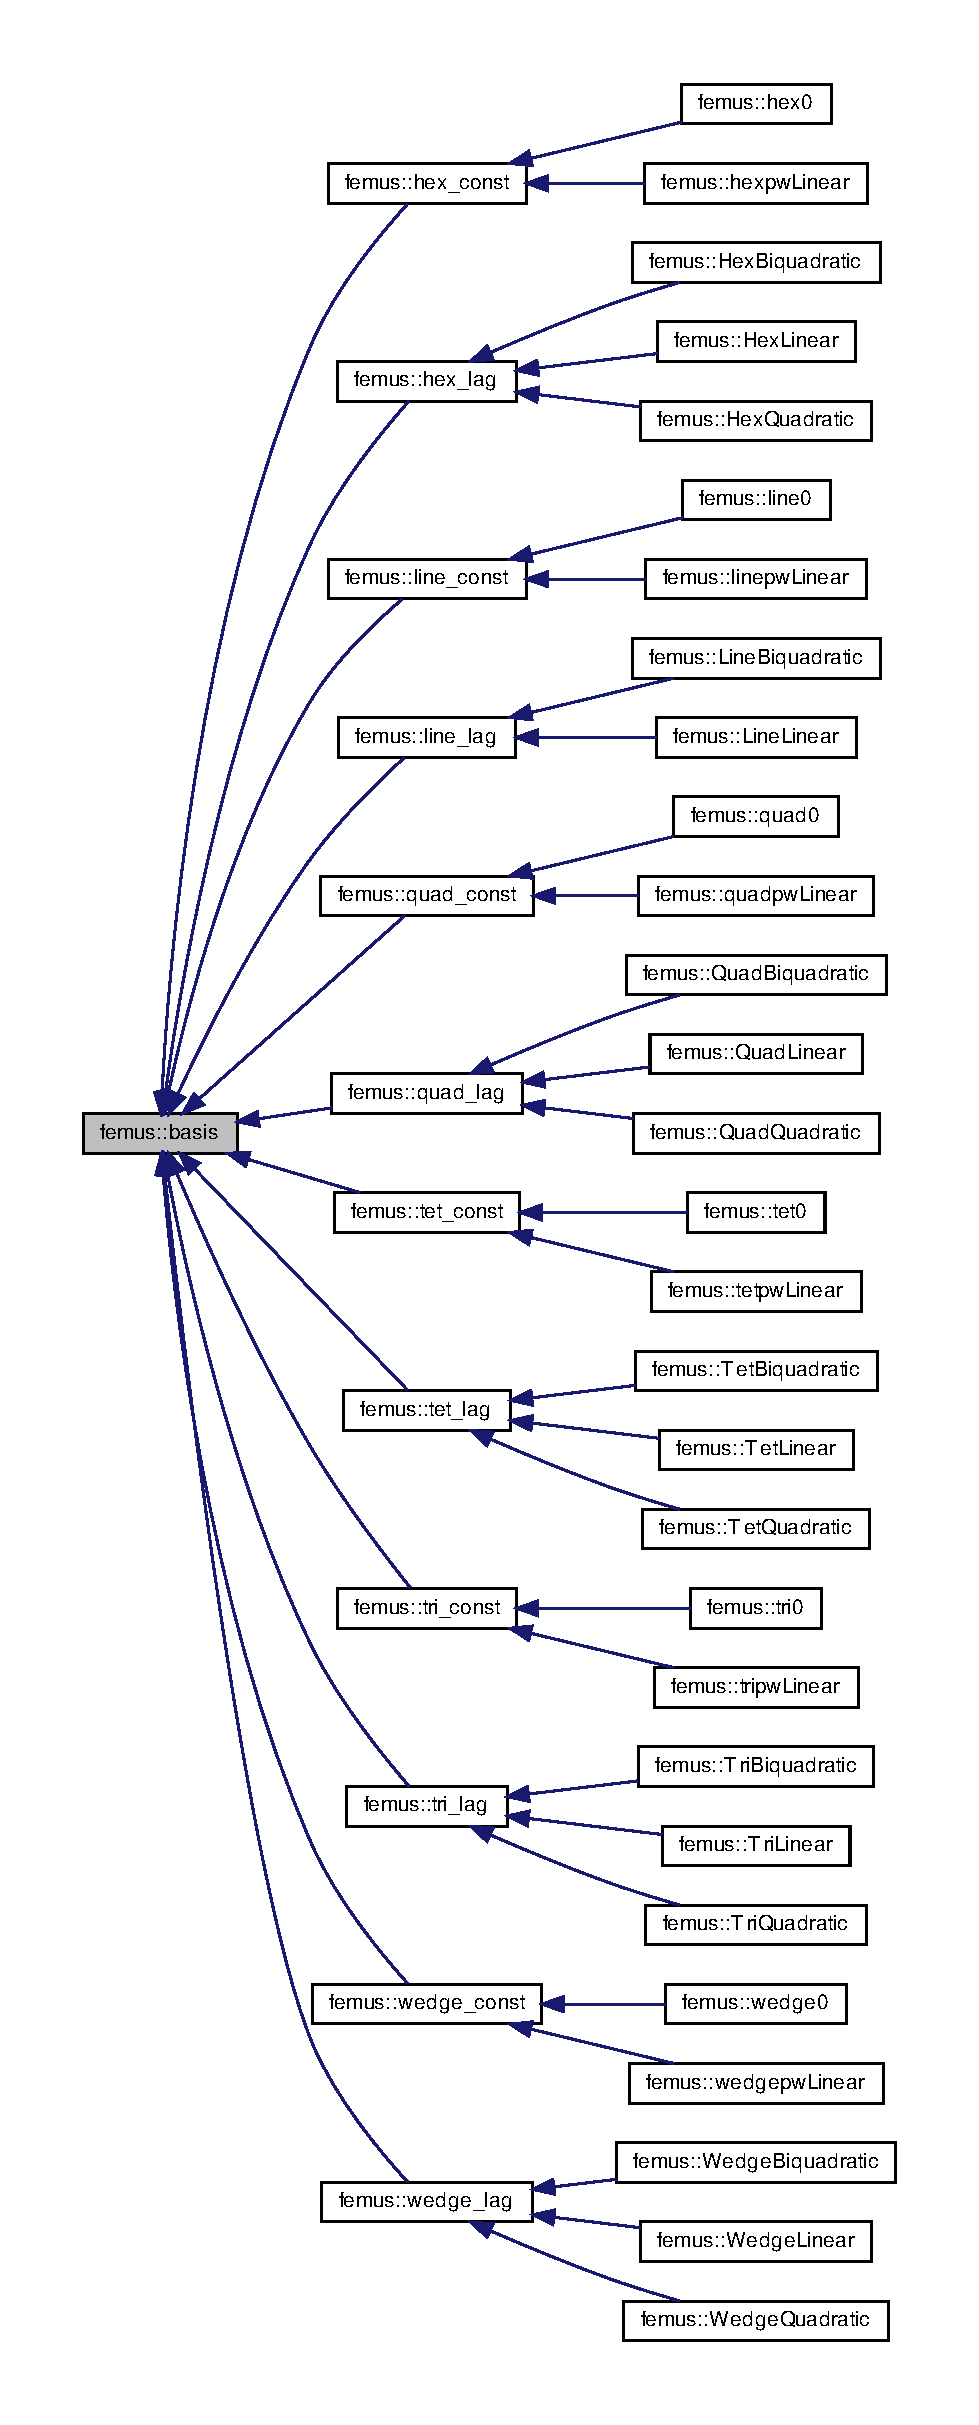
\includegraphics[height=550pt]{classfemus_1_1basis__inherit__graph}
\end{center}
\end{figure}
\subsection*{Public Member Functions}
\begin{DoxyCompactItemize}
\item 
\mbox{\hyperlink{classfemus_1_1basis_a1e819ab49eb14b0727fb214ede9987c3}{basis}} (const int \&nc, const int \&nf, const int \&nlag0, const int \&nlag1, const int \&nlag2, const int \&nlag3, const int \&face\+Number0, const int \&face\+Number1, const int \&face\+Number2)
\item 
virtual void \mbox{\hyperlink{classfemus_1_1basis_abbae7bf8f31ec5793c911bc6d4ea0572}{Print\+Type}} () const =0
\item 
double \mbox{\hyperlink{classfemus_1_1basis_ac39cd1bad49bfe9370095558c24c4582}{eval\+\_\+phi}} (const unsigned \&j, const std\+::vector$<$ double $>$ \&x) const
\item 
double \mbox{\hyperlink{classfemus_1_1basis_af1cfe0c84a3a4b1e17b5903275410340}{eval\+\_\+dphidx}} (const unsigned \&j, const std\+::vector$<$ double $>$ \&x) const
\item 
double \mbox{\hyperlink{classfemus_1_1basis_a3c65ece3b826c56b2a05b2221e9ac61f}{eval\+\_\+dphidy}} (const unsigned \&j, const std\+::vector$<$ double $>$ \&x) const
\item 
double \mbox{\hyperlink{classfemus_1_1basis_a0a7e19ca2f5b312392bc34a64e8f2cf3}{eval\+\_\+dphidz}} (const unsigned \&j, const std\+::vector$<$ double $>$ \&x) const
\item 
double \mbox{\hyperlink{classfemus_1_1basis_af8e2384b8327ce9890851e3ae6447853}{eval\+\_\+d2phidx2}} (const unsigned \&j, const std\+::vector$<$ double $>$ \&x) const
\item 
double \mbox{\hyperlink{classfemus_1_1basis_abe4127967d317edfc852b0b0432fca98}{eval\+\_\+d2phidy2}} (const unsigned \&j, const std\+::vector$<$ double $>$ \&x) const
\item 
double \mbox{\hyperlink{classfemus_1_1basis_a9acc0a686ee2c3f77fd33b594c5e2ec3}{eval\+\_\+d2phidz2}} (const unsigned \&j, const std\+::vector$<$ double $>$ \&x) const
\item 
double \mbox{\hyperlink{classfemus_1_1basis_a9ebb6c277754a3f21be2f9b0f56428ff}{eval\+\_\+d2phidxdy}} (const unsigned \&j, const std\+::vector$<$ double $>$ \&x) const
\item 
double \mbox{\hyperlink{classfemus_1_1basis_af7ee9e4c4a8e6204e7504bb25c326d62}{eval\+\_\+d2phidydz}} (const unsigned \&j, const std\+::vector$<$ double $>$ \&x) const
\item 
double \mbox{\hyperlink{classfemus_1_1basis_aff9731d83408aa82eb148b8fc83ef9d8}{eval\+\_\+d2phidzdx}} (const unsigned \&j, const std\+::vector$<$ double $>$ \&x) const
\item 
virtual double \mbox{\hyperlink{classfemus_1_1basis_a89b0797cdccffae5ff6d059b32016ae5}{eval\+\_\+phi}} (const int $\ast$I, const double $\ast$x) const
\item 
virtual double \mbox{\hyperlink{classfemus_1_1basis_a4db7d29cf8a753ddbccc4a297dafa0bf}{eval\+\_\+dphidx}} (const int $\ast$I, const double $\ast$x) const
\item 
virtual double \mbox{\hyperlink{classfemus_1_1basis_a2819fac9aae797156b9efec8a0b85cc1}{eval\+\_\+dphidy}} (const int $\ast$I, const double $\ast$x) const
\item 
virtual double \mbox{\hyperlink{classfemus_1_1basis_affd9927f6e25e264108219d862b8cb3d}{eval\+\_\+dphidz}} (const int $\ast$I, const double $\ast$x) const
\item 
virtual double \mbox{\hyperlink{classfemus_1_1basis_a0a9839e75d1c9c8302486fc072eed028}{eval\+\_\+d2phidx2}} (const int $\ast$I, const double $\ast$x) const
\item 
virtual double \mbox{\hyperlink{classfemus_1_1basis_a0febb29fe4b32213ff8d6d428f7241cd}{eval\+\_\+d2phidy2}} (const int $\ast$I, const double $\ast$x) const
\item 
virtual double \mbox{\hyperlink{classfemus_1_1basis_a9d32da05f49ba2c989fec04fb7836c39}{eval\+\_\+d2phidz2}} (const int $\ast$I, const double $\ast$x) const
\item 
virtual double \mbox{\hyperlink{classfemus_1_1basis_ac9feaf9e60421143db2a3708f3c7fa48}{eval\+\_\+d2phidxdy}} (const int $\ast$I, const double $\ast$x) const
\item 
virtual double \mbox{\hyperlink{classfemus_1_1basis_ab9e060e9c9e763d8c10fdffcc5e0b774}{eval\+\_\+d2phidydz}} (const int $\ast$I, const double $\ast$x) const
\item 
virtual double \mbox{\hyperlink{classfemus_1_1basis_a5d619ec5bd57b7d2dc34a99d69975c77}{eval\+\_\+d2phidzdx}} (const int $\ast$I, const double $\ast$x) const
\item 
virtual const double $\ast$ \mbox{\hyperlink{classfemus_1_1basis_a00597122bbc75877f1c184f8fce4986c}{GetX}} (const int \&i) const =0
\item 
virtual const double $\ast$ \mbox{\hyperlink{classfemus_1_1basis_afcabbbda61ede8f30158fe08ee0a5258}{Get\+Xcoarse}} (const int \&i) const
\item 
virtual void \mbox{\hyperlink{classfemus_1_1basis_abbb9deb1bd0b2d07a4b2995b07d58d2e}{SetX}} (const unsigned \&i, const unsigned \&j, const double \&value)
\item 
virtual const int $\ast$ \mbox{\hyperlink{classfemus_1_1basis_a3f63ad97ce70cd4a1196ede69f1f144b}{Get\+I\+ND}} (const int \&i) const =0
\item 
virtual const int $\ast$ \mbox{\hyperlink{classfemus_1_1basis_a95ceb3feae4c484b0baa6a4d35d38909}{Get\+K\+V\+E\+R\+T\+\_\+\+I\+ND}} (const int \&i) const =0
\item 
virtual const unsigned \mbox{\hyperlink{classfemus_1_1basis_a2ba867dcfa634c47f1c52caddd9bfdba}{Get\+Fine2\+Coarse\+Vertex\+Mapping}} (const int \&i, const unsigned \&j) const
\item 
virtual const unsigned \mbox{\hyperlink{classfemus_1_1basis_a06f93864b6ce0925d41bf08173dc2500}{Get\+Face\+Dof}} (const unsigned \&i, const unsigned \&j) const
\end{DoxyCompactItemize}
\subsection*{Public Attributes}
\begin{DoxyCompactItemize}
\item 
const int \mbox{\hyperlink{classfemus_1_1basis_a8beaeb66f172e318e6f4daa22af0ee29}{\+\_\+nc}}
\item 
const int \mbox{\hyperlink{classfemus_1_1basis_ac52171231d44a30dfca075c6918d8197}{\+\_\+nf}}
\item 
const int \mbox{\hyperlink{classfemus_1_1basis_a1fd290cb7382616e14715756917d73c1}{\+\_\+nlag0}}
\item 
const int \mbox{\hyperlink{classfemus_1_1basis_ab2e292cf67cf16101dac730b9a3b0fd0}{\+\_\+nlag1}}
\item 
const int \mbox{\hyperlink{classfemus_1_1basis_a19491d79d0fb5ef8135a51460502041c}{\+\_\+nlag2}}
\item 
const int \mbox{\hyperlink{classfemus_1_1basis_afe89e7da4ba55df0492ee96f6bb04838}{\+\_\+nlag3}}
\item 
int \mbox{\hyperlink{classfemus_1_1basis_a21732cfb1bec4383fd050d218dfed070}{face\+Number}} \mbox{[}3\mbox{]}
\end{DoxyCompactItemize}
\subsection*{Protected Member Functions}
\begin{DoxyCompactItemize}
\item 
double \mbox{\hyperlink{classfemus_1_1basis_a614b2d4abe684a504bb0f561d46397fa}{lag\+Linear}} (const double \&x, const int \&i) const
\item 
double \mbox{\hyperlink{classfemus_1_1basis_af771f9a5c71d06c873d474cf2bba3177}{dlag\+Linear}} (const double \&x, const int \&i) const
\item 
double \mbox{\hyperlink{classfemus_1_1basis_a49212826381f3ff3dad0bc61d6b6329c}{lag\+Quadratic}} (const double \&x, const int \&i) const
\item 
double \mbox{\hyperlink{classfemus_1_1basis_aba954c5565d837822ee4840f1ed77f33}{dlag\+Quadratic}} (const double \&x, const int \&i) const
\item 
double \mbox{\hyperlink{classfemus_1_1basis_a1c4544031232a6ae1cb0f8501d650758}{d2lag\+Quadratic}} (const double \&x, const int \&i) const
\item 
double \mbox{\hyperlink{classfemus_1_1basis_a2571f53dfeae70eccf63033736098d07}{lag\+Biquadratic}} (const double \&x, const int \&i) const
\item 
double \mbox{\hyperlink{classfemus_1_1basis_a52c019c4c820beb94e20e71b31868384}{dlag\+Biquadratic}} (const double \&x, const int \&i) const
\item 
double \mbox{\hyperlink{classfemus_1_1basis_a52634884baf22e8f65808ee0eca3e9b8}{d2lag\+Biquadratic}} (const double \&x, const int \&i) const
\item 
double \mbox{\hyperlink{classfemus_1_1basis_ae1b0f968c69a125b1437c86691b79659}{triangle\+Linear}} (const double \&x, const double \&y, const int \&i, const int \&j) const
\item 
double \mbox{\hyperlink{classfemus_1_1basis_a3393b4ce51e0c786e962220ffb2e7a26}{dtriangle\+Lineardx}} (const double \&x, const double \&y, const int \&i, const int \&j) const
\item 
double \mbox{\hyperlink{classfemus_1_1basis_ae05b1d5b6d73182b91aa079f864096ac}{dtriangle\+Lineardy}} (const double \&x, const double \&y, const int \&i, const int \&j) const
\item 
double \mbox{\hyperlink{classfemus_1_1basis_ae42b607d5f23bdf072243ee3db496a44}{triangle\+Quadratic}} (const double \&x, const double \&y, const int \&i, const int \&j) const
\item 
double \mbox{\hyperlink{classfemus_1_1basis_a36ac5b9e572289fb4d552b97dec8a0f1}{dtriangle\+Quadraticdx}} (const double \&x, const double \&y, const int \&i, const int \&j) const
\item 
double \mbox{\hyperlink{classfemus_1_1basis_aa6d822471f1a03034003e0499ca6a2c6}{dtriangle\+Quadraticdy}} (const double \&x, const double \&y, const int \&i, const int \&j) const
\item 
double \mbox{\hyperlink{classfemus_1_1basis_adb2041a297cde6b673e1ae393b4e1abb}{d2triangle\+Quadraticdx2}} (const double \&x, const double \&y, const int \&i, const int \&j) const
\item 
double \mbox{\hyperlink{classfemus_1_1basis_ab4432bf9996b939143fe7a013a397094}{d2triangle\+Quadraticdy2}} (const double \&x, const double \&y, const int \&i, const int \&j) const
\item 
double \mbox{\hyperlink{classfemus_1_1basis_afc53a79c2d4989b204cf69833bd20e91}{d2triangle\+Quadraticdxdy}} (const double \&x, const double \&y, const int \&i, const int \&j) const
\item 
double \mbox{\hyperlink{classfemus_1_1basis_aaf2a0be4f2d29c434293c40f7b268613}{triangle\+Biquadratic}} (const double \&x, const double \&y, const int \&i, const int \&j) const
\item 
double \mbox{\hyperlink{classfemus_1_1basis_aa2007487d021857ff90ba9c3366e54ba}{dtriangle\+Biquadraticdx}} (const double \&x, const double \&y, const int \&i, const int \&j) const
\item 
double \mbox{\hyperlink{classfemus_1_1basis_a0d3f013bbb3a95515bb5c6a84f68eef1}{dtriangle\+Biquadraticdy}} (const double \&x, const double \&y, const int \&i, const int \&j) const
\item 
double \mbox{\hyperlink{classfemus_1_1basis_a065d6f7c99411b8410bde98fcb12a089}{d2triangle\+Biquadraticdx2}} (const double \&x, const double \&y, const int \&i, const int \&j) const
\item 
double \mbox{\hyperlink{classfemus_1_1basis_a823c2c760606dc5ec50bb749a4dbe10e}{d2triangle\+Biquadraticdy2}} (const double \&x, const double \&y, const int \&i, const int \&j) const
\item 
double \mbox{\hyperlink{classfemus_1_1basis_aeebd0fb9806e39c3537021aba7f63f1e}{d2triangle\+Biquadraticdxdy}} (const double \&x, const double \&y, const int \&i, const int \&j) const
\end{DoxyCompactItemize}


\subsection{Constructor \& Destructor Documentation}
\mbox{\Hypertarget{classfemus_1_1basis_a1e819ab49eb14b0727fb214ede9987c3}\label{classfemus_1_1basis_a1e819ab49eb14b0727fb214ede9987c3}} 
\index{femus\+::basis@{femus\+::basis}!basis@{basis}}
\index{basis@{basis}!femus\+::basis@{femus\+::basis}}
\subsubsection{\texorpdfstring{basis()}{basis()}}
{\footnotesize\ttfamily femus\+::basis\+::basis (\begin{DoxyParamCaption}\item[{const int \&}]{nc,  }\item[{const int \&}]{nf,  }\item[{const int \&}]{nlag0,  }\item[{const int \&}]{nlag1,  }\item[{const int \&}]{nlag2,  }\item[{const int \&}]{nlag3,  }\item[{const int \&}]{face\+Number0,  }\item[{const int \&}]{face\+Number1,  }\item[{const int \&}]{face\+Number2 }\end{DoxyParamCaption})\hspace{0.3cm}{\ttfamily [inline]}}



\subsection{Member Function Documentation}
\mbox{\Hypertarget{classfemus_1_1basis_a52634884baf22e8f65808ee0eca3e9b8}\label{classfemus_1_1basis_a52634884baf22e8f65808ee0eca3e9b8}} 
\index{femus\+::basis@{femus\+::basis}!d2lag\+Biquadratic@{d2lag\+Biquadratic}}
\index{d2lag\+Biquadratic@{d2lag\+Biquadratic}!femus\+::basis@{femus\+::basis}}
\subsubsection{\texorpdfstring{d2lag\+Biquadratic()}{d2lagBiquadratic()}}
{\footnotesize\ttfamily double femus\+::basis\+::d2lag\+Biquadratic (\begin{DoxyParamCaption}\item[{const double \&}]{x,  }\item[{const int \&}]{i }\end{DoxyParamCaption}) const\hspace{0.3cm}{\ttfamily [inline]}, {\ttfamily [protected]}}

\mbox{\Hypertarget{classfemus_1_1basis_a1c4544031232a6ae1cb0f8501d650758}\label{classfemus_1_1basis_a1c4544031232a6ae1cb0f8501d650758}} 
\index{femus\+::basis@{femus\+::basis}!d2lag\+Quadratic@{d2lag\+Quadratic}}
\index{d2lag\+Quadratic@{d2lag\+Quadratic}!femus\+::basis@{femus\+::basis}}
\subsubsection{\texorpdfstring{d2lag\+Quadratic()}{d2lagQuadratic()}}
{\footnotesize\ttfamily double femus\+::basis\+::d2lag\+Quadratic (\begin{DoxyParamCaption}\item[{const double \&}]{x,  }\item[{const int \&}]{i }\end{DoxyParamCaption}) const\hspace{0.3cm}{\ttfamily [inline]}, {\ttfamily [protected]}}

\mbox{\Hypertarget{classfemus_1_1basis_a065d6f7c99411b8410bde98fcb12a089}\label{classfemus_1_1basis_a065d6f7c99411b8410bde98fcb12a089}} 
\index{femus\+::basis@{femus\+::basis}!d2triangle\+Biquadraticdx2@{d2triangle\+Biquadraticdx2}}
\index{d2triangle\+Biquadraticdx2@{d2triangle\+Biquadraticdx2}!femus\+::basis@{femus\+::basis}}
\subsubsection{\texorpdfstring{d2triangle\+Biquadraticdx2()}{d2triangleBiquadraticdx2()}}
{\footnotesize\ttfamily double femus\+::basis\+::d2triangle\+Biquadraticdx2 (\begin{DoxyParamCaption}\item[{const double \&}]{x,  }\item[{const double \&}]{y,  }\item[{const int \&}]{i,  }\item[{const int \&}]{j }\end{DoxyParamCaption}) const\hspace{0.3cm}{\ttfamily [inline]}, {\ttfamily [protected]}}

\mbox{\Hypertarget{classfemus_1_1basis_aeebd0fb9806e39c3537021aba7f63f1e}\label{classfemus_1_1basis_aeebd0fb9806e39c3537021aba7f63f1e}} 
\index{femus\+::basis@{femus\+::basis}!d2triangle\+Biquadraticdxdy@{d2triangle\+Biquadraticdxdy}}
\index{d2triangle\+Biquadraticdxdy@{d2triangle\+Biquadraticdxdy}!femus\+::basis@{femus\+::basis}}
\subsubsection{\texorpdfstring{d2triangle\+Biquadraticdxdy()}{d2triangleBiquadraticdxdy()}}
{\footnotesize\ttfamily double femus\+::basis\+::d2triangle\+Biquadraticdxdy (\begin{DoxyParamCaption}\item[{const double \&}]{x,  }\item[{const double \&}]{y,  }\item[{const int \&}]{i,  }\item[{const int \&}]{j }\end{DoxyParamCaption}) const\hspace{0.3cm}{\ttfamily [inline]}, {\ttfamily [protected]}}

\mbox{\Hypertarget{classfemus_1_1basis_a823c2c760606dc5ec50bb749a4dbe10e}\label{classfemus_1_1basis_a823c2c760606dc5ec50bb749a4dbe10e}} 
\index{femus\+::basis@{femus\+::basis}!d2triangle\+Biquadraticdy2@{d2triangle\+Biquadraticdy2}}
\index{d2triangle\+Biquadraticdy2@{d2triangle\+Biquadraticdy2}!femus\+::basis@{femus\+::basis}}
\subsubsection{\texorpdfstring{d2triangle\+Biquadraticdy2()}{d2triangleBiquadraticdy2()}}
{\footnotesize\ttfamily double femus\+::basis\+::d2triangle\+Biquadraticdy2 (\begin{DoxyParamCaption}\item[{const double \&}]{x,  }\item[{const double \&}]{y,  }\item[{const int \&}]{i,  }\item[{const int \&}]{j }\end{DoxyParamCaption}) const\hspace{0.3cm}{\ttfamily [inline]}, {\ttfamily [protected]}}

\mbox{\Hypertarget{classfemus_1_1basis_adb2041a297cde6b673e1ae393b4e1abb}\label{classfemus_1_1basis_adb2041a297cde6b673e1ae393b4e1abb}} 
\index{femus\+::basis@{femus\+::basis}!d2triangle\+Quadraticdx2@{d2triangle\+Quadraticdx2}}
\index{d2triangle\+Quadraticdx2@{d2triangle\+Quadraticdx2}!femus\+::basis@{femus\+::basis}}
\subsubsection{\texorpdfstring{d2triangle\+Quadraticdx2()}{d2triangleQuadraticdx2()}}
{\footnotesize\ttfamily double femus\+::basis\+::d2triangle\+Quadraticdx2 (\begin{DoxyParamCaption}\item[{const double \&}]{x,  }\item[{const double \&}]{y,  }\item[{const int \&}]{i,  }\item[{const int \&}]{j }\end{DoxyParamCaption}) const\hspace{0.3cm}{\ttfamily [inline]}, {\ttfamily [protected]}}

\mbox{\Hypertarget{classfemus_1_1basis_afc53a79c2d4989b204cf69833bd20e91}\label{classfemus_1_1basis_afc53a79c2d4989b204cf69833bd20e91}} 
\index{femus\+::basis@{femus\+::basis}!d2triangle\+Quadraticdxdy@{d2triangle\+Quadraticdxdy}}
\index{d2triangle\+Quadraticdxdy@{d2triangle\+Quadraticdxdy}!femus\+::basis@{femus\+::basis}}
\subsubsection{\texorpdfstring{d2triangle\+Quadraticdxdy()}{d2triangleQuadraticdxdy()}}
{\footnotesize\ttfamily double femus\+::basis\+::d2triangle\+Quadraticdxdy (\begin{DoxyParamCaption}\item[{const double \&}]{x,  }\item[{const double \&}]{y,  }\item[{const int \&}]{i,  }\item[{const int \&}]{j }\end{DoxyParamCaption}) const\hspace{0.3cm}{\ttfamily [inline]}, {\ttfamily [protected]}}

\mbox{\Hypertarget{classfemus_1_1basis_ab4432bf9996b939143fe7a013a397094}\label{classfemus_1_1basis_ab4432bf9996b939143fe7a013a397094}} 
\index{femus\+::basis@{femus\+::basis}!d2triangle\+Quadraticdy2@{d2triangle\+Quadraticdy2}}
\index{d2triangle\+Quadraticdy2@{d2triangle\+Quadraticdy2}!femus\+::basis@{femus\+::basis}}
\subsubsection{\texorpdfstring{d2triangle\+Quadraticdy2()}{d2triangleQuadraticdy2()}}
{\footnotesize\ttfamily double femus\+::basis\+::d2triangle\+Quadraticdy2 (\begin{DoxyParamCaption}\item[{const double \&}]{x,  }\item[{const double \&}]{y,  }\item[{const int \&}]{i,  }\item[{const int \&}]{j }\end{DoxyParamCaption}) const\hspace{0.3cm}{\ttfamily [inline]}, {\ttfamily [protected]}}

\mbox{\Hypertarget{classfemus_1_1basis_a52c019c4c820beb94e20e71b31868384}\label{classfemus_1_1basis_a52c019c4c820beb94e20e71b31868384}} 
\index{femus\+::basis@{femus\+::basis}!dlag\+Biquadratic@{dlag\+Biquadratic}}
\index{dlag\+Biquadratic@{dlag\+Biquadratic}!femus\+::basis@{femus\+::basis}}
\subsubsection{\texorpdfstring{dlag\+Biquadratic()}{dlagBiquadratic()}}
{\footnotesize\ttfamily double femus\+::basis\+::dlag\+Biquadratic (\begin{DoxyParamCaption}\item[{const double \&}]{x,  }\item[{const int \&}]{i }\end{DoxyParamCaption}) const\hspace{0.3cm}{\ttfamily [inline]}, {\ttfamily [protected]}}

\mbox{\Hypertarget{classfemus_1_1basis_af771f9a5c71d06c873d474cf2bba3177}\label{classfemus_1_1basis_af771f9a5c71d06c873d474cf2bba3177}} 
\index{femus\+::basis@{femus\+::basis}!dlag\+Linear@{dlag\+Linear}}
\index{dlag\+Linear@{dlag\+Linear}!femus\+::basis@{femus\+::basis}}
\subsubsection{\texorpdfstring{dlag\+Linear()}{dlagLinear()}}
{\footnotesize\ttfamily double femus\+::basis\+::dlag\+Linear (\begin{DoxyParamCaption}\item[{const double \&}]{x,  }\item[{const int \&}]{i }\end{DoxyParamCaption}) const\hspace{0.3cm}{\ttfamily [inline]}, {\ttfamily [protected]}}

\mbox{\Hypertarget{classfemus_1_1basis_aba954c5565d837822ee4840f1ed77f33}\label{classfemus_1_1basis_aba954c5565d837822ee4840f1ed77f33}} 
\index{femus\+::basis@{femus\+::basis}!dlag\+Quadratic@{dlag\+Quadratic}}
\index{dlag\+Quadratic@{dlag\+Quadratic}!femus\+::basis@{femus\+::basis}}
\subsubsection{\texorpdfstring{dlag\+Quadratic()}{dlagQuadratic()}}
{\footnotesize\ttfamily double femus\+::basis\+::dlag\+Quadratic (\begin{DoxyParamCaption}\item[{const double \&}]{x,  }\item[{const int \&}]{i }\end{DoxyParamCaption}) const\hspace{0.3cm}{\ttfamily [inline]}, {\ttfamily [protected]}}

\mbox{\Hypertarget{classfemus_1_1basis_aa2007487d021857ff90ba9c3366e54ba}\label{classfemus_1_1basis_aa2007487d021857ff90ba9c3366e54ba}} 
\index{femus\+::basis@{femus\+::basis}!dtriangle\+Biquadraticdx@{dtriangle\+Biquadraticdx}}
\index{dtriangle\+Biquadraticdx@{dtriangle\+Biquadraticdx}!femus\+::basis@{femus\+::basis}}
\subsubsection{\texorpdfstring{dtriangle\+Biquadraticdx()}{dtriangleBiquadraticdx()}}
{\footnotesize\ttfamily double femus\+::basis\+::dtriangle\+Biquadraticdx (\begin{DoxyParamCaption}\item[{const double \&}]{x,  }\item[{const double \&}]{y,  }\item[{const int \&}]{i,  }\item[{const int \&}]{j }\end{DoxyParamCaption}) const\hspace{0.3cm}{\ttfamily [inline]}, {\ttfamily [protected]}}

\mbox{\Hypertarget{classfemus_1_1basis_a0d3f013bbb3a95515bb5c6a84f68eef1}\label{classfemus_1_1basis_a0d3f013bbb3a95515bb5c6a84f68eef1}} 
\index{femus\+::basis@{femus\+::basis}!dtriangle\+Biquadraticdy@{dtriangle\+Biquadraticdy}}
\index{dtriangle\+Biquadraticdy@{dtriangle\+Biquadraticdy}!femus\+::basis@{femus\+::basis}}
\subsubsection{\texorpdfstring{dtriangle\+Biquadraticdy()}{dtriangleBiquadraticdy()}}
{\footnotesize\ttfamily double femus\+::basis\+::dtriangle\+Biquadraticdy (\begin{DoxyParamCaption}\item[{const double \&}]{x,  }\item[{const double \&}]{y,  }\item[{const int \&}]{i,  }\item[{const int \&}]{j }\end{DoxyParamCaption}) const\hspace{0.3cm}{\ttfamily [inline]}, {\ttfamily [protected]}}

\mbox{\Hypertarget{classfemus_1_1basis_a3393b4ce51e0c786e962220ffb2e7a26}\label{classfemus_1_1basis_a3393b4ce51e0c786e962220ffb2e7a26}} 
\index{femus\+::basis@{femus\+::basis}!dtriangle\+Lineardx@{dtriangle\+Lineardx}}
\index{dtriangle\+Lineardx@{dtriangle\+Lineardx}!femus\+::basis@{femus\+::basis}}
\subsubsection{\texorpdfstring{dtriangle\+Lineardx()}{dtriangleLineardx()}}
{\footnotesize\ttfamily double femus\+::basis\+::dtriangle\+Lineardx (\begin{DoxyParamCaption}\item[{const double \&}]{x,  }\item[{const double \&}]{y,  }\item[{const int \&}]{i,  }\item[{const int \&}]{j }\end{DoxyParamCaption}) const\hspace{0.3cm}{\ttfamily [inline]}, {\ttfamily [protected]}}

\mbox{\Hypertarget{classfemus_1_1basis_ae05b1d5b6d73182b91aa079f864096ac}\label{classfemus_1_1basis_ae05b1d5b6d73182b91aa079f864096ac}} 
\index{femus\+::basis@{femus\+::basis}!dtriangle\+Lineardy@{dtriangle\+Lineardy}}
\index{dtriangle\+Lineardy@{dtriangle\+Lineardy}!femus\+::basis@{femus\+::basis}}
\subsubsection{\texorpdfstring{dtriangle\+Lineardy()}{dtriangleLineardy()}}
{\footnotesize\ttfamily double femus\+::basis\+::dtriangle\+Lineardy (\begin{DoxyParamCaption}\item[{const double \&}]{x,  }\item[{const double \&}]{y,  }\item[{const int \&}]{i,  }\item[{const int \&}]{j }\end{DoxyParamCaption}) const\hspace{0.3cm}{\ttfamily [inline]}, {\ttfamily [protected]}}

\mbox{\Hypertarget{classfemus_1_1basis_a36ac5b9e572289fb4d552b97dec8a0f1}\label{classfemus_1_1basis_a36ac5b9e572289fb4d552b97dec8a0f1}} 
\index{femus\+::basis@{femus\+::basis}!dtriangle\+Quadraticdx@{dtriangle\+Quadraticdx}}
\index{dtriangle\+Quadraticdx@{dtriangle\+Quadraticdx}!femus\+::basis@{femus\+::basis}}
\subsubsection{\texorpdfstring{dtriangle\+Quadraticdx()}{dtriangleQuadraticdx()}}
{\footnotesize\ttfamily double femus\+::basis\+::dtriangle\+Quadraticdx (\begin{DoxyParamCaption}\item[{const double \&}]{x,  }\item[{const double \&}]{y,  }\item[{const int \&}]{i,  }\item[{const int \&}]{j }\end{DoxyParamCaption}) const\hspace{0.3cm}{\ttfamily [inline]}, {\ttfamily [protected]}}

\mbox{\Hypertarget{classfemus_1_1basis_aa6d822471f1a03034003e0499ca6a2c6}\label{classfemus_1_1basis_aa6d822471f1a03034003e0499ca6a2c6}} 
\index{femus\+::basis@{femus\+::basis}!dtriangle\+Quadraticdy@{dtriangle\+Quadraticdy}}
\index{dtriangle\+Quadraticdy@{dtriangle\+Quadraticdy}!femus\+::basis@{femus\+::basis}}
\subsubsection{\texorpdfstring{dtriangle\+Quadraticdy()}{dtriangleQuadraticdy()}}
{\footnotesize\ttfamily double femus\+::basis\+::dtriangle\+Quadraticdy (\begin{DoxyParamCaption}\item[{const double \&}]{x,  }\item[{const double \&}]{y,  }\item[{const int \&}]{i,  }\item[{const int \&}]{j }\end{DoxyParamCaption}) const\hspace{0.3cm}{\ttfamily [inline]}, {\ttfamily [protected]}}

\mbox{\Hypertarget{classfemus_1_1basis_af8e2384b8327ce9890851e3ae6447853}\label{classfemus_1_1basis_af8e2384b8327ce9890851e3ae6447853}} 
\index{femus\+::basis@{femus\+::basis}!eval\+\_\+d2phidx2@{eval\+\_\+d2phidx2}}
\index{eval\+\_\+d2phidx2@{eval\+\_\+d2phidx2}!femus\+::basis@{femus\+::basis}}
\subsubsection{\texorpdfstring{eval\+\_\+d2phidx2()}{eval\_d2phidx2()}\hspace{0.1cm}{\footnotesize\ttfamily [1/2]}}
{\footnotesize\ttfamily double femus\+::basis\+::eval\+\_\+d2phidx2 (\begin{DoxyParamCaption}\item[{const unsigned \&}]{j,  }\item[{const std\+::vector$<$ double $>$ \&}]{x }\end{DoxyParamCaption}) const\hspace{0.3cm}{\ttfamily [inline]}}

\mbox{\Hypertarget{classfemus_1_1basis_a0a9839e75d1c9c8302486fc072eed028}\label{classfemus_1_1basis_a0a9839e75d1c9c8302486fc072eed028}} 
\index{femus\+::basis@{femus\+::basis}!eval\+\_\+d2phidx2@{eval\+\_\+d2phidx2}}
\index{eval\+\_\+d2phidx2@{eval\+\_\+d2phidx2}!femus\+::basis@{femus\+::basis}}
\subsubsection{\texorpdfstring{eval\+\_\+d2phidx2()}{eval\_d2phidx2()}\hspace{0.1cm}{\footnotesize\ttfamily [2/2]}}
{\footnotesize\ttfamily virtual double femus\+::basis\+::eval\+\_\+d2phidx2 (\begin{DoxyParamCaption}\item[{const int $\ast$}]{I,  }\item[{const double $\ast$}]{x }\end{DoxyParamCaption}) const\hspace{0.3cm}{\ttfamily [inline]}, {\ttfamily [virtual]}}



Reimplemented in \mbox{\hyperlink{classfemus_1_1linepw_linear_ab935d5269619bc6d422a8fbad4daf017}{femus\+::linepw\+Linear}}, \mbox{\hyperlink{classfemus_1_1line0_accd6354291c1f1f8d91bc5e68087e9eb}{femus\+::line0}}, \mbox{\hyperlink{classfemus_1_1_line_biquadratic_ab6a7b188104b706b792227aaab0ebf2a}{femus\+::\+Line\+Biquadratic}}, \mbox{\hyperlink{classfemus_1_1_line_linear_a3f8cf26c387b50cdd41d39527c4260d1}{femus\+::\+Line\+Linear}}, \mbox{\hyperlink{classfemus_1_1tripw_linear_aee89b7d0da7add34b1b8fe8b74feb8b1}{femus\+::tripw\+Linear}}, \mbox{\hyperlink{classfemus_1_1tri0_ae832dd28eb7437215ce49ce0bac98ba3}{femus\+::tri0}}, \mbox{\hyperlink{classfemus_1_1_tri_biquadratic_a671d38cd3a1c851e54d71e3a53c85039}{femus\+::\+Tri\+Biquadratic}}, \mbox{\hyperlink{classfemus_1_1_tri_quadratic_a6fb9f8965f2bbe889a1c67c9ee9ddc01}{femus\+::\+Tri\+Quadratic}}, \mbox{\hyperlink{classfemus_1_1_tri_linear_acdd74b2d1bf8e72765539fa6a6a2044d}{femus\+::\+Tri\+Linear}}, \mbox{\hyperlink{classfemus_1_1quadpw_linear_a1e4149a8bc6f1a9c6cd12640b15e6deb}{femus\+::quadpw\+Linear}}, \mbox{\hyperlink{classfemus_1_1quad0_ab862ac9e1b07aa072f566a753b1948a8}{femus\+::quad0}}, \mbox{\hyperlink{classfemus_1_1_quad_biquadratic_ab88f608bc7d87d9639250d165ebafc4e}{femus\+::\+Quad\+Biquadratic}}, \mbox{\hyperlink{classfemus_1_1_quad_quadratic_abb3a37830ada326faacf6ff6f30f3fe9}{femus\+::\+Quad\+Quadratic}}, \mbox{\hyperlink{classfemus_1_1_quad_linear_af75fece3983ee9169c452c287c6b8d09}{femus\+::\+Quad\+Linear}}, \mbox{\hyperlink{classfemus_1_1tetpw_linear_a2239d19a7d3a723383d68d5c38bfdbea}{femus\+::tetpw\+Linear}}, \mbox{\hyperlink{classfemus_1_1tet0_a59411acd2cd35da162ad6487fa947a68}{femus\+::tet0}}, \mbox{\hyperlink{classfemus_1_1_tet_biquadratic_ad6fb5a8574508b0e45e49ca891ec3aac}{femus\+::\+Tet\+Biquadratic}}, \mbox{\hyperlink{classfemus_1_1_tet_quadratic_a41a83721de075980d8138bb457ddc937}{femus\+::\+Tet\+Quadratic}}, \mbox{\hyperlink{classfemus_1_1_tet_linear_a7fea6490e2ca09cbd97ce31e4bb9ddef}{femus\+::\+Tet\+Linear}}, \mbox{\hyperlink{classfemus_1_1wedgepw_linear_a97921882858ca490eb3bebebc333bd66}{femus\+::wedgepw\+Linear}}, \mbox{\hyperlink{classfemus_1_1wedge0_ab6d8e56e02ffedc90f9630db2dd37427}{femus\+::wedge0}}, \mbox{\hyperlink{classfemus_1_1_wedge_biquadratic_aca900bdb24740b8bf69916067272445d}{femus\+::\+Wedge\+Biquadratic}}, \mbox{\hyperlink{classfemus_1_1_wedge_quadratic_a922cf0ab05ffd7f68a74dfaf0ad3f67e}{femus\+::\+Wedge\+Quadratic}}, \mbox{\hyperlink{classfemus_1_1_wedge_linear_a3d9966a1518937773d444bc5c449ce35}{femus\+::\+Wedge\+Linear}}, \mbox{\hyperlink{classfemus_1_1hexpw_linear_a08b0b6ced1587ddf865452d6039c5e0b}{femus\+::hexpw\+Linear}}, \mbox{\hyperlink{classfemus_1_1hex0_af280499bcecfb346586a8a5aca7bc152}{femus\+::hex0}}, \mbox{\hyperlink{classfemus_1_1_hex_biquadratic_a61e90ab66788a1fed2c6515d514a7642}{femus\+::\+Hex\+Biquadratic}}, \mbox{\hyperlink{classfemus_1_1_hex_quadratic_a7a68a91e8865121d14f62b88f8756696}{femus\+::\+Hex\+Quadratic}}, and \mbox{\hyperlink{classfemus_1_1_hex_linear_a76ae681b7882ed7ea9683dee6aabc5aa}{femus\+::\+Hex\+Linear}}.

\mbox{\Hypertarget{classfemus_1_1basis_a9ebb6c277754a3f21be2f9b0f56428ff}\label{classfemus_1_1basis_a9ebb6c277754a3f21be2f9b0f56428ff}} 
\index{femus\+::basis@{femus\+::basis}!eval\+\_\+d2phidxdy@{eval\+\_\+d2phidxdy}}
\index{eval\+\_\+d2phidxdy@{eval\+\_\+d2phidxdy}!femus\+::basis@{femus\+::basis}}
\subsubsection{\texorpdfstring{eval\+\_\+d2phidxdy()}{eval\_d2phidxdy()}\hspace{0.1cm}{\footnotesize\ttfamily [1/2]}}
{\footnotesize\ttfamily double femus\+::basis\+::eval\+\_\+d2phidxdy (\begin{DoxyParamCaption}\item[{const unsigned \&}]{j,  }\item[{const std\+::vector$<$ double $>$ \&}]{x }\end{DoxyParamCaption}) const\hspace{0.3cm}{\ttfamily [inline]}}

\mbox{\Hypertarget{classfemus_1_1basis_ac9feaf9e60421143db2a3708f3c7fa48}\label{classfemus_1_1basis_ac9feaf9e60421143db2a3708f3c7fa48}} 
\index{femus\+::basis@{femus\+::basis}!eval\+\_\+d2phidxdy@{eval\+\_\+d2phidxdy}}
\index{eval\+\_\+d2phidxdy@{eval\+\_\+d2phidxdy}!femus\+::basis@{femus\+::basis}}
\subsubsection{\texorpdfstring{eval\+\_\+d2phidxdy()}{eval\_d2phidxdy()}\hspace{0.1cm}{\footnotesize\ttfamily [2/2]}}
{\footnotesize\ttfamily virtual double femus\+::basis\+::eval\+\_\+d2phidxdy (\begin{DoxyParamCaption}\item[{const int $\ast$}]{I,  }\item[{const double $\ast$}]{x }\end{DoxyParamCaption}) const\hspace{0.3cm}{\ttfamily [inline]}, {\ttfamily [virtual]}}



Reimplemented in \mbox{\hyperlink{classfemus_1_1tripw_linear_ae9ae33080ac87b5f0f4bcb69859095a4}{femus\+::tripw\+Linear}}, \mbox{\hyperlink{classfemus_1_1tri0_af109d0128644bcac07a88dfba1f457b4}{femus\+::tri0}}, \mbox{\hyperlink{classfemus_1_1_tri_biquadratic_add4c6b1cf71bc83b7d480337d5800808}{femus\+::\+Tri\+Biquadratic}}, \mbox{\hyperlink{classfemus_1_1_tri_quadratic_a65fb374db41ce0bb2ade38e7e6af58a1}{femus\+::\+Tri\+Quadratic}}, \mbox{\hyperlink{classfemus_1_1_tri_linear_ae19bb78f1fd3b9b810d32f561a4bb666}{femus\+::\+Tri\+Linear}}, \mbox{\hyperlink{classfemus_1_1quadpw_linear_a5e98b28c5ca4e382d3bf0ac7f1f3aa0c}{femus\+::quadpw\+Linear}}, \mbox{\hyperlink{classfemus_1_1quad0_aa1987456dd6bdacb2b9038c21bc17566}{femus\+::quad0}}, \mbox{\hyperlink{classfemus_1_1_quad_biquadratic_aff6de056034d2ef2d51f914a872a8d93}{femus\+::\+Quad\+Biquadratic}}, \mbox{\hyperlink{classfemus_1_1_quad_quadratic_a5f8d571d5684cb6f38087c4b3ba4f0b8}{femus\+::\+Quad\+Quadratic}}, \mbox{\hyperlink{classfemus_1_1_quad_linear_a2dd33af4e3c5c38c77ed0b803cf8f099}{femus\+::\+Quad\+Linear}}, \mbox{\hyperlink{classfemus_1_1tetpw_linear_ac652a9ba4f2d1fd2a140563ab97172e3}{femus\+::tetpw\+Linear}}, \mbox{\hyperlink{classfemus_1_1tet0_a22abf82712c0aa6a561280f8d9bef8ff}{femus\+::tet0}}, \mbox{\hyperlink{classfemus_1_1_tet_biquadratic_af239043a31782f74d867ecbb4f654689}{femus\+::\+Tet\+Biquadratic}}, \mbox{\hyperlink{classfemus_1_1_tet_quadratic_a2fcd1051ba5599c11a1d1c570c13d9f1}{femus\+::\+Tet\+Quadratic}}, \mbox{\hyperlink{classfemus_1_1_tet_linear_a45330406ce8b3f4ad0651e7ffda5dd82}{femus\+::\+Tet\+Linear}}, \mbox{\hyperlink{classfemus_1_1wedgepw_linear_acc622e61ab2a2c8d81a888600aaa049b}{femus\+::wedgepw\+Linear}}, \mbox{\hyperlink{classfemus_1_1wedge0_a2453f7ad8629c94abf9001ac43eb495f}{femus\+::wedge0}}, \mbox{\hyperlink{classfemus_1_1_wedge_biquadratic_a640cd05846eea041705474ab453cb062}{femus\+::\+Wedge\+Biquadratic}}, \mbox{\hyperlink{classfemus_1_1_wedge_quadratic_a023bc861013903cfda90cd78069c3d3c}{femus\+::\+Wedge\+Quadratic}}, \mbox{\hyperlink{classfemus_1_1_wedge_linear_a6b3c2d2415f2fc5c92e7c55a2726c481}{femus\+::\+Wedge\+Linear}}, \mbox{\hyperlink{classfemus_1_1hexpw_linear_ac0018245cf34cd4fc79de13e42b32817}{femus\+::hexpw\+Linear}}, \mbox{\hyperlink{classfemus_1_1hex0_a6fa5e53143dc6f1d3d41a63a26d7ac59}{femus\+::hex0}}, \mbox{\hyperlink{classfemus_1_1_hex_biquadratic_ac95c76060992afc10491cfe13df048d5}{femus\+::\+Hex\+Biquadratic}}, \mbox{\hyperlink{classfemus_1_1_hex_quadratic_a7725b6736d383a7df2147edef65779de}{femus\+::\+Hex\+Quadratic}}, and \mbox{\hyperlink{classfemus_1_1_hex_linear_ab3978e88ab01f8dcf7002024612523be}{femus\+::\+Hex\+Linear}}.

\mbox{\Hypertarget{classfemus_1_1basis_abe4127967d317edfc852b0b0432fca98}\label{classfemus_1_1basis_abe4127967d317edfc852b0b0432fca98}} 
\index{femus\+::basis@{femus\+::basis}!eval\+\_\+d2phidy2@{eval\+\_\+d2phidy2}}
\index{eval\+\_\+d2phidy2@{eval\+\_\+d2phidy2}!femus\+::basis@{femus\+::basis}}
\subsubsection{\texorpdfstring{eval\+\_\+d2phidy2()}{eval\_d2phidy2()}\hspace{0.1cm}{\footnotesize\ttfamily [1/2]}}
{\footnotesize\ttfamily double femus\+::basis\+::eval\+\_\+d2phidy2 (\begin{DoxyParamCaption}\item[{const unsigned \&}]{j,  }\item[{const std\+::vector$<$ double $>$ \&}]{x }\end{DoxyParamCaption}) const\hspace{0.3cm}{\ttfamily [inline]}}

\mbox{\Hypertarget{classfemus_1_1basis_a0febb29fe4b32213ff8d6d428f7241cd}\label{classfemus_1_1basis_a0febb29fe4b32213ff8d6d428f7241cd}} 
\index{femus\+::basis@{femus\+::basis}!eval\+\_\+d2phidy2@{eval\+\_\+d2phidy2}}
\index{eval\+\_\+d2phidy2@{eval\+\_\+d2phidy2}!femus\+::basis@{femus\+::basis}}
\subsubsection{\texorpdfstring{eval\+\_\+d2phidy2()}{eval\_d2phidy2()}\hspace{0.1cm}{\footnotesize\ttfamily [2/2]}}
{\footnotesize\ttfamily virtual double femus\+::basis\+::eval\+\_\+d2phidy2 (\begin{DoxyParamCaption}\item[{const int $\ast$}]{I,  }\item[{const double $\ast$}]{x }\end{DoxyParamCaption}) const\hspace{0.3cm}{\ttfamily [inline]}, {\ttfamily [virtual]}}



Reimplemented in \mbox{\hyperlink{classfemus_1_1tripw_linear_a7e8c27384a8008358e7d85ac0c7b3c5e}{femus\+::tripw\+Linear}}, \mbox{\hyperlink{classfemus_1_1tri0_aa01de141909bc67c1f293184b35d444b}{femus\+::tri0}}, \mbox{\hyperlink{classfemus_1_1_tri_biquadratic_a74610251368c2a83d701532e7b1931ed}{femus\+::\+Tri\+Biquadratic}}, \mbox{\hyperlink{classfemus_1_1_tri_quadratic_a37147196388fbe7fb347816f85c50e5e}{femus\+::\+Tri\+Quadratic}}, \mbox{\hyperlink{classfemus_1_1_tri_linear_a39bc9cfe4f0c5d994730b3202abc53c6}{femus\+::\+Tri\+Linear}}, \mbox{\hyperlink{classfemus_1_1quadpw_linear_a0600555381447b94613958383fe5f69f}{femus\+::quadpw\+Linear}}, \mbox{\hyperlink{classfemus_1_1quad0_a8dc516b64dc264896404b1d40019103a}{femus\+::quad0}}, \mbox{\hyperlink{classfemus_1_1_quad_biquadratic_a53f8f00fa4999cb1cfcdaf3f6a98df24}{femus\+::\+Quad\+Biquadratic}}, \mbox{\hyperlink{classfemus_1_1_quad_quadratic_a265d47435257f480aa10db30913d9780}{femus\+::\+Quad\+Quadratic}}, \mbox{\hyperlink{classfemus_1_1_quad_linear_acd036b93e46b4c610a08a71d0ed06745}{femus\+::\+Quad\+Linear}}, \mbox{\hyperlink{classfemus_1_1tetpw_linear_af2376253bf50baccdfe001037aec48a2}{femus\+::tetpw\+Linear}}, \mbox{\hyperlink{classfemus_1_1tet0_afc37f82556b5b073967bc48c7317e02f}{femus\+::tet0}}, \mbox{\hyperlink{classfemus_1_1_tet_biquadratic_a2095b54326d389269cd4fff0724138aa}{femus\+::\+Tet\+Biquadratic}}, \mbox{\hyperlink{classfemus_1_1_tet_quadratic_ab6dcc72f0cf2bdfa021645dbc164e07b}{femus\+::\+Tet\+Quadratic}}, \mbox{\hyperlink{classfemus_1_1_tet_linear_a7899d462e924de10cb39e0953fe0b68a}{femus\+::\+Tet\+Linear}}, \mbox{\hyperlink{classfemus_1_1wedgepw_linear_adcd46d6d590e3c11b1b244bfe15d7333}{femus\+::wedgepw\+Linear}}, \mbox{\hyperlink{classfemus_1_1wedge0_a0e24923793d43732b2b3913c8c94a9dd}{femus\+::wedge0}}, \mbox{\hyperlink{classfemus_1_1_wedge_biquadratic_a76ec3516df27dd1e41d49fcbb652f750}{femus\+::\+Wedge\+Biquadratic}}, \mbox{\hyperlink{classfemus_1_1_wedge_quadratic_aeb0f88d015d9a6c4a44555d13eb4feff}{femus\+::\+Wedge\+Quadratic}}, \mbox{\hyperlink{classfemus_1_1_wedge_linear_aa175c8d902c2a4a511d6bf798fb003c3}{femus\+::\+Wedge\+Linear}}, \mbox{\hyperlink{classfemus_1_1hexpw_linear_ab01049b3e87767f0f4b04a9cec8efa77}{femus\+::hexpw\+Linear}}, \mbox{\hyperlink{classfemus_1_1hex0_a16cfc0e738c48d75e558479d4da76aa4}{femus\+::hex0}}, \mbox{\hyperlink{classfemus_1_1_hex_biquadratic_a474b484fb23845775c3a5ec26b829784}{femus\+::\+Hex\+Biquadratic}}, \mbox{\hyperlink{classfemus_1_1_hex_quadratic_a99e2c105b81597d25f6c6f991c72235b}{femus\+::\+Hex\+Quadratic}}, and \mbox{\hyperlink{classfemus_1_1_hex_linear_a4a35e276ff9fac58e4ddd84ad147b726}{femus\+::\+Hex\+Linear}}.

\mbox{\Hypertarget{classfemus_1_1basis_af7ee9e4c4a8e6204e7504bb25c326d62}\label{classfemus_1_1basis_af7ee9e4c4a8e6204e7504bb25c326d62}} 
\index{femus\+::basis@{femus\+::basis}!eval\+\_\+d2phidydz@{eval\+\_\+d2phidydz}}
\index{eval\+\_\+d2phidydz@{eval\+\_\+d2phidydz}!femus\+::basis@{femus\+::basis}}
\subsubsection{\texorpdfstring{eval\+\_\+d2phidydz()}{eval\_d2phidydz()}\hspace{0.1cm}{\footnotesize\ttfamily [1/2]}}
{\footnotesize\ttfamily double femus\+::basis\+::eval\+\_\+d2phidydz (\begin{DoxyParamCaption}\item[{const unsigned \&}]{j,  }\item[{const std\+::vector$<$ double $>$ \&}]{x }\end{DoxyParamCaption}) const\hspace{0.3cm}{\ttfamily [inline]}}

\mbox{\Hypertarget{classfemus_1_1basis_ab9e060e9c9e763d8c10fdffcc5e0b774}\label{classfemus_1_1basis_ab9e060e9c9e763d8c10fdffcc5e0b774}} 
\index{femus\+::basis@{femus\+::basis}!eval\+\_\+d2phidydz@{eval\+\_\+d2phidydz}}
\index{eval\+\_\+d2phidydz@{eval\+\_\+d2phidydz}!femus\+::basis@{femus\+::basis}}
\subsubsection{\texorpdfstring{eval\+\_\+d2phidydz()}{eval\_d2phidydz()}\hspace{0.1cm}{\footnotesize\ttfamily [2/2]}}
{\footnotesize\ttfamily virtual double femus\+::basis\+::eval\+\_\+d2phidydz (\begin{DoxyParamCaption}\item[{const int $\ast$}]{I,  }\item[{const double $\ast$}]{x }\end{DoxyParamCaption}) const\hspace{0.3cm}{\ttfamily [inline]}, {\ttfamily [virtual]}}



Reimplemented in \mbox{\hyperlink{classfemus_1_1tetpw_linear_aca0418b87538842e22d123a82a5cb579}{femus\+::tetpw\+Linear}}, \mbox{\hyperlink{classfemus_1_1tet0_af44ea8094a0f62c9bc345df68798359c}{femus\+::tet0}}, \mbox{\hyperlink{classfemus_1_1_tet_biquadratic_a55de22b4a8a1d393548efcfa8f5a20c6}{femus\+::\+Tet\+Biquadratic}}, \mbox{\hyperlink{classfemus_1_1_tet_quadratic_a28d5ce1ce6ee178377194fa24fa9ca10}{femus\+::\+Tet\+Quadratic}}, \mbox{\hyperlink{classfemus_1_1_tet_linear_a70ae26a7051a2bf183d18e21c2d59822}{femus\+::\+Tet\+Linear}}, \mbox{\hyperlink{classfemus_1_1wedgepw_linear_ab511f6122a3e02fc3f36b9477d2f056c}{femus\+::wedgepw\+Linear}}, \mbox{\hyperlink{classfemus_1_1wedge0_a8b230fe06bdf7e089010f19ac81f6e64}{femus\+::wedge0}}, \mbox{\hyperlink{classfemus_1_1_wedge_biquadratic_a56c62427ea3790f8500404d330b81439}{femus\+::\+Wedge\+Biquadratic}}, \mbox{\hyperlink{classfemus_1_1_wedge_quadratic_a731f4fc4d70b8296ecaff5e7e70ef9f9}{femus\+::\+Wedge\+Quadratic}}, \mbox{\hyperlink{classfemus_1_1_wedge_linear_a9f9a44123df2166e874a72a1b64e2366}{femus\+::\+Wedge\+Linear}}, \mbox{\hyperlink{classfemus_1_1hexpw_linear_abf571d202f00205f9befd746266744a6}{femus\+::hexpw\+Linear}}, \mbox{\hyperlink{classfemus_1_1hex0_a925359d6a2443d05fa45262a8a8da65c}{femus\+::hex0}}, \mbox{\hyperlink{classfemus_1_1_hex_biquadratic_a5281e98ab81a4e3cf554534176d63106}{femus\+::\+Hex\+Biquadratic}}, \mbox{\hyperlink{classfemus_1_1_hex_quadratic_a09580ff5b8c961f7c0cd929b415fc706}{femus\+::\+Hex\+Quadratic}}, and \mbox{\hyperlink{classfemus_1_1_hex_linear_a5d316275c3efe23b97b0aca494e33d8d}{femus\+::\+Hex\+Linear}}.

\mbox{\Hypertarget{classfemus_1_1basis_a9acc0a686ee2c3f77fd33b594c5e2ec3}\label{classfemus_1_1basis_a9acc0a686ee2c3f77fd33b594c5e2ec3}} 
\index{femus\+::basis@{femus\+::basis}!eval\+\_\+d2phidz2@{eval\+\_\+d2phidz2}}
\index{eval\+\_\+d2phidz2@{eval\+\_\+d2phidz2}!femus\+::basis@{femus\+::basis}}
\subsubsection{\texorpdfstring{eval\+\_\+d2phidz2()}{eval\_d2phidz2()}\hspace{0.1cm}{\footnotesize\ttfamily [1/2]}}
{\footnotesize\ttfamily double femus\+::basis\+::eval\+\_\+d2phidz2 (\begin{DoxyParamCaption}\item[{const unsigned \&}]{j,  }\item[{const std\+::vector$<$ double $>$ \&}]{x }\end{DoxyParamCaption}) const\hspace{0.3cm}{\ttfamily [inline]}}

\mbox{\Hypertarget{classfemus_1_1basis_a9d32da05f49ba2c989fec04fb7836c39}\label{classfemus_1_1basis_a9d32da05f49ba2c989fec04fb7836c39}} 
\index{femus\+::basis@{femus\+::basis}!eval\+\_\+d2phidz2@{eval\+\_\+d2phidz2}}
\index{eval\+\_\+d2phidz2@{eval\+\_\+d2phidz2}!femus\+::basis@{femus\+::basis}}
\subsubsection{\texorpdfstring{eval\+\_\+d2phidz2()}{eval\_d2phidz2()}\hspace{0.1cm}{\footnotesize\ttfamily [2/2]}}
{\footnotesize\ttfamily virtual double femus\+::basis\+::eval\+\_\+d2phidz2 (\begin{DoxyParamCaption}\item[{const int $\ast$}]{I,  }\item[{const double $\ast$}]{x }\end{DoxyParamCaption}) const\hspace{0.3cm}{\ttfamily [inline]}, {\ttfamily [virtual]}}



Reimplemented in \mbox{\hyperlink{classfemus_1_1tetpw_linear_a199593a6ae0073aaa87a632933111e05}{femus\+::tetpw\+Linear}}, \mbox{\hyperlink{classfemus_1_1tet0_a8ce29003823d07fa76934c881b99aa40}{femus\+::tet0}}, \mbox{\hyperlink{classfemus_1_1_tet_biquadratic_a416f03147427a322d96feb511dd6c6d0}{femus\+::\+Tet\+Biquadratic}}, \mbox{\hyperlink{classfemus_1_1_tet_quadratic_aeb639b58481285526a502c38bec1fcbf}{femus\+::\+Tet\+Quadratic}}, \mbox{\hyperlink{classfemus_1_1_tet_linear_adc5774a2ba2c00070315ecad91395f51}{femus\+::\+Tet\+Linear}}, \mbox{\hyperlink{classfemus_1_1wedgepw_linear_a19617340c1a5d61309401bd1e4e4abe5}{femus\+::wedgepw\+Linear}}, \mbox{\hyperlink{classfemus_1_1wedge0_abdda569dd9042829c15483e9c2000be4}{femus\+::wedge0}}, \mbox{\hyperlink{classfemus_1_1_wedge_biquadratic_abbcd4e11513f29e03873a65c911f4a13}{femus\+::\+Wedge\+Biquadratic}}, \mbox{\hyperlink{classfemus_1_1_wedge_quadratic_a1fe92bed37b71a6831d978a54868b922}{femus\+::\+Wedge\+Quadratic}}, \mbox{\hyperlink{classfemus_1_1_wedge_linear_a055172338aa9af21099a59e6ebfbb64e}{femus\+::\+Wedge\+Linear}}, \mbox{\hyperlink{classfemus_1_1hexpw_linear_a20b5ae15c57b98fce4255ee29f36456d}{femus\+::hexpw\+Linear}}, \mbox{\hyperlink{classfemus_1_1hex0_a8b54d2de54c8c30de2ead325c661a428}{femus\+::hex0}}, \mbox{\hyperlink{classfemus_1_1_hex_biquadratic_a4810a64e48546a6d0fc3050dccbc5f1b}{femus\+::\+Hex\+Biquadratic}}, \mbox{\hyperlink{classfemus_1_1_hex_quadratic_a0720366452fe8a95e1d54bbd46e9c174}{femus\+::\+Hex\+Quadratic}}, and \mbox{\hyperlink{classfemus_1_1_hex_linear_a0f8c75ba515b33fdbe02d7c98a233273}{femus\+::\+Hex\+Linear}}.

\mbox{\Hypertarget{classfemus_1_1basis_aff9731d83408aa82eb148b8fc83ef9d8}\label{classfemus_1_1basis_aff9731d83408aa82eb148b8fc83ef9d8}} 
\index{femus\+::basis@{femus\+::basis}!eval\+\_\+d2phidzdx@{eval\+\_\+d2phidzdx}}
\index{eval\+\_\+d2phidzdx@{eval\+\_\+d2phidzdx}!femus\+::basis@{femus\+::basis}}
\subsubsection{\texorpdfstring{eval\+\_\+d2phidzdx()}{eval\_d2phidzdx()}\hspace{0.1cm}{\footnotesize\ttfamily [1/2]}}
{\footnotesize\ttfamily double femus\+::basis\+::eval\+\_\+d2phidzdx (\begin{DoxyParamCaption}\item[{const unsigned \&}]{j,  }\item[{const std\+::vector$<$ double $>$ \&}]{x }\end{DoxyParamCaption}) const\hspace{0.3cm}{\ttfamily [inline]}}

\mbox{\Hypertarget{classfemus_1_1basis_a5d619ec5bd57b7d2dc34a99d69975c77}\label{classfemus_1_1basis_a5d619ec5bd57b7d2dc34a99d69975c77}} 
\index{femus\+::basis@{femus\+::basis}!eval\+\_\+d2phidzdx@{eval\+\_\+d2phidzdx}}
\index{eval\+\_\+d2phidzdx@{eval\+\_\+d2phidzdx}!femus\+::basis@{femus\+::basis}}
\subsubsection{\texorpdfstring{eval\+\_\+d2phidzdx()}{eval\_d2phidzdx()}\hspace{0.1cm}{\footnotesize\ttfamily [2/2]}}
{\footnotesize\ttfamily virtual double femus\+::basis\+::eval\+\_\+d2phidzdx (\begin{DoxyParamCaption}\item[{const int $\ast$}]{I,  }\item[{const double $\ast$}]{x }\end{DoxyParamCaption}) const\hspace{0.3cm}{\ttfamily [inline]}, {\ttfamily [virtual]}}



Reimplemented in \mbox{\hyperlink{classfemus_1_1tetpw_linear_a6b5280c580726c23a3d0557a95c39bd9}{femus\+::tetpw\+Linear}}, \mbox{\hyperlink{classfemus_1_1tet0_ab082238423f56a4a4810554511f5feb1}{femus\+::tet0}}, \mbox{\hyperlink{classfemus_1_1_tet_biquadratic_a88998aa6e589aa3919cde8c5eb1ad46d}{femus\+::\+Tet\+Biquadratic}}, \mbox{\hyperlink{classfemus_1_1_tet_quadratic_a5b0f085e16cb9e4aa9dec091d7abeed9}{femus\+::\+Tet\+Quadratic}}, \mbox{\hyperlink{classfemus_1_1_tet_linear_ad4fe543f5c2bd7fe70d3f8b0d11ddac7}{femus\+::\+Tet\+Linear}}, \mbox{\hyperlink{classfemus_1_1wedgepw_linear_a1857628ada7c64496f95bafffd40881b}{femus\+::wedgepw\+Linear}}, \mbox{\hyperlink{classfemus_1_1wedge0_a7ca29b396daf72718fc2a700b52410f0}{femus\+::wedge0}}, \mbox{\hyperlink{classfemus_1_1_wedge_biquadratic_a19df28dae2ec661641a107ae669f0f92}{femus\+::\+Wedge\+Biquadratic}}, \mbox{\hyperlink{classfemus_1_1_wedge_quadratic_a37fe1d3b6b3ec83d3f2e31319be5ba2d}{femus\+::\+Wedge\+Quadratic}}, \mbox{\hyperlink{classfemus_1_1_wedge_linear_aaaf11342fc350204f931c19b8241c913}{femus\+::\+Wedge\+Linear}}, \mbox{\hyperlink{classfemus_1_1hexpw_linear_a05244a29bbca8fae4a87d97f5306d4a0}{femus\+::hexpw\+Linear}}, \mbox{\hyperlink{classfemus_1_1hex0_a7ccc33fa4e1701fbbae72b174c7ca4f1}{femus\+::hex0}}, \mbox{\hyperlink{classfemus_1_1_hex_biquadratic_a80b2ad19492b390c105682b7d976bbb6}{femus\+::\+Hex\+Biquadratic}}, \mbox{\hyperlink{classfemus_1_1_hex_quadratic_a327ecb8081384ae254b7c74ac70478ce}{femus\+::\+Hex\+Quadratic}}, and \mbox{\hyperlink{classfemus_1_1_hex_linear_ae820d40b10b5e402a249f615e4b5f7da}{femus\+::\+Hex\+Linear}}.

\mbox{\Hypertarget{classfemus_1_1basis_af1cfe0c84a3a4b1e17b5903275410340}\label{classfemus_1_1basis_af1cfe0c84a3a4b1e17b5903275410340}} 
\index{femus\+::basis@{femus\+::basis}!eval\+\_\+dphidx@{eval\+\_\+dphidx}}
\index{eval\+\_\+dphidx@{eval\+\_\+dphidx}!femus\+::basis@{femus\+::basis}}
\subsubsection{\texorpdfstring{eval\+\_\+dphidx()}{eval\_dphidx()}\hspace{0.1cm}{\footnotesize\ttfamily [1/2]}}
{\footnotesize\ttfamily double femus\+::basis\+::eval\+\_\+dphidx (\begin{DoxyParamCaption}\item[{const unsigned \&}]{j,  }\item[{const std\+::vector$<$ double $>$ \&}]{x }\end{DoxyParamCaption}) const\hspace{0.3cm}{\ttfamily [inline]}}

\mbox{\Hypertarget{classfemus_1_1basis_a4db7d29cf8a753ddbccc4a297dafa0bf}\label{classfemus_1_1basis_a4db7d29cf8a753ddbccc4a297dafa0bf}} 
\index{femus\+::basis@{femus\+::basis}!eval\+\_\+dphidx@{eval\+\_\+dphidx}}
\index{eval\+\_\+dphidx@{eval\+\_\+dphidx}!femus\+::basis@{femus\+::basis}}
\subsubsection{\texorpdfstring{eval\+\_\+dphidx()}{eval\_dphidx()}\hspace{0.1cm}{\footnotesize\ttfamily [2/2]}}
{\footnotesize\ttfamily virtual double femus\+::basis\+::eval\+\_\+dphidx (\begin{DoxyParamCaption}\item[{const int $\ast$}]{I,  }\item[{const double $\ast$}]{x }\end{DoxyParamCaption}) const\hspace{0.3cm}{\ttfamily [inline]}, {\ttfamily [virtual]}}



Reimplemented in \mbox{\hyperlink{classfemus_1_1linepw_linear_a8fca1e50abd1203c8c6867b37969e551}{femus\+::linepw\+Linear}}, \mbox{\hyperlink{classfemus_1_1line0_a9c111514d616c479847a26b0b341ca18}{femus\+::line0}}, \mbox{\hyperlink{classfemus_1_1_line_biquadratic_a05d4702daa38615c5cb8ebd0045d61a4}{femus\+::\+Line\+Biquadratic}}, \mbox{\hyperlink{classfemus_1_1_line_linear_a1f690ee24508fe7e2a3b552bf6921e96}{femus\+::\+Line\+Linear}}, \mbox{\hyperlink{classfemus_1_1tripw_linear_afc6135a1c5ae6ef1567610e0d764de3d}{femus\+::tripw\+Linear}}, \mbox{\hyperlink{classfemus_1_1tri0_a5c6b15a2746a2d9b8b00d695644a3069}{femus\+::tri0}}, \mbox{\hyperlink{classfemus_1_1_tri_biquadratic_a76b4223ec87d072fb08067629296c6dd}{femus\+::\+Tri\+Biquadratic}}, \mbox{\hyperlink{classfemus_1_1_tri_quadratic_a98bad1aa37518ed91350f7628b45a380}{femus\+::\+Tri\+Quadratic}}, \mbox{\hyperlink{classfemus_1_1_tri_linear_a2cec2770fa07f3f4175b02368e8e7d6a}{femus\+::\+Tri\+Linear}}, \mbox{\hyperlink{classfemus_1_1quadpw_linear_adb19c2091a0836195c299f901ac4bded}{femus\+::quadpw\+Linear}}, \mbox{\hyperlink{classfemus_1_1quad0_a133c55e14eebed1f15970ce98f3823b6}{femus\+::quad0}}, \mbox{\hyperlink{classfemus_1_1_quad_biquadratic_acbc937c5ad4cda84236ba956b4fb0fae}{femus\+::\+Quad\+Biquadratic}}, \mbox{\hyperlink{classfemus_1_1_quad_quadratic_ad8c70fc688c0ce5a9bac35437d8c09a8}{femus\+::\+Quad\+Quadratic}}, \mbox{\hyperlink{classfemus_1_1_quad_linear_a8f5b2825197015a09664548848ceb0bf}{femus\+::\+Quad\+Linear}}, \mbox{\hyperlink{classfemus_1_1tetpw_linear_a2a3c74824c709f2919aa9b0a8681d17e}{femus\+::tetpw\+Linear}}, \mbox{\hyperlink{classfemus_1_1tet0_a5ebdbcdd7bcb5ef07e07b7952d2a34d0}{femus\+::tet0}}, \mbox{\hyperlink{classfemus_1_1_tet_biquadratic_afd1125cd520a11a911a596785b75ce4d}{femus\+::\+Tet\+Biquadratic}}, \mbox{\hyperlink{classfemus_1_1_tet_quadratic_a509e172f88aabecc48e0c6d25b22889d}{femus\+::\+Tet\+Quadratic}}, \mbox{\hyperlink{classfemus_1_1_tet_linear_ac073a70b60d884941d44656b9fc4b226}{femus\+::\+Tet\+Linear}}, \mbox{\hyperlink{classfemus_1_1wedgepw_linear_aa8a29e0df55ce4ac28f0f6c3dde95bb8}{femus\+::wedgepw\+Linear}}, \mbox{\hyperlink{classfemus_1_1wedge0_aa56d06d2f457dc2d60c89343fadac77b}{femus\+::wedge0}}, \mbox{\hyperlink{classfemus_1_1_wedge_biquadratic_aaa7530531bf1306063e7082aaeb82c4f}{femus\+::\+Wedge\+Biquadratic}}, \mbox{\hyperlink{classfemus_1_1_wedge_quadratic_a57c70663dcb6cdda9adea4eeb93a75ba}{femus\+::\+Wedge\+Quadratic}}, \mbox{\hyperlink{classfemus_1_1_wedge_linear_a0a071d2e692526b8eb39ce5c3c41adf4}{femus\+::\+Wedge\+Linear}}, \mbox{\hyperlink{classfemus_1_1hexpw_linear_a954c0487a8e7fb613697353f7e463024}{femus\+::hexpw\+Linear}}, \mbox{\hyperlink{classfemus_1_1hex0_a6af64d193c685d7d54a589f9cee5a24b}{femus\+::hex0}}, \mbox{\hyperlink{classfemus_1_1_hex_biquadratic_a751fe53056f2ca2e10559ec75253469e}{femus\+::\+Hex\+Biquadratic}}, \mbox{\hyperlink{classfemus_1_1_hex_quadratic_ad67c4453b00ce3cfb6ff4458fea56d42}{femus\+::\+Hex\+Quadratic}}, and \mbox{\hyperlink{classfemus_1_1_hex_linear_a4c26f08a33fb379f6d6b844ec0eac8c5}{femus\+::\+Hex\+Linear}}.

\mbox{\Hypertarget{classfemus_1_1basis_a3c65ece3b826c56b2a05b2221e9ac61f}\label{classfemus_1_1basis_a3c65ece3b826c56b2a05b2221e9ac61f}} 
\index{femus\+::basis@{femus\+::basis}!eval\+\_\+dphidy@{eval\+\_\+dphidy}}
\index{eval\+\_\+dphidy@{eval\+\_\+dphidy}!femus\+::basis@{femus\+::basis}}
\subsubsection{\texorpdfstring{eval\+\_\+dphidy()}{eval\_dphidy()}\hspace{0.1cm}{\footnotesize\ttfamily [1/2]}}
{\footnotesize\ttfamily double femus\+::basis\+::eval\+\_\+dphidy (\begin{DoxyParamCaption}\item[{const unsigned \&}]{j,  }\item[{const std\+::vector$<$ double $>$ \&}]{x }\end{DoxyParamCaption}) const\hspace{0.3cm}{\ttfamily [inline]}}

\mbox{\Hypertarget{classfemus_1_1basis_a2819fac9aae797156b9efec8a0b85cc1}\label{classfemus_1_1basis_a2819fac9aae797156b9efec8a0b85cc1}} 
\index{femus\+::basis@{femus\+::basis}!eval\+\_\+dphidy@{eval\+\_\+dphidy}}
\index{eval\+\_\+dphidy@{eval\+\_\+dphidy}!femus\+::basis@{femus\+::basis}}
\subsubsection{\texorpdfstring{eval\+\_\+dphidy()}{eval\_dphidy()}\hspace{0.1cm}{\footnotesize\ttfamily [2/2]}}
{\footnotesize\ttfamily virtual double femus\+::basis\+::eval\+\_\+dphidy (\begin{DoxyParamCaption}\item[{const int $\ast$}]{I,  }\item[{const double $\ast$}]{x }\end{DoxyParamCaption}) const\hspace{0.3cm}{\ttfamily [inline]}, {\ttfamily [virtual]}}



Reimplemented in \mbox{\hyperlink{classfemus_1_1tripw_linear_a9cf54f3f041baa9d16caaa9e4ccf9040}{femus\+::tripw\+Linear}}, \mbox{\hyperlink{classfemus_1_1tri0_ac2d4659f00d3f914c7f29166f2e2ba71}{femus\+::tri0}}, \mbox{\hyperlink{classfemus_1_1_tri_biquadratic_a123e9959df919b986b96ee8fb172e632}{femus\+::\+Tri\+Biquadratic}}, \mbox{\hyperlink{classfemus_1_1_tri_quadratic_ab7ac81f22dff08cb99f19414076561af}{femus\+::\+Tri\+Quadratic}}, \mbox{\hyperlink{classfemus_1_1_tri_linear_adca4bfeb974a52fe8b8dfc88561d0c4b}{femus\+::\+Tri\+Linear}}, \mbox{\hyperlink{classfemus_1_1quadpw_linear_aef9781d267a0a0a6af0b47e71bba9ec3}{femus\+::quadpw\+Linear}}, \mbox{\hyperlink{classfemus_1_1quad0_a94e861fcc24e2013fac6bdc1a07a88d8}{femus\+::quad0}}, \mbox{\hyperlink{classfemus_1_1_quad_biquadratic_a7d6d24b6ee89e663854d562d573dd3ba}{femus\+::\+Quad\+Biquadratic}}, \mbox{\hyperlink{classfemus_1_1_quad_quadratic_a73c748c9cdef1636994ed7899b027601}{femus\+::\+Quad\+Quadratic}}, \mbox{\hyperlink{classfemus_1_1_quad_linear_a63d5770730442b7e6e5fe81e03a862e7}{femus\+::\+Quad\+Linear}}, \mbox{\hyperlink{classfemus_1_1tetpw_linear_a75d4cc96948c8b36119ce628e2803783}{femus\+::tetpw\+Linear}}, \mbox{\hyperlink{classfemus_1_1tet0_a1bbcc8a702fdb19e0b58f94bcfc98959}{femus\+::tet0}}, \mbox{\hyperlink{classfemus_1_1_tet_biquadratic_a00d710cd64c43aab218a91dced7436c8}{femus\+::\+Tet\+Biquadratic}}, \mbox{\hyperlink{classfemus_1_1_tet_quadratic_a68b5b101bab88132574d0d96f29daeb2}{femus\+::\+Tet\+Quadratic}}, \mbox{\hyperlink{classfemus_1_1_tet_linear_a2e636fe3c775bd207e2240588c8185c7}{femus\+::\+Tet\+Linear}}, \mbox{\hyperlink{classfemus_1_1wedgepw_linear_ad125cd826158dcdd9f8f3d215ef3fc24}{femus\+::wedgepw\+Linear}}, \mbox{\hyperlink{classfemus_1_1wedge0_a9af38b6f15d958fb88a422be0955142d}{femus\+::wedge0}}, \mbox{\hyperlink{classfemus_1_1_wedge_biquadratic_aae739c976101ce3475bcef7ac9927b19}{femus\+::\+Wedge\+Biquadratic}}, \mbox{\hyperlink{classfemus_1_1_wedge_quadratic_afc2bb550f1fc80835eb52bf6a628e8a1}{femus\+::\+Wedge\+Quadratic}}, \mbox{\hyperlink{classfemus_1_1_wedge_linear_a34ad0ff19e2763f3823814c05fcb44c2}{femus\+::\+Wedge\+Linear}}, \mbox{\hyperlink{classfemus_1_1hexpw_linear_a6ebee6c469d4a59ad8fa29b797a9bd23}{femus\+::hexpw\+Linear}}, \mbox{\hyperlink{classfemus_1_1hex0_a8db705e3c8fdcc9b628fe8ce168c91bb}{femus\+::hex0}}, \mbox{\hyperlink{classfemus_1_1_hex_biquadratic_afa4cdce4824df2744096af085ab1281e}{femus\+::\+Hex\+Biquadratic}}, \mbox{\hyperlink{classfemus_1_1_hex_quadratic_aeb327519d776cb54e78bab68a3680693}{femus\+::\+Hex\+Quadratic}}, and \mbox{\hyperlink{classfemus_1_1_hex_linear_a04a870728a2d2d135fe8351315e42d7e}{femus\+::\+Hex\+Linear}}.

\mbox{\Hypertarget{classfemus_1_1basis_a0a7e19ca2f5b312392bc34a64e8f2cf3}\label{classfemus_1_1basis_a0a7e19ca2f5b312392bc34a64e8f2cf3}} 
\index{femus\+::basis@{femus\+::basis}!eval\+\_\+dphidz@{eval\+\_\+dphidz}}
\index{eval\+\_\+dphidz@{eval\+\_\+dphidz}!femus\+::basis@{femus\+::basis}}
\subsubsection{\texorpdfstring{eval\+\_\+dphidz()}{eval\_dphidz()}\hspace{0.1cm}{\footnotesize\ttfamily [1/2]}}
{\footnotesize\ttfamily double femus\+::basis\+::eval\+\_\+dphidz (\begin{DoxyParamCaption}\item[{const unsigned \&}]{j,  }\item[{const std\+::vector$<$ double $>$ \&}]{x }\end{DoxyParamCaption}) const\hspace{0.3cm}{\ttfamily [inline]}}

\mbox{\Hypertarget{classfemus_1_1basis_affd9927f6e25e264108219d862b8cb3d}\label{classfemus_1_1basis_affd9927f6e25e264108219d862b8cb3d}} 
\index{femus\+::basis@{femus\+::basis}!eval\+\_\+dphidz@{eval\+\_\+dphidz}}
\index{eval\+\_\+dphidz@{eval\+\_\+dphidz}!femus\+::basis@{femus\+::basis}}
\subsubsection{\texorpdfstring{eval\+\_\+dphidz()}{eval\_dphidz()}\hspace{0.1cm}{\footnotesize\ttfamily [2/2]}}
{\footnotesize\ttfamily virtual double femus\+::basis\+::eval\+\_\+dphidz (\begin{DoxyParamCaption}\item[{const int $\ast$}]{I,  }\item[{const double $\ast$}]{x }\end{DoxyParamCaption}) const\hspace{0.3cm}{\ttfamily [inline]}, {\ttfamily [virtual]}}



Reimplemented in \mbox{\hyperlink{classfemus_1_1tetpw_linear_a6069f0d885dc151f2648b4ff587ef39f}{femus\+::tetpw\+Linear}}, \mbox{\hyperlink{classfemus_1_1tet0_ab4d0b4b59fcd80195ebeeaf1375db06b}{femus\+::tet0}}, \mbox{\hyperlink{classfemus_1_1_tet_biquadratic_a9e6a9c61044c0cc4ab68ea0ef6e83f80}{femus\+::\+Tet\+Biquadratic}}, \mbox{\hyperlink{classfemus_1_1_tet_quadratic_a82790f3f2440511a79ae29447a112fb8}{femus\+::\+Tet\+Quadratic}}, \mbox{\hyperlink{classfemus_1_1_tet_linear_ae399d6e283b007349b0170579954e3fc}{femus\+::\+Tet\+Linear}}, \mbox{\hyperlink{classfemus_1_1wedgepw_linear_a2a7e6c2af74aad5a0ad1258598507fa3}{femus\+::wedgepw\+Linear}}, \mbox{\hyperlink{classfemus_1_1wedge0_ae0c76353c2f04e9fad1083a80a643b57}{femus\+::wedge0}}, \mbox{\hyperlink{classfemus_1_1_wedge_biquadratic_a1aa59bba6892b349afc89f427266e30b}{femus\+::\+Wedge\+Biquadratic}}, \mbox{\hyperlink{classfemus_1_1_wedge_quadratic_a7136bf2e3368d20821306b56ce653752}{femus\+::\+Wedge\+Quadratic}}, \mbox{\hyperlink{classfemus_1_1_wedge_linear_aedbe9536bad4b99ef918810e6d0d6689}{femus\+::\+Wedge\+Linear}}, \mbox{\hyperlink{classfemus_1_1hexpw_linear_ac46b6a5791227243a89846dbcb967df2}{femus\+::hexpw\+Linear}}, \mbox{\hyperlink{classfemus_1_1hex0_a9273324eeab48b6d166b11f167e89de1}{femus\+::hex0}}, \mbox{\hyperlink{classfemus_1_1_hex_biquadratic_a1dbed34250925ec85764871142ce3597}{femus\+::\+Hex\+Biquadratic}}, \mbox{\hyperlink{classfemus_1_1_hex_quadratic_ab75b6c916ae7176fa525bdd6d8bd37c4}{femus\+::\+Hex\+Quadratic}}, and \mbox{\hyperlink{classfemus_1_1_hex_linear_aed97c1006402d186cebd957fc3e20896}{femus\+::\+Hex\+Linear}}.

\mbox{\Hypertarget{classfemus_1_1basis_ac39cd1bad49bfe9370095558c24c4582}\label{classfemus_1_1basis_ac39cd1bad49bfe9370095558c24c4582}} 
\index{femus\+::basis@{femus\+::basis}!eval\+\_\+phi@{eval\+\_\+phi}}
\index{eval\+\_\+phi@{eval\+\_\+phi}!femus\+::basis@{femus\+::basis}}
\subsubsection{\texorpdfstring{eval\+\_\+phi()}{eval\_phi()}\hspace{0.1cm}{\footnotesize\ttfamily [1/2]}}
{\footnotesize\ttfamily double femus\+::basis\+::eval\+\_\+phi (\begin{DoxyParamCaption}\item[{const unsigned \&}]{j,  }\item[{const std\+::vector$<$ double $>$ \&}]{x }\end{DoxyParamCaption}) const\hspace{0.3cm}{\ttfamily [inline]}}

\mbox{\Hypertarget{classfemus_1_1basis_a89b0797cdccffae5ff6d059b32016ae5}\label{classfemus_1_1basis_a89b0797cdccffae5ff6d059b32016ae5}} 
\index{femus\+::basis@{femus\+::basis}!eval\+\_\+phi@{eval\+\_\+phi}}
\index{eval\+\_\+phi@{eval\+\_\+phi}!femus\+::basis@{femus\+::basis}}
\subsubsection{\texorpdfstring{eval\+\_\+phi()}{eval\_phi()}\hspace{0.1cm}{\footnotesize\ttfamily [2/2]}}
{\footnotesize\ttfamily virtual double femus\+::basis\+::eval\+\_\+phi (\begin{DoxyParamCaption}\item[{const int $\ast$}]{I,  }\item[{const double $\ast$}]{x }\end{DoxyParamCaption}) const\hspace{0.3cm}{\ttfamily [inline]}, {\ttfamily [virtual]}}



Reimplemented in \mbox{\hyperlink{classfemus_1_1linepw_linear_aaf2ad7bcf89fee3022a36b677872ae23}{femus\+::linepw\+Linear}}, \mbox{\hyperlink{classfemus_1_1line0_a6e491417e4678a7d982bd8a4e2b1d4ea}{femus\+::line0}}, \mbox{\hyperlink{classfemus_1_1_line_biquadratic_aaea2d87519c0e65678685ab1c64e65f9}{femus\+::\+Line\+Biquadratic}}, \mbox{\hyperlink{classfemus_1_1_line_linear_a1daec56d3bf6106b18291be2adadb3c5}{femus\+::\+Line\+Linear}}, \mbox{\hyperlink{classfemus_1_1tripw_linear_a64d5b18239123c1983bc7342a1525069}{femus\+::tripw\+Linear}}, \mbox{\hyperlink{classfemus_1_1tri0_a8f439eb29f090a59be31e84de793853b}{femus\+::tri0}}, \mbox{\hyperlink{classfemus_1_1_tri_biquadratic_a54c2fe960a81b80f297e8e7e74e95666}{femus\+::\+Tri\+Biquadratic}}, \mbox{\hyperlink{classfemus_1_1_tri_quadratic_a9a3b005fa0c0c59ec95935edf9e10d7f}{femus\+::\+Tri\+Quadratic}}, \mbox{\hyperlink{classfemus_1_1_tri_linear_ac107e6f9e9f8e34961e40bf0610d54d1}{femus\+::\+Tri\+Linear}}, \mbox{\hyperlink{classfemus_1_1quadpw_linear_a6baa7f92c07d7f745c0f8020e267c8d6}{femus\+::quadpw\+Linear}}, \mbox{\hyperlink{classfemus_1_1quad0_a65b24fd1a96cf9df09f570ca222b84e5}{femus\+::quad0}}, \mbox{\hyperlink{classfemus_1_1_quad_biquadratic_a3c1cd807c76ac39c05399907b980338c}{femus\+::\+Quad\+Biquadratic}}, \mbox{\hyperlink{classfemus_1_1_quad_quadratic_a940fc09cf194646fc5f3cc27c40760a1}{femus\+::\+Quad\+Quadratic}}, \mbox{\hyperlink{classfemus_1_1_quad_linear_aaec6a3a20ec48047ff1de4bbe75a5018}{femus\+::\+Quad\+Linear}}, \mbox{\hyperlink{classfemus_1_1tetpw_linear_aff13fdb969801b6c5e6cfc15ca67a957}{femus\+::tetpw\+Linear}}, \mbox{\hyperlink{classfemus_1_1tet0_a7d8d6040a264df9fe50440e9009f5ca4}{femus\+::tet0}}, \mbox{\hyperlink{classfemus_1_1_tet_biquadratic_a4f5066f00ab4577ab2fbdff72b47b4a0}{femus\+::\+Tet\+Biquadratic}}, \mbox{\hyperlink{classfemus_1_1_tet_quadratic_a7eb28afedc6c1d5dde273832b37c6936}{femus\+::\+Tet\+Quadratic}}, \mbox{\hyperlink{classfemus_1_1_tet_linear_a99764a6a2e65bc163dc17c864db6c55d}{femus\+::\+Tet\+Linear}}, \mbox{\hyperlink{classfemus_1_1wedgepw_linear_ad503d897290fadcf86d96fa105521af7}{femus\+::wedgepw\+Linear}}, \mbox{\hyperlink{classfemus_1_1wedge0_a8ef4bce6068f2c45e922dea7ee104121}{femus\+::wedge0}}, \mbox{\hyperlink{classfemus_1_1_wedge_biquadratic_ae552733ed0284e76d8cd13e3b9b02b7f}{femus\+::\+Wedge\+Biquadratic}}, \mbox{\hyperlink{classfemus_1_1_wedge_quadratic_a3b26fb7ddecdce25a52fd79cdff35c3f}{femus\+::\+Wedge\+Quadratic}}, \mbox{\hyperlink{classfemus_1_1_wedge_linear_a43a10867684e0d86006836afb3cd02ec}{femus\+::\+Wedge\+Linear}}, \mbox{\hyperlink{classfemus_1_1hexpw_linear_a357f1070933e0eb6ccab44ee02a36ecf}{femus\+::hexpw\+Linear}}, \mbox{\hyperlink{classfemus_1_1hex0_ad2737dbc2c4036ac4920582adde2de2c}{femus\+::hex0}}, \mbox{\hyperlink{classfemus_1_1_hex_biquadratic_aaf08e83ba3ba1eb6f5e27cfafd1af391}{femus\+::\+Hex\+Biquadratic}}, \mbox{\hyperlink{classfemus_1_1_hex_quadratic_a2e62701d96977559bfbdbc449c93fc3b}{femus\+::\+Hex\+Quadratic}}, and \mbox{\hyperlink{classfemus_1_1_hex_linear_ab6def48278382bd3f39856d158f08287}{femus\+::\+Hex\+Linear}}.

\mbox{\Hypertarget{classfemus_1_1basis_a06f93864b6ce0925d41bf08173dc2500}\label{classfemus_1_1basis_a06f93864b6ce0925d41bf08173dc2500}} 
\index{femus\+::basis@{femus\+::basis}!Get\+Face\+Dof@{Get\+Face\+Dof}}
\index{Get\+Face\+Dof@{Get\+Face\+Dof}!femus\+::basis@{femus\+::basis}}
\subsubsection{\texorpdfstring{Get\+Face\+Dof()}{GetFaceDof()}}
{\footnotesize\ttfamily virtual const unsigned femus\+::basis\+::\+Get\+Face\+Dof (\begin{DoxyParamCaption}\item[{const unsigned \&}]{i,  }\item[{const unsigned \&}]{j }\end{DoxyParamCaption}) const\hspace{0.3cm}{\ttfamily [inline]}, {\ttfamily [virtual]}}



Reimplemented in \mbox{\hyperlink{classfemus_1_1tri__lag_a1f53bf1823d6a1f1e593dc25df0fecc1}{femus\+::tri\+\_\+lag}}, \mbox{\hyperlink{classfemus_1_1quad__lag_aad6a7fa04e40018089716a27d78b434e}{femus\+::quad\+\_\+lag}}, \mbox{\hyperlink{classfemus_1_1tet__lag_a1d112ec062067cef9672bd1a3e726a5e}{femus\+::tet\+\_\+lag}}, \mbox{\hyperlink{classfemus_1_1wedge__lag_a3c027b9b1360d01725004434e89b671d}{femus\+::wedge\+\_\+lag}}, and \mbox{\hyperlink{classfemus_1_1hex__lag_a55c8cc6a3fa975cbc7a640c201ae2204}{femus\+::hex\+\_\+lag}}.

\mbox{\Hypertarget{classfemus_1_1basis_a2ba867dcfa634c47f1c52caddd9bfdba}\label{classfemus_1_1basis_a2ba867dcfa634c47f1c52caddd9bfdba}} 
\index{femus\+::basis@{femus\+::basis}!Get\+Fine2\+Coarse\+Vertex\+Mapping@{Get\+Fine2\+Coarse\+Vertex\+Mapping}}
\index{Get\+Fine2\+Coarse\+Vertex\+Mapping@{Get\+Fine2\+Coarse\+Vertex\+Mapping}!femus\+::basis@{femus\+::basis}}
\subsubsection{\texorpdfstring{Get\+Fine2\+Coarse\+Vertex\+Mapping()}{GetFine2CoarseVertexMapping()}}
{\footnotesize\ttfamily virtual const unsigned femus\+::basis\+::\+Get\+Fine2\+Coarse\+Vertex\+Mapping (\begin{DoxyParamCaption}\item[{const int \&}]{i,  }\item[{const unsigned \&}]{j }\end{DoxyParamCaption}) const\hspace{0.3cm}{\ttfamily [inline]}, {\ttfamily [virtual]}}



Reimplemented in \mbox{\hyperlink{classfemus_1_1line__lag_a531a67a6075079df980485134a2ca93a}{femus\+::line\+\_\+lag}}, \mbox{\hyperlink{classfemus_1_1tri__lag_a884d403e16a7d3bb459809ef8e07a74c}{femus\+::tri\+\_\+lag}}, \mbox{\hyperlink{classfemus_1_1quad__lag_a331e1c799946c87cfe43ad7c994aef1b}{femus\+::quad\+\_\+lag}}, \mbox{\hyperlink{classfemus_1_1tet__lag_a92607e302e1bf2526b2750295950f116}{femus\+::tet\+\_\+lag}}, \mbox{\hyperlink{classfemus_1_1wedge__lag_a2e69a8ef73eaecbf5b5abf5db49c3dec}{femus\+::wedge\+\_\+lag}}, and \mbox{\hyperlink{classfemus_1_1hex__lag_a6146b93f321a26a7a40cf3cf51a3d802}{femus\+::hex\+\_\+lag}}.

\mbox{\Hypertarget{classfemus_1_1basis_a3f63ad97ce70cd4a1196ede69f1f144b}\label{classfemus_1_1basis_a3f63ad97ce70cd4a1196ede69f1f144b}} 
\index{femus\+::basis@{femus\+::basis}!Get\+I\+ND@{Get\+I\+ND}}
\index{Get\+I\+ND@{Get\+I\+ND}!femus\+::basis@{femus\+::basis}}
\subsubsection{\texorpdfstring{Get\+I\+N\+D()}{GetIND()}}
{\footnotesize\ttfamily virtual const int$\ast$ femus\+::basis\+::\+Get\+I\+ND (\begin{DoxyParamCaption}\item[{const int \&}]{i }\end{DoxyParamCaption}) const\hspace{0.3cm}{\ttfamily [pure virtual]}}



Implemented in \mbox{\hyperlink{classfemus_1_1line__const_ab73ed11bab4c16cde08b4f8d47ae90f7}{femus\+::line\+\_\+const}}, \mbox{\hyperlink{classfemus_1_1line__lag_ae8291eceb0b48fd46da4112a75832ad2}{femus\+::line\+\_\+lag}}, \mbox{\hyperlink{classfemus_1_1tri__const_a8acedcfc88051ca62d624106f0d78363}{femus\+::tri\+\_\+const}}, \mbox{\hyperlink{classfemus_1_1tri__lag_a4418a7f1b7f2402a647232e7d42b1ce0}{femus\+::tri\+\_\+lag}}, \mbox{\hyperlink{classfemus_1_1quad__const_a44c52292981696a6f8b36a0b3de5598b}{femus\+::quad\+\_\+const}}, \mbox{\hyperlink{classfemus_1_1quad__lag_a363f9b8e94df40dddec713a4a08350a9}{femus\+::quad\+\_\+lag}}, \mbox{\hyperlink{classfemus_1_1tet__const_aa52013fbedd8302be24a2622d45d92a8}{femus\+::tet\+\_\+const}}, \mbox{\hyperlink{classfemus_1_1tet__lag_ad7c531de0360446b1ef3abc2e8c76229}{femus\+::tet\+\_\+lag}}, \mbox{\hyperlink{classfemus_1_1wedge__const_a46e874c0a6d178ba0fbfa4169419c2f7}{femus\+::wedge\+\_\+const}}, \mbox{\hyperlink{classfemus_1_1wedge__lag_a984c32fdfe395886e9cba8a335f845b7}{femus\+::wedge\+\_\+lag}}, \mbox{\hyperlink{classfemus_1_1hex__const_a8dba97c67c9c993a1eedabfd12aac809}{femus\+::hex\+\_\+const}}, and \mbox{\hyperlink{classfemus_1_1hex__lag_ae7c005d638cb17f079302b216114e16e}{femus\+::hex\+\_\+lag}}.

\mbox{\Hypertarget{classfemus_1_1basis_a95ceb3feae4c484b0baa6a4d35d38909}\label{classfemus_1_1basis_a95ceb3feae4c484b0baa6a4d35d38909}} 
\index{femus\+::basis@{femus\+::basis}!Get\+K\+V\+E\+R\+T\+\_\+\+I\+ND@{Get\+K\+V\+E\+R\+T\+\_\+\+I\+ND}}
\index{Get\+K\+V\+E\+R\+T\+\_\+\+I\+ND@{Get\+K\+V\+E\+R\+T\+\_\+\+I\+ND}!femus\+::basis@{femus\+::basis}}
\subsubsection{\texorpdfstring{Get\+K\+V\+E\+R\+T\+\_\+\+I\+N\+D()}{GetKVERT\_IND()}}
{\footnotesize\ttfamily virtual const int$\ast$ femus\+::basis\+::\+Get\+K\+V\+E\+R\+T\+\_\+\+I\+ND (\begin{DoxyParamCaption}\item[{const int \&}]{i }\end{DoxyParamCaption}) const\hspace{0.3cm}{\ttfamily [pure virtual]}}



Implemented in \mbox{\hyperlink{classfemus_1_1line__const_a6fd1093aa51a8db78167a9b0ab684a4d}{femus\+::line\+\_\+const}}, \mbox{\hyperlink{classfemus_1_1line__lag_af8c8c5450968f7e99f0229743c3098c8}{femus\+::line\+\_\+lag}}, \mbox{\hyperlink{classfemus_1_1tri__const_a3fd58ad3e2cc9c37e4a92fcab3b11a20}{femus\+::tri\+\_\+const}}, \mbox{\hyperlink{classfemus_1_1tri__lag_a16e3ec116476466d968402ba961917b4}{femus\+::tri\+\_\+lag}}, \mbox{\hyperlink{classfemus_1_1quad__const_a1254abf3bc41679deaa514fcd63138a0}{femus\+::quad\+\_\+const}}, \mbox{\hyperlink{classfemus_1_1quad__lag_ab5c2233d78efd00452fabdaf9eb5c942}{femus\+::quad\+\_\+lag}}, \mbox{\hyperlink{classfemus_1_1tet__const_a45c865d95f6a98e297d24d50893942b3}{femus\+::tet\+\_\+const}}, \mbox{\hyperlink{classfemus_1_1tet__lag_a6fe6b8ef67dd6799487fc1acff5b36de}{femus\+::tet\+\_\+lag}}, \mbox{\hyperlink{classfemus_1_1wedge__const_a5b8d6664b44889cea478a6c5c68126d1}{femus\+::wedge\+\_\+const}}, \mbox{\hyperlink{classfemus_1_1wedge__lag_ac966f6d982d2a0aa7231ae1a5e731800}{femus\+::wedge\+\_\+lag}}, \mbox{\hyperlink{classfemus_1_1hex__const_a085fcb241d0ab952117945bcdd27215b}{femus\+::hex\+\_\+const}}, and \mbox{\hyperlink{classfemus_1_1hex__lag_a86a146b7f3f4b8af3b41f86f028e0ac2}{femus\+::hex\+\_\+lag}}.

\mbox{\Hypertarget{classfemus_1_1basis_a00597122bbc75877f1c184f8fce4986c}\label{classfemus_1_1basis_a00597122bbc75877f1c184f8fce4986c}} 
\index{femus\+::basis@{femus\+::basis}!GetX@{GetX}}
\index{GetX@{GetX}!femus\+::basis@{femus\+::basis}}
\subsubsection{\texorpdfstring{Get\+X()}{GetX()}}
{\footnotesize\ttfamily virtual const double$\ast$ femus\+::basis\+::\+GetX (\begin{DoxyParamCaption}\item[{const int \&}]{i }\end{DoxyParamCaption}) const\hspace{0.3cm}{\ttfamily [pure virtual]}}



Implemented in \mbox{\hyperlink{classfemus_1_1line__const_ac4bd40b2dd52c41196e84d328d85691e}{femus\+::line\+\_\+const}}, \mbox{\hyperlink{classfemus_1_1line__lag_a7bb107fa83cf2cc51202f96f10167dc8}{femus\+::line\+\_\+lag}}, \mbox{\hyperlink{classfemus_1_1tri__const_ac085b6cf3dbfcb6a3cd06337c06fd06f}{femus\+::tri\+\_\+const}}, \mbox{\hyperlink{classfemus_1_1tri__lag_adbc5aaa467d849777aa97a6339dd2c4d}{femus\+::tri\+\_\+lag}}, \mbox{\hyperlink{classfemus_1_1quad__const_ae81971dbef2943442e4c10debc5bfa08}{femus\+::quad\+\_\+const}}, \mbox{\hyperlink{classfemus_1_1quad__lag_ad1d8e10798242454170be69efd303523}{femus\+::quad\+\_\+lag}}, \mbox{\hyperlink{classfemus_1_1tet__const_a12c7aec6a462159e1d191e189cdf6d07}{femus\+::tet\+\_\+const}}, \mbox{\hyperlink{classfemus_1_1tet__lag_a9dd1283cbaae6b1203ec9b4082267fb2}{femus\+::tet\+\_\+lag}}, \mbox{\hyperlink{classfemus_1_1wedge__const_a40c858d58d224e133433cf3c071b0acb}{femus\+::wedge\+\_\+const}}, \mbox{\hyperlink{classfemus_1_1wedge__lag_a61a63f8c6773d01c707d49a3038951b3}{femus\+::wedge\+\_\+lag}}, \mbox{\hyperlink{classfemus_1_1hex__const_a96b01f930583ac9d99a0a041f82dd0cc}{femus\+::hex\+\_\+const}}, and \mbox{\hyperlink{classfemus_1_1hex__lag_a1cd01fd5ad9c4c92deaf67e68b9d5a9b}{femus\+::hex\+\_\+lag}}.

\mbox{\Hypertarget{classfemus_1_1basis_afcabbbda61ede8f30158fe08ee0a5258}\label{classfemus_1_1basis_afcabbbda61ede8f30158fe08ee0a5258}} 
\index{femus\+::basis@{femus\+::basis}!Get\+Xcoarse@{Get\+Xcoarse}}
\index{Get\+Xcoarse@{Get\+Xcoarse}!femus\+::basis@{femus\+::basis}}
\subsubsection{\texorpdfstring{Get\+Xcoarse()}{GetXcoarse()}}
{\footnotesize\ttfamily virtual const double$\ast$ femus\+::basis\+::\+Get\+Xcoarse (\begin{DoxyParamCaption}\item[{const int \&}]{i }\end{DoxyParamCaption}) const\hspace{0.3cm}{\ttfamily [inline]}, {\ttfamily [virtual]}}



Reimplemented in \mbox{\hyperlink{classfemus_1_1line__lag_aea0db4bd5a70c069b7cbf3f2f92a0c79}{femus\+::line\+\_\+lag}}, \mbox{\hyperlink{classfemus_1_1tri__lag_a93b897c5080dee5a7415a85735f96330}{femus\+::tri\+\_\+lag}}, \mbox{\hyperlink{classfemus_1_1quad__lag_a0e07e085178832564a1be9bf1ea95814}{femus\+::quad\+\_\+lag}}, \mbox{\hyperlink{classfemus_1_1tet__lag_a7abd03724f2fbcd92829a2c56fb1c49d}{femus\+::tet\+\_\+lag}}, \mbox{\hyperlink{classfemus_1_1wedge__lag_a3cd96af653ca43643e6fd8a7a53cda07}{femus\+::wedge\+\_\+lag}}, and \mbox{\hyperlink{classfemus_1_1hex__lag_a85a1a616557275dca6954a04eaaf5042}{femus\+::hex\+\_\+lag}}.

\mbox{\Hypertarget{classfemus_1_1basis_a2571f53dfeae70eccf63033736098d07}\label{classfemus_1_1basis_a2571f53dfeae70eccf63033736098d07}} 
\index{femus\+::basis@{femus\+::basis}!lag\+Biquadratic@{lag\+Biquadratic}}
\index{lag\+Biquadratic@{lag\+Biquadratic}!femus\+::basis@{femus\+::basis}}
\subsubsection{\texorpdfstring{lag\+Biquadratic()}{lagBiquadratic()}}
{\footnotesize\ttfamily double femus\+::basis\+::lag\+Biquadratic (\begin{DoxyParamCaption}\item[{const double \&}]{x,  }\item[{const int \&}]{i }\end{DoxyParamCaption}) const\hspace{0.3cm}{\ttfamily [inline]}, {\ttfamily [protected]}}

\mbox{\Hypertarget{classfemus_1_1basis_a614b2d4abe684a504bb0f561d46397fa}\label{classfemus_1_1basis_a614b2d4abe684a504bb0f561d46397fa}} 
\index{femus\+::basis@{femus\+::basis}!lag\+Linear@{lag\+Linear}}
\index{lag\+Linear@{lag\+Linear}!femus\+::basis@{femus\+::basis}}
\subsubsection{\texorpdfstring{lag\+Linear()}{lagLinear()}}
{\footnotesize\ttfamily double femus\+::basis\+::lag\+Linear (\begin{DoxyParamCaption}\item[{const double \&}]{x,  }\item[{const int \&}]{i }\end{DoxyParamCaption}) const\hspace{0.3cm}{\ttfamily [inline]}, {\ttfamily [protected]}}

\mbox{\Hypertarget{classfemus_1_1basis_a49212826381f3ff3dad0bc61d6b6329c}\label{classfemus_1_1basis_a49212826381f3ff3dad0bc61d6b6329c}} 
\index{femus\+::basis@{femus\+::basis}!lag\+Quadratic@{lag\+Quadratic}}
\index{lag\+Quadratic@{lag\+Quadratic}!femus\+::basis@{femus\+::basis}}
\subsubsection{\texorpdfstring{lag\+Quadratic()}{lagQuadratic()}}
{\footnotesize\ttfamily double femus\+::basis\+::lag\+Quadratic (\begin{DoxyParamCaption}\item[{const double \&}]{x,  }\item[{const int \&}]{i }\end{DoxyParamCaption}) const\hspace{0.3cm}{\ttfamily [inline]}, {\ttfamily [protected]}}

\mbox{\Hypertarget{classfemus_1_1basis_abbae7bf8f31ec5793c911bc6d4ea0572}\label{classfemus_1_1basis_abbae7bf8f31ec5793c911bc6d4ea0572}} 
\index{femus\+::basis@{femus\+::basis}!Print\+Type@{Print\+Type}}
\index{Print\+Type@{Print\+Type}!femus\+::basis@{femus\+::basis}}
\subsubsection{\texorpdfstring{Print\+Type()}{PrintType()}}
{\footnotesize\ttfamily virtual void femus\+::basis\+::\+Print\+Type (\begin{DoxyParamCaption}{ }\end{DoxyParamCaption}) const\hspace{0.3cm}{\ttfamily [pure virtual]}}



Implemented in \mbox{\hyperlink{classfemus_1_1linepw_linear_a0f482e5b4646b44faebfaeb6d085219a}{femus\+::linepw\+Linear}}, \mbox{\hyperlink{classfemus_1_1line0_a34e5a0791c0d6fe2d4fd3caf2bb51ff2}{femus\+::line0}}, \mbox{\hyperlink{classfemus_1_1_line_biquadratic_a54463fff187f1fb64a4252c16bae0afe}{femus\+::\+Line\+Biquadratic}}, \mbox{\hyperlink{classfemus_1_1_line_linear_af205b1d34401f8c9aeebb4ee52bb2231}{femus\+::\+Line\+Linear}}, \mbox{\hyperlink{classfemus_1_1tripw_linear_adaef066660723a22e68dd30b91d55357}{femus\+::tripw\+Linear}}, \mbox{\hyperlink{classfemus_1_1tri0_af9e3d9ca27a7fcfef65802eb7ef3f21d}{femus\+::tri0}}, \mbox{\hyperlink{classfemus_1_1_tri_biquadratic_aced862267b6234631f7a67f842d736f1}{femus\+::\+Tri\+Biquadratic}}, \mbox{\hyperlink{classfemus_1_1_tri_quadratic_a608d29b44811f891b6b823198e957ae5}{femus\+::\+Tri\+Quadratic}}, \mbox{\hyperlink{classfemus_1_1_tri_linear_a1baabe41cae6c6d1e9e120b1b9869d2c}{femus\+::\+Tri\+Linear}}, \mbox{\hyperlink{classfemus_1_1quadpw_linear_adb6d97e1f50de6b3567a754897517aa9}{femus\+::quadpw\+Linear}}, \mbox{\hyperlink{classfemus_1_1quad0_a8dd7e0be853baa57c6ad824aeb086b79}{femus\+::quad0}}, \mbox{\hyperlink{classfemus_1_1_quad_biquadratic_a8c9442136145808c695979fdcea1e0fc}{femus\+::\+Quad\+Biquadratic}}, \mbox{\hyperlink{classfemus_1_1_quad_quadratic_ab8a4e2a37b68850c536bffb8d2fddf3b}{femus\+::\+Quad\+Quadratic}}, \mbox{\hyperlink{classfemus_1_1_quad_linear_a8d265ad93c9d368a7c1af3a7edac1daf}{femus\+::\+Quad\+Linear}}, \mbox{\hyperlink{classfemus_1_1tetpw_linear_a79576e1c49c1e056f3a869ba8e2a6a0a}{femus\+::tetpw\+Linear}}, \mbox{\hyperlink{classfemus_1_1tet0_a0aa5059ca3b96f3b7f5d53d631bf736f}{femus\+::tet0}}, \mbox{\hyperlink{classfemus_1_1_tet_biquadratic_a2ada2728eefe378323b74924a2c4b4c8}{femus\+::\+Tet\+Biquadratic}}, \mbox{\hyperlink{classfemus_1_1_tet_quadratic_a64b7e71b4a3e9afb5e129313153dfbe4}{femus\+::\+Tet\+Quadratic}}, \mbox{\hyperlink{classfemus_1_1_tet_linear_a3c42a3845b94a0b0d0fd654f6cbee9d2}{femus\+::\+Tet\+Linear}}, \mbox{\hyperlink{classfemus_1_1wedgepw_linear_a8e819b24410a5710c4148cd3518dac29}{femus\+::wedgepw\+Linear}}, \mbox{\hyperlink{classfemus_1_1wedge0_a83944aac1c4b6b97d8fd980c5a68f4d3}{femus\+::wedge0}}, \mbox{\hyperlink{classfemus_1_1_wedge_biquadratic_a7152bbe7398026b63f46d67d7c947f89}{femus\+::\+Wedge\+Biquadratic}}, \mbox{\hyperlink{classfemus_1_1_wedge_quadratic_a418fac73334350c6efa893644208de73}{femus\+::\+Wedge\+Quadratic}}, \mbox{\hyperlink{classfemus_1_1_wedge_linear_a0f4d7583a8442ee5019cf63b70a3eb26}{femus\+::\+Wedge\+Linear}}, \mbox{\hyperlink{classfemus_1_1hexpw_linear_a735e1f1b8e35cddcecfa075dadc460c4}{femus\+::hexpw\+Linear}}, \mbox{\hyperlink{classfemus_1_1hex0_acd0623cd092781f05f3604e102fabe63}{femus\+::hex0}}, \mbox{\hyperlink{classfemus_1_1_hex_biquadratic_a47c356518c173ac4dc43671e5747f7a8}{femus\+::\+Hex\+Biquadratic}}, \mbox{\hyperlink{classfemus_1_1_hex_quadratic_a23f9ff89bfb12290b04237c5152334fd}{femus\+::\+Hex\+Quadratic}}, and \mbox{\hyperlink{classfemus_1_1_hex_linear_a6b28eaf73e48af3bf32ddd31991ec35e}{femus\+::\+Hex\+Linear}}.

\mbox{\Hypertarget{classfemus_1_1basis_abbb9deb1bd0b2d07a4b2995b07d58d2e}\label{classfemus_1_1basis_abbb9deb1bd0b2d07a4b2995b07d58d2e}} 
\index{femus\+::basis@{femus\+::basis}!SetX@{SetX}}
\index{SetX@{SetX}!femus\+::basis@{femus\+::basis}}
\subsubsection{\texorpdfstring{Set\+X()}{SetX()}}
{\footnotesize\ttfamily virtual void femus\+::basis\+::\+SetX (\begin{DoxyParamCaption}\item[{const unsigned \&}]{i,  }\item[{const unsigned \&}]{j,  }\item[{const double \&}]{value }\end{DoxyParamCaption})\hspace{0.3cm}{\ttfamily [inline]}, {\ttfamily [virtual]}}



Reimplemented in \mbox{\hyperlink{classfemus_1_1line__lag_a7b6b910b65c797ed3659b38044c3d1d7}{femus\+::line\+\_\+lag}}, \mbox{\hyperlink{classfemus_1_1tri__lag_aa031dd1be0ccbd6ebdb8d57b3a28d374}{femus\+::tri\+\_\+lag}}, \mbox{\hyperlink{classfemus_1_1quad__lag_a0bd8bb0ef4995d4b70b76e5d92c4c3b2}{femus\+::quad\+\_\+lag}}, \mbox{\hyperlink{classfemus_1_1tet__lag_a776f9fdab9de50b036cc3f30abe85d35}{femus\+::tet\+\_\+lag}}, \mbox{\hyperlink{classfemus_1_1wedge__lag_ad022f16d731698ddaeb7113d01e588cb}{femus\+::wedge\+\_\+lag}}, and \mbox{\hyperlink{classfemus_1_1hex__lag_a74583e35eac434d56a9da2fd00d70038}{femus\+::hex\+\_\+lag}}.

\mbox{\Hypertarget{classfemus_1_1basis_aaf2a0be4f2d29c434293c40f7b268613}\label{classfemus_1_1basis_aaf2a0be4f2d29c434293c40f7b268613}} 
\index{femus\+::basis@{femus\+::basis}!triangle\+Biquadratic@{triangle\+Biquadratic}}
\index{triangle\+Biquadratic@{triangle\+Biquadratic}!femus\+::basis@{femus\+::basis}}
\subsubsection{\texorpdfstring{triangle\+Biquadratic()}{triangleBiquadratic()}}
{\footnotesize\ttfamily double femus\+::basis\+::triangle\+Biquadratic (\begin{DoxyParamCaption}\item[{const double \&}]{x,  }\item[{const double \&}]{y,  }\item[{const int \&}]{i,  }\item[{const int \&}]{j }\end{DoxyParamCaption}) const\hspace{0.3cm}{\ttfamily [inline]}, {\ttfamily [protected]}}

\mbox{\Hypertarget{classfemus_1_1basis_ae1b0f968c69a125b1437c86691b79659}\label{classfemus_1_1basis_ae1b0f968c69a125b1437c86691b79659}} 
\index{femus\+::basis@{femus\+::basis}!triangle\+Linear@{triangle\+Linear}}
\index{triangle\+Linear@{triangle\+Linear}!femus\+::basis@{femus\+::basis}}
\subsubsection{\texorpdfstring{triangle\+Linear()}{triangleLinear()}}
{\footnotesize\ttfamily double femus\+::basis\+::triangle\+Linear (\begin{DoxyParamCaption}\item[{const double \&}]{x,  }\item[{const double \&}]{y,  }\item[{const int \&}]{i,  }\item[{const int \&}]{j }\end{DoxyParamCaption}) const\hspace{0.3cm}{\ttfamily [inline]}, {\ttfamily [protected]}}

\mbox{\Hypertarget{classfemus_1_1basis_ae42b607d5f23bdf072243ee3db496a44}\label{classfemus_1_1basis_ae42b607d5f23bdf072243ee3db496a44}} 
\index{femus\+::basis@{femus\+::basis}!triangle\+Quadratic@{triangle\+Quadratic}}
\index{triangle\+Quadratic@{triangle\+Quadratic}!femus\+::basis@{femus\+::basis}}
\subsubsection{\texorpdfstring{triangle\+Quadratic()}{triangleQuadratic()}}
{\footnotesize\ttfamily double femus\+::basis\+::triangle\+Quadratic (\begin{DoxyParamCaption}\item[{const double \&}]{x,  }\item[{const double \&}]{y,  }\item[{const int \&}]{i,  }\item[{const int \&}]{j }\end{DoxyParamCaption}) const\hspace{0.3cm}{\ttfamily [inline]}, {\ttfamily [protected]}}



\subsection{Member Data Documentation}
\mbox{\Hypertarget{classfemus_1_1basis_a8beaeb66f172e318e6f4daa22af0ee29}\label{classfemus_1_1basis_a8beaeb66f172e318e6f4daa22af0ee29}} 
\index{femus\+::basis@{femus\+::basis}!\+\_\+nc@{\+\_\+nc}}
\index{\+\_\+nc@{\+\_\+nc}!femus\+::basis@{femus\+::basis}}
\subsubsection{\texorpdfstring{\+\_\+nc}{\_nc}}
{\footnotesize\ttfamily const int femus\+::basis\+::\+\_\+nc}

\mbox{\Hypertarget{classfemus_1_1basis_ac52171231d44a30dfca075c6918d8197}\label{classfemus_1_1basis_ac52171231d44a30dfca075c6918d8197}} 
\index{femus\+::basis@{femus\+::basis}!\+\_\+nf@{\+\_\+nf}}
\index{\+\_\+nf@{\+\_\+nf}!femus\+::basis@{femus\+::basis}}
\subsubsection{\texorpdfstring{\+\_\+nf}{\_nf}}
{\footnotesize\ttfamily const int femus\+::basis\+::\+\_\+nf}

\mbox{\Hypertarget{classfemus_1_1basis_a1fd290cb7382616e14715756917d73c1}\label{classfemus_1_1basis_a1fd290cb7382616e14715756917d73c1}} 
\index{femus\+::basis@{femus\+::basis}!\+\_\+nlag0@{\+\_\+nlag0}}
\index{\+\_\+nlag0@{\+\_\+nlag0}!femus\+::basis@{femus\+::basis}}
\subsubsection{\texorpdfstring{\+\_\+nlag0}{\_nlag0}}
{\footnotesize\ttfamily const int femus\+::basis\+::\+\_\+nlag0}

\mbox{\Hypertarget{classfemus_1_1basis_ab2e292cf67cf16101dac730b9a3b0fd0}\label{classfemus_1_1basis_ab2e292cf67cf16101dac730b9a3b0fd0}} 
\index{femus\+::basis@{femus\+::basis}!\+\_\+nlag1@{\+\_\+nlag1}}
\index{\+\_\+nlag1@{\+\_\+nlag1}!femus\+::basis@{femus\+::basis}}
\subsubsection{\texorpdfstring{\+\_\+nlag1}{\_nlag1}}
{\footnotesize\ttfamily const int femus\+::basis\+::\+\_\+nlag1}

\mbox{\Hypertarget{classfemus_1_1basis_a19491d79d0fb5ef8135a51460502041c}\label{classfemus_1_1basis_a19491d79d0fb5ef8135a51460502041c}} 
\index{femus\+::basis@{femus\+::basis}!\+\_\+nlag2@{\+\_\+nlag2}}
\index{\+\_\+nlag2@{\+\_\+nlag2}!femus\+::basis@{femus\+::basis}}
\subsubsection{\texorpdfstring{\+\_\+nlag2}{\_nlag2}}
{\footnotesize\ttfamily const int femus\+::basis\+::\+\_\+nlag2}

\mbox{\Hypertarget{classfemus_1_1basis_afe89e7da4ba55df0492ee96f6bb04838}\label{classfemus_1_1basis_afe89e7da4ba55df0492ee96f6bb04838}} 
\index{femus\+::basis@{femus\+::basis}!\+\_\+nlag3@{\+\_\+nlag3}}
\index{\+\_\+nlag3@{\+\_\+nlag3}!femus\+::basis@{femus\+::basis}}
\subsubsection{\texorpdfstring{\+\_\+nlag3}{\_nlag3}}
{\footnotesize\ttfamily const int femus\+::basis\+::\+\_\+nlag3}

\mbox{\Hypertarget{classfemus_1_1basis_a21732cfb1bec4383fd050d218dfed070}\label{classfemus_1_1basis_a21732cfb1bec4383fd050d218dfed070}} 
\index{femus\+::basis@{femus\+::basis}!face\+Number@{face\+Number}}
\index{face\+Number@{face\+Number}!femus\+::basis@{femus\+::basis}}
\subsubsection{\texorpdfstring{face\+Number}{faceNumber}}
{\footnotesize\ttfamily int femus\+::basis\+::face\+Number\mbox{[}3\mbox{]}}



The documentation for this class was generated from the following file\+:\begin{DoxyCompactItemize}
\item 
fe/\mbox{\hyperlink{_basis_8hpp}{Basis.\+hpp}}\end{DoxyCompactItemize}

\hypertarget{classfemus_1_1_boundary_conditions}{}\section{femus\+:\+:Boundary\+Conditions Class Reference}
\label{classfemus_1_1_boundary_conditions}\index{femus\+::\+Boundary\+Conditions@{femus\+::\+Boundary\+Conditions}}


{\ttfamily \#include $<$Boundary\+Conditions.\+hpp$>$}

\subsection*{Public Member Functions}
\begin{DoxyCompactItemize}
\item 
\mbox{\hyperlink{classfemus_1_1_boundary_conditions_a3815a499a7c1dd6193e27507b20148e6}{Boundary\+Conditions}} (const \mbox{\hyperlink{classfemus_1_1_dof_map}{Dof\+Map}} $\ast$dofmap\+\_\+in)
\item 
\mbox{\hyperlink{classfemus_1_1_boundary_conditions_ae2202e496079efde43075f7401635734}{$\sim$\+Boundary\+Conditions}} ()
\item 
void \mbox{\hyperlink{classfemus_1_1_boundary_conditions_a8dd3678ce76bb1723e03deca11e273ae}{Generate\+Bdc}} ()
\item 
void \mbox{\hyperlink{classfemus_1_1_boundary_conditions_a72672b4fab37f53c790f3d6e4414dc9a}{Bc\+\_\+\+Scale\+Dof\+Vec}} (\mbox{\hyperlink{classfemus_1_1_numeric_vector}{Numeric\+Vector}} $\ast$myvec, double Scale\+Fac)
\item 
void \mbox{\hyperlink{classfemus_1_1_boundary_conditions_ab14ae456da17603f71f0d1d3960cb18d}{Bc\+\_\+\+Add\+Dof\+Vec}} (\mbox{\hyperlink{classfemus_1_1_numeric_vector}{Numeric\+Vector}} $\ast$myvec, \mbox{\hyperlink{classfemus_1_1_numeric_vector}{Numeric\+Vector}} $\ast$myvec2)
\item 
void \mbox{\hyperlink{classfemus_1_1_boundary_conditions_a214920d556d9716237f392bb1d1ab316}{Bc\+\_\+\+Add\+Scale\+Dof\+Vec}} (\mbox{\hyperlink{classfemus_1_1_numeric_vector}{Numeric\+Vector}} $\ast$vec\+\_\+in, \mbox{\hyperlink{classfemus_1_1_numeric_vector}{Numeric\+Vector}} $\ast$vec\+\_\+out, const double Scale\+Fac)
\end{DoxyCompactItemize}
\subsection*{Public Attributes}
\begin{DoxyCompactItemize}
\item 
int $\ast$ \mbox{\hyperlink{classfemus_1_1_boundary_conditions_ad269ae59ac9ff09c60e1d6a6958f1811}{\+\_\+bc}}
\end{DoxyCompactItemize}


\subsection{Constructor \& Destructor Documentation}
\mbox{\Hypertarget{classfemus_1_1_boundary_conditions_a3815a499a7c1dd6193e27507b20148e6}\label{classfemus_1_1_boundary_conditions_a3815a499a7c1dd6193e27507b20148e6}} 
\index{femus\+::\+Boundary\+Conditions@{femus\+::\+Boundary\+Conditions}!Boundary\+Conditions@{Boundary\+Conditions}}
\index{Boundary\+Conditions@{Boundary\+Conditions}!femus\+::\+Boundary\+Conditions@{femus\+::\+Boundary\+Conditions}}
\subsubsection{\texorpdfstring{Boundary\+Conditions()}{BoundaryConditions()}}
{\footnotesize\ttfamily femus\+::\+Boundary\+Conditions\+::\+Boundary\+Conditions (\begin{DoxyParamCaption}\item[{const \mbox{\hyperlink{classfemus_1_1_dof_map}{Dof\+Map}} $\ast$}]{dofmap\+\_\+in }\end{DoxyParamCaption})}

\mbox{\Hypertarget{classfemus_1_1_boundary_conditions_ae2202e496079efde43075f7401635734}\label{classfemus_1_1_boundary_conditions_ae2202e496079efde43075f7401635734}} 
\index{femus\+::\+Boundary\+Conditions@{femus\+::\+Boundary\+Conditions}!````~Boundary\+Conditions@{$\sim$\+Boundary\+Conditions}}
\index{````~Boundary\+Conditions@{$\sim$\+Boundary\+Conditions}!femus\+::\+Boundary\+Conditions@{femus\+::\+Boundary\+Conditions}}
\subsubsection{\texorpdfstring{$\sim$\+Boundary\+Conditions()}{~BoundaryConditions()}}
{\footnotesize\ttfamily femus\+::\+Boundary\+Conditions\+::$\sim$\+Boundary\+Conditions (\begin{DoxyParamCaption}{ }\end{DoxyParamCaption})}



\subsection{Member Function Documentation}
\mbox{\Hypertarget{classfemus_1_1_boundary_conditions_ab14ae456da17603f71f0d1d3960cb18d}\label{classfemus_1_1_boundary_conditions_ab14ae456da17603f71f0d1d3960cb18d}} 
\index{femus\+::\+Boundary\+Conditions@{femus\+::\+Boundary\+Conditions}!Bc\+\_\+\+Add\+Dof\+Vec@{Bc\+\_\+\+Add\+Dof\+Vec}}
\index{Bc\+\_\+\+Add\+Dof\+Vec@{Bc\+\_\+\+Add\+Dof\+Vec}!femus\+::\+Boundary\+Conditions@{femus\+::\+Boundary\+Conditions}}
\subsubsection{\texorpdfstring{Bc\+\_\+\+Add\+Dof\+Vec()}{Bc\_AddDofVec()}}
{\footnotesize\ttfamily void femus\+::\+Boundary\+Conditions\+::\+Bc\+\_\+\+Add\+Dof\+Vec (\begin{DoxyParamCaption}\item[{\mbox{\hyperlink{classfemus_1_1_numeric_vector}{Numeric\+Vector}} $\ast$}]{myvec,  }\item[{\mbox{\hyperlink{classfemus_1_1_numeric_vector}{Numeric\+Vector}} $\ast$}]{myvec2 }\end{DoxyParamCaption})}

\mbox{\Hypertarget{classfemus_1_1_boundary_conditions_a214920d556d9716237f392bb1d1ab316}\label{classfemus_1_1_boundary_conditions_a214920d556d9716237f392bb1d1ab316}} 
\index{femus\+::\+Boundary\+Conditions@{femus\+::\+Boundary\+Conditions}!Bc\+\_\+\+Add\+Scale\+Dof\+Vec@{Bc\+\_\+\+Add\+Scale\+Dof\+Vec}}
\index{Bc\+\_\+\+Add\+Scale\+Dof\+Vec@{Bc\+\_\+\+Add\+Scale\+Dof\+Vec}!femus\+::\+Boundary\+Conditions@{femus\+::\+Boundary\+Conditions}}
\subsubsection{\texorpdfstring{Bc\+\_\+\+Add\+Scale\+Dof\+Vec()}{Bc\_AddScaleDofVec()}}
{\footnotesize\ttfamily void femus\+::\+Boundary\+Conditions\+::\+Bc\+\_\+\+Add\+Scale\+Dof\+Vec (\begin{DoxyParamCaption}\item[{\mbox{\hyperlink{classfemus_1_1_numeric_vector}{Numeric\+Vector}} $\ast$}]{vec\+\_\+in,  }\item[{\mbox{\hyperlink{classfemus_1_1_numeric_vector}{Numeric\+Vector}} $\ast$}]{vec\+\_\+out,  }\item[{const double}]{Scale\+Fac }\end{DoxyParamCaption})}

\mbox{\Hypertarget{classfemus_1_1_boundary_conditions_a72672b4fab37f53c790f3d6e4414dc9a}\label{classfemus_1_1_boundary_conditions_a72672b4fab37f53c790f3d6e4414dc9a}} 
\index{femus\+::\+Boundary\+Conditions@{femus\+::\+Boundary\+Conditions}!Bc\+\_\+\+Scale\+Dof\+Vec@{Bc\+\_\+\+Scale\+Dof\+Vec}}
\index{Bc\+\_\+\+Scale\+Dof\+Vec@{Bc\+\_\+\+Scale\+Dof\+Vec}!femus\+::\+Boundary\+Conditions@{femus\+::\+Boundary\+Conditions}}
\subsubsection{\texorpdfstring{Bc\+\_\+\+Scale\+Dof\+Vec()}{Bc\_ScaleDofVec()}}
{\footnotesize\ttfamily void femus\+::\+Boundary\+Conditions\+::\+Bc\+\_\+\+Scale\+Dof\+Vec (\begin{DoxyParamCaption}\item[{\mbox{\hyperlink{classfemus_1_1_numeric_vector}{Numeric\+Vector}} $\ast$}]{myvec,  }\item[{double}]{Scale\+Fac }\end{DoxyParamCaption})}

this function scales the passed dof vector and takes into account the boundary conditions as well a function like that can be useful also for multiplying/dividing by reference values or the like \mbox{\Hypertarget{classfemus_1_1_boundary_conditions_a8dd3678ce76bb1723e03deca11e273ae}\label{classfemus_1_1_boundary_conditions_a8dd3678ce76bb1723e03deca11e273ae}} 
\index{femus\+::\+Boundary\+Conditions@{femus\+::\+Boundary\+Conditions}!Generate\+Bdc@{Generate\+Bdc}}
\index{Generate\+Bdc@{Generate\+Bdc}!femus\+::\+Boundary\+Conditions@{femus\+::\+Boundary\+Conditions}}
\subsubsection{\texorpdfstring{Generate\+Bdc()}{GenerateBdc()}}
{\footnotesize\ttfamily void femus\+::\+Boundary\+Conditions\+::\+Generate\+Bdc (\begin{DoxyParamCaption}{ }\end{DoxyParamCaption})}



\subsection{Member Data Documentation}
\mbox{\Hypertarget{classfemus_1_1_boundary_conditions_ad269ae59ac9ff09c60e1d6a6958f1811}\label{classfemus_1_1_boundary_conditions_ad269ae59ac9ff09c60e1d6a6958f1811}} 
\index{femus\+::\+Boundary\+Conditions@{femus\+::\+Boundary\+Conditions}!\+\_\+bc@{\+\_\+bc}}
\index{\+\_\+bc@{\+\_\+bc}!femus\+::\+Boundary\+Conditions@{femus\+::\+Boundary\+Conditions}}
\subsubsection{\texorpdfstring{\+\_\+bc}{\_bc}}
{\footnotesize\ttfamily int$\ast$ femus\+::\+Boundary\+Conditions\+::\+\_\+bc}



The documentation for this class was generated from the following files\+:\begin{DoxyCompactItemize}
\item 
equations/\mbox{\hyperlink{_boundary_conditions_8hpp}{Boundary\+Conditions.\+hpp}}\item 
equations/\mbox{\hyperlink{_boundary_conditions_8cpp}{Boundary\+Conditions.\+cpp}}\end{DoxyCompactItemize}

\hypertarget{classfemus_1_1_box}{}\section{femus\+:\+:Box Class Reference}
\label{classfemus_1_1_box}\index{femus\+::\+Box@{femus\+::\+Box}}


{\ttfamily \#include $<$Box.\+hpp$>$}



Inheritance diagram for femus\+:\+:Box\+:
\nopagebreak
\begin{figure}[H]
\begin{center}
\leavevmode
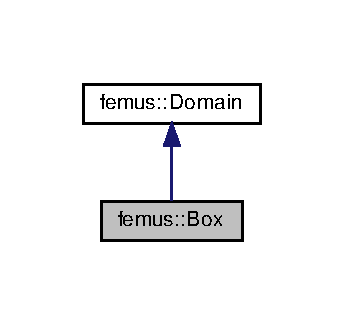
\includegraphics[width=165pt]{classfemus_1_1_box__inherit__graph}
\end{center}
\end{figure}


Collaboration diagram for femus\+:\+:Box\+:
\nopagebreak
\begin{figure}[H]
\begin{center}
\leavevmode
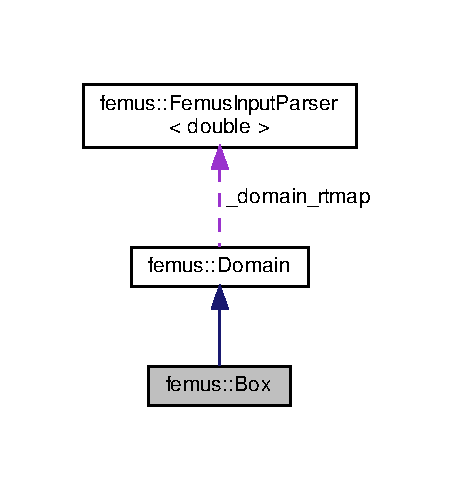
\includegraphics[width=219pt]{classfemus_1_1_box__coll__graph}
\end{center}
\end{figure}
\subsection*{Public Member Functions}
\begin{DoxyCompactItemize}
\item 
const \mbox{\hyperlink{_typedefs_8hpp_a91ad9478d81a7aaf2593e8d9c3d06a14}{uint}} \mbox{\hyperlink{classfemus_1_1_box_ae1e35410fff5545cd0c203cd9ad3001d}{Get\+Domain\+Flag}} () const
\item 
\mbox{\hyperlink{classfemus_1_1_box_ad05d2997adf7230ddd3c8e35c3f34806}{Box}} (const \mbox{\hyperlink{_typedefs_8hpp_a91ad9478d81a7aaf2593e8d9c3d06a14}{uint}} spacedim\+\_\+in, \mbox{\hyperlink{classfemus_1_1_femus_input_parser}{Femus\+Input\+Parser}}$<$ double $>$ \&map\+\_\+in)
\item 
\mbox{\hyperlink{classfemus_1_1_box_ad3446f7195748d6acb6dd9aa8eb6c949}{$\sim$\+Box}} ()
\item 
void \mbox{\hyperlink{classfemus_1_1_box_a68040d6347479ba7a0eb15856c2b96fa}{Init\+And\+Nondimensionalize}} (double Lref\+\_\+in)
\item 
void \mbox{\hyperlink{classfemus_1_1_box_a64a23d5bb0cac88b4e545b121988b3cf}{Transform\+Point\+To\+Ref}} (const double $\ast$x\+\_\+in, double $\ast$x\+\_\+out) const
\begin{DoxyCompactList}\small\item\em transformation to reference \mbox{\hyperlink{classfemus_1_1_domain}{Domain}} frame \end{DoxyCompactList}\end{DoxyCompactItemize}
\subsection*{Public Attributes}
\begin{DoxyCompactItemize}
\item 
std\+::vector$<$ double $>$ \mbox{\hyperlink{classfemus_1_1_box_a443727a5ad255d5352e92c33fac03958}{\+\_\+lb}}
\item 
std\+::vector$<$ double $>$ \mbox{\hyperlink{classfemus_1_1_box_a65fed8de18221ad064d17a440e3f3b04}{\+\_\+le}}
\end{DoxyCompactItemize}
\subsection*{Additional Inherited Members}


\subsection{Constructor \& Destructor Documentation}
\mbox{\Hypertarget{classfemus_1_1_box_ad05d2997adf7230ddd3c8e35c3f34806}\label{classfemus_1_1_box_ad05d2997adf7230ddd3c8e35c3f34806}} 
\index{femus\+::\+Box@{femus\+::\+Box}!Box@{Box}}
\index{Box@{Box}!femus\+::\+Box@{femus\+::\+Box}}
\subsubsection{\texorpdfstring{Box()}{Box()}}
{\footnotesize\ttfamily femus\+::\+Box\+::\+Box (\begin{DoxyParamCaption}\item[{const \mbox{\hyperlink{_typedefs_8hpp_a91ad9478d81a7aaf2593e8d9c3d06a14}{uint}}}]{spacedim\+\_\+in,  }\item[{\mbox{\hyperlink{classfemus_1_1_femus_input_parser}{Femus\+Input\+Parser}}$<$ double $>$ \&}]{map\+\_\+in }\end{DoxyParamCaption})}

\mbox{\Hypertarget{classfemus_1_1_box_ad3446f7195748d6acb6dd9aa8eb6c949}\label{classfemus_1_1_box_ad3446f7195748d6acb6dd9aa8eb6c949}} 
\index{femus\+::\+Box@{femus\+::\+Box}!````~Box@{$\sim$\+Box}}
\index{````~Box@{$\sim$\+Box}!femus\+::\+Box@{femus\+::\+Box}}
\subsubsection{\texorpdfstring{$\sim$\+Box()}{~Box()}}
{\footnotesize\ttfamily femus\+::\+Box\+::$\sim$\+Box (\begin{DoxyParamCaption}{ }\end{DoxyParamCaption})}



\subsection{Member Function Documentation}
\mbox{\Hypertarget{classfemus_1_1_box_ae1e35410fff5545cd0c203cd9ad3001d}\label{classfemus_1_1_box_ae1e35410fff5545cd0c203cd9ad3001d}} 
\index{femus\+::\+Box@{femus\+::\+Box}!Get\+Domain\+Flag@{Get\+Domain\+Flag}}
\index{Get\+Domain\+Flag@{Get\+Domain\+Flag}!femus\+::\+Box@{femus\+::\+Box}}
\subsubsection{\texorpdfstring{Get\+Domain\+Flag()}{GetDomainFlag()}}
{\footnotesize\ttfamily const \mbox{\hyperlink{_typedefs_8hpp_a91ad9478d81a7aaf2593e8d9c3d06a14}{uint}} femus\+::\+Box\+::\+Get\+Domain\+Flag (\begin{DoxyParamCaption}{ }\end{DoxyParamCaption}) const\hspace{0.3cm}{\ttfamily [inline]}, {\ttfamily [virtual]}}



Implements \mbox{\hyperlink{classfemus_1_1_domain_ad75eacc25142ba41cbceab06de675fc8}{femus\+::\+Domain}}.

\mbox{\Hypertarget{classfemus_1_1_box_a68040d6347479ba7a0eb15856c2b96fa}\label{classfemus_1_1_box_a68040d6347479ba7a0eb15856c2b96fa}} 
\index{femus\+::\+Box@{femus\+::\+Box}!Init\+And\+Nondimensionalize@{Init\+And\+Nondimensionalize}}
\index{Init\+And\+Nondimensionalize@{Init\+And\+Nondimensionalize}!femus\+::\+Box@{femus\+::\+Box}}
\subsubsection{\texorpdfstring{Init\+And\+Nondimensionalize()}{InitAndNondimensionalize()}}
{\footnotesize\ttfamily void femus\+::\+Box\+::\+Init\+And\+Nondimensionalize (\begin{DoxyParamCaption}\item[{double}]{Lref\+\_\+in }\end{DoxyParamCaption})}

\mbox{\Hypertarget{classfemus_1_1_box_a64a23d5bb0cac88b4e545b121988b3cf}\label{classfemus_1_1_box_a64a23d5bb0cac88b4e545b121988b3cf}} 
\index{femus\+::\+Box@{femus\+::\+Box}!Transform\+Point\+To\+Ref@{Transform\+Point\+To\+Ref}}
\index{Transform\+Point\+To\+Ref@{Transform\+Point\+To\+Ref}!femus\+::\+Box@{femus\+::\+Box}}
\subsubsection{\texorpdfstring{Transform\+Point\+To\+Ref()}{TransformPointToRef()}}
{\footnotesize\ttfamily void femus\+::\+Box\+::\+Transform\+Point\+To\+Ref (\begin{DoxyParamCaption}\item[{const double $\ast$}]{x\+\_\+in,  }\item[{double $\ast$}]{x\+\_\+out }\end{DoxyParamCaption}) const\hspace{0.3cm}{\ttfamily [virtual]}}



transformation to reference \mbox{\hyperlink{classfemus_1_1_domain}{Domain}} frame 



Implements \mbox{\hyperlink{classfemus_1_1_domain_afde27aa114c601801cc727ef9edf31de}{femus\+::\+Domain}}.



\subsection{Member Data Documentation}
\mbox{\Hypertarget{classfemus_1_1_box_a443727a5ad255d5352e92c33fac03958}\label{classfemus_1_1_box_a443727a5ad255d5352e92c33fac03958}} 
\index{femus\+::\+Box@{femus\+::\+Box}!\+\_\+lb@{\+\_\+lb}}
\index{\+\_\+lb@{\+\_\+lb}!femus\+::\+Box@{femus\+::\+Box}}
\subsubsection{\texorpdfstring{\+\_\+lb}{\_lb}}
{\footnotesize\ttfamily std\+::vector$<$double$>$ femus\+::\+Box\+::\+\_\+lb}

\mbox{\Hypertarget{classfemus_1_1_box_a65fed8de18221ad064d17a440e3f3b04}\label{classfemus_1_1_box_a65fed8de18221ad064d17a440e3f3b04}} 
\index{femus\+::\+Box@{femus\+::\+Box}!\+\_\+le@{\+\_\+le}}
\index{\+\_\+le@{\+\_\+le}!femus\+::\+Box@{femus\+::\+Box}}
\subsubsection{\texorpdfstring{\+\_\+le}{\_le}}
{\footnotesize\ttfamily std\+::vector$<$double$>$ femus\+::\+Box\+::\+\_\+le}



The documentation for this class was generated from the following files\+:\begin{DoxyCompactItemize}
\item 
mesh\+Gencase/\mbox{\hyperlink{_box_8hpp}{Box.\+hpp}}\item 
mesh\+Gencase/\mbox{\hyperlink{_box_8cpp}{Box.\+cpp}}\end{DoxyCompactItemize}

\hypertarget{classfemus_1_1_current_elem}{}\section{femus\+:\+:Current\+Elem Class Reference}
\label{classfemus_1_1_current_elem}\index{femus\+::\+Current\+Elem@{femus\+::\+Current\+Elem}}


{\ttfamily \#include $<$Current\+Elem.\+hpp$>$}



Collaboration diagram for femus\+:\+:Current\+Elem\+:
\nopagebreak
\begin{figure}[H]
\begin{center}
\leavevmode
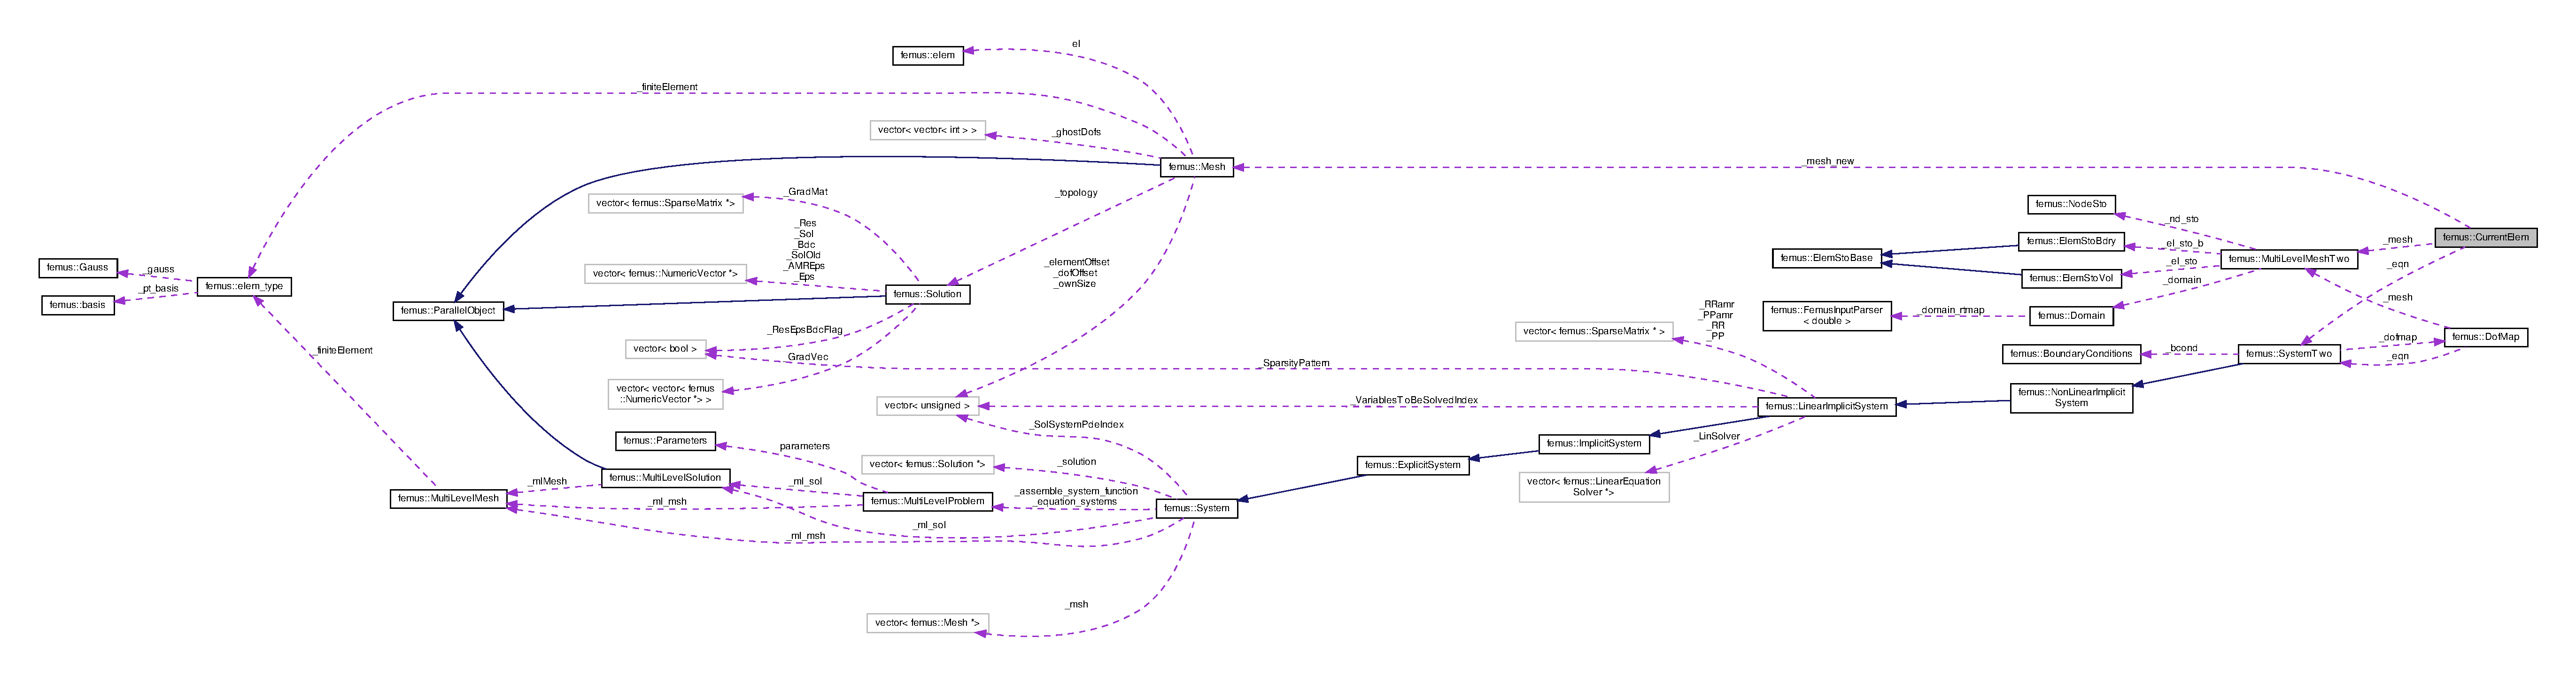
\includegraphics[width=350pt]{classfemus_1_1_current_elem__coll__graph}
\end{center}
\end{figure}
\subsection*{Public Member Functions}
\begin{DoxyCompactItemize}
\item 
\mbox{\hyperlink{classfemus_1_1_current_elem_ae833a5c35d89b95fdfafb44050bdb5d7}{Current\+Elem}} (const \mbox{\hyperlink{_typedefs_8hpp_a91ad9478d81a7aaf2593e8d9c3d06a14}{uint}} iel\+\_\+in, const \mbox{\hyperlink{_typedefs_8hpp_a91ad9478d81a7aaf2593e8d9c3d06a14}{uint}} iproc\+\_\+in, const \mbox{\hyperlink{_typedefs_8hpp_a91ad9478d81a7aaf2593e8d9c3d06a14}{uint}} level, const \mbox{\hyperlink{_typedefs_8hpp_a91ad9478d81a7aaf2593e8d9c3d06a14}{uint}} vb, const \mbox{\hyperlink{classfemus_1_1_system_two}{System\+Two}} $\ast$, const \mbox{\hyperlink{classfemus_1_1_multi_level_mesh_two}{Multi\+Level\+Mesh\+Two}} \&mesh, const std\+::vector$<$ std\+::vector$<$ const \mbox{\hyperlink{classfemus_1_1elem__type}{elem\+\_\+type}} $\ast$$>$ $>$ \&\mbox{\hyperlink{classfemus_1_1elem__type}{elem\+\_\+type}}, const \mbox{\hyperlink{classfemus_1_1_mesh}{Mesh}} $\ast$mesh\+\_\+new)
\item 
const \mbox{\hyperlink{_typedefs_8hpp_a91ad9478d81a7aaf2593e8d9c3d06a14}{uint}} \mbox{\hyperlink{classfemus_1_1_current_elem_ab41f6f8c70c2c128e80a709142d4d7cb}{Get\+Vb}} () const
\item 
const \mbox{\hyperlink{_typedefs_8hpp_a91ad9478d81a7aaf2593e8d9c3d06a14}{uint}} \mbox{\hyperlink{classfemus_1_1_current_elem_ac6bc91c21dfa57288d52e107421bc013}{Get\+Dim}} () const
\item 
const double $\ast$ \mbox{\hyperlink{classfemus_1_1_current_elem_aa4b96cd952c803dad64644067d528372}{Get\+Midpoint}} () const
\item 
const \mbox{\hyperlink{_typedefs_8hpp_a91ad9478d81a7aaf2593e8d9c3d06a14}{uint}} $\ast$ \mbox{\hyperlink{classfemus_1_1_current_elem_a214686cf1fc812970e6841907da0487b}{Get\+Conn}} () const
\item 
\mbox{\hyperlink{_typedefs_8hpp_a91ad9478d81a7aaf2593e8d9c3d06a14}{uint}} \mbox{\hyperlink{classfemus_1_1_current_elem_ae6de3a26fe4c3139e814bb40d62929e2}{Get\+Vol\+Iel}} () const
\item 
const double $\ast$ \mbox{\hyperlink{classfemus_1_1_current_elem_a7d67d0254c2bfcd1405bef6dfbc76fe6}{Get\+Node\+Coords}} () const
\item 
std\+::vector$<$ \mbox{\hyperlink{_typedefs_8hpp_a91ad9478d81a7aaf2593e8d9c3d06a14}{uint}} $>$ \mbox{\hyperlink{classfemus_1_1_current_elem_a0a056fc0356898983b18a52464e77567}{Get\+Dof\+Indices}} () const
\item 
\mbox{\hyperlink{_typedefs_8hpp_a91ad9478d81a7aaf2593e8d9c3d06a14}{uint}} $\ast$ \mbox{\hyperlink{classfemus_1_1_current_elem_a144d2b0317f92a69bf61cb5b67f709c9}{Get\+B\+C\+Dof\+Flag}} ()
\item 
\mbox{\hyperlink{classfemus_1_1_dense_vector}{Dense\+Vector}} \& \mbox{\hyperlink{classfemus_1_1_current_elem_a8dded1c45dc6cf9d5f6d089fd0b91eda}{Rhs}} ()
\item 
\mbox{\hyperlink{classfemus_1_1_dense_matrix}{Dense\+Matrix}} \& \mbox{\hyperlink{classfemus_1_1_current_elem_a6b0def20406de522d58d175b3645d2e8}{Mat}} ()
\item 
void \mbox{\hyperlink{classfemus_1_1_current_elem_a2f91b846308c3c8ab32aba4ac5f650b1}{Set\+Dofobj\+Conn\+Coords}} ()
\item 
void \mbox{\hyperlink{classfemus_1_1_current_elem_a5fe589a6224b2b1f618d67fb0bce7e38}{Set\+Midpoint}} ()
\begin{DoxyCompactList}\small\item\em this routine does not yield the connectivity \end{DoxyCompactList}\item 
void \mbox{\hyperlink{classfemus_1_1_current_elem_a7733d1aa0d817b3288f96b7ad2fdce0b}{Print\+Orientation}} () const
\item 
void \mbox{\hyperlink{classfemus_1_1_current_elem_a6de5a8d1e1da9f2befa896088cdf676d}{Convert\+Elem\+Coords\+To\+Mapping\+Ord}} (\mbox{\hyperlink{classfemus_1_1_current_quantity}{Current\+Quantity}} \&myvect) const
\begin{DoxyCompactList}\small\item\em here, the original element order of the nodes is respected in xyz.\+\_\+val\+\_\+dofs \end{DoxyCompactList}\item 
void \mbox{\hyperlink{classfemus_1_1_current_elem_a2fc8e65fa40bdcda9cfcb7c5447439ad}{Set\+El\+Dofs\+Bc}} ()
\item 
const \mbox{\hyperlink{classfemus_1_1elem__type}{elem\+\_\+type}} $\ast$ \mbox{\hyperlink{classfemus_1_1_current_elem_aad89677687498cb766cf47db822764af}{Get\+Elem\+Type}} (const \mbox{\hyperlink{_typedefs_8hpp_a91ad9478d81a7aaf2593e8d9c3d06a14}{uint}} fe) const
\item 
const std\+::vector$<$ const \mbox{\hyperlink{classfemus_1_1elem__type}{elem\+\_\+type}} $\ast$ $>$ \& \mbox{\hyperlink{classfemus_1_1_current_elem_ad686bf1b06d7ff8ee4b4d53acbf39470}{Get\+Elem\+Type\+Vector\+FE}} () const
\item 
int \mbox{\hyperlink{classfemus_1_1_current_elem_a3cff8a3824dda80a7f9d81426f4c37be}{Bc\+\_\+\+Compute\+Element\+Boundary\+Flags\+From\+Nodal\+Flags\+For\+Pressure}} (const \mbox{\hyperlink{_typedefs_8hpp_a91ad9478d81a7aaf2593e8d9c3d06a14}{uint}} ndof\+\_\+in, const \mbox{\hyperlink{_typedefs_8hpp_a91ad9478d81a7aaf2593e8d9c3d06a14}{uint}} space\+\_\+dim, const \mbox{\hyperlink{classfemus_1_1_current_quantity}{Current\+Quantity}} \&press\+\_\+in) const
\item 
const \mbox{\hyperlink{_typedefs_8hpp_a91ad9478d81a7aaf2593e8d9c3d06a14}{uint}} \mbox{\hyperlink{classfemus_1_1_current_elem_add1528c07ff61e8d3f25afdf3736ba2a}{Get\+Level}} () const
\end{DoxyCompactItemize}
\subsection*{Public Attributes}
\begin{DoxyCompactItemize}
\item 
const \mbox{\hyperlink{classfemus_1_1_system_two}{System\+Two}} $\ast$ \mbox{\hyperlink{classfemus_1_1_current_elem_af1164c456d9c52edc77d1c0c005bbe9c}{\+\_\+eqn}}
\item 
const \mbox{\hyperlink{classfemus_1_1_multi_level_mesh_two}{Multi\+Level\+Mesh\+Two}} \& \mbox{\hyperlink{classfemus_1_1_current_elem_a8321beae2ca94fa4ea8d17e484d978ee}{\+\_\+mesh}}
\item 
const \mbox{\hyperlink{classfemus_1_1_mesh}{Mesh}} $\ast$ \mbox{\hyperlink{classfemus_1_1_current_elem_a35f92400742999016814725c65cf2aae}{\+\_\+mesh\+\_\+new}}
\end{DoxyCompactItemize}


\subsection{Constructor \& Destructor Documentation}
\mbox{\Hypertarget{classfemus_1_1_current_elem_ae833a5c35d89b95fdfafb44050bdb5d7}\label{classfemus_1_1_current_elem_ae833a5c35d89b95fdfafb44050bdb5d7}} 
\index{femus\+::\+Current\+Elem@{femus\+::\+Current\+Elem}!Current\+Elem@{Current\+Elem}}
\index{Current\+Elem@{Current\+Elem}!femus\+::\+Current\+Elem@{femus\+::\+Current\+Elem}}
\subsubsection{\texorpdfstring{Current\+Elem()}{CurrentElem()}}
{\footnotesize\ttfamily femus\+::\+Current\+Elem\+::\+Current\+Elem (\begin{DoxyParamCaption}\item[{const \mbox{\hyperlink{_typedefs_8hpp_a91ad9478d81a7aaf2593e8d9c3d06a14}{uint}}}]{iel\+\_\+in,  }\item[{const \mbox{\hyperlink{_typedefs_8hpp_a91ad9478d81a7aaf2593e8d9c3d06a14}{uint}}}]{iproc\+\_\+in,  }\item[{const \mbox{\hyperlink{_typedefs_8hpp_a91ad9478d81a7aaf2593e8d9c3d06a14}{uint}}}]{level,  }\item[{const \mbox{\hyperlink{_typedefs_8hpp_a91ad9478d81a7aaf2593e8d9c3d06a14}{uint}}}]{vb,  }\item[{const \mbox{\hyperlink{classfemus_1_1_system_two}{System\+Two}} $\ast$}]{eqn\+\_\+in,  }\item[{const \mbox{\hyperlink{classfemus_1_1_multi_level_mesh_two}{Multi\+Level\+Mesh\+Two}} \&}]{mesh,  }\item[{const std\+::vector$<$ std\+::vector$<$ const \mbox{\hyperlink{classfemus_1_1elem__type}{elem\+\_\+type}} $\ast$$>$ $>$ \&}]{elem\+\_\+type,  }\item[{const \mbox{\hyperlink{classfemus_1_1_mesh}{Mesh}} $\ast$}]{mesh\+\_\+new }\end{DoxyParamCaption})}



\subsection{Member Function Documentation}
\mbox{\Hypertarget{classfemus_1_1_current_elem_a3cff8a3824dda80a7f9d81426f4c37be}\label{classfemus_1_1_current_elem_a3cff8a3824dda80a7f9d81426f4c37be}} 
\index{femus\+::\+Current\+Elem@{femus\+::\+Current\+Elem}!Bc\+\_\+\+Compute\+Element\+Boundary\+Flags\+From\+Nodal\+Flags\+For\+Pressure@{Bc\+\_\+\+Compute\+Element\+Boundary\+Flags\+From\+Nodal\+Flags\+For\+Pressure}}
\index{Bc\+\_\+\+Compute\+Element\+Boundary\+Flags\+From\+Nodal\+Flags\+For\+Pressure@{Bc\+\_\+\+Compute\+Element\+Boundary\+Flags\+From\+Nodal\+Flags\+For\+Pressure}!femus\+::\+Current\+Elem@{femus\+::\+Current\+Elem}}
\subsubsection{\texorpdfstring{Bc\+\_\+\+Compute\+Element\+Boundary\+Flags\+From\+Nodal\+Flags\+For\+Pressure()}{Bc\_ComputeElementBoundaryFlagsFromNodalFlagsForPressure()}}
{\footnotesize\ttfamily int femus\+::\+Current\+Elem\+::\+Bc\+\_\+\+Compute\+Element\+Boundary\+Flags\+From\+Nodal\+Flags\+For\+Pressure (\begin{DoxyParamCaption}\item[{const \mbox{\hyperlink{_typedefs_8hpp_a91ad9478d81a7aaf2593e8d9c3d06a14}{uint}}}]{ndof\+\_\+in,  }\item[{const \mbox{\hyperlink{_typedefs_8hpp_a91ad9478d81a7aaf2593e8d9c3d06a14}{uint}}}]{space\+\_\+dim,  }\item[{const \mbox{\hyperlink{classfemus_1_1_current_quantity}{Current\+Quantity}} \&}]{press\+\_\+in }\end{DoxyParamCaption}) const}

\begin{DoxyRefDesc}{Deprecated}
\item[\mbox{\hyperlink{deprecated__deprecated000007}{Deprecated}}]\end{DoxyRefDesc}
\mbox{\Hypertarget{classfemus_1_1_current_elem_a6de5a8d1e1da9f2befa896088cdf676d}\label{classfemus_1_1_current_elem_a6de5a8d1e1da9f2befa896088cdf676d}} 
\index{femus\+::\+Current\+Elem@{femus\+::\+Current\+Elem}!Convert\+Elem\+Coords\+To\+Mapping\+Ord@{Convert\+Elem\+Coords\+To\+Mapping\+Ord}}
\index{Convert\+Elem\+Coords\+To\+Mapping\+Ord@{Convert\+Elem\+Coords\+To\+Mapping\+Ord}!femus\+::\+Current\+Elem@{femus\+::\+Current\+Elem}}
\subsubsection{\texorpdfstring{Convert\+Elem\+Coords\+To\+Mapping\+Ord()}{ConvertElemCoordsToMappingOrd()}}
{\footnotesize\ttfamily void femus\+::\+Current\+Elem\+::\+Convert\+Elem\+Coords\+To\+Mapping\+Ord (\begin{DoxyParamCaption}\item[{\mbox{\hyperlink{classfemus_1_1_current_quantity}{Current\+Quantity}} \&}]{myvect }\end{DoxyParamCaption}) const}



here, the original element order of the nodes is respected in xyz.\+\_\+val\+\_\+dofs 

\mbox{\Hypertarget{classfemus_1_1_current_elem_a144d2b0317f92a69bf61cb5b67f709c9}\label{classfemus_1_1_current_elem_a144d2b0317f92a69bf61cb5b67f709c9}} 
\index{femus\+::\+Current\+Elem@{femus\+::\+Current\+Elem}!Get\+B\+C\+Dof\+Flag@{Get\+B\+C\+Dof\+Flag}}
\index{Get\+B\+C\+Dof\+Flag@{Get\+B\+C\+Dof\+Flag}!femus\+::\+Current\+Elem@{femus\+::\+Current\+Elem}}
\subsubsection{\texorpdfstring{Get\+B\+C\+Dof\+Flag()}{GetBCDofFlag()}}
{\footnotesize\ttfamily \mbox{\hyperlink{_typedefs_8hpp_a91ad9478d81a7aaf2593e8d9c3d06a14}{uint}}$\ast$ femus\+::\+Current\+Elem\+::\+Get\+B\+C\+Dof\+Flag (\begin{DoxyParamCaption}{ }\end{DoxyParamCaption})\hspace{0.3cm}{\ttfamily [inline]}}

\mbox{\Hypertarget{classfemus_1_1_current_elem_a214686cf1fc812970e6841907da0487b}\label{classfemus_1_1_current_elem_a214686cf1fc812970e6841907da0487b}} 
\index{femus\+::\+Current\+Elem@{femus\+::\+Current\+Elem}!Get\+Conn@{Get\+Conn}}
\index{Get\+Conn@{Get\+Conn}!femus\+::\+Current\+Elem@{femus\+::\+Current\+Elem}}
\subsubsection{\texorpdfstring{Get\+Conn()}{GetConn()}}
{\footnotesize\ttfamily const \mbox{\hyperlink{_typedefs_8hpp_a91ad9478d81a7aaf2593e8d9c3d06a14}{uint}}$\ast$ femus\+::\+Current\+Elem\+::\+Get\+Conn (\begin{DoxyParamCaption}{ }\end{DoxyParamCaption}) const\hspace{0.3cm}{\ttfamily [inline]}}

\mbox{\Hypertarget{classfemus_1_1_current_elem_ac6bc91c21dfa57288d52e107421bc013}\label{classfemus_1_1_current_elem_ac6bc91c21dfa57288d52e107421bc013}} 
\index{femus\+::\+Current\+Elem@{femus\+::\+Current\+Elem}!Get\+Dim@{Get\+Dim}}
\index{Get\+Dim@{Get\+Dim}!femus\+::\+Current\+Elem@{femus\+::\+Current\+Elem}}
\subsubsection{\texorpdfstring{Get\+Dim()}{GetDim()}}
{\footnotesize\ttfamily const \mbox{\hyperlink{_typedefs_8hpp_a91ad9478d81a7aaf2593e8d9c3d06a14}{uint}} femus\+::\+Current\+Elem\+::\+Get\+Dim (\begin{DoxyParamCaption}{ }\end{DoxyParamCaption}) const\hspace{0.3cm}{\ttfamily [inline]}}

\mbox{\Hypertarget{classfemus_1_1_current_elem_a0a056fc0356898983b18a52464e77567}\label{classfemus_1_1_current_elem_a0a056fc0356898983b18a52464e77567}} 
\index{femus\+::\+Current\+Elem@{femus\+::\+Current\+Elem}!Get\+Dof\+Indices@{Get\+Dof\+Indices}}
\index{Get\+Dof\+Indices@{Get\+Dof\+Indices}!femus\+::\+Current\+Elem@{femus\+::\+Current\+Elem}}
\subsubsection{\texorpdfstring{Get\+Dof\+Indices()}{GetDofIndices()}}
{\footnotesize\ttfamily std\+::vector$<$\mbox{\hyperlink{_typedefs_8hpp_a91ad9478d81a7aaf2593e8d9c3d06a14}{uint}}$>$ femus\+::\+Current\+Elem\+::\+Get\+Dof\+Indices (\begin{DoxyParamCaption}{ }\end{DoxyParamCaption}) const\hspace{0.3cm}{\ttfamily [inline]}}

\mbox{\Hypertarget{classfemus_1_1_current_elem_aad89677687498cb766cf47db822764af}\label{classfemus_1_1_current_elem_aad89677687498cb766cf47db822764af}} 
\index{femus\+::\+Current\+Elem@{femus\+::\+Current\+Elem}!Get\+Elem\+Type@{Get\+Elem\+Type}}
\index{Get\+Elem\+Type@{Get\+Elem\+Type}!femus\+::\+Current\+Elem@{femus\+::\+Current\+Elem}}
\subsubsection{\texorpdfstring{Get\+Elem\+Type()}{GetElemType()}}
{\footnotesize\ttfamily const \mbox{\hyperlink{classfemus_1_1elem__type}{elem\+\_\+type}}$\ast$ femus\+::\+Current\+Elem\+::\+Get\+Elem\+Type (\begin{DoxyParamCaption}\item[{const \mbox{\hyperlink{_typedefs_8hpp_a91ad9478d81a7aaf2593e8d9c3d06a14}{uint}}}]{fe }\end{DoxyParamCaption}) const\hspace{0.3cm}{\ttfamily [inline]}}

\mbox{\Hypertarget{classfemus_1_1_current_elem_ad686bf1b06d7ff8ee4b4d53acbf39470}\label{classfemus_1_1_current_elem_ad686bf1b06d7ff8ee4b4d53acbf39470}} 
\index{femus\+::\+Current\+Elem@{femus\+::\+Current\+Elem}!Get\+Elem\+Type\+Vector\+FE@{Get\+Elem\+Type\+Vector\+FE}}
\index{Get\+Elem\+Type\+Vector\+FE@{Get\+Elem\+Type\+Vector\+FE}!femus\+::\+Current\+Elem@{femus\+::\+Current\+Elem}}
\subsubsection{\texorpdfstring{Get\+Elem\+Type\+Vector\+F\+E()}{GetElemTypeVectorFE()}}
{\footnotesize\ttfamily const std\+::vector$<$const \mbox{\hyperlink{classfemus_1_1elem__type}{elem\+\_\+type}}$\ast$$>$\& femus\+::\+Current\+Elem\+::\+Get\+Elem\+Type\+Vector\+FE (\begin{DoxyParamCaption}{ }\end{DoxyParamCaption}) const\hspace{0.3cm}{\ttfamily [inline]}}

\mbox{\Hypertarget{classfemus_1_1_current_elem_add1528c07ff61e8d3f25afdf3736ba2a}\label{classfemus_1_1_current_elem_add1528c07ff61e8d3f25afdf3736ba2a}} 
\index{femus\+::\+Current\+Elem@{femus\+::\+Current\+Elem}!Get\+Level@{Get\+Level}}
\index{Get\+Level@{Get\+Level}!femus\+::\+Current\+Elem@{femus\+::\+Current\+Elem}}
\subsubsection{\texorpdfstring{Get\+Level()}{GetLevel()}}
{\footnotesize\ttfamily const \mbox{\hyperlink{_typedefs_8hpp_a91ad9478d81a7aaf2593e8d9c3d06a14}{uint}} femus\+::\+Current\+Elem\+::\+Get\+Level (\begin{DoxyParamCaption}{ }\end{DoxyParamCaption}) const\hspace{0.3cm}{\ttfamily [inline]}}

\mbox{\Hypertarget{classfemus_1_1_current_elem_aa4b96cd952c803dad64644067d528372}\label{classfemus_1_1_current_elem_aa4b96cd952c803dad64644067d528372}} 
\index{femus\+::\+Current\+Elem@{femus\+::\+Current\+Elem}!Get\+Midpoint@{Get\+Midpoint}}
\index{Get\+Midpoint@{Get\+Midpoint}!femus\+::\+Current\+Elem@{femus\+::\+Current\+Elem}}
\subsubsection{\texorpdfstring{Get\+Midpoint()}{GetMidpoint()}}
{\footnotesize\ttfamily const double$\ast$ femus\+::\+Current\+Elem\+::\+Get\+Midpoint (\begin{DoxyParamCaption}{ }\end{DoxyParamCaption}) const\hspace{0.3cm}{\ttfamily [inline]}}

\mbox{\Hypertarget{classfemus_1_1_current_elem_a7d67d0254c2bfcd1405bef6dfbc76fe6}\label{classfemus_1_1_current_elem_a7d67d0254c2bfcd1405bef6dfbc76fe6}} 
\index{femus\+::\+Current\+Elem@{femus\+::\+Current\+Elem}!Get\+Node\+Coords@{Get\+Node\+Coords}}
\index{Get\+Node\+Coords@{Get\+Node\+Coords}!femus\+::\+Current\+Elem@{femus\+::\+Current\+Elem}}
\subsubsection{\texorpdfstring{Get\+Node\+Coords()}{GetNodeCoords()}}
{\footnotesize\ttfamily const double$\ast$ femus\+::\+Current\+Elem\+::\+Get\+Node\+Coords (\begin{DoxyParamCaption}{ }\end{DoxyParamCaption}) const\hspace{0.3cm}{\ttfamily [inline]}}

\mbox{\Hypertarget{classfemus_1_1_current_elem_ab41f6f8c70c2c128e80a709142d4d7cb}\label{classfemus_1_1_current_elem_ab41f6f8c70c2c128e80a709142d4d7cb}} 
\index{femus\+::\+Current\+Elem@{femus\+::\+Current\+Elem}!Get\+Vb@{Get\+Vb}}
\index{Get\+Vb@{Get\+Vb}!femus\+::\+Current\+Elem@{femus\+::\+Current\+Elem}}
\subsubsection{\texorpdfstring{Get\+Vb()}{GetVb()}}
{\footnotesize\ttfamily const \mbox{\hyperlink{_typedefs_8hpp_a91ad9478d81a7aaf2593e8d9c3d06a14}{uint}} femus\+::\+Current\+Elem\+::\+Get\+Vb (\begin{DoxyParamCaption}{ }\end{DoxyParamCaption}) const\hspace{0.3cm}{\ttfamily [inline]}}

\mbox{\Hypertarget{classfemus_1_1_current_elem_ae6de3a26fe4c3139e814bb40d62929e2}\label{classfemus_1_1_current_elem_ae6de3a26fe4c3139e814bb40d62929e2}} 
\index{femus\+::\+Current\+Elem@{femus\+::\+Current\+Elem}!Get\+Vol\+Iel@{Get\+Vol\+Iel}}
\index{Get\+Vol\+Iel@{Get\+Vol\+Iel}!femus\+::\+Current\+Elem@{femus\+::\+Current\+Elem}}
\subsubsection{\texorpdfstring{Get\+Vol\+Iel()}{GetVolIel()}}
{\footnotesize\ttfamily \mbox{\hyperlink{_typedefs_8hpp_a91ad9478d81a7aaf2593e8d9c3d06a14}{uint}} femus\+::\+Current\+Elem\+::\+Get\+Vol\+Iel (\begin{DoxyParamCaption}{ }\end{DoxyParamCaption}) const\hspace{0.3cm}{\ttfamily [inline]}}

\mbox{\Hypertarget{classfemus_1_1_current_elem_a6b0def20406de522d58d175b3645d2e8}\label{classfemus_1_1_current_elem_a6b0def20406de522d58d175b3645d2e8}} 
\index{femus\+::\+Current\+Elem@{femus\+::\+Current\+Elem}!Mat@{Mat}}
\index{Mat@{Mat}!femus\+::\+Current\+Elem@{femus\+::\+Current\+Elem}}
\subsubsection{\texorpdfstring{Mat()}{Mat()}}
{\footnotesize\ttfamily \mbox{\hyperlink{classfemus_1_1_dense_matrix}{Dense\+Matrix}}\& femus\+::\+Current\+Elem\+::\+Mat (\begin{DoxyParamCaption}{ }\end{DoxyParamCaption})\hspace{0.3cm}{\ttfamily [inline]}}

Returns a reference to the element matrix \mbox{\Hypertarget{classfemus_1_1_current_elem_a7733d1aa0d817b3288f96b7ad2fdce0b}\label{classfemus_1_1_current_elem_a7733d1aa0d817b3288f96b7ad2fdce0b}} 
\index{femus\+::\+Current\+Elem@{femus\+::\+Current\+Elem}!Print\+Orientation@{Print\+Orientation}}
\index{Print\+Orientation@{Print\+Orientation}!femus\+::\+Current\+Elem@{femus\+::\+Current\+Elem}}
\subsubsection{\texorpdfstring{Print\+Orientation()}{PrintOrientation()}}
{\footnotesize\ttfamily void femus\+::\+Current\+Elem\+::\+Print\+Orientation (\begin{DoxyParamCaption}{ }\end{DoxyParamCaption}) const}

This function prints the element orientation A Q\+U\+A\+D\+R\+A\+T\+IC M\+E\+SH V\+E\+C\+T\+OR is passed H\+E\+RE ~\newline
It is for debugging purposes \mbox{\Hypertarget{classfemus_1_1_current_elem_a8dded1c45dc6cf9d5f6d089fd0b91eda}\label{classfemus_1_1_current_elem_a8dded1c45dc6cf9d5f6d089fd0b91eda}} 
\index{femus\+::\+Current\+Elem@{femus\+::\+Current\+Elem}!Rhs@{Rhs}}
\index{Rhs@{Rhs}!femus\+::\+Current\+Elem@{femus\+::\+Current\+Elem}}
\subsubsection{\texorpdfstring{Rhs()}{Rhs()}}
{\footnotesize\ttfamily \mbox{\hyperlink{classfemus_1_1_dense_vector}{Dense\+Vector}}\& femus\+::\+Current\+Elem\+::\+Rhs (\begin{DoxyParamCaption}{ }\end{DoxyParamCaption})\hspace{0.3cm}{\ttfamily [inline]}}

Returns a reference to the element rhs \mbox{\Hypertarget{classfemus_1_1_current_elem_a2f91b846308c3c8ab32aba4ac5f650b1}\label{classfemus_1_1_current_elem_a2f91b846308c3c8ab32aba4ac5f650b1}} 
\index{femus\+::\+Current\+Elem@{femus\+::\+Current\+Elem}!Set\+Dofobj\+Conn\+Coords@{Set\+Dofobj\+Conn\+Coords}}
\index{Set\+Dofobj\+Conn\+Coords@{Set\+Dofobj\+Conn\+Coords}!femus\+::\+Current\+Elem@{femus\+::\+Current\+Elem}}
\subsubsection{\texorpdfstring{Set\+Dofobj\+Conn\+Coords()}{SetDofobjConnCoords()}}
{\footnotesize\ttfamily void femus\+::\+Current\+Elem\+::\+Set\+Dofobj\+Conn\+Coords (\begin{DoxyParamCaption}{ }\end{DoxyParamCaption})}

\mbox{\Hypertarget{classfemus_1_1_current_elem_a2fc8e65fa40bdcda9cfcb7c5447439ad}\label{classfemus_1_1_current_elem_a2fc8e65fa40bdcda9cfcb7c5447439ad}} 
\index{femus\+::\+Current\+Elem@{femus\+::\+Current\+Elem}!Set\+El\+Dofs\+Bc@{Set\+El\+Dofs\+Bc}}
\index{Set\+El\+Dofs\+Bc@{Set\+El\+Dofs\+Bc}!femus\+::\+Current\+Elem@{femus\+::\+Current\+Elem}}
\subsubsection{\texorpdfstring{Set\+El\+Dofs\+Bc()}{SetElDofsBc()}}
{\footnotesize\ttfamily void femus\+::\+Current\+Elem\+::\+Set\+El\+Dofs\+Bc (\begin{DoxyParamCaption}{ }\end{DoxyParamCaption})}

needs the E\+Q\+U\+A\+T\+I\+ON basically \mbox{\Hypertarget{classfemus_1_1_current_elem_a5fe589a6224b2b1f618d67fb0bce7e38}\label{classfemus_1_1_current_elem_a5fe589a6224b2b1f618d67fb0bce7e38}} 
\index{femus\+::\+Current\+Elem@{femus\+::\+Current\+Elem}!Set\+Midpoint@{Set\+Midpoint}}
\index{Set\+Midpoint@{Set\+Midpoint}!femus\+::\+Current\+Elem@{femus\+::\+Current\+Elem}}
\subsubsection{\texorpdfstring{Set\+Midpoint()}{SetMidpoint()}}
{\footnotesize\ttfamily void femus\+::\+Current\+Elem\+::\+Set\+Midpoint (\begin{DoxyParamCaption}{ }\end{DoxyParamCaption})}



this routine does not yield the connectivity 

this routine is \char`\"{}\+P\+A\+R\+A\+L\+L\+E\+L\char`\"{}, in the sense that it works only for the \+\_\+iproc in which you are! pay attention to every routine that has \+\_\+iproc!!! if you want to do a loop over A\+LL P\+R\+O\+C\+E\+S\+S\+ES you do not have to use iproc but you have to P\+A\+SS the S\+U\+B\+D\+O\+M\+A\+IN E\+X\+P\+L\+I\+C\+I\+T\+L\+Y!!! Compute the element center 

\subsection{Member Data Documentation}
\mbox{\Hypertarget{classfemus_1_1_current_elem_af1164c456d9c52edc77d1c0c005bbe9c}\label{classfemus_1_1_current_elem_af1164c456d9c52edc77d1c0c005bbe9c}} 
\index{femus\+::\+Current\+Elem@{femus\+::\+Current\+Elem}!\+\_\+eqn@{\+\_\+eqn}}
\index{\+\_\+eqn@{\+\_\+eqn}!femus\+::\+Current\+Elem@{femus\+::\+Current\+Elem}}
\subsubsection{\texorpdfstring{\+\_\+eqn}{\_eqn}}
{\footnotesize\ttfamily const \mbox{\hyperlink{classfemus_1_1_system_two}{System\+Two}}$\ast$ femus\+::\+Current\+Elem\+::\+\_\+eqn}

\mbox{\Hypertarget{classfemus_1_1_current_elem_a8321beae2ca94fa4ea8d17e484d978ee}\label{classfemus_1_1_current_elem_a8321beae2ca94fa4ea8d17e484d978ee}} 
\index{femus\+::\+Current\+Elem@{femus\+::\+Current\+Elem}!\+\_\+mesh@{\+\_\+mesh}}
\index{\+\_\+mesh@{\+\_\+mesh}!femus\+::\+Current\+Elem@{femus\+::\+Current\+Elem}}
\subsubsection{\texorpdfstring{\+\_\+mesh}{\_mesh}}
{\footnotesize\ttfamily const \mbox{\hyperlink{classfemus_1_1_multi_level_mesh_two}{Multi\+Level\+Mesh\+Two}}\& femus\+::\+Current\+Elem\+::\+\_\+mesh}

\mbox{\Hypertarget{classfemus_1_1_current_elem_a35f92400742999016814725c65cf2aae}\label{classfemus_1_1_current_elem_a35f92400742999016814725c65cf2aae}} 
\index{femus\+::\+Current\+Elem@{femus\+::\+Current\+Elem}!\+\_\+mesh\+\_\+new@{\+\_\+mesh\+\_\+new}}
\index{\+\_\+mesh\+\_\+new@{\+\_\+mesh\+\_\+new}!femus\+::\+Current\+Elem@{femus\+::\+Current\+Elem}}
\subsubsection{\texorpdfstring{\+\_\+mesh\+\_\+new}{\_mesh\_new}}
{\footnotesize\ttfamily const \mbox{\hyperlink{classfemus_1_1_mesh}{Mesh}}$\ast$ femus\+::\+Current\+Elem\+::\+\_\+mesh\+\_\+new}



The documentation for this class was generated from the following files\+:\begin{DoxyCompactItemize}
\item 
equations/\mbox{\hyperlink{_current_elem_8hpp}{Current\+Elem.\+hpp}}\item 
equations/\mbox{\hyperlink{_current_elem_8cpp}{Current\+Elem.\+cpp}}\end{DoxyCompactItemize}

\hypertarget{classfemus_1_1_current_gauss_point}{}\section{femus\+:\+:Current\+Gauss\+Point$<$ F\+M\+\_\+\+D\+IM $>$ Class Template Reference}
\label{classfemus_1_1_current_gauss_point}\index{femus\+::\+Current\+Gauss\+Point$<$ F\+M\+\_\+\+D\+I\+M $>$@{femus\+::\+Current\+Gauss\+Point$<$ F\+M\+\_\+\+D\+I\+M $>$}}


{\ttfamily \#include $<$Current\+Gauss\+Point.\+hpp$>$}



Inheritance diagram for femus\+:\+:Current\+Gauss\+Point$<$ F\+M\+\_\+\+D\+IM $>$\+:
\nopagebreak
\begin{figure}[H]
\begin{center}
\leavevmode
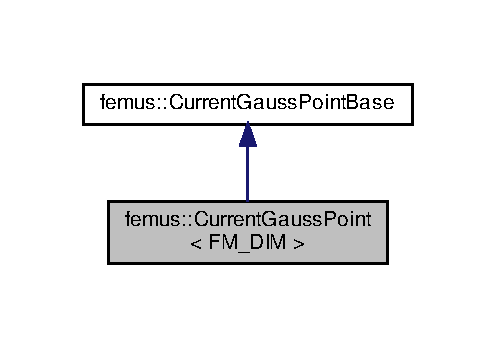
\includegraphics[width=238pt]{classfemus_1_1_current_gauss_point__inherit__graph}
\end{center}
\end{figure}


Collaboration diagram for femus\+:\+:Current\+Gauss\+Point$<$ F\+M\+\_\+\+D\+IM $>$\+:
\nopagebreak
\begin{figure}[H]
\begin{center}
\leavevmode
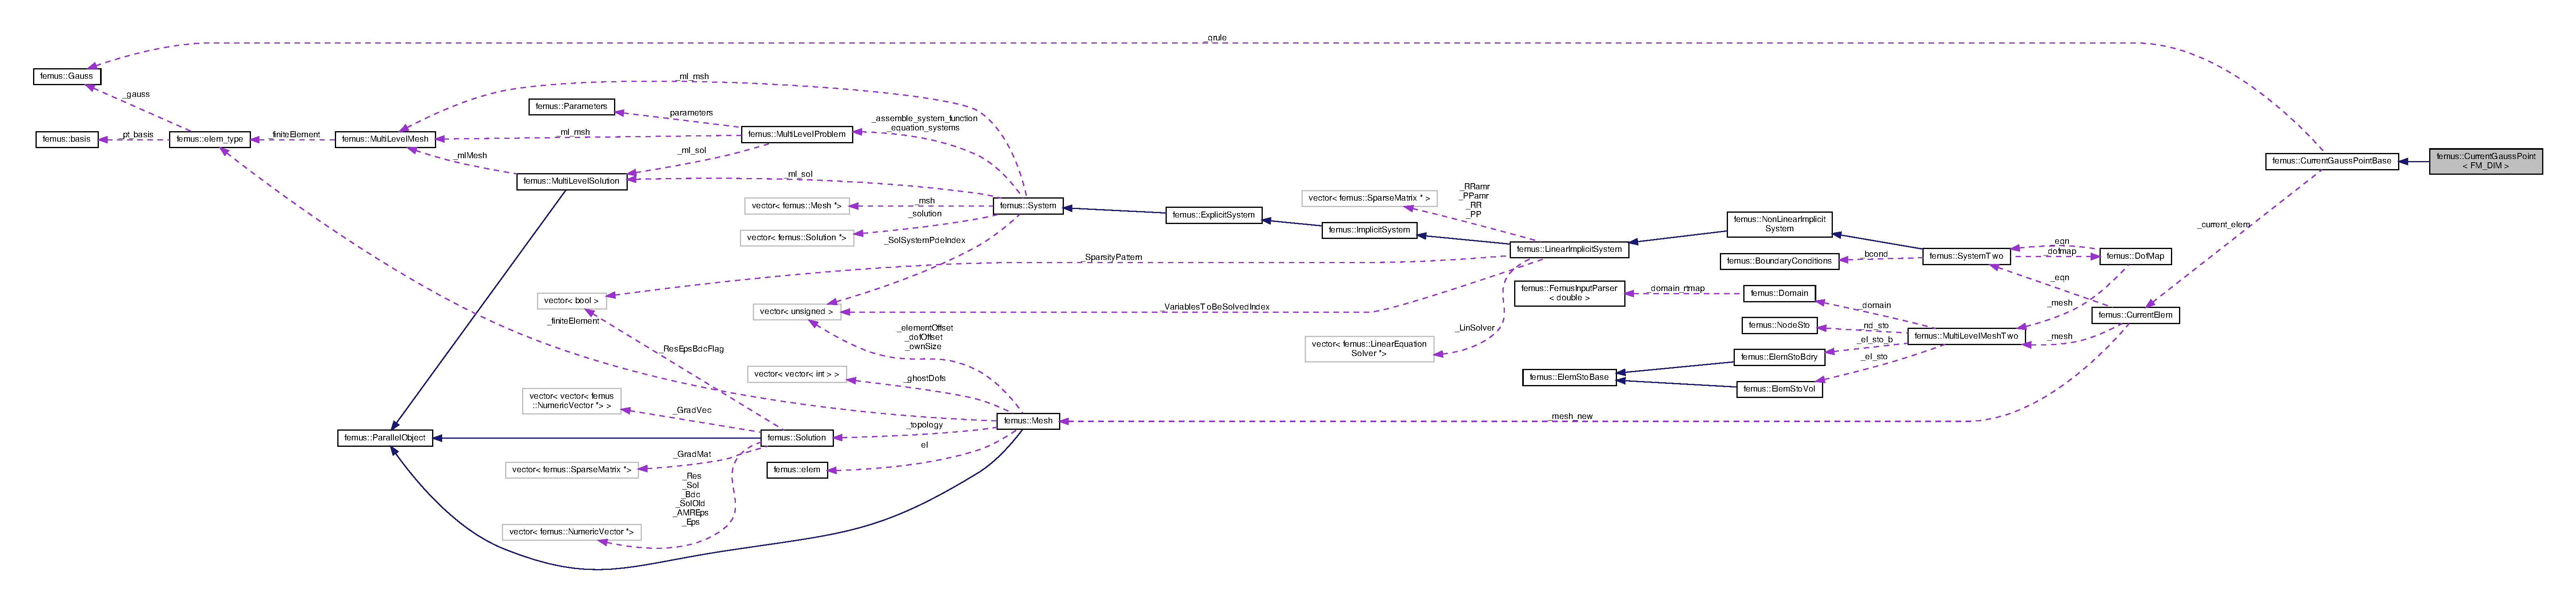
\includegraphics[width=350pt]{classfemus_1_1_current_gauss_point__coll__graph}
\end{center}
\end{figure}
\subsection*{Public Member Functions}
\begin{DoxyCompactItemize}
\item 
\mbox{\hyperlink{classfemus_1_1_current_gauss_point_ae55cfed8afa742359466fe1f21b10b02}{Current\+Gauss\+Point}} (const \mbox{\hyperlink{classfemus_1_1_current_elem}{Current\+Elem}} \&curr\+\_\+el\+\_\+in, const \mbox{\hyperlink{classfemus_1_1_gauss}{Gauss}} \&qrule\+\_\+in)
\item 
\mbox{\hyperlink{classfemus_1_1_current_gauss_point_a54541c2150b3c273354682ee31e5025d}{$\sim$\+Current\+Gauss\+Point}} ()
\item 
double \mbox{\hyperlink{classfemus_1_1_current_gauss_point_a96a47ebb8abd928f0db6e472db2811f1}{Jac\+Vect\+V\+V\+\_\+g}} (\mbox{\hyperlink{classfemus_1_1_current_quantity}{Current\+Quantity}} \&xyz)
\item 
double \mbox{\hyperlink{classfemus_1_1_current_gauss_point_afa303733709a133cb86ba65fe70d4a31}{Jac\+Vect\+B\+B\+\_\+g}} (\mbox{\hyperlink{classfemus_1_1_current_quantity}{Current\+Quantity}} \&xyz)
\item 
void \mbox{\hyperlink{classfemus_1_1_current_gauss_point_a7a11e1164802fdc683726eea6123d99f}{Set\+Phi\+El\+Dofs\+F\+E\+V\+B\+\_\+g}} (const \mbox{\hyperlink{_typedefs_8hpp_a91ad9478d81a7aaf2593e8d9c3d06a14}{uint}} qlflag, const \mbox{\hyperlink{_typedefs_8hpp_a91ad9478d81a7aaf2593e8d9c3d06a14}{uint}} qp)
\item 
void \mbox{\hyperlink{classfemus_1_1_current_gauss_point_a5b7c118fc9376db8783714992e341891}{Set\+D\+Phi\+Dxezeta\+El\+Dofs\+F\+E\+V\+B\+\_\+g}} (const \mbox{\hyperlink{_typedefs_8hpp_a91ad9478d81a7aaf2593e8d9c3d06a14}{uint}} qlflag, const \mbox{\hyperlink{_typedefs_8hpp_a91ad9478d81a7aaf2593e8d9c3d06a14}{uint}} qp)
\item 
void \mbox{\hyperlink{classfemus_1_1_current_gauss_point_af33ae0e6b36353be0bb671573c6362bc}{Set\+D\+Phi\+Dxyz\+El\+Dofs\+F\+E\+V\+B\+\_\+g}} (const \mbox{\hyperlink{_typedefs_8hpp_a91ad9478d81a7aaf2593e8d9c3d06a14}{uint}} qlflag, const \mbox{\hyperlink{_typedefs_8hpp_a91ad9478d81a7aaf2593e8d9c3d06a14}{uint}} qp)
\item 
void \mbox{\hyperlink{classfemus_1_1_current_gauss_point_aff8e672a0e763e7ff73a1e06a7bc5143}{Extend\+Dphi\+Dxyz\+El\+Dofs\+F\+E\+V\+B\+\_\+g}} (const \mbox{\hyperlink{_typedefs_8hpp_a91ad9478d81a7aaf2593e8d9c3d06a14}{uint}} qlflag)
\end{DoxyCompactItemize}
\subsection*{Protected Member Functions}
\begin{DoxyCompactItemize}
\item 
double \mbox{\hyperlink{classfemus_1_1_current_gauss_point_aa169b843fa89bc565b0757cc57b0e4d7}{Compute\+Jac\+VV}} ()
\item 
void \mbox{\hyperlink{classfemus_1_1_current_gauss_point_a13a36ea2f7ec52b2ed4186c0940755aa}{Compute\+Jac\+BB}} ()
\item 
{\footnotesize template$<$$>$ }\\void \mbox{\hyperlink{classfemus_1_1_current_gauss_point_a67ace006341ad08aad318cee34bf68ed}{Compute\+Jac\+BB}} ()
\item 
{\footnotesize template$<$$>$ }\\void \mbox{\hyperlink{classfemus_1_1_current_gauss_point_af66b9ef7607c4b0f3046ded08c15ab54}{Compute\+Jac\+BB}} ()
\item 
{\footnotesize template$<$$>$ }\\double \mbox{\hyperlink{classfemus_1_1_current_gauss_point_a76637d593d498d6abc7bd3190303d2fc}{Compute\+Jac\+VV}} ()
\item 
{\footnotesize template$<$$>$ }\\double \mbox{\hyperlink{classfemus_1_1_current_gauss_point_a3188289d2e70cc6ada264171132be163}{Compute\+Jac\+VV}} ()
\end{DoxyCompactItemize}
\subsection*{Protected Attributes}
\begin{DoxyCompactItemize}
\item 
double \mbox{\hyperlink{classfemus_1_1_current_gauss_point_aa7c40a89d85a264566e495f775ed0977}{\+\_\+dxyzdxieta\+\_\+g}} \mbox{[}F\+M\+\_\+\+D\+IM -\/ 1\mbox{]}\mbox{[}F\+M\+\_\+\+D\+IM\mbox{]}
\item 
double \mbox{\hyperlink{classfemus_1_1_current_gauss_point_ab108c2df3569ff9b84311043add21244}{\+\_\+dxyzdxezeta\+\_\+g}} \mbox{[}F\+M\+\_\+\+D\+IM\mbox{]}\mbox{[}F\+M\+\_\+\+D\+IM\mbox{]}
\end{DoxyCompactItemize}
\subsection*{Additional Inherited Members}


\subsection{Constructor \& Destructor Documentation}
\mbox{\Hypertarget{classfemus_1_1_current_gauss_point_ae55cfed8afa742359466fe1f21b10b02}\label{classfemus_1_1_current_gauss_point_ae55cfed8afa742359466fe1f21b10b02}} 
\index{femus\+::\+Current\+Gauss\+Point@{femus\+::\+Current\+Gauss\+Point}!Current\+Gauss\+Point@{Current\+Gauss\+Point}}
\index{Current\+Gauss\+Point@{Current\+Gauss\+Point}!femus\+::\+Current\+Gauss\+Point@{femus\+::\+Current\+Gauss\+Point}}
\subsubsection{\texorpdfstring{Current\+Gauss\+Point()}{CurrentGaussPoint()}}
{\footnotesize\ttfamily template$<$unsigned int F\+M\+\_\+\+D\+IM$>$ \\
\mbox{\hyperlink{classfemus_1_1_current_gauss_point}{femus\+::\+Current\+Gauss\+Point}}$<$ F\+M\+\_\+\+D\+IM $>$\+::\mbox{\hyperlink{classfemus_1_1_current_gauss_point}{Current\+Gauss\+Point}} (\begin{DoxyParamCaption}\item[{const \mbox{\hyperlink{classfemus_1_1_current_elem}{Current\+Elem}} \&}]{curr\+\_\+el\+\_\+in,  }\item[{const \mbox{\hyperlink{classfemus_1_1_gauss}{Gauss}} \&}]{qrule\+\_\+in }\end{DoxyParamCaption})}

\mbox{\Hypertarget{classfemus_1_1_current_gauss_point_a54541c2150b3c273354682ee31e5025d}\label{classfemus_1_1_current_gauss_point_a54541c2150b3c273354682ee31e5025d}} 
\index{femus\+::\+Current\+Gauss\+Point@{femus\+::\+Current\+Gauss\+Point}!````~Current\+Gauss\+Point@{$\sim$\+Current\+Gauss\+Point}}
\index{````~Current\+Gauss\+Point@{$\sim$\+Current\+Gauss\+Point}!femus\+::\+Current\+Gauss\+Point@{femus\+::\+Current\+Gauss\+Point}}
\subsubsection{\texorpdfstring{$\sim$\+Current\+Gauss\+Point()}{~CurrentGaussPoint()}}
{\footnotesize\ttfamily template$<$unsigned int F\+M\+\_\+\+D\+IM$>$ \\
\mbox{\hyperlink{classfemus_1_1_current_gauss_point}{femus\+::\+Current\+Gauss\+Point}}$<$ F\+M\+\_\+\+D\+IM $>$\+::$\sim$\mbox{\hyperlink{classfemus_1_1_current_gauss_point}{Current\+Gauss\+Point}} (\begin{DoxyParamCaption}{ }\end{DoxyParamCaption})}



\subsection{Member Function Documentation}
\mbox{\Hypertarget{classfemus_1_1_current_gauss_point_a13a36ea2f7ec52b2ed4186c0940755aa}\label{classfemus_1_1_current_gauss_point_a13a36ea2f7ec52b2ed4186c0940755aa}} 
\index{femus\+::\+Current\+Gauss\+Point@{femus\+::\+Current\+Gauss\+Point}!Compute\+Jac\+BB@{Compute\+Jac\+BB}}
\index{Compute\+Jac\+BB@{Compute\+Jac\+BB}!femus\+::\+Current\+Gauss\+Point@{femus\+::\+Current\+Gauss\+Point}}
\subsubsection{\texorpdfstring{Compute\+Jac\+B\+B()}{ComputeJacBB()}\hspace{0.1cm}{\footnotesize\ttfamily [1/3]}}
{\footnotesize\ttfamily template$<$unsigned int F\+M\+\_\+\+D\+IM$>$ \\
void \mbox{\hyperlink{classfemus_1_1_current_gauss_point}{femus\+::\+Current\+Gauss\+Point}}$<$ F\+M\+\_\+\+D\+IM $>$\+::Compute\+Jac\+BB (\begin{DoxyParamCaption}{ }\end{DoxyParamCaption})\hspace{0.3cm}{\ttfamily [protected]}}

\mbox{\Hypertarget{classfemus_1_1_current_gauss_point_a67ace006341ad08aad318cee34bf68ed}\label{classfemus_1_1_current_gauss_point_a67ace006341ad08aad318cee34bf68ed}} 
\index{femus\+::\+Current\+Gauss\+Point@{femus\+::\+Current\+Gauss\+Point}!Compute\+Jac\+BB@{Compute\+Jac\+BB}}
\index{Compute\+Jac\+BB@{Compute\+Jac\+BB}!femus\+::\+Current\+Gauss\+Point@{femus\+::\+Current\+Gauss\+Point}}
\subsubsection{\texorpdfstring{Compute\+Jac\+B\+B()}{ComputeJacBB()}\hspace{0.1cm}{\footnotesize\ttfamily [2/3]}}
{\footnotesize\ttfamily template$<$$>$ \\
void \mbox{\hyperlink{classfemus_1_1_current_gauss_point}{femus\+::\+Current\+Gauss\+Point}}$<$ 2 $>$\+::Compute\+Jac\+BB (\begin{DoxyParamCaption}{ }\end{DoxyParamCaption})\hspace{0.3cm}{\ttfamily [protected]}}

\mbox{\Hypertarget{classfemus_1_1_current_gauss_point_af66b9ef7607c4b0f3046ded08c15ab54}\label{classfemus_1_1_current_gauss_point_af66b9ef7607c4b0f3046ded08c15ab54}} 
\index{femus\+::\+Current\+Gauss\+Point@{femus\+::\+Current\+Gauss\+Point}!Compute\+Jac\+BB@{Compute\+Jac\+BB}}
\index{Compute\+Jac\+BB@{Compute\+Jac\+BB}!femus\+::\+Current\+Gauss\+Point@{femus\+::\+Current\+Gauss\+Point}}
\subsubsection{\texorpdfstring{Compute\+Jac\+B\+B()}{ComputeJacBB()}\hspace{0.1cm}{\footnotesize\ttfamily [3/3]}}
{\footnotesize\ttfamily template$<$$>$ \\
void \mbox{\hyperlink{classfemus_1_1_current_gauss_point}{femus\+::\+Current\+Gauss\+Point}}$<$ 3 $>$\+::Compute\+Jac\+BB (\begin{DoxyParamCaption}{ }\end{DoxyParamCaption})\hspace{0.3cm}{\ttfamily [protected]}}

print the tangent vectors \mbox{\Hypertarget{classfemus_1_1_current_gauss_point_aa169b843fa89bc565b0757cc57b0e4d7}\label{classfemus_1_1_current_gauss_point_aa169b843fa89bc565b0757cc57b0e4d7}} 
\index{femus\+::\+Current\+Gauss\+Point@{femus\+::\+Current\+Gauss\+Point}!Compute\+Jac\+VV@{Compute\+Jac\+VV}}
\index{Compute\+Jac\+VV@{Compute\+Jac\+VV}!femus\+::\+Current\+Gauss\+Point@{femus\+::\+Current\+Gauss\+Point}}
\subsubsection{\texorpdfstring{Compute\+Jac\+V\+V()}{ComputeJacVV()}\hspace{0.1cm}{\footnotesize\ttfamily [1/3]}}
{\footnotesize\ttfamily template$<$unsigned int F\+M\+\_\+\+D\+IM$>$ \\
double \mbox{\hyperlink{classfemus_1_1_current_gauss_point}{femus\+::\+Current\+Gauss\+Point}}$<$ F\+M\+\_\+\+D\+IM $>$\+::Compute\+Jac\+VV (\begin{DoxyParamCaption}{ }\end{DoxyParamCaption})\hspace{0.3cm}{\ttfamily [protected]}}

\mbox{\Hypertarget{classfemus_1_1_current_gauss_point_a76637d593d498d6abc7bd3190303d2fc}\label{classfemus_1_1_current_gauss_point_a76637d593d498d6abc7bd3190303d2fc}} 
\index{femus\+::\+Current\+Gauss\+Point@{femus\+::\+Current\+Gauss\+Point}!Compute\+Jac\+VV@{Compute\+Jac\+VV}}
\index{Compute\+Jac\+VV@{Compute\+Jac\+VV}!femus\+::\+Current\+Gauss\+Point@{femus\+::\+Current\+Gauss\+Point}}
\subsubsection{\texorpdfstring{Compute\+Jac\+V\+V()}{ComputeJacVV()}\hspace{0.1cm}{\footnotesize\ttfamily [2/3]}}
{\footnotesize\ttfamily template$<$$>$ \\
double \mbox{\hyperlink{classfemus_1_1_current_gauss_point}{femus\+::\+Current\+Gauss\+Point}}$<$ 2 $>$\+::Compute\+Jac\+VV (\begin{DoxyParamCaption}{ }\end{DoxyParamCaption})\hspace{0.3cm}{\ttfamily [protected]}}

\mbox{\Hypertarget{classfemus_1_1_current_gauss_point_a3188289d2e70cc6ada264171132be163}\label{classfemus_1_1_current_gauss_point_a3188289d2e70cc6ada264171132be163}} 
\index{femus\+::\+Current\+Gauss\+Point@{femus\+::\+Current\+Gauss\+Point}!Compute\+Jac\+VV@{Compute\+Jac\+VV}}
\index{Compute\+Jac\+VV@{Compute\+Jac\+VV}!femus\+::\+Current\+Gauss\+Point@{femus\+::\+Current\+Gauss\+Point}}
\subsubsection{\texorpdfstring{Compute\+Jac\+V\+V()}{ComputeJacVV()}\hspace{0.1cm}{\footnotesize\ttfamily [3/3]}}
{\footnotesize\ttfamily template$<$$>$ \\
double \mbox{\hyperlink{classfemus_1_1_current_gauss_point}{femus\+::\+Current\+Gauss\+Point}}$<$ 3 $>$\+::Compute\+Jac\+VV (\begin{DoxyParamCaption}{ }\end{DoxyParamCaption})\hspace{0.3cm}{\ttfamily [protected]}}

print of Inv\+Jac, very useful for debugging \mbox{\Hypertarget{classfemus_1_1_current_gauss_point_aff8e672a0e763e7ff73a1e06a7bc5143}\label{classfemus_1_1_current_gauss_point_aff8e672a0e763e7ff73a1e06a7bc5143}} 
\index{femus\+::\+Current\+Gauss\+Point@{femus\+::\+Current\+Gauss\+Point}!Extend\+Dphi\+Dxyz\+El\+Dofs\+F\+E\+V\+B\+\_\+g@{Extend\+Dphi\+Dxyz\+El\+Dofs\+F\+E\+V\+B\+\_\+g}}
\index{Extend\+Dphi\+Dxyz\+El\+Dofs\+F\+E\+V\+B\+\_\+g@{Extend\+Dphi\+Dxyz\+El\+Dofs\+F\+E\+V\+B\+\_\+g}!femus\+::\+Current\+Gauss\+Point@{femus\+::\+Current\+Gauss\+Point}}
\subsubsection{\texorpdfstring{Extend\+Dphi\+Dxyz\+El\+Dofs\+F\+E\+V\+B\+\_\+g()}{ExtendDphiDxyzElDofsFEVB\_g()}}
{\footnotesize\ttfamily template$<$unsigned int F\+M\+\_\+\+D\+IM$>$ \\
void \mbox{\hyperlink{classfemus_1_1_current_gauss_point}{femus\+::\+Current\+Gauss\+Point}}$<$ F\+M\+\_\+\+D\+IM $>$\+::Extend\+Dphi\+Dxyz\+El\+Dofs\+F\+E\+V\+B\+\_\+g (\begin{DoxyParamCaption}\item[{const \mbox{\hyperlink{_typedefs_8hpp_a91ad9478d81a7aaf2593e8d9c3d06a14}{uint}}}]{qlflag }\end{DoxyParamCaption})\hspace{0.3cm}{\ttfamily [virtual]}}



Implements \mbox{\hyperlink{classfemus_1_1_current_gauss_point_base_a4aaaad9d57bead01f701396ad61acc21}{femus\+::\+Current\+Gauss\+Point\+Base}}.

\mbox{\Hypertarget{classfemus_1_1_current_gauss_point_afa303733709a133cb86ba65fe70d4a31}\label{classfemus_1_1_current_gauss_point_afa303733709a133cb86ba65fe70d4a31}} 
\index{femus\+::\+Current\+Gauss\+Point@{femus\+::\+Current\+Gauss\+Point}!Jac\+Vect\+B\+B\+\_\+g@{Jac\+Vect\+B\+B\+\_\+g}}
\index{Jac\+Vect\+B\+B\+\_\+g@{Jac\+Vect\+B\+B\+\_\+g}!femus\+::\+Current\+Gauss\+Point@{femus\+::\+Current\+Gauss\+Point}}
\subsubsection{\texorpdfstring{Jac\+Vect\+B\+B\+\_\+g()}{JacVectBB\_g()}}
{\footnotesize\ttfamily template$<$unsigned int F\+M\+\_\+\+D\+IM$>$ \\
double \mbox{\hyperlink{classfemus_1_1_current_gauss_point}{femus\+::\+Current\+Gauss\+Point}}$<$ F\+M\+\_\+\+D\+IM $>$\+::Jac\+Vect\+B\+B\+\_\+g (\begin{DoxyParamCaption}\item[{\mbox{\hyperlink{classfemus_1_1_current_quantity}{Current\+Quantity}} \&}]{xyz }\end{DoxyParamCaption})\hspace{0.3cm}{\ttfamily [virtual]}}



Implements \mbox{\hyperlink{classfemus_1_1_current_gauss_point_base_adad673ff1adf7b5f6967f7701825e95e}{femus\+::\+Current\+Gauss\+Point\+Base}}.

\mbox{\Hypertarget{classfemus_1_1_current_gauss_point_a96a47ebb8abd928f0db6e472db2811f1}\label{classfemus_1_1_current_gauss_point_a96a47ebb8abd928f0db6e472db2811f1}} 
\index{femus\+::\+Current\+Gauss\+Point@{femus\+::\+Current\+Gauss\+Point}!Jac\+Vect\+V\+V\+\_\+g@{Jac\+Vect\+V\+V\+\_\+g}}
\index{Jac\+Vect\+V\+V\+\_\+g@{Jac\+Vect\+V\+V\+\_\+g}!femus\+::\+Current\+Gauss\+Point@{femus\+::\+Current\+Gauss\+Point}}
\subsubsection{\texorpdfstring{Jac\+Vect\+V\+V\+\_\+g()}{JacVectVV\_g()}}
{\footnotesize\ttfamily template$<$unsigned int F\+M\+\_\+\+D\+IM$>$ \\
double \mbox{\hyperlink{classfemus_1_1_current_gauss_point}{femus\+::\+Current\+Gauss\+Point}}$<$ F\+M\+\_\+\+D\+IM $>$\+::Jac\+Vect\+V\+V\+\_\+g (\begin{DoxyParamCaption}\item[{\mbox{\hyperlink{classfemus_1_1_current_quantity}{Current\+Quantity}} \&}]{xyz }\end{DoxyParamCaption})\hspace{0.3cm}{\ttfamily [virtual]}}



Implements \mbox{\hyperlink{classfemus_1_1_current_gauss_point_base_ac8f11d39a5d6b88c69849f2820a97482}{femus\+::\+Current\+Gauss\+Point\+Base}}.

\mbox{\Hypertarget{classfemus_1_1_current_gauss_point_a5b7c118fc9376db8783714992e341891}\label{classfemus_1_1_current_gauss_point_a5b7c118fc9376db8783714992e341891}} 
\index{femus\+::\+Current\+Gauss\+Point@{femus\+::\+Current\+Gauss\+Point}!Set\+D\+Phi\+Dxezeta\+El\+Dofs\+F\+E\+V\+B\+\_\+g@{Set\+D\+Phi\+Dxezeta\+El\+Dofs\+F\+E\+V\+B\+\_\+g}}
\index{Set\+D\+Phi\+Dxezeta\+El\+Dofs\+F\+E\+V\+B\+\_\+g@{Set\+D\+Phi\+Dxezeta\+El\+Dofs\+F\+E\+V\+B\+\_\+g}!femus\+::\+Current\+Gauss\+Point@{femus\+::\+Current\+Gauss\+Point}}
\subsubsection{\texorpdfstring{Set\+D\+Phi\+Dxezeta\+El\+Dofs\+F\+E\+V\+B\+\_\+g()}{SetDPhiDxezetaElDofsFEVB\_g()}}
{\footnotesize\ttfamily template$<$unsigned int F\+M\+\_\+\+D\+IM$>$ \\
void \mbox{\hyperlink{classfemus_1_1_current_gauss_point}{femus\+::\+Current\+Gauss\+Point}}$<$ F\+M\+\_\+\+D\+IM $>$\+::Set\+D\+Phi\+Dxezeta\+El\+Dofs\+F\+E\+V\+B\+\_\+g (\begin{DoxyParamCaption}\item[{const \mbox{\hyperlink{_typedefs_8hpp_a91ad9478d81a7aaf2593e8d9c3d06a14}{uint}}}]{qlflag,  }\item[{const \mbox{\hyperlink{_typedefs_8hpp_a91ad9478d81a7aaf2593e8d9c3d06a14}{uint}}}]{qp }\end{DoxyParamCaption})\hspace{0.3cm}{\ttfamily [virtual]}}



Implements \mbox{\hyperlink{classfemus_1_1_current_gauss_point_base_af1e7dd520b7b288fc1ff02674745fbcd}{femus\+::\+Current\+Gauss\+Point\+Base}}.

\mbox{\Hypertarget{classfemus_1_1_current_gauss_point_af33ae0e6b36353be0bb671573c6362bc}\label{classfemus_1_1_current_gauss_point_af33ae0e6b36353be0bb671573c6362bc}} 
\index{femus\+::\+Current\+Gauss\+Point@{femus\+::\+Current\+Gauss\+Point}!Set\+D\+Phi\+Dxyz\+El\+Dofs\+F\+E\+V\+B\+\_\+g@{Set\+D\+Phi\+Dxyz\+El\+Dofs\+F\+E\+V\+B\+\_\+g}}
\index{Set\+D\+Phi\+Dxyz\+El\+Dofs\+F\+E\+V\+B\+\_\+g@{Set\+D\+Phi\+Dxyz\+El\+Dofs\+F\+E\+V\+B\+\_\+g}!femus\+::\+Current\+Gauss\+Point@{femus\+::\+Current\+Gauss\+Point}}
\subsubsection{\texorpdfstring{Set\+D\+Phi\+Dxyz\+El\+Dofs\+F\+E\+V\+B\+\_\+g()}{SetDPhiDxyzElDofsFEVB\_g()}}
{\footnotesize\ttfamily template$<$unsigned int F\+M\+\_\+\+D\+IM$>$ \\
void \mbox{\hyperlink{classfemus_1_1_current_gauss_point}{femus\+::\+Current\+Gauss\+Point}}$<$ F\+M\+\_\+\+D\+IM $>$\+::Set\+D\+Phi\+Dxyz\+El\+Dofs\+F\+E\+V\+B\+\_\+g (\begin{DoxyParamCaption}\item[{const \mbox{\hyperlink{_typedefs_8hpp_a91ad9478d81a7aaf2593e8d9c3d06a14}{uint}}}]{qlflag,  }\item[{const \mbox{\hyperlink{_typedefs_8hpp_a91ad9478d81a7aaf2593e8d9c3d06a14}{uint}}}]{qp }\end{DoxyParamCaption})\hspace{0.3cm}{\ttfamily [virtual]}}



Implements \mbox{\hyperlink{classfemus_1_1_current_gauss_point_base_a119838d470a6e444ef0b54220b5dc3bc}{femus\+::\+Current\+Gauss\+Point\+Base}}.

\mbox{\Hypertarget{classfemus_1_1_current_gauss_point_a7a11e1164802fdc683726eea6123d99f}\label{classfemus_1_1_current_gauss_point_a7a11e1164802fdc683726eea6123d99f}} 
\index{femus\+::\+Current\+Gauss\+Point@{femus\+::\+Current\+Gauss\+Point}!Set\+Phi\+El\+Dofs\+F\+E\+V\+B\+\_\+g@{Set\+Phi\+El\+Dofs\+F\+E\+V\+B\+\_\+g}}
\index{Set\+Phi\+El\+Dofs\+F\+E\+V\+B\+\_\+g@{Set\+Phi\+El\+Dofs\+F\+E\+V\+B\+\_\+g}!femus\+::\+Current\+Gauss\+Point@{femus\+::\+Current\+Gauss\+Point}}
\subsubsection{\texorpdfstring{Set\+Phi\+El\+Dofs\+F\+E\+V\+B\+\_\+g()}{SetPhiElDofsFEVB\_g()}}
{\footnotesize\ttfamily template$<$unsigned int F\+M\+\_\+\+D\+IM$>$ \\
void \mbox{\hyperlink{classfemus_1_1_current_gauss_point}{femus\+::\+Current\+Gauss\+Point}}$<$ F\+M\+\_\+\+D\+IM $>$\+::Set\+Phi\+El\+Dofs\+F\+E\+V\+B\+\_\+g (\begin{DoxyParamCaption}\item[{const \mbox{\hyperlink{_typedefs_8hpp_a91ad9478d81a7aaf2593e8d9c3d06a14}{uint}}}]{qlflag,  }\item[{const \mbox{\hyperlink{_typedefs_8hpp_a91ad9478d81a7aaf2593e8d9c3d06a14}{uint}}}]{qp }\end{DoxyParamCaption})\hspace{0.3cm}{\ttfamily [virtual]}}



Implements \mbox{\hyperlink{classfemus_1_1_current_gauss_point_base_aec970c4eef875b43169cb74674276e29}{femus\+::\+Current\+Gauss\+Point\+Base}}.



\subsection{Member Data Documentation}
\mbox{\Hypertarget{classfemus_1_1_current_gauss_point_ab108c2df3569ff9b84311043add21244}\label{classfemus_1_1_current_gauss_point_ab108c2df3569ff9b84311043add21244}} 
\index{femus\+::\+Current\+Gauss\+Point@{femus\+::\+Current\+Gauss\+Point}!\+\_\+dxyzdxezeta\+\_\+g@{\+\_\+dxyzdxezeta\+\_\+g}}
\index{\+\_\+dxyzdxezeta\+\_\+g@{\+\_\+dxyzdxezeta\+\_\+g}!femus\+::\+Current\+Gauss\+Point@{femus\+::\+Current\+Gauss\+Point}}
\subsubsection{\texorpdfstring{\+\_\+dxyzdxezeta\+\_\+g}{\_dxyzdxezeta\_g}}
{\footnotesize\ttfamily template$<$unsigned int F\+M\+\_\+\+D\+IM$>$ \\
double \mbox{\hyperlink{classfemus_1_1_current_gauss_point}{femus\+::\+Current\+Gauss\+Point}}$<$ F\+M\+\_\+\+D\+IM $>$\+::\+\_\+dxyzdxezeta\+\_\+g\mbox{[}F\+M\+\_\+\+D\+IM\mbox{]}\mbox{[}F\+M\+\_\+\+D\+IM\mbox{]}\hspace{0.3cm}{\ttfamily [protected]}}

\mbox{\Hypertarget{classfemus_1_1_current_gauss_point_aa7c40a89d85a264566e495f775ed0977}\label{classfemus_1_1_current_gauss_point_aa7c40a89d85a264566e495f775ed0977}} 
\index{femus\+::\+Current\+Gauss\+Point@{femus\+::\+Current\+Gauss\+Point}!\+\_\+dxyzdxieta\+\_\+g@{\+\_\+dxyzdxieta\+\_\+g}}
\index{\+\_\+dxyzdxieta\+\_\+g@{\+\_\+dxyzdxieta\+\_\+g}!femus\+::\+Current\+Gauss\+Point@{femus\+::\+Current\+Gauss\+Point}}
\subsubsection{\texorpdfstring{\+\_\+dxyzdxieta\+\_\+g}{\_dxyzdxieta\_g}}
{\footnotesize\ttfamily template$<$unsigned int F\+M\+\_\+\+D\+IM$>$ \\
double \mbox{\hyperlink{classfemus_1_1_current_gauss_point}{femus\+::\+Current\+Gauss\+Point}}$<$ F\+M\+\_\+\+D\+IM $>$\+::\+\_\+dxyzdxieta\+\_\+g\mbox{[}F\+M\+\_\+\+D\+IM -\/ 1\mbox{]}\mbox{[}F\+M\+\_\+\+D\+IM\mbox{]}\hspace{0.3cm}{\ttfamily [protected]}}



The documentation for this class was generated from the following files\+:\begin{DoxyCompactItemize}
\item 
equations/\mbox{\hyperlink{_current_gauss_point_8hpp}{Current\+Gauss\+Point.\+hpp}}\item 
equations/\mbox{\hyperlink{_current_gauss_point_8cpp}{Current\+Gauss\+Point.\+cpp}}\end{DoxyCompactItemize}

\hypertarget{classfemus_1_1_current_gauss_point_base}{}\section{femus\+:\+:Current\+Gauss\+Point\+Base Class Reference}
\label{classfemus_1_1_current_gauss_point_base}\index{femus\+::\+Current\+Gauss\+Point\+Base@{femus\+::\+Current\+Gauss\+Point\+Base}}


{\ttfamily \#include $<$Current\+Gauss\+Point\+Base.\+hpp$>$}



Inheritance diagram for femus\+:\+:Current\+Gauss\+Point\+Base\+:
\nopagebreak
\begin{figure}[H]
\begin{center}
\leavevmode
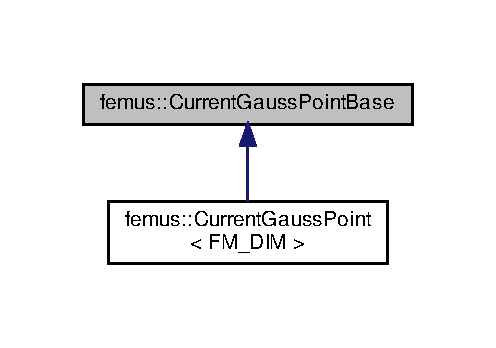
\includegraphics[width=238pt]{classfemus_1_1_current_gauss_point_base__inherit__graph}
\end{center}
\end{figure}


Collaboration diagram for femus\+:\+:Current\+Gauss\+Point\+Base\+:
\nopagebreak
\begin{figure}[H]
\begin{center}
\leavevmode
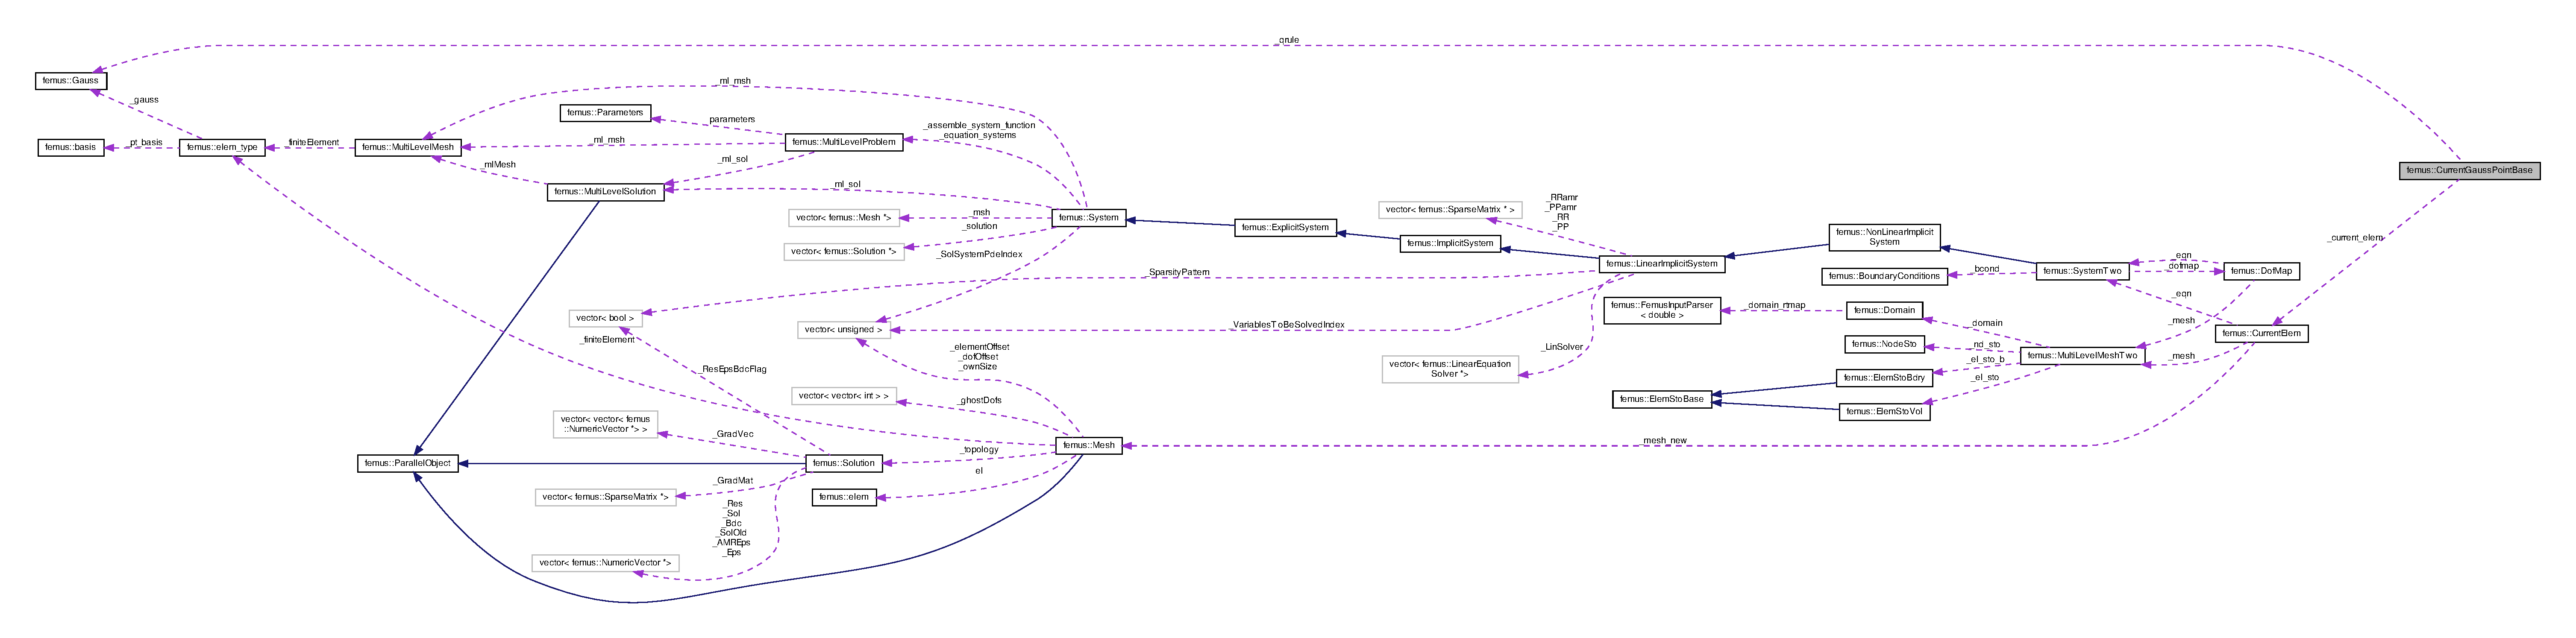
\includegraphics[width=350pt]{classfemus_1_1_current_gauss_point_base__coll__graph}
\end{center}
\end{figure}
\subsection*{Public Member Functions}
\begin{DoxyCompactItemize}
\item 
\mbox{\hyperlink{classfemus_1_1_current_gauss_point_base_aee804d2e69ceec8dbca20be1485a5c14}{Current\+Gauss\+Point\+Base}} (const \mbox{\hyperlink{classfemus_1_1_current_elem}{Current\+Elem}} \&curr\+\_\+el\+\_\+in, const \mbox{\hyperlink{classfemus_1_1_gauss}{Gauss}} \&qrule\+\_\+in)
\item 
\mbox{\hyperlink{classfemus_1_1_current_gauss_point_base_a8e1ed382c638f02ac176557e4b741a8e}{$\sim$\+Current\+Gauss\+Point\+Base}} ()
\item 
const \mbox{\hyperlink{classfemus_1_1_current_elem}{Current\+Elem}} \& \mbox{\hyperlink{classfemus_1_1_current_gauss_point_base_a09cbbd25b4bae6a6d0dee35b8b39c0cc}{Get\+Current\+Elem}} () const
\item 
double $\ast$$\ast$ \mbox{\hyperlink{classfemus_1_1_current_gauss_point_base_a4a2538a97ec12693a6f1e1d6692c9b66}{get\+\_\+tangent\+\_\+ptr}} ()
\item 
double $\ast$ \mbox{\hyperlink{classfemus_1_1_current_gauss_point_base_a22026e832b00dcd6ac5dc3915c5c064d}{get\+\_\+normal\+\_\+ptr}} ()
\item 
virtual double \mbox{\hyperlink{classfemus_1_1_current_gauss_point_base_ac8f11d39a5d6b88c69849f2820a97482}{Jac\+Vect\+V\+V\+\_\+g}} (\mbox{\hyperlink{classfemus_1_1_current_quantity}{Current\+Quantity}} \&xyz)=0
\item 
virtual double \mbox{\hyperlink{classfemus_1_1_current_gauss_point_base_adad673ff1adf7b5f6967f7701825e95e}{Jac\+Vect\+B\+B\+\_\+g}} (\mbox{\hyperlink{classfemus_1_1_current_quantity}{Current\+Quantity}} \&xyz)=0
\item 
virtual void \mbox{\hyperlink{classfemus_1_1_current_gauss_point_base_aec970c4eef875b43169cb74674276e29}{Set\+Phi\+El\+Dofs\+F\+E\+V\+B\+\_\+g}} (const \mbox{\hyperlink{_typedefs_8hpp_a91ad9478d81a7aaf2593e8d9c3d06a14}{uint}} qlflag, const \mbox{\hyperlink{_typedefs_8hpp_a91ad9478d81a7aaf2593e8d9c3d06a14}{uint}} qp)=0
\item 
virtual void \mbox{\hyperlink{classfemus_1_1_current_gauss_point_base_af1e7dd520b7b288fc1ff02674745fbcd}{Set\+D\+Phi\+Dxezeta\+El\+Dofs\+F\+E\+V\+B\+\_\+g}} (const \mbox{\hyperlink{_typedefs_8hpp_a91ad9478d81a7aaf2593e8d9c3d06a14}{uint}} qlflag, const \mbox{\hyperlink{_typedefs_8hpp_a91ad9478d81a7aaf2593e8d9c3d06a14}{uint}} qp)=0
\item 
virtual void \mbox{\hyperlink{classfemus_1_1_current_gauss_point_base_a119838d470a6e444ef0b54220b5dc3bc}{Set\+D\+Phi\+Dxyz\+El\+Dofs\+F\+E\+V\+B\+\_\+g}} (const \mbox{\hyperlink{_typedefs_8hpp_a91ad9478d81a7aaf2593e8d9c3d06a14}{uint}} qlflag, const \mbox{\hyperlink{_typedefs_8hpp_a91ad9478d81a7aaf2593e8d9c3d06a14}{uint}} qp)=0
\item 
virtual void \mbox{\hyperlink{classfemus_1_1_current_gauss_point_base_a4aaaad9d57bead01f701396ad61acc21}{Extend\+Dphi\+Dxyz\+El\+Dofs\+F\+E\+V\+B\+\_\+g}} (const \mbox{\hyperlink{_typedefs_8hpp_a91ad9478d81a7aaf2593e8d9c3d06a14}{uint}} qlflag)=0
\item 
double \mbox{\hyperlink{classfemus_1_1_current_gauss_point_base_ae82c1cf31e3f5fdf7eea0e79c963ecba}{Phi}} (const \mbox{\hyperlink{_typedefs_8hpp_a91ad9478d81a7aaf2593e8d9c3d06a14}{uint}} ql, const \mbox{\hyperlink{_typedefs_8hpp_a91ad9478d81a7aaf2593e8d9c3d06a14}{uint}} dof) const
\end{DoxyCompactItemize}
\subsection*{Static Public Member Functions}
\begin{DoxyCompactItemize}
\item 
static \mbox{\hyperlink{classfemus_1_1_current_gauss_point_base}{Current\+Gauss\+Point\+Base}} \& \mbox{\hyperlink{classfemus_1_1_current_gauss_point_base_acc707006f412446178805a78247867bc}{build}} (const \mbox{\hyperlink{classfemus_1_1_current_elem}{Current\+Elem}} \&elem\+\_\+in, const \mbox{\hyperlink{classfemus_1_1_gauss}{Gauss}} \&qrule\+\_\+in)
\end{DoxyCompactItemize}
\subsection*{Public Attributes}
\begin{DoxyCompactItemize}
\item 
double $\ast$ \mbox{\hyperlink{classfemus_1_1_current_gauss_point_base_a908fe5d463eb11d7ad9841775f456460}{\+\_\+dphidxezeta\+\_\+nds\+Q\+L\+V\+B\+\_\+g}} \mbox{[}\mbox{\hyperlink{_f_e_type_enum_8hpp_aca285339f9cf24489fdc0af5b51a5fde}{QL}}\mbox{]}
\item 
double $\ast$ \mbox{\hyperlink{classfemus_1_1_current_gauss_point_base_a87ab3d43bdceedcfe2983935497e165d}{\+\_\+dphidxyz\+\_\+nds\+Q\+L\+V\+B\+\_\+g}} \mbox{[}\mbox{\hyperlink{_f_e_type_enum_8hpp_aca285339f9cf24489fdc0af5b51a5fde}{QL}}\mbox{]}
\item 
double $\ast$ \mbox{\hyperlink{classfemus_1_1_current_gauss_point_base_a9b1b6bb9910801d0087318c87003d624}{\+\_\+dphidxyz\+\_\+nds\+Q\+L\+V\+B\+\_\+g3D}} \mbox{[}\mbox{\hyperlink{_f_e_type_enum_8hpp_aca285339f9cf24489fdc0af5b51a5fde}{QL}}\mbox{]}
\item 
double $\ast$ \mbox{\hyperlink{classfemus_1_1_current_gauss_point_base_a85ec9531f605c59850123ebdad867bba}{\+\_\+phi\+\_\+nds\+Q\+L\+V\+B\+\_\+g}} \mbox{[}\mbox{\hyperlink{_f_e_type_enum_8hpp_aca285339f9cf24489fdc0af5b51a5fde}{QL}}\mbox{]}
\end{DoxyCompactItemize}
\subsection*{Protected Attributes}
\begin{DoxyCompactItemize}
\item 
\mbox{\hyperlink{_typedefs_8hpp_a91ad9478d81a7aaf2593e8d9c3d06a14}{uint}} \mbox{\hyperlink{classfemus_1_1_current_gauss_point_base_af3453fd371041d38eecf683ed31780b8}{\+\_\+\+Int\+Dim}} \mbox{[}\mbox{\hyperlink{_v_b_type_enum_8hpp_a02ebcbc55b174d8bb6a65cddbe7f90b6}{VB}}\mbox{]}
\item 
const \mbox{\hyperlink{classfemus_1_1_current_elem}{Current\+Elem}} \& \mbox{\hyperlink{classfemus_1_1_current_gauss_point_base_a8e74a49e2a79f39e0e38b22c2c17f893}{\+\_\+current\+\_\+elem}}
\item 
const std\+::vector$<$ const \mbox{\hyperlink{classfemus_1_1elem__type}{elem\+\_\+type}} $\ast$ $>$ \& \mbox{\hyperlink{classfemus_1_1_current_gauss_point_base_ac04dc6fcc6b32db55273e01fa4d4a6f4}{\+\_\+elem\+\_\+type}}
\item 
const \mbox{\hyperlink{classfemus_1_1_gauss}{Gauss}} \& \mbox{\hyperlink{classfemus_1_1_current_gauss_point_base_a2d4d7be4478a1aea5bfa924c412bf29f}{\+\_\+qrule}}
\item 
double $\ast$$\ast$ \mbox{\hyperlink{classfemus_1_1_current_gauss_point_base_a38c6b21bd7028fa2e75189c9619ca081}{\+\_\+\+Inv\+Jac\+\_\+g}}
\item 
double $\ast$ \mbox{\hyperlink{classfemus_1_1_current_gauss_point_base_a53720924e866af56f3dd74519fdc42a0}{\+\_\+normal\+\_\+g}}
\item 
double $\ast$$\ast$ \mbox{\hyperlink{classfemus_1_1_current_gauss_point_base_a0272bf13da6d3f348229bf6ae498034f}{\+\_\+tangent\+\_\+g}}
\end{DoxyCompactItemize}


\subsection{Constructor \& Destructor Documentation}
\mbox{\Hypertarget{classfemus_1_1_current_gauss_point_base_aee804d2e69ceec8dbca20be1485a5c14}\label{classfemus_1_1_current_gauss_point_base_aee804d2e69ceec8dbca20be1485a5c14}} 
\index{femus\+::\+Current\+Gauss\+Point\+Base@{femus\+::\+Current\+Gauss\+Point\+Base}!Current\+Gauss\+Point\+Base@{Current\+Gauss\+Point\+Base}}
\index{Current\+Gauss\+Point\+Base@{Current\+Gauss\+Point\+Base}!femus\+::\+Current\+Gauss\+Point\+Base@{femus\+::\+Current\+Gauss\+Point\+Base}}
\subsubsection{\texorpdfstring{Current\+Gauss\+Point\+Base()}{CurrentGaussPointBase()}}
{\footnotesize\ttfamily femus\+::\+Current\+Gauss\+Point\+Base\+::\+Current\+Gauss\+Point\+Base (\begin{DoxyParamCaption}\item[{const \mbox{\hyperlink{classfemus_1_1_current_elem}{Current\+Elem}} \&}]{curr\+\_\+el\+\_\+in,  }\item[{const \mbox{\hyperlink{classfemus_1_1_gauss}{Gauss}} \&}]{qrule\+\_\+in }\end{DoxyParamCaption})}

\mbox{\Hypertarget{classfemus_1_1_current_gauss_point_base_a8e1ed382c638f02ac176557e4b741a8e}\label{classfemus_1_1_current_gauss_point_base_a8e1ed382c638f02ac176557e4b741a8e}} 
\index{femus\+::\+Current\+Gauss\+Point\+Base@{femus\+::\+Current\+Gauss\+Point\+Base}!````~Current\+Gauss\+Point\+Base@{$\sim$\+Current\+Gauss\+Point\+Base}}
\index{````~Current\+Gauss\+Point\+Base@{$\sim$\+Current\+Gauss\+Point\+Base}!femus\+::\+Current\+Gauss\+Point\+Base@{femus\+::\+Current\+Gauss\+Point\+Base}}
\subsubsection{\texorpdfstring{$\sim$\+Current\+Gauss\+Point\+Base()}{~CurrentGaussPointBase()}}
{\footnotesize\ttfamily femus\+::\+Current\+Gauss\+Point\+Base\+::$\sim$\+Current\+Gauss\+Point\+Base (\begin{DoxyParamCaption}{ }\end{DoxyParamCaption})}



\subsection{Member Function Documentation}
\mbox{\Hypertarget{classfemus_1_1_current_gauss_point_base_acc707006f412446178805a78247867bc}\label{classfemus_1_1_current_gauss_point_base_acc707006f412446178805a78247867bc}} 
\index{femus\+::\+Current\+Gauss\+Point\+Base@{femus\+::\+Current\+Gauss\+Point\+Base}!build@{build}}
\index{build@{build}!femus\+::\+Current\+Gauss\+Point\+Base@{femus\+::\+Current\+Gauss\+Point\+Base}}
\subsubsection{\texorpdfstring{build()}{build()}}
{\footnotesize\ttfamily \mbox{\hyperlink{classfemus_1_1_current_gauss_point_base}{Current\+Gauss\+Point\+Base}} \& femus\+::\+Current\+Gauss\+Point\+Base\+::build (\begin{DoxyParamCaption}\item[{const \mbox{\hyperlink{classfemus_1_1_current_elem}{Current\+Elem}} \&}]{elem\+\_\+in,  }\item[{const \mbox{\hyperlink{classfemus_1_1_gauss}{Gauss}} \&}]{qrule\+\_\+in }\end{DoxyParamCaption})\hspace{0.3cm}{\ttfamily [static]}}

\mbox{\Hypertarget{classfemus_1_1_current_gauss_point_base_a4aaaad9d57bead01f701396ad61acc21}\label{classfemus_1_1_current_gauss_point_base_a4aaaad9d57bead01f701396ad61acc21}} 
\index{femus\+::\+Current\+Gauss\+Point\+Base@{femus\+::\+Current\+Gauss\+Point\+Base}!Extend\+Dphi\+Dxyz\+El\+Dofs\+F\+E\+V\+B\+\_\+g@{Extend\+Dphi\+Dxyz\+El\+Dofs\+F\+E\+V\+B\+\_\+g}}
\index{Extend\+Dphi\+Dxyz\+El\+Dofs\+F\+E\+V\+B\+\_\+g@{Extend\+Dphi\+Dxyz\+El\+Dofs\+F\+E\+V\+B\+\_\+g}!femus\+::\+Current\+Gauss\+Point\+Base@{femus\+::\+Current\+Gauss\+Point\+Base}}
\subsubsection{\texorpdfstring{Extend\+Dphi\+Dxyz\+El\+Dofs\+F\+E\+V\+B\+\_\+g()}{ExtendDphiDxyzElDofsFEVB\_g()}}
{\footnotesize\ttfamily virtual void femus\+::\+Current\+Gauss\+Point\+Base\+::\+Extend\+Dphi\+Dxyz\+El\+Dofs\+F\+E\+V\+B\+\_\+g (\begin{DoxyParamCaption}\item[{const \mbox{\hyperlink{_typedefs_8hpp_a91ad9478d81a7aaf2593e8d9c3d06a14}{uint}}}]{qlflag }\end{DoxyParamCaption})\hspace{0.3cm}{\ttfamily [pure virtual]}}



Implemented in \mbox{\hyperlink{classfemus_1_1_current_gauss_point_aff8e672a0e763e7ff73a1e06a7bc5143}{femus\+::\+Current\+Gauss\+Point$<$ F\+M\+\_\+\+D\+I\+M $>$}}.

\mbox{\Hypertarget{classfemus_1_1_current_gauss_point_base_a22026e832b00dcd6ac5dc3915c5c064d}\label{classfemus_1_1_current_gauss_point_base_a22026e832b00dcd6ac5dc3915c5c064d}} 
\index{femus\+::\+Current\+Gauss\+Point\+Base@{femus\+::\+Current\+Gauss\+Point\+Base}!get\+\_\+normal\+\_\+ptr@{get\+\_\+normal\+\_\+ptr}}
\index{get\+\_\+normal\+\_\+ptr@{get\+\_\+normal\+\_\+ptr}!femus\+::\+Current\+Gauss\+Point\+Base@{femus\+::\+Current\+Gauss\+Point\+Base}}
\subsubsection{\texorpdfstring{get\+\_\+normal\+\_\+ptr()}{get\_normal\_ptr()}}
{\footnotesize\ttfamily double $\ast$ femus\+::\+Current\+Gauss\+Point\+Base\+::get\+\_\+normal\+\_\+ptr (\begin{DoxyParamCaption}{ }\end{DoxyParamCaption})\hspace{0.3cm}{\ttfamily [inline]}}

\mbox{\Hypertarget{classfemus_1_1_current_gauss_point_base_a4a2538a97ec12693a6f1e1d6692c9b66}\label{classfemus_1_1_current_gauss_point_base_a4a2538a97ec12693a6f1e1d6692c9b66}} 
\index{femus\+::\+Current\+Gauss\+Point\+Base@{femus\+::\+Current\+Gauss\+Point\+Base}!get\+\_\+tangent\+\_\+ptr@{get\+\_\+tangent\+\_\+ptr}}
\index{get\+\_\+tangent\+\_\+ptr@{get\+\_\+tangent\+\_\+ptr}!femus\+::\+Current\+Gauss\+Point\+Base@{femus\+::\+Current\+Gauss\+Point\+Base}}
\subsubsection{\texorpdfstring{get\+\_\+tangent\+\_\+ptr()}{get\_tangent\_ptr()}}
{\footnotesize\ttfamily double $\ast$$\ast$ femus\+::\+Current\+Gauss\+Point\+Base\+::get\+\_\+tangent\+\_\+ptr (\begin{DoxyParamCaption}{ }\end{DoxyParamCaption})\hspace{0.3cm}{\ttfamily [inline]}}

\mbox{\Hypertarget{classfemus_1_1_current_gauss_point_base_a09cbbd25b4bae6a6d0dee35b8b39c0cc}\label{classfemus_1_1_current_gauss_point_base_a09cbbd25b4bae6a6d0dee35b8b39c0cc}} 
\index{femus\+::\+Current\+Gauss\+Point\+Base@{femus\+::\+Current\+Gauss\+Point\+Base}!Get\+Current\+Elem@{Get\+Current\+Elem}}
\index{Get\+Current\+Elem@{Get\+Current\+Elem}!femus\+::\+Current\+Gauss\+Point\+Base@{femus\+::\+Current\+Gauss\+Point\+Base}}
\subsubsection{\texorpdfstring{Get\+Current\+Elem()}{GetCurrentElem()}}
{\footnotesize\ttfamily const \mbox{\hyperlink{classfemus_1_1_current_elem}{Current\+Elem}}\& femus\+::\+Current\+Gauss\+Point\+Base\+::\+Get\+Current\+Elem (\begin{DoxyParamCaption}{ }\end{DoxyParamCaption}) const\hspace{0.3cm}{\ttfamily [inline]}}

\mbox{\Hypertarget{classfemus_1_1_current_gauss_point_base_adad673ff1adf7b5f6967f7701825e95e}\label{classfemus_1_1_current_gauss_point_base_adad673ff1adf7b5f6967f7701825e95e}} 
\index{femus\+::\+Current\+Gauss\+Point\+Base@{femus\+::\+Current\+Gauss\+Point\+Base}!Jac\+Vect\+B\+B\+\_\+g@{Jac\+Vect\+B\+B\+\_\+g}}
\index{Jac\+Vect\+B\+B\+\_\+g@{Jac\+Vect\+B\+B\+\_\+g}!femus\+::\+Current\+Gauss\+Point\+Base@{femus\+::\+Current\+Gauss\+Point\+Base}}
\subsubsection{\texorpdfstring{Jac\+Vect\+B\+B\+\_\+g()}{JacVectBB\_g()}}
{\footnotesize\ttfamily virtual double femus\+::\+Current\+Gauss\+Point\+Base\+::\+Jac\+Vect\+B\+B\+\_\+g (\begin{DoxyParamCaption}\item[{\mbox{\hyperlink{classfemus_1_1_current_quantity}{Current\+Quantity}} \&}]{xyz }\end{DoxyParamCaption})\hspace{0.3cm}{\ttfamily [pure virtual]}}



Implemented in \mbox{\hyperlink{classfemus_1_1_current_gauss_point_afa303733709a133cb86ba65fe70d4a31}{femus\+::\+Current\+Gauss\+Point$<$ F\+M\+\_\+\+D\+I\+M $>$}}.

\mbox{\Hypertarget{classfemus_1_1_current_gauss_point_base_ac8f11d39a5d6b88c69849f2820a97482}\label{classfemus_1_1_current_gauss_point_base_ac8f11d39a5d6b88c69849f2820a97482}} 
\index{femus\+::\+Current\+Gauss\+Point\+Base@{femus\+::\+Current\+Gauss\+Point\+Base}!Jac\+Vect\+V\+V\+\_\+g@{Jac\+Vect\+V\+V\+\_\+g}}
\index{Jac\+Vect\+V\+V\+\_\+g@{Jac\+Vect\+V\+V\+\_\+g}!femus\+::\+Current\+Gauss\+Point\+Base@{femus\+::\+Current\+Gauss\+Point\+Base}}
\subsubsection{\texorpdfstring{Jac\+Vect\+V\+V\+\_\+g()}{JacVectVV\_g()}}
{\footnotesize\ttfamily virtual double femus\+::\+Current\+Gauss\+Point\+Base\+::\+Jac\+Vect\+V\+V\+\_\+g (\begin{DoxyParamCaption}\item[{\mbox{\hyperlink{classfemus_1_1_current_quantity}{Current\+Quantity}} \&}]{xyz }\end{DoxyParamCaption})\hspace{0.3cm}{\ttfamily [pure virtual]}}



Implemented in \mbox{\hyperlink{classfemus_1_1_current_gauss_point_a96a47ebb8abd928f0db6e472db2811f1}{femus\+::\+Current\+Gauss\+Point$<$ F\+M\+\_\+\+D\+I\+M $>$}}.

\mbox{\Hypertarget{classfemus_1_1_current_gauss_point_base_ae82c1cf31e3f5fdf7eea0e79c963ecba}\label{classfemus_1_1_current_gauss_point_base_ae82c1cf31e3f5fdf7eea0e79c963ecba}} 
\index{femus\+::\+Current\+Gauss\+Point\+Base@{femus\+::\+Current\+Gauss\+Point\+Base}!Phi@{Phi}}
\index{Phi@{Phi}!femus\+::\+Current\+Gauss\+Point\+Base@{femus\+::\+Current\+Gauss\+Point\+Base}}
\subsubsection{\texorpdfstring{Phi()}{Phi()}}
{\footnotesize\ttfamily double femus\+::\+Current\+Gauss\+Point\+Base\+::\+Phi (\begin{DoxyParamCaption}\item[{const \mbox{\hyperlink{_typedefs_8hpp_a91ad9478d81a7aaf2593e8d9c3d06a14}{uint}}}]{ql,  }\item[{const \mbox{\hyperlink{_typedefs_8hpp_a91ad9478d81a7aaf2593e8d9c3d06a14}{uint}}}]{dof }\end{DoxyParamCaption}) const\hspace{0.3cm}{\ttfamily [inline]}}

\mbox{\Hypertarget{classfemus_1_1_current_gauss_point_base_af1e7dd520b7b288fc1ff02674745fbcd}\label{classfemus_1_1_current_gauss_point_base_af1e7dd520b7b288fc1ff02674745fbcd}} 
\index{femus\+::\+Current\+Gauss\+Point\+Base@{femus\+::\+Current\+Gauss\+Point\+Base}!Set\+D\+Phi\+Dxezeta\+El\+Dofs\+F\+E\+V\+B\+\_\+g@{Set\+D\+Phi\+Dxezeta\+El\+Dofs\+F\+E\+V\+B\+\_\+g}}
\index{Set\+D\+Phi\+Dxezeta\+El\+Dofs\+F\+E\+V\+B\+\_\+g@{Set\+D\+Phi\+Dxezeta\+El\+Dofs\+F\+E\+V\+B\+\_\+g}!femus\+::\+Current\+Gauss\+Point\+Base@{femus\+::\+Current\+Gauss\+Point\+Base}}
\subsubsection{\texorpdfstring{Set\+D\+Phi\+Dxezeta\+El\+Dofs\+F\+E\+V\+B\+\_\+g()}{SetDPhiDxezetaElDofsFEVB\_g()}}
{\footnotesize\ttfamily virtual void femus\+::\+Current\+Gauss\+Point\+Base\+::\+Set\+D\+Phi\+Dxezeta\+El\+Dofs\+F\+E\+V\+B\+\_\+g (\begin{DoxyParamCaption}\item[{const \mbox{\hyperlink{_typedefs_8hpp_a91ad9478d81a7aaf2593e8d9c3d06a14}{uint}}}]{qlflag,  }\item[{const \mbox{\hyperlink{_typedefs_8hpp_a91ad9478d81a7aaf2593e8d9c3d06a14}{uint}}}]{qp }\end{DoxyParamCaption})\hspace{0.3cm}{\ttfamily [pure virtual]}}



Implemented in \mbox{\hyperlink{classfemus_1_1_current_gauss_point_a5b7c118fc9376db8783714992e341891}{femus\+::\+Current\+Gauss\+Point$<$ F\+M\+\_\+\+D\+I\+M $>$}}.

\mbox{\Hypertarget{classfemus_1_1_current_gauss_point_base_a119838d470a6e444ef0b54220b5dc3bc}\label{classfemus_1_1_current_gauss_point_base_a119838d470a6e444ef0b54220b5dc3bc}} 
\index{femus\+::\+Current\+Gauss\+Point\+Base@{femus\+::\+Current\+Gauss\+Point\+Base}!Set\+D\+Phi\+Dxyz\+El\+Dofs\+F\+E\+V\+B\+\_\+g@{Set\+D\+Phi\+Dxyz\+El\+Dofs\+F\+E\+V\+B\+\_\+g}}
\index{Set\+D\+Phi\+Dxyz\+El\+Dofs\+F\+E\+V\+B\+\_\+g@{Set\+D\+Phi\+Dxyz\+El\+Dofs\+F\+E\+V\+B\+\_\+g}!femus\+::\+Current\+Gauss\+Point\+Base@{femus\+::\+Current\+Gauss\+Point\+Base}}
\subsubsection{\texorpdfstring{Set\+D\+Phi\+Dxyz\+El\+Dofs\+F\+E\+V\+B\+\_\+g()}{SetDPhiDxyzElDofsFEVB\_g()}}
{\footnotesize\ttfamily virtual void femus\+::\+Current\+Gauss\+Point\+Base\+::\+Set\+D\+Phi\+Dxyz\+El\+Dofs\+F\+E\+V\+B\+\_\+g (\begin{DoxyParamCaption}\item[{const \mbox{\hyperlink{_typedefs_8hpp_a91ad9478d81a7aaf2593e8d9c3d06a14}{uint}}}]{qlflag,  }\item[{const \mbox{\hyperlink{_typedefs_8hpp_a91ad9478d81a7aaf2593e8d9c3d06a14}{uint}}}]{qp }\end{DoxyParamCaption})\hspace{0.3cm}{\ttfamily [pure virtual]}}



Implemented in \mbox{\hyperlink{classfemus_1_1_current_gauss_point_af33ae0e6b36353be0bb671573c6362bc}{femus\+::\+Current\+Gauss\+Point$<$ F\+M\+\_\+\+D\+I\+M $>$}}.

\mbox{\Hypertarget{classfemus_1_1_current_gauss_point_base_aec970c4eef875b43169cb74674276e29}\label{classfemus_1_1_current_gauss_point_base_aec970c4eef875b43169cb74674276e29}} 
\index{femus\+::\+Current\+Gauss\+Point\+Base@{femus\+::\+Current\+Gauss\+Point\+Base}!Set\+Phi\+El\+Dofs\+F\+E\+V\+B\+\_\+g@{Set\+Phi\+El\+Dofs\+F\+E\+V\+B\+\_\+g}}
\index{Set\+Phi\+El\+Dofs\+F\+E\+V\+B\+\_\+g@{Set\+Phi\+El\+Dofs\+F\+E\+V\+B\+\_\+g}!femus\+::\+Current\+Gauss\+Point\+Base@{femus\+::\+Current\+Gauss\+Point\+Base}}
\subsubsection{\texorpdfstring{Set\+Phi\+El\+Dofs\+F\+E\+V\+B\+\_\+g()}{SetPhiElDofsFEVB\_g()}}
{\footnotesize\ttfamily virtual void femus\+::\+Current\+Gauss\+Point\+Base\+::\+Set\+Phi\+El\+Dofs\+F\+E\+V\+B\+\_\+g (\begin{DoxyParamCaption}\item[{const \mbox{\hyperlink{_typedefs_8hpp_a91ad9478d81a7aaf2593e8d9c3d06a14}{uint}}}]{qlflag,  }\item[{const \mbox{\hyperlink{_typedefs_8hpp_a91ad9478d81a7aaf2593e8d9c3d06a14}{uint}}}]{qp }\end{DoxyParamCaption})\hspace{0.3cm}{\ttfamily [pure virtual]}}



Implemented in \mbox{\hyperlink{classfemus_1_1_current_gauss_point_a7a11e1164802fdc683726eea6123d99f}{femus\+::\+Current\+Gauss\+Point$<$ F\+M\+\_\+\+D\+I\+M $>$}}.



\subsection{Member Data Documentation}
\mbox{\Hypertarget{classfemus_1_1_current_gauss_point_base_a8e74a49e2a79f39e0e38b22c2c17f893}\label{classfemus_1_1_current_gauss_point_base_a8e74a49e2a79f39e0e38b22c2c17f893}} 
\index{femus\+::\+Current\+Gauss\+Point\+Base@{femus\+::\+Current\+Gauss\+Point\+Base}!\+\_\+current\+\_\+elem@{\+\_\+current\+\_\+elem}}
\index{\+\_\+current\+\_\+elem@{\+\_\+current\+\_\+elem}!femus\+::\+Current\+Gauss\+Point\+Base@{femus\+::\+Current\+Gauss\+Point\+Base}}
\subsubsection{\texorpdfstring{\+\_\+current\+\_\+elem}{\_current\_elem}}
{\footnotesize\ttfamily const \mbox{\hyperlink{classfemus_1_1_current_elem}{Current\+Elem}}\& femus\+::\+Current\+Gauss\+Point\+Base\+::\+\_\+current\+\_\+elem\hspace{0.3cm}{\ttfamily [protected]}}

\mbox{\Hypertarget{classfemus_1_1_current_gauss_point_base_a908fe5d463eb11d7ad9841775f456460}\label{classfemus_1_1_current_gauss_point_base_a908fe5d463eb11d7ad9841775f456460}} 
\index{femus\+::\+Current\+Gauss\+Point\+Base@{femus\+::\+Current\+Gauss\+Point\+Base}!\+\_\+dphidxezeta\+\_\+nds\+Q\+L\+V\+B\+\_\+g@{\+\_\+dphidxezeta\+\_\+nds\+Q\+L\+V\+B\+\_\+g}}
\index{\+\_\+dphidxezeta\+\_\+nds\+Q\+L\+V\+B\+\_\+g@{\+\_\+dphidxezeta\+\_\+nds\+Q\+L\+V\+B\+\_\+g}!femus\+::\+Current\+Gauss\+Point\+Base@{femus\+::\+Current\+Gauss\+Point\+Base}}
\subsubsection{\texorpdfstring{\+\_\+dphidxezeta\+\_\+nds\+Q\+L\+V\+B\+\_\+g}{\_dphidxezeta\_ndsQLVB\_g}}
{\footnotesize\ttfamily double$\ast$ femus\+::\+Current\+Gauss\+Point\+Base\+::\+\_\+dphidxezeta\+\_\+nds\+Q\+L\+V\+B\+\_\+g\mbox{[}\mbox{\hyperlink{_f_e_type_enum_8hpp_aca285339f9cf24489fdc0af5b51a5fde}{QL}}\mbox{]}}

\mbox{\Hypertarget{classfemus_1_1_current_gauss_point_base_a87ab3d43bdceedcfe2983935497e165d}\label{classfemus_1_1_current_gauss_point_base_a87ab3d43bdceedcfe2983935497e165d}} 
\index{femus\+::\+Current\+Gauss\+Point\+Base@{femus\+::\+Current\+Gauss\+Point\+Base}!\+\_\+dphidxyz\+\_\+nds\+Q\+L\+V\+B\+\_\+g@{\+\_\+dphidxyz\+\_\+nds\+Q\+L\+V\+B\+\_\+g}}
\index{\+\_\+dphidxyz\+\_\+nds\+Q\+L\+V\+B\+\_\+g@{\+\_\+dphidxyz\+\_\+nds\+Q\+L\+V\+B\+\_\+g}!femus\+::\+Current\+Gauss\+Point\+Base@{femus\+::\+Current\+Gauss\+Point\+Base}}
\subsubsection{\texorpdfstring{\+\_\+dphidxyz\+\_\+nds\+Q\+L\+V\+B\+\_\+g}{\_dphidxyz\_ndsQLVB\_g}}
{\footnotesize\ttfamily double$\ast$ femus\+::\+Current\+Gauss\+Point\+Base\+::\+\_\+dphidxyz\+\_\+nds\+Q\+L\+V\+B\+\_\+g\mbox{[}\mbox{\hyperlink{_f_e_type_enum_8hpp_aca285339f9cf24489fdc0af5b51a5fde}{QL}}\mbox{]}}

\mbox{\Hypertarget{classfemus_1_1_current_gauss_point_base_a9b1b6bb9910801d0087318c87003d624}\label{classfemus_1_1_current_gauss_point_base_a9b1b6bb9910801d0087318c87003d624}} 
\index{femus\+::\+Current\+Gauss\+Point\+Base@{femus\+::\+Current\+Gauss\+Point\+Base}!\+\_\+dphidxyz\+\_\+nds\+Q\+L\+V\+B\+\_\+g3D@{\+\_\+dphidxyz\+\_\+nds\+Q\+L\+V\+B\+\_\+g3D}}
\index{\+\_\+dphidxyz\+\_\+nds\+Q\+L\+V\+B\+\_\+g3D@{\+\_\+dphidxyz\+\_\+nds\+Q\+L\+V\+B\+\_\+g3D}!femus\+::\+Current\+Gauss\+Point\+Base@{femus\+::\+Current\+Gauss\+Point\+Base}}
\subsubsection{\texorpdfstring{\+\_\+dphidxyz\+\_\+nds\+Q\+L\+V\+B\+\_\+g3D}{\_dphidxyz\_ndsQLVB\_g3D}}
{\footnotesize\ttfamily double$\ast$ femus\+::\+Current\+Gauss\+Point\+Base\+::\+\_\+dphidxyz\+\_\+nds\+Q\+L\+V\+B\+\_\+g3D\mbox{[}\mbox{\hyperlink{_f_e_type_enum_8hpp_aca285339f9cf24489fdc0af5b51a5fde}{QL}}\mbox{]}}

\mbox{\Hypertarget{classfemus_1_1_current_gauss_point_base_ac04dc6fcc6b32db55273e01fa4d4a6f4}\label{classfemus_1_1_current_gauss_point_base_ac04dc6fcc6b32db55273e01fa4d4a6f4}} 
\index{femus\+::\+Current\+Gauss\+Point\+Base@{femus\+::\+Current\+Gauss\+Point\+Base}!\+\_\+elem\+\_\+type@{\+\_\+elem\+\_\+type}}
\index{\+\_\+elem\+\_\+type@{\+\_\+elem\+\_\+type}!femus\+::\+Current\+Gauss\+Point\+Base@{femus\+::\+Current\+Gauss\+Point\+Base}}
\subsubsection{\texorpdfstring{\+\_\+elem\+\_\+type}{\_elem\_type}}
{\footnotesize\ttfamily const std\+::vector$<$const \mbox{\hyperlink{classfemus_1_1elem__type}{elem\+\_\+type}}$\ast$$>$\& femus\+::\+Current\+Gauss\+Point\+Base\+::\+\_\+elem\+\_\+type\hspace{0.3cm}{\ttfamily [protected]}}

\mbox{\Hypertarget{classfemus_1_1_current_gauss_point_base_af3453fd371041d38eecf683ed31780b8}\label{classfemus_1_1_current_gauss_point_base_af3453fd371041d38eecf683ed31780b8}} 
\index{femus\+::\+Current\+Gauss\+Point\+Base@{femus\+::\+Current\+Gauss\+Point\+Base}!\+\_\+\+Int\+Dim@{\+\_\+\+Int\+Dim}}
\index{\+\_\+\+Int\+Dim@{\+\_\+\+Int\+Dim}!femus\+::\+Current\+Gauss\+Point\+Base@{femus\+::\+Current\+Gauss\+Point\+Base}}
\subsubsection{\texorpdfstring{\+\_\+\+Int\+Dim}{\_IntDim}}
{\footnotesize\ttfamily \mbox{\hyperlink{_typedefs_8hpp_a91ad9478d81a7aaf2593e8d9c3d06a14}{uint}} femus\+::\+Current\+Gauss\+Point\+Base\+::\+\_\+\+Int\+Dim\mbox{[}\mbox{\hyperlink{_v_b_type_enum_8hpp_a02ebcbc55b174d8bb6a65cddbe7f90b6}{VB}}\mbox{]}\hspace{0.3cm}{\ttfamily [protected]}}

\mbox{\Hypertarget{classfemus_1_1_current_gauss_point_base_a38c6b21bd7028fa2e75189c9619ca081}\label{classfemus_1_1_current_gauss_point_base_a38c6b21bd7028fa2e75189c9619ca081}} 
\index{femus\+::\+Current\+Gauss\+Point\+Base@{femus\+::\+Current\+Gauss\+Point\+Base}!\+\_\+\+Inv\+Jac\+\_\+g@{\+\_\+\+Inv\+Jac\+\_\+g}}
\index{\+\_\+\+Inv\+Jac\+\_\+g@{\+\_\+\+Inv\+Jac\+\_\+g}!femus\+::\+Current\+Gauss\+Point\+Base@{femus\+::\+Current\+Gauss\+Point\+Base}}
\subsubsection{\texorpdfstring{\+\_\+\+Inv\+Jac\+\_\+g}{\_InvJac\_g}}
{\footnotesize\ttfamily double$\ast$$\ast$ femus\+::\+Current\+Gauss\+Point\+Base\+::\+\_\+\+Inv\+Jac\+\_\+g\hspace{0.3cm}{\ttfamily [protected]}}

\mbox{\Hypertarget{classfemus_1_1_current_gauss_point_base_a53720924e866af56f3dd74519fdc42a0}\label{classfemus_1_1_current_gauss_point_base_a53720924e866af56f3dd74519fdc42a0}} 
\index{femus\+::\+Current\+Gauss\+Point\+Base@{femus\+::\+Current\+Gauss\+Point\+Base}!\+\_\+normal\+\_\+g@{\+\_\+normal\+\_\+g}}
\index{\+\_\+normal\+\_\+g@{\+\_\+normal\+\_\+g}!femus\+::\+Current\+Gauss\+Point\+Base@{femus\+::\+Current\+Gauss\+Point\+Base}}
\subsubsection{\texorpdfstring{\+\_\+normal\+\_\+g}{\_normal\_g}}
{\footnotesize\ttfamily double$\ast$ femus\+::\+Current\+Gauss\+Point\+Base\+::\+\_\+normal\+\_\+g\hspace{0.3cm}{\ttfamily [protected]}}

\mbox{\Hypertarget{classfemus_1_1_current_gauss_point_base_a85ec9531f605c59850123ebdad867bba}\label{classfemus_1_1_current_gauss_point_base_a85ec9531f605c59850123ebdad867bba}} 
\index{femus\+::\+Current\+Gauss\+Point\+Base@{femus\+::\+Current\+Gauss\+Point\+Base}!\+\_\+phi\+\_\+nds\+Q\+L\+V\+B\+\_\+g@{\+\_\+phi\+\_\+nds\+Q\+L\+V\+B\+\_\+g}}
\index{\+\_\+phi\+\_\+nds\+Q\+L\+V\+B\+\_\+g@{\+\_\+phi\+\_\+nds\+Q\+L\+V\+B\+\_\+g}!femus\+::\+Current\+Gauss\+Point\+Base@{femus\+::\+Current\+Gauss\+Point\+Base}}
\subsubsection{\texorpdfstring{\+\_\+phi\+\_\+nds\+Q\+L\+V\+B\+\_\+g}{\_phi\_ndsQLVB\_g}}
{\footnotesize\ttfamily double$\ast$ femus\+::\+Current\+Gauss\+Point\+Base\+::\+\_\+phi\+\_\+nds\+Q\+L\+V\+B\+\_\+g\mbox{[}\mbox{\hyperlink{_f_e_type_enum_8hpp_aca285339f9cf24489fdc0af5b51a5fde}{QL}}\mbox{]}}

\mbox{\Hypertarget{classfemus_1_1_current_gauss_point_base_a2d4d7be4478a1aea5bfa924c412bf29f}\label{classfemus_1_1_current_gauss_point_base_a2d4d7be4478a1aea5bfa924c412bf29f}} 
\index{femus\+::\+Current\+Gauss\+Point\+Base@{femus\+::\+Current\+Gauss\+Point\+Base}!\+\_\+qrule@{\+\_\+qrule}}
\index{\+\_\+qrule@{\+\_\+qrule}!femus\+::\+Current\+Gauss\+Point\+Base@{femus\+::\+Current\+Gauss\+Point\+Base}}
\subsubsection{\texorpdfstring{\+\_\+qrule}{\_qrule}}
{\footnotesize\ttfamily const \mbox{\hyperlink{classfemus_1_1_gauss}{Gauss}}\& femus\+::\+Current\+Gauss\+Point\+Base\+::\+\_\+qrule\hspace{0.3cm}{\ttfamily [protected]}}

\mbox{\Hypertarget{classfemus_1_1_current_gauss_point_base_a0272bf13da6d3f348229bf6ae498034f}\label{classfemus_1_1_current_gauss_point_base_a0272bf13da6d3f348229bf6ae498034f}} 
\index{femus\+::\+Current\+Gauss\+Point\+Base@{femus\+::\+Current\+Gauss\+Point\+Base}!\+\_\+tangent\+\_\+g@{\+\_\+tangent\+\_\+g}}
\index{\+\_\+tangent\+\_\+g@{\+\_\+tangent\+\_\+g}!femus\+::\+Current\+Gauss\+Point\+Base@{femus\+::\+Current\+Gauss\+Point\+Base}}
\subsubsection{\texorpdfstring{\+\_\+tangent\+\_\+g}{\_tangent\_g}}
{\footnotesize\ttfamily double$\ast$$\ast$ femus\+::\+Current\+Gauss\+Point\+Base\+::\+\_\+tangent\+\_\+g\hspace{0.3cm}{\ttfamily [protected]}}



The documentation for this class was generated from the following files\+:\begin{DoxyCompactItemize}
\item 
equations/\mbox{\hyperlink{_current_gauss_point_base_8hpp}{Current\+Gauss\+Point\+Base.\+hpp}}\item 
equations/\mbox{\hyperlink{_current_gauss_point_base_8cpp}{Current\+Gauss\+Point\+Base.\+cpp}}\end{DoxyCompactItemize}

\hypertarget{classfemus_1_1_current_quantity}{}\section{femus\+:\+:Current\+Quantity Class Reference}
\label{classfemus_1_1_current_quantity}\index{femus\+::\+Current\+Quantity@{femus\+::\+Current\+Quantity}}


{\ttfamily \#include $<$Current\+Quantity.\+hpp$>$}



Collaboration diagram for femus\+:\+:Current\+Quantity\+:
\nopagebreak
\begin{figure}[H]
\begin{center}
\leavevmode
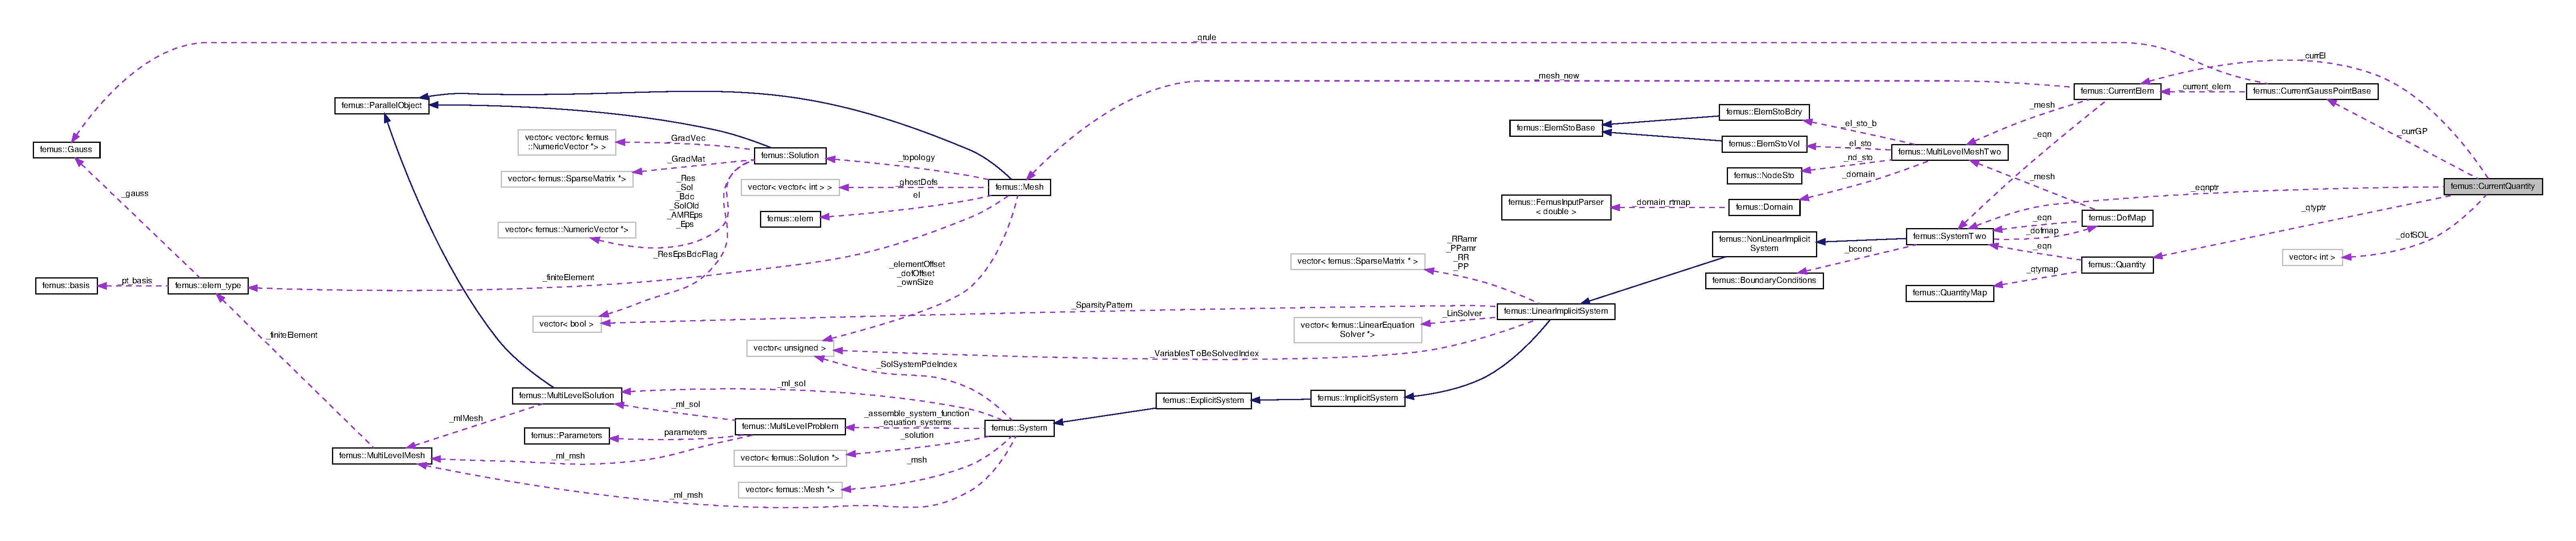
\includegraphics[width=350pt]{classfemus_1_1_current_quantity__coll__graph}
\end{center}
\end{figure}
\subsection*{Public Member Functions}
\begin{DoxyCompactItemize}
\item 
\mbox{\hyperlink{classfemus_1_1_current_quantity_a33a90d4e1c9e39be4ca7400ce36a5c53}{Current\+Quantity}} (const \mbox{\hyperlink{classfemus_1_1_current_gauss_point_base}{Current\+Gauss\+Point\+Base}} \&)
\item 
void \mbox{\hyperlink{classfemus_1_1_current_quantity_ab1394e79cb5fb9fc00211b01114f2308}{Vect\+With\+Qty\+Fill\+Basic}} ()
\item 
void \mbox{\hyperlink{classfemus_1_1_current_quantity_a7423a2a8c30f4c64461a384a3570b8a0}{Allocate}} ()
\item 
void \mbox{\hyperlink{classfemus_1_1_current_quantity_ac6de4abdb84f78d6ce2fce30b6d4c58e}{val\+\_\+g}} ()
\item 
void \mbox{\hyperlink{classfemus_1_1_current_quantity_a818bc04e65ca13c0a0b6e8fa3a81184d}{grad\+\_\+g}} ()
\item 
void \mbox{\hyperlink{classfemus_1_1_current_quantity_ac49ad9c2373c209ecc2b54eb3d0cde9d}{curl\+\_\+g}} ()
\item 
void \mbox{\hyperlink{classfemus_1_1_current_quantity_aa1c7d204f7efc0d0637a087abf304eaf}{Extend\+Dofs}} ()
\begin{DoxyCompactList}\small\item\em copy the space\+\_\+dim-\/sized dof vector into its 3D version \end{DoxyCompactList}\item 
void \mbox{\hyperlink{classfemus_1_1_current_quantity_ac679962446671495a5ee163d5aa3466f}{Get\+Elem\+Dofs}} ()
\item 
void \mbox{\hyperlink{classfemus_1_1_current_quantity_a3a28e3f7dda6aaa566d754262866ffd2}{Get\+Elem\+Dofs}} (const std\+::vector$<$ \mbox{\hyperlink{classfemus_1_1_current_quantity}{Current\+Quantity}} $\ast$$>$ vec\+\_\+in)
\item 
void \mbox{\hyperlink{classfemus_1_1_current_quantity_a10840b0060347099e1d08eb7b501d054}{Set\+Elem\+Average}} ()
\item 
const \mbox{\hyperlink{classfemus_1_1_current_elem}{Current\+Elem}} \& \mbox{\hyperlink{classfemus_1_1_current_quantity_ae3ad0b4d7421700297005841524ec912}{Get\+Current\+Elem}} () const
\end{DoxyCompactItemize}
\subsection*{Public Attributes}
\begin{DoxyCompactItemize}
\item 
std\+::vector$<$ double $>$ \mbox{\hyperlink{classfemus_1_1_current_quantity_a8ff27a2ef6790e801f9e824620cc9ec9}{\+\_\+val\+\_\+g}}
\item 
std\+::vector$<$ double $>$ \mbox{\hyperlink{classfemus_1_1_current_quantity_a2764618c51435196ac354bccc3539908}{\+\_\+val\+\_\+g3D}}
\item 
std\+::vector$<$ std\+::vector$<$ double $>$ $>$ \mbox{\hyperlink{classfemus_1_1_current_quantity_a1b6f06e4a4cb17b704609153a0b52a62}{\+\_\+grad\+\_\+g}}
\item 
std\+::vector$<$ std\+::vector$<$ double $>$ $>$ \mbox{\hyperlink{classfemus_1_1_current_quantity_a7f82eb35d327926945abec67effe97d7}{\+\_\+grad\+\_\+g3D}}
\item 
std\+::vector$<$ double $>$ \mbox{\hyperlink{classfemus_1_1_current_quantity_ab7078b47577ebf640494592680e731e4}{\+\_\+curl\+\_\+g3D}}
\item 
std\+::vector$<$ double $>$ \mbox{\hyperlink{classfemus_1_1_current_quantity_a6ca5e1bf05a00f9219c1bcbc4ce8d110}{\+\_\+val\+\_\+dofs}}
\item 
std\+::vector$<$ double $>$ \mbox{\hyperlink{classfemus_1_1_current_quantity_af6e9c491715aae893107fb912204373c}{\+\_\+val\+\_\+dofs3D}}
\item 
std\+::vector$<$ double $>$ \mbox{\hyperlink{classfemus_1_1_current_quantity_a36ad7fc877c7b35df26aada590e0c86d}{\+\_\+el\+\_\+average}}
\item 
\mbox{\hyperlink{classfemus_1_1_quantity}{Quantity}} $\ast$ \mbox{\hyperlink{classfemus_1_1_current_quantity_a5f5af72cccd35b99437d26387b9feca3}{\+\_\+qtyptr}}
\item 
\mbox{\hyperlink{classfemus_1_1_system_two}{System\+Two}} $\ast$ \mbox{\hyperlink{classfemus_1_1_current_quantity_a0283bfb1b357e50c030ae1aef8657c44}{\+\_\+eqnptr}}
\item 
std\+::string \mbox{\hyperlink{classfemus_1_1_current_quantity_ae3f04b758433260bab0f0df15214677a}{\+\_\+\+Sol\+Name}}
\item 
vector$<$ int $>$ \mbox{\hyperlink{classfemus_1_1_current_quantity_aeaba1fd7e7164f9c788399d62e90c8e0}{\+\_\+dof\+S\+OL}}
\item 
unsigned \mbox{\hyperlink{classfemus_1_1_current_quantity_a2ad0c3b02ab0057df318b2633ceb6572}{\+\_\+index\+S\+OL}}
\item 
unsigned \mbox{\hyperlink{classfemus_1_1_current_quantity_a73b203a21dbae8730772231744480e31}{\+\_\+ind\+S\+OL}}
\item 
unsigned \mbox{\hyperlink{classfemus_1_1_current_quantity_adba03b170d7cf82cf627d460d49fc2ee}{\+\_\+\+Sol\+Type\+S\+OL}}
\item 
\mbox{\hyperlink{_typedefs_8hpp_a91ad9478d81a7aaf2593e8d9c3d06a14}{uint}} \mbox{\hyperlink{classfemus_1_1_current_quantity_acad33c2cbe7c142f4140bb12fb435cd4}{\+\_\+\+F\+Eord}}
\item 
\mbox{\hyperlink{_typedefs_8hpp_a91ad9478d81a7aaf2593e8d9c3d06a14}{uint}} \mbox{\hyperlink{classfemus_1_1_current_quantity_aaeb57cb481fb71eda9c01f8b9b373f75}{\+\_\+dim}}
\item 
\mbox{\hyperlink{_typedefs_8hpp_a91ad9478d81a7aaf2593e8d9c3d06a14}{uint}} \mbox{\hyperlink{classfemus_1_1_current_quantity_afe410f6f270e6cdb4ce5322ace39eff8}{\+\_\+ndof}}
\end{DoxyCompactItemize}
\subsection*{Protected Attributes}
\begin{DoxyCompactItemize}
\item 
const \mbox{\hyperlink{classfemus_1_1_current_gauss_point_base}{Current\+Gauss\+Point\+Base}} \& \mbox{\hyperlink{classfemus_1_1_current_quantity_a99f7729207c7e6ee5f0e94d7f8862ffd}{\+\_\+curr\+GP}}
\item 
const \mbox{\hyperlink{classfemus_1_1_current_elem}{Current\+Elem}} \& \mbox{\hyperlink{classfemus_1_1_current_quantity_acb49f7240d66144048cc915f615d1cda}{\+\_\+curr\+El}}
\end{DoxyCompactItemize}


\subsection{Constructor \& Destructor Documentation}
\mbox{\Hypertarget{classfemus_1_1_current_quantity_a33a90d4e1c9e39be4ca7400ce36a5c53}\label{classfemus_1_1_current_quantity_a33a90d4e1c9e39be4ca7400ce36a5c53}} 
\index{femus\+::\+Current\+Quantity@{femus\+::\+Current\+Quantity}!Current\+Quantity@{Current\+Quantity}}
\index{Current\+Quantity@{Current\+Quantity}!femus\+::\+Current\+Quantity@{femus\+::\+Current\+Quantity}}
\subsubsection{\texorpdfstring{Current\+Quantity()}{CurrentQuantity()}}
{\footnotesize\ttfamily femus\+::\+Current\+Quantity\+::\+Current\+Quantity (\begin{DoxyParamCaption}\item[{const \mbox{\hyperlink{classfemus_1_1_current_gauss_point_base}{Current\+Gauss\+Point\+Base}} \&}]{currgp\+\_\+in }\end{DoxyParamCaption})}



\subsection{Member Function Documentation}
\mbox{\Hypertarget{classfemus_1_1_current_quantity_a7423a2a8c30f4c64461a384a3570b8a0}\label{classfemus_1_1_current_quantity_a7423a2a8c30f4c64461a384a3570b8a0}} 
\index{femus\+::\+Current\+Quantity@{femus\+::\+Current\+Quantity}!Allocate@{Allocate}}
\index{Allocate@{Allocate}!femus\+::\+Current\+Quantity@{femus\+::\+Current\+Quantity}}
\subsubsection{\texorpdfstring{Allocate()}{Allocate()}}
{\footnotesize\ttfamily void femus\+::\+Current\+Quantity\+::\+Allocate (\begin{DoxyParamCaption}{ }\end{DoxyParamCaption})}

\mbox{\Hypertarget{classfemus_1_1_current_quantity_ac49ad9c2373c209ecc2b54eb3d0cde9d}\label{classfemus_1_1_current_quantity_ac49ad9c2373c209ecc2b54eb3d0cde9d}} 
\index{femus\+::\+Current\+Quantity@{femus\+::\+Current\+Quantity}!curl\+\_\+g@{curl\+\_\+g}}
\index{curl\+\_\+g@{curl\+\_\+g}!femus\+::\+Current\+Quantity@{femus\+::\+Current\+Quantity}}
\subsubsection{\texorpdfstring{curl\+\_\+g()}{curl\_g()}}
{\footnotesize\ttfamily void femus\+::\+Current\+Quantity\+::curl\+\_\+g (\begin{DoxyParamCaption}{ }\end{DoxyParamCaption})}

\begin{DoxyRefDesc}{Todo}
\item[\mbox{\hyperlink{todo__todo000001}{Todo}}]this function only works for a V\+E\+C\+T\+OR quantity \end{DoxyRefDesc}
\mbox{\Hypertarget{classfemus_1_1_current_quantity_aa1c7d204f7efc0d0637a087abf304eaf}\label{classfemus_1_1_current_quantity_aa1c7d204f7efc0d0637a087abf304eaf}} 
\index{femus\+::\+Current\+Quantity@{femus\+::\+Current\+Quantity}!Extend\+Dofs@{Extend\+Dofs}}
\index{Extend\+Dofs@{Extend\+Dofs}!femus\+::\+Current\+Quantity@{femus\+::\+Current\+Quantity}}
\subsubsection{\texorpdfstring{Extend\+Dofs()}{ExtendDofs()}}
{\footnotesize\ttfamily void femus\+::\+Current\+Quantity\+::\+Extend\+Dofs (\begin{DoxyParamCaption}{ }\end{DoxyParamCaption})}



copy the space\+\_\+dim-\/sized dof vector into its 3D version 

\mbox{\Hypertarget{classfemus_1_1_current_quantity_ae3ad0b4d7421700297005841524ec912}\label{classfemus_1_1_current_quantity_ae3ad0b4d7421700297005841524ec912}} 
\index{femus\+::\+Current\+Quantity@{femus\+::\+Current\+Quantity}!Get\+Current\+Elem@{Get\+Current\+Elem}}
\index{Get\+Current\+Elem@{Get\+Current\+Elem}!femus\+::\+Current\+Quantity@{femus\+::\+Current\+Quantity}}
\subsubsection{\texorpdfstring{Get\+Current\+Elem()}{GetCurrentElem()}}
{\footnotesize\ttfamily const \mbox{\hyperlink{classfemus_1_1_current_elem}{Current\+Elem}}\& femus\+::\+Current\+Quantity\+::\+Get\+Current\+Elem (\begin{DoxyParamCaption}{ }\end{DoxyParamCaption}) const\hspace{0.3cm}{\ttfamily [inline]}}

\mbox{\Hypertarget{classfemus_1_1_current_quantity_ac679962446671495a5ee163d5aa3466f}\label{classfemus_1_1_current_quantity_ac679962446671495a5ee163d5aa3466f}} 
\index{femus\+::\+Current\+Quantity@{femus\+::\+Current\+Quantity}!Get\+Elem\+Dofs@{Get\+Elem\+Dofs}}
\index{Get\+Elem\+Dofs@{Get\+Elem\+Dofs}!femus\+::\+Current\+Quantity@{femus\+::\+Current\+Quantity}}
\subsubsection{\texorpdfstring{Get\+Elem\+Dofs()}{GetElemDofs()}\hspace{0.1cm}{\footnotesize\ttfamily [1/2]}}
{\footnotesize\ttfamily void femus\+::\+Current\+Quantity\+::\+Get\+Elem\+Dofs (\begin{DoxyParamCaption}{ }\end{DoxyParamCaption})}

\mbox{\Hypertarget{classfemus_1_1_current_quantity_a3a28e3f7dda6aaa566d754262866ffd2}\label{classfemus_1_1_current_quantity_a3a28e3f7dda6aaa566d754262866ffd2}} 
\index{femus\+::\+Current\+Quantity@{femus\+::\+Current\+Quantity}!Get\+Elem\+Dofs@{Get\+Elem\+Dofs}}
\index{Get\+Elem\+Dofs@{Get\+Elem\+Dofs}!femus\+::\+Current\+Quantity@{femus\+::\+Current\+Quantity}}
\subsubsection{\texorpdfstring{Get\+Elem\+Dofs()}{GetElemDofs()}\hspace{0.1cm}{\footnotesize\ttfamily [2/2]}}
{\footnotesize\ttfamily void femus\+::\+Current\+Quantity\+::\+Get\+Elem\+Dofs (\begin{DoxyParamCaption}\item[{const std\+::vector$<$ \mbox{\hyperlink{classfemus_1_1_current_quantity}{Current\+Quantity}} $\ast$$>$}]{vec\+\_\+in }\end{DoxyParamCaption})}

\mbox{\Hypertarget{classfemus_1_1_current_quantity_a818bc04e65ca13c0a0b6e8fa3a81184d}\label{classfemus_1_1_current_quantity_a818bc04e65ca13c0a0b6e8fa3a81184d}} 
\index{femus\+::\+Current\+Quantity@{femus\+::\+Current\+Quantity}!grad\+\_\+g@{grad\+\_\+g}}
\index{grad\+\_\+g@{grad\+\_\+g}!femus\+::\+Current\+Quantity@{femus\+::\+Current\+Quantity}}
\subsubsection{\texorpdfstring{grad\+\_\+g()}{grad\_g()}}
{\footnotesize\ttfamily void femus\+::\+Current\+Quantity\+::grad\+\_\+g (\begin{DoxyParamCaption}{ }\end{DoxyParamCaption})}

\mbox{\Hypertarget{classfemus_1_1_current_quantity_a10840b0060347099e1d08eb7b501d054}\label{classfemus_1_1_current_quantity_a10840b0060347099e1d08eb7b501d054}} 
\index{femus\+::\+Current\+Quantity@{femus\+::\+Current\+Quantity}!Set\+Elem\+Average@{Set\+Elem\+Average}}
\index{Set\+Elem\+Average@{Set\+Elem\+Average}!femus\+::\+Current\+Quantity@{femus\+::\+Current\+Quantity}}
\subsubsection{\texorpdfstring{Set\+Elem\+Average()}{SetElemAverage()}}
{\footnotesize\ttfamily void femus\+::\+Current\+Quantity\+::\+Set\+Elem\+Average (\begin{DoxyParamCaption}{ }\end{DoxyParamCaption})}

\mbox{\Hypertarget{classfemus_1_1_current_quantity_ac6de4abdb84f78d6ce2fce30b6d4c58e}\label{classfemus_1_1_current_quantity_ac6de4abdb84f78d6ce2fce30b6d4c58e}} 
\index{femus\+::\+Current\+Quantity@{femus\+::\+Current\+Quantity}!val\+\_\+g@{val\+\_\+g}}
\index{val\+\_\+g@{val\+\_\+g}!femus\+::\+Current\+Quantity@{femus\+::\+Current\+Quantity}}
\subsubsection{\texorpdfstring{val\+\_\+g()}{val\_g()}}
{\footnotesize\ttfamily void femus\+::\+Current\+Quantity\+::val\+\_\+g (\begin{DoxyParamCaption}{ }\end{DoxyParamCaption})}

\mbox{\Hypertarget{classfemus_1_1_current_quantity_ab1394e79cb5fb9fc00211b01114f2308}\label{classfemus_1_1_current_quantity_ab1394e79cb5fb9fc00211b01114f2308}} 
\index{femus\+::\+Current\+Quantity@{femus\+::\+Current\+Quantity}!Vect\+With\+Qty\+Fill\+Basic@{Vect\+With\+Qty\+Fill\+Basic}}
\index{Vect\+With\+Qty\+Fill\+Basic@{Vect\+With\+Qty\+Fill\+Basic}!femus\+::\+Current\+Quantity@{femus\+::\+Current\+Quantity}}
\subsubsection{\texorpdfstring{Vect\+With\+Qty\+Fill\+Basic()}{VectWithQtyFillBasic()}}
{\footnotesize\ttfamily void femus\+::\+Current\+Quantity\+::\+Vect\+With\+Qty\+Fill\+Basic (\begin{DoxyParamCaption}{ }\end{DoxyParamCaption})}



\subsection{Member Data Documentation}
\mbox{\Hypertarget{classfemus_1_1_current_quantity_ab7078b47577ebf640494592680e731e4}\label{classfemus_1_1_current_quantity_ab7078b47577ebf640494592680e731e4}} 
\index{femus\+::\+Current\+Quantity@{femus\+::\+Current\+Quantity}!\+\_\+curl\+\_\+g3D@{\+\_\+curl\+\_\+g3D}}
\index{\+\_\+curl\+\_\+g3D@{\+\_\+curl\+\_\+g3D}!femus\+::\+Current\+Quantity@{femus\+::\+Current\+Quantity}}
\subsubsection{\texorpdfstring{\+\_\+curl\+\_\+g3D}{\_curl\_g3D}}
{\footnotesize\ttfamily std\+::vector$<$double$>$ femus\+::\+Current\+Quantity\+::\+\_\+curl\+\_\+g3D}

\mbox{\Hypertarget{classfemus_1_1_current_quantity_acb49f7240d66144048cc915f615d1cda}\label{classfemus_1_1_current_quantity_acb49f7240d66144048cc915f615d1cda}} 
\index{femus\+::\+Current\+Quantity@{femus\+::\+Current\+Quantity}!\+\_\+curr\+El@{\+\_\+curr\+El}}
\index{\+\_\+curr\+El@{\+\_\+curr\+El}!femus\+::\+Current\+Quantity@{femus\+::\+Current\+Quantity}}
\subsubsection{\texorpdfstring{\+\_\+curr\+El}{\_currEl}}
{\footnotesize\ttfamily const \mbox{\hyperlink{classfemus_1_1_current_elem}{Current\+Elem}}\& femus\+::\+Current\+Quantity\+::\+\_\+curr\+El\hspace{0.3cm}{\ttfamily [protected]}}

\mbox{\Hypertarget{classfemus_1_1_current_quantity_a99f7729207c7e6ee5f0e94d7f8862ffd}\label{classfemus_1_1_current_quantity_a99f7729207c7e6ee5f0e94d7f8862ffd}} 
\index{femus\+::\+Current\+Quantity@{femus\+::\+Current\+Quantity}!\+\_\+curr\+GP@{\+\_\+curr\+GP}}
\index{\+\_\+curr\+GP@{\+\_\+curr\+GP}!femus\+::\+Current\+Quantity@{femus\+::\+Current\+Quantity}}
\subsubsection{\texorpdfstring{\+\_\+curr\+GP}{\_currGP}}
{\footnotesize\ttfamily const \mbox{\hyperlink{classfemus_1_1_current_gauss_point_base}{Current\+Gauss\+Point\+Base}}\& femus\+::\+Current\+Quantity\+::\+\_\+curr\+GP\hspace{0.3cm}{\ttfamily [protected]}}

\mbox{\Hypertarget{classfemus_1_1_current_quantity_aaeb57cb481fb71eda9c01f8b9b373f75}\label{classfemus_1_1_current_quantity_aaeb57cb481fb71eda9c01f8b9b373f75}} 
\index{femus\+::\+Current\+Quantity@{femus\+::\+Current\+Quantity}!\+\_\+dim@{\+\_\+dim}}
\index{\+\_\+dim@{\+\_\+dim}!femus\+::\+Current\+Quantity@{femus\+::\+Current\+Quantity}}
\subsubsection{\texorpdfstring{\+\_\+dim}{\_dim}}
{\footnotesize\ttfamily \mbox{\hyperlink{_typedefs_8hpp_a91ad9478d81a7aaf2593e8d9c3d06a14}{uint}} femus\+::\+Current\+Quantity\+::\+\_\+dim}

\mbox{\Hypertarget{classfemus_1_1_current_quantity_aeaba1fd7e7164f9c788399d62e90c8e0}\label{classfemus_1_1_current_quantity_aeaba1fd7e7164f9c788399d62e90c8e0}} 
\index{femus\+::\+Current\+Quantity@{femus\+::\+Current\+Quantity}!\+\_\+dof\+S\+OL@{\+\_\+dof\+S\+OL}}
\index{\+\_\+dof\+S\+OL@{\+\_\+dof\+S\+OL}!femus\+::\+Current\+Quantity@{femus\+::\+Current\+Quantity}}
\subsubsection{\texorpdfstring{\+\_\+dof\+S\+OL}{\_dofSOL}}
{\footnotesize\ttfamily vector$<$ int $>$ femus\+::\+Current\+Quantity\+::\+\_\+dof\+S\+OL}

\mbox{\Hypertarget{classfemus_1_1_current_quantity_a36ad7fc877c7b35df26aada590e0c86d}\label{classfemus_1_1_current_quantity_a36ad7fc877c7b35df26aada590e0c86d}} 
\index{femus\+::\+Current\+Quantity@{femus\+::\+Current\+Quantity}!\+\_\+el\+\_\+average@{\+\_\+el\+\_\+average}}
\index{\+\_\+el\+\_\+average@{\+\_\+el\+\_\+average}!femus\+::\+Current\+Quantity@{femus\+::\+Current\+Quantity}}
\subsubsection{\texorpdfstring{\+\_\+el\+\_\+average}{\_el\_average}}
{\footnotesize\ttfamily std\+::vector$<$double$>$ femus\+::\+Current\+Quantity\+::\+\_\+el\+\_\+average}

\mbox{\Hypertarget{classfemus_1_1_current_quantity_a0283bfb1b357e50c030ae1aef8657c44}\label{classfemus_1_1_current_quantity_a0283bfb1b357e50c030ae1aef8657c44}} 
\index{femus\+::\+Current\+Quantity@{femus\+::\+Current\+Quantity}!\+\_\+eqnptr@{\+\_\+eqnptr}}
\index{\+\_\+eqnptr@{\+\_\+eqnptr}!femus\+::\+Current\+Quantity@{femus\+::\+Current\+Quantity}}
\subsubsection{\texorpdfstring{\+\_\+eqnptr}{\_eqnptr}}
{\footnotesize\ttfamily \mbox{\hyperlink{classfemus_1_1_system_two}{System\+Two}}$\ast$ femus\+::\+Current\+Quantity\+::\+\_\+eqnptr}

\mbox{\Hypertarget{classfemus_1_1_current_quantity_acad33c2cbe7c142f4140bb12fb435cd4}\label{classfemus_1_1_current_quantity_acad33c2cbe7c142f4140bb12fb435cd4}} 
\index{femus\+::\+Current\+Quantity@{femus\+::\+Current\+Quantity}!\+\_\+\+F\+Eord@{\+\_\+\+F\+Eord}}
\index{\+\_\+\+F\+Eord@{\+\_\+\+F\+Eord}!femus\+::\+Current\+Quantity@{femus\+::\+Current\+Quantity}}
\subsubsection{\texorpdfstring{\+\_\+\+F\+Eord}{\_FEord}}
{\footnotesize\ttfamily \mbox{\hyperlink{_typedefs_8hpp_a91ad9478d81a7aaf2593e8d9c3d06a14}{uint}} femus\+::\+Current\+Quantity\+::\+\_\+\+F\+Eord}

\mbox{\Hypertarget{classfemus_1_1_current_quantity_a1b6f06e4a4cb17b704609153a0b52a62}\label{classfemus_1_1_current_quantity_a1b6f06e4a4cb17b704609153a0b52a62}} 
\index{femus\+::\+Current\+Quantity@{femus\+::\+Current\+Quantity}!\+\_\+grad\+\_\+g@{\+\_\+grad\+\_\+g}}
\index{\+\_\+grad\+\_\+g@{\+\_\+grad\+\_\+g}!femus\+::\+Current\+Quantity@{femus\+::\+Current\+Quantity}}
\subsubsection{\texorpdfstring{\+\_\+grad\+\_\+g}{\_grad\_g}}
{\footnotesize\ttfamily std\+::vector$<$ std\+::vector$<$double$>$ $>$ femus\+::\+Current\+Quantity\+::\+\_\+grad\+\_\+g}

\mbox{\Hypertarget{classfemus_1_1_current_quantity_a7f82eb35d327926945abec67effe97d7}\label{classfemus_1_1_current_quantity_a7f82eb35d327926945abec67effe97d7}} 
\index{femus\+::\+Current\+Quantity@{femus\+::\+Current\+Quantity}!\+\_\+grad\+\_\+g3D@{\+\_\+grad\+\_\+g3D}}
\index{\+\_\+grad\+\_\+g3D@{\+\_\+grad\+\_\+g3D}!femus\+::\+Current\+Quantity@{femus\+::\+Current\+Quantity}}
\subsubsection{\texorpdfstring{\+\_\+grad\+\_\+g3D}{\_grad\_g3D}}
{\footnotesize\ttfamily std\+::vector$<$ std\+::vector$<$double$>$ $>$ femus\+::\+Current\+Quantity\+::\+\_\+grad\+\_\+g3D}

\mbox{\Hypertarget{classfemus_1_1_current_quantity_a2ad0c3b02ab0057df318b2633ceb6572}\label{classfemus_1_1_current_quantity_a2ad0c3b02ab0057df318b2633ceb6572}} 
\index{femus\+::\+Current\+Quantity@{femus\+::\+Current\+Quantity}!\+\_\+index\+S\+OL@{\+\_\+index\+S\+OL}}
\index{\+\_\+index\+S\+OL@{\+\_\+index\+S\+OL}!femus\+::\+Current\+Quantity@{femus\+::\+Current\+Quantity}}
\subsubsection{\texorpdfstring{\+\_\+index\+S\+OL}{\_indexSOL}}
{\footnotesize\ttfamily unsigned femus\+::\+Current\+Quantity\+::\+\_\+index\+S\+OL}

\mbox{\Hypertarget{classfemus_1_1_current_quantity_a73b203a21dbae8730772231744480e31}\label{classfemus_1_1_current_quantity_a73b203a21dbae8730772231744480e31}} 
\index{femus\+::\+Current\+Quantity@{femus\+::\+Current\+Quantity}!\+\_\+ind\+S\+OL@{\+\_\+ind\+S\+OL}}
\index{\+\_\+ind\+S\+OL@{\+\_\+ind\+S\+OL}!femus\+::\+Current\+Quantity@{femus\+::\+Current\+Quantity}}
\subsubsection{\texorpdfstring{\+\_\+ind\+S\+OL}{\_indSOL}}
{\footnotesize\ttfamily unsigned femus\+::\+Current\+Quantity\+::\+\_\+ind\+S\+OL}

\mbox{\Hypertarget{classfemus_1_1_current_quantity_afe410f6f270e6cdb4ce5322ace39eff8}\label{classfemus_1_1_current_quantity_afe410f6f270e6cdb4ce5322ace39eff8}} 
\index{femus\+::\+Current\+Quantity@{femus\+::\+Current\+Quantity}!\+\_\+ndof@{\+\_\+ndof}}
\index{\+\_\+ndof@{\+\_\+ndof}!femus\+::\+Current\+Quantity@{femus\+::\+Current\+Quantity}}
\subsubsection{\texorpdfstring{\+\_\+ndof}{\_ndof}}
{\footnotesize\ttfamily \mbox{\hyperlink{_typedefs_8hpp_a91ad9478d81a7aaf2593e8d9c3d06a14}{uint}} femus\+::\+Current\+Quantity\+::\+\_\+ndof}

\mbox{\Hypertarget{classfemus_1_1_current_quantity_a5f5af72cccd35b99437d26387b9feca3}\label{classfemus_1_1_current_quantity_a5f5af72cccd35b99437d26387b9feca3}} 
\index{femus\+::\+Current\+Quantity@{femus\+::\+Current\+Quantity}!\+\_\+qtyptr@{\+\_\+qtyptr}}
\index{\+\_\+qtyptr@{\+\_\+qtyptr}!femus\+::\+Current\+Quantity@{femus\+::\+Current\+Quantity}}
\subsubsection{\texorpdfstring{\+\_\+qtyptr}{\_qtyptr}}
{\footnotesize\ttfamily \mbox{\hyperlink{classfemus_1_1_quantity}{Quantity}}$\ast$ femus\+::\+Current\+Quantity\+::\+\_\+qtyptr}

\mbox{\Hypertarget{classfemus_1_1_current_quantity_ae3f04b758433260bab0f0df15214677a}\label{classfemus_1_1_current_quantity_ae3f04b758433260bab0f0df15214677a}} 
\index{femus\+::\+Current\+Quantity@{femus\+::\+Current\+Quantity}!\+\_\+\+Sol\+Name@{\+\_\+\+Sol\+Name}}
\index{\+\_\+\+Sol\+Name@{\+\_\+\+Sol\+Name}!femus\+::\+Current\+Quantity@{femus\+::\+Current\+Quantity}}
\subsubsection{\texorpdfstring{\+\_\+\+Sol\+Name}{\_SolName}}
{\footnotesize\ttfamily std\+::string femus\+::\+Current\+Quantity\+::\+\_\+\+Sol\+Name}

\mbox{\Hypertarget{classfemus_1_1_current_quantity_adba03b170d7cf82cf627d460d49fc2ee}\label{classfemus_1_1_current_quantity_adba03b170d7cf82cf627d460d49fc2ee}} 
\index{femus\+::\+Current\+Quantity@{femus\+::\+Current\+Quantity}!\+\_\+\+Sol\+Type\+S\+OL@{\+\_\+\+Sol\+Type\+S\+OL}}
\index{\+\_\+\+Sol\+Type\+S\+OL@{\+\_\+\+Sol\+Type\+S\+OL}!femus\+::\+Current\+Quantity@{femus\+::\+Current\+Quantity}}
\subsubsection{\texorpdfstring{\+\_\+\+Sol\+Type\+S\+OL}{\_SolTypeSOL}}
{\footnotesize\ttfamily unsigned femus\+::\+Current\+Quantity\+::\+\_\+\+Sol\+Type\+S\+OL}

\mbox{\Hypertarget{classfemus_1_1_current_quantity_a6ca5e1bf05a00f9219c1bcbc4ce8d110}\label{classfemus_1_1_current_quantity_a6ca5e1bf05a00f9219c1bcbc4ce8d110}} 
\index{femus\+::\+Current\+Quantity@{femus\+::\+Current\+Quantity}!\+\_\+val\+\_\+dofs@{\+\_\+val\+\_\+dofs}}
\index{\+\_\+val\+\_\+dofs@{\+\_\+val\+\_\+dofs}!femus\+::\+Current\+Quantity@{femus\+::\+Current\+Quantity}}
\subsubsection{\texorpdfstring{\+\_\+val\+\_\+dofs}{\_val\_dofs}}
{\footnotesize\ttfamily std\+::vector$<$double$>$ femus\+::\+Current\+Quantity\+::\+\_\+val\+\_\+dofs}

\mbox{\Hypertarget{classfemus_1_1_current_quantity_af6e9c491715aae893107fb912204373c}\label{classfemus_1_1_current_quantity_af6e9c491715aae893107fb912204373c}} 
\index{femus\+::\+Current\+Quantity@{femus\+::\+Current\+Quantity}!\+\_\+val\+\_\+dofs3D@{\+\_\+val\+\_\+dofs3D}}
\index{\+\_\+val\+\_\+dofs3D@{\+\_\+val\+\_\+dofs3D}!femus\+::\+Current\+Quantity@{femus\+::\+Current\+Quantity}}
\subsubsection{\texorpdfstring{\+\_\+val\+\_\+dofs3D}{\_val\_dofs3D}}
{\footnotesize\ttfamily std\+::vector$<$double$>$ femus\+::\+Current\+Quantity\+::\+\_\+val\+\_\+dofs3D}

\mbox{\Hypertarget{classfemus_1_1_current_quantity_a8ff27a2ef6790e801f9e824620cc9ec9}\label{classfemus_1_1_current_quantity_a8ff27a2ef6790e801f9e824620cc9ec9}} 
\index{femus\+::\+Current\+Quantity@{femus\+::\+Current\+Quantity}!\+\_\+val\+\_\+g@{\+\_\+val\+\_\+g}}
\index{\+\_\+val\+\_\+g@{\+\_\+val\+\_\+g}!femus\+::\+Current\+Quantity@{femus\+::\+Current\+Quantity}}
\subsubsection{\texorpdfstring{\+\_\+val\+\_\+g}{\_val\_g}}
{\footnotesize\ttfamily std\+::vector$<$double$>$ femus\+::\+Current\+Quantity\+::\+\_\+val\+\_\+g}

\mbox{\Hypertarget{classfemus_1_1_current_quantity_a2764618c51435196ac354bccc3539908}\label{classfemus_1_1_current_quantity_a2764618c51435196ac354bccc3539908}} 
\index{femus\+::\+Current\+Quantity@{femus\+::\+Current\+Quantity}!\+\_\+val\+\_\+g3D@{\+\_\+val\+\_\+g3D}}
\index{\+\_\+val\+\_\+g3D@{\+\_\+val\+\_\+g3D}!femus\+::\+Current\+Quantity@{femus\+::\+Current\+Quantity}}
\subsubsection{\texorpdfstring{\+\_\+val\+\_\+g3D}{\_val\_g3D}}
{\footnotesize\ttfamily std\+::vector$<$double$>$ femus\+::\+Current\+Quantity\+::\+\_\+val\+\_\+g3D}



The documentation for this class was generated from the following files\+:\begin{DoxyCompactItemize}
\item 
equations/\mbox{\hyperlink{_current_quantity_8hpp}{Current\+Quantity.\+hpp}}\item 
equations/\mbox{\hyperlink{_current_quantity_8cpp}{Current\+Quantity.\+cpp}}\end{DoxyCompactItemize}

\hypertarget{structfemus_1_1_parallel_1_1data__type}{}\section{femus\+:\+:Parallel\+:\+:data\+\_\+type Struct Reference}
\label{structfemus_1_1_parallel_1_1data__type}\index{femus\+::\+Parallel\+::data\+\_\+type@{femus\+::\+Parallel\+::data\+\_\+type}}


{\ttfamily \#include $<$Parallel.\+hpp$>$}



The documentation for this struct was generated from the following file\+:\begin{DoxyCompactItemize}
\item 
parallel/\mbox{\hyperlink{_parallel_8hpp}{Parallel.\+hpp}}\end{DoxyCompactItemize}

\hypertarget{classfemus_1_1_parallel_1_1_data_type}{}\section{femus\+:\+:Parallel\+:\+:Data\+Type Class Reference}
\label{classfemus_1_1_parallel_1_1_data_type}\index{femus\+::\+Parallel\+::\+Data\+Type@{femus\+::\+Parallel\+::\+Data\+Type}}


{\ttfamily \#include $<$Parallel.\+hpp$>$}

\subsection*{Public Member Functions}
\begin{DoxyCompactItemize}
\item 
\mbox{\hyperlink{classfemus_1_1_parallel_1_1_data_type_ad7d3855bcf770d642341dfd489d45566}{Data\+Type}} ()
\item 
\mbox{\hyperlink{classfemus_1_1_parallel_1_1_data_type_a044ca795966474708cfb05873a5b4d3e}{Data\+Type}} (const \mbox{\hyperlink{classfemus_1_1_parallel_1_1_data_type}{Data\+Type}} \&other)
\item 
\mbox{\hyperlink{classfemus_1_1_parallel_1_1_data_type_a50da5017a2c115ac114325da295f8d4b}{Data\+Type}} (const \mbox{\hyperlink{structfemus_1_1_parallel_1_1data__type}{data\+\_\+type}} \&type)
\item 
\mbox{\hyperlink{classfemus_1_1_parallel_1_1_data_type}{Data\+Type}} \& \mbox{\hyperlink{classfemus_1_1_parallel_1_1_data_type_abe3ac0e3773f8cf27a51709334f2734e}{operator=}} (const \mbox{\hyperlink{classfemus_1_1_parallel_1_1_data_type}{Data\+Type}} \&other)
\item 
\mbox{\hyperlink{classfemus_1_1_parallel_1_1_data_type}{Data\+Type}} \& \mbox{\hyperlink{classfemus_1_1_parallel_1_1_data_type_ae740008e90c5043d963e272f8851cbfb}{operator=}} (const \mbox{\hyperlink{structfemus_1_1_parallel_1_1data__type}{data\+\_\+type}} \&type)
\item 
\mbox{\hyperlink{classfemus_1_1_parallel_1_1_data_type_af4e34684c0c465de50f13b77bea8b2ad}{operator const data\+\_\+type \&}} () const
\item 
\mbox{\hyperlink{classfemus_1_1_parallel_1_1_data_type_a6d58e672f68f3aec26f2520de6b0654d}{operator data\+\_\+type \&}} ()
\item 
void \mbox{\hyperlink{classfemus_1_1_parallel_1_1_data_type_a2d52a59843b2ff147cb6fefed99cb923}{commit}} ()
\item 
void \mbox{\hyperlink{classfemus_1_1_parallel_1_1_data_type_ae9b6a2d0c9ff9103575477b412aaf991}{free}} ()
\end{DoxyCompactItemize}


\subsection{Detailed Description}
Encapsulates the M\+P\+I\+\_\+\+Datatype. 

\subsection{Constructor \& Destructor Documentation}
\mbox{\Hypertarget{classfemus_1_1_parallel_1_1_data_type_ad7d3855bcf770d642341dfd489d45566}\label{classfemus_1_1_parallel_1_1_data_type_ad7d3855bcf770d642341dfd489d45566}} 
\index{femus\+::\+Parallel\+::\+Data\+Type@{femus\+::\+Parallel\+::\+Data\+Type}!Data\+Type@{Data\+Type}}
\index{Data\+Type@{Data\+Type}!femus\+::\+Parallel\+::\+Data\+Type@{femus\+::\+Parallel\+::\+Data\+Type}}
\subsubsection{\texorpdfstring{Data\+Type()}{DataType()}\hspace{0.1cm}{\footnotesize\ttfamily [1/3]}}
{\footnotesize\ttfamily femus\+::\+Parallel\+::\+Data\+Type\+::\+Data\+Type (\begin{DoxyParamCaption}{ }\end{DoxyParamCaption})\hspace{0.3cm}{\ttfamily [inline]}}

\mbox{\Hypertarget{classfemus_1_1_parallel_1_1_data_type_a044ca795966474708cfb05873a5b4d3e}\label{classfemus_1_1_parallel_1_1_data_type_a044ca795966474708cfb05873a5b4d3e}} 
\index{femus\+::\+Parallel\+::\+Data\+Type@{femus\+::\+Parallel\+::\+Data\+Type}!Data\+Type@{Data\+Type}}
\index{Data\+Type@{Data\+Type}!femus\+::\+Parallel\+::\+Data\+Type@{femus\+::\+Parallel\+::\+Data\+Type}}
\subsubsection{\texorpdfstring{Data\+Type()}{DataType()}\hspace{0.1cm}{\footnotesize\ttfamily [2/3]}}
{\footnotesize\ttfamily femus\+::\+Parallel\+::\+Data\+Type\+::\+Data\+Type (\begin{DoxyParamCaption}\item[{const \mbox{\hyperlink{classfemus_1_1_parallel_1_1_data_type}{Data\+Type}} \&}]{other }\end{DoxyParamCaption})\hspace{0.3cm}{\ttfamily [inline]}}

\mbox{\Hypertarget{classfemus_1_1_parallel_1_1_data_type_a50da5017a2c115ac114325da295f8d4b}\label{classfemus_1_1_parallel_1_1_data_type_a50da5017a2c115ac114325da295f8d4b}} 
\index{femus\+::\+Parallel\+::\+Data\+Type@{femus\+::\+Parallel\+::\+Data\+Type}!Data\+Type@{Data\+Type}}
\index{Data\+Type@{Data\+Type}!femus\+::\+Parallel\+::\+Data\+Type@{femus\+::\+Parallel\+::\+Data\+Type}}
\subsubsection{\texorpdfstring{Data\+Type()}{DataType()}\hspace{0.1cm}{\footnotesize\ttfamily [3/3]}}
{\footnotesize\ttfamily femus\+::\+Parallel\+::\+Data\+Type\+::\+Data\+Type (\begin{DoxyParamCaption}\item[{const \mbox{\hyperlink{structfemus_1_1_parallel_1_1data__type}{data\+\_\+type}} \&}]{type }\end{DoxyParamCaption})\hspace{0.3cm}{\ttfamily [inline]}}



\subsection{Member Function Documentation}
\mbox{\Hypertarget{classfemus_1_1_parallel_1_1_data_type_a2d52a59843b2ff147cb6fefed99cb923}\label{classfemus_1_1_parallel_1_1_data_type_a2d52a59843b2ff147cb6fefed99cb923}} 
\index{femus\+::\+Parallel\+::\+Data\+Type@{femus\+::\+Parallel\+::\+Data\+Type}!commit@{commit}}
\index{commit@{commit}!femus\+::\+Parallel\+::\+Data\+Type@{femus\+::\+Parallel\+::\+Data\+Type}}
\subsubsection{\texorpdfstring{commit()}{commit()}}
{\footnotesize\ttfamily void femus\+::\+Parallel\+::\+Data\+Type\+::commit (\begin{DoxyParamCaption}{ }\end{DoxyParamCaption})\hspace{0.3cm}{\ttfamily [inline]}}

\mbox{\Hypertarget{classfemus_1_1_parallel_1_1_data_type_ae9b6a2d0c9ff9103575477b412aaf991}\label{classfemus_1_1_parallel_1_1_data_type_ae9b6a2d0c9ff9103575477b412aaf991}} 
\index{femus\+::\+Parallel\+::\+Data\+Type@{femus\+::\+Parallel\+::\+Data\+Type}!free@{free}}
\index{free@{free}!femus\+::\+Parallel\+::\+Data\+Type@{femus\+::\+Parallel\+::\+Data\+Type}}
\subsubsection{\texorpdfstring{free()}{free()}}
{\footnotesize\ttfamily void femus\+::\+Parallel\+::\+Data\+Type\+::free (\begin{DoxyParamCaption}{ }\end{DoxyParamCaption})\hspace{0.3cm}{\ttfamily [inline]}}

\mbox{\Hypertarget{classfemus_1_1_parallel_1_1_data_type_af4e34684c0c465de50f13b77bea8b2ad}\label{classfemus_1_1_parallel_1_1_data_type_af4e34684c0c465de50f13b77bea8b2ad}} 
\index{femus\+::\+Parallel\+::\+Data\+Type@{femus\+::\+Parallel\+::\+Data\+Type}!operator const data\+\_\+type \&@{operator const data\+\_\+type \&}}
\index{operator const data\+\_\+type \&@{operator const data\+\_\+type \&}!femus\+::\+Parallel\+::\+Data\+Type@{femus\+::\+Parallel\+::\+Data\+Type}}
\subsubsection{\texorpdfstring{operator const data\+\_\+type \&()}{operator const data\_type \&()}}
{\footnotesize\ttfamily femus\+::\+Parallel\+::\+Data\+Type\+::operator const \mbox{\hyperlink{structfemus_1_1_parallel_1_1data__type}{data\+\_\+type}} \& (\begin{DoxyParamCaption}{ }\end{DoxyParamCaption}) const\hspace{0.3cm}{\ttfamily [inline]}}

\mbox{\Hypertarget{classfemus_1_1_parallel_1_1_data_type_a6d58e672f68f3aec26f2520de6b0654d}\label{classfemus_1_1_parallel_1_1_data_type_a6d58e672f68f3aec26f2520de6b0654d}} 
\index{femus\+::\+Parallel\+::\+Data\+Type@{femus\+::\+Parallel\+::\+Data\+Type}!operator data\+\_\+type \&@{operator data\+\_\+type \&}}
\index{operator data\+\_\+type \&@{operator data\+\_\+type \&}!femus\+::\+Parallel\+::\+Data\+Type@{femus\+::\+Parallel\+::\+Data\+Type}}
\subsubsection{\texorpdfstring{operator data\+\_\+type \&()}{operator data\_type \&()}}
{\footnotesize\ttfamily femus\+::\+Parallel\+::\+Data\+Type\+::operator \mbox{\hyperlink{structfemus_1_1_parallel_1_1data__type}{data\+\_\+type}} \& (\begin{DoxyParamCaption}{ }\end{DoxyParamCaption})\hspace{0.3cm}{\ttfamily [inline]}}

\mbox{\Hypertarget{classfemus_1_1_parallel_1_1_data_type_abe3ac0e3773f8cf27a51709334f2734e}\label{classfemus_1_1_parallel_1_1_data_type_abe3ac0e3773f8cf27a51709334f2734e}} 
\index{femus\+::\+Parallel\+::\+Data\+Type@{femus\+::\+Parallel\+::\+Data\+Type}!operator=@{operator=}}
\index{operator=@{operator=}!femus\+::\+Parallel\+::\+Data\+Type@{femus\+::\+Parallel\+::\+Data\+Type}}
\subsubsection{\texorpdfstring{operator=()}{operator=()}\hspace{0.1cm}{\footnotesize\ttfamily [1/2]}}
{\footnotesize\ttfamily \mbox{\hyperlink{classfemus_1_1_parallel_1_1_data_type}{Data\+Type}}\& femus\+::\+Parallel\+::\+Data\+Type\+::operator= (\begin{DoxyParamCaption}\item[{const \mbox{\hyperlink{classfemus_1_1_parallel_1_1_data_type}{Data\+Type}} \&}]{other }\end{DoxyParamCaption})\hspace{0.3cm}{\ttfamily [inline]}}

\mbox{\Hypertarget{classfemus_1_1_parallel_1_1_data_type_ae740008e90c5043d963e272f8851cbfb}\label{classfemus_1_1_parallel_1_1_data_type_ae740008e90c5043d963e272f8851cbfb}} 
\index{femus\+::\+Parallel\+::\+Data\+Type@{femus\+::\+Parallel\+::\+Data\+Type}!operator=@{operator=}}
\index{operator=@{operator=}!femus\+::\+Parallel\+::\+Data\+Type@{femus\+::\+Parallel\+::\+Data\+Type}}
\subsubsection{\texorpdfstring{operator=()}{operator=()}\hspace{0.1cm}{\footnotesize\ttfamily [2/2]}}
{\footnotesize\ttfamily \mbox{\hyperlink{classfemus_1_1_parallel_1_1_data_type}{Data\+Type}}\& femus\+::\+Parallel\+::\+Data\+Type\+::operator= (\begin{DoxyParamCaption}\item[{const \mbox{\hyperlink{structfemus_1_1_parallel_1_1data__type}{data\+\_\+type}} \&}]{type }\end{DoxyParamCaption})\hspace{0.3cm}{\ttfamily [inline]}}



The documentation for this class was generated from the following file\+:\begin{DoxyCompactItemize}
\item 
parallel/\mbox{\hyperlink{_parallel_8hpp}{Parallel.\+hpp}}\end{DoxyCompactItemize}

\hypertarget{classfemus_1_1_dense_matrix}{}\section{femus\+:\+:Dense\+Matrix Class Reference}
\label{classfemus_1_1_dense_matrix}\index{femus\+::\+Dense\+Matrix@{femus\+::\+Dense\+Matrix}}


{\ttfamily \#include $<$Dense\+Matrix.\+hpp$>$}



Inheritance diagram for femus\+:\+:Dense\+Matrix\+:
\nopagebreak
\begin{figure}[H]
\begin{center}
\leavevmode
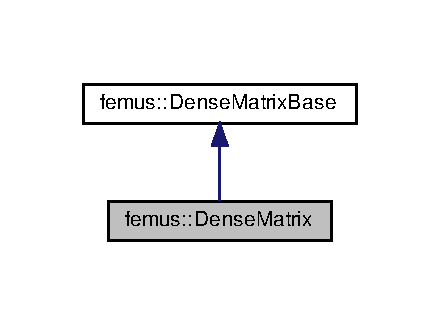
\includegraphics[width=211pt]{classfemus_1_1_dense_matrix__inherit__graph}
\end{center}
\end{figure}


Collaboration diagram for femus\+:\+:Dense\+Matrix\+:
\nopagebreak
\begin{figure}[H]
\begin{center}
\leavevmode
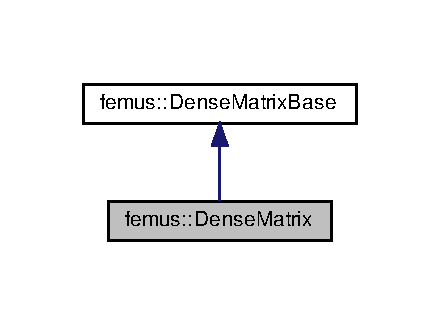
\includegraphics[width=211pt]{classfemus_1_1_dense_matrix__coll__graph}
\end{center}
\end{figure}
\subsection*{Public Member Functions}
\begin{DoxyCompactItemize}
\item 
\mbox{\hyperlink{classfemus_1_1_dense_matrix_a5f0562386636a86cea485eca2df4780d}{Dense\+Matrix}} (const int \mbox{\hyperlink{classfemus_1_1_dense_matrix_base_a67a582a53ab5ce7628a53f6a90fd39b9}{m}}=0, const int \mbox{\hyperlink{classfemus_1_1_dense_matrix_base_a1d9b513340794a8b15640f9c8cc6597e}{n}}=0)
\begin{DoxyCompactList}\small\item\em Constructor. Creates a dense matrix of dimension {\ttfamily m} by {\ttfamily n}. \end{DoxyCompactList}\item 
virtual \mbox{\hyperlink{classfemus_1_1_dense_matrix_a641288aa079e581caa61a8ca9ebfc8f9}{$\sim$\+Dense\+Matrix}} ()
\begin{DoxyCompactList}\small\item\em Copy-\/constructor. \end{DoxyCompactList}\item 
virtual void \mbox{\hyperlink{classfemus_1_1_dense_matrix_a865963674763716d720d6ef2c8177053}{zero}} ()
\begin{DoxyCompactList}\small\item\em Set every element in the matrix to 0. \end{DoxyCompactList}\item 
void \mbox{\hyperlink{classfemus_1_1_dense_matrix_a590507fcb543e7ac922099af9b066a38}{resize}} (const int \mbox{\hyperlink{classfemus_1_1_dense_matrix_base_a67a582a53ab5ce7628a53f6a90fd39b9}{m}}, const int \mbox{\hyperlink{classfemus_1_1_dense_matrix_base_a1d9b513340794a8b15640f9c8cc6597e}{n}})
\begin{DoxyCompactList}\small\item\em Resize the matrix. Will never free memory, but may allocate more. Sets all elements to 0. \end{DoxyCompactList}\item 
double \mbox{\hyperlink{classfemus_1_1_dense_matrix_a17c69f52638c4df03c15a6724e537ebf}{operator()}} (const int i, const int j) const
\item 
double \& \mbox{\hyperlink{classfemus_1_1_dense_matrix_a2ca6e78e2fc5c583bc60f210d79ba28d}{operator()}} (const int i, const int j)
\item 
virtual double \mbox{\hyperlink{classfemus_1_1_dense_matrix_a3b37181274fbe8eca1523acdecb59bd0}{el}} (const int i, const int j) const
\item 
virtual double \& \mbox{\hyperlink{classfemus_1_1_dense_matrix_a9867b5e9b16b8ec746ebde4270239248}{el}} (const int i, const int j)
\item 
std\+::vector$<$ double $>$ \& \mbox{\hyperlink{classfemus_1_1_dense_matrix_a2462d41848e267ba763177c3481eb643}{get\+\_\+values}} ()
\begin{DoxyCompactList}\small\item\em Access to the values array. \end{DoxyCompactList}\item 
const std\+::vector$<$ double $>$ \& \mbox{\hyperlink{classfemus_1_1_dense_matrix_a7d4b74e15b37ec3927d3f533dc0c0e07}{get\+\_\+values}} () const
\begin{DoxyCompactList}\small\item\em Return a constant reference to the matrix values. \end{DoxyCompactList}\item 
void \mbox{\hyperlink{classfemus_1_1_dense_matrix_ac6fa82dae47d2bb783f8b1507b730b1b}{get\+\_\+principal\+\_\+submatrix}} (int sub\+\_\+m, int sub\+\_\+n, \mbox{\hyperlink{classfemus_1_1_dense_matrix}{Dense\+Matrix}} \&dest) const
\begin{DoxyCompactList}\small\item\em Put the {\ttfamily sub\+\_\+m} x {\ttfamily sub\+\_\+n} principal submatrix into {\ttfamily dest}. \end{DoxyCompactList}\item 
void \mbox{\hyperlink{classfemus_1_1_dense_matrix_ace38881dc4185f79340438082fcfccfd}{get\+\_\+principal\+\_\+submatrix}} (int sub\+\_\+m, \mbox{\hyperlink{classfemus_1_1_dense_matrix}{Dense\+Matrix}} \&dest) const
\begin{DoxyCompactList}\small\item\em Put the {\ttfamily sub\+\_\+m} x {\ttfamily sub\+\_\+m} principal submatrix into {\ttfamily dest}. \end{DoxyCompactList}\item 
virtual void \mbox{\hyperlink{classfemus_1_1_dense_matrix_a80917b8698400957bc821308be3dafe5}{left\+\_\+multiply}} (const \mbox{\hyperlink{classfemus_1_1_dense_matrix_base}{Dense\+Matrix\+Base}} \&M2)
\begin{DoxyCompactList}\small\item\em Left multipliess by the matrix {\ttfamily M2}. \end{DoxyCompactList}\item 
virtual void \mbox{\hyperlink{classfemus_1_1_dense_matrix_a6de589e870d32a851fda1049b736bf99}{right\+\_\+multiply}} (const \mbox{\hyperlink{classfemus_1_1_dense_matrix_base}{Dense\+Matrix\+Base}} \&M3)
\begin{DoxyCompactList}\small\item\em Right multiplies by the matrix {\ttfamily M3}. \end{DoxyCompactList}\item 
void \mbox{\hyperlink{classfemus_1_1_dense_matrix_abbedc871f6bb0adebf1889a6ca8dbc85}{vector\+\_\+mult}} (\mbox{\hyperlink{classfemus_1_1_dense_vector}{Dense\+Vector}} \&dest, const \mbox{\hyperlink{classfemus_1_1_dense_vector}{Dense\+Vector}} \&arg) const
\begin{DoxyCompactList}\small\item\em Perform matrix vector multiplication. \end{DoxyCompactList}\item 
void \mbox{\hyperlink{classfemus_1_1_dense_matrix_a295b7577e8910a0600dacadd1c30b15b}{vector\+\_\+mult\+\_\+add}} (\mbox{\hyperlink{classfemus_1_1_dense_vector}{Dense\+Vector}} \&dest, const double factor, const \mbox{\hyperlink{classfemus_1_1_dense_vector}{Dense\+Vector}} \&arg) const
\begin{DoxyCompactList}\small\item\em Perform matrix vector multiplication and add scaled result to {\ttfamily dest}. \end{DoxyCompactList}\item 
\mbox{\hyperlink{classfemus_1_1_dense_matrix}{Dense\+Matrix}} \& \mbox{\hyperlink{classfemus_1_1_dense_matrix_a44a381eba83cf091b48a270854860c10}{operator=}} (const \mbox{\hyperlink{classfemus_1_1_dense_matrix}{Dense\+Matrix}} \&other\+\_\+matrix)
\begin{DoxyCompactList}\small\item\em Assignment operator. \end{DoxyCompactList}\item 
void \mbox{\hyperlink{classfemus_1_1_dense_matrix_acbd35539fd0ca78df190f3ec10800f88}{swap}} (\mbox{\hyperlink{classfemus_1_1_dense_matrix}{Dense\+Matrix}} \&other\+\_\+matrix)
\begin{DoxyCompactList}\small\item\em S\+T\+L-\/like swap method. \end{DoxyCompactList}\item 
void \mbox{\hyperlink{classfemus_1_1_dense_matrix_a1df3092a24679a976ec0c0cccae965df}{scale}} (const double factor)
\begin{DoxyCompactList}\small\item\em Multiplies every element in the matrix by {\ttfamily factor}. \end{DoxyCompactList}\item 
\mbox{\hyperlink{classfemus_1_1_dense_matrix}{Dense\+Matrix}} \& \mbox{\hyperlink{classfemus_1_1_dense_matrix_a748804467957e01dfc7a51dc8edefb8f}{operator$\ast$=}} (const double factor)
\begin{DoxyCompactList}\small\item\em Multiplies every element in the matrix by {\ttfamily factor}. \end{DoxyCompactList}\item 
\mbox{\hyperlink{classfemus_1_1_dense_matrix}{Dense\+Matrix}} \& \mbox{\hyperlink{classfemus_1_1_dense_matrix_adaadf49cb5433b9211287fad5e5857df}{operator+=}} (const \mbox{\hyperlink{classfemus_1_1_dense_matrix}{Dense\+Matrix}} \&mat)
\begin{DoxyCompactList}\small\item\em Adds {\ttfamily mat} to this matrix. \end{DoxyCompactList}\item 
void \mbox{\hyperlink{classfemus_1_1_dense_matrix_a3268040014359267e8d2fb9fbf187dac}{add}} (const double factor, const \mbox{\hyperlink{classfemus_1_1_dense_matrix}{Dense\+Matrix}} \&mat)
\begin{DoxyCompactList}\small\item\em Adds {\ttfamily factor} times {\ttfamily mat} to this matrix. \end{DoxyCompactList}\item 
bool \mbox{\hyperlink{classfemus_1_1_dense_matrix_a7d005d3213672a2e7e34fe7c4203881e}{operator==}} (const \mbox{\hyperlink{classfemus_1_1_dense_matrix}{Dense\+Matrix}} \&mat) const
\begin{DoxyCompactList}\small\item\em Tests if {\ttfamily mat} is exactly equal to this matrix. \end{DoxyCompactList}\item 
bool \mbox{\hyperlink{classfemus_1_1_dense_matrix_abe105648cbb9266ed37d9779ac0ecc57}{operator!=}} (const \mbox{\hyperlink{classfemus_1_1_dense_matrix}{Dense\+Matrix}} \&mat) const
\begin{DoxyCompactList}\small\item\em Tests if {\ttfamily mat} is not exactly equal to this matrix. \end{DoxyCompactList}\item 
\mbox{\hyperlink{classfemus_1_1_dense_matrix}{Dense\+Matrix}} \& \mbox{\hyperlink{classfemus_1_1_dense_matrix_a9e44e590645899830566d1dcb29b778f}{operator-\/=}} (const \mbox{\hyperlink{classfemus_1_1_dense_matrix}{Dense\+Matrix}} \&mat)
\begin{DoxyCompactList}\small\item\em Subtracts {\ttfamily mat} from this matrix. \end{DoxyCompactList}\item 
double \mbox{\hyperlink{classfemus_1_1_dense_matrix_a23726badca26256789e356c66a144727}{min}} () const
\begin{DoxyCompactList}\small\item\em this returns the minimum \end{DoxyCompactList}\item 
double \mbox{\hyperlink{classfemus_1_1_dense_matrix_a2226f9ae3cbf21779e203679b7cd00ff}{max}} () const
\item 
double \mbox{\hyperlink{classfemus_1_1_dense_matrix_a7ef19514a04f38ba1baf8d33b981651d}{l1\+\_\+norm}} () const
\begin{DoxyCompactList}\small\item\em Return the l1-\/norm of the matrix, that is max. sum of columns. \end{DoxyCompactList}\item 
double \mbox{\hyperlink{classfemus_1_1_dense_matrix_a4372d3ff30e801e9ef3333c0e48584cd}{linfty\+\_\+norm}} () const
\begin{DoxyCompactList}\small\item\em Return the linfty-\/norm of the max. sum of rows. \end{DoxyCompactList}\item 
void \mbox{\hyperlink{classfemus_1_1_dense_matrix_a87669df2d5c176037dc5f43d514e4294}{left\+\_\+multiply\+\_\+transpose}} (const \mbox{\hyperlink{classfemus_1_1_dense_matrix}{Dense\+Matrix}} \&A)
\begin{DoxyCompactList}\small\item\em Left multiplies by the transpose of the matrix {\ttfamily A}. \end{DoxyCompactList}\item 
void \mbox{\hyperlink{classfemus_1_1_dense_matrix_a1f37b788108a1c7667369141ee3686af}{right\+\_\+multiply\+\_\+transpose}} (const \mbox{\hyperlink{classfemus_1_1_dense_matrix}{Dense\+Matrix}} \&A)
\begin{DoxyCompactList}\small\item\em Right multiplies by the transpose of the matrix {\ttfamily A}. \end{DoxyCompactList}\item 
double \mbox{\hyperlink{classfemus_1_1_dense_matrix_a66f15cb283425507fcf2883394d18086}{transpose}} (const int i, const int j) const
\item 
void \mbox{\hyperlink{classfemus_1_1_dense_matrix_af8801bd9d1a335fc3a820f95128a46cf}{get\+\_\+transpose}} (\mbox{\hyperlink{classfemus_1_1_dense_matrix}{Dense\+Matrix}} \&dest) const
\begin{DoxyCompactList}\small\item\em Put the tranposed matrix into {\ttfamily dest}. \end{DoxyCompactList}\item 
void \mbox{\hyperlink{classfemus_1_1_dense_matrix_a2b0e9e0b07db7eb9e3aff9067e2b4fd6}{condense}} (const int i, const int j, const double val, \mbox{\hyperlink{classfemus_1_1_dense_vector_base}{Dense\+Vector\+Base}} \&rhs)
\item 
void \mbox{\hyperlink{classfemus_1_1_dense_matrix_a3225f4b8647222c03a03cd35b54e7d93}{lu\+\_\+solve}} (\mbox{\hyperlink{classfemus_1_1_dense_vector}{Dense\+Vector}} \&b, \mbox{\hyperlink{classfemus_1_1_dense_vector}{Dense\+Vector}} \&x, const bool partial\+\_\+pivot=false)
\begin{DoxyCompactList}\small\item\em Solve the system Ax=b given the input vector b. \end{DoxyCompactList}\item 
void \mbox{\hyperlink{classfemus_1_1_dense_matrix_aa21f4ae4b7277cf63799fad573382c9b}{cholesky\+\_\+solve}} (\mbox{\hyperlink{classfemus_1_1_dense_vector}{Dense\+Vector}} \&b, \mbox{\hyperlink{classfemus_1_1_dense_vector}{Dense\+Vector}} \&x)
\begin{DoxyCompactList}\small\item\em A Cholesky factorizationof A such that A = L L$^\wedge$T. \end{DoxyCompactList}\item 
double \mbox{\hyperlink{classfemus_1_1_dense_matrix_a752a0289f98f7182c72b7c08cd49062c}{det}} ()
\end{DoxyCompactItemize}
\subsection*{Public Attributes}
\begin{DoxyCompactItemize}
\item 
bool \mbox{\hyperlink{classfemus_1_1_dense_matrix_a1f4f9cac8bd3c8b9ff1514c0b4ffedc6}{use\+\_\+blas}}
\begin{DoxyCompactList}\small\item\em Run-\/time selectable option to turn on/off blas support. \end{DoxyCompactList}\end{DoxyCompactItemize}
\subsection*{Additional Inherited Members}


\subsection{Constructor \& Destructor Documentation}
\mbox{\Hypertarget{classfemus_1_1_dense_matrix_a5f0562386636a86cea485eca2df4780d}\label{classfemus_1_1_dense_matrix_a5f0562386636a86cea485eca2df4780d}} 
\index{femus\+::\+Dense\+Matrix@{femus\+::\+Dense\+Matrix}!Dense\+Matrix@{Dense\+Matrix}}
\index{Dense\+Matrix@{Dense\+Matrix}!femus\+::\+Dense\+Matrix@{femus\+::\+Dense\+Matrix}}
\subsubsection{\texorpdfstring{Dense\+Matrix()}{DenseMatrix()}}
{\footnotesize\ttfamily femus\+::\+Dense\+Matrix\+::\+Dense\+Matrix (\begin{DoxyParamCaption}\item[{const int}]{m = {\ttfamily 0},  }\item[{const int}]{n = {\ttfamily 0} }\end{DoxyParamCaption})\hspace{0.3cm}{\ttfamily [inline]}}



Constructor. Creates a dense matrix of dimension {\ttfamily m} by {\ttfamily n}. 

\mbox{\Hypertarget{classfemus_1_1_dense_matrix_a641288aa079e581caa61a8ca9ebfc8f9}\label{classfemus_1_1_dense_matrix_a641288aa079e581caa61a8ca9ebfc8f9}} 
\index{femus\+::\+Dense\+Matrix@{femus\+::\+Dense\+Matrix}!````~Dense\+Matrix@{$\sim$\+Dense\+Matrix}}
\index{````~Dense\+Matrix@{$\sim$\+Dense\+Matrix}!femus\+::\+Dense\+Matrix@{femus\+::\+Dense\+Matrix}}
\subsubsection{\texorpdfstring{$\sim$\+Dense\+Matrix()}{~DenseMatrix()}}
{\footnotesize\ttfamily virtual femus\+::\+Dense\+Matrix\+::$\sim$\+Dense\+Matrix (\begin{DoxyParamCaption}{ }\end{DoxyParamCaption})\hspace{0.3cm}{\ttfamily [inline]}, {\ttfamily [virtual]}}



Copy-\/constructor. 

Destructor. Empty. 

\subsection{Member Function Documentation}
\mbox{\Hypertarget{classfemus_1_1_dense_matrix_a3268040014359267e8d2fb9fbf187dac}\label{classfemus_1_1_dense_matrix_a3268040014359267e8d2fb9fbf187dac}} 
\index{femus\+::\+Dense\+Matrix@{femus\+::\+Dense\+Matrix}!add@{add}}
\index{add@{add}!femus\+::\+Dense\+Matrix@{femus\+::\+Dense\+Matrix}}
\subsubsection{\texorpdfstring{add()}{add()}}
{\footnotesize\ttfamily void femus\+::\+Dense\+Matrix\+::add (\begin{DoxyParamCaption}\item[{const double}]{factor,  }\item[{const \mbox{\hyperlink{classfemus_1_1_dense_matrix}{Dense\+Matrix}} \&}]{mat }\end{DoxyParamCaption})\hspace{0.3cm}{\ttfamily [inline]}}



Adds {\ttfamily factor} times {\ttfamily mat} to this matrix. 

\mbox{\Hypertarget{classfemus_1_1_dense_matrix_aa21f4ae4b7277cf63799fad573382c9b}\label{classfemus_1_1_dense_matrix_aa21f4ae4b7277cf63799fad573382c9b}} 
\index{femus\+::\+Dense\+Matrix@{femus\+::\+Dense\+Matrix}!cholesky\+\_\+solve@{cholesky\+\_\+solve}}
\index{cholesky\+\_\+solve@{cholesky\+\_\+solve}!femus\+::\+Dense\+Matrix@{femus\+::\+Dense\+Matrix}}
\subsubsection{\texorpdfstring{cholesky\+\_\+solve()}{cholesky\_solve()}}
{\footnotesize\ttfamily void femus\+::\+Dense\+Matrix\+::cholesky\+\_\+solve (\begin{DoxyParamCaption}\item[{\mbox{\hyperlink{classfemus_1_1_dense_vector}{Dense\+Vector}} \&}]{b,  }\item[{\mbox{\hyperlink{classfemus_1_1_dense_vector}{Dense\+Vector}} \&}]{x }\end{DoxyParamCaption})}



A Cholesky factorizationof A such that A = L L$^\wedge$T. 

\mbox{\Hypertarget{classfemus_1_1_dense_matrix_a2b0e9e0b07db7eb9e3aff9067e2b4fd6}\label{classfemus_1_1_dense_matrix_a2b0e9e0b07db7eb9e3aff9067e2b4fd6}} 
\index{femus\+::\+Dense\+Matrix@{femus\+::\+Dense\+Matrix}!condense@{condense}}
\index{condense@{condense}!femus\+::\+Dense\+Matrix@{femus\+::\+Dense\+Matrix}}
\subsubsection{\texorpdfstring{condense()}{condense()}}
{\footnotesize\ttfamily void femus\+::\+Dense\+Matrix\+::condense (\begin{DoxyParamCaption}\item[{const int}]{i,  }\item[{const int}]{j,  }\item[{const double}]{val,  }\item[{\mbox{\hyperlink{classfemus_1_1_dense_vector_base}{Dense\+Vector\+Base}} \&}]{rhs }\end{DoxyParamCaption})\hspace{0.3cm}{\ttfamily [inline]}}

Condense-\/out the {\ttfamily }(i,j) entry of the matrix, forcing it to take on the value {\ttfamily val}. This is useful in numerical simulations for applying boundary conditions. Preserves the symmetry of the matrix. !!!!!!!!!!!!!!!!!!!!! T\+O\+DO \mbox{\hyperlink{classfemus_1_1_dense_vector_base}{Dense\+Vector\+Base}} -\/$>$ \mbox{\hyperlink{classfemus_1_1_dense_vector}{Dense\+Vector}} \mbox{\Hypertarget{classfemus_1_1_dense_matrix_a752a0289f98f7182c72b7c08cd49062c}\label{classfemus_1_1_dense_matrix_a752a0289f98f7182c72b7c08cd49062c}} 
\index{femus\+::\+Dense\+Matrix@{femus\+::\+Dense\+Matrix}!det@{det}}
\index{det@{det}!femus\+::\+Dense\+Matrix@{femus\+::\+Dense\+Matrix}}
\subsubsection{\texorpdfstring{det()}{det()}}
{\footnotesize\ttfamily double femus\+::\+Dense\+Matrix\+::det (\begin{DoxyParamCaption}{ }\end{DoxyParamCaption})}


\begin{DoxyItemize}
\item \begin{DoxyReturn}{Returns}
the determinant of the matrix. 
\end{DoxyReturn}

\end{DoxyItemize}\mbox{\Hypertarget{classfemus_1_1_dense_matrix_a3b37181274fbe8eca1523acdecb59bd0}\label{classfemus_1_1_dense_matrix_a3b37181274fbe8eca1523acdecb59bd0}} 
\index{femus\+::\+Dense\+Matrix@{femus\+::\+Dense\+Matrix}!el@{el}}
\index{el@{el}!femus\+::\+Dense\+Matrix@{femus\+::\+Dense\+Matrix}}
\subsubsection{\texorpdfstring{el()}{el()}\hspace{0.1cm}{\footnotesize\ttfamily [1/2]}}
{\footnotesize\ttfamily virtual double femus\+::\+Dense\+Matrix\+::el (\begin{DoxyParamCaption}\item[{const int}]{i,  }\item[{const int}]{j }\end{DoxyParamCaption}) const\hspace{0.3cm}{\ttfamily [inline]}, {\ttfamily [virtual]}}

\begin{DoxyReturn}{Returns}
the {\ttfamily }(i,j) element of the matrix as a writeable reference. 
\end{DoxyReturn}


Implements \mbox{\hyperlink{classfemus_1_1_dense_matrix_base_abaf98d937069f9df0829353d9454ad93}{femus\+::\+Dense\+Matrix\+Base}}.

\mbox{\Hypertarget{classfemus_1_1_dense_matrix_a9867b5e9b16b8ec746ebde4270239248}\label{classfemus_1_1_dense_matrix_a9867b5e9b16b8ec746ebde4270239248}} 
\index{femus\+::\+Dense\+Matrix@{femus\+::\+Dense\+Matrix}!el@{el}}
\index{el@{el}!femus\+::\+Dense\+Matrix@{femus\+::\+Dense\+Matrix}}
\subsubsection{\texorpdfstring{el()}{el()}\hspace{0.1cm}{\footnotesize\ttfamily [2/2]}}
{\footnotesize\ttfamily virtual double\& femus\+::\+Dense\+Matrix\+::el (\begin{DoxyParamCaption}\item[{const int}]{i,  }\item[{const int}]{j }\end{DoxyParamCaption})\hspace{0.3cm}{\ttfamily [inline]}, {\ttfamily [virtual]}}

\begin{DoxyReturn}{Returns}
the {\ttfamily }(i,j) element of the matrix as a writeable reference. 
\end{DoxyReturn}


Implements \mbox{\hyperlink{classfemus_1_1_dense_matrix_base_ab1f58e98ca5000e197fce3013a019dc4}{femus\+::\+Dense\+Matrix\+Base}}.

\mbox{\Hypertarget{classfemus_1_1_dense_matrix_ac6fa82dae47d2bb783f8b1507b730b1b}\label{classfemus_1_1_dense_matrix_ac6fa82dae47d2bb783f8b1507b730b1b}} 
\index{femus\+::\+Dense\+Matrix@{femus\+::\+Dense\+Matrix}!get\+\_\+principal\+\_\+submatrix@{get\+\_\+principal\+\_\+submatrix}}
\index{get\+\_\+principal\+\_\+submatrix@{get\+\_\+principal\+\_\+submatrix}!femus\+::\+Dense\+Matrix@{femus\+::\+Dense\+Matrix}}
\subsubsection{\texorpdfstring{get\+\_\+principal\+\_\+submatrix()}{get\_principal\_submatrix()}\hspace{0.1cm}{\footnotesize\ttfamily [1/2]}}
{\footnotesize\ttfamily void femus\+::\+Dense\+Matrix\+::get\+\_\+principal\+\_\+submatrix (\begin{DoxyParamCaption}\item[{int}]{sub\+\_\+m,  }\item[{int}]{sub\+\_\+n,  }\item[{\mbox{\hyperlink{classfemus_1_1_dense_matrix}{Dense\+Matrix}} \&}]{dest }\end{DoxyParamCaption}) const}



Put the {\ttfamily sub\+\_\+m} x {\ttfamily sub\+\_\+n} principal submatrix into {\ttfamily dest}. 

\mbox{\Hypertarget{classfemus_1_1_dense_matrix_ace38881dc4185f79340438082fcfccfd}\label{classfemus_1_1_dense_matrix_ace38881dc4185f79340438082fcfccfd}} 
\index{femus\+::\+Dense\+Matrix@{femus\+::\+Dense\+Matrix}!get\+\_\+principal\+\_\+submatrix@{get\+\_\+principal\+\_\+submatrix}}
\index{get\+\_\+principal\+\_\+submatrix@{get\+\_\+principal\+\_\+submatrix}!femus\+::\+Dense\+Matrix@{femus\+::\+Dense\+Matrix}}
\subsubsection{\texorpdfstring{get\+\_\+principal\+\_\+submatrix()}{get\_principal\_submatrix()}\hspace{0.1cm}{\footnotesize\ttfamily [2/2]}}
{\footnotesize\ttfamily void femus\+::\+Dense\+Matrix\+::get\+\_\+principal\+\_\+submatrix (\begin{DoxyParamCaption}\item[{int}]{sub\+\_\+m,  }\item[{\mbox{\hyperlink{classfemus_1_1_dense_matrix}{Dense\+Matrix}} \&}]{dest }\end{DoxyParamCaption}) const}



Put the {\ttfamily sub\+\_\+m} x {\ttfamily sub\+\_\+m} principal submatrix into {\ttfamily dest}. 

\mbox{\Hypertarget{classfemus_1_1_dense_matrix_af8801bd9d1a335fc3a820f95128a46cf}\label{classfemus_1_1_dense_matrix_af8801bd9d1a335fc3a820f95128a46cf}} 
\index{femus\+::\+Dense\+Matrix@{femus\+::\+Dense\+Matrix}!get\+\_\+transpose@{get\+\_\+transpose}}
\index{get\+\_\+transpose@{get\+\_\+transpose}!femus\+::\+Dense\+Matrix@{femus\+::\+Dense\+Matrix}}
\subsubsection{\texorpdfstring{get\+\_\+transpose()}{get\_transpose()}}
{\footnotesize\ttfamily void femus\+::\+Dense\+Matrix\+::get\+\_\+transpose (\begin{DoxyParamCaption}\item[{\mbox{\hyperlink{classfemus_1_1_dense_matrix}{Dense\+Matrix}} \&}]{dest }\end{DoxyParamCaption}) const}



Put the tranposed matrix into {\ttfamily dest}. 

\mbox{\Hypertarget{classfemus_1_1_dense_matrix_a2462d41848e267ba763177c3481eb643}\label{classfemus_1_1_dense_matrix_a2462d41848e267ba763177c3481eb643}} 
\index{femus\+::\+Dense\+Matrix@{femus\+::\+Dense\+Matrix}!get\+\_\+values@{get\+\_\+values}}
\index{get\+\_\+values@{get\+\_\+values}!femus\+::\+Dense\+Matrix@{femus\+::\+Dense\+Matrix}}
\subsubsection{\texorpdfstring{get\+\_\+values()}{get\_values()}\hspace{0.1cm}{\footnotesize\ttfamily [1/2]}}
{\footnotesize\ttfamily std\+::vector$<$double$>$\& femus\+::\+Dense\+Matrix\+::get\+\_\+values (\begin{DoxyParamCaption}{ }\end{DoxyParamCaption})\hspace{0.3cm}{\ttfamily [inline]}}



Access to the values array. 

\mbox{\Hypertarget{classfemus_1_1_dense_matrix_a7d4b74e15b37ec3927d3f533dc0c0e07}\label{classfemus_1_1_dense_matrix_a7d4b74e15b37ec3927d3f533dc0c0e07}} 
\index{femus\+::\+Dense\+Matrix@{femus\+::\+Dense\+Matrix}!get\+\_\+values@{get\+\_\+values}}
\index{get\+\_\+values@{get\+\_\+values}!femus\+::\+Dense\+Matrix@{femus\+::\+Dense\+Matrix}}
\subsubsection{\texorpdfstring{get\+\_\+values()}{get\_values()}\hspace{0.1cm}{\footnotesize\ttfamily [2/2]}}
{\footnotesize\ttfamily const std\+::vector$<$double$>$\& femus\+::\+Dense\+Matrix\+::get\+\_\+values (\begin{DoxyParamCaption}{ }\end{DoxyParamCaption}) const\hspace{0.3cm}{\ttfamily [inline]}}



Return a constant reference to the matrix values. 

\mbox{\Hypertarget{classfemus_1_1_dense_matrix_a7ef19514a04f38ba1baf8d33b981651d}\label{classfemus_1_1_dense_matrix_a7ef19514a04f38ba1baf8d33b981651d}} 
\index{femus\+::\+Dense\+Matrix@{femus\+::\+Dense\+Matrix}!l1\+\_\+norm@{l1\+\_\+norm}}
\index{l1\+\_\+norm@{l1\+\_\+norm}!femus\+::\+Dense\+Matrix@{femus\+::\+Dense\+Matrix}}
\subsubsection{\texorpdfstring{l1\+\_\+norm()}{l1\_norm()}}
{\footnotesize\ttfamily double femus\+::\+Dense\+Matrix\+::l1\+\_\+norm (\begin{DoxyParamCaption}{ }\end{DoxyParamCaption}) const\hspace{0.3cm}{\ttfamily [inline]}}



Return the l1-\/norm of the matrix, that is max. sum of columns. 

\mbox{\Hypertarget{classfemus_1_1_dense_matrix_a80917b8698400957bc821308be3dafe5}\label{classfemus_1_1_dense_matrix_a80917b8698400957bc821308be3dafe5}} 
\index{femus\+::\+Dense\+Matrix@{femus\+::\+Dense\+Matrix}!left\+\_\+multiply@{left\+\_\+multiply}}
\index{left\+\_\+multiply@{left\+\_\+multiply}!femus\+::\+Dense\+Matrix@{femus\+::\+Dense\+Matrix}}
\subsubsection{\texorpdfstring{left\+\_\+multiply()}{left\_multiply()}}
{\footnotesize\ttfamily void femus\+::\+Dense\+Matrix\+::left\+\_\+multiply (\begin{DoxyParamCaption}\item[{const \mbox{\hyperlink{classfemus_1_1_dense_matrix_base}{Dense\+Matrix\+Base}} \&}]{M2 }\end{DoxyParamCaption})\hspace{0.3cm}{\ttfamily [virtual]}}



Left multipliess by the matrix {\ttfamily M2}. 



Implements \mbox{\hyperlink{classfemus_1_1_dense_matrix_base_af08f7a07a6b6a9486502a8af234de32c}{femus\+::\+Dense\+Matrix\+Base}}.

\mbox{\Hypertarget{classfemus_1_1_dense_matrix_a87669df2d5c176037dc5f43d514e4294}\label{classfemus_1_1_dense_matrix_a87669df2d5c176037dc5f43d514e4294}} 
\index{femus\+::\+Dense\+Matrix@{femus\+::\+Dense\+Matrix}!left\+\_\+multiply\+\_\+transpose@{left\+\_\+multiply\+\_\+transpose}}
\index{left\+\_\+multiply\+\_\+transpose@{left\+\_\+multiply\+\_\+transpose}!femus\+::\+Dense\+Matrix@{femus\+::\+Dense\+Matrix}}
\subsubsection{\texorpdfstring{left\+\_\+multiply\+\_\+transpose()}{left\_multiply\_transpose()}}
{\footnotesize\ttfamily void femus\+::\+Dense\+Matrix\+::left\+\_\+multiply\+\_\+transpose (\begin{DoxyParamCaption}\item[{const \mbox{\hyperlink{classfemus_1_1_dense_matrix}{Dense\+Matrix}} \&}]{A }\end{DoxyParamCaption})}



Left multiplies by the transpose of the matrix {\ttfamily A}. 

\mbox{\Hypertarget{classfemus_1_1_dense_matrix_a4372d3ff30e801e9ef3333c0e48584cd}\label{classfemus_1_1_dense_matrix_a4372d3ff30e801e9ef3333c0e48584cd}} 
\index{femus\+::\+Dense\+Matrix@{femus\+::\+Dense\+Matrix}!linfty\+\_\+norm@{linfty\+\_\+norm}}
\index{linfty\+\_\+norm@{linfty\+\_\+norm}!femus\+::\+Dense\+Matrix@{femus\+::\+Dense\+Matrix}}
\subsubsection{\texorpdfstring{linfty\+\_\+norm()}{linfty\_norm()}}
{\footnotesize\ttfamily double femus\+::\+Dense\+Matrix\+::linfty\+\_\+norm (\begin{DoxyParamCaption}{ }\end{DoxyParamCaption}) const\hspace{0.3cm}{\ttfamily [inline]}}



Return the linfty-\/norm of the max. sum of rows. 

\mbox{\Hypertarget{classfemus_1_1_dense_matrix_a3225f4b8647222c03a03cd35b54e7d93}\label{classfemus_1_1_dense_matrix_a3225f4b8647222c03a03cd35b54e7d93}} 
\index{femus\+::\+Dense\+Matrix@{femus\+::\+Dense\+Matrix}!lu\+\_\+solve@{lu\+\_\+solve}}
\index{lu\+\_\+solve@{lu\+\_\+solve}!femus\+::\+Dense\+Matrix@{femus\+::\+Dense\+Matrix}}
\subsubsection{\texorpdfstring{lu\+\_\+solve()}{lu\_solve()}}
{\footnotesize\ttfamily void femus\+::\+Dense\+Matrix\+::lu\+\_\+solve (\begin{DoxyParamCaption}\item[{\mbox{\hyperlink{classfemus_1_1_dense_vector}{Dense\+Vector}} \&}]{b,  }\item[{\mbox{\hyperlink{classfemus_1_1_dense_vector}{Dense\+Vector}} \&}]{x,  }\item[{const bool}]{partial\+\_\+pivot = {\ttfamily false} }\end{DoxyParamCaption})}



Solve the system Ax=b given the input vector b. 

\mbox{\Hypertarget{classfemus_1_1_dense_matrix_a2226f9ae3cbf21779e203679b7cd00ff}\label{classfemus_1_1_dense_matrix_a2226f9ae3cbf21779e203679b7cd00ff}} 
\index{femus\+::\+Dense\+Matrix@{femus\+::\+Dense\+Matrix}!max@{max}}
\index{max@{max}!femus\+::\+Dense\+Matrix@{femus\+::\+Dense\+Matrix}}
\subsubsection{\texorpdfstring{max()}{max()}}
{\footnotesize\ttfamily double femus\+::\+Dense\+Matrix\+::max (\begin{DoxyParamCaption}{ }\end{DoxyParamCaption}) const\hspace{0.3cm}{\ttfamily [inline]}}

\begin{DoxyReturn}{Returns}
the maximum element in the matrix. 
\end{DoxyReturn}
\mbox{\Hypertarget{classfemus_1_1_dense_matrix_a23726badca26256789e356c66a144727}\label{classfemus_1_1_dense_matrix_a23726badca26256789e356c66a144727}} 
\index{femus\+::\+Dense\+Matrix@{femus\+::\+Dense\+Matrix}!min@{min}}
\index{min@{min}!femus\+::\+Dense\+Matrix@{femus\+::\+Dense\+Matrix}}
\subsubsection{\texorpdfstring{min()}{min()}}
{\footnotesize\ttfamily double femus\+::\+Dense\+Matrix\+::min (\begin{DoxyParamCaption}{ }\end{DoxyParamCaption}) const\hspace{0.3cm}{\ttfamily [inline]}}



this returns the minimum 

\mbox{\Hypertarget{classfemus_1_1_dense_matrix_abe105648cbb9266ed37d9779ac0ecc57}\label{classfemus_1_1_dense_matrix_abe105648cbb9266ed37d9779ac0ecc57}} 
\index{femus\+::\+Dense\+Matrix@{femus\+::\+Dense\+Matrix}!operator"!=@{operator"!=}}
\index{operator"!=@{operator"!=}!femus\+::\+Dense\+Matrix@{femus\+::\+Dense\+Matrix}}
\subsubsection{\texorpdfstring{operator"!=()}{operator!=()}}
{\footnotesize\ttfamily bool femus\+::\+Dense\+Matrix\+::operator!= (\begin{DoxyParamCaption}\item[{const \mbox{\hyperlink{classfemus_1_1_dense_matrix}{Dense\+Matrix}} \&}]{mat }\end{DoxyParamCaption}) const\hspace{0.3cm}{\ttfamily [inline]}}



Tests if {\ttfamily mat} is not exactly equal to this matrix. 

\mbox{\Hypertarget{classfemus_1_1_dense_matrix_a17c69f52638c4df03c15a6724e537ebf}\label{classfemus_1_1_dense_matrix_a17c69f52638c4df03c15a6724e537ebf}} 
\index{femus\+::\+Dense\+Matrix@{femus\+::\+Dense\+Matrix}!operator()@{operator()}}
\index{operator()@{operator()}!femus\+::\+Dense\+Matrix@{femus\+::\+Dense\+Matrix}}
\subsubsection{\texorpdfstring{operator()()}{operator()()}\hspace{0.1cm}{\footnotesize\ttfamily [1/2]}}
{\footnotesize\ttfamily double femus\+::\+Dense\+Matrix\+::operator() (\begin{DoxyParamCaption}\item[{const int}]{i,  }\item[{const int}]{j }\end{DoxyParamCaption}) const\hspace{0.3cm}{\ttfamily [inline]}}

\begin{DoxyReturn}{Returns}
the {\ttfamily }(i,j) element of the matrix. 
\end{DoxyReturn}
\mbox{\Hypertarget{classfemus_1_1_dense_matrix_a2ca6e78e2fc5c583bc60f210d79ba28d}\label{classfemus_1_1_dense_matrix_a2ca6e78e2fc5c583bc60f210d79ba28d}} 
\index{femus\+::\+Dense\+Matrix@{femus\+::\+Dense\+Matrix}!operator()@{operator()}}
\index{operator()@{operator()}!femus\+::\+Dense\+Matrix@{femus\+::\+Dense\+Matrix}}
\subsubsection{\texorpdfstring{operator()()}{operator()()}\hspace{0.1cm}{\footnotesize\ttfamily [2/2]}}
{\footnotesize\ttfamily double \& femus\+::\+Dense\+Matrix\+::operator() (\begin{DoxyParamCaption}\item[{const int}]{i,  }\item[{const int}]{j }\end{DoxyParamCaption})\hspace{0.3cm}{\ttfamily [inline]}}

\begin{DoxyReturn}{Returns}
the {\ttfamily }(i,j) element of the matrix as a writeable reference. 
\end{DoxyReturn}
\mbox{\Hypertarget{classfemus_1_1_dense_matrix_a748804467957e01dfc7a51dc8edefb8f}\label{classfemus_1_1_dense_matrix_a748804467957e01dfc7a51dc8edefb8f}} 
\index{femus\+::\+Dense\+Matrix@{femus\+::\+Dense\+Matrix}!operator$\ast$=@{operator$\ast$=}}
\index{operator$\ast$=@{operator$\ast$=}!femus\+::\+Dense\+Matrix@{femus\+::\+Dense\+Matrix}}
\subsubsection{\texorpdfstring{operator$\ast$=()}{operator*=()}}
{\footnotesize\ttfamily \mbox{\hyperlink{classfemus_1_1_dense_matrix}{Dense\+Matrix}} \& femus\+::\+Dense\+Matrix\+::operator$\ast$= (\begin{DoxyParamCaption}\item[{const double}]{factor }\end{DoxyParamCaption})\hspace{0.3cm}{\ttfamily [inline]}}



Multiplies every element in the matrix by {\ttfamily factor}. 

\mbox{\Hypertarget{classfemus_1_1_dense_matrix_adaadf49cb5433b9211287fad5e5857df}\label{classfemus_1_1_dense_matrix_adaadf49cb5433b9211287fad5e5857df}} 
\index{femus\+::\+Dense\+Matrix@{femus\+::\+Dense\+Matrix}!operator+=@{operator+=}}
\index{operator+=@{operator+=}!femus\+::\+Dense\+Matrix@{femus\+::\+Dense\+Matrix}}
\subsubsection{\texorpdfstring{operator+=()}{operator+=()}}
{\footnotesize\ttfamily \mbox{\hyperlink{classfemus_1_1_dense_matrix}{Dense\+Matrix}} \& femus\+::\+Dense\+Matrix\+::operator+= (\begin{DoxyParamCaption}\item[{const \mbox{\hyperlink{classfemus_1_1_dense_matrix}{Dense\+Matrix}} \&}]{mat }\end{DoxyParamCaption})\hspace{0.3cm}{\ttfamily [inline]}}



Adds {\ttfamily mat} to this matrix. 

\mbox{\Hypertarget{classfemus_1_1_dense_matrix_a9e44e590645899830566d1dcb29b778f}\label{classfemus_1_1_dense_matrix_a9e44e590645899830566d1dcb29b778f}} 
\index{femus\+::\+Dense\+Matrix@{femus\+::\+Dense\+Matrix}!operator-\/=@{operator-\/=}}
\index{operator-\/=@{operator-\/=}!femus\+::\+Dense\+Matrix@{femus\+::\+Dense\+Matrix}}
\subsubsection{\texorpdfstring{operator-\/=()}{operator-=()}}
{\footnotesize\ttfamily \mbox{\hyperlink{classfemus_1_1_dense_matrix}{Dense\+Matrix}} \& femus\+::\+Dense\+Matrix\+::operator-\/= (\begin{DoxyParamCaption}\item[{const \mbox{\hyperlink{classfemus_1_1_dense_matrix}{Dense\+Matrix}} \&}]{mat }\end{DoxyParamCaption})\hspace{0.3cm}{\ttfamily [inline]}}



Subtracts {\ttfamily mat} from this matrix. 

\mbox{\Hypertarget{classfemus_1_1_dense_matrix_a44a381eba83cf091b48a270854860c10}\label{classfemus_1_1_dense_matrix_a44a381eba83cf091b48a270854860c10}} 
\index{femus\+::\+Dense\+Matrix@{femus\+::\+Dense\+Matrix}!operator=@{operator=}}
\index{operator=@{operator=}!femus\+::\+Dense\+Matrix@{femus\+::\+Dense\+Matrix}}
\subsubsection{\texorpdfstring{operator=()}{operator=()}}
{\footnotesize\ttfamily \mbox{\hyperlink{classfemus_1_1_dense_matrix}{Dense\+Matrix}} \& femus\+::\+Dense\+Matrix\+::operator= (\begin{DoxyParamCaption}\item[{const \mbox{\hyperlink{classfemus_1_1_dense_matrix}{Dense\+Matrix}} \&}]{other\+\_\+matrix }\end{DoxyParamCaption})\hspace{0.3cm}{\ttfamily [inline]}}



Assignment operator. 

\mbox{\Hypertarget{classfemus_1_1_dense_matrix_a7d005d3213672a2e7e34fe7c4203881e}\label{classfemus_1_1_dense_matrix_a7d005d3213672a2e7e34fe7c4203881e}} 
\index{femus\+::\+Dense\+Matrix@{femus\+::\+Dense\+Matrix}!operator==@{operator==}}
\index{operator==@{operator==}!femus\+::\+Dense\+Matrix@{femus\+::\+Dense\+Matrix}}
\subsubsection{\texorpdfstring{operator==()}{operator==()}}
{\footnotesize\ttfamily bool femus\+::\+Dense\+Matrix\+::operator== (\begin{DoxyParamCaption}\item[{const \mbox{\hyperlink{classfemus_1_1_dense_matrix}{Dense\+Matrix}} \&}]{mat }\end{DoxyParamCaption}) const\hspace{0.3cm}{\ttfamily [inline]}}



Tests if {\ttfamily mat} is exactly equal to this matrix. 

\mbox{\Hypertarget{classfemus_1_1_dense_matrix_a590507fcb543e7ac922099af9b066a38}\label{classfemus_1_1_dense_matrix_a590507fcb543e7ac922099af9b066a38}} 
\index{femus\+::\+Dense\+Matrix@{femus\+::\+Dense\+Matrix}!resize@{resize}}
\index{resize@{resize}!femus\+::\+Dense\+Matrix@{femus\+::\+Dense\+Matrix}}
\subsubsection{\texorpdfstring{resize()}{resize()}}
{\footnotesize\ttfamily void femus\+::\+Dense\+Matrix\+::resize (\begin{DoxyParamCaption}\item[{const int}]{m,  }\item[{const int}]{n }\end{DoxyParamCaption})\hspace{0.3cm}{\ttfamily [inline]}}



Resize the matrix. Will never free memory, but may allocate more. Sets all elements to 0. 

\mbox{\Hypertarget{classfemus_1_1_dense_matrix_a6de589e870d32a851fda1049b736bf99}\label{classfemus_1_1_dense_matrix_a6de589e870d32a851fda1049b736bf99}} 
\index{femus\+::\+Dense\+Matrix@{femus\+::\+Dense\+Matrix}!right\+\_\+multiply@{right\+\_\+multiply}}
\index{right\+\_\+multiply@{right\+\_\+multiply}!femus\+::\+Dense\+Matrix@{femus\+::\+Dense\+Matrix}}
\subsubsection{\texorpdfstring{right\+\_\+multiply()}{right\_multiply()}}
{\footnotesize\ttfamily void femus\+::\+Dense\+Matrix\+::right\+\_\+multiply (\begin{DoxyParamCaption}\item[{const \mbox{\hyperlink{classfemus_1_1_dense_matrix_base}{Dense\+Matrix\+Base}} \&}]{M3 }\end{DoxyParamCaption})\hspace{0.3cm}{\ttfamily [virtual]}}



Right multiplies by the matrix {\ttfamily M3}. 



Implements \mbox{\hyperlink{classfemus_1_1_dense_matrix_base_a34072947783a0b4d797d04647cc3c646}{femus\+::\+Dense\+Matrix\+Base}}.

\mbox{\Hypertarget{classfemus_1_1_dense_matrix_a1f37b788108a1c7667369141ee3686af}\label{classfemus_1_1_dense_matrix_a1f37b788108a1c7667369141ee3686af}} 
\index{femus\+::\+Dense\+Matrix@{femus\+::\+Dense\+Matrix}!right\+\_\+multiply\+\_\+transpose@{right\+\_\+multiply\+\_\+transpose}}
\index{right\+\_\+multiply\+\_\+transpose@{right\+\_\+multiply\+\_\+transpose}!femus\+::\+Dense\+Matrix@{femus\+::\+Dense\+Matrix}}
\subsubsection{\texorpdfstring{right\+\_\+multiply\+\_\+transpose()}{right\_multiply\_transpose()}}
{\footnotesize\ttfamily void femus\+::\+Dense\+Matrix\+::right\+\_\+multiply\+\_\+transpose (\begin{DoxyParamCaption}\item[{const \mbox{\hyperlink{classfemus_1_1_dense_matrix}{Dense\+Matrix}} \&}]{A }\end{DoxyParamCaption})}



Right multiplies by the transpose of the matrix {\ttfamily A}. 

\mbox{\Hypertarget{classfemus_1_1_dense_matrix_a1df3092a24679a976ec0c0cccae965df}\label{classfemus_1_1_dense_matrix_a1df3092a24679a976ec0c0cccae965df}} 
\index{femus\+::\+Dense\+Matrix@{femus\+::\+Dense\+Matrix}!scale@{scale}}
\index{scale@{scale}!femus\+::\+Dense\+Matrix@{femus\+::\+Dense\+Matrix}}
\subsubsection{\texorpdfstring{scale()}{scale()}}
{\footnotesize\ttfamily void femus\+::\+Dense\+Matrix\+::scale (\begin{DoxyParamCaption}\item[{const double}]{factor }\end{DoxyParamCaption})\hspace{0.3cm}{\ttfamily [inline]}}



Multiplies every element in the matrix by {\ttfamily factor}. 

\mbox{\Hypertarget{classfemus_1_1_dense_matrix_acbd35539fd0ca78df190f3ec10800f88}\label{classfemus_1_1_dense_matrix_acbd35539fd0ca78df190f3ec10800f88}} 
\index{femus\+::\+Dense\+Matrix@{femus\+::\+Dense\+Matrix}!swap@{swap}}
\index{swap@{swap}!femus\+::\+Dense\+Matrix@{femus\+::\+Dense\+Matrix}}
\subsubsection{\texorpdfstring{swap()}{swap()}}
{\footnotesize\ttfamily void femus\+::\+Dense\+Matrix\+::swap (\begin{DoxyParamCaption}\item[{\mbox{\hyperlink{classfemus_1_1_dense_matrix}{Dense\+Matrix}} \&}]{other\+\_\+matrix }\end{DoxyParamCaption})\hspace{0.3cm}{\ttfamily [inline]}}



S\+T\+L-\/like swap method. 

\mbox{\Hypertarget{classfemus_1_1_dense_matrix_a66f15cb283425507fcf2883394d18086}\label{classfemus_1_1_dense_matrix_a66f15cb283425507fcf2883394d18086}} 
\index{femus\+::\+Dense\+Matrix@{femus\+::\+Dense\+Matrix}!transpose@{transpose}}
\index{transpose@{transpose}!femus\+::\+Dense\+Matrix@{femus\+::\+Dense\+Matrix}}
\subsubsection{\texorpdfstring{transpose()}{transpose()}}
{\footnotesize\ttfamily double femus\+::\+Dense\+Matrix\+::transpose (\begin{DoxyParamCaption}\item[{const int}]{i,  }\item[{const int}]{j }\end{DoxyParamCaption}) const\hspace{0.3cm}{\ttfamily [inline]}}

\begin{DoxyReturn}{Returns}
the {\ttfamily }(i,j) element of the transposed matrix. 
\end{DoxyReturn}
\mbox{\Hypertarget{classfemus_1_1_dense_matrix_abbedc871f6bb0adebf1889a6ca8dbc85}\label{classfemus_1_1_dense_matrix_abbedc871f6bb0adebf1889a6ca8dbc85}} 
\index{femus\+::\+Dense\+Matrix@{femus\+::\+Dense\+Matrix}!vector\+\_\+mult@{vector\+\_\+mult}}
\index{vector\+\_\+mult@{vector\+\_\+mult}!femus\+::\+Dense\+Matrix@{femus\+::\+Dense\+Matrix}}
\subsubsection{\texorpdfstring{vector\+\_\+mult()}{vector\_mult()}}
{\footnotesize\ttfamily void femus\+::\+Dense\+Matrix\+::vector\+\_\+mult (\begin{DoxyParamCaption}\item[{\mbox{\hyperlink{classfemus_1_1_dense_vector}{Dense\+Vector}} \&}]{dest,  }\item[{const \mbox{\hyperlink{classfemus_1_1_dense_vector}{Dense\+Vector}} \&}]{arg }\end{DoxyParamCaption}) const}



Perform matrix vector multiplication. 

\mbox{\Hypertarget{classfemus_1_1_dense_matrix_a295b7577e8910a0600dacadd1c30b15b}\label{classfemus_1_1_dense_matrix_a295b7577e8910a0600dacadd1c30b15b}} 
\index{femus\+::\+Dense\+Matrix@{femus\+::\+Dense\+Matrix}!vector\+\_\+mult\+\_\+add@{vector\+\_\+mult\+\_\+add}}
\index{vector\+\_\+mult\+\_\+add@{vector\+\_\+mult\+\_\+add}!femus\+::\+Dense\+Matrix@{femus\+::\+Dense\+Matrix}}
\subsubsection{\texorpdfstring{vector\+\_\+mult\+\_\+add()}{vector\_mult\_add()}}
{\footnotesize\ttfamily void femus\+::\+Dense\+Matrix\+::vector\+\_\+mult\+\_\+add (\begin{DoxyParamCaption}\item[{\mbox{\hyperlink{classfemus_1_1_dense_vector}{Dense\+Vector}} \&}]{dest,  }\item[{const double}]{factor,  }\item[{const \mbox{\hyperlink{classfemus_1_1_dense_vector}{Dense\+Vector}} \&}]{arg }\end{DoxyParamCaption}) const}



Perform matrix vector multiplication and add scaled result to {\ttfamily dest}. 

\mbox{\Hypertarget{classfemus_1_1_dense_matrix_a865963674763716d720d6ef2c8177053}\label{classfemus_1_1_dense_matrix_a865963674763716d720d6ef2c8177053}} 
\index{femus\+::\+Dense\+Matrix@{femus\+::\+Dense\+Matrix}!zero@{zero}}
\index{zero@{zero}!femus\+::\+Dense\+Matrix@{femus\+::\+Dense\+Matrix}}
\subsubsection{\texorpdfstring{zero()}{zero()}}
{\footnotesize\ttfamily void femus\+::\+Dense\+Matrix\+::zero (\begin{DoxyParamCaption}{ }\end{DoxyParamCaption})\hspace{0.3cm}{\ttfamily [inline]}, {\ttfamily [virtual]}}



Set every element in the matrix to 0. 



Implements \mbox{\hyperlink{classfemus_1_1_dense_matrix_base_a25fc3a015ffb804afc61b8a33c9565d1}{femus\+::\+Dense\+Matrix\+Base}}.



\subsection{Member Data Documentation}
\mbox{\Hypertarget{classfemus_1_1_dense_matrix_a1f4f9cac8bd3c8b9ff1514c0b4ffedc6}\label{classfemus_1_1_dense_matrix_a1f4f9cac8bd3c8b9ff1514c0b4ffedc6}} 
\index{femus\+::\+Dense\+Matrix@{femus\+::\+Dense\+Matrix}!use\+\_\+blas@{use\+\_\+blas}}
\index{use\+\_\+blas@{use\+\_\+blas}!femus\+::\+Dense\+Matrix@{femus\+::\+Dense\+Matrix}}
\subsubsection{\texorpdfstring{use\+\_\+blas}{use\_blas}}
{\footnotesize\ttfamily bool femus\+::\+Dense\+Matrix\+::use\+\_\+blas}



Run-\/time selectable option to turn on/off blas support. 



The documentation for this class was generated from the following files\+:\begin{DoxyCompactItemize}
\item 
algebra/\mbox{\hyperlink{_dense_matrix_8hpp}{Dense\+Matrix.\+hpp}}\item 
algebra/\mbox{\hyperlink{_dense_matrix_8cpp}{Dense\+Matrix.\+cpp}}\end{DoxyCompactItemize}

\hypertarget{classfemus_1_1_dense_matrix_base}{}\section{femus\+:\+:Dense\+Matrix\+Base Class Reference}
\label{classfemus_1_1_dense_matrix_base}\index{femus\+::\+Dense\+Matrix\+Base@{femus\+::\+Dense\+Matrix\+Base}}


{\ttfamily \#include $<$Dense\+Matrix\+Base.\+hpp$>$}



Inheritance diagram for femus\+:\+:Dense\+Matrix\+Base\+:
\nopagebreak
\begin{figure}[H]
\begin{center}
\leavevmode
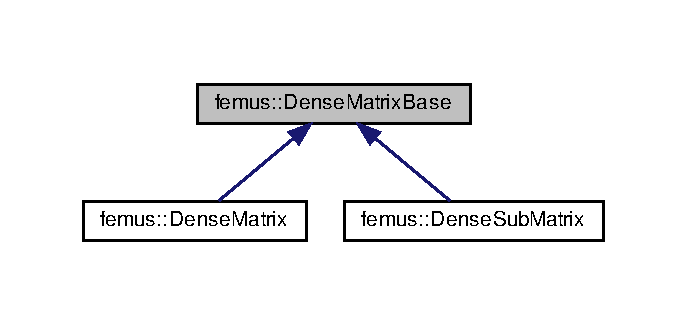
\includegraphics[width=330pt]{classfemus_1_1_dense_matrix_base__inherit__graph}
\end{center}
\end{figure}
\subsection*{Public Member Functions}
\begin{DoxyCompactItemize}
\item 
virtual \mbox{\hyperlink{classfemus_1_1_dense_matrix_base_a510ea66cd4568cef36b561f90332dab5}{$\sim$\+Dense\+Matrix\+Base}} ()
\begin{DoxyCompactList}\small\item\em Destructor. Empty. \end{DoxyCompactList}\item 
virtual void \mbox{\hyperlink{classfemus_1_1_dense_matrix_base_a25fc3a015ffb804afc61b8a33c9565d1}{zero}} ()=0
\begin{DoxyCompactList}\small\item\em Set every element in the matrix to 0. \end{DoxyCompactList}\item 
virtual double \mbox{\hyperlink{classfemus_1_1_dense_matrix_base_abaf98d937069f9df0829353d9454ad93}{el}} (const int i, const int j) const =0
\item 
virtual double \& \mbox{\hyperlink{classfemus_1_1_dense_matrix_base_ab1f58e98ca5000e197fce3013a019dc4}{el}} (const int i, const int j)=0
\item 
int \mbox{\hyperlink{classfemus_1_1_dense_matrix_base_a67a582a53ab5ce7628a53f6a90fd39b9}{m}} () const
\item 
int \mbox{\hyperlink{classfemus_1_1_dense_matrix_base_a1d9b513340794a8b15640f9c8cc6597e}{n}} () const
\item 
virtual void \mbox{\hyperlink{classfemus_1_1_dense_matrix_base_af08f7a07a6b6a9486502a8af234de32c}{left\+\_\+multiply}} (const \mbox{\hyperlink{classfemus_1_1_dense_matrix_base}{Dense\+Matrix\+Base}} \&M2)=0
\begin{DoxyCompactList}\small\item\em Performs the operation\+: ($\ast$this) $<$-\/ M2 $\ast$ ($\ast$this) \end{DoxyCompactList}\item 
virtual void \mbox{\hyperlink{classfemus_1_1_dense_matrix_base_a34072947783a0b4d797d04647cc3c646}{right\+\_\+multiply}} (const \mbox{\hyperlink{classfemus_1_1_dense_matrix_base}{Dense\+Matrix\+Base}} \&M3)=0
\begin{DoxyCompactList}\small\item\em Performs the operation\+: ($\ast$this) $<$-\/ ($\ast$this) $\ast$ M3. \end{DoxyCompactList}\item 
void \mbox{\hyperlink{classfemus_1_1_dense_matrix_base_a277ec615714cd55ae4a7a8d897915ed2}{add}} (const double a, const \mbox{\hyperlink{classfemus_1_1_dense_matrix_base}{Dense\+Matrix\+Base}} \&mat)
\begin{DoxyCompactList}\small\item\em Adds {\ttfamily a} to every element; matrix += a mat. \end{DoxyCompactList}\item 
void \mbox{\hyperlink{classfemus_1_1_dense_matrix_base_a90e8d872f96927e0ad2b6ec0230446e7}{print}} (std\+::ostream \&os) const
\begin{DoxyCompactList}\small\item\em Pretty-\/print the matrix to {\ttfamily stdout}. \end{DoxyCompactList}\item 
void \mbox{\hyperlink{classfemus_1_1_dense_matrix_base_a9124c00c4f77e51655d3efe02c00977f}{print\+\_\+scientific}} (std\+::ostream \&os) const
\begin{DoxyCompactList}\small\item\em Prints the matrix entries with more decimal places in scientific notation. \end{DoxyCompactList}\end{DoxyCompactItemize}
\subsection*{Protected Member Functions}
\begin{DoxyCompactItemize}
\item 
\mbox{\hyperlink{classfemus_1_1_dense_matrix_base_a8e75c57265e5e286b794a0bbd48dd356}{Dense\+Matrix\+Base}} (const int \mbox{\hyperlink{classfemus_1_1_dense_matrix_base_a67a582a53ab5ce7628a53f6a90fd39b9}{m}}=0, const int \mbox{\hyperlink{classfemus_1_1_dense_matrix_base_a1d9b513340794a8b15640f9c8cc6597e}{n}}=0)
\item 
void \mbox{\hyperlink{classfemus_1_1_dense_matrix_base_a57b42c9b3424afaf5203348d816e25d9}{multiply}} (\mbox{\hyperlink{classfemus_1_1_dense_matrix_base}{Dense\+Matrix\+Base}} \&M1, const \mbox{\hyperlink{classfemus_1_1_dense_matrix_base}{Dense\+Matrix\+Base}} \&M2, const \mbox{\hyperlink{classfemus_1_1_dense_matrix_base}{Dense\+Matrix\+Base}} \&M3)
\begin{DoxyCompactList}\small\item\em Performs the computation M1 = M2 $\ast$ M3 where\+: M1 = (m x n) M2 = (m x p) M3 = (p x n) \end{DoxyCompactList}\item 
void \mbox{\hyperlink{classfemus_1_1_dense_matrix_base_af0dafc872890045e08a93f40fbc9b442}{condense}} (const int i, const int j, const double val, \mbox{\hyperlink{classfemus_1_1_dense_vector_base}{Dense\+Vector\+Base}} \&rhs)
\end{DoxyCompactItemize}
\subsection*{Protected Attributes}
\begin{DoxyCompactItemize}
\item 
int \mbox{\hyperlink{classfemus_1_1_dense_matrix_base_ae7fb03cbc57d5b8b498456615348d246}{\+\_\+m}}
\begin{DoxyCompactList}\small\item\em The row dimension. \end{DoxyCompactList}\item 
int \mbox{\hyperlink{classfemus_1_1_dense_matrix_base_aebd0d93543ce7468d69e3970b3c1471d}{\+\_\+n}}
\begin{DoxyCompactList}\small\item\em The column dimension. \end{DoxyCompactList}\end{DoxyCompactItemize}
\subsection*{Friends}
\begin{DoxyCompactItemize}
\item 
std\+::ostream \& \mbox{\hyperlink{classfemus_1_1_dense_matrix_base_ad1683d9e1eacee7a0dd4507de51498c6}{operator$<$$<$}} (std\+::ostream \&os, const \mbox{\hyperlink{classfemus_1_1_dense_matrix_base}{Dense\+Matrix\+Base}} \&\mbox{\hyperlink{classfemus_1_1_dense_matrix_base_a67a582a53ab5ce7628a53f6a90fd39b9}{m}})
\begin{DoxyCompactList}\small\item\em Formatted print as above but allows you to do \mbox{\hyperlink{classfemus_1_1_dense_matrix}{Dense\+Matrix}} K; std\+::cout $<$$<$ K $<$$<$ std\+::endl;. \end{DoxyCompactList}\end{DoxyCompactItemize}


\subsection{Detailed Description}
Defines an abstract dense matrix base class for use in Finite Element-\/type computations. Specialized dense matrices, for example Dense\+Sub\+Matrices, can be derived from this class. 

\subsection{Constructor \& Destructor Documentation}
\mbox{\Hypertarget{classfemus_1_1_dense_matrix_base_a8e75c57265e5e286b794a0bbd48dd356}\label{classfemus_1_1_dense_matrix_base_a8e75c57265e5e286b794a0bbd48dd356}} 
\index{femus\+::\+Dense\+Matrix\+Base@{femus\+::\+Dense\+Matrix\+Base}!Dense\+Matrix\+Base@{Dense\+Matrix\+Base}}
\index{Dense\+Matrix\+Base@{Dense\+Matrix\+Base}!femus\+::\+Dense\+Matrix\+Base@{femus\+::\+Dense\+Matrix\+Base}}
\subsubsection{\texorpdfstring{Dense\+Matrix\+Base()}{DenseMatrixBase()}}
{\footnotesize\ttfamily femus\+::\+Dense\+Matrix\+Base\+::\+Dense\+Matrix\+Base (\begin{DoxyParamCaption}\item[{const int}]{m = {\ttfamily 0},  }\item[{const int}]{n = {\ttfamily 0} }\end{DoxyParamCaption})\hspace{0.3cm}{\ttfamily [inline]}, {\ttfamily [protected]}}

Constructor. Creates a dense matrix of dimension {\ttfamily m} by {\ttfamily n}. Protected so that there is no way the user can create one. \mbox{\Hypertarget{classfemus_1_1_dense_matrix_base_a510ea66cd4568cef36b561f90332dab5}\label{classfemus_1_1_dense_matrix_base_a510ea66cd4568cef36b561f90332dab5}} 
\index{femus\+::\+Dense\+Matrix\+Base@{femus\+::\+Dense\+Matrix\+Base}!````~Dense\+Matrix\+Base@{$\sim$\+Dense\+Matrix\+Base}}
\index{````~Dense\+Matrix\+Base@{$\sim$\+Dense\+Matrix\+Base}!femus\+::\+Dense\+Matrix\+Base@{femus\+::\+Dense\+Matrix\+Base}}
\subsubsection{\texorpdfstring{$\sim$\+Dense\+Matrix\+Base()}{~DenseMatrixBase()}}
{\footnotesize\ttfamily virtual femus\+::\+Dense\+Matrix\+Base\+::$\sim$\+Dense\+Matrix\+Base (\begin{DoxyParamCaption}{ }\end{DoxyParamCaption})\hspace{0.3cm}{\ttfamily [inline]}, {\ttfamily [virtual]}}



Destructor. Empty. 



\subsection{Member Function Documentation}
\mbox{\Hypertarget{classfemus_1_1_dense_matrix_base_a277ec615714cd55ae4a7a8d897915ed2}\label{classfemus_1_1_dense_matrix_base_a277ec615714cd55ae4a7a8d897915ed2}} 
\index{femus\+::\+Dense\+Matrix\+Base@{femus\+::\+Dense\+Matrix\+Base}!add@{add}}
\index{add@{add}!femus\+::\+Dense\+Matrix\+Base@{femus\+::\+Dense\+Matrix\+Base}}
\subsubsection{\texorpdfstring{add()}{add()}}
{\footnotesize\ttfamily void femus\+::\+Dense\+Matrix\+Base\+::add (\begin{DoxyParamCaption}\item[{const double}]{a,  }\item[{const \mbox{\hyperlink{classfemus_1_1_dense_matrix_base}{Dense\+Matrix\+Base}} \&}]{mat }\end{DoxyParamCaption})\hspace{0.3cm}{\ttfamily [inline]}}



Adds {\ttfamily a} to every element; matrix += a mat. 

\mbox{\Hypertarget{classfemus_1_1_dense_matrix_base_af0dafc872890045e08a93f40fbc9b442}\label{classfemus_1_1_dense_matrix_base_af0dafc872890045e08a93f40fbc9b442}} 
\index{femus\+::\+Dense\+Matrix\+Base@{femus\+::\+Dense\+Matrix\+Base}!condense@{condense}}
\index{condense@{condense}!femus\+::\+Dense\+Matrix\+Base@{femus\+::\+Dense\+Matrix\+Base}}
\subsubsection{\texorpdfstring{condense()}{condense()}}
{\footnotesize\ttfamily void femus\+::\+Dense\+Matrix\+Base\+::condense (\begin{DoxyParamCaption}\item[{const int}]{i,  }\item[{const int}]{j,  }\item[{const double}]{val,  }\item[{\mbox{\hyperlink{classfemus_1_1_dense_vector_base}{Dense\+Vector\+Base}} \&}]{rhs }\end{DoxyParamCaption})\hspace{0.3cm}{\ttfamily [protected]}}

Condense-\/out the {\ttfamily }(i,j) entry of the matrix, forcing it to take on the value {\ttfamily val}. This is useful in numerical simulations for applying boundary conditions. Preserves the symmetry of the matrix. \mbox{\Hypertarget{classfemus_1_1_dense_matrix_base_abaf98d937069f9df0829353d9454ad93}\label{classfemus_1_1_dense_matrix_base_abaf98d937069f9df0829353d9454ad93}} 
\index{femus\+::\+Dense\+Matrix\+Base@{femus\+::\+Dense\+Matrix\+Base}!el@{el}}
\index{el@{el}!femus\+::\+Dense\+Matrix\+Base@{femus\+::\+Dense\+Matrix\+Base}}
\subsubsection{\texorpdfstring{el()}{el()}\hspace{0.1cm}{\footnotesize\ttfamily [1/2]}}
{\footnotesize\ttfamily virtual double femus\+::\+Dense\+Matrix\+Base\+::el (\begin{DoxyParamCaption}\item[{const int}]{i,  }\item[{const int}]{j }\end{DoxyParamCaption}) const\hspace{0.3cm}{\ttfamily [pure virtual]}}

\begin{DoxyReturn}{Returns}
the {\ttfamily }(i,j) element of the matrix. 
\end{DoxyReturn}


Implemented in \mbox{\hyperlink{classfemus_1_1_dense_matrix_a3b37181274fbe8eca1523acdecb59bd0}{femus\+::\+Dense\+Matrix}}.

\mbox{\Hypertarget{classfemus_1_1_dense_matrix_base_ab1f58e98ca5000e197fce3013a019dc4}\label{classfemus_1_1_dense_matrix_base_ab1f58e98ca5000e197fce3013a019dc4}} 
\index{femus\+::\+Dense\+Matrix\+Base@{femus\+::\+Dense\+Matrix\+Base}!el@{el}}
\index{el@{el}!femus\+::\+Dense\+Matrix\+Base@{femus\+::\+Dense\+Matrix\+Base}}
\subsubsection{\texorpdfstring{el()}{el()}\hspace{0.1cm}{\footnotesize\ttfamily [2/2]}}
{\footnotesize\ttfamily virtual double\& femus\+::\+Dense\+Matrix\+Base\+::el (\begin{DoxyParamCaption}\item[{const int}]{i,  }\item[{const int}]{j }\end{DoxyParamCaption})\hspace{0.3cm}{\ttfamily [pure virtual]}}

\begin{DoxyReturn}{Returns}
the {\ttfamily }(i,j) element of the matrix as a writeable reference. 
\end{DoxyReturn}


Implemented in \mbox{\hyperlink{classfemus_1_1_dense_matrix_a9867b5e9b16b8ec746ebde4270239248}{femus\+::\+Dense\+Matrix}}.

\mbox{\Hypertarget{classfemus_1_1_dense_matrix_base_af08f7a07a6b6a9486502a8af234de32c}\label{classfemus_1_1_dense_matrix_base_af08f7a07a6b6a9486502a8af234de32c}} 
\index{femus\+::\+Dense\+Matrix\+Base@{femus\+::\+Dense\+Matrix\+Base}!left\+\_\+multiply@{left\+\_\+multiply}}
\index{left\+\_\+multiply@{left\+\_\+multiply}!femus\+::\+Dense\+Matrix\+Base@{femus\+::\+Dense\+Matrix\+Base}}
\subsubsection{\texorpdfstring{left\+\_\+multiply()}{left\_multiply()}}
{\footnotesize\ttfamily virtual void femus\+::\+Dense\+Matrix\+Base\+::left\+\_\+multiply (\begin{DoxyParamCaption}\item[{const \mbox{\hyperlink{classfemus_1_1_dense_matrix_base}{Dense\+Matrix\+Base}} \&}]{M2 }\end{DoxyParamCaption})\hspace{0.3cm}{\ttfamily [pure virtual]}}



Performs the operation\+: ($\ast$this) $<$-\/ M2 $\ast$ ($\ast$this) 



Implemented in \mbox{\hyperlink{classfemus_1_1_dense_matrix_a80917b8698400957bc821308be3dafe5}{femus\+::\+Dense\+Matrix}}.

\mbox{\Hypertarget{classfemus_1_1_dense_matrix_base_a67a582a53ab5ce7628a53f6a90fd39b9}\label{classfemus_1_1_dense_matrix_base_a67a582a53ab5ce7628a53f6a90fd39b9}} 
\index{femus\+::\+Dense\+Matrix\+Base@{femus\+::\+Dense\+Matrix\+Base}!m@{m}}
\index{m@{m}!femus\+::\+Dense\+Matrix\+Base@{femus\+::\+Dense\+Matrix\+Base}}
\subsubsection{\texorpdfstring{m()}{m()}}
{\footnotesize\ttfamily int femus\+::\+Dense\+Matrix\+Base\+::m (\begin{DoxyParamCaption}{ }\end{DoxyParamCaption}) const\hspace{0.3cm}{\ttfamily [inline]}}

\begin{DoxyReturn}{Returns}
the row-\/dimension of the matrix. 
\end{DoxyReturn}
\mbox{\Hypertarget{classfemus_1_1_dense_matrix_base_a57b42c9b3424afaf5203348d816e25d9}\label{classfemus_1_1_dense_matrix_base_a57b42c9b3424afaf5203348d816e25d9}} 
\index{femus\+::\+Dense\+Matrix\+Base@{femus\+::\+Dense\+Matrix\+Base}!multiply@{multiply}}
\index{multiply@{multiply}!femus\+::\+Dense\+Matrix\+Base@{femus\+::\+Dense\+Matrix\+Base}}
\subsubsection{\texorpdfstring{multiply()}{multiply()}}
{\footnotesize\ttfamily void femus\+::\+Dense\+Matrix\+Base\+::multiply (\begin{DoxyParamCaption}\item[{\mbox{\hyperlink{classfemus_1_1_dense_matrix_base}{Dense\+Matrix\+Base}} \&}]{M1,  }\item[{const \mbox{\hyperlink{classfemus_1_1_dense_matrix_base}{Dense\+Matrix\+Base}} \&}]{M2,  }\item[{const \mbox{\hyperlink{classfemus_1_1_dense_matrix_base}{Dense\+Matrix\+Base}} \&}]{M3 }\end{DoxyParamCaption})\hspace{0.3cm}{\ttfamily [protected]}}



Performs the computation M1 = M2 $\ast$ M3 where\+: M1 = (m x n) M2 = (m x p) M3 = (p x n) 

\mbox{\Hypertarget{classfemus_1_1_dense_matrix_base_a1d9b513340794a8b15640f9c8cc6597e}\label{classfemus_1_1_dense_matrix_base_a1d9b513340794a8b15640f9c8cc6597e}} 
\index{femus\+::\+Dense\+Matrix\+Base@{femus\+::\+Dense\+Matrix\+Base}!n@{n}}
\index{n@{n}!femus\+::\+Dense\+Matrix\+Base@{femus\+::\+Dense\+Matrix\+Base}}
\subsubsection{\texorpdfstring{n()}{n()}}
{\footnotesize\ttfamily int femus\+::\+Dense\+Matrix\+Base\+::n (\begin{DoxyParamCaption}{ }\end{DoxyParamCaption}) const\hspace{0.3cm}{\ttfamily [inline]}}

\begin{DoxyReturn}{Returns}
the column-\/dimension of the matrix. 
\end{DoxyReturn}
\mbox{\Hypertarget{classfemus_1_1_dense_matrix_base_a90e8d872f96927e0ad2b6ec0230446e7}\label{classfemus_1_1_dense_matrix_base_a90e8d872f96927e0ad2b6ec0230446e7}} 
\index{femus\+::\+Dense\+Matrix\+Base@{femus\+::\+Dense\+Matrix\+Base}!print@{print}}
\index{print@{print}!femus\+::\+Dense\+Matrix\+Base@{femus\+::\+Dense\+Matrix\+Base}}
\subsubsection{\texorpdfstring{print()}{print()}}
{\footnotesize\ttfamily void femus\+::\+Dense\+Matrix\+Base\+::print (\begin{DoxyParamCaption}\item[{std\+::ostream \&}]{os }\end{DoxyParamCaption}) const}



Pretty-\/print the matrix to {\ttfamily stdout}. 

\mbox{\Hypertarget{classfemus_1_1_dense_matrix_base_a9124c00c4f77e51655d3efe02c00977f}\label{classfemus_1_1_dense_matrix_base_a9124c00c4f77e51655d3efe02c00977f}} 
\index{femus\+::\+Dense\+Matrix\+Base@{femus\+::\+Dense\+Matrix\+Base}!print\+\_\+scientific@{print\+\_\+scientific}}
\index{print\+\_\+scientific@{print\+\_\+scientific}!femus\+::\+Dense\+Matrix\+Base@{femus\+::\+Dense\+Matrix\+Base}}
\subsubsection{\texorpdfstring{print\+\_\+scientific()}{print\_scientific()}}
{\footnotesize\ttfamily void femus\+::\+Dense\+Matrix\+Base\+::print\+\_\+scientific (\begin{DoxyParamCaption}\item[{std\+::ostream \&}]{os }\end{DoxyParamCaption}) const}



Prints the matrix entries with more decimal places in scientific notation. 

\mbox{\Hypertarget{classfemus_1_1_dense_matrix_base_a34072947783a0b4d797d04647cc3c646}\label{classfemus_1_1_dense_matrix_base_a34072947783a0b4d797d04647cc3c646}} 
\index{femus\+::\+Dense\+Matrix\+Base@{femus\+::\+Dense\+Matrix\+Base}!right\+\_\+multiply@{right\+\_\+multiply}}
\index{right\+\_\+multiply@{right\+\_\+multiply}!femus\+::\+Dense\+Matrix\+Base@{femus\+::\+Dense\+Matrix\+Base}}
\subsubsection{\texorpdfstring{right\+\_\+multiply()}{right\_multiply()}}
{\footnotesize\ttfamily virtual void femus\+::\+Dense\+Matrix\+Base\+::right\+\_\+multiply (\begin{DoxyParamCaption}\item[{const \mbox{\hyperlink{classfemus_1_1_dense_matrix_base}{Dense\+Matrix\+Base}} \&}]{M3 }\end{DoxyParamCaption})\hspace{0.3cm}{\ttfamily [pure virtual]}}



Performs the operation\+: ($\ast$this) $<$-\/ ($\ast$this) $\ast$ M3. 



Implemented in \mbox{\hyperlink{classfemus_1_1_dense_matrix_a6de589e870d32a851fda1049b736bf99}{femus\+::\+Dense\+Matrix}}.

\mbox{\Hypertarget{classfemus_1_1_dense_matrix_base_a25fc3a015ffb804afc61b8a33c9565d1}\label{classfemus_1_1_dense_matrix_base_a25fc3a015ffb804afc61b8a33c9565d1}} 
\index{femus\+::\+Dense\+Matrix\+Base@{femus\+::\+Dense\+Matrix\+Base}!zero@{zero}}
\index{zero@{zero}!femus\+::\+Dense\+Matrix\+Base@{femus\+::\+Dense\+Matrix\+Base}}
\subsubsection{\texorpdfstring{zero()}{zero()}}
{\footnotesize\ttfamily virtual void femus\+::\+Dense\+Matrix\+Base\+::zero (\begin{DoxyParamCaption}{ }\end{DoxyParamCaption})\hspace{0.3cm}{\ttfamily [pure virtual]}}



Set every element in the matrix to 0. 



Implemented in \mbox{\hyperlink{classfemus_1_1_dense_matrix_a865963674763716d720d6ef2c8177053}{femus\+::\+Dense\+Matrix}}.



\subsection{Friends And Related Function Documentation}
\mbox{\Hypertarget{classfemus_1_1_dense_matrix_base_ad1683d9e1eacee7a0dd4507de51498c6}\label{classfemus_1_1_dense_matrix_base_ad1683d9e1eacee7a0dd4507de51498c6}} 
\index{femus\+::\+Dense\+Matrix\+Base@{femus\+::\+Dense\+Matrix\+Base}!operator$<$$<$@{operator$<$$<$}}
\index{operator$<$$<$@{operator$<$$<$}!femus\+::\+Dense\+Matrix\+Base@{femus\+::\+Dense\+Matrix\+Base}}
\subsubsection{\texorpdfstring{operator$<$$<$}{operator<<}}
{\footnotesize\ttfamily std\+::ostream\& operator$<$$<$ (\begin{DoxyParamCaption}\item[{std\+::ostream \&}]{os,  }\item[{const \mbox{\hyperlink{classfemus_1_1_dense_matrix_base}{Dense\+Matrix\+Base}} \&}]{m }\end{DoxyParamCaption})\hspace{0.3cm}{\ttfamily [friend]}}



Formatted print as above but allows you to do \mbox{\hyperlink{classfemus_1_1_dense_matrix}{Dense\+Matrix}} K; std\+::cout $<$$<$ K $<$$<$ std\+::endl;. 



\subsection{Member Data Documentation}
\mbox{\Hypertarget{classfemus_1_1_dense_matrix_base_ae7fb03cbc57d5b8b498456615348d246}\label{classfemus_1_1_dense_matrix_base_ae7fb03cbc57d5b8b498456615348d246}} 
\index{femus\+::\+Dense\+Matrix\+Base@{femus\+::\+Dense\+Matrix\+Base}!\+\_\+m@{\+\_\+m}}
\index{\+\_\+m@{\+\_\+m}!femus\+::\+Dense\+Matrix\+Base@{femus\+::\+Dense\+Matrix\+Base}}
\subsubsection{\texorpdfstring{\+\_\+m}{\_m}}
{\footnotesize\ttfamily int femus\+::\+Dense\+Matrix\+Base\+::\+\_\+m\hspace{0.3cm}{\ttfamily [protected]}}



The row dimension. 

\mbox{\Hypertarget{classfemus_1_1_dense_matrix_base_aebd0d93543ce7468d69e3970b3c1471d}\label{classfemus_1_1_dense_matrix_base_aebd0d93543ce7468d69e3970b3c1471d}} 
\index{femus\+::\+Dense\+Matrix\+Base@{femus\+::\+Dense\+Matrix\+Base}!\+\_\+n@{\+\_\+n}}
\index{\+\_\+n@{\+\_\+n}!femus\+::\+Dense\+Matrix\+Base@{femus\+::\+Dense\+Matrix\+Base}}
\subsubsection{\texorpdfstring{\+\_\+n}{\_n}}
{\footnotesize\ttfamily int femus\+::\+Dense\+Matrix\+Base\+::\+\_\+n\hspace{0.3cm}{\ttfamily [protected]}}



The column dimension. 



The documentation for this class was generated from the following files\+:\begin{DoxyCompactItemize}
\item 
algebra/\mbox{\hyperlink{_dense_matrix_base_8hpp}{Dense\+Matrix\+Base.\+hpp}}\item 
algebra/\mbox{\hyperlink{_dense_matrix_base_8cpp}{Dense\+Matrix\+Base.\+cpp}}\end{DoxyCompactItemize}

\hypertarget{classfemus_1_1_dense_sub_matrix}{}\section{femus\+:\+:Dense\+Sub\+Matrix Class Reference}
\label{classfemus_1_1_dense_sub_matrix}\index{femus\+::\+Dense\+Sub\+Matrix@{femus\+::\+Dense\+Sub\+Matrix}}


{\ttfamily \#include $<$Dense\+Submatrix.\+hpp$>$}



Inheritance diagram for femus\+:\+:Dense\+Sub\+Matrix\+:
\nopagebreak
\begin{figure}[H]
\begin{center}
\leavevmode
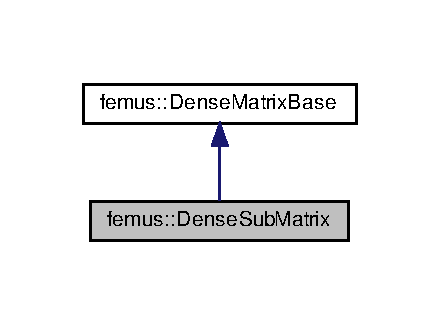
\includegraphics[width=211pt]{classfemus_1_1_dense_sub_matrix__inherit__graph}
\end{center}
\end{figure}


Collaboration diagram for femus\+:\+:Dense\+Sub\+Matrix\+:
\nopagebreak
\begin{figure}[H]
\begin{center}
\leavevmode
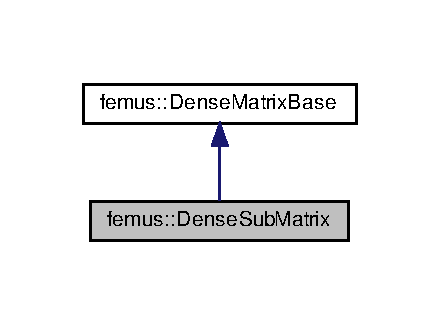
\includegraphics[width=211pt]{classfemus_1_1_dense_sub_matrix__coll__graph}
\end{center}
\end{figure}
\subsection*{Additional Inherited Members}


\subsection{Detailed Description}
Defines a dense submatrix for use in Finite Element-\/type computations. Useful for storing element stiffness matrices before summation into a global matrix, particularly when you have systems of equations. 

The documentation for this class was generated from the following file\+:\begin{DoxyCompactItemize}
\item 
algebra/\mbox{\hyperlink{_dense_submatrix_8hpp}{Dense\+Submatrix.\+hpp}}\end{DoxyCompactItemize}

\hypertarget{classfemus_1_1_dense_sub_vector}{}\section{femus\+:\+:Dense\+Sub\+Vector Class Reference}
\label{classfemus_1_1_dense_sub_vector}\index{femus\+::\+Dense\+Sub\+Vector@{femus\+::\+Dense\+Sub\+Vector}}


{\ttfamily \#include $<$Dense\+Subvector.\+hpp$>$}



Inheritance diagram for femus\+:\+:Dense\+Sub\+Vector\+:
\nopagebreak
\begin{figure}[H]
\begin{center}
\leavevmode
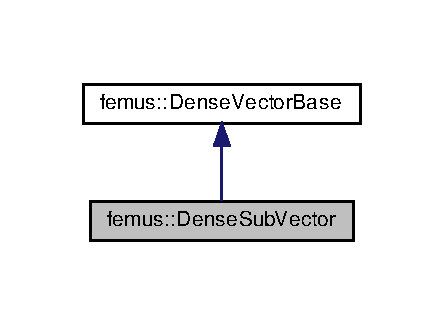
\includegraphics[width=213pt]{classfemus_1_1_dense_sub_vector__inherit__graph}
\end{center}
\end{figure}


Collaboration diagram for femus\+:\+:Dense\+Sub\+Vector\+:
\nopagebreak
\begin{figure}[H]
\begin{center}
\leavevmode
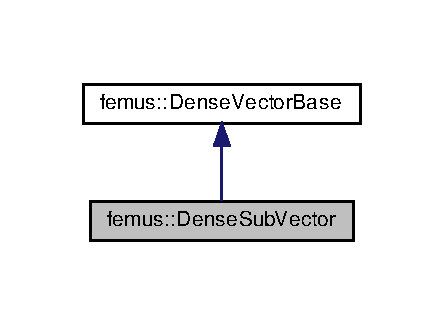
\includegraphics[width=213pt]{classfemus_1_1_dense_sub_vector__coll__graph}
\end{center}
\end{figure}
\subsection*{Public Member Functions}
\begin{DoxyCompactItemize}
\item 
\mbox{\hyperlink{classfemus_1_1_dense_sub_vector_a321eb522717c8ac3d322c2d9ad367e11}{Dense\+Sub\+Vector}} (\mbox{\hyperlink{classfemus_1_1_dense_vector}{Dense\+Vector}} \&\mbox{\hyperlink{classfemus_1_1_dense_sub_vector_a0daed4a44c5471622d5b6600acef2298}{parent}}, const unsigned int ioff=0, const unsigned int n=0)
\begin{DoxyCompactList}\small\item\em Constructor. Creates a dense subvector of the vector. \end{DoxyCompactList}\item 
virtual \mbox{\hyperlink{classfemus_1_1_dense_sub_vector_ab4a41a2c3e8cf97c9e2680d9d250f115}{$\sim$\+Dense\+Sub\+Vector}} ()
\begin{DoxyCompactList}\small\item\em Destructor. Does nothing. \end{DoxyCompactList}\item 
\mbox{\hyperlink{classfemus_1_1_dense_vector}{Dense\+Vector}} \& \mbox{\hyperlink{classfemus_1_1_dense_sub_vector_a0daed4a44c5471622d5b6600acef2298}{parent}} ()
\item 
virtual void \mbox{\hyperlink{classfemus_1_1_dense_sub_vector_a20fd1054159ce0a69af4d28199dd704f}{zero}} ()
\begin{DoxyCompactList}\small\item\em Set every element in the subvector to 0. \end{DoxyCompactList}\item 
double \mbox{\hyperlink{classfemus_1_1_dense_sub_vector_ad342710f5d826cff8b5b87dd5e7f1091}{operator()}} (const unsigned int i) const
\item 
double \& \mbox{\hyperlink{classfemus_1_1_dense_sub_vector_a815b31cc0fc273a1c82835c0e9fdf40b}{operator()}} (const unsigned int i)
\item 
virtual double \mbox{\hyperlink{classfemus_1_1_dense_sub_vector_a7e95ed027b438413f00d790ff5c95fb2}{el}} (const unsigned int i) const
\item 
virtual double \& \mbox{\hyperlink{classfemus_1_1_dense_sub_vector_a5cb51e53b54d085933d2ebe6f762ecd1}{el}} (const unsigned int i)
\item 
virtual unsigned int \mbox{\hyperlink{classfemus_1_1_dense_sub_vector_ac7267bc849d12ec7c84481a9fa9a87ce}{size}} () const
\item 
unsigned int \mbox{\hyperlink{classfemus_1_1_dense_sub_vector_afd7cee05ce11a2c32a8696386eb0b206}{i\+\_\+off}} () const
\item 
void \mbox{\hyperlink{classfemus_1_1_dense_sub_vector_afdaa52b0ba46efba781c7d7f0fe6e950}{reposition}} (const unsigned int ioff, const unsigned int n)
\begin{DoxyCompactList}\small\item\em Changes the location of the subvector in the parent vector. \end{DoxyCompactList}\end{DoxyCompactItemize}


\subsection{Constructor \& Destructor Documentation}
\mbox{\Hypertarget{classfemus_1_1_dense_sub_vector_a321eb522717c8ac3d322c2d9ad367e11}\label{classfemus_1_1_dense_sub_vector_a321eb522717c8ac3d322c2d9ad367e11}} 
\index{femus\+::\+Dense\+Sub\+Vector@{femus\+::\+Dense\+Sub\+Vector}!Dense\+Sub\+Vector@{Dense\+Sub\+Vector}}
\index{Dense\+Sub\+Vector@{Dense\+Sub\+Vector}!femus\+::\+Dense\+Sub\+Vector@{femus\+::\+Dense\+Sub\+Vector}}
\subsubsection{\texorpdfstring{Dense\+Sub\+Vector()}{DenseSubVector()}}
{\footnotesize\ttfamily femus\+::\+Dense\+Sub\+Vector\+::\+Dense\+Sub\+Vector (\begin{DoxyParamCaption}\item[{\mbox{\hyperlink{classfemus_1_1_dense_vector}{Dense\+Vector}} \&}]{parent,  }\item[{const unsigned int}]{ioff = {\ttfamily 0},  }\item[{const unsigned int}]{n = {\ttfamily 0} }\end{DoxyParamCaption})\hspace{0.3cm}{\ttfamily [inline]}}



Constructor. Creates a dense subvector of the vector. 

\mbox{\Hypertarget{classfemus_1_1_dense_sub_vector_ab4a41a2c3e8cf97c9e2680d9d250f115}\label{classfemus_1_1_dense_sub_vector_ab4a41a2c3e8cf97c9e2680d9d250f115}} 
\index{femus\+::\+Dense\+Sub\+Vector@{femus\+::\+Dense\+Sub\+Vector}!````~Dense\+Sub\+Vector@{$\sim$\+Dense\+Sub\+Vector}}
\index{````~Dense\+Sub\+Vector@{$\sim$\+Dense\+Sub\+Vector}!femus\+::\+Dense\+Sub\+Vector@{femus\+::\+Dense\+Sub\+Vector}}
\subsubsection{\texorpdfstring{$\sim$\+Dense\+Sub\+Vector()}{~DenseSubVector()}}
{\footnotesize\ttfamily virtual femus\+::\+Dense\+Sub\+Vector\+::$\sim$\+Dense\+Sub\+Vector (\begin{DoxyParamCaption}{ }\end{DoxyParamCaption})\hspace{0.3cm}{\ttfamily [inline]}, {\ttfamily [virtual]}}



Destructor. Does nothing. 



\subsection{Member Function Documentation}
\mbox{\Hypertarget{classfemus_1_1_dense_sub_vector_a7e95ed027b438413f00d790ff5c95fb2}\label{classfemus_1_1_dense_sub_vector_a7e95ed027b438413f00d790ff5c95fb2}} 
\index{femus\+::\+Dense\+Sub\+Vector@{femus\+::\+Dense\+Sub\+Vector}!el@{el}}
\index{el@{el}!femus\+::\+Dense\+Sub\+Vector@{femus\+::\+Dense\+Sub\+Vector}}
\subsubsection{\texorpdfstring{el()}{el()}\hspace{0.1cm}{\footnotesize\ttfamily [1/2]}}
{\footnotesize\ttfamily virtual double femus\+::\+Dense\+Sub\+Vector\+::el (\begin{DoxyParamCaption}\item[{const unsigned int}]{i }\end{DoxyParamCaption}) const\hspace{0.3cm}{\ttfamily [inline]}, {\ttfamily [virtual]}}

\begin{DoxyReturn}{Returns}
the {\ttfamily }(i) element of the vector. 
\end{DoxyReturn}


Implements \mbox{\hyperlink{classfemus_1_1_dense_vector_base_ae2a833cdebb39552185cb66b139758e8}{femus\+::\+Dense\+Vector\+Base}}.

\mbox{\Hypertarget{classfemus_1_1_dense_sub_vector_a5cb51e53b54d085933d2ebe6f762ecd1}\label{classfemus_1_1_dense_sub_vector_a5cb51e53b54d085933d2ebe6f762ecd1}} 
\index{femus\+::\+Dense\+Sub\+Vector@{femus\+::\+Dense\+Sub\+Vector}!el@{el}}
\index{el@{el}!femus\+::\+Dense\+Sub\+Vector@{femus\+::\+Dense\+Sub\+Vector}}
\subsubsection{\texorpdfstring{el()}{el()}\hspace{0.1cm}{\footnotesize\ttfamily [2/2]}}
{\footnotesize\ttfamily virtual double\& femus\+::\+Dense\+Sub\+Vector\+::el (\begin{DoxyParamCaption}\item[{const unsigned int}]{i }\end{DoxyParamCaption})\hspace{0.3cm}{\ttfamily [inline]}, {\ttfamily [virtual]}}

\begin{DoxyReturn}{Returns}
the {\ttfamily }(i) element of the vector as a writeable reference. 
\end{DoxyReturn}


Implements \mbox{\hyperlink{classfemus_1_1_dense_vector_base_a521863934215d5f43225004b091864f5}{femus\+::\+Dense\+Vector\+Base}}.

\mbox{\Hypertarget{classfemus_1_1_dense_sub_vector_afd7cee05ce11a2c32a8696386eb0b206}\label{classfemus_1_1_dense_sub_vector_afd7cee05ce11a2c32a8696386eb0b206}} 
\index{femus\+::\+Dense\+Sub\+Vector@{femus\+::\+Dense\+Sub\+Vector}!i\+\_\+off@{i\+\_\+off}}
\index{i\+\_\+off@{i\+\_\+off}!femus\+::\+Dense\+Sub\+Vector@{femus\+::\+Dense\+Sub\+Vector}}
\subsubsection{\texorpdfstring{i\+\_\+off()}{i\_off()}}
{\footnotesize\ttfamily unsigned int femus\+::\+Dense\+Sub\+Vector\+::i\+\_\+off (\begin{DoxyParamCaption}{ }\end{DoxyParamCaption}) const\hspace{0.3cm}{\ttfamily [inline]}}

\begin{DoxyReturn}{Returns}
the row offset into the parent vector. 
\end{DoxyReturn}
\mbox{\Hypertarget{classfemus_1_1_dense_sub_vector_ad342710f5d826cff8b5b87dd5e7f1091}\label{classfemus_1_1_dense_sub_vector_ad342710f5d826cff8b5b87dd5e7f1091}} 
\index{femus\+::\+Dense\+Sub\+Vector@{femus\+::\+Dense\+Sub\+Vector}!operator()@{operator()}}
\index{operator()@{operator()}!femus\+::\+Dense\+Sub\+Vector@{femus\+::\+Dense\+Sub\+Vector}}
\subsubsection{\texorpdfstring{operator()()}{operator()()}\hspace{0.1cm}{\footnotesize\ttfamily [1/2]}}
{\footnotesize\ttfamily double femus\+::\+Dense\+Sub\+Vector\+::operator() (\begin{DoxyParamCaption}\item[{const unsigned int}]{i }\end{DoxyParamCaption}) const\hspace{0.3cm}{\ttfamily [inline]}}

\begin{DoxyReturn}{Returns}
the {\ttfamily }(i,j) element of the subvector. 
\end{DoxyReturn}
\mbox{\Hypertarget{classfemus_1_1_dense_sub_vector_a815b31cc0fc273a1c82835c0e9fdf40b}\label{classfemus_1_1_dense_sub_vector_a815b31cc0fc273a1c82835c0e9fdf40b}} 
\index{femus\+::\+Dense\+Sub\+Vector@{femus\+::\+Dense\+Sub\+Vector}!operator()@{operator()}}
\index{operator()@{operator()}!femus\+::\+Dense\+Sub\+Vector@{femus\+::\+Dense\+Sub\+Vector}}
\subsubsection{\texorpdfstring{operator()()}{operator()()}\hspace{0.1cm}{\footnotesize\ttfamily [2/2]}}
{\footnotesize\ttfamily double \& femus\+::\+Dense\+Sub\+Vector\+::operator() (\begin{DoxyParamCaption}\item[{const unsigned int}]{i }\end{DoxyParamCaption})\hspace{0.3cm}{\ttfamily [inline]}}

\begin{DoxyReturn}{Returns}
the {\ttfamily }(i,j) element of the subvector as a writeable reference. 
\end{DoxyReturn}
\mbox{\Hypertarget{classfemus_1_1_dense_sub_vector_a0daed4a44c5471622d5b6600acef2298}\label{classfemus_1_1_dense_sub_vector_a0daed4a44c5471622d5b6600acef2298}} 
\index{femus\+::\+Dense\+Sub\+Vector@{femus\+::\+Dense\+Sub\+Vector}!parent@{parent}}
\index{parent@{parent}!femus\+::\+Dense\+Sub\+Vector@{femus\+::\+Dense\+Sub\+Vector}}
\subsubsection{\texorpdfstring{parent()}{parent()}}
{\footnotesize\ttfamily \mbox{\hyperlink{classfemus_1_1_dense_vector}{Dense\+Vector}}\& femus\+::\+Dense\+Sub\+Vector\+::parent (\begin{DoxyParamCaption}{ }\end{DoxyParamCaption})\hspace{0.3cm}{\ttfamily [inline]}}

\begin{DoxyReturn}{Returns}
a reference to the parent vector. 
\end{DoxyReturn}
\mbox{\Hypertarget{classfemus_1_1_dense_sub_vector_afdaa52b0ba46efba781c7d7f0fe6e950}\label{classfemus_1_1_dense_sub_vector_afdaa52b0ba46efba781c7d7f0fe6e950}} 
\index{femus\+::\+Dense\+Sub\+Vector@{femus\+::\+Dense\+Sub\+Vector}!reposition@{reposition}}
\index{reposition@{reposition}!femus\+::\+Dense\+Sub\+Vector@{femus\+::\+Dense\+Sub\+Vector}}
\subsubsection{\texorpdfstring{reposition()}{reposition()}}
{\footnotesize\ttfamily void femus\+::\+Dense\+Sub\+Vector\+::reposition (\begin{DoxyParamCaption}\item[{const unsigned int}]{ioff,  }\item[{const unsigned int}]{n }\end{DoxyParamCaption})\hspace{0.3cm}{\ttfamily [inline]}}



Changes the location of the subvector in the parent vector. 

\mbox{\Hypertarget{classfemus_1_1_dense_sub_vector_ac7267bc849d12ec7c84481a9fa9a87ce}\label{classfemus_1_1_dense_sub_vector_ac7267bc849d12ec7c84481a9fa9a87ce}} 
\index{femus\+::\+Dense\+Sub\+Vector@{femus\+::\+Dense\+Sub\+Vector}!size@{size}}
\index{size@{size}!femus\+::\+Dense\+Sub\+Vector@{femus\+::\+Dense\+Sub\+Vector}}
\subsubsection{\texorpdfstring{size()}{size()}}
{\footnotesize\ttfamily virtual unsigned int femus\+::\+Dense\+Sub\+Vector\+::size (\begin{DoxyParamCaption}{ }\end{DoxyParamCaption}) const\hspace{0.3cm}{\ttfamily [inline]}, {\ttfamily [virtual]}}

\begin{DoxyReturn}{Returns}
the size of the subvector. 
\end{DoxyReturn}


Implements \mbox{\hyperlink{classfemus_1_1_dense_vector_base_a642849a48ad4800945952af17c1e30c9}{femus\+::\+Dense\+Vector\+Base}}.

\mbox{\Hypertarget{classfemus_1_1_dense_sub_vector_a20fd1054159ce0a69af4d28199dd704f}\label{classfemus_1_1_dense_sub_vector_a20fd1054159ce0a69af4d28199dd704f}} 
\index{femus\+::\+Dense\+Sub\+Vector@{femus\+::\+Dense\+Sub\+Vector}!zero@{zero}}
\index{zero@{zero}!femus\+::\+Dense\+Sub\+Vector@{femus\+::\+Dense\+Sub\+Vector}}
\subsubsection{\texorpdfstring{zero()}{zero()}}
{\footnotesize\ttfamily void femus\+::\+Dense\+Sub\+Vector\+::zero (\begin{DoxyParamCaption}{ }\end{DoxyParamCaption})\hspace{0.3cm}{\ttfamily [inline]}, {\ttfamily [virtual]}}



Set every element in the subvector to 0. 



Implements \mbox{\hyperlink{classfemus_1_1_dense_vector_base_abd1b93469867212f796c7b86d242c550}{femus\+::\+Dense\+Vector\+Base}}.



The documentation for this class was generated from the following file\+:\begin{DoxyCompactItemize}
\item 
algebra/\mbox{\hyperlink{_dense_subvector_8hpp}{Dense\+Subvector.\+hpp}}\end{DoxyCompactItemize}

\hypertarget{classfemus_1_1_dense_vector}{}\section{femus\+:\+:Dense\+Vector Class Reference}
\label{classfemus_1_1_dense_vector}\index{femus\+::\+Dense\+Vector@{femus\+::\+Dense\+Vector}}


{\ttfamily \#include $<$Dense\+Vector.\+hpp$>$}



Inheritance diagram for femus\+:\+:Dense\+Vector\+:
\nopagebreak
\begin{figure}[H]
\begin{center}
\leavevmode
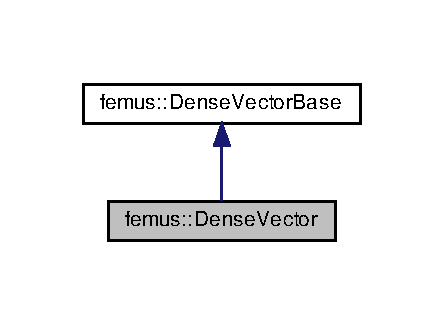
\includegraphics[width=213pt]{classfemus_1_1_dense_vector__inherit__graph}
\end{center}
\end{figure}


Collaboration diagram for femus\+:\+:Dense\+Vector\+:
\nopagebreak
\begin{figure}[H]
\begin{center}
\leavevmode
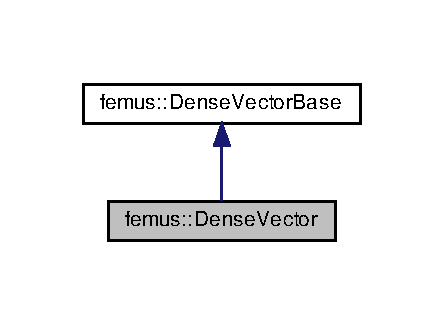
\includegraphics[width=213pt]{classfemus_1_1_dense_vector__coll__graph}
\end{center}
\end{figure}
\subsection*{Public Member Functions}
\begin{DoxyCompactItemize}
\item 
\mbox{\hyperlink{classfemus_1_1_dense_vector_a9ea4283bc84797b07197c41b6796f03c}{Dense\+Vector}} (const unsigned int n=0)
\begin{DoxyCompactList}\small\item\em Constructor. Creates a dense vector of dimension {\ttfamily n}. \end{DoxyCompactList}\item 
\mbox{\hyperlink{classfemus_1_1_dense_vector_a3fee62a53c3ae44b869b8ff1847a737d}{Dense\+Vector}} (const \mbox{\hyperlink{classfemus_1_1_dense_vector}{Dense\+Vector}} \&other\+\_\+vector)
\begin{DoxyCompactList}\small\item\em Copy-\/constructor. \end{DoxyCompactList}\item 
\mbox{\hyperlink{classfemus_1_1_dense_vector_adafc5ed121a642cc307bcd04c4366463}{Dense\+Vector}} (const std\+::vector$<$ double $>$ \&other\+\_\+vector)
\begin{DoxyCompactList}\small\item\em Copy-\/constructor, from a {\ttfamily std\+::vector}. \end{DoxyCompactList}\item 
\mbox{\hyperlink{classfemus_1_1_dense_vector_a55372dde4d08ffd064059d4092eb95fc}{$\sim$\+Dense\+Vector}} ()
\begin{DoxyCompactList}\small\item\em Destructor. Does nothing. \end{DoxyCompactList}\item 
void \mbox{\hyperlink{classfemus_1_1_dense_vector_ae03eb37317154976971332f89dd56352}{resize}} (const unsigned int n)
\item 
virtual void \mbox{\hyperlink{classfemus_1_1_dense_vector_ae2eafd9df7f6ae8fe75165a3eb675a4b}{zero}} ()
\begin{DoxyCompactList}\small\item\em Set every element in the vector to 0. \end{DoxyCompactList}\item 
void \mbox{\hyperlink{classfemus_1_1_dense_vector_aaeb514b12b7b549430fd7264a6f21742}{get\+\_\+principal\+\_\+subvector}} (unsigned int sub\+\_\+n, \mbox{\hyperlink{classfemus_1_1_dense_vector}{Dense\+Vector}} \&dest) const
\begin{DoxyCompactList}\small\item\em Puts the principal subvector of size {\ttfamily sub\+\_\+n}. \end{DoxyCompactList}\item 
std\+::vector$<$ double $>$ \& \mbox{\hyperlink{classfemus_1_1_dense_vector_acf34d5982e06da4191d60fe823e16332}{get\+\_\+values}} ()
\begin{DoxyCompactList}\small\item\em Access to the values array. \end{DoxyCompactList}\item 
const std\+::vector$<$ double $>$ \& \mbox{\hyperlink{classfemus_1_1_dense_vector_ab8b7707faa7fe4818ecdac02296e15ea}{get\+\_\+values}} () const
\begin{DoxyCompactList}\small\item\em Access to the values array. \end{DoxyCompactList}\item 
virtual unsigned int \mbox{\hyperlink{classfemus_1_1_dense_vector_ac7d42a76bf12cb82076b8c7444cbc9ee}{size}} () const
\item 
double \mbox{\hyperlink{classfemus_1_1_dense_vector_a53d9ad849428e8fbec174fa14a76b525}{operator()}} (const unsigned int i) const
\item 
double \& \mbox{\hyperlink{classfemus_1_1_dense_vector_a6e2f6d28cb5ddff856e68ac265c9214c}{operator()}} (const unsigned int i)
\item 
virtual double \mbox{\hyperlink{classfemus_1_1_dense_vector_aff2ffaa4a8b334a0c913fa0d79223e30}{el}} (const unsigned int i) const
\item 
virtual double \& \mbox{\hyperlink{classfemus_1_1_dense_vector_abee121241acbc2d29a7e54fc27588357}{el}} (const unsigned int i)
\item 
\mbox{\hyperlink{classfemus_1_1_dense_vector}{Dense\+Vector}} \& \mbox{\hyperlink{classfemus_1_1_dense_vector_a6fb17b0b5c1af6bb8be9075254e61866}{operator=}} (const \mbox{\hyperlink{classfemus_1_1_dense_vector}{Dense\+Vector}} \&other\+\_\+vector)
\item 
void \mbox{\hyperlink{classfemus_1_1_dense_vector_a95404c4c657691d8e4b719d08e7820c1}{swap}} (\mbox{\hyperlink{classfemus_1_1_dense_vector}{Dense\+Vector}} \&other\+\_\+vector)
\item 
void \mbox{\hyperlink{classfemus_1_1_dense_vector_a06413e6b8d637592452444a5141927e6}{scale}} (const double factor)
\begin{DoxyCompactList}\small\item\em Multiplies every element in the vector by {\ttfamily factor}. \end{DoxyCompactList}\item 
\mbox{\hyperlink{classfemus_1_1_dense_vector}{Dense\+Vector}} \& \mbox{\hyperlink{classfemus_1_1_dense_vector_aa332a79a955cacb506546a7ca0d00894}{operator$\ast$=}} (const double factor)
\item 
void \mbox{\hyperlink{classfemus_1_1_dense_vector_a945b0914e85311e7bcd7c2535818275e}{add}} (const double a, const \mbox{\hyperlink{classfemus_1_1_dense_vector}{Dense\+Vector}} \&vec)
\item 
double \mbox{\hyperlink{classfemus_1_1_dense_vector_a0a9fd31e853459449f244fe6c6ce4e62}{dot}} (const \mbox{\hyperlink{classfemus_1_1_dense_vector}{Dense\+Vector}} \&vec) const
\item 
bool \mbox{\hyperlink{classfemus_1_1_dense_vector_ad9545b4fb57e917ddd65d72ec7a653ff}{operator==}} (const \mbox{\hyperlink{classfemus_1_1_dense_vector}{Dense\+Vector}} \&vec) const
\begin{DoxyCompactList}\small\item\em Tests if {\ttfamily vec} is exactly equal to this vector. \end{DoxyCompactList}\item 
bool \mbox{\hyperlink{classfemus_1_1_dense_vector_a3b6851d83e3aa0c435213ccad05cd949}{operator!=}} (const \mbox{\hyperlink{classfemus_1_1_dense_vector}{Dense\+Vector}} \&vec) const
\begin{DoxyCompactList}\small\item\em Tests if {\ttfamily vec} is not exactly equal to this vector. \end{DoxyCompactList}\item 
\mbox{\hyperlink{classfemus_1_1_dense_vector}{Dense\+Vector}} \& \mbox{\hyperlink{classfemus_1_1_dense_vector_ac4db2e76d3e4750f8585d6ed03ef2800}{operator+=}} (const \mbox{\hyperlink{classfemus_1_1_dense_vector}{Dense\+Vector}} \&vec)
\begin{DoxyCompactList}\small\item\em Adds {\ttfamily vec} to this vector. \end{DoxyCompactList}\item 
\mbox{\hyperlink{classfemus_1_1_dense_vector}{Dense\+Vector}} \& \mbox{\hyperlink{classfemus_1_1_dense_vector_a1f66784d89711fd43a7a3193d23b177a}{operator-\/=}} (const \mbox{\hyperlink{classfemus_1_1_dense_vector}{Dense\+Vector}} \&vec)
\begin{DoxyCompactList}\small\item\em Subtracts {\ttfamily vec} from this vector. \end{DoxyCompactList}\item 
double \mbox{\hyperlink{classfemus_1_1_dense_vector_afddbf21de9804dc92c2c0e2d217731fa}{min}} () const
\item 
double \mbox{\hyperlink{classfemus_1_1_dense_vector_a622888ea147eebeeb784feec0774ad22}{max}} () const
\item 
double \mbox{\hyperlink{classfemus_1_1_dense_vector_ab9de4dc64cde6d40e82c279e164598ff}{l1\+\_\+norm}} () const
\item 
double \mbox{\hyperlink{classfemus_1_1_dense_vector_a01f73192a11d56115e0afa3c3212be36}{l2\+\_\+norm}} () const
\item 
double \mbox{\hyperlink{classfemus_1_1_dense_vector_a036328ba679553324981f7014bbc2500}{linfty\+\_\+norm}} () const
\end{DoxyCompactItemize}


\subsection{Detailed Description}
Defines a dense vector for use in Finite Element-\/type computations. This class is to basically compliment the {\ttfamily Dense\+Matix} class. It has additional capabilities over the {\ttfamily std\+::vector} that make it useful for finite elements, particulary for systems of equations. 

\subsection{Constructor \& Destructor Documentation}
\mbox{\Hypertarget{classfemus_1_1_dense_vector_a9ea4283bc84797b07197c41b6796f03c}\label{classfemus_1_1_dense_vector_a9ea4283bc84797b07197c41b6796f03c}} 
\index{femus\+::\+Dense\+Vector@{femus\+::\+Dense\+Vector}!Dense\+Vector@{Dense\+Vector}}
\index{Dense\+Vector@{Dense\+Vector}!femus\+::\+Dense\+Vector@{femus\+::\+Dense\+Vector}}
\subsubsection{\texorpdfstring{Dense\+Vector()}{DenseVector()}\hspace{0.1cm}{\footnotesize\ttfamily [1/3]}}
{\footnotesize\ttfamily femus\+::\+Dense\+Vector\+::\+Dense\+Vector (\begin{DoxyParamCaption}\item[{const unsigned int}]{n = {\ttfamily 0} }\end{DoxyParamCaption})\hspace{0.3cm}{\ttfamily [inline]}, {\ttfamily [explicit]}}



Constructor. Creates a dense vector of dimension {\ttfamily n}. 

\mbox{\Hypertarget{classfemus_1_1_dense_vector_a3fee62a53c3ae44b869b8ff1847a737d}\label{classfemus_1_1_dense_vector_a3fee62a53c3ae44b869b8ff1847a737d}} 
\index{femus\+::\+Dense\+Vector@{femus\+::\+Dense\+Vector}!Dense\+Vector@{Dense\+Vector}}
\index{Dense\+Vector@{Dense\+Vector}!femus\+::\+Dense\+Vector@{femus\+::\+Dense\+Vector}}
\subsubsection{\texorpdfstring{Dense\+Vector()}{DenseVector()}\hspace{0.1cm}{\footnotesize\ttfamily [2/3]}}
{\footnotesize\ttfamily femus\+::\+Dense\+Vector\+::\+Dense\+Vector (\begin{DoxyParamCaption}\item[{const \mbox{\hyperlink{classfemus_1_1_dense_vector}{Dense\+Vector}} \&}]{other\+\_\+vector }\end{DoxyParamCaption})\hspace{0.3cm}{\ttfamily [inline]}}



Copy-\/constructor. 

\mbox{\Hypertarget{classfemus_1_1_dense_vector_adafc5ed121a642cc307bcd04c4366463}\label{classfemus_1_1_dense_vector_adafc5ed121a642cc307bcd04c4366463}} 
\index{femus\+::\+Dense\+Vector@{femus\+::\+Dense\+Vector}!Dense\+Vector@{Dense\+Vector}}
\index{Dense\+Vector@{Dense\+Vector}!femus\+::\+Dense\+Vector@{femus\+::\+Dense\+Vector}}
\subsubsection{\texorpdfstring{Dense\+Vector()}{DenseVector()}\hspace{0.1cm}{\footnotesize\ttfamily [3/3]}}
{\footnotesize\ttfamily femus\+::\+Dense\+Vector\+::\+Dense\+Vector (\begin{DoxyParamCaption}\item[{const std\+::vector$<$ double $>$ \&}]{other\+\_\+vector }\end{DoxyParamCaption})\hspace{0.3cm}{\ttfamily [inline]}}



Copy-\/constructor, from a {\ttfamily std\+::vector}. 

\mbox{\Hypertarget{classfemus_1_1_dense_vector_a55372dde4d08ffd064059d4092eb95fc}\label{classfemus_1_1_dense_vector_a55372dde4d08ffd064059d4092eb95fc}} 
\index{femus\+::\+Dense\+Vector@{femus\+::\+Dense\+Vector}!````~Dense\+Vector@{$\sim$\+Dense\+Vector}}
\index{````~Dense\+Vector@{$\sim$\+Dense\+Vector}!femus\+::\+Dense\+Vector@{femus\+::\+Dense\+Vector}}
\subsubsection{\texorpdfstring{$\sim$\+Dense\+Vector()}{~DenseVector()}}
{\footnotesize\ttfamily femus\+::\+Dense\+Vector\+::$\sim$\+Dense\+Vector (\begin{DoxyParamCaption}{ }\end{DoxyParamCaption})\hspace{0.3cm}{\ttfamily [inline]}}



Destructor. Does nothing. 



\subsection{Member Function Documentation}
\mbox{\Hypertarget{classfemus_1_1_dense_vector_a945b0914e85311e7bcd7c2535818275e}\label{classfemus_1_1_dense_vector_a945b0914e85311e7bcd7c2535818275e}} 
\index{femus\+::\+Dense\+Vector@{femus\+::\+Dense\+Vector}!add@{add}}
\index{add@{add}!femus\+::\+Dense\+Vector@{femus\+::\+Dense\+Vector}}
\subsubsection{\texorpdfstring{add()}{add()}}
{\footnotesize\ttfamily void femus\+::\+Dense\+Vector\+::add (\begin{DoxyParamCaption}\item[{const double}]{a,  }\item[{const \mbox{\hyperlink{classfemus_1_1_dense_vector}{Dense\+Vector}} \&}]{vec }\end{DoxyParamCaption})\hspace{0.3cm}{\ttfamily [inline]}}


\begin{DoxyItemize}
\item Adds {\ttfamily factor} times {\ttfamily vec} to this vector. T += a $\ast$ vec 
\end{DoxyItemize}\mbox{\Hypertarget{classfemus_1_1_dense_vector_a0a9fd31e853459449f244fe6c6ce4e62}\label{classfemus_1_1_dense_vector_a0a9fd31e853459449f244fe6c6ce4e62}} 
\index{femus\+::\+Dense\+Vector@{femus\+::\+Dense\+Vector}!dot@{dot}}
\index{dot@{dot}!femus\+::\+Dense\+Vector@{femus\+::\+Dense\+Vector}}
\subsubsection{\texorpdfstring{dot()}{dot()}}
{\footnotesize\ttfamily double femus\+::\+Dense\+Vector\+::dot (\begin{DoxyParamCaption}\item[{const \mbox{\hyperlink{classfemus_1_1_dense_vector}{Dense\+Vector}} \&}]{vec }\end{DoxyParamCaption}) const\hspace{0.3cm}{\ttfamily [inline]}}


\begin{DoxyItemize}
\item Evaluate dot product with {\ttfamily vect} 
\end{DoxyItemize}\mbox{\Hypertarget{classfemus_1_1_dense_vector_aff2ffaa4a8b334a0c913fa0d79223e30}\label{classfemus_1_1_dense_vector_aff2ffaa4a8b334a0c913fa0d79223e30}} 
\index{femus\+::\+Dense\+Vector@{femus\+::\+Dense\+Vector}!el@{el}}
\index{el@{el}!femus\+::\+Dense\+Vector@{femus\+::\+Dense\+Vector}}
\subsubsection{\texorpdfstring{el()}{el()}\hspace{0.1cm}{\footnotesize\ttfamily [1/2]}}
{\footnotesize\ttfamily virtual double femus\+::\+Dense\+Vector\+::el (\begin{DoxyParamCaption}\item[{const unsigned int}]{i }\end{DoxyParamCaption}) const\hspace{0.3cm}{\ttfamily [inline]}, {\ttfamily [virtual]}}


\begin{DoxyItemize}
\item \begin{DoxyReturn}{Returns}
the {\ttfamily }(i) element of the vector. 
\end{DoxyReturn}

\end{DoxyItemize}

Implements \mbox{\hyperlink{classfemus_1_1_dense_vector_base_ae2a833cdebb39552185cb66b139758e8}{femus\+::\+Dense\+Vector\+Base}}.

\mbox{\Hypertarget{classfemus_1_1_dense_vector_abee121241acbc2d29a7e54fc27588357}\label{classfemus_1_1_dense_vector_abee121241acbc2d29a7e54fc27588357}} 
\index{femus\+::\+Dense\+Vector@{femus\+::\+Dense\+Vector}!el@{el}}
\index{el@{el}!femus\+::\+Dense\+Vector@{femus\+::\+Dense\+Vector}}
\subsubsection{\texorpdfstring{el()}{el()}\hspace{0.1cm}{\footnotesize\ttfamily [2/2]}}
{\footnotesize\ttfamily virtual double\& femus\+::\+Dense\+Vector\+::el (\begin{DoxyParamCaption}\item[{const unsigned int}]{i }\end{DoxyParamCaption})\hspace{0.3cm}{\ttfamily [inline]}, {\ttfamily [virtual]}}


\begin{DoxyItemize}
\item \begin{DoxyReturn}{Returns}
the {\ttfamily }(i) element of the vector as a writeable reference. 
\end{DoxyReturn}

\end{DoxyItemize}

Implements \mbox{\hyperlink{classfemus_1_1_dense_vector_base_a521863934215d5f43225004b091864f5}{femus\+::\+Dense\+Vector\+Base}}.

\mbox{\Hypertarget{classfemus_1_1_dense_vector_aaeb514b12b7b549430fd7264a6f21742}\label{classfemus_1_1_dense_vector_aaeb514b12b7b549430fd7264a6f21742}} 
\index{femus\+::\+Dense\+Vector@{femus\+::\+Dense\+Vector}!get\+\_\+principal\+\_\+subvector@{get\+\_\+principal\+\_\+subvector}}
\index{get\+\_\+principal\+\_\+subvector@{get\+\_\+principal\+\_\+subvector}!femus\+::\+Dense\+Vector@{femus\+::\+Dense\+Vector}}
\subsubsection{\texorpdfstring{get\+\_\+principal\+\_\+subvector()}{get\_principal\_subvector()}}
{\footnotesize\ttfamily void femus\+::\+Dense\+Vector\+::get\+\_\+principal\+\_\+subvector (\begin{DoxyParamCaption}\item[{unsigned int}]{sub\+\_\+n,  }\item[{\mbox{\hyperlink{classfemus_1_1_dense_vector}{Dense\+Vector}} \&}]{dest }\end{DoxyParamCaption}) const\hspace{0.3cm}{\ttfamily [inline]}}



Puts the principal subvector of size {\ttfamily sub\+\_\+n}. 

\mbox{\Hypertarget{classfemus_1_1_dense_vector_acf34d5982e06da4191d60fe823e16332}\label{classfemus_1_1_dense_vector_acf34d5982e06da4191d60fe823e16332}} 
\index{femus\+::\+Dense\+Vector@{femus\+::\+Dense\+Vector}!get\+\_\+values@{get\+\_\+values}}
\index{get\+\_\+values@{get\+\_\+values}!femus\+::\+Dense\+Vector@{femus\+::\+Dense\+Vector}}
\subsubsection{\texorpdfstring{get\+\_\+values()}{get\_values()}\hspace{0.1cm}{\footnotesize\ttfamily [1/2]}}
{\footnotesize\ttfamily std\+::vector$<$double$>$\& femus\+::\+Dense\+Vector\+::get\+\_\+values (\begin{DoxyParamCaption}{ }\end{DoxyParamCaption})\hspace{0.3cm}{\ttfamily [inline]}}



Access to the values array. 

\mbox{\Hypertarget{classfemus_1_1_dense_vector_ab8b7707faa7fe4818ecdac02296e15ea}\label{classfemus_1_1_dense_vector_ab8b7707faa7fe4818ecdac02296e15ea}} 
\index{femus\+::\+Dense\+Vector@{femus\+::\+Dense\+Vector}!get\+\_\+values@{get\+\_\+values}}
\index{get\+\_\+values@{get\+\_\+values}!femus\+::\+Dense\+Vector@{femus\+::\+Dense\+Vector}}
\subsubsection{\texorpdfstring{get\+\_\+values()}{get\_values()}\hspace{0.1cm}{\footnotesize\ttfamily [2/2]}}
{\footnotesize\ttfamily const std\+::vector$<$double$>$\& femus\+::\+Dense\+Vector\+::get\+\_\+values (\begin{DoxyParamCaption}{ }\end{DoxyParamCaption}) const\hspace{0.3cm}{\ttfamily [inline]}}



Access to the values array. 

\mbox{\Hypertarget{classfemus_1_1_dense_vector_ab9de4dc64cde6d40e82c279e164598ff}\label{classfemus_1_1_dense_vector_ab9de4dc64cde6d40e82c279e164598ff}} 
\index{femus\+::\+Dense\+Vector@{femus\+::\+Dense\+Vector}!l1\+\_\+norm@{l1\+\_\+norm}}
\index{l1\+\_\+norm@{l1\+\_\+norm}!femus\+::\+Dense\+Vector@{femus\+::\+Dense\+Vector}}
\subsubsection{\texorpdfstring{l1\+\_\+norm()}{l1\_norm()}}
{\footnotesize\ttfamily double femus\+::\+Dense\+Vector\+::l1\+\_\+norm (\begin{DoxyParamCaption}{ }\end{DoxyParamCaption}) const\hspace{0.3cm}{\ttfamily [inline]}}

\begin{DoxyReturn}{Returns}
the $l_1$-\/norm of the vector, 
\end{DoxyReturn}
\mbox{\Hypertarget{classfemus_1_1_dense_vector_a01f73192a11d56115e0afa3c3212be36}\label{classfemus_1_1_dense_vector_a01f73192a11d56115e0afa3c3212be36}} 
\index{femus\+::\+Dense\+Vector@{femus\+::\+Dense\+Vector}!l2\+\_\+norm@{l2\+\_\+norm}}
\index{l2\+\_\+norm@{l2\+\_\+norm}!femus\+::\+Dense\+Vector@{femus\+::\+Dense\+Vector}}
\subsubsection{\texorpdfstring{l2\+\_\+norm()}{l2\_norm()}}
{\footnotesize\ttfamily double femus\+::\+Dense\+Vector\+::l2\+\_\+norm (\begin{DoxyParamCaption}{ }\end{DoxyParamCaption}) const\hspace{0.3cm}{\ttfamily [inline]}}

\begin{DoxyReturn}{Returns}
the $l_2$-\/norm of the vector 
\end{DoxyReturn}
\mbox{\Hypertarget{classfemus_1_1_dense_vector_a036328ba679553324981f7014bbc2500}\label{classfemus_1_1_dense_vector_a036328ba679553324981f7014bbc2500}} 
\index{femus\+::\+Dense\+Vector@{femus\+::\+Dense\+Vector}!linfty\+\_\+norm@{linfty\+\_\+norm}}
\index{linfty\+\_\+norm@{linfty\+\_\+norm}!femus\+::\+Dense\+Vector@{femus\+::\+Dense\+Vector}}
\subsubsection{\texorpdfstring{linfty\+\_\+norm()}{linfty\_norm()}}
{\footnotesize\ttfamily double femus\+::\+Dense\+Vector\+::linfty\+\_\+norm (\begin{DoxyParamCaption}{ }\end{DoxyParamCaption}) const\hspace{0.3cm}{\ttfamily [inline]}}

\begin{DoxyReturn}{Returns}
the maximum absolute value of the 
\end{DoxyReturn}
\mbox{\Hypertarget{classfemus_1_1_dense_vector_a622888ea147eebeeb784feec0774ad22}\label{classfemus_1_1_dense_vector_a622888ea147eebeeb784feec0774ad22}} 
\index{femus\+::\+Dense\+Vector@{femus\+::\+Dense\+Vector}!max@{max}}
\index{max@{max}!femus\+::\+Dense\+Vector@{femus\+::\+Dense\+Vector}}
\subsubsection{\texorpdfstring{max()}{max()}}
{\footnotesize\ttfamily double femus\+::\+Dense\+Vector\+::max (\begin{DoxyParamCaption}{ }\end{DoxyParamCaption}) const\hspace{0.3cm}{\ttfamily [inline]}}

\begin{DoxyReturn}{Returns}
the maximum element in the vector. 
\end{DoxyReturn}
\mbox{\Hypertarget{classfemus_1_1_dense_vector_afddbf21de9804dc92c2c0e2d217731fa}\label{classfemus_1_1_dense_vector_afddbf21de9804dc92c2c0e2d217731fa}} 
\index{femus\+::\+Dense\+Vector@{femus\+::\+Dense\+Vector}!min@{min}}
\index{min@{min}!femus\+::\+Dense\+Vector@{femus\+::\+Dense\+Vector}}
\subsubsection{\texorpdfstring{min()}{min()}}
{\footnotesize\ttfamily double femus\+::\+Dense\+Vector\+::min (\begin{DoxyParamCaption}{ }\end{DoxyParamCaption}) const\hspace{0.3cm}{\ttfamily [inline]}}


\begin{DoxyItemize}
\item \begin{DoxyReturn}{Returns}
the minimum element in the vector. 
\end{DoxyReturn}

\end{DoxyItemize}\mbox{\Hypertarget{classfemus_1_1_dense_vector_a3b6851d83e3aa0c435213ccad05cd949}\label{classfemus_1_1_dense_vector_a3b6851d83e3aa0c435213ccad05cd949}} 
\index{femus\+::\+Dense\+Vector@{femus\+::\+Dense\+Vector}!operator"!=@{operator"!=}}
\index{operator"!=@{operator"!=}!femus\+::\+Dense\+Vector@{femus\+::\+Dense\+Vector}}
\subsubsection{\texorpdfstring{operator"!=()}{operator!=()}}
{\footnotesize\ttfamily bool femus\+::\+Dense\+Vector\+::operator!= (\begin{DoxyParamCaption}\item[{const \mbox{\hyperlink{classfemus_1_1_dense_vector}{Dense\+Vector}} \&}]{vec }\end{DoxyParamCaption}) const\hspace{0.3cm}{\ttfamily [inline]}}



Tests if {\ttfamily vec} is not exactly equal to this vector. 

\mbox{\Hypertarget{classfemus_1_1_dense_vector_a53d9ad849428e8fbec174fa14a76b525}\label{classfemus_1_1_dense_vector_a53d9ad849428e8fbec174fa14a76b525}} 
\index{femus\+::\+Dense\+Vector@{femus\+::\+Dense\+Vector}!operator()@{operator()}}
\index{operator()@{operator()}!femus\+::\+Dense\+Vector@{femus\+::\+Dense\+Vector}}
\subsubsection{\texorpdfstring{operator()()}{operator()()}\hspace{0.1cm}{\footnotesize\ttfamily [1/2]}}
{\footnotesize\ttfamily double femus\+::\+Dense\+Vector\+::operator() (\begin{DoxyParamCaption}\item[{const unsigned int}]{i }\end{DoxyParamCaption}) const\hspace{0.3cm}{\ttfamily [inline]}}

\begin{DoxyReturn}{Returns}
the {\ttfamily }(i) element of the vector. 
\end{DoxyReturn}
\mbox{\Hypertarget{classfemus_1_1_dense_vector_a6e2f6d28cb5ddff856e68ac265c9214c}\label{classfemus_1_1_dense_vector_a6e2f6d28cb5ddff856e68ac265c9214c}} 
\index{femus\+::\+Dense\+Vector@{femus\+::\+Dense\+Vector}!operator()@{operator()}}
\index{operator()@{operator()}!femus\+::\+Dense\+Vector@{femus\+::\+Dense\+Vector}}
\subsubsection{\texorpdfstring{operator()()}{operator()()}\hspace{0.1cm}{\footnotesize\ttfamily [2/2]}}
{\footnotesize\ttfamily double \& femus\+::\+Dense\+Vector\+::operator() (\begin{DoxyParamCaption}\item[{const unsigned int}]{i }\end{DoxyParamCaption})\hspace{0.3cm}{\ttfamily [inline]}}


\begin{DoxyItemize}
\item \begin{DoxyReturn}{Returns}
the {\ttfamily }(i,j) element of the vector as a writeable reference. 
\end{DoxyReturn}

\end{DoxyItemize}\mbox{\Hypertarget{classfemus_1_1_dense_vector_aa332a79a955cacb506546a7ca0d00894}\label{classfemus_1_1_dense_vector_aa332a79a955cacb506546a7ca0d00894}} 
\index{femus\+::\+Dense\+Vector@{femus\+::\+Dense\+Vector}!operator$\ast$=@{operator$\ast$=}}
\index{operator$\ast$=@{operator$\ast$=}!femus\+::\+Dense\+Vector@{femus\+::\+Dense\+Vector}}
\subsubsection{\texorpdfstring{operator$\ast$=()}{operator*=()}}
{\footnotesize\ttfamily \mbox{\hyperlink{classfemus_1_1_dense_vector}{Dense\+Vector}} \& femus\+::\+Dense\+Vector\+::operator$\ast$= (\begin{DoxyParamCaption}\item[{const double}]{factor }\end{DoxyParamCaption})\hspace{0.3cm}{\ttfamily [inline]}}


\begin{DoxyItemize}
\item Multiplies every element in the vector by {\ttfamily factor}. 
\end{DoxyItemize}\mbox{\Hypertarget{classfemus_1_1_dense_vector_ac4db2e76d3e4750f8585d6ed03ef2800}\label{classfemus_1_1_dense_vector_ac4db2e76d3e4750f8585d6ed03ef2800}} 
\index{femus\+::\+Dense\+Vector@{femus\+::\+Dense\+Vector}!operator+=@{operator+=}}
\index{operator+=@{operator+=}!femus\+::\+Dense\+Vector@{femus\+::\+Dense\+Vector}}
\subsubsection{\texorpdfstring{operator+=()}{operator+=()}}
{\footnotesize\ttfamily \mbox{\hyperlink{classfemus_1_1_dense_vector}{Dense\+Vector}} \& femus\+::\+Dense\+Vector\+::operator+= (\begin{DoxyParamCaption}\item[{const \mbox{\hyperlink{classfemus_1_1_dense_vector}{Dense\+Vector}} \&}]{vec }\end{DoxyParamCaption})\hspace{0.3cm}{\ttfamily [inline]}}



Adds {\ttfamily vec} to this vector. 

\mbox{\Hypertarget{classfemus_1_1_dense_vector_a1f66784d89711fd43a7a3193d23b177a}\label{classfemus_1_1_dense_vector_a1f66784d89711fd43a7a3193d23b177a}} 
\index{femus\+::\+Dense\+Vector@{femus\+::\+Dense\+Vector}!operator-\/=@{operator-\/=}}
\index{operator-\/=@{operator-\/=}!femus\+::\+Dense\+Vector@{femus\+::\+Dense\+Vector}}
\subsubsection{\texorpdfstring{operator-\/=()}{operator-=()}}
{\footnotesize\ttfamily \mbox{\hyperlink{classfemus_1_1_dense_vector}{Dense\+Vector}} \& femus\+::\+Dense\+Vector\+::operator-\/= (\begin{DoxyParamCaption}\item[{const \mbox{\hyperlink{classfemus_1_1_dense_vector}{Dense\+Vector}} \&}]{vec }\end{DoxyParamCaption})\hspace{0.3cm}{\ttfamily [inline]}}



Subtracts {\ttfamily vec} from this vector. 

\mbox{\Hypertarget{classfemus_1_1_dense_vector_a6fb17b0b5c1af6bb8be9075254e61866}\label{classfemus_1_1_dense_vector_a6fb17b0b5c1af6bb8be9075254e61866}} 
\index{femus\+::\+Dense\+Vector@{femus\+::\+Dense\+Vector}!operator=@{operator=}}
\index{operator=@{operator=}!femus\+::\+Dense\+Vector@{femus\+::\+Dense\+Vector}}
\subsubsection{\texorpdfstring{operator=()}{operator=()}}
{\footnotesize\ttfamily \mbox{\hyperlink{classfemus_1_1_dense_vector}{Dense\+Vector}} \& femus\+::\+Dense\+Vector\+::operator= (\begin{DoxyParamCaption}\item[{const \mbox{\hyperlink{classfemus_1_1_dense_vector}{Dense\+Vector}} \&}]{other\+\_\+vector }\end{DoxyParamCaption})\hspace{0.3cm}{\ttfamily [inline]}}


\begin{DoxyItemize}
\item Assignment operator. 
\end{DoxyItemize}\mbox{\Hypertarget{classfemus_1_1_dense_vector_ad9545b4fb57e917ddd65d72ec7a653ff}\label{classfemus_1_1_dense_vector_ad9545b4fb57e917ddd65d72ec7a653ff}} 
\index{femus\+::\+Dense\+Vector@{femus\+::\+Dense\+Vector}!operator==@{operator==}}
\index{operator==@{operator==}!femus\+::\+Dense\+Vector@{femus\+::\+Dense\+Vector}}
\subsubsection{\texorpdfstring{operator==()}{operator==()}}
{\footnotesize\ttfamily bool femus\+::\+Dense\+Vector\+::operator== (\begin{DoxyParamCaption}\item[{const \mbox{\hyperlink{classfemus_1_1_dense_vector}{Dense\+Vector}} \&}]{vec }\end{DoxyParamCaption}) const\hspace{0.3cm}{\ttfamily [inline]}}



Tests if {\ttfamily vec} is exactly equal to this vector. 

\mbox{\Hypertarget{classfemus_1_1_dense_vector_ae03eb37317154976971332f89dd56352}\label{classfemus_1_1_dense_vector_ae03eb37317154976971332f89dd56352}} 
\index{femus\+::\+Dense\+Vector@{femus\+::\+Dense\+Vector}!resize@{resize}}
\index{resize@{resize}!femus\+::\+Dense\+Vector@{femus\+::\+Dense\+Vector}}
\subsubsection{\texorpdfstring{resize()}{resize()}}
{\footnotesize\ttfamily void femus\+::\+Dense\+Vector\+::resize (\begin{DoxyParamCaption}\item[{const unsigned int}]{n }\end{DoxyParamCaption})\hspace{0.3cm}{\ttfamily [inline]}}


\begin{DoxyItemize}
\item Resize the vector. Sets all elements to 0. 
\end{DoxyItemize}\mbox{\Hypertarget{classfemus_1_1_dense_vector_a06413e6b8d637592452444a5141927e6}\label{classfemus_1_1_dense_vector_a06413e6b8d637592452444a5141927e6}} 
\index{femus\+::\+Dense\+Vector@{femus\+::\+Dense\+Vector}!scale@{scale}}
\index{scale@{scale}!femus\+::\+Dense\+Vector@{femus\+::\+Dense\+Vector}}
\subsubsection{\texorpdfstring{scale()}{scale()}}
{\footnotesize\ttfamily void femus\+::\+Dense\+Vector\+::scale (\begin{DoxyParamCaption}\item[{const double}]{factor }\end{DoxyParamCaption})\hspace{0.3cm}{\ttfamily [inline]}}



Multiplies every element in the vector by {\ttfamily factor}. 

\mbox{\Hypertarget{classfemus_1_1_dense_vector_ac7d42a76bf12cb82076b8c7444cbc9ee}\label{classfemus_1_1_dense_vector_ac7d42a76bf12cb82076b8c7444cbc9ee}} 
\index{femus\+::\+Dense\+Vector@{femus\+::\+Dense\+Vector}!size@{size}}
\index{size@{size}!femus\+::\+Dense\+Vector@{femus\+::\+Dense\+Vector}}
\subsubsection{\texorpdfstring{size()}{size()}}
{\footnotesize\ttfamily virtual unsigned int femus\+::\+Dense\+Vector\+::size (\begin{DoxyParamCaption}{ }\end{DoxyParamCaption}) const\hspace{0.3cm}{\ttfamily [inline]}, {\ttfamily [virtual]}}


\begin{DoxyItemize}
\item \begin{DoxyReturn}{Returns}
the size of the vector. 
\end{DoxyReturn}

\end{DoxyItemize}

Implements \mbox{\hyperlink{classfemus_1_1_dense_vector_base_a642849a48ad4800945952af17c1e30c9}{femus\+::\+Dense\+Vector\+Base}}.

\mbox{\Hypertarget{classfemus_1_1_dense_vector_a95404c4c657691d8e4b719d08e7820c1}\label{classfemus_1_1_dense_vector_a95404c4c657691d8e4b719d08e7820c1}} 
\index{femus\+::\+Dense\+Vector@{femus\+::\+Dense\+Vector}!swap@{swap}}
\index{swap@{swap}!femus\+::\+Dense\+Vector@{femus\+::\+Dense\+Vector}}
\subsubsection{\texorpdfstring{swap()}{swap()}}
{\footnotesize\ttfamily void femus\+::\+Dense\+Vector\+::swap (\begin{DoxyParamCaption}\item[{\mbox{\hyperlink{classfemus_1_1_dense_vector}{Dense\+Vector}} \&}]{other\+\_\+vector }\end{DoxyParamCaption})\hspace{0.3cm}{\ttfamily [inline]}}


\begin{DoxyItemize}
\item S\+T\+L-\/like swap method 
\end{DoxyItemize}\mbox{\Hypertarget{classfemus_1_1_dense_vector_ae2eafd9df7f6ae8fe75165a3eb675a4b}\label{classfemus_1_1_dense_vector_ae2eafd9df7f6ae8fe75165a3eb675a4b}} 
\index{femus\+::\+Dense\+Vector@{femus\+::\+Dense\+Vector}!zero@{zero}}
\index{zero@{zero}!femus\+::\+Dense\+Vector@{femus\+::\+Dense\+Vector}}
\subsubsection{\texorpdfstring{zero()}{zero()}}
{\footnotesize\ttfamily void femus\+::\+Dense\+Vector\+::zero (\begin{DoxyParamCaption}{ }\end{DoxyParamCaption})\hspace{0.3cm}{\ttfamily [inline]}, {\ttfamily [virtual]}}



Set every element in the vector to 0. 



Implements \mbox{\hyperlink{classfemus_1_1_dense_vector_base_abd1b93469867212f796c7b86d242c550}{femus\+::\+Dense\+Vector\+Base}}.



The documentation for this class was generated from the following file\+:\begin{DoxyCompactItemize}
\item 
algebra/\mbox{\hyperlink{_dense_vector_8hpp}{Dense\+Vector.\+hpp}}\end{DoxyCompactItemize}

\hypertarget{classfemus_1_1_dense_vector_base}{}\section{femus\+:\+:Dense\+Vector\+Base Class Reference}
\label{classfemus_1_1_dense_vector_base}\index{femus\+::\+Dense\+Vector\+Base@{femus\+::\+Dense\+Vector\+Base}}


{\ttfamily \#include $<$Dense\+Vector\+Base.\+hpp$>$}



Inheritance diagram for femus\+:\+:Dense\+Vector\+Base\+:
\nopagebreak
\begin{figure}[H]
\begin{center}
\leavevmode
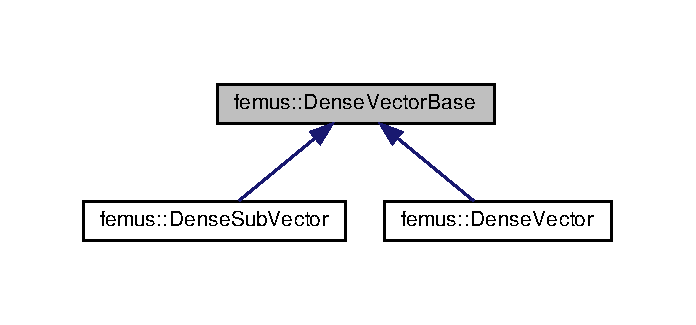
\includegraphics[width=334pt]{classfemus_1_1_dense_vector_base__inherit__graph}
\end{center}
\end{figure}
\subsection*{Public Member Functions}
\begin{DoxyCompactItemize}
\item 
\mbox{\hyperlink{classfemus_1_1_dense_vector_base_ab8222fa8625cb42d2740294a088698f8}{Dense\+Vector\+Base}} ()
\begin{DoxyCompactList}\small\item\em Constructor. Empty. \end{DoxyCompactList}\item 
virtual \mbox{\hyperlink{classfemus_1_1_dense_vector_base_a0c3531c7d5cd8d9b2e5b7d63b97ab555}{$\sim$\+Dense\+Vector\+Base}} ()
\begin{DoxyCompactList}\small\item\em Destructor. Does nothing. \end{DoxyCompactList}\item 
virtual void \mbox{\hyperlink{classfemus_1_1_dense_vector_base_abd1b93469867212f796c7b86d242c550}{zero}} ()=0
\begin{DoxyCompactList}\small\item\em Set every element in the vector to 0. Needs to. \end{DoxyCompactList}\item 
virtual double \mbox{\hyperlink{classfemus_1_1_dense_vector_base_ae2a833cdebb39552185cb66b139758e8}{el}} (const unsigned int i) const =0
\item 
virtual double \& \mbox{\hyperlink{classfemus_1_1_dense_vector_base_a521863934215d5f43225004b091864f5}{el}} (const unsigned int i)=0
\item 
virtual unsigned int \mbox{\hyperlink{classfemus_1_1_dense_vector_base_a642849a48ad4800945952af17c1e30c9}{size}} () const =0
\item 
void \mbox{\hyperlink{classfemus_1_1_dense_vector_base_a19f3668a4fbc40cc79d954030ed521df}{print}} (std\+::ostream \&os=std\+::cout) const
\begin{DoxyCompactList}\small\item\em Pretty-\/print the vector to {\ttfamily stdout}. \end{DoxyCompactList}\item 
void \mbox{\hyperlink{classfemus_1_1_dense_vector_base_a9397ba2e7af03c1f509dbdc1a30a67ff}{print\+\_\+scientific}} (std\+::ostream \&os) const
\begin{DoxyCompactList}\small\item\em Prints the entries of the vector with additional. \end{DoxyCompactList}\end{DoxyCompactItemize}
\subsection*{Friends}
\begin{DoxyCompactItemize}
\item 
std\+::ostream \& \mbox{\hyperlink{classfemus_1_1_dense_vector_base_aeb01fcf21134efd347c12ee61de79ba6}{operator$<$$<$}} (std\+::ostream \&os, const \mbox{\hyperlink{classfemus_1_1_dense_vector_base}{Dense\+Vector\+Base}} \&v)
\begin{DoxyCompactList}\small\item\em Same as above, but allows you to print using the. \end{DoxyCompactList}\end{DoxyCompactItemize}


\subsection{Constructor \& Destructor Documentation}
\mbox{\Hypertarget{classfemus_1_1_dense_vector_base_ab8222fa8625cb42d2740294a088698f8}\label{classfemus_1_1_dense_vector_base_ab8222fa8625cb42d2740294a088698f8}} 
\index{femus\+::\+Dense\+Vector\+Base@{femus\+::\+Dense\+Vector\+Base}!Dense\+Vector\+Base@{Dense\+Vector\+Base}}
\index{Dense\+Vector\+Base@{Dense\+Vector\+Base}!femus\+::\+Dense\+Vector\+Base@{femus\+::\+Dense\+Vector\+Base}}
\subsubsection{\texorpdfstring{Dense\+Vector\+Base()}{DenseVectorBase()}}
{\footnotesize\ttfamily femus\+::\+Dense\+Vector\+Base\+::\+Dense\+Vector\+Base (\begin{DoxyParamCaption}{ }\end{DoxyParamCaption})\hspace{0.3cm}{\ttfamily [inline]}}



Constructor. Empty. 

\mbox{\Hypertarget{classfemus_1_1_dense_vector_base_a0c3531c7d5cd8d9b2e5b7d63b97ab555}\label{classfemus_1_1_dense_vector_base_a0c3531c7d5cd8d9b2e5b7d63b97ab555}} 
\index{femus\+::\+Dense\+Vector\+Base@{femus\+::\+Dense\+Vector\+Base}!````~Dense\+Vector\+Base@{$\sim$\+Dense\+Vector\+Base}}
\index{````~Dense\+Vector\+Base@{$\sim$\+Dense\+Vector\+Base}!femus\+::\+Dense\+Vector\+Base@{femus\+::\+Dense\+Vector\+Base}}
\subsubsection{\texorpdfstring{$\sim$\+Dense\+Vector\+Base()}{~DenseVectorBase()}}
{\footnotesize\ttfamily virtual femus\+::\+Dense\+Vector\+Base\+::$\sim$\+Dense\+Vector\+Base (\begin{DoxyParamCaption}{ }\end{DoxyParamCaption})\hspace{0.3cm}{\ttfamily [inline]}, {\ttfamily [virtual]}}



Destructor. Does nothing. 



\subsection{Member Function Documentation}
\mbox{\Hypertarget{classfemus_1_1_dense_vector_base_ae2a833cdebb39552185cb66b139758e8}\label{classfemus_1_1_dense_vector_base_ae2a833cdebb39552185cb66b139758e8}} 
\index{femus\+::\+Dense\+Vector\+Base@{femus\+::\+Dense\+Vector\+Base}!el@{el}}
\index{el@{el}!femus\+::\+Dense\+Vector\+Base@{femus\+::\+Dense\+Vector\+Base}}
\subsubsection{\texorpdfstring{el()}{el()}\hspace{0.1cm}{\footnotesize\ttfamily [1/2]}}
{\footnotesize\ttfamily virtual double femus\+::\+Dense\+Vector\+Base\+::el (\begin{DoxyParamCaption}\item[{const unsigned int}]{i }\end{DoxyParamCaption}) const\hspace{0.3cm}{\ttfamily [pure virtual]}}


\begin{DoxyItemize}
\item \begin{DoxyReturn}{Returns}
the {\ttfamily }(i) element of the vector. 
\end{DoxyReturn}

\end{DoxyItemize}

Implemented in \mbox{\hyperlink{classfemus_1_1_dense_vector_aff2ffaa4a8b334a0c913fa0d79223e30}{femus\+::\+Dense\+Vector}}, and \mbox{\hyperlink{classfemus_1_1_dense_sub_vector_a7e95ed027b438413f00d790ff5c95fb2}{femus\+::\+Dense\+Sub\+Vector}}.

\mbox{\Hypertarget{classfemus_1_1_dense_vector_base_a521863934215d5f43225004b091864f5}\label{classfemus_1_1_dense_vector_base_a521863934215d5f43225004b091864f5}} 
\index{femus\+::\+Dense\+Vector\+Base@{femus\+::\+Dense\+Vector\+Base}!el@{el}}
\index{el@{el}!femus\+::\+Dense\+Vector\+Base@{femus\+::\+Dense\+Vector\+Base}}
\subsubsection{\texorpdfstring{el()}{el()}\hspace{0.1cm}{\footnotesize\ttfamily [2/2]}}
{\footnotesize\ttfamily virtual double\& femus\+::\+Dense\+Vector\+Base\+::el (\begin{DoxyParamCaption}\item[{const unsigned int}]{i }\end{DoxyParamCaption})\hspace{0.3cm}{\ttfamily [pure virtual]}}


\begin{DoxyItemize}
\item \begin{DoxyReturn}{Returns}
the {\ttfamily }(i) element of the vector as a writeable reference. 
\end{DoxyReturn}

\end{DoxyItemize}

Implemented in \mbox{\hyperlink{classfemus_1_1_dense_vector_abee121241acbc2d29a7e54fc27588357}{femus\+::\+Dense\+Vector}}, and \mbox{\hyperlink{classfemus_1_1_dense_sub_vector_a5cb51e53b54d085933d2ebe6f762ecd1}{femus\+::\+Dense\+Sub\+Vector}}.

\mbox{\Hypertarget{classfemus_1_1_dense_vector_base_a19f3668a4fbc40cc79d954030ed521df}\label{classfemus_1_1_dense_vector_base_a19f3668a4fbc40cc79d954030ed521df}} 
\index{femus\+::\+Dense\+Vector\+Base@{femus\+::\+Dense\+Vector\+Base}!print@{print}}
\index{print@{print}!femus\+::\+Dense\+Vector\+Base@{femus\+::\+Dense\+Vector\+Base}}
\subsubsection{\texorpdfstring{print()}{print()}}
{\footnotesize\ttfamily void femus\+::\+Dense\+Vector\+Base\+::print (\begin{DoxyParamCaption}\item[{std\+::ostream \&}]{os = {\ttfamily std\+:\+:cout} }\end{DoxyParamCaption}) const}



Pretty-\/print the vector to {\ttfamily stdout}. 

\mbox{\Hypertarget{classfemus_1_1_dense_vector_base_a9397ba2e7af03c1f509dbdc1a30a67ff}\label{classfemus_1_1_dense_vector_base_a9397ba2e7af03c1f509dbdc1a30a67ff}} 
\index{femus\+::\+Dense\+Vector\+Base@{femus\+::\+Dense\+Vector\+Base}!print\+\_\+scientific@{print\+\_\+scientific}}
\index{print\+\_\+scientific@{print\+\_\+scientific}!femus\+::\+Dense\+Vector\+Base@{femus\+::\+Dense\+Vector\+Base}}
\subsubsection{\texorpdfstring{print\+\_\+scientific()}{print\_scientific()}}
{\footnotesize\ttfamily void femus\+::\+Dense\+Vector\+Base\+::print\+\_\+scientific (\begin{DoxyParamCaption}\item[{std\+::ostream \&}]{os }\end{DoxyParamCaption}) const}



Prints the entries of the vector with additional. 

\mbox{\Hypertarget{classfemus_1_1_dense_vector_base_a642849a48ad4800945952af17c1e30c9}\label{classfemus_1_1_dense_vector_base_a642849a48ad4800945952af17c1e30c9}} 
\index{femus\+::\+Dense\+Vector\+Base@{femus\+::\+Dense\+Vector\+Base}!size@{size}}
\index{size@{size}!femus\+::\+Dense\+Vector\+Base@{femus\+::\+Dense\+Vector\+Base}}
\subsubsection{\texorpdfstring{size()}{size()}}
{\footnotesize\ttfamily virtual unsigned int femus\+::\+Dense\+Vector\+Base\+::size (\begin{DoxyParamCaption}{ }\end{DoxyParamCaption}) const\hspace{0.3cm}{\ttfamily [pure virtual]}}

\begin{DoxyReturn}{Returns}
the size of the vector. 
\end{DoxyReturn}


Implemented in \mbox{\hyperlink{classfemus_1_1_dense_sub_vector_ac7267bc849d12ec7c84481a9fa9a87ce}{femus\+::\+Dense\+Sub\+Vector}}, and \mbox{\hyperlink{classfemus_1_1_dense_vector_ac7d42a76bf12cb82076b8c7444cbc9ee}{femus\+::\+Dense\+Vector}}.

\mbox{\Hypertarget{classfemus_1_1_dense_vector_base_abd1b93469867212f796c7b86d242c550}\label{classfemus_1_1_dense_vector_base_abd1b93469867212f796c7b86d242c550}} 
\index{femus\+::\+Dense\+Vector\+Base@{femus\+::\+Dense\+Vector\+Base}!zero@{zero}}
\index{zero@{zero}!femus\+::\+Dense\+Vector\+Base@{femus\+::\+Dense\+Vector\+Base}}
\subsubsection{\texorpdfstring{zero()}{zero()}}
{\footnotesize\ttfamily virtual void femus\+::\+Dense\+Vector\+Base\+::zero (\begin{DoxyParamCaption}{ }\end{DoxyParamCaption})\hspace{0.3cm}{\ttfamily [pure virtual]}}



Set every element in the vector to 0. Needs to. 



Implemented in \mbox{\hyperlink{classfemus_1_1_dense_vector_ae2eafd9df7f6ae8fe75165a3eb675a4b}{femus\+::\+Dense\+Vector}}, and \mbox{\hyperlink{classfemus_1_1_dense_sub_vector_a20fd1054159ce0a69af4d28199dd704f}{femus\+::\+Dense\+Sub\+Vector}}.



\subsection{Friends And Related Function Documentation}
\mbox{\Hypertarget{classfemus_1_1_dense_vector_base_aeb01fcf21134efd347c12ee61de79ba6}\label{classfemus_1_1_dense_vector_base_aeb01fcf21134efd347c12ee61de79ba6}} 
\index{femus\+::\+Dense\+Vector\+Base@{femus\+::\+Dense\+Vector\+Base}!operator$<$$<$@{operator$<$$<$}}
\index{operator$<$$<$@{operator$<$$<$}!femus\+::\+Dense\+Vector\+Base@{femus\+::\+Dense\+Vector\+Base}}
\subsubsection{\texorpdfstring{operator$<$$<$}{operator<<}}
{\footnotesize\ttfamily std\+::ostream\& operator$<$$<$ (\begin{DoxyParamCaption}\item[{std\+::ostream \&}]{os,  }\item[{const \mbox{\hyperlink{classfemus_1_1_dense_vector_base}{Dense\+Vector\+Base}} \&}]{v }\end{DoxyParamCaption})\hspace{0.3cm}{\ttfamily [friend]}}



Same as above, but allows you to print using the. 



The documentation for this class was generated from the following files\+:\begin{DoxyCompactItemize}
\item 
algebra/\mbox{\hyperlink{_dense_vector_base_8hpp}{Dense\+Vector\+Base.\+hpp}}\item 
algebra/\mbox{\hyperlink{_dense_vector_base_8cpp}{Dense\+Vector\+Base.\+cpp}}\end{DoxyCompactItemize}

\hypertarget{classfemus_1_1_dof_map}{}\section{femus\+:\+:Dof\+Map Class Reference}
\label{classfemus_1_1_dof_map}\index{femus\+::\+Dof\+Map@{femus\+::\+Dof\+Map}}


{\ttfamily \#include $<$Dof\+Map.\+hpp$>$}



Collaboration diagram for femus\+:\+:Dof\+Map\+:
\nopagebreak
\begin{figure}[H]
\begin{center}
\leavevmode
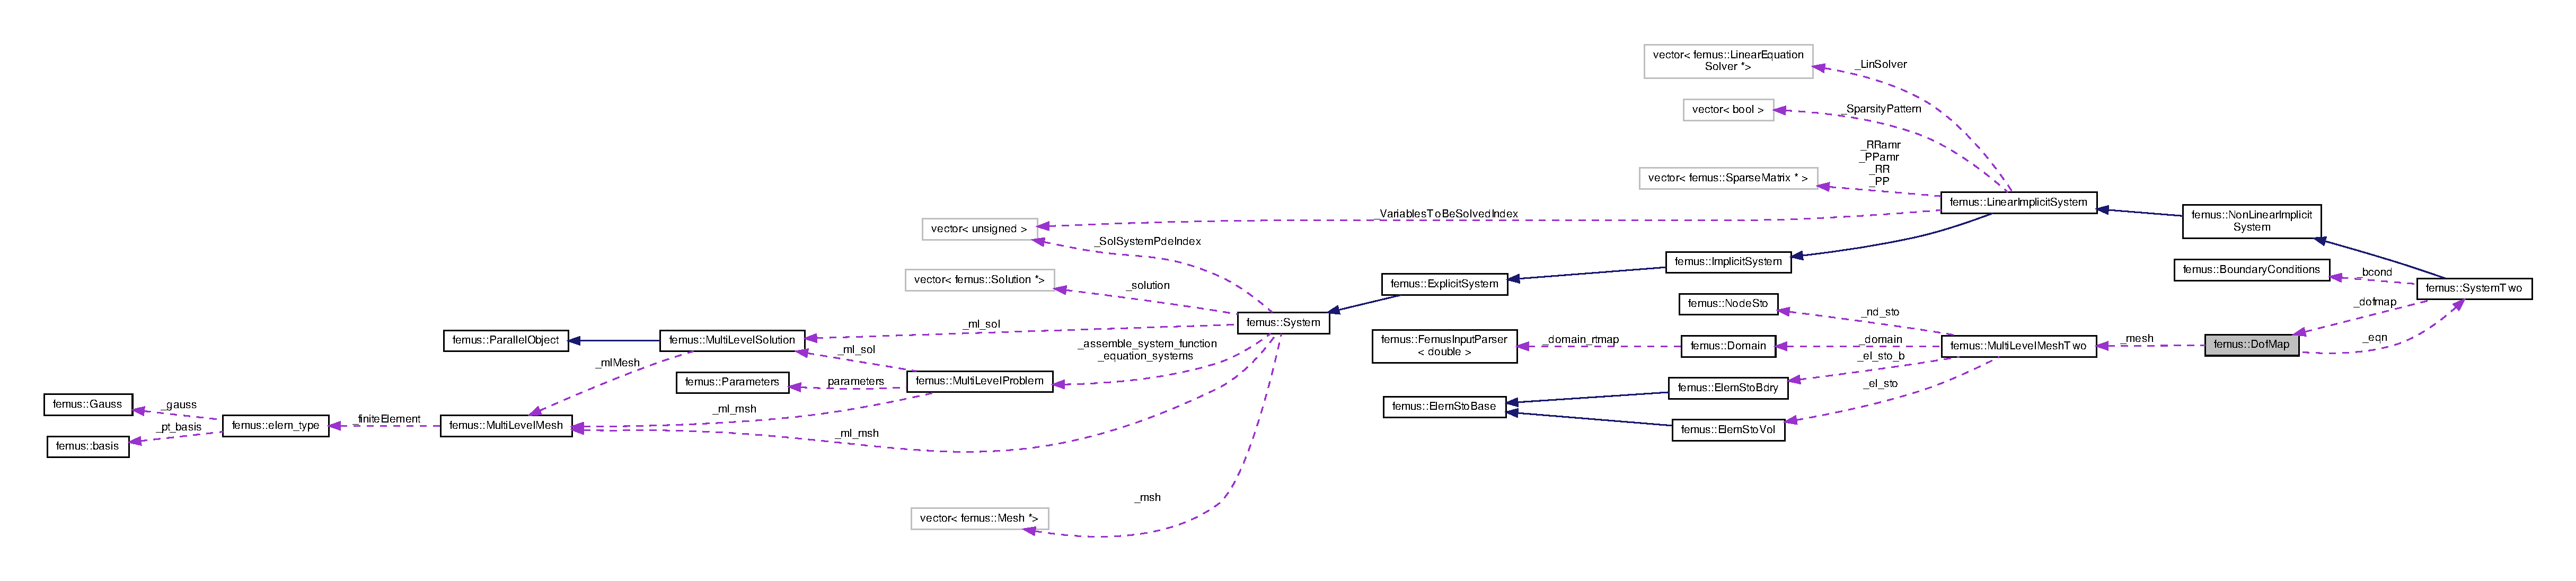
\includegraphics[width=350pt]{classfemus_1_1_dof_map__coll__graph}
\end{center}
\end{figure}
\subsection*{Public Member Functions}
\begin{DoxyCompactItemize}
\item 
\mbox{\hyperlink{classfemus_1_1_dof_map_ad2189a8337b8a34227dfccf813c95979}{Dof\+Map}} (const \mbox{\hyperlink{classfemus_1_1_system_two}{System\+Two}} $\ast$eqn\+\_\+in, const \mbox{\hyperlink{classfemus_1_1_multi_level_mesh_two}{Multi\+Level\+Mesh\+Two}} \&mesh)
\item 
\mbox{\hyperlink{classfemus_1_1_dof_map_ae4d78670db55aef9a236e0c6af24e7e3}{$\sim$\+Dof\+Map}} ()
\item 
void \mbox{\hyperlink{classfemus_1_1_dof_map_aa84b5b38fd73a56018a66dac26de385d}{init\+N\+Vars}} ()
\item 
void \mbox{\hyperlink{classfemus_1_1_dof_map_a138d18259b03814567d8795e0d462aca}{Compute\+Mesh\+To\+Dof}} ()
\item 
void \mbox{\hyperlink{classfemus_1_1_dof_map_a801bae5752dca9dc1cd5b717e26de5ad}{Print\+Mesh\+To\+Dof}} () const
\item 
int \mbox{\hyperlink{classfemus_1_1_dof_map_a26b59524fe1b0d8d17ce74f5776cbe5d}{Get\+Dof}} (const \mbox{\hyperlink{_typedefs_8hpp_a91ad9478d81a7aaf2593e8d9c3d06a14}{uint}} Level, const \mbox{\hyperlink{_typedefs_8hpp_a91ad9478d81a7aaf2593e8d9c3d06a14}{uint}} fe, const \mbox{\hyperlink{_typedefs_8hpp_a91ad9478d81a7aaf2593e8d9c3d06a14}{uint}} ivar, const \mbox{\hyperlink{_typedefs_8hpp_a91ad9478d81a7aaf2593e8d9c3d06a14}{uint}} i) const
\item 
int \mbox{\hyperlink{classfemus_1_1_dof_map_a5a09306eb3fff3f5b831ee7044903e59}{Get\+Dof\+Quantity\+Component}} (const \mbox{\hyperlink{_typedefs_8hpp_a91ad9478d81a7aaf2593e8d9c3d06a14}{uint}} Level, const \mbox{\hyperlink{classfemus_1_1_quantity}{Quantity}} $\ast$quantity\+\_\+in, const \mbox{\hyperlink{_typedefs_8hpp_a91ad9478d81a7aaf2593e8d9c3d06a14}{uint}} quantity\+\_\+var, const \mbox{\hyperlink{_typedefs_8hpp_a91ad9478d81a7aaf2593e8d9c3d06a14}{uint}} dofobj) const
\item 
int \mbox{\hyperlink{classfemus_1_1_dof_map_a394c1fc6f3544f138fdb10ef6acced47}{Get\+Dof\+Pos\+In}} (const \mbox{\hyperlink{_typedefs_8hpp_a91ad9478d81a7aaf2593e8d9c3d06a14}{uint}} Level, const \mbox{\hyperlink{_typedefs_8hpp_a91ad9478d81a7aaf2593e8d9c3d06a14}{uint}} pos\+\_\+in) const
\item 
int \mbox{\hyperlink{classfemus_1_1_dof_map_ad772757cab6d2c551e614a1aa5987349}{Get\+Start\+Dof}} (const \mbox{\hyperlink{_typedefs_8hpp_a91ad9478d81a7aaf2593e8d9c3d06a14}{uint}} Level, const \mbox{\hyperlink{_typedefs_8hpp_a91ad9478d81a7aaf2593e8d9c3d06a14}{uint}} offproc) const
\end{DoxyCompactItemize}
\subsection*{Public Attributes}
\begin{DoxyCompactItemize}
\item 
const \mbox{\hyperlink{classfemus_1_1_system_two}{System\+Two}} $\ast$ \mbox{\hyperlink{classfemus_1_1_dof_map_ab5fc4366e3bf6ec70f918f7ff3a79d10}{\+\_\+eqn}}
\item 
const \mbox{\hyperlink{classfemus_1_1_multi_level_mesh_two}{Multi\+Level\+Mesh\+Two}} \& \mbox{\hyperlink{classfemus_1_1_dof_map_a659fb2627c739a4f4f0c95b1c53d0fe8}{\+\_\+mesh}}
\item 
\mbox{\hyperlink{_typedefs_8hpp_a91ad9478d81a7aaf2593e8d9c3d06a14}{uint}} $\ast$ \mbox{\hyperlink{classfemus_1_1_dof_map_a6a0a1e270ab5c9250e0385d6a0555cbb}{\+\_\+\+Dim}}
\item 
\mbox{\hyperlink{_typedefs_8hpp_a91ad9478d81a7aaf2593e8d9c3d06a14}{uint}} $\ast$$\ast$ \mbox{\hyperlink{classfemus_1_1_dof_map_a490a84023f8277b2c13e257f16a67433}{\+\_\+\+Dof\+Num\+Lev\+FE}}
\item 
\mbox{\hyperlink{_typedefs_8hpp_a91ad9478d81a7aaf2593e8d9c3d06a14}{uint}} $\ast$$\ast$ \mbox{\hyperlink{classfemus_1_1_dof_map_aca4b8f1a8579670d4c84a451009cbcd5}{\+\_\+\+Dof\+Off\+Lev\+FE}}
\item 
\mbox{\hyperlink{_typedefs_8hpp_a91ad9478d81a7aaf2593e8d9c3d06a14}{uint}} $\ast$$\ast$$\ast$ \mbox{\hyperlink{classfemus_1_1_dof_map_a058ca167654c137ccb33ce88ff4d983b}{\+\_\+\+Dof\+Loc\+Lev\+Proc\+FE}}
\item 
\mbox{\hyperlink{_typedefs_8hpp_a91ad9478d81a7aaf2593e8d9c3d06a14}{uint}} \mbox{\hyperlink{classfemus_1_1_dof_map_a537b67e0e240a5673e99135b6912a6dc}{\+\_\+nvars}} \mbox{[}\mbox{\hyperlink{_f_e_type_enum_8hpp_aca285339f9cf24489fdc0af5b51a5fde}{QL}}\mbox{]}
\item 
\mbox{\hyperlink{_typedefs_8hpp_a91ad9478d81a7aaf2593e8d9c3d06a14}{uint}} \mbox{\hyperlink{classfemus_1_1_dof_map_a45b5e2e1aca510da954ff2f96d95f42c}{\+\_\+\+Var\+Off}} \mbox{[}\mbox{\hyperlink{_f_e_type_enum_8hpp_aca285339f9cf24489fdc0af5b51a5fde}{QL}}\mbox{]}
\begin{DoxyCompactList}\small\item\em number of S\+C\+A\+L\+AR variables \end{DoxyCompactList}\item 
\mbox{\hyperlink{_typedefs_8hpp_a91ad9478d81a7aaf2593e8d9c3d06a14}{uint}} \mbox{\hyperlink{classfemus_1_1_dof_map_a1813c139353803d4e0132fd6761f73fc}{\+\_\+n\+\_\+vars}}
\begin{DoxyCompactList}\small\item\em number of S\+C\+A\+L\+AR variables \end{DoxyCompactList}\end{DoxyCompactItemize}


\subsection{Constructor \& Destructor Documentation}
\mbox{\Hypertarget{classfemus_1_1_dof_map_ad2189a8337b8a34227dfccf813c95979}\label{classfemus_1_1_dof_map_ad2189a8337b8a34227dfccf813c95979}} 
\index{femus\+::\+Dof\+Map@{femus\+::\+Dof\+Map}!Dof\+Map@{Dof\+Map}}
\index{Dof\+Map@{Dof\+Map}!femus\+::\+Dof\+Map@{femus\+::\+Dof\+Map}}
\subsubsection{\texorpdfstring{Dof\+Map()}{DofMap()}}
{\footnotesize\ttfamily femus\+::\+Dof\+Map\+::\+Dof\+Map (\begin{DoxyParamCaption}\item[{const \mbox{\hyperlink{classfemus_1_1_system_two}{System\+Two}} $\ast$}]{eqn\+\_\+in,  }\item[{const \mbox{\hyperlink{classfemus_1_1_multi_level_mesh_two}{Multi\+Level\+Mesh\+Two}} \&}]{mesh }\end{DoxyParamCaption})}

\mbox{\Hypertarget{classfemus_1_1_dof_map_ae4d78670db55aef9a236e0c6af24e7e3}\label{classfemus_1_1_dof_map_ae4d78670db55aef9a236e0c6af24e7e3}} 
\index{femus\+::\+Dof\+Map@{femus\+::\+Dof\+Map}!````~Dof\+Map@{$\sim$\+Dof\+Map}}
\index{````~Dof\+Map@{$\sim$\+Dof\+Map}!femus\+::\+Dof\+Map@{femus\+::\+Dof\+Map}}
\subsubsection{\texorpdfstring{$\sim$\+Dof\+Map()}{~DofMap()}}
{\footnotesize\ttfamily femus\+::\+Dof\+Map\+::$\sim$\+Dof\+Map (\begin{DoxyParamCaption}{ }\end{DoxyParamCaption})}



\subsection{Member Function Documentation}
\mbox{\Hypertarget{classfemus_1_1_dof_map_a138d18259b03814567d8795e0d462aca}\label{classfemus_1_1_dof_map_a138d18259b03814567d8795e0d462aca}} 
\index{femus\+::\+Dof\+Map@{femus\+::\+Dof\+Map}!Compute\+Mesh\+To\+Dof@{Compute\+Mesh\+To\+Dof}}
\index{Compute\+Mesh\+To\+Dof@{Compute\+Mesh\+To\+Dof}!femus\+::\+Dof\+Map@{femus\+::\+Dof\+Map}}
\subsubsection{\texorpdfstring{Compute\+Mesh\+To\+Dof()}{ComputeMeshToDof()}}
{\footnotesize\ttfamily void femus\+::\+Dof\+Map\+::\+Compute\+Mesh\+To\+Dof (\begin{DoxyParamCaption}{ }\end{DoxyParamCaption})}

This function initializes the system degrees of freedom (dof) for every Level you have a different dof map, but this is allocated as the fine level, therefore except the fine level the \+\_\+nodedof is \char`\"{}full of holes\char`\"{} Why dont we allocate the dof map \char`\"{}without holes\char`\"{} ? because we want to refer to the F\+I\+NE M\+E\+SH node numbering which is unique. In fact, off\+\_\+nd\+\_\+q and off\+\_\+nd\+\_\+l give us the R\+A\+N\+G\+ES in the F\+I\+NE N\+O\+D\+ES The dof map IS N\+OT T\+HE I\+D\+E\+N\+T\+I\+TY ! node numbering is what is given by the G\+E\+N\+C\+A\+SE; dof numbering instead starts from Z\+E\+RO for every level! i think it is the identity only on the C\+O\+A\+R\+SE L\+E\+V\+EL For every level, you construct a \+\_\+node\+\_\+dof\mbox{[}Level\mbox{]} here you start giving an index to the dofs starting S\+U\+B\+D\+O\+M\+A\+IN BY S\+U\+B\+D\+O\+M\+A\+IN For each subdomain, you pick F\+I\+R\+ST the Q\+U\+A\+D\+R\+A\+T\+IC then the L\+I\+N\+E\+AR dofs \mbox{\Hypertarget{classfemus_1_1_dof_map_a26b59524fe1b0d8d17ce74f5776cbe5d}\label{classfemus_1_1_dof_map_a26b59524fe1b0d8d17ce74f5776cbe5d}} 
\index{femus\+::\+Dof\+Map@{femus\+::\+Dof\+Map}!Get\+Dof@{Get\+Dof}}
\index{Get\+Dof@{Get\+Dof}!femus\+::\+Dof\+Map@{femus\+::\+Dof\+Map}}
\subsubsection{\texorpdfstring{Get\+Dof()}{GetDof()}}
{\footnotesize\ttfamily int femus\+::\+Dof\+Map\+::\+Get\+Dof (\begin{DoxyParamCaption}\item[{const \mbox{\hyperlink{_typedefs_8hpp_a91ad9478d81a7aaf2593e8d9c3d06a14}{uint}}}]{Level,  }\item[{const \mbox{\hyperlink{_typedefs_8hpp_a91ad9478d81a7aaf2593e8d9c3d06a14}{uint}}}]{fe,  }\item[{const \mbox{\hyperlink{_typedefs_8hpp_a91ad9478d81a7aaf2593e8d9c3d06a14}{uint}}}]{ivar\+\_\+fe,  }\item[{const \mbox{\hyperlink{_typedefs_8hpp_a91ad9478d81a7aaf2593e8d9c3d06a14}{uint}}}]{dofobj }\end{DoxyParamCaption}) const\hspace{0.3cm}{\ttfamily [inline]}}

at level Level, for a given FE, take the dof of the ivar\+\_\+fe variable of that FE \mbox{\Hypertarget{classfemus_1_1_dof_map_a394c1fc6f3544f138fdb10ef6acced47}\label{classfemus_1_1_dof_map_a394c1fc6f3544f138fdb10ef6acced47}} 
\index{femus\+::\+Dof\+Map@{femus\+::\+Dof\+Map}!Get\+Dof\+Pos\+In@{Get\+Dof\+Pos\+In}}
\index{Get\+Dof\+Pos\+In@{Get\+Dof\+Pos\+In}!femus\+::\+Dof\+Map@{femus\+::\+Dof\+Map}}
\subsubsection{\texorpdfstring{Get\+Dof\+Pos\+In()}{GetDofPosIn()}}
{\footnotesize\ttfamily int femus\+::\+Dof\+Map\+::\+Get\+Dof\+Pos\+In (\begin{DoxyParamCaption}\item[{const \mbox{\hyperlink{_typedefs_8hpp_a91ad9478d81a7aaf2593e8d9c3d06a14}{uint}}}]{Level,  }\item[{const \mbox{\hyperlink{_typedefs_8hpp_a91ad9478d81a7aaf2593e8d9c3d06a14}{uint}}}]{pos\+\_\+in }\end{DoxyParamCaption}) const\hspace{0.3cm}{\ttfamily [inline]}}

\mbox{\Hypertarget{classfemus_1_1_dof_map_a5a09306eb3fff3f5b831ee7044903e59}\label{classfemus_1_1_dof_map_a5a09306eb3fff3f5b831ee7044903e59}} 
\index{femus\+::\+Dof\+Map@{femus\+::\+Dof\+Map}!Get\+Dof\+Quantity\+Component@{Get\+Dof\+Quantity\+Component}}
\index{Get\+Dof\+Quantity\+Component@{Get\+Dof\+Quantity\+Component}!femus\+::\+Dof\+Map@{femus\+::\+Dof\+Map}}
\subsubsection{\texorpdfstring{Get\+Dof\+Quantity\+Component()}{GetDofQuantityComponent()}}
{\footnotesize\ttfamily int femus\+::\+Dof\+Map\+::\+Get\+Dof\+Quantity\+Component (\begin{DoxyParamCaption}\item[{const \mbox{\hyperlink{_typedefs_8hpp_a91ad9478d81a7aaf2593e8d9c3d06a14}{uint}}}]{Level,  }\item[{const \mbox{\hyperlink{classfemus_1_1_quantity}{Quantity}} $\ast$}]{quantity\+\_\+in,  }\item[{const \mbox{\hyperlink{_typedefs_8hpp_a91ad9478d81a7aaf2593e8d9c3d06a14}{uint}}}]{quantity\+\_\+var,  }\item[{const \mbox{\hyperlink{_typedefs_8hpp_a91ad9478d81a7aaf2593e8d9c3d06a14}{uint}}}]{dofobj }\end{DoxyParamCaption}) const}

\mbox{\Hypertarget{classfemus_1_1_dof_map_ad772757cab6d2c551e614a1aa5987349}\label{classfemus_1_1_dof_map_ad772757cab6d2c551e614a1aa5987349}} 
\index{femus\+::\+Dof\+Map@{femus\+::\+Dof\+Map}!Get\+Start\+Dof@{Get\+Start\+Dof}}
\index{Get\+Start\+Dof@{Get\+Start\+Dof}!femus\+::\+Dof\+Map@{femus\+::\+Dof\+Map}}
\subsubsection{\texorpdfstring{Get\+Start\+Dof()}{GetStartDof()}}
{\footnotesize\ttfamily int femus\+::\+Dof\+Map\+::\+Get\+Start\+Dof (\begin{DoxyParamCaption}\item[{const \mbox{\hyperlink{_typedefs_8hpp_a91ad9478d81a7aaf2593e8d9c3d06a14}{uint}}}]{Level,  }\item[{const \mbox{\hyperlink{_typedefs_8hpp_a91ad9478d81a7aaf2593e8d9c3d06a14}{uint}}}]{offproc }\end{DoxyParamCaption}) const\hspace{0.3cm}{\ttfamily [inline]}}

\mbox{\Hypertarget{classfemus_1_1_dof_map_aa84b5b38fd73a56018a66dac26de385d}\label{classfemus_1_1_dof_map_aa84b5b38fd73a56018a66dac26de385d}} 
\index{femus\+::\+Dof\+Map@{femus\+::\+Dof\+Map}!init\+N\+Vars@{init\+N\+Vars}}
\index{init\+N\+Vars@{init\+N\+Vars}!femus\+::\+Dof\+Map@{femus\+::\+Dof\+Map}}
\subsubsection{\texorpdfstring{init\+N\+Vars()}{initNVars()}}
{\footnotesize\ttfamily void femus\+::\+Dof\+Map\+::init\+N\+Vars (\begin{DoxyParamCaption}{ }\end{DoxyParamCaption})}

\mbox{\Hypertarget{classfemus_1_1_dof_map_a801bae5752dca9dc1cd5b717e26de5ad}\label{classfemus_1_1_dof_map_a801bae5752dca9dc1cd5b717e26de5ad}} 
\index{femus\+::\+Dof\+Map@{femus\+::\+Dof\+Map}!Print\+Mesh\+To\+Dof@{Print\+Mesh\+To\+Dof}}
\index{Print\+Mesh\+To\+Dof@{Print\+Mesh\+To\+Dof}!femus\+::\+Dof\+Map@{femus\+::\+Dof\+Map}}
\subsubsection{\texorpdfstring{Print\+Mesh\+To\+Dof()}{PrintMeshToDof()}}
{\footnotesize\ttfamily void femus\+::\+Dof\+Map\+::\+Print\+Mesh\+To\+Dof (\begin{DoxyParamCaption}{ }\end{DoxyParamCaption}) const}



\subsection{Member Data Documentation}
\mbox{\Hypertarget{classfemus_1_1_dof_map_a6a0a1e270ab5c9250e0385d6a0555cbb}\label{classfemus_1_1_dof_map_a6a0a1e270ab5c9250e0385d6a0555cbb}} 
\index{femus\+::\+Dof\+Map@{femus\+::\+Dof\+Map}!\+\_\+\+Dim@{\+\_\+\+Dim}}
\index{\+\_\+\+Dim@{\+\_\+\+Dim}!femus\+::\+Dof\+Map@{femus\+::\+Dof\+Map}}
\subsubsection{\texorpdfstring{\+\_\+\+Dim}{\_Dim}}
{\footnotesize\ttfamily \mbox{\hyperlink{_typedefs_8hpp_a91ad9478d81a7aaf2593e8d9c3d06a14}{uint}}$\ast$ femus\+::\+Dof\+Map\+::\+\_\+\+Dim}

\mbox{\Hypertarget{classfemus_1_1_dof_map_a058ca167654c137ccb33ce88ff4d983b}\label{classfemus_1_1_dof_map_a058ca167654c137ccb33ce88ff4d983b}} 
\index{femus\+::\+Dof\+Map@{femus\+::\+Dof\+Map}!\+\_\+\+Dof\+Loc\+Lev\+Proc\+FE@{\+\_\+\+Dof\+Loc\+Lev\+Proc\+FE}}
\index{\+\_\+\+Dof\+Loc\+Lev\+Proc\+FE@{\+\_\+\+Dof\+Loc\+Lev\+Proc\+FE}!femus\+::\+Dof\+Map@{femus\+::\+Dof\+Map}}
\subsubsection{\texorpdfstring{\+\_\+\+Dof\+Loc\+Lev\+Proc\+FE}{\_DofLocLevProcFE}}
{\footnotesize\ttfamily \mbox{\hyperlink{_typedefs_8hpp_a91ad9478d81a7aaf2593e8d9c3d06a14}{uint}}$\ast$$\ast$$\ast$ femus\+::\+Dof\+Map\+::\+\_\+\+Dof\+Loc\+Lev\+Proc\+FE}

\mbox{\Hypertarget{classfemus_1_1_dof_map_a490a84023f8277b2c13e257f16a67433}\label{classfemus_1_1_dof_map_a490a84023f8277b2c13e257f16a67433}} 
\index{femus\+::\+Dof\+Map@{femus\+::\+Dof\+Map}!\+\_\+\+Dof\+Num\+Lev\+FE@{\+\_\+\+Dof\+Num\+Lev\+FE}}
\index{\+\_\+\+Dof\+Num\+Lev\+FE@{\+\_\+\+Dof\+Num\+Lev\+FE}!femus\+::\+Dof\+Map@{femus\+::\+Dof\+Map}}
\subsubsection{\texorpdfstring{\+\_\+\+Dof\+Num\+Lev\+FE}{\_DofNumLevFE}}
{\footnotesize\ttfamily \mbox{\hyperlink{_typedefs_8hpp_a91ad9478d81a7aaf2593e8d9c3d06a14}{uint}}$\ast$$\ast$ femus\+::\+Dof\+Map\+::\+\_\+\+Dof\+Num\+Lev\+FE}

\mbox{\Hypertarget{classfemus_1_1_dof_map_aca4b8f1a8579670d4c84a451009cbcd5}\label{classfemus_1_1_dof_map_aca4b8f1a8579670d4c84a451009cbcd5}} 
\index{femus\+::\+Dof\+Map@{femus\+::\+Dof\+Map}!\+\_\+\+Dof\+Off\+Lev\+FE@{\+\_\+\+Dof\+Off\+Lev\+FE}}
\index{\+\_\+\+Dof\+Off\+Lev\+FE@{\+\_\+\+Dof\+Off\+Lev\+FE}!femus\+::\+Dof\+Map@{femus\+::\+Dof\+Map}}
\subsubsection{\texorpdfstring{\+\_\+\+Dof\+Off\+Lev\+FE}{\_DofOffLevFE}}
{\footnotesize\ttfamily \mbox{\hyperlink{_typedefs_8hpp_a91ad9478d81a7aaf2593e8d9c3d06a14}{uint}}$\ast$$\ast$ femus\+::\+Dof\+Map\+::\+\_\+\+Dof\+Off\+Lev\+FE}

\mbox{\Hypertarget{classfemus_1_1_dof_map_ab5fc4366e3bf6ec70f918f7ff3a79d10}\label{classfemus_1_1_dof_map_ab5fc4366e3bf6ec70f918f7ff3a79d10}} 
\index{femus\+::\+Dof\+Map@{femus\+::\+Dof\+Map}!\+\_\+eqn@{\+\_\+eqn}}
\index{\+\_\+eqn@{\+\_\+eqn}!femus\+::\+Dof\+Map@{femus\+::\+Dof\+Map}}
\subsubsection{\texorpdfstring{\+\_\+eqn}{\_eqn}}
{\footnotesize\ttfamily const \mbox{\hyperlink{classfemus_1_1_system_two}{System\+Two}}$\ast$ femus\+::\+Dof\+Map\+::\+\_\+eqn}

\mbox{\Hypertarget{classfemus_1_1_dof_map_a659fb2627c739a4f4f0c95b1c53d0fe8}\label{classfemus_1_1_dof_map_a659fb2627c739a4f4f0c95b1c53d0fe8}} 
\index{femus\+::\+Dof\+Map@{femus\+::\+Dof\+Map}!\+\_\+mesh@{\+\_\+mesh}}
\index{\+\_\+mesh@{\+\_\+mesh}!femus\+::\+Dof\+Map@{femus\+::\+Dof\+Map}}
\subsubsection{\texorpdfstring{\+\_\+mesh}{\_mesh}}
{\footnotesize\ttfamily const \mbox{\hyperlink{classfemus_1_1_multi_level_mesh_two}{Multi\+Level\+Mesh\+Two}}\& femus\+::\+Dof\+Map\+::\+\_\+mesh}

\mbox{\Hypertarget{classfemus_1_1_dof_map_a1813c139353803d4e0132fd6761f73fc}\label{classfemus_1_1_dof_map_a1813c139353803d4e0132fd6761f73fc}} 
\index{femus\+::\+Dof\+Map@{femus\+::\+Dof\+Map}!\+\_\+n\+\_\+vars@{\+\_\+n\+\_\+vars}}
\index{\+\_\+n\+\_\+vars@{\+\_\+n\+\_\+vars}!femus\+::\+Dof\+Map@{femus\+::\+Dof\+Map}}
\subsubsection{\texorpdfstring{\+\_\+n\+\_\+vars}{\_n\_vars}}
{\footnotesize\ttfamily \mbox{\hyperlink{_typedefs_8hpp_a91ad9478d81a7aaf2593e8d9c3d06a14}{uint}} femus\+::\+Dof\+Map\+::\+\_\+n\+\_\+vars}



number of S\+C\+A\+L\+AR variables 

\mbox{\Hypertarget{classfemus_1_1_dof_map_a537b67e0e240a5673e99135b6912a6dc}\label{classfemus_1_1_dof_map_a537b67e0e240a5673e99135b6912a6dc}} 
\index{femus\+::\+Dof\+Map@{femus\+::\+Dof\+Map}!\+\_\+nvars@{\+\_\+nvars}}
\index{\+\_\+nvars@{\+\_\+nvars}!femus\+::\+Dof\+Map@{femus\+::\+Dof\+Map}}
\subsubsection{\texorpdfstring{\+\_\+nvars}{\_nvars}}
{\footnotesize\ttfamily \mbox{\hyperlink{_typedefs_8hpp_a91ad9478d81a7aaf2593e8d9c3d06a14}{uint}} femus\+::\+Dof\+Map\+::\+\_\+nvars\mbox{[}\mbox{\hyperlink{_f_e_type_enum_8hpp_aca285339f9cf24489fdc0af5b51a5fde}{QL}}\mbox{]}}

\mbox{\Hypertarget{classfemus_1_1_dof_map_a45b5e2e1aca510da954ff2f96d95f42c}\label{classfemus_1_1_dof_map_a45b5e2e1aca510da954ff2f96d95f42c}} 
\index{femus\+::\+Dof\+Map@{femus\+::\+Dof\+Map}!\+\_\+\+Var\+Off@{\+\_\+\+Var\+Off}}
\index{\+\_\+\+Var\+Off@{\+\_\+\+Var\+Off}!femus\+::\+Dof\+Map@{femus\+::\+Dof\+Map}}
\subsubsection{\texorpdfstring{\+\_\+\+Var\+Off}{\_VarOff}}
{\footnotesize\ttfamily \mbox{\hyperlink{_typedefs_8hpp_a91ad9478d81a7aaf2593e8d9c3d06a14}{uint}} femus\+::\+Dof\+Map\+::\+\_\+\+Var\+Off\mbox{[}\mbox{\hyperlink{_f_e_type_enum_8hpp_aca285339f9cf24489fdc0af5b51a5fde}{QL}}\mbox{]}}



number of S\+C\+A\+L\+AR variables 



The documentation for this class was generated from the following files\+:\begin{DoxyCompactItemize}
\item 
equations/\mbox{\hyperlink{_dof_map_8hpp}{Dof\+Map.\+hpp}}\item 
equations/\mbox{\hyperlink{_dof_map_8cpp}{Dof\+Map.\+cpp}}\end{DoxyCompactItemize}

\hypertarget{classfemus_1_1_domain}{}\section{femus\+:\+:Domain Class Reference}
\label{classfemus_1_1_domain}\index{femus\+::\+Domain@{femus\+::\+Domain}}


{\ttfamily \#include $<$Domain.\+hpp$>$}



Inheritance diagram for femus\+:\+:Domain\+:
\nopagebreak
\begin{figure}[H]
\begin{center}
\leavevmode
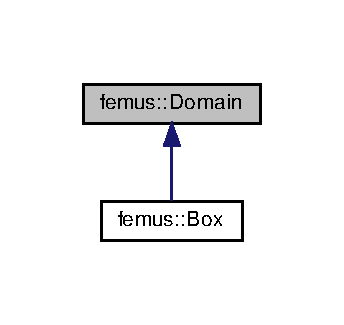
\includegraphics[width=165pt]{classfemus_1_1_domain__inherit__graph}
\end{center}
\end{figure}


Collaboration diagram for femus\+:\+:Domain\+:
\nopagebreak
\begin{figure}[H]
\begin{center}
\leavevmode
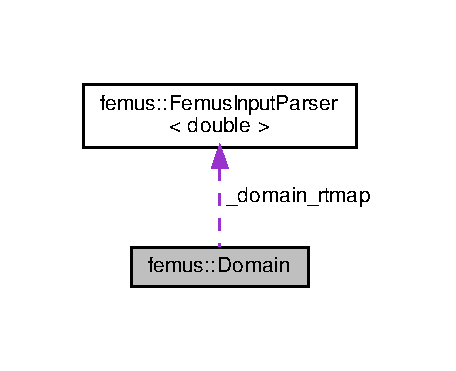
\includegraphics[width=219pt]{classfemus_1_1_domain__coll__graph}
\end{center}
\end{figure}
\subsection*{Public Member Functions}
\begin{DoxyCompactItemize}
\item 
\mbox{\hyperlink{classfemus_1_1_domain_ad1b0f07867cc3aee73de7fba251abc50}{$\sim$\+Domain}} ()
\item 
virtual void \mbox{\hyperlink{classfemus_1_1_domain_afde27aa114c601801cc727ef9edf31de}{Transform\+Point\+To\+Ref}} (const double $\ast$x\+\_\+in, double $\ast$x\+\_\+out) const =0
\begin{DoxyCompactList}\small\item\em transformation to reference \mbox{\hyperlink{classfemus_1_1_domain}{Domain}} frame \end{DoxyCompactList}\item 
virtual const \mbox{\hyperlink{_typedefs_8hpp_a91ad9478d81a7aaf2593e8d9c3d06a14}{uint}} \mbox{\hyperlink{classfemus_1_1_domain_ad75eacc25142ba41cbceab06de675fc8}{Get\+Domain\+Flag}} () const =0
\end{DoxyCompactItemize}
\subsection*{Public Attributes}
\begin{DoxyCompactItemize}
\item 
const \mbox{\hyperlink{classfemus_1_1_femus_input_parser}{Femus\+Input\+Parser}}$<$ double $>$ \& \mbox{\hyperlink{classfemus_1_1_domain_a0cde7463658ab6de6a74ed6afedca6a0}{\+\_\+domain\+\_\+rtmap}}
\item 
std\+::string \mbox{\hyperlink{classfemus_1_1_domain_a7ed9fa5a4642690ceb7c849954b89c1f}{\+\_\+name}}
\item 
double \mbox{\hyperlink{classfemus_1_1_domain_a62bbfa8103bf9cc181d09099cb3ad839}{\+\_\+\+Lref}}
\item 
\mbox{\hyperlink{_typedefs_8hpp_a91ad9478d81a7aaf2593e8d9c3d06a14}{uint}} \mbox{\hyperlink{classfemus_1_1_domain_a940e6bd8a80fba5be0da7871703f6166}{\+\_\+spacedim}}
\end{DoxyCompactItemize}
\subsection*{Protected Member Functions}
\begin{DoxyCompactItemize}
\item 
\mbox{\hyperlink{classfemus_1_1_domain_a96de5a99af1bea80aeb1d21cea9ca362}{Domain}} (const \mbox{\hyperlink{_typedefs_8hpp_a91ad9478d81a7aaf2593e8d9c3d06a14}{uint}} spacedim\+\_\+in, const \mbox{\hyperlink{classfemus_1_1_femus_input_parser}{Femus\+Input\+Parser}}$<$ double $>$ \&map\+\_\+in)
\end{DoxyCompactItemize}


\subsection{Constructor \& Destructor Documentation}
\mbox{\Hypertarget{classfemus_1_1_domain_a96de5a99af1bea80aeb1d21cea9ca362}\label{classfemus_1_1_domain_a96de5a99af1bea80aeb1d21cea9ca362}} 
\index{femus\+::\+Domain@{femus\+::\+Domain}!Domain@{Domain}}
\index{Domain@{Domain}!femus\+::\+Domain@{femus\+::\+Domain}}
\subsubsection{\texorpdfstring{Domain()}{Domain()}}
{\footnotesize\ttfamily femus\+::\+Domain\+::\+Domain (\begin{DoxyParamCaption}\item[{const \mbox{\hyperlink{_typedefs_8hpp_a91ad9478d81a7aaf2593e8d9c3d06a14}{uint}}}]{spacedim\+\_\+in,  }\item[{const \mbox{\hyperlink{classfemus_1_1_femus_input_parser}{Femus\+Input\+Parser}}$<$ double $>$ \&}]{map\+\_\+in }\end{DoxyParamCaption})\hspace{0.3cm}{\ttfamily [protected]}}

\mbox{\Hypertarget{classfemus_1_1_domain_ad1b0f07867cc3aee73de7fba251abc50}\label{classfemus_1_1_domain_ad1b0f07867cc3aee73de7fba251abc50}} 
\index{femus\+::\+Domain@{femus\+::\+Domain}!````~Domain@{$\sim$\+Domain}}
\index{````~Domain@{$\sim$\+Domain}!femus\+::\+Domain@{femus\+::\+Domain}}
\subsubsection{\texorpdfstring{$\sim$\+Domain()}{~Domain()}}
{\footnotesize\ttfamily femus\+::\+Domain\+::$\sim$\+Domain (\begin{DoxyParamCaption}{ }\end{DoxyParamCaption})}



\subsection{Member Function Documentation}
\mbox{\Hypertarget{classfemus_1_1_domain_ad75eacc25142ba41cbceab06de675fc8}\label{classfemus_1_1_domain_ad75eacc25142ba41cbceab06de675fc8}} 
\index{femus\+::\+Domain@{femus\+::\+Domain}!Get\+Domain\+Flag@{Get\+Domain\+Flag}}
\index{Get\+Domain\+Flag@{Get\+Domain\+Flag}!femus\+::\+Domain@{femus\+::\+Domain}}
\subsubsection{\texorpdfstring{Get\+Domain\+Flag()}{GetDomainFlag()}}
{\footnotesize\ttfamily virtual const \mbox{\hyperlink{_typedefs_8hpp_a91ad9478d81a7aaf2593e8d9c3d06a14}{uint}} femus\+::\+Domain\+::\+Get\+Domain\+Flag (\begin{DoxyParamCaption}{ }\end{DoxyParamCaption}) const\hspace{0.3cm}{\ttfamily [pure virtual]}}



Implemented in \mbox{\hyperlink{classfemus_1_1_box_ae1e35410fff5545cd0c203cd9ad3001d}{femus\+::\+Box}}.

\mbox{\Hypertarget{classfemus_1_1_domain_afde27aa114c601801cc727ef9edf31de}\label{classfemus_1_1_domain_afde27aa114c601801cc727ef9edf31de}} 
\index{femus\+::\+Domain@{femus\+::\+Domain}!Transform\+Point\+To\+Ref@{Transform\+Point\+To\+Ref}}
\index{Transform\+Point\+To\+Ref@{Transform\+Point\+To\+Ref}!femus\+::\+Domain@{femus\+::\+Domain}}
\subsubsection{\texorpdfstring{Transform\+Point\+To\+Ref()}{TransformPointToRef()}}
{\footnotesize\ttfamily virtual void femus\+::\+Domain\+::\+Transform\+Point\+To\+Ref (\begin{DoxyParamCaption}\item[{const double $\ast$}]{x\+\_\+in,  }\item[{double $\ast$}]{x\+\_\+out }\end{DoxyParamCaption}) const\hspace{0.3cm}{\ttfamily [pure virtual]}}



transformation to reference \mbox{\hyperlink{classfemus_1_1_domain}{Domain}} frame 



Implemented in \mbox{\hyperlink{classfemus_1_1_box_a64a23d5bb0cac88b4e545b121988b3cf}{femus\+::\+Box}}.



\subsection{Member Data Documentation}
\mbox{\Hypertarget{classfemus_1_1_domain_a0cde7463658ab6de6a74ed6afedca6a0}\label{classfemus_1_1_domain_a0cde7463658ab6de6a74ed6afedca6a0}} 
\index{femus\+::\+Domain@{femus\+::\+Domain}!\+\_\+domain\+\_\+rtmap@{\+\_\+domain\+\_\+rtmap}}
\index{\+\_\+domain\+\_\+rtmap@{\+\_\+domain\+\_\+rtmap}!femus\+::\+Domain@{femus\+::\+Domain}}
\subsubsection{\texorpdfstring{\+\_\+domain\+\_\+rtmap}{\_domain\_rtmap}}
{\footnotesize\ttfamily const \mbox{\hyperlink{classfemus_1_1_femus_input_parser}{Femus\+Input\+Parser}}$<$double$>$\& femus\+::\+Domain\+::\+\_\+domain\+\_\+rtmap}

\mbox{\Hypertarget{classfemus_1_1_domain_a62bbfa8103bf9cc181d09099cb3ad839}\label{classfemus_1_1_domain_a62bbfa8103bf9cc181d09099cb3ad839}} 
\index{femus\+::\+Domain@{femus\+::\+Domain}!\+\_\+\+Lref@{\+\_\+\+Lref}}
\index{\+\_\+\+Lref@{\+\_\+\+Lref}!femus\+::\+Domain@{femus\+::\+Domain}}
\subsubsection{\texorpdfstring{\+\_\+\+Lref}{\_Lref}}
{\footnotesize\ttfamily double femus\+::\+Domain\+::\+\_\+\+Lref}

\mbox{\Hypertarget{classfemus_1_1_domain_a7ed9fa5a4642690ceb7c849954b89c1f}\label{classfemus_1_1_domain_a7ed9fa5a4642690ceb7c849954b89c1f}} 
\index{femus\+::\+Domain@{femus\+::\+Domain}!\+\_\+name@{\+\_\+name}}
\index{\+\_\+name@{\+\_\+name}!femus\+::\+Domain@{femus\+::\+Domain}}
\subsubsection{\texorpdfstring{\+\_\+name}{\_name}}
{\footnotesize\ttfamily std\+::string femus\+::\+Domain\+::\+\_\+name}

\mbox{\Hypertarget{classfemus_1_1_domain_a940e6bd8a80fba5be0da7871703f6166}\label{classfemus_1_1_domain_a940e6bd8a80fba5be0da7871703f6166}} 
\index{femus\+::\+Domain@{femus\+::\+Domain}!\+\_\+spacedim@{\+\_\+spacedim}}
\index{\+\_\+spacedim@{\+\_\+spacedim}!femus\+::\+Domain@{femus\+::\+Domain}}
\subsubsection{\texorpdfstring{\+\_\+spacedim}{\_spacedim}}
{\footnotesize\ttfamily \mbox{\hyperlink{_typedefs_8hpp_a91ad9478d81a7aaf2593e8d9c3d06a14}{uint}} femus\+::\+Domain\+::\+\_\+spacedim}



The documentation for this class was generated from the following files\+:\begin{DoxyCompactItemize}
\item 
mesh\+Gencase/\mbox{\hyperlink{_domain_8hpp}{Domain.\+hpp}}\item 
mesh\+Gencase/\mbox{\hyperlink{_domain_8cpp}{Domain.\+cpp}}\end{DoxyCompactItemize}

\hypertarget{classfemus_1_1elem}{}\section{femus\+:\+:elem Class Reference}
\label{classfemus_1_1elem}\index{femus\+::elem@{femus\+::elem}}


{\ttfamily \#include $<$Elem.\+hpp$>$}

\subsection*{Public Member Functions}
\begin{DoxyCompactItemize}
\item 
\mbox{\hyperlink{classfemus_1_1elem_af0d54d7c0c7a5c0a7d1f0586ff28fa41}{elem}} (const unsigned \&other\+\_\+nel)
\item 
\mbox{\hyperlink{classfemus_1_1elem_accb87238cdfe0417be67692c152f38bd}{elem}} (\mbox{\hyperlink{classfemus_1_1elem}{elem}} $\ast$elc, const unsigned refindex, const std\+::vector$<$ double $>$ \&coarse\+Amr\+Local)
\item 
void \mbox{\hyperlink{classfemus_1_1elem_afa830dc9dc77d5292d126bf0156f5330}{Shrink\+To\+Fit}} ()
\item 
\mbox{\hyperlink{classfemus_1_1elem_ae1e94fa2475ed9a86fa504592cd59b98}{$\sim$elem}} ()
\item 
void \mbox{\hyperlink{classfemus_1_1elem_a1fbaf0f106a278950775a386ef0a7f55}{Scatter\+Element\+Near\+Face}} ()
\item 
void \mbox{\hyperlink{classfemus_1_1elem_a14eab6e5b0eea4f2cd714ad79c78cd12}{Localize\+Element\+Near\+Face}} (const unsigned \&jproc)
\item 
void \mbox{\hyperlink{classfemus_1_1elem_a33d168031ff3a1368c6dbe5060177111}{Free\+Localized\+Element\+Near\+Face}} ()
\item 
void \mbox{\hyperlink{classfemus_1_1elem_af48747556a201848ae9a213cd472070a}{Scatter\+Element\+Dof}} ()
\item 
void \mbox{\hyperlink{classfemus_1_1elem_ade1815f54f3b5786c58fb9c54574e21a}{Localize\+Element\+Dof}} (const unsigned \&jproc)
\item 
void \mbox{\hyperlink{classfemus_1_1elem_a4e0777db21ee2ce5e53109f1dbf6a5b7}{Free\+Localized\+Element\+Dof}} ()
\item 
void \mbox{\hyperlink{classfemus_1_1elem_afdc6c215b3ce3424c50c8d8aa30ac660}{Reorder\+Mesh\+Elements}} (const std\+::vector$<$ unsigned $>$ \&element\+Mapping)
\item 
void \mbox{\hyperlink{classfemus_1_1elem_a144e44d4d378fc7daea1e6bfd2aa4ac4}{Reorder\+Mesh\+Nodes}} (const std\+::vector$<$ unsigned $>$ \&node\+Mapping)
\item 
unsigned \mbox{\hyperlink{classfemus_1_1elem_aabfd00a1d57b475aec7a3c3622c82668}{Get\+Element\+Dof\+Number}} (const unsigned \&iel, const unsigned \&type)
\item 
unsigned \mbox{\hyperlink{classfemus_1_1elem_a77bb25f38a4ae2ee0a6e4d3edcf3ba56}{Get\+Element\+Dof\+Index}} (const unsigned \&iel, const unsigned \&inode)
\item 
void \mbox{\hyperlink{classfemus_1_1elem_acc9003e820ed0bcbf784e0910b911549}{Set\+Element\+Dof\+Index}} (const unsigned \&iel, const unsigned \&inode, const unsigned \&value)
\item 
unsigned \mbox{\hyperlink{classfemus_1_1elem_ab90990cb6e1f9a7bc421c69c72db9d55}{Get\+Face\+Vertex\+Index}} (const unsigned \&iel, const unsigned \&iface, const unsigned \&inode)
\item 
short unsigned \mbox{\hyperlink{classfemus_1_1elem_a9389fca6b346d241873c46d1f9357689}{Get\+Element\+Type}} (const unsigned \&iel)
\item 
void \mbox{\hyperlink{classfemus_1_1elem_a23cec6d31d533bfc2a387f4cf23dc763}{Set\+Element\+Type}} (const unsigned \&iel, const short unsigned \&value)
\item 
short unsigned \mbox{\hyperlink{classfemus_1_1elem_acdd8b9d5723e673a72c22f1f74e13d2b}{Get\+Element\+Group}} (const unsigned \&iel)
\item 
void \mbox{\hyperlink{classfemus_1_1elem_a950c41c56ffc7c95d951ef4649a45c5f}{Set\+Element\+Group}} (const unsigned \&iel, const short unsigned \&value)
\item 
void \mbox{\hyperlink{classfemus_1_1elem_a5a00f23f650334a2b35ab8808bb4f1e0}{Set\+Element\+Material}} (const unsigned \&iel, const short unsigned \&value)
\item 
short unsigned \mbox{\hyperlink{classfemus_1_1elem_a4f03cbc37f596624428ff2e6b4609094}{Get\+Element\+Material}} (const unsigned \&iel)
\item 
unsigned \mbox{\hyperlink{classfemus_1_1elem_afb7f045c1d2f85aa101ae7e7d8230a9c}{Get\+Element\+Group\+Number}} () const
\item 
void \mbox{\hyperlink{classfemus_1_1elem_a1485cf4c145f863dfadac833b51085b8}{Set\+Element\+Group\+Number}} (const unsigned \&value)
\item 
int \mbox{\hyperlink{classfemus_1_1elem_a491172d27d04d10ce166f42161d0c1d1}{Get\+Face\+Element\+Index}} (const unsigned \&iel, const unsigned \&iface)
\item 
int \mbox{\hyperlink{classfemus_1_1elem_a54ac1afbd613fe46b8c98be14a1c896f}{Get\+Boundary\+Index}} (const unsigned \&iel, const unsigned \&iface)
\item 
void \mbox{\hyperlink{classfemus_1_1elem_a58bffe5580e2007da669dfe8fa18ad16}{Set\+Face\+Element\+Index}} (const unsigned \&iel, const unsigned \&iface, const int \&value)
\item 
unsigned \mbox{\hyperlink{classfemus_1_1elem_aefab7a6647d4a5a2c4b1eee9c6d9e3da}{Get\+Index}} (const char name\mbox{[}$\,$\mbox{]}) const
\item 
unsigned \mbox{\hyperlink{classfemus_1_1elem_a199d03d1a04221741f3207d62ad755ca}{Get\+Element\+Number}} (const char $\ast$name=\char`\"{}All\char`\"{}) const
\item 
void \mbox{\hyperlink{classfemus_1_1elem_a3b5b113d293dbb0fda13c5afd656e94b}{Add\+To\+Element\+Number}} (const unsigned \&value, const char name\mbox{[}$\,$\mbox{]})
\item 
void \mbox{\hyperlink{classfemus_1_1elem_aec800bbb5cbdef0aed085ed68e2e9d6d}{Add\+To\+Element\+Number}} (const unsigned \&value, short unsigned ielt)
\item 
unsigned \mbox{\hyperlink{classfemus_1_1elem_a629acf1854d7c394ab093b02fe97351e}{Get\+Refined\+Element\+Number}} () const
\item 
void \mbox{\hyperlink{classfemus_1_1elem_a95a27cdaa1c8dd49a7573fc313bf38c3}{Set\+Refined\+Element\+Number}} (const unsigned \&value)
\item 
unsigned \mbox{\hyperlink{classfemus_1_1elem_a0b2541b53f5fb43859419d51e8e8fbb7}{Get\+Node\+Number}} () const
\item 
void \mbox{\hyperlink{classfemus_1_1elem_abbd019c7345566a2b7329d164d536df7}{Set\+Node\+Number}} (const unsigned \&value)
\item 
unsigned \mbox{\hyperlink{classfemus_1_1elem_a9e82d71b6b7cf76e83e37767627130e3}{Get\+Element\+Face\+Number}} (const unsigned \&iel, const unsigned \&type=1)
\item 
void \mbox{\hyperlink{classfemus_1_1elem_acde071b27d18837622099ce90f191d13}{Build\+Element\+Near\+Vertex}} ()
\item 
void \mbox{\hyperlink{classfemus_1_1elem_a6ec442274aeef5afd913e10a61a4f0ba}{Set\+Child\+Element\+Dof}} (\mbox{\hyperlink{classfemus_1_1elem}{elem}} $\ast$elf)
\item 
unsigned \mbox{\hyperlink{classfemus_1_1elem_a9063f54e2f2d3989c68984542888cf4b}{Get\+Child\+Element\+Dof}} (const unsigned \&iel, const unsigned \&i0, const unsigned i1)
\item 
void \mbox{\hyperlink{classfemus_1_1elem_a09e3b298b60d3c830a79eccf6096a5b3}{Delete\+Element\+Near\+Vertex}} ()
\item 
unsigned \mbox{\hyperlink{classfemus_1_1elem_a40bb07b110debe3fb6b0f6fc3586e7f3}{Get\+Element\+Near\+Vertex\+Number}} (const unsigned \&inode)
\item 
unsigned \mbox{\hyperlink{classfemus_1_1elem_a71c390f8dbc0e9fa9fda3810ba059d38}{Get\+Element\+Near\+Vertex}} (const unsigned \&inode, const unsigned \&jnode)
\item 
void \mbox{\hyperlink{classfemus_1_1elem_a70ffdf738d2c80a166fe75394d34b682}{Build\+Element\+Near\+Element}} ()
\item 
const unsigned \mbox{\hyperlink{classfemus_1_1elem_ae8d034134302cca3460a8eacd5867fdf}{Get\+Element\+Near\+Element\+Size}} (const unsigned \&iel, const unsigned \&layers)
\item 
const unsigned \mbox{\hyperlink{classfemus_1_1elem_a55048d0e88b762bc501cce838c297338}{Get\+Element\+Near\+Element}} (const unsigned \&iel, const unsigned \&j)
\item 
void \mbox{\hyperlink{classfemus_1_1elem_afd4939bacbd662d8b95fbc617d5e2d50}{Set\+Element\+Level}} (const unsigned \&iel, const short unsigned \&level)
\item 
short unsigned \mbox{\hyperlink{classfemus_1_1elem_a83d79b7caa55d985d8db0036fc039fbd}{Get\+Element\+Level}} (const unsigned \&jel)
\item 
void \mbox{\hyperlink{classfemus_1_1elem_a0fe3ec99da1be3a261693c929d255dcd}{Scatter\+Element\+Quantities}} ()
\item 
void \mbox{\hyperlink{classfemus_1_1elem_a166e2d2f6c469c38d22a56f265c93484}{Localize\+Element\+Quantities}} (const unsigned \&lproc)
\item 
void \mbox{\hyperlink{classfemus_1_1elem_a04726bccbf84ba133ad7ed1fd03a4dbb}{Free\+Localized\+Element\+Quantities}} ()
\item 
bool \mbox{\hyperlink{classfemus_1_1elem_ad8f5a5bcb03baea3de1e8ca72ab1730d}{Get\+If\+Element\+Can\+Be\+Refined}} (const unsigned \&iel)
\item 
bool \mbox{\hyperlink{classfemus_1_1elem_a11d5f6e51f8de73476bdf9331dfa6e42}{Get\+If\+Father\+Has\+Been\+Refined}} (const unsigned \&iel)
\item 
void \mbox{\hyperlink{classfemus_1_1elem_aac20700f434aedc94f87c6501c8d9e2b}{Allocate\+Children\+Element}} (const unsigned \&ref\+\_\+index, \mbox{\hyperlink{classfemus_1_1_mesh}{Mesh}} $\ast$msh)
\item 
void \mbox{\hyperlink{classfemus_1_1elem_ab5e398bd855bc8dc152313e1bd4c3f39}{Set\+Child\+Element}} (const unsigned \&iel, const unsigned \&json, const unsigned \&value)
\item 
unsigned \mbox{\hyperlink{classfemus_1_1elem_a743da48a9fee9fbb5091cd71a2e5bc98}{Get\+Child\+Element}} (const unsigned \&iel, const unsigned \&json)
\item 
const unsigned \mbox{\hyperlink{classfemus_1_1elem_a6539367756eeeb85dbd4e9c5da24951b}{Get\+N\+VE}} (const unsigned \&element\+Type, const unsigned \&doftype) const
\item 
const unsigned \mbox{\hyperlink{classfemus_1_1elem_add93a6ef1b8c8c3ca75b77c5ba9b5c01}{Get\+N\+F\+A\+C\+E\+N\+O\+D\+ES}} (const unsigned \&element\+Type, const unsigned \&jface, const unsigned \&dof) const
\item 
const unsigned \mbox{\hyperlink{classfemus_1_1elem_a01b20b2ba99d7a59ea3620a0e689e9f3}{Get\+N\+FC}} (const unsigned \&element\+Type, const unsigned \&type) const
\item 
const unsigned \mbox{\hyperlink{classfemus_1_1elem_a9b4bb98c0365d283a502ed4dc3c43db7}{Get\+IG}} (const unsigned \&element\+Type, const unsigned \&iface, const unsigned \&jnode) const
\item 
void \mbox{\hyperlink{classfemus_1_1elem_ac1a51ee2ade3b0cea57ba1a57e1c003d}{Set\+Element\+Offsets}} (const std\+::vector$<$ unsigned $>$ \&element\+Offset, const unsigned \&iproc, const unsigned \&nprocs)
\item 
void \mbox{\hyperlink{classfemus_1_1elem_a822ba86baca0f55483331479b78b6411}{Get\+A\+M\+R\+Restriction}} (\mbox{\hyperlink{classfemus_1_1_mesh}{Mesh}} $\ast$msh)
\item 
void \mbox{\hyperlink{classfemus_1_1elem_a72997e17f23dc7b2a867c66fef3f5b3c}{Set\+Material\+Element\+Counter}} (std\+::vector$<$ unsigned $>$ material\+Element\+Counter)
\item 
std\+::vector$<$ unsigned $>$ \mbox{\hyperlink{classfemus_1_1elem_a40dd00e3077c184757d342bfbf33fefc}{Get\+Material\+Element\+Counter}} ()
\end{DoxyCompactItemize}


\subsection{Detailed Description}
The elem class 

\subsection{Constructor \& Destructor Documentation}
\mbox{\Hypertarget{classfemus_1_1elem_af0d54d7c0c7a5c0a7d1f0586ff28fa41}\label{classfemus_1_1elem_af0d54d7c0c7a5c0a7d1f0586ff28fa41}} 
\index{femus\+::elem@{femus\+::elem}!elem@{elem}}
\index{elem@{elem}!femus\+::elem@{femus\+::elem}}
\subsubsection{\texorpdfstring{elem()}{elem()}\hspace{0.1cm}{\footnotesize\ttfamily [1/2]}}
{\footnotesize\ttfamily femus\+::elem\+::elem (\begin{DoxyParamCaption}\item[{const unsigned \&}]{other\+\_\+nel }\end{DoxyParamCaption})}

constructors

This constructor allocates the memory for the \{coarsest elem\} \mbox{\Hypertarget{classfemus_1_1elem_accb87238cdfe0417be67692c152f38bd}\label{classfemus_1_1elem_accb87238cdfe0417be67692c152f38bd}} 
\index{femus\+::elem@{femus\+::elem}!elem@{elem}}
\index{elem@{elem}!femus\+::elem@{femus\+::elem}}
\subsubsection{\texorpdfstring{elem()}{elem()}\hspace{0.1cm}{\footnotesize\ttfamily [2/2]}}
{\footnotesize\ttfamily femus\+::elem\+::elem (\begin{DoxyParamCaption}\item[{\mbox{\hyperlink{classfemus_1_1elem}{elem}} $\ast$}]{elc,  }\item[{const unsigned}]{refindex,  }\item[{const std\+::vector$<$ double $>$ \&}]{coarse\+Amr\+Vector }\end{DoxyParamCaption})}

This constructor allocates the memory for the \{finer elem\} starting from the parameters of the \{coarser elem\} \mbox{\Hypertarget{classfemus_1_1elem_ae1e94fa2475ed9a86fa504592cd59b98}\label{classfemus_1_1elem_ae1e94fa2475ed9a86fa504592cd59b98}} 
\index{femus\+::elem@{femus\+::elem}!````~elem@{$\sim$elem}}
\index{````~elem@{$\sim$elem}!femus\+::elem@{femus\+::elem}}
\subsubsection{\texorpdfstring{$\sim$elem()}{~elem()}}
{\footnotesize\ttfamily femus\+::elem\+::$\sim$elem (\begin{DoxyParamCaption}{ }\end{DoxyParamCaption})}

destructor 

\subsection{Member Function Documentation}
\mbox{\Hypertarget{classfemus_1_1elem_a3b5b113d293dbb0fda13c5afd656e94b}\label{classfemus_1_1elem_a3b5b113d293dbb0fda13c5afd656e94b}} 
\index{femus\+::elem@{femus\+::elem}!Add\+To\+Element\+Number@{Add\+To\+Element\+Number}}
\index{Add\+To\+Element\+Number@{Add\+To\+Element\+Number}!femus\+::elem@{femus\+::elem}}
\subsubsection{\texorpdfstring{Add\+To\+Element\+Number()}{AddToElementNumber()}\hspace{0.1cm}{\footnotesize\ttfamily [1/2]}}
{\footnotesize\ttfamily void femus\+::elem\+::\+Add\+To\+Element\+Number (\begin{DoxyParamCaption}\item[{const unsigned \&}]{value,  }\item[{const char}]{name\mbox{[}$\,$\mbox{]} }\end{DoxyParamCaption})}

To be Added

Add value to the total number of the element \mbox{\Hypertarget{classfemus_1_1elem_aec800bbb5cbdef0aed085ed68e2e9d6d}\label{classfemus_1_1elem_aec800bbb5cbdef0aed085ed68e2e9d6d}} 
\index{femus\+::elem@{femus\+::elem}!Add\+To\+Element\+Number@{Add\+To\+Element\+Number}}
\index{Add\+To\+Element\+Number@{Add\+To\+Element\+Number}!femus\+::elem@{femus\+::elem}}
\subsubsection{\texorpdfstring{Add\+To\+Element\+Number()}{AddToElementNumber()}\hspace{0.1cm}{\footnotesize\ttfamily [2/2]}}
{\footnotesize\ttfamily void femus\+::elem\+::\+Add\+To\+Element\+Number (\begin{DoxyParamCaption}\item[{const unsigned \&}]{value,  }\item[{short unsigned}]{ielt }\end{DoxyParamCaption})}

To be Added \mbox{\Hypertarget{classfemus_1_1elem_aac20700f434aedc94f87c6501c8d9e2b}\label{classfemus_1_1elem_aac20700f434aedc94f87c6501c8d9e2b}} 
\index{femus\+::elem@{femus\+::elem}!Allocate\+Children\+Element@{Allocate\+Children\+Element}}
\index{Allocate\+Children\+Element@{Allocate\+Children\+Element}!femus\+::elem@{femus\+::elem}}
\subsubsection{\texorpdfstring{Allocate\+Children\+Element()}{AllocateChildrenElement()}}
{\footnotesize\ttfamily void femus\+::elem\+::\+Allocate\+Children\+Element (\begin{DoxyParamCaption}\item[{const unsigned \&}]{ref\+\_\+index,  }\item[{\mbox{\hyperlink{classfemus_1_1_mesh}{Mesh}} $\ast$}]{msh }\end{DoxyParamCaption})}

To be Added \mbox{\Hypertarget{classfemus_1_1elem_a70ffdf738d2c80a166fe75394d34b682}\label{classfemus_1_1elem_a70ffdf738d2c80a166fe75394d34b682}} 
\index{femus\+::elem@{femus\+::elem}!Build\+Element\+Near\+Element@{Build\+Element\+Near\+Element}}
\index{Build\+Element\+Near\+Element@{Build\+Element\+Near\+Element}!femus\+::elem@{femus\+::elem}}
\subsubsection{\texorpdfstring{Build\+Element\+Near\+Element()}{BuildElementNearElement()}}
{\footnotesize\ttfamily void femus\+::elem\+::\+Build\+Element\+Near\+Element (\begin{DoxyParamCaption}{ }\end{DoxyParamCaption})}

Set the memory storage and initialize nve and kvtel (node-\/$>$element vectors) \mbox{\Hypertarget{classfemus_1_1elem_acde071b27d18837622099ce90f191d13}\label{classfemus_1_1elem_acde071b27d18837622099ce90f191d13}} 
\index{femus\+::elem@{femus\+::elem}!Build\+Element\+Near\+Vertex@{Build\+Element\+Near\+Vertex}}
\index{Build\+Element\+Near\+Vertex@{Build\+Element\+Near\+Vertex}!femus\+::elem@{femus\+::elem}}
\subsubsection{\texorpdfstring{Build\+Element\+Near\+Vertex()}{BuildElementNearVertex()}}
{\footnotesize\ttfamily void femus\+::elem\+::\+Build\+Element\+Near\+Vertex (\begin{DoxyParamCaption}{ }\end{DoxyParamCaption})}

To be Added \mbox{\Hypertarget{classfemus_1_1elem_a09e3b298b60d3c830a79eccf6096a5b3}\label{classfemus_1_1elem_a09e3b298b60d3c830a79eccf6096a5b3}} 
\index{femus\+::elem@{femus\+::elem}!Delete\+Element\+Near\+Vertex@{Delete\+Element\+Near\+Vertex}}
\index{Delete\+Element\+Near\+Vertex@{Delete\+Element\+Near\+Vertex}!femus\+::elem@{femus\+::elem}}
\subsubsection{\texorpdfstring{Delete\+Element\+Near\+Vertex()}{DeleteElementNearVertex()}}
{\footnotesize\ttfamily void femus\+::elem\+::\+Delete\+Element\+Near\+Vertex (\begin{DoxyParamCaption}{ }\end{DoxyParamCaption})}

\mbox{\Hypertarget{classfemus_1_1elem_a4e0777db21ee2ce5e53109f1dbf6a5b7}\label{classfemus_1_1elem_a4e0777db21ee2ce5e53109f1dbf6a5b7}} 
\index{femus\+::elem@{femus\+::elem}!Free\+Localized\+Element\+Dof@{Free\+Localized\+Element\+Dof}}
\index{Free\+Localized\+Element\+Dof@{Free\+Localized\+Element\+Dof}!femus\+::elem@{femus\+::elem}}
\subsubsection{\texorpdfstring{Free\+Localized\+Element\+Dof()}{FreeLocalizedElementDof()}}
{\footnotesize\ttfamily void femus\+::elem\+::\+Free\+Localized\+Element\+Dof (\begin{DoxyParamCaption}{ }\end{DoxyParamCaption})}

\mbox{\Hypertarget{classfemus_1_1elem_a33d168031ff3a1368c6dbe5060177111}\label{classfemus_1_1elem_a33d168031ff3a1368c6dbe5060177111}} 
\index{femus\+::elem@{femus\+::elem}!Free\+Localized\+Element\+Near\+Face@{Free\+Localized\+Element\+Near\+Face}}
\index{Free\+Localized\+Element\+Near\+Face@{Free\+Localized\+Element\+Near\+Face}!femus\+::elem@{femus\+::elem}}
\subsubsection{\texorpdfstring{Free\+Localized\+Element\+Near\+Face()}{FreeLocalizedElementNearFace()}}
{\footnotesize\ttfamily void femus\+::elem\+::\+Free\+Localized\+Element\+Near\+Face (\begin{DoxyParamCaption}{ }\end{DoxyParamCaption})}

\mbox{\Hypertarget{classfemus_1_1elem_a04726bccbf84ba133ad7ed1fd03a4dbb}\label{classfemus_1_1elem_a04726bccbf84ba133ad7ed1fd03a4dbb}} 
\index{femus\+::elem@{femus\+::elem}!Free\+Localized\+Element\+Quantities@{Free\+Localized\+Element\+Quantities}}
\index{Free\+Localized\+Element\+Quantities@{Free\+Localized\+Element\+Quantities}!femus\+::elem@{femus\+::elem}}
\subsubsection{\texorpdfstring{Free\+Localized\+Element\+Quantities()}{FreeLocalizedElementQuantities()}}
{\footnotesize\ttfamily void femus\+::elem\+::\+Free\+Localized\+Element\+Quantities (\begin{DoxyParamCaption}{ }\end{DoxyParamCaption})\hspace{0.3cm}{\ttfamily [inline]}}

\mbox{\Hypertarget{classfemus_1_1elem_a822ba86baca0f55483331479b78b6411}\label{classfemus_1_1elem_a822ba86baca0f55483331479b78b6411}} 
\index{femus\+::elem@{femus\+::elem}!Get\+A\+M\+R\+Restriction@{Get\+A\+M\+R\+Restriction}}
\index{Get\+A\+M\+R\+Restriction@{Get\+A\+M\+R\+Restriction}!femus\+::elem@{femus\+::elem}}
\subsubsection{\texorpdfstring{Get\+A\+M\+R\+Restriction()}{GetAMRRestriction()}}
{\footnotesize\ttfamily void femus\+::elem\+::\+Get\+A\+M\+R\+Restriction (\begin{DoxyParamCaption}\item[{\mbox{\hyperlink{classfemus_1_1_mesh}{Mesh}} $\ast$}]{msh }\end{DoxyParamCaption})}

\mbox{\Hypertarget{classfemus_1_1elem_a54ac1afbd613fe46b8c98be14a1c896f}\label{classfemus_1_1elem_a54ac1afbd613fe46b8c98be14a1c896f}} 
\index{femus\+::elem@{femus\+::elem}!Get\+Boundary\+Index@{Get\+Boundary\+Index}}
\index{Get\+Boundary\+Index@{Get\+Boundary\+Index}!femus\+::elem@{femus\+::elem}}
\subsubsection{\texorpdfstring{Get\+Boundary\+Index()}{GetBoundaryIndex()}}
{\footnotesize\ttfamily int femus\+::elem\+::\+Get\+Boundary\+Index (\begin{DoxyParamCaption}\item[{const unsigned \&}]{iel,  }\item[{const unsigned \&}]{iface }\end{DoxyParamCaption})}

\mbox{\Hypertarget{classfemus_1_1elem_a743da48a9fee9fbb5091cd71a2e5bc98}\label{classfemus_1_1elem_a743da48a9fee9fbb5091cd71a2e5bc98}} 
\index{femus\+::elem@{femus\+::elem}!Get\+Child\+Element@{Get\+Child\+Element}}
\index{Get\+Child\+Element@{Get\+Child\+Element}!femus\+::elem@{femus\+::elem}}
\subsubsection{\texorpdfstring{Get\+Child\+Element()}{GetChildElement()}}
{\footnotesize\ttfamily unsigned femus\+::elem\+::\+Get\+Child\+Element (\begin{DoxyParamCaption}\item[{const unsigned \&}]{iel,  }\item[{const unsigned \&}]{json }\end{DoxyParamCaption})}

To be Added \mbox{\Hypertarget{classfemus_1_1elem_a9063f54e2f2d3989c68984542888cf4b}\label{classfemus_1_1elem_a9063f54e2f2d3989c68984542888cf4b}} 
\index{femus\+::elem@{femus\+::elem}!Get\+Child\+Element\+Dof@{Get\+Child\+Element\+Dof}}
\index{Get\+Child\+Element\+Dof@{Get\+Child\+Element\+Dof}!femus\+::elem@{femus\+::elem}}
\subsubsection{\texorpdfstring{Get\+Child\+Element\+Dof()}{GetChildElementDof()}}
{\footnotesize\ttfamily unsigned femus\+::elem\+::\+Get\+Child\+Element\+Dof (\begin{DoxyParamCaption}\item[{const unsigned \&}]{iel,  }\item[{const unsigned \&}]{i0,  }\item[{const unsigned}]{i1 }\end{DoxyParamCaption})}

\mbox{\Hypertarget{classfemus_1_1elem_a77bb25f38a4ae2ee0a6e4d3edcf3ba56}\label{classfemus_1_1elem_a77bb25f38a4ae2ee0a6e4d3edcf3ba56}} 
\index{femus\+::elem@{femus\+::elem}!Get\+Element\+Dof\+Index@{Get\+Element\+Dof\+Index}}
\index{Get\+Element\+Dof\+Index@{Get\+Element\+Dof\+Index}!femus\+::elem@{femus\+::elem}}
\subsubsection{\texorpdfstring{Get\+Element\+Dof\+Index()}{GetElementDofIndex()}}
{\footnotesize\ttfamily unsigned femus\+::elem\+::\+Get\+Element\+Dof\+Index (\begin{DoxyParamCaption}\item[{const unsigned \&}]{iel,  }\item[{const unsigned \&}]{inode }\end{DoxyParamCaption})}

Return the local-\/$>$global node number \mbox{\Hypertarget{classfemus_1_1elem_aabfd00a1d57b475aec7a3c3622c82668}\label{classfemus_1_1elem_aabfd00a1d57b475aec7a3c3622c82668}} 
\index{femus\+::elem@{femus\+::elem}!Get\+Element\+Dof\+Number@{Get\+Element\+Dof\+Number}}
\index{Get\+Element\+Dof\+Number@{Get\+Element\+Dof\+Number}!femus\+::elem@{femus\+::elem}}
\subsubsection{\texorpdfstring{Get\+Element\+Dof\+Number()}{GetElementDofNumber()}}
{\footnotesize\ttfamily unsigned femus\+::elem\+::\+Get\+Element\+Dof\+Number (\begin{DoxyParamCaption}\item[{const unsigned \&}]{iel,  }\item[{const unsigned \&}]{type }\end{DoxyParamCaption})}

To be Added

Return the number of vertices(type=0) + midpoints(type=1) + facepoints(type=2) + interiorpoits(type=2) \mbox{\Hypertarget{classfemus_1_1elem_a9e82d71b6b7cf76e83e37767627130e3}\label{classfemus_1_1elem_a9e82d71b6b7cf76e83e37767627130e3}} 
\index{femus\+::elem@{femus\+::elem}!Get\+Element\+Face\+Number@{Get\+Element\+Face\+Number}}
\index{Get\+Element\+Face\+Number@{Get\+Element\+Face\+Number}!femus\+::elem@{femus\+::elem}}
\subsubsection{\texorpdfstring{Get\+Element\+Face\+Number()}{GetElementFaceNumber()}}
{\footnotesize\ttfamily unsigned femus\+::elem\+::\+Get\+Element\+Face\+Number (\begin{DoxyParamCaption}\item[{const unsigned \&}]{iel,  }\item[{const unsigned \&}]{type = {\ttfamily 1} }\end{DoxyParamCaption})}

To be Added \mbox{\Hypertarget{classfemus_1_1elem_acdd8b9d5723e673a72c22f1f74e13d2b}\label{classfemus_1_1elem_acdd8b9d5723e673a72c22f1f74e13d2b}} 
\index{femus\+::elem@{femus\+::elem}!Get\+Element\+Group@{Get\+Element\+Group}}
\index{Get\+Element\+Group@{Get\+Element\+Group}!femus\+::elem@{femus\+::elem}}
\subsubsection{\texorpdfstring{Get\+Element\+Group()}{GetElementGroup()}}
{\footnotesize\ttfamily short unsigned femus\+::elem\+::\+Get\+Element\+Group (\begin{DoxyParamCaption}\item[{const unsigned \&}]{iel }\end{DoxyParamCaption})}

To be Added

Return element group \mbox{\Hypertarget{classfemus_1_1elem_afb7f045c1d2f85aa101ae7e7d8230a9c}\label{classfemus_1_1elem_afb7f045c1d2f85aa101ae7e7d8230a9c}} 
\index{femus\+::elem@{femus\+::elem}!Get\+Element\+Group\+Number@{Get\+Element\+Group\+Number}}
\index{Get\+Element\+Group\+Number@{Get\+Element\+Group\+Number}!femus\+::elem@{femus\+::elem}}
\subsubsection{\texorpdfstring{Get\+Element\+Group\+Number()}{GetElementGroupNumber()}}
{\footnotesize\ttfamily unsigned femus\+::elem\+::\+Get\+Element\+Group\+Number (\begin{DoxyParamCaption}{ }\end{DoxyParamCaption}) const}

To be Added

Return element group number \mbox{\Hypertarget{classfemus_1_1elem_a83d79b7caa55d985d8db0036fc039fbd}\label{classfemus_1_1elem_a83d79b7caa55d985d8db0036fc039fbd}} 
\index{femus\+::elem@{femus\+::elem}!Get\+Element\+Level@{Get\+Element\+Level}}
\index{Get\+Element\+Level@{Get\+Element\+Level}!femus\+::elem@{femus\+::elem}}
\subsubsection{\texorpdfstring{Get\+Element\+Level()}{GetElementLevel()}}
{\footnotesize\ttfamily short unsigned femus\+::elem\+::\+Get\+Element\+Level (\begin{DoxyParamCaption}\item[{const unsigned \&}]{jel }\end{DoxyParamCaption})\hspace{0.3cm}{\ttfamily [inline]}}

\mbox{\Hypertarget{classfemus_1_1elem_a4f03cbc37f596624428ff2e6b4609094}\label{classfemus_1_1elem_a4f03cbc37f596624428ff2e6b4609094}} 
\index{femus\+::elem@{femus\+::elem}!Get\+Element\+Material@{Get\+Element\+Material}}
\index{Get\+Element\+Material@{Get\+Element\+Material}!femus\+::elem@{femus\+::elem}}
\subsubsection{\texorpdfstring{Get\+Element\+Material()}{GetElementMaterial()}}
{\footnotesize\ttfamily short unsigned femus\+::elem\+::\+Get\+Element\+Material (\begin{DoxyParamCaption}\item[{const unsigned \&}]{iel }\end{DoxyParamCaption})}

To be Added

Return element material \mbox{\Hypertarget{classfemus_1_1elem_a55048d0e88b762bc501cce838c297338}\label{classfemus_1_1elem_a55048d0e88b762bc501cce838c297338}} 
\index{femus\+::elem@{femus\+::elem}!Get\+Element\+Near\+Element@{Get\+Element\+Near\+Element}}
\index{Get\+Element\+Near\+Element@{Get\+Element\+Near\+Element}!femus\+::elem@{femus\+::elem}}
\subsubsection{\texorpdfstring{Get\+Element\+Near\+Element()}{GetElementNearElement()}}
{\footnotesize\ttfamily const unsigned femus\+::elem\+::\+Get\+Element\+Near\+Element (\begin{DoxyParamCaption}\item[{const unsigned \&}]{iel,  }\item[{const unsigned \&}]{j }\end{DoxyParamCaption})\hspace{0.3cm}{\ttfamily [inline]}}

\mbox{\Hypertarget{classfemus_1_1elem_ae8d034134302cca3460a8eacd5867fdf}\label{classfemus_1_1elem_ae8d034134302cca3460a8eacd5867fdf}} 
\index{femus\+::elem@{femus\+::elem}!Get\+Element\+Near\+Element\+Size@{Get\+Element\+Near\+Element\+Size}}
\index{Get\+Element\+Near\+Element\+Size@{Get\+Element\+Near\+Element\+Size}!femus\+::elem@{femus\+::elem}}
\subsubsection{\texorpdfstring{Get\+Element\+Near\+Element\+Size()}{GetElementNearElementSize()}}
{\footnotesize\ttfamily const unsigned femus\+::elem\+::\+Get\+Element\+Near\+Element\+Size (\begin{DoxyParamCaption}\item[{const unsigned \&}]{iel,  }\item[{const unsigned \&}]{layers }\end{DoxyParamCaption})\hspace{0.3cm}{\ttfamily [inline]}}

\mbox{\Hypertarget{classfemus_1_1elem_a71c390f8dbc0e9fa9fda3810ba059d38}\label{classfemus_1_1elem_a71c390f8dbc0e9fa9fda3810ba059d38}} 
\index{femus\+::elem@{femus\+::elem}!Get\+Element\+Near\+Vertex@{Get\+Element\+Near\+Vertex}}
\index{Get\+Element\+Near\+Vertex@{Get\+Element\+Near\+Vertex}!femus\+::elem@{femus\+::elem}}
\subsubsection{\texorpdfstring{Get\+Element\+Near\+Vertex()}{GetElementNearVertex()}}
{\footnotesize\ttfamily unsigned femus\+::elem\+::\+Get\+Element\+Near\+Vertex (\begin{DoxyParamCaption}\item[{const unsigned \&}]{inode,  }\item[{const unsigned \&}]{j }\end{DoxyParamCaption})}

To be Added

Return the element index for the given i-\/node in the j-\/position with 0$<$=j$<$nve(i) \mbox{\Hypertarget{classfemus_1_1elem_a40bb07b110debe3fb6b0f6fc3586e7f3}\label{classfemus_1_1elem_a40bb07b110debe3fb6b0f6fc3586e7f3}} 
\index{femus\+::elem@{femus\+::elem}!Get\+Element\+Near\+Vertex\+Number@{Get\+Element\+Near\+Vertex\+Number}}
\index{Get\+Element\+Near\+Vertex\+Number@{Get\+Element\+Near\+Vertex\+Number}!femus\+::elem@{femus\+::elem}}
\subsubsection{\texorpdfstring{Get\+Element\+Near\+Vertex\+Number()}{GetElementNearVertexNumber()}}
{\footnotesize\ttfamily unsigned femus\+::elem\+::\+Get\+Element\+Near\+Vertex\+Number (\begin{DoxyParamCaption}\item[{const unsigned \&}]{inode }\end{DoxyParamCaption})}

To be Added

Return the number of elements which have a given vertex \mbox{\Hypertarget{classfemus_1_1elem_a199d03d1a04221741f3207d62ad755ca}\label{classfemus_1_1elem_a199d03d1a04221741f3207d62ad755ca}} 
\index{femus\+::elem@{femus\+::elem}!Get\+Element\+Number@{Get\+Element\+Number}}
\index{Get\+Element\+Number@{Get\+Element\+Number}!femus\+::elem@{femus\+::elem}}
\subsubsection{\texorpdfstring{Get\+Element\+Number()}{GetElementNumber()}}
{\footnotesize\ttfamily unsigned femus\+::elem\+::\+Get\+Element\+Number (\begin{DoxyParamCaption}\item[{const char $\ast$}]{name = {\ttfamily \char`\"{}All\char`\"{}} }\end{DoxyParamCaption}) const}

To be Added

Return the total number of elements \mbox{\Hypertarget{classfemus_1_1elem_a9389fca6b346d241873c46d1f9357689}\label{classfemus_1_1elem_a9389fca6b346d241873c46d1f9357689}} 
\index{femus\+::elem@{femus\+::elem}!Get\+Element\+Type@{Get\+Element\+Type}}
\index{Get\+Element\+Type@{Get\+Element\+Type}!femus\+::elem@{femus\+::elem}}
\subsubsection{\texorpdfstring{Get\+Element\+Type()}{GetElementType()}}
{\footnotesize\ttfamily short unsigned femus\+::elem\+::\+Get\+Element\+Type (\begin{DoxyParamCaption}\item[{const unsigned \&}]{iel }\end{DoxyParamCaption})}

To be Added

Return element type\+: 0=hex, 1=Tet, 2=Wedge, 3=Quad, 4=Triangle and 5=\mbox{\hyperlink{classfemus_1_1_line}{Line}} \mbox{\Hypertarget{classfemus_1_1elem_a491172d27d04d10ce166f42161d0c1d1}\label{classfemus_1_1elem_a491172d27d04d10ce166f42161d0c1d1}} 
\index{femus\+::elem@{femus\+::elem}!Get\+Face\+Element\+Index@{Get\+Face\+Element\+Index}}
\index{Get\+Face\+Element\+Index@{Get\+Face\+Element\+Index}!femus\+::elem@{femus\+::elem}}
\subsubsection{\texorpdfstring{Get\+Face\+Element\+Index()}{GetFaceElementIndex()}}
{\footnotesize\ttfamily int femus\+::elem\+::\+Get\+Face\+Element\+Index (\begin{DoxyParamCaption}\item[{const unsigned \&}]{iel,  }\item[{const unsigned \&}]{iface }\end{DoxyParamCaption})}

To be Added

Return the global adiacent-\/to-\/face element number \mbox{\Hypertarget{classfemus_1_1elem_ab90990cb6e1f9a7bc421c69c72db9d55}\label{classfemus_1_1elem_ab90990cb6e1f9a7bc421c69c72db9d55}} 
\index{femus\+::elem@{femus\+::elem}!Get\+Face\+Vertex\+Index@{Get\+Face\+Vertex\+Index}}
\index{Get\+Face\+Vertex\+Index@{Get\+Face\+Vertex\+Index}!femus\+::elem@{femus\+::elem}}
\subsubsection{\texorpdfstring{Get\+Face\+Vertex\+Index()}{GetFaceVertexIndex()}}
{\footnotesize\ttfamily unsigned femus\+::elem\+::\+Get\+Face\+Vertex\+Index (\begin{DoxyParamCaption}\item[{const unsigned \&}]{iel,  }\item[{const unsigned \&}]{iface,  }\item[{const unsigned \&}]{inode }\end{DoxyParamCaption})}

To be Added

Return the local-\/$>$global face node index \mbox{\Hypertarget{classfemus_1_1elem_ad8f5a5bcb03baea3de1e8ca72ab1730d}\label{classfemus_1_1elem_ad8f5a5bcb03baea3de1e8ca72ab1730d}} 
\index{femus\+::elem@{femus\+::elem}!Get\+If\+Element\+Can\+Be\+Refined@{Get\+If\+Element\+Can\+Be\+Refined}}
\index{Get\+If\+Element\+Can\+Be\+Refined@{Get\+If\+Element\+Can\+Be\+Refined}!femus\+::elem@{femus\+::elem}}
\subsubsection{\texorpdfstring{Get\+If\+Element\+Can\+Be\+Refined()}{GetIfElementCanBeRefined()}}
{\footnotesize\ttfamily bool femus\+::elem\+::\+Get\+If\+Element\+Can\+Be\+Refined (\begin{DoxyParamCaption}\item[{const unsigned \&}]{iel }\end{DoxyParamCaption})\hspace{0.3cm}{\ttfamily [inline]}}

\mbox{\Hypertarget{classfemus_1_1elem_a11d5f6e51f8de73476bdf9331dfa6e42}\label{classfemus_1_1elem_a11d5f6e51f8de73476bdf9331dfa6e42}} 
\index{femus\+::elem@{femus\+::elem}!Get\+If\+Father\+Has\+Been\+Refined@{Get\+If\+Father\+Has\+Been\+Refined}}
\index{Get\+If\+Father\+Has\+Been\+Refined@{Get\+If\+Father\+Has\+Been\+Refined}!femus\+::elem@{femus\+::elem}}
\subsubsection{\texorpdfstring{Get\+If\+Father\+Has\+Been\+Refined()}{GetIfFatherHasBeenRefined()}}
{\footnotesize\ttfamily bool femus\+::elem\+::\+Get\+If\+Father\+Has\+Been\+Refined (\begin{DoxyParamCaption}\item[{const unsigned \&}]{iel }\end{DoxyParamCaption})\hspace{0.3cm}{\ttfamily [inline]}}

\mbox{\Hypertarget{classfemus_1_1elem_a9b4bb98c0365d283a502ed4dc3c43db7}\label{classfemus_1_1elem_a9b4bb98c0365d283a502ed4dc3c43db7}} 
\index{femus\+::elem@{femus\+::elem}!Get\+IG@{Get\+IG}}
\index{Get\+IG@{Get\+IG}!femus\+::elem@{femus\+::elem}}
\subsubsection{\texorpdfstring{Get\+I\+G()}{GetIG()}}
{\footnotesize\ttfamily const unsigned femus\+::elem\+::\+Get\+IG (\begin{DoxyParamCaption}\item[{const unsigned \&}]{element\+Type,  }\item[{const unsigned \&}]{iface,  }\item[{const unsigned \&}]{jnode }\end{DoxyParamCaption}) const}

\mbox{\Hypertarget{classfemus_1_1elem_aefab7a6647d4a5a2c4b1eee9c6d9e3da}\label{classfemus_1_1elem_aefab7a6647d4a5a2c4b1eee9c6d9e3da}} 
\index{femus\+::elem@{femus\+::elem}!Get\+Index@{Get\+Index}}
\index{Get\+Index@{Get\+Index}!femus\+::elem@{femus\+::elem}}
\subsubsection{\texorpdfstring{Get\+Index()}{GetIndex()}}
{\footnotesize\ttfamily unsigned femus\+::elem\+::\+Get\+Index (\begin{DoxyParamCaption}\item[{const char}]{name\mbox{[}$\,$\mbox{]} }\end{DoxyParamCaption}) const}

To be Added

return the index 0=hex, 1=Tet, 2=Wedge, 3=Quad, 4=Triangle and 5=\mbox{\hyperlink{classfemus_1_1_line}{Line}} \mbox{\Hypertarget{classfemus_1_1elem_a40dd00e3077c184757d342bfbf33fefc}\label{classfemus_1_1elem_a40dd00e3077c184757d342bfbf33fefc}} 
\index{femus\+::elem@{femus\+::elem}!Get\+Material\+Element\+Counter@{Get\+Material\+Element\+Counter}}
\index{Get\+Material\+Element\+Counter@{Get\+Material\+Element\+Counter}!femus\+::elem@{femus\+::elem}}
\subsubsection{\texorpdfstring{Get\+Material\+Element\+Counter()}{GetMaterialElementCounter()}}
{\footnotesize\ttfamily std\+::vector$<$unsigned$>$ femus\+::elem\+::\+Get\+Material\+Element\+Counter (\begin{DoxyParamCaption}{ }\end{DoxyParamCaption})\hspace{0.3cm}{\ttfamily [inline]}}

\mbox{\Hypertarget{classfemus_1_1elem_add93a6ef1b8c8c3ca75b77c5ba9b5c01}\label{classfemus_1_1elem_add93a6ef1b8c8c3ca75b77c5ba9b5c01}} 
\index{femus\+::elem@{femus\+::elem}!Get\+N\+F\+A\+C\+E\+N\+O\+D\+ES@{Get\+N\+F\+A\+C\+E\+N\+O\+D\+ES}}
\index{Get\+N\+F\+A\+C\+E\+N\+O\+D\+ES@{Get\+N\+F\+A\+C\+E\+N\+O\+D\+ES}!femus\+::elem@{femus\+::elem}}
\subsubsection{\texorpdfstring{Get\+N\+F\+A\+C\+E\+N\+O\+D\+E\+S()}{GetNFACENODES()}}
{\footnotesize\ttfamily const unsigned femus\+::elem\+::\+Get\+N\+F\+A\+C\+E\+N\+O\+D\+ES (\begin{DoxyParamCaption}\item[{const unsigned \&}]{element\+Type,  }\item[{const unsigned \&}]{jface,  }\item[{const unsigned \&}]{dof }\end{DoxyParamCaption}) const}

\mbox{\Hypertarget{classfemus_1_1elem_a01b20b2ba99d7a59ea3620a0e689e9f3}\label{classfemus_1_1elem_a01b20b2ba99d7a59ea3620a0e689e9f3}} 
\index{femus\+::elem@{femus\+::elem}!Get\+N\+FC@{Get\+N\+FC}}
\index{Get\+N\+FC@{Get\+N\+FC}!femus\+::elem@{femus\+::elem}}
\subsubsection{\texorpdfstring{Get\+N\+F\+C()}{GetNFC()}}
{\footnotesize\ttfamily const unsigned femus\+::elem\+::\+Get\+N\+FC (\begin{DoxyParamCaption}\item[{const unsigned \&}]{element\+Type,  }\item[{const unsigned \&}]{type }\end{DoxyParamCaption}) const}

\mbox{\Hypertarget{classfemus_1_1elem_a0b2541b53f5fb43859419d51e8e8fbb7}\label{classfemus_1_1elem_a0b2541b53f5fb43859419d51e8e8fbb7}} 
\index{femus\+::elem@{femus\+::elem}!Get\+Node\+Number@{Get\+Node\+Number}}
\index{Get\+Node\+Number@{Get\+Node\+Number}!femus\+::elem@{femus\+::elem}}
\subsubsection{\texorpdfstring{Get\+Node\+Number()}{GetNodeNumber()}}
{\footnotesize\ttfamily unsigned femus\+::elem\+::\+Get\+Node\+Number (\begin{DoxyParamCaption}{ }\end{DoxyParamCaption}) const}

To be Added

Return the total node number \mbox{\Hypertarget{classfemus_1_1elem_a6539367756eeeb85dbd4e9c5da24951b}\label{classfemus_1_1elem_a6539367756eeeb85dbd4e9c5da24951b}} 
\index{femus\+::elem@{femus\+::elem}!Get\+N\+VE@{Get\+N\+VE}}
\index{Get\+N\+VE@{Get\+N\+VE}!femus\+::elem@{femus\+::elem}}
\subsubsection{\texorpdfstring{Get\+N\+V\+E()}{GetNVE()}}
{\footnotesize\ttfamily const unsigned femus\+::elem\+::\+Get\+N\+VE (\begin{DoxyParamCaption}\item[{const unsigned \&}]{element\+Type,  }\item[{const unsigned \&}]{doftype }\end{DoxyParamCaption}) const}

\mbox{\Hypertarget{classfemus_1_1elem_a629acf1854d7c394ab093b02fe97351e}\label{classfemus_1_1elem_a629acf1854d7c394ab093b02fe97351e}} 
\index{femus\+::elem@{femus\+::elem}!Get\+Refined\+Element\+Number@{Get\+Refined\+Element\+Number}}
\index{Get\+Refined\+Element\+Number@{Get\+Refined\+Element\+Number}!femus\+::elem@{femus\+::elem}}
\subsubsection{\texorpdfstring{Get\+Refined\+Element\+Number()}{GetRefinedElementNumber()}}
{\footnotesize\ttfamily unsigned femus\+::elem\+::\+Get\+Refined\+Element\+Number (\begin{DoxyParamCaption}{ }\end{DoxyParamCaption}) const\hspace{0.3cm}{\ttfamily [inline]}}

To be Added \mbox{\Hypertarget{classfemus_1_1elem_ade1815f54f3b5786c58fb9c54574e21a}\label{classfemus_1_1elem_ade1815f54f3b5786c58fb9c54574e21a}} 
\index{femus\+::elem@{femus\+::elem}!Localize\+Element\+Dof@{Localize\+Element\+Dof}}
\index{Localize\+Element\+Dof@{Localize\+Element\+Dof}!femus\+::elem@{femus\+::elem}}
\subsubsection{\texorpdfstring{Localize\+Element\+Dof()}{LocalizeElementDof()}}
{\footnotesize\ttfamily void femus\+::elem\+::\+Localize\+Element\+Dof (\begin{DoxyParamCaption}\item[{const unsigned \&}]{jproc }\end{DoxyParamCaption})}

\mbox{\Hypertarget{classfemus_1_1elem_a14eab6e5b0eea4f2cd714ad79c78cd12}\label{classfemus_1_1elem_a14eab6e5b0eea4f2cd714ad79c78cd12}} 
\index{femus\+::elem@{femus\+::elem}!Localize\+Element\+Near\+Face@{Localize\+Element\+Near\+Face}}
\index{Localize\+Element\+Near\+Face@{Localize\+Element\+Near\+Face}!femus\+::elem@{femus\+::elem}}
\subsubsection{\texorpdfstring{Localize\+Element\+Near\+Face()}{LocalizeElementNearFace()}}
{\footnotesize\ttfamily void femus\+::elem\+::\+Localize\+Element\+Near\+Face (\begin{DoxyParamCaption}\item[{const unsigned \&}]{jproc }\end{DoxyParamCaption})}

\mbox{\Hypertarget{classfemus_1_1elem_a166e2d2f6c469c38d22a56f265c93484}\label{classfemus_1_1elem_a166e2d2f6c469c38d22a56f265c93484}} 
\index{femus\+::elem@{femus\+::elem}!Localize\+Element\+Quantities@{Localize\+Element\+Quantities}}
\index{Localize\+Element\+Quantities@{Localize\+Element\+Quantities}!femus\+::elem@{femus\+::elem}}
\subsubsection{\texorpdfstring{Localize\+Element\+Quantities()}{LocalizeElementQuantities()}}
{\footnotesize\ttfamily void femus\+::elem\+::\+Localize\+Element\+Quantities (\begin{DoxyParamCaption}\item[{const unsigned \&}]{lproc }\end{DoxyParamCaption})\hspace{0.3cm}{\ttfamily [inline]}}

\mbox{\Hypertarget{classfemus_1_1elem_afdc6c215b3ce3424c50c8d8aa30ac660}\label{classfemus_1_1elem_afdc6c215b3ce3424c50c8d8aa30ac660}} 
\index{femus\+::elem@{femus\+::elem}!Reorder\+Mesh\+Elements@{Reorder\+Mesh\+Elements}}
\index{Reorder\+Mesh\+Elements@{Reorder\+Mesh\+Elements}!femus\+::elem@{femus\+::elem}}
\subsubsection{\texorpdfstring{Reorder\+Mesh\+Elements()}{ReorderMeshElements()}}
{\footnotesize\ttfamily void femus\+::elem\+::\+Reorder\+Mesh\+Elements (\begin{DoxyParamCaption}\item[{const std\+::vector$<$ unsigned $>$ \&}]{element\+Mapping }\end{DoxyParamCaption})}

\mbox{\Hypertarget{classfemus_1_1elem_a144e44d4d378fc7daea1e6bfd2aa4ac4}\label{classfemus_1_1elem_a144e44d4d378fc7daea1e6bfd2aa4ac4}} 
\index{femus\+::elem@{femus\+::elem}!Reorder\+Mesh\+Nodes@{Reorder\+Mesh\+Nodes}}
\index{Reorder\+Mesh\+Nodes@{Reorder\+Mesh\+Nodes}!femus\+::elem@{femus\+::elem}}
\subsubsection{\texorpdfstring{Reorder\+Mesh\+Nodes()}{ReorderMeshNodes()}}
{\footnotesize\ttfamily void femus\+::elem\+::\+Reorder\+Mesh\+Nodes (\begin{DoxyParamCaption}\item[{const std\+::vector$<$ unsigned $>$ \&}]{node\+Mapping }\end{DoxyParamCaption})}

\mbox{\Hypertarget{classfemus_1_1elem_af48747556a201848ae9a213cd472070a}\label{classfemus_1_1elem_af48747556a201848ae9a213cd472070a}} 
\index{femus\+::elem@{femus\+::elem}!Scatter\+Element\+Dof@{Scatter\+Element\+Dof}}
\index{Scatter\+Element\+Dof@{Scatter\+Element\+Dof}!femus\+::elem@{femus\+::elem}}
\subsubsection{\texorpdfstring{Scatter\+Element\+Dof()}{ScatterElementDof()}}
{\footnotesize\ttfamily void femus\+::elem\+::\+Scatter\+Element\+Dof (\begin{DoxyParamCaption}{ }\end{DoxyParamCaption})}

\mbox{\Hypertarget{classfemus_1_1elem_a1fbaf0f106a278950775a386ef0a7f55}\label{classfemus_1_1elem_a1fbaf0f106a278950775a386ef0a7f55}} 
\index{femus\+::elem@{femus\+::elem}!Scatter\+Element\+Near\+Face@{Scatter\+Element\+Near\+Face}}
\index{Scatter\+Element\+Near\+Face@{Scatter\+Element\+Near\+Face}!femus\+::elem@{femus\+::elem}}
\subsubsection{\texorpdfstring{Scatter\+Element\+Near\+Face()}{ScatterElementNearFace()}}
{\footnotesize\ttfamily void femus\+::elem\+::\+Scatter\+Element\+Near\+Face (\begin{DoxyParamCaption}{ }\end{DoxyParamCaption})}

\mbox{\Hypertarget{classfemus_1_1elem_a0fe3ec99da1be3a261693c929d255dcd}\label{classfemus_1_1elem_a0fe3ec99da1be3a261693c929d255dcd}} 
\index{femus\+::elem@{femus\+::elem}!Scatter\+Element\+Quantities@{Scatter\+Element\+Quantities}}
\index{Scatter\+Element\+Quantities@{Scatter\+Element\+Quantities}!femus\+::elem@{femus\+::elem}}
\subsubsection{\texorpdfstring{Scatter\+Element\+Quantities()}{ScatterElementQuantities()}}
{\footnotesize\ttfamily void femus\+::elem\+::\+Scatter\+Element\+Quantities (\begin{DoxyParamCaption}{ }\end{DoxyParamCaption})\hspace{0.3cm}{\ttfamily [inline]}}

\mbox{\Hypertarget{classfemus_1_1elem_ab5e398bd855bc8dc152313e1bd4c3f39}\label{classfemus_1_1elem_ab5e398bd855bc8dc152313e1bd4c3f39}} 
\index{femus\+::elem@{femus\+::elem}!Set\+Child\+Element@{Set\+Child\+Element}}
\index{Set\+Child\+Element@{Set\+Child\+Element}!femus\+::elem@{femus\+::elem}}
\subsubsection{\texorpdfstring{Set\+Child\+Element()}{SetChildElement()}}
{\footnotesize\ttfamily void femus\+::elem\+::\+Set\+Child\+Element (\begin{DoxyParamCaption}\item[{const unsigned \&}]{iel,  }\item[{const unsigned \&}]{json,  }\item[{const unsigned \&}]{value }\end{DoxyParamCaption})}

To be Added \mbox{\Hypertarget{classfemus_1_1elem_a6ec442274aeef5afd913e10a61a4f0ba}\label{classfemus_1_1elem_a6ec442274aeef5afd913e10a61a4f0ba}} 
\index{femus\+::elem@{femus\+::elem}!Set\+Child\+Element\+Dof@{Set\+Child\+Element\+Dof}}
\index{Set\+Child\+Element\+Dof@{Set\+Child\+Element\+Dof}!femus\+::elem@{femus\+::elem}}
\subsubsection{\texorpdfstring{Set\+Child\+Element\+Dof()}{SetChildElementDof()}}
{\footnotesize\ttfamily void femus\+::elem\+::\+Set\+Child\+Element\+Dof (\begin{DoxyParamCaption}\item[{\mbox{\hyperlink{classfemus_1_1elem}{elem}} $\ast$}]{elf }\end{DoxyParamCaption})}

To be Added \mbox{\Hypertarget{classfemus_1_1elem_acc9003e820ed0bcbf784e0910b911549}\label{classfemus_1_1elem_acc9003e820ed0bcbf784e0910b911549}} 
\index{femus\+::elem@{femus\+::elem}!Set\+Element\+Dof\+Index@{Set\+Element\+Dof\+Index}}
\index{Set\+Element\+Dof\+Index@{Set\+Element\+Dof\+Index}!femus\+::elem@{femus\+::elem}}
\subsubsection{\texorpdfstring{Set\+Element\+Dof\+Index()}{SetElementDofIndex()}}
{\footnotesize\ttfamily void femus\+::elem\+::\+Set\+Element\+Dof\+Index (\begin{DoxyParamCaption}\item[{const unsigned \&}]{iel,  }\item[{const unsigned \&}]{inode,  }\item[{const unsigned \&}]{value }\end{DoxyParamCaption})}

To be Added

Set the local-\/$>$global node number \mbox{\Hypertarget{classfemus_1_1elem_a950c41c56ffc7c95d951ef4649a45c5f}\label{classfemus_1_1elem_a950c41c56ffc7c95d951ef4649a45c5f}} 
\index{femus\+::elem@{femus\+::elem}!Set\+Element\+Group@{Set\+Element\+Group}}
\index{Set\+Element\+Group@{Set\+Element\+Group}!femus\+::elem@{femus\+::elem}}
\subsubsection{\texorpdfstring{Set\+Element\+Group()}{SetElementGroup()}}
{\footnotesize\ttfamily void femus\+::elem\+::\+Set\+Element\+Group (\begin{DoxyParamCaption}\item[{const unsigned \&}]{iel,  }\item[{const short unsigned \&}]{value }\end{DoxyParamCaption})}

To be Added

Set element group \mbox{\Hypertarget{classfemus_1_1elem_a1485cf4c145f863dfadac833b51085b8}\label{classfemus_1_1elem_a1485cf4c145f863dfadac833b51085b8}} 
\index{femus\+::elem@{femus\+::elem}!Set\+Element\+Group\+Number@{Set\+Element\+Group\+Number}}
\index{Set\+Element\+Group\+Number@{Set\+Element\+Group\+Number}!femus\+::elem@{femus\+::elem}}
\subsubsection{\texorpdfstring{Set\+Element\+Group\+Number()}{SetElementGroupNumber()}}
{\footnotesize\ttfamily void femus\+::elem\+::\+Set\+Element\+Group\+Number (\begin{DoxyParamCaption}\item[{const unsigned \&}]{value }\end{DoxyParamCaption})}

To be Added

Set element group \mbox{\Hypertarget{classfemus_1_1elem_afd4939bacbd662d8b95fbc617d5e2d50}\label{classfemus_1_1elem_afd4939bacbd662d8b95fbc617d5e2d50}} 
\index{femus\+::elem@{femus\+::elem}!Set\+Element\+Level@{Set\+Element\+Level}}
\index{Set\+Element\+Level@{Set\+Element\+Level}!femus\+::elem@{femus\+::elem}}
\subsubsection{\texorpdfstring{Set\+Element\+Level()}{SetElementLevel()}}
{\footnotesize\ttfamily void femus\+::elem\+::\+Set\+Element\+Level (\begin{DoxyParamCaption}\item[{const unsigned \&}]{iel,  }\item[{const short unsigned \&}]{level }\end{DoxyParamCaption})\hspace{0.3cm}{\ttfamily [inline]}}

\mbox{\Hypertarget{classfemus_1_1elem_a5a00f23f650334a2b35ab8808bb4f1e0}\label{classfemus_1_1elem_a5a00f23f650334a2b35ab8808bb4f1e0}} 
\index{femus\+::elem@{femus\+::elem}!Set\+Element\+Material@{Set\+Element\+Material}}
\index{Set\+Element\+Material@{Set\+Element\+Material}!femus\+::elem@{femus\+::elem}}
\subsubsection{\texorpdfstring{Set\+Element\+Material()}{SetElementMaterial()}}
{\footnotesize\ttfamily void femus\+::elem\+::\+Set\+Element\+Material (\begin{DoxyParamCaption}\item[{const unsigned \&}]{iel,  }\item[{const short unsigned \&}]{value }\end{DoxyParamCaption})}

To be Added

Set element \mbox{\hyperlink{classfemus_1_1_material}{Material}} \mbox{\Hypertarget{classfemus_1_1elem_ac1a51ee2ade3b0cea57ba1a57e1c003d}\label{classfemus_1_1elem_ac1a51ee2ade3b0cea57ba1a57e1c003d}} 
\index{femus\+::elem@{femus\+::elem}!Set\+Element\+Offsets@{Set\+Element\+Offsets}}
\index{Set\+Element\+Offsets@{Set\+Element\+Offsets}!femus\+::elem@{femus\+::elem}}
\subsubsection{\texorpdfstring{Set\+Element\+Offsets()}{SetElementOffsets()}}
{\footnotesize\ttfamily void femus\+::elem\+::\+Set\+Element\+Offsets (\begin{DoxyParamCaption}\item[{const std\+::vector$<$ unsigned $>$ \&}]{element\+Offset,  }\item[{const unsigned \&}]{iproc,  }\item[{const unsigned \&}]{nprocs }\end{DoxyParamCaption})\hspace{0.3cm}{\ttfamily [inline]}}

\mbox{\Hypertarget{classfemus_1_1elem_a23cec6d31d533bfc2a387f4cf23dc763}\label{classfemus_1_1elem_a23cec6d31d533bfc2a387f4cf23dc763}} 
\index{femus\+::elem@{femus\+::elem}!Set\+Element\+Type@{Set\+Element\+Type}}
\index{Set\+Element\+Type@{Set\+Element\+Type}!femus\+::elem@{femus\+::elem}}
\subsubsection{\texorpdfstring{Set\+Element\+Type()}{SetElementType()}}
{\footnotesize\ttfamily void femus\+::elem\+::\+Set\+Element\+Type (\begin{DoxyParamCaption}\item[{const unsigned \&}]{iel,  }\item[{const short unsigned \&}]{value }\end{DoxyParamCaption})}

To be Added

Set element type\+: 0=hex, 1=Tet, 2=Wedge, 3=Quad, 4=Triangle and 5=\mbox{\hyperlink{classfemus_1_1_line}{Line}} \mbox{\Hypertarget{classfemus_1_1elem_a58bffe5580e2007da669dfe8fa18ad16}\label{classfemus_1_1elem_a58bffe5580e2007da669dfe8fa18ad16}} 
\index{femus\+::elem@{femus\+::elem}!Set\+Face\+Element\+Index@{Set\+Face\+Element\+Index}}
\index{Set\+Face\+Element\+Index@{Set\+Face\+Element\+Index}!femus\+::elem@{femus\+::elem}}
\subsubsection{\texorpdfstring{Set\+Face\+Element\+Index()}{SetFaceElementIndex()}}
{\footnotesize\ttfamily void femus\+::elem\+::\+Set\+Face\+Element\+Index (\begin{DoxyParamCaption}\item[{const unsigned \&}]{iel,  }\item[{const unsigned \&}]{iface,  }\item[{const int \&}]{value }\end{DoxyParamCaption})}

To be Added

Set the global adiacent-\/to-\/face element number \mbox{\Hypertarget{classfemus_1_1elem_a72997e17f23dc7b2a867c66fef3f5b3c}\label{classfemus_1_1elem_a72997e17f23dc7b2a867c66fef3f5b3c}} 
\index{femus\+::elem@{femus\+::elem}!Set\+Material\+Element\+Counter@{Set\+Material\+Element\+Counter}}
\index{Set\+Material\+Element\+Counter@{Set\+Material\+Element\+Counter}!femus\+::elem@{femus\+::elem}}
\subsubsection{\texorpdfstring{Set\+Material\+Element\+Counter()}{SetMaterialElementCounter()}}
{\footnotesize\ttfamily void femus\+::elem\+::\+Set\+Material\+Element\+Counter (\begin{DoxyParamCaption}\item[{std\+::vector$<$ unsigned $>$}]{material\+Element\+Counter }\end{DoxyParamCaption})\hspace{0.3cm}{\ttfamily [inline]}}

\mbox{\Hypertarget{classfemus_1_1elem_abbd019c7345566a2b7329d164d536df7}\label{classfemus_1_1elem_abbd019c7345566a2b7329d164d536df7}} 
\index{femus\+::elem@{femus\+::elem}!Set\+Node\+Number@{Set\+Node\+Number}}
\index{Set\+Node\+Number@{Set\+Node\+Number}!femus\+::elem@{femus\+::elem}}
\subsubsection{\texorpdfstring{Set\+Node\+Number()}{SetNodeNumber()}}
{\footnotesize\ttfamily void femus\+::elem\+::\+Set\+Node\+Number (\begin{DoxyParamCaption}\item[{const unsigned \&}]{value }\end{DoxyParamCaption})}

To be Added

Set the total node number \mbox{\Hypertarget{classfemus_1_1elem_a95a27cdaa1c8dd49a7573fc313bf38c3}\label{classfemus_1_1elem_a95a27cdaa1c8dd49a7573fc313bf38c3}} 
\index{femus\+::elem@{femus\+::elem}!Set\+Refined\+Element\+Number@{Set\+Refined\+Element\+Number}}
\index{Set\+Refined\+Element\+Number@{Set\+Refined\+Element\+Number}!femus\+::elem@{femus\+::elem}}
\subsubsection{\texorpdfstring{Set\+Refined\+Element\+Number()}{SetRefinedElementNumber()}}
{\footnotesize\ttfamily void femus\+::elem\+::\+Set\+Refined\+Element\+Number (\begin{DoxyParamCaption}\item[{const unsigned \&}]{value }\end{DoxyParamCaption})\hspace{0.3cm}{\ttfamily [inline]}}

To be Added \mbox{\Hypertarget{classfemus_1_1elem_afa830dc9dc77d5292d126bf0156f5330}\label{classfemus_1_1elem_afa830dc9dc77d5292d126bf0156f5330}} 
\index{femus\+::elem@{femus\+::elem}!Shrink\+To\+Fit@{Shrink\+To\+Fit}}
\index{Shrink\+To\+Fit@{Shrink\+To\+Fit}!femus\+::elem@{femus\+::elem}}
\subsubsection{\texorpdfstring{Shrink\+To\+Fit()}{ShrinkToFit()}}
{\footnotesize\ttfamily void femus\+::elem\+::\+Shrink\+To\+Fit (\begin{DoxyParamCaption}{ }\end{DoxyParamCaption})}



The documentation for this class was generated from the following files\+:\begin{DoxyCompactItemize}
\item 
mesh/\mbox{\hyperlink{_elem_8hpp}{Elem.\+hpp}}\item 
mesh/\mbox{\hyperlink{_elem_8cpp}{Elem.\+cpp}}\end{DoxyCompactItemize}

\hypertarget{classfemus_1_1elem__type}{}\section{femus\+:\+:elem\+\_\+type Class Reference}
\label{classfemus_1_1elem__type}\index{femus\+::elem\+\_\+type@{femus\+::elem\+\_\+type}}


{\ttfamily \#include $<$Elem\+Type.\+hpp$>$}



Inheritance diagram for femus\+:\+:elem\+\_\+type\+:
\nopagebreak
\begin{figure}[H]
\begin{center}
\leavevmode
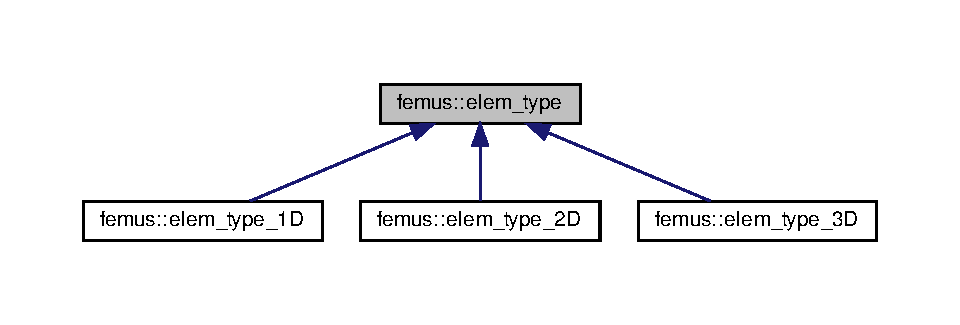
\includegraphics[width=350pt]{classfemus_1_1elem__type__inherit__graph}
\end{center}
\end{figure}


Collaboration diagram for femus\+:\+:elem\+\_\+type\+:
\nopagebreak
\begin{figure}[H]
\begin{center}
\leavevmode
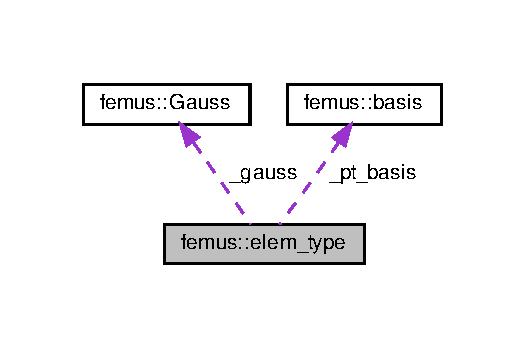
\includegraphics[width=252pt]{classfemus_1_1elem__type__coll__graph}
\end{center}
\end{figure}
\subsection*{Public Types}
\begin{DoxyCompactItemize}
\item 
typedef double $\ast$(elem\+\_\+type\+::$\ast$ \mbox{\hyperlink{classfemus_1_1elem__type_ac6d3f8df5299550225a2f77c2aa15dde}{\+\_\+\+Function\+Pointer}}) (const unsigned \&\mbox{\hyperlink{namespacefemus_a6df31099f676311de214a312d7043941}{ig}}) const
\end{DoxyCompactItemize}
\subsection*{Public Member Functions}
\begin{DoxyCompactItemize}
\item 
\mbox{\hyperlink{classfemus_1_1elem__type_aa2d116602d97b226a4a01578dd45bb20}{elem\+\_\+type}} (const char $\ast$geom\+\_\+elem, const char $\ast$order\+\_\+gauss)
\item 
virtual \mbox{\hyperlink{classfemus_1_1elem__type_a3e13560174d1ea0282665fbbf4eb605d}{$\sim$elem\+\_\+type}} ()
\item 
void \mbox{\hyperlink{classfemus_1_1elem__type_aaa5317cf0e1944adeaca3b5f1d0c3610}{Build\+Prolongation}} (const \mbox{\hyperlink{classfemus_1_1_linear_equation}{Linear\+Equation}} \&lspdef, const \mbox{\hyperlink{classfemus_1_1_linear_equation}{Linear\+Equation}} \&lspdec, const int \&ielc, \mbox{\hyperlink{classfemus_1_1_sparse_matrix}{Sparse\+Matrix}} $\ast$Projmat, const unsigned \&index\+\_\+sol, const unsigned \&kkindex\+\_\+sol) const
\item 
void \mbox{\hyperlink{classfemus_1_1elem__type_a204517efabff34e2692a77f4b8bd44e9}{Build\+Restriction\+Transpose}} (const \mbox{\hyperlink{classfemus_1_1_linear_equation}{Linear\+Equation}} \&lspdef, const \mbox{\hyperlink{classfemus_1_1_linear_equation}{Linear\+Equation}} \&lspdec, const int \&ielc, \mbox{\hyperlink{classfemus_1_1_sparse_matrix}{Sparse\+Matrix}} $\ast$Projmat, const unsigned \&index\+\_\+sol, const unsigned \&kkindex\+\_\+sol, const unsigned \&index\+\_\+pair\+\_\+sol, const unsigned \&kkindex\+\_\+pair\+\_\+sol) const
\item 
void \mbox{\hyperlink{classfemus_1_1elem__type_ab877a3438c82ef2b4f096f38c3811b7f}{Build\+Prolongation}} (const \mbox{\hyperlink{classfemus_1_1_mesh}{Mesh}} \&meshf, const \mbox{\hyperlink{classfemus_1_1_mesh}{Mesh}} \&meshc, const int \&ielc, \mbox{\hyperlink{classfemus_1_1_sparse_matrix}{Sparse\+Matrix}} $\ast$Projmat) const
\item 
void \mbox{\hyperlink{classfemus_1_1elem__type_acb499269b353c8b3e0ebb5e21254b108}{Build\+Prolongation}} (const \mbox{\hyperlink{classfemus_1_1_mesh}{Mesh}} \&mymesh, const int \&iel, \mbox{\hyperlink{classfemus_1_1_sparse_matrix}{Sparse\+Matrix}} $\ast$Projmat, \mbox{\hyperlink{classfemus_1_1_numeric_vector}{Numeric\+Vector}} $\ast$N\+N\+Z\+\_\+d, \mbox{\hyperlink{classfemus_1_1_numeric_vector}{Numeric\+Vector}} $\ast$N\+N\+Z\+\_\+o, const unsigned \&itype) const
\item 
virtual void \mbox{\hyperlink{classfemus_1_1elem__type_aa8e617c54dd774ffca5d305605552af7}{Get\+Jacobian}} (const vector$<$ vector$<$ adept\+::adouble $>$ $>$ \&vt, const unsigned \&\mbox{\hyperlink{namespacefemus_a6df31099f676311de214a312d7043941}{ig}}, adept\+::adouble \&Weight, vector$<$ vector$<$ adept\+::adouble $>$ $>$ \&jacobian\+Matrix) const =0
\item 
virtual void \mbox{\hyperlink{classfemus_1_1elem__type_a6c883b7946e55db8783fd0177546610a}{Get\+Jacobian}} (const vector$<$ vector$<$ double $>$ $>$ \&vt, const unsigned \&\mbox{\hyperlink{namespacefemus_a6df31099f676311de214a312d7043941}{ig}}, double \&Weight, vector$<$ vector$<$ double $>$ $>$ \&jacobian\+Matrix) const =0
\item 
virtual void \mbox{\hyperlink{classfemus_1_1elem__type_a937b1d5ecbeed3b17db831264a3492fa}{Jacobian}} (const vector$<$ vector$<$ adept\+::adouble $>$ $>$ \&vt, const unsigned \&\mbox{\hyperlink{namespacefemus_a6df31099f676311de214a312d7043941}{ig}}, adept\+::adouble \&Weight, vector$<$ double $>$ \&phi, vector$<$ adept\+::adouble $>$ \&gradphi, boost\+::optional$<$ vector$<$ adept\+::adouble $>$ \& $>$ nablaphi=boost\+::none) const =0
\item 
virtual void \mbox{\hyperlink{classfemus_1_1elem__type_ac3828ecd8ddd057d726a60cb19c60f0b}{Jacobian}} (const vector$<$ vector$<$ double $>$ $>$ \&vt, const unsigned \&\mbox{\hyperlink{namespacefemus_a6df31099f676311de214a312d7043941}{ig}}, double \&Weight, vector$<$ double $>$ \&other\+\_\+phi, vector$<$ double $>$ \&gradphi, boost\+::optional$<$ vector$<$ double $>$ \& $>$ nablaphi=boost\+::none) const =0
\item 
virtual void \mbox{\hyperlink{classfemus_1_1elem__type_a2d76133387cebf896c0e51459055fdea}{Jacobian}} (const vector$<$ vector$<$ adept\+::adouble $>$ $>$ \&vt, const vector$<$ double $>$ \&xi, adept\+::adouble \&Weight, vector$<$ double $>$ \&phi, vector$<$ adept\+::adouble $>$ \&gradphi, boost\+::optional$<$ vector$<$ adept\+::adouble $>$ \& $>$ nablaphi=boost\+::none) const =0
\item 
virtual void \mbox{\hyperlink{classfemus_1_1elem__type_aab6db5851a9810adfe0ff98df2c30810}{Jacobian}} (const vector$<$ vector$<$ double $>$ $>$ \&vt, const vector$<$ double $>$ \&xi, double \&Weight, vector$<$ double $>$ \&other\+\_\+phi, vector$<$ double $>$ \&gradphi, boost\+::optional$<$ vector$<$ double $>$ \& $>$ nablaphi=boost\+::none) const =0
\item 
virtual void \mbox{\hyperlink{classfemus_1_1elem__type_a293052fac0f51472150b1bf7365c6b18}{Jacobian\+Sur}} (const vector$<$ vector$<$ adept\+::adouble $>$ $>$ \&vt, const unsigned \&\mbox{\hyperlink{namespacefemus_a6df31099f676311de214a312d7043941}{ig}}, adept\+::adouble \&Weight, vector$<$ double $>$ \&other\+\_\+phi, vector$<$ adept\+::adouble $>$ \&gradphi, vector$<$ adept\+::adouble $>$ \&normal) const =0
\item 
virtual void \mbox{\hyperlink{classfemus_1_1elem__type_aee56bc66a4d90ae7f7669bf7fa9ed8d7}{Jacobian\+Sur}} (const vector$<$ vector$<$ double $>$ $>$ \&vt, const unsigned \&\mbox{\hyperlink{namespacefemus_a6df31099f676311de214a312d7043941}{ig}}, double \&Weight, vector$<$ double $>$ \&other\+\_\+phi, vector$<$ double $>$ \&gradphi, vector$<$ double $>$ \&normal) const =0
\item 
virtual double $\ast$ \mbox{\hyperlink{classfemus_1_1elem__type_a2aa2a37b15debbee27918f5e3f2df6b3}{Get\+Phi}} (const unsigned \&\mbox{\hyperlink{namespacefemus_a6df31099f676311de214a312d7043941}{ig}}) const =0
\item 
virtual double $\ast$ \mbox{\hyperlink{classfemus_1_1elem__type_a6efb6026b9fe89912ec367b235bfccc7}{Get\+D\+Phi\+D\+Xi}} (const unsigned \&\mbox{\hyperlink{namespacefemus_a6df31099f676311de214a312d7043941}{ig}}) const =0
\item 
virtual double $\ast$ \mbox{\hyperlink{classfemus_1_1elem__type_a510e44439de5cdd6ab5d04e3f8a5bdfe}{Get\+D\+Phi\+D\+Eta}} (const unsigned \&\mbox{\hyperlink{namespacefemus_a6df31099f676311de214a312d7043941}{ig}}) const
\item 
virtual double $\ast$ \mbox{\hyperlink{classfemus_1_1elem__type_aa507628a4383a9687c8fdefe30d0214a}{Get\+D\+Phi\+D\+Zeta}} (const unsigned \&\mbox{\hyperlink{namespacefemus_a6df31099f676311de214a312d7043941}{ig}}) const
\item 
virtual void \mbox{\hyperlink{classfemus_1_1elem__type_ab5244df8f1bc5c57a81158787bb1a588}{Evaluate\+Shape\+At\+QP}} (const std\+::string geomel\+\_\+id\+\_\+in, const std\+::string fe\+\_\+in)
\item 
const double \mbox{\hyperlink{classfemus_1_1elem__type_a0112208bbdff765b47effbe352734fbe}{Get\+Phi}} (const \mbox{\hyperlink{_typedefs_8hpp_a91ad9478d81a7aaf2593e8d9c3d06a14}{uint}} qp, const \mbox{\hyperlink{_typedefs_8hpp_a91ad9478d81a7aaf2593e8d9c3d06a14}{uint}} dof) const
\item 
const double \mbox{\hyperlink{classfemus_1_1elem__type_a8de9e4d4d56ef38431a5050269390e1a}{Get\+D\+Phi\+Dxez}} (const \mbox{\hyperlink{_typedefs_8hpp_a91ad9478d81a7aaf2593e8d9c3d06a14}{uint}} qp, const \mbox{\hyperlink{_typedefs_8hpp_a91ad9478d81a7aaf2593e8d9c3d06a14}{uint}} dof) const
\item 
const \mbox{\hyperlink{classfemus_1_1_gauss}{Gauss}} \mbox{\hyperlink{classfemus_1_1elem__type_a830387ca17a267d99a8ec97fa0548fc3}{Get\+Gauss\+Rule}} () const
\item 
double \mbox{\hyperlink{classfemus_1_1elem__type_a86dfc5d292bb86bb02ac13f5acbb6c98}{Get\+Gauss\+Weight}} (const unsigned \mbox{\hyperlink{namespacefemus_a6df31099f676311de214a312d7043941}{ig}}) const
\item 
unsigned \mbox{\hyperlink{classfemus_1_1elem__type_a3fa8f889f9ae97586b3db574acb4448e}{Get\+Gauss\+Point\+Number}} () const
\item 
int \mbox{\hyperlink{classfemus_1_1elem__type_a7597b01400759749a8b76e01722cd89b}{Get\+N\+Dofs}} () const
\item 
unsigned \mbox{\hyperlink{classfemus_1_1elem__type_aa94378d258af64d24a9970d30f229589}{Get\+Dim}} () const
\item 
void \mbox{\hyperlink{classfemus_1_1elem__type_a6e40b6760ceb52bc3a6d5959ab1588ba}{Get\+Sparsity\+Pattern\+Size}} (const \mbox{\hyperlink{classfemus_1_1_linear_equation}{Linear\+Equation}} \&lspdef, const \mbox{\hyperlink{classfemus_1_1_linear_equation}{Linear\+Equation}} \&lspdec, const int \&ielc, \mbox{\hyperlink{classfemus_1_1_numeric_vector}{Numeric\+Vector}} $\ast$N\+N\+Z\+\_\+d, \mbox{\hyperlink{classfemus_1_1_numeric_vector}{Numeric\+Vector}} $\ast$N\+N\+Z\+\_\+o, const unsigned \&index\+\_\+sol, const unsigned \&kkindex\+\_\+sol) const
\item 
void \mbox{\hyperlink{classfemus_1_1elem__type_a2e66f8115d7da31bc740db29e1524d60}{Get\+Sparsity\+Pattern\+Size}} (const \mbox{\hyperlink{classfemus_1_1_mesh}{Mesh}} \&meshf, const \mbox{\hyperlink{classfemus_1_1_mesh}{Mesh}} \&meshc, const int \&ielc, \mbox{\hyperlink{classfemus_1_1_numeric_vector}{Numeric\+Vector}} $\ast$N\+N\+Z\+\_\+d, \mbox{\hyperlink{classfemus_1_1_numeric_vector}{Numeric\+Vector}} $\ast$N\+N\+Z\+\_\+o) const
\item 
void \mbox{\hyperlink{classfemus_1_1elem__type_a9e3cfe2ed283c16125594e5c3a02c8cd}{Get\+Sparsity\+Pattern\+Size}} (const \mbox{\hyperlink{classfemus_1_1_mesh}{Mesh}} \&\mbox{\hyperlink{classfemus_1_1_mesh}{Mesh}}, const int \&iel, \mbox{\hyperlink{classfemus_1_1_numeric_vector}{Numeric\+Vector}} $\ast$N\+N\+Z\+\_\+d, \mbox{\hyperlink{classfemus_1_1_numeric_vector}{Numeric\+Vector}} $\ast$N\+N\+Z\+\_\+o, const unsigned \&itype) const
\item 
\mbox{\hyperlink{classfemus_1_1basis}{basis}} $\ast$ \mbox{\hyperlink{classfemus_1_1elem__type_a8d0ba58ed22eccd39304ba1d84a7b891}{Get\+Basis}} () const
\end{DoxyCompactItemize}
\subsection*{Public Attributes}
\begin{DoxyCompactItemize}
\item 
std\+::vector$<$ \mbox{\hyperlink{classfemus_1_1elem__type_ac6d3f8df5299550225a2f77c2aa15dde}{\+\_\+\+Function\+Pointer}} $>$ \mbox{\hyperlink{classfemus_1_1elem__type_acb75b2a53188353c30e56bf3899243e2}{\+\_\+\+D\+Phi\+Xi\+Eta\+Zeta\+Ptr}}
\end{DoxyCompactItemize}
\subsection*{Static Public Attributes}
\begin{DoxyCompactItemize}
\item 
static unsigned \mbox{\hyperlink{classfemus_1_1elem__type_ac090b500b9fe133dec615fae6545b3a8}{\+\_\+refindex}} = 1
\item 
static const unsigned \mbox{\hyperlink{classfemus_1_1elem__type_a6cba788f2fbdef1b91a1492908794f8d}{\+\_\+fe\+\_\+old\+\_\+to\+\_\+new}} \mbox{[}\mbox{\hyperlink{_f_e_type_enum_8hpp_aca285339f9cf24489fdc0af5b51a5fde}{QL}}\mbox{]} = \{2, 0, 3\}
\end{DoxyCompactItemize}
\subsection*{Protected Attributes}
\begin{DoxyCompactItemize}
\item 
unsigned \mbox{\hyperlink{classfemus_1_1elem__type_a71ea0da630a7830c3278d58243da0ead}{\+\_\+dim}}
\item 
int \mbox{\hyperlink{classfemus_1_1elem__type_aeaf5fcedea91ceb9894f5a385eebddab}{\+\_\+nc}}
\item 
int \mbox{\hyperlink{classfemus_1_1elem__type_aaa24556879d31c619c0258062c77276b}{\+\_\+nf}}
\item 
int \mbox{\hyperlink{classfemus_1_1elem__type_a7ffed37a1c710167fc1aed224cce45f4}{\+\_\+nlag}} \mbox{[}4\mbox{]}
\item 
unsigned \mbox{\hyperlink{classfemus_1_1elem__type_a3278ebbdc41e6e7c03aea23995220dab}{\+\_\+\+Sol\+Type}}
\item 
const double $\ast$$\ast$ \mbox{\hyperlink{classfemus_1_1elem__type_aa69848a2a5365dc3647b8b0f756a6ec0}{\+\_\+X}}
\item 
const int $\ast$$\ast$ \mbox{\hyperlink{classfemus_1_1elem__type_ab6163fc83bbd668366744f1d1cc405ca}{\+\_\+\+I\+ND}}
\item 
const int $\ast$$\ast$ \mbox{\hyperlink{classfemus_1_1elem__type_a22d10410085b36b93db138252d6860b9}{\+\_\+\+K\+V\+E\+R\+T\+\_\+\+I\+ND}}
\item 
double $\ast$$\ast$ \mbox{\hyperlink{classfemus_1_1elem__type_aca81317b1dfdf99cb82d6c47c7906534}{\+\_\+prol\+\_\+val}}
\item 
int $\ast$$\ast$ \mbox{\hyperlink{classfemus_1_1elem__type_a51686b913b9626125f58feea7c7ca5da}{\+\_\+prol\+\_\+ind}}
\item 
double $\ast$ \mbox{\hyperlink{classfemus_1_1elem__type_ab99cb41fdebab468d2ae484fe8a65edd}{\+\_\+mem\+\_\+prol\+\_\+val}}
\item 
int $\ast$ \mbox{\hyperlink{classfemus_1_1elem__type_a7c4de3964da26762c3c500d7311fc23b}{\+\_\+mem\+\_\+prol\+\_\+ind}}
\item 
\mbox{\hyperlink{classfemus_1_1basis}{basis}} $\ast$ \mbox{\hyperlink{classfemus_1_1elem__type_a74ff85a1f6d5439f08c25d4d0321c609}{\+\_\+pt\+\_\+basis}}
\item 
const \mbox{\hyperlink{classfemus_1_1_gauss}{Gauss}} \mbox{\hyperlink{classfemus_1_1elem__type_a4c14f3f54d9317b57f2effd2519e45b9}{\+\_\+gauss}}
\item 
bool \mbox{\hyperlink{classfemus_1_1elem__type_a57a7738e4179b9ca205db7e3c18898af}{is\+Mp\+G\+D\+Allocated}}
\item 
double $\ast$$\ast$ \mbox{\hyperlink{classfemus_1_1elem__type_a54e9c728b24b46b7cfe7163caf8f44ba}{\+\_\+phi\+\_\+map\+GD}}
\item 
double $\ast$$\ast$ \mbox{\hyperlink{classfemus_1_1elem__type_a631bc33eb5635fe19fa879246cfde2a2}{\+\_\+dphidxez\+\_\+map\+GD}}
\end{DoxyCompactItemize}


\subsection{Member Typedef Documentation}
\mbox{\Hypertarget{classfemus_1_1elem__type_ac6d3f8df5299550225a2f77c2aa15dde}\label{classfemus_1_1elem__type_ac6d3f8df5299550225a2f77c2aa15dde}} 
\index{femus\+::elem\+\_\+type@{femus\+::elem\+\_\+type}!\+\_\+\+Function\+Pointer@{\+\_\+\+Function\+Pointer}}
\index{\+\_\+\+Function\+Pointer@{\+\_\+\+Function\+Pointer}!femus\+::elem\+\_\+type@{femus\+::elem\+\_\+type}}
\subsubsection{\texorpdfstring{\+\_\+\+Function\+Pointer}{\_FunctionPointer}}
{\footnotesize\ttfamily typedef double$\ast$(elem\+\_\+type\+::$\ast$ femus\+::elem\+\_\+type\+::\+\_\+\+Function\+Pointer) (const unsigned \&\mbox{\hyperlink{namespacefemus_a6df31099f676311de214a312d7043941}{ig}}) const}

To be Added \begin{DoxyRefDesc}{Deprecated}
\item[\mbox{\hyperlink{deprecated__deprecated000015}{Deprecated}}]Function pointer for D\+Phi\+D\+X\+EZ \end{DoxyRefDesc}


\subsection{Constructor \& Destructor Documentation}
\mbox{\Hypertarget{classfemus_1_1elem__type_aa2d116602d97b226a4a01578dd45bb20}\label{classfemus_1_1elem__type_aa2d116602d97b226a4a01578dd45bb20}} 
\index{femus\+::elem\+\_\+type@{femus\+::elem\+\_\+type}!elem\+\_\+type@{elem\+\_\+type}}
\index{elem\+\_\+type@{elem\+\_\+type}!femus\+::elem\+\_\+type@{femus\+::elem\+\_\+type}}
\subsubsection{\texorpdfstring{elem\+\_\+type()}{elem\_type()}}
{\footnotesize\ttfamily femus\+::elem\+\_\+type\+::elem\+\_\+type (\begin{DoxyParamCaption}\item[{const char $\ast$}]{geom\+\_\+elem,  }\item[{const char $\ast$}]{order\+\_\+gauss }\end{DoxyParamCaption})}

constructor that receives Geometric Element and \mbox{\hyperlink{classfemus_1_1_gauss}{Gauss}} info \mbox{\Hypertarget{classfemus_1_1elem__type_a3e13560174d1ea0282665fbbf4eb605d}\label{classfemus_1_1elem__type_a3e13560174d1ea0282665fbbf4eb605d}} 
\index{femus\+::elem\+\_\+type@{femus\+::elem\+\_\+type}!````~elem\+\_\+type@{$\sim$elem\+\_\+type}}
\index{````~elem\+\_\+type@{$\sim$elem\+\_\+type}!femus\+::elem\+\_\+type@{femus\+::elem\+\_\+type}}
\subsubsection{\texorpdfstring{$\sim$elem\+\_\+type()}{~elem\_type()}}
{\footnotesize\ttfamily femus\+::elem\+\_\+type\+::$\sim$elem\+\_\+type (\begin{DoxyParamCaption}{ }\end{DoxyParamCaption})\hspace{0.3cm}{\ttfamily [virtual]}}

destructor 

\subsection{Member Function Documentation}
\mbox{\Hypertarget{classfemus_1_1elem__type_aaa5317cf0e1944adeaca3b5f1d0c3610}\label{classfemus_1_1elem__type_aaa5317cf0e1944adeaca3b5f1d0c3610}} 
\index{femus\+::elem\+\_\+type@{femus\+::elem\+\_\+type}!Build\+Prolongation@{Build\+Prolongation}}
\index{Build\+Prolongation@{Build\+Prolongation}!femus\+::elem\+\_\+type@{femus\+::elem\+\_\+type}}
\subsubsection{\texorpdfstring{Build\+Prolongation()}{BuildProlongation()}\hspace{0.1cm}{\footnotesize\ttfamily [1/3]}}
{\footnotesize\ttfamily void femus\+::elem\+\_\+type\+::\+Build\+Prolongation (\begin{DoxyParamCaption}\item[{const \mbox{\hyperlink{classfemus_1_1_linear_equation}{Linear\+Equation}} \&}]{lspdef,  }\item[{const \mbox{\hyperlink{classfemus_1_1_linear_equation}{Linear\+Equation}} \&}]{lspdec,  }\item[{const int \&}]{ielc,  }\item[{\mbox{\hyperlink{classfemus_1_1_sparse_matrix}{Sparse\+Matrix}} $\ast$}]{Projmat,  }\item[{const unsigned \&}]{index\+\_\+sol,  }\item[{const unsigned \&}]{kkindex\+\_\+sol }\end{DoxyParamCaption}) const}

To be Added \mbox{\Hypertarget{classfemus_1_1elem__type_ab877a3438c82ef2b4f096f38c3811b7f}\label{classfemus_1_1elem__type_ab877a3438c82ef2b4f096f38c3811b7f}} 
\index{femus\+::elem\+\_\+type@{femus\+::elem\+\_\+type}!Build\+Prolongation@{Build\+Prolongation}}
\index{Build\+Prolongation@{Build\+Prolongation}!femus\+::elem\+\_\+type@{femus\+::elem\+\_\+type}}
\subsubsection{\texorpdfstring{Build\+Prolongation()}{BuildProlongation()}\hspace{0.1cm}{\footnotesize\ttfamily [2/3]}}
{\footnotesize\ttfamily void femus\+::elem\+\_\+type\+::\+Build\+Prolongation (\begin{DoxyParamCaption}\item[{const \mbox{\hyperlink{classfemus_1_1_mesh}{Mesh}} \&}]{meshf,  }\item[{const \mbox{\hyperlink{classfemus_1_1_mesh}{Mesh}} \&}]{meshc,  }\item[{const int \&}]{ielc,  }\item[{\mbox{\hyperlink{classfemus_1_1_sparse_matrix}{Sparse\+Matrix}} $\ast$}]{Projmat }\end{DoxyParamCaption}) const}

To be Added \mbox{\Hypertarget{classfemus_1_1elem__type_acb499269b353c8b3e0ebb5e21254b108}\label{classfemus_1_1elem__type_acb499269b353c8b3e0ebb5e21254b108}} 
\index{femus\+::elem\+\_\+type@{femus\+::elem\+\_\+type}!Build\+Prolongation@{Build\+Prolongation}}
\index{Build\+Prolongation@{Build\+Prolongation}!femus\+::elem\+\_\+type@{femus\+::elem\+\_\+type}}
\subsubsection{\texorpdfstring{Build\+Prolongation()}{BuildProlongation()}\hspace{0.1cm}{\footnotesize\ttfamily [3/3]}}
{\footnotesize\ttfamily void femus\+::elem\+\_\+type\+::\+Build\+Prolongation (\begin{DoxyParamCaption}\item[{const \mbox{\hyperlink{classfemus_1_1_mesh}{Mesh}} \&}]{mymesh,  }\item[{const int \&}]{iel,  }\item[{\mbox{\hyperlink{classfemus_1_1_sparse_matrix}{Sparse\+Matrix}} $\ast$}]{Projmat,  }\item[{\mbox{\hyperlink{classfemus_1_1_numeric_vector}{Numeric\+Vector}} $\ast$}]{N\+N\+Z\+\_\+d,  }\item[{\mbox{\hyperlink{classfemus_1_1_numeric_vector}{Numeric\+Vector}} $\ast$}]{N\+N\+Z\+\_\+o,  }\item[{const unsigned \&}]{itype }\end{DoxyParamCaption}) const}

To be Added \mbox{\Hypertarget{classfemus_1_1elem__type_a204517efabff34e2692a77f4b8bd44e9}\label{classfemus_1_1elem__type_a204517efabff34e2692a77f4b8bd44e9}} 
\index{femus\+::elem\+\_\+type@{femus\+::elem\+\_\+type}!Build\+Restriction\+Transpose@{Build\+Restriction\+Transpose}}
\index{Build\+Restriction\+Transpose@{Build\+Restriction\+Transpose}!femus\+::elem\+\_\+type@{femus\+::elem\+\_\+type}}
\subsubsection{\texorpdfstring{Build\+Restriction\+Transpose()}{BuildRestrictionTranspose()}}
{\footnotesize\ttfamily void femus\+::elem\+\_\+type\+::\+Build\+Restriction\+Transpose (\begin{DoxyParamCaption}\item[{const \mbox{\hyperlink{classfemus_1_1_linear_equation}{Linear\+Equation}} \&}]{lspdef,  }\item[{const \mbox{\hyperlink{classfemus_1_1_linear_equation}{Linear\+Equation}} \&}]{lspdec,  }\item[{const int \&}]{ielc,  }\item[{\mbox{\hyperlink{classfemus_1_1_sparse_matrix}{Sparse\+Matrix}} $\ast$}]{Projmat,  }\item[{const unsigned \&}]{index\+\_\+sol,  }\item[{const unsigned \&}]{kkindex\+\_\+sol,  }\item[{const unsigned \&}]{index\+\_\+pair\+\_\+sol,  }\item[{const unsigned \&}]{kkindex\+\_\+pair\+\_\+sol }\end{DoxyParamCaption}) const}

To be Added \mbox{\Hypertarget{classfemus_1_1elem__type_ab5244df8f1bc5c57a81158787bb1a588}\label{classfemus_1_1elem__type_ab5244df8f1bc5c57a81158787bb1a588}} 
\index{femus\+::elem\+\_\+type@{femus\+::elem\+\_\+type}!Evaluate\+Shape\+At\+QP@{Evaluate\+Shape\+At\+QP}}
\index{Evaluate\+Shape\+At\+QP@{Evaluate\+Shape\+At\+QP}!femus\+::elem\+\_\+type@{femus\+::elem\+\_\+type}}
\subsubsection{\texorpdfstring{Evaluate\+Shape\+At\+Q\+P()}{EvaluateShapeAtQP()}}
{\footnotesize\ttfamily void femus\+::elem\+\_\+type\+::\+Evaluate\+Shape\+At\+QP (\begin{DoxyParamCaption}\item[{const std\+::string}]{geomel\+\_\+id\+\_\+in,  }\item[{const std\+::string}]{fe\+\_\+in }\end{DoxyParamCaption})\hspace{0.3cm}{\ttfamily [virtual]}}

\begin{DoxyRefDesc}{Deprecated}
\item[\mbox{\hyperlink{deprecated__deprecated000016}{Deprecated}}]Evaluate shape functions at all quadrature points \end{DoxyRefDesc}
\mbox{\Hypertarget{classfemus_1_1elem__type_a8d0ba58ed22eccd39304ba1d84a7b891}\label{classfemus_1_1elem__type_a8d0ba58ed22eccd39304ba1d84a7b891}} 
\index{femus\+::elem\+\_\+type@{femus\+::elem\+\_\+type}!Get\+Basis@{Get\+Basis}}
\index{Get\+Basis@{Get\+Basis}!femus\+::elem\+\_\+type@{femus\+::elem\+\_\+type}}
\subsubsection{\texorpdfstring{Get\+Basis()}{GetBasis()}}
{\footnotesize\ttfamily \mbox{\hyperlink{classfemus_1_1basis}{basis}}$\ast$ femus\+::elem\+\_\+type\+::\+Get\+Basis (\begin{DoxyParamCaption}{ }\end{DoxyParamCaption}) const\hspace{0.3cm}{\ttfamily [inline]}}

\mbox{\Hypertarget{classfemus_1_1elem__type_aa94378d258af64d24a9970d30f229589}\label{classfemus_1_1elem__type_aa94378d258af64d24a9970d30f229589}} 
\index{femus\+::elem\+\_\+type@{femus\+::elem\+\_\+type}!Get\+Dim@{Get\+Dim}}
\index{Get\+Dim@{Get\+Dim}!femus\+::elem\+\_\+type@{femus\+::elem\+\_\+type}}
\subsubsection{\texorpdfstring{Get\+Dim()}{GetDim()}}
{\footnotesize\ttfamily unsigned femus\+::elem\+\_\+type\+::\+Get\+Dim (\begin{DoxyParamCaption}{ }\end{DoxyParamCaption}) const\hspace{0.3cm}{\ttfamily [inline]}}

Retrieve the dimension of the underlying geometric element \mbox{\Hypertarget{classfemus_1_1elem__type_a510e44439de5cdd6ab5d04e3f8a5bdfe}\label{classfemus_1_1elem__type_a510e44439de5cdd6ab5d04e3f8a5bdfe}} 
\index{femus\+::elem\+\_\+type@{femus\+::elem\+\_\+type}!Get\+D\+Phi\+D\+Eta@{Get\+D\+Phi\+D\+Eta}}
\index{Get\+D\+Phi\+D\+Eta@{Get\+D\+Phi\+D\+Eta}!femus\+::elem\+\_\+type@{femus\+::elem\+\_\+type}}
\subsubsection{\texorpdfstring{Get\+D\+Phi\+D\+Eta()}{GetDPhiDEta()}}
{\footnotesize\ttfamily virtual double$\ast$ femus\+::elem\+\_\+type\+::\+Get\+D\+Phi\+D\+Eta (\begin{DoxyParamCaption}\item[{const unsigned \&}]{ig }\end{DoxyParamCaption}) const\hspace{0.3cm}{\ttfamily [inline]}, {\ttfamily [virtual]}}

To be Added 

Reimplemented in \mbox{\hyperlink{classfemus_1_1elem__type__3_d_aa08787fdf3934c52c41a14a59884eb7b}{femus\+::elem\+\_\+type\+\_\+3D}}, and \mbox{\hyperlink{classfemus_1_1elem__type__2_d_a3a77bc47f11a128210ed5c22a1179cc4}{femus\+::elem\+\_\+type\+\_\+2D}}.

\mbox{\Hypertarget{classfemus_1_1elem__type_a8de9e4d4d56ef38431a5050269390e1a}\label{classfemus_1_1elem__type_a8de9e4d4d56ef38431a5050269390e1a}} 
\index{femus\+::elem\+\_\+type@{femus\+::elem\+\_\+type}!Get\+D\+Phi\+Dxez@{Get\+D\+Phi\+Dxez}}
\index{Get\+D\+Phi\+Dxez@{Get\+D\+Phi\+Dxez}!femus\+::elem\+\_\+type@{femus\+::elem\+\_\+type}}
\subsubsection{\texorpdfstring{Get\+D\+Phi\+Dxez()}{GetDPhiDxez()}}
{\footnotesize\ttfamily const double femus\+::elem\+\_\+type\+::\+Get\+D\+Phi\+Dxez (\begin{DoxyParamCaption}\item[{const \mbox{\hyperlink{_typedefs_8hpp_a91ad9478d81a7aaf2593e8d9c3d06a14}{uint}}}]{qp,  }\item[{const \mbox{\hyperlink{_typedefs_8hpp_a91ad9478d81a7aaf2593e8d9c3d06a14}{uint}}}]{dof }\end{DoxyParamCaption}) const\hspace{0.3cm}{\ttfamily [inline]}}

\begin{DoxyRefDesc}{Deprecated}
\item[\mbox{\hyperlink{deprecated__deprecated000018}{Deprecated}}]Get shape function first derivatives \end{DoxyRefDesc}
\mbox{\Hypertarget{classfemus_1_1elem__type_a6efb6026b9fe89912ec367b235bfccc7}\label{classfemus_1_1elem__type_a6efb6026b9fe89912ec367b235bfccc7}} 
\index{femus\+::elem\+\_\+type@{femus\+::elem\+\_\+type}!Get\+D\+Phi\+D\+Xi@{Get\+D\+Phi\+D\+Xi}}
\index{Get\+D\+Phi\+D\+Xi@{Get\+D\+Phi\+D\+Xi}!femus\+::elem\+\_\+type@{femus\+::elem\+\_\+type}}
\subsubsection{\texorpdfstring{Get\+D\+Phi\+D\+Xi()}{GetDPhiDXi()}}
{\footnotesize\ttfamily virtual double$\ast$ femus\+::elem\+\_\+type\+::\+Get\+D\+Phi\+D\+Xi (\begin{DoxyParamCaption}\item[{const unsigned \&}]{ig }\end{DoxyParamCaption}) const\hspace{0.3cm}{\ttfamily [pure virtual]}}

To be Added 

Implemented in \mbox{\hyperlink{classfemus_1_1elem__type__3_d_aff869fa323fd20f83fed73f4a28de006}{femus\+::elem\+\_\+type\+\_\+3D}}, \mbox{\hyperlink{classfemus_1_1elem__type__2_d_a11838ba0522b27348770989555114c94}{femus\+::elem\+\_\+type\+\_\+2D}}, and \mbox{\hyperlink{classfemus_1_1elem__type__1_d_a27ff9f2a7f26c961b9b9d96aa87723d2}{femus\+::elem\+\_\+type\+\_\+1D}}.

\mbox{\Hypertarget{classfemus_1_1elem__type_aa507628a4383a9687c8fdefe30d0214a}\label{classfemus_1_1elem__type_aa507628a4383a9687c8fdefe30d0214a}} 
\index{femus\+::elem\+\_\+type@{femus\+::elem\+\_\+type}!Get\+D\+Phi\+D\+Zeta@{Get\+D\+Phi\+D\+Zeta}}
\index{Get\+D\+Phi\+D\+Zeta@{Get\+D\+Phi\+D\+Zeta}!femus\+::elem\+\_\+type@{femus\+::elem\+\_\+type}}
\subsubsection{\texorpdfstring{Get\+D\+Phi\+D\+Zeta()}{GetDPhiDZeta()}}
{\footnotesize\ttfamily virtual double$\ast$ femus\+::elem\+\_\+type\+::\+Get\+D\+Phi\+D\+Zeta (\begin{DoxyParamCaption}\item[{const unsigned \&}]{ig }\end{DoxyParamCaption}) const\hspace{0.3cm}{\ttfamily [inline]}, {\ttfamily [virtual]}}

To be Added 

Reimplemented in \mbox{\hyperlink{classfemus_1_1elem__type__3_d_a8bf7020e0c07cf44c9532f9b6bab4bbc}{femus\+::elem\+\_\+type\+\_\+3D}}.

\mbox{\Hypertarget{classfemus_1_1elem__type_a3fa8f889f9ae97586b3db574acb4448e}\label{classfemus_1_1elem__type_a3fa8f889f9ae97586b3db574acb4448e}} 
\index{femus\+::elem\+\_\+type@{femus\+::elem\+\_\+type}!Get\+Gauss\+Point\+Number@{Get\+Gauss\+Point\+Number}}
\index{Get\+Gauss\+Point\+Number@{Get\+Gauss\+Point\+Number}!femus\+::elem\+\_\+type@{femus\+::elem\+\_\+type}}
\subsubsection{\texorpdfstring{Get\+Gauss\+Point\+Number()}{GetGaussPointNumber()}}
{\footnotesize\ttfamily unsigned femus\+::elem\+\_\+type\+::\+Get\+Gauss\+Point\+Number (\begin{DoxyParamCaption}{ }\end{DoxyParamCaption}) const\hspace{0.3cm}{\ttfamily [inline]}}

To be Added \mbox{\Hypertarget{classfemus_1_1elem__type_a830387ca17a267d99a8ec97fa0548fc3}\label{classfemus_1_1elem__type_a830387ca17a267d99a8ec97fa0548fc3}} 
\index{femus\+::elem\+\_\+type@{femus\+::elem\+\_\+type}!Get\+Gauss\+Rule@{Get\+Gauss\+Rule}}
\index{Get\+Gauss\+Rule@{Get\+Gauss\+Rule}!femus\+::elem\+\_\+type@{femus\+::elem\+\_\+type}}
\subsubsection{\texorpdfstring{Get\+Gauss\+Rule()}{GetGaussRule()}}
{\footnotesize\ttfamily const \mbox{\hyperlink{classfemus_1_1_gauss}{Gauss}} femus\+::elem\+\_\+type\+::\+Get\+Gauss\+Rule (\begin{DoxyParamCaption}{ }\end{DoxyParamCaption}) const\hspace{0.3cm}{\ttfamily [inline]}}

To be Added \mbox{\Hypertarget{classfemus_1_1elem__type_a86dfc5d292bb86bb02ac13f5acbb6c98}\label{classfemus_1_1elem__type_a86dfc5d292bb86bb02ac13f5acbb6c98}} 
\index{femus\+::elem\+\_\+type@{femus\+::elem\+\_\+type}!Get\+Gauss\+Weight@{Get\+Gauss\+Weight}}
\index{Get\+Gauss\+Weight@{Get\+Gauss\+Weight}!femus\+::elem\+\_\+type@{femus\+::elem\+\_\+type}}
\subsubsection{\texorpdfstring{Get\+Gauss\+Weight()}{GetGaussWeight()}}
{\footnotesize\ttfamily double femus\+::elem\+\_\+type\+::\+Get\+Gauss\+Weight (\begin{DoxyParamCaption}\item[{const unsigned}]{ig }\end{DoxyParamCaption}) const\hspace{0.3cm}{\ttfamily [inline]}}

To be Added \mbox{\Hypertarget{classfemus_1_1elem__type_aa8e617c54dd774ffca5d305605552af7}\label{classfemus_1_1elem__type_aa8e617c54dd774ffca5d305605552af7}} 
\index{femus\+::elem\+\_\+type@{femus\+::elem\+\_\+type}!Get\+Jacobian@{Get\+Jacobian}}
\index{Get\+Jacobian@{Get\+Jacobian}!femus\+::elem\+\_\+type@{femus\+::elem\+\_\+type}}
\subsubsection{\texorpdfstring{Get\+Jacobian()}{GetJacobian()}\hspace{0.1cm}{\footnotesize\ttfamily [1/2]}}
{\footnotesize\ttfamily virtual void femus\+::elem\+\_\+type\+::\+Get\+Jacobian (\begin{DoxyParamCaption}\item[{const vector$<$ vector$<$ adept\+::adouble $>$ $>$ \&}]{vt,  }\item[{const unsigned \&}]{ig,  }\item[{adept\+::adouble \&}]{Weight,  }\item[{vector$<$ vector$<$ adept\+::adouble $>$ $>$ \&}]{jacobian\+Matrix }\end{DoxyParamCaption}) const\hspace{0.3cm}{\ttfamily [pure virtual]}}



Implemented in \mbox{\hyperlink{classfemus_1_1elem__type__3_d_ada0cc038990bffab6a4bc3d1d23f057f}{femus\+::elem\+\_\+type\+\_\+3D}}, \mbox{\hyperlink{classfemus_1_1elem__type__2_d_a0cd4c80b3b6323d3ab4a57a29ad41034}{femus\+::elem\+\_\+type\+\_\+2D}}, and \mbox{\hyperlink{classfemus_1_1elem__type__1_d_af21e2d104c0f4ca0d18e5e51c8f5c91f}{femus\+::elem\+\_\+type\+\_\+1D}}.

\mbox{\Hypertarget{classfemus_1_1elem__type_a6c883b7946e55db8783fd0177546610a}\label{classfemus_1_1elem__type_a6c883b7946e55db8783fd0177546610a}} 
\index{femus\+::elem\+\_\+type@{femus\+::elem\+\_\+type}!Get\+Jacobian@{Get\+Jacobian}}
\index{Get\+Jacobian@{Get\+Jacobian}!femus\+::elem\+\_\+type@{femus\+::elem\+\_\+type}}
\subsubsection{\texorpdfstring{Get\+Jacobian()}{GetJacobian()}\hspace{0.1cm}{\footnotesize\ttfamily [2/2]}}
{\footnotesize\ttfamily virtual void femus\+::elem\+\_\+type\+::\+Get\+Jacobian (\begin{DoxyParamCaption}\item[{const vector$<$ vector$<$ double $>$ $>$ \&}]{vt,  }\item[{const unsigned \&}]{ig,  }\item[{double \&}]{Weight,  }\item[{vector$<$ vector$<$ double $>$ $>$ \&}]{jacobian\+Matrix }\end{DoxyParamCaption}) const\hspace{0.3cm}{\ttfamily [pure virtual]}}



Implemented in \mbox{\hyperlink{classfemus_1_1elem__type__3_d_aacb6b130a8421fe901505f6d61ad8ddd}{femus\+::elem\+\_\+type\+\_\+3D}}, \mbox{\hyperlink{classfemus_1_1elem__type__2_d_ac1fe4b778f06a58de8ad7057fb982a4b}{femus\+::elem\+\_\+type\+\_\+2D}}, and \mbox{\hyperlink{classfemus_1_1elem__type__1_d_ad39cd6dbe648f384fa1be74d5ceec783}{femus\+::elem\+\_\+type\+\_\+1D}}.

\mbox{\Hypertarget{classfemus_1_1elem__type_a7597b01400759749a8b76e01722cd89b}\label{classfemus_1_1elem__type_a7597b01400759749a8b76e01722cd89b}} 
\index{femus\+::elem\+\_\+type@{femus\+::elem\+\_\+type}!Get\+N\+Dofs@{Get\+N\+Dofs}}
\index{Get\+N\+Dofs@{Get\+N\+Dofs}!femus\+::elem\+\_\+type@{femus\+::elem\+\_\+type}}
\subsubsection{\texorpdfstring{Get\+N\+Dofs()}{GetNDofs()}}
{\footnotesize\ttfamily int femus\+::elem\+\_\+type\+::\+Get\+N\+Dofs (\begin{DoxyParamCaption}{ }\end{DoxyParamCaption}) const\hspace{0.3cm}{\ttfamily [inline]}}

Retrieve the number of dofs for this element \mbox{\Hypertarget{classfemus_1_1elem__type_a2aa2a37b15debbee27918f5e3f2df6b3}\label{classfemus_1_1elem__type_a2aa2a37b15debbee27918f5e3f2df6b3}} 
\index{femus\+::elem\+\_\+type@{femus\+::elem\+\_\+type}!Get\+Phi@{Get\+Phi}}
\index{Get\+Phi@{Get\+Phi}!femus\+::elem\+\_\+type@{femus\+::elem\+\_\+type}}
\subsubsection{\texorpdfstring{Get\+Phi()}{GetPhi()}\hspace{0.1cm}{\footnotesize\ttfamily [1/2]}}
{\footnotesize\ttfamily virtual double$\ast$ femus\+::elem\+\_\+type\+::\+Get\+Phi (\begin{DoxyParamCaption}\item[{const unsigned \&}]{ig }\end{DoxyParamCaption}) const\hspace{0.3cm}{\ttfamily [pure virtual]}}

To be Added 

Implemented in \mbox{\hyperlink{classfemus_1_1elem__type__3_d_ac25f62fb2b22b534172ce6ef94b89068}{femus\+::elem\+\_\+type\+\_\+3D}}, \mbox{\hyperlink{classfemus_1_1elem__type__2_d_a9e2ed95e14dbbf28d6399c50ba83ebe9}{femus\+::elem\+\_\+type\+\_\+2D}}, and \mbox{\hyperlink{classfemus_1_1elem__type__1_d_ac3bf43aa0c1c02c1113228011462a893}{femus\+::elem\+\_\+type\+\_\+1D}}.

\mbox{\Hypertarget{classfemus_1_1elem__type_a0112208bbdff765b47effbe352734fbe}\label{classfemus_1_1elem__type_a0112208bbdff765b47effbe352734fbe}} 
\index{femus\+::elem\+\_\+type@{femus\+::elem\+\_\+type}!Get\+Phi@{Get\+Phi}}
\index{Get\+Phi@{Get\+Phi}!femus\+::elem\+\_\+type@{femus\+::elem\+\_\+type}}
\subsubsection{\texorpdfstring{Get\+Phi()}{GetPhi()}\hspace{0.1cm}{\footnotesize\ttfamily [2/2]}}
{\footnotesize\ttfamily const double femus\+::elem\+\_\+type\+::\+Get\+Phi (\begin{DoxyParamCaption}\item[{const \mbox{\hyperlink{_typedefs_8hpp_a91ad9478d81a7aaf2593e8d9c3d06a14}{uint}}}]{qp,  }\item[{const \mbox{\hyperlink{_typedefs_8hpp_a91ad9478d81a7aaf2593e8d9c3d06a14}{uint}}}]{dof }\end{DoxyParamCaption}) const\hspace{0.3cm}{\ttfamily [inline]}}

\begin{DoxyRefDesc}{Deprecated}
\item[\mbox{\hyperlink{deprecated__deprecated000017}{Deprecated}}]Get shape functions \end{DoxyRefDesc}
\mbox{\Hypertarget{classfemus_1_1elem__type_a6e40b6760ceb52bc3a6d5959ab1588ba}\label{classfemus_1_1elem__type_a6e40b6760ceb52bc3a6d5959ab1588ba}} 
\index{femus\+::elem\+\_\+type@{femus\+::elem\+\_\+type}!Get\+Sparsity\+Pattern\+Size@{Get\+Sparsity\+Pattern\+Size}}
\index{Get\+Sparsity\+Pattern\+Size@{Get\+Sparsity\+Pattern\+Size}!femus\+::elem\+\_\+type@{femus\+::elem\+\_\+type}}
\subsubsection{\texorpdfstring{Get\+Sparsity\+Pattern\+Size()}{GetSparsityPatternSize()}\hspace{0.1cm}{\footnotesize\ttfamily [1/3]}}
{\footnotesize\ttfamily void femus\+::elem\+\_\+type\+::\+Get\+Sparsity\+Pattern\+Size (\begin{DoxyParamCaption}\item[{const \mbox{\hyperlink{classfemus_1_1_linear_equation}{Linear\+Equation}} \&}]{lspdef,  }\item[{const \mbox{\hyperlink{classfemus_1_1_linear_equation}{Linear\+Equation}} \&}]{lspdec,  }\item[{const int \&}]{ielc,  }\item[{\mbox{\hyperlink{classfemus_1_1_numeric_vector}{Numeric\+Vector}} $\ast$}]{N\+N\+Z\+\_\+d,  }\item[{\mbox{\hyperlink{classfemus_1_1_numeric_vector}{Numeric\+Vector}} $\ast$}]{N\+N\+Z\+\_\+o,  }\item[{const unsigned \&}]{index\+\_\+sol,  }\item[{const unsigned \&}]{kkindex\+\_\+sol }\end{DoxyParamCaption}) const}

\mbox{\Hypertarget{classfemus_1_1elem__type_a2e66f8115d7da31bc740db29e1524d60}\label{classfemus_1_1elem__type_a2e66f8115d7da31bc740db29e1524d60}} 
\index{femus\+::elem\+\_\+type@{femus\+::elem\+\_\+type}!Get\+Sparsity\+Pattern\+Size@{Get\+Sparsity\+Pattern\+Size}}
\index{Get\+Sparsity\+Pattern\+Size@{Get\+Sparsity\+Pattern\+Size}!femus\+::elem\+\_\+type@{femus\+::elem\+\_\+type}}
\subsubsection{\texorpdfstring{Get\+Sparsity\+Pattern\+Size()}{GetSparsityPatternSize()}\hspace{0.1cm}{\footnotesize\ttfamily [2/3]}}
{\footnotesize\ttfamily void femus\+::elem\+\_\+type\+::\+Get\+Sparsity\+Pattern\+Size (\begin{DoxyParamCaption}\item[{const \mbox{\hyperlink{classfemus_1_1_mesh}{Mesh}} \&}]{meshf,  }\item[{const \mbox{\hyperlink{classfemus_1_1_mesh}{Mesh}} \&}]{meshc,  }\item[{const int \&}]{ielc,  }\item[{\mbox{\hyperlink{classfemus_1_1_numeric_vector}{Numeric\+Vector}} $\ast$}]{N\+N\+Z\+\_\+d,  }\item[{\mbox{\hyperlink{classfemus_1_1_numeric_vector}{Numeric\+Vector}} $\ast$}]{N\+N\+Z\+\_\+o }\end{DoxyParamCaption}) const}

\mbox{\Hypertarget{classfemus_1_1elem__type_a9e3cfe2ed283c16125594e5c3a02c8cd}\label{classfemus_1_1elem__type_a9e3cfe2ed283c16125594e5c3a02c8cd}} 
\index{femus\+::elem\+\_\+type@{femus\+::elem\+\_\+type}!Get\+Sparsity\+Pattern\+Size@{Get\+Sparsity\+Pattern\+Size}}
\index{Get\+Sparsity\+Pattern\+Size@{Get\+Sparsity\+Pattern\+Size}!femus\+::elem\+\_\+type@{femus\+::elem\+\_\+type}}
\subsubsection{\texorpdfstring{Get\+Sparsity\+Pattern\+Size()}{GetSparsityPatternSize()}\hspace{0.1cm}{\footnotesize\ttfamily [3/3]}}
{\footnotesize\ttfamily void femus\+::elem\+\_\+type\+::\+Get\+Sparsity\+Pattern\+Size (\begin{DoxyParamCaption}\item[{const \mbox{\hyperlink{classfemus_1_1_mesh}{Mesh}} \&}]{Mesh,  }\item[{const int \&}]{iel,  }\item[{\mbox{\hyperlink{classfemus_1_1_numeric_vector}{Numeric\+Vector}} $\ast$}]{N\+N\+Z\+\_\+d,  }\item[{\mbox{\hyperlink{classfemus_1_1_numeric_vector}{Numeric\+Vector}} $\ast$}]{N\+N\+Z\+\_\+o,  }\item[{const unsigned \&}]{itype }\end{DoxyParamCaption}) const}

\mbox{\Hypertarget{classfemus_1_1elem__type_a937b1d5ecbeed3b17db831264a3492fa}\label{classfemus_1_1elem__type_a937b1d5ecbeed3b17db831264a3492fa}} 
\index{femus\+::elem\+\_\+type@{femus\+::elem\+\_\+type}!Jacobian@{Jacobian}}
\index{Jacobian@{Jacobian}!femus\+::elem\+\_\+type@{femus\+::elem\+\_\+type}}
\subsubsection{\texorpdfstring{Jacobian()}{Jacobian()}\hspace{0.1cm}{\footnotesize\ttfamily [1/4]}}
{\footnotesize\ttfamily virtual void femus\+::elem\+\_\+type\+::\+Jacobian (\begin{DoxyParamCaption}\item[{const vector$<$ vector$<$ adept\+::adouble $>$ $>$ \&}]{vt,  }\item[{const unsigned \&}]{ig,  }\item[{adept\+::adouble \&}]{Weight,  }\item[{vector$<$ double $>$ \&}]{phi,  }\item[{vector$<$ adept\+::adouble $>$ \&}]{gradphi,  }\item[{boost\+::optional$<$ vector$<$ adept\+::adouble $>$ \& $>$}]{nablaphi = {\ttfamily boost\+:\+:none} }\end{DoxyParamCaption}) const\hspace{0.3cm}{\ttfamily [pure virtual]}}



Implemented in \mbox{\hyperlink{classfemus_1_1elem__type__3_d_a6ba1c6d58757d317c455e9041bdb1970}{femus\+::elem\+\_\+type\+\_\+3D}}, \mbox{\hyperlink{classfemus_1_1elem__type__2_d_af8ad48cebf3ed72aa7d718129bbc381f}{femus\+::elem\+\_\+type\+\_\+2D}}, and \mbox{\hyperlink{classfemus_1_1elem__type__1_d_a4c063f6c2d18fbc305e3bde505c49279}{femus\+::elem\+\_\+type\+\_\+1D}}.

\mbox{\Hypertarget{classfemus_1_1elem__type_ac3828ecd8ddd057d726a60cb19c60f0b}\label{classfemus_1_1elem__type_ac3828ecd8ddd057d726a60cb19c60f0b}} 
\index{femus\+::elem\+\_\+type@{femus\+::elem\+\_\+type}!Jacobian@{Jacobian}}
\index{Jacobian@{Jacobian}!femus\+::elem\+\_\+type@{femus\+::elem\+\_\+type}}
\subsubsection{\texorpdfstring{Jacobian()}{Jacobian()}\hspace{0.1cm}{\footnotesize\ttfamily [2/4]}}
{\footnotesize\ttfamily virtual void femus\+::elem\+\_\+type\+::\+Jacobian (\begin{DoxyParamCaption}\item[{const vector$<$ vector$<$ double $>$ $>$ \&}]{vt,  }\item[{const unsigned \&}]{ig,  }\item[{double \&}]{Weight,  }\item[{vector$<$ double $>$ \&}]{other\+\_\+phi,  }\item[{vector$<$ double $>$ \&}]{gradphi,  }\item[{boost\+::optional$<$ vector$<$ double $>$ \& $>$}]{nablaphi = {\ttfamily boost\+:\+:none} }\end{DoxyParamCaption}) const\hspace{0.3cm}{\ttfamily [pure virtual]}}



Implemented in \mbox{\hyperlink{classfemus_1_1elem__type__3_d_a83c519de8adf50f547627123db1a82ee}{femus\+::elem\+\_\+type\+\_\+3D}}, \mbox{\hyperlink{classfemus_1_1elem__type__2_d_afa07b600dc9f53257ca5fde905dc6732}{femus\+::elem\+\_\+type\+\_\+2D}}, and \mbox{\hyperlink{classfemus_1_1elem__type__1_d_aec9766e008c3f7536a4a68d87302b254}{femus\+::elem\+\_\+type\+\_\+1D}}.

\mbox{\Hypertarget{classfemus_1_1elem__type_a2d76133387cebf896c0e51459055fdea}\label{classfemus_1_1elem__type_a2d76133387cebf896c0e51459055fdea}} 
\index{femus\+::elem\+\_\+type@{femus\+::elem\+\_\+type}!Jacobian@{Jacobian}}
\index{Jacobian@{Jacobian}!femus\+::elem\+\_\+type@{femus\+::elem\+\_\+type}}
\subsubsection{\texorpdfstring{Jacobian()}{Jacobian()}\hspace{0.1cm}{\footnotesize\ttfamily [3/4]}}
{\footnotesize\ttfamily virtual void femus\+::elem\+\_\+type\+::\+Jacobian (\begin{DoxyParamCaption}\item[{const vector$<$ vector$<$ adept\+::adouble $>$ $>$ \&}]{vt,  }\item[{const vector$<$ double $>$ \&}]{xi,  }\item[{adept\+::adouble \&}]{Weight,  }\item[{vector$<$ double $>$ \&}]{phi,  }\item[{vector$<$ adept\+::adouble $>$ \&}]{gradphi,  }\item[{boost\+::optional$<$ vector$<$ adept\+::adouble $>$ \& $>$}]{nablaphi = {\ttfamily boost\+:\+:none} }\end{DoxyParamCaption}) const\hspace{0.3cm}{\ttfamily [pure virtual]}}



Implemented in \mbox{\hyperlink{classfemus_1_1elem__type__3_d_a277615099e6e69b4aed9e1cd9e84817d}{femus\+::elem\+\_\+type\+\_\+3D}}, \mbox{\hyperlink{classfemus_1_1elem__type__2_d_ab63098a94dbccfc4808881b61fc9ab81}{femus\+::elem\+\_\+type\+\_\+2D}}, and \mbox{\hyperlink{classfemus_1_1elem__type__1_d_a6209ff2d3d1b74ac6f1ee1eb9140908e}{femus\+::elem\+\_\+type\+\_\+1D}}.

\mbox{\Hypertarget{classfemus_1_1elem__type_aab6db5851a9810adfe0ff98df2c30810}\label{classfemus_1_1elem__type_aab6db5851a9810adfe0ff98df2c30810}} 
\index{femus\+::elem\+\_\+type@{femus\+::elem\+\_\+type}!Jacobian@{Jacobian}}
\index{Jacobian@{Jacobian}!femus\+::elem\+\_\+type@{femus\+::elem\+\_\+type}}
\subsubsection{\texorpdfstring{Jacobian()}{Jacobian()}\hspace{0.1cm}{\footnotesize\ttfamily [4/4]}}
{\footnotesize\ttfamily virtual void femus\+::elem\+\_\+type\+::\+Jacobian (\begin{DoxyParamCaption}\item[{const vector$<$ vector$<$ double $>$ $>$ \&}]{vt,  }\item[{const vector$<$ double $>$ \&}]{xi,  }\item[{double \&}]{Weight,  }\item[{vector$<$ double $>$ \&}]{other\+\_\+phi,  }\item[{vector$<$ double $>$ \&}]{gradphi,  }\item[{boost\+::optional$<$ vector$<$ double $>$ \& $>$}]{nablaphi = {\ttfamily boost\+:\+:none} }\end{DoxyParamCaption}) const\hspace{0.3cm}{\ttfamily [pure virtual]}}



Implemented in \mbox{\hyperlink{classfemus_1_1elem__type__3_d_a53f0fe22a3df82bab547a2578d66d7c6}{femus\+::elem\+\_\+type\+\_\+3D}}, \mbox{\hyperlink{classfemus_1_1elem__type__2_d_a0194ae2956bdb2aaf843e05477ac3684}{femus\+::elem\+\_\+type\+\_\+2D}}, and \mbox{\hyperlink{classfemus_1_1elem__type__1_d_ac6814828a90c49fd5b29df4b5d161653}{femus\+::elem\+\_\+type\+\_\+1D}}.

\mbox{\Hypertarget{classfemus_1_1elem__type_a293052fac0f51472150b1bf7365c6b18}\label{classfemus_1_1elem__type_a293052fac0f51472150b1bf7365c6b18}} 
\index{femus\+::elem\+\_\+type@{femus\+::elem\+\_\+type}!Jacobian\+Sur@{Jacobian\+Sur}}
\index{Jacobian\+Sur@{Jacobian\+Sur}!femus\+::elem\+\_\+type@{femus\+::elem\+\_\+type}}
\subsubsection{\texorpdfstring{Jacobian\+Sur()}{JacobianSur()}\hspace{0.1cm}{\footnotesize\ttfamily [1/2]}}
{\footnotesize\ttfamily virtual void femus\+::elem\+\_\+type\+::\+Jacobian\+Sur (\begin{DoxyParamCaption}\item[{const vector$<$ vector$<$ adept\+::adouble $>$ $>$ \&}]{vt,  }\item[{const unsigned \&}]{ig,  }\item[{adept\+::adouble \&}]{Weight,  }\item[{vector$<$ double $>$ \&}]{other\+\_\+phi,  }\item[{vector$<$ adept\+::adouble $>$ \&}]{gradphi,  }\item[{vector$<$ adept\+::adouble $>$ \&}]{normal }\end{DoxyParamCaption}) const\hspace{0.3cm}{\ttfamily [pure virtual]}}



Implemented in \mbox{\hyperlink{classfemus_1_1elem__type__3_d_a8eea4f745f548cc10bb55848c4cd2ba3}{femus\+::elem\+\_\+type\+\_\+3D}}, \mbox{\hyperlink{classfemus_1_1elem__type__2_d_af19f0963ef176d7a3b4180730ef028c9}{femus\+::elem\+\_\+type\+\_\+2D}}, and \mbox{\hyperlink{classfemus_1_1elem__type__1_d_a30e236ab3052558a85af26d862715540}{femus\+::elem\+\_\+type\+\_\+1D}}.

\mbox{\Hypertarget{classfemus_1_1elem__type_aee56bc66a4d90ae7f7669bf7fa9ed8d7}\label{classfemus_1_1elem__type_aee56bc66a4d90ae7f7669bf7fa9ed8d7}} 
\index{femus\+::elem\+\_\+type@{femus\+::elem\+\_\+type}!Jacobian\+Sur@{Jacobian\+Sur}}
\index{Jacobian\+Sur@{Jacobian\+Sur}!femus\+::elem\+\_\+type@{femus\+::elem\+\_\+type}}
\subsubsection{\texorpdfstring{Jacobian\+Sur()}{JacobianSur()}\hspace{0.1cm}{\footnotesize\ttfamily [2/2]}}
{\footnotesize\ttfamily virtual void femus\+::elem\+\_\+type\+::\+Jacobian\+Sur (\begin{DoxyParamCaption}\item[{const vector$<$ vector$<$ double $>$ $>$ \&}]{vt,  }\item[{const unsigned \&}]{ig,  }\item[{double \&}]{Weight,  }\item[{vector$<$ double $>$ \&}]{other\+\_\+phi,  }\item[{vector$<$ double $>$ \&}]{gradphi,  }\item[{vector$<$ double $>$ \&}]{normal }\end{DoxyParamCaption}) const\hspace{0.3cm}{\ttfamily [pure virtual]}}



Implemented in \mbox{\hyperlink{classfemus_1_1elem__type__3_d_a35ed7904fbe1fdc2998819384d709bdb}{femus\+::elem\+\_\+type\+\_\+3D}}, \mbox{\hyperlink{classfemus_1_1elem__type__2_d_a6da2427389820a069cc62fa014262c44}{femus\+::elem\+\_\+type\+\_\+2D}}, and \mbox{\hyperlink{classfemus_1_1elem__type__1_d_a66b28ca6be3e79fe3bf08b2c856974dd}{femus\+::elem\+\_\+type\+\_\+1D}}.



\subsection{Member Data Documentation}
\mbox{\Hypertarget{classfemus_1_1elem__type_a71ea0da630a7830c3278d58243da0ead}\label{classfemus_1_1elem__type_a71ea0da630a7830c3278d58243da0ead}} 
\index{femus\+::elem\+\_\+type@{femus\+::elem\+\_\+type}!\+\_\+dim@{\+\_\+dim}}
\index{\+\_\+dim@{\+\_\+dim}!femus\+::elem\+\_\+type@{femus\+::elem\+\_\+type}}
\subsubsection{\texorpdfstring{\+\_\+dim}{\_dim}}
{\footnotesize\ttfamily unsigned femus\+::elem\+\_\+type\+::\+\_\+dim\hspace{0.3cm}{\ttfamily [protected]}}

\mbox{\Hypertarget{classfemus_1_1elem__type_a631bc33eb5635fe19fa879246cfde2a2}\label{classfemus_1_1elem__type_a631bc33eb5635fe19fa879246cfde2a2}} 
\index{femus\+::elem\+\_\+type@{femus\+::elem\+\_\+type}!\+\_\+dphidxez\+\_\+map\+GD@{\+\_\+dphidxez\+\_\+map\+GD}}
\index{\+\_\+dphidxez\+\_\+map\+GD@{\+\_\+dphidxez\+\_\+map\+GD}!femus\+::elem\+\_\+type@{femus\+::elem\+\_\+type}}
\subsubsection{\texorpdfstring{\+\_\+dphidxez\+\_\+map\+GD}{\_dphidxez\_mapGD}}
{\footnotesize\ttfamily double$\ast$$\ast$ femus\+::elem\+\_\+type\+::\+\_\+dphidxez\+\_\+map\+GD\hspace{0.3cm}{\ttfamily [protected]}}

\mbox{\Hypertarget{classfemus_1_1elem__type_acb75b2a53188353c30e56bf3899243e2}\label{classfemus_1_1elem__type_acb75b2a53188353c30e56bf3899243e2}} 
\index{femus\+::elem\+\_\+type@{femus\+::elem\+\_\+type}!\+\_\+\+D\+Phi\+Xi\+Eta\+Zeta\+Ptr@{\+\_\+\+D\+Phi\+Xi\+Eta\+Zeta\+Ptr}}
\index{\+\_\+\+D\+Phi\+Xi\+Eta\+Zeta\+Ptr@{\+\_\+\+D\+Phi\+Xi\+Eta\+Zeta\+Ptr}!femus\+::elem\+\_\+type@{femus\+::elem\+\_\+type}}
\subsubsection{\texorpdfstring{\+\_\+\+D\+Phi\+Xi\+Eta\+Zeta\+Ptr}{\_DPhiXiEtaZetaPtr}}
{\footnotesize\ttfamily std\+::vector$<$\mbox{\hyperlink{classfemus_1_1elem__type_ac6d3f8df5299550225a2f77c2aa15dde}{\+\_\+\+Function\+Pointer}}$>$ femus\+::elem\+\_\+type\+::\+\_\+\+D\+Phi\+Xi\+Eta\+Zeta\+Ptr}

\mbox{\Hypertarget{classfemus_1_1elem__type_a6cba788f2fbdef1b91a1492908794f8d}\label{classfemus_1_1elem__type_a6cba788f2fbdef1b91a1492908794f8d}} 
\index{femus\+::elem\+\_\+type@{femus\+::elem\+\_\+type}!\+\_\+fe\+\_\+old\+\_\+to\+\_\+new@{\+\_\+fe\+\_\+old\+\_\+to\+\_\+new}}
\index{\+\_\+fe\+\_\+old\+\_\+to\+\_\+new@{\+\_\+fe\+\_\+old\+\_\+to\+\_\+new}!femus\+::elem\+\_\+type@{femus\+::elem\+\_\+type}}
\subsubsection{\texorpdfstring{\+\_\+fe\+\_\+old\+\_\+to\+\_\+new}{\_fe\_old\_to\_new}}
{\footnotesize\ttfamily const unsigned femus\+::elem\+\_\+type\+::\+\_\+fe\+\_\+old\+\_\+to\+\_\+new = \{2, 0, 3\}\hspace{0.3cm}{\ttfamily [static]}}

\mbox{\Hypertarget{classfemus_1_1elem__type_a4c14f3f54d9317b57f2effd2519e45b9}\label{classfemus_1_1elem__type_a4c14f3f54d9317b57f2effd2519e45b9}} 
\index{femus\+::elem\+\_\+type@{femus\+::elem\+\_\+type}!\+\_\+gauss@{\+\_\+gauss}}
\index{\+\_\+gauss@{\+\_\+gauss}!femus\+::elem\+\_\+type@{femus\+::elem\+\_\+type}}
\subsubsection{\texorpdfstring{\+\_\+gauss}{\_gauss}}
{\footnotesize\ttfamily const \mbox{\hyperlink{classfemus_1_1_gauss}{Gauss}} femus\+::elem\+\_\+type\+::\+\_\+gauss\hspace{0.3cm}{\ttfamily [protected]}}

\mbox{\Hypertarget{classfemus_1_1elem__type_ab6163fc83bbd668366744f1d1cc405ca}\label{classfemus_1_1elem__type_ab6163fc83bbd668366744f1d1cc405ca}} 
\index{femus\+::elem\+\_\+type@{femus\+::elem\+\_\+type}!\+\_\+\+I\+ND@{\+\_\+\+I\+ND}}
\index{\+\_\+\+I\+ND@{\+\_\+\+I\+ND}!femus\+::elem\+\_\+type@{femus\+::elem\+\_\+type}}
\subsubsection{\texorpdfstring{\+\_\+\+I\+ND}{\_IND}}
{\footnotesize\ttfamily const int$\ast$$\ast$ femus\+::elem\+\_\+type\+::\+\_\+\+I\+ND\hspace{0.3cm}{\ttfamily [protected]}}

\mbox{\Hypertarget{classfemus_1_1elem__type_a22d10410085b36b93db138252d6860b9}\label{classfemus_1_1elem__type_a22d10410085b36b93db138252d6860b9}} 
\index{femus\+::elem\+\_\+type@{femus\+::elem\+\_\+type}!\+\_\+\+K\+V\+E\+R\+T\+\_\+\+I\+ND@{\+\_\+\+K\+V\+E\+R\+T\+\_\+\+I\+ND}}
\index{\+\_\+\+K\+V\+E\+R\+T\+\_\+\+I\+ND@{\+\_\+\+K\+V\+E\+R\+T\+\_\+\+I\+ND}!femus\+::elem\+\_\+type@{femus\+::elem\+\_\+type}}
\subsubsection{\texorpdfstring{\+\_\+\+K\+V\+E\+R\+T\+\_\+\+I\+ND}{\_KVERT\_IND}}
{\footnotesize\ttfamily const int$\ast$$\ast$ femus\+::elem\+\_\+type\+::\+\_\+\+K\+V\+E\+R\+T\+\_\+\+I\+ND\hspace{0.3cm}{\ttfamily [protected]}}

\mbox{\Hypertarget{classfemus_1_1elem__type_a7c4de3964da26762c3c500d7311fc23b}\label{classfemus_1_1elem__type_a7c4de3964da26762c3c500d7311fc23b}} 
\index{femus\+::elem\+\_\+type@{femus\+::elem\+\_\+type}!\+\_\+mem\+\_\+prol\+\_\+ind@{\+\_\+mem\+\_\+prol\+\_\+ind}}
\index{\+\_\+mem\+\_\+prol\+\_\+ind@{\+\_\+mem\+\_\+prol\+\_\+ind}!femus\+::elem\+\_\+type@{femus\+::elem\+\_\+type}}
\subsubsection{\texorpdfstring{\+\_\+mem\+\_\+prol\+\_\+ind}{\_mem\_prol\_ind}}
{\footnotesize\ttfamily int$\ast$ femus\+::elem\+\_\+type\+::\+\_\+mem\+\_\+prol\+\_\+ind\hspace{0.3cm}{\ttfamily [protected]}}

\mbox{\Hypertarget{classfemus_1_1elem__type_ab99cb41fdebab468d2ae484fe8a65edd}\label{classfemus_1_1elem__type_ab99cb41fdebab468d2ae484fe8a65edd}} 
\index{femus\+::elem\+\_\+type@{femus\+::elem\+\_\+type}!\+\_\+mem\+\_\+prol\+\_\+val@{\+\_\+mem\+\_\+prol\+\_\+val}}
\index{\+\_\+mem\+\_\+prol\+\_\+val@{\+\_\+mem\+\_\+prol\+\_\+val}!femus\+::elem\+\_\+type@{femus\+::elem\+\_\+type}}
\subsubsection{\texorpdfstring{\+\_\+mem\+\_\+prol\+\_\+val}{\_mem\_prol\_val}}
{\footnotesize\ttfamily double$\ast$ femus\+::elem\+\_\+type\+::\+\_\+mem\+\_\+prol\+\_\+val\hspace{0.3cm}{\ttfamily [protected]}}

\mbox{\Hypertarget{classfemus_1_1elem__type_aeaf5fcedea91ceb9894f5a385eebddab}\label{classfemus_1_1elem__type_aeaf5fcedea91ceb9894f5a385eebddab}} 
\index{femus\+::elem\+\_\+type@{femus\+::elem\+\_\+type}!\+\_\+nc@{\+\_\+nc}}
\index{\+\_\+nc@{\+\_\+nc}!femus\+::elem\+\_\+type@{femus\+::elem\+\_\+type}}
\subsubsection{\texorpdfstring{\+\_\+nc}{\_nc}}
{\footnotesize\ttfamily int femus\+::elem\+\_\+type\+::\+\_\+nc\hspace{0.3cm}{\ttfamily [protected]}}

\mbox{\Hypertarget{classfemus_1_1elem__type_aaa24556879d31c619c0258062c77276b}\label{classfemus_1_1elem__type_aaa24556879d31c619c0258062c77276b}} 
\index{femus\+::elem\+\_\+type@{femus\+::elem\+\_\+type}!\+\_\+nf@{\+\_\+nf}}
\index{\+\_\+nf@{\+\_\+nf}!femus\+::elem\+\_\+type@{femus\+::elem\+\_\+type}}
\subsubsection{\texorpdfstring{\+\_\+nf}{\_nf}}
{\footnotesize\ttfamily int femus\+::elem\+\_\+type\+::\+\_\+nf\hspace{0.3cm}{\ttfamily [protected]}}

\mbox{\Hypertarget{classfemus_1_1elem__type_a7ffed37a1c710167fc1aed224cce45f4}\label{classfemus_1_1elem__type_a7ffed37a1c710167fc1aed224cce45f4}} 
\index{femus\+::elem\+\_\+type@{femus\+::elem\+\_\+type}!\+\_\+nlag@{\+\_\+nlag}}
\index{\+\_\+nlag@{\+\_\+nlag}!femus\+::elem\+\_\+type@{femus\+::elem\+\_\+type}}
\subsubsection{\texorpdfstring{\+\_\+nlag}{\_nlag}}
{\footnotesize\ttfamily int femus\+::elem\+\_\+type\+::\+\_\+nlag\mbox{[}4\mbox{]}\hspace{0.3cm}{\ttfamily [protected]}}

\mbox{\Hypertarget{classfemus_1_1elem__type_a54e9c728b24b46b7cfe7163caf8f44ba}\label{classfemus_1_1elem__type_a54e9c728b24b46b7cfe7163caf8f44ba}} 
\index{femus\+::elem\+\_\+type@{femus\+::elem\+\_\+type}!\+\_\+phi\+\_\+map\+GD@{\+\_\+phi\+\_\+map\+GD}}
\index{\+\_\+phi\+\_\+map\+GD@{\+\_\+phi\+\_\+map\+GD}!femus\+::elem\+\_\+type@{femus\+::elem\+\_\+type}}
\subsubsection{\texorpdfstring{\+\_\+phi\+\_\+map\+GD}{\_phi\_mapGD}}
{\footnotesize\ttfamily double$\ast$$\ast$ femus\+::elem\+\_\+type\+::\+\_\+phi\+\_\+map\+GD\hspace{0.3cm}{\ttfamily [protected]}}

\mbox{\Hypertarget{classfemus_1_1elem__type_a51686b913b9626125f58feea7c7ca5da}\label{classfemus_1_1elem__type_a51686b913b9626125f58feea7c7ca5da}} 
\index{femus\+::elem\+\_\+type@{femus\+::elem\+\_\+type}!\+\_\+prol\+\_\+ind@{\+\_\+prol\+\_\+ind}}
\index{\+\_\+prol\+\_\+ind@{\+\_\+prol\+\_\+ind}!femus\+::elem\+\_\+type@{femus\+::elem\+\_\+type}}
\subsubsection{\texorpdfstring{\+\_\+prol\+\_\+ind}{\_prol\_ind}}
{\footnotesize\ttfamily int$\ast$$\ast$ femus\+::elem\+\_\+type\+::\+\_\+prol\+\_\+ind\hspace{0.3cm}{\ttfamily [protected]}}

\mbox{\Hypertarget{classfemus_1_1elem__type_aca81317b1dfdf99cb82d6c47c7906534}\label{classfemus_1_1elem__type_aca81317b1dfdf99cb82d6c47c7906534}} 
\index{femus\+::elem\+\_\+type@{femus\+::elem\+\_\+type}!\+\_\+prol\+\_\+val@{\+\_\+prol\+\_\+val}}
\index{\+\_\+prol\+\_\+val@{\+\_\+prol\+\_\+val}!femus\+::elem\+\_\+type@{femus\+::elem\+\_\+type}}
\subsubsection{\texorpdfstring{\+\_\+prol\+\_\+val}{\_prol\_val}}
{\footnotesize\ttfamily double$\ast$$\ast$ femus\+::elem\+\_\+type\+::\+\_\+prol\+\_\+val\hspace{0.3cm}{\ttfamily [protected]}}

\mbox{\Hypertarget{classfemus_1_1elem__type_a74ff85a1f6d5439f08c25d4d0321c609}\label{classfemus_1_1elem__type_a74ff85a1f6d5439f08c25d4d0321c609}} 
\index{femus\+::elem\+\_\+type@{femus\+::elem\+\_\+type}!\+\_\+pt\+\_\+basis@{\+\_\+pt\+\_\+basis}}
\index{\+\_\+pt\+\_\+basis@{\+\_\+pt\+\_\+basis}!femus\+::elem\+\_\+type@{femus\+::elem\+\_\+type}}
\subsubsection{\texorpdfstring{\+\_\+pt\+\_\+basis}{\_pt\_basis}}
{\footnotesize\ttfamily \mbox{\hyperlink{classfemus_1_1basis}{basis}}$\ast$ femus\+::elem\+\_\+type\+::\+\_\+pt\+\_\+basis\hspace{0.3cm}{\ttfamily [protected]}}

\mbox{\Hypertarget{classfemus_1_1elem__type_ac090b500b9fe133dec615fae6545b3a8}\label{classfemus_1_1elem__type_ac090b500b9fe133dec615fae6545b3a8}} 
\index{femus\+::elem\+\_\+type@{femus\+::elem\+\_\+type}!\+\_\+refindex@{\+\_\+refindex}}
\index{\+\_\+refindex@{\+\_\+refindex}!femus\+::elem\+\_\+type@{femus\+::elem\+\_\+type}}
\subsubsection{\texorpdfstring{\+\_\+refindex}{\_refindex}}
{\footnotesize\ttfamily unsigned femus\+::elem\+\_\+type\+::\+\_\+refindex = 1\hspace{0.3cm}{\ttfamily [static]}}

\mbox{\Hypertarget{classfemus_1_1elem__type_a3278ebbdc41e6e7c03aea23995220dab}\label{classfemus_1_1elem__type_a3278ebbdc41e6e7c03aea23995220dab}} 
\index{femus\+::elem\+\_\+type@{femus\+::elem\+\_\+type}!\+\_\+\+Sol\+Type@{\+\_\+\+Sol\+Type}}
\index{\+\_\+\+Sol\+Type@{\+\_\+\+Sol\+Type}!femus\+::elem\+\_\+type@{femus\+::elem\+\_\+type}}
\subsubsection{\texorpdfstring{\+\_\+\+Sol\+Type}{\_SolType}}
{\footnotesize\ttfamily unsigned femus\+::elem\+\_\+type\+::\+\_\+\+Sol\+Type\hspace{0.3cm}{\ttfamily [protected]}}

\mbox{\Hypertarget{classfemus_1_1elem__type_aa69848a2a5365dc3647b8b0f756a6ec0}\label{classfemus_1_1elem__type_aa69848a2a5365dc3647b8b0f756a6ec0}} 
\index{femus\+::elem\+\_\+type@{femus\+::elem\+\_\+type}!\+\_\+X@{\+\_\+X}}
\index{\+\_\+X@{\+\_\+X}!femus\+::elem\+\_\+type@{femus\+::elem\+\_\+type}}
\subsubsection{\texorpdfstring{\+\_\+X}{\_X}}
{\footnotesize\ttfamily const double$\ast$$\ast$ femus\+::elem\+\_\+type\+::\+\_\+X\hspace{0.3cm}{\ttfamily [protected]}}

\mbox{\Hypertarget{classfemus_1_1elem__type_a57a7738e4179b9ca205db7e3c18898af}\label{classfemus_1_1elem__type_a57a7738e4179b9ca205db7e3c18898af}} 
\index{femus\+::elem\+\_\+type@{femus\+::elem\+\_\+type}!is\+Mp\+G\+D\+Allocated@{is\+Mp\+G\+D\+Allocated}}
\index{is\+Mp\+G\+D\+Allocated@{is\+Mp\+G\+D\+Allocated}!femus\+::elem\+\_\+type@{femus\+::elem\+\_\+type}}
\subsubsection{\texorpdfstring{is\+Mp\+G\+D\+Allocated}{isMpGDAllocated}}
{\footnotesize\ttfamily bool femus\+::elem\+\_\+type\+::is\+Mp\+G\+D\+Allocated\hspace{0.3cm}{\ttfamily [protected]}}

\begin{DoxyRefDesc}{Deprecated}
\item[\mbox{\hyperlink{deprecated__deprecated000019}{Deprecated}}]\end{DoxyRefDesc}


The documentation for this class was generated from the following files\+:\begin{DoxyCompactItemize}
\item 
fe/\mbox{\hyperlink{_elem_type_8hpp}{Elem\+Type.\+hpp}}\item 
fe/\mbox{\hyperlink{_elem_type_8cpp}{Elem\+Type.\+cpp}}\end{DoxyCompactItemize}

\hypertarget{classfemus_1_1elem__type__1_d}{}\section{femus\+:\+:elem\+\_\+type\+\_\+1D Class Reference}
\label{classfemus_1_1elem__type__1_d}\index{femus\+::elem\+\_\+type\+\_\+1D@{femus\+::elem\+\_\+type\+\_\+1D}}


{\ttfamily \#include $<$Elem\+Type.\+hpp$>$}



Inheritance diagram for femus\+:\+:elem\+\_\+type\+\_\+1D\+:
\nopagebreak
\begin{figure}[H]
\begin{center}
\leavevmode
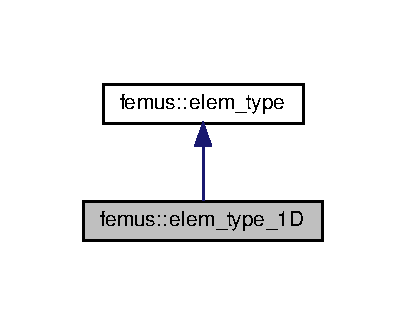
\includegraphics[width=195pt]{classfemus_1_1elem__type__1_d__inherit__graph}
\end{center}
\end{figure}


Collaboration diagram for femus\+:\+:elem\+\_\+type\+\_\+1D\+:
\nopagebreak
\begin{figure}[H]
\begin{center}
\leavevmode
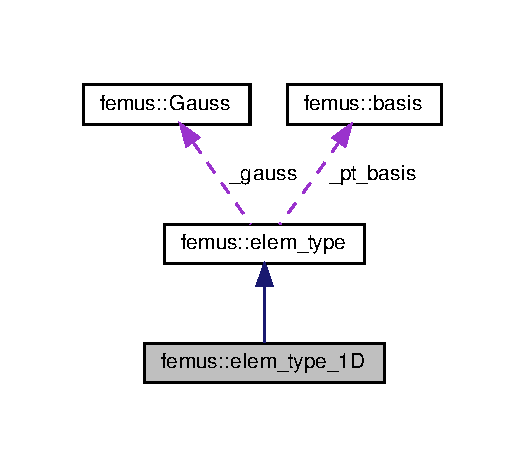
\includegraphics[width=252pt]{classfemus_1_1elem__type__1_d__coll__graph}
\end{center}
\end{figure}
\subsection*{Public Member Functions}
\begin{DoxyCompactItemize}
\item 
\mbox{\hyperlink{classfemus_1_1elem__type__1_d_a30be54e2c9797a64f2890ff3010a2437}{elem\+\_\+type\+\_\+1D}} (const char $\ast$solid, const char $\ast$order, const char $\ast$gauss\+\_\+order)
\item 
\mbox{\hyperlink{classfemus_1_1elem__type__1_d_a7525c96e56004b6f04d75c6228d93d90}{$\sim$elem\+\_\+type\+\_\+1D}} ()
\item 
{\footnotesize template$<$class type $>$ }\\void \mbox{\hyperlink{classfemus_1_1elem__type__1_d_a4061091e86269a2ae013083b3c46e5ad}{Get\+Jacobian\+\_\+type}} (const vector$<$ vector$<$ type $>$ $>$ \&vt, const unsigned \&\mbox{\hyperlink{namespacefemus_a6df31099f676311de214a312d7043941}{ig}}, type \&Weight, vector$<$ vector$<$ type $>$ $>$ \&jacobian\+Matrix) const
\item 
void \mbox{\hyperlink{classfemus_1_1elem__type__1_d_af21e2d104c0f4ca0d18e5e51c8f5c91f}{Get\+Jacobian}} (const vector$<$ vector$<$ adept\+::adouble $>$ $>$ \&vt, const unsigned \&\mbox{\hyperlink{namespacefemus_a6df31099f676311de214a312d7043941}{ig}}, adept\+::adouble \&Weight, vector$<$ vector$<$ adept\+::adouble $>$ $>$ \&jacobian\+Matrix) const
\item 
void \mbox{\hyperlink{classfemus_1_1elem__type__1_d_ad39cd6dbe648f384fa1be74d5ceec783}{Get\+Jacobian}} (const vector$<$ vector$<$ double $>$ $>$ \&vt, const unsigned \&\mbox{\hyperlink{namespacefemus_a6df31099f676311de214a312d7043941}{ig}}, double \&Weight, vector$<$ vector$<$ double $>$ $>$ \&jacobian\+Matrix) const
\item 
{\footnotesize template$<$class type $>$ }\\void \mbox{\hyperlink{classfemus_1_1elem__type__1_d_af1950c8d96453aafcd57bd254b68a094}{Jacobian\+\_\+type}} (const vector$<$ vector$<$ type $>$ $>$ \&vt, const unsigned \&\mbox{\hyperlink{namespacefemus_a6df31099f676311de214a312d7043941}{ig}}, type \&Weight, vector$<$ double $>$ \&phi, vector$<$ type $>$ \&gradphi, boost\+::optional$<$ vector$<$ type $>$ \& $>$ nablaphi) const
\item 
void \mbox{\hyperlink{classfemus_1_1elem__type__1_d_a4c063f6c2d18fbc305e3bde505c49279}{Jacobian}} (const vector$<$ vector$<$ adept\+::adouble $>$ $>$ \&vt, const unsigned \&\mbox{\hyperlink{namespacefemus_a6df31099f676311de214a312d7043941}{ig}}, adept\+::adouble \&Weight, vector$<$ double $>$ \&phi, vector$<$ adept\+::adouble $>$ \&gradphi, boost\+::optional$<$ vector$<$ adept\+::adouble $>$ \& $>$ nablaphi=boost\+::none) const
\item 
void \mbox{\hyperlink{classfemus_1_1elem__type__1_d_aec9766e008c3f7536a4a68d87302b254}{Jacobian}} (const vector$<$ vector$<$ double $>$ $>$ \&vt, const unsigned \&\mbox{\hyperlink{namespacefemus_a6df31099f676311de214a312d7043941}{ig}}, double \&Weight, vector$<$ double $>$ \&phi, vector$<$ double $>$ \&gradphi, boost\+::optional$<$ vector$<$ double $>$ \& $>$ nablaphi=boost\+::none) const
\item 
{\footnotesize template$<$class type $>$ }\\void \mbox{\hyperlink{classfemus_1_1elem__type__1_d_ad6061e34ea1a15f99e49a466987e38e0}{Jacobian\+\_\+type}} (const vector$<$ vector$<$ type $>$ $>$ \&vt, const vector$<$ double $>$ \&xi, type \&Weight, vector$<$ double $>$ \&phi, vector$<$ type $>$ \&gradphi, boost\+::optional$<$ vector$<$ type $>$ \& $>$ nablaphi) const
\item 
void \mbox{\hyperlink{classfemus_1_1elem__type__1_d_a6209ff2d3d1b74ac6f1ee1eb9140908e}{Jacobian}} (const vector$<$ vector$<$ adept\+::adouble $>$ $>$ \&vt, const vector$<$ double $>$ \&xi, adept\+::adouble \&Weight, vector$<$ double $>$ \&phi, vector$<$ adept\+::adouble $>$ \&gradphi, boost\+::optional$<$ vector$<$ adept\+::adouble $>$ \& $>$ nablaphi=boost\+::none) const
\item 
void \mbox{\hyperlink{classfemus_1_1elem__type__1_d_ac6814828a90c49fd5b29df4b5d161653}{Jacobian}} (const vector$<$ vector$<$ double $>$ $>$ \&vt, const vector$<$ double $>$ \&xi, double \&Weight, vector$<$ double $>$ \&phi, vector$<$ double $>$ \&gradphi, boost\+::optional$<$ vector$<$ double $>$ \& $>$ nablaphi=boost\+::none) const
\item 
{\footnotesize template$<$class type $>$ }\\void \mbox{\hyperlink{classfemus_1_1elem__type__1_d_a18dd785c7dfb85f18d6a799558b63bc0}{Jacobian\+Sur\+\_\+type}} (const vector$<$ vector$<$ type $>$ $>$ \&vt, const unsigned \&\mbox{\hyperlink{namespacefemus_a6df31099f676311de214a312d7043941}{ig}}, type \&Weight, vector$<$ double $>$ \&phi, vector$<$ type $>$ \&gradphi, vector$<$ type $>$ \&normal) const
\item 
void \mbox{\hyperlink{classfemus_1_1elem__type__1_d_a30e236ab3052558a85af26d862715540}{Jacobian\+Sur}} (const vector$<$ vector$<$ adept\+::adouble $>$ $>$ \&vt, const unsigned \&\mbox{\hyperlink{namespacefemus_a6df31099f676311de214a312d7043941}{ig}}, adept\+::adouble \&Weight, vector$<$ double $>$ \&phi, vector$<$ adept\+::adouble $>$ \&gradphi, vector$<$ adept\+::adouble $>$ \&normal) const
\item 
void \mbox{\hyperlink{classfemus_1_1elem__type__1_d_a66b28ca6be3e79fe3bf08b2c856974dd}{Jacobian\+Sur}} (const vector$<$ vector$<$ double $>$ $>$ \&vt, const unsigned \&\mbox{\hyperlink{namespacefemus_a6df31099f676311de214a312d7043941}{ig}}, double \&Weight, vector$<$ double $>$ \&phi, vector$<$ double $>$ \&gradphi, vector$<$ double $>$ \&normal) const
\item 
double $\ast$ \mbox{\hyperlink{classfemus_1_1elem__type__1_d_ac3bf43aa0c1c02c1113228011462a893}{Get\+Phi}} (const unsigned \&\mbox{\hyperlink{namespacefemus_a6df31099f676311de214a312d7043941}{ig}}) const
\item 
double $\ast$ \mbox{\hyperlink{classfemus_1_1elem__type__1_d_a27ff9f2a7f26c961b9b9d96aa87723d2}{Get\+D\+Phi\+D\+Xi}} (const unsigned \&\mbox{\hyperlink{namespacefemus_a6df31099f676311de214a312d7043941}{ig}}) const
\end{DoxyCompactItemize}
\subsection*{Public Attributes}
\begin{DoxyCompactItemize}
\item 
double $\ast$$\ast$ \mbox{\hyperlink{classfemus_1_1elem__type__1_d_a80a76204752db5a3fa4f4586ae554480}{\+\_\+phi}}
\item 
double $\ast$ \mbox{\hyperlink{classfemus_1_1elem__type__1_d_aec61375db0a0de76bdeda36c5c951b8c}{\+\_\+phi\+\_\+memory}}
\item 
double $\ast$$\ast$ \mbox{\hyperlink{classfemus_1_1elem__type__1_d_a44078add8faa0d14244a1fd41b5d4fb7}{\+\_\+dphidxi}}
\item 
double $\ast$ \mbox{\hyperlink{classfemus_1_1elem__type__1_d_af1a5dc5b688c490834b1c921b16b35ba}{\+\_\+dphidxi\+\_\+memory}}
\item 
double $\ast$$\ast$ \mbox{\hyperlink{classfemus_1_1elem__type__1_d_a60418459ab53117c83aad7cfbb3628ca}{\+\_\+d2phidxi2}}
\item 
double $\ast$ \mbox{\hyperlink{classfemus_1_1elem__type__1_d_a59bd178cd7ec1fcdfb577f56f1f239dd}{\+\_\+d2phidxi2\+\_\+memory}}
\item 
std\+::vector$<$ std\+::vector$<$ std\+::vector$<$ double $>$ $>$ $>$ \mbox{\hyperlink{classfemus_1_1elem__type__1_d_aaf93a8facde3e591de6c874af0834800}{\+\_\+phi\+Face}}
\item 
std\+::vector$<$ std\+::vector$<$ std\+::vector$<$ std\+::vector$<$ double $>$ $>$ $>$ $>$ \mbox{\hyperlink{classfemus_1_1elem__type__1_d_a5eac5011c7ecdfdcf4cc9bfcd6adf861}{\+\_\+grad\+Phi\+Face}}
\item 
std\+::vector$<$ std\+::vector$<$ std\+::vector$<$ std\+::vector$<$ std\+::vector$<$ double $>$ $>$ $>$ $>$ $>$ \mbox{\hyperlink{classfemus_1_1elem__type__1_d_a4610d856f52e0a7ec8d9b02f0ded95c2}{\+\_\+hessian\+Phi\+Face}}
\end{DoxyCompactItemize}
\subsection*{Additional Inherited Members}


\subsection{Constructor \& Destructor Documentation}
\mbox{\Hypertarget{classfemus_1_1elem__type__1_d_a30be54e2c9797a64f2890ff3010a2437}\label{classfemus_1_1elem__type__1_d_a30be54e2c9797a64f2890ff3010a2437}} 
\index{femus\+::elem\+\_\+type\+\_\+1D@{femus\+::elem\+\_\+type\+\_\+1D}!elem\+\_\+type\+\_\+1D@{elem\+\_\+type\+\_\+1D}}
\index{elem\+\_\+type\+\_\+1D@{elem\+\_\+type\+\_\+1D}!femus\+::elem\+\_\+type\+\_\+1D@{femus\+::elem\+\_\+type\+\_\+1D}}
\subsubsection{\texorpdfstring{elem\+\_\+type\+\_\+1\+D()}{elem\_type\_1D()}}
{\footnotesize\ttfamily femus\+::elem\+\_\+type\+\_\+1\+D\+::elem\+\_\+type\+\_\+1D (\begin{DoxyParamCaption}\item[{const char $\ast$}]{solid,  }\item[{const char $\ast$}]{order,  }\item[{const char $\ast$}]{gauss\+\_\+order }\end{DoxyParamCaption})}

constructor \mbox{\Hypertarget{classfemus_1_1elem__type__1_d_a7525c96e56004b6f04d75c6228d93d90}\label{classfemus_1_1elem__type__1_d_a7525c96e56004b6f04d75c6228d93d90}} 
\index{femus\+::elem\+\_\+type\+\_\+1D@{femus\+::elem\+\_\+type\+\_\+1D}!````~elem\+\_\+type\+\_\+1D@{$\sim$elem\+\_\+type\+\_\+1D}}
\index{````~elem\+\_\+type\+\_\+1D@{$\sim$elem\+\_\+type\+\_\+1D}!femus\+::elem\+\_\+type\+\_\+1D@{femus\+::elem\+\_\+type\+\_\+1D}}
\subsubsection{\texorpdfstring{$\sim$elem\+\_\+type\+\_\+1\+D()}{~elem\_type\_1D()}}
{\footnotesize\ttfamily femus\+::elem\+\_\+type\+\_\+1\+D\+::$\sim$elem\+\_\+type\+\_\+1D (\begin{DoxyParamCaption}{ }\end{DoxyParamCaption})\hspace{0.3cm}{\ttfamily [inline]}}

destructor 

\subsection{Member Function Documentation}
\mbox{\Hypertarget{classfemus_1_1elem__type__1_d_a27ff9f2a7f26c961b9b9d96aa87723d2}\label{classfemus_1_1elem__type__1_d_a27ff9f2a7f26c961b9b9d96aa87723d2}} 
\index{femus\+::elem\+\_\+type\+\_\+1D@{femus\+::elem\+\_\+type\+\_\+1D}!Get\+D\+Phi\+D\+Xi@{Get\+D\+Phi\+D\+Xi}}
\index{Get\+D\+Phi\+D\+Xi@{Get\+D\+Phi\+D\+Xi}!femus\+::elem\+\_\+type\+\_\+1D@{femus\+::elem\+\_\+type\+\_\+1D}}
\subsubsection{\texorpdfstring{Get\+D\+Phi\+D\+Xi()}{GetDPhiDXi()}}
{\footnotesize\ttfamily double$\ast$ femus\+::elem\+\_\+type\+\_\+1\+D\+::\+Get\+D\+Phi\+D\+Xi (\begin{DoxyParamCaption}\item[{const unsigned \&}]{ig }\end{DoxyParamCaption}) const\hspace{0.3cm}{\ttfamily [inline]}, {\ttfamily [virtual]}}

To be Added 

Implements \mbox{\hyperlink{classfemus_1_1elem__type_a6efb6026b9fe89912ec367b235bfccc7}{femus\+::elem\+\_\+type}}.

\mbox{\Hypertarget{classfemus_1_1elem__type__1_d_af21e2d104c0f4ca0d18e5e51c8f5c91f}\label{classfemus_1_1elem__type__1_d_af21e2d104c0f4ca0d18e5e51c8f5c91f}} 
\index{femus\+::elem\+\_\+type\+\_\+1D@{femus\+::elem\+\_\+type\+\_\+1D}!Get\+Jacobian@{Get\+Jacobian}}
\index{Get\+Jacobian@{Get\+Jacobian}!femus\+::elem\+\_\+type\+\_\+1D@{femus\+::elem\+\_\+type\+\_\+1D}}
\subsubsection{\texorpdfstring{Get\+Jacobian()}{GetJacobian()}\hspace{0.1cm}{\footnotesize\ttfamily [1/2]}}
{\footnotesize\ttfamily void femus\+::elem\+\_\+type\+\_\+1\+D\+::\+Get\+Jacobian (\begin{DoxyParamCaption}\item[{const vector$<$ vector$<$ adept\+::adouble $>$ $>$ \&}]{vt,  }\item[{const unsigned \&}]{ig,  }\item[{adept\+::adouble \&}]{Weight,  }\item[{vector$<$ vector$<$ adept\+::adouble $>$ $>$ \&}]{jacobian\+Matrix }\end{DoxyParamCaption}) const\hspace{0.3cm}{\ttfamily [inline]}, {\ttfamily [virtual]}}



Implements \mbox{\hyperlink{classfemus_1_1elem__type_aa8e617c54dd774ffca5d305605552af7}{femus\+::elem\+\_\+type}}.

\mbox{\Hypertarget{classfemus_1_1elem__type__1_d_ad39cd6dbe648f384fa1be74d5ceec783}\label{classfemus_1_1elem__type__1_d_ad39cd6dbe648f384fa1be74d5ceec783}} 
\index{femus\+::elem\+\_\+type\+\_\+1D@{femus\+::elem\+\_\+type\+\_\+1D}!Get\+Jacobian@{Get\+Jacobian}}
\index{Get\+Jacobian@{Get\+Jacobian}!femus\+::elem\+\_\+type\+\_\+1D@{femus\+::elem\+\_\+type\+\_\+1D}}
\subsubsection{\texorpdfstring{Get\+Jacobian()}{GetJacobian()}\hspace{0.1cm}{\footnotesize\ttfamily [2/2]}}
{\footnotesize\ttfamily void femus\+::elem\+\_\+type\+\_\+1\+D\+::\+Get\+Jacobian (\begin{DoxyParamCaption}\item[{const vector$<$ vector$<$ double $>$ $>$ \&}]{vt,  }\item[{const unsigned \&}]{ig,  }\item[{double \&}]{Weight,  }\item[{vector$<$ vector$<$ double $>$ $>$ \&}]{jacobian\+Matrix }\end{DoxyParamCaption}) const\hspace{0.3cm}{\ttfamily [inline]}, {\ttfamily [virtual]}}



Implements \mbox{\hyperlink{classfemus_1_1elem__type_a6c883b7946e55db8783fd0177546610a}{femus\+::elem\+\_\+type}}.

\mbox{\Hypertarget{classfemus_1_1elem__type__1_d_a4061091e86269a2ae013083b3c46e5ad}\label{classfemus_1_1elem__type__1_d_a4061091e86269a2ae013083b3c46e5ad}} 
\index{femus\+::elem\+\_\+type\+\_\+1D@{femus\+::elem\+\_\+type\+\_\+1D}!Get\+Jacobian\+\_\+type@{Get\+Jacobian\+\_\+type}}
\index{Get\+Jacobian\+\_\+type@{Get\+Jacobian\+\_\+type}!femus\+::elem\+\_\+type\+\_\+1D@{femus\+::elem\+\_\+type\+\_\+1D}}
\subsubsection{\texorpdfstring{Get\+Jacobian\+\_\+type()}{GetJacobian\_type()}}
{\footnotesize\ttfamily template$<$class type $>$ \\
void femus\+::elem\+\_\+type\+\_\+1\+D\+::\+Get\+Jacobian\+\_\+type (\begin{DoxyParamCaption}\item[{const vector$<$ vector$<$ type $>$ $>$ \&}]{vt,  }\item[{const unsigned \&}]{ig,  }\item[{type \&}]{Weight,  }\item[{vector$<$ vector$<$ type $>$ $>$ \&}]{jacobian\+Matrix }\end{DoxyParamCaption}) const}

\mbox{\Hypertarget{classfemus_1_1elem__type__1_d_ac3bf43aa0c1c02c1113228011462a893}\label{classfemus_1_1elem__type__1_d_ac3bf43aa0c1c02c1113228011462a893}} 
\index{femus\+::elem\+\_\+type\+\_\+1D@{femus\+::elem\+\_\+type\+\_\+1D}!Get\+Phi@{Get\+Phi}}
\index{Get\+Phi@{Get\+Phi}!femus\+::elem\+\_\+type\+\_\+1D@{femus\+::elem\+\_\+type\+\_\+1D}}
\subsubsection{\texorpdfstring{Get\+Phi()}{GetPhi()}}
{\footnotesize\ttfamily double$\ast$ femus\+::elem\+\_\+type\+\_\+1\+D\+::\+Get\+Phi (\begin{DoxyParamCaption}\item[{const unsigned \&}]{ig }\end{DoxyParamCaption}) const\hspace{0.3cm}{\ttfamily [inline]}, {\ttfamily [virtual]}}

To be Added 

Implements \mbox{\hyperlink{classfemus_1_1elem__type_a2aa2a37b15debbee27918f5e3f2df6b3}{femus\+::elem\+\_\+type}}.

\mbox{\Hypertarget{classfemus_1_1elem__type__1_d_a4c063f6c2d18fbc305e3bde505c49279}\label{classfemus_1_1elem__type__1_d_a4c063f6c2d18fbc305e3bde505c49279}} 
\index{femus\+::elem\+\_\+type\+\_\+1D@{femus\+::elem\+\_\+type\+\_\+1D}!Jacobian@{Jacobian}}
\index{Jacobian@{Jacobian}!femus\+::elem\+\_\+type\+\_\+1D@{femus\+::elem\+\_\+type\+\_\+1D}}
\subsubsection{\texorpdfstring{Jacobian()}{Jacobian()}\hspace{0.1cm}{\footnotesize\ttfamily [1/4]}}
{\footnotesize\ttfamily void femus\+::elem\+\_\+type\+\_\+1\+D\+::\+Jacobian (\begin{DoxyParamCaption}\item[{const vector$<$ vector$<$ adept\+::adouble $>$ $>$ \&}]{vt,  }\item[{const unsigned \&}]{ig,  }\item[{adept\+::adouble \&}]{Weight,  }\item[{vector$<$ double $>$ \&}]{phi,  }\item[{vector$<$ adept\+::adouble $>$ \&}]{gradphi,  }\item[{boost\+::optional$<$ vector$<$ adept\+::adouble $>$ \& $>$}]{nablaphi = {\ttfamily boost\+:\+:none} }\end{DoxyParamCaption}) const\hspace{0.3cm}{\ttfamily [inline]}, {\ttfamily [virtual]}}



Implements \mbox{\hyperlink{classfemus_1_1elem__type_a937b1d5ecbeed3b17db831264a3492fa}{femus\+::elem\+\_\+type}}.

\mbox{\Hypertarget{classfemus_1_1elem__type__1_d_aec9766e008c3f7536a4a68d87302b254}\label{classfemus_1_1elem__type__1_d_aec9766e008c3f7536a4a68d87302b254}} 
\index{femus\+::elem\+\_\+type\+\_\+1D@{femus\+::elem\+\_\+type\+\_\+1D}!Jacobian@{Jacobian}}
\index{Jacobian@{Jacobian}!femus\+::elem\+\_\+type\+\_\+1D@{femus\+::elem\+\_\+type\+\_\+1D}}
\subsubsection{\texorpdfstring{Jacobian()}{Jacobian()}\hspace{0.1cm}{\footnotesize\ttfamily [2/4]}}
{\footnotesize\ttfamily void femus\+::elem\+\_\+type\+\_\+1\+D\+::\+Jacobian (\begin{DoxyParamCaption}\item[{const vector$<$ vector$<$ double $>$ $>$ \&}]{vt,  }\item[{const unsigned \&}]{ig,  }\item[{double \&}]{Weight,  }\item[{vector$<$ double $>$ \&}]{phi,  }\item[{vector$<$ double $>$ \&}]{gradphi,  }\item[{boost\+::optional$<$ vector$<$ double $>$ \& $>$}]{nablaphi = {\ttfamily boost\+:\+:none} }\end{DoxyParamCaption}) const\hspace{0.3cm}{\ttfamily [inline]}, {\ttfamily [virtual]}}



Implements \mbox{\hyperlink{classfemus_1_1elem__type_ac3828ecd8ddd057d726a60cb19c60f0b}{femus\+::elem\+\_\+type}}.

\mbox{\Hypertarget{classfemus_1_1elem__type__1_d_a6209ff2d3d1b74ac6f1ee1eb9140908e}\label{classfemus_1_1elem__type__1_d_a6209ff2d3d1b74ac6f1ee1eb9140908e}} 
\index{femus\+::elem\+\_\+type\+\_\+1D@{femus\+::elem\+\_\+type\+\_\+1D}!Jacobian@{Jacobian}}
\index{Jacobian@{Jacobian}!femus\+::elem\+\_\+type\+\_\+1D@{femus\+::elem\+\_\+type\+\_\+1D}}
\subsubsection{\texorpdfstring{Jacobian()}{Jacobian()}\hspace{0.1cm}{\footnotesize\ttfamily [3/4]}}
{\footnotesize\ttfamily void femus\+::elem\+\_\+type\+\_\+1\+D\+::\+Jacobian (\begin{DoxyParamCaption}\item[{const vector$<$ vector$<$ adept\+::adouble $>$ $>$ \&}]{vt,  }\item[{const vector$<$ double $>$ \&}]{xi,  }\item[{adept\+::adouble \&}]{Weight,  }\item[{vector$<$ double $>$ \&}]{phi,  }\item[{vector$<$ adept\+::adouble $>$ \&}]{gradphi,  }\item[{boost\+::optional$<$ vector$<$ adept\+::adouble $>$ \& $>$}]{nablaphi = {\ttfamily boost\+:\+:none} }\end{DoxyParamCaption}) const\hspace{0.3cm}{\ttfamily [inline]}, {\ttfamily [virtual]}}



Implements \mbox{\hyperlink{classfemus_1_1elem__type_a2d76133387cebf896c0e51459055fdea}{femus\+::elem\+\_\+type}}.

\mbox{\Hypertarget{classfemus_1_1elem__type__1_d_ac6814828a90c49fd5b29df4b5d161653}\label{classfemus_1_1elem__type__1_d_ac6814828a90c49fd5b29df4b5d161653}} 
\index{femus\+::elem\+\_\+type\+\_\+1D@{femus\+::elem\+\_\+type\+\_\+1D}!Jacobian@{Jacobian}}
\index{Jacobian@{Jacobian}!femus\+::elem\+\_\+type\+\_\+1D@{femus\+::elem\+\_\+type\+\_\+1D}}
\subsubsection{\texorpdfstring{Jacobian()}{Jacobian()}\hspace{0.1cm}{\footnotesize\ttfamily [4/4]}}
{\footnotesize\ttfamily void femus\+::elem\+\_\+type\+\_\+1\+D\+::\+Jacobian (\begin{DoxyParamCaption}\item[{const vector$<$ vector$<$ double $>$ $>$ \&}]{vt,  }\item[{const vector$<$ double $>$ \&}]{xi,  }\item[{double \&}]{Weight,  }\item[{vector$<$ double $>$ \&}]{phi,  }\item[{vector$<$ double $>$ \&}]{gradphi,  }\item[{boost\+::optional$<$ vector$<$ double $>$ \& $>$}]{nablaphi = {\ttfamily boost\+:\+:none} }\end{DoxyParamCaption}) const\hspace{0.3cm}{\ttfamily [inline]}, {\ttfamily [virtual]}}



Implements \mbox{\hyperlink{classfemus_1_1elem__type_aab6db5851a9810adfe0ff98df2c30810}{femus\+::elem\+\_\+type}}.

\mbox{\Hypertarget{classfemus_1_1elem__type__1_d_af1950c8d96453aafcd57bd254b68a094}\label{classfemus_1_1elem__type__1_d_af1950c8d96453aafcd57bd254b68a094}} 
\index{femus\+::elem\+\_\+type\+\_\+1D@{femus\+::elem\+\_\+type\+\_\+1D}!Jacobian\+\_\+type@{Jacobian\+\_\+type}}
\index{Jacobian\+\_\+type@{Jacobian\+\_\+type}!femus\+::elem\+\_\+type\+\_\+1D@{femus\+::elem\+\_\+type\+\_\+1D}}
\subsubsection{\texorpdfstring{Jacobian\+\_\+type()}{Jacobian\_type()}\hspace{0.1cm}{\footnotesize\ttfamily [1/2]}}
{\footnotesize\ttfamily template$<$class type $>$ \\
void femus\+::elem\+\_\+type\+\_\+1\+D\+::\+Jacobian\+\_\+type (\begin{DoxyParamCaption}\item[{const vector$<$ vector$<$ type $>$ $>$ \&}]{vt,  }\item[{const unsigned \&}]{ig,  }\item[{type \&}]{Weight,  }\item[{vector$<$ double $>$ \&}]{phi,  }\item[{vector$<$ type $>$ \&}]{gradphi,  }\item[{boost\+::optional$<$ vector$<$ type $>$ \& $>$}]{nablaphi }\end{DoxyParamCaption}) const}

\mbox{\Hypertarget{classfemus_1_1elem__type__1_d_ad6061e34ea1a15f99e49a466987e38e0}\label{classfemus_1_1elem__type__1_d_ad6061e34ea1a15f99e49a466987e38e0}} 
\index{femus\+::elem\+\_\+type\+\_\+1D@{femus\+::elem\+\_\+type\+\_\+1D}!Jacobian\+\_\+type@{Jacobian\+\_\+type}}
\index{Jacobian\+\_\+type@{Jacobian\+\_\+type}!femus\+::elem\+\_\+type\+\_\+1D@{femus\+::elem\+\_\+type\+\_\+1D}}
\subsubsection{\texorpdfstring{Jacobian\+\_\+type()}{Jacobian\_type()}\hspace{0.1cm}{\footnotesize\ttfamily [2/2]}}
{\footnotesize\ttfamily template$<$class type $>$ \\
void femus\+::elem\+\_\+type\+\_\+1\+D\+::\+Jacobian\+\_\+type (\begin{DoxyParamCaption}\item[{const vector$<$ vector$<$ type $>$ $>$ \&}]{vt,  }\item[{const vector$<$ double $>$ \&}]{xi,  }\item[{type \&}]{Weight,  }\item[{vector$<$ double $>$ \&}]{phi,  }\item[{vector$<$ type $>$ \&}]{gradphi,  }\item[{boost\+::optional$<$ vector$<$ type $>$ \& $>$}]{nablaphi }\end{DoxyParamCaption}) const}

\mbox{\Hypertarget{classfemus_1_1elem__type__1_d_a30e236ab3052558a85af26d862715540}\label{classfemus_1_1elem__type__1_d_a30e236ab3052558a85af26d862715540}} 
\index{femus\+::elem\+\_\+type\+\_\+1D@{femus\+::elem\+\_\+type\+\_\+1D}!Jacobian\+Sur@{Jacobian\+Sur}}
\index{Jacobian\+Sur@{Jacobian\+Sur}!femus\+::elem\+\_\+type\+\_\+1D@{femus\+::elem\+\_\+type\+\_\+1D}}
\subsubsection{\texorpdfstring{Jacobian\+Sur()}{JacobianSur()}\hspace{0.1cm}{\footnotesize\ttfamily [1/2]}}
{\footnotesize\ttfamily void femus\+::elem\+\_\+type\+\_\+1\+D\+::\+Jacobian\+Sur (\begin{DoxyParamCaption}\item[{const vector$<$ vector$<$ adept\+::adouble $>$ $>$ \&}]{vt,  }\item[{const unsigned \&}]{ig,  }\item[{adept\+::adouble \&}]{Weight,  }\item[{vector$<$ double $>$ \&}]{phi,  }\item[{vector$<$ adept\+::adouble $>$ \&}]{gradphi,  }\item[{vector$<$ adept\+::adouble $>$ \&}]{normal }\end{DoxyParamCaption}) const\hspace{0.3cm}{\ttfamily [inline]}, {\ttfamily [virtual]}}



Implements \mbox{\hyperlink{classfemus_1_1elem__type_a293052fac0f51472150b1bf7365c6b18}{femus\+::elem\+\_\+type}}.

\mbox{\Hypertarget{classfemus_1_1elem__type__1_d_a66b28ca6be3e79fe3bf08b2c856974dd}\label{classfemus_1_1elem__type__1_d_a66b28ca6be3e79fe3bf08b2c856974dd}} 
\index{femus\+::elem\+\_\+type\+\_\+1D@{femus\+::elem\+\_\+type\+\_\+1D}!Jacobian\+Sur@{Jacobian\+Sur}}
\index{Jacobian\+Sur@{Jacobian\+Sur}!femus\+::elem\+\_\+type\+\_\+1D@{femus\+::elem\+\_\+type\+\_\+1D}}
\subsubsection{\texorpdfstring{Jacobian\+Sur()}{JacobianSur()}\hspace{0.1cm}{\footnotesize\ttfamily [2/2]}}
{\footnotesize\ttfamily void femus\+::elem\+\_\+type\+\_\+1\+D\+::\+Jacobian\+Sur (\begin{DoxyParamCaption}\item[{const vector$<$ vector$<$ double $>$ $>$ \&}]{vt,  }\item[{const unsigned \&}]{ig,  }\item[{double \&}]{Weight,  }\item[{vector$<$ double $>$ \&}]{phi,  }\item[{vector$<$ double $>$ \&}]{gradphi,  }\item[{vector$<$ double $>$ \&}]{normal }\end{DoxyParamCaption}) const\hspace{0.3cm}{\ttfamily [inline]}, {\ttfamily [virtual]}}



Implements \mbox{\hyperlink{classfemus_1_1elem__type_aee56bc66a4d90ae7f7669bf7fa9ed8d7}{femus\+::elem\+\_\+type}}.

\mbox{\Hypertarget{classfemus_1_1elem__type__1_d_a18dd785c7dfb85f18d6a799558b63bc0}\label{classfemus_1_1elem__type__1_d_a18dd785c7dfb85f18d6a799558b63bc0}} 
\index{femus\+::elem\+\_\+type\+\_\+1D@{femus\+::elem\+\_\+type\+\_\+1D}!Jacobian\+Sur\+\_\+type@{Jacobian\+Sur\+\_\+type}}
\index{Jacobian\+Sur\+\_\+type@{Jacobian\+Sur\+\_\+type}!femus\+::elem\+\_\+type\+\_\+1D@{femus\+::elem\+\_\+type\+\_\+1D}}
\subsubsection{\texorpdfstring{Jacobian\+Sur\+\_\+type()}{JacobianSur\_type()}}
{\footnotesize\ttfamily template$<$class type $>$ \\
void femus\+::elem\+\_\+type\+\_\+1\+D\+::\+Jacobian\+Sur\+\_\+type (\begin{DoxyParamCaption}\item[{const vector$<$ vector$<$ type $>$ $>$ \&}]{vt,  }\item[{const unsigned \&}]{ig,  }\item[{type \&}]{Weight,  }\item[{vector$<$ double $>$ \&}]{phi,  }\item[{vector$<$ type $>$ \&}]{gradphi,  }\item[{vector$<$ type $>$ \&}]{normal }\end{DoxyParamCaption}) const}



\subsection{Member Data Documentation}
\mbox{\Hypertarget{classfemus_1_1elem__type__1_d_a60418459ab53117c83aad7cfbb3628ca}\label{classfemus_1_1elem__type__1_d_a60418459ab53117c83aad7cfbb3628ca}} 
\index{femus\+::elem\+\_\+type\+\_\+1D@{femus\+::elem\+\_\+type\+\_\+1D}!\+\_\+d2phidxi2@{\+\_\+d2phidxi2}}
\index{\+\_\+d2phidxi2@{\+\_\+d2phidxi2}!femus\+::elem\+\_\+type\+\_\+1D@{femus\+::elem\+\_\+type\+\_\+1D}}
\subsubsection{\texorpdfstring{\+\_\+d2phidxi2}{\_d2phidxi2}}
{\footnotesize\ttfamily double$\ast$$\ast$ femus\+::elem\+\_\+type\+\_\+1\+D\+::\+\_\+d2phidxi2}

\mbox{\Hypertarget{classfemus_1_1elem__type__1_d_a59bd178cd7ec1fcdfb577f56f1f239dd}\label{classfemus_1_1elem__type__1_d_a59bd178cd7ec1fcdfb577f56f1f239dd}} 
\index{femus\+::elem\+\_\+type\+\_\+1D@{femus\+::elem\+\_\+type\+\_\+1D}!\+\_\+d2phidxi2\+\_\+memory@{\+\_\+d2phidxi2\+\_\+memory}}
\index{\+\_\+d2phidxi2\+\_\+memory@{\+\_\+d2phidxi2\+\_\+memory}!femus\+::elem\+\_\+type\+\_\+1D@{femus\+::elem\+\_\+type\+\_\+1D}}
\subsubsection{\texorpdfstring{\+\_\+d2phidxi2\+\_\+memory}{\_d2phidxi2\_memory}}
{\footnotesize\ttfamily double$\ast$ femus\+::elem\+\_\+type\+\_\+1\+D\+::\+\_\+d2phidxi2\+\_\+memory}

\mbox{\Hypertarget{classfemus_1_1elem__type__1_d_a44078add8faa0d14244a1fd41b5d4fb7}\label{classfemus_1_1elem__type__1_d_a44078add8faa0d14244a1fd41b5d4fb7}} 
\index{femus\+::elem\+\_\+type\+\_\+1D@{femus\+::elem\+\_\+type\+\_\+1D}!\+\_\+dphidxi@{\+\_\+dphidxi}}
\index{\+\_\+dphidxi@{\+\_\+dphidxi}!femus\+::elem\+\_\+type\+\_\+1D@{femus\+::elem\+\_\+type\+\_\+1D}}
\subsubsection{\texorpdfstring{\+\_\+dphidxi}{\_dphidxi}}
{\footnotesize\ttfamily double$\ast$$\ast$ femus\+::elem\+\_\+type\+\_\+1\+D\+::\+\_\+dphidxi}

\mbox{\Hypertarget{classfemus_1_1elem__type__1_d_af1a5dc5b688c490834b1c921b16b35ba}\label{classfemus_1_1elem__type__1_d_af1a5dc5b688c490834b1c921b16b35ba}} 
\index{femus\+::elem\+\_\+type\+\_\+1D@{femus\+::elem\+\_\+type\+\_\+1D}!\+\_\+dphidxi\+\_\+memory@{\+\_\+dphidxi\+\_\+memory}}
\index{\+\_\+dphidxi\+\_\+memory@{\+\_\+dphidxi\+\_\+memory}!femus\+::elem\+\_\+type\+\_\+1D@{femus\+::elem\+\_\+type\+\_\+1D}}
\subsubsection{\texorpdfstring{\+\_\+dphidxi\+\_\+memory}{\_dphidxi\_memory}}
{\footnotesize\ttfamily double$\ast$ femus\+::elem\+\_\+type\+\_\+1\+D\+::\+\_\+dphidxi\+\_\+memory}

\mbox{\Hypertarget{classfemus_1_1elem__type__1_d_a5eac5011c7ecdfdcf4cc9bfcd6adf861}\label{classfemus_1_1elem__type__1_d_a5eac5011c7ecdfdcf4cc9bfcd6adf861}} 
\index{femus\+::elem\+\_\+type\+\_\+1D@{femus\+::elem\+\_\+type\+\_\+1D}!\+\_\+grad\+Phi\+Face@{\+\_\+grad\+Phi\+Face}}
\index{\+\_\+grad\+Phi\+Face@{\+\_\+grad\+Phi\+Face}!femus\+::elem\+\_\+type\+\_\+1D@{femus\+::elem\+\_\+type\+\_\+1D}}
\subsubsection{\texorpdfstring{\+\_\+grad\+Phi\+Face}{\_gradPhiFace}}
{\footnotesize\ttfamily std\+::vector$<$ std\+::vector $<$ std\+::vector $<$ std\+::vector $<$ double $>$ $>$ $>$ $>$ femus\+::elem\+\_\+type\+\_\+1\+D\+::\+\_\+grad\+Phi\+Face}

\mbox{\Hypertarget{classfemus_1_1elem__type__1_d_a4610d856f52e0a7ec8d9b02f0ded95c2}\label{classfemus_1_1elem__type__1_d_a4610d856f52e0a7ec8d9b02f0ded95c2}} 
\index{femus\+::elem\+\_\+type\+\_\+1D@{femus\+::elem\+\_\+type\+\_\+1D}!\+\_\+hessian\+Phi\+Face@{\+\_\+hessian\+Phi\+Face}}
\index{\+\_\+hessian\+Phi\+Face@{\+\_\+hessian\+Phi\+Face}!femus\+::elem\+\_\+type\+\_\+1D@{femus\+::elem\+\_\+type\+\_\+1D}}
\subsubsection{\texorpdfstring{\+\_\+hessian\+Phi\+Face}{\_hessianPhiFace}}
{\footnotesize\ttfamily std\+::vector$<$ std\+::vector $<$ std\+::vector $<$ std\+::vector $<$ std\+::vector $<$ double $>$ $>$ $>$ $>$ $>$ femus\+::elem\+\_\+type\+\_\+1\+D\+::\+\_\+hessian\+Phi\+Face}

\mbox{\Hypertarget{classfemus_1_1elem__type__1_d_a80a76204752db5a3fa4f4586ae554480}\label{classfemus_1_1elem__type__1_d_a80a76204752db5a3fa4f4586ae554480}} 
\index{femus\+::elem\+\_\+type\+\_\+1D@{femus\+::elem\+\_\+type\+\_\+1D}!\+\_\+phi@{\+\_\+phi}}
\index{\+\_\+phi@{\+\_\+phi}!femus\+::elem\+\_\+type\+\_\+1D@{femus\+::elem\+\_\+type\+\_\+1D}}
\subsubsection{\texorpdfstring{\+\_\+phi}{\_phi}}
{\footnotesize\ttfamily double$\ast$$\ast$ femus\+::elem\+\_\+type\+\_\+1\+D\+::\+\_\+phi}

\mbox{\Hypertarget{classfemus_1_1elem__type__1_d_aec61375db0a0de76bdeda36c5c951b8c}\label{classfemus_1_1elem__type__1_d_aec61375db0a0de76bdeda36c5c951b8c}} 
\index{femus\+::elem\+\_\+type\+\_\+1D@{femus\+::elem\+\_\+type\+\_\+1D}!\+\_\+phi\+\_\+memory@{\+\_\+phi\+\_\+memory}}
\index{\+\_\+phi\+\_\+memory@{\+\_\+phi\+\_\+memory}!femus\+::elem\+\_\+type\+\_\+1D@{femus\+::elem\+\_\+type\+\_\+1D}}
\subsubsection{\texorpdfstring{\+\_\+phi\+\_\+memory}{\_phi\_memory}}
{\footnotesize\ttfamily double$\ast$ femus\+::elem\+\_\+type\+\_\+1\+D\+::\+\_\+phi\+\_\+memory}

\mbox{\Hypertarget{classfemus_1_1elem__type__1_d_aaf93a8facde3e591de6c874af0834800}\label{classfemus_1_1elem__type__1_d_aaf93a8facde3e591de6c874af0834800}} 
\index{femus\+::elem\+\_\+type\+\_\+1D@{femus\+::elem\+\_\+type\+\_\+1D}!\+\_\+phi\+Face@{\+\_\+phi\+Face}}
\index{\+\_\+phi\+Face@{\+\_\+phi\+Face}!femus\+::elem\+\_\+type\+\_\+1D@{femus\+::elem\+\_\+type\+\_\+1D}}
\subsubsection{\texorpdfstring{\+\_\+phi\+Face}{\_phiFace}}
{\footnotesize\ttfamily std\+::vector$<$ std\+::vector $<$ std\+::vector $<$ double $>$ $>$ $>$ femus\+::elem\+\_\+type\+\_\+1\+D\+::\+\_\+phi\+Face}



The documentation for this class was generated from the following files\+:\begin{DoxyCompactItemize}
\item 
fe/\mbox{\hyperlink{_elem_type_8hpp}{Elem\+Type.\+hpp}}\item 
fe/\mbox{\hyperlink{_elem_type_8cpp}{Elem\+Type.\+cpp}}\end{DoxyCompactItemize}

\hypertarget{classfemus_1_1elem__type__2_d}{}\section{femus\+:\+:elem\+\_\+type\+\_\+2D Class Reference}
\label{classfemus_1_1elem__type__2_d}\index{femus\+::elem\+\_\+type\+\_\+2D@{femus\+::elem\+\_\+type\+\_\+2D}}


{\ttfamily \#include $<$Elem\+Type.\+hpp$>$}



Inheritance diagram for femus\+:\+:elem\+\_\+type\+\_\+2D\+:
\nopagebreak
\begin{figure}[H]
\begin{center}
\leavevmode
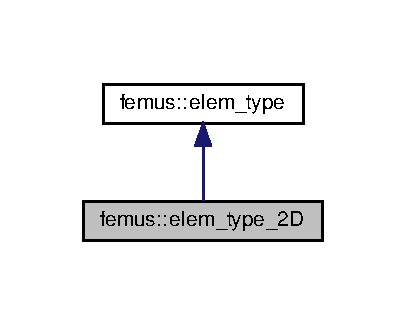
\includegraphics[width=195pt]{classfemus_1_1elem__type__2_d__inherit__graph}
\end{center}
\end{figure}


Collaboration diagram for femus\+:\+:elem\+\_\+type\+\_\+2D\+:
\nopagebreak
\begin{figure}[H]
\begin{center}
\leavevmode
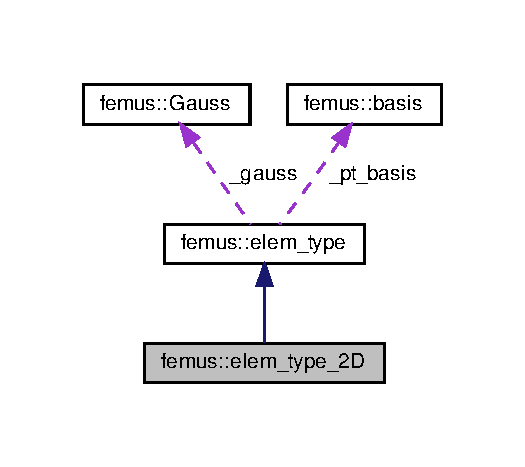
\includegraphics[width=252pt]{classfemus_1_1elem__type__2_d__coll__graph}
\end{center}
\end{figure}
\subsection*{Public Member Functions}
\begin{DoxyCompactItemize}
\item 
\mbox{\hyperlink{classfemus_1_1elem__type__2_d_a876b8c2f0e759a70fb821ccfebd41994}{elem\+\_\+type\+\_\+2D}} (const char $\ast$solid, const char $\ast$order, const char $\ast$gauss\+\_\+order)
\item 
\mbox{\hyperlink{classfemus_1_1elem__type__2_d_aa6ee09b3178436e9dbb707f62548c21d}{$\sim$elem\+\_\+type\+\_\+2D}} ()
\item 
{\footnotesize template$<$class type $>$ }\\void \mbox{\hyperlink{classfemus_1_1elem__type__2_d_a9d1cc104a524ee4ccc32a9bae6b0cef6}{Get\+Jacobian\+\_\+type}} (const vector$<$ vector$<$ type $>$ $>$ \&vt, const unsigned \&\mbox{\hyperlink{namespacefemus_a6df31099f676311de214a312d7043941}{ig}}, type \&Weight, vector$<$ vector$<$ type $>$ $>$ \&jacobian\+Matrix) const
\item 
void \mbox{\hyperlink{classfemus_1_1elem__type__2_d_a0cd4c80b3b6323d3ab4a57a29ad41034}{Get\+Jacobian}} (const vector$<$ vector$<$ adept\+::adouble $>$ $>$ \&vt, const unsigned \&\mbox{\hyperlink{namespacefemus_a6df31099f676311de214a312d7043941}{ig}}, adept\+::adouble \&Weight, vector$<$ vector$<$ adept\+::adouble $>$ $>$ \&jacobian\+Matrix) const
\item 
void \mbox{\hyperlink{classfemus_1_1elem__type__2_d_ac1fe4b778f06a58de8ad7057fb982a4b}{Get\+Jacobian}} (const vector$<$ vector$<$ double $>$ $>$ \&vt, const unsigned \&\mbox{\hyperlink{namespacefemus_a6df31099f676311de214a312d7043941}{ig}}, double \&Weight, vector$<$ vector$<$ double $>$ $>$ \&jacobian\+Matrix) const
\item 
{\footnotesize template$<$class type $>$ }\\void \mbox{\hyperlink{classfemus_1_1elem__type__2_d_aa4bc7ea3d9b10300367ad23b3ce4f977}{Jacobian\+\_\+type}} (const vector$<$ vector$<$ type $>$ $>$ \&vt, const unsigned \&\mbox{\hyperlink{namespacefemus_a6df31099f676311de214a312d7043941}{ig}}, type \&Weight, vector$<$ double $>$ \&phi, vector$<$ type $>$ \&gradphi, boost\+::optional$<$ vector$<$ type $>$ \& $>$ nablaphi) const
\item 
void \mbox{\hyperlink{classfemus_1_1elem__type__2_d_af8ad48cebf3ed72aa7d718129bbc381f}{Jacobian}} (const vector$<$ vector$<$ adept\+::adouble $>$ $>$ \&vt, const unsigned \&\mbox{\hyperlink{namespacefemus_a6df31099f676311de214a312d7043941}{ig}}, adept\+::adouble \&Weight, vector$<$ double $>$ \&phi, vector$<$ adept\+::adouble $>$ \&gradphi, boost\+::optional$<$ vector$<$ adept\+::adouble $>$ \& $>$ nablaphi=boost\+::none) const
\item 
void \mbox{\hyperlink{classfemus_1_1elem__type__2_d_afa07b600dc9f53257ca5fde905dc6732}{Jacobian}} (const vector$<$ vector$<$ double $>$ $>$ \&vt, const unsigned \&\mbox{\hyperlink{namespacefemus_a6df31099f676311de214a312d7043941}{ig}}, double \&Weight, vector$<$ double $>$ \&phi, vector$<$ double $>$ \&gradphi, boost\+::optional$<$ vector$<$ double $>$ \& $>$ nablaphi=boost\+::none) const
\item 
{\footnotesize template$<$class type $>$ }\\void \mbox{\hyperlink{classfemus_1_1elem__type__2_d_aa05f28f91f1eb9e2c45bd01c3c44443f}{Jacobian\+\_\+type}} (const vector$<$ vector$<$ type $>$ $>$ \&vt, const vector$<$ double $>$ \&xi, type \&Weight, vector$<$ double $>$ \&phi, vector$<$ type $>$ \&gradphi, boost\+::optional$<$ vector$<$ type $>$ \& $>$ nablaphi) const
\item 
void \mbox{\hyperlink{classfemus_1_1elem__type__2_d_ab63098a94dbccfc4808881b61fc9ab81}{Jacobian}} (const vector$<$ vector$<$ adept\+::adouble $>$ $>$ \&vt, const vector$<$ double $>$ \&xi, adept\+::adouble \&Weight, vector$<$ double $>$ \&phi, vector$<$ adept\+::adouble $>$ \&gradphi, boost\+::optional$<$ vector$<$ adept\+::adouble $>$ \& $>$ nablaphi=boost\+::none) const
\item 
void \mbox{\hyperlink{classfemus_1_1elem__type__2_d_a0194ae2956bdb2aaf843e05477ac3684}{Jacobian}} (const vector$<$ vector$<$ double $>$ $>$ \&vt, const vector$<$ double $>$ \&xi, double \&Weight, vector$<$ double $>$ \&phi, vector$<$ double $>$ \&gradphi, boost\+::optional$<$ vector$<$ double $>$ \& $>$ nablaphi=boost\+::none) const
\item 
{\footnotesize template$<$class type $>$ }\\void \mbox{\hyperlink{classfemus_1_1elem__type__2_d_af324b839f42e9643b0297da480be49c1}{Jacobian\+Sur\+\_\+type}} (const vector$<$ vector$<$ type $>$ $>$ \&vt, const unsigned \&\mbox{\hyperlink{namespacefemus_a6df31099f676311de214a312d7043941}{ig}}, type \&Weight, vector$<$ double $>$ \&phi, vector$<$ type $>$ \&gradphi, vector$<$ type $>$ \&normal) const
\item 
void \mbox{\hyperlink{classfemus_1_1elem__type__2_d_af19f0963ef176d7a3b4180730ef028c9}{Jacobian\+Sur}} (const vector$<$ vector$<$ adept\+::adouble $>$ $>$ \&vt, const unsigned \&\mbox{\hyperlink{namespacefemus_a6df31099f676311de214a312d7043941}{ig}}, adept\+::adouble \&Weight, vector$<$ double $>$ \&phi, vector$<$ adept\+::adouble $>$ \&gradphi, vector$<$ adept\+::adouble $>$ \&normal) const
\item 
void \mbox{\hyperlink{classfemus_1_1elem__type__2_d_a6da2427389820a069cc62fa014262c44}{Jacobian\+Sur}} (const vector$<$ vector$<$ double $>$ $>$ \&vt, const unsigned \&\mbox{\hyperlink{namespacefemus_a6df31099f676311de214a312d7043941}{ig}}, double \&Weight, vector$<$ double $>$ \&phi, vector$<$ double $>$ \&gradphi, vector$<$ double $>$ \&normal) const
\item 
double $\ast$ \mbox{\hyperlink{classfemus_1_1elem__type__2_d_a9e2ed95e14dbbf28d6399c50ba83ebe9}{Get\+Phi}} (const unsigned \&\mbox{\hyperlink{namespacefemus_a6df31099f676311de214a312d7043941}{ig}}) const
\item 
double $\ast$ \mbox{\hyperlink{classfemus_1_1elem__type__2_d_a11838ba0522b27348770989555114c94}{Get\+D\+Phi\+D\+Xi}} (const unsigned \&\mbox{\hyperlink{namespacefemus_a6df31099f676311de214a312d7043941}{ig}}) const
\item 
double $\ast$ \mbox{\hyperlink{classfemus_1_1elem__type__2_d_a3a77bc47f11a128210ed5c22a1179cc4}{Get\+D\+Phi\+D\+Eta}} (const unsigned \&\mbox{\hyperlink{namespacefemus_a6df31099f676311de214a312d7043941}{ig}}) const
\end{DoxyCompactItemize}
\subsection*{Additional Inherited Members}


\subsection{Constructor \& Destructor Documentation}
\mbox{\Hypertarget{classfemus_1_1elem__type__2_d_a876b8c2f0e759a70fb821ccfebd41994}\label{classfemus_1_1elem__type__2_d_a876b8c2f0e759a70fb821ccfebd41994}} 
\index{femus\+::elem\+\_\+type\+\_\+2D@{femus\+::elem\+\_\+type\+\_\+2D}!elem\+\_\+type\+\_\+2D@{elem\+\_\+type\+\_\+2D}}
\index{elem\+\_\+type\+\_\+2D@{elem\+\_\+type\+\_\+2D}!femus\+::elem\+\_\+type\+\_\+2D@{femus\+::elem\+\_\+type\+\_\+2D}}
\subsubsection{\texorpdfstring{elem\+\_\+type\+\_\+2\+D()}{elem\_type\_2D()}}
{\footnotesize\ttfamily femus\+::elem\+\_\+type\+\_\+2\+D\+::elem\+\_\+type\+\_\+2D (\begin{DoxyParamCaption}\item[{const char $\ast$}]{solid,  }\item[{const char $\ast$}]{order,  }\item[{const char $\ast$}]{gauss\+\_\+order }\end{DoxyParamCaption})}

constructor \mbox{\Hypertarget{classfemus_1_1elem__type__2_d_aa6ee09b3178436e9dbb707f62548c21d}\label{classfemus_1_1elem__type__2_d_aa6ee09b3178436e9dbb707f62548c21d}} 
\index{femus\+::elem\+\_\+type\+\_\+2D@{femus\+::elem\+\_\+type\+\_\+2D}!````~elem\+\_\+type\+\_\+2D@{$\sim$elem\+\_\+type\+\_\+2D}}
\index{````~elem\+\_\+type\+\_\+2D@{$\sim$elem\+\_\+type\+\_\+2D}!femus\+::elem\+\_\+type\+\_\+2D@{femus\+::elem\+\_\+type\+\_\+2D}}
\subsubsection{\texorpdfstring{$\sim$elem\+\_\+type\+\_\+2\+D()}{~elem\_type\_2D()}}
{\footnotesize\ttfamily femus\+::elem\+\_\+type\+\_\+2\+D\+::$\sim$elem\+\_\+type\+\_\+2D (\begin{DoxyParamCaption}{ }\end{DoxyParamCaption})\hspace{0.3cm}{\ttfamily [inline]}}

destructor 

\subsection{Member Function Documentation}
\mbox{\Hypertarget{classfemus_1_1elem__type__2_d_a3a77bc47f11a128210ed5c22a1179cc4}\label{classfemus_1_1elem__type__2_d_a3a77bc47f11a128210ed5c22a1179cc4}} 
\index{femus\+::elem\+\_\+type\+\_\+2D@{femus\+::elem\+\_\+type\+\_\+2D}!Get\+D\+Phi\+D\+Eta@{Get\+D\+Phi\+D\+Eta}}
\index{Get\+D\+Phi\+D\+Eta@{Get\+D\+Phi\+D\+Eta}!femus\+::elem\+\_\+type\+\_\+2D@{femus\+::elem\+\_\+type\+\_\+2D}}
\subsubsection{\texorpdfstring{Get\+D\+Phi\+D\+Eta()}{GetDPhiDEta()}}
{\footnotesize\ttfamily double$\ast$ femus\+::elem\+\_\+type\+\_\+2\+D\+::\+Get\+D\+Phi\+D\+Eta (\begin{DoxyParamCaption}\item[{const unsigned \&}]{ig }\end{DoxyParamCaption}) const\hspace{0.3cm}{\ttfamily [inline]}, {\ttfamily [virtual]}}

To be Added 

Reimplemented from \mbox{\hyperlink{classfemus_1_1elem__type_a510e44439de5cdd6ab5d04e3f8a5bdfe}{femus\+::elem\+\_\+type}}.

\mbox{\Hypertarget{classfemus_1_1elem__type__2_d_a11838ba0522b27348770989555114c94}\label{classfemus_1_1elem__type__2_d_a11838ba0522b27348770989555114c94}} 
\index{femus\+::elem\+\_\+type\+\_\+2D@{femus\+::elem\+\_\+type\+\_\+2D}!Get\+D\+Phi\+D\+Xi@{Get\+D\+Phi\+D\+Xi}}
\index{Get\+D\+Phi\+D\+Xi@{Get\+D\+Phi\+D\+Xi}!femus\+::elem\+\_\+type\+\_\+2D@{femus\+::elem\+\_\+type\+\_\+2D}}
\subsubsection{\texorpdfstring{Get\+D\+Phi\+D\+Xi()}{GetDPhiDXi()}}
{\footnotesize\ttfamily double$\ast$ femus\+::elem\+\_\+type\+\_\+2\+D\+::\+Get\+D\+Phi\+D\+Xi (\begin{DoxyParamCaption}\item[{const unsigned \&}]{ig }\end{DoxyParamCaption}) const\hspace{0.3cm}{\ttfamily [inline]}, {\ttfamily [virtual]}}

To be Added 

Implements \mbox{\hyperlink{classfemus_1_1elem__type_a6efb6026b9fe89912ec367b235bfccc7}{femus\+::elem\+\_\+type}}.

\mbox{\Hypertarget{classfemus_1_1elem__type__2_d_a0cd4c80b3b6323d3ab4a57a29ad41034}\label{classfemus_1_1elem__type__2_d_a0cd4c80b3b6323d3ab4a57a29ad41034}} 
\index{femus\+::elem\+\_\+type\+\_\+2D@{femus\+::elem\+\_\+type\+\_\+2D}!Get\+Jacobian@{Get\+Jacobian}}
\index{Get\+Jacobian@{Get\+Jacobian}!femus\+::elem\+\_\+type\+\_\+2D@{femus\+::elem\+\_\+type\+\_\+2D}}
\subsubsection{\texorpdfstring{Get\+Jacobian()}{GetJacobian()}\hspace{0.1cm}{\footnotesize\ttfamily [1/2]}}
{\footnotesize\ttfamily void femus\+::elem\+\_\+type\+\_\+2\+D\+::\+Get\+Jacobian (\begin{DoxyParamCaption}\item[{const vector$<$ vector$<$ adept\+::adouble $>$ $>$ \&}]{vt,  }\item[{const unsigned \&}]{ig,  }\item[{adept\+::adouble \&}]{Weight,  }\item[{vector$<$ vector$<$ adept\+::adouble $>$ $>$ \&}]{jacobian\+Matrix }\end{DoxyParamCaption}) const\hspace{0.3cm}{\ttfamily [inline]}, {\ttfamily [virtual]}}



Implements \mbox{\hyperlink{classfemus_1_1elem__type_aa8e617c54dd774ffca5d305605552af7}{femus\+::elem\+\_\+type}}.

\mbox{\Hypertarget{classfemus_1_1elem__type__2_d_ac1fe4b778f06a58de8ad7057fb982a4b}\label{classfemus_1_1elem__type__2_d_ac1fe4b778f06a58de8ad7057fb982a4b}} 
\index{femus\+::elem\+\_\+type\+\_\+2D@{femus\+::elem\+\_\+type\+\_\+2D}!Get\+Jacobian@{Get\+Jacobian}}
\index{Get\+Jacobian@{Get\+Jacobian}!femus\+::elem\+\_\+type\+\_\+2D@{femus\+::elem\+\_\+type\+\_\+2D}}
\subsubsection{\texorpdfstring{Get\+Jacobian()}{GetJacobian()}\hspace{0.1cm}{\footnotesize\ttfamily [2/2]}}
{\footnotesize\ttfamily void femus\+::elem\+\_\+type\+\_\+2\+D\+::\+Get\+Jacobian (\begin{DoxyParamCaption}\item[{const vector$<$ vector$<$ double $>$ $>$ \&}]{vt,  }\item[{const unsigned \&}]{ig,  }\item[{double \&}]{Weight,  }\item[{vector$<$ vector$<$ double $>$ $>$ \&}]{jacobian\+Matrix }\end{DoxyParamCaption}) const\hspace{0.3cm}{\ttfamily [inline]}, {\ttfamily [virtual]}}



Implements \mbox{\hyperlink{classfemus_1_1elem__type_a6c883b7946e55db8783fd0177546610a}{femus\+::elem\+\_\+type}}.

\mbox{\Hypertarget{classfemus_1_1elem__type__2_d_a9d1cc104a524ee4ccc32a9bae6b0cef6}\label{classfemus_1_1elem__type__2_d_a9d1cc104a524ee4ccc32a9bae6b0cef6}} 
\index{femus\+::elem\+\_\+type\+\_\+2D@{femus\+::elem\+\_\+type\+\_\+2D}!Get\+Jacobian\+\_\+type@{Get\+Jacobian\+\_\+type}}
\index{Get\+Jacobian\+\_\+type@{Get\+Jacobian\+\_\+type}!femus\+::elem\+\_\+type\+\_\+2D@{femus\+::elem\+\_\+type\+\_\+2D}}
\subsubsection{\texorpdfstring{Get\+Jacobian\+\_\+type()}{GetJacobian\_type()}}
{\footnotesize\ttfamily template$<$class type $>$ \\
void femus\+::elem\+\_\+type\+\_\+2\+D\+::\+Get\+Jacobian\+\_\+type (\begin{DoxyParamCaption}\item[{const vector$<$ vector$<$ type $>$ $>$ \&}]{vt,  }\item[{const unsigned \&}]{ig,  }\item[{type \&}]{Weight,  }\item[{vector$<$ vector$<$ type $>$ $>$ \&}]{jacobian\+Matrix }\end{DoxyParamCaption}) const}

\mbox{\Hypertarget{classfemus_1_1elem__type__2_d_a9e2ed95e14dbbf28d6399c50ba83ebe9}\label{classfemus_1_1elem__type__2_d_a9e2ed95e14dbbf28d6399c50ba83ebe9}} 
\index{femus\+::elem\+\_\+type\+\_\+2D@{femus\+::elem\+\_\+type\+\_\+2D}!Get\+Phi@{Get\+Phi}}
\index{Get\+Phi@{Get\+Phi}!femus\+::elem\+\_\+type\+\_\+2D@{femus\+::elem\+\_\+type\+\_\+2D}}
\subsubsection{\texorpdfstring{Get\+Phi()}{GetPhi()}}
{\footnotesize\ttfamily double$\ast$ femus\+::elem\+\_\+type\+\_\+2\+D\+::\+Get\+Phi (\begin{DoxyParamCaption}\item[{const unsigned \&}]{ig }\end{DoxyParamCaption}) const\hspace{0.3cm}{\ttfamily [inline]}, {\ttfamily [virtual]}}

To be Added 

Implements \mbox{\hyperlink{classfemus_1_1elem__type_a2aa2a37b15debbee27918f5e3f2df6b3}{femus\+::elem\+\_\+type}}.

\mbox{\Hypertarget{classfemus_1_1elem__type__2_d_af8ad48cebf3ed72aa7d718129bbc381f}\label{classfemus_1_1elem__type__2_d_af8ad48cebf3ed72aa7d718129bbc381f}} 
\index{femus\+::elem\+\_\+type\+\_\+2D@{femus\+::elem\+\_\+type\+\_\+2D}!Jacobian@{Jacobian}}
\index{Jacobian@{Jacobian}!femus\+::elem\+\_\+type\+\_\+2D@{femus\+::elem\+\_\+type\+\_\+2D}}
\subsubsection{\texorpdfstring{Jacobian()}{Jacobian()}\hspace{0.1cm}{\footnotesize\ttfamily [1/4]}}
{\footnotesize\ttfamily void femus\+::elem\+\_\+type\+\_\+2\+D\+::\+Jacobian (\begin{DoxyParamCaption}\item[{const vector$<$ vector$<$ adept\+::adouble $>$ $>$ \&}]{vt,  }\item[{const unsigned \&}]{ig,  }\item[{adept\+::adouble \&}]{Weight,  }\item[{vector$<$ double $>$ \&}]{phi,  }\item[{vector$<$ adept\+::adouble $>$ \&}]{gradphi,  }\item[{boost\+::optional$<$ vector$<$ adept\+::adouble $>$ \& $>$}]{nablaphi = {\ttfamily boost\+:\+:none} }\end{DoxyParamCaption}) const\hspace{0.3cm}{\ttfamily [inline]}, {\ttfamily [virtual]}}



Implements \mbox{\hyperlink{classfemus_1_1elem__type_a937b1d5ecbeed3b17db831264a3492fa}{femus\+::elem\+\_\+type}}.

\mbox{\Hypertarget{classfemus_1_1elem__type__2_d_afa07b600dc9f53257ca5fde905dc6732}\label{classfemus_1_1elem__type__2_d_afa07b600dc9f53257ca5fde905dc6732}} 
\index{femus\+::elem\+\_\+type\+\_\+2D@{femus\+::elem\+\_\+type\+\_\+2D}!Jacobian@{Jacobian}}
\index{Jacobian@{Jacobian}!femus\+::elem\+\_\+type\+\_\+2D@{femus\+::elem\+\_\+type\+\_\+2D}}
\subsubsection{\texorpdfstring{Jacobian()}{Jacobian()}\hspace{0.1cm}{\footnotesize\ttfamily [2/4]}}
{\footnotesize\ttfamily void femus\+::elem\+\_\+type\+\_\+2\+D\+::\+Jacobian (\begin{DoxyParamCaption}\item[{const vector$<$ vector$<$ double $>$ $>$ \&}]{vt,  }\item[{const unsigned \&}]{ig,  }\item[{double \&}]{Weight,  }\item[{vector$<$ double $>$ \&}]{phi,  }\item[{vector$<$ double $>$ \&}]{gradphi,  }\item[{boost\+::optional$<$ vector$<$ double $>$ \& $>$}]{nablaphi = {\ttfamily boost\+:\+:none} }\end{DoxyParamCaption}) const\hspace{0.3cm}{\ttfamily [inline]}, {\ttfamily [virtual]}}



Implements \mbox{\hyperlink{classfemus_1_1elem__type_ac3828ecd8ddd057d726a60cb19c60f0b}{femus\+::elem\+\_\+type}}.

\mbox{\Hypertarget{classfemus_1_1elem__type__2_d_ab63098a94dbccfc4808881b61fc9ab81}\label{classfemus_1_1elem__type__2_d_ab63098a94dbccfc4808881b61fc9ab81}} 
\index{femus\+::elem\+\_\+type\+\_\+2D@{femus\+::elem\+\_\+type\+\_\+2D}!Jacobian@{Jacobian}}
\index{Jacobian@{Jacobian}!femus\+::elem\+\_\+type\+\_\+2D@{femus\+::elem\+\_\+type\+\_\+2D}}
\subsubsection{\texorpdfstring{Jacobian()}{Jacobian()}\hspace{0.1cm}{\footnotesize\ttfamily [3/4]}}
{\footnotesize\ttfamily void femus\+::elem\+\_\+type\+\_\+2\+D\+::\+Jacobian (\begin{DoxyParamCaption}\item[{const vector$<$ vector$<$ adept\+::adouble $>$ $>$ \&}]{vt,  }\item[{const vector$<$ double $>$ \&}]{xi,  }\item[{adept\+::adouble \&}]{Weight,  }\item[{vector$<$ double $>$ \&}]{phi,  }\item[{vector$<$ adept\+::adouble $>$ \&}]{gradphi,  }\item[{boost\+::optional$<$ vector$<$ adept\+::adouble $>$ \& $>$}]{nablaphi = {\ttfamily boost\+:\+:none} }\end{DoxyParamCaption}) const\hspace{0.3cm}{\ttfamily [inline]}, {\ttfamily [virtual]}}



Implements \mbox{\hyperlink{classfemus_1_1elem__type_a2d76133387cebf896c0e51459055fdea}{femus\+::elem\+\_\+type}}.

\mbox{\Hypertarget{classfemus_1_1elem__type__2_d_a0194ae2956bdb2aaf843e05477ac3684}\label{classfemus_1_1elem__type__2_d_a0194ae2956bdb2aaf843e05477ac3684}} 
\index{femus\+::elem\+\_\+type\+\_\+2D@{femus\+::elem\+\_\+type\+\_\+2D}!Jacobian@{Jacobian}}
\index{Jacobian@{Jacobian}!femus\+::elem\+\_\+type\+\_\+2D@{femus\+::elem\+\_\+type\+\_\+2D}}
\subsubsection{\texorpdfstring{Jacobian()}{Jacobian()}\hspace{0.1cm}{\footnotesize\ttfamily [4/4]}}
{\footnotesize\ttfamily void femus\+::elem\+\_\+type\+\_\+2\+D\+::\+Jacobian (\begin{DoxyParamCaption}\item[{const vector$<$ vector$<$ double $>$ $>$ \&}]{vt,  }\item[{const vector$<$ double $>$ \&}]{xi,  }\item[{double \&}]{Weight,  }\item[{vector$<$ double $>$ \&}]{phi,  }\item[{vector$<$ double $>$ \&}]{gradphi,  }\item[{boost\+::optional$<$ vector$<$ double $>$ \& $>$}]{nablaphi = {\ttfamily boost\+:\+:none} }\end{DoxyParamCaption}) const\hspace{0.3cm}{\ttfamily [inline]}, {\ttfamily [virtual]}}



Implements \mbox{\hyperlink{classfemus_1_1elem__type_aab6db5851a9810adfe0ff98df2c30810}{femus\+::elem\+\_\+type}}.

\mbox{\Hypertarget{classfemus_1_1elem__type__2_d_aa4bc7ea3d9b10300367ad23b3ce4f977}\label{classfemus_1_1elem__type__2_d_aa4bc7ea3d9b10300367ad23b3ce4f977}} 
\index{femus\+::elem\+\_\+type\+\_\+2D@{femus\+::elem\+\_\+type\+\_\+2D}!Jacobian\+\_\+type@{Jacobian\+\_\+type}}
\index{Jacobian\+\_\+type@{Jacobian\+\_\+type}!femus\+::elem\+\_\+type\+\_\+2D@{femus\+::elem\+\_\+type\+\_\+2D}}
\subsubsection{\texorpdfstring{Jacobian\+\_\+type()}{Jacobian\_type()}\hspace{0.1cm}{\footnotesize\ttfamily [1/2]}}
{\footnotesize\ttfamily template$<$class type $>$ \\
void femus\+::elem\+\_\+type\+\_\+2\+D\+::\+Jacobian\+\_\+type (\begin{DoxyParamCaption}\item[{const vector$<$ vector$<$ type $>$ $>$ \&}]{vt,  }\item[{const unsigned \&}]{ig,  }\item[{type \&}]{Weight,  }\item[{vector$<$ double $>$ \&}]{phi,  }\item[{vector$<$ type $>$ \&}]{gradphi,  }\item[{boost\+::optional$<$ vector$<$ type $>$ \& $>$}]{nablaphi }\end{DoxyParamCaption}) const}

\mbox{\Hypertarget{classfemus_1_1elem__type__2_d_aa05f28f91f1eb9e2c45bd01c3c44443f}\label{classfemus_1_1elem__type__2_d_aa05f28f91f1eb9e2c45bd01c3c44443f}} 
\index{femus\+::elem\+\_\+type\+\_\+2D@{femus\+::elem\+\_\+type\+\_\+2D}!Jacobian\+\_\+type@{Jacobian\+\_\+type}}
\index{Jacobian\+\_\+type@{Jacobian\+\_\+type}!femus\+::elem\+\_\+type\+\_\+2D@{femus\+::elem\+\_\+type\+\_\+2D}}
\subsubsection{\texorpdfstring{Jacobian\+\_\+type()}{Jacobian\_type()}\hspace{0.1cm}{\footnotesize\ttfamily [2/2]}}
{\footnotesize\ttfamily template$<$class type $>$ \\
void femus\+::elem\+\_\+type\+\_\+2\+D\+::\+Jacobian\+\_\+type (\begin{DoxyParamCaption}\item[{const vector$<$ vector$<$ type $>$ $>$ \&}]{vt,  }\item[{const vector$<$ double $>$ \&}]{xi,  }\item[{type \&}]{Weight,  }\item[{vector$<$ double $>$ \&}]{phi,  }\item[{vector$<$ type $>$ \&}]{gradphi,  }\item[{boost\+::optional$<$ vector$<$ type $>$ \& $>$}]{nablaphi }\end{DoxyParamCaption}) const}

\mbox{\Hypertarget{classfemus_1_1elem__type__2_d_af19f0963ef176d7a3b4180730ef028c9}\label{classfemus_1_1elem__type__2_d_af19f0963ef176d7a3b4180730ef028c9}} 
\index{femus\+::elem\+\_\+type\+\_\+2D@{femus\+::elem\+\_\+type\+\_\+2D}!Jacobian\+Sur@{Jacobian\+Sur}}
\index{Jacobian\+Sur@{Jacobian\+Sur}!femus\+::elem\+\_\+type\+\_\+2D@{femus\+::elem\+\_\+type\+\_\+2D}}
\subsubsection{\texorpdfstring{Jacobian\+Sur()}{JacobianSur()}\hspace{0.1cm}{\footnotesize\ttfamily [1/2]}}
{\footnotesize\ttfamily void femus\+::elem\+\_\+type\+\_\+2\+D\+::\+Jacobian\+Sur (\begin{DoxyParamCaption}\item[{const vector$<$ vector$<$ adept\+::adouble $>$ $>$ \&}]{vt,  }\item[{const unsigned \&}]{ig,  }\item[{adept\+::adouble \&}]{Weight,  }\item[{vector$<$ double $>$ \&}]{phi,  }\item[{vector$<$ adept\+::adouble $>$ \&}]{gradphi,  }\item[{vector$<$ adept\+::adouble $>$ \&}]{normal }\end{DoxyParamCaption}) const\hspace{0.3cm}{\ttfamily [inline]}, {\ttfamily [virtual]}}



Implements \mbox{\hyperlink{classfemus_1_1elem__type_a293052fac0f51472150b1bf7365c6b18}{femus\+::elem\+\_\+type}}.

\mbox{\Hypertarget{classfemus_1_1elem__type__2_d_a6da2427389820a069cc62fa014262c44}\label{classfemus_1_1elem__type__2_d_a6da2427389820a069cc62fa014262c44}} 
\index{femus\+::elem\+\_\+type\+\_\+2D@{femus\+::elem\+\_\+type\+\_\+2D}!Jacobian\+Sur@{Jacobian\+Sur}}
\index{Jacobian\+Sur@{Jacobian\+Sur}!femus\+::elem\+\_\+type\+\_\+2D@{femus\+::elem\+\_\+type\+\_\+2D}}
\subsubsection{\texorpdfstring{Jacobian\+Sur()}{JacobianSur()}\hspace{0.1cm}{\footnotesize\ttfamily [2/2]}}
{\footnotesize\ttfamily void femus\+::elem\+\_\+type\+\_\+2\+D\+::\+Jacobian\+Sur (\begin{DoxyParamCaption}\item[{const vector$<$ vector$<$ double $>$ $>$ \&}]{vt,  }\item[{const unsigned \&}]{ig,  }\item[{double \&}]{Weight,  }\item[{vector$<$ double $>$ \&}]{phi,  }\item[{vector$<$ double $>$ \&}]{gradphi,  }\item[{vector$<$ double $>$ \&}]{normal }\end{DoxyParamCaption}) const\hspace{0.3cm}{\ttfamily [inline]}, {\ttfamily [virtual]}}



Implements \mbox{\hyperlink{classfemus_1_1elem__type_aee56bc66a4d90ae7f7669bf7fa9ed8d7}{femus\+::elem\+\_\+type}}.

\mbox{\Hypertarget{classfemus_1_1elem__type__2_d_af324b839f42e9643b0297da480be49c1}\label{classfemus_1_1elem__type__2_d_af324b839f42e9643b0297da480be49c1}} 
\index{femus\+::elem\+\_\+type\+\_\+2D@{femus\+::elem\+\_\+type\+\_\+2D}!Jacobian\+Sur\+\_\+type@{Jacobian\+Sur\+\_\+type}}
\index{Jacobian\+Sur\+\_\+type@{Jacobian\+Sur\+\_\+type}!femus\+::elem\+\_\+type\+\_\+2D@{femus\+::elem\+\_\+type\+\_\+2D}}
\subsubsection{\texorpdfstring{Jacobian\+Sur\+\_\+type()}{JacobianSur\_type()}}
{\footnotesize\ttfamily template$<$class type $>$ \\
void femus\+::elem\+\_\+type\+\_\+2\+D\+::\+Jacobian\+Sur\+\_\+type (\begin{DoxyParamCaption}\item[{const vector$<$ vector$<$ type $>$ $>$ \&}]{vt,  }\item[{const unsigned \&}]{ig,  }\item[{type \&}]{Weight,  }\item[{vector$<$ double $>$ \&}]{phi,  }\item[{vector$<$ type $>$ \&}]{gradphi,  }\item[{vector$<$ type $>$ \&}]{normal }\end{DoxyParamCaption}) const}



The documentation for this class was generated from the following files\+:\begin{DoxyCompactItemize}
\item 
fe/\mbox{\hyperlink{_elem_type_8hpp}{Elem\+Type.\+hpp}}\item 
fe/\mbox{\hyperlink{_elem_type_8cpp}{Elem\+Type.\+cpp}}\end{DoxyCompactItemize}

\hypertarget{classfemus_1_1elem__type__3_d}{}\section{femus\+:\+:elem\+\_\+type\+\_\+3D Class Reference}
\label{classfemus_1_1elem__type__3_d}\index{femus\+::elem\+\_\+type\+\_\+3D@{femus\+::elem\+\_\+type\+\_\+3D}}


{\ttfamily \#include $<$Elem\+Type.\+hpp$>$}



Inheritance diagram for femus\+:\+:elem\+\_\+type\+\_\+3D\+:
\nopagebreak
\begin{figure}[H]
\begin{center}
\leavevmode
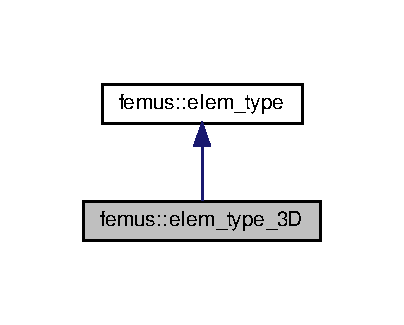
\includegraphics[width=194pt]{classfemus_1_1elem__type__3_d__inherit__graph}
\end{center}
\end{figure}


Collaboration diagram for femus\+:\+:elem\+\_\+type\+\_\+3D\+:
\nopagebreak
\begin{figure}[H]
\begin{center}
\leavevmode
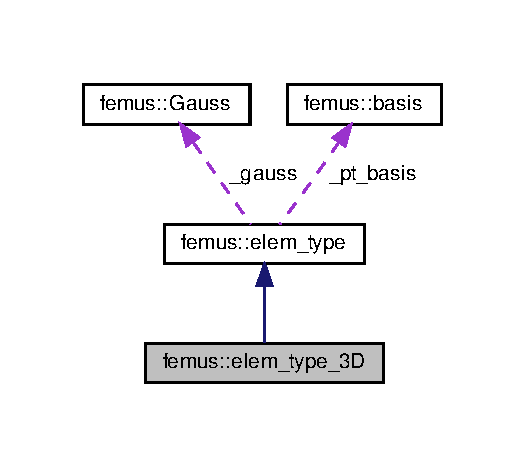
\includegraphics[width=252pt]{classfemus_1_1elem__type__3_d__coll__graph}
\end{center}
\end{figure}
\subsection*{Public Member Functions}
\begin{DoxyCompactItemize}
\item 
\mbox{\hyperlink{classfemus_1_1elem__type__3_d_a218cb9c26e839084933a2e6af9f30443}{elem\+\_\+type\+\_\+3D}} (const char $\ast$solid, const char $\ast$order, const char $\ast$gauss\+\_\+order)
\item 
\mbox{\hyperlink{classfemus_1_1elem__type__3_d_acf28faffa2f92f63636478526f08a387}{$\sim$elem\+\_\+type\+\_\+3D}} ()
\item 
{\footnotesize template$<$class type $>$ }\\void \mbox{\hyperlink{classfemus_1_1elem__type__3_d_adcb67b007b859b8efef1e35f52ef99c8}{Get\+Jacobian\+\_\+type}} (const vector$<$ vector$<$ type $>$ $>$ \&vt, const unsigned \&\mbox{\hyperlink{namespacefemus_a6df31099f676311de214a312d7043941}{ig}}, type \&Weight, vector$<$ vector$<$ type $>$ $>$ \&jacobian\+Matrix) const
\item 
void \mbox{\hyperlink{classfemus_1_1elem__type__3_d_ada0cc038990bffab6a4bc3d1d23f057f}{Get\+Jacobian}} (const vector$<$ vector$<$ adept\+::adouble $>$ $>$ \&vt, const unsigned \&\mbox{\hyperlink{namespacefemus_a6df31099f676311de214a312d7043941}{ig}}, adept\+::adouble \&Weight, vector$<$ vector$<$ adept\+::adouble $>$ $>$ \&jacobian\+Matrix) const
\item 
void \mbox{\hyperlink{classfemus_1_1elem__type__3_d_aacb6b130a8421fe901505f6d61ad8ddd}{Get\+Jacobian}} (const vector$<$ vector$<$ double $>$ $>$ \&vt, const unsigned \&\mbox{\hyperlink{namespacefemus_a6df31099f676311de214a312d7043941}{ig}}, double \&Weight, vector$<$ vector$<$ double $>$ $>$ \&jacobian\+Matrix) const
\item 
{\footnotesize template$<$class type $>$ }\\void \mbox{\hyperlink{classfemus_1_1elem__type__3_d_a8188e7f5aea4cbc3c6ad70d5b14aab4c}{Jacobian\+\_\+type}} (const vector$<$ vector$<$ type $>$ $>$ \&vt, const unsigned \&\mbox{\hyperlink{namespacefemus_a6df31099f676311de214a312d7043941}{ig}}, type \&Weight, vector$<$ double $>$ \&phi, vector$<$ type $>$ \&gradphi, boost\+::optional$<$ vector$<$ type $>$ \& $>$ nablaphi) const
\item 
void \mbox{\hyperlink{classfemus_1_1elem__type__3_d_a6ba1c6d58757d317c455e9041bdb1970}{Jacobian}} (const vector$<$ vector$<$ adept\+::adouble $>$ $>$ \&vt, const unsigned \&\mbox{\hyperlink{namespacefemus_a6df31099f676311de214a312d7043941}{ig}}, adept\+::adouble \&Weight, vector$<$ double $>$ \&phi, vector$<$ adept\+::adouble $>$ \&gradphi, boost\+::optional$<$ vector$<$ adept\+::adouble $>$ \& $>$ nablaphi=boost\+::none) const
\item 
void \mbox{\hyperlink{classfemus_1_1elem__type__3_d_a83c519de8adf50f547627123db1a82ee}{Jacobian}} (const vector$<$ vector$<$ double $>$ $>$ \&vt, const unsigned \&\mbox{\hyperlink{namespacefemus_a6df31099f676311de214a312d7043941}{ig}}, double \&Weight, vector$<$ double $>$ \&phi, vector$<$ double $>$ \&gradphi, boost\+::optional$<$ vector$<$ double $>$ \& $>$ nablaphi=boost\+::none) const
\item 
{\footnotesize template$<$class type $>$ }\\void \mbox{\hyperlink{classfemus_1_1elem__type__3_d_a8e2dffc8f5d0e5fa316b93218d331280}{Jacobian\+\_\+type}} (const vector$<$ vector$<$ type $>$ $>$ \&vt, const vector$<$ double $>$ \&xi, type \&Weight, vector$<$ double $>$ \&phi, vector$<$ type $>$ \&gradphi, boost\+::optional$<$ vector$<$ type $>$ \& $>$ nablaphi) const
\item 
void \mbox{\hyperlink{classfemus_1_1elem__type__3_d_a277615099e6e69b4aed9e1cd9e84817d}{Jacobian}} (const vector$<$ vector$<$ adept\+::adouble $>$ $>$ \&vt, const vector$<$ double $>$ \&xi, adept\+::adouble \&Weight, vector$<$ double $>$ \&phi, vector$<$ adept\+::adouble $>$ \&gradphi, boost\+::optional$<$ vector$<$ adept\+::adouble $>$ \& $>$ nablaphi=boost\+::none) const
\item 
void \mbox{\hyperlink{classfemus_1_1elem__type__3_d_a53f0fe22a3df82bab547a2578d66d7c6}{Jacobian}} (const vector$<$ vector$<$ double $>$ $>$ \&vt, const vector$<$ double $>$ \&xi, double \&Weight, vector$<$ double $>$ \&phi, vector$<$ double $>$ \&gradphi, boost\+::optional$<$ vector$<$ double $>$ \& $>$ nablaphi=boost\+::none) const
\item 
void \mbox{\hyperlink{classfemus_1_1elem__type__3_d_a8eea4f745f548cc10bb55848c4cd2ba3}{Jacobian\+Sur}} (const vector$<$ vector$<$ adept\+::adouble $>$ $>$ \&vt, const unsigned \&\mbox{\hyperlink{namespacefemus_a6df31099f676311de214a312d7043941}{ig}}, adept\+::adouble \&Weight, vector$<$ double $>$ \&other\+\_\+phi, vector$<$ adept\+::adouble $>$ \&gradphi, vector$<$ adept\+::adouble $>$ \&normal) const
\item 
void \mbox{\hyperlink{classfemus_1_1elem__type__3_d_a35ed7904fbe1fdc2998819384d709bdb}{Jacobian\+Sur}} (const vector$<$ vector$<$ double $>$ $>$ \&vt, const unsigned \&\mbox{\hyperlink{namespacefemus_a6df31099f676311de214a312d7043941}{ig}}, double \&Weight, vector$<$ double $>$ \&other\+\_\+phi, vector$<$ double $>$ \&gradphi, vector$<$ double $>$ \&normal) const
\item 
double $\ast$ \mbox{\hyperlink{classfemus_1_1elem__type__3_d_ac25f62fb2b22b534172ce6ef94b89068}{Get\+Phi}} (const unsigned \&\mbox{\hyperlink{namespacefemus_a6df31099f676311de214a312d7043941}{ig}}) const
\item 
double $\ast$ \mbox{\hyperlink{classfemus_1_1elem__type__3_d_aff869fa323fd20f83fed73f4a28de006}{Get\+D\+Phi\+D\+Xi}} (const unsigned \&\mbox{\hyperlink{namespacefemus_a6df31099f676311de214a312d7043941}{ig}}) const
\item 
double $\ast$ \mbox{\hyperlink{classfemus_1_1elem__type__3_d_aa08787fdf3934c52c41a14a59884eb7b}{Get\+D\+Phi\+D\+Eta}} (const unsigned \&\mbox{\hyperlink{namespacefemus_a6df31099f676311de214a312d7043941}{ig}}) const
\item 
double $\ast$ \mbox{\hyperlink{classfemus_1_1elem__type__3_d_a8bf7020e0c07cf44c9532f9b6bab4bbc}{Get\+D\+Phi\+D\+Zeta}} (const unsigned \&\mbox{\hyperlink{namespacefemus_a6df31099f676311de214a312d7043941}{ig}}) const
\end{DoxyCompactItemize}
\subsection*{Additional Inherited Members}


\subsection{Constructor \& Destructor Documentation}
\mbox{\Hypertarget{classfemus_1_1elem__type__3_d_a218cb9c26e839084933a2e6af9f30443}\label{classfemus_1_1elem__type__3_d_a218cb9c26e839084933a2e6af9f30443}} 
\index{femus\+::elem\+\_\+type\+\_\+3D@{femus\+::elem\+\_\+type\+\_\+3D}!elem\+\_\+type\+\_\+3D@{elem\+\_\+type\+\_\+3D}}
\index{elem\+\_\+type\+\_\+3D@{elem\+\_\+type\+\_\+3D}!femus\+::elem\+\_\+type\+\_\+3D@{femus\+::elem\+\_\+type\+\_\+3D}}
\subsubsection{\texorpdfstring{elem\+\_\+type\+\_\+3\+D()}{elem\_type\_3D()}}
{\footnotesize\ttfamily femus\+::elem\+\_\+type\+\_\+3\+D\+::elem\+\_\+type\+\_\+3D (\begin{DoxyParamCaption}\item[{const char $\ast$}]{solid,  }\item[{const char $\ast$}]{order,  }\item[{const char $\ast$}]{gauss\+\_\+order }\end{DoxyParamCaption})}

constructor \mbox{\Hypertarget{classfemus_1_1elem__type__3_d_acf28faffa2f92f63636478526f08a387}\label{classfemus_1_1elem__type__3_d_acf28faffa2f92f63636478526f08a387}} 
\index{femus\+::elem\+\_\+type\+\_\+3D@{femus\+::elem\+\_\+type\+\_\+3D}!````~elem\+\_\+type\+\_\+3D@{$\sim$elem\+\_\+type\+\_\+3D}}
\index{````~elem\+\_\+type\+\_\+3D@{$\sim$elem\+\_\+type\+\_\+3D}!femus\+::elem\+\_\+type\+\_\+3D@{femus\+::elem\+\_\+type\+\_\+3D}}
\subsubsection{\texorpdfstring{$\sim$elem\+\_\+type\+\_\+3\+D()}{~elem\_type\_3D()}}
{\footnotesize\ttfamily femus\+::elem\+\_\+type\+\_\+3\+D\+::$\sim$elem\+\_\+type\+\_\+3D (\begin{DoxyParamCaption}{ }\end{DoxyParamCaption})\hspace{0.3cm}{\ttfamily [inline]}}

destructor 

\subsection{Member Function Documentation}
\mbox{\Hypertarget{classfemus_1_1elem__type__3_d_aa08787fdf3934c52c41a14a59884eb7b}\label{classfemus_1_1elem__type__3_d_aa08787fdf3934c52c41a14a59884eb7b}} 
\index{femus\+::elem\+\_\+type\+\_\+3D@{femus\+::elem\+\_\+type\+\_\+3D}!Get\+D\+Phi\+D\+Eta@{Get\+D\+Phi\+D\+Eta}}
\index{Get\+D\+Phi\+D\+Eta@{Get\+D\+Phi\+D\+Eta}!femus\+::elem\+\_\+type\+\_\+3D@{femus\+::elem\+\_\+type\+\_\+3D}}
\subsubsection{\texorpdfstring{Get\+D\+Phi\+D\+Eta()}{GetDPhiDEta()}}
{\footnotesize\ttfamily double$\ast$ femus\+::elem\+\_\+type\+\_\+3\+D\+::\+Get\+D\+Phi\+D\+Eta (\begin{DoxyParamCaption}\item[{const unsigned \&}]{ig }\end{DoxyParamCaption}) const\hspace{0.3cm}{\ttfamily [inline]}, {\ttfamily [virtual]}}

To be Added 

Reimplemented from \mbox{\hyperlink{classfemus_1_1elem__type_a510e44439de5cdd6ab5d04e3f8a5bdfe}{femus\+::elem\+\_\+type}}.

\mbox{\Hypertarget{classfemus_1_1elem__type__3_d_aff869fa323fd20f83fed73f4a28de006}\label{classfemus_1_1elem__type__3_d_aff869fa323fd20f83fed73f4a28de006}} 
\index{femus\+::elem\+\_\+type\+\_\+3D@{femus\+::elem\+\_\+type\+\_\+3D}!Get\+D\+Phi\+D\+Xi@{Get\+D\+Phi\+D\+Xi}}
\index{Get\+D\+Phi\+D\+Xi@{Get\+D\+Phi\+D\+Xi}!femus\+::elem\+\_\+type\+\_\+3D@{femus\+::elem\+\_\+type\+\_\+3D}}
\subsubsection{\texorpdfstring{Get\+D\+Phi\+D\+Xi()}{GetDPhiDXi()}}
{\footnotesize\ttfamily double$\ast$ femus\+::elem\+\_\+type\+\_\+3\+D\+::\+Get\+D\+Phi\+D\+Xi (\begin{DoxyParamCaption}\item[{const unsigned \&}]{ig }\end{DoxyParamCaption}) const\hspace{0.3cm}{\ttfamily [inline]}, {\ttfamily [virtual]}}

To be Added 

Implements \mbox{\hyperlink{classfemus_1_1elem__type_a6efb6026b9fe89912ec367b235bfccc7}{femus\+::elem\+\_\+type}}.

\mbox{\Hypertarget{classfemus_1_1elem__type__3_d_a8bf7020e0c07cf44c9532f9b6bab4bbc}\label{classfemus_1_1elem__type__3_d_a8bf7020e0c07cf44c9532f9b6bab4bbc}} 
\index{femus\+::elem\+\_\+type\+\_\+3D@{femus\+::elem\+\_\+type\+\_\+3D}!Get\+D\+Phi\+D\+Zeta@{Get\+D\+Phi\+D\+Zeta}}
\index{Get\+D\+Phi\+D\+Zeta@{Get\+D\+Phi\+D\+Zeta}!femus\+::elem\+\_\+type\+\_\+3D@{femus\+::elem\+\_\+type\+\_\+3D}}
\subsubsection{\texorpdfstring{Get\+D\+Phi\+D\+Zeta()}{GetDPhiDZeta()}}
{\footnotesize\ttfamily double$\ast$ femus\+::elem\+\_\+type\+\_\+3\+D\+::\+Get\+D\+Phi\+D\+Zeta (\begin{DoxyParamCaption}\item[{const unsigned \&}]{ig }\end{DoxyParamCaption}) const\hspace{0.3cm}{\ttfamily [inline]}, {\ttfamily [virtual]}}

To be Added 

Reimplemented from \mbox{\hyperlink{classfemus_1_1elem__type_aa507628a4383a9687c8fdefe30d0214a}{femus\+::elem\+\_\+type}}.

\mbox{\Hypertarget{classfemus_1_1elem__type__3_d_ada0cc038990bffab6a4bc3d1d23f057f}\label{classfemus_1_1elem__type__3_d_ada0cc038990bffab6a4bc3d1d23f057f}} 
\index{femus\+::elem\+\_\+type\+\_\+3D@{femus\+::elem\+\_\+type\+\_\+3D}!Get\+Jacobian@{Get\+Jacobian}}
\index{Get\+Jacobian@{Get\+Jacobian}!femus\+::elem\+\_\+type\+\_\+3D@{femus\+::elem\+\_\+type\+\_\+3D}}
\subsubsection{\texorpdfstring{Get\+Jacobian()}{GetJacobian()}\hspace{0.1cm}{\footnotesize\ttfamily [1/2]}}
{\footnotesize\ttfamily void femus\+::elem\+\_\+type\+\_\+3\+D\+::\+Get\+Jacobian (\begin{DoxyParamCaption}\item[{const vector$<$ vector$<$ adept\+::adouble $>$ $>$ \&}]{vt,  }\item[{const unsigned \&}]{ig,  }\item[{adept\+::adouble \&}]{Weight,  }\item[{vector$<$ vector$<$ adept\+::adouble $>$ $>$ \&}]{jacobian\+Matrix }\end{DoxyParamCaption}) const\hspace{0.3cm}{\ttfamily [inline]}, {\ttfamily [virtual]}}



Implements \mbox{\hyperlink{classfemus_1_1elem__type_aa8e617c54dd774ffca5d305605552af7}{femus\+::elem\+\_\+type}}.

\mbox{\Hypertarget{classfemus_1_1elem__type__3_d_aacb6b130a8421fe901505f6d61ad8ddd}\label{classfemus_1_1elem__type__3_d_aacb6b130a8421fe901505f6d61ad8ddd}} 
\index{femus\+::elem\+\_\+type\+\_\+3D@{femus\+::elem\+\_\+type\+\_\+3D}!Get\+Jacobian@{Get\+Jacobian}}
\index{Get\+Jacobian@{Get\+Jacobian}!femus\+::elem\+\_\+type\+\_\+3D@{femus\+::elem\+\_\+type\+\_\+3D}}
\subsubsection{\texorpdfstring{Get\+Jacobian()}{GetJacobian()}\hspace{0.1cm}{\footnotesize\ttfamily [2/2]}}
{\footnotesize\ttfamily void femus\+::elem\+\_\+type\+\_\+3\+D\+::\+Get\+Jacobian (\begin{DoxyParamCaption}\item[{const vector$<$ vector$<$ double $>$ $>$ \&}]{vt,  }\item[{const unsigned \&}]{ig,  }\item[{double \&}]{Weight,  }\item[{vector$<$ vector$<$ double $>$ $>$ \&}]{jacobian\+Matrix }\end{DoxyParamCaption}) const\hspace{0.3cm}{\ttfamily [inline]}, {\ttfamily [virtual]}}



Implements \mbox{\hyperlink{classfemus_1_1elem__type_a6c883b7946e55db8783fd0177546610a}{femus\+::elem\+\_\+type}}.

\mbox{\Hypertarget{classfemus_1_1elem__type__3_d_adcb67b007b859b8efef1e35f52ef99c8}\label{classfemus_1_1elem__type__3_d_adcb67b007b859b8efef1e35f52ef99c8}} 
\index{femus\+::elem\+\_\+type\+\_\+3D@{femus\+::elem\+\_\+type\+\_\+3D}!Get\+Jacobian\+\_\+type@{Get\+Jacobian\+\_\+type}}
\index{Get\+Jacobian\+\_\+type@{Get\+Jacobian\+\_\+type}!femus\+::elem\+\_\+type\+\_\+3D@{femus\+::elem\+\_\+type\+\_\+3D}}
\subsubsection{\texorpdfstring{Get\+Jacobian\+\_\+type()}{GetJacobian\_type()}}
{\footnotesize\ttfamily template$<$class type $>$ \\
void femus\+::elem\+\_\+type\+\_\+3\+D\+::\+Get\+Jacobian\+\_\+type (\begin{DoxyParamCaption}\item[{const vector$<$ vector$<$ type $>$ $>$ \&}]{vt,  }\item[{const unsigned \&}]{ig,  }\item[{type \&}]{Weight,  }\item[{vector$<$ vector$<$ type $>$ $>$ \&}]{jacobian\+Matrix }\end{DoxyParamCaption}) const}

\mbox{\Hypertarget{classfemus_1_1elem__type__3_d_ac25f62fb2b22b534172ce6ef94b89068}\label{classfemus_1_1elem__type__3_d_ac25f62fb2b22b534172ce6ef94b89068}} 
\index{femus\+::elem\+\_\+type\+\_\+3D@{femus\+::elem\+\_\+type\+\_\+3D}!Get\+Phi@{Get\+Phi}}
\index{Get\+Phi@{Get\+Phi}!femus\+::elem\+\_\+type\+\_\+3D@{femus\+::elem\+\_\+type\+\_\+3D}}
\subsubsection{\texorpdfstring{Get\+Phi()}{GetPhi()}}
{\footnotesize\ttfamily double$\ast$ femus\+::elem\+\_\+type\+\_\+3\+D\+::\+Get\+Phi (\begin{DoxyParamCaption}\item[{const unsigned \&}]{ig }\end{DoxyParamCaption}) const\hspace{0.3cm}{\ttfamily [inline]}, {\ttfamily [virtual]}}

To be Added 

Implements \mbox{\hyperlink{classfemus_1_1elem__type_a2aa2a37b15debbee27918f5e3f2df6b3}{femus\+::elem\+\_\+type}}.

\mbox{\Hypertarget{classfemus_1_1elem__type__3_d_a6ba1c6d58757d317c455e9041bdb1970}\label{classfemus_1_1elem__type__3_d_a6ba1c6d58757d317c455e9041bdb1970}} 
\index{femus\+::elem\+\_\+type\+\_\+3D@{femus\+::elem\+\_\+type\+\_\+3D}!Jacobian@{Jacobian}}
\index{Jacobian@{Jacobian}!femus\+::elem\+\_\+type\+\_\+3D@{femus\+::elem\+\_\+type\+\_\+3D}}
\subsubsection{\texorpdfstring{Jacobian()}{Jacobian()}\hspace{0.1cm}{\footnotesize\ttfamily [1/4]}}
{\footnotesize\ttfamily void femus\+::elem\+\_\+type\+\_\+3\+D\+::\+Jacobian (\begin{DoxyParamCaption}\item[{const vector$<$ vector$<$ adept\+::adouble $>$ $>$ \&}]{vt,  }\item[{const unsigned \&}]{ig,  }\item[{adept\+::adouble \&}]{Weight,  }\item[{vector$<$ double $>$ \&}]{phi,  }\item[{vector$<$ adept\+::adouble $>$ \&}]{gradphi,  }\item[{boost\+::optional$<$ vector$<$ adept\+::adouble $>$ \& $>$}]{nablaphi = {\ttfamily boost\+:\+:none} }\end{DoxyParamCaption}) const\hspace{0.3cm}{\ttfamily [inline]}, {\ttfamily [virtual]}}



Implements \mbox{\hyperlink{classfemus_1_1elem__type_a937b1d5ecbeed3b17db831264a3492fa}{femus\+::elem\+\_\+type}}.

\mbox{\Hypertarget{classfemus_1_1elem__type__3_d_a83c519de8adf50f547627123db1a82ee}\label{classfemus_1_1elem__type__3_d_a83c519de8adf50f547627123db1a82ee}} 
\index{femus\+::elem\+\_\+type\+\_\+3D@{femus\+::elem\+\_\+type\+\_\+3D}!Jacobian@{Jacobian}}
\index{Jacobian@{Jacobian}!femus\+::elem\+\_\+type\+\_\+3D@{femus\+::elem\+\_\+type\+\_\+3D}}
\subsubsection{\texorpdfstring{Jacobian()}{Jacobian()}\hspace{0.1cm}{\footnotesize\ttfamily [2/4]}}
{\footnotesize\ttfamily void femus\+::elem\+\_\+type\+\_\+3\+D\+::\+Jacobian (\begin{DoxyParamCaption}\item[{const vector$<$ vector$<$ double $>$ $>$ \&}]{vt,  }\item[{const unsigned \&}]{ig,  }\item[{double \&}]{Weight,  }\item[{vector$<$ double $>$ \&}]{phi,  }\item[{vector$<$ double $>$ \&}]{gradphi,  }\item[{boost\+::optional$<$ vector$<$ double $>$ \& $>$}]{nablaphi = {\ttfamily boost\+:\+:none} }\end{DoxyParamCaption}) const\hspace{0.3cm}{\ttfamily [inline]}, {\ttfamily [virtual]}}



Implements \mbox{\hyperlink{classfemus_1_1elem__type_ac3828ecd8ddd057d726a60cb19c60f0b}{femus\+::elem\+\_\+type}}.

\mbox{\Hypertarget{classfemus_1_1elem__type__3_d_a277615099e6e69b4aed9e1cd9e84817d}\label{classfemus_1_1elem__type__3_d_a277615099e6e69b4aed9e1cd9e84817d}} 
\index{femus\+::elem\+\_\+type\+\_\+3D@{femus\+::elem\+\_\+type\+\_\+3D}!Jacobian@{Jacobian}}
\index{Jacobian@{Jacobian}!femus\+::elem\+\_\+type\+\_\+3D@{femus\+::elem\+\_\+type\+\_\+3D}}
\subsubsection{\texorpdfstring{Jacobian()}{Jacobian()}\hspace{0.1cm}{\footnotesize\ttfamily [3/4]}}
{\footnotesize\ttfamily void femus\+::elem\+\_\+type\+\_\+3\+D\+::\+Jacobian (\begin{DoxyParamCaption}\item[{const vector$<$ vector$<$ adept\+::adouble $>$ $>$ \&}]{vt,  }\item[{const vector$<$ double $>$ \&}]{xi,  }\item[{adept\+::adouble \&}]{Weight,  }\item[{vector$<$ double $>$ \&}]{phi,  }\item[{vector$<$ adept\+::adouble $>$ \&}]{gradphi,  }\item[{boost\+::optional$<$ vector$<$ adept\+::adouble $>$ \& $>$}]{nablaphi = {\ttfamily boost\+:\+:none} }\end{DoxyParamCaption}) const\hspace{0.3cm}{\ttfamily [inline]}, {\ttfamily [virtual]}}



Implements \mbox{\hyperlink{classfemus_1_1elem__type_a2d76133387cebf896c0e51459055fdea}{femus\+::elem\+\_\+type}}.

\mbox{\Hypertarget{classfemus_1_1elem__type__3_d_a53f0fe22a3df82bab547a2578d66d7c6}\label{classfemus_1_1elem__type__3_d_a53f0fe22a3df82bab547a2578d66d7c6}} 
\index{femus\+::elem\+\_\+type\+\_\+3D@{femus\+::elem\+\_\+type\+\_\+3D}!Jacobian@{Jacobian}}
\index{Jacobian@{Jacobian}!femus\+::elem\+\_\+type\+\_\+3D@{femus\+::elem\+\_\+type\+\_\+3D}}
\subsubsection{\texorpdfstring{Jacobian()}{Jacobian()}\hspace{0.1cm}{\footnotesize\ttfamily [4/4]}}
{\footnotesize\ttfamily void femus\+::elem\+\_\+type\+\_\+3\+D\+::\+Jacobian (\begin{DoxyParamCaption}\item[{const vector$<$ vector$<$ double $>$ $>$ \&}]{vt,  }\item[{const vector$<$ double $>$ \&}]{xi,  }\item[{double \&}]{Weight,  }\item[{vector$<$ double $>$ \&}]{phi,  }\item[{vector$<$ double $>$ \&}]{gradphi,  }\item[{boost\+::optional$<$ vector$<$ double $>$ \& $>$}]{nablaphi = {\ttfamily boost\+:\+:none} }\end{DoxyParamCaption}) const\hspace{0.3cm}{\ttfamily [inline]}, {\ttfamily [virtual]}}



Implements \mbox{\hyperlink{classfemus_1_1elem__type_aab6db5851a9810adfe0ff98df2c30810}{femus\+::elem\+\_\+type}}.

\mbox{\Hypertarget{classfemus_1_1elem__type__3_d_a8188e7f5aea4cbc3c6ad70d5b14aab4c}\label{classfemus_1_1elem__type__3_d_a8188e7f5aea4cbc3c6ad70d5b14aab4c}} 
\index{femus\+::elem\+\_\+type\+\_\+3D@{femus\+::elem\+\_\+type\+\_\+3D}!Jacobian\+\_\+type@{Jacobian\+\_\+type}}
\index{Jacobian\+\_\+type@{Jacobian\+\_\+type}!femus\+::elem\+\_\+type\+\_\+3D@{femus\+::elem\+\_\+type\+\_\+3D}}
\subsubsection{\texorpdfstring{Jacobian\+\_\+type()}{Jacobian\_type()}\hspace{0.1cm}{\footnotesize\ttfamily [1/2]}}
{\footnotesize\ttfamily template$<$class type $>$ \\
void femus\+::elem\+\_\+type\+\_\+3\+D\+::\+Jacobian\+\_\+type (\begin{DoxyParamCaption}\item[{const vector$<$ vector$<$ type $>$ $>$ \&}]{vt,  }\item[{const unsigned \&}]{ig,  }\item[{type \&}]{Weight,  }\item[{vector$<$ double $>$ \&}]{phi,  }\item[{vector$<$ type $>$ \&}]{gradphi,  }\item[{boost\+::optional$<$ vector$<$ type $>$ \& $>$}]{nablaphi }\end{DoxyParamCaption}) const}

\mbox{\Hypertarget{classfemus_1_1elem__type__3_d_a8e2dffc8f5d0e5fa316b93218d331280}\label{classfemus_1_1elem__type__3_d_a8e2dffc8f5d0e5fa316b93218d331280}} 
\index{femus\+::elem\+\_\+type\+\_\+3D@{femus\+::elem\+\_\+type\+\_\+3D}!Jacobian\+\_\+type@{Jacobian\+\_\+type}}
\index{Jacobian\+\_\+type@{Jacobian\+\_\+type}!femus\+::elem\+\_\+type\+\_\+3D@{femus\+::elem\+\_\+type\+\_\+3D}}
\subsubsection{\texorpdfstring{Jacobian\+\_\+type()}{Jacobian\_type()}\hspace{0.1cm}{\footnotesize\ttfamily [2/2]}}
{\footnotesize\ttfamily template$<$class type $>$ \\
void femus\+::elem\+\_\+type\+\_\+3\+D\+::\+Jacobian\+\_\+type (\begin{DoxyParamCaption}\item[{const vector$<$ vector$<$ type $>$ $>$ \&}]{vt,  }\item[{const vector$<$ double $>$ \&}]{xi,  }\item[{type \&}]{Weight,  }\item[{vector$<$ double $>$ \&}]{phi,  }\item[{vector$<$ type $>$ \&}]{gradphi,  }\item[{boost\+::optional$<$ vector$<$ type $>$ \& $>$}]{nablaphi }\end{DoxyParamCaption}) const}

\mbox{\Hypertarget{classfemus_1_1elem__type__3_d_a8eea4f745f548cc10bb55848c4cd2ba3}\label{classfemus_1_1elem__type__3_d_a8eea4f745f548cc10bb55848c4cd2ba3}} 
\index{femus\+::elem\+\_\+type\+\_\+3D@{femus\+::elem\+\_\+type\+\_\+3D}!Jacobian\+Sur@{Jacobian\+Sur}}
\index{Jacobian\+Sur@{Jacobian\+Sur}!femus\+::elem\+\_\+type\+\_\+3D@{femus\+::elem\+\_\+type\+\_\+3D}}
\subsubsection{\texorpdfstring{Jacobian\+Sur()}{JacobianSur()}\hspace{0.1cm}{\footnotesize\ttfamily [1/2]}}
{\footnotesize\ttfamily void femus\+::elem\+\_\+type\+\_\+3\+D\+::\+Jacobian\+Sur (\begin{DoxyParamCaption}\item[{const vector$<$ vector$<$ adept\+::adouble $>$ $>$ \&}]{vt,  }\item[{const unsigned \&}]{ig,  }\item[{adept\+::adouble \&}]{Weight,  }\item[{vector$<$ double $>$ \&}]{other\+\_\+phi,  }\item[{vector$<$ adept\+::adouble $>$ \&}]{gradphi,  }\item[{vector$<$ adept\+::adouble $>$ \&}]{normal }\end{DoxyParamCaption}) const\hspace{0.3cm}{\ttfamily [inline]}, {\ttfamily [virtual]}}



Implements \mbox{\hyperlink{classfemus_1_1elem__type_a293052fac0f51472150b1bf7365c6b18}{femus\+::elem\+\_\+type}}.

\mbox{\Hypertarget{classfemus_1_1elem__type__3_d_a35ed7904fbe1fdc2998819384d709bdb}\label{classfemus_1_1elem__type__3_d_a35ed7904fbe1fdc2998819384d709bdb}} 
\index{femus\+::elem\+\_\+type\+\_\+3D@{femus\+::elem\+\_\+type\+\_\+3D}!Jacobian\+Sur@{Jacobian\+Sur}}
\index{Jacobian\+Sur@{Jacobian\+Sur}!femus\+::elem\+\_\+type\+\_\+3D@{femus\+::elem\+\_\+type\+\_\+3D}}
\subsubsection{\texorpdfstring{Jacobian\+Sur()}{JacobianSur()}\hspace{0.1cm}{\footnotesize\ttfamily [2/2]}}
{\footnotesize\ttfamily void femus\+::elem\+\_\+type\+\_\+3\+D\+::\+Jacobian\+Sur (\begin{DoxyParamCaption}\item[{const vector$<$ vector$<$ double $>$ $>$ \&}]{vt,  }\item[{const unsigned \&}]{ig,  }\item[{double \&}]{Weight,  }\item[{vector$<$ double $>$ \&}]{other\+\_\+phi,  }\item[{vector$<$ double $>$ \&}]{gradphi,  }\item[{vector$<$ double $>$ \&}]{normal }\end{DoxyParamCaption}) const\hspace{0.3cm}{\ttfamily [inline]}, {\ttfamily [virtual]}}



Implements \mbox{\hyperlink{classfemus_1_1elem__type_aee56bc66a4d90ae7f7669bf7fa9ed8d7}{femus\+::elem\+\_\+type}}.



The documentation for this class was generated from the following files\+:\begin{DoxyCompactItemize}
\item 
fe/\mbox{\hyperlink{_elem_type_8hpp}{Elem\+Type.\+hpp}}\item 
fe/\mbox{\hyperlink{_elem_type_8cpp}{Elem\+Type.\+cpp}}\end{DoxyCompactItemize}

\hypertarget{classfemus_1_1_elem_sto_base}{}\section{femus\+:\+:Elem\+Sto\+Base Class Reference}
\label{classfemus_1_1_elem_sto_base}\index{femus\+::\+Elem\+Sto\+Base@{femus\+::\+Elem\+Sto\+Base}}


{\ttfamily \#include $<$Elem\+Sto.\+hpp$>$}



Inheritance diagram for femus\+:\+:Elem\+Sto\+Base\+:
\nopagebreak
\begin{figure}[H]
\begin{center}
\leavevmode
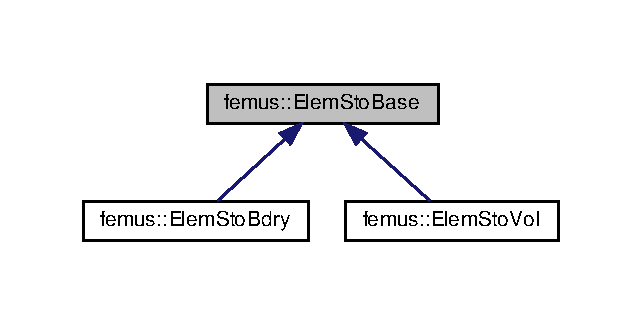
\includegraphics[width=308pt]{classfemus_1_1_elem_sto_base__inherit__graph}
\end{center}
\end{figure}
\subsection*{Public Member Functions}
\begin{DoxyCompactItemize}
\item 
\mbox{\hyperlink{classfemus_1_1_elem_sto_base_ae6f3488589787d622037253092ce95b4}{Elem\+Sto\+Base}} (int nnds\+\_\+in, \mbox{\hyperlink{_typedefs_8hpp_a91ad9478d81a7aaf2593e8d9c3d06a14}{uint}} spacedim\+\_\+in)
\item 
\mbox{\hyperlink{classfemus_1_1_elem_sto_base_a53ccb54619040fb0b77429bb89900a16}{$\sim$\+Elem\+Sto\+Base}} ()
\end{DoxyCompactItemize}
\subsection*{Public Attributes}
\begin{DoxyCompactItemize}
\item 
int \mbox{\hyperlink{classfemus_1_1_elem_sto_base_a650ffa9b4e351ec4d16212d80b251dc7}{\+\_\+id}}
\item 
int \mbox{\hyperlink{classfemus_1_1_elem_sto_base_a21fac1582fea632435a5576ff9a6b6ac}{\+\_\+lev}}
\item 
int \mbox{\hyperlink{classfemus_1_1_elem_sto_base_ae2a0bc193975b623626a8eb58e549417}{\+\_\+subd}}
\item 
int \mbox{\hyperlink{classfemus_1_1_elem_sto_base_a87a91036236ff4407f5e1fb877d3c596}{\+\_\+nnds}}
\item 
int $\ast$ \mbox{\hyperlink{classfemus_1_1_elem_sto_base_a9d853484dcf998f1e3e1b2374e8c3b61}{\+\_\+elnds}}
\item 
\mbox{\hyperlink{_typedefs_8hpp_a91ad9478d81a7aaf2593e8d9c3d06a14}{uint}} \mbox{\hyperlink{classfemus_1_1_elem_sto_base_a300ec73a087a8df1257ac139b7e6648e}{\+\_\+spacedim}}
\end{DoxyCompactItemize}


\subsection{Constructor \& Destructor Documentation}
\mbox{\Hypertarget{classfemus_1_1_elem_sto_base_ae6f3488589787d622037253092ce95b4}\label{classfemus_1_1_elem_sto_base_ae6f3488589787d622037253092ce95b4}} 
\index{femus\+::\+Elem\+Sto\+Base@{femus\+::\+Elem\+Sto\+Base}!Elem\+Sto\+Base@{Elem\+Sto\+Base}}
\index{Elem\+Sto\+Base@{Elem\+Sto\+Base}!femus\+::\+Elem\+Sto\+Base@{femus\+::\+Elem\+Sto\+Base}}
\subsubsection{\texorpdfstring{Elem\+Sto\+Base()}{ElemStoBase()}}
{\footnotesize\ttfamily femus\+::\+Elem\+Sto\+Base\+::\+Elem\+Sto\+Base (\begin{DoxyParamCaption}\item[{int}]{nnds\+\_\+in,  }\item[{\mbox{\hyperlink{_typedefs_8hpp_a91ad9478d81a7aaf2593e8d9c3d06a14}{uint}}}]{spacedim\+\_\+in }\end{DoxyParamCaption})}

\mbox{\Hypertarget{classfemus_1_1_elem_sto_base_a53ccb54619040fb0b77429bb89900a16}\label{classfemus_1_1_elem_sto_base_a53ccb54619040fb0b77429bb89900a16}} 
\index{femus\+::\+Elem\+Sto\+Base@{femus\+::\+Elem\+Sto\+Base}!````~Elem\+Sto\+Base@{$\sim$\+Elem\+Sto\+Base}}
\index{````~Elem\+Sto\+Base@{$\sim$\+Elem\+Sto\+Base}!femus\+::\+Elem\+Sto\+Base@{femus\+::\+Elem\+Sto\+Base}}
\subsubsection{\texorpdfstring{$\sim$\+Elem\+Sto\+Base()}{~ElemStoBase()}}
{\footnotesize\ttfamily femus\+::\+Elem\+Sto\+Base\+::$\sim$\+Elem\+Sto\+Base (\begin{DoxyParamCaption}{ }\end{DoxyParamCaption})}



\subsection{Member Data Documentation}
\mbox{\Hypertarget{classfemus_1_1_elem_sto_base_a9d853484dcf998f1e3e1b2374e8c3b61}\label{classfemus_1_1_elem_sto_base_a9d853484dcf998f1e3e1b2374e8c3b61}} 
\index{femus\+::\+Elem\+Sto\+Base@{femus\+::\+Elem\+Sto\+Base}!\+\_\+elnds@{\+\_\+elnds}}
\index{\+\_\+elnds@{\+\_\+elnds}!femus\+::\+Elem\+Sto\+Base@{femus\+::\+Elem\+Sto\+Base}}
\subsubsection{\texorpdfstring{\+\_\+elnds}{\_elnds}}
{\footnotesize\ttfamily int$\ast$ femus\+::\+Elem\+Sto\+Base\+::\+\_\+elnds}

\mbox{\Hypertarget{classfemus_1_1_elem_sto_base_a650ffa9b4e351ec4d16212d80b251dc7}\label{classfemus_1_1_elem_sto_base_a650ffa9b4e351ec4d16212d80b251dc7}} 
\index{femus\+::\+Elem\+Sto\+Base@{femus\+::\+Elem\+Sto\+Base}!\+\_\+id@{\+\_\+id}}
\index{\+\_\+id@{\+\_\+id}!femus\+::\+Elem\+Sto\+Base@{femus\+::\+Elem\+Sto\+Base}}
\subsubsection{\texorpdfstring{\+\_\+id}{\_id}}
{\footnotesize\ttfamily int femus\+::\+Elem\+Sto\+Base\+::\+\_\+id}

\mbox{\Hypertarget{classfemus_1_1_elem_sto_base_a21fac1582fea632435a5576ff9a6b6ac}\label{classfemus_1_1_elem_sto_base_a21fac1582fea632435a5576ff9a6b6ac}} 
\index{femus\+::\+Elem\+Sto\+Base@{femus\+::\+Elem\+Sto\+Base}!\+\_\+lev@{\+\_\+lev}}
\index{\+\_\+lev@{\+\_\+lev}!femus\+::\+Elem\+Sto\+Base@{femus\+::\+Elem\+Sto\+Base}}
\subsubsection{\texorpdfstring{\+\_\+lev}{\_lev}}
{\footnotesize\ttfamily int femus\+::\+Elem\+Sto\+Base\+::\+\_\+lev}

\mbox{\Hypertarget{classfemus_1_1_elem_sto_base_a87a91036236ff4407f5e1fb877d3c596}\label{classfemus_1_1_elem_sto_base_a87a91036236ff4407f5e1fb877d3c596}} 
\index{femus\+::\+Elem\+Sto\+Base@{femus\+::\+Elem\+Sto\+Base}!\+\_\+nnds@{\+\_\+nnds}}
\index{\+\_\+nnds@{\+\_\+nnds}!femus\+::\+Elem\+Sto\+Base@{femus\+::\+Elem\+Sto\+Base}}
\subsubsection{\texorpdfstring{\+\_\+nnds}{\_nnds}}
{\footnotesize\ttfamily int femus\+::\+Elem\+Sto\+Base\+::\+\_\+nnds}

\mbox{\Hypertarget{classfemus_1_1_elem_sto_base_a300ec73a087a8df1257ac139b7e6648e}\label{classfemus_1_1_elem_sto_base_a300ec73a087a8df1257ac139b7e6648e}} 
\index{femus\+::\+Elem\+Sto\+Base@{femus\+::\+Elem\+Sto\+Base}!\+\_\+spacedim@{\+\_\+spacedim}}
\index{\+\_\+spacedim@{\+\_\+spacedim}!femus\+::\+Elem\+Sto\+Base@{femus\+::\+Elem\+Sto\+Base}}
\subsubsection{\texorpdfstring{\+\_\+spacedim}{\_spacedim}}
{\footnotesize\ttfamily \mbox{\hyperlink{_typedefs_8hpp_a91ad9478d81a7aaf2593e8d9c3d06a14}{uint}} femus\+::\+Elem\+Sto\+Base\+::\+\_\+spacedim}

\mbox{\Hypertarget{classfemus_1_1_elem_sto_base_ae2a0bc193975b623626a8eb58e549417}\label{classfemus_1_1_elem_sto_base_ae2a0bc193975b623626a8eb58e549417}} 
\index{femus\+::\+Elem\+Sto\+Base@{femus\+::\+Elem\+Sto\+Base}!\+\_\+subd@{\+\_\+subd}}
\index{\+\_\+subd@{\+\_\+subd}!femus\+::\+Elem\+Sto\+Base@{femus\+::\+Elem\+Sto\+Base}}
\subsubsection{\texorpdfstring{\+\_\+subd}{\_subd}}
{\footnotesize\ttfamily int femus\+::\+Elem\+Sto\+Base\+::\+\_\+subd}



The documentation for this class was generated from the following files\+:\begin{DoxyCompactItemize}
\item 
mesh\+Gencase/\mbox{\hyperlink{_elem_sto_8hpp}{Elem\+Sto.\+hpp}}\item 
mesh\+Gencase/\mbox{\hyperlink{_elem_sto_8cpp}{Elem\+Sto.\+cpp}}\end{DoxyCompactItemize}

\hypertarget{classfemus_1_1_elem_sto_bdry}{}\section{femus\+:\+:Elem\+Sto\+Bdry Class Reference}
\label{classfemus_1_1_elem_sto_bdry}\index{femus\+::\+Elem\+Sto\+Bdry@{femus\+::\+Elem\+Sto\+Bdry}}


{\ttfamily \#include $<$Elem\+Sto.\+hpp$>$}



Inheritance diagram for femus\+:\+:Elem\+Sto\+Bdry\+:
\nopagebreak
\begin{figure}[H]
\begin{center}
\leavevmode
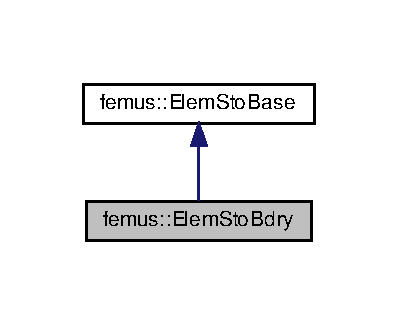
\includegraphics[width=191pt]{classfemus_1_1_elem_sto_bdry__inherit__graph}
\end{center}
\end{figure}


Collaboration diagram for femus\+:\+:Elem\+Sto\+Bdry\+:
\nopagebreak
\begin{figure}[H]
\begin{center}
\leavevmode
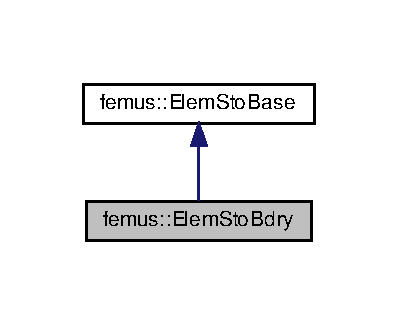
\includegraphics[width=191pt]{classfemus_1_1_elem_sto_bdry__coll__graph}
\end{center}
\end{figure}
\subsection*{Public Member Functions}
\begin{DoxyCompactItemize}
\item 
\mbox{\hyperlink{classfemus_1_1_elem_sto_bdry_a5aa20e3da196878003f75eaa7c7385ad}{Elem\+Sto\+Bdry}} (int nnds\+\_\+in, \mbox{\hyperlink{_typedefs_8hpp_a91ad9478d81a7aaf2593e8d9c3d06a14}{uint}} spacedim)
\item 
\mbox{\hyperlink{classfemus_1_1_elem_sto_bdry_a11b920a31ac9d74282a679a46197ba36}{$\sim$\+Elem\+Sto\+Bdry}} ()
\end{DoxyCompactItemize}
\subsection*{Public Attributes}
\begin{DoxyCompactItemize}
\item 
int \mbox{\hyperlink{classfemus_1_1_elem_sto_bdry_a5df83163da75a6633d69ba8bb19fced7}{\+\_\+vol\+\_\+id}}
\item 
int \mbox{\hyperlink{classfemus_1_1_elem_sto_bdry_a24ee13b2bdb33a0d2b03f7f820ad2d8b}{\+\_\+nside}}
\end{DoxyCompactItemize}


\subsection{Constructor \& Destructor Documentation}
\mbox{\Hypertarget{classfemus_1_1_elem_sto_bdry_a5aa20e3da196878003f75eaa7c7385ad}\label{classfemus_1_1_elem_sto_bdry_a5aa20e3da196878003f75eaa7c7385ad}} 
\index{femus\+::\+Elem\+Sto\+Bdry@{femus\+::\+Elem\+Sto\+Bdry}!Elem\+Sto\+Bdry@{Elem\+Sto\+Bdry}}
\index{Elem\+Sto\+Bdry@{Elem\+Sto\+Bdry}!femus\+::\+Elem\+Sto\+Bdry@{femus\+::\+Elem\+Sto\+Bdry}}
\subsubsection{\texorpdfstring{Elem\+Sto\+Bdry()}{ElemStoBdry()}}
{\footnotesize\ttfamily femus\+::\+Elem\+Sto\+Bdry\+::\+Elem\+Sto\+Bdry (\begin{DoxyParamCaption}\item[{int}]{nnds\+\_\+in,  }\item[{\mbox{\hyperlink{_typedefs_8hpp_a91ad9478d81a7aaf2593e8d9c3d06a14}{uint}}}]{spacedim }\end{DoxyParamCaption})}

\mbox{\Hypertarget{classfemus_1_1_elem_sto_bdry_a11b920a31ac9d74282a679a46197ba36}\label{classfemus_1_1_elem_sto_bdry_a11b920a31ac9d74282a679a46197ba36}} 
\index{femus\+::\+Elem\+Sto\+Bdry@{femus\+::\+Elem\+Sto\+Bdry}!````~Elem\+Sto\+Bdry@{$\sim$\+Elem\+Sto\+Bdry}}
\index{````~Elem\+Sto\+Bdry@{$\sim$\+Elem\+Sto\+Bdry}!femus\+::\+Elem\+Sto\+Bdry@{femus\+::\+Elem\+Sto\+Bdry}}
\subsubsection{\texorpdfstring{$\sim$\+Elem\+Sto\+Bdry()}{~ElemStoBdry()}}
{\footnotesize\ttfamily femus\+::\+Elem\+Sto\+Bdry\+::$\sim$\+Elem\+Sto\+Bdry (\begin{DoxyParamCaption}{ }\end{DoxyParamCaption})}



\subsection{Member Data Documentation}
\mbox{\Hypertarget{classfemus_1_1_elem_sto_bdry_a24ee13b2bdb33a0d2b03f7f820ad2d8b}\label{classfemus_1_1_elem_sto_bdry_a24ee13b2bdb33a0d2b03f7f820ad2d8b}} 
\index{femus\+::\+Elem\+Sto\+Bdry@{femus\+::\+Elem\+Sto\+Bdry}!\+\_\+nside@{\+\_\+nside}}
\index{\+\_\+nside@{\+\_\+nside}!femus\+::\+Elem\+Sto\+Bdry@{femus\+::\+Elem\+Sto\+Bdry}}
\subsubsection{\texorpdfstring{\+\_\+nside}{\_nside}}
{\footnotesize\ttfamily int femus\+::\+Elem\+Sto\+Bdry\+::\+\_\+nside}

\mbox{\Hypertarget{classfemus_1_1_elem_sto_bdry_a5df83163da75a6633d69ba8bb19fced7}\label{classfemus_1_1_elem_sto_bdry_a5df83163da75a6633d69ba8bb19fced7}} 
\index{femus\+::\+Elem\+Sto\+Bdry@{femus\+::\+Elem\+Sto\+Bdry}!\+\_\+vol\+\_\+id@{\+\_\+vol\+\_\+id}}
\index{\+\_\+vol\+\_\+id@{\+\_\+vol\+\_\+id}!femus\+::\+Elem\+Sto\+Bdry@{femus\+::\+Elem\+Sto\+Bdry}}
\subsubsection{\texorpdfstring{\+\_\+vol\+\_\+id}{\_vol\_id}}
{\footnotesize\ttfamily int femus\+::\+Elem\+Sto\+Bdry\+::\+\_\+vol\+\_\+id}



The documentation for this class was generated from the following files\+:\begin{DoxyCompactItemize}
\item 
mesh\+Gencase/\mbox{\hyperlink{_elem_sto_8hpp}{Elem\+Sto.\+hpp}}\item 
mesh\+Gencase/\mbox{\hyperlink{_elem_sto_8cpp}{Elem\+Sto.\+cpp}}\end{DoxyCompactItemize}

\hypertarget{classfemus_1_1_elem_sto_vol}{}\section{femus\+:\+:Elem\+Sto\+Vol Class Reference}
\label{classfemus_1_1_elem_sto_vol}\index{femus\+::\+Elem\+Sto\+Vol@{femus\+::\+Elem\+Sto\+Vol}}


{\ttfamily \#include $<$Elem\+Sto.\+hpp$>$}



Inheritance diagram for femus\+:\+:Elem\+Sto\+Vol\+:
\nopagebreak
\begin{figure}[H]
\begin{center}
\leavevmode
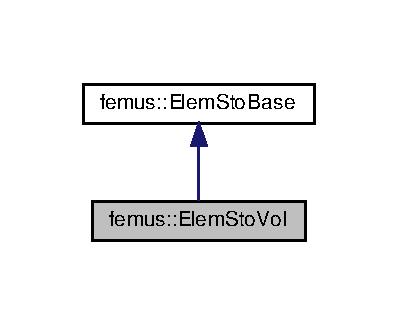
\includegraphics[width=191pt]{classfemus_1_1_elem_sto_vol__inherit__graph}
\end{center}
\end{figure}


Collaboration diagram for femus\+:\+:Elem\+Sto\+Vol\+:
\nopagebreak
\begin{figure}[H]
\begin{center}
\leavevmode
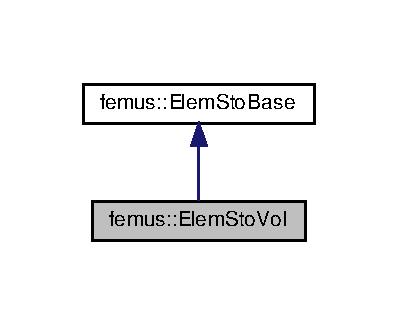
\includegraphics[width=191pt]{classfemus_1_1_elem_sto_vol__coll__graph}
\end{center}
\end{figure}
\subsection*{Public Member Functions}
\begin{DoxyCompactItemize}
\item 
\mbox{\hyperlink{classfemus_1_1_elem_sto_vol_a8bcc9da426122d9905a5ce0071f7398f}{Elem\+Sto\+Vol}} (int nnds\+\_\+in, \mbox{\hyperlink{_typedefs_8hpp_a91ad9478d81a7aaf2593e8d9c3d06a14}{uint}} spacedim)
\item 
\mbox{\hyperlink{classfemus_1_1_elem_sto_vol_a9a35cdb47e6ea0c722ae92c868f06983}{$\sim$\+Elem\+Sto\+Vol}} ()
\end{DoxyCompactItemize}
\subsection*{Public Attributes}
\begin{DoxyCompactItemize}
\item 
int \mbox{\hyperlink{classfemus_1_1_elem_sto_vol_a452494c41098efc1170394e89c1ce8a8}{\+\_\+par}}
\item 
int \mbox{\hyperlink{classfemus_1_1_elem_sto_vol_ae157383dd2c483093c6354fbfc1d0116}{\+\_\+nch}}
\item 
int $\ast$ \mbox{\hyperlink{classfemus_1_1_elem_sto_vol_a4800376b85eeccc97f7c12c5c91a8070}{\+\_\+elchs}}
\end{DoxyCompactItemize}


\subsection{Constructor \& Destructor Documentation}
\mbox{\Hypertarget{classfemus_1_1_elem_sto_vol_a8bcc9da426122d9905a5ce0071f7398f}\label{classfemus_1_1_elem_sto_vol_a8bcc9da426122d9905a5ce0071f7398f}} 
\index{femus\+::\+Elem\+Sto\+Vol@{femus\+::\+Elem\+Sto\+Vol}!Elem\+Sto\+Vol@{Elem\+Sto\+Vol}}
\index{Elem\+Sto\+Vol@{Elem\+Sto\+Vol}!femus\+::\+Elem\+Sto\+Vol@{femus\+::\+Elem\+Sto\+Vol}}
\subsubsection{\texorpdfstring{Elem\+Sto\+Vol()}{ElemStoVol()}}
{\footnotesize\ttfamily femus\+::\+Elem\+Sto\+Vol\+::\+Elem\+Sto\+Vol (\begin{DoxyParamCaption}\item[{int}]{nnds\+\_\+in,  }\item[{\mbox{\hyperlink{_typedefs_8hpp_a91ad9478d81a7aaf2593e8d9c3d06a14}{uint}}}]{spacedim }\end{DoxyParamCaption})}

\mbox{\Hypertarget{classfemus_1_1_elem_sto_vol_a9a35cdb47e6ea0c722ae92c868f06983}\label{classfemus_1_1_elem_sto_vol_a9a35cdb47e6ea0c722ae92c868f06983}} 
\index{femus\+::\+Elem\+Sto\+Vol@{femus\+::\+Elem\+Sto\+Vol}!````~Elem\+Sto\+Vol@{$\sim$\+Elem\+Sto\+Vol}}
\index{````~Elem\+Sto\+Vol@{$\sim$\+Elem\+Sto\+Vol}!femus\+::\+Elem\+Sto\+Vol@{femus\+::\+Elem\+Sto\+Vol}}
\subsubsection{\texorpdfstring{$\sim$\+Elem\+Sto\+Vol()}{~ElemStoVol()}}
{\footnotesize\ttfamily femus\+::\+Elem\+Sto\+Vol\+::$\sim$\+Elem\+Sto\+Vol (\begin{DoxyParamCaption}{ }\end{DoxyParamCaption})}



\subsection{Member Data Documentation}
\mbox{\Hypertarget{classfemus_1_1_elem_sto_vol_a4800376b85eeccc97f7c12c5c91a8070}\label{classfemus_1_1_elem_sto_vol_a4800376b85eeccc97f7c12c5c91a8070}} 
\index{femus\+::\+Elem\+Sto\+Vol@{femus\+::\+Elem\+Sto\+Vol}!\+\_\+elchs@{\+\_\+elchs}}
\index{\+\_\+elchs@{\+\_\+elchs}!femus\+::\+Elem\+Sto\+Vol@{femus\+::\+Elem\+Sto\+Vol}}
\subsubsection{\texorpdfstring{\+\_\+elchs}{\_elchs}}
{\footnotesize\ttfamily int$\ast$ femus\+::\+Elem\+Sto\+Vol\+::\+\_\+elchs}

\mbox{\Hypertarget{classfemus_1_1_elem_sto_vol_ae157383dd2c483093c6354fbfc1d0116}\label{classfemus_1_1_elem_sto_vol_ae157383dd2c483093c6354fbfc1d0116}} 
\index{femus\+::\+Elem\+Sto\+Vol@{femus\+::\+Elem\+Sto\+Vol}!\+\_\+nch@{\+\_\+nch}}
\index{\+\_\+nch@{\+\_\+nch}!femus\+::\+Elem\+Sto\+Vol@{femus\+::\+Elem\+Sto\+Vol}}
\subsubsection{\texorpdfstring{\+\_\+nch}{\_nch}}
{\footnotesize\ttfamily int femus\+::\+Elem\+Sto\+Vol\+::\+\_\+nch}

\mbox{\Hypertarget{classfemus_1_1_elem_sto_vol_a452494c41098efc1170394e89c1ce8a8}\label{classfemus_1_1_elem_sto_vol_a452494c41098efc1170394e89c1ce8a8}} 
\index{femus\+::\+Elem\+Sto\+Vol@{femus\+::\+Elem\+Sto\+Vol}!\+\_\+par@{\+\_\+par}}
\index{\+\_\+par@{\+\_\+par}!femus\+::\+Elem\+Sto\+Vol@{femus\+::\+Elem\+Sto\+Vol}}
\subsubsection{\texorpdfstring{\+\_\+par}{\_par}}
{\footnotesize\ttfamily int femus\+::\+Elem\+Sto\+Vol\+::\+\_\+par}



The documentation for this class was generated from the following files\+:\begin{DoxyCompactItemize}
\item 
mesh\+Gencase/\mbox{\hyperlink{_elem_sto_8hpp}{Elem\+Sto.\+hpp}}\item 
mesh\+Gencase/\mbox{\hyperlink{_elem_sto_8cpp}{Elem\+Sto.\+cpp}}\end{DoxyCompactItemize}

\hypertarget{classfemus_1_1_explicit_system}{}\section{femus\+:\+:Explicit\+System Class Reference}
\label{classfemus_1_1_explicit_system}\index{femus\+::\+Explicit\+System@{femus\+::\+Explicit\+System}}


{\ttfamily \#include $<$Explicit\+System.\+hpp$>$}



Inheritance diagram for femus\+:\+:Explicit\+System\+:
\nopagebreak
\begin{figure}[H]
\begin{center}
\leavevmode
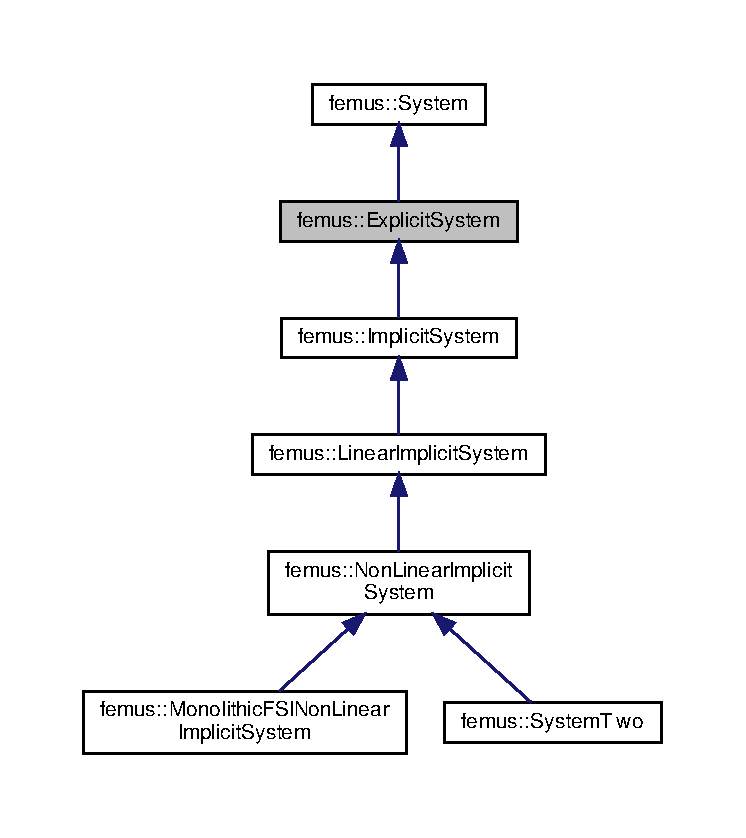
\includegraphics[width=350pt]{classfemus_1_1_explicit_system__inherit__graph}
\end{center}
\end{figure}


Collaboration diagram for femus\+:\+:Explicit\+System\+:
\nopagebreak
\begin{figure}[H]
\begin{center}
\leavevmode
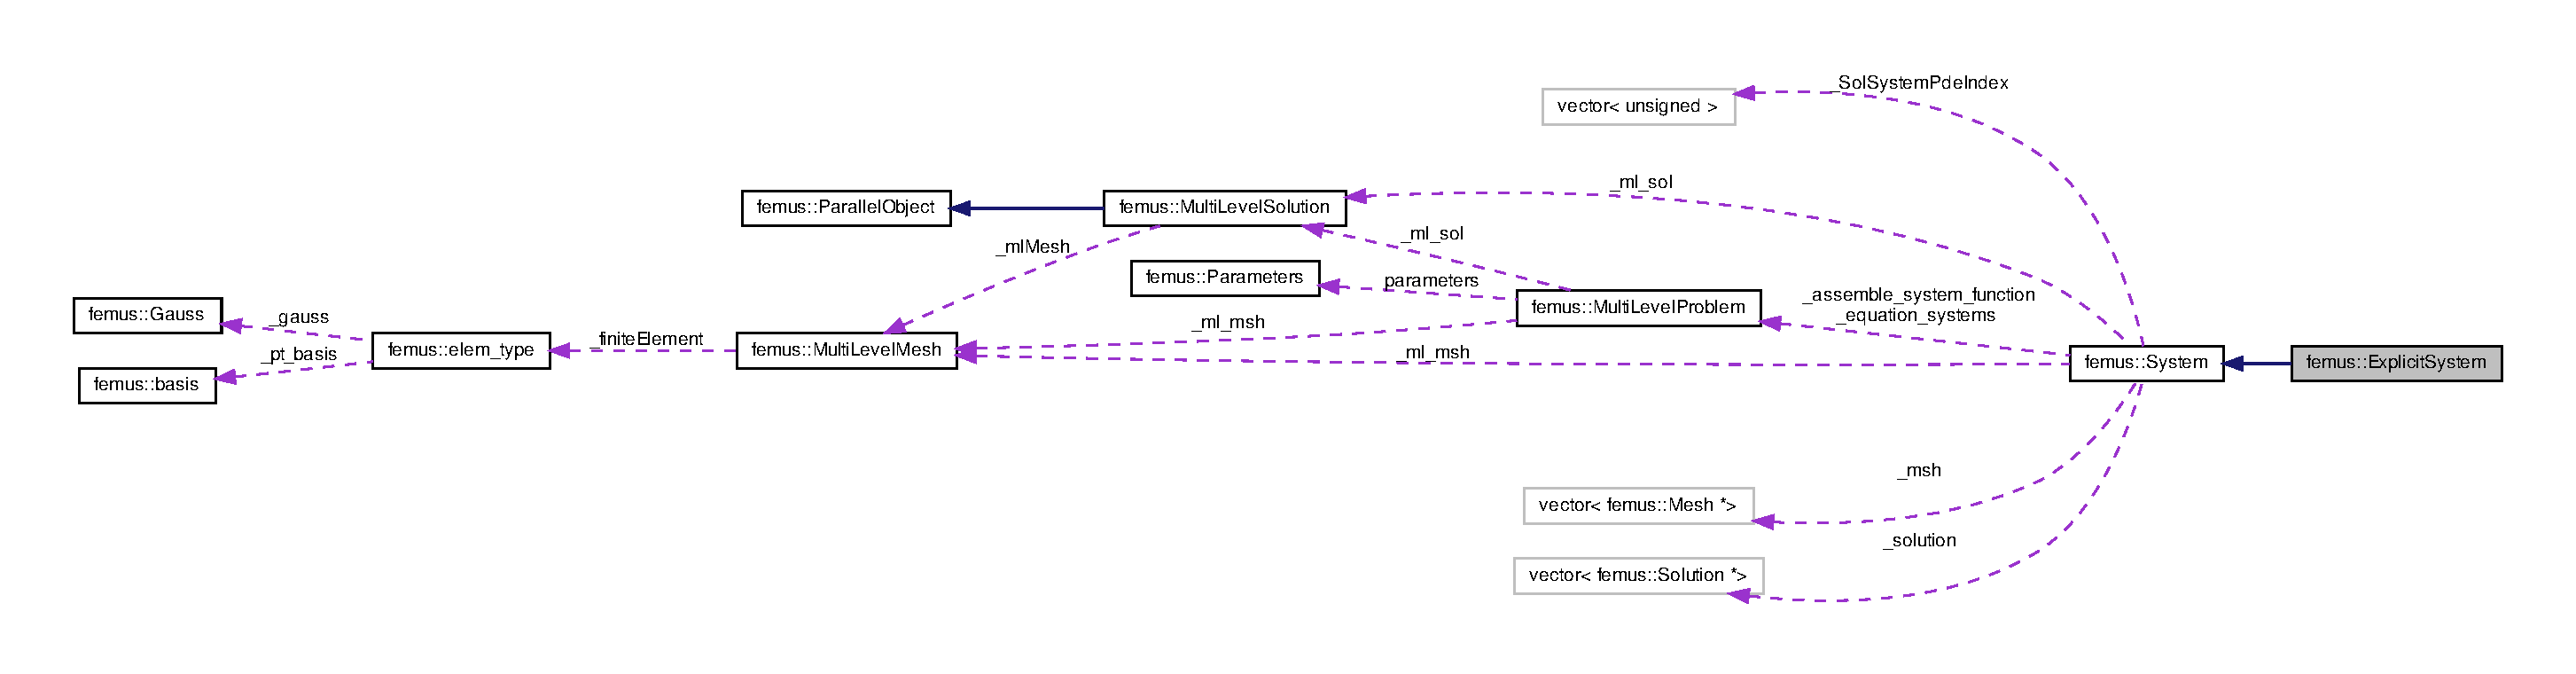
\includegraphics[width=350pt]{classfemus_1_1_explicit_system__coll__graph}
\end{center}
\end{figure}
\subsection*{Public Types}
\begin{DoxyCompactItemize}
\item 
typedef \mbox{\hyperlink{classfemus_1_1_system}{System}} \mbox{\hyperlink{classfemus_1_1_explicit_system_ad338cb1d97f154cadb9e630ada84f447}{Parent}}
\end{DoxyCompactItemize}
\subsection*{Public Member Functions}
\begin{DoxyCompactItemize}
\item 
\mbox{\hyperlink{classfemus_1_1_explicit_system_a8d4304329b95b7c570c846fd919156a0}{Explicit\+System}} (\mbox{\hyperlink{classfemus_1_1_multi_level_problem}{Multi\+Level\+Problem}} \&ml\+\_\+probl, const std\+::string \&\mbox{\hyperlink{classfemus_1_1_system_a1a007c176529dae649887bbd1cb46103}{name}}, const unsigned int \mbox{\hyperlink{classfemus_1_1_system_a28f5c7f6286dd597ae28a8923c8dca11}{number}}, const \mbox{\hyperlink{_mg_smoother_enum_8hpp_a4d11c2ff93e2f0f440c879a9c40cda71}{Mg\+Smoother}} \&smoother\+\_\+type)
\item 
virtual \mbox{\hyperlink{classfemus_1_1_explicit_system_aa043bf47db592a14016c84f5adaaa4a5}{$\sim$\+Explicit\+System}} ()
\item 
virtual void \mbox{\hyperlink{classfemus_1_1_explicit_system_ac078fbc3f758429e8a60dac487aab5ce}{clear}} ()
\item 
virtual void \mbox{\hyperlink{classfemus_1_1_explicit_system_a6736fef684fe763b26e016ff3f8b37b7}{init}} ()
\item 
virtual void \mbox{\hyperlink{classfemus_1_1_explicit_system_a149e74ccad300a58b25f72a6b0439f2b}{init\+\_\+two}} ()
\item 
virtual std\+::string \mbox{\hyperlink{classfemus_1_1_explicit_system_a91f61bd0aa02102fe9af817da96be72b}{system\+\_\+type}} () const
\end{DoxyCompactItemize}
\subsection*{Additional Inherited Members}


\subsection{Detailed Description}
The explicit system class 

\subsection{Member Typedef Documentation}
\mbox{\Hypertarget{classfemus_1_1_explicit_system_ad338cb1d97f154cadb9e630ada84f447}\label{classfemus_1_1_explicit_system_ad338cb1d97f154cadb9e630ada84f447}} 
\index{femus\+::\+Explicit\+System@{femus\+::\+Explicit\+System}!Parent@{Parent}}
\index{Parent@{Parent}!femus\+::\+Explicit\+System@{femus\+::\+Explicit\+System}}
\subsubsection{\texorpdfstring{Parent}{Parent}}
{\footnotesize\ttfamily typedef \mbox{\hyperlink{classfemus_1_1_system}{System}} \mbox{\hyperlink{classfemus_1_1_explicit_system_ad338cb1d97f154cadb9e630ada84f447}{femus\+::\+Explicit\+System\+::\+Parent}}}

The type of the parent. 

\subsection{Constructor \& Destructor Documentation}
\mbox{\Hypertarget{classfemus_1_1_explicit_system_a8d4304329b95b7c570c846fd919156a0}\label{classfemus_1_1_explicit_system_a8d4304329b95b7c570c846fd919156a0}} 
\index{femus\+::\+Explicit\+System@{femus\+::\+Explicit\+System}!Explicit\+System@{Explicit\+System}}
\index{Explicit\+System@{Explicit\+System}!femus\+::\+Explicit\+System@{femus\+::\+Explicit\+System}}
\subsubsection{\texorpdfstring{Explicit\+System()}{ExplicitSystem()}}
{\footnotesize\ttfamily femus\+::\+Explicit\+System\+::\+Explicit\+System (\begin{DoxyParamCaption}\item[{\mbox{\hyperlink{classfemus_1_1_multi_level_problem}{Multi\+Level\+Problem}} \&}]{ml\+\_\+probl,  }\item[{const std\+::string \&}]{name,  }\item[{const unsigned int}]{number,  }\item[{const \mbox{\hyperlink{_mg_smoother_enum_8hpp_a4d11c2ff93e2f0f440c879a9c40cda71}{Mg\+Smoother}} \&}]{smoother\+\_\+type }\end{DoxyParamCaption})}

Constructor. Optionally initializes required data structures. \mbox{\Hypertarget{classfemus_1_1_explicit_system_aa043bf47db592a14016c84f5adaaa4a5}\label{classfemus_1_1_explicit_system_aa043bf47db592a14016c84f5adaaa4a5}} 
\index{femus\+::\+Explicit\+System@{femus\+::\+Explicit\+System}!````~Explicit\+System@{$\sim$\+Explicit\+System}}
\index{````~Explicit\+System@{$\sim$\+Explicit\+System}!femus\+::\+Explicit\+System@{femus\+::\+Explicit\+System}}
\subsubsection{\texorpdfstring{$\sim$\+Explicit\+System()}{~ExplicitSystem()}}
{\footnotesize\ttfamily femus\+::\+Explicit\+System\+::$\sim$\+Explicit\+System (\begin{DoxyParamCaption}{ }\end{DoxyParamCaption})\hspace{0.3cm}{\ttfamily [virtual]}}

Destructor 

\subsection{Member Function Documentation}
\mbox{\Hypertarget{classfemus_1_1_explicit_system_ac078fbc3f758429e8a60dac487aab5ce}\label{classfemus_1_1_explicit_system_ac078fbc3f758429e8a60dac487aab5ce}} 
\index{femus\+::\+Explicit\+System@{femus\+::\+Explicit\+System}!clear@{clear}}
\index{clear@{clear}!femus\+::\+Explicit\+System@{femus\+::\+Explicit\+System}}
\subsubsection{\texorpdfstring{clear()}{clear()}}
{\footnotesize\ttfamily void femus\+::\+Explicit\+System\+::clear (\begin{DoxyParamCaption}{ }\end{DoxyParamCaption})\hspace{0.3cm}{\ttfamily [virtual]}}

Clear all the data structures associated with the system. 

Reimplemented from \mbox{\hyperlink{classfemus_1_1_system_ad1a19dbff3cea3d496cdb530ea2bca19}{femus\+::\+System}}.



Reimplemented in \mbox{\hyperlink{classfemus_1_1_linear_implicit_system_ace039665432e53db0c25b0efede44a76}{femus\+::\+Linear\+Implicit\+System}}, \mbox{\hyperlink{classfemus_1_1_implicit_system_a0d5395e6a8de6625f9059384b990f83f}{femus\+::\+Implicit\+System}}, \mbox{\hyperlink{classfemus_1_1_monolithic_f_s_i_non_linear_implicit_system_ac7f2bedf4d1c6b00f5443cb5128a3069}{femus\+::\+Monolithic\+F\+S\+I\+Non\+Linear\+Implicit\+System}}, and \mbox{\hyperlink{classfemus_1_1_non_linear_implicit_system_afc52f569e5be8c3bf593a00c883d7192}{femus\+::\+Non\+Linear\+Implicit\+System}}.

\mbox{\Hypertarget{classfemus_1_1_explicit_system_a6736fef684fe763b26e016ff3f8b37b7}\label{classfemus_1_1_explicit_system_a6736fef684fe763b26e016ff3f8b37b7}} 
\index{femus\+::\+Explicit\+System@{femus\+::\+Explicit\+System}!init@{init}}
\index{init@{init}!femus\+::\+Explicit\+System@{femus\+::\+Explicit\+System}}
\subsubsection{\texorpdfstring{init()}{init()}}
{\footnotesize\ttfamily void femus\+::\+Explicit\+System\+::init (\begin{DoxyParamCaption}{ }\end{DoxyParamCaption})\hspace{0.3cm}{\ttfamily [virtual]}}

Init the system P\+DE structures 

Reimplemented from \mbox{\hyperlink{classfemus_1_1_system_a1defaa9e59d3aa2ac62aa7fa111b6e32}{femus\+::\+System}}.



Reimplemented in \mbox{\hyperlink{classfemus_1_1_linear_implicit_system_a4605bac9ea670bb7dbd4454358155670}{femus\+::\+Linear\+Implicit\+System}}, \mbox{\hyperlink{classfemus_1_1_implicit_system_a098b8d66e167a03759ca089bf0f0dc11}{femus\+::\+Implicit\+System}}, \mbox{\hyperlink{classfemus_1_1_monolithic_f_s_i_non_linear_implicit_system_a07e04a8cce138cae9edcdd05fd1c7829}{femus\+::\+Monolithic\+F\+S\+I\+Non\+Linear\+Implicit\+System}}, and \mbox{\hyperlink{classfemus_1_1_non_linear_implicit_system_ad2d20975e0c919a9d99bdd9368a0212a}{femus\+::\+Non\+Linear\+Implicit\+System}}.

\mbox{\Hypertarget{classfemus_1_1_explicit_system_a149e74ccad300a58b25f72a6b0439f2b}\label{classfemus_1_1_explicit_system_a149e74ccad300a58b25f72a6b0439f2b}} 
\index{femus\+::\+Explicit\+System@{femus\+::\+Explicit\+System}!init\+\_\+two@{init\+\_\+two}}
\index{init\+\_\+two@{init\+\_\+two}!femus\+::\+Explicit\+System@{femus\+::\+Explicit\+System}}
\subsubsection{\texorpdfstring{init\+\_\+two()}{init\_two()}}
{\footnotesize\ttfamily virtual void femus\+::\+Explicit\+System\+::init\+\_\+two (\begin{DoxyParamCaption}{ }\end{DoxyParamCaption})\hspace{0.3cm}{\ttfamily [inline]}, {\ttfamily [virtual]}}

\begin{DoxyRefDesc}{Deprecated}
\item[\mbox{\hyperlink{deprecated__deprecated000008}{Deprecated}}]Init the system P\+DE structures \end{DoxyRefDesc}


Reimplemented from \mbox{\hyperlink{classfemus_1_1_system_ae238425d65a58eb22b3925309d9d0bef}{femus\+::\+System}}.



Reimplemented in \mbox{\hyperlink{classfemus_1_1_linear_implicit_system_a821e5e01d07a2124ff6f0130f67b5ba6}{femus\+::\+Linear\+Implicit\+System}}, and \mbox{\hyperlink{classfemus_1_1_implicit_system_a544e5b2b89fd2f8497b3ca6befce74d1}{femus\+::\+Implicit\+System}}.

\mbox{\Hypertarget{classfemus_1_1_explicit_system_a91f61bd0aa02102fe9af817da96be72b}\label{classfemus_1_1_explicit_system_a91f61bd0aa02102fe9af817da96be72b}} 
\index{femus\+::\+Explicit\+System@{femus\+::\+Explicit\+System}!system\+\_\+type@{system\+\_\+type}}
\index{system\+\_\+type@{system\+\_\+type}!femus\+::\+Explicit\+System@{femus\+::\+Explicit\+System}}
\subsubsection{\texorpdfstring{system\+\_\+type()}{system\_type()}}
{\footnotesize\ttfamily virtual std\+::string femus\+::\+Explicit\+System\+::system\+\_\+type (\begin{DoxyParamCaption}{ }\end{DoxyParamCaption}) const\hspace{0.3cm}{\ttfamily [inline]}, {\ttfamily [virtual]}}

\begin{DoxyReturn}{Returns}
{\ttfamily \char`\"{}\+Explicit\char`\"{}}. Helps in identifying the system type in an equation system file. 
\end{DoxyReturn}


Reimplemented from \mbox{\hyperlink{classfemus_1_1_system_a8cdcdcaf37dc4985be99dbb0a5ad8efa}{femus\+::\+System}}.



Reimplemented in \mbox{\hyperlink{classfemus_1_1_linear_implicit_system_a45df3966aab87bd06da49c78897a6648}{femus\+::\+Linear\+Implicit\+System}}, \mbox{\hyperlink{classfemus_1_1_implicit_system_aee5e08a09a2d289aa777914018931592}{femus\+::\+Implicit\+System}}, \mbox{\hyperlink{classfemus_1_1_monolithic_f_s_i_non_linear_implicit_system_a29bb0bdaf1eec888af05e8e57469faf4}{femus\+::\+Monolithic\+F\+S\+I\+Non\+Linear\+Implicit\+System}}, and \mbox{\hyperlink{classfemus_1_1_non_linear_implicit_system_a8f4727b8b763bdac9f58b4c9dbb097be}{femus\+::\+Non\+Linear\+Implicit\+System}}.



The documentation for this class was generated from the following files\+:\begin{DoxyCompactItemize}
\item 
equations/\mbox{\hyperlink{_explicit_system_8hpp}{Explicit\+System.\+hpp}}\item 
equations/\mbox{\hyperlink{_explicit_system_8cpp}{Explicit\+System.\+cpp}}\end{DoxyCompactItemize}

\hypertarget{classfemus_1_1_f_e_edge1}{}\section{femus\+:\+:F\+E\+Edge1 Class Reference}
\label{classfemus_1_1_f_e_edge1}\index{femus\+::\+F\+E\+Edge1@{femus\+::\+F\+E\+Edge1}}


{\ttfamily \#include $<$F\+E\+Edge1.\+hpp$>$}



Inheritance diagram for femus\+:\+:F\+E\+Edge1\+:
\nopagebreak
\begin{figure}[H]
\begin{center}
\leavevmode
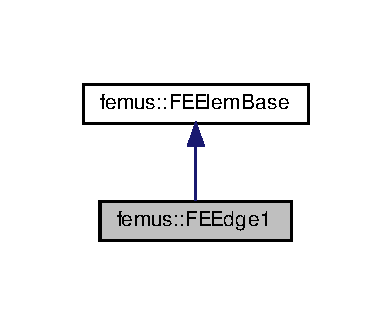
\includegraphics[width=188pt]{classfemus_1_1_f_e_edge1__inherit__graph}
\end{center}
\end{figure}


Collaboration diagram for femus\+:\+:F\+E\+Edge1\+:
\nopagebreak
\begin{figure}[H]
\begin{center}
\leavevmode
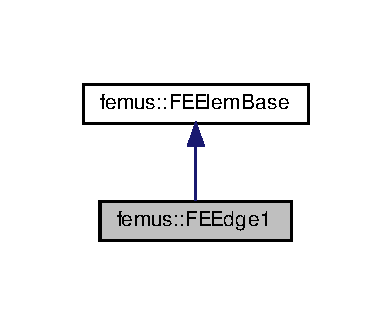
\includegraphics[width=188pt]{classfemus_1_1_f_e_edge1__coll__graph}
\end{center}
\end{figure}
\subsection*{Public Member Functions}
\begin{DoxyCompactItemize}
\item 
\mbox{\hyperlink{classfemus_1_1_f_e_edge1_aa9abaab903c04fcfece3ce921ad0af6a}{F\+E\+Edge1}} ()
\item 
\mbox{\hyperlink{classfemus_1_1_f_e_edge1_a9f830645f2b38043f3d753505271679e}{$\sim$\+F\+E\+Edge1}} ()
\item 
float \mbox{\hyperlink{classfemus_1_1_f_e_edge1_a25ca224b3f755062f03cc12d9da92a9a}{get\+\_\+embedding\+\_\+matrix}} (const \mbox{\hyperlink{_typedefs_8hpp_a91ad9478d81a7aaf2593e8d9c3d06a14}{uint}}, const \mbox{\hyperlink{_typedefs_8hpp_a91ad9478d81a7aaf2593e8d9c3d06a14}{uint}}, const \mbox{\hyperlink{_typedefs_8hpp_a91ad9478d81a7aaf2593e8d9c3d06a14}{uint}})
\item 
double \mbox{\hyperlink{classfemus_1_1_f_e_edge1_a65a8e90e45a7db19520776609184a51f}{get\+\_\+prol}} (const \mbox{\hyperlink{_typedefs_8hpp_a91ad9478d81a7aaf2593e8d9c3d06a14}{uint}})
\end{DoxyCompactItemize}
\subsection*{Additional Inherited Members}


\subsection{Constructor \& Destructor Documentation}
\mbox{\Hypertarget{classfemus_1_1_f_e_edge1_aa9abaab903c04fcfece3ce921ad0af6a}\label{classfemus_1_1_f_e_edge1_aa9abaab903c04fcfece3ce921ad0af6a}} 
\index{femus\+::\+F\+E\+Edge1@{femus\+::\+F\+E\+Edge1}!F\+E\+Edge1@{F\+E\+Edge1}}
\index{F\+E\+Edge1@{F\+E\+Edge1}!femus\+::\+F\+E\+Edge1@{femus\+::\+F\+E\+Edge1}}
\subsubsection{\texorpdfstring{F\+E\+Edge1()}{FEEdge1()}}
{\footnotesize\ttfamily femus\+::\+F\+E\+Edge1\+::\+F\+E\+Edge1 (\begin{DoxyParamCaption}{ }\end{DoxyParamCaption})}

\mbox{\Hypertarget{classfemus_1_1_f_e_edge1_a9f830645f2b38043f3d753505271679e}\label{classfemus_1_1_f_e_edge1_a9f830645f2b38043f3d753505271679e}} 
\index{femus\+::\+F\+E\+Edge1@{femus\+::\+F\+E\+Edge1}!````~F\+E\+Edge1@{$\sim$\+F\+E\+Edge1}}
\index{````~F\+E\+Edge1@{$\sim$\+F\+E\+Edge1}!femus\+::\+F\+E\+Edge1@{femus\+::\+F\+E\+Edge1}}
\subsubsection{\texorpdfstring{$\sim$\+F\+E\+Edge1()}{~FEEdge1()}}
{\footnotesize\ttfamily femus\+::\+F\+E\+Edge1\+::$\sim$\+F\+E\+Edge1 (\begin{DoxyParamCaption}{ }\end{DoxyParamCaption})}



\subsection{Member Function Documentation}
\mbox{\Hypertarget{classfemus_1_1_f_e_edge1_a25ca224b3f755062f03cc12d9da92a9a}\label{classfemus_1_1_f_e_edge1_a25ca224b3f755062f03cc12d9da92a9a}} 
\index{femus\+::\+F\+E\+Edge1@{femus\+::\+F\+E\+Edge1}!get\+\_\+embedding\+\_\+matrix@{get\+\_\+embedding\+\_\+matrix}}
\index{get\+\_\+embedding\+\_\+matrix@{get\+\_\+embedding\+\_\+matrix}!femus\+::\+F\+E\+Edge1@{femus\+::\+F\+E\+Edge1}}
\subsubsection{\texorpdfstring{get\+\_\+embedding\+\_\+matrix()}{get\_embedding\_matrix()}}
{\footnotesize\ttfamily float femus\+::\+F\+E\+Edge1\+::get\+\_\+embedding\+\_\+matrix (\begin{DoxyParamCaption}\item[{const \mbox{\hyperlink{_typedefs_8hpp_a91ad9478d81a7aaf2593e8d9c3d06a14}{uint}}}]{,  }\item[{const \mbox{\hyperlink{_typedefs_8hpp_a91ad9478d81a7aaf2593e8d9c3d06a14}{uint}}}]{,  }\item[{const \mbox{\hyperlink{_typedefs_8hpp_a91ad9478d81a7aaf2593e8d9c3d06a14}{uint}}}]{ }\end{DoxyParamCaption})\hspace{0.3cm}{\ttfamily [inline]}, {\ttfamily [virtual]}}



Implements \mbox{\hyperlink{classfemus_1_1_f_e_elem_base_a0c4d6d5ec66bd4e301eb8ea2ef10f354}{femus\+::\+F\+E\+Elem\+Base}}.

\mbox{\Hypertarget{classfemus_1_1_f_e_edge1_a65a8e90e45a7db19520776609184a51f}\label{classfemus_1_1_f_e_edge1_a65a8e90e45a7db19520776609184a51f}} 
\index{femus\+::\+F\+E\+Edge1@{femus\+::\+F\+E\+Edge1}!get\+\_\+prol@{get\+\_\+prol}}
\index{get\+\_\+prol@{get\+\_\+prol}!femus\+::\+F\+E\+Edge1@{femus\+::\+F\+E\+Edge1}}
\subsubsection{\texorpdfstring{get\+\_\+prol()}{get\_prol()}}
{\footnotesize\ttfamily double femus\+::\+F\+E\+Edge1\+::get\+\_\+prol (\begin{DoxyParamCaption}\item[{const \mbox{\hyperlink{_typedefs_8hpp_a91ad9478d81a7aaf2593e8d9c3d06a14}{uint}}}]{ }\end{DoxyParamCaption})\hspace{0.3cm}{\ttfamily [inline]}, {\ttfamily [virtual]}}



Implements \mbox{\hyperlink{classfemus_1_1_f_e_elem_base_ac82326cdc7cb02329c7be9547d56fad4}{femus\+::\+F\+E\+Elem\+Base}}.



The documentation for this class was generated from the following files\+:\begin{DoxyCompactItemize}
\item 
mesh\+Gencase/\mbox{\hyperlink{_f_e_edge1_8hpp}{F\+E\+Edge1.\+hpp}}\item 
mesh\+Gencase/\mbox{\hyperlink{_f_e_edge1_8cpp}{F\+E\+Edge1.\+cpp}}\end{DoxyCompactItemize}

\hypertarget{classfemus_1_1_f_e_edge2}{}\section{femus\+:\+:F\+E\+Edge2 Class Reference}
\label{classfemus_1_1_f_e_edge2}\index{femus\+::\+F\+E\+Edge2@{femus\+::\+F\+E\+Edge2}}


{\ttfamily \#include $<$F\+E\+Edge2.\+hpp$>$}



Inheritance diagram for femus\+:\+:F\+E\+Edge2\+:
\nopagebreak
\begin{figure}[H]
\begin{center}
\leavevmode
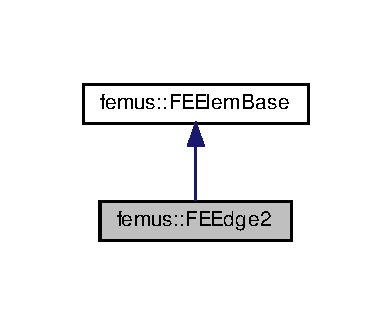
\includegraphics[width=188pt]{classfemus_1_1_f_e_edge2__inherit__graph}
\end{center}
\end{figure}


Collaboration diagram for femus\+:\+:F\+E\+Edge2\+:
\nopagebreak
\begin{figure}[H]
\begin{center}
\leavevmode
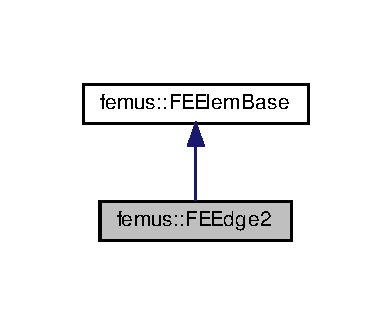
\includegraphics[width=188pt]{classfemus_1_1_f_e_edge2__coll__graph}
\end{center}
\end{figure}
\subsection*{Public Member Functions}
\begin{DoxyCompactItemize}
\item 
\mbox{\hyperlink{classfemus_1_1_f_e_edge2_a25d45b4be27432a6007312a1da20b799}{F\+E\+Edge2}} ()
\item 
\mbox{\hyperlink{classfemus_1_1_f_e_edge2_ac2e3a2aaafca74f53f4b818a2e17cdcb}{$\sim$\+F\+E\+Edge2}} ()
\item 
float \mbox{\hyperlink{classfemus_1_1_f_e_edge2_ab8a267a26f4930b636d6c5c14d2280dc}{get\+\_\+embedding\+\_\+matrix}} (const \mbox{\hyperlink{_typedefs_8hpp_a91ad9478d81a7aaf2593e8d9c3d06a14}{uint}}, const \mbox{\hyperlink{_typedefs_8hpp_a91ad9478d81a7aaf2593e8d9c3d06a14}{uint}}, const \mbox{\hyperlink{_typedefs_8hpp_a91ad9478d81a7aaf2593e8d9c3d06a14}{uint}})
\item 
double \mbox{\hyperlink{classfemus_1_1_f_e_edge2_a11dc956a09fc9775f474d388eab1de21}{get\+\_\+prol}} (const \mbox{\hyperlink{_typedefs_8hpp_a91ad9478d81a7aaf2593e8d9c3d06a14}{uint}})
\end{DoxyCompactItemize}
\subsection*{Additional Inherited Members}


\subsection{Constructor \& Destructor Documentation}
\mbox{\Hypertarget{classfemus_1_1_f_e_edge2_a25d45b4be27432a6007312a1da20b799}\label{classfemus_1_1_f_e_edge2_a25d45b4be27432a6007312a1da20b799}} 
\index{femus\+::\+F\+E\+Edge2@{femus\+::\+F\+E\+Edge2}!F\+E\+Edge2@{F\+E\+Edge2}}
\index{F\+E\+Edge2@{F\+E\+Edge2}!femus\+::\+F\+E\+Edge2@{femus\+::\+F\+E\+Edge2}}
\subsubsection{\texorpdfstring{F\+E\+Edge2()}{FEEdge2()}}
{\footnotesize\ttfamily femus\+::\+F\+E\+Edge2\+::\+F\+E\+Edge2 (\begin{DoxyParamCaption}{ }\end{DoxyParamCaption})}

\mbox{\Hypertarget{classfemus_1_1_f_e_edge2_ac2e3a2aaafca74f53f4b818a2e17cdcb}\label{classfemus_1_1_f_e_edge2_ac2e3a2aaafca74f53f4b818a2e17cdcb}} 
\index{femus\+::\+F\+E\+Edge2@{femus\+::\+F\+E\+Edge2}!````~F\+E\+Edge2@{$\sim$\+F\+E\+Edge2}}
\index{````~F\+E\+Edge2@{$\sim$\+F\+E\+Edge2}!femus\+::\+F\+E\+Edge2@{femus\+::\+F\+E\+Edge2}}
\subsubsection{\texorpdfstring{$\sim$\+F\+E\+Edge2()}{~FEEdge2()}}
{\footnotesize\ttfamily femus\+::\+F\+E\+Edge2\+::$\sim$\+F\+E\+Edge2 (\begin{DoxyParamCaption}{ }\end{DoxyParamCaption})}



\subsection{Member Function Documentation}
\mbox{\Hypertarget{classfemus_1_1_f_e_edge2_ab8a267a26f4930b636d6c5c14d2280dc}\label{classfemus_1_1_f_e_edge2_ab8a267a26f4930b636d6c5c14d2280dc}} 
\index{femus\+::\+F\+E\+Edge2@{femus\+::\+F\+E\+Edge2}!get\+\_\+embedding\+\_\+matrix@{get\+\_\+embedding\+\_\+matrix}}
\index{get\+\_\+embedding\+\_\+matrix@{get\+\_\+embedding\+\_\+matrix}!femus\+::\+F\+E\+Edge2@{femus\+::\+F\+E\+Edge2}}
\subsubsection{\texorpdfstring{get\+\_\+embedding\+\_\+matrix()}{get\_embedding\_matrix()}}
{\footnotesize\ttfamily float femus\+::\+F\+E\+Edge2\+::get\+\_\+embedding\+\_\+matrix (\begin{DoxyParamCaption}\item[{const \mbox{\hyperlink{_typedefs_8hpp_a91ad9478d81a7aaf2593e8d9c3d06a14}{uint}}}]{,  }\item[{const \mbox{\hyperlink{_typedefs_8hpp_a91ad9478d81a7aaf2593e8d9c3d06a14}{uint}}}]{,  }\item[{const \mbox{\hyperlink{_typedefs_8hpp_a91ad9478d81a7aaf2593e8d9c3d06a14}{uint}}}]{ }\end{DoxyParamCaption})\hspace{0.3cm}{\ttfamily [inline]}, {\ttfamily [virtual]}}



Implements \mbox{\hyperlink{classfemus_1_1_f_e_elem_base_a0c4d6d5ec66bd4e301eb8ea2ef10f354}{femus\+::\+F\+E\+Elem\+Base}}.

\mbox{\Hypertarget{classfemus_1_1_f_e_edge2_a11dc956a09fc9775f474d388eab1de21}\label{classfemus_1_1_f_e_edge2_a11dc956a09fc9775f474d388eab1de21}} 
\index{femus\+::\+F\+E\+Edge2@{femus\+::\+F\+E\+Edge2}!get\+\_\+prol@{get\+\_\+prol}}
\index{get\+\_\+prol@{get\+\_\+prol}!femus\+::\+F\+E\+Edge2@{femus\+::\+F\+E\+Edge2}}
\subsubsection{\texorpdfstring{get\+\_\+prol()}{get\_prol()}}
{\footnotesize\ttfamily double femus\+::\+F\+E\+Edge2\+::get\+\_\+prol (\begin{DoxyParamCaption}\item[{const \mbox{\hyperlink{_typedefs_8hpp_a91ad9478d81a7aaf2593e8d9c3d06a14}{uint}}}]{ }\end{DoxyParamCaption})\hspace{0.3cm}{\ttfamily [inline]}, {\ttfamily [virtual]}}



Implements \mbox{\hyperlink{classfemus_1_1_f_e_elem_base_ac82326cdc7cb02329c7be9547d56fad4}{femus\+::\+F\+E\+Elem\+Base}}.



The documentation for this class was generated from the following files\+:\begin{DoxyCompactItemize}
\item 
mesh\+Gencase/\mbox{\hyperlink{_f_e_edge2_8hpp}{F\+E\+Edge2.\+hpp}}\item 
mesh\+Gencase/\mbox{\hyperlink{_f_e_edge2_8cpp}{F\+E\+Edge2.\+cpp}}\end{DoxyCompactItemize}

\hypertarget{classfemus_1_1_f_e_edge3}{}\section{femus\+:\+:F\+E\+Edge3 Class Reference}
\label{classfemus_1_1_f_e_edge3}\index{femus\+::\+F\+E\+Edge3@{femus\+::\+F\+E\+Edge3}}


{\ttfamily \#include $<$F\+E\+Edge3.\+hpp$>$}



Inheritance diagram for femus\+:\+:F\+E\+Edge3\+:
\nopagebreak
\begin{figure}[H]
\begin{center}
\leavevmode
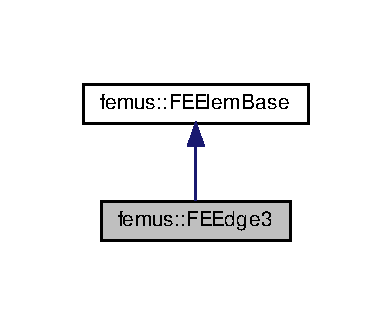
\includegraphics[width=188pt]{classfemus_1_1_f_e_edge3__inherit__graph}
\end{center}
\end{figure}


Collaboration diagram for femus\+:\+:F\+E\+Edge3\+:
\nopagebreak
\begin{figure}[H]
\begin{center}
\leavevmode
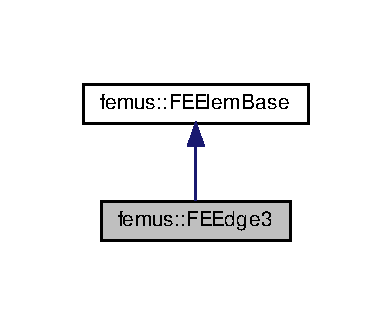
\includegraphics[width=188pt]{classfemus_1_1_f_e_edge3__coll__graph}
\end{center}
\end{figure}
\subsection*{Public Member Functions}
\begin{DoxyCompactItemize}
\item 
\mbox{\hyperlink{classfemus_1_1_f_e_edge3_a5b6ca9bbadc443999ed736956a5c3ea5}{F\+E\+Edge3}} ()
\item 
\mbox{\hyperlink{classfemus_1_1_f_e_edge3_a704bd8b302fa2246b09ca40ddaa37190}{$\sim$\+F\+E\+Edge3}} ()
\item 
float \mbox{\hyperlink{classfemus_1_1_f_e_edge3_a89085312a08628bcff678c347c0a82e4}{get\+\_\+embedding\+\_\+matrix}} (const \mbox{\hyperlink{_typedefs_8hpp_a91ad9478d81a7aaf2593e8d9c3d06a14}{uint}}, const \mbox{\hyperlink{_typedefs_8hpp_a91ad9478d81a7aaf2593e8d9c3d06a14}{uint}}, const \mbox{\hyperlink{_typedefs_8hpp_a91ad9478d81a7aaf2593e8d9c3d06a14}{uint}})
\item 
double \mbox{\hyperlink{classfemus_1_1_f_e_edge3_a5ecf7d9b06c59a94e3f1da042afe2b71}{get\+\_\+prol}} (const \mbox{\hyperlink{_typedefs_8hpp_a91ad9478d81a7aaf2593e8d9c3d06a14}{uint}})
\end{DoxyCompactItemize}
\subsection*{Additional Inherited Members}


\subsection{Constructor \& Destructor Documentation}
\mbox{\Hypertarget{classfemus_1_1_f_e_edge3_a5b6ca9bbadc443999ed736956a5c3ea5}\label{classfemus_1_1_f_e_edge3_a5b6ca9bbadc443999ed736956a5c3ea5}} 
\index{femus\+::\+F\+E\+Edge3@{femus\+::\+F\+E\+Edge3}!F\+E\+Edge3@{F\+E\+Edge3}}
\index{F\+E\+Edge3@{F\+E\+Edge3}!femus\+::\+F\+E\+Edge3@{femus\+::\+F\+E\+Edge3}}
\subsubsection{\texorpdfstring{F\+E\+Edge3()}{FEEdge3()}}
{\footnotesize\ttfamily femus\+::\+F\+E\+Edge3\+::\+F\+E\+Edge3 (\begin{DoxyParamCaption}{ }\end{DoxyParamCaption})}

\mbox{\Hypertarget{classfemus_1_1_f_e_edge3_a704bd8b302fa2246b09ca40ddaa37190}\label{classfemus_1_1_f_e_edge3_a704bd8b302fa2246b09ca40ddaa37190}} 
\index{femus\+::\+F\+E\+Edge3@{femus\+::\+F\+E\+Edge3}!````~F\+E\+Edge3@{$\sim$\+F\+E\+Edge3}}
\index{````~F\+E\+Edge3@{$\sim$\+F\+E\+Edge3}!femus\+::\+F\+E\+Edge3@{femus\+::\+F\+E\+Edge3}}
\subsubsection{\texorpdfstring{$\sim$\+F\+E\+Edge3()}{~FEEdge3()}}
{\footnotesize\ttfamily femus\+::\+F\+E\+Edge3\+::$\sim$\+F\+E\+Edge3 (\begin{DoxyParamCaption}{ }\end{DoxyParamCaption})}



\subsection{Member Function Documentation}
\mbox{\Hypertarget{classfemus_1_1_f_e_edge3_a89085312a08628bcff678c347c0a82e4}\label{classfemus_1_1_f_e_edge3_a89085312a08628bcff678c347c0a82e4}} 
\index{femus\+::\+F\+E\+Edge3@{femus\+::\+F\+E\+Edge3}!get\+\_\+embedding\+\_\+matrix@{get\+\_\+embedding\+\_\+matrix}}
\index{get\+\_\+embedding\+\_\+matrix@{get\+\_\+embedding\+\_\+matrix}!femus\+::\+F\+E\+Edge3@{femus\+::\+F\+E\+Edge3}}
\subsubsection{\texorpdfstring{get\+\_\+embedding\+\_\+matrix()}{get\_embedding\_matrix()}}
{\footnotesize\ttfamily float femus\+::\+F\+E\+Edge3\+::get\+\_\+embedding\+\_\+matrix (\begin{DoxyParamCaption}\item[{const \mbox{\hyperlink{_typedefs_8hpp_a91ad9478d81a7aaf2593e8d9c3d06a14}{uint}}}]{,  }\item[{const \mbox{\hyperlink{_typedefs_8hpp_a91ad9478d81a7aaf2593e8d9c3d06a14}{uint}}}]{,  }\item[{const \mbox{\hyperlink{_typedefs_8hpp_a91ad9478d81a7aaf2593e8d9c3d06a14}{uint}}}]{ }\end{DoxyParamCaption})\hspace{0.3cm}{\ttfamily [inline]}, {\ttfamily [virtual]}}



Implements \mbox{\hyperlink{classfemus_1_1_f_e_elem_base_a0c4d6d5ec66bd4e301eb8ea2ef10f354}{femus\+::\+F\+E\+Elem\+Base}}.

\mbox{\Hypertarget{classfemus_1_1_f_e_edge3_a5ecf7d9b06c59a94e3f1da042afe2b71}\label{classfemus_1_1_f_e_edge3_a5ecf7d9b06c59a94e3f1da042afe2b71}} 
\index{femus\+::\+F\+E\+Edge3@{femus\+::\+F\+E\+Edge3}!get\+\_\+prol@{get\+\_\+prol}}
\index{get\+\_\+prol@{get\+\_\+prol}!femus\+::\+F\+E\+Edge3@{femus\+::\+F\+E\+Edge3}}
\subsubsection{\texorpdfstring{get\+\_\+prol()}{get\_prol()}}
{\footnotesize\ttfamily double femus\+::\+F\+E\+Edge3\+::get\+\_\+prol (\begin{DoxyParamCaption}\item[{const \mbox{\hyperlink{_typedefs_8hpp_a91ad9478d81a7aaf2593e8d9c3d06a14}{uint}}}]{ }\end{DoxyParamCaption})\hspace{0.3cm}{\ttfamily [inline]}, {\ttfamily [virtual]}}



Implements \mbox{\hyperlink{classfemus_1_1_f_e_elem_base_ac82326cdc7cb02329c7be9547d56fad4}{femus\+::\+F\+E\+Elem\+Base}}.



The documentation for this class was generated from the following files\+:\begin{DoxyCompactItemize}
\item 
mesh\+Gencase/\mbox{\hyperlink{_f_e_edge3_8hpp}{F\+E\+Edge3.\+hpp}}\item 
mesh\+Gencase/\mbox{\hyperlink{_f_e_edge3_8cpp}{F\+E\+Edge3.\+cpp}}\end{DoxyCompactItemize}

\hypertarget{classfemus_1_1_f_e_elem_base}{}\section{femus\+:\+:F\+E\+Elem\+Base Class Reference}
\label{classfemus_1_1_f_e_elem_base}\index{femus\+::\+F\+E\+Elem\+Base@{femus\+::\+F\+E\+Elem\+Base}}


{\ttfamily \#include $<$F\+E\+Elem\+Base.\+hpp$>$}



Inheritance diagram for femus\+:\+:F\+E\+Elem\+Base\+:
\nopagebreak
\begin{figure}[H]
\begin{center}
\leavevmode
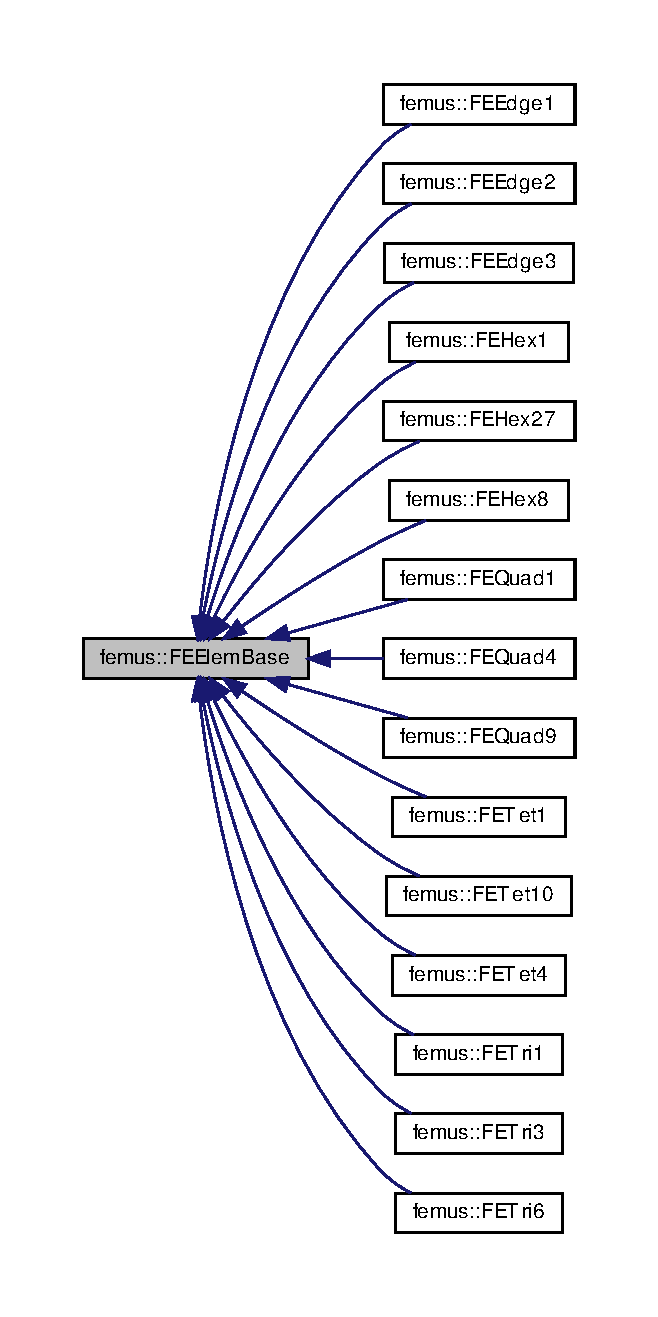
\includegraphics[height=550pt]{classfemus_1_1_f_e_elem_base__inherit__graph}
\end{center}
\end{figure}
\subsection*{Public Member Functions}
\begin{DoxyCompactItemize}
\item 
\mbox{\hyperlink{classfemus_1_1_f_e_elem_base_a8b85fcc566f310e7fd7477538c117a53}{F\+E\+Elem\+Base}} ()
\item 
virtual \mbox{\hyperlink{classfemus_1_1_f_e_elem_base_a4aca64e8a81acb283c738ca123841ed3}{$\sim$\+F\+E\+Elem\+Base}} ()
\item 
virtual float \mbox{\hyperlink{classfemus_1_1_f_e_elem_base_a0c4d6d5ec66bd4e301eb8ea2ef10f354}{get\+\_\+embedding\+\_\+matrix}} (const \mbox{\hyperlink{_typedefs_8hpp_a91ad9478d81a7aaf2593e8d9c3d06a14}{uint}}, const \mbox{\hyperlink{_typedefs_8hpp_a91ad9478d81a7aaf2593e8d9c3d06a14}{uint}}, const \mbox{\hyperlink{_typedefs_8hpp_a91ad9478d81a7aaf2593e8d9c3d06a14}{uint}})=0
\item 
virtual double \mbox{\hyperlink{classfemus_1_1_f_e_elem_base_ac82326cdc7cb02329c7be9547d56fad4}{get\+\_\+prol}} (const \mbox{\hyperlink{_typedefs_8hpp_a91ad9478d81a7aaf2593e8d9c3d06a14}{uint}})=0
\end{DoxyCompactItemize}
\subsection*{Static Public Member Functions}
\begin{DoxyCompactItemize}
\item 
static \mbox{\hyperlink{classfemus_1_1_f_e_elem_base}{F\+E\+Elem\+Base}} $\ast$ \mbox{\hyperlink{classfemus_1_1_f_e_elem_base_a012272423d14a7a4e399d26ca27cdcfc}{build}} (const std\+::string geomel\+\_\+id\+\_\+in, const \mbox{\hyperlink{_typedefs_8hpp_a91ad9478d81a7aaf2593e8d9c3d06a14}{uint}} fe\+\_\+family)
\end{DoxyCompactItemize}


\subsection{Constructor \& Destructor Documentation}
\mbox{\Hypertarget{classfemus_1_1_f_e_elem_base_a8b85fcc566f310e7fd7477538c117a53}\label{classfemus_1_1_f_e_elem_base_a8b85fcc566f310e7fd7477538c117a53}} 
\index{femus\+::\+F\+E\+Elem\+Base@{femus\+::\+F\+E\+Elem\+Base}!F\+E\+Elem\+Base@{F\+E\+Elem\+Base}}
\index{F\+E\+Elem\+Base@{F\+E\+Elem\+Base}!femus\+::\+F\+E\+Elem\+Base@{femus\+::\+F\+E\+Elem\+Base}}
\subsubsection{\texorpdfstring{F\+E\+Elem\+Base()}{FEElemBase()}}
{\footnotesize\ttfamily femus\+::\+F\+E\+Elem\+Base\+::\+F\+E\+Elem\+Base (\begin{DoxyParamCaption}{ }\end{DoxyParamCaption})}

\mbox{\Hypertarget{classfemus_1_1_f_e_elem_base_a4aca64e8a81acb283c738ca123841ed3}\label{classfemus_1_1_f_e_elem_base_a4aca64e8a81acb283c738ca123841ed3}} 
\index{femus\+::\+F\+E\+Elem\+Base@{femus\+::\+F\+E\+Elem\+Base}!````~F\+E\+Elem\+Base@{$\sim$\+F\+E\+Elem\+Base}}
\index{````~F\+E\+Elem\+Base@{$\sim$\+F\+E\+Elem\+Base}!femus\+::\+F\+E\+Elem\+Base@{femus\+::\+F\+E\+Elem\+Base}}
\subsubsection{\texorpdfstring{$\sim$\+F\+E\+Elem\+Base()}{~FEElemBase()}}
{\footnotesize\ttfamily femus\+::\+F\+E\+Elem\+Base\+::$\sim$\+F\+E\+Elem\+Base (\begin{DoxyParamCaption}{ }\end{DoxyParamCaption})\hspace{0.3cm}{\ttfamily [virtual]}}



\subsection{Member Function Documentation}
\mbox{\Hypertarget{classfemus_1_1_f_e_elem_base_a012272423d14a7a4e399d26ca27cdcfc}\label{classfemus_1_1_f_e_elem_base_a012272423d14a7a4e399d26ca27cdcfc}} 
\index{femus\+::\+F\+E\+Elem\+Base@{femus\+::\+F\+E\+Elem\+Base}!build@{build}}
\index{build@{build}!femus\+::\+F\+E\+Elem\+Base@{femus\+::\+F\+E\+Elem\+Base}}
\subsubsection{\texorpdfstring{build()}{build()}}
{\footnotesize\ttfamily \mbox{\hyperlink{classfemus_1_1_f_e_elem_base}{F\+E\+Elem\+Base}} $\ast$ femus\+::\+F\+E\+Elem\+Base\+::build (\begin{DoxyParamCaption}\item[{const std\+::string}]{geomel\+\_\+id\+\_\+in,  }\item[{const \mbox{\hyperlink{_typedefs_8hpp_a91ad9478d81a7aaf2593e8d9c3d06a14}{uint}}}]{fe\+\_\+family }\end{DoxyParamCaption})\hspace{0.3cm}{\ttfamily [static]}}

\mbox{\Hypertarget{classfemus_1_1_f_e_elem_base_a0c4d6d5ec66bd4e301eb8ea2ef10f354}\label{classfemus_1_1_f_e_elem_base_a0c4d6d5ec66bd4e301eb8ea2ef10f354}} 
\index{femus\+::\+F\+E\+Elem\+Base@{femus\+::\+F\+E\+Elem\+Base}!get\+\_\+embedding\+\_\+matrix@{get\+\_\+embedding\+\_\+matrix}}
\index{get\+\_\+embedding\+\_\+matrix@{get\+\_\+embedding\+\_\+matrix}!femus\+::\+F\+E\+Elem\+Base@{femus\+::\+F\+E\+Elem\+Base}}
\subsubsection{\texorpdfstring{get\+\_\+embedding\+\_\+matrix()}{get\_embedding\_matrix()}}
{\footnotesize\ttfamily virtual float femus\+::\+F\+E\+Elem\+Base\+::get\+\_\+embedding\+\_\+matrix (\begin{DoxyParamCaption}\item[{const \mbox{\hyperlink{_typedefs_8hpp_a91ad9478d81a7aaf2593e8d9c3d06a14}{uint}}}]{,  }\item[{const \mbox{\hyperlink{_typedefs_8hpp_a91ad9478d81a7aaf2593e8d9c3d06a14}{uint}}}]{,  }\item[{const \mbox{\hyperlink{_typedefs_8hpp_a91ad9478d81a7aaf2593e8d9c3d06a14}{uint}}}]{ }\end{DoxyParamCaption})\hspace{0.3cm}{\ttfamily [pure virtual]}}



Implemented in \mbox{\hyperlink{classfemus_1_1_f_e_hex1_aaa8731caede9d90c2fee78a7440f610a}{femus\+::\+F\+E\+Hex1}}, \mbox{\hyperlink{classfemus_1_1_f_e_hex27_a0bfb79afd1a19396983b0ea03daf00ff}{femus\+::\+F\+E\+Hex27}}, \mbox{\hyperlink{classfemus_1_1_f_e_quad1_a28f67697594e281a16e395df3ee3ae54}{femus\+::\+F\+E\+Quad1}}, \mbox{\hyperlink{classfemus_1_1_f_e_quad9_a2c82794ee74ebbbde0fd8e9c9b73ba7a}{femus\+::\+F\+E\+Quad9}}, \mbox{\hyperlink{classfemus_1_1_f_e_edge1_a25ca224b3f755062f03cc12d9da92a9a}{femus\+::\+F\+E\+Edge1}}, \mbox{\hyperlink{classfemus_1_1_f_e_edge2_ab8a267a26f4930b636d6c5c14d2280dc}{femus\+::\+F\+E\+Edge2}}, \mbox{\hyperlink{classfemus_1_1_f_e_edge3_a89085312a08628bcff678c347c0a82e4}{femus\+::\+F\+E\+Edge3}}, \mbox{\hyperlink{classfemus_1_1_f_e_quad4_a1532326493b4b2477fffa1b97617fb99}{femus\+::\+F\+E\+Quad4}}, \mbox{\hyperlink{classfemus_1_1_f_e_tet10_a5db8941e2d1acf599b6119405d1bc77a}{femus\+::\+F\+E\+Tet10}}, \mbox{\hyperlink{classfemus_1_1_f_e_tri1_a6cbbc2c44efa0f45ae4cfe2c75d8011f}{femus\+::\+F\+E\+Tri1}}, \mbox{\hyperlink{classfemus_1_1_f_e_tri6_ab279faaaec620922946e9a1119493607}{femus\+::\+F\+E\+Tri6}}, \mbox{\hyperlink{classfemus_1_1_f_e_hex8_a6e1819ed6e7597f1109f3d314d1c1f1b}{femus\+::\+F\+E\+Hex8}}, \mbox{\hyperlink{classfemus_1_1_f_e_tet1_a2963e6669725e8df2e98c30c1c82f91d}{femus\+::\+F\+E\+Tet1}}, \mbox{\hyperlink{classfemus_1_1_f_e_tet4_a36513f2c430b37b0dd47e4ad5827fd01}{femus\+::\+F\+E\+Tet4}}, and \mbox{\hyperlink{classfemus_1_1_f_e_tri3_ad9dd0717627d89b61a2536d9da42f17e}{femus\+::\+F\+E\+Tri3}}.

\mbox{\Hypertarget{classfemus_1_1_f_e_elem_base_ac82326cdc7cb02329c7be9547d56fad4}\label{classfemus_1_1_f_e_elem_base_ac82326cdc7cb02329c7be9547d56fad4}} 
\index{femus\+::\+F\+E\+Elem\+Base@{femus\+::\+F\+E\+Elem\+Base}!get\+\_\+prol@{get\+\_\+prol}}
\index{get\+\_\+prol@{get\+\_\+prol}!femus\+::\+F\+E\+Elem\+Base@{femus\+::\+F\+E\+Elem\+Base}}
\subsubsection{\texorpdfstring{get\+\_\+prol()}{get\_prol()}}
{\footnotesize\ttfamily virtual double femus\+::\+F\+E\+Elem\+Base\+::get\+\_\+prol (\begin{DoxyParamCaption}\item[{const \mbox{\hyperlink{_typedefs_8hpp_a91ad9478d81a7aaf2593e8d9c3d06a14}{uint}}}]{ }\end{DoxyParamCaption})\hspace{0.3cm}{\ttfamily [pure virtual]}}



Implemented in \mbox{\hyperlink{classfemus_1_1_f_e_hex27_aa0a6cf0465e5c48c4b5ebf4a4e407124}{femus\+::\+F\+E\+Hex27}}, \mbox{\hyperlink{classfemus_1_1_f_e_hex1_ac9745cc75964e76795dbca432939df53}{femus\+::\+F\+E\+Hex1}}, \mbox{\hyperlink{classfemus_1_1_f_e_quad1_af157e342c76e4f964bfe669501a1752d}{femus\+::\+F\+E\+Quad1}}, \mbox{\hyperlink{classfemus_1_1_f_e_quad9_ab4f40a93ba2ea9c54243a8b0d8402edc}{femus\+::\+F\+E\+Quad9}}, \mbox{\hyperlink{classfemus_1_1_f_e_tri6_a8e08d8a2985f51295992730f2d13c299}{femus\+::\+F\+E\+Tri6}}, \mbox{\hyperlink{classfemus_1_1_f_e_edge1_a65a8e90e45a7db19520776609184a51f}{femus\+::\+F\+E\+Edge1}}, \mbox{\hyperlink{classfemus_1_1_f_e_edge2_a11dc956a09fc9775f474d388eab1de21}{femus\+::\+F\+E\+Edge2}}, \mbox{\hyperlink{classfemus_1_1_f_e_edge3_a5ecf7d9b06c59a94e3f1da042afe2b71}{femus\+::\+F\+E\+Edge3}}, \mbox{\hyperlink{classfemus_1_1_f_e_quad4_a9e4a6666afa17aa1f3842c32b15d67fe}{femus\+::\+F\+E\+Quad4}}, \mbox{\hyperlink{classfemus_1_1_f_e_tet1_aa0de96383fcaaaa22f35ea9a2780d660}{femus\+::\+F\+E\+Tet1}}, \mbox{\hyperlink{classfemus_1_1_f_e_tet10_a7aa7d792698ab0e0e39bef7575642117}{femus\+::\+F\+E\+Tet10}}, \mbox{\hyperlink{classfemus_1_1_f_e_tet4_a28b82560cde667962c16ad58ec0def9c}{femus\+::\+F\+E\+Tet4}}, \mbox{\hyperlink{classfemus_1_1_f_e_tri1_a0884505ef66c9b96487c9faaff0a0c5d}{femus\+::\+F\+E\+Tri1}}, \mbox{\hyperlink{classfemus_1_1_f_e_hex8_aa84066edfa5cac347255b6e8f2098cf5}{femus\+::\+F\+E\+Hex8}}, and \mbox{\hyperlink{classfemus_1_1_f_e_tri3_aa7d2dc636ad0e4b18782beac8bd927ef}{femus\+::\+F\+E\+Tri3}}.



The documentation for this class was generated from the following files\+:\begin{DoxyCompactItemize}
\item 
mesh\+Gencase/\mbox{\hyperlink{_f_e_elem_base_8hpp}{F\+E\+Elem\+Base.\+hpp}}\item 
mesh\+Gencase/\mbox{\hyperlink{_f_e_elem_base_8cpp}{F\+E\+Elem\+Base.\+cpp}}\end{DoxyCompactItemize}

\hypertarget{classfemus_1_1_f_e_hex1}{}\section{femus\+:\+:F\+E\+Hex1 Class Reference}
\label{classfemus_1_1_f_e_hex1}\index{femus\+::\+F\+E\+Hex1@{femus\+::\+F\+E\+Hex1}}


{\ttfamily \#include $<$F\+E\+Hex1.\+hpp$>$}



Inheritance diagram for femus\+:\+:F\+E\+Hex1\+:
\nopagebreak
\begin{figure}[H]
\begin{center}
\leavevmode
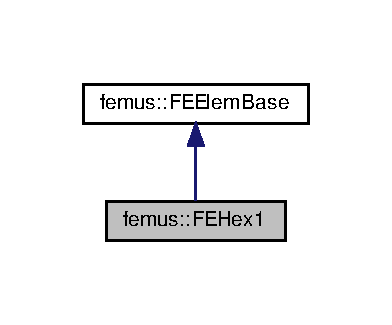
\includegraphics[width=188pt]{classfemus_1_1_f_e_hex1__inherit__graph}
\end{center}
\end{figure}


Collaboration diagram for femus\+:\+:F\+E\+Hex1\+:
\nopagebreak
\begin{figure}[H]
\begin{center}
\leavevmode
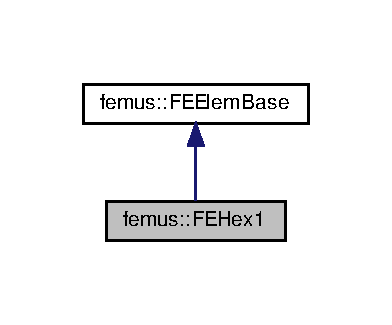
\includegraphics[width=188pt]{classfemus_1_1_f_e_hex1__coll__graph}
\end{center}
\end{figure}
\subsection*{Public Member Functions}
\begin{DoxyCompactItemize}
\item 
\mbox{\hyperlink{classfemus_1_1_f_e_hex1_a3191433251c20a4edf83b4029c9ec4fc}{F\+E\+Hex1}} ()
\item 
\mbox{\hyperlink{classfemus_1_1_f_e_hex1_a63865a413c61c54242946b284e35cd8a}{$\sim$\+F\+E\+Hex1}} ()
\item 
float \mbox{\hyperlink{classfemus_1_1_f_e_hex1_aaa8731caede9d90c2fee78a7440f610a}{get\+\_\+embedding\+\_\+matrix}} (const \mbox{\hyperlink{_typedefs_8hpp_a91ad9478d81a7aaf2593e8d9c3d06a14}{uint}}, const \mbox{\hyperlink{_typedefs_8hpp_a91ad9478d81a7aaf2593e8d9c3d06a14}{uint}}, const \mbox{\hyperlink{_typedefs_8hpp_a91ad9478d81a7aaf2593e8d9c3d06a14}{uint}})
\item 
double \mbox{\hyperlink{classfemus_1_1_f_e_hex1_ac9745cc75964e76795dbca432939df53}{get\+\_\+prol}} (const \mbox{\hyperlink{_typedefs_8hpp_a91ad9478d81a7aaf2593e8d9c3d06a14}{uint}})
\end{DoxyCompactItemize}
\subsection*{Static Public Attributes}
\begin{DoxyCompactItemize}
\item 
static const float \mbox{\hyperlink{classfemus_1_1_f_e_hex1_a8ee2980ed21bc2511602b888ad47c3ae}{\+\_\+embedding\+\_\+matrix}} \mbox{[}8\mbox{]}\mbox{[}1\mbox{]}\mbox{[}1\mbox{]}
\end{DoxyCompactItemize}
\subsection*{Additional Inherited Members}


\subsection{Constructor \& Destructor Documentation}
\mbox{\Hypertarget{classfemus_1_1_f_e_hex1_a3191433251c20a4edf83b4029c9ec4fc}\label{classfemus_1_1_f_e_hex1_a3191433251c20a4edf83b4029c9ec4fc}} 
\index{femus\+::\+F\+E\+Hex1@{femus\+::\+F\+E\+Hex1}!F\+E\+Hex1@{F\+E\+Hex1}}
\index{F\+E\+Hex1@{F\+E\+Hex1}!femus\+::\+F\+E\+Hex1@{femus\+::\+F\+E\+Hex1}}
\subsubsection{\texorpdfstring{F\+E\+Hex1()}{FEHex1()}}
{\footnotesize\ttfamily femus\+::\+F\+E\+Hex1\+::\+F\+E\+Hex1 (\begin{DoxyParamCaption}{ }\end{DoxyParamCaption})}

\mbox{\Hypertarget{classfemus_1_1_f_e_hex1_a63865a413c61c54242946b284e35cd8a}\label{classfemus_1_1_f_e_hex1_a63865a413c61c54242946b284e35cd8a}} 
\index{femus\+::\+F\+E\+Hex1@{femus\+::\+F\+E\+Hex1}!````~F\+E\+Hex1@{$\sim$\+F\+E\+Hex1}}
\index{````~F\+E\+Hex1@{$\sim$\+F\+E\+Hex1}!femus\+::\+F\+E\+Hex1@{femus\+::\+F\+E\+Hex1}}
\subsubsection{\texorpdfstring{$\sim$\+F\+E\+Hex1()}{~FEHex1()}}
{\footnotesize\ttfamily femus\+::\+F\+E\+Hex1\+::$\sim$\+F\+E\+Hex1 (\begin{DoxyParamCaption}{ }\end{DoxyParamCaption})}



\subsection{Member Function Documentation}
\mbox{\Hypertarget{classfemus_1_1_f_e_hex1_aaa8731caede9d90c2fee78a7440f610a}\label{classfemus_1_1_f_e_hex1_aaa8731caede9d90c2fee78a7440f610a}} 
\index{femus\+::\+F\+E\+Hex1@{femus\+::\+F\+E\+Hex1}!get\+\_\+embedding\+\_\+matrix@{get\+\_\+embedding\+\_\+matrix}}
\index{get\+\_\+embedding\+\_\+matrix@{get\+\_\+embedding\+\_\+matrix}!femus\+::\+F\+E\+Hex1@{femus\+::\+F\+E\+Hex1}}
\subsubsection{\texorpdfstring{get\+\_\+embedding\+\_\+matrix()}{get\_embedding\_matrix()}}
{\footnotesize\ttfamily float femus\+::\+F\+E\+Hex1\+::get\+\_\+embedding\+\_\+matrix (\begin{DoxyParamCaption}\item[{const \mbox{\hyperlink{_typedefs_8hpp_a91ad9478d81a7aaf2593e8d9c3d06a14}{uint}}}]{a,  }\item[{const \mbox{\hyperlink{_typedefs_8hpp_a91ad9478d81a7aaf2593e8d9c3d06a14}{uint}}}]{b,  }\item[{const \mbox{\hyperlink{_typedefs_8hpp_a91ad9478d81a7aaf2593e8d9c3d06a14}{uint}}}]{c }\end{DoxyParamCaption})\hspace{0.3cm}{\ttfamily [virtual]}}



Implements \mbox{\hyperlink{classfemus_1_1_f_e_elem_base_a0c4d6d5ec66bd4e301eb8ea2ef10f354}{femus\+::\+F\+E\+Elem\+Base}}.

\mbox{\Hypertarget{classfemus_1_1_f_e_hex1_ac9745cc75964e76795dbca432939df53}\label{classfemus_1_1_f_e_hex1_ac9745cc75964e76795dbca432939df53}} 
\index{femus\+::\+F\+E\+Hex1@{femus\+::\+F\+E\+Hex1}!get\+\_\+prol@{get\+\_\+prol}}
\index{get\+\_\+prol@{get\+\_\+prol}!femus\+::\+F\+E\+Hex1@{femus\+::\+F\+E\+Hex1}}
\subsubsection{\texorpdfstring{get\+\_\+prol()}{get\_prol()}}
{\footnotesize\ttfamily double femus\+::\+F\+E\+Hex1\+::get\+\_\+prol (\begin{DoxyParamCaption}\item[{const \mbox{\hyperlink{_typedefs_8hpp_a91ad9478d81a7aaf2593e8d9c3d06a14}{uint}}}]{ }\end{DoxyParamCaption})\hspace{0.3cm}{\ttfamily [inline]}, {\ttfamily [virtual]}}



Implements \mbox{\hyperlink{classfemus_1_1_f_e_elem_base_ac82326cdc7cb02329c7be9547d56fad4}{femus\+::\+F\+E\+Elem\+Base}}.



\subsection{Member Data Documentation}
\mbox{\Hypertarget{classfemus_1_1_f_e_hex1_a8ee2980ed21bc2511602b888ad47c3ae}\label{classfemus_1_1_f_e_hex1_a8ee2980ed21bc2511602b888ad47c3ae}} 
\index{femus\+::\+F\+E\+Hex1@{femus\+::\+F\+E\+Hex1}!\+\_\+embedding\+\_\+matrix@{\+\_\+embedding\+\_\+matrix}}
\index{\+\_\+embedding\+\_\+matrix@{\+\_\+embedding\+\_\+matrix}!femus\+::\+F\+E\+Hex1@{femus\+::\+F\+E\+Hex1}}
\subsubsection{\texorpdfstring{\+\_\+embedding\+\_\+matrix}{\_embedding\_matrix}}
{\footnotesize\ttfamily const float femus\+::\+F\+E\+Hex1\+::\+\_\+embedding\+\_\+matrix\hspace{0.3cm}{\ttfamily [static]}}



The documentation for this class was generated from the following files\+:\begin{DoxyCompactItemize}
\item 
mesh\+Gencase/\mbox{\hyperlink{_f_e_hex1_8hpp}{F\+E\+Hex1.\+hpp}}\item 
mesh\+Gencase/\mbox{\hyperlink{_f_e_hex1_8cpp}{F\+E\+Hex1.\+cpp}}\end{DoxyCompactItemize}

\hypertarget{classfemus_1_1_f_e_hex27}{}\section{femus\+:\+:F\+E\+Hex27 Class Reference}
\label{classfemus_1_1_f_e_hex27}\index{femus\+::\+F\+E\+Hex27@{femus\+::\+F\+E\+Hex27}}


{\ttfamily \#include $<$F\+E\+Hex27.\+hpp$>$}



Inheritance diagram for femus\+:\+:F\+E\+Hex27\+:
\nopagebreak
\begin{figure}[H]
\begin{center}
\leavevmode
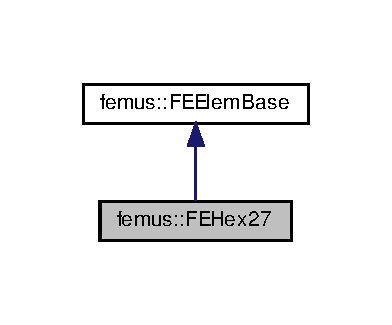
\includegraphics[width=188pt]{classfemus_1_1_f_e_hex27__inherit__graph}
\end{center}
\end{figure}


Collaboration diagram for femus\+:\+:F\+E\+Hex27\+:
\nopagebreak
\begin{figure}[H]
\begin{center}
\leavevmode
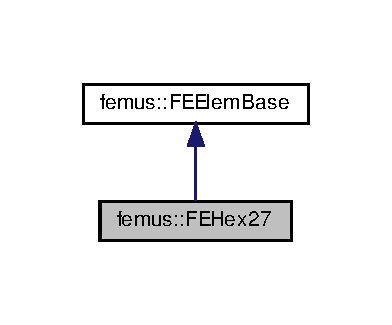
\includegraphics[width=188pt]{classfemus_1_1_f_e_hex27__coll__graph}
\end{center}
\end{figure}
\subsection*{Public Member Functions}
\begin{DoxyCompactItemize}
\item 
\mbox{\hyperlink{classfemus_1_1_f_e_hex27_a31c28c2432aa19dc9cac8b8d6952acbb}{F\+E\+Hex27}} ()
\item 
\mbox{\hyperlink{classfemus_1_1_f_e_hex27_a4423c27701fafe1a1546c0dc66c94b48}{$\sim$\+F\+E\+Hex27}} ()
\item 
float \mbox{\hyperlink{classfemus_1_1_f_e_hex27_a0bfb79afd1a19396983b0ea03daf00ff}{get\+\_\+embedding\+\_\+matrix}} (const \mbox{\hyperlink{_typedefs_8hpp_a91ad9478d81a7aaf2593e8d9c3d06a14}{uint}}, const \mbox{\hyperlink{_typedefs_8hpp_a91ad9478d81a7aaf2593e8d9c3d06a14}{uint}}, const \mbox{\hyperlink{_typedefs_8hpp_a91ad9478d81a7aaf2593e8d9c3d06a14}{uint}})
\item 
double \mbox{\hyperlink{classfemus_1_1_f_e_hex27_aa0a6cf0465e5c48c4b5ebf4a4e407124}{get\+\_\+prol}} (const \mbox{\hyperlink{_typedefs_8hpp_a91ad9478d81a7aaf2593e8d9c3d06a14}{uint}})
\end{DoxyCompactItemize}
\subsection*{Static Public Attributes}
\begin{DoxyCompactItemize}
\item 
static const float \mbox{\hyperlink{classfemus_1_1_f_e_hex27_af91845b451a5bb5249886e23ee6786a0}{\+\_\+embedding\+\_\+matrix}} \mbox{[}8\mbox{]}\mbox{[}27\mbox{]}\mbox{[}27\mbox{]}
\end{DoxyCompactItemize}
\subsection*{Additional Inherited Members}


\subsection{Constructor \& Destructor Documentation}
\mbox{\Hypertarget{classfemus_1_1_f_e_hex27_a31c28c2432aa19dc9cac8b8d6952acbb}\label{classfemus_1_1_f_e_hex27_a31c28c2432aa19dc9cac8b8d6952acbb}} 
\index{femus\+::\+F\+E\+Hex27@{femus\+::\+F\+E\+Hex27}!F\+E\+Hex27@{F\+E\+Hex27}}
\index{F\+E\+Hex27@{F\+E\+Hex27}!femus\+::\+F\+E\+Hex27@{femus\+::\+F\+E\+Hex27}}
\subsubsection{\texorpdfstring{F\+E\+Hex27()}{FEHex27()}}
{\footnotesize\ttfamily femus\+::\+F\+E\+Hex27\+::\+F\+E\+Hex27 (\begin{DoxyParamCaption}{ }\end{DoxyParamCaption})}

\mbox{\Hypertarget{classfemus_1_1_f_e_hex27_a4423c27701fafe1a1546c0dc66c94b48}\label{classfemus_1_1_f_e_hex27_a4423c27701fafe1a1546c0dc66c94b48}} 
\index{femus\+::\+F\+E\+Hex27@{femus\+::\+F\+E\+Hex27}!````~F\+E\+Hex27@{$\sim$\+F\+E\+Hex27}}
\index{````~F\+E\+Hex27@{$\sim$\+F\+E\+Hex27}!femus\+::\+F\+E\+Hex27@{femus\+::\+F\+E\+Hex27}}
\subsubsection{\texorpdfstring{$\sim$\+F\+E\+Hex27()}{~FEHex27()}}
{\footnotesize\ttfamily femus\+::\+F\+E\+Hex27\+::$\sim$\+F\+E\+Hex27 (\begin{DoxyParamCaption}{ }\end{DoxyParamCaption})}



\subsection{Member Function Documentation}
\mbox{\Hypertarget{classfemus_1_1_f_e_hex27_a0bfb79afd1a19396983b0ea03daf00ff}\label{classfemus_1_1_f_e_hex27_a0bfb79afd1a19396983b0ea03daf00ff}} 
\index{femus\+::\+F\+E\+Hex27@{femus\+::\+F\+E\+Hex27}!get\+\_\+embedding\+\_\+matrix@{get\+\_\+embedding\+\_\+matrix}}
\index{get\+\_\+embedding\+\_\+matrix@{get\+\_\+embedding\+\_\+matrix}!femus\+::\+F\+E\+Hex27@{femus\+::\+F\+E\+Hex27}}
\subsubsection{\texorpdfstring{get\+\_\+embedding\+\_\+matrix()}{get\_embedding\_matrix()}}
{\footnotesize\ttfamily float femus\+::\+F\+E\+Hex27\+::get\+\_\+embedding\+\_\+matrix (\begin{DoxyParamCaption}\item[{const \mbox{\hyperlink{_typedefs_8hpp_a91ad9478d81a7aaf2593e8d9c3d06a14}{uint}}}]{a,  }\item[{const \mbox{\hyperlink{_typedefs_8hpp_a91ad9478d81a7aaf2593e8d9c3d06a14}{uint}}}]{b,  }\item[{const \mbox{\hyperlink{_typedefs_8hpp_a91ad9478d81a7aaf2593e8d9c3d06a14}{uint}}}]{c }\end{DoxyParamCaption})\hspace{0.3cm}{\ttfamily [virtual]}}



Implements \mbox{\hyperlink{classfemus_1_1_f_e_elem_base_a0c4d6d5ec66bd4e301eb8ea2ef10f354}{femus\+::\+F\+E\+Elem\+Base}}.

\mbox{\Hypertarget{classfemus_1_1_f_e_hex27_aa0a6cf0465e5c48c4b5ebf4a4e407124}\label{classfemus_1_1_f_e_hex27_aa0a6cf0465e5c48c4b5ebf4a4e407124}} 
\index{femus\+::\+F\+E\+Hex27@{femus\+::\+F\+E\+Hex27}!get\+\_\+prol@{get\+\_\+prol}}
\index{get\+\_\+prol@{get\+\_\+prol}!femus\+::\+F\+E\+Hex27@{femus\+::\+F\+E\+Hex27}}
\subsubsection{\texorpdfstring{get\+\_\+prol()}{get\_prol()}}
{\footnotesize\ttfamily double femus\+::\+F\+E\+Hex27\+::get\+\_\+prol (\begin{DoxyParamCaption}\item[{const \mbox{\hyperlink{_typedefs_8hpp_a91ad9478d81a7aaf2593e8d9c3d06a14}{uint}}}]{ }\end{DoxyParamCaption})\hspace{0.3cm}{\ttfamily [inline]}, {\ttfamily [virtual]}}



Implements \mbox{\hyperlink{classfemus_1_1_f_e_elem_base_ac82326cdc7cb02329c7be9547d56fad4}{femus\+::\+F\+E\+Elem\+Base}}.



\subsection{Member Data Documentation}
\mbox{\Hypertarget{classfemus_1_1_f_e_hex27_af91845b451a5bb5249886e23ee6786a0}\label{classfemus_1_1_f_e_hex27_af91845b451a5bb5249886e23ee6786a0}} 
\index{femus\+::\+F\+E\+Hex27@{femus\+::\+F\+E\+Hex27}!\+\_\+embedding\+\_\+matrix@{\+\_\+embedding\+\_\+matrix}}
\index{\+\_\+embedding\+\_\+matrix@{\+\_\+embedding\+\_\+matrix}!femus\+::\+F\+E\+Hex27@{femus\+::\+F\+E\+Hex27}}
\subsubsection{\texorpdfstring{\+\_\+embedding\+\_\+matrix}{\_embedding\_matrix}}
{\footnotesize\ttfamily const float femus\+::\+F\+E\+Hex27\+::\+\_\+embedding\+\_\+matrix\hspace{0.3cm}{\ttfamily [static]}}



The documentation for this class was generated from the following files\+:\begin{DoxyCompactItemize}
\item 
mesh\+Gencase/\mbox{\hyperlink{_f_e_hex27_8hpp}{F\+E\+Hex27.\+hpp}}\item 
mesh\+Gencase/\mbox{\hyperlink{_f_e_hex27_8cpp}{F\+E\+Hex27.\+cpp}}\end{DoxyCompactItemize}

\hypertarget{classfemus_1_1_f_e_hex8}{}\section{femus\+:\+:F\+E\+Hex8 Class Reference}
\label{classfemus_1_1_f_e_hex8}\index{femus\+::\+F\+E\+Hex8@{femus\+::\+F\+E\+Hex8}}


{\ttfamily \#include $<$F\+E\+Hex8.\+hpp$>$}



Inheritance diagram for femus\+:\+:F\+E\+Hex8\+:
\nopagebreak
\begin{figure}[H]
\begin{center}
\leavevmode
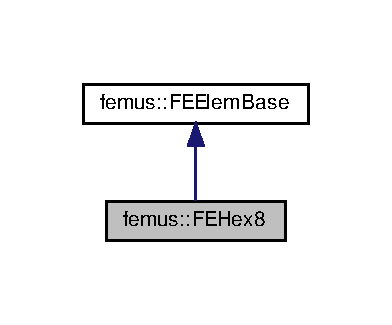
\includegraphics[width=188pt]{classfemus_1_1_f_e_hex8__inherit__graph}
\end{center}
\end{figure}


Collaboration diagram for femus\+:\+:F\+E\+Hex8\+:
\nopagebreak
\begin{figure}[H]
\begin{center}
\leavevmode
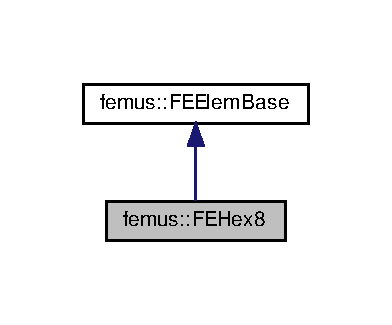
\includegraphics[width=188pt]{classfemus_1_1_f_e_hex8__coll__graph}
\end{center}
\end{figure}
\subsection*{Public Member Functions}
\begin{DoxyCompactItemize}
\item 
\mbox{\hyperlink{classfemus_1_1_f_e_hex8_a096b681567770f72bb2d4a7a18d260ca}{F\+E\+Hex8}} ()
\item 
\mbox{\hyperlink{classfemus_1_1_f_e_hex8_a7133b27555c7c730281cc4c36ea2ac6d}{$\sim$\+F\+E\+Hex8}} ()
\item 
float \mbox{\hyperlink{classfemus_1_1_f_e_hex8_a6e1819ed6e7597f1109f3d314d1c1f1b}{get\+\_\+embedding\+\_\+matrix}} (const \mbox{\hyperlink{_typedefs_8hpp_a91ad9478d81a7aaf2593e8d9c3d06a14}{uint}}, const \mbox{\hyperlink{_typedefs_8hpp_a91ad9478d81a7aaf2593e8d9c3d06a14}{uint}}, const \mbox{\hyperlink{_typedefs_8hpp_a91ad9478d81a7aaf2593e8d9c3d06a14}{uint}})
\item 
double \mbox{\hyperlink{classfemus_1_1_f_e_hex8_aa84066edfa5cac347255b6e8f2098cf5}{get\+\_\+prol}} (const \mbox{\hyperlink{_typedefs_8hpp_a91ad9478d81a7aaf2593e8d9c3d06a14}{uint}} j)
\end{DoxyCompactItemize}
\subsection*{Static Public Attributes}
\begin{DoxyCompactItemize}
\item 
static const float \mbox{\hyperlink{classfemus_1_1_f_e_hex8_aea2ef04528935355545d3ebe2b2bf051}{\+\_\+embedding\+\_\+matrix}} \mbox{[}8\mbox{]}\mbox{[}8\mbox{]}\mbox{[}8\mbox{]}
\item 
static const double \mbox{\hyperlink{classfemus_1_1_f_e_hex8_a282ec3050c8490f8195b908895148c58}{\+\_\+\+Prol}} \mbox{[}27 $\ast$8\mbox{]}
\end{DoxyCompactItemize}
\subsection*{Additional Inherited Members}


\subsection{Constructor \& Destructor Documentation}
\mbox{\Hypertarget{classfemus_1_1_f_e_hex8_a096b681567770f72bb2d4a7a18d260ca}\label{classfemus_1_1_f_e_hex8_a096b681567770f72bb2d4a7a18d260ca}} 
\index{femus\+::\+F\+E\+Hex8@{femus\+::\+F\+E\+Hex8}!F\+E\+Hex8@{F\+E\+Hex8}}
\index{F\+E\+Hex8@{F\+E\+Hex8}!femus\+::\+F\+E\+Hex8@{femus\+::\+F\+E\+Hex8}}
\subsubsection{\texorpdfstring{F\+E\+Hex8()}{FEHex8()}}
{\footnotesize\ttfamily femus\+::\+F\+E\+Hex8\+::\+F\+E\+Hex8 (\begin{DoxyParamCaption}{ }\end{DoxyParamCaption})}

\mbox{\Hypertarget{classfemus_1_1_f_e_hex8_a7133b27555c7c730281cc4c36ea2ac6d}\label{classfemus_1_1_f_e_hex8_a7133b27555c7c730281cc4c36ea2ac6d}} 
\index{femus\+::\+F\+E\+Hex8@{femus\+::\+F\+E\+Hex8}!````~F\+E\+Hex8@{$\sim$\+F\+E\+Hex8}}
\index{````~F\+E\+Hex8@{$\sim$\+F\+E\+Hex8}!femus\+::\+F\+E\+Hex8@{femus\+::\+F\+E\+Hex8}}
\subsubsection{\texorpdfstring{$\sim$\+F\+E\+Hex8()}{~FEHex8()}}
{\footnotesize\ttfamily femus\+::\+F\+E\+Hex8\+::$\sim$\+F\+E\+Hex8 (\begin{DoxyParamCaption}{ }\end{DoxyParamCaption})}



\subsection{Member Function Documentation}
\mbox{\Hypertarget{classfemus_1_1_f_e_hex8_a6e1819ed6e7597f1109f3d314d1c1f1b}\label{classfemus_1_1_f_e_hex8_a6e1819ed6e7597f1109f3d314d1c1f1b}} 
\index{femus\+::\+F\+E\+Hex8@{femus\+::\+F\+E\+Hex8}!get\+\_\+embedding\+\_\+matrix@{get\+\_\+embedding\+\_\+matrix}}
\index{get\+\_\+embedding\+\_\+matrix@{get\+\_\+embedding\+\_\+matrix}!femus\+::\+F\+E\+Hex8@{femus\+::\+F\+E\+Hex8}}
\subsubsection{\texorpdfstring{get\+\_\+embedding\+\_\+matrix()}{get\_embedding\_matrix()}}
{\footnotesize\ttfamily float femus\+::\+F\+E\+Hex8\+::get\+\_\+embedding\+\_\+matrix (\begin{DoxyParamCaption}\item[{const \mbox{\hyperlink{_typedefs_8hpp_a91ad9478d81a7aaf2593e8d9c3d06a14}{uint}}}]{a,  }\item[{const \mbox{\hyperlink{_typedefs_8hpp_a91ad9478d81a7aaf2593e8d9c3d06a14}{uint}}}]{b,  }\item[{const \mbox{\hyperlink{_typedefs_8hpp_a91ad9478d81a7aaf2593e8d9c3d06a14}{uint}}}]{c }\end{DoxyParamCaption})\hspace{0.3cm}{\ttfamily [virtual]}}



Implements \mbox{\hyperlink{classfemus_1_1_f_e_elem_base_a0c4d6d5ec66bd4e301eb8ea2ef10f354}{femus\+::\+F\+E\+Elem\+Base}}.

\mbox{\Hypertarget{classfemus_1_1_f_e_hex8_aa84066edfa5cac347255b6e8f2098cf5}\label{classfemus_1_1_f_e_hex8_aa84066edfa5cac347255b6e8f2098cf5}} 
\index{femus\+::\+F\+E\+Hex8@{femus\+::\+F\+E\+Hex8}!get\+\_\+prol@{get\+\_\+prol}}
\index{get\+\_\+prol@{get\+\_\+prol}!femus\+::\+F\+E\+Hex8@{femus\+::\+F\+E\+Hex8}}
\subsubsection{\texorpdfstring{get\+\_\+prol()}{get\_prol()}}
{\footnotesize\ttfamily double femus\+::\+F\+E\+Hex8\+::get\+\_\+prol (\begin{DoxyParamCaption}\item[{const \mbox{\hyperlink{_typedefs_8hpp_a91ad9478d81a7aaf2593e8d9c3d06a14}{uint}}}]{j }\end{DoxyParamCaption})\hspace{0.3cm}{\ttfamily [inline]}, {\ttfamily [virtual]}}



Implements \mbox{\hyperlink{classfemus_1_1_f_e_elem_base_ac82326cdc7cb02329c7be9547d56fad4}{femus\+::\+F\+E\+Elem\+Base}}.



\subsection{Member Data Documentation}
\mbox{\Hypertarget{classfemus_1_1_f_e_hex8_aea2ef04528935355545d3ebe2b2bf051}\label{classfemus_1_1_f_e_hex8_aea2ef04528935355545d3ebe2b2bf051}} 
\index{femus\+::\+F\+E\+Hex8@{femus\+::\+F\+E\+Hex8}!\+\_\+embedding\+\_\+matrix@{\+\_\+embedding\+\_\+matrix}}
\index{\+\_\+embedding\+\_\+matrix@{\+\_\+embedding\+\_\+matrix}!femus\+::\+F\+E\+Hex8@{femus\+::\+F\+E\+Hex8}}
\subsubsection{\texorpdfstring{\+\_\+embedding\+\_\+matrix}{\_embedding\_matrix}}
{\footnotesize\ttfamily const float femus\+::\+F\+E\+Hex8\+::\+\_\+embedding\+\_\+matrix\hspace{0.3cm}{\ttfamily [static]}}

\mbox{\Hypertarget{classfemus_1_1_f_e_hex8_a282ec3050c8490f8195b908895148c58}\label{classfemus_1_1_f_e_hex8_a282ec3050c8490f8195b908895148c58}} 
\index{femus\+::\+F\+E\+Hex8@{femus\+::\+F\+E\+Hex8}!\+\_\+\+Prol@{\+\_\+\+Prol}}
\index{\+\_\+\+Prol@{\+\_\+\+Prol}!femus\+::\+F\+E\+Hex8@{femus\+::\+F\+E\+Hex8}}
\subsubsection{\texorpdfstring{\+\_\+\+Prol}{\_Prol}}
{\footnotesize\ttfamily const double femus\+::\+F\+E\+Hex8\+::\+\_\+\+Prol\hspace{0.3cm}{\ttfamily [static]}}

{\bfseries Initial value\+:}
\begin{DoxyCode}
= \{ 
   1.,0.,0.,0.,0.,0.,0.,0.,
   0.,1.,0.,0.,0.,0.,0.,0.,
   0.,0.,1.,0.,0.,0.,0.,0.,
   0.,0.,0.,1.,0.,0.,0.,0.,
   0.,0.,0.,0.,1.,0.,0.,0.,
   0.,0.,0.,0.,0.,1.,0.,0.,
   0.,0.,0.,0.,0.,0.,1.,0.,
   0.,0.,0.,0.,0.,0.,0.,1.,
   0.5,0.5,0.,0.,0.,0.,0.,0.,
   0.,0.5,0.5,0.,0.,0.,0.,0.,
   0.,0.,0.5,0.5,0.,0.,0.,0.,
   0.5,0.,0.,0.5,0.,0.,0.,0.,  
   0.5,0.,0.,0.,0.5,0.,0.,0.,
   0.,0.5,0.,0.,0.,0.5,0.,0.,
   0.,0.,0.5,0.,0.,0.,0.5,0.,  
   0.,0.,0.,0.5,0.,0.,0.,0.5,
   0.,0.,0.,0.,0.5,0.5,0.,0.,
   0.,0.,0.,0.,0.,0.5,0.5,0.,
   0.,0.,0.,0.,0.,0.,0.5,0.5,
   0.,0.,0.,0.,0.5,0.,0.,0.5,
   0.25,0.25,0.25,0.25,0.,0.,0.,0.,
   0.25,0.25,0.,0.,0.25,0.25,0.,0., 
   0.,0.25,0.25,0.,0.,0.25,0.25,0.,
   0.,0.,0.25,0.25,0.,0.,0.25,0.25,
   0.25,0.,0.,0.25,0.25,0.,0.,0.25,
   0.,0.,0.,0.,0.25,0.25,0.25,0.25,
   0.125,0.125,0.125,0.125,0.125,0.125,0.125,0.125
   \}
\end{DoxyCode}


The documentation for this class was generated from the following files\+:\begin{DoxyCompactItemize}
\item 
mesh\+Gencase/\mbox{\hyperlink{_f_e_hex8_8hpp}{F\+E\+Hex8.\+hpp}}\item 
mesh\+Gencase/\mbox{\hyperlink{_f_e_hex8_8cpp}{F\+E\+Hex8.\+cpp}}\end{DoxyCompactItemize}

\hypertarget{classfemus_1_1_femus_init}{}\section{femus\+:\+:Femus\+Init Class Reference}
\label{classfemus_1_1_femus_init}\index{femus\+::\+Femus\+Init@{femus\+::\+Femus\+Init}}


{\ttfamily \#include $<$Femus\+Init.\+hpp$>$}

\subsection*{Public Member Functions}
\begin{DoxyCompactItemize}
\item 
\mbox{\hyperlink{classfemus_1_1_femus_init_a31469e71e3cc5be638a8ed8b9df2218b}{Femus\+Init}} (int \&argc, char $\ast$$\ast$\&argv, M\+P\+I\+\_\+\+Comm comm\+\_\+world\+\_\+in=M\+P\+I\+\_\+\+C\+O\+M\+M\+\_\+\+W\+O\+R\+LD)
\begin{DoxyCompactList}\small\item\em Constructor. \end{DoxyCompactList}\item 
\mbox{\hyperlink{classfemus_1_1_femus_init_a0d8bd96e2534e355eaf3621d012292ba}{$\sim$\+Femus\+Init}} ()
\begin{DoxyCompactList}\small\item\em Destructor. \end{DoxyCompactList}\end{DoxyCompactItemize}
\subsection*{Static Public Attributes}
\begin{DoxyCompactItemize}
\item 
static adept\+::\+Stack \mbox{\hyperlink{classfemus_1_1_femus_init_ab48c1191eb7ebb370a323d3ec4f713c9}{\+\_\+adept\+Stack}}
\end{DoxyCompactItemize}


\subsection{Constructor \& Destructor Documentation}
\mbox{\Hypertarget{classfemus_1_1_femus_init_a31469e71e3cc5be638a8ed8b9df2218b}\label{classfemus_1_1_femus_init_a31469e71e3cc5be638a8ed8b9df2218b}} 
\index{femus\+::\+Femus\+Init@{femus\+::\+Femus\+Init}!Femus\+Init@{Femus\+Init}}
\index{Femus\+Init@{Femus\+Init}!femus\+::\+Femus\+Init@{femus\+::\+Femus\+Init}}
\subsubsection{\texorpdfstring{Femus\+Init()}{FemusInit()}}
{\footnotesize\ttfamily femus\+::\+Femus\+Init\+::\+Femus\+Init (\begin{DoxyParamCaption}\item[{int \&}]{argc,  }\item[{char $\ast$$\ast$\&}]{argv,  }\item[{M\+P\+I\+\_\+\+Comm}]{comm\+\_\+world\+\_\+in = {\ttfamily MPI\+\_\+COMM\+\_\+WORLD} }\end{DoxyParamCaption})}



Constructor. 

This function initializes the libraries if it is parallel. \mbox{\Hypertarget{classfemus_1_1_femus_init_a0d8bd96e2534e355eaf3621d012292ba}\label{classfemus_1_1_femus_init_a0d8bd96e2534e355eaf3621d012292ba}} 
\index{femus\+::\+Femus\+Init@{femus\+::\+Femus\+Init}!````~Femus\+Init@{$\sim$\+Femus\+Init}}
\index{````~Femus\+Init@{$\sim$\+Femus\+Init}!femus\+::\+Femus\+Init@{femus\+::\+Femus\+Init}}
\subsubsection{\texorpdfstring{$\sim$\+Femus\+Init()}{~FemusInit()}}
{\footnotesize\ttfamily femus\+::\+Femus\+Init\+::$\sim$\+Femus\+Init (\begin{DoxyParamCaption}{ }\end{DoxyParamCaption})}



Destructor. 



\subsection{Member Data Documentation}
\mbox{\Hypertarget{classfemus_1_1_femus_init_ab48c1191eb7ebb370a323d3ec4f713c9}\label{classfemus_1_1_femus_init_ab48c1191eb7ebb370a323d3ec4f713c9}} 
\index{femus\+::\+Femus\+Init@{femus\+::\+Femus\+Init}!\+\_\+adept\+Stack@{\+\_\+adept\+Stack}}
\index{\+\_\+adept\+Stack@{\+\_\+adept\+Stack}!femus\+::\+Femus\+Init@{femus\+::\+Femus\+Init}}
\subsubsection{\texorpdfstring{\+\_\+adept\+Stack}{\_adeptStack}}
{\footnotesize\ttfamily adept\+::\+Stack femus\+::\+Femus\+Init\+::\+\_\+adept\+Stack\hspace{0.3cm}{\ttfamily [static]}}



The documentation for this class was generated from the following files\+:\begin{DoxyCompactItemize}
\item 
utils/\mbox{\hyperlink{_femus_init_8hpp}{Femus\+Init.\+hpp}}\item 
utils/\mbox{\hyperlink{_femus_init_8cpp}{Femus\+Init.\+cpp}}\end{DoxyCompactItemize}

\hypertarget{classfemus_1_1_femus_input_parser}{}\section{femus\+:\+:Femus\+Input\+Parser$<$ T $>$ Class Template Reference}
\label{classfemus_1_1_femus_input_parser}\index{femus\+::\+Femus\+Input\+Parser$<$ T $>$@{femus\+::\+Femus\+Input\+Parser$<$ T $>$}}


{\ttfamily \#include $<$Femus\+Input\+Parser.\+hpp$>$}

\subsection*{Public Member Functions}
\begin{DoxyCompactItemize}
\item 
\mbox{\hyperlink{classfemus_1_1_femus_input_parser_a012881346421fc56c278db92d9b48858}{Femus\+Input\+Parser}} (const std\+::string class\+\_\+name, const std\+::string basepath\+\_\+in)
\item 
\mbox{\hyperlink{classfemus_1_1_femus_input_parser_a83fce921560f1f0a19e351e2f87248b5}{$\sim$\+Femus\+Input\+Parser}} ()
\item 
void \mbox{\hyperlink{classfemus_1_1_femus_input_parser_a5ac476036f43e888b305f2a4844e2e57}{read}} ()
\item 
void \mbox{\hyperlink{classfemus_1_1_femus_input_parser_a94ecc392927f6d03531d8f1e5904f157}{print}} () const
\begin{DoxyCompactList}\small\item\em This function prints all the parameters to stdout. \end{DoxyCompactList}\item 
void \mbox{\hyperlink{classfemus_1_1_femus_input_parser_acbc42027ebef9bad38afd4e0bdef4169}{set}} (const std\+::string \&name, const T \&value)
\item 
const T \mbox{\hyperlink{classfemus_1_1_femus_input_parser_a317bdaac200e745334dcd436d39d2832}{get}} (const std\+::string \&name) const
\item 
const std\+::string \mbox{\hyperlink{classfemus_1_1_femus_input_parser_a3b479c8cf9e6bbeb172e5ef1282ed096}{get\+\_\+rbasepath}} () const
\end{DoxyCompactItemize}
\subsection*{Public Attributes}
\begin{DoxyCompactItemize}
\item 
std\+::string \mbox{\hyperlink{classfemus_1_1_femus_input_parser_a7bc03b4cb89200a0c76547e3f169c8d3}{\+\_\+basepath}}
\item 
std\+::map$<$ std\+::string, T $>$ \mbox{\hyperlink{classfemus_1_1_femus_input_parser_ab5d6ea57ed37959267aa8cf3909d1422}{\+\_\+rtmap}}
\end{DoxyCompactItemize}


\subsection{Constructor \& Destructor Documentation}
\mbox{\Hypertarget{classfemus_1_1_femus_input_parser_a012881346421fc56c278db92d9b48858}\label{classfemus_1_1_femus_input_parser_a012881346421fc56c278db92d9b48858}} 
\index{femus\+::\+Femus\+Input\+Parser@{femus\+::\+Femus\+Input\+Parser}!Femus\+Input\+Parser@{Femus\+Input\+Parser}}
\index{Femus\+Input\+Parser@{Femus\+Input\+Parser}!femus\+::\+Femus\+Input\+Parser@{femus\+::\+Femus\+Input\+Parser}}
\subsubsection{\texorpdfstring{Femus\+Input\+Parser()}{FemusInputParser()}}
{\footnotesize\ttfamily template$<$typename T $>$ \\
\mbox{\hyperlink{classfemus_1_1_femus_input_parser}{femus\+::\+Femus\+Input\+Parser}}$<$ T $>$\+::\mbox{\hyperlink{classfemus_1_1_femus_input_parser}{Femus\+Input\+Parser}} (\begin{DoxyParamCaption}\item[{const std\+::string}]{class\+\_\+name,  }\item[{const std\+::string}]{basepath\+\_\+in }\end{DoxyParamCaption})}

\mbox{\Hypertarget{classfemus_1_1_femus_input_parser_a83fce921560f1f0a19e351e2f87248b5}\label{classfemus_1_1_femus_input_parser_a83fce921560f1f0a19e351e2f87248b5}} 
\index{femus\+::\+Femus\+Input\+Parser@{femus\+::\+Femus\+Input\+Parser}!````~Femus\+Input\+Parser@{$\sim$\+Femus\+Input\+Parser}}
\index{````~Femus\+Input\+Parser@{$\sim$\+Femus\+Input\+Parser}!femus\+::\+Femus\+Input\+Parser@{femus\+::\+Femus\+Input\+Parser}}
\subsubsection{\texorpdfstring{$\sim$\+Femus\+Input\+Parser()}{~FemusInputParser()}}
{\footnotesize\ttfamily template$<$typename T $>$ \\
\mbox{\hyperlink{classfemus_1_1_femus_input_parser}{femus\+::\+Femus\+Input\+Parser}}$<$ T $>$\+::$\sim$\mbox{\hyperlink{classfemus_1_1_femus_input_parser}{Femus\+Input\+Parser}} (\begin{DoxyParamCaption}{ }\end{DoxyParamCaption})}



\subsection{Member Function Documentation}
\mbox{\Hypertarget{classfemus_1_1_femus_input_parser_a317bdaac200e745334dcd436d39d2832}\label{classfemus_1_1_femus_input_parser_a317bdaac200e745334dcd436d39d2832}} 
\index{femus\+::\+Femus\+Input\+Parser@{femus\+::\+Femus\+Input\+Parser}!get@{get}}
\index{get@{get}!femus\+::\+Femus\+Input\+Parser@{femus\+::\+Femus\+Input\+Parser}}
\subsubsection{\texorpdfstring{get()}{get()}}
{\footnotesize\ttfamily template$<$typename T $>$ \\
const T \mbox{\hyperlink{classfemus_1_1_femus_input_parser}{femus\+::\+Femus\+Input\+Parser}}$<$ T $>$\+::get (\begin{DoxyParamCaption}\item[{const std\+::string \&}]{name }\end{DoxyParamCaption}) const}

\mbox{\Hypertarget{classfemus_1_1_femus_input_parser_a3b479c8cf9e6bbeb172e5ef1282ed096}\label{classfemus_1_1_femus_input_parser_a3b479c8cf9e6bbeb172e5ef1282ed096}} 
\index{femus\+::\+Femus\+Input\+Parser@{femus\+::\+Femus\+Input\+Parser}!get\+\_\+rbasepath@{get\+\_\+rbasepath}}
\index{get\+\_\+rbasepath@{get\+\_\+rbasepath}!femus\+::\+Femus\+Input\+Parser@{femus\+::\+Femus\+Input\+Parser}}
\subsubsection{\texorpdfstring{get\+\_\+rbasepath()}{get\_rbasepath()}}
{\footnotesize\ttfamily template$<$typename T$>$ \\
const std\+::string \mbox{\hyperlink{classfemus_1_1_femus_input_parser}{femus\+::\+Femus\+Input\+Parser}}$<$ T $>$\+::get\+\_\+rbasepath (\begin{DoxyParamCaption}{ }\end{DoxyParamCaption}) const\hspace{0.3cm}{\ttfamily [inline]}}

\mbox{\Hypertarget{classfemus_1_1_femus_input_parser_a94ecc392927f6d03531d8f1e5904f157}\label{classfemus_1_1_femus_input_parser_a94ecc392927f6d03531d8f1e5904f157}} 
\index{femus\+::\+Femus\+Input\+Parser@{femus\+::\+Femus\+Input\+Parser}!print@{print}}
\index{print@{print}!femus\+::\+Femus\+Input\+Parser@{femus\+::\+Femus\+Input\+Parser}}
\subsubsection{\texorpdfstring{print()}{print()}}
{\footnotesize\ttfamily template$<$typename T $>$ \\
void \mbox{\hyperlink{classfemus_1_1_femus_input_parser}{femus\+::\+Femus\+Input\+Parser}}$<$ T $>$\+::print (\begin{DoxyParamCaption}{ }\end{DoxyParamCaption}) const}



This function prints all the parameters to stdout. 

\mbox{\Hypertarget{classfemus_1_1_femus_input_parser_a5ac476036f43e888b305f2a4844e2e57}\label{classfemus_1_1_femus_input_parser_a5ac476036f43e888b305f2a4844e2e57}} 
\index{femus\+::\+Femus\+Input\+Parser@{femus\+::\+Femus\+Input\+Parser}!read@{read}}
\index{read@{read}!femus\+::\+Femus\+Input\+Parser@{femus\+::\+Femus\+Input\+Parser}}
\subsubsection{\texorpdfstring{read()}{read()}}
{\footnotesize\ttfamily template$<$typename T $>$ \\
void \mbox{\hyperlink{classfemus_1_1_femus_input_parser}{femus\+::\+Femus\+Input\+Parser}}$<$ T $>$\+::read (\begin{DoxyParamCaption}{ }\end{DoxyParamCaption})}

\mbox{\Hypertarget{classfemus_1_1_femus_input_parser_acbc42027ebef9bad38afd4e0bdef4169}\label{classfemus_1_1_femus_input_parser_acbc42027ebef9bad38afd4e0bdef4169}} 
\index{femus\+::\+Femus\+Input\+Parser@{femus\+::\+Femus\+Input\+Parser}!set@{set}}
\index{set@{set}!femus\+::\+Femus\+Input\+Parser@{femus\+::\+Femus\+Input\+Parser}}
\subsubsection{\texorpdfstring{set()}{set()}}
{\footnotesize\ttfamily template$<$typename T$>$ \\
void \mbox{\hyperlink{classfemus_1_1_femus_input_parser}{femus\+::\+Femus\+Input\+Parser}}$<$ T $>$\+::set (\begin{DoxyParamCaption}\item[{const std\+::string \&}]{name,  }\item[{const T \&}]{value }\end{DoxyParamCaption})}



\subsection{Member Data Documentation}
\mbox{\Hypertarget{classfemus_1_1_femus_input_parser_a7bc03b4cb89200a0c76547e3f169c8d3}\label{classfemus_1_1_femus_input_parser_a7bc03b4cb89200a0c76547e3f169c8d3}} 
\index{femus\+::\+Femus\+Input\+Parser@{femus\+::\+Femus\+Input\+Parser}!\+\_\+basepath@{\+\_\+basepath}}
\index{\+\_\+basepath@{\+\_\+basepath}!femus\+::\+Femus\+Input\+Parser@{femus\+::\+Femus\+Input\+Parser}}
\subsubsection{\texorpdfstring{\+\_\+basepath}{\_basepath}}
{\footnotesize\ttfamily template$<$typename T$>$ \\
std\+::string \mbox{\hyperlink{classfemus_1_1_femus_input_parser}{femus\+::\+Femus\+Input\+Parser}}$<$ T $>$\+::\+\_\+basepath}

\mbox{\Hypertarget{classfemus_1_1_femus_input_parser_ab5d6ea57ed37959267aa8cf3909d1422}\label{classfemus_1_1_femus_input_parser_ab5d6ea57ed37959267aa8cf3909d1422}} 
\index{femus\+::\+Femus\+Input\+Parser@{femus\+::\+Femus\+Input\+Parser}!\+\_\+rtmap@{\+\_\+rtmap}}
\index{\+\_\+rtmap@{\+\_\+rtmap}!femus\+::\+Femus\+Input\+Parser@{femus\+::\+Femus\+Input\+Parser}}
\subsubsection{\texorpdfstring{\+\_\+rtmap}{\_rtmap}}
{\footnotesize\ttfamily template$<$typename T$>$ \\
std\+::map$<$std\+::string, T $>$ \mbox{\hyperlink{classfemus_1_1_femus_input_parser}{femus\+::\+Femus\+Input\+Parser}}$<$ T $>$\+::\+\_\+rtmap}



The documentation for this class was generated from the following file\+:\begin{DoxyCompactItemize}
\item 
utils/\mbox{\hyperlink{_femus_input_parser_8hpp}{Femus\+Input\+Parser.\+hpp}}\end{DoxyCompactItemize}

\hypertarget{classfemus_1_1_f_e_quad1}{}\section{femus\+:\+:F\+E\+Quad1 Class Reference}
\label{classfemus_1_1_f_e_quad1}\index{femus\+::\+F\+E\+Quad1@{femus\+::\+F\+E\+Quad1}}


{\ttfamily \#include $<$F\+E\+Quad1.\+hpp$>$}



Inheritance diagram for femus\+:\+:F\+E\+Quad1\+:
\nopagebreak
\begin{figure}[H]
\begin{center}
\leavevmode
\includegraphics[width=188pt]{classfemus_1_1_f_e_quad1__inherit__graph}
\end{center}
\end{figure}


Collaboration diagram for femus\+:\+:F\+E\+Quad1\+:
\nopagebreak
\begin{figure}[H]
\begin{center}
\leavevmode
\includegraphics[width=188pt]{classfemus_1_1_f_e_quad1__coll__graph}
\end{center}
\end{figure}
\subsection*{Public Member Functions}
\begin{DoxyCompactItemize}
\item 
\mbox{\hyperlink{classfemus_1_1_f_e_quad1_aa4fe33187d9517d40b18a9d8af3183ad}{F\+E\+Quad1}} ()
\item 
\mbox{\hyperlink{classfemus_1_1_f_e_quad1_ad18511a0214fb48540a985da41b0aa0c}{$\sim$\+F\+E\+Quad1}} ()
\item 
float \mbox{\hyperlink{classfemus_1_1_f_e_quad1_a28f67697594e281a16e395df3ee3ae54}{get\+\_\+embedding\+\_\+matrix}} (const \mbox{\hyperlink{_typedefs_8hpp_a91ad9478d81a7aaf2593e8d9c3d06a14}{uint}}, const \mbox{\hyperlink{_typedefs_8hpp_a91ad9478d81a7aaf2593e8d9c3d06a14}{uint}}, const \mbox{\hyperlink{_typedefs_8hpp_a91ad9478d81a7aaf2593e8d9c3d06a14}{uint}})
\item 
double \mbox{\hyperlink{classfemus_1_1_f_e_quad1_af157e342c76e4f964bfe669501a1752d}{get\+\_\+prol}} (const \mbox{\hyperlink{_typedefs_8hpp_a91ad9478d81a7aaf2593e8d9c3d06a14}{uint}})
\end{DoxyCompactItemize}
\subsection*{Static Public Attributes}
\begin{DoxyCompactItemize}
\item 
static const float \mbox{\hyperlink{classfemus_1_1_f_e_quad1_ae517b96db0feaa741016d9361d807d2c}{\+\_\+embedding\+\_\+matrix}} \mbox{[}4\mbox{]}\mbox{[}1\mbox{]}\mbox{[}1\mbox{]}
\end{DoxyCompactItemize}
\subsection*{Additional Inherited Members}


\subsection{Constructor \& Destructor Documentation}
\mbox{\Hypertarget{classfemus_1_1_f_e_quad1_aa4fe33187d9517d40b18a9d8af3183ad}\label{classfemus_1_1_f_e_quad1_aa4fe33187d9517d40b18a9d8af3183ad}} 
\index{femus\+::\+F\+E\+Quad1@{femus\+::\+F\+E\+Quad1}!F\+E\+Quad1@{F\+E\+Quad1}}
\index{F\+E\+Quad1@{F\+E\+Quad1}!femus\+::\+F\+E\+Quad1@{femus\+::\+F\+E\+Quad1}}
\subsubsection{\texorpdfstring{F\+E\+Quad1()}{FEQuad1()}}
{\footnotesize\ttfamily femus\+::\+F\+E\+Quad1\+::\+F\+E\+Quad1 (\begin{DoxyParamCaption}{ }\end{DoxyParamCaption})}

\mbox{\Hypertarget{classfemus_1_1_f_e_quad1_ad18511a0214fb48540a985da41b0aa0c}\label{classfemus_1_1_f_e_quad1_ad18511a0214fb48540a985da41b0aa0c}} 
\index{femus\+::\+F\+E\+Quad1@{femus\+::\+F\+E\+Quad1}!````~F\+E\+Quad1@{$\sim$\+F\+E\+Quad1}}
\index{````~F\+E\+Quad1@{$\sim$\+F\+E\+Quad1}!femus\+::\+F\+E\+Quad1@{femus\+::\+F\+E\+Quad1}}
\subsubsection{\texorpdfstring{$\sim$\+F\+E\+Quad1()}{~FEQuad1()}}
{\footnotesize\ttfamily femus\+::\+F\+E\+Quad1\+::$\sim$\+F\+E\+Quad1 (\begin{DoxyParamCaption}{ }\end{DoxyParamCaption})}



\subsection{Member Function Documentation}
\mbox{\Hypertarget{classfemus_1_1_f_e_quad1_a28f67697594e281a16e395df3ee3ae54}\label{classfemus_1_1_f_e_quad1_a28f67697594e281a16e395df3ee3ae54}} 
\index{femus\+::\+F\+E\+Quad1@{femus\+::\+F\+E\+Quad1}!get\+\_\+embedding\+\_\+matrix@{get\+\_\+embedding\+\_\+matrix}}
\index{get\+\_\+embedding\+\_\+matrix@{get\+\_\+embedding\+\_\+matrix}!femus\+::\+F\+E\+Quad1@{femus\+::\+F\+E\+Quad1}}
\subsubsection{\texorpdfstring{get\+\_\+embedding\+\_\+matrix()}{get\_embedding\_matrix()}}
{\footnotesize\ttfamily float femus\+::\+F\+E\+Quad1\+::get\+\_\+embedding\+\_\+matrix (\begin{DoxyParamCaption}\item[{const \mbox{\hyperlink{_typedefs_8hpp_a91ad9478d81a7aaf2593e8d9c3d06a14}{uint}}}]{a,  }\item[{const \mbox{\hyperlink{_typedefs_8hpp_a91ad9478d81a7aaf2593e8d9c3d06a14}{uint}}}]{b,  }\item[{const \mbox{\hyperlink{_typedefs_8hpp_a91ad9478d81a7aaf2593e8d9c3d06a14}{uint}}}]{c }\end{DoxyParamCaption})\hspace{0.3cm}{\ttfamily [virtual]}}



Implements \mbox{\hyperlink{classfemus_1_1_f_e_elem_base_a0c4d6d5ec66bd4e301eb8ea2ef10f354}{femus\+::\+F\+E\+Elem\+Base}}.

\mbox{\Hypertarget{classfemus_1_1_f_e_quad1_af157e342c76e4f964bfe669501a1752d}\label{classfemus_1_1_f_e_quad1_af157e342c76e4f964bfe669501a1752d}} 
\index{femus\+::\+F\+E\+Quad1@{femus\+::\+F\+E\+Quad1}!get\+\_\+prol@{get\+\_\+prol}}
\index{get\+\_\+prol@{get\+\_\+prol}!femus\+::\+F\+E\+Quad1@{femus\+::\+F\+E\+Quad1}}
\subsubsection{\texorpdfstring{get\+\_\+prol()}{get\_prol()}}
{\footnotesize\ttfamily double femus\+::\+F\+E\+Quad1\+::get\+\_\+prol (\begin{DoxyParamCaption}\item[{const \mbox{\hyperlink{_typedefs_8hpp_a91ad9478d81a7aaf2593e8d9c3d06a14}{uint}}}]{ }\end{DoxyParamCaption})\hspace{0.3cm}{\ttfamily [inline]}, {\ttfamily [virtual]}}



Implements \mbox{\hyperlink{classfemus_1_1_f_e_elem_base_ac82326cdc7cb02329c7be9547d56fad4}{femus\+::\+F\+E\+Elem\+Base}}.



\subsection{Member Data Documentation}
\mbox{\Hypertarget{classfemus_1_1_f_e_quad1_ae517b96db0feaa741016d9361d807d2c}\label{classfemus_1_1_f_e_quad1_ae517b96db0feaa741016d9361d807d2c}} 
\index{femus\+::\+F\+E\+Quad1@{femus\+::\+F\+E\+Quad1}!\+\_\+embedding\+\_\+matrix@{\+\_\+embedding\+\_\+matrix}}
\index{\+\_\+embedding\+\_\+matrix@{\+\_\+embedding\+\_\+matrix}!femus\+::\+F\+E\+Quad1@{femus\+::\+F\+E\+Quad1}}
\subsubsection{\texorpdfstring{\+\_\+embedding\+\_\+matrix}{\_embedding\_matrix}}
{\footnotesize\ttfamily const float femus\+::\+F\+E\+Quad1\+::\+\_\+embedding\+\_\+matrix\hspace{0.3cm}{\ttfamily [static]}}

{\bfseries Initial value\+:}
\begin{DoxyCode}
= \{
   
  
  \{
    
    \{1.0\}, 
  \},
  
  \{
    
    \{1.0\}, 
  \},
  
  \{
    
    \{1.0\}, 
  \},
  
  \{
    
    \{1.0\}, 
  \}
\}
\end{DoxyCode}


The documentation for this class was generated from the following files\+:\begin{DoxyCompactItemize}
\item 
mesh\+Gencase/\mbox{\hyperlink{_f_e_quad1_8hpp}{F\+E\+Quad1.\+hpp}}\item 
mesh\+Gencase/\mbox{\hyperlink{_f_e_quad1_8cpp}{F\+E\+Quad1.\+cpp}}\end{DoxyCompactItemize}

\hypertarget{classfemus_1_1_f_e_quad4}{}\section{femus\+:\+:F\+E\+Quad4 Class Reference}
\label{classfemus_1_1_f_e_quad4}\index{femus\+::\+F\+E\+Quad4@{femus\+::\+F\+E\+Quad4}}


{\ttfamily \#include $<$F\+E\+Quad4.\+hpp$>$}



Inheritance diagram for femus\+:\+:F\+E\+Quad4\+:
\nopagebreak
\begin{figure}[H]
\begin{center}
\leavevmode
\includegraphics[width=188pt]{classfemus_1_1_f_e_quad4__inherit__graph}
\end{center}
\end{figure}


Collaboration diagram for femus\+:\+:F\+E\+Quad4\+:
\nopagebreak
\begin{figure}[H]
\begin{center}
\leavevmode
\includegraphics[width=188pt]{classfemus_1_1_f_e_quad4__coll__graph}
\end{center}
\end{figure}
\subsection*{Public Member Functions}
\begin{DoxyCompactItemize}
\item 
\mbox{\hyperlink{classfemus_1_1_f_e_quad4_a540dc17355ed62d316d5e042c9f2fc8f}{F\+E\+Quad4}} ()
\item 
\mbox{\hyperlink{classfemus_1_1_f_e_quad4_aed2a1a74edd5656589330752af452d43}{$\sim$\+F\+E\+Quad4}} ()
\item 
float \mbox{\hyperlink{classfemus_1_1_f_e_quad4_a1532326493b4b2477fffa1b97617fb99}{get\+\_\+embedding\+\_\+matrix}} (const \mbox{\hyperlink{_typedefs_8hpp_a91ad9478d81a7aaf2593e8d9c3d06a14}{uint}}, const \mbox{\hyperlink{_typedefs_8hpp_a91ad9478d81a7aaf2593e8d9c3d06a14}{uint}}, const \mbox{\hyperlink{_typedefs_8hpp_a91ad9478d81a7aaf2593e8d9c3d06a14}{uint}})
\item 
double \mbox{\hyperlink{classfemus_1_1_f_e_quad4_a9e4a6666afa17aa1f3842c32b15d67fe}{get\+\_\+prol}} (const \mbox{\hyperlink{_typedefs_8hpp_a91ad9478d81a7aaf2593e8d9c3d06a14}{uint}} j)
\end{DoxyCompactItemize}
\subsection*{Static Public Attributes}
\begin{DoxyCompactItemize}
\item 
static const float \mbox{\hyperlink{classfemus_1_1_f_e_quad4_afef5d02eba123c9b52584ad45df917ba}{\+\_\+embedding\+\_\+matrix}} \mbox{[}4\mbox{]}\mbox{[}4\mbox{]}\mbox{[}4\mbox{]}
\item 
static const double \mbox{\hyperlink{classfemus_1_1_f_e_quad4_a122dd9ad9c7c989bcfae011d0d08a9ce}{\+\_\+\+Prol}} \mbox{[}9 $\ast$4\mbox{]}
\end{DoxyCompactItemize}
\subsection*{Additional Inherited Members}


\subsection{Constructor \& Destructor Documentation}
\mbox{\Hypertarget{classfemus_1_1_f_e_quad4_a540dc17355ed62d316d5e042c9f2fc8f}\label{classfemus_1_1_f_e_quad4_a540dc17355ed62d316d5e042c9f2fc8f}} 
\index{femus\+::\+F\+E\+Quad4@{femus\+::\+F\+E\+Quad4}!F\+E\+Quad4@{F\+E\+Quad4}}
\index{F\+E\+Quad4@{F\+E\+Quad4}!femus\+::\+F\+E\+Quad4@{femus\+::\+F\+E\+Quad4}}
\subsubsection{\texorpdfstring{F\+E\+Quad4()}{FEQuad4()}}
{\footnotesize\ttfamily femus\+::\+F\+E\+Quad4\+::\+F\+E\+Quad4 (\begin{DoxyParamCaption}{ }\end{DoxyParamCaption})}

\mbox{\Hypertarget{classfemus_1_1_f_e_quad4_aed2a1a74edd5656589330752af452d43}\label{classfemus_1_1_f_e_quad4_aed2a1a74edd5656589330752af452d43}} 
\index{femus\+::\+F\+E\+Quad4@{femus\+::\+F\+E\+Quad4}!````~F\+E\+Quad4@{$\sim$\+F\+E\+Quad4}}
\index{````~F\+E\+Quad4@{$\sim$\+F\+E\+Quad4}!femus\+::\+F\+E\+Quad4@{femus\+::\+F\+E\+Quad4}}
\subsubsection{\texorpdfstring{$\sim$\+F\+E\+Quad4()}{~FEQuad4()}}
{\footnotesize\ttfamily femus\+::\+F\+E\+Quad4\+::$\sim$\+F\+E\+Quad4 (\begin{DoxyParamCaption}{ }\end{DoxyParamCaption})}



\subsection{Member Function Documentation}
\mbox{\Hypertarget{classfemus_1_1_f_e_quad4_a1532326493b4b2477fffa1b97617fb99}\label{classfemus_1_1_f_e_quad4_a1532326493b4b2477fffa1b97617fb99}} 
\index{femus\+::\+F\+E\+Quad4@{femus\+::\+F\+E\+Quad4}!get\+\_\+embedding\+\_\+matrix@{get\+\_\+embedding\+\_\+matrix}}
\index{get\+\_\+embedding\+\_\+matrix@{get\+\_\+embedding\+\_\+matrix}!femus\+::\+F\+E\+Quad4@{femus\+::\+F\+E\+Quad4}}
\subsubsection{\texorpdfstring{get\+\_\+embedding\+\_\+matrix()}{get\_embedding\_matrix()}}
{\footnotesize\ttfamily float femus\+::\+F\+E\+Quad4\+::get\+\_\+embedding\+\_\+matrix (\begin{DoxyParamCaption}\item[{const \mbox{\hyperlink{_typedefs_8hpp_a91ad9478d81a7aaf2593e8d9c3d06a14}{uint}}}]{a,  }\item[{const \mbox{\hyperlink{_typedefs_8hpp_a91ad9478d81a7aaf2593e8d9c3d06a14}{uint}}}]{b,  }\item[{const \mbox{\hyperlink{_typedefs_8hpp_a91ad9478d81a7aaf2593e8d9c3d06a14}{uint}}}]{c }\end{DoxyParamCaption})\hspace{0.3cm}{\ttfamily [virtual]}}



Implements \mbox{\hyperlink{classfemus_1_1_f_e_elem_base_a0c4d6d5ec66bd4e301eb8ea2ef10f354}{femus\+::\+F\+E\+Elem\+Base}}.

\mbox{\Hypertarget{classfemus_1_1_f_e_quad4_a9e4a6666afa17aa1f3842c32b15d67fe}\label{classfemus_1_1_f_e_quad4_a9e4a6666afa17aa1f3842c32b15d67fe}} 
\index{femus\+::\+F\+E\+Quad4@{femus\+::\+F\+E\+Quad4}!get\+\_\+prol@{get\+\_\+prol}}
\index{get\+\_\+prol@{get\+\_\+prol}!femus\+::\+F\+E\+Quad4@{femus\+::\+F\+E\+Quad4}}
\subsubsection{\texorpdfstring{get\+\_\+prol()}{get\_prol()}}
{\footnotesize\ttfamily double femus\+::\+F\+E\+Quad4\+::get\+\_\+prol (\begin{DoxyParamCaption}\item[{const \mbox{\hyperlink{_typedefs_8hpp_a91ad9478d81a7aaf2593e8d9c3d06a14}{uint}}}]{j }\end{DoxyParamCaption})\hspace{0.3cm}{\ttfamily [inline]}, {\ttfamily [virtual]}}



Implements \mbox{\hyperlink{classfemus_1_1_f_e_elem_base_ac82326cdc7cb02329c7be9547d56fad4}{femus\+::\+F\+E\+Elem\+Base}}.



\subsection{Member Data Documentation}
\mbox{\Hypertarget{classfemus_1_1_f_e_quad4_afef5d02eba123c9b52584ad45df917ba}\label{classfemus_1_1_f_e_quad4_afef5d02eba123c9b52584ad45df917ba}} 
\index{femus\+::\+F\+E\+Quad4@{femus\+::\+F\+E\+Quad4}!\+\_\+embedding\+\_\+matrix@{\+\_\+embedding\+\_\+matrix}}
\index{\+\_\+embedding\+\_\+matrix@{\+\_\+embedding\+\_\+matrix}!femus\+::\+F\+E\+Quad4@{femus\+::\+F\+E\+Quad4}}
\subsubsection{\texorpdfstring{\+\_\+embedding\+\_\+matrix}{\_embedding\_matrix}}
{\footnotesize\ttfamily const float femus\+::\+F\+E\+Quad4\+::\+\_\+embedding\+\_\+matrix\hspace{0.3cm}{\ttfamily [static]}}

\mbox{\Hypertarget{classfemus_1_1_f_e_quad4_a122dd9ad9c7c989bcfae011d0d08a9ce}\label{classfemus_1_1_f_e_quad4_a122dd9ad9c7c989bcfae011d0d08a9ce}} 
\index{femus\+::\+F\+E\+Quad4@{femus\+::\+F\+E\+Quad4}!\+\_\+\+Prol@{\+\_\+\+Prol}}
\index{\+\_\+\+Prol@{\+\_\+\+Prol}!femus\+::\+F\+E\+Quad4@{femus\+::\+F\+E\+Quad4}}
\subsubsection{\texorpdfstring{\+\_\+\+Prol}{\_Prol}}
{\footnotesize\ttfamily const double femus\+::\+F\+E\+Quad4\+::\+\_\+\+Prol\hspace{0.3cm}{\ttfamily [static]}}

{\bfseries Initial value\+:}
\begin{DoxyCode}
=  \{ 
   1.,0.,0.,0.,
   0.,1.,0.,0.,
   0.,0.,1.,0.,
   0.,0.,0.,1.,
   0.5,0.5,0.,0.,
   0.,0.5,0.5,0.,
   0.,0.,0.5,0.5,
   0.5,0.,0.,0.5,
   0.25,0.25,0.25,0.25
    \}
\end{DoxyCode}


The documentation for this class was generated from the following files\+:\begin{DoxyCompactItemize}
\item 
mesh\+Gencase/\mbox{\hyperlink{_f_e_quad4_8hpp}{F\+E\+Quad4.\+hpp}}\item 
mesh\+Gencase/\mbox{\hyperlink{_f_e_quad4_8cpp}{F\+E\+Quad4.\+cpp}}\end{DoxyCompactItemize}

\hypertarget{classfemus_1_1_f_e_quad9}{}\section{femus\+:\+:F\+E\+Quad9 Class Reference}
\label{classfemus_1_1_f_e_quad9}\index{femus\+::\+F\+E\+Quad9@{femus\+::\+F\+E\+Quad9}}


{\ttfamily \#include $<$F\+E\+Quad9.\+hpp$>$}



Inheritance diagram for femus\+:\+:F\+E\+Quad9\+:
\nopagebreak
\begin{figure}[H]
\begin{center}
\leavevmode
\includegraphics[width=188pt]{classfemus_1_1_f_e_quad9__inherit__graph}
\end{center}
\end{figure}


Collaboration diagram for femus\+:\+:F\+E\+Quad9\+:
\nopagebreak
\begin{figure}[H]
\begin{center}
\leavevmode
\includegraphics[width=188pt]{classfemus_1_1_f_e_quad9__coll__graph}
\end{center}
\end{figure}
\subsection*{Public Member Functions}
\begin{DoxyCompactItemize}
\item 
\mbox{\hyperlink{classfemus_1_1_f_e_quad9_aef756e1d2394bb1f250e7c0432386b38}{F\+E\+Quad9}} ()
\item 
\mbox{\hyperlink{classfemus_1_1_f_e_quad9_aab5566e0872fcf558714f0aa062d5805}{$\sim$\+F\+E\+Quad9}} ()
\item 
float \mbox{\hyperlink{classfemus_1_1_f_e_quad9_a2c82794ee74ebbbde0fd8e9c9b73ba7a}{get\+\_\+embedding\+\_\+matrix}} (const \mbox{\hyperlink{_typedefs_8hpp_a91ad9478d81a7aaf2593e8d9c3d06a14}{uint}}, const \mbox{\hyperlink{_typedefs_8hpp_a91ad9478d81a7aaf2593e8d9c3d06a14}{uint}}, const \mbox{\hyperlink{_typedefs_8hpp_a91ad9478d81a7aaf2593e8d9c3d06a14}{uint}})
\item 
double \mbox{\hyperlink{classfemus_1_1_f_e_quad9_ab4f40a93ba2ea9c54243a8b0d8402edc}{get\+\_\+prol}} (const \mbox{\hyperlink{_typedefs_8hpp_a91ad9478d81a7aaf2593e8d9c3d06a14}{uint}})
\end{DoxyCompactItemize}
\subsection*{Static Public Attributes}
\begin{DoxyCompactItemize}
\item 
static const float \mbox{\hyperlink{classfemus_1_1_f_e_quad9_a5ee9abeea6cd4e80b01ff1a3a0f26550}{\+\_\+embedding\+\_\+matrix}} \mbox{[}4\mbox{]}\mbox{[}9\mbox{]}\mbox{[}9\mbox{]}
\end{DoxyCompactItemize}
\subsection*{Additional Inherited Members}


\subsection{Constructor \& Destructor Documentation}
\mbox{\Hypertarget{classfemus_1_1_f_e_quad9_aef756e1d2394bb1f250e7c0432386b38}\label{classfemus_1_1_f_e_quad9_aef756e1d2394bb1f250e7c0432386b38}} 
\index{femus\+::\+F\+E\+Quad9@{femus\+::\+F\+E\+Quad9}!F\+E\+Quad9@{F\+E\+Quad9}}
\index{F\+E\+Quad9@{F\+E\+Quad9}!femus\+::\+F\+E\+Quad9@{femus\+::\+F\+E\+Quad9}}
\subsubsection{\texorpdfstring{F\+E\+Quad9()}{FEQuad9()}}
{\footnotesize\ttfamily femus\+::\+F\+E\+Quad9\+::\+F\+E\+Quad9 (\begin{DoxyParamCaption}{ }\end{DoxyParamCaption})}

\mbox{\Hypertarget{classfemus_1_1_f_e_quad9_aab5566e0872fcf558714f0aa062d5805}\label{classfemus_1_1_f_e_quad9_aab5566e0872fcf558714f0aa062d5805}} 
\index{femus\+::\+F\+E\+Quad9@{femus\+::\+F\+E\+Quad9}!````~F\+E\+Quad9@{$\sim$\+F\+E\+Quad9}}
\index{````~F\+E\+Quad9@{$\sim$\+F\+E\+Quad9}!femus\+::\+F\+E\+Quad9@{femus\+::\+F\+E\+Quad9}}
\subsubsection{\texorpdfstring{$\sim$\+F\+E\+Quad9()}{~FEQuad9()}}
{\footnotesize\ttfamily femus\+::\+F\+E\+Quad9\+::$\sim$\+F\+E\+Quad9 (\begin{DoxyParamCaption}{ }\end{DoxyParamCaption})}



\subsection{Member Function Documentation}
\mbox{\Hypertarget{classfemus_1_1_f_e_quad9_a2c82794ee74ebbbde0fd8e9c9b73ba7a}\label{classfemus_1_1_f_e_quad9_a2c82794ee74ebbbde0fd8e9c9b73ba7a}} 
\index{femus\+::\+F\+E\+Quad9@{femus\+::\+F\+E\+Quad9}!get\+\_\+embedding\+\_\+matrix@{get\+\_\+embedding\+\_\+matrix}}
\index{get\+\_\+embedding\+\_\+matrix@{get\+\_\+embedding\+\_\+matrix}!femus\+::\+F\+E\+Quad9@{femus\+::\+F\+E\+Quad9}}
\subsubsection{\texorpdfstring{get\+\_\+embedding\+\_\+matrix()}{get\_embedding\_matrix()}}
{\footnotesize\ttfamily float femus\+::\+F\+E\+Quad9\+::get\+\_\+embedding\+\_\+matrix (\begin{DoxyParamCaption}\item[{const \mbox{\hyperlink{_typedefs_8hpp_a91ad9478d81a7aaf2593e8d9c3d06a14}{uint}}}]{a,  }\item[{const \mbox{\hyperlink{_typedefs_8hpp_a91ad9478d81a7aaf2593e8d9c3d06a14}{uint}}}]{b,  }\item[{const \mbox{\hyperlink{_typedefs_8hpp_a91ad9478d81a7aaf2593e8d9c3d06a14}{uint}}}]{c }\end{DoxyParamCaption})\hspace{0.3cm}{\ttfamily [virtual]}}



Implements \mbox{\hyperlink{classfemus_1_1_f_e_elem_base_a0c4d6d5ec66bd4e301eb8ea2ef10f354}{femus\+::\+F\+E\+Elem\+Base}}.

\mbox{\Hypertarget{classfemus_1_1_f_e_quad9_ab4f40a93ba2ea9c54243a8b0d8402edc}\label{classfemus_1_1_f_e_quad9_ab4f40a93ba2ea9c54243a8b0d8402edc}} 
\index{femus\+::\+F\+E\+Quad9@{femus\+::\+F\+E\+Quad9}!get\+\_\+prol@{get\+\_\+prol}}
\index{get\+\_\+prol@{get\+\_\+prol}!femus\+::\+F\+E\+Quad9@{femus\+::\+F\+E\+Quad9}}
\subsubsection{\texorpdfstring{get\+\_\+prol()}{get\_prol()}}
{\footnotesize\ttfamily double femus\+::\+F\+E\+Quad9\+::get\+\_\+prol (\begin{DoxyParamCaption}\item[{const \mbox{\hyperlink{_typedefs_8hpp_a91ad9478d81a7aaf2593e8d9c3d06a14}{uint}}}]{ }\end{DoxyParamCaption})\hspace{0.3cm}{\ttfamily [inline]}, {\ttfamily [virtual]}}



Implements \mbox{\hyperlink{classfemus_1_1_f_e_elem_base_ac82326cdc7cb02329c7be9547d56fad4}{femus\+::\+F\+E\+Elem\+Base}}.



\subsection{Member Data Documentation}
\mbox{\Hypertarget{classfemus_1_1_f_e_quad9_a5ee9abeea6cd4e80b01ff1a3a0f26550}\label{classfemus_1_1_f_e_quad9_a5ee9abeea6cd4e80b01ff1a3a0f26550}} 
\index{femus\+::\+F\+E\+Quad9@{femus\+::\+F\+E\+Quad9}!\+\_\+embedding\+\_\+matrix@{\+\_\+embedding\+\_\+matrix}}
\index{\+\_\+embedding\+\_\+matrix@{\+\_\+embedding\+\_\+matrix}!femus\+::\+F\+E\+Quad9@{femus\+::\+F\+E\+Quad9}}
\subsubsection{\texorpdfstring{\+\_\+embedding\+\_\+matrix}{\_embedding\_matrix}}
{\footnotesize\ttfamily const float femus\+::\+F\+E\+Quad9\+::\+\_\+embedding\+\_\+matrix\hspace{0.3cm}{\ttfamily [static]}}



The documentation for this class was generated from the following files\+:\begin{DoxyCompactItemize}
\item 
mesh\+Gencase/\mbox{\hyperlink{_f_e_quad9_8hpp}{F\+E\+Quad9.\+hpp}}\item 
mesh\+Gencase/\mbox{\hyperlink{_f_e_quad9_8cpp}{F\+E\+Quad9.\+cpp}}\end{DoxyCompactItemize}

\hypertarget{classfemus_1_1_f_e_tet1}{}\section{femus\+:\+:F\+E\+Tet1 Class Reference}
\label{classfemus_1_1_f_e_tet1}\index{femus\+::\+F\+E\+Tet1@{femus\+::\+F\+E\+Tet1}}


{\ttfamily \#include $<$F\+E\+Tet1.\+hpp$>$}



Inheritance diagram for femus\+:\+:F\+E\+Tet1\+:
\nopagebreak
\begin{figure}[H]
\begin{center}
\leavevmode
\includegraphics[width=188pt]{classfemus_1_1_f_e_tet1__inherit__graph}
\end{center}
\end{figure}


Collaboration diagram for femus\+:\+:F\+E\+Tet1\+:
\nopagebreak
\begin{figure}[H]
\begin{center}
\leavevmode
\includegraphics[width=188pt]{classfemus_1_1_f_e_tet1__coll__graph}
\end{center}
\end{figure}
\subsection*{Public Member Functions}
\begin{DoxyCompactItemize}
\item 
\mbox{\hyperlink{classfemus_1_1_f_e_tet1_ab85f1de91c8f64c54a210080af4ac489}{F\+E\+Tet1}} ()
\item 
\mbox{\hyperlink{classfemus_1_1_f_e_tet1_abde5b1fc0495f3d49ccdfe951ac2bc20}{$\sim$\+F\+E\+Tet1}} ()
\item 
float \mbox{\hyperlink{classfemus_1_1_f_e_tet1_a2963e6669725e8df2e98c30c1c82f91d}{get\+\_\+embedding\+\_\+matrix}} (const \mbox{\hyperlink{_typedefs_8hpp_a91ad9478d81a7aaf2593e8d9c3d06a14}{uint}}, const \mbox{\hyperlink{_typedefs_8hpp_a91ad9478d81a7aaf2593e8d9c3d06a14}{uint}}, const \mbox{\hyperlink{_typedefs_8hpp_a91ad9478d81a7aaf2593e8d9c3d06a14}{uint}})
\item 
double \mbox{\hyperlink{classfemus_1_1_f_e_tet1_aa0de96383fcaaaa22f35ea9a2780d660}{get\+\_\+prol}} (const \mbox{\hyperlink{_typedefs_8hpp_a91ad9478d81a7aaf2593e8d9c3d06a14}{uint}})
\end{DoxyCompactItemize}
\subsection*{Static Public Attributes}
\begin{DoxyCompactItemize}
\item 
static const float \mbox{\hyperlink{classfemus_1_1_f_e_tet1_a9c40788260ae985692adb8242830273a}{\+\_\+embedding\+\_\+matrix}} \mbox{[}8\mbox{]}\mbox{[}1\mbox{]}\mbox{[}1\mbox{]}
\end{DoxyCompactItemize}
\subsection*{Additional Inherited Members}


\subsection{Constructor \& Destructor Documentation}
\mbox{\Hypertarget{classfemus_1_1_f_e_tet1_ab85f1de91c8f64c54a210080af4ac489}\label{classfemus_1_1_f_e_tet1_ab85f1de91c8f64c54a210080af4ac489}} 
\index{femus\+::\+F\+E\+Tet1@{femus\+::\+F\+E\+Tet1}!F\+E\+Tet1@{F\+E\+Tet1}}
\index{F\+E\+Tet1@{F\+E\+Tet1}!femus\+::\+F\+E\+Tet1@{femus\+::\+F\+E\+Tet1}}
\subsubsection{\texorpdfstring{F\+E\+Tet1()}{FETet1()}}
{\footnotesize\ttfamily femus\+::\+F\+E\+Tet1\+::\+F\+E\+Tet1 (\begin{DoxyParamCaption}{ }\end{DoxyParamCaption})}

\mbox{\Hypertarget{classfemus_1_1_f_e_tet1_abde5b1fc0495f3d49ccdfe951ac2bc20}\label{classfemus_1_1_f_e_tet1_abde5b1fc0495f3d49ccdfe951ac2bc20}} 
\index{femus\+::\+F\+E\+Tet1@{femus\+::\+F\+E\+Tet1}!````~F\+E\+Tet1@{$\sim$\+F\+E\+Tet1}}
\index{````~F\+E\+Tet1@{$\sim$\+F\+E\+Tet1}!femus\+::\+F\+E\+Tet1@{femus\+::\+F\+E\+Tet1}}
\subsubsection{\texorpdfstring{$\sim$\+F\+E\+Tet1()}{~FETet1()}}
{\footnotesize\ttfamily femus\+::\+F\+E\+Tet1\+::$\sim$\+F\+E\+Tet1 (\begin{DoxyParamCaption}{ }\end{DoxyParamCaption})}



\subsection{Member Function Documentation}
\mbox{\Hypertarget{classfemus_1_1_f_e_tet1_a2963e6669725e8df2e98c30c1c82f91d}\label{classfemus_1_1_f_e_tet1_a2963e6669725e8df2e98c30c1c82f91d}} 
\index{femus\+::\+F\+E\+Tet1@{femus\+::\+F\+E\+Tet1}!get\+\_\+embedding\+\_\+matrix@{get\+\_\+embedding\+\_\+matrix}}
\index{get\+\_\+embedding\+\_\+matrix@{get\+\_\+embedding\+\_\+matrix}!femus\+::\+F\+E\+Tet1@{femus\+::\+F\+E\+Tet1}}
\subsubsection{\texorpdfstring{get\+\_\+embedding\+\_\+matrix()}{get\_embedding\_matrix()}}
{\footnotesize\ttfamily float femus\+::\+F\+E\+Tet1\+::get\+\_\+embedding\+\_\+matrix (\begin{DoxyParamCaption}\item[{const \mbox{\hyperlink{_typedefs_8hpp_a91ad9478d81a7aaf2593e8d9c3d06a14}{uint}}}]{a,  }\item[{const \mbox{\hyperlink{_typedefs_8hpp_a91ad9478d81a7aaf2593e8d9c3d06a14}{uint}}}]{b,  }\item[{const \mbox{\hyperlink{_typedefs_8hpp_a91ad9478d81a7aaf2593e8d9c3d06a14}{uint}}}]{c }\end{DoxyParamCaption})\hspace{0.3cm}{\ttfamily [virtual]}}



Implements \mbox{\hyperlink{classfemus_1_1_f_e_elem_base_a0c4d6d5ec66bd4e301eb8ea2ef10f354}{femus\+::\+F\+E\+Elem\+Base}}.

\mbox{\Hypertarget{classfemus_1_1_f_e_tet1_aa0de96383fcaaaa22f35ea9a2780d660}\label{classfemus_1_1_f_e_tet1_aa0de96383fcaaaa22f35ea9a2780d660}} 
\index{femus\+::\+F\+E\+Tet1@{femus\+::\+F\+E\+Tet1}!get\+\_\+prol@{get\+\_\+prol}}
\index{get\+\_\+prol@{get\+\_\+prol}!femus\+::\+F\+E\+Tet1@{femus\+::\+F\+E\+Tet1}}
\subsubsection{\texorpdfstring{get\+\_\+prol()}{get\_prol()}}
{\footnotesize\ttfamily double femus\+::\+F\+E\+Tet1\+::get\+\_\+prol (\begin{DoxyParamCaption}\item[{const \mbox{\hyperlink{_typedefs_8hpp_a91ad9478d81a7aaf2593e8d9c3d06a14}{uint}}}]{ }\end{DoxyParamCaption})\hspace{0.3cm}{\ttfamily [inline]}, {\ttfamily [virtual]}}



Implements \mbox{\hyperlink{classfemus_1_1_f_e_elem_base_ac82326cdc7cb02329c7be9547d56fad4}{femus\+::\+F\+E\+Elem\+Base}}.



\subsection{Member Data Documentation}
\mbox{\Hypertarget{classfemus_1_1_f_e_tet1_a9c40788260ae985692adb8242830273a}\label{classfemus_1_1_f_e_tet1_a9c40788260ae985692adb8242830273a}} 
\index{femus\+::\+F\+E\+Tet1@{femus\+::\+F\+E\+Tet1}!\+\_\+embedding\+\_\+matrix@{\+\_\+embedding\+\_\+matrix}}
\index{\+\_\+embedding\+\_\+matrix@{\+\_\+embedding\+\_\+matrix}!femus\+::\+F\+E\+Tet1@{femus\+::\+F\+E\+Tet1}}
\subsubsection{\texorpdfstring{\+\_\+embedding\+\_\+matrix}{\_embedding\_matrix}}
{\footnotesize\ttfamily const float femus\+::\+F\+E\+Tet1\+::\+\_\+embedding\+\_\+matrix\hspace{0.3cm}{\ttfamily [static]}}



The documentation for this class was generated from the following files\+:\begin{DoxyCompactItemize}
\item 
mesh\+Gencase/\mbox{\hyperlink{_f_e_tet1_8hpp}{F\+E\+Tet1.\+hpp}}\item 
mesh\+Gencase/\mbox{\hyperlink{_f_e_tet1_8cpp}{F\+E\+Tet1.\+cpp}}\end{DoxyCompactItemize}

\hypertarget{classfemus_1_1_f_e_tet10}{}\section{femus\+:\+:F\+E\+Tet10 Class Reference}
\label{classfemus_1_1_f_e_tet10}\index{femus\+::\+F\+E\+Tet10@{femus\+::\+F\+E\+Tet10}}


{\ttfamily \#include $<$F\+E\+Tet10.\+hpp$>$}



Inheritance diagram for femus\+:\+:F\+E\+Tet10\+:
\nopagebreak
\begin{figure}[H]
\begin{center}
\leavevmode
\includegraphics[width=188pt]{classfemus_1_1_f_e_tet10__inherit__graph}
\end{center}
\end{figure}


Collaboration diagram for femus\+:\+:F\+E\+Tet10\+:
\nopagebreak
\begin{figure}[H]
\begin{center}
\leavevmode
\includegraphics[width=188pt]{classfemus_1_1_f_e_tet10__coll__graph}
\end{center}
\end{figure}
\subsection*{Public Member Functions}
\begin{DoxyCompactItemize}
\item 
\mbox{\hyperlink{classfemus_1_1_f_e_tet10_a24cb1e539fdf5acebe8e5829154a27bf}{F\+E\+Tet10}} ()
\item 
\mbox{\hyperlink{classfemus_1_1_f_e_tet10_a0d4fe455092a4e1ede5fe3fac3cf31ec}{$\sim$\+F\+E\+Tet10}} ()
\item 
float \mbox{\hyperlink{classfemus_1_1_f_e_tet10_a5db8941e2d1acf599b6119405d1bc77a}{get\+\_\+embedding\+\_\+matrix}} (const \mbox{\hyperlink{_typedefs_8hpp_a91ad9478d81a7aaf2593e8d9c3d06a14}{uint}}, const \mbox{\hyperlink{_typedefs_8hpp_a91ad9478d81a7aaf2593e8d9c3d06a14}{uint}}, const \mbox{\hyperlink{_typedefs_8hpp_a91ad9478d81a7aaf2593e8d9c3d06a14}{uint}})
\item 
double \mbox{\hyperlink{classfemus_1_1_f_e_tet10_a7aa7d792698ab0e0e39bef7575642117}{get\+\_\+prol}} (const \mbox{\hyperlink{_typedefs_8hpp_a91ad9478d81a7aaf2593e8d9c3d06a14}{uint}})
\end{DoxyCompactItemize}
\subsection*{Static Public Attributes}
\begin{DoxyCompactItemize}
\item 
static const float \mbox{\hyperlink{classfemus_1_1_f_e_tet10_a94c06cc33b4084a614e2d7c0a624bc58}{\+\_\+embedding\+\_\+matrix}} \mbox{[}8\mbox{]}\mbox{[}10\mbox{]}\mbox{[}10\mbox{]}
\end{DoxyCompactItemize}
\subsection*{Additional Inherited Members}


\subsection{Constructor \& Destructor Documentation}
\mbox{\Hypertarget{classfemus_1_1_f_e_tet10_a24cb1e539fdf5acebe8e5829154a27bf}\label{classfemus_1_1_f_e_tet10_a24cb1e539fdf5acebe8e5829154a27bf}} 
\index{femus\+::\+F\+E\+Tet10@{femus\+::\+F\+E\+Tet10}!F\+E\+Tet10@{F\+E\+Tet10}}
\index{F\+E\+Tet10@{F\+E\+Tet10}!femus\+::\+F\+E\+Tet10@{femus\+::\+F\+E\+Tet10}}
\subsubsection{\texorpdfstring{F\+E\+Tet10()}{FETet10()}}
{\footnotesize\ttfamily femus\+::\+F\+E\+Tet10\+::\+F\+E\+Tet10 (\begin{DoxyParamCaption}{ }\end{DoxyParamCaption})}

\mbox{\Hypertarget{classfemus_1_1_f_e_tet10_a0d4fe455092a4e1ede5fe3fac3cf31ec}\label{classfemus_1_1_f_e_tet10_a0d4fe455092a4e1ede5fe3fac3cf31ec}} 
\index{femus\+::\+F\+E\+Tet10@{femus\+::\+F\+E\+Tet10}!````~F\+E\+Tet10@{$\sim$\+F\+E\+Tet10}}
\index{````~F\+E\+Tet10@{$\sim$\+F\+E\+Tet10}!femus\+::\+F\+E\+Tet10@{femus\+::\+F\+E\+Tet10}}
\subsubsection{\texorpdfstring{$\sim$\+F\+E\+Tet10()}{~FETet10()}}
{\footnotesize\ttfamily femus\+::\+F\+E\+Tet10\+::$\sim$\+F\+E\+Tet10 (\begin{DoxyParamCaption}{ }\end{DoxyParamCaption})}



\subsection{Member Function Documentation}
\mbox{\Hypertarget{classfemus_1_1_f_e_tet10_a5db8941e2d1acf599b6119405d1bc77a}\label{classfemus_1_1_f_e_tet10_a5db8941e2d1acf599b6119405d1bc77a}} 
\index{femus\+::\+F\+E\+Tet10@{femus\+::\+F\+E\+Tet10}!get\+\_\+embedding\+\_\+matrix@{get\+\_\+embedding\+\_\+matrix}}
\index{get\+\_\+embedding\+\_\+matrix@{get\+\_\+embedding\+\_\+matrix}!femus\+::\+F\+E\+Tet10@{femus\+::\+F\+E\+Tet10}}
\subsubsection{\texorpdfstring{get\+\_\+embedding\+\_\+matrix()}{get\_embedding\_matrix()}}
{\footnotesize\ttfamily float femus\+::\+F\+E\+Tet10\+::get\+\_\+embedding\+\_\+matrix (\begin{DoxyParamCaption}\item[{const \mbox{\hyperlink{_typedefs_8hpp_a91ad9478d81a7aaf2593e8d9c3d06a14}{uint}}}]{a,  }\item[{const \mbox{\hyperlink{_typedefs_8hpp_a91ad9478d81a7aaf2593e8d9c3d06a14}{uint}}}]{b,  }\item[{const \mbox{\hyperlink{_typedefs_8hpp_a91ad9478d81a7aaf2593e8d9c3d06a14}{uint}}}]{c }\end{DoxyParamCaption})\hspace{0.3cm}{\ttfamily [virtual]}}



Implements \mbox{\hyperlink{classfemus_1_1_f_e_elem_base_a0c4d6d5ec66bd4e301eb8ea2ef10f354}{femus\+::\+F\+E\+Elem\+Base}}.

\mbox{\Hypertarget{classfemus_1_1_f_e_tet10_a7aa7d792698ab0e0e39bef7575642117}\label{classfemus_1_1_f_e_tet10_a7aa7d792698ab0e0e39bef7575642117}} 
\index{femus\+::\+F\+E\+Tet10@{femus\+::\+F\+E\+Tet10}!get\+\_\+prol@{get\+\_\+prol}}
\index{get\+\_\+prol@{get\+\_\+prol}!femus\+::\+F\+E\+Tet10@{femus\+::\+F\+E\+Tet10}}
\subsubsection{\texorpdfstring{get\+\_\+prol()}{get\_prol()}}
{\footnotesize\ttfamily double femus\+::\+F\+E\+Tet10\+::get\+\_\+prol (\begin{DoxyParamCaption}\item[{const \mbox{\hyperlink{_typedefs_8hpp_a91ad9478d81a7aaf2593e8d9c3d06a14}{uint}}}]{ }\end{DoxyParamCaption})\hspace{0.3cm}{\ttfamily [inline]}, {\ttfamily [virtual]}}



Implements \mbox{\hyperlink{classfemus_1_1_f_e_elem_base_ac82326cdc7cb02329c7be9547d56fad4}{femus\+::\+F\+E\+Elem\+Base}}.



\subsection{Member Data Documentation}
\mbox{\Hypertarget{classfemus_1_1_f_e_tet10_a94c06cc33b4084a614e2d7c0a624bc58}\label{classfemus_1_1_f_e_tet10_a94c06cc33b4084a614e2d7c0a624bc58}} 
\index{femus\+::\+F\+E\+Tet10@{femus\+::\+F\+E\+Tet10}!\+\_\+embedding\+\_\+matrix@{\+\_\+embedding\+\_\+matrix}}
\index{\+\_\+embedding\+\_\+matrix@{\+\_\+embedding\+\_\+matrix}!femus\+::\+F\+E\+Tet10@{femus\+::\+F\+E\+Tet10}}
\subsubsection{\texorpdfstring{\+\_\+embedding\+\_\+matrix}{\_embedding\_matrix}}
{\footnotesize\ttfamily const float femus\+::\+F\+E\+Tet10\+::\+\_\+embedding\+\_\+matrix\hspace{0.3cm}{\ttfamily [static]}}



The documentation for this class was generated from the following files\+:\begin{DoxyCompactItemize}
\item 
mesh\+Gencase/\mbox{\hyperlink{_f_e_tet10_8hpp}{F\+E\+Tet10.\+hpp}}\item 
mesh\+Gencase/\mbox{\hyperlink{_f_e_tet10_8cpp}{F\+E\+Tet10.\+cpp}}\end{DoxyCompactItemize}

\hypertarget{classfemus_1_1_f_e_tet4}{}\section{femus\+:\+:F\+E\+Tet4 Class Reference}
\label{classfemus_1_1_f_e_tet4}\index{femus\+::\+F\+E\+Tet4@{femus\+::\+F\+E\+Tet4}}


{\ttfamily \#include $<$F\+E\+Tet4.\+hpp$>$}



Inheritance diagram for femus\+:\+:F\+E\+Tet4\+:
\nopagebreak
\begin{figure}[H]
\begin{center}
\leavevmode
\includegraphics[width=188pt]{classfemus_1_1_f_e_tet4__inherit__graph}
\end{center}
\end{figure}


Collaboration diagram for femus\+:\+:F\+E\+Tet4\+:
\nopagebreak
\begin{figure}[H]
\begin{center}
\leavevmode
\includegraphics[width=188pt]{classfemus_1_1_f_e_tet4__coll__graph}
\end{center}
\end{figure}
\subsection*{Public Member Functions}
\begin{DoxyCompactItemize}
\item 
\mbox{\hyperlink{classfemus_1_1_f_e_tet4_a3db8e324f2f3f507da91a6615aeb3c8e}{F\+E\+Tet4}} ()
\item 
\mbox{\hyperlink{classfemus_1_1_f_e_tet4_a5e0ec354749e982f4f0e105133819260}{$\sim$\+F\+E\+Tet4}} ()
\item 
float \mbox{\hyperlink{classfemus_1_1_f_e_tet4_a36513f2c430b37b0dd47e4ad5827fd01}{get\+\_\+embedding\+\_\+matrix}} (const \mbox{\hyperlink{_typedefs_8hpp_a91ad9478d81a7aaf2593e8d9c3d06a14}{uint}}, const \mbox{\hyperlink{_typedefs_8hpp_a91ad9478d81a7aaf2593e8d9c3d06a14}{uint}}, const \mbox{\hyperlink{_typedefs_8hpp_a91ad9478d81a7aaf2593e8d9c3d06a14}{uint}})
\item 
double \mbox{\hyperlink{classfemus_1_1_f_e_tet4_a28b82560cde667962c16ad58ec0def9c}{get\+\_\+prol}} (const \mbox{\hyperlink{_typedefs_8hpp_a91ad9478d81a7aaf2593e8d9c3d06a14}{uint}} j)
\end{DoxyCompactItemize}
\subsection*{Static Public Attributes}
\begin{DoxyCompactItemize}
\item 
static const float \mbox{\hyperlink{classfemus_1_1_f_e_tet4_a23f530d1cb3b633f2180c9cfb7d9ee02}{\+\_\+embedding\+\_\+matrix}} \mbox{[}8\mbox{]}\mbox{[}4\mbox{]}\mbox{[}4\mbox{]}
\item 
static const double \mbox{\hyperlink{classfemus_1_1_f_e_tet4_a2b801b1bb62bc02149acd7cdbcc6a69c}{\+\_\+\+Prol}} \mbox{[}10 $\ast$4\mbox{]}
\end{DoxyCompactItemize}
\subsection*{Additional Inherited Members}


\subsection{Constructor \& Destructor Documentation}
\mbox{\Hypertarget{classfemus_1_1_f_e_tet4_a3db8e324f2f3f507da91a6615aeb3c8e}\label{classfemus_1_1_f_e_tet4_a3db8e324f2f3f507da91a6615aeb3c8e}} 
\index{femus\+::\+F\+E\+Tet4@{femus\+::\+F\+E\+Tet4}!F\+E\+Tet4@{F\+E\+Tet4}}
\index{F\+E\+Tet4@{F\+E\+Tet4}!femus\+::\+F\+E\+Tet4@{femus\+::\+F\+E\+Tet4}}
\subsubsection{\texorpdfstring{F\+E\+Tet4()}{FETet4()}}
{\footnotesize\ttfamily femus\+::\+F\+E\+Tet4\+::\+F\+E\+Tet4 (\begin{DoxyParamCaption}{ }\end{DoxyParamCaption})}

\mbox{\Hypertarget{classfemus_1_1_f_e_tet4_a5e0ec354749e982f4f0e105133819260}\label{classfemus_1_1_f_e_tet4_a5e0ec354749e982f4f0e105133819260}} 
\index{femus\+::\+F\+E\+Tet4@{femus\+::\+F\+E\+Tet4}!````~F\+E\+Tet4@{$\sim$\+F\+E\+Tet4}}
\index{````~F\+E\+Tet4@{$\sim$\+F\+E\+Tet4}!femus\+::\+F\+E\+Tet4@{femus\+::\+F\+E\+Tet4}}
\subsubsection{\texorpdfstring{$\sim$\+F\+E\+Tet4()}{~FETet4()}}
{\footnotesize\ttfamily femus\+::\+F\+E\+Tet4\+::$\sim$\+F\+E\+Tet4 (\begin{DoxyParamCaption}{ }\end{DoxyParamCaption})}



\subsection{Member Function Documentation}
\mbox{\Hypertarget{classfemus_1_1_f_e_tet4_a36513f2c430b37b0dd47e4ad5827fd01}\label{classfemus_1_1_f_e_tet4_a36513f2c430b37b0dd47e4ad5827fd01}} 
\index{femus\+::\+F\+E\+Tet4@{femus\+::\+F\+E\+Tet4}!get\+\_\+embedding\+\_\+matrix@{get\+\_\+embedding\+\_\+matrix}}
\index{get\+\_\+embedding\+\_\+matrix@{get\+\_\+embedding\+\_\+matrix}!femus\+::\+F\+E\+Tet4@{femus\+::\+F\+E\+Tet4}}
\subsubsection{\texorpdfstring{get\+\_\+embedding\+\_\+matrix()}{get\_embedding\_matrix()}}
{\footnotesize\ttfamily float femus\+::\+F\+E\+Tet4\+::get\+\_\+embedding\+\_\+matrix (\begin{DoxyParamCaption}\item[{const \mbox{\hyperlink{_typedefs_8hpp_a91ad9478d81a7aaf2593e8d9c3d06a14}{uint}}}]{a,  }\item[{const \mbox{\hyperlink{_typedefs_8hpp_a91ad9478d81a7aaf2593e8d9c3d06a14}{uint}}}]{b,  }\item[{const \mbox{\hyperlink{_typedefs_8hpp_a91ad9478d81a7aaf2593e8d9c3d06a14}{uint}}}]{c }\end{DoxyParamCaption})\hspace{0.3cm}{\ttfamily [virtual]}}



Implements \mbox{\hyperlink{classfemus_1_1_f_e_elem_base_a0c4d6d5ec66bd4e301eb8ea2ef10f354}{femus\+::\+F\+E\+Elem\+Base}}.

\mbox{\Hypertarget{classfemus_1_1_f_e_tet4_a28b82560cde667962c16ad58ec0def9c}\label{classfemus_1_1_f_e_tet4_a28b82560cde667962c16ad58ec0def9c}} 
\index{femus\+::\+F\+E\+Tet4@{femus\+::\+F\+E\+Tet4}!get\+\_\+prol@{get\+\_\+prol}}
\index{get\+\_\+prol@{get\+\_\+prol}!femus\+::\+F\+E\+Tet4@{femus\+::\+F\+E\+Tet4}}
\subsubsection{\texorpdfstring{get\+\_\+prol()}{get\_prol()}}
{\footnotesize\ttfamily double femus\+::\+F\+E\+Tet4\+::get\+\_\+prol (\begin{DoxyParamCaption}\item[{const \mbox{\hyperlink{_typedefs_8hpp_a91ad9478d81a7aaf2593e8d9c3d06a14}{uint}}}]{j }\end{DoxyParamCaption})\hspace{0.3cm}{\ttfamily [inline]}, {\ttfamily [virtual]}}



Implements \mbox{\hyperlink{classfemus_1_1_f_e_elem_base_ac82326cdc7cb02329c7be9547d56fad4}{femus\+::\+F\+E\+Elem\+Base}}.



\subsection{Member Data Documentation}
\mbox{\Hypertarget{classfemus_1_1_f_e_tet4_a23f530d1cb3b633f2180c9cfb7d9ee02}\label{classfemus_1_1_f_e_tet4_a23f530d1cb3b633f2180c9cfb7d9ee02}} 
\index{femus\+::\+F\+E\+Tet4@{femus\+::\+F\+E\+Tet4}!\+\_\+embedding\+\_\+matrix@{\+\_\+embedding\+\_\+matrix}}
\index{\+\_\+embedding\+\_\+matrix@{\+\_\+embedding\+\_\+matrix}!femus\+::\+F\+E\+Tet4@{femus\+::\+F\+E\+Tet4}}
\subsubsection{\texorpdfstring{\+\_\+embedding\+\_\+matrix}{\_embedding\_matrix}}
{\footnotesize\ttfamily const float femus\+::\+F\+E\+Tet4\+::\+\_\+embedding\+\_\+matrix\hspace{0.3cm}{\ttfamily [static]}}

\mbox{\Hypertarget{classfemus_1_1_f_e_tet4_a2b801b1bb62bc02149acd7cdbcc6a69c}\label{classfemus_1_1_f_e_tet4_a2b801b1bb62bc02149acd7cdbcc6a69c}} 
\index{femus\+::\+F\+E\+Tet4@{femus\+::\+F\+E\+Tet4}!\+\_\+\+Prol@{\+\_\+\+Prol}}
\index{\+\_\+\+Prol@{\+\_\+\+Prol}!femus\+::\+F\+E\+Tet4@{femus\+::\+F\+E\+Tet4}}
\subsubsection{\texorpdfstring{\+\_\+\+Prol}{\_Prol}}
{\footnotesize\ttfamily const double femus\+::\+F\+E\+Tet4\+::\+\_\+\+Prol\hspace{0.3cm}{\ttfamily [static]}}

{\bfseries Initial value\+:}
\begin{DoxyCode}
= \{ 
   1.,0.,0.,0.,
   0.,1.,0.,0.,
   0.,0.,1.,0.,
   0.,0.,0.,1.,
   0.5,0.5,0.,0.,
      0.,0.5,0.5,0.,
   0.5,0.,0.5,0.,
   0.5,0.,0.,0.5,
    0.,0.5,0.,0.5,
        0.,0.,0.5,0.5
   \}
\end{DoxyCode}


The documentation for this class was generated from the following files\+:\begin{DoxyCompactItemize}
\item 
mesh\+Gencase/\mbox{\hyperlink{_f_e_tet4_8hpp}{F\+E\+Tet4.\+hpp}}\item 
mesh\+Gencase/\mbox{\hyperlink{_f_e_tet4_8cpp}{F\+E\+Tet4.\+cpp}}\end{DoxyCompactItemize}

\hypertarget{classfemus_1_1_f_e_tri1}{}\section{femus\+:\+:F\+E\+Tri1 Class Reference}
\label{classfemus_1_1_f_e_tri1}\index{femus\+::\+F\+E\+Tri1@{femus\+::\+F\+E\+Tri1}}


{\ttfamily \#include $<$F\+E\+Tri1.\+hpp$>$}



Inheritance diagram for femus\+:\+:F\+E\+Tri1\+:
\nopagebreak
\begin{figure}[H]
\begin{center}
\leavevmode
\includegraphics[width=188pt]{classfemus_1_1_f_e_tri1__inherit__graph}
\end{center}
\end{figure}


Collaboration diagram for femus\+:\+:F\+E\+Tri1\+:
\nopagebreak
\begin{figure}[H]
\begin{center}
\leavevmode
\includegraphics[width=188pt]{classfemus_1_1_f_e_tri1__coll__graph}
\end{center}
\end{figure}
\subsection*{Public Member Functions}
\begin{DoxyCompactItemize}
\item 
\mbox{\hyperlink{classfemus_1_1_f_e_tri1_a053d378c80f24b0b5e180aac11f0e6a5}{F\+E\+Tri1}} ()
\item 
\mbox{\hyperlink{classfemus_1_1_f_e_tri1_ab002f6876ae1dfdd51a5127c8af66140}{$\sim$\+F\+E\+Tri1}} ()
\item 
float \mbox{\hyperlink{classfemus_1_1_f_e_tri1_a6cbbc2c44efa0f45ae4cfe2c75d8011f}{get\+\_\+embedding\+\_\+matrix}} (const \mbox{\hyperlink{_typedefs_8hpp_a91ad9478d81a7aaf2593e8d9c3d06a14}{uint}}, const \mbox{\hyperlink{_typedefs_8hpp_a91ad9478d81a7aaf2593e8d9c3d06a14}{uint}}, const \mbox{\hyperlink{_typedefs_8hpp_a91ad9478d81a7aaf2593e8d9c3d06a14}{uint}})
\item 
double \mbox{\hyperlink{classfemus_1_1_f_e_tri1_a0884505ef66c9b96487c9faaff0a0c5d}{get\+\_\+prol}} (const \mbox{\hyperlink{_typedefs_8hpp_a91ad9478d81a7aaf2593e8d9c3d06a14}{uint}})
\end{DoxyCompactItemize}
\subsection*{Static Public Attributes}
\begin{DoxyCompactItemize}
\item 
static const float \mbox{\hyperlink{classfemus_1_1_f_e_tri1_af24307019af6d1b13e4585b16325a377}{\+\_\+embedding\+\_\+matrix}} \mbox{[}4\mbox{]}\mbox{[}1\mbox{]}\mbox{[}1\mbox{]}
\end{DoxyCompactItemize}
\subsection*{Additional Inherited Members}


\subsection{Constructor \& Destructor Documentation}
\mbox{\Hypertarget{classfemus_1_1_f_e_tri1_a053d378c80f24b0b5e180aac11f0e6a5}\label{classfemus_1_1_f_e_tri1_a053d378c80f24b0b5e180aac11f0e6a5}} 
\index{femus\+::\+F\+E\+Tri1@{femus\+::\+F\+E\+Tri1}!F\+E\+Tri1@{F\+E\+Tri1}}
\index{F\+E\+Tri1@{F\+E\+Tri1}!femus\+::\+F\+E\+Tri1@{femus\+::\+F\+E\+Tri1}}
\subsubsection{\texorpdfstring{F\+E\+Tri1()}{FETri1()}}
{\footnotesize\ttfamily femus\+::\+F\+E\+Tri1\+::\+F\+E\+Tri1 (\begin{DoxyParamCaption}{ }\end{DoxyParamCaption})}

\mbox{\Hypertarget{classfemus_1_1_f_e_tri1_ab002f6876ae1dfdd51a5127c8af66140}\label{classfemus_1_1_f_e_tri1_ab002f6876ae1dfdd51a5127c8af66140}} 
\index{femus\+::\+F\+E\+Tri1@{femus\+::\+F\+E\+Tri1}!````~F\+E\+Tri1@{$\sim$\+F\+E\+Tri1}}
\index{````~F\+E\+Tri1@{$\sim$\+F\+E\+Tri1}!femus\+::\+F\+E\+Tri1@{femus\+::\+F\+E\+Tri1}}
\subsubsection{\texorpdfstring{$\sim$\+F\+E\+Tri1()}{~FETri1()}}
{\footnotesize\ttfamily femus\+::\+F\+E\+Tri1\+::$\sim$\+F\+E\+Tri1 (\begin{DoxyParamCaption}{ }\end{DoxyParamCaption})}



\subsection{Member Function Documentation}
\mbox{\Hypertarget{classfemus_1_1_f_e_tri1_a6cbbc2c44efa0f45ae4cfe2c75d8011f}\label{classfemus_1_1_f_e_tri1_a6cbbc2c44efa0f45ae4cfe2c75d8011f}} 
\index{femus\+::\+F\+E\+Tri1@{femus\+::\+F\+E\+Tri1}!get\+\_\+embedding\+\_\+matrix@{get\+\_\+embedding\+\_\+matrix}}
\index{get\+\_\+embedding\+\_\+matrix@{get\+\_\+embedding\+\_\+matrix}!femus\+::\+F\+E\+Tri1@{femus\+::\+F\+E\+Tri1}}
\subsubsection{\texorpdfstring{get\+\_\+embedding\+\_\+matrix()}{get\_embedding\_matrix()}}
{\footnotesize\ttfamily float femus\+::\+F\+E\+Tri1\+::get\+\_\+embedding\+\_\+matrix (\begin{DoxyParamCaption}\item[{const \mbox{\hyperlink{_typedefs_8hpp_a91ad9478d81a7aaf2593e8d9c3d06a14}{uint}}}]{a,  }\item[{const \mbox{\hyperlink{_typedefs_8hpp_a91ad9478d81a7aaf2593e8d9c3d06a14}{uint}}}]{b,  }\item[{const \mbox{\hyperlink{_typedefs_8hpp_a91ad9478d81a7aaf2593e8d9c3d06a14}{uint}}}]{c }\end{DoxyParamCaption})\hspace{0.3cm}{\ttfamily [virtual]}}



Implements \mbox{\hyperlink{classfemus_1_1_f_e_elem_base_a0c4d6d5ec66bd4e301eb8ea2ef10f354}{femus\+::\+F\+E\+Elem\+Base}}.

\mbox{\Hypertarget{classfemus_1_1_f_e_tri1_a0884505ef66c9b96487c9faaff0a0c5d}\label{classfemus_1_1_f_e_tri1_a0884505ef66c9b96487c9faaff0a0c5d}} 
\index{femus\+::\+F\+E\+Tri1@{femus\+::\+F\+E\+Tri1}!get\+\_\+prol@{get\+\_\+prol}}
\index{get\+\_\+prol@{get\+\_\+prol}!femus\+::\+F\+E\+Tri1@{femus\+::\+F\+E\+Tri1}}
\subsubsection{\texorpdfstring{get\+\_\+prol()}{get\_prol()}}
{\footnotesize\ttfamily double femus\+::\+F\+E\+Tri1\+::get\+\_\+prol (\begin{DoxyParamCaption}\item[{const \mbox{\hyperlink{_typedefs_8hpp_a91ad9478d81a7aaf2593e8d9c3d06a14}{uint}}}]{ }\end{DoxyParamCaption})\hspace{0.3cm}{\ttfamily [inline]}, {\ttfamily [virtual]}}



Implements \mbox{\hyperlink{classfemus_1_1_f_e_elem_base_ac82326cdc7cb02329c7be9547d56fad4}{femus\+::\+F\+E\+Elem\+Base}}.



\subsection{Member Data Documentation}
\mbox{\Hypertarget{classfemus_1_1_f_e_tri1_af24307019af6d1b13e4585b16325a377}\label{classfemus_1_1_f_e_tri1_af24307019af6d1b13e4585b16325a377}} 
\index{femus\+::\+F\+E\+Tri1@{femus\+::\+F\+E\+Tri1}!\+\_\+embedding\+\_\+matrix@{\+\_\+embedding\+\_\+matrix}}
\index{\+\_\+embedding\+\_\+matrix@{\+\_\+embedding\+\_\+matrix}!femus\+::\+F\+E\+Tri1@{femus\+::\+F\+E\+Tri1}}
\subsubsection{\texorpdfstring{\+\_\+embedding\+\_\+matrix}{\_embedding\_matrix}}
{\footnotesize\ttfamily const float femus\+::\+F\+E\+Tri1\+::\+\_\+embedding\+\_\+matrix\hspace{0.3cm}{\ttfamily [static]}}

{\bfseries Initial value\+:}
\begin{DoxyCode}
=
\{ 
  
  \{
    
    \{1.0\}, 
  \},
  
  \{
    
    \{1.0\}, 
  \},
  
  \{
    
    \{1.0\}, 
  \},
  
  \{
    
    \{1.0\}, 
  \}
\}
\end{DoxyCode}


The documentation for this class was generated from the following files\+:\begin{DoxyCompactItemize}
\item 
mesh\+Gencase/\mbox{\hyperlink{_f_e_tri1_8hpp}{F\+E\+Tri1.\+hpp}}\item 
mesh\+Gencase/\mbox{\hyperlink{_f_e_tri1_8cpp}{F\+E\+Tri1.\+cpp}}\end{DoxyCompactItemize}

\hypertarget{classfemus_1_1_f_e_tri3}{}\section{femus\+:\+:F\+E\+Tri3 Class Reference}
\label{classfemus_1_1_f_e_tri3}\index{femus\+::\+F\+E\+Tri3@{femus\+::\+F\+E\+Tri3}}


{\ttfamily \#include $<$F\+E\+Tri3.\+hpp$>$}



Inheritance diagram for femus\+:\+:F\+E\+Tri3\+:
\nopagebreak
\begin{figure}[H]
\begin{center}
\leavevmode
\includegraphics[width=188pt]{classfemus_1_1_f_e_tri3__inherit__graph}
\end{center}
\end{figure}


Collaboration diagram for femus\+:\+:F\+E\+Tri3\+:
\nopagebreak
\begin{figure}[H]
\begin{center}
\leavevmode
\includegraphics[width=188pt]{classfemus_1_1_f_e_tri3__coll__graph}
\end{center}
\end{figure}
\subsection*{Public Member Functions}
\begin{DoxyCompactItemize}
\item 
\mbox{\hyperlink{classfemus_1_1_f_e_tri3_a4d490c268e682f84847935114d71201f}{F\+E\+Tri3}} ()
\item 
\mbox{\hyperlink{classfemus_1_1_f_e_tri3_a140b1aabebf8a03b3131cec1e9d83bd2}{$\sim$\+F\+E\+Tri3}} ()
\item 
float \mbox{\hyperlink{classfemus_1_1_f_e_tri3_ad9dd0717627d89b61a2536d9da42f17e}{get\+\_\+embedding\+\_\+matrix}} (const \mbox{\hyperlink{_typedefs_8hpp_a91ad9478d81a7aaf2593e8d9c3d06a14}{uint}}, const \mbox{\hyperlink{_typedefs_8hpp_a91ad9478d81a7aaf2593e8d9c3d06a14}{uint}}, const \mbox{\hyperlink{_typedefs_8hpp_a91ad9478d81a7aaf2593e8d9c3d06a14}{uint}})
\item 
double \mbox{\hyperlink{classfemus_1_1_f_e_tri3_aa7d2dc636ad0e4b18782beac8bd927ef}{get\+\_\+prol}} (const \mbox{\hyperlink{_typedefs_8hpp_a91ad9478d81a7aaf2593e8d9c3d06a14}{uint}} j)
\end{DoxyCompactItemize}
\subsection*{Static Public Attributes}
\begin{DoxyCompactItemize}
\item 
static const float \mbox{\hyperlink{classfemus_1_1_f_e_tri3_a1fc74a520e21afe5e54e380a5a880734}{\+\_\+embedding\+\_\+matrix}} \mbox{[}4\mbox{]}\mbox{[}3\mbox{]}\mbox{[}3\mbox{]}
\item 
static const double \mbox{\hyperlink{classfemus_1_1_f_e_tri3_aef865243ebec6c1da8594e2e74da72e0}{\+\_\+\+Prol}} \mbox{[}6 $\ast$3\mbox{]}
\end{DoxyCompactItemize}
\subsection*{Additional Inherited Members}


\subsection{Constructor \& Destructor Documentation}
\mbox{\Hypertarget{classfemus_1_1_f_e_tri3_a4d490c268e682f84847935114d71201f}\label{classfemus_1_1_f_e_tri3_a4d490c268e682f84847935114d71201f}} 
\index{femus\+::\+F\+E\+Tri3@{femus\+::\+F\+E\+Tri3}!F\+E\+Tri3@{F\+E\+Tri3}}
\index{F\+E\+Tri3@{F\+E\+Tri3}!femus\+::\+F\+E\+Tri3@{femus\+::\+F\+E\+Tri3}}
\subsubsection{\texorpdfstring{F\+E\+Tri3()}{FETri3()}}
{\footnotesize\ttfamily femus\+::\+F\+E\+Tri3\+::\+F\+E\+Tri3 (\begin{DoxyParamCaption}{ }\end{DoxyParamCaption})}

\mbox{\Hypertarget{classfemus_1_1_f_e_tri3_a140b1aabebf8a03b3131cec1e9d83bd2}\label{classfemus_1_1_f_e_tri3_a140b1aabebf8a03b3131cec1e9d83bd2}} 
\index{femus\+::\+F\+E\+Tri3@{femus\+::\+F\+E\+Tri3}!````~F\+E\+Tri3@{$\sim$\+F\+E\+Tri3}}
\index{````~F\+E\+Tri3@{$\sim$\+F\+E\+Tri3}!femus\+::\+F\+E\+Tri3@{femus\+::\+F\+E\+Tri3}}
\subsubsection{\texorpdfstring{$\sim$\+F\+E\+Tri3()}{~FETri3()}}
{\footnotesize\ttfamily femus\+::\+F\+E\+Tri3\+::$\sim$\+F\+E\+Tri3 (\begin{DoxyParamCaption}{ }\end{DoxyParamCaption})}



\subsection{Member Function Documentation}
\mbox{\Hypertarget{classfemus_1_1_f_e_tri3_ad9dd0717627d89b61a2536d9da42f17e}\label{classfemus_1_1_f_e_tri3_ad9dd0717627d89b61a2536d9da42f17e}} 
\index{femus\+::\+F\+E\+Tri3@{femus\+::\+F\+E\+Tri3}!get\+\_\+embedding\+\_\+matrix@{get\+\_\+embedding\+\_\+matrix}}
\index{get\+\_\+embedding\+\_\+matrix@{get\+\_\+embedding\+\_\+matrix}!femus\+::\+F\+E\+Tri3@{femus\+::\+F\+E\+Tri3}}
\subsubsection{\texorpdfstring{get\+\_\+embedding\+\_\+matrix()}{get\_embedding\_matrix()}}
{\footnotesize\ttfamily float femus\+::\+F\+E\+Tri3\+::get\+\_\+embedding\+\_\+matrix (\begin{DoxyParamCaption}\item[{const \mbox{\hyperlink{_typedefs_8hpp_a91ad9478d81a7aaf2593e8d9c3d06a14}{uint}}}]{a,  }\item[{const \mbox{\hyperlink{_typedefs_8hpp_a91ad9478d81a7aaf2593e8d9c3d06a14}{uint}}}]{b,  }\item[{const \mbox{\hyperlink{_typedefs_8hpp_a91ad9478d81a7aaf2593e8d9c3d06a14}{uint}}}]{c }\end{DoxyParamCaption})\hspace{0.3cm}{\ttfamily [virtual]}}



Implements \mbox{\hyperlink{classfemus_1_1_f_e_elem_base_a0c4d6d5ec66bd4e301eb8ea2ef10f354}{femus\+::\+F\+E\+Elem\+Base}}.

\mbox{\Hypertarget{classfemus_1_1_f_e_tri3_aa7d2dc636ad0e4b18782beac8bd927ef}\label{classfemus_1_1_f_e_tri3_aa7d2dc636ad0e4b18782beac8bd927ef}} 
\index{femus\+::\+F\+E\+Tri3@{femus\+::\+F\+E\+Tri3}!get\+\_\+prol@{get\+\_\+prol}}
\index{get\+\_\+prol@{get\+\_\+prol}!femus\+::\+F\+E\+Tri3@{femus\+::\+F\+E\+Tri3}}
\subsubsection{\texorpdfstring{get\+\_\+prol()}{get\_prol()}}
{\footnotesize\ttfamily double femus\+::\+F\+E\+Tri3\+::get\+\_\+prol (\begin{DoxyParamCaption}\item[{const \mbox{\hyperlink{_typedefs_8hpp_a91ad9478d81a7aaf2593e8d9c3d06a14}{uint}}}]{j }\end{DoxyParamCaption})\hspace{0.3cm}{\ttfamily [inline]}, {\ttfamily [virtual]}}



Implements \mbox{\hyperlink{classfemus_1_1_f_e_elem_base_ac82326cdc7cb02329c7be9547d56fad4}{femus\+::\+F\+E\+Elem\+Base}}.



\subsection{Member Data Documentation}
\mbox{\Hypertarget{classfemus_1_1_f_e_tri3_a1fc74a520e21afe5e54e380a5a880734}\label{classfemus_1_1_f_e_tri3_a1fc74a520e21afe5e54e380a5a880734}} 
\index{femus\+::\+F\+E\+Tri3@{femus\+::\+F\+E\+Tri3}!\+\_\+embedding\+\_\+matrix@{\+\_\+embedding\+\_\+matrix}}
\index{\+\_\+embedding\+\_\+matrix@{\+\_\+embedding\+\_\+matrix}!femus\+::\+F\+E\+Tri3@{femus\+::\+F\+E\+Tri3}}
\subsubsection{\texorpdfstring{\+\_\+embedding\+\_\+matrix}{\_embedding\_matrix}}
{\footnotesize\ttfamily const float femus\+::\+F\+E\+Tri3\+::\+\_\+embedding\+\_\+matrix\hspace{0.3cm}{\ttfamily [static]}}

{\bfseries Initial value\+:}
\begin{DoxyCode}
=
\{ 
  \{
    
    \{1.0, 0.0, 0.0\}, 
    \{0.5, 0.5, 0.0\}, 
    \{0.5, 0.0, 0.5\}  
  \},
  \{
    
    \{0.5, 0.5, 0.0\}, 
    \{0.0, 1.0, 0.0\}, 
    \{0.0, 0.5, 0.5\}  
  \},
  \{ 
    
    \{0.5, 0.0, 0.5\}, 
    \{0.0, 0.5, 0.5\}, 
    \{0.0, 0.0, 1.0\}  
  \},
  \{ 
    
    \{0.5, 0.5, 0.0\}, 
    \{0.0, 0.5, 0.5\}, 
    \{0.5, 0.0, 0.5\}  
  \}
\}
\end{DoxyCode}
\mbox{\Hypertarget{classfemus_1_1_f_e_tri3_aef865243ebec6c1da8594e2e74da72e0}\label{classfemus_1_1_f_e_tri3_aef865243ebec6c1da8594e2e74da72e0}} 
\index{femus\+::\+F\+E\+Tri3@{femus\+::\+F\+E\+Tri3}!\+\_\+\+Prol@{\+\_\+\+Prol}}
\index{\+\_\+\+Prol@{\+\_\+\+Prol}!femus\+::\+F\+E\+Tri3@{femus\+::\+F\+E\+Tri3}}
\subsubsection{\texorpdfstring{\+\_\+\+Prol}{\_Prol}}
{\footnotesize\ttfamily const double femus\+::\+F\+E\+Tri3\+::\+\_\+\+Prol\hspace{0.3cm}{\ttfamily [static]}}

{\bfseries Initial value\+:}
\begin{DoxyCode}
= \{ 
   1.,0.,0.,
   0.,1.,0.,
   0.,0.,1.,
   0.5,0.5,0.,
   0.,0.5,0.5,
   0.5,0.,0.5\}
\end{DoxyCode}


The documentation for this class was generated from the following files\+:\begin{DoxyCompactItemize}
\item 
mesh\+Gencase/\mbox{\hyperlink{_f_e_tri3_8hpp}{F\+E\+Tri3.\+hpp}}\item 
mesh\+Gencase/\mbox{\hyperlink{_f_e_tri3_8cpp}{F\+E\+Tri3.\+cpp}}\end{DoxyCompactItemize}

\hypertarget{classfemus_1_1_f_e_tri6}{}\section{femus\+:\+:F\+E\+Tri6 Class Reference}
\label{classfemus_1_1_f_e_tri6}\index{femus\+::\+F\+E\+Tri6@{femus\+::\+F\+E\+Tri6}}


{\ttfamily \#include $<$F\+E\+Tri6.\+hpp$>$}



Inheritance diagram for femus\+:\+:F\+E\+Tri6\+:
\nopagebreak
\begin{figure}[H]
\begin{center}
\leavevmode
\includegraphics[width=188pt]{classfemus_1_1_f_e_tri6__inherit__graph}
\end{center}
\end{figure}


Collaboration diagram for femus\+:\+:F\+E\+Tri6\+:
\nopagebreak
\begin{figure}[H]
\begin{center}
\leavevmode
\includegraphics[width=188pt]{classfemus_1_1_f_e_tri6__coll__graph}
\end{center}
\end{figure}
\subsection*{Public Member Functions}
\begin{DoxyCompactItemize}
\item 
\mbox{\hyperlink{classfemus_1_1_f_e_tri6_aa3208872d1f49f71e093185fcb6db463}{F\+E\+Tri6}} ()
\item 
\mbox{\hyperlink{classfemus_1_1_f_e_tri6_a38e0ee192d84fafe8530a8fbd0c4c1a9}{$\sim$\+F\+E\+Tri6}} ()
\item 
float \mbox{\hyperlink{classfemus_1_1_f_e_tri6_ab279faaaec620922946e9a1119493607}{get\+\_\+embedding\+\_\+matrix}} (const \mbox{\hyperlink{_typedefs_8hpp_a91ad9478d81a7aaf2593e8d9c3d06a14}{uint}}, const \mbox{\hyperlink{_typedefs_8hpp_a91ad9478d81a7aaf2593e8d9c3d06a14}{uint}}, const \mbox{\hyperlink{_typedefs_8hpp_a91ad9478d81a7aaf2593e8d9c3d06a14}{uint}})
\item 
double \mbox{\hyperlink{classfemus_1_1_f_e_tri6_a8e08d8a2985f51295992730f2d13c299}{get\+\_\+prol}} (const \mbox{\hyperlink{_typedefs_8hpp_a91ad9478d81a7aaf2593e8d9c3d06a14}{uint}})
\end{DoxyCompactItemize}
\subsection*{Static Public Attributes}
\begin{DoxyCompactItemize}
\item 
static const float \mbox{\hyperlink{classfemus_1_1_f_e_tri6_a7d8121c60698e43c7fdd3652f8224255}{\+\_\+embedding\+\_\+matrix}} \mbox{[}4\mbox{]}\mbox{[}6\mbox{]}\mbox{[}6\mbox{]}
\end{DoxyCompactItemize}
\subsection*{Additional Inherited Members}


\subsection{Constructor \& Destructor Documentation}
\mbox{\Hypertarget{classfemus_1_1_f_e_tri6_aa3208872d1f49f71e093185fcb6db463}\label{classfemus_1_1_f_e_tri6_aa3208872d1f49f71e093185fcb6db463}} 
\index{femus\+::\+F\+E\+Tri6@{femus\+::\+F\+E\+Tri6}!F\+E\+Tri6@{F\+E\+Tri6}}
\index{F\+E\+Tri6@{F\+E\+Tri6}!femus\+::\+F\+E\+Tri6@{femus\+::\+F\+E\+Tri6}}
\subsubsection{\texorpdfstring{F\+E\+Tri6()}{FETri6()}}
{\footnotesize\ttfamily femus\+::\+F\+E\+Tri6\+::\+F\+E\+Tri6 (\begin{DoxyParamCaption}{ }\end{DoxyParamCaption})}

\mbox{\Hypertarget{classfemus_1_1_f_e_tri6_a38e0ee192d84fafe8530a8fbd0c4c1a9}\label{classfemus_1_1_f_e_tri6_a38e0ee192d84fafe8530a8fbd0c4c1a9}} 
\index{femus\+::\+F\+E\+Tri6@{femus\+::\+F\+E\+Tri6}!````~F\+E\+Tri6@{$\sim$\+F\+E\+Tri6}}
\index{````~F\+E\+Tri6@{$\sim$\+F\+E\+Tri6}!femus\+::\+F\+E\+Tri6@{femus\+::\+F\+E\+Tri6}}
\subsubsection{\texorpdfstring{$\sim$\+F\+E\+Tri6()}{~FETri6()}}
{\footnotesize\ttfamily femus\+::\+F\+E\+Tri6\+::$\sim$\+F\+E\+Tri6 (\begin{DoxyParamCaption}{ }\end{DoxyParamCaption})}



\subsection{Member Function Documentation}
\mbox{\Hypertarget{classfemus_1_1_f_e_tri6_ab279faaaec620922946e9a1119493607}\label{classfemus_1_1_f_e_tri6_ab279faaaec620922946e9a1119493607}} 
\index{femus\+::\+F\+E\+Tri6@{femus\+::\+F\+E\+Tri6}!get\+\_\+embedding\+\_\+matrix@{get\+\_\+embedding\+\_\+matrix}}
\index{get\+\_\+embedding\+\_\+matrix@{get\+\_\+embedding\+\_\+matrix}!femus\+::\+F\+E\+Tri6@{femus\+::\+F\+E\+Tri6}}
\subsubsection{\texorpdfstring{get\+\_\+embedding\+\_\+matrix()}{get\_embedding\_matrix()}}
{\footnotesize\ttfamily float femus\+::\+F\+E\+Tri6\+::get\+\_\+embedding\+\_\+matrix (\begin{DoxyParamCaption}\item[{const \mbox{\hyperlink{_typedefs_8hpp_a91ad9478d81a7aaf2593e8d9c3d06a14}{uint}}}]{a,  }\item[{const \mbox{\hyperlink{_typedefs_8hpp_a91ad9478d81a7aaf2593e8d9c3d06a14}{uint}}}]{b,  }\item[{const \mbox{\hyperlink{_typedefs_8hpp_a91ad9478d81a7aaf2593e8d9c3d06a14}{uint}}}]{c }\end{DoxyParamCaption})\hspace{0.3cm}{\ttfamily [virtual]}}



Implements \mbox{\hyperlink{classfemus_1_1_f_e_elem_base_a0c4d6d5ec66bd4e301eb8ea2ef10f354}{femus\+::\+F\+E\+Elem\+Base}}.

\mbox{\Hypertarget{classfemus_1_1_f_e_tri6_a8e08d8a2985f51295992730f2d13c299}\label{classfemus_1_1_f_e_tri6_a8e08d8a2985f51295992730f2d13c299}} 
\index{femus\+::\+F\+E\+Tri6@{femus\+::\+F\+E\+Tri6}!get\+\_\+prol@{get\+\_\+prol}}
\index{get\+\_\+prol@{get\+\_\+prol}!femus\+::\+F\+E\+Tri6@{femus\+::\+F\+E\+Tri6}}
\subsubsection{\texorpdfstring{get\+\_\+prol()}{get\_prol()}}
{\footnotesize\ttfamily double femus\+::\+F\+E\+Tri6\+::get\+\_\+prol (\begin{DoxyParamCaption}\item[{const \mbox{\hyperlink{_typedefs_8hpp_a91ad9478d81a7aaf2593e8d9c3d06a14}{uint}}}]{ }\end{DoxyParamCaption})\hspace{0.3cm}{\ttfamily [inline]}, {\ttfamily [virtual]}}



Implements \mbox{\hyperlink{classfemus_1_1_f_e_elem_base_ac82326cdc7cb02329c7be9547d56fad4}{femus\+::\+F\+E\+Elem\+Base}}.



\subsection{Member Data Documentation}
\mbox{\Hypertarget{classfemus_1_1_f_e_tri6_a7d8121c60698e43c7fdd3652f8224255}\label{classfemus_1_1_f_e_tri6_a7d8121c60698e43c7fdd3652f8224255}} 
\index{femus\+::\+F\+E\+Tri6@{femus\+::\+F\+E\+Tri6}!\+\_\+embedding\+\_\+matrix@{\+\_\+embedding\+\_\+matrix}}
\index{\+\_\+embedding\+\_\+matrix@{\+\_\+embedding\+\_\+matrix}!femus\+::\+F\+E\+Tri6@{femus\+::\+F\+E\+Tri6}}
\subsubsection{\texorpdfstring{\+\_\+embedding\+\_\+matrix}{\_embedding\_matrix}}
{\footnotesize\ttfamily const float femus\+::\+F\+E\+Tri6\+::\+\_\+embedding\+\_\+matrix\hspace{0.3cm}{\ttfamily [static]}}



The documentation for this class was generated from the following files\+:\begin{DoxyCompactItemize}
\item 
mesh\+Gencase/\mbox{\hyperlink{_f_e_tri6_8hpp}{F\+E\+Tri6.\+hpp}}\item 
mesh\+Gencase/\mbox{\hyperlink{_f_e_tri6_8cpp}{F\+E\+Tri6.\+cpp}}\end{DoxyCompactItemize}

\hypertarget{classfemus_1_1_field_split_tree}{}\section{femus\+:\+:Field\+Split\+Tree Class Reference}
\label{classfemus_1_1_field_split_tree}\index{femus\+::\+Field\+Split\+Tree@{femus\+::\+Field\+Split\+Tree}}


{\ttfamily \#include $<$Field\+Split\+Tree.\+hpp$>$}

\subsection*{Public Member Functions}
\begin{DoxyCompactItemize}
\item 
\mbox{\hyperlink{classfemus_1_1_field_split_tree_a37f4e60aca7cd9a089c1c3f383aab68e}{Field\+Split\+Tree}} (const \mbox{\hyperlink{_solvertype_enum_8hpp_a8b06041d7c1fb05f379714f4312306ec}{Solver\+Type}} \&solver, const \mbox{\hyperlink{_precondtype_enum_8hpp_a8b341faac6531c4543c9dc6e5e4592cf}{Preconditioner\+Type}} \&preconditioner, const std\+::vector$<$ unsigned $>$ \&fields, std\+::string name)
\item 
\mbox{\hyperlink{classfemus_1_1_field_split_tree_a05e2a386ed200db5d1461f2c328f7935}{Field\+Split\+Tree}} (const \mbox{\hyperlink{_solvertype_enum_8hpp_a8b06041d7c1fb05f379714f4312306ec}{Solver\+Type}} \&solver, const \mbox{\hyperlink{_precondtype_enum_8hpp_a8b341faac6531c4543c9dc6e5e4592cf}{Preconditioner\+Type}} \&preconditioner, const std\+::vector$<$ unsigned $>$ \&fields, const std\+::vector$<$ unsigned $>$ \&solution\+Type, std\+::string name)
\item 
void \mbox{\hyperlink{classfemus_1_1_field_split_tree_a91c00577aaea85a0c13da54a6e0827a2}{Field\+Split\+Tree\+Build}} (const \mbox{\hyperlink{_solvertype_enum_8hpp_a8b06041d7c1fb05f379714f4312306ec}{Solver\+Type}} \&solver, const \mbox{\hyperlink{_precondtype_enum_8hpp_a8b341faac6531c4543c9dc6e5e4592cf}{Preconditioner\+Type}} \&preconditioner, const std\+::vector$<$ unsigned $>$ \&fields, std\+::string name)
\item 
\mbox{\hyperlink{classfemus_1_1_field_split_tree_a18a340ff86de25fcaa99a9e5d02b41c7}{Field\+Split\+Tree}} (const \mbox{\hyperlink{_solvertype_enum_8hpp_a8b06041d7c1fb05f379714f4312306ec}{Solver\+Type}} \&solver, const \mbox{\hyperlink{_precondtype_enum_8hpp_a8b341faac6531c4543c9dc6e5e4592cf}{Preconditioner\+Type}} \&preconditioner, std\+::vector$<$ \mbox{\hyperlink{classfemus_1_1_field_split_tree}{Field\+Split\+Tree}} $\ast$$>$ child\+Branch, std\+::string name)
\item 
\mbox{\hyperlink{classfemus_1_1_field_split_tree_a44742593f16c9b13ac59f68f87d1a1b4}{$\sim$\+Field\+Split\+Tree}} ()
\item 
void \mbox{\hyperlink{classfemus_1_1_field_split_tree_af145c3f1afe9cf32e0fcc31c02ef23ae}{Print\+Field\+Split\+Tree}} (const unsigned \&\mbox{\hyperlink{_marker_8cpp_a57451d202e70f5eafc93a3cc5e6c0c6e}{counter}}=0)
\item 
void \mbox{\hyperlink{classfemus_1_1_field_split_tree_a9d62836a9933c4135106ec8096640d3b}{Build\+Index\+Set}} (const std\+::vector$<$ std\+::vector$<$ unsigned $>$ $>$ \&K\+Koffset, const unsigned \&iproc, const unsigned \&nprocs, const unsigned \&level, const Field\+Split\+Petsc\+Linear\+Equation\+Solver $\ast$solver)
\item 
void \mbox{\hyperlink{classfemus_1_1_field_split_tree_afb976b42b8e71f63e1ba3d92d92bd67f}{Build\+A\+S\+M\+Index\+Set}} (const unsigned \&level, const Field\+Split\+Petsc\+Linear\+Equation\+Solver $\ast$solver)
\item 
void \mbox{\hyperlink{classfemus_1_1_field_split_tree_abe1ce7f90e871b6dccd93d2493f1d36c}{Set\+PC}} (K\+SP \&ksp, const unsigned \&level)
\item 
void \mbox{\hyperlink{classfemus_1_1_field_split_tree_ab9f68ee6b7d3da635790a999e9188965}{Setup\+K\+S\+P\+Tolerances}} (const double \&rtol, const double \&abstol, const double \&dtol, const unsigned \&maxits)
\item 
void \mbox{\hyperlink{classfemus_1_1_field_split_tree_a20e1268f881b71e2c67528b68cab0b57}{Setup\+Schur\+Factorization\+Type}} (const \mbox{\hyperlink{_schur_fact_type_enum_8hpp_ad4d3cf6d0b21772872faec3028583b54}{Schur\+Fact\+Type}} \&schur\+Fact\+Type)
\item 
void \mbox{\hyperlink{classfemus_1_1_field_split_tree_ab5dcd3b572d392e04efb0f51d4296d1d}{Setup\+Schur\+Pre\+Type}} (const \mbox{\hyperlink{_schur_pre_type_8hpp_a45add9dd3b9c2331ba78b3f6c14ef459}{Schur\+Pre\+Type}} \&schur\+Pre\+Type)
\item 
const unsigned \& \mbox{\hyperlink{classfemus_1_1_field_split_tree_a52b712303cafca19dcc3e7b310fea7f2}{Get\+Number\+Of\+Splits}} ()
\item 
std\+::string \mbox{\hyperlink{classfemus_1_1_field_split_tree_a60f09d7b4be1b7f1f4a9ada43f2cc8e5}{Get\+Name}} () const
\item 
const std\+::vector$<$ unsigned $>$ \& \mbox{\hyperlink{classfemus_1_1_field_split_tree_a71cb1964395b0fcd471c0839b7d12638}{Get\+Fields\+In\+Split}} (const unsigned \&i)
\item 
const std\+::vector$<$ unsigned $>$ \& \mbox{\hyperlink{classfemus_1_1_field_split_tree_a70de4dafa4084f29e5ea3e56ff9f3758}{Get\+All\+Fields}} ()
\item 
const \mbox{\hyperlink{_solvertype_enum_8hpp_a8b06041d7c1fb05f379714f4312306ec}{Solver\+Type}} \& \mbox{\hyperlink{classfemus_1_1_field_split_tree_a1a6578fb6ff3ff02f625f197abbfab88}{Get\+Solver}} ()
\item 
const \mbox{\hyperlink{_precondtype_enum_8hpp_a8b341faac6531c4543c9dc6e5e4592cf}{Preconditioner\+Type}} \& \mbox{\hyperlink{classfemus_1_1_field_split_tree_a0551675de47c5817ed500a3a1766547b}{Get\+Preconditioner}} ()
\item 
\mbox{\hyperlink{classfemus_1_1_field_split_tree}{Field\+Split\+Tree}} $\ast$ \mbox{\hyperlink{classfemus_1_1_field_split_tree_acf3dc5f49d806b49315e0db900c38c7c}{Get\+Father}} () const
\item 
\mbox{\hyperlink{classfemus_1_1_field_split_tree}{Field\+Split\+Tree}} $\ast$ \mbox{\hyperlink{classfemus_1_1_field_split_tree_a139215cd8c319e70fa76e7dea8f2a5c8}{Get\+Child}} (const unsigned \&i)
\item 
void \mbox{\hyperlink{classfemus_1_1_field_split_tree_a812b8a58d52a2761972ad81596411d84}{Set\+Asm\+Standard}} (const bool \&standard)
\item 
void \mbox{\hyperlink{classfemus_1_1_field_split_tree_a22a00437c2e18998fe3ebda9770234ce}{Set\+Asm\+Block\+Size}} (const unsigned \&Block\+Size)
\item 
void \mbox{\hyperlink{classfemus_1_1_field_split_tree_a9e32b8009f6a1e259f69e914e795e2c1}{Set\+Asm\+Block\+Size\+Solid}} (const unsigned \&Block\+Size)
\item 
void \mbox{\hyperlink{classfemus_1_1_field_split_tree_ab62b1d84ca4f9a9f48ea282ebb38ebd1}{Set\+Asm\+Block\+Size\+Fluid}} (const unsigned \&Block\+Size)
\item 
void \mbox{\hyperlink{classfemus_1_1_field_split_tree_a40f909e4fa485e292ccf6503cc265b09}{Set\+Asm\+Block\+Preconditioner}} (const \mbox{\hyperlink{_precondtype_enum_8hpp_a8b341faac6531c4543c9dc6e5e4592cf}{Preconditioner\+Type}} \&preconditioner)
\item 
void \mbox{\hyperlink{classfemus_1_1_field_split_tree_ae2dd031e6279f74a7bc6fc41a43ff6c9}{Set\+Asm\+Block\+Preconditioner\+Solid}} (const \mbox{\hyperlink{_precondtype_enum_8hpp_a8b341faac6531c4543c9dc6e5e4592cf}{Preconditioner\+Type}} \&preconditioner)
\item 
void \mbox{\hyperlink{classfemus_1_1_field_split_tree_a7fec65f6f76010be2997003edeba216e}{Set\+Asm\+Block\+Preconditioner\+Fluid}} (const \mbox{\hyperlink{_precondtype_enum_8hpp_a8b341faac6531c4543c9dc6e5e4592cf}{Preconditioner\+Type}} \&preconditioner)
\item 
void \mbox{\hyperlink{classfemus_1_1_field_split_tree_ae9282b67fa33753f0073dc7fcd8ae698}{Set\+Asm\+Numeber\+Of\+Schur\+Variables}} (const unsigned \&Schur\+Variable\+Number)
\item 
void \mbox{\hyperlink{classfemus_1_1_field_split_tree_ae4cebadf4571701bf3f667404c2a0bbc}{Set\+Asm\+Overlapping}} (const unsigned \&overlapping)
\end{DoxyCompactItemize}


\subsection{Constructor \& Destructor Documentation}
\mbox{\Hypertarget{classfemus_1_1_field_split_tree_a37f4e60aca7cd9a089c1c3f383aab68e}\label{classfemus_1_1_field_split_tree_a37f4e60aca7cd9a089c1c3f383aab68e}} 
\index{femus\+::\+Field\+Split\+Tree@{femus\+::\+Field\+Split\+Tree}!Field\+Split\+Tree@{Field\+Split\+Tree}}
\index{Field\+Split\+Tree@{Field\+Split\+Tree}!femus\+::\+Field\+Split\+Tree@{femus\+::\+Field\+Split\+Tree}}
\subsubsection{\texorpdfstring{Field\+Split\+Tree()}{FieldSplitTree()}\hspace{0.1cm}{\footnotesize\ttfamily [1/3]}}
{\footnotesize\ttfamily femus\+::\+Field\+Split\+Tree\+::\+Field\+Split\+Tree (\begin{DoxyParamCaption}\item[{const \mbox{\hyperlink{_solvertype_enum_8hpp_a8b06041d7c1fb05f379714f4312306ec}{Solver\+Type}} \&}]{solver,  }\item[{const \mbox{\hyperlink{_precondtype_enum_8hpp_a8b341faac6531c4543c9dc6e5e4592cf}{Preconditioner\+Type}} \&}]{preconditioner,  }\item[{const std\+::vector$<$ unsigned $>$ \&}]{fields,  }\item[{std\+::string}]{name }\end{DoxyParamCaption})}

\mbox{\Hypertarget{classfemus_1_1_field_split_tree_a05e2a386ed200db5d1461f2c328f7935}\label{classfemus_1_1_field_split_tree_a05e2a386ed200db5d1461f2c328f7935}} 
\index{femus\+::\+Field\+Split\+Tree@{femus\+::\+Field\+Split\+Tree}!Field\+Split\+Tree@{Field\+Split\+Tree}}
\index{Field\+Split\+Tree@{Field\+Split\+Tree}!femus\+::\+Field\+Split\+Tree@{femus\+::\+Field\+Split\+Tree}}
\subsubsection{\texorpdfstring{Field\+Split\+Tree()}{FieldSplitTree()}\hspace{0.1cm}{\footnotesize\ttfamily [2/3]}}
{\footnotesize\ttfamily femus\+::\+Field\+Split\+Tree\+::\+Field\+Split\+Tree (\begin{DoxyParamCaption}\item[{const \mbox{\hyperlink{_solvertype_enum_8hpp_a8b06041d7c1fb05f379714f4312306ec}{Solver\+Type}} \&}]{solver,  }\item[{const \mbox{\hyperlink{_precondtype_enum_8hpp_a8b341faac6531c4543c9dc6e5e4592cf}{Preconditioner\+Type}} \&}]{preconditioner,  }\item[{const std\+::vector$<$ unsigned $>$ \&}]{fields,  }\item[{const std\+::vector$<$ unsigned $>$ \&}]{solution\+Type,  }\item[{std\+::string}]{name }\end{DoxyParamCaption})}

\mbox{\Hypertarget{classfemus_1_1_field_split_tree_a18a340ff86de25fcaa99a9e5d02b41c7}\label{classfemus_1_1_field_split_tree_a18a340ff86de25fcaa99a9e5d02b41c7}} 
\index{femus\+::\+Field\+Split\+Tree@{femus\+::\+Field\+Split\+Tree}!Field\+Split\+Tree@{Field\+Split\+Tree}}
\index{Field\+Split\+Tree@{Field\+Split\+Tree}!femus\+::\+Field\+Split\+Tree@{femus\+::\+Field\+Split\+Tree}}
\subsubsection{\texorpdfstring{Field\+Split\+Tree()}{FieldSplitTree()}\hspace{0.1cm}{\footnotesize\ttfamily [3/3]}}
{\footnotesize\ttfamily femus\+::\+Field\+Split\+Tree\+::\+Field\+Split\+Tree (\begin{DoxyParamCaption}\item[{const \mbox{\hyperlink{_solvertype_enum_8hpp_a8b06041d7c1fb05f379714f4312306ec}{Solver\+Type}} \&}]{solver,  }\item[{const \mbox{\hyperlink{_precondtype_enum_8hpp_a8b341faac6531c4543c9dc6e5e4592cf}{Preconditioner\+Type}} \&}]{preconditioner,  }\item[{std\+::vector$<$ \mbox{\hyperlink{classfemus_1_1_field_split_tree}{Field\+Split\+Tree}} $\ast$$>$}]{child\+Branch,  }\item[{std\+::string}]{name }\end{DoxyParamCaption})}

\mbox{\Hypertarget{classfemus_1_1_field_split_tree_a44742593f16c9b13ac59f68f87d1a1b4}\label{classfemus_1_1_field_split_tree_a44742593f16c9b13ac59f68f87d1a1b4}} 
\index{femus\+::\+Field\+Split\+Tree@{femus\+::\+Field\+Split\+Tree}!````~Field\+Split\+Tree@{$\sim$\+Field\+Split\+Tree}}
\index{````~Field\+Split\+Tree@{$\sim$\+Field\+Split\+Tree}!femus\+::\+Field\+Split\+Tree@{femus\+::\+Field\+Split\+Tree}}
\subsubsection{\texorpdfstring{$\sim$\+Field\+Split\+Tree()}{~FieldSplitTree()}}
{\footnotesize\ttfamily femus\+::\+Field\+Split\+Tree\+::$\sim$\+Field\+Split\+Tree (\begin{DoxyParamCaption}{ }\end{DoxyParamCaption})}



\subsection{Member Function Documentation}
\mbox{\Hypertarget{classfemus_1_1_field_split_tree_afb976b42b8e71f63e1ba3d92d92bd67f}\label{classfemus_1_1_field_split_tree_afb976b42b8e71f63e1ba3d92d92bd67f}} 
\index{femus\+::\+Field\+Split\+Tree@{femus\+::\+Field\+Split\+Tree}!Build\+A\+S\+M\+Index\+Set@{Build\+A\+S\+M\+Index\+Set}}
\index{Build\+A\+S\+M\+Index\+Set@{Build\+A\+S\+M\+Index\+Set}!femus\+::\+Field\+Split\+Tree@{femus\+::\+Field\+Split\+Tree}}
\subsubsection{\texorpdfstring{Build\+A\+S\+M\+Index\+Set()}{BuildASMIndexSet()}}
{\footnotesize\ttfamily void femus\+::\+Field\+Split\+Tree\+::\+Build\+A\+S\+M\+Index\+Set (\begin{DoxyParamCaption}\item[{const unsigned \&}]{level,  }\item[{const Field\+Split\+Petsc\+Linear\+Equation\+Solver $\ast$}]{solver }\end{DoxyParamCaption})}

\mbox{\Hypertarget{classfemus_1_1_field_split_tree_a9d62836a9933c4135106ec8096640d3b}\label{classfemus_1_1_field_split_tree_a9d62836a9933c4135106ec8096640d3b}} 
\index{femus\+::\+Field\+Split\+Tree@{femus\+::\+Field\+Split\+Tree}!Build\+Index\+Set@{Build\+Index\+Set}}
\index{Build\+Index\+Set@{Build\+Index\+Set}!femus\+::\+Field\+Split\+Tree@{femus\+::\+Field\+Split\+Tree}}
\subsubsection{\texorpdfstring{Build\+Index\+Set()}{BuildIndexSet()}}
{\footnotesize\ttfamily void femus\+::\+Field\+Split\+Tree\+::\+Build\+Index\+Set (\begin{DoxyParamCaption}\item[{const std\+::vector$<$ std\+::vector$<$ unsigned $>$ $>$ \&}]{K\+Koffset,  }\item[{const unsigned \&}]{iproc,  }\item[{const unsigned \&}]{nprocs,  }\item[{const unsigned \&}]{level,  }\item[{const Field\+Split\+Petsc\+Linear\+Equation\+Solver $\ast$}]{solver }\end{DoxyParamCaption})}

\mbox{\Hypertarget{classfemus_1_1_field_split_tree_a91c00577aaea85a0c13da54a6e0827a2}\label{classfemus_1_1_field_split_tree_a91c00577aaea85a0c13da54a6e0827a2}} 
\index{femus\+::\+Field\+Split\+Tree@{femus\+::\+Field\+Split\+Tree}!Field\+Split\+Tree\+Build@{Field\+Split\+Tree\+Build}}
\index{Field\+Split\+Tree\+Build@{Field\+Split\+Tree\+Build}!femus\+::\+Field\+Split\+Tree@{femus\+::\+Field\+Split\+Tree}}
\subsubsection{\texorpdfstring{Field\+Split\+Tree\+Build()}{FieldSplitTreeBuild()}}
{\footnotesize\ttfamily void femus\+::\+Field\+Split\+Tree\+::\+Field\+Split\+Tree\+Build (\begin{DoxyParamCaption}\item[{const \mbox{\hyperlink{_solvertype_enum_8hpp_a8b06041d7c1fb05f379714f4312306ec}{Solver\+Type}} \&}]{solver,  }\item[{const \mbox{\hyperlink{_precondtype_enum_8hpp_a8b341faac6531c4543c9dc6e5e4592cf}{Preconditioner\+Type}} \&}]{preconditioner,  }\item[{const std\+::vector$<$ unsigned $>$ \&}]{fields,  }\item[{std\+::string}]{name }\end{DoxyParamCaption})}

\mbox{\Hypertarget{classfemus_1_1_field_split_tree_a70de4dafa4084f29e5ea3e56ff9f3758}\label{classfemus_1_1_field_split_tree_a70de4dafa4084f29e5ea3e56ff9f3758}} 
\index{femus\+::\+Field\+Split\+Tree@{femus\+::\+Field\+Split\+Tree}!Get\+All\+Fields@{Get\+All\+Fields}}
\index{Get\+All\+Fields@{Get\+All\+Fields}!femus\+::\+Field\+Split\+Tree@{femus\+::\+Field\+Split\+Tree}}
\subsubsection{\texorpdfstring{Get\+All\+Fields()}{GetAllFields()}}
{\footnotesize\ttfamily const std\+::vector$<$ unsigned $>$\& femus\+::\+Field\+Split\+Tree\+::\+Get\+All\+Fields (\begin{DoxyParamCaption}{ }\end{DoxyParamCaption})\hspace{0.3cm}{\ttfamily [inline]}}

\mbox{\Hypertarget{classfemus_1_1_field_split_tree_a139215cd8c319e70fa76e7dea8f2a5c8}\label{classfemus_1_1_field_split_tree_a139215cd8c319e70fa76e7dea8f2a5c8}} 
\index{femus\+::\+Field\+Split\+Tree@{femus\+::\+Field\+Split\+Tree}!Get\+Child@{Get\+Child}}
\index{Get\+Child@{Get\+Child}!femus\+::\+Field\+Split\+Tree@{femus\+::\+Field\+Split\+Tree}}
\subsubsection{\texorpdfstring{Get\+Child()}{GetChild()}}
{\footnotesize\ttfamily \mbox{\hyperlink{classfemus_1_1_field_split_tree}{Field\+Split\+Tree}} $\ast$ femus\+::\+Field\+Split\+Tree\+::\+Get\+Child (\begin{DoxyParamCaption}\item[{const unsigned \&}]{i }\end{DoxyParamCaption})}

\mbox{\Hypertarget{classfemus_1_1_field_split_tree_acf3dc5f49d806b49315e0db900c38c7c}\label{classfemus_1_1_field_split_tree_acf3dc5f49d806b49315e0db900c38c7c}} 
\index{femus\+::\+Field\+Split\+Tree@{femus\+::\+Field\+Split\+Tree}!Get\+Father@{Get\+Father}}
\index{Get\+Father@{Get\+Father}!femus\+::\+Field\+Split\+Tree@{femus\+::\+Field\+Split\+Tree}}
\subsubsection{\texorpdfstring{Get\+Father()}{GetFather()}}
{\footnotesize\ttfamily \mbox{\hyperlink{classfemus_1_1_field_split_tree}{Field\+Split\+Tree}} $\ast$ femus\+::\+Field\+Split\+Tree\+::\+Get\+Father (\begin{DoxyParamCaption}{ }\end{DoxyParamCaption}) const}

\mbox{\Hypertarget{classfemus_1_1_field_split_tree_a71cb1964395b0fcd471c0839b7d12638}\label{classfemus_1_1_field_split_tree_a71cb1964395b0fcd471c0839b7d12638}} 
\index{femus\+::\+Field\+Split\+Tree@{femus\+::\+Field\+Split\+Tree}!Get\+Fields\+In\+Split@{Get\+Fields\+In\+Split}}
\index{Get\+Fields\+In\+Split@{Get\+Fields\+In\+Split}!femus\+::\+Field\+Split\+Tree@{femus\+::\+Field\+Split\+Tree}}
\subsubsection{\texorpdfstring{Get\+Fields\+In\+Split()}{GetFieldsInSplit()}}
{\footnotesize\ttfamily const std\+::vector$<$ unsigned $>$\& femus\+::\+Field\+Split\+Tree\+::\+Get\+Fields\+In\+Split (\begin{DoxyParamCaption}\item[{const unsigned \&}]{i }\end{DoxyParamCaption})\hspace{0.3cm}{\ttfamily [inline]}}

\mbox{\Hypertarget{classfemus_1_1_field_split_tree_a60f09d7b4be1b7f1f4a9ada43f2cc8e5}\label{classfemus_1_1_field_split_tree_a60f09d7b4be1b7f1f4a9ada43f2cc8e5}} 
\index{femus\+::\+Field\+Split\+Tree@{femus\+::\+Field\+Split\+Tree}!Get\+Name@{Get\+Name}}
\index{Get\+Name@{Get\+Name}!femus\+::\+Field\+Split\+Tree@{femus\+::\+Field\+Split\+Tree}}
\subsubsection{\texorpdfstring{Get\+Name()}{GetName()}}
{\footnotesize\ttfamily std\+::string femus\+::\+Field\+Split\+Tree\+::\+Get\+Name (\begin{DoxyParamCaption}{ }\end{DoxyParamCaption}) const\hspace{0.3cm}{\ttfamily [inline]}}

\mbox{\Hypertarget{classfemus_1_1_field_split_tree_a52b712303cafca19dcc3e7b310fea7f2}\label{classfemus_1_1_field_split_tree_a52b712303cafca19dcc3e7b310fea7f2}} 
\index{femus\+::\+Field\+Split\+Tree@{femus\+::\+Field\+Split\+Tree}!Get\+Number\+Of\+Splits@{Get\+Number\+Of\+Splits}}
\index{Get\+Number\+Of\+Splits@{Get\+Number\+Of\+Splits}!femus\+::\+Field\+Split\+Tree@{femus\+::\+Field\+Split\+Tree}}
\subsubsection{\texorpdfstring{Get\+Number\+Of\+Splits()}{GetNumberOfSplits()}}
{\footnotesize\ttfamily const unsigned\& femus\+::\+Field\+Split\+Tree\+::\+Get\+Number\+Of\+Splits (\begin{DoxyParamCaption}{ }\end{DoxyParamCaption})\hspace{0.3cm}{\ttfamily [inline]}}

\mbox{\Hypertarget{classfemus_1_1_field_split_tree_a0551675de47c5817ed500a3a1766547b}\label{classfemus_1_1_field_split_tree_a0551675de47c5817ed500a3a1766547b}} 
\index{femus\+::\+Field\+Split\+Tree@{femus\+::\+Field\+Split\+Tree}!Get\+Preconditioner@{Get\+Preconditioner}}
\index{Get\+Preconditioner@{Get\+Preconditioner}!femus\+::\+Field\+Split\+Tree@{femus\+::\+Field\+Split\+Tree}}
\subsubsection{\texorpdfstring{Get\+Preconditioner()}{GetPreconditioner()}}
{\footnotesize\ttfamily const \mbox{\hyperlink{_precondtype_enum_8hpp_a8b341faac6531c4543c9dc6e5e4592cf}{Preconditioner\+Type}}\& femus\+::\+Field\+Split\+Tree\+::\+Get\+Preconditioner (\begin{DoxyParamCaption}{ }\end{DoxyParamCaption})\hspace{0.3cm}{\ttfamily [inline]}}

\mbox{\Hypertarget{classfemus_1_1_field_split_tree_a1a6578fb6ff3ff02f625f197abbfab88}\label{classfemus_1_1_field_split_tree_a1a6578fb6ff3ff02f625f197abbfab88}} 
\index{femus\+::\+Field\+Split\+Tree@{femus\+::\+Field\+Split\+Tree}!Get\+Solver@{Get\+Solver}}
\index{Get\+Solver@{Get\+Solver}!femus\+::\+Field\+Split\+Tree@{femus\+::\+Field\+Split\+Tree}}
\subsubsection{\texorpdfstring{Get\+Solver()}{GetSolver()}}
{\footnotesize\ttfamily const \mbox{\hyperlink{_solvertype_enum_8hpp_a8b06041d7c1fb05f379714f4312306ec}{Solver\+Type}}\& femus\+::\+Field\+Split\+Tree\+::\+Get\+Solver (\begin{DoxyParamCaption}{ }\end{DoxyParamCaption})\hspace{0.3cm}{\ttfamily [inline]}}

\mbox{\Hypertarget{classfemus_1_1_field_split_tree_af145c3f1afe9cf32e0fcc31c02ef23ae}\label{classfemus_1_1_field_split_tree_af145c3f1afe9cf32e0fcc31c02ef23ae}} 
\index{femus\+::\+Field\+Split\+Tree@{femus\+::\+Field\+Split\+Tree}!Print\+Field\+Split\+Tree@{Print\+Field\+Split\+Tree}}
\index{Print\+Field\+Split\+Tree@{Print\+Field\+Split\+Tree}!femus\+::\+Field\+Split\+Tree@{femus\+::\+Field\+Split\+Tree}}
\subsubsection{\texorpdfstring{Print\+Field\+Split\+Tree()}{PrintFieldSplitTree()}}
{\footnotesize\ttfamily void femus\+::\+Field\+Split\+Tree\+::\+Print\+Field\+Split\+Tree (\begin{DoxyParamCaption}\item[{const unsigned \&}]{counter = {\ttfamily 0} }\end{DoxyParamCaption})}

\mbox{\Hypertarget{classfemus_1_1_field_split_tree_a40f909e4fa485e292ccf6503cc265b09}\label{classfemus_1_1_field_split_tree_a40f909e4fa485e292ccf6503cc265b09}} 
\index{femus\+::\+Field\+Split\+Tree@{femus\+::\+Field\+Split\+Tree}!Set\+Asm\+Block\+Preconditioner@{Set\+Asm\+Block\+Preconditioner}}
\index{Set\+Asm\+Block\+Preconditioner@{Set\+Asm\+Block\+Preconditioner}!femus\+::\+Field\+Split\+Tree@{femus\+::\+Field\+Split\+Tree}}
\subsubsection{\texorpdfstring{Set\+Asm\+Block\+Preconditioner()}{SetAsmBlockPreconditioner()}}
{\footnotesize\ttfamily void femus\+::\+Field\+Split\+Tree\+::\+Set\+Asm\+Block\+Preconditioner (\begin{DoxyParamCaption}\item[{const \mbox{\hyperlink{_precondtype_enum_8hpp_a8b341faac6531c4543c9dc6e5e4592cf}{Preconditioner\+Type}} \&}]{preconditioner }\end{DoxyParamCaption})\hspace{0.3cm}{\ttfamily [inline]}}

\mbox{\Hypertarget{classfemus_1_1_field_split_tree_a7fec65f6f76010be2997003edeba216e}\label{classfemus_1_1_field_split_tree_a7fec65f6f76010be2997003edeba216e}} 
\index{femus\+::\+Field\+Split\+Tree@{femus\+::\+Field\+Split\+Tree}!Set\+Asm\+Block\+Preconditioner\+Fluid@{Set\+Asm\+Block\+Preconditioner\+Fluid}}
\index{Set\+Asm\+Block\+Preconditioner\+Fluid@{Set\+Asm\+Block\+Preconditioner\+Fluid}!femus\+::\+Field\+Split\+Tree@{femus\+::\+Field\+Split\+Tree}}
\subsubsection{\texorpdfstring{Set\+Asm\+Block\+Preconditioner\+Fluid()}{SetAsmBlockPreconditionerFluid()}}
{\footnotesize\ttfamily void femus\+::\+Field\+Split\+Tree\+::\+Set\+Asm\+Block\+Preconditioner\+Fluid (\begin{DoxyParamCaption}\item[{const \mbox{\hyperlink{_precondtype_enum_8hpp_a8b341faac6531c4543c9dc6e5e4592cf}{Preconditioner\+Type}} \&}]{preconditioner }\end{DoxyParamCaption})\hspace{0.3cm}{\ttfamily [inline]}}

\mbox{\Hypertarget{classfemus_1_1_field_split_tree_ae2dd031e6279f74a7bc6fc41a43ff6c9}\label{classfemus_1_1_field_split_tree_ae2dd031e6279f74a7bc6fc41a43ff6c9}} 
\index{femus\+::\+Field\+Split\+Tree@{femus\+::\+Field\+Split\+Tree}!Set\+Asm\+Block\+Preconditioner\+Solid@{Set\+Asm\+Block\+Preconditioner\+Solid}}
\index{Set\+Asm\+Block\+Preconditioner\+Solid@{Set\+Asm\+Block\+Preconditioner\+Solid}!femus\+::\+Field\+Split\+Tree@{femus\+::\+Field\+Split\+Tree}}
\subsubsection{\texorpdfstring{Set\+Asm\+Block\+Preconditioner\+Solid()}{SetAsmBlockPreconditionerSolid()}}
{\footnotesize\ttfamily void femus\+::\+Field\+Split\+Tree\+::\+Set\+Asm\+Block\+Preconditioner\+Solid (\begin{DoxyParamCaption}\item[{const \mbox{\hyperlink{_precondtype_enum_8hpp_a8b341faac6531c4543c9dc6e5e4592cf}{Preconditioner\+Type}} \&}]{preconditioner }\end{DoxyParamCaption})\hspace{0.3cm}{\ttfamily [inline]}}

\mbox{\Hypertarget{classfemus_1_1_field_split_tree_a22a00437c2e18998fe3ebda9770234ce}\label{classfemus_1_1_field_split_tree_a22a00437c2e18998fe3ebda9770234ce}} 
\index{femus\+::\+Field\+Split\+Tree@{femus\+::\+Field\+Split\+Tree}!Set\+Asm\+Block\+Size@{Set\+Asm\+Block\+Size}}
\index{Set\+Asm\+Block\+Size@{Set\+Asm\+Block\+Size}!femus\+::\+Field\+Split\+Tree@{femus\+::\+Field\+Split\+Tree}}
\subsubsection{\texorpdfstring{Set\+Asm\+Block\+Size()}{SetAsmBlockSize()}}
{\footnotesize\ttfamily void femus\+::\+Field\+Split\+Tree\+::\+Set\+Asm\+Block\+Size (\begin{DoxyParamCaption}\item[{const unsigned \&}]{Block\+Size }\end{DoxyParamCaption})\hspace{0.3cm}{\ttfamily [inline]}}

\mbox{\Hypertarget{classfemus_1_1_field_split_tree_ab62b1d84ca4f9a9f48ea282ebb38ebd1}\label{classfemus_1_1_field_split_tree_ab62b1d84ca4f9a9f48ea282ebb38ebd1}} 
\index{femus\+::\+Field\+Split\+Tree@{femus\+::\+Field\+Split\+Tree}!Set\+Asm\+Block\+Size\+Fluid@{Set\+Asm\+Block\+Size\+Fluid}}
\index{Set\+Asm\+Block\+Size\+Fluid@{Set\+Asm\+Block\+Size\+Fluid}!femus\+::\+Field\+Split\+Tree@{femus\+::\+Field\+Split\+Tree}}
\subsubsection{\texorpdfstring{Set\+Asm\+Block\+Size\+Fluid()}{SetAsmBlockSizeFluid()}}
{\footnotesize\ttfamily void femus\+::\+Field\+Split\+Tree\+::\+Set\+Asm\+Block\+Size\+Fluid (\begin{DoxyParamCaption}\item[{const unsigned \&}]{Block\+Size }\end{DoxyParamCaption})\hspace{0.3cm}{\ttfamily [inline]}}

\mbox{\Hypertarget{classfemus_1_1_field_split_tree_a9e32b8009f6a1e259f69e914e795e2c1}\label{classfemus_1_1_field_split_tree_a9e32b8009f6a1e259f69e914e795e2c1}} 
\index{femus\+::\+Field\+Split\+Tree@{femus\+::\+Field\+Split\+Tree}!Set\+Asm\+Block\+Size\+Solid@{Set\+Asm\+Block\+Size\+Solid}}
\index{Set\+Asm\+Block\+Size\+Solid@{Set\+Asm\+Block\+Size\+Solid}!femus\+::\+Field\+Split\+Tree@{femus\+::\+Field\+Split\+Tree}}
\subsubsection{\texorpdfstring{Set\+Asm\+Block\+Size\+Solid()}{SetAsmBlockSizeSolid()}}
{\footnotesize\ttfamily void femus\+::\+Field\+Split\+Tree\+::\+Set\+Asm\+Block\+Size\+Solid (\begin{DoxyParamCaption}\item[{const unsigned \&}]{Block\+Size }\end{DoxyParamCaption})\hspace{0.3cm}{\ttfamily [inline]}}

\mbox{\Hypertarget{classfemus_1_1_field_split_tree_ae9282b67fa33753f0073dc7fcd8ae698}\label{classfemus_1_1_field_split_tree_ae9282b67fa33753f0073dc7fcd8ae698}} 
\index{femus\+::\+Field\+Split\+Tree@{femus\+::\+Field\+Split\+Tree}!Set\+Asm\+Numeber\+Of\+Schur\+Variables@{Set\+Asm\+Numeber\+Of\+Schur\+Variables}}
\index{Set\+Asm\+Numeber\+Of\+Schur\+Variables@{Set\+Asm\+Numeber\+Of\+Schur\+Variables}!femus\+::\+Field\+Split\+Tree@{femus\+::\+Field\+Split\+Tree}}
\subsubsection{\texorpdfstring{Set\+Asm\+Numeber\+Of\+Schur\+Variables()}{SetAsmNumeberOfSchurVariables()}}
{\footnotesize\ttfamily void femus\+::\+Field\+Split\+Tree\+::\+Set\+Asm\+Numeber\+Of\+Schur\+Variables (\begin{DoxyParamCaption}\item[{const unsigned \&}]{Schur\+Variable\+Number }\end{DoxyParamCaption})\hspace{0.3cm}{\ttfamily [inline]}}

\mbox{\Hypertarget{classfemus_1_1_field_split_tree_ae4cebadf4571701bf3f667404c2a0bbc}\label{classfemus_1_1_field_split_tree_ae4cebadf4571701bf3f667404c2a0bbc}} 
\index{femus\+::\+Field\+Split\+Tree@{femus\+::\+Field\+Split\+Tree}!Set\+Asm\+Overlapping@{Set\+Asm\+Overlapping}}
\index{Set\+Asm\+Overlapping@{Set\+Asm\+Overlapping}!femus\+::\+Field\+Split\+Tree@{femus\+::\+Field\+Split\+Tree}}
\subsubsection{\texorpdfstring{Set\+Asm\+Overlapping()}{SetAsmOverlapping()}}
{\footnotesize\ttfamily void femus\+::\+Field\+Split\+Tree\+::\+Set\+Asm\+Overlapping (\begin{DoxyParamCaption}\item[{const unsigned \&}]{overlapping }\end{DoxyParamCaption})\hspace{0.3cm}{\ttfamily [inline]}}

\mbox{\Hypertarget{classfemus_1_1_field_split_tree_a812b8a58d52a2761972ad81596411d84}\label{classfemus_1_1_field_split_tree_a812b8a58d52a2761972ad81596411d84}} 
\index{femus\+::\+Field\+Split\+Tree@{femus\+::\+Field\+Split\+Tree}!Set\+Asm\+Standard@{Set\+Asm\+Standard}}
\index{Set\+Asm\+Standard@{Set\+Asm\+Standard}!femus\+::\+Field\+Split\+Tree@{femus\+::\+Field\+Split\+Tree}}
\subsubsection{\texorpdfstring{Set\+Asm\+Standard()}{SetAsmStandard()}}
{\footnotesize\ttfamily void femus\+::\+Field\+Split\+Tree\+::\+Set\+Asm\+Standard (\begin{DoxyParamCaption}\item[{const bool \&}]{standard }\end{DoxyParamCaption})\hspace{0.3cm}{\ttfamily [inline]}}

\mbox{\Hypertarget{classfemus_1_1_field_split_tree_abe1ce7f90e871b6dccd93d2493f1d36c}\label{classfemus_1_1_field_split_tree_abe1ce7f90e871b6dccd93d2493f1d36c}} 
\index{femus\+::\+Field\+Split\+Tree@{femus\+::\+Field\+Split\+Tree}!Set\+PC@{Set\+PC}}
\index{Set\+PC@{Set\+PC}!femus\+::\+Field\+Split\+Tree@{femus\+::\+Field\+Split\+Tree}}
\subsubsection{\texorpdfstring{Set\+P\+C()}{SetPC()}}
{\footnotesize\ttfamily void femus\+::\+Field\+Split\+Tree\+::\+Set\+PC (\begin{DoxyParamCaption}\item[{K\+SP \&}]{ksp,  }\item[{const unsigned \&}]{level }\end{DoxyParamCaption})}

\mbox{\Hypertarget{classfemus_1_1_field_split_tree_ab9f68ee6b7d3da635790a999e9188965}\label{classfemus_1_1_field_split_tree_ab9f68ee6b7d3da635790a999e9188965}} 
\index{femus\+::\+Field\+Split\+Tree@{femus\+::\+Field\+Split\+Tree}!Setup\+K\+S\+P\+Tolerances@{Setup\+K\+S\+P\+Tolerances}}
\index{Setup\+K\+S\+P\+Tolerances@{Setup\+K\+S\+P\+Tolerances}!femus\+::\+Field\+Split\+Tree@{femus\+::\+Field\+Split\+Tree}}
\subsubsection{\texorpdfstring{Setup\+K\+S\+P\+Tolerances()}{SetupKSPTolerances()}}
{\footnotesize\ttfamily void femus\+::\+Field\+Split\+Tree\+::\+Setup\+K\+S\+P\+Tolerances (\begin{DoxyParamCaption}\item[{const double \&}]{rtol,  }\item[{const double \&}]{abstol,  }\item[{const double \&}]{dtol,  }\item[{const unsigned \&}]{maxits }\end{DoxyParamCaption})}

\mbox{\Hypertarget{classfemus_1_1_field_split_tree_a20e1268f881b71e2c67528b68cab0b57}\label{classfemus_1_1_field_split_tree_a20e1268f881b71e2c67528b68cab0b57}} 
\index{femus\+::\+Field\+Split\+Tree@{femus\+::\+Field\+Split\+Tree}!Setup\+Schur\+Factorization\+Type@{Setup\+Schur\+Factorization\+Type}}
\index{Setup\+Schur\+Factorization\+Type@{Setup\+Schur\+Factorization\+Type}!femus\+::\+Field\+Split\+Tree@{femus\+::\+Field\+Split\+Tree}}
\subsubsection{\texorpdfstring{Setup\+Schur\+Factorization\+Type()}{SetupSchurFactorizationType()}}
{\footnotesize\ttfamily void femus\+::\+Field\+Split\+Tree\+::\+Setup\+Schur\+Factorization\+Type (\begin{DoxyParamCaption}\item[{const \mbox{\hyperlink{_schur_fact_type_enum_8hpp_ad4d3cf6d0b21772872faec3028583b54}{Schur\+Fact\+Type}} \&}]{schur\+Fact\+Type }\end{DoxyParamCaption})}

\mbox{\Hypertarget{classfemus_1_1_field_split_tree_ab5dcd3b572d392e04efb0f51d4296d1d}\label{classfemus_1_1_field_split_tree_ab5dcd3b572d392e04efb0f51d4296d1d}} 
\index{femus\+::\+Field\+Split\+Tree@{femus\+::\+Field\+Split\+Tree}!Setup\+Schur\+Pre\+Type@{Setup\+Schur\+Pre\+Type}}
\index{Setup\+Schur\+Pre\+Type@{Setup\+Schur\+Pre\+Type}!femus\+::\+Field\+Split\+Tree@{femus\+::\+Field\+Split\+Tree}}
\subsubsection{\texorpdfstring{Setup\+Schur\+Pre\+Type()}{SetupSchurPreType()}}
{\footnotesize\ttfamily void femus\+::\+Field\+Split\+Tree\+::\+Setup\+Schur\+Pre\+Type (\begin{DoxyParamCaption}\item[{const \mbox{\hyperlink{_schur_pre_type_8hpp_a45add9dd3b9c2331ba78b3f6c14ef459}{Schur\+Pre\+Type}} \&}]{schur\+Pre\+Type }\end{DoxyParamCaption})}



The documentation for this class was generated from the following files\+:\begin{DoxyCompactItemize}
\item 
algebra/\mbox{\hyperlink{_field_split_tree_8hpp}{Field\+Split\+Tree.\+hpp}}\item 
algebra/\mbox{\hyperlink{_field_split_tree_8cpp}{Field\+Split\+Tree.\+cpp}}\end{DoxyCompactItemize}

\hypertarget{classfemus_1_1_files}{}\section{femus\+:\+:Files Class Reference}
\label{classfemus_1_1_files}\index{femus\+::\+Files@{femus\+::\+Files}}


{\ttfamily \#include $<$Files.\+hpp$>$}

\subsection*{Public Member Functions}
\begin{DoxyCompactItemize}
\item 
\mbox{\hyperlink{classfemus_1_1_files_ad41837f92d50a4970d4c33fe9888ab74}{Files}} ()
\item 
\mbox{\hyperlink{classfemus_1_1_files_a505d29577f727f29fe9fa34c9396a1b6}{$\sim$\+Files}} ()
\item 
void \mbox{\hyperlink{classfemus_1_1_files_a5f6d341bd11bf8f56891f79607f8c395}{Check\+I\+O\+Directories}} ()
\item 
void \mbox{\hyperlink{classfemus_1_1_files_a513b4baed4cd225643cdaa2c5884de0f}{Copy\+Input\+Files}} () const
\begin{DoxyCompactList}\small\item\em ========== Copy Input \mbox{\hyperlink{classfemus_1_1_files}{Files}} ========== \end{DoxyCompactList}\item 
void \mbox{\hyperlink{classfemus_1_1_files_a38c38ec2557fb275bf3c301f93e9e958}{Configure\+Restart}} ()
\item 
void \mbox{\hyperlink{classfemus_1_1_files_a0b6d9e8921f6e9e8cde6677eb035268d}{Print\+Run\+For\+Restart}} (const std\+::string run\+\_\+name\+\_\+in) const
\item 
void \mbox{\hyperlink{classfemus_1_1_files_ac1aac5a52d5f5479931d238fd72702a6}{Redirect\+Cout}} () const
\item 
void \mbox{\hyperlink{classfemus_1_1_files_ab040fcbe943823f2f0febc9bc0f127a3}{log\+\_\+petsc}} () const
\item 
std\+::string \mbox{\hyperlink{classfemus_1_1_files_acf59b68932959fe552a95acc362c3920}{Get\+Output\+Path}} () const
\item 
std\+::string \mbox{\hyperlink{classfemus_1_1_files_a645fc759501fc3869941f05d916b80e0}{Get\+Input\+Path}} () const
\item 
std\+::string \mbox{\hyperlink{classfemus_1_1_files_a5f9c4c8e7f2d1b2c0273d89f69088d63}{Get\+Output\+Time}} () const
\item 
bool \mbox{\hyperlink{classfemus_1_1_files_a1f3ce268d1166a56a3e3829324a6a2a5}{Get\+Restart\+Flag}} () const
\end{DoxyCompactItemize}
\subsection*{Static Public Member Functions}
\begin{DoxyCompactItemize}
\item 
static void \mbox{\hyperlink{classfemus_1_1_files_ae26af478b9b9c891c929c6c26fcb3295}{Redirect\+Cout\+Finalize}} (std\+::streambuf $\ast$sbuf)
\item 
static void \mbox{\hyperlink{classfemus_1_1_files_a24664c23334c8b2aefde689a2102f523}{Check\+Dir}} (const std\+::string \&dir\+\_\+name\+\_\+in, const std\+::string \&my\+\_\+name\+\_\+in)
\end{DoxyCompactItemize}


\subsection{Constructor \& Destructor Documentation}
\mbox{\Hypertarget{classfemus_1_1_files_ad41837f92d50a4970d4c33fe9888ab74}\label{classfemus_1_1_files_ad41837f92d50a4970d4c33fe9888ab74}} 
\index{femus\+::\+Files@{femus\+::\+Files}!Files@{Files}}
\index{Files@{Files}!femus\+::\+Files@{femus\+::\+Files}}
\subsubsection{\texorpdfstring{Files()}{Files()}}
{\footnotesize\ttfamily femus\+::\+Files\+::\+Files (\begin{DoxyParamCaption}{ }\end{DoxyParamCaption})}

\mbox{\Hypertarget{classfemus_1_1_files_a505d29577f727f29fe9fa34c9396a1b6}\label{classfemus_1_1_files_a505d29577f727f29fe9fa34c9396a1b6}} 
\index{femus\+::\+Files@{femus\+::\+Files}!````~Files@{$\sim$\+Files}}
\index{````~Files@{$\sim$\+Files}!femus\+::\+Files@{femus\+::\+Files}}
\subsubsection{\texorpdfstring{$\sim$\+Files()}{~Files()}}
{\footnotesize\ttfamily femus\+::\+Files\+::$\sim$\+Files (\begin{DoxyParamCaption}{ }\end{DoxyParamCaption})}



\subsection{Member Function Documentation}
\mbox{\Hypertarget{classfemus_1_1_files_a24664c23334c8b2aefde689a2102f523}\label{classfemus_1_1_files_a24664c23334c8b2aefde689a2102f523}} 
\index{femus\+::\+Files@{femus\+::\+Files}!Check\+Dir@{Check\+Dir}}
\index{Check\+Dir@{Check\+Dir}!femus\+::\+Files@{femus\+::\+Files}}
\subsubsection{\texorpdfstring{Check\+Dir()}{CheckDir()}}
{\footnotesize\ttfamily void femus\+::\+Files\+::\+Check\+Dir (\begin{DoxyParamCaption}\item[{const std\+::string \&}]{dir\+\_\+name\+\_\+in,  }\item[{const std\+::string \&}]{my\+\_\+name\+\_\+in }\end{DoxyParamCaption})\hspace{0.3cm}{\ttfamily [static]}}

if the directory isnt there, create it if the directory is there, nothing wrong \mbox{\Hypertarget{classfemus_1_1_files_a5f6d341bd11bf8f56891f79607f8c395}\label{classfemus_1_1_files_a5f6d341bd11bf8f56891f79607f8c395}} 
\index{femus\+::\+Files@{femus\+::\+Files}!Check\+I\+O\+Directories@{Check\+I\+O\+Directories}}
\index{Check\+I\+O\+Directories@{Check\+I\+O\+Directories}!femus\+::\+Files@{femus\+::\+Files}}
\subsubsection{\texorpdfstring{Check\+I\+O\+Directories()}{CheckIODirectories()}}
{\footnotesize\ttfamily void femus\+::\+Files\+::\+Check\+I\+O\+Directories (\begin{DoxyParamCaption}{ }\end{DoxyParamCaption})}

This function checks if the needed directories are where they have to This is called by an A\+PP, not by the gencase Beh \mbox{\Hypertarget{classfemus_1_1_files_a38c38ec2557fb275bf3c301f93e9e958}\label{classfemus_1_1_files_a38c38ec2557fb275bf3c301f93e9e958}} 
\index{femus\+::\+Files@{femus\+::\+Files}!Configure\+Restart@{Configure\+Restart}}
\index{Configure\+Restart@{Configure\+Restart}!femus\+::\+Files@{femus\+::\+Files}}
\subsubsection{\texorpdfstring{Configure\+Restart()}{ConfigureRestart()}}
{\footnotesize\ttfamily void femus\+::\+Files\+::\+Configure\+Restart (\begin{DoxyParamCaption}{ }\end{DoxyParamCaption})}

\mbox{\Hypertarget{classfemus_1_1_files_a513b4baed4cd225643cdaa2c5884de0f}\label{classfemus_1_1_files_a513b4baed4cd225643cdaa2c5884de0f}} 
\index{femus\+::\+Files@{femus\+::\+Files}!Copy\+Input\+Files@{Copy\+Input\+Files}}
\index{Copy\+Input\+Files@{Copy\+Input\+Files}!femus\+::\+Files@{femus\+::\+Files}}
\subsubsection{\texorpdfstring{Copy\+Input\+Files()}{CopyInputFiles()}}
{\footnotesize\ttfamily void femus\+::\+Files\+::\+Copy\+Input\+Files (\begin{DoxyParamCaption}{ }\end{DoxyParamCaption}) const}



========== Copy Input \mbox{\hyperlink{classfemus_1_1_files}{Files}} ========== 

\mbox{\Hypertarget{classfemus_1_1_files_a645fc759501fc3869941f05d916b80e0}\label{classfemus_1_1_files_a645fc759501fc3869941f05d916b80e0}} 
\index{femus\+::\+Files@{femus\+::\+Files}!Get\+Input\+Path@{Get\+Input\+Path}}
\index{Get\+Input\+Path@{Get\+Input\+Path}!femus\+::\+Files@{femus\+::\+Files}}
\subsubsection{\texorpdfstring{Get\+Input\+Path()}{GetInputPath()}}
{\footnotesize\ttfamily std\+::string femus\+::\+Files\+::\+Get\+Input\+Path (\begin{DoxyParamCaption}{ }\end{DoxyParamCaption}) const\hspace{0.3cm}{\ttfamily [inline]}}

\mbox{\Hypertarget{classfemus_1_1_files_acf59b68932959fe552a95acc362c3920}\label{classfemus_1_1_files_acf59b68932959fe552a95acc362c3920}} 
\index{femus\+::\+Files@{femus\+::\+Files}!Get\+Output\+Path@{Get\+Output\+Path}}
\index{Get\+Output\+Path@{Get\+Output\+Path}!femus\+::\+Files@{femus\+::\+Files}}
\subsubsection{\texorpdfstring{Get\+Output\+Path()}{GetOutputPath()}}
{\footnotesize\ttfamily std\+::string femus\+::\+Files\+::\+Get\+Output\+Path (\begin{DoxyParamCaption}{ }\end{DoxyParamCaption}) const\hspace{0.3cm}{\ttfamily [inline]}}

\mbox{\Hypertarget{classfemus_1_1_files_a5f9c4c8e7f2d1b2c0273d89f69088d63}\label{classfemus_1_1_files_a5f9c4c8e7f2d1b2c0273d89f69088d63}} 
\index{femus\+::\+Files@{femus\+::\+Files}!Get\+Output\+Time@{Get\+Output\+Time}}
\index{Get\+Output\+Time@{Get\+Output\+Time}!femus\+::\+Files@{femus\+::\+Files}}
\subsubsection{\texorpdfstring{Get\+Output\+Time()}{GetOutputTime()}}
{\footnotesize\ttfamily std\+::string femus\+::\+Files\+::\+Get\+Output\+Time (\begin{DoxyParamCaption}{ }\end{DoxyParamCaption}) const\hspace{0.3cm}{\ttfamily [inline]}}

\mbox{\Hypertarget{classfemus_1_1_files_a1f3ce268d1166a56a3e3829324a6a2a5}\label{classfemus_1_1_files_a1f3ce268d1166a56a3e3829324a6a2a5}} 
\index{femus\+::\+Files@{femus\+::\+Files}!Get\+Restart\+Flag@{Get\+Restart\+Flag}}
\index{Get\+Restart\+Flag@{Get\+Restart\+Flag}!femus\+::\+Files@{femus\+::\+Files}}
\subsubsection{\texorpdfstring{Get\+Restart\+Flag()}{GetRestartFlag()}}
{\footnotesize\ttfamily bool femus\+::\+Files\+::\+Get\+Restart\+Flag (\begin{DoxyParamCaption}{ }\end{DoxyParamCaption}) const\hspace{0.3cm}{\ttfamily [inline]}}

\mbox{\Hypertarget{classfemus_1_1_files_ab040fcbe943823f2f0febc9bc0f127a3}\label{classfemus_1_1_files_ab040fcbe943823f2f0febc9bc0f127a3}} 
\index{femus\+::\+Files@{femus\+::\+Files}!log\+\_\+petsc@{log\+\_\+petsc}}
\index{log\+\_\+petsc@{log\+\_\+petsc}!femus\+::\+Files@{femus\+::\+Files}}
\subsubsection{\texorpdfstring{log\+\_\+petsc()}{log\_petsc()}}
{\footnotesize\ttfamily void femus\+::\+Files\+::log\+\_\+petsc (\begin{DoxyParamCaption}{ }\end{DoxyParamCaption}) const}

\mbox{\Hypertarget{classfemus_1_1_files_a0b6d9e8921f6e9e8cde6677eb035268d}\label{classfemus_1_1_files_a0b6d9e8921f6e9e8cde6677eb035268d}} 
\index{femus\+::\+Files@{femus\+::\+Files}!Print\+Run\+For\+Restart@{Print\+Run\+For\+Restart}}
\index{Print\+Run\+For\+Restart@{Print\+Run\+For\+Restart}!femus\+::\+Files@{femus\+::\+Files}}
\subsubsection{\texorpdfstring{Print\+Run\+For\+Restart()}{PrintRunForRestart()}}
{\footnotesize\ttfamily void femus\+::\+Files\+::\+Print\+Run\+For\+Restart (\begin{DoxyParamCaption}\item[{const std\+::string}]{run\+\_\+name\+\_\+in }\end{DoxyParamCaption}) const}

\mbox{\Hypertarget{classfemus_1_1_files_ac1aac5a52d5f5479931d238fd72702a6}\label{classfemus_1_1_files_ac1aac5a52d5f5479931d238fd72702a6}} 
\index{femus\+::\+Files@{femus\+::\+Files}!Redirect\+Cout@{Redirect\+Cout}}
\index{Redirect\+Cout@{Redirect\+Cout}!femus\+::\+Files@{femus\+::\+Files}}
\subsubsection{\texorpdfstring{Redirect\+Cout()}{RedirectCout()}}
{\footnotesize\ttfamily void femus\+::\+Files\+::\+Redirect\+Cout (\begin{DoxyParamCaption}{ }\end{DoxyParamCaption}) const}

\mbox{\Hypertarget{classfemus_1_1_files_ae26af478b9b9c891c929c6c26fcb3295}\label{classfemus_1_1_files_ae26af478b9b9c891c929c6c26fcb3295}} 
\index{femus\+::\+Files@{femus\+::\+Files}!Redirect\+Cout\+Finalize@{Redirect\+Cout\+Finalize}}
\index{Redirect\+Cout\+Finalize@{Redirect\+Cout\+Finalize}!femus\+::\+Files@{femus\+::\+Files}}
\subsubsection{\texorpdfstring{Redirect\+Cout\+Finalize()}{RedirectCoutFinalize()}}
{\footnotesize\ttfamily void femus\+::\+Files\+::\+Redirect\+Cout\+Finalize (\begin{DoxyParamCaption}\item[{std\+::streambuf $\ast$}]{sbuf }\end{DoxyParamCaption})\hspace{0.3cm}{\ttfamily [static]}}



The documentation for this class was generated from the following files\+:\begin{DoxyCompactItemize}
\item 
utils/\mbox{\hyperlink{_files_8hpp}{Files.\+hpp}}\item 
utils/\mbox{\hyperlink{_files_8cpp}{Files.\+cpp}}\end{DoxyCompactItemize}

\hypertarget{classfemus_1_1_fluid}{}\section{femus\+:\+:Fluid Class Reference}
\label{classfemus_1_1_fluid}\index{femus\+::\+Fluid@{femus\+::\+Fluid}}


{\ttfamily \#include $<$Fluid.\+hpp$>$}



Inheritance diagram for femus\+:\+:Fluid\+:
\nopagebreak
\begin{figure}[H]
\begin{center}
\leavevmode
\includegraphics[width=166pt]{classfemus_1_1_fluid__inherit__graph}
\end{center}
\end{figure}


Collaboration diagram for femus\+:\+:Fluid\+:
\nopagebreak
\begin{figure}[H]
\begin{center}
\leavevmode
\includegraphics[width=184pt]{classfemus_1_1_fluid__coll__graph}
\end{center}
\end{figure}
\subsection*{Public Member Functions}
\begin{DoxyCompactItemize}
\item 
\mbox{\hyperlink{classfemus_1_1_fluid_a8d1831919f5338cfd229ae987f999907}{Fluid}} (\mbox{\hyperlink{classfemus_1_1_parameter}{Parameter}} \&par, const double viscosity, const double density, const char model\mbox{[}$\,$\mbox{]}=\char`\"{}Newtonian\char`\"{}, const double k=1., const double cp=1., const double alpha=1.e-\/06)
\item 
\mbox{\hyperlink{classfemus_1_1_fluid_a052d4f2d1abfd8a570e61c1447329f7c}{Fluid}} (\mbox{\hyperlink{classfemus_1_1_parameter}{Parameter}} \&par)
\item 
\mbox{\hyperlink{classfemus_1_1_fluid_af657120fb7459fb69fc49101818ea55c}{Fluid}} ()
\item 
\mbox{\hyperlink{classfemus_1_1_fluid_ad8a43d785da801087c8609cd14f609da}{$\sim$\+Fluid}} ()
\item 
void \mbox{\hyperlink{classfemus_1_1_fluid_ac53b9fafcb7e64adb950186182205ba9}{set\+\_\+viscosity}} (const double viscosity)
\item 
const double \mbox{\hyperlink{classfemus_1_1_fluid_a936acf71f4e2000195c889fe01a3619f}{get\+\_\+viscosity}} () const
\item 
const double \mbox{\hyperlink{classfemus_1_1_fluid_a7d9bc0a4418dd5fd799d5b053555bb81}{get\+\_\+\+I\+Reynolds\+\_\+number}} () const
\item 
const double \mbox{\hyperlink{classfemus_1_1_fluid_a74d6c2e5e08b7615a03f9b12be768b09}{get\+\_\+\+Prandtl\+\_\+number}} () const
\item 
const double \mbox{\hyperlink{classfemus_1_1_fluid_a64c60efe82b31eefa750265e063e7710}{get\+\_\+\+Rayleigh\+\_\+number}} () const
\item 
const unsigned \mbox{\hyperlink{classfemus_1_1_fluid_aebe2cca45e84639ff700d30b1aa67f25}{get\+\_\+physical\+\_\+model}} () const
\item 
const double \mbox{\hyperlink{classfemus_1_1_fluid_a598daf21fed5e9075249c001773d5b40}{get\+\_\+\+Peclet\+\_\+number}} () const
\item 
\mbox{\hyperlink{classfemus_1_1_fluid}{Fluid}} \& \mbox{\hyperlink{classfemus_1_1_fluid_ad8ceb155d9713388b23b58aef5b46a8b}{operator=}} (const \mbox{\hyperlink{classfemus_1_1_fluid}{Fluid}} \&fluid)
\end{DoxyCompactItemize}
\subsection*{Friends}
\begin{DoxyCompactItemize}
\item 
std\+::ostream \& \mbox{\hyperlink{classfemus_1_1_fluid_a29fca4de20408057a55a836385cb66ed}{operator$<$$<$}} (std\+::ostream \&os, const \mbox{\hyperlink{classfemus_1_1_fluid}{Fluid}} \&fluid)
\end{DoxyCompactItemize}
\subsection*{Additional Inherited Members}


\subsection{Constructor \& Destructor Documentation}
\mbox{\Hypertarget{classfemus_1_1_fluid_a8d1831919f5338cfd229ae987f999907}\label{classfemus_1_1_fluid_a8d1831919f5338cfd229ae987f999907}} 
\index{femus\+::\+Fluid@{femus\+::\+Fluid}!Fluid@{Fluid}}
\index{Fluid@{Fluid}!femus\+::\+Fluid@{femus\+::\+Fluid}}
\subsubsection{\texorpdfstring{Fluid()}{Fluid()}\hspace{0.1cm}{\footnotesize\ttfamily [1/3]}}
{\footnotesize\ttfamily femus\+::\+Fluid\+::\+Fluid (\begin{DoxyParamCaption}\item[{\mbox{\hyperlink{classfemus_1_1_parameter}{Parameter}} \&}]{par,  }\item[{const double}]{viscosity,  }\item[{const double}]{density,  }\item[{const char}]{model\mbox{[}$\,$\mbox{]} = {\ttfamily \char`\"{}Newtonian\char`\"{}},  }\item[{const double}]{k = {\ttfamily 1.},  }\item[{const double}]{cp = {\ttfamily 1.},  }\item[{const double}]{alpha = {\ttfamily 1.e-\/06} }\end{DoxyParamCaption})}

constructors \mbox{\Hypertarget{classfemus_1_1_fluid_a052d4f2d1abfd8a570e61c1447329f7c}\label{classfemus_1_1_fluid_a052d4f2d1abfd8a570e61c1447329f7c}} 
\index{femus\+::\+Fluid@{femus\+::\+Fluid}!Fluid@{Fluid}}
\index{Fluid@{Fluid}!femus\+::\+Fluid@{femus\+::\+Fluid}}
\subsubsection{\texorpdfstring{Fluid()}{Fluid()}\hspace{0.1cm}{\footnotesize\ttfamily [2/3]}}
{\footnotesize\ttfamily femus\+::\+Fluid\+::\+Fluid (\begin{DoxyParamCaption}\item[{\mbox{\hyperlink{classfemus_1_1_parameter}{Parameter}} \&}]{par }\end{DoxyParamCaption})}

\mbox{\Hypertarget{classfemus_1_1_fluid_af657120fb7459fb69fc49101818ea55c}\label{classfemus_1_1_fluid_af657120fb7459fb69fc49101818ea55c}} 
\index{femus\+::\+Fluid@{femus\+::\+Fluid}!Fluid@{Fluid}}
\index{Fluid@{Fluid}!femus\+::\+Fluid@{femus\+::\+Fluid}}
\subsubsection{\texorpdfstring{Fluid()}{Fluid()}\hspace{0.1cm}{\footnotesize\ttfamily [3/3]}}
{\footnotesize\ttfamily femus\+::\+Fluid\+::\+Fluid (\begin{DoxyParamCaption}{ }\end{DoxyParamCaption})}

\mbox{\Hypertarget{classfemus_1_1_fluid_ad8a43d785da801087c8609cd14f609da}\label{classfemus_1_1_fluid_ad8a43d785da801087c8609cd14f609da}} 
\index{femus\+::\+Fluid@{femus\+::\+Fluid}!````~Fluid@{$\sim$\+Fluid}}
\index{````~Fluid@{$\sim$\+Fluid}!femus\+::\+Fluid@{femus\+::\+Fluid}}
\subsubsection{\texorpdfstring{$\sim$\+Fluid()}{~Fluid()}}
{\footnotesize\ttfamily femus\+::\+Fluid\+::$\sim$\+Fluid (\begin{DoxyParamCaption}{ }\end{DoxyParamCaption})\hspace{0.3cm}{\ttfamily [inline]}}

destructor 

\subsection{Member Function Documentation}
\mbox{\Hypertarget{classfemus_1_1_fluid_a7d9bc0a4418dd5fd799d5b053555bb81}\label{classfemus_1_1_fluid_a7d9bc0a4418dd5fd799d5b053555bb81}} 
\index{femus\+::\+Fluid@{femus\+::\+Fluid}!get\+\_\+\+I\+Reynolds\+\_\+number@{get\+\_\+\+I\+Reynolds\+\_\+number}}
\index{get\+\_\+\+I\+Reynolds\+\_\+number@{get\+\_\+\+I\+Reynolds\+\_\+number}!femus\+::\+Fluid@{femus\+::\+Fluid}}
\subsubsection{\texorpdfstring{get\+\_\+\+I\+Reynolds\+\_\+number()}{get\_IReynolds\_number()}}
{\footnotesize\ttfamily const double femus\+::\+Fluid\+::get\+\_\+\+I\+Reynolds\+\_\+number (\begin{DoxyParamCaption}{ }\end{DoxyParamCaption}) const}

To be Added \mbox{\Hypertarget{classfemus_1_1_fluid_a598daf21fed5e9075249c001773d5b40}\label{classfemus_1_1_fluid_a598daf21fed5e9075249c001773d5b40}} 
\index{femus\+::\+Fluid@{femus\+::\+Fluid}!get\+\_\+\+Peclet\+\_\+number@{get\+\_\+\+Peclet\+\_\+number}}
\index{get\+\_\+\+Peclet\+\_\+number@{get\+\_\+\+Peclet\+\_\+number}!femus\+::\+Fluid@{femus\+::\+Fluid}}
\subsubsection{\texorpdfstring{get\+\_\+\+Peclet\+\_\+number()}{get\_Peclet\_number()}}
{\footnotesize\ttfamily const double femus\+::\+Fluid\+::get\+\_\+\+Peclet\+\_\+number (\begin{DoxyParamCaption}{ }\end{DoxyParamCaption}) const}

To be Added \mbox{\Hypertarget{classfemus_1_1_fluid_aebe2cca45e84639ff700d30b1aa67f25}\label{classfemus_1_1_fluid_aebe2cca45e84639ff700d30b1aa67f25}} 
\index{femus\+::\+Fluid@{femus\+::\+Fluid}!get\+\_\+physical\+\_\+model@{get\+\_\+physical\+\_\+model}}
\index{get\+\_\+physical\+\_\+model@{get\+\_\+physical\+\_\+model}!femus\+::\+Fluid@{femus\+::\+Fluid}}
\subsubsection{\texorpdfstring{get\+\_\+physical\+\_\+model()}{get\_physical\_model()}}
{\footnotesize\ttfamily const unsigned femus\+::\+Fluid\+::get\+\_\+physical\+\_\+model (\begin{DoxyParamCaption}{ }\end{DoxyParamCaption}) const}

To be Added \mbox{\Hypertarget{classfemus_1_1_fluid_a74d6c2e5e08b7615a03f9b12be768b09}\label{classfemus_1_1_fluid_a74d6c2e5e08b7615a03f9b12be768b09}} 
\index{femus\+::\+Fluid@{femus\+::\+Fluid}!get\+\_\+\+Prandtl\+\_\+number@{get\+\_\+\+Prandtl\+\_\+number}}
\index{get\+\_\+\+Prandtl\+\_\+number@{get\+\_\+\+Prandtl\+\_\+number}!femus\+::\+Fluid@{femus\+::\+Fluid}}
\subsubsection{\texorpdfstring{get\+\_\+\+Prandtl\+\_\+number()}{get\_Prandtl\_number()}}
{\footnotesize\ttfamily const double femus\+::\+Fluid\+::get\+\_\+\+Prandtl\+\_\+number (\begin{DoxyParamCaption}{ }\end{DoxyParamCaption}) const}

To be Added \mbox{\Hypertarget{classfemus_1_1_fluid_a64c60efe82b31eefa750265e063e7710}\label{classfemus_1_1_fluid_a64c60efe82b31eefa750265e063e7710}} 
\index{femus\+::\+Fluid@{femus\+::\+Fluid}!get\+\_\+\+Rayleigh\+\_\+number@{get\+\_\+\+Rayleigh\+\_\+number}}
\index{get\+\_\+\+Rayleigh\+\_\+number@{get\+\_\+\+Rayleigh\+\_\+number}!femus\+::\+Fluid@{femus\+::\+Fluid}}
\subsubsection{\texorpdfstring{get\+\_\+\+Rayleigh\+\_\+number()}{get\_Rayleigh\_number()}}
{\footnotesize\ttfamily const double femus\+::\+Fluid\+::get\+\_\+\+Rayleigh\+\_\+number (\begin{DoxyParamCaption}{ }\end{DoxyParamCaption}) const}

To be Added \mbox{\Hypertarget{classfemus_1_1_fluid_a936acf71f4e2000195c889fe01a3619f}\label{classfemus_1_1_fluid_a936acf71f4e2000195c889fe01a3619f}} 
\index{femus\+::\+Fluid@{femus\+::\+Fluid}!get\+\_\+viscosity@{get\+\_\+viscosity}}
\index{get\+\_\+viscosity@{get\+\_\+viscosity}!femus\+::\+Fluid@{femus\+::\+Fluid}}
\subsubsection{\texorpdfstring{get\+\_\+viscosity()}{get\_viscosity()}}
{\footnotesize\ttfamily const double femus\+::\+Fluid\+::get\+\_\+viscosity (\begin{DoxyParamCaption}{ }\end{DoxyParamCaption}) const}

To be Added \mbox{\Hypertarget{classfemus_1_1_fluid_ad8ceb155d9713388b23b58aef5b46a8b}\label{classfemus_1_1_fluid_ad8ceb155d9713388b23b58aef5b46a8b}} 
\index{femus\+::\+Fluid@{femus\+::\+Fluid}!operator=@{operator=}}
\index{operator=@{operator=}!femus\+::\+Fluid@{femus\+::\+Fluid}}
\subsubsection{\texorpdfstring{operator=()}{operator=()}}
{\footnotesize\ttfamily \mbox{\hyperlink{classfemus_1_1_fluid}{Fluid}} \& femus\+::\+Fluid\+::operator= (\begin{DoxyParamCaption}\item[{const \mbox{\hyperlink{classfemus_1_1_fluid}{Fluid}} \&}]{fluid }\end{DoxyParamCaption})}

overloading of the = operator \mbox{\Hypertarget{classfemus_1_1_fluid_ac53b9fafcb7e64adb950186182205ba9}\label{classfemus_1_1_fluid_ac53b9fafcb7e64adb950186182205ba9}} 
\index{femus\+::\+Fluid@{femus\+::\+Fluid}!set\+\_\+viscosity@{set\+\_\+viscosity}}
\index{set\+\_\+viscosity@{set\+\_\+viscosity}!femus\+::\+Fluid@{femus\+::\+Fluid}}
\subsubsection{\texorpdfstring{set\+\_\+viscosity()}{set\_viscosity()}}
{\footnotesize\ttfamily void femus\+::\+Fluid\+::set\+\_\+viscosity (\begin{DoxyParamCaption}\item[{const double}]{viscosity }\end{DoxyParamCaption})}

To be Added 

\subsection{Friends And Related Function Documentation}
\mbox{\Hypertarget{classfemus_1_1_fluid_a29fca4de20408057a55a836385cb66ed}\label{classfemus_1_1_fluid_a29fca4de20408057a55a836385cb66ed}} 
\index{femus\+::\+Fluid@{femus\+::\+Fluid}!operator$<$$<$@{operator$<$$<$}}
\index{operator$<$$<$@{operator$<$$<$}!femus\+::\+Fluid@{femus\+::\+Fluid}}
\subsubsection{\texorpdfstring{operator$<$$<$}{operator<<}}
{\footnotesize\ttfamily std\+::ostream\& operator$<$$<$ (\begin{DoxyParamCaption}\item[{std\+::ostream \&}]{os,  }\item[{const \mbox{\hyperlink{classfemus_1_1_fluid}{Fluid}} \&}]{fluid }\end{DoxyParamCaption})\hspace{0.3cm}{\ttfamily [friend]}}

printing operator 

The documentation for this class was generated from the following files\+:\begin{DoxyCompactItemize}
\item 
physics/\mbox{\hyperlink{_fluid_8hpp}{Fluid.\+hpp}}\item 
physics/\mbox{\hyperlink{_fluid_8cpp}{Fluid.\+cpp}}\end{DoxyCompactItemize}

\hypertarget{classfemus_1_1_function_base}{}\section{femus\+:\+:Function\+Base Class Reference}
\label{classfemus_1_1_function_base}\index{femus\+::\+Function\+Base@{femus\+::\+Function\+Base}}


{\ttfamily \#include $<$Function\+Base.\+hpp$>$}



Inheritance diagram for femus\+:\+:Function\+Base\+:
\nopagebreak
\begin{figure}[H]
\begin{center}
\leavevmode
\includegraphics[width=200pt]{classfemus_1_1_function_base__inherit__graph}
\end{center}
\end{figure}
\subsection*{Public Member Functions}
\begin{DoxyCompactItemize}
\item 
\mbox{\hyperlink{classfemus_1_1_function_base_af4c86d0094568430f28d9516e8d678a9}{Function\+Base}} ()
\item 
\mbox{\hyperlink{classfemus_1_1_function_base_a2e7f18ae75ee32d4fdd5de8df7e14c5d}{$\sim$\+Function\+Base}} ()
\item 
virtual double \mbox{\hyperlink{classfemus_1_1_function_base_a2fdb73dd9cf7c4f4c4bdf28e4ee7f488}{operator()}} (double $\ast$x)=0
\end{DoxyCompactItemize}


\subsection{Constructor \& Destructor Documentation}
\mbox{\Hypertarget{classfemus_1_1_function_base_af4c86d0094568430f28d9516e8d678a9}\label{classfemus_1_1_function_base_af4c86d0094568430f28d9516e8d678a9}} 
\index{femus\+::\+Function\+Base@{femus\+::\+Function\+Base}!Function\+Base@{Function\+Base}}
\index{Function\+Base@{Function\+Base}!femus\+::\+Function\+Base@{femus\+::\+Function\+Base}}
\subsubsection{\texorpdfstring{Function\+Base()}{FunctionBase()}}
{\footnotesize\ttfamily femus\+::\+Function\+Base\+::\+Function\+Base (\begin{DoxyParamCaption}{ }\end{DoxyParamCaption})}

Constructor \mbox{\Hypertarget{classfemus_1_1_function_base_a2e7f18ae75ee32d4fdd5de8df7e14c5d}\label{classfemus_1_1_function_base_a2e7f18ae75ee32d4fdd5de8df7e14c5d}} 
\index{femus\+::\+Function\+Base@{femus\+::\+Function\+Base}!````~Function\+Base@{$\sim$\+Function\+Base}}
\index{````~Function\+Base@{$\sim$\+Function\+Base}!femus\+::\+Function\+Base@{femus\+::\+Function\+Base}}
\subsubsection{\texorpdfstring{$\sim$\+Function\+Base()}{~FunctionBase()}}
{\footnotesize\ttfamily femus\+::\+Function\+Base\+::$\sim$\+Function\+Base (\begin{DoxyParamCaption}{ }\end{DoxyParamCaption})}

Destructor 

\subsection{Member Function Documentation}
\mbox{\Hypertarget{classfemus_1_1_function_base_a2fdb73dd9cf7c4f4c4bdf28e4ee7f488}\label{classfemus_1_1_function_base_a2fdb73dd9cf7c4f4c4bdf28e4ee7f488}} 
\index{femus\+::\+Function\+Base@{femus\+::\+Function\+Base}!operator()@{operator()}}
\index{operator()@{operator()}!femus\+::\+Function\+Base@{femus\+::\+Function\+Base}}
\subsubsection{\texorpdfstring{operator()()}{operator()()}}
{\footnotesize\ttfamily virtual double femus\+::\+Function\+Base\+::operator() (\begin{DoxyParamCaption}\item[{double $\ast$}]{x }\end{DoxyParamCaption})\hspace{0.3cm}{\ttfamily [pure virtual]}}



Implemented in \mbox{\hyperlink{classfemus_1_1_parsed_function_a409352beeaf46414a0f063ecd20a2ff2}{femus\+::\+Parsed\+Function}}.



The documentation for this class was generated from the following files\+:\begin{DoxyCompactItemize}
\item 
algebra/\mbox{\hyperlink{_function_base_8hpp}{Function\+Base.\+hpp}}\item 
algebra/\mbox{\hyperlink{_function_base_8cpp}{Function\+Base.\+cpp}}\end{DoxyCompactItemize}

\hypertarget{classfemus_1_1_gambit_i_o}{}\section{femus\+:\+:Gambit\+IO Class Reference}
\label{classfemus_1_1_gambit_i_o}\index{femus\+::\+Gambit\+IO@{femus\+::\+Gambit\+IO}}


{\ttfamily \#include $<$Gambit\+I\+O.\+hpp$>$}



Inheritance diagram for femus\+:\+:Gambit\+IO\+:
\nopagebreak
\begin{figure}[H]
\begin{center}
\leavevmode
\includegraphics[width=217pt]{classfemus_1_1_gambit_i_o__inherit__graph}
\end{center}
\end{figure}


Collaboration diagram for femus\+:\+:Gambit\+IO\+:
\nopagebreak
\begin{figure}[H]
\begin{center}
\leavevmode
\includegraphics[width=217pt]{classfemus_1_1_gambit_i_o__coll__graph}
\end{center}
\end{figure}
\subsection*{Public Member Functions}
\begin{DoxyCompactItemize}
\item 
\mbox{\hyperlink{classfemus_1_1_gambit_i_o_adc85d54e3d9628db1fed594103f43c7a}{Gambit\+IO}} (\mbox{\hyperlink{classfemus_1_1_mesh}{Mesh}} \&mesh)
\item 
virtual void \mbox{\hyperlink{classfemus_1_1_gambit_i_o_a5457692b7562f09d2d14e9b16cfd4488}{read}} (const std\+::string \&name, vector$<$ vector$<$ double $>$ $>$ \&coords, const double Lref, std\+::vector$<$ bool $>$ \&type\+\_\+elem\+\_\+flag)
\end{DoxyCompactItemize}
\subsection*{Additional Inherited Members}


\subsection{Detailed Description}
This class implements writing meshes in the Gmsh format. 

\subsection{Constructor \& Destructor Documentation}
\mbox{\Hypertarget{classfemus_1_1_gambit_i_o_adc85d54e3d9628db1fed594103f43c7a}\label{classfemus_1_1_gambit_i_o_adc85d54e3d9628db1fed594103f43c7a}} 
\index{femus\+::\+Gambit\+IO@{femus\+::\+Gambit\+IO}!Gambit\+IO@{Gambit\+IO}}
\index{Gambit\+IO@{Gambit\+IO}!femus\+::\+Gambit\+IO@{femus\+::\+Gambit\+IO}}
\subsubsection{\texorpdfstring{Gambit\+I\+O()}{GambitIO()}}
{\footnotesize\ttfamily femus\+::\+Gambit\+I\+O\+::\+Gambit\+IO (\begin{DoxyParamCaption}\item[{\mbox{\hyperlink{classfemus_1_1_mesh}{Mesh}} \&}]{mesh }\end{DoxyParamCaption})\hspace{0.3cm}{\ttfamily [inline]}, {\ttfamily [explicit]}}

Constructor. Takes a non-\/const \mbox{\hyperlink{classfemus_1_1_mesh}{Mesh}} reference which it will fill up with elements via the \mbox{\hyperlink{classfemus_1_1_gambit_i_o_a5457692b7562f09d2d14e9b16cfd4488}{read()}} command. 

\subsection{Member Function Documentation}
\mbox{\Hypertarget{classfemus_1_1_gambit_i_o_a5457692b7562f09d2d14e9b16cfd4488}\label{classfemus_1_1_gambit_i_o_a5457692b7562f09d2d14e9b16cfd4488}} 
\index{femus\+::\+Gambit\+IO@{femus\+::\+Gambit\+IO}!read@{read}}
\index{read@{read}!femus\+::\+Gambit\+IO@{femus\+::\+Gambit\+IO}}
\subsubsection{\texorpdfstring{read()}{read()}}
{\footnotesize\ttfamily void femus\+::\+Gambit\+I\+O\+::read (\begin{DoxyParamCaption}\item[{const std\+::string \&}]{name,  }\item[{vector$<$ vector$<$ double $>$ $>$ \&}]{coords,  }\item[{const double}]{Lref,  }\item[{std\+::vector$<$ bool $>$ \&}]{type\+\_\+elem\+\_\+flag }\end{DoxyParamCaption})\hspace{0.3cm}{\ttfamily [virtual]}}

Reads in a mesh in the neutral gambit $\ast$.neu format from the A\+S\+C\+II file given by name. 

Implements \mbox{\hyperlink{classfemus_1_1_mesh_input_abf3b91c5ef2cdcf99561ab7429101601}{femus\+::\+Mesh\+Input$<$ Mesh $>$}}.



The documentation for this class was generated from the following files\+:\begin{DoxyCompactItemize}
\item 
mesh/\mbox{\hyperlink{_gambit_i_o_8hpp}{Gambit\+I\+O.\+hpp}}\item 
mesh/\mbox{\hyperlink{_gambit_i_o_8cpp}{Gambit\+I\+O.\+cpp}}\end{DoxyCompactItemize}

\hypertarget{classfemus_1_1_gauss}{}\section{femus\+:\+:Gauss Class Reference}
\label{classfemus_1_1_gauss}\index{femus\+::\+Gauss@{femus\+::\+Gauss}}


{\ttfamily \#include $<$Gauss\+Points.\+hpp$>$}

\subsection*{Public Member Functions}
\begin{DoxyCompactItemize}
\item 
\mbox{\hyperlink{classfemus_1_1_gauss_a0b6754a04d9ecbeb30bc23ed136d2a4a}{Gauss}} (const char $\ast$geom\+\_\+elem, const char $\ast$order\+\_\+gauss)
\item 
const double $\ast$ \mbox{\hyperlink{classfemus_1_1_gauss_a610f996a146a03b76031e86810c883f3}{Get\+Gauss\+Weights\+Pointer}} () const
\item 
const double \mbox{\hyperlink{classfemus_1_1_gauss_a9aed14f6d02b6aad6b6eb59db1001438}{Get\+Gauss\+Weight}} (const unsigned \mbox{\hyperlink{namespacefemus_a6df31099f676311de214a312d7043941}{ig}}) const
\item 
const unsigned \mbox{\hyperlink{classfemus_1_1_gauss_ab1eb96997b69ce4ebec7283eb3bf1c01}{Get\+Gauss\+Points\+Number}} () const
\item 
const std\+::string \mbox{\hyperlink{classfemus_1_1_gauss_a8b30f3ee234af8b2950fefd7b0927610}{Get\+Gauss\+Order\+String}} () const
\item 
int \mbox{\hyperlink{classfemus_1_1_gauss_a8dfd801f0e3ed2b6e521126c68f4e92a}{Get\+Gauss\+Order\+Idx}} () const
\end{DoxyCompactItemize}
\subsection*{Protected Attributes}
\begin{DoxyCompactItemize}
\item 
int \mbox{\hyperlink{classfemus_1_1_gauss_a72aa5f24a5eb3ef6aecca364729ed7d2}{gauss\+\_\+order}}
\item 
std\+::string \mbox{\hyperlink{classfemus_1_1_gauss_a2cbe7db6acef1220f7fc3217a70652b1}{\+\_\+order}}
\item 
unsigned \mbox{\hyperlink{classfemus_1_1_gauss_a8d4e2ad6aa8ac6a50f6d69602c08ce33}{Gauss\+Points}}
\item 
const double $\ast$ \mbox{\hyperlink{classfemus_1_1_gauss_a4ab18651d7e5a95c4c724be7eeb114eb}{Gauss\+Weight}}
\end{DoxyCompactItemize}


\subsection{Constructor \& Destructor Documentation}
\mbox{\Hypertarget{classfemus_1_1_gauss_a0b6754a04d9ecbeb30bc23ed136d2a4a}\label{classfemus_1_1_gauss_a0b6754a04d9ecbeb30bc23ed136d2a4a}} 
\index{femus\+::\+Gauss@{femus\+::\+Gauss}!Gauss@{Gauss}}
\index{Gauss@{Gauss}!femus\+::\+Gauss@{femus\+::\+Gauss}}
\subsubsection{\texorpdfstring{Gauss()}{Gauss()}}
{\footnotesize\ttfamily femus\+::\+Gauss\+::\+Gauss (\begin{DoxyParamCaption}\item[{const char $\ast$}]{geom\+\_\+elem,  }\item[{const char $\ast$}]{order\+\_\+gauss }\end{DoxyParamCaption})}



\subsection{Member Function Documentation}
\mbox{\Hypertarget{classfemus_1_1_gauss_a8dfd801f0e3ed2b6e521126c68f4e92a}\label{classfemus_1_1_gauss_a8dfd801f0e3ed2b6e521126c68f4e92a}} 
\index{femus\+::\+Gauss@{femus\+::\+Gauss}!Get\+Gauss\+Order\+Idx@{Get\+Gauss\+Order\+Idx}}
\index{Get\+Gauss\+Order\+Idx@{Get\+Gauss\+Order\+Idx}!femus\+::\+Gauss@{femus\+::\+Gauss}}
\subsubsection{\texorpdfstring{Get\+Gauss\+Order\+Idx()}{GetGaussOrderIdx()}}
{\footnotesize\ttfamily int femus\+::\+Gauss\+::\+Get\+Gauss\+Order\+Idx (\begin{DoxyParamCaption}{ }\end{DoxyParamCaption}) const\hspace{0.3cm}{\ttfamily [inline]}}

\mbox{\Hypertarget{classfemus_1_1_gauss_a8b30f3ee234af8b2950fefd7b0927610}\label{classfemus_1_1_gauss_a8b30f3ee234af8b2950fefd7b0927610}} 
\index{femus\+::\+Gauss@{femus\+::\+Gauss}!Get\+Gauss\+Order\+String@{Get\+Gauss\+Order\+String}}
\index{Get\+Gauss\+Order\+String@{Get\+Gauss\+Order\+String}!femus\+::\+Gauss@{femus\+::\+Gauss}}
\subsubsection{\texorpdfstring{Get\+Gauss\+Order\+String()}{GetGaussOrderString()}}
{\footnotesize\ttfamily const std\+::string femus\+::\+Gauss\+::\+Get\+Gauss\+Order\+String (\begin{DoxyParamCaption}{ }\end{DoxyParamCaption}) const\hspace{0.3cm}{\ttfamily [inline]}}

\mbox{\Hypertarget{classfemus_1_1_gauss_ab1eb96997b69ce4ebec7283eb3bf1c01}\label{classfemus_1_1_gauss_ab1eb96997b69ce4ebec7283eb3bf1c01}} 
\index{femus\+::\+Gauss@{femus\+::\+Gauss}!Get\+Gauss\+Points\+Number@{Get\+Gauss\+Points\+Number}}
\index{Get\+Gauss\+Points\+Number@{Get\+Gauss\+Points\+Number}!femus\+::\+Gauss@{femus\+::\+Gauss}}
\subsubsection{\texorpdfstring{Get\+Gauss\+Points\+Number()}{GetGaussPointsNumber()}}
{\footnotesize\ttfamily const unsigned femus\+::\+Gauss\+::\+Get\+Gauss\+Points\+Number (\begin{DoxyParamCaption}{ }\end{DoxyParamCaption}) const\hspace{0.3cm}{\ttfamily [inline]}}

\mbox{\Hypertarget{classfemus_1_1_gauss_a9aed14f6d02b6aad6b6eb59db1001438}\label{classfemus_1_1_gauss_a9aed14f6d02b6aad6b6eb59db1001438}} 
\index{femus\+::\+Gauss@{femus\+::\+Gauss}!Get\+Gauss\+Weight@{Get\+Gauss\+Weight}}
\index{Get\+Gauss\+Weight@{Get\+Gauss\+Weight}!femus\+::\+Gauss@{femus\+::\+Gauss}}
\subsubsection{\texorpdfstring{Get\+Gauss\+Weight()}{GetGaussWeight()}}
{\footnotesize\ttfamily const double femus\+::\+Gauss\+::\+Get\+Gauss\+Weight (\begin{DoxyParamCaption}\item[{const unsigned}]{ig }\end{DoxyParamCaption}) const\hspace{0.3cm}{\ttfamily [inline]}}

\mbox{\Hypertarget{classfemus_1_1_gauss_a610f996a146a03b76031e86810c883f3}\label{classfemus_1_1_gauss_a610f996a146a03b76031e86810c883f3}} 
\index{femus\+::\+Gauss@{femus\+::\+Gauss}!Get\+Gauss\+Weights\+Pointer@{Get\+Gauss\+Weights\+Pointer}}
\index{Get\+Gauss\+Weights\+Pointer@{Get\+Gauss\+Weights\+Pointer}!femus\+::\+Gauss@{femus\+::\+Gauss}}
\subsubsection{\texorpdfstring{Get\+Gauss\+Weights\+Pointer()}{GetGaussWeightsPointer()}}
{\footnotesize\ttfamily const double$\ast$ femus\+::\+Gauss\+::\+Get\+Gauss\+Weights\+Pointer (\begin{DoxyParamCaption}{ }\end{DoxyParamCaption}) const\hspace{0.3cm}{\ttfamily [inline]}}



\subsection{Member Data Documentation}
\mbox{\Hypertarget{classfemus_1_1_gauss_a2cbe7db6acef1220f7fc3217a70652b1}\label{classfemus_1_1_gauss_a2cbe7db6acef1220f7fc3217a70652b1}} 
\index{femus\+::\+Gauss@{femus\+::\+Gauss}!\+\_\+order@{\+\_\+order}}
\index{\+\_\+order@{\+\_\+order}!femus\+::\+Gauss@{femus\+::\+Gauss}}
\subsubsection{\texorpdfstring{\+\_\+order}{\_order}}
{\footnotesize\ttfamily std\+::string femus\+::\+Gauss\+::\+\_\+order\hspace{0.3cm}{\ttfamily [protected]}}

\mbox{\Hypertarget{classfemus_1_1_gauss_a72aa5f24a5eb3ef6aecca364729ed7d2}\label{classfemus_1_1_gauss_a72aa5f24a5eb3ef6aecca364729ed7d2}} 
\index{femus\+::\+Gauss@{femus\+::\+Gauss}!gauss\+\_\+order@{gauss\+\_\+order}}
\index{gauss\+\_\+order@{gauss\+\_\+order}!femus\+::\+Gauss@{femus\+::\+Gauss}}
\subsubsection{\texorpdfstring{gauss\+\_\+order}{gauss\_order}}
{\footnotesize\ttfamily int femus\+::\+Gauss\+::gauss\+\_\+order\hspace{0.3cm}{\ttfamily [protected]}}

\mbox{\Hypertarget{classfemus_1_1_gauss_a8d4e2ad6aa8ac6a50f6d69602c08ce33}\label{classfemus_1_1_gauss_a8d4e2ad6aa8ac6a50f6d69602c08ce33}} 
\index{femus\+::\+Gauss@{femus\+::\+Gauss}!Gauss\+Points@{Gauss\+Points}}
\index{Gauss\+Points@{Gauss\+Points}!femus\+::\+Gauss@{femus\+::\+Gauss}}
\subsubsection{\texorpdfstring{Gauss\+Points}{GaussPoints}}
{\footnotesize\ttfamily unsigned femus\+::\+Gauss\+::\+Gauss\+Points\hspace{0.3cm}{\ttfamily [protected]}}

\mbox{\Hypertarget{classfemus_1_1_gauss_a4ab18651d7e5a95c4c724be7eeb114eb}\label{classfemus_1_1_gauss_a4ab18651d7e5a95c4c724be7eeb114eb}} 
\index{femus\+::\+Gauss@{femus\+::\+Gauss}!Gauss\+Weight@{Gauss\+Weight}}
\index{Gauss\+Weight@{Gauss\+Weight}!femus\+::\+Gauss@{femus\+::\+Gauss}}
\subsubsection{\texorpdfstring{Gauss\+Weight}{GaussWeight}}
{\footnotesize\ttfamily const double$\ast$ femus\+::\+Gauss\+::\+Gauss\+Weight\hspace{0.3cm}{\ttfamily [protected]}}



The documentation for this class was generated from the following files\+:\begin{DoxyCompactItemize}
\item 
quadrature/\mbox{\hyperlink{_gauss_points_8hpp}{Gauss\+Points.\+hpp}}\item 
quadrature/\mbox{\hyperlink{_gauss_points_8cpp}{Gauss\+Points.\+cpp}}\end{DoxyCompactItemize}

\hypertarget{classfemus_1_1_gen_case}{}\section{femus\+:\+:Gen\+Case Class Reference}
\label{classfemus_1_1_gen_case}\index{femus\+::\+Gen\+Case@{femus\+::\+Gen\+Case}}


{\ttfamily \#include $<$Gen\+Case.\+hpp$>$}



Inheritance diagram for femus\+:\+:Gen\+Case\+:
\nopagebreak
\begin{figure}[H]
\begin{center}
\leavevmode
\includegraphics[width=220pt]{classfemus_1_1_gen_case__inherit__graph}
\end{center}
\end{figure}


Collaboration diagram for femus\+:\+:Gen\+Case\+:
\nopagebreak
\begin{figure}[H]
\begin{center}
\leavevmode
\includegraphics[width=350pt]{classfemus_1_1_gen_case__coll__graph}
\end{center}
\end{figure}
\subsection*{Public Member Functions}
\begin{DoxyCompactItemize}
\item 
\mbox{\hyperlink{classfemus_1_1_gen_case_aac5da7e30562ce9e894192215c2db96c}{Gen\+Case}} (const unsigned nolevels, const unsigned dim, const \mbox{\hyperlink{_geom_el_type_enum_8hpp_a5f4d1ffd8f6d0e4930c05074e733031d}{Geom\+El\+Type}} geomel\+\_\+type, const std\+::string mesh\+\_\+file)
\item 
\mbox{\hyperlink{classfemus_1_1_gen_case_ae154b7b406541bda5fc562ac7350574f}{$\sim$\+Gen\+Case}} ()
\item 
void \mbox{\hyperlink{classfemus_1_1_gen_case_a1f32c3d80b3a5f9e60f6f2ef64d7957e}{Elem\+Child\+To\+Father}} ()
\item 
void \mbox{\hyperlink{classfemus_1_1_gen_case_ac8a4b195137869e5aea20553baa8b37d}{Reorder\+Element\+By\+Subd\+Lev\+\_\+\+VV}} ()
\item 
void \mbox{\hyperlink{classfemus_1_1_gen_case_a7dd80e2b843180f82f9c8a11b9114ec5}{Reorder\+Element\+By\+Subd\+Lev\+\_\+\+BB}} ()
\item 
void \mbox{\hyperlink{classfemus_1_1_gen_case_a2c8dce7f34c3d4331c677c224d601fe2}{Reorder\+Nodes\+By\+Subd\+Lev}} ()
\item 
void \mbox{\hyperlink{classfemus_1_1_gen_case_a3f84519134fe7bdfc5040450fe49400e}{Compute\+Max\+El\+X\+Node}} ()
\item 
void \mbox{\hyperlink{classfemus_1_1_gen_case_a7638dda7e28540362e134cd783ac2826}{Compute\+And\+Print\+M\+G\+Operators}} (const std\+::string output\+\_\+path)
\item 
void \mbox{\hyperlink{classfemus_1_1_gen_case_af03fdb695fdbdd9328ab53c28e57b796}{Compute\+And\+Print\+Matrix}} (const std\+::string output\+\_\+path)
\begin{DoxyCompactList}\small\item\em This function computes the sparse matrix pattern. \end{DoxyCompactList}\item 
void \mbox{\hyperlink{classfemus_1_1_gen_case_acf6276fa8c123a0911b1cde3975b01e1}{Compute\+And\+Print\+Prol}} (const std\+::string output\+\_\+path)
\item 
void \mbox{\hyperlink{classfemus_1_1_gen_case_a35cd2513d9f9a0ca6d8ce50e71f34e7c}{Compute\+And\+Print\+Rest}} (const std\+::string output\+\_\+path)
\item 
void \mbox{\hyperlink{classfemus_1_1_gen_case_ab3241cafafa6233649d61074e34b1358}{Create\+Mesh\+Structures\+Lev\+Subd}} (const std\+::string output\+\_\+path)
\item 
void \mbox{\hyperlink{classfemus_1_1_gen_case_a418c8756c74bb200de5e17afd7336620}{Delete}} ()
\item 
void \mbox{\hyperlink{classfemus_1_1_gen_case_aac3e88c39000c590d4e804298e2724c6}{Generate\+Case}} (const std\+::string output\+\_\+path)
\item 
void \mbox{\hyperlink{classfemus_1_1_gen_case_a8a58afe0ec434646bc59dafb2925b0ff}{Generate\+Coarse\+Mesh}} () const
\item 
void \mbox{\hyperlink{classfemus_1_1_gen_case_adac39ccc5e6781cba188e4b4f1e682fd}{Refine\+Mesh}} () const
\item 
void \mbox{\hyperlink{classfemus_1_1_gen_case_a82dd421b7ab2256a8fa6c763dcc4787a}{Generate\+Boundary\+Mesh}} () const
\item 
void \mbox{\hyperlink{classfemus_1_1_gen_case_a16d995f5a08faf6e7cd89e9f750734e9}{Grab\+Meshinfo\+From\+Libmesh}} ()
\end{DoxyCompactItemize}
\subsection*{Static Public Member Functions}
\begin{DoxyCompactItemize}
\item 
static void \mbox{\hyperlink{classfemus_1_1_gen_case_a8ff0e1ca8e4b16e005e8a37799c43194}{Read\+M\+G\+Ops}} (const std\+::string output\+\_\+path, \mbox{\hyperlink{classfemus_1_1_system_two}{System\+Two}} $\ast$mysys)
\item 
static void \mbox{\hyperlink{classfemus_1_1_gen_case_a2b47da5519d3b8d3d3d4778bc07deef3}{Read\+Matrix}} (const std\+::string \&name, \mbox{\hyperlink{classfemus_1_1_system_two}{System\+Two}} $\ast$mysys)
\item 
static void \mbox{\hyperlink{classfemus_1_1_gen_case_a537015fb25eb05e896a2ab4da02d4c9f}{Read\+Prol}} (const std\+::string \&name, \mbox{\hyperlink{classfemus_1_1_system_two}{System\+Two}} $\ast$mysys)
\item 
static void \mbox{\hyperlink{classfemus_1_1_gen_case_a37997ccf132703dfabf7bead831f6f38}{Read\+Rest}} (const std\+::string \&name, \mbox{\hyperlink{classfemus_1_1_system_two}{System\+Two}} $\ast$mysys)
\end{DoxyCompactItemize}
\subsection*{Public Attributes}
\begin{DoxyCompactItemize}
\item 
std\+::vector$<$ \mbox{\hyperlink{classfemus_1_1_f_e_elem_base}{F\+E\+Elem\+Base}} $\ast$ $>$ \mbox{\hyperlink{classfemus_1_1_gen_case_a55901caa3145de289eb90be709f54045}{\+\_\+feelems}}
\end{DoxyCompactItemize}
\subsection*{Additional Inherited Members}


\subsection{Constructor \& Destructor Documentation}
\mbox{\Hypertarget{classfemus_1_1_gen_case_aac5da7e30562ce9e894192215c2db96c}\label{classfemus_1_1_gen_case_aac5da7e30562ce9e894192215c2db96c}} 
\index{femus\+::\+Gen\+Case@{femus\+::\+Gen\+Case}!Gen\+Case@{Gen\+Case}}
\index{Gen\+Case@{Gen\+Case}!femus\+::\+Gen\+Case@{femus\+::\+Gen\+Case}}
\subsubsection{\texorpdfstring{Gen\+Case()}{GenCase()}}
{\footnotesize\ttfamily femus\+::\+Gen\+Case\+::\+Gen\+Case (\begin{DoxyParamCaption}\item[{const unsigned}]{nolevels,  }\item[{const unsigned}]{dim,  }\item[{const \mbox{\hyperlink{_geom_el_type_enum_8hpp_a5f4d1ffd8f6d0e4930c05074e733031d}{Geom\+El\+Type}}}]{geomel\+\_\+type,  }\item[{const std\+::string}]{mesh\+\_\+file }\end{DoxyParamCaption})}

\mbox{\Hypertarget{classfemus_1_1_gen_case_ae154b7b406541bda5fc562ac7350574f}\label{classfemus_1_1_gen_case_ae154b7b406541bda5fc562ac7350574f}} 
\index{femus\+::\+Gen\+Case@{femus\+::\+Gen\+Case}!````~Gen\+Case@{$\sim$\+Gen\+Case}}
\index{````~Gen\+Case@{$\sim$\+Gen\+Case}!femus\+::\+Gen\+Case@{femus\+::\+Gen\+Case}}
\subsubsection{\texorpdfstring{$\sim$\+Gen\+Case()}{~GenCase()}}
{\footnotesize\ttfamily femus\+::\+Gen\+Case\+::$\sim$\+Gen\+Case (\begin{DoxyParamCaption}{ }\end{DoxyParamCaption})}



\subsection{Member Function Documentation}
\mbox{\Hypertarget{classfemus_1_1_gen_case_af03fdb695fdbdd9328ab53c28e57b796}\label{classfemus_1_1_gen_case_af03fdb695fdbdd9328ab53c28e57b796}} 
\index{femus\+::\+Gen\+Case@{femus\+::\+Gen\+Case}!Compute\+And\+Print\+Matrix@{Compute\+And\+Print\+Matrix}}
\index{Compute\+And\+Print\+Matrix@{Compute\+And\+Print\+Matrix}!femus\+::\+Gen\+Case@{femus\+::\+Gen\+Case}}
\subsubsection{\texorpdfstring{Compute\+And\+Print\+Matrix()}{ComputeAndPrintMatrix()}}
{\footnotesize\ttfamily void femus\+::\+Gen\+Case\+::\+Compute\+And\+Print\+Matrix (\begin{DoxyParamCaption}\item[{const std\+::string}]{output\+\_\+path }\end{DoxyParamCaption})}



This function computes the sparse matrix pattern. 

\mbox{\Hypertarget{classfemus_1_1_gen_case_a7638dda7e28540362e134cd783ac2826}\label{classfemus_1_1_gen_case_a7638dda7e28540362e134cd783ac2826}} 
\index{femus\+::\+Gen\+Case@{femus\+::\+Gen\+Case}!Compute\+And\+Print\+M\+G\+Operators@{Compute\+And\+Print\+M\+G\+Operators}}
\index{Compute\+And\+Print\+M\+G\+Operators@{Compute\+And\+Print\+M\+G\+Operators}!femus\+::\+Gen\+Case@{femus\+::\+Gen\+Case}}
\subsubsection{\texorpdfstring{Compute\+And\+Print\+M\+G\+Operators()}{ComputeAndPrintMGOperators()}}
{\footnotesize\ttfamily void femus\+::\+Gen\+Case\+::\+Compute\+And\+Print\+M\+G\+Operators (\begin{DoxyParamCaption}\item[{const std\+::string}]{output\+\_\+path }\end{DoxyParamCaption})}

\mbox{\Hypertarget{classfemus_1_1_gen_case_acf6276fa8c123a0911b1cde3975b01e1}\label{classfemus_1_1_gen_case_acf6276fa8c123a0911b1cde3975b01e1}} 
\index{femus\+::\+Gen\+Case@{femus\+::\+Gen\+Case}!Compute\+And\+Print\+Prol@{Compute\+And\+Print\+Prol}}
\index{Compute\+And\+Print\+Prol@{Compute\+And\+Print\+Prol}!femus\+::\+Gen\+Case@{femus\+::\+Gen\+Case}}
\subsubsection{\texorpdfstring{Compute\+And\+Print\+Prol()}{ComputeAndPrintProl()}}
{\footnotesize\ttfamily void femus\+::\+Gen\+Case\+::\+Compute\+And\+Print\+Prol (\begin{DoxyParamCaption}\item[{const std\+::string}]{output\+\_\+path }\end{DoxyParamCaption})}

\mbox{\Hypertarget{classfemus_1_1_gen_case_a35cd2513d9f9a0ca6d8ce50e71f34e7c}\label{classfemus_1_1_gen_case_a35cd2513d9f9a0ca6d8ce50e71f34e7c}} 
\index{femus\+::\+Gen\+Case@{femus\+::\+Gen\+Case}!Compute\+And\+Print\+Rest@{Compute\+And\+Print\+Rest}}
\index{Compute\+And\+Print\+Rest@{Compute\+And\+Print\+Rest}!femus\+::\+Gen\+Case@{femus\+::\+Gen\+Case}}
\subsubsection{\texorpdfstring{Compute\+And\+Print\+Rest()}{ComputeAndPrintRest()}}
{\footnotesize\ttfamily void femus\+::\+Gen\+Case\+::\+Compute\+And\+Print\+Rest (\begin{DoxyParamCaption}\item[{const std\+::string}]{output\+\_\+path }\end{DoxyParamCaption})}

\+\_\+elnodes\mbox{[}VV\mbox{]}\mbox{[}fe\mbox{]}

\+\_\+elnodes\mbox{[}VV\mbox{]}\mbox{[}fe\mbox{]}

\+\_\+elnodes\mbox{[}VV\mbox{]}\mbox{[}fe\mbox{]} \mbox{\Hypertarget{classfemus_1_1_gen_case_a3f84519134fe7bdfc5040450fe49400e}\label{classfemus_1_1_gen_case_a3f84519134fe7bdfc5040450fe49400e}} 
\index{femus\+::\+Gen\+Case@{femus\+::\+Gen\+Case}!Compute\+Max\+El\+X\+Node@{Compute\+Max\+El\+X\+Node}}
\index{Compute\+Max\+El\+X\+Node@{Compute\+Max\+El\+X\+Node}!femus\+::\+Gen\+Case@{femus\+::\+Gen\+Case}}
\subsubsection{\texorpdfstring{Compute\+Max\+El\+X\+Node()}{ComputeMaxElXNode()}}
{\footnotesize\ttfamily void femus\+::\+Gen\+Case\+::\+Compute\+Max\+El\+X\+Node (\begin{DoxyParamCaption}{ }\end{DoxyParamCaption})}

\mbox{\Hypertarget{classfemus_1_1_gen_case_ab3241cafafa6233649d61074e34b1358}\label{classfemus_1_1_gen_case_ab3241cafafa6233649d61074e34b1358}} 
\index{femus\+::\+Gen\+Case@{femus\+::\+Gen\+Case}!Create\+Mesh\+Structures\+Lev\+Subd@{Create\+Mesh\+Structures\+Lev\+Subd}}
\index{Create\+Mesh\+Structures\+Lev\+Subd@{Create\+Mesh\+Structures\+Lev\+Subd}!femus\+::\+Gen\+Case@{femus\+::\+Gen\+Case}}
\subsubsection{\texorpdfstring{Create\+Mesh\+Structures\+Lev\+Subd()}{CreateMeshStructuresLevSubd()}}
{\footnotesize\ttfamily void femus\+::\+Gen\+Case\+::\+Create\+Mesh\+Structures\+Lev\+Subd (\begin{DoxyParamCaption}\item[{const std\+::string}]{output\+\_\+path }\end{DoxyParamCaption})}

\mbox{\Hypertarget{classfemus_1_1_gen_case_a418c8756c74bb200de5e17afd7336620}\label{classfemus_1_1_gen_case_a418c8756c74bb200de5e17afd7336620}} 
\index{femus\+::\+Gen\+Case@{femus\+::\+Gen\+Case}!Delete@{Delete}}
\index{Delete@{Delete}!femus\+::\+Gen\+Case@{femus\+::\+Gen\+Case}}
\subsubsection{\texorpdfstring{Delete()}{Delete()}}
{\footnotesize\ttfamily void femus\+::\+Gen\+Case\+::\+Delete (\begin{DoxyParamCaption}{ }\end{DoxyParamCaption})}

\mbox{\Hypertarget{classfemus_1_1_gen_case_a1f32c3d80b3a5f9e60f6f2ef64d7957e}\label{classfemus_1_1_gen_case_a1f32c3d80b3a5f9e60f6f2ef64d7957e}} 
\index{femus\+::\+Gen\+Case@{femus\+::\+Gen\+Case}!Elem\+Child\+To\+Father@{Elem\+Child\+To\+Father}}
\index{Elem\+Child\+To\+Father@{Elem\+Child\+To\+Father}!femus\+::\+Gen\+Case@{femus\+::\+Gen\+Case}}
\subsubsection{\texorpdfstring{Elem\+Child\+To\+Father()}{ElemChildToFather()}}
{\footnotesize\ttfamily void femus\+::\+Gen\+Case\+::\+Elem\+Child\+To\+Father (\begin{DoxyParamCaption}{ }\end{DoxyParamCaption})}

\mbox{\Hypertarget{classfemus_1_1_gen_case_a82dd421b7ab2256a8fa6c763dcc4787a}\label{classfemus_1_1_gen_case_a82dd421b7ab2256a8fa6c763dcc4787a}} 
\index{femus\+::\+Gen\+Case@{femus\+::\+Gen\+Case}!Generate\+Boundary\+Mesh@{Generate\+Boundary\+Mesh}}
\index{Generate\+Boundary\+Mesh@{Generate\+Boundary\+Mesh}!femus\+::\+Gen\+Case@{femus\+::\+Gen\+Case}}
\subsubsection{\texorpdfstring{Generate\+Boundary\+Mesh()}{GenerateBoundaryMesh()}}
{\footnotesize\ttfamily void femus\+::\+Gen\+Case\+::\+Generate\+Boundary\+Mesh (\begin{DoxyParamCaption}{ }\end{DoxyParamCaption}) const}

\mbox{\Hypertarget{classfemus_1_1_gen_case_aac3e88c39000c590d4e804298e2724c6}\label{classfemus_1_1_gen_case_aac3e88c39000c590d4e804298e2724c6}} 
\index{femus\+::\+Gen\+Case@{femus\+::\+Gen\+Case}!Generate\+Case@{Generate\+Case}}
\index{Generate\+Case@{Generate\+Case}!femus\+::\+Gen\+Case@{femus\+::\+Gen\+Case}}
\subsubsection{\texorpdfstring{Generate\+Case()}{GenerateCase()}}
{\footnotesize\ttfamily void femus\+::\+Gen\+Case\+::\+Generate\+Case (\begin{DoxyParamCaption}\item[{const std\+::string}]{output\+\_\+path }\end{DoxyParamCaption})}

\mbox{\Hypertarget{classfemus_1_1_gen_case_a8a58afe0ec434646bc59dafb2925b0ff}\label{classfemus_1_1_gen_case_a8a58afe0ec434646bc59dafb2925b0ff}} 
\index{femus\+::\+Gen\+Case@{femus\+::\+Gen\+Case}!Generate\+Coarse\+Mesh@{Generate\+Coarse\+Mesh}}
\index{Generate\+Coarse\+Mesh@{Generate\+Coarse\+Mesh}!femus\+::\+Gen\+Case@{femus\+::\+Gen\+Case}}
\subsubsection{\texorpdfstring{Generate\+Coarse\+Mesh()}{GenerateCoarseMesh()}}
{\footnotesize\ttfamily void femus\+::\+Gen\+Case\+::\+Generate\+Coarse\+Mesh (\begin{DoxyParamCaption}{ }\end{DoxyParamCaption}) const}

\mbox{\Hypertarget{classfemus_1_1_gen_case_a16d995f5a08faf6e7cd89e9f750734e9}\label{classfemus_1_1_gen_case_a16d995f5a08faf6e7cd89e9f750734e9}} 
\index{femus\+::\+Gen\+Case@{femus\+::\+Gen\+Case}!Grab\+Meshinfo\+From\+Libmesh@{Grab\+Meshinfo\+From\+Libmesh}}
\index{Grab\+Meshinfo\+From\+Libmesh@{Grab\+Meshinfo\+From\+Libmesh}!femus\+::\+Gen\+Case@{femus\+::\+Gen\+Case}}
\subsubsection{\texorpdfstring{Grab\+Meshinfo\+From\+Libmesh()}{GrabMeshinfoFromLibmesh()}}
{\footnotesize\ttfamily void femus\+::\+Gen\+Case\+::\+Grab\+Meshinfo\+From\+Libmesh (\begin{DoxyParamCaption}{ }\end{DoxyParamCaption})}

This function print the mesh, or better does all the stuff... we must isolate where we call libmesh functions from where we use O\+UR arrays Basically, grabbing information from libmesh means filling the \+\_\+el\+\_\+sto\mbox{[}\mbox{]} and \+\_\+el\+\_\+sto\+\_\+b\mbox{[}\mbox{]} arrays, together with the \+\_\+nod\+\_\+coords\mbox{[}\mbox{]} array once you have this interface with libmesh, you do the rest only in F\+E\+MuS. \mbox{\Hypertarget{classfemus_1_1_gen_case_a2b47da5519d3b8d3d3d4778bc07deef3}\label{classfemus_1_1_gen_case_a2b47da5519d3b8d3d3d4778bc07deef3}} 
\index{femus\+::\+Gen\+Case@{femus\+::\+Gen\+Case}!Read\+Matrix@{Read\+Matrix}}
\index{Read\+Matrix@{Read\+Matrix}!femus\+::\+Gen\+Case@{femus\+::\+Gen\+Case}}
\subsubsection{\texorpdfstring{Read\+Matrix()}{ReadMatrix()}}
{\footnotesize\ttfamily void femus\+::\+Gen\+Case\+::\+Read\+Matrix (\begin{DoxyParamCaption}\item[{const std\+::string \&}]{namefile,  }\item[{\mbox{\hyperlink{classfemus_1_1_system_two}{System\+Two}} $\ast$}]{mysys }\end{DoxyParamCaption})\hspace{0.3cm}{\ttfamily [static]}}

\begin{DoxyRefDesc}{Todo}
\item[\mbox{\hyperlink{todo__todo000013}{Todo}}]the std\+::cerr is not redirected to file, think of redirecting it also to file. \end{DoxyRefDesc}
\mbox{\Hypertarget{classfemus_1_1_gen_case_a8ff0e1ca8e4b16e005e8a37799c43194}\label{classfemus_1_1_gen_case_a8ff0e1ca8e4b16e005e8a37799c43194}} 
\index{femus\+::\+Gen\+Case@{femus\+::\+Gen\+Case}!Read\+M\+G\+Ops@{Read\+M\+G\+Ops}}
\index{Read\+M\+G\+Ops@{Read\+M\+G\+Ops}!femus\+::\+Gen\+Case@{femus\+::\+Gen\+Case}}
\subsubsection{\texorpdfstring{Read\+M\+G\+Ops()}{ReadMGOps()}}
{\footnotesize\ttfamily void femus\+::\+Gen\+Case\+::\+Read\+M\+G\+Ops (\begin{DoxyParamCaption}\item[{const std\+::string}]{output\+\_\+path,  }\item[{\mbox{\hyperlink{classfemus_1_1_system_two}{System\+Two}} $\ast$}]{mysys }\end{DoxyParamCaption})\hspace{0.3cm}{\ttfamily [static]}}

\mbox{\Hypertarget{classfemus_1_1_gen_case_a537015fb25eb05e896a2ab4da02d4c9f}\label{classfemus_1_1_gen_case_a537015fb25eb05e896a2ab4da02d4c9f}} 
\index{femus\+::\+Gen\+Case@{femus\+::\+Gen\+Case}!Read\+Prol@{Read\+Prol}}
\index{Read\+Prol@{Read\+Prol}!femus\+::\+Gen\+Case@{femus\+::\+Gen\+Case}}
\subsubsection{\texorpdfstring{Read\+Prol()}{ReadProl()}}
{\footnotesize\ttfamily void femus\+::\+Gen\+Case\+::\+Read\+Prol (\begin{DoxyParamCaption}\item[{const std\+::string \&}]{name,  }\item[{\mbox{\hyperlink{classfemus_1_1_system_two}{System\+Two}} $\ast$}]{mysys }\end{DoxyParamCaption})\hspace{0.3cm}{\ttfamily [static]}}

\mbox{\Hypertarget{classfemus_1_1_gen_case_a37997ccf132703dfabf7bead831f6f38}\label{classfemus_1_1_gen_case_a37997ccf132703dfabf7bead831f6f38}} 
\index{femus\+::\+Gen\+Case@{femus\+::\+Gen\+Case}!Read\+Rest@{Read\+Rest}}
\index{Read\+Rest@{Read\+Rest}!femus\+::\+Gen\+Case@{femus\+::\+Gen\+Case}}
\subsubsection{\texorpdfstring{Read\+Rest()}{ReadRest()}}
{\footnotesize\ttfamily void femus\+::\+Gen\+Case\+::\+Read\+Rest (\begin{DoxyParamCaption}\item[{const std\+::string \&}]{name,  }\item[{\mbox{\hyperlink{classfemus_1_1_system_two}{System\+Two}} $\ast$}]{mysys }\end{DoxyParamCaption})\hspace{0.3cm}{\ttfamily [static]}}

\mbox{\Hypertarget{classfemus_1_1_gen_case_adac39ccc5e6781cba188e4b4f1e682fd}\label{classfemus_1_1_gen_case_adac39ccc5e6781cba188e4b4f1e682fd}} 
\index{femus\+::\+Gen\+Case@{femus\+::\+Gen\+Case}!Refine\+Mesh@{Refine\+Mesh}}
\index{Refine\+Mesh@{Refine\+Mesh}!femus\+::\+Gen\+Case@{femus\+::\+Gen\+Case}}
\subsubsection{\texorpdfstring{Refine\+Mesh()}{RefineMesh()}}
{\footnotesize\ttfamily void femus\+::\+Gen\+Case\+::\+Refine\+Mesh (\begin{DoxyParamCaption}{ }\end{DoxyParamCaption}) const}

\mbox{\Hypertarget{classfemus_1_1_gen_case_a7dd80e2b843180f82f9c8a11b9114ec5}\label{classfemus_1_1_gen_case_a7dd80e2b843180f82f9c8a11b9114ec5}} 
\index{femus\+::\+Gen\+Case@{femus\+::\+Gen\+Case}!Reorder\+Element\+By\+Subd\+Lev\+\_\+\+BB@{Reorder\+Element\+By\+Subd\+Lev\+\_\+\+BB}}
\index{Reorder\+Element\+By\+Subd\+Lev\+\_\+\+BB@{Reorder\+Element\+By\+Subd\+Lev\+\_\+\+BB}!femus\+::\+Gen\+Case@{femus\+::\+Gen\+Case}}
\subsubsection{\texorpdfstring{Reorder\+Element\+By\+Subd\+Lev\+\_\+\+B\+B()}{ReorderElementBySubdLev\_BB()}}
{\footnotesize\ttfamily void femus\+::\+Gen\+Case\+::\+Reorder\+Element\+By\+Subd\+Lev\+\_\+\+BB (\begin{DoxyParamCaption}{ }\end{DoxyParamCaption})}

\mbox{\Hypertarget{classfemus_1_1_gen_case_ac8a4b195137869e5aea20553baa8b37d}\label{classfemus_1_1_gen_case_ac8a4b195137869e5aea20553baa8b37d}} 
\index{femus\+::\+Gen\+Case@{femus\+::\+Gen\+Case}!Reorder\+Element\+By\+Subd\+Lev\+\_\+\+VV@{Reorder\+Element\+By\+Subd\+Lev\+\_\+\+VV}}
\index{Reorder\+Element\+By\+Subd\+Lev\+\_\+\+VV@{Reorder\+Element\+By\+Subd\+Lev\+\_\+\+VV}!femus\+::\+Gen\+Case@{femus\+::\+Gen\+Case}}
\subsubsection{\texorpdfstring{Reorder\+Element\+By\+Subd\+Lev\+\_\+\+V\+V()}{ReorderElementBySubdLev\_VV()}}
{\footnotesize\ttfamily void femus\+::\+Gen\+Case\+::\+Reorder\+Element\+By\+Subd\+Lev\+\_\+\+VV (\begin{DoxyParamCaption}{ }\end{DoxyParamCaption})}

\mbox{\Hypertarget{classfemus_1_1_gen_case_a2c8dce7f34c3d4331c677c224d601fe2}\label{classfemus_1_1_gen_case_a2c8dce7f34c3d4331c677c224d601fe2}} 
\index{femus\+::\+Gen\+Case@{femus\+::\+Gen\+Case}!Reorder\+Nodes\+By\+Subd\+Lev@{Reorder\+Nodes\+By\+Subd\+Lev}}
\index{Reorder\+Nodes\+By\+Subd\+Lev@{Reorder\+Nodes\+By\+Subd\+Lev}!femus\+::\+Gen\+Case@{femus\+::\+Gen\+Case}}
\subsubsection{\texorpdfstring{Reorder\+Nodes\+By\+Subd\+Lev()}{ReorderNodesBySubdLev()}}
{\footnotesize\ttfamily void femus\+::\+Gen\+Case\+::\+Reorder\+Nodes\+By\+Subd\+Lev (\begin{DoxyParamCaption}{ }\end{DoxyParamCaption})}



\subsection{Member Data Documentation}
\mbox{\Hypertarget{classfemus_1_1_gen_case_a55901caa3145de289eb90be709f54045}\label{classfemus_1_1_gen_case_a55901caa3145de289eb90be709f54045}} 
\index{femus\+::\+Gen\+Case@{femus\+::\+Gen\+Case}!\+\_\+feelems@{\+\_\+feelems}}
\index{\+\_\+feelems@{\+\_\+feelems}!femus\+::\+Gen\+Case@{femus\+::\+Gen\+Case}}
\subsubsection{\texorpdfstring{\+\_\+feelems}{\_feelems}}
{\footnotesize\ttfamily std\+::vector$<$\mbox{\hyperlink{classfemus_1_1_f_e_elem_base}{F\+E\+Elem\+Base}}$\ast$$>$ femus\+::\+Gen\+Case\+::\+\_\+feelems}



The documentation for this class was generated from the following files\+:\begin{DoxyCompactItemize}
\item 
mesh\+Gencase/\mbox{\hyperlink{_gen_case_8hpp}{Gen\+Case.\+hpp}}\item 
mesh\+Gencase/\mbox{\hyperlink{_gen_case_8cpp}{Gen\+Case.\+cpp}}\end{DoxyCompactItemize}

\hypertarget{classfemus_1_1_g_m_v_writer}{}\section{femus\+:\+:G\+M\+V\+Writer Class Reference}
\label{classfemus_1_1_g_m_v_writer}\index{femus\+::\+G\+M\+V\+Writer@{femus\+::\+G\+M\+V\+Writer}}


{\ttfamily \#include $<$G\+M\+V\+Writer.\+hpp$>$}



Inheritance diagram for femus\+:\+:G\+M\+V\+Writer\+:
\nopagebreak
\begin{figure}[H]
\begin{center}
\leavevmode
\includegraphics[width=193pt]{classfemus_1_1_g_m_v_writer__inherit__graph}
\end{center}
\end{figure}


Collaboration diagram for femus\+:\+:G\+M\+V\+Writer\+:
\nopagebreak
\begin{figure}[H]
\begin{center}
\leavevmode
\includegraphics[width=350pt]{classfemus_1_1_g_m_v_writer__coll__graph}
\end{center}
\end{figure}
\subsection*{Public Member Functions}
\begin{DoxyCompactItemize}
\item 
\mbox{\hyperlink{classfemus_1_1_g_m_v_writer_a1fe67dcac973acf1a8e2f2247a996444}{G\+M\+V\+Writer}} (\mbox{\hyperlink{classfemus_1_1_multi_level_solution}{Multi\+Level\+Solution}} $\ast$ml\+\_\+sol)
\item 
\mbox{\hyperlink{classfemus_1_1_g_m_v_writer_a1e320f0b560efd66b7a4450b7c3f055f}{G\+M\+V\+Writer}} (\mbox{\hyperlink{classfemus_1_1_multi_level_mesh}{Multi\+Level\+Mesh}} $\ast$ml\+\_\+mesh)
\item 
virtual \mbox{\hyperlink{classfemus_1_1_g_m_v_writer_afdb81e7c6eb8b793e8615a74a11bb19b}{$\sim$\+G\+M\+V\+Writer}} ()
\item 
void \mbox{\hyperlink{classfemus_1_1_g_m_v_writer_a9f485fb5f1985f07615aed89c18fd254}{Write}} (const std\+::string output\+\_\+path, const char order\mbox{[}$\,$\mbox{]}, const std\+::vector$<$ std\+::string $>$ \&vars=std\+::vector$<$ std\+::string $>$(), const unsigned time\+\_\+step=0)
\item 
void \mbox{\hyperlink{classfemus_1_1_g_m_v_writer_a80134094abcb8d2766414841d86038a9}{Set\+Debug\+Output}} (bool value)
\end{DoxyCompactItemize}
\subsection*{Protected Member Functions}
\begin{DoxyCompactItemize}
\item 
void \mbox{\hyperlink{classfemus_1_1_g_m_v_writer_a836b205f3af6e158b37d10982928c885}{Mysol}} ()
\end{DoxyCompactItemize}
\subsection*{Additional Inherited Members}


\subsection{Constructor \& Destructor Documentation}
\mbox{\Hypertarget{classfemus_1_1_g_m_v_writer_a1fe67dcac973acf1a8e2f2247a996444}\label{classfemus_1_1_g_m_v_writer_a1fe67dcac973acf1a8e2f2247a996444}} 
\index{femus\+::\+G\+M\+V\+Writer@{femus\+::\+G\+M\+V\+Writer}!G\+M\+V\+Writer@{G\+M\+V\+Writer}}
\index{G\+M\+V\+Writer@{G\+M\+V\+Writer}!femus\+::\+G\+M\+V\+Writer@{femus\+::\+G\+M\+V\+Writer}}
\subsubsection{\texorpdfstring{G\+M\+V\+Writer()}{GMVWriter()}\hspace{0.1cm}{\footnotesize\ttfamily [1/2]}}
{\footnotesize\ttfamily femus\+::\+G\+M\+V\+Writer\+::\+G\+M\+V\+Writer (\begin{DoxyParamCaption}\item[{\mbox{\hyperlink{classfemus_1_1_multi_level_solution}{Multi\+Level\+Solution}} $\ast$}]{ml\+\_\+sol }\end{DoxyParamCaption})}

Constructor. \mbox{\Hypertarget{classfemus_1_1_g_m_v_writer_a1e320f0b560efd66b7a4450b7c3f055f}\label{classfemus_1_1_g_m_v_writer_a1e320f0b560efd66b7a4450b7c3f055f}} 
\index{femus\+::\+G\+M\+V\+Writer@{femus\+::\+G\+M\+V\+Writer}!G\+M\+V\+Writer@{G\+M\+V\+Writer}}
\index{G\+M\+V\+Writer@{G\+M\+V\+Writer}!femus\+::\+G\+M\+V\+Writer@{femus\+::\+G\+M\+V\+Writer}}
\subsubsection{\texorpdfstring{G\+M\+V\+Writer()}{GMVWriter()}\hspace{0.1cm}{\footnotesize\ttfamily [2/2]}}
{\footnotesize\ttfamily femus\+::\+G\+M\+V\+Writer\+::\+G\+M\+V\+Writer (\begin{DoxyParamCaption}\item[{\mbox{\hyperlink{classfemus_1_1_multi_level_mesh}{Multi\+Level\+Mesh}} $\ast$}]{ml\+\_\+mesh }\end{DoxyParamCaption})}

Constructor. \mbox{\Hypertarget{classfemus_1_1_g_m_v_writer_afdb81e7c6eb8b793e8615a74a11bb19b}\label{classfemus_1_1_g_m_v_writer_afdb81e7c6eb8b793e8615a74a11bb19b}} 
\index{femus\+::\+G\+M\+V\+Writer@{femus\+::\+G\+M\+V\+Writer}!````~G\+M\+V\+Writer@{$\sim$\+G\+M\+V\+Writer}}
\index{````~G\+M\+V\+Writer@{$\sim$\+G\+M\+V\+Writer}!femus\+::\+G\+M\+V\+Writer@{femus\+::\+G\+M\+V\+Writer}}
\subsubsection{\texorpdfstring{$\sim$\+G\+M\+V\+Writer()}{~GMVWriter()}}
{\footnotesize\ttfamily femus\+::\+G\+M\+V\+Writer\+::$\sim$\+G\+M\+V\+Writer (\begin{DoxyParamCaption}{ }\end{DoxyParamCaption})\hspace{0.3cm}{\ttfamily [virtual]}}

Destructor 

\subsection{Member Function Documentation}
\mbox{\Hypertarget{classfemus_1_1_g_m_v_writer_a836b205f3af6e158b37d10982928c885}\label{classfemus_1_1_g_m_v_writer_a836b205f3af6e158b37d10982928c885}} 
\index{femus\+::\+G\+M\+V\+Writer@{femus\+::\+G\+M\+V\+Writer}!Mysol@{Mysol}}
\index{Mysol@{Mysol}!femus\+::\+G\+M\+V\+Writer@{femus\+::\+G\+M\+V\+Writer}}
\subsubsection{\texorpdfstring{Mysol()}{Mysol()}}
{\footnotesize\ttfamily void femus\+::\+G\+M\+V\+Writer\+::\+Mysol (\begin{DoxyParamCaption}{ }\end{DoxyParamCaption})\hspace{0.3cm}{\ttfamily [protected]}}

\mbox{\Hypertarget{classfemus_1_1_g_m_v_writer_a80134094abcb8d2766414841d86038a9}\label{classfemus_1_1_g_m_v_writer_a80134094abcb8d2766414841d86038a9}} 
\index{femus\+::\+G\+M\+V\+Writer@{femus\+::\+G\+M\+V\+Writer}!Set\+Debug\+Output@{Set\+Debug\+Output}}
\index{Set\+Debug\+Output@{Set\+Debug\+Output}!femus\+::\+G\+M\+V\+Writer@{femus\+::\+G\+M\+V\+Writer}}
\subsubsection{\texorpdfstring{Set\+Debug\+Output()}{SetDebugOutput()}}
{\footnotesize\ttfamily void femus\+::\+G\+M\+V\+Writer\+::\+Set\+Debug\+Output (\begin{DoxyParamCaption}\item[{bool}]{value }\end{DoxyParamCaption})\hspace{0.3cm}{\ttfamily [inline]}, {\ttfamily [virtual]}}

Set if to print or not to prind the debugging variables 

Reimplemented from \mbox{\hyperlink{classfemus_1_1_writer_a17a6789b58e05989d74698904346f699}{femus\+::\+Writer}}.

\mbox{\Hypertarget{classfemus_1_1_g_m_v_writer_a9f485fb5f1985f07615aed89c18fd254}\label{classfemus_1_1_g_m_v_writer_a9f485fb5f1985f07615aed89c18fd254}} 
\index{femus\+::\+G\+M\+V\+Writer@{femus\+::\+G\+M\+V\+Writer}!Write@{Write}}
\index{Write@{Write}!femus\+::\+G\+M\+V\+Writer@{femus\+::\+G\+M\+V\+Writer}}
\subsubsection{\texorpdfstring{Write()}{Write()}}
{\footnotesize\ttfamily void femus\+::\+G\+M\+V\+Writer\+::\+Write (\begin{DoxyParamCaption}\item[{const std\+::string}]{output\+\_\+path,  }\item[{const char}]{order\mbox{[}$\,$\mbox{]},  }\item[{const std\+::vector$<$ std\+::string $>$ \&}]{vars = {\ttfamily std\+:\+:vector~$<$~std\+:\+:string~$>$~()},  }\item[{const unsigned}]{time\+\_\+step = {\ttfamily 0} }\end{DoxyParamCaption})\hspace{0.3cm}{\ttfamily [virtual]}}

write output function 

Implements \mbox{\hyperlink{classfemus_1_1_writer_aa0f7400e0546946f317cc361397d97bd}{femus\+::\+Writer}}.



The documentation for this class was generated from the following files\+:\begin{DoxyCompactItemize}
\item 
solution/\mbox{\hyperlink{_g_m_v_writer_8hpp}{G\+M\+V\+Writer.\+hpp}}\item 
solution/\mbox{\hyperlink{_g_m_v_writer_8cpp}{G\+M\+V\+Writer.\+cpp}}\end{DoxyCompactItemize}

\hypertarget{classfemus_1_1_graph}{}\section{femus\+:\+:Graph Class Reference}
\label{classfemus_1_1_graph}\index{femus\+::\+Graph@{femus\+::\+Graph}}


{\ttfamily \#include $<$Graph.\+hpp$>$}



Inheritance diagram for femus\+:\+:Graph\+:
\nopagebreak
\begin{figure}[H]
\begin{center}
\leavevmode
\includegraphics[width=182pt]{classfemus_1_1_graph__inherit__graph}
\end{center}
\end{figure}


Collaboration diagram for femus\+:\+:Graph\+:
\nopagebreak
\begin{figure}[H]
\begin{center}
\leavevmode
\includegraphics[width=182pt]{classfemus_1_1_graph__coll__graph}
\end{center}
\end{figure}
\subsection*{Public Member Functions}
\begin{DoxyCompactItemize}
\item 
\mbox{\hyperlink{classfemus_1_1_graph_abdb1ed856833315bedbba9a7c78b6775}{Graph}} ()
\item 
void \mbox{\hyperlink{classfemus_1_1_graph_a0bbb268b31a320d41355a3a43065e36c}{print}} ()
\end{DoxyCompactItemize}
\subsection*{Public Attributes}
\begin{DoxyCompactItemize}
\item 
\mbox{\hyperlink{_typedefs_8hpp_a91ad9478d81a7aaf2593e8d9c3d06a14}{uint}} \mbox{\hyperlink{classfemus_1_1_graph_accb66f9d0bb76b2768cc704ead6e9261}{\+\_\+m}}
\item 
\mbox{\hyperlink{_typedefs_8hpp_a91ad9478d81a7aaf2593e8d9c3d06a14}{uint}} \mbox{\hyperlink{classfemus_1_1_graph_acd9ea1db225a7c920c0de062e7ea5385}{\+\_\+n}}
\item 
\mbox{\hyperlink{_typedefs_8hpp_a91ad9478d81a7aaf2593e8d9c3d06a14}{uint}} \mbox{\hyperlink{classfemus_1_1_graph_ab1abf3fa412dce7099508e81c642bc06}{\+\_\+ml}}
\item 
\mbox{\hyperlink{_typedefs_8hpp_a91ad9478d81a7aaf2593e8d9c3d06a14}{uint}} \mbox{\hyperlink{classfemus_1_1_graph_afd61bb947a62a66e7ebba21fc2f77a94}{\+\_\+nl}}
\item 
\mbox{\hyperlink{_typedefs_8hpp_a91ad9478d81a7aaf2593e8d9c3d06a14}{uint}} \mbox{\hyperlink{classfemus_1_1_graph_a92e23143557b64fdb710d21f5effd322}{\+\_\+ndz}}
\item 
\mbox{\hyperlink{_typedefs_8hpp_a91ad9478d81a7aaf2593e8d9c3d06a14}{uint}} \mbox{\hyperlink{classfemus_1_1_graph_a9f279b883a6968c466b5ee756e9be9b1}{\+\_\+noz}}
\item 
\mbox{\hyperlink{_typedefs_8hpp_a91ad9478d81a7aaf2593e8d9c3d06a14}{uint}} \mbox{\hyperlink{classfemus_1_1_graph_a8a2f275212280bfbe63db693ab38f44e}{\+\_\+ml\+\_\+start}}
\end{DoxyCompactItemize}


\subsection{Constructor \& Destructor Documentation}
\mbox{\Hypertarget{classfemus_1_1_graph_abdb1ed856833315bedbba9a7c78b6775}\label{classfemus_1_1_graph_abdb1ed856833315bedbba9a7c78b6775}} 
\index{femus\+::\+Graph@{femus\+::\+Graph}!Graph@{Graph}}
\index{Graph@{Graph}!femus\+::\+Graph@{femus\+::\+Graph}}
\subsubsection{\texorpdfstring{Graph()}{Graph()}}
{\footnotesize\ttfamily femus\+::\+Graph\+::\+Graph (\begin{DoxyParamCaption}{ }\end{DoxyParamCaption})\hspace{0.3cm}{\ttfamily [inline]}}



\subsection{Member Function Documentation}
\mbox{\Hypertarget{classfemus_1_1_graph_a0bbb268b31a320d41355a3a43065e36c}\label{classfemus_1_1_graph_a0bbb268b31a320d41355a3a43065e36c}} 
\index{femus\+::\+Graph@{femus\+::\+Graph}!print@{print}}
\index{print@{print}!femus\+::\+Graph@{femus\+::\+Graph}}
\subsubsection{\texorpdfstring{print()}{print()}}
{\footnotesize\ttfamily void femus\+::\+Graph\+::print (\begin{DoxyParamCaption}{ }\end{DoxyParamCaption})}



\subsection{Member Data Documentation}
\mbox{\Hypertarget{classfemus_1_1_graph_accb66f9d0bb76b2768cc704ead6e9261}\label{classfemus_1_1_graph_accb66f9d0bb76b2768cc704ead6e9261}} 
\index{femus\+::\+Graph@{femus\+::\+Graph}!\+\_\+m@{\+\_\+m}}
\index{\+\_\+m@{\+\_\+m}!femus\+::\+Graph@{femus\+::\+Graph}}
\subsubsection{\texorpdfstring{\+\_\+m}{\_m}}
{\footnotesize\ttfamily \mbox{\hyperlink{_typedefs_8hpp_a91ad9478d81a7aaf2593e8d9c3d06a14}{uint}} femus\+::\+Graph\+::\+\_\+m}

\mbox{\Hypertarget{classfemus_1_1_graph_ab1abf3fa412dce7099508e81c642bc06}\label{classfemus_1_1_graph_ab1abf3fa412dce7099508e81c642bc06}} 
\index{femus\+::\+Graph@{femus\+::\+Graph}!\+\_\+ml@{\+\_\+ml}}
\index{\+\_\+ml@{\+\_\+ml}!femus\+::\+Graph@{femus\+::\+Graph}}
\subsubsection{\texorpdfstring{\+\_\+ml}{\_ml}}
{\footnotesize\ttfamily \mbox{\hyperlink{_typedefs_8hpp_a91ad9478d81a7aaf2593e8d9c3d06a14}{uint}} femus\+::\+Graph\+::\+\_\+ml}

\mbox{\Hypertarget{classfemus_1_1_graph_a8a2f275212280bfbe63db693ab38f44e}\label{classfemus_1_1_graph_a8a2f275212280bfbe63db693ab38f44e}} 
\index{femus\+::\+Graph@{femus\+::\+Graph}!\+\_\+ml\+\_\+start@{\+\_\+ml\+\_\+start}}
\index{\+\_\+ml\+\_\+start@{\+\_\+ml\+\_\+start}!femus\+::\+Graph@{femus\+::\+Graph}}
\subsubsection{\texorpdfstring{\+\_\+ml\+\_\+start}{\_ml\_start}}
{\footnotesize\ttfamily \mbox{\hyperlink{_typedefs_8hpp_a91ad9478d81a7aaf2593e8d9c3d06a14}{uint}} femus\+::\+Graph\+::\+\_\+ml\+\_\+start}

\mbox{\Hypertarget{classfemus_1_1_graph_acd9ea1db225a7c920c0de062e7ea5385}\label{classfemus_1_1_graph_acd9ea1db225a7c920c0de062e7ea5385}} 
\index{femus\+::\+Graph@{femus\+::\+Graph}!\+\_\+n@{\+\_\+n}}
\index{\+\_\+n@{\+\_\+n}!femus\+::\+Graph@{femus\+::\+Graph}}
\subsubsection{\texorpdfstring{\+\_\+n}{\_n}}
{\footnotesize\ttfamily \mbox{\hyperlink{_typedefs_8hpp_a91ad9478d81a7aaf2593e8d9c3d06a14}{uint}} femus\+::\+Graph\+::\+\_\+n}

\mbox{\Hypertarget{classfemus_1_1_graph_a92e23143557b64fdb710d21f5effd322}\label{classfemus_1_1_graph_a92e23143557b64fdb710d21f5effd322}} 
\index{femus\+::\+Graph@{femus\+::\+Graph}!\+\_\+ndz@{\+\_\+ndz}}
\index{\+\_\+ndz@{\+\_\+ndz}!femus\+::\+Graph@{femus\+::\+Graph}}
\subsubsection{\texorpdfstring{\+\_\+ndz}{\_ndz}}
{\footnotesize\ttfamily \mbox{\hyperlink{_typedefs_8hpp_a91ad9478d81a7aaf2593e8d9c3d06a14}{uint}} femus\+::\+Graph\+::\+\_\+ndz}

\mbox{\Hypertarget{classfemus_1_1_graph_afd61bb947a62a66e7ebba21fc2f77a94}\label{classfemus_1_1_graph_afd61bb947a62a66e7ebba21fc2f77a94}} 
\index{femus\+::\+Graph@{femus\+::\+Graph}!\+\_\+nl@{\+\_\+nl}}
\index{\+\_\+nl@{\+\_\+nl}!femus\+::\+Graph@{femus\+::\+Graph}}
\subsubsection{\texorpdfstring{\+\_\+nl}{\_nl}}
{\footnotesize\ttfamily \mbox{\hyperlink{_typedefs_8hpp_a91ad9478d81a7aaf2593e8d9c3d06a14}{uint}} femus\+::\+Graph\+::\+\_\+nl}

\mbox{\Hypertarget{classfemus_1_1_graph_a9f279b883a6968c466b5ee756e9be9b1}\label{classfemus_1_1_graph_a9f279b883a6968c466b5ee756e9be9b1}} 
\index{femus\+::\+Graph@{femus\+::\+Graph}!\+\_\+noz@{\+\_\+noz}}
\index{\+\_\+noz@{\+\_\+noz}!femus\+::\+Graph@{femus\+::\+Graph}}
\subsubsection{\texorpdfstring{\+\_\+noz}{\_noz}}
{\footnotesize\ttfamily \mbox{\hyperlink{_typedefs_8hpp_a91ad9478d81a7aaf2593e8d9c3d06a14}{uint}} femus\+::\+Graph\+::\+\_\+noz}



The documentation for this class was generated from the following files\+:\begin{DoxyCompactItemize}
\item 
algebra/\mbox{\hyperlink{_graph_8hpp}{Graph.\+hpp}}\item 
algebra/\mbox{\hyperlink{_graph_8cpp}{Graph.\+cpp}}\end{DoxyCompactItemize}

\hypertarget{classfemus_1_1hex0}{}\section{femus\+:\+:hex0 Class Reference}
\label{classfemus_1_1hex0}\index{femus\+::hex0@{femus\+::hex0}}


{\ttfamily \#include $<$Basis.\+hpp$>$}



Inheritance diagram for femus\+:\+:hex0\+:
\nopagebreak
\begin{figure}[H]
\begin{center}
\leavevmode
\includegraphics[width=175pt]{classfemus_1_1hex0__inherit__graph}
\end{center}
\end{figure}


Collaboration diagram for femus\+:\+:hex0\+:
\nopagebreak
\begin{figure}[H]
\begin{center}
\leavevmode
\includegraphics[width=175pt]{classfemus_1_1hex0__coll__graph}
\end{center}
\end{figure}
\subsection*{Public Member Functions}
\begin{DoxyCompactItemize}
\item 
\mbox{\hyperlink{classfemus_1_1hex0_af7dde8d364c2f19cc1aa5e69192801e4}{hex0}} ()
\item 
void \mbox{\hyperlink{classfemus_1_1hex0_acd0623cd092781f05f3604e102fabe63}{Print\+Type}} () const
\item 
double \mbox{\hyperlink{classfemus_1_1hex0_ad2737dbc2c4036ac4920582adde2de2c}{eval\+\_\+phi}} (const int $\ast$I, const double $\ast$x) const
\item 
double \mbox{\hyperlink{classfemus_1_1hex0_a6af64d193c685d7d54a589f9cee5a24b}{eval\+\_\+dphidx}} (const int $\ast$I, const double $\ast$x) const
\item 
double \mbox{\hyperlink{classfemus_1_1hex0_a8db705e3c8fdcc9b628fe8ce168c91bb}{eval\+\_\+dphidy}} (const int $\ast$I, const double $\ast$x) const
\item 
double \mbox{\hyperlink{classfemus_1_1hex0_a9273324eeab48b6d166b11f167e89de1}{eval\+\_\+dphidz}} (const int $\ast$I, const double $\ast$x) const
\item 
double \mbox{\hyperlink{classfemus_1_1hex0_af280499bcecfb346586a8a5aca7bc152}{eval\+\_\+d2phidx2}} (const int $\ast$I, const double $\ast$x) const
\item 
double \mbox{\hyperlink{classfemus_1_1hex0_a16cfc0e738c48d75e558479d4da76aa4}{eval\+\_\+d2phidy2}} (const int $\ast$I, const double $\ast$x) const
\item 
double \mbox{\hyperlink{classfemus_1_1hex0_a8b54d2de54c8c30de2ead325c661a428}{eval\+\_\+d2phidz2}} (const int $\ast$I, const double $\ast$x) const
\item 
double \mbox{\hyperlink{classfemus_1_1hex0_a6fa5e53143dc6f1d3d41a63a26d7ac59}{eval\+\_\+d2phidxdy}} (const int $\ast$I, const double $\ast$x) const
\item 
double \mbox{\hyperlink{classfemus_1_1hex0_a925359d6a2443d05fa45262a8a8da65c}{eval\+\_\+d2phidydz}} (const int $\ast$I, const double $\ast$x) const
\item 
double \mbox{\hyperlink{classfemus_1_1hex0_a7ccc33fa4e1701fbbae72b174c7ca4f1}{eval\+\_\+d2phidzdx}} (const int $\ast$I, const double $\ast$x) const
\end{DoxyCompactItemize}
\subsection*{Additional Inherited Members}


\subsection{Constructor \& Destructor Documentation}
\mbox{\Hypertarget{classfemus_1_1hex0_af7dde8d364c2f19cc1aa5e69192801e4}\label{classfemus_1_1hex0_af7dde8d364c2f19cc1aa5e69192801e4}} 
\index{femus\+::hex0@{femus\+::hex0}!hex0@{hex0}}
\index{hex0@{hex0}!femus\+::hex0@{femus\+::hex0}}
\subsubsection{\texorpdfstring{hex0()}{hex0()}}
{\footnotesize\ttfamily femus\+::hex0\+::hex0 (\begin{DoxyParamCaption}{ }\end{DoxyParamCaption})\hspace{0.3cm}{\ttfamily [inline]}}



\subsection{Member Function Documentation}
\mbox{\Hypertarget{classfemus_1_1hex0_af280499bcecfb346586a8a5aca7bc152}\label{classfemus_1_1hex0_af280499bcecfb346586a8a5aca7bc152}} 
\index{femus\+::hex0@{femus\+::hex0}!eval\+\_\+d2phidx2@{eval\+\_\+d2phidx2}}
\index{eval\+\_\+d2phidx2@{eval\+\_\+d2phidx2}!femus\+::hex0@{femus\+::hex0}}
\subsubsection{\texorpdfstring{eval\+\_\+d2phidx2()}{eval\_d2phidx2()}}
{\footnotesize\ttfamily double femus\+::hex0\+::eval\+\_\+d2phidx2 (\begin{DoxyParamCaption}\item[{const int $\ast$}]{I,  }\item[{const double $\ast$}]{x }\end{DoxyParamCaption}) const\hspace{0.3cm}{\ttfamily [inline]}, {\ttfamily [virtual]}}



Reimplemented from \mbox{\hyperlink{classfemus_1_1basis_a0a9839e75d1c9c8302486fc072eed028}{femus\+::basis}}.

\mbox{\Hypertarget{classfemus_1_1hex0_a6fa5e53143dc6f1d3d41a63a26d7ac59}\label{classfemus_1_1hex0_a6fa5e53143dc6f1d3d41a63a26d7ac59}} 
\index{femus\+::hex0@{femus\+::hex0}!eval\+\_\+d2phidxdy@{eval\+\_\+d2phidxdy}}
\index{eval\+\_\+d2phidxdy@{eval\+\_\+d2phidxdy}!femus\+::hex0@{femus\+::hex0}}
\subsubsection{\texorpdfstring{eval\+\_\+d2phidxdy()}{eval\_d2phidxdy()}}
{\footnotesize\ttfamily double femus\+::hex0\+::eval\+\_\+d2phidxdy (\begin{DoxyParamCaption}\item[{const int $\ast$}]{I,  }\item[{const double $\ast$}]{x }\end{DoxyParamCaption}) const\hspace{0.3cm}{\ttfamily [inline]}, {\ttfamily [virtual]}}



Reimplemented from \mbox{\hyperlink{classfemus_1_1basis_ac9feaf9e60421143db2a3708f3c7fa48}{femus\+::basis}}.

\mbox{\Hypertarget{classfemus_1_1hex0_a16cfc0e738c48d75e558479d4da76aa4}\label{classfemus_1_1hex0_a16cfc0e738c48d75e558479d4da76aa4}} 
\index{femus\+::hex0@{femus\+::hex0}!eval\+\_\+d2phidy2@{eval\+\_\+d2phidy2}}
\index{eval\+\_\+d2phidy2@{eval\+\_\+d2phidy2}!femus\+::hex0@{femus\+::hex0}}
\subsubsection{\texorpdfstring{eval\+\_\+d2phidy2()}{eval\_d2phidy2()}}
{\footnotesize\ttfamily double femus\+::hex0\+::eval\+\_\+d2phidy2 (\begin{DoxyParamCaption}\item[{const int $\ast$}]{I,  }\item[{const double $\ast$}]{x }\end{DoxyParamCaption}) const\hspace{0.3cm}{\ttfamily [inline]}, {\ttfamily [virtual]}}



Reimplemented from \mbox{\hyperlink{classfemus_1_1basis_a0febb29fe4b32213ff8d6d428f7241cd}{femus\+::basis}}.

\mbox{\Hypertarget{classfemus_1_1hex0_a925359d6a2443d05fa45262a8a8da65c}\label{classfemus_1_1hex0_a925359d6a2443d05fa45262a8a8da65c}} 
\index{femus\+::hex0@{femus\+::hex0}!eval\+\_\+d2phidydz@{eval\+\_\+d2phidydz}}
\index{eval\+\_\+d2phidydz@{eval\+\_\+d2phidydz}!femus\+::hex0@{femus\+::hex0}}
\subsubsection{\texorpdfstring{eval\+\_\+d2phidydz()}{eval\_d2phidydz()}}
{\footnotesize\ttfamily double femus\+::hex0\+::eval\+\_\+d2phidydz (\begin{DoxyParamCaption}\item[{const int $\ast$}]{I,  }\item[{const double $\ast$}]{x }\end{DoxyParamCaption}) const\hspace{0.3cm}{\ttfamily [inline]}, {\ttfamily [virtual]}}



Reimplemented from \mbox{\hyperlink{classfemus_1_1basis_ab9e060e9c9e763d8c10fdffcc5e0b774}{femus\+::basis}}.

\mbox{\Hypertarget{classfemus_1_1hex0_a8b54d2de54c8c30de2ead325c661a428}\label{classfemus_1_1hex0_a8b54d2de54c8c30de2ead325c661a428}} 
\index{femus\+::hex0@{femus\+::hex0}!eval\+\_\+d2phidz2@{eval\+\_\+d2phidz2}}
\index{eval\+\_\+d2phidz2@{eval\+\_\+d2phidz2}!femus\+::hex0@{femus\+::hex0}}
\subsubsection{\texorpdfstring{eval\+\_\+d2phidz2()}{eval\_d2phidz2()}}
{\footnotesize\ttfamily double femus\+::hex0\+::eval\+\_\+d2phidz2 (\begin{DoxyParamCaption}\item[{const int $\ast$}]{I,  }\item[{const double $\ast$}]{x }\end{DoxyParamCaption}) const\hspace{0.3cm}{\ttfamily [inline]}, {\ttfamily [virtual]}}



Reimplemented from \mbox{\hyperlink{classfemus_1_1basis_a9d32da05f49ba2c989fec04fb7836c39}{femus\+::basis}}.

\mbox{\Hypertarget{classfemus_1_1hex0_a7ccc33fa4e1701fbbae72b174c7ca4f1}\label{classfemus_1_1hex0_a7ccc33fa4e1701fbbae72b174c7ca4f1}} 
\index{femus\+::hex0@{femus\+::hex0}!eval\+\_\+d2phidzdx@{eval\+\_\+d2phidzdx}}
\index{eval\+\_\+d2phidzdx@{eval\+\_\+d2phidzdx}!femus\+::hex0@{femus\+::hex0}}
\subsubsection{\texorpdfstring{eval\+\_\+d2phidzdx()}{eval\_d2phidzdx()}}
{\footnotesize\ttfamily double femus\+::hex0\+::eval\+\_\+d2phidzdx (\begin{DoxyParamCaption}\item[{const int $\ast$}]{I,  }\item[{const double $\ast$}]{x }\end{DoxyParamCaption}) const\hspace{0.3cm}{\ttfamily [inline]}, {\ttfamily [virtual]}}



Reimplemented from \mbox{\hyperlink{classfemus_1_1basis_a5d619ec5bd57b7d2dc34a99d69975c77}{femus\+::basis}}.

\mbox{\Hypertarget{classfemus_1_1hex0_a6af64d193c685d7d54a589f9cee5a24b}\label{classfemus_1_1hex0_a6af64d193c685d7d54a589f9cee5a24b}} 
\index{femus\+::hex0@{femus\+::hex0}!eval\+\_\+dphidx@{eval\+\_\+dphidx}}
\index{eval\+\_\+dphidx@{eval\+\_\+dphidx}!femus\+::hex0@{femus\+::hex0}}
\subsubsection{\texorpdfstring{eval\+\_\+dphidx()}{eval\_dphidx()}}
{\footnotesize\ttfamily double femus\+::hex0\+::eval\+\_\+dphidx (\begin{DoxyParamCaption}\item[{const int $\ast$}]{I,  }\item[{const double $\ast$}]{x }\end{DoxyParamCaption}) const\hspace{0.3cm}{\ttfamily [inline]}, {\ttfamily [virtual]}}



Reimplemented from \mbox{\hyperlink{classfemus_1_1basis_a4db7d29cf8a753ddbccc4a297dafa0bf}{femus\+::basis}}.

\mbox{\Hypertarget{classfemus_1_1hex0_a8db705e3c8fdcc9b628fe8ce168c91bb}\label{classfemus_1_1hex0_a8db705e3c8fdcc9b628fe8ce168c91bb}} 
\index{femus\+::hex0@{femus\+::hex0}!eval\+\_\+dphidy@{eval\+\_\+dphidy}}
\index{eval\+\_\+dphidy@{eval\+\_\+dphidy}!femus\+::hex0@{femus\+::hex0}}
\subsubsection{\texorpdfstring{eval\+\_\+dphidy()}{eval\_dphidy()}}
{\footnotesize\ttfamily double femus\+::hex0\+::eval\+\_\+dphidy (\begin{DoxyParamCaption}\item[{const int $\ast$}]{I,  }\item[{const double $\ast$}]{x }\end{DoxyParamCaption}) const\hspace{0.3cm}{\ttfamily [inline]}, {\ttfamily [virtual]}}



Reimplemented from \mbox{\hyperlink{classfemus_1_1basis_a2819fac9aae797156b9efec8a0b85cc1}{femus\+::basis}}.

\mbox{\Hypertarget{classfemus_1_1hex0_a9273324eeab48b6d166b11f167e89de1}\label{classfemus_1_1hex0_a9273324eeab48b6d166b11f167e89de1}} 
\index{femus\+::hex0@{femus\+::hex0}!eval\+\_\+dphidz@{eval\+\_\+dphidz}}
\index{eval\+\_\+dphidz@{eval\+\_\+dphidz}!femus\+::hex0@{femus\+::hex0}}
\subsubsection{\texorpdfstring{eval\+\_\+dphidz()}{eval\_dphidz()}}
{\footnotesize\ttfamily double femus\+::hex0\+::eval\+\_\+dphidz (\begin{DoxyParamCaption}\item[{const int $\ast$}]{I,  }\item[{const double $\ast$}]{x }\end{DoxyParamCaption}) const\hspace{0.3cm}{\ttfamily [inline]}, {\ttfamily [virtual]}}



Reimplemented from \mbox{\hyperlink{classfemus_1_1basis_affd9927f6e25e264108219d862b8cb3d}{femus\+::basis}}.

\mbox{\Hypertarget{classfemus_1_1hex0_ad2737dbc2c4036ac4920582adde2de2c}\label{classfemus_1_1hex0_ad2737dbc2c4036ac4920582adde2de2c}} 
\index{femus\+::hex0@{femus\+::hex0}!eval\+\_\+phi@{eval\+\_\+phi}}
\index{eval\+\_\+phi@{eval\+\_\+phi}!femus\+::hex0@{femus\+::hex0}}
\subsubsection{\texorpdfstring{eval\+\_\+phi()}{eval\_phi()}}
{\footnotesize\ttfamily double femus\+::hex0\+::eval\+\_\+phi (\begin{DoxyParamCaption}\item[{const int $\ast$}]{I,  }\item[{const double $\ast$}]{x }\end{DoxyParamCaption}) const\hspace{0.3cm}{\ttfamily [inline]}, {\ttfamily [virtual]}}



Reimplemented from \mbox{\hyperlink{classfemus_1_1basis_a89b0797cdccffae5ff6d059b32016ae5}{femus\+::basis}}.

\mbox{\Hypertarget{classfemus_1_1hex0_acd0623cd092781f05f3604e102fabe63}\label{classfemus_1_1hex0_acd0623cd092781f05f3604e102fabe63}} 
\index{femus\+::hex0@{femus\+::hex0}!Print\+Type@{Print\+Type}}
\index{Print\+Type@{Print\+Type}!femus\+::hex0@{femus\+::hex0}}
\subsubsection{\texorpdfstring{Print\+Type()}{PrintType()}}
{\footnotesize\ttfamily void femus\+::hex0\+::\+Print\+Type (\begin{DoxyParamCaption}{ }\end{DoxyParamCaption}) const\hspace{0.3cm}{\ttfamily [inline]}, {\ttfamily [virtual]}}



Implements \mbox{\hyperlink{classfemus_1_1basis_abbae7bf8f31ec5793c911bc6d4ea0572}{femus\+::basis}}.



The documentation for this class was generated from the following file\+:\begin{DoxyCompactItemize}
\item 
fe/\mbox{\hyperlink{_basis_8hpp}{Basis.\+hpp}}\end{DoxyCompactItemize}

\hypertarget{classfemus_1_1hex__const}{}\section{femus\+:\+:hex\+\_\+const Class Reference}
\label{classfemus_1_1hex__const}\index{femus\+::hex\+\_\+const@{femus\+::hex\+\_\+const}}


{\ttfamily \#include $<$Basis.\+hpp$>$}



Inheritance diagram for femus\+:\+:hex\+\_\+const\+:
\nopagebreak
\begin{figure}[H]
\begin{center}
\leavevmode
\includegraphics[width=278pt]{classfemus_1_1hex__const__inherit__graph}
\end{center}
\end{figure}


Collaboration diagram for femus\+:\+:hex\+\_\+const\+:
\nopagebreak
\begin{figure}[H]
\begin{center}
\leavevmode
\includegraphics[width=175pt]{classfemus_1_1hex__const__coll__graph}
\end{center}
\end{figure}
\subsection*{Public Member Functions}
\begin{DoxyCompactItemize}
\item 
\mbox{\hyperlink{classfemus_1_1hex__const_a4ecdfd871e2006a6f15cd212edb4b559}{hex\+\_\+const}} (const int \&nc, const int \&nf)
\item 
const double $\ast$ \mbox{\hyperlink{classfemus_1_1hex__const_a96b01f930583ac9d99a0a041f82dd0cc}{GetX}} (const int \&i) const
\item 
const int $\ast$ \mbox{\hyperlink{classfemus_1_1hex__const_a8dba97c67c9c993a1eedabfd12aac809}{Get\+I\+ND}} (const int \&i) const
\item 
const int $\ast$ \mbox{\hyperlink{classfemus_1_1hex__const_a085fcb241d0ab952117945bcdd27215b}{Get\+K\+V\+E\+R\+T\+\_\+\+I\+ND}} (const int \&i) const
\end{DoxyCompactItemize}
\subsection*{Static Protected Attributes}
\begin{DoxyCompactItemize}
\item 
static const double \mbox{\hyperlink{classfemus_1_1hex__const_a5c73e5bd6411607a040bca49d6b6cb94}{X}} \mbox{[}32\mbox{]}\mbox{[}3\mbox{]}
\item 
static const int \mbox{\hyperlink{classfemus_1_1hex__const_a991177ba760bc9d5c6213631aebb730e}{I\+ND}} \mbox{[}4\mbox{]}\mbox{[}3\mbox{]} = \{ \{0,0,0\}, \{1,0,0\}, \{0,1,0\}, \{0,0,1\} \}
\item 
static const int \mbox{\hyperlink{classfemus_1_1hex__const_ae083f5d7d582cacc7fc463a0c058b662}{K\+V\+E\+R\+T\+\_\+\+I\+ND}} \mbox{[}32\mbox{]}\mbox{[}2\mbox{]}
\end{DoxyCompactItemize}
\subsection*{Additional Inherited Members}


\subsection{Constructor \& Destructor Documentation}
\mbox{\Hypertarget{classfemus_1_1hex__const_a4ecdfd871e2006a6f15cd212edb4b559}\label{classfemus_1_1hex__const_a4ecdfd871e2006a6f15cd212edb4b559}} 
\index{femus\+::hex\+\_\+const@{femus\+::hex\+\_\+const}!hex\+\_\+const@{hex\+\_\+const}}
\index{hex\+\_\+const@{hex\+\_\+const}!femus\+::hex\+\_\+const@{femus\+::hex\+\_\+const}}
\subsubsection{\texorpdfstring{hex\+\_\+const()}{hex\_const()}}
{\footnotesize\ttfamily femus\+::hex\+\_\+const\+::hex\+\_\+const (\begin{DoxyParamCaption}\item[{const int \&}]{nc,  }\item[{const int \&}]{nf }\end{DoxyParamCaption})\hspace{0.3cm}{\ttfamily [inline]}}



\subsection{Member Function Documentation}
\mbox{\Hypertarget{classfemus_1_1hex__const_a8dba97c67c9c993a1eedabfd12aac809}\label{classfemus_1_1hex__const_a8dba97c67c9c993a1eedabfd12aac809}} 
\index{femus\+::hex\+\_\+const@{femus\+::hex\+\_\+const}!Get\+I\+ND@{Get\+I\+ND}}
\index{Get\+I\+ND@{Get\+I\+ND}!femus\+::hex\+\_\+const@{femus\+::hex\+\_\+const}}
\subsubsection{\texorpdfstring{Get\+I\+N\+D()}{GetIND()}}
{\footnotesize\ttfamily const int$\ast$ femus\+::hex\+\_\+const\+::\+Get\+I\+ND (\begin{DoxyParamCaption}\item[{const int \&}]{i }\end{DoxyParamCaption}) const\hspace{0.3cm}{\ttfamily [inline]}, {\ttfamily [virtual]}}



Implements \mbox{\hyperlink{classfemus_1_1basis_a3f63ad97ce70cd4a1196ede69f1f144b}{femus\+::basis}}.

\mbox{\Hypertarget{classfemus_1_1hex__const_a085fcb241d0ab952117945bcdd27215b}\label{classfemus_1_1hex__const_a085fcb241d0ab952117945bcdd27215b}} 
\index{femus\+::hex\+\_\+const@{femus\+::hex\+\_\+const}!Get\+K\+V\+E\+R\+T\+\_\+\+I\+ND@{Get\+K\+V\+E\+R\+T\+\_\+\+I\+ND}}
\index{Get\+K\+V\+E\+R\+T\+\_\+\+I\+ND@{Get\+K\+V\+E\+R\+T\+\_\+\+I\+ND}!femus\+::hex\+\_\+const@{femus\+::hex\+\_\+const}}
\subsubsection{\texorpdfstring{Get\+K\+V\+E\+R\+T\+\_\+\+I\+N\+D()}{GetKVERT\_IND()}}
{\footnotesize\ttfamily const int$\ast$ femus\+::hex\+\_\+const\+::\+Get\+K\+V\+E\+R\+T\+\_\+\+I\+ND (\begin{DoxyParamCaption}\item[{const int \&}]{i }\end{DoxyParamCaption}) const\hspace{0.3cm}{\ttfamily [inline]}, {\ttfamily [virtual]}}



Implements \mbox{\hyperlink{classfemus_1_1basis_a95ceb3feae4c484b0baa6a4d35d38909}{femus\+::basis}}.

\mbox{\Hypertarget{classfemus_1_1hex__const_a96b01f930583ac9d99a0a041f82dd0cc}\label{classfemus_1_1hex__const_a96b01f930583ac9d99a0a041f82dd0cc}} 
\index{femus\+::hex\+\_\+const@{femus\+::hex\+\_\+const}!GetX@{GetX}}
\index{GetX@{GetX}!femus\+::hex\+\_\+const@{femus\+::hex\+\_\+const}}
\subsubsection{\texorpdfstring{Get\+X()}{GetX()}}
{\footnotesize\ttfamily const double$\ast$ femus\+::hex\+\_\+const\+::\+GetX (\begin{DoxyParamCaption}\item[{const int \&}]{i }\end{DoxyParamCaption}) const\hspace{0.3cm}{\ttfamily [inline]}, {\ttfamily [virtual]}}



Implements \mbox{\hyperlink{classfemus_1_1basis_a00597122bbc75877f1c184f8fce4986c}{femus\+::basis}}.



\subsection{Member Data Documentation}
\mbox{\Hypertarget{classfemus_1_1hex__const_a991177ba760bc9d5c6213631aebb730e}\label{classfemus_1_1hex__const_a991177ba760bc9d5c6213631aebb730e}} 
\index{femus\+::hex\+\_\+const@{femus\+::hex\+\_\+const}!I\+ND@{I\+ND}}
\index{I\+ND@{I\+ND}!femus\+::hex\+\_\+const@{femus\+::hex\+\_\+const}}
\subsubsection{\texorpdfstring{I\+ND}{IND}}
{\footnotesize\ttfamily const int femus\+::hex\+\_\+const\+::\+I\+ND = \{ \{0,0,0\}, \{1,0,0\}, \{0,1,0\}, \{0,0,1\} \}\hspace{0.3cm}{\ttfamily [static]}, {\ttfamily [protected]}}

\mbox{\Hypertarget{classfemus_1_1hex__const_ae083f5d7d582cacc7fc463a0c058b662}\label{classfemus_1_1hex__const_ae083f5d7d582cacc7fc463a0c058b662}} 
\index{femus\+::hex\+\_\+const@{femus\+::hex\+\_\+const}!K\+V\+E\+R\+T\+\_\+\+I\+ND@{K\+V\+E\+R\+T\+\_\+\+I\+ND}}
\index{K\+V\+E\+R\+T\+\_\+\+I\+ND@{K\+V\+E\+R\+T\+\_\+\+I\+ND}!femus\+::hex\+\_\+const@{femus\+::hex\+\_\+const}}
\subsubsection{\texorpdfstring{K\+V\+E\+R\+T\+\_\+\+I\+ND}{KVERT\_IND}}
{\footnotesize\ttfamily const int femus\+::hex\+\_\+const\+::\+K\+V\+E\+R\+T\+\_\+\+I\+ND\hspace{0.3cm}{\ttfamily [static]}, {\ttfamily [protected]}}

{\bfseries Initial value\+:}
\begin{DoxyCode}
= \{
    \{0,0\},\{1,0\},\{2,0\},\{3,0\},\{4,0\},\{5,0\},\{6,0\},\{7,0\},
    \{0,1\},\{1,1\},\{2,1\},\{3,1\},\{4,1\},\{5,1\},\{6,1\},\{7,1\},
    \{0,2\},\{1,2\},\{2,2\},\{3,2\},\{4,2\},\{5,2\},\{6,2\},\{7,2\},
    \{0,3\},\{1,3\},\{2,3\},\{3,3\},\{4,3\},\{5,3\},\{6,3\},\{7,3\}
  \}
\end{DoxyCode}
\mbox{\Hypertarget{classfemus_1_1hex__const_a5c73e5bd6411607a040bca49d6b6cb94}\label{classfemus_1_1hex__const_a5c73e5bd6411607a040bca49d6b6cb94}} 
\index{femus\+::hex\+\_\+const@{femus\+::hex\+\_\+const}!X@{X}}
\index{X@{X}!femus\+::hex\+\_\+const@{femus\+::hex\+\_\+const}}
\subsubsection{\texorpdfstring{X}{X}}
{\footnotesize\ttfamily const double femus\+::hex\+\_\+const\+::X\hspace{0.3cm}{\ttfamily [static]}, {\ttfamily [protected]}}

{\bfseries Initial value\+:}
\begin{DoxyCode}
= \{
    \{-0.5,-0.5,-0.5\},\{0.5,-0.5,-0.5\},\{0.5, 0.5,-0.5\},\{-0.5, 0.5,-0.5\},
    \{-0.5,-0.5, 0.5\},\{0.5,-0.5, 0.5\},\{0.5, 0.5, 0.5\},\{-0.5, 0.5, 0.5\},
    \{-0.5,-0.5,-0.5\},\{0.5,-0.5,-0.5\},\{0.5, 0.5,-0.5\},\{-0.5, 0.5,-0.5\},
    \{-0.5,-0.5, 0.5\},\{0.5,-0.5, 0.5\},\{0.5, 0.5, 0.5\},\{-0.5, 0.5, 0.5\},
    \{-0.5,-0.5,-0.5\},\{0.5,-0.5,-0.5\},\{0.5, 0.5,-0.5\},\{-0.5, 0.5,-0.5\},
    \{-0.5,-0.5, 0.5\},\{0.5,-0.5, 0.5\},\{0.5, 0.5, 0.5\},\{-0.5, 0.5, 0.5\},
    \{-0.5,-0.5,-0.5\},\{0.5,-0.5,-0.5\},\{0.5, 0.5,-0.5\},\{-0.5, 0.5,-0.5\},
    \{-0.5,-0.5, 0.5\},\{0.5,-0.5, 0.5\},\{0.5, 0.5, 0.5\},\{-0.5, 0.5, 0.5\}
  \}
\end{DoxyCode}


The documentation for this class was generated from the following files\+:\begin{DoxyCompactItemize}
\item 
fe/\mbox{\hyperlink{_basis_8hpp}{Basis.\+hpp}}\item 
fe/\mbox{\hyperlink{_hexaedron_8cpp}{Hexaedron.\+cpp}}\end{DoxyCompactItemize}

\hypertarget{classfemus_1_1hex__gauss}{}\section{femus\+:\+:hex\+\_\+gauss Class Reference}
\label{classfemus_1_1hex__gauss}\index{femus\+::hex\+\_\+gauss@{femus\+::hex\+\_\+gauss}}


{\ttfamily \#include $<$Gauss\+Points.\+hpp$>$}

\subsection*{Static Public Attributes}
\begin{DoxyCompactItemize}
\item 
static const unsigned \mbox{\hyperlink{classfemus_1_1hex__gauss_a807f55d8c0d8d6b6c916930262cf41fb}{Gauss\+Points}} \mbox{[}5\mbox{]} = \{1, 8, 27, 64, 125\}
\item 
static const double $\ast$ \mbox{\hyperlink{classfemus_1_1hex__gauss_a9bc16b5fd5ef1ac4cbe74704098055c2}{Gauss}} \mbox{[}5\mbox{]} = \{ \mbox{\hyperlink{classfemus_1_1hex__gauss_a3b4d247df74c3bd78282af5723c9a823}{Gauss0}}\mbox{[}0\mbox{]}, \mbox{\hyperlink{classfemus_1_1hex__gauss_add0c4c359244c52778f61ba3c250a361}{Gauss1}}\mbox{[}0\mbox{]}, \mbox{\hyperlink{classfemus_1_1hex__gauss_a9cb855ddaa9d2e95bebc34f0220abb4f}{Gauss2}}\mbox{[}0\mbox{]}, \mbox{\hyperlink{classfemus_1_1hex__gauss_a7b371e3076b486fc863ebf418cc75fec}{Gauss3}}\mbox{[}0\mbox{]}, \mbox{\hyperlink{classfemus_1_1hex__gauss_a831f1eea9fa85e31d69ca29de52f22c8}{Gauss4}}\mbox{[}0\mbox{]} \}
\item 
static const double \mbox{\hyperlink{classfemus_1_1hex__gauss_a3b4d247df74c3bd78282af5723c9a823}{Gauss0}} \mbox{[}4\mbox{]}\mbox{[}1\mbox{]} = \{\{8\}, \{0\}, \{0\}, \{0\} \}
\item 
static const double \mbox{\hyperlink{classfemus_1_1hex__gauss_add0c4c359244c52778f61ba3c250a361}{Gauss1}} \mbox{[}4\mbox{]}\mbox{[}8\mbox{]}
\item 
static const double \mbox{\hyperlink{classfemus_1_1hex__gauss_a9cb855ddaa9d2e95bebc34f0220abb4f}{Gauss2}} \mbox{[}4\mbox{]}\mbox{[}27\mbox{]}
\item 
static const double \mbox{\hyperlink{classfemus_1_1hex__gauss_a7b371e3076b486fc863ebf418cc75fec}{Gauss3}} \mbox{[}4\mbox{]}\mbox{[}64\mbox{]}
\item 
static const double \mbox{\hyperlink{classfemus_1_1hex__gauss_a831f1eea9fa85e31d69ca29de52f22c8}{Gauss4}} \mbox{[}4\mbox{]}\mbox{[}125\mbox{]}
\end{DoxyCompactItemize}


\subsection{Member Data Documentation}
\mbox{\Hypertarget{classfemus_1_1hex__gauss_a9bc16b5fd5ef1ac4cbe74704098055c2}\label{classfemus_1_1hex__gauss_a9bc16b5fd5ef1ac4cbe74704098055c2}} 
\index{femus\+::hex\+\_\+gauss@{femus\+::hex\+\_\+gauss}!Gauss@{Gauss}}
\index{Gauss@{Gauss}!femus\+::hex\+\_\+gauss@{femus\+::hex\+\_\+gauss}}
\subsubsection{\texorpdfstring{Gauss}{Gauss}}
{\footnotesize\ttfamily const double $\ast$ femus\+::hex\+\_\+gauss\+::\+Gauss = \{ \mbox{\hyperlink{classfemus_1_1hex__gauss_a3b4d247df74c3bd78282af5723c9a823}{Gauss0}}\mbox{[}0\mbox{]}, \mbox{\hyperlink{classfemus_1_1hex__gauss_add0c4c359244c52778f61ba3c250a361}{Gauss1}}\mbox{[}0\mbox{]}, \mbox{\hyperlink{classfemus_1_1hex__gauss_a9cb855ddaa9d2e95bebc34f0220abb4f}{Gauss2}}\mbox{[}0\mbox{]}, \mbox{\hyperlink{classfemus_1_1hex__gauss_a7b371e3076b486fc863ebf418cc75fec}{Gauss3}}\mbox{[}0\mbox{]}, \mbox{\hyperlink{classfemus_1_1hex__gauss_a831f1eea9fa85e31d69ca29de52f22c8}{Gauss4}}\mbox{[}0\mbox{]} \}\hspace{0.3cm}{\ttfamily [static]}}

\mbox{\Hypertarget{classfemus_1_1hex__gauss_a3b4d247df74c3bd78282af5723c9a823}\label{classfemus_1_1hex__gauss_a3b4d247df74c3bd78282af5723c9a823}} 
\index{femus\+::hex\+\_\+gauss@{femus\+::hex\+\_\+gauss}!Gauss0@{Gauss0}}
\index{Gauss0@{Gauss0}!femus\+::hex\+\_\+gauss@{femus\+::hex\+\_\+gauss}}
\subsubsection{\texorpdfstring{Gauss0}{Gauss0}}
{\footnotesize\ttfamily const double femus\+::hex\+\_\+gauss\+::\+Gauss0 = \{\{8\}, \{0\}, \{0\}, \{0\} \}\hspace{0.3cm}{\ttfamily [static]}}

\mbox{\Hypertarget{classfemus_1_1hex__gauss_add0c4c359244c52778f61ba3c250a361}\label{classfemus_1_1hex__gauss_add0c4c359244c52778f61ba3c250a361}} 
\index{femus\+::hex\+\_\+gauss@{femus\+::hex\+\_\+gauss}!Gauss1@{Gauss1}}
\index{Gauss1@{Gauss1}!femus\+::hex\+\_\+gauss@{femus\+::hex\+\_\+gauss}}
\subsubsection{\texorpdfstring{Gauss1}{Gauss1}}
{\footnotesize\ttfamily const double femus\+::hex\+\_\+gauss\+::\+Gauss1\hspace{0.3cm}{\ttfamily [static]}}

{\bfseries Initial value\+:}
\begin{DoxyCode}
= \{\{1, 1, 1, 1, 1, 1, 1, 1\},
    \{ -0.57735026918963, -0.57735026918963, -0.57735026918963, -0.57735026918963, 0.57735026918963, 0.57735
      026918963, 0.57735026918963, 0.57735026918963\},
    \{ -0.57735026918963, -0.57735026918963, 0.57735026918963, 0.57735026918963, -0.57735026918963, -0.57735
      026918963, 0.57735026918963, 0.57735026918963\},
    \{ -0.57735026918963, 0.57735026918963, -0.57735026918963, 0.57735026918963, -0.57735026918963, 0.577350
      26918963, -0.57735026918963, 0.57735026918963\}
  \}
\end{DoxyCode}
\mbox{\Hypertarget{classfemus_1_1hex__gauss_a9cb855ddaa9d2e95bebc34f0220abb4f}\label{classfemus_1_1hex__gauss_a9cb855ddaa9d2e95bebc34f0220abb4f}} 
\index{femus\+::hex\+\_\+gauss@{femus\+::hex\+\_\+gauss}!Gauss2@{Gauss2}}
\index{Gauss2@{Gauss2}!femus\+::hex\+\_\+gauss@{femus\+::hex\+\_\+gauss}}
\subsubsection{\texorpdfstring{Gauss2}{Gauss2}}
{\footnotesize\ttfamily const double femus\+::hex\+\_\+gauss\+::\+Gauss2\hspace{0.3cm}{\ttfamily [static]}}

{\bfseries Initial value\+:}
\begin{DoxyCode}
= \{\{0.17146776406036, 0.27434842249657, 0.17146776406036, 0.27434842249657, 0.43895747599451, 0.27434842249
      657, 0.17146776406036, 0.27434842249657, 0.17146776406036, 0.27434842249657, 0.43895747599451, 0.27434842249
      657, 0.43895747599451, 0.70233196159122, 0.43895747599451, 0.27434842249657, 0.43895747599451, 0.27434842249
      657, 0.17146776406036, 0.27434842249657, 0.17146776406036, 0.27434842249657, 0.43895747599451, 0.27434842249
      657, 0.17146776406036, 0.27434842249657, 0.17146776406036\},
    \{ -0.77459666924148, -0.77459666924148, -0.77459666924148, -0.77459666924148, -0.77459666924148, -0.774
      59666924148, -0.77459666924148, -0.77459666924148, -0.77459666924148, 0, 0, 0, 0, 0, 0, 0, 0, 0, 0.774596669
      24148, 0.77459666924148, 0.77459666924148, 0.77459666924148, 0.77459666924148, 0.77459666924148, 0.774596669
      24148, 0.77459666924148, 0.77459666924148\},
    \{ -0.77459666924148, -0.77459666924148, -0.77459666924148, 0, 0, 0, 0.77459666924148, 0.77459666924148,
       0.77459666924148, -0.77459666924148, -0.77459666924148, -0.77459666924148, 0, 0, 0, 0.77459666924148, 0.774
      59666924148, 0.77459666924148, -0.77459666924148, -0.77459666924148, -0.77459666924148, 0, 0, 0, 0.774596669
      24148, 0.77459666924148, 0.77459666924148\},
    \{ -0.77459666924148, 0, 0.77459666924148, -0.77459666924148, 0, 0.77459666924148, -0.77459666924148, 0,
       0.77459666924148, -0.77459666924148, 0, 0.77459666924148, -0.77459666924148, 0, 0.77459666924148, -0.774596
      66924148, 0, 0.77459666924148, -0.77459666924148, 0, 0.77459666924148, -0.77459666924148, 0, 0.7745966692414
      8, -0.77459666924148, 0, 0.77459666924148\}
  \}
\end{DoxyCode}
\mbox{\Hypertarget{classfemus_1_1hex__gauss_a7b371e3076b486fc863ebf418cc75fec}\label{classfemus_1_1hex__gauss_a7b371e3076b486fc863ebf418cc75fec}} 
\index{femus\+::hex\+\_\+gauss@{femus\+::hex\+\_\+gauss}!Gauss3@{Gauss3}}
\index{Gauss3@{Gauss3}!femus\+::hex\+\_\+gauss@{femus\+::hex\+\_\+gauss}}
\subsubsection{\texorpdfstring{Gauss3}{Gauss3}}
{\footnotesize\ttfamily const double femus\+::hex\+\_\+gauss\+::\+Gauss3\hspace{0.3cm}{\ttfamily [static]}}

{\bfseries Initial value\+:}
\begin{DoxyCode}
= \{\{0.042091477490532, 0.078911515795071, 0.078911515795071, 0.042091477490532, 0.078911515795071, 0.147940
      33605678, 0.14794033605678, 0.078911515795071, 0.078911515795071, 0.14794033605678, 0.14794033605678, 0.0789
      11515795071, 0.042091477490532, 0.078911515795071, 0.078911515795071, 0.042091477490532, 0.078911515795071, 
      0.14794033605678, 0.14794033605678, 0.078911515795071, 0.14794033605678, 0.27735296695391, 0.27735296695391,
       0.14794033605678, 0.14794033605678, 0.27735296695391, 0.27735296695391, 0.14794033605678, 0.078911515795071
      , 0.14794033605678, 0.14794033605678, 0.078911515795071, 0.078911515795071, 0.14794033605678, 0.147940336056
      78, 0.078911515795071, 0.14794033605678, 0.27735296695391, 0.27735296695391, 0.14794033605678, 0.14794033605
      678, 0.27735296695391, 0.27735296695391, 0.14794033605678, 0.078911515795071, 0.14794033605678, 0.1479403360
      5678, 0.078911515795071, 0.042091477490532, 0.078911515795071, 0.078911515795071, 0.042091477490532, 0.07891
      1515795071, 0.14794033605678, 0.14794033605678, 0.078911515795071, 0.078911515795071, 0.14794033605678, 0.14
      794033605678, 0.078911515795071, 0.042091477490532, 0.078911515795071, 0.078911515795071, 0.042091477490532\}
      ,
    \{ -0.86113631159405, -0.86113631159405, -0.86113631159405, -0.86113631159405, -0.86113631159405, -0.861
      13631159405, -0.86113631159405, -0.86113631159405, -0.86113631159405, -0.86113631159405, -0.86113631159405, 
      -0.86113631159405, -0.86113631159405, -0.86113631159405, -0.86113631159405, -0.86113631159405, -0.3399810435
      8486, -0.33998104358486, -0.33998104358486, -0.33998104358486, -0.33998104358486, -0.33998104358486, -0.3399
      8104358486, -0.33998104358486, -0.33998104358486, -0.33998104358486, -0.33998104358486, -0.33998104358486, -
      0.33998104358486, -0.33998104358486, -0.33998104358486, -0.33998104358486, 0.33998104358486, 0.3399810435848
      6, 0.33998104358486, 0.33998104358486, 0.33998104358486, 0.33998104358486, 0.33998104358486, 0.3399810435848
      6, 0.33998104358486, 0.33998104358486, 0.33998104358486, 0.33998104358486, 0.33998104358486, 0.3399810435848
      6, 0.33998104358486, 0.33998104358486, 0.86113631159405, 0.86113631159405, 0.86113631159405, 0.8611363115940
      5, 0.86113631159405, 0.86113631159405, 0.86113631159405, 0.86113631159405, 0.86113631159405, 0.8611363115940
      5, 0.86113631159405, 0.86113631159405, 0.86113631159405, 0.86113631159405, 0.86113631159405, 0.8611363115940
      5\},
    \{ -0.86113631159405, -0.86113631159405, -0.86113631159405, -0.86113631159405, -0.33998104358486, -0.339
      98104358486, -0.33998104358486, -0.33998104358486, 0.33998104358486, 0.33998104358486, 0.33998104358486, 0.3
      3998104358486, 0.86113631159405, 0.86113631159405, 0.86113631159405, 0.86113631159405, -0.86113631159405, -0
      .86113631159405, -0.86113631159405, -0.86113631159405, -0.33998104358486, -0.33998104358486, -0.339981043584
      86, -0.33998104358486, 0.33998104358486, 0.33998104358486, 0.33998104358486, 0.33998104358486, 0.86113631159
      405, 0.86113631159405, 0.86113631159405, 0.86113631159405, -0.86113631159405, -0.86113631159405, -0.86113631
      159405, -0.86113631159405, -0.33998104358486, -0.33998104358486, -0.33998104358486, -0.33998104358486, 0.339
      98104358486, 0.33998104358486, 0.33998104358486, 0.33998104358486, 0.86113631159405, 0.86113631159405, 0.861
      13631159405, 0.86113631159405, -0.86113631159405, -0.86113631159405, -0.86113631159405, -0.86113631159405, -
      0.33998104358486, -0.33998104358486, -0.33998104358486, -0.33998104358486, 0.33998104358486, 0.3399810435848
      6, 0.33998104358486, 0.33998104358486, 0.86113631159405, 0.86113631159405, 0.86113631159405, 0.8611363115940
      5\},
    \{ -0.86113631159405, -0.33998104358486, 0.33998104358486, 0.86113631159405, -0.86113631159405, -0.33998
      104358486, 0.33998104358486, 0.86113631159405, -0.86113631159405, -0.33998104358486, 0.33998104358486, 0.861
      13631159405, -0.86113631159405, -0.33998104358486, 0.33998104358486, 0.86113631159405, -0.86113631159405, -0
      .33998104358486, 0.33998104358486, 0.86113631159405, -0.86113631159405, -0.33998104358486, 0.33998104358486,
       0.86113631159405, -0.86113631159405, -0.33998104358486, 0.33998104358486, 0.86113631159405, -0.861136311594
      05, -0.33998104358486, 0.33998104358486, 0.86113631159405, -0.86113631159405, -0.33998104358486, 0.339981043
      58486, 0.86113631159405, -0.86113631159405, -0.33998104358486, 0.33998104358486, 0.86113631159405, -0.861136
      31159405, -0.33998104358486, 0.33998104358486, 0.86113631159405, -0.86113631159405, -0.33998104358486, 0.339
      98104358486, 0.86113631159405, -0.86113631159405, -0.33998104358486, 0.33998104358486, 0.86113631159405, -0.
      86113631159405, -0.33998104358486, 0.33998104358486, 0.86113631159405, -0.86113631159405, -0.33998104358486,
       0.33998104358486, 0.86113631159405, -0.86113631159405, -0.33998104358486, 0.33998104358486, 0.8611363115940
      5\}
  \}
\end{DoxyCode}
\mbox{\Hypertarget{classfemus_1_1hex__gauss_a831f1eea9fa85e31d69ca29de52f22c8}\label{classfemus_1_1hex__gauss_a831f1eea9fa85e31d69ca29de52f22c8}} 
\index{femus\+::hex\+\_\+gauss@{femus\+::hex\+\_\+gauss}!Gauss4@{Gauss4}}
\index{Gauss4@{Gauss4}!femus\+::hex\+\_\+gauss@{femus\+::hex\+\_\+gauss}}
\subsubsection{\texorpdfstring{Gauss4}{Gauss4}}
{\footnotesize\ttfamily const double femus\+::hex\+\_\+gauss\+::\+Gauss4\hspace{0.3cm}{\ttfamily [static]}}

{\bfseries Initial value\+:}
\begin{DoxyCode}
= \{\{0.013299736420633, 0.026867508765372, 0.031934207352848, 0.026867508765372, 0.013299736420633, 0.026867
      508765372, 0.054276491234628, 0.064512, 0.054276491234628, 0.026867508765372, 0.031934207352848, 0.064512, 0
      .076677730069345, 0.064512, 0.031934207352848, 0.026867508765372, 0.054276491234628, 0.064512, 0.05427649123
      4628, 0.026867508765372, 0.013299736420633, 0.026867508765372, 0.031934207352848, 0.026867508765372, 0.01329
      9736420633, 0.026867508765372, 0.054276491234628, 0.064512, 0.054276491234628, 0.026867508765372, 0.05427649
      1234628, 0.10964684245454, 0.13032414106965, 0.10964684245454, 0.054276491234628, 0.064512, 0.13032414106965
      , 0.1549007829622, 0.13032414106965, 0.064512, 0.054276491234628, 0.10964684245454, 0.13032414106965, 0.1096
      4684245454, 0.054276491234628, 0.026867508765372, 0.054276491234628, 0.064512, 0.054276491234628, 0.02686750
      8765372, 0.031934207352848, 0.064512, 0.076677730069345, 0.064512, 0.031934207352848, 0.064512, 0.1303241410
      6965, 0.1549007829622, 0.13032414106965, 0.064512, 0.076677730069345, 0.1549007829622, 0.18411210973937, 0.1
      549007829622, 0.076677730069345, 0.064512, 0.13032414106965, 0.1549007829622, 0.13032414106965, 0.064512, 0.
      031934207352848, 0.064512, 0.076677730069345, 0.064512, 0.031934207352848, 0.026867508765372, 0.054276491234
      628, 0.064512, 0.054276491234628, 0.026867508765372, 0.054276491234628, 0.10964684245454, 0.13032414106965, 
      0.10964684245454, 0.054276491234628, 0.064512, 0.13032414106965, 0.1549007829622, 0.13032414106965, 0.064512
      , 0.054276491234628, 0.10964684245454, 0.13032414106965, 0.10964684245454, 0.054276491234628, 0.026867508765
      372, 0.054276491234628, 0.064512, 0.054276491234628, 0.026867508765372, 0.013299736420633, 0.026867508765372
      , 0.031934207352848, 0.026867508765372, 0.013299736420633, 0.026867508765372, 0.054276491234628, 0.064512, 0
      .054276491234628, 0.026867508765372, 0.031934207352848, 0.064512, 0.076677730069345, 0.064512, 0.03193420735
      2848, 0.026867508765372, 0.054276491234628, 0.064512, 0.054276491234628, 0.026867508765372, 0.01329973642063
      3, 0.026867508765372, 0.031934207352848, 0.026867508765372, 0.013299736420633\},
    \{ -0.90617984593866, -0.90617984593866, -0.90617984593866, -0.90617984593866, -0.90617984593866, -0.906
      17984593866, -0.90617984593866, -0.90617984593866, -0.90617984593866, -0.90617984593866, -0.90617984593866, 
      -0.90617984593866, -0.90617984593866, -0.90617984593866, -0.90617984593866, -0.90617984593866, -0.9061798459
      3866, -0.90617984593866, -0.90617984593866, -0.90617984593866, -0.90617984593866, -0.90617984593866, -0.9061
      7984593866, -0.90617984593866, -0.90617984593866, -0.53846931010568, -0.53846931010568, -0.53846931010568, -
      0.53846931010568, -0.53846931010568, -0.53846931010568, -0.53846931010568, -0.53846931010568, -0.53846931010
      568, -0.53846931010568, -0.53846931010568, -0.53846931010568, -0.53846931010568, -0.53846931010568, -0.53846
      931010568, -0.53846931010568, -0.53846931010568, -0.53846931010568, -0.53846931010568, -0.53846931010568, -0
      .53846931010568, -0.53846931010568, -0.53846931010568, -0.53846931010568, -0.53846931010568, 0, 0, 0, 0, 0, 
      0, 0, 0, 0, 0, 0, 0, 0, 0, 0, 0, 0, 0, 0, 0, 0, 0, 0, 0, 0, 0.53846931010568, 0.53846931010568, 0.5384693101
      0568, 0.53846931010568, 0.53846931010568, 0.53846931010568, 0.53846931010568, 0.53846931010568, 0.5384693101
      0568, 0.53846931010568, 0.53846931010568, 0.53846931010568, 0.53846931010568, 0.53846931010568, 0.5384693101
      0568, 0.53846931010568, 0.53846931010568, 0.53846931010568, 0.53846931010568, 0.53846931010568, 0.5384693101
      0568, 0.53846931010568, 0.53846931010568, 0.53846931010568, 0.53846931010568, 0.90617984593866, 0.9061798459
      3866, 0.90617984593866, 0.90617984593866, 0.90617984593866, 0.90617984593866, 0.90617984593866, 0.9061798459
      3866, 0.90617984593866, 0.90617984593866, 0.90617984593866, 0.90617984593866, 0.90617984593866, 0.9061798459
      3866, 0.90617984593866, 0.90617984593866, 0.90617984593866, 0.90617984593866, 0.90617984593866, 0.9061798459
      3866, 0.90617984593866, 0.90617984593866, 0.90617984593866, 0.90617984593866, 0.90617984593866\},
    \{ -0.90617984593866, -0.90617984593866, -0.90617984593866, -0.90617984593866, -0.90617984593866, -0.538
      46931010568, -0.53846931010568, -0.53846931010568, -0.53846931010568, -0.53846931010568, 0, 0, 0, 0, 0, 0.53
      846931010568, 0.53846931010568, 0.53846931010568, 0.53846931010568, 0.53846931010568, 0.90617984593866, 0.90
      617984593866, 0.90617984593866, 0.90617984593866, 0.90617984593866, -0.90617984593866, -0.90617984593866, -0
      .90617984593866, -0.90617984593866, -0.90617984593866, -0.53846931010568, -0.53846931010568, -0.538469310105
      68, -0.53846931010568, -0.53846931010568, 0, 0, 0, 0, 0, 0.53846931010568, 0.53846931010568, 0.5384693101056
      8, 0.53846931010568, 0.53846931010568, 0.90617984593866, 0.90617984593866, 0.90617984593866, 0.9061798459386
      6, 0.90617984593866, -0.90617984593866, -0.90617984593866, -0.90617984593866, -0.90617984593866, -0.90617984
      593866, -0.53846931010568, -0.53846931010568, -0.53846931010568, -0.53846931010568, -0.53846931010568, 0, 0,
       0, 0, 0, 0.53846931010568, 0.53846931010568, 0.53846931010568, 0.53846931010568, 0.53846931010568, 0.906179
      84593866, 0.90617984593866, 0.90617984593866, 0.90617984593866, 0.90617984593866, -0.90617984593866, -0.9061
      7984593866, -0.90617984593866, -0.90617984593866, -0.90617984593866, -0.53846931010568, -0.53846931010568, -
      0.53846931010568, -0.53846931010568, -0.53846931010568, 0, 0, 0, 0, 0, 0.53846931010568, 0.53846931010568, 0
      .53846931010568, 0.53846931010568, 0.53846931010568, 0.90617984593866, 0.90617984593866, 0.90617984593866, 0
      .90617984593866, 0.90617984593866, -0.90617984593866, -0.90617984593866, -0.90617984593866, -0.9061798459386
      6, -0.90617984593866, -0.53846931010568, -0.53846931010568, -0.53846931010568, -0.53846931010568, -0.5384693
      1010568, 0, 0, 0, 0, 0, 0.53846931010568, 0.53846931010568, 0.53846931010568, 0.53846931010568, 0.5384693101
      0568, 0.90617984593866, 0.90617984593866, 0.90617984593866, 0.90617984593866, 0.90617984593866\},
    \{ -0.90617984593866, -0.53846931010568, 0, 0.53846931010568, 0.90617984593866, -0.90617984593866, -0.53
      846931010568, 0, 0.53846931010568, 0.90617984593866, -0.90617984593866, -0.53846931010568, 0, 0.538469310105
      68, 0.90617984593866, -0.90617984593866, -0.53846931010568, 0, 0.53846931010568, 0.90617984593866, -0.906179
      84593866, -0.53846931010568, 0, 0.53846931010568, 0.90617984593866, -0.90617984593866, -0.53846931010568, 0,
       0.53846931010568, 0.90617984593866, -0.90617984593866, -0.53846931010568, 0, 0.53846931010568, 0.9061798459
      3866, -0.90617984593866, -0.53846931010568, 0, 0.53846931010568, 0.90617984593866, -0.90617984593866, -0.538
      46931010568, 0, 0.53846931010568, 0.90617984593866, -0.90617984593866, -0.53846931010568, 0, 0.5384693101056
      8, 0.90617984593866, -0.90617984593866, -0.53846931010568, 0, 0.53846931010568, 0.90617984593866, -0.9061798
      4593866, -0.53846931010568, 0, 0.53846931010568, 0.90617984593866, -0.90617984593866, -0.53846931010568, 0, 
      0.53846931010568, 0.90617984593866, -0.90617984593866, -0.53846931010568, 0, 0.53846931010568, 0.90617984593
      866, -0.90617984593866, -0.53846931010568, 0, 0.53846931010568, 0.90617984593866, -0.90617984593866, -0.5384
      6931010568, 0, 0.53846931010568, 0.90617984593866, -0.90617984593866, -0.53846931010568, 0, 0.53846931010568
      , 0.90617984593866, -0.90617984593866, -0.53846931010568, 0, 0.53846931010568, 0.90617984593866, -0.90617984
      593866, -0.53846931010568, 0, 0.53846931010568, 0.90617984593866, -0.90617984593866, -0.53846931010568, 0, 0
      .53846931010568, 0.90617984593866, -0.90617984593866, -0.53846931010568, 0, 0.53846931010568, 0.906179845938
      66, -0.90617984593866, -0.53846931010568, 0, 0.53846931010568, 0.90617984593866, -0.90617984593866, -0.53846
      931010568, 0, 0.53846931010568, 0.90617984593866, -0.90617984593866, -0.53846931010568, 0, 0.53846931010568,
       0.90617984593866, -0.90617984593866, -0.53846931010568, 0, 0.53846931010568, 0.90617984593866\}
  \}
\end{DoxyCode}
\mbox{\Hypertarget{classfemus_1_1hex__gauss_a807f55d8c0d8d6b6c916930262cf41fb}\label{classfemus_1_1hex__gauss_a807f55d8c0d8d6b6c916930262cf41fb}} 
\index{femus\+::hex\+\_\+gauss@{femus\+::hex\+\_\+gauss}!Gauss\+Points@{Gauss\+Points}}
\index{Gauss\+Points@{Gauss\+Points}!femus\+::hex\+\_\+gauss@{femus\+::hex\+\_\+gauss}}
\subsubsection{\texorpdfstring{Gauss\+Points}{GaussPoints}}
{\footnotesize\ttfamily const unsigned femus\+::hex\+\_\+gauss\+::\+Gauss\+Points = \{1, 8, 27, 64, 125\}\hspace{0.3cm}{\ttfamily [static]}}



The documentation for this class was generated from the following files\+:\begin{DoxyCompactItemize}
\item 
quadrature/\mbox{\hyperlink{_gauss_points_8hpp}{Gauss\+Points.\+hpp}}\item 
quadrature/\mbox{\hyperlink{_gauss_points_8cpp}{Gauss\+Points.\+cpp}}\end{DoxyCompactItemize}

\hypertarget{classfemus_1_1hex__lag}{}\section{femus\+:\+:hex\+\_\+lag Class Reference}
\label{classfemus_1_1hex__lag}\index{femus\+::hex\+\_\+lag@{femus\+::hex\+\_\+lag}}


{\ttfamily \#include $<$Basis.\+hpp$>$}



Inheritance diagram for femus\+:\+:hex\+\_\+lag\+:
\nopagebreak
\begin{figure}[H]
\begin{center}
\leavevmode
\includegraphics[width=350pt]{classfemus_1_1hex__lag__inherit__graph}
\end{center}
\end{figure}


Collaboration diagram for femus\+:\+:hex\+\_\+lag\+:
\nopagebreak
\begin{figure}[H]
\begin{center}
\leavevmode
\includegraphics[width=166pt]{classfemus_1_1hex__lag__coll__graph}
\end{center}
\end{figure}
\subsection*{Public Member Functions}
\begin{DoxyCompactItemize}
\item 
\mbox{\hyperlink{classfemus_1_1hex__lag_a08595500515caff416b69c9ba08e7508}{hex\+\_\+lag}} (const int \&nc, const int \&nf)
\item 
const double $\ast$ \mbox{\hyperlink{classfemus_1_1hex__lag_a1cd01fd5ad9c4c92deaf67e68b9d5a9b}{GetX}} (const int \&i) const
\item 
void \mbox{\hyperlink{classfemus_1_1hex__lag_a74583e35eac434d56a9da2fd00d70038}{SetX}} (const unsigned \&i, const unsigned \&j, const double \&value)
\item 
const double $\ast$ \mbox{\hyperlink{classfemus_1_1hex__lag_a85a1a616557275dca6954a04eaaf5042}{Get\+Xcoarse}} (const int \&i) const
\item 
const int $\ast$ \mbox{\hyperlink{classfemus_1_1hex__lag_ae7c005d638cb17f079302b216114e16e}{Get\+I\+ND}} (const int \&i) const
\item 
const int $\ast$ \mbox{\hyperlink{classfemus_1_1hex__lag_a86a146b7f3f4b8af3b41f86f028e0ac2}{Get\+K\+V\+E\+R\+T\+\_\+\+I\+ND}} (const int \&i) const
\item 
const unsigned \mbox{\hyperlink{classfemus_1_1hex__lag_a6146b93f321a26a7a40cf3cf51a3d802}{Get\+Fine2\+Coarse\+Vertex\+Mapping}} (const int \&i, const unsigned \&j) const
\item 
const unsigned \mbox{\hyperlink{classfemus_1_1hex__lag_a55c8cc6a3fa975cbc7a640c201ae2204}{Get\+Face\+Dof}} (const unsigned \&i, const unsigned \&j) const
\end{DoxyCompactItemize}
\subsection*{Protected Attributes}
\begin{DoxyCompactItemize}
\item 
double \mbox{\hyperlink{classfemus_1_1hex__lag_aa4f8a9df2fcb0a6f0ca0f0381868f8c7}{X}} \mbox{[}125\mbox{]}\mbox{[}3\mbox{]}
\end{DoxyCompactItemize}
\subsection*{Static Protected Attributes}
\begin{DoxyCompactItemize}
\item 
static const double \mbox{\hyperlink{classfemus_1_1hex__lag_a09e66c005d5c3e270006ef1694667f2f}{Xc}} \mbox{[}27\mbox{]}\mbox{[}3\mbox{]}
\item 
static const int \mbox{\hyperlink{classfemus_1_1hex__lag_aecbc5fe6a0428eeb352acb8db0c423e7}{I\+ND}} \mbox{[}27\mbox{]}\mbox{[}3\mbox{]}
\item 
static const int \mbox{\hyperlink{classfemus_1_1hex__lag_a088be12e7f39449af87bcb23f7e306c0}{K\+V\+E\+R\+T\+\_\+\+I\+ND}} \mbox{[}125\mbox{]}\mbox{[}2\mbox{]}
\item 
static const unsigned \mbox{\hyperlink{classfemus_1_1hex__lag_a4bfe56640b5c0116ece86418e8a4e1be}{fine2\+Coarse\+Vertex\+Mapping}} \mbox{[}8\mbox{]}\mbox{[}8\mbox{]}
\item 
static const unsigned \mbox{\hyperlink{classfemus_1_1hex__lag_a1f639d4d846dc3dee218811480317e03}{face\+Dofs}} \mbox{[}6\mbox{]}\mbox{[}9\mbox{]}
\end{DoxyCompactItemize}
\subsection*{Additional Inherited Members}


\subsection{Constructor \& Destructor Documentation}
\mbox{\Hypertarget{classfemus_1_1hex__lag_a08595500515caff416b69c9ba08e7508}\label{classfemus_1_1hex__lag_a08595500515caff416b69c9ba08e7508}} 
\index{femus\+::hex\+\_\+lag@{femus\+::hex\+\_\+lag}!hex\+\_\+lag@{hex\+\_\+lag}}
\index{hex\+\_\+lag@{hex\+\_\+lag}!femus\+::hex\+\_\+lag@{femus\+::hex\+\_\+lag}}
\subsubsection{\texorpdfstring{hex\+\_\+lag()}{hex\_lag()}}
{\footnotesize\ttfamily femus\+::hex\+\_\+lag\+::hex\+\_\+lag (\begin{DoxyParamCaption}\item[{const int \&}]{nc,  }\item[{const int \&}]{nf }\end{DoxyParamCaption})\hspace{0.3cm}{\ttfamily [inline]}}



\subsection{Member Function Documentation}
\mbox{\Hypertarget{classfemus_1_1hex__lag_a55c8cc6a3fa975cbc7a640c201ae2204}\label{classfemus_1_1hex__lag_a55c8cc6a3fa975cbc7a640c201ae2204}} 
\index{femus\+::hex\+\_\+lag@{femus\+::hex\+\_\+lag}!Get\+Face\+Dof@{Get\+Face\+Dof}}
\index{Get\+Face\+Dof@{Get\+Face\+Dof}!femus\+::hex\+\_\+lag@{femus\+::hex\+\_\+lag}}
\subsubsection{\texorpdfstring{Get\+Face\+Dof()}{GetFaceDof()}}
{\footnotesize\ttfamily const unsigned femus\+::hex\+\_\+lag\+::\+Get\+Face\+Dof (\begin{DoxyParamCaption}\item[{const unsigned \&}]{i,  }\item[{const unsigned \&}]{j }\end{DoxyParamCaption}) const\hspace{0.3cm}{\ttfamily [inline]}, {\ttfamily [virtual]}}



Reimplemented from \mbox{\hyperlink{classfemus_1_1basis_a06f93864b6ce0925d41bf08173dc2500}{femus\+::basis}}.

\mbox{\Hypertarget{classfemus_1_1hex__lag_a6146b93f321a26a7a40cf3cf51a3d802}\label{classfemus_1_1hex__lag_a6146b93f321a26a7a40cf3cf51a3d802}} 
\index{femus\+::hex\+\_\+lag@{femus\+::hex\+\_\+lag}!Get\+Fine2\+Coarse\+Vertex\+Mapping@{Get\+Fine2\+Coarse\+Vertex\+Mapping}}
\index{Get\+Fine2\+Coarse\+Vertex\+Mapping@{Get\+Fine2\+Coarse\+Vertex\+Mapping}!femus\+::hex\+\_\+lag@{femus\+::hex\+\_\+lag}}
\subsubsection{\texorpdfstring{Get\+Fine2\+Coarse\+Vertex\+Mapping()}{GetFine2CoarseVertexMapping()}}
{\footnotesize\ttfamily const unsigned femus\+::hex\+\_\+lag\+::\+Get\+Fine2\+Coarse\+Vertex\+Mapping (\begin{DoxyParamCaption}\item[{const int \&}]{i,  }\item[{const unsigned \&}]{j }\end{DoxyParamCaption}) const\hspace{0.3cm}{\ttfamily [inline]}, {\ttfamily [virtual]}}



Reimplemented from \mbox{\hyperlink{classfemus_1_1basis_a2ba867dcfa634c47f1c52caddd9bfdba}{femus\+::basis}}.

\mbox{\Hypertarget{classfemus_1_1hex__lag_ae7c005d638cb17f079302b216114e16e}\label{classfemus_1_1hex__lag_ae7c005d638cb17f079302b216114e16e}} 
\index{femus\+::hex\+\_\+lag@{femus\+::hex\+\_\+lag}!Get\+I\+ND@{Get\+I\+ND}}
\index{Get\+I\+ND@{Get\+I\+ND}!femus\+::hex\+\_\+lag@{femus\+::hex\+\_\+lag}}
\subsubsection{\texorpdfstring{Get\+I\+N\+D()}{GetIND()}}
{\footnotesize\ttfamily const int$\ast$ femus\+::hex\+\_\+lag\+::\+Get\+I\+ND (\begin{DoxyParamCaption}\item[{const int \&}]{i }\end{DoxyParamCaption}) const\hspace{0.3cm}{\ttfamily [inline]}, {\ttfamily [virtual]}}



Implements \mbox{\hyperlink{classfemus_1_1basis_a3f63ad97ce70cd4a1196ede69f1f144b}{femus\+::basis}}.

\mbox{\Hypertarget{classfemus_1_1hex__lag_a86a146b7f3f4b8af3b41f86f028e0ac2}\label{classfemus_1_1hex__lag_a86a146b7f3f4b8af3b41f86f028e0ac2}} 
\index{femus\+::hex\+\_\+lag@{femus\+::hex\+\_\+lag}!Get\+K\+V\+E\+R\+T\+\_\+\+I\+ND@{Get\+K\+V\+E\+R\+T\+\_\+\+I\+ND}}
\index{Get\+K\+V\+E\+R\+T\+\_\+\+I\+ND@{Get\+K\+V\+E\+R\+T\+\_\+\+I\+ND}!femus\+::hex\+\_\+lag@{femus\+::hex\+\_\+lag}}
\subsubsection{\texorpdfstring{Get\+K\+V\+E\+R\+T\+\_\+\+I\+N\+D()}{GetKVERT\_IND()}}
{\footnotesize\ttfamily const int$\ast$ femus\+::hex\+\_\+lag\+::\+Get\+K\+V\+E\+R\+T\+\_\+\+I\+ND (\begin{DoxyParamCaption}\item[{const int \&}]{i }\end{DoxyParamCaption}) const\hspace{0.3cm}{\ttfamily [inline]}, {\ttfamily [virtual]}}



Implements \mbox{\hyperlink{classfemus_1_1basis_a95ceb3feae4c484b0baa6a4d35d38909}{femus\+::basis}}.

\mbox{\Hypertarget{classfemus_1_1hex__lag_a1cd01fd5ad9c4c92deaf67e68b9d5a9b}\label{classfemus_1_1hex__lag_a1cd01fd5ad9c4c92deaf67e68b9d5a9b}} 
\index{femus\+::hex\+\_\+lag@{femus\+::hex\+\_\+lag}!GetX@{GetX}}
\index{GetX@{GetX}!femus\+::hex\+\_\+lag@{femus\+::hex\+\_\+lag}}
\subsubsection{\texorpdfstring{Get\+X()}{GetX()}}
{\footnotesize\ttfamily const double$\ast$ femus\+::hex\+\_\+lag\+::\+GetX (\begin{DoxyParamCaption}\item[{const int \&}]{i }\end{DoxyParamCaption}) const\hspace{0.3cm}{\ttfamily [inline]}, {\ttfamily [virtual]}}



Implements \mbox{\hyperlink{classfemus_1_1basis_a00597122bbc75877f1c184f8fce4986c}{femus\+::basis}}.

\mbox{\Hypertarget{classfemus_1_1hex__lag_a85a1a616557275dca6954a04eaaf5042}\label{classfemus_1_1hex__lag_a85a1a616557275dca6954a04eaaf5042}} 
\index{femus\+::hex\+\_\+lag@{femus\+::hex\+\_\+lag}!Get\+Xcoarse@{Get\+Xcoarse}}
\index{Get\+Xcoarse@{Get\+Xcoarse}!femus\+::hex\+\_\+lag@{femus\+::hex\+\_\+lag}}
\subsubsection{\texorpdfstring{Get\+Xcoarse()}{GetXcoarse()}}
{\footnotesize\ttfamily const double$\ast$ femus\+::hex\+\_\+lag\+::\+Get\+Xcoarse (\begin{DoxyParamCaption}\item[{const int \&}]{i }\end{DoxyParamCaption}) const\hspace{0.3cm}{\ttfamily [inline]}, {\ttfamily [virtual]}}



Reimplemented from \mbox{\hyperlink{classfemus_1_1basis_afcabbbda61ede8f30158fe08ee0a5258}{femus\+::basis}}.

\mbox{\Hypertarget{classfemus_1_1hex__lag_a74583e35eac434d56a9da2fd00d70038}\label{classfemus_1_1hex__lag_a74583e35eac434d56a9da2fd00d70038}} 
\index{femus\+::hex\+\_\+lag@{femus\+::hex\+\_\+lag}!SetX@{SetX}}
\index{SetX@{SetX}!femus\+::hex\+\_\+lag@{femus\+::hex\+\_\+lag}}
\subsubsection{\texorpdfstring{Set\+X()}{SetX()}}
{\footnotesize\ttfamily void femus\+::hex\+\_\+lag\+::\+SetX (\begin{DoxyParamCaption}\item[{const unsigned \&}]{i,  }\item[{const unsigned \&}]{j,  }\item[{const double \&}]{value }\end{DoxyParamCaption})\hspace{0.3cm}{\ttfamily [inline]}, {\ttfamily [virtual]}}



Reimplemented from \mbox{\hyperlink{classfemus_1_1basis_abbb9deb1bd0b2d07a4b2995b07d58d2e}{femus\+::basis}}.



\subsection{Member Data Documentation}
\mbox{\Hypertarget{classfemus_1_1hex__lag_a1f639d4d846dc3dee218811480317e03}\label{classfemus_1_1hex__lag_a1f639d4d846dc3dee218811480317e03}} 
\index{femus\+::hex\+\_\+lag@{femus\+::hex\+\_\+lag}!face\+Dofs@{face\+Dofs}}
\index{face\+Dofs@{face\+Dofs}!femus\+::hex\+\_\+lag@{femus\+::hex\+\_\+lag}}
\subsubsection{\texorpdfstring{face\+Dofs}{faceDofs}}
{\footnotesize\ttfamily const unsigned femus\+::hex\+\_\+lag\+::face\+Dofs\hspace{0.3cm}{\ttfamily [static]}, {\ttfamily [protected]}}

{\bfseries Initial value\+:}
\begin{DoxyCode}
= \{ 
    \{0, 1, 5, 4, 8, 17, 12, 16, 20\},
    \{1, 2, 6, 5, 9, 18, 13, 17, 21\},
    \{2, 3, 7, 6, 10, 19, 14, 18, 22\},
    \{3, 0, 4, 7, 11, 16, 15, 19, 23\},
    \{0, 3, 2, 1, 11, 10, 9, 8, 24\},
    \{4, 5, 6, 7, 12, 13, 14, 15, 25\}
  \}
\end{DoxyCode}
\mbox{\Hypertarget{classfemus_1_1hex__lag_a4bfe56640b5c0116ece86418e8a4e1be}\label{classfemus_1_1hex__lag_a4bfe56640b5c0116ece86418e8a4e1be}} 
\index{femus\+::hex\+\_\+lag@{femus\+::hex\+\_\+lag}!fine2\+Coarse\+Vertex\+Mapping@{fine2\+Coarse\+Vertex\+Mapping}}
\index{fine2\+Coarse\+Vertex\+Mapping@{fine2\+Coarse\+Vertex\+Mapping}!femus\+::hex\+\_\+lag@{femus\+::hex\+\_\+lag}}
\subsubsection{\texorpdfstring{fine2\+Coarse\+Vertex\+Mapping}{fine2CoarseVertexMapping}}
{\footnotesize\ttfamily const unsigned femus\+::hex\+\_\+lag\+::fine2\+Coarse\+Vertex\+Mapping\hspace{0.3cm}{\ttfamily [static]}, {\ttfamily [protected]}}

{\bfseries Initial value\+:}
\begin{DoxyCode}
=\{
    \{0,8,24,11,16,20,26,23\},
    \{8,1,9,24,20,17,21,26\},
    \{24,9,2,10,26,21,18,22\},
    \{11,24,10,3,23,26,22,19\},
    \{16,20,26,23,4,12,25,15\},
    \{20,17,21,26,12,5,13,25\},
    \{26,21,18,22,25,13,6,14\},
    \{23,26,22,19,15,25,14,7\} \}
\end{DoxyCode}
\mbox{\Hypertarget{classfemus_1_1hex__lag_aecbc5fe6a0428eeb352acb8db0c423e7}\label{classfemus_1_1hex__lag_aecbc5fe6a0428eeb352acb8db0c423e7}} 
\index{femus\+::hex\+\_\+lag@{femus\+::hex\+\_\+lag}!I\+ND@{I\+ND}}
\index{I\+ND@{I\+ND}!femus\+::hex\+\_\+lag@{femus\+::hex\+\_\+lag}}
\subsubsection{\texorpdfstring{I\+ND}{IND}}
{\footnotesize\ttfamily const int femus\+::hex\+\_\+lag\+::\+I\+ND\hspace{0.3cm}{\ttfamily [static]}, {\ttfamily [protected]}}

{\bfseries Initial value\+:}
\begin{DoxyCode}
= \{
    \{0, 0, 0\},\{2, 0, 0\},\{2, 2, 0\},\{0, 2, 0\},
    \{0, 0, 2\},\{2, 0, 2\},\{2, 2, 2\},\{0, 2, 2\},
    \{1, 0, 0\},\{2, 1, 0\},\{1, 2, 0\},\{0, 1, 0\},
    \{1, 0, 2\},\{2, 1, 2\},\{1, 2, 2\},\{0, 1, 2\},
    \{0, 0, 1\},\{2, 0, 1\},\{2, 2, 1\},\{0, 2, 1\},
    \{1, 0, 1\},\{2, 1, 1\},\{1, 2, 1\},\{0, 1, 1\},\{1, 1, 0\},\{1, 1, 2\},\{1, 1, 1\}
  \}
\end{DoxyCode}
\mbox{\Hypertarget{classfemus_1_1hex__lag_a088be12e7f39449af87bcb23f7e306c0}\label{classfemus_1_1hex__lag_a088be12e7f39449af87bcb23f7e306c0}} 
\index{femus\+::hex\+\_\+lag@{femus\+::hex\+\_\+lag}!K\+V\+E\+R\+T\+\_\+\+I\+ND@{K\+V\+E\+R\+T\+\_\+\+I\+ND}}
\index{K\+V\+E\+R\+T\+\_\+\+I\+ND@{K\+V\+E\+R\+T\+\_\+\+I\+ND}!femus\+::hex\+\_\+lag@{femus\+::hex\+\_\+lag}}
\subsubsection{\texorpdfstring{K\+V\+E\+R\+T\+\_\+\+I\+ND}{KVERT\_IND}}
{\footnotesize\ttfamily const int femus\+::hex\+\_\+lag\+::\+K\+V\+E\+R\+T\+\_\+\+I\+ND\hspace{0.3cm}{\ttfamily [static]}, {\ttfamily [protected]}}

{\bfseries Initial value\+:}
\begin{DoxyCode}
= \{
    \{0,0\},\{1,1\},\{2,2\},\{3,3\},\{4,4\},\{5,5\},\{6,6\},\{7,7\},
    \{0,1\},\{1,2\},\{2,3\},\{3,0\},\{4,5\},\{5,6\},\{6,7\},\{7,4\},
    \{0,4\},\{1,5\},\{2,6\},\{3,7\},
    \{0,5\},\{1,6\},\{2,7\},\{3,4\},\{0,2\},\{4,6\},\{0,6\},
    \{0,8\},\{0,9\},\{0,10\},\{0,11\},\{0,12\},\{0,13\},\{0,14\},\{0,15\},\{0,16\},\{0,17\},\{0,18\},\{0,19\}, 
    \{1,8\},\{1,9\},\{1,10\},       \{1,12\},\{1,13\},\{1,14\},              \{1,17\},\{1,18\},        
      \{2,9\},\{2,10\},\{2,11\},       \{2,13\},\{2,14\},\{2,15\},              \{2,18\},\{2,19\}, 
        \{3,10\},\{3,11\},              \{3,14\},\{3,15\},                     \{3,19\}, 
                  \{4,12\},\{4,13\},\{4,14\},\{4,15\},\{4,16\},\{4,17\},\{4,18\},\{4,19\}, 
                  \{5,12\},\{5,13\},\{5,14\},              \{5,17\},\{5,18\},        
                      \{6,13\},\{6,14\},\{6,15\},              \{6,18\},\{6,19\}, 
                         \{7,14\},\{7,15\},                     \{7,19\}, 
                         \{0,20\},\{0,21\},\{0,22\},\{0,23\},\{0,24\},\{0,25\}, 
                         \{1,20\},\{1,21\},\{1,22\},       \{1,24\},\{1,25\}, 
                                \{2,21\},\{2,22\},\{2,23\},\{2,24\},\{2,25\}, 
                                       \{3,22\},\{3,23\},\{3,24\},\{3,25\}, 
                         \{4,20\},\{4,21\},\{4,22\},\{4,23\}       ,\{4,25\}, 
                         \{5,20\},\{5,21\},\{5,22\}              ,\{5,25\}, 
                                \{6,21\},\{6,22\},\{6,23\}       ,\{6,25\}, 
                                       \{7,22\},\{7,23\}       ,\{7,25\}, 
                         \{0,26\},\{1,26\},\{2,26\},\{3,26\},\{4,26\},\{5,26\},\{6,26\},\{7,26\} 
  \}
\end{DoxyCode}
\mbox{\Hypertarget{classfemus_1_1hex__lag_aa4f8a9df2fcb0a6f0ca0f0381868f8c7}\label{classfemus_1_1hex__lag_aa4f8a9df2fcb0a6f0ca0f0381868f8c7}} 
\index{femus\+::hex\+\_\+lag@{femus\+::hex\+\_\+lag}!X@{X}}
\index{X@{X}!femus\+::hex\+\_\+lag@{femus\+::hex\+\_\+lag}}
\subsubsection{\texorpdfstring{X}{X}}
{\footnotesize\ttfamily double femus\+::hex\+\_\+lag\+::X\mbox{[}125\mbox{]}\mbox{[}3\mbox{]}\hspace{0.3cm}{\ttfamily [protected]}}

\mbox{\Hypertarget{classfemus_1_1hex__lag_a09e66c005d5c3e270006ef1694667f2f}\label{classfemus_1_1hex__lag_a09e66c005d5c3e270006ef1694667f2f}} 
\index{femus\+::hex\+\_\+lag@{femus\+::hex\+\_\+lag}!Xc@{Xc}}
\index{Xc@{Xc}!femus\+::hex\+\_\+lag@{femus\+::hex\+\_\+lag}}
\subsubsection{\texorpdfstring{Xc}{Xc}}
{\footnotesize\ttfamily const double femus\+::hex\+\_\+lag\+::\+Xc\hspace{0.3cm}{\ttfamily [static]}, {\ttfamily [protected]}}

{\bfseries Initial value\+:}
\begin{DoxyCode}
= \{
    \{-1, -1, -1\},\{1, -1, -1\},\{1, 1, -1\},\{-1, 1, -1\},\{-1, -1, 1\},\{1, -1, 1\},\{1, 1, 1\},\{-1, 1, 1\},\{0, -1, -1\}
      ,
    \{1, 0, -1\},\{0, 1, -1\},\{-1, 0, -1\},\{0, -1, 1\},\{1, 0, 1\},\{0, 1, 1\},\{-1, 0, 1\},\{-1, -1, 0\},
    \{1, -1, 0\},\{1, 1, 0\},\{-1, 1, 0\},\{0, -1, 0\},\{1, 0, 0\},\{0, 1, 0\},\{-1, 0, 0\},\{0, 0, -1\},
    \{0, 0, 1\},\{0, 0, 0\}
  \}
\end{DoxyCode}


The documentation for this class was generated from the following files\+:\begin{DoxyCompactItemize}
\item 
fe/\mbox{\hyperlink{_basis_8hpp}{Basis.\+hpp}}\item 
fe/\mbox{\hyperlink{_hexaedron_8cpp}{Hexaedron.\+cpp}}\end{DoxyCompactItemize}

\hypertarget{classfemus_1_1_hex_biquadratic}{}\section{femus\+:\+:Hex\+Biquadratic Class Reference}
\label{classfemus_1_1_hex_biquadratic}\index{femus\+::\+Hex\+Biquadratic@{femus\+::\+Hex\+Biquadratic}}


{\ttfamily \#include $<$Basis.\+hpp$>$}



Inheritance diagram for femus\+:\+:Hex\+Biquadratic\+:
\nopagebreak
\begin{figure}[H]
\begin{center}
\leavevmode
\includegraphics[width=199pt]{classfemus_1_1_hex_biquadratic__inherit__graph}
\end{center}
\end{figure}


Collaboration diagram for femus\+:\+:Hex\+Biquadratic\+:
\nopagebreak
\begin{figure}[H]
\begin{center}
\leavevmode
\includegraphics[width=199pt]{classfemus_1_1_hex_biquadratic__coll__graph}
\end{center}
\end{figure}
\subsection*{Public Member Functions}
\begin{DoxyCompactItemize}
\item 
\mbox{\hyperlink{classfemus_1_1_hex_biquadratic_ad25fadf806442cad0100ff1a059f8e9f}{Hex\+Biquadratic}} ()
\item 
void \mbox{\hyperlink{classfemus_1_1_hex_biquadratic_a47c356518c173ac4dc43671e5747f7a8}{Print\+Type}} () const
\item 
double \mbox{\hyperlink{classfemus_1_1_hex_biquadratic_aaf08e83ba3ba1eb6f5e27cfafd1af391}{eval\+\_\+phi}} (const int $\ast$I, const double $\ast$x) const
\item 
double \mbox{\hyperlink{classfemus_1_1_hex_biquadratic_a751fe53056f2ca2e10559ec75253469e}{eval\+\_\+dphidx}} (const int $\ast$I, const double $\ast$x) const
\item 
double \mbox{\hyperlink{classfemus_1_1_hex_biquadratic_afa4cdce4824df2744096af085ab1281e}{eval\+\_\+dphidy}} (const int $\ast$I, const double $\ast$x) const
\item 
double \mbox{\hyperlink{classfemus_1_1_hex_biquadratic_a1dbed34250925ec85764871142ce3597}{eval\+\_\+dphidz}} (const int $\ast$I, const double $\ast$x) const
\item 
double \mbox{\hyperlink{classfemus_1_1_hex_biquadratic_a61e90ab66788a1fed2c6515d514a7642}{eval\+\_\+d2phidx2}} (const int $\ast$I, const double $\ast$x) const
\item 
double \mbox{\hyperlink{classfemus_1_1_hex_biquadratic_a474b484fb23845775c3a5ec26b829784}{eval\+\_\+d2phidy2}} (const int $\ast$I, const double $\ast$x) const
\item 
double \mbox{\hyperlink{classfemus_1_1_hex_biquadratic_a4810a64e48546a6d0fc3050dccbc5f1b}{eval\+\_\+d2phidz2}} (const int $\ast$I, const double $\ast$x) const
\item 
double \mbox{\hyperlink{classfemus_1_1_hex_biquadratic_ac95c76060992afc10491cfe13df048d5}{eval\+\_\+d2phidxdy}} (const int $\ast$I, const double $\ast$x) const
\item 
double \mbox{\hyperlink{classfemus_1_1_hex_biquadratic_a5281e98ab81a4e3cf554534176d63106}{eval\+\_\+d2phidydz}} (const int $\ast$I, const double $\ast$x) const
\item 
double \mbox{\hyperlink{classfemus_1_1_hex_biquadratic_a80b2ad19492b390c105682b7d976bbb6}{eval\+\_\+d2phidzdx}} (const int $\ast$I, const double $\ast$x) const
\end{DoxyCompactItemize}
\subsection*{Additional Inherited Members}


\subsection{Constructor \& Destructor Documentation}
\mbox{\Hypertarget{classfemus_1_1_hex_biquadratic_ad25fadf806442cad0100ff1a059f8e9f}\label{classfemus_1_1_hex_biquadratic_ad25fadf806442cad0100ff1a059f8e9f}} 
\index{femus\+::\+Hex\+Biquadratic@{femus\+::\+Hex\+Biquadratic}!Hex\+Biquadratic@{Hex\+Biquadratic}}
\index{Hex\+Biquadratic@{Hex\+Biquadratic}!femus\+::\+Hex\+Biquadratic@{femus\+::\+Hex\+Biquadratic}}
\subsubsection{\texorpdfstring{Hex\+Biquadratic()}{HexBiquadratic()}}
{\footnotesize\ttfamily femus\+::\+Hex\+Biquadratic\+::\+Hex\+Biquadratic (\begin{DoxyParamCaption}{ }\end{DoxyParamCaption})\hspace{0.3cm}{\ttfamily [inline]}}



\subsection{Member Function Documentation}
\mbox{\Hypertarget{classfemus_1_1_hex_biquadratic_a61e90ab66788a1fed2c6515d514a7642}\label{classfemus_1_1_hex_biquadratic_a61e90ab66788a1fed2c6515d514a7642}} 
\index{femus\+::\+Hex\+Biquadratic@{femus\+::\+Hex\+Biquadratic}!eval\+\_\+d2phidx2@{eval\+\_\+d2phidx2}}
\index{eval\+\_\+d2phidx2@{eval\+\_\+d2phidx2}!femus\+::\+Hex\+Biquadratic@{femus\+::\+Hex\+Biquadratic}}
\subsubsection{\texorpdfstring{eval\+\_\+d2phidx2()}{eval\_d2phidx2()}}
{\footnotesize\ttfamily double femus\+::\+Hex\+Biquadratic\+::eval\+\_\+d2phidx2 (\begin{DoxyParamCaption}\item[{const int $\ast$}]{I,  }\item[{const double $\ast$}]{x }\end{DoxyParamCaption}) const\hspace{0.3cm}{\ttfamily [virtual]}}



Reimplemented from \mbox{\hyperlink{classfemus_1_1basis_a0a9839e75d1c9c8302486fc072eed028}{femus\+::basis}}.

\mbox{\Hypertarget{classfemus_1_1_hex_biquadratic_ac95c76060992afc10491cfe13df048d5}\label{classfemus_1_1_hex_biquadratic_ac95c76060992afc10491cfe13df048d5}} 
\index{femus\+::\+Hex\+Biquadratic@{femus\+::\+Hex\+Biquadratic}!eval\+\_\+d2phidxdy@{eval\+\_\+d2phidxdy}}
\index{eval\+\_\+d2phidxdy@{eval\+\_\+d2phidxdy}!femus\+::\+Hex\+Biquadratic@{femus\+::\+Hex\+Biquadratic}}
\subsubsection{\texorpdfstring{eval\+\_\+d2phidxdy()}{eval\_d2phidxdy()}}
{\footnotesize\ttfamily double femus\+::\+Hex\+Biquadratic\+::eval\+\_\+d2phidxdy (\begin{DoxyParamCaption}\item[{const int $\ast$}]{I,  }\item[{const double $\ast$}]{x }\end{DoxyParamCaption}) const\hspace{0.3cm}{\ttfamily [virtual]}}



Reimplemented from \mbox{\hyperlink{classfemus_1_1basis_ac9feaf9e60421143db2a3708f3c7fa48}{femus\+::basis}}.

\mbox{\Hypertarget{classfemus_1_1_hex_biquadratic_a474b484fb23845775c3a5ec26b829784}\label{classfemus_1_1_hex_biquadratic_a474b484fb23845775c3a5ec26b829784}} 
\index{femus\+::\+Hex\+Biquadratic@{femus\+::\+Hex\+Biquadratic}!eval\+\_\+d2phidy2@{eval\+\_\+d2phidy2}}
\index{eval\+\_\+d2phidy2@{eval\+\_\+d2phidy2}!femus\+::\+Hex\+Biquadratic@{femus\+::\+Hex\+Biquadratic}}
\subsubsection{\texorpdfstring{eval\+\_\+d2phidy2()}{eval\_d2phidy2()}}
{\footnotesize\ttfamily double femus\+::\+Hex\+Biquadratic\+::eval\+\_\+d2phidy2 (\begin{DoxyParamCaption}\item[{const int $\ast$}]{I,  }\item[{const double $\ast$}]{x }\end{DoxyParamCaption}) const\hspace{0.3cm}{\ttfamily [virtual]}}



Reimplemented from \mbox{\hyperlink{classfemus_1_1basis_a0febb29fe4b32213ff8d6d428f7241cd}{femus\+::basis}}.

\mbox{\Hypertarget{classfemus_1_1_hex_biquadratic_a5281e98ab81a4e3cf554534176d63106}\label{classfemus_1_1_hex_biquadratic_a5281e98ab81a4e3cf554534176d63106}} 
\index{femus\+::\+Hex\+Biquadratic@{femus\+::\+Hex\+Biquadratic}!eval\+\_\+d2phidydz@{eval\+\_\+d2phidydz}}
\index{eval\+\_\+d2phidydz@{eval\+\_\+d2phidydz}!femus\+::\+Hex\+Biquadratic@{femus\+::\+Hex\+Biquadratic}}
\subsubsection{\texorpdfstring{eval\+\_\+d2phidydz()}{eval\_d2phidydz()}}
{\footnotesize\ttfamily double femus\+::\+Hex\+Biquadratic\+::eval\+\_\+d2phidydz (\begin{DoxyParamCaption}\item[{const int $\ast$}]{I,  }\item[{const double $\ast$}]{x }\end{DoxyParamCaption}) const\hspace{0.3cm}{\ttfamily [virtual]}}



Reimplemented from \mbox{\hyperlink{classfemus_1_1basis_ab9e060e9c9e763d8c10fdffcc5e0b774}{femus\+::basis}}.

\mbox{\Hypertarget{classfemus_1_1_hex_biquadratic_a4810a64e48546a6d0fc3050dccbc5f1b}\label{classfemus_1_1_hex_biquadratic_a4810a64e48546a6d0fc3050dccbc5f1b}} 
\index{femus\+::\+Hex\+Biquadratic@{femus\+::\+Hex\+Biquadratic}!eval\+\_\+d2phidz2@{eval\+\_\+d2phidz2}}
\index{eval\+\_\+d2phidz2@{eval\+\_\+d2phidz2}!femus\+::\+Hex\+Biquadratic@{femus\+::\+Hex\+Biquadratic}}
\subsubsection{\texorpdfstring{eval\+\_\+d2phidz2()}{eval\_d2phidz2()}}
{\footnotesize\ttfamily double femus\+::\+Hex\+Biquadratic\+::eval\+\_\+d2phidz2 (\begin{DoxyParamCaption}\item[{const int $\ast$}]{I,  }\item[{const double $\ast$}]{x }\end{DoxyParamCaption}) const\hspace{0.3cm}{\ttfamily [virtual]}}



Reimplemented from \mbox{\hyperlink{classfemus_1_1basis_a9d32da05f49ba2c989fec04fb7836c39}{femus\+::basis}}.

\mbox{\Hypertarget{classfemus_1_1_hex_biquadratic_a80b2ad19492b390c105682b7d976bbb6}\label{classfemus_1_1_hex_biquadratic_a80b2ad19492b390c105682b7d976bbb6}} 
\index{femus\+::\+Hex\+Biquadratic@{femus\+::\+Hex\+Biquadratic}!eval\+\_\+d2phidzdx@{eval\+\_\+d2phidzdx}}
\index{eval\+\_\+d2phidzdx@{eval\+\_\+d2phidzdx}!femus\+::\+Hex\+Biquadratic@{femus\+::\+Hex\+Biquadratic}}
\subsubsection{\texorpdfstring{eval\+\_\+d2phidzdx()}{eval\_d2phidzdx()}}
{\footnotesize\ttfamily double femus\+::\+Hex\+Biquadratic\+::eval\+\_\+d2phidzdx (\begin{DoxyParamCaption}\item[{const int $\ast$}]{I,  }\item[{const double $\ast$}]{x }\end{DoxyParamCaption}) const\hspace{0.3cm}{\ttfamily [virtual]}}



Reimplemented from \mbox{\hyperlink{classfemus_1_1basis_a5d619ec5bd57b7d2dc34a99d69975c77}{femus\+::basis}}.

\mbox{\Hypertarget{classfemus_1_1_hex_biquadratic_a751fe53056f2ca2e10559ec75253469e}\label{classfemus_1_1_hex_biquadratic_a751fe53056f2ca2e10559ec75253469e}} 
\index{femus\+::\+Hex\+Biquadratic@{femus\+::\+Hex\+Biquadratic}!eval\+\_\+dphidx@{eval\+\_\+dphidx}}
\index{eval\+\_\+dphidx@{eval\+\_\+dphidx}!femus\+::\+Hex\+Biquadratic@{femus\+::\+Hex\+Biquadratic}}
\subsubsection{\texorpdfstring{eval\+\_\+dphidx()}{eval\_dphidx()}}
{\footnotesize\ttfamily double femus\+::\+Hex\+Biquadratic\+::eval\+\_\+dphidx (\begin{DoxyParamCaption}\item[{const int $\ast$}]{I,  }\item[{const double $\ast$}]{x }\end{DoxyParamCaption}) const\hspace{0.3cm}{\ttfamily [virtual]}}



Reimplemented from \mbox{\hyperlink{classfemus_1_1basis_a4db7d29cf8a753ddbccc4a297dafa0bf}{femus\+::basis}}.

\mbox{\Hypertarget{classfemus_1_1_hex_biquadratic_afa4cdce4824df2744096af085ab1281e}\label{classfemus_1_1_hex_biquadratic_afa4cdce4824df2744096af085ab1281e}} 
\index{femus\+::\+Hex\+Biquadratic@{femus\+::\+Hex\+Biquadratic}!eval\+\_\+dphidy@{eval\+\_\+dphidy}}
\index{eval\+\_\+dphidy@{eval\+\_\+dphidy}!femus\+::\+Hex\+Biquadratic@{femus\+::\+Hex\+Biquadratic}}
\subsubsection{\texorpdfstring{eval\+\_\+dphidy()}{eval\_dphidy()}}
{\footnotesize\ttfamily double femus\+::\+Hex\+Biquadratic\+::eval\+\_\+dphidy (\begin{DoxyParamCaption}\item[{const int $\ast$}]{I,  }\item[{const double $\ast$}]{x }\end{DoxyParamCaption}) const\hspace{0.3cm}{\ttfamily [virtual]}}



Reimplemented from \mbox{\hyperlink{classfemus_1_1basis_a2819fac9aae797156b9efec8a0b85cc1}{femus\+::basis}}.

\mbox{\Hypertarget{classfemus_1_1_hex_biquadratic_a1dbed34250925ec85764871142ce3597}\label{classfemus_1_1_hex_biquadratic_a1dbed34250925ec85764871142ce3597}} 
\index{femus\+::\+Hex\+Biquadratic@{femus\+::\+Hex\+Biquadratic}!eval\+\_\+dphidz@{eval\+\_\+dphidz}}
\index{eval\+\_\+dphidz@{eval\+\_\+dphidz}!femus\+::\+Hex\+Biquadratic@{femus\+::\+Hex\+Biquadratic}}
\subsubsection{\texorpdfstring{eval\+\_\+dphidz()}{eval\_dphidz()}}
{\footnotesize\ttfamily double femus\+::\+Hex\+Biquadratic\+::eval\+\_\+dphidz (\begin{DoxyParamCaption}\item[{const int $\ast$}]{I,  }\item[{const double $\ast$}]{x }\end{DoxyParamCaption}) const\hspace{0.3cm}{\ttfamily [virtual]}}



Reimplemented from \mbox{\hyperlink{classfemus_1_1basis_affd9927f6e25e264108219d862b8cb3d}{femus\+::basis}}.

\mbox{\Hypertarget{classfemus_1_1_hex_biquadratic_aaf08e83ba3ba1eb6f5e27cfafd1af391}\label{classfemus_1_1_hex_biquadratic_aaf08e83ba3ba1eb6f5e27cfafd1af391}} 
\index{femus\+::\+Hex\+Biquadratic@{femus\+::\+Hex\+Biquadratic}!eval\+\_\+phi@{eval\+\_\+phi}}
\index{eval\+\_\+phi@{eval\+\_\+phi}!femus\+::\+Hex\+Biquadratic@{femus\+::\+Hex\+Biquadratic}}
\subsubsection{\texorpdfstring{eval\+\_\+phi()}{eval\_phi()}}
{\footnotesize\ttfamily double femus\+::\+Hex\+Biquadratic\+::eval\+\_\+phi (\begin{DoxyParamCaption}\item[{const int $\ast$}]{I,  }\item[{const double $\ast$}]{x }\end{DoxyParamCaption}) const\hspace{0.3cm}{\ttfamily [virtual]}}



Reimplemented from \mbox{\hyperlink{classfemus_1_1basis_a89b0797cdccffae5ff6d059b32016ae5}{femus\+::basis}}.

\mbox{\Hypertarget{classfemus_1_1_hex_biquadratic_a47c356518c173ac4dc43671e5747f7a8}\label{classfemus_1_1_hex_biquadratic_a47c356518c173ac4dc43671e5747f7a8}} 
\index{femus\+::\+Hex\+Biquadratic@{femus\+::\+Hex\+Biquadratic}!Print\+Type@{Print\+Type}}
\index{Print\+Type@{Print\+Type}!femus\+::\+Hex\+Biquadratic@{femus\+::\+Hex\+Biquadratic}}
\subsubsection{\texorpdfstring{Print\+Type()}{PrintType()}}
{\footnotesize\ttfamily void femus\+::\+Hex\+Biquadratic\+::\+Print\+Type (\begin{DoxyParamCaption}{ }\end{DoxyParamCaption}) const\hspace{0.3cm}{\ttfamily [inline]}, {\ttfamily [virtual]}}



Implements \mbox{\hyperlink{classfemus_1_1basis_abbae7bf8f31ec5793c911bc6d4ea0572}{femus\+::basis}}.



The documentation for this class was generated from the following files\+:\begin{DoxyCompactItemize}
\item 
fe/\mbox{\hyperlink{_basis_8hpp}{Basis.\+hpp}}\item 
fe/\mbox{\hyperlink{_hexaedron_8cpp}{Hexaedron.\+cpp}}\end{DoxyCompactItemize}

\hypertarget{classfemus_1_1_hex_linear}{}\section{femus\+:\+:Hex\+Linear Class Reference}
\label{classfemus_1_1_hex_linear}\index{femus\+::\+Hex\+Linear@{femus\+::\+Hex\+Linear}}


{\ttfamily \#include $<$Basis.\+hpp$>$}



Inheritance diagram for femus\+:\+:Hex\+Linear\+:
\nopagebreak
\begin{figure}[H]
\begin{center}
\leavevmode
\includegraphics[width=175pt]{classfemus_1_1_hex_linear__inherit__graph}
\end{center}
\end{figure}


Collaboration diagram for femus\+:\+:Hex\+Linear\+:
\nopagebreak
\begin{figure}[H]
\begin{center}
\leavevmode
\includegraphics[width=175pt]{classfemus_1_1_hex_linear__coll__graph}
\end{center}
\end{figure}
\subsection*{Public Member Functions}
\begin{DoxyCompactItemize}
\item 
\mbox{\hyperlink{classfemus_1_1_hex_linear_a98a491b9c49bfb16056b1ef57e91d4a3}{Hex\+Linear}} ()
\item 
void \mbox{\hyperlink{classfemus_1_1_hex_linear_a6b28eaf73e48af3bf32ddd31991ec35e}{Print\+Type}} () const
\item 
double \mbox{\hyperlink{classfemus_1_1_hex_linear_ab6def48278382bd3f39856d158f08287}{eval\+\_\+phi}} (const int $\ast$I, const double $\ast$x) const
\item 
double \mbox{\hyperlink{classfemus_1_1_hex_linear_a4c26f08a33fb379f6d6b844ec0eac8c5}{eval\+\_\+dphidx}} (const int $\ast$I, const double $\ast$x) const
\item 
double \mbox{\hyperlink{classfemus_1_1_hex_linear_a04a870728a2d2d135fe8351315e42d7e}{eval\+\_\+dphidy}} (const int $\ast$I, const double $\ast$x) const
\item 
double \mbox{\hyperlink{classfemus_1_1_hex_linear_aed97c1006402d186cebd957fc3e20896}{eval\+\_\+dphidz}} (const int $\ast$I, const double $\ast$x) const
\item 
double \mbox{\hyperlink{classfemus_1_1_hex_linear_a76ae681b7882ed7ea9683dee6aabc5aa}{eval\+\_\+d2phidx2}} (const int $\ast$I, const double $\ast$x) const
\item 
double \mbox{\hyperlink{classfemus_1_1_hex_linear_a4a35e276ff9fac58e4ddd84ad147b726}{eval\+\_\+d2phidy2}} (const int $\ast$I, const double $\ast$x) const
\item 
double \mbox{\hyperlink{classfemus_1_1_hex_linear_a0f8c75ba515b33fdbe02d7c98a233273}{eval\+\_\+d2phidz2}} (const int $\ast$I, const double $\ast$x) const
\item 
double \mbox{\hyperlink{classfemus_1_1_hex_linear_ab3978e88ab01f8dcf7002024612523be}{eval\+\_\+d2phidxdy}} (const int $\ast$I, const double $\ast$x) const
\item 
double \mbox{\hyperlink{classfemus_1_1_hex_linear_a5d316275c3efe23b97b0aca494e33d8d}{eval\+\_\+d2phidydz}} (const int $\ast$I, const double $\ast$x) const
\item 
double \mbox{\hyperlink{classfemus_1_1_hex_linear_ae820d40b10b5e402a249f615e4b5f7da}{eval\+\_\+d2phidzdx}} (const int $\ast$I, const double $\ast$x) const
\end{DoxyCompactItemize}
\subsection*{Additional Inherited Members}


\subsection{Constructor \& Destructor Documentation}
\mbox{\Hypertarget{classfemus_1_1_hex_linear_a98a491b9c49bfb16056b1ef57e91d4a3}\label{classfemus_1_1_hex_linear_a98a491b9c49bfb16056b1ef57e91d4a3}} 
\index{femus\+::\+Hex\+Linear@{femus\+::\+Hex\+Linear}!Hex\+Linear@{Hex\+Linear}}
\index{Hex\+Linear@{Hex\+Linear}!femus\+::\+Hex\+Linear@{femus\+::\+Hex\+Linear}}
\subsubsection{\texorpdfstring{Hex\+Linear()}{HexLinear()}}
{\footnotesize\ttfamily femus\+::\+Hex\+Linear\+::\+Hex\+Linear (\begin{DoxyParamCaption}{ }\end{DoxyParamCaption})\hspace{0.3cm}{\ttfamily [inline]}}



\subsection{Member Function Documentation}
\mbox{\Hypertarget{classfemus_1_1_hex_linear_a76ae681b7882ed7ea9683dee6aabc5aa}\label{classfemus_1_1_hex_linear_a76ae681b7882ed7ea9683dee6aabc5aa}} 
\index{femus\+::\+Hex\+Linear@{femus\+::\+Hex\+Linear}!eval\+\_\+d2phidx2@{eval\+\_\+d2phidx2}}
\index{eval\+\_\+d2phidx2@{eval\+\_\+d2phidx2}!femus\+::\+Hex\+Linear@{femus\+::\+Hex\+Linear}}
\subsubsection{\texorpdfstring{eval\+\_\+d2phidx2()}{eval\_d2phidx2()}}
{\footnotesize\ttfamily double femus\+::\+Hex\+Linear\+::eval\+\_\+d2phidx2 (\begin{DoxyParamCaption}\item[{const int $\ast$}]{I,  }\item[{const double $\ast$}]{x }\end{DoxyParamCaption}) const\hspace{0.3cm}{\ttfamily [inline]}, {\ttfamily [virtual]}}



Reimplemented from \mbox{\hyperlink{classfemus_1_1basis_a0a9839e75d1c9c8302486fc072eed028}{femus\+::basis}}.

\mbox{\Hypertarget{classfemus_1_1_hex_linear_ab3978e88ab01f8dcf7002024612523be}\label{classfemus_1_1_hex_linear_ab3978e88ab01f8dcf7002024612523be}} 
\index{femus\+::\+Hex\+Linear@{femus\+::\+Hex\+Linear}!eval\+\_\+d2phidxdy@{eval\+\_\+d2phidxdy}}
\index{eval\+\_\+d2phidxdy@{eval\+\_\+d2phidxdy}!femus\+::\+Hex\+Linear@{femus\+::\+Hex\+Linear}}
\subsubsection{\texorpdfstring{eval\+\_\+d2phidxdy()}{eval\_d2phidxdy()}}
{\footnotesize\ttfamily double femus\+::\+Hex\+Linear\+::eval\+\_\+d2phidxdy (\begin{DoxyParamCaption}\item[{const int $\ast$}]{I,  }\item[{const double $\ast$}]{x }\end{DoxyParamCaption}) const\hspace{0.3cm}{\ttfamily [virtual]}}



Reimplemented from \mbox{\hyperlink{classfemus_1_1basis_ac9feaf9e60421143db2a3708f3c7fa48}{femus\+::basis}}.

\mbox{\Hypertarget{classfemus_1_1_hex_linear_a4a35e276ff9fac58e4ddd84ad147b726}\label{classfemus_1_1_hex_linear_a4a35e276ff9fac58e4ddd84ad147b726}} 
\index{femus\+::\+Hex\+Linear@{femus\+::\+Hex\+Linear}!eval\+\_\+d2phidy2@{eval\+\_\+d2phidy2}}
\index{eval\+\_\+d2phidy2@{eval\+\_\+d2phidy2}!femus\+::\+Hex\+Linear@{femus\+::\+Hex\+Linear}}
\subsubsection{\texorpdfstring{eval\+\_\+d2phidy2()}{eval\_d2phidy2()}}
{\footnotesize\ttfamily double femus\+::\+Hex\+Linear\+::eval\+\_\+d2phidy2 (\begin{DoxyParamCaption}\item[{const int $\ast$}]{I,  }\item[{const double $\ast$}]{x }\end{DoxyParamCaption}) const\hspace{0.3cm}{\ttfamily [inline]}, {\ttfamily [virtual]}}



Reimplemented from \mbox{\hyperlink{classfemus_1_1basis_a0febb29fe4b32213ff8d6d428f7241cd}{femus\+::basis}}.

\mbox{\Hypertarget{classfemus_1_1_hex_linear_a5d316275c3efe23b97b0aca494e33d8d}\label{classfemus_1_1_hex_linear_a5d316275c3efe23b97b0aca494e33d8d}} 
\index{femus\+::\+Hex\+Linear@{femus\+::\+Hex\+Linear}!eval\+\_\+d2phidydz@{eval\+\_\+d2phidydz}}
\index{eval\+\_\+d2phidydz@{eval\+\_\+d2phidydz}!femus\+::\+Hex\+Linear@{femus\+::\+Hex\+Linear}}
\subsubsection{\texorpdfstring{eval\+\_\+d2phidydz()}{eval\_d2phidydz()}}
{\footnotesize\ttfamily double femus\+::\+Hex\+Linear\+::eval\+\_\+d2phidydz (\begin{DoxyParamCaption}\item[{const int $\ast$}]{I,  }\item[{const double $\ast$}]{x }\end{DoxyParamCaption}) const\hspace{0.3cm}{\ttfamily [virtual]}}



Reimplemented from \mbox{\hyperlink{classfemus_1_1basis_ab9e060e9c9e763d8c10fdffcc5e0b774}{femus\+::basis}}.

\mbox{\Hypertarget{classfemus_1_1_hex_linear_a0f8c75ba515b33fdbe02d7c98a233273}\label{classfemus_1_1_hex_linear_a0f8c75ba515b33fdbe02d7c98a233273}} 
\index{femus\+::\+Hex\+Linear@{femus\+::\+Hex\+Linear}!eval\+\_\+d2phidz2@{eval\+\_\+d2phidz2}}
\index{eval\+\_\+d2phidz2@{eval\+\_\+d2phidz2}!femus\+::\+Hex\+Linear@{femus\+::\+Hex\+Linear}}
\subsubsection{\texorpdfstring{eval\+\_\+d2phidz2()}{eval\_d2phidz2()}}
{\footnotesize\ttfamily double femus\+::\+Hex\+Linear\+::eval\+\_\+d2phidz2 (\begin{DoxyParamCaption}\item[{const int $\ast$}]{I,  }\item[{const double $\ast$}]{x }\end{DoxyParamCaption}) const\hspace{0.3cm}{\ttfamily [inline]}, {\ttfamily [virtual]}}



Reimplemented from \mbox{\hyperlink{classfemus_1_1basis_a9d32da05f49ba2c989fec04fb7836c39}{femus\+::basis}}.

\mbox{\Hypertarget{classfemus_1_1_hex_linear_ae820d40b10b5e402a249f615e4b5f7da}\label{classfemus_1_1_hex_linear_ae820d40b10b5e402a249f615e4b5f7da}} 
\index{femus\+::\+Hex\+Linear@{femus\+::\+Hex\+Linear}!eval\+\_\+d2phidzdx@{eval\+\_\+d2phidzdx}}
\index{eval\+\_\+d2phidzdx@{eval\+\_\+d2phidzdx}!femus\+::\+Hex\+Linear@{femus\+::\+Hex\+Linear}}
\subsubsection{\texorpdfstring{eval\+\_\+d2phidzdx()}{eval\_d2phidzdx()}}
{\footnotesize\ttfamily double femus\+::\+Hex\+Linear\+::eval\+\_\+d2phidzdx (\begin{DoxyParamCaption}\item[{const int $\ast$}]{I,  }\item[{const double $\ast$}]{x }\end{DoxyParamCaption}) const\hspace{0.3cm}{\ttfamily [virtual]}}



Reimplemented from \mbox{\hyperlink{classfemus_1_1basis_a5d619ec5bd57b7d2dc34a99d69975c77}{femus\+::basis}}.

\mbox{\Hypertarget{classfemus_1_1_hex_linear_a4c26f08a33fb379f6d6b844ec0eac8c5}\label{classfemus_1_1_hex_linear_a4c26f08a33fb379f6d6b844ec0eac8c5}} 
\index{femus\+::\+Hex\+Linear@{femus\+::\+Hex\+Linear}!eval\+\_\+dphidx@{eval\+\_\+dphidx}}
\index{eval\+\_\+dphidx@{eval\+\_\+dphidx}!femus\+::\+Hex\+Linear@{femus\+::\+Hex\+Linear}}
\subsubsection{\texorpdfstring{eval\+\_\+dphidx()}{eval\_dphidx()}}
{\footnotesize\ttfamily double femus\+::\+Hex\+Linear\+::eval\+\_\+dphidx (\begin{DoxyParamCaption}\item[{const int $\ast$}]{I,  }\item[{const double $\ast$}]{x }\end{DoxyParamCaption}) const\hspace{0.3cm}{\ttfamily [virtual]}}



Reimplemented from \mbox{\hyperlink{classfemus_1_1basis_a4db7d29cf8a753ddbccc4a297dafa0bf}{femus\+::basis}}.

\mbox{\Hypertarget{classfemus_1_1_hex_linear_a04a870728a2d2d135fe8351315e42d7e}\label{classfemus_1_1_hex_linear_a04a870728a2d2d135fe8351315e42d7e}} 
\index{femus\+::\+Hex\+Linear@{femus\+::\+Hex\+Linear}!eval\+\_\+dphidy@{eval\+\_\+dphidy}}
\index{eval\+\_\+dphidy@{eval\+\_\+dphidy}!femus\+::\+Hex\+Linear@{femus\+::\+Hex\+Linear}}
\subsubsection{\texorpdfstring{eval\+\_\+dphidy()}{eval\_dphidy()}}
{\footnotesize\ttfamily double femus\+::\+Hex\+Linear\+::eval\+\_\+dphidy (\begin{DoxyParamCaption}\item[{const int $\ast$}]{I,  }\item[{const double $\ast$}]{x }\end{DoxyParamCaption}) const\hspace{0.3cm}{\ttfamily [virtual]}}



Reimplemented from \mbox{\hyperlink{classfemus_1_1basis_a2819fac9aae797156b9efec8a0b85cc1}{femus\+::basis}}.

\mbox{\Hypertarget{classfemus_1_1_hex_linear_aed97c1006402d186cebd957fc3e20896}\label{classfemus_1_1_hex_linear_aed97c1006402d186cebd957fc3e20896}} 
\index{femus\+::\+Hex\+Linear@{femus\+::\+Hex\+Linear}!eval\+\_\+dphidz@{eval\+\_\+dphidz}}
\index{eval\+\_\+dphidz@{eval\+\_\+dphidz}!femus\+::\+Hex\+Linear@{femus\+::\+Hex\+Linear}}
\subsubsection{\texorpdfstring{eval\+\_\+dphidz()}{eval\_dphidz()}}
{\footnotesize\ttfamily double femus\+::\+Hex\+Linear\+::eval\+\_\+dphidz (\begin{DoxyParamCaption}\item[{const int $\ast$}]{I,  }\item[{const double $\ast$}]{x }\end{DoxyParamCaption}) const\hspace{0.3cm}{\ttfamily [virtual]}}



Reimplemented from \mbox{\hyperlink{classfemus_1_1basis_affd9927f6e25e264108219d862b8cb3d}{femus\+::basis}}.

\mbox{\Hypertarget{classfemus_1_1_hex_linear_ab6def48278382bd3f39856d158f08287}\label{classfemus_1_1_hex_linear_ab6def48278382bd3f39856d158f08287}} 
\index{femus\+::\+Hex\+Linear@{femus\+::\+Hex\+Linear}!eval\+\_\+phi@{eval\+\_\+phi}}
\index{eval\+\_\+phi@{eval\+\_\+phi}!femus\+::\+Hex\+Linear@{femus\+::\+Hex\+Linear}}
\subsubsection{\texorpdfstring{eval\+\_\+phi()}{eval\_phi()}}
{\footnotesize\ttfamily double femus\+::\+Hex\+Linear\+::eval\+\_\+phi (\begin{DoxyParamCaption}\item[{const int $\ast$}]{I,  }\item[{const double $\ast$}]{x }\end{DoxyParamCaption}) const\hspace{0.3cm}{\ttfamily [virtual]}}



Reimplemented from \mbox{\hyperlink{classfemus_1_1basis_a89b0797cdccffae5ff6d059b32016ae5}{femus\+::basis}}.

\mbox{\Hypertarget{classfemus_1_1_hex_linear_a6b28eaf73e48af3bf32ddd31991ec35e}\label{classfemus_1_1_hex_linear_a6b28eaf73e48af3bf32ddd31991ec35e}} 
\index{femus\+::\+Hex\+Linear@{femus\+::\+Hex\+Linear}!Print\+Type@{Print\+Type}}
\index{Print\+Type@{Print\+Type}!femus\+::\+Hex\+Linear@{femus\+::\+Hex\+Linear}}
\subsubsection{\texorpdfstring{Print\+Type()}{PrintType()}}
{\footnotesize\ttfamily void femus\+::\+Hex\+Linear\+::\+Print\+Type (\begin{DoxyParamCaption}{ }\end{DoxyParamCaption}) const\hspace{0.3cm}{\ttfamily [inline]}, {\ttfamily [virtual]}}



Implements \mbox{\hyperlink{classfemus_1_1basis_abbae7bf8f31ec5793c911bc6d4ea0572}{femus\+::basis}}.



The documentation for this class was generated from the following files\+:\begin{DoxyCompactItemize}
\item 
fe/\mbox{\hyperlink{_basis_8hpp}{Basis.\+hpp}}\item 
fe/\mbox{\hyperlink{_hexaedron_8cpp}{Hexaedron.\+cpp}}\end{DoxyCompactItemize}

\hypertarget{classfemus_1_1hexpw_linear}{}\section{femus\+:\+:hexpw\+Linear Class Reference}
\label{classfemus_1_1hexpw_linear}\index{femus\+::hexpw\+Linear@{femus\+::hexpw\+Linear}}


{\ttfamily \#include $<$Basis.\+hpp$>$}



Inheritance diagram for femus\+:\+:hexpw\+Linear\+:
\nopagebreak
\begin{figure}[H]
\begin{center}
\leavevmode
\includegraphics[width=187pt]{classfemus_1_1hexpw_linear__inherit__graph}
\end{center}
\end{figure}


Collaboration diagram for femus\+:\+:hexpw\+Linear\+:
\nopagebreak
\begin{figure}[H]
\begin{center}
\leavevmode
\includegraphics[width=187pt]{classfemus_1_1hexpw_linear__coll__graph}
\end{center}
\end{figure}
\subsection*{Public Member Functions}
\begin{DoxyCompactItemize}
\item 
\mbox{\hyperlink{classfemus_1_1hexpw_linear_a19059388df40fa2b1191830535c0cd5a}{hexpw\+Linear}} ()
\item 
void \mbox{\hyperlink{classfemus_1_1hexpw_linear_a735e1f1b8e35cddcecfa075dadc460c4}{Print\+Type}} () const
\item 
double \mbox{\hyperlink{classfemus_1_1hexpw_linear_a357f1070933e0eb6ccab44ee02a36ecf}{eval\+\_\+phi}} (const int $\ast$I, const double $\ast$x) const
\item 
double \mbox{\hyperlink{classfemus_1_1hexpw_linear_a954c0487a8e7fb613697353f7e463024}{eval\+\_\+dphidx}} (const int $\ast$I, const double $\ast$x) const
\item 
double \mbox{\hyperlink{classfemus_1_1hexpw_linear_a6ebee6c469d4a59ad8fa29b797a9bd23}{eval\+\_\+dphidy}} (const int $\ast$I, const double $\ast$x) const
\item 
double \mbox{\hyperlink{classfemus_1_1hexpw_linear_ac46b6a5791227243a89846dbcb967df2}{eval\+\_\+dphidz}} (const int $\ast$I, const double $\ast$x) const
\item 
double \mbox{\hyperlink{classfemus_1_1hexpw_linear_a08b0b6ced1587ddf865452d6039c5e0b}{eval\+\_\+d2phidx2}} (const int $\ast$I, const double $\ast$x) const
\item 
double \mbox{\hyperlink{classfemus_1_1hexpw_linear_ab01049b3e87767f0f4b04a9cec8efa77}{eval\+\_\+d2phidy2}} (const int $\ast$I, const double $\ast$x) const
\item 
double \mbox{\hyperlink{classfemus_1_1hexpw_linear_a20b5ae15c57b98fce4255ee29f36456d}{eval\+\_\+d2phidz2}} (const int $\ast$I, const double $\ast$x) const
\item 
double \mbox{\hyperlink{classfemus_1_1hexpw_linear_ac0018245cf34cd4fc79de13e42b32817}{eval\+\_\+d2phidxdy}} (const int $\ast$I, const double $\ast$x) const
\item 
double \mbox{\hyperlink{classfemus_1_1hexpw_linear_abf571d202f00205f9befd746266744a6}{eval\+\_\+d2phidydz}} (const int $\ast$I, const double $\ast$x) const
\item 
double \mbox{\hyperlink{classfemus_1_1hexpw_linear_a05244a29bbca8fae4a87d97f5306d4a0}{eval\+\_\+d2phidzdx}} (const int $\ast$I, const double $\ast$x) const
\end{DoxyCompactItemize}
\subsection*{Additional Inherited Members}


\subsection{Constructor \& Destructor Documentation}
\mbox{\Hypertarget{classfemus_1_1hexpw_linear_a19059388df40fa2b1191830535c0cd5a}\label{classfemus_1_1hexpw_linear_a19059388df40fa2b1191830535c0cd5a}} 
\index{femus\+::hexpw\+Linear@{femus\+::hexpw\+Linear}!hexpw\+Linear@{hexpw\+Linear}}
\index{hexpw\+Linear@{hexpw\+Linear}!femus\+::hexpw\+Linear@{femus\+::hexpw\+Linear}}
\subsubsection{\texorpdfstring{hexpw\+Linear()}{hexpwLinear()}}
{\footnotesize\ttfamily femus\+::hexpw\+Linear\+::hexpw\+Linear (\begin{DoxyParamCaption}{ }\end{DoxyParamCaption})\hspace{0.3cm}{\ttfamily [inline]}}



\subsection{Member Function Documentation}
\mbox{\Hypertarget{classfemus_1_1hexpw_linear_a08b0b6ced1587ddf865452d6039c5e0b}\label{classfemus_1_1hexpw_linear_a08b0b6ced1587ddf865452d6039c5e0b}} 
\index{femus\+::hexpw\+Linear@{femus\+::hexpw\+Linear}!eval\+\_\+d2phidx2@{eval\+\_\+d2phidx2}}
\index{eval\+\_\+d2phidx2@{eval\+\_\+d2phidx2}!femus\+::hexpw\+Linear@{femus\+::hexpw\+Linear}}
\subsubsection{\texorpdfstring{eval\+\_\+d2phidx2()}{eval\_d2phidx2()}}
{\footnotesize\ttfamily double femus\+::hexpw\+Linear\+::eval\+\_\+d2phidx2 (\begin{DoxyParamCaption}\item[{const int $\ast$}]{I,  }\item[{const double $\ast$}]{x }\end{DoxyParamCaption}) const\hspace{0.3cm}{\ttfamily [inline]}, {\ttfamily [virtual]}}



Reimplemented from \mbox{\hyperlink{classfemus_1_1basis_a0a9839e75d1c9c8302486fc072eed028}{femus\+::basis}}.

\mbox{\Hypertarget{classfemus_1_1hexpw_linear_ac0018245cf34cd4fc79de13e42b32817}\label{classfemus_1_1hexpw_linear_ac0018245cf34cd4fc79de13e42b32817}} 
\index{femus\+::hexpw\+Linear@{femus\+::hexpw\+Linear}!eval\+\_\+d2phidxdy@{eval\+\_\+d2phidxdy}}
\index{eval\+\_\+d2phidxdy@{eval\+\_\+d2phidxdy}!femus\+::hexpw\+Linear@{femus\+::hexpw\+Linear}}
\subsubsection{\texorpdfstring{eval\+\_\+d2phidxdy()}{eval\_d2phidxdy()}}
{\footnotesize\ttfamily double femus\+::hexpw\+Linear\+::eval\+\_\+d2phidxdy (\begin{DoxyParamCaption}\item[{const int $\ast$}]{I,  }\item[{const double $\ast$}]{x }\end{DoxyParamCaption}) const\hspace{0.3cm}{\ttfamily [inline]}, {\ttfamily [virtual]}}



Reimplemented from \mbox{\hyperlink{classfemus_1_1basis_ac9feaf9e60421143db2a3708f3c7fa48}{femus\+::basis}}.

\mbox{\Hypertarget{classfemus_1_1hexpw_linear_ab01049b3e87767f0f4b04a9cec8efa77}\label{classfemus_1_1hexpw_linear_ab01049b3e87767f0f4b04a9cec8efa77}} 
\index{femus\+::hexpw\+Linear@{femus\+::hexpw\+Linear}!eval\+\_\+d2phidy2@{eval\+\_\+d2phidy2}}
\index{eval\+\_\+d2phidy2@{eval\+\_\+d2phidy2}!femus\+::hexpw\+Linear@{femus\+::hexpw\+Linear}}
\subsubsection{\texorpdfstring{eval\+\_\+d2phidy2()}{eval\_d2phidy2()}}
{\footnotesize\ttfamily double femus\+::hexpw\+Linear\+::eval\+\_\+d2phidy2 (\begin{DoxyParamCaption}\item[{const int $\ast$}]{I,  }\item[{const double $\ast$}]{x }\end{DoxyParamCaption}) const\hspace{0.3cm}{\ttfamily [inline]}, {\ttfamily [virtual]}}



Reimplemented from \mbox{\hyperlink{classfemus_1_1basis_a0febb29fe4b32213ff8d6d428f7241cd}{femus\+::basis}}.

\mbox{\Hypertarget{classfemus_1_1hexpw_linear_abf571d202f00205f9befd746266744a6}\label{classfemus_1_1hexpw_linear_abf571d202f00205f9befd746266744a6}} 
\index{femus\+::hexpw\+Linear@{femus\+::hexpw\+Linear}!eval\+\_\+d2phidydz@{eval\+\_\+d2phidydz}}
\index{eval\+\_\+d2phidydz@{eval\+\_\+d2phidydz}!femus\+::hexpw\+Linear@{femus\+::hexpw\+Linear}}
\subsubsection{\texorpdfstring{eval\+\_\+d2phidydz()}{eval\_d2phidydz()}}
{\footnotesize\ttfamily double femus\+::hexpw\+Linear\+::eval\+\_\+d2phidydz (\begin{DoxyParamCaption}\item[{const int $\ast$}]{I,  }\item[{const double $\ast$}]{x }\end{DoxyParamCaption}) const\hspace{0.3cm}{\ttfamily [inline]}, {\ttfamily [virtual]}}



Reimplemented from \mbox{\hyperlink{classfemus_1_1basis_ab9e060e9c9e763d8c10fdffcc5e0b774}{femus\+::basis}}.

\mbox{\Hypertarget{classfemus_1_1hexpw_linear_a20b5ae15c57b98fce4255ee29f36456d}\label{classfemus_1_1hexpw_linear_a20b5ae15c57b98fce4255ee29f36456d}} 
\index{femus\+::hexpw\+Linear@{femus\+::hexpw\+Linear}!eval\+\_\+d2phidz2@{eval\+\_\+d2phidz2}}
\index{eval\+\_\+d2phidz2@{eval\+\_\+d2phidz2}!femus\+::hexpw\+Linear@{femus\+::hexpw\+Linear}}
\subsubsection{\texorpdfstring{eval\+\_\+d2phidz2()}{eval\_d2phidz2()}}
{\footnotesize\ttfamily double femus\+::hexpw\+Linear\+::eval\+\_\+d2phidz2 (\begin{DoxyParamCaption}\item[{const int $\ast$}]{I,  }\item[{const double $\ast$}]{x }\end{DoxyParamCaption}) const\hspace{0.3cm}{\ttfamily [inline]}, {\ttfamily [virtual]}}



Reimplemented from \mbox{\hyperlink{classfemus_1_1basis_a9d32da05f49ba2c989fec04fb7836c39}{femus\+::basis}}.

\mbox{\Hypertarget{classfemus_1_1hexpw_linear_a05244a29bbca8fae4a87d97f5306d4a0}\label{classfemus_1_1hexpw_linear_a05244a29bbca8fae4a87d97f5306d4a0}} 
\index{femus\+::hexpw\+Linear@{femus\+::hexpw\+Linear}!eval\+\_\+d2phidzdx@{eval\+\_\+d2phidzdx}}
\index{eval\+\_\+d2phidzdx@{eval\+\_\+d2phidzdx}!femus\+::hexpw\+Linear@{femus\+::hexpw\+Linear}}
\subsubsection{\texorpdfstring{eval\+\_\+d2phidzdx()}{eval\_d2phidzdx()}}
{\footnotesize\ttfamily double femus\+::hexpw\+Linear\+::eval\+\_\+d2phidzdx (\begin{DoxyParamCaption}\item[{const int $\ast$}]{I,  }\item[{const double $\ast$}]{x }\end{DoxyParamCaption}) const\hspace{0.3cm}{\ttfamily [inline]}, {\ttfamily [virtual]}}



Reimplemented from \mbox{\hyperlink{classfemus_1_1basis_a5d619ec5bd57b7d2dc34a99d69975c77}{femus\+::basis}}.

\mbox{\Hypertarget{classfemus_1_1hexpw_linear_a954c0487a8e7fb613697353f7e463024}\label{classfemus_1_1hexpw_linear_a954c0487a8e7fb613697353f7e463024}} 
\index{femus\+::hexpw\+Linear@{femus\+::hexpw\+Linear}!eval\+\_\+dphidx@{eval\+\_\+dphidx}}
\index{eval\+\_\+dphidx@{eval\+\_\+dphidx}!femus\+::hexpw\+Linear@{femus\+::hexpw\+Linear}}
\subsubsection{\texorpdfstring{eval\+\_\+dphidx()}{eval\_dphidx()}}
{\footnotesize\ttfamily double femus\+::hexpw\+Linear\+::eval\+\_\+dphidx (\begin{DoxyParamCaption}\item[{const int $\ast$}]{I,  }\item[{const double $\ast$}]{x }\end{DoxyParamCaption}) const\hspace{0.3cm}{\ttfamily [virtual]}}



Reimplemented from \mbox{\hyperlink{classfemus_1_1basis_a4db7d29cf8a753ddbccc4a297dafa0bf}{femus\+::basis}}.

\mbox{\Hypertarget{classfemus_1_1hexpw_linear_a6ebee6c469d4a59ad8fa29b797a9bd23}\label{classfemus_1_1hexpw_linear_a6ebee6c469d4a59ad8fa29b797a9bd23}} 
\index{femus\+::hexpw\+Linear@{femus\+::hexpw\+Linear}!eval\+\_\+dphidy@{eval\+\_\+dphidy}}
\index{eval\+\_\+dphidy@{eval\+\_\+dphidy}!femus\+::hexpw\+Linear@{femus\+::hexpw\+Linear}}
\subsubsection{\texorpdfstring{eval\+\_\+dphidy()}{eval\_dphidy()}}
{\footnotesize\ttfamily double femus\+::hexpw\+Linear\+::eval\+\_\+dphidy (\begin{DoxyParamCaption}\item[{const int $\ast$}]{I,  }\item[{const double $\ast$}]{x }\end{DoxyParamCaption}) const\hspace{0.3cm}{\ttfamily [virtual]}}



Reimplemented from \mbox{\hyperlink{classfemus_1_1basis_a2819fac9aae797156b9efec8a0b85cc1}{femus\+::basis}}.

\mbox{\Hypertarget{classfemus_1_1hexpw_linear_ac46b6a5791227243a89846dbcb967df2}\label{classfemus_1_1hexpw_linear_ac46b6a5791227243a89846dbcb967df2}} 
\index{femus\+::hexpw\+Linear@{femus\+::hexpw\+Linear}!eval\+\_\+dphidz@{eval\+\_\+dphidz}}
\index{eval\+\_\+dphidz@{eval\+\_\+dphidz}!femus\+::hexpw\+Linear@{femus\+::hexpw\+Linear}}
\subsubsection{\texorpdfstring{eval\+\_\+dphidz()}{eval\_dphidz()}}
{\footnotesize\ttfamily double femus\+::hexpw\+Linear\+::eval\+\_\+dphidz (\begin{DoxyParamCaption}\item[{const int $\ast$}]{I,  }\item[{const double $\ast$}]{x }\end{DoxyParamCaption}) const\hspace{0.3cm}{\ttfamily [virtual]}}



Reimplemented from \mbox{\hyperlink{classfemus_1_1basis_affd9927f6e25e264108219d862b8cb3d}{femus\+::basis}}.

\mbox{\Hypertarget{classfemus_1_1hexpw_linear_a357f1070933e0eb6ccab44ee02a36ecf}\label{classfemus_1_1hexpw_linear_a357f1070933e0eb6ccab44ee02a36ecf}} 
\index{femus\+::hexpw\+Linear@{femus\+::hexpw\+Linear}!eval\+\_\+phi@{eval\+\_\+phi}}
\index{eval\+\_\+phi@{eval\+\_\+phi}!femus\+::hexpw\+Linear@{femus\+::hexpw\+Linear}}
\subsubsection{\texorpdfstring{eval\+\_\+phi()}{eval\_phi()}}
{\footnotesize\ttfamily double femus\+::hexpw\+Linear\+::eval\+\_\+phi (\begin{DoxyParamCaption}\item[{const int $\ast$}]{I,  }\item[{const double $\ast$}]{x }\end{DoxyParamCaption}) const\hspace{0.3cm}{\ttfamily [virtual]}}



Reimplemented from \mbox{\hyperlink{classfemus_1_1basis_a89b0797cdccffae5ff6d059b32016ae5}{femus\+::basis}}.

\mbox{\Hypertarget{classfemus_1_1hexpw_linear_a735e1f1b8e35cddcecfa075dadc460c4}\label{classfemus_1_1hexpw_linear_a735e1f1b8e35cddcecfa075dadc460c4}} 
\index{femus\+::hexpw\+Linear@{femus\+::hexpw\+Linear}!Print\+Type@{Print\+Type}}
\index{Print\+Type@{Print\+Type}!femus\+::hexpw\+Linear@{femus\+::hexpw\+Linear}}
\subsubsection{\texorpdfstring{Print\+Type()}{PrintType()}}
{\footnotesize\ttfamily void femus\+::hexpw\+Linear\+::\+Print\+Type (\begin{DoxyParamCaption}{ }\end{DoxyParamCaption}) const\hspace{0.3cm}{\ttfamily [inline]}, {\ttfamily [virtual]}}



Implements \mbox{\hyperlink{classfemus_1_1basis_abbae7bf8f31ec5793c911bc6d4ea0572}{femus\+::basis}}.



The documentation for this class was generated from the following files\+:\begin{DoxyCompactItemize}
\item 
fe/\mbox{\hyperlink{_basis_8hpp}{Basis.\+hpp}}\item 
fe/\mbox{\hyperlink{_hexaedron_8cpp}{Hexaedron.\+cpp}}\end{DoxyCompactItemize}

\hypertarget{classfemus_1_1_hex_quadratic}{}\section{femus\+:\+:Hex\+Quadratic Class Reference}
\label{classfemus_1_1_hex_quadratic}\index{femus\+::\+Hex\+Quadratic@{femus\+::\+Hex\+Quadratic}}


{\ttfamily \#include $<$Basis.\+hpp$>$}



Inheritance diagram for femus\+:\+:Hex\+Quadratic\+:
\nopagebreak
\begin{figure}[H]
\begin{center}
\leavevmode
\includegraphics[width=191pt]{classfemus_1_1_hex_quadratic__inherit__graph}
\end{center}
\end{figure}


Collaboration diagram for femus\+:\+:Hex\+Quadratic\+:
\nopagebreak
\begin{figure}[H]
\begin{center}
\leavevmode
\includegraphics[width=191pt]{classfemus_1_1_hex_quadratic__coll__graph}
\end{center}
\end{figure}
\subsection*{Public Member Functions}
\begin{DoxyCompactItemize}
\item 
\mbox{\hyperlink{classfemus_1_1_hex_quadratic_a7eaa4a672f74d2cd96d488cdc548e843}{Hex\+Quadratic}} ()
\item 
void \mbox{\hyperlink{classfemus_1_1_hex_quadratic_a23f9ff89bfb12290b04237c5152334fd}{Print\+Type}} () const
\item 
double \mbox{\hyperlink{classfemus_1_1_hex_quadratic_a2e62701d96977559bfbdbc449c93fc3b}{eval\+\_\+phi}} (const int $\ast$I, const double $\ast$x) const
\item 
double \mbox{\hyperlink{classfemus_1_1_hex_quadratic_ad67c4453b00ce3cfb6ff4458fea56d42}{eval\+\_\+dphidx}} (const int $\ast$I, const double $\ast$x) const
\item 
double \mbox{\hyperlink{classfemus_1_1_hex_quadratic_aeb327519d776cb54e78bab68a3680693}{eval\+\_\+dphidy}} (const int $\ast$I, const double $\ast$x) const
\item 
double \mbox{\hyperlink{classfemus_1_1_hex_quadratic_ab75b6c916ae7176fa525bdd6d8bd37c4}{eval\+\_\+dphidz}} (const int $\ast$I, const double $\ast$x) const
\item 
double \mbox{\hyperlink{classfemus_1_1_hex_quadratic_a7a68a91e8865121d14f62b88f8756696}{eval\+\_\+d2phidx2}} (const int $\ast$I, const double $\ast$x) const
\item 
double \mbox{\hyperlink{classfemus_1_1_hex_quadratic_a99e2c105b81597d25f6c6f991c72235b}{eval\+\_\+d2phidy2}} (const int $\ast$I, const double $\ast$x) const
\item 
double \mbox{\hyperlink{classfemus_1_1_hex_quadratic_a0720366452fe8a95e1d54bbd46e9c174}{eval\+\_\+d2phidz2}} (const int $\ast$I, const double $\ast$x) const
\item 
double \mbox{\hyperlink{classfemus_1_1_hex_quadratic_a7725b6736d383a7df2147edef65779de}{eval\+\_\+d2phidxdy}} (const int $\ast$I, const double $\ast$x) const
\item 
double \mbox{\hyperlink{classfemus_1_1_hex_quadratic_a09580ff5b8c961f7c0cd929b415fc706}{eval\+\_\+d2phidydz}} (const int $\ast$I, const double $\ast$x) const
\item 
double \mbox{\hyperlink{classfemus_1_1_hex_quadratic_a327ecb8081384ae254b7c74ac70478ce}{eval\+\_\+d2phidzdx}} (const int $\ast$I, const double $\ast$x) const
\end{DoxyCompactItemize}
\subsection*{Additional Inherited Members}


\subsection{Constructor \& Destructor Documentation}
\mbox{\Hypertarget{classfemus_1_1_hex_quadratic_a7eaa4a672f74d2cd96d488cdc548e843}\label{classfemus_1_1_hex_quadratic_a7eaa4a672f74d2cd96d488cdc548e843}} 
\index{femus\+::\+Hex\+Quadratic@{femus\+::\+Hex\+Quadratic}!Hex\+Quadratic@{Hex\+Quadratic}}
\index{Hex\+Quadratic@{Hex\+Quadratic}!femus\+::\+Hex\+Quadratic@{femus\+::\+Hex\+Quadratic}}
\subsubsection{\texorpdfstring{Hex\+Quadratic()}{HexQuadratic()}}
{\footnotesize\ttfamily femus\+::\+Hex\+Quadratic\+::\+Hex\+Quadratic (\begin{DoxyParamCaption}{ }\end{DoxyParamCaption})\hspace{0.3cm}{\ttfamily [inline]}}



\subsection{Member Function Documentation}
\mbox{\Hypertarget{classfemus_1_1_hex_quadratic_a7a68a91e8865121d14f62b88f8756696}\label{classfemus_1_1_hex_quadratic_a7a68a91e8865121d14f62b88f8756696}} 
\index{femus\+::\+Hex\+Quadratic@{femus\+::\+Hex\+Quadratic}!eval\+\_\+d2phidx2@{eval\+\_\+d2phidx2}}
\index{eval\+\_\+d2phidx2@{eval\+\_\+d2phidx2}!femus\+::\+Hex\+Quadratic@{femus\+::\+Hex\+Quadratic}}
\subsubsection{\texorpdfstring{eval\+\_\+d2phidx2()}{eval\_d2phidx2()}}
{\footnotesize\ttfamily double femus\+::\+Hex\+Quadratic\+::eval\+\_\+d2phidx2 (\begin{DoxyParamCaption}\item[{const int $\ast$}]{I,  }\item[{const double $\ast$}]{x }\end{DoxyParamCaption}) const\hspace{0.3cm}{\ttfamily [virtual]}}



Reimplemented from \mbox{\hyperlink{classfemus_1_1basis_a0a9839e75d1c9c8302486fc072eed028}{femus\+::basis}}.

\mbox{\Hypertarget{classfemus_1_1_hex_quadratic_a7725b6736d383a7df2147edef65779de}\label{classfemus_1_1_hex_quadratic_a7725b6736d383a7df2147edef65779de}} 
\index{femus\+::\+Hex\+Quadratic@{femus\+::\+Hex\+Quadratic}!eval\+\_\+d2phidxdy@{eval\+\_\+d2phidxdy}}
\index{eval\+\_\+d2phidxdy@{eval\+\_\+d2phidxdy}!femus\+::\+Hex\+Quadratic@{femus\+::\+Hex\+Quadratic}}
\subsubsection{\texorpdfstring{eval\+\_\+d2phidxdy()}{eval\_d2phidxdy()}}
{\footnotesize\ttfamily double femus\+::\+Hex\+Quadratic\+::eval\+\_\+d2phidxdy (\begin{DoxyParamCaption}\item[{const int $\ast$}]{I,  }\item[{const double $\ast$}]{x }\end{DoxyParamCaption}) const\hspace{0.3cm}{\ttfamily [virtual]}}



Reimplemented from \mbox{\hyperlink{classfemus_1_1basis_ac9feaf9e60421143db2a3708f3c7fa48}{femus\+::basis}}.

\mbox{\Hypertarget{classfemus_1_1_hex_quadratic_a99e2c105b81597d25f6c6f991c72235b}\label{classfemus_1_1_hex_quadratic_a99e2c105b81597d25f6c6f991c72235b}} 
\index{femus\+::\+Hex\+Quadratic@{femus\+::\+Hex\+Quadratic}!eval\+\_\+d2phidy2@{eval\+\_\+d2phidy2}}
\index{eval\+\_\+d2phidy2@{eval\+\_\+d2phidy2}!femus\+::\+Hex\+Quadratic@{femus\+::\+Hex\+Quadratic}}
\subsubsection{\texorpdfstring{eval\+\_\+d2phidy2()}{eval\_d2phidy2()}}
{\footnotesize\ttfamily double femus\+::\+Hex\+Quadratic\+::eval\+\_\+d2phidy2 (\begin{DoxyParamCaption}\item[{const int $\ast$}]{I,  }\item[{const double $\ast$}]{x }\end{DoxyParamCaption}) const\hspace{0.3cm}{\ttfamily [virtual]}}



Reimplemented from \mbox{\hyperlink{classfemus_1_1basis_a0febb29fe4b32213ff8d6d428f7241cd}{femus\+::basis}}.

\mbox{\Hypertarget{classfemus_1_1_hex_quadratic_a09580ff5b8c961f7c0cd929b415fc706}\label{classfemus_1_1_hex_quadratic_a09580ff5b8c961f7c0cd929b415fc706}} 
\index{femus\+::\+Hex\+Quadratic@{femus\+::\+Hex\+Quadratic}!eval\+\_\+d2phidydz@{eval\+\_\+d2phidydz}}
\index{eval\+\_\+d2phidydz@{eval\+\_\+d2phidydz}!femus\+::\+Hex\+Quadratic@{femus\+::\+Hex\+Quadratic}}
\subsubsection{\texorpdfstring{eval\+\_\+d2phidydz()}{eval\_d2phidydz()}}
{\footnotesize\ttfamily double femus\+::\+Hex\+Quadratic\+::eval\+\_\+d2phidydz (\begin{DoxyParamCaption}\item[{const int $\ast$}]{I,  }\item[{const double $\ast$}]{x }\end{DoxyParamCaption}) const\hspace{0.3cm}{\ttfamily [virtual]}}



Reimplemented from \mbox{\hyperlink{classfemus_1_1basis_ab9e060e9c9e763d8c10fdffcc5e0b774}{femus\+::basis}}.

\mbox{\Hypertarget{classfemus_1_1_hex_quadratic_a0720366452fe8a95e1d54bbd46e9c174}\label{classfemus_1_1_hex_quadratic_a0720366452fe8a95e1d54bbd46e9c174}} 
\index{femus\+::\+Hex\+Quadratic@{femus\+::\+Hex\+Quadratic}!eval\+\_\+d2phidz2@{eval\+\_\+d2phidz2}}
\index{eval\+\_\+d2phidz2@{eval\+\_\+d2phidz2}!femus\+::\+Hex\+Quadratic@{femus\+::\+Hex\+Quadratic}}
\subsubsection{\texorpdfstring{eval\+\_\+d2phidz2()}{eval\_d2phidz2()}}
{\footnotesize\ttfamily double femus\+::\+Hex\+Quadratic\+::eval\+\_\+d2phidz2 (\begin{DoxyParamCaption}\item[{const int $\ast$}]{I,  }\item[{const double $\ast$}]{x }\end{DoxyParamCaption}) const\hspace{0.3cm}{\ttfamily [virtual]}}



Reimplemented from \mbox{\hyperlink{classfemus_1_1basis_a9d32da05f49ba2c989fec04fb7836c39}{femus\+::basis}}.

\mbox{\Hypertarget{classfemus_1_1_hex_quadratic_a327ecb8081384ae254b7c74ac70478ce}\label{classfemus_1_1_hex_quadratic_a327ecb8081384ae254b7c74ac70478ce}} 
\index{femus\+::\+Hex\+Quadratic@{femus\+::\+Hex\+Quadratic}!eval\+\_\+d2phidzdx@{eval\+\_\+d2phidzdx}}
\index{eval\+\_\+d2phidzdx@{eval\+\_\+d2phidzdx}!femus\+::\+Hex\+Quadratic@{femus\+::\+Hex\+Quadratic}}
\subsubsection{\texorpdfstring{eval\+\_\+d2phidzdx()}{eval\_d2phidzdx()}}
{\footnotesize\ttfamily double femus\+::\+Hex\+Quadratic\+::eval\+\_\+d2phidzdx (\begin{DoxyParamCaption}\item[{const int $\ast$}]{I,  }\item[{const double $\ast$}]{x }\end{DoxyParamCaption}) const\hspace{0.3cm}{\ttfamily [virtual]}}



Reimplemented from \mbox{\hyperlink{classfemus_1_1basis_a5d619ec5bd57b7d2dc34a99d69975c77}{femus\+::basis}}.

\mbox{\Hypertarget{classfemus_1_1_hex_quadratic_ad67c4453b00ce3cfb6ff4458fea56d42}\label{classfemus_1_1_hex_quadratic_ad67c4453b00ce3cfb6ff4458fea56d42}} 
\index{femus\+::\+Hex\+Quadratic@{femus\+::\+Hex\+Quadratic}!eval\+\_\+dphidx@{eval\+\_\+dphidx}}
\index{eval\+\_\+dphidx@{eval\+\_\+dphidx}!femus\+::\+Hex\+Quadratic@{femus\+::\+Hex\+Quadratic}}
\subsubsection{\texorpdfstring{eval\+\_\+dphidx()}{eval\_dphidx()}}
{\footnotesize\ttfamily double femus\+::\+Hex\+Quadratic\+::eval\+\_\+dphidx (\begin{DoxyParamCaption}\item[{const int $\ast$}]{I,  }\item[{const double $\ast$}]{x }\end{DoxyParamCaption}) const\hspace{0.3cm}{\ttfamily [virtual]}}



Reimplemented from \mbox{\hyperlink{classfemus_1_1basis_a4db7d29cf8a753ddbccc4a297dafa0bf}{femus\+::basis}}.

\mbox{\Hypertarget{classfemus_1_1_hex_quadratic_aeb327519d776cb54e78bab68a3680693}\label{classfemus_1_1_hex_quadratic_aeb327519d776cb54e78bab68a3680693}} 
\index{femus\+::\+Hex\+Quadratic@{femus\+::\+Hex\+Quadratic}!eval\+\_\+dphidy@{eval\+\_\+dphidy}}
\index{eval\+\_\+dphidy@{eval\+\_\+dphidy}!femus\+::\+Hex\+Quadratic@{femus\+::\+Hex\+Quadratic}}
\subsubsection{\texorpdfstring{eval\+\_\+dphidy()}{eval\_dphidy()}}
{\footnotesize\ttfamily double femus\+::\+Hex\+Quadratic\+::eval\+\_\+dphidy (\begin{DoxyParamCaption}\item[{const int $\ast$}]{I,  }\item[{const double $\ast$}]{x }\end{DoxyParamCaption}) const\hspace{0.3cm}{\ttfamily [virtual]}}



Reimplemented from \mbox{\hyperlink{classfemus_1_1basis_a2819fac9aae797156b9efec8a0b85cc1}{femus\+::basis}}.

\mbox{\Hypertarget{classfemus_1_1_hex_quadratic_ab75b6c916ae7176fa525bdd6d8bd37c4}\label{classfemus_1_1_hex_quadratic_ab75b6c916ae7176fa525bdd6d8bd37c4}} 
\index{femus\+::\+Hex\+Quadratic@{femus\+::\+Hex\+Quadratic}!eval\+\_\+dphidz@{eval\+\_\+dphidz}}
\index{eval\+\_\+dphidz@{eval\+\_\+dphidz}!femus\+::\+Hex\+Quadratic@{femus\+::\+Hex\+Quadratic}}
\subsubsection{\texorpdfstring{eval\+\_\+dphidz()}{eval\_dphidz()}}
{\footnotesize\ttfamily double femus\+::\+Hex\+Quadratic\+::eval\+\_\+dphidz (\begin{DoxyParamCaption}\item[{const int $\ast$}]{I,  }\item[{const double $\ast$}]{x }\end{DoxyParamCaption}) const\hspace{0.3cm}{\ttfamily [virtual]}}



Reimplemented from \mbox{\hyperlink{classfemus_1_1basis_affd9927f6e25e264108219d862b8cb3d}{femus\+::basis}}.

\mbox{\Hypertarget{classfemus_1_1_hex_quadratic_a2e62701d96977559bfbdbc449c93fc3b}\label{classfemus_1_1_hex_quadratic_a2e62701d96977559bfbdbc449c93fc3b}} 
\index{femus\+::\+Hex\+Quadratic@{femus\+::\+Hex\+Quadratic}!eval\+\_\+phi@{eval\+\_\+phi}}
\index{eval\+\_\+phi@{eval\+\_\+phi}!femus\+::\+Hex\+Quadratic@{femus\+::\+Hex\+Quadratic}}
\subsubsection{\texorpdfstring{eval\+\_\+phi()}{eval\_phi()}}
{\footnotesize\ttfamily double femus\+::\+Hex\+Quadratic\+::eval\+\_\+phi (\begin{DoxyParamCaption}\item[{const int $\ast$}]{I,  }\item[{const double $\ast$}]{x }\end{DoxyParamCaption}) const\hspace{0.3cm}{\ttfamily [virtual]}}



Reimplemented from \mbox{\hyperlink{classfemus_1_1basis_a89b0797cdccffae5ff6d059b32016ae5}{femus\+::basis}}.

\mbox{\Hypertarget{classfemus_1_1_hex_quadratic_a23f9ff89bfb12290b04237c5152334fd}\label{classfemus_1_1_hex_quadratic_a23f9ff89bfb12290b04237c5152334fd}} 
\index{femus\+::\+Hex\+Quadratic@{femus\+::\+Hex\+Quadratic}!Print\+Type@{Print\+Type}}
\index{Print\+Type@{Print\+Type}!femus\+::\+Hex\+Quadratic@{femus\+::\+Hex\+Quadratic}}
\subsubsection{\texorpdfstring{Print\+Type()}{PrintType()}}
{\footnotesize\ttfamily void femus\+::\+Hex\+Quadratic\+::\+Print\+Type (\begin{DoxyParamCaption}{ }\end{DoxyParamCaption}) const\hspace{0.3cm}{\ttfamily [inline]}, {\ttfamily [virtual]}}



Implements \mbox{\hyperlink{classfemus_1_1basis_abbae7bf8f31ec5793c911bc6d4ea0572}{femus\+::basis}}.



The documentation for this class was generated from the following files\+:\begin{DoxyCompactItemize}
\item 
fe/\mbox{\hyperlink{_basis_8hpp}{Basis.\+hpp}}\item 
fe/\mbox{\hyperlink{_hexaedron_8cpp}{Hexaedron.\+cpp}}\end{DoxyCompactItemize}

\hypertarget{classfemus_1_1_html_input_parser}{}\section{femus\+:\+:Html\+Input\+Parser Class Reference}
\label{classfemus_1_1_html_input_parser}\index{femus\+::\+Html\+Input\+Parser@{femus\+::\+Html\+Input\+Parser}}


{\ttfamily \#include $<$Html\+Input\+Parser.\+hpp$>$}



Inheritance diagram for femus\+:\+:Html\+Input\+Parser\+:
\nopagebreak
\begin{figure}[H]
\begin{center}
\leavevmode
\includegraphics[width=199pt]{classfemus_1_1_html_input_parser__inherit__graph}
\end{center}
\end{figure}


Collaboration diagram for femus\+:\+:Html\+Input\+Parser\+:
\nopagebreak
\begin{figure}[H]
\begin{center}
\leavevmode
\includegraphics[width=199pt]{classfemus_1_1_html_input_parser__coll__graph}
\end{center}
\end{figure}
\subsection*{Public Member Functions}
\begin{DoxyCompactItemize}
\item 
\mbox{\hyperlink{classfemus_1_1_html_input_parser_a54c0e5a9bc28af9bb1b6a8a8500871d4}{Html\+Input\+Parser}} (const std\+::string \&infile)
\item 
\mbox{\hyperlink{classfemus_1_1_html_input_parser_a724b679102f42f026db82897bd1b6e00}{$\sim$\+Html\+Input\+Parser}} ()
\item 
const bool \mbox{\hyperlink{classfemus_1_1_html_input_parser_a53172b90136c6131ad3c97a92f3cf29a}{is\+True}} (const std\+::string \&base, const std\+::string \&type)
\item 
const unsigned int \mbox{\hyperlink{classfemus_1_1_html_input_parser_ae9780db87b1b85ebb52f56f7033c459a}{get\+Size}} (const std\+::string \&base)
\item 
const int \mbox{\hyperlink{classfemus_1_1_html_input_parser_a7c0f0684f37a1c09030a96051260249f}{get\+Value}} (const std\+::string \&fullpath, const int defaultvalue)
\item 
const double \mbox{\hyperlink{classfemus_1_1_html_input_parser_aec006b4a50b3e9d7805483672015b140}{get\+Value}} (const std\+::string \&fullpath, const double defaultvalue)
\item 
const \mbox{\hyperlink{_elem_type_enum_8hpp_a1b014294b9757a001707c979e2bab627}{Elem\+Type}} \mbox{\hyperlink{classfemus_1_1_html_input_parser_a64208f42950a39ffe4bdf458af9e2c67}{get\+Value}} (const std\+::string \&fullpath, const \mbox{\hyperlink{_elem_type_enum_8hpp_a1b014294b9757a001707c979e2bab627}{Elem\+Type}} defaultvalue)
\item 
const std\+::string \mbox{\hyperlink{classfemus_1_1_html_input_parser_ac2df186f98b11d4ccbb0ec2ff4915c86}{get\+Value}} (const std\+::string \&fullpath, const std\+::string defaultvalue)
\item 
const \mbox{\hyperlink{_f_elem_type_enum_8hpp_a00ea9562f0dbb25e22bb3297d596e3ba}{F\+E\+Order}} \mbox{\hyperlink{classfemus_1_1_html_input_parser_acbb5375b2cf0e05e663da942ce78496e}{get\+Value}} (const std\+::string \&fullpath, const \mbox{\hyperlink{_f_elem_type_enum_8hpp_a00ea9562f0dbb25e22bb3297d596e3ba}{F\+E\+Order}} defaultvalue)
\item 
const \mbox{\hyperlink{_mg_type_enum_8hpp_a35aafc39068a269f658aac64338aa781}{Mg\+Type}} \mbox{\hyperlink{classfemus_1_1_html_input_parser_aad4f0541fa07993859ea2bc740b76aaa}{get\+Value}} (const std\+::string \&fullpath, const \mbox{\hyperlink{_mg_type_enum_8hpp_a35aafc39068a269f658aac64338aa781}{Mg\+Type}} defaultvalue)
\item 
const std\+::string \mbox{\hyperlink{classfemus_1_1_html_input_parser_a6ea19a89092720479eadfb46d38e5b7a}{get\+Value\+From\+Array}} (const std\+::string \&basepath, const unsigned int index, const std\+::string entry, const std\+::string defaultvalue)
\item 
const \mbox{\hyperlink{_b_d_c_type_enum_8hpp_ac1efcf28f6f152fe5354b888f616668d}{B\+D\+C\+Type}} \mbox{\hyperlink{classfemus_1_1_html_input_parser_a243d191b91055db6ab63123774360377}{get\+Value\+From\+Array}} (const std\+::string \&basepath, const unsigned int index, const std\+::string entry, const \mbox{\hyperlink{_b_d_c_type_enum_8hpp_ac1efcf28f6f152fe5354b888f616668d}{B\+D\+C\+Type}} defaultvalue)
\end{DoxyCompactItemize}
\subsection*{Additional Inherited Members}


\subsection{Detailed Description}
This class is the concrete class for Html format input parsing. It\textquotesingle{}s not yet implemented. 

\subsection{Constructor \& Destructor Documentation}
\mbox{\Hypertarget{classfemus_1_1_html_input_parser_a54c0e5a9bc28af9bb1b6a8a8500871d4}\label{classfemus_1_1_html_input_parser_a54c0e5a9bc28af9bb1b6a8a8500871d4}} 
\index{femus\+::\+Html\+Input\+Parser@{femus\+::\+Html\+Input\+Parser}!Html\+Input\+Parser@{Html\+Input\+Parser}}
\index{Html\+Input\+Parser@{Html\+Input\+Parser}!femus\+::\+Html\+Input\+Parser@{femus\+::\+Html\+Input\+Parser}}
\subsubsection{\texorpdfstring{Html\+Input\+Parser()}{HtmlInputParser()}}
{\footnotesize\ttfamily femus\+::\+Html\+Input\+Parser\+::\+Html\+Input\+Parser (\begin{DoxyParamCaption}\item[{const std\+::string \&}]{infile }\end{DoxyParamCaption})\hspace{0.3cm}{\ttfamily [inline]}}

Constructor \mbox{\Hypertarget{classfemus_1_1_html_input_parser_a724b679102f42f026db82897bd1b6e00}\label{classfemus_1_1_html_input_parser_a724b679102f42f026db82897bd1b6e00}} 
\index{femus\+::\+Html\+Input\+Parser@{femus\+::\+Html\+Input\+Parser}!````~Html\+Input\+Parser@{$\sim$\+Html\+Input\+Parser}}
\index{````~Html\+Input\+Parser@{$\sim$\+Html\+Input\+Parser}!femus\+::\+Html\+Input\+Parser@{femus\+::\+Html\+Input\+Parser}}
\subsubsection{\texorpdfstring{$\sim$\+Html\+Input\+Parser()}{~HtmlInputParser()}}
{\footnotesize\ttfamily femus\+::\+Html\+Input\+Parser\+::$\sim$\+Html\+Input\+Parser (\begin{DoxyParamCaption}{ }\end{DoxyParamCaption})\hspace{0.3cm}{\ttfamily [inline]}}

Destructor. 

\subsection{Member Function Documentation}
\mbox{\Hypertarget{classfemus_1_1_html_input_parser_ae9780db87b1b85ebb52f56f7033c459a}\label{classfemus_1_1_html_input_parser_ae9780db87b1b85ebb52f56f7033c459a}} 
\index{femus\+::\+Html\+Input\+Parser@{femus\+::\+Html\+Input\+Parser}!get\+Size@{get\+Size}}
\index{get\+Size@{get\+Size}!femus\+::\+Html\+Input\+Parser@{femus\+::\+Html\+Input\+Parser}}
\subsubsection{\texorpdfstring{get\+Size()}{getSize()}}
{\footnotesize\ttfamily const unsigned int femus\+::\+Html\+Input\+Parser\+::get\+Size (\begin{DoxyParamCaption}\item[{const std\+::string \&}]{base }\end{DoxyParamCaption})\hspace{0.3cm}{\ttfamily [inline]}, {\ttfamily [virtual]}}

See father class 

Implements \mbox{\hyperlink{classfemus_1_1_input_parser_a7249522721ec07de009ffd04286847c5}{femus\+::\+Input\+Parser}}.

\mbox{\Hypertarget{classfemus_1_1_html_input_parser_a7c0f0684f37a1c09030a96051260249f}\label{classfemus_1_1_html_input_parser_a7c0f0684f37a1c09030a96051260249f}} 
\index{femus\+::\+Html\+Input\+Parser@{femus\+::\+Html\+Input\+Parser}!get\+Value@{get\+Value}}
\index{get\+Value@{get\+Value}!femus\+::\+Html\+Input\+Parser@{femus\+::\+Html\+Input\+Parser}}
\subsubsection{\texorpdfstring{get\+Value()}{getValue()}\hspace{0.1cm}{\footnotesize\ttfamily [1/6]}}
{\footnotesize\ttfamily const int femus\+::\+Html\+Input\+Parser\+::get\+Value (\begin{DoxyParamCaption}\item[{const std\+::string \&}]{fullpath,  }\item[{const int}]{defaultvalue }\end{DoxyParamCaption})\hspace{0.3cm}{\ttfamily [inline]}, {\ttfamily [virtual]}}

See father class 

Implements \mbox{\hyperlink{classfemus_1_1_input_parser_ae178b5210e0a7df40b7eb78133cac13c}{femus\+::\+Input\+Parser}}.

\mbox{\Hypertarget{classfemus_1_1_html_input_parser_aec006b4a50b3e9d7805483672015b140}\label{classfemus_1_1_html_input_parser_aec006b4a50b3e9d7805483672015b140}} 
\index{femus\+::\+Html\+Input\+Parser@{femus\+::\+Html\+Input\+Parser}!get\+Value@{get\+Value}}
\index{get\+Value@{get\+Value}!femus\+::\+Html\+Input\+Parser@{femus\+::\+Html\+Input\+Parser}}
\subsubsection{\texorpdfstring{get\+Value()}{getValue()}\hspace{0.1cm}{\footnotesize\ttfamily [2/6]}}
{\footnotesize\ttfamily const double femus\+::\+Html\+Input\+Parser\+::get\+Value (\begin{DoxyParamCaption}\item[{const std\+::string \&}]{fullpath,  }\item[{const double}]{defaultvalue }\end{DoxyParamCaption})\hspace{0.3cm}{\ttfamily [inline]}, {\ttfamily [virtual]}}

See father class 

Implements \mbox{\hyperlink{classfemus_1_1_input_parser_ab7ff8e8528d6f9e7cc6f928f7020687e}{femus\+::\+Input\+Parser}}.

\mbox{\Hypertarget{classfemus_1_1_html_input_parser_a64208f42950a39ffe4bdf458af9e2c67}\label{classfemus_1_1_html_input_parser_a64208f42950a39ffe4bdf458af9e2c67}} 
\index{femus\+::\+Html\+Input\+Parser@{femus\+::\+Html\+Input\+Parser}!get\+Value@{get\+Value}}
\index{get\+Value@{get\+Value}!femus\+::\+Html\+Input\+Parser@{femus\+::\+Html\+Input\+Parser}}
\subsubsection{\texorpdfstring{get\+Value()}{getValue()}\hspace{0.1cm}{\footnotesize\ttfamily [3/6]}}
{\footnotesize\ttfamily const \mbox{\hyperlink{_elem_type_enum_8hpp_a1b014294b9757a001707c979e2bab627}{Elem\+Type}} femus\+::\+Html\+Input\+Parser\+::get\+Value (\begin{DoxyParamCaption}\item[{const std\+::string \&}]{fullpath,  }\item[{const \mbox{\hyperlink{_elem_type_enum_8hpp_a1b014294b9757a001707c979e2bab627}{Elem\+Type}}}]{defaultvalue }\end{DoxyParamCaption})\hspace{0.3cm}{\ttfamily [inline]}, {\ttfamily [virtual]}}

See father class 

Implements \mbox{\hyperlink{classfemus_1_1_input_parser_a8feee424de84c28d6689361e22769ed1}{femus\+::\+Input\+Parser}}.

\mbox{\Hypertarget{classfemus_1_1_html_input_parser_ac2df186f98b11d4ccbb0ec2ff4915c86}\label{classfemus_1_1_html_input_parser_ac2df186f98b11d4ccbb0ec2ff4915c86}} 
\index{femus\+::\+Html\+Input\+Parser@{femus\+::\+Html\+Input\+Parser}!get\+Value@{get\+Value}}
\index{get\+Value@{get\+Value}!femus\+::\+Html\+Input\+Parser@{femus\+::\+Html\+Input\+Parser}}
\subsubsection{\texorpdfstring{get\+Value()}{getValue()}\hspace{0.1cm}{\footnotesize\ttfamily [4/6]}}
{\footnotesize\ttfamily const std\+::string femus\+::\+Html\+Input\+Parser\+::get\+Value (\begin{DoxyParamCaption}\item[{const std\+::string \&}]{fullpath,  }\item[{const std\+::string}]{defaultvalue }\end{DoxyParamCaption})\hspace{0.3cm}{\ttfamily [inline]}, {\ttfamily [virtual]}}

See father class 

Implements \mbox{\hyperlink{classfemus_1_1_input_parser_afc1cace4dae0ea2878d1ddd586dc6a2e}{femus\+::\+Input\+Parser}}.

\mbox{\Hypertarget{classfemus_1_1_html_input_parser_acbb5375b2cf0e05e663da942ce78496e}\label{classfemus_1_1_html_input_parser_acbb5375b2cf0e05e663da942ce78496e}} 
\index{femus\+::\+Html\+Input\+Parser@{femus\+::\+Html\+Input\+Parser}!get\+Value@{get\+Value}}
\index{get\+Value@{get\+Value}!femus\+::\+Html\+Input\+Parser@{femus\+::\+Html\+Input\+Parser}}
\subsubsection{\texorpdfstring{get\+Value()}{getValue()}\hspace{0.1cm}{\footnotesize\ttfamily [5/6]}}
{\footnotesize\ttfamily const \mbox{\hyperlink{_f_elem_type_enum_8hpp_a00ea9562f0dbb25e22bb3297d596e3ba}{F\+E\+Order}} femus\+::\+Html\+Input\+Parser\+::get\+Value (\begin{DoxyParamCaption}\item[{const std\+::string \&}]{fullpath,  }\item[{const \mbox{\hyperlink{_f_elem_type_enum_8hpp_a00ea9562f0dbb25e22bb3297d596e3ba}{F\+E\+Order}}}]{defaultvalue }\end{DoxyParamCaption})\hspace{0.3cm}{\ttfamily [inline]}, {\ttfamily [virtual]}}

See father class 

Implements \mbox{\hyperlink{classfemus_1_1_input_parser_afed8cdbe224355e291485f85dcf3a051}{femus\+::\+Input\+Parser}}.

\mbox{\Hypertarget{classfemus_1_1_html_input_parser_aad4f0541fa07993859ea2bc740b76aaa}\label{classfemus_1_1_html_input_parser_aad4f0541fa07993859ea2bc740b76aaa}} 
\index{femus\+::\+Html\+Input\+Parser@{femus\+::\+Html\+Input\+Parser}!get\+Value@{get\+Value}}
\index{get\+Value@{get\+Value}!femus\+::\+Html\+Input\+Parser@{femus\+::\+Html\+Input\+Parser}}
\subsubsection{\texorpdfstring{get\+Value()}{getValue()}\hspace{0.1cm}{\footnotesize\ttfamily [6/6]}}
{\footnotesize\ttfamily const \mbox{\hyperlink{_mg_type_enum_8hpp_a35aafc39068a269f658aac64338aa781}{Mg\+Type}} femus\+::\+Html\+Input\+Parser\+::get\+Value (\begin{DoxyParamCaption}\item[{const std\+::string \&}]{fullpath,  }\item[{const \mbox{\hyperlink{_mg_type_enum_8hpp_a35aafc39068a269f658aac64338aa781}{Mg\+Type}}}]{defaultvalue }\end{DoxyParamCaption})\hspace{0.3cm}{\ttfamily [inline]}, {\ttfamily [virtual]}}

See father class 

Implements \mbox{\hyperlink{classfemus_1_1_input_parser_a8ce06a6bc1112d4581b6fad9e7aad858}{femus\+::\+Input\+Parser}}.

\mbox{\Hypertarget{classfemus_1_1_html_input_parser_a6ea19a89092720479eadfb46d38e5b7a}\label{classfemus_1_1_html_input_parser_a6ea19a89092720479eadfb46d38e5b7a}} 
\index{femus\+::\+Html\+Input\+Parser@{femus\+::\+Html\+Input\+Parser}!get\+Value\+From\+Array@{get\+Value\+From\+Array}}
\index{get\+Value\+From\+Array@{get\+Value\+From\+Array}!femus\+::\+Html\+Input\+Parser@{femus\+::\+Html\+Input\+Parser}}
\subsubsection{\texorpdfstring{get\+Value\+From\+Array()}{getValueFromArray()}\hspace{0.1cm}{\footnotesize\ttfamily [1/2]}}
{\footnotesize\ttfamily const std\+::string femus\+::\+Html\+Input\+Parser\+::get\+Value\+From\+Array (\begin{DoxyParamCaption}\item[{const std\+::string \&}]{basepath,  }\item[{const unsigned int}]{index,  }\item[{const std\+::string}]{entry,  }\item[{const std\+::string}]{defaultvalue }\end{DoxyParamCaption})\hspace{0.3cm}{\ttfamily [inline]}, {\ttfamily [virtual]}}

See father class 

Implements \mbox{\hyperlink{classfemus_1_1_input_parser_a08f0f52e28b4e9dfc5dcf7c1ba267938}{femus\+::\+Input\+Parser}}.

\mbox{\Hypertarget{classfemus_1_1_html_input_parser_a243d191b91055db6ab63123774360377}\label{classfemus_1_1_html_input_parser_a243d191b91055db6ab63123774360377}} 
\index{femus\+::\+Html\+Input\+Parser@{femus\+::\+Html\+Input\+Parser}!get\+Value\+From\+Array@{get\+Value\+From\+Array}}
\index{get\+Value\+From\+Array@{get\+Value\+From\+Array}!femus\+::\+Html\+Input\+Parser@{femus\+::\+Html\+Input\+Parser}}
\subsubsection{\texorpdfstring{get\+Value\+From\+Array()}{getValueFromArray()}\hspace{0.1cm}{\footnotesize\ttfamily [2/2]}}
{\footnotesize\ttfamily const \mbox{\hyperlink{_b_d_c_type_enum_8hpp_ac1efcf28f6f152fe5354b888f616668d}{B\+D\+C\+Type}} femus\+::\+Html\+Input\+Parser\+::get\+Value\+From\+Array (\begin{DoxyParamCaption}\item[{const std\+::string \&}]{basepath,  }\item[{const unsigned int}]{index,  }\item[{const std\+::string}]{entry,  }\item[{const \mbox{\hyperlink{_b_d_c_type_enum_8hpp_ac1efcf28f6f152fe5354b888f616668d}{B\+D\+C\+Type}}}]{defaultvalue }\end{DoxyParamCaption})\hspace{0.3cm}{\ttfamily [inline]}, {\ttfamily [virtual]}}

See father class 

Implements \mbox{\hyperlink{classfemus_1_1_input_parser_a30b8407afe22e7ff56b67766cef51929}{femus\+::\+Input\+Parser}}.

\mbox{\Hypertarget{classfemus_1_1_html_input_parser_a53172b90136c6131ad3c97a92f3cf29a}\label{classfemus_1_1_html_input_parser_a53172b90136c6131ad3c97a92f3cf29a}} 
\index{femus\+::\+Html\+Input\+Parser@{femus\+::\+Html\+Input\+Parser}!is\+True@{is\+True}}
\index{is\+True@{is\+True}!femus\+::\+Html\+Input\+Parser@{femus\+::\+Html\+Input\+Parser}}
\subsubsection{\texorpdfstring{is\+True()}{isTrue()}}
{\footnotesize\ttfamily const bool femus\+::\+Html\+Input\+Parser\+::is\+True (\begin{DoxyParamCaption}\item[{const std\+::string \&}]{base,  }\item[{const std\+::string \&}]{type }\end{DoxyParamCaption})\hspace{0.3cm}{\ttfamily [inline]}, {\ttfamily [virtual]}}

See father class 

Implements \mbox{\hyperlink{classfemus_1_1_input_parser_aa9a108efd3c78de43435a43c229a21e5}{femus\+::\+Input\+Parser}}.



The documentation for this class was generated from the following file\+:\begin{DoxyCompactItemize}
\item 
utils/\mbox{\hyperlink{_html_input_parser_8hpp}{Html\+Input\+Parser.\+hpp}}\end{DoxyCompactItemize}

\hypertarget{classfemus_1_1_implicit_system}{}\section{femus\+:\+:Implicit\+System Class Reference}
\label{classfemus_1_1_implicit_system}\index{femus\+::\+Implicit\+System@{femus\+::\+Implicit\+System}}


{\ttfamily \#include $<$Implicit\+System.\+hpp$>$}



Inheritance diagram for femus\+:\+:Implicit\+System\+:
\nopagebreak
\begin{figure}[H]
\begin{center}
\leavevmode
\includegraphics[width=350pt]{classfemus_1_1_implicit_system__inherit__graph}
\end{center}
\end{figure}


Collaboration diagram for femus\+:\+:Implicit\+System\+:
\nopagebreak
\begin{figure}[H]
\begin{center}
\leavevmode
\includegraphics[width=350pt]{classfemus_1_1_implicit_system__coll__graph}
\end{center}
\end{figure}
\subsection*{Public Types}
\begin{DoxyCompactItemize}
\item 
typedef \mbox{\hyperlink{classfemus_1_1_explicit_system}{Explicit\+System}} \mbox{\hyperlink{classfemus_1_1_implicit_system_a39f96fc06470f93e2f1ec047e5aafd4a}{Parent}}
\end{DoxyCompactItemize}
\subsection*{Public Member Functions}
\begin{DoxyCompactItemize}
\item 
\mbox{\hyperlink{classfemus_1_1_implicit_system_a68d8a8ebd9a07e0b4115b39ecb03e06a}{Implicit\+System}} (\mbox{\hyperlink{classfemus_1_1_multi_level_problem}{Multi\+Level\+Problem}} \&ml\+\_\+probl, const std\+::string \&\mbox{\hyperlink{classfemus_1_1_system_a1a007c176529dae649887bbd1cb46103}{name}}, const unsigned int \mbox{\hyperlink{classfemus_1_1_system_a28f5c7f6286dd597ae28a8923c8dca11}{number}}, const \mbox{\hyperlink{_mg_smoother_enum_8hpp_a4d11c2ff93e2f0f440c879a9c40cda71}{Mg\+Smoother}} \&smoother\+\_\+type)
\item 
virtual \mbox{\hyperlink{classfemus_1_1_implicit_system_a97fac2422cf7b0c95b38e2ff00dbf708}{$\sim$\+Implicit\+System}} ()
\item 
virtual void \mbox{\hyperlink{classfemus_1_1_implicit_system_a0d5395e6a8de6625f9059384b990f83f}{clear}} ()
\item 
virtual void \mbox{\hyperlink{classfemus_1_1_implicit_system_a098b8d66e167a03759ca089bf0f0dc11}{init}} ()
\item 
virtual void \mbox{\hyperlink{classfemus_1_1_implicit_system_a544e5b2b89fd2f8497b3ca6befce74d1}{init\+\_\+two}} ()
\item 
virtual std\+::string \mbox{\hyperlink{classfemus_1_1_implicit_system_aee5e08a09a2d289aa777914018931592}{system\+\_\+type}} () const
\item 
virtual void \mbox{\hyperlink{classfemus_1_1_implicit_system_ab87b4c9e86b8262acbdc1f536ead7001}{Set\+Matrix\+Option}} (Mat\+Option op, bool flag)
\end{DoxyCompactItemize}
\subsection*{Additional Inherited Members}


\subsection{Detailed Description}
The linear implicit system class 

\subsection{Member Typedef Documentation}
\mbox{\Hypertarget{classfemus_1_1_implicit_system_a39f96fc06470f93e2f1ec047e5aafd4a}\label{classfemus_1_1_implicit_system_a39f96fc06470f93e2f1ec047e5aafd4a}} 
\index{femus\+::\+Implicit\+System@{femus\+::\+Implicit\+System}!Parent@{Parent}}
\index{Parent@{Parent}!femus\+::\+Implicit\+System@{femus\+::\+Implicit\+System}}
\subsubsection{\texorpdfstring{Parent}{Parent}}
{\footnotesize\ttfamily typedef \mbox{\hyperlink{classfemus_1_1_explicit_system}{Explicit\+System}} \mbox{\hyperlink{classfemus_1_1_implicit_system_a39f96fc06470f93e2f1ec047e5aafd4a}{femus\+::\+Implicit\+System\+::\+Parent}}}

The type of the parent. 

\subsection{Constructor \& Destructor Documentation}
\mbox{\Hypertarget{classfemus_1_1_implicit_system_a68d8a8ebd9a07e0b4115b39ecb03e06a}\label{classfemus_1_1_implicit_system_a68d8a8ebd9a07e0b4115b39ecb03e06a}} 
\index{femus\+::\+Implicit\+System@{femus\+::\+Implicit\+System}!Implicit\+System@{Implicit\+System}}
\index{Implicit\+System@{Implicit\+System}!femus\+::\+Implicit\+System@{femus\+::\+Implicit\+System}}
\subsubsection{\texorpdfstring{Implicit\+System()}{ImplicitSystem()}}
{\footnotesize\ttfamily femus\+::\+Implicit\+System\+::\+Implicit\+System (\begin{DoxyParamCaption}\item[{\mbox{\hyperlink{classfemus_1_1_multi_level_problem}{Multi\+Level\+Problem}} \&}]{ml\+\_\+probl,  }\item[{const std\+::string \&}]{name,  }\item[{const unsigned int}]{number,  }\item[{const \mbox{\hyperlink{_mg_smoother_enum_8hpp_a4d11c2ff93e2f0f440c879a9c40cda71}{Mg\+Smoother}} \&}]{smoother\+\_\+type }\end{DoxyParamCaption})}

Constructor. Optionally initializes required data structures. \mbox{\Hypertarget{classfemus_1_1_implicit_system_a97fac2422cf7b0c95b38e2ff00dbf708}\label{classfemus_1_1_implicit_system_a97fac2422cf7b0c95b38e2ff00dbf708}} 
\index{femus\+::\+Implicit\+System@{femus\+::\+Implicit\+System}!````~Implicit\+System@{$\sim$\+Implicit\+System}}
\index{````~Implicit\+System@{$\sim$\+Implicit\+System}!femus\+::\+Implicit\+System@{femus\+::\+Implicit\+System}}
\subsubsection{\texorpdfstring{$\sim$\+Implicit\+System()}{~ImplicitSystem()}}
{\footnotesize\ttfamily femus\+::\+Implicit\+System\+::$\sim$\+Implicit\+System (\begin{DoxyParamCaption}{ }\end{DoxyParamCaption})\hspace{0.3cm}{\ttfamily [virtual]}}

Destructor 

\subsection{Member Function Documentation}
\mbox{\Hypertarget{classfemus_1_1_implicit_system_a0d5395e6a8de6625f9059384b990f83f}\label{classfemus_1_1_implicit_system_a0d5395e6a8de6625f9059384b990f83f}} 
\index{femus\+::\+Implicit\+System@{femus\+::\+Implicit\+System}!clear@{clear}}
\index{clear@{clear}!femus\+::\+Implicit\+System@{femus\+::\+Implicit\+System}}
\subsubsection{\texorpdfstring{clear()}{clear()}}
{\footnotesize\ttfamily void femus\+::\+Implicit\+System\+::clear (\begin{DoxyParamCaption}{ }\end{DoxyParamCaption})\hspace{0.3cm}{\ttfamily [virtual]}}

Clear all the data structures associated with the system. 

Reimplemented from \mbox{\hyperlink{classfemus_1_1_explicit_system_ac078fbc3f758429e8a60dac487aab5ce}{femus\+::\+Explicit\+System}}.



Reimplemented in \mbox{\hyperlink{classfemus_1_1_linear_implicit_system_ace039665432e53db0c25b0efede44a76}{femus\+::\+Linear\+Implicit\+System}}, \mbox{\hyperlink{classfemus_1_1_monolithic_f_s_i_non_linear_implicit_system_ac7f2bedf4d1c6b00f5443cb5128a3069}{femus\+::\+Monolithic\+F\+S\+I\+Non\+Linear\+Implicit\+System}}, and \mbox{\hyperlink{classfemus_1_1_non_linear_implicit_system_afc52f569e5be8c3bf593a00c883d7192}{femus\+::\+Non\+Linear\+Implicit\+System}}.

\mbox{\Hypertarget{classfemus_1_1_implicit_system_a098b8d66e167a03759ca089bf0f0dc11}\label{classfemus_1_1_implicit_system_a098b8d66e167a03759ca089bf0f0dc11}} 
\index{femus\+::\+Implicit\+System@{femus\+::\+Implicit\+System}!init@{init}}
\index{init@{init}!femus\+::\+Implicit\+System@{femus\+::\+Implicit\+System}}
\subsubsection{\texorpdfstring{init()}{init()}}
{\footnotesize\ttfamily void femus\+::\+Implicit\+System\+::init (\begin{DoxyParamCaption}{ }\end{DoxyParamCaption})\hspace{0.3cm}{\ttfamily [virtual]}}

Init the system P\+DE structures 

Reimplemented from \mbox{\hyperlink{classfemus_1_1_explicit_system_a6736fef684fe763b26e016ff3f8b37b7}{femus\+::\+Explicit\+System}}.



Reimplemented in \mbox{\hyperlink{classfemus_1_1_linear_implicit_system_a4605bac9ea670bb7dbd4454358155670}{femus\+::\+Linear\+Implicit\+System}}, \mbox{\hyperlink{classfemus_1_1_monolithic_f_s_i_non_linear_implicit_system_a07e04a8cce138cae9edcdd05fd1c7829}{femus\+::\+Monolithic\+F\+S\+I\+Non\+Linear\+Implicit\+System}}, and \mbox{\hyperlink{classfemus_1_1_non_linear_implicit_system_ad2d20975e0c919a9d99bdd9368a0212a}{femus\+::\+Non\+Linear\+Implicit\+System}}.

\mbox{\Hypertarget{classfemus_1_1_implicit_system_a544e5b2b89fd2f8497b3ca6befce74d1}\label{classfemus_1_1_implicit_system_a544e5b2b89fd2f8497b3ca6befce74d1}} 
\index{femus\+::\+Implicit\+System@{femus\+::\+Implicit\+System}!init\+\_\+two@{init\+\_\+two}}
\index{init\+\_\+two@{init\+\_\+two}!femus\+::\+Implicit\+System@{femus\+::\+Implicit\+System}}
\subsubsection{\texorpdfstring{init\+\_\+two()}{init\_two()}}
{\footnotesize\ttfamily virtual void femus\+::\+Implicit\+System\+::init\+\_\+two (\begin{DoxyParamCaption}{ }\end{DoxyParamCaption})\hspace{0.3cm}{\ttfamily [inline]}, {\ttfamily [virtual]}}

\begin{DoxyRefDesc}{Deprecated}
\item[\mbox{\hyperlink{deprecated__deprecated000009}{Deprecated}}]Init the system P\+DE structures \end{DoxyRefDesc}


Reimplemented from \mbox{\hyperlink{classfemus_1_1_explicit_system_a149e74ccad300a58b25f72a6b0439f2b}{femus\+::\+Explicit\+System}}.



Reimplemented in \mbox{\hyperlink{classfemus_1_1_linear_implicit_system_a821e5e01d07a2124ff6f0130f67b5ba6}{femus\+::\+Linear\+Implicit\+System}}.

\mbox{\Hypertarget{classfemus_1_1_implicit_system_ab87b4c9e86b8262acbdc1f536ead7001}\label{classfemus_1_1_implicit_system_ab87b4c9e86b8262acbdc1f536ead7001}} 
\index{femus\+::\+Implicit\+System@{femus\+::\+Implicit\+System}!Set\+Matrix\+Option@{Set\+Matrix\+Option}}
\index{Set\+Matrix\+Option@{Set\+Matrix\+Option}!femus\+::\+Implicit\+System@{femus\+::\+Implicit\+System}}
\subsubsection{\texorpdfstring{Set\+Matrix\+Option()}{SetMatrixOption()}}
{\footnotesize\ttfamily virtual void femus\+::\+Implicit\+System\+::\+Set\+Matrix\+Option (\begin{DoxyParamCaption}\item[{Mat\+Option}]{op,  }\item[{bool}]{flag }\end{DoxyParamCaption})\hspace{0.3cm}{\ttfamily [inline]}, {\ttfamily [virtual]}}

Set a parameter option for the \mbox{\hyperlink{classfemus_1_1_sparse_matrix}{Sparse\+Matrix}} A \mbox{\Hypertarget{classfemus_1_1_implicit_system_aee5e08a09a2d289aa777914018931592}\label{classfemus_1_1_implicit_system_aee5e08a09a2d289aa777914018931592}} 
\index{femus\+::\+Implicit\+System@{femus\+::\+Implicit\+System}!system\+\_\+type@{system\+\_\+type}}
\index{system\+\_\+type@{system\+\_\+type}!femus\+::\+Implicit\+System@{femus\+::\+Implicit\+System}}
\subsubsection{\texorpdfstring{system\+\_\+type()}{system\_type()}}
{\footnotesize\ttfamily virtual std\+::string femus\+::\+Implicit\+System\+::system\+\_\+type (\begin{DoxyParamCaption}{ }\end{DoxyParamCaption}) const\hspace{0.3cm}{\ttfamily [inline]}, {\ttfamily [virtual]}}

\begin{DoxyReturn}{Returns}
{\ttfamily \char`\"{}\+Implicit\char`\"{}}. Helps in identifying the system type in an equation system file. 
\end{DoxyReturn}


Reimplemented from \mbox{\hyperlink{classfemus_1_1_explicit_system_a91f61bd0aa02102fe9af817da96be72b}{femus\+::\+Explicit\+System}}.



Reimplemented in \mbox{\hyperlink{classfemus_1_1_linear_implicit_system_a45df3966aab87bd06da49c78897a6648}{femus\+::\+Linear\+Implicit\+System}}, \mbox{\hyperlink{classfemus_1_1_monolithic_f_s_i_non_linear_implicit_system_a29bb0bdaf1eec888af05e8e57469faf4}{femus\+::\+Monolithic\+F\+S\+I\+Non\+Linear\+Implicit\+System}}, and \mbox{\hyperlink{classfemus_1_1_non_linear_implicit_system_a8f4727b8b763bdac9f58b4c9dbb097be}{femus\+::\+Non\+Linear\+Implicit\+System}}.



The documentation for this class was generated from the following files\+:\begin{DoxyCompactItemize}
\item 
equations/\mbox{\hyperlink{_implicit_system_8hpp}{Implicit\+System.\+hpp}}\item 
equations/\mbox{\hyperlink{_implicit_system_8cpp}{Implicit\+System.\+cpp}}\end{DoxyCompactItemize}

\hypertarget{classfemus_1_1_input_parser}{}\section{femus\+:\+:Input\+Parser Class Reference}
\label{classfemus_1_1_input_parser}\index{femus\+::\+Input\+Parser@{femus\+::\+Input\+Parser}}


{\ttfamily \#include $<$Input\+Parser.\+hpp$>$}



Inheritance diagram for femus\+:\+:Input\+Parser\+:
\nopagebreak
\begin{figure}[H]
\begin{center}
\leavevmode
\includegraphics[width=340pt]{classfemus_1_1_input_parser__inherit__graph}
\end{center}
\end{figure}
\subsection*{Public Member Functions}
\begin{DoxyCompactItemize}
\item 
\mbox{\hyperlink{classfemus_1_1_input_parser_af725bf48606f5d6da52ad5c5e72b9c8f}{Input\+Parser}} (const std\+::string \&infile)
\item 
virtual \mbox{\hyperlink{classfemus_1_1_input_parser_ac42285bec1539805047252ad5245d8c6}{$\sim$\+Input\+Parser}} ()
\item 
virtual const bool \mbox{\hyperlink{classfemus_1_1_input_parser_aa9a108efd3c78de43435a43c229a21e5}{is\+True}} (const std\+::string \&basepath, const std\+::string \&type)=0
\item 
virtual const unsigned int \mbox{\hyperlink{classfemus_1_1_input_parser_a7249522721ec07de009ffd04286847c5}{get\+Size}} (const std\+::string \&fullpath)=0
\item 
virtual const int \mbox{\hyperlink{classfemus_1_1_input_parser_ae178b5210e0a7df40b7eb78133cac13c}{get\+Value}} (const std\+::string \&fullpath, const int defaultvalue)=0
\item 
virtual const double \mbox{\hyperlink{classfemus_1_1_input_parser_ab7ff8e8528d6f9e7cc6f928f7020687e}{get\+Value}} (const std\+::string \&fullpath, const double defaultvalue)=0
\item 
virtual const \mbox{\hyperlink{_elem_type_enum_8hpp_a1b014294b9757a001707c979e2bab627}{Elem\+Type}} \mbox{\hyperlink{classfemus_1_1_input_parser_a8feee424de84c28d6689361e22769ed1}{get\+Value}} (const std\+::string \&fullpath, const \mbox{\hyperlink{_elem_type_enum_8hpp_a1b014294b9757a001707c979e2bab627}{Elem\+Type}} defaultvalue)=0
\item 
virtual const \mbox{\hyperlink{_f_elem_type_enum_8hpp_a00ea9562f0dbb25e22bb3297d596e3ba}{F\+E\+Order}} \mbox{\hyperlink{classfemus_1_1_input_parser_afed8cdbe224355e291485f85dcf3a051}{get\+Value}} (const std\+::string \&fullpath, const \mbox{\hyperlink{_f_elem_type_enum_8hpp_a00ea9562f0dbb25e22bb3297d596e3ba}{F\+E\+Order}} defaultvalue)=0
\item 
virtual const std\+::string \mbox{\hyperlink{classfemus_1_1_input_parser_afc1cace4dae0ea2878d1ddd586dc6a2e}{get\+Value}} (const std\+::string \&fullpath, const std\+::string defaultvalue)=0
\item 
virtual const \mbox{\hyperlink{_mg_type_enum_8hpp_a35aafc39068a269f658aac64338aa781}{Mg\+Type}} \mbox{\hyperlink{classfemus_1_1_input_parser_a8ce06a6bc1112d4581b6fad9e7aad858}{get\+Value}} (const std\+::string \&fullpath, const \mbox{\hyperlink{_mg_type_enum_8hpp_a35aafc39068a269f658aac64338aa781}{Mg\+Type}} defaultvalue)=0
\item 
virtual const std\+::string \mbox{\hyperlink{classfemus_1_1_input_parser_a08f0f52e28b4e9dfc5dcf7c1ba267938}{get\+Value\+From\+Array}} (const std\+::string \&basepath, const unsigned int index, const std\+::string entry, const std\+::string defaultvalue)=0
\item 
virtual const \mbox{\hyperlink{_b_d_c_type_enum_8hpp_ac1efcf28f6f152fe5354b888f616668d}{B\+D\+C\+Type}} \mbox{\hyperlink{classfemus_1_1_input_parser_a30b8407afe22e7ff56b67766cef51929}{get\+Value\+From\+Array}} (const std\+::string \&basepath, const unsigned int index, const std\+::string entry, const \mbox{\hyperlink{_b_d_c_type_enum_8hpp_ac1efcf28f6f152fe5354b888f616668d}{B\+D\+C\+Type}} defaultvalue)=0
\end{DoxyCompactItemize}
\subsection*{Static Public Member Functions}
\begin{DoxyCompactItemize}
\item 
static std\+::unique\+\_\+ptr$<$ \mbox{\hyperlink{classfemus_1_1_input_parser}{Input\+Parser}} $>$ \mbox{\hyperlink{classfemus_1_1_input_parser_af074bd4cfd9b026191f9ffe3c2ce7f54}{build}} (const std\+::string \&infile)
\end{DoxyCompactItemize}
\subsection*{Protected Member Functions}
\begin{DoxyCompactItemize}
\item 
std\+::string \mbox{\hyperlink{classfemus_1_1_input_parser_a7a8a5a9f57e14dd7669e53d14588f12a}{read\+Input\+Test\+File}} (const char $\ast$path)
\item 
unsigned int \mbox{\hyperlink{classfemus_1_1_input_parser_a9e790b63c7b8f1bbcb07097d144fbd9e}{how\+Many\+Words}} (const std\+::string \&input) const
\item 
const std\+::string \mbox{\hyperlink{classfemus_1_1_input_parser_af7cbe7caf86b9ec61d30fee4ca26b0f7}{extract\+Word}} (const std\+::string \&input, const int iter) const
\end{DoxyCompactItemize}
\subsection*{Protected Attributes}
\begin{DoxyCompactItemize}
\item 
std\+::string \mbox{\hyperlink{classfemus_1_1_input_parser_aa20f2d4c97be18875f4ed70dca4e0881}{\+\_\+infile}}
\end{DoxyCompactItemize}


\subsection{Detailed Description}
This class is an abstract class for input parsing. It implements the Factory Method pattern. Using the static {\ttfamily build} function you can istantiate the concrete classes H\+T\+M\+L\+Input\+Parser (not yet implemented) or \mbox{\hyperlink{classfemus_1_1_json_input_parser}{Json\+Input\+Parser}}.

How to use it\+: the path of the variable in the json input file is expressed as a sequence of words separated by a point e.\+g. \+: \char`\"{}mesh.\+first.\+type.\+box\char`\"{}

use the get\+Value function to read and get the value use the get\+Size function to get the size of a vector use the is\+True function to check if the basepath.\+type value in the file is equal or not to the type value you ask to 

\subsection{Constructor \& Destructor Documentation}
\mbox{\Hypertarget{classfemus_1_1_input_parser_af725bf48606f5d6da52ad5c5e72b9c8f}\label{classfemus_1_1_input_parser_af725bf48606f5d6da52ad5c5e72b9c8f}} 
\index{femus\+::\+Input\+Parser@{femus\+::\+Input\+Parser}!Input\+Parser@{Input\+Parser}}
\index{Input\+Parser@{Input\+Parser}!femus\+::\+Input\+Parser@{femus\+::\+Input\+Parser}}
\subsubsection{\texorpdfstring{Input\+Parser()}{InputParser()}}
{\footnotesize\ttfamily femus\+::\+Input\+Parser\+::\+Input\+Parser (\begin{DoxyParamCaption}\item[{const std\+::string \&}]{infile }\end{DoxyParamCaption})}

Constructor \mbox{\Hypertarget{classfemus_1_1_input_parser_ac42285bec1539805047252ad5245d8c6}\label{classfemus_1_1_input_parser_ac42285bec1539805047252ad5245d8c6}} 
\index{femus\+::\+Input\+Parser@{femus\+::\+Input\+Parser}!````~Input\+Parser@{$\sim$\+Input\+Parser}}
\index{````~Input\+Parser@{$\sim$\+Input\+Parser}!femus\+::\+Input\+Parser@{femus\+::\+Input\+Parser}}
\subsubsection{\texorpdfstring{$\sim$\+Input\+Parser()}{~InputParser()}}
{\footnotesize\ttfamily femus\+::\+Input\+Parser\+::$\sim$\+Input\+Parser (\begin{DoxyParamCaption}{ }\end{DoxyParamCaption})\hspace{0.3cm}{\ttfamily [virtual]}}

Destructor 

\subsection{Member Function Documentation}
\mbox{\Hypertarget{classfemus_1_1_input_parser_af074bd4cfd9b026191f9ffe3c2ce7f54}\label{classfemus_1_1_input_parser_af074bd4cfd9b026191f9ffe3c2ce7f54}} 
\index{femus\+::\+Input\+Parser@{femus\+::\+Input\+Parser}!build@{build}}
\index{build@{build}!femus\+::\+Input\+Parser@{femus\+::\+Input\+Parser}}
\subsubsection{\texorpdfstring{build()}{build()}}
{\footnotesize\ttfamily std\+::unique\+\_\+ptr$<$ \mbox{\hyperlink{classfemus_1_1_input_parser}{Input\+Parser}} $>$ femus\+::\+Input\+Parser\+::build (\begin{DoxyParamCaption}\item[{const std\+::string \&}]{infile }\end{DoxyParamCaption})\hspace{0.3cm}{\ttfamily [static]}}

Build the concrete class using the Factory Method pattern \mbox{\Hypertarget{classfemus_1_1_input_parser_af7cbe7caf86b9ec61d30fee4ca26b0f7}\label{classfemus_1_1_input_parser_af7cbe7caf86b9ec61d30fee4ca26b0f7}} 
\index{femus\+::\+Input\+Parser@{femus\+::\+Input\+Parser}!extract\+Word@{extract\+Word}}
\index{extract\+Word@{extract\+Word}!femus\+::\+Input\+Parser@{femus\+::\+Input\+Parser}}
\subsubsection{\texorpdfstring{extract\+Word()}{extractWord()}}
{\footnotesize\ttfamily const std\+::string femus\+::\+Input\+Parser\+::extract\+Word (\begin{DoxyParamCaption}\item[{const std\+::string \&}]{input,  }\item[{const int}]{iter }\end{DoxyParamCaption}) const\hspace{0.3cm}{\ttfamily [protected]}}

return the word in the input string at the {\ttfamily iter} position \mbox{\Hypertarget{classfemus_1_1_input_parser_a7249522721ec07de009ffd04286847c5}\label{classfemus_1_1_input_parser_a7249522721ec07de009ffd04286847c5}} 
\index{femus\+::\+Input\+Parser@{femus\+::\+Input\+Parser}!get\+Size@{get\+Size}}
\index{get\+Size@{get\+Size}!femus\+::\+Input\+Parser@{femus\+::\+Input\+Parser}}
\subsubsection{\texorpdfstring{get\+Size()}{getSize()}}
{\footnotesize\ttfamily virtual const unsigned int femus\+::\+Input\+Parser\+::get\+Size (\begin{DoxyParamCaption}\item[{const std\+::string \&}]{fullpath }\end{DoxyParamCaption})\hspace{0.3cm}{\ttfamily [pure virtual]}}

return the size of the vector at the {\ttfamily fullpath} position in the json input file 

Implemented in \mbox{\hyperlink{classfemus_1_1_json_input_parser_a535b2e19baf4fff32dc5fa54816b0496}{femus\+::\+Json\+Input\+Parser}}, and \mbox{\hyperlink{classfemus_1_1_html_input_parser_ae9780db87b1b85ebb52f56f7033c459a}{femus\+::\+Html\+Input\+Parser}}.

\mbox{\Hypertarget{classfemus_1_1_input_parser_ae178b5210e0a7df40b7eb78133cac13c}\label{classfemus_1_1_input_parser_ae178b5210e0a7df40b7eb78133cac13c}} 
\index{femus\+::\+Input\+Parser@{femus\+::\+Input\+Parser}!get\+Value@{get\+Value}}
\index{get\+Value@{get\+Value}!femus\+::\+Input\+Parser@{femus\+::\+Input\+Parser}}
\subsubsection{\texorpdfstring{get\+Value()}{getValue()}\hspace{0.1cm}{\footnotesize\ttfamily [1/6]}}
{\footnotesize\ttfamily virtual const int femus\+::\+Input\+Parser\+::get\+Value (\begin{DoxyParamCaption}\item[{const std\+::string \&}]{fullpath,  }\item[{const int}]{defaultvalue }\end{DoxyParamCaption})\hspace{0.3cm}{\ttfamily [pure virtual]}}

return the int value at the {\ttfamily fullpath} position in the json input file 

Implemented in \mbox{\hyperlink{classfemus_1_1_json_input_parser_a7446c6ec4674101f6e0ad48778122076}{femus\+::\+Json\+Input\+Parser}}, and \mbox{\hyperlink{classfemus_1_1_html_input_parser_a7c0f0684f37a1c09030a96051260249f}{femus\+::\+Html\+Input\+Parser}}.

\mbox{\Hypertarget{classfemus_1_1_input_parser_ab7ff8e8528d6f9e7cc6f928f7020687e}\label{classfemus_1_1_input_parser_ab7ff8e8528d6f9e7cc6f928f7020687e}} 
\index{femus\+::\+Input\+Parser@{femus\+::\+Input\+Parser}!get\+Value@{get\+Value}}
\index{get\+Value@{get\+Value}!femus\+::\+Input\+Parser@{femus\+::\+Input\+Parser}}
\subsubsection{\texorpdfstring{get\+Value()}{getValue()}\hspace{0.1cm}{\footnotesize\ttfamily [2/6]}}
{\footnotesize\ttfamily virtual const double femus\+::\+Input\+Parser\+::get\+Value (\begin{DoxyParamCaption}\item[{const std\+::string \&}]{fullpath,  }\item[{const double}]{defaultvalue }\end{DoxyParamCaption})\hspace{0.3cm}{\ttfamily [pure virtual]}}

return the double value at the {\ttfamily fullpath} position in the json input file 

Implemented in \mbox{\hyperlink{classfemus_1_1_json_input_parser_a38b41ae56ab7b1b3780c4692d06cbd33}{femus\+::\+Json\+Input\+Parser}}, and \mbox{\hyperlink{classfemus_1_1_html_input_parser_aec006b4a50b3e9d7805483672015b140}{femus\+::\+Html\+Input\+Parser}}.

\mbox{\Hypertarget{classfemus_1_1_input_parser_a8feee424de84c28d6689361e22769ed1}\label{classfemus_1_1_input_parser_a8feee424de84c28d6689361e22769ed1}} 
\index{femus\+::\+Input\+Parser@{femus\+::\+Input\+Parser}!get\+Value@{get\+Value}}
\index{get\+Value@{get\+Value}!femus\+::\+Input\+Parser@{femus\+::\+Input\+Parser}}
\subsubsection{\texorpdfstring{get\+Value()}{getValue()}\hspace{0.1cm}{\footnotesize\ttfamily [3/6]}}
{\footnotesize\ttfamily virtual const \mbox{\hyperlink{_elem_type_enum_8hpp_a1b014294b9757a001707c979e2bab627}{Elem\+Type}} femus\+::\+Input\+Parser\+::get\+Value (\begin{DoxyParamCaption}\item[{const std\+::string \&}]{fullpath,  }\item[{const \mbox{\hyperlink{_elem_type_enum_8hpp_a1b014294b9757a001707c979e2bab627}{Elem\+Type}}}]{defaultvalue }\end{DoxyParamCaption})\hspace{0.3cm}{\ttfamily [pure virtual]}}

return the Elem\+Type value at the {\ttfamily fullpath} position in the json input file 

Implemented in \mbox{\hyperlink{classfemus_1_1_json_input_parser_a00598393bac7b29e552167fb6d1c51f6}{femus\+::\+Json\+Input\+Parser}}, and \mbox{\hyperlink{classfemus_1_1_html_input_parser_a64208f42950a39ffe4bdf458af9e2c67}{femus\+::\+Html\+Input\+Parser}}.

\mbox{\Hypertarget{classfemus_1_1_input_parser_afed8cdbe224355e291485f85dcf3a051}\label{classfemus_1_1_input_parser_afed8cdbe224355e291485f85dcf3a051}} 
\index{femus\+::\+Input\+Parser@{femus\+::\+Input\+Parser}!get\+Value@{get\+Value}}
\index{get\+Value@{get\+Value}!femus\+::\+Input\+Parser@{femus\+::\+Input\+Parser}}
\subsubsection{\texorpdfstring{get\+Value()}{getValue()}\hspace{0.1cm}{\footnotesize\ttfamily [4/6]}}
{\footnotesize\ttfamily virtual const \mbox{\hyperlink{_f_elem_type_enum_8hpp_a00ea9562f0dbb25e22bb3297d596e3ba}{F\+E\+Order}} femus\+::\+Input\+Parser\+::get\+Value (\begin{DoxyParamCaption}\item[{const std\+::string \&}]{fullpath,  }\item[{const \mbox{\hyperlink{_f_elem_type_enum_8hpp_a00ea9562f0dbb25e22bb3297d596e3ba}{F\+E\+Order}}}]{defaultvalue }\end{DoxyParamCaption})\hspace{0.3cm}{\ttfamily [pure virtual]}}

return the F\+E\+Order value at the {\ttfamily fullpath} position in the json input file 

Implemented in \mbox{\hyperlink{classfemus_1_1_json_input_parser_a29fe53a616bd9326081bfa485fc7b455}{femus\+::\+Json\+Input\+Parser}}, and \mbox{\hyperlink{classfemus_1_1_html_input_parser_acbb5375b2cf0e05e663da942ce78496e}{femus\+::\+Html\+Input\+Parser}}.

\mbox{\Hypertarget{classfemus_1_1_input_parser_afc1cace4dae0ea2878d1ddd586dc6a2e}\label{classfemus_1_1_input_parser_afc1cace4dae0ea2878d1ddd586dc6a2e}} 
\index{femus\+::\+Input\+Parser@{femus\+::\+Input\+Parser}!get\+Value@{get\+Value}}
\index{get\+Value@{get\+Value}!femus\+::\+Input\+Parser@{femus\+::\+Input\+Parser}}
\subsubsection{\texorpdfstring{get\+Value()}{getValue()}\hspace{0.1cm}{\footnotesize\ttfamily [5/6]}}
{\footnotesize\ttfamily virtual const std\+::string femus\+::\+Input\+Parser\+::get\+Value (\begin{DoxyParamCaption}\item[{const std\+::string \&}]{fullpath,  }\item[{const std\+::string}]{defaultvalue }\end{DoxyParamCaption})\hspace{0.3cm}{\ttfamily [pure virtual]}}

return the string value at the {\ttfamily fullpath} position in the json input file 

Implemented in \mbox{\hyperlink{classfemus_1_1_json_input_parser_af9cad72e2f40793edb81d8136342cf40}{femus\+::\+Json\+Input\+Parser}}, and \mbox{\hyperlink{classfemus_1_1_html_input_parser_ac2df186f98b11d4ccbb0ec2ff4915c86}{femus\+::\+Html\+Input\+Parser}}.

\mbox{\Hypertarget{classfemus_1_1_input_parser_a8ce06a6bc1112d4581b6fad9e7aad858}\label{classfemus_1_1_input_parser_a8ce06a6bc1112d4581b6fad9e7aad858}} 
\index{femus\+::\+Input\+Parser@{femus\+::\+Input\+Parser}!get\+Value@{get\+Value}}
\index{get\+Value@{get\+Value}!femus\+::\+Input\+Parser@{femus\+::\+Input\+Parser}}
\subsubsection{\texorpdfstring{get\+Value()}{getValue()}\hspace{0.1cm}{\footnotesize\ttfamily [6/6]}}
{\footnotesize\ttfamily virtual const \mbox{\hyperlink{_mg_type_enum_8hpp_a35aafc39068a269f658aac64338aa781}{Mg\+Type}} femus\+::\+Input\+Parser\+::get\+Value (\begin{DoxyParamCaption}\item[{const std\+::string \&}]{fullpath,  }\item[{const \mbox{\hyperlink{_mg_type_enum_8hpp_a35aafc39068a269f658aac64338aa781}{Mg\+Type}}}]{defaultvalue }\end{DoxyParamCaption})\hspace{0.3cm}{\ttfamily [pure virtual]}}

return the Mg\+Type value at the {\ttfamily fullpath} position in the json input file 

Implemented in \mbox{\hyperlink{classfemus_1_1_json_input_parser_a6851a934e4f6fa21195bbaef6f3999d9}{femus\+::\+Json\+Input\+Parser}}, and \mbox{\hyperlink{classfemus_1_1_html_input_parser_aad4f0541fa07993859ea2bc740b76aaa}{femus\+::\+Html\+Input\+Parser}}.

\mbox{\Hypertarget{classfemus_1_1_input_parser_a08f0f52e28b4e9dfc5dcf7c1ba267938}\label{classfemus_1_1_input_parser_a08f0f52e28b4e9dfc5dcf7c1ba267938}} 
\index{femus\+::\+Input\+Parser@{femus\+::\+Input\+Parser}!get\+Value\+From\+Array@{get\+Value\+From\+Array}}
\index{get\+Value\+From\+Array@{get\+Value\+From\+Array}!femus\+::\+Input\+Parser@{femus\+::\+Input\+Parser}}
\subsubsection{\texorpdfstring{get\+Value\+From\+Array()}{getValueFromArray()}\hspace{0.1cm}{\footnotesize\ttfamily [1/2]}}
{\footnotesize\ttfamily virtual const std\+::string femus\+::\+Input\+Parser\+::get\+Value\+From\+Array (\begin{DoxyParamCaption}\item[{const std\+::string \&}]{basepath,  }\item[{const unsigned int}]{index,  }\item[{const std\+::string}]{entry,  }\item[{const std\+::string}]{defaultvalue }\end{DoxyParamCaption})\hspace{0.3cm}{\ttfamily [pure virtual]}}

return the string value at the {\ttfamily fullpath} position in the json input file 

Implemented in \mbox{\hyperlink{classfemus_1_1_json_input_parser_a857a85ac2a5e12c433a143762b01d1e8}{femus\+::\+Json\+Input\+Parser}}, and \mbox{\hyperlink{classfemus_1_1_html_input_parser_a6ea19a89092720479eadfb46d38e5b7a}{femus\+::\+Html\+Input\+Parser}}.

\mbox{\Hypertarget{classfemus_1_1_input_parser_a30b8407afe22e7ff56b67766cef51929}\label{classfemus_1_1_input_parser_a30b8407afe22e7ff56b67766cef51929}} 
\index{femus\+::\+Input\+Parser@{femus\+::\+Input\+Parser}!get\+Value\+From\+Array@{get\+Value\+From\+Array}}
\index{get\+Value\+From\+Array@{get\+Value\+From\+Array}!femus\+::\+Input\+Parser@{femus\+::\+Input\+Parser}}
\subsubsection{\texorpdfstring{get\+Value\+From\+Array()}{getValueFromArray()}\hspace{0.1cm}{\footnotesize\ttfamily [2/2]}}
{\footnotesize\ttfamily virtual const \mbox{\hyperlink{_b_d_c_type_enum_8hpp_ac1efcf28f6f152fe5354b888f616668d}{B\+D\+C\+Type}} femus\+::\+Input\+Parser\+::get\+Value\+From\+Array (\begin{DoxyParamCaption}\item[{const std\+::string \&}]{basepath,  }\item[{const unsigned int}]{index,  }\item[{const std\+::string}]{entry,  }\item[{const \mbox{\hyperlink{_b_d_c_type_enum_8hpp_ac1efcf28f6f152fe5354b888f616668d}{B\+D\+C\+Type}}}]{defaultvalue }\end{DoxyParamCaption})\hspace{0.3cm}{\ttfamily [pure virtual]}}

return the B\+D\+C\+Type value at the {\ttfamily fullpath} position in the json input file 

Implemented in \mbox{\hyperlink{classfemus_1_1_json_input_parser_a02383042c4eaebfd7e0743abcb91d771}{femus\+::\+Json\+Input\+Parser}}, and \mbox{\hyperlink{classfemus_1_1_html_input_parser_a243d191b91055db6ab63123774360377}{femus\+::\+Html\+Input\+Parser}}.

\mbox{\Hypertarget{classfemus_1_1_input_parser_a9e790b63c7b8f1bbcb07097d144fbd9e}\label{classfemus_1_1_input_parser_a9e790b63c7b8f1bbcb07097d144fbd9e}} 
\index{femus\+::\+Input\+Parser@{femus\+::\+Input\+Parser}!how\+Many\+Words@{how\+Many\+Words}}
\index{how\+Many\+Words@{how\+Many\+Words}!femus\+::\+Input\+Parser@{femus\+::\+Input\+Parser}}
\subsubsection{\texorpdfstring{how\+Many\+Words()}{howManyWords()}}
{\footnotesize\ttfamily unsigned int femus\+::\+Input\+Parser\+::how\+Many\+Words (\begin{DoxyParamCaption}\item[{const std\+::string \&}]{input }\end{DoxyParamCaption}) const\hspace{0.3cm}{\ttfamily [protected]}}

return how many words are in the input string \mbox{\Hypertarget{classfemus_1_1_input_parser_aa9a108efd3c78de43435a43c229a21e5}\label{classfemus_1_1_input_parser_aa9a108efd3c78de43435a43c229a21e5}} 
\index{femus\+::\+Input\+Parser@{femus\+::\+Input\+Parser}!is\+True@{is\+True}}
\index{is\+True@{is\+True}!femus\+::\+Input\+Parser@{femus\+::\+Input\+Parser}}
\subsubsection{\texorpdfstring{is\+True()}{isTrue()}}
{\footnotesize\ttfamily virtual const bool femus\+::\+Input\+Parser\+::is\+True (\begin{DoxyParamCaption}\item[{const std\+::string \&}]{basepath,  }\item[{const std\+::string \&}]{type }\end{DoxyParamCaption})\hspace{0.3cm}{\ttfamily [pure virtual]}}

return true if the argument type is equal to the basepath.\+type value in the json input file 

Implemented in \mbox{\hyperlink{classfemus_1_1_json_input_parser_af6e86057aa2b4bc01fad78ff7340fbc6}{femus\+::\+Json\+Input\+Parser}}, and \mbox{\hyperlink{classfemus_1_1_html_input_parser_a53172b90136c6131ad3c97a92f3cf29a}{femus\+::\+Html\+Input\+Parser}}.

\mbox{\Hypertarget{classfemus_1_1_input_parser_a7a8a5a9f57e14dd7669e53d14588f12a}\label{classfemus_1_1_input_parser_a7a8a5a9f57e14dd7669e53d14588f12a}} 
\index{femus\+::\+Input\+Parser@{femus\+::\+Input\+Parser}!read\+Input\+Test\+File@{read\+Input\+Test\+File}}
\index{read\+Input\+Test\+File@{read\+Input\+Test\+File}!femus\+::\+Input\+Parser@{femus\+::\+Input\+Parser}}
\subsubsection{\texorpdfstring{read\+Input\+Test\+File()}{readInputTestFile()}}
{\footnotesize\ttfamily std\+::string femus\+::\+Input\+Parser\+::read\+Input\+Test\+File (\begin{DoxyParamCaption}\item[{const char $\ast$}]{path }\end{DoxyParamCaption})\hspace{0.3cm}{\ttfamily [protected]}}

return a string that stands for the input file for the Jsoncpp library 

\subsection{Member Data Documentation}
\mbox{\Hypertarget{classfemus_1_1_input_parser_aa20f2d4c97be18875f4ed70dca4e0881}\label{classfemus_1_1_input_parser_aa20f2d4c97be18875f4ed70dca4e0881}} 
\index{femus\+::\+Input\+Parser@{femus\+::\+Input\+Parser}!\+\_\+infile@{\+\_\+infile}}
\index{\+\_\+infile@{\+\_\+infile}!femus\+::\+Input\+Parser@{femus\+::\+Input\+Parser}}
\subsubsection{\texorpdfstring{\+\_\+infile}{\_infile}}
{\footnotesize\ttfamily std\+::string femus\+::\+Input\+Parser\+::\+\_\+infile\hspace{0.3cm}{\ttfamily [protected]}}



The documentation for this class was generated from the following files\+:\begin{DoxyCompactItemize}
\item 
utils/\mbox{\hyperlink{_input_parser_8hpp}{Input\+Parser.\+hpp}}\item 
utils/\mbox{\hyperlink{_input_parser_8cpp}{Input\+Parser.\+cpp}}\end{DoxyCompactItemize}

\hypertarget{classfemus_1_1_json_input_parser}{}\section{femus\+:\+:Json\+Input\+Parser Class Reference}
\label{classfemus_1_1_json_input_parser}\index{femus\+::\+Json\+Input\+Parser@{femus\+::\+Json\+Input\+Parser}}


{\ttfamily \#include $<$Json\+Input\+Parser.\+hpp$>$}



Inheritance diagram for femus\+:\+:Json\+Input\+Parser\+:
\nopagebreak
\begin{figure}[H]
\begin{center}
\leavevmode
\includegraphics[width=202pt]{classfemus_1_1_json_input_parser__inherit__graph}
\end{center}
\end{figure}


Collaboration diagram for femus\+:\+:Json\+Input\+Parser\+:
\nopagebreak
\begin{figure}[H]
\begin{center}
\leavevmode
\includegraphics[width=202pt]{classfemus_1_1_json_input_parser__coll__graph}
\end{center}
\end{figure}
\subsection*{Public Member Functions}
\begin{DoxyCompactItemize}
\item 
\mbox{\hyperlink{classfemus_1_1_json_input_parser_a007eb525534f5f3c28c63d99f02c53ce}{Json\+Input\+Parser}} (const std\+::string \&infile)
\item 
\mbox{\hyperlink{classfemus_1_1_json_input_parser_afd478d2df10222adde53861eeb693177}{$\sim$\+Json\+Input\+Parser}} ()
\item 
const bool \mbox{\hyperlink{classfemus_1_1_json_input_parser_af6e86057aa2b4bc01fad78ff7340fbc6}{is\+True}} (const std\+::string \&base, const std\+::string \&type)
\item 
const unsigned int \mbox{\hyperlink{classfemus_1_1_json_input_parser_a535b2e19baf4fff32dc5fa54816b0496}{get\+Size}} (const std\+::string \&base)
\item 
const int \mbox{\hyperlink{classfemus_1_1_json_input_parser_a7446c6ec4674101f6e0ad48778122076}{get\+Value}} (const std\+::string \&fullpath, const int defaultvalue)
\item 
const double \mbox{\hyperlink{classfemus_1_1_json_input_parser_a38b41ae56ab7b1b3780c4692d06cbd33}{get\+Value}} (const std\+::string \&fullpath, const double defaultvalue)
\item 
const \mbox{\hyperlink{_elem_type_enum_8hpp_a1b014294b9757a001707c979e2bab627}{Elem\+Type}} \mbox{\hyperlink{classfemus_1_1_json_input_parser_a00598393bac7b29e552167fb6d1c51f6}{get\+Value}} (const std\+::string \&fullpath, const \mbox{\hyperlink{_elem_type_enum_8hpp_a1b014294b9757a001707c979e2bab627}{Elem\+Type}} defaultvalue)
\item 
const std\+::string \mbox{\hyperlink{classfemus_1_1_json_input_parser_af9cad72e2f40793edb81d8136342cf40}{get\+Value}} (const std\+::string \&fullpath, const std\+::string defaultvalue)
\item 
const \mbox{\hyperlink{_f_elem_type_enum_8hpp_a00ea9562f0dbb25e22bb3297d596e3ba}{F\+E\+Order}} \mbox{\hyperlink{classfemus_1_1_json_input_parser_a29fe53a616bd9326081bfa485fc7b455}{get\+Value}} (const std\+::string \&fullpath, const \mbox{\hyperlink{_f_elem_type_enum_8hpp_a00ea9562f0dbb25e22bb3297d596e3ba}{F\+E\+Order}} defaultvalue)
\item 
const \mbox{\hyperlink{_mg_type_enum_8hpp_a35aafc39068a269f658aac64338aa781}{Mg\+Type}} \mbox{\hyperlink{classfemus_1_1_json_input_parser_a6851a934e4f6fa21195bbaef6f3999d9}{get\+Value}} (const std\+::string \&fullpath, const \mbox{\hyperlink{_mg_type_enum_8hpp_a35aafc39068a269f658aac64338aa781}{Mg\+Type}} defaultvalue)
\item 
const std\+::string \mbox{\hyperlink{classfemus_1_1_json_input_parser_a857a85ac2a5e12c433a143762b01d1e8}{get\+Value\+From\+Array}} (const std\+::string \&basepath, const unsigned int index, const std\+::string entry, const std\+::string defaultvalue)
\item 
const \mbox{\hyperlink{_b_d_c_type_enum_8hpp_ac1efcf28f6f152fe5354b888f616668d}{B\+D\+C\+Type}} \mbox{\hyperlink{classfemus_1_1_json_input_parser_a02383042c4eaebfd7e0743abcb91d771}{get\+Value\+From\+Array}} (const std\+::string \&basepath, const unsigned int index, const std\+::string entry, const \mbox{\hyperlink{_b_d_c_type_enum_8hpp_ac1efcf28f6f152fe5354b888f616668d}{B\+D\+C\+Type}} defaultvalue)
\end{DoxyCompactItemize}
\subsection*{Additional Inherited Members}


\subsection{Detailed Description}
This class is the concrete class for Json format input parsing. 

\subsection{Constructor \& Destructor Documentation}
\mbox{\Hypertarget{classfemus_1_1_json_input_parser_a007eb525534f5f3c28c63d99f02c53ce}\label{classfemus_1_1_json_input_parser_a007eb525534f5f3c28c63d99f02c53ce}} 
\index{femus\+::\+Json\+Input\+Parser@{femus\+::\+Json\+Input\+Parser}!Json\+Input\+Parser@{Json\+Input\+Parser}}
\index{Json\+Input\+Parser@{Json\+Input\+Parser}!femus\+::\+Json\+Input\+Parser@{femus\+::\+Json\+Input\+Parser}}
\subsubsection{\texorpdfstring{Json\+Input\+Parser()}{JsonInputParser()}}
{\footnotesize\ttfamily femus\+::\+Json\+Input\+Parser\+::\+Json\+Input\+Parser (\begin{DoxyParamCaption}\item[{const std\+::string \&}]{infile }\end{DoxyParamCaption})}

Constructor \mbox{\Hypertarget{classfemus_1_1_json_input_parser_afd478d2df10222adde53861eeb693177}\label{classfemus_1_1_json_input_parser_afd478d2df10222adde53861eeb693177}} 
\index{femus\+::\+Json\+Input\+Parser@{femus\+::\+Json\+Input\+Parser}!````~Json\+Input\+Parser@{$\sim$\+Json\+Input\+Parser}}
\index{````~Json\+Input\+Parser@{$\sim$\+Json\+Input\+Parser}!femus\+::\+Json\+Input\+Parser@{femus\+::\+Json\+Input\+Parser}}
\subsubsection{\texorpdfstring{$\sim$\+Json\+Input\+Parser()}{~JsonInputParser()}}
{\footnotesize\ttfamily femus\+::\+Json\+Input\+Parser\+::$\sim$\+Json\+Input\+Parser (\begin{DoxyParamCaption}{ }\end{DoxyParamCaption})}

Destructor. 

\subsection{Member Function Documentation}
\mbox{\Hypertarget{classfemus_1_1_json_input_parser_a535b2e19baf4fff32dc5fa54816b0496}\label{classfemus_1_1_json_input_parser_a535b2e19baf4fff32dc5fa54816b0496}} 
\index{femus\+::\+Json\+Input\+Parser@{femus\+::\+Json\+Input\+Parser}!get\+Size@{get\+Size}}
\index{get\+Size@{get\+Size}!femus\+::\+Json\+Input\+Parser@{femus\+::\+Json\+Input\+Parser}}
\subsubsection{\texorpdfstring{get\+Size()}{getSize()}}
{\footnotesize\ttfamily const unsigned int femus\+::\+Json\+Input\+Parser\+::get\+Size (\begin{DoxyParamCaption}\item[{const std\+::string \&}]{base }\end{DoxyParamCaption})\hspace{0.3cm}{\ttfamily [virtual]}}

See father class 

Implements \mbox{\hyperlink{classfemus_1_1_input_parser_a7249522721ec07de009ffd04286847c5}{femus\+::\+Input\+Parser}}.

\mbox{\Hypertarget{classfemus_1_1_json_input_parser_a7446c6ec4674101f6e0ad48778122076}\label{classfemus_1_1_json_input_parser_a7446c6ec4674101f6e0ad48778122076}} 
\index{femus\+::\+Json\+Input\+Parser@{femus\+::\+Json\+Input\+Parser}!get\+Value@{get\+Value}}
\index{get\+Value@{get\+Value}!femus\+::\+Json\+Input\+Parser@{femus\+::\+Json\+Input\+Parser}}
\subsubsection{\texorpdfstring{get\+Value()}{getValue()}\hspace{0.1cm}{\footnotesize\ttfamily [1/6]}}
{\footnotesize\ttfamily const int femus\+::\+Json\+Input\+Parser\+::get\+Value (\begin{DoxyParamCaption}\item[{const std\+::string \&}]{fullpath,  }\item[{const int}]{defaultvalue }\end{DoxyParamCaption})\hspace{0.3cm}{\ttfamily [virtual]}}

See father class 

Implements \mbox{\hyperlink{classfemus_1_1_input_parser_ae178b5210e0a7df40b7eb78133cac13c}{femus\+::\+Input\+Parser}}.

\mbox{\Hypertarget{classfemus_1_1_json_input_parser_a38b41ae56ab7b1b3780c4692d06cbd33}\label{classfemus_1_1_json_input_parser_a38b41ae56ab7b1b3780c4692d06cbd33}} 
\index{femus\+::\+Json\+Input\+Parser@{femus\+::\+Json\+Input\+Parser}!get\+Value@{get\+Value}}
\index{get\+Value@{get\+Value}!femus\+::\+Json\+Input\+Parser@{femus\+::\+Json\+Input\+Parser}}
\subsubsection{\texorpdfstring{get\+Value()}{getValue()}\hspace{0.1cm}{\footnotesize\ttfamily [2/6]}}
{\footnotesize\ttfamily const double femus\+::\+Json\+Input\+Parser\+::get\+Value (\begin{DoxyParamCaption}\item[{const std\+::string \&}]{fullpath,  }\item[{const double}]{defaultvalue }\end{DoxyParamCaption})\hspace{0.3cm}{\ttfamily [virtual]}}

See father class 

Implements \mbox{\hyperlink{classfemus_1_1_input_parser_ab7ff8e8528d6f9e7cc6f928f7020687e}{femus\+::\+Input\+Parser}}.

\mbox{\Hypertarget{classfemus_1_1_json_input_parser_a00598393bac7b29e552167fb6d1c51f6}\label{classfemus_1_1_json_input_parser_a00598393bac7b29e552167fb6d1c51f6}} 
\index{femus\+::\+Json\+Input\+Parser@{femus\+::\+Json\+Input\+Parser}!get\+Value@{get\+Value}}
\index{get\+Value@{get\+Value}!femus\+::\+Json\+Input\+Parser@{femus\+::\+Json\+Input\+Parser}}
\subsubsection{\texorpdfstring{get\+Value()}{getValue()}\hspace{0.1cm}{\footnotesize\ttfamily [3/6]}}
{\footnotesize\ttfamily const \mbox{\hyperlink{_elem_type_enum_8hpp_a1b014294b9757a001707c979e2bab627}{Elem\+Type}} femus\+::\+Json\+Input\+Parser\+::get\+Value (\begin{DoxyParamCaption}\item[{const std\+::string \&}]{fullpath,  }\item[{const \mbox{\hyperlink{_elem_type_enum_8hpp_a1b014294b9757a001707c979e2bab627}{Elem\+Type}}}]{defaultvalue }\end{DoxyParamCaption})\hspace{0.3cm}{\ttfamily [virtual]}}

See father class 

Implements \mbox{\hyperlink{classfemus_1_1_input_parser_a8feee424de84c28d6689361e22769ed1}{femus\+::\+Input\+Parser}}.

\mbox{\Hypertarget{classfemus_1_1_json_input_parser_af9cad72e2f40793edb81d8136342cf40}\label{classfemus_1_1_json_input_parser_af9cad72e2f40793edb81d8136342cf40}} 
\index{femus\+::\+Json\+Input\+Parser@{femus\+::\+Json\+Input\+Parser}!get\+Value@{get\+Value}}
\index{get\+Value@{get\+Value}!femus\+::\+Json\+Input\+Parser@{femus\+::\+Json\+Input\+Parser}}
\subsubsection{\texorpdfstring{get\+Value()}{getValue()}\hspace{0.1cm}{\footnotesize\ttfamily [4/6]}}
{\footnotesize\ttfamily const std\+::string femus\+::\+Json\+Input\+Parser\+::get\+Value (\begin{DoxyParamCaption}\item[{const std\+::string \&}]{fullpath,  }\item[{const std\+::string}]{defaultvalue }\end{DoxyParamCaption})\hspace{0.3cm}{\ttfamily [virtual]}}

See father class 

Implements \mbox{\hyperlink{classfemus_1_1_input_parser_afc1cace4dae0ea2878d1ddd586dc6a2e}{femus\+::\+Input\+Parser}}.

\mbox{\Hypertarget{classfemus_1_1_json_input_parser_a29fe53a616bd9326081bfa485fc7b455}\label{classfemus_1_1_json_input_parser_a29fe53a616bd9326081bfa485fc7b455}} 
\index{femus\+::\+Json\+Input\+Parser@{femus\+::\+Json\+Input\+Parser}!get\+Value@{get\+Value}}
\index{get\+Value@{get\+Value}!femus\+::\+Json\+Input\+Parser@{femus\+::\+Json\+Input\+Parser}}
\subsubsection{\texorpdfstring{get\+Value()}{getValue()}\hspace{0.1cm}{\footnotesize\ttfamily [5/6]}}
{\footnotesize\ttfamily const \mbox{\hyperlink{_f_elem_type_enum_8hpp_a00ea9562f0dbb25e22bb3297d596e3ba}{F\+E\+Order}} femus\+::\+Json\+Input\+Parser\+::get\+Value (\begin{DoxyParamCaption}\item[{const std\+::string \&}]{fullpath,  }\item[{const \mbox{\hyperlink{_f_elem_type_enum_8hpp_a00ea9562f0dbb25e22bb3297d596e3ba}{F\+E\+Order}}}]{defaultvalue }\end{DoxyParamCaption})\hspace{0.3cm}{\ttfamily [virtual]}}

See father class 

Implements \mbox{\hyperlink{classfemus_1_1_input_parser_afed8cdbe224355e291485f85dcf3a051}{femus\+::\+Input\+Parser}}.

\mbox{\Hypertarget{classfemus_1_1_json_input_parser_a6851a934e4f6fa21195bbaef6f3999d9}\label{classfemus_1_1_json_input_parser_a6851a934e4f6fa21195bbaef6f3999d9}} 
\index{femus\+::\+Json\+Input\+Parser@{femus\+::\+Json\+Input\+Parser}!get\+Value@{get\+Value}}
\index{get\+Value@{get\+Value}!femus\+::\+Json\+Input\+Parser@{femus\+::\+Json\+Input\+Parser}}
\subsubsection{\texorpdfstring{get\+Value()}{getValue()}\hspace{0.1cm}{\footnotesize\ttfamily [6/6]}}
{\footnotesize\ttfamily const \mbox{\hyperlink{_mg_type_enum_8hpp_a35aafc39068a269f658aac64338aa781}{Mg\+Type}} femus\+::\+Json\+Input\+Parser\+::get\+Value (\begin{DoxyParamCaption}\item[{const std\+::string \&}]{fullpath,  }\item[{const \mbox{\hyperlink{_mg_type_enum_8hpp_a35aafc39068a269f658aac64338aa781}{Mg\+Type}}}]{defaultvalue }\end{DoxyParamCaption})\hspace{0.3cm}{\ttfamily [virtual]}}

See father class 

Implements \mbox{\hyperlink{classfemus_1_1_input_parser_a8ce06a6bc1112d4581b6fad9e7aad858}{femus\+::\+Input\+Parser}}.

\mbox{\Hypertarget{classfemus_1_1_json_input_parser_a857a85ac2a5e12c433a143762b01d1e8}\label{classfemus_1_1_json_input_parser_a857a85ac2a5e12c433a143762b01d1e8}} 
\index{femus\+::\+Json\+Input\+Parser@{femus\+::\+Json\+Input\+Parser}!get\+Value\+From\+Array@{get\+Value\+From\+Array}}
\index{get\+Value\+From\+Array@{get\+Value\+From\+Array}!femus\+::\+Json\+Input\+Parser@{femus\+::\+Json\+Input\+Parser}}
\subsubsection{\texorpdfstring{get\+Value\+From\+Array()}{getValueFromArray()}\hspace{0.1cm}{\footnotesize\ttfamily [1/2]}}
{\footnotesize\ttfamily const std\+::string femus\+::\+Json\+Input\+Parser\+::get\+Value\+From\+Array (\begin{DoxyParamCaption}\item[{const std\+::string \&}]{basepath,  }\item[{const unsigned int}]{index,  }\item[{const std\+::string}]{entry,  }\item[{const std\+::string}]{defaultvalue }\end{DoxyParamCaption})\hspace{0.3cm}{\ttfamily [virtual]}}

See father class 

Implements \mbox{\hyperlink{classfemus_1_1_input_parser_a08f0f52e28b4e9dfc5dcf7c1ba267938}{femus\+::\+Input\+Parser}}.

\mbox{\Hypertarget{classfemus_1_1_json_input_parser_a02383042c4eaebfd7e0743abcb91d771}\label{classfemus_1_1_json_input_parser_a02383042c4eaebfd7e0743abcb91d771}} 
\index{femus\+::\+Json\+Input\+Parser@{femus\+::\+Json\+Input\+Parser}!get\+Value\+From\+Array@{get\+Value\+From\+Array}}
\index{get\+Value\+From\+Array@{get\+Value\+From\+Array}!femus\+::\+Json\+Input\+Parser@{femus\+::\+Json\+Input\+Parser}}
\subsubsection{\texorpdfstring{get\+Value\+From\+Array()}{getValueFromArray()}\hspace{0.1cm}{\footnotesize\ttfamily [2/2]}}
{\footnotesize\ttfamily const \mbox{\hyperlink{_b_d_c_type_enum_8hpp_ac1efcf28f6f152fe5354b888f616668d}{B\+D\+C\+Type}} femus\+::\+Json\+Input\+Parser\+::get\+Value\+From\+Array (\begin{DoxyParamCaption}\item[{const std\+::string \&}]{basepath,  }\item[{const unsigned int}]{index,  }\item[{const std\+::string}]{entry,  }\item[{const \mbox{\hyperlink{_b_d_c_type_enum_8hpp_ac1efcf28f6f152fe5354b888f616668d}{B\+D\+C\+Type}}}]{defaultvalue }\end{DoxyParamCaption})\hspace{0.3cm}{\ttfamily [virtual]}}

See father class 

Implements \mbox{\hyperlink{classfemus_1_1_input_parser_a30b8407afe22e7ff56b67766cef51929}{femus\+::\+Input\+Parser}}.

\mbox{\Hypertarget{classfemus_1_1_json_input_parser_af6e86057aa2b4bc01fad78ff7340fbc6}\label{classfemus_1_1_json_input_parser_af6e86057aa2b4bc01fad78ff7340fbc6}} 
\index{femus\+::\+Json\+Input\+Parser@{femus\+::\+Json\+Input\+Parser}!is\+True@{is\+True}}
\index{is\+True@{is\+True}!femus\+::\+Json\+Input\+Parser@{femus\+::\+Json\+Input\+Parser}}
\subsubsection{\texorpdfstring{is\+True()}{isTrue()}}
{\footnotesize\ttfamily const bool femus\+::\+Json\+Input\+Parser\+::is\+True (\begin{DoxyParamCaption}\item[{const std\+::string \&}]{base,  }\item[{const std\+::string \&}]{type }\end{DoxyParamCaption})\hspace{0.3cm}{\ttfamily [virtual]}}

See father class 

Implements \mbox{\hyperlink{classfemus_1_1_input_parser_aa9a108efd3c78de43435a43c229a21e5}{femus\+::\+Input\+Parser}}.



The documentation for this class was generated from the following files\+:\begin{DoxyCompactItemize}
\item 
utils/\mbox{\hyperlink{_json_input_parser_8hpp}{Json\+Input\+Parser.\+hpp}}\item 
utils/\mbox{\hyperlink{_json_input_parser_8cpp}{Json\+Input\+Parser.\+cpp}}\end{DoxyCompactItemize}

\hypertarget{classfemus_1_1_line}{}\section{femus\+:\+:Line Class Reference}
\label{classfemus_1_1_line}\index{femus\+::\+Line@{femus\+::\+Line}}


{\ttfamily \#include $<$Line.\+hpp$>$}



Inheritance diagram for femus\+:\+:Line\+:
\nopagebreak
\begin{figure}[H]
\begin{center}
\leavevmode
\includegraphics[width=193pt]{classfemus_1_1_line__inherit__graph}
\end{center}
\end{figure}


Collaboration diagram for femus\+:\+:Line\+:
\nopagebreak
\begin{figure}[H]
\begin{center}
\leavevmode
\includegraphics[width=193pt]{classfemus_1_1_line__coll__graph}
\end{center}
\end{figure}
\subsection*{Public Types}
\begin{DoxyCompactItemize}
\item 
typedef void($\ast$ \mbox{\hyperlink{classfemus_1_1_line_a34a5fe4198ea2eb339bffeef484ae77e}{Force\+Function}}) (const std\+::vector$<$ double $>$ \&x\+Marker, std\+::vector$<$ double $>$ \&Fm, const unsigned \&material)
\end{DoxyCompactItemize}
\subsection*{Public Member Functions}
\begin{DoxyCompactItemize}
\item 
\mbox{\hyperlink{classfemus_1_1_line_aad99c588f3951a674fe69d50f5978d8f}{Line}} (const std\+::vector$<$ std\+::vector$<$ double $>$ $>$ x, const std\+::vector$<$ \mbox{\hyperlink{_marker_type_enum_8hpp_ade22213fff69cfb37d8238e8fd3073df}{Marker\+Type}} $>$ \&marker\+Type, \mbox{\hyperlink{classfemus_1_1_solution}{Solution}} $\ast$\mbox{\hyperlink{classfemus_1_1_line_a6f026b817f6622d68af15ba6b9f72b58}{sol}}, const unsigned \&sol\+Type)
\item 
\mbox{\hyperlink{classfemus_1_1_line_a21085c1a5d813f311cd7bc984306dc03}{Line}} (const std\+::vector$<$ std\+::vector$<$ double $>$ $>$ x, const std\+::vector$<$ double $>$ \&mass, const std\+::vector$<$ \mbox{\hyperlink{_marker_type_enum_8hpp_ade22213fff69cfb37d8238e8fd3073df}{Marker\+Type}} $>$ \&marker\+Type, \mbox{\hyperlink{classfemus_1_1_solution}{Solution}} $\ast$\mbox{\hyperlink{classfemus_1_1_line_a6f026b817f6622d68af15ba6b9f72b58}{sol}}, const unsigned \&sol\+Type)
\item 
\mbox{\hyperlink{classfemus_1_1_line_a2ee2052aae5a265496dd4a28e3eac459}{$\sim$\+Line}} ()
\item 
void \mbox{\hyperlink{classfemus_1_1_line_a0623915f9f27153ef5e477b3a566256d}{Get\+Line}} (std\+::vector$<$ std\+::vector$<$ double $>$ $>$ \&line)
\item 
void \mbox{\hyperlink{classfemus_1_1_line_a4e7742ddfcf4f4e27cff81c51dbd5afd}{Get\+Stream\+Line}} (std\+::vector$<$ std\+::vector$<$ std\+::vector$<$ double $>$ $>$ $>$ \&line, const unsigned \&step)
\item 
std\+::vector$<$ unsigned $>$ \mbox{\hyperlink{classfemus_1_1_line_ac2e1543fbce24c1cee46ed57b3346274}{Get\+Marker\+Offset}} ()
\item 
std\+::vector$<$ \mbox{\hyperlink{classfemus_1_1_marker}{Marker}} $\ast$ $>$ \mbox{\hyperlink{classfemus_1_1_line_a2e4c6573a390a51a6d5ae4f98d274c8c}{Get\+Particles}} ()
\item 
void \mbox{\hyperlink{classfemus_1_1_line_a4ee4b75bb07d8849015130c57dfde0d7}{Advection\+Parallel}} (const unsigned \&n, const double \&T, const unsigned \&order, \mbox{\hyperlink{classfemus_1_1_line_a34a5fe4198ea2eb339bffeef484ae77e}{Force\+Function}} Force=N\+U\+LL)
\item 
void \mbox{\hyperlink{classfemus_1_1_line_a9350d9ca920977a8771356e2f7cd04c1}{Update\+Line}} ()
\item 
unsigned \mbox{\hyperlink{classfemus_1_1_line_a2b8a19a410213e8a7cd8fb2118cc4305}{Number\+Of\+Particles\+Outside\+The\+Domain}} ()
\item 
void \mbox{\hyperlink{classfemus_1_1_line_a6133aaf46e19085a1e7c231112fef552}{Get\+Particles\+To\+Grid\+Material}} ()
\item 
void \mbox{\hyperlink{classfemus_1_1_line_a925825ecec878fca65291705b9b8c499}{Update\+Line\+M\+PM}} ()
\item 
void \mbox{\hyperlink{classfemus_1_1_line_af55b5ea90edb20e5accc0c41aaeddddd}{Set\+Particles\+Mass}} (const double \&volume, const double \&density)
\item 
void \mbox{\hyperlink{classfemus_1_1_line_a9c671365287a5f89ee2682bcee9dbcc2}{Scale\+Particle\+Mass}} (double scale(const std\+::vector$<$ double $>$ \&x))
\item 
void \mbox{\hyperlink{classfemus_1_1_line_aa08f01ce094ab356465008c38a1c0171}{Get\+Extrema}} (std\+::vector$<$ double $>$ \&x\+Min, std\+::vector$<$ double $>$ \&x\+Max)
\end{DoxyCompactItemize}
\subsection*{Protected Member Functions}
\begin{DoxyCompactItemize}
\item 
std\+::vector$<$ unsigned int $>$\+::reference \mbox{\hyperlink{classfemus_1_1_line_a6f026b817f6622d68af15ba6b9f72b58}{sol}} (const char $\ast$arg1)
\end{DoxyCompactItemize}
\subsection*{Additional Inherited Members}


\subsection{Member Typedef Documentation}
\mbox{\Hypertarget{classfemus_1_1_line_a34a5fe4198ea2eb339bffeef484ae77e}\label{classfemus_1_1_line_a34a5fe4198ea2eb339bffeef484ae77e}} 
\index{femus\+::\+Line@{femus\+::\+Line}!Force\+Function@{Force\+Function}}
\index{Force\+Function@{Force\+Function}!femus\+::\+Line@{femus\+::\+Line}}
\subsubsection{\texorpdfstring{Force\+Function}{ForceFunction}}
{\footnotesize\ttfamily typedef void($\ast$ femus\+::\+Line\+::\+Force\+Function) (const std\+::vector$<$ double $>$ \&x\+Marker, std\+::vector$<$ double $>$ \&Fm, const unsigned \&material)}



\subsection{Constructor \& Destructor Documentation}
\mbox{\Hypertarget{classfemus_1_1_line_aad99c588f3951a674fe69d50f5978d8f}\label{classfemus_1_1_line_aad99c588f3951a674fe69d50f5978d8f}} 
\index{femus\+::\+Line@{femus\+::\+Line}!Line@{Line}}
\index{Line@{Line}!femus\+::\+Line@{femus\+::\+Line}}
\subsubsection{\texorpdfstring{Line()}{Line()}\hspace{0.1cm}{\footnotesize\ttfamily [1/2]}}
{\footnotesize\ttfamily femus\+::\+Line\+::\+Line (\begin{DoxyParamCaption}\item[{const std\+::vector$<$ std\+::vector$<$ double $>$ $>$}]{x,  }\item[{const std\+::vector$<$ \mbox{\hyperlink{_marker_type_enum_8hpp_ade22213fff69cfb37d8238e8fd3073df}{Marker\+Type}} $>$ \&}]{marker\+Type,  }\item[{\mbox{\hyperlink{classfemus_1_1_solution}{Solution}} $\ast$}]{sol,  }\item[{const unsigned \&}]{sol\+Type }\end{DoxyParamCaption})}

\mbox{\Hypertarget{classfemus_1_1_line_a21085c1a5d813f311cd7bc984306dc03}\label{classfemus_1_1_line_a21085c1a5d813f311cd7bc984306dc03}} 
\index{femus\+::\+Line@{femus\+::\+Line}!Line@{Line}}
\index{Line@{Line}!femus\+::\+Line@{femus\+::\+Line}}
\subsubsection{\texorpdfstring{Line()}{Line()}\hspace{0.1cm}{\footnotesize\ttfamily [2/2]}}
{\footnotesize\ttfamily femus\+::\+Line\+::\+Line (\begin{DoxyParamCaption}\item[{const std\+::vector$<$ std\+::vector$<$ double $>$ $>$}]{x,  }\item[{const std\+::vector$<$ double $>$ \&}]{mass,  }\item[{const std\+::vector$<$ \mbox{\hyperlink{_marker_type_enum_8hpp_ade22213fff69cfb37d8238e8fd3073df}{Marker\+Type}} $>$ \&}]{marker\+Type,  }\item[{\mbox{\hyperlink{classfemus_1_1_solution}{Solution}} $\ast$}]{sol,  }\item[{const unsigned \&}]{sol\+Type }\end{DoxyParamCaption})}

\mbox{\Hypertarget{classfemus_1_1_line_a2ee2052aae5a265496dd4a28e3eac459}\label{classfemus_1_1_line_a2ee2052aae5a265496dd4a28e3eac459}} 
\index{femus\+::\+Line@{femus\+::\+Line}!````~Line@{$\sim$\+Line}}
\index{````~Line@{$\sim$\+Line}!femus\+::\+Line@{femus\+::\+Line}}
\subsubsection{\texorpdfstring{$\sim$\+Line()}{~Line()}}
{\footnotesize\ttfamily femus\+::\+Line\+::$\sim$\+Line (\begin{DoxyParamCaption}{ }\end{DoxyParamCaption})}



\subsection{Member Function Documentation}
\mbox{\Hypertarget{classfemus_1_1_line_a4ee4b75bb07d8849015130c57dfde0d7}\label{classfemus_1_1_line_a4ee4b75bb07d8849015130c57dfde0d7}} 
\index{femus\+::\+Line@{femus\+::\+Line}!Advection\+Parallel@{Advection\+Parallel}}
\index{Advection\+Parallel@{Advection\+Parallel}!femus\+::\+Line@{femus\+::\+Line}}
\subsubsection{\texorpdfstring{Advection\+Parallel()}{AdvectionParallel()}}
{\footnotesize\ttfamily void femus\+::\+Line\+::\+Advection\+Parallel (\begin{DoxyParamCaption}\item[{const unsigned \&}]{n,  }\item[{const double \&}]{T,  }\item[{const unsigned \&}]{order,  }\item[{\mbox{\hyperlink{classfemus_1_1_line_a34a5fe4198ea2eb339bffeef484ae77e}{Force\+Function}}}]{Force = {\ttfamily NULL} }\end{DoxyParamCaption})}

\mbox{\Hypertarget{classfemus_1_1_line_aa08f01ce094ab356465008c38a1c0171}\label{classfemus_1_1_line_aa08f01ce094ab356465008c38a1c0171}} 
\index{femus\+::\+Line@{femus\+::\+Line}!Get\+Extrema@{Get\+Extrema}}
\index{Get\+Extrema@{Get\+Extrema}!femus\+::\+Line@{femus\+::\+Line}}
\subsubsection{\texorpdfstring{Get\+Extrema()}{GetExtrema()}}
{\footnotesize\ttfamily void femus\+::\+Line\+::\+Get\+Extrema (\begin{DoxyParamCaption}\item[{std\+::vector$<$ double $>$ \&}]{x\+Min,  }\item[{std\+::vector$<$ double $>$ \&}]{x\+Max }\end{DoxyParamCaption})}

\mbox{\Hypertarget{classfemus_1_1_line_a0623915f9f27153ef5e477b3a566256d}\label{classfemus_1_1_line_a0623915f9f27153ef5e477b3a566256d}} 
\index{femus\+::\+Line@{femus\+::\+Line}!Get\+Line@{Get\+Line}}
\index{Get\+Line@{Get\+Line}!femus\+::\+Line@{femus\+::\+Line}}
\subsubsection{\texorpdfstring{Get\+Line()}{GetLine()}}
{\footnotesize\ttfamily void femus\+::\+Line\+::\+Get\+Line (\begin{DoxyParamCaption}\item[{std\+::vector$<$ std\+::vector$<$ double $>$ $>$ \&}]{line }\end{DoxyParamCaption})\hspace{0.3cm}{\ttfamily [inline]}}

\mbox{\Hypertarget{classfemus_1_1_line_ac2e1543fbce24c1cee46ed57b3346274}\label{classfemus_1_1_line_ac2e1543fbce24c1cee46ed57b3346274}} 
\index{femus\+::\+Line@{femus\+::\+Line}!Get\+Marker\+Offset@{Get\+Marker\+Offset}}
\index{Get\+Marker\+Offset@{Get\+Marker\+Offset}!femus\+::\+Line@{femus\+::\+Line}}
\subsubsection{\texorpdfstring{Get\+Marker\+Offset()}{GetMarkerOffset()}}
{\footnotesize\ttfamily std\+::vector$<$unsigned$>$ femus\+::\+Line\+::\+Get\+Marker\+Offset (\begin{DoxyParamCaption}{ }\end{DoxyParamCaption})\hspace{0.3cm}{\ttfamily [inline]}}

\mbox{\Hypertarget{classfemus_1_1_line_a2e4c6573a390a51a6d5ae4f98d274c8c}\label{classfemus_1_1_line_a2e4c6573a390a51a6d5ae4f98d274c8c}} 
\index{femus\+::\+Line@{femus\+::\+Line}!Get\+Particles@{Get\+Particles}}
\index{Get\+Particles@{Get\+Particles}!femus\+::\+Line@{femus\+::\+Line}}
\subsubsection{\texorpdfstring{Get\+Particles()}{GetParticles()}}
{\footnotesize\ttfamily std\+::vector$<$\mbox{\hyperlink{classfemus_1_1_marker}{Marker}}$\ast$$>$ femus\+::\+Line\+::\+Get\+Particles (\begin{DoxyParamCaption}{ }\end{DoxyParamCaption})\hspace{0.3cm}{\ttfamily [inline]}}

\mbox{\Hypertarget{classfemus_1_1_line_a6133aaf46e19085a1e7c231112fef552}\label{classfemus_1_1_line_a6133aaf46e19085a1e7c231112fef552}} 
\index{femus\+::\+Line@{femus\+::\+Line}!Get\+Particles\+To\+Grid\+Material@{Get\+Particles\+To\+Grid\+Material}}
\index{Get\+Particles\+To\+Grid\+Material@{Get\+Particles\+To\+Grid\+Material}!femus\+::\+Line@{femus\+::\+Line}}
\subsubsection{\texorpdfstring{Get\+Particles\+To\+Grid\+Material()}{GetParticlesToGridMaterial()}}
{\footnotesize\ttfamily void femus\+::\+Line\+::\+Get\+Particles\+To\+Grid\+Material (\begin{DoxyParamCaption}{ }\end{DoxyParamCaption})}

\mbox{\Hypertarget{classfemus_1_1_line_a4e7742ddfcf4f4e27cff81c51dbd5afd}\label{classfemus_1_1_line_a4e7742ddfcf4f4e27cff81c51dbd5afd}} 
\index{femus\+::\+Line@{femus\+::\+Line}!Get\+Stream\+Line@{Get\+Stream\+Line}}
\index{Get\+Stream\+Line@{Get\+Stream\+Line}!femus\+::\+Line@{femus\+::\+Line}}
\subsubsection{\texorpdfstring{Get\+Stream\+Line()}{GetStreamLine()}}
{\footnotesize\ttfamily void femus\+::\+Line\+::\+Get\+Stream\+Line (\begin{DoxyParamCaption}\item[{std\+::vector$<$ std\+::vector$<$ std\+::vector$<$ double $>$ $>$ $>$ \&}]{line,  }\item[{const unsigned \&}]{step }\end{DoxyParamCaption})\hspace{0.3cm}{\ttfamily [inline]}}

\mbox{\Hypertarget{classfemus_1_1_line_a2b8a19a410213e8a7cd8fb2118cc4305}\label{classfemus_1_1_line_a2b8a19a410213e8a7cd8fb2118cc4305}} 
\index{femus\+::\+Line@{femus\+::\+Line}!Number\+Of\+Particles\+Outside\+The\+Domain@{Number\+Of\+Particles\+Outside\+The\+Domain}}
\index{Number\+Of\+Particles\+Outside\+The\+Domain@{Number\+Of\+Particles\+Outside\+The\+Domain}!femus\+::\+Line@{femus\+::\+Line}}
\subsubsection{\texorpdfstring{Number\+Of\+Particles\+Outside\+The\+Domain()}{NumberOfParticlesOutsideTheDomain()}}
{\footnotesize\ttfamily unsigned femus\+::\+Line\+::\+Number\+Of\+Particles\+Outside\+The\+Domain (\begin{DoxyParamCaption}{ }\end{DoxyParamCaption})}

\mbox{\Hypertarget{classfemus_1_1_line_a9c671365287a5f89ee2682bcee9dbcc2}\label{classfemus_1_1_line_a9c671365287a5f89ee2682bcee9dbcc2}} 
\index{femus\+::\+Line@{femus\+::\+Line}!Scale\+Particle\+Mass@{Scale\+Particle\+Mass}}
\index{Scale\+Particle\+Mass@{Scale\+Particle\+Mass}!femus\+::\+Line@{femus\+::\+Line}}
\subsubsection{\texorpdfstring{Scale\+Particle\+Mass()}{ScaleParticleMass()}}
{\footnotesize\ttfamily void femus\+::\+Line\+::\+Scale\+Particle\+Mass (\begin{DoxyParamCaption}\item[{double }]{scaleconst std\+::vector$<$ double $>$ \&x }\end{DoxyParamCaption})}

\mbox{\Hypertarget{classfemus_1_1_line_af55b5ea90edb20e5accc0c41aaeddddd}\label{classfemus_1_1_line_af55b5ea90edb20e5accc0c41aaeddddd}} 
\index{femus\+::\+Line@{femus\+::\+Line}!Set\+Particles\+Mass@{Set\+Particles\+Mass}}
\index{Set\+Particles\+Mass@{Set\+Particles\+Mass}!femus\+::\+Line@{femus\+::\+Line}}
\subsubsection{\texorpdfstring{Set\+Particles\+Mass()}{SetParticlesMass()}}
{\footnotesize\ttfamily void femus\+::\+Line\+::\+Set\+Particles\+Mass (\begin{DoxyParamCaption}\item[{const double \&}]{volume,  }\item[{const double \&}]{density }\end{DoxyParamCaption})}

\mbox{\Hypertarget{classfemus_1_1_line_a6f026b817f6622d68af15ba6b9f72b58}\label{classfemus_1_1_line_a6f026b817f6622d68af15ba6b9f72b58}} 
\index{femus\+::\+Line@{femus\+::\+Line}!sol@{sol}}
\index{sol@{sol}!femus\+::\+Line@{femus\+::\+Line}}
\subsubsection{\texorpdfstring{sol()}{sol()}}
{\footnotesize\ttfamily std\+::vector$<$ unsigned int $>$\+::reference femus\+::\+Line\+::sol (\begin{DoxyParamCaption}\item[{const char $\ast$}]{arg1 }\end{DoxyParamCaption})\hspace{0.3cm}{\ttfamily [protected]}}

\mbox{\Hypertarget{classfemus_1_1_line_a9350d9ca920977a8771356e2f7cd04c1}\label{classfemus_1_1_line_a9350d9ca920977a8771356e2f7cd04c1}} 
\index{femus\+::\+Line@{femus\+::\+Line}!Update\+Line@{Update\+Line}}
\index{Update\+Line@{Update\+Line}!femus\+::\+Line@{femus\+::\+Line}}
\subsubsection{\texorpdfstring{Update\+Line()}{UpdateLine()}}
{\footnotesize\ttfamily void femus\+::\+Line\+::\+Update\+Line (\begin{DoxyParamCaption}{ }\end{DoxyParamCaption})}

\mbox{\Hypertarget{classfemus_1_1_line_a925825ecec878fca65291705b9b8c499}\label{classfemus_1_1_line_a925825ecec878fca65291705b9b8c499}} 
\index{femus\+::\+Line@{femus\+::\+Line}!Update\+Line\+M\+PM@{Update\+Line\+M\+PM}}
\index{Update\+Line\+M\+PM@{Update\+Line\+M\+PM}!femus\+::\+Line@{femus\+::\+Line}}
\subsubsection{\texorpdfstring{Update\+Line\+M\+P\+M()}{UpdateLineMPM()}}
{\footnotesize\ttfamily void femus\+::\+Line\+::\+Update\+Line\+M\+PM (\begin{DoxyParamCaption}{ }\end{DoxyParamCaption})}



The documentation for this class was generated from the following files\+:\begin{DoxyCompactItemize}
\item 
ism/\mbox{\hyperlink{_line_8hpp}{Line.\+hpp}}\item 
ism/\mbox{\hyperlink{ism_2_line_8cpp}{Line.\+cpp}}\end{DoxyCompactItemize}

\hypertarget{classfemus_1_1line0}{}\section{femus\+:\+:line0 Class Reference}
\label{classfemus_1_1line0}\index{femus\+::line0@{femus\+::line0}}


{\ttfamily \#include $<$Basis.\+hpp$>$}



Inheritance diagram for femus\+:\+:line0\+:
\nopagebreak
\begin{figure}[H]
\begin{center}
\leavevmode
\includegraphics[width=175pt]{classfemus_1_1line0__inherit__graph}
\end{center}
\end{figure}


Collaboration diagram for femus\+:\+:line0\+:
\nopagebreak
\begin{figure}[H]
\begin{center}
\leavevmode
\includegraphics[width=175pt]{classfemus_1_1line0__coll__graph}
\end{center}
\end{figure}
\subsection*{Public Member Functions}
\begin{DoxyCompactItemize}
\item 
\mbox{\hyperlink{classfemus_1_1line0_aa14d26a70dd9180e7e56e9b54d6c219a}{line0}} ()
\item 
void \mbox{\hyperlink{classfemus_1_1line0_a34e5a0791c0d6fe2d4fd3caf2bb51ff2}{Print\+Type}} () const
\item 
double \mbox{\hyperlink{classfemus_1_1line0_a6e491417e4678a7d982bd8a4e2b1d4ea}{eval\+\_\+phi}} (const int $\ast$I, const double $\ast$x) const
\item 
double \mbox{\hyperlink{classfemus_1_1line0_a9c111514d616c479847a26b0b341ca18}{eval\+\_\+dphidx}} (const int $\ast$I, const double $\ast$x) const
\item 
double \mbox{\hyperlink{classfemus_1_1line0_accd6354291c1f1f8d91bc5e68087e9eb}{eval\+\_\+d2phidx2}} (const int $\ast$I, const double $\ast$x) const
\end{DoxyCompactItemize}
\subsection*{Additional Inherited Members}


\subsection{Constructor \& Destructor Documentation}
\mbox{\Hypertarget{classfemus_1_1line0_aa14d26a70dd9180e7e56e9b54d6c219a}\label{classfemus_1_1line0_aa14d26a70dd9180e7e56e9b54d6c219a}} 
\index{femus\+::line0@{femus\+::line0}!line0@{line0}}
\index{line0@{line0}!femus\+::line0@{femus\+::line0}}
\subsubsection{\texorpdfstring{line0()}{line0()}}
{\footnotesize\ttfamily femus\+::line0\+::line0 (\begin{DoxyParamCaption}{ }\end{DoxyParamCaption})\hspace{0.3cm}{\ttfamily [inline]}}



\subsection{Member Function Documentation}
\mbox{\Hypertarget{classfemus_1_1line0_accd6354291c1f1f8d91bc5e68087e9eb}\label{classfemus_1_1line0_accd6354291c1f1f8d91bc5e68087e9eb}} 
\index{femus\+::line0@{femus\+::line0}!eval\+\_\+d2phidx2@{eval\+\_\+d2phidx2}}
\index{eval\+\_\+d2phidx2@{eval\+\_\+d2phidx2}!femus\+::line0@{femus\+::line0}}
\subsubsection{\texorpdfstring{eval\+\_\+d2phidx2()}{eval\_d2phidx2()}}
{\footnotesize\ttfamily double femus\+::line0\+::eval\+\_\+d2phidx2 (\begin{DoxyParamCaption}\item[{const int $\ast$}]{I,  }\item[{const double $\ast$}]{x }\end{DoxyParamCaption}) const\hspace{0.3cm}{\ttfamily [inline]}, {\ttfamily [virtual]}}



Reimplemented from \mbox{\hyperlink{classfemus_1_1basis_a0a9839e75d1c9c8302486fc072eed028}{femus\+::basis}}.

\mbox{\Hypertarget{classfemus_1_1line0_a9c111514d616c479847a26b0b341ca18}\label{classfemus_1_1line0_a9c111514d616c479847a26b0b341ca18}} 
\index{femus\+::line0@{femus\+::line0}!eval\+\_\+dphidx@{eval\+\_\+dphidx}}
\index{eval\+\_\+dphidx@{eval\+\_\+dphidx}!femus\+::line0@{femus\+::line0}}
\subsubsection{\texorpdfstring{eval\+\_\+dphidx()}{eval\_dphidx()}}
{\footnotesize\ttfamily double femus\+::line0\+::eval\+\_\+dphidx (\begin{DoxyParamCaption}\item[{const int $\ast$}]{I,  }\item[{const double $\ast$}]{x }\end{DoxyParamCaption}) const\hspace{0.3cm}{\ttfamily [inline]}, {\ttfamily [virtual]}}



Reimplemented from \mbox{\hyperlink{classfemus_1_1basis_a4db7d29cf8a753ddbccc4a297dafa0bf}{femus\+::basis}}.

\mbox{\Hypertarget{classfemus_1_1line0_a6e491417e4678a7d982bd8a4e2b1d4ea}\label{classfemus_1_1line0_a6e491417e4678a7d982bd8a4e2b1d4ea}} 
\index{femus\+::line0@{femus\+::line0}!eval\+\_\+phi@{eval\+\_\+phi}}
\index{eval\+\_\+phi@{eval\+\_\+phi}!femus\+::line0@{femus\+::line0}}
\subsubsection{\texorpdfstring{eval\+\_\+phi()}{eval\_phi()}}
{\footnotesize\ttfamily double femus\+::line0\+::eval\+\_\+phi (\begin{DoxyParamCaption}\item[{const int $\ast$}]{I,  }\item[{const double $\ast$}]{x }\end{DoxyParamCaption}) const\hspace{0.3cm}{\ttfamily [inline]}, {\ttfamily [virtual]}}



Reimplemented from \mbox{\hyperlink{classfemus_1_1basis_a89b0797cdccffae5ff6d059b32016ae5}{femus\+::basis}}.

\mbox{\Hypertarget{classfemus_1_1line0_a34e5a0791c0d6fe2d4fd3caf2bb51ff2}\label{classfemus_1_1line0_a34e5a0791c0d6fe2d4fd3caf2bb51ff2}} 
\index{femus\+::line0@{femus\+::line0}!Print\+Type@{Print\+Type}}
\index{Print\+Type@{Print\+Type}!femus\+::line0@{femus\+::line0}}
\subsubsection{\texorpdfstring{Print\+Type()}{PrintType()}}
{\footnotesize\ttfamily void femus\+::line0\+::\+Print\+Type (\begin{DoxyParamCaption}{ }\end{DoxyParamCaption}) const\hspace{0.3cm}{\ttfamily [inline]}, {\ttfamily [virtual]}}



Implements \mbox{\hyperlink{classfemus_1_1basis_abbae7bf8f31ec5793c911bc6d4ea0572}{femus\+::basis}}.



The documentation for this class was generated from the following file\+:\begin{DoxyCompactItemize}
\item 
fe/\mbox{\hyperlink{_basis_8hpp}{Basis.\+hpp}}\end{DoxyCompactItemize}

\hypertarget{classfemus_1_1line__const}{}\section{femus\+:\+:line\+\_\+const Class Reference}
\label{classfemus_1_1line__const}\index{femus\+::line\+\_\+const@{femus\+::line\+\_\+const}}


{\ttfamily \#include $<$Basis.\+hpp$>$}



Inheritance diagram for femus\+:\+:line\+\_\+const\+:
\nopagebreak
\begin{figure}[H]
\begin{center}
\leavevmode
\includegraphics[width=276pt]{classfemus_1_1line__const__inherit__graph}
\end{center}
\end{figure}


Collaboration diagram for femus\+:\+:line\+\_\+const\+:
\nopagebreak
\begin{figure}[H]
\begin{center}
\leavevmode
\includegraphics[width=175pt]{classfemus_1_1line__const__coll__graph}
\end{center}
\end{figure}
\subsection*{Public Member Functions}
\begin{DoxyCompactItemize}
\item 
\mbox{\hyperlink{classfemus_1_1line__const_a9b4b4a8ef86ce0d66a33c213f5e3db8f}{line\+\_\+const}} (const int \&nc, const int \&nf)
\item 
const double $\ast$ \mbox{\hyperlink{classfemus_1_1line__const_ac4bd40b2dd52c41196e84d328d85691e}{GetX}} (const int \&i) const
\item 
const int $\ast$ \mbox{\hyperlink{classfemus_1_1line__const_ab73ed11bab4c16cde08b4f8d47ae90f7}{Get\+I\+ND}} (const int \&i) const
\item 
const int $\ast$ \mbox{\hyperlink{classfemus_1_1line__const_a6fd1093aa51a8db78167a9b0ab684a4d}{Get\+K\+V\+E\+R\+T\+\_\+\+I\+ND}} (const int \&i) const
\end{DoxyCompactItemize}
\subsection*{Static Protected Attributes}
\begin{DoxyCompactItemize}
\item 
static const double \mbox{\hyperlink{classfemus_1_1line__const_a96d93d264579499205b13a66b85b1fb5}{X}} \mbox{[}4\mbox{]}\mbox{[}1\mbox{]}
\item 
static const int \mbox{\hyperlink{classfemus_1_1line__const_af01f65e6f5ee1d738ab8cd99626424f5}{I\+ND}} \mbox{[}2\mbox{]}\mbox{[}1\mbox{]} = \{\{0\},\{1\}\}
\item 
static const int \mbox{\hyperlink{classfemus_1_1line__const_a8d269fd11121d163f8bb1d3878ffd1be}{K\+V\+E\+R\+T\+\_\+\+I\+ND}} \mbox{[}4\mbox{]}\mbox{[}2\mbox{]}
\end{DoxyCompactItemize}
\subsection*{Additional Inherited Members}


\subsection{Constructor \& Destructor Documentation}
\mbox{\Hypertarget{classfemus_1_1line__const_a9b4b4a8ef86ce0d66a33c213f5e3db8f}\label{classfemus_1_1line__const_a9b4b4a8ef86ce0d66a33c213f5e3db8f}} 
\index{femus\+::line\+\_\+const@{femus\+::line\+\_\+const}!line\+\_\+const@{line\+\_\+const}}
\index{line\+\_\+const@{line\+\_\+const}!femus\+::line\+\_\+const@{femus\+::line\+\_\+const}}
\subsubsection{\texorpdfstring{line\+\_\+const()}{line\_const()}}
{\footnotesize\ttfamily femus\+::line\+\_\+const\+::line\+\_\+const (\begin{DoxyParamCaption}\item[{const int \&}]{nc,  }\item[{const int \&}]{nf }\end{DoxyParamCaption})\hspace{0.3cm}{\ttfamily [inline]}}



\subsection{Member Function Documentation}
\mbox{\Hypertarget{classfemus_1_1line__const_ab73ed11bab4c16cde08b4f8d47ae90f7}\label{classfemus_1_1line__const_ab73ed11bab4c16cde08b4f8d47ae90f7}} 
\index{femus\+::line\+\_\+const@{femus\+::line\+\_\+const}!Get\+I\+ND@{Get\+I\+ND}}
\index{Get\+I\+ND@{Get\+I\+ND}!femus\+::line\+\_\+const@{femus\+::line\+\_\+const}}
\subsubsection{\texorpdfstring{Get\+I\+N\+D()}{GetIND()}}
{\footnotesize\ttfamily const int$\ast$ femus\+::line\+\_\+const\+::\+Get\+I\+ND (\begin{DoxyParamCaption}\item[{const int \&}]{i }\end{DoxyParamCaption}) const\hspace{0.3cm}{\ttfamily [inline]}, {\ttfamily [virtual]}}



Implements \mbox{\hyperlink{classfemus_1_1basis_a3f63ad97ce70cd4a1196ede69f1f144b}{femus\+::basis}}.

\mbox{\Hypertarget{classfemus_1_1line__const_a6fd1093aa51a8db78167a9b0ab684a4d}\label{classfemus_1_1line__const_a6fd1093aa51a8db78167a9b0ab684a4d}} 
\index{femus\+::line\+\_\+const@{femus\+::line\+\_\+const}!Get\+K\+V\+E\+R\+T\+\_\+\+I\+ND@{Get\+K\+V\+E\+R\+T\+\_\+\+I\+ND}}
\index{Get\+K\+V\+E\+R\+T\+\_\+\+I\+ND@{Get\+K\+V\+E\+R\+T\+\_\+\+I\+ND}!femus\+::line\+\_\+const@{femus\+::line\+\_\+const}}
\subsubsection{\texorpdfstring{Get\+K\+V\+E\+R\+T\+\_\+\+I\+N\+D()}{GetKVERT\_IND()}}
{\footnotesize\ttfamily const int$\ast$ femus\+::line\+\_\+const\+::\+Get\+K\+V\+E\+R\+T\+\_\+\+I\+ND (\begin{DoxyParamCaption}\item[{const int \&}]{i }\end{DoxyParamCaption}) const\hspace{0.3cm}{\ttfamily [inline]}, {\ttfamily [virtual]}}



Implements \mbox{\hyperlink{classfemus_1_1basis_a95ceb3feae4c484b0baa6a4d35d38909}{femus\+::basis}}.

\mbox{\Hypertarget{classfemus_1_1line__const_ac4bd40b2dd52c41196e84d328d85691e}\label{classfemus_1_1line__const_ac4bd40b2dd52c41196e84d328d85691e}} 
\index{femus\+::line\+\_\+const@{femus\+::line\+\_\+const}!GetX@{GetX}}
\index{GetX@{GetX}!femus\+::line\+\_\+const@{femus\+::line\+\_\+const}}
\subsubsection{\texorpdfstring{Get\+X()}{GetX()}}
{\footnotesize\ttfamily const double$\ast$ femus\+::line\+\_\+const\+::\+GetX (\begin{DoxyParamCaption}\item[{const int \&}]{i }\end{DoxyParamCaption}) const\hspace{0.3cm}{\ttfamily [inline]}, {\ttfamily [virtual]}}



Implements \mbox{\hyperlink{classfemus_1_1basis_a00597122bbc75877f1c184f8fce4986c}{femus\+::basis}}.



\subsection{Member Data Documentation}
\mbox{\Hypertarget{classfemus_1_1line__const_af01f65e6f5ee1d738ab8cd99626424f5}\label{classfemus_1_1line__const_af01f65e6f5ee1d738ab8cd99626424f5}} 
\index{femus\+::line\+\_\+const@{femus\+::line\+\_\+const}!I\+ND@{I\+ND}}
\index{I\+ND@{I\+ND}!femus\+::line\+\_\+const@{femus\+::line\+\_\+const}}
\subsubsection{\texorpdfstring{I\+ND}{IND}}
{\footnotesize\ttfamily const int femus\+::line\+\_\+const\+::\+I\+ND = \{\{0\},\{1\}\}\hspace{0.3cm}{\ttfamily [static]}, {\ttfamily [protected]}}

\mbox{\Hypertarget{classfemus_1_1line__const_a8d269fd11121d163f8bb1d3878ffd1be}\label{classfemus_1_1line__const_a8d269fd11121d163f8bb1d3878ffd1be}} 
\index{femus\+::line\+\_\+const@{femus\+::line\+\_\+const}!K\+V\+E\+R\+T\+\_\+\+I\+ND@{K\+V\+E\+R\+T\+\_\+\+I\+ND}}
\index{K\+V\+E\+R\+T\+\_\+\+I\+ND@{K\+V\+E\+R\+T\+\_\+\+I\+ND}!femus\+::line\+\_\+const@{femus\+::line\+\_\+const}}
\subsubsection{\texorpdfstring{K\+V\+E\+R\+T\+\_\+\+I\+ND}{KVERT\_IND}}
{\footnotesize\ttfamily const int femus\+::line\+\_\+const\+::\+K\+V\+E\+R\+T\+\_\+\+I\+ND\hspace{0.3cm}{\ttfamily [static]}, {\ttfamily [protected]}}

{\bfseries Initial value\+:}
\begin{DoxyCode}
=\{ 
    \{0,0\},\{1,0\},
    \{0,1\},\{1,1\}
  \}
\end{DoxyCode}
\mbox{\Hypertarget{classfemus_1_1line__const_a96d93d264579499205b13a66b85b1fb5}\label{classfemus_1_1line__const_a96d93d264579499205b13a66b85b1fb5}} 
\index{femus\+::line\+\_\+const@{femus\+::line\+\_\+const}!X@{X}}
\index{X@{X}!femus\+::line\+\_\+const@{femus\+::line\+\_\+const}}
\subsubsection{\texorpdfstring{X}{X}}
{\footnotesize\ttfamily const double femus\+::line\+\_\+const\+::X\hspace{0.3cm}{\ttfamily [static]}, {\ttfamily [protected]}}

{\bfseries Initial value\+:}
\begin{DoxyCode}
=\{ 
    \{-0.5\},\{0.5\},
    \{-0.5\},\{0.5\}
  \}
\end{DoxyCode}


The documentation for this class was generated from the following files\+:\begin{DoxyCompactItemize}
\item 
fe/\mbox{\hyperlink{_basis_8hpp}{Basis.\+hpp}}\item 
fe/\mbox{\hyperlink{fe_2_line_8cpp}{Line.\+cpp}}\end{DoxyCompactItemize}

\hypertarget{classfemus_1_1line__gauss}{}\section{femus\+:\+:line\+\_\+gauss Class Reference}
\label{classfemus_1_1line__gauss}\index{femus\+::line\+\_\+gauss@{femus\+::line\+\_\+gauss}}


{\ttfamily \#include $<$Gauss\+Points.\+hpp$>$}

\subsection*{Static Public Attributes}
\begin{DoxyCompactItemize}
\item 
static const unsigned \mbox{\hyperlink{classfemus_1_1line__gauss_ae8174dc2135db3b599ac0e39eab5b95d}{Gauss\+Points}} \mbox{[}6\mbox{]} = \{1, 2, 3, 4, 5, 6\}
\item 
static const double $\ast$ \mbox{\hyperlink{classfemus_1_1line__gauss_a98d1a256c5c9b680c188abb8f773d960}{Gauss}} \mbox{[}6\mbox{]} = \{ \mbox{\hyperlink{classfemus_1_1line__gauss_a1e8041f638f61169aaa53eb0785605bd}{Gauss0}}\mbox{[}0\mbox{]}, \mbox{\hyperlink{classfemus_1_1line__gauss_a608a247f6e281ba3cc33d5c7cf7c26a5}{Gauss1}}\mbox{[}0\mbox{]}, \mbox{\hyperlink{classfemus_1_1line__gauss_a06822a846f9c487eac127761930838b9}{Gauss2}}\mbox{[}0\mbox{]}, \mbox{\hyperlink{classfemus_1_1line__gauss_a3e4469455ddc119739471ab651b7dbff}{Gauss3}}\mbox{[}0\mbox{]}, \mbox{\hyperlink{classfemus_1_1line__gauss_ab2d03415a4eca319a16adfb8edb54074}{Gauss4}}\mbox{[}0\mbox{]}, \mbox{\hyperlink{classfemus_1_1line__gauss_a0f13fdd00e078abfb338deee2e1a1734}{Gauss5}}\mbox{[}0\mbox{]}\}
\item 
static const double \mbox{\hyperlink{classfemus_1_1line__gauss_a1e8041f638f61169aaa53eb0785605bd}{Gauss0}} \mbox{[}2\mbox{]}\mbox{[}1\mbox{]}
\item 
static const double \mbox{\hyperlink{classfemus_1_1line__gauss_a608a247f6e281ba3cc33d5c7cf7c26a5}{Gauss1}} \mbox{[}2\mbox{]}\mbox{[}2\mbox{]}
\item 
static const double \mbox{\hyperlink{classfemus_1_1line__gauss_a06822a846f9c487eac127761930838b9}{Gauss2}} \mbox{[}2\mbox{]}\mbox{[}3\mbox{]}
\item 
static const double \mbox{\hyperlink{classfemus_1_1line__gauss_a3e4469455ddc119739471ab651b7dbff}{Gauss3}} \mbox{[}2\mbox{]}\mbox{[}4\mbox{]}
\item 
static const double \mbox{\hyperlink{classfemus_1_1line__gauss_ab2d03415a4eca319a16adfb8edb54074}{Gauss4}} \mbox{[}2\mbox{]}\mbox{[}5\mbox{]}
\item 
static const double \mbox{\hyperlink{classfemus_1_1line__gauss_a0f13fdd00e078abfb338deee2e1a1734}{Gauss5}} \mbox{[}2\mbox{]}\mbox{[}6\mbox{]}
\end{DoxyCompactItemize}


\subsection{Member Data Documentation}
\mbox{\Hypertarget{classfemus_1_1line__gauss_a98d1a256c5c9b680c188abb8f773d960}\label{classfemus_1_1line__gauss_a98d1a256c5c9b680c188abb8f773d960}} 
\index{femus\+::line\+\_\+gauss@{femus\+::line\+\_\+gauss}!Gauss@{Gauss}}
\index{Gauss@{Gauss}!femus\+::line\+\_\+gauss@{femus\+::line\+\_\+gauss}}
\subsubsection{\texorpdfstring{Gauss}{Gauss}}
{\footnotesize\ttfamily const double $\ast$ femus\+::line\+\_\+gauss\+::\+Gauss = \{ \mbox{\hyperlink{classfemus_1_1line__gauss_a1e8041f638f61169aaa53eb0785605bd}{Gauss0}}\mbox{[}0\mbox{]}, \mbox{\hyperlink{classfemus_1_1line__gauss_a608a247f6e281ba3cc33d5c7cf7c26a5}{Gauss1}}\mbox{[}0\mbox{]}, \mbox{\hyperlink{classfemus_1_1line__gauss_a06822a846f9c487eac127761930838b9}{Gauss2}}\mbox{[}0\mbox{]}, \mbox{\hyperlink{classfemus_1_1line__gauss_a3e4469455ddc119739471ab651b7dbff}{Gauss3}}\mbox{[}0\mbox{]}, \mbox{\hyperlink{classfemus_1_1line__gauss_ab2d03415a4eca319a16adfb8edb54074}{Gauss4}}\mbox{[}0\mbox{]}, \mbox{\hyperlink{classfemus_1_1line__gauss_a0f13fdd00e078abfb338deee2e1a1734}{Gauss5}}\mbox{[}0\mbox{]}\}\hspace{0.3cm}{\ttfamily [static]}}

\mbox{\Hypertarget{classfemus_1_1line__gauss_a1e8041f638f61169aaa53eb0785605bd}\label{classfemus_1_1line__gauss_a1e8041f638f61169aaa53eb0785605bd}} 
\index{femus\+::line\+\_\+gauss@{femus\+::line\+\_\+gauss}!Gauss0@{Gauss0}}
\index{Gauss0@{Gauss0}!femus\+::line\+\_\+gauss@{femus\+::line\+\_\+gauss}}
\subsubsection{\texorpdfstring{Gauss0}{Gauss0}}
{\footnotesize\ttfamily const double femus\+::line\+\_\+gauss\+::\+Gauss0\hspace{0.3cm}{\ttfamily [static]}}

{\bfseries Initial value\+:}
\begin{DoxyCode}
= \{\{2\},
    \{0\}
  \}
\end{DoxyCode}
\mbox{\Hypertarget{classfemus_1_1line__gauss_a608a247f6e281ba3cc33d5c7cf7c26a5}\label{classfemus_1_1line__gauss_a608a247f6e281ba3cc33d5c7cf7c26a5}} 
\index{femus\+::line\+\_\+gauss@{femus\+::line\+\_\+gauss}!Gauss1@{Gauss1}}
\index{Gauss1@{Gauss1}!femus\+::line\+\_\+gauss@{femus\+::line\+\_\+gauss}}
\subsubsection{\texorpdfstring{Gauss1}{Gauss1}}
{\footnotesize\ttfamily const double femus\+::line\+\_\+gauss\+::\+Gauss1\hspace{0.3cm}{\ttfamily [static]}}

{\bfseries Initial value\+:}
\begin{DoxyCode}
= \{\{1, 1\},
    \{ -0.57735026918963, 0.57735026918963\}
  \}
\end{DoxyCode}
\mbox{\Hypertarget{classfemus_1_1line__gauss_a06822a846f9c487eac127761930838b9}\label{classfemus_1_1line__gauss_a06822a846f9c487eac127761930838b9}} 
\index{femus\+::line\+\_\+gauss@{femus\+::line\+\_\+gauss}!Gauss2@{Gauss2}}
\index{Gauss2@{Gauss2}!femus\+::line\+\_\+gauss@{femus\+::line\+\_\+gauss}}
\subsubsection{\texorpdfstring{Gauss2}{Gauss2}}
{\footnotesize\ttfamily const double femus\+::line\+\_\+gauss\+::\+Gauss2\hspace{0.3cm}{\ttfamily [static]}}

{\bfseries Initial value\+:}
\begin{DoxyCode}
= \{\{0.55555555555556, 0.88888888888889, 0.55555555555556\},
    \{ -0.77459666924148, 0, 0.77459666924148\}
  \}
\end{DoxyCode}
\mbox{\Hypertarget{classfemus_1_1line__gauss_a3e4469455ddc119739471ab651b7dbff}\label{classfemus_1_1line__gauss_a3e4469455ddc119739471ab651b7dbff}} 
\index{femus\+::line\+\_\+gauss@{femus\+::line\+\_\+gauss}!Gauss3@{Gauss3}}
\index{Gauss3@{Gauss3}!femus\+::line\+\_\+gauss@{femus\+::line\+\_\+gauss}}
\subsubsection{\texorpdfstring{Gauss3}{Gauss3}}
{\footnotesize\ttfamily const double femus\+::line\+\_\+gauss\+::\+Gauss3\hspace{0.3cm}{\ttfamily [static]}}

{\bfseries Initial value\+:}
\begin{DoxyCode}
= \{\{0.34785484513745, 0.65214515486255, 0.65214515486255, 0.34785484513745\},
    \{ -0.86113631159405, -0.33998104358486, 0.33998104358486, 0.86113631159405\}
  \}
\end{DoxyCode}
\mbox{\Hypertarget{classfemus_1_1line__gauss_ab2d03415a4eca319a16adfb8edb54074}\label{classfemus_1_1line__gauss_ab2d03415a4eca319a16adfb8edb54074}} 
\index{femus\+::line\+\_\+gauss@{femus\+::line\+\_\+gauss}!Gauss4@{Gauss4}}
\index{Gauss4@{Gauss4}!femus\+::line\+\_\+gauss@{femus\+::line\+\_\+gauss}}
\subsubsection{\texorpdfstring{Gauss4}{Gauss4}}
{\footnotesize\ttfamily const double femus\+::line\+\_\+gauss\+::\+Gauss4\hspace{0.3cm}{\ttfamily [static]}}

{\bfseries Initial value\+:}
\begin{DoxyCode}
= \{\{0.23692688505619, 0.47862867049937, 0.56888888888889, 0.47862867049937, 0.23692688505619\},
    \{ -0.90617984593866, -0.53846931010568, 0, 0.53846931010568, 0.90617984593866\}
  \}
\end{DoxyCode}
\mbox{\Hypertarget{classfemus_1_1line__gauss_a0f13fdd00e078abfb338deee2e1a1734}\label{classfemus_1_1line__gauss_a0f13fdd00e078abfb338deee2e1a1734}} 
\index{femus\+::line\+\_\+gauss@{femus\+::line\+\_\+gauss}!Gauss5@{Gauss5}}
\index{Gauss5@{Gauss5}!femus\+::line\+\_\+gauss@{femus\+::line\+\_\+gauss}}
\subsubsection{\texorpdfstring{Gauss5}{Gauss5}}
{\footnotesize\ttfamily const double femus\+::line\+\_\+gauss\+::\+Gauss5\hspace{0.3cm}{\ttfamily [static]}}

{\bfseries Initial value\+:}
\begin{DoxyCode}
= \{\{0.3607615730481388, 0.3607615730481388, 0.4679139345726911, 0.4679139345726911, 0.17132449237917097, 0.
      17132449237917097\},
    \{0.6612093864662645, -0.6612093864662645, -0.23861918608319715, 0.23861918608319715, -0.932469514203151
      9, 0.9324695142031519\}
  \}
\end{DoxyCode}
\mbox{\Hypertarget{classfemus_1_1line__gauss_ae8174dc2135db3b599ac0e39eab5b95d}\label{classfemus_1_1line__gauss_ae8174dc2135db3b599ac0e39eab5b95d}} 
\index{femus\+::line\+\_\+gauss@{femus\+::line\+\_\+gauss}!Gauss\+Points@{Gauss\+Points}}
\index{Gauss\+Points@{Gauss\+Points}!femus\+::line\+\_\+gauss@{femus\+::line\+\_\+gauss}}
\subsubsection{\texorpdfstring{Gauss\+Points}{GaussPoints}}
{\footnotesize\ttfamily const unsigned femus\+::line\+\_\+gauss\+::\+Gauss\+Points = \{1, 2, 3, 4, 5, 6\}\hspace{0.3cm}{\ttfamily [static]}}



The documentation for this class was generated from the following files\+:\begin{DoxyCompactItemize}
\item 
quadrature/\mbox{\hyperlink{_gauss_points_8hpp}{Gauss\+Points.\+hpp}}\item 
quadrature/\mbox{\hyperlink{_gauss_points_8cpp}{Gauss\+Points.\+cpp}}\end{DoxyCompactItemize}

\hypertarget{classfemus_1_1line__lag}{}\section{femus\+:\+:line\+\_\+lag Class Reference}
\label{classfemus_1_1line__lag}\index{femus\+::line\+\_\+lag@{femus\+::line\+\_\+lag}}


{\ttfamily \#include $<$Basis.\+hpp$>$}



Inheritance diagram for femus\+:\+:line\+\_\+lag\+:
\nopagebreak
\begin{figure}[H]
\begin{center}
\leavevmode
\includegraphics[width=314pt]{classfemus_1_1line__lag__inherit__graph}
\end{center}
\end{figure}


Collaboration diagram for femus\+:\+:line\+\_\+lag\+:
\nopagebreak
\begin{figure}[H]
\begin{center}
\leavevmode
\includegraphics[width=165pt]{classfemus_1_1line__lag__coll__graph}
\end{center}
\end{figure}
\subsection*{Public Member Functions}
\begin{DoxyCompactItemize}
\item 
\mbox{\hyperlink{classfemus_1_1line__lag_a77a33a3d152267c54cc88c4bdaaffc5c}{line\+\_\+lag}} (const int \&nc, const int \&nf)
\item 
const double $\ast$ \mbox{\hyperlink{classfemus_1_1line__lag_a7bb107fa83cf2cc51202f96f10167dc8}{GetX}} (const int \&i) const
\item 
void \mbox{\hyperlink{classfemus_1_1line__lag_a7b6b910b65c797ed3659b38044c3d1d7}{SetX}} (const unsigned \&i, const unsigned \&j, const double \&value)
\item 
const double $\ast$ \mbox{\hyperlink{classfemus_1_1line__lag_aea0db4bd5a70c069b7cbf3f2f92a0c79}{Get\+Xcoarse}} (const int \&i) const
\item 
const int $\ast$ \mbox{\hyperlink{classfemus_1_1line__lag_ae8291eceb0b48fd46da4112a75832ad2}{Get\+I\+ND}} (const int \&i) const
\item 
const int $\ast$ \mbox{\hyperlink{classfemus_1_1line__lag_af8c8c5450968f7e99f0229743c3098c8}{Get\+K\+V\+E\+R\+T\+\_\+\+I\+ND}} (const int \&i) const
\item 
const unsigned \mbox{\hyperlink{classfemus_1_1line__lag_a531a67a6075079df980485134a2ca93a}{Get\+Fine2\+Coarse\+Vertex\+Mapping}} (const int \&i, const unsigned \&j) const
\end{DoxyCompactItemize}
\subsection*{Protected Attributes}
\begin{DoxyCompactItemize}
\item 
double \mbox{\hyperlink{classfemus_1_1line__lag_a05de5a2bda79830b789f13fb6ec70a8f}{X}} \mbox{[}5\mbox{]}\mbox{[}2\mbox{]}
\end{DoxyCompactItemize}
\subsection*{Static Protected Attributes}
\begin{DoxyCompactItemize}
\item 
static const double \mbox{\hyperlink{classfemus_1_1line__lag_a4c321de90e3e4b98ab096433f7c52bae}{Xc}} \mbox{[}3\mbox{]}\mbox{[}1\mbox{]} = \{\{-\/1\},\{1\},\{0\}\}
\item 
static const int \mbox{\hyperlink{classfemus_1_1line__lag_a02689247a2ae79b30815677cc774e39b}{I\+ND}} \mbox{[}3\mbox{]}\mbox{[}1\mbox{]} = \{\{0\},\{2\},\{1\}\}
\item 
static const int \mbox{\hyperlink{classfemus_1_1line__lag_aaa6904188b4ff24d76fa83ac6c25d84e}{K\+V\+E\+R\+T\+\_\+\+I\+ND}} \mbox{[}5\mbox{]}\mbox{[}2\mbox{]} = \{\{0,0\},\{1,1\},\{0,1\},\{0,2\},\{1,2\}\}
\item 
static const unsigned \mbox{\hyperlink{classfemus_1_1line__lag_a9ee52ffd10242066fb6f52ce7810f135}{fine2\+Coarse\+Vertex\+Mapping}} \mbox{[}2\mbox{]}\mbox{[}2\mbox{]}
\end{DoxyCompactItemize}
\subsection*{Additional Inherited Members}


\subsection{Constructor \& Destructor Documentation}
\mbox{\Hypertarget{classfemus_1_1line__lag_a77a33a3d152267c54cc88c4bdaaffc5c}\label{classfemus_1_1line__lag_a77a33a3d152267c54cc88c4bdaaffc5c}} 
\index{femus\+::line\+\_\+lag@{femus\+::line\+\_\+lag}!line\+\_\+lag@{line\+\_\+lag}}
\index{line\+\_\+lag@{line\+\_\+lag}!femus\+::line\+\_\+lag@{femus\+::line\+\_\+lag}}
\subsubsection{\texorpdfstring{line\+\_\+lag()}{line\_lag()}}
{\footnotesize\ttfamily femus\+::line\+\_\+lag\+::line\+\_\+lag (\begin{DoxyParamCaption}\item[{const int \&}]{nc,  }\item[{const int \&}]{nf }\end{DoxyParamCaption})\hspace{0.3cm}{\ttfamily [inline]}}



\subsection{Member Function Documentation}
\mbox{\Hypertarget{classfemus_1_1line__lag_a531a67a6075079df980485134a2ca93a}\label{classfemus_1_1line__lag_a531a67a6075079df980485134a2ca93a}} 
\index{femus\+::line\+\_\+lag@{femus\+::line\+\_\+lag}!Get\+Fine2\+Coarse\+Vertex\+Mapping@{Get\+Fine2\+Coarse\+Vertex\+Mapping}}
\index{Get\+Fine2\+Coarse\+Vertex\+Mapping@{Get\+Fine2\+Coarse\+Vertex\+Mapping}!femus\+::line\+\_\+lag@{femus\+::line\+\_\+lag}}
\subsubsection{\texorpdfstring{Get\+Fine2\+Coarse\+Vertex\+Mapping()}{GetFine2CoarseVertexMapping()}}
{\footnotesize\ttfamily const unsigned femus\+::line\+\_\+lag\+::\+Get\+Fine2\+Coarse\+Vertex\+Mapping (\begin{DoxyParamCaption}\item[{const int \&}]{i,  }\item[{const unsigned \&}]{j }\end{DoxyParamCaption}) const\hspace{0.3cm}{\ttfamily [inline]}, {\ttfamily [virtual]}}



Reimplemented from \mbox{\hyperlink{classfemus_1_1basis_a2ba867dcfa634c47f1c52caddd9bfdba}{femus\+::basis}}.

\mbox{\Hypertarget{classfemus_1_1line__lag_ae8291eceb0b48fd46da4112a75832ad2}\label{classfemus_1_1line__lag_ae8291eceb0b48fd46da4112a75832ad2}} 
\index{femus\+::line\+\_\+lag@{femus\+::line\+\_\+lag}!Get\+I\+ND@{Get\+I\+ND}}
\index{Get\+I\+ND@{Get\+I\+ND}!femus\+::line\+\_\+lag@{femus\+::line\+\_\+lag}}
\subsubsection{\texorpdfstring{Get\+I\+N\+D()}{GetIND()}}
{\footnotesize\ttfamily const int$\ast$ femus\+::line\+\_\+lag\+::\+Get\+I\+ND (\begin{DoxyParamCaption}\item[{const int \&}]{i }\end{DoxyParamCaption}) const\hspace{0.3cm}{\ttfamily [inline]}, {\ttfamily [virtual]}}



Implements \mbox{\hyperlink{classfemus_1_1basis_a3f63ad97ce70cd4a1196ede69f1f144b}{femus\+::basis}}.

\mbox{\Hypertarget{classfemus_1_1line__lag_af8c8c5450968f7e99f0229743c3098c8}\label{classfemus_1_1line__lag_af8c8c5450968f7e99f0229743c3098c8}} 
\index{femus\+::line\+\_\+lag@{femus\+::line\+\_\+lag}!Get\+K\+V\+E\+R\+T\+\_\+\+I\+ND@{Get\+K\+V\+E\+R\+T\+\_\+\+I\+ND}}
\index{Get\+K\+V\+E\+R\+T\+\_\+\+I\+ND@{Get\+K\+V\+E\+R\+T\+\_\+\+I\+ND}!femus\+::line\+\_\+lag@{femus\+::line\+\_\+lag}}
\subsubsection{\texorpdfstring{Get\+K\+V\+E\+R\+T\+\_\+\+I\+N\+D()}{GetKVERT\_IND()}}
{\footnotesize\ttfamily const int$\ast$ femus\+::line\+\_\+lag\+::\+Get\+K\+V\+E\+R\+T\+\_\+\+I\+ND (\begin{DoxyParamCaption}\item[{const int \&}]{i }\end{DoxyParamCaption}) const\hspace{0.3cm}{\ttfamily [inline]}, {\ttfamily [virtual]}}



Implements \mbox{\hyperlink{classfemus_1_1basis_a95ceb3feae4c484b0baa6a4d35d38909}{femus\+::basis}}.

\mbox{\Hypertarget{classfemus_1_1line__lag_a7bb107fa83cf2cc51202f96f10167dc8}\label{classfemus_1_1line__lag_a7bb107fa83cf2cc51202f96f10167dc8}} 
\index{femus\+::line\+\_\+lag@{femus\+::line\+\_\+lag}!GetX@{GetX}}
\index{GetX@{GetX}!femus\+::line\+\_\+lag@{femus\+::line\+\_\+lag}}
\subsubsection{\texorpdfstring{Get\+X()}{GetX()}}
{\footnotesize\ttfamily const double$\ast$ femus\+::line\+\_\+lag\+::\+GetX (\begin{DoxyParamCaption}\item[{const int \&}]{i }\end{DoxyParamCaption}) const\hspace{0.3cm}{\ttfamily [inline]}, {\ttfamily [virtual]}}



Implements \mbox{\hyperlink{classfemus_1_1basis_a00597122bbc75877f1c184f8fce4986c}{femus\+::basis}}.

\mbox{\Hypertarget{classfemus_1_1line__lag_aea0db4bd5a70c069b7cbf3f2f92a0c79}\label{classfemus_1_1line__lag_aea0db4bd5a70c069b7cbf3f2f92a0c79}} 
\index{femus\+::line\+\_\+lag@{femus\+::line\+\_\+lag}!Get\+Xcoarse@{Get\+Xcoarse}}
\index{Get\+Xcoarse@{Get\+Xcoarse}!femus\+::line\+\_\+lag@{femus\+::line\+\_\+lag}}
\subsubsection{\texorpdfstring{Get\+Xcoarse()}{GetXcoarse()}}
{\footnotesize\ttfamily const double$\ast$ femus\+::line\+\_\+lag\+::\+Get\+Xcoarse (\begin{DoxyParamCaption}\item[{const int \&}]{i }\end{DoxyParamCaption}) const\hspace{0.3cm}{\ttfamily [inline]}, {\ttfamily [virtual]}}



Reimplemented from \mbox{\hyperlink{classfemus_1_1basis_afcabbbda61ede8f30158fe08ee0a5258}{femus\+::basis}}.

\mbox{\Hypertarget{classfemus_1_1line__lag_a7b6b910b65c797ed3659b38044c3d1d7}\label{classfemus_1_1line__lag_a7b6b910b65c797ed3659b38044c3d1d7}} 
\index{femus\+::line\+\_\+lag@{femus\+::line\+\_\+lag}!SetX@{SetX}}
\index{SetX@{SetX}!femus\+::line\+\_\+lag@{femus\+::line\+\_\+lag}}
\subsubsection{\texorpdfstring{Set\+X()}{SetX()}}
{\footnotesize\ttfamily void femus\+::line\+\_\+lag\+::\+SetX (\begin{DoxyParamCaption}\item[{const unsigned \&}]{i,  }\item[{const unsigned \&}]{j,  }\item[{const double \&}]{value }\end{DoxyParamCaption})\hspace{0.3cm}{\ttfamily [inline]}, {\ttfamily [virtual]}}



Reimplemented from \mbox{\hyperlink{classfemus_1_1basis_abbb9deb1bd0b2d07a4b2995b07d58d2e}{femus\+::basis}}.



\subsection{Member Data Documentation}
\mbox{\Hypertarget{classfemus_1_1line__lag_a9ee52ffd10242066fb6f52ce7810f135}\label{classfemus_1_1line__lag_a9ee52ffd10242066fb6f52ce7810f135}} 
\index{femus\+::line\+\_\+lag@{femus\+::line\+\_\+lag}!fine2\+Coarse\+Vertex\+Mapping@{fine2\+Coarse\+Vertex\+Mapping}}
\index{fine2\+Coarse\+Vertex\+Mapping@{fine2\+Coarse\+Vertex\+Mapping}!femus\+::line\+\_\+lag@{femus\+::line\+\_\+lag}}
\subsubsection{\texorpdfstring{fine2\+Coarse\+Vertex\+Mapping}{fine2CoarseVertexMapping}}
{\footnotesize\ttfamily const unsigned femus\+::line\+\_\+lag\+::fine2\+Coarse\+Vertex\+Mapping\hspace{0.3cm}{\ttfamily [static]}, {\ttfamily [protected]}}

{\bfseries Initial value\+:}
\begin{DoxyCode}
=\{
  \{0,2\},
  \{2,1\} \}
\end{DoxyCode}
\mbox{\Hypertarget{classfemus_1_1line__lag_a02689247a2ae79b30815677cc774e39b}\label{classfemus_1_1line__lag_a02689247a2ae79b30815677cc774e39b}} 
\index{femus\+::line\+\_\+lag@{femus\+::line\+\_\+lag}!I\+ND@{I\+ND}}
\index{I\+ND@{I\+ND}!femus\+::line\+\_\+lag@{femus\+::line\+\_\+lag}}
\subsubsection{\texorpdfstring{I\+ND}{IND}}
{\footnotesize\ttfamily const int femus\+::line\+\_\+lag\+::\+I\+ND = \{\{0\},\{2\},\{1\}\}\hspace{0.3cm}{\ttfamily [static]}, {\ttfamily [protected]}}

\mbox{\Hypertarget{classfemus_1_1line__lag_aaa6904188b4ff24d76fa83ac6c25d84e}\label{classfemus_1_1line__lag_aaa6904188b4ff24d76fa83ac6c25d84e}} 
\index{femus\+::line\+\_\+lag@{femus\+::line\+\_\+lag}!K\+V\+E\+R\+T\+\_\+\+I\+ND@{K\+V\+E\+R\+T\+\_\+\+I\+ND}}
\index{K\+V\+E\+R\+T\+\_\+\+I\+ND@{K\+V\+E\+R\+T\+\_\+\+I\+ND}!femus\+::line\+\_\+lag@{femus\+::line\+\_\+lag}}
\subsubsection{\texorpdfstring{K\+V\+E\+R\+T\+\_\+\+I\+ND}{KVERT\_IND}}
{\footnotesize\ttfamily const int femus\+::line\+\_\+lag\+::\+K\+V\+E\+R\+T\+\_\+\+I\+ND = \{\{0,0\},\{1,1\},\{0,1\},\{0,2\},\{1,2\}\}\hspace{0.3cm}{\ttfamily [static]}, {\ttfamily [protected]}}

\mbox{\Hypertarget{classfemus_1_1line__lag_a05de5a2bda79830b789f13fb6ec70a8f}\label{classfemus_1_1line__lag_a05de5a2bda79830b789f13fb6ec70a8f}} 
\index{femus\+::line\+\_\+lag@{femus\+::line\+\_\+lag}!X@{X}}
\index{X@{X}!femus\+::line\+\_\+lag@{femus\+::line\+\_\+lag}}
\subsubsection{\texorpdfstring{X}{X}}
{\footnotesize\ttfamily double femus\+::line\+\_\+lag\+::X\mbox{[}5\mbox{]}\mbox{[}2\mbox{]}\hspace{0.3cm}{\ttfamily [protected]}}

\mbox{\Hypertarget{classfemus_1_1line__lag_a4c321de90e3e4b98ab096433f7c52bae}\label{classfemus_1_1line__lag_a4c321de90e3e4b98ab096433f7c52bae}} 
\index{femus\+::line\+\_\+lag@{femus\+::line\+\_\+lag}!Xc@{Xc}}
\index{Xc@{Xc}!femus\+::line\+\_\+lag@{femus\+::line\+\_\+lag}}
\subsubsection{\texorpdfstring{Xc}{Xc}}
{\footnotesize\ttfamily const double femus\+::line\+\_\+lag\+::\+Xc = \{\{-\/1\},\{1\},\{0\}\}\hspace{0.3cm}{\ttfamily [static]}, {\ttfamily [protected]}}



The documentation for this class was generated from the following files\+:\begin{DoxyCompactItemize}
\item 
fe/\mbox{\hyperlink{_basis_8hpp}{Basis.\+hpp}}\item 
fe/\mbox{\hyperlink{fe_2_line_8cpp}{Line.\+cpp}}\end{DoxyCompactItemize}

\hypertarget{classfemus_1_1_linear_equation}{}\section{femus\+:\+:Linear\+Equation Class Reference}
\label{classfemus_1_1_linear_equation}\index{femus\+::\+Linear\+Equation@{femus\+::\+Linear\+Equation}}


{\ttfamily \#include $<$Linear\+Equation.\+hpp$>$}



Inheritance diagram for femus\+:\+:Linear\+Equation\+:
\nopagebreak
\begin{figure}[H]
\begin{center}
\leavevmode
\includegraphics[width=226pt]{classfemus_1_1_linear_equation__inherit__graph}
\end{center}
\end{figure}


Collaboration diagram for femus\+:\+:Linear\+Equation\+:
\nopagebreak
\begin{figure}[H]
\begin{center}
\leavevmode
\includegraphics[width=350pt]{classfemus_1_1_linear_equation__coll__graph}
\end{center}
\end{figure}
\subsection*{Public Member Functions}
\begin{DoxyCompactItemize}
\item 
\mbox{\hyperlink{classfemus_1_1_linear_equation_ac82d0ae000e0921cb2ba01ff93dcef45}{Linear\+Equation}} (\mbox{\hyperlink{classfemus_1_1_solution}{Solution}} $\ast$other\+\_\+solution)
\item 
\mbox{\hyperlink{classfemus_1_1_linear_equation_ade8ffc26092dc955956e95eaad9443e6}{$\sim$\+Linear\+Equation}} ()
\item 
void \mbox{\hyperlink{classfemus_1_1_linear_equation_a2081cb3a1ffa45087e78fa1019010987}{Init\+Pde}} (const vector$<$ unsigned $>$ \&\mbox{\hyperlink{classfemus_1_1_linear_equation_a8b868f08fce043a674a7dd36019142df}{\+\_\+\+Sol\+Pde\+Index}}, const vector$<$ int $>$ \&Sol\+Type, const vector$<$ char $\ast$$>$ \&Sol\+Name, vector$<$ \mbox{\hyperlink{classfemus_1_1_numeric_vector}{Numeric\+Vector}} $\ast$$>$ $\ast$Bdc\+\_\+other, const unsigned \&other\+\_\+gridn, vector$<$ bool $>$ \&Sparsity\+Pattern\+\_\+other)
\item 
void \mbox{\hyperlink{classfemus_1_1_linear_equation_ad3053db3500d06e996703acf43efbcd7}{Get\+Sparsity\+Pattern\+Size}} ()
\item 
void \mbox{\hyperlink{classfemus_1_1_linear_equation_a860b182e81b87527451d0dce8d80a50e}{Delete\+Pde}} ()
\item 
unsigned \mbox{\hyperlink{classfemus_1_1_linear_equation_a4e339f53ed51e108cd33e1577dae9c18}{Get\+System\+Dof}} (const unsigned \&index\+\_\+sol, const unsigned \&kkindex\+\_\+sol, const unsigned \&i, const unsigned \&iel) const
\item 
unsigned \mbox{\hyperlink{classfemus_1_1_linear_equation_a97d5328122e7841e3edd0713947b2031}{Get\+System\+Dof}} (const unsigned \&index\+\_\+sol, const unsigned \&kkindex\+\_\+sol, const unsigned \&ielc, const unsigned \&i0, const unsigned \&i1, const \mbox{\hyperlink{classfemus_1_1_mesh}{Mesh}} $\ast$mshc) const
\item 
unsigned \mbox{\hyperlink{classfemus_1_1_linear_equation_a6215eca33ce5d030718985a8cb05eaab}{Get\+System\+Dof}} (const unsigned \&soltype, const unsigned \&kkindex\+\_\+sol, const unsigned \&i, const unsigned \&iel, const vector$<$ vector$<$ unsigned $>$ $>$ \&other\+K\+Koffset) const
\item 
void \mbox{\hyperlink{classfemus_1_1_linear_equation_a81de0961933510a8e2e035be1cfb4730}{Set\+Res\+Zero}} ()
\item 
void \mbox{\hyperlink{classfemus_1_1_linear_equation_a1beb93193b619ce9d6adae4977c2e993}{Set\+Eps\+Zero}} ()
\item 
void \mbox{\hyperlink{classfemus_1_1_linear_equation_ab6c32f709a8f531e108109faaf440fef}{Sum\+Eps\+C\+To\+Eps}} ()
\item 
void \mbox{\hyperlink{classfemus_1_1_linear_equation_adeac6aca70228a86f274b8589d464207}{Update\+Residual}} ()
\item 
void \mbox{\hyperlink{classfemus_1_1_linear_equation_a371874e189850ea153741747a5257343}{Add\+Level}} ()
\item 
void \mbox{\hyperlink{classfemus_1_1_linear_equation_a3aa325f74068742d2c4b235ee6578e69}{Swap\+Matrices}} ()
\end{DoxyCompactItemize}
\subsection*{Public Attributes}
\begin{DoxyCompactItemize}
\item 
\mbox{\hyperlink{classfemus_1_1_mesh}{Mesh}} $\ast$ \mbox{\hyperlink{classfemus_1_1_linear_equation_a92a4b956844e64301eb0171393e14db4}{\+\_\+msh}}
\item 
\mbox{\hyperlink{classfemus_1_1_solution}{Solution}} $\ast$ \mbox{\hyperlink{classfemus_1_1_linear_equation_a453ddac90679e3447fa774a52e3d2214}{\+\_\+solution}}
\item 
\mbox{\hyperlink{classfemus_1_1_numeric_vector}{Numeric\+Vector}} $\ast$ \mbox{\hyperlink{classfemus_1_1_linear_equation_a7f79930715e7e6c8b0ec81ee506a4ef0}{\+\_\+\+E\+PS}}
\item 
\mbox{\hyperlink{classfemus_1_1_numeric_vector}{Numeric\+Vector}} $\ast$ \mbox{\hyperlink{classfemus_1_1_linear_equation_a5248622081d9f5559ae84074d6fb4f30}{\+\_\+\+E\+P\+SC}}
\item 
\mbox{\hyperlink{classfemus_1_1_numeric_vector}{Numeric\+Vector}} $\ast$ \mbox{\hyperlink{classfemus_1_1_linear_equation_a20ac8999e714492516cd8a2be53fb54f}{\+\_\+\+R\+ES}}
\item 
\mbox{\hyperlink{classfemus_1_1_numeric_vector}{Numeric\+Vector}} $\ast$ \mbox{\hyperlink{classfemus_1_1_linear_equation_a22675b9d542dc58b67f4d2cba10a4c0d}{\+\_\+\+R\+E\+SC}}
\item 
\mbox{\hyperlink{classfemus_1_1_sparse_matrix}{Sparse\+Matrix}} $\ast$ \mbox{\hyperlink{classfemus_1_1_linear_equation_aa10eb0eb318cf0d449f5ecdcec2823bc}{\+\_\+\+KK}}
\item 
\mbox{\hyperlink{classfemus_1_1_sparse_matrix}{Sparse\+Matrix}} $\ast$ \mbox{\hyperlink{classfemus_1_1_linear_equation_ab824eb4b9859c3dff871f537d702d987}{\+\_\+\+K\+Kamr}}
\item 
vector$<$ vector$<$ unsigned $>$ $>$ \mbox{\hyperlink{classfemus_1_1_linear_equation_a9cc33138c3b62897f2e249c4e4277382}{K\+Koffset}}
\item 
vector$<$ unsigned $>$ \mbox{\hyperlink{classfemus_1_1_linear_equation_a6db7e3f4d0a8d394f024de6df33f3428}{K\+Kghostsize}}
\item 
vector$<$ vector$<$ int $>$ $>$ \mbox{\hyperlink{classfemus_1_1_linear_equation_a32e8e83ff15133ae41c1b0cc8865f4a1}{K\+Kghost\+\_\+nd}}
\item 
vector$<$ int $>$ \mbox{\hyperlink{classfemus_1_1_linear_equation_ad68dfdc247d0e64ea7b86e11755fcb3f}{K\+K\+Index}}
\item 
unsigned \mbox{\hyperlink{classfemus_1_1_linear_equation_a9e44f8c783de0cfd5dae745305882f21}{\+\_\+gridn}}
\item 
vector$<$ int $>$ \mbox{\hyperlink{classfemus_1_1_linear_equation_a54bb8d41b717a85752342c81c05fa7d0}{d\+\_\+nnz}}
\item 
vector$<$ int $>$ \mbox{\hyperlink{classfemus_1_1_linear_equation_af89df9c8bd0aa927ea92227044d790ea}{o\+\_\+nnz}}
\end{DoxyCompactItemize}
\subsection*{Protected Member Functions}
\begin{DoxyCompactItemize}
\item 
unsigned \mbox{\hyperlink{classfemus_1_1_linear_equation_ae6f9872dad722bd16c70bc054c3dc618}{Get\+Index}} (const char name\mbox{[}$\,$\mbox{]})
\end{DoxyCompactItemize}
\subsection*{Protected Attributes}
\begin{DoxyCompactItemize}
\item 
vector$<$ unsigned $>$ \mbox{\hyperlink{classfemus_1_1_linear_equation_a8b868f08fce043a674a7dd36019142df}{\+\_\+\+Sol\+Pde\+Index}}
\item 
vector$<$ int $>$ \mbox{\hyperlink{classfemus_1_1_linear_equation_af827ced9cbb5f41c6c47635fcc4618d8}{\+\_\+\+Sol\+Type}}
\item 
vector$<$ char $\ast$ $>$ \mbox{\hyperlink{classfemus_1_1_linear_equation_afde1b3ccff18a62d064fc364a8965ac5}{\+\_\+\+Sol\+Name}}
\item 
const vector$<$ \mbox{\hyperlink{classfemus_1_1_numeric_vector}{Numeric\+Vector}} $\ast$ $>$ $\ast$ \mbox{\hyperlink{classfemus_1_1_linear_equation_a058468723c36718e5ff8ba6d5a9181d9}{\+\_\+\+Bdc}}
\item 
vector$<$ bool $>$ \mbox{\hyperlink{classfemus_1_1_linear_equation_a07c1c85eb73b070ac59a85bda3388fca}{\+\_\+\+Sparsity\+Pattern}}
\end{DoxyCompactItemize}


\subsection{Detailed Description}
This class is a container that holds linear operators and other structure for solving a linear equation system 

\subsection{Constructor \& Destructor Documentation}
\mbox{\Hypertarget{classfemus_1_1_linear_equation_ac82d0ae000e0921cb2ba01ff93dcef45}\label{classfemus_1_1_linear_equation_ac82d0ae000e0921cb2ba01ff93dcef45}} 
\index{femus\+::\+Linear\+Equation@{femus\+::\+Linear\+Equation}!Linear\+Equation@{Linear\+Equation}}
\index{Linear\+Equation@{Linear\+Equation}!femus\+::\+Linear\+Equation@{femus\+::\+Linear\+Equation}}
\subsubsection{\texorpdfstring{Linear\+Equation()}{LinearEquation()}}
{\footnotesize\ttfamily femus\+::\+Linear\+Equation\+::\+Linear\+Equation (\begin{DoxyParamCaption}\item[{\mbox{\hyperlink{classfemus_1_1_solution}{Solution}} $\ast$}]{other\+\_\+solution }\end{DoxyParamCaption})}

costructor \mbox{\Hypertarget{classfemus_1_1_linear_equation_ade8ffc26092dc955956e95eaad9443e6}\label{classfemus_1_1_linear_equation_ade8ffc26092dc955956e95eaad9443e6}} 
\index{femus\+::\+Linear\+Equation@{femus\+::\+Linear\+Equation}!````~Linear\+Equation@{$\sim$\+Linear\+Equation}}
\index{````~Linear\+Equation@{$\sim$\+Linear\+Equation}!femus\+::\+Linear\+Equation@{femus\+::\+Linear\+Equation}}
\subsubsection{\texorpdfstring{$\sim$\+Linear\+Equation()}{~LinearEquation()}}
{\footnotesize\ttfamily femus\+::\+Linear\+Equation\+::$\sim$\+Linear\+Equation (\begin{DoxyParamCaption}{ }\end{DoxyParamCaption})}

destructor 

\subsection{Member Function Documentation}
\mbox{\Hypertarget{classfemus_1_1_linear_equation_a371874e189850ea153741747a5257343}\label{classfemus_1_1_linear_equation_a371874e189850ea153741747a5257343}} 
\index{femus\+::\+Linear\+Equation@{femus\+::\+Linear\+Equation}!Add\+Level@{Add\+Level}}
\index{Add\+Level@{Add\+Level}!femus\+::\+Linear\+Equation@{femus\+::\+Linear\+Equation}}
\subsubsection{\texorpdfstring{Add\+Level()}{AddLevel()}}
{\footnotesize\ttfamily void femus\+::\+Linear\+Equation\+::\+Add\+Level (\begin{DoxyParamCaption}{ }\end{DoxyParamCaption})}

Add\+Level \mbox{\Hypertarget{classfemus_1_1_linear_equation_a860b182e81b87527451d0dce8d80a50e}\label{classfemus_1_1_linear_equation_a860b182e81b87527451d0dce8d80a50e}} 
\index{femus\+::\+Linear\+Equation@{femus\+::\+Linear\+Equation}!Delete\+Pde@{Delete\+Pde}}
\index{Delete\+Pde@{Delete\+Pde}!femus\+::\+Linear\+Equation@{femus\+::\+Linear\+Equation}}
\subsubsection{\texorpdfstring{Delete\+Pde()}{DeletePde()}}
{\footnotesize\ttfamily void femus\+::\+Linear\+Equation\+::\+Delete\+Pde (\begin{DoxyParamCaption}{ }\end{DoxyParamCaption})}

To be Added \mbox{\Hypertarget{classfemus_1_1_linear_equation_ae6f9872dad722bd16c70bc054c3dc618}\label{classfemus_1_1_linear_equation_ae6f9872dad722bd16c70bc054c3dc618}} 
\index{femus\+::\+Linear\+Equation@{femus\+::\+Linear\+Equation}!Get\+Index@{Get\+Index}}
\index{Get\+Index@{Get\+Index}!femus\+::\+Linear\+Equation@{femus\+::\+Linear\+Equation}}
\subsubsection{\texorpdfstring{Get\+Index()}{GetIndex()}}
{\footnotesize\ttfamily unsigned femus\+::\+Linear\+Equation\+::\+Get\+Index (\begin{DoxyParamCaption}\item[{const char}]{name\mbox{[}$\,$\mbox{]} }\end{DoxyParamCaption})\hspace{0.3cm}{\ttfamily [protected]}}

To be Added \mbox{\Hypertarget{classfemus_1_1_linear_equation_ad3053db3500d06e996703acf43efbcd7}\label{classfemus_1_1_linear_equation_ad3053db3500d06e996703acf43efbcd7}} 
\index{femus\+::\+Linear\+Equation@{femus\+::\+Linear\+Equation}!Get\+Sparsity\+Pattern\+Size@{Get\+Sparsity\+Pattern\+Size}}
\index{Get\+Sparsity\+Pattern\+Size@{Get\+Sparsity\+Pattern\+Size}!femus\+::\+Linear\+Equation@{femus\+::\+Linear\+Equation}}
\subsubsection{\texorpdfstring{Get\+Sparsity\+Pattern\+Size()}{GetSparsityPatternSize()}}
{\footnotesize\ttfamily void femus\+::\+Linear\+Equation\+::\+Get\+Sparsity\+Pattern\+Size (\begin{DoxyParamCaption}{ }\end{DoxyParamCaption})}

\mbox{\Hypertarget{classfemus_1_1_linear_equation_a4e339f53ed51e108cd33e1577dae9c18}\label{classfemus_1_1_linear_equation_a4e339f53ed51e108cd33e1577dae9c18}} 
\index{femus\+::\+Linear\+Equation@{femus\+::\+Linear\+Equation}!Get\+System\+Dof@{Get\+System\+Dof}}
\index{Get\+System\+Dof@{Get\+System\+Dof}!femus\+::\+Linear\+Equation@{femus\+::\+Linear\+Equation}}
\subsubsection{\texorpdfstring{Get\+System\+Dof()}{GetSystemDof()}\hspace{0.1cm}{\footnotesize\ttfamily [1/3]}}
{\footnotesize\ttfamily unsigned femus\+::\+Linear\+Equation\+::\+Get\+System\+Dof (\begin{DoxyParamCaption}\item[{const unsigned \&}]{index\+\_\+sol,  }\item[{const unsigned \&}]{kkindex\+\_\+sol,  }\item[{const unsigned \&}]{i,  }\item[{const unsigned \&}]{iel }\end{DoxyParamCaption}) const}

To be Added \mbox{\Hypertarget{classfemus_1_1_linear_equation_a97d5328122e7841e3edd0713947b2031}\label{classfemus_1_1_linear_equation_a97d5328122e7841e3edd0713947b2031}} 
\index{femus\+::\+Linear\+Equation@{femus\+::\+Linear\+Equation}!Get\+System\+Dof@{Get\+System\+Dof}}
\index{Get\+System\+Dof@{Get\+System\+Dof}!femus\+::\+Linear\+Equation@{femus\+::\+Linear\+Equation}}
\subsubsection{\texorpdfstring{Get\+System\+Dof()}{GetSystemDof()}\hspace{0.1cm}{\footnotesize\ttfamily [2/3]}}
{\footnotesize\ttfamily unsigned femus\+::\+Linear\+Equation\+::\+Get\+System\+Dof (\begin{DoxyParamCaption}\item[{const unsigned \&}]{index\+\_\+sol,  }\item[{const unsigned \&}]{kkindex\+\_\+sol,  }\item[{const unsigned \&}]{ielc,  }\item[{const unsigned \&}]{i0,  }\item[{const unsigned \&}]{i1,  }\item[{const \mbox{\hyperlink{classfemus_1_1_mesh}{Mesh}} $\ast$}]{mshc }\end{DoxyParamCaption}) const}

\mbox{\Hypertarget{classfemus_1_1_linear_equation_a6215eca33ce5d030718985a8cb05eaab}\label{classfemus_1_1_linear_equation_a6215eca33ce5d030718985a8cb05eaab}} 
\index{femus\+::\+Linear\+Equation@{femus\+::\+Linear\+Equation}!Get\+System\+Dof@{Get\+System\+Dof}}
\index{Get\+System\+Dof@{Get\+System\+Dof}!femus\+::\+Linear\+Equation@{femus\+::\+Linear\+Equation}}
\subsubsection{\texorpdfstring{Get\+System\+Dof()}{GetSystemDof()}\hspace{0.1cm}{\footnotesize\ttfamily [3/3]}}
{\footnotesize\ttfamily unsigned femus\+::\+Linear\+Equation\+::\+Get\+System\+Dof (\begin{DoxyParamCaption}\item[{const unsigned \&}]{soltype,  }\item[{const unsigned \&}]{kkindex\+\_\+sol,  }\item[{const unsigned \&}]{i,  }\item[{const unsigned \&}]{iel,  }\item[{const vector$<$ vector$<$ unsigned $>$ $>$ \&}]{other\+K\+Koffset }\end{DoxyParamCaption}) const}

\mbox{\Hypertarget{classfemus_1_1_linear_equation_a2081cb3a1ffa45087e78fa1019010987}\label{classfemus_1_1_linear_equation_a2081cb3a1ffa45087e78fa1019010987}} 
\index{femus\+::\+Linear\+Equation@{femus\+::\+Linear\+Equation}!Init\+Pde@{Init\+Pde}}
\index{Init\+Pde@{Init\+Pde}!femus\+::\+Linear\+Equation@{femus\+::\+Linear\+Equation}}
\subsubsection{\texorpdfstring{Init\+Pde()}{InitPde()}}
{\footnotesize\ttfamily void femus\+::\+Linear\+Equation\+::\+Init\+Pde (\begin{DoxyParamCaption}\item[{const vector$<$ unsigned $>$ \&}]{\+\_\+\+Sol\+Pde\+Index,  }\item[{const vector$<$ int $>$ \&}]{Sol\+Type,  }\item[{const vector$<$ char $\ast$$>$ \&}]{Sol\+Name,  }\item[{vector$<$ \mbox{\hyperlink{classfemus_1_1_numeric_vector}{Numeric\+Vector}} $\ast$$>$ $\ast$}]{Bdc\+\_\+other,  }\item[{const unsigned \&}]{other\+\_\+gridn,  }\item[{vector$<$ bool $>$ \&}]{Sparsity\+Pattern\+\_\+other }\end{DoxyParamCaption})}

To be Added \mbox{\Hypertarget{classfemus_1_1_linear_equation_a1beb93193b619ce9d6adae4977c2e993}\label{classfemus_1_1_linear_equation_a1beb93193b619ce9d6adae4977c2e993}} 
\index{femus\+::\+Linear\+Equation@{femus\+::\+Linear\+Equation}!Set\+Eps\+Zero@{Set\+Eps\+Zero}}
\index{Set\+Eps\+Zero@{Set\+Eps\+Zero}!femus\+::\+Linear\+Equation@{femus\+::\+Linear\+Equation}}
\subsubsection{\texorpdfstring{Set\+Eps\+Zero()}{SetEpsZero()}}
{\footnotesize\ttfamily void femus\+::\+Linear\+Equation\+::\+Set\+Eps\+Zero (\begin{DoxyParamCaption}{ }\end{DoxyParamCaption})}

To be Added \mbox{\Hypertarget{classfemus_1_1_linear_equation_a81de0961933510a8e2e035be1cfb4730}\label{classfemus_1_1_linear_equation_a81de0961933510a8e2e035be1cfb4730}} 
\index{femus\+::\+Linear\+Equation@{femus\+::\+Linear\+Equation}!Set\+Res\+Zero@{Set\+Res\+Zero}}
\index{Set\+Res\+Zero@{Set\+Res\+Zero}!femus\+::\+Linear\+Equation@{femus\+::\+Linear\+Equation}}
\subsubsection{\texorpdfstring{Set\+Res\+Zero()}{SetResZero()}}
{\footnotesize\ttfamily void femus\+::\+Linear\+Equation\+::\+Set\+Res\+Zero (\begin{DoxyParamCaption}{ }\end{DoxyParamCaption})}

To be Added \mbox{\Hypertarget{classfemus_1_1_linear_equation_ab6c32f709a8f531e108109faaf440fef}\label{classfemus_1_1_linear_equation_ab6c32f709a8f531e108109faaf440fef}} 
\index{femus\+::\+Linear\+Equation@{femus\+::\+Linear\+Equation}!Sum\+Eps\+C\+To\+Eps@{Sum\+Eps\+C\+To\+Eps}}
\index{Sum\+Eps\+C\+To\+Eps@{Sum\+Eps\+C\+To\+Eps}!femus\+::\+Linear\+Equation@{femus\+::\+Linear\+Equation}}
\subsubsection{\texorpdfstring{Sum\+Eps\+C\+To\+Eps()}{SumEpsCToEps()}}
{\footnotesize\ttfamily void femus\+::\+Linear\+Equation\+::\+Sum\+Eps\+C\+To\+Eps (\begin{DoxyParamCaption}{ }\end{DoxyParamCaption})}

To be Added \mbox{\Hypertarget{classfemus_1_1_linear_equation_a3aa325f74068742d2c4b235ee6578e69}\label{classfemus_1_1_linear_equation_a3aa325f74068742d2c4b235ee6578e69}} 
\index{femus\+::\+Linear\+Equation@{femus\+::\+Linear\+Equation}!Swap\+Matrices@{Swap\+Matrices}}
\index{Swap\+Matrices@{Swap\+Matrices}!femus\+::\+Linear\+Equation@{femus\+::\+Linear\+Equation}}
\subsubsection{\texorpdfstring{Swap\+Matrices()}{SwapMatrices()}}
{\footnotesize\ttfamily void femus\+::\+Linear\+Equation\+::\+Swap\+Matrices (\begin{DoxyParamCaption}{ }\end{DoxyParamCaption})\hspace{0.3cm}{\ttfamily [inline]}}

\mbox{\Hypertarget{classfemus_1_1_linear_equation_adeac6aca70228a86f274b8589d464207}\label{classfemus_1_1_linear_equation_adeac6aca70228a86f274b8589d464207}} 
\index{femus\+::\+Linear\+Equation@{femus\+::\+Linear\+Equation}!Update\+Residual@{Update\+Residual}}
\index{Update\+Residual@{Update\+Residual}!femus\+::\+Linear\+Equation@{femus\+::\+Linear\+Equation}}
\subsubsection{\texorpdfstring{Update\+Residual()}{UpdateResidual()}}
{\footnotesize\ttfamily void femus\+::\+Linear\+Equation\+::\+Update\+Residual (\begin{DoxyParamCaption}{ }\end{DoxyParamCaption})}

To be Added 

\subsection{Member Data Documentation}
\mbox{\Hypertarget{classfemus_1_1_linear_equation_a058468723c36718e5ff8ba6d5a9181d9}\label{classfemus_1_1_linear_equation_a058468723c36718e5ff8ba6d5a9181d9}} 
\index{femus\+::\+Linear\+Equation@{femus\+::\+Linear\+Equation}!\+\_\+\+Bdc@{\+\_\+\+Bdc}}
\index{\+\_\+\+Bdc@{\+\_\+\+Bdc}!femus\+::\+Linear\+Equation@{femus\+::\+Linear\+Equation}}
\subsubsection{\texorpdfstring{\+\_\+\+Bdc}{\_Bdc}}
{\footnotesize\ttfamily const vector$<$\mbox{\hyperlink{classfemus_1_1_numeric_vector}{Numeric\+Vector}}$\ast$$>$$\ast$ femus\+::\+Linear\+Equation\+::\+\_\+\+Bdc\hspace{0.3cm}{\ttfamily [protected]}}

\mbox{\Hypertarget{classfemus_1_1_linear_equation_a7f79930715e7e6c8b0ec81ee506a4ef0}\label{classfemus_1_1_linear_equation_a7f79930715e7e6c8b0ec81ee506a4ef0}} 
\index{femus\+::\+Linear\+Equation@{femus\+::\+Linear\+Equation}!\+\_\+\+E\+PS@{\+\_\+\+E\+PS}}
\index{\+\_\+\+E\+PS@{\+\_\+\+E\+PS}!femus\+::\+Linear\+Equation@{femus\+::\+Linear\+Equation}}
\subsubsection{\texorpdfstring{\+\_\+\+E\+PS}{\_EPS}}
{\footnotesize\ttfamily \mbox{\hyperlink{classfemus_1_1_numeric_vector}{Numeric\+Vector}}$\ast$ femus\+::\+Linear\+Equation\+::\+\_\+\+E\+PS}

\mbox{\Hypertarget{classfemus_1_1_linear_equation_a5248622081d9f5559ae84074d6fb4f30}\label{classfemus_1_1_linear_equation_a5248622081d9f5559ae84074d6fb4f30}} 
\index{femus\+::\+Linear\+Equation@{femus\+::\+Linear\+Equation}!\+\_\+\+E\+P\+SC@{\+\_\+\+E\+P\+SC}}
\index{\+\_\+\+E\+P\+SC@{\+\_\+\+E\+P\+SC}!femus\+::\+Linear\+Equation@{femus\+::\+Linear\+Equation}}
\subsubsection{\texorpdfstring{\+\_\+\+E\+P\+SC}{\_EPSC}}
{\footnotesize\ttfamily \mbox{\hyperlink{classfemus_1_1_numeric_vector}{Numeric\+Vector}} $\ast$ femus\+::\+Linear\+Equation\+::\+\_\+\+E\+P\+SC}

\mbox{\Hypertarget{classfemus_1_1_linear_equation_a9e44f8c783de0cfd5dae745305882f21}\label{classfemus_1_1_linear_equation_a9e44f8c783de0cfd5dae745305882f21}} 
\index{femus\+::\+Linear\+Equation@{femus\+::\+Linear\+Equation}!\+\_\+gridn@{\+\_\+gridn}}
\index{\+\_\+gridn@{\+\_\+gridn}!femus\+::\+Linear\+Equation@{femus\+::\+Linear\+Equation}}
\subsubsection{\texorpdfstring{\+\_\+gridn}{\_gridn}}
{\footnotesize\ttfamily unsigned femus\+::\+Linear\+Equation\+::\+\_\+gridn}

\mbox{\Hypertarget{classfemus_1_1_linear_equation_aa10eb0eb318cf0d449f5ecdcec2823bc}\label{classfemus_1_1_linear_equation_aa10eb0eb318cf0d449f5ecdcec2823bc}} 
\index{femus\+::\+Linear\+Equation@{femus\+::\+Linear\+Equation}!\+\_\+\+KK@{\+\_\+\+KK}}
\index{\+\_\+\+KK@{\+\_\+\+KK}!femus\+::\+Linear\+Equation@{femus\+::\+Linear\+Equation}}
\subsubsection{\texorpdfstring{\+\_\+\+KK}{\_KK}}
{\footnotesize\ttfamily \mbox{\hyperlink{classfemus_1_1_sparse_matrix}{Sparse\+Matrix}}$\ast$ femus\+::\+Linear\+Equation\+::\+\_\+\+KK}

\mbox{\Hypertarget{classfemus_1_1_linear_equation_ab824eb4b9859c3dff871f537d702d987}\label{classfemus_1_1_linear_equation_ab824eb4b9859c3dff871f537d702d987}} 
\index{femus\+::\+Linear\+Equation@{femus\+::\+Linear\+Equation}!\+\_\+\+K\+Kamr@{\+\_\+\+K\+Kamr}}
\index{\+\_\+\+K\+Kamr@{\+\_\+\+K\+Kamr}!femus\+::\+Linear\+Equation@{femus\+::\+Linear\+Equation}}
\subsubsection{\texorpdfstring{\+\_\+\+K\+Kamr}{\_KKamr}}
{\footnotesize\ttfamily \mbox{\hyperlink{classfemus_1_1_sparse_matrix}{Sparse\+Matrix}}$\ast$ femus\+::\+Linear\+Equation\+::\+\_\+\+K\+Kamr}

\mbox{\Hypertarget{classfemus_1_1_linear_equation_a92a4b956844e64301eb0171393e14db4}\label{classfemus_1_1_linear_equation_a92a4b956844e64301eb0171393e14db4}} 
\index{femus\+::\+Linear\+Equation@{femus\+::\+Linear\+Equation}!\+\_\+msh@{\+\_\+msh}}
\index{\+\_\+msh@{\+\_\+msh}!femus\+::\+Linear\+Equation@{femus\+::\+Linear\+Equation}}
\subsubsection{\texorpdfstring{\+\_\+msh}{\_msh}}
{\footnotesize\ttfamily \mbox{\hyperlink{classfemus_1_1_mesh}{Mesh}}$\ast$ femus\+::\+Linear\+Equation\+::\+\_\+msh}

\mbox{\Hypertarget{classfemus_1_1_linear_equation_a20ac8999e714492516cd8a2be53fb54f}\label{classfemus_1_1_linear_equation_a20ac8999e714492516cd8a2be53fb54f}} 
\index{femus\+::\+Linear\+Equation@{femus\+::\+Linear\+Equation}!\+\_\+\+R\+ES@{\+\_\+\+R\+ES}}
\index{\+\_\+\+R\+ES@{\+\_\+\+R\+ES}!femus\+::\+Linear\+Equation@{femus\+::\+Linear\+Equation}}
\subsubsection{\texorpdfstring{\+\_\+\+R\+ES}{\_RES}}
{\footnotesize\ttfamily \mbox{\hyperlink{classfemus_1_1_numeric_vector}{Numeric\+Vector}} $\ast$ femus\+::\+Linear\+Equation\+::\+\_\+\+R\+ES}

\mbox{\Hypertarget{classfemus_1_1_linear_equation_a22675b9d542dc58b67f4d2cba10a4c0d}\label{classfemus_1_1_linear_equation_a22675b9d542dc58b67f4d2cba10a4c0d}} 
\index{femus\+::\+Linear\+Equation@{femus\+::\+Linear\+Equation}!\+\_\+\+R\+E\+SC@{\+\_\+\+R\+E\+SC}}
\index{\+\_\+\+R\+E\+SC@{\+\_\+\+R\+E\+SC}!femus\+::\+Linear\+Equation@{femus\+::\+Linear\+Equation}}
\subsubsection{\texorpdfstring{\+\_\+\+R\+E\+SC}{\_RESC}}
{\footnotesize\ttfamily \mbox{\hyperlink{classfemus_1_1_numeric_vector}{Numeric\+Vector}} $\ast$ femus\+::\+Linear\+Equation\+::\+\_\+\+R\+E\+SC}

\mbox{\Hypertarget{classfemus_1_1_linear_equation_afde1b3ccff18a62d064fc364a8965ac5}\label{classfemus_1_1_linear_equation_afde1b3ccff18a62d064fc364a8965ac5}} 
\index{femus\+::\+Linear\+Equation@{femus\+::\+Linear\+Equation}!\+\_\+\+Sol\+Name@{\+\_\+\+Sol\+Name}}
\index{\+\_\+\+Sol\+Name@{\+\_\+\+Sol\+Name}!femus\+::\+Linear\+Equation@{femus\+::\+Linear\+Equation}}
\subsubsection{\texorpdfstring{\+\_\+\+Sol\+Name}{\_SolName}}
{\footnotesize\ttfamily vector$<$char$\ast$$>$ femus\+::\+Linear\+Equation\+::\+\_\+\+Sol\+Name\hspace{0.3cm}{\ttfamily [protected]}}

\mbox{\Hypertarget{classfemus_1_1_linear_equation_a8b868f08fce043a674a7dd36019142df}\label{classfemus_1_1_linear_equation_a8b868f08fce043a674a7dd36019142df}} 
\index{femus\+::\+Linear\+Equation@{femus\+::\+Linear\+Equation}!\+\_\+\+Sol\+Pde\+Index@{\+\_\+\+Sol\+Pde\+Index}}
\index{\+\_\+\+Sol\+Pde\+Index@{\+\_\+\+Sol\+Pde\+Index}!femus\+::\+Linear\+Equation@{femus\+::\+Linear\+Equation}}
\subsubsection{\texorpdfstring{\+\_\+\+Sol\+Pde\+Index}{\_SolPdeIndex}}
{\footnotesize\ttfamily vector$<$unsigned$>$ femus\+::\+Linear\+Equation\+::\+\_\+\+Sol\+Pde\+Index\hspace{0.3cm}{\ttfamily [protected]}}

\mbox{\Hypertarget{classfemus_1_1_linear_equation_af827ced9cbb5f41c6c47635fcc4618d8}\label{classfemus_1_1_linear_equation_af827ced9cbb5f41c6c47635fcc4618d8}} 
\index{femus\+::\+Linear\+Equation@{femus\+::\+Linear\+Equation}!\+\_\+\+Sol\+Type@{\+\_\+\+Sol\+Type}}
\index{\+\_\+\+Sol\+Type@{\+\_\+\+Sol\+Type}!femus\+::\+Linear\+Equation@{femus\+::\+Linear\+Equation}}
\subsubsection{\texorpdfstring{\+\_\+\+Sol\+Type}{\_SolType}}
{\footnotesize\ttfamily vector$<$int$>$ femus\+::\+Linear\+Equation\+::\+\_\+\+Sol\+Type\hspace{0.3cm}{\ttfamily [protected]}}

\mbox{\Hypertarget{classfemus_1_1_linear_equation_a453ddac90679e3447fa774a52e3d2214}\label{classfemus_1_1_linear_equation_a453ddac90679e3447fa774a52e3d2214}} 
\index{femus\+::\+Linear\+Equation@{femus\+::\+Linear\+Equation}!\+\_\+solution@{\+\_\+solution}}
\index{\+\_\+solution@{\+\_\+solution}!femus\+::\+Linear\+Equation@{femus\+::\+Linear\+Equation}}
\subsubsection{\texorpdfstring{\+\_\+solution}{\_solution}}
{\footnotesize\ttfamily \mbox{\hyperlink{classfemus_1_1_solution}{Solution}}$\ast$ femus\+::\+Linear\+Equation\+::\+\_\+solution}

\mbox{\Hypertarget{classfemus_1_1_linear_equation_a07c1c85eb73b070ac59a85bda3388fca}\label{classfemus_1_1_linear_equation_a07c1c85eb73b070ac59a85bda3388fca}} 
\index{femus\+::\+Linear\+Equation@{femus\+::\+Linear\+Equation}!\+\_\+\+Sparsity\+Pattern@{\+\_\+\+Sparsity\+Pattern}}
\index{\+\_\+\+Sparsity\+Pattern@{\+\_\+\+Sparsity\+Pattern}!femus\+::\+Linear\+Equation@{femus\+::\+Linear\+Equation}}
\subsubsection{\texorpdfstring{\+\_\+\+Sparsity\+Pattern}{\_SparsityPattern}}
{\footnotesize\ttfamily vector$<$bool$>$ femus\+::\+Linear\+Equation\+::\+\_\+\+Sparsity\+Pattern\hspace{0.3cm}{\ttfamily [protected]}}

\mbox{\Hypertarget{classfemus_1_1_linear_equation_a54bb8d41b717a85752342c81c05fa7d0}\label{classfemus_1_1_linear_equation_a54bb8d41b717a85752342c81c05fa7d0}} 
\index{femus\+::\+Linear\+Equation@{femus\+::\+Linear\+Equation}!d\+\_\+nnz@{d\+\_\+nnz}}
\index{d\+\_\+nnz@{d\+\_\+nnz}!femus\+::\+Linear\+Equation@{femus\+::\+Linear\+Equation}}
\subsubsection{\texorpdfstring{d\+\_\+nnz}{d\_nnz}}
{\footnotesize\ttfamily vector$<$ int $>$ femus\+::\+Linear\+Equation\+::d\+\_\+nnz}

\mbox{\Hypertarget{classfemus_1_1_linear_equation_a32e8e83ff15133ae41c1b0cc8865f4a1}\label{classfemus_1_1_linear_equation_a32e8e83ff15133ae41c1b0cc8865f4a1}} 
\index{femus\+::\+Linear\+Equation@{femus\+::\+Linear\+Equation}!K\+Kghost\+\_\+nd@{K\+Kghost\+\_\+nd}}
\index{K\+Kghost\+\_\+nd@{K\+Kghost\+\_\+nd}!femus\+::\+Linear\+Equation@{femus\+::\+Linear\+Equation}}
\subsubsection{\texorpdfstring{K\+Kghost\+\_\+nd}{KKghost\_nd}}
{\footnotesize\ttfamily vector$<$ vector $<$ int$>$ $>$ femus\+::\+Linear\+Equation\+::\+K\+Kghost\+\_\+nd}

\mbox{\Hypertarget{classfemus_1_1_linear_equation_a6db7e3f4d0a8d394f024de6df33f3428}\label{classfemus_1_1_linear_equation_a6db7e3f4d0a8d394f024de6df33f3428}} 
\index{femus\+::\+Linear\+Equation@{femus\+::\+Linear\+Equation}!K\+Kghostsize@{K\+Kghostsize}}
\index{K\+Kghostsize@{K\+Kghostsize}!femus\+::\+Linear\+Equation@{femus\+::\+Linear\+Equation}}
\subsubsection{\texorpdfstring{K\+Kghostsize}{KKghostsize}}
{\footnotesize\ttfamily vector$<$ unsigned $>$ femus\+::\+Linear\+Equation\+::\+K\+Kghostsize}

\mbox{\Hypertarget{classfemus_1_1_linear_equation_ad68dfdc247d0e64ea7b86e11755fcb3f}\label{classfemus_1_1_linear_equation_ad68dfdc247d0e64ea7b86e11755fcb3f}} 
\index{femus\+::\+Linear\+Equation@{femus\+::\+Linear\+Equation}!K\+K\+Index@{K\+K\+Index}}
\index{K\+K\+Index@{K\+K\+Index}!femus\+::\+Linear\+Equation@{femus\+::\+Linear\+Equation}}
\subsubsection{\texorpdfstring{K\+K\+Index}{KKIndex}}
{\footnotesize\ttfamily vector$<$int$>$ femus\+::\+Linear\+Equation\+::\+K\+K\+Index}

\mbox{\Hypertarget{classfemus_1_1_linear_equation_a9cc33138c3b62897f2e249c4e4277382}\label{classfemus_1_1_linear_equation_a9cc33138c3b62897f2e249c4e4277382}} 
\index{femus\+::\+Linear\+Equation@{femus\+::\+Linear\+Equation}!K\+Koffset@{K\+Koffset}}
\index{K\+Koffset@{K\+Koffset}!femus\+::\+Linear\+Equation@{femus\+::\+Linear\+Equation}}
\subsubsection{\texorpdfstring{K\+Koffset}{KKoffset}}
{\footnotesize\ttfamily vector$<$ vector $<$unsigned$>$ $>$ femus\+::\+Linear\+Equation\+::\+K\+Koffset}

\mbox{\Hypertarget{classfemus_1_1_linear_equation_af89df9c8bd0aa927ea92227044d790ea}\label{classfemus_1_1_linear_equation_af89df9c8bd0aa927ea92227044d790ea}} 
\index{femus\+::\+Linear\+Equation@{femus\+::\+Linear\+Equation}!o\+\_\+nnz@{o\+\_\+nnz}}
\index{o\+\_\+nnz@{o\+\_\+nnz}!femus\+::\+Linear\+Equation@{femus\+::\+Linear\+Equation}}
\subsubsection{\texorpdfstring{o\+\_\+nnz}{o\_nnz}}
{\footnotesize\ttfamily vector$<$ int $>$ femus\+::\+Linear\+Equation\+::o\+\_\+nnz}



The documentation for this class was generated from the following files\+:\begin{DoxyCompactItemize}
\item 
algebra/\mbox{\hyperlink{_linear_equation_8hpp}{Linear\+Equation.\+hpp}}\item 
algebra/\mbox{\hyperlink{_linear_equation_8cpp}{Linear\+Equation.\+cpp}}\end{DoxyCompactItemize}

\hypertarget{classfemus_1_1_linear_equation_solver}{}\section{femus\+:\+:Linear\+Equation\+Solver Class Reference}
\label{classfemus_1_1_linear_equation_solver}\index{femus\+::\+Linear\+Equation\+Solver@{femus\+::\+Linear\+Equation\+Solver}}


{\ttfamily \#include $<$Linear\+Equation\+Solver.\+hpp$>$}



Inheritance diagram for femus\+:\+:Linear\+Equation\+Solver\+:
\nopagebreak
\begin{figure}[H]
\begin{center}
\leavevmode
\includegraphics[width=226pt]{classfemus_1_1_linear_equation_solver__inherit__graph}
\end{center}
\end{figure}


Collaboration diagram for femus\+:\+:Linear\+Equation\+Solver\+:
\nopagebreak
\begin{figure}[H]
\begin{center}
\leavevmode
\includegraphics[width=350pt]{classfemus_1_1_linear_equation_solver__coll__graph}
\end{center}
\end{figure}
\subsection*{Public Member Functions}
\begin{DoxyCompactItemize}
\item 
\mbox{\hyperlink{classfemus_1_1_linear_equation_solver_afa8a2758d8652ab34789d9e9d06251fa}{Linear\+Equation\+Solver}} (const unsigned \&igrid, \mbox{\hyperlink{classfemus_1_1_solution}{Solution}} $\ast$other\+\_\+solution)
\item 
virtual \mbox{\hyperlink{classfemus_1_1_linear_equation_solver_aabf62de40b3bc08e5f900130ff341530}{$\sim$\+Linear\+Equation\+Solver}} ()
\item 
virtual void \mbox{\hyperlink{classfemus_1_1_linear_equation_solver_a81ebc19b503dbfc0620f2ca80c1406fa}{Clear}} ()
\item 
virtual void \mbox{\hyperlink{classfemus_1_1_linear_equation_solver_a84b5077395317b5e7201652a68aecb94}{Set\+Tolerances}} (const double \&rtol, const double \&atol, const double \&divtol, const unsigned \&maxits, const unsigned \&restart)=0
\item 
virtual K\+SP $\ast$ \mbox{\hyperlink{classfemus_1_1_linear_equation_solver_a6afe565c3fe3603d79c53529c61f7871}{Get\+K\+SP}} ()
\item 
virtual void \mbox{\hyperlink{classfemus_1_1_linear_equation_solver_a242c687c8b057b1da3136300d530b31e}{M\+G\+Init}} (const \mbox{\hyperlink{_mg_type_enum_8hpp_aec11e12c1f11a6ad959d3280ae0ee9a8}{Mg\+Smoother\+Type}} \&mg\+\_\+smoother\+\_\+type, const unsigned \&level\+Max, const char $\ast$outer\+\_\+ksp\+\_\+solver=K\+S\+P\+G\+M\+R\+ES)
\item 
virtual void \mbox{\hyperlink{classfemus_1_1_linear_equation_solver_a66b4dbef5f62eef5619e4ea4e0b794bf}{M\+G\+Clear}} ()
\item 
virtual void \mbox{\hyperlink{classfemus_1_1_linear_equation_solver_a5ca4fcb7b061968e6ff0ae6a8e496ccd}{M\+G\+Set\+Level}} (\mbox{\hyperlink{classfemus_1_1_linear_equation_solver}{Linear\+Equation\+Solver}} $\ast$Lin\+Solver, const unsigned \&level\+Max, const vector$<$ unsigned $>$ \&variable\+\_\+to\+\_\+be\+\_\+solved, \mbox{\hyperlink{classfemus_1_1_sparse_matrix}{Sparse\+Matrix}} $\ast$PP, \mbox{\hyperlink{classfemus_1_1_sparse_matrix}{Sparse\+Matrix}} $\ast$RR, const unsigned \&npre, const unsigned \&npost)=0
\item 
virtual void \mbox{\hyperlink{classfemus_1_1_linear_equation_solver_a6233a9978c862c966e9f7b9b5ab6c95a}{M\+G\+Solve}} (const bool ksp\+\_\+clean)=0
\item 
virtual void \mbox{\hyperlink{classfemus_1_1_linear_equation_solver_a89e130ac674f653d568900238c9f1395}{Set\+Richardson\+Scale\+Factor}} (const double \&richardson\+Scale\+Factor)=0
\item 
void \mbox{\hyperlink{classfemus_1_1_linear_equation_solver_a8806dab2868fc1b793cb6607920bcd09}{set\+\_\+solver\+\_\+type}} (const \mbox{\hyperlink{_solvertype_enum_8hpp_a8b06041d7c1fb05f379714f4312306ec}{Solver\+Type}} st)
\item 
void \mbox{\hyperlink{classfemus_1_1_linear_equation_solver_a43f59d053804f858ca075c8f5e39834c}{set\+\_\+preconditioner\+\_\+type}} (const \mbox{\hyperlink{_precondtype_enum_8hpp_a8b341faac6531c4543c9dc6e5e4592cf}{Preconditioner\+Type}} pct)
\item 
void \mbox{\hyperlink{classfemus_1_1_linear_equation_solver_a6beb9feba179b5443d4cdd05e2fd46f4}{attach\+\_\+preconditioner}} (\mbox{\hyperlink{classfemus_1_1_preconditioner}{Preconditioner}} $\ast$preconditioner)
\item 
bool \mbox{\hyperlink{classfemus_1_1_linear_equation_solver_a76babcafc38f42ee0137d571fb994637}{initialized}} () const
\item 
\mbox{\hyperlink{_solvertype_enum_8hpp_a8b06041d7c1fb05f379714f4312306ec}{Solver\+Type}} \mbox{\hyperlink{classfemus_1_1_linear_equation_solver_a324c2db823c76cbafd00a94e04c99aad}{solver\+\_\+type}} () const
\item 
\mbox{\hyperlink{_precondtype_enum_8hpp_a8b341faac6531c4543c9dc6e5e4592cf}{Preconditioner\+Type}} \mbox{\hyperlink{classfemus_1_1_linear_equation_solver_a23b3ae3499f28474a3e97495ef711d65}{preconditioner\+\_\+type}} () const
\item 
void \mbox{\hyperlink{classfemus_1_1_linear_equation_solver_ae53651484ffebc06e7a95e5a5b0d82d7}{Print\+Solver\+Info}} (const bool \&print\+Info)
\item 
virtual void \mbox{\hyperlink{classfemus_1_1_linear_equation_solver_af467f11da786efe6d12b230a58b54eb7}{Set\+Element\+Block\+Number}} (const unsigned \&block\+\_\+elemet\+\_\+number)
\item 
virtual void \mbox{\hyperlink{classfemus_1_1_linear_equation_solver_a66952f3530ccf677bac20da7ef3b15e0}{Set\+Element\+Block\+Number\+Fluid}} (const unsigned \&block\+\_\+elemet\+\_\+number, const unsigned \&overlap)
\item 
virtual void \mbox{\hyperlink{classfemus_1_1_linear_equation_solver_aad722059ff7cecc7de89a470c831351f}{Set\+Element\+Block\+Number\+Solid}} (const unsigned \&block\+\_\+elemet\+\_\+number, const unsigned \&overlap)
\item 
virtual void \mbox{\hyperlink{classfemus_1_1_linear_equation_solver_a7cfb02af590c30fe0437ee89aed2daf7}{Set\+Element\+Block\+Number\+Porous}} (const unsigned \&block\+\_\+elemet\+\_\+number, const unsigned \&overlap)
\item 
virtual void \mbox{\hyperlink{classfemus_1_1_linear_equation_solver_a62683a501b58f6bbda90f7b1d15b1f5a}{Set\+Field\+Split\+Tree}} (\mbox{\hyperlink{classfemus_1_1_field_split_tree}{Field\+Split\+Tree}} $\ast$field\+Split\+Tree)
\item 
virtual void \mbox{\hyperlink{classfemus_1_1_linear_equation_solver_aa54d0fc18a6ca183b89d038495a7f8f1}{Set\+Element\+Block\+Number}} (const char all\mbox{[}$\,$\mbox{]}, const unsigned \&overlap=1)
\item 
virtual void \mbox{\hyperlink{classfemus_1_1_linear_equation_solver_a09c6e1700ba25b46e3195ea2f7a602c5}{Set\+Number\+Of\+Schur\+Variables}} (const unsigned short \&N\+Schur\+Var)
\item 
virtual void \mbox{\hyperlink{classfemus_1_1_linear_equation_solver_a3aeb1128e40d67fbdc16924b051696a3}{Solve}} (const vector$<$ unsigned $>$ \&Variable\+Tobe\+Solved, const bool \&ksp\+\_\+clean)=0
\item 
virtual std\+::pair$<$ unsigned int, double $>$ \mbox{\hyperlink{classfemus_1_1_linear_equation_solver_a94ec3fe3a98e1201c3f192a86a249ce5}{solve}} (\mbox{\hyperlink{classfemus_1_1_sparse_matrix}{Sparse\+Matrix}} \&, \mbox{\hyperlink{classfemus_1_1_sparse_matrix}{Sparse\+Matrix}} \&, \mbox{\hyperlink{classfemus_1_1_numeric_vector}{Numeric\+Vector}} \&, \mbox{\hyperlink{classfemus_1_1_numeric_vector}{Numeric\+Vector}} \&, const double, const unsigned int)
\end{DoxyCompactItemize}
\subsection*{Static Public Member Functions}
\begin{DoxyCompactItemize}
\item 
static std\+::unique\+\_\+ptr$<$ \mbox{\hyperlink{classfemus_1_1_linear_equation_solver}{Linear\+Equation\+Solver}} $>$ \mbox{\hyperlink{classfemus_1_1_linear_equation_solver_a1c5462b2be3a908d75ea73e8ab222216}{build}} (const unsigned \&igrid, \mbox{\hyperlink{classfemus_1_1_solution}{Solution}} $\ast$other\+\_\+solution, const \mbox{\hyperlink{_mg_smoother_enum_8hpp_a4d11c2ff93e2f0f440c879a9c40cda71}{Mg\+Smoother}} \&smoother\+\_\+type, const \mbox{\hyperlink{_solver_package_enum_8hpp_a32541e934c944770722653e69abe38fe}{Solver\+Package}} solver\+\_\+package=L\+S\+O\+L\+V\+ER)
\end{DoxyCompactItemize}
\subsection*{Protected Attributes}
\begin{DoxyCompactItemize}
\item 
\mbox{\hyperlink{_solvertype_enum_8hpp_a8b06041d7c1fb05f379714f4312306ec}{Solver\+Type}} \mbox{\hyperlink{classfemus_1_1_linear_equation_solver_abdde428bf785abc19eaae56ff524924e}{\+\_\+solver\+\_\+type}}
\item 
\mbox{\hyperlink{_precondtype_enum_8hpp_a8b341faac6531c4543c9dc6e5e4592cf}{Preconditioner\+Type}} \mbox{\hyperlink{classfemus_1_1_linear_equation_solver_aeb95e2f8a6a1c23b54278252f4f418ad}{\+\_\+preconditioner\+\_\+type}}
\item 
\mbox{\hyperlink{classfemus_1_1_preconditioner}{Preconditioner}} $\ast$ \mbox{\hyperlink{classfemus_1_1_linear_equation_solver_ae7d568d4a992a82d1b06903cb7e384fb}{\+\_\+preconditioner}}
\item 
bool \mbox{\hyperlink{classfemus_1_1_linear_equation_solver_a17783185d47a441d545cf1427d2624ee}{\+\_\+is\+\_\+initialized}}
\item 
bool \mbox{\hyperlink{classfemus_1_1_linear_equation_solver_a0a3207fb3cca0f45b8909812f64f6efa}{same\+\_\+preconditioner}}
\begin{DoxyCompactList}\small\item\em Boolean flag to indicate whether we want to use an identical preconditioner to the previous solve. \end{DoxyCompactList}\item 
bool \mbox{\hyperlink{classfemus_1_1_linear_equation_solver_a7058888fb57ea520cce21647a69db329}{\+\_\+print\+Solver\+Info}}
\end{DoxyCompactItemize}
\subsection*{Additional Inherited Members}


\subsection{Detailed Description}
This class provides a uniform interface for linear solvers. This base class is overloaded to provide linear solvers from different packages like P\+E\+T\+SC or L\+A\+S\+P\+A\+CK. 

\subsection{Constructor \& Destructor Documentation}
\mbox{\Hypertarget{classfemus_1_1_linear_equation_solver_afa8a2758d8652ab34789d9e9d06251fa}\label{classfemus_1_1_linear_equation_solver_afa8a2758d8652ab34789d9e9d06251fa}} 
\index{femus\+::\+Linear\+Equation\+Solver@{femus\+::\+Linear\+Equation\+Solver}!Linear\+Equation\+Solver@{Linear\+Equation\+Solver}}
\index{Linear\+Equation\+Solver@{Linear\+Equation\+Solver}!femus\+::\+Linear\+Equation\+Solver@{femus\+::\+Linear\+Equation\+Solver}}
\subsubsection{\texorpdfstring{Linear\+Equation\+Solver()}{LinearEquationSolver()}}
{\footnotesize\ttfamily femus\+::\+Linear\+Equation\+Solver\+::\+Linear\+Equation\+Solver (\begin{DoxyParamCaption}\item[{const unsigned \&}]{igrid,  }\item[{\mbox{\hyperlink{classfemus_1_1_solution}{Solution}} $\ast$}]{other\+\_\+solution }\end{DoxyParamCaption})\hspace{0.3cm}{\ttfamily [inline]}}

Constructor. Initializes Solver data structure

-\/-\/-\/-\/-\/-\/-\/-\/-\/-\/-\/-\/-\/-\/-\/-\/-\/--- inline functions -\/-\/-\/-\/-\/-\/-\/-\/-\/-\/-\/-\/-\/-\/-\/-\/-\/-\/--- \mbox{\Hypertarget{classfemus_1_1_linear_equation_solver_aabf62de40b3bc08e5f900130ff341530}\label{classfemus_1_1_linear_equation_solver_aabf62de40b3bc08e5f900130ff341530}} 
\index{femus\+::\+Linear\+Equation\+Solver@{femus\+::\+Linear\+Equation\+Solver}!````~Linear\+Equation\+Solver@{$\sim$\+Linear\+Equation\+Solver}}
\index{````~Linear\+Equation\+Solver@{$\sim$\+Linear\+Equation\+Solver}!femus\+::\+Linear\+Equation\+Solver@{femus\+::\+Linear\+Equation\+Solver}}
\subsubsection{\texorpdfstring{$\sim$\+Linear\+Equation\+Solver()}{~LinearEquationSolver()}}
{\footnotesize\ttfamily femus\+::\+Linear\+Equation\+Solver\+::$\sim$\+Linear\+Equation\+Solver (\begin{DoxyParamCaption}{ }\end{DoxyParamCaption})\hspace{0.3cm}{\ttfamily [inline]}, {\ttfamily [virtual]}}

Destructor. 

\subsection{Member Function Documentation}
\mbox{\Hypertarget{classfemus_1_1_linear_equation_solver_a6beb9feba179b5443d4cdd05e2fd46f4}\label{classfemus_1_1_linear_equation_solver_a6beb9feba179b5443d4cdd05e2fd46f4}} 
\index{femus\+::\+Linear\+Equation\+Solver@{femus\+::\+Linear\+Equation\+Solver}!attach\+\_\+preconditioner@{attach\+\_\+preconditioner}}
\index{attach\+\_\+preconditioner@{attach\+\_\+preconditioner}!femus\+::\+Linear\+Equation\+Solver@{femus\+::\+Linear\+Equation\+Solver}}
\subsubsection{\texorpdfstring{attach\+\_\+preconditioner()}{attach\_preconditioner()}}
{\footnotesize\ttfamily void femus\+::\+Linear\+Equation\+Solver\+::attach\+\_\+preconditioner (\begin{DoxyParamCaption}\item[{\mbox{\hyperlink{classfemus_1_1_preconditioner}{Preconditioner}} $\ast$}]{preconditioner }\end{DoxyParamCaption})}

Attaches a \mbox{\hyperlink{classfemus_1_1_preconditioner}{Preconditioner}} object to be used \mbox{\Hypertarget{classfemus_1_1_linear_equation_solver_a1c5462b2be3a908d75ea73e8ab222216}\label{classfemus_1_1_linear_equation_solver_a1c5462b2be3a908d75ea73e8ab222216}} 
\index{femus\+::\+Linear\+Equation\+Solver@{femus\+::\+Linear\+Equation\+Solver}!build@{build}}
\index{build@{build}!femus\+::\+Linear\+Equation\+Solver@{femus\+::\+Linear\+Equation\+Solver}}
\subsubsection{\texorpdfstring{build()}{build()}}
{\footnotesize\ttfamily std\+::unique\+\_\+ptr$<$ \mbox{\hyperlink{classfemus_1_1_linear_equation_solver}{Linear\+Equation\+Solver}} $>$ femus\+::\+Linear\+Equation\+Solver\+::build (\begin{DoxyParamCaption}\item[{const unsigned \&}]{igrid,  }\item[{\mbox{\hyperlink{classfemus_1_1_solution}{Solution}} $\ast$}]{other\+\_\+solution,  }\item[{const \mbox{\hyperlink{_mg_smoother_enum_8hpp_a4d11c2ff93e2f0f440c879a9c40cda71}{Mg\+Smoother}} \&}]{smoother\+\_\+type,  }\item[{const \mbox{\hyperlink{_solver_package_enum_8hpp_a32541e934c944770722653e69abe38fe}{Solver\+Package}}}]{solver\+\_\+package = {\ttfamily LSOLVER} }\end{DoxyParamCaption})\hspace{0.3cm}{\ttfamily [static]}}

Builds a {\ttfamily \mbox{\hyperlink{classfemus_1_1_linear_equation_solver}{Linear\+Equation\+Solver}}} using the linear solver in {\ttfamily solver\+\_\+package} \mbox{\Hypertarget{classfemus_1_1_linear_equation_solver_a81ebc19b503dbfc0620f2ca80c1406fa}\label{classfemus_1_1_linear_equation_solver_a81ebc19b503dbfc0620f2ca80c1406fa}} 
\index{femus\+::\+Linear\+Equation\+Solver@{femus\+::\+Linear\+Equation\+Solver}!Clear@{Clear}}
\index{Clear@{Clear}!femus\+::\+Linear\+Equation\+Solver@{femus\+::\+Linear\+Equation\+Solver}}
\subsubsection{\texorpdfstring{Clear()}{Clear()}}
{\footnotesize\ttfamily virtual void femus\+::\+Linear\+Equation\+Solver\+::\+Clear (\begin{DoxyParamCaption}{ }\end{DoxyParamCaption})\hspace{0.3cm}{\ttfamily [inline]}, {\ttfamily [virtual]}}

Release all memory and clear data structures. \mbox{\Hypertarget{classfemus_1_1_linear_equation_solver_a6afe565c3fe3603d79c53529c61f7871}\label{classfemus_1_1_linear_equation_solver_a6afe565c3fe3603d79c53529c61f7871}} 
\index{femus\+::\+Linear\+Equation\+Solver@{femus\+::\+Linear\+Equation\+Solver}!Get\+K\+SP@{Get\+K\+SP}}
\index{Get\+K\+SP@{Get\+K\+SP}!femus\+::\+Linear\+Equation\+Solver@{femus\+::\+Linear\+Equation\+Solver}}
\subsubsection{\texorpdfstring{Get\+K\+S\+P()}{GetKSP()}}
{\footnotesize\ttfamily virtual K\+SP$\ast$ femus\+::\+Linear\+Equation\+Solver\+::\+Get\+K\+SP (\begin{DoxyParamCaption}{ }\end{DoxyParamCaption})\hspace{0.3cm}{\ttfamily [inline]}, {\ttfamily [virtual]}}

\mbox{\Hypertarget{classfemus_1_1_linear_equation_solver_a76babcafc38f42ee0137d571fb994637}\label{classfemus_1_1_linear_equation_solver_a76babcafc38f42ee0137d571fb994637}} 
\index{femus\+::\+Linear\+Equation\+Solver@{femus\+::\+Linear\+Equation\+Solver}!initialized@{initialized}}
\index{initialized@{initialized}!femus\+::\+Linear\+Equation\+Solver@{femus\+::\+Linear\+Equation\+Solver}}
\subsubsection{\texorpdfstring{initialized()}{initialized()}}
{\footnotesize\ttfamily bool femus\+::\+Linear\+Equation\+Solver\+::initialized (\begin{DoxyParamCaption}{ }\end{DoxyParamCaption}) const\hspace{0.3cm}{\ttfamily [inline]}}

\begin{DoxyReturn}{Returns}
true if the data structures are 
\end{DoxyReturn}
\mbox{\Hypertarget{classfemus_1_1_linear_equation_solver_a66b4dbef5f62eef5619e4ea4e0b794bf}\label{classfemus_1_1_linear_equation_solver_a66b4dbef5f62eef5619e4ea4e0b794bf}} 
\index{femus\+::\+Linear\+Equation\+Solver@{femus\+::\+Linear\+Equation\+Solver}!M\+G\+Clear@{M\+G\+Clear}}
\index{M\+G\+Clear@{M\+G\+Clear}!femus\+::\+Linear\+Equation\+Solver@{femus\+::\+Linear\+Equation\+Solver}}
\subsubsection{\texorpdfstring{M\+G\+Clear()}{MGClear()}}
{\footnotesize\ttfamily virtual void femus\+::\+Linear\+Equation\+Solver\+::\+M\+G\+Clear (\begin{DoxyParamCaption}{ }\end{DoxyParamCaption})\hspace{0.3cm}{\ttfamily [inline]}, {\ttfamily [virtual]}}

\mbox{\Hypertarget{classfemus_1_1_linear_equation_solver_a242c687c8b057b1da3136300d530b31e}\label{classfemus_1_1_linear_equation_solver_a242c687c8b057b1da3136300d530b31e}} 
\index{femus\+::\+Linear\+Equation\+Solver@{femus\+::\+Linear\+Equation\+Solver}!M\+G\+Init@{M\+G\+Init}}
\index{M\+G\+Init@{M\+G\+Init}!femus\+::\+Linear\+Equation\+Solver@{femus\+::\+Linear\+Equation\+Solver}}
\subsubsection{\texorpdfstring{M\+G\+Init()}{MGInit()}}
{\footnotesize\ttfamily virtual void femus\+::\+Linear\+Equation\+Solver\+::\+M\+G\+Init (\begin{DoxyParamCaption}\item[{const \mbox{\hyperlink{_mg_type_enum_8hpp_aec11e12c1f11a6ad959d3280ae0ee9a8}{Mg\+Smoother\+Type}} \&}]{mg\+\_\+smoother\+\_\+type,  }\item[{const unsigned \&}]{level\+Max,  }\item[{const char $\ast$}]{outer\+\_\+ksp\+\_\+solver = {\ttfamily KSPGMRES} }\end{DoxyParamCaption})\hspace{0.3cm}{\ttfamily [inline]}, {\ttfamily [virtual]}}

\mbox{\Hypertarget{classfemus_1_1_linear_equation_solver_a5ca4fcb7b061968e6ff0ae6a8e496ccd}\label{classfemus_1_1_linear_equation_solver_a5ca4fcb7b061968e6ff0ae6a8e496ccd}} 
\index{femus\+::\+Linear\+Equation\+Solver@{femus\+::\+Linear\+Equation\+Solver}!M\+G\+Set\+Level@{M\+G\+Set\+Level}}
\index{M\+G\+Set\+Level@{M\+G\+Set\+Level}!femus\+::\+Linear\+Equation\+Solver@{femus\+::\+Linear\+Equation\+Solver}}
\subsubsection{\texorpdfstring{M\+G\+Set\+Level()}{MGSetLevel()}}
{\footnotesize\ttfamily virtual void femus\+::\+Linear\+Equation\+Solver\+::\+M\+G\+Set\+Level (\begin{DoxyParamCaption}\item[{\mbox{\hyperlink{classfemus_1_1_linear_equation_solver}{Linear\+Equation\+Solver}} $\ast$}]{Lin\+Solver,  }\item[{const unsigned \&}]{level\+Max,  }\item[{const vector$<$ unsigned $>$ \&}]{variable\+\_\+to\+\_\+be\+\_\+solved,  }\item[{\mbox{\hyperlink{classfemus_1_1_sparse_matrix}{Sparse\+Matrix}} $\ast$}]{PP,  }\item[{\mbox{\hyperlink{classfemus_1_1_sparse_matrix}{Sparse\+Matrix}} $\ast$}]{RR,  }\item[{const unsigned \&}]{npre,  }\item[{const unsigned \&}]{npost }\end{DoxyParamCaption})\hspace{0.3cm}{\ttfamily [pure virtual]}}

\mbox{\Hypertarget{classfemus_1_1_linear_equation_solver_a6233a9978c862c966e9f7b9b5ab6c95a}\label{classfemus_1_1_linear_equation_solver_a6233a9978c862c966e9f7b9b5ab6c95a}} 
\index{femus\+::\+Linear\+Equation\+Solver@{femus\+::\+Linear\+Equation\+Solver}!M\+G\+Solve@{M\+G\+Solve}}
\index{M\+G\+Solve@{M\+G\+Solve}!femus\+::\+Linear\+Equation\+Solver@{femus\+::\+Linear\+Equation\+Solver}}
\subsubsection{\texorpdfstring{M\+G\+Solve()}{MGSolve()}}
{\footnotesize\ttfamily virtual void femus\+::\+Linear\+Equation\+Solver\+::\+M\+G\+Solve (\begin{DoxyParamCaption}\item[{const bool}]{ksp\+\_\+clean }\end{DoxyParamCaption})\hspace{0.3cm}{\ttfamily [pure virtual]}}

\mbox{\Hypertarget{classfemus_1_1_linear_equation_solver_a23b3ae3499f28474a3e97495ef711d65}\label{classfemus_1_1_linear_equation_solver_a23b3ae3499f28474a3e97495ef711d65}} 
\index{femus\+::\+Linear\+Equation\+Solver@{femus\+::\+Linear\+Equation\+Solver}!preconditioner\+\_\+type@{preconditioner\+\_\+type}}
\index{preconditioner\+\_\+type@{preconditioner\+\_\+type}!femus\+::\+Linear\+Equation\+Solver@{femus\+::\+Linear\+Equation\+Solver}}
\subsubsection{\texorpdfstring{preconditioner\+\_\+type()}{preconditioner\_type()}}
{\footnotesize\ttfamily \mbox{\hyperlink{_precondtype_enum_8hpp_a8b341faac6531c4543c9dc6e5e4592cf}{Preconditioner\+Type}} femus\+::\+Linear\+Equation\+Solver\+::preconditioner\+\_\+type (\begin{DoxyParamCaption}{ }\end{DoxyParamCaption}) const}

Returns the type of preconditioner to use. \mbox{\Hypertarget{classfemus_1_1_linear_equation_solver_ae53651484ffebc06e7a95e5a5b0d82d7}\label{classfemus_1_1_linear_equation_solver_ae53651484ffebc06e7a95e5a5b0d82d7}} 
\index{femus\+::\+Linear\+Equation\+Solver@{femus\+::\+Linear\+Equation\+Solver}!Print\+Solver\+Info@{Print\+Solver\+Info}}
\index{Print\+Solver\+Info@{Print\+Solver\+Info}!femus\+::\+Linear\+Equation\+Solver@{femus\+::\+Linear\+Equation\+Solver}}
\subsubsection{\texorpdfstring{Print\+Solver\+Info()}{PrintSolverInfo()}}
{\footnotesize\ttfamily void femus\+::\+Linear\+Equation\+Solver\+::\+Print\+Solver\+Info (\begin{DoxyParamCaption}\item[{const bool \&}]{print\+Info }\end{DoxyParamCaption})\hspace{0.3cm}{\ttfamily [inline]}}

\mbox{\Hypertarget{classfemus_1_1_linear_equation_solver_a43f59d053804f858ca075c8f5e39834c}\label{classfemus_1_1_linear_equation_solver_a43f59d053804f858ca075c8f5e39834c}} 
\index{femus\+::\+Linear\+Equation\+Solver@{femus\+::\+Linear\+Equation\+Solver}!set\+\_\+preconditioner\+\_\+type@{set\+\_\+preconditioner\+\_\+type}}
\index{set\+\_\+preconditioner\+\_\+type@{set\+\_\+preconditioner\+\_\+type}!femus\+::\+Linear\+Equation\+Solver@{femus\+::\+Linear\+Equation\+Solver}}
\subsubsection{\texorpdfstring{set\+\_\+preconditioner\+\_\+type()}{set\_preconditioner\_type()}}
{\footnotesize\ttfamily void femus\+::\+Linear\+Equation\+Solver\+::set\+\_\+preconditioner\+\_\+type (\begin{DoxyParamCaption}\item[{const \mbox{\hyperlink{_precondtype_enum_8hpp_a8b341faac6531c4543c9dc6e5e4592cf}{Preconditioner\+Type}}}]{pct }\end{DoxyParamCaption})}

Sets the type of preconditioner to use. \mbox{\Hypertarget{classfemus_1_1_linear_equation_solver_a8806dab2868fc1b793cb6607920bcd09}\label{classfemus_1_1_linear_equation_solver_a8806dab2868fc1b793cb6607920bcd09}} 
\index{femus\+::\+Linear\+Equation\+Solver@{femus\+::\+Linear\+Equation\+Solver}!set\+\_\+solver\+\_\+type@{set\+\_\+solver\+\_\+type}}
\index{set\+\_\+solver\+\_\+type@{set\+\_\+solver\+\_\+type}!femus\+::\+Linear\+Equation\+Solver@{femus\+::\+Linear\+Equation\+Solver}}
\subsubsection{\texorpdfstring{set\+\_\+solver\+\_\+type()}{set\_solver\_type()}}
{\footnotesize\ttfamily void femus\+::\+Linear\+Equation\+Solver\+::set\+\_\+solver\+\_\+type (\begin{DoxyParamCaption}\item[{const \mbox{\hyperlink{_solvertype_enum_8hpp_a8b06041d7c1fb05f379714f4312306ec}{Solver\+Type}}}]{st }\end{DoxyParamCaption})\hspace{0.3cm}{\ttfamily [inline]}}

Sets the type of solver to use. \mbox{\Hypertarget{classfemus_1_1_linear_equation_solver_af467f11da786efe6d12b230a58b54eb7}\label{classfemus_1_1_linear_equation_solver_af467f11da786efe6d12b230a58b54eb7}} 
\index{femus\+::\+Linear\+Equation\+Solver@{femus\+::\+Linear\+Equation\+Solver}!Set\+Element\+Block\+Number@{Set\+Element\+Block\+Number}}
\index{Set\+Element\+Block\+Number@{Set\+Element\+Block\+Number}!femus\+::\+Linear\+Equation\+Solver@{femus\+::\+Linear\+Equation\+Solver}}
\subsubsection{\texorpdfstring{Set\+Element\+Block\+Number()}{SetElementBlockNumber()}\hspace{0.1cm}{\footnotesize\ttfamily [1/2]}}
{\footnotesize\ttfamily virtual void femus\+::\+Linear\+Equation\+Solver\+::\+Set\+Element\+Block\+Number (\begin{DoxyParamCaption}\item[{const unsigned \&}]{block\+\_\+elemet\+\_\+number }\end{DoxyParamCaption})\hspace{0.3cm}{\ttfamily [inline]}, {\ttfamily [virtual]}}

Set the number of elements of the Vanka Block \mbox{\Hypertarget{classfemus_1_1_linear_equation_solver_aa54d0fc18a6ca183b89d038495a7f8f1}\label{classfemus_1_1_linear_equation_solver_aa54d0fc18a6ca183b89d038495a7f8f1}} 
\index{femus\+::\+Linear\+Equation\+Solver@{femus\+::\+Linear\+Equation\+Solver}!Set\+Element\+Block\+Number@{Set\+Element\+Block\+Number}}
\index{Set\+Element\+Block\+Number@{Set\+Element\+Block\+Number}!femus\+::\+Linear\+Equation\+Solver@{femus\+::\+Linear\+Equation\+Solver}}
\subsubsection{\texorpdfstring{Set\+Element\+Block\+Number()}{SetElementBlockNumber()}\hspace{0.1cm}{\footnotesize\ttfamily [2/2]}}
{\footnotesize\ttfamily virtual void femus\+::\+Linear\+Equation\+Solver\+::\+Set\+Element\+Block\+Number (\begin{DoxyParamCaption}\item[{const char}]{all\mbox{[}$\,$\mbox{]},  }\item[{const unsigned \&}]{overlap = {\ttfamily 1} }\end{DoxyParamCaption})\hspace{0.3cm}{\ttfamily [inline]}, {\ttfamily [virtual]}}

To be Added \mbox{\Hypertarget{classfemus_1_1_linear_equation_solver_a66952f3530ccf677bac20da7ef3b15e0}\label{classfemus_1_1_linear_equation_solver_a66952f3530ccf677bac20da7ef3b15e0}} 
\index{femus\+::\+Linear\+Equation\+Solver@{femus\+::\+Linear\+Equation\+Solver}!Set\+Element\+Block\+Number\+Fluid@{Set\+Element\+Block\+Number\+Fluid}}
\index{Set\+Element\+Block\+Number\+Fluid@{Set\+Element\+Block\+Number\+Fluid}!femus\+::\+Linear\+Equation\+Solver@{femus\+::\+Linear\+Equation\+Solver}}
\subsubsection{\texorpdfstring{Set\+Element\+Block\+Number\+Fluid()}{SetElementBlockNumberFluid()}}
{\footnotesize\ttfamily virtual void femus\+::\+Linear\+Equation\+Solver\+::\+Set\+Element\+Block\+Number\+Fluid (\begin{DoxyParamCaption}\item[{const unsigned \&}]{block\+\_\+elemet\+\_\+number,  }\item[{const unsigned \&}]{overlap }\end{DoxyParamCaption})\hspace{0.3cm}{\ttfamily [inline]}, {\ttfamily [virtual]}}

\mbox{\Hypertarget{classfemus_1_1_linear_equation_solver_a7cfb02af590c30fe0437ee89aed2daf7}\label{classfemus_1_1_linear_equation_solver_a7cfb02af590c30fe0437ee89aed2daf7}} 
\index{femus\+::\+Linear\+Equation\+Solver@{femus\+::\+Linear\+Equation\+Solver}!Set\+Element\+Block\+Number\+Porous@{Set\+Element\+Block\+Number\+Porous}}
\index{Set\+Element\+Block\+Number\+Porous@{Set\+Element\+Block\+Number\+Porous}!femus\+::\+Linear\+Equation\+Solver@{femus\+::\+Linear\+Equation\+Solver}}
\subsubsection{\texorpdfstring{Set\+Element\+Block\+Number\+Porous()}{SetElementBlockNumberPorous()}}
{\footnotesize\ttfamily virtual void femus\+::\+Linear\+Equation\+Solver\+::\+Set\+Element\+Block\+Number\+Porous (\begin{DoxyParamCaption}\item[{const unsigned \&}]{block\+\_\+elemet\+\_\+number,  }\item[{const unsigned \&}]{overlap }\end{DoxyParamCaption})\hspace{0.3cm}{\ttfamily [inline]}, {\ttfamily [virtual]}}

\mbox{\Hypertarget{classfemus_1_1_linear_equation_solver_aad722059ff7cecc7de89a470c831351f}\label{classfemus_1_1_linear_equation_solver_aad722059ff7cecc7de89a470c831351f}} 
\index{femus\+::\+Linear\+Equation\+Solver@{femus\+::\+Linear\+Equation\+Solver}!Set\+Element\+Block\+Number\+Solid@{Set\+Element\+Block\+Number\+Solid}}
\index{Set\+Element\+Block\+Number\+Solid@{Set\+Element\+Block\+Number\+Solid}!femus\+::\+Linear\+Equation\+Solver@{femus\+::\+Linear\+Equation\+Solver}}
\subsubsection{\texorpdfstring{Set\+Element\+Block\+Number\+Solid()}{SetElementBlockNumberSolid()}}
{\footnotesize\ttfamily virtual void femus\+::\+Linear\+Equation\+Solver\+::\+Set\+Element\+Block\+Number\+Solid (\begin{DoxyParamCaption}\item[{const unsigned \&}]{block\+\_\+elemet\+\_\+number,  }\item[{const unsigned \&}]{overlap }\end{DoxyParamCaption})\hspace{0.3cm}{\ttfamily [inline]}, {\ttfamily [virtual]}}

\mbox{\Hypertarget{classfemus_1_1_linear_equation_solver_a62683a501b58f6bbda90f7b1d15b1f5a}\label{classfemus_1_1_linear_equation_solver_a62683a501b58f6bbda90f7b1d15b1f5a}} 
\index{femus\+::\+Linear\+Equation\+Solver@{femus\+::\+Linear\+Equation\+Solver}!Set\+Field\+Split\+Tree@{Set\+Field\+Split\+Tree}}
\index{Set\+Field\+Split\+Tree@{Set\+Field\+Split\+Tree}!femus\+::\+Linear\+Equation\+Solver@{femus\+::\+Linear\+Equation\+Solver}}
\subsubsection{\texorpdfstring{Set\+Field\+Split\+Tree()}{SetFieldSplitTree()}}
{\footnotesize\ttfamily virtual void femus\+::\+Linear\+Equation\+Solver\+::\+Set\+Field\+Split\+Tree (\begin{DoxyParamCaption}\item[{\mbox{\hyperlink{classfemus_1_1_field_split_tree}{Field\+Split\+Tree}} $\ast$}]{field\+Split\+Tree }\end{DoxyParamCaption})\hspace{0.3cm}{\ttfamily [inline]}, {\ttfamily [virtual]}}

\mbox{\Hypertarget{classfemus_1_1_linear_equation_solver_a09c6e1700ba25b46e3195ea2f7a602c5}\label{classfemus_1_1_linear_equation_solver_a09c6e1700ba25b46e3195ea2f7a602c5}} 
\index{femus\+::\+Linear\+Equation\+Solver@{femus\+::\+Linear\+Equation\+Solver}!Set\+Number\+Of\+Schur\+Variables@{Set\+Number\+Of\+Schur\+Variables}}
\index{Set\+Number\+Of\+Schur\+Variables@{Set\+Number\+Of\+Schur\+Variables}!femus\+::\+Linear\+Equation\+Solver@{femus\+::\+Linear\+Equation\+Solver}}
\subsubsection{\texorpdfstring{Set\+Number\+Of\+Schur\+Variables()}{SetNumberOfSchurVariables()}}
{\footnotesize\ttfamily virtual void femus\+::\+Linear\+Equation\+Solver\+::\+Set\+Number\+Of\+Schur\+Variables (\begin{DoxyParamCaption}\item[{const unsigned short \&}]{N\+Schur\+Var }\end{DoxyParamCaption})\hspace{0.3cm}{\ttfamily [inline]}, {\ttfamily [virtual]}}

To be Added \mbox{\Hypertarget{classfemus_1_1_linear_equation_solver_a89e130ac674f653d568900238c9f1395}\label{classfemus_1_1_linear_equation_solver_a89e130ac674f653d568900238c9f1395}} 
\index{femus\+::\+Linear\+Equation\+Solver@{femus\+::\+Linear\+Equation\+Solver}!Set\+Richardson\+Scale\+Factor@{Set\+Richardson\+Scale\+Factor}}
\index{Set\+Richardson\+Scale\+Factor@{Set\+Richardson\+Scale\+Factor}!femus\+::\+Linear\+Equation\+Solver@{femus\+::\+Linear\+Equation\+Solver}}
\subsubsection{\texorpdfstring{Set\+Richardson\+Scale\+Factor()}{SetRichardsonScaleFactor()}}
{\footnotesize\ttfamily virtual void femus\+::\+Linear\+Equation\+Solver\+::\+Set\+Richardson\+Scale\+Factor (\begin{DoxyParamCaption}\item[{const double \&}]{richardson\+Scale\+Factor }\end{DoxyParamCaption})\hspace{0.3cm}{\ttfamily [pure virtual]}}

\mbox{\Hypertarget{classfemus_1_1_linear_equation_solver_a84b5077395317b5e7201652a68aecb94}\label{classfemus_1_1_linear_equation_solver_a84b5077395317b5e7201652a68aecb94}} 
\index{femus\+::\+Linear\+Equation\+Solver@{femus\+::\+Linear\+Equation\+Solver}!Set\+Tolerances@{Set\+Tolerances}}
\index{Set\+Tolerances@{Set\+Tolerances}!femus\+::\+Linear\+Equation\+Solver@{femus\+::\+Linear\+Equation\+Solver}}
\subsubsection{\texorpdfstring{Set\+Tolerances()}{SetTolerances()}}
{\footnotesize\ttfamily virtual void femus\+::\+Linear\+Equation\+Solver\+::\+Set\+Tolerances (\begin{DoxyParamCaption}\item[{const double \&}]{rtol,  }\item[{const double \&}]{atol,  }\item[{const double \&}]{divtol,  }\item[{const unsigned \&}]{maxits,  }\item[{const unsigned \&}]{restart }\end{DoxyParamCaption})\hspace{0.3cm}{\ttfamily [pure virtual]}}

Set the tolerance for the solver \mbox{\Hypertarget{classfemus_1_1_linear_equation_solver_a3aeb1128e40d67fbdc16924b051696a3}\label{classfemus_1_1_linear_equation_solver_a3aeb1128e40d67fbdc16924b051696a3}} 
\index{femus\+::\+Linear\+Equation\+Solver@{femus\+::\+Linear\+Equation\+Solver}!Solve@{Solve}}
\index{Solve@{Solve}!femus\+::\+Linear\+Equation\+Solver@{femus\+::\+Linear\+Equation\+Solver}}
\subsubsection{\texorpdfstring{Solve()}{Solve()}}
{\footnotesize\ttfamily virtual void femus\+::\+Linear\+Equation\+Solver\+::\+Solve (\begin{DoxyParamCaption}\item[{const vector$<$ unsigned $>$ \&}]{Variable\+Tobe\+Solved,  }\item[{const bool \&}]{ksp\+\_\+clean }\end{DoxyParamCaption})\hspace{0.3cm}{\ttfamily [pure virtual]}}

Call the smoother-\/solver using the Petsc\+Library. \mbox{\Hypertarget{classfemus_1_1_linear_equation_solver_a94ec3fe3a98e1201c3f192a86a249ce5}\label{classfemus_1_1_linear_equation_solver_a94ec3fe3a98e1201c3f192a86a249ce5}} 
\index{femus\+::\+Linear\+Equation\+Solver@{femus\+::\+Linear\+Equation\+Solver}!solve@{solve}}
\index{solve@{solve}!femus\+::\+Linear\+Equation\+Solver@{femus\+::\+Linear\+Equation\+Solver}}
\subsubsection{\texorpdfstring{solve()}{solve()}}
{\footnotesize\ttfamily virtual std\+::pair$<$unsigned int, double$>$ femus\+::\+Linear\+Equation\+Solver\+::solve (\begin{DoxyParamCaption}\item[{\mbox{\hyperlink{classfemus_1_1_sparse_matrix}{Sparse\+Matrix}} \&}]{,  }\item[{\mbox{\hyperlink{classfemus_1_1_sparse_matrix}{Sparse\+Matrix}} \&}]{,  }\item[{\mbox{\hyperlink{classfemus_1_1_numeric_vector}{Numeric\+Vector}} \&}]{,  }\item[{\mbox{\hyperlink{classfemus_1_1_numeric_vector}{Numeric\+Vector}} \&}]{,  }\item[{const double}]{,  }\item[{const unsigned}]{int }\end{DoxyParamCaption})\hspace{0.3cm}{\ttfamily [inline]}, {\ttfamily [virtual]}}

\begin{DoxyRefDesc}{Deprecated}
\item[\mbox{\hyperlink{deprecated__deprecated000001}{Deprecated}}]Old solver with algebra objects passed as arguments T\+O\+DO think of removing \end{DoxyRefDesc}
\mbox{\Hypertarget{classfemus_1_1_linear_equation_solver_a324c2db823c76cbafd00a94e04c99aad}\label{classfemus_1_1_linear_equation_solver_a324c2db823c76cbafd00a94e04c99aad}} 
\index{femus\+::\+Linear\+Equation\+Solver@{femus\+::\+Linear\+Equation\+Solver}!solver\+\_\+type@{solver\+\_\+type}}
\index{solver\+\_\+type@{solver\+\_\+type}!femus\+::\+Linear\+Equation\+Solver@{femus\+::\+Linear\+Equation\+Solver}}
\subsubsection{\texorpdfstring{solver\+\_\+type()}{solver\_type()}}
{\footnotesize\ttfamily \mbox{\hyperlink{_solvertype_enum_8hpp_a8b06041d7c1fb05f379714f4312306ec}{Solver\+Type}} femus\+::\+Linear\+Equation\+Solver\+::solver\+\_\+type (\begin{DoxyParamCaption}{ }\end{DoxyParamCaption}) const\hspace{0.3cm}{\ttfamily [inline]}}

Returns the type of solver to use. 

\subsection{Member Data Documentation}
\mbox{\Hypertarget{classfemus_1_1_linear_equation_solver_a17783185d47a441d545cf1427d2624ee}\label{classfemus_1_1_linear_equation_solver_a17783185d47a441d545cf1427d2624ee}} 
\index{femus\+::\+Linear\+Equation\+Solver@{femus\+::\+Linear\+Equation\+Solver}!\+\_\+is\+\_\+initialized@{\+\_\+is\+\_\+initialized}}
\index{\+\_\+is\+\_\+initialized@{\+\_\+is\+\_\+initialized}!femus\+::\+Linear\+Equation\+Solver@{femus\+::\+Linear\+Equation\+Solver}}
\subsubsection{\texorpdfstring{\+\_\+is\+\_\+initialized}{\_is\_initialized}}
{\footnotesize\ttfamily bool femus\+::\+Linear\+Equation\+Solver\+::\+\_\+is\+\_\+initialized\hspace{0.3cm}{\ttfamily [protected]}}

Flag indicating if the data structures have been initialized. \mbox{\Hypertarget{classfemus_1_1_linear_equation_solver_ae7d568d4a992a82d1b06903cb7e384fb}\label{classfemus_1_1_linear_equation_solver_ae7d568d4a992a82d1b06903cb7e384fb}} 
\index{femus\+::\+Linear\+Equation\+Solver@{femus\+::\+Linear\+Equation\+Solver}!\+\_\+preconditioner@{\+\_\+preconditioner}}
\index{\+\_\+preconditioner@{\+\_\+preconditioner}!femus\+::\+Linear\+Equation\+Solver@{femus\+::\+Linear\+Equation\+Solver}}
\subsubsection{\texorpdfstring{\+\_\+preconditioner}{\_preconditioner}}
{\footnotesize\ttfamily \mbox{\hyperlink{classfemus_1_1_preconditioner}{Preconditioner}}$\ast$ femus\+::\+Linear\+Equation\+Solver\+::\+\_\+preconditioner\hspace{0.3cm}{\ttfamily [protected]}}

Holds the \mbox{\hyperlink{classfemus_1_1_preconditioner}{Preconditioner}} object to be used for the linear solves. \mbox{\Hypertarget{classfemus_1_1_linear_equation_solver_aeb95e2f8a6a1c23b54278252f4f418ad}\label{classfemus_1_1_linear_equation_solver_aeb95e2f8a6a1c23b54278252f4f418ad}} 
\index{femus\+::\+Linear\+Equation\+Solver@{femus\+::\+Linear\+Equation\+Solver}!\+\_\+preconditioner\+\_\+type@{\+\_\+preconditioner\+\_\+type}}
\index{\+\_\+preconditioner\+\_\+type@{\+\_\+preconditioner\+\_\+type}!femus\+::\+Linear\+Equation\+Solver@{femus\+::\+Linear\+Equation\+Solver}}
\subsubsection{\texorpdfstring{\+\_\+preconditioner\+\_\+type}{\_preconditioner\_type}}
{\footnotesize\ttfamily \mbox{\hyperlink{_precondtype_enum_8hpp_a8b341faac6531c4543c9dc6e5e4592cf}{Preconditioner\+Type}} femus\+::\+Linear\+Equation\+Solver\+::\+\_\+preconditioner\+\_\+type\hspace{0.3cm}{\ttfamily [protected]}}

Enum statitng with type of preconditioner to use. \mbox{\Hypertarget{classfemus_1_1_linear_equation_solver_a7058888fb57ea520cce21647a69db329}\label{classfemus_1_1_linear_equation_solver_a7058888fb57ea520cce21647a69db329}} 
\index{femus\+::\+Linear\+Equation\+Solver@{femus\+::\+Linear\+Equation\+Solver}!\+\_\+print\+Solver\+Info@{\+\_\+print\+Solver\+Info}}
\index{\+\_\+print\+Solver\+Info@{\+\_\+print\+Solver\+Info}!femus\+::\+Linear\+Equation\+Solver@{femus\+::\+Linear\+Equation\+Solver}}
\subsubsection{\texorpdfstring{\+\_\+print\+Solver\+Info}{\_printSolverInfo}}
{\footnotesize\ttfamily bool femus\+::\+Linear\+Equation\+Solver\+::\+\_\+print\+Solver\+Info\hspace{0.3cm}{\ttfamily [protected]}}

\mbox{\Hypertarget{classfemus_1_1_linear_equation_solver_abdde428bf785abc19eaae56ff524924e}\label{classfemus_1_1_linear_equation_solver_abdde428bf785abc19eaae56ff524924e}} 
\index{femus\+::\+Linear\+Equation\+Solver@{femus\+::\+Linear\+Equation\+Solver}!\+\_\+solver\+\_\+type@{\+\_\+solver\+\_\+type}}
\index{\+\_\+solver\+\_\+type@{\+\_\+solver\+\_\+type}!femus\+::\+Linear\+Equation\+Solver@{femus\+::\+Linear\+Equation\+Solver}}
\subsubsection{\texorpdfstring{\+\_\+solver\+\_\+type}{\_solver\_type}}
{\footnotesize\ttfamily \mbox{\hyperlink{_solvertype_enum_8hpp_a8b06041d7c1fb05f379714f4312306ec}{Solver\+Type}} femus\+::\+Linear\+Equation\+Solver\+::\+\_\+solver\+\_\+type\hspace{0.3cm}{\ttfamily [protected]}}

Enum stating which type of iterative solver to use. \mbox{\Hypertarget{classfemus_1_1_linear_equation_solver_a0a3207fb3cca0f45b8909812f64f6efa}\label{classfemus_1_1_linear_equation_solver_a0a3207fb3cca0f45b8909812f64f6efa}} 
\index{femus\+::\+Linear\+Equation\+Solver@{femus\+::\+Linear\+Equation\+Solver}!same\+\_\+preconditioner@{same\+\_\+preconditioner}}
\index{same\+\_\+preconditioner@{same\+\_\+preconditioner}!femus\+::\+Linear\+Equation\+Solver@{femus\+::\+Linear\+Equation\+Solver}}
\subsubsection{\texorpdfstring{same\+\_\+preconditioner}{same\_preconditioner}}
{\footnotesize\ttfamily bool femus\+::\+Linear\+Equation\+Solver\+::same\+\_\+preconditioner\hspace{0.3cm}{\ttfamily [protected]}}



Boolean flag to indicate whether we want to use an identical preconditioner to the previous solve. 



The documentation for this class was generated from the following files\+:\begin{DoxyCompactItemize}
\item 
algebra/\mbox{\hyperlink{_linear_equation_solver_8hpp}{Linear\+Equation\+Solver.\+hpp}}\item 
algebra/\mbox{\hyperlink{_linear_equation_solver_8cpp}{Linear\+Equation\+Solver.\+cpp}}\end{DoxyCompactItemize}

\hypertarget{classfemus_1_1_linear_implicit_system}{}\section{femus\+:\+:Linear\+Implicit\+System Class Reference}
\label{classfemus_1_1_linear_implicit_system}\index{femus\+::\+Linear\+Implicit\+System@{femus\+::\+Linear\+Implicit\+System}}


{\ttfamily \#include $<$Linear\+Implicit\+System.\+hpp$>$}



Inheritance diagram for femus\+:\+:Linear\+Implicit\+System\+:
\nopagebreak
\begin{figure}[H]
\begin{center}
\leavevmode
\includegraphics[width=350pt]{classfemus_1_1_linear_implicit_system__inherit__graph}
\end{center}
\end{figure}


Collaboration diagram for femus\+:\+:Linear\+Implicit\+System\+:
\nopagebreak
\begin{figure}[H]
\begin{center}
\leavevmode
\includegraphics[width=350pt]{classfemus_1_1_linear_implicit_system__coll__graph}
\end{center}
\end{figure}
\subsection*{Public Types}
\begin{DoxyCompactItemize}
\item 
typedef \mbox{\hyperlink{classfemus_1_1_implicit_system}{Implicit\+System}} \mbox{\hyperlink{classfemus_1_1_linear_implicit_system_adfad06f69aa5ec8ddeefa0b430480a1d}{Parent}}
\end{DoxyCompactItemize}
\subsection*{Public Member Functions}
\begin{DoxyCompactItemize}
\item 
\mbox{\hyperlink{classfemus_1_1_linear_implicit_system_abb2b154f0d4810da64d7a4ac269b1ae4}{Linear\+Implicit\+System}} (\mbox{\hyperlink{classfemus_1_1_multi_level_problem}{Multi\+Level\+Problem}} \&ml\+\_\+probl, const std\+::string \&\mbox{\hyperlink{classfemus_1_1_system_a1a007c176529dae649887bbd1cb46103}{name}}, const unsigned int \mbox{\hyperlink{classfemus_1_1_system_a28f5c7f6286dd597ae28a8923c8dca11}{number}}, const \mbox{\hyperlink{_mg_smoother_enum_8hpp_a4d11c2ff93e2f0f440c879a9c40cda71}{Mg\+Smoother}} \&smoother\+\_\+type)
\item 
virtual \mbox{\hyperlink{classfemus_1_1_linear_implicit_system_a7e657ed9fea92f25fc204a1a7fb9bb4a}{$\sim$\+Linear\+Implicit\+System}} ()
\item 
virtual void \mbox{\hyperlink{classfemus_1_1_linear_implicit_system_ace039665432e53db0c25b0efede44a76}{clear}} ()
\item 
virtual void \mbox{\hyperlink{classfemus_1_1_linear_implicit_system_a4605bac9ea670bb7dbd4454358155670}{init}} ()
\item 
virtual void \mbox{\hyperlink{classfemus_1_1_linear_implicit_system_a821e5e01d07a2124ff6f0130f67b5ba6}{init\+\_\+two}} ()
\item 
void \mbox{\hyperlink{classfemus_1_1_linear_implicit_system_a213ed6f52d201362753935f67e0ba30f}{M\+G\+Solve}} (double Eps, int Max\+Iter, const \mbox{\hyperlink{_typedefs_8hpp_a91ad9478d81a7aaf2593e8d9c3d06a14}{uint}} Gamma=\mbox{\hyperlink{_femus_default_8hpp_aa6458acc1fd5bf491e4121ebb5c115e1}{D\+E\+F\+A\+U\+L\+T\+\_\+\+M\+G\+\_\+\+G\+A\+M\+MA}}, const \mbox{\hyperlink{_typedefs_8hpp_a91ad9478d81a7aaf2593e8d9c3d06a14}{uint}} Nc\+\_\+pre=\mbox{\hyperlink{_femus_default_8hpp_a56e01beffdefa0f94bdf92f9bfc990f6}{D\+E\+F\+A\+U\+L\+T\+\_\+\+N\+C\+\_\+\+P\+RE}}, const \mbox{\hyperlink{_typedefs_8hpp_a91ad9478d81a7aaf2593e8d9c3d06a14}{uint}} Nc\+\_\+coarse=\mbox{\hyperlink{_femus_default_8hpp_a95a240c38b468754cc507c3597c90807}{D\+E\+F\+A\+U\+L\+T\+\_\+\+N\+C\+\_\+\+C\+O\+A\+R\+SE}}, const \mbox{\hyperlink{_typedefs_8hpp_a91ad9478d81a7aaf2593e8d9c3d06a14}{uint}} Nc\+\_\+post=\mbox{\hyperlink{_femus_default_8hpp_a0f88c327f74f1f82803c5a506d426b92}{D\+E\+F\+A\+U\+L\+T\+\_\+\+N\+C\+\_\+\+P\+O\+ST}})
\begin{DoxyCompactList}\small\item\em This function solves the discrete problem with multigrid solver. \end{DoxyCompactList}\item 
double \mbox{\hyperlink{classfemus_1_1_linear_implicit_system_a7b835a4f2bd6340c0e76124b017db52a}{M\+G\+Step}} (int Level, double Eps1, int Max\+Iter, const \mbox{\hyperlink{_typedefs_8hpp_a91ad9478d81a7aaf2593e8d9c3d06a14}{uint}} Gamma, const \mbox{\hyperlink{_typedefs_8hpp_a91ad9478d81a7aaf2593e8d9c3d06a14}{uint}} Nc\+\_\+pre, const \mbox{\hyperlink{_typedefs_8hpp_a91ad9478d81a7aaf2593e8d9c3d06a14}{uint}} Nc\+\_\+coarse, const \mbox{\hyperlink{_typedefs_8hpp_a91ad9478d81a7aaf2593e8d9c3d06a14}{uint}} Nc\+\_\+post)
\begin{DoxyCompactList}\small\item\em This function does one multigrid step. \end{DoxyCompactList}\item 
void \mbox{\hyperlink{classfemus_1_1_linear_implicit_system_adc4ea66f698385f9a1a793358899ee48}{Add\+System\+Level}} ()
\item 
virtual std\+::string \mbox{\hyperlink{classfemus_1_1_linear_implicit_system_a45df3966aab87bd06da49c78897a6648}{system\+\_\+type}} () const
\item 
void \mbox{\hyperlink{classfemus_1_1_linear_implicit_system_aac52d38a95ff85409abd6e2d92a7c73a}{Set\+Max\+Number\+Of\+Linear\+Iterations}} (unsigned int max\+\_\+lin\+\_\+it)
\item 
double \mbox{\hyperlink{classfemus_1_1_linear_implicit_system_ac3b43c222222930b8b4a928f95823b5b}{Get\+Final\+Linear\+Residual}} () const
\item 
double \mbox{\hyperlink{classfemus_1_1_linear_implicit_system_a018651018c7725c55096f482d5fa38ba}{Get\+Absolute\+Convergence\+Tolerance}} () const
\item 
void \mbox{\hyperlink{classfemus_1_1_linear_implicit_system_a4c8a469ba9b68aa14c0780f3a7b61d58}{Set\+Absolute\+Linear\+Convergence\+Tolerance}} (const double \&absolute\+\_\+convergence\+\_\+tolerance)
\item 
bool \mbox{\hyperlink{classfemus_1_1_linear_implicit_system_a134831cc5db720540ecafc6382cb7b7d}{Is\+Linear\+Converged}} (const unsigned igridn)
\item 
void \mbox{\hyperlink{classfemus_1_1_linear_implicit_system_a3e3ca74a8990338254d7907397402bac}{Set\+Mg\+Type}} (const \mbox{\hyperlink{_mg_type_enum_8hpp_a35aafc39068a269f658aac64338aa781}{Mg\+Type}} mgtype)
\item 
void \mbox{\hyperlink{classfemus_1_1_linear_implicit_system_a19479f6fb09ab437c3e2e7116ec3cd08}{Set\+Dirichlet\+B\+Cs\+Handling}} (const \mbox{\hyperlink{_dirichlet_b_c_type_enum_8hpp_a642eeb34fa6e30051fcb1258b649e241}{Dirichlet\+B\+C\+Type}} Dirichlet\+Mode)
\item 
void \mbox{\hyperlink{classfemus_1_1_linear_implicit_system_ab0c6f96601a00ae5f20a44bd137592b8}{Add\+Variable\+To\+Be\+Solved}} (const char solname\mbox{[}$\,$\mbox{]})
\item 
void \mbox{\hyperlink{classfemus_1_1_linear_implicit_system_a71658025becd1238e92318c950792b4b}{Clear\+Variables\+To\+Be\+Solved}} ()
\item 
void \mbox{\hyperlink{classfemus_1_1_linear_implicit_system_a7ad7aa275975394d87447583dc788ca4}{Set\+Mg\+Smoother}} (const \mbox{\hyperlink{_mg_smoother_enum_8hpp_a4d11c2ff93e2f0f440c879a9c40cda71}{Mg\+Smoother}} mgsmoother)
\item 
void \mbox{\hyperlink{classfemus_1_1_linear_implicit_system_a77a2067dedf848a63091d5c10b49daff}{Set\+Field\+Split\+Tree}} (\mbox{\hyperlink{classfemus_1_1_field_split_tree}{Field\+Split\+Tree}} $\ast$field\+Split\+Tree)
\item 
void \mbox{\hyperlink{classfemus_1_1_linear_implicit_system_aaa102214a3b3df87e6e7ed2d7ecfa1a2}{Print\+Solver\+Info}} (const bool \&print\+Info=true)
\item 
void \mbox{\hyperlink{classfemus_1_1_linear_implicit_system_a9521cfdd56da0ec0bc439066ce950bb0}{Set\+Element\+Block\+Number}} (unsigned const \&dim\+\_\+vanka\+\_\+block)
\item 
void \mbox{\hyperlink{classfemus_1_1_linear_implicit_system_a3aaf2c29547bec8989c0d1a1c473126f}{Set\+Element\+Block\+Number}} (const char all\mbox{[}$\,$\mbox{]}, const unsigned \&overlap=1)
\item 
void \mbox{\hyperlink{classfemus_1_1_linear_implicit_system_ae7ac45a0d0da811a3a444529e4676146}{Set\+Solver\+Fine\+Grids}} (const \mbox{\hyperlink{_solvertype_enum_8hpp_a8b06041d7c1fb05f379714f4312306ec}{Solver\+Type}} solvertype)
\item 
void \mbox{\hyperlink{classfemus_1_1_linear_implicit_system_a82ece0f92c0ff08393eda4872c9c92ea}{Set\+Preconditioner\+Fine\+Grids}} (const \mbox{\hyperlink{_precondtype_enum_8hpp_a8b341faac6531c4543c9dc6e5e4592cf}{Preconditioner\+Type}} preconditioner\+\_\+type)
\item 
void \mbox{\hyperlink{classfemus_1_1_linear_implicit_system_abee928911384fcf422b7df9e89bd192c}{Set\+Tolerances}} (const double \&rtol, const double \&atol, const double \&divtol, const unsigned \&maxits, const unsigned \&restart=30)
\item 
void \mbox{\hyperlink{classfemus_1_1_linear_implicit_system_ab5d0bcdd9023ccfa398e41b751086304}{Set\+Richardson\+Scale\+Factor}} (const double \&richardson\+Scale\+Factor)
\item 
void \mbox{\hyperlink{classfemus_1_1_linear_implicit_system_ad7465a09f546c5a7801a0779805a3933}{Set\+Richardson\+Scale\+Factor}} (const double \&richardson\+Scale\+Factor\+Min, const double \&richardson\+Scale\+Factor\+Max)
\item 
void \mbox{\hyperlink{classfemus_1_1_linear_implicit_system_a7040e65cdf939108d9f8cb3cab176a18}{Reset\+Computational\+Time}} ()
\item 
void \mbox{\hyperlink{classfemus_1_1_linear_implicit_system_acb0ea188e3201517aac9072066906dbc}{Print\+Computational\+Time}} ()
\item 
void \mbox{\hyperlink{classfemus_1_1_linear_implicit_system_a4777685603af1b46ca890fbe2e786f79}{Set\+Outer\+K\+S\+P\+Solver}} (const std\+::string outer\+\_\+ksp\+\_\+solver)
\item 
void \mbox{\hyperlink{classfemus_1_1_linear_implicit_system_aae918be6d07990b18bdf6713759c1cb9}{Set\+A\+M\+R\+Set\+Options}} (const std\+::string \&A\+MR, const unsigned \&A\+M\+Rlevels, const std\+::string \&A\+M\+Rnorm, const double \&A\+M\+Rthreshold, bool($\ast$Set\+Refinement\+Flag)(const std\+::vector$<$ double $>$ \&x, const int \&Elem\+Group\+Number, const int \&level)=N\+U\+LL)
\item 
void \mbox{\hyperlink{classfemus_1_1_linear_implicit_system_a979a7a496da502e54e48d8e0192789a8}{Set\+A\+M\+Rghbor\+Threshold\+Value}} (const double \&neighbor\+Threshold\+Value)
\item 
void \mbox{\hyperlink{classfemus_1_1_linear_implicit_system_a0e60a0d128854b91b1740f656fb7526d}{Set\+Number\+Of\+Schur\+Variables}} (const unsigned short \&N\+Schur\+Var)
\item 
void \mbox{\hyperlink{classfemus_1_1_linear_implicit_system_a5b04e5c05fef4ec2909ab9a959e18bd4}{Set\+Number\+Pre\+Smoothing\+Step}} (const unsigned int npre)
\item 
void \mbox{\hyperlink{classfemus_1_1_linear_implicit_system_ae3a45a0491fcfbfa2fb8116031174c6b}{Set\+Number\+Post\+Smoothing\+Step}} (const unsigned int npost)
\item 
void \mbox{\hyperlink{classfemus_1_1_linear_implicit_system_a84e39c3271fda228ef71104000c2fd99}{Set\+Sparsity\+Pattern}} (vector$<$ bool $>$ other\+\_\+sparcity\+\_\+pattern)
\item 
bool \mbox{\hyperlink{classfemus_1_1_linear_implicit_system_a7e1267a7b74760f606b435afbcc95c3b}{Get\+Assemble\+Matrix}} ()
\item 
vector$<$ \mbox{\hyperlink{classfemus_1_1_sparse_matrix}{Sparse\+Matrix}} $\ast$$>$ \& \mbox{\hyperlink{classfemus_1_1_linear_implicit_system_a709a6fb6e4e5eb98fb9c0e6de24da964}{Get\+Projection\+Matrix}} ()
\item 
vector$<$ \mbox{\hyperlink{classfemus_1_1_sparse_matrix}{Sparse\+Matrix}} $\ast$$>$ \& \mbox{\hyperlink{classfemus_1_1_linear_implicit_system_a560cf9fb486ce2fb253ca32df4435b64}{Get\+Restriction\+Matrix}} ()
\end{DoxyCompactItemize}
\subsection*{Public Attributes}
\begin{DoxyCompactItemize}
\item 
vector$<$ \mbox{\hyperlink{classfemus_1_1_linear_equation_solver}{Linear\+Equation\+Solver}} $\ast$ $>$ \mbox{\hyperlink{classfemus_1_1_linear_implicit_system_a58ebbec8ab1f2eb863cba438f30404e0}{\+\_\+\+Lin\+Solver}}
\item 
vector$<$ \mbox{\hyperlink{classfemus_1_1_sparse_matrix}{Sparse\+Matrix}} $\ast$$>$ \mbox{\hyperlink{classfemus_1_1_linear_implicit_system_a472771baff9a159e6128b0fa9d17694c}{\+\_\+\+P\+Pamr}}
\item 
vector$<$ \mbox{\hyperlink{classfemus_1_1_sparse_matrix}{Sparse\+Matrix}} $\ast$$>$ \mbox{\hyperlink{classfemus_1_1_linear_implicit_system_a744017f188e4d4fa89b258640b4c798e}{\+\_\+\+R\+Ramr}}
\end{DoxyCompactItemize}
\subsection*{Protected Member Functions}
\begin{DoxyCompactItemize}
\item 
void \mbox{\hyperlink{classfemus_1_1_linear_implicit_system_aefec2ee82ef91084caf1c19e032fbb87}{Add\+A\+M\+R\+Level}} (unsigned \&A\+M\+R\+Counter)
\item 
bool \mbox{\hyperlink{classfemus_1_1_linear_implicit_system_a79a6c445a3e9a25e389aeb4b93f04fdc}{M\+L\+Vcycle}} (const unsigned \&gridn)
\item 
bool \mbox{\hyperlink{classfemus_1_1_linear_implicit_system_abaae648f9914d950798ba7a8a7f58818}{M\+G\+Vcycle}} (const unsigned \&gridn, const \mbox{\hyperlink{_mg_type_enum_8hpp_aec11e12c1f11a6ad959d3280ae0ee9a8}{Mg\+Smoother\+Type}} \&mg\+Smoother\+Type)
\item 
void \mbox{\hyperlink{classfemus_1_1_linear_implicit_system_aa22a2cbcc9585a00ef105ff6956d815f}{Prolongator}} (const unsigned \&gridf)
\item 
virtual void \mbox{\hyperlink{classfemus_1_1_linear_implicit_system_aedb71fc3d777b11b34caaee2be60c4cb}{Restrictor}} (const unsigned \&gridf)
\item 
void \mbox{\hyperlink{classfemus_1_1_linear_implicit_system_ae487c81f687e90aa05e725b68558d1ba}{Prolongator\+Sol}} (unsigned gridf)
\item 
virtual void \mbox{\hyperlink{classfemus_1_1_linear_implicit_system_a7dd4f792c3181d8b32986bbd7478e16b}{Build\+Prolongator\+Matrix}} (unsigned gridf)
\item 
virtual void \mbox{\hyperlink{classfemus_1_1_linear_implicit_system_af9a972af3c006d71da74f35954b9cecf}{Build\+Amr\+Prolongator\+Matrix}} (unsigned level)
\item 
void \mbox{\hyperlink{classfemus_1_1_linear_implicit_system_a74eca0812307b256029997b2ce504f5e}{Zero\+Interpolator\+Dirichlet\+Nodes}} (const unsigned \&level)
\item 
virtual void \mbox{\hyperlink{classfemus_1_1_linear_implicit_system_ab37c3204960b888a594fb38e0803d2e5}{solve}} (const \mbox{\hyperlink{_mg_type_enum_8hpp_aec11e12c1f11a6ad959d3280ae0ee9a8}{Mg\+Smoother\+Type}} \&mg\+Smoother\+Type=\mbox{\hyperlink{_mg_type_enum_8hpp_aec11e12c1f11a6ad959d3280ae0ee9a8a2618be531dddb3647be5874ddcae5164}{M\+U\+L\+T\+I\+P\+L\+I\+C\+A\+T\+I\+VE}})
\end{DoxyCompactItemize}
\subsection*{Protected Attributes}
\begin{DoxyCompactItemize}
\item 
vector$<$ \mbox{\hyperlink{classfemus_1_1_sparse_matrix}{Sparse\+Matrix}} $\ast$$>$ \mbox{\hyperlink{classfemus_1_1_linear_implicit_system_a6ea4defedb00299a9c06d82698a0c073}{\+\_\+\+PP}}
\item 
vector$<$ \mbox{\hyperlink{classfemus_1_1_sparse_matrix}{Sparse\+Matrix}} $\ast$$>$ \mbox{\hyperlink{classfemus_1_1_linear_implicit_system_a2944654d667b56a914acf328649fc059}{\+\_\+\+RR}}
\item 
bool \mbox{\hyperlink{classfemus_1_1_linear_implicit_system_a9e561098c3684efbede7f966a39445a6}{\+\_\+print\+Solver\+Info}}
\item 
bool \mbox{\hyperlink{classfemus_1_1_linear_implicit_system_a23a8001bc251da0ab8d547fbb6c818e9}{\+\_\+assemble\+Matrix}}
\item 
double \mbox{\hyperlink{classfemus_1_1_linear_implicit_system_a9c14e68ce75435030cb2dffbcf5bb46d}{\+\_\+final\+\_\+linear\+\_\+residual}}
\item 
double \mbox{\hyperlink{classfemus_1_1_linear_implicit_system_a8f521f3e3de57b67fab030cdfb07fd6c}{\+\_\+linear\+Absolute\+Convergence\+Tolerance}}
\item 
unsigned int \mbox{\hyperlink{classfemus_1_1_linear_implicit_system_a5ce20de730578431469c9ef7317a102c}{\+\_\+n\+\_\+max\+\_\+linear\+\_\+iterations}}
\item 
std\+::string \mbox{\hyperlink{classfemus_1_1_linear_implicit_system_a81465c8fb2710d7669104f03e9e22dd3}{\+\_\+outer\+\_\+ksp\+\_\+solver}}
\item 
\mbox{\hyperlink{_mg_type_enum_8hpp_a35aafc39068a269f658aac64338aa781}{Mg\+Type}} \mbox{\hyperlink{classfemus_1_1_linear_implicit_system_a927cbce3430ab2ffe4ae7f6d3b0aba8d}{\+\_\+mg\+\_\+type}}
\item 
int \mbox{\hyperlink{classfemus_1_1_linear_implicit_system_abe867a15e13654f6e52242b55b617cbb}{\+\_\+npre}}
\item 
int \mbox{\hyperlink{classfemus_1_1_linear_implicit_system_ace7de7793929bc767ccea487df0ef9d5}{\+\_\+npost}}
\item 
\mbox{\hyperlink{_mg_smoother_enum_8hpp_a4d11c2ff93e2f0f440c879a9c40cda71}{Mg\+Smoother}} \mbox{\hyperlink{classfemus_1_1_linear_implicit_system_a6fa03af37a6a0aed8882f853f7a8ebf5}{\+\_\+\+Smoother\+Type}}
\item 
bool \mbox{\hyperlink{classfemus_1_1_linear_implicit_system_aa871a5a088500632cbc57b2cc2b9ecb2}{\+\_\+\+M\+Gmatrix\+Fine\+Reuse}}
\item 
bool \mbox{\hyperlink{classfemus_1_1_linear_implicit_system_a47734db699c291150af6fa52af3151d8}{\+\_\+\+M\+Gmatrix\+Coarse\+Reuse}}
\item 
vector$<$ unsigned $>$ \mbox{\hyperlink{classfemus_1_1_linear_implicit_system_a571de4d32dfe814a3f95f22858021ed0}{\+\_\+\+Variables\+To\+Be\+Solved\+Index}}
\item 
\mbox{\hyperlink{_solvertype_enum_8hpp_a8b06041d7c1fb05f379714f4312306ec}{Solver\+Type}} \mbox{\hyperlink{classfemus_1_1_linear_implicit_system_aa797303b55f429b3125273a9e1503f63}{\+\_\+finegridsolvertype}}
\item 
unsigned int \mbox{\hyperlink{classfemus_1_1_linear_implicit_system_af18a5a7c9bd830ebb1684327dc59af90}{\+\_\+\+Dirichlet\+B\+Cs\+Handling\+Mode}}
\item 
double \mbox{\hyperlink{classfemus_1_1_linear_implicit_system_aa9b5ed6b2ab067f2e0b3745819da3079}{\+\_\+rtol}}
\item 
double \mbox{\hyperlink{classfemus_1_1_linear_implicit_system_a0707dbfda18d3e034c758cd97c22d16e}{\+\_\+atol}}
\item 
double \mbox{\hyperlink{classfemus_1_1_linear_implicit_system_a6362a11f66998a497573deaaf5eb706f}{\+\_\+divtol}}
\item 
double \mbox{\hyperlink{classfemus_1_1_linear_implicit_system_a0b8a51534dda2e293f41e6837879da1e}{\+\_\+maxits}}
\item 
double \mbox{\hyperlink{classfemus_1_1_linear_implicit_system_ac9a2c90ac22c3f93c8ded2bc2962a731}{\+\_\+restart}}
\item 
\mbox{\hyperlink{_precondtype_enum_8hpp_a8b341faac6531c4543c9dc6e5e4592cf}{Preconditioner\+Type}} \mbox{\hyperlink{classfemus_1_1_linear_implicit_system_a874dcd4b644518b819112ef05fcc936a}{\+\_\+finegridpreconditioner}}
\item 
bool \mbox{\hyperlink{classfemus_1_1_linear_implicit_system_a2f6b2ed9d871739b68b96b202e14a949}{\+\_\+numblock\+\_\+test}}
\item 
unsigned \mbox{\hyperlink{classfemus_1_1_linear_implicit_system_a91bdb9ac1c6e0d993e83ffa77370d13e}{\+\_\+num\+\_\+block}}
\item 
bool \mbox{\hyperlink{classfemus_1_1_linear_implicit_system_a4cec800383e85c8a1ace483c19f13414}{\+\_\+numblock\+\_\+all\+\_\+test}}
\item 
bool \mbox{\hyperlink{classfemus_1_1_linear_implicit_system_af23defcf6c2eba0562a84d7962549497}{\+\_\+overlap}}
\item 
bool \mbox{\hyperlink{classfemus_1_1_linear_implicit_system_a30b608669fe5a231dbadf1f04bdbcd0b}{\+\_\+\+N\+Schur\+Var\+\_\+test}}
\item 
unsigned short \mbox{\hyperlink{classfemus_1_1_linear_implicit_system_aca9a90ea67a09df882aac0deb9979ac4}{\+\_\+\+N\+Schur\+Var}}
\item 
bool \mbox{\hyperlink{classfemus_1_1_linear_implicit_system_ad9a08bfe2edb1797bb3dc3610f6687df}{\+\_\+\+A\+M\+Rtest}}
\item 
unsigned \mbox{\hyperlink{classfemus_1_1_linear_implicit_system_a635ed57cf2b36eca0cd709b6cf3bb05e}{\+\_\+max\+A\+M\+Rlevels}}
\item 
short \mbox{\hyperlink{classfemus_1_1_linear_implicit_system_a78bbfb1cd17993efda3e259ba237e61f}{\+\_\+\+A\+M\+Rnorm}}
\item 
double \mbox{\hyperlink{classfemus_1_1_linear_implicit_system_ae5d3bb29bdbc5b5b17b3f8dff042c95c}{\+\_\+\+A\+M\+Reighbor\+Threshold\+Value}}
\item 
std\+::vector$<$ double $>$ \mbox{\hyperlink{classfemus_1_1_linear_implicit_system_abd5596868b55806935472a1df3ea1da9}{\+\_\+\+A\+M\+Rthreshold}}
\item 
vector$<$ bool $>$ \mbox{\hyperlink{classfemus_1_1_linear_implicit_system_af67cc57d6d8d173e9340d1eb7398d7da}{\+\_\+\+Sparsity\+Pattern}}
\item 
double \mbox{\hyperlink{classfemus_1_1_linear_implicit_system_a9c6de306e5972eed8d54f26b306c82b3}{\+\_\+richardson\+Scale\+Factor}}
\item 
double \mbox{\hyperlink{classfemus_1_1_linear_implicit_system_af3fd4142ab05d8c04c197b0f4c384129}{\+\_\+richardson\+Scale\+Factor\+Decrease}}
\item 
bool \mbox{\hyperlink{classfemus_1_1_linear_implicit_system_a74deb5452522f42d62659b5f51bcd411}{\+\_\+richardson\+Scale\+Factor\+Is\+Set}}
\item 
double \mbox{\hyperlink{classfemus_1_1_linear_implicit_system_a9bde2059b1e8388817dbe9bb678e2df4}{\+\_\+total\+Solver\+Time}}
\item 
double \mbox{\hyperlink{classfemus_1_1_linear_implicit_system_a4a2a09a05aec46b9ae0d63a6ab47641f}{\+\_\+total\+Assembly\+Time}}
\item 
bool \mbox{\hyperlink{classfemus_1_1_linear_implicit_system_a501584788d9e4ee9279e13021d0a9a78}{\+\_\+bit\+Flip\+Occurred}}
\item 
unsigned \mbox{\hyperlink{classfemus_1_1_linear_implicit_system_a4c01614bd8351ad30956a86019972576}{\+\_\+bit\+Flip\+Counter}}
\end{DoxyCompactItemize}
\subsection*{Additional Inherited Members}


\subsection{Member Typedef Documentation}
\mbox{\Hypertarget{classfemus_1_1_linear_implicit_system_adfad06f69aa5ec8ddeefa0b430480a1d}\label{classfemus_1_1_linear_implicit_system_adfad06f69aa5ec8ddeefa0b430480a1d}} 
\index{femus\+::\+Linear\+Implicit\+System@{femus\+::\+Linear\+Implicit\+System}!Parent@{Parent}}
\index{Parent@{Parent}!femus\+::\+Linear\+Implicit\+System@{femus\+::\+Linear\+Implicit\+System}}
\subsubsection{\texorpdfstring{Parent}{Parent}}
{\footnotesize\ttfamily typedef \mbox{\hyperlink{classfemus_1_1_implicit_system}{Implicit\+System}} \mbox{\hyperlink{classfemus_1_1_linear_implicit_system_adfad06f69aa5ec8ddeefa0b430480a1d}{femus\+::\+Linear\+Implicit\+System\+::\+Parent}}}

The type of the parent. 

\subsection{Constructor \& Destructor Documentation}
\mbox{\Hypertarget{classfemus_1_1_linear_implicit_system_abb2b154f0d4810da64d7a4ac269b1ae4}\label{classfemus_1_1_linear_implicit_system_abb2b154f0d4810da64d7a4ac269b1ae4}} 
\index{femus\+::\+Linear\+Implicit\+System@{femus\+::\+Linear\+Implicit\+System}!Linear\+Implicit\+System@{Linear\+Implicit\+System}}
\index{Linear\+Implicit\+System@{Linear\+Implicit\+System}!femus\+::\+Linear\+Implicit\+System@{femus\+::\+Linear\+Implicit\+System}}
\subsubsection{\texorpdfstring{Linear\+Implicit\+System()}{LinearImplicitSystem()}}
{\footnotesize\ttfamily femus\+::\+Linear\+Implicit\+System\+::\+Linear\+Implicit\+System (\begin{DoxyParamCaption}\item[{\mbox{\hyperlink{classfemus_1_1_multi_level_problem}{Multi\+Level\+Problem}} \&}]{ml\+\_\+probl,  }\item[{const std\+::string \&}]{name,  }\item[{const unsigned int}]{number,  }\item[{const \mbox{\hyperlink{_mg_smoother_enum_8hpp_a4d11c2ff93e2f0f440c879a9c40cda71}{Mg\+Smoother}} \&}]{smoother\+\_\+type }\end{DoxyParamCaption})}

Constructor. Optionally initializes required data structures. \mbox{\Hypertarget{classfemus_1_1_linear_implicit_system_a7e657ed9fea92f25fc204a1a7fb9bb4a}\label{classfemus_1_1_linear_implicit_system_a7e657ed9fea92f25fc204a1a7fb9bb4a}} 
\index{femus\+::\+Linear\+Implicit\+System@{femus\+::\+Linear\+Implicit\+System}!````~Linear\+Implicit\+System@{$\sim$\+Linear\+Implicit\+System}}
\index{````~Linear\+Implicit\+System@{$\sim$\+Linear\+Implicit\+System}!femus\+::\+Linear\+Implicit\+System@{femus\+::\+Linear\+Implicit\+System}}
\subsubsection{\texorpdfstring{$\sim$\+Linear\+Implicit\+System()}{~LinearImplicitSystem()}}
{\footnotesize\ttfamily femus\+::\+Linear\+Implicit\+System\+::$\sim$\+Linear\+Implicit\+System (\begin{DoxyParamCaption}{ }\end{DoxyParamCaption})\hspace{0.3cm}{\ttfamily [virtual]}}

Destructor 

\subsection{Member Function Documentation}
\mbox{\Hypertarget{classfemus_1_1_linear_implicit_system_aefec2ee82ef91084caf1c19e032fbb87}\label{classfemus_1_1_linear_implicit_system_aefec2ee82ef91084caf1c19e032fbb87}} 
\index{femus\+::\+Linear\+Implicit\+System@{femus\+::\+Linear\+Implicit\+System}!Add\+A\+M\+R\+Level@{Add\+A\+M\+R\+Level}}
\index{Add\+A\+M\+R\+Level@{Add\+A\+M\+R\+Level}!femus\+::\+Linear\+Implicit\+System@{femus\+::\+Linear\+Implicit\+System}}
\subsubsection{\texorpdfstring{Add\+A\+M\+R\+Level()}{AddAMRLevel()}}
{\footnotesize\ttfamily void femus\+::\+Linear\+Implicit\+System\+::\+Add\+A\+M\+R\+Level (\begin{DoxyParamCaption}\item[{unsigned \&}]{A\+M\+R\+Counter }\end{DoxyParamCaption})\hspace{0.3cm}{\ttfamily [protected]}}

\mbox{\Hypertarget{classfemus_1_1_linear_implicit_system_adc4ea66f698385f9a1a793358899ee48}\label{classfemus_1_1_linear_implicit_system_adc4ea66f698385f9a1a793358899ee48}} 
\index{femus\+::\+Linear\+Implicit\+System@{femus\+::\+Linear\+Implicit\+System}!Add\+System\+Level@{Add\+System\+Level}}
\index{Add\+System\+Level@{Add\+System\+Level}!femus\+::\+Linear\+Implicit\+System@{femus\+::\+Linear\+Implicit\+System}}
\subsubsection{\texorpdfstring{Add\+System\+Level()}{AddSystemLevel()}}
{\footnotesize\ttfamily void femus\+::\+Linear\+Implicit\+System\+::\+Add\+System\+Level (\begin{DoxyParamCaption}{ }\end{DoxyParamCaption})}

Add a system level \mbox{\Hypertarget{classfemus_1_1_linear_implicit_system_ab0c6f96601a00ae5f20a44bd137592b8}\label{classfemus_1_1_linear_implicit_system_ab0c6f96601a00ae5f20a44bd137592b8}} 
\index{femus\+::\+Linear\+Implicit\+System@{femus\+::\+Linear\+Implicit\+System}!Add\+Variable\+To\+Be\+Solved@{Add\+Variable\+To\+Be\+Solved}}
\index{Add\+Variable\+To\+Be\+Solved@{Add\+Variable\+To\+Be\+Solved}!femus\+::\+Linear\+Implicit\+System@{femus\+::\+Linear\+Implicit\+System}}
\subsubsection{\texorpdfstring{Add\+Variable\+To\+Be\+Solved()}{AddVariableToBeSolved()}}
{\footnotesize\ttfamily void femus\+::\+Linear\+Implicit\+System\+::\+Add\+Variable\+To\+Be\+Solved (\begin{DoxyParamCaption}\item[{const char}]{solname\mbox{[}$\,$\mbox{]} }\end{DoxyParamCaption})}

Add the variable solname to the variable set to be solved by using the Vanka smoother \mbox{\Hypertarget{classfemus_1_1_linear_implicit_system_af9a972af3c006d71da74f35954b9cecf}\label{classfemus_1_1_linear_implicit_system_af9a972af3c006d71da74f35954b9cecf}} 
\index{femus\+::\+Linear\+Implicit\+System@{femus\+::\+Linear\+Implicit\+System}!Build\+Amr\+Prolongator\+Matrix@{Build\+Amr\+Prolongator\+Matrix}}
\index{Build\+Amr\+Prolongator\+Matrix@{Build\+Amr\+Prolongator\+Matrix}!femus\+::\+Linear\+Implicit\+System@{femus\+::\+Linear\+Implicit\+System}}
\subsubsection{\texorpdfstring{Build\+Amr\+Prolongator\+Matrix()}{BuildAmrProlongatorMatrix()}}
{\footnotesize\ttfamily void femus\+::\+Linear\+Implicit\+System\+::\+Build\+Amr\+Prolongator\+Matrix (\begin{DoxyParamCaption}\item[{unsigned}]{level }\end{DoxyParamCaption})\hspace{0.3cm}{\ttfamily [protected]}, {\ttfamily [virtual]}}



Reimplemented in \mbox{\hyperlink{classfemus_1_1_monolithic_f_s_i_non_linear_implicit_system_a3012c718ac458d1f658b421460829c4b}{femus\+::\+Monolithic\+F\+S\+I\+Non\+Linear\+Implicit\+System}}.

\mbox{\Hypertarget{classfemus_1_1_linear_implicit_system_a7dd4f792c3181d8b32986bbd7478e16b}\label{classfemus_1_1_linear_implicit_system_a7dd4f792c3181d8b32986bbd7478e16b}} 
\index{femus\+::\+Linear\+Implicit\+System@{femus\+::\+Linear\+Implicit\+System}!Build\+Prolongator\+Matrix@{Build\+Prolongator\+Matrix}}
\index{Build\+Prolongator\+Matrix@{Build\+Prolongator\+Matrix}!femus\+::\+Linear\+Implicit\+System@{femus\+::\+Linear\+Implicit\+System}}
\subsubsection{\texorpdfstring{Build\+Prolongator\+Matrix()}{BuildProlongatorMatrix()}}
{\footnotesize\ttfamily void femus\+::\+Linear\+Implicit\+System\+::\+Build\+Prolongator\+Matrix (\begin{DoxyParamCaption}\item[{unsigned}]{gridf }\end{DoxyParamCaption})\hspace{0.3cm}{\ttfamily [protected]}, {\ttfamily [virtual]}}

Create the Prolongator Operator in order to get the coarser matrix for the Algebraic Multigrid Solver 

Reimplemented in \mbox{\hyperlink{classfemus_1_1_monolithic_f_s_i_non_linear_implicit_system_a664d35fce8341c54261d838490a35aa4}{femus\+::\+Monolithic\+F\+S\+I\+Non\+Linear\+Implicit\+System}}.

\mbox{\Hypertarget{classfemus_1_1_linear_implicit_system_ace039665432e53db0c25b0efede44a76}\label{classfemus_1_1_linear_implicit_system_ace039665432e53db0c25b0efede44a76}} 
\index{femus\+::\+Linear\+Implicit\+System@{femus\+::\+Linear\+Implicit\+System}!clear@{clear}}
\index{clear@{clear}!femus\+::\+Linear\+Implicit\+System@{femus\+::\+Linear\+Implicit\+System}}
\subsubsection{\texorpdfstring{clear()}{clear()}}
{\footnotesize\ttfamily void femus\+::\+Linear\+Implicit\+System\+::clear (\begin{DoxyParamCaption}{ }\end{DoxyParamCaption})\hspace{0.3cm}{\ttfamily [virtual]}}

Clear all the data structures associated with the system. 

Reimplemented from \mbox{\hyperlink{classfemus_1_1_implicit_system_a0d5395e6a8de6625f9059384b990f83f}{femus\+::\+Implicit\+System}}.



Reimplemented in \mbox{\hyperlink{classfemus_1_1_monolithic_f_s_i_non_linear_implicit_system_ac7f2bedf4d1c6b00f5443cb5128a3069}{femus\+::\+Monolithic\+F\+S\+I\+Non\+Linear\+Implicit\+System}}, and \mbox{\hyperlink{classfemus_1_1_non_linear_implicit_system_afc52f569e5be8c3bf593a00c883d7192}{femus\+::\+Non\+Linear\+Implicit\+System}}.

\mbox{\Hypertarget{classfemus_1_1_linear_implicit_system_a71658025becd1238e92318c950792b4b}\label{classfemus_1_1_linear_implicit_system_a71658025becd1238e92318c950792b4b}} 
\index{femus\+::\+Linear\+Implicit\+System@{femus\+::\+Linear\+Implicit\+System}!Clear\+Variables\+To\+Be\+Solved@{Clear\+Variables\+To\+Be\+Solved}}
\index{Clear\+Variables\+To\+Be\+Solved@{Clear\+Variables\+To\+Be\+Solved}!femus\+::\+Linear\+Implicit\+System@{femus\+::\+Linear\+Implicit\+System}}
\subsubsection{\texorpdfstring{Clear\+Variables\+To\+Be\+Solved()}{ClearVariablesToBeSolved()}}
{\footnotesize\ttfamily void femus\+::\+Linear\+Implicit\+System\+::\+Clear\+Variables\+To\+Be\+Solved (\begin{DoxyParamCaption}{ }\end{DoxyParamCaption})}

Clear the Vanka index \mbox{\Hypertarget{classfemus_1_1_linear_implicit_system_a018651018c7725c55096f482d5fa38ba}\label{classfemus_1_1_linear_implicit_system_a018651018c7725c55096f482d5fa38ba}} 
\index{femus\+::\+Linear\+Implicit\+System@{femus\+::\+Linear\+Implicit\+System}!Get\+Absolute\+Convergence\+Tolerance@{Get\+Absolute\+Convergence\+Tolerance}}
\index{Get\+Absolute\+Convergence\+Tolerance@{Get\+Absolute\+Convergence\+Tolerance}!femus\+::\+Linear\+Implicit\+System@{femus\+::\+Linear\+Implicit\+System}}
\subsubsection{\texorpdfstring{Get\+Absolute\+Convergence\+Tolerance()}{GetAbsoluteConvergenceTolerance()}}
{\footnotesize\ttfamily double femus\+::\+Linear\+Implicit\+System\+::\+Get\+Absolute\+Convergence\+Tolerance (\begin{DoxyParamCaption}{ }\end{DoxyParamCaption}) const\hspace{0.3cm}{\ttfamily [inline]}}

Get the absolute convergence tolerance for the linear problem Ax=b \mbox{\Hypertarget{classfemus_1_1_linear_implicit_system_a7e1267a7b74760f606b435afbcc95c3b}\label{classfemus_1_1_linear_implicit_system_a7e1267a7b74760f606b435afbcc95c3b}} 
\index{femus\+::\+Linear\+Implicit\+System@{femus\+::\+Linear\+Implicit\+System}!Get\+Assemble\+Matrix@{Get\+Assemble\+Matrix}}
\index{Get\+Assemble\+Matrix@{Get\+Assemble\+Matrix}!femus\+::\+Linear\+Implicit\+System@{femus\+::\+Linear\+Implicit\+System}}
\subsubsection{\texorpdfstring{Get\+Assemble\+Matrix()}{GetAssembleMatrix()}}
{\footnotesize\ttfamily bool femus\+::\+Linear\+Implicit\+System\+::\+Get\+Assemble\+Matrix (\begin{DoxyParamCaption}{ }\end{DoxyParamCaption})\hspace{0.3cm}{\ttfamily [inline]}}

\mbox{\Hypertarget{classfemus_1_1_linear_implicit_system_ac3b43c222222930b8b4a928f95823b5b}\label{classfemus_1_1_linear_implicit_system_ac3b43c222222930b8b4a928f95823b5b}} 
\index{femus\+::\+Linear\+Implicit\+System@{femus\+::\+Linear\+Implicit\+System}!Get\+Final\+Linear\+Residual@{Get\+Final\+Linear\+Residual}}
\index{Get\+Final\+Linear\+Residual@{Get\+Final\+Linear\+Residual}!femus\+::\+Linear\+Implicit\+System@{femus\+::\+Linear\+Implicit\+System}}
\subsubsection{\texorpdfstring{Get\+Final\+Linear\+Residual()}{GetFinalLinearResidual()}}
{\footnotesize\ttfamily double femus\+::\+Linear\+Implicit\+System\+::\+Get\+Final\+Linear\+Residual (\begin{DoxyParamCaption}{ }\end{DoxyParamCaption}) const\hspace{0.3cm}{\ttfamily [inline]}}

Get the final Linear Residual of the linear problem Ax=b \mbox{\Hypertarget{classfemus_1_1_linear_implicit_system_a709a6fb6e4e5eb98fb9c0e6de24da964}\label{classfemus_1_1_linear_implicit_system_a709a6fb6e4e5eb98fb9c0e6de24da964}} 
\index{femus\+::\+Linear\+Implicit\+System@{femus\+::\+Linear\+Implicit\+System}!Get\+Projection\+Matrix@{Get\+Projection\+Matrix}}
\index{Get\+Projection\+Matrix@{Get\+Projection\+Matrix}!femus\+::\+Linear\+Implicit\+System@{femus\+::\+Linear\+Implicit\+System}}
\subsubsection{\texorpdfstring{Get\+Projection\+Matrix()}{GetProjectionMatrix()}}
{\footnotesize\ttfamily vector$<$ \mbox{\hyperlink{classfemus_1_1_sparse_matrix}{Sparse\+Matrix}}$\ast$ $>$\& femus\+::\+Linear\+Implicit\+System\+::\+Get\+Projection\+Matrix (\begin{DoxyParamCaption}{ }\end{DoxyParamCaption})\hspace{0.3cm}{\ttfamily [inline]}}

\mbox{\Hypertarget{classfemus_1_1_linear_implicit_system_a560cf9fb486ce2fb253ca32df4435b64}\label{classfemus_1_1_linear_implicit_system_a560cf9fb486ce2fb253ca32df4435b64}} 
\index{femus\+::\+Linear\+Implicit\+System@{femus\+::\+Linear\+Implicit\+System}!Get\+Restriction\+Matrix@{Get\+Restriction\+Matrix}}
\index{Get\+Restriction\+Matrix@{Get\+Restriction\+Matrix}!femus\+::\+Linear\+Implicit\+System@{femus\+::\+Linear\+Implicit\+System}}
\subsubsection{\texorpdfstring{Get\+Restriction\+Matrix()}{GetRestrictionMatrix()}}
{\footnotesize\ttfamily vector$<$ \mbox{\hyperlink{classfemus_1_1_sparse_matrix}{Sparse\+Matrix}}$\ast$ $>$\& femus\+::\+Linear\+Implicit\+System\+::\+Get\+Restriction\+Matrix (\begin{DoxyParamCaption}{ }\end{DoxyParamCaption})\hspace{0.3cm}{\ttfamily [inline]}}

\mbox{\Hypertarget{classfemus_1_1_linear_implicit_system_a4605bac9ea670bb7dbd4454358155670}\label{classfemus_1_1_linear_implicit_system_a4605bac9ea670bb7dbd4454358155670}} 
\index{femus\+::\+Linear\+Implicit\+System@{femus\+::\+Linear\+Implicit\+System}!init@{init}}
\index{init@{init}!femus\+::\+Linear\+Implicit\+System@{femus\+::\+Linear\+Implicit\+System}}
\subsubsection{\texorpdfstring{init()}{init()}}
{\footnotesize\ttfamily void femus\+::\+Linear\+Implicit\+System\+::init (\begin{DoxyParamCaption}{ }\end{DoxyParamCaption})\hspace{0.3cm}{\ttfamily [virtual]}}

Init the system P\+DE structures 

Reimplemented from \mbox{\hyperlink{classfemus_1_1_implicit_system_a098b8d66e167a03759ca089bf0f0dc11}{femus\+::\+Implicit\+System}}.



Reimplemented in \mbox{\hyperlink{classfemus_1_1_monolithic_f_s_i_non_linear_implicit_system_a07e04a8cce138cae9edcdd05fd1c7829}{femus\+::\+Monolithic\+F\+S\+I\+Non\+Linear\+Implicit\+System}}, and \mbox{\hyperlink{classfemus_1_1_non_linear_implicit_system_ad2d20975e0c919a9d99bdd9368a0212a}{femus\+::\+Non\+Linear\+Implicit\+System}}.

\mbox{\Hypertarget{classfemus_1_1_linear_implicit_system_a821e5e01d07a2124ff6f0130f67b5ba6}\label{classfemus_1_1_linear_implicit_system_a821e5e01d07a2124ff6f0130f67b5ba6}} 
\index{femus\+::\+Linear\+Implicit\+System@{femus\+::\+Linear\+Implicit\+System}!init\+\_\+two@{init\+\_\+two}}
\index{init\+\_\+two@{init\+\_\+two}!femus\+::\+Linear\+Implicit\+System@{femus\+::\+Linear\+Implicit\+System}}
\subsubsection{\texorpdfstring{init\+\_\+two()}{init\_two()}}
{\footnotesize\ttfamily void femus\+::\+Linear\+Implicit\+System\+::init\+\_\+two (\begin{DoxyParamCaption}{ }\end{DoxyParamCaption})\hspace{0.3cm}{\ttfamily [virtual]}}

\begin{DoxyRefDesc}{Deprecated}
\item[\mbox{\hyperlink{deprecated__deprecated000011}{Deprecated}}]Init the system P\+DE structures \end{DoxyRefDesc}


\begin{DoxyRefDesc}{Deprecated}
\item[\mbox{\hyperlink{deprecated__deprecated000010}{Deprecated}}]\end{DoxyRefDesc}


Reimplemented from \mbox{\hyperlink{classfemus_1_1_implicit_system_a544e5b2b89fd2f8497b3ca6befce74d1}{femus\+::\+Implicit\+System}}.

\mbox{\Hypertarget{classfemus_1_1_linear_implicit_system_a134831cc5db720540ecafc6382cb7b7d}\label{classfemus_1_1_linear_implicit_system_a134831cc5db720540ecafc6382cb7b7d}} 
\index{femus\+::\+Linear\+Implicit\+System@{femus\+::\+Linear\+Implicit\+System}!Is\+Linear\+Converged@{Is\+Linear\+Converged}}
\index{Is\+Linear\+Converged@{Is\+Linear\+Converged}!femus\+::\+Linear\+Implicit\+System@{femus\+::\+Linear\+Implicit\+System}}
\subsubsection{\texorpdfstring{Is\+Linear\+Converged()}{IsLinearConverged()}}
{\footnotesize\ttfamily bool femus\+::\+Linear\+Implicit\+System\+::\+Is\+Linear\+Converged (\begin{DoxyParamCaption}\item[{const unsigned}]{igridn }\end{DoxyParamCaption})}

\mbox{\Hypertarget{classfemus_1_1_linear_implicit_system_a213ed6f52d201362753935f67e0ba30f}\label{classfemus_1_1_linear_implicit_system_a213ed6f52d201362753935f67e0ba30f}} 
\index{femus\+::\+Linear\+Implicit\+System@{femus\+::\+Linear\+Implicit\+System}!M\+G\+Solve@{M\+G\+Solve}}
\index{M\+G\+Solve@{M\+G\+Solve}!femus\+::\+Linear\+Implicit\+System@{femus\+::\+Linear\+Implicit\+System}}
\subsubsection{\texorpdfstring{M\+G\+Solve()}{MGSolve()}}
{\footnotesize\ttfamily void femus\+::\+Linear\+Implicit\+System\+::\+M\+G\+Solve (\begin{DoxyParamCaption}\item[{double}]{Eps1,  }\item[{int}]{Max\+Iter,  }\item[{const \mbox{\hyperlink{_typedefs_8hpp_a91ad9478d81a7aaf2593e8d9c3d06a14}{uint}}}]{Gamma = {\ttfamily \mbox{\hyperlink{_femus_default_8hpp_aa6458acc1fd5bf491e4121ebb5c115e1}{D\+E\+F\+A\+U\+L\+T\+\_\+\+M\+G\+\_\+\+G\+A\+M\+MA}}},  }\item[{const \mbox{\hyperlink{_typedefs_8hpp_a91ad9478d81a7aaf2593e8d9c3d06a14}{uint}}}]{Nc\+\_\+pre = {\ttfamily \mbox{\hyperlink{_femus_default_8hpp_a56e01beffdefa0f94bdf92f9bfc990f6}{D\+E\+F\+A\+U\+L\+T\+\_\+\+N\+C\+\_\+\+P\+RE}}},  }\item[{const \mbox{\hyperlink{_typedefs_8hpp_a91ad9478d81a7aaf2593e8d9c3d06a14}{uint}}}]{Nc\+\_\+coarse = {\ttfamily \mbox{\hyperlink{_femus_default_8hpp_a95a240c38b468754cc507c3597c90807}{D\+E\+F\+A\+U\+L\+T\+\_\+\+N\+C\+\_\+\+C\+O\+A\+R\+SE}}},  }\item[{const \mbox{\hyperlink{_typedefs_8hpp_a91ad9478d81a7aaf2593e8d9c3d06a14}{uint}}}]{Nc\+\_\+post = {\ttfamily \mbox{\hyperlink{_femus_default_8hpp_a0f88c327f74f1f82803c5a506d426b92}{D\+E\+F\+A\+U\+L\+T\+\_\+\+N\+C\+\_\+\+P\+O\+ST}}} }\end{DoxyParamCaption})}



This function solves the discrete problem with multigrid solver. 

\begin{DoxyRefDesc}{Deprecated}
\item[\mbox{\hyperlink{deprecated__deprecated000012}{Deprecated}}]Multigrid routine \end{DoxyRefDesc}


\begin{DoxyRefDesc}{Todo}
\item[\mbox{\hyperlink{todo__todo000002}{Todo}}]why dont you do \char`\"{}res\+\_\+fine $<$ Eps1\char`\"{} \end{DoxyRefDesc}
std\+::cout $<$$<$ \char`\"{}@@@@@@@@@@ B\+E\+G\+I\+N M\+G C\+Y\+C\+L\+E @@@@@@@@\char`\"{}$<$$<$ std\+::endl;

std\+::cout $<$$<$ \char`\"{}@@@@@@@@@@ start on the finest level @@@@@@@@\char`\"{}$<$$<$ std\+::endl;

std\+::cout $<$$<$ \char`\"{}@@@@@@@@@@ back to the finest level @@@@@@@@\char`\"{}$<$$<$ std\+::endl;

std\+::cout $<$$<$ \char`\"{}@@@@@@@@@@ E\+N\+D M\+G C\+Y\+C\+L\+E @@@@@@@@\char`\"{}$<$$<$ std\+::endl; \mbox{\Hypertarget{classfemus_1_1_linear_implicit_system_a7b835a4f2bd6340c0e76124b017db52a}\label{classfemus_1_1_linear_implicit_system_a7b835a4f2bd6340c0e76124b017db52a}} 
\index{femus\+::\+Linear\+Implicit\+System@{femus\+::\+Linear\+Implicit\+System}!M\+G\+Step@{M\+G\+Step}}
\index{M\+G\+Step@{M\+G\+Step}!femus\+::\+Linear\+Implicit\+System@{femus\+::\+Linear\+Implicit\+System}}
\subsubsection{\texorpdfstring{M\+G\+Step()}{MGStep()}}
{\footnotesize\ttfamily double femus\+::\+Linear\+Implicit\+System\+::\+M\+G\+Step (\begin{DoxyParamCaption}\item[{int}]{Level,  }\item[{double}]{Eps1,  }\item[{int}]{Max\+Iter,  }\item[{const \mbox{\hyperlink{_typedefs_8hpp_a91ad9478d81a7aaf2593e8d9c3d06a14}{uint}}}]{Gamma,  }\item[{const \mbox{\hyperlink{_typedefs_8hpp_a91ad9478d81a7aaf2593e8d9c3d06a14}{uint}}}]{Nc\+\_\+pre,  }\item[{const \mbox{\hyperlink{_typedefs_8hpp_a91ad9478d81a7aaf2593e8d9c3d06a14}{uint}}}]{Nc\+\_\+coarse,  }\item[{const \mbox{\hyperlink{_typedefs_8hpp_a91ad9478d81a7aaf2593e8d9c3d06a14}{uint}}}]{Nc\+\_\+post }\end{DoxyParamCaption})}



This function does one multigrid step. 

\begin{DoxyRefDesc}{Deprecated}
\item[\mbox{\hyperlink{deprecated__deprecated000013}{Deprecated}}]Multigrid step routine \end{DoxyRefDesc}
std\+::cout $<$$<$ \char`\"{}$\ast$$\ast$$\ast$$\ast$$\ast$$\ast$$\ast$$\ast$$\ast$$\ast$$\ast$$\ast$ R\+E\+A\+C\+H\+E\+D T\+H\+E B\+O\+T\+T\+O\+M $\ast$$\ast$$\ast$$\ast$$\ast$$\ast$$\ast$$\ast$$\ast$$\ast$$\ast$$\ast$$\ast$$\ast$$\ast$$\ast$$\ast$\char`\"{}$<$$<$ std\+::endl;

std\+::cout $<$$<$ \char`\"{}$\ast$$\ast$$\ast$$\ast$$\ast$$\ast$$\ast$$\ast$$\ast$$\ast$$\ast$$\ast$ B\+E\+G\+I\+N O\+N\+E P\+R\+E-\/\+S\+M\+O\+O\+T\+H\+I\+N\+G $\ast$$\ast$$\ast$$\ast$$\ast$$\ast$$\ast$$\ast$$\ast$$\ast$$\ast$$\ast$$\ast$$\ast$$\ast$$\ast$$\ast$\char`\"{}$<$$<$ std\+::endl;

std\+::cout $<$$<$ \char`\"{}$\ast$$\ast$$\ast$$\ast$$\ast$$\ast$$\ast$$\ast$$\ast$$\ast$$\ast$$\ast$ E\+N\+D O\+N\+E P\+R\+E-\/\+S\+M\+O\+O\+T\+H\+I\+N\+G $\ast$$\ast$$\ast$$\ast$$\ast$$\ast$$\ast$$\ast$$\ast$$\ast$$\ast$$\ast$$\ast$$\ast$$\ast$$\ast$$\ast$\char`\"{}$<$$<$ std\+::endl;

std\+::cout $<$$<$ \char`\"{}$>$$>$$>$$>$$>$$>$$>$$>$ B\+E\+G\+I\+N O\+N\+E D\+E\+S\+C\+E\+N\+T $>$$>$$>$$>$$>$$>$$>$$>$$>$$>$\char`\"{}$<$$<$ std\+::endl;

std\+::cout $<$$<$ \char`\"{}$>$$>$$>$$>$$>$$>$$>$$>$ B\+E\+G\+I\+N O\+N\+E A\+S\+C\+E\+N\+T $>$$>$$>$$>$$>$$>$$>$$>$\char`\"{}$<$$<$ std\+::endl;

std\+::cout $<$$<$ \char`\"{}$\ast$$\ast$$\ast$$\ast$$\ast$$\ast$$\ast$$\ast$$\ast$$\ast$$\ast$$\ast$ B\+E\+G\+I\+N O\+N\+E P\+O\+S\+T-\/\+S\+M\+O\+O\+T\+H\+I\+N\+G $\ast$$\ast$$\ast$$\ast$$\ast$$\ast$$\ast$$\ast$$\ast$$\ast$$\ast$$\ast$$\ast$$\ast$$\ast$$\ast$$\ast$\char`\"{}$<$$<$ std\+::endl;

std\+::cout $<$$<$ \char`\"{}$\ast$$\ast$$\ast$$\ast$$\ast$$\ast$$\ast$$\ast$$\ast$$\ast$$\ast$$\ast$ E\+N\+D O\+N\+E P\+O\+S\+T-\/\+S\+M\+O\+O\+T\+H\+I\+N\+G $\ast$$\ast$$\ast$$\ast$$\ast$$\ast$$\ast$$\ast$$\ast$$\ast$$\ast$$\ast$$\ast$$\ast$$\ast$$\ast$$\ast$\char`\"{}$<$$<$ std\+::endl; \mbox{\Hypertarget{classfemus_1_1_linear_implicit_system_abaae648f9914d950798ba7a8a7f58818}\label{classfemus_1_1_linear_implicit_system_abaae648f9914d950798ba7a8a7f58818}} 
\index{femus\+::\+Linear\+Implicit\+System@{femus\+::\+Linear\+Implicit\+System}!M\+G\+Vcycle@{M\+G\+Vcycle}}
\index{M\+G\+Vcycle@{M\+G\+Vcycle}!femus\+::\+Linear\+Implicit\+System@{femus\+::\+Linear\+Implicit\+System}}
\subsubsection{\texorpdfstring{M\+G\+Vcycle()}{MGVcycle()}}
{\footnotesize\ttfamily bool femus\+::\+Linear\+Implicit\+System\+::\+M\+G\+Vcycle (\begin{DoxyParamCaption}\item[{const unsigned \&}]{gridn,  }\item[{const \mbox{\hyperlink{_mg_type_enum_8hpp_aec11e12c1f11a6ad959d3280ae0ee9a8}{Mg\+Smoother\+Type}} \&}]{mg\+Smoother\+Type }\end{DoxyParamCaption})\hspace{0.3cm}{\ttfamily [protected]}}

\mbox{\Hypertarget{classfemus_1_1_linear_implicit_system_a79a6c445a3e9a25e389aeb4b93f04fdc}\label{classfemus_1_1_linear_implicit_system_a79a6c445a3e9a25e389aeb4b93f04fdc}} 
\index{femus\+::\+Linear\+Implicit\+System@{femus\+::\+Linear\+Implicit\+System}!M\+L\+Vcycle@{M\+L\+Vcycle}}
\index{M\+L\+Vcycle@{M\+L\+Vcycle}!femus\+::\+Linear\+Implicit\+System@{femus\+::\+Linear\+Implicit\+System}}
\subsubsection{\texorpdfstring{M\+L\+Vcycle()}{MLVcycle()}}
{\footnotesize\ttfamily bool femus\+::\+Linear\+Implicit\+System\+::\+M\+L\+Vcycle (\begin{DoxyParamCaption}\item[{const unsigned \&}]{gridn }\end{DoxyParamCaption})\hspace{0.3cm}{\ttfamily [protected]}}

\mbox{\Hypertarget{classfemus_1_1_linear_implicit_system_acb0ea188e3201517aac9072066906dbc}\label{classfemus_1_1_linear_implicit_system_acb0ea188e3201517aac9072066906dbc}} 
\index{femus\+::\+Linear\+Implicit\+System@{femus\+::\+Linear\+Implicit\+System}!Print\+Computational\+Time@{Print\+Computational\+Time}}
\index{Print\+Computational\+Time@{Print\+Computational\+Time}!femus\+::\+Linear\+Implicit\+System@{femus\+::\+Linear\+Implicit\+System}}
\subsubsection{\texorpdfstring{Print\+Computational\+Time()}{PrintComputationalTime()}}
{\footnotesize\ttfamily void femus\+::\+Linear\+Implicit\+System\+::\+Print\+Computational\+Time (\begin{DoxyParamCaption}{ }\end{DoxyParamCaption})\hspace{0.3cm}{\ttfamily [inline]}}

\mbox{\Hypertarget{classfemus_1_1_linear_implicit_system_aaa102214a3b3df87e6e7ed2d7ecfa1a2}\label{classfemus_1_1_linear_implicit_system_aaa102214a3b3df87e6e7ed2d7ecfa1a2}} 
\index{femus\+::\+Linear\+Implicit\+System@{femus\+::\+Linear\+Implicit\+System}!Print\+Solver\+Info@{Print\+Solver\+Info}}
\index{Print\+Solver\+Info@{Print\+Solver\+Info}!femus\+::\+Linear\+Implicit\+System@{femus\+::\+Linear\+Implicit\+System}}
\subsubsection{\texorpdfstring{Print\+Solver\+Info()}{PrintSolverInfo()}}
{\footnotesize\ttfamily void femus\+::\+Linear\+Implicit\+System\+::\+Print\+Solver\+Info (\begin{DoxyParamCaption}\item[{const bool \&}]{print\+Info = {\ttfamily true} }\end{DoxyParamCaption})}

Set if the solver has to output convergence information \mbox{\Hypertarget{classfemus_1_1_linear_implicit_system_aa22a2cbcc9585a00ef105ff6956d815f}\label{classfemus_1_1_linear_implicit_system_aa22a2cbcc9585a00ef105ff6956d815f}} 
\index{femus\+::\+Linear\+Implicit\+System@{femus\+::\+Linear\+Implicit\+System}!Prolongator@{Prolongator}}
\index{Prolongator@{Prolongator}!femus\+::\+Linear\+Implicit\+System@{femus\+::\+Linear\+Implicit\+System}}
\subsubsection{\texorpdfstring{Prolongator()}{Prolongator()}}
{\footnotesize\ttfamily void femus\+::\+Linear\+Implicit\+System\+::\+Prolongator (\begin{DoxyParamCaption}\item[{const unsigned \&}]{gridf }\end{DoxyParamCaption})\hspace{0.3cm}{\ttfamily [protected]}}

Create the Prolongator matrix for the Multigrid solver \mbox{\Hypertarget{classfemus_1_1_linear_implicit_system_ae487c81f687e90aa05e725b68558d1ba}\label{classfemus_1_1_linear_implicit_system_ae487c81f687e90aa05e725b68558d1ba}} 
\index{femus\+::\+Linear\+Implicit\+System@{femus\+::\+Linear\+Implicit\+System}!Prolongator\+Sol@{Prolongator\+Sol}}
\index{Prolongator\+Sol@{Prolongator\+Sol}!femus\+::\+Linear\+Implicit\+System@{femus\+::\+Linear\+Implicit\+System}}
\subsubsection{\texorpdfstring{Prolongator\+Sol()}{ProlongatorSol()}}
{\footnotesize\ttfamily void femus\+::\+Linear\+Implicit\+System\+::\+Prolongator\+Sol (\begin{DoxyParamCaption}\item[{unsigned}]{gridf }\end{DoxyParamCaption})\hspace{0.3cm}{\ttfamily [protected]}}

Prolongate the solution to a finer level \mbox{\Hypertarget{classfemus_1_1_linear_implicit_system_a7040e65cdf939108d9f8cb3cab176a18}\label{classfemus_1_1_linear_implicit_system_a7040e65cdf939108d9f8cb3cab176a18}} 
\index{femus\+::\+Linear\+Implicit\+System@{femus\+::\+Linear\+Implicit\+System}!Reset\+Computational\+Time@{Reset\+Computational\+Time}}
\index{Reset\+Computational\+Time@{Reset\+Computational\+Time}!femus\+::\+Linear\+Implicit\+System@{femus\+::\+Linear\+Implicit\+System}}
\subsubsection{\texorpdfstring{Reset\+Computational\+Time()}{ResetComputationalTime()}}
{\footnotesize\ttfamily void femus\+::\+Linear\+Implicit\+System\+::\+Reset\+Computational\+Time (\begin{DoxyParamCaption}{ }\end{DoxyParamCaption})\hspace{0.3cm}{\ttfamily [inline]}}

\mbox{\Hypertarget{classfemus_1_1_linear_implicit_system_aedb71fc3d777b11b34caaee2be60c4cb}\label{classfemus_1_1_linear_implicit_system_aedb71fc3d777b11b34caaee2be60c4cb}} 
\index{femus\+::\+Linear\+Implicit\+System@{femus\+::\+Linear\+Implicit\+System}!Restrictor@{Restrictor}}
\index{Restrictor@{Restrictor}!femus\+::\+Linear\+Implicit\+System@{femus\+::\+Linear\+Implicit\+System}}
\subsubsection{\texorpdfstring{Restrictor()}{Restrictor()}}
{\footnotesize\ttfamily void femus\+::\+Linear\+Implicit\+System\+::\+Restrictor (\begin{DoxyParamCaption}\item[{const unsigned \&}]{gridf }\end{DoxyParamCaption})\hspace{0.3cm}{\ttfamily [protected]}, {\ttfamily [virtual]}}

Create the Restrictor matrix for the Multigrid solver \mbox{\Hypertarget{classfemus_1_1_linear_implicit_system_a4c8a469ba9b68aa14c0780f3a7b61d58}\label{classfemus_1_1_linear_implicit_system_a4c8a469ba9b68aa14c0780f3a7b61d58}} 
\index{femus\+::\+Linear\+Implicit\+System@{femus\+::\+Linear\+Implicit\+System}!Set\+Absolute\+Linear\+Convergence\+Tolerance@{Set\+Absolute\+Linear\+Convergence\+Tolerance}}
\index{Set\+Absolute\+Linear\+Convergence\+Tolerance@{Set\+Absolute\+Linear\+Convergence\+Tolerance}!femus\+::\+Linear\+Implicit\+System@{femus\+::\+Linear\+Implicit\+System}}
\subsubsection{\texorpdfstring{Set\+Absolute\+Linear\+Convergence\+Tolerance()}{SetAbsoluteLinearConvergenceTolerance()}}
{\footnotesize\ttfamily void femus\+::\+Linear\+Implicit\+System\+::\+Set\+Absolute\+Linear\+Convergence\+Tolerance (\begin{DoxyParamCaption}\item[{const double \&}]{absolute\+\_\+convergence\+\_\+tolerance }\end{DoxyParamCaption})\hspace{0.3cm}{\ttfamily [inline]}}

Set the absolute convergence tolerance for the linear problem Ax=b \mbox{\Hypertarget{classfemus_1_1_linear_implicit_system_a979a7a496da502e54e48d8e0192789a8}\label{classfemus_1_1_linear_implicit_system_a979a7a496da502e54e48d8e0192789a8}} 
\index{femus\+::\+Linear\+Implicit\+System@{femus\+::\+Linear\+Implicit\+System}!Set\+A\+M\+Rghbor\+Threshold\+Value@{Set\+A\+M\+Rghbor\+Threshold\+Value}}
\index{Set\+A\+M\+Rghbor\+Threshold\+Value@{Set\+A\+M\+Rghbor\+Threshold\+Value}!femus\+::\+Linear\+Implicit\+System@{femus\+::\+Linear\+Implicit\+System}}
\subsubsection{\texorpdfstring{Set\+A\+M\+Rghbor\+Threshold\+Value()}{SetAMRghborThresholdValue()}}
{\footnotesize\ttfamily void femus\+::\+Linear\+Implicit\+System\+::\+Set\+A\+M\+Rghbor\+Threshold\+Value (\begin{DoxyParamCaption}\item[{const double \&}]{neighbor\+Threshold\+Value }\end{DoxyParamCaption})\hspace{0.3cm}{\ttfamily [inline]}}

\mbox{\Hypertarget{classfemus_1_1_linear_implicit_system_aae918be6d07990b18bdf6713759c1cb9}\label{classfemus_1_1_linear_implicit_system_aae918be6d07990b18bdf6713759c1cb9}} 
\index{femus\+::\+Linear\+Implicit\+System@{femus\+::\+Linear\+Implicit\+System}!Set\+A\+M\+R\+Set\+Options@{Set\+A\+M\+R\+Set\+Options}}
\index{Set\+A\+M\+R\+Set\+Options@{Set\+A\+M\+R\+Set\+Options}!femus\+::\+Linear\+Implicit\+System@{femus\+::\+Linear\+Implicit\+System}}
\subsubsection{\texorpdfstring{Set\+A\+M\+R\+Set\+Options()}{SetAMRSetOptions()}}
{\footnotesize\ttfamily void femus\+::\+Linear\+Implicit\+System\+::\+Set\+A\+M\+R\+Set\+Options (\begin{DoxyParamCaption}\item[{const std\+::string \&}]{A\+MR,  }\item[{const unsigned \&}]{A\+M\+Rlevels,  }\item[{const std\+::string \&}]{A\+M\+Rnorm,  }\item[{const double \&}]{A\+M\+Rthreshold,  }\item[{bool($\ast$)(const std\+::vector$<$ double $>$ \&x, const int \&Elem\+Group\+Number, const int \&level)}]{Set\+Refinement\+Flag = {\ttfamily NULL} }\end{DoxyParamCaption})}

Set A\+MR options \mbox{\Hypertarget{classfemus_1_1_linear_implicit_system_a19479f6fb09ab437c3e2e7116ec3cd08}\label{classfemus_1_1_linear_implicit_system_a19479f6fb09ab437c3e2e7116ec3cd08}} 
\index{femus\+::\+Linear\+Implicit\+System@{femus\+::\+Linear\+Implicit\+System}!Set\+Dirichlet\+B\+Cs\+Handling@{Set\+Dirichlet\+B\+Cs\+Handling}}
\index{Set\+Dirichlet\+B\+Cs\+Handling@{Set\+Dirichlet\+B\+Cs\+Handling}!femus\+::\+Linear\+Implicit\+System@{femus\+::\+Linear\+Implicit\+System}}
\subsubsection{\texorpdfstring{Set\+Dirichlet\+B\+Cs\+Handling()}{SetDirichletBCsHandling()}}
{\footnotesize\ttfamily void femus\+::\+Linear\+Implicit\+System\+::\+Set\+Dirichlet\+B\+Cs\+Handling (\begin{DoxyParamCaption}\item[{const \mbox{\hyperlink{_dirichlet_b_c_type_enum_8hpp_a642eeb34fa6e30051fcb1258b649e241}{Dirichlet\+B\+C\+Type}}}]{Dirichlet\+Mode }\end{DoxyParamCaption})}

Set the modality of handling the BC boundary condition (penalty or elimination) \mbox{\Hypertarget{classfemus_1_1_linear_implicit_system_a9521cfdd56da0ec0bc439066ce950bb0}\label{classfemus_1_1_linear_implicit_system_a9521cfdd56da0ec0bc439066ce950bb0}} 
\index{femus\+::\+Linear\+Implicit\+System@{femus\+::\+Linear\+Implicit\+System}!Set\+Element\+Block\+Number@{Set\+Element\+Block\+Number}}
\index{Set\+Element\+Block\+Number@{Set\+Element\+Block\+Number}!femus\+::\+Linear\+Implicit\+System@{femus\+::\+Linear\+Implicit\+System}}
\subsubsection{\texorpdfstring{Set\+Element\+Block\+Number()}{SetElementBlockNumber()}\hspace{0.1cm}{\footnotesize\ttfamily [1/2]}}
{\footnotesize\ttfamily void femus\+::\+Linear\+Implicit\+System\+::\+Set\+Element\+Block\+Number (\begin{DoxyParamCaption}\item[{unsigned const \&}]{dim\+\_\+vanka\+\_\+block }\end{DoxyParamCaption})}

Set the number of elements of a Vanka block. The formula is nelem = (2$^\wedge$dim)$^\wedge$dim\+\_\+vanka\+\_\+block \mbox{\Hypertarget{classfemus_1_1_linear_implicit_system_a3aaf2c29547bec8989c0d1a1c473126f}\label{classfemus_1_1_linear_implicit_system_a3aaf2c29547bec8989c0d1a1c473126f}} 
\index{femus\+::\+Linear\+Implicit\+System@{femus\+::\+Linear\+Implicit\+System}!Set\+Element\+Block\+Number@{Set\+Element\+Block\+Number}}
\index{Set\+Element\+Block\+Number@{Set\+Element\+Block\+Number}!femus\+::\+Linear\+Implicit\+System@{femus\+::\+Linear\+Implicit\+System}}
\subsubsection{\texorpdfstring{Set\+Element\+Block\+Number()}{SetElementBlockNumber()}\hspace{0.1cm}{\footnotesize\ttfamily [2/2]}}
{\footnotesize\ttfamily void femus\+::\+Linear\+Implicit\+System\+::\+Set\+Element\+Block\+Number (\begin{DoxyParamCaption}\item[{const char}]{all\mbox{[}$\,$\mbox{]},  }\item[{const unsigned \&}]{overlap = {\ttfamily 1} }\end{DoxyParamCaption})}

Set the number of elements of a Vanka block. The formula is nelem = (2$^\wedge$dim)$^\wedge$dim\+\_\+vanka\+\_\+block \mbox{\Hypertarget{classfemus_1_1_linear_implicit_system_a77a2067dedf848a63091d5c10b49daff}\label{classfemus_1_1_linear_implicit_system_a77a2067dedf848a63091d5c10b49daff}} 
\index{femus\+::\+Linear\+Implicit\+System@{femus\+::\+Linear\+Implicit\+System}!Set\+Field\+Split\+Tree@{Set\+Field\+Split\+Tree}}
\index{Set\+Field\+Split\+Tree@{Set\+Field\+Split\+Tree}!femus\+::\+Linear\+Implicit\+System@{femus\+::\+Linear\+Implicit\+System}}
\subsubsection{\texorpdfstring{Set\+Field\+Split\+Tree()}{SetFieldSplitTree()}}
{\footnotesize\ttfamily void femus\+::\+Linear\+Implicit\+System\+::\+Set\+Field\+Split\+Tree (\begin{DoxyParamCaption}\item[{\mbox{\hyperlink{classfemus_1_1_field_split_tree}{Field\+Split\+Tree}} $\ast$}]{field\+Split\+Tree }\end{DoxyParamCaption})}

Set the P\+C\+F\+I\+E\+L\+D\+S\+P\+L\+IT structure in linear solver \mbox{\Hypertarget{classfemus_1_1_linear_implicit_system_aac52d38a95ff85409abd6e2d92a7c73a}\label{classfemus_1_1_linear_implicit_system_aac52d38a95ff85409abd6e2d92a7c73a}} 
\index{femus\+::\+Linear\+Implicit\+System@{femus\+::\+Linear\+Implicit\+System}!Set\+Max\+Number\+Of\+Linear\+Iterations@{Set\+Max\+Number\+Of\+Linear\+Iterations}}
\index{Set\+Max\+Number\+Of\+Linear\+Iterations@{Set\+Max\+Number\+Of\+Linear\+Iterations}!femus\+::\+Linear\+Implicit\+System@{femus\+::\+Linear\+Implicit\+System}}
\subsubsection{\texorpdfstring{Set\+Max\+Number\+Of\+Linear\+Iterations()}{SetMaxNumberOfLinearIterations()}}
{\footnotesize\ttfamily void femus\+::\+Linear\+Implicit\+System\+::\+Set\+Max\+Number\+Of\+Linear\+Iterations (\begin{DoxyParamCaption}\item[{unsigned int}]{max\+\_\+lin\+\_\+it }\end{DoxyParamCaption})\hspace{0.3cm}{\ttfamily [inline]}}

Set the max number of linear iterationsfor solving Ax=b \mbox{\Hypertarget{classfemus_1_1_linear_implicit_system_a7ad7aa275975394d87447583dc788ca4}\label{classfemus_1_1_linear_implicit_system_a7ad7aa275975394d87447583dc788ca4}} 
\index{femus\+::\+Linear\+Implicit\+System@{femus\+::\+Linear\+Implicit\+System}!Set\+Mg\+Smoother@{Set\+Mg\+Smoother}}
\index{Set\+Mg\+Smoother@{Set\+Mg\+Smoother}!femus\+::\+Linear\+Implicit\+System@{femus\+::\+Linear\+Implicit\+System}}
\subsubsection{\texorpdfstring{Set\+Mg\+Smoother()}{SetMgSmoother()}}
{\footnotesize\ttfamily void femus\+::\+Linear\+Implicit\+System\+::\+Set\+Mg\+Smoother (\begin{DoxyParamCaption}\item[{const \mbox{\hyperlink{_mg_smoother_enum_8hpp_a4d11c2ff93e2f0f440c879a9c40cda71}{Mg\+Smoother}}}]{mgsmoother }\end{DoxyParamCaption})}

Set the multigrid smoother, gmres or Vanka (in future A\+MS (additive schwartz preconditioner)) \mbox{\Hypertarget{classfemus_1_1_linear_implicit_system_a3e3ca74a8990338254d7907397402bac}\label{classfemus_1_1_linear_implicit_system_a3e3ca74a8990338254d7907397402bac}} 
\index{femus\+::\+Linear\+Implicit\+System@{femus\+::\+Linear\+Implicit\+System}!Set\+Mg\+Type@{Set\+Mg\+Type}}
\index{Set\+Mg\+Type@{Set\+Mg\+Type}!femus\+::\+Linear\+Implicit\+System@{femus\+::\+Linear\+Implicit\+System}}
\subsubsection{\texorpdfstring{Set\+Mg\+Type()}{SetMgType()}}
{\footnotesize\ttfamily void femus\+::\+Linear\+Implicit\+System\+::\+Set\+Mg\+Type (\begin{DoxyParamCaption}\item[{const \mbox{\hyperlink{_mg_type_enum_8hpp_a35aafc39068a269f658aac64338aa781}{Mg\+Type}}}]{mgtype }\end{DoxyParamCaption})\hspace{0.3cm}{\ttfamily [inline]}}

Set the type of multigrid \mbox{\Hypertarget{classfemus_1_1_linear_implicit_system_a0e60a0d128854b91b1740f656fb7526d}\label{classfemus_1_1_linear_implicit_system_a0e60a0d128854b91b1740f656fb7526d}} 
\index{femus\+::\+Linear\+Implicit\+System@{femus\+::\+Linear\+Implicit\+System}!Set\+Number\+Of\+Schur\+Variables@{Set\+Number\+Of\+Schur\+Variables}}
\index{Set\+Number\+Of\+Schur\+Variables@{Set\+Number\+Of\+Schur\+Variables}!femus\+::\+Linear\+Implicit\+System@{femus\+::\+Linear\+Implicit\+System}}
\subsubsection{\texorpdfstring{Set\+Number\+Of\+Schur\+Variables()}{SetNumberOfSchurVariables()}}
{\footnotesize\ttfamily void femus\+::\+Linear\+Implicit\+System\+::\+Set\+Number\+Of\+Schur\+Variables (\begin{DoxyParamCaption}\item[{const unsigned short \&}]{N\+Schur\+Var }\end{DoxyParamCaption})}

Set the options of the Schur-\/\+Vanka smoother \mbox{\Hypertarget{classfemus_1_1_linear_implicit_system_ae3a45a0491fcfbfa2fb8116031174c6b}\label{classfemus_1_1_linear_implicit_system_ae3a45a0491fcfbfa2fb8116031174c6b}} 
\index{femus\+::\+Linear\+Implicit\+System@{femus\+::\+Linear\+Implicit\+System}!Set\+Number\+Post\+Smoothing\+Step@{Set\+Number\+Post\+Smoothing\+Step}}
\index{Set\+Number\+Post\+Smoothing\+Step@{Set\+Number\+Post\+Smoothing\+Step}!femus\+::\+Linear\+Implicit\+System@{femus\+::\+Linear\+Implicit\+System}}
\subsubsection{\texorpdfstring{Set\+Number\+Post\+Smoothing\+Step()}{SetNumberPostSmoothingStep()}}
{\footnotesize\ttfamily void femus\+::\+Linear\+Implicit\+System\+::\+Set\+Number\+Post\+Smoothing\+Step (\begin{DoxyParamCaption}\item[{const unsigned int}]{npost }\end{DoxyParamCaption})\hspace{0.3cm}{\ttfamily [inline]}}

Set the number of post-\/smoothing step of a Multigrid cycle \mbox{\Hypertarget{classfemus_1_1_linear_implicit_system_a5b04e5c05fef4ec2909ab9a959e18bd4}\label{classfemus_1_1_linear_implicit_system_a5b04e5c05fef4ec2909ab9a959e18bd4}} 
\index{femus\+::\+Linear\+Implicit\+System@{femus\+::\+Linear\+Implicit\+System}!Set\+Number\+Pre\+Smoothing\+Step@{Set\+Number\+Pre\+Smoothing\+Step}}
\index{Set\+Number\+Pre\+Smoothing\+Step@{Set\+Number\+Pre\+Smoothing\+Step}!femus\+::\+Linear\+Implicit\+System@{femus\+::\+Linear\+Implicit\+System}}
\subsubsection{\texorpdfstring{Set\+Number\+Pre\+Smoothing\+Step()}{SetNumberPreSmoothingStep()}}
{\footnotesize\ttfamily void femus\+::\+Linear\+Implicit\+System\+::\+Set\+Number\+Pre\+Smoothing\+Step (\begin{DoxyParamCaption}\item[{const unsigned int}]{npre }\end{DoxyParamCaption})\hspace{0.3cm}{\ttfamily [inline]}}

Set the number of pre-\/smoothing step of a Multigrid cycle \mbox{\Hypertarget{classfemus_1_1_linear_implicit_system_a4777685603af1b46ca890fbe2e786f79}\label{classfemus_1_1_linear_implicit_system_a4777685603af1b46ca890fbe2e786f79}} 
\index{femus\+::\+Linear\+Implicit\+System@{femus\+::\+Linear\+Implicit\+System}!Set\+Outer\+K\+S\+P\+Solver@{Set\+Outer\+K\+S\+P\+Solver}}
\index{Set\+Outer\+K\+S\+P\+Solver@{Set\+Outer\+K\+S\+P\+Solver}!femus\+::\+Linear\+Implicit\+System@{femus\+::\+Linear\+Implicit\+System}}
\subsubsection{\texorpdfstring{Set\+Outer\+K\+S\+P\+Solver()}{SetOuterKSPSolver()}}
{\footnotesize\ttfamily void femus\+::\+Linear\+Implicit\+System\+::\+Set\+Outer\+K\+S\+P\+Solver (\begin{DoxyParamCaption}\item[{const std\+::string}]{outer\+\_\+ksp\+\_\+solver }\end{DoxyParamCaption})\hspace{0.3cm}{\ttfamily [inline]}}

\mbox{\Hypertarget{classfemus_1_1_linear_implicit_system_a82ece0f92c0ff08393eda4872c9c92ea}\label{classfemus_1_1_linear_implicit_system_a82ece0f92c0ff08393eda4872c9c92ea}} 
\index{femus\+::\+Linear\+Implicit\+System@{femus\+::\+Linear\+Implicit\+System}!Set\+Preconditioner\+Fine\+Grids@{Set\+Preconditioner\+Fine\+Grids}}
\index{Set\+Preconditioner\+Fine\+Grids@{Set\+Preconditioner\+Fine\+Grids}!femus\+::\+Linear\+Implicit\+System@{femus\+::\+Linear\+Implicit\+System}}
\subsubsection{\texorpdfstring{Set\+Preconditioner\+Fine\+Grids()}{SetPreconditionerFineGrids()}}
{\footnotesize\ttfamily void femus\+::\+Linear\+Implicit\+System\+::\+Set\+Preconditioner\+Fine\+Grids (\begin{DoxyParamCaption}\item[{const \mbox{\hyperlink{_precondtype_enum_8hpp_a8b341faac6531c4543c9dc6e5e4592cf}{Preconditioner\+Type}}}]{preconditioner\+\_\+type }\end{DoxyParamCaption})}

Set the preconditioner for the Ksp smoother solver on the fine grids \mbox{\Hypertarget{classfemus_1_1_linear_implicit_system_ab5d0bcdd9023ccfa398e41b751086304}\label{classfemus_1_1_linear_implicit_system_ab5d0bcdd9023ccfa398e41b751086304}} 
\index{femus\+::\+Linear\+Implicit\+System@{femus\+::\+Linear\+Implicit\+System}!Set\+Richardson\+Scale\+Factor@{Set\+Richardson\+Scale\+Factor}}
\index{Set\+Richardson\+Scale\+Factor@{Set\+Richardson\+Scale\+Factor}!femus\+::\+Linear\+Implicit\+System@{femus\+::\+Linear\+Implicit\+System}}
\subsubsection{\texorpdfstring{Set\+Richardson\+Scale\+Factor()}{SetRichardsonScaleFactor()}\hspace{0.1cm}{\footnotesize\ttfamily [1/2]}}
{\footnotesize\ttfamily void femus\+::\+Linear\+Implicit\+System\+::\+Set\+Richardson\+Scale\+Factor (\begin{DoxyParamCaption}\item[{const double \&}]{richardson\+Scale\+Factor }\end{DoxyParamCaption})\hspace{0.3cm}{\ttfamily [inline]}}

\mbox{\Hypertarget{classfemus_1_1_linear_implicit_system_ad7465a09f546c5a7801a0779805a3933}\label{classfemus_1_1_linear_implicit_system_ad7465a09f546c5a7801a0779805a3933}} 
\index{femus\+::\+Linear\+Implicit\+System@{femus\+::\+Linear\+Implicit\+System}!Set\+Richardson\+Scale\+Factor@{Set\+Richardson\+Scale\+Factor}}
\index{Set\+Richardson\+Scale\+Factor@{Set\+Richardson\+Scale\+Factor}!femus\+::\+Linear\+Implicit\+System@{femus\+::\+Linear\+Implicit\+System}}
\subsubsection{\texorpdfstring{Set\+Richardson\+Scale\+Factor()}{SetRichardsonScaleFactor()}\hspace{0.1cm}{\footnotesize\ttfamily [2/2]}}
{\footnotesize\ttfamily void femus\+::\+Linear\+Implicit\+System\+::\+Set\+Richardson\+Scale\+Factor (\begin{DoxyParamCaption}\item[{const double \&}]{richardson\+Scale\+Factor\+Min,  }\item[{const double \&}]{richardson\+Scale\+Factor\+Max }\end{DoxyParamCaption})\hspace{0.3cm}{\ttfamily [inline]}}

\mbox{\Hypertarget{classfemus_1_1_linear_implicit_system_ae7ac45a0d0da811a3a444529e4676146}\label{classfemus_1_1_linear_implicit_system_ae7ac45a0d0da811a3a444529e4676146}} 
\index{femus\+::\+Linear\+Implicit\+System@{femus\+::\+Linear\+Implicit\+System}!Set\+Solver\+Fine\+Grids@{Set\+Solver\+Fine\+Grids}}
\index{Set\+Solver\+Fine\+Grids@{Set\+Solver\+Fine\+Grids}!femus\+::\+Linear\+Implicit\+System@{femus\+::\+Linear\+Implicit\+System}}
\subsubsection{\texorpdfstring{Set\+Solver\+Fine\+Grids()}{SetSolverFineGrids()}}
{\footnotesize\ttfamily void femus\+::\+Linear\+Implicit\+System\+::\+Set\+Solver\+Fine\+Grids (\begin{DoxyParamCaption}\item[{const \mbox{\hyperlink{_solvertype_enum_8hpp_a8b06041d7c1fb05f379714f4312306ec}{Solver\+Type}}}]{solvertype }\end{DoxyParamCaption})}

Set the Ksp smoother solver on the fine grids. At the coarse solver we always use the LU (Mumps) direct solver \mbox{\Hypertarget{classfemus_1_1_linear_implicit_system_a84e39c3271fda228ef71104000c2fd99}\label{classfemus_1_1_linear_implicit_system_a84e39c3271fda228ef71104000c2fd99}} 
\index{femus\+::\+Linear\+Implicit\+System@{femus\+::\+Linear\+Implicit\+System}!Set\+Sparsity\+Pattern@{Set\+Sparsity\+Pattern}}
\index{Set\+Sparsity\+Pattern@{Set\+Sparsity\+Pattern}!femus\+::\+Linear\+Implicit\+System@{femus\+::\+Linear\+Implicit\+System}}
\subsubsection{\texorpdfstring{Set\+Sparsity\+Pattern()}{SetSparsityPattern()}}
{\footnotesize\ttfamily void femus\+::\+Linear\+Implicit\+System\+::\+Set\+Sparsity\+Pattern (\begin{DoxyParamCaption}\item[{vector$<$ bool $>$}]{other\+\_\+sparcity\+\_\+pattern }\end{DoxyParamCaption})}

enforce sparcity pattern for setting uncoupled variables and save on memory allocation \mbox{\Hypertarget{classfemus_1_1_linear_implicit_system_abee928911384fcf422b7df9e89bd192c}\label{classfemus_1_1_linear_implicit_system_abee928911384fcf422b7df9e89bd192c}} 
\index{femus\+::\+Linear\+Implicit\+System@{femus\+::\+Linear\+Implicit\+System}!Set\+Tolerances@{Set\+Tolerances}}
\index{Set\+Tolerances@{Set\+Tolerances}!femus\+::\+Linear\+Implicit\+System@{femus\+::\+Linear\+Implicit\+System}}
\subsubsection{\texorpdfstring{Set\+Tolerances()}{SetTolerances()}}
{\footnotesize\ttfamily void femus\+::\+Linear\+Implicit\+System\+::\+Set\+Tolerances (\begin{DoxyParamCaption}\item[{const double \&}]{rtol,  }\item[{const double \&}]{atol,  }\item[{const double \&}]{divtol,  }\item[{const unsigned \&}]{maxits,  }\item[{const unsigned \&}]{restart = {\ttfamily 30} }\end{DoxyParamCaption})}

Set the tolerances for the ksp solver on fine grids\+: rtol, atol, divtol, maxits \mbox{\Hypertarget{classfemus_1_1_linear_implicit_system_ab37c3204960b888a594fb38e0803d2e5}\label{classfemus_1_1_linear_implicit_system_ab37c3204960b888a594fb38e0803d2e5}} 
\index{femus\+::\+Linear\+Implicit\+System@{femus\+::\+Linear\+Implicit\+System}!solve@{solve}}
\index{solve@{solve}!femus\+::\+Linear\+Implicit\+System@{femus\+::\+Linear\+Implicit\+System}}
\subsubsection{\texorpdfstring{solve()}{solve()}}
{\footnotesize\ttfamily void femus\+::\+Linear\+Implicit\+System\+::solve (\begin{DoxyParamCaption}\item[{const \mbox{\hyperlink{_mg_type_enum_8hpp_aec11e12c1f11a6ad959d3280ae0ee9a8}{Mg\+Smoother\+Type}} \&}]{mg\+Smoother\+Type = {\ttfamily \mbox{\hyperlink{_mg_type_enum_8hpp_aec11e12c1f11a6ad959d3280ae0ee9a8a2618be531dddb3647be5874ddcae5164}{M\+U\+L\+T\+I\+P\+L\+I\+C\+A\+T\+I\+VE}}} }\end{DoxyParamCaption})\hspace{0.3cm}{\ttfamily [protected]}, {\ttfamily [virtual]}}

Solves the system. 

Reimplemented from \mbox{\hyperlink{classfemus_1_1_system_a223d0ee32326556800eeb423bd9abbfb}{femus\+::\+System}}.



Reimplemented in \mbox{\hyperlink{classfemus_1_1_non_linear_implicit_system_a4abfe53698e95f1075194cf3a7ce790a}{femus\+::\+Non\+Linear\+Implicit\+System}}.

\mbox{\Hypertarget{classfemus_1_1_linear_implicit_system_a45df3966aab87bd06da49c78897a6648}\label{classfemus_1_1_linear_implicit_system_a45df3966aab87bd06da49c78897a6648}} 
\index{femus\+::\+Linear\+Implicit\+System@{femus\+::\+Linear\+Implicit\+System}!system\+\_\+type@{system\+\_\+type}}
\index{system\+\_\+type@{system\+\_\+type}!femus\+::\+Linear\+Implicit\+System@{femus\+::\+Linear\+Implicit\+System}}
\subsubsection{\texorpdfstring{system\+\_\+type()}{system\_type()}}
{\footnotesize\ttfamily virtual std\+::string femus\+::\+Linear\+Implicit\+System\+::system\+\_\+type (\begin{DoxyParamCaption}{ }\end{DoxyParamCaption}) const\hspace{0.3cm}{\ttfamily [inline]}, {\ttfamily [virtual]}}

\begin{DoxyReturn}{Returns}
{\ttfamily \char`\"{}\+Linear\+Implicit\char`\"{}}. Helps in identifying the system type in an equation system file. 
\end{DoxyReturn}


Reimplemented from \mbox{\hyperlink{classfemus_1_1_implicit_system_aee5e08a09a2d289aa777914018931592}{femus\+::\+Implicit\+System}}.



Reimplemented in \mbox{\hyperlink{classfemus_1_1_monolithic_f_s_i_non_linear_implicit_system_a29bb0bdaf1eec888af05e8e57469faf4}{femus\+::\+Monolithic\+F\+S\+I\+Non\+Linear\+Implicit\+System}}, and \mbox{\hyperlink{classfemus_1_1_non_linear_implicit_system_a8f4727b8b763bdac9f58b4c9dbb097be}{femus\+::\+Non\+Linear\+Implicit\+System}}.

\mbox{\Hypertarget{classfemus_1_1_linear_implicit_system_a74eca0812307b256029997b2ce504f5e}\label{classfemus_1_1_linear_implicit_system_a74eca0812307b256029997b2ce504f5e}} 
\index{femus\+::\+Linear\+Implicit\+System@{femus\+::\+Linear\+Implicit\+System}!Zero\+Interpolator\+Dirichlet\+Nodes@{Zero\+Interpolator\+Dirichlet\+Nodes}}
\index{Zero\+Interpolator\+Dirichlet\+Nodes@{Zero\+Interpolator\+Dirichlet\+Nodes}!femus\+::\+Linear\+Implicit\+System@{femus\+::\+Linear\+Implicit\+System}}
\subsubsection{\texorpdfstring{Zero\+Interpolator\+Dirichlet\+Nodes()}{ZeroInterpolatorDirichletNodes()}}
{\footnotesize\ttfamily void femus\+::\+Linear\+Implicit\+System\+::\+Zero\+Interpolator\+Dirichlet\+Nodes (\begin{DoxyParamCaption}\item[{const unsigned \&}]{level }\end{DoxyParamCaption})\hspace{0.3cm}{\ttfamily [protected]}}



\subsection{Member Data Documentation}
\mbox{\Hypertarget{classfemus_1_1_linear_implicit_system_ae5d3bb29bdbc5b5b17b3f8dff042c95c}\label{classfemus_1_1_linear_implicit_system_ae5d3bb29bdbc5b5b17b3f8dff042c95c}} 
\index{femus\+::\+Linear\+Implicit\+System@{femus\+::\+Linear\+Implicit\+System}!\+\_\+\+A\+M\+Reighbor\+Threshold\+Value@{\+\_\+\+A\+M\+Reighbor\+Threshold\+Value}}
\index{\+\_\+\+A\+M\+Reighbor\+Threshold\+Value@{\+\_\+\+A\+M\+Reighbor\+Threshold\+Value}!femus\+::\+Linear\+Implicit\+System@{femus\+::\+Linear\+Implicit\+System}}
\subsubsection{\texorpdfstring{\+\_\+\+A\+M\+Reighbor\+Threshold\+Value}{\_AMReighborThresholdValue}}
{\footnotesize\ttfamily double femus\+::\+Linear\+Implicit\+System\+::\+\_\+\+A\+M\+Reighbor\+Threshold\+Value\hspace{0.3cm}{\ttfamily [protected]}}

\mbox{\Hypertarget{classfemus_1_1_linear_implicit_system_a78bbfb1cd17993efda3e259ba237e61f}\label{classfemus_1_1_linear_implicit_system_a78bbfb1cd17993efda3e259ba237e61f}} 
\index{femus\+::\+Linear\+Implicit\+System@{femus\+::\+Linear\+Implicit\+System}!\+\_\+\+A\+M\+Rnorm@{\+\_\+\+A\+M\+Rnorm}}
\index{\+\_\+\+A\+M\+Rnorm@{\+\_\+\+A\+M\+Rnorm}!femus\+::\+Linear\+Implicit\+System@{femus\+::\+Linear\+Implicit\+System}}
\subsubsection{\texorpdfstring{\+\_\+\+A\+M\+Rnorm}{\_AMRnorm}}
{\footnotesize\ttfamily short femus\+::\+Linear\+Implicit\+System\+::\+\_\+\+A\+M\+Rnorm\hspace{0.3cm}{\ttfamily [protected]}}

\mbox{\Hypertarget{classfemus_1_1_linear_implicit_system_ad9a08bfe2edb1797bb3dc3610f6687df}\label{classfemus_1_1_linear_implicit_system_ad9a08bfe2edb1797bb3dc3610f6687df}} 
\index{femus\+::\+Linear\+Implicit\+System@{femus\+::\+Linear\+Implicit\+System}!\+\_\+\+A\+M\+Rtest@{\+\_\+\+A\+M\+Rtest}}
\index{\+\_\+\+A\+M\+Rtest@{\+\_\+\+A\+M\+Rtest}!femus\+::\+Linear\+Implicit\+System@{femus\+::\+Linear\+Implicit\+System}}
\subsubsection{\texorpdfstring{\+\_\+\+A\+M\+Rtest}{\_AMRtest}}
{\footnotesize\ttfamily bool femus\+::\+Linear\+Implicit\+System\+::\+\_\+\+A\+M\+Rtest\hspace{0.3cm}{\ttfamily [protected]}}

\mbox{\Hypertarget{classfemus_1_1_linear_implicit_system_abd5596868b55806935472a1df3ea1da9}\label{classfemus_1_1_linear_implicit_system_abd5596868b55806935472a1df3ea1da9}} 
\index{femus\+::\+Linear\+Implicit\+System@{femus\+::\+Linear\+Implicit\+System}!\+\_\+\+A\+M\+Rthreshold@{\+\_\+\+A\+M\+Rthreshold}}
\index{\+\_\+\+A\+M\+Rthreshold@{\+\_\+\+A\+M\+Rthreshold}!femus\+::\+Linear\+Implicit\+System@{femus\+::\+Linear\+Implicit\+System}}
\subsubsection{\texorpdfstring{\+\_\+\+A\+M\+Rthreshold}{\_AMRthreshold}}
{\footnotesize\ttfamily std\+::vector$<$double$>$ femus\+::\+Linear\+Implicit\+System\+::\+\_\+\+A\+M\+Rthreshold\hspace{0.3cm}{\ttfamily [protected]}}

\mbox{\Hypertarget{classfemus_1_1_linear_implicit_system_a23a8001bc251da0ab8d547fbb6c818e9}\label{classfemus_1_1_linear_implicit_system_a23a8001bc251da0ab8d547fbb6c818e9}} 
\index{femus\+::\+Linear\+Implicit\+System@{femus\+::\+Linear\+Implicit\+System}!\+\_\+assemble\+Matrix@{\+\_\+assemble\+Matrix}}
\index{\+\_\+assemble\+Matrix@{\+\_\+assemble\+Matrix}!femus\+::\+Linear\+Implicit\+System@{femus\+::\+Linear\+Implicit\+System}}
\subsubsection{\texorpdfstring{\+\_\+assemble\+Matrix}{\_assembleMatrix}}
{\footnotesize\ttfamily bool femus\+::\+Linear\+Implicit\+System\+::\+\_\+assemble\+Matrix\hspace{0.3cm}{\ttfamily [protected]}}

\mbox{\Hypertarget{classfemus_1_1_linear_implicit_system_a0707dbfda18d3e034c758cd97c22d16e}\label{classfemus_1_1_linear_implicit_system_a0707dbfda18d3e034c758cd97c22d16e}} 
\index{femus\+::\+Linear\+Implicit\+System@{femus\+::\+Linear\+Implicit\+System}!\+\_\+atol@{\+\_\+atol}}
\index{\+\_\+atol@{\+\_\+atol}!femus\+::\+Linear\+Implicit\+System@{femus\+::\+Linear\+Implicit\+System}}
\subsubsection{\texorpdfstring{\+\_\+atol}{\_atol}}
{\footnotesize\ttfamily double femus\+::\+Linear\+Implicit\+System\+::\+\_\+atol\hspace{0.3cm}{\ttfamily [protected]}}

\mbox{\Hypertarget{classfemus_1_1_linear_implicit_system_a4c01614bd8351ad30956a86019972576}\label{classfemus_1_1_linear_implicit_system_a4c01614bd8351ad30956a86019972576}} 
\index{femus\+::\+Linear\+Implicit\+System@{femus\+::\+Linear\+Implicit\+System}!\+\_\+bit\+Flip\+Counter@{\+\_\+bit\+Flip\+Counter}}
\index{\+\_\+bit\+Flip\+Counter@{\+\_\+bit\+Flip\+Counter}!femus\+::\+Linear\+Implicit\+System@{femus\+::\+Linear\+Implicit\+System}}
\subsubsection{\texorpdfstring{\+\_\+bit\+Flip\+Counter}{\_bitFlipCounter}}
{\footnotesize\ttfamily unsigned femus\+::\+Linear\+Implicit\+System\+::\+\_\+bit\+Flip\+Counter\hspace{0.3cm}{\ttfamily [protected]}}

\mbox{\Hypertarget{classfemus_1_1_linear_implicit_system_a501584788d9e4ee9279e13021d0a9a78}\label{classfemus_1_1_linear_implicit_system_a501584788d9e4ee9279e13021d0a9a78}} 
\index{femus\+::\+Linear\+Implicit\+System@{femus\+::\+Linear\+Implicit\+System}!\+\_\+bit\+Flip\+Occurred@{\+\_\+bit\+Flip\+Occurred}}
\index{\+\_\+bit\+Flip\+Occurred@{\+\_\+bit\+Flip\+Occurred}!femus\+::\+Linear\+Implicit\+System@{femus\+::\+Linear\+Implicit\+System}}
\subsubsection{\texorpdfstring{\+\_\+bit\+Flip\+Occurred}{\_bitFlipOccurred}}
{\footnotesize\ttfamily bool femus\+::\+Linear\+Implicit\+System\+::\+\_\+bit\+Flip\+Occurred\hspace{0.3cm}{\ttfamily [protected]}}

\mbox{\Hypertarget{classfemus_1_1_linear_implicit_system_af18a5a7c9bd830ebb1684327dc59af90}\label{classfemus_1_1_linear_implicit_system_af18a5a7c9bd830ebb1684327dc59af90}} 
\index{femus\+::\+Linear\+Implicit\+System@{femus\+::\+Linear\+Implicit\+System}!\+\_\+\+Dirichlet\+B\+Cs\+Handling\+Mode@{\+\_\+\+Dirichlet\+B\+Cs\+Handling\+Mode}}
\index{\+\_\+\+Dirichlet\+B\+Cs\+Handling\+Mode@{\+\_\+\+Dirichlet\+B\+Cs\+Handling\+Mode}!femus\+::\+Linear\+Implicit\+System@{femus\+::\+Linear\+Implicit\+System}}
\subsubsection{\texorpdfstring{\+\_\+\+Dirichlet\+B\+Cs\+Handling\+Mode}{\_DirichletBCsHandlingMode}}
{\footnotesize\ttfamily unsigned int femus\+::\+Linear\+Implicit\+System\+::\+\_\+\+Dirichlet\+B\+Cs\+Handling\+Mode\hspace{0.3cm}{\ttfamily [protected]}}

\mbox{\Hypertarget{classfemus_1_1_linear_implicit_system_a6362a11f66998a497573deaaf5eb706f}\label{classfemus_1_1_linear_implicit_system_a6362a11f66998a497573deaaf5eb706f}} 
\index{femus\+::\+Linear\+Implicit\+System@{femus\+::\+Linear\+Implicit\+System}!\+\_\+divtol@{\+\_\+divtol}}
\index{\+\_\+divtol@{\+\_\+divtol}!femus\+::\+Linear\+Implicit\+System@{femus\+::\+Linear\+Implicit\+System}}
\subsubsection{\texorpdfstring{\+\_\+divtol}{\_divtol}}
{\footnotesize\ttfamily double femus\+::\+Linear\+Implicit\+System\+::\+\_\+divtol\hspace{0.3cm}{\ttfamily [protected]}}

\mbox{\Hypertarget{classfemus_1_1_linear_implicit_system_a9c14e68ce75435030cb2dffbcf5bb46d}\label{classfemus_1_1_linear_implicit_system_a9c14e68ce75435030cb2dffbcf5bb46d}} 
\index{femus\+::\+Linear\+Implicit\+System@{femus\+::\+Linear\+Implicit\+System}!\+\_\+final\+\_\+linear\+\_\+residual@{\+\_\+final\+\_\+linear\+\_\+residual}}
\index{\+\_\+final\+\_\+linear\+\_\+residual@{\+\_\+final\+\_\+linear\+\_\+residual}!femus\+::\+Linear\+Implicit\+System@{femus\+::\+Linear\+Implicit\+System}}
\subsubsection{\texorpdfstring{\+\_\+final\+\_\+linear\+\_\+residual}{\_final\_linear\_residual}}
{\footnotesize\ttfamily double femus\+::\+Linear\+Implicit\+System\+::\+\_\+final\+\_\+linear\+\_\+residual\hspace{0.3cm}{\ttfamily [protected]}}

The number of linear iterations required to solve the linear system Ax=b. The final residual for the linear system Ax=b. \mbox{\Hypertarget{classfemus_1_1_linear_implicit_system_a874dcd4b644518b819112ef05fcc936a}\label{classfemus_1_1_linear_implicit_system_a874dcd4b644518b819112ef05fcc936a}} 
\index{femus\+::\+Linear\+Implicit\+System@{femus\+::\+Linear\+Implicit\+System}!\+\_\+finegridpreconditioner@{\+\_\+finegridpreconditioner}}
\index{\+\_\+finegridpreconditioner@{\+\_\+finegridpreconditioner}!femus\+::\+Linear\+Implicit\+System@{femus\+::\+Linear\+Implicit\+System}}
\subsubsection{\texorpdfstring{\+\_\+finegridpreconditioner}{\_finegridpreconditioner}}
{\footnotesize\ttfamily \mbox{\hyperlink{_precondtype_enum_8hpp_a8b341faac6531c4543c9dc6e5e4592cf}{Preconditioner\+Type}} femus\+::\+Linear\+Implicit\+System\+::\+\_\+finegridpreconditioner\hspace{0.3cm}{\ttfamily [protected]}}

\mbox{\Hypertarget{classfemus_1_1_linear_implicit_system_aa797303b55f429b3125273a9e1503f63}\label{classfemus_1_1_linear_implicit_system_aa797303b55f429b3125273a9e1503f63}} 
\index{femus\+::\+Linear\+Implicit\+System@{femus\+::\+Linear\+Implicit\+System}!\+\_\+finegridsolvertype@{\+\_\+finegridsolvertype}}
\index{\+\_\+finegridsolvertype@{\+\_\+finegridsolvertype}!femus\+::\+Linear\+Implicit\+System@{femus\+::\+Linear\+Implicit\+System}}
\subsubsection{\texorpdfstring{\+\_\+finegridsolvertype}{\_finegridsolvertype}}
{\footnotesize\ttfamily \mbox{\hyperlink{_solvertype_enum_8hpp_a8b06041d7c1fb05f379714f4312306ec}{Solver\+Type}} femus\+::\+Linear\+Implicit\+System\+::\+\_\+finegridsolvertype\hspace{0.3cm}{\ttfamily [protected]}}

\mbox{\Hypertarget{classfemus_1_1_linear_implicit_system_a8f521f3e3de57b67fab030cdfb07fd6c}\label{classfemus_1_1_linear_implicit_system_a8f521f3e3de57b67fab030cdfb07fd6c}} 
\index{femus\+::\+Linear\+Implicit\+System@{femus\+::\+Linear\+Implicit\+System}!\+\_\+linear\+Absolute\+Convergence\+Tolerance@{\+\_\+linear\+Absolute\+Convergence\+Tolerance}}
\index{\+\_\+linear\+Absolute\+Convergence\+Tolerance@{\+\_\+linear\+Absolute\+Convergence\+Tolerance}!femus\+::\+Linear\+Implicit\+System@{femus\+::\+Linear\+Implicit\+System}}
\subsubsection{\texorpdfstring{\+\_\+linear\+Absolute\+Convergence\+Tolerance}{\_linearAbsoluteConvergenceTolerance}}
{\footnotesize\ttfamily double femus\+::\+Linear\+Implicit\+System\+::\+\_\+linear\+Absolute\+Convergence\+Tolerance\hspace{0.3cm}{\ttfamily [protected]}}

The threshold residual for the linear system Ax=b. \mbox{\Hypertarget{classfemus_1_1_linear_implicit_system_a58ebbec8ab1f2eb863cba438f30404e0}\label{classfemus_1_1_linear_implicit_system_a58ebbec8ab1f2eb863cba438f30404e0}} 
\index{femus\+::\+Linear\+Implicit\+System@{femus\+::\+Linear\+Implicit\+System}!\+\_\+\+Lin\+Solver@{\+\_\+\+Lin\+Solver}}
\index{\+\_\+\+Lin\+Solver@{\+\_\+\+Lin\+Solver}!femus\+::\+Linear\+Implicit\+System@{femus\+::\+Linear\+Implicit\+System}}
\subsubsection{\texorpdfstring{\+\_\+\+Lin\+Solver}{\_LinSolver}}
{\footnotesize\ttfamily vector$<$ \mbox{\hyperlink{classfemus_1_1_linear_equation_solver}{Linear\+Equation\+Solver}}$\ast$$>$ femus\+::\+Linear\+Implicit\+System\+::\+\_\+\+Lin\+Solver}

The {\ttfamily Linear\+Solver} defines the default interface used to solve the linear\+\_\+implicit system. This class handles all the details of interfacing with various linear algebra packages like P\+E\+T\+Sc or L\+A\+S\+P\+A\+CK. Up to now also for the nonlinear case we use linear\+\_\+solvers, in future we will add the nonlinear solver \mbox{\Hypertarget{classfemus_1_1_linear_implicit_system_a635ed57cf2b36eca0cd709b6cf3bb05e}\label{classfemus_1_1_linear_implicit_system_a635ed57cf2b36eca0cd709b6cf3bb05e}} 
\index{femus\+::\+Linear\+Implicit\+System@{femus\+::\+Linear\+Implicit\+System}!\+\_\+max\+A\+M\+Rlevels@{\+\_\+max\+A\+M\+Rlevels}}
\index{\+\_\+max\+A\+M\+Rlevels@{\+\_\+max\+A\+M\+Rlevels}!femus\+::\+Linear\+Implicit\+System@{femus\+::\+Linear\+Implicit\+System}}
\subsubsection{\texorpdfstring{\+\_\+max\+A\+M\+Rlevels}{\_maxAMRlevels}}
{\footnotesize\ttfamily unsigned femus\+::\+Linear\+Implicit\+System\+::\+\_\+max\+A\+M\+Rlevels\hspace{0.3cm}{\ttfamily [protected]}}

\mbox{\Hypertarget{classfemus_1_1_linear_implicit_system_a0b8a51534dda2e293f41e6837879da1e}\label{classfemus_1_1_linear_implicit_system_a0b8a51534dda2e293f41e6837879da1e}} 
\index{femus\+::\+Linear\+Implicit\+System@{femus\+::\+Linear\+Implicit\+System}!\+\_\+maxits@{\+\_\+maxits}}
\index{\+\_\+maxits@{\+\_\+maxits}!femus\+::\+Linear\+Implicit\+System@{femus\+::\+Linear\+Implicit\+System}}
\subsubsection{\texorpdfstring{\+\_\+maxits}{\_maxits}}
{\footnotesize\ttfamily double femus\+::\+Linear\+Implicit\+System\+::\+\_\+maxits\hspace{0.3cm}{\ttfamily [protected]}}

\mbox{\Hypertarget{classfemus_1_1_linear_implicit_system_a927cbce3430ab2ffe4ae7f6d3b0aba8d}\label{classfemus_1_1_linear_implicit_system_a927cbce3430ab2ffe4ae7f6d3b0aba8d}} 
\index{femus\+::\+Linear\+Implicit\+System@{femus\+::\+Linear\+Implicit\+System}!\+\_\+mg\+\_\+type@{\+\_\+mg\+\_\+type}}
\index{\+\_\+mg\+\_\+type@{\+\_\+mg\+\_\+type}!femus\+::\+Linear\+Implicit\+System@{femus\+::\+Linear\+Implicit\+System}}
\subsubsection{\texorpdfstring{\+\_\+mg\+\_\+type}{\_mg\_type}}
{\footnotesize\ttfamily \mbox{\hyperlink{_mg_type_enum_8hpp_a35aafc39068a269f658aac64338aa781}{Mg\+Type}} femus\+::\+Linear\+Implicit\+System\+::\+\_\+mg\+\_\+type\hspace{0.3cm}{\ttfamily [protected]}}

The type of multigrid, F-\/cyle, V-\/cycle, M-\/cycle \mbox{\Hypertarget{classfemus_1_1_linear_implicit_system_a47734db699c291150af6fa52af3151d8}\label{classfemus_1_1_linear_implicit_system_a47734db699c291150af6fa52af3151d8}} 
\index{femus\+::\+Linear\+Implicit\+System@{femus\+::\+Linear\+Implicit\+System}!\+\_\+\+M\+Gmatrix\+Coarse\+Reuse@{\+\_\+\+M\+Gmatrix\+Coarse\+Reuse}}
\index{\+\_\+\+M\+Gmatrix\+Coarse\+Reuse@{\+\_\+\+M\+Gmatrix\+Coarse\+Reuse}!femus\+::\+Linear\+Implicit\+System@{femus\+::\+Linear\+Implicit\+System}}
\subsubsection{\texorpdfstring{\+\_\+\+M\+Gmatrix\+Coarse\+Reuse}{\_MGmatrixCoarseReuse}}
{\footnotesize\ttfamily bool femus\+::\+Linear\+Implicit\+System\+::\+\_\+\+M\+Gmatrix\+Coarse\+Reuse\hspace{0.3cm}{\ttfamily [protected]}}

\mbox{\Hypertarget{classfemus_1_1_linear_implicit_system_aa871a5a088500632cbc57b2cc2b9ecb2}\label{classfemus_1_1_linear_implicit_system_aa871a5a088500632cbc57b2cc2b9ecb2}} 
\index{femus\+::\+Linear\+Implicit\+System@{femus\+::\+Linear\+Implicit\+System}!\+\_\+\+M\+Gmatrix\+Fine\+Reuse@{\+\_\+\+M\+Gmatrix\+Fine\+Reuse}}
\index{\+\_\+\+M\+Gmatrix\+Fine\+Reuse@{\+\_\+\+M\+Gmatrix\+Fine\+Reuse}!femus\+::\+Linear\+Implicit\+System@{femus\+::\+Linear\+Implicit\+System}}
\subsubsection{\texorpdfstring{\+\_\+\+M\+Gmatrix\+Fine\+Reuse}{\_MGmatrixFineReuse}}
{\footnotesize\ttfamily bool femus\+::\+Linear\+Implicit\+System\+::\+\_\+\+M\+Gmatrix\+Fine\+Reuse\hspace{0.3cm}{\ttfamily [protected]}}

\mbox{\Hypertarget{classfemus_1_1_linear_implicit_system_a5ce20de730578431469c9ef7317a102c}\label{classfemus_1_1_linear_implicit_system_a5ce20de730578431469c9ef7317a102c}} 
\index{femus\+::\+Linear\+Implicit\+System@{femus\+::\+Linear\+Implicit\+System}!\+\_\+n\+\_\+max\+\_\+linear\+\_\+iterations@{\+\_\+n\+\_\+max\+\_\+linear\+\_\+iterations}}
\index{\+\_\+n\+\_\+max\+\_\+linear\+\_\+iterations@{\+\_\+n\+\_\+max\+\_\+linear\+\_\+iterations}!femus\+::\+Linear\+Implicit\+System@{femus\+::\+Linear\+Implicit\+System}}
\subsubsection{\texorpdfstring{\+\_\+n\+\_\+max\+\_\+linear\+\_\+iterations}{\_n\_max\_linear\_iterations}}
{\footnotesize\ttfamily unsigned int femus\+::\+Linear\+Implicit\+System\+::\+\_\+n\+\_\+max\+\_\+linear\+\_\+iterations\hspace{0.3cm}{\ttfamily [protected]}}

The max number of linear iterations \mbox{\Hypertarget{classfemus_1_1_linear_implicit_system_ace7de7793929bc767ccea487df0ef9d5}\label{classfemus_1_1_linear_implicit_system_ace7de7793929bc767ccea487df0ef9d5}} 
\index{femus\+::\+Linear\+Implicit\+System@{femus\+::\+Linear\+Implicit\+System}!\+\_\+npost@{\+\_\+npost}}
\index{\+\_\+npost@{\+\_\+npost}!femus\+::\+Linear\+Implicit\+System@{femus\+::\+Linear\+Implicit\+System}}
\subsubsection{\texorpdfstring{\+\_\+npost}{\_npost}}
{\footnotesize\ttfamily int femus\+::\+Linear\+Implicit\+System\+::\+\_\+npost\hspace{0.3cm}{\ttfamily [protected]}}

To be Added \mbox{\Hypertarget{classfemus_1_1_linear_implicit_system_abe867a15e13654f6e52242b55b617cbb}\label{classfemus_1_1_linear_implicit_system_abe867a15e13654f6e52242b55b617cbb}} 
\index{femus\+::\+Linear\+Implicit\+System@{femus\+::\+Linear\+Implicit\+System}!\+\_\+npre@{\+\_\+npre}}
\index{\+\_\+npre@{\+\_\+npre}!femus\+::\+Linear\+Implicit\+System@{femus\+::\+Linear\+Implicit\+System}}
\subsubsection{\texorpdfstring{\+\_\+npre}{\_npre}}
{\footnotesize\ttfamily int femus\+::\+Linear\+Implicit\+System\+::\+\_\+npre\hspace{0.3cm}{\ttfamily [protected]}}

To be Added \mbox{\Hypertarget{classfemus_1_1_linear_implicit_system_aca9a90ea67a09df882aac0deb9979ac4}\label{classfemus_1_1_linear_implicit_system_aca9a90ea67a09df882aac0deb9979ac4}} 
\index{femus\+::\+Linear\+Implicit\+System@{femus\+::\+Linear\+Implicit\+System}!\+\_\+\+N\+Schur\+Var@{\+\_\+\+N\+Schur\+Var}}
\index{\+\_\+\+N\+Schur\+Var@{\+\_\+\+N\+Schur\+Var}!femus\+::\+Linear\+Implicit\+System@{femus\+::\+Linear\+Implicit\+System}}
\subsubsection{\texorpdfstring{\+\_\+\+N\+Schur\+Var}{\_NSchurVar}}
{\footnotesize\ttfamily unsigned short femus\+::\+Linear\+Implicit\+System\+::\+\_\+\+N\+Schur\+Var\hspace{0.3cm}{\ttfamily [protected]}}

\mbox{\Hypertarget{classfemus_1_1_linear_implicit_system_a30b608669fe5a231dbadf1f04bdbcd0b}\label{classfemus_1_1_linear_implicit_system_a30b608669fe5a231dbadf1f04bdbcd0b}} 
\index{femus\+::\+Linear\+Implicit\+System@{femus\+::\+Linear\+Implicit\+System}!\+\_\+\+N\+Schur\+Var\+\_\+test@{\+\_\+\+N\+Schur\+Var\+\_\+test}}
\index{\+\_\+\+N\+Schur\+Var\+\_\+test@{\+\_\+\+N\+Schur\+Var\+\_\+test}!femus\+::\+Linear\+Implicit\+System@{femus\+::\+Linear\+Implicit\+System}}
\subsubsection{\texorpdfstring{\+\_\+\+N\+Schur\+Var\+\_\+test}{\_NSchurVar\_test}}
{\footnotesize\ttfamily bool femus\+::\+Linear\+Implicit\+System\+::\+\_\+\+N\+Schur\+Var\+\_\+test\hspace{0.3cm}{\ttfamily [protected]}}

\mbox{\Hypertarget{classfemus_1_1_linear_implicit_system_a91bdb9ac1c6e0d993e83ffa77370d13e}\label{classfemus_1_1_linear_implicit_system_a91bdb9ac1c6e0d993e83ffa77370d13e}} 
\index{femus\+::\+Linear\+Implicit\+System@{femus\+::\+Linear\+Implicit\+System}!\+\_\+num\+\_\+block@{\+\_\+num\+\_\+block}}
\index{\+\_\+num\+\_\+block@{\+\_\+num\+\_\+block}!femus\+::\+Linear\+Implicit\+System@{femus\+::\+Linear\+Implicit\+System}}
\subsubsection{\texorpdfstring{\+\_\+num\+\_\+block}{\_num\_block}}
{\footnotesize\ttfamily unsigned femus\+::\+Linear\+Implicit\+System\+::\+\_\+num\+\_\+block\hspace{0.3cm}{\ttfamily [protected]}}

\mbox{\Hypertarget{classfemus_1_1_linear_implicit_system_a4cec800383e85c8a1ace483c19f13414}\label{classfemus_1_1_linear_implicit_system_a4cec800383e85c8a1ace483c19f13414}} 
\index{femus\+::\+Linear\+Implicit\+System@{femus\+::\+Linear\+Implicit\+System}!\+\_\+numblock\+\_\+all\+\_\+test@{\+\_\+numblock\+\_\+all\+\_\+test}}
\index{\+\_\+numblock\+\_\+all\+\_\+test@{\+\_\+numblock\+\_\+all\+\_\+test}!femus\+::\+Linear\+Implicit\+System@{femus\+::\+Linear\+Implicit\+System}}
\subsubsection{\texorpdfstring{\+\_\+numblock\+\_\+all\+\_\+test}{\_numblock\_all\_test}}
{\footnotesize\ttfamily bool femus\+::\+Linear\+Implicit\+System\+::\+\_\+numblock\+\_\+all\+\_\+test\hspace{0.3cm}{\ttfamily [protected]}}

\mbox{\Hypertarget{classfemus_1_1_linear_implicit_system_a2f6b2ed9d871739b68b96b202e14a949}\label{classfemus_1_1_linear_implicit_system_a2f6b2ed9d871739b68b96b202e14a949}} 
\index{femus\+::\+Linear\+Implicit\+System@{femus\+::\+Linear\+Implicit\+System}!\+\_\+numblock\+\_\+test@{\+\_\+numblock\+\_\+test}}
\index{\+\_\+numblock\+\_\+test@{\+\_\+numblock\+\_\+test}!femus\+::\+Linear\+Implicit\+System@{femus\+::\+Linear\+Implicit\+System}}
\subsubsection{\texorpdfstring{\+\_\+numblock\+\_\+test}{\_numblock\_test}}
{\footnotesize\ttfamily bool femus\+::\+Linear\+Implicit\+System\+::\+\_\+numblock\+\_\+test\hspace{0.3cm}{\ttfamily [protected]}}

\mbox{\Hypertarget{classfemus_1_1_linear_implicit_system_a81465c8fb2710d7669104f03e9e22dd3}\label{classfemus_1_1_linear_implicit_system_a81465c8fb2710d7669104f03e9e22dd3}} 
\index{femus\+::\+Linear\+Implicit\+System@{femus\+::\+Linear\+Implicit\+System}!\+\_\+outer\+\_\+ksp\+\_\+solver@{\+\_\+outer\+\_\+ksp\+\_\+solver}}
\index{\+\_\+outer\+\_\+ksp\+\_\+solver@{\+\_\+outer\+\_\+ksp\+\_\+solver}!femus\+::\+Linear\+Implicit\+System@{femus\+::\+Linear\+Implicit\+System}}
\subsubsection{\texorpdfstring{\+\_\+outer\+\_\+ksp\+\_\+solver}{\_outer\_ksp\_solver}}
{\footnotesize\ttfamily std\+::string femus\+::\+Linear\+Implicit\+System\+::\+\_\+outer\+\_\+ksp\+\_\+solver\hspace{0.3cm}{\ttfamily [protected]}}

The ksp outer solver \mbox{\Hypertarget{classfemus_1_1_linear_implicit_system_af23defcf6c2eba0562a84d7962549497}\label{classfemus_1_1_linear_implicit_system_af23defcf6c2eba0562a84d7962549497}} 
\index{femus\+::\+Linear\+Implicit\+System@{femus\+::\+Linear\+Implicit\+System}!\+\_\+overlap@{\+\_\+overlap}}
\index{\+\_\+overlap@{\+\_\+overlap}!femus\+::\+Linear\+Implicit\+System@{femus\+::\+Linear\+Implicit\+System}}
\subsubsection{\texorpdfstring{\+\_\+overlap}{\_overlap}}
{\footnotesize\ttfamily bool femus\+::\+Linear\+Implicit\+System\+::\+\_\+overlap\hspace{0.3cm}{\ttfamily [protected]}}

\mbox{\Hypertarget{classfemus_1_1_linear_implicit_system_a6ea4defedb00299a9c06d82698a0c073}\label{classfemus_1_1_linear_implicit_system_a6ea4defedb00299a9c06d82698a0c073}} 
\index{femus\+::\+Linear\+Implicit\+System@{femus\+::\+Linear\+Implicit\+System}!\+\_\+\+PP@{\+\_\+\+PP}}
\index{\+\_\+\+PP@{\+\_\+\+PP}!femus\+::\+Linear\+Implicit\+System@{femus\+::\+Linear\+Implicit\+System}}
\subsubsection{\texorpdfstring{\+\_\+\+PP}{\_PP}}
{\footnotesize\ttfamily vector$<$ \mbox{\hyperlink{classfemus_1_1_sparse_matrix}{Sparse\+Matrix}}$\ast$ $>$ femus\+::\+Linear\+Implicit\+System\+::\+\_\+\+PP\hspace{0.3cm}{\ttfamily [protected]}}

\mbox{\Hypertarget{classfemus_1_1_linear_implicit_system_a472771baff9a159e6128b0fa9d17694c}\label{classfemus_1_1_linear_implicit_system_a472771baff9a159e6128b0fa9d17694c}} 
\index{femus\+::\+Linear\+Implicit\+System@{femus\+::\+Linear\+Implicit\+System}!\+\_\+\+P\+Pamr@{\+\_\+\+P\+Pamr}}
\index{\+\_\+\+P\+Pamr@{\+\_\+\+P\+Pamr}!femus\+::\+Linear\+Implicit\+System@{femus\+::\+Linear\+Implicit\+System}}
\subsubsection{\texorpdfstring{\+\_\+\+P\+Pamr}{\_PPamr}}
{\footnotesize\ttfamily vector$<$ \mbox{\hyperlink{classfemus_1_1_sparse_matrix}{Sparse\+Matrix}}$\ast$ $>$ femus\+::\+Linear\+Implicit\+System\+::\+\_\+\+P\+Pamr}

\mbox{\Hypertarget{classfemus_1_1_linear_implicit_system_a9e561098c3684efbede7f966a39445a6}\label{classfemus_1_1_linear_implicit_system_a9e561098c3684efbede7f966a39445a6}} 
\index{femus\+::\+Linear\+Implicit\+System@{femus\+::\+Linear\+Implicit\+System}!\+\_\+print\+Solver\+Info@{\+\_\+print\+Solver\+Info}}
\index{\+\_\+print\+Solver\+Info@{\+\_\+print\+Solver\+Info}!femus\+::\+Linear\+Implicit\+System@{femus\+::\+Linear\+Implicit\+System}}
\subsubsection{\texorpdfstring{\+\_\+print\+Solver\+Info}{\_printSolverInfo}}
{\footnotesize\ttfamily bool femus\+::\+Linear\+Implicit\+System\+::\+\_\+print\+Solver\+Info\hspace{0.3cm}{\ttfamily [protected]}}

\mbox{\Hypertarget{classfemus_1_1_linear_implicit_system_ac9a2c90ac22c3f93c8ded2bc2962a731}\label{classfemus_1_1_linear_implicit_system_ac9a2c90ac22c3f93c8ded2bc2962a731}} 
\index{femus\+::\+Linear\+Implicit\+System@{femus\+::\+Linear\+Implicit\+System}!\+\_\+restart@{\+\_\+restart}}
\index{\+\_\+restart@{\+\_\+restart}!femus\+::\+Linear\+Implicit\+System@{femus\+::\+Linear\+Implicit\+System}}
\subsubsection{\texorpdfstring{\+\_\+restart}{\_restart}}
{\footnotesize\ttfamily double femus\+::\+Linear\+Implicit\+System\+::\+\_\+restart\hspace{0.3cm}{\ttfamily [protected]}}

\mbox{\Hypertarget{classfemus_1_1_linear_implicit_system_a9c6de306e5972eed8d54f26b306c82b3}\label{classfemus_1_1_linear_implicit_system_a9c6de306e5972eed8d54f26b306c82b3}} 
\index{femus\+::\+Linear\+Implicit\+System@{femus\+::\+Linear\+Implicit\+System}!\+\_\+richardson\+Scale\+Factor@{\+\_\+richardson\+Scale\+Factor}}
\index{\+\_\+richardson\+Scale\+Factor@{\+\_\+richardson\+Scale\+Factor}!femus\+::\+Linear\+Implicit\+System@{femus\+::\+Linear\+Implicit\+System}}
\subsubsection{\texorpdfstring{\+\_\+richardson\+Scale\+Factor}{\_richardsonScaleFactor}}
{\footnotesize\ttfamily double femus\+::\+Linear\+Implicit\+System\+::\+\_\+richardson\+Scale\+Factor\hspace{0.3cm}{\ttfamily [protected]}}

\mbox{\Hypertarget{classfemus_1_1_linear_implicit_system_af3fd4142ab05d8c04c197b0f4c384129}\label{classfemus_1_1_linear_implicit_system_af3fd4142ab05d8c04c197b0f4c384129}} 
\index{femus\+::\+Linear\+Implicit\+System@{femus\+::\+Linear\+Implicit\+System}!\+\_\+richardson\+Scale\+Factor\+Decrease@{\+\_\+richardson\+Scale\+Factor\+Decrease}}
\index{\+\_\+richardson\+Scale\+Factor\+Decrease@{\+\_\+richardson\+Scale\+Factor\+Decrease}!femus\+::\+Linear\+Implicit\+System@{femus\+::\+Linear\+Implicit\+System}}
\subsubsection{\texorpdfstring{\+\_\+richardson\+Scale\+Factor\+Decrease}{\_richardsonScaleFactorDecrease}}
{\footnotesize\ttfamily double femus\+::\+Linear\+Implicit\+System\+::\+\_\+richardson\+Scale\+Factor\+Decrease\hspace{0.3cm}{\ttfamily [protected]}}

\mbox{\Hypertarget{classfemus_1_1_linear_implicit_system_a74deb5452522f42d62659b5f51bcd411}\label{classfemus_1_1_linear_implicit_system_a74deb5452522f42d62659b5f51bcd411}} 
\index{femus\+::\+Linear\+Implicit\+System@{femus\+::\+Linear\+Implicit\+System}!\+\_\+richardson\+Scale\+Factor\+Is\+Set@{\+\_\+richardson\+Scale\+Factor\+Is\+Set}}
\index{\+\_\+richardson\+Scale\+Factor\+Is\+Set@{\+\_\+richardson\+Scale\+Factor\+Is\+Set}!femus\+::\+Linear\+Implicit\+System@{femus\+::\+Linear\+Implicit\+System}}
\subsubsection{\texorpdfstring{\+\_\+richardson\+Scale\+Factor\+Is\+Set}{\_richardsonScaleFactorIsSet}}
{\footnotesize\ttfamily bool femus\+::\+Linear\+Implicit\+System\+::\+\_\+richardson\+Scale\+Factor\+Is\+Set\hspace{0.3cm}{\ttfamily [protected]}}

\mbox{\Hypertarget{classfemus_1_1_linear_implicit_system_a2944654d667b56a914acf328649fc059}\label{classfemus_1_1_linear_implicit_system_a2944654d667b56a914acf328649fc059}} 
\index{femus\+::\+Linear\+Implicit\+System@{femus\+::\+Linear\+Implicit\+System}!\+\_\+\+RR@{\+\_\+\+RR}}
\index{\+\_\+\+RR@{\+\_\+\+RR}!femus\+::\+Linear\+Implicit\+System@{femus\+::\+Linear\+Implicit\+System}}
\subsubsection{\texorpdfstring{\+\_\+\+RR}{\_RR}}
{\footnotesize\ttfamily vector$<$ \mbox{\hyperlink{classfemus_1_1_sparse_matrix}{Sparse\+Matrix}}$\ast$ $>$ femus\+::\+Linear\+Implicit\+System\+::\+\_\+\+RR\hspace{0.3cm}{\ttfamily [protected]}}

\mbox{\Hypertarget{classfemus_1_1_linear_implicit_system_a744017f188e4d4fa89b258640b4c798e}\label{classfemus_1_1_linear_implicit_system_a744017f188e4d4fa89b258640b4c798e}} 
\index{femus\+::\+Linear\+Implicit\+System@{femus\+::\+Linear\+Implicit\+System}!\+\_\+\+R\+Ramr@{\+\_\+\+R\+Ramr}}
\index{\+\_\+\+R\+Ramr@{\+\_\+\+R\+Ramr}!femus\+::\+Linear\+Implicit\+System@{femus\+::\+Linear\+Implicit\+System}}
\subsubsection{\texorpdfstring{\+\_\+\+R\+Ramr}{\_RRamr}}
{\footnotesize\ttfamily vector$<$ \mbox{\hyperlink{classfemus_1_1_sparse_matrix}{Sparse\+Matrix}}$\ast$ $>$ femus\+::\+Linear\+Implicit\+System\+::\+\_\+\+R\+Ramr}

\mbox{\Hypertarget{classfemus_1_1_linear_implicit_system_aa9b5ed6b2ab067f2e0b3745819da3079}\label{classfemus_1_1_linear_implicit_system_aa9b5ed6b2ab067f2e0b3745819da3079}} 
\index{femus\+::\+Linear\+Implicit\+System@{femus\+::\+Linear\+Implicit\+System}!\+\_\+rtol@{\+\_\+rtol}}
\index{\+\_\+rtol@{\+\_\+rtol}!femus\+::\+Linear\+Implicit\+System@{femus\+::\+Linear\+Implicit\+System}}
\subsubsection{\texorpdfstring{\+\_\+rtol}{\_rtol}}
{\footnotesize\ttfamily double femus\+::\+Linear\+Implicit\+System\+::\+\_\+rtol\hspace{0.3cm}{\ttfamily [protected]}}

\mbox{\Hypertarget{classfemus_1_1_linear_implicit_system_a6fa03af37a6a0aed8882f853f7a8ebf5}\label{classfemus_1_1_linear_implicit_system_a6fa03af37a6a0aed8882f853f7a8ebf5}} 
\index{femus\+::\+Linear\+Implicit\+System@{femus\+::\+Linear\+Implicit\+System}!\+\_\+\+Smoother\+Type@{\+\_\+\+Smoother\+Type}}
\index{\+\_\+\+Smoother\+Type@{\+\_\+\+Smoother\+Type}!femus\+::\+Linear\+Implicit\+System@{femus\+::\+Linear\+Implicit\+System}}
\subsubsection{\texorpdfstring{\+\_\+\+Smoother\+Type}{\_SmootherType}}
{\footnotesize\ttfamily \mbox{\hyperlink{_mg_smoother_enum_8hpp_a4d11c2ff93e2f0f440c879a9c40cda71}{Mg\+Smoother}} femus\+::\+Linear\+Implicit\+System\+::\+\_\+\+Smoother\+Type\hspace{0.3cm}{\ttfamily [protected]}}

To be Added \mbox{\Hypertarget{classfemus_1_1_linear_implicit_system_af67cc57d6d8d173e9340d1eb7398d7da}\label{classfemus_1_1_linear_implicit_system_af67cc57d6d8d173e9340d1eb7398d7da}} 
\index{femus\+::\+Linear\+Implicit\+System@{femus\+::\+Linear\+Implicit\+System}!\+\_\+\+Sparsity\+Pattern@{\+\_\+\+Sparsity\+Pattern}}
\index{\+\_\+\+Sparsity\+Pattern@{\+\_\+\+Sparsity\+Pattern}!femus\+::\+Linear\+Implicit\+System@{femus\+::\+Linear\+Implicit\+System}}
\subsubsection{\texorpdfstring{\+\_\+\+Sparsity\+Pattern}{\_SparsityPattern}}
{\footnotesize\ttfamily vector$<$bool$>$ femus\+::\+Linear\+Implicit\+System\+::\+\_\+\+Sparsity\+Pattern\hspace{0.3cm}{\ttfamily [protected]}}

\mbox{\Hypertarget{classfemus_1_1_linear_implicit_system_a4a2a09a05aec46b9ae0d63a6ab47641f}\label{classfemus_1_1_linear_implicit_system_a4a2a09a05aec46b9ae0d63a6ab47641f}} 
\index{femus\+::\+Linear\+Implicit\+System@{femus\+::\+Linear\+Implicit\+System}!\+\_\+total\+Assembly\+Time@{\+\_\+total\+Assembly\+Time}}
\index{\+\_\+total\+Assembly\+Time@{\+\_\+total\+Assembly\+Time}!femus\+::\+Linear\+Implicit\+System@{femus\+::\+Linear\+Implicit\+System}}
\subsubsection{\texorpdfstring{\+\_\+total\+Assembly\+Time}{\_totalAssemblyTime}}
{\footnotesize\ttfamily double femus\+::\+Linear\+Implicit\+System\+::\+\_\+total\+Assembly\+Time\hspace{0.3cm}{\ttfamily [protected]}}

\mbox{\Hypertarget{classfemus_1_1_linear_implicit_system_a9bde2059b1e8388817dbe9bb678e2df4}\label{classfemus_1_1_linear_implicit_system_a9bde2059b1e8388817dbe9bb678e2df4}} 
\index{femus\+::\+Linear\+Implicit\+System@{femus\+::\+Linear\+Implicit\+System}!\+\_\+total\+Solver\+Time@{\+\_\+total\+Solver\+Time}}
\index{\+\_\+total\+Solver\+Time@{\+\_\+total\+Solver\+Time}!femus\+::\+Linear\+Implicit\+System@{femus\+::\+Linear\+Implicit\+System}}
\subsubsection{\texorpdfstring{\+\_\+total\+Solver\+Time}{\_totalSolverTime}}
{\footnotesize\ttfamily double femus\+::\+Linear\+Implicit\+System\+::\+\_\+total\+Solver\+Time\hspace{0.3cm}{\ttfamily [protected]}}

\mbox{\Hypertarget{classfemus_1_1_linear_implicit_system_a571de4d32dfe814a3f95f22858021ed0}\label{classfemus_1_1_linear_implicit_system_a571de4d32dfe814a3f95f22858021ed0}} 
\index{femus\+::\+Linear\+Implicit\+System@{femus\+::\+Linear\+Implicit\+System}!\+\_\+\+Variables\+To\+Be\+Solved\+Index@{\+\_\+\+Variables\+To\+Be\+Solved\+Index}}
\index{\+\_\+\+Variables\+To\+Be\+Solved\+Index@{\+\_\+\+Variables\+To\+Be\+Solved\+Index}!femus\+::\+Linear\+Implicit\+System@{femus\+::\+Linear\+Implicit\+System}}
\subsubsection{\texorpdfstring{\+\_\+\+Variables\+To\+Be\+Solved\+Index}{\_VariablesToBeSolvedIndex}}
{\footnotesize\ttfamily vector$<$unsigned$>$ femus\+::\+Linear\+Implicit\+System\+::\+\_\+\+Variables\+To\+Be\+Solved\+Index\hspace{0.3cm}{\ttfamily [protected]}}

To be Added 

The documentation for this class was generated from the following files\+:\begin{DoxyCompactItemize}
\item 
equations/\mbox{\hyperlink{_linear_implicit_system_8hpp}{Linear\+Implicit\+System.\+hpp}}\item 
equations/\mbox{\hyperlink{_linear_implicit_system_8cpp}{Linear\+Implicit\+System.\+cpp}}\end{DoxyCompactItemize}

\hypertarget{classfemus_1_1_line_biquadratic}{}\section{femus\+:\+:Line\+Biquadratic Class Reference}
\label{classfemus_1_1_line_biquadratic}\index{femus\+::\+Line\+Biquadratic@{femus\+::\+Line\+Biquadratic}}


{\ttfamily \#include $<$Basis.\+hpp$>$}



Inheritance diagram for femus\+:\+:Line\+Biquadratic\+:
\nopagebreak
\begin{figure}[H]
\begin{center}
\leavevmode
\includegraphics[width=199pt]{classfemus_1_1_line_biquadratic__inherit__graph}
\end{center}
\end{figure}


Collaboration diagram for femus\+:\+:Line\+Biquadratic\+:
\nopagebreak
\begin{figure}[H]
\begin{center}
\leavevmode
\includegraphics[width=199pt]{classfemus_1_1_line_biquadratic__coll__graph}
\end{center}
\end{figure}
\subsection*{Public Member Functions}
\begin{DoxyCompactItemize}
\item 
\mbox{\hyperlink{classfemus_1_1_line_biquadratic_a7735574bc9772c8768d497ddc4acebc4}{Line\+Biquadratic}} ()
\item 
void \mbox{\hyperlink{classfemus_1_1_line_biquadratic_a54463fff187f1fb64a4252c16bae0afe}{Print\+Type}} () const
\item 
double \mbox{\hyperlink{classfemus_1_1_line_biquadratic_aaea2d87519c0e65678685ab1c64e65f9}{eval\+\_\+phi}} (const int $\ast$I, const double $\ast$x) const
\item 
double \mbox{\hyperlink{classfemus_1_1_line_biquadratic_a05d4702daa38615c5cb8ebd0045d61a4}{eval\+\_\+dphidx}} (const int $\ast$I, const double $\ast$x) const
\item 
double \mbox{\hyperlink{classfemus_1_1_line_biquadratic_ab6a7b188104b706b792227aaab0ebf2a}{eval\+\_\+d2phidx2}} (const int $\ast$I, const double $\ast$x) const
\end{DoxyCompactItemize}
\subsection*{Additional Inherited Members}


\subsection{Constructor \& Destructor Documentation}
\mbox{\Hypertarget{classfemus_1_1_line_biquadratic_a7735574bc9772c8768d497ddc4acebc4}\label{classfemus_1_1_line_biquadratic_a7735574bc9772c8768d497ddc4acebc4}} 
\index{femus\+::\+Line\+Biquadratic@{femus\+::\+Line\+Biquadratic}!Line\+Biquadratic@{Line\+Biquadratic}}
\index{Line\+Biquadratic@{Line\+Biquadratic}!femus\+::\+Line\+Biquadratic@{femus\+::\+Line\+Biquadratic}}
\subsubsection{\texorpdfstring{Line\+Biquadratic()}{LineBiquadratic()}}
{\footnotesize\ttfamily femus\+::\+Line\+Biquadratic\+::\+Line\+Biquadratic (\begin{DoxyParamCaption}{ }\end{DoxyParamCaption})\hspace{0.3cm}{\ttfamily [inline]}}



\subsection{Member Function Documentation}
\mbox{\Hypertarget{classfemus_1_1_line_biquadratic_ab6a7b188104b706b792227aaab0ebf2a}\label{classfemus_1_1_line_biquadratic_ab6a7b188104b706b792227aaab0ebf2a}} 
\index{femus\+::\+Line\+Biquadratic@{femus\+::\+Line\+Biquadratic}!eval\+\_\+d2phidx2@{eval\+\_\+d2phidx2}}
\index{eval\+\_\+d2phidx2@{eval\+\_\+d2phidx2}!femus\+::\+Line\+Biquadratic@{femus\+::\+Line\+Biquadratic}}
\subsubsection{\texorpdfstring{eval\+\_\+d2phidx2()}{eval\_d2phidx2()}}
{\footnotesize\ttfamily double femus\+::\+Line\+Biquadratic\+::eval\+\_\+d2phidx2 (\begin{DoxyParamCaption}\item[{const int $\ast$}]{I,  }\item[{const double $\ast$}]{x }\end{DoxyParamCaption}) const\hspace{0.3cm}{\ttfamily [virtual]}}



Reimplemented from \mbox{\hyperlink{classfemus_1_1basis_a0a9839e75d1c9c8302486fc072eed028}{femus\+::basis}}.

\mbox{\Hypertarget{classfemus_1_1_line_biquadratic_a05d4702daa38615c5cb8ebd0045d61a4}\label{classfemus_1_1_line_biquadratic_a05d4702daa38615c5cb8ebd0045d61a4}} 
\index{femus\+::\+Line\+Biquadratic@{femus\+::\+Line\+Biquadratic}!eval\+\_\+dphidx@{eval\+\_\+dphidx}}
\index{eval\+\_\+dphidx@{eval\+\_\+dphidx}!femus\+::\+Line\+Biquadratic@{femus\+::\+Line\+Biquadratic}}
\subsubsection{\texorpdfstring{eval\+\_\+dphidx()}{eval\_dphidx()}}
{\footnotesize\ttfamily double femus\+::\+Line\+Biquadratic\+::eval\+\_\+dphidx (\begin{DoxyParamCaption}\item[{const int $\ast$}]{I,  }\item[{const double $\ast$}]{x }\end{DoxyParamCaption}) const\hspace{0.3cm}{\ttfamily [virtual]}}



Reimplemented from \mbox{\hyperlink{classfemus_1_1basis_a4db7d29cf8a753ddbccc4a297dafa0bf}{femus\+::basis}}.

\mbox{\Hypertarget{classfemus_1_1_line_biquadratic_aaea2d87519c0e65678685ab1c64e65f9}\label{classfemus_1_1_line_biquadratic_aaea2d87519c0e65678685ab1c64e65f9}} 
\index{femus\+::\+Line\+Biquadratic@{femus\+::\+Line\+Biquadratic}!eval\+\_\+phi@{eval\+\_\+phi}}
\index{eval\+\_\+phi@{eval\+\_\+phi}!femus\+::\+Line\+Biquadratic@{femus\+::\+Line\+Biquadratic}}
\subsubsection{\texorpdfstring{eval\+\_\+phi()}{eval\_phi()}}
{\footnotesize\ttfamily double femus\+::\+Line\+Biquadratic\+::eval\+\_\+phi (\begin{DoxyParamCaption}\item[{const int $\ast$}]{I,  }\item[{const double $\ast$}]{x }\end{DoxyParamCaption}) const\hspace{0.3cm}{\ttfamily [virtual]}}



Reimplemented from \mbox{\hyperlink{classfemus_1_1basis_a89b0797cdccffae5ff6d059b32016ae5}{femus\+::basis}}.

\mbox{\Hypertarget{classfemus_1_1_line_biquadratic_a54463fff187f1fb64a4252c16bae0afe}\label{classfemus_1_1_line_biquadratic_a54463fff187f1fb64a4252c16bae0afe}} 
\index{femus\+::\+Line\+Biquadratic@{femus\+::\+Line\+Biquadratic}!Print\+Type@{Print\+Type}}
\index{Print\+Type@{Print\+Type}!femus\+::\+Line\+Biquadratic@{femus\+::\+Line\+Biquadratic}}
\subsubsection{\texorpdfstring{Print\+Type()}{PrintType()}}
{\footnotesize\ttfamily void femus\+::\+Line\+Biquadratic\+::\+Print\+Type (\begin{DoxyParamCaption}{ }\end{DoxyParamCaption}) const\hspace{0.3cm}{\ttfamily [inline]}, {\ttfamily [virtual]}}



Implements \mbox{\hyperlink{classfemus_1_1basis_abbae7bf8f31ec5793c911bc6d4ea0572}{femus\+::basis}}.



The documentation for this class was generated from the following files\+:\begin{DoxyCompactItemize}
\item 
fe/\mbox{\hyperlink{_basis_8hpp}{Basis.\+hpp}}\item 
fe/\mbox{\hyperlink{fe_2_line_8cpp}{Line.\+cpp}}\end{DoxyCompactItemize}

\hypertarget{classfemus_1_1_line_linear}{}\section{femus\+:\+:Line\+Linear Class Reference}
\label{classfemus_1_1_line_linear}\index{femus\+::\+Line\+Linear@{femus\+::\+Line\+Linear}}


{\ttfamily \#include $<$Basis.\+hpp$>$}



Inheritance diagram for femus\+:\+:Line\+Linear\+:
\nopagebreak
\begin{figure}[H]
\begin{center}
\leavevmode
\includegraphics[width=176pt]{classfemus_1_1_line_linear__inherit__graph}
\end{center}
\end{figure}


Collaboration diagram for femus\+:\+:Line\+Linear\+:
\nopagebreak
\begin{figure}[H]
\begin{center}
\leavevmode
\includegraphics[width=176pt]{classfemus_1_1_line_linear__coll__graph}
\end{center}
\end{figure}
\subsection*{Public Member Functions}
\begin{DoxyCompactItemize}
\item 
\mbox{\hyperlink{classfemus_1_1_line_linear_af87aaf16ee1109133b5b752bc4b26cf0}{Line\+Linear}} ()
\item 
void \mbox{\hyperlink{classfemus_1_1_line_linear_af205b1d34401f8c9aeebb4ee52bb2231}{Print\+Type}} () const
\item 
double \mbox{\hyperlink{classfemus_1_1_line_linear_a1daec56d3bf6106b18291be2adadb3c5}{eval\+\_\+phi}} (const int $\ast$I, const double $\ast$x) const
\item 
double \mbox{\hyperlink{classfemus_1_1_line_linear_a1f690ee24508fe7e2a3b552bf6921e96}{eval\+\_\+dphidx}} (const int $\ast$I, const double $\ast$x) const
\item 
double \mbox{\hyperlink{classfemus_1_1_line_linear_a3f8cf26c387b50cdd41d39527c4260d1}{eval\+\_\+d2phidx2}} (const int $\ast$I, const double $\ast$x) const
\end{DoxyCompactItemize}
\subsection*{Additional Inherited Members}


\subsection{Constructor \& Destructor Documentation}
\mbox{\Hypertarget{classfemus_1_1_line_linear_af87aaf16ee1109133b5b752bc4b26cf0}\label{classfemus_1_1_line_linear_af87aaf16ee1109133b5b752bc4b26cf0}} 
\index{femus\+::\+Line\+Linear@{femus\+::\+Line\+Linear}!Line\+Linear@{Line\+Linear}}
\index{Line\+Linear@{Line\+Linear}!femus\+::\+Line\+Linear@{femus\+::\+Line\+Linear}}
\subsubsection{\texorpdfstring{Line\+Linear()}{LineLinear()}}
{\footnotesize\ttfamily femus\+::\+Line\+Linear\+::\+Line\+Linear (\begin{DoxyParamCaption}{ }\end{DoxyParamCaption})\hspace{0.3cm}{\ttfamily [inline]}}



\subsection{Member Function Documentation}
\mbox{\Hypertarget{classfemus_1_1_line_linear_a3f8cf26c387b50cdd41d39527c4260d1}\label{classfemus_1_1_line_linear_a3f8cf26c387b50cdd41d39527c4260d1}} 
\index{femus\+::\+Line\+Linear@{femus\+::\+Line\+Linear}!eval\+\_\+d2phidx2@{eval\+\_\+d2phidx2}}
\index{eval\+\_\+d2phidx2@{eval\+\_\+d2phidx2}!femus\+::\+Line\+Linear@{femus\+::\+Line\+Linear}}
\subsubsection{\texorpdfstring{eval\+\_\+d2phidx2()}{eval\_d2phidx2()}}
{\footnotesize\ttfamily double femus\+::\+Line\+Linear\+::eval\+\_\+d2phidx2 (\begin{DoxyParamCaption}\item[{const int $\ast$}]{I,  }\item[{const double $\ast$}]{x }\end{DoxyParamCaption}) const\hspace{0.3cm}{\ttfamily [inline]}, {\ttfamily [virtual]}}



Reimplemented from \mbox{\hyperlink{classfemus_1_1basis_a0a9839e75d1c9c8302486fc072eed028}{femus\+::basis}}.

\mbox{\Hypertarget{classfemus_1_1_line_linear_a1f690ee24508fe7e2a3b552bf6921e96}\label{classfemus_1_1_line_linear_a1f690ee24508fe7e2a3b552bf6921e96}} 
\index{femus\+::\+Line\+Linear@{femus\+::\+Line\+Linear}!eval\+\_\+dphidx@{eval\+\_\+dphidx}}
\index{eval\+\_\+dphidx@{eval\+\_\+dphidx}!femus\+::\+Line\+Linear@{femus\+::\+Line\+Linear}}
\subsubsection{\texorpdfstring{eval\+\_\+dphidx()}{eval\_dphidx()}}
{\footnotesize\ttfamily double femus\+::\+Line\+Linear\+::eval\+\_\+dphidx (\begin{DoxyParamCaption}\item[{const int $\ast$}]{I,  }\item[{const double $\ast$}]{x }\end{DoxyParamCaption}) const\hspace{0.3cm}{\ttfamily [virtual]}}



Reimplemented from \mbox{\hyperlink{classfemus_1_1basis_a4db7d29cf8a753ddbccc4a297dafa0bf}{femus\+::basis}}.

\mbox{\Hypertarget{classfemus_1_1_line_linear_a1daec56d3bf6106b18291be2adadb3c5}\label{classfemus_1_1_line_linear_a1daec56d3bf6106b18291be2adadb3c5}} 
\index{femus\+::\+Line\+Linear@{femus\+::\+Line\+Linear}!eval\+\_\+phi@{eval\+\_\+phi}}
\index{eval\+\_\+phi@{eval\+\_\+phi}!femus\+::\+Line\+Linear@{femus\+::\+Line\+Linear}}
\subsubsection{\texorpdfstring{eval\+\_\+phi()}{eval\_phi()}}
{\footnotesize\ttfamily double femus\+::\+Line\+Linear\+::eval\+\_\+phi (\begin{DoxyParamCaption}\item[{const int $\ast$}]{I,  }\item[{const double $\ast$}]{x }\end{DoxyParamCaption}) const\hspace{0.3cm}{\ttfamily [virtual]}}



Reimplemented from \mbox{\hyperlink{classfemus_1_1basis_a89b0797cdccffae5ff6d059b32016ae5}{femus\+::basis}}.

\mbox{\Hypertarget{classfemus_1_1_line_linear_af205b1d34401f8c9aeebb4ee52bb2231}\label{classfemus_1_1_line_linear_af205b1d34401f8c9aeebb4ee52bb2231}} 
\index{femus\+::\+Line\+Linear@{femus\+::\+Line\+Linear}!Print\+Type@{Print\+Type}}
\index{Print\+Type@{Print\+Type}!femus\+::\+Line\+Linear@{femus\+::\+Line\+Linear}}
\subsubsection{\texorpdfstring{Print\+Type()}{PrintType()}}
{\footnotesize\ttfamily void femus\+::\+Line\+Linear\+::\+Print\+Type (\begin{DoxyParamCaption}{ }\end{DoxyParamCaption}) const\hspace{0.3cm}{\ttfamily [inline]}, {\ttfamily [virtual]}}



Implements \mbox{\hyperlink{classfemus_1_1basis_abbae7bf8f31ec5793c911bc6d4ea0572}{femus\+::basis}}.



The documentation for this class was generated from the following files\+:\begin{DoxyCompactItemize}
\item 
fe/\mbox{\hyperlink{_basis_8hpp}{Basis.\+hpp}}\item 
fe/\mbox{\hyperlink{fe_2_line_8cpp}{Line.\+cpp}}\end{DoxyCompactItemize}

\hypertarget{classfemus_1_1linepw_linear}{}\section{femus\+:\+:linepw\+Linear Class Reference}
\label{classfemus_1_1linepw_linear}\index{femus\+::linepw\+Linear@{femus\+::linepw\+Linear}}


{\ttfamily \#include $<$Basis.\+hpp$>$}



Inheritance diagram for femus\+:\+:linepw\+Linear\+:
\nopagebreak
\begin{figure}[H]
\begin{center}
\leavevmode
\includegraphics[width=186pt]{classfemus_1_1linepw_linear__inherit__graph}
\end{center}
\end{figure}


Collaboration diagram for femus\+:\+:linepw\+Linear\+:
\nopagebreak
\begin{figure}[H]
\begin{center}
\leavevmode
\includegraphics[width=186pt]{classfemus_1_1linepw_linear__coll__graph}
\end{center}
\end{figure}
\subsection*{Public Member Functions}
\begin{DoxyCompactItemize}
\item 
\mbox{\hyperlink{classfemus_1_1linepw_linear_adc541f10e7e27f34e4bd29da38030f91}{linepw\+Linear}} ()
\item 
void \mbox{\hyperlink{classfemus_1_1linepw_linear_a0f482e5b4646b44faebfaeb6d085219a}{Print\+Type}} () const
\item 
double \mbox{\hyperlink{classfemus_1_1linepw_linear_aaf2ad7bcf89fee3022a36b677872ae23}{eval\+\_\+phi}} (const int $\ast$I, const double $\ast$x) const
\item 
double \mbox{\hyperlink{classfemus_1_1linepw_linear_a8fca1e50abd1203c8c6867b37969e551}{eval\+\_\+dphidx}} (const int $\ast$I, const double $\ast$x) const
\item 
double \mbox{\hyperlink{classfemus_1_1linepw_linear_ab935d5269619bc6d422a8fbad4daf017}{eval\+\_\+d2phidx2}} (const int $\ast$I, const double $\ast$x) const
\end{DoxyCompactItemize}
\subsection*{Additional Inherited Members}


\subsection{Constructor \& Destructor Documentation}
\mbox{\Hypertarget{classfemus_1_1linepw_linear_adc541f10e7e27f34e4bd29da38030f91}\label{classfemus_1_1linepw_linear_adc541f10e7e27f34e4bd29da38030f91}} 
\index{femus\+::linepw\+Linear@{femus\+::linepw\+Linear}!linepw\+Linear@{linepw\+Linear}}
\index{linepw\+Linear@{linepw\+Linear}!femus\+::linepw\+Linear@{femus\+::linepw\+Linear}}
\subsubsection{\texorpdfstring{linepw\+Linear()}{linepwLinear()}}
{\footnotesize\ttfamily femus\+::linepw\+Linear\+::linepw\+Linear (\begin{DoxyParamCaption}{ }\end{DoxyParamCaption})\hspace{0.3cm}{\ttfamily [inline]}}



\subsection{Member Function Documentation}
\mbox{\Hypertarget{classfemus_1_1linepw_linear_ab935d5269619bc6d422a8fbad4daf017}\label{classfemus_1_1linepw_linear_ab935d5269619bc6d422a8fbad4daf017}} 
\index{femus\+::linepw\+Linear@{femus\+::linepw\+Linear}!eval\+\_\+d2phidx2@{eval\+\_\+d2phidx2}}
\index{eval\+\_\+d2phidx2@{eval\+\_\+d2phidx2}!femus\+::linepw\+Linear@{femus\+::linepw\+Linear}}
\subsubsection{\texorpdfstring{eval\+\_\+d2phidx2()}{eval\_d2phidx2()}}
{\footnotesize\ttfamily double femus\+::linepw\+Linear\+::eval\+\_\+d2phidx2 (\begin{DoxyParamCaption}\item[{const int $\ast$}]{I,  }\item[{const double $\ast$}]{x }\end{DoxyParamCaption}) const\hspace{0.3cm}{\ttfamily [inline]}, {\ttfamily [virtual]}}



Reimplemented from \mbox{\hyperlink{classfemus_1_1basis_a0a9839e75d1c9c8302486fc072eed028}{femus\+::basis}}.

\mbox{\Hypertarget{classfemus_1_1linepw_linear_a8fca1e50abd1203c8c6867b37969e551}\label{classfemus_1_1linepw_linear_a8fca1e50abd1203c8c6867b37969e551}} 
\index{femus\+::linepw\+Linear@{femus\+::linepw\+Linear}!eval\+\_\+dphidx@{eval\+\_\+dphidx}}
\index{eval\+\_\+dphidx@{eval\+\_\+dphidx}!femus\+::linepw\+Linear@{femus\+::linepw\+Linear}}
\subsubsection{\texorpdfstring{eval\+\_\+dphidx()}{eval\_dphidx()}}
{\footnotesize\ttfamily double femus\+::linepw\+Linear\+::eval\+\_\+dphidx (\begin{DoxyParamCaption}\item[{const int $\ast$}]{I,  }\item[{const double $\ast$}]{x }\end{DoxyParamCaption}) const\hspace{0.3cm}{\ttfamily [virtual]}}



Reimplemented from \mbox{\hyperlink{classfemus_1_1basis_a4db7d29cf8a753ddbccc4a297dafa0bf}{femus\+::basis}}.

\mbox{\Hypertarget{classfemus_1_1linepw_linear_aaf2ad7bcf89fee3022a36b677872ae23}\label{classfemus_1_1linepw_linear_aaf2ad7bcf89fee3022a36b677872ae23}} 
\index{femus\+::linepw\+Linear@{femus\+::linepw\+Linear}!eval\+\_\+phi@{eval\+\_\+phi}}
\index{eval\+\_\+phi@{eval\+\_\+phi}!femus\+::linepw\+Linear@{femus\+::linepw\+Linear}}
\subsubsection{\texorpdfstring{eval\+\_\+phi()}{eval\_phi()}}
{\footnotesize\ttfamily double femus\+::linepw\+Linear\+::eval\+\_\+phi (\begin{DoxyParamCaption}\item[{const int $\ast$}]{I,  }\item[{const double $\ast$}]{x }\end{DoxyParamCaption}) const\hspace{0.3cm}{\ttfamily [virtual]}}



Reimplemented from \mbox{\hyperlink{classfemus_1_1basis_a89b0797cdccffae5ff6d059b32016ae5}{femus\+::basis}}.

\mbox{\Hypertarget{classfemus_1_1linepw_linear_a0f482e5b4646b44faebfaeb6d085219a}\label{classfemus_1_1linepw_linear_a0f482e5b4646b44faebfaeb6d085219a}} 
\index{femus\+::linepw\+Linear@{femus\+::linepw\+Linear}!Print\+Type@{Print\+Type}}
\index{Print\+Type@{Print\+Type}!femus\+::linepw\+Linear@{femus\+::linepw\+Linear}}
\subsubsection{\texorpdfstring{Print\+Type()}{PrintType()}}
{\footnotesize\ttfamily void femus\+::linepw\+Linear\+::\+Print\+Type (\begin{DoxyParamCaption}{ }\end{DoxyParamCaption}) const\hspace{0.3cm}{\ttfamily [inline]}, {\ttfamily [virtual]}}



Implements \mbox{\hyperlink{classfemus_1_1basis_abbae7bf8f31ec5793c911bc6d4ea0572}{femus\+::basis}}.



The documentation for this class was generated from the following files\+:\begin{DoxyCompactItemize}
\item 
fe/\mbox{\hyperlink{_basis_8hpp}{Basis.\+hpp}}\item 
fe/\mbox{\hyperlink{fe_2_line_8cpp}{Line.\+cpp}}\end{DoxyCompactItemize}

\hypertarget{classfemus_1_1_marker}{}\section{femus\+:\+:Marker Class Reference}
\label{classfemus_1_1_marker}\index{femus\+::\+Marker@{femus\+::\+Marker}}


{\ttfamily \#include $<$Marker.\+hpp$>$}



Inheritance diagram for femus\+:\+:Marker\+:
\nopagebreak
\begin{figure}[H]
\begin{center}
\leavevmode
\includegraphics[width=193pt]{classfemus_1_1_marker__inherit__graph}
\end{center}
\end{figure}


Collaboration diagram for femus\+:\+:Marker\+:
\nopagebreak
\begin{figure}[H]
\begin{center}
\leavevmode
\includegraphics[width=193pt]{classfemus_1_1_marker__coll__graph}
\end{center}
\end{figure}
\subsection*{Public Member Functions}
\begin{DoxyCompactItemize}
\item 
\mbox{\hyperlink{classfemus_1_1_marker_a103dd94b8a6b3f67c76c9b437f51af79}{Marker}} (std\+::vector$<$ double $>$ x, const double \&mass, const \mbox{\hyperlink{_marker_type_enum_8hpp_ade22213fff69cfb37d8238e8fd3073df}{Marker\+Type}} \&marker\+Type, \mbox{\hyperlink{classfemus_1_1_solution}{Solution}} $\ast$sol, const unsigned \&sol\+Type, const bool \&debug=false)
\item 
double \mbox{\hyperlink{classfemus_1_1_marker_a1070ae16bddb9848292c9f1bbb13fa07}{Get\+Coordinates}} (\mbox{\hyperlink{classfemus_1_1_solution}{Solution}} $\ast$sol, const unsigned \&k, const unsigned \&i, const double \&s)
\item 
void \mbox{\hyperlink{classfemus_1_1_marker_a1d02fb5c2c0fe7dbc343cfb6205beae9}{Set\+Iproc\+Marker\+Old\+Coordinates}} (const std\+::vector$<$ double $>$ \&x0)
\item 
void \mbox{\hyperlink{classfemus_1_1_marker_affbfba68fa9f8feecf59b48a0bcea8d7}{Set\+Iproc\+Marker\+Coordinates}} (const std\+::vector$<$ double $>$ \&x)
\item 
void \mbox{\hyperlink{classfemus_1_1_marker_ad09bfae9f0fa2299502e8959d8fe0fc3}{Set\+Iproc\+MarkerK}} (const std\+::vector$<$ std\+::vector$<$ double $>$ $>$ \&K)
\item 
void \mbox{\hyperlink{classfemus_1_1_marker_a76f9588d5ee4a8f1ec195f4bff072f33}{Set\+Iproc\+Marker\+Step}} (const unsigned \&step)
\item 
void \mbox{\hyperlink{classfemus_1_1_marker_ae8862ce87571f05abe2cc43f2dbf1b6a}{Set\+Marker\+Element}} (const unsigned \&\mbox{\hyperlink{classfemus_1_1elem}{elem}})
\item 
void \mbox{\hyperlink{classfemus_1_1_marker_ad429d69406b213669c37ae30312d2fd6}{Set\+Marker\+Proc}} (const unsigned \&mproc)
\item 
void \mbox{\hyperlink{classfemus_1_1_marker_afdd4fec140304e2c44dbad719a7ffd6e}{Set\+Iproc\+Marker\+Previous\+Element}} (const unsigned \&previous\+Elem)
\item 
void \mbox{\hyperlink{classfemus_1_1_marker_a56821a36723f7a61405c6ffaff3ddd9c}{Get\+Number\+Of\+Mesh\+Elements}} (unsigned \&elements, \mbox{\hyperlink{classfemus_1_1_solution}{Solution}} $\ast$sol)
\item 
unsigned \mbox{\hyperlink{classfemus_1_1_marker_a7b9cecab939da8a3bb0b7f325f8d4c82}{Get\+Marker\+Proc}} (\mbox{\hyperlink{classfemus_1_1_solution}{Solution}} $\ast$sol)
\item 
void \mbox{\hyperlink{classfemus_1_1_marker_a1c9ef5e8f53d5df14ed8877000015b22}{Get\+Marker\+Local\+Coordinates}} (std\+::vector$<$ double $>$ \&xi)
\item 
unsigned \mbox{\hyperlink{classfemus_1_1_marker_ade55a22365fdb7900488c2c6b4214a74}{Get\+Marker\+Element}} ()
\item 
void \mbox{\hyperlink{classfemus_1_1_marker_ae9e99af31667e4a355f90218c62870e7}{Get\+Marker\+Element\+Line}} (unsigned \&\mbox{\hyperlink{classfemus_1_1elem}{elem}})
\item 
void \mbox{\hyperlink{classfemus_1_1_marker_adcfbc791b5513bdcf0b6ef5463fda602}{Set\+Marker\+Mass}} (const double \&mass)
\item 
double \mbox{\hyperlink{classfemus_1_1_marker_afe519b2f7a2456df2d5055362db7c721}{Get\+Marker\+Mass}} ()
\item 
void \mbox{\hyperlink{classfemus_1_1_marker_a6e11f4c2da57d3d7b4da68515dc84edf}{Set\+Marker\+Velocity}} (const std\+::vector$<$ double $>$ \&velocity)
\item 
void \mbox{\hyperlink{classfemus_1_1_marker_a065c2d7a8aa6955769ef167e9a9bd115}{Get\+Marker\+Velocity}} (std\+::vector$<$ double $>$ \&velocity)
\item 
void \mbox{\hyperlink{classfemus_1_1_marker_a04c3ca5ff37c95221da70814b2d28675}{Update\+Particle\+Velocities}} (const std\+::vector$<$ double $>$ new\+Particle\+Acceleration, const double dt)
\item 
void \mbox{\hyperlink{classfemus_1_1_marker_a78ab2a9aeaf87a66d99758c0388ed63f}{Set\+Marker\+Acceleration}} (const std\+::vector$<$ double $>$ \&acceleration)
\item 
void \mbox{\hyperlink{classfemus_1_1_marker_af945ede868cb715f5a2c9af198bc7945}{Get\+Marker\+Acceleration}} (std\+::vector$<$ double $>$ \&acceleration)
\item 
void \mbox{\hyperlink{classfemus_1_1_marker_a6c5abe2e36749e4c032c152f9dfa5756}{Set\+Marker\+Displacement}} (const std\+::vector$<$ double $>$ \&displacement)
\item 
void \mbox{\hyperlink{classfemus_1_1_marker_ad971dd9e927960ba761b7f30824ee2a3}{Get\+Marker\+Displacement}} (std\+::vector$<$ double $>$ \&displacement)
\item 
void \mbox{\hyperlink{classfemus_1_1_marker_a66a336ffa0b9ebf859506c8c74745134}{Update\+Particle\+Coordinates}} ()
\item 
void \mbox{\hyperlink{classfemus_1_1_marker_adfed0efcca0438c2e9df0c310630856f}{Set\+M\+P\+M\+Quantities}} (const std\+::vector$<$ double $>$ \&M\+P\+M\+Quantities)
\item 
void \mbox{\hyperlink{classfemus_1_1_marker_a7c6d2c8d4ae7d219c7d065bcb4b27668}{Set\+Deformation\+Gradient}} (const std\+::vector$<$ std\+::vector$<$ double $>$ $>$ Fp)
\item 
std\+::vector$<$ double $>$ \mbox{\hyperlink{classfemus_1_1_marker_af499049373061d6d6ef69fdb644ee5ae}{Get\+M\+P\+M\+Quantities}} ()
\item 
unsigned \mbox{\hyperlink{classfemus_1_1_marker_ae051128fd53dafb08b15a64c936d76fe}{Get\+M\+P\+M\+Size}} ()
\item 
std\+::vector$<$ std\+::vector$<$ double $>$ $>$ \mbox{\hyperlink{classfemus_1_1_marker_a769d6839c6c0989e6c5aaf14a41bd805}{Get\+Deformation\+Gradient}} ()
\item 
std\+::vector$<$ double $>$ \mbox{\hyperlink{classfemus_1_1_marker_a87e31492a23f98ad9ac0e140a97050c1}{Get\+Marker\+Local\+Coordinates}} ()
\item 
void \mbox{\hyperlink{classfemus_1_1_marker_a01c3f9f19b8a31d70a99afded246f501}{Get\+Marker\+Local\+Coordinates\+Line}} (std\+::vector$<$ double $>$ \&xi)
\item 
std\+::vector$<$ double $>$ \mbox{\hyperlink{classfemus_1_1_marker_a35c7e087d935de1e4088317bc7a8470c}{Get\+Iproc\+Marker\+Coordinates}} ()
\item 
std\+::vector$<$ double $>$ \mbox{\hyperlink{classfemus_1_1_marker_a035b830f94d28088b9052eee48d39602}{Get\+Iproc\+Marker\+Old\+Coordinates}} ()
\item 
unsigned \mbox{\hyperlink{classfemus_1_1_marker_a43c011c82d9c6f22e76b1ab9c7b99cb4}{Get\+Iproc\+Marker\+Step}} ()
\item 
std\+::vector$<$ std\+::vector$<$ double $>$ $>$ \mbox{\hyperlink{classfemus_1_1_marker_a2480e8c69f57128c315e92f5fee37fd2}{Get\+Iproc\+MarkerK}} ()
\item 
void \mbox{\hyperlink{classfemus_1_1_marker_ad22d3d2cf3e739c1292568c5607df777}{Get\+Marker\+Coordinates}} (std\+::vector$<$ double $>$ \&xn)
\item 
void \mbox{\hyperlink{classfemus_1_1_marker_ab2fb6a9e890f4112bf03165a3bdf81c0}{Get\+Marker\+Coordinates}} (std\+::vector$<$ \mbox{\hyperlink{classfemus_1_1_my_vector}{My\+Vector}}$<$ double $>$ $>$ \&xn)
\item 
unsigned \mbox{\hyperlink{classfemus_1_1_marker_a937322e444d7617baba7c25c70f06d76}{Get\+Iproc\+Marker\+Previous\+Element}} ()
\item 
void \mbox{\hyperlink{classfemus_1_1_marker_aa6e8a4686a99871432dc148aacba994e}{Initialize\+Marker\+For\+Advection}} (const unsigned \&order)
\item 
void \mbox{\hyperlink{classfemus_1_1_marker_a81a9d7437fc6b0107e60dca65b748d08}{Initialize\+Variables}} (const unsigned \&order)
\item 
void \mbox{\hyperlink{classfemus_1_1_marker_ad2c82ba7bfd5465b6c90bd089b817311}{InitializeX}} ()
\item 
void \mbox{\hyperlink{classfemus_1_1_marker_a91622587feb95d2370c17b3c863edbe2}{Free\+Variables}} ()
\item 
void \mbox{\hyperlink{classfemus_1_1_marker_a6bdbbae6d9f6ad313b94b505e92d1e15}{Get\+Element}} (const bool \&use\+Initial\+Search, const unsigned \&initial\+Elem, \mbox{\hyperlink{classfemus_1_1_solution}{Solution}} $\ast$sol, const double \&s)
\item 
void \mbox{\hyperlink{classfemus_1_1_marker_a1ac39140dc5ae49f5c09f4637e31e2bb}{Get\+Element\+Serial}} (unsigned \&initial\+Elem, \mbox{\hyperlink{classfemus_1_1_solution}{Solution}} $\ast$sol, const double \&s)
\item 
void \mbox{\hyperlink{classfemus_1_1_marker_ab3666724a2f8b99d7a4fe2212fd4b385}{Get\+Element}} (unsigned \&previous\+Elem, const unsigned \&previous\+Mproc, \mbox{\hyperlink{classfemus_1_1_solution}{Solution}} $\ast$sol, const double \&s)
\item 
\mbox{\hyperlink{_marker_type_enum_8hpp_ade22213fff69cfb37d8238e8fd3073df}{Marker\+Type}} \mbox{\hyperlink{classfemus_1_1_marker_a7c56dc40e741357dfa59c0fc374a4199}{Get\+Marker\+Type}} ()
\item 
void \mbox{\hyperlink{classfemus_1_1_marker_add09f327a09bf24a1f2a9950ee1bdfab}{Inverse\+Mapping\+T\+E\+ST}} (std\+::vector$<$ double $>$ \&x, \mbox{\hyperlink{classfemus_1_1_solution}{Solution}} $\ast$sol, const double \&s)
\item 
void \mbox{\hyperlink{classfemus_1_1_marker_a3149518c1d6ee9b53189f5ee658772b7}{Advection}} (const unsigned \&n, const double \&T, \mbox{\hyperlink{classfemus_1_1_solution}{Solution}} $\ast$sol)
\item 
void \mbox{\hyperlink{classfemus_1_1_marker_a67ad7172973fd2e038e9d96cb34d2e3b}{update\+Velocity}} (std\+::vector$<$ std\+::vector$<$ double $>$ $>$ \&V, const vector$<$ unsigned $>$ \&sol\+V\+Index, const unsigned \&sol\+V\+Type, std\+::vector$<$ std\+::vector$<$ std\+::vector$<$ double $>$ $>$ $>$ \&a, std\+::vector$<$ double $>$ \&phi, const bool \&pc\+Elem\+Update, \mbox{\hyperlink{classfemus_1_1_solution}{Solution}} $\ast$sol)
\item 
void \mbox{\hyperlink{classfemus_1_1_marker_acde02b9dad1b07381a012257218a8800}{Find\+Local\+Coordinates}} (const unsigned \&sol\+V\+Type, std\+::vector$<$ std\+::vector$<$ std\+::vector$<$ std\+::vector$<$ double $>$ $>$ $>$ $>$ \&aX, const bool \&pc\+Elem\+Update, \mbox{\hyperlink{classfemus_1_1_solution}{Solution}} $\ast$sol, const double \&s)
\item 
void \mbox{\hyperlink{classfemus_1_1_marker_a9d2df4b0b061b7bd34cc45e507ae7722}{Project\+Velocity\+Coefficients}} (const std\+::vector$<$ unsigned $>$ \&sol\+V\+Index, const unsigned \&sol\+V\+Type, const unsigned \&n\+DofsV, const unsigned \&iel\+Type, std\+::vector$<$ std\+::vector$<$ std\+::vector$<$ double $>$ $>$ $>$ \&a, \mbox{\hyperlink{classfemus_1_1_solution}{Solution}} $\ast$sol)
\item 
void \mbox{\hyperlink{classfemus_1_1_marker_aa3d02aa1a6e0ebe24b261efa90846363}{Get\+MarkerS}} (const unsigned \&n, const unsigned \&order, double \&s)
\end{DoxyCompactItemize}
\subsection*{Additional Inherited Members}


\subsection{Constructor \& Destructor Documentation}
\mbox{\Hypertarget{classfemus_1_1_marker_a103dd94b8a6b3f67c76c9b437f51af79}\label{classfemus_1_1_marker_a103dd94b8a6b3f67c76c9b437f51af79}} 
\index{femus\+::\+Marker@{femus\+::\+Marker}!Marker@{Marker}}
\index{Marker@{Marker}!femus\+::\+Marker@{femus\+::\+Marker}}
\subsubsection{\texorpdfstring{Marker()}{Marker()}}
{\footnotesize\ttfamily femus\+::\+Marker\+::\+Marker (\begin{DoxyParamCaption}\item[{std\+::vector$<$ double $>$}]{x,  }\item[{const double \&}]{mass,  }\item[{const \mbox{\hyperlink{_marker_type_enum_8hpp_ade22213fff69cfb37d8238e8fd3073df}{Marker\+Type}} \&}]{marker\+Type,  }\item[{\mbox{\hyperlink{classfemus_1_1_solution}{Solution}} $\ast$}]{sol,  }\item[{const unsigned \&}]{sol\+Type,  }\item[{const bool \&}]{debug = {\ttfamily false} }\end{DoxyParamCaption})\hspace{0.3cm}{\ttfamily [inline]}}



\subsection{Member Function Documentation}
\mbox{\Hypertarget{classfemus_1_1_marker_a3149518c1d6ee9b53189f5ee658772b7}\label{classfemus_1_1_marker_a3149518c1d6ee9b53189f5ee658772b7}} 
\index{femus\+::\+Marker@{femus\+::\+Marker}!Advection@{Advection}}
\index{Advection@{Advection}!femus\+::\+Marker@{femus\+::\+Marker}}
\subsubsection{\texorpdfstring{Advection()}{Advection()}}
{\footnotesize\ttfamily void femus\+::\+Marker\+::\+Advection (\begin{DoxyParamCaption}\item[{const unsigned \&}]{n,  }\item[{const double \&}]{T,  }\item[{\mbox{\hyperlink{classfemus_1_1_solution}{Solution}} $\ast$}]{sol }\end{DoxyParamCaption})}

\mbox{\Hypertarget{classfemus_1_1_marker_acde02b9dad1b07381a012257218a8800}\label{classfemus_1_1_marker_acde02b9dad1b07381a012257218a8800}} 
\index{femus\+::\+Marker@{femus\+::\+Marker}!Find\+Local\+Coordinates@{Find\+Local\+Coordinates}}
\index{Find\+Local\+Coordinates@{Find\+Local\+Coordinates}!femus\+::\+Marker@{femus\+::\+Marker}}
\subsubsection{\texorpdfstring{Find\+Local\+Coordinates()}{FindLocalCoordinates()}}
{\footnotesize\ttfamily void femus\+::\+Marker\+::\+Find\+Local\+Coordinates (\begin{DoxyParamCaption}\item[{const unsigned \&}]{sol\+V\+Type,  }\item[{std\+::vector$<$ std\+::vector$<$ std\+::vector$<$ std\+::vector$<$ double $>$ $>$ $>$ $>$ \&}]{aX,  }\item[{const bool \&}]{pc\+Elem\+Update,  }\item[{\mbox{\hyperlink{classfemus_1_1_solution}{Solution}} $\ast$}]{sol,  }\item[{const double \&}]{s }\end{DoxyParamCaption})}

\mbox{\Hypertarget{classfemus_1_1_marker_a91622587feb95d2370c17b3c863edbe2}\label{classfemus_1_1_marker_a91622587feb95d2370c17b3c863edbe2}} 
\index{femus\+::\+Marker@{femus\+::\+Marker}!Free\+Variables@{Free\+Variables}}
\index{Free\+Variables@{Free\+Variables}!femus\+::\+Marker@{femus\+::\+Marker}}
\subsubsection{\texorpdfstring{Free\+Variables()}{FreeVariables()}}
{\footnotesize\ttfamily void femus\+::\+Marker\+::\+Free\+Variables (\begin{DoxyParamCaption}{ }\end{DoxyParamCaption})\hspace{0.3cm}{\ttfamily [inline]}}

\mbox{\Hypertarget{classfemus_1_1_marker_a1070ae16bddb9848292c9f1bbb13fa07}\label{classfemus_1_1_marker_a1070ae16bddb9848292c9f1bbb13fa07}} 
\index{femus\+::\+Marker@{femus\+::\+Marker}!Get\+Coordinates@{Get\+Coordinates}}
\index{Get\+Coordinates@{Get\+Coordinates}!femus\+::\+Marker@{femus\+::\+Marker}}
\subsubsection{\texorpdfstring{Get\+Coordinates()}{GetCoordinates()}}
{\footnotesize\ttfamily double femus\+::\+Marker\+::\+Get\+Coordinates (\begin{DoxyParamCaption}\item[{\mbox{\hyperlink{classfemus_1_1_solution}{Solution}} $\ast$}]{sol,  }\item[{const unsigned \&}]{k,  }\item[{const unsigned \&}]{i,  }\item[{const double \&}]{s }\end{DoxyParamCaption})\hspace{0.3cm}{\ttfamily [inline]}}

\mbox{\Hypertarget{classfemus_1_1_marker_a769d6839c6c0989e6c5aaf14a41bd805}\label{classfemus_1_1_marker_a769d6839c6c0989e6c5aaf14a41bd805}} 
\index{femus\+::\+Marker@{femus\+::\+Marker}!Get\+Deformation\+Gradient@{Get\+Deformation\+Gradient}}
\index{Get\+Deformation\+Gradient@{Get\+Deformation\+Gradient}!femus\+::\+Marker@{femus\+::\+Marker}}
\subsubsection{\texorpdfstring{Get\+Deformation\+Gradient()}{GetDeformationGradient()}}
{\footnotesize\ttfamily std\+::vector$<$ std\+::vector $<$ double $>$ $>$ femus\+::\+Marker\+::\+Get\+Deformation\+Gradient (\begin{DoxyParamCaption}{ }\end{DoxyParamCaption})\hspace{0.3cm}{\ttfamily [inline]}}

\mbox{\Hypertarget{classfemus_1_1_marker_a6bdbbae6d9f6ad313b94b505e92d1e15}\label{classfemus_1_1_marker_a6bdbbae6d9f6ad313b94b505e92d1e15}} 
\index{femus\+::\+Marker@{femus\+::\+Marker}!Get\+Element@{Get\+Element}}
\index{Get\+Element@{Get\+Element}!femus\+::\+Marker@{femus\+::\+Marker}}
\subsubsection{\texorpdfstring{Get\+Element()}{GetElement()}\hspace{0.1cm}{\footnotesize\ttfamily [1/2]}}
{\footnotesize\ttfamily void femus\+::\+Marker\+::\+Get\+Element (\begin{DoxyParamCaption}\item[{const bool \&}]{use\+Initial\+Search,  }\item[{const unsigned \&}]{initial\+Elem,  }\item[{\mbox{\hyperlink{classfemus_1_1_solution}{Solution}} $\ast$}]{sol,  }\item[{const double \&}]{s }\end{DoxyParamCaption})}

\mbox{\Hypertarget{classfemus_1_1_marker_ab3666724a2f8b99d7a4fe2212fd4b385}\label{classfemus_1_1_marker_ab3666724a2f8b99d7a4fe2212fd4b385}} 
\index{femus\+::\+Marker@{femus\+::\+Marker}!Get\+Element@{Get\+Element}}
\index{Get\+Element@{Get\+Element}!femus\+::\+Marker@{femus\+::\+Marker}}
\subsubsection{\texorpdfstring{Get\+Element()}{GetElement()}\hspace{0.1cm}{\footnotesize\ttfamily [2/2]}}
{\footnotesize\ttfamily void femus\+::\+Marker\+::\+Get\+Element (\begin{DoxyParamCaption}\item[{unsigned \&}]{previous\+Elem,  }\item[{const unsigned \&}]{previous\+Mproc,  }\item[{\mbox{\hyperlink{classfemus_1_1_solution}{Solution}} $\ast$}]{sol,  }\item[{const double \&}]{s }\end{DoxyParamCaption})}

\mbox{\Hypertarget{classfemus_1_1_marker_a1ac39140dc5ae49f5c09f4637e31e2bb}\label{classfemus_1_1_marker_a1ac39140dc5ae49f5c09f4637e31e2bb}} 
\index{femus\+::\+Marker@{femus\+::\+Marker}!Get\+Element\+Serial@{Get\+Element\+Serial}}
\index{Get\+Element\+Serial@{Get\+Element\+Serial}!femus\+::\+Marker@{femus\+::\+Marker}}
\subsubsection{\texorpdfstring{Get\+Element\+Serial()}{GetElementSerial()}}
{\footnotesize\ttfamily void femus\+::\+Marker\+::\+Get\+Element\+Serial (\begin{DoxyParamCaption}\item[{unsigned \&}]{initial\+Elem,  }\item[{\mbox{\hyperlink{classfemus_1_1_solution}{Solution}} $\ast$}]{sol,  }\item[{const double \&}]{s }\end{DoxyParamCaption})}

\mbox{\Hypertarget{classfemus_1_1_marker_a35c7e087d935de1e4088317bc7a8470c}\label{classfemus_1_1_marker_a35c7e087d935de1e4088317bc7a8470c}} 
\index{femus\+::\+Marker@{femus\+::\+Marker}!Get\+Iproc\+Marker\+Coordinates@{Get\+Iproc\+Marker\+Coordinates}}
\index{Get\+Iproc\+Marker\+Coordinates@{Get\+Iproc\+Marker\+Coordinates}!femus\+::\+Marker@{femus\+::\+Marker}}
\subsubsection{\texorpdfstring{Get\+Iproc\+Marker\+Coordinates()}{GetIprocMarkerCoordinates()}}
{\footnotesize\ttfamily std\+::vector$<$ double $>$ femus\+::\+Marker\+::\+Get\+Iproc\+Marker\+Coordinates (\begin{DoxyParamCaption}{ }\end{DoxyParamCaption})\hspace{0.3cm}{\ttfamily [inline]}}

\mbox{\Hypertarget{classfemus_1_1_marker_a2480e8c69f57128c315e92f5fee37fd2}\label{classfemus_1_1_marker_a2480e8c69f57128c315e92f5fee37fd2}} 
\index{femus\+::\+Marker@{femus\+::\+Marker}!Get\+Iproc\+MarkerK@{Get\+Iproc\+MarkerK}}
\index{Get\+Iproc\+MarkerK@{Get\+Iproc\+MarkerK}!femus\+::\+Marker@{femus\+::\+Marker}}
\subsubsection{\texorpdfstring{Get\+Iproc\+Marker\+K()}{GetIprocMarkerK()}}
{\footnotesize\ttfamily std\+::vector$<$ std\+::vector $<$ double$>$ $>$ femus\+::\+Marker\+::\+Get\+Iproc\+MarkerK (\begin{DoxyParamCaption}{ }\end{DoxyParamCaption})\hspace{0.3cm}{\ttfamily [inline]}}

\mbox{\Hypertarget{classfemus_1_1_marker_a035b830f94d28088b9052eee48d39602}\label{classfemus_1_1_marker_a035b830f94d28088b9052eee48d39602}} 
\index{femus\+::\+Marker@{femus\+::\+Marker}!Get\+Iproc\+Marker\+Old\+Coordinates@{Get\+Iproc\+Marker\+Old\+Coordinates}}
\index{Get\+Iproc\+Marker\+Old\+Coordinates@{Get\+Iproc\+Marker\+Old\+Coordinates}!femus\+::\+Marker@{femus\+::\+Marker}}
\subsubsection{\texorpdfstring{Get\+Iproc\+Marker\+Old\+Coordinates()}{GetIprocMarkerOldCoordinates()}}
{\footnotesize\ttfamily std\+::vector$<$ double $>$ femus\+::\+Marker\+::\+Get\+Iproc\+Marker\+Old\+Coordinates (\begin{DoxyParamCaption}{ }\end{DoxyParamCaption})\hspace{0.3cm}{\ttfamily [inline]}}

\mbox{\Hypertarget{classfemus_1_1_marker_a937322e444d7617baba7c25c70f06d76}\label{classfemus_1_1_marker_a937322e444d7617baba7c25c70f06d76}} 
\index{femus\+::\+Marker@{femus\+::\+Marker}!Get\+Iproc\+Marker\+Previous\+Element@{Get\+Iproc\+Marker\+Previous\+Element}}
\index{Get\+Iproc\+Marker\+Previous\+Element@{Get\+Iproc\+Marker\+Previous\+Element}!femus\+::\+Marker@{femus\+::\+Marker}}
\subsubsection{\texorpdfstring{Get\+Iproc\+Marker\+Previous\+Element()}{GetIprocMarkerPreviousElement()}}
{\footnotesize\ttfamily unsigned femus\+::\+Marker\+::\+Get\+Iproc\+Marker\+Previous\+Element (\begin{DoxyParamCaption}{ }\end{DoxyParamCaption})\hspace{0.3cm}{\ttfamily [inline]}}

\mbox{\Hypertarget{classfemus_1_1_marker_a43c011c82d9c6f22e76b1ab9c7b99cb4}\label{classfemus_1_1_marker_a43c011c82d9c6f22e76b1ab9c7b99cb4}} 
\index{femus\+::\+Marker@{femus\+::\+Marker}!Get\+Iproc\+Marker\+Step@{Get\+Iproc\+Marker\+Step}}
\index{Get\+Iproc\+Marker\+Step@{Get\+Iproc\+Marker\+Step}!femus\+::\+Marker@{femus\+::\+Marker}}
\subsubsection{\texorpdfstring{Get\+Iproc\+Marker\+Step()}{GetIprocMarkerStep()}}
{\footnotesize\ttfamily unsigned femus\+::\+Marker\+::\+Get\+Iproc\+Marker\+Step (\begin{DoxyParamCaption}{ }\end{DoxyParamCaption})\hspace{0.3cm}{\ttfamily [inline]}}

\mbox{\Hypertarget{classfemus_1_1_marker_af945ede868cb715f5a2c9af198bc7945}\label{classfemus_1_1_marker_af945ede868cb715f5a2c9af198bc7945}} 
\index{femus\+::\+Marker@{femus\+::\+Marker}!Get\+Marker\+Acceleration@{Get\+Marker\+Acceleration}}
\index{Get\+Marker\+Acceleration@{Get\+Marker\+Acceleration}!femus\+::\+Marker@{femus\+::\+Marker}}
\subsubsection{\texorpdfstring{Get\+Marker\+Acceleration()}{GetMarkerAcceleration()}}
{\footnotesize\ttfamily void femus\+::\+Marker\+::\+Get\+Marker\+Acceleration (\begin{DoxyParamCaption}\item[{std\+::vector$<$ double $>$ \&}]{acceleration }\end{DoxyParamCaption})\hspace{0.3cm}{\ttfamily [inline]}}

\mbox{\Hypertarget{classfemus_1_1_marker_ad22d3d2cf3e739c1292568c5607df777}\label{classfemus_1_1_marker_ad22d3d2cf3e739c1292568c5607df777}} 
\index{femus\+::\+Marker@{femus\+::\+Marker}!Get\+Marker\+Coordinates@{Get\+Marker\+Coordinates}}
\index{Get\+Marker\+Coordinates@{Get\+Marker\+Coordinates}!femus\+::\+Marker@{femus\+::\+Marker}}
\subsubsection{\texorpdfstring{Get\+Marker\+Coordinates()}{GetMarkerCoordinates()}\hspace{0.1cm}{\footnotesize\ttfamily [1/2]}}
{\footnotesize\ttfamily void femus\+::\+Marker\+::\+Get\+Marker\+Coordinates (\begin{DoxyParamCaption}\item[{std\+::vector$<$ double $>$ \&}]{xn }\end{DoxyParamCaption})\hspace{0.3cm}{\ttfamily [inline]}}

\mbox{\Hypertarget{classfemus_1_1_marker_ab2fb6a9e890f4112bf03165a3bdf81c0}\label{classfemus_1_1_marker_ab2fb6a9e890f4112bf03165a3bdf81c0}} 
\index{femus\+::\+Marker@{femus\+::\+Marker}!Get\+Marker\+Coordinates@{Get\+Marker\+Coordinates}}
\index{Get\+Marker\+Coordinates@{Get\+Marker\+Coordinates}!femus\+::\+Marker@{femus\+::\+Marker}}
\subsubsection{\texorpdfstring{Get\+Marker\+Coordinates()}{GetMarkerCoordinates()}\hspace{0.1cm}{\footnotesize\ttfamily [2/2]}}
{\footnotesize\ttfamily void femus\+::\+Marker\+::\+Get\+Marker\+Coordinates (\begin{DoxyParamCaption}\item[{std\+::vector$<$ \mbox{\hyperlink{classfemus_1_1_my_vector}{My\+Vector}}$<$ double $>$ $>$ \&}]{xn }\end{DoxyParamCaption})\hspace{0.3cm}{\ttfamily [inline]}}

\mbox{\Hypertarget{classfemus_1_1_marker_ad971dd9e927960ba761b7f30824ee2a3}\label{classfemus_1_1_marker_ad971dd9e927960ba761b7f30824ee2a3}} 
\index{femus\+::\+Marker@{femus\+::\+Marker}!Get\+Marker\+Displacement@{Get\+Marker\+Displacement}}
\index{Get\+Marker\+Displacement@{Get\+Marker\+Displacement}!femus\+::\+Marker@{femus\+::\+Marker}}
\subsubsection{\texorpdfstring{Get\+Marker\+Displacement()}{GetMarkerDisplacement()}}
{\footnotesize\ttfamily void femus\+::\+Marker\+::\+Get\+Marker\+Displacement (\begin{DoxyParamCaption}\item[{std\+::vector$<$ double $>$ \&}]{displacement }\end{DoxyParamCaption})\hspace{0.3cm}{\ttfamily [inline]}}

\mbox{\Hypertarget{classfemus_1_1_marker_ade55a22365fdb7900488c2c6b4214a74}\label{classfemus_1_1_marker_ade55a22365fdb7900488c2c6b4214a74}} 
\index{femus\+::\+Marker@{femus\+::\+Marker}!Get\+Marker\+Element@{Get\+Marker\+Element}}
\index{Get\+Marker\+Element@{Get\+Marker\+Element}!femus\+::\+Marker@{femus\+::\+Marker}}
\subsubsection{\texorpdfstring{Get\+Marker\+Element()}{GetMarkerElement()}}
{\footnotesize\ttfamily unsigned femus\+::\+Marker\+::\+Get\+Marker\+Element (\begin{DoxyParamCaption}{ }\end{DoxyParamCaption})\hspace{0.3cm}{\ttfamily [inline]}}

\mbox{\Hypertarget{classfemus_1_1_marker_ae9e99af31667e4a355f90218c62870e7}\label{classfemus_1_1_marker_ae9e99af31667e4a355f90218c62870e7}} 
\index{femus\+::\+Marker@{femus\+::\+Marker}!Get\+Marker\+Element\+Line@{Get\+Marker\+Element\+Line}}
\index{Get\+Marker\+Element\+Line@{Get\+Marker\+Element\+Line}!femus\+::\+Marker@{femus\+::\+Marker}}
\subsubsection{\texorpdfstring{Get\+Marker\+Element\+Line()}{GetMarkerElementLine()}}
{\footnotesize\ttfamily void femus\+::\+Marker\+::\+Get\+Marker\+Element\+Line (\begin{DoxyParamCaption}\item[{unsigned \&}]{elem }\end{DoxyParamCaption})\hspace{0.3cm}{\ttfamily [inline]}}

\mbox{\Hypertarget{classfemus_1_1_marker_a1c9ef5e8f53d5df14ed8877000015b22}\label{classfemus_1_1_marker_a1c9ef5e8f53d5df14ed8877000015b22}} 
\index{femus\+::\+Marker@{femus\+::\+Marker}!Get\+Marker\+Local\+Coordinates@{Get\+Marker\+Local\+Coordinates}}
\index{Get\+Marker\+Local\+Coordinates@{Get\+Marker\+Local\+Coordinates}!femus\+::\+Marker@{femus\+::\+Marker}}
\subsubsection{\texorpdfstring{Get\+Marker\+Local\+Coordinates()}{GetMarkerLocalCoordinates()}\hspace{0.1cm}{\footnotesize\ttfamily [1/2]}}
{\footnotesize\ttfamily void femus\+::\+Marker\+::\+Get\+Marker\+Local\+Coordinates (\begin{DoxyParamCaption}\item[{std\+::vector$<$ double $>$ \&}]{xi }\end{DoxyParamCaption})\hspace{0.3cm}{\ttfamily [inline]}}

\mbox{\Hypertarget{classfemus_1_1_marker_a87e31492a23f98ad9ac0e140a97050c1}\label{classfemus_1_1_marker_a87e31492a23f98ad9ac0e140a97050c1}} 
\index{femus\+::\+Marker@{femus\+::\+Marker}!Get\+Marker\+Local\+Coordinates@{Get\+Marker\+Local\+Coordinates}}
\index{Get\+Marker\+Local\+Coordinates@{Get\+Marker\+Local\+Coordinates}!femus\+::\+Marker@{femus\+::\+Marker}}
\subsubsection{\texorpdfstring{Get\+Marker\+Local\+Coordinates()}{GetMarkerLocalCoordinates()}\hspace{0.1cm}{\footnotesize\ttfamily [2/2]}}
{\footnotesize\ttfamily std\+::vector$<$double$>$ femus\+::\+Marker\+::\+Get\+Marker\+Local\+Coordinates (\begin{DoxyParamCaption}{ }\end{DoxyParamCaption})\hspace{0.3cm}{\ttfamily [inline]}}

\mbox{\Hypertarget{classfemus_1_1_marker_a01c3f9f19b8a31d70a99afded246f501}\label{classfemus_1_1_marker_a01c3f9f19b8a31d70a99afded246f501}} 
\index{femus\+::\+Marker@{femus\+::\+Marker}!Get\+Marker\+Local\+Coordinates\+Line@{Get\+Marker\+Local\+Coordinates\+Line}}
\index{Get\+Marker\+Local\+Coordinates\+Line@{Get\+Marker\+Local\+Coordinates\+Line}!femus\+::\+Marker@{femus\+::\+Marker}}
\subsubsection{\texorpdfstring{Get\+Marker\+Local\+Coordinates\+Line()}{GetMarkerLocalCoordinatesLine()}}
{\footnotesize\ttfamily void femus\+::\+Marker\+::\+Get\+Marker\+Local\+Coordinates\+Line (\begin{DoxyParamCaption}\item[{std\+::vector$<$ double $>$ \&}]{xi }\end{DoxyParamCaption})\hspace{0.3cm}{\ttfamily [inline]}}

\mbox{\Hypertarget{classfemus_1_1_marker_afe519b2f7a2456df2d5055362db7c721}\label{classfemus_1_1_marker_afe519b2f7a2456df2d5055362db7c721}} 
\index{femus\+::\+Marker@{femus\+::\+Marker}!Get\+Marker\+Mass@{Get\+Marker\+Mass}}
\index{Get\+Marker\+Mass@{Get\+Marker\+Mass}!femus\+::\+Marker@{femus\+::\+Marker}}
\subsubsection{\texorpdfstring{Get\+Marker\+Mass()}{GetMarkerMass()}}
{\footnotesize\ttfamily double femus\+::\+Marker\+::\+Get\+Marker\+Mass (\begin{DoxyParamCaption}{ }\end{DoxyParamCaption})\hspace{0.3cm}{\ttfamily [inline]}}

\mbox{\Hypertarget{classfemus_1_1_marker_a7b9cecab939da8a3bb0b7f325f8d4c82}\label{classfemus_1_1_marker_a7b9cecab939da8a3bb0b7f325f8d4c82}} 
\index{femus\+::\+Marker@{femus\+::\+Marker}!Get\+Marker\+Proc@{Get\+Marker\+Proc}}
\index{Get\+Marker\+Proc@{Get\+Marker\+Proc}!femus\+::\+Marker@{femus\+::\+Marker}}
\subsubsection{\texorpdfstring{Get\+Marker\+Proc()}{GetMarkerProc()}}
{\footnotesize\ttfamily unsigned femus\+::\+Marker\+::\+Get\+Marker\+Proc (\begin{DoxyParamCaption}\item[{\mbox{\hyperlink{classfemus_1_1_solution}{Solution}} $\ast$}]{sol }\end{DoxyParamCaption})\hspace{0.3cm}{\ttfamily [inline]}}

\mbox{\Hypertarget{classfemus_1_1_marker_aa3d02aa1a6e0ebe24b261efa90846363}\label{classfemus_1_1_marker_aa3d02aa1a6e0ebe24b261efa90846363}} 
\index{femus\+::\+Marker@{femus\+::\+Marker}!Get\+MarkerS@{Get\+MarkerS}}
\index{Get\+MarkerS@{Get\+MarkerS}!femus\+::\+Marker@{femus\+::\+Marker}}
\subsubsection{\texorpdfstring{Get\+Marker\+S()}{GetMarkerS()}}
{\footnotesize\ttfamily void femus\+::\+Marker\+::\+Get\+MarkerS (\begin{DoxyParamCaption}\item[{const unsigned \&}]{n,  }\item[{const unsigned \&}]{order,  }\item[{double \&}]{s }\end{DoxyParamCaption})\hspace{0.3cm}{\ttfamily [inline]}}

\mbox{\Hypertarget{classfemus_1_1_marker_a7c56dc40e741357dfa59c0fc374a4199}\label{classfemus_1_1_marker_a7c56dc40e741357dfa59c0fc374a4199}} 
\index{femus\+::\+Marker@{femus\+::\+Marker}!Get\+Marker\+Type@{Get\+Marker\+Type}}
\index{Get\+Marker\+Type@{Get\+Marker\+Type}!femus\+::\+Marker@{femus\+::\+Marker}}
\subsubsection{\texorpdfstring{Get\+Marker\+Type()}{GetMarkerType()}}
{\footnotesize\ttfamily \mbox{\hyperlink{_marker_type_enum_8hpp_ade22213fff69cfb37d8238e8fd3073df}{Marker\+Type}} femus\+::\+Marker\+::\+Get\+Marker\+Type (\begin{DoxyParamCaption}{ }\end{DoxyParamCaption})\hspace{0.3cm}{\ttfamily [inline]}}

\mbox{\Hypertarget{classfemus_1_1_marker_a065c2d7a8aa6955769ef167e9a9bd115}\label{classfemus_1_1_marker_a065c2d7a8aa6955769ef167e9a9bd115}} 
\index{femus\+::\+Marker@{femus\+::\+Marker}!Get\+Marker\+Velocity@{Get\+Marker\+Velocity}}
\index{Get\+Marker\+Velocity@{Get\+Marker\+Velocity}!femus\+::\+Marker@{femus\+::\+Marker}}
\subsubsection{\texorpdfstring{Get\+Marker\+Velocity()}{GetMarkerVelocity()}}
{\footnotesize\ttfamily void femus\+::\+Marker\+::\+Get\+Marker\+Velocity (\begin{DoxyParamCaption}\item[{std\+::vector$<$ double $>$ \&}]{velocity }\end{DoxyParamCaption})\hspace{0.3cm}{\ttfamily [inline]}}

\mbox{\Hypertarget{classfemus_1_1_marker_af499049373061d6d6ef69fdb644ee5ae}\label{classfemus_1_1_marker_af499049373061d6d6ef69fdb644ee5ae}} 
\index{femus\+::\+Marker@{femus\+::\+Marker}!Get\+M\+P\+M\+Quantities@{Get\+M\+P\+M\+Quantities}}
\index{Get\+M\+P\+M\+Quantities@{Get\+M\+P\+M\+Quantities}!femus\+::\+Marker@{femus\+::\+Marker}}
\subsubsection{\texorpdfstring{Get\+M\+P\+M\+Quantities()}{GetMPMQuantities()}}
{\footnotesize\ttfamily std\+::vector$<$double$>$ femus\+::\+Marker\+::\+Get\+M\+P\+M\+Quantities (\begin{DoxyParamCaption}{ }\end{DoxyParamCaption})\hspace{0.3cm}{\ttfamily [inline]}}

\mbox{\Hypertarget{classfemus_1_1_marker_ae051128fd53dafb08b15a64c936d76fe}\label{classfemus_1_1_marker_ae051128fd53dafb08b15a64c936d76fe}} 
\index{femus\+::\+Marker@{femus\+::\+Marker}!Get\+M\+P\+M\+Size@{Get\+M\+P\+M\+Size}}
\index{Get\+M\+P\+M\+Size@{Get\+M\+P\+M\+Size}!femus\+::\+Marker@{femus\+::\+Marker}}
\subsubsection{\texorpdfstring{Get\+M\+P\+M\+Size()}{GetMPMSize()}}
{\footnotesize\ttfamily unsigned femus\+::\+Marker\+::\+Get\+M\+P\+M\+Size (\begin{DoxyParamCaption}{ }\end{DoxyParamCaption})\hspace{0.3cm}{\ttfamily [inline]}}

\mbox{\Hypertarget{classfemus_1_1_marker_a56821a36723f7a61405c6ffaff3ddd9c}\label{classfemus_1_1_marker_a56821a36723f7a61405c6ffaff3ddd9c}} 
\index{femus\+::\+Marker@{femus\+::\+Marker}!Get\+Number\+Of\+Mesh\+Elements@{Get\+Number\+Of\+Mesh\+Elements}}
\index{Get\+Number\+Of\+Mesh\+Elements@{Get\+Number\+Of\+Mesh\+Elements}!femus\+::\+Marker@{femus\+::\+Marker}}
\subsubsection{\texorpdfstring{Get\+Number\+Of\+Mesh\+Elements()}{GetNumberOfMeshElements()}}
{\footnotesize\ttfamily void femus\+::\+Marker\+::\+Get\+Number\+Of\+Mesh\+Elements (\begin{DoxyParamCaption}\item[{unsigned \&}]{elements,  }\item[{\mbox{\hyperlink{classfemus_1_1_solution}{Solution}} $\ast$}]{sol }\end{DoxyParamCaption})\hspace{0.3cm}{\ttfamily [inline]}}

\mbox{\Hypertarget{classfemus_1_1_marker_aa6e8a4686a99871432dc148aacba994e}\label{classfemus_1_1_marker_aa6e8a4686a99871432dc148aacba994e}} 
\index{femus\+::\+Marker@{femus\+::\+Marker}!Initialize\+Marker\+For\+Advection@{Initialize\+Marker\+For\+Advection}}
\index{Initialize\+Marker\+For\+Advection@{Initialize\+Marker\+For\+Advection}!femus\+::\+Marker@{femus\+::\+Marker}}
\subsubsection{\texorpdfstring{Initialize\+Marker\+For\+Advection()}{InitializeMarkerForAdvection()}}
{\footnotesize\ttfamily void femus\+::\+Marker\+::\+Initialize\+Marker\+For\+Advection (\begin{DoxyParamCaption}\item[{const unsigned \&}]{order }\end{DoxyParamCaption})\hspace{0.3cm}{\ttfamily [inline]}}

\mbox{\Hypertarget{classfemus_1_1_marker_a81a9d7437fc6b0107e60dca65b748d08}\label{classfemus_1_1_marker_a81a9d7437fc6b0107e60dca65b748d08}} 
\index{femus\+::\+Marker@{femus\+::\+Marker}!Initialize\+Variables@{Initialize\+Variables}}
\index{Initialize\+Variables@{Initialize\+Variables}!femus\+::\+Marker@{femus\+::\+Marker}}
\subsubsection{\texorpdfstring{Initialize\+Variables()}{InitializeVariables()}}
{\footnotesize\ttfamily void femus\+::\+Marker\+::\+Initialize\+Variables (\begin{DoxyParamCaption}\item[{const unsigned \&}]{order }\end{DoxyParamCaption})\hspace{0.3cm}{\ttfamily [inline]}}

\mbox{\Hypertarget{classfemus_1_1_marker_ad2c82ba7bfd5465b6c90bd089b817311}\label{classfemus_1_1_marker_ad2c82ba7bfd5465b6c90bd089b817311}} 
\index{femus\+::\+Marker@{femus\+::\+Marker}!InitializeX@{InitializeX}}
\index{InitializeX@{InitializeX}!femus\+::\+Marker@{femus\+::\+Marker}}
\subsubsection{\texorpdfstring{Initialize\+X()}{InitializeX()}}
{\footnotesize\ttfamily void femus\+::\+Marker\+::\+InitializeX (\begin{DoxyParamCaption}{ }\end{DoxyParamCaption})\hspace{0.3cm}{\ttfamily [inline]}}

\mbox{\Hypertarget{classfemus_1_1_marker_add09f327a09bf24a1f2a9950ee1bdfab}\label{classfemus_1_1_marker_add09f327a09bf24a1f2a9950ee1bdfab}} 
\index{femus\+::\+Marker@{femus\+::\+Marker}!Inverse\+Mapping\+T\+E\+ST@{Inverse\+Mapping\+T\+E\+ST}}
\index{Inverse\+Mapping\+T\+E\+ST@{Inverse\+Mapping\+T\+E\+ST}!femus\+::\+Marker@{femus\+::\+Marker}}
\subsubsection{\texorpdfstring{Inverse\+Mapping\+T\+E\+S\+T()}{InverseMappingTEST()}}
{\footnotesize\ttfamily void femus\+::\+Marker\+::\+Inverse\+Mapping\+T\+E\+ST (\begin{DoxyParamCaption}\item[{std\+::vector$<$ double $>$ \&}]{x,  }\item[{\mbox{\hyperlink{classfemus_1_1_solution}{Solution}} $\ast$}]{sol,  }\item[{const double \&}]{s }\end{DoxyParamCaption})}

\mbox{\Hypertarget{classfemus_1_1_marker_a9d2df4b0b061b7bd34cc45e507ae7722}\label{classfemus_1_1_marker_a9d2df4b0b061b7bd34cc45e507ae7722}} 
\index{femus\+::\+Marker@{femus\+::\+Marker}!Project\+Velocity\+Coefficients@{Project\+Velocity\+Coefficients}}
\index{Project\+Velocity\+Coefficients@{Project\+Velocity\+Coefficients}!femus\+::\+Marker@{femus\+::\+Marker}}
\subsubsection{\texorpdfstring{Project\+Velocity\+Coefficients()}{ProjectVelocityCoefficients()}}
{\footnotesize\ttfamily void femus\+::\+Marker\+::\+Project\+Velocity\+Coefficients (\begin{DoxyParamCaption}\item[{const std\+::vector$<$ unsigned $>$ \&}]{sol\+V\+Index,  }\item[{const unsigned \&}]{sol\+V\+Type,  }\item[{const unsigned \&}]{n\+DofsV,  }\item[{const unsigned \&}]{iel\+Type,  }\item[{std\+::vector$<$ std\+::vector$<$ std\+::vector$<$ double $>$ $>$ $>$ \&}]{a,  }\item[{\mbox{\hyperlink{classfemus_1_1_solution}{Solution}} $\ast$}]{sol }\end{DoxyParamCaption})}

\mbox{\Hypertarget{classfemus_1_1_marker_a7c6d2c8d4ae7d219c7d065bcb4b27668}\label{classfemus_1_1_marker_a7c6d2c8d4ae7d219c7d065bcb4b27668}} 
\index{femus\+::\+Marker@{femus\+::\+Marker}!Set\+Deformation\+Gradient@{Set\+Deformation\+Gradient}}
\index{Set\+Deformation\+Gradient@{Set\+Deformation\+Gradient}!femus\+::\+Marker@{femus\+::\+Marker}}
\subsubsection{\texorpdfstring{Set\+Deformation\+Gradient()}{SetDeformationGradient()}}
{\footnotesize\ttfamily void femus\+::\+Marker\+::\+Set\+Deformation\+Gradient (\begin{DoxyParamCaption}\item[{const std\+::vector$<$ std\+::vector$<$ double $>$ $>$}]{Fp }\end{DoxyParamCaption})\hspace{0.3cm}{\ttfamily [inline]}}

\mbox{\Hypertarget{classfemus_1_1_marker_affbfba68fa9f8feecf59b48a0bcea8d7}\label{classfemus_1_1_marker_affbfba68fa9f8feecf59b48a0bcea8d7}} 
\index{femus\+::\+Marker@{femus\+::\+Marker}!Set\+Iproc\+Marker\+Coordinates@{Set\+Iproc\+Marker\+Coordinates}}
\index{Set\+Iproc\+Marker\+Coordinates@{Set\+Iproc\+Marker\+Coordinates}!femus\+::\+Marker@{femus\+::\+Marker}}
\subsubsection{\texorpdfstring{Set\+Iproc\+Marker\+Coordinates()}{SetIprocMarkerCoordinates()}}
{\footnotesize\ttfamily void femus\+::\+Marker\+::\+Set\+Iproc\+Marker\+Coordinates (\begin{DoxyParamCaption}\item[{const std\+::vector$<$ double $>$ \&}]{x }\end{DoxyParamCaption})\hspace{0.3cm}{\ttfamily [inline]}}

\mbox{\Hypertarget{classfemus_1_1_marker_ad09bfae9f0fa2299502e8959d8fe0fc3}\label{classfemus_1_1_marker_ad09bfae9f0fa2299502e8959d8fe0fc3}} 
\index{femus\+::\+Marker@{femus\+::\+Marker}!Set\+Iproc\+MarkerK@{Set\+Iproc\+MarkerK}}
\index{Set\+Iproc\+MarkerK@{Set\+Iproc\+MarkerK}!femus\+::\+Marker@{femus\+::\+Marker}}
\subsubsection{\texorpdfstring{Set\+Iproc\+Marker\+K()}{SetIprocMarkerK()}}
{\footnotesize\ttfamily void femus\+::\+Marker\+::\+Set\+Iproc\+MarkerK (\begin{DoxyParamCaption}\item[{const std\+::vector$<$ std\+::vector$<$ double $>$ $>$ \&}]{K }\end{DoxyParamCaption})\hspace{0.3cm}{\ttfamily [inline]}}

\mbox{\Hypertarget{classfemus_1_1_marker_a1d02fb5c2c0fe7dbc343cfb6205beae9}\label{classfemus_1_1_marker_a1d02fb5c2c0fe7dbc343cfb6205beae9}} 
\index{femus\+::\+Marker@{femus\+::\+Marker}!Set\+Iproc\+Marker\+Old\+Coordinates@{Set\+Iproc\+Marker\+Old\+Coordinates}}
\index{Set\+Iproc\+Marker\+Old\+Coordinates@{Set\+Iproc\+Marker\+Old\+Coordinates}!femus\+::\+Marker@{femus\+::\+Marker}}
\subsubsection{\texorpdfstring{Set\+Iproc\+Marker\+Old\+Coordinates()}{SetIprocMarkerOldCoordinates()}}
{\footnotesize\ttfamily void femus\+::\+Marker\+::\+Set\+Iproc\+Marker\+Old\+Coordinates (\begin{DoxyParamCaption}\item[{const std\+::vector$<$ double $>$ \&}]{x0 }\end{DoxyParamCaption})\hspace{0.3cm}{\ttfamily [inline]}}

\mbox{\Hypertarget{classfemus_1_1_marker_afdd4fec140304e2c44dbad719a7ffd6e}\label{classfemus_1_1_marker_afdd4fec140304e2c44dbad719a7ffd6e}} 
\index{femus\+::\+Marker@{femus\+::\+Marker}!Set\+Iproc\+Marker\+Previous\+Element@{Set\+Iproc\+Marker\+Previous\+Element}}
\index{Set\+Iproc\+Marker\+Previous\+Element@{Set\+Iproc\+Marker\+Previous\+Element}!femus\+::\+Marker@{femus\+::\+Marker}}
\subsubsection{\texorpdfstring{Set\+Iproc\+Marker\+Previous\+Element()}{SetIprocMarkerPreviousElement()}}
{\footnotesize\ttfamily void femus\+::\+Marker\+::\+Set\+Iproc\+Marker\+Previous\+Element (\begin{DoxyParamCaption}\item[{const unsigned \&}]{previous\+Elem }\end{DoxyParamCaption})\hspace{0.3cm}{\ttfamily [inline]}}

\mbox{\Hypertarget{classfemus_1_1_marker_a76f9588d5ee4a8f1ec195f4bff072f33}\label{classfemus_1_1_marker_a76f9588d5ee4a8f1ec195f4bff072f33}} 
\index{femus\+::\+Marker@{femus\+::\+Marker}!Set\+Iproc\+Marker\+Step@{Set\+Iproc\+Marker\+Step}}
\index{Set\+Iproc\+Marker\+Step@{Set\+Iproc\+Marker\+Step}!femus\+::\+Marker@{femus\+::\+Marker}}
\subsubsection{\texorpdfstring{Set\+Iproc\+Marker\+Step()}{SetIprocMarkerStep()}}
{\footnotesize\ttfamily void femus\+::\+Marker\+::\+Set\+Iproc\+Marker\+Step (\begin{DoxyParamCaption}\item[{const unsigned \&}]{step }\end{DoxyParamCaption})\hspace{0.3cm}{\ttfamily [inline]}}

\mbox{\Hypertarget{classfemus_1_1_marker_a78ab2a9aeaf87a66d99758c0388ed63f}\label{classfemus_1_1_marker_a78ab2a9aeaf87a66d99758c0388ed63f}} 
\index{femus\+::\+Marker@{femus\+::\+Marker}!Set\+Marker\+Acceleration@{Set\+Marker\+Acceleration}}
\index{Set\+Marker\+Acceleration@{Set\+Marker\+Acceleration}!femus\+::\+Marker@{femus\+::\+Marker}}
\subsubsection{\texorpdfstring{Set\+Marker\+Acceleration()}{SetMarkerAcceleration()}}
{\footnotesize\ttfamily void femus\+::\+Marker\+::\+Set\+Marker\+Acceleration (\begin{DoxyParamCaption}\item[{const std\+::vector$<$ double $>$ \&}]{acceleration }\end{DoxyParamCaption})\hspace{0.3cm}{\ttfamily [inline]}}

\mbox{\Hypertarget{classfemus_1_1_marker_a6c5abe2e36749e4c032c152f9dfa5756}\label{classfemus_1_1_marker_a6c5abe2e36749e4c032c152f9dfa5756}} 
\index{femus\+::\+Marker@{femus\+::\+Marker}!Set\+Marker\+Displacement@{Set\+Marker\+Displacement}}
\index{Set\+Marker\+Displacement@{Set\+Marker\+Displacement}!femus\+::\+Marker@{femus\+::\+Marker}}
\subsubsection{\texorpdfstring{Set\+Marker\+Displacement()}{SetMarkerDisplacement()}}
{\footnotesize\ttfamily void femus\+::\+Marker\+::\+Set\+Marker\+Displacement (\begin{DoxyParamCaption}\item[{const std\+::vector$<$ double $>$ \&}]{displacement }\end{DoxyParamCaption})\hspace{0.3cm}{\ttfamily [inline]}}

\mbox{\Hypertarget{classfemus_1_1_marker_ae8862ce87571f05abe2cc43f2dbf1b6a}\label{classfemus_1_1_marker_ae8862ce87571f05abe2cc43f2dbf1b6a}} 
\index{femus\+::\+Marker@{femus\+::\+Marker}!Set\+Marker\+Element@{Set\+Marker\+Element}}
\index{Set\+Marker\+Element@{Set\+Marker\+Element}!femus\+::\+Marker@{femus\+::\+Marker}}
\subsubsection{\texorpdfstring{Set\+Marker\+Element()}{SetMarkerElement()}}
{\footnotesize\ttfamily void femus\+::\+Marker\+::\+Set\+Marker\+Element (\begin{DoxyParamCaption}\item[{const unsigned \&}]{elem }\end{DoxyParamCaption})\hspace{0.3cm}{\ttfamily [inline]}}

\mbox{\Hypertarget{classfemus_1_1_marker_adcfbc791b5513bdcf0b6ef5463fda602}\label{classfemus_1_1_marker_adcfbc791b5513bdcf0b6ef5463fda602}} 
\index{femus\+::\+Marker@{femus\+::\+Marker}!Set\+Marker\+Mass@{Set\+Marker\+Mass}}
\index{Set\+Marker\+Mass@{Set\+Marker\+Mass}!femus\+::\+Marker@{femus\+::\+Marker}}
\subsubsection{\texorpdfstring{Set\+Marker\+Mass()}{SetMarkerMass()}}
{\footnotesize\ttfamily void femus\+::\+Marker\+::\+Set\+Marker\+Mass (\begin{DoxyParamCaption}\item[{const double \&}]{mass }\end{DoxyParamCaption})\hspace{0.3cm}{\ttfamily [inline]}}

\mbox{\Hypertarget{classfemus_1_1_marker_ad429d69406b213669c37ae30312d2fd6}\label{classfemus_1_1_marker_ad429d69406b213669c37ae30312d2fd6}} 
\index{femus\+::\+Marker@{femus\+::\+Marker}!Set\+Marker\+Proc@{Set\+Marker\+Proc}}
\index{Set\+Marker\+Proc@{Set\+Marker\+Proc}!femus\+::\+Marker@{femus\+::\+Marker}}
\subsubsection{\texorpdfstring{Set\+Marker\+Proc()}{SetMarkerProc()}}
{\footnotesize\ttfamily void femus\+::\+Marker\+::\+Set\+Marker\+Proc (\begin{DoxyParamCaption}\item[{const unsigned \&}]{mproc }\end{DoxyParamCaption})\hspace{0.3cm}{\ttfamily [inline]}}

\mbox{\Hypertarget{classfemus_1_1_marker_a6e11f4c2da57d3d7b4da68515dc84edf}\label{classfemus_1_1_marker_a6e11f4c2da57d3d7b4da68515dc84edf}} 
\index{femus\+::\+Marker@{femus\+::\+Marker}!Set\+Marker\+Velocity@{Set\+Marker\+Velocity}}
\index{Set\+Marker\+Velocity@{Set\+Marker\+Velocity}!femus\+::\+Marker@{femus\+::\+Marker}}
\subsubsection{\texorpdfstring{Set\+Marker\+Velocity()}{SetMarkerVelocity()}}
{\footnotesize\ttfamily void femus\+::\+Marker\+::\+Set\+Marker\+Velocity (\begin{DoxyParamCaption}\item[{const std\+::vector$<$ double $>$ \&}]{velocity }\end{DoxyParamCaption})\hspace{0.3cm}{\ttfamily [inline]}}

\mbox{\Hypertarget{classfemus_1_1_marker_adfed0efcca0438c2e9df0c310630856f}\label{classfemus_1_1_marker_adfed0efcca0438c2e9df0c310630856f}} 
\index{femus\+::\+Marker@{femus\+::\+Marker}!Set\+M\+P\+M\+Quantities@{Set\+M\+P\+M\+Quantities}}
\index{Set\+M\+P\+M\+Quantities@{Set\+M\+P\+M\+Quantities}!femus\+::\+Marker@{femus\+::\+Marker}}
\subsubsection{\texorpdfstring{Set\+M\+P\+M\+Quantities()}{SetMPMQuantities()}}
{\footnotesize\ttfamily void femus\+::\+Marker\+::\+Set\+M\+P\+M\+Quantities (\begin{DoxyParamCaption}\item[{const std\+::vector$<$ double $>$ \&}]{M\+P\+M\+Quantities }\end{DoxyParamCaption})\hspace{0.3cm}{\ttfamily [inline]}}

\mbox{\Hypertarget{classfemus_1_1_marker_a66a336ffa0b9ebf859506c8c74745134}\label{classfemus_1_1_marker_a66a336ffa0b9ebf859506c8c74745134}} 
\index{femus\+::\+Marker@{femus\+::\+Marker}!Update\+Particle\+Coordinates@{Update\+Particle\+Coordinates}}
\index{Update\+Particle\+Coordinates@{Update\+Particle\+Coordinates}!femus\+::\+Marker@{femus\+::\+Marker}}
\subsubsection{\texorpdfstring{Update\+Particle\+Coordinates()}{UpdateParticleCoordinates()}}
{\footnotesize\ttfamily void femus\+::\+Marker\+::\+Update\+Particle\+Coordinates (\begin{DoxyParamCaption}{ }\end{DoxyParamCaption})\hspace{0.3cm}{\ttfamily [inline]}}

\mbox{\Hypertarget{classfemus_1_1_marker_a04c3ca5ff37c95221da70814b2d28675}\label{classfemus_1_1_marker_a04c3ca5ff37c95221da70814b2d28675}} 
\index{femus\+::\+Marker@{femus\+::\+Marker}!Update\+Particle\+Velocities@{Update\+Particle\+Velocities}}
\index{Update\+Particle\+Velocities@{Update\+Particle\+Velocities}!femus\+::\+Marker@{femus\+::\+Marker}}
\subsubsection{\texorpdfstring{Update\+Particle\+Velocities()}{UpdateParticleVelocities()}}
{\footnotesize\ttfamily void femus\+::\+Marker\+::\+Update\+Particle\+Velocities (\begin{DoxyParamCaption}\item[{const std\+::vector$<$ double $>$}]{new\+Particle\+Acceleration,  }\item[{const double}]{dt }\end{DoxyParamCaption})\hspace{0.3cm}{\ttfamily [inline]}}

\mbox{\Hypertarget{classfemus_1_1_marker_a67ad7172973fd2e038e9d96cb34d2e3b}\label{classfemus_1_1_marker_a67ad7172973fd2e038e9d96cb34d2e3b}} 
\index{femus\+::\+Marker@{femus\+::\+Marker}!update\+Velocity@{update\+Velocity}}
\index{update\+Velocity@{update\+Velocity}!femus\+::\+Marker@{femus\+::\+Marker}}
\subsubsection{\texorpdfstring{update\+Velocity()}{updateVelocity()}}
{\footnotesize\ttfamily void femus\+::\+Marker\+::update\+Velocity (\begin{DoxyParamCaption}\item[{std\+::vector$<$ std\+::vector$<$ double $>$ $>$ \&}]{V,  }\item[{const vector$<$ unsigned $>$ \&}]{sol\+V\+Index,  }\item[{const unsigned \&}]{sol\+V\+Type,  }\item[{std\+::vector$<$ std\+::vector$<$ std\+::vector$<$ double $>$ $>$ $>$ \&}]{a,  }\item[{std\+::vector$<$ double $>$ \&}]{phi,  }\item[{const bool \&}]{pc\+Elem\+Update,  }\item[{\mbox{\hyperlink{classfemus_1_1_solution}{Solution}} $\ast$}]{sol }\end{DoxyParamCaption})}



The documentation for this class was generated from the following files\+:\begin{DoxyCompactItemize}
\item 
ism/\mbox{\hyperlink{_marker_8hpp}{Marker.\+hpp}}\item 
ism/\mbox{\hyperlink{_marker_8cpp}{Marker.\+cpp}}\end{DoxyCompactItemize}

\hypertarget{classfemus_1_1_material}{}\section{femus\+:\+:Material Class Reference}
\label{classfemus_1_1_material}\index{femus\+::\+Material@{femus\+::\+Material}}


{\ttfamily \#include $<$Material.\+hpp$>$}



Inheritance diagram for femus\+:\+:Material\+:
\nopagebreak
\begin{figure}[H]
\begin{center}
\leavevmode
\includegraphics[width=242pt]{classfemus_1_1_material__inherit__graph}
\end{center}
\end{figure}


Collaboration diagram for femus\+:\+:Material\+:
\nopagebreak
\begin{figure}[H]
\begin{center}
\leavevmode
\includegraphics[width=184pt]{classfemus_1_1_material__coll__graph}
\end{center}
\end{figure}
\subsection*{Public Member Functions}
\begin{DoxyCompactItemize}
\item 
\mbox{\hyperlink{classfemus_1_1_material_a28b5c9b3bfa76ee8fc04c80ef6d59fd8}{Material}} (\mbox{\hyperlink{classfemus_1_1_parameter}{Parameter}} \&par, const double density, const double k=1., const double cp=1., const double alpha=1.e-\/06)
\item 
\mbox{\hyperlink{classfemus_1_1_material_a47fd64055827786a10ef566fdd78bcad}{Material}} (\mbox{\hyperlink{classfemus_1_1_parameter}{Parameter}} \&par)
\item 
\mbox{\hyperlink{classfemus_1_1_material_ab03f94c9212972d69c0ffe90b39df180}{Material}} ()
\item 
\mbox{\hyperlink{classfemus_1_1_material_a763f14720f37ae524e211928901a4827}{$\sim$\+Material}} ()
\item 
void \mbox{\hyperlink{classfemus_1_1_material_a69346301301244f041f7294c293c95a5}{set\+\_\+density}} (const double density)
\item 
const double \mbox{\hyperlink{classfemus_1_1_material_aa1968d4c8018a8fca33acb32a5be3dbc}{get\+\_\+density}} () const
\item 
const double \mbox{\hyperlink{classfemus_1_1_material_aab223129ecb0a391df9583be9f76753e}{get\+\_\+thermal\+\_\+conductivity}} () const
\item 
const double \mbox{\hyperlink{classfemus_1_1_material_a1b86d55f64d65b67ab422b62fb5e17e1}{get\+\_\+heat\+\_\+capacity}} () const
\item 
const double \mbox{\hyperlink{classfemus_1_1_material_a7bd333c73a04e3e85e733a1329facda3}{get\+\_\+thermal\+\_\+expansion\+\_\+coefficient}} () const
\item 
\mbox{\hyperlink{classfemus_1_1_material}{Material}} \& \mbox{\hyperlink{classfemus_1_1_material_aa0f3066f8944ccbbd003fc633de9280b}{operator=}} (const \mbox{\hyperlink{classfemus_1_1_material}{Material}} \&mat)
\end{DoxyCompactItemize}
\subsection*{Public Attributes}
\begin{DoxyCompactItemize}
\item 
\mbox{\hyperlink{classfemus_1_1_parameter}{Parameter}} $\ast$ \mbox{\hyperlink{classfemus_1_1_material_a393992ac63eb6eaae7d5cbad9c6ac4ec}{\+\_\+parameter}}
\end{DoxyCompactItemize}
\subsection*{Protected Attributes}
\begin{DoxyCompactItemize}
\item 
double \mbox{\hyperlink{classfemus_1_1_material_acfb3015e54992adb573e05aefe41eb67}{\+\_\+density}}
\item 
double \mbox{\hyperlink{classfemus_1_1_material_a196bd878073575d64e0f0c23f9c66fd3}{\+\_\+thermal\+\_\+conductivity}}
\item 
double \mbox{\hyperlink{classfemus_1_1_material_a2c33e9e062f0fc05faf38a629cdd1cba}{\+\_\+heat\+\_\+capacity}}
\item 
double \mbox{\hyperlink{classfemus_1_1_material_a42c1c271ed29d316bf8bc879fb10b4c2}{\+\_\+thermal\+\_\+expansion\+\_\+coefficient}}
\end{DoxyCompactItemize}
\subsection*{Friends}
\begin{DoxyCompactItemize}
\item 
std\+::ostream \& \mbox{\hyperlink{classfemus_1_1_material_a5bfba11792fa55afcf4fec622c4a4f4b}{operator$<$$<$}} (std\+::ostream \&os, const \mbox{\hyperlink{classfemus_1_1_material}{Material}} \&mat)
\end{DoxyCompactItemize}


\subsection{Constructor \& Destructor Documentation}
\mbox{\Hypertarget{classfemus_1_1_material_a28b5c9b3bfa76ee8fc04c80ef6d59fd8}\label{classfemus_1_1_material_a28b5c9b3bfa76ee8fc04c80ef6d59fd8}} 
\index{femus\+::\+Material@{femus\+::\+Material}!Material@{Material}}
\index{Material@{Material}!femus\+::\+Material@{femus\+::\+Material}}
\subsubsection{\texorpdfstring{Material()}{Material()}\hspace{0.1cm}{\footnotesize\ttfamily [1/3]}}
{\footnotesize\ttfamily femus\+::\+Material\+::\+Material (\begin{DoxyParamCaption}\item[{\mbox{\hyperlink{classfemus_1_1_parameter}{Parameter}} \&}]{par,  }\item[{const double}]{density,  }\item[{const double}]{k = {\ttfamily 1.},  }\item[{const double}]{cp = {\ttfamily 1.},  }\item[{const double}]{alpha = {\ttfamily 1.e-\/06} }\end{DoxyParamCaption})}

costructor \mbox{\Hypertarget{classfemus_1_1_material_a47fd64055827786a10ef566fdd78bcad}\label{classfemus_1_1_material_a47fd64055827786a10ef566fdd78bcad}} 
\index{femus\+::\+Material@{femus\+::\+Material}!Material@{Material}}
\index{Material@{Material}!femus\+::\+Material@{femus\+::\+Material}}
\subsubsection{\texorpdfstring{Material()}{Material()}\hspace{0.1cm}{\footnotesize\ttfamily [2/3]}}
{\footnotesize\ttfamily femus\+::\+Material\+::\+Material (\begin{DoxyParamCaption}\item[{\mbox{\hyperlink{classfemus_1_1_parameter}{Parameter}} \&}]{par }\end{DoxyParamCaption})}

simple costructor \mbox{\Hypertarget{classfemus_1_1_material_ab03f94c9212972d69c0ffe90b39df180}\label{classfemus_1_1_material_ab03f94c9212972d69c0ffe90b39df180}} 
\index{femus\+::\+Material@{femus\+::\+Material}!Material@{Material}}
\index{Material@{Material}!femus\+::\+Material@{femus\+::\+Material}}
\subsubsection{\texorpdfstring{Material()}{Material()}\hspace{0.1cm}{\footnotesize\ttfamily [3/3]}}
{\footnotesize\ttfamily femus\+::\+Material\+::\+Material (\begin{DoxyParamCaption}{ }\end{DoxyParamCaption})}

simplest constructor \mbox{\Hypertarget{classfemus_1_1_material_a763f14720f37ae524e211928901a4827}\label{classfemus_1_1_material_a763f14720f37ae524e211928901a4827}} 
\index{femus\+::\+Material@{femus\+::\+Material}!````~Material@{$\sim$\+Material}}
\index{````~Material@{$\sim$\+Material}!femus\+::\+Material@{femus\+::\+Material}}
\subsubsection{\texorpdfstring{$\sim$\+Material()}{~Material()}}
{\footnotesize\ttfamily femus\+::\+Material\+::$\sim$\+Material (\begin{DoxyParamCaption}{ }\end{DoxyParamCaption})\hspace{0.3cm}{\ttfamily [inline]}}

destructor 

\subsection{Member Function Documentation}
\mbox{\Hypertarget{classfemus_1_1_material_aa1968d4c8018a8fca33acb32a5be3dbc}\label{classfemus_1_1_material_aa1968d4c8018a8fca33acb32a5be3dbc}} 
\index{femus\+::\+Material@{femus\+::\+Material}!get\+\_\+density@{get\+\_\+density}}
\index{get\+\_\+density@{get\+\_\+density}!femus\+::\+Material@{femus\+::\+Material}}
\subsubsection{\texorpdfstring{get\+\_\+density()}{get\_density()}}
{\footnotesize\ttfamily const double femus\+::\+Material\+::get\+\_\+density (\begin{DoxyParamCaption}{ }\end{DoxyParamCaption}) const}

get the density \mbox{\Hypertarget{classfemus_1_1_material_a1b86d55f64d65b67ab422b62fb5e17e1}\label{classfemus_1_1_material_a1b86d55f64d65b67ab422b62fb5e17e1}} 
\index{femus\+::\+Material@{femus\+::\+Material}!get\+\_\+heat\+\_\+capacity@{get\+\_\+heat\+\_\+capacity}}
\index{get\+\_\+heat\+\_\+capacity@{get\+\_\+heat\+\_\+capacity}!femus\+::\+Material@{femus\+::\+Material}}
\subsubsection{\texorpdfstring{get\+\_\+heat\+\_\+capacity()}{get\_heat\_capacity()}}
{\footnotesize\ttfamily const double femus\+::\+Material\+::get\+\_\+heat\+\_\+capacity (\begin{DoxyParamCaption}{ }\end{DoxyParamCaption}) const}

get the heat capacity \mbox{\Hypertarget{classfemus_1_1_material_aab223129ecb0a391df9583be9f76753e}\label{classfemus_1_1_material_aab223129ecb0a391df9583be9f76753e}} 
\index{femus\+::\+Material@{femus\+::\+Material}!get\+\_\+thermal\+\_\+conductivity@{get\+\_\+thermal\+\_\+conductivity}}
\index{get\+\_\+thermal\+\_\+conductivity@{get\+\_\+thermal\+\_\+conductivity}!femus\+::\+Material@{femus\+::\+Material}}
\subsubsection{\texorpdfstring{get\+\_\+thermal\+\_\+conductivity()}{get\_thermal\_conductivity()}}
{\footnotesize\ttfamily const double femus\+::\+Material\+::get\+\_\+thermal\+\_\+conductivity (\begin{DoxyParamCaption}{ }\end{DoxyParamCaption}) const}

get the thermal conductivity \mbox{\Hypertarget{classfemus_1_1_material_a7bd333c73a04e3e85e733a1329facda3}\label{classfemus_1_1_material_a7bd333c73a04e3e85e733a1329facda3}} 
\index{femus\+::\+Material@{femus\+::\+Material}!get\+\_\+thermal\+\_\+expansion\+\_\+coefficient@{get\+\_\+thermal\+\_\+expansion\+\_\+coefficient}}
\index{get\+\_\+thermal\+\_\+expansion\+\_\+coefficient@{get\+\_\+thermal\+\_\+expansion\+\_\+coefficient}!femus\+::\+Material@{femus\+::\+Material}}
\subsubsection{\texorpdfstring{get\+\_\+thermal\+\_\+expansion\+\_\+coefficient()}{get\_thermal\_expansion\_coefficient()}}
{\footnotesize\ttfamily const double femus\+::\+Material\+::get\+\_\+thermal\+\_\+expansion\+\_\+coefficient (\begin{DoxyParamCaption}{ }\end{DoxyParamCaption}) const}

get the thermal expansion coefficient \mbox{\Hypertarget{classfemus_1_1_material_aa0f3066f8944ccbbd003fc633de9280b}\label{classfemus_1_1_material_aa0f3066f8944ccbbd003fc633de9280b}} 
\index{femus\+::\+Material@{femus\+::\+Material}!operator=@{operator=}}
\index{operator=@{operator=}!femus\+::\+Material@{femus\+::\+Material}}
\subsubsection{\texorpdfstring{operator=()}{operator=()}}
{\footnotesize\ttfamily \mbox{\hyperlink{classfemus_1_1_material}{Material}} \& femus\+::\+Material\+::operator= (\begin{DoxyParamCaption}\item[{const \mbox{\hyperlink{classfemus_1_1_material}{Material}} \&}]{mat }\end{DoxyParamCaption})}

overloading of the = operator \mbox{\Hypertarget{classfemus_1_1_material_a69346301301244f041f7294c293c95a5}\label{classfemus_1_1_material_a69346301301244f041f7294c293c95a5}} 
\index{femus\+::\+Material@{femus\+::\+Material}!set\+\_\+density@{set\+\_\+density}}
\index{set\+\_\+density@{set\+\_\+density}!femus\+::\+Material@{femus\+::\+Material}}
\subsubsection{\texorpdfstring{set\+\_\+density()}{set\_density()}}
{\footnotesize\ttfamily void femus\+::\+Material\+::set\+\_\+density (\begin{DoxyParamCaption}\item[{const double}]{density }\end{DoxyParamCaption})}

set the density 

\subsection{Friends And Related Function Documentation}
\mbox{\Hypertarget{classfemus_1_1_material_a5bfba11792fa55afcf4fec622c4a4f4b}\label{classfemus_1_1_material_a5bfba11792fa55afcf4fec622c4a4f4b}} 
\index{femus\+::\+Material@{femus\+::\+Material}!operator$<$$<$@{operator$<$$<$}}
\index{operator$<$$<$@{operator$<$$<$}!femus\+::\+Material@{femus\+::\+Material}}
\subsubsection{\texorpdfstring{operator$<$$<$}{operator<<}}
{\footnotesize\ttfamily std\+::ostream\& operator$<$$<$ (\begin{DoxyParamCaption}\item[{std\+::ostream \&}]{os,  }\item[{const \mbox{\hyperlink{classfemus_1_1_material}{Material}} \&}]{mat }\end{DoxyParamCaption})\hspace{0.3cm}{\ttfamily [friend]}}

printing operator 

\subsection{Member Data Documentation}
\mbox{\Hypertarget{classfemus_1_1_material_acfb3015e54992adb573e05aefe41eb67}\label{classfemus_1_1_material_acfb3015e54992adb573e05aefe41eb67}} 
\index{femus\+::\+Material@{femus\+::\+Material}!\+\_\+density@{\+\_\+density}}
\index{\+\_\+density@{\+\_\+density}!femus\+::\+Material@{femus\+::\+Material}}
\subsubsection{\texorpdfstring{\+\_\+density}{\_density}}
{\footnotesize\ttfamily double femus\+::\+Material\+::\+\_\+density\hspace{0.3cm}{\ttfamily [protected]}}

\mbox{\Hypertarget{classfemus_1_1_material_a2c33e9e062f0fc05faf38a629cdd1cba}\label{classfemus_1_1_material_a2c33e9e062f0fc05faf38a629cdd1cba}} 
\index{femus\+::\+Material@{femus\+::\+Material}!\+\_\+heat\+\_\+capacity@{\+\_\+heat\+\_\+capacity}}
\index{\+\_\+heat\+\_\+capacity@{\+\_\+heat\+\_\+capacity}!femus\+::\+Material@{femus\+::\+Material}}
\subsubsection{\texorpdfstring{\+\_\+heat\+\_\+capacity}{\_heat\_capacity}}
{\footnotesize\ttfamily double femus\+::\+Material\+::\+\_\+heat\+\_\+capacity\hspace{0.3cm}{\ttfamily [protected]}}

\mbox{\Hypertarget{classfemus_1_1_material_a393992ac63eb6eaae7d5cbad9c6ac4ec}\label{classfemus_1_1_material_a393992ac63eb6eaae7d5cbad9c6ac4ec}} 
\index{femus\+::\+Material@{femus\+::\+Material}!\+\_\+parameter@{\+\_\+parameter}}
\index{\+\_\+parameter@{\+\_\+parameter}!femus\+::\+Material@{femus\+::\+Material}}
\subsubsection{\texorpdfstring{\+\_\+parameter}{\_parameter}}
{\footnotesize\ttfamily \mbox{\hyperlink{classfemus_1_1_parameter}{Parameter}}$\ast$ femus\+::\+Material\+::\+\_\+parameter}

parameters for adimensionalization \mbox{\Hypertarget{classfemus_1_1_material_a196bd878073575d64e0f0c23f9c66fd3}\label{classfemus_1_1_material_a196bd878073575d64e0f0c23f9c66fd3}} 
\index{femus\+::\+Material@{femus\+::\+Material}!\+\_\+thermal\+\_\+conductivity@{\+\_\+thermal\+\_\+conductivity}}
\index{\+\_\+thermal\+\_\+conductivity@{\+\_\+thermal\+\_\+conductivity}!femus\+::\+Material@{femus\+::\+Material}}
\subsubsection{\texorpdfstring{\+\_\+thermal\+\_\+conductivity}{\_thermal\_conductivity}}
{\footnotesize\ttfamily double femus\+::\+Material\+::\+\_\+thermal\+\_\+conductivity\hspace{0.3cm}{\ttfamily [protected]}}

\mbox{\Hypertarget{classfemus_1_1_material_a42c1c271ed29d316bf8bc879fb10b4c2}\label{classfemus_1_1_material_a42c1c271ed29d316bf8bc879fb10b4c2}} 
\index{femus\+::\+Material@{femus\+::\+Material}!\+\_\+thermal\+\_\+expansion\+\_\+coefficient@{\+\_\+thermal\+\_\+expansion\+\_\+coefficient}}
\index{\+\_\+thermal\+\_\+expansion\+\_\+coefficient@{\+\_\+thermal\+\_\+expansion\+\_\+coefficient}!femus\+::\+Material@{femus\+::\+Material}}
\subsubsection{\texorpdfstring{\+\_\+thermal\+\_\+expansion\+\_\+coefficient}{\_thermal\_expansion\_coefficient}}
{\footnotesize\ttfamily double femus\+::\+Material\+::\+\_\+thermal\+\_\+expansion\+\_\+coefficient\hspace{0.3cm}{\ttfamily [protected]}}



The documentation for this class was generated from the following files\+:\begin{DoxyCompactItemize}
\item 
physics/\mbox{\hyperlink{_material_8hpp}{Material.\+hpp}}\item 
physics/\mbox{\hyperlink{_material_8cpp}{Material.\+cpp}}\end{DoxyCompactItemize}

\hypertarget{classfemus_1_1_mesh}{}\section{femus\+:\+:Mesh Class Reference}
\label{classfemus_1_1_mesh}\index{femus\+::\+Mesh@{femus\+::\+Mesh}}


{\ttfamily \#include $<$Mesh.\+hpp$>$}



Inheritance diagram for femus\+:\+:Mesh\+:
\nopagebreak
\begin{figure}[H]
\begin{center}
\leavevmode
\includegraphics[width=193pt]{classfemus_1_1_mesh__inherit__graph}
\end{center}
\end{figure}


Collaboration diagram for femus\+:\+:Mesh\+:
\nopagebreak
\begin{figure}[H]
\begin{center}
\leavevmode
\includegraphics[width=350pt]{classfemus_1_1_mesh__coll__graph}
\end{center}
\end{figure}
\subsection*{Public Member Functions}
\begin{DoxyCompactItemize}
\item 
\mbox{\hyperlink{classfemus_1_1_mesh_a9e328b911a0225c8113601ac7aa36947}{Mesh}} ()
\item 
\mbox{\hyperlink{classfemus_1_1_mesh_a265aea095cc8facdfee8323c695fdc34}{$\sim$\+Mesh}} ()
\item 
void \mbox{\hyperlink{classfemus_1_1_mesh_aed86b865485ae162537e960cb5067534}{Print\+Info}} ()
\begin{DoxyCompactList}\small\item\em print \mbox{\hyperlink{classfemus_1_1_mesh}{Mesh}} info \end{DoxyCompactList}\item 
unsigned \mbox{\hyperlink{classfemus_1_1_mesh_afda8ae7465daaa274ea35dac5d8c3dc1}{Get\+Total\+Number\+Of\+Dofs}} (const unsigned \&type) const
\item 
void \mbox{\hyperlink{classfemus_1_1_mesh_aa55f34434829bad6e0fed904a40f271c}{Set\+Number\+Of\+Nodes}} (const unsigned \&nnodes)
\item 
unsigned \mbox{\hyperlink{classfemus_1_1_mesh_af2c24133f4e09b566e6d92bcc3a417c3}{Get\+Number\+Of\+Nodes}} () const
\item 
void \mbox{\hyperlink{classfemus_1_1_mesh_ac3c20a1d205b9f0aff0abb34d5de6d4c}{Set\+Number\+Of\+Elements}} (const unsigned \&nelem)
\item 
unsigned \mbox{\hyperlink{classfemus_1_1_mesh_ab5bcfd4be738d47ae025a06eddc66f61}{Get\+Number\+Of\+Elements}} () const
\item 
short unsigned \mbox{\hyperlink{classfemus_1_1_mesh_a4bb06da5142bf2843a87a6dccca78c3c}{Get\+Refined\+Element\+Index}} (const unsigned \&iel) const
\item 
short unsigned \mbox{\hyperlink{classfemus_1_1_mesh_a7048c3c810f26183680f9f086baf27ae}{Get\+Element\+Group}} (const unsigned \&iel) const
\item 
short unsigned \mbox{\hyperlink{classfemus_1_1_mesh_ad0dcbe941f581f15423a3d5be2ad7cd4}{Get\+Element\+Material}} (const unsigned \&iel) const
\item 
short unsigned \mbox{\hyperlink{classfemus_1_1_mesh_af92bd9944b1d887562b460ede06acf44}{Get\+Element\+Type}} (const unsigned \&iel) const
\item 
bool \mbox{\hyperlink{classfemus_1_1_mesh_ac33a64e1476d69bb9bf7f025f6fc0f7b}{Get\+Solid\+Mark}} (const unsigned \&inode) const
\item 
unsigned \mbox{\hyperlink{classfemus_1_1_mesh_a679fa1625833f437ea38d2cc651c7462}{Get\+Element\+Dof\+Number}} (const unsigned \&iel, const unsigned \&type) const
\item 
const unsigned \mbox{\hyperlink{classfemus_1_1_mesh_a57f92951660269429cc7f04ee3c26c17}{Get\+Element\+Face\+Type}} (const unsigned \&kel, const unsigned \&jface) const
\item 
unsigned \mbox{\hyperlink{classfemus_1_1_mesh_ad18fca5dab8c3567b644996e682043d3}{Get\+Local\+Face\+Vertex\+Index}} (const unsigned \&iel, const unsigned \&iface, const unsigned \&jnode) const
\item 
unsigned \mbox{\hyperlink{classfemus_1_1_mesh_af372596998e5d55a1fa15d6c5f58f52b}{Get\+Element\+Face\+Dof\+Number}} (const unsigned \&iel, const unsigned jface, const unsigned \&type) const
\item 
unsigned \mbox{\hyperlink{classfemus_1_1_mesh_a5a0c1124aca095fd4327252ebac3660f}{Get\+Element\+Face\+Number}} (const unsigned \&iel, const unsigned \&type=1) const
\item 
void \mbox{\hyperlink{classfemus_1_1_mesh_a5ecff0973c93b7acc768939d22827627}{Get\+Element\+Node\+Coordinates}} (std\+::vector$<$ std\+::vector$<$ double $>$ $>$ \&xv, const unsigned \&iel, const unsigned \&sol\+Type=2)
\item 
void \mbox{\hyperlink{classfemus_1_1_mesh_ad6dbe08b8fc0ba0b6f8e45c47a911ee8}{Set\+Level}} (const unsigned \&i)
\item 
unsigned \mbox{\hyperlink{classfemus_1_1_mesh_a24f5ab73a260d61b0ea9ff28f03bc815}{Get\+Level}} () const
\item 
void \mbox{\hyperlink{classfemus_1_1_mesh_a161539f93964fec14700ae553088a654}{Set\+Dimension}} (const unsigned \&dim)
\item 
const unsigned \mbox{\hyperlink{classfemus_1_1_mesh_a6f753fa456d2313d902bf184c4bb9e3b}{Get\+Dimension}} () const
\item 
const unsigned \mbox{\hyperlink{classfemus_1_1_mesh_a488d6e2380e12d1c77e3bc88bb5b5810}{Get\+Ref\+Index}} () const
\item 
unsigned \mbox{\hyperlink{classfemus_1_1_mesh_ace44edec2dc2ffb42c0456f03fa227ff}{Get\+Solution\+Dof}} (const unsigned \&i, const unsigned \&iel, const short unsigned \&sol\+Type) const
\item 
unsigned \mbox{\hyperlink{classfemus_1_1_mesh_aac0b33172ecf115925d50d42924d68ac}{Get\+Solution\+Dof}} (const unsigned \&i0, const unsigned \&i1, const unsigned \&ielc, const short unsigned \&sol\+Type, const \mbox{\hyperlink{classfemus_1_1_mesh}{Mesh}} $\ast$mshc) const
\item 
unsigned \mbox{\hyperlink{classfemus_1_1_mesh_afe41a9d6d4c7eacad589a75ed49574e3}{Isdom\+Bisection\+Search}} (const unsigned \&dof, const short unsigned \&sol\+Type) const
\item 
const unsigned \mbox{\hyperlink{classfemus_1_1_mesh_acc7eefc6288f04c47598abd8ea08471c}{Get\+Face\+Index}} () const
\item 
void \mbox{\hyperlink{classfemus_1_1_mesh_a45401932c540047981f9b9a6f0c614c0}{Allocate\+And\+Mark\+Structure\+Node}} ()
\item 
void \mbox{\hyperlink{classfemus_1_1_mesh_ae094f313c8fdcb6add08328253a009cd}{Set\+Finite\+Element\+Ptr}} (const \mbox{\hyperlink{classfemus_1_1elem__type}{elem\+\_\+type}} $\ast$othe\+Finite\+Element\mbox{[}6\mbox{]}\mbox{[}5\mbox{]})
\item 
void \mbox{\hyperlink{classfemus_1_1_mesh_adefc4c81e228e9d3267583c33da32b01}{Read\+Coarse\+Mesh}} (const std\+::string \&name, const double Lref, std\+::vector$<$ bool $>$ \&\+\_\+finite\+Element\+\_\+flag)
\item 
void \mbox{\hyperlink{classfemus_1_1_mesh_a0ac9ef39a592ef9cfddb8bb4aae995b1}{Generate\+Coarse\+Box\+Mesh}} (const unsigned int nx, const unsigned int ny, const unsigned int nz, const double xmin, const double xmax, const double ymin, const double ymax, const double zmin, const double zmax, const \mbox{\hyperlink{_elem_type_enum_8hpp_a1b014294b9757a001707c979e2bab627}{Elem\+Type}} type, std\+::vector$<$ bool $>$ \&type\+\_\+elem\+\_\+flag)
\item 
void \mbox{\hyperlink{classfemus_1_1_mesh_ae9899737d77417df9527e6a9a59d02e5}{Fill\+I\+Svector}} (vector$<$ unsigned $>$ \&partition)
\item 
void \mbox{\hyperlink{classfemus_1_1_mesh_a3ee594bef27d2d809211d3eb7d26e773}{Buildkel}} ()
\item 
void \mbox{\hyperlink{classfemus_1_1_mesh_a3445a0286d1d6d752ac8651df9cc147a}{Biquadratic\+Nodes\+Not\+In\+Gambit}} ()
\item 
std\+::vector$<$ std\+::map$<$ unsigned, std\+::map$<$ unsigned, double $>$ $>$ $>$ \& \mbox{\hyperlink{classfemus_1_1_mesh_af03a43d29cbcddb3d258be21066ce4a0}{Get\+Amr\+Restriction\+Map}} ()
\item 
std\+::vector$<$ std\+::map$<$ unsigned, bool $>$ $>$ \& \mbox{\hyperlink{classfemus_1_1_mesh_a5d9eb3aa045d016934383711debaa5f5}{Get\+Amr\+Solid\+Mark}} ()
\item 
\mbox{\hyperlink{classfemus_1_1basis}{basis}} $\ast$ \mbox{\hyperlink{classfemus_1_1_mesh_a187f3cfb2c0699d8d10935415cc2aafb}{Get\+Basis}} (const short unsigned \&iel\+Type, const short unsigned \&sol\+Type)
\item 
\mbox{\hyperlink{classfemus_1_1_sparse_matrix}{Sparse\+Matrix}} $\ast$ \mbox{\hyperlink{classfemus_1_1_mesh_a22a9673979ad78c09d562d9bb413cdde}{Get\+Qito\+Qj\+Projection}} (const unsigned \&itype, const unsigned \&jtype)
\item 
\mbox{\hyperlink{classfemus_1_1_sparse_matrix}{Sparse\+Matrix}} $\ast$ \mbox{\hyperlink{classfemus_1_1_mesh_adbe2f3cd24a35f80d8cd5adb2f5b82ac}{Get\+Coarse\+To\+Fine\+Projection}} (const unsigned \&sol\+Type)
\item 
void \mbox{\hyperlink{classfemus_1_1_mesh_a2a8172f3b7dff055b8a18fd093da3b74}{Set\+Coarse\+Mesh}} (\mbox{\hyperlink{classfemus_1_1_mesh}{Mesh}} $\ast$other\+Coarse\+Msh)
\item 
bool \mbox{\hyperlink{classfemus_1_1_mesh_abb0857c7d1bed5fa1a0ab54b090d4a00}{Get\+If\+Homogeneous}} ()
\item 
void \mbox{\hyperlink{classfemus_1_1_mesh_a6541fc0624c76cfac3f8fa417081d41f}{Set\+If\+Homogeneous}} (const bool \&value)
\item 
const unsigned \mbox{\hyperlink{classfemus_1_1_mesh_a5ce7f32c8ac5ab06d26e947998c8f7ca}{Get\+X\+Index}} () const
\item 
const unsigned \mbox{\hyperlink{classfemus_1_1_mesh_a21df1a22d607acbd3dadca81db8514e2}{Get\+Y\+Index}} () const
\item 
const unsigned \mbox{\hyperlink{classfemus_1_1_mesh_afee5b43f46dc87fe935039b237b7ee9f}{Get\+Z\+Index}} () const
\item 
const unsigned \mbox{\hyperlink{classfemus_1_1_mesh_a1038eadb501b8478a0da681e7040a10a}{Get\+Amr\+Index}} () const
\item 
const unsigned \mbox{\hyperlink{classfemus_1_1_mesh_af93502ef0cff075207cc259c90982fd9}{Get\+Solid\+Mark\+Index}} () const
\end{DoxyCompactItemize}
\subsection*{Public Attributes}
\begin{DoxyCompactItemize}
\item 
\mbox{\hyperlink{classfemus_1_1_solution}{Solution}} $\ast$ \mbox{\hyperlink{classfemus_1_1_mesh_ac436cfb1f4caaec0c4335358ff8a51d8}{\+\_\+topology}}
\item 
const \mbox{\hyperlink{classfemus_1_1elem__type}{elem\+\_\+type}} $\ast$ \mbox{\hyperlink{classfemus_1_1_mesh_a64903ffb092f89f9db3e2e2a9e6753d6}{\+\_\+finite\+Element}} \mbox{[}6\mbox{]}\mbox{[}5\mbox{]}
\item 
vector$<$ unsigned $>$ \mbox{\hyperlink{classfemus_1_1_mesh_a58a4e32a12bc1035bba5344f94053fcb}{\+\_\+element\+Offset}}
\item 
vector$<$ unsigned $>$ \mbox{\hyperlink{classfemus_1_1_mesh_ac84ffc23a964d3666ed739a941cdcdb5}{\+\_\+own\+Size}} \mbox{[}5\mbox{]}
\item 
vector$<$ unsigned $>$ \mbox{\hyperlink{classfemus_1_1_mesh_a39f815950bee8ece8410deb03e35811a}{\+\_\+dof\+Offset}} \mbox{[}5\mbox{]}
\item 
vector$<$ vector$<$ int $>$ $>$ \mbox{\hyperlink{classfemus_1_1_mesh_ab1e13316ec7488033c0482ce1c33d22d}{\+\_\+ghost\+Dofs}} \mbox{[}5\mbox{]}
\item 
\mbox{\hyperlink{classfemus_1_1elem}{elem}} $\ast$ \mbox{\hyperlink{classfemus_1_1_mesh_a62689335aebc9de69b7490bfb32f0978}{el}}
\item 
std\+::map$<$ unsigned int, std\+::string $>$ \mbox{\hyperlink{classfemus_1_1_mesh_ab25dfff5eab8482dce04738823ebd8b0}{\+\_\+boundaryinfo}}
\end{DoxyCompactItemize}
\subsection*{Static Public Attributes}
\begin{DoxyCompactItemize}
\item 
static bool($\ast$ \mbox{\hyperlink{classfemus_1_1_mesh_af04b1f8834b10a9024543aaedcbf2c34}{\+\_\+\+Set\+Refinement\+Flag}} )(const std\+::vector$<$ double $>$ \&x, const int \&Elem\+Group\+Number, const int \&level) = N\+U\+LL
\item 
static bool \mbox{\hyperlink{classfemus_1_1_mesh_a986dcb4fb17061e161b4050374b28607}{\+\_\+\+Is\+User\+Refinement\+Function\+Defined}} = false
\end{DoxyCompactItemize}
\subsection*{Additional Inherited Members}


\subsection{Detailed Description}
The mesh class 

\subsection{Constructor \& Destructor Documentation}
\mbox{\Hypertarget{classfemus_1_1_mesh_a9e328b911a0225c8113601ac7aa36947}\label{classfemus_1_1_mesh_a9e328b911a0225c8113601ac7aa36947}} 
\index{femus\+::\+Mesh@{femus\+::\+Mesh}!Mesh@{Mesh}}
\index{Mesh@{Mesh}!femus\+::\+Mesh@{femus\+::\+Mesh}}
\subsubsection{\texorpdfstring{Mesh()}{Mesh()}}
{\footnotesize\ttfamily femus\+::\+Mesh\+::\+Mesh (\begin{DoxyParamCaption}{ }\end{DoxyParamCaption})\hspace{0.3cm}{\ttfamily [explicit]}}

Constructor \mbox{\Hypertarget{classfemus_1_1_mesh_a265aea095cc8facdfee8323c695fdc34}\label{classfemus_1_1_mesh_a265aea095cc8facdfee8323c695fdc34}} 
\index{femus\+::\+Mesh@{femus\+::\+Mesh}!````~Mesh@{$\sim$\+Mesh}}
\index{````~Mesh@{$\sim$\+Mesh}!femus\+::\+Mesh@{femus\+::\+Mesh}}
\subsubsection{\texorpdfstring{$\sim$\+Mesh()}{~Mesh()}}
{\footnotesize\ttfamily femus\+::\+Mesh\+::$\sim$\+Mesh (\begin{DoxyParamCaption}{ }\end{DoxyParamCaption})}

destructor 

\subsection{Member Function Documentation}
\mbox{\Hypertarget{classfemus_1_1_mesh_a45401932c540047981f9b9a6f0c614c0}\label{classfemus_1_1_mesh_a45401932c540047981f9b9a6f0c614c0}} 
\index{femus\+::\+Mesh@{femus\+::\+Mesh}!Allocate\+And\+Mark\+Structure\+Node@{Allocate\+And\+Mark\+Structure\+Node}}
\index{Allocate\+And\+Mark\+Structure\+Node@{Allocate\+And\+Mark\+Structure\+Node}!femus\+::\+Mesh@{femus\+::\+Mesh}}
\subsubsection{\texorpdfstring{Allocate\+And\+Mark\+Structure\+Node()}{AllocateAndMarkStructureNode()}}
{\footnotesize\ttfamily void femus\+::\+Mesh\+::\+Allocate\+And\+Mark\+Structure\+Node (\begin{DoxyParamCaption}{ }\end{DoxyParamCaption})}

Allocate memory for adding fluid or solid mark \mbox{\Hypertarget{classfemus_1_1_mesh_a3445a0286d1d6d752ac8651df9cc147a}\label{classfemus_1_1_mesh_a3445a0286d1d6d752ac8651df9cc147a}} 
\index{femus\+::\+Mesh@{femus\+::\+Mesh}!Biquadratic\+Nodes\+Not\+In\+Gambit@{Biquadratic\+Nodes\+Not\+In\+Gambit}}
\index{Biquadratic\+Nodes\+Not\+In\+Gambit@{Biquadratic\+Nodes\+Not\+In\+Gambit}!femus\+::\+Mesh@{femus\+::\+Mesh}}
\subsubsection{\texorpdfstring{Biquadratic\+Nodes\+Not\+In\+Gambit()}{BiquadraticNodesNotInGambit()}}
{\footnotesize\ttfamily void femus\+::\+Mesh\+::\+Biquadratic\+Nodes\+Not\+In\+Gambit (\begin{DoxyParamCaption}{ }\end{DoxyParamCaption})}

\mbox{\Hypertarget{classfemus_1_1_mesh_a3ee594bef27d2d809211d3eb7d26e773}\label{classfemus_1_1_mesh_a3ee594bef27d2d809211d3eb7d26e773}} 
\index{femus\+::\+Mesh@{femus\+::\+Mesh}!Buildkel@{Buildkel}}
\index{Buildkel@{Buildkel}!femus\+::\+Mesh@{femus\+::\+Mesh}}
\subsubsection{\texorpdfstring{Buildkel()}{Buildkel()}}
{\footnotesize\ttfamily void femus\+::\+Mesh\+::\+Buildkel (\begin{DoxyParamCaption}{ }\end{DoxyParamCaption})}

To be added

This function stores the element adiacent to the element face (iel,iface) and stores it in kel\mbox{[}iel\mbox{]}\mbox{[}iface\mbox{]} \mbox{\Hypertarget{classfemus_1_1_mesh_ae9899737d77417df9527e6a9a59d02e5}\label{classfemus_1_1_mesh_ae9899737d77417df9527e6a9a59d02e5}} 
\index{femus\+::\+Mesh@{femus\+::\+Mesh}!Fill\+I\+Svector@{Fill\+I\+Svector}}
\index{Fill\+I\+Svector@{Fill\+I\+Svector}!femus\+::\+Mesh@{femus\+::\+Mesh}}
\subsubsection{\texorpdfstring{Fill\+I\+Svector()}{FillISvector()}}
{\footnotesize\ttfamily void femus\+::\+Mesh\+::\+Fill\+I\+Svector (\begin{DoxyParamCaption}\item[{vector$<$ unsigned $>$ \&}]{partition }\end{DoxyParamCaption})}

To be added \mbox{\Hypertarget{classfemus_1_1_mesh_a0ac9ef39a592ef9cfddb8bb4aae995b1}\label{classfemus_1_1_mesh_a0ac9ef39a592ef9cfddb8bb4aae995b1}} 
\index{femus\+::\+Mesh@{femus\+::\+Mesh}!Generate\+Coarse\+Box\+Mesh@{Generate\+Coarse\+Box\+Mesh}}
\index{Generate\+Coarse\+Box\+Mesh@{Generate\+Coarse\+Box\+Mesh}!femus\+::\+Mesh@{femus\+::\+Mesh}}
\subsubsection{\texorpdfstring{Generate\+Coarse\+Box\+Mesh()}{GenerateCoarseBoxMesh()}}
{\footnotesize\ttfamily void femus\+::\+Mesh\+::\+Generate\+Coarse\+Box\+Mesh (\begin{DoxyParamCaption}\item[{const unsigned int}]{nx,  }\item[{const unsigned int}]{ny,  }\item[{const unsigned int}]{nz,  }\item[{const double}]{xmin,  }\item[{const double}]{xmax,  }\item[{const double}]{ymin,  }\item[{const double}]{ymax,  }\item[{const double}]{zmin,  }\item[{const double}]{zmax,  }\item[{const \mbox{\hyperlink{_elem_type_enum_8hpp_a1b014294b9757a001707c979e2bab627}{Elem\+Type}}}]{elem\+Type,  }\item[{std\+::vector$<$ bool $>$ \&}]{type\+\_\+elem\+\_\+flag }\end{DoxyParamCaption})}

This function generates a coarse box mesh

This function generates the coarse \mbox{\hyperlink{classfemus_1_1_box}{Box}} \mbox{\hyperlink{classfemus_1_1_mesh}{Mesh}} level using the built-\/in generator \mbox{\Hypertarget{classfemus_1_1_mesh_a1038eadb501b8478a0da681e7040a10a}\label{classfemus_1_1_mesh_a1038eadb501b8478a0da681e7040a10a}} 
\index{femus\+::\+Mesh@{femus\+::\+Mesh}!Get\+Amr\+Index@{Get\+Amr\+Index}}
\index{Get\+Amr\+Index@{Get\+Amr\+Index}!femus\+::\+Mesh@{femus\+::\+Mesh}}
\subsubsection{\texorpdfstring{Get\+Amr\+Index()}{GetAmrIndex()}}
{\footnotesize\ttfamily const unsigned femus\+::\+Mesh\+::\+Get\+Amr\+Index (\begin{DoxyParamCaption}{ }\end{DoxyParamCaption}) const\hspace{0.3cm}{\ttfamily [inline]}}

\mbox{\Hypertarget{classfemus_1_1_mesh_af03a43d29cbcddb3d258be21066ce4a0}\label{classfemus_1_1_mesh_af03a43d29cbcddb3d258be21066ce4a0}} 
\index{femus\+::\+Mesh@{femus\+::\+Mesh}!Get\+Amr\+Restriction\+Map@{Get\+Amr\+Restriction\+Map}}
\index{Get\+Amr\+Restriction\+Map@{Get\+Amr\+Restriction\+Map}!femus\+::\+Mesh@{femus\+::\+Mesh}}
\subsubsection{\texorpdfstring{Get\+Amr\+Restriction\+Map()}{GetAmrRestrictionMap()}}
{\footnotesize\ttfamily std\+::vector$<$ std\+::map $<$ unsigned, std\+::map $<$ unsigned, double $>$ $>$ $>$\& femus\+::\+Mesh\+::\+Get\+Amr\+Restriction\+Map (\begin{DoxyParamCaption}{ }\end{DoxyParamCaption})\hspace{0.3cm}{\ttfamily [inline]}}

\mbox{\Hypertarget{classfemus_1_1_mesh_a5d9eb3aa045d016934383711debaa5f5}\label{classfemus_1_1_mesh_a5d9eb3aa045d016934383711debaa5f5}} 
\index{femus\+::\+Mesh@{femus\+::\+Mesh}!Get\+Amr\+Solid\+Mark@{Get\+Amr\+Solid\+Mark}}
\index{Get\+Amr\+Solid\+Mark@{Get\+Amr\+Solid\+Mark}!femus\+::\+Mesh@{femus\+::\+Mesh}}
\subsubsection{\texorpdfstring{Get\+Amr\+Solid\+Mark()}{GetAmrSolidMark()}}
{\footnotesize\ttfamily std\+::vector$<$ std\+::map $<$ unsigned, bool $>$ $>$\& femus\+::\+Mesh\+::\+Get\+Amr\+Solid\+Mark (\begin{DoxyParamCaption}{ }\end{DoxyParamCaption})\hspace{0.3cm}{\ttfamily [inline]}}

\mbox{\Hypertarget{classfemus_1_1_mesh_a187f3cfb2c0699d8d10935415cc2aafb}\label{classfemus_1_1_mesh_a187f3cfb2c0699d8d10935415cc2aafb}} 
\index{femus\+::\+Mesh@{femus\+::\+Mesh}!Get\+Basis@{Get\+Basis}}
\index{Get\+Basis@{Get\+Basis}!femus\+::\+Mesh@{femus\+::\+Mesh}}
\subsubsection{\texorpdfstring{Get\+Basis()}{GetBasis()}}
{\footnotesize\ttfamily \mbox{\hyperlink{classfemus_1_1basis}{basis}} $\ast$ femus\+::\+Mesh\+::\+Get\+Basis (\begin{DoxyParamCaption}\item[{const short unsigned \&}]{iel\+Type,  }\item[{const short unsigned \&}]{sol\+Type }\end{DoxyParamCaption})}

\mbox{\Hypertarget{classfemus_1_1_mesh_adbe2f3cd24a35f80d8cd5adb2f5b82ac}\label{classfemus_1_1_mesh_adbe2f3cd24a35f80d8cd5adb2f5b82ac}} 
\index{femus\+::\+Mesh@{femus\+::\+Mesh}!Get\+Coarse\+To\+Fine\+Projection@{Get\+Coarse\+To\+Fine\+Projection}}
\index{Get\+Coarse\+To\+Fine\+Projection@{Get\+Coarse\+To\+Fine\+Projection}!femus\+::\+Mesh@{femus\+::\+Mesh}}
\subsubsection{\texorpdfstring{Get\+Coarse\+To\+Fine\+Projection()}{GetCoarseToFineProjection()}}
{\footnotesize\ttfamily \mbox{\hyperlink{classfemus_1_1_sparse_matrix}{Sparse\+Matrix}} $\ast$ femus\+::\+Mesh\+::\+Get\+Coarse\+To\+Fine\+Projection (\begin{DoxyParamCaption}\item[{const unsigned \&}]{sol\+Type }\end{DoxyParamCaption})}

Get the coarse to the fine projection matrix \mbox{\Hypertarget{classfemus_1_1_mesh_a6f753fa456d2313d902bf184c4bb9e3b}\label{classfemus_1_1_mesh_a6f753fa456d2313d902bf184c4bb9e3b}} 
\index{femus\+::\+Mesh@{femus\+::\+Mesh}!Get\+Dimension@{Get\+Dimension}}
\index{Get\+Dimension@{Get\+Dimension}!femus\+::\+Mesh@{femus\+::\+Mesh}}
\subsubsection{\texorpdfstring{Get\+Dimension()}{GetDimension()}}
{\footnotesize\ttfamily const unsigned femus\+::\+Mesh\+::\+Get\+Dimension (\begin{DoxyParamCaption}{ }\end{DoxyParamCaption}) const\hspace{0.3cm}{\ttfamily [inline]}}

Get the dimension of the problem (1D, 2D, 3D) \mbox{\Hypertarget{classfemus_1_1_mesh_a679fa1625833f437ea38d2cc651c7462}\label{classfemus_1_1_mesh_a679fa1625833f437ea38d2cc651c7462}} 
\index{femus\+::\+Mesh@{femus\+::\+Mesh}!Get\+Element\+Dof\+Number@{Get\+Element\+Dof\+Number}}
\index{Get\+Element\+Dof\+Number@{Get\+Element\+Dof\+Number}!femus\+::\+Mesh@{femus\+::\+Mesh}}
\subsubsection{\texorpdfstring{Get\+Element\+Dof\+Number()}{GetElementDofNumber()}}
{\footnotesize\ttfamily unsigned femus\+::\+Mesh\+::\+Get\+Element\+Dof\+Number (\begin{DoxyParamCaption}\item[{const unsigned \&}]{iel,  }\item[{const unsigned \&}]{type }\end{DoxyParamCaption}) const}

Only for parallel \mbox{\Hypertarget{classfemus_1_1_mesh_af372596998e5d55a1fa15d6c5f58f52b}\label{classfemus_1_1_mesh_af372596998e5d55a1fa15d6c5f58f52b}} 
\index{femus\+::\+Mesh@{femus\+::\+Mesh}!Get\+Element\+Face\+Dof\+Number@{Get\+Element\+Face\+Dof\+Number}}
\index{Get\+Element\+Face\+Dof\+Number@{Get\+Element\+Face\+Dof\+Number}!femus\+::\+Mesh@{femus\+::\+Mesh}}
\subsubsection{\texorpdfstring{Get\+Element\+Face\+Dof\+Number()}{GetElementFaceDofNumber()}}
{\footnotesize\ttfamily unsigned femus\+::\+Mesh\+::\+Get\+Element\+Face\+Dof\+Number (\begin{DoxyParamCaption}\item[{const unsigned \&}]{iel,  }\item[{const unsigned}]{jface,  }\item[{const unsigned \&}]{type }\end{DoxyParamCaption}) const}

Only for parallel \mbox{\Hypertarget{classfemus_1_1_mesh_a5a0c1124aca095fd4327252ebac3660f}\label{classfemus_1_1_mesh_a5a0c1124aca095fd4327252ebac3660f}} 
\index{femus\+::\+Mesh@{femus\+::\+Mesh}!Get\+Element\+Face\+Number@{Get\+Element\+Face\+Number}}
\index{Get\+Element\+Face\+Number@{Get\+Element\+Face\+Number}!femus\+::\+Mesh@{femus\+::\+Mesh}}
\subsubsection{\texorpdfstring{Get\+Element\+Face\+Number()}{GetElementFaceNumber()}}
{\footnotesize\ttfamily unsigned femus\+::\+Mesh\+::\+Get\+Element\+Face\+Number (\begin{DoxyParamCaption}\item[{const unsigned \&}]{iel,  }\item[{const unsigned \&}]{type = {\ttfamily 1} }\end{DoxyParamCaption}) const}

Only for parallel \mbox{\Hypertarget{classfemus_1_1_mesh_a57f92951660269429cc7f04ee3c26c17}\label{classfemus_1_1_mesh_a57f92951660269429cc7f04ee3c26c17}} 
\index{femus\+::\+Mesh@{femus\+::\+Mesh}!Get\+Element\+Face\+Type@{Get\+Element\+Face\+Type}}
\index{Get\+Element\+Face\+Type@{Get\+Element\+Face\+Type}!femus\+::\+Mesh@{femus\+::\+Mesh}}
\subsubsection{\texorpdfstring{Get\+Element\+Face\+Type()}{GetElementFaceType()}}
{\footnotesize\ttfamily const unsigned femus\+::\+Mesh\+::\+Get\+Element\+Face\+Type (\begin{DoxyParamCaption}\item[{const unsigned \&}]{kel,  }\item[{const unsigned \&}]{jface }\end{DoxyParamCaption}) const}

Only for parallel \mbox{\Hypertarget{classfemus_1_1_mesh_a7048c3c810f26183680f9f086baf27ae}\label{classfemus_1_1_mesh_a7048c3c810f26183680f9f086baf27ae}} 
\index{femus\+::\+Mesh@{femus\+::\+Mesh}!Get\+Element\+Group@{Get\+Element\+Group}}
\index{Get\+Element\+Group@{Get\+Element\+Group}!femus\+::\+Mesh@{femus\+::\+Mesh}}
\subsubsection{\texorpdfstring{Get\+Element\+Group()}{GetElementGroup()}}
{\footnotesize\ttfamily short unsigned femus\+::\+Mesh\+::\+Get\+Element\+Group (\begin{DoxyParamCaption}\item[{const unsigned \&}]{iel }\end{DoxyParamCaption}) const}

Get element group \mbox{\Hypertarget{classfemus_1_1_mesh_ad0dcbe941f581f15423a3d5be2ad7cd4}\label{classfemus_1_1_mesh_ad0dcbe941f581f15423a3d5be2ad7cd4}} 
\index{femus\+::\+Mesh@{femus\+::\+Mesh}!Get\+Element\+Material@{Get\+Element\+Material}}
\index{Get\+Element\+Material@{Get\+Element\+Material}!femus\+::\+Mesh@{femus\+::\+Mesh}}
\subsubsection{\texorpdfstring{Get\+Element\+Material()}{GetElementMaterial()}}
{\footnotesize\ttfamily short unsigned femus\+::\+Mesh\+::\+Get\+Element\+Material (\begin{DoxyParamCaption}\item[{const unsigned \&}]{iel }\end{DoxyParamCaption}) const}

Get element material \mbox{\Hypertarget{classfemus_1_1_mesh_a5ecff0973c93b7acc768939d22827627}\label{classfemus_1_1_mesh_a5ecff0973c93b7acc768939d22827627}} 
\index{femus\+::\+Mesh@{femus\+::\+Mesh}!Get\+Element\+Node\+Coordinates@{Get\+Element\+Node\+Coordinates}}
\index{Get\+Element\+Node\+Coordinates@{Get\+Element\+Node\+Coordinates}!femus\+::\+Mesh@{femus\+::\+Mesh}}
\subsubsection{\texorpdfstring{Get\+Element\+Node\+Coordinates()}{GetElementNodeCoordinates()}}
{\footnotesize\ttfamily void femus\+::\+Mesh\+::\+Get\+Element\+Node\+Coordinates (\begin{DoxyParamCaption}\item[{std\+::vector$<$ std\+::vector$<$ double $>$ $>$ \&}]{xv,  }\item[{const unsigned \&}]{iel,  }\item[{const unsigned \&}]{sol\+Type = {\ttfamily 2} }\end{DoxyParamCaption})}

\mbox{\Hypertarget{classfemus_1_1_mesh_af92bd9944b1d887562b460ede06acf44}\label{classfemus_1_1_mesh_af92bd9944b1d887562b460ede06acf44}} 
\index{femus\+::\+Mesh@{femus\+::\+Mesh}!Get\+Element\+Type@{Get\+Element\+Type}}
\index{Get\+Element\+Type@{Get\+Element\+Type}!femus\+::\+Mesh@{femus\+::\+Mesh}}
\subsubsection{\texorpdfstring{Get\+Element\+Type()}{GetElementType()}}
{\footnotesize\ttfamily short unsigned femus\+::\+Mesh\+::\+Get\+Element\+Type (\begin{DoxyParamCaption}\item[{const unsigned \&}]{iel }\end{DoxyParamCaption}) const}

Get element type \mbox{\Hypertarget{classfemus_1_1_mesh_acc7eefc6288f04c47598abd8ea08471c}\label{classfemus_1_1_mesh_acc7eefc6288f04c47598abd8ea08471c}} 
\index{femus\+::\+Mesh@{femus\+::\+Mesh}!Get\+Face\+Index@{Get\+Face\+Index}}
\index{Get\+Face\+Index@{Get\+Face\+Index}!femus\+::\+Mesh@{femus\+::\+Mesh}}
\subsubsection{\texorpdfstring{Get\+Face\+Index()}{GetFaceIndex()}}
{\footnotesize\ttfamily const unsigned femus\+::\+Mesh\+::\+Get\+Face\+Index (\begin{DoxyParamCaption}{ }\end{DoxyParamCaption}) const\hspace{0.3cm}{\ttfamily [inline]}}

To be added \mbox{\Hypertarget{classfemus_1_1_mesh_abb0857c7d1bed5fa1a0ab54b090d4a00}\label{classfemus_1_1_mesh_abb0857c7d1bed5fa1a0ab54b090d4a00}} 
\index{femus\+::\+Mesh@{femus\+::\+Mesh}!Get\+If\+Homogeneous@{Get\+If\+Homogeneous}}
\index{Get\+If\+Homogeneous@{Get\+If\+Homogeneous}!femus\+::\+Mesh@{femus\+::\+Mesh}}
\subsubsection{\texorpdfstring{Get\+If\+Homogeneous()}{GetIfHomogeneous()}}
{\footnotesize\ttfamily bool femus\+::\+Mesh\+::\+Get\+If\+Homogeneous (\begin{DoxyParamCaption}{ }\end{DoxyParamCaption})\hspace{0.3cm}{\ttfamily [inline]}}

\mbox{\Hypertarget{classfemus_1_1_mesh_a24f5ab73a260d61b0ea9ff28f03bc815}\label{classfemus_1_1_mesh_a24f5ab73a260d61b0ea9ff28f03bc815}} 
\index{femus\+::\+Mesh@{femus\+::\+Mesh}!Get\+Level@{Get\+Level}}
\index{Get\+Level@{Get\+Level}!femus\+::\+Mesh@{femus\+::\+Mesh}}
\subsubsection{\texorpdfstring{Get\+Level()}{GetLevel()}}
{\footnotesize\ttfamily unsigned femus\+::\+Mesh\+::\+Get\+Level (\begin{DoxyParamCaption}{ }\end{DoxyParamCaption}) const\hspace{0.3cm}{\ttfamily [inline]}}

Get the grid number \mbox{\Hypertarget{classfemus_1_1_mesh_ad18fca5dab8c3567b644996e682043d3}\label{classfemus_1_1_mesh_ad18fca5dab8c3567b644996e682043d3}} 
\index{femus\+::\+Mesh@{femus\+::\+Mesh}!Get\+Local\+Face\+Vertex\+Index@{Get\+Local\+Face\+Vertex\+Index}}
\index{Get\+Local\+Face\+Vertex\+Index@{Get\+Local\+Face\+Vertex\+Index}!femus\+::\+Mesh@{femus\+::\+Mesh}}
\subsubsection{\texorpdfstring{Get\+Local\+Face\+Vertex\+Index()}{GetLocalFaceVertexIndex()}}
{\footnotesize\ttfamily unsigned femus\+::\+Mesh\+::\+Get\+Local\+Face\+Vertex\+Index (\begin{DoxyParamCaption}\item[{const unsigned \&}]{iel,  }\item[{const unsigned \&}]{iface,  }\item[{const unsigned \&}]{jnode }\end{DoxyParamCaption}) const}

Only for parallel \mbox{\Hypertarget{classfemus_1_1_mesh_ab5bcfd4be738d47ae025a06eddc66f61}\label{classfemus_1_1_mesh_ab5bcfd4be738d47ae025a06eddc66f61}} 
\index{femus\+::\+Mesh@{femus\+::\+Mesh}!Get\+Number\+Of\+Elements@{Get\+Number\+Of\+Elements}}
\index{Get\+Number\+Of\+Elements@{Get\+Number\+Of\+Elements}!femus\+::\+Mesh@{femus\+::\+Mesh}}
\subsubsection{\texorpdfstring{Get\+Number\+Of\+Elements()}{GetNumberOfElements()}}
{\footnotesize\ttfamily unsigned femus\+::\+Mesh\+::\+Get\+Number\+Of\+Elements (\begin{DoxyParamCaption}{ }\end{DoxyParamCaption}) const\hspace{0.3cm}{\ttfamily [inline]}}

Get the number of element \mbox{\Hypertarget{classfemus_1_1_mesh_af2c24133f4e09b566e6d92bcc3a417c3}\label{classfemus_1_1_mesh_af2c24133f4e09b566e6d92bcc3a417c3}} 
\index{femus\+::\+Mesh@{femus\+::\+Mesh}!Get\+Number\+Of\+Nodes@{Get\+Number\+Of\+Nodes}}
\index{Get\+Number\+Of\+Nodes@{Get\+Number\+Of\+Nodes}!femus\+::\+Mesh@{femus\+::\+Mesh}}
\subsubsection{\texorpdfstring{Get\+Number\+Of\+Nodes()}{GetNumberOfNodes()}}
{\footnotesize\ttfamily unsigned femus\+::\+Mesh\+::\+Get\+Number\+Of\+Nodes (\begin{DoxyParamCaption}{ }\end{DoxyParamCaption}) const\hspace{0.3cm}{\ttfamily [inline]}}

Get the number of nodes \mbox{\Hypertarget{classfemus_1_1_mesh_a22a9673979ad78c09d562d9bb413cdde}\label{classfemus_1_1_mesh_a22a9673979ad78c09d562d9bb413cdde}} 
\index{femus\+::\+Mesh@{femus\+::\+Mesh}!Get\+Qito\+Qj\+Projection@{Get\+Qito\+Qj\+Projection}}
\index{Get\+Qito\+Qj\+Projection@{Get\+Qito\+Qj\+Projection}!femus\+::\+Mesh@{femus\+::\+Mesh}}
\subsubsection{\texorpdfstring{Get\+Qito\+Qj\+Projection()}{GetQitoQjProjection()}}
{\footnotesize\ttfamily \mbox{\hyperlink{classfemus_1_1_sparse_matrix}{Sparse\+Matrix}} $\ast$ femus\+::\+Mesh\+::\+Get\+Qito\+Qj\+Projection (\begin{DoxyParamCaption}\item[{const unsigned \&}]{itype,  }\item[{const unsigned \&}]{jtype }\end{DoxyParamCaption})}

Get the projection matrix between Lagrange F\+EM at the same level mesh \mbox{\Hypertarget{classfemus_1_1_mesh_a488d6e2380e12d1c77e3bc88bb5b5810}\label{classfemus_1_1_mesh_a488d6e2380e12d1c77e3bc88bb5b5810}} 
\index{femus\+::\+Mesh@{femus\+::\+Mesh}!Get\+Ref\+Index@{Get\+Ref\+Index}}
\index{Get\+Ref\+Index@{Get\+Ref\+Index}!femus\+::\+Mesh@{femus\+::\+Mesh}}
\subsubsection{\texorpdfstring{Get\+Ref\+Index()}{GetRefIndex()}}
{\footnotesize\ttfamily const unsigned femus\+::\+Mesh\+::\+Get\+Ref\+Index (\begin{DoxyParamCaption}{ }\end{DoxyParamCaption}) const\hspace{0.3cm}{\ttfamily [inline]}}

To be added \mbox{\Hypertarget{classfemus_1_1_mesh_a4bb06da5142bf2843a87a6dccca78c3c}\label{classfemus_1_1_mesh_a4bb06da5142bf2843a87a6dccca78c3c}} 
\index{femus\+::\+Mesh@{femus\+::\+Mesh}!Get\+Refined\+Element\+Index@{Get\+Refined\+Element\+Index}}
\index{Get\+Refined\+Element\+Index@{Get\+Refined\+Element\+Index}!femus\+::\+Mesh@{femus\+::\+Mesh}}
\subsubsection{\texorpdfstring{Get\+Refined\+Element\+Index()}{GetRefinedElementIndex()}}
{\footnotesize\ttfamily short unsigned femus\+::\+Mesh\+::\+Get\+Refined\+Element\+Index (\begin{DoxyParamCaption}\item[{const unsigned \&}]{iel }\end{DoxyParamCaption}) const}

Get if element is refined \mbox{\Hypertarget{classfemus_1_1_mesh_ac33a64e1476d69bb9bf7f025f6fc0f7b}\label{classfemus_1_1_mesh_ac33a64e1476d69bb9bf7f025f6fc0f7b}} 
\index{femus\+::\+Mesh@{femus\+::\+Mesh}!Get\+Solid\+Mark@{Get\+Solid\+Mark}}
\index{Get\+Solid\+Mark@{Get\+Solid\+Mark}!femus\+::\+Mesh@{femus\+::\+Mesh}}
\subsubsection{\texorpdfstring{Get\+Solid\+Mark()}{GetSolidMark()}}
{\footnotesize\ttfamily bool femus\+::\+Mesh\+::\+Get\+Solid\+Mark (\begin{DoxyParamCaption}\item[{const unsigned \&}]{inode }\end{DoxyParamCaption}) const}

Only for parallel \mbox{\Hypertarget{classfemus_1_1_mesh_af93502ef0cff075207cc259c90982fd9}\label{classfemus_1_1_mesh_af93502ef0cff075207cc259c90982fd9}} 
\index{femus\+::\+Mesh@{femus\+::\+Mesh}!Get\+Solid\+Mark\+Index@{Get\+Solid\+Mark\+Index}}
\index{Get\+Solid\+Mark\+Index@{Get\+Solid\+Mark\+Index}!femus\+::\+Mesh@{femus\+::\+Mesh}}
\subsubsection{\texorpdfstring{Get\+Solid\+Mark\+Index()}{GetSolidMarkIndex()}}
{\footnotesize\ttfamily const unsigned femus\+::\+Mesh\+::\+Get\+Solid\+Mark\+Index (\begin{DoxyParamCaption}{ }\end{DoxyParamCaption}) const\hspace{0.3cm}{\ttfamily [inline]}}

\mbox{\Hypertarget{classfemus_1_1_mesh_ace44edec2dc2ffb42c0456f03fa227ff}\label{classfemus_1_1_mesh_ace44edec2dc2ffb42c0456f03fa227ff}} 
\index{femus\+::\+Mesh@{femus\+::\+Mesh}!Get\+Solution\+Dof@{Get\+Solution\+Dof}}
\index{Get\+Solution\+Dof@{Get\+Solution\+Dof}!femus\+::\+Mesh@{femus\+::\+Mesh}}
\subsubsection{\texorpdfstring{Get\+Solution\+Dof()}{GetSolutionDof()}\hspace{0.1cm}{\footnotesize\ttfamily [1/2]}}
{\footnotesize\ttfamily unsigned femus\+::\+Mesh\+::\+Get\+Solution\+Dof (\begin{DoxyParamCaption}\item[{const unsigned \&}]{i,  }\item[{const unsigned \&}]{iel,  }\item[{const short unsigned \&}]{sol\+Type }\end{DoxyParamCaption}) const}

\mbox{\Hypertarget{classfemus_1_1_mesh_aac0b33172ecf115925d50d42924d68ac}\label{classfemus_1_1_mesh_aac0b33172ecf115925d50d42924d68ac}} 
\index{femus\+::\+Mesh@{femus\+::\+Mesh}!Get\+Solution\+Dof@{Get\+Solution\+Dof}}
\index{Get\+Solution\+Dof@{Get\+Solution\+Dof}!femus\+::\+Mesh@{femus\+::\+Mesh}}
\subsubsection{\texorpdfstring{Get\+Solution\+Dof()}{GetSolutionDof()}\hspace{0.1cm}{\footnotesize\ttfamily [2/2]}}
{\footnotesize\ttfamily unsigned femus\+::\+Mesh\+::\+Get\+Solution\+Dof (\begin{DoxyParamCaption}\item[{const unsigned \&}]{i0,  }\item[{const unsigned \&}]{i1,  }\item[{const unsigned \&}]{ielc,  }\item[{const short unsigned \&}]{sol\+Type,  }\item[{const \mbox{\hyperlink{classfemus_1_1_mesh}{Mesh}} $\ast$}]{mshc }\end{DoxyParamCaption}) const}

\mbox{\Hypertarget{classfemus_1_1_mesh_afda8ae7465daaa274ea35dac5d8c3dc1}\label{classfemus_1_1_mesh_afda8ae7465daaa274ea35dac5d8c3dc1}} 
\index{femus\+::\+Mesh@{femus\+::\+Mesh}!Get\+Total\+Number\+Of\+Dofs@{Get\+Total\+Number\+Of\+Dofs}}
\index{Get\+Total\+Number\+Of\+Dofs@{Get\+Total\+Number\+Of\+Dofs}!femus\+::\+Mesh@{femus\+::\+Mesh}}
\subsubsection{\texorpdfstring{Get\+Total\+Number\+Of\+Dofs()}{GetTotalNumberOfDofs()}}
{\footnotesize\ttfamily unsigned femus\+::\+Mesh\+::\+Get\+Total\+Number\+Of\+Dofs (\begin{DoxyParamCaption}\item[{const unsigned \&}]{type }\end{DoxyParamCaption}) const\hspace{0.3cm}{\ttfamily [inline]}}

Get the dof number for the element -\/type-\/ \mbox{\Hypertarget{classfemus_1_1_mesh_a5ce7f32c8ac5ab06d26e947998c8f7ca}\label{classfemus_1_1_mesh_a5ce7f32c8ac5ab06d26e947998c8f7ca}} 
\index{femus\+::\+Mesh@{femus\+::\+Mesh}!Get\+X\+Index@{Get\+X\+Index}}
\index{Get\+X\+Index@{Get\+X\+Index}!femus\+::\+Mesh@{femus\+::\+Mesh}}
\subsubsection{\texorpdfstring{Get\+X\+Index()}{GetXIndex()}}
{\footnotesize\ttfamily const unsigned femus\+::\+Mesh\+::\+Get\+X\+Index (\begin{DoxyParamCaption}{ }\end{DoxyParamCaption}) const\hspace{0.3cm}{\ttfamily [inline]}}

\mbox{\Hypertarget{classfemus_1_1_mesh_a21df1a22d607acbd3dadca81db8514e2}\label{classfemus_1_1_mesh_a21df1a22d607acbd3dadca81db8514e2}} 
\index{femus\+::\+Mesh@{femus\+::\+Mesh}!Get\+Y\+Index@{Get\+Y\+Index}}
\index{Get\+Y\+Index@{Get\+Y\+Index}!femus\+::\+Mesh@{femus\+::\+Mesh}}
\subsubsection{\texorpdfstring{Get\+Y\+Index()}{GetYIndex()}}
{\footnotesize\ttfamily const unsigned femus\+::\+Mesh\+::\+Get\+Y\+Index (\begin{DoxyParamCaption}{ }\end{DoxyParamCaption}) const\hspace{0.3cm}{\ttfamily [inline]}}

\mbox{\Hypertarget{classfemus_1_1_mesh_afee5b43f46dc87fe935039b237b7ee9f}\label{classfemus_1_1_mesh_afee5b43f46dc87fe935039b237b7ee9f}} 
\index{femus\+::\+Mesh@{femus\+::\+Mesh}!Get\+Z\+Index@{Get\+Z\+Index}}
\index{Get\+Z\+Index@{Get\+Z\+Index}!femus\+::\+Mesh@{femus\+::\+Mesh}}
\subsubsection{\texorpdfstring{Get\+Z\+Index()}{GetZIndex()}}
{\footnotesize\ttfamily const unsigned femus\+::\+Mesh\+::\+Get\+Z\+Index (\begin{DoxyParamCaption}{ }\end{DoxyParamCaption}) const\hspace{0.3cm}{\ttfamily [inline]}}

\mbox{\Hypertarget{classfemus_1_1_mesh_afe41a9d6d4c7eacad589a75ed49574e3}\label{classfemus_1_1_mesh_afe41a9d6d4c7eacad589a75ed49574e3}} 
\index{femus\+::\+Mesh@{femus\+::\+Mesh}!Isdom\+Bisection\+Search@{Isdom\+Bisection\+Search}}
\index{Isdom\+Bisection\+Search@{Isdom\+Bisection\+Search}!femus\+::\+Mesh@{femus\+::\+Mesh}}
\subsubsection{\texorpdfstring{Isdom\+Bisection\+Search()}{IsdomBisectionSearch()}}
{\footnotesize\ttfamily unsigned femus\+::\+Mesh\+::\+Isdom\+Bisection\+Search (\begin{DoxyParamCaption}\item[{const unsigned \&}]{dof,  }\item[{const short unsigned \&}]{sol\+Type }\end{DoxyParamCaption}) const}

Performs a bisection search to find the processor of the given dof \mbox{\Hypertarget{classfemus_1_1_mesh_aed86b865485ae162537e960cb5067534}\label{classfemus_1_1_mesh_aed86b865485ae162537e960cb5067534}} 
\index{femus\+::\+Mesh@{femus\+::\+Mesh}!Print\+Info@{Print\+Info}}
\index{Print\+Info@{Print\+Info}!femus\+::\+Mesh@{femus\+::\+Mesh}}
\subsubsection{\texorpdfstring{Print\+Info()}{PrintInfo()}}
{\footnotesize\ttfamily void femus\+::\+Mesh\+::\+Print\+Info (\begin{DoxyParamCaption}{ }\end{DoxyParamCaption})}



print \mbox{\hyperlink{classfemus_1_1_mesh}{Mesh}} info 

Print the mesh info for this level \mbox{\Hypertarget{classfemus_1_1_mesh_adefc4c81e228e9d3267583c33da32b01}\label{classfemus_1_1_mesh_adefc4c81e228e9d3267583c33da32b01}} 
\index{femus\+::\+Mesh@{femus\+::\+Mesh}!Read\+Coarse\+Mesh@{Read\+Coarse\+Mesh}}
\index{Read\+Coarse\+Mesh@{Read\+Coarse\+Mesh}!femus\+::\+Mesh@{femus\+::\+Mesh}}
\subsubsection{\texorpdfstring{Read\+Coarse\+Mesh()}{ReadCoarseMesh()}}
{\footnotesize\ttfamily void femus\+::\+Mesh\+::\+Read\+Coarse\+Mesh (\begin{DoxyParamCaption}\item[{const std\+::string \&}]{name,  }\item[{const double}]{Lref,  }\item[{std\+::vector$<$ bool $>$ \&}]{type\+\_\+elem\+\_\+flag }\end{DoxyParamCaption})}

Generate mesh functions This function generates the coarse mesh level, \$l\+\_\+0\$, from an input mesh file

This function generates the coarse \mbox{\hyperlink{classfemus_1_1_mesh}{Mesh}} level, \$l\+\_\+0\$, from an input \mbox{\hyperlink{classfemus_1_1_mesh}{Mesh}} file (Now only the Gambit Neutral File) \mbox{\Hypertarget{classfemus_1_1_mesh_a2a8172f3b7dff055b8a18fd093da3b74}\label{classfemus_1_1_mesh_a2a8172f3b7dff055b8a18fd093da3b74}} 
\index{femus\+::\+Mesh@{femus\+::\+Mesh}!Set\+Coarse\+Mesh@{Set\+Coarse\+Mesh}}
\index{Set\+Coarse\+Mesh@{Set\+Coarse\+Mesh}!femus\+::\+Mesh@{femus\+::\+Mesh}}
\subsubsection{\texorpdfstring{Set\+Coarse\+Mesh()}{SetCoarseMesh()}}
{\footnotesize\ttfamily void femus\+::\+Mesh\+::\+Set\+Coarse\+Mesh (\begin{DoxyParamCaption}\item[{\mbox{\hyperlink{classfemus_1_1_mesh}{Mesh}} $\ast$}]{other\+Coarse\+Msh }\end{DoxyParamCaption})\hspace{0.3cm}{\ttfamily [inline]}}

Set the coarser mesh from which this mesh is generated \mbox{\Hypertarget{classfemus_1_1_mesh_a161539f93964fec14700ae553088a654}\label{classfemus_1_1_mesh_a161539f93964fec14700ae553088a654}} 
\index{femus\+::\+Mesh@{femus\+::\+Mesh}!Set\+Dimension@{Set\+Dimension}}
\index{Set\+Dimension@{Set\+Dimension}!femus\+::\+Mesh@{femus\+::\+Mesh}}
\subsubsection{\texorpdfstring{Set\+Dimension()}{SetDimension()}}
{\footnotesize\ttfamily void femus\+::\+Mesh\+::\+Set\+Dimension (\begin{DoxyParamCaption}\item[{const unsigned \&}]{dim }\end{DoxyParamCaption})\hspace{0.3cm}{\ttfamily [inline]}}

Set the dimension of the problem (1D, 2D, 3D) \mbox{\Hypertarget{classfemus_1_1_mesh_ae094f313c8fdcb6add08328253a009cd}\label{classfemus_1_1_mesh_ae094f313c8fdcb6add08328253a009cd}} 
\index{femus\+::\+Mesh@{femus\+::\+Mesh}!Set\+Finite\+Element\+Ptr@{Set\+Finite\+Element\+Ptr}}
\index{Set\+Finite\+Element\+Ptr@{Set\+Finite\+Element\+Ptr}!femus\+::\+Mesh@{femus\+::\+Mesh}}
\subsubsection{\texorpdfstring{Set\+Finite\+Element\+Ptr()}{SetFiniteElementPtr()}}
{\footnotesize\ttfamily void femus\+::\+Mesh\+::\+Set\+Finite\+Element\+Ptr (\begin{DoxyParamCaption}\item[{const \mbox{\hyperlink{classfemus_1_1elem__type}{elem\+\_\+type}} $\ast$}]{othe\+Finite\+Element\mbox{[}6\mbox{]}\mbox{[}5\mbox{]} }\end{DoxyParamCaption})}

To be Added \mbox{\Hypertarget{classfemus_1_1_mesh_a6541fc0624c76cfac3f8fa417081d41f}\label{classfemus_1_1_mesh_a6541fc0624c76cfac3f8fa417081d41f}} 
\index{femus\+::\+Mesh@{femus\+::\+Mesh}!Set\+If\+Homogeneous@{Set\+If\+Homogeneous}}
\index{Set\+If\+Homogeneous@{Set\+If\+Homogeneous}!femus\+::\+Mesh@{femus\+::\+Mesh}}
\subsubsection{\texorpdfstring{Set\+If\+Homogeneous()}{SetIfHomogeneous()}}
{\footnotesize\ttfamily void femus\+::\+Mesh\+::\+Set\+If\+Homogeneous (\begin{DoxyParamCaption}\item[{const bool \&}]{value }\end{DoxyParamCaption})\hspace{0.3cm}{\ttfamily [inline]}}

\mbox{\Hypertarget{classfemus_1_1_mesh_ad6dbe08b8fc0ba0b6f8e45c47a911ee8}\label{classfemus_1_1_mesh_ad6dbe08b8fc0ba0b6f8e45c47a911ee8}} 
\index{femus\+::\+Mesh@{femus\+::\+Mesh}!Set\+Level@{Set\+Level}}
\index{Set\+Level@{Set\+Level}!femus\+::\+Mesh@{femus\+::\+Mesh}}
\subsubsection{\texorpdfstring{Set\+Level()}{SetLevel()}}
{\footnotesize\ttfamily void femus\+::\+Mesh\+::\+Set\+Level (\begin{DoxyParamCaption}\item[{const unsigned \&}]{i }\end{DoxyParamCaption})\hspace{0.3cm}{\ttfamily [inline]}}

Set the grid number \mbox{\Hypertarget{classfemus_1_1_mesh_ac3c20a1d205b9f0aff0abb34d5de6d4c}\label{classfemus_1_1_mesh_ac3c20a1d205b9f0aff0abb34d5de6d4c}} 
\index{femus\+::\+Mesh@{femus\+::\+Mesh}!Set\+Number\+Of\+Elements@{Set\+Number\+Of\+Elements}}
\index{Set\+Number\+Of\+Elements@{Set\+Number\+Of\+Elements}!femus\+::\+Mesh@{femus\+::\+Mesh}}
\subsubsection{\texorpdfstring{Set\+Number\+Of\+Elements()}{SetNumberOfElements()}}
{\footnotesize\ttfamily void femus\+::\+Mesh\+::\+Set\+Number\+Of\+Elements (\begin{DoxyParamCaption}\item[{const unsigned \&}]{nelem }\end{DoxyParamCaption})\hspace{0.3cm}{\ttfamily [inline]}}

Set the number of element \mbox{\Hypertarget{classfemus_1_1_mesh_aa55f34434829bad6e0fed904a40f271c}\label{classfemus_1_1_mesh_aa55f34434829bad6e0fed904a40f271c}} 
\index{femus\+::\+Mesh@{femus\+::\+Mesh}!Set\+Number\+Of\+Nodes@{Set\+Number\+Of\+Nodes}}
\index{Set\+Number\+Of\+Nodes@{Set\+Number\+Of\+Nodes}!femus\+::\+Mesh@{femus\+::\+Mesh}}
\subsubsection{\texorpdfstring{Set\+Number\+Of\+Nodes()}{SetNumberOfNodes()}}
{\footnotesize\ttfamily void femus\+::\+Mesh\+::\+Set\+Number\+Of\+Nodes (\begin{DoxyParamCaption}\item[{const unsigned \&}]{nnodes }\end{DoxyParamCaption})\hspace{0.3cm}{\ttfamily [inline]}}

Set the number of nodes 

\subsection{Member Data Documentation}
\mbox{\Hypertarget{classfemus_1_1_mesh_ab25dfff5eab8482dce04738823ebd8b0}\label{classfemus_1_1_mesh_ab25dfff5eab8482dce04738823ebd8b0}} 
\index{femus\+::\+Mesh@{femus\+::\+Mesh}!\+\_\+boundaryinfo@{\+\_\+boundaryinfo}}
\index{\+\_\+boundaryinfo@{\+\_\+boundaryinfo}!femus\+::\+Mesh@{femus\+::\+Mesh}}
\subsubsection{\texorpdfstring{\+\_\+boundaryinfo}{\_boundaryinfo}}
{\footnotesize\ttfamily std\+::map$<$unsigned int, std\+::string$>$ femus\+::\+Mesh\+::\+\_\+boundaryinfo}

\mbox{\Hypertarget{classfemus_1_1_mesh_a39f815950bee8ece8410deb03e35811a}\label{classfemus_1_1_mesh_a39f815950bee8ece8410deb03e35811a}} 
\index{femus\+::\+Mesh@{femus\+::\+Mesh}!\+\_\+dof\+Offset@{\+\_\+dof\+Offset}}
\index{\+\_\+dof\+Offset@{\+\_\+dof\+Offset}!femus\+::\+Mesh@{femus\+::\+Mesh}}
\subsubsection{\texorpdfstring{\+\_\+dof\+Offset}{\_dofOffset}}
{\footnotesize\ttfamily vector$<$ unsigned $>$ femus\+::\+Mesh\+::\+\_\+dof\+Offset\mbox{[}5\mbox{]}}

\mbox{\Hypertarget{classfemus_1_1_mesh_a58a4e32a12bc1035bba5344f94053fcb}\label{classfemus_1_1_mesh_a58a4e32a12bc1035bba5344f94053fcb}} 
\index{femus\+::\+Mesh@{femus\+::\+Mesh}!\+\_\+element\+Offset@{\+\_\+element\+Offset}}
\index{\+\_\+element\+Offset@{\+\_\+element\+Offset}!femus\+::\+Mesh@{femus\+::\+Mesh}}
\subsubsection{\texorpdfstring{\+\_\+element\+Offset}{\_elementOffset}}
{\footnotesize\ttfamily vector$<$ unsigned $>$ femus\+::\+Mesh\+::\+\_\+element\+Offset}

\mbox{\Hypertarget{classfemus_1_1_mesh_a64903ffb092f89f9db3e2e2a9e6753d6}\label{classfemus_1_1_mesh_a64903ffb092f89f9db3e2e2a9e6753d6}} 
\index{femus\+::\+Mesh@{femus\+::\+Mesh}!\+\_\+finite\+Element@{\+\_\+finite\+Element}}
\index{\+\_\+finite\+Element@{\+\_\+finite\+Element}!femus\+::\+Mesh@{femus\+::\+Mesh}}
\subsubsection{\texorpdfstring{\+\_\+finite\+Element}{\_finiteElement}}
{\footnotesize\ttfamily const \mbox{\hyperlink{classfemus_1_1elem__type}{elem\+\_\+type}}$\ast$ femus\+::\+Mesh\+::\+\_\+finite\+Element\mbox{[}6\mbox{]}\mbox{[}5\mbox{]}}

\mbox{\Hypertarget{classfemus_1_1_mesh_ab1e13316ec7488033c0482ce1c33d22d}\label{classfemus_1_1_mesh_ab1e13316ec7488033c0482ce1c33d22d}} 
\index{femus\+::\+Mesh@{femus\+::\+Mesh}!\+\_\+ghost\+Dofs@{\+\_\+ghost\+Dofs}}
\index{\+\_\+ghost\+Dofs@{\+\_\+ghost\+Dofs}!femus\+::\+Mesh@{femus\+::\+Mesh}}
\subsubsection{\texorpdfstring{\+\_\+ghost\+Dofs}{\_ghostDofs}}
{\footnotesize\ttfamily vector$<$ vector $<$ int $>$ $>$ femus\+::\+Mesh\+::\+\_\+ghost\+Dofs\mbox{[}5\mbox{]}}

\mbox{\Hypertarget{classfemus_1_1_mesh_a986dcb4fb17061e161b4050374b28607}\label{classfemus_1_1_mesh_a986dcb4fb17061e161b4050374b28607}} 
\index{femus\+::\+Mesh@{femus\+::\+Mesh}!\+\_\+\+Is\+User\+Refinement\+Function\+Defined@{\+\_\+\+Is\+User\+Refinement\+Function\+Defined}}
\index{\+\_\+\+Is\+User\+Refinement\+Function\+Defined@{\+\_\+\+Is\+User\+Refinement\+Function\+Defined}!femus\+::\+Mesh@{femus\+::\+Mesh}}
\subsubsection{\texorpdfstring{\+\_\+\+Is\+User\+Refinement\+Function\+Defined}{\_IsUserRefinementFunctionDefined}}
{\footnotesize\ttfamily bool femus\+::\+Mesh\+::\+\_\+\+Is\+User\+Refinement\+Function\+Defined = false\hspace{0.3cm}{\ttfamily [static]}}

\mbox{\Hypertarget{classfemus_1_1_mesh_ac84ffc23a964d3666ed739a941cdcdb5}\label{classfemus_1_1_mesh_ac84ffc23a964d3666ed739a941cdcdb5}} 
\index{femus\+::\+Mesh@{femus\+::\+Mesh}!\+\_\+own\+Size@{\+\_\+own\+Size}}
\index{\+\_\+own\+Size@{\+\_\+own\+Size}!femus\+::\+Mesh@{femus\+::\+Mesh}}
\subsubsection{\texorpdfstring{\+\_\+own\+Size}{\_ownSize}}
{\footnotesize\ttfamily vector$<$ unsigned $>$ femus\+::\+Mesh\+::\+\_\+own\+Size\mbox{[}5\mbox{]}}

\mbox{\Hypertarget{classfemus_1_1_mesh_af04b1f8834b10a9024543aaedcbf2c34}\label{classfemus_1_1_mesh_af04b1f8834b10a9024543aaedcbf2c34}} 
\index{femus\+::\+Mesh@{femus\+::\+Mesh}!\+\_\+\+Set\+Refinement\+Flag@{\+\_\+\+Set\+Refinement\+Flag}}
\index{\+\_\+\+Set\+Refinement\+Flag@{\+\_\+\+Set\+Refinement\+Flag}!femus\+::\+Mesh@{femus\+::\+Mesh}}
\subsubsection{\texorpdfstring{\+\_\+\+Set\+Refinement\+Flag}{\_SetRefinementFlag}}
{\footnotesize\ttfamily bool($\ast$ femus\+::\+Mesh\+::\+\_\+\+Set\+Refinement\+Flag)(const std\+::vector$<$ double $>$ \&x, const int \&Elem\+Group\+Number, const int \&level) = N\+U\+LL\hspace{0.3cm}{\ttfamily [static]}}

\mbox{\Hypertarget{classfemus_1_1_mesh_ac436cfb1f4caaec0c4335358ff8a51d8}\label{classfemus_1_1_mesh_ac436cfb1f4caaec0c4335358ff8a51d8}} 
\index{femus\+::\+Mesh@{femus\+::\+Mesh}!\+\_\+topology@{\+\_\+topology}}
\index{\+\_\+topology@{\+\_\+topology}!femus\+::\+Mesh@{femus\+::\+Mesh}}
\subsubsection{\texorpdfstring{\+\_\+topology}{\_topology}}
{\footnotesize\ttfamily \mbox{\hyperlink{classfemus_1_1_solution}{Solution}}$\ast$ femus\+::\+Mesh\+::\+\_\+topology}

\mbox{\Hypertarget{classfemus_1_1_mesh_a62689335aebc9de69b7490bfb32f0978}\label{classfemus_1_1_mesh_a62689335aebc9de69b7490bfb32f0978}} 
\index{femus\+::\+Mesh@{femus\+::\+Mesh}!el@{el}}
\index{el@{el}!femus\+::\+Mesh@{femus\+::\+Mesh}}
\subsubsection{\texorpdfstring{el}{el}}
{\footnotesize\ttfamily \mbox{\hyperlink{classfemus_1_1elem}{elem}}$\ast$ femus\+::\+Mesh\+::el}



The documentation for this class was generated from the following files\+:\begin{DoxyCompactItemize}
\item 
mesh/\mbox{\hyperlink{_mesh_8hpp}{Mesh.\+hpp}}\item 
equations/\mbox{\hyperlink{_multi_level_problem_8cpp}{Multi\+Level\+Problem.\+cpp}}\item 
mesh/\mbox{\hyperlink{_elem_8cpp}{Elem.\+cpp}}\item 
mesh/\mbox{\hyperlink{_mesh_8cpp}{Mesh.\+cpp}}\end{DoxyCompactItemize}

\hypertarget{classfemus_1_1_mesh_a_s_m_partitioning}{}\section{femus\+:\+:Mesh\+A\+S\+M\+Partitioning Class Reference}
\label{classfemus_1_1_mesh_a_s_m_partitioning}\index{femus\+::\+Mesh\+A\+S\+M\+Partitioning@{femus\+::\+Mesh\+A\+S\+M\+Partitioning}}


{\ttfamily \#include $<$Mesh\+A\+S\+M\+Partitioning.\+hpp$>$}



Inheritance diagram for femus\+:\+:Mesh\+A\+S\+M\+Partitioning\+:
\nopagebreak
\begin{figure}[H]
\begin{center}
\leavevmode
\includegraphics[width=226pt]{classfemus_1_1_mesh_a_s_m_partitioning__inherit__graph}
\end{center}
\end{figure}


Collaboration diagram for femus\+:\+:Mesh\+A\+S\+M\+Partitioning\+:
\nopagebreak
\begin{figure}[H]
\begin{center}
\leavevmode
\includegraphics[width=350pt]{classfemus_1_1_mesh_a_s_m_partitioning__coll__graph}
\end{center}
\end{figure}
\subsection*{Public Member Functions}
\begin{DoxyCompactItemize}
\item 
\mbox{\hyperlink{classfemus_1_1_mesh_a_s_m_partitioning_a93a9188a30668cfe3d73ef80e8b93d4e}{Mesh\+A\+S\+M\+Partitioning}} (\mbox{\hyperlink{classfemus_1_1_mesh}{Mesh}} \&mesh)
\item 
\mbox{\hyperlink{classfemus_1_1_mesh_a_s_m_partitioning_a9f0a9032ae1dde1a98b579a26dd9c3c4}{$\sim$\+Mesh\+A\+S\+M\+Partitioning}} ()
\item 
void \mbox{\hyperlink{classfemus_1_1_mesh_a_s_m_partitioning_ae322bd9c4e4308a647bb228c504db128}{Do\+Partition}} (const unsigned $\ast$block\+\_\+size, vector$<$ vector$<$ unsigned $>$ $>$ \&block\+\_\+elements, vector$<$ unsigned $>$ \&block\+\_\+type\+\_\+range)
\item 
void \mbox{\hyperlink{classfemus_1_1_mesh_a_s_m_partitioning_a7634351749a07b26f70877a1e4388173}{Do\+Partition\+Old}} (const unsigned $\ast$block\+\_\+size, vector$<$ vector$<$ unsigned $>$ $>$ \&block\+\_\+elements, vector$<$ unsigned $>$ \&block\+\_\+type\+\_\+range)
\end{DoxyCompactItemize}
\subsection*{Additional Inherited Members}


\subsection{Detailed Description}
This is the {\ttfamily \mbox{\hyperlink{classfemus_1_1_mesh_a_s_m_partitioning}{Mesh\+A\+S\+M\+Partitioning}}} class. This class calls a built-\/in mesh partitioner algorithm for A\+SM domain decomposition algorithms. 

\subsection{Constructor \& Destructor Documentation}
\mbox{\Hypertarget{classfemus_1_1_mesh_a_s_m_partitioning_a93a9188a30668cfe3d73ef80e8b93d4e}\label{classfemus_1_1_mesh_a_s_m_partitioning_a93a9188a30668cfe3d73ef80e8b93d4e}} 
\index{femus\+::\+Mesh\+A\+S\+M\+Partitioning@{femus\+::\+Mesh\+A\+S\+M\+Partitioning}!Mesh\+A\+S\+M\+Partitioning@{Mesh\+A\+S\+M\+Partitioning}}
\index{Mesh\+A\+S\+M\+Partitioning@{Mesh\+A\+S\+M\+Partitioning}!femus\+::\+Mesh\+A\+S\+M\+Partitioning@{femus\+::\+Mesh\+A\+S\+M\+Partitioning}}
\subsubsection{\texorpdfstring{Mesh\+A\+S\+M\+Partitioning()}{MeshASMPartitioning()}}
{\footnotesize\ttfamily femus\+::\+Mesh\+A\+S\+M\+Partitioning\+::\+Mesh\+A\+S\+M\+Partitioning (\begin{DoxyParamCaption}\item[{\mbox{\hyperlink{classfemus_1_1_mesh}{Mesh}} \&}]{mesh }\end{DoxyParamCaption})}

Constructor \mbox{\Hypertarget{classfemus_1_1_mesh_a_s_m_partitioning_a9f0a9032ae1dde1a98b579a26dd9c3c4}\label{classfemus_1_1_mesh_a_s_m_partitioning_a9f0a9032ae1dde1a98b579a26dd9c3c4}} 
\index{femus\+::\+Mesh\+A\+S\+M\+Partitioning@{femus\+::\+Mesh\+A\+S\+M\+Partitioning}!````~Mesh\+A\+S\+M\+Partitioning@{$\sim$\+Mesh\+A\+S\+M\+Partitioning}}
\index{````~Mesh\+A\+S\+M\+Partitioning@{$\sim$\+Mesh\+A\+S\+M\+Partitioning}!femus\+::\+Mesh\+A\+S\+M\+Partitioning@{femus\+::\+Mesh\+A\+S\+M\+Partitioning}}
\subsubsection{\texorpdfstring{$\sim$\+Mesh\+A\+S\+M\+Partitioning()}{~MeshASMPartitioning()}}
{\footnotesize\ttfamily femus\+::\+Mesh\+A\+S\+M\+Partitioning\+::$\sim$\+Mesh\+A\+S\+M\+Partitioning (\begin{DoxyParamCaption}{ }\end{DoxyParamCaption})\hspace{0.3cm}{\ttfamily [inline]}}

destructor 

\subsection{Member Function Documentation}
\mbox{\Hypertarget{classfemus_1_1_mesh_a_s_m_partitioning_ae322bd9c4e4308a647bb228c504db128}\label{classfemus_1_1_mesh_a_s_m_partitioning_ae322bd9c4e4308a647bb228c504db128}} 
\index{femus\+::\+Mesh\+A\+S\+M\+Partitioning@{femus\+::\+Mesh\+A\+S\+M\+Partitioning}!Do\+Partition@{Do\+Partition}}
\index{Do\+Partition@{Do\+Partition}!femus\+::\+Mesh\+A\+S\+M\+Partitioning@{femus\+::\+Mesh\+A\+S\+M\+Partitioning}}
\subsubsection{\texorpdfstring{Do\+Partition()}{DoPartition()}}
{\footnotesize\ttfamily void femus\+::\+Mesh\+A\+S\+M\+Partitioning\+::\+Do\+Partition (\begin{DoxyParamCaption}\item[{const unsigned $\ast$}]{block\+\_\+size,  }\item[{vector$<$ vector$<$ unsigned $>$ $>$ \&}]{block\+\_\+elements,  }\item[{vector$<$ unsigned $>$ \&}]{block\+\_\+type\+\_\+range }\end{DoxyParamCaption})}

Refinement functions To be added \mbox{\Hypertarget{classfemus_1_1_mesh_a_s_m_partitioning_a7634351749a07b26f70877a1e4388173}\label{classfemus_1_1_mesh_a_s_m_partitioning_a7634351749a07b26f70877a1e4388173}} 
\index{femus\+::\+Mesh\+A\+S\+M\+Partitioning@{femus\+::\+Mesh\+A\+S\+M\+Partitioning}!Do\+Partition\+Old@{Do\+Partition\+Old}}
\index{Do\+Partition\+Old@{Do\+Partition\+Old}!femus\+::\+Mesh\+A\+S\+M\+Partitioning@{femus\+::\+Mesh\+A\+S\+M\+Partitioning}}
\subsubsection{\texorpdfstring{Do\+Partition\+Old()}{DoPartitionOld()}}
{\footnotesize\ttfamily void femus\+::\+Mesh\+A\+S\+M\+Partitioning\+::\+Do\+Partition\+Old (\begin{DoxyParamCaption}\item[{const unsigned $\ast$}]{block\+\_\+size,  }\item[{vector$<$ vector$<$ unsigned $>$ $>$ \&}]{block\+\_\+elements,  }\item[{vector$<$ unsigned $>$ \&}]{block\+\_\+type\+\_\+range }\end{DoxyParamCaption})}



The documentation for this class was generated from the following files\+:\begin{DoxyCompactItemize}
\item 
mesh/\mbox{\hyperlink{_mesh_a_s_m_partitioning_8hpp}{Mesh\+A\+S\+M\+Partitioning.\+hpp}}\item 
mesh/\mbox{\hyperlink{_mesh_a_s_m_partitioning_8cpp}{Mesh\+A\+S\+M\+Partitioning.\+cpp}}\end{DoxyCompactItemize}

\hypertarget{classfemus_1_1_mesh_input}{}\section{femus\+:\+:Mesh\+Input$<$ MT $>$ Class Template Reference}
\label{classfemus_1_1_mesh_input}\index{femus\+::\+Mesh\+Input$<$ M\+T $>$@{femus\+::\+Mesh\+Input$<$ M\+T $>$}}


{\ttfamily \#include $<$Mesh\+Input.\+hpp$>$}

\subsection*{Public Member Functions}
\begin{DoxyCompactItemize}
\item 
virtual \mbox{\hyperlink{classfemus_1_1_mesh_input_ad030535230e78c4a3e2b4bfd750d7a1a}{$\sim$\+Mesh\+Input}} ()
\item 
virtual void \mbox{\hyperlink{classfemus_1_1_mesh_input_abf3b91c5ef2cdcf99561ab7429101601}{read}} (const std\+::string \&name, vector$<$ vector$<$ double $>$ $>$ \&vt, const double Lref, std\+::vector$<$ bool $>$ \&type\+\_\+elem\+\_\+flag)=0
\end{DoxyCompactItemize}
\subsection*{Protected Member Functions}
\begin{DoxyCompactItemize}
\item 
\mbox{\hyperlink{classfemus_1_1_mesh_input_a06a1295a7998ff9a5ebb2ee64d232db9}{Mesh\+Input}} (bool is\+\_\+parallel\+\_\+format=false)
\item 
\mbox{\hyperlink{classfemus_1_1_mesh_input_a774f8159ef1e7721f92ff001034e9775}{Mesh\+Input}} (MT \&, const bool is\+\_\+parallel\+\_\+format=false)
\item 
MT \& \mbox{\hyperlink{classfemus_1_1_mesh_input_a51922fa488be9d1c647026714ce25bdb}{Get\+Mesh}} ()
\end{DoxyCompactItemize}


\subsection{Detailed Description}
\subsubsection*{template$<$class MT$>$\newline
class femus\+::\+Mesh\+Input$<$ M\+T $>$}

This class defines an abstract interface for {\ttfamily mesh} input. Specific classes derived from this class actually implement reading various mesh formats. 

\subsection{Constructor \& Destructor Documentation}
\mbox{\Hypertarget{classfemus_1_1_mesh_input_a06a1295a7998ff9a5ebb2ee64d232db9}\label{classfemus_1_1_mesh_input_a06a1295a7998ff9a5ebb2ee64d232db9}} 
\index{femus\+::\+Mesh\+Input@{femus\+::\+Mesh\+Input}!Mesh\+Input@{Mesh\+Input}}
\index{Mesh\+Input@{Mesh\+Input}!femus\+::\+Mesh\+Input@{femus\+::\+Mesh\+Input}}
\subsubsection{\texorpdfstring{Mesh\+Input()}{MeshInput()}\hspace{0.1cm}{\footnotesize\ttfamily [1/2]}}
{\footnotesize\ttfamily template$<$class MT $>$ \\
\mbox{\hyperlink{classfemus_1_1_mesh_input}{femus\+::\+Mesh\+Input}}$<$ MT $>$\+::\mbox{\hyperlink{classfemus_1_1_mesh_input}{Mesh\+Input}} (\begin{DoxyParamCaption}\item[{bool}]{is\+\_\+parallel\+\_\+format = {\ttfamily false} }\end{DoxyParamCaption})\hspace{0.3cm}{\ttfamily [inline]}, {\ttfamily [explicit]}, {\ttfamily [protected]}}

Default constructor. Will set the \+\_\+obj to N\+U\+LL, effectively rendering this object useless. \mbox{\Hypertarget{classfemus_1_1_mesh_input_a774f8159ef1e7721f92ff001034e9775}\label{classfemus_1_1_mesh_input_a774f8159ef1e7721f92ff001034e9775}} 
\index{femus\+::\+Mesh\+Input@{femus\+::\+Mesh\+Input}!Mesh\+Input@{Mesh\+Input}}
\index{Mesh\+Input@{Mesh\+Input}!femus\+::\+Mesh\+Input@{femus\+::\+Mesh\+Input}}
\subsubsection{\texorpdfstring{Mesh\+Input()}{MeshInput()}\hspace{0.1cm}{\footnotesize\ttfamily [2/2]}}
{\footnotesize\ttfamily template$<$class MT$>$ \\
\mbox{\hyperlink{classfemus_1_1_mesh_input}{femus\+::\+Mesh\+Input}}$<$ MT $>$\+::\mbox{\hyperlink{classfemus_1_1_mesh_input}{Mesh\+Input}} (\begin{DoxyParamCaption}\item[{MT \&}]{obj,  }\item[{const bool}]{is\+\_\+parallel\+\_\+format = {\ttfamily false} }\end{DoxyParamCaption})\hspace{0.3cm}{\ttfamily [inline]}, {\ttfamily [explicit]}, {\ttfamily [protected]}}

Constructor. Takes a writeable reference to an object. This is the constructor required to read an object. \mbox{\Hypertarget{classfemus_1_1_mesh_input_ad030535230e78c4a3e2b4bfd750d7a1a}\label{classfemus_1_1_mesh_input_ad030535230e78c4a3e2b4bfd750d7a1a}} 
\index{femus\+::\+Mesh\+Input@{femus\+::\+Mesh\+Input}!````~Mesh\+Input@{$\sim$\+Mesh\+Input}}
\index{````~Mesh\+Input@{$\sim$\+Mesh\+Input}!femus\+::\+Mesh\+Input@{femus\+::\+Mesh\+Input}}
\subsubsection{\texorpdfstring{$\sim$\+Mesh\+Input()}{~MeshInput()}}
{\footnotesize\ttfamily template$<$class MT $>$ \\
\mbox{\hyperlink{classfemus_1_1_mesh_input}{femus\+::\+Mesh\+Input}}$<$ MT $>$\+::$\sim$\mbox{\hyperlink{classfemus_1_1_mesh_input}{Mesh\+Input}} (\begin{DoxyParamCaption}{ }\end{DoxyParamCaption})\hspace{0.3cm}{\ttfamily [inline]}, {\ttfamily [virtual]}}

Destructor. 

\subsection{Member Function Documentation}
\mbox{\Hypertarget{classfemus_1_1_mesh_input_a51922fa488be9d1c647026714ce25bdb}\label{classfemus_1_1_mesh_input_a51922fa488be9d1c647026714ce25bdb}} 
\index{femus\+::\+Mesh\+Input@{femus\+::\+Mesh\+Input}!Get\+Mesh@{Get\+Mesh}}
\index{Get\+Mesh@{Get\+Mesh}!femus\+::\+Mesh\+Input@{femus\+::\+Mesh\+Input}}
\subsubsection{\texorpdfstring{Get\+Mesh()}{GetMesh()}}
{\footnotesize\ttfamily template$<$class MT $>$ \\
MT \& \mbox{\hyperlink{classfemus_1_1_mesh_input}{femus\+::\+Mesh\+Input}}$<$ MT $>$\+::Get\+Mesh (\begin{DoxyParamCaption}{ }\end{DoxyParamCaption})\hspace{0.3cm}{\ttfamily [inline]}, {\ttfamily [protected]}}

Returns the object as a writeable reference. \mbox{\Hypertarget{classfemus_1_1_mesh_input_abf3b91c5ef2cdcf99561ab7429101601}\label{classfemus_1_1_mesh_input_abf3b91c5ef2cdcf99561ab7429101601}} 
\index{femus\+::\+Mesh\+Input@{femus\+::\+Mesh\+Input}!read@{read}}
\index{read@{read}!femus\+::\+Mesh\+Input@{femus\+::\+Mesh\+Input}}
\subsubsection{\texorpdfstring{read()}{read()}}
{\footnotesize\ttfamily template$<$class MT$>$ \\
virtual void \mbox{\hyperlink{classfemus_1_1_mesh_input}{femus\+::\+Mesh\+Input}}$<$ MT $>$\+::read (\begin{DoxyParamCaption}\item[{const std\+::string \&}]{name,  }\item[{vector$<$ vector$<$ double $>$ $>$ \&}]{vt,  }\item[{const double}]{Lref,  }\item[{std\+::vector$<$ bool $>$ \&}]{type\+\_\+elem\+\_\+flag }\end{DoxyParamCaption})\hspace{0.3cm}{\ttfamily [pure virtual]}}

This method implements reading a mesh from a specified file. 

Implemented in \mbox{\hyperlink{classfemus_1_1_salome_i_o_a2cd7f5327fe664747acc0131bf6a657e}{femus\+::\+Salome\+IO}}, and \mbox{\hyperlink{classfemus_1_1_gambit_i_o_a5457692b7562f09d2d14e9b16cfd4488}{femus\+::\+Gambit\+IO}}.



The documentation for this class was generated from the following file\+:\begin{DoxyCompactItemize}
\item 
mesh/\mbox{\hyperlink{_mesh_input_8hpp}{Mesh\+Input.\+hpp}}\end{DoxyCompactItemize}

\hypertarget{classfemus_1_1_mesh_metis_partitioning}{}\section{femus\+:\+:Mesh\+Metis\+Partitioning Class Reference}
\label{classfemus_1_1_mesh_metis_partitioning}\index{femus\+::\+Mesh\+Metis\+Partitioning@{femus\+::\+Mesh\+Metis\+Partitioning}}


{\ttfamily \#include $<$Mesh\+Metis\+Partitioning.\+hpp$>$}



Inheritance diagram for femus\+:\+:Mesh\+Metis\+Partitioning\+:
\nopagebreak
\begin{figure}[H]
\begin{center}
\leavevmode
\includegraphics[width=228pt]{classfemus_1_1_mesh_metis_partitioning__inherit__graph}
\end{center}
\end{figure}


Collaboration diagram for femus\+:\+:Mesh\+Metis\+Partitioning\+:
\nopagebreak
\begin{figure}[H]
\begin{center}
\leavevmode
\includegraphics[width=350pt]{classfemus_1_1_mesh_metis_partitioning__coll__graph}
\end{center}
\end{figure}
\subsection*{Public Member Functions}
\begin{DoxyCompactItemize}
\item 
\mbox{\hyperlink{classfemus_1_1_mesh_metis_partitioning_a8ba10e13ea7454c23e9ecf37b3e1bb1e}{Mesh\+Metis\+Partitioning}} (\mbox{\hyperlink{classfemus_1_1_mesh}{Mesh}} \&mesh)
\item 
\mbox{\hyperlink{classfemus_1_1_mesh_metis_partitioning_a5ef364b643050ce8582fab42efe02def}{$\sim$\+Mesh\+Metis\+Partitioning}} ()
\item 
void \mbox{\hyperlink{classfemus_1_1_mesh_metis_partitioning_a850b53ad26d915ac593f07fc871a1ca9}{Do\+Partition}} (std\+::vector$<$ unsigned $>$ \&partition, const bool \&A\+MR)
\item 
void \mbox{\hyperlink{classfemus_1_1_mesh_metis_partitioning_ab0ca01f234c9a1b57082365d5bb6b1aa}{Do\+Partition}} (std\+::vector$<$ unsigned $>$ \&partition, const \mbox{\hyperlink{classfemus_1_1_mesh}{Mesh}} \&meshc)
\end{DoxyCompactItemize}
\subsection*{Additional Inherited Members}


\subsection{Detailed Description}
This is the {\ttfamily \mbox{\hyperlink{classfemus_1_1_mesh_metis_partitioning}{Mesh\+Metis\+Partitioning}}} class. This class call the metis algorithm for mesh partitioning. 

\subsection{Constructor \& Destructor Documentation}
\mbox{\Hypertarget{classfemus_1_1_mesh_metis_partitioning_a8ba10e13ea7454c23e9ecf37b3e1bb1e}\label{classfemus_1_1_mesh_metis_partitioning_a8ba10e13ea7454c23e9ecf37b3e1bb1e}} 
\index{femus\+::\+Mesh\+Metis\+Partitioning@{femus\+::\+Mesh\+Metis\+Partitioning}!Mesh\+Metis\+Partitioning@{Mesh\+Metis\+Partitioning}}
\index{Mesh\+Metis\+Partitioning@{Mesh\+Metis\+Partitioning}!femus\+::\+Mesh\+Metis\+Partitioning@{femus\+::\+Mesh\+Metis\+Partitioning}}
\subsubsection{\texorpdfstring{Mesh\+Metis\+Partitioning()}{MeshMetisPartitioning()}}
{\footnotesize\ttfamily femus\+::\+Mesh\+Metis\+Partitioning\+::\+Mesh\+Metis\+Partitioning (\begin{DoxyParamCaption}\item[{\mbox{\hyperlink{classfemus_1_1_mesh}{Mesh}} \&}]{mesh }\end{DoxyParamCaption})}

Constructor \mbox{\Hypertarget{classfemus_1_1_mesh_metis_partitioning_a5ef364b643050ce8582fab42efe02def}\label{classfemus_1_1_mesh_metis_partitioning_a5ef364b643050ce8582fab42efe02def}} 
\index{femus\+::\+Mesh\+Metis\+Partitioning@{femus\+::\+Mesh\+Metis\+Partitioning}!````~Mesh\+Metis\+Partitioning@{$\sim$\+Mesh\+Metis\+Partitioning}}
\index{````~Mesh\+Metis\+Partitioning@{$\sim$\+Mesh\+Metis\+Partitioning}!femus\+::\+Mesh\+Metis\+Partitioning@{femus\+::\+Mesh\+Metis\+Partitioning}}
\subsubsection{\texorpdfstring{$\sim$\+Mesh\+Metis\+Partitioning()}{~MeshMetisPartitioning()}}
{\footnotesize\ttfamily femus\+::\+Mesh\+Metis\+Partitioning\+::$\sim$\+Mesh\+Metis\+Partitioning (\begin{DoxyParamCaption}{ }\end{DoxyParamCaption})\hspace{0.3cm}{\ttfamily [inline]}}

destructor 

\subsection{Member Function Documentation}
\mbox{\Hypertarget{classfemus_1_1_mesh_metis_partitioning_a850b53ad26d915ac593f07fc871a1ca9}\label{classfemus_1_1_mesh_metis_partitioning_a850b53ad26d915ac593f07fc871a1ca9}} 
\index{femus\+::\+Mesh\+Metis\+Partitioning@{femus\+::\+Mesh\+Metis\+Partitioning}!Do\+Partition@{Do\+Partition}}
\index{Do\+Partition@{Do\+Partition}!femus\+::\+Mesh\+Metis\+Partitioning@{femus\+::\+Mesh\+Metis\+Partitioning}}
\subsubsection{\texorpdfstring{Do\+Partition()}{DoPartition()}\hspace{0.1cm}{\footnotesize\ttfamily [1/2]}}
{\footnotesize\ttfamily void femus\+::\+Mesh\+Metis\+Partitioning\+::\+Do\+Partition (\begin{DoxyParamCaption}\item[{std\+::vector$<$ unsigned $>$ \&}]{partition,  }\item[{const bool \&}]{A\+MR }\end{DoxyParamCaption})}

New Metis parallel partitioning\+: for coarse and A\+MR mesh \mbox{\Hypertarget{classfemus_1_1_mesh_metis_partitioning_ab0ca01f234c9a1b57082365d5bb6b1aa}\label{classfemus_1_1_mesh_metis_partitioning_ab0ca01f234c9a1b57082365d5bb6b1aa}} 
\index{femus\+::\+Mesh\+Metis\+Partitioning@{femus\+::\+Mesh\+Metis\+Partitioning}!Do\+Partition@{Do\+Partition}}
\index{Do\+Partition@{Do\+Partition}!femus\+::\+Mesh\+Metis\+Partitioning@{femus\+::\+Mesh\+Metis\+Partitioning}}
\subsubsection{\texorpdfstring{Do\+Partition()}{DoPartition()}\hspace{0.1cm}{\footnotesize\ttfamily [2/2]}}
{\footnotesize\ttfamily void femus\+::\+Mesh\+Metis\+Partitioning\+::\+Do\+Partition (\begin{DoxyParamCaption}\item[{std\+::vector$<$ unsigned $>$ \&}]{partition,  }\item[{const \mbox{\hyperlink{classfemus_1_1_mesh}{Mesh}} \&}]{meshc }\end{DoxyParamCaption})}

\mbox{\hyperlink{namespacefemus_1_1_parallel}{Parallel}} partitioning imported from coarser mesh partition\+: for uniformed refined meshes 

The documentation for this class was generated from the following files\+:\begin{DoxyCompactItemize}
\item 
mesh/\mbox{\hyperlink{_mesh_metis_partitioning_8hpp}{Mesh\+Metis\+Partitioning.\+hpp}}\item 
mesh/\mbox{\hyperlink{_mesh_metis_partitioning_8cpp}{Mesh\+Metis\+Partitioning.\+cpp}}\end{DoxyCompactItemize}

\hypertarget{classfemus_1_1_mesh_partitioning}{}\section{femus\+:\+:Mesh\+Partitioning Class Reference}
\label{classfemus_1_1_mesh_partitioning}\index{femus\+::\+Mesh\+Partitioning@{femus\+::\+Mesh\+Partitioning}}


{\ttfamily \#include $<$Mesh\+Partitioning.\+hpp$>$}



Inheritance diagram for femus\+:\+:Mesh\+Partitioning\+:
\nopagebreak
\begin{figure}[H]
\begin{center}
\leavevmode
\includegraphics[width=350pt]{classfemus_1_1_mesh_partitioning__inherit__graph}
\end{center}
\end{figure}


Collaboration diagram for femus\+:\+:Mesh\+Partitioning\+:
\nopagebreak
\begin{figure}[H]
\begin{center}
\leavevmode
\includegraphics[width=350pt]{classfemus_1_1_mesh_partitioning__coll__graph}
\end{center}
\end{figure}
\subsection*{Public Member Functions}
\begin{DoxyCompactItemize}
\item 
\mbox{\hyperlink{classfemus_1_1_mesh_partitioning_ab696b03d5a62ffae63e70edd0b5b0617}{Mesh\+Partitioning}} (\mbox{\hyperlink{classfemus_1_1_mesh}{Mesh}} \&mesh)
\item 
\mbox{\hyperlink{classfemus_1_1_mesh_partitioning_ad084882a08206ab78da52adaef56d7c6}{$\sim$\+Mesh\+Partitioning}} ()
\end{DoxyCompactItemize}
\subsection*{Protected Attributes}
\begin{DoxyCompactItemize}
\item 
\mbox{\hyperlink{classfemus_1_1_mesh}{Mesh}} \& \mbox{\hyperlink{classfemus_1_1_mesh_partitioning_ac7a47c3281981a8c39a1cd9751b07955}{\+\_\+mesh}}
\end{DoxyCompactItemize}


\subsection{Detailed Description}
This is the {\ttfamily \mbox{\hyperlink{classfemus_1_1_mesh_partitioning}{Mesh\+Partitioning}}} class. This class is the abstract interface to mesh partitioning algorithms. 

\subsection{Constructor \& Destructor Documentation}
\mbox{\Hypertarget{classfemus_1_1_mesh_partitioning_ab696b03d5a62ffae63e70edd0b5b0617}\label{classfemus_1_1_mesh_partitioning_ab696b03d5a62ffae63e70edd0b5b0617}} 
\index{femus\+::\+Mesh\+Partitioning@{femus\+::\+Mesh\+Partitioning}!Mesh\+Partitioning@{Mesh\+Partitioning}}
\index{Mesh\+Partitioning@{Mesh\+Partitioning}!femus\+::\+Mesh\+Partitioning@{femus\+::\+Mesh\+Partitioning}}
\subsubsection{\texorpdfstring{Mesh\+Partitioning()}{MeshPartitioning()}}
{\footnotesize\ttfamily femus\+::\+Mesh\+Partitioning\+::\+Mesh\+Partitioning (\begin{DoxyParamCaption}\item[{\mbox{\hyperlink{classfemus_1_1_mesh}{Mesh}} \&}]{mesh }\end{DoxyParamCaption})}

Constructor \mbox{\Hypertarget{classfemus_1_1_mesh_partitioning_ad084882a08206ab78da52adaef56d7c6}\label{classfemus_1_1_mesh_partitioning_ad084882a08206ab78da52adaef56d7c6}} 
\index{femus\+::\+Mesh\+Partitioning@{femus\+::\+Mesh\+Partitioning}!````~Mesh\+Partitioning@{$\sim$\+Mesh\+Partitioning}}
\index{````~Mesh\+Partitioning@{$\sim$\+Mesh\+Partitioning}!femus\+::\+Mesh\+Partitioning@{femus\+::\+Mesh\+Partitioning}}
\subsubsection{\texorpdfstring{$\sim$\+Mesh\+Partitioning()}{~MeshPartitioning()}}
{\footnotesize\ttfamily femus\+::\+Mesh\+Partitioning\+::$\sim$\+Mesh\+Partitioning (\begin{DoxyParamCaption}{ }\end{DoxyParamCaption})\hspace{0.3cm}{\ttfamily [inline]}}

destructor 

\subsection{Member Data Documentation}
\mbox{\Hypertarget{classfemus_1_1_mesh_partitioning_ac7a47c3281981a8c39a1cd9751b07955}\label{classfemus_1_1_mesh_partitioning_ac7a47c3281981a8c39a1cd9751b07955}} 
\index{femus\+::\+Mesh\+Partitioning@{femus\+::\+Mesh\+Partitioning}!\+\_\+mesh@{\+\_\+mesh}}
\index{\+\_\+mesh@{\+\_\+mesh}!femus\+::\+Mesh\+Partitioning@{femus\+::\+Mesh\+Partitioning}}
\subsubsection{\texorpdfstring{\+\_\+mesh}{\_mesh}}
{\footnotesize\ttfamily \mbox{\hyperlink{classfemus_1_1_mesh}{Mesh}}\& femus\+::\+Mesh\+Partitioning\+::\+\_\+mesh\hspace{0.3cm}{\ttfamily [protected]}}

Refinement functions 

The documentation for this class was generated from the following files\+:\begin{DoxyCompactItemize}
\item 
mesh/\mbox{\hyperlink{_mesh_partitioning_8hpp}{Mesh\+Partitioning.\+hpp}}\item 
mesh/\mbox{\hyperlink{_mesh_partitioning_8cpp}{Mesh\+Partitioning.\+cpp}}\end{DoxyCompactItemize}

\hypertarget{classfemus_1_1_mesh_refinement}{}\section{femus\+:\+:Mesh\+Refinement Class Reference}
\label{classfemus_1_1_mesh_refinement}\index{femus\+::\+Mesh\+Refinement@{femus\+::\+Mesh\+Refinement}}


{\ttfamily \#include $<$Mesh\+Refinement.\+hpp$>$}



Inheritance diagram for femus\+:\+:Mesh\+Refinement\+:
\nopagebreak
\begin{figure}[H]
\begin{center}
\leavevmode
\includegraphics[width=205pt]{classfemus_1_1_mesh_refinement__inherit__graph}
\end{center}
\end{figure}


Collaboration diagram for femus\+:\+:Mesh\+Refinement\+:
\nopagebreak
\begin{figure}[H]
\begin{center}
\leavevmode
\includegraphics[width=205pt]{classfemus_1_1_mesh_refinement__coll__graph}
\end{center}
\end{figure}
\subsection*{Public Member Functions}
\begin{DoxyCompactItemize}
\item 
\mbox{\hyperlink{classfemus_1_1_mesh_refinement_afeae6cfeff611bee15b270dd88f5e024}{Mesh\+Refinement}} (\mbox{\hyperlink{classfemus_1_1_mesh}{Mesh}} \&mesh)
\item 
\mbox{\hyperlink{classfemus_1_1_mesh_refinement_ad3738fdea7f3bed9ea1ebae5e793a756}{$\sim$\+Mesh\+Refinement}} ()
\item 
void \mbox{\hyperlink{classfemus_1_1_mesh_refinement_a74f5d5b2f814b40108b0629b8d07e5a0}{Refine\+Mesh}} (const unsigned \&igrid, \mbox{\hyperlink{classfemus_1_1_mesh}{Mesh}} $\ast$mshc, const \mbox{\hyperlink{classfemus_1_1elem__type}{elem\+\_\+type}} $\ast$othe\+Finite\+Element\mbox{[}6\mbox{]}\mbox{[}5\mbox{]})
\item 
void \mbox{\hyperlink{classfemus_1_1_mesh_refinement_a64eff6dfcba6642eeccc684446d7763b}{Flag\+All\+Elements\+To\+Be\+Refined}} ()
\item 
bool \mbox{\hyperlink{classfemus_1_1_mesh_refinement_a172b0447a983f5ae30063e4bd131410c}{Flag\+Elements\+To\+Be\+Refined}} (const double \&treshold, \mbox{\hyperlink{classfemus_1_1_numeric_vector}{Numeric\+Vector}} \&error)
\item 
void \mbox{\hyperlink{classfemus_1_1_mesh_refinement_ac3ca9588354e6b993d7068d04d1c7bca}{Flag\+Only\+Even\+Elements\+To\+Be\+Refined}} ()
\item 
bool \mbox{\hyperlink{classfemus_1_1_mesh_refinement_a744be5c7ada27e69101b32f0773ea0ac}{Flag\+Elements\+To\+Be\+Refined}} ()
\end{DoxyCompactItemize}
\subsection*{Additional Inherited Members}


\subsection{Detailed Description}
This is the {\ttfamily \mbox{\hyperlink{classfemus_1_1_mesh_refinement}{Mesh\+Refinement}}} class. This class implements adaptive, selective and global mesh refinement algorithms for a {\ttfamily \mbox{\hyperlink{classfemus_1_1_mesh}{Mesh}}}. 

\subsection{Constructor \& Destructor Documentation}
\mbox{\Hypertarget{classfemus_1_1_mesh_refinement_afeae6cfeff611bee15b270dd88f5e024}\label{classfemus_1_1_mesh_refinement_afeae6cfeff611bee15b270dd88f5e024}} 
\index{femus\+::\+Mesh\+Refinement@{femus\+::\+Mesh\+Refinement}!Mesh\+Refinement@{Mesh\+Refinement}}
\index{Mesh\+Refinement@{Mesh\+Refinement}!femus\+::\+Mesh\+Refinement@{femus\+::\+Mesh\+Refinement}}
\subsubsection{\texorpdfstring{Mesh\+Refinement()}{MeshRefinement()}}
{\footnotesize\ttfamily femus\+::\+Mesh\+Refinement\+::\+Mesh\+Refinement (\begin{DoxyParamCaption}\item[{\mbox{\hyperlink{classfemus_1_1_mesh}{Mesh}} \&}]{mesh }\end{DoxyParamCaption})}

Constructor \mbox{\Hypertarget{classfemus_1_1_mesh_refinement_ad3738fdea7f3bed9ea1ebae5e793a756}\label{classfemus_1_1_mesh_refinement_ad3738fdea7f3bed9ea1ebae5e793a756}} 
\index{femus\+::\+Mesh\+Refinement@{femus\+::\+Mesh\+Refinement}!````~Mesh\+Refinement@{$\sim$\+Mesh\+Refinement}}
\index{````~Mesh\+Refinement@{$\sim$\+Mesh\+Refinement}!femus\+::\+Mesh\+Refinement@{femus\+::\+Mesh\+Refinement}}
\subsubsection{\texorpdfstring{$\sim$\+Mesh\+Refinement()}{~MeshRefinement()}}
{\footnotesize\ttfamily femus\+::\+Mesh\+Refinement\+::$\sim$\+Mesh\+Refinement (\begin{DoxyParamCaption}{ }\end{DoxyParamCaption})}

destructor 

\subsection{Member Function Documentation}
\mbox{\Hypertarget{classfemus_1_1_mesh_refinement_a64eff6dfcba6642eeccc684446d7763b}\label{classfemus_1_1_mesh_refinement_a64eff6dfcba6642eeccc684446d7763b}} 
\index{femus\+::\+Mesh\+Refinement@{femus\+::\+Mesh\+Refinement}!Flag\+All\+Elements\+To\+Be\+Refined@{Flag\+All\+Elements\+To\+Be\+Refined}}
\index{Flag\+All\+Elements\+To\+Be\+Refined@{Flag\+All\+Elements\+To\+Be\+Refined}!femus\+::\+Mesh\+Refinement@{femus\+::\+Mesh\+Refinement}}
\subsubsection{\texorpdfstring{Flag\+All\+Elements\+To\+Be\+Refined()}{FlagAllElementsToBeRefined()}}
{\footnotesize\ttfamily void femus\+::\+Mesh\+Refinement\+::\+Flag\+All\+Elements\+To\+Be\+Refined (\begin{DoxyParamCaption}{ }\end{DoxyParamCaption})}

Flag all the elements to be refined \mbox{\Hypertarget{classfemus_1_1_mesh_refinement_a172b0447a983f5ae30063e4bd131410c}\label{classfemus_1_1_mesh_refinement_a172b0447a983f5ae30063e4bd131410c}} 
\index{femus\+::\+Mesh\+Refinement@{femus\+::\+Mesh\+Refinement}!Flag\+Elements\+To\+Be\+Refined@{Flag\+Elements\+To\+Be\+Refined}}
\index{Flag\+Elements\+To\+Be\+Refined@{Flag\+Elements\+To\+Be\+Refined}!femus\+::\+Mesh\+Refinement@{femus\+::\+Mesh\+Refinement}}
\subsubsection{\texorpdfstring{Flag\+Elements\+To\+Be\+Refined()}{FlagElementsToBeRefined()}\hspace{0.1cm}{\footnotesize\ttfamily [1/2]}}
{\footnotesize\ttfamily bool femus\+::\+Mesh\+Refinement\+::\+Flag\+Elements\+To\+Be\+Refined (\begin{DoxyParamCaption}\item[{const double \&}]{treshold,  }\item[{\mbox{\hyperlink{classfemus_1_1_numeric_vector}{Numeric\+Vector}} \&}]{error }\end{DoxyParamCaption})}

\mbox{\Hypertarget{classfemus_1_1_mesh_refinement_a744be5c7ada27e69101b32f0773ea0ac}\label{classfemus_1_1_mesh_refinement_a744be5c7ada27e69101b32f0773ea0ac}} 
\index{femus\+::\+Mesh\+Refinement@{femus\+::\+Mesh\+Refinement}!Flag\+Elements\+To\+Be\+Refined@{Flag\+Elements\+To\+Be\+Refined}}
\index{Flag\+Elements\+To\+Be\+Refined@{Flag\+Elements\+To\+Be\+Refined}!femus\+::\+Mesh\+Refinement@{femus\+::\+Mesh\+Refinement}}
\subsubsection{\texorpdfstring{Flag\+Elements\+To\+Be\+Refined()}{FlagElementsToBeRefined()}\hspace{0.1cm}{\footnotesize\ttfamily [2/2]}}
{\footnotesize\ttfamily bool femus\+::\+Mesh\+Refinement\+::\+Flag\+Elements\+To\+Be\+Refined (\begin{DoxyParamCaption}{ }\end{DoxyParamCaption})}

Flag the elements to be refined in according to A\+MR criteria \mbox{\Hypertarget{classfemus_1_1_mesh_refinement_ac3ca9588354e6b993d7068d04d1c7bca}\label{classfemus_1_1_mesh_refinement_ac3ca9588354e6b993d7068d04d1c7bca}} 
\index{femus\+::\+Mesh\+Refinement@{femus\+::\+Mesh\+Refinement}!Flag\+Only\+Even\+Elements\+To\+Be\+Refined@{Flag\+Only\+Even\+Elements\+To\+Be\+Refined}}
\index{Flag\+Only\+Even\+Elements\+To\+Be\+Refined@{Flag\+Only\+Even\+Elements\+To\+Be\+Refined}!femus\+::\+Mesh\+Refinement@{femus\+::\+Mesh\+Refinement}}
\subsubsection{\texorpdfstring{Flag\+Only\+Even\+Elements\+To\+Be\+Refined()}{FlagOnlyEvenElementsToBeRefined()}}
{\footnotesize\ttfamily void femus\+::\+Mesh\+Refinement\+::\+Flag\+Only\+Even\+Elements\+To\+Be\+Refined (\begin{DoxyParamCaption}{ }\end{DoxyParamCaption})}

Flag all the even elements to be refined \mbox{\Hypertarget{classfemus_1_1_mesh_refinement_a74f5d5b2f814b40108b0629b8d07e5a0}\label{classfemus_1_1_mesh_refinement_a74f5d5b2f814b40108b0629b8d07e5a0}} 
\index{femus\+::\+Mesh\+Refinement@{femus\+::\+Mesh\+Refinement}!Refine\+Mesh@{Refine\+Mesh}}
\index{Refine\+Mesh@{Refine\+Mesh}!femus\+::\+Mesh\+Refinement@{femus\+::\+Mesh\+Refinement}}
\subsubsection{\texorpdfstring{Refine\+Mesh()}{RefineMesh()}}
{\footnotesize\ttfamily void femus\+::\+Mesh\+Refinement\+::\+Refine\+Mesh (\begin{DoxyParamCaption}\item[{const unsigned \&}]{igrid,  }\item[{\mbox{\hyperlink{classfemus_1_1_mesh}{Mesh}} $\ast$}]{mshc,  }\item[{const \mbox{\hyperlink{classfemus_1_1elem__type}{elem\+\_\+type}} $\ast$}]{othe\+Finite\+Element\mbox{[}6\mbox{]}\mbox{[}5\mbox{]} }\end{DoxyParamCaption})}

Refinement functions This function generates a finer mesh level, \$l\+\_\+i\$, from a coarser mesh level \$l\+\_\+\{i-\/1\}\$, \$i$>$0\$ 

The documentation for this class was generated from the following files\+:\begin{DoxyCompactItemize}
\item 
mesh/\mbox{\hyperlink{_mesh_refinement_8hpp}{Mesh\+Refinement.\+hpp}}\item 
mesh/\mbox{\hyperlink{_mesh_refinement_8cpp}{Mesh\+Refinement.\+cpp}}\end{DoxyCompactItemize}

\hypertarget{classfemus_1_1_monolithic_f_s_i_non_linear_implicit_system}{}\section{femus\+:\+:Monolithic\+F\+S\+I\+Non\+Linear\+Implicit\+System Class Reference}
\label{classfemus_1_1_monolithic_f_s_i_non_linear_implicit_system}\index{femus\+::\+Monolithic\+F\+S\+I\+Non\+Linear\+Implicit\+System@{femus\+::\+Monolithic\+F\+S\+I\+Non\+Linear\+Implicit\+System}}


{\ttfamily \#include $<$Monolithic\+F\+S\+I\+Non\+Linear\+Implicit\+System.\+hpp$>$}



Inheritance diagram for femus\+:\+:Monolithic\+F\+S\+I\+Non\+Linear\+Implicit\+System\+:
\nopagebreak
\begin{figure}[H]
\begin{center}
\leavevmode
\includegraphics[width=235pt]{classfemus_1_1_monolithic_f_s_i_non_linear_implicit_system__inherit__graph}
\end{center}
\end{figure}


Collaboration diagram for femus\+:\+:Monolithic\+F\+S\+I\+Non\+Linear\+Implicit\+System\+:
\nopagebreak
\begin{figure}[H]
\begin{center}
\leavevmode
\includegraphics[width=350pt]{classfemus_1_1_monolithic_f_s_i_non_linear_implicit_system__coll__graph}
\end{center}
\end{figure}
\subsection*{Public Types}
\begin{DoxyCompactItemize}
\item 
typedef \mbox{\hyperlink{classfemus_1_1_non_linear_implicit_system}{Non\+Linear\+Implicit\+System}} \mbox{\hyperlink{classfemus_1_1_monolithic_f_s_i_non_linear_implicit_system_ac9effcc16eb9a19fa306a9e5f078569b}{Parent}}
\end{DoxyCompactItemize}
\subsection*{Public Member Functions}
\begin{DoxyCompactItemize}
\item 
\mbox{\hyperlink{classfemus_1_1_monolithic_f_s_i_non_linear_implicit_system_a9b54865456324fbbf6dcad52f270f305}{Monolithic\+F\+S\+I\+Non\+Linear\+Implicit\+System}} (\mbox{\hyperlink{classfemus_1_1_multi_level_problem}{Multi\+Level\+Problem}} \&ml\+\_\+probl, const std\+::string \&\mbox{\hyperlink{classfemus_1_1_system_a1a007c176529dae649887bbd1cb46103}{name}}, const unsigned int \mbox{\hyperlink{classfemus_1_1_system_a28f5c7f6286dd597ae28a8923c8dca11}{number}}, const \mbox{\hyperlink{_mg_smoother_enum_8hpp_a4d11c2ff93e2f0f440c879a9c40cda71}{Mg\+Smoother}} \&smoother\+\_\+type)
\item 
virtual \mbox{\hyperlink{classfemus_1_1_monolithic_f_s_i_non_linear_implicit_system_a256c476e4c991fc6ee8e699e499313f0}{$\sim$\+Monolithic\+F\+S\+I\+Non\+Linear\+Implicit\+System}} ()
\item 
virtual void \mbox{\hyperlink{classfemus_1_1_monolithic_f_s_i_non_linear_implicit_system_ac7f2bedf4d1c6b00f5443cb5128a3069}{clear}} ()
\item 
virtual void \mbox{\hyperlink{classfemus_1_1_monolithic_f_s_i_non_linear_implicit_system_a07e04a8cce138cae9edcdd05fd1c7829}{init}} ()
\item 
virtual std\+::string \mbox{\hyperlink{classfemus_1_1_monolithic_f_s_i_non_linear_implicit_system_a29bb0bdaf1eec888af05e8e57469faf4}{system\+\_\+type}} () const
\item 
void \mbox{\hyperlink{classfemus_1_1_monolithic_f_s_i_non_linear_implicit_system_abbcaf72156593c16e27f9554ed8a884a}{Set\+Element\+Block\+Number\+Fluid}} (unsigned const \&dim\+\_\+vanka\+\_\+block, unsigned const \&overlap=0)
\item 
void \mbox{\hyperlink{classfemus_1_1_monolithic_f_s_i_non_linear_implicit_system_ad26a581b8a1b1d904017e8968a935d05}{Set\+Element\+Block\+Number\+Solid}} (unsigned const \&dim\+\_\+vanka\+\_\+block, unsigned const \&overlap=0)
\item 
void \mbox{\hyperlink{classfemus_1_1_monolithic_f_s_i_non_linear_implicit_system_afd36ebc591e5aaa4b883fba31acd7849}{Set\+Element\+Block\+Number\+Porous}} (unsigned const \&dim\+\_\+vanka\+\_\+block, unsigned const \&overlap=0)
\item 
void \mbox{\hyperlink{classfemus_1_1_monolithic_f_s_i_non_linear_implicit_system_a5402f0414a74756b39cffa39d6249832}{Set\+Element\+Block\+Fluid\+All}} ()
\item 
void \mbox{\hyperlink{classfemus_1_1_monolithic_f_s_i_non_linear_implicit_system_a49a2d1a651bbe3e878407f54d1467a4c}{Set\+Element\+Block\+Solid\+All}} ()
\item 
void \mbox{\hyperlink{classfemus_1_1_monolithic_f_s_i_non_linear_implicit_system_ae07bacaf97587c02f72c8087e34379a9}{Set\+Element\+Block\+Porous\+All}} ()
\end{DoxyCompactItemize}
\subsection*{Protected Member Functions}
\begin{DoxyCompactItemize}
\item 
void \mbox{\hyperlink{classfemus_1_1_monolithic_f_s_i_non_linear_implicit_system_a664d35fce8341c54261d838490a35aa4}{Build\+Prolongator\+Matrix}} (unsigned gridf)
\item 
void \mbox{\hyperlink{classfemus_1_1_monolithic_f_s_i_non_linear_implicit_system_a3012c718ac458d1f658b421460829c4b}{Build\+Amr\+Prolongator\+Matrix}} (unsigned level)
\end{DoxyCompactItemize}
\subsection*{Additional Inherited Members}


\subsection{Detailed Description}
The non linear implicit system class for Monolithic\+F\+SI \mbox{\hyperlink{classfemus_1_1_non_linear_implicit_system}{Non\+Linear\+Implicit\+System}} 

\subsection{Member Typedef Documentation}
\mbox{\Hypertarget{classfemus_1_1_monolithic_f_s_i_non_linear_implicit_system_ac9effcc16eb9a19fa306a9e5f078569b}\label{classfemus_1_1_monolithic_f_s_i_non_linear_implicit_system_ac9effcc16eb9a19fa306a9e5f078569b}} 
\index{femus\+::\+Monolithic\+F\+S\+I\+Non\+Linear\+Implicit\+System@{femus\+::\+Monolithic\+F\+S\+I\+Non\+Linear\+Implicit\+System}!Parent@{Parent}}
\index{Parent@{Parent}!femus\+::\+Monolithic\+F\+S\+I\+Non\+Linear\+Implicit\+System@{femus\+::\+Monolithic\+F\+S\+I\+Non\+Linear\+Implicit\+System}}
\subsubsection{\texorpdfstring{Parent}{Parent}}
{\footnotesize\ttfamily typedef \mbox{\hyperlink{classfemus_1_1_non_linear_implicit_system}{Non\+Linear\+Implicit\+System}} \mbox{\hyperlink{classfemus_1_1_monolithic_f_s_i_non_linear_implicit_system_ac9effcc16eb9a19fa306a9e5f078569b}{femus\+::\+Monolithic\+F\+S\+I\+Non\+Linear\+Implicit\+System\+::\+Parent}}}

The type of the parent. 

\subsection{Constructor \& Destructor Documentation}
\mbox{\Hypertarget{classfemus_1_1_monolithic_f_s_i_non_linear_implicit_system_a9b54865456324fbbf6dcad52f270f305}\label{classfemus_1_1_monolithic_f_s_i_non_linear_implicit_system_a9b54865456324fbbf6dcad52f270f305}} 
\index{femus\+::\+Monolithic\+F\+S\+I\+Non\+Linear\+Implicit\+System@{femus\+::\+Monolithic\+F\+S\+I\+Non\+Linear\+Implicit\+System}!Monolithic\+F\+S\+I\+Non\+Linear\+Implicit\+System@{Monolithic\+F\+S\+I\+Non\+Linear\+Implicit\+System}}
\index{Monolithic\+F\+S\+I\+Non\+Linear\+Implicit\+System@{Monolithic\+F\+S\+I\+Non\+Linear\+Implicit\+System}!femus\+::\+Monolithic\+F\+S\+I\+Non\+Linear\+Implicit\+System@{femus\+::\+Monolithic\+F\+S\+I\+Non\+Linear\+Implicit\+System}}
\subsubsection{\texorpdfstring{Monolithic\+F\+S\+I\+Non\+Linear\+Implicit\+System()}{MonolithicFSINonLinearImplicitSystem()}}
{\footnotesize\ttfamily femus\+::\+Monolithic\+F\+S\+I\+Non\+Linear\+Implicit\+System\+::\+Monolithic\+F\+S\+I\+Non\+Linear\+Implicit\+System (\begin{DoxyParamCaption}\item[{\mbox{\hyperlink{classfemus_1_1_multi_level_problem}{Multi\+Level\+Problem}} \&}]{ml\+\_\+probl,  }\item[{const std\+::string \&}]{name,  }\item[{const unsigned int}]{number,  }\item[{const \mbox{\hyperlink{_mg_smoother_enum_8hpp_a4d11c2ff93e2f0f440c879a9c40cda71}{Mg\+Smoother}} \&}]{smoother\+\_\+type }\end{DoxyParamCaption})}

Constructor. Optionally initializes required data structures. \mbox{\Hypertarget{classfemus_1_1_monolithic_f_s_i_non_linear_implicit_system_a256c476e4c991fc6ee8e699e499313f0}\label{classfemus_1_1_monolithic_f_s_i_non_linear_implicit_system_a256c476e4c991fc6ee8e699e499313f0}} 
\index{femus\+::\+Monolithic\+F\+S\+I\+Non\+Linear\+Implicit\+System@{femus\+::\+Monolithic\+F\+S\+I\+Non\+Linear\+Implicit\+System}!````~Monolithic\+F\+S\+I\+Non\+Linear\+Implicit\+System@{$\sim$\+Monolithic\+F\+S\+I\+Non\+Linear\+Implicit\+System}}
\index{````~Monolithic\+F\+S\+I\+Non\+Linear\+Implicit\+System@{$\sim$\+Monolithic\+F\+S\+I\+Non\+Linear\+Implicit\+System}!femus\+::\+Monolithic\+F\+S\+I\+Non\+Linear\+Implicit\+System@{femus\+::\+Monolithic\+F\+S\+I\+Non\+Linear\+Implicit\+System}}
\subsubsection{\texorpdfstring{$\sim$\+Monolithic\+F\+S\+I\+Non\+Linear\+Implicit\+System()}{~MonolithicFSINonLinearImplicitSystem()}}
{\footnotesize\ttfamily femus\+::\+Monolithic\+F\+S\+I\+Non\+Linear\+Implicit\+System\+::$\sim$\+Monolithic\+F\+S\+I\+Non\+Linear\+Implicit\+System (\begin{DoxyParamCaption}{ }\end{DoxyParamCaption})\hspace{0.3cm}{\ttfamily [virtual]}}

Destructor 

\subsection{Member Function Documentation}
\mbox{\Hypertarget{classfemus_1_1_monolithic_f_s_i_non_linear_implicit_system_a3012c718ac458d1f658b421460829c4b}\label{classfemus_1_1_monolithic_f_s_i_non_linear_implicit_system_a3012c718ac458d1f658b421460829c4b}} 
\index{femus\+::\+Monolithic\+F\+S\+I\+Non\+Linear\+Implicit\+System@{femus\+::\+Monolithic\+F\+S\+I\+Non\+Linear\+Implicit\+System}!Build\+Amr\+Prolongator\+Matrix@{Build\+Amr\+Prolongator\+Matrix}}
\index{Build\+Amr\+Prolongator\+Matrix@{Build\+Amr\+Prolongator\+Matrix}!femus\+::\+Monolithic\+F\+S\+I\+Non\+Linear\+Implicit\+System@{femus\+::\+Monolithic\+F\+S\+I\+Non\+Linear\+Implicit\+System}}
\subsubsection{\texorpdfstring{Build\+Amr\+Prolongator\+Matrix()}{BuildAmrProlongatorMatrix()}}
{\footnotesize\ttfamily void femus\+::\+Monolithic\+F\+S\+I\+Non\+Linear\+Implicit\+System\+::\+Build\+Amr\+Prolongator\+Matrix (\begin{DoxyParamCaption}\item[{unsigned}]{level }\end{DoxyParamCaption})\hspace{0.3cm}{\ttfamily [protected]}, {\ttfamily [virtual]}}



Reimplemented from \mbox{\hyperlink{classfemus_1_1_linear_implicit_system_af9a972af3c006d71da74f35954b9cecf}{femus\+::\+Linear\+Implicit\+System}}.

\mbox{\Hypertarget{classfemus_1_1_monolithic_f_s_i_non_linear_implicit_system_a664d35fce8341c54261d838490a35aa4}\label{classfemus_1_1_monolithic_f_s_i_non_linear_implicit_system_a664d35fce8341c54261d838490a35aa4}} 
\index{femus\+::\+Monolithic\+F\+S\+I\+Non\+Linear\+Implicit\+System@{femus\+::\+Monolithic\+F\+S\+I\+Non\+Linear\+Implicit\+System}!Build\+Prolongator\+Matrix@{Build\+Prolongator\+Matrix}}
\index{Build\+Prolongator\+Matrix@{Build\+Prolongator\+Matrix}!femus\+::\+Monolithic\+F\+S\+I\+Non\+Linear\+Implicit\+System@{femus\+::\+Monolithic\+F\+S\+I\+Non\+Linear\+Implicit\+System}}
\subsubsection{\texorpdfstring{Build\+Prolongator\+Matrix()}{BuildProlongatorMatrix()}}
{\footnotesize\ttfamily void femus\+::\+Monolithic\+F\+S\+I\+Non\+Linear\+Implicit\+System\+::\+Build\+Prolongator\+Matrix (\begin{DoxyParamCaption}\item[{unsigned}]{gridf }\end{DoxyParamCaption})\hspace{0.3cm}{\ttfamily [protected]}, {\ttfamily [virtual]}}

Create the Prolongator and Restrictor Operators for the Algebraic Multigrid Solver 

Reimplemented from \mbox{\hyperlink{classfemus_1_1_linear_implicit_system_a7dd4f792c3181d8b32986bbd7478e16b}{femus\+::\+Linear\+Implicit\+System}}.

\mbox{\Hypertarget{classfemus_1_1_monolithic_f_s_i_non_linear_implicit_system_ac7f2bedf4d1c6b00f5443cb5128a3069}\label{classfemus_1_1_monolithic_f_s_i_non_linear_implicit_system_ac7f2bedf4d1c6b00f5443cb5128a3069}} 
\index{femus\+::\+Monolithic\+F\+S\+I\+Non\+Linear\+Implicit\+System@{femus\+::\+Monolithic\+F\+S\+I\+Non\+Linear\+Implicit\+System}!clear@{clear}}
\index{clear@{clear}!femus\+::\+Monolithic\+F\+S\+I\+Non\+Linear\+Implicit\+System@{femus\+::\+Monolithic\+F\+S\+I\+Non\+Linear\+Implicit\+System}}
\subsubsection{\texorpdfstring{clear()}{clear()}}
{\footnotesize\ttfamily void femus\+::\+Monolithic\+F\+S\+I\+Non\+Linear\+Implicit\+System\+::clear (\begin{DoxyParamCaption}{ }\end{DoxyParamCaption})\hspace{0.3cm}{\ttfamily [virtual]}}

Clear all the data structures associated with the system. 

Reimplemented from \mbox{\hyperlink{classfemus_1_1_non_linear_implicit_system_afc52f569e5be8c3bf593a00c883d7192}{femus\+::\+Non\+Linear\+Implicit\+System}}.

\mbox{\Hypertarget{classfemus_1_1_monolithic_f_s_i_non_linear_implicit_system_a07e04a8cce138cae9edcdd05fd1c7829}\label{classfemus_1_1_monolithic_f_s_i_non_linear_implicit_system_a07e04a8cce138cae9edcdd05fd1c7829}} 
\index{femus\+::\+Monolithic\+F\+S\+I\+Non\+Linear\+Implicit\+System@{femus\+::\+Monolithic\+F\+S\+I\+Non\+Linear\+Implicit\+System}!init@{init}}
\index{init@{init}!femus\+::\+Monolithic\+F\+S\+I\+Non\+Linear\+Implicit\+System@{femus\+::\+Monolithic\+F\+S\+I\+Non\+Linear\+Implicit\+System}}
\subsubsection{\texorpdfstring{init()}{init()}}
{\footnotesize\ttfamily void femus\+::\+Monolithic\+F\+S\+I\+Non\+Linear\+Implicit\+System\+::init (\begin{DoxyParamCaption}{ }\end{DoxyParamCaption})\hspace{0.3cm}{\ttfamily [virtual]}}

Init the system P\+DE structures 

Reimplemented from \mbox{\hyperlink{classfemus_1_1_non_linear_implicit_system_ad2d20975e0c919a9d99bdd9368a0212a}{femus\+::\+Non\+Linear\+Implicit\+System}}.

\mbox{\Hypertarget{classfemus_1_1_monolithic_f_s_i_non_linear_implicit_system_a5402f0414a74756b39cffa39d6249832}\label{classfemus_1_1_monolithic_f_s_i_non_linear_implicit_system_a5402f0414a74756b39cffa39d6249832}} 
\index{femus\+::\+Monolithic\+F\+S\+I\+Non\+Linear\+Implicit\+System@{femus\+::\+Monolithic\+F\+S\+I\+Non\+Linear\+Implicit\+System}!Set\+Element\+Block\+Fluid\+All@{Set\+Element\+Block\+Fluid\+All}}
\index{Set\+Element\+Block\+Fluid\+All@{Set\+Element\+Block\+Fluid\+All}!femus\+::\+Monolithic\+F\+S\+I\+Non\+Linear\+Implicit\+System@{femus\+::\+Monolithic\+F\+S\+I\+Non\+Linear\+Implicit\+System}}
\subsubsection{\texorpdfstring{Set\+Element\+Block\+Fluid\+All()}{SetElementBlockFluidAll()}}
{\footnotesize\ttfamily void femus\+::\+Monolithic\+F\+S\+I\+Non\+Linear\+Implicit\+System\+::\+Set\+Element\+Block\+Fluid\+All (\begin{DoxyParamCaption}{ }\end{DoxyParamCaption})}

\mbox{\Hypertarget{classfemus_1_1_monolithic_f_s_i_non_linear_implicit_system_abbcaf72156593c16e27f9554ed8a884a}\label{classfemus_1_1_monolithic_f_s_i_non_linear_implicit_system_abbcaf72156593c16e27f9554ed8a884a}} 
\index{femus\+::\+Monolithic\+F\+S\+I\+Non\+Linear\+Implicit\+System@{femus\+::\+Monolithic\+F\+S\+I\+Non\+Linear\+Implicit\+System}!Set\+Element\+Block\+Number\+Fluid@{Set\+Element\+Block\+Number\+Fluid}}
\index{Set\+Element\+Block\+Number\+Fluid@{Set\+Element\+Block\+Number\+Fluid}!femus\+::\+Monolithic\+F\+S\+I\+Non\+Linear\+Implicit\+System@{femus\+::\+Monolithic\+F\+S\+I\+Non\+Linear\+Implicit\+System}}
\subsubsection{\texorpdfstring{Set\+Element\+Block\+Number\+Fluid()}{SetElementBlockNumberFluid()}}
{\footnotesize\ttfamily void femus\+::\+Monolithic\+F\+S\+I\+Non\+Linear\+Implicit\+System\+::\+Set\+Element\+Block\+Number\+Fluid (\begin{DoxyParamCaption}\item[{unsigned const \&}]{dim\+\_\+vanka\+\_\+block,  }\item[{unsigned const \&}]{overlap = {\ttfamily 0} }\end{DoxyParamCaption})}

\mbox{\Hypertarget{classfemus_1_1_monolithic_f_s_i_non_linear_implicit_system_afd36ebc591e5aaa4b883fba31acd7849}\label{classfemus_1_1_monolithic_f_s_i_non_linear_implicit_system_afd36ebc591e5aaa4b883fba31acd7849}} 
\index{femus\+::\+Monolithic\+F\+S\+I\+Non\+Linear\+Implicit\+System@{femus\+::\+Monolithic\+F\+S\+I\+Non\+Linear\+Implicit\+System}!Set\+Element\+Block\+Number\+Porous@{Set\+Element\+Block\+Number\+Porous}}
\index{Set\+Element\+Block\+Number\+Porous@{Set\+Element\+Block\+Number\+Porous}!femus\+::\+Monolithic\+F\+S\+I\+Non\+Linear\+Implicit\+System@{femus\+::\+Monolithic\+F\+S\+I\+Non\+Linear\+Implicit\+System}}
\subsubsection{\texorpdfstring{Set\+Element\+Block\+Number\+Porous()}{SetElementBlockNumberPorous()}}
{\footnotesize\ttfamily void femus\+::\+Monolithic\+F\+S\+I\+Non\+Linear\+Implicit\+System\+::\+Set\+Element\+Block\+Number\+Porous (\begin{DoxyParamCaption}\item[{unsigned const \&}]{dim\+\_\+vanka\+\_\+block,  }\item[{unsigned const \&}]{overlap = {\ttfamily 0} }\end{DoxyParamCaption})}

\mbox{\Hypertarget{classfemus_1_1_monolithic_f_s_i_non_linear_implicit_system_ad26a581b8a1b1d904017e8968a935d05}\label{classfemus_1_1_monolithic_f_s_i_non_linear_implicit_system_ad26a581b8a1b1d904017e8968a935d05}} 
\index{femus\+::\+Monolithic\+F\+S\+I\+Non\+Linear\+Implicit\+System@{femus\+::\+Monolithic\+F\+S\+I\+Non\+Linear\+Implicit\+System}!Set\+Element\+Block\+Number\+Solid@{Set\+Element\+Block\+Number\+Solid}}
\index{Set\+Element\+Block\+Number\+Solid@{Set\+Element\+Block\+Number\+Solid}!femus\+::\+Monolithic\+F\+S\+I\+Non\+Linear\+Implicit\+System@{femus\+::\+Monolithic\+F\+S\+I\+Non\+Linear\+Implicit\+System}}
\subsubsection{\texorpdfstring{Set\+Element\+Block\+Number\+Solid()}{SetElementBlockNumberSolid()}}
{\footnotesize\ttfamily void femus\+::\+Monolithic\+F\+S\+I\+Non\+Linear\+Implicit\+System\+::\+Set\+Element\+Block\+Number\+Solid (\begin{DoxyParamCaption}\item[{unsigned const \&}]{dim\+\_\+vanka\+\_\+block,  }\item[{unsigned const \&}]{overlap = {\ttfamily 0} }\end{DoxyParamCaption})}

\mbox{\Hypertarget{classfemus_1_1_monolithic_f_s_i_non_linear_implicit_system_ae07bacaf97587c02f72c8087e34379a9}\label{classfemus_1_1_monolithic_f_s_i_non_linear_implicit_system_ae07bacaf97587c02f72c8087e34379a9}} 
\index{femus\+::\+Monolithic\+F\+S\+I\+Non\+Linear\+Implicit\+System@{femus\+::\+Monolithic\+F\+S\+I\+Non\+Linear\+Implicit\+System}!Set\+Element\+Block\+Porous\+All@{Set\+Element\+Block\+Porous\+All}}
\index{Set\+Element\+Block\+Porous\+All@{Set\+Element\+Block\+Porous\+All}!femus\+::\+Monolithic\+F\+S\+I\+Non\+Linear\+Implicit\+System@{femus\+::\+Monolithic\+F\+S\+I\+Non\+Linear\+Implicit\+System}}
\subsubsection{\texorpdfstring{Set\+Element\+Block\+Porous\+All()}{SetElementBlockPorousAll()}}
{\footnotesize\ttfamily void femus\+::\+Monolithic\+F\+S\+I\+Non\+Linear\+Implicit\+System\+::\+Set\+Element\+Block\+Porous\+All (\begin{DoxyParamCaption}{ }\end{DoxyParamCaption})}

\mbox{\Hypertarget{classfemus_1_1_monolithic_f_s_i_non_linear_implicit_system_a49a2d1a651bbe3e878407f54d1467a4c}\label{classfemus_1_1_monolithic_f_s_i_non_linear_implicit_system_a49a2d1a651bbe3e878407f54d1467a4c}} 
\index{femus\+::\+Monolithic\+F\+S\+I\+Non\+Linear\+Implicit\+System@{femus\+::\+Monolithic\+F\+S\+I\+Non\+Linear\+Implicit\+System}!Set\+Element\+Block\+Solid\+All@{Set\+Element\+Block\+Solid\+All}}
\index{Set\+Element\+Block\+Solid\+All@{Set\+Element\+Block\+Solid\+All}!femus\+::\+Monolithic\+F\+S\+I\+Non\+Linear\+Implicit\+System@{femus\+::\+Monolithic\+F\+S\+I\+Non\+Linear\+Implicit\+System}}
\subsubsection{\texorpdfstring{Set\+Element\+Block\+Solid\+All()}{SetElementBlockSolidAll()}}
{\footnotesize\ttfamily void femus\+::\+Monolithic\+F\+S\+I\+Non\+Linear\+Implicit\+System\+::\+Set\+Element\+Block\+Solid\+All (\begin{DoxyParamCaption}{ }\end{DoxyParamCaption})}

\mbox{\Hypertarget{classfemus_1_1_monolithic_f_s_i_non_linear_implicit_system_a29bb0bdaf1eec888af05e8e57469faf4}\label{classfemus_1_1_monolithic_f_s_i_non_linear_implicit_system_a29bb0bdaf1eec888af05e8e57469faf4}} 
\index{femus\+::\+Monolithic\+F\+S\+I\+Non\+Linear\+Implicit\+System@{femus\+::\+Monolithic\+F\+S\+I\+Non\+Linear\+Implicit\+System}!system\+\_\+type@{system\+\_\+type}}
\index{system\+\_\+type@{system\+\_\+type}!femus\+::\+Monolithic\+F\+S\+I\+Non\+Linear\+Implicit\+System@{femus\+::\+Monolithic\+F\+S\+I\+Non\+Linear\+Implicit\+System}}
\subsubsection{\texorpdfstring{system\+\_\+type()}{system\_type()}}
{\footnotesize\ttfamily virtual std\+::string femus\+::\+Monolithic\+F\+S\+I\+Non\+Linear\+Implicit\+System\+::system\+\_\+type (\begin{DoxyParamCaption}{ }\end{DoxyParamCaption}) const\hspace{0.3cm}{\ttfamily [inline]}, {\ttfamily [virtual]}}

\begin{DoxyReturn}{Returns}
{\ttfamily \char`\"{}\+Monolithic\+F\+S\+I\+Nonlinear\+Implicit\char`\"{}}. Helps in identifying the system type in an equation system file. 
\end{DoxyReturn}


Reimplemented from \mbox{\hyperlink{classfemus_1_1_non_linear_implicit_system_a8f4727b8b763bdac9f58b4c9dbb097be}{femus\+::\+Non\+Linear\+Implicit\+System}}.



The documentation for this class was generated from the following files\+:\begin{DoxyCompactItemize}
\item 
equations/\mbox{\hyperlink{_monolithic_f_s_i_non_linear_implicit_system_8hpp}{Monolithic\+F\+S\+I\+Non\+Linear\+Implicit\+System.\+hpp}}\item 
equations/\mbox{\hyperlink{_monolithic_f_s_i_non_linear_implicit_system_8cpp}{Monolithic\+F\+S\+I\+Non\+Linear\+Implicit\+System.\+cpp}}\end{DoxyCompactItemize}

\hypertarget{classfemus_1_1_multi_level_mesh}{}\section{femus\+:\+:Multi\+Level\+Mesh Class Reference}
\label{classfemus_1_1_multi_level_mesh}\index{femus\+::\+Multi\+Level\+Mesh@{femus\+::\+Multi\+Level\+Mesh}}


{\ttfamily \#include $<$Multi\+Level\+Mesh.\+hpp$>$}



Collaboration diagram for femus\+:\+:Multi\+Level\+Mesh\+:
\nopagebreak
\begin{figure}[H]
\begin{center}
\leavevmode
\includegraphics[width=252pt]{classfemus_1_1_multi_level_mesh__coll__graph}
\end{center}
\end{figure}
\subsection*{Public Member Functions}
\begin{DoxyCompactItemize}
\item 
\mbox{\hyperlink{classfemus_1_1_multi_level_mesh_ad33747ccef17dbd00993b7cc5c0dc2e7}{Multi\+Level\+Mesh}} ()
\item 
\mbox{\hyperlink{classfemus_1_1_multi_level_mesh_af4962097722e6de88c1208b0c8d5e803}{Multi\+Level\+Mesh}} (const unsigned short \&igridn, const unsigned short \&igridr, const char mesh\+\_\+file\mbox{[}$\,$\mbox{]}, const char Gauss\+Order\mbox{[}$\,$\mbox{]}, const double Lref, bool($\ast$Set\+Refinement\+Flag)(const std\+::vector$<$ double $>$ \&x, const int \&Elem\+Group\+Number, const int \&level))
\item 
\mbox{\hyperlink{classfemus_1_1_multi_level_mesh_a0d0d182c59b1829677d6cd5f82265ee4}{$\sim$\+Multi\+Level\+Mesh}} ()
\item 
void \mbox{\hyperlink{classfemus_1_1_multi_level_mesh_a29d0d0f9463c9417d390da6149ffc24d}{Read\+Coarse\+Mesh}} (const char mesh\+\_\+file\mbox{[}$\,$\mbox{]}, const char Gauss\+Order\mbox{[}$\,$\mbox{]}, const double Lref)
\item 
void \mbox{\hyperlink{classfemus_1_1_multi_level_mesh_a0988cbee341d6361df77622b3ce65080}{Generate\+Coarse\+Box\+Mesh}} (const unsigned int nx, const unsigned int ny, const unsigned int nz, const double xmin, const double xmax, const double ymin, const double ymax, const double zmin, const double zmax, const \mbox{\hyperlink{_elem_type_enum_8hpp_a1b014294b9757a001707c979e2bab627}{Elem\+Type}} type, const char Gauss\+Order\mbox{[}$\,$\mbox{]})
\item 
void \mbox{\hyperlink{classfemus_1_1_multi_level_mesh_a06c4fe014434c2bafdd2c6e94e018620}{Refine\+Mesh}} (const unsigned short \&igridn, const unsigned short \&igridr, bool($\ast$Set\+Refinement\+Flag)(const std\+::vector$<$ double $>$ \&x, const int \&Elem\+Group\+Number, const int \&level))
\item 
void \mbox{\hyperlink{classfemus_1_1_multi_level_mesh_ab330e756b7e604d5ee809c7fff33c1fb}{Add\+A\+M\+R\+Mesh\+Level}} ()
\item 
\mbox{\hyperlink{classfemus_1_1_mesh}{Mesh}} $\ast$ \mbox{\hyperlink{classfemus_1_1_multi_level_mesh_ae5e4557f7784330822b988d83e2b6a40}{Get\+Level}} (const unsigned i)
\item 
unsigned \mbox{\hyperlink{classfemus_1_1_multi_level_mesh_a89a77678df230dce7f2dd2ff171c71b4}{Get\+Number\+Of\+Levels}} ()
\item 
void \mbox{\hyperlink{classfemus_1_1_multi_level_mesh_ac474afe18c6be4e181b2bb72695f57e9}{Erase\+Coarse\+Levels}} (unsigned levels\+\_\+to\+\_\+be\+\_\+erased)
\item 
void \mbox{\hyperlink{classfemus_1_1_multi_level_mesh_a09c12975f18035d5369ae411c0208648}{Print\+Info}} ()
\item 
\mbox{\hyperlink{classfemus_1_1_writer}{Writer}} $\ast$ \mbox{\hyperlink{classfemus_1_1_multi_level_mesh_ae865ea126e5a770d25f6b2cd255effd6}{Get\+Writer}} () const
\item 
void \mbox{\hyperlink{classfemus_1_1_multi_level_mesh_a90af74edd9ccffa09e9f963d0f15d923}{Set\+Writer}} (const \mbox{\hyperlink{_writer_enum_8hpp_a18b827c3c1f62b8a57febdcad0c871a8}{Writer\+Enum}} format)
\item 
const unsigned \mbox{\hyperlink{classfemus_1_1_multi_level_mesh_a65dabdf1e308c1a44ebe5c6a41d09284}{Get\+Dimension}} () const
\item 
\mbox{\hyperlink{classfemus_1_1_domain}{Domain}} $\ast$ \mbox{\hyperlink{classfemus_1_1_multi_level_mesh_a12fb14206d4b1329cd18b828d6a20b17}{Get\+Domain}} () const
\item 
void \mbox{\hyperlink{classfemus_1_1_multi_level_mesh_a1ecf10a71cc3a93dd89ded57adf55043}{Set\+Domain}} (\mbox{\hyperlink{classfemus_1_1_domain}{Domain}} $\ast$)
\end{DoxyCompactItemize}
\subsection*{Public Attributes}
\begin{DoxyCompactItemize}
\item 
const \mbox{\hyperlink{classfemus_1_1elem__type}{elem\+\_\+type}} $\ast$ \mbox{\hyperlink{classfemus_1_1_multi_level_mesh_a4ec0caf1cf059019f1b7044c1d733064}{\+\_\+finite\+Element}} \mbox{[}6\mbox{]}\mbox{[}5\mbox{]}
\end{DoxyCompactItemize}


\subsection{Detailed Description}
This class is a black box container to handle multilevel mesh. 

\subsection{Constructor \& Destructor Documentation}
\mbox{\Hypertarget{classfemus_1_1_multi_level_mesh_ad33747ccef17dbd00993b7cc5c0dc2e7}\label{classfemus_1_1_multi_level_mesh_ad33747ccef17dbd00993b7cc5c0dc2e7}} 
\index{femus\+::\+Multi\+Level\+Mesh@{femus\+::\+Multi\+Level\+Mesh}!Multi\+Level\+Mesh@{Multi\+Level\+Mesh}}
\index{Multi\+Level\+Mesh@{Multi\+Level\+Mesh}!femus\+::\+Multi\+Level\+Mesh@{femus\+::\+Multi\+Level\+Mesh}}
\subsubsection{\texorpdfstring{Multi\+Level\+Mesh()}{MultiLevelMesh()}\hspace{0.1cm}{\footnotesize\ttfamily [1/2]}}
{\footnotesize\ttfamily femus\+::\+Multi\+Level\+Mesh\+::\+Multi\+Level\+Mesh (\begin{DoxyParamCaption}{ }\end{DoxyParamCaption})}

Constructor \mbox{\Hypertarget{classfemus_1_1_multi_level_mesh_af4962097722e6de88c1208b0c8d5e803}\label{classfemus_1_1_multi_level_mesh_af4962097722e6de88c1208b0c8d5e803}} 
\index{femus\+::\+Multi\+Level\+Mesh@{femus\+::\+Multi\+Level\+Mesh}!Multi\+Level\+Mesh@{Multi\+Level\+Mesh}}
\index{Multi\+Level\+Mesh@{Multi\+Level\+Mesh}!femus\+::\+Multi\+Level\+Mesh@{femus\+::\+Multi\+Level\+Mesh}}
\subsubsection{\texorpdfstring{Multi\+Level\+Mesh()}{MultiLevelMesh()}\hspace{0.1cm}{\footnotesize\ttfamily [2/2]}}
{\footnotesize\ttfamily femus\+::\+Multi\+Level\+Mesh\+::\+Multi\+Level\+Mesh (\begin{DoxyParamCaption}\item[{const unsigned short \&}]{igridn,  }\item[{const unsigned short \&}]{igridr,  }\item[{const char}]{mesh\+\_\+file\mbox{[}$\,$\mbox{]},  }\item[{const char}]{Gauss\+Order\mbox{[}$\,$\mbox{]},  }\item[{const double}]{Lref,  }\item[{bool($\ast$)(const std\+::vector$<$ double $>$ \&x, const int \&Elem\+Group\+Number, const int \&level)}]{Set\+Refinement\+Flag }\end{DoxyParamCaption})}

\mbox{\Hypertarget{classfemus_1_1_multi_level_mesh_a0d0d182c59b1829677d6cd5f82265ee4}\label{classfemus_1_1_multi_level_mesh_a0d0d182c59b1829677d6cd5f82265ee4}} 
\index{femus\+::\+Multi\+Level\+Mesh@{femus\+::\+Multi\+Level\+Mesh}!````~Multi\+Level\+Mesh@{$\sim$\+Multi\+Level\+Mesh}}
\index{````~Multi\+Level\+Mesh@{$\sim$\+Multi\+Level\+Mesh}!femus\+::\+Multi\+Level\+Mesh@{femus\+::\+Multi\+Level\+Mesh}}
\subsubsection{\texorpdfstring{$\sim$\+Multi\+Level\+Mesh()}{~MultiLevelMesh()}}
{\footnotesize\ttfamily femus\+::\+Multi\+Level\+Mesh\+::$\sim$\+Multi\+Level\+Mesh (\begin{DoxyParamCaption}{ }\end{DoxyParamCaption})}

Destructor 

\subsection{Member Function Documentation}
\mbox{\Hypertarget{classfemus_1_1_multi_level_mesh_ab330e756b7e604d5ee809c7fff33c1fb}\label{classfemus_1_1_multi_level_mesh_ab330e756b7e604d5ee809c7fff33c1fb}} 
\index{femus\+::\+Multi\+Level\+Mesh@{femus\+::\+Multi\+Level\+Mesh}!Add\+A\+M\+R\+Mesh\+Level@{Add\+A\+M\+R\+Mesh\+Level}}
\index{Add\+A\+M\+R\+Mesh\+Level@{Add\+A\+M\+R\+Mesh\+Level}!femus\+::\+Multi\+Level\+Mesh@{femus\+::\+Multi\+Level\+Mesh}}
\subsubsection{\texorpdfstring{Add\+A\+M\+R\+Mesh\+Level()}{AddAMRMeshLevel()}}
{\footnotesize\ttfamily void femus\+::\+Multi\+Level\+Mesh\+::\+Add\+A\+M\+R\+Mesh\+Level (\begin{DoxyParamCaption}{ }\end{DoxyParamCaption})}

Add a partially refined mesh level in the A\+MR alghorithm \mbox{\Hypertarget{classfemus_1_1_multi_level_mesh_ac474afe18c6be4e181b2bb72695f57e9}\label{classfemus_1_1_multi_level_mesh_ac474afe18c6be4e181b2bb72695f57e9}} 
\index{femus\+::\+Multi\+Level\+Mesh@{femus\+::\+Multi\+Level\+Mesh}!Erase\+Coarse\+Levels@{Erase\+Coarse\+Levels}}
\index{Erase\+Coarse\+Levels@{Erase\+Coarse\+Levels}!femus\+::\+Multi\+Level\+Mesh@{femus\+::\+Multi\+Level\+Mesh}}
\subsubsection{\texorpdfstring{Erase\+Coarse\+Levels()}{EraseCoarseLevels()}}
{\footnotesize\ttfamily void femus\+::\+Multi\+Level\+Mesh\+::\+Erase\+Coarse\+Levels (\begin{DoxyParamCaption}\item[{unsigned}]{levels\+\_\+to\+\_\+be\+\_\+erased }\end{DoxyParamCaption})}

Erase levels\+\_\+to\+\_\+be\+\_\+erased levels from the mesh array \mbox{\Hypertarget{classfemus_1_1_multi_level_mesh_a0988cbee341d6361df77622b3ce65080}\label{classfemus_1_1_multi_level_mesh_a0988cbee341d6361df77622b3ce65080}} 
\index{femus\+::\+Multi\+Level\+Mesh@{femus\+::\+Multi\+Level\+Mesh}!Generate\+Coarse\+Box\+Mesh@{Generate\+Coarse\+Box\+Mesh}}
\index{Generate\+Coarse\+Box\+Mesh@{Generate\+Coarse\+Box\+Mesh}!femus\+::\+Multi\+Level\+Mesh@{femus\+::\+Multi\+Level\+Mesh}}
\subsubsection{\texorpdfstring{Generate\+Coarse\+Box\+Mesh()}{GenerateCoarseBoxMesh()}}
{\footnotesize\ttfamily void femus\+::\+Multi\+Level\+Mesh\+::\+Generate\+Coarse\+Box\+Mesh (\begin{DoxyParamCaption}\item[{const unsigned int}]{nx,  }\item[{const unsigned int}]{ny,  }\item[{const unsigned int}]{nz,  }\item[{const double}]{xmin,  }\item[{const double}]{xmax,  }\item[{const double}]{ymin,  }\item[{const double}]{ymax,  }\item[{const double}]{zmin,  }\item[{const double}]{zmax,  }\item[{const \mbox{\hyperlink{_elem_type_enum_8hpp_a1b014294b9757a001707c979e2bab627}{Elem\+Type}}}]{type,  }\item[{const char}]{Gauss\+Order\mbox{[}$\,$\mbox{]} }\end{DoxyParamCaption})}

Built-\/in cube-\/structured mesh generator \mbox{\Hypertarget{classfemus_1_1_multi_level_mesh_a65dabdf1e308c1a44ebe5c6a41d09284}\label{classfemus_1_1_multi_level_mesh_a65dabdf1e308c1a44ebe5c6a41d09284}} 
\index{femus\+::\+Multi\+Level\+Mesh@{femus\+::\+Multi\+Level\+Mesh}!Get\+Dimension@{Get\+Dimension}}
\index{Get\+Dimension@{Get\+Dimension}!femus\+::\+Multi\+Level\+Mesh@{femus\+::\+Multi\+Level\+Mesh}}
\subsubsection{\texorpdfstring{Get\+Dimension()}{GetDimension()}}
{\footnotesize\ttfamily const unsigned femus\+::\+Multi\+Level\+Mesh\+::\+Get\+Dimension (\begin{DoxyParamCaption}{ }\end{DoxyParamCaption}) const}

Get the dimension of the problem (1D, 2D, 3D)

Get the dimension of the problem (1D, 2D, 3D) from one \mbox{\hyperlink{classfemus_1_1_mesh}{Mesh}} (level 0 always exists, after initialization) \mbox{\Hypertarget{classfemus_1_1_multi_level_mesh_a12fb14206d4b1329cd18b828d6a20b17}\label{classfemus_1_1_multi_level_mesh_a12fb14206d4b1329cd18b828d6a20b17}} 
\index{femus\+::\+Multi\+Level\+Mesh@{femus\+::\+Multi\+Level\+Mesh}!Get\+Domain@{Get\+Domain}}
\index{Get\+Domain@{Get\+Domain}!femus\+::\+Multi\+Level\+Mesh@{femus\+::\+Multi\+Level\+Mesh}}
\subsubsection{\texorpdfstring{Get\+Domain()}{GetDomain()}}
{\footnotesize\ttfamily \mbox{\hyperlink{classfemus_1_1_domain}{Domain}} $\ast$ femus\+::\+Multi\+Level\+Mesh\+::\+Get\+Domain (\begin{DoxyParamCaption}{ }\end{DoxyParamCaption}) const}

\mbox{\hyperlink{classfemus_1_1_domain}{Domain}} (optional) \mbox{\Hypertarget{classfemus_1_1_multi_level_mesh_ae5e4557f7784330822b988d83e2b6a40}\label{classfemus_1_1_multi_level_mesh_ae5e4557f7784330822b988d83e2b6a40}} 
\index{femus\+::\+Multi\+Level\+Mesh@{femus\+::\+Multi\+Level\+Mesh}!Get\+Level@{Get\+Level}}
\index{Get\+Level@{Get\+Level}!femus\+::\+Multi\+Level\+Mesh@{femus\+::\+Multi\+Level\+Mesh}}
\subsubsection{\texorpdfstring{Get\+Level()}{GetLevel()}}
{\footnotesize\ttfamily \mbox{\hyperlink{classfemus_1_1_mesh}{Mesh}}$\ast$ femus\+::\+Multi\+Level\+Mesh\+::\+Get\+Level (\begin{DoxyParamCaption}\item[{const unsigned}]{i }\end{DoxyParamCaption})\hspace{0.3cm}{\ttfamily [inline]}}

Get the mesh pointer to level i \mbox{\Hypertarget{classfemus_1_1_multi_level_mesh_a89a77678df230dce7f2dd2ff171c71b4}\label{classfemus_1_1_multi_level_mesh_a89a77678df230dce7f2dd2ff171c71b4}} 
\index{femus\+::\+Multi\+Level\+Mesh@{femus\+::\+Multi\+Level\+Mesh}!Get\+Number\+Of\+Levels@{Get\+Number\+Of\+Levels}}
\index{Get\+Number\+Of\+Levels@{Get\+Number\+Of\+Levels}!femus\+::\+Multi\+Level\+Mesh@{femus\+::\+Multi\+Level\+Mesh}}
\subsubsection{\texorpdfstring{Get\+Number\+Of\+Levels()}{GetNumberOfLevels()}}
{\footnotesize\ttfamily unsigned femus\+::\+Multi\+Level\+Mesh\+::\+Get\+Number\+Of\+Levels (\begin{DoxyParamCaption}{ }\end{DoxyParamCaption})\hspace{0.3cm}{\ttfamily [inline]}}

Get the number of grid \mbox{\Hypertarget{classfemus_1_1_multi_level_mesh_ae865ea126e5a770d25f6b2cd255effd6}\label{classfemus_1_1_multi_level_mesh_ae865ea126e5a770d25f6b2cd255effd6}} 
\index{femus\+::\+Multi\+Level\+Mesh@{femus\+::\+Multi\+Level\+Mesh}!Get\+Writer@{Get\+Writer}}
\index{Get\+Writer@{Get\+Writer}!femus\+::\+Multi\+Level\+Mesh@{femus\+::\+Multi\+Level\+Mesh}}
\subsubsection{\texorpdfstring{Get\+Writer()}{GetWriter()}}
{\footnotesize\ttfamily \mbox{\hyperlink{classfemus_1_1_writer}{Writer}}$\ast$ femus\+::\+Multi\+Level\+Mesh\+::\+Get\+Writer (\begin{DoxyParamCaption}{ }\end{DoxyParamCaption}) const\hspace{0.3cm}{\ttfamily [inline]}}

To be Added \mbox{\Hypertarget{classfemus_1_1_multi_level_mesh_a09c12975f18035d5369ae411c0208648}\label{classfemus_1_1_multi_level_mesh_a09c12975f18035d5369ae411c0208648}} 
\index{femus\+::\+Multi\+Level\+Mesh@{femus\+::\+Multi\+Level\+Mesh}!Print\+Info@{Print\+Info}}
\index{Print\+Info@{Print\+Info}!femus\+::\+Multi\+Level\+Mesh@{femus\+::\+Multi\+Level\+Mesh}}
\subsubsection{\texorpdfstring{Print\+Info()}{PrintInfo()}}
{\footnotesize\ttfamily void femus\+::\+Multi\+Level\+Mesh\+::\+Print\+Info (\begin{DoxyParamCaption}{ }\end{DoxyParamCaption})}

Print the mesh info for each level \mbox{\Hypertarget{classfemus_1_1_multi_level_mesh_a29d0d0f9463c9417d390da6149ffc24d}\label{classfemus_1_1_multi_level_mesh_a29d0d0f9463c9417d390da6149ffc24d}} 
\index{femus\+::\+Multi\+Level\+Mesh@{femus\+::\+Multi\+Level\+Mesh}!Read\+Coarse\+Mesh@{Read\+Coarse\+Mesh}}
\index{Read\+Coarse\+Mesh@{Read\+Coarse\+Mesh}!femus\+::\+Multi\+Level\+Mesh@{femus\+::\+Multi\+Level\+Mesh}}
\subsubsection{\texorpdfstring{Read\+Coarse\+Mesh()}{ReadCoarseMesh()}}
{\footnotesize\ttfamily void femus\+::\+Multi\+Level\+Mesh\+::\+Read\+Coarse\+Mesh (\begin{DoxyParamCaption}\item[{const char}]{mesh\+\_\+file\mbox{[}$\,$\mbox{]},  }\item[{const char}]{Gauss\+Order\mbox{[}$\,$\mbox{]},  }\item[{const double}]{Lref }\end{DoxyParamCaption})}

Read the coarse-\/mesh from an input file (call the right reader from the extension) \mbox{\Hypertarget{classfemus_1_1_multi_level_mesh_a06c4fe014434c2bafdd2c6e94e018620}\label{classfemus_1_1_multi_level_mesh_a06c4fe014434c2bafdd2c6e94e018620}} 
\index{femus\+::\+Multi\+Level\+Mesh@{femus\+::\+Multi\+Level\+Mesh}!Refine\+Mesh@{Refine\+Mesh}}
\index{Refine\+Mesh@{Refine\+Mesh}!femus\+::\+Multi\+Level\+Mesh@{femus\+::\+Multi\+Level\+Mesh}}
\subsubsection{\texorpdfstring{Refine\+Mesh()}{RefineMesh()}}
{\footnotesize\ttfamily void femus\+::\+Multi\+Level\+Mesh\+::\+Refine\+Mesh (\begin{DoxyParamCaption}\item[{const unsigned short \&}]{igridn,  }\item[{const unsigned short \&}]{igridr,  }\item[{bool($\ast$)(const std\+::vector$<$ double $>$ \&x, const int \&Elem\+Group\+Number, const int \&level)}]{Set\+Refinement\+Flag }\end{DoxyParamCaption})}

Refine the coarse mesh (totally or selectively (in according to the Set\+Refinement\+Flag user-\/function) ) \mbox{\Hypertarget{classfemus_1_1_multi_level_mesh_a1ecf10a71cc3a93dd89ded57adf55043}\label{classfemus_1_1_multi_level_mesh_a1ecf10a71cc3a93dd89ded57adf55043}} 
\index{femus\+::\+Multi\+Level\+Mesh@{femus\+::\+Multi\+Level\+Mesh}!Set\+Domain@{Set\+Domain}}
\index{Set\+Domain@{Set\+Domain}!femus\+::\+Multi\+Level\+Mesh@{femus\+::\+Multi\+Level\+Mesh}}
\subsubsection{\texorpdfstring{Set\+Domain()}{SetDomain()}}
{\footnotesize\ttfamily void femus\+::\+Multi\+Level\+Mesh\+::\+Set\+Domain (\begin{DoxyParamCaption}\item[{\mbox{\hyperlink{classfemus_1_1_domain}{Domain}} $\ast$}]{domain\+\_\+in }\end{DoxyParamCaption})}

\mbox{\hyperlink{classfemus_1_1_domain}{Domain}} (optional) \mbox{\Hypertarget{classfemus_1_1_multi_level_mesh_a90af74edd9ccffa09e9f963d0f15d923}\label{classfemus_1_1_multi_level_mesh_a90af74edd9ccffa09e9f963d0f15d923}} 
\index{femus\+::\+Multi\+Level\+Mesh@{femus\+::\+Multi\+Level\+Mesh}!Set\+Writer@{Set\+Writer}}
\index{Set\+Writer@{Set\+Writer}!femus\+::\+Multi\+Level\+Mesh@{femus\+::\+Multi\+Level\+Mesh}}
\subsubsection{\texorpdfstring{Set\+Writer()}{SetWriter()}}
{\footnotesize\ttfamily void femus\+::\+Multi\+Level\+Mesh\+::\+Set\+Writer (\begin{DoxyParamCaption}\item[{const \mbox{\hyperlink{_writer_enum_8hpp_a18b827c3c1f62b8a57febdcad0c871a8}{Writer\+Enum}}}]{format }\end{DoxyParamCaption})\hspace{0.3cm}{\ttfamily [inline]}}

To be Added 

\subsection{Member Data Documentation}
\mbox{\Hypertarget{classfemus_1_1_multi_level_mesh_a4ec0caf1cf059019f1b7044c1d733064}\label{classfemus_1_1_multi_level_mesh_a4ec0caf1cf059019f1b7044c1d733064}} 
\index{femus\+::\+Multi\+Level\+Mesh@{femus\+::\+Multi\+Level\+Mesh}!\+\_\+finite\+Element@{\+\_\+finite\+Element}}
\index{\+\_\+finite\+Element@{\+\_\+finite\+Element}!femus\+::\+Multi\+Level\+Mesh@{femus\+::\+Multi\+Level\+Mesh}}
\subsubsection{\texorpdfstring{\+\_\+finite\+Element}{\_finiteElement}}
{\footnotesize\ttfamily const \mbox{\hyperlink{classfemus_1_1elem__type}{elem\+\_\+type}}$\ast$ femus\+::\+Multi\+Level\+Mesh\+::\+\_\+finite\+Element\mbox{[}6\mbox{]}\mbox{[}5\mbox{]}}



The documentation for this class was generated from the following files\+:\begin{DoxyCompactItemize}
\item 
mesh/\mbox{\hyperlink{_multi_level_mesh_8hpp}{Multi\+Level\+Mesh.\+hpp}}\item 
mesh/\mbox{\hyperlink{_multi_level_mesh_8cpp}{Multi\+Level\+Mesh.\+cpp}}\end{DoxyCompactItemize}

\hypertarget{classfemus_1_1_multi_level_mesh_two}{}\section{femus\+:\+:Multi\+Level\+Mesh\+Two Class Reference}
\label{classfemus_1_1_multi_level_mesh_two}\index{femus\+::\+Multi\+Level\+Mesh\+Two@{femus\+::\+Multi\+Level\+Mesh\+Two}}


{\ttfamily \#include $<$Multi\+Level\+Mesh\+Two.\+hpp$>$}



Inheritance diagram for femus\+:\+:Multi\+Level\+Mesh\+Two\+:
\nopagebreak
\begin{figure}[H]
\begin{center}
\leavevmode
\includegraphics[width=220pt]{classfemus_1_1_multi_level_mesh_two__inherit__graph}
\end{center}
\end{figure}


Collaboration diagram for femus\+:\+:Multi\+Level\+Mesh\+Two\+:
\nopagebreak
\begin{figure}[H]
\begin{center}
\leavevmode
\includegraphics[width=350pt]{classfemus_1_1_multi_level_mesh_two__coll__graph}
\end{center}
\end{figure}
\subsection*{Public Member Functions}
\begin{DoxyCompactItemize}
\item 
\mbox{\hyperlink{classfemus_1_1_multi_level_mesh_two_aa6f3b2f33e877654cbe2deec4bcc783b}{Multi\+Level\+Mesh\+Two}} (const unsigned nolevels, const unsigned dim, const \mbox{\hyperlink{_geom_el_type_enum_8hpp_a5f4d1ffd8f6d0e4930c05074e733031d}{Geom\+El\+Type}} geomel\+\_\+type, const std\+::string mesh\+\_\+file\+\_\+in)
\item 
void \mbox{\hyperlink{classfemus_1_1_multi_level_mesh_two_a0957e12f70519d5a208c4dcb64ab1479}{clear}} ()
\item 
void \mbox{\hyperlink{classfemus_1_1_multi_level_mesh_two_ab40ccf25155da82eba08e5c328c2340e}{Elem\+Child\+To\+Father}} ()
\item 
void \mbox{\hyperlink{classfemus_1_1_multi_level_mesh_two_aa6ccebf256b74843676735f05f4a2521}{Compute\+Elem\+Offsets\+By\+Subd\+Level}} ()
\item 
void \mbox{\hyperlink{classfemus_1_1_multi_level_mesh_two_a6ad5acbba0b96c59cb48d77cbb8f3827}{Fill\+Node\+Sto}} ()
\item 
void \mbox{\hyperlink{classfemus_1_1_multi_level_mesh_two_a82ef73f3ce811a7475a8e92f827ce17a}{Compute\+Node\+Offsets\+By\+Subd\+Level}} ()
\item 
void \mbox{\hyperlink{classfemus_1_1_multi_level_mesh_two_a0bbe7e9cca35f2cb2f93cbb50718ee76}{Compute\+Max\+El\+X\+Node}} ()
\item 
void \mbox{\hyperlink{classfemus_1_1_multi_level_mesh_two_a6c4b8b1cd5e1d30f315d5fbab4e472eb}{Compute\+Node\+Map\+Ext\+Levels}} ()
\item 
\mbox{\hyperlink{classfemus_1_1_domain}{Domain}} $\ast$ \mbox{\hyperlink{classfemus_1_1_multi_level_mesh_two_ab9d25c5c55f650ac17469b863a7586d1}{Get\+Domain}} () const
\item 
void \mbox{\hyperlink{classfemus_1_1_multi_level_mesh_two_a256cc90a75f655f95e94dbce46177b31}{Set\+Domain}} (\mbox{\hyperlink{classfemus_1_1_domain}{Domain}} $\ast$)
\item 
const double \mbox{\hyperlink{classfemus_1_1_multi_level_mesh_two_ac2b345f7a5f8b3c59436f037ede4c6b1}{get\+\_\+\+Lref}} () const
\item 
const \mbox{\hyperlink{_typedefs_8hpp_a91ad9478d81a7aaf2593e8d9c3d06a14}{uint}} \mbox{\hyperlink{classfemus_1_1_multi_level_mesh_two_a767181491d990e3b808571309b153eb9}{get\+\_\+dim}} () const
\item 
void \mbox{\hyperlink{classfemus_1_1_multi_level_mesh_two_a1c89c8df632231b116f5113f79dcf008}{Set\+Lref}} (const double lref\+\_\+in)
\end{DoxyCompactItemize}
\subsection*{Public Attributes}
\begin{DoxyCompactItemize}
\item 
const \mbox{\hyperlink{_typedefs_8hpp_a91ad9478d81a7aaf2593e8d9c3d06a14}{uint}} \mbox{\hyperlink{classfemus_1_1_multi_level_mesh_two_a0d43deb111e461db94315df3c8f6b0ed}{\+\_\+dim}}
\begin{DoxyCompactList}\small\item\em spatial dimension \end{DoxyCompactList}\item 
\mbox{\hyperlink{_typedefs_8hpp_a91ad9478d81a7aaf2593e8d9c3d06a14}{uint}} \mbox{\hyperlink{classfemus_1_1_multi_level_mesh_two_a2073adff4b7add5f6d88efa9d725bb35}{\+\_\+iproc}}
\item 
\mbox{\hyperlink{_typedefs_8hpp_a91ad9478d81a7aaf2593e8d9c3d06a14}{uint}} \mbox{\hyperlink{classfemus_1_1_multi_level_mesh_two_a345e33af17ea0c184dbf07285bb17d31}{\+\_\+\+No\+Subdom}}
\begin{DoxyCompactList}\small\item\em current subdomain \end{DoxyCompactList}\item 
\mbox{\hyperlink{_typedefs_8hpp_a91ad9478d81a7aaf2593e8d9c3d06a14}{uint}} \mbox{\hyperlink{classfemus_1_1_multi_level_mesh_two_a68f3f358a51963417fbaeb9255d2c2c3}{\+\_\+\+No\+Levels}}
\begin{DoxyCompactList}\small\item\em Number of subdomains (subdomain P) \end{DoxyCompactList}\item 
\mbox{\hyperlink{_typedefs_8hpp_a91ad9478d81a7aaf2593e8d9c3d06a14}{uint}} \mbox{\hyperlink{classfemus_1_1_multi_level_mesh_two_ac880a3845b674c89c531ebc387f6fa41}{\+\_\+type\+\_\+\+F\+EM}} \mbox{[}\mbox{\hyperlink{_v_b_type_enum_8hpp_a02ebcbc55b174d8bb6a65cddbe7f90b6}{VB}}\mbox{]}
\begin{DoxyCompactList}\small\item\em Number of Levels (L) \end{DoxyCompactList}\item 
\mbox{\hyperlink{_typedefs_8hpp_a91ad9478d81a7aaf2593e8d9c3d06a14}{uint}} \mbox{\hyperlink{classfemus_1_1_multi_level_mesh_two_a7da44ed973c45cc98c53369b60d61a5a}{\+\_\+elnodes}} \mbox{[}\mbox{\hyperlink{_v_b_type_enum_8hpp_a02ebcbc55b174d8bb6a65cddbe7f90b6}{VB}}\mbox{]}\mbox{[}\mbox{\hyperlink{_f_e_type_enum_8hpp_aca285339f9cf24489fdc0af5b51a5fde}{QL}}\mbox{]}
\begin{DoxyCompactList}\small\item\em \mbox{[}VB\mbox{]} //just for check \end{DoxyCompactList}\item 
short unsigned \mbox{\hyperlink{classfemus_1_1_multi_level_mesh_two_a8f12d2fca872882da380f30ea69984bb}{\+\_\+eltype\+\_\+flag}} \mbox{[}\mbox{\hyperlink{_v_b_type_enum_8hpp_a02ebcbc55b174d8bb6a65cddbe7f90b6}{VB}}\mbox{]}
\begin{DoxyCompactList}\small\item\em \mbox{[}VB\mbox{]} \end{DoxyCompactList}\item 
std\+::vector$<$ std\+::string $>$ \mbox{\hyperlink{classfemus_1_1_multi_level_mesh_two_afddb1d5ec4c83cb731720e4cc0dd5105}{\+\_\+geomelem\+\_\+id}}
\begin{DoxyCompactList}\small\item\em \mbox{[}VB\mbox{]} \end{DoxyCompactList}\item 
std\+::vector$<$ short unsigned $>$ \mbox{\hyperlink{classfemus_1_1_multi_level_mesh_two_af194897d6292b23e5e37689f95409704}{\+\_\+geomelem\+\_\+flag}}
\begin{DoxyCompactList}\small\item\em \mbox{[}D\+IM\mbox{]} \end{DoxyCompactList}\item 
\mbox{\hyperlink{_typedefs_8hpp_a91ad9478d81a7aaf2593e8d9c3d06a14}{uint}} $\ast$$\ast$ \mbox{\hyperlink{classfemus_1_1_multi_level_mesh_two_a2431608d37cb7fbe406de970b6b71788}{\+\_\+n\+\_\+elements\+\_\+vb\+\_\+lev}}
\begin{DoxyCompactList}\small\item\em \mbox{[}D\+IM\mbox{]} \end{DoxyCompactList}\item 
int $\ast$$\ast$ \mbox{\hyperlink{classfemus_1_1_multi_level_mesh_two_a7508c00c363175fd124c4fec42e0637c}{\+\_\+off\+\_\+el}}
\begin{DoxyCompactList}\small\item\em \mbox{[}VB\mbox{]}\mbox{[}L\mbox{]} Number of Elements \end{DoxyCompactList}\item 
\mbox{\hyperlink{_typedefs_8hpp_a91ad9478d81a7aaf2593e8d9c3d06a14}{uint}} $\ast$$\ast$ \mbox{\hyperlink{classfemus_1_1_multi_level_mesh_two_a2bb789736fb24676c0488d1a5a4c6a17}{\+\_\+el\+\_\+map}}
\begin{DoxyCompactList}\small\item\em \mbox{[}VB\mbox{]}\mbox{[}L+\+P$\ast$\+\_\+\+No\+Levels\mbox{]} offset of element numbers \end{DoxyCompactList}\item 
int $\ast$$\ast$ \mbox{\hyperlink{classfemus_1_1_multi_level_mesh_two_a83416b565efdbc3e138155219cfa9f5c}{\+\_\+el\+\_\+bdry\+\_\+to\+\_\+vol}}
\begin{DoxyCompactList}\small\item\em \mbox{[}VB\mbox{]}\mbox{[}L+\+P$\ast$\+\_\+\+No\+Levels\mbox{]} Connectivity map \end{DoxyCompactList}\item 
int $\ast$$\ast$ \mbox{\hyperlink{classfemus_1_1_multi_level_mesh_two_a8ed8b966375e77f855441b1bc0867c24}{\+\_\+n\+\_\+elements\+\_\+sl\+\_\+vb}}
\item 
int \mbox{\hyperlink{classfemus_1_1_multi_level_mesh_two_a1cbec4cdab8a318ef1bbf3323cc2c47e}{\+\_\+n\+\_\+elements\+\_\+sum\+\_\+levs}} \mbox{[}\mbox{\hyperlink{_v_b_type_enum_8hpp_a02ebcbc55b174d8bb6a65cddbe7f90b6}{VB}}\mbox{]}
\begin{DoxyCompactList}\small\item\em \mbox{[}VB\mbox{]}\mbox{[}\mbox{]} \end{DoxyCompactList}\item 
int $\ast$$\ast$ \mbox{\hyperlink{classfemus_1_1_multi_level_mesh_two_a3ebaec44ee8f9bef3be3325dc08edc88}{\+\_\+el\+\_\+child\+\_\+to\+\_\+fath}}
\begin{DoxyCompactList}\small\item\em \mbox{[}VB\mbox{]} //of the W\+H\+O\+LE R\+E\+F\+I\+N\+E\+M\+E\+N\+T! //\+L\+M\+F\+I\+L\+LS \end{DoxyCompactList}\item 
\mbox{\hyperlink{classfemus_1_1_elem_sto_vol}{Elem\+Sto\+Vol}} $\ast$$\ast$ \mbox{\hyperlink{classfemus_1_1_multi_level_mesh_two_a15a91978c93fe07eff517d90075301e5}{\+\_\+el\+\_\+sto}}
\begin{DoxyCompactList}\small\item\em \mbox{[}L\+EV\mbox{]}\mbox{[}I\+E\+L\+EM\mbox{]} //for every level, it gives you the father \end{DoxyCompactList}\item 
\mbox{\hyperlink{classfemus_1_1_elem_sto_bdry}{Elem\+Sto\+Bdry}} $\ast$$\ast$ \mbox{\hyperlink{classfemus_1_1_multi_level_mesh_two_afd4c5c12b820008801e667b7701b9165}{\+\_\+el\+\_\+sto\+\_\+b}}
\item 
double $\ast$ \mbox{\hyperlink{classfemus_1_1_multi_level_mesh_two_aeee8551d149cdd762f5e493297ac2426}{\+\_\+xyz}}
\item 
\mbox{\hyperlink{_typedefs_8hpp_a91ad9478d81a7aaf2593e8d9c3d06a14}{uint}} $\ast$ \mbox{\hyperlink{classfemus_1_1_multi_level_mesh_two_ab974278587f62066f8747ed734f438c7}{\+\_\+\+No\+Nodes\+X\+Lev}}
\item 
\mbox{\hyperlink{_typedefs_8hpp_a91ad9478d81a7aaf2593e8d9c3d06a14}{uint}} $\ast$$\ast$ \mbox{\hyperlink{classfemus_1_1_multi_level_mesh_two_a920204d0b6e8914d8b16e84e5f5b3b03}{\+\_\+\+Qnode\+\_\+lev\+\_\+\+Qnode\+\_\+fine}}
\item 
int $\ast$$\ast$ \mbox{\hyperlink{classfemus_1_1_multi_level_mesh_two_accd4caec1f81d3dfad0f1c69dd87b467}{\+\_\+\+Qnode\+\_\+fine\+\_\+\+Qnode\+\_\+lev}}
\item 
int $\ast$$\ast$ \mbox{\hyperlink{classfemus_1_1_multi_level_mesh_two_ad212108f2e50d25b0ccdb3202a1fa130}{\+\_\+off\+\_\+nd}}
\item 
int \mbox{\hyperlink{classfemus_1_1_multi_level_mesh_two_a2befae1f6286793dd66b614987eff74c}{\+\_\+n\+\_\+nodes}}
\item 
int $\ast$$\ast$ \mbox{\hyperlink{classfemus_1_1_multi_level_mesh_two_a2aa71c7d2a8aaf40ef6b28c0606cf7fe}{\+\_\+n\+\_\+nodes\+\_\+sl\+\_\+ql}}
\item 
int $\ast$ \mbox{\hyperlink{classfemus_1_1_multi_level_mesh_two_a1a12e7b8a567e73ca83cec9218b4aa41}{\+\_\+elxnode}}
\item 
double $\ast$ \mbox{\hyperlink{classfemus_1_1_multi_level_mesh_two_a846b0a2baf5039c237d68920d7ee1f09}{\+\_\+nd\+\_\+coords\+\_\+libm}}
\item 
\mbox{\hyperlink{classfemus_1_1_node_sto}{Node\+Sto}} $\ast$$\ast$ \mbox{\hyperlink{classfemus_1_1_multi_level_mesh_two_a4324ce4d34f7d71cd37e19c271a416fc}{\+\_\+nd\+\_\+sto}}
\item 
int \mbox{\hyperlink{classfemus_1_1_multi_level_mesh_two_a36e0eff2f50cb30f84ce331345108988}{\+\_\+maxelxnode}}
\item 
\mbox{\hyperlink{classfemus_1_1_domain}{Domain}} $\ast$ \mbox{\hyperlink{classfemus_1_1_multi_level_mesh_two_aeadabac66a6ee1c7fe8ec9b53c47a01b}{\+\_\+domain}}
\item 
std\+::vector$<$ std\+::pair$<$ int, int $>$ $>$ \mbox{\hyperlink{classfemus_1_1_multi_level_mesh_two_aca0f0af0223841f4cf9b306fdb2e3462}{\+\_\+nd\+\_\+fm\+\_\+libm}}
\item 
std\+::vector$<$ std\+::pair$<$ int, int $>$ $>$ \mbox{\hyperlink{classfemus_1_1_multi_level_mesh_two_a3078cd94966a22672df6b24d24fdcd60}{\+\_\+el\+\_\+fm\+\_\+libm}}
\item 
std\+::vector$<$ std\+::pair$<$ int, int $>$ $>$ \mbox{\hyperlink{classfemus_1_1_multi_level_mesh_two_a096557dfb03c8fa0173c29beaed36fee}{\+\_\+el\+\_\+fm\+\_\+libm\+\_\+b}}
\item 
std\+::vector$<$ int $>$ \mbox{\hyperlink{classfemus_1_1_multi_level_mesh_two_a5c4d7084bf63a5fd8b3ee38ec667dd79}{\+\_\+nd\+\_\+libm\+\_\+fm}}
\item 
std\+::vector$<$ int $>$ \mbox{\hyperlink{classfemus_1_1_multi_level_mesh_two_a6abbf958a300ffd816c2bc7b42652320}{\+\_\+el\+\_\+libm\+\_\+fm}}
\end{DoxyCompactItemize}
\subsection*{Protected Attributes}
\begin{DoxyCompactItemize}
\item 
std\+::string \mbox{\hyperlink{classfemus_1_1_multi_level_mesh_two_a2e69e092b1871b1d3023e22ad7748d30}{\+\_\+mesh\+\_\+file}}
\end{DoxyCompactItemize}


\subsection{Constructor \& Destructor Documentation}
\mbox{\Hypertarget{classfemus_1_1_multi_level_mesh_two_aa6f3b2f33e877654cbe2deec4bcc783b}\label{classfemus_1_1_multi_level_mesh_two_aa6f3b2f33e877654cbe2deec4bcc783b}} 
\index{femus\+::\+Multi\+Level\+Mesh\+Two@{femus\+::\+Multi\+Level\+Mesh\+Two}!Multi\+Level\+Mesh\+Two@{Multi\+Level\+Mesh\+Two}}
\index{Multi\+Level\+Mesh\+Two@{Multi\+Level\+Mesh\+Two}!femus\+::\+Multi\+Level\+Mesh\+Two@{femus\+::\+Multi\+Level\+Mesh\+Two}}
\subsubsection{\texorpdfstring{Multi\+Level\+Mesh\+Two()}{MultiLevelMeshTwo()}}
{\footnotesize\ttfamily femus\+::\+Multi\+Level\+Mesh\+Two\+::\+Multi\+Level\+Mesh\+Two (\begin{DoxyParamCaption}\item[{const unsigned}]{nolevels,  }\item[{const unsigned}]{dim,  }\item[{const \mbox{\hyperlink{_geom_el_type_enum_8hpp_a5f4d1ffd8f6d0e4930c05074e733031d}{Geom\+El\+Type}}}]{geomel\+\_\+type,  }\item[{const std\+::string}]{mesh\+\_\+file\+\_\+in }\end{DoxyParamCaption})}



\subsection{Member Function Documentation}
\mbox{\Hypertarget{classfemus_1_1_multi_level_mesh_two_a0957e12f70519d5a208c4dcb64ab1479}\label{classfemus_1_1_multi_level_mesh_two_a0957e12f70519d5a208c4dcb64ab1479}} 
\index{femus\+::\+Multi\+Level\+Mesh\+Two@{femus\+::\+Multi\+Level\+Mesh\+Two}!clear@{clear}}
\index{clear@{clear}!femus\+::\+Multi\+Level\+Mesh\+Two@{femus\+::\+Multi\+Level\+Mesh\+Two}}
\subsubsection{\texorpdfstring{clear()}{clear()}}
{\footnotesize\ttfamily void femus\+::\+Multi\+Level\+Mesh\+Two\+::clear (\begin{DoxyParamCaption}{ }\end{DoxyParamCaption})}

\mbox{\Hypertarget{classfemus_1_1_multi_level_mesh_two_aa6ccebf256b74843676735f05f4a2521}\label{classfemus_1_1_multi_level_mesh_two_aa6ccebf256b74843676735f05f4a2521}} 
\index{femus\+::\+Multi\+Level\+Mesh\+Two@{femus\+::\+Multi\+Level\+Mesh\+Two}!Compute\+Elem\+Offsets\+By\+Subd\+Level@{Compute\+Elem\+Offsets\+By\+Subd\+Level}}
\index{Compute\+Elem\+Offsets\+By\+Subd\+Level@{Compute\+Elem\+Offsets\+By\+Subd\+Level}!femus\+::\+Multi\+Level\+Mesh\+Two@{femus\+::\+Multi\+Level\+Mesh\+Two}}
\subsubsection{\texorpdfstring{Compute\+Elem\+Offsets\+By\+Subd\+Level()}{ComputeElemOffsetsBySubdLevel()}}
{\footnotesize\ttfamily void femus\+::\+Multi\+Level\+Mesh\+Two\+::\+Compute\+Elem\+Offsets\+By\+Subd\+Level (\begin{DoxyParamCaption}{ }\end{DoxyParamCaption})}

\mbox{\Hypertarget{classfemus_1_1_multi_level_mesh_two_a0bbe7e9cca35f2cb2f93cbb50718ee76}\label{classfemus_1_1_multi_level_mesh_two_a0bbe7e9cca35f2cb2f93cbb50718ee76}} 
\index{femus\+::\+Multi\+Level\+Mesh\+Two@{femus\+::\+Multi\+Level\+Mesh\+Two}!Compute\+Max\+El\+X\+Node@{Compute\+Max\+El\+X\+Node}}
\index{Compute\+Max\+El\+X\+Node@{Compute\+Max\+El\+X\+Node}!femus\+::\+Multi\+Level\+Mesh\+Two@{femus\+::\+Multi\+Level\+Mesh\+Two}}
\subsubsection{\texorpdfstring{Compute\+Max\+El\+X\+Node()}{ComputeMaxElXNode()}}
{\footnotesize\ttfamily void femus\+::\+Multi\+Level\+Mesh\+Two\+::\+Compute\+Max\+El\+X\+Node (\begin{DoxyParamCaption}{ }\end{DoxyParamCaption})}

\mbox{\Hypertarget{classfemus_1_1_multi_level_mesh_two_a6c4b8b1cd5e1d30f315d5fbab4e472eb}\label{classfemus_1_1_multi_level_mesh_two_a6c4b8b1cd5e1d30f315d5fbab4e472eb}} 
\index{femus\+::\+Multi\+Level\+Mesh\+Two@{femus\+::\+Multi\+Level\+Mesh\+Two}!Compute\+Node\+Map\+Ext\+Levels@{Compute\+Node\+Map\+Ext\+Levels}}
\index{Compute\+Node\+Map\+Ext\+Levels@{Compute\+Node\+Map\+Ext\+Levels}!femus\+::\+Multi\+Level\+Mesh\+Two@{femus\+::\+Multi\+Level\+Mesh\+Two}}
\subsubsection{\texorpdfstring{Compute\+Node\+Map\+Ext\+Levels()}{ComputeNodeMapExtLevels()}}
{\footnotesize\ttfamily void femus\+::\+Multi\+Level\+Mesh\+Two\+::\+Compute\+Node\+Map\+Ext\+Levels (\begin{DoxyParamCaption}{ }\end{DoxyParamCaption})}

\mbox{\Hypertarget{classfemus_1_1_multi_level_mesh_two_a82ef73f3ce811a7475a8e92f827ce17a}\label{classfemus_1_1_multi_level_mesh_two_a82ef73f3ce811a7475a8e92f827ce17a}} 
\index{femus\+::\+Multi\+Level\+Mesh\+Two@{femus\+::\+Multi\+Level\+Mesh\+Two}!Compute\+Node\+Offsets\+By\+Subd\+Level@{Compute\+Node\+Offsets\+By\+Subd\+Level}}
\index{Compute\+Node\+Offsets\+By\+Subd\+Level@{Compute\+Node\+Offsets\+By\+Subd\+Level}!femus\+::\+Multi\+Level\+Mesh\+Two@{femus\+::\+Multi\+Level\+Mesh\+Two}}
\subsubsection{\texorpdfstring{Compute\+Node\+Offsets\+By\+Subd\+Level()}{ComputeNodeOffsetsBySubdLevel()}}
{\footnotesize\ttfamily void femus\+::\+Multi\+Level\+Mesh\+Two\+::\+Compute\+Node\+Offsets\+By\+Subd\+Level (\begin{DoxyParamCaption}{ }\end{DoxyParamCaption})}

\mbox{\Hypertarget{classfemus_1_1_multi_level_mesh_two_ab40ccf25155da82eba08e5c328c2340e}\label{classfemus_1_1_multi_level_mesh_two_ab40ccf25155da82eba08e5c328c2340e}} 
\index{femus\+::\+Multi\+Level\+Mesh\+Two@{femus\+::\+Multi\+Level\+Mesh\+Two}!Elem\+Child\+To\+Father@{Elem\+Child\+To\+Father}}
\index{Elem\+Child\+To\+Father@{Elem\+Child\+To\+Father}!femus\+::\+Multi\+Level\+Mesh\+Two@{femus\+::\+Multi\+Level\+Mesh\+Two}}
\subsubsection{\texorpdfstring{Elem\+Child\+To\+Father()}{ElemChildToFather()}}
{\footnotesize\ttfamily void femus\+::\+Multi\+Level\+Mesh\+Two\+::\+Elem\+Child\+To\+Father (\begin{DoxyParamCaption}{ }\end{DoxyParamCaption})}

\mbox{\Hypertarget{classfemus_1_1_multi_level_mesh_two_a6ad5acbba0b96c59cb48d77cbb8f3827}\label{classfemus_1_1_multi_level_mesh_two_a6ad5acbba0b96c59cb48d77cbb8f3827}} 
\index{femus\+::\+Multi\+Level\+Mesh\+Two@{femus\+::\+Multi\+Level\+Mesh\+Two}!Fill\+Node\+Sto@{Fill\+Node\+Sto}}
\index{Fill\+Node\+Sto@{Fill\+Node\+Sto}!femus\+::\+Multi\+Level\+Mesh\+Two@{femus\+::\+Multi\+Level\+Mesh\+Two}}
\subsubsection{\texorpdfstring{Fill\+Node\+Sto()}{FillNodeSto()}}
{\footnotesize\ttfamily void femus\+::\+Multi\+Level\+Mesh\+Two\+::\+Fill\+Node\+Sto (\begin{DoxyParamCaption}{ }\end{DoxyParamCaption})}

\mbox{\Hypertarget{classfemus_1_1_multi_level_mesh_two_a767181491d990e3b808571309b153eb9}\label{classfemus_1_1_multi_level_mesh_two_a767181491d990e3b808571309b153eb9}} 
\index{femus\+::\+Multi\+Level\+Mesh\+Two@{femus\+::\+Multi\+Level\+Mesh\+Two}!get\+\_\+dim@{get\+\_\+dim}}
\index{get\+\_\+dim@{get\+\_\+dim}!femus\+::\+Multi\+Level\+Mesh\+Two@{femus\+::\+Multi\+Level\+Mesh\+Two}}
\subsubsection{\texorpdfstring{get\+\_\+dim()}{get\_dim()}}
{\footnotesize\ttfamily const \mbox{\hyperlink{_typedefs_8hpp_a91ad9478d81a7aaf2593e8d9c3d06a14}{uint}} femus\+::\+Multi\+Level\+Mesh\+Two\+::get\+\_\+dim (\begin{DoxyParamCaption}{ }\end{DoxyParamCaption}) const\hspace{0.3cm}{\ttfamily [inline]}}

\mbox{\Hypertarget{classfemus_1_1_multi_level_mesh_two_ac2b345f7a5f8b3c59436f037ede4c6b1}\label{classfemus_1_1_multi_level_mesh_two_ac2b345f7a5f8b3c59436f037ede4c6b1}} 
\index{femus\+::\+Multi\+Level\+Mesh\+Two@{femus\+::\+Multi\+Level\+Mesh\+Two}!get\+\_\+\+Lref@{get\+\_\+\+Lref}}
\index{get\+\_\+\+Lref@{get\+\_\+\+Lref}!femus\+::\+Multi\+Level\+Mesh\+Two@{femus\+::\+Multi\+Level\+Mesh\+Two}}
\subsubsection{\texorpdfstring{get\+\_\+\+Lref()}{get\_Lref()}}
{\footnotesize\ttfamily const double femus\+::\+Multi\+Level\+Mesh\+Two\+::get\+\_\+\+Lref (\begin{DoxyParamCaption}{ }\end{DoxyParamCaption}) const\hspace{0.3cm}{\ttfamily [inline]}}

\mbox{\Hypertarget{classfemus_1_1_multi_level_mesh_two_ab9d25c5c55f650ac17469b863a7586d1}\label{classfemus_1_1_multi_level_mesh_two_ab9d25c5c55f650ac17469b863a7586d1}} 
\index{femus\+::\+Multi\+Level\+Mesh\+Two@{femus\+::\+Multi\+Level\+Mesh\+Two}!Get\+Domain@{Get\+Domain}}
\index{Get\+Domain@{Get\+Domain}!femus\+::\+Multi\+Level\+Mesh\+Two@{femus\+::\+Multi\+Level\+Mesh\+Two}}
\subsubsection{\texorpdfstring{Get\+Domain()}{GetDomain()}}
{\footnotesize\ttfamily \mbox{\hyperlink{classfemus_1_1_domain}{Domain}} $\ast$ femus\+::\+Multi\+Level\+Mesh\+Two\+::\+Get\+Domain (\begin{DoxyParamCaption}{ }\end{DoxyParamCaption}) const}

\mbox{\Hypertarget{classfemus_1_1_multi_level_mesh_two_a256cc90a75f655f95e94dbce46177b31}\label{classfemus_1_1_multi_level_mesh_two_a256cc90a75f655f95e94dbce46177b31}} 
\index{femus\+::\+Multi\+Level\+Mesh\+Two@{femus\+::\+Multi\+Level\+Mesh\+Two}!Set\+Domain@{Set\+Domain}}
\index{Set\+Domain@{Set\+Domain}!femus\+::\+Multi\+Level\+Mesh\+Two@{femus\+::\+Multi\+Level\+Mesh\+Two}}
\subsubsection{\texorpdfstring{Set\+Domain()}{SetDomain()}}
{\footnotesize\ttfamily void femus\+::\+Multi\+Level\+Mesh\+Two\+::\+Set\+Domain (\begin{DoxyParamCaption}\item[{\mbox{\hyperlink{classfemus_1_1_domain}{Domain}} $\ast$}]{domain\+\_\+in }\end{DoxyParamCaption})}

\mbox{\Hypertarget{classfemus_1_1_multi_level_mesh_two_a1c89c8df632231b116f5113f79dcf008}\label{classfemus_1_1_multi_level_mesh_two_a1c89c8df632231b116f5113f79dcf008}} 
\index{femus\+::\+Multi\+Level\+Mesh\+Two@{femus\+::\+Multi\+Level\+Mesh\+Two}!Set\+Lref@{Set\+Lref}}
\index{Set\+Lref@{Set\+Lref}!femus\+::\+Multi\+Level\+Mesh\+Two@{femus\+::\+Multi\+Level\+Mesh\+Two}}
\subsubsection{\texorpdfstring{Set\+Lref()}{SetLref()}}
{\footnotesize\ttfamily void femus\+::\+Multi\+Level\+Mesh\+Two\+::\+Set\+Lref (\begin{DoxyParamCaption}\item[{const double}]{lref\+\_\+in }\end{DoxyParamCaption})\hspace{0.3cm}{\ttfamily [inline]}}



\subsection{Member Data Documentation}
\mbox{\Hypertarget{classfemus_1_1_multi_level_mesh_two_a0d43deb111e461db94315df3c8f6b0ed}\label{classfemus_1_1_multi_level_mesh_two_a0d43deb111e461db94315df3c8f6b0ed}} 
\index{femus\+::\+Multi\+Level\+Mesh\+Two@{femus\+::\+Multi\+Level\+Mesh\+Two}!\+\_\+dim@{\+\_\+dim}}
\index{\+\_\+dim@{\+\_\+dim}!femus\+::\+Multi\+Level\+Mesh\+Two@{femus\+::\+Multi\+Level\+Mesh\+Two}}
\subsubsection{\texorpdfstring{\+\_\+dim}{\_dim}}
{\footnotesize\ttfamily const \mbox{\hyperlink{_typedefs_8hpp_a91ad9478d81a7aaf2593e8d9c3d06a14}{uint}} femus\+::\+Multi\+Level\+Mesh\+Two\+::\+\_\+dim}



spatial dimension 

\mbox{\Hypertarget{classfemus_1_1_multi_level_mesh_two_aeadabac66a6ee1c7fe8ec9b53c47a01b}\label{classfemus_1_1_multi_level_mesh_two_aeadabac66a6ee1c7fe8ec9b53c47a01b}} 
\index{femus\+::\+Multi\+Level\+Mesh\+Two@{femus\+::\+Multi\+Level\+Mesh\+Two}!\+\_\+domain@{\+\_\+domain}}
\index{\+\_\+domain@{\+\_\+domain}!femus\+::\+Multi\+Level\+Mesh\+Two@{femus\+::\+Multi\+Level\+Mesh\+Two}}
\subsubsection{\texorpdfstring{\+\_\+domain}{\_domain}}
{\footnotesize\ttfamily \mbox{\hyperlink{classfemus_1_1_domain}{Domain}}$\ast$ femus\+::\+Multi\+Level\+Mesh\+Two\+::\+\_\+domain}

\mbox{\Hypertarget{classfemus_1_1_multi_level_mesh_two_a83416b565efdbc3e138155219cfa9f5c}\label{classfemus_1_1_multi_level_mesh_two_a83416b565efdbc3e138155219cfa9f5c}} 
\index{femus\+::\+Multi\+Level\+Mesh\+Two@{femus\+::\+Multi\+Level\+Mesh\+Two}!\+\_\+el\+\_\+bdry\+\_\+to\+\_\+vol@{\+\_\+el\+\_\+bdry\+\_\+to\+\_\+vol}}
\index{\+\_\+el\+\_\+bdry\+\_\+to\+\_\+vol@{\+\_\+el\+\_\+bdry\+\_\+to\+\_\+vol}!femus\+::\+Multi\+Level\+Mesh\+Two@{femus\+::\+Multi\+Level\+Mesh\+Two}}
\subsubsection{\texorpdfstring{\+\_\+el\+\_\+bdry\+\_\+to\+\_\+vol}{\_el\_bdry\_to\_vol}}
{\footnotesize\ttfamily int$\ast$$\ast$ femus\+::\+Multi\+Level\+Mesh\+Two\+::\+\_\+el\+\_\+bdry\+\_\+to\+\_\+vol}



\mbox{[}VB\mbox{]}\mbox{[}L+\+P$\ast$\+\_\+\+No\+Levels\mbox{]} Connectivity map 

\mbox{\Hypertarget{classfemus_1_1_multi_level_mesh_two_a3ebaec44ee8f9bef3be3325dc08edc88}\label{classfemus_1_1_multi_level_mesh_two_a3ebaec44ee8f9bef3be3325dc08edc88}} 
\index{femus\+::\+Multi\+Level\+Mesh\+Two@{femus\+::\+Multi\+Level\+Mesh\+Two}!\+\_\+el\+\_\+child\+\_\+to\+\_\+fath@{\+\_\+el\+\_\+child\+\_\+to\+\_\+fath}}
\index{\+\_\+el\+\_\+child\+\_\+to\+\_\+fath@{\+\_\+el\+\_\+child\+\_\+to\+\_\+fath}!femus\+::\+Multi\+Level\+Mesh\+Two@{femus\+::\+Multi\+Level\+Mesh\+Two}}
\subsubsection{\texorpdfstring{\+\_\+el\+\_\+child\+\_\+to\+\_\+fath}{\_el\_child\_to\_fath}}
{\footnotesize\ttfamily int$\ast$$\ast$ femus\+::\+Multi\+Level\+Mesh\+Two\+::\+\_\+el\+\_\+child\+\_\+to\+\_\+fath}



\mbox{[}VB\mbox{]} //of the W\+H\+O\+LE R\+E\+F\+I\+N\+E\+M\+E\+N\+T! //\+L\+M\+F\+I\+L\+LS 

\mbox{\Hypertarget{classfemus_1_1_multi_level_mesh_two_a3078cd94966a22672df6b24d24fdcd60}\label{classfemus_1_1_multi_level_mesh_two_a3078cd94966a22672df6b24d24fdcd60}} 
\index{femus\+::\+Multi\+Level\+Mesh\+Two@{femus\+::\+Multi\+Level\+Mesh\+Two}!\+\_\+el\+\_\+fm\+\_\+libm@{\+\_\+el\+\_\+fm\+\_\+libm}}
\index{\+\_\+el\+\_\+fm\+\_\+libm@{\+\_\+el\+\_\+fm\+\_\+libm}!femus\+::\+Multi\+Level\+Mesh\+Two@{femus\+::\+Multi\+Level\+Mesh\+Two}}
\subsubsection{\texorpdfstring{\+\_\+el\+\_\+fm\+\_\+libm}{\_el\_fm\_libm}}
{\footnotesize\ttfamily std\+::vector$<$ std\+::pair$<$int,int$>$ $>$ femus\+::\+Multi\+Level\+Mesh\+Two\+::\+\_\+el\+\_\+fm\+\_\+libm}

\mbox{\Hypertarget{classfemus_1_1_multi_level_mesh_two_a096557dfb03c8fa0173c29beaed36fee}\label{classfemus_1_1_multi_level_mesh_two_a096557dfb03c8fa0173c29beaed36fee}} 
\index{femus\+::\+Multi\+Level\+Mesh\+Two@{femus\+::\+Multi\+Level\+Mesh\+Two}!\+\_\+el\+\_\+fm\+\_\+libm\+\_\+b@{\+\_\+el\+\_\+fm\+\_\+libm\+\_\+b}}
\index{\+\_\+el\+\_\+fm\+\_\+libm\+\_\+b@{\+\_\+el\+\_\+fm\+\_\+libm\+\_\+b}!femus\+::\+Multi\+Level\+Mesh\+Two@{femus\+::\+Multi\+Level\+Mesh\+Two}}
\subsubsection{\texorpdfstring{\+\_\+el\+\_\+fm\+\_\+libm\+\_\+b}{\_el\_fm\_libm\_b}}
{\footnotesize\ttfamily std\+::vector$<$ std\+::pair$<$int,int$>$ $>$ femus\+::\+Multi\+Level\+Mesh\+Two\+::\+\_\+el\+\_\+fm\+\_\+libm\+\_\+b}

\mbox{\Hypertarget{classfemus_1_1_multi_level_mesh_two_a6abbf958a300ffd816c2bc7b42652320}\label{classfemus_1_1_multi_level_mesh_two_a6abbf958a300ffd816c2bc7b42652320}} 
\index{femus\+::\+Multi\+Level\+Mesh\+Two@{femus\+::\+Multi\+Level\+Mesh\+Two}!\+\_\+el\+\_\+libm\+\_\+fm@{\+\_\+el\+\_\+libm\+\_\+fm}}
\index{\+\_\+el\+\_\+libm\+\_\+fm@{\+\_\+el\+\_\+libm\+\_\+fm}!femus\+::\+Multi\+Level\+Mesh\+Two@{femus\+::\+Multi\+Level\+Mesh\+Two}}
\subsubsection{\texorpdfstring{\+\_\+el\+\_\+libm\+\_\+fm}{\_el\_libm\_fm}}
{\footnotesize\ttfamily std\+::vector$<$int$>$ femus\+::\+Multi\+Level\+Mesh\+Two\+::\+\_\+el\+\_\+libm\+\_\+fm}

\mbox{\Hypertarget{classfemus_1_1_multi_level_mesh_two_a2bb789736fb24676c0488d1a5a4c6a17}\label{classfemus_1_1_multi_level_mesh_two_a2bb789736fb24676c0488d1a5a4c6a17}} 
\index{femus\+::\+Multi\+Level\+Mesh\+Two@{femus\+::\+Multi\+Level\+Mesh\+Two}!\+\_\+el\+\_\+map@{\+\_\+el\+\_\+map}}
\index{\+\_\+el\+\_\+map@{\+\_\+el\+\_\+map}!femus\+::\+Multi\+Level\+Mesh\+Two@{femus\+::\+Multi\+Level\+Mesh\+Two}}
\subsubsection{\texorpdfstring{\+\_\+el\+\_\+map}{\_el\_map}}
{\footnotesize\ttfamily \mbox{\hyperlink{_typedefs_8hpp_a91ad9478d81a7aaf2593e8d9c3d06a14}{uint}}$\ast$$\ast$ femus\+::\+Multi\+Level\+Mesh\+Two\+::\+\_\+el\+\_\+map}



\mbox{[}VB\mbox{]}\mbox{[}L+\+P$\ast$\+\_\+\+No\+Levels\mbox{]} offset of element numbers 

\mbox{\Hypertarget{classfemus_1_1_multi_level_mesh_two_a15a91978c93fe07eff517d90075301e5}\label{classfemus_1_1_multi_level_mesh_two_a15a91978c93fe07eff517d90075301e5}} 
\index{femus\+::\+Multi\+Level\+Mesh\+Two@{femus\+::\+Multi\+Level\+Mesh\+Two}!\+\_\+el\+\_\+sto@{\+\_\+el\+\_\+sto}}
\index{\+\_\+el\+\_\+sto@{\+\_\+el\+\_\+sto}!femus\+::\+Multi\+Level\+Mesh\+Two@{femus\+::\+Multi\+Level\+Mesh\+Two}}
\subsubsection{\texorpdfstring{\+\_\+el\+\_\+sto}{\_el\_sto}}
{\footnotesize\ttfamily \mbox{\hyperlink{classfemus_1_1_elem_sto_vol}{Elem\+Sto\+Vol}}$\ast$$\ast$ femus\+::\+Multi\+Level\+Mesh\+Two\+::\+\_\+el\+\_\+sto}



\mbox{[}L\+EV\mbox{]}\mbox{[}I\+E\+L\+EM\mbox{]} //for every level, it gives you the father 

\mbox{\Hypertarget{classfemus_1_1_multi_level_mesh_two_afd4c5c12b820008801e667b7701b9165}\label{classfemus_1_1_multi_level_mesh_two_afd4c5c12b820008801e667b7701b9165}} 
\index{femus\+::\+Multi\+Level\+Mesh\+Two@{femus\+::\+Multi\+Level\+Mesh\+Two}!\+\_\+el\+\_\+sto\+\_\+b@{\+\_\+el\+\_\+sto\+\_\+b}}
\index{\+\_\+el\+\_\+sto\+\_\+b@{\+\_\+el\+\_\+sto\+\_\+b}!femus\+::\+Multi\+Level\+Mesh\+Two@{femus\+::\+Multi\+Level\+Mesh\+Two}}
\subsubsection{\texorpdfstring{\+\_\+el\+\_\+sto\+\_\+b}{\_el\_sto\_b}}
{\footnotesize\ttfamily \mbox{\hyperlink{classfemus_1_1_elem_sto_bdry}{Elem\+Sto\+Bdry}}$\ast$$\ast$ femus\+::\+Multi\+Level\+Mesh\+Two\+::\+\_\+el\+\_\+sto\+\_\+b}

\mbox{\Hypertarget{classfemus_1_1_multi_level_mesh_two_a7da44ed973c45cc98c53369b60d61a5a}\label{classfemus_1_1_multi_level_mesh_two_a7da44ed973c45cc98c53369b60d61a5a}} 
\index{femus\+::\+Multi\+Level\+Mesh\+Two@{femus\+::\+Multi\+Level\+Mesh\+Two}!\+\_\+elnodes@{\+\_\+elnodes}}
\index{\+\_\+elnodes@{\+\_\+elnodes}!femus\+::\+Multi\+Level\+Mesh\+Two@{femus\+::\+Multi\+Level\+Mesh\+Two}}
\subsubsection{\texorpdfstring{\+\_\+elnodes}{\_elnodes}}
{\footnotesize\ttfamily \mbox{\hyperlink{_typedefs_8hpp_a91ad9478d81a7aaf2593e8d9c3d06a14}{uint}} femus\+::\+Multi\+Level\+Mesh\+Two\+::\+\_\+elnodes\mbox{[}\mbox{\hyperlink{_v_b_type_enum_8hpp_a02ebcbc55b174d8bb6a65cddbe7f90b6}{VB}}\mbox{]}\mbox{[}\mbox{\hyperlink{_f_e_type_enum_8hpp_aca285339f9cf24489fdc0af5b51a5fde}{QL}}\mbox{]}}



\mbox{[}VB\mbox{]} //just for check 

\mbox{\Hypertarget{classfemus_1_1_multi_level_mesh_two_a8f12d2fca872882da380f30ea69984bb}\label{classfemus_1_1_multi_level_mesh_two_a8f12d2fca872882da380f30ea69984bb}} 
\index{femus\+::\+Multi\+Level\+Mesh\+Two@{femus\+::\+Multi\+Level\+Mesh\+Two}!\+\_\+eltype\+\_\+flag@{\+\_\+eltype\+\_\+flag}}
\index{\+\_\+eltype\+\_\+flag@{\+\_\+eltype\+\_\+flag}!femus\+::\+Multi\+Level\+Mesh\+Two@{femus\+::\+Multi\+Level\+Mesh\+Two}}
\subsubsection{\texorpdfstring{\+\_\+eltype\+\_\+flag}{\_eltype\_flag}}
{\footnotesize\ttfamily short unsigned femus\+::\+Multi\+Level\+Mesh\+Two\+::\+\_\+eltype\+\_\+flag\mbox{[}\mbox{\hyperlink{_v_b_type_enum_8hpp_a02ebcbc55b174d8bb6a65cddbe7f90b6}{VB}}\mbox{]}}



\mbox{[}VB\mbox{]} 

\mbox{\Hypertarget{classfemus_1_1_multi_level_mesh_two_a1a12e7b8a567e73ca83cec9218b4aa41}\label{classfemus_1_1_multi_level_mesh_two_a1a12e7b8a567e73ca83cec9218b4aa41}} 
\index{femus\+::\+Multi\+Level\+Mesh\+Two@{femus\+::\+Multi\+Level\+Mesh\+Two}!\+\_\+elxnode@{\+\_\+elxnode}}
\index{\+\_\+elxnode@{\+\_\+elxnode}!femus\+::\+Multi\+Level\+Mesh\+Two@{femus\+::\+Multi\+Level\+Mesh\+Two}}
\subsubsection{\texorpdfstring{\+\_\+elxnode}{\_elxnode}}
{\footnotesize\ttfamily int$\ast$ femus\+::\+Multi\+Level\+Mesh\+Two\+::\+\_\+elxnode}

\mbox{\Hypertarget{classfemus_1_1_multi_level_mesh_two_af194897d6292b23e5e37689f95409704}\label{classfemus_1_1_multi_level_mesh_two_af194897d6292b23e5e37689f95409704}} 
\index{femus\+::\+Multi\+Level\+Mesh\+Two@{femus\+::\+Multi\+Level\+Mesh\+Two}!\+\_\+geomelem\+\_\+flag@{\+\_\+geomelem\+\_\+flag}}
\index{\+\_\+geomelem\+\_\+flag@{\+\_\+geomelem\+\_\+flag}!femus\+::\+Multi\+Level\+Mesh\+Two@{femus\+::\+Multi\+Level\+Mesh\+Two}}
\subsubsection{\texorpdfstring{\+\_\+geomelem\+\_\+flag}{\_geomelem\_flag}}
{\footnotesize\ttfamily std\+::vector$<$ short unsigned $>$ femus\+::\+Multi\+Level\+Mesh\+Two\+::\+\_\+geomelem\+\_\+flag}



\mbox{[}D\+IM\mbox{]} 

\mbox{\Hypertarget{classfemus_1_1_multi_level_mesh_two_afddb1d5ec4c83cb731720e4cc0dd5105}\label{classfemus_1_1_multi_level_mesh_two_afddb1d5ec4c83cb731720e4cc0dd5105}} 
\index{femus\+::\+Multi\+Level\+Mesh\+Two@{femus\+::\+Multi\+Level\+Mesh\+Two}!\+\_\+geomelem\+\_\+id@{\+\_\+geomelem\+\_\+id}}
\index{\+\_\+geomelem\+\_\+id@{\+\_\+geomelem\+\_\+id}!femus\+::\+Multi\+Level\+Mesh\+Two@{femus\+::\+Multi\+Level\+Mesh\+Two}}
\subsubsection{\texorpdfstring{\+\_\+geomelem\+\_\+id}{\_geomelem\_id}}
{\footnotesize\ttfamily std\+::vector$<$ std\+::string $>$ femus\+::\+Multi\+Level\+Mesh\+Two\+::\+\_\+geomelem\+\_\+id}



\mbox{[}VB\mbox{]} 

\mbox{\Hypertarget{classfemus_1_1_multi_level_mesh_two_a2073adff4b7add5f6d88efa9d725bb35}\label{classfemus_1_1_multi_level_mesh_two_a2073adff4b7add5f6d88efa9d725bb35}} 
\index{femus\+::\+Multi\+Level\+Mesh\+Two@{femus\+::\+Multi\+Level\+Mesh\+Two}!\+\_\+iproc@{\+\_\+iproc}}
\index{\+\_\+iproc@{\+\_\+iproc}!femus\+::\+Multi\+Level\+Mesh\+Two@{femus\+::\+Multi\+Level\+Mesh\+Two}}
\subsubsection{\texorpdfstring{\+\_\+iproc}{\_iproc}}
{\footnotesize\ttfamily \mbox{\hyperlink{_typedefs_8hpp_a91ad9478d81a7aaf2593e8d9c3d06a14}{uint}} femus\+::\+Multi\+Level\+Mesh\+Two\+::\+\_\+iproc}

\mbox{\Hypertarget{classfemus_1_1_multi_level_mesh_two_a36e0eff2f50cb30f84ce331345108988}\label{classfemus_1_1_multi_level_mesh_two_a36e0eff2f50cb30f84ce331345108988}} 
\index{femus\+::\+Multi\+Level\+Mesh\+Two@{femus\+::\+Multi\+Level\+Mesh\+Two}!\+\_\+maxelxnode@{\+\_\+maxelxnode}}
\index{\+\_\+maxelxnode@{\+\_\+maxelxnode}!femus\+::\+Multi\+Level\+Mesh\+Two@{femus\+::\+Multi\+Level\+Mesh\+Two}}
\subsubsection{\texorpdfstring{\+\_\+maxelxnode}{\_maxelxnode}}
{\footnotesize\ttfamily int femus\+::\+Multi\+Level\+Mesh\+Two\+::\+\_\+maxelxnode}

\mbox{\Hypertarget{classfemus_1_1_multi_level_mesh_two_a2e69e092b1871b1d3023e22ad7748d30}\label{classfemus_1_1_multi_level_mesh_two_a2e69e092b1871b1d3023e22ad7748d30}} 
\index{femus\+::\+Multi\+Level\+Mesh\+Two@{femus\+::\+Multi\+Level\+Mesh\+Two}!\+\_\+mesh\+\_\+file@{\+\_\+mesh\+\_\+file}}
\index{\+\_\+mesh\+\_\+file@{\+\_\+mesh\+\_\+file}!femus\+::\+Multi\+Level\+Mesh\+Two@{femus\+::\+Multi\+Level\+Mesh\+Two}}
\subsubsection{\texorpdfstring{\+\_\+mesh\+\_\+file}{\_mesh\_file}}
{\footnotesize\ttfamily std\+::string femus\+::\+Multi\+Level\+Mesh\+Two\+::\+\_\+mesh\+\_\+file\hspace{0.3cm}{\ttfamily [protected]}}

\mbox{\Hypertarget{classfemus_1_1_multi_level_mesh_two_a8ed8b966375e77f855441b1bc0867c24}\label{classfemus_1_1_multi_level_mesh_two_a8ed8b966375e77f855441b1bc0867c24}} 
\index{femus\+::\+Multi\+Level\+Mesh\+Two@{femus\+::\+Multi\+Level\+Mesh\+Two}!\+\_\+n\+\_\+elements\+\_\+sl\+\_\+vb@{\+\_\+n\+\_\+elements\+\_\+sl\+\_\+vb}}
\index{\+\_\+n\+\_\+elements\+\_\+sl\+\_\+vb@{\+\_\+n\+\_\+elements\+\_\+sl\+\_\+vb}!femus\+::\+Multi\+Level\+Mesh\+Two@{femus\+::\+Multi\+Level\+Mesh\+Two}}
\subsubsection{\texorpdfstring{\+\_\+n\+\_\+elements\+\_\+sl\+\_\+vb}{\_n\_elements\_sl\_vb}}
{\footnotesize\ttfamily int$\ast$$\ast$ femus\+::\+Multi\+Level\+Mesh\+Two\+::\+\_\+n\+\_\+elements\+\_\+sl\+\_\+vb}

\mbox{\Hypertarget{classfemus_1_1_multi_level_mesh_two_a1cbec4cdab8a318ef1bbf3323cc2c47e}\label{classfemus_1_1_multi_level_mesh_two_a1cbec4cdab8a318ef1bbf3323cc2c47e}} 
\index{femus\+::\+Multi\+Level\+Mesh\+Two@{femus\+::\+Multi\+Level\+Mesh\+Two}!\+\_\+n\+\_\+elements\+\_\+sum\+\_\+levs@{\+\_\+n\+\_\+elements\+\_\+sum\+\_\+levs}}
\index{\+\_\+n\+\_\+elements\+\_\+sum\+\_\+levs@{\+\_\+n\+\_\+elements\+\_\+sum\+\_\+levs}!femus\+::\+Multi\+Level\+Mesh\+Two@{femus\+::\+Multi\+Level\+Mesh\+Two}}
\subsubsection{\texorpdfstring{\+\_\+n\+\_\+elements\+\_\+sum\+\_\+levs}{\_n\_elements\_sum\_levs}}
{\footnotesize\ttfamily int femus\+::\+Multi\+Level\+Mesh\+Two\+::\+\_\+n\+\_\+elements\+\_\+sum\+\_\+levs\mbox{[}\mbox{\hyperlink{_v_b_type_enum_8hpp_a02ebcbc55b174d8bb6a65cddbe7f90b6}{VB}}\mbox{]}}



\mbox{[}VB\mbox{]}\mbox{[}\mbox{]} 

\mbox{\Hypertarget{classfemus_1_1_multi_level_mesh_two_a2431608d37cb7fbe406de970b6b71788}\label{classfemus_1_1_multi_level_mesh_two_a2431608d37cb7fbe406de970b6b71788}} 
\index{femus\+::\+Multi\+Level\+Mesh\+Two@{femus\+::\+Multi\+Level\+Mesh\+Two}!\+\_\+n\+\_\+elements\+\_\+vb\+\_\+lev@{\+\_\+n\+\_\+elements\+\_\+vb\+\_\+lev}}
\index{\+\_\+n\+\_\+elements\+\_\+vb\+\_\+lev@{\+\_\+n\+\_\+elements\+\_\+vb\+\_\+lev}!femus\+::\+Multi\+Level\+Mesh\+Two@{femus\+::\+Multi\+Level\+Mesh\+Two}}
\subsubsection{\texorpdfstring{\+\_\+n\+\_\+elements\+\_\+vb\+\_\+lev}{\_n\_elements\_vb\_lev}}
{\footnotesize\ttfamily \mbox{\hyperlink{_typedefs_8hpp_a91ad9478d81a7aaf2593e8d9c3d06a14}{uint}}$\ast$$\ast$ femus\+::\+Multi\+Level\+Mesh\+Two\+::\+\_\+n\+\_\+elements\+\_\+vb\+\_\+lev}



\mbox{[}D\+IM\mbox{]} 

\mbox{\Hypertarget{classfemus_1_1_multi_level_mesh_two_a2befae1f6286793dd66b614987eff74c}\label{classfemus_1_1_multi_level_mesh_two_a2befae1f6286793dd66b614987eff74c}} 
\index{femus\+::\+Multi\+Level\+Mesh\+Two@{femus\+::\+Multi\+Level\+Mesh\+Two}!\+\_\+n\+\_\+nodes@{\+\_\+n\+\_\+nodes}}
\index{\+\_\+n\+\_\+nodes@{\+\_\+n\+\_\+nodes}!femus\+::\+Multi\+Level\+Mesh\+Two@{femus\+::\+Multi\+Level\+Mesh\+Two}}
\subsubsection{\texorpdfstring{\+\_\+n\+\_\+nodes}{\_n\_nodes}}
{\footnotesize\ttfamily int femus\+::\+Multi\+Level\+Mesh\+Two\+::\+\_\+n\+\_\+nodes}

\mbox{\Hypertarget{classfemus_1_1_multi_level_mesh_two_a2aa71c7d2a8aaf40ef6b28c0606cf7fe}\label{classfemus_1_1_multi_level_mesh_two_a2aa71c7d2a8aaf40ef6b28c0606cf7fe}} 
\index{femus\+::\+Multi\+Level\+Mesh\+Two@{femus\+::\+Multi\+Level\+Mesh\+Two}!\+\_\+n\+\_\+nodes\+\_\+sl\+\_\+ql@{\+\_\+n\+\_\+nodes\+\_\+sl\+\_\+ql}}
\index{\+\_\+n\+\_\+nodes\+\_\+sl\+\_\+ql@{\+\_\+n\+\_\+nodes\+\_\+sl\+\_\+ql}!femus\+::\+Multi\+Level\+Mesh\+Two@{femus\+::\+Multi\+Level\+Mesh\+Two}}
\subsubsection{\texorpdfstring{\+\_\+n\+\_\+nodes\+\_\+sl\+\_\+ql}{\_n\_nodes\_sl\_ql}}
{\footnotesize\ttfamily int$\ast$$\ast$ femus\+::\+Multi\+Level\+Mesh\+Two\+::\+\_\+n\+\_\+nodes\+\_\+sl\+\_\+ql}

\mbox{\Hypertarget{classfemus_1_1_multi_level_mesh_two_a846b0a2baf5039c237d68920d7ee1f09}\label{classfemus_1_1_multi_level_mesh_two_a846b0a2baf5039c237d68920d7ee1f09}} 
\index{femus\+::\+Multi\+Level\+Mesh\+Two@{femus\+::\+Multi\+Level\+Mesh\+Two}!\+\_\+nd\+\_\+coords\+\_\+libm@{\+\_\+nd\+\_\+coords\+\_\+libm}}
\index{\+\_\+nd\+\_\+coords\+\_\+libm@{\+\_\+nd\+\_\+coords\+\_\+libm}!femus\+::\+Multi\+Level\+Mesh\+Two@{femus\+::\+Multi\+Level\+Mesh\+Two}}
\subsubsection{\texorpdfstring{\+\_\+nd\+\_\+coords\+\_\+libm}{\_nd\_coords\_libm}}
{\footnotesize\ttfamily double$\ast$ femus\+::\+Multi\+Level\+Mesh\+Two\+::\+\_\+nd\+\_\+coords\+\_\+libm}

\mbox{\Hypertarget{classfemus_1_1_multi_level_mesh_two_aca0f0af0223841f4cf9b306fdb2e3462}\label{classfemus_1_1_multi_level_mesh_two_aca0f0af0223841f4cf9b306fdb2e3462}} 
\index{femus\+::\+Multi\+Level\+Mesh\+Two@{femus\+::\+Multi\+Level\+Mesh\+Two}!\+\_\+nd\+\_\+fm\+\_\+libm@{\+\_\+nd\+\_\+fm\+\_\+libm}}
\index{\+\_\+nd\+\_\+fm\+\_\+libm@{\+\_\+nd\+\_\+fm\+\_\+libm}!femus\+::\+Multi\+Level\+Mesh\+Two@{femus\+::\+Multi\+Level\+Mesh\+Two}}
\subsubsection{\texorpdfstring{\+\_\+nd\+\_\+fm\+\_\+libm}{\_nd\_fm\_libm}}
{\footnotesize\ttfamily std\+::vector$<$ std\+::pair$<$int,int$>$ $>$ femus\+::\+Multi\+Level\+Mesh\+Two\+::\+\_\+nd\+\_\+fm\+\_\+libm}

\mbox{\Hypertarget{classfemus_1_1_multi_level_mesh_two_a5c4d7084bf63a5fd8b3ee38ec667dd79}\label{classfemus_1_1_multi_level_mesh_two_a5c4d7084bf63a5fd8b3ee38ec667dd79}} 
\index{femus\+::\+Multi\+Level\+Mesh\+Two@{femus\+::\+Multi\+Level\+Mesh\+Two}!\+\_\+nd\+\_\+libm\+\_\+fm@{\+\_\+nd\+\_\+libm\+\_\+fm}}
\index{\+\_\+nd\+\_\+libm\+\_\+fm@{\+\_\+nd\+\_\+libm\+\_\+fm}!femus\+::\+Multi\+Level\+Mesh\+Two@{femus\+::\+Multi\+Level\+Mesh\+Two}}
\subsubsection{\texorpdfstring{\+\_\+nd\+\_\+libm\+\_\+fm}{\_nd\_libm\_fm}}
{\footnotesize\ttfamily std\+::vector$<$int$>$ femus\+::\+Multi\+Level\+Mesh\+Two\+::\+\_\+nd\+\_\+libm\+\_\+fm}

\mbox{\Hypertarget{classfemus_1_1_multi_level_mesh_two_a4324ce4d34f7d71cd37e19c271a416fc}\label{classfemus_1_1_multi_level_mesh_two_a4324ce4d34f7d71cd37e19c271a416fc}} 
\index{femus\+::\+Multi\+Level\+Mesh\+Two@{femus\+::\+Multi\+Level\+Mesh\+Two}!\+\_\+nd\+\_\+sto@{\+\_\+nd\+\_\+sto}}
\index{\+\_\+nd\+\_\+sto@{\+\_\+nd\+\_\+sto}!femus\+::\+Multi\+Level\+Mesh\+Two@{femus\+::\+Multi\+Level\+Mesh\+Two}}
\subsubsection{\texorpdfstring{\+\_\+nd\+\_\+sto}{\_nd\_sto}}
{\footnotesize\ttfamily \mbox{\hyperlink{classfemus_1_1_node_sto}{Node\+Sto}}$\ast$$\ast$ femus\+::\+Multi\+Level\+Mesh\+Two\+::\+\_\+nd\+\_\+sto}

\mbox{\Hypertarget{classfemus_1_1_multi_level_mesh_two_a68f3f358a51963417fbaeb9255d2c2c3}\label{classfemus_1_1_multi_level_mesh_two_a68f3f358a51963417fbaeb9255d2c2c3}} 
\index{femus\+::\+Multi\+Level\+Mesh\+Two@{femus\+::\+Multi\+Level\+Mesh\+Two}!\+\_\+\+No\+Levels@{\+\_\+\+No\+Levels}}
\index{\+\_\+\+No\+Levels@{\+\_\+\+No\+Levels}!femus\+::\+Multi\+Level\+Mesh\+Two@{femus\+::\+Multi\+Level\+Mesh\+Two}}
\subsubsection{\texorpdfstring{\+\_\+\+No\+Levels}{\_NoLevels}}
{\footnotesize\ttfamily \mbox{\hyperlink{_typedefs_8hpp_a91ad9478d81a7aaf2593e8d9c3d06a14}{uint}} femus\+::\+Multi\+Level\+Mesh\+Two\+::\+\_\+\+No\+Levels}



Number of subdomains (subdomain P) 

\mbox{\Hypertarget{classfemus_1_1_multi_level_mesh_two_ab974278587f62066f8747ed734f438c7}\label{classfemus_1_1_multi_level_mesh_two_ab974278587f62066f8747ed734f438c7}} 
\index{femus\+::\+Multi\+Level\+Mesh\+Two@{femus\+::\+Multi\+Level\+Mesh\+Two}!\+\_\+\+No\+Nodes\+X\+Lev@{\+\_\+\+No\+Nodes\+X\+Lev}}
\index{\+\_\+\+No\+Nodes\+X\+Lev@{\+\_\+\+No\+Nodes\+X\+Lev}!femus\+::\+Multi\+Level\+Mesh\+Two@{femus\+::\+Multi\+Level\+Mesh\+Two}}
\subsubsection{\texorpdfstring{\+\_\+\+No\+Nodes\+X\+Lev}{\_NoNodesXLev}}
{\footnotesize\ttfamily \mbox{\hyperlink{_typedefs_8hpp_a91ad9478d81a7aaf2593e8d9c3d06a14}{uint}}$\ast$ femus\+::\+Multi\+Level\+Mesh\+Two\+::\+\_\+\+No\+Nodes\+X\+Lev}

\mbox{\Hypertarget{classfemus_1_1_multi_level_mesh_two_a345e33af17ea0c184dbf07285bb17d31}\label{classfemus_1_1_multi_level_mesh_two_a345e33af17ea0c184dbf07285bb17d31}} 
\index{femus\+::\+Multi\+Level\+Mesh\+Two@{femus\+::\+Multi\+Level\+Mesh\+Two}!\+\_\+\+No\+Subdom@{\+\_\+\+No\+Subdom}}
\index{\+\_\+\+No\+Subdom@{\+\_\+\+No\+Subdom}!femus\+::\+Multi\+Level\+Mesh\+Two@{femus\+::\+Multi\+Level\+Mesh\+Two}}
\subsubsection{\texorpdfstring{\+\_\+\+No\+Subdom}{\_NoSubdom}}
{\footnotesize\ttfamily \mbox{\hyperlink{_typedefs_8hpp_a91ad9478d81a7aaf2593e8d9c3d06a14}{uint}} femus\+::\+Multi\+Level\+Mesh\+Two\+::\+\_\+\+No\+Subdom}



current subdomain 

\mbox{\Hypertarget{classfemus_1_1_multi_level_mesh_two_a7508c00c363175fd124c4fec42e0637c}\label{classfemus_1_1_multi_level_mesh_two_a7508c00c363175fd124c4fec42e0637c}} 
\index{femus\+::\+Multi\+Level\+Mesh\+Two@{femus\+::\+Multi\+Level\+Mesh\+Two}!\+\_\+off\+\_\+el@{\+\_\+off\+\_\+el}}
\index{\+\_\+off\+\_\+el@{\+\_\+off\+\_\+el}!femus\+::\+Multi\+Level\+Mesh\+Two@{femus\+::\+Multi\+Level\+Mesh\+Two}}
\subsubsection{\texorpdfstring{\+\_\+off\+\_\+el}{\_off\_el}}
{\footnotesize\ttfamily int$\ast$$\ast$ femus\+::\+Multi\+Level\+Mesh\+Two\+::\+\_\+off\+\_\+el}



\mbox{[}VB\mbox{]}\mbox{[}L\mbox{]} Number of Elements 

\mbox{\Hypertarget{classfemus_1_1_multi_level_mesh_two_ad212108f2e50d25b0ccdb3202a1fa130}\label{classfemus_1_1_multi_level_mesh_two_ad212108f2e50d25b0ccdb3202a1fa130}} 
\index{femus\+::\+Multi\+Level\+Mesh\+Two@{femus\+::\+Multi\+Level\+Mesh\+Two}!\+\_\+off\+\_\+nd@{\+\_\+off\+\_\+nd}}
\index{\+\_\+off\+\_\+nd@{\+\_\+off\+\_\+nd}!femus\+::\+Multi\+Level\+Mesh\+Two@{femus\+::\+Multi\+Level\+Mesh\+Two}}
\subsubsection{\texorpdfstring{\+\_\+off\+\_\+nd}{\_off\_nd}}
{\footnotesize\ttfamily int$\ast$$\ast$ femus\+::\+Multi\+Level\+Mesh\+Two\+::\+\_\+off\+\_\+nd}

\mbox{\Hypertarget{classfemus_1_1_multi_level_mesh_two_accd4caec1f81d3dfad0f1c69dd87b467}\label{classfemus_1_1_multi_level_mesh_two_accd4caec1f81d3dfad0f1c69dd87b467}} 
\index{femus\+::\+Multi\+Level\+Mesh\+Two@{femus\+::\+Multi\+Level\+Mesh\+Two}!\+\_\+\+Qnode\+\_\+fine\+\_\+\+Qnode\+\_\+lev@{\+\_\+\+Qnode\+\_\+fine\+\_\+\+Qnode\+\_\+lev}}
\index{\+\_\+\+Qnode\+\_\+fine\+\_\+\+Qnode\+\_\+lev@{\+\_\+\+Qnode\+\_\+fine\+\_\+\+Qnode\+\_\+lev}!femus\+::\+Multi\+Level\+Mesh\+Two@{femus\+::\+Multi\+Level\+Mesh\+Two}}
\subsubsection{\texorpdfstring{\+\_\+\+Qnode\+\_\+fine\+\_\+\+Qnode\+\_\+lev}{\_Qnode\_fine\_Qnode\_lev}}
{\footnotesize\ttfamily int$\ast$$\ast$ femus\+::\+Multi\+Level\+Mesh\+Two\+::\+\_\+\+Qnode\+\_\+fine\+\_\+\+Qnode\+\_\+lev}

\mbox{\Hypertarget{classfemus_1_1_multi_level_mesh_two_a920204d0b6e8914d8b16e84e5f5b3b03}\label{classfemus_1_1_multi_level_mesh_two_a920204d0b6e8914d8b16e84e5f5b3b03}} 
\index{femus\+::\+Multi\+Level\+Mesh\+Two@{femus\+::\+Multi\+Level\+Mesh\+Two}!\+\_\+\+Qnode\+\_\+lev\+\_\+\+Qnode\+\_\+fine@{\+\_\+\+Qnode\+\_\+lev\+\_\+\+Qnode\+\_\+fine}}
\index{\+\_\+\+Qnode\+\_\+lev\+\_\+\+Qnode\+\_\+fine@{\+\_\+\+Qnode\+\_\+lev\+\_\+\+Qnode\+\_\+fine}!femus\+::\+Multi\+Level\+Mesh\+Two@{femus\+::\+Multi\+Level\+Mesh\+Two}}
\subsubsection{\texorpdfstring{\+\_\+\+Qnode\+\_\+lev\+\_\+\+Qnode\+\_\+fine}{\_Qnode\_lev\_Qnode\_fine}}
{\footnotesize\ttfamily \mbox{\hyperlink{_typedefs_8hpp_a91ad9478d81a7aaf2593e8d9c3d06a14}{uint}}$\ast$$\ast$ femus\+::\+Multi\+Level\+Mesh\+Two\+::\+\_\+\+Qnode\+\_\+lev\+\_\+\+Qnode\+\_\+fine}

\mbox{\Hypertarget{classfemus_1_1_multi_level_mesh_two_ac880a3845b674c89c531ebc387f6fa41}\label{classfemus_1_1_multi_level_mesh_two_ac880a3845b674c89c531ebc387f6fa41}} 
\index{femus\+::\+Multi\+Level\+Mesh\+Two@{femus\+::\+Multi\+Level\+Mesh\+Two}!\+\_\+type\+\_\+\+F\+EM@{\+\_\+type\+\_\+\+F\+EM}}
\index{\+\_\+type\+\_\+\+F\+EM@{\+\_\+type\+\_\+\+F\+EM}!femus\+::\+Multi\+Level\+Mesh\+Two@{femus\+::\+Multi\+Level\+Mesh\+Two}}
\subsubsection{\texorpdfstring{\+\_\+type\+\_\+\+F\+EM}{\_type\_FEM}}
{\footnotesize\ttfamily \mbox{\hyperlink{_typedefs_8hpp_a91ad9478d81a7aaf2593e8d9c3d06a14}{uint}} femus\+::\+Multi\+Level\+Mesh\+Two\+::\+\_\+type\+\_\+\+F\+EM\mbox{[}\mbox{\hyperlink{_v_b_type_enum_8hpp_a02ebcbc55b174d8bb6a65cddbe7f90b6}{VB}}\mbox{]}}



Number of Levels (L) 

\mbox{\Hypertarget{classfemus_1_1_multi_level_mesh_two_aeee8551d149cdd762f5e493297ac2426}\label{classfemus_1_1_multi_level_mesh_two_aeee8551d149cdd762f5e493297ac2426}} 
\index{femus\+::\+Multi\+Level\+Mesh\+Two@{femus\+::\+Multi\+Level\+Mesh\+Two}!\+\_\+xyz@{\+\_\+xyz}}
\index{\+\_\+xyz@{\+\_\+xyz}!femus\+::\+Multi\+Level\+Mesh\+Two@{femus\+::\+Multi\+Level\+Mesh\+Two}}
\subsubsection{\texorpdfstring{\+\_\+xyz}{\_xyz}}
{\footnotesize\ttfamily double$\ast$ femus\+::\+Multi\+Level\+Mesh\+Two\+::\+\_\+xyz}



The documentation for this class was generated from the following files\+:\begin{DoxyCompactItemize}
\item 
mesh\+Gencase/\mbox{\hyperlink{_multi_level_mesh_two_8hpp}{Multi\+Level\+Mesh\+Two.\+hpp}}\item 
mesh\+Gencase/\mbox{\hyperlink{_multi_level_mesh_two_8cpp}{Multi\+Level\+Mesh\+Two.\+cpp}}\end{DoxyCompactItemize}

\hypertarget{classfemus_1_1_multi_level_problem}{}\section{femus\+:\+:Multi\+Level\+Problem Class Reference}
\label{classfemus_1_1_multi_level_problem}\index{femus\+::\+Multi\+Level\+Problem@{femus\+::\+Multi\+Level\+Problem}}


{\ttfamily \#include $<$Multi\+Level\+Problem.\+hpp$>$}



Collaboration diagram for femus\+:\+:Multi\+Level\+Problem\+:
\nopagebreak
\begin{figure}[H]
\begin{center}
\leavevmode
\includegraphics[width=350pt]{classfemus_1_1_multi_level_problem__coll__graph}
\end{center}
\end{figure}
\subsection*{Public Types}
\begin{DoxyCompactItemize}
\item 
typedef std\+::map$<$ std\+::string, \mbox{\hyperlink{classfemus_1_1_system}{System}} $\ast$ $>$\+::iterator \mbox{\hyperlink{classfemus_1_1_multi_level_problem_a0b963c16fa79db05093ceefa48cfe6f2}{system\+\_\+iterator}}
\item 
typedef std\+::map$<$ std\+::string, \mbox{\hyperlink{classfemus_1_1_system}{System}} $\ast$ $>$\+::const\+\_\+iterator \mbox{\hyperlink{classfemus_1_1_multi_level_problem_a8bf081f150a9e5685fc9281fc1dccd16}{const\+\_\+system\+\_\+iterator}}
\end{DoxyCompactItemize}
\subsection*{Public Member Functions}
\begin{DoxyCompactItemize}
\item 
\mbox{\hyperlink{classfemus_1_1_multi_level_problem_aa367975a9b81eff0bf3b0e80b487430b}{Multi\+Level\+Problem}} (\mbox{\hyperlink{classfemus_1_1_multi_level_solution}{Multi\+Level\+Solution}} $\ast$ml\+\_\+sol)
\item 
\mbox{\hyperlink{classfemus_1_1_multi_level_problem_ae9bb227f875361546c16e74b700fa405}{$\sim$\+Multi\+Level\+Problem}} ()
\item 
virtual \mbox{\hyperlink{classfemus_1_1_system}{System}} \& \mbox{\hyperlink{classfemus_1_1_multi_level_problem_ad54bc6b7254d2331491ac48b58a2d9e3}{add\+\_\+system}} (const std\+::string \&system\+\_\+type, const std\+::string \&name)
\item 
{\footnotesize template$<$typename T\+\_\+sys $>$ }\\T\+\_\+sys \& \mbox{\hyperlink{classfemus_1_1_multi_level_problem_a1bad05c602350e01f8dbc865d0af3962}{add\+\_\+system}} (const std\+::string \&name, const \mbox{\hyperlink{_mg_smoother_enum_8hpp_a4d11c2ff93e2f0f440c879a9c40cda71}{Mg\+Smoother}} \&smoother\+\_\+type=\mbox{\hyperlink{_mg_smoother_enum_8hpp_a4d11c2ff93e2f0f440c879a9c40cda71a26fb8f97b66d2d778bf41c32a9899191}{G\+M\+R\+E\+S\+\_\+\+S\+M\+O\+O\+T\+H\+ER}})
\item 
{\footnotesize template$<$typename T\+\_\+sys $>$ }\\const T\+\_\+sys \& \mbox{\hyperlink{classfemus_1_1_multi_level_problem_a3d90edba93be2c202ea2bf8e87e20854}{get\+\_\+system}} (const std\+::string \&name) const
\item 
{\footnotesize template$<$typename T\+\_\+sys $>$ }\\T\+\_\+sys \& \mbox{\hyperlink{classfemus_1_1_multi_level_problem_a7412d0cf202758b1477f4b75f76208aa}{get\+\_\+system}} (const std\+::string \&name)
\item 
{\footnotesize template$<$typename T\+\_\+sys $>$ }\\const T\+\_\+sys \& \mbox{\hyperlink{classfemus_1_1_multi_level_problem_a9a964b09c5762cc0d7c3569385126b4a}{get\+\_\+system}} (const unsigned int num) const
\item 
{\footnotesize template$<$typename T\+\_\+sys $>$ }\\T\+\_\+sys \& \mbox{\hyperlink{classfemus_1_1_multi_level_problem_ae2ead158185a53358bb5f5bd84d4f267}{get\+\_\+system}} (const unsigned int num)
\item 
const \mbox{\hyperlink{classfemus_1_1_system}{System}} \& \mbox{\hyperlink{classfemus_1_1_multi_level_problem_a1c5846c64c392348743a2a7b23cef9e7}{get\+\_\+system}} (const std\+::string \&name) const
\item 
\mbox{\hyperlink{classfemus_1_1_system}{System}} \& \mbox{\hyperlink{classfemus_1_1_multi_level_problem_aa83c691a43510a2dc63be58ec7ee70b4}{get\+\_\+system}} (const std\+::string \&name)
\item 
const \mbox{\hyperlink{classfemus_1_1_system}{System}} \& \mbox{\hyperlink{classfemus_1_1_multi_level_problem_a8c9768235a89327d0326e275094fb46a}{get\+\_\+system}} (const unsigned int num) const
\item 
\mbox{\hyperlink{classfemus_1_1_system}{System}} \& \mbox{\hyperlink{classfemus_1_1_multi_level_problem_a4012d3dbe706700f438dd5b57cb42d41}{get\+\_\+system}} (const unsigned int num)
\item 
unsigned int \mbox{\hyperlink{classfemus_1_1_multi_level_problem_a4c2f6ed42514f3ce725df0c265c1404d}{n\+\_\+systems}} () const
\item 
void \mbox{\hyperlink{classfemus_1_1_multi_level_problem_a53549f240c0fd4b37e1a277f27ab7495}{clear}} ()
\item 
const unsigned \mbox{\hyperlink{classfemus_1_1_multi_level_problem_a683d537684061d92dc0daf4cf40fe831}{Get\+Number\+Of\+Levels}} () const
\item 
void \mbox{\hyperlink{classfemus_1_1_multi_level_problem_a04443ff7c4b5db510a4904fff2cf0c36}{Add\+Level}} ()
\item 
\mbox{\hyperlink{classfemus_1_1_multi_level_problem_a0b963c16fa79db05093ceefa48cfe6f2}{system\+\_\+iterator}} \mbox{\hyperlink{classfemus_1_1_multi_level_problem_a80af4ecd1c49cefb92b38da8b193eceb}{begin}} ()
\item 
\mbox{\hyperlink{classfemus_1_1_multi_level_problem_a0b963c16fa79db05093ceefa48cfe6f2}{system\+\_\+iterator}} \mbox{\hyperlink{classfemus_1_1_multi_level_problem_a380a034742259f88f121b965ffd1ee04}{end}} ()
\item 
\mbox{\hyperlink{classfemus_1_1_multi_level_problem_a8bf081f150a9e5685fc9281fc1dccd16}{const\+\_\+system\+\_\+iterator}} \mbox{\hyperlink{classfemus_1_1_multi_level_problem_a58fd8b551b33b7b69a89e0a5eefd3837}{begin}} () const
\item 
\mbox{\hyperlink{classfemus_1_1_multi_level_problem_a8bf081f150a9e5685fc9281fc1dccd16}{const\+\_\+system\+\_\+iterator}} \mbox{\hyperlink{classfemus_1_1_multi_level_problem_a1e4f29a2bd285914e27e6cbad41129a9}{end}} () const
\item 
void \mbox{\hyperlink{classfemus_1_1_multi_level_problem_a4dff5097f68e7cca5c936206eb54b70c}{Set\+Mesh\+Two}} (const \mbox{\hyperlink{classfemus_1_1_multi_level_mesh_two}{Multi\+Level\+Mesh\+Two}} $\ast$mesh\+\_\+in)
\item 
const \mbox{\hyperlink{classfemus_1_1_multi_level_mesh_two}{Multi\+Level\+Mesh\+Two}} \& \mbox{\hyperlink{classfemus_1_1_multi_level_problem_a808130e894a8e5d0e36f0ff3a9cf7b1c}{Get\+Mesh\+Two}} () const
\item 
void \mbox{\hyperlink{classfemus_1_1_multi_level_problem_a9f936cd6d8b12a03db8bc9c60b2dfde5}{Set\+Qty\+Map}} (const \mbox{\hyperlink{classfemus_1_1_quantity_map}{Quantity\+Map}} $\ast$qtymap\+\_\+in)
\item 
const \mbox{\hyperlink{classfemus_1_1_quantity_map}{Quantity\+Map}} \& \mbox{\hyperlink{classfemus_1_1_multi_level_problem_aa23a970132432fac21483891443c3fb5}{Get\+Qty\+Map}} () const
\item 
const std\+::vector$<$ const \mbox{\hyperlink{classfemus_1_1elem__type}{elem\+\_\+type}} $\ast$ $>$ \& \mbox{\hyperlink{classfemus_1_1_multi_level_problem_ac257887f78cc95c8fd1ea1e720cb57f2}{Get\+Elem\+Type}} (const unsigned dim) const
\item 
const std\+::vector$<$ std\+::vector$<$ const \mbox{\hyperlink{classfemus_1_1elem__type}{elem\+\_\+type}} $\ast$ $>$ $>$ \& \mbox{\hyperlink{classfemus_1_1_multi_level_problem_a71d1a701f785027bd03142ab78e5990c}{Get\+Elem\+Type}} () const
\item 
const \mbox{\hyperlink{classfemus_1_1_gauss}{Gauss}} \& \mbox{\hyperlink{classfemus_1_1_multi_level_problem_a1dfd69a30b627a2c75061cf0dd6bacba}{Get\+Qrule}} (const unsigned dim) const
\item 
void \mbox{\hyperlink{classfemus_1_1_multi_level_problem_aa541cabeb82cf89514fc5ec3a6e7a9ae}{Set\+Qrule\+And\+Elem\+Type}} (const std\+::string quadr\+\_\+order\+\_\+in)
\item 
const \mbox{\hyperlink{classfemus_1_1_femus_input_parser}{Femus\+Input\+Parser}}$<$ double $>$ \& \mbox{\hyperlink{classfemus_1_1_multi_level_problem_adaaddcb5e2f5c4e7370604c396039416}{Get\+Input\+Parser}} () const
\item 
void \mbox{\hyperlink{classfemus_1_1_multi_level_problem_a2c17b07afaaddf44d1c02c651b144b7f}{Set\+Input\+Parser}} (const \mbox{\hyperlink{classfemus_1_1_femus_input_parser}{Femus\+Input\+Parser}}$<$ double $>$ $\ast$parser\+\_\+in)
\end{DoxyCompactItemize}
\subsection*{Public Attributes}
\begin{DoxyCompactItemize}
\item 
\mbox{\hyperlink{classfemus_1_1_multi_level_solution}{Multi\+Level\+Solution}} $\ast$ \mbox{\hyperlink{classfemus_1_1_multi_level_problem_a6dd8fec26a0ffbaae07e6df7ea42d12b}{\+\_\+ml\+\_\+sol}}
\item 
\mbox{\hyperlink{classfemus_1_1_multi_level_mesh}{Multi\+Level\+Mesh}} $\ast$ \mbox{\hyperlink{classfemus_1_1_multi_level_problem_a946d39c3fba7fac859822702248fe065}{\+\_\+ml\+\_\+msh}}
\item 
\mbox{\hyperlink{classfemus_1_1_parameters}{Parameters}} \mbox{\hyperlink{classfemus_1_1_multi_level_problem_a537b31965e5402b9c9febebce96ce01c}{parameters}}
\item 
std\+::map$<$ std\+::string, \mbox{\hyperlink{classfemus_1_1_system}{System}} $\ast$ $>$ \mbox{\hyperlink{classfemus_1_1_multi_level_problem_af74d8678115d5a61bc0b4929fc74d50d}{\+\_\+systems}}
\end{DoxyCompactItemize}


\subsection{Detailed Description}
This class is a black box container to handle multilevel problems. 

\subsection{Member Typedef Documentation}
\mbox{\Hypertarget{classfemus_1_1_multi_level_problem_a8bf081f150a9e5685fc9281fc1dccd16}\label{classfemus_1_1_multi_level_problem_a8bf081f150a9e5685fc9281fc1dccd16}} 
\index{femus\+::\+Multi\+Level\+Problem@{femus\+::\+Multi\+Level\+Problem}!const\+\_\+system\+\_\+iterator@{const\+\_\+system\+\_\+iterator}}
\index{const\+\_\+system\+\_\+iterator@{const\+\_\+system\+\_\+iterator}!femus\+::\+Multi\+Level\+Problem@{femus\+::\+Multi\+Level\+Problem}}
\subsubsection{\texorpdfstring{const\+\_\+system\+\_\+iterator}{const\_system\_iterator}}
{\footnotesize\ttfamily typedef std\+::map$<$std\+::string, \mbox{\hyperlink{classfemus_1_1_system}{System}}$\ast$$>$\+::const\+\_\+iterator \mbox{\hyperlink{classfemus_1_1_multi_level_problem_a8bf081f150a9e5685fc9281fc1dccd16}{femus\+::\+Multi\+Level\+Problem\+::const\+\_\+system\+\_\+iterator}}}

Typedef for constatnt system iterators \mbox{\Hypertarget{classfemus_1_1_multi_level_problem_a0b963c16fa79db05093ceefa48cfe6f2}\label{classfemus_1_1_multi_level_problem_a0b963c16fa79db05093ceefa48cfe6f2}} 
\index{femus\+::\+Multi\+Level\+Problem@{femus\+::\+Multi\+Level\+Problem}!system\+\_\+iterator@{system\+\_\+iterator}}
\index{system\+\_\+iterator@{system\+\_\+iterator}!femus\+::\+Multi\+Level\+Problem@{femus\+::\+Multi\+Level\+Problem}}
\subsubsection{\texorpdfstring{system\+\_\+iterator}{system\_iterator}}
{\footnotesize\ttfamily typedef std\+::map$<$std\+::string, \mbox{\hyperlink{classfemus_1_1_system}{System}}$\ast$$>$\+::iterator \mbox{\hyperlink{classfemus_1_1_multi_level_problem_a0b963c16fa79db05093ceefa48cfe6f2}{femus\+::\+Multi\+Level\+Problem\+::system\+\_\+iterator}}}

Typedef for system iterators 

\subsection{Constructor \& Destructor Documentation}
\mbox{\Hypertarget{classfemus_1_1_multi_level_problem_aa367975a9b81eff0bf3b0e80b487430b}\label{classfemus_1_1_multi_level_problem_aa367975a9b81eff0bf3b0e80b487430b}} 
\index{femus\+::\+Multi\+Level\+Problem@{femus\+::\+Multi\+Level\+Problem}!Multi\+Level\+Problem@{Multi\+Level\+Problem}}
\index{Multi\+Level\+Problem@{Multi\+Level\+Problem}!femus\+::\+Multi\+Level\+Problem@{femus\+::\+Multi\+Level\+Problem}}
\subsubsection{\texorpdfstring{Multi\+Level\+Problem()}{MultiLevelProblem()}}
{\footnotesize\ttfamily femus\+::\+Multi\+Level\+Problem\+::\+Multi\+Level\+Problem (\begin{DoxyParamCaption}\item[{\mbox{\hyperlink{classfemus_1_1_multi_level_solution}{Multi\+Level\+Solution}} $\ast$}]{ml\+\_\+sol }\end{DoxyParamCaption})}

Constructor \mbox{\Hypertarget{classfemus_1_1_multi_level_problem_ae9bb227f875361546c16e74b700fa405}\label{classfemus_1_1_multi_level_problem_ae9bb227f875361546c16e74b700fa405}} 
\index{femus\+::\+Multi\+Level\+Problem@{femus\+::\+Multi\+Level\+Problem}!````~Multi\+Level\+Problem@{$\sim$\+Multi\+Level\+Problem}}
\index{````~Multi\+Level\+Problem@{$\sim$\+Multi\+Level\+Problem}!femus\+::\+Multi\+Level\+Problem@{femus\+::\+Multi\+Level\+Problem}}
\subsubsection{\texorpdfstring{$\sim$\+Multi\+Level\+Problem()}{~MultiLevelProblem()}}
{\footnotesize\ttfamily femus\+::\+Multi\+Level\+Problem\+::$\sim$\+Multi\+Level\+Problem (\begin{DoxyParamCaption}{ }\end{DoxyParamCaption})}

Destructor 

\subsection{Member Function Documentation}
\mbox{\Hypertarget{classfemus_1_1_multi_level_problem_ad54bc6b7254d2331491ac48b58a2d9e3}\label{classfemus_1_1_multi_level_problem_ad54bc6b7254d2331491ac48b58a2d9e3}} 
\index{femus\+::\+Multi\+Level\+Problem@{femus\+::\+Multi\+Level\+Problem}!add\+\_\+system@{add\+\_\+system}}
\index{add\+\_\+system@{add\+\_\+system}!femus\+::\+Multi\+Level\+Problem@{femus\+::\+Multi\+Level\+Problem}}
\subsubsection{\texorpdfstring{add\+\_\+system()}{add\_system()}\hspace{0.1cm}{\footnotesize\ttfamily [1/2]}}
{\footnotesize\ttfamily \mbox{\hyperlink{classfemus_1_1_system}{System}} \& femus\+::\+Multi\+Level\+Problem\+::add\+\_\+system (\begin{DoxyParamCaption}\item[{const std\+::string \&}]{system\+\_\+type,  }\item[{const std\+::string \&}]{name }\end{DoxyParamCaption})\hspace{0.3cm}{\ttfamily [virtual]}}

Add the system of type {\ttfamily system\+\_\+type} named {\ttfamily name} to the systems array. \mbox{\Hypertarget{classfemus_1_1_multi_level_problem_a1bad05c602350e01f8dbc865d0af3962}\label{classfemus_1_1_multi_level_problem_a1bad05c602350e01f8dbc865d0af3962}} 
\index{femus\+::\+Multi\+Level\+Problem@{femus\+::\+Multi\+Level\+Problem}!add\+\_\+system@{add\+\_\+system}}
\index{add\+\_\+system@{add\+\_\+system}!femus\+::\+Multi\+Level\+Problem@{femus\+::\+Multi\+Level\+Problem}}
\subsubsection{\texorpdfstring{add\+\_\+system()}{add\_system()}\hspace{0.1cm}{\footnotesize\ttfamily [2/2]}}
{\footnotesize\ttfamily template$<$typename T\+\_\+sys $>$ \\
T\+\_\+sys \& femus\+::\+Multi\+Level\+Problem\+::add\+\_\+system (\begin{DoxyParamCaption}\item[{const std\+::string \&}]{name,  }\item[{const \mbox{\hyperlink{_mg_smoother_enum_8hpp_a4d11c2ff93e2f0f440c879a9c40cda71}{Mg\+Smoother}} \&}]{smoother\+\_\+type = {\ttfamily \mbox{\hyperlink{_mg_smoother_enum_8hpp_a4d11c2ff93e2f0f440c879a9c40cda71a26fb8f97b66d2d778bf41c32a9899191}{G\+M\+R\+E\+S\+\_\+\+S\+M\+O\+O\+T\+H\+ER}}} }\end{DoxyParamCaption})\hspace{0.3cm}{\ttfamily [inline]}}

Add the system named {\ttfamily name} to the systems array. \mbox{\Hypertarget{classfemus_1_1_multi_level_problem_a04443ff7c4b5db510a4904fff2cf0c36}\label{classfemus_1_1_multi_level_problem_a04443ff7c4b5db510a4904fff2cf0c36}} 
\index{femus\+::\+Multi\+Level\+Problem@{femus\+::\+Multi\+Level\+Problem}!Add\+Level@{Add\+Level}}
\index{Add\+Level@{Add\+Level}!femus\+::\+Multi\+Level\+Problem@{femus\+::\+Multi\+Level\+Problem}}
\subsubsection{\texorpdfstring{Add\+Level()}{AddLevel()}}
{\footnotesize\ttfamily void femus\+::\+Multi\+Level\+Problem\+::\+Add\+Level (\begin{DoxyParamCaption}{ }\end{DoxyParamCaption})\hspace{0.3cm}{\ttfamily [inline]}}

Increase of one the number of levels \mbox{\Hypertarget{classfemus_1_1_multi_level_problem_a80af4ecd1c49cefb92b38da8b193eceb}\label{classfemus_1_1_multi_level_problem_a80af4ecd1c49cefb92b38da8b193eceb}} 
\index{femus\+::\+Multi\+Level\+Problem@{femus\+::\+Multi\+Level\+Problem}!begin@{begin}}
\index{begin@{begin}!femus\+::\+Multi\+Level\+Problem@{femus\+::\+Multi\+Level\+Problem}}
\subsubsection{\texorpdfstring{begin()}{begin()}\hspace{0.1cm}{\footnotesize\ttfamily [1/2]}}
{\footnotesize\ttfamily \mbox{\hyperlink{classfemus_1_1_multi_level_problem_a0b963c16fa79db05093ceefa48cfe6f2}{system\+\_\+iterator}} femus\+::\+Multi\+Level\+Problem\+::begin (\begin{DoxyParamCaption}{ }\end{DoxyParamCaption})\hspace{0.3cm}{\ttfamily [inline]}}

returns the beginning of the systems map \mbox{\Hypertarget{classfemus_1_1_multi_level_problem_a58fd8b551b33b7b69a89e0a5eefd3837}\label{classfemus_1_1_multi_level_problem_a58fd8b551b33b7b69a89e0a5eefd3837}} 
\index{femus\+::\+Multi\+Level\+Problem@{femus\+::\+Multi\+Level\+Problem}!begin@{begin}}
\index{begin@{begin}!femus\+::\+Multi\+Level\+Problem@{femus\+::\+Multi\+Level\+Problem}}
\subsubsection{\texorpdfstring{begin()}{begin()}\hspace{0.1cm}{\footnotesize\ttfamily [2/2]}}
{\footnotesize\ttfamily \mbox{\hyperlink{classfemus_1_1_multi_level_problem_a8bf081f150a9e5685fc9281fc1dccd16}{const\+\_\+system\+\_\+iterator}} femus\+::\+Multi\+Level\+Problem\+::begin (\begin{DoxyParamCaption}{ }\end{DoxyParamCaption}) const\hspace{0.3cm}{\ttfamily [inline]}}

\mbox{\Hypertarget{classfemus_1_1_multi_level_problem_a53549f240c0fd4b37e1a277f27ab7495}\label{classfemus_1_1_multi_level_problem_a53549f240c0fd4b37e1a277f27ab7495}} 
\index{femus\+::\+Multi\+Level\+Problem@{femus\+::\+Multi\+Level\+Problem}!clear@{clear}}
\index{clear@{clear}!femus\+::\+Multi\+Level\+Problem@{femus\+::\+Multi\+Level\+Problem}}
\subsubsection{\texorpdfstring{clear()}{clear()}}
{\footnotesize\ttfamily void femus\+::\+Multi\+Level\+Problem\+::clear (\begin{DoxyParamCaption}{ }\end{DoxyParamCaption})}

Clear all the Sytems P\+DE structures \mbox{\Hypertarget{classfemus_1_1_multi_level_problem_a380a034742259f88f121b965ffd1ee04}\label{classfemus_1_1_multi_level_problem_a380a034742259f88f121b965ffd1ee04}} 
\index{femus\+::\+Multi\+Level\+Problem@{femus\+::\+Multi\+Level\+Problem}!end@{end}}
\index{end@{end}!femus\+::\+Multi\+Level\+Problem@{femus\+::\+Multi\+Level\+Problem}}
\subsubsection{\texorpdfstring{end()}{end()}\hspace{0.1cm}{\footnotesize\ttfamily [1/2]}}
{\footnotesize\ttfamily \mbox{\hyperlink{classfemus_1_1_multi_level_problem_a0b963c16fa79db05093ceefa48cfe6f2}{system\+\_\+iterator}} femus\+::\+Multi\+Level\+Problem\+::end (\begin{DoxyParamCaption}{ }\end{DoxyParamCaption})\hspace{0.3cm}{\ttfamily [inline]}}

\mbox{\Hypertarget{classfemus_1_1_multi_level_problem_a1e4f29a2bd285914e27e6cbad41129a9}\label{classfemus_1_1_multi_level_problem_a1e4f29a2bd285914e27e6cbad41129a9}} 
\index{femus\+::\+Multi\+Level\+Problem@{femus\+::\+Multi\+Level\+Problem}!end@{end}}
\index{end@{end}!femus\+::\+Multi\+Level\+Problem@{femus\+::\+Multi\+Level\+Problem}}
\subsubsection{\texorpdfstring{end()}{end()}\hspace{0.1cm}{\footnotesize\ttfamily [2/2]}}
{\footnotesize\ttfamily \mbox{\hyperlink{classfemus_1_1_multi_level_problem_a8bf081f150a9e5685fc9281fc1dccd16}{const\+\_\+system\+\_\+iterator}} femus\+::\+Multi\+Level\+Problem\+::end (\begin{DoxyParamCaption}{ }\end{DoxyParamCaption}) const\hspace{0.3cm}{\ttfamily [inline]}}

\mbox{\Hypertarget{classfemus_1_1_multi_level_problem_a3d90edba93be2c202ea2bf8e87e20854}\label{classfemus_1_1_multi_level_problem_a3d90edba93be2c202ea2bf8e87e20854}} 
\index{femus\+::\+Multi\+Level\+Problem@{femus\+::\+Multi\+Level\+Problem}!get\+\_\+system@{get\+\_\+system}}
\index{get\+\_\+system@{get\+\_\+system}!femus\+::\+Multi\+Level\+Problem@{femus\+::\+Multi\+Level\+Problem}}
\subsubsection{\texorpdfstring{get\+\_\+system()}{get\_system()}\hspace{0.1cm}{\footnotesize\ttfamily [1/8]}}
{\footnotesize\ttfamily template$<$typename T\+\_\+sys $>$ \\
const T\+\_\+sys \& femus\+::\+Multi\+Level\+Problem\+::get\+\_\+system (\begin{DoxyParamCaption}\item[{const std\+::string \&}]{name }\end{DoxyParamCaption}) const\hspace{0.3cm}{\ttfamily [inline]}}

\begin{DoxyReturn}{Returns}
a constant reference to the system named {\ttfamily name}. The template argument defines the return type. For example, const Steady\+System\& sys = eq.\+get\+\_\+system$<$\+Steady\+System$>$ (\char`\"{}sys\char`\"{}); is an example of how the method might be used 
\end{DoxyReturn}
\mbox{\Hypertarget{classfemus_1_1_multi_level_problem_a7412d0cf202758b1477f4b75f76208aa}\label{classfemus_1_1_multi_level_problem_a7412d0cf202758b1477f4b75f76208aa}} 
\index{femus\+::\+Multi\+Level\+Problem@{femus\+::\+Multi\+Level\+Problem}!get\+\_\+system@{get\+\_\+system}}
\index{get\+\_\+system@{get\+\_\+system}!femus\+::\+Multi\+Level\+Problem@{femus\+::\+Multi\+Level\+Problem}}
\subsubsection{\texorpdfstring{get\+\_\+system()}{get\_system()}\hspace{0.1cm}{\footnotesize\ttfamily [2/8]}}
{\footnotesize\ttfamily template$<$typename T\+\_\+sys $>$ \\
T\+\_\+sys \& femus\+::\+Multi\+Level\+Problem\+::get\+\_\+system (\begin{DoxyParamCaption}\item[{const std\+::string \&}]{name }\end{DoxyParamCaption})\hspace{0.3cm}{\ttfamily [inline]}}

\begin{DoxyReturn}{Returns}
a writeable referene to the system named {\ttfamily name}. The template argument defines the return type. For example, const Steady\+System\& sys = eq.\+get\+\_\+system$<$\+Steady\+System$>$ (\char`\"{}sys\char`\"{}); is an example of how the method might be used 
\end{DoxyReturn}
\mbox{\Hypertarget{classfemus_1_1_multi_level_problem_a9a964b09c5762cc0d7c3569385126b4a}\label{classfemus_1_1_multi_level_problem_a9a964b09c5762cc0d7c3569385126b4a}} 
\index{femus\+::\+Multi\+Level\+Problem@{femus\+::\+Multi\+Level\+Problem}!get\+\_\+system@{get\+\_\+system}}
\index{get\+\_\+system@{get\+\_\+system}!femus\+::\+Multi\+Level\+Problem@{femus\+::\+Multi\+Level\+Problem}}
\subsubsection{\texorpdfstring{get\+\_\+system()}{get\_system()}\hspace{0.1cm}{\footnotesize\ttfamily [3/8]}}
{\footnotesize\ttfamily template$<$typename T\+\_\+sys $>$ \\
const T\+\_\+sys \& femus\+::\+Multi\+Level\+Problem\+::get\+\_\+system (\begin{DoxyParamCaption}\item[{const unsigned int}]{num }\end{DoxyParamCaption}) const\hspace{0.3cm}{\ttfamily [inline]}}

\begin{DoxyReturn}{Returns}
a constant reference to system number {\ttfamily num}. The template argument defines the return type. For example, const Steady\+System\& sys = eq.\+get\+\_\+system$<$\+Steady\+System$>$ (0); is an example of how the method might be used 
\end{DoxyReturn}
\mbox{\Hypertarget{classfemus_1_1_multi_level_problem_ae2ead158185a53358bb5f5bd84d4f267}\label{classfemus_1_1_multi_level_problem_ae2ead158185a53358bb5f5bd84d4f267}} 
\index{femus\+::\+Multi\+Level\+Problem@{femus\+::\+Multi\+Level\+Problem}!get\+\_\+system@{get\+\_\+system}}
\index{get\+\_\+system@{get\+\_\+system}!femus\+::\+Multi\+Level\+Problem@{femus\+::\+Multi\+Level\+Problem}}
\subsubsection{\texorpdfstring{get\+\_\+system()}{get\_system()}\hspace{0.1cm}{\footnotesize\ttfamily [4/8]}}
{\footnotesize\ttfamily template$<$typename T\+\_\+sys $>$ \\
T\+\_\+sys \& femus\+::\+Multi\+Level\+Problem\+::get\+\_\+system (\begin{DoxyParamCaption}\item[{const unsigned int}]{num }\end{DoxyParamCaption})\hspace{0.3cm}{\ttfamily [inline]}}

\begin{DoxyReturn}{Returns}
a writeable referene to the system number {\ttfamily num}. The template argument defines the return type. For example, const Steady\+System\& sys = eq.\+get\+\_\+system$<$\+Steady\+System$>$ (0); is an example of how the method might be used 
\end{DoxyReturn}
\mbox{\Hypertarget{classfemus_1_1_multi_level_problem_a1c5846c64c392348743a2a7b23cef9e7}\label{classfemus_1_1_multi_level_problem_a1c5846c64c392348743a2a7b23cef9e7}} 
\index{femus\+::\+Multi\+Level\+Problem@{femus\+::\+Multi\+Level\+Problem}!get\+\_\+system@{get\+\_\+system}}
\index{get\+\_\+system@{get\+\_\+system}!femus\+::\+Multi\+Level\+Problem@{femus\+::\+Multi\+Level\+Problem}}
\subsubsection{\texorpdfstring{get\+\_\+system()}{get\_system()}\hspace{0.1cm}{\footnotesize\ttfamily [5/8]}}
{\footnotesize\ttfamily const \mbox{\hyperlink{classfemus_1_1_system}{System}} \& femus\+::\+Multi\+Level\+Problem\+::get\+\_\+system (\begin{DoxyParamCaption}\item[{const std\+::string \&}]{name }\end{DoxyParamCaption}) const\hspace{0.3cm}{\ttfamily [inline]}}

\begin{DoxyReturn}{Returns}
a constant reference to the system named {\ttfamily name}. 
\end{DoxyReturn}
\mbox{\Hypertarget{classfemus_1_1_multi_level_problem_aa83c691a43510a2dc63be58ec7ee70b4}\label{classfemus_1_1_multi_level_problem_aa83c691a43510a2dc63be58ec7ee70b4}} 
\index{femus\+::\+Multi\+Level\+Problem@{femus\+::\+Multi\+Level\+Problem}!get\+\_\+system@{get\+\_\+system}}
\index{get\+\_\+system@{get\+\_\+system}!femus\+::\+Multi\+Level\+Problem@{femus\+::\+Multi\+Level\+Problem}}
\subsubsection{\texorpdfstring{get\+\_\+system()}{get\_system()}\hspace{0.1cm}{\footnotesize\ttfamily [6/8]}}
{\footnotesize\ttfamily \mbox{\hyperlink{classfemus_1_1_system}{System}} \& femus\+::\+Multi\+Level\+Problem\+::get\+\_\+system (\begin{DoxyParamCaption}\item[{const std\+::string \&}]{name }\end{DoxyParamCaption})\hspace{0.3cm}{\ttfamily [inline]}}

\begin{DoxyReturn}{Returns}
a writeable referene to the system named {\ttfamily name}. 
\end{DoxyReturn}
\mbox{\Hypertarget{classfemus_1_1_multi_level_problem_a8c9768235a89327d0326e275094fb46a}\label{classfemus_1_1_multi_level_problem_a8c9768235a89327d0326e275094fb46a}} 
\index{femus\+::\+Multi\+Level\+Problem@{femus\+::\+Multi\+Level\+Problem}!get\+\_\+system@{get\+\_\+system}}
\index{get\+\_\+system@{get\+\_\+system}!femus\+::\+Multi\+Level\+Problem@{femus\+::\+Multi\+Level\+Problem}}
\subsubsection{\texorpdfstring{get\+\_\+system()}{get\_system()}\hspace{0.1cm}{\footnotesize\ttfamily [7/8]}}
{\footnotesize\ttfamily const \mbox{\hyperlink{classfemus_1_1_system}{System}} \& femus\+::\+Multi\+Level\+Problem\+::get\+\_\+system (\begin{DoxyParamCaption}\item[{const unsigned int}]{num }\end{DoxyParamCaption}) const\hspace{0.3cm}{\ttfamily [inline]}}

\begin{DoxyReturn}{Returns}
a constant reference to system number {\ttfamily num}. 
\end{DoxyReturn}
\mbox{\Hypertarget{classfemus_1_1_multi_level_problem_a4012d3dbe706700f438dd5b57cb42d41}\label{classfemus_1_1_multi_level_problem_a4012d3dbe706700f438dd5b57cb42d41}} 
\index{femus\+::\+Multi\+Level\+Problem@{femus\+::\+Multi\+Level\+Problem}!get\+\_\+system@{get\+\_\+system}}
\index{get\+\_\+system@{get\+\_\+system}!femus\+::\+Multi\+Level\+Problem@{femus\+::\+Multi\+Level\+Problem}}
\subsubsection{\texorpdfstring{get\+\_\+system()}{get\_system()}\hspace{0.1cm}{\footnotesize\ttfamily [8/8]}}
{\footnotesize\ttfamily \mbox{\hyperlink{classfemus_1_1_system}{System}} \& femus\+::\+Multi\+Level\+Problem\+::get\+\_\+system (\begin{DoxyParamCaption}\item[{const unsigned int}]{num }\end{DoxyParamCaption})\hspace{0.3cm}{\ttfamily [inline]}}

\begin{DoxyReturn}{Returns}
a writeable referene to the system number {\ttfamily num}. 
\end{DoxyReturn}
\mbox{\Hypertarget{classfemus_1_1_multi_level_problem_ac257887f78cc95c8fd1ea1e720cb57f2}\label{classfemus_1_1_multi_level_problem_ac257887f78cc95c8fd1ea1e720cb57f2}} 
\index{femus\+::\+Multi\+Level\+Problem@{femus\+::\+Multi\+Level\+Problem}!Get\+Elem\+Type@{Get\+Elem\+Type}}
\index{Get\+Elem\+Type@{Get\+Elem\+Type}!femus\+::\+Multi\+Level\+Problem@{femus\+::\+Multi\+Level\+Problem}}
\subsubsection{\texorpdfstring{Get\+Elem\+Type()}{GetElemType()}\hspace{0.1cm}{\footnotesize\ttfamily [1/2]}}
{\footnotesize\ttfamily const std\+::vector$<$const \mbox{\hyperlink{classfemus_1_1elem__type}{elem\+\_\+type}}$\ast$$>$\& femus\+::\+Multi\+Level\+Problem\+::\+Get\+Elem\+Type (\begin{DoxyParamCaption}\item[{const unsigned}]{dim }\end{DoxyParamCaption}) const\hspace{0.3cm}{\ttfamily [inline]}}

Elem\+Type and Quadrature rule \mbox{\Hypertarget{classfemus_1_1_multi_level_problem_a71d1a701f785027bd03142ab78e5990c}\label{classfemus_1_1_multi_level_problem_a71d1a701f785027bd03142ab78e5990c}} 
\index{femus\+::\+Multi\+Level\+Problem@{femus\+::\+Multi\+Level\+Problem}!Get\+Elem\+Type@{Get\+Elem\+Type}}
\index{Get\+Elem\+Type@{Get\+Elem\+Type}!femus\+::\+Multi\+Level\+Problem@{femus\+::\+Multi\+Level\+Problem}}
\subsubsection{\texorpdfstring{Get\+Elem\+Type()}{GetElemType()}\hspace{0.1cm}{\footnotesize\ttfamily [2/2]}}
{\footnotesize\ttfamily const std\+::vector$<$ std\+::vector$<$const \mbox{\hyperlink{classfemus_1_1elem__type}{elem\+\_\+type}}$\ast$$>$ $>$\& femus\+::\+Multi\+Level\+Problem\+::\+Get\+Elem\+Type (\begin{DoxyParamCaption}{ }\end{DoxyParamCaption}) const\hspace{0.3cm}{\ttfamily [inline]}}

\mbox{\Hypertarget{classfemus_1_1_multi_level_problem_adaaddcb5e2f5c4e7370604c396039416}\label{classfemus_1_1_multi_level_problem_adaaddcb5e2f5c4e7370604c396039416}} 
\index{femus\+::\+Multi\+Level\+Problem@{femus\+::\+Multi\+Level\+Problem}!Get\+Input\+Parser@{Get\+Input\+Parser}}
\index{Get\+Input\+Parser@{Get\+Input\+Parser}!femus\+::\+Multi\+Level\+Problem@{femus\+::\+Multi\+Level\+Problem}}
\subsubsection{\texorpdfstring{Get\+Input\+Parser()}{GetInputParser()}}
{\footnotesize\ttfamily const \mbox{\hyperlink{classfemus_1_1_femus_input_parser}{Femus\+Input\+Parser}}$<$double$>$\& femus\+::\+Multi\+Level\+Problem\+::\+Get\+Input\+Parser (\begin{DoxyParamCaption}{ }\end{DoxyParamCaption}) const\hspace{0.3cm}{\ttfamily [inline]}}

Input Parser \mbox{\Hypertarget{classfemus_1_1_multi_level_problem_a808130e894a8e5d0e36f0ff3a9cf7b1c}\label{classfemus_1_1_multi_level_problem_a808130e894a8e5d0e36f0ff3a9cf7b1c}} 
\index{femus\+::\+Multi\+Level\+Problem@{femus\+::\+Multi\+Level\+Problem}!Get\+Mesh\+Two@{Get\+Mesh\+Two}}
\index{Get\+Mesh\+Two@{Get\+Mesh\+Two}!femus\+::\+Multi\+Level\+Problem@{femus\+::\+Multi\+Level\+Problem}}
\subsubsection{\texorpdfstring{Get\+Mesh\+Two()}{GetMeshTwo()}}
{\footnotesize\ttfamily const \mbox{\hyperlink{classfemus_1_1_multi_level_mesh_two}{Multi\+Level\+Mesh\+Two}}\& femus\+::\+Multi\+Level\+Problem\+::\+Get\+Mesh\+Two (\begin{DoxyParamCaption}{ }\end{DoxyParamCaption}) const\hspace{0.3cm}{\ttfamily [inline]}}

\mbox{\Hypertarget{classfemus_1_1_multi_level_problem_a683d537684061d92dc0daf4cf40fe831}\label{classfemus_1_1_multi_level_problem_a683d537684061d92dc0daf4cf40fe831}} 
\index{femus\+::\+Multi\+Level\+Problem@{femus\+::\+Multi\+Level\+Problem}!Get\+Number\+Of\+Levels@{Get\+Number\+Of\+Levels}}
\index{Get\+Number\+Of\+Levels@{Get\+Number\+Of\+Levels}!femus\+::\+Multi\+Level\+Problem@{femus\+::\+Multi\+Level\+Problem}}
\subsubsection{\texorpdfstring{Get\+Number\+Of\+Levels()}{GetNumberOfLevels()}}
{\footnotesize\ttfamily const unsigned femus\+::\+Multi\+Level\+Problem\+::\+Get\+Number\+Of\+Levels (\begin{DoxyParamCaption}{ }\end{DoxyParamCaption}) const\hspace{0.3cm}{\ttfamily [inline]}}

init the system pde structures Get the total number of grid, both totally refined and partial refined for Domain\+Decomposition \mbox{\Hypertarget{classfemus_1_1_multi_level_problem_a1dfd69a30b627a2c75061cf0dd6bacba}\label{classfemus_1_1_multi_level_problem_a1dfd69a30b627a2c75061cf0dd6bacba}} 
\index{femus\+::\+Multi\+Level\+Problem@{femus\+::\+Multi\+Level\+Problem}!Get\+Qrule@{Get\+Qrule}}
\index{Get\+Qrule@{Get\+Qrule}!femus\+::\+Multi\+Level\+Problem@{femus\+::\+Multi\+Level\+Problem}}
\subsubsection{\texorpdfstring{Get\+Qrule()}{GetQrule()}}
{\footnotesize\ttfamily const \mbox{\hyperlink{classfemus_1_1_gauss}{Gauss}}\& femus\+::\+Multi\+Level\+Problem\+::\+Get\+Qrule (\begin{DoxyParamCaption}\item[{const unsigned}]{dim }\end{DoxyParamCaption}) const\hspace{0.3cm}{\ttfamily [inline]}}

\mbox{\Hypertarget{classfemus_1_1_multi_level_problem_aa23a970132432fac21483891443c3fb5}\label{classfemus_1_1_multi_level_problem_aa23a970132432fac21483891443c3fb5}} 
\index{femus\+::\+Multi\+Level\+Problem@{femus\+::\+Multi\+Level\+Problem}!Get\+Qty\+Map@{Get\+Qty\+Map}}
\index{Get\+Qty\+Map@{Get\+Qty\+Map}!femus\+::\+Multi\+Level\+Problem@{femus\+::\+Multi\+Level\+Problem}}
\subsubsection{\texorpdfstring{Get\+Qty\+Map()}{GetQtyMap()}}
{\footnotesize\ttfamily const \mbox{\hyperlink{classfemus_1_1_quantity_map}{Quantity\+Map}}\& femus\+::\+Multi\+Level\+Problem\+::\+Get\+Qty\+Map (\begin{DoxyParamCaption}{ }\end{DoxyParamCaption}) const\hspace{0.3cm}{\ttfamily [inline]}}

\mbox{\Hypertarget{classfemus_1_1_multi_level_problem_a4c2f6ed42514f3ce725df0c265c1404d}\label{classfemus_1_1_multi_level_problem_a4c2f6ed42514f3ce725df0c265c1404d}} 
\index{femus\+::\+Multi\+Level\+Problem@{femus\+::\+Multi\+Level\+Problem}!n\+\_\+systems@{n\+\_\+systems}}
\index{n\+\_\+systems@{n\+\_\+systems}!femus\+::\+Multi\+Level\+Problem@{femus\+::\+Multi\+Level\+Problem}}
\subsubsection{\texorpdfstring{n\+\_\+systems()}{n\_systems()}}
{\footnotesize\ttfamily unsigned int femus\+::\+Multi\+Level\+Problem\+::n\+\_\+systems (\begin{DoxyParamCaption}{ }\end{DoxyParamCaption}) const\hspace{0.3cm}{\ttfamily [inline]}}

\begin{DoxyReturn}{Returns}
the number of equation systems. 
\end{DoxyReturn}
\mbox{\Hypertarget{classfemus_1_1_multi_level_problem_a2c17b07afaaddf44d1c02c651b144b7f}\label{classfemus_1_1_multi_level_problem_a2c17b07afaaddf44d1c02c651b144b7f}} 
\index{femus\+::\+Multi\+Level\+Problem@{femus\+::\+Multi\+Level\+Problem}!Set\+Input\+Parser@{Set\+Input\+Parser}}
\index{Set\+Input\+Parser@{Set\+Input\+Parser}!femus\+::\+Multi\+Level\+Problem@{femus\+::\+Multi\+Level\+Problem}}
\subsubsection{\texorpdfstring{Set\+Input\+Parser()}{SetInputParser()}}
{\footnotesize\ttfamily void femus\+::\+Multi\+Level\+Problem\+::\+Set\+Input\+Parser (\begin{DoxyParamCaption}\item[{const \mbox{\hyperlink{classfemus_1_1_femus_input_parser}{Femus\+Input\+Parser}}$<$ double $>$ $\ast$}]{parser\+\_\+in }\end{DoxyParamCaption})\hspace{0.3cm}{\ttfamily [inline]}}

\mbox{\Hypertarget{classfemus_1_1_multi_level_problem_a4dff5097f68e7cca5c936206eb54b70c}\label{classfemus_1_1_multi_level_problem_a4dff5097f68e7cca5c936206eb54b70c}} 
\index{femus\+::\+Multi\+Level\+Problem@{femus\+::\+Multi\+Level\+Problem}!Set\+Mesh\+Two@{Set\+Mesh\+Two}}
\index{Set\+Mesh\+Two@{Set\+Mesh\+Two}!femus\+::\+Multi\+Level\+Problem@{femus\+::\+Multi\+Level\+Problem}}
\subsubsection{\texorpdfstring{Set\+Mesh\+Two()}{SetMeshTwo()}}
{\footnotesize\ttfamily void femus\+::\+Multi\+Level\+Problem\+::\+Set\+Mesh\+Two (\begin{DoxyParamCaption}\item[{const \mbox{\hyperlink{classfemus_1_1_multi_level_mesh_two}{Multi\+Level\+Mesh\+Two}} $\ast$}]{mesh\+\_\+in }\end{DoxyParamCaption})\hspace{0.3cm}{\ttfamily [inline]}}

New get/set for new data \mbox{\Hypertarget{classfemus_1_1_multi_level_problem_aa541cabeb82cf89514fc5ec3a6e7a9ae}\label{classfemus_1_1_multi_level_problem_aa541cabeb82cf89514fc5ec3a6e7a9ae}} 
\index{femus\+::\+Multi\+Level\+Problem@{femus\+::\+Multi\+Level\+Problem}!Set\+Qrule\+And\+Elem\+Type@{Set\+Qrule\+And\+Elem\+Type}}
\index{Set\+Qrule\+And\+Elem\+Type@{Set\+Qrule\+And\+Elem\+Type}!femus\+::\+Multi\+Level\+Problem@{femus\+::\+Multi\+Level\+Problem}}
\subsubsection{\texorpdfstring{Set\+Qrule\+And\+Elem\+Type()}{SetQruleAndElemType()}}
{\footnotesize\ttfamily void femus\+::\+Multi\+Level\+Problem\+::\+Set\+Qrule\+And\+Elem\+Type (\begin{DoxyParamCaption}\item[{const std\+::string}]{quadr\+\_\+order\+\_\+in }\end{DoxyParamCaption})}

\mbox{\Hypertarget{classfemus_1_1_multi_level_problem_a9f936cd6d8b12a03db8bc9c60b2dfde5}\label{classfemus_1_1_multi_level_problem_a9f936cd6d8b12a03db8bc9c60b2dfde5}} 
\index{femus\+::\+Multi\+Level\+Problem@{femus\+::\+Multi\+Level\+Problem}!Set\+Qty\+Map@{Set\+Qty\+Map}}
\index{Set\+Qty\+Map@{Set\+Qty\+Map}!femus\+::\+Multi\+Level\+Problem@{femus\+::\+Multi\+Level\+Problem}}
\subsubsection{\texorpdfstring{Set\+Qty\+Map()}{SetQtyMap()}}
{\footnotesize\ttfamily void femus\+::\+Multi\+Level\+Problem\+::\+Set\+Qty\+Map (\begin{DoxyParamCaption}\item[{const \mbox{\hyperlink{classfemus_1_1_quantity_map}{Quantity\+Map}} $\ast$}]{qtymap\+\_\+in }\end{DoxyParamCaption})\hspace{0.3cm}{\ttfamily [inline]}}

\mbox{\hyperlink{classfemus_1_1_quantity}{Quantity}} Map 

\subsection{Member Data Documentation}
\mbox{\Hypertarget{classfemus_1_1_multi_level_problem_a946d39c3fba7fac859822702248fe065}\label{classfemus_1_1_multi_level_problem_a946d39c3fba7fac859822702248fe065}} 
\index{femus\+::\+Multi\+Level\+Problem@{femus\+::\+Multi\+Level\+Problem}!\+\_\+ml\+\_\+msh@{\+\_\+ml\+\_\+msh}}
\index{\+\_\+ml\+\_\+msh@{\+\_\+ml\+\_\+msh}!femus\+::\+Multi\+Level\+Problem@{femus\+::\+Multi\+Level\+Problem}}
\subsubsection{\texorpdfstring{\+\_\+ml\+\_\+msh}{\_ml\_msh}}
{\footnotesize\ttfamily \mbox{\hyperlink{classfemus_1_1_multi_level_mesh}{Multi\+Level\+Mesh}}$\ast$ femus\+::\+Multi\+Level\+Problem\+::\+\_\+ml\+\_\+msh}

Multilevel mesh pointer \mbox{\Hypertarget{classfemus_1_1_multi_level_problem_a6dd8fec26a0ffbaae07e6df7ea42d12b}\label{classfemus_1_1_multi_level_problem_a6dd8fec26a0ffbaae07e6df7ea42d12b}} 
\index{femus\+::\+Multi\+Level\+Problem@{femus\+::\+Multi\+Level\+Problem}!\+\_\+ml\+\_\+sol@{\+\_\+ml\+\_\+sol}}
\index{\+\_\+ml\+\_\+sol@{\+\_\+ml\+\_\+sol}!femus\+::\+Multi\+Level\+Problem@{femus\+::\+Multi\+Level\+Problem}}
\subsubsection{\texorpdfstring{\+\_\+ml\+\_\+sol}{\_ml\_sol}}
{\footnotesize\ttfamily \mbox{\hyperlink{classfemus_1_1_multi_level_solution}{Multi\+Level\+Solution}}$\ast$ femus\+::\+Multi\+Level\+Problem\+::\+\_\+ml\+\_\+sol}

Multilevel solution pointer \mbox{\Hypertarget{classfemus_1_1_multi_level_problem_af74d8678115d5a61bc0b4929fc74d50d}\label{classfemus_1_1_multi_level_problem_af74d8678115d5a61bc0b4929fc74d50d}} 
\index{femus\+::\+Multi\+Level\+Problem@{femus\+::\+Multi\+Level\+Problem}!\+\_\+systems@{\+\_\+systems}}
\index{\+\_\+systems@{\+\_\+systems}!femus\+::\+Multi\+Level\+Problem@{femus\+::\+Multi\+Level\+Problem}}
\subsubsection{\texorpdfstring{\+\_\+systems}{\_systems}}
{\footnotesize\ttfamily std\+::map$<$std\+::string, \mbox{\hyperlink{classfemus_1_1_system}{System}}$\ast$$>$ femus\+::\+Multi\+Level\+Problem\+::\+\_\+systems}

Data structure holding the systems. \mbox{\Hypertarget{classfemus_1_1_multi_level_problem_a537b31965e5402b9c9febebce96ce01c}\label{classfemus_1_1_multi_level_problem_a537b31965e5402b9c9febebce96ce01c}} 
\index{femus\+::\+Multi\+Level\+Problem@{femus\+::\+Multi\+Level\+Problem}!parameters@{parameters}}
\index{parameters@{parameters}!femus\+::\+Multi\+Level\+Problem@{femus\+::\+Multi\+Level\+Problem}}
\subsubsection{\texorpdfstring{parameters}{parameters}}
{\footnotesize\ttfamily \mbox{\hyperlink{classfemus_1_1_parameters}{Parameters}} femus\+::\+Multi\+Level\+Problem\+::parameters}

Data structure holding arbitrary parameters. 

The documentation for this class was generated from the following files\+:\begin{DoxyCompactItemize}
\item 
equations/\mbox{\hyperlink{_multi_level_problem_8hpp}{Multi\+Level\+Problem.\+hpp}}\item 
equations/\mbox{\hyperlink{_multi_level_problem_8cpp}{Multi\+Level\+Problem.\+cpp}}\end{DoxyCompactItemize}

\hypertarget{classfemus_1_1_multi_level_solution}{}\section{femus\+:\+:Multi\+Level\+Solution Class Reference}
\label{classfemus_1_1_multi_level_solution}\index{femus\+::\+Multi\+Level\+Solution@{femus\+::\+Multi\+Level\+Solution}}


{\ttfamily \#include $<$Multi\+Level\+Solution.\+hpp$>$}



Inheritance diagram for femus\+:\+:Multi\+Level\+Solution\+:
\nopagebreak
\begin{figure}[H]
\begin{center}
\leavevmode
\includegraphics[width=211pt]{classfemus_1_1_multi_level_solution__inherit__graph}
\end{center}
\end{figure}


Collaboration diagram for femus\+:\+:Multi\+Level\+Solution\+:
\nopagebreak
\begin{figure}[H]
\begin{center}
\leavevmode
\includegraphics[width=350pt]{classfemus_1_1_multi_level_solution__coll__graph}
\end{center}
\end{figure}
\subsection*{Public Member Functions}
\begin{DoxyCompactItemize}
\item 
\mbox{\hyperlink{classfemus_1_1_multi_level_solution_a1eb7aedad8ef351fdce884425b7a6928}{Multi\+Level\+Solution}} (\mbox{\hyperlink{classfemus_1_1_multi_level_mesh}{Multi\+Level\+Mesh}} $\ast$ml\+\_\+msh)
\item 
\mbox{\hyperlink{classfemus_1_1_multi_level_solution_a3be34a688b8951bfaa32dc70dd227750}{$\sim$\+Multi\+Level\+Solution}} ()
\item 
void \mbox{\hyperlink{classfemus_1_1_multi_level_solution_ac5f9a3671e02bbf2fb7a893ddee30f8b}{Add\+Solution}} (const char name\mbox{[}$\,$\mbox{]}, const \mbox{\hyperlink{_f_elem_type_enum_8hpp_a7c9a70b7c6b5baf5d7942938d770a664}{F\+E\+Family}} fefamily, const \mbox{\hyperlink{_f_elem_type_enum_8hpp_a00ea9562f0dbb25e22bb3297d596e3ba}{F\+E\+Order}} order, unsigned tmorder=0, const bool \&Pde\+\_\+type=1)
\item 
void \mbox{\hyperlink{classfemus_1_1_multi_level_solution_ad5ac49720e6ce6c853356d87094db343}{Add\+Solution\+Vector}} (const unsigned n\+\_\+components, const std\+::string name, const \mbox{\hyperlink{_f_elem_type_enum_8hpp_a7c9a70b7c6b5baf5d7942938d770a664}{F\+E\+Family}} fefamily, const \mbox{\hyperlink{_f_elem_type_enum_8hpp_a00ea9562f0dbb25e22bb3297d596e3ba}{F\+E\+Order}} order, unsigned tmorder=0, const bool \&Pde\+\_\+type=1)
\item 
void \mbox{\hyperlink{classfemus_1_1_multi_level_solution_a23d19b085a62b184c9aee94923a04067}{Add\+Solution\+Level}} ()
\item 
void \mbox{\hyperlink{classfemus_1_1_multi_level_solution_ab34c5b431e194c7748227e3a68bd9a40}{Associate\+Property\+To\+Solution}} (const char solution\+\_\+name\mbox{[}$\,$\mbox{]}, const char solution\+\_\+property\mbox{[}$\,$\mbox{]}, const bool \&bool\+\_\+property=true)
\item 
void \mbox{\hyperlink{classfemus_1_1_multi_level_solution_a694ed0e50a403626904f1a48f8860711}{Pair\+Solution}} (const char solution\+\_\+name\mbox{[}$\,$\mbox{]}, const char solution\+\_\+pair\mbox{[}$\,$\mbox{]})
\item 
void \mbox{\hyperlink{classfemus_1_1_multi_level_solution_a26dc48260560a41a45bdf2914aa5aad3}{Resize\+Solution\+Vector}} (const char name\mbox{[}$\,$\mbox{]})
\item 
void \mbox{\hyperlink{classfemus_1_1_multi_level_solution_a396c250390464f543506ab4ccfd41b3b}{Initialize}} (const char name\mbox{[}$\,$\mbox{]}, Init\+Func func=N\+U\+LL)
\item 
void \mbox{\hyperlink{classfemus_1_1_multi_level_solution_a453827731acbe90751de895decd54657}{Initialize}} (const char name\mbox{[}$\,$\mbox{]}, Init\+Func func, Init\+Func\+M\+L\+Prob func\+M\+L\+Prob, const \mbox{\hyperlink{classfemus_1_1_multi_level_problem}{Multi\+Level\+Problem}} $\ast$ml\+\_\+prob)
\item 
void \mbox{\hyperlink{classfemus_1_1_multi_level_solution_aab58bc824c4e1b0cff1ddae73cba678a}{Initialize}} (const char $\ast$name, Init\+Func\+M\+L\+Prob func, const \mbox{\hyperlink{classfemus_1_1_multi_level_problem}{Multi\+Level\+Problem}} $\ast$ml\+\_\+prob)
\item 
unsigned \mbox{\hyperlink{classfemus_1_1_multi_level_solution_a0c3d81a9146a8e96552da43955f0c7ae}{Get\+Index}} (const char name\mbox{[}$\,$\mbox{]}) const
\item 
unsigned \mbox{\hyperlink{classfemus_1_1_multi_level_solution_a829d506923c3381cc47851e4e45062a7}{Get\+Sol\+Type}} (const char name\mbox{[}$\,$\mbox{]})
\item 
unsigned \mbox{\hyperlink{classfemus_1_1_multi_level_solution_ac54b6f8dfcea29b49969978b9be2068c}{Get\+Solution\+Size}} ()
\item 
vector$<$ char $\ast$ $>$ \mbox{\hyperlink{classfemus_1_1_multi_level_solution_ad0212c08f3d71d4691e9b129fc53d0fb}{Get\+Sol\+Name}} ()
\item 
vector$<$ int $>$ \mbox{\hyperlink{classfemus_1_1_multi_level_solution_af45613cec7257c9fb30feaa73df75aac}{Get\+Sol\+Type}} ()
\item 
void \mbox{\hyperlink{classfemus_1_1_multi_level_solution_abef48eba2d16ef9fba42154e1703cd39}{Attach\+Set\+Boundary\+Condition\+Function}} (Boundary\+Func Set\+Boundary\+Condition\+Function)
\item 
void \mbox{\hyperlink{classfemus_1_1_multi_level_solution_a9ef26adaa5c62a4d565d81f704cacf72}{Attach\+Set\+Boundary\+Condition\+Function}} (Boundary\+Func\+M\+L\+Prob Set\+Boundary\+Condition\+Function)
\item 
void \mbox{\hyperlink{classfemus_1_1_multi_level_solution_a4d868cc8db5f7918e2bc64492313f029}{Fix\+Solution\+At\+One\+Point}} (const char sol\mbox{[}$\,$\mbox{]})
\item 
void \mbox{\hyperlink{classfemus_1_1_multi_level_solution_a9a4e6424cf569942496cde740e8602d1}{Generate\+Bdc}} (const char name\mbox{[}$\,$\mbox{]}, const char bdc\+\_\+type\mbox{[}$\,$\mbox{]}=\char`\"{}Steady\char`\"{}, const \mbox{\hyperlink{classfemus_1_1_multi_level_problem}{Multi\+Level\+Problem}} $\ast$ml\+\_\+prob=N\+U\+LL)
\item 
void \mbox{\hyperlink{classfemus_1_1_multi_level_solution_a7dab34eb82a90ff8035142048e9284e8}{Initialize\+Bdc}} ()
\item 
void \mbox{\hyperlink{classfemus_1_1_multi_level_solution_a50da205c6e2bb976ecbe64aee18beb84}{Update\+Bdc}} (const double time)
\item 
void \mbox{\hyperlink{classfemus_1_1_multi_level_solution_a7ea9a2163b506be744fea42550e4e26e}{Generate\+Bdc}} (const unsigned int k, const unsigned grid0, const double time)
\item 
\mbox{\hyperlink{_b_d_c_type_enum_8hpp_ac1efcf28f6f152fe5354b888f616668d}{B\+D\+C\+Type}} \mbox{\hyperlink{classfemus_1_1_multi_level_solution_aac6abd2822ad5642f3214d6feabc387b}{Get\+Boundary\+Condition}} (const std\+::string varname, const unsigned int facename) const
\item 
bool \mbox{\hyperlink{classfemus_1_1_multi_level_solution_ac275b90171e6a33628c4fe5ebf9860a1}{Ishomogeneous}} (const std\+::string varname, const unsigned int facename) const
\item 
void \mbox{\hyperlink{classfemus_1_1_multi_level_solution_a8222acd002287bc27090141ef6e7ef1f}{Set\+Boundary\+Condition\+\_\+new}} (const std\+::string name, const std\+::string facename, const \mbox{\hyperlink{_b_d_c_type_enum_8hpp_ac1efcf28f6f152fe5354b888f616668d}{B\+D\+C\+Type}} bdctype=\mbox{\hyperlink{_b_d_c_type_enum_8hpp_ac1efcf28f6f152fe5354b888f616668da1c2adefa6a3b7015b29913c49ee050c7}{D\+I\+R\+I\+C\+H\+L\+ET}}, const bool istimedependent=false, \mbox{\hyperlink{classfemus_1_1_function_base}{Function\+Base}} $\ast$func=N\+U\+LL)
\item 
\mbox{\hyperlink{classfemus_1_1_function_base}{Function\+Base}} $\ast$ \mbox{\hyperlink{classfemus_1_1_multi_level_solution_a6a772d621d92076dfe0e37e376a421b0}{Get\+Bdc\+Function}} (const std\+::string varname, const unsigned int facename) const
\item 
\mbox{\hyperlink{classfemus_1_1_solution}{Solution}} $\ast$ \mbox{\hyperlink{classfemus_1_1_multi_level_solution_afe428eaa84d414762c4cc3b8a1d4f4a7}{Get\+Solution\+Level}} (const unsigned i)
\item 
char $\ast$ \mbox{\hyperlink{classfemus_1_1_multi_level_solution_aaa655b342d5b5b9bfbd0bbe1590440d8}{Get\+Solution\+Name}} (unsigned i)
\item 
int \mbox{\hyperlink{classfemus_1_1_multi_level_solution_ac6285c5a1907ad1f93ad7b380a08dabe}{Get\+Solution\+Type}} (unsigned i)
\item 
unsigned \mbox{\hyperlink{classfemus_1_1_multi_level_solution_a47d5ef26d0cfa11d7eedcf01cce591a6}{Get\+Solution\+Type}} (const char name\mbox{[}$\,$\mbox{]})
\item 
char $\ast$ \mbox{\hyperlink{classfemus_1_1_multi_level_solution_a7c23e5c2e857d76f8c462814fde57b7e}{Get\+Bdc\+Type}} (unsigned i)
\item 
int \mbox{\hyperlink{classfemus_1_1_multi_level_solution_a4147ec5f7477689c0c1247f7b5fee0d1}{Get\+Solution\+Time\+Order}} (unsigned i)
\item 
bool \mbox{\hyperlink{classfemus_1_1_multi_level_solution_a05e5e6a460e0935f50e33b4d077a7bb7}{Test\+If\+Solution\+Is\+Pressure}} (unsigned i)
\item 
unsigned \mbox{\hyperlink{classfemus_1_1_multi_level_solution_a9075cb433163413c4281cc7258a84a7e}{Get\+Solution\+Pair\+Index}} (const unsigned \&i) const
\item 
unsigned \mbox{\hyperlink{classfemus_1_1_multi_level_solution_afed625007506f25cc3ab540965d78c86}{Get\+Solution\+Pair\+Inverse\+Index}} (const unsigned \&i) const
\item 
void \mbox{\hyperlink{classfemus_1_1_multi_level_solution_a7d6865114da00ad92090d916217cad3d}{build}} ()
\item 
\mbox{\hyperlink{classfemus_1_1_writer}{Writer}} $\ast$ \mbox{\hyperlink{classfemus_1_1_multi_level_solution_a231740aeb542389671b771902bfeeb34}{Get\+Writer}} ()
\item 
const \mbox{\hyperlink{classfemus_1_1_writer}{Writer}} $\ast$ \mbox{\hyperlink{classfemus_1_1_multi_level_solution_a775f0e2e4d2b3d55fcaa7f1936f91cf3}{Get\+Writer}} () const
\item 
void \mbox{\hyperlink{classfemus_1_1_multi_level_solution_ab21db6d274c28e64f6901925878a6f1a}{Set\+Writer}} (const \mbox{\hyperlink{_writer_enum_8hpp_a18b827c3c1f62b8a57febdcad0c871a8}{Writer\+Enum}} format)
\item 
Boundary\+Func \mbox{\hyperlink{classfemus_1_1_multi_level_solution_a608732141319d880851214a93c874d25}{Get\+Bdc\+Function}} ()
\item 
Boundary\+Func\+M\+L\+Prob \mbox{\hyperlink{classfemus_1_1_multi_level_solution_a529322b37ffbddcf71a3e4ddea60950d}{Get\+Bdc\+Function\+M\+L\+Prob}} ()
\item 
void \mbox{\hyperlink{classfemus_1_1_multi_level_solution_a98ee5705ff2d2406ff0f535ef14c96da}{Save\+Solution}} (const char $\ast$filename, const double \&time=0.)
\item 
void \mbox{\hyperlink{classfemus_1_1_multi_level_solution_a3844d272681081d0f75a5203cd09a1bc}{Save\+Solution}} (const char $\ast$filename, const unsigned \&iteration)
\item 
void \mbox{\hyperlink{classfemus_1_1_multi_level_solution_a7e900e00aa10fddcd32ea102ba109f93}{Load\+Solution}} (const char $\ast$filename)
\item 
void \mbox{\hyperlink{classfemus_1_1_multi_level_solution_a47cda9ba86a76ae7465798c25525985e}{Load\+Solution}} (const unsigned \&level, const char $\ast$filename)
\item 
void \mbox{\hyperlink{classfemus_1_1_multi_level_solution_a03801744fbed4cae3ac44b36359c12fa}{Refine\+Solution}} (const unsigned \&gridf)
\item 
\mbox{\hyperlink{classfemus_1_1_solution}{Solution}} $\ast$ \mbox{\hyperlink{classfemus_1_1_multi_level_solution_a600a860041eb07386bb5eef32fdd8c1e}{Get\+Level}} (const unsigned i)
\item 
void \mbox{\hyperlink{classfemus_1_1_multi_level_solution_aa16b14e3ad6b6e01e70a7c51ffec17ee}{Update\+Solution}} (const char name\mbox{[}$\,$\mbox{]}, Init\+Func func, const double \&time)
\item 
void \mbox{\hyperlink{classfemus_1_1_multi_level_solution_ae3429a30c2795d3e42820a0f0be6b888}{Copy\+Solution\+To\+Old\+Solution}} ()
\item 
void \mbox{\hyperlink{classfemus_1_1_multi_level_solution_a5664b3c589afbffb8506a8208cdda88f}{Set\+If\+F\+SI}} (const bool \&F\+SI=true)
\item 
bool \mbox{\hyperlink{classfemus_1_1_multi_level_solution_a61e9f1086f338caabe915b1373168255}{Get\+If\+F\+SI}} ()
\end{DoxyCompactItemize}
\subsection*{Public Attributes}
\begin{DoxyCompactItemize}
\item 
\mbox{\hyperlink{classfemus_1_1_multi_level_mesh}{Multi\+Level\+Mesh}} $\ast$ \mbox{\hyperlink{classfemus_1_1_multi_level_solution_a0b3054885210f9a51ebff160e52ec2df}{\+\_\+ml\+Mesh}}
\item 
bool \mbox{\hyperlink{classfemus_1_1_multi_level_solution_a58feff3cc4013ccce4b3543afe849ddb}{\+\_\+use\+Parsed\+B\+C\+Function}}
\end{DoxyCompactItemize}
\subsection*{Additional Inherited Members}


\subsection{Detailed Description}
This class is a black box container to handle multilevel solutions. 

\subsection{Constructor \& Destructor Documentation}
\mbox{\Hypertarget{classfemus_1_1_multi_level_solution_a1eb7aedad8ef351fdce884425b7a6928}\label{classfemus_1_1_multi_level_solution_a1eb7aedad8ef351fdce884425b7a6928}} 
\index{femus\+::\+Multi\+Level\+Solution@{femus\+::\+Multi\+Level\+Solution}!Multi\+Level\+Solution@{Multi\+Level\+Solution}}
\index{Multi\+Level\+Solution@{Multi\+Level\+Solution}!femus\+::\+Multi\+Level\+Solution@{femus\+::\+Multi\+Level\+Solution}}
\subsubsection{\texorpdfstring{Multi\+Level\+Solution()}{MultiLevelSolution()}}
{\footnotesize\ttfamily femus\+::\+Multi\+Level\+Solution\+::\+Multi\+Level\+Solution (\begin{DoxyParamCaption}\item[{\mbox{\hyperlink{classfemus_1_1_multi_level_mesh}{Multi\+Level\+Mesh}} $\ast$}]{ml\+\_\+msh }\end{DoxyParamCaption})}

Constructor \mbox{\Hypertarget{classfemus_1_1_multi_level_solution_a3be34a688b8951bfaa32dc70dd227750}\label{classfemus_1_1_multi_level_solution_a3be34a688b8951bfaa32dc70dd227750}} 
\index{femus\+::\+Multi\+Level\+Solution@{femus\+::\+Multi\+Level\+Solution}!````~Multi\+Level\+Solution@{$\sim$\+Multi\+Level\+Solution}}
\index{````~Multi\+Level\+Solution@{$\sim$\+Multi\+Level\+Solution}!femus\+::\+Multi\+Level\+Solution@{femus\+::\+Multi\+Level\+Solution}}
\subsubsection{\texorpdfstring{$\sim$\+Multi\+Level\+Solution()}{~MultiLevelSolution()}}
{\footnotesize\ttfamily femus\+::\+Multi\+Level\+Solution\+::$\sim$\+Multi\+Level\+Solution (\begin{DoxyParamCaption}{ }\end{DoxyParamCaption})}

Destructor 

\subsection{Member Function Documentation}
\mbox{\Hypertarget{classfemus_1_1_multi_level_solution_ac5f9a3671e02bbf2fb7a893ddee30f8b}\label{classfemus_1_1_multi_level_solution_ac5f9a3671e02bbf2fb7a893ddee30f8b}} 
\index{femus\+::\+Multi\+Level\+Solution@{femus\+::\+Multi\+Level\+Solution}!Add\+Solution@{Add\+Solution}}
\index{Add\+Solution@{Add\+Solution}!femus\+::\+Multi\+Level\+Solution@{femus\+::\+Multi\+Level\+Solution}}
\subsubsection{\texorpdfstring{Add\+Solution()}{AddSolution()}}
{\footnotesize\ttfamily void femus\+::\+Multi\+Level\+Solution\+::\+Add\+Solution (\begin{DoxyParamCaption}\item[{const char}]{name\mbox{[}$\,$\mbox{]},  }\item[{const \mbox{\hyperlink{_f_elem_type_enum_8hpp_a7c9a70b7c6b5baf5d7942938d770a664}{F\+E\+Family}}}]{fefamily,  }\item[{const \mbox{\hyperlink{_f_elem_type_enum_8hpp_a00ea9562f0dbb25e22bb3297d596e3ba}{F\+E\+Order}}}]{order,  }\item[{unsigned}]{tmorder = {\ttfamily 0},  }\item[{const bool \&}]{Pde\+\_\+type = {\ttfamily 1} }\end{DoxyParamCaption})}

To be Added \mbox{\Hypertarget{classfemus_1_1_multi_level_solution_a23d19b085a62b184c9aee94923a04067}\label{classfemus_1_1_multi_level_solution_a23d19b085a62b184c9aee94923a04067}} 
\index{femus\+::\+Multi\+Level\+Solution@{femus\+::\+Multi\+Level\+Solution}!Add\+Solution\+Level@{Add\+Solution\+Level}}
\index{Add\+Solution\+Level@{Add\+Solution\+Level}!femus\+::\+Multi\+Level\+Solution@{femus\+::\+Multi\+Level\+Solution}}
\subsubsection{\texorpdfstring{Add\+Solution\+Level()}{AddSolutionLevel()}}
{\footnotesize\ttfamily void femus\+::\+Multi\+Level\+Solution\+::\+Add\+Solution\+Level (\begin{DoxyParamCaption}{ }\end{DoxyParamCaption})}

To be Added \mbox{\Hypertarget{classfemus_1_1_multi_level_solution_ad5ac49720e6ce6c853356d87094db343}\label{classfemus_1_1_multi_level_solution_ad5ac49720e6ce6c853356d87094db343}} 
\index{femus\+::\+Multi\+Level\+Solution@{femus\+::\+Multi\+Level\+Solution}!Add\+Solution\+Vector@{Add\+Solution\+Vector}}
\index{Add\+Solution\+Vector@{Add\+Solution\+Vector}!femus\+::\+Multi\+Level\+Solution@{femus\+::\+Multi\+Level\+Solution}}
\subsubsection{\texorpdfstring{Add\+Solution\+Vector()}{AddSolutionVector()}}
{\footnotesize\ttfamily void femus\+::\+Multi\+Level\+Solution\+::\+Add\+Solution\+Vector (\begin{DoxyParamCaption}\item[{const unsigned}]{n\+\_\+components,  }\item[{const std\+::string}]{name,  }\item[{const \mbox{\hyperlink{_f_elem_type_enum_8hpp_a7c9a70b7c6b5baf5d7942938d770a664}{F\+E\+Family}}}]{fefamily,  }\item[{const \mbox{\hyperlink{_f_elem_type_enum_8hpp_a00ea9562f0dbb25e22bb3297d596e3ba}{F\+E\+Order}}}]{order,  }\item[{unsigned}]{tmorder = {\ttfamily 0},  }\item[{const bool \&}]{Pde\+\_\+type = {\ttfamily 1} }\end{DoxyParamCaption})}

If you want to add a vector whose components are treated the same way \mbox{\Hypertarget{classfemus_1_1_multi_level_solution_ab34c5b431e194c7748227e3a68bd9a40}\label{classfemus_1_1_multi_level_solution_ab34c5b431e194c7748227e3a68bd9a40}} 
\index{femus\+::\+Multi\+Level\+Solution@{femus\+::\+Multi\+Level\+Solution}!Associate\+Property\+To\+Solution@{Associate\+Property\+To\+Solution}}
\index{Associate\+Property\+To\+Solution@{Associate\+Property\+To\+Solution}!femus\+::\+Multi\+Level\+Solution@{femus\+::\+Multi\+Level\+Solution}}
\subsubsection{\texorpdfstring{Associate\+Property\+To\+Solution()}{AssociatePropertyToSolution()}}
{\footnotesize\ttfamily void femus\+::\+Multi\+Level\+Solution\+::\+Associate\+Property\+To\+Solution (\begin{DoxyParamCaption}\item[{const char}]{solution\+\_\+name\mbox{[}$\,$\mbox{]},  }\item[{const char}]{solution\+\_\+property\mbox{[}$\,$\mbox{]},  }\item[{const bool \&}]{bool\+\_\+property = {\ttfamily true} }\end{DoxyParamCaption})}

To be Added \mbox{\Hypertarget{classfemus_1_1_multi_level_solution_abef48eba2d16ef9fba42154e1703cd39}\label{classfemus_1_1_multi_level_solution_abef48eba2d16ef9fba42154e1703cd39}} 
\index{femus\+::\+Multi\+Level\+Solution@{femus\+::\+Multi\+Level\+Solution}!Attach\+Set\+Boundary\+Condition\+Function@{Attach\+Set\+Boundary\+Condition\+Function}}
\index{Attach\+Set\+Boundary\+Condition\+Function@{Attach\+Set\+Boundary\+Condition\+Function}!femus\+::\+Multi\+Level\+Solution@{femus\+::\+Multi\+Level\+Solution}}
\subsubsection{\texorpdfstring{Attach\+Set\+Boundary\+Condition\+Function()}{AttachSetBoundaryConditionFunction()}\hspace{0.1cm}{\footnotesize\ttfamily [1/2]}}
{\footnotesize\ttfamily void femus\+::\+Multi\+Level\+Solution\+::\+Attach\+Set\+Boundary\+Condition\+Function (\begin{DoxyParamCaption}\item[{Boundary\+Func}]{Set\+Boundary\+Condition\+Function }\end{DoxyParamCaption})}

To be Added \mbox{\Hypertarget{classfemus_1_1_multi_level_solution_a9ef26adaa5c62a4d565d81f704cacf72}\label{classfemus_1_1_multi_level_solution_a9ef26adaa5c62a4d565d81f704cacf72}} 
\index{femus\+::\+Multi\+Level\+Solution@{femus\+::\+Multi\+Level\+Solution}!Attach\+Set\+Boundary\+Condition\+Function@{Attach\+Set\+Boundary\+Condition\+Function}}
\index{Attach\+Set\+Boundary\+Condition\+Function@{Attach\+Set\+Boundary\+Condition\+Function}!femus\+::\+Multi\+Level\+Solution@{femus\+::\+Multi\+Level\+Solution}}
\subsubsection{\texorpdfstring{Attach\+Set\+Boundary\+Condition\+Function()}{AttachSetBoundaryConditionFunction()}\hspace{0.1cm}{\footnotesize\ttfamily [2/2]}}
{\footnotesize\ttfamily void femus\+::\+Multi\+Level\+Solution\+::\+Attach\+Set\+Boundary\+Condition\+Function (\begin{DoxyParamCaption}\item[{Boundary\+Func\+M\+L\+Prob}]{Set\+Boundary\+Condition\+Function }\end{DoxyParamCaption})}

\mbox{\Hypertarget{classfemus_1_1_multi_level_solution_a7d6865114da00ad92090d916217cad3d}\label{classfemus_1_1_multi_level_solution_a7d6865114da00ad92090d916217cad3d}} 
\index{femus\+::\+Multi\+Level\+Solution@{femus\+::\+Multi\+Level\+Solution}!build@{build}}
\index{build@{build}!femus\+::\+Multi\+Level\+Solution@{femus\+::\+Multi\+Level\+Solution}}
\subsubsection{\texorpdfstring{build()}{build()}}
{\footnotesize\ttfamily void femus\+::\+Multi\+Level\+Solution\+::build (\begin{DoxyParamCaption}{ }\end{DoxyParamCaption})}

\mbox{\Hypertarget{classfemus_1_1_multi_level_solution_ae3429a30c2795d3e42820a0f0be6b888}\label{classfemus_1_1_multi_level_solution_ae3429a30c2795d3e42820a0f0be6b888}} 
\index{femus\+::\+Multi\+Level\+Solution@{femus\+::\+Multi\+Level\+Solution}!Copy\+Solution\+To\+Old\+Solution@{Copy\+Solution\+To\+Old\+Solution}}
\index{Copy\+Solution\+To\+Old\+Solution@{Copy\+Solution\+To\+Old\+Solution}!femus\+::\+Multi\+Level\+Solution@{femus\+::\+Multi\+Level\+Solution}}
\subsubsection{\texorpdfstring{Copy\+Solution\+To\+Old\+Solution()}{CopySolutionToOldSolution()}}
{\footnotesize\ttfamily void femus\+::\+Multi\+Level\+Solution\+::\+Copy\+Solution\+To\+Old\+Solution (\begin{DoxyParamCaption}{ }\end{DoxyParamCaption})}

\mbox{\Hypertarget{classfemus_1_1_multi_level_solution_a4d868cc8db5f7918e2bc64492313f029}\label{classfemus_1_1_multi_level_solution_a4d868cc8db5f7918e2bc64492313f029}} 
\index{femus\+::\+Multi\+Level\+Solution@{femus\+::\+Multi\+Level\+Solution}!Fix\+Solution\+At\+One\+Point@{Fix\+Solution\+At\+One\+Point}}
\index{Fix\+Solution\+At\+One\+Point@{Fix\+Solution\+At\+One\+Point}!femus\+::\+Multi\+Level\+Solution@{femus\+::\+Multi\+Level\+Solution}}
\subsubsection{\texorpdfstring{Fix\+Solution\+At\+One\+Point()}{FixSolutionAtOnePoint()}}
{\footnotesize\ttfamily void femus\+::\+Multi\+Level\+Solution\+::\+Fix\+Solution\+At\+One\+Point (\begin{DoxyParamCaption}\item[{const char}]{sol\mbox{[}$\,$\mbox{]} }\end{DoxyParamCaption})\hspace{0.3cm}{\ttfamily [inline]}}

\mbox{\Hypertarget{classfemus_1_1_multi_level_solution_a9a4e6424cf569942496cde740e8602d1}\label{classfemus_1_1_multi_level_solution_a9a4e6424cf569942496cde740e8602d1}} 
\index{femus\+::\+Multi\+Level\+Solution@{femus\+::\+Multi\+Level\+Solution}!Generate\+Bdc@{Generate\+Bdc}}
\index{Generate\+Bdc@{Generate\+Bdc}!femus\+::\+Multi\+Level\+Solution@{femus\+::\+Multi\+Level\+Solution}}
\subsubsection{\texorpdfstring{Generate\+Bdc()}{GenerateBdc()}\hspace{0.1cm}{\footnotesize\ttfamily [1/2]}}
{\footnotesize\ttfamily void femus\+::\+Multi\+Level\+Solution\+::\+Generate\+Bdc (\begin{DoxyParamCaption}\item[{const char}]{name\mbox{[}$\,$\mbox{]},  }\item[{const char}]{bdc\+\_\+type\mbox{[}$\,$\mbox{]} = {\ttfamily \char`\"{}Steady\char`\"{}},  }\item[{const \mbox{\hyperlink{classfemus_1_1_multi_level_problem}{Multi\+Level\+Problem}} $\ast$}]{ml\+\_\+prob = {\ttfamily NULL} }\end{DoxyParamCaption})}

To be Added \mbox{\Hypertarget{classfemus_1_1_multi_level_solution_a7ea9a2163b506be744fea42550e4e26e}\label{classfemus_1_1_multi_level_solution_a7ea9a2163b506be744fea42550e4e26e}} 
\index{femus\+::\+Multi\+Level\+Solution@{femus\+::\+Multi\+Level\+Solution}!Generate\+Bdc@{Generate\+Bdc}}
\index{Generate\+Bdc@{Generate\+Bdc}!femus\+::\+Multi\+Level\+Solution@{femus\+::\+Multi\+Level\+Solution}}
\subsubsection{\texorpdfstring{Generate\+Bdc()}{GenerateBdc()}\hspace{0.1cm}{\footnotesize\ttfamily [2/2]}}
{\footnotesize\ttfamily void femus\+::\+Multi\+Level\+Solution\+::\+Generate\+Bdc (\begin{DoxyParamCaption}\item[{const unsigned int}]{k,  }\item[{const unsigned}]{grid0,  }\item[{const double}]{time }\end{DoxyParamCaption})}

To be Added \mbox{\Hypertarget{classfemus_1_1_multi_level_solution_a6a772d621d92076dfe0e37e376a421b0}\label{classfemus_1_1_multi_level_solution_a6a772d621d92076dfe0e37e376a421b0}} 
\index{femus\+::\+Multi\+Level\+Solution@{femus\+::\+Multi\+Level\+Solution}!Get\+Bdc\+Function@{Get\+Bdc\+Function}}
\index{Get\+Bdc\+Function@{Get\+Bdc\+Function}!femus\+::\+Multi\+Level\+Solution@{femus\+::\+Multi\+Level\+Solution}}
\subsubsection{\texorpdfstring{Get\+Bdc\+Function()}{GetBdcFunction()}\hspace{0.1cm}{\footnotesize\ttfamily [1/2]}}
{\footnotesize\ttfamily \mbox{\hyperlink{classfemus_1_1_function_base}{Function\+Base}} $\ast$ femus\+::\+Multi\+Level\+Solution\+::\+Get\+Bdc\+Function (\begin{DoxyParamCaption}\item[{const std\+::string}]{varname,  }\item[{const unsigned int}]{facename }\end{DoxyParamCaption}) const\hspace{0.3cm}{\ttfamily [inline]}}

To be Added \mbox{\Hypertarget{classfemus_1_1_multi_level_solution_a608732141319d880851214a93c874d25}\label{classfemus_1_1_multi_level_solution_a608732141319d880851214a93c874d25}} 
\index{femus\+::\+Multi\+Level\+Solution@{femus\+::\+Multi\+Level\+Solution}!Get\+Bdc\+Function@{Get\+Bdc\+Function}}
\index{Get\+Bdc\+Function@{Get\+Bdc\+Function}!femus\+::\+Multi\+Level\+Solution@{femus\+::\+Multi\+Level\+Solution}}
\subsubsection{\texorpdfstring{Get\+Bdc\+Function()}{GetBdcFunction()}\hspace{0.1cm}{\footnotesize\ttfamily [2/2]}}
{\footnotesize\ttfamily Boundary\+Func femus\+::\+Multi\+Level\+Solution\+::\+Get\+Bdc\+Function (\begin{DoxyParamCaption}{ }\end{DoxyParamCaption})\hspace{0.3cm}{\ttfamily [inline]}}

\mbox{\Hypertarget{classfemus_1_1_multi_level_solution_a529322b37ffbddcf71a3e4ddea60950d}\label{classfemus_1_1_multi_level_solution_a529322b37ffbddcf71a3e4ddea60950d}} 
\index{femus\+::\+Multi\+Level\+Solution@{femus\+::\+Multi\+Level\+Solution}!Get\+Bdc\+Function\+M\+L\+Prob@{Get\+Bdc\+Function\+M\+L\+Prob}}
\index{Get\+Bdc\+Function\+M\+L\+Prob@{Get\+Bdc\+Function\+M\+L\+Prob}!femus\+::\+Multi\+Level\+Solution@{femus\+::\+Multi\+Level\+Solution}}
\subsubsection{\texorpdfstring{Get\+Bdc\+Function\+M\+L\+Prob()}{GetBdcFunctionMLProb()}}
{\footnotesize\ttfamily Boundary\+Func\+M\+L\+Prob femus\+::\+Multi\+Level\+Solution\+::\+Get\+Bdc\+Function\+M\+L\+Prob (\begin{DoxyParamCaption}{ }\end{DoxyParamCaption})\hspace{0.3cm}{\ttfamily [inline]}}

\mbox{\Hypertarget{classfemus_1_1_multi_level_solution_a7c23e5c2e857d76f8c462814fde57b7e}\label{classfemus_1_1_multi_level_solution_a7c23e5c2e857d76f8c462814fde57b7e}} 
\index{femus\+::\+Multi\+Level\+Solution@{femus\+::\+Multi\+Level\+Solution}!Get\+Bdc\+Type@{Get\+Bdc\+Type}}
\index{Get\+Bdc\+Type@{Get\+Bdc\+Type}!femus\+::\+Multi\+Level\+Solution@{femus\+::\+Multi\+Level\+Solution}}
\subsubsection{\texorpdfstring{Get\+Bdc\+Type()}{GetBdcType()}}
{\footnotesize\ttfamily char$\ast$ femus\+::\+Multi\+Level\+Solution\+::\+Get\+Bdc\+Type (\begin{DoxyParamCaption}\item[{unsigned}]{i }\end{DoxyParamCaption})\hspace{0.3cm}{\ttfamily [inline]}}

To be Added \mbox{\Hypertarget{classfemus_1_1_multi_level_solution_aac6abd2822ad5642f3214d6feabc387b}\label{classfemus_1_1_multi_level_solution_aac6abd2822ad5642f3214d6feabc387b}} 
\index{femus\+::\+Multi\+Level\+Solution@{femus\+::\+Multi\+Level\+Solution}!Get\+Boundary\+Condition@{Get\+Boundary\+Condition}}
\index{Get\+Boundary\+Condition@{Get\+Boundary\+Condition}!femus\+::\+Multi\+Level\+Solution@{femus\+::\+Multi\+Level\+Solution}}
\subsubsection{\texorpdfstring{Get\+Boundary\+Condition()}{GetBoundaryCondition()}}
{\footnotesize\ttfamily \mbox{\hyperlink{_b_d_c_type_enum_8hpp_ac1efcf28f6f152fe5354b888f616668d}{B\+D\+C\+Type}} femus\+::\+Multi\+Level\+Solution\+::\+Get\+Boundary\+Condition (\begin{DoxyParamCaption}\item[{const std\+::string}]{varname,  }\item[{const unsigned int}]{facename }\end{DoxyParamCaption}) const\hspace{0.3cm}{\ttfamily [inline]}}

To be Added \mbox{\Hypertarget{classfemus_1_1_multi_level_solution_a61e9f1086f338caabe915b1373168255}\label{classfemus_1_1_multi_level_solution_a61e9f1086f338caabe915b1373168255}} 
\index{femus\+::\+Multi\+Level\+Solution@{femus\+::\+Multi\+Level\+Solution}!Get\+If\+F\+SI@{Get\+If\+F\+SI}}
\index{Get\+If\+F\+SI@{Get\+If\+F\+SI}!femus\+::\+Multi\+Level\+Solution@{femus\+::\+Multi\+Level\+Solution}}
\subsubsection{\texorpdfstring{Get\+If\+F\+S\+I()}{GetIfFSI()}}
{\footnotesize\ttfamily bool femus\+::\+Multi\+Level\+Solution\+::\+Get\+If\+F\+SI (\begin{DoxyParamCaption}{ }\end{DoxyParamCaption})\hspace{0.3cm}{\ttfamily [inline]}}

\mbox{\Hypertarget{classfemus_1_1_multi_level_solution_a0c3d81a9146a8e96552da43955f0c7ae}\label{classfemus_1_1_multi_level_solution_a0c3d81a9146a8e96552da43955f0c7ae}} 
\index{femus\+::\+Multi\+Level\+Solution@{femus\+::\+Multi\+Level\+Solution}!Get\+Index@{Get\+Index}}
\index{Get\+Index@{Get\+Index}!femus\+::\+Multi\+Level\+Solution@{femus\+::\+Multi\+Level\+Solution}}
\subsubsection{\texorpdfstring{Get\+Index()}{GetIndex()}}
{\footnotesize\ttfamily unsigned femus\+::\+Multi\+Level\+Solution\+::\+Get\+Index (\begin{DoxyParamCaption}\item[{const char}]{name\mbox{[}$\,$\mbox{]} }\end{DoxyParamCaption}) const}

To be Added \mbox{\Hypertarget{classfemus_1_1_multi_level_solution_a600a860041eb07386bb5eef32fdd8c1e}\label{classfemus_1_1_multi_level_solution_a600a860041eb07386bb5eef32fdd8c1e}} 
\index{femus\+::\+Multi\+Level\+Solution@{femus\+::\+Multi\+Level\+Solution}!Get\+Level@{Get\+Level}}
\index{Get\+Level@{Get\+Level}!femus\+::\+Multi\+Level\+Solution@{femus\+::\+Multi\+Level\+Solution}}
\subsubsection{\texorpdfstring{Get\+Level()}{GetLevel()}}
{\footnotesize\ttfamily \mbox{\hyperlink{classfemus_1_1_solution}{Solution}}$\ast$ femus\+::\+Multi\+Level\+Solution\+::\+Get\+Level (\begin{DoxyParamCaption}\item[{const unsigned}]{i }\end{DoxyParamCaption})\hspace{0.3cm}{\ttfamily [inline]}}

\mbox{\Hypertarget{classfemus_1_1_multi_level_solution_ad0212c08f3d71d4691e9b129fc53d0fb}\label{classfemus_1_1_multi_level_solution_ad0212c08f3d71d4691e9b129fc53d0fb}} 
\index{femus\+::\+Multi\+Level\+Solution@{femus\+::\+Multi\+Level\+Solution}!Get\+Sol\+Name@{Get\+Sol\+Name}}
\index{Get\+Sol\+Name@{Get\+Sol\+Name}!femus\+::\+Multi\+Level\+Solution@{femus\+::\+Multi\+Level\+Solution}}
\subsubsection{\texorpdfstring{Get\+Sol\+Name()}{GetSolName()}}
{\footnotesize\ttfamily vector$<$char$\ast$$>$ femus\+::\+Multi\+Level\+Solution\+::\+Get\+Sol\+Name (\begin{DoxyParamCaption}{ }\end{DoxyParamCaption})\hspace{0.3cm}{\ttfamily [inline]}}

To be Added \mbox{\Hypertarget{classfemus_1_1_multi_level_solution_a829d506923c3381cc47851e4e45062a7}\label{classfemus_1_1_multi_level_solution_a829d506923c3381cc47851e4e45062a7}} 
\index{femus\+::\+Multi\+Level\+Solution@{femus\+::\+Multi\+Level\+Solution}!Get\+Sol\+Type@{Get\+Sol\+Type}}
\index{Get\+Sol\+Type@{Get\+Sol\+Type}!femus\+::\+Multi\+Level\+Solution@{femus\+::\+Multi\+Level\+Solution}}
\subsubsection{\texorpdfstring{Get\+Sol\+Type()}{GetSolType()}\hspace{0.1cm}{\footnotesize\ttfamily [1/2]}}
{\footnotesize\ttfamily unsigned femus\+::\+Multi\+Level\+Solution\+::\+Get\+Sol\+Type (\begin{DoxyParamCaption}\item[{const char}]{name\mbox{[}$\,$\mbox{]} }\end{DoxyParamCaption})}

To be Added \mbox{\Hypertarget{classfemus_1_1_multi_level_solution_af45613cec7257c9fb30feaa73df75aac}\label{classfemus_1_1_multi_level_solution_af45613cec7257c9fb30feaa73df75aac}} 
\index{femus\+::\+Multi\+Level\+Solution@{femus\+::\+Multi\+Level\+Solution}!Get\+Sol\+Type@{Get\+Sol\+Type}}
\index{Get\+Sol\+Type@{Get\+Sol\+Type}!femus\+::\+Multi\+Level\+Solution@{femus\+::\+Multi\+Level\+Solution}}
\subsubsection{\texorpdfstring{Get\+Sol\+Type()}{GetSolType()}\hspace{0.1cm}{\footnotesize\ttfamily [2/2]}}
{\footnotesize\ttfamily vector$<$int$>$ femus\+::\+Multi\+Level\+Solution\+::\+Get\+Sol\+Type (\begin{DoxyParamCaption}{ }\end{DoxyParamCaption})\hspace{0.3cm}{\ttfamily [inline]}}

To be Added \mbox{\Hypertarget{classfemus_1_1_multi_level_solution_afe428eaa84d414762c4cc3b8a1d4f4a7}\label{classfemus_1_1_multi_level_solution_afe428eaa84d414762c4cc3b8a1d4f4a7}} 
\index{femus\+::\+Multi\+Level\+Solution@{femus\+::\+Multi\+Level\+Solution}!Get\+Solution\+Level@{Get\+Solution\+Level}}
\index{Get\+Solution\+Level@{Get\+Solution\+Level}!femus\+::\+Multi\+Level\+Solution@{femus\+::\+Multi\+Level\+Solution}}
\subsubsection{\texorpdfstring{Get\+Solution\+Level()}{GetSolutionLevel()}}
{\footnotesize\ttfamily \mbox{\hyperlink{classfemus_1_1_solution}{Solution}}$\ast$ femus\+::\+Multi\+Level\+Solution\+::\+Get\+Solution\+Level (\begin{DoxyParamCaption}\item[{const unsigned}]{i }\end{DoxyParamCaption})\hspace{0.3cm}{\ttfamily [inline]}}

To be Added \mbox{\Hypertarget{classfemus_1_1_multi_level_solution_aaa655b342d5b5b9bfbd0bbe1590440d8}\label{classfemus_1_1_multi_level_solution_aaa655b342d5b5b9bfbd0bbe1590440d8}} 
\index{femus\+::\+Multi\+Level\+Solution@{femus\+::\+Multi\+Level\+Solution}!Get\+Solution\+Name@{Get\+Solution\+Name}}
\index{Get\+Solution\+Name@{Get\+Solution\+Name}!femus\+::\+Multi\+Level\+Solution@{femus\+::\+Multi\+Level\+Solution}}
\subsubsection{\texorpdfstring{Get\+Solution\+Name()}{GetSolutionName()}}
{\footnotesize\ttfamily char$\ast$ femus\+::\+Multi\+Level\+Solution\+::\+Get\+Solution\+Name (\begin{DoxyParamCaption}\item[{unsigned}]{i }\end{DoxyParamCaption})\hspace{0.3cm}{\ttfamily [inline]}}

To be Added \mbox{\Hypertarget{classfemus_1_1_multi_level_solution_a9075cb433163413c4281cc7258a84a7e}\label{classfemus_1_1_multi_level_solution_a9075cb433163413c4281cc7258a84a7e}} 
\index{femus\+::\+Multi\+Level\+Solution@{femus\+::\+Multi\+Level\+Solution}!Get\+Solution\+Pair\+Index@{Get\+Solution\+Pair\+Index}}
\index{Get\+Solution\+Pair\+Index@{Get\+Solution\+Pair\+Index}!femus\+::\+Multi\+Level\+Solution@{femus\+::\+Multi\+Level\+Solution}}
\subsubsection{\texorpdfstring{Get\+Solution\+Pair\+Index()}{GetSolutionPairIndex()}}
{\footnotesize\ttfamily unsigned femus\+::\+Multi\+Level\+Solution\+::\+Get\+Solution\+Pair\+Index (\begin{DoxyParamCaption}\item[{const unsigned \&}]{i }\end{DoxyParamCaption}) const\hspace{0.3cm}{\ttfamily [inline]}}

To be Added \mbox{\Hypertarget{classfemus_1_1_multi_level_solution_afed625007506f25cc3ab540965d78c86}\label{classfemus_1_1_multi_level_solution_afed625007506f25cc3ab540965d78c86}} 
\index{femus\+::\+Multi\+Level\+Solution@{femus\+::\+Multi\+Level\+Solution}!Get\+Solution\+Pair\+Inverse\+Index@{Get\+Solution\+Pair\+Inverse\+Index}}
\index{Get\+Solution\+Pair\+Inverse\+Index@{Get\+Solution\+Pair\+Inverse\+Index}!femus\+::\+Multi\+Level\+Solution@{femus\+::\+Multi\+Level\+Solution}}
\subsubsection{\texorpdfstring{Get\+Solution\+Pair\+Inverse\+Index()}{GetSolutionPairInverseIndex()}}
{\footnotesize\ttfamily unsigned femus\+::\+Multi\+Level\+Solution\+::\+Get\+Solution\+Pair\+Inverse\+Index (\begin{DoxyParamCaption}\item[{const unsigned \&}]{i }\end{DoxyParamCaption}) const\hspace{0.3cm}{\ttfamily [inline]}}

\mbox{\Hypertarget{classfemus_1_1_multi_level_solution_ac54b6f8dfcea29b49969978b9be2068c}\label{classfemus_1_1_multi_level_solution_ac54b6f8dfcea29b49969978b9be2068c}} 
\index{femus\+::\+Multi\+Level\+Solution@{femus\+::\+Multi\+Level\+Solution}!Get\+Solution\+Size@{Get\+Solution\+Size}}
\index{Get\+Solution\+Size@{Get\+Solution\+Size}!femus\+::\+Multi\+Level\+Solution@{femus\+::\+Multi\+Level\+Solution}}
\subsubsection{\texorpdfstring{Get\+Solution\+Size()}{GetSolutionSize()}}
{\footnotesize\ttfamily unsigned femus\+::\+Multi\+Level\+Solution\+::\+Get\+Solution\+Size (\begin{DoxyParamCaption}{ }\end{DoxyParamCaption})\hspace{0.3cm}{\ttfamily [inline]}}

To be Added \mbox{\Hypertarget{classfemus_1_1_multi_level_solution_a4147ec5f7477689c0c1247f7b5fee0d1}\label{classfemus_1_1_multi_level_solution_a4147ec5f7477689c0c1247f7b5fee0d1}} 
\index{femus\+::\+Multi\+Level\+Solution@{femus\+::\+Multi\+Level\+Solution}!Get\+Solution\+Time\+Order@{Get\+Solution\+Time\+Order}}
\index{Get\+Solution\+Time\+Order@{Get\+Solution\+Time\+Order}!femus\+::\+Multi\+Level\+Solution@{femus\+::\+Multi\+Level\+Solution}}
\subsubsection{\texorpdfstring{Get\+Solution\+Time\+Order()}{GetSolutionTimeOrder()}}
{\footnotesize\ttfamily int femus\+::\+Multi\+Level\+Solution\+::\+Get\+Solution\+Time\+Order (\begin{DoxyParamCaption}\item[{unsigned}]{i }\end{DoxyParamCaption})\hspace{0.3cm}{\ttfamily [inline]}}

To be Added \mbox{\Hypertarget{classfemus_1_1_multi_level_solution_ac6285c5a1907ad1f93ad7b380a08dabe}\label{classfemus_1_1_multi_level_solution_ac6285c5a1907ad1f93ad7b380a08dabe}} 
\index{femus\+::\+Multi\+Level\+Solution@{femus\+::\+Multi\+Level\+Solution}!Get\+Solution\+Type@{Get\+Solution\+Type}}
\index{Get\+Solution\+Type@{Get\+Solution\+Type}!femus\+::\+Multi\+Level\+Solution@{femus\+::\+Multi\+Level\+Solution}}
\subsubsection{\texorpdfstring{Get\+Solution\+Type()}{GetSolutionType()}\hspace{0.1cm}{\footnotesize\ttfamily [1/2]}}
{\footnotesize\ttfamily int femus\+::\+Multi\+Level\+Solution\+::\+Get\+Solution\+Type (\begin{DoxyParamCaption}\item[{unsigned}]{i }\end{DoxyParamCaption})\hspace{0.3cm}{\ttfamily [inline]}}

To be Added \mbox{\Hypertarget{classfemus_1_1_multi_level_solution_a47d5ef26d0cfa11d7eedcf01cce591a6}\label{classfemus_1_1_multi_level_solution_a47d5ef26d0cfa11d7eedcf01cce591a6}} 
\index{femus\+::\+Multi\+Level\+Solution@{femus\+::\+Multi\+Level\+Solution}!Get\+Solution\+Type@{Get\+Solution\+Type}}
\index{Get\+Solution\+Type@{Get\+Solution\+Type}!femus\+::\+Multi\+Level\+Solution@{femus\+::\+Multi\+Level\+Solution}}
\subsubsection{\texorpdfstring{Get\+Solution\+Type()}{GetSolutionType()}\hspace{0.1cm}{\footnotesize\ttfamily [2/2]}}
{\footnotesize\ttfamily unsigned femus\+::\+Multi\+Level\+Solution\+::\+Get\+Solution\+Type (\begin{DoxyParamCaption}\item[{const char}]{name\mbox{[}$\,$\mbox{]} }\end{DoxyParamCaption})}

To be Added \mbox{\Hypertarget{classfemus_1_1_multi_level_solution_a231740aeb542389671b771902bfeeb34}\label{classfemus_1_1_multi_level_solution_a231740aeb542389671b771902bfeeb34}} 
\index{femus\+::\+Multi\+Level\+Solution@{femus\+::\+Multi\+Level\+Solution}!Get\+Writer@{Get\+Writer}}
\index{Get\+Writer@{Get\+Writer}!femus\+::\+Multi\+Level\+Solution@{femus\+::\+Multi\+Level\+Solution}}
\subsubsection{\texorpdfstring{Get\+Writer()}{GetWriter()}\hspace{0.1cm}{\footnotesize\ttfamily [1/2]}}
{\footnotesize\ttfamily \mbox{\hyperlink{classfemus_1_1_writer}{Writer}}$\ast$ femus\+::\+Multi\+Level\+Solution\+::\+Get\+Writer (\begin{DoxyParamCaption}{ }\end{DoxyParamCaption})\hspace{0.3cm}{\ttfamily [inline]}}

To be Added \mbox{\Hypertarget{classfemus_1_1_multi_level_solution_a775f0e2e4d2b3d55fcaa7f1936f91cf3}\label{classfemus_1_1_multi_level_solution_a775f0e2e4d2b3d55fcaa7f1936f91cf3}} 
\index{femus\+::\+Multi\+Level\+Solution@{femus\+::\+Multi\+Level\+Solution}!Get\+Writer@{Get\+Writer}}
\index{Get\+Writer@{Get\+Writer}!femus\+::\+Multi\+Level\+Solution@{femus\+::\+Multi\+Level\+Solution}}
\subsubsection{\texorpdfstring{Get\+Writer()}{GetWriter()}\hspace{0.1cm}{\footnotesize\ttfamily [2/2]}}
{\footnotesize\ttfamily const \mbox{\hyperlink{classfemus_1_1_writer}{Writer}}$\ast$ femus\+::\+Multi\+Level\+Solution\+::\+Get\+Writer (\begin{DoxyParamCaption}{ }\end{DoxyParamCaption}) const\hspace{0.3cm}{\ttfamily [inline]}}

To be Added \mbox{\Hypertarget{classfemus_1_1_multi_level_solution_a396c250390464f543506ab4ccfd41b3b}\label{classfemus_1_1_multi_level_solution_a396c250390464f543506ab4ccfd41b3b}} 
\index{femus\+::\+Multi\+Level\+Solution@{femus\+::\+Multi\+Level\+Solution}!Initialize@{Initialize}}
\index{Initialize@{Initialize}!femus\+::\+Multi\+Level\+Solution@{femus\+::\+Multi\+Level\+Solution}}
\subsubsection{\texorpdfstring{Initialize()}{Initialize()}\hspace{0.1cm}{\footnotesize\ttfamily [1/3]}}
{\footnotesize\ttfamily void femus\+::\+Multi\+Level\+Solution\+::\+Initialize (\begin{DoxyParamCaption}\item[{const char}]{name\mbox{[}$\,$\mbox{]},  }\item[{Init\+Func}]{func = {\ttfamily NULL} }\end{DoxyParamCaption})}

To be Added \mbox{\Hypertarget{classfemus_1_1_multi_level_solution_a453827731acbe90751de895decd54657}\label{classfemus_1_1_multi_level_solution_a453827731acbe90751de895decd54657}} 
\index{femus\+::\+Multi\+Level\+Solution@{femus\+::\+Multi\+Level\+Solution}!Initialize@{Initialize}}
\index{Initialize@{Initialize}!femus\+::\+Multi\+Level\+Solution@{femus\+::\+Multi\+Level\+Solution}}
\subsubsection{\texorpdfstring{Initialize()}{Initialize()}\hspace{0.1cm}{\footnotesize\ttfamily [2/3]}}
{\footnotesize\ttfamily void femus\+::\+Multi\+Level\+Solution\+::\+Initialize (\begin{DoxyParamCaption}\item[{const char}]{name\mbox{[}$\,$\mbox{]},  }\item[{Init\+Func}]{func,  }\item[{Init\+Func\+M\+L\+Prob}]{func\+M\+L\+Prob,  }\item[{const \mbox{\hyperlink{classfemus_1_1_multi_level_problem}{Multi\+Level\+Problem}} $\ast$}]{ml\+\_\+prob }\end{DoxyParamCaption})}

\mbox{\Hypertarget{classfemus_1_1_multi_level_solution_aab58bc824c4e1b0cff1ddae73cba678a}\label{classfemus_1_1_multi_level_solution_aab58bc824c4e1b0cff1ddae73cba678a}} 
\index{femus\+::\+Multi\+Level\+Solution@{femus\+::\+Multi\+Level\+Solution}!Initialize@{Initialize}}
\index{Initialize@{Initialize}!femus\+::\+Multi\+Level\+Solution@{femus\+::\+Multi\+Level\+Solution}}
\subsubsection{\texorpdfstring{Initialize()}{Initialize()}\hspace{0.1cm}{\footnotesize\ttfamily [3/3]}}
{\footnotesize\ttfamily void femus\+::\+Multi\+Level\+Solution\+::\+Initialize (\begin{DoxyParamCaption}\item[{const char $\ast$}]{name,  }\item[{Init\+Func\+M\+L\+Prob}]{func,  }\item[{const \mbox{\hyperlink{classfemus_1_1_multi_level_problem}{Multi\+Level\+Problem}} $\ast$}]{ml\+\_\+prob }\end{DoxyParamCaption})}

\mbox{\Hypertarget{classfemus_1_1_multi_level_solution_a7dab34eb82a90ff8035142048e9284e8}\label{classfemus_1_1_multi_level_solution_a7dab34eb82a90ff8035142048e9284e8}} 
\index{femus\+::\+Multi\+Level\+Solution@{femus\+::\+Multi\+Level\+Solution}!Initialize\+Bdc@{Initialize\+Bdc}}
\index{Initialize\+Bdc@{Initialize\+Bdc}!femus\+::\+Multi\+Level\+Solution@{femus\+::\+Multi\+Level\+Solution}}
\subsubsection{\texorpdfstring{Initialize\+Bdc()}{InitializeBdc()}}
{\footnotesize\ttfamily void femus\+::\+Multi\+Level\+Solution\+::\+Initialize\+Bdc (\begin{DoxyParamCaption}{ }\end{DoxyParamCaption})}

To be Added \mbox{\Hypertarget{classfemus_1_1_multi_level_solution_ac275b90171e6a33628c4fe5ebf9860a1}\label{classfemus_1_1_multi_level_solution_ac275b90171e6a33628c4fe5ebf9860a1}} 
\index{femus\+::\+Multi\+Level\+Solution@{femus\+::\+Multi\+Level\+Solution}!Ishomogeneous@{Ishomogeneous}}
\index{Ishomogeneous@{Ishomogeneous}!femus\+::\+Multi\+Level\+Solution@{femus\+::\+Multi\+Level\+Solution}}
\subsubsection{\texorpdfstring{Ishomogeneous()}{Ishomogeneous()}}
{\footnotesize\ttfamily bool femus\+::\+Multi\+Level\+Solution\+::\+Ishomogeneous (\begin{DoxyParamCaption}\item[{const std\+::string}]{varname,  }\item[{const unsigned int}]{facename }\end{DoxyParamCaption}) const\hspace{0.3cm}{\ttfamily [inline]}}

To be Added \mbox{\Hypertarget{classfemus_1_1_multi_level_solution_a7e900e00aa10fddcd32ea102ba109f93}\label{classfemus_1_1_multi_level_solution_a7e900e00aa10fddcd32ea102ba109f93}} 
\index{femus\+::\+Multi\+Level\+Solution@{femus\+::\+Multi\+Level\+Solution}!Load\+Solution@{Load\+Solution}}
\index{Load\+Solution@{Load\+Solution}!femus\+::\+Multi\+Level\+Solution@{femus\+::\+Multi\+Level\+Solution}}
\subsubsection{\texorpdfstring{Load\+Solution()}{LoadSolution()}\hspace{0.1cm}{\footnotesize\ttfamily [1/2]}}
{\footnotesize\ttfamily void femus\+::\+Multi\+Level\+Solution\+::\+Load\+Solution (\begin{DoxyParamCaption}\item[{const char $\ast$}]{filename }\end{DoxyParamCaption})}

\mbox{\Hypertarget{classfemus_1_1_multi_level_solution_a47cda9ba86a76ae7465798c25525985e}\label{classfemus_1_1_multi_level_solution_a47cda9ba86a76ae7465798c25525985e}} 
\index{femus\+::\+Multi\+Level\+Solution@{femus\+::\+Multi\+Level\+Solution}!Load\+Solution@{Load\+Solution}}
\index{Load\+Solution@{Load\+Solution}!femus\+::\+Multi\+Level\+Solution@{femus\+::\+Multi\+Level\+Solution}}
\subsubsection{\texorpdfstring{Load\+Solution()}{LoadSolution()}\hspace{0.1cm}{\footnotesize\ttfamily [2/2]}}
{\footnotesize\ttfamily void femus\+::\+Multi\+Level\+Solution\+::\+Load\+Solution (\begin{DoxyParamCaption}\item[{const unsigned \&}]{level,  }\item[{const char $\ast$}]{filename }\end{DoxyParamCaption})}

\mbox{\Hypertarget{classfemus_1_1_multi_level_solution_a694ed0e50a403626904f1a48f8860711}\label{classfemus_1_1_multi_level_solution_a694ed0e50a403626904f1a48f8860711}} 
\index{femus\+::\+Multi\+Level\+Solution@{femus\+::\+Multi\+Level\+Solution}!Pair\+Solution@{Pair\+Solution}}
\index{Pair\+Solution@{Pair\+Solution}!femus\+::\+Multi\+Level\+Solution@{femus\+::\+Multi\+Level\+Solution}}
\subsubsection{\texorpdfstring{Pair\+Solution()}{PairSolution()}}
{\footnotesize\ttfamily void femus\+::\+Multi\+Level\+Solution\+::\+Pair\+Solution (\begin{DoxyParamCaption}\item[{const char}]{solution\+\_\+name\mbox{[}$\,$\mbox{]},  }\item[{const char}]{solution\+\_\+pair\mbox{[}$\,$\mbox{]} }\end{DoxyParamCaption})}

To be Added \mbox{\Hypertarget{classfemus_1_1_multi_level_solution_a03801744fbed4cae3ac44b36359c12fa}\label{classfemus_1_1_multi_level_solution_a03801744fbed4cae3ac44b36359c12fa}} 
\index{femus\+::\+Multi\+Level\+Solution@{femus\+::\+Multi\+Level\+Solution}!Refine\+Solution@{Refine\+Solution}}
\index{Refine\+Solution@{Refine\+Solution}!femus\+::\+Multi\+Level\+Solution@{femus\+::\+Multi\+Level\+Solution}}
\subsubsection{\texorpdfstring{Refine\+Solution()}{RefineSolution()}}
{\footnotesize\ttfamily void femus\+::\+Multi\+Level\+Solution\+::\+Refine\+Solution (\begin{DoxyParamCaption}\item[{const unsigned \&}]{gridf }\end{DoxyParamCaption})}

\mbox{\Hypertarget{classfemus_1_1_multi_level_solution_a26dc48260560a41a45bdf2914aa5aad3}\label{classfemus_1_1_multi_level_solution_a26dc48260560a41a45bdf2914aa5aad3}} 
\index{femus\+::\+Multi\+Level\+Solution@{femus\+::\+Multi\+Level\+Solution}!Resize\+Solution\+Vector@{Resize\+Solution\+Vector}}
\index{Resize\+Solution\+Vector@{Resize\+Solution\+Vector}!femus\+::\+Multi\+Level\+Solution@{femus\+::\+Multi\+Level\+Solution}}
\subsubsection{\texorpdfstring{Resize\+Solution\+Vector()}{ResizeSolutionVector()}}
{\footnotesize\ttfamily void femus\+::\+Multi\+Level\+Solution\+::\+Resize\+Solution\+Vector (\begin{DoxyParamCaption}\item[{const char}]{name\mbox{[}$\,$\mbox{]} }\end{DoxyParamCaption})}

To be Added \mbox{\Hypertarget{classfemus_1_1_multi_level_solution_a98ee5705ff2d2406ff0f535ef14c96da}\label{classfemus_1_1_multi_level_solution_a98ee5705ff2d2406ff0f535ef14c96da}} 
\index{femus\+::\+Multi\+Level\+Solution@{femus\+::\+Multi\+Level\+Solution}!Save\+Solution@{Save\+Solution}}
\index{Save\+Solution@{Save\+Solution}!femus\+::\+Multi\+Level\+Solution@{femus\+::\+Multi\+Level\+Solution}}
\subsubsection{\texorpdfstring{Save\+Solution()}{SaveSolution()}\hspace{0.1cm}{\footnotesize\ttfamily [1/2]}}
{\footnotesize\ttfamily void femus\+::\+Multi\+Level\+Solution\+::\+Save\+Solution (\begin{DoxyParamCaption}\item[{const char $\ast$}]{filename,  }\item[{const double \&}]{time = {\ttfamily 0.} }\end{DoxyParamCaption})}

\mbox{\Hypertarget{classfemus_1_1_multi_level_solution_a3844d272681081d0f75a5203cd09a1bc}\label{classfemus_1_1_multi_level_solution_a3844d272681081d0f75a5203cd09a1bc}} 
\index{femus\+::\+Multi\+Level\+Solution@{femus\+::\+Multi\+Level\+Solution}!Save\+Solution@{Save\+Solution}}
\index{Save\+Solution@{Save\+Solution}!femus\+::\+Multi\+Level\+Solution@{femus\+::\+Multi\+Level\+Solution}}
\subsubsection{\texorpdfstring{Save\+Solution()}{SaveSolution()}\hspace{0.1cm}{\footnotesize\ttfamily [2/2]}}
{\footnotesize\ttfamily void femus\+::\+Multi\+Level\+Solution\+::\+Save\+Solution (\begin{DoxyParamCaption}\item[{const char $\ast$}]{filename,  }\item[{const unsigned \&}]{iteration }\end{DoxyParamCaption})}

\mbox{\Hypertarget{classfemus_1_1_multi_level_solution_a8222acd002287bc27090141ef6e7ef1f}\label{classfemus_1_1_multi_level_solution_a8222acd002287bc27090141ef6e7ef1f}} 
\index{femus\+::\+Multi\+Level\+Solution@{femus\+::\+Multi\+Level\+Solution}!Set\+Boundary\+Condition\+\_\+new@{Set\+Boundary\+Condition\+\_\+new}}
\index{Set\+Boundary\+Condition\+\_\+new@{Set\+Boundary\+Condition\+\_\+new}!femus\+::\+Multi\+Level\+Solution@{femus\+::\+Multi\+Level\+Solution}}
\subsubsection{\texorpdfstring{Set\+Boundary\+Condition\+\_\+new()}{SetBoundaryCondition\_new()}}
{\footnotesize\ttfamily void femus\+::\+Multi\+Level\+Solution\+::\+Set\+Boundary\+Condition\+\_\+new (\begin{DoxyParamCaption}\item[{const std\+::string}]{name,  }\item[{const std\+::string}]{facename,  }\item[{const \mbox{\hyperlink{_b_d_c_type_enum_8hpp_ac1efcf28f6f152fe5354b888f616668d}{B\+D\+C\+Type}}}]{bdctype = {\ttfamily \mbox{\hyperlink{_b_d_c_type_enum_8hpp_ac1efcf28f6f152fe5354b888f616668da1c2adefa6a3b7015b29913c49ee050c7}{D\+I\+R\+I\+C\+H\+L\+ET}}},  }\item[{const bool}]{istimedependent = {\ttfamily false},  }\item[{\mbox{\hyperlink{classfemus_1_1_function_base}{Function\+Base}} $\ast$}]{func = {\ttfamily NULL} }\end{DoxyParamCaption})}

To be Added \mbox{\Hypertarget{classfemus_1_1_multi_level_solution_a5664b3c589afbffb8506a8208cdda88f}\label{classfemus_1_1_multi_level_solution_a5664b3c589afbffb8506a8208cdda88f}} 
\index{femus\+::\+Multi\+Level\+Solution@{femus\+::\+Multi\+Level\+Solution}!Set\+If\+F\+SI@{Set\+If\+F\+SI}}
\index{Set\+If\+F\+SI@{Set\+If\+F\+SI}!femus\+::\+Multi\+Level\+Solution@{femus\+::\+Multi\+Level\+Solution}}
\subsubsection{\texorpdfstring{Set\+If\+F\+S\+I()}{SetIfFSI()}}
{\footnotesize\ttfamily void femus\+::\+Multi\+Level\+Solution\+::\+Set\+If\+F\+SI (\begin{DoxyParamCaption}\item[{const bool \&}]{F\+SI = {\ttfamily true} }\end{DoxyParamCaption})\hspace{0.3cm}{\ttfamily [inline]}}

\mbox{\Hypertarget{classfemus_1_1_multi_level_solution_ab21db6d274c28e64f6901925878a6f1a}\label{classfemus_1_1_multi_level_solution_ab21db6d274c28e64f6901925878a6f1a}} 
\index{femus\+::\+Multi\+Level\+Solution@{femus\+::\+Multi\+Level\+Solution}!Set\+Writer@{Set\+Writer}}
\index{Set\+Writer@{Set\+Writer}!femus\+::\+Multi\+Level\+Solution@{femus\+::\+Multi\+Level\+Solution}}
\subsubsection{\texorpdfstring{Set\+Writer()}{SetWriter()}}
{\footnotesize\ttfamily void femus\+::\+Multi\+Level\+Solution\+::\+Set\+Writer (\begin{DoxyParamCaption}\item[{const \mbox{\hyperlink{_writer_enum_8hpp_a18b827c3c1f62b8a57febdcad0c871a8}{Writer\+Enum}}}]{format }\end{DoxyParamCaption})\hspace{0.3cm}{\ttfamily [inline]}}

To be Added \mbox{\Hypertarget{classfemus_1_1_multi_level_solution_a05e5e6a460e0935f50e33b4d077a7bb7}\label{classfemus_1_1_multi_level_solution_a05e5e6a460e0935f50e33b4d077a7bb7}} 
\index{femus\+::\+Multi\+Level\+Solution@{femus\+::\+Multi\+Level\+Solution}!Test\+If\+Solution\+Is\+Pressure@{Test\+If\+Solution\+Is\+Pressure}}
\index{Test\+If\+Solution\+Is\+Pressure@{Test\+If\+Solution\+Is\+Pressure}!femus\+::\+Multi\+Level\+Solution@{femus\+::\+Multi\+Level\+Solution}}
\subsubsection{\texorpdfstring{Test\+If\+Solution\+Is\+Pressure()}{TestIfSolutionIsPressure()}}
{\footnotesize\ttfamily bool femus\+::\+Multi\+Level\+Solution\+::\+Test\+If\+Solution\+Is\+Pressure (\begin{DoxyParamCaption}\item[{unsigned}]{i }\end{DoxyParamCaption})\hspace{0.3cm}{\ttfamily [inline]}}

To be Added \mbox{\Hypertarget{classfemus_1_1_multi_level_solution_a50da205c6e2bb976ecbe64aee18beb84}\label{classfemus_1_1_multi_level_solution_a50da205c6e2bb976ecbe64aee18beb84}} 
\index{femus\+::\+Multi\+Level\+Solution@{femus\+::\+Multi\+Level\+Solution}!Update\+Bdc@{Update\+Bdc}}
\index{Update\+Bdc@{Update\+Bdc}!femus\+::\+Multi\+Level\+Solution@{femus\+::\+Multi\+Level\+Solution}}
\subsubsection{\texorpdfstring{Update\+Bdc()}{UpdateBdc()}}
{\footnotesize\ttfamily void femus\+::\+Multi\+Level\+Solution\+::\+Update\+Bdc (\begin{DoxyParamCaption}\item[{const double}]{time }\end{DoxyParamCaption})}

To be Added \mbox{\Hypertarget{classfemus_1_1_multi_level_solution_aa16b14e3ad6b6e01e70a7c51ffec17ee}\label{classfemus_1_1_multi_level_solution_aa16b14e3ad6b6e01e70a7c51ffec17ee}} 
\index{femus\+::\+Multi\+Level\+Solution@{femus\+::\+Multi\+Level\+Solution}!Update\+Solution@{Update\+Solution}}
\index{Update\+Solution@{Update\+Solution}!femus\+::\+Multi\+Level\+Solution@{femus\+::\+Multi\+Level\+Solution}}
\subsubsection{\texorpdfstring{Update\+Solution()}{UpdateSolution()}}
{\footnotesize\ttfamily void femus\+::\+Multi\+Level\+Solution\+::\+Update\+Solution (\begin{DoxyParamCaption}\item[{const char}]{name\mbox{[}$\,$\mbox{]},  }\item[{Init\+Func}]{func,  }\item[{const double \&}]{time }\end{DoxyParamCaption})}



\subsection{Member Data Documentation}
\mbox{\Hypertarget{classfemus_1_1_multi_level_solution_a0b3054885210f9a51ebff160e52ec2df}\label{classfemus_1_1_multi_level_solution_a0b3054885210f9a51ebff160e52ec2df}} 
\index{femus\+::\+Multi\+Level\+Solution@{femus\+::\+Multi\+Level\+Solution}!\+\_\+ml\+Mesh@{\+\_\+ml\+Mesh}}
\index{\+\_\+ml\+Mesh@{\+\_\+ml\+Mesh}!femus\+::\+Multi\+Level\+Solution@{femus\+::\+Multi\+Level\+Solution}}
\subsubsection{\texorpdfstring{\+\_\+ml\+Mesh}{\_mlMesh}}
{\footnotesize\ttfamily \mbox{\hyperlink{classfemus_1_1_multi_level_mesh}{Multi\+Level\+Mesh}}$\ast$ femus\+::\+Multi\+Level\+Solution\+::\+\_\+ml\+Mesh}

\mbox{\Hypertarget{classfemus_1_1_multi_level_solution_a58feff3cc4013ccce4b3543afe849ddb}\label{classfemus_1_1_multi_level_solution_a58feff3cc4013ccce4b3543afe849ddb}} 
\index{femus\+::\+Multi\+Level\+Solution@{femus\+::\+Multi\+Level\+Solution}!\+\_\+use\+Parsed\+B\+C\+Function@{\+\_\+use\+Parsed\+B\+C\+Function}}
\index{\+\_\+use\+Parsed\+B\+C\+Function@{\+\_\+use\+Parsed\+B\+C\+Function}!femus\+::\+Multi\+Level\+Solution@{femus\+::\+Multi\+Level\+Solution}}
\subsubsection{\texorpdfstring{\+\_\+use\+Parsed\+B\+C\+Function}{\_useParsedBCFunction}}
{\footnotesize\ttfamily bool femus\+::\+Multi\+Level\+Solution\+::\+\_\+use\+Parsed\+B\+C\+Function}



The documentation for this class was generated from the following files\+:\begin{DoxyCompactItemize}
\item 
solution/\mbox{\hyperlink{_multi_level_solution_8hpp}{Multi\+Level\+Solution.\+hpp}}\item 
solution/\mbox{\hyperlink{_multi_level_solution_8cpp}{Multi\+Level\+Solution.\+cpp}}\end{DoxyCompactItemize}

\hypertarget{classfemus_1_1_my_matrix}{}\section{femus\+:\+:My\+Matrix$<$ Type $>$ Class Template Reference}
\label{classfemus_1_1_my_matrix}\index{femus\+::\+My\+Matrix$<$ Type $>$@{femus\+::\+My\+Matrix$<$ Type $>$}}


{\ttfamily \#include $<$My\+Matrix.\+hpp$>$}

\subsection*{Public Member Functions}
\begin{DoxyCompactItemize}
\item 
\mbox{\hyperlink{classfemus_1_1_my_matrix_a1233f8df540f69758f079b3b932ff851}{My\+Matrix}} ()
\item 
\mbox{\hyperlink{classfemus_1_1_my_matrix_a2ab151f14eac4d3c61504169435d2e52}{My\+Matrix}} (const unsigned \&rsize, const unsigned \&csize, const Type value=0)
\item 
\mbox{\hyperlink{classfemus_1_1_my_matrix_ad0294488e8e1fa7a5fd78a08ac23f677}{My\+Matrix}} (const std\+::vector$<$ unsigned $>$ \&offset, const unsigned \&csize, const Type value=0)
\item 
\mbox{\hyperlink{classfemus_1_1_my_matrix_a44785815b941b7f42b029668c1641abe}{My\+Matrix}} (const \mbox{\hyperlink{classfemus_1_1_my_vector}{My\+Vector}}$<$ unsigned $>$ \&row\+Size, const Type value=0)
\item 
\mbox{\hyperlink{classfemus_1_1_my_matrix_af6027611ab36fc1826b9efa278cd6a23}{$\sim$\+My\+Matrix}} ()
\item 
void \mbox{\hyperlink{classfemus_1_1_my_matrix_abf86f6c2ce5cfb335048ed948acd6d71}{init}} ()
\item 
void \mbox{\hyperlink{classfemus_1_1_my_matrix_af6eccdb4db1869148cc7fe22590c2625}{resize}} (const unsigned \&rsize, const unsigned \&csize, const Type value=0)
\item 
void \mbox{\hyperlink{classfemus_1_1_my_matrix_a1851b191f98045063f45f8e371fba98a}{resize}} (const std\+::vector$<$ unsigned $>$ \&offset, const unsigned \&csize, const Type value=0)
\item 
void \mbox{\hyperlink{classfemus_1_1_my_matrix_a1d1fc475d6e17481e0d6451d1dab3574}{shrink\+To\+Fit}} (Type remove)
\item 
void \mbox{\hyperlink{classfemus_1_1_my_matrix_a8e80e482668fee278634417a6df69367}{shrink\+To\+Fit}} (\mbox{\hyperlink{classfemus_1_1_my_vector}{My\+Vector}}$<$ unsigned $>$ \&r)
\item 
void \mbox{\hyperlink{classfemus_1_1_my_matrix_ab1808ad9a2032616e6c33361bc14d522}{clear}} ()
\item 
unsigned \mbox{\hyperlink{classfemus_1_1_my_matrix_ab99498a426f2016872b4a55765fc7c04}{size}} ()
\item 
unsigned \mbox{\hyperlink{classfemus_1_1_my_matrix_a990f5949f99920cfd9f02a032982db93}{size}} (const unsigned \&i)
\item 
unsigned \mbox{\hyperlink{classfemus_1_1_my_matrix_aeb34d19dc9a44a8cc4839b31cff5d63e}{begin}} ()
\item 
unsigned \mbox{\hyperlink{classfemus_1_1_my_matrix_ab204ed386a67619364bb53449116019d}{begin}} (const unsigned \&i)
\item 
unsigned \mbox{\hyperlink{classfemus_1_1_my_matrix_adc8f45533d3acaab710e0569a152459e}{end}} ()
\item 
unsigned \mbox{\hyperlink{classfemus_1_1_my_matrix_a6da3c82decd250ee84e7692c40880ec9}{end}} (const unsigned \&i)
\item 
void \mbox{\hyperlink{classfemus_1_1_my_matrix_a5c236953941f1b007220dd91b9721ae0}{scatter}} (const std\+::vector$<$ unsigned $>$ \&offset)
\item 
void \mbox{\hyperlink{classfemus_1_1_my_matrix_a9c7ae8e6060a465333136319cabcd856}{scatter}} ()
\item 
void \mbox{\hyperlink{classfemus_1_1_my_matrix_ae65c1c929b4ab08648dde94bb8141bd3}{build\+Offset}} ()
\item 
std\+::vector$<$ unsigned $>$ \mbox{\hyperlink{classfemus_1_1_my_matrix_a11b7703db1e6021af689380608f38faa}{get\+Offset}} ()
\item 
\mbox{\hyperlink{classfemus_1_1_my_vector}{My\+Vector}}$<$ unsigned $>$ \mbox{\hyperlink{classfemus_1_1_my_matrix_a8b9f22c56f93c4906febf8b4fd626ce3}{get\+Row\+Size}} ()
\item 
void \mbox{\hyperlink{classfemus_1_1_my_matrix_a09443391549adb392acb33399287cc4d}{broadcast}} (const unsigned \&lproc)
\item 
void \mbox{\hyperlink{classfemus_1_1_my_matrix_ab466c235f5d88ec88c493119f77be25c}{clear\+Broadcast}} ()
\item 
const std\+::string \& \mbox{\hyperlink{classfemus_1_1_my_matrix_a37386775b4c35f4fb7be31497014fa4f}{status}} ()
\item 
Type $\ast$ \mbox{\hyperlink{classfemus_1_1_my_matrix_a014bbebfebe4b35d96766b69778f0e82}{operator\mbox{[}$\,$\mbox{]}}} (const unsigned \&i)
\item 
Type \& \mbox{\hyperlink{classfemus_1_1_my_matrix_a84957a60650870f940878415c93ade3c}{operator()}} (const unsigned \&i, const unsigned \&j)
\end{DoxyCompactItemize}
\subsection*{Friends}
\begin{DoxyCompactItemize}
\item 
std\+::ostream \& \mbox{\hyperlink{classfemus_1_1_my_matrix_acdcbc06737c710ce4f4e823774acd345}{operator$<$$<$}} (std\+::ostream \&os, \mbox{\hyperlink{classfemus_1_1_my_matrix}{My\+Matrix}}$<$ Type $>$ \&mat)
\end{DoxyCompactItemize}


\subsection{Constructor \& Destructor Documentation}
\mbox{\Hypertarget{classfemus_1_1_my_matrix_a1233f8df540f69758f079b3b932ff851}\label{classfemus_1_1_my_matrix_a1233f8df540f69758f079b3b932ff851}} 
\index{femus\+::\+My\+Matrix@{femus\+::\+My\+Matrix}!My\+Matrix@{My\+Matrix}}
\index{My\+Matrix@{My\+Matrix}!femus\+::\+My\+Matrix@{femus\+::\+My\+Matrix}}
\subsubsection{\texorpdfstring{My\+Matrix()}{MyMatrix()}\hspace{0.1cm}{\footnotesize\ttfamily [1/4]}}
{\footnotesize\ttfamily template$<$class Type $>$ \\
\mbox{\hyperlink{classfemus_1_1_my_matrix}{femus\+::\+My\+Matrix}}$<$ Type $>$\+::\mbox{\hyperlink{classfemus_1_1_my_matrix}{My\+Matrix}} (\begin{DoxyParamCaption}{ }\end{DoxyParamCaption})}

\mbox{\Hypertarget{classfemus_1_1_my_matrix_a2ab151f14eac4d3c61504169435d2e52}\label{classfemus_1_1_my_matrix_a2ab151f14eac4d3c61504169435d2e52}} 
\index{femus\+::\+My\+Matrix@{femus\+::\+My\+Matrix}!My\+Matrix@{My\+Matrix}}
\index{My\+Matrix@{My\+Matrix}!femus\+::\+My\+Matrix@{femus\+::\+My\+Matrix}}
\subsubsection{\texorpdfstring{My\+Matrix()}{MyMatrix()}\hspace{0.1cm}{\footnotesize\ttfamily [2/4]}}
{\footnotesize\ttfamily template$<$class Type$>$ \\
\mbox{\hyperlink{classfemus_1_1_my_matrix}{femus\+::\+My\+Matrix}}$<$ Type $>$\+::\mbox{\hyperlink{classfemus_1_1_my_matrix}{My\+Matrix}} (\begin{DoxyParamCaption}\item[{const unsigned \&}]{rsize,  }\item[{const unsigned \&}]{csize,  }\item[{const Type}]{value = {\ttfamily 0} }\end{DoxyParamCaption})}

\mbox{\Hypertarget{classfemus_1_1_my_matrix_ad0294488e8e1fa7a5fd78a08ac23f677}\label{classfemus_1_1_my_matrix_ad0294488e8e1fa7a5fd78a08ac23f677}} 
\index{femus\+::\+My\+Matrix@{femus\+::\+My\+Matrix}!My\+Matrix@{My\+Matrix}}
\index{My\+Matrix@{My\+Matrix}!femus\+::\+My\+Matrix@{femus\+::\+My\+Matrix}}
\subsubsection{\texorpdfstring{My\+Matrix()}{MyMatrix()}\hspace{0.1cm}{\footnotesize\ttfamily [3/4]}}
{\footnotesize\ttfamily template$<$class Type$>$ \\
\mbox{\hyperlink{classfemus_1_1_my_matrix}{femus\+::\+My\+Matrix}}$<$ Type $>$\+::\mbox{\hyperlink{classfemus_1_1_my_matrix}{My\+Matrix}} (\begin{DoxyParamCaption}\item[{const std\+::vector$<$ unsigned $>$ \&}]{offset,  }\item[{const unsigned \&}]{csize,  }\item[{const Type}]{value = {\ttfamily 0} }\end{DoxyParamCaption})}

\mbox{\Hypertarget{classfemus_1_1_my_matrix_a44785815b941b7f42b029668c1641abe}\label{classfemus_1_1_my_matrix_a44785815b941b7f42b029668c1641abe}} 
\index{femus\+::\+My\+Matrix@{femus\+::\+My\+Matrix}!My\+Matrix@{My\+Matrix}}
\index{My\+Matrix@{My\+Matrix}!femus\+::\+My\+Matrix@{femus\+::\+My\+Matrix}}
\subsubsection{\texorpdfstring{My\+Matrix()}{MyMatrix()}\hspace{0.1cm}{\footnotesize\ttfamily [4/4]}}
{\footnotesize\ttfamily template$<$class Type$>$ \\
\mbox{\hyperlink{classfemus_1_1_my_matrix}{femus\+::\+My\+Matrix}}$<$ Type $>$\+::\mbox{\hyperlink{classfemus_1_1_my_matrix}{My\+Matrix}} (\begin{DoxyParamCaption}\item[{const \mbox{\hyperlink{classfemus_1_1_my_vector}{My\+Vector}}$<$ unsigned $>$ \&}]{row\+Size,  }\item[{const Type}]{value = {\ttfamily 0} }\end{DoxyParamCaption})}

\mbox{\Hypertarget{classfemus_1_1_my_matrix_af6027611ab36fc1826b9efa278cd6a23}\label{classfemus_1_1_my_matrix_af6027611ab36fc1826b9efa278cd6a23}} 
\index{femus\+::\+My\+Matrix@{femus\+::\+My\+Matrix}!````~My\+Matrix@{$\sim$\+My\+Matrix}}
\index{````~My\+Matrix@{$\sim$\+My\+Matrix}!femus\+::\+My\+Matrix@{femus\+::\+My\+Matrix}}
\subsubsection{\texorpdfstring{$\sim$\+My\+Matrix()}{~MyMatrix()}}
{\footnotesize\ttfamily template$<$class Type $>$ \\
\mbox{\hyperlink{classfemus_1_1_my_matrix}{femus\+::\+My\+Matrix}}$<$ Type $>$\+::$\sim$\mbox{\hyperlink{classfemus_1_1_my_matrix}{My\+Matrix}} (\begin{DoxyParamCaption}{ }\end{DoxyParamCaption})}



\subsection{Member Function Documentation}
\mbox{\Hypertarget{classfemus_1_1_my_matrix_aeb34d19dc9a44a8cc4839b31cff5d63e}\label{classfemus_1_1_my_matrix_aeb34d19dc9a44a8cc4839b31cff5d63e}} 
\index{femus\+::\+My\+Matrix@{femus\+::\+My\+Matrix}!begin@{begin}}
\index{begin@{begin}!femus\+::\+My\+Matrix@{femus\+::\+My\+Matrix}}
\subsubsection{\texorpdfstring{begin()}{begin()}\hspace{0.1cm}{\footnotesize\ttfamily [1/2]}}
{\footnotesize\ttfamily template$<$class Type $>$ \\
unsigned \mbox{\hyperlink{classfemus_1_1_my_matrix}{femus\+::\+My\+Matrix}}$<$ Type $>$\+::begin (\begin{DoxyParamCaption}{ }\end{DoxyParamCaption})}

\mbox{\Hypertarget{classfemus_1_1_my_matrix_ab204ed386a67619364bb53449116019d}\label{classfemus_1_1_my_matrix_ab204ed386a67619364bb53449116019d}} 
\index{femus\+::\+My\+Matrix@{femus\+::\+My\+Matrix}!begin@{begin}}
\index{begin@{begin}!femus\+::\+My\+Matrix@{femus\+::\+My\+Matrix}}
\subsubsection{\texorpdfstring{begin()}{begin()}\hspace{0.1cm}{\footnotesize\ttfamily [2/2]}}
{\footnotesize\ttfamily template$<$class Type $>$ \\
unsigned \mbox{\hyperlink{classfemus_1_1_my_matrix}{femus\+::\+My\+Matrix}}$<$ Type $>$\+::begin (\begin{DoxyParamCaption}\item[{const unsigned \&}]{i }\end{DoxyParamCaption})}

\mbox{\Hypertarget{classfemus_1_1_my_matrix_a09443391549adb392acb33399287cc4d}\label{classfemus_1_1_my_matrix_a09443391549adb392acb33399287cc4d}} 
\index{femus\+::\+My\+Matrix@{femus\+::\+My\+Matrix}!broadcast@{broadcast}}
\index{broadcast@{broadcast}!femus\+::\+My\+Matrix@{femus\+::\+My\+Matrix}}
\subsubsection{\texorpdfstring{broadcast()}{broadcast()}}
{\footnotesize\ttfamily template$<$class Type $>$ \\
void \mbox{\hyperlink{classfemus_1_1_my_matrix}{femus\+::\+My\+Matrix}}$<$ Type $>$\+::broadcast (\begin{DoxyParamCaption}\item[{const unsigned \&}]{lproc }\end{DoxyParamCaption})}

\mbox{\Hypertarget{classfemus_1_1_my_matrix_ae65c1c929b4ab08648dde94bb8141bd3}\label{classfemus_1_1_my_matrix_ae65c1c929b4ab08648dde94bb8141bd3}} 
\index{femus\+::\+My\+Matrix@{femus\+::\+My\+Matrix}!build\+Offset@{build\+Offset}}
\index{build\+Offset@{build\+Offset}!femus\+::\+My\+Matrix@{femus\+::\+My\+Matrix}}
\subsubsection{\texorpdfstring{build\+Offset()}{buildOffset()}}
{\footnotesize\ttfamily template$<$class Type $>$ \\
void \mbox{\hyperlink{classfemus_1_1_my_matrix}{femus\+::\+My\+Matrix}}$<$ Type $>$\+::build\+Offset (\begin{DoxyParamCaption}{ }\end{DoxyParamCaption})}

\mbox{\Hypertarget{classfemus_1_1_my_matrix_ab1808ad9a2032616e6c33361bc14d522}\label{classfemus_1_1_my_matrix_ab1808ad9a2032616e6c33361bc14d522}} 
\index{femus\+::\+My\+Matrix@{femus\+::\+My\+Matrix}!clear@{clear}}
\index{clear@{clear}!femus\+::\+My\+Matrix@{femus\+::\+My\+Matrix}}
\subsubsection{\texorpdfstring{clear()}{clear()}}
{\footnotesize\ttfamily template$<$class Type $>$ \\
void \mbox{\hyperlink{classfemus_1_1_my_matrix}{femus\+::\+My\+Matrix}}$<$ Type $>$\+::clear (\begin{DoxyParamCaption}{ }\end{DoxyParamCaption})}

\mbox{\Hypertarget{classfemus_1_1_my_matrix_ab466c235f5d88ec88c493119f77be25c}\label{classfemus_1_1_my_matrix_ab466c235f5d88ec88c493119f77be25c}} 
\index{femus\+::\+My\+Matrix@{femus\+::\+My\+Matrix}!clear\+Broadcast@{clear\+Broadcast}}
\index{clear\+Broadcast@{clear\+Broadcast}!femus\+::\+My\+Matrix@{femus\+::\+My\+Matrix}}
\subsubsection{\texorpdfstring{clear\+Broadcast()}{clearBroadcast()}}
{\footnotesize\ttfamily template$<$class Type $>$ \\
void \mbox{\hyperlink{classfemus_1_1_my_matrix}{femus\+::\+My\+Matrix}}$<$ Type $>$\+::clear\+Broadcast (\begin{DoxyParamCaption}{ }\end{DoxyParamCaption})}

\mbox{\Hypertarget{classfemus_1_1_my_matrix_adc8f45533d3acaab710e0569a152459e}\label{classfemus_1_1_my_matrix_adc8f45533d3acaab710e0569a152459e}} 
\index{femus\+::\+My\+Matrix@{femus\+::\+My\+Matrix}!end@{end}}
\index{end@{end}!femus\+::\+My\+Matrix@{femus\+::\+My\+Matrix}}
\subsubsection{\texorpdfstring{end()}{end()}\hspace{0.1cm}{\footnotesize\ttfamily [1/2]}}
{\footnotesize\ttfamily template$<$class Type $>$ \\
unsigned \mbox{\hyperlink{classfemus_1_1_my_matrix}{femus\+::\+My\+Matrix}}$<$ Type $>$\+::end (\begin{DoxyParamCaption}{ }\end{DoxyParamCaption})}

\mbox{\Hypertarget{classfemus_1_1_my_matrix_a6da3c82decd250ee84e7692c40880ec9}\label{classfemus_1_1_my_matrix_a6da3c82decd250ee84e7692c40880ec9}} 
\index{femus\+::\+My\+Matrix@{femus\+::\+My\+Matrix}!end@{end}}
\index{end@{end}!femus\+::\+My\+Matrix@{femus\+::\+My\+Matrix}}
\subsubsection{\texorpdfstring{end()}{end()}\hspace{0.1cm}{\footnotesize\ttfamily [2/2]}}
{\footnotesize\ttfamily template$<$class Type $>$ \\
unsigned \mbox{\hyperlink{classfemus_1_1_my_matrix}{femus\+::\+My\+Matrix}}$<$ Type $>$\+::end (\begin{DoxyParamCaption}\item[{const unsigned \&}]{i }\end{DoxyParamCaption})}

\mbox{\Hypertarget{classfemus_1_1_my_matrix_a11b7703db1e6021af689380608f38faa}\label{classfemus_1_1_my_matrix_a11b7703db1e6021af689380608f38faa}} 
\index{femus\+::\+My\+Matrix@{femus\+::\+My\+Matrix}!get\+Offset@{get\+Offset}}
\index{get\+Offset@{get\+Offset}!femus\+::\+My\+Matrix@{femus\+::\+My\+Matrix}}
\subsubsection{\texorpdfstring{get\+Offset()}{getOffset()}}
{\footnotesize\ttfamily template$<$class Type $>$ \\
std\+::vector$<$ unsigned $>$ \mbox{\hyperlink{classfemus_1_1_my_matrix}{femus\+::\+My\+Matrix}}$<$ Type $>$\+::get\+Offset (\begin{DoxyParamCaption}{ }\end{DoxyParamCaption})}

\mbox{\Hypertarget{classfemus_1_1_my_matrix_a8b9f22c56f93c4906febf8b4fd626ce3}\label{classfemus_1_1_my_matrix_a8b9f22c56f93c4906febf8b4fd626ce3}} 
\index{femus\+::\+My\+Matrix@{femus\+::\+My\+Matrix}!get\+Row\+Size@{get\+Row\+Size}}
\index{get\+Row\+Size@{get\+Row\+Size}!femus\+::\+My\+Matrix@{femus\+::\+My\+Matrix}}
\subsubsection{\texorpdfstring{get\+Row\+Size()}{getRowSize()}}
{\footnotesize\ttfamily template$<$class Type$>$ \\
\mbox{\hyperlink{classfemus_1_1_my_vector}{My\+Vector}}$<$ unsigned $>$ \mbox{\hyperlink{classfemus_1_1_my_matrix}{femus\+::\+My\+Matrix}}$<$ Type $>$\+::get\+Row\+Size (\begin{DoxyParamCaption}{ }\end{DoxyParamCaption})\hspace{0.3cm}{\ttfamily [inline]}}

\mbox{\Hypertarget{classfemus_1_1_my_matrix_abf86f6c2ce5cfb335048ed948acd6d71}\label{classfemus_1_1_my_matrix_abf86f6c2ce5cfb335048ed948acd6d71}} 
\index{femus\+::\+My\+Matrix@{femus\+::\+My\+Matrix}!init@{init}}
\index{init@{init}!femus\+::\+My\+Matrix@{femus\+::\+My\+Matrix}}
\subsubsection{\texorpdfstring{init()}{init()}}
{\footnotesize\ttfamily template$<$class Type $>$ \\
void \mbox{\hyperlink{classfemus_1_1_my_matrix}{femus\+::\+My\+Matrix}}$<$ Type $>$\+::init (\begin{DoxyParamCaption}{ }\end{DoxyParamCaption})}

\mbox{\Hypertarget{classfemus_1_1_my_matrix_a84957a60650870f940878415c93ade3c}\label{classfemus_1_1_my_matrix_a84957a60650870f940878415c93ade3c}} 
\index{femus\+::\+My\+Matrix@{femus\+::\+My\+Matrix}!operator()@{operator()}}
\index{operator()@{operator()}!femus\+::\+My\+Matrix@{femus\+::\+My\+Matrix}}
\subsubsection{\texorpdfstring{operator()()}{operator()()}}
{\footnotesize\ttfamily template$<$class Type $>$ \\
Type \& \mbox{\hyperlink{classfemus_1_1_my_matrix}{femus\+::\+My\+Matrix}}$<$ Type $>$\+::operator() (\begin{DoxyParamCaption}\item[{const unsigned \&}]{i,  }\item[{const unsigned \&}]{j }\end{DoxyParamCaption})}

\mbox{\Hypertarget{classfemus_1_1_my_matrix_a014bbebfebe4b35d96766b69778f0e82}\label{classfemus_1_1_my_matrix_a014bbebfebe4b35d96766b69778f0e82}} 
\index{femus\+::\+My\+Matrix@{femus\+::\+My\+Matrix}!operator\mbox{[}\mbox{]}@{operator[]}}
\index{operator\mbox{[}\mbox{]}@{operator[]}!femus\+::\+My\+Matrix@{femus\+::\+My\+Matrix}}
\subsubsection{\texorpdfstring{operator[]()}{operator[]()}}
{\footnotesize\ttfamily template$<$class Type $>$ \\
Type $\ast$ \mbox{\hyperlink{classfemus_1_1_my_matrix}{femus\+::\+My\+Matrix}}$<$ Type $>$\+::operator\mbox{[}$\,$\mbox{]} (\begin{DoxyParamCaption}\item[{const unsigned \&}]{i }\end{DoxyParamCaption})}

\mbox{\Hypertarget{classfemus_1_1_my_matrix_af6eccdb4db1869148cc7fe22590c2625}\label{classfemus_1_1_my_matrix_af6eccdb4db1869148cc7fe22590c2625}} 
\index{femus\+::\+My\+Matrix@{femus\+::\+My\+Matrix}!resize@{resize}}
\index{resize@{resize}!femus\+::\+My\+Matrix@{femus\+::\+My\+Matrix}}
\subsubsection{\texorpdfstring{resize()}{resize()}\hspace{0.1cm}{\footnotesize\ttfamily [1/2]}}
{\footnotesize\ttfamily template$<$class Type$>$ \\
void \mbox{\hyperlink{classfemus_1_1_my_matrix}{femus\+::\+My\+Matrix}}$<$ Type $>$\+::resize (\begin{DoxyParamCaption}\item[{const unsigned \&}]{rsize,  }\item[{const unsigned \&}]{csize,  }\item[{const Type}]{value = {\ttfamily 0} }\end{DoxyParamCaption})}

\mbox{\Hypertarget{classfemus_1_1_my_matrix_a1851b191f98045063f45f8e371fba98a}\label{classfemus_1_1_my_matrix_a1851b191f98045063f45f8e371fba98a}} 
\index{femus\+::\+My\+Matrix@{femus\+::\+My\+Matrix}!resize@{resize}}
\index{resize@{resize}!femus\+::\+My\+Matrix@{femus\+::\+My\+Matrix}}
\subsubsection{\texorpdfstring{resize()}{resize()}\hspace{0.1cm}{\footnotesize\ttfamily [2/2]}}
{\footnotesize\ttfamily template$<$class Type$>$ \\
void \mbox{\hyperlink{classfemus_1_1_my_matrix}{femus\+::\+My\+Matrix}}$<$ Type $>$\+::resize (\begin{DoxyParamCaption}\item[{const std\+::vector$<$ unsigned $>$ \&}]{offset,  }\item[{const unsigned \&}]{csize,  }\item[{const Type}]{value = {\ttfamily 0} }\end{DoxyParamCaption})}

\mbox{\Hypertarget{classfemus_1_1_my_matrix_a5c236953941f1b007220dd91b9721ae0}\label{classfemus_1_1_my_matrix_a5c236953941f1b007220dd91b9721ae0}} 
\index{femus\+::\+My\+Matrix@{femus\+::\+My\+Matrix}!scatter@{scatter}}
\index{scatter@{scatter}!femus\+::\+My\+Matrix@{femus\+::\+My\+Matrix}}
\subsubsection{\texorpdfstring{scatter()}{scatter()}\hspace{0.1cm}{\footnotesize\ttfamily [1/2]}}
{\footnotesize\ttfamily template$<$class Type $>$ \\
void \mbox{\hyperlink{classfemus_1_1_my_matrix}{femus\+::\+My\+Matrix}}$<$ Type $>$\+::scatter (\begin{DoxyParamCaption}\item[{const std\+::vector$<$ unsigned $>$ \&}]{offset }\end{DoxyParamCaption})}

\mbox{\Hypertarget{classfemus_1_1_my_matrix_a9c7ae8e6060a465333136319cabcd856}\label{classfemus_1_1_my_matrix_a9c7ae8e6060a465333136319cabcd856}} 
\index{femus\+::\+My\+Matrix@{femus\+::\+My\+Matrix}!scatter@{scatter}}
\index{scatter@{scatter}!femus\+::\+My\+Matrix@{femus\+::\+My\+Matrix}}
\subsubsection{\texorpdfstring{scatter()}{scatter()}\hspace{0.1cm}{\footnotesize\ttfamily [2/2]}}
{\footnotesize\ttfamily template$<$class Type $>$ \\
void \mbox{\hyperlink{classfemus_1_1_my_matrix}{femus\+::\+My\+Matrix}}$<$ Type $>$\+::scatter (\begin{DoxyParamCaption}{ }\end{DoxyParamCaption})}

\mbox{\Hypertarget{classfemus_1_1_my_matrix_a1d1fc475d6e17481e0d6451d1dab3574}\label{classfemus_1_1_my_matrix_a1d1fc475d6e17481e0d6451d1dab3574}} 
\index{femus\+::\+My\+Matrix@{femus\+::\+My\+Matrix}!shrink\+To\+Fit@{shrink\+To\+Fit}}
\index{shrink\+To\+Fit@{shrink\+To\+Fit}!femus\+::\+My\+Matrix@{femus\+::\+My\+Matrix}}
\subsubsection{\texorpdfstring{shrink\+To\+Fit()}{shrinkToFit()}\hspace{0.1cm}{\footnotesize\ttfamily [1/2]}}
{\footnotesize\ttfamily template$<$class Type$>$ \\
void \mbox{\hyperlink{classfemus_1_1_my_matrix}{femus\+::\+My\+Matrix}}$<$ Type $>$\+::shrink\+To\+Fit (\begin{DoxyParamCaption}\item[{Type}]{remove }\end{DoxyParamCaption})}

\mbox{\Hypertarget{classfemus_1_1_my_matrix_a8e80e482668fee278634417a6df69367}\label{classfemus_1_1_my_matrix_a8e80e482668fee278634417a6df69367}} 
\index{femus\+::\+My\+Matrix@{femus\+::\+My\+Matrix}!shrink\+To\+Fit@{shrink\+To\+Fit}}
\index{shrink\+To\+Fit@{shrink\+To\+Fit}!femus\+::\+My\+Matrix@{femus\+::\+My\+Matrix}}
\subsubsection{\texorpdfstring{shrink\+To\+Fit()}{shrinkToFit()}\hspace{0.1cm}{\footnotesize\ttfamily [2/2]}}
{\footnotesize\ttfamily template$<$class Type$>$ \\
void \mbox{\hyperlink{classfemus_1_1_my_matrix}{femus\+::\+My\+Matrix}}$<$ Type $>$\+::shrink\+To\+Fit (\begin{DoxyParamCaption}\item[{\mbox{\hyperlink{classfemus_1_1_my_vector}{My\+Vector}}$<$ unsigned $>$ \&}]{r }\end{DoxyParamCaption})}

\mbox{\Hypertarget{classfemus_1_1_my_matrix_ab99498a426f2016872b4a55765fc7c04}\label{classfemus_1_1_my_matrix_ab99498a426f2016872b4a55765fc7c04}} 
\index{femus\+::\+My\+Matrix@{femus\+::\+My\+Matrix}!size@{size}}
\index{size@{size}!femus\+::\+My\+Matrix@{femus\+::\+My\+Matrix}}
\subsubsection{\texorpdfstring{size()}{size()}\hspace{0.1cm}{\footnotesize\ttfamily [1/2]}}
{\footnotesize\ttfamily template$<$class Type $>$ \\
unsigned \mbox{\hyperlink{classfemus_1_1_my_matrix}{femus\+::\+My\+Matrix}}$<$ Type $>$\+::size (\begin{DoxyParamCaption}{ }\end{DoxyParamCaption})}

\mbox{\Hypertarget{classfemus_1_1_my_matrix_a990f5949f99920cfd9f02a032982db93}\label{classfemus_1_1_my_matrix_a990f5949f99920cfd9f02a032982db93}} 
\index{femus\+::\+My\+Matrix@{femus\+::\+My\+Matrix}!size@{size}}
\index{size@{size}!femus\+::\+My\+Matrix@{femus\+::\+My\+Matrix}}
\subsubsection{\texorpdfstring{size()}{size()}\hspace{0.1cm}{\footnotesize\ttfamily [2/2]}}
{\footnotesize\ttfamily template$<$class Type $>$ \\
unsigned \mbox{\hyperlink{classfemus_1_1_my_matrix}{femus\+::\+My\+Matrix}}$<$ Type $>$\+::size (\begin{DoxyParamCaption}\item[{const unsigned \&}]{i }\end{DoxyParamCaption})}

\mbox{\Hypertarget{classfemus_1_1_my_matrix_a37386775b4c35f4fb7be31497014fa4f}\label{classfemus_1_1_my_matrix_a37386775b4c35f4fb7be31497014fa4f}} 
\index{femus\+::\+My\+Matrix@{femus\+::\+My\+Matrix}!status@{status}}
\index{status@{status}!femus\+::\+My\+Matrix@{femus\+::\+My\+Matrix}}
\subsubsection{\texorpdfstring{status()}{status()}}
{\footnotesize\ttfamily template$<$class Type $>$ \\
const std\+::string \& \mbox{\hyperlink{classfemus_1_1_my_matrix}{femus\+::\+My\+Matrix}}$<$ Type $>$\+::status (\begin{DoxyParamCaption}{ }\end{DoxyParamCaption})}



\subsection{Friends And Related Function Documentation}
\mbox{\Hypertarget{classfemus_1_1_my_matrix_acdcbc06737c710ce4f4e823774acd345}\label{classfemus_1_1_my_matrix_acdcbc06737c710ce4f4e823774acd345}} 
\index{femus\+::\+My\+Matrix@{femus\+::\+My\+Matrix}!operator$<$$<$@{operator$<$$<$}}
\index{operator$<$$<$@{operator$<$$<$}!femus\+::\+My\+Matrix@{femus\+::\+My\+Matrix}}
\subsubsection{\texorpdfstring{operator$<$$<$}{operator<<}}
{\footnotesize\ttfamily template$<$class Type$>$ \\
std\+::ostream\& operator$<$$<$ (\begin{DoxyParamCaption}\item[{std\+::ostream \&}]{os,  }\item[{\mbox{\hyperlink{classfemus_1_1_my_matrix}{My\+Matrix}}$<$ Type $>$ \&}]{mat }\end{DoxyParamCaption})\hspace{0.3cm}{\ttfamily [friend]}}



The documentation for this class was generated from the following files\+:\begin{DoxyCompactItemize}
\item 
parallel/\mbox{\hyperlink{_my_matrix_8hpp}{My\+Matrix.\+hpp}}\item 
parallel/\mbox{\hyperlink{_my_matrix_8cpp}{My\+Matrix.\+cpp}}\end{DoxyCompactItemize}

\hypertarget{classfemus_1_1_my_vector}{}\section{femus\+:\+:My\+Vector$<$ Type $>$ Class Template Reference}
\label{classfemus_1_1_my_vector}\index{femus\+::\+My\+Vector$<$ Type $>$@{femus\+::\+My\+Vector$<$ Type $>$}}


{\ttfamily \#include $<$My\+Vector.\+hpp$>$}

\subsection*{Public Member Functions}
\begin{DoxyCompactItemize}
\item 
\mbox{\hyperlink{classfemus_1_1_my_vector_a891b2c251619b6a9995a53cedf2e0c40}{My\+Vector}} ()
\item 
\mbox{\hyperlink{classfemus_1_1_my_vector_a8ba1201c2e7bc237b58487190b341362}{My\+Vector}} (const unsigned \&\mbox{\hyperlink{classfemus_1_1_my_vector_aee4dc1225adaac2f96cacbf36d84a06a}{size}}, const Type value=0)
\item 
\mbox{\hyperlink{classfemus_1_1_my_vector_a3ed238cfe3bceb16b6c94fa2a9a6a79c}{My\+Vector}} (const std\+::vector$<$ unsigned $>$ \&offset, const Type value=0)
\item 
\mbox{\hyperlink{classfemus_1_1_my_vector_a9ad9f54fb83df4cb645ff2fc6b33d88f}{$\sim$\+My\+Vector}} ()
\item 
void \mbox{\hyperlink{classfemus_1_1_my_vector_a6b978e8662f316acc89686030bcfcfb6}{init}} ()
\item 
void \mbox{\hyperlink{classfemus_1_1_my_vector_a405d0e5b8aad21bddeb7660173571857}{resize}} (const unsigned \&\mbox{\hyperlink{classfemus_1_1_my_vector_aee4dc1225adaac2f96cacbf36d84a06a}{size}}, const Type value=0)
\item 
void \mbox{\hyperlink{classfemus_1_1_my_vector_a542131887a5cbabd62263d2747608775}{resize}} (const std\+::vector$<$ unsigned $>$ \&offset, const Type value=0)
\item 
void \mbox{\hyperlink{classfemus_1_1_my_vector_ac789552a08caad37949488d5b203a9e4}{clear}} ()
\item 
unsigned \mbox{\hyperlink{classfemus_1_1_my_vector_aee4dc1225adaac2f96cacbf36d84a06a}{size}} ()
\item 
unsigned \mbox{\hyperlink{classfemus_1_1_my_vector_a21d4832fe66e6c3b600b8afe35a27e87}{begin}} ()
\item 
unsigned \mbox{\hyperlink{classfemus_1_1_my_vector_a35731f7bde0f48902b1bfbeff9d87016}{end}} ()
\item 
void \mbox{\hyperlink{classfemus_1_1_my_vector_a16baa1a2685edbd7f053f36271d4c58c}{scatter}} (const std\+::vector$<$ unsigned $>$ \&offset)
\item 
void \mbox{\hyperlink{classfemus_1_1_my_vector_a5d074ea564b1c3b960d419243b0ad1cd}{scatter}} ()
\item 
void \mbox{\hyperlink{classfemus_1_1_my_vector_a59b340154f7d4e8a5ab2b9385bdbab25}{stack}} ()
\item 
void \mbox{\hyperlink{classfemus_1_1_my_vector_a07f061a157ea4a23c4aa936db82c34ec}{build\+Offset}} ()
\item 
std\+::vector$<$ unsigned $>$ \mbox{\hyperlink{classfemus_1_1_my_vector_af5f6f37dbe0eb396f3c67d7addd66028}{get\+Offset}} ()
\item 
void \mbox{\hyperlink{classfemus_1_1_my_vector_a9e2317981b8070d85accb4d6c042f036}{broadcast}} (const unsigned \&lproc)
\item 
void \mbox{\hyperlink{classfemus_1_1_my_vector_ae674c21dc732db64806c26110367d926}{clear\+Broadcast}} ()
\item 
const std\+::string \& \mbox{\hyperlink{classfemus_1_1_my_vector_a84b07a82306c5be7bbedb104eae78c35}{status}} ()
\item 
Type \& \mbox{\hyperlink{classfemus_1_1_my_vector_ad8ce5cd1392eaf671181321962d23790}{operator\mbox{[}$\,$\mbox{]}}} (const unsigned \&i)
\end{DoxyCompactItemize}
\subsection*{Friends}
\begin{DoxyCompactItemize}
\item 
std\+::ostream \& \mbox{\hyperlink{classfemus_1_1_my_vector_af9c47e2b5e5c74df5f660672e9b9a923}{operator$<$$<$}} (std\+::ostream \&os, \mbox{\hyperlink{classfemus_1_1_my_vector}{My\+Vector}}$<$ Type $>$ \&vec)
\end{DoxyCompactItemize}


\subsection{Constructor \& Destructor Documentation}
\mbox{\Hypertarget{classfemus_1_1_my_vector_a891b2c251619b6a9995a53cedf2e0c40}\label{classfemus_1_1_my_vector_a891b2c251619b6a9995a53cedf2e0c40}} 
\index{femus\+::\+My\+Vector@{femus\+::\+My\+Vector}!My\+Vector@{My\+Vector}}
\index{My\+Vector@{My\+Vector}!femus\+::\+My\+Vector@{femus\+::\+My\+Vector}}
\subsubsection{\texorpdfstring{My\+Vector()}{MyVector()}\hspace{0.1cm}{\footnotesize\ttfamily [1/3]}}
{\footnotesize\ttfamily template$<$class Type $>$ \\
\mbox{\hyperlink{classfemus_1_1_my_vector}{femus\+::\+My\+Vector}}$<$ Type $>$\+::\mbox{\hyperlink{classfemus_1_1_my_vector}{My\+Vector}} (\begin{DoxyParamCaption}{ }\end{DoxyParamCaption})}

\mbox{\Hypertarget{classfemus_1_1_my_vector_a8ba1201c2e7bc237b58487190b341362}\label{classfemus_1_1_my_vector_a8ba1201c2e7bc237b58487190b341362}} 
\index{femus\+::\+My\+Vector@{femus\+::\+My\+Vector}!My\+Vector@{My\+Vector}}
\index{My\+Vector@{My\+Vector}!femus\+::\+My\+Vector@{femus\+::\+My\+Vector}}
\subsubsection{\texorpdfstring{My\+Vector()}{MyVector()}\hspace{0.1cm}{\footnotesize\ttfamily [2/3]}}
{\footnotesize\ttfamily template$<$class Type$>$ \\
\mbox{\hyperlink{classfemus_1_1_my_vector}{femus\+::\+My\+Vector}}$<$ Type $>$\+::\mbox{\hyperlink{classfemus_1_1_my_vector}{My\+Vector}} (\begin{DoxyParamCaption}\item[{const unsigned \&}]{size,  }\item[{const Type}]{value = {\ttfamily 0} }\end{DoxyParamCaption})}

\mbox{\Hypertarget{classfemus_1_1_my_vector_a3ed238cfe3bceb16b6c94fa2a9a6a79c}\label{classfemus_1_1_my_vector_a3ed238cfe3bceb16b6c94fa2a9a6a79c}} 
\index{femus\+::\+My\+Vector@{femus\+::\+My\+Vector}!My\+Vector@{My\+Vector}}
\index{My\+Vector@{My\+Vector}!femus\+::\+My\+Vector@{femus\+::\+My\+Vector}}
\subsubsection{\texorpdfstring{My\+Vector()}{MyVector()}\hspace{0.1cm}{\footnotesize\ttfamily [3/3]}}
{\footnotesize\ttfamily template$<$class Type$>$ \\
\mbox{\hyperlink{classfemus_1_1_my_vector}{femus\+::\+My\+Vector}}$<$ Type $>$\+::\mbox{\hyperlink{classfemus_1_1_my_vector}{My\+Vector}} (\begin{DoxyParamCaption}\item[{const std\+::vector$<$ unsigned $>$ \&}]{offset,  }\item[{const Type}]{value = {\ttfamily 0} }\end{DoxyParamCaption})}

\mbox{\Hypertarget{classfemus_1_1_my_vector_a9ad9f54fb83df4cb645ff2fc6b33d88f}\label{classfemus_1_1_my_vector_a9ad9f54fb83df4cb645ff2fc6b33d88f}} 
\index{femus\+::\+My\+Vector@{femus\+::\+My\+Vector}!````~My\+Vector@{$\sim$\+My\+Vector}}
\index{````~My\+Vector@{$\sim$\+My\+Vector}!femus\+::\+My\+Vector@{femus\+::\+My\+Vector}}
\subsubsection{\texorpdfstring{$\sim$\+My\+Vector()}{~MyVector()}}
{\footnotesize\ttfamily template$<$class Type $>$ \\
\mbox{\hyperlink{classfemus_1_1_my_vector}{femus\+::\+My\+Vector}}$<$ Type $>$\+::$\sim$\mbox{\hyperlink{classfemus_1_1_my_vector}{My\+Vector}} (\begin{DoxyParamCaption}{ }\end{DoxyParamCaption})}



\subsection{Member Function Documentation}
\mbox{\Hypertarget{classfemus_1_1_my_vector_a21d4832fe66e6c3b600b8afe35a27e87}\label{classfemus_1_1_my_vector_a21d4832fe66e6c3b600b8afe35a27e87}} 
\index{femus\+::\+My\+Vector@{femus\+::\+My\+Vector}!begin@{begin}}
\index{begin@{begin}!femus\+::\+My\+Vector@{femus\+::\+My\+Vector}}
\subsubsection{\texorpdfstring{begin()}{begin()}}
{\footnotesize\ttfamily template$<$class Type $>$ \\
unsigned \mbox{\hyperlink{classfemus_1_1_my_vector}{femus\+::\+My\+Vector}}$<$ Type $>$\+::begin (\begin{DoxyParamCaption}{ }\end{DoxyParamCaption})}

\mbox{\Hypertarget{classfemus_1_1_my_vector_a9e2317981b8070d85accb4d6c042f036}\label{classfemus_1_1_my_vector_a9e2317981b8070d85accb4d6c042f036}} 
\index{femus\+::\+My\+Vector@{femus\+::\+My\+Vector}!broadcast@{broadcast}}
\index{broadcast@{broadcast}!femus\+::\+My\+Vector@{femus\+::\+My\+Vector}}
\subsubsection{\texorpdfstring{broadcast()}{broadcast()}}
{\footnotesize\ttfamily template$<$class Type $>$ \\
void \mbox{\hyperlink{classfemus_1_1_my_vector}{femus\+::\+My\+Vector}}$<$ Type $>$\+::broadcast (\begin{DoxyParamCaption}\item[{const unsigned \&}]{lproc }\end{DoxyParamCaption})}

\mbox{\Hypertarget{classfemus_1_1_my_vector_a07f061a157ea4a23c4aa936db82c34ec}\label{classfemus_1_1_my_vector_a07f061a157ea4a23c4aa936db82c34ec}} 
\index{femus\+::\+My\+Vector@{femus\+::\+My\+Vector}!build\+Offset@{build\+Offset}}
\index{build\+Offset@{build\+Offset}!femus\+::\+My\+Vector@{femus\+::\+My\+Vector}}
\subsubsection{\texorpdfstring{build\+Offset()}{buildOffset()}}
{\footnotesize\ttfamily template$<$class Type $>$ \\
void \mbox{\hyperlink{classfemus_1_1_my_vector}{femus\+::\+My\+Vector}}$<$ Type $>$\+::build\+Offset (\begin{DoxyParamCaption}{ }\end{DoxyParamCaption})}

\mbox{\Hypertarget{classfemus_1_1_my_vector_ac789552a08caad37949488d5b203a9e4}\label{classfemus_1_1_my_vector_ac789552a08caad37949488d5b203a9e4}} 
\index{femus\+::\+My\+Vector@{femus\+::\+My\+Vector}!clear@{clear}}
\index{clear@{clear}!femus\+::\+My\+Vector@{femus\+::\+My\+Vector}}
\subsubsection{\texorpdfstring{clear()}{clear()}}
{\footnotesize\ttfamily template$<$class Type $>$ \\
void \mbox{\hyperlink{classfemus_1_1_my_vector}{femus\+::\+My\+Vector}}$<$ Type $>$\+::clear (\begin{DoxyParamCaption}{ }\end{DoxyParamCaption})}

\mbox{\Hypertarget{classfemus_1_1_my_vector_ae674c21dc732db64806c26110367d926}\label{classfemus_1_1_my_vector_ae674c21dc732db64806c26110367d926}} 
\index{femus\+::\+My\+Vector@{femus\+::\+My\+Vector}!clear\+Broadcast@{clear\+Broadcast}}
\index{clear\+Broadcast@{clear\+Broadcast}!femus\+::\+My\+Vector@{femus\+::\+My\+Vector}}
\subsubsection{\texorpdfstring{clear\+Broadcast()}{clearBroadcast()}}
{\footnotesize\ttfamily template$<$class Type $>$ \\
void \mbox{\hyperlink{classfemus_1_1_my_vector}{femus\+::\+My\+Vector}}$<$ Type $>$\+::clear\+Broadcast (\begin{DoxyParamCaption}{ }\end{DoxyParamCaption})}

\mbox{\Hypertarget{classfemus_1_1_my_vector_a35731f7bde0f48902b1bfbeff9d87016}\label{classfemus_1_1_my_vector_a35731f7bde0f48902b1bfbeff9d87016}} 
\index{femus\+::\+My\+Vector@{femus\+::\+My\+Vector}!end@{end}}
\index{end@{end}!femus\+::\+My\+Vector@{femus\+::\+My\+Vector}}
\subsubsection{\texorpdfstring{end()}{end()}}
{\footnotesize\ttfamily template$<$class Type $>$ \\
unsigned \mbox{\hyperlink{classfemus_1_1_my_vector}{femus\+::\+My\+Vector}}$<$ Type $>$\+::end (\begin{DoxyParamCaption}{ }\end{DoxyParamCaption})}

\mbox{\Hypertarget{classfemus_1_1_my_vector_af5f6f37dbe0eb396f3c67d7addd66028}\label{classfemus_1_1_my_vector_af5f6f37dbe0eb396f3c67d7addd66028}} 
\index{femus\+::\+My\+Vector@{femus\+::\+My\+Vector}!get\+Offset@{get\+Offset}}
\index{get\+Offset@{get\+Offset}!femus\+::\+My\+Vector@{femus\+::\+My\+Vector}}
\subsubsection{\texorpdfstring{get\+Offset()}{getOffset()}}
{\footnotesize\ttfamily template$<$class Type $>$ \\
std\+::vector$<$ unsigned $>$ \mbox{\hyperlink{classfemus_1_1_my_vector}{femus\+::\+My\+Vector}}$<$ Type $>$\+::get\+Offset (\begin{DoxyParamCaption}{ }\end{DoxyParamCaption})}

\mbox{\Hypertarget{classfemus_1_1_my_vector_a6b978e8662f316acc89686030bcfcfb6}\label{classfemus_1_1_my_vector_a6b978e8662f316acc89686030bcfcfb6}} 
\index{femus\+::\+My\+Vector@{femus\+::\+My\+Vector}!init@{init}}
\index{init@{init}!femus\+::\+My\+Vector@{femus\+::\+My\+Vector}}
\subsubsection{\texorpdfstring{init()}{init()}}
{\footnotesize\ttfamily template$<$class Type $>$ \\
void \mbox{\hyperlink{classfemus_1_1_my_vector}{femus\+::\+My\+Vector}}$<$ Type $>$\+::init (\begin{DoxyParamCaption}{ }\end{DoxyParamCaption})}

\mbox{\Hypertarget{classfemus_1_1_my_vector_ad8ce5cd1392eaf671181321962d23790}\label{classfemus_1_1_my_vector_ad8ce5cd1392eaf671181321962d23790}} 
\index{femus\+::\+My\+Vector@{femus\+::\+My\+Vector}!operator\mbox{[}\mbox{]}@{operator[]}}
\index{operator\mbox{[}\mbox{]}@{operator[]}!femus\+::\+My\+Vector@{femus\+::\+My\+Vector}}
\subsubsection{\texorpdfstring{operator[]()}{operator[]()}}
{\footnotesize\ttfamily template$<$class Type $>$ \\
Type \& \mbox{\hyperlink{classfemus_1_1_my_vector}{femus\+::\+My\+Vector}}$<$ Type $>$\+::operator\mbox{[}$\,$\mbox{]} (\begin{DoxyParamCaption}\item[{const unsigned \&}]{i }\end{DoxyParamCaption})}

\mbox{\Hypertarget{classfemus_1_1_my_vector_a405d0e5b8aad21bddeb7660173571857}\label{classfemus_1_1_my_vector_a405d0e5b8aad21bddeb7660173571857}} 
\index{femus\+::\+My\+Vector@{femus\+::\+My\+Vector}!resize@{resize}}
\index{resize@{resize}!femus\+::\+My\+Vector@{femus\+::\+My\+Vector}}
\subsubsection{\texorpdfstring{resize()}{resize()}\hspace{0.1cm}{\footnotesize\ttfamily [1/2]}}
{\footnotesize\ttfamily template$<$class Type$>$ \\
void \mbox{\hyperlink{classfemus_1_1_my_vector}{femus\+::\+My\+Vector}}$<$ Type $>$\+::resize (\begin{DoxyParamCaption}\item[{const unsigned \&}]{size,  }\item[{const Type}]{value = {\ttfamily 0} }\end{DoxyParamCaption})}

\mbox{\Hypertarget{classfemus_1_1_my_vector_a542131887a5cbabd62263d2747608775}\label{classfemus_1_1_my_vector_a542131887a5cbabd62263d2747608775}} 
\index{femus\+::\+My\+Vector@{femus\+::\+My\+Vector}!resize@{resize}}
\index{resize@{resize}!femus\+::\+My\+Vector@{femus\+::\+My\+Vector}}
\subsubsection{\texorpdfstring{resize()}{resize()}\hspace{0.1cm}{\footnotesize\ttfamily [2/2]}}
{\footnotesize\ttfamily template$<$class Type$>$ \\
void \mbox{\hyperlink{classfemus_1_1_my_vector}{femus\+::\+My\+Vector}}$<$ Type $>$\+::resize (\begin{DoxyParamCaption}\item[{const std\+::vector$<$ unsigned $>$ \&}]{offset,  }\item[{const Type}]{value = {\ttfamily 0} }\end{DoxyParamCaption})}

\mbox{\Hypertarget{classfemus_1_1_my_vector_a16baa1a2685edbd7f053f36271d4c58c}\label{classfemus_1_1_my_vector_a16baa1a2685edbd7f053f36271d4c58c}} 
\index{femus\+::\+My\+Vector@{femus\+::\+My\+Vector}!scatter@{scatter}}
\index{scatter@{scatter}!femus\+::\+My\+Vector@{femus\+::\+My\+Vector}}
\subsubsection{\texorpdfstring{scatter()}{scatter()}\hspace{0.1cm}{\footnotesize\ttfamily [1/2]}}
{\footnotesize\ttfamily template$<$class Type $>$ \\
void \mbox{\hyperlink{classfemus_1_1_my_vector}{femus\+::\+My\+Vector}}$<$ Type $>$\+::scatter (\begin{DoxyParamCaption}\item[{const std\+::vector$<$ unsigned $>$ \&}]{offset }\end{DoxyParamCaption})}

\mbox{\Hypertarget{classfemus_1_1_my_vector_a5d074ea564b1c3b960d419243b0ad1cd}\label{classfemus_1_1_my_vector_a5d074ea564b1c3b960d419243b0ad1cd}} 
\index{femus\+::\+My\+Vector@{femus\+::\+My\+Vector}!scatter@{scatter}}
\index{scatter@{scatter}!femus\+::\+My\+Vector@{femus\+::\+My\+Vector}}
\subsubsection{\texorpdfstring{scatter()}{scatter()}\hspace{0.1cm}{\footnotesize\ttfamily [2/2]}}
{\footnotesize\ttfamily template$<$class Type $>$ \\
void \mbox{\hyperlink{classfemus_1_1_my_vector}{femus\+::\+My\+Vector}}$<$ Type $>$\+::scatter (\begin{DoxyParamCaption}{ }\end{DoxyParamCaption})}

\mbox{\Hypertarget{classfemus_1_1_my_vector_aee4dc1225adaac2f96cacbf36d84a06a}\label{classfemus_1_1_my_vector_aee4dc1225adaac2f96cacbf36d84a06a}} 
\index{femus\+::\+My\+Vector@{femus\+::\+My\+Vector}!size@{size}}
\index{size@{size}!femus\+::\+My\+Vector@{femus\+::\+My\+Vector}}
\subsubsection{\texorpdfstring{size()}{size()}}
{\footnotesize\ttfamily template$<$class Type $>$ \\
unsigned \mbox{\hyperlink{classfemus_1_1_my_vector}{femus\+::\+My\+Vector}}$<$ Type $>$\+::size (\begin{DoxyParamCaption}{ }\end{DoxyParamCaption})}

\mbox{\Hypertarget{classfemus_1_1_my_vector_a59b340154f7d4e8a5ab2b9385bdbab25}\label{classfemus_1_1_my_vector_a59b340154f7d4e8a5ab2b9385bdbab25}} 
\index{femus\+::\+My\+Vector@{femus\+::\+My\+Vector}!stack@{stack}}
\index{stack@{stack}!femus\+::\+My\+Vector@{femus\+::\+My\+Vector}}
\subsubsection{\texorpdfstring{stack()}{stack()}}
{\footnotesize\ttfamily template$<$class Type $>$ \\
void \mbox{\hyperlink{classfemus_1_1_my_vector}{femus\+::\+My\+Vector}}$<$ Type $>$\+::stack (\begin{DoxyParamCaption}{ }\end{DoxyParamCaption})}

\mbox{\Hypertarget{classfemus_1_1_my_vector_a84b07a82306c5be7bbedb104eae78c35}\label{classfemus_1_1_my_vector_a84b07a82306c5be7bbedb104eae78c35}} 
\index{femus\+::\+My\+Vector@{femus\+::\+My\+Vector}!status@{status}}
\index{status@{status}!femus\+::\+My\+Vector@{femus\+::\+My\+Vector}}
\subsubsection{\texorpdfstring{status()}{status()}}
{\footnotesize\ttfamily template$<$class Type $>$ \\
const std\+::string \& \mbox{\hyperlink{classfemus_1_1_my_vector}{femus\+::\+My\+Vector}}$<$ Type $>$\+::status (\begin{DoxyParamCaption}{ }\end{DoxyParamCaption})}



\subsection{Friends And Related Function Documentation}
\mbox{\Hypertarget{classfemus_1_1_my_vector_af9c47e2b5e5c74df5f660672e9b9a923}\label{classfemus_1_1_my_vector_af9c47e2b5e5c74df5f660672e9b9a923}} 
\index{femus\+::\+My\+Vector@{femus\+::\+My\+Vector}!operator$<$$<$@{operator$<$$<$}}
\index{operator$<$$<$@{operator$<$$<$}!femus\+::\+My\+Vector@{femus\+::\+My\+Vector}}
\subsubsection{\texorpdfstring{operator$<$$<$}{operator<<}}
{\footnotesize\ttfamily template$<$class Type$>$ \\
std\+::ostream\& operator$<$$<$ (\begin{DoxyParamCaption}\item[{std\+::ostream \&}]{os,  }\item[{\mbox{\hyperlink{classfemus_1_1_my_vector}{My\+Vector}}$<$ Type $>$ \&}]{vec }\end{DoxyParamCaption})\hspace{0.3cm}{\ttfamily [friend]}}



The documentation for this class was generated from the following files\+:\begin{DoxyCompactItemize}
\item 
parallel/\mbox{\hyperlink{_my_vector_8hpp}{My\+Vector.\+hpp}}\item 
parallel/\mbox{\hyperlink{_my_vector_8cpp}{My\+Vector.\+cpp}}\end{DoxyCompactItemize}

\hypertarget{classfemus_1_1_newmark_transient_system}{}\section{femus\+:\+:Newmark\+Transient\+System$<$ Base $>$ Class Template Reference}
\label{classfemus_1_1_newmark_transient_system}\index{femus\+::\+Newmark\+Transient\+System$<$ Base $>$@{femus\+::\+Newmark\+Transient\+System$<$ Base $>$}}


{\ttfamily \#include $<$Newmark\+Transient\+System.\+hpp$>$}



Inheritance diagram for femus\+:\+:Newmark\+Transient\+System$<$ Base $>$\+:
\nopagebreak
\begin{figure}[H]
\begin{center}
\leavevmode
\includegraphics[width=249pt]{classfemus_1_1_newmark_transient_system__inherit__graph}
\end{center}
\end{figure}


Collaboration diagram for femus\+:\+:Newmark\+Transient\+System$<$ Base $>$\+:
\nopagebreak
\begin{figure}[H]
\begin{center}
\leavevmode
\includegraphics[width=249pt]{classfemus_1_1_newmark_transient_system__coll__graph}
\end{center}
\end{figure}
\subsection*{Public Member Functions}
\begin{DoxyCompactItemize}
\item 
\mbox{\hyperlink{classfemus_1_1_newmark_transient_system_a1f5c4d4d233d8dc50719cd8d1384d97c}{Newmark\+Transient\+System}} (\mbox{\hyperlink{classfemus_1_1_multi_level_problem}{Multi\+Level\+Problem}} \&ml\+\_\+probl, const std\+::string \&name, const unsigned int number)
\item 
virtual \mbox{\hyperlink{classfemus_1_1_newmark_transient_system_aeed35f6e2cfb43ef24a79a39ab7a789c}{$\sim$\+Newmark\+Transient\+System}} ()
\item 
void \mbox{\hyperlink{classfemus_1_1_newmark_transient_system_a48a662cb269c1d3cedfe1840b467eee6}{Update\+Acceleration}} (const std\+::vector$<$ std\+::string $>$ \&vel\+\_\+vars, const std\+::vector$<$ std\+::string $>$ \&acc\+\_\+vars)
\item 
void \mbox{\hyperlink{classfemus_1_1_newmark_transient_system_a5fc2d316ab3e7e7b42222b1e2c1bff34}{Set\+Newmark\+Parameters}} (const double gamma, const double delta)
\end{DoxyCompactItemize}
\subsection*{Additional Inherited Members}


\subsection{Detailed Description}
\subsubsection*{template$<$class Base$>$\newline
class femus\+::\+Newmark\+Transient\+System$<$ Base $>$}

This class provides a specific system class for the time integration of system P\+DE using the Newmark algorithm. 

\subsection{Constructor \& Destructor Documentation}
\mbox{\Hypertarget{classfemus_1_1_newmark_transient_system_a1f5c4d4d233d8dc50719cd8d1384d97c}\label{classfemus_1_1_newmark_transient_system_a1f5c4d4d233d8dc50719cd8d1384d97c}} 
\index{femus\+::\+Newmark\+Transient\+System@{femus\+::\+Newmark\+Transient\+System}!Newmark\+Transient\+System@{Newmark\+Transient\+System}}
\index{Newmark\+Transient\+System@{Newmark\+Transient\+System}!femus\+::\+Newmark\+Transient\+System@{femus\+::\+Newmark\+Transient\+System}}
\subsubsection{\texorpdfstring{Newmark\+Transient\+System()}{NewmarkTransientSystem()}}
{\footnotesize\ttfamily template$<$class Base $>$ \\
\mbox{\hyperlink{classfemus_1_1_newmark_transient_system}{femus\+::\+Newmark\+Transient\+System}}$<$ Base $>$\+::\mbox{\hyperlink{classfemus_1_1_newmark_transient_system}{Newmark\+Transient\+System}} (\begin{DoxyParamCaption}\item[{\mbox{\hyperlink{classfemus_1_1_multi_level_problem}{Multi\+Level\+Problem}} \&}]{ml\+\_\+probl,  }\item[{const std\+::string \&}]{name,  }\item[{const unsigned int}]{number }\end{DoxyParamCaption})}

Constructor. Initializes required data structures. \mbox{\Hypertarget{classfemus_1_1_newmark_transient_system_aeed35f6e2cfb43ef24a79a39ab7a789c}\label{classfemus_1_1_newmark_transient_system_aeed35f6e2cfb43ef24a79a39ab7a789c}} 
\index{femus\+::\+Newmark\+Transient\+System@{femus\+::\+Newmark\+Transient\+System}!````~Newmark\+Transient\+System@{$\sim$\+Newmark\+Transient\+System}}
\index{````~Newmark\+Transient\+System@{$\sim$\+Newmark\+Transient\+System}!femus\+::\+Newmark\+Transient\+System@{femus\+::\+Newmark\+Transient\+System}}
\subsubsection{\texorpdfstring{$\sim$\+Newmark\+Transient\+System()}{~NewmarkTransientSystem()}}
{\footnotesize\ttfamily template$<$class Base $>$ \\
\mbox{\hyperlink{classfemus_1_1_newmark_transient_system}{femus\+::\+Newmark\+Transient\+System}}$<$ Base $>$\+::$\sim$\mbox{\hyperlink{classfemus_1_1_newmark_transient_system}{Newmark\+Transient\+System}} (\begin{DoxyParamCaption}{ }\end{DoxyParamCaption})\hspace{0.3cm}{\ttfamily [virtual]}}

Destructor. 

\subsection{Member Function Documentation}
\mbox{\Hypertarget{classfemus_1_1_newmark_transient_system_a5fc2d316ab3e7e7b42222b1e2c1bff34}\label{classfemus_1_1_newmark_transient_system_a5fc2d316ab3e7e7b42222b1e2c1bff34}} 
\index{femus\+::\+Newmark\+Transient\+System@{femus\+::\+Newmark\+Transient\+System}!Set\+Newmark\+Parameters@{Set\+Newmark\+Parameters}}
\index{Set\+Newmark\+Parameters@{Set\+Newmark\+Parameters}!femus\+::\+Newmark\+Transient\+System@{femus\+::\+Newmark\+Transient\+System}}
\subsubsection{\texorpdfstring{Set\+Newmark\+Parameters()}{SetNewmarkParameters()}}
{\footnotesize\ttfamily template$<$class Base $>$ \\
void \mbox{\hyperlink{classfemus_1_1_newmark_transient_system}{femus\+::\+Newmark\+Transient\+System}}$<$ Base $>$\+::Set\+Newmark\+Parameters (\begin{DoxyParamCaption}\item[{const double}]{gamma,  }\item[{const double}]{delta }\end{DoxyParamCaption})}

Set the Newmark parameters \mbox{\Hypertarget{classfemus_1_1_newmark_transient_system_a48a662cb269c1d3cedfe1840b467eee6}\label{classfemus_1_1_newmark_transient_system_a48a662cb269c1d3cedfe1840b467eee6}} 
\index{femus\+::\+Newmark\+Transient\+System@{femus\+::\+Newmark\+Transient\+System}!Update\+Acceleration@{Update\+Acceleration}}
\index{Update\+Acceleration@{Update\+Acceleration}!femus\+::\+Newmark\+Transient\+System@{femus\+::\+Newmark\+Transient\+System}}
\subsubsection{\texorpdfstring{Update\+Acceleration()}{UpdateAcceleration()}}
{\footnotesize\ttfamily template$<$class Base $>$ \\
void \mbox{\hyperlink{classfemus_1_1_newmark_transient_system}{femus\+::\+Newmark\+Transient\+System}}$<$ Base $>$\+::Update\+Acceleration (\begin{DoxyParamCaption}\item[{const std\+::vector$<$ std\+::string $>$ \&}]{vel\+\_\+vars,  }\item[{const std\+::vector$<$ std\+::string $>$ \&}]{acc\+\_\+vars }\end{DoxyParamCaption})}

Update the acceleration using the Newmark algorithm 

The documentation for this class was generated from the following files\+:\begin{DoxyCompactItemize}
\item 
equations/\mbox{\hyperlink{_newmark_transient_system_8hpp}{Newmark\+Transient\+System.\+hpp}}\item 
equations/\mbox{\hyperlink{_newmark_transient_system_8cpp}{Newmark\+Transient\+System.\+cpp}}\end{DoxyCompactItemize}

\hypertarget{classfemus_1_1_node_sto}{}\section{femus\+:\+:Node\+Sto Class Reference}
\label{classfemus_1_1_node_sto}\index{femus\+::\+Node\+Sto@{femus\+::\+Node\+Sto}}


{\ttfamily \#include $<$Elem\+Sto.\+hpp$>$}

\subsection*{Public Member Functions}
\begin{DoxyCompactItemize}
\item 
\mbox{\hyperlink{classfemus_1_1_node_sto_a4cddd926b3364e8e35809af171f37575}{Node\+Sto}} (int nl1\+\_\+in, int n\+\_\+levs\+\_\+in)
\item 
\mbox{\hyperlink{classfemus_1_1_node_sto_aec1e3bc42d578433e7fcc894039d1bbb}{$\sim$\+Node\+Sto}} ()
\end{DoxyCompactItemize}
\subsection*{Public Attributes}
\begin{DoxyCompactItemize}
\item 
int \mbox{\hyperlink{classfemus_1_1_node_sto_a73cb962aeb9c1ba7c58dffd10c3a5c72}{\+\_\+id}}
\item 
int \mbox{\hyperlink{classfemus_1_1_node_sto_aeae85ae14a0a2a278636046579b084c2}{\+\_\+lev}}
\item 
int \mbox{\hyperlink{classfemus_1_1_node_sto_a8d90125bc244fb501d8426d43c7c6d69}{\+\_\+subd}}
\item 
int \mbox{\hyperlink{classfemus_1_1_node_sto_a93d77191ef3021338e383cc7c8b1bc3b}{\+\_\+levp}}
\item 
int \mbox{\hyperlink{classfemus_1_1_node_sto_a35bd418878c1058f42bdd33d03271e6b}{\+\_\+var}}
\end{DoxyCompactItemize}


\subsection{Constructor \& Destructor Documentation}
\mbox{\Hypertarget{classfemus_1_1_node_sto_a4cddd926b3364e8e35809af171f37575}\label{classfemus_1_1_node_sto_a4cddd926b3364e8e35809af171f37575}} 
\index{femus\+::\+Node\+Sto@{femus\+::\+Node\+Sto}!Node\+Sto@{Node\+Sto}}
\index{Node\+Sto@{Node\+Sto}!femus\+::\+Node\+Sto@{femus\+::\+Node\+Sto}}
\subsubsection{\texorpdfstring{Node\+Sto()}{NodeSto()}}
{\footnotesize\ttfamily femus\+::\+Node\+Sto\+::\+Node\+Sto (\begin{DoxyParamCaption}\item[{int}]{nl1\+\_\+in,  }\item[{int}]{n\+\_\+levs\+\_\+in }\end{DoxyParamCaption})}

\mbox{\Hypertarget{classfemus_1_1_node_sto_aec1e3bc42d578433e7fcc894039d1bbb}\label{classfemus_1_1_node_sto_aec1e3bc42d578433e7fcc894039d1bbb}} 
\index{femus\+::\+Node\+Sto@{femus\+::\+Node\+Sto}!````~Node\+Sto@{$\sim$\+Node\+Sto}}
\index{````~Node\+Sto@{$\sim$\+Node\+Sto}!femus\+::\+Node\+Sto@{femus\+::\+Node\+Sto}}
\subsubsection{\texorpdfstring{$\sim$\+Node\+Sto()}{~NodeSto()}}
{\footnotesize\ttfamily femus\+::\+Node\+Sto\+::$\sim$\+Node\+Sto (\begin{DoxyParamCaption}{ }\end{DoxyParamCaption})}



\subsection{Member Data Documentation}
\mbox{\Hypertarget{classfemus_1_1_node_sto_a73cb962aeb9c1ba7c58dffd10c3a5c72}\label{classfemus_1_1_node_sto_a73cb962aeb9c1ba7c58dffd10c3a5c72}} 
\index{femus\+::\+Node\+Sto@{femus\+::\+Node\+Sto}!\+\_\+id@{\+\_\+id}}
\index{\+\_\+id@{\+\_\+id}!femus\+::\+Node\+Sto@{femus\+::\+Node\+Sto}}
\subsubsection{\texorpdfstring{\+\_\+id}{\_id}}
{\footnotesize\ttfamily int femus\+::\+Node\+Sto\+::\+\_\+id}

\mbox{\Hypertarget{classfemus_1_1_node_sto_aeae85ae14a0a2a278636046579b084c2}\label{classfemus_1_1_node_sto_aeae85ae14a0a2a278636046579b084c2}} 
\index{femus\+::\+Node\+Sto@{femus\+::\+Node\+Sto}!\+\_\+lev@{\+\_\+lev}}
\index{\+\_\+lev@{\+\_\+lev}!femus\+::\+Node\+Sto@{femus\+::\+Node\+Sto}}
\subsubsection{\texorpdfstring{\+\_\+lev}{\_lev}}
{\footnotesize\ttfamily int femus\+::\+Node\+Sto\+::\+\_\+lev}

\mbox{\Hypertarget{classfemus_1_1_node_sto_a93d77191ef3021338e383cc7c8b1bc3b}\label{classfemus_1_1_node_sto_a93d77191ef3021338e383cc7c8b1bc3b}} 
\index{femus\+::\+Node\+Sto@{femus\+::\+Node\+Sto}!\+\_\+levp@{\+\_\+levp}}
\index{\+\_\+levp@{\+\_\+levp}!femus\+::\+Node\+Sto@{femus\+::\+Node\+Sto}}
\subsubsection{\texorpdfstring{\+\_\+levp}{\_levp}}
{\footnotesize\ttfamily int femus\+::\+Node\+Sto\+::\+\_\+levp}

\mbox{\Hypertarget{classfemus_1_1_node_sto_a8d90125bc244fb501d8426d43c7c6d69}\label{classfemus_1_1_node_sto_a8d90125bc244fb501d8426d43c7c6d69}} 
\index{femus\+::\+Node\+Sto@{femus\+::\+Node\+Sto}!\+\_\+subd@{\+\_\+subd}}
\index{\+\_\+subd@{\+\_\+subd}!femus\+::\+Node\+Sto@{femus\+::\+Node\+Sto}}
\subsubsection{\texorpdfstring{\+\_\+subd}{\_subd}}
{\footnotesize\ttfamily int femus\+::\+Node\+Sto\+::\+\_\+subd}

\mbox{\Hypertarget{classfemus_1_1_node_sto_a35bd418878c1058f42bdd33d03271e6b}\label{classfemus_1_1_node_sto_a35bd418878c1058f42bdd33d03271e6b}} 
\index{femus\+::\+Node\+Sto@{femus\+::\+Node\+Sto}!\+\_\+var@{\+\_\+var}}
\index{\+\_\+var@{\+\_\+var}!femus\+::\+Node\+Sto@{femus\+::\+Node\+Sto}}
\subsubsection{\texorpdfstring{\+\_\+var}{\_var}}
{\footnotesize\ttfamily int femus\+::\+Node\+Sto\+::\+\_\+var}



The documentation for this class was generated from the following files\+:\begin{DoxyCompactItemize}
\item 
mesh\+Gencase/\mbox{\hyperlink{_elem_sto_8hpp}{Elem\+Sto.\+hpp}}\item 
mesh\+Gencase/\mbox{\hyperlink{_elem_sto_8cpp}{Elem\+Sto.\+cpp}}\end{DoxyCompactItemize}

\hypertarget{classfemus_1_1_non_linear_implicit_system}{}\section{femus\+:\+:Non\+Linear\+Implicit\+System Class Reference}
\label{classfemus_1_1_non_linear_implicit_system}\index{femus\+::\+Non\+Linear\+Implicit\+System@{femus\+::\+Non\+Linear\+Implicit\+System}}


{\ttfamily \#include $<$Non\+Linear\+Implicit\+System.\+hpp$>$}



Inheritance diagram for femus\+:\+:Non\+Linear\+Implicit\+System\+:
\nopagebreak
\begin{figure}[H]
\begin{center}
\leavevmode
\includegraphics[width=350pt]{classfemus_1_1_non_linear_implicit_system__inherit__graph}
\end{center}
\end{figure}


Collaboration diagram for femus\+:\+:Non\+Linear\+Implicit\+System\+:
\nopagebreak
\begin{figure}[H]
\begin{center}
\leavevmode
\includegraphics[width=350pt]{classfemus_1_1_non_linear_implicit_system__coll__graph}
\end{center}
\end{figure}
\subsection*{Public Types}
\begin{DoxyCompactItemize}
\item 
typedef \mbox{\hyperlink{classfemus_1_1_linear_implicit_system}{Linear\+Implicit\+System}} \mbox{\hyperlink{classfemus_1_1_non_linear_implicit_system_a29034444f2d242aa73d041673ec5bc88}{Parent}}
\end{DoxyCompactItemize}
\subsection*{Public Member Functions}
\begin{DoxyCompactItemize}
\item 
\mbox{\hyperlink{classfemus_1_1_non_linear_implicit_system_a1c15ae18c343b00558d1edd018bbffd3}{Non\+Linear\+Implicit\+System}} (\mbox{\hyperlink{classfemus_1_1_multi_level_problem}{Multi\+Level\+Problem}} \&ml\+\_\+probl, const std\+::string \&\mbox{\hyperlink{classfemus_1_1_system_a1a007c176529dae649887bbd1cb46103}{name}}, const unsigned int \mbox{\hyperlink{classfemus_1_1_system_a28f5c7f6286dd597ae28a8923c8dca11}{number}}, const \mbox{\hyperlink{_mg_smoother_enum_8hpp_a4d11c2ff93e2f0f440c879a9c40cda71}{Mg\+Smoother}} \&smoother\+\_\+type)
\item 
virtual \mbox{\hyperlink{classfemus_1_1_non_linear_implicit_system_ac12060f51db75a9bd7866982ec5dd284}{$\sim$\+Non\+Linear\+Implicit\+System}} ()
\item 
virtual void \mbox{\hyperlink{classfemus_1_1_non_linear_implicit_system_afc52f569e5be8c3bf593a00c883d7192}{clear}} ()
\item 
virtual void \mbox{\hyperlink{classfemus_1_1_non_linear_implicit_system_ad2d20975e0c919a9d99bdd9368a0212a}{init}} ()
\item 
virtual std\+::string \mbox{\hyperlink{classfemus_1_1_non_linear_implicit_system_a8f4727b8b763bdac9f58b4c9dbb097be}{system\+\_\+type}} () const
\item 
double \mbox{\hyperlink{classfemus_1_1_non_linear_implicit_system_aaaf3f8e71dcc85553312c1a326d69225}{final\+\_\+nonlinear\+\_\+residual}} () const
\item 
void \mbox{\hyperlink{classfemus_1_1_non_linear_implicit_system_a660090dc6ccd56ed4f04758168099669}{Set\+Max\+Number\+Of\+Non\+Linear\+Iterations}} (unsigned int max\+\_\+nonlin\+\_\+it)
\item 
void \mbox{\hyperlink{classfemus_1_1_non_linear_implicit_system_aa9f91520a1b8e47092045a3ed052c89d}{Set\+Non\+Linear\+Convergence\+Tolerance}} (double nonlin\+\_\+convergence\+\_\+tolerance)
\item 
bool \mbox{\hyperlink{classfemus_1_1_non_linear_implicit_system_a1bd16b7e0fafb9b06ea7d529fd0b0f7b}{Is\+Non\+Linear\+Converged}} (const unsigned gridn, double \&non\+Linear\+Eps)
\item 
void \mbox{\hyperlink{classfemus_1_1_non_linear_implicit_system_ac1129633fc64e3ebfa575ab823a764f4}{Set\+Max\+Number\+Of\+Residual\+Updates\+For\+Nonlinear\+Iteration}} (const unsigned \&max\+Number\+Of\+Iterations)
\item 
void \mbox{\hyperlink{classfemus_1_1_non_linear_implicit_system_aa5745cfd7f2f0c9013e1aec7324c6ec7}{Set\+Residual\+Update\+Convergence\+Tolerance}} (const double \&tolerance)
\end{DoxyCompactItemize}
\subsection*{Protected Member Functions}
\begin{DoxyCompactItemize}
\item 
virtual void \mbox{\hyperlink{classfemus_1_1_non_linear_implicit_system_a4abfe53698e95f1075194cf3a7ce790a}{solve}} (const \mbox{\hyperlink{_mg_type_enum_8hpp_aec11e12c1f11a6ad959d3280ae0ee9a8}{Mg\+Smoother\+Type}} \&mg\+Smoother\+Type=\mbox{\hyperlink{_mg_type_enum_8hpp_aec11e12c1f11a6ad959d3280ae0ee9a8a2618be531dddb3647be5874ddcae5164}{M\+U\+L\+T\+I\+P\+L\+I\+C\+A\+T\+I\+VE}})
\end{DoxyCompactItemize}
\subsection*{Protected Attributes}
\begin{DoxyCompactItemize}
\item 
double \mbox{\hyperlink{classfemus_1_1_non_linear_implicit_system_ab5c78ff5fc515d2ebe4cd3fb0c931cb0}{\+\_\+final\+\_\+nonlinear\+\_\+residual}}
\item 
unsigned int \mbox{\hyperlink{classfemus_1_1_non_linear_implicit_system_a42606b5212631b7d44f4fa82377a6a95}{\+\_\+n\+\_\+max\+\_\+nonlinear\+\_\+iterations}}
\item 
double \mbox{\hyperlink{classfemus_1_1_non_linear_implicit_system_a744388ccf68ac105d66450c3e7b80d7f}{\+\_\+max\+\_\+nonlinear\+\_\+convergence\+\_\+tolerance}}
\item 
unsigned \mbox{\hyperlink{classfemus_1_1_non_linear_implicit_system_a35c379d70c79b0f79735d6c5b0b04e2a}{\+\_\+max\+Number\+Of\+Residual\+Update\+Iterations}}
\end{DoxyCompactItemize}
\subsection*{Additional Inherited Members}


\subsection{Detailed Description}
The non linear implicit system abstract class 

\subsection{Member Typedef Documentation}
\mbox{\Hypertarget{classfemus_1_1_non_linear_implicit_system_a29034444f2d242aa73d041673ec5bc88}\label{classfemus_1_1_non_linear_implicit_system_a29034444f2d242aa73d041673ec5bc88}} 
\index{femus\+::\+Non\+Linear\+Implicit\+System@{femus\+::\+Non\+Linear\+Implicit\+System}!Parent@{Parent}}
\index{Parent@{Parent}!femus\+::\+Non\+Linear\+Implicit\+System@{femus\+::\+Non\+Linear\+Implicit\+System}}
\subsubsection{\texorpdfstring{Parent}{Parent}}
{\footnotesize\ttfamily typedef \mbox{\hyperlink{classfemus_1_1_linear_implicit_system}{Linear\+Implicit\+System}} \mbox{\hyperlink{classfemus_1_1_non_linear_implicit_system_a29034444f2d242aa73d041673ec5bc88}{femus\+::\+Non\+Linear\+Implicit\+System\+::\+Parent}}}

The type of the parent. 

\subsection{Constructor \& Destructor Documentation}
\mbox{\Hypertarget{classfemus_1_1_non_linear_implicit_system_a1c15ae18c343b00558d1edd018bbffd3}\label{classfemus_1_1_non_linear_implicit_system_a1c15ae18c343b00558d1edd018bbffd3}} 
\index{femus\+::\+Non\+Linear\+Implicit\+System@{femus\+::\+Non\+Linear\+Implicit\+System}!Non\+Linear\+Implicit\+System@{Non\+Linear\+Implicit\+System}}
\index{Non\+Linear\+Implicit\+System@{Non\+Linear\+Implicit\+System}!femus\+::\+Non\+Linear\+Implicit\+System@{femus\+::\+Non\+Linear\+Implicit\+System}}
\subsubsection{\texorpdfstring{Non\+Linear\+Implicit\+System()}{NonLinearImplicitSystem()}}
{\footnotesize\ttfamily femus\+::\+Non\+Linear\+Implicit\+System\+::\+Non\+Linear\+Implicit\+System (\begin{DoxyParamCaption}\item[{\mbox{\hyperlink{classfemus_1_1_multi_level_problem}{Multi\+Level\+Problem}} \&}]{ml\+\_\+probl,  }\item[{const std\+::string \&}]{name,  }\item[{const unsigned int}]{number,  }\item[{const \mbox{\hyperlink{_mg_smoother_enum_8hpp_a4d11c2ff93e2f0f440c879a9c40cda71}{Mg\+Smoother}} \&}]{smoother\+\_\+type }\end{DoxyParamCaption})}

Constructor. Optionally initializes required data structures. \mbox{\Hypertarget{classfemus_1_1_non_linear_implicit_system_ac12060f51db75a9bd7866982ec5dd284}\label{classfemus_1_1_non_linear_implicit_system_ac12060f51db75a9bd7866982ec5dd284}} 
\index{femus\+::\+Non\+Linear\+Implicit\+System@{femus\+::\+Non\+Linear\+Implicit\+System}!````~Non\+Linear\+Implicit\+System@{$\sim$\+Non\+Linear\+Implicit\+System}}
\index{````~Non\+Linear\+Implicit\+System@{$\sim$\+Non\+Linear\+Implicit\+System}!femus\+::\+Non\+Linear\+Implicit\+System@{femus\+::\+Non\+Linear\+Implicit\+System}}
\subsubsection{\texorpdfstring{$\sim$\+Non\+Linear\+Implicit\+System()}{~NonLinearImplicitSystem()}}
{\footnotesize\ttfamily femus\+::\+Non\+Linear\+Implicit\+System\+::$\sim$\+Non\+Linear\+Implicit\+System (\begin{DoxyParamCaption}{ }\end{DoxyParamCaption})\hspace{0.3cm}{\ttfamily [virtual]}}

destructor 

\subsection{Member Function Documentation}
\mbox{\Hypertarget{classfemus_1_1_non_linear_implicit_system_afc52f569e5be8c3bf593a00c883d7192}\label{classfemus_1_1_non_linear_implicit_system_afc52f569e5be8c3bf593a00c883d7192}} 
\index{femus\+::\+Non\+Linear\+Implicit\+System@{femus\+::\+Non\+Linear\+Implicit\+System}!clear@{clear}}
\index{clear@{clear}!femus\+::\+Non\+Linear\+Implicit\+System@{femus\+::\+Non\+Linear\+Implicit\+System}}
\subsubsection{\texorpdfstring{clear()}{clear()}}
{\footnotesize\ttfamily void femus\+::\+Non\+Linear\+Implicit\+System\+::clear (\begin{DoxyParamCaption}{ }\end{DoxyParamCaption})\hspace{0.3cm}{\ttfamily [virtual]}}

Clear all the data structures associated with the system. 

Reimplemented from \mbox{\hyperlink{classfemus_1_1_linear_implicit_system_ace039665432e53db0c25b0efede44a76}{femus\+::\+Linear\+Implicit\+System}}.



Reimplemented in \mbox{\hyperlink{classfemus_1_1_monolithic_f_s_i_non_linear_implicit_system_ac7f2bedf4d1c6b00f5443cb5128a3069}{femus\+::\+Monolithic\+F\+S\+I\+Non\+Linear\+Implicit\+System}}.

\mbox{\Hypertarget{classfemus_1_1_non_linear_implicit_system_aaaf3f8e71dcc85553312c1a326d69225}\label{classfemus_1_1_non_linear_implicit_system_aaaf3f8e71dcc85553312c1a326d69225}} 
\index{femus\+::\+Non\+Linear\+Implicit\+System@{femus\+::\+Non\+Linear\+Implicit\+System}!final\+\_\+nonlinear\+\_\+residual@{final\+\_\+nonlinear\+\_\+residual}}
\index{final\+\_\+nonlinear\+\_\+residual@{final\+\_\+nonlinear\+\_\+residual}!femus\+::\+Non\+Linear\+Implicit\+System@{femus\+::\+Non\+Linear\+Implicit\+System}}
\subsubsection{\texorpdfstring{final\+\_\+nonlinear\+\_\+residual()}{final\_nonlinear\_residual()}}
{\footnotesize\ttfamily double femus\+::\+Non\+Linear\+Implicit\+System\+::final\+\_\+nonlinear\+\_\+residual (\begin{DoxyParamCaption}{ }\end{DoxyParamCaption}) const\hspace{0.3cm}{\ttfamily [inline]}}

Returns the final residual for the nonlinear system solve. \mbox{\Hypertarget{classfemus_1_1_non_linear_implicit_system_ad2d20975e0c919a9d99bdd9368a0212a}\label{classfemus_1_1_non_linear_implicit_system_ad2d20975e0c919a9d99bdd9368a0212a}} 
\index{femus\+::\+Non\+Linear\+Implicit\+System@{femus\+::\+Non\+Linear\+Implicit\+System}!init@{init}}
\index{init@{init}!femus\+::\+Non\+Linear\+Implicit\+System@{femus\+::\+Non\+Linear\+Implicit\+System}}
\subsubsection{\texorpdfstring{init()}{init()}}
{\footnotesize\ttfamily void femus\+::\+Non\+Linear\+Implicit\+System\+::init (\begin{DoxyParamCaption}{ }\end{DoxyParamCaption})\hspace{0.3cm}{\ttfamily [virtual]}}

Init the system P\+DE structures 

Reimplemented from \mbox{\hyperlink{classfemus_1_1_linear_implicit_system_a4605bac9ea670bb7dbd4454358155670}{femus\+::\+Linear\+Implicit\+System}}.



Reimplemented in \mbox{\hyperlink{classfemus_1_1_monolithic_f_s_i_non_linear_implicit_system_a07e04a8cce138cae9edcdd05fd1c7829}{femus\+::\+Monolithic\+F\+S\+I\+Non\+Linear\+Implicit\+System}}.

\mbox{\Hypertarget{classfemus_1_1_non_linear_implicit_system_a1bd16b7e0fafb9b06ea7d529fd0b0f7b}\label{classfemus_1_1_non_linear_implicit_system_a1bd16b7e0fafb9b06ea7d529fd0b0f7b}} 
\index{femus\+::\+Non\+Linear\+Implicit\+System@{femus\+::\+Non\+Linear\+Implicit\+System}!Is\+Non\+Linear\+Converged@{Is\+Non\+Linear\+Converged}}
\index{Is\+Non\+Linear\+Converged@{Is\+Non\+Linear\+Converged}!femus\+::\+Non\+Linear\+Implicit\+System@{femus\+::\+Non\+Linear\+Implicit\+System}}
\subsubsection{\texorpdfstring{Is\+Non\+Linear\+Converged()}{IsNonLinearConverged()}}
{\footnotesize\ttfamily bool femus\+::\+Non\+Linear\+Implicit\+System\+::\+Is\+Non\+Linear\+Converged (\begin{DoxyParamCaption}\item[{const unsigned}]{gridn,  }\item[{double \&}]{non\+Linear\+Eps }\end{DoxyParamCaption})}

Checks for the non the linear convergence \mbox{\Hypertarget{classfemus_1_1_non_linear_implicit_system_a660090dc6ccd56ed4f04758168099669}\label{classfemus_1_1_non_linear_implicit_system_a660090dc6ccd56ed4f04758168099669}} 
\index{femus\+::\+Non\+Linear\+Implicit\+System@{femus\+::\+Non\+Linear\+Implicit\+System}!Set\+Max\+Number\+Of\+Non\+Linear\+Iterations@{Set\+Max\+Number\+Of\+Non\+Linear\+Iterations}}
\index{Set\+Max\+Number\+Of\+Non\+Linear\+Iterations@{Set\+Max\+Number\+Of\+Non\+Linear\+Iterations}!femus\+::\+Non\+Linear\+Implicit\+System@{femus\+::\+Non\+Linear\+Implicit\+System}}
\subsubsection{\texorpdfstring{Set\+Max\+Number\+Of\+Non\+Linear\+Iterations()}{SetMaxNumberOfNonLinearIterations()}}
{\footnotesize\ttfamily void femus\+::\+Non\+Linear\+Implicit\+System\+::\+Set\+Max\+Number\+Of\+Non\+Linear\+Iterations (\begin{DoxyParamCaption}\item[{unsigned int}]{max\+\_\+nonlin\+\_\+it }\end{DoxyParamCaption})\hspace{0.3cm}{\ttfamily [inline]}}

Set the max number of non-\/linear iterations for the nonlinear system solve. \mbox{\Hypertarget{classfemus_1_1_non_linear_implicit_system_ac1129633fc64e3ebfa575ab823a764f4}\label{classfemus_1_1_non_linear_implicit_system_ac1129633fc64e3ebfa575ab823a764f4}} 
\index{femus\+::\+Non\+Linear\+Implicit\+System@{femus\+::\+Non\+Linear\+Implicit\+System}!Set\+Max\+Number\+Of\+Residual\+Updates\+For\+Nonlinear\+Iteration@{Set\+Max\+Number\+Of\+Residual\+Updates\+For\+Nonlinear\+Iteration}}
\index{Set\+Max\+Number\+Of\+Residual\+Updates\+For\+Nonlinear\+Iteration@{Set\+Max\+Number\+Of\+Residual\+Updates\+For\+Nonlinear\+Iteration}!femus\+::\+Non\+Linear\+Implicit\+System@{femus\+::\+Non\+Linear\+Implicit\+System}}
\subsubsection{\texorpdfstring{Set\+Max\+Number\+Of\+Residual\+Updates\+For\+Nonlinear\+Iteration()}{SetMaxNumberOfResidualUpdatesForNonlinearIteration()}}
{\footnotesize\ttfamily void femus\+::\+Non\+Linear\+Implicit\+System\+::\+Set\+Max\+Number\+Of\+Residual\+Updates\+For\+Nonlinear\+Iteration (\begin{DoxyParamCaption}\item[{const unsigned \&}]{max\+Number\+Of\+Iterations }\end{DoxyParamCaption})\hspace{0.3cm}{\ttfamily [inline]}}

\mbox{\Hypertarget{classfemus_1_1_non_linear_implicit_system_aa9f91520a1b8e47092045a3ed052c89d}\label{classfemus_1_1_non_linear_implicit_system_aa9f91520a1b8e47092045a3ed052c89d}} 
\index{femus\+::\+Non\+Linear\+Implicit\+System@{femus\+::\+Non\+Linear\+Implicit\+System}!Set\+Non\+Linear\+Convergence\+Tolerance@{Set\+Non\+Linear\+Convergence\+Tolerance}}
\index{Set\+Non\+Linear\+Convergence\+Tolerance@{Set\+Non\+Linear\+Convergence\+Tolerance}!femus\+::\+Non\+Linear\+Implicit\+System@{femus\+::\+Non\+Linear\+Implicit\+System}}
\subsubsection{\texorpdfstring{Set\+Non\+Linear\+Convergence\+Tolerance()}{SetNonLinearConvergenceTolerance()}}
{\footnotesize\ttfamily void femus\+::\+Non\+Linear\+Implicit\+System\+::\+Set\+Non\+Linear\+Convergence\+Tolerance (\begin{DoxyParamCaption}\item[{double}]{nonlin\+\_\+convergence\+\_\+tolerance }\end{DoxyParamCaption})\hspace{0.3cm}{\ttfamily [inline]}}

Set the max nonlinear convergence tolerance \mbox{\Hypertarget{classfemus_1_1_non_linear_implicit_system_aa5745cfd7f2f0c9013e1aec7324c6ec7}\label{classfemus_1_1_non_linear_implicit_system_aa5745cfd7f2f0c9013e1aec7324c6ec7}} 
\index{femus\+::\+Non\+Linear\+Implicit\+System@{femus\+::\+Non\+Linear\+Implicit\+System}!Set\+Residual\+Update\+Convergence\+Tolerance@{Set\+Residual\+Update\+Convergence\+Tolerance}}
\index{Set\+Residual\+Update\+Convergence\+Tolerance@{Set\+Residual\+Update\+Convergence\+Tolerance}!femus\+::\+Non\+Linear\+Implicit\+System@{femus\+::\+Non\+Linear\+Implicit\+System}}
\subsubsection{\texorpdfstring{Set\+Residual\+Update\+Convergence\+Tolerance()}{SetResidualUpdateConvergenceTolerance()}}
{\footnotesize\ttfamily void femus\+::\+Non\+Linear\+Implicit\+System\+::\+Set\+Residual\+Update\+Convergence\+Tolerance (\begin{DoxyParamCaption}\item[{const double \&}]{tolerance }\end{DoxyParamCaption})\hspace{0.3cm}{\ttfamily [inline]}}

\mbox{\Hypertarget{classfemus_1_1_non_linear_implicit_system_a4abfe53698e95f1075194cf3a7ce790a}\label{classfemus_1_1_non_linear_implicit_system_a4abfe53698e95f1075194cf3a7ce790a}} 
\index{femus\+::\+Non\+Linear\+Implicit\+System@{femus\+::\+Non\+Linear\+Implicit\+System}!solve@{solve}}
\index{solve@{solve}!femus\+::\+Non\+Linear\+Implicit\+System@{femus\+::\+Non\+Linear\+Implicit\+System}}
\subsubsection{\texorpdfstring{solve()}{solve()}}
{\footnotesize\ttfamily void femus\+::\+Non\+Linear\+Implicit\+System\+::solve (\begin{DoxyParamCaption}\item[{const \mbox{\hyperlink{_mg_type_enum_8hpp_aec11e12c1f11a6ad959d3280ae0ee9a8}{Mg\+Smoother\+Type}} \&}]{mg\+Smoother\+Type = {\ttfamily \mbox{\hyperlink{_mg_type_enum_8hpp_aec11e12c1f11a6ad959d3280ae0ee9a8a2618be531dddb3647be5874ddcae5164}{M\+U\+L\+T\+I\+P\+L\+I\+C\+A\+T\+I\+VE}}} }\end{DoxyParamCaption})\hspace{0.3cm}{\ttfamily [protected]}, {\ttfamily [virtual]}}

Solves the system. 

Reimplemented from \mbox{\hyperlink{classfemus_1_1_linear_implicit_system_ab37c3204960b888a594fb38e0803d2e5}{femus\+::\+Linear\+Implicit\+System}}.

\mbox{\Hypertarget{classfemus_1_1_non_linear_implicit_system_a8f4727b8b763bdac9f58b4c9dbb097be}\label{classfemus_1_1_non_linear_implicit_system_a8f4727b8b763bdac9f58b4c9dbb097be}} 
\index{femus\+::\+Non\+Linear\+Implicit\+System@{femus\+::\+Non\+Linear\+Implicit\+System}!system\+\_\+type@{system\+\_\+type}}
\index{system\+\_\+type@{system\+\_\+type}!femus\+::\+Non\+Linear\+Implicit\+System@{femus\+::\+Non\+Linear\+Implicit\+System}}
\subsubsection{\texorpdfstring{system\+\_\+type()}{system\_type()}}
{\footnotesize\ttfamily virtual std\+::string femus\+::\+Non\+Linear\+Implicit\+System\+::system\+\_\+type (\begin{DoxyParamCaption}{ }\end{DoxyParamCaption}) const\hspace{0.3cm}{\ttfamily [inline]}, {\ttfamily [virtual]}}

\begin{DoxyReturn}{Returns}
{\ttfamily \char`\"{}\+Nonlinear\+Implicit\char`\"{}}. Helps in identifying the system type in an equation system file. 
\end{DoxyReturn}


Reimplemented from \mbox{\hyperlink{classfemus_1_1_linear_implicit_system_a45df3966aab87bd06da49c78897a6648}{femus\+::\+Linear\+Implicit\+System}}.



Reimplemented in \mbox{\hyperlink{classfemus_1_1_monolithic_f_s_i_non_linear_implicit_system_a29bb0bdaf1eec888af05e8e57469faf4}{femus\+::\+Monolithic\+F\+S\+I\+Non\+Linear\+Implicit\+System}}.



\subsection{Member Data Documentation}
\mbox{\Hypertarget{classfemus_1_1_non_linear_implicit_system_ab5c78ff5fc515d2ebe4cd3fb0c931cb0}\label{classfemus_1_1_non_linear_implicit_system_ab5c78ff5fc515d2ebe4cd3fb0c931cb0}} 
\index{femus\+::\+Non\+Linear\+Implicit\+System@{femus\+::\+Non\+Linear\+Implicit\+System}!\+\_\+final\+\_\+nonlinear\+\_\+residual@{\+\_\+final\+\_\+nonlinear\+\_\+residual}}
\index{\+\_\+final\+\_\+nonlinear\+\_\+residual@{\+\_\+final\+\_\+nonlinear\+\_\+residual}!femus\+::\+Non\+Linear\+Implicit\+System@{femus\+::\+Non\+Linear\+Implicit\+System}}
\subsubsection{\texorpdfstring{\+\_\+final\+\_\+nonlinear\+\_\+residual}{\_final\_nonlinear\_residual}}
{\footnotesize\ttfamily double femus\+::\+Non\+Linear\+Implicit\+System\+::\+\_\+final\+\_\+nonlinear\+\_\+residual\hspace{0.3cm}{\ttfamily [protected]}}

The final residual for the nonlinear system R(x) \mbox{\Hypertarget{classfemus_1_1_non_linear_implicit_system_a744388ccf68ac105d66450c3e7b80d7f}\label{classfemus_1_1_non_linear_implicit_system_a744388ccf68ac105d66450c3e7b80d7f}} 
\index{femus\+::\+Non\+Linear\+Implicit\+System@{femus\+::\+Non\+Linear\+Implicit\+System}!\+\_\+max\+\_\+nonlinear\+\_\+convergence\+\_\+tolerance@{\+\_\+max\+\_\+nonlinear\+\_\+convergence\+\_\+tolerance}}
\index{\+\_\+max\+\_\+nonlinear\+\_\+convergence\+\_\+tolerance@{\+\_\+max\+\_\+nonlinear\+\_\+convergence\+\_\+tolerance}!femus\+::\+Non\+Linear\+Implicit\+System@{femus\+::\+Non\+Linear\+Implicit\+System}}
\subsubsection{\texorpdfstring{\+\_\+max\+\_\+nonlinear\+\_\+convergence\+\_\+tolerance}{\_max\_nonlinear\_convergence\_tolerance}}
{\footnotesize\ttfamily double femus\+::\+Non\+Linear\+Implicit\+System\+::\+\_\+max\+\_\+nonlinear\+\_\+convergence\+\_\+tolerance\hspace{0.3cm}{\ttfamily [protected]}}

The max non linear tolerance \mbox{\Hypertarget{classfemus_1_1_non_linear_implicit_system_a35c379d70c79b0f79735d6c5b0b04e2a}\label{classfemus_1_1_non_linear_implicit_system_a35c379d70c79b0f79735d6c5b0b04e2a}} 
\index{femus\+::\+Non\+Linear\+Implicit\+System@{femus\+::\+Non\+Linear\+Implicit\+System}!\+\_\+max\+Number\+Of\+Residual\+Update\+Iterations@{\+\_\+max\+Number\+Of\+Residual\+Update\+Iterations}}
\index{\+\_\+max\+Number\+Of\+Residual\+Update\+Iterations@{\+\_\+max\+Number\+Of\+Residual\+Update\+Iterations}!femus\+::\+Non\+Linear\+Implicit\+System@{femus\+::\+Non\+Linear\+Implicit\+System}}
\subsubsection{\texorpdfstring{\+\_\+max\+Number\+Of\+Residual\+Update\+Iterations}{\_maxNumberOfResidualUpdateIterations}}
{\footnotesize\ttfamily unsigned femus\+::\+Non\+Linear\+Implicit\+System\+::\+\_\+max\+Number\+Of\+Residual\+Update\+Iterations\hspace{0.3cm}{\ttfamily [protected]}}

\mbox{\Hypertarget{classfemus_1_1_non_linear_implicit_system_a42606b5212631b7d44f4fa82377a6a95}\label{classfemus_1_1_non_linear_implicit_system_a42606b5212631b7d44f4fa82377a6a95}} 
\index{femus\+::\+Non\+Linear\+Implicit\+System@{femus\+::\+Non\+Linear\+Implicit\+System}!\+\_\+n\+\_\+max\+\_\+nonlinear\+\_\+iterations@{\+\_\+n\+\_\+max\+\_\+nonlinear\+\_\+iterations}}
\index{\+\_\+n\+\_\+max\+\_\+nonlinear\+\_\+iterations@{\+\_\+n\+\_\+max\+\_\+nonlinear\+\_\+iterations}!femus\+::\+Non\+Linear\+Implicit\+System@{femus\+::\+Non\+Linear\+Implicit\+System}}
\subsubsection{\texorpdfstring{\+\_\+n\+\_\+max\+\_\+nonlinear\+\_\+iterations}{\_n\_max\_nonlinear\_iterations}}
{\footnotesize\ttfamily unsigned int femus\+::\+Non\+Linear\+Implicit\+System\+::\+\_\+n\+\_\+max\+\_\+nonlinear\+\_\+iterations\hspace{0.3cm}{\ttfamily [protected]}}

The max number of non-\/linear iterations 

The documentation for this class was generated from the following files\+:\begin{DoxyCompactItemize}
\item 
equations/\mbox{\hyperlink{_non_linear_implicit_system_8hpp}{Non\+Linear\+Implicit\+System.\+hpp}}\item 
equations/\mbox{\hyperlink{_non_linear_implicit_system_8cpp}{Non\+Linear\+Implicit\+System.\+cpp}}\end{DoxyCompactItemize}

\hypertarget{classfemus_1_1_numeric_vector}{}\section{femus\+:\+:Numeric\+Vector Class Reference}
\label{classfemus_1_1_numeric_vector}\index{femus\+::\+Numeric\+Vector@{femus\+::\+Numeric\+Vector}}


{\ttfamily \#include $<$Numeric\+Vector.\+hpp$>$}

\subsection*{Public Member Functions}
\begin{DoxyCompactItemize}
\item 
\mbox{\hyperlink{classfemus_1_1_numeric_vector_a09f0db3964796d3984fad98c1ba4a556}{Numeric\+Vector}} (const \mbox{\hyperlink{_paralleltype_enum_8hpp_a55f694af2ca20b6481914237cf7e567c}{Parallel\+Type}}=\mbox{\hyperlink{_paralleltype_enum_8hpp_a55f694af2ca20b6481914237cf7e567ca0a831c2bc18e8354fe3e30ec0f3cdcda}{A\+U\+T\+O\+M\+A\+T\+IC}})
\item 
\mbox{\hyperlink{classfemus_1_1_numeric_vector_a9a909487a5d6e1a71b6b753975d02230}{Numeric\+Vector}} (const int n, const \mbox{\hyperlink{_paralleltype_enum_8hpp_a55f694af2ca20b6481914237cf7e567c}{Parallel\+Type}}=\mbox{\hyperlink{_paralleltype_enum_8hpp_a55f694af2ca20b6481914237cf7e567ca0a831c2bc18e8354fe3e30ec0f3cdcda}{A\+U\+T\+O\+M\+A\+T\+IC}})
\item 
\mbox{\hyperlink{classfemus_1_1_numeric_vector_a9a5466a53c14823beff01d3ac0ff95cf}{Numeric\+Vector}} (const int n, const int n\+\_\+local, const \mbox{\hyperlink{_paralleltype_enum_8hpp_a55f694af2ca20b6481914237cf7e567c}{Parallel\+Type}}=\mbox{\hyperlink{_paralleltype_enum_8hpp_a55f694af2ca20b6481914237cf7e567ca0a831c2bc18e8354fe3e30ec0f3cdcda}{A\+U\+T\+O\+M\+A\+T\+IC}})
\item 
\mbox{\hyperlink{classfemus_1_1_numeric_vector_abe38bc0d5251fdeddd0db1e7639d8d2a}{Numeric\+Vector}} (const int N, const int n\+\_\+local, const std\+::vector$<$ int $>$ \&ghost, const \mbox{\hyperlink{_paralleltype_enum_8hpp_a55f694af2ca20b6481914237cf7e567c}{Parallel\+Type}}=\mbox{\hyperlink{_paralleltype_enum_8hpp_a55f694af2ca20b6481914237cf7e567ca0a831c2bc18e8354fe3e30ec0f3cdcda}{A\+U\+T\+O\+M\+A\+T\+IC}})
\item 
virtual std\+::unique\+\_\+ptr$<$ \mbox{\hyperlink{classfemus_1_1_numeric_vector}{Numeric\+Vector}} $>$ \mbox{\hyperlink{classfemus_1_1_numeric_vector_a6d7f5742be5c8b7e6ac388b4ac62af17}{clone}} () const =0
\item 
virtual \mbox{\hyperlink{classfemus_1_1_numeric_vector_ae69f03cf2a4e651f87c9bccb4c454220}{$\sim$\+Numeric\+Vector}} ()
\item 
virtual void \mbox{\hyperlink{classfemus_1_1_numeric_vector_ab208467b03b999ece4888d64a7cc7ece}{clear}} ()
\item 
virtual void \mbox{\hyperlink{classfemus_1_1_numeric_vector_a80eb1dc1f53018fd7d08bcc4a511cc09}{close}} ()=0
\item 
virtual void \mbox{\hyperlink{classfemus_1_1_numeric_vector_abd17257b0b8aa9e09fd13cbd9c0bed08}{init}} (const int, const int, const bool=false, const \mbox{\hyperlink{_paralleltype_enum_8hpp_a55f694af2ca20b6481914237cf7e567c}{Parallel\+Type}}=\mbox{\hyperlink{_paralleltype_enum_8hpp_a55f694af2ca20b6481914237cf7e567ca0a831c2bc18e8354fe3e30ec0f3cdcda}{A\+U\+T\+O\+M\+A\+T\+IC}})=0
\item 
virtual void \mbox{\hyperlink{classfemus_1_1_numeric_vector_a25073e01fdd83a8eddf1e6c13ebc668c}{init}} (const int, const bool=false, const \mbox{\hyperlink{_paralleltype_enum_8hpp_a55f694af2ca20b6481914237cf7e567c}{Parallel\+Type}}=\mbox{\hyperlink{_paralleltype_enum_8hpp_a55f694af2ca20b6481914237cf7e567ca0a831c2bc18e8354fe3e30ec0f3cdcda}{A\+U\+T\+O\+M\+A\+T\+IC}})=0
\item 
virtual void \mbox{\hyperlink{classfemus_1_1_numeric_vector_af615f6d94b46ac802b4c2434177154ac}{init}} (const int, const int, const std\+::vector$<$ int $>$ \&, const bool=false, const \mbox{\hyperlink{_paralleltype_enum_8hpp_a55f694af2ca20b6481914237cf7e567c}{Parallel\+Type}}=\mbox{\hyperlink{_paralleltype_enum_8hpp_a55f694af2ca20b6481914237cf7e567ca0a831c2bc18e8354fe3e30ec0f3cdcda}{A\+U\+T\+O\+M\+A\+T\+IC}})=0
\item 
virtual void \mbox{\hyperlink{classfemus_1_1_numeric_vector_a5e855a5b6050845459cd81c721e088dd}{init}} (const \mbox{\hyperlink{classfemus_1_1_numeric_vector}{Numeric\+Vector}} \&other, const bool fast=false)=0
\item 
virtual void \mbox{\hyperlink{classfemus_1_1_numeric_vector_aabe0286e4e88ef9c2c8a8ea5442ea511}{create\+\_\+subvector}} (\mbox{\hyperlink{classfemus_1_1_numeric_vector}{Numeric\+Vector}} \&, const std\+::vector$<$ int $>$ \&) const
\item 
virtual void \mbox{\hyperlink{classfemus_1_1_numeric_vector_ae76dc72630fe1516241d7f02438e6c19}{set}} (const int i, const double value)=0
\begin{DoxyCompactList}\small\item\em v(i) = value \end{DoxyCompactList}\item 
virtual void \mbox{\hyperlink{classfemus_1_1_numeric_vector_a016609e0912f741ed161b201edf8f86f}{add}} (const int i, const double value)=0
\begin{DoxyCompactList}\small\item\em v(i) += value \end{DoxyCompactList}\item 
virtual void \mbox{\hyperlink{classfemus_1_1_numeric_vector_a80b1efdc7101659f2035c2da880360e7}{zero}} ()=0
\begin{DoxyCompactList}\small\item\em Set all entries to zero. Equivalent to {\ttfamily v} = 0. \end{DoxyCompactList}\item 
virtual \mbox{\hyperlink{classfemus_1_1_numeric_vector}{Numeric\+Vector}} \& \mbox{\hyperlink{classfemus_1_1_numeric_vector_a1c9d027a5cae16fac71c211e7c894d64}{operator=}} (const double s)=0
\begin{DoxyCompactList}\small\item\em $U(0-N) = s$\+: fill all components. \end{DoxyCompactList}\item 
virtual \mbox{\hyperlink{classfemus_1_1_numeric_vector}{Numeric\+Vector}} \& \mbox{\hyperlink{classfemus_1_1_numeric_vector_aee703747a54ccc1b4404f860e6aad8f2}{operator=}} (const \mbox{\hyperlink{classfemus_1_1_numeric_vector}{Numeric\+Vector}} \&V)=0
\begin{DoxyCompactList}\small\item\em $U = V$\+: copy all components. \end{DoxyCompactList}\item 
virtual \mbox{\hyperlink{classfemus_1_1_numeric_vector}{Numeric\+Vector}} \& \mbox{\hyperlink{classfemus_1_1_numeric_vector_abc0599ee26efae2c2d8b90d0464e652b}{operator=}} (const std\+::vector$<$ double $>$ \&v)=0
\begin{DoxyCompactList}\small\item\em $U = V$\+: copy all components. \end{DoxyCompactList}\item 
virtual void \mbox{\hyperlink{classfemus_1_1_numeric_vector_a96f696c38f27d57cf58bfb0fac9d9f6f}{insert}} (const std\+::vector$<$ double $>$ \&v, const std\+::vector$<$ int $>$ \&dof\+\_\+indices)=0
\begin{DoxyCompactList}\small\item\em $ U=v $ where v is a std\+::vector$<$double$>$ andspecify W\+H\+E\+RE to insert it \end{DoxyCompactList}\item 
virtual void \mbox{\hyperlink{classfemus_1_1_numeric_vector_a993c202d43f23f0e81d74b635cc5c3ba}{insert}} (const \mbox{\hyperlink{classfemus_1_1_numeric_vector}{Numeric\+Vector}} \&V, const std\+::vector$<$ int $>$ \&dof\+\_\+indices)=0
\begin{DoxyCompactList}\small\item\em $U=V$, and specify W\+H\+E\+RE to insert \end{DoxyCompactList}\item 
virtual void \mbox{\hyperlink{classfemus_1_1_numeric_vector_aa141a3133a2a35962713cb331d8137f3}{insert}} (const \mbox{\hyperlink{classfemus_1_1_dense_vector}{Dense\+Vector}} \&V, const std\+::vector$<$ int $>$ \&dof\+\_\+indices)=0
\begin{DoxyCompactList}\small\item\em $ U=V $ insert \end{DoxyCompactList}\item 
virtual void \mbox{\hyperlink{classfemus_1_1_numeric_vector_aa8ba2833d62343508676066556bbe506}{insert}} (const \mbox{\hyperlink{classfemus_1_1_dense_sub_vector}{Dense\+Sub\+Vector}} \&V, const std\+::vector$<$ int $>$ \&dof\+\_\+indices)=0
\begin{DoxyCompactList}\small\item\em $ U=V $ and specify W\+H\+E\+RE to insert it \end{DoxyCompactList}\item 
virtual bool \mbox{\hyperlink{classfemus_1_1_numeric_vector_a26d8ccf5f86fae43264918ce337488b7}{initialized}} () const
\item 
virtual bool \mbox{\hyperlink{classfemus_1_1_numeric_vector_a34f55bd075ab087a8b6c2d10fe962f0a}{closed}} () const
\item 
\mbox{\hyperlink{_paralleltype_enum_8hpp_a55f694af2ca20b6481914237cf7e567c}{Parallel\+Type}} \mbox{\hyperlink{classfemus_1_1_numeric_vector_a426f4ebb35ef955a10b0e6f954120658}{type}} () const
\item 
\mbox{\hyperlink{_paralleltype_enum_8hpp_a55f694af2ca20b6481914237cf7e567c}{Parallel\+Type}} \& \mbox{\hyperlink{classfemus_1_1_numeric_vector_aea604bf48a5a24f0a7e3716c3e955820}{type}} ()
\item 
virtual double \mbox{\hyperlink{classfemus_1_1_numeric_vector_a243fa2b85e0ef03df5b6ce7096cd4700}{min}} () const =0
\item 
virtual double \mbox{\hyperlink{classfemus_1_1_numeric_vector_a8eda5468f45a3115fc55faf3aca9f57b}{max}} () const =0
\item 
virtual double \mbox{\hyperlink{classfemus_1_1_numeric_vector_aa26920ed5ca50ba8c595f9b6d608db9a}{sum}} () const =0
\begin{DoxyCompactList}\small\item\em returns the sum of the elements in a vector \end{DoxyCompactList}\item 
virtual double \mbox{\hyperlink{classfemus_1_1_numeric_vector_acf36fd402fe969244682a009f46d8f8c}{l1\+\_\+norm}} () const =0
\item 
virtual double \mbox{\hyperlink{classfemus_1_1_numeric_vector_aa86bfb1f5b0cb1f61dbb564764b44370}{l2\+\_\+norm}} () const =0
\item 
virtual double \mbox{\hyperlink{classfemus_1_1_numeric_vector_ad110dd5f363f806eef72b67f8756be36}{linfty\+\_\+norm}} () const =0
\item 
virtual double \mbox{\hyperlink{classfemus_1_1_numeric_vector_a31ab593cb8e23427dfc052f722534bff}{subset\+\_\+l1\+\_\+norm}} (const std\+::set$<$ int $>$ \&indices)
\item 
virtual double \mbox{\hyperlink{classfemus_1_1_numeric_vector_a5fe444121af2d624e9385c52be03d21c}{subset\+\_\+l2\+\_\+norm}} (const std\+::set$<$ int $>$ \&indices)
\item 
virtual double \mbox{\hyperlink{classfemus_1_1_numeric_vector_a7f43523d987d66bf1471867fc01dd3ec}{subset\+\_\+linfty\+\_\+norm}} (const std\+::set$<$ int $>$ \&indices)
\item 
virtual int \mbox{\hyperlink{classfemus_1_1_numeric_vector_a54137bb26362db737820d48b5c6169ed}{size}} () const =0
\item 
virtual int \mbox{\hyperlink{classfemus_1_1_numeric_vector_a8d012b41e20b62c55d4823b7fe008afb}{local\+\_\+size}} () const =0
\item 
virtual int \mbox{\hyperlink{classfemus_1_1_numeric_vector_a0249a27bfb19a2b8c7eb87b30b3e8ec0}{first\+\_\+local\+\_\+index}} () const =0
\item 
virtual int \mbox{\hyperlink{classfemus_1_1_numeric_vector_a801088d0a16b73338893411c00b594a0}{last\+\_\+local\+\_\+index}} () const =0
\item 
virtual double \mbox{\hyperlink{classfemus_1_1_numeric_vector_ab54106edd2a7508e3b926d7e29772c20}{operator()}} (const int i) const =0
\begin{DoxyCompactList}\small\item\em Access components, returns {\ttfamily U(i)}. \end{DoxyCompactList}\item 
virtual double \mbox{\hyperlink{classfemus_1_1_numeric_vector_adc6ca7c50215bf1e82722d08b511ac82}{el}} (const int i) const
\item 
virtual void \mbox{\hyperlink{classfemus_1_1_numeric_vector_a3b3e0e4ad00dfd23aee8d226264cfbb9}{get}} (const std\+::vector$<$ int $>$ \&index, std\+::vector$<$ double $>$ \&values) const
\item 
virtual \mbox{\hyperlink{classfemus_1_1_numeric_vector}{Numeric\+Vector}} \& \mbox{\hyperlink{classfemus_1_1_numeric_vector_a89e26c52946ddd7b18e1e41dda44bec2}{operator+=}} (const \mbox{\hyperlink{classfemus_1_1_numeric_vector}{Numeric\+Vector}} \&V)=0
\begin{DoxyCompactList}\small\item\em Addition operator. Fast equivalent to {\ttfamily U.\+add(1, V)}. \end{DoxyCompactList}\item 
virtual \mbox{\hyperlink{classfemus_1_1_numeric_vector}{Numeric\+Vector}} \& \mbox{\hyperlink{classfemus_1_1_numeric_vector_afa98b4f8f19626765e3d7bc9fb460de6}{operator-\/=}} (const \mbox{\hyperlink{classfemus_1_1_numeric_vector}{Numeric\+Vector}} \&V)=0
\begin{DoxyCompactList}\small\item\em Subtraction operator. Fast equivalent to {\ttfamily U.\+add}(-\/1, V). \end{DoxyCompactList}\item 
\mbox{\hyperlink{classfemus_1_1_numeric_vector}{Numeric\+Vector}} \& \mbox{\hyperlink{classfemus_1_1_numeric_vector_a79269c761ae0135aca7a08e65dd1979c}{operator$\ast$=}} (const double a)
\begin{DoxyCompactList}\small\item\em Multiplication operator. Equivalent to {\ttfamily U.\+scale(a)} \end{DoxyCompactList}\item 
\mbox{\hyperlink{classfemus_1_1_numeric_vector}{Numeric\+Vector}} \& \mbox{\hyperlink{classfemus_1_1_numeric_vector_acd8f1362b2ee17ea29709f681f5d649b}{operator/=}} (const double a)
\begin{DoxyCompactList}\small\item\em Division operator. Equivalent to {\ttfamily U.\+scale}(1./a) \end{DoxyCompactList}\item 
virtual void \mbox{\hyperlink{classfemus_1_1_numeric_vector_a3d6d99a22ab6f27a53e9bda379faab93}{add}} (const double s)=0
\begin{DoxyCompactList}\small\item\em $U(0-LIBMESH_DIM)+=s$. Addition of {\ttfamily s} to all components. Note \end{DoxyCompactList}\item 
virtual void \mbox{\hyperlink{classfemus_1_1_numeric_vector_a6433358b382a0d0be3058336210d3bf2}{add}} (const \mbox{\hyperlink{classfemus_1_1_numeric_vector}{Numeric\+Vector}} \&V)=0
\begin{DoxyCompactList}\small\item\em $U+=V$\+: Simple vector addition, equal to the \end{DoxyCompactList}\item 
virtual void \mbox{\hyperlink{classfemus_1_1_numeric_vector_abff6f46504f6e04bd8cc36944697cc27}{add}} (const double a, const \mbox{\hyperlink{classfemus_1_1_numeric_vector}{Numeric\+Vector}} \&v)=0
\begin{DoxyCompactList}\small\item\em $U+=a*V$. Simple vector addition, equal to the \end{DoxyCompactList}\item 
virtual void \mbox{\hyperlink{classfemus_1_1_numeric_vector_a0440021963af01ac49a6f02df562e44b}{add\+\_\+vector\+\_\+blocked}} (const std\+::vector$<$ double $>$ \&v, const std\+::vector$<$ int $>$ \&dof\+\_\+indices)=0
\begin{DoxyCompactList}\small\item\em $ U+=v $ where {\ttfamily v} is a std\+::vector !!!fast \end{DoxyCompactList}\item 
virtual void \mbox{\hyperlink{classfemus_1_1_numeric_vector_a7189cbf63afd3adf254971ec36809c07}{add\+\_\+vector}} (const std\+::vector$<$ double $>$ \&v, const std\+::vector$<$ int $>$ \&dof\+\_\+indices)=0
\begin{DoxyCompactList}\small\item\em $ U+=v $ where v is a \mbox{\hyperlink{classfemus_1_1_dense_vector}{Dense\+Vector}} \end{DoxyCompactList}\item 
virtual void \mbox{\hyperlink{classfemus_1_1_numeric_vector_a4cb61447e41df8d24311a54a10a5b291}{add\+\_\+vector}} (const \mbox{\hyperlink{classfemus_1_1_numeric_vector}{Numeric\+Vector}} \&V, const std\+::vector$<$ int $>$ \&dof\+\_\+indices)=0
\begin{DoxyCompactList}\small\item\em $U+=V$, where U and V are type \end{DoxyCompactList}\item 
virtual void \mbox{\hyperlink{classfemus_1_1_numeric_vector_a279b5c283fc92dbaa2b1d09dbf70e231}{add\+\_\+vector}} (const \mbox{\hyperlink{classfemus_1_1_numeric_vector}{Numeric\+Vector}} \&, const \mbox{\hyperlink{classfemus_1_1_sparse_matrix}{Sparse\+Matrix}} \&)=0
\begin{DoxyCompactList}\small\item\em $U+=A*V$, add the product A$\ast$v \end{DoxyCompactList}\item 
virtual void \mbox{\hyperlink{classfemus_1_1_numeric_vector_a421d6425fa15f0addb36804fc230ca90}{resid}} (const \mbox{\hyperlink{classfemus_1_1_numeric_vector}{Numeric\+Vector}} \&, const \mbox{\hyperlink{classfemus_1_1_numeric_vector}{Numeric\+Vector}} \&, const \mbox{\hyperlink{classfemus_1_1_sparse_matrix}{Sparse\+Matrix}} \&)=0
\item 
virtual void \mbox{\hyperlink{classfemus_1_1_numeric_vector_abc7a62c82d215dcc9e6b42f7bb4ee8eb}{matrix\+\_\+mult}} (const \mbox{\hyperlink{classfemus_1_1_numeric_vector}{Numeric\+Vector}} \&vec\+\_\+in, const \mbox{\hyperlink{classfemus_1_1_sparse_matrix}{Sparse\+Matrix}} \&mat\+\_\+in)=0
\item 
virtual void \mbox{\hyperlink{classfemus_1_1_numeric_vector_a94072c3be7b12eb7fb6113f565b9e5d2}{matrix\+\_\+mult\+\_\+transpose}} (const \mbox{\hyperlink{classfemus_1_1_numeric_vector}{Numeric\+Vector}} \&vec\+\_\+in, const \mbox{\hyperlink{classfemus_1_1_sparse_matrix}{Sparse\+Matrix}} \&mat\+\_\+in)=0
\item 
virtual void \mbox{\hyperlink{classfemus_1_1_numeric_vector_acf2d25ce69856346361c65e78df281ef}{add\+\_\+vector}} (const \mbox{\hyperlink{classfemus_1_1_dense_vector}{Dense\+Vector}} \&V, const std\+::vector$<$ unsigned int $>$ \&dof\+\_\+indices)=0
\begin{DoxyCompactList}\small\item\em $U+=A*V$, add the product of a {\ttfamily Shell\+Matrix} {\ttfamily } \end{DoxyCompactList}\item 
virtual void \mbox{\hyperlink{classfemus_1_1_numeric_vector_a69a852e1b8b362836c707941bcab6f10}{scale}} (const double factor)=0
\begin{DoxyCompactList}\small\item\em Scale each element. \end{DoxyCompactList}\item 
virtual void \mbox{\hyperlink{classfemus_1_1_numeric_vector_ade0f50b972c3deecd23d54bc81bd8b19}{abs}} ()=0
\begin{DoxyCompactList}\small\item\em v = abs(v)... that is, each entry in v is replaced \end{DoxyCompactList}\item 
virtual double \mbox{\hyperlink{classfemus_1_1_numeric_vector_a11301832a7c65ec6f66aecdcf4adcebe}{dot}} (const \mbox{\hyperlink{classfemus_1_1_numeric_vector}{Numeric\+Vector}} \&) const =0
\begin{DoxyCompactList}\small\item\em Computes the dot product, p = U.\+V. \end{DoxyCompactList}\item 
virtual void \mbox{\hyperlink{classfemus_1_1_numeric_vector_af7c41b0e6db81bd7ad5e505753979dfd}{swap}} (\mbox{\hyperlink{classfemus_1_1_numeric_vector}{Numeric\+Vector}} \&v)
\begin{DoxyCompactList}\small\item\em Exchanges the values/sizes of two vectors. \end{DoxyCompactList}\item 
virtual void \mbox{\hyperlink{classfemus_1_1_numeric_vector_abd237a8a3e8ec60b2b6953db2c0bb3d7}{localize}} (std\+::vector$<$ double $>$ \&v\+\_\+local) const =0
\begin{DoxyCompactList}\small\item\em Creates a copy of the global vector in the local vector {\ttfamily v\+\_\+local}. \end{DoxyCompactList}\item 
virtual void \mbox{\hyperlink{classfemus_1_1_numeric_vector_abc5c852cbb755c8e0b3eb6c59d145ae0}{localize}} (\mbox{\hyperlink{classfemus_1_1_numeric_vector}{Numeric\+Vector}} \&v\+\_\+local) const =0
\begin{DoxyCompactList}\small\item\em Same, but fills a {\ttfamily \mbox{\hyperlink{classfemus_1_1_numeric_vector}{Numeric\+Vector}}} instead. \end{DoxyCompactList}\item 
virtual void \mbox{\hyperlink{classfemus_1_1_numeric_vector_a8fd7eaef548a167d7a25847545df90d3}{localize}} (\mbox{\hyperlink{classfemus_1_1_numeric_vector}{Numeric\+Vector}} \&v\+\_\+local, const std\+::vector$<$ int $>$ \&send\+\_\+list) const =0
\begin{DoxyCompactList}\small\item\em Creates a local vector {\ttfamily v\+\_\+local}. \end{DoxyCompactList}\item 
virtual void \mbox{\hyperlink{classfemus_1_1_numeric_vector_aab08801600890c48c64b0ddc08085928}{localize}} (const int first\+\_\+local\+\_\+idx, const int last\+\_\+local\+\_\+idx, const std\+::vector$<$ int $>$ \&send\+\_\+list)=0
\begin{DoxyCompactList}\small\item\em Updates a local vector with selected values from neighboring. \end{DoxyCompactList}\item 
virtual void \mbox{\hyperlink{classfemus_1_1_numeric_vector_a79162ba04fabd23806f9bd4ac360e59c}{localize\+\_\+to\+\_\+one}} (std\+::vector$<$ double $>$ \&v\+\_\+local, const int proc\+\_\+id=0) const =0
\begin{DoxyCompactList}\small\item\em Creates a local copy of the global vector. \end{DoxyCompactList}\item 
virtual void \mbox{\hyperlink{classfemus_1_1_numeric_vector_a912461feae9b5a74418e26da08d1fca3}{localize\+\_\+to\+\_\+all}} (std\+::vector$<$ double $>$ \&v\+\_\+local) const =0
\begin{DoxyCompactList}\small\item\em Creates a local copy of the global vector. \end{DoxyCompactList}\item 
virtual int \mbox{\hyperlink{classfemus_1_1_numeric_vector_a692068ac78adf8745fa5ba7a2efd7189}{compare}} (const \mbox{\hyperlink{classfemus_1_1_numeric_vector}{Numeric\+Vector}} \&other\+\_\+vector, const double threshold=1.e-\/20) const
\item 
virtual void \mbox{\hyperlink{classfemus_1_1_numeric_vector_a03fe33034db2031592e9714d6b091503}{pointwise\+\_\+mult}} (const \mbox{\hyperlink{classfemus_1_1_numeric_vector}{Numeric\+Vector}} \&vec1, const \mbox{\hyperlink{classfemus_1_1_numeric_vector}{Numeric\+Vector}} \&vec2)=0
\begin{DoxyCompactList}\small\item\em Computes the pointwise (i.\+e. component-\/wise) product of {\ttfamily vec1}. \end{DoxyCompactList}\item 
virtual void \mbox{\hyperlink{classfemus_1_1_numeric_vector_a747d2a62dbad91f7b04434a67c8636f4}{print}} (std\+::ostream \&os=std\+::cout) const
\item 
virtual void \mbox{\hyperlink{classfemus_1_1_numeric_vector_aec17991ed847c6b52b055a7cd737dae1}{print\+\_\+global}} (std\+::ostream \&os=std\+::cout) const
\item 
virtual void \mbox{\hyperlink{classfemus_1_1_numeric_vector_af87a4526918cc4b5a825f6ff9dd7616d}{Binary\+Print}} (const char $\ast$file\+Name)
\item 
virtual void \mbox{\hyperlink{classfemus_1_1_numeric_vector_ad18ea02ddcee43fb8071b5125f4c1b5e}{Binary\+Load}} (const char $\ast$file\+Name)
\end{DoxyCompactItemize}
\subsection*{Static Public Member Functions}
\begin{DoxyCompactItemize}
\item 
static std\+::unique\+\_\+ptr$<$ \mbox{\hyperlink{classfemus_1_1_numeric_vector}{Numeric\+Vector}} $>$ \mbox{\hyperlink{classfemus_1_1_numeric_vector_aa554690df717f373d2b51e564fc421d6}{build}} (const \mbox{\hyperlink{_solver_package_enum_8hpp_a32541e934c944770722653e69abe38fe}{Solver\+Package}} solver\+\_\+package=L\+S\+O\+L\+V\+ER)
\end{DoxyCompactItemize}
\subsection*{Protected Attributes}
\begin{DoxyCompactItemize}
\item 
bool \mbox{\hyperlink{classfemus_1_1_numeric_vector_a722d2654319ad192949d9f844975e80e}{\+\_\+is\+\_\+closed}}
\item 
bool \mbox{\hyperlink{classfemus_1_1_numeric_vector_a1c0db787810e7c4b7d385da57081790a}{\+\_\+is\+\_\+initialized}}
\item 
\mbox{\hyperlink{_paralleltype_enum_8hpp_a55f694af2ca20b6481914237cf7e567c}{Parallel\+Type}} \mbox{\hyperlink{classfemus_1_1_numeric_vector_a40eebd0755df82e691bea575694f1100}{\+\_\+type}}
\end{DoxyCompactItemize}
\subsection*{Friends}
\begin{DoxyCompactItemize}
\item 
std\+::ostream \& \mbox{\hyperlink{classfemus_1_1_numeric_vector_a078efc50da3b1d6143d03599e47e1777}{operator$<$$<$}} (std\+::ostream \&os, const \mbox{\hyperlink{classfemus_1_1_numeric_vector}{Numeric\+Vector}} \&v)
\end{DoxyCompactItemize}


\subsection{Detailed Description}
Numeric vector. Provides a uniform interface to vector storage schemes for different linear algebra libraries. 

\subsection{Constructor \& Destructor Documentation}
\mbox{\Hypertarget{classfemus_1_1_numeric_vector_a09f0db3964796d3984fad98c1ba4a556}\label{classfemus_1_1_numeric_vector_a09f0db3964796d3984fad98c1ba4a556}} 
\index{femus\+::\+Numeric\+Vector@{femus\+::\+Numeric\+Vector}!Numeric\+Vector@{Numeric\+Vector}}
\index{Numeric\+Vector@{Numeric\+Vector}!femus\+::\+Numeric\+Vector@{femus\+::\+Numeric\+Vector}}
\subsubsection{\texorpdfstring{Numeric\+Vector()}{NumericVector()}\hspace{0.1cm}{\footnotesize\ttfamily [1/4]}}
{\footnotesize\ttfamily femus\+::\+Numeric\+Vector\+::\+Numeric\+Vector (\begin{DoxyParamCaption}\item[{const \mbox{\hyperlink{_paralleltype_enum_8hpp_a55f694af2ca20b6481914237cf7e567c}{Parallel\+Type}}}]{type = {\ttfamily \mbox{\hyperlink{_paralleltype_enum_8hpp_a55f694af2ca20b6481914237cf7e567ca0a831c2bc18e8354fe3e30ec0f3cdcda}{A\+U\+T\+O\+M\+A\+T\+IC}}} }\end{DoxyParamCaption})\hspace{0.3cm}{\ttfamily [inline]}, {\ttfamily [explicit]}}

Dummy-\/\+Constructor. Dimension=0

-\/-\/-\/-\/-\/-\/-\/-\/-\/-\/-\/-\/-\/-\/-\/-\/-\/-\/-\/-\/--- Inline functions -\/-\/-\/-\/-\/-\/-\/-\/-\/-\/-\/-\/-\/-\/-\/-\/-\/-\/-\/-\/-\/-\/-\/-\/-\/-\/-\/-\/-\/-\/-\/--- \mbox{\Hypertarget{classfemus_1_1_numeric_vector_a9a909487a5d6e1a71b6b753975d02230}\label{classfemus_1_1_numeric_vector_a9a909487a5d6e1a71b6b753975d02230}} 
\index{femus\+::\+Numeric\+Vector@{femus\+::\+Numeric\+Vector}!Numeric\+Vector@{Numeric\+Vector}}
\index{Numeric\+Vector@{Numeric\+Vector}!femus\+::\+Numeric\+Vector@{femus\+::\+Numeric\+Vector}}
\subsubsection{\texorpdfstring{Numeric\+Vector()}{NumericVector()}\hspace{0.1cm}{\footnotesize\ttfamily [2/4]}}
{\footnotesize\ttfamily femus\+::\+Numeric\+Vector\+::\+Numeric\+Vector (\begin{DoxyParamCaption}\item[{const int}]{n,  }\item[{const \mbox{\hyperlink{_paralleltype_enum_8hpp_a55f694af2ca20b6481914237cf7e567c}{Parallel\+Type}}}]{type = {\ttfamily \mbox{\hyperlink{_paralleltype_enum_8hpp_a55f694af2ca20b6481914237cf7e567ca0a831c2bc18e8354fe3e30ec0f3cdcda}{A\+U\+T\+O\+M\+A\+T\+IC}}} }\end{DoxyParamCaption})\hspace{0.3cm}{\ttfamily [inline]}, {\ttfamily [explicit]}}

Constructor. Set dimension to {\ttfamily n} and initialize all elements with zero. \mbox{\Hypertarget{classfemus_1_1_numeric_vector_a9a5466a53c14823beff01d3ac0ff95cf}\label{classfemus_1_1_numeric_vector_a9a5466a53c14823beff01d3ac0ff95cf}} 
\index{femus\+::\+Numeric\+Vector@{femus\+::\+Numeric\+Vector}!Numeric\+Vector@{Numeric\+Vector}}
\index{Numeric\+Vector@{Numeric\+Vector}!femus\+::\+Numeric\+Vector@{femus\+::\+Numeric\+Vector}}
\subsubsection{\texorpdfstring{Numeric\+Vector()}{NumericVector()}\hspace{0.1cm}{\footnotesize\ttfamily [3/4]}}
{\footnotesize\ttfamily femus\+::\+Numeric\+Vector\+::\+Numeric\+Vector (\begin{DoxyParamCaption}\item[{const int}]{n,  }\item[{const int}]{n\+\_\+local,  }\item[{const \mbox{\hyperlink{_paralleltype_enum_8hpp_a55f694af2ca20b6481914237cf7e567c}{Parallel\+Type}}}]{type = {\ttfamily \mbox{\hyperlink{_paralleltype_enum_8hpp_a55f694af2ca20b6481914237cf7e567ca0a831c2bc18e8354fe3e30ec0f3cdcda}{A\+U\+T\+O\+M\+A\+T\+IC}}} }\end{DoxyParamCaption})\hspace{0.3cm}{\ttfamily [inline]}}

Constructor. Set local dimension to {\ttfamily n\+\_\+local}, the global dimension to {\ttfamily n} \mbox{\Hypertarget{classfemus_1_1_numeric_vector_abe38bc0d5251fdeddd0db1e7639d8d2a}\label{classfemus_1_1_numeric_vector_abe38bc0d5251fdeddd0db1e7639d8d2a}} 
\index{femus\+::\+Numeric\+Vector@{femus\+::\+Numeric\+Vector}!Numeric\+Vector@{Numeric\+Vector}}
\index{Numeric\+Vector@{Numeric\+Vector}!femus\+::\+Numeric\+Vector@{femus\+::\+Numeric\+Vector}}
\subsubsection{\texorpdfstring{Numeric\+Vector()}{NumericVector()}\hspace{0.1cm}{\footnotesize\ttfamily [4/4]}}
{\footnotesize\ttfamily femus\+::\+Numeric\+Vector\+::\+Numeric\+Vector (\begin{DoxyParamCaption}\item[{const int}]{N,  }\item[{const int}]{n\+\_\+local,  }\item[{const std\+::vector$<$ int $>$ \&}]{ghost,  }\item[{const \mbox{\hyperlink{_paralleltype_enum_8hpp_a55f694af2ca20b6481914237cf7e567c}{Parallel\+Type}}}]{type = {\ttfamily \mbox{\hyperlink{_paralleltype_enum_8hpp_a55f694af2ca20b6481914237cf7e567ca0a831c2bc18e8354fe3e30ec0f3cdcda}{A\+U\+T\+O\+M\+A\+T\+IC}}} }\end{DoxyParamCaption})\hspace{0.3cm}{\ttfamily [inline]}}

Constructor. Set local dimension to {\ttfamily n\+\_\+local}, the global dimension to {\ttfamily n} \mbox{\Hypertarget{classfemus_1_1_numeric_vector_ae69f03cf2a4e651f87c9bccb4c454220}\label{classfemus_1_1_numeric_vector_ae69f03cf2a4e651f87c9bccb4c454220}} 
\index{femus\+::\+Numeric\+Vector@{femus\+::\+Numeric\+Vector}!````~Numeric\+Vector@{$\sim$\+Numeric\+Vector}}
\index{````~Numeric\+Vector@{$\sim$\+Numeric\+Vector}!femus\+::\+Numeric\+Vector@{femus\+::\+Numeric\+Vector}}
\subsubsection{\texorpdfstring{$\sim$\+Numeric\+Vector()}{~NumericVector()}}
{\footnotesize\ttfamily virtual femus\+::\+Numeric\+Vector\+::$\sim$\+Numeric\+Vector (\begin{DoxyParamCaption}{ }\end{DoxyParamCaption})\hspace{0.3cm}{\ttfamily [inline]}, {\ttfamily [virtual]}}

Destructor, deallocates memory. 

\subsection{Member Function Documentation}
\mbox{\Hypertarget{classfemus_1_1_numeric_vector_ade0f50b972c3deecd23d54bc81bd8b19}\label{classfemus_1_1_numeric_vector_ade0f50b972c3deecd23d54bc81bd8b19}} 
\index{femus\+::\+Numeric\+Vector@{femus\+::\+Numeric\+Vector}!abs@{abs}}
\index{abs@{abs}!femus\+::\+Numeric\+Vector@{femus\+::\+Numeric\+Vector}}
\subsubsection{\texorpdfstring{abs()}{abs()}}
{\footnotesize\ttfamily virtual void femus\+::\+Numeric\+Vector\+::abs (\begin{DoxyParamCaption}{ }\end{DoxyParamCaption})\hspace{0.3cm}{\ttfamily [pure virtual]}}



v = abs(v)... that is, each entry in v is replaced 

\mbox{\Hypertarget{classfemus_1_1_numeric_vector_a016609e0912f741ed161b201edf8f86f}\label{classfemus_1_1_numeric_vector_a016609e0912f741ed161b201edf8f86f}} 
\index{femus\+::\+Numeric\+Vector@{femus\+::\+Numeric\+Vector}!add@{add}}
\index{add@{add}!femus\+::\+Numeric\+Vector@{femus\+::\+Numeric\+Vector}}
\subsubsection{\texorpdfstring{add()}{add()}\hspace{0.1cm}{\footnotesize\ttfamily [1/4]}}
{\footnotesize\ttfamily virtual void femus\+::\+Numeric\+Vector\+::add (\begin{DoxyParamCaption}\item[{const int}]{i,  }\item[{const double}]{value }\end{DoxyParamCaption})\hspace{0.3cm}{\ttfamily [pure virtual]}}



v(i) += value 

\mbox{\Hypertarget{classfemus_1_1_numeric_vector_a3d6d99a22ab6f27a53e9bda379faab93}\label{classfemus_1_1_numeric_vector_a3d6d99a22ab6f27a53e9bda379faab93}} 
\index{femus\+::\+Numeric\+Vector@{femus\+::\+Numeric\+Vector}!add@{add}}
\index{add@{add}!femus\+::\+Numeric\+Vector@{femus\+::\+Numeric\+Vector}}
\subsubsection{\texorpdfstring{add()}{add()}\hspace{0.1cm}{\footnotesize\ttfamily [2/4]}}
{\footnotesize\ttfamily virtual void femus\+::\+Numeric\+Vector\+::add (\begin{DoxyParamCaption}\item[{const double}]{s }\end{DoxyParamCaption})\hspace{0.3cm}{\ttfamily [pure virtual]}}



$U(0-LIBMESH_DIM)+=s$. Addition of {\ttfamily s} to all components. Note 

\mbox{\Hypertarget{classfemus_1_1_numeric_vector_a6433358b382a0d0be3058336210d3bf2}\label{classfemus_1_1_numeric_vector_a6433358b382a0d0be3058336210d3bf2}} 
\index{femus\+::\+Numeric\+Vector@{femus\+::\+Numeric\+Vector}!add@{add}}
\index{add@{add}!femus\+::\+Numeric\+Vector@{femus\+::\+Numeric\+Vector}}
\subsubsection{\texorpdfstring{add()}{add()}\hspace{0.1cm}{\footnotesize\ttfamily [3/4]}}
{\footnotesize\ttfamily virtual void femus\+::\+Numeric\+Vector\+::add (\begin{DoxyParamCaption}\item[{const \mbox{\hyperlink{classfemus_1_1_numeric_vector}{Numeric\+Vector}} \&}]{V }\end{DoxyParamCaption})\hspace{0.3cm}{\ttfamily [pure virtual]}}



$U+=V$\+: Simple vector addition, equal to the 

\mbox{\Hypertarget{classfemus_1_1_numeric_vector_abff6f46504f6e04bd8cc36944697cc27}\label{classfemus_1_1_numeric_vector_abff6f46504f6e04bd8cc36944697cc27}} 
\index{femus\+::\+Numeric\+Vector@{femus\+::\+Numeric\+Vector}!add@{add}}
\index{add@{add}!femus\+::\+Numeric\+Vector@{femus\+::\+Numeric\+Vector}}
\subsubsection{\texorpdfstring{add()}{add()}\hspace{0.1cm}{\footnotesize\ttfamily [4/4]}}
{\footnotesize\ttfamily virtual void femus\+::\+Numeric\+Vector\+::add (\begin{DoxyParamCaption}\item[{const double}]{a,  }\item[{const \mbox{\hyperlink{classfemus_1_1_numeric_vector}{Numeric\+Vector}} \&}]{v }\end{DoxyParamCaption})\hspace{0.3cm}{\ttfamily [pure virtual]}}



$U+=a*V$. Simple vector addition, equal to the 

\mbox{\Hypertarget{classfemus_1_1_numeric_vector_a7189cbf63afd3adf254971ec36809c07}\label{classfemus_1_1_numeric_vector_a7189cbf63afd3adf254971ec36809c07}} 
\index{femus\+::\+Numeric\+Vector@{femus\+::\+Numeric\+Vector}!add\+\_\+vector@{add\+\_\+vector}}
\index{add\+\_\+vector@{add\+\_\+vector}!femus\+::\+Numeric\+Vector@{femus\+::\+Numeric\+Vector}}
\subsubsection{\texorpdfstring{add\+\_\+vector()}{add\_vector()}\hspace{0.1cm}{\footnotesize\ttfamily [1/4]}}
{\footnotesize\ttfamily virtual void femus\+::\+Numeric\+Vector\+::add\+\_\+vector (\begin{DoxyParamCaption}\item[{const std\+::vector$<$ double $>$ \&}]{v,  }\item[{const std\+::vector$<$ int $>$ \&}]{dof\+\_\+indices }\end{DoxyParamCaption})\hspace{0.3cm}{\ttfamily [pure virtual]}}



$ U+=v $ where v is a \mbox{\hyperlink{classfemus_1_1_dense_vector}{Dense\+Vector}} 

\mbox{\Hypertarget{classfemus_1_1_numeric_vector_a4cb61447e41df8d24311a54a10a5b291}\label{classfemus_1_1_numeric_vector_a4cb61447e41df8d24311a54a10a5b291}} 
\index{femus\+::\+Numeric\+Vector@{femus\+::\+Numeric\+Vector}!add\+\_\+vector@{add\+\_\+vector}}
\index{add\+\_\+vector@{add\+\_\+vector}!femus\+::\+Numeric\+Vector@{femus\+::\+Numeric\+Vector}}
\subsubsection{\texorpdfstring{add\+\_\+vector()}{add\_vector()}\hspace{0.1cm}{\footnotesize\ttfamily [2/4]}}
{\footnotesize\ttfamily virtual void femus\+::\+Numeric\+Vector\+::add\+\_\+vector (\begin{DoxyParamCaption}\item[{const \mbox{\hyperlink{classfemus_1_1_numeric_vector}{Numeric\+Vector}} \&}]{V,  }\item[{const std\+::vector$<$ int $>$ \&}]{dof\+\_\+indices }\end{DoxyParamCaption})\hspace{0.3cm}{\ttfamily [pure virtual]}}



$U+=V$, where U and V are type 

\mbox{\Hypertarget{classfemus_1_1_numeric_vector_a279b5c283fc92dbaa2b1d09dbf70e231}\label{classfemus_1_1_numeric_vector_a279b5c283fc92dbaa2b1d09dbf70e231}} 
\index{femus\+::\+Numeric\+Vector@{femus\+::\+Numeric\+Vector}!add\+\_\+vector@{add\+\_\+vector}}
\index{add\+\_\+vector@{add\+\_\+vector}!femus\+::\+Numeric\+Vector@{femus\+::\+Numeric\+Vector}}
\subsubsection{\texorpdfstring{add\+\_\+vector()}{add\_vector()}\hspace{0.1cm}{\footnotesize\ttfamily [3/4]}}
{\footnotesize\ttfamily virtual void femus\+::\+Numeric\+Vector\+::add\+\_\+vector (\begin{DoxyParamCaption}\item[{const \mbox{\hyperlink{classfemus_1_1_numeric_vector}{Numeric\+Vector}} \&}]{,  }\item[{const \mbox{\hyperlink{classfemus_1_1_sparse_matrix}{Sparse\+Matrix}} \&}]{ }\end{DoxyParamCaption})\hspace{0.3cm}{\ttfamily [pure virtual]}}



$U+=A*V$, add the product A$\ast$v 

\mbox{\Hypertarget{classfemus_1_1_numeric_vector_acf2d25ce69856346361c65e78df281ef}\label{classfemus_1_1_numeric_vector_acf2d25ce69856346361c65e78df281ef}} 
\index{femus\+::\+Numeric\+Vector@{femus\+::\+Numeric\+Vector}!add\+\_\+vector@{add\+\_\+vector}}
\index{add\+\_\+vector@{add\+\_\+vector}!femus\+::\+Numeric\+Vector@{femus\+::\+Numeric\+Vector}}
\subsubsection{\texorpdfstring{add\+\_\+vector()}{add\_vector()}\hspace{0.1cm}{\footnotesize\ttfamily [4/4]}}
{\footnotesize\ttfamily virtual void femus\+::\+Numeric\+Vector\+::add\+\_\+vector (\begin{DoxyParamCaption}\item[{const \mbox{\hyperlink{classfemus_1_1_dense_vector}{Dense\+Vector}} \&}]{V,  }\item[{const std\+::vector$<$ unsigned int $>$ \&}]{dof\+\_\+indices }\end{DoxyParamCaption})\hspace{0.3cm}{\ttfamily [pure virtual]}}



$U+=A*V$, add the product of a {\ttfamily Shell\+Matrix} {\ttfamily } 

$ U+=V $ where U and V are type \mbox{\Hypertarget{classfemus_1_1_numeric_vector_a0440021963af01ac49a6f02df562e44b}\label{classfemus_1_1_numeric_vector_a0440021963af01ac49a6f02df562e44b}} 
\index{femus\+::\+Numeric\+Vector@{femus\+::\+Numeric\+Vector}!add\+\_\+vector\+\_\+blocked@{add\+\_\+vector\+\_\+blocked}}
\index{add\+\_\+vector\+\_\+blocked@{add\+\_\+vector\+\_\+blocked}!femus\+::\+Numeric\+Vector@{femus\+::\+Numeric\+Vector}}
\subsubsection{\texorpdfstring{add\+\_\+vector\+\_\+blocked()}{add\_vector\_blocked()}}
{\footnotesize\ttfamily virtual void femus\+::\+Numeric\+Vector\+::add\+\_\+vector\+\_\+blocked (\begin{DoxyParamCaption}\item[{const std\+::vector$<$ double $>$ \&}]{v,  }\item[{const std\+::vector$<$ int $>$ \&}]{dof\+\_\+indices }\end{DoxyParamCaption})\hspace{0.3cm}{\ttfamily [pure virtual]}}



$ U+=v $ where {\ttfamily v} is a std\+::vector !!!fast 

\mbox{\Hypertarget{classfemus_1_1_numeric_vector_ad18ea02ddcee43fb8071b5125f4c1b5e}\label{classfemus_1_1_numeric_vector_ad18ea02ddcee43fb8071b5125f4c1b5e}} 
\index{femus\+::\+Numeric\+Vector@{femus\+::\+Numeric\+Vector}!Binary\+Load@{Binary\+Load}}
\index{Binary\+Load@{Binary\+Load}!femus\+::\+Numeric\+Vector@{femus\+::\+Numeric\+Vector}}
\subsubsection{\texorpdfstring{Binary\+Load()}{BinaryLoad()}}
{\footnotesize\ttfamily virtual void femus\+::\+Numeric\+Vector\+::\+Binary\+Load (\begin{DoxyParamCaption}\item[{const char $\ast$}]{file\+Name }\end{DoxyParamCaption})\hspace{0.3cm}{\ttfamily [inline]}, {\ttfamily [virtual]}}

\mbox{\Hypertarget{classfemus_1_1_numeric_vector_af87a4526918cc4b5a825f6ff9dd7616d}\label{classfemus_1_1_numeric_vector_af87a4526918cc4b5a825f6ff9dd7616d}} 
\index{femus\+::\+Numeric\+Vector@{femus\+::\+Numeric\+Vector}!Binary\+Print@{Binary\+Print}}
\index{Binary\+Print@{Binary\+Print}!femus\+::\+Numeric\+Vector@{femus\+::\+Numeric\+Vector}}
\subsubsection{\texorpdfstring{Binary\+Print()}{BinaryPrint()}}
{\footnotesize\ttfamily virtual void femus\+::\+Numeric\+Vector\+::\+Binary\+Print (\begin{DoxyParamCaption}\item[{const char $\ast$}]{file\+Name }\end{DoxyParamCaption})\hspace{0.3cm}{\ttfamily [inline]}, {\ttfamily [virtual]}}

\mbox{\Hypertarget{classfemus_1_1_numeric_vector_aa554690df717f373d2b51e564fc421d6}\label{classfemus_1_1_numeric_vector_aa554690df717f373d2b51e564fc421d6}} 
\index{femus\+::\+Numeric\+Vector@{femus\+::\+Numeric\+Vector}!build@{build}}
\index{build@{build}!femus\+::\+Numeric\+Vector@{femus\+::\+Numeric\+Vector}}
\subsubsection{\texorpdfstring{build()}{build()}}
{\footnotesize\ttfamily std\+::unique\+\_\+ptr$<$ \mbox{\hyperlink{classfemus_1_1_numeric_vector}{Numeric\+Vector}} $>$ femus\+::\+Numeric\+Vector\+::build (\begin{DoxyParamCaption}\item[{const \mbox{\hyperlink{_solver_package_enum_8hpp_a32541e934c944770722653e69abe38fe}{Solver\+Package}}}]{solver\+\_\+package = {\ttfamily LSOLVER} }\end{DoxyParamCaption})\hspace{0.3cm}{\ttfamily [static]}}

Builds a {\ttfamily \mbox{\hyperlink{classfemus_1_1_numeric_vector}{Numeric\+Vector}}} using the linear solver package specified by {\ttfamily solver\+\_\+package} \mbox{\Hypertarget{classfemus_1_1_numeric_vector_ab208467b03b999ece4888d64a7cc7ece}\label{classfemus_1_1_numeric_vector_ab208467b03b999ece4888d64a7cc7ece}} 
\index{femus\+::\+Numeric\+Vector@{femus\+::\+Numeric\+Vector}!clear@{clear}}
\index{clear@{clear}!femus\+::\+Numeric\+Vector@{femus\+::\+Numeric\+Vector}}
\subsubsection{\texorpdfstring{clear()}{clear()}}
{\footnotesize\ttfamily virtual void femus\+::\+Numeric\+Vector\+::clear (\begin{DoxyParamCaption}{ }\end{DoxyParamCaption})\hspace{0.3cm}{\ttfamily [inline]}, {\ttfamily [virtual]}}

\begin{DoxyReturn}{Returns}
the {\ttfamily Numerical\+VectorM} to a pristine state. 
\end{DoxyReturn}
\mbox{\Hypertarget{classfemus_1_1_numeric_vector_a6d7f5742be5c8b7e6ac388b4ac62af17}\label{classfemus_1_1_numeric_vector_a6d7f5742be5c8b7e6ac388b4ac62af17}} 
\index{femus\+::\+Numeric\+Vector@{femus\+::\+Numeric\+Vector}!clone@{clone}}
\index{clone@{clone}!femus\+::\+Numeric\+Vector@{femus\+::\+Numeric\+Vector}}
\subsubsection{\texorpdfstring{clone()}{clone()}}
{\footnotesize\ttfamily virtual std\+::unique\+\_\+ptr$<$\mbox{\hyperlink{classfemus_1_1_numeric_vector}{Numeric\+Vector}} $>$ femus\+::\+Numeric\+Vector\+::clone (\begin{DoxyParamCaption}{ }\end{DoxyParamCaption}) const\hspace{0.3cm}{\ttfamily [pure virtual]}}

Creates a copy of this vector and returns it in an {\ttfamily Auto\+Ptr}. \mbox{\Hypertarget{classfemus_1_1_numeric_vector_a80eb1dc1f53018fd7d08bcc4a511cc09}\label{classfemus_1_1_numeric_vector_a80eb1dc1f53018fd7d08bcc4a511cc09}} 
\index{femus\+::\+Numeric\+Vector@{femus\+::\+Numeric\+Vector}!close@{close}}
\index{close@{close}!femus\+::\+Numeric\+Vector@{femus\+::\+Numeric\+Vector}}
\subsubsection{\texorpdfstring{close()}{close()}}
{\footnotesize\ttfamily virtual void femus\+::\+Numeric\+Vector\+::close (\begin{DoxyParamCaption}{ }\end{DoxyParamCaption})\hspace{0.3cm}{\ttfamily [pure virtual]}}

Call the assemble functions \mbox{\Hypertarget{classfemus_1_1_numeric_vector_a34f55bd075ab087a8b6c2d10fe962f0a}\label{classfemus_1_1_numeric_vector_a34f55bd075ab087a8b6c2d10fe962f0a}} 
\index{femus\+::\+Numeric\+Vector@{femus\+::\+Numeric\+Vector}!closed@{closed}}
\index{closed@{closed}!femus\+::\+Numeric\+Vector@{femus\+::\+Numeric\+Vector}}
\subsubsection{\texorpdfstring{closed()}{closed()}}
{\footnotesize\ttfamily virtual bool femus\+::\+Numeric\+Vector\+::closed (\begin{DoxyParamCaption}{ }\end{DoxyParamCaption}) const\hspace{0.3cm}{\ttfamily [inline]}, {\ttfamily [virtual]}}

\begin{DoxyReturn}{Returns}
true if the vector is closed and ready 
\end{DoxyReturn}
\mbox{\Hypertarget{classfemus_1_1_numeric_vector_a692068ac78adf8745fa5ba7a2efd7189}\label{classfemus_1_1_numeric_vector_a692068ac78adf8745fa5ba7a2efd7189}} 
\index{femus\+::\+Numeric\+Vector@{femus\+::\+Numeric\+Vector}!compare@{compare}}
\index{compare@{compare}!femus\+::\+Numeric\+Vector@{femus\+::\+Numeric\+Vector}}
\subsubsection{\texorpdfstring{compare()}{compare()}}
{\footnotesize\ttfamily int femus\+::\+Numeric\+Vector\+::compare (\begin{DoxyParamCaption}\item[{const \mbox{\hyperlink{classfemus_1_1_numeric_vector}{Numeric\+Vector}} \&}]{other\+\_\+vector,  }\item[{const double}]{threshold = {\ttfamily 1.e-\/20} }\end{DoxyParamCaption}) const\hspace{0.3cm}{\ttfamily [virtual]}}

\begin{DoxyReturn}{Returns}
{\ttfamily -\/1} when {\ttfamily this} is equivalent to {\ttfamily other\+\_\+vector}, 
\end{DoxyReturn}
\mbox{\Hypertarget{classfemus_1_1_numeric_vector_aabe0286e4e88ef9c2c8a8ea5442ea511}\label{classfemus_1_1_numeric_vector_aabe0286e4e88ef9c2c8a8ea5442ea511}} 
\index{femus\+::\+Numeric\+Vector@{femus\+::\+Numeric\+Vector}!create\+\_\+subvector@{create\+\_\+subvector}}
\index{create\+\_\+subvector@{create\+\_\+subvector}!femus\+::\+Numeric\+Vector@{femus\+::\+Numeric\+Vector}}
\subsubsection{\texorpdfstring{create\+\_\+subvector()}{create\_subvector()}}
{\footnotesize\ttfamily virtual void femus\+::\+Numeric\+Vector\+::create\+\_\+subvector (\begin{DoxyParamCaption}\item[{\mbox{\hyperlink{classfemus_1_1_numeric_vector}{Numeric\+Vector}} \&}]{,  }\item[{const std\+::vector$<$ int $>$ \&}]{ }\end{DoxyParamCaption}) const\hspace{0.3cm}{\ttfamily [inline]}, {\ttfamily [virtual]}}

Creates the subvector \char`\"{}subvector\char`\"{} from the indices in the \char`\"{}rows\char`\"{} array. Similar to the create\+\_\+submatrix routine for the \mbox{\hyperlink{classfemus_1_1_sparse_matrix}{Sparse\+Matrix}} class, it is currently only implemented for Petsc\+Vectors. \mbox{\Hypertarget{classfemus_1_1_numeric_vector_a11301832a7c65ec6f66aecdcf4adcebe}\label{classfemus_1_1_numeric_vector_a11301832a7c65ec6f66aecdcf4adcebe}} 
\index{femus\+::\+Numeric\+Vector@{femus\+::\+Numeric\+Vector}!dot@{dot}}
\index{dot@{dot}!femus\+::\+Numeric\+Vector@{femus\+::\+Numeric\+Vector}}
\subsubsection{\texorpdfstring{dot()}{dot()}}
{\footnotesize\ttfamily virtual double femus\+::\+Numeric\+Vector\+::dot (\begin{DoxyParamCaption}\item[{const \mbox{\hyperlink{classfemus_1_1_numeric_vector}{Numeric\+Vector}} \&}]{ }\end{DoxyParamCaption}) const\hspace{0.3cm}{\ttfamily [pure virtual]}}



Computes the dot product, p = U.\+V. 

\mbox{\Hypertarget{classfemus_1_1_numeric_vector_adc6ca7c50215bf1e82722d08b511ac82}\label{classfemus_1_1_numeric_vector_adc6ca7c50215bf1e82722d08b511ac82}} 
\index{femus\+::\+Numeric\+Vector@{femus\+::\+Numeric\+Vector}!el@{el}}
\index{el@{el}!femus\+::\+Numeric\+Vector@{femus\+::\+Numeric\+Vector}}
\subsubsection{\texorpdfstring{el()}{el()}}
{\footnotesize\ttfamily virtual double femus\+::\+Numeric\+Vector\+::el (\begin{DoxyParamCaption}\item[{const int}]{i }\end{DoxyParamCaption}) const\hspace{0.3cm}{\ttfamily [inline]}, {\ttfamily [virtual]}}

\begin{DoxyReturn}{Returns}
the element {\ttfamily U(i)} 
\end{DoxyReturn}
\mbox{\Hypertarget{classfemus_1_1_numeric_vector_a0249a27bfb19a2b8c7eb87b30b3e8ec0}\label{classfemus_1_1_numeric_vector_a0249a27bfb19a2b8c7eb87b30b3e8ec0}} 
\index{femus\+::\+Numeric\+Vector@{femus\+::\+Numeric\+Vector}!first\+\_\+local\+\_\+index@{first\+\_\+local\+\_\+index}}
\index{first\+\_\+local\+\_\+index@{first\+\_\+local\+\_\+index}!femus\+::\+Numeric\+Vector@{femus\+::\+Numeric\+Vector}}
\subsubsection{\texorpdfstring{first\+\_\+local\+\_\+index()}{first\_local\_index()}}
{\footnotesize\ttfamily virtual int femus\+::\+Numeric\+Vector\+::first\+\_\+local\+\_\+index (\begin{DoxyParamCaption}{ }\end{DoxyParamCaption}) const\hspace{0.3cm}{\ttfamily [pure virtual]}}

\begin{DoxyReturn}{Returns}
the index of the first vector element 
\end{DoxyReturn}
\mbox{\Hypertarget{classfemus_1_1_numeric_vector_a3b3e0e4ad00dfd23aee8d226264cfbb9}\label{classfemus_1_1_numeric_vector_a3b3e0e4ad00dfd23aee8d226264cfbb9}} 
\index{femus\+::\+Numeric\+Vector@{femus\+::\+Numeric\+Vector}!get@{get}}
\index{get@{get}!femus\+::\+Numeric\+Vector@{femus\+::\+Numeric\+Vector}}
\subsubsection{\texorpdfstring{get()}{get()}}
{\footnotesize\ttfamily void femus\+::\+Numeric\+Vector\+::get (\begin{DoxyParamCaption}\item[{const std\+::vector$<$ int $>$ \&}]{index,  }\item[{std\+::vector$<$ double $>$ \&}]{values }\end{DoxyParamCaption}) const\hspace{0.3cm}{\ttfamily [inline]}, {\ttfamily [virtual]}}

Access multiple components at once. {\ttfamily values} will be resized, if necessary, and filled. The default implementation calls {\ttfamily operator()} for each index, but some implementations may supply faster methods here. \mbox{\Hypertarget{classfemus_1_1_numeric_vector_abd17257b0b8aa9e09fd13cbd9c0bed08}\label{classfemus_1_1_numeric_vector_abd17257b0b8aa9e09fd13cbd9c0bed08}} 
\index{femus\+::\+Numeric\+Vector@{femus\+::\+Numeric\+Vector}!init@{init}}
\index{init@{init}!femus\+::\+Numeric\+Vector@{femus\+::\+Numeric\+Vector}}
\subsubsection{\texorpdfstring{init()}{init()}\hspace{0.1cm}{\footnotesize\ttfamily [1/4]}}
{\footnotesize\ttfamily virtual void femus\+::\+Numeric\+Vector\+::init (\begin{DoxyParamCaption}\item[{const int}]{,  }\item[{const int}]{,  }\item[{const bool}]{ = {\ttfamily false},  }\item[{const \mbox{\hyperlink{_paralleltype_enum_8hpp_a55f694af2ca20b6481914237cf7e567c}{Parallel\+Type}}}]{ = {\ttfamily \mbox{\hyperlink{_paralleltype_enum_8hpp_a55f694af2ca20b6481914237cf7e567ca0a831c2bc18e8354fe3e30ec0f3cdcda}{A\+U\+T\+O\+M\+A\+T\+IC}}} }\end{DoxyParamCaption})\hspace{0.3cm}{\ttfamily [pure virtual]}}

Change the dimension of the vector to {\ttfamily N}. The reserved memory for this vector remains unchanged if possible, to make things faster, but this may waste some memory, so take this in the back of your head. However, if {\ttfamily N==0} all memory is freed, i.\+e. if you want to resize the vector and release the memory not needed, you have to first call {\ttfamily init(0)} and then {\ttfamily init(\+N)}. \mbox{\Hypertarget{classfemus_1_1_numeric_vector_a25073e01fdd83a8eddf1e6c13ebc668c}\label{classfemus_1_1_numeric_vector_a25073e01fdd83a8eddf1e6c13ebc668c}} 
\index{femus\+::\+Numeric\+Vector@{femus\+::\+Numeric\+Vector}!init@{init}}
\index{init@{init}!femus\+::\+Numeric\+Vector@{femus\+::\+Numeric\+Vector}}
\subsubsection{\texorpdfstring{init()}{init()}\hspace{0.1cm}{\footnotesize\ttfamily [2/4]}}
{\footnotesize\ttfamily virtual void femus\+::\+Numeric\+Vector\+::init (\begin{DoxyParamCaption}\item[{const int}]{,  }\item[{const bool}]{ = {\ttfamily false},  }\item[{const \mbox{\hyperlink{_paralleltype_enum_8hpp_a55f694af2ca20b6481914237cf7e567c}{Parallel\+Type}}}]{ = {\ttfamily \mbox{\hyperlink{_paralleltype_enum_8hpp_a55f694af2ca20b6481914237cf7e567ca0a831c2bc18e8354fe3e30ec0f3cdcda}{A\+U\+T\+O\+M\+A\+T\+IC}}} }\end{DoxyParamCaption})\hspace{0.3cm}{\ttfamily [pure virtual]}}

call init with n\+\_\+local = N, \mbox{\Hypertarget{classfemus_1_1_numeric_vector_af615f6d94b46ac802b4c2434177154ac}\label{classfemus_1_1_numeric_vector_af615f6d94b46ac802b4c2434177154ac}} 
\index{femus\+::\+Numeric\+Vector@{femus\+::\+Numeric\+Vector}!init@{init}}
\index{init@{init}!femus\+::\+Numeric\+Vector@{femus\+::\+Numeric\+Vector}}
\subsubsection{\texorpdfstring{init()}{init()}\hspace{0.1cm}{\footnotesize\ttfamily [3/4]}}
{\footnotesize\ttfamily virtual void femus\+::\+Numeric\+Vector\+::init (\begin{DoxyParamCaption}\item[{const int}]{,  }\item[{const int}]{,  }\item[{const std\+::vector$<$ int $>$ \&}]{,  }\item[{const bool}]{ = {\ttfamily false},  }\item[{const \mbox{\hyperlink{_paralleltype_enum_8hpp_a55f694af2ca20b6481914237cf7e567c}{Parallel\+Type}}}]{ = {\ttfamily \mbox{\hyperlink{_paralleltype_enum_8hpp_a55f694af2ca20b6481914237cf7e567ca0a831c2bc18e8354fe3e30ec0f3cdcda}{A\+U\+T\+O\+M\+A\+T\+IC}}} }\end{DoxyParamCaption})\hspace{0.3cm}{\ttfamily [pure virtual]}}

Create a vector that holds tha local indices plus those specified in the {\ttfamily ghost} argument. \mbox{\Hypertarget{classfemus_1_1_numeric_vector_a5e855a5b6050845459cd81c721e088dd}\label{classfemus_1_1_numeric_vector_a5e855a5b6050845459cd81c721e088dd}} 
\index{femus\+::\+Numeric\+Vector@{femus\+::\+Numeric\+Vector}!init@{init}}
\index{init@{init}!femus\+::\+Numeric\+Vector@{femus\+::\+Numeric\+Vector}}
\subsubsection{\texorpdfstring{init()}{init()}\hspace{0.1cm}{\footnotesize\ttfamily [4/4]}}
{\footnotesize\ttfamily virtual void femus\+::\+Numeric\+Vector\+::init (\begin{DoxyParamCaption}\item[{const \mbox{\hyperlink{classfemus_1_1_numeric_vector}{Numeric\+Vector}} \&}]{other,  }\item[{const bool}]{fast = {\ttfamily false} }\end{DoxyParamCaption})\hspace{0.3cm}{\ttfamily [pure virtual]}}

Creates a vector that has the same dimension and storage type as {\ttfamily other}, including ghost dofs. \mbox{\Hypertarget{classfemus_1_1_numeric_vector_a26d8ccf5f86fae43264918ce337488b7}\label{classfemus_1_1_numeric_vector_a26d8ccf5f86fae43264918ce337488b7}} 
\index{femus\+::\+Numeric\+Vector@{femus\+::\+Numeric\+Vector}!initialized@{initialized}}
\index{initialized@{initialized}!femus\+::\+Numeric\+Vector@{femus\+::\+Numeric\+Vector}}
\subsubsection{\texorpdfstring{initialized()}{initialized()}}
{\footnotesize\ttfamily virtual bool femus\+::\+Numeric\+Vector\+::initialized (\begin{DoxyParamCaption}{ }\end{DoxyParamCaption}) const\hspace{0.3cm}{\ttfamily [inline]}, {\ttfamily [virtual]}}

\begin{DoxyReturn}{Returns}
true if the vector has been initialized, 
\end{DoxyReturn}
\mbox{\Hypertarget{classfemus_1_1_numeric_vector_a96f696c38f27d57cf58bfb0fac9d9f6f}\label{classfemus_1_1_numeric_vector_a96f696c38f27d57cf58bfb0fac9d9f6f}} 
\index{femus\+::\+Numeric\+Vector@{femus\+::\+Numeric\+Vector}!insert@{insert}}
\index{insert@{insert}!femus\+::\+Numeric\+Vector@{femus\+::\+Numeric\+Vector}}
\subsubsection{\texorpdfstring{insert()}{insert()}\hspace{0.1cm}{\footnotesize\ttfamily [1/4]}}
{\footnotesize\ttfamily virtual void femus\+::\+Numeric\+Vector\+::insert (\begin{DoxyParamCaption}\item[{const std\+::vector$<$ double $>$ \&}]{v,  }\item[{const std\+::vector$<$ int $>$ \&}]{dof\+\_\+indices }\end{DoxyParamCaption})\hspace{0.3cm}{\ttfamily [pure virtual]}}



$ U=v $ where v is a std\+::vector$<$double$>$ andspecify W\+H\+E\+RE to insert it 

\mbox{\Hypertarget{classfemus_1_1_numeric_vector_a993c202d43f23f0e81d74b635cc5c3ba}\label{classfemus_1_1_numeric_vector_a993c202d43f23f0e81d74b635cc5c3ba}} 
\index{femus\+::\+Numeric\+Vector@{femus\+::\+Numeric\+Vector}!insert@{insert}}
\index{insert@{insert}!femus\+::\+Numeric\+Vector@{femus\+::\+Numeric\+Vector}}
\subsubsection{\texorpdfstring{insert()}{insert()}\hspace{0.1cm}{\footnotesize\ttfamily [2/4]}}
{\footnotesize\ttfamily virtual void femus\+::\+Numeric\+Vector\+::insert (\begin{DoxyParamCaption}\item[{const \mbox{\hyperlink{classfemus_1_1_numeric_vector}{Numeric\+Vector}} \&}]{V,  }\item[{const std\+::vector$<$ int $>$ \&}]{dof\+\_\+indices }\end{DoxyParamCaption})\hspace{0.3cm}{\ttfamily [pure virtual]}}



$U=V$, and specify W\+H\+E\+RE to insert 

\mbox{\Hypertarget{classfemus_1_1_numeric_vector_aa141a3133a2a35962713cb331d8137f3}\label{classfemus_1_1_numeric_vector_aa141a3133a2a35962713cb331d8137f3}} 
\index{femus\+::\+Numeric\+Vector@{femus\+::\+Numeric\+Vector}!insert@{insert}}
\index{insert@{insert}!femus\+::\+Numeric\+Vector@{femus\+::\+Numeric\+Vector}}
\subsubsection{\texorpdfstring{insert()}{insert()}\hspace{0.1cm}{\footnotesize\ttfamily [3/4]}}
{\footnotesize\ttfamily virtual void femus\+::\+Numeric\+Vector\+::insert (\begin{DoxyParamCaption}\item[{const \mbox{\hyperlink{classfemus_1_1_dense_vector}{Dense\+Vector}} \&}]{V,  }\item[{const std\+::vector$<$ int $>$ \&}]{dof\+\_\+indices }\end{DoxyParamCaption})\hspace{0.3cm}{\ttfamily [pure virtual]}}



$ U=V $ insert 

\mbox{\Hypertarget{classfemus_1_1_numeric_vector_aa8ba2833d62343508676066556bbe506}\label{classfemus_1_1_numeric_vector_aa8ba2833d62343508676066556bbe506}} 
\index{femus\+::\+Numeric\+Vector@{femus\+::\+Numeric\+Vector}!insert@{insert}}
\index{insert@{insert}!femus\+::\+Numeric\+Vector@{femus\+::\+Numeric\+Vector}}
\subsubsection{\texorpdfstring{insert()}{insert()}\hspace{0.1cm}{\footnotesize\ttfamily [4/4]}}
{\footnotesize\ttfamily virtual void femus\+::\+Numeric\+Vector\+::insert (\begin{DoxyParamCaption}\item[{const \mbox{\hyperlink{classfemus_1_1_dense_sub_vector}{Dense\+Sub\+Vector}} \&}]{V,  }\item[{const std\+::vector$<$ int $>$ \&}]{dof\+\_\+indices }\end{DoxyParamCaption})\hspace{0.3cm}{\ttfamily [pure virtual]}}



$ U=V $ and specify W\+H\+E\+RE to insert it 

\mbox{\Hypertarget{classfemus_1_1_numeric_vector_acf36fd402fe969244682a009f46d8f8c}\label{classfemus_1_1_numeric_vector_acf36fd402fe969244682a009f46d8f8c}} 
\index{femus\+::\+Numeric\+Vector@{femus\+::\+Numeric\+Vector}!l1\+\_\+norm@{l1\+\_\+norm}}
\index{l1\+\_\+norm@{l1\+\_\+norm}!femus\+::\+Numeric\+Vector@{femus\+::\+Numeric\+Vector}}
\subsubsection{\texorpdfstring{l1\+\_\+norm()}{l1\_norm()}}
{\footnotesize\ttfamily virtual double femus\+::\+Numeric\+Vector\+::l1\+\_\+norm (\begin{DoxyParamCaption}{ }\end{DoxyParamCaption}) const\hspace{0.3cm}{\ttfamily [pure virtual]}}

\begin{DoxyReturn}{Returns}
the $l_1$-\/norm of the vector, i.\+e. 
\end{DoxyReturn}
\mbox{\Hypertarget{classfemus_1_1_numeric_vector_aa86bfb1f5b0cb1f61dbb564764b44370}\label{classfemus_1_1_numeric_vector_aa86bfb1f5b0cb1f61dbb564764b44370}} 
\index{femus\+::\+Numeric\+Vector@{femus\+::\+Numeric\+Vector}!l2\+\_\+norm@{l2\+\_\+norm}}
\index{l2\+\_\+norm@{l2\+\_\+norm}!femus\+::\+Numeric\+Vector@{femus\+::\+Numeric\+Vector}}
\subsubsection{\texorpdfstring{l2\+\_\+norm()}{l2\_norm()}}
{\footnotesize\ttfamily virtual double femus\+::\+Numeric\+Vector\+::l2\+\_\+norm (\begin{DoxyParamCaption}{ }\end{DoxyParamCaption}) const\hspace{0.3cm}{\ttfamily [pure virtual]}}

\begin{DoxyReturn}{Returns}
the $l_2$-\/norm of the vector, i.\+e. 
\end{DoxyReturn}
\mbox{\Hypertarget{classfemus_1_1_numeric_vector_a801088d0a16b73338893411c00b594a0}\label{classfemus_1_1_numeric_vector_a801088d0a16b73338893411c00b594a0}} 
\index{femus\+::\+Numeric\+Vector@{femus\+::\+Numeric\+Vector}!last\+\_\+local\+\_\+index@{last\+\_\+local\+\_\+index}}
\index{last\+\_\+local\+\_\+index@{last\+\_\+local\+\_\+index}!femus\+::\+Numeric\+Vector@{femus\+::\+Numeric\+Vector}}
\subsubsection{\texorpdfstring{last\+\_\+local\+\_\+index()}{last\_local\_index()}}
{\footnotesize\ttfamily virtual int femus\+::\+Numeric\+Vector\+::last\+\_\+local\+\_\+index (\begin{DoxyParamCaption}{ }\end{DoxyParamCaption}) const\hspace{0.3cm}{\ttfamily [pure virtual]}}

\begin{DoxyReturn}{Returns}
the index+1 of the last vector element 
\end{DoxyReturn}
\mbox{\Hypertarget{classfemus_1_1_numeric_vector_ad110dd5f363f806eef72b67f8756be36}\label{classfemus_1_1_numeric_vector_ad110dd5f363f806eef72b67f8756be36}} 
\index{femus\+::\+Numeric\+Vector@{femus\+::\+Numeric\+Vector}!linfty\+\_\+norm@{linfty\+\_\+norm}}
\index{linfty\+\_\+norm@{linfty\+\_\+norm}!femus\+::\+Numeric\+Vector@{femus\+::\+Numeric\+Vector}}
\subsubsection{\texorpdfstring{linfty\+\_\+norm()}{linfty\_norm()}}
{\footnotesize\ttfamily virtual double femus\+::\+Numeric\+Vector\+::linfty\+\_\+norm (\begin{DoxyParamCaption}{ }\end{DoxyParamCaption}) const\hspace{0.3cm}{\ttfamily [pure virtual]}}

\begin{DoxyReturn}{Returns}
the maximum absolute value of the 
\end{DoxyReturn}
\mbox{\Hypertarget{classfemus_1_1_numeric_vector_a8d012b41e20b62c55d4823b7fe008afb}\label{classfemus_1_1_numeric_vector_a8d012b41e20b62c55d4823b7fe008afb}} 
\index{femus\+::\+Numeric\+Vector@{femus\+::\+Numeric\+Vector}!local\+\_\+size@{local\+\_\+size}}
\index{local\+\_\+size@{local\+\_\+size}!femus\+::\+Numeric\+Vector@{femus\+::\+Numeric\+Vector}}
\subsubsection{\texorpdfstring{local\+\_\+size()}{local\_size()}}
{\footnotesize\ttfamily virtual int femus\+::\+Numeric\+Vector\+::local\+\_\+size (\begin{DoxyParamCaption}{ }\end{DoxyParamCaption}) const\hspace{0.3cm}{\ttfamily [pure virtual]}}

\begin{DoxyReturn}{Returns}
the local size of the vector (index\+\_\+stop-\/index\+\_\+start). 
\end{DoxyReturn}
\mbox{\Hypertarget{classfemus_1_1_numeric_vector_abd237a8a3e8ec60b2b6953db2c0bb3d7}\label{classfemus_1_1_numeric_vector_abd237a8a3e8ec60b2b6953db2c0bb3d7}} 
\index{femus\+::\+Numeric\+Vector@{femus\+::\+Numeric\+Vector}!localize@{localize}}
\index{localize@{localize}!femus\+::\+Numeric\+Vector@{femus\+::\+Numeric\+Vector}}
\subsubsection{\texorpdfstring{localize()}{localize()}\hspace{0.1cm}{\footnotesize\ttfamily [1/4]}}
{\footnotesize\ttfamily virtual void femus\+::\+Numeric\+Vector\+::localize (\begin{DoxyParamCaption}\item[{std\+::vector$<$ double $>$ \&}]{v\+\_\+local }\end{DoxyParamCaption}) const\hspace{0.3cm}{\ttfamily [pure virtual]}}



Creates a copy of the global vector in the local vector {\ttfamily v\+\_\+local}. 

\mbox{\Hypertarget{classfemus_1_1_numeric_vector_abc5c852cbb755c8e0b3eb6c59d145ae0}\label{classfemus_1_1_numeric_vector_abc5c852cbb755c8e0b3eb6c59d145ae0}} 
\index{femus\+::\+Numeric\+Vector@{femus\+::\+Numeric\+Vector}!localize@{localize}}
\index{localize@{localize}!femus\+::\+Numeric\+Vector@{femus\+::\+Numeric\+Vector}}
\subsubsection{\texorpdfstring{localize()}{localize()}\hspace{0.1cm}{\footnotesize\ttfamily [2/4]}}
{\footnotesize\ttfamily virtual void femus\+::\+Numeric\+Vector\+::localize (\begin{DoxyParamCaption}\item[{\mbox{\hyperlink{classfemus_1_1_numeric_vector}{Numeric\+Vector}} \&}]{v\+\_\+local }\end{DoxyParamCaption}) const\hspace{0.3cm}{\ttfamily [pure virtual]}}



Same, but fills a {\ttfamily \mbox{\hyperlink{classfemus_1_1_numeric_vector}{Numeric\+Vector}}} instead. 

\mbox{\Hypertarget{classfemus_1_1_numeric_vector_a8fd7eaef548a167d7a25847545df90d3}\label{classfemus_1_1_numeric_vector_a8fd7eaef548a167d7a25847545df90d3}} 
\index{femus\+::\+Numeric\+Vector@{femus\+::\+Numeric\+Vector}!localize@{localize}}
\index{localize@{localize}!femus\+::\+Numeric\+Vector@{femus\+::\+Numeric\+Vector}}
\subsubsection{\texorpdfstring{localize()}{localize()}\hspace{0.1cm}{\footnotesize\ttfamily [3/4]}}
{\footnotesize\ttfamily virtual void femus\+::\+Numeric\+Vector\+::localize (\begin{DoxyParamCaption}\item[{\mbox{\hyperlink{classfemus_1_1_numeric_vector}{Numeric\+Vector}} \&}]{v\+\_\+local,  }\item[{const std\+::vector$<$ int $>$ \&}]{send\+\_\+list }\end{DoxyParamCaption}) const\hspace{0.3cm}{\ttfamily [pure virtual]}}



Creates a local vector {\ttfamily v\+\_\+local}. 

\mbox{\Hypertarget{classfemus_1_1_numeric_vector_aab08801600890c48c64b0ddc08085928}\label{classfemus_1_1_numeric_vector_aab08801600890c48c64b0ddc08085928}} 
\index{femus\+::\+Numeric\+Vector@{femus\+::\+Numeric\+Vector}!localize@{localize}}
\index{localize@{localize}!femus\+::\+Numeric\+Vector@{femus\+::\+Numeric\+Vector}}
\subsubsection{\texorpdfstring{localize()}{localize()}\hspace{0.1cm}{\footnotesize\ttfamily [4/4]}}
{\footnotesize\ttfamily virtual void femus\+::\+Numeric\+Vector\+::localize (\begin{DoxyParamCaption}\item[{const int}]{first\+\_\+local\+\_\+idx,  }\item[{const int}]{last\+\_\+local\+\_\+idx,  }\item[{const std\+::vector$<$ int $>$ \&}]{send\+\_\+list }\end{DoxyParamCaption})\hspace{0.3cm}{\ttfamily [pure virtual]}}



Updates a local vector with selected values from neighboring. 

\mbox{\Hypertarget{classfemus_1_1_numeric_vector_a912461feae9b5a74418e26da08d1fca3}\label{classfemus_1_1_numeric_vector_a912461feae9b5a74418e26da08d1fca3}} 
\index{femus\+::\+Numeric\+Vector@{femus\+::\+Numeric\+Vector}!localize\+\_\+to\+\_\+all@{localize\+\_\+to\+\_\+all}}
\index{localize\+\_\+to\+\_\+all@{localize\+\_\+to\+\_\+all}!femus\+::\+Numeric\+Vector@{femus\+::\+Numeric\+Vector}}
\subsubsection{\texorpdfstring{localize\+\_\+to\+\_\+all()}{localize\_to\_all()}}
{\footnotesize\ttfamily virtual void femus\+::\+Numeric\+Vector\+::localize\+\_\+to\+\_\+all (\begin{DoxyParamCaption}\item[{std\+::vector$<$ double $>$ \&}]{v\+\_\+local }\end{DoxyParamCaption}) const\hspace{0.3cm}{\ttfamily [pure virtual]}}



Creates a local copy of the global vector. 

\mbox{\Hypertarget{classfemus_1_1_numeric_vector_a79162ba04fabd23806f9bd4ac360e59c}\label{classfemus_1_1_numeric_vector_a79162ba04fabd23806f9bd4ac360e59c}} 
\index{femus\+::\+Numeric\+Vector@{femus\+::\+Numeric\+Vector}!localize\+\_\+to\+\_\+one@{localize\+\_\+to\+\_\+one}}
\index{localize\+\_\+to\+\_\+one@{localize\+\_\+to\+\_\+one}!femus\+::\+Numeric\+Vector@{femus\+::\+Numeric\+Vector}}
\subsubsection{\texorpdfstring{localize\+\_\+to\+\_\+one()}{localize\_to\_one()}}
{\footnotesize\ttfamily virtual void femus\+::\+Numeric\+Vector\+::localize\+\_\+to\+\_\+one (\begin{DoxyParamCaption}\item[{std\+::vector$<$ double $>$ \&}]{v\+\_\+local,  }\item[{const int}]{proc\+\_\+id = {\ttfamily 0} }\end{DoxyParamCaption}) const\hspace{0.3cm}{\ttfamily [pure virtual]}}



Creates a local copy of the global vector. 

\mbox{\Hypertarget{classfemus_1_1_numeric_vector_abc7a62c82d215dcc9e6b42f7bb4ee8eb}\label{classfemus_1_1_numeric_vector_abc7a62c82d215dcc9e6b42f7bb4ee8eb}} 
\index{femus\+::\+Numeric\+Vector@{femus\+::\+Numeric\+Vector}!matrix\+\_\+mult@{matrix\+\_\+mult}}
\index{matrix\+\_\+mult@{matrix\+\_\+mult}!femus\+::\+Numeric\+Vector@{femus\+::\+Numeric\+Vector}}
\subsubsection{\texorpdfstring{matrix\+\_\+mult()}{matrix\_mult()}}
{\footnotesize\ttfamily virtual void femus\+::\+Numeric\+Vector\+::matrix\+\_\+mult (\begin{DoxyParamCaption}\item[{const \mbox{\hyperlink{classfemus_1_1_numeric_vector}{Numeric\+Vector}} \&}]{vec\+\_\+in,  }\item[{const \mbox{\hyperlink{classfemus_1_1_sparse_matrix}{Sparse\+Matrix}} \&}]{mat\+\_\+in }\end{DoxyParamCaption})\hspace{0.3cm}{\ttfamily [pure virtual]}}

\mbox{\Hypertarget{classfemus_1_1_numeric_vector_a94072c3be7b12eb7fb6113f565b9e5d2}\label{classfemus_1_1_numeric_vector_a94072c3be7b12eb7fb6113f565b9e5d2}} 
\index{femus\+::\+Numeric\+Vector@{femus\+::\+Numeric\+Vector}!matrix\+\_\+mult\+\_\+transpose@{matrix\+\_\+mult\+\_\+transpose}}
\index{matrix\+\_\+mult\+\_\+transpose@{matrix\+\_\+mult\+\_\+transpose}!femus\+::\+Numeric\+Vector@{femus\+::\+Numeric\+Vector}}
\subsubsection{\texorpdfstring{matrix\+\_\+mult\+\_\+transpose()}{matrix\_mult\_transpose()}}
{\footnotesize\ttfamily virtual void femus\+::\+Numeric\+Vector\+::matrix\+\_\+mult\+\_\+transpose (\begin{DoxyParamCaption}\item[{const \mbox{\hyperlink{classfemus_1_1_numeric_vector}{Numeric\+Vector}} \&}]{vec\+\_\+in,  }\item[{const \mbox{\hyperlink{classfemus_1_1_sparse_matrix}{Sparse\+Matrix}} \&}]{mat\+\_\+in }\end{DoxyParamCaption})\hspace{0.3cm}{\ttfamily [pure virtual]}}

\mbox{\Hypertarget{classfemus_1_1_numeric_vector_a8eda5468f45a3115fc55faf3aca9f57b}\label{classfemus_1_1_numeric_vector_a8eda5468f45a3115fc55faf3aca9f57b}} 
\index{femus\+::\+Numeric\+Vector@{femus\+::\+Numeric\+Vector}!max@{max}}
\index{max@{max}!femus\+::\+Numeric\+Vector@{femus\+::\+Numeric\+Vector}}
\subsubsection{\texorpdfstring{max()}{max()}}
{\footnotesize\ttfamily virtual double femus\+::\+Numeric\+Vector\+::max (\begin{DoxyParamCaption}{ }\end{DoxyParamCaption}) const\hspace{0.3cm}{\ttfamily [pure virtual]}}

\begin{DoxyReturn}{Returns}
the maximum element in the vector. 
\end{DoxyReturn}
\mbox{\Hypertarget{classfemus_1_1_numeric_vector_a243fa2b85e0ef03df5b6ce7096cd4700}\label{classfemus_1_1_numeric_vector_a243fa2b85e0ef03df5b6ce7096cd4700}} 
\index{femus\+::\+Numeric\+Vector@{femus\+::\+Numeric\+Vector}!min@{min}}
\index{min@{min}!femus\+::\+Numeric\+Vector@{femus\+::\+Numeric\+Vector}}
\subsubsection{\texorpdfstring{min()}{min()}}
{\footnotesize\ttfamily virtual double femus\+::\+Numeric\+Vector\+::min (\begin{DoxyParamCaption}{ }\end{DoxyParamCaption}) const\hspace{0.3cm}{\ttfamily [pure virtual]}}

\begin{DoxyReturn}{Returns}
the minimum element in the vector. 
\end{DoxyReturn}
\mbox{\Hypertarget{classfemus_1_1_numeric_vector_ab54106edd2a7508e3b926d7e29772c20}\label{classfemus_1_1_numeric_vector_ab54106edd2a7508e3b926d7e29772c20}} 
\index{femus\+::\+Numeric\+Vector@{femus\+::\+Numeric\+Vector}!operator()@{operator()}}
\index{operator()@{operator()}!femus\+::\+Numeric\+Vector@{femus\+::\+Numeric\+Vector}}
\subsubsection{\texorpdfstring{operator()()}{operator()()}}
{\footnotesize\ttfamily virtual double femus\+::\+Numeric\+Vector\+::operator() (\begin{DoxyParamCaption}\item[{const int}]{i }\end{DoxyParamCaption}) const\hspace{0.3cm}{\ttfamily [pure virtual]}}



Access components, returns {\ttfamily U(i)}. 

\mbox{\Hypertarget{classfemus_1_1_numeric_vector_a79269c761ae0135aca7a08e65dd1979c}\label{classfemus_1_1_numeric_vector_a79269c761ae0135aca7a08e65dd1979c}} 
\index{femus\+::\+Numeric\+Vector@{femus\+::\+Numeric\+Vector}!operator$\ast$=@{operator$\ast$=}}
\index{operator$\ast$=@{operator$\ast$=}!femus\+::\+Numeric\+Vector@{femus\+::\+Numeric\+Vector}}
\subsubsection{\texorpdfstring{operator$\ast$=()}{operator*=()}}
{\footnotesize\ttfamily \mbox{\hyperlink{classfemus_1_1_numeric_vector}{Numeric\+Vector}}\& femus\+::\+Numeric\+Vector\+::operator$\ast$= (\begin{DoxyParamCaption}\item[{const double}]{a }\end{DoxyParamCaption})\hspace{0.3cm}{\ttfamily [inline]}}



Multiplication operator. Equivalent to {\ttfamily U.\+scale(a)} 

\mbox{\Hypertarget{classfemus_1_1_numeric_vector_a89e26c52946ddd7b18e1e41dda44bec2}\label{classfemus_1_1_numeric_vector_a89e26c52946ddd7b18e1e41dda44bec2}} 
\index{femus\+::\+Numeric\+Vector@{femus\+::\+Numeric\+Vector}!operator+=@{operator+=}}
\index{operator+=@{operator+=}!femus\+::\+Numeric\+Vector@{femus\+::\+Numeric\+Vector}}
\subsubsection{\texorpdfstring{operator+=()}{operator+=()}}
{\footnotesize\ttfamily virtual \mbox{\hyperlink{classfemus_1_1_numeric_vector}{Numeric\+Vector}}\& femus\+::\+Numeric\+Vector\+::operator+= (\begin{DoxyParamCaption}\item[{const \mbox{\hyperlink{classfemus_1_1_numeric_vector}{Numeric\+Vector}} \&}]{V }\end{DoxyParamCaption})\hspace{0.3cm}{\ttfamily [pure virtual]}}



Addition operator. Fast equivalent to {\ttfamily U.\+add(1, V)}. 

\mbox{\Hypertarget{classfemus_1_1_numeric_vector_afa98b4f8f19626765e3d7bc9fb460de6}\label{classfemus_1_1_numeric_vector_afa98b4f8f19626765e3d7bc9fb460de6}} 
\index{femus\+::\+Numeric\+Vector@{femus\+::\+Numeric\+Vector}!operator-\/=@{operator-\/=}}
\index{operator-\/=@{operator-\/=}!femus\+::\+Numeric\+Vector@{femus\+::\+Numeric\+Vector}}
\subsubsection{\texorpdfstring{operator-\/=()}{operator-=()}}
{\footnotesize\ttfamily virtual \mbox{\hyperlink{classfemus_1_1_numeric_vector}{Numeric\+Vector}}\& femus\+::\+Numeric\+Vector\+::operator-\/= (\begin{DoxyParamCaption}\item[{const \mbox{\hyperlink{classfemus_1_1_numeric_vector}{Numeric\+Vector}} \&}]{V }\end{DoxyParamCaption})\hspace{0.3cm}{\ttfamily [pure virtual]}}



Subtraction operator. Fast equivalent to {\ttfamily U.\+add}(-\/1, V). 

\mbox{\Hypertarget{classfemus_1_1_numeric_vector_acd8f1362b2ee17ea29709f681f5d649b}\label{classfemus_1_1_numeric_vector_acd8f1362b2ee17ea29709f681f5d649b}} 
\index{femus\+::\+Numeric\+Vector@{femus\+::\+Numeric\+Vector}!operator/=@{operator/=}}
\index{operator/=@{operator/=}!femus\+::\+Numeric\+Vector@{femus\+::\+Numeric\+Vector}}
\subsubsection{\texorpdfstring{operator/=()}{operator/=()}}
{\footnotesize\ttfamily \mbox{\hyperlink{classfemus_1_1_numeric_vector}{Numeric\+Vector}}\& femus\+::\+Numeric\+Vector\+::operator/= (\begin{DoxyParamCaption}\item[{const double}]{a }\end{DoxyParamCaption})\hspace{0.3cm}{\ttfamily [inline]}}



Division operator. Equivalent to {\ttfamily U.\+scale}(1./a) 

\mbox{\Hypertarget{classfemus_1_1_numeric_vector_a1c9d027a5cae16fac71c211e7c894d64}\label{classfemus_1_1_numeric_vector_a1c9d027a5cae16fac71c211e7c894d64}} 
\index{femus\+::\+Numeric\+Vector@{femus\+::\+Numeric\+Vector}!operator=@{operator=}}
\index{operator=@{operator=}!femus\+::\+Numeric\+Vector@{femus\+::\+Numeric\+Vector}}
\subsubsection{\texorpdfstring{operator=()}{operator=()}\hspace{0.1cm}{\footnotesize\ttfamily [1/3]}}
{\footnotesize\ttfamily virtual \mbox{\hyperlink{classfemus_1_1_numeric_vector}{Numeric\+Vector}}\& femus\+::\+Numeric\+Vector\+::operator= (\begin{DoxyParamCaption}\item[{const double}]{s }\end{DoxyParamCaption})\hspace{0.3cm}{\ttfamily [pure virtual]}}



$U(0-N) = s$\+: fill all components. 

\mbox{\Hypertarget{classfemus_1_1_numeric_vector_aee703747a54ccc1b4404f860e6aad8f2}\label{classfemus_1_1_numeric_vector_aee703747a54ccc1b4404f860e6aad8f2}} 
\index{femus\+::\+Numeric\+Vector@{femus\+::\+Numeric\+Vector}!operator=@{operator=}}
\index{operator=@{operator=}!femus\+::\+Numeric\+Vector@{femus\+::\+Numeric\+Vector}}
\subsubsection{\texorpdfstring{operator=()}{operator=()}\hspace{0.1cm}{\footnotesize\ttfamily [2/3]}}
{\footnotesize\ttfamily virtual \mbox{\hyperlink{classfemus_1_1_numeric_vector}{Numeric\+Vector}}\& femus\+::\+Numeric\+Vector\+::operator= (\begin{DoxyParamCaption}\item[{const \mbox{\hyperlink{classfemus_1_1_numeric_vector}{Numeric\+Vector}} \&}]{V }\end{DoxyParamCaption})\hspace{0.3cm}{\ttfamily [pure virtual]}}



$U = V$\+: copy all components. 

\mbox{\Hypertarget{classfemus_1_1_numeric_vector_abc0599ee26efae2c2d8b90d0464e652b}\label{classfemus_1_1_numeric_vector_abc0599ee26efae2c2d8b90d0464e652b}} 
\index{femus\+::\+Numeric\+Vector@{femus\+::\+Numeric\+Vector}!operator=@{operator=}}
\index{operator=@{operator=}!femus\+::\+Numeric\+Vector@{femus\+::\+Numeric\+Vector}}
\subsubsection{\texorpdfstring{operator=()}{operator=()}\hspace{0.1cm}{\footnotesize\ttfamily [3/3]}}
{\footnotesize\ttfamily virtual \mbox{\hyperlink{classfemus_1_1_numeric_vector}{Numeric\+Vector}}\& femus\+::\+Numeric\+Vector\+::operator= (\begin{DoxyParamCaption}\item[{const std\+::vector$<$ double $>$ \&}]{v }\end{DoxyParamCaption})\hspace{0.3cm}{\ttfamily [pure virtual]}}



$U = V$\+: copy all components. 

\mbox{\Hypertarget{classfemus_1_1_numeric_vector_a03fe33034db2031592e9714d6b091503}\label{classfemus_1_1_numeric_vector_a03fe33034db2031592e9714d6b091503}} 
\index{femus\+::\+Numeric\+Vector@{femus\+::\+Numeric\+Vector}!pointwise\+\_\+mult@{pointwise\+\_\+mult}}
\index{pointwise\+\_\+mult@{pointwise\+\_\+mult}!femus\+::\+Numeric\+Vector@{femus\+::\+Numeric\+Vector}}
\subsubsection{\texorpdfstring{pointwise\+\_\+mult()}{pointwise\_mult()}}
{\footnotesize\ttfamily virtual void femus\+::\+Numeric\+Vector\+::pointwise\+\_\+mult (\begin{DoxyParamCaption}\item[{const \mbox{\hyperlink{classfemus_1_1_numeric_vector}{Numeric\+Vector}} \&}]{vec1,  }\item[{const \mbox{\hyperlink{classfemus_1_1_numeric_vector}{Numeric\+Vector}} \&}]{vec2 }\end{DoxyParamCaption})\hspace{0.3cm}{\ttfamily [pure virtual]}}



Computes the pointwise (i.\+e. component-\/wise) product of {\ttfamily vec1}. 

\mbox{\Hypertarget{classfemus_1_1_numeric_vector_a747d2a62dbad91f7b04434a67c8636f4}\label{classfemus_1_1_numeric_vector_a747d2a62dbad91f7b04434a67c8636f4}} 
\index{femus\+::\+Numeric\+Vector@{femus\+::\+Numeric\+Vector}!print@{print}}
\index{print@{print}!femus\+::\+Numeric\+Vector@{femus\+::\+Numeric\+Vector}}
\subsubsection{\texorpdfstring{print()}{print()}}
{\footnotesize\ttfamily void femus\+::\+Numeric\+Vector\+::print (\begin{DoxyParamCaption}\item[{std\+::ostream \&}]{os = {\ttfamily std\+:\+:cout} }\end{DoxyParamCaption}) const\hspace{0.3cm}{\ttfamily [inline]}, {\ttfamily [virtual]}}

Prints the local contents of the vector to the screen. \mbox{\Hypertarget{classfemus_1_1_numeric_vector_aec17991ed847c6b52b055a7cd737dae1}\label{classfemus_1_1_numeric_vector_aec17991ed847c6b52b055a7cd737dae1}} 
\index{femus\+::\+Numeric\+Vector@{femus\+::\+Numeric\+Vector}!print\+\_\+global@{print\+\_\+global}}
\index{print\+\_\+global@{print\+\_\+global}!femus\+::\+Numeric\+Vector@{femus\+::\+Numeric\+Vector}}
\subsubsection{\texorpdfstring{print\+\_\+global()}{print\_global()}}
{\footnotesize\ttfamily void femus\+::\+Numeric\+Vector\+::print\+\_\+global (\begin{DoxyParamCaption}\item[{std\+::ostream \&}]{os = {\ttfamily std\+:\+:cout} }\end{DoxyParamCaption}) const\hspace{0.3cm}{\ttfamily [inline]}, {\ttfamily [virtual]}}

Prints the global contents of the vector to the screen. \mbox{\Hypertarget{classfemus_1_1_numeric_vector_a421d6425fa15f0addb36804fc230ca90}\label{classfemus_1_1_numeric_vector_a421d6425fa15f0addb36804fc230ca90}} 
\index{femus\+::\+Numeric\+Vector@{femus\+::\+Numeric\+Vector}!resid@{resid}}
\index{resid@{resid}!femus\+::\+Numeric\+Vector@{femus\+::\+Numeric\+Vector}}
\subsubsection{\texorpdfstring{resid()}{resid()}}
{\footnotesize\ttfamily virtual void femus\+::\+Numeric\+Vector\+::resid (\begin{DoxyParamCaption}\item[{const \mbox{\hyperlink{classfemus_1_1_numeric_vector}{Numeric\+Vector}} \&}]{,  }\item[{const \mbox{\hyperlink{classfemus_1_1_numeric_vector}{Numeric\+Vector}} \&}]{,  }\item[{const \mbox{\hyperlink{classfemus_1_1_sparse_matrix}{Sparse\+Matrix}} \&}]{ }\end{DoxyParamCaption})\hspace{0.3cm}{\ttfamily [pure virtual]}}

\mbox{\Hypertarget{classfemus_1_1_numeric_vector_a69a852e1b8b362836c707941bcab6f10}\label{classfemus_1_1_numeric_vector_a69a852e1b8b362836c707941bcab6f10}} 
\index{femus\+::\+Numeric\+Vector@{femus\+::\+Numeric\+Vector}!scale@{scale}}
\index{scale@{scale}!femus\+::\+Numeric\+Vector@{femus\+::\+Numeric\+Vector}}
\subsubsection{\texorpdfstring{scale()}{scale()}}
{\footnotesize\ttfamily virtual void femus\+::\+Numeric\+Vector\+::scale (\begin{DoxyParamCaption}\item[{const double}]{factor }\end{DoxyParamCaption})\hspace{0.3cm}{\ttfamily [pure virtual]}}



Scale each element. 

\mbox{\Hypertarget{classfemus_1_1_numeric_vector_ae76dc72630fe1516241d7f02438e6c19}\label{classfemus_1_1_numeric_vector_ae76dc72630fe1516241d7f02438e6c19}} 
\index{femus\+::\+Numeric\+Vector@{femus\+::\+Numeric\+Vector}!set@{set}}
\index{set@{set}!femus\+::\+Numeric\+Vector@{femus\+::\+Numeric\+Vector}}
\subsubsection{\texorpdfstring{set()}{set()}}
{\footnotesize\ttfamily virtual void femus\+::\+Numeric\+Vector\+::set (\begin{DoxyParamCaption}\item[{const int}]{i,  }\item[{const double}]{value }\end{DoxyParamCaption})\hspace{0.3cm}{\ttfamily [pure virtual]}}



v(i) = value 

\mbox{\Hypertarget{classfemus_1_1_numeric_vector_a54137bb26362db737820d48b5c6169ed}\label{classfemus_1_1_numeric_vector_a54137bb26362db737820d48b5c6169ed}} 
\index{femus\+::\+Numeric\+Vector@{femus\+::\+Numeric\+Vector}!size@{size}}
\index{size@{size}!femus\+::\+Numeric\+Vector@{femus\+::\+Numeric\+Vector}}
\subsubsection{\texorpdfstring{size()}{size()}}
{\footnotesize\ttfamily virtual int femus\+::\+Numeric\+Vector\+::size (\begin{DoxyParamCaption}{ }\end{DoxyParamCaption}) const\hspace{0.3cm}{\ttfamily [pure virtual]}}

\begin{DoxyReturn}{Returns}
dimension of the vector. 
\end{DoxyReturn}
\mbox{\Hypertarget{classfemus_1_1_numeric_vector_a31ab593cb8e23427dfc052f722534bff}\label{classfemus_1_1_numeric_vector_a31ab593cb8e23427dfc052f722534bff}} 
\index{femus\+::\+Numeric\+Vector@{femus\+::\+Numeric\+Vector}!subset\+\_\+l1\+\_\+norm@{subset\+\_\+l1\+\_\+norm}}
\index{subset\+\_\+l1\+\_\+norm@{subset\+\_\+l1\+\_\+norm}!femus\+::\+Numeric\+Vector@{femus\+::\+Numeric\+Vector}}
\subsubsection{\texorpdfstring{subset\+\_\+l1\+\_\+norm()}{subset\_l1\_norm()}}
{\footnotesize\ttfamily double femus\+::\+Numeric\+Vector\+::subset\+\_\+l1\+\_\+norm (\begin{DoxyParamCaption}\item[{const std\+::set$<$ int $>$ \&}]{indices }\end{DoxyParamCaption})\hspace{0.3cm}{\ttfamily [virtual]}}

\begin{DoxyReturn}{Returns}
the $l_1$-\/norm of the vector, i.\+e. 
\end{DoxyReturn}
\mbox{\Hypertarget{classfemus_1_1_numeric_vector_a5fe444121af2d624e9385c52be03d21c}\label{classfemus_1_1_numeric_vector_a5fe444121af2d624e9385c52be03d21c}} 
\index{femus\+::\+Numeric\+Vector@{femus\+::\+Numeric\+Vector}!subset\+\_\+l2\+\_\+norm@{subset\+\_\+l2\+\_\+norm}}
\index{subset\+\_\+l2\+\_\+norm@{subset\+\_\+l2\+\_\+norm}!femus\+::\+Numeric\+Vector@{femus\+::\+Numeric\+Vector}}
\subsubsection{\texorpdfstring{subset\+\_\+l2\+\_\+norm()}{subset\_l2\_norm()}}
{\footnotesize\ttfamily double femus\+::\+Numeric\+Vector\+::subset\+\_\+l2\+\_\+norm (\begin{DoxyParamCaption}\item[{const std\+::set$<$ int $>$ \&}]{indices }\end{DoxyParamCaption})\hspace{0.3cm}{\ttfamily [virtual]}}

\begin{DoxyReturn}{Returns}
the $l_2$-\/norm of the vector, i.\+e. 
\end{DoxyReturn}
\mbox{\Hypertarget{classfemus_1_1_numeric_vector_a7f43523d987d66bf1471867fc01dd3ec}\label{classfemus_1_1_numeric_vector_a7f43523d987d66bf1471867fc01dd3ec}} 
\index{femus\+::\+Numeric\+Vector@{femus\+::\+Numeric\+Vector}!subset\+\_\+linfty\+\_\+norm@{subset\+\_\+linfty\+\_\+norm}}
\index{subset\+\_\+linfty\+\_\+norm@{subset\+\_\+linfty\+\_\+norm}!femus\+::\+Numeric\+Vector@{femus\+::\+Numeric\+Vector}}
\subsubsection{\texorpdfstring{subset\+\_\+linfty\+\_\+norm()}{subset\_linfty\_norm()}}
{\footnotesize\ttfamily double femus\+::\+Numeric\+Vector\+::subset\+\_\+linfty\+\_\+norm (\begin{DoxyParamCaption}\item[{const std\+::set$<$ int $>$ \&}]{indices }\end{DoxyParamCaption})\hspace{0.3cm}{\ttfamily [virtual]}}

\begin{DoxyReturn}{Returns}
the maximum absolute value of the 
\end{DoxyReturn}
\mbox{\Hypertarget{classfemus_1_1_numeric_vector_aa26920ed5ca50ba8c595f9b6d608db9a}\label{classfemus_1_1_numeric_vector_aa26920ed5ca50ba8c595f9b6d608db9a}} 
\index{femus\+::\+Numeric\+Vector@{femus\+::\+Numeric\+Vector}!sum@{sum}}
\index{sum@{sum}!femus\+::\+Numeric\+Vector@{femus\+::\+Numeric\+Vector}}
\subsubsection{\texorpdfstring{sum()}{sum()}}
{\footnotesize\ttfamily virtual double femus\+::\+Numeric\+Vector\+::sum (\begin{DoxyParamCaption}{ }\end{DoxyParamCaption}) const\hspace{0.3cm}{\ttfamily [pure virtual]}}



returns the sum of the elements in a vector 

\mbox{\Hypertarget{classfemus_1_1_numeric_vector_af7c41b0e6db81bd7ad5e505753979dfd}\label{classfemus_1_1_numeric_vector_af7c41b0e6db81bd7ad5e505753979dfd}} 
\index{femus\+::\+Numeric\+Vector@{femus\+::\+Numeric\+Vector}!swap@{swap}}
\index{swap@{swap}!femus\+::\+Numeric\+Vector@{femus\+::\+Numeric\+Vector}}
\subsubsection{\texorpdfstring{swap()}{swap()}}
{\footnotesize\ttfamily void femus\+::\+Numeric\+Vector\+::swap (\begin{DoxyParamCaption}\item[{\mbox{\hyperlink{classfemus_1_1_numeric_vector}{Numeric\+Vector}} \&}]{v }\end{DoxyParamCaption})\hspace{0.3cm}{\ttfamily [inline]}, {\ttfamily [virtual]}}



Exchanges the values/sizes of two vectors. 

\mbox{\Hypertarget{classfemus_1_1_numeric_vector_a426f4ebb35ef955a10b0e6f954120658}\label{classfemus_1_1_numeric_vector_a426f4ebb35ef955a10b0e6f954120658}} 
\index{femus\+::\+Numeric\+Vector@{femus\+::\+Numeric\+Vector}!type@{type}}
\index{type@{type}!femus\+::\+Numeric\+Vector@{femus\+::\+Numeric\+Vector}}
\subsubsection{\texorpdfstring{type()}{type()}\hspace{0.1cm}{\footnotesize\ttfamily [1/2]}}
{\footnotesize\ttfamily \mbox{\hyperlink{_paralleltype_enum_8hpp_a55f694af2ca20b6481914237cf7e567c}{Parallel\+Type}} femus\+::\+Numeric\+Vector\+::type (\begin{DoxyParamCaption}{ }\end{DoxyParamCaption}) const\hspace{0.3cm}{\ttfamily [inline]}}

\begin{DoxyReturn}{Returns}
the type (S\+E\+R\+I\+AL, P\+A\+R\+A\+L\+L\+EL, G\+H\+O\+S\+T\+ED) of the vector. 
\end{DoxyReturn}
\mbox{\Hypertarget{classfemus_1_1_numeric_vector_aea604bf48a5a24f0a7e3716c3e955820}\label{classfemus_1_1_numeric_vector_aea604bf48a5a24f0a7e3716c3e955820}} 
\index{femus\+::\+Numeric\+Vector@{femus\+::\+Numeric\+Vector}!type@{type}}
\index{type@{type}!femus\+::\+Numeric\+Vector@{femus\+::\+Numeric\+Vector}}
\subsubsection{\texorpdfstring{type()}{type()}\hspace{0.1cm}{\footnotesize\ttfamily [2/2]}}
{\footnotesize\ttfamily \mbox{\hyperlink{_paralleltype_enum_8hpp_a55f694af2ca20b6481914237cf7e567c}{Parallel\+Type}}\& femus\+::\+Numeric\+Vector\+::type (\begin{DoxyParamCaption}{ }\end{DoxyParamCaption})\hspace{0.3cm}{\ttfamily [inline]}}

\begin{DoxyReturn}{Returns}
the type (S\+E\+R\+I\+AL, P\+A\+R\+A\+L\+L\+EL, G\+H\+O\+S\+T\+ED) of the vector. 
\end{DoxyReturn}
\mbox{\Hypertarget{classfemus_1_1_numeric_vector_a80b1efdc7101659f2035c2da880360e7}\label{classfemus_1_1_numeric_vector_a80b1efdc7101659f2035c2da880360e7}} 
\index{femus\+::\+Numeric\+Vector@{femus\+::\+Numeric\+Vector}!zero@{zero}}
\index{zero@{zero}!femus\+::\+Numeric\+Vector@{femus\+::\+Numeric\+Vector}}
\subsubsection{\texorpdfstring{zero()}{zero()}}
{\footnotesize\ttfamily virtual void femus\+::\+Numeric\+Vector\+::zero (\begin{DoxyParamCaption}{ }\end{DoxyParamCaption})\hspace{0.3cm}{\ttfamily [pure virtual]}}



Set all entries to zero. Equivalent to {\ttfamily v} = 0. 



\subsection{Friends And Related Function Documentation}
\mbox{\Hypertarget{classfemus_1_1_numeric_vector_a078efc50da3b1d6143d03599e47e1777}\label{classfemus_1_1_numeric_vector_a078efc50da3b1d6143d03599e47e1777}} 
\index{femus\+::\+Numeric\+Vector@{femus\+::\+Numeric\+Vector}!operator$<$$<$@{operator$<$$<$}}
\index{operator$<$$<$@{operator$<$$<$}!femus\+::\+Numeric\+Vector@{femus\+::\+Numeric\+Vector}}
\subsubsection{\texorpdfstring{operator$<$$<$}{operator<<}}
{\footnotesize\ttfamily std\+::ostream\& operator$<$$<$ (\begin{DoxyParamCaption}\item[{std\+::ostream \&}]{os,  }\item[{const \mbox{\hyperlink{classfemus_1_1_numeric_vector}{Numeric\+Vector}} \&}]{v }\end{DoxyParamCaption})\hspace{0.3cm}{\ttfamily [friend]}}

Same as above but allows you to use stream syntax. 

\subsection{Member Data Documentation}
\mbox{\Hypertarget{classfemus_1_1_numeric_vector_a722d2654319ad192949d9f844975e80e}\label{classfemus_1_1_numeric_vector_a722d2654319ad192949d9f844975e80e}} 
\index{femus\+::\+Numeric\+Vector@{femus\+::\+Numeric\+Vector}!\+\_\+is\+\_\+closed@{\+\_\+is\+\_\+closed}}
\index{\+\_\+is\+\_\+closed@{\+\_\+is\+\_\+closed}!femus\+::\+Numeric\+Vector@{femus\+::\+Numeric\+Vector}}
\subsubsection{\texorpdfstring{\+\_\+is\+\_\+closed}{\_is\_closed}}
{\footnotesize\ttfamily bool femus\+::\+Numeric\+Vector\+::\+\_\+is\+\_\+closed\hspace{0.3cm}{\ttfamily [protected]}}

Flag to see if the Numeric assemble routines have been called yet \mbox{\Hypertarget{classfemus_1_1_numeric_vector_a1c0db787810e7c4b7d385da57081790a}\label{classfemus_1_1_numeric_vector_a1c0db787810e7c4b7d385da57081790a}} 
\index{femus\+::\+Numeric\+Vector@{femus\+::\+Numeric\+Vector}!\+\_\+is\+\_\+initialized@{\+\_\+is\+\_\+initialized}}
\index{\+\_\+is\+\_\+initialized@{\+\_\+is\+\_\+initialized}!femus\+::\+Numeric\+Vector@{femus\+::\+Numeric\+Vector}}
\subsubsection{\texorpdfstring{\+\_\+is\+\_\+initialized}{\_is\_initialized}}
{\footnotesize\ttfamily bool femus\+::\+Numeric\+Vector\+::\+\_\+is\+\_\+initialized\hspace{0.3cm}{\ttfamily [protected]}}

Flag to tell if init has been called yet \mbox{\Hypertarget{classfemus_1_1_numeric_vector_a40eebd0755df82e691bea575694f1100}\label{classfemus_1_1_numeric_vector_a40eebd0755df82e691bea575694f1100}} 
\index{femus\+::\+Numeric\+Vector@{femus\+::\+Numeric\+Vector}!\+\_\+type@{\+\_\+type}}
\index{\+\_\+type@{\+\_\+type}!femus\+::\+Numeric\+Vector@{femus\+::\+Numeric\+Vector}}
\subsubsection{\texorpdfstring{\+\_\+type}{\_type}}
{\footnotesize\ttfamily \mbox{\hyperlink{_paralleltype_enum_8hpp_a55f694af2ca20b6481914237cf7e567c}{Parallel\+Type}} femus\+::\+Numeric\+Vector\+::\+\_\+type\hspace{0.3cm}{\ttfamily [protected]}}

Type of vector 

The documentation for this class was generated from the following files\+:\begin{DoxyCompactItemize}
\item 
algebra/\mbox{\hyperlink{_numeric_vector_8hpp}{Numeric\+Vector.\+hpp}}\item 
algebra/\mbox{\hyperlink{_numeric_vector_8cpp}{Numeric\+Vector.\+cpp}}\end{DoxyCompactItemize}

\hypertarget{classfemus_1_1_parallel_object}{}\section{femus\+:\+:Parallel\+Object Class Reference}
\label{classfemus_1_1_parallel_object}\index{femus\+::\+Parallel\+Object@{femus\+::\+Parallel\+Object}}


{\ttfamily \#include $<$Parallel\+Object.\+hpp$>$}



Inheritance diagram for femus\+:\+:Parallel\+Object\+:
\nopagebreak
\begin{figure}[H]
\begin{center}
\leavevmode
\includegraphics[width=350pt]{classfemus_1_1_parallel_object__inherit__graph}
\end{center}
\end{figure}
\subsection*{Public Member Functions}
\begin{DoxyCompactItemize}
\item 
\mbox{\hyperlink{classfemus_1_1_parallel_object_a5c6144ef5cf48fe2602f4bfba53b627e}{Parallel\+Object}} ()
\item 
virtual \mbox{\hyperlink{classfemus_1_1_parallel_object_afbaa2c5604bf30e1f0ad164ec50970c8}{$\sim$\+Parallel\+Object}} ()
\item 
int \mbox{\hyperlink{classfemus_1_1_parallel_object_af6629fca51be192be664c76eb8aecc79}{n\+\_\+processors}} () const
\item 
int \mbox{\hyperlink{classfemus_1_1_parallel_object_a6438b3ffcc8cde2d6ccfb4ec563dfce1}{processor\+\_\+id}} () const
\end{DoxyCompactItemize}
\subsection*{Protected Attributes}
\begin{DoxyCompactItemize}
\item 
int \mbox{\hyperlink{classfemus_1_1_parallel_object_a0ee45f5bc96766fa25c736a40674e551}{\+\_\+nprocs}}
\item 
int \mbox{\hyperlink{classfemus_1_1_parallel_object_a15b46748a2e26bc263e3e6e4690e8a3b}{\+\_\+iproc}}
\end{DoxyCompactItemize}


\subsection{Detailed Description}
This class forms the base class for all other classes that are expected to be implemented in paralel. 

\subsection{Constructor \& Destructor Documentation}
\mbox{\Hypertarget{classfemus_1_1_parallel_object_a5c6144ef5cf48fe2602f4bfba53b627e}\label{classfemus_1_1_parallel_object_a5c6144ef5cf48fe2602f4bfba53b627e}} 
\index{femus\+::\+Parallel\+Object@{femus\+::\+Parallel\+Object}!Parallel\+Object@{Parallel\+Object}}
\index{Parallel\+Object@{Parallel\+Object}!femus\+::\+Parallel\+Object@{femus\+::\+Parallel\+Object}}
\subsubsection{\texorpdfstring{Parallel\+Object()}{ParallelObject()}}
{\footnotesize\ttfamily femus\+::\+Parallel\+Object\+::\+Parallel\+Object (\begin{DoxyParamCaption}{ }\end{DoxyParamCaption})\hspace{0.3cm}{\ttfamily [inline]}}

Constructor. Requires a reference to the communicator that defines the object\textquotesingle{}s parallel decomposition. \mbox{\Hypertarget{classfemus_1_1_parallel_object_afbaa2c5604bf30e1f0ad164ec50970c8}\label{classfemus_1_1_parallel_object_afbaa2c5604bf30e1f0ad164ec50970c8}} 
\index{femus\+::\+Parallel\+Object@{femus\+::\+Parallel\+Object}!````~Parallel\+Object@{$\sim$\+Parallel\+Object}}
\index{````~Parallel\+Object@{$\sim$\+Parallel\+Object}!femus\+::\+Parallel\+Object@{femus\+::\+Parallel\+Object}}
\subsubsection{\texorpdfstring{$\sim$\+Parallel\+Object()}{~ParallelObject()}}
{\footnotesize\ttfamily virtual femus\+::\+Parallel\+Object\+::$\sim$\+Parallel\+Object (\begin{DoxyParamCaption}{ }\end{DoxyParamCaption})\hspace{0.3cm}{\ttfamily [inline]}, {\ttfamily [virtual]}}

Destructor. Virtual because we are a base class. 

\subsection{Member Function Documentation}
\mbox{\Hypertarget{classfemus_1_1_parallel_object_af6629fca51be192be664c76eb8aecc79}\label{classfemus_1_1_parallel_object_af6629fca51be192be664c76eb8aecc79}} 
\index{femus\+::\+Parallel\+Object@{femus\+::\+Parallel\+Object}!n\+\_\+processors@{n\+\_\+processors}}
\index{n\+\_\+processors@{n\+\_\+processors}!femus\+::\+Parallel\+Object@{femus\+::\+Parallel\+Object}}
\subsubsection{\texorpdfstring{n\+\_\+processors()}{n\_processors()}}
{\footnotesize\ttfamily int femus\+::\+Parallel\+Object\+::n\+\_\+processors (\begin{DoxyParamCaption}{ }\end{DoxyParamCaption}) const\hspace{0.3cm}{\ttfamily [inline]}}

\begin{DoxyReturn}{Returns}
the number of processors in the group. 
\end{DoxyReturn}
\mbox{\Hypertarget{classfemus_1_1_parallel_object_a6438b3ffcc8cde2d6ccfb4ec563dfce1}\label{classfemus_1_1_parallel_object_a6438b3ffcc8cde2d6ccfb4ec563dfce1}} 
\index{femus\+::\+Parallel\+Object@{femus\+::\+Parallel\+Object}!processor\+\_\+id@{processor\+\_\+id}}
\index{processor\+\_\+id@{processor\+\_\+id}!femus\+::\+Parallel\+Object@{femus\+::\+Parallel\+Object}}
\subsubsection{\texorpdfstring{processor\+\_\+id()}{processor\_id()}}
{\footnotesize\ttfamily int femus\+::\+Parallel\+Object\+::processor\+\_\+id (\begin{DoxyParamCaption}{ }\end{DoxyParamCaption}) const\hspace{0.3cm}{\ttfamily [inline]}}

\begin{DoxyReturn}{Returns}
the rank of this processor in the group. 
\end{DoxyReturn}


\subsection{Member Data Documentation}
\mbox{\Hypertarget{classfemus_1_1_parallel_object_a15b46748a2e26bc263e3e6e4690e8a3b}\label{classfemus_1_1_parallel_object_a15b46748a2e26bc263e3e6e4690e8a3b}} 
\index{femus\+::\+Parallel\+Object@{femus\+::\+Parallel\+Object}!\+\_\+iproc@{\+\_\+iproc}}
\index{\+\_\+iproc@{\+\_\+iproc}!femus\+::\+Parallel\+Object@{femus\+::\+Parallel\+Object}}
\subsubsection{\texorpdfstring{\+\_\+iproc}{\_iproc}}
{\footnotesize\ttfamily int femus\+::\+Parallel\+Object\+::\+\_\+iproc\hspace{0.3cm}{\ttfamily [protected]}}

\mbox{\Hypertarget{classfemus_1_1_parallel_object_a0ee45f5bc96766fa25c736a40674e551}\label{classfemus_1_1_parallel_object_a0ee45f5bc96766fa25c736a40674e551}} 
\index{femus\+::\+Parallel\+Object@{femus\+::\+Parallel\+Object}!\+\_\+nprocs@{\+\_\+nprocs}}
\index{\+\_\+nprocs@{\+\_\+nprocs}!femus\+::\+Parallel\+Object@{femus\+::\+Parallel\+Object}}
\subsubsection{\texorpdfstring{\+\_\+nprocs}{\_nprocs}}
{\footnotesize\ttfamily int femus\+::\+Parallel\+Object\+::\+\_\+nprocs\hspace{0.3cm}{\ttfamily [protected]}}



The documentation for this class was generated from the following file\+:\begin{DoxyCompactItemize}
\item 
parallel/\mbox{\hyperlink{_parallel_object_8hpp}{Parallel\+Object.\+hpp}}\end{DoxyCompactItemize}

\hypertarget{classfemus_1_1_parameters_1_1_parameter}{}\section{femus\+:\+:Parameters\+:\+:Parameter$<$ T $>$ Class Template Reference}
\label{classfemus_1_1_parameters_1_1_parameter}\index{femus\+::\+Parameters\+::\+Parameter$<$ T $>$@{femus\+::\+Parameters\+::\+Parameter$<$ T $>$}}


{\ttfamily \#include $<$Parameters.\+hpp$>$}



Inheritance diagram for femus\+:\+:Parameters\+:\+:Parameter$<$ T $>$\+:
\nopagebreak
\begin{figure}[H]
\begin{center}
\leavevmode
\includegraphics[width=188pt]{classfemus_1_1_parameters_1_1_parameter__inherit__graph}
\end{center}
\end{figure}


Collaboration diagram for femus\+:\+:Parameters\+:\+:Parameter$<$ T $>$\+:
\nopagebreak
\begin{figure}[H]
\begin{center}
\leavevmode
\includegraphics[width=188pt]{classfemus_1_1_parameters_1_1_parameter__coll__graph}
\end{center}
\end{figure}
\subsection*{Public Member Functions}
\begin{DoxyCompactItemize}
\item 
const T \& \mbox{\hyperlink{classfemus_1_1_parameters_1_1_parameter_ae8604847b5ed45edc3289a64e2639c8a}{get}} () const
\item 
T \& \mbox{\hyperlink{classfemus_1_1_parameters_1_1_parameter_a8fe5abea9c4f01d039cf18a96f710bb5}{set}} ()
\item 
virtual void \mbox{\hyperlink{classfemus_1_1_parameters_1_1_parameter_aecc1e861889ad36033fd905c30e5b70c}{print}} (std\+::ostream \&) const
\item 
virtual Value $\ast$ \mbox{\hyperlink{classfemus_1_1_parameters_1_1_parameter_a72962a0db46b03d8c3f071d59e1c0f40}{clone}} () const
\end{DoxyCompactItemize}


\subsection{Detailed Description}
\subsubsection*{template$<$typename T$>$\newline
class femus\+::\+Parameters\+::\+Parameter$<$ T $>$}

Concrete definition of a parameter value for a specified type. 

\subsection{Member Function Documentation}
\mbox{\Hypertarget{classfemus_1_1_parameters_1_1_parameter_a72962a0db46b03d8c3f071d59e1c0f40}\label{classfemus_1_1_parameters_1_1_parameter_a72962a0db46b03d8c3f071d59e1c0f40}} 
\index{femus\+::\+Parameters\+::\+Parameter@{femus\+::\+Parameters\+::\+Parameter}!clone@{clone}}
\index{clone@{clone}!femus\+::\+Parameters\+::\+Parameter@{femus\+::\+Parameters\+::\+Parameter}}
\subsubsection{\texorpdfstring{clone()}{clone()}}
{\footnotesize\ttfamily template$<$typename T $>$ \\
Parameters\+::\+Value $\ast$ \mbox{\hyperlink{classfemus_1_1_parameters_1_1_parameter}{femus\+::\+Parameters\+::\+Parameter}}$<$ T $>$\+::clone (\begin{DoxyParamCaption}{ }\end{DoxyParamCaption}) const\hspace{0.3cm}{\ttfamily [inline]}, {\ttfamily [virtual]}}

Clone this value. Useful in copy-\/construction. \mbox{\Hypertarget{classfemus_1_1_parameters_1_1_parameter_ae8604847b5ed45edc3289a64e2639c8a}\label{classfemus_1_1_parameters_1_1_parameter_ae8604847b5ed45edc3289a64e2639c8a}} 
\index{femus\+::\+Parameters\+::\+Parameter@{femus\+::\+Parameters\+::\+Parameter}!get@{get}}
\index{get@{get}!femus\+::\+Parameters\+::\+Parameter@{femus\+::\+Parameters\+::\+Parameter}}
\subsubsection{\texorpdfstring{get()}{get()}}
{\footnotesize\ttfamily template$<$typename T$>$ \\
const T\& \mbox{\hyperlink{classfemus_1_1_parameters_1_1_parameter}{femus\+::\+Parameters\+::\+Parameter}}$<$ T $>$\+::get (\begin{DoxyParamCaption}{ }\end{DoxyParamCaption}) const\hspace{0.3cm}{\ttfamily [inline]}}

\begin{DoxyReturn}{Returns}
a read-\/only reference to the parameter value. 
\end{DoxyReturn}
\mbox{\Hypertarget{classfemus_1_1_parameters_1_1_parameter_aecc1e861889ad36033fd905c30e5b70c}\label{classfemus_1_1_parameters_1_1_parameter_aecc1e861889ad36033fd905c30e5b70c}} 
\index{femus\+::\+Parameters\+::\+Parameter@{femus\+::\+Parameters\+::\+Parameter}!print@{print}}
\index{print@{print}!femus\+::\+Parameters\+::\+Parameter@{femus\+::\+Parameters\+::\+Parameter}}
\subsubsection{\texorpdfstring{print()}{print()}}
{\footnotesize\ttfamily template$<$typename T $>$ \\
void \mbox{\hyperlink{classfemus_1_1_parameters_1_1_parameter}{femus\+::\+Parameters\+::\+Parameter}}$<$ T $>$\+::print (\begin{DoxyParamCaption}\item[{std\+::ostream \&}]{os }\end{DoxyParamCaption}) const\hspace{0.3cm}{\ttfamily [inline]}, {\ttfamily [virtual]}}

Prints the parameter value to the specified stream. \mbox{\Hypertarget{classfemus_1_1_parameters_1_1_parameter_a8fe5abea9c4f01d039cf18a96f710bb5}\label{classfemus_1_1_parameters_1_1_parameter_a8fe5abea9c4f01d039cf18a96f710bb5}} 
\index{femus\+::\+Parameters\+::\+Parameter@{femus\+::\+Parameters\+::\+Parameter}!set@{set}}
\index{set@{set}!femus\+::\+Parameters\+::\+Parameter@{femus\+::\+Parameters\+::\+Parameter}}
\subsubsection{\texorpdfstring{set()}{set()}}
{\footnotesize\ttfamily template$<$typename T$>$ \\
T\& \mbox{\hyperlink{classfemus_1_1_parameters_1_1_parameter}{femus\+::\+Parameters\+::\+Parameter}}$<$ T $>$\+::set (\begin{DoxyParamCaption}{ }\end{DoxyParamCaption})\hspace{0.3cm}{\ttfamily [inline]}}

\begin{DoxyReturn}{Returns}
a writeable reference to the parameter value. 
\end{DoxyReturn}


The documentation for this class was generated from the following file\+:\begin{DoxyCompactItemize}
\item 
utils/\mbox{\hyperlink{_parameters_8hpp}{Parameters.\+hpp}}\end{DoxyCompactItemize}

\hypertarget{classfemus_1_1_parameter}{}\section{femus\+:\+:Parameter Class Reference}
\label{classfemus_1_1_parameter}\index{femus\+::\+Parameter@{femus\+::\+Parameter}}


{\ttfamily \#include $<$Parameter.\+hpp$>$}

\subsection*{Public Member Functions}
\begin{DoxyCompactItemize}
\item 
\mbox{\hyperlink{classfemus_1_1_parameter_a109db2c750194a852d2c9533249cc2f9}{Parameter}} (const double Lref=1., const double Uref=1., const double Delta\+Tref=1.)
\item 
double \mbox{\hyperlink{classfemus_1_1_parameter_a1d27ac6c41d5037a5cebb5f5a9e1b203}{Get\+\_\+reference\+\_\+lenght}} ()
\item 
double \mbox{\hyperlink{classfemus_1_1_parameter_aaad3fbaf22261a9b29e00ff2c06c2d0d}{Get\+\_\+reference\+\_\+velocity}} ()
\item 
double \mbox{\hyperlink{classfemus_1_1_parameter_a39561836eaa009fdce3ff8c4b27b8a8b}{Get\+\_\+reference\+\_\+temperature}} ()
\end{DoxyCompactItemize}


\subsection{Constructor \& Destructor Documentation}
\mbox{\Hypertarget{classfemus_1_1_parameter_a109db2c750194a852d2c9533249cc2f9}\label{classfemus_1_1_parameter_a109db2c750194a852d2c9533249cc2f9}} 
\index{femus\+::\+Parameter@{femus\+::\+Parameter}!Parameter@{Parameter}}
\index{Parameter@{Parameter}!femus\+::\+Parameter@{femus\+::\+Parameter}}
\subsubsection{\texorpdfstring{Parameter()}{Parameter()}}
{\footnotesize\ttfamily femus\+::\+Parameter\+::\+Parameter (\begin{DoxyParamCaption}\item[{const double}]{Lref = {\ttfamily 1.},  }\item[{const double}]{Uref = {\ttfamily 1.},  }\item[{const double}]{Delta\+Tref = {\ttfamily 1.} }\end{DoxyParamCaption})}

constructor 

\subsection{Member Function Documentation}
\mbox{\Hypertarget{classfemus_1_1_parameter_a1d27ac6c41d5037a5cebb5f5a9e1b203}\label{classfemus_1_1_parameter_a1d27ac6c41d5037a5cebb5f5a9e1b203}} 
\index{femus\+::\+Parameter@{femus\+::\+Parameter}!Get\+\_\+reference\+\_\+lenght@{Get\+\_\+reference\+\_\+lenght}}
\index{Get\+\_\+reference\+\_\+lenght@{Get\+\_\+reference\+\_\+lenght}!femus\+::\+Parameter@{femus\+::\+Parameter}}
\subsubsection{\texorpdfstring{Get\+\_\+reference\+\_\+lenght()}{Get\_reference\_lenght()}}
{\footnotesize\ttfamily double femus\+::\+Parameter\+::\+Get\+\_\+reference\+\_\+lenght (\begin{DoxyParamCaption}{ }\end{DoxyParamCaption})}

To be Added \mbox{\Hypertarget{classfemus_1_1_parameter_a39561836eaa009fdce3ff8c4b27b8a8b}\label{classfemus_1_1_parameter_a39561836eaa009fdce3ff8c4b27b8a8b}} 
\index{femus\+::\+Parameter@{femus\+::\+Parameter}!Get\+\_\+reference\+\_\+temperature@{Get\+\_\+reference\+\_\+temperature}}
\index{Get\+\_\+reference\+\_\+temperature@{Get\+\_\+reference\+\_\+temperature}!femus\+::\+Parameter@{femus\+::\+Parameter}}
\subsubsection{\texorpdfstring{Get\+\_\+reference\+\_\+temperature()}{Get\_reference\_temperature()}}
{\footnotesize\ttfamily double femus\+::\+Parameter\+::\+Get\+\_\+reference\+\_\+temperature (\begin{DoxyParamCaption}{ }\end{DoxyParamCaption})}

To be Added \mbox{\Hypertarget{classfemus_1_1_parameter_aaad3fbaf22261a9b29e00ff2c06c2d0d}\label{classfemus_1_1_parameter_aaad3fbaf22261a9b29e00ff2c06c2d0d}} 
\index{femus\+::\+Parameter@{femus\+::\+Parameter}!Get\+\_\+reference\+\_\+velocity@{Get\+\_\+reference\+\_\+velocity}}
\index{Get\+\_\+reference\+\_\+velocity@{Get\+\_\+reference\+\_\+velocity}!femus\+::\+Parameter@{femus\+::\+Parameter}}
\subsubsection{\texorpdfstring{Get\+\_\+reference\+\_\+velocity()}{Get\_reference\_velocity()}}
{\footnotesize\ttfamily double femus\+::\+Parameter\+::\+Get\+\_\+reference\+\_\+velocity (\begin{DoxyParamCaption}{ }\end{DoxyParamCaption})}

To be Added 

The documentation for this class was generated from the following files\+:\begin{DoxyCompactItemize}
\item 
physics/\mbox{\hyperlink{_parameter_8hpp}{Parameter.\+hpp}}\item 
physics/\mbox{\hyperlink{_parameter_8cpp}{Parameter.\+cpp}}\end{DoxyCompactItemize}

\hypertarget{classfemus_1_1_parameters}{}\section{femus\+:\+:Parameters Class Reference}
\label{classfemus_1_1_parameters}\index{femus\+::\+Parameters@{femus\+::\+Parameters}}


{\ttfamily \#include $<$Parameters.\+hpp$>$}

\subsection*{Classes}
\begin{DoxyCompactItemize}
\item 
class \mbox{\hyperlink{classfemus_1_1_parameters_1_1_parameter}{Parameter}}
\end{DoxyCompactItemize}
\subsection*{Public Types}
\begin{DoxyCompactItemize}
\item 
typedef std\+::map$<$ std\+::string, Value $\ast$ $>$\+::\mbox{\hyperlink{classfemus_1_1_parameters_a2cbdfdaaa2d9438d9a6900aa62c8295b}{iterator}} \mbox{\hyperlink{classfemus_1_1_parameters_a2cbdfdaaa2d9438d9a6900aa62c8295b}{iterator}}
\item 
typedef std\+::map$<$ std\+::string, Value $\ast$ $>$\+::\mbox{\hyperlink{classfemus_1_1_parameters_aa561fb692a63fe58dcec20374e9569c2}{const\+\_\+iterator}} \mbox{\hyperlink{classfemus_1_1_parameters_aa561fb692a63fe58dcec20374e9569c2}{const\+\_\+iterator}}
\end{DoxyCompactItemize}
\subsection*{Public Member Functions}
\begin{DoxyCompactItemize}
\item 
\mbox{\hyperlink{classfemus_1_1_parameters_a8dd2d29d6b1c5adb6584cb6a271b7f24}{Parameters}} ()
\item 
\mbox{\hyperlink{classfemus_1_1_parameters_ab0264eab475b57d22ac01ae4e180be7d}{Parameters}} (const \mbox{\hyperlink{classfemus_1_1_parameters}{Parameters}} \&)
\item 
virtual \mbox{\hyperlink{classfemus_1_1_parameters_ac4d54f25cdc1ba7c7deda53a002c787b}{$\sim$\+Parameters}} ()
\item 
virtual \mbox{\hyperlink{classfemus_1_1_parameters}{Parameters}} \& \mbox{\hyperlink{classfemus_1_1_parameters_a4c877bb7d62bd1ca6a7e42b1968718d3}{operator=}} (const \mbox{\hyperlink{classfemus_1_1_parameters}{Parameters}} \&source)
\item 
virtual \mbox{\hyperlink{classfemus_1_1_parameters}{Parameters}} \& \mbox{\hyperlink{classfemus_1_1_parameters_af7122cef76beb027360f3683fae5acd6}{operator+=}} (const \mbox{\hyperlink{classfemus_1_1_parameters}{Parameters}} \&source)
\item 
{\footnotesize template$<$typename T $>$ }\\bool \mbox{\hyperlink{classfemus_1_1_parameters_a40552ba34705d99b2a0b7419448c99b4}{have\+\_\+parameter}} (const std\+::string \&) const
\item 
{\footnotesize template$<$typename T $>$ }\\const T \& \mbox{\hyperlink{classfemus_1_1_parameters_a419ddd3d0965dbca868a5072249b8374}{get}} (const std\+::string \&) const
\item 
{\footnotesize template$<$typename T $>$ }\\void \mbox{\hyperlink{classfemus_1_1_parameters_a5024ade9b923ccb6ad31320998c12383}{insert}} (const std\+::string \&)
\item 
{\footnotesize template$<$typename T $>$ }\\T \& \mbox{\hyperlink{classfemus_1_1_parameters_a552a70edef7b7d9119b1cd4797af776b}{set}} (const std\+::string \&)
\item 
virtual void \mbox{\hyperlink{classfemus_1_1_parameters_a1e69c71e7ac3a0a6a91c65ac1d029deb}{set\+\_\+attributes}} (const std\+::string \&, bool)
\item 
void \mbox{\hyperlink{classfemus_1_1_parameters_a7f76841c9826157a5837e680cb990f94}{remove}} (const std\+::string \&)
\item 
std\+::size\+\_\+t \mbox{\hyperlink{classfemus_1_1_parameters_a78c60e3056c0f0d6954b4666a95aea25}{n\+\_\+parameters}} () const
\item 
virtual void \mbox{\hyperlink{classfemus_1_1_parameters_a95450c7428fcb8db6b4ce2ff2945a317}{clear}} ()
\item 
void \mbox{\hyperlink{classfemus_1_1_parameters_ad588c9af94c63cc1198bed69ec0d06f9}{print}} (std\+::ostream \&os=std\+::cout) const
\item 
\mbox{\hyperlink{classfemus_1_1_parameters_a2cbdfdaaa2d9438d9a6900aa62c8295b}{iterator}} \mbox{\hyperlink{classfemus_1_1_parameters_a360c1cf34dad7c0cd6a80b671d61e756}{begin}} ()
\item 
\mbox{\hyperlink{classfemus_1_1_parameters_aa561fb692a63fe58dcec20374e9569c2}{const\+\_\+iterator}} \mbox{\hyperlink{classfemus_1_1_parameters_abf591336eec6184e712ad320506c54a0}{begin}} () const
\item 
\mbox{\hyperlink{classfemus_1_1_parameters_a2cbdfdaaa2d9438d9a6900aa62c8295b}{iterator}} \mbox{\hyperlink{classfemus_1_1_parameters_a7c104ff6b7ed478cbf4fa02573baa93d}{end}} ()
\item 
\mbox{\hyperlink{classfemus_1_1_parameters_aa561fb692a63fe58dcec20374e9569c2}{const\+\_\+iterator}} \mbox{\hyperlink{classfemus_1_1_parameters_a73fed9732419624c19026581ecf45f0d}{end}} () const
\end{DoxyCompactItemize}
\subsection*{Protected Attributes}
\begin{DoxyCompactItemize}
\item 
std\+::map$<$ std\+::string, Value $\ast$ $>$ \mbox{\hyperlink{classfemus_1_1_parameters_a7cc0257d01c656db4d75122247e2dbf5}{\+\_\+values}}
\end{DoxyCompactItemize}


\subsection{Detailed Description}
This class provides the ability to map between arbitrary, user-\/defined strings and several data types. This can be used to provide arbitrary user-\/specified options.

\begin{DoxyAuthor}{Author}
Simone Bnà 
\end{DoxyAuthor}
\begin{DoxyDate}{Date}
2014 
\end{DoxyDate}


\subsection{Member Typedef Documentation}
\mbox{\Hypertarget{classfemus_1_1_parameters_aa561fb692a63fe58dcec20374e9569c2}\label{classfemus_1_1_parameters_aa561fb692a63fe58dcec20374e9569c2}} 
\index{femus\+::\+Parameters@{femus\+::\+Parameters}!const\+\_\+iterator@{const\+\_\+iterator}}
\index{const\+\_\+iterator@{const\+\_\+iterator}!femus\+::\+Parameters@{femus\+::\+Parameters}}
\subsubsection{\texorpdfstring{const\+\_\+iterator}{const\_iterator}}
{\footnotesize\ttfamily typedef std\+::map$<$std\+::string, Value$\ast$$>$\+::\mbox{\hyperlink{classfemus_1_1_parameters_aa561fb692a63fe58dcec20374e9569c2}{const\+\_\+iterator}} \mbox{\hyperlink{classfemus_1_1_parameters_aa561fb692a63fe58dcec20374e9569c2}{femus\+::\+Parameters\+::const\+\_\+iterator}}}

Constant parameter map iterator. \mbox{\Hypertarget{classfemus_1_1_parameters_a2cbdfdaaa2d9438d9a6900aa62c8295b}\label{classfemus_1_1_parameters_a2cbdfdaaa2d9438d9a6900aa62c8295b}} 
\index{femus\+::\+Parameters@{femus\+::\+Parameters}!iterator@{iterator}}
\index{iterator@{iterator}!femus\+::\+Parameters@{femus\+::\+Parameters}}
\subsubsection{\texorpdfstring{iterator}{iterator}}
{\footnotesize\ttfamily typedef std\+::map$<$std\+::string, Value$\ast$$>$\+::\mbox{\hyperlink{classfemus_1_1_parameters_a2cbdfdaaa2d9438d9a6900aa62c8295b}{iterator}} \mbox{\hyperlink{classfemus_1_1_parameters_a2cbdfdaaa2d9438d9a6900aa62c8295b}{femus\+::\+Parameters\+::iterator}}}

\mbox{\hyperlink{classfemus_1_1_parameters_1_1_parameter}{Parameter}} map iterator. 

\subsection{Constructor \& Destructor Documentation}
\mbox{\Hypertarget{classfemus_1_1_parameters_a8dd2d29d6b1c5adb6584cb6a271b7f24}\label{classfemus_1_1_parameters_a8dd2d29d6b1c5adb6584cb6a271b7f24}} 
\index{femus\+::\+Parameters@{femus\+::\+Parameters}!Parameters@{Parameters}}
\index{Parameters@{Parameters}!femus\+::\+Parameters@{femus\+::\+Parameters}}
\subsubsection{\texorpdfstring{Parameters()}{Parameters()}\hspace{0.1cm}{\footnotesize\ttfamily [1/2]}}
{\footnotesize\ttfamily femus\+::\+Parameters\+::\+Parameters (\begin{DoxyParamCaption}{ }\end{DoxyParamCaption})\hspace{0.3cm}{\ttfamily [inline]}}

Default constructor. Does nothing. \mbox{\Hypertarget{classfemus_1_1_parameters_ab0264eab475b57d22ac01ae4e180be7d}\label{classfemus_1_1_parameters_ab0264eab475b57d22ac01ae4e180be7d}} 
\index{femus\+::\+Parameters@{femus\+::\+Parameters}!Parameters@{Parameters}}
\index{Parameters@{Parameters}!femus\+::\+Parameters@{femus\+::\+Parameters}}
\subsubsection{\texorpdfstring{Parameters()}{Parameters()}\hspace{0.1cm}{\footnotesize\ttfamily [2/2]}}
{\footnotesize\ttfamily femus\+::\+Parameters\+::\+Parameters (\begin{DoxyParamCaption}\item[{const \mbox{\hyperlink{classfemus_1_1_parameters}{Parameters}} \&}]{p }\end{DoxyParamCaption})\hspace{0.3cm}{\ttfamily [inline]}}

Copy constructor. \mbox{\Hypertarget{classfemus_1_1_parameters_ac4d54f25cdc1ba7c7deda53a002c787b}\label{classfemus_1_1_parameters_ac4d54f25cdc1ba7c7deda53a002c787b}} 
\index{femus\+::\+Parameters@{femus\+::\+Parameters}!````~Parameters@{$\sim$\+Parameters}}
\index{````~Parameters@{$\sim$\+Parameters}!femus\+::\+Parameters@{femus\+::\+Parameters}}
\subsubsection{\texorpdfstring{$\sim$\+Parameters()}{~Parameters()}}
{\footnotesize\ttfamily femus\+::\+Parameters\+::$\sim$\+Parameters (\begin{DoxyParamCaption}{ }\end{DoxyParamCaption})\hspace{0.3cm}{\ttfamily [inline]}, {\ttfamily [virtual]}}

Destructor. Clears any allocated memory. 

\subsection{Member Function Documentation}
\mbox{\Hypertarget{classfemus_1_1_parameters_a360c1cf34dad7c0cd6a80b671d61e756}\label{classfemus_1_1_parameters_a360c1cf34dad7c0cd6a80b671d61e756}} 
\index{femus\+::\+Parameters@{femus\+::\+Parameters}!begin@{begin}}
\index{begin@{begin}!femus\+::\+Parameters@{femus\+::\+Parameters}}
\subsubsection{\texorpdfstring{begin()}{begin()}\hspace{0.1cm}{\footnotesize\ttfamily [1/2]}}
{\footnotesize\ttfamily \mbox{\hyperlink{classfemus_1_1_parameters_a2cbdfdaaa2d9438d9a6900aa62c8295b}{Parameters\+::iterator}} femus\+::\+Parameters\+::begin (\begin{DoxyParamCaption}{ }\end{DoxyParamCaption})\hspace{0.3cm}{\ttfamily [inline]}}

Iterator pointing to the beginning of the set of parameters. \mbox{\Hypertarget{classfemus_1_1_parameters_abf591336eec6184e712ad320506c54a0}\label{classfemus_1_1_parameters_abf591336eec6184e712ad320506c54a0}} 
\index{femus\+::\+Parameters@{femus\+::\+Parameters}!begin@{begin}}
\index{begin@{begin}!femus\+::\+Parameters@{femus\+::\+Parameters}}
\subsubsection{\texorpdfstring{begin()}{begin()}\hspace{0.1cm}{\footnotesize\ttfamily [2/2]}}
{\footnotesize\ttfamily \mbox{\hyperlink{classfemus_1_1_parameters_aa561fb692a63fe58dcec20374e9569c2}{Parameters\+::const\+\_\+iterator}} femus\+::\+Parameters\+::begin (\begin{DoxyParamCaption}{ }\end{DoxyParamCaption}) const\hspace{0.3cm}{\ttfamily [inline]}}

Iterator pointing to the beginning of the set of parameters. \mbox{\Hypertarget{classfemus_1_1_parameters_a95450c7428fcb8db6b4ce2ff2945a317}\label{classfemus_1_1_parameters_a95450c7428fcb8db6b4ce2ff2945a317}} 
\index{femus\+::\+Parameters@{femus\+::\+Parameters}!clear@{clear}}
\index{clear@{clear}!femus\+::\+Parameters@{femus\+::\+Parameters}}
\subsubsection{\texorpdfstring{clear()}{clear()}}
{\footnotesize\ttfamily void femus\+::\+Parameters\+::clear (\begin{DoxyParamCaption}{ }\end{DoxyParamCaption})\hspace{0.3cm}{\ttfamily [inline]}, {\ttfamily [virtual]}}

Clears internal data structures \& frees any allocated memory. \mbox{\Hypertarget{classfemus_1_1_parameters_a7c104ff6b7ed478cbf4fa02573baa93d}\label{classfemus_1_1_parameters_a7c104ff6b7ed478cbf4fa02573baa93d}} 
\index{femus\+::\+Parameters@{femus\+::\+Parameters}!end@{end}}
\index{end@{end}!femus\+::\+Parameters@{femus\+::\+Parameters}}
\subsubsection{\texorpdfstring{end()}{end()}\hspace{0.1cm}{\footnotesize\ttfamily [1/2]}}
{\footnotesize\ttfamily \mbox{\hyperlink{classfemus_1_1_parameters_a2cbdfdaaa2d9438d9a6900aa62c8295b}{Parameters\+::iterator}} femus\+::\+Parameters\+::end (\begin{DoxyParamCaption}{ }\end{DoxyParamCaption})\hspace{0.3cm}{\ttfamily [inline]}}

Iterator pointing to the end of the set of parameters \mbox{\Hypertarget{classfemus_1_1_parameters_a73fed9732419624c19026581ecf45f0d}\label{classfemus_1_1_parameters_a73fed9732419624c19026581ecf45f0d}} 
\index{femus\+::\+Parameters@{femus\+::\+Parameters}!end@{end}}
\index{end@{end}!femus\+::\+Parameters@{femus\+::\+Parameters}}
\subsubsection{\texorpdfstring{end()}{end()}\hspace{0.1cm}{\footnotesize\ttfamily [2/2]}}
{\footnotesize\ttfamily \mbox{\hyperlink{classfemus_1_1_parameters_aa561fb692a63fe58dcec20374e9569c2}{Parameters\+::const\+\_\+iterator}} femus\+::\+Parameters\+::end (\begin{DoxyParamCaption}{ }\end{DoxyParamCaption}) const\hspace{0.3cm}{\ttfamily [inline]}}

Iterator pointing to the end of the set of parameters \mbox{\Hypertarget{classfemus_1_1_parameters_a419ddd3d0965dbca868a5072249b8374}\label{classfemus_1_1_parameters_a419ddd3d0965dbca868a5072249b8374}} 
\index{femus\+::\+Parameters@{femus\+::\+Parameters}!get@{get}}
\index{get@{get}!femus\+::\+Parameters@{femus\+::\+Parameters}}
\subsubsection{\texorpdfstring{get()}{get()}}
{\footnotesize\ttfamily template$<$typename T $>$ \\
const T \& femus\+::\+Parameters\+::get (\begin{DoxyParamCaption}\item[{const std\+::string \&}]{name }\end{DoxyParamCaption}) const\hspace{0.3cm}{\ttfamily [inline]}}

\begin{DoxyReturn}{Returns}
a constant reference to the specified parameter value. Requires, of course, that the parameter exists. 
\end{DoxyReturn}
\mbox{\Hypertarget{classfemus_1_1_parameters_a40552ba34705d99b2a0b7419448c99b4}\label{classfemus_1_1_parameters_a40552ba34705d99b2a0b7419448c99b4}} 
\index{femus\+::\+Parameters@{femus\+::\+Parameters}!have\+\_\+parameter@{have\+\_\+parameter}}
\index{have\+\_\+parameter@{have\+\_\+parameter}!femus\+::\+Parameters@{femus\+::\+Parameters}}
\subsubsection{\texorpdfstring{have\+\_\+parameter()}{have\_parameter()}}
{\footnotesize\ttfamily template$<$typename T $>$ \\
bool femus\+::\+Parameters\+::have\+\_\+parameter (\begin{DoxyParamCaption}\item[{const std\+::string \&}]{name }\end{DoxyParamCaption}) const\hspace{0.3cm}{\ttfamily [inline]}}

\begin{DoxyReturn}{Returns}
{\ttfamily true} if a parameter of type {\ttfamily T} with a specified name exists, {\ttfamily false} otherwise.
\end{DoxyReturn}
If R\+T\+TI has been disabled then we return {\ttfamily true} if a parameter of specified name exists regardless of its type. \mbox{\Hypertarget{classfemus_1_1_parameters_a5024ade9b923ccb6ad31320998c12383}\label{classfemus_1_1_parameters_a5024ade9b923ccb6ad31320998c12383}} 
\index{femus\+::\+Parameters@{femus\+::\+Parameters}!insert@{insert}}
\index{insert@{insert}!femus\+::\+Parameters@{femus\+::\+Parameters}}
\subsubsection{\texorpdfstring{insert()}{insert()}}
{\footnotesize\ttfamily template$<$typename T $>$ \\
void femus\+::\+Parameters\+::insert (\begin{DoxyParamCaption}\item[{const std\+::string \&}]{name }\end{DoxyParamCaption})\hspace{0.3cm}{\ttfamily [inline]}}

Inserts a new \mbox{\hyperlink{classfemus_1_1_parameters_1_1_parameter}{Parameter}} into the object but does not return a writable reference. The value of the newly inserted parameter may not be valid. \mbox{\Hypertarget{classfemus_1_1_parameters_a78c60e3056c0f0d6954b4666a95aea25}\label{classfemus_1_1_parameters_a78c60e3056c0f0d6954b4666a95aea25}} 
\index{femus\+::\+Parameters@{femus\+::\+Parameters}!n\+\_\+parameters@{n\+\_\+parameters}}
\index{n\+\_\+parameters@{n\+\_\+parameters}!femus\+::\+Parameters@{femus\+::\+Parameters}}
\subsubsection{\texorpdfstring{n\+\_\+parameters()}{n\_parameters()}}
{\footnotesize\ttfamily std\+::size\+\_\+t femus\+::\+Parameters\+::n\+\_\+parameters (\begin{DoxyParamCaption}{ }\end{DoxyParamCaption}) const\hspace{0.3cm}{\ttfamily [inline]}}

\begin{DoxyReturn}{Returns}
the total number of parameters. 
\end{DoxyReturn}
\mbox{\Hypertarget{classfemus_1_1_parameters_af7122cef76beb027360f3683fae5acd6}\label{classfemus_1_1_parameters_af7122cef76beb027360f3683fae5acd6}} 
\index{femus\+::\+Parameters@{femus\+::\+Parameters}!operator+=@{operator+=}}
\index{operator+=@{operator+=}!femus\+::\+Parameters@{femus\+::\+Parameters}}
\subsubsection{\texorpdfstring{operator+=()}{operator+=()}}
{\footnotesize\ttfamily \mbox{\hyperlink{classfemus_1_1_parameters}{Parameters}} \& femus\+::\+Parameters\+::operator+= (\begin{DoxyParamCaption}\item[{const \mbox{\hyperlink{classfemus_1_1_parameters}{Parameters}} \&}]{source }\end{DoxyParamCaption})\hspace{0.3cm}{\ttfamily [inline]}, {\ttfamily [virtual]}}

Addition/\+Assignment operator. Inserts copies of all parameters from {\ttfamily source}. Any parameters of the same name already in {\ttfamily this} are replaced. \mbox{\Hypertarget{classfemus_1_1_parameters_a4c877bb7d62bd1ca6a7e42b1968718d3}\label{classfemus_1_1_parameters_a4c877bb7d62bd1ca6a7e42b1968718d3}} 
\index{femus\+::\+Parameters@{femus\+::\+Parameters}!operator=@{operator=}}
\index{operator=@{operator=}!femus\+::\+Parameters@{femus\+::\+Parameters}}
\subsubsection{\texorpdfstring{operator=()}{operator=()}}
{\footnotesize\ttfamily \mbox{\hyperlink{classfemus_1_1_parameters}{Parameters}} \& femus\+::\+Parameters\+::operator= (\begin{DoxyParamCaption}\item[{const \mbox{\hyperlink{classfemus_1_1_parameters}{Parameters}} \&}]{source }\end{DoxyParamCaption})\hspace{0.3cm}{\ttfamily [inline]}, {\ttfamily [virtual]}}

Assignment operator. Removes all parameters in {\ttfamily this} and inserts copies of all parameters from {\ttfamily source} \mbox{\Hypertarget{classfemus_1_1_parameters_ad588c9af94c63cc1198bed69ec0d06f9}\label{classfemus_1_1_parameters_ad588c9af94c63cc1198bed69ec0d06f9}} 
\index{femus\+::\+Parameters@{femus\+::\+Parameters}!print@{print}}
\index{print@{print}!femus\+::\+Parameters@{femus\+::\+Parameters}}
\subsubsection{\texorpdfstring{print()}{print()}}
{\footnotesize\ttfamily void femus\+::\+Parameters\+::print (\begin{DoxyParamCaption}\item[{std\+::ostream \&}]{os = {\ttfamily std\+:\+:cout} }\end{DoxyParamCaption}) const\hspace{0.3cm}{\ttfamily [inline]}}

Prints the contents, by default to lib\+Mesh\+::out. \mbox{\Hypertarget{classfemus_1_1_parameters_a7f76841c9826157a5837e680cb990f94}\label{classfemus_1_1_parameters_a7f76841c9826157a5837e680cb990f94}} 
\index{femus\+::\+Parameters@{femus\+::\+Parameters}!remove@{remove}}
\index{remove@{remove}!femus\+::\+Parameters@{femus\+::\+Parameters}}
\subsubsection{\texorpdfstring{remove()}{remove()}}
{\footnotesize\ttfamily void femus\+::\+Parameters\+::remove (\begin{DoxyParamCaption}\item[{const std\+::string \&}]{name }\end{DoxyParamCaption})\hspace{0.3cm}{\ttfamily [inline]}}

Removes the specified parameter from the list, if it exists. \mbox{\Hypertarget{classfemus_1_1_parameters_a552a70edef7b7d9119b1cd4797af776b}\label{classfemus_1_1_parameters_a552a70edef7b7d9119b1cd4797af776b}} 
\index{femus\+::\+Parameters@{femus\+::\+Parameters}!set@{set}}
\index{set@{set}!femus\+::\+Parameters@{femus\+::\+Parameters}}
\subsubsection{\texorpdfstring{set()}{set()}}
{\footnotesize\ttfamily template$<$typename T $>$ \\
T \& femus\+::\+Parameters\+::set (\begin{DoxyParamCaption}\item[{const std\+::string \&}]{name }\end{DoxyParamCaption})\hspace{0.3cm}{\ttfamily [inline]}}

\begin{DoxyReturn}{Returns}
a writeable reference to the specified parameter. This method will create the parameter if it does not exist, so it can be used to define parameters which will later be accessed with the {\ttfamily \mbox{\hyperlink{classfemus_1_1_parameters_a419ddd3d0965dbca868a5072249b8374}{get()}}} member. 
\end{DoxyReturn}
\mbox{\Hypertarget{classfemus_1_1_parameters_a1e69c71e7ac3a0a6a91c65ac1d029deb}\label{classfemus_1_1_parameters_a1e69c71e7ac3a0a6a91c65ac1d029deb}} 
\index{femus\+::\+Parameters@{femus\+::\+Parameters}!set\+\_\+attributes@{set\+\_\+attributes}}
\index{set\+\_\+attributes@{set\+\_\+attributes}!femus\+::\+Parameters@{femus\+::\+Parameters}}
\subsubsection{\texorpdfstring{set\+\_\+attributes()}{set\_attributes()}}
{\footnotesize\ttfamily virtual void femus\+::\+Parameters\+::set\+\_\+attributes (\begin{DoxyParamCaption}\item[{const std\+::string \&}]{,  }\item[{bool}]{ }\end{DoxyParamCaption})\hspace{0.3cm}{\ttfamily [inline]}, {\ttfamily [virtual]}}

Overridable function to set any extended attributes for classes inheriting from this class. 

\subsection{Member Data Documentation}
\mbox{\Hypertarget{classfemus_1_1_parameters_a7cc0257d01c656db4d75122247e2dbf5}\label{classfemus_1_1_parameters_a7cc0257d01c656db4d75122247e2dbf5}} 
\index{femus\+::\+Parameters@{femus\+::\+Parameters}!\+\_\+values@{\+\_\+values}}
\index{\+\_\+values@{\+\_\+values}!femus\+::\+Parameters@{femus\+::\+Parameters}}
\subsubsection{\texorpdfstring{\+\_\+values}{\_values}}
{\footnotesize\ttfamily std\+::map$<$std\+::string, Value$\ast$$>$ femus\+::\+Parameters\+::\+\_\+values\hspace{0.3cm}{\ttfamily [protected]}}

Data structure to map names with values. 

The documentation for this class was generated from the following file\+:\begin{DoxyCompactItemize}
\item 
utils/\mbox{\hyperlink{_parameters_8hpp}{Parameters.\+hpp}}\end{DoxyCompactItemize}

\hypertarget{classfemus_1_1_parsed_function}{}\section{femus\+:\+:Parsed\+Function Class Reference}
\label{classfemus_1_1_parsed_function}\index{femus\+::\+Parsed\+Function@{femus\+::\+Parsed\+Function}}


{\ttfamily \#include $<$Parsed\+Function.\+hpp$>$}



Inheritance diagram for femus\+:\+:Parsed\+Function\+:
\nopagebreak
\begin{figure}[H]
\begin{center}
\leavevmode
\includegraphics[width=200pt]{classfemus_1_1_parsed_function__inherit__graph}
\end{center}
\end{figure}


Collaboration diagram for femus\+:\+:Parsed\+Function\+:
\nopagebreak
\begin{figure}[H]
\begin{center}
\leavevmode
\includegraphics[width=200pt]{classfemus_1_1_parsed_function__coll__graph}
\end{center}
\end{figure}
\subsection*{Public Member Functions}
\begin{DoxyCompactItemize}
\item 
\mbox{\hyperlink{classfemus_1_1_parsed_function_a436551e4be53c495d745e74c1aadc7e5}{Parsed\+Function}} ()
\item 
\mbox{\hyperlink{classfemus_1_1_parsed_function_ad83cbd91495c9ea943b97f75873e5579}{Parsed\+Function}} (std\+::string expression, std\+::string independent\+\_\+variables)
\item 
\mbox{\hyperlink{classfemus_1_1_parsed_function_a618befb6d7fa2199e3234b830ce2bff8}{$\sim$\+Parsed\+Function}} ()
\item 
virtual double \mbox{\hyperlink{classfemus_1_1_parsed_function_a409352beeaf46414a0f063ecd20a2ff2}{operator()}} (double $\ast$x)
\end{DoxyCompactItemize}


\subsection{Constructor \& Destructor Documentation}
\mbox{\Hypertarget{classfemus_1_1_parsed_function_a436551e4be53c495d745e74c1aadc7e5}\label{classfemus_1_1_parsed_function_a436551e4be53c495d745e74c1aadc7e5}} 
\index{femus\+::\+Parsed\+Function@{femus\+::\+Parsed\+Function}!Parsed\+Function@{Parsed\+Function}}
\index{Parsed\+Function@{Parsed\+Function}!femus\+::\+Parsed\+Function@{femus\+::\+Parsed\+Function}}
\subsubsection{\texorpdfstring{Parsed\+Function()}{ParsedFunction()}\hspace{0.1cm}{\footnotesize\ttfamily [1/2]}}
{\footnotesize\ttfamily femus\+::\+Parsed\+Function\+::\+Parsed\+Function (\begin{DoxyParamCaption}{ }\end{DoxyParamCaption})\hspace{0.3cm}{\ttfamily [inline]}}

constructors \mbox{\Hypertarget{classfemus_1_1_parsed_function_ad83cbd91495c9ea943b97f75873e5579}\label{classfemus_1_1_parsed_function_ad83cbd91495c9ea943b97f75873e5579}} 
\index{femus\+::\+Parsed\+Function@{femus\+::\+Parsed\+Function}!Parsed\+Function@{Parsed\+Function}}
\index{Parsed\+Function@{Parsed\+Function}!femus\+::\+Parsed\+Function@{femus\+::\+Parsed\+Function}}
\subsubsection{\texorpdfstring{Parsed\+Function()}{ParsedFunction()}\hspace{0.1cm}{\footnotesize\ttfamily [2/2]}}
{\footnotesize\ttfamily femus\+::\+Parsed\+Function\+::\+Parsed\+Function (\begin{DoxyParamCaption}\item[{std\+::string}]{expression,  }\item[{std\+::string}]{independent\+\_\+variables }\end{DoxyParamCaption})\hspace{0.3cm}{\ttfamily [inline]}}

\mbox{\Hypertarget{classfemus_1_1_parsed_function_a618befb6d7fa2199e3234b830ce2bff8}\label{classfemus_1_1_parsed_function_a618befb6d7fa2199e3234b830ce2bff8}} 
\index{femus\+::\+Parsed\+Function@{femus\+::\+Parsed\+Function}!````~Parsed\+Function@{$\sim$\+Parsed\+Function}}
\index{````~Parsed\+Function@{$\sim$\+Parsed\+Function}!femus\+::\+Parsed\+Function@{femus\+::\+Parsed\+Function}}
\subsubsection{\texorpdfstring{$\sim$\+Parsed\+Function()}{~ParsedFunction()}}
{\footnotesize\ttfamily femus\+::\+Parsed\+Function\+::$\sim$\+Parsed\+Function (\begin{DoxyParamCaption}{ }\end{DoxyParamCaption})\hspace{0.3cm}{\ttfamily [inline]}}

Destructor 

\subsection{Member Function Documentation}
\mbox{\Hypertarget{classfemus_1_1_parsed_function_a409352beeaf46414a0f063ecd20a2ff2}\label{classfemus_1_1_parsed_function_a409352beeaf46414a0f063ecd20a2ff2}} 
\index{femus\+::\+Parsed\+Function@{femus\+::\+Parsed\+Function}!operator()@{operator()}}
\index{operator()@{operator()}!femus\+::\+Parsed\+Function@{femus\+::\+Parsed\+Function}}
\subsubsection{\texorpdfstring{operator()()}{operator()()}}
{\footnotesize\ttfamily virtual double femus\+::\+Parsed\+Function\+::operator() (\begin{DoxyParamCaption}\item[{double $\ast$}]{x }\end{DoxyParamCaption})\hspace{0.3cm}{\ttfamily [inline]}, {\ttfamily [virtual]}}

() operator 

Implements \mbox{\hyperlink{classfemus_1_1_function_base_a2fdb73dd9cf7c4f4c4bdf28e4ee7f488}{femus\+::\+Function\+Base}}.



The documentation for this class was generated from the following file\+:\begin{DoxyCompactItemize}
\item 
algebra/\mbox{\hyperlink{_parsed_function_8hpp}{Parsed\+Function.\+hpp}}\end{DoxyCompactItemize}

\hypertarget{classfemus_1_1point__gauss}{}\section{femus\+:\+:point\+\_\+gauss Class Reference}
\label{classfemus_1_1point__gauss}\index{femus\+::point\+\_\+gauss@{femus\+::point\+\_\+gauss}}


{\ttfamily \#include $<$Gauss\+Points.\+hpp$>$}

\subsection*{Static Public Attributes}
\begin{DoxyCompactItemize}
\item 
static const unsigned \mbox{\hyperlink{classfemus_1_1point__gauss_a80d513d3429338666fbdaddd36182e7a}{Gauss\+Points}} \mbox{[}5\mbox{]} = \{1, 1, 1, 1, 1\}
\item 
static const double $\ast$ \mbox{\hyperlink{classfemus_1_1point__gauss_a4b4a8c7238c2afceb2bd675078faf158}{Gauss}} \mbox{[}5\mbox{]} = \{ \mbox{\hyperlink{classfemus_1_1point__gauss_a7d58ad8603165947d21825ff1b749022}{Gauss0}}\mbox{[}0\mbox{]}, \mbox{\hyperlink{classfemus_1_1point__gauss_a670df080f9698bfc001f7a4d73945d05}{Gauss1}}\mbox{[}0\mbox{]}, \mbox{\hyperlink{classfemus_1_1point__gauss_a36d21b08eb50ca64956edb66a15edfd9}{Gauss2}}\mbox{[}0\mbox{]}, \mbox{\hyperlink{classfemus_1_1point__gauss_aaf1e339b9fa2ed9e3c798923ed37e58b}{Gauss3}}\mbox{[}0\mbox{]}, \mbox{\hyperlink{classfemus_1_1point__gauss_a6ad1647700b72dfa4f243736cead6d2a}{Gauss4}}\mbox{[}0\mbox{]}\}
\item 
static const double \mbox{\hyperlink{classfemus_1_1point__gauss_a7d58ad8603165947d21825ff1b749022}{Gauss0}} \mbox{[}2\mbox{]}\mbox{[}1\mbox{]} = \{\{1\}, \{0\}\}
\item 
static const double \mbox{\hyperlink{classfemus_1_1point__gauss_a670df080f9698bfc001f7a4d73945d05}{Gauss1}} \mbox{[}2\mbox{]}\mbox{[}1\mbox{]} = \{\{1\}, \{0\}\}
\item 
static const double \mbox{\hyperlink{classfemus_1_1point__gauss_a36d21b08eb50ca64956edb66a15edfd9}{Gauss2}} \mbox{[}2\mbox{]}\mbox{[}1\mbox{]} = \{\{1\}, \{0\}\}
\item 
static const double \mbox{\hyperlink{classfemus_1_1point__gauss_aaf1e339b9fa2ed9e3c798923ed37e58b}{Gauss3}} \mbox{[}2\mbox{]}\mbox{[}1\mbox{]} = \{\{1\}, \{0\}\}
\item 
static const double \mbox{\hyperlink{classfemus_1_1point__gauss_a6ad1647700b72dfa4f243736cead6d2a}{Gauss4}} \mbox{[}2\mbox{]}\mbox{[}1\mbox{]} = \{\{1\}, \{0\}\}
\end{DoxyCompactItemize}


\subsection{Member Data Documentation}
\mbox{\Hypertarget{classfemus_1_1point__gauss_a4b4a8c7238c2afceb2bd675078faf158}\label{classfemus_1_1point__gauss_a4b4a8c7238c2afceb2bd675078faf158}} 
\index{femus\+::point\+\_\+gauss@{femus\+::point\+\_\+gauss}!Gauss@{Gauss}}
\index{Gauss@{Gauss}!femus\+::point\+\_\+gauss@{femus\+::point\+\_\+gauss}}
\subsubsection{\texorpdfstring{Gauss}{Gauss}}
{\footnotesize\ttfamily const double $\ast$ femus\+::point\+\_\+gauss\+::\+Gauss = \{ \mbox{\hyperlink{classfemus_1_1point__gauss_a7d58ad8603165947d21825ff1b749022}{Gauss0}}\mbox{[}0\mbox{]}, \mbox{\hyperlink{classfemus_1_1point__gauss_a670df080f9698bfc001f7a4d73945d05}{Gauss1}}\mbox{[}0\mbox{]}, \mbox{\hyperlink{classfemus_1_1point__gauss_a36d21b08eb50ca64956edb66a15edfd9}{Gauss2}}\mbox{[}0\mbox{]}, \mbox{\hyperlink{classfemus_1_1point__gauss_aaf1e339b9fa2ed9e3c798923ed37e58b}{Gauss3}}\mbox{[}0\mbox{]}, \mbox{\hyperlink{classfemus_1_1point__gauss_a6ad1647700b72dfa4f243736cead6d2a}{Gauss4}}\mbox{[}0\mbox{]}\}\hspace{0.3cm}{\ttfamily [static]}}

\mbox{\Hypertarget{classfemus_1_1point__gauss_a7d58ad8603165947d21825ff1b749022}\label{classfemus_1_1point__gauss_a7d58ad8603165947d21825ff1b749022}} 
\index{femus\+::point\+\_\+gauss@{femus\+::point\+\_\+gauss}!Gauss0@{Gauss0}}
\index{Gauss0@{Gauss0}!femus\+::point\+\_\+gauss@{femus\+::point\+\_\+gauss}}
\subsubsection{\texorpdfstring{Gauss0}{Gauss0}}
{\footnotesize\ttfamily const double femus\+::point\+\_\+gauss\+::\+Gauss0 = \{\{1\}, \{0\}\}\hspace{0.3cm}{\ttfamily [static]}}

\mbox{\Hypertarget{classfemus_1_1point__gauss_a670df080f9698bfc001f7a4d73945d05}\label{classfemus_1_1point__gauss_a670df080f9698bfc001f7a4d73945d05}} 
\index{femus\+::point\+\_\+gauss@{femus\+::point\+\_\+gauss}!Gauss1@{Gauss1}}
\index{Gauss1@{Gauss1}!femus\+::point\+\_\+gauss@{femus\+::point\+\_\+gauss}}
\subsubsection{\texorpdfstring{Gauss1}{Gauss1}}
{\footnotesize\ttfamily const double femus\+::point\+\_\+gauss\+::\+Gauss1 = \{\{1\}, \{0\}\}\hspace{0.3cm}{\ttfamily [static]}}

\mbox{\Hypertarget{classfemus_1_1point__gauss_a36d21b08eb50ca64956edb66a15edfd9}\label{classfemus_1_1point__gauss_a36d21b08eb50ca64956edb66a15edfd9}} 
\index{femus\+::point\+\_\+gauss@{femus\+::point\+\_\+gauss}!Gauss2@{Gauss2}}
\index{Gauss2@{Gauss2}!femus\+::point\+\_\+gauss@{femus\+::point\+\_\+gauss}}
\subsubsection{\texorpdfstring{Gauss2}{Gauss2}}
{\footnotesize\ttfamily const double femus\+::point\+\_\+gauss\+::\+Gauss2 = \{\{1\}, \{0\}\}\hspace{0.3cm}{\ttfamily [static]}}

\mbox{\Hypertarget{classfemus_1_1point__gauss_aaf1e339b9fa2ed9e3c798923ed37e58b}\label{classfemus_1_1point__gauss_aaf1e339b9fa2ed9e3c798923ed37e58b}} 
\index{femus\+::point\+\_\+gauss@{femus\+::point\+\_\+gauss}!Gauss3@{Gauss3}}
\index{Gauss3@{Gauss3}!femus\+::point\+\_\+gauss@{femus\+::point\+\_\+gauss}}
\subsubsection{\texorpdfstring{Gauss3}{Gauss3}}
{\footnotesize\ttfamily const double femus\+::point\+\_\+gauss\+::\+Gauss3 = \{\{1\}, \{0\}\}\hspace{0.3cm}{\ttfamily [static]}}

\mbox{\Hypertarget{classfemus_1_1point__gauss_a6ad1647700b72dfa4f243736cead6d2a}\label{classfemus_1_1point__gauss_a6ad1647700b72dfa4f243736cead6d2a}} 
\index{femus\+::point\+\_\+gauss@{femus\+::point\+\_\+gauss}!Gauss4@{Gauss4}}
\index{Gauss4@{Gauss4}!femus\+::point\+\_\+gauss@{femus\+::point\+\_\+gauss}}
\subsubsection{\texorpdfstring{Gauss4}{Gauss4}}
{\footnotesize\ttfamily const double femus\+::point\+\_\+gauss\+::\+Gauss4 = \{\{1\}, \{0\}\}\hspace{0.3cm}{\ttfamily [static]}}

\mbox{\Hypertarget{classfemus_1_1point__gauss_a80d513d3429338666fbdaddd36182e7a}\label{classfemus_1_1point__gauss_a80d513d3429338666fbdaddd36182e7a}} 
\index{femus\+::point\+\_\+gauss@{femus\+::point\+\_\+gauss}!Gauss\+Points@{Gauss\+Points}}
\index{Gauss\+Points@{Gauss\+Points}!femus\+::point\+\_\+gauss@{femus\+::point\+\_\+gauss}}
\subsubsection{\texorpdfstring{Gauss\+Points}{GaussPoints}}
{\footnotesize\ttfamily const unsigned femus\+::point\+\_\+gauss\+::\+Gauss\+Points = \{1, 1, 1, 1, 1\}\hspace{0.3cm}{\ttfamily [static]}}



The documentation for this class was generated from the following files\+:\begin{DoxyCompactItemize}
\item 
quadrature/\mbox{\hyperlink{_gauss_points_8hpp}{Gauss\+Points.\+hpp}}\item 
quadrature/\mbox{\hyperlink{_gauss_points_8cpp}{Gauss\+Points.\+cpp}}\end{DoxyCompactItemize}

\hypertarget{classfemus_1_1_preconditioner}{}\section{femus\+:\+:Preconditioner Class Reference}
\label{classfemus_1_1_preconditioner}\index{femus\+::\+Preconditioner@{femus\+::\+Preconditioner}}


{\ttfamily \#include $<$Preconditioner.\+hpp$>$}



Collaboration diagram for femus\+:\+:Preconditioner\+:
\nopagebreak
\begin{figure}[H]
\begin{center}
\leavevmode
\includegraphics[width=195pt]{classfemus_1_1_preconditioner__coll__graph}
\end{center}
\end{figure}
\subsection*{Public Member Functions}
\begin{DoxyCompactItemize}
\item 
\mbox{\hyperlink{classfemus_1_1_preconditioner_ab9aaed9f1302ee33c01ad345f1c3283e}{Preconditioner}} ()
\item 
virtual \mbox{\hyperlink{classfemus_1_1_preconditioner_a7e3ce94fa42f0ca6a5c010caaef29e70}{$\sim$\+Preconditioner}} ()
\item 
bool \mbox{\hyperlink{classfemus_1_1_preconditioner_aa1fcb677c98cfa1bca573299e06e062d}{initialized}} () const
\item 
virtual void \mbox{\hyperlink{classfemus_1_1_preconditioner_adc1601a3f6350d3a8e906fc5616578c1}{apply}} (const \mbox{\hyperlink{classfemus_1_1_numeric_vector}{Numeric\+Vector}} \&x, \mbox{\hyperlink{classfemus_1_1_numeric_vector}{Numeric\+Vector}} \&y)=0
\item 
virtual void \mbox{\hyperlink{classfemus_1_1_preconditioner_aa7827ea23c7d5c95f9fab95fb5ba3177}{clear}} ()
\item 
virtual void \mbox{\hyperlink{classfemus_1_1_preconditioner_a895100acdacfca3dde7e374c3b5c69f0}{init}} ()
\item 
void \mbox{\hyperlink{classfemus_1_1_preconditioner_a1bc0544da19e5de757d83ae2e4fb90de}{set\+\_\+matrix}} (\mbox{\hyperlink{classfemus_1_1_sparse_matrix}{Sparse\+Matrix}} \&mat)
\item 
\mbox{\hyperlink{_precondtype_enum_8hpp_a8b341faac6531c4543c9dc6e5e4592cf}{Preconditioner\+Type}} \mbox{\hyperlink{classfemus_1_1_preconditioner_a362032c26bed3a570fe8f55e17b99f61}{type}} () const
\item 
void \mbox{\hyperlink{classfemus_1_1_preconditioner_a36dfaa704ced285ca06790eecc539739}{set\+\_\+type}} (const \mbox{\hyperlink{_precondtype_enum_8hpp_a8b341faac6531c4543c9dc6e5e4592cf}{Preconditioner\+Type}} pct)
\end{DoxyCompactItemize}
\subsection*{Static Public Member Functions}
\begin{DoxyCompactItemize}
\item 
static \mbox{\hyperlink{classfemus_1_1_preconditioner}{Preconditioner}} $\ast$ \mbox{\hyperlink{classfemus_1_1_preconditioner_ae51b60e4708a8935a8f506abb7da266e}{build}} (const \mbox{\hyperlink{_solver_package_enum_8hpp_a32541e934c944770722653e69abe38fe}{Solver\+Package}} solver\+\_\+package=\mbox{\hyperlink{_solver_package_enum_8hpp_a32541e934c944770722653e69abe38fea0c85f2467c937723b91a9219b0b55399}{P\+E\+T\+S\+C\+\_\+\+S\+O\+L\+V\+E\+RS}})
\end{DoxyCompactItemize}
\subsection*{Protected Attributes}
\begin{DoxyCompactItemize}
\item 
\mbox{\hyperlink{classfemus_1_1_sparse_matrix}{Sparse\+Matrix}} $\ast$ \mbox{\hyperlink{classfemus_1_1_preconditioner_a392c385b19a76c936fe03d6e7583f704}{\+\_\+matrix}}
\item 
\mbox{\hyperlink{_precondtype_enum_8hpp_a8b341faac6531c4543c9dc6e5e4592cf}{Preconditioner\+Type}} \mbox{\hyperlink{classfemus_1_1_preconditioner_afaadf077507ab5f48d186032f8913791}{\+\_\+preconditioner\+\_\+type}}
\item 
bool \mbox{\hyperlink{classfemus_1_1_preconditioner_afdceb4cdb6af1ec7a6da92987d98305d}{\+\_\+is\+\_\+initialized}}
\end{DoxyCompactItemize}


\subsection{Detailed Description}
This class provides a uniform interface for preconditioners. This base class is overloaded to provide linear solvers from different packages like P\+E\+T\+SC or Trilinos.

In the below comments P is the matrix to be preconditioned with Apply() performing the equivalent of the matrix vector product P$^\wedge$-\/1 x. This can also be thought of as (usually approximately) solving for Py=x. 

\subsection{Constructor \& Destructor Documentation}
\mbox{\Hypertarget{classfemus_1_1_preconditioner_ab9aaed9f1302ee33c01ad345f1c3283e}\label{classfemus_1_1_preconditioner_ab9aaed9f1302ee33c01ad345f1c3283e}} 
\index{femus\+::\+Preconditioner@{femus\+::\+Preconditioner}!Preconditioner@{Preconditioner}}
\index{Preconditioner@{Preconditioner}!femus\+::\+Preconditioner@{femus\+::\+Preconditioner}}
\subsubsection{\texorpdfstring{Preconditioner()}{Preconditioner()}}
{\footnotesize\ttfamily femus\+::\+Preconditioner\+::\+Preconditioner (\begin{DoxyParamCaption}{ }\end{DoxyParamCaption})\hspace{0.3cm}{\ttfamily [inline]}}

Constructor. Initializes \mbox{\hyperlink{classfemus_1_1_preconditioner}{Preconditioner}} data structures

-\/-\/-\/-\/-\/-\/-\/-\/-\/-\/-\/-\/-\/-\/-\/-\/-\/-\/-\/-\/--- inline functions -\/-\/-\/-\/-\/-\/-\/-\/-\/-\/-\/-\/-\/-\/-\/-\/-\/-\/-\/-\/-\/-\/-\/-\/-\/-\/-\/-\/-\/-\/-\/--- \mbox{\Hypertarget{classfemus_1_1_preconditioner_a7e3ce94fa42f0ca6a5c010caaef29e70}\label{classfemus_1_1_preconditioner_a7e3ce94fa42f0ca6a5c010caaef29e70}} 
\index{femus\+::\+Preconditioner@{femus\+::\+Preconditioner}!````~Preconditioner@{$\sim$\+Preconditioner}}
\index{````~Preconditioner@{$\sim$\+Preconditioner}!femus\+::\+Preconditioner@{femus\+::\+Preconditioner}}
\subsubsection{\texorpdfstring{$\sim$\+Preconditioner()}{~Preconditioner()}}
{\footnotesize\ttfamily femus\+::\+Preconditioner\+::$\sim$\+Preconditioner (\begin{DoxyParamCaption}{ }\end{DoxyParamCaption})\hspace{0.3cm}{\ttfamily [inline]}, {\ttfamily [virtual]}}

Destructor. 

\subsection{Member Function Documentation}
\mbox{\Hypertarget{classfemus_1_1_preconditioner_adc1601a3f6350d3a8e906fc5616578c1}\label{classfemus_1_1_preconditioner_adc1601a3f6350d3a8e906fc5616578c1}} 
\index{femus\+::\+Preconditioner@{femus\+::\+Preconditioner}!apply@{apply}}
\index{apply@{apply}!femus\+::\+Preconditioner@{femus\+::\+Preconditioner}}
\subsubsection{\texorpdfstring{apply()}{apply()}}
{\footnotesize\ttfamily virtual void femus\+::\+Preconditioner\+::apply (\begin{DoxyParamCaption}\item[{const \mbox{\hyperlink{classfemus_1_1_numeric_vector}{Numeric\+Vector}} \&}]{x,  }\item[{\mbox{\hyperlink{classfemus_1_1_numeric_vector}{Numeric\+Vector}} \&}]{y }\end{DoxyParamCaption})\hspace{0.3cm}{\ttfamily [pure virtual]}}

Computes the preconditioned vector \char`\"{}y\char`\"{} based on input \char`\"{}x\char`\"{}. Usually by solving Py=x to get the action of P$^\wedge$-\/1 x. \mbox{\Hypertarget{classfemus_1_1_preconditioner_ae51b60e4708a8935a8f506abb7da266e}\label{classfemus_1_1_preconditioner_ae51b60e4708a8935a8f506abb7da266e}} 
\index{femus\+::\+Preconditioner@{femus\+::\+Preconditioner}!build@{build}}
\index{build@{build}!femus\+::\+Preconditioner@{femus\+::\+Preconditioner}}
\subsubsection{\texorpdfstring{build()}{build()}}
{\footnotesize\ttfamily \mbox{\hyperlink{classfemus_1_1_preconditioner}{Preconditioner}} $\ast$ femus\+::\+Preconditioner\+::build (\begin{DoxyParamCaption}\item[{const \mbox{\hyperlink{_solver_package_enum_8hpp_a32541e934c944770722653e69abe38fe}{Solver\+Package}}}]{solver\+\_\+package = {\ttfamily \mbox{\hyperlink{_solver_package_enum_8hpp_a32541e934c944770722653e69abe38fea0c85f2467c937723b91a9219b0b55399}{P\+E\+T\+S\+C\+\_\+\+S\+O\+L\+V\+E\+RS}}} }\end{DoxyParamCaption})\hspace{0.3cm}{\ttfamily [static]}}

Builds a {\ttfamily \mbox{\hyperlink{classfemus_1_1_preconditioner}{Preconditioner}}} using the linear solver package specified by {\ttfamily solver\+\_\+package} \mbox{\Hypertarget{classfemus_1_1_preconditioner_aa7827ea23c7d5c95f9fab95fb5ba3177}\label{classfemus_1_1_preconditioner_aa7827ea23c7d5c95f9fab95fb5ba3177}} 
\index{femus\+::\+Preconditioner@{femus\+::\+Preconditioner}!clear@{clear}}
\index{clear@{clear}!femus\+::\+Preconditioner@{femus\+::\+Preconditioner}}
\subsubsection{\texorpdfstring{clear()}{clear()}}
{\footnotesize\ttfamily virtual void femus\+::\+Preconditioner\+::clear (\begin{DoxyParamCaption}{ }\end{DoxyParamCaption})\hspace{0.3cm}{\ttfamily [inline]}, {\ttfamily [virtual]}}

Release all memory and clear data structures. \mbox{\Hypertarget{classfemus_1_1_preconditioner_a895100acdacfca3dde7e374c3b5c69f0}\label{classfemus_1_1_preconditioner_a895100acdacfca3dde7e374c3b5c69f0}} 
\index{femus\+::\+Preconditioner@{femus\+::\+Preconditioner}!init@{init}}
\index{init@{init}!femus\+::\+Preconditioner@{femus\+::\+Preconditioner}}
\subsubsection{\texorpdfstring{init()}{init()}}
{\footnotesize\ttfamily virtual void femus\+::\+Preconditioner\+::init (\begin{DoxyParamCaption}{ }\end{DoxyParamCaption})\hspace{0.3cm}{\ttfamily [inline]}, {\ttfamily [virtual]}}

Initialize data structures if not done so already. \mbox{\Hypertarget{classfemus_1_1_preconditioner_aa1fcb677c98cfa1bca573299e06e062d}\label{classfemus_1_1_preconditioner_aa1fcb677c98cfa1bca573299e06e062d}} 
\index{femus\+::\+Preconditioner@{femus\+::\+Preconditioner}!initialized@{initialized}}
\index{initialized@{initialized}!femus\+::\+Preconditioner@{femus\+::\+Preconditioner}}
\subsubsection{\texorpdfstring{initialized()}{initialized()}}
{\footnotesize\ttfamily bool femus\+::\+Preconditioner\+::initialized (\begin{DoxyParamCaption}{ }\end{DoxyParamCaption}) const\hspace{0.3cm}{\ttfamily [inline]}}

\begin{DoxyReturn}{Returns}
true if the data structures 
\end{DoxyReturn}
\mbox{\Hypertarget{classfemus_1_1_preconditioner_a1bc0544da19e5de757d83ae2e4fb90de}\label{classfemus_1_1_preconditioner_a1bc0544da19e5de757d83ae2e4fb90de}} 
\index{femus\+::\+Preconditioner@{femus\+::\+Preconditioner}!set\+\_\+matrix@{set\+\_\+matrix}}
\index{set\+\_\+matrix@{set\+\_\+matrix}!femus\+::\+Preconditioner@{femus\+::\+Preconditioner}}
\subsubsection{\texorpdfstring{set\+\_\+matrix()}{set\_matrix()}}
{\footnotesize\ttfamily void femus\+::\+Preconditioner\+::set\+\_\+matrix (\begin{DoxyParamCaption}\item[{\mbox{\hyperlink{classfemus_1_1_sparse_matrix}{Sparse\+Matrix}} \&}]{mat }\end{DoxyParamCaption})\hspace{0.3cm}{\ttfamily [inline]}}

Sets the matrix P to be preconditioned. \mbox{\Hypertarget{classfemus_1_1_preconditioner_a36dfaa704ced285ca06790eecc539739}\label{classfemus_1_1_preconditioner_a36dfaa704ced285ca06790eecc539739}} 
\index{femus\+::\+Preconditioner@{femus\+::\+Preconditioner}!set\+\_\+type@{set\+\_\+type}}
\index{set\+\_\+type@{set\+\_\+type}!femus\+::\+Preconditioner@{femus\+::\+Preconditioner}}
\subsubsection{\texorpdfstring{set\+\_\+type()}{set\_type()}}
{\footnotesize\ttfamily void femus\+::\+Preconditioner\+::set\+\_\+type (\begin{DoxyParamCaption}\item[{const \mbox{\hyperlink{_precondtype_enum_8hpp_a8b341faac6531c4543c9dc6e5e4592cf}{Preconditioner\+Type}}}]{pct }\end{DoxyParamCaption})\hspace{0.3cm}{\ttfamily [inline]}}

Sets the type of preconditioner to use. \mbox{\Hypertarget{classfemus_1_1_preconditioner_a362032c26bed3a570fe8f55e17b99f61}\label{classfemus_1_1_preconditioner_a362032c26bed3a570fe8f55e17b99f61}} 
\index{femus\+::\+Preconditioner@{femus\+::\+Preconditioner}!type@{type}}
\index{type@{type}!femus\+::\+Preconditioner@{femus\+::\+Preconditioner}}
\subsubsection{\texorpdfstring{type()}{type()}}
{\footnotesize\ttfamily \mbox{\hyperlink{_precondtype_enum_8hpp_a8b341faac6531c4543c9dc6e5e4592cf}{Preconditioner\+Type}} femus\+::\+Preconditioner\+::type (\begin{DoxyParamCaption}{ }\end{DoxyParamCaption}) const\hspace{0.3cm}{\ttfamily [inline]}}

Returns the type of preconditioner to use. 

\subsection{Member Data Documentation}
\mbox{\Hypertarget{classfemus_1_1_preconditioner_afdceb4cdb6af1ec7a6da92987d98305d}\label{classfemus_1_1_preconditioner_afdceb4cdb6af1ec7a6da92987d98305d}} 
\index{femus\+::\+Preconditioner@{femus\+::\+Preconditioner}!\+\_\+is\+\_\+initialized@{\+\_\+is\+\_\+initialized}}
\index{\+\_\+is\+\_\+initialized@{\+\_\+is\+\_\+initialized}!femus\+::\+Preconditioner@{femus\+::\+Preconditioner}}
\subsubsection{\texorpdfstring{\+\_\+is\+\_\+initialized}{\_is\_initialized}}
{\footnotesize\ttfamily bool femus\+::\+Preconditioner\+::\+\_\+is\+\_\+initialized\hspace{0.3cm}{\ttfamily [protected]}}

Flag indicating if the data structures have been initialized. \mbox{\Hypertarget{classfemus_1_1_preconditioner_a392c385b19a76c936fe03d6e7583f704}\label{classfemus_1_1_preconditioner_a392c385b19a76c936fe03d6e7583f704}} 
\index{femus\+::\+Preconditioner@{femus\+::\+Preconditioner}!\+\_\+matrix@{\+\_\+matrix}}
\index{\+\_\+matrix@{\+\_\+matrix}!femus\+::\+Preconditioner@{femus\+::\+Preconditioner}}
\subsubsection{\texorpdfstring{\+\_\+matrix}{\_matrix}}
{\footnotesize\ttfamily \mbox{\hyperlink{classfemus_1_1_sparse_matrix}{Sparse\+Matrix}}$\ast$ femus\+::\+Preconditioner\+::\+\_\+matrix\hspace{0.3cm}{\ttfamily [protected]}}

The matrix P... ie the matrix to be preconditioned. This is often the actual system matrix of a linear sytem. \mbox{\Hypertarget{classfemus_1_1_preconditioner_afaadf077507ab5f48d186032f8913791}\label{classfemus_1_1_preconditioner_afaadf077507ab5f48d186032f8913791}} 
\index{femus\+::\+Preconditioner@{femus\+::\+Preconditioner}!\+\_\+preconditioner\+\_\+type@{\+\_\+preconditioner\+\_\+type}}
\index{\+\_\+preconditioner\+\_\+type@{\+\_\+preconditioner\+\_\+type}!femus\+::\+Preconditioner@{femus\+::\+Preconditioner}}
\subsubsection{\texorpdfstring{\+\_\+preconditioner\+\_\+type}{\_preconditioner\_type}}
{\footnotesize\ttfamily \mbox{\hyperlink{_precondtype_enum_8hpp_a8b341faac6531c4543c9dc6e5e4592cf}{Preconditioner\+Type}} femus\+::\+Preconditioner\+::\+\_\+preconditioner\+\_\+type\hspace{0.3cm}{\ttfamily [protected]}}

Enum statitng with type of preconditioner to use. 

The documentation for this class was generated from the following files\+:\begin{DoxyCompactItemize}
\item 
algebra/\mbox{\hyperlink{_preconditioner_8hpp}{Preconditioner.\+hpp}}\item 
algebra/\mbox{\hyperlink{_preconditioner_8cpp}{Preconditioner.\+cpp}}\end{DoxyCompactItemize}

\hypertarget{classfemus_1_1quad0}{}\section{femus\+:\+:quad0 Class Reference}
\label{classfemus_1_1quad0}\index{femus\+::quad0@{femus\+::quad0}}


{\ttfamily \#include $<$Basis.\+hpp$>$}



Inheritance diagram for femus\+:\+:quad0\+:
\nopagebreak
\begin{figure}[H]
\begin{center}
\leavevmode
\includegraphics[width=182pt]{classfemus_1_1quad0__inherit__graph}
\end{center}
\end{figure}


Collaboration diagram for femus\+:\+:quad0\+:
\nopagebreak
\begin{figure}[H]
\begin{center}
\leavevmode
\includegraphics[width=182pt]{classfemus_1_1quad0__coll__graph}
\end{center}
\end{figure}
\subsection*{Public Member Functions}
\begin{DoxyCompactItemize}
\item 
\mbox{\hyperlink{classfemus_1_1quad0_a28d7ce7531c935581e561420a3055be9}{quad0}} ()
\item 
void \mbox{\hyperlink{classfemus_1_1quad0_a8dd7e0be853baa57c6ad824aeb086b79}{Print\+Type}} () const
\item 
double \mbox{\hyperlink{classfemus_1_1quad0_a65b24fd1a96cf9df09f570ca222b84e5}{eval\+\_\+phi}} (const int $\ast$I, const double $\ast$x) const
\item 
double \mbox{\hyperlink{classfemus_1_1quad0_a133c55e14eebed1f15970ce98f3823b6}{eval\+\_\+dphidx}} (const int $\ast$I, const double $\ast$x) const
\item 
double \mbox{\hyperlink{classfemus_1_1quad0_a94e861fcc24e2013fac6bdc1a07a88d8}{eval\+\_\+dphidy}} (const int $\ast$I, const double $\ast$x) const
\item 
double \mbox{\hyperlink{classfemus_1_1quad0_ab862ac9e1b07aa072f566a753b1948a8}{eval\+\_\+d2phidx2}} (const int $\ast$I, const double $\ast$x) const
\item 
double \mbox{\hyperlink{classfemus_1_1quad0_a8dc516b64dc264896404b1d40019103a}{eval\+\_\+d2phidy2}} (const int $\ast$I, const double $\ast$x) const
\item 
double \mbox{\hyperlink{classfemus_1_1quad0_aa1987456dd6bdacb2b9038c21bc17566}{eval\+\_\+d2phidxdy}} (const int $\ast$I, const double $\ast$x) const
\end{DoxyCompactItemize}
\subsection*{Additional Inherited Members}


\subsection{Constructor \& Destructor Documentation}
\mbox{\Hypertarget{classfemus_1_1quad0_a28d7ce7531c935581e561420a3055be9}\label{classfemus_1_1quad0_a28d7ce7531c935581e561420a3055be9}} 
\index{femus\+::quad0@{femus\+::quad0}!quad0@{quad0}}
\index{quad0@{quad0}!femus\+::quad0@{femus\+::quad0}}
\subsubsection{\texorpdfstring{quad0()}{quad0()}}
{\footnotesize\ttfamily femus\+::quad0\+::quad0 (\begin{DoxyParamCaption}{ }\end{DoxyParamCaption})\hspace{0.3cm}{\ttfamily [inline]}}



\subsection{Member Function Documentation}
\mbox{\Hypertarget{classfemus_1_1quad0_ab862ac9e1b07aa072f566a753b1948a8}\label{classfemus_1_1quad0_ab862ac9e1b07aa072f566a753b1948a8}} 
\index{femus\+::quad0@{femus\+::quad0}!eval\+\_\+d2phidx2@{eval\+\_\+d2phidx2}}
\index{eval\+\_\+d2phidx2@{eval\+\_\+d2phidx2}!femus\+::quad0@{femus\+::quad0}}
\subsubsection{\texorpdfstring{eval\+\_\+d2phidx2()}{eval\_d2phidx2()}}
{\footnotesize\ttfamily double femus\+::quad0\+::eval\+\_\+d2phidx2 (\begin{DoxyParamCaption}\item[{const int $\ast$}]{I,  }\item[{const double $\ast$}]{x }\end{DoxyParamCaption}) const\hspace{0.3cm}{\ttfamily [inline]}, {\ttfamily [virtual]}}



Reimplemented from \mbox{\hyperlink{classfemus_1_1basis_a0a9839e75d1c9c8302486fc072eed028}{femus\+::basis}}.

\mbox{\Hypertarget{classfemus_1_1quad0_aa1987456dd6bdacb2b9038c21bc17566}\label{classfemus_1_1quad0_aa1987456dd6bdacb2b9038c21bc17566}} 
\index{femus\+::quad0@{femus\+::quad0}!eval\+\_\+d2phidxdy@{eval\+\_\+d2phidxdy}}
\index{eval\+\_\+d2phidxdy@{eval\+\_\+d2phidxdy}!femus\+::quad0@{femus\+::quad0}}
\subsubsection{\texorpdfstring{eval\+\_\+d2phidxdy()}{eval\_d2phidxdy()}}
{\footnotesize\ttfamily double femus\+::quad0\+::eval\+\_\+d2phidxdy (\begin{DoxyParamCaption}\item[{const int $\ast$}]{I,  }\item[{const double $\ast$}]{x }\end{DoxyParamCaption}) const\hspace{0.3cm}{\ttfamily [inline]}, {\ttfamily [virtual]}}



Reimplemented from \mbox{\hyperlink{classfemus_1_1basis_ac9feaf9e60421143db2a3708f3c7fa48}{femus\+::basis}}.

\mbox{\Hypertarget{classfemus_1_1quad0_a8dc516b64dc264896404b1d40019103a}\label{classfemus_1_1quad0_a8dc516b64dc264896404b1d40019103a}} 
\index{femus\+::quad0@{femus\+::quad0}!eval\+\_\+d2phidy2@{eval\+\_\+d2phidy2}}
\index{eval\+\_\+d2phidy2@{eval\+\_\+d2phidy2}!femus\+::quad0@{femus\+::quad0}}
\subsubsection{\texorpdfstring{eval\+\_\+d2phidy2()}{eval\_d2phidy2()}}
{\footnotesize\ttfamily double femus\+::quad0\+::eval\+\_\+d2phidy2 (\begin{DoxyParamCaption}\item[{const int $\ast$}]{I,  }\item[{const double $\ast$}]{x }\end{DoxyParamCaption}) const\hspace{0.3cm}{\ttfamily [inline]}, {\ttfamily [virtual]}}



Reimplemented from \mbox{\hyperlink{classfemus_1_1basis_a0febb29fe4b32213ff8d6d428f7241cd}{femus\+::basis}}.

\mbox{\Hypertarget{classfemus_1_1quad0_a133c55e14eebed1f15970ce98f3823b6}\label{classfemus_1_1quad0_a133c55e14eebed1f15970ce98f3823b6}} 
\index{femus\+::quad0@{femus\+::quad0}!eval\+\_\+dphidx@{eval\+\_\+dphidx}}
\index{eval\+\_\+dphidx@{eval\+\_\+dphidx}!femus\+::quad0@{femus\+::quad0}}
\subsubsection{\texorpdfstring{eval\+\_\+dphidx()}{eval\_dphidx()}}
{\footnotesize\ttfamily double femus\+::quad0\+::eval\+\_\+dphidx (\begin{DoxyParamCaption}\item[{const int $\ast$}]{I,  }\item[{const double $\ast$}]{x }\end{DoxyParamCaption}) const\hspace{0.3cm}{\ttfamily [inline]}, {\ttfamily [virtual]}}



Reimplemented from \mbox{\hyperlink{classfemus_1_1basis_a4db7d29cf8a753ddbccc4a297dafa0bf}{femus\+::basis}}.

\mbox{\Hypertarget{classfemus_1_1quad0_a94e861fcc24e2013fac6bdc1a07a88d8}\label{classfemus_1_1quad0_a94e861fcc24e2013fac6bdc1a07a88d8}} 
\index{femus\+::quad0@{femus\+::quad0}!eval\+\_\+dphidy@{eval\+\_\+dphidy}}
\index{eval\+\_\+dphidy@{eval\+\_\+dphidy}!femus\+::quad0@{femus\+::quad0}}
\subsubsection{\texorpdfstring{eval\+\_\+dphidy()}{eval\_dphidy()}}
{\footnotesize\ttfamily double femus\+::quad0\+::eval\+\_\+dphidy (\begin{DoxyParamCaption}\item[{const int $\ast$}]{I,  }\item[{const double $\ast$}]{x }\end{DoxyParamCaption}) const\hspace{0.3cm}{\ttfamily [inline]}, {\ttfamily [virtual]}}



Reimplemented from \mbox{\hyperlink{classfemus_1_1basis_a2819fac9aae797156b9efec8a0b85cc1}{femus\+::basis}}.

\mbox{\Hypertarget{classfemus_1_1quad0_a65b24fd1a96cf9df09f570ca222b84e5}\label{classfemus_1_1quad0_a65b24fd1a96cf9df09f570ca222b84e5}} 
\index{femus\+::quad0@{femus\+::quad0}!eval\+\_\+phi@{eval\+\_\+phi}}
\index{eval\+\_\+phi@{eval\+\_\+phi}!femus\+::quad0@{femus\+::quad0}}
\subsubsection{\texorpdfstring{eval\+\_\+phi()}{eval\_phi()}}
{\footnotesize\ttfamily double femus\+::quad0\+::eval\+\_\+phi (\begin{DoxyParamCaption}\item[{const int $\ast$}]{I,  }\item[{const double $\ast$}]{x }\end{DoxyParamCaption}) const\hspace{0.3cm}{\ttfamily [inline]}, {\ttfamily [virtual]}}



Reimplemented from \mbox{\hyperlink{classfemus_1_1basis_a89b0797cdccffae5ff6d059b32016ae5}{femus\+::basis}}.

\mbox{\Hypertarget{classfemus_1_1quad0_a8dd7e0be853baa57c6ad824aeb086b79}\label{classfemus_1_1quad0_a8dd7e0be853baa57c6ad824aeb086b79}} 
\index{femus\+::quad0@{femus\+::quad0}!Print\+Type@{Print\+Type}}
\index{Print\+Type@{Print\+Type}!femus\+::quad0@{femus\+::quad0}}
\subsubsection{\texorpdfstring{Print\+Type()}{PrintType()}}
{\footnotesize\ttfamily void femus\+::quad0\+::\+Print\+Type (\begin{DoxyParamCaption}{ }\end{DoxyParamCaption}) const\hspace{0.3cm}{\ttfamily [inline]}, {\ttfamily [virtual]}}



Implements \mbox{\hyperlink{classfemus_1_1basis_abbae7bf8f31ec5793c911bc6d4ea0572}{femus\+::basis}}.



The documentation for this class was generated from the following file\+:\begin{DoxyCompactItemize}
\item 
fe/\mbox{\hyperlink{_basis_8hpp}{Basis.\+hpp}}\end{DoxyCompactItemize}

\hypertarget{classfemus_1_1quad__const}{}\section{femus\+:\+:quad\+\_\+const Class Reference}
\label{classfemus_1_1quad__const}\index{femus\+::quad\+\_\+const@{femus\+::quad\+\_\+const}}


{\ttfamily \#include $<$Basis.\+hpp$>$}



Inheritance diagram for femus\+:\+:quad\+\_\+const\+:
\nopagebreak
\begin{figure}[H]
\begin{center}
\leavevmode
\includegraphics[width=290pt]{classfemus_1_1quad__const__inherit__graph}
\end{center}
\end{figure}


Collaboration diagram for femus\+:\+:quad\+\_\+const\+:
\nopagebreak
\begin{figure}[H]
\begin{center}
\leavevmode
\includegraphics[width=182pt]{classfemus_1_1quad__const__coll__graph}
\end{center}
\end{figure}
\subsection*{Public Member Functions}
\begin{DoxyCompactItemize}
\item 
\mbox{\hyperlink{classfemus_1_1quad__const_ab44963232941ab6334d2e41c1037a3f2}{quad\+\_\+const}} (const int \&nc, const int \&nf)
\item 
const double $\ast$ \mbox{\hyperlink{classfemus_1_1quad__const_ae81971dbef2943442e4c10debc5bfa08}{GetX}} (const int \&i) const
\item 
const int $\ast$ \mbox{\hyperlink{classfemus_1_1quad__const_a44c52292981696a6f8b36a0b3de5598b}{Get\+I\+ND}} (const int \&i) const
\item 
const int $\ast$ \mbox{\hyperlink{classfemus_1_1quad__const_a1254abf3bc41679deaa514fcd63138a0}{Get\+K\+V\+E\+R\+T\+\_\+\+I\+ND}} (const int \&i) const
\end{DoxyCompactItemize}
\subsection*{Static Protected Attributes}
\begin{DoxyCompactItemize}
\item 
static const double \mbox{\hyperlink{classfemus_1_1quad__const_a7850c4c850fa87c3238e94265ced07ba}{X}} \mbox{[}12\mbox{]}\mbox{[}2\mbox{]}
\item 
static const int \mbox{\hyperlink{classfemus_1_1quad__const_ad37e487e43089511f153acaab50fcbef}{I\+ND}} \mbox{[}3\mbox{]}\mbox{[}2\mbox{]} = \{\{0, 0\},\{1, 0\},\{0, 1\}\}
\item 
static const int \mbox{\hyperlink{classfemus_1_1quad__const_a5d40c13ef8a2bd5542361c5c4cf7d0a8}{K\+V\+E\+R\+T\+\_\+\+I\+ND}} \mbox{[}12\mbox{]}\mbox{[}2\mbox{]}
\end{DoxyCompactItemize}
\subsection*{Additional Inherited Members}


\subsection{Constructor \& Destructor Documentation}
\mbox{\Hypertarget{classfemus_1_1quad__const_ab44963232941ab6334d2e41c1037a3f2}\label{classfemus_1_1quad__const_ab44963232941ab6334d2e41c1037a3f2}} 
\index{femus\+::quad\+\_\+const@{femus\+::quad\+\_\+const}!quad\+\_\+const@{quad\+\_\+const}}
\index{quad\+\_\+const@{quad\+\_\+const}!femus\+::quad\+\_\+const@{femus\+::quad\+\_\+const}}
\subsubsection{\texorpdfstring{quad\+\_\+const()}{quad\_const()}}
{\footnotesize\ttfamily femus\+::quad\+\_\+const\+::quad\+\_\+const (\begin{DoxyParamCaption}\item[{const int \&}]{nc,  }\item[{const int \&}]{nf }\end{DoxyParamCaption})\hspace{0.3cm}{\ttfamily [inline]}}



\subsection{Member Function Documentation}
\mbox{\Hypertarget{classfemus_1_1quad__const_a44c52292981696a6f8b36a0b3de5598b}\label{classfemus_1_1quad__const_a44c52292981696a6f8b36a0b3de5598b}} 
\index{femus\+::quad\+\_\+const@{femus\+::quad\+\_\+const}!Get\+I\+ND@{Get\+I\+ND}}
\index{Get\+I\+ND@{Get\+I\+ND}!femus\+::quad\+\_\+const@{femus\+::quad\+\_\+const}}
\subsubsection{\texorpdfstring{Get\+I\+N\+D()}{GetIND()}}
{\footnotesize\ttfamily const int$\ast$ femus\+::quad\+\_\+const\+::\+Get\+I\+ND (\begin{DoxyParamCaption}\item[{const int \&}]{i }\end{DoxyParamCaption}) const\hspace{0.3cm}{\ttfamily [inline]}, {\ttfamily [virtual]}}



Implements \mbox{\hyperlink{classfemus_1_1basis_a3f63ad97ce70cd4a1196ede69f1f144b}{femus\+::basis}}.

\mbox{\Hypertarget{classfemus_1_1quad__const_a1254abf3bc41679deaa514fcd63138a0}\label{classfemus_1_1quad__const_a1254abf3bc41679deaa514fcd63138a0}} 
\index{femus\+::quad\+\_\+const@{femus\+::quad\+\_\+const}!Get\+K\+V\+E\+R\+T\+\_\+\+I\+ND@{Get\+K\+V\+E\+R\+T\+\_\+\+I\+ND}}
\index{Get\+K\+V\+E\+R\+T\+\_\+\+I\+ND@{Get\+K\+V\+E\+R\+T\+\_\+\+I\+ND}!femus\+::quad\+\_\+const@{femus\+::quad\+\_\+const}}
\subsubsection{\texorpdfstring{Get\+K\+V\+E\+R\+T\+\_\+\+I\+N\+D()}{GetKVERT\_IND()}}
{\footnotesize\ttfamily const int$\ast$ femus\+::quad\+\_\+const\+::\+Get\+K\+V\+E\+R\+T\+\_\+\+I\+ND (\begin{DoxyParamCaption}\item[{const int \&}]{i }\end{DoxyParamCaption}) const\hspace{0.3cm}{\ttfamily [inline]}, {\ttfamily [virtual]}}



Implements \mbox{\hyperlink{classfemus_1_1basis_a95ceb3feae4c484b0baa6a4d35d38909}{femus\+::basis}}.

\mbox{\Hypertarget{classfemus_1_1quad__const_ae81971dbef2943442e4c10debc5bfa08}\label{classfemus_1_1quad__const_ae81971dbef2943442e4c10debc5bfa08}} 
\index{femus\+::quad\+\_\+const@{femus\+::quad\+\_\+const}!GetX@{GetX}}
\index{GetX@{GetX}!femus\+::quad\+\_\+const@{femus\+::quad\+\_\+const}}
\subsubsection{\texorpdfstring{Get\+X()}{GetX()}}
{\footnotesize\ttfamily const double$\ast$ femus\+::quad\+\_\+const\+::\+GetX (\begin{DoxyParamCaption}\item[{const int \&}]{i }\end{DoxyParamCaption}) const\hspace{0.3cm}{\ttfamily [inline]}, {\ttfamily [virtual]}}



Implements \mbox{\hyperlink{classfemus_1_1basis_a00597122bbc75877f1c184f8fce4986c}{femus\+::basis}}.



\subsection{Member Data Documentation}
\mbox{\Hypertarget{classfemus_1_1quad__const_ad37e487e43089511f153acaab50fcbef}\label{classfemus_1_1quad__const_ad37e487e43089511f153acaab50fcbef}} 
\index{femus\+::quad\+\_\+const@{femus\+::quad\+\_\+const}!I\+ND@{I\+ND}}
\index{I\+ND@{I\+ND}!femus\+::quad\+\_\+const@{femus\+::quad\+\_\+const}}
\subsubsection{\texorpdfstring{I\+ND}{IND}}
{\footnotesize\ttfamily const int femus\+::quad\+\_\+const\+::\+I\+ND = \{\{0, 0\},\{1, 0\},\{0, 1\}\}\hspace{0.3cm}{\ttfamily [static]}, {\ttfamily [protected]}}

\mbox{\Hypertarget{classfemus_1_1quad__const_a5d40c13ef8a2bd5542361c5c4cf7d0a8}\label{classfemus_1_1quad__const_a5d40c13ef8a2bd5542361c5c4cf7d0a8}} 
\index{femus\+::quad\+\_\+const@{femus\+::quad\+\_\+const}!K\+V\+E\+R\+T\+\_\+\+I\+ND@{K\+V\+E\+R\+T\+\_\+\+I\+ND}}
\index{K\+V\+E\+R\+T\+\_\+\+I\+ND@{K\+V\+E\+R\+T\+\_\+\+I\+ND}!femus\+::quad\+\_\+const@{femus\+::quad\+\_\+const}}
\subsubsection{\texorpdfstring{K\+V\+E\+R\+T\+\_\+\+I\+ND}{KVERT\_IND}}
{\footnotesize\ttfamily const int femus\+::quad\+\_\+const\+::\+K\+V\+E\+R\+T\+\_\+\+I\+ND\hspace{0.3cm}{\ttfamily [static]}, {\ttfamily [protected]}}

{\bfseries Initial value\+:}
\begin{DoxyCode}
=\{ 
    \{0,0\},\{1,0\},\{2,0\},\{3,0\},
    \{0,1\},\{1,1\},\{2,1\},\{3,1\},
    \{0,2\},\{1,2\},\{2,2\},\{3,2\}
  \}
\end{DoxyCode}
\mbox{\Hypertarget{classfemus_1_1quad__const_a7850c4c850fa87c3238e94265ced07ba}\label{classfemus_1_1quad__const_a7850c4c850fa87c3238e94265ced07ba}} 
\index{femus\+::quad\+\_\+const@{femus\+::quad\+\_\+const}!X@{X}}
\index{X@{X}!femus\+::quad\+\_\+const@{femus\+::quad\+\_\+const}}
\subsubsection{\texorpdfstring{X}{X}}
{\footnotesize\ttfamily const double femus\+::quad\+\_\+const\+::X\hspace{0.3cm}{\ttfamily [static]}, {\ttfamily [protected]}}

{\bfseries Initial value\+:}
\begin{DoxyCode}
=\{ 
    \{-0.5,-0.5\},\{0.5, -0.5\},\{0.5, 0.5\},\{-0.5, 0.5\},
    \{-0.5,-0.5\},\{0.5, -0.5\},\{0.5, 0.5\},\{-0.5, 0.5\},
    \{-0.5,-0.5\},\{0.5, -0.5\},\{0.5, 0.5\},\{-0.5, 0.5\}
  \}
\end{DoxyCode}


The documentation for this class was generated from the following files\+:\begin{DoxyCompactItemize}
\item 
fe/\mbox{\hyperlink{_basis_8hpp}{Basis.\+hpp}}\item 
fe/\mbox{\hyperlink{_quadrilateral_8cpp}{Quadrilateral.\+cpp}}\end{DoxyCompactItemize}

\hypertarget{classfemus_1_1quad__gauss}{}\section{femus\+:\+:quad\+\_\+gauss Class Reference}
\label{classfemus_1_1quad__gauss}\index{femus\+::quad\+\_\+gauss@{femus\+::quad\+\_\+gauss}}


{\ttfamily \#include $<$Gauss\+Points.\+hpp$>$}

\subsection*{Static Public Attributes}
\begin{DoxyCompactItemize}
\item 
static const unsigned \mbox{\hyperlink{classfemus_1_1quad__gauss_a8341b078548ce5e69a6f13e0878f9f06}{Gauss\+Points}} \mbox{[}5\mbox{]} = \{1, 4, 9, 16, 25\}
\item 
static const double $\ast$ \mbox{\hyperlink{classfemus_1_1quad__gauss_a4035ceccc61c1acec68131dc68adb1c1}{Gauss}} \mbox{[}5\mbox{]} = \{ \mbox{\hyperlink{classfemus_1_1quad__gauss_aa348ceb37f8a61fabf45a387b449caa6}{Gauss0}}\mbox{[}0\mbox{]}, \mbox{\hyperlink{classfemus_1_1quad__gauss_a9e53cfc36f1b6a3fd3f0d232a3d10cd2}{Gauss1}}\mbox{[}0\mbox{]}, \mbox{\hyperlink{classfemus_1_1quad__gauss_af8054c34e7f8111ea4e3859ad1dd37be}{Gauss2}}\mbox{[}0\mbox{]}, \mbox{\hyperlink{classfemus_1_1quad__gauss_aff0fd84125a9e72c322ec52307acb56f}{Gauss3}}\mbox{[}0\mbox{]}, \mbox{\hyperlink{classfemus_1_1quad__gauss_a999c35e1333bb5f0c307fe4f5fc13633}{Gauss4}}\mbox{[}0\mbox{]}\}
\item 
static const double \mbox{\hyperlink{classfemus_1_1quad__gauss_aa348ceb37f8a61fabf45a387b449caa6}{Gauss0}} \mbox{[}3\mbox{]}\mbox{[}1\mbox{]}
\item 
static const double \mbox{\hyperlink{classfemus_1_1quad__gauss_a9e53cfc36f1b6a3fd3f0d232a3d10cd2}{Gauss1}} \mbox{[}3\mbox{]}\mbox{[}4\mbox{]}
\item 
static const double \mbox{\hyperlink{classfemus_1_1quad__gauss_af8054c34e7f8111ea4e3859ad1dd37be}{Gauss2}} \mbox{[}3\mbox{]}\mbox{[}9\mbox{]}
\item 
static const double \mbox{\hyperlink{classfemus_1_1quad__gauss_aff0fd84125a9e72c322ec52307acb56f}{Gauss3}} \mbox{[}3\mbox{]}\mbox{[}16\mbox{]}
\item 
static const double \mbox{\hyperlink{classfemus_1_1quad__gauss_a999c35e1333bb5f0c307fe4f5fc13633}{Gauss4}} \mbox{[}3\mbox{]}\mbox{[}25\mbox{]}
\end{DoxyCompactItemize}


\subsection{Member Data Documentation}
\mbox{\Hypertarget{classfemus_1_1quad__gauss_a4035ceccc61c1acec68131dc68adb1c1}\label{classfemus_1_1quad__gauss_a4035ceccc61c1acec68131dc68adb1c1}} 
\index{femus\+::quad\+\_\+gauss@{femus\+::quad\+\_\+gauss}!Gauss@{Gauss}}
\index{Gauss@{Gauss}!femus\+::quad\+\_\+gauss@{femus\+::quad\+\_\+gauss}}
\subsubsection{\texorpdfstring{Gauss}{Gauss}}
{\footnotesize\ttfamily const double $\ast$ femus\+::quad\+\_\+gauss\+::\+Gauss = \{ \mbox{\hyperlink{classfemus_1_1quad__gauss_aa348ceb37f8a61fabf45a387b449caa6}{Gauss0}}\mbox{[}0\mbox{]}, \mbox{\hyperlink{classfemus_1_1quad__gauss_a9e53cfc36f1b6a3fd3f0d232a3d10cd2}{Gauss1}}\mbox{[}0\mbox{]}, \mbox{\hyperlink{classfemus_1_1quad__gauss_af8054c34e7f8111ea4e3859ad1dd37be}{Gauss2}}\mbox{[}0\mbox{]}, \mbox{\hyperlink{classfemus_1_1quad__gauss_aff0fd84125a9e72c322ec52307acb56f}{Gauss3}}\mbox{[}0\mbox{]}, \mbox{\hyperlink{classfemus_1_1quad__gauss_a999c35e1333bb5f0c307fe4f5fc13633}{Gauss4}}\mbox{[}0\mbox{]}\}\hspace{0.3cm}{\ttfamily [static]}}

\mbox{\Hypertarget{classfemus_1_1quad__gauss_aa348ceb37f8a61fabf45a387b449caa6}\label{classfemus_1_1quad__gauss_aa348ceb37f8a61fabf45a387b449caa6}} 
\index{femus\+::quad\+\_\+gauss@{femus\+::quad\+\_\+gauss}!Gauss0@{Gauss0}}
\index{Gauss0@{Gauss0}!femus\+::quad\+\_\+gauss@{femus\+::quad\+\_\+gauss}}
\subsubsection{\texorpdfstring{Gauss0}{Gauss0}}
{\footnotesize\ttfamily const double femus\+::quad\+\_\+gauss\+::\+Gauss0\hspace{0.3cm}{\ttfamily [static]}}

{\bfseries Initial value\+:}
\begin{DoxyCode}
= \{\{4\},
    \{0\},
    \{0\}
  \}
\end{DoxyCode}
\mbox{\Hypertarget{classfemus_1_1quad__gauss_a9e53cfc36f1b6a3fd3f0d232a3d10cd2}\label{classfemus_1_1quad__gauss_a9e53cfc36f1b6a3fd3f0d232a3d10cd2}} 
\index{femus\+::quad\+\_\+gauss@{femus\+::quad\+\_\+gauss}!Gauss1@{Gauss1}}
\index{Gauss1@{Gauss1}!femus\+::quad\+\_\+gauss@{femus\+::quad\+\_\+gauss}}
\subsubsection{\texorpdfstring{Gauss1}{Gauss1}}
{\footnotesize\ttfamily const double femus\+::quad\+\_\+gauss\+::\+Gauss1\hspace{0.3cm}{\ttfamily [static]}}

{\bfseries Initial value\+:}
\begin{DoxyCode}
= \{\{1, 1, 1, 1\},
    \{ -0.57735026918963, -0.57735026918963, 0.57735026918963, 0.57735026918963\},
    \{ -0.57735026918963, 0.57735026918963, -0.57735026918963, 0.57735026918963\}
  \}
\end{DoxyCode}
\mbox{\Hypertarget{classfemus_1_1quad__gauss_af8054c34e7f8111ea4e3859ad1dd37be}\label{classfemus_1_1quad__gauss_af8054c34e7f8111ea4e3859ad1dd37be}} 
\index{femus\+::quad\+\_\+gauss@{femus\+::quad\+\_\+gauss}!Gauss2@{Gauss2}}
\index{Gauss2@{Gauss2}!femus\+::quad\+\_\+gauss@{femus\+::quad\+\_\+gauss}}
\subsubsection{\texorpdfstring{Gauss2}{Gauss2}}
{\footnotesize\ttfamily const double femus\+::quad\+\_\+gauss\+::\+Gauss2\hspace{0.3cm}{\ttfamily [static]}}

{\bfseries Initial value\+:}
\begin{DoxyCode}
= \{\{0.30864197530864, 0.49382716049383, 0.30864197530864, 0.49382716049383, 0.79012345679012, 0.49382716049
      383, 0.30864197530864, 0.49382716049383, 0.30864197530864\},
    \{ -0.77459666924148, -0.77459666924148, -0.77459666924148, 0, 0, 0, 0.77459666924148, 0.77459666924148,
       0.77459666924148\},
    \{ -0.77459666924148, 0, 0.77459666924148, -0.77459666924148, 0, 0.77459666924148, -0.77459666924148, 0,
       0.77459666924148\}
  \}
\end{DoxyCode}
\mbox{\Hypertarget{classfemus_1_1quad__gauss_aff0fd84125a9e72c322ec52307acb56f}\label{classfemus_1_1quad__gauss_aff0fd84125a9e72c322ec52307acb56f}} 
\index{femus\+::quad\+\_\+gauss@{femus\+::quad\+\_\+gauss}!Gauss3@{Gauss3}}
\index{Gauss3@{Gauss3}!femus\+::quad\+\_\+gauss@{femus\+::quad\+\_\+gauss}}
\subsubsection{\texorpdfstring{Gauss3}{Gauss3}}
{\footnotesize\ttfamily const double femus\+::quad\+\_\+gauss\+::\+Gauss3\hspace{0.3cm}{\ttfamily [static]}}

{\bfseries Initial value\+:}
\begin{DoxyCode}
= \{\{0.1210029932856, 0.22685185185185, 0.22685185185185, 0.1210029932856, 0.22685185185185, 0.4252933030106
      9, 0.42529330301069, 0.22685185185185, 0.22685185185185, 0.42529330301069, 0.42529330301069, 0.2268518518518
      5, 0.1210029932856, 0.22685185185185, 0.22685185185185, 0.1210029932856\},
    \{ -0.86113631159405, -0.86113631159405, -0.86113631159405, -0.86113631159405, -0.33998104358486, -0.339
      98104358486, -0.33998104358486, -0.33998104358486, 0.33998104358486, 0.33998104358486, 0.33998104358486, 0.3
      3998104358486, 0.86113631159405, 0.86113631159405, 0.86113631159405, 0.86113631159405\},
    \{ -0.86113631159405, -0.33998104358486, 0.33998104358486, 0.86113631159405, -0.86113631159405, -0.33998
      104358486, 0.33998104358486, 0.86113631159405, -0.86113631159405, -0.33998104358486, 0.33998104358486, 0.861
      13631159405, -0.86113631159405, -0.33998104358486, 0.33998104358486, 0.86113631159405\}
  \}
\end{DoxyCode}
\mbox{\Hypertarget{classfemus_1_1quad__gauss_a999c35e1333bb5f0c307fe4f5fc13633}\label{classfemus_1_1quad__gauss_a999c35e1333bb5f0c307fe4f5fc13633}} 
\index{femus\+::quad\+\_\+gauss@{femus\+::quad\+\_\+gauss}!Gauss4@{Gauss4}}
\index{Gauss4@{Gauss4}!femus\+::quad\+\_\+gauss@{femus\+::quad\+\_\+gauss}}
\subsubsection{\texorpdfstring{Gauss4}{Gauss4}}
{\footnotesize\ttfamily const double femus\+::quad\+\_\+gauss\+::\+Gauss4\hspace{0.3cm}{\ttfamily [static]}}

{\bfseries Initial value\+:}
\begin{DoxyCode}
= \{\{0.056134348862429, 0.1134, 0.13478507238752, 0.1134, 0.056134348862429, 0.1134, 0.22908540422399, 0.272
      28653255075, 0.22908540422399, 0.1134, 0.13478507238752, 0.27228653255075, 0.32363456790123, 0.2722865325507
      5, 0.13478507238752, 0.1134, 0.22908540422399, 0.27228653255075, 0.22908540422399, 0.1134, 0.056134348862429
      , 0.1134, 0.13478507238752, 0.1134, 0.056134348862429\},
    \{ -0.90617984593866, -0.90617984593866, -0.90617984593866, -0.90617984593866, -0.90617984593866, -0.538
      46931010568, -0.53846931010568, -0.53846931010568, -0.53846931010568, -0.53846931010568, 0, 0, 0, 0, 0, 0.53
      846931010568, 0.53846931010568, 0.53846931010568, 0.53846931010568, 0.53846931010568, 0.90617984593866, 0.90
      617984593866, 0.90617984593866, 0.90617984593866, 0.90617984593866\},
    \{ -0.90617984593866, -0.53846931010568, 0, 0.53846931010568, 0.90617984593866, -0.90617984593866, -0.53
      846931010568, 0, 0.53846931010568, 0.90617984593866, -0.90617984593866, -0.53846931010568, 0, 0.538469310105
      68, 0.90617984593866, -0.90617984593866, -0.53846931010568, 0, 0.53846931010568, 0.90617984593866, -0.906179
      84593866, -0.53846931010568, 0, 0.53846931010568, 0.90617984593866\}
  \}
\end{DoxyCode}
\mbox{\Hypertarget{classfemus_1_1quad__gauss_a8341b078548ce5e69a6f13e0878f9f06}\label{classfemus_1_1quad__gauss_a8341b078548ce5e69a6f13e0878f9f06}} 
\index{femus\+::quad\+\_\+gauss@{femus\+::quad\+\_\+gauss}!Gauss\+Points@{Gauss\+Points}}
\index{Gauss\+Points@{Gauss\+Points}!femus\+::quad\+\_\+gauss@{femus\+::quad\+\_\+gauss}}
\subsubsection{\texorpdfstring{Gauss\+Points}{GaussPoints}}
{\footnotesize\ttfamily const unsigned femus\+::quad\+\_\+gauss\+::\+Gauss\+Points = \{1, 4, 9, 16, 25\}\hspace{0.3cm}{\ttfamily [static]}}



The documentation for this class was generated from the following files\+:\begin{DoxyCompactItemize}
\item 
quadrature/\mbox{\hyperlink{_gauss_points_8hpp}{Gauss\+Points.\+hpp}}\item 
quadrature/\mbox{\hyperlink{_gauss_points_8cpp}{Gauss\+Points.\+cpp}}\end{DoxyCompactItemize}

\hypertarget{classfemus_1_1quad__lag}{}\section{femus\+:\+:quad\+\_\+lag Class Reference}
\label{classfemus_1_1quad__lag}\index{femus\+::quad\+\_\+lag@{femus\+::quad\+\_\+lag}}


{\ttfamily \#include $<$Basis.\+hpp$>$}



Inheritance diagram for femus\+:\+:quad\+\_\+lag\+:
\nopagebreak
\begin{figure}[H]
\begin{center}
\leavevmode
\includegraphics[width=350pt]{classfemus_1_1quad__lag__inherit__graph}
\end{center}
\end{figure}


Collaboration diagram for femus\+:\+:quad\+\_\+lag\+:
\nopagebreak
\begin{figure}[H]
\begin{center}
\leavevmode
\includegraphics[width=172pt]{classfemus_1_1quad__lag__coll__graph}
\end{center}
\end{figure}
\subsection*{Public Member Functions}
\begin{DoxyCompactItemize}
\item 
\mbox{\hyperlink{classfemus_1_1quad__lag_a6f57a109b73c719401a1f8d83caf33ed}{quad\+\_\+lag}} (const int \&nc, const int \&nf)
\item 
const double $\ast$ \mbox{\hyperlink{classfemus_1_1quad__lag_ad1d8e10798242454170be69efd303523}{GetX}} (const int \&i) const
\item 
void \mbox{\hyperlink{classfemus_1_1quad__lag_a0bd8bb0ef4995d4b70b76e5d92c4c3b2}{SetX}} (const unsigned \&i, const unsigned \&j, const double \&value)
\item 
const double $\ast$ \mbox{\hyperlink{classfemus_1_1quad__lag_a0e07e085178832564a1be9bf1ea95814}{Get\+Xcoarse}} (const int \&i) const
\item 
const int $\ast$ \mbox{\hyperlink{classfemus_1_1quad__lag_a363f9b8e94df40dddec713a4a08350a9}{Get\+I\+ND}} (const int \&i) const
\item 
const int $\ast$ \mbox{\hyperlink{classfemus_1_1quad__lag_ab5c2233d78efd00452fabdaf9eb5c942}{Get\+K\+V\+E\+R\+T\+\_\+\+I\+ND}} (const int \&i) const
\item 
const unsigned \mbox{\hyperlink{classfemus_1_1quad__lag_a331e1c799946c87cfe43ad7c994aef1b}{Get\+Fine2\+Coarse\+Vertex\+Mapping}} (const int \&i, const unsigned \&j) const
\item 
const unsigned \mbox{\hyperlink{classfemus_1_1quad__lag_aad6a7fa04e40018089716a27d78b434e}{Get\+Face\+Dof}} (const unsigned \&i, const unsigned \&j) const
\end{DoxyCompactItemize}
\subsection*{Protected Attributes}
\begin{DoxyCompactItemize}
\item 
double \mbox{\hyperlink{classfemus_1_1quad__lag_af13e53f84160d67b3177fa679ef6810f}{X}} \mbox{[}25\mbox{]}\mbox{[}2\mbox{]}
\end{DoxyCompactItemize}
\subsection*{Static Protected Attributes}
\begin{DoxyCompactItemize}
\item 
static const double \mbox{\hyperlink{classfemus_1_1quad__lag_a3fcb49b233c11257a280625908dd09e2}{Xc}} \mbox{[}9\mbox{]}\mbox{[}2\mbox{]}
\item 
static const int \mbox{\hyperlink{classfemus_1_1quad__lag_a34f640996694535e1a83b30fe1b7278b}{I\+ND}} \mbox{[}9\mbox{]}\mbox{[}2\mbox{]}
\item 
static const int \mbox{\hyperlink{classfemus_1_1quad__lag_a5ae93348d496923d4485ced9d39eca11}{K\+V\+E\+R\+T\+\_\+\+I\+ND}} \mbox{[}25\mbox{]}\mbox{[}2\mbox{]}
\item 
static const unsigned \mbox{\hyperlink{classfemus_1_1quad__lag_aa55b2e4ff3ef4f9cd8299bd83fe875be}{fine2\+Coarse\+Vertex\+Mapping}} \mbox{[}4\mbox{]}\mbox{[}4\mbox{]}
\item 
static const unsigned \mbox{\hyperlink{classfemus_1_1quad__lag_a553065a07c16dd12ec437f77cc2c2c3d}{face\+Dofs}} \mbox{[}4\mbox{]}\mbox{[}3\mbox{]}
\end{DoxyCompactItemize}
\subsection*{Additional Inherited Members}


\subsection{Constructor \& Destructor Documentation}
\mbox{\Hypertarget{classfemus_1_1quad__lag_a6f57a109b73c719401a1f8d83caf33ed}\label{classfemus_1_1quad__lag_a6f57a109b73c719401a1f8d83caf33ed}} 
\index{femus\+::quad\+\_\+lag@{femus\+::quad\+\_\+lag}!quad\+\_\+lag@{quad\+\_\+lag}}
\index{quad\+\_\+lag@{quad\+\_\+lag}!femus\+::quad\+\_\+lag@{femus\+::quad\+\_\+lag}}
\subsubsection{\texorpdfstring{quad\+\_\+lag()}{quad\_lag()}}
{\footnotesize\ttfamily femus\+::quad\+\_\+lag\+::quad\+\_\+lag (\begin{DoxyParamCaption}\item[{const int \&}]{nc,  }\item[{const int \&}]{nf }\end{DoxyParamCaption})\hspace{0.3cm}{\ttfamily [inline]}}



\subsection{Member Function Documentation}
\mbox{\Hypertarget{classfemus_1_1quad__lag_aad6a7fa04e40018089716a27d78b434e}\label{classfemus_1_1quad__lag_aad6a7fa04e40018089716a27d78b434e}} 
\index{femus\+::quad\+\_\+lag@{femus\+::quad\+\_\+lag}!Get\+Face\+Dof@{Get\+Face\+Dof}}
\index{Get\+Face\+Dof@{Get\+Face\+Dof}!femus\+::quad\+\_\+lag@{femus\+::quad\+\_\+lag}}
\subsubsection{\texorpdfstring{Get\+Face\+Dof()}{GetFaceDof()}}
{\footnotesize\ttfamily const unsigned femus\+::quad\+\_\+lag\+::\+Get\+Face\+Dof (\begin{DoxyParamCaption}\item[{const unsigned \&}]{i,  }\item[{const unsigned \&}]{j }\end{DoxyParamCaption}) const\hspace{0.3cm}{\ttfamily [inline]}, {\ttfamily [virtual]}}



Reimplemented from \mbox{\hyperlink{classfemus_1_1basis_a06f93864b6ce0925d41bf08173dc2500}{femus\+::basis}}.

\mbox{\Hypertarget{classfemus_1_1quad__lag_a331e1c799946c87cfe43ad7c994aef1b}\label{classfemus_1_1quad__lag_a331e1c799946c87cfe43ad7c994aef1b}} 
\index{femus\+::quad\+\_\+lag@{femus\+::quad\+\_\+lag}!Get\+Fine2\+Coarse\+Vertex\+Mapping@{Get\+Fine2\+Coarse\+Vertex\+Mapping}}
\index{Get\+Fine2\+Coarse\+Vertex\+Mapping@{Get\+Fine2\+Coarse\+Vertex\+Mapping}!femus\+::quad\+\_\+lag@{femus\+::quad\+\_\+lag}}
\subsubsection{\texorpdfstring{Get\+Fine2\+Coarse\+Vertex\+Mapping()}{GetFine2CoarseVertexMapping()}}
{\footnotesize\ttfamily const unsigned femus\+::quad\+\_\+lag\+::\+Get\+Fine2\+Coarse\+Vertex\+Mapping (\begin{DoxyParamCaption}\item[{const int \&}]{i,  }\item[{const unsigned \&}]{j }\end{DoxyParamCaption}) const\hspace{0.3cm}{\ttfamily [inline]}, {\ttfamily [virtual]}}



Reimplemented from \mbox{\hyperlink{classfemus_1_1basis_a2ba867dcfa634c47f1c52caddd9bfdba}{femus\+::basis}}.

\mbox{\Hypertarget{classfemus_1_1quad__lag_a363f9b8e94df40dddec713a4a08350a9}\label{classfemus_1_1quad__lag_a363f9b8e94df40dddec713a4a08350a9}} 
\index{femus\+::quad\+\_\+lag@{femus\+::quad\+\_\+lag}!Get\+I\+ND@{Get\+I\+ND}}
\index{Get\+I\+ND@{Get\+I\+ND}!femus\+::quad\+\_\+lag@{femus\+::quad\+\_\+lag}}
\subsubsection{\texorpdfstring{Get\+I\+N\+D()}{GetIND()}}
{\footnotesize\ttfamily const int$\ast$ femus\+::quad\+\_\+lag\+::\+Get\+I\+ND (\begin{DoxyParamCaption}\item[{const int \&}]{i }\end{DoxyParamCaption}) const\hspace{0.3cm}{\ttfamily [inline]}, {\ttfamily [virtual]}}



Implements \mbox{\hyperlink{classfemus_1_1basis_a3f63ad97ce70cd4a1196ede69f1f144b}{femus\+::basis}}.

\mbox{\Hypertarget{classfemus_1_1quad__lag_ab5c2233d78efd00452fabdaf9eb5c942}\label{classfemus_1_1quad__lag_ab5c2233d78efd00452fabdaf9eb5c942}} 
\index{femus\+::quad\+\_\+lag@{femus\+::quad\+\_\+lag}!Get\+K\+V\+E\+R\+T\+\_\+\+I\+ND@{Get\+K\+V\+E\+R\+T\+\_\+\+I\+ND}}
\index{Get\+K\+V\+E\+R\+T\+\_\+\+I\+ND@{Get\+K\+V\+E\+R\+T\+\_\+\+I\+ND}!femus\+::quad\+\_\+lag@{femus\+::quad\+\_\+lag}}
\subsubsection{\texorpdfstring{Get\+K\+V\+E\+R\+T\+\_\+\+I\+N\+D()}{GetKVERT\_IND()}}
{\footnotesize\ttfamily const int$\ast$ femus\+::quad\+\_\+lag\+::\+Get\+K\+V\+E\+R\+T\+\_\+\+I\+ND (\begin{DoxyParamCaption}\item[{const int \&}]{i }\end{DoxyParamCaption}) const\hspace{0.3cm}{\ttfamily [inline]}, {\ttfamily [virtual]}}



Implements \mbox{\hyperlink{classfemus_1_1basis_a95ceb3feae4c484b0baa6a4d35d38909}{femus\+::basis}}.

\mbox{\Hypertarget{classfemus_1_1quad__lag_ad1d8e10798242454170be69efd303523}\label{classfemus_1_1quad__lag_ad1d8e10798242454170be69efd303523}} 
\index{femus\+::quad\+\_\+lag@{femus\+::quad\+\_\+lag}!GetX@{GetX}}
\index{GetX@{GetX}!femus\+::quad\+\_\+lag@{femus\+::quad\+\_\+lag}}
\subsubsection{\texorpdfstring{Get\+X()}{GetX()}}
{\footnotesize\ttfamily const double$\ast$ femus\+::quad\+\_\+lag\+::\+GetX (\begin{DoxyParamCaption}\item[{const int \&}]{i }\end{DoxyParamCaption}) const\hspace{0.3cm}{\ttfamily [inline]}, {\ttfamily [virtual]}}



Implements \mbox{\hyperlink{classfemus_1_1basis_a00597122bbc75877f1c184f8fce4986c}{femus\+::basis}}.

\mbox{\Hypertarget{classfemus_1_1quad__lag_a0e07e085178832564a1be9bf1ea95814}\label{classfemus_1_1quad__lag_a0e07e085178832564a1be9bf1ea95814}} 
\index{femus\+::quad\+\_\+lag@{femus\+::quad\+\_\+lag}!Get\+Xcoarse@{Get\+Xcoarse}}
\index{Get\+Xcoarse@{Get\+Xcoarse}!femus\+::quad\+\_\+lag@{femus\+::quad\+\_\+lag}}
\subsubsection{\texorpdfstring{Get\+Xcoarse()}{GetXcoarse()}}
{\footnotesize\ttfamily const double$\ast$ femus\+::quad\+\_\+lag\+::\+Get\+Xcoarse (\begin{DoxyParamCaption}\item[{const int \&}]{i }\end{DoxyParamCaption}) const\hspace{0.3cm}{\ttfamily [inline]}, {\ttfamily [virtual]}}



Reimplemented from \mbox{\hyperlink{classfemus_1_1basis_afcabbbda61ede8f30158fe08ee0a5258}{femus\+::basis}}.

\mbox{\Hypertarget{classfemus_1_1quad__lag_a0bd8bb0ef4995d4b70b76e5d92c4c3b2}\label{classfemus_1_1quad__lag_a0bd8bb0ef4995d4b70b76e5d92c4c3b2}} 
\index{femus\+::quad\+\_\+lag@{femus\+::quad\+\_\+lag}!SetX@{SetX}}
\index{SetX@{SetX}!femus\+::quad\+\_\+lag@{femus\+::quad\+\_\+lag}}
\subsubsection{\texorpdfstring{Set\+X()}{SetX()}}
{\footnotesize\ttfamily void femus\+::quad\+\_\+lag\+::\+SetX (\begin{DoxyParamCaption}\item[{const unsigned \&}]{i,  }\item[{const unsigned \&}]{j,  }\item[{const double \&}]{value }\end{DoxyParamCaption})\hspace{0.3cm}{\ttfamily [inline]}, {\ttfamily [virtual]}}



Reimplemented from \mbox{\hyperlink{classfemus_1_1basis_abbb9deb1bd0b2d07a4b2995b07d58d2e}{femus\+::basis}}.



\subsection{Member Data Documentation}
\mbox{\Hypertarget{classfemus_1_1quad__lag_a553065a07c16dd12ec437f77cc2c2c3d}\label{classfemus_1_1quad__lag_a553065a07c16dd12ec437f77cc2c2c3d}} 
\index{femus\+::quad\+\_\+lag@{femus\+::quad\+\_\+lag}!face\+Dofs@{face\+Dofs}}
\index{face\+Dofs@{face\+Dofs}!femus\+::quad\+\_\+lag@{femus\+::quad\+\_\+lag}}
\subsubsection{\texorpdfstring{face\+Dofs}{faceDofs}}
{\footnotesize\ttfamily const unsigned femus\+::quad\+\_\+lag\+::face\+Dofs\hspace{0.3cm}{\ttfamily [static]}, {\ttfamily [protected]}}

{\bfseries Initial value\+:}
\begin{DoxyCode}
=\{
    \{0, 1, 4\},
    \{1, 2, 5\},
    \{2, 3, 6\},
    \{3, 0, 7\}
  \}
\end{DoxyCode}
\mbox{\Hypertarget{classfemus_1_1quad__lag_aa55b2e4ff3ef4f9cd8299bd83fe875be}\label{classfemus_1_1quad__lag_aa55b2e4ff3ef4f9cd8299bd83fe875be}} 
\index{femus\+::quad\+\_\+lag@{femus\+::quad\+\_\+lag}!fine2\+Coarse\+Vertex\+Mapping@{fine2\+Coarse\+Vertex\+Mapping}}
\index{fine2\+Coarse\+Vertex\+Mapping@{fine2\+Coarse\+Vertex\+Mapping}!femus\+::quad\+\_\+lag@{femus\+::quad\+\_\+lag}}
\subsubsection{\texorpdfstring{fine2\+Coarse\+Vertex\+Mapping}{fine2CoarseVertexMapping}}
{\footnotesize\ttfamily const unsigned femus\+::quad\+\_\+lag\+::fine2\+Coarse\+Vertex\+Mapping\hspace{0.3cm}{\ttfamily [static]}, {\ttfamily [protected]}}

{\bfseries Initial value\+:}
\begin{DoxyCode}
= \{ 
    \{0,4,8,7\},
    \{4,1,5,8\},
    \{8,5,2,6\},
    \{7,8,6,3\}
  \}
\end{DoxyCode}
\mbox{\Hypertarget{classfemus_1_1quad__lag_a34f640996694535e1a83b30fe1b7278b}\label{classfemus_1_1quad__lag_a34f640996694535e1a83b30fe1b7278b}} 
\index{femus\+::quad\+\_\+lag@{femus\+::quad\+\_\+lag}!I\+ND@{I\+ND}}
\index{I\+ND@{I\+ND}!femus\+::quad\+\_\+lag@{femus\+::quad\+\_\+lag}}
\subsubsection{\texorpdfstring{I\+ND}{IND}}
{\footnotesize\ttfamily const int femus\+::quad\+\_\+lag\+::\+I\+ND\hspace{0.3cm}{\ttfamily [static]}, {\ttfamily [protected]}}

{\bfseries Initial value\+:}
\begin{DoxyCode}
= \{ 
    \{0, 0\},\{2, 0\},\{2, 2\},\{0, 2\},
    \{1, 0\},\{2, 1\},\{1, 2\},\{0, 1\},
    \{1, 1\}
  \}
\end{DoxyCode}
\mbox{\Hypertarget{classfemus_1_1quad__lag_a5ae93348d496923d4485ced9d39eca11}\label{classfemus_1_1quad__lag_a5ae93348d496923d4485ced9d39eca11}} 
\index{femus\+::quad\+\_\+lag@{femus\+::quad\+\_\+lag}!K\+V\+E\+R\+T\+\_\+\+I\+ND@{K\+V\+E\+R\+T\+\_\+\+I\+ND}}
\index{K\+V\+E\+R\+T\+\_\+\+I\+ND@{K\+V\+E\+R\+T\+\_\+\+I\+ND}!femus\+::quad\+\_\+lag@{femus\+::quad\+\_\+lag}}
\subsubsection{\texorpdfstring{K\+V\+E\+R\+T\+\_\+\+I\+ND}{KVERT\_IND}}
{\footnotesize\ttfamily const int femus\+::quad\+\_\+lag\+::\+K\+V\+E\+R\+T\+\_\+\+I\+ND\hspace{0.3cm}{\ttfamily [static]}, {\ttfamily [protected]}}

{\bfseries Initial value\+:}
\begin{DoxyCode}
= \{
    \{0,0\},\{1,1\},\{2,2\},\{3,3\},
    \{0,1\},\{1,2\},\{2,3\},\{3,0\},\{0,2\},
    \{0,4\},\{0,5\},\{0,6\},\{0,7\},
    \{1,4\},\{1,5\},\{1,6\},
    \{2,5\},\{2,6\},\{2,7\},
    \{3,6\},\{3,7\},
    \{0,8\},\{1,8\},\{2,8\},\{3,8\}
  \}
\end{DoxyCode}
\mbox{\Hypertarget{classfemus_1_1quad__lag_af13e53f84160d67b3177fa679ef6810f}\label{classfemus_1_1quad__lag_af13e53f84160d67b3177fa679ef6810f}} 
\index{femus\+::quad\+\_\+lag@{femus\+::quad\+\_\+lag}!X@{X}}
\index{X@{X}!femus\+::quad\+\_\+lag@{femus\+::quad\+\_\+lag}}
\subsubsection{\texorpdfstring{X}{X}}
{\footnotesize\ttfamily double femus\+::quad\+\_\+lag\+::X\mbox{[}25\mbox{]}\mbox{[}2\mbox{]}\hspace{0.3cm}{\ttfamily [protected]}}

\mbox{\Hypertarget{classfemus_1_1quad__lag_a3fcb49b233c11257a280625908dd09e2}\label{classfemus_1_1quad__lag_a3fcb49b233c11257a280625908dd09e2}} 
\index{femus\+::quad\+\_\+lag@{femus\+::quad\+\_\+lag}!Xc@{Xc}}
\index{Xc@{Xc}!femus\+::quad\+\_\+lag@{femus\+::quad\+\_\+lag}}
\subsubsection{\texorpdfstring{Xc}{Xc}}
{\footnotesize\ttfamily const double femus\+::quad\+\_\+lag\+::\+Xc\hspace{0.3cm}{\ttfamily [static]}, {\ttfamily [protected]}}

{\bfseries Initial value\+:}
\begin{DoxyCode}
= \{ 
    \{-1,-1\},\{1,-1\},\{1, 1\},\{-1, 1\},
    \{ 0,-1\},\{1, 0\},\{0, 1\},\{-1, 0\},\{0, 0\}
  \}
\end{DoxyCode}


The documentation for this class was generated from the following files\+:\begin{DoxyCompactItemize}
\item 
fe/\mbox{\hyperlink{_basis_8hpp}{Basis.\+hpp}}\item 
fe/\mbox{\hyperlink{_quadrilateral_8cpp}{Quadrilateral.\+cpp}}\end{DoxyCompactItemize}

\hypertarget{classfemus_1_1_quad_biquadratic}{}\section{femus\+:\+:Quad\+Biquadratic Class Reference}
\label{classfemus_1_1_quad_biquadratic}\index{femus\+::\+Quad\+Biquadratic@{femus\+::\+Quad\+Biquadratic}}


{\ttfamily \#include $<$Basis.\+hpp$>$}



Inheritance diagram for femus\+:\+:Quad\+Biquadratic\+:
\nopagebreak
\begin{figure}[H]
\begin{center}
\leavevmode
\includegraphics[width=205pt]{classfemus_1_1_quad_biquadratic__inherit__graph}
\end{center}
\end{figure}


Collaboration diagram for femus\+:\+:Quad\+Biquadratic\+:
\nopagebreak
\begin{figure}[H]
\begin{center}
\leavevmode
\includegraphics[width=205pt]{classfemus_1_1_quad_biquadratic__coll__graph}
\end{center}
\end{figure}
\subsection*{Public Member Functions}
\begin{DoxyCompactItemize}
\item 
\mbox{\hyperlink{classfemus_1_1_quad_biquadratic_a82f7c6e156c61852201f8970f01e6c75}{Quad\+Biquadratic}} ()
\item 
void \mbox{\hyperlink{classfemus_1_1_quad_biquadratic_a8c9442136145808c695979fdcea1e0fc}{Print\+Type}} () const
\item 
double \mbox{\hyperlink{classfemus_1_1_quad_biquadratic_a3c1cd807c76ac39c05399907b980338c}{eval\+\_\+phi}} (const int $\ast$I, const double $\ast$x) const
\item 
double \mbox{\hyperlink{classfemus_1_1_quad_biquadratic_acbc937c5ad4cda84236ba956b4fb0fae}{eval\+\_\+dphidx}} (const int $\ast$I, const double $\ast$x) const
\item 
double \mbox{\hyperlink{classfemus_1_1_quad_biquadratic_a7d6d24b6ee89e663854d562d573dd3ba}{eval\+\_\+dphidy}} (const int $\ast$I, const double $\ast$x) const
\item 
double \mbox{\hyperlink{classfemus_1_1_quad_biquadratic_ab88f608bc7d87d9639250d165ebafc4e}{eval\+\_\+d2phidx2}} (const int $\ast$I, const double $\ast$x) const
\item 
double \mbox{\hyperlink{classfemus_1_1_quad_biquadratic_a53f8f00fa4999cb1cfcdaf3f6a98df24}{eval\+\_\+d2phidy2}} (const int $\ast$I, const double $\ast$x) const
\item 
double \mbox{\hyperlink{classfemus_1_1_quad_biquadratic_aff6de056034d2ef2d51f914a872a8d93}{eval\+\_\+d2phidxdy}} (const int $\ast$I, const double $\ast$x) const
\end{DoxyCompactItemize}
\subsection*{Additional Inherited Members}


\subsection{Constructor \& Destructor Documentation}
\mbox{\Hypertarget{classfemus_1_1_quad_biquadratic_a82f7c6e156c61852201f8970f01e6c75}\label{classfemus_1_1_quad_biquadratic_a82f7c6e156c61852201f8970f01e6c75}} 
\index{femus\+::\+Quad\+Biquadratic@{femus\+::\+Quad\+Biquadratic}!Quad\+Biquadratic@{Quad\+Biquadratic}}
\index{Quad\+Biquadratic@{Quad\+Biquadratic}!femus\+::\+Quad\+Biquadratic@{femus\+::\+Quad\+Biquadratic}}
\subsubsection{\texorpdfstring{Quad\+Biquadratic()}{QuadBiquadratic()}}
{\footnotesize\ttfamily femus\+::\+Quad\+Biquadratic\+::\+Quad\+Biquadratic (\begin{DoxyParamCaption}{ }\end{DoxyParamCaption})\hspace{0.3cm}{\ttfamily [inline]}}



\subsection{Member Function Documentation}
\mbox{\Hypertarget{classfemus_1_1_quad_biquadratic_ab88f608bc7d87d9639250d165ebafc4e}\label{classfemus_1_1_quad_biquadratic_ab88f608bc7d87d9639250d165ebafc4e}} 
\index{femus\+::\+Quad\+Biquadratic@{femus\+::\+Quad\+Biquadratic}!eval\+\_\+d2phidx2@{eval\+\_\+d2phidx2}}
\index{eval\+\_\+d2phidx2@{eval\+\_\+d2phidx2}!femus\+::\+Quad\+Biquadratic@{femus\+::\+Quad\+Biquadratic}}
\subsubsection{\texorpdfstring{eval\+\_\+d2phidx2()}{eval\_d2phidx2()}}
{\footnotesize\ttfamily double femus\+::\+Quad\+Biquadratic\+::eval\+\_\+d2phidx2 (\begin{DoxyParamCaption}\item[{const int $\ast$}]{I,  }\item[{const double $\ast$}]{x }\end{DoxyParamCaption}) const\hspace{0.3cm}{\ttfamily [virtual]}}



Reimplemented from \mbox{\hyperlink{classfemus_1_1basis_a0a9839e75d1c9c8302486fc072eed028}{femus\+::basis}}.

\mbox{\Hypertarget{classfemus_1_1_quad_biquadratic_aff6de056034d2ef2d51f914a872a8d93}\label{classfemus_1_1_quad_biquadratic_aff6de056034d2ef2d51f914a872a8d93}} 
\index{femus\+::\+Quad\+Biquadratic@{femus\+::\+Quad\+Biquadratic}!eval\+\_\+d2phidxdy@{eval\+\_\+d2phidxdy}}
\index{eval\+\_\+d2phidxdy@{eval\+\_\+d2phidxdy}!femus\+::\+Quad\+Biquadratic@{femus\+::\+Quad\+Biquadratic}}
\subsubsection{\texorpdfstring{eval\+\_\+d2phidxdy()}{eval\_d2phidxdy()}}
{\footnotesize\ttfamily double femus\+::\+Quad\+Biquadratic\+::eval\+\_\+d2phidxdy (\begin{DoxyParamCaption}\item[{const int $\ast$}]{I,  }\item[{const double $\ast$}]{x }\end{DoxyParamCaption}) const\hspace{0.3cm}{\ttfamily [virtual]}}



Reimplemented from \mbox{\hyperlink{classfemus_1_1basis_ac9feaf9e60421143db2a3708f3c7fa48}{femus\+::basis}}.

\mbox{\Hypertarget{classfemus_1_1_quad_biquadratic_a53f8f00fa4999cb1cfcdaf3f6a98df24}\label{classfemus_1_1_quad_biquadratic_a53f8f00fa4999cb1cfcdaf3f6a98df24}} 
\index{femus\+::\+Quad\+Biquadratic@{femus\+::\+Quad\+Biquadratic}!eval\+\_\+d2phidy2@{eval\+\_\+d2phidy2}}
\index{eval\+\_\+d2phidy2@{eval\+\_\+d2phidy2}!femus\+::\+Quad\+Biquadratic@{femus\+::\+Quad\+Biquadratic}}
\subsubsection{\texorpdfstring{eval\+\_\+d2phidy2()}{eval\_d2phidy2()}}
{\footnotesize\ttfamily double femus\+::\+Quad\+Biquadratic\+::eval\+\_\+d2phidy2 (\begin{DoxyParamCaption}\item[{const int $\ast$}]{I,  }\item[{const double $\ast$}]{x }\end{DoxyParamCaption}) const\hspace{0.3cm}{\ttfamily [virtual]}}



Reimplemented from \mbox{\hyperlink{classfemus_1_1basis_a0febb29fe4b32213ff8d6d428f7241cd}{femus\+::basis}}.

\mbox{\Hypertarget{classfemus_1_1_quad_biquadratic_acbc937c5ad4cda84236ba956b4fb0fae}\label{classfemus_1_1_quad_biquadratic_acbc937c5ad4cda84236ba956b4fb0fae}} 
\index{femus\+::\+Quad\+Biquadratic@{femus\+::\+Quad\+Biquadratic}!eval\+\_\+dphidx@{eval\+\_\+dphidx}}
\index{eval\+\_\+dphidx@{eval\+\_\+dphidx}!femus\+::\+Quad\+Biquadratic@{femus\+::\+Quad\+Biquadratic}}
\subsubsection{\texorpdfstring{eval\+\_\+dphidx()}{eval\_dphidx()}}
{\footnotesize\ttfamily double femus\+::\+Quad\+Biquadratic\+::eval\+\_\+dphidx (\begin{DoxyParamCaption}\item[{const int $\ast$}]{I,  }\item[{const double $\ast$}]{x }\end{DoxyParamCaption}) const\hspace{0.3cm}{\ttfamily [virtual]}}



Reimplemented from \mbox{\hyperlink{classfemus_1_1basis_a4db7d29cf8a753ddbccc4a297dafa0bf}{femus\+::basis}}.

\mbox{\Hypertarget{classfemus_1_1_quad_biquadratic_a7d6d24b6ee89e663854d562d573dd3ba}\label{classfemus_1_1_quad_biquadratic_a7d6d24b6ee89e663854d562d573dd3ba}} 
\index{femus\+::\+Quad\+Biquadratic@{femus\+::\+Quad\+Biquadratic}!eval\+\_\+dphidy@{eval\+\_\+dphidy}}
\index{eval\+\_\+dphidy@{eval\+\_\+dphidy}!femus\+::\+Quad\+Biquadratic@{femus\+::\+Quad\+Biquadratic}}
\subsubsection{\texorpdfstring{eval\+\_\+dphidy()}{eval\_dphidy()}}
{\footnotesize\ttfamily double femus\+::\+Quad\+Biquadratic\+::eval\+\_\+dphidy (\begin{DoxyParamCaption}\item[{const int $\ast$}]{I,  }\item[{const double $\ast$}]{x }\end{DoxyParamCaption}) const\hspace{0.3cm}{\ttfamily [virtual]}}



Reimplemented from \mbox{\hyperlink{classfemus_1_1basis_a2819fac9aae797156b9efec8a0b85cc1}{femus\+::basis}}.

\mbox{\Hypertarget{classfemus_1_1_quad_biquadratic_a3c1cd807c76ac39c05399907b980338c}\label{classfemus_1_1_quad_biquadratic_a3c1cd807c76ac39c05399907b980338c}} 
\index{femus\+::\+Quad\+Biquadratic@{femus\+::\+Quad\+Biquadratic}!eval\+\_\+phi@{eval\+\_\+phi}}
\index{eval\+\_\+phi@{eval\+\_\+phi}!femus\+::\+Quad\+Biquadratic@{femus\+::\+Quad\+Biquadratic}}
\subsubsection{\texorpdfstring{eval\+\_\+phi()}{eval\_phi()}}
{\footnotesize\ttfamily double femus\+::\+Quad\+Biquadratic\+::eval\+\_\+phi (\begin{DoxyParamCaption}\item[{const int $\ast$}]{I,  }\item[{const double $\ast$}]{x }\end{DoxyParamCaption}) const\hspace{0.3cm}{\ttfamily [virtual]}}



Reimplemented from \mbox{\hyperlink{classfemus_1_1basis_a89b0797cdccffae5ff6d059b32016ae5}{femus\+::basis}}.

\mbox{\Hypertarget{classfemus_1_1_quad_biquadratic_a8c9442136145808c695979fdcea1e0fc}\label{classfemus_1_1_quad_biquadratic_a8c9442136145808c695979fdcea1e0fc}} 
\index{femus\+::\+Quad\+Biquadratic@{femus\+::\+Quad\+Biquadratic}!Print\+Type@{Print\+Type}}
\index{Print\+Type@{Print\+Type}!femus\+::\+Quad\+Biquadratic@{femus\+::\+Quad\+Biquadratic}}
\subsubsection{\texorpdfstring{Print\+Type()}{PrintType()}}
{\footnotesize\ttfamily void femus\+::\+Quad\+Biquadratic\+::\+Print\+Type (\begin{DoxyParamCaption}{ }\end{DoxyParamCaption}) const\hspace{0.3cm}{\ttfamily [inline]}, {\ttfamily [virtual]}}



Implements \mbox{\hyperlink{classfemus_1_1basis_abbae7bf8f31ec5793c911bc6d4ea0572}{femus\+::basis}}.



The documentation for this class was generated from the following files\+:\begin{DoxyCompactItemize}
\item 
fe/\mbox{\hyperlink{_basis_8hpp}{Basis.\+hpp}}\item 
fe/\mbox{\hyperlink{_quadrilateral_8cpp}{Quadrilateral.\+cpp}}\end{DoxyCompactItemize}

\hypertarget{classfemus_1_1_quad_linear}{}\section{femus\+:\+:Quad\+Linear Class Reference}
\label{classfemus_1_1_quad_linear}\index{femus\+::\+Quad\+Linear@{femus\+::\+Quad\+Linear}}


{\ttfamily \#include $<$Basis.\+hpp$>$}



Inheritance diagram for femus\+:\+:Quad\+Linear\+:
\nopagebreak
\begin{figure}[H]
\begin{center}
\leavevmode
\includegraphics[width=182pt]{classfemus_1_1_quad_linear__inherit__graph}
\end{center}
\end{figure}


Collaboration diagram for femus\+:\+:Quad\+Linear\+:
\nopagebreak
\begin{figure}[H]
\begin{center}
\leavevmode
\includegraphics[width=182pt]{classfemus_1_1_quad_linear__coll__graph}
\end{center}
\end{figure}
\subsection*{Public Member Functions}
\begin{DoxyCompactItemize}
\item 
\mbox{\hyperlink{classfemus_1_1_quad_linear_a7e730d0f2fc16b6913e254ebe5e17311}{Quad\+Linear}} ()
\item 
void \mbox{\hyperlink{classfemus_1_1_quad_linear_a8d265ad93c9d368a7c1af3a7edac1daf}{Print\+Type}} () const
\item 
double \mbox{\hyperlink{classfemus_1_1_quad_linear_aaec6a3a20ec48047ff1de4bbe75a5018}{eval\+\_\+phi}} (const int $\ast$I, const double $\ast$x) const
\item 
double \mbox{\hyperlink{classfemus_1_1_quad_linear_a8f5b2825197015a09664548848ceb0bf}{eval\+\_\+dphidx}} (const int $\ast$I, const double $\ast$x) const
\item 
double \mbox{\hyperlink{classfemus_1_1_quad_linear_a63d5770730442b7e6e5fe81e03a862e7}{eval\+\_\+dphidy}} (const int $\ast$I, const double $\ast$x) const
\item 
double \mbox{\hyperlink{classfemus_1_1_quad_linear_af75fece3983ee9169c452c287c6b8d09}{eval\+\_\+d2phidx2}} (const int $\ast$I, const double $\ast$x) const
\item 
double \mbox{\hyperlink{classfemus_1_1_quad_linear_acd036b93e46b4c610a08a71d0ed06745}{eval\+\_\+d2phidy2}} (const int $\ast$I, const double $\ast$x) const
\item 
double \mbox{\hyperlink{classfemus_1_1_quad_linear_a2dd33af4e3c5c38c77ed0b803cf8f099}{eval\+\_\+d2phidxdy}} (const int $\ast$I, const double $\ast$x) const
\end{DoxyCompactItemize}
\subsection*{Additional Inherited Members}


\subsection{Constructor \& Destructor Documentation}
\mbox{\Hypertarget{classfemus_1_1_quad_linear_a7e730d0f2fc16b6913e254ebe5e17311}\label{classfemus_1_1_quad_linear_a7e730d0f2fc16b6913e254ebe5e17311}} 
\index{femus\+::\+Quad\+Linear@{femus\+::\+Quad\+Linear}!Quad\+Linear@{Quad\+Linear}}
\index{Quad\+Linear@{Quad\+Linear}!femus\+::\+Quad\+Linear@{femus\+::\+Quad\+Linear}}
\subsubsection{\texorpdfstring{Quad\+Linear()}{QuadLinear()}}
{\footnotesize\ttfamily femus\+::\+Quad\+Linear\+::\+Quad\+Linear (\begin{DoxyParamCaption}{ }\end{DoxyParamCaption})\hspace{0.3cm}{\ttfamily [inline]}}



\subsection{Member Function Documentation}
\mbox{\Hypertarget{classfemus_1_1_quad_linear_af75fece3983ee9169c452c287c6b8d09}\label{classfemus_1_1_quad_linear_af75fece3983ee9169c452c287c6b8d09}} 
\index{femus\+::\+Quad\+Linear@{femus\+::\+Quad\+Linear}!eval\+\_\+d2phidx2@{eval\+\_\+d2phidx2}}
\index{eval\+\_\+d2phidx2@{eval\+\_\+d2phidx2}!femus\+::\+Quad\+Linear@{femus\+::\+Quad\+Linear}}
\subsubsection{\texorpdfstring{eval\+\_\+d2phidx2()}{eval\_d2phidx2()}}
{\footnotesize\ttfamily double femus\+::\+Quad\+Linear\+::eval\+\_\+d2phidx2 (\begin{DoxyParamCaption}\item[{const int $\ast$}]{I,  }\item[{const double $\ast$}]{x }\end{DoxyParamCaption}) const\hspace{0.3cm}{\ttfamily [inline]}, {\ttfamily [virtual]}}



Reimplemented from \mbox{\hyperlink{classfemus_1_1basis_a0a9839e75d1c9c8302486fc072eed028}{femus\+::basis}}.

\mbox{\Hypertarget{classfemus_1_1_quad_linear_a2dd33af4e3c5c38c77ed0b803cf8f099}\label{classfemus_1_1_quad_linear_a2dd33af4e3c5c38c77ed0b803cf8f099}} 
\index{femus\+::\+Quad\+Linear@{femus\+::\+Quad\+Linear}!eval\+\_\+d2phidxdy@{eval\+\_\+d2phidxdy}}
\index{eval\+\_\+d2phidxdy@{eval\+\_\+d2phidxdy}!femus\+::\+Quad\+Linear@{femus\+::\+Quad\+Linear}}
\subsubsection{\texorpdfstring{eval\+\_\+d2phidxdy()}{eval\_d2phidxdy()}}
{\footnotesize\ttfamily double femus\+::\+Quad\+Linear\+::eval\+\_\+d2phidxdy (\begin{DoxyParamCaption}\item[{const int $\ast$}]{I,  }\item[{const double $\ast$}]{x }\end{DoxyParamCaption}) const\hspace{0.3cm}{\ttfamily [virtual]}}



Reimplemented from \mbox{\hyperlink{classfemus_1_1basis_ac9feaf9e60421143db2a3708f3c7fa48}{femus\+::basis}}.

\mbox{\Hypertarget{classfemus_1_1_quad_linear_acd036b93e46b4c610a08a71d0ed06745}\label{classfemus_1_1_quad_linear_acd036b93e46b4c610a08a71d0ed06745}} 
\index{femus\+::\+Quad\+Linear@{femus\+::\+Quad\+Linear}!eval\+\_\+d2phidy2@{eval\+\_\+d2phidy2}}
\index{eval\+\_\+d2phidy2@{eval\+\_\+d2phidy2}!femus\+::\+Quad\+Linear@{femus\+::\+Quad\+Linear}}
\subsubsection{\texorpdfstring{eval\+\_\+d2phidy2()}{eval\_d2phidy2()}}
{\footnotesize\ttfamily double femus\+::\+Quad\+Linear\+::eval\+\_\+d2phidy2 (\begin{DoxyParamCaption}\item[{const int $\ast$}]{I,  }\item[{const double $\ast$}]{x }\end{DoxyParamCaption}) const\hspace{0.3cm}{\ttfamily [inline]}, {\ttfamily [virtual]}}



Reimplemented from \mbox{\hyperlink{classfemus_1_1basis_a0febb29fe4b32213ff8d6d428f7241cd}{femus\+::basis}}.

\mbox{\Hypertarget{classfemus_1_1_quad_linear_a8f5b2825197015a09664548848ceb0bf}\label{classfemus_1_1_quad_linear_a8f5b2825197015a09664548848ceb0bf}} 
\index{femus\+::\+Quad\+Linear@{femus\+::\+Quad\+Linear}!eval\+\_\+dphidx@{eval\+\_\+dphidx}}
\index{eval\+\_\+dphidx@{eval\+\_\+dphidx}!femus\+::\+Quad\+Linear@{femus\+::\+Quad\+Linear}}
\subsubsection{\texorpdfstring{eval\+\_\+dphidx()}{eval\_dphidx()}}
{\footnotesize\ttfamily double femus\+::\+Quad\+Linear\+::eval\+\_\+dphidx (\begin{DoxyParamCaption}\item[{const int $\ast$}]{I,  }\item[{const double $\ast$}]{x }\end{DoxyParamCaption}) const\hspace{0.3cm}{\ttfamily [virtual]}}



Reimplemented from \mbox{\hyperlink{classfemus_1_1basis_a4db7d29cf8a753ddbccc4a297dafa0bf}{femus\+::basis}}.

\mbox{\Hypertarget{classfemus_1_1_quad_linear_a63d5770730442b7e6e5fe81e03a862e7}\label{classfemus_1_1_quad_linear_a63d5770730442b7e6e5fe81e03a862e7}} 
\index{femus\+::\+Quad\+Linear@{femus\+::\+Quad\+Linear}!eval\+\_\+dphidy@{eval\+\_\+dphidy}}
\index{eval\+\_\+dphidy@{eval\+\_\+dphidy}!femus\+::\+Quad\+Linear@{femus\+::\+Quad\+Linear}}
\subsubsection{\texorpdfstring{eval\+\_\+dphidy()}{eval\_dphidy()}}
{\footnotesize\ttfamily double femus\+::\+Quad\+Linear\+::eval\+\_\+dphidy (\begin{DoxyParamCaption}\item[{const int $\ast$}]{I,  }\item[{const double $\ast$}]{x }\end{DoxyParamCaption}) const\hspace{0.3cm}{\ttfamily [virtual]}}



Reimplemented from \mbox{\hyperlink{classfemus_1_1basis_a2819fac9aae797156b9efec8a0b85cc1}{femus\+::basis}}.

\mbox{\Hypertarget{classfemus_1_1_quad_linear_aaec6a3a20ec48047ff1de4bbe75a5018}\label{classfemus_1_1_quad_linear_aaec6a3a20ec48047ff1de4bbe75a5018}} 
\index{femus\+::\+Quad\+Linear@{femus\+::\+Quad\+Linear}!eval\+\_\+phi@{eval\+\_\+phi}}
\index{eval\+\_\+phi@{eval\+\_\+phi}!femus\+::\+Quad\+Linear@{femus\+::\+Quad\+Linear}}
\subsubsection{\texorpdfstring{eval\+\_\+phi()}{eval\_phi()}}
{\footnotesize\ttfamily double femus\+::\+Quad\+Linear\+::eval\+\_\+phi (\begin{DoxyParamCaption}\item[{const int $\ast$}]{I,  }\item[{const double $\ast$}]{x }\end{DoxyParamCaption}) const\hspace{0.3cm}{\ttfamily [virtual]}}



Reimplemented from \mbox{\hyperlink{classfemus_1_1basis_a89b0797cdccffae5ff6d059b32016ae5}{femus\+::basis}}.

\mbox{\Hypertarget{classfemus_1_1_quad_linear_a8d265ad93c9d368a7c1af3a7edac1daf}\label{classfemus_1_1_quad_linear_a8d265ad93c9d368a7c1af3a7edac1daf}} 
\index{femus\+::\+Quad\+Linear@{femus\+::\+Quad\+Linear}!Print\+Type@{Print\+Type}}
\index{Print\+Type@{Print\+Type}!femus\+::\+Quad\+Linear@{femus\+::\+Quad\+Linear}}
\subsubsection{\texorpdfstring{Print\+Type()}{PrintType()}}
{\footnotesize\ttfamily void femus\+::\+Quad\+Linear\+::\+Print\+Type (\begin{DoxyParamCaption}{ }\end{DoxyParamCaption}) const\hspace{0.3cm}{\ttfamily [inline]}, {\ttfamily [virtual]}}



Implements \mbox{\hyperlink{classfemus_1_1basis_abbae7bf8f31ec5793c911bc6d4ea0572}{femus\+::basis}}.



The documentation for this class was generated from the following files\+:\begin{DoxyCompactItemize}
\item 
fe/\mbox{\hyperlink{_basis_8hpp}{Basis.\+hpp}}\item 
fe/\mbox{\hyperlink{_quadrilateral_8cpp}{Quadrilateral.\+cpp}}\end{DoxyCompactItemize}

\hypertarget{classfemus_1_1quadpw_linear}{}\section{femus\+:\+:quadpw\+Linear Class Reference}
\label{classfemus_1_1quadpw_linear}\index{femus\+::quadpw\+Linear@{femus\+::quadpw\+Linear}}


{\ttfamily \#include $<$Basis.\+hpp$>$}



Inheritance diagram for femus\+:\+:quadpw\+Linear\+:
\nopagebreak
\begin{figure}[H]
\begin{center}
\leavevmode
\includegraphics[width=193pt]{classfemus_1_1quadpw_linear__inherit__graph}
\end{center}
\end{figure}


Collaboration diagram for femus\+:\+:quadpw\+Linear\+:
\nopagebreak
\begin{figure}[H]
\begin{center}
\leavevmode
\includegraphics[width=193pt]{classfemus_1_1quadpw_linear__coll__graph}
\end{center}
\end{figure}
\subsection*{Public Member Functions}
\begin{DoxyCompactItemize}
\item 
\mbox{\hyperlink{classfemus_1_1quadpw_linear_ac2133a7f3c3bbacf5dd75c6c76e7f482}{quadpw\+Linear}} ()
\item 
void \mbox{\hyperlink{classfemus_1_1quadpw_linear_adb6d97e1f50de6b3567a754897517aa9}{Print\+Type}} () const
\item 
double \mbox{\hyperlink{classfemus_1_1quadpw_linear_a6baa7f92c07d7f745c0f8020e267c8d6}{eval\+\_\+phi}} (const int $\ast$I, const double $\ast$x) const
\item 
double \mbox{\hyperlink{classfemus_1_1quadpw_linear_adb19c2091a0836195c299f901ac4bded}{eval\+\_\+dphidx}} (const int $\ast$I, const double $\ast$x) const
\item 
double \mbox{\hyperlink{classfemus_1_1quadpw_linear_aef9781d267a0a0a6af0b47e71bba9ec3}{eval\+\_\+dphidy}} (const int $\ast$I, const double $\ast$x) const
\item 
double \mbox{\hyperlink{classfemus_1_1quadpw_linear_a1e4149a8bc6f1a9c6cd12640b15e6deb}{eval\+\_\+d2phidx2}} (const int $\ast$I, const double $\ast$x) const
\item 
double \mbox{\hyperlink{classfemus_1_1quadpw_linear_a0600555381447b94613958383fe5f69f}{eval\+\_\+d2phidy2}} (const int $\ast$I, const double $\ast$x) const
\item 
double \mbox{\hyperlink{classfemus_1_1quadpw_linear_a5e98b28c5ca4e382d3bf0ac7f1f3aa0c}{eval\+\_\+d2phidxdy}} (const int $\ast$I, const double $\ast$x) const
\end{DoxyCompactItemize}
\subsection*{Additional Inherited Members}


\subsection{Constructor \& Destructor Documentation}
\mbox{\Hypertarget{classfemus_1_1quadpw_linear_ac2133a7f3c3bbacf5dd75c6c76e7f482}\label{classfemus_1_1quadpw_linear_ac2133a7f3c3bbacf5dd75c6c76e7f482}} 
\index{femus\+::quadpw\+Linear@{femus\+::quadpw\+Linear}!quadpw\+Linear@{quadpw\+Linear}}
\index{quadpw\+Linear@{quadpw\+Linear}!femus\+::quadpw\+Linear@{femus\+::quadpw\+Linear}}
\subsubsection{\texorpdfstring{quadpw\+Linear()}{quadpwLinear()}}
{\footnotesize\ttfamily femus\+::quadpw\+Linear\+::quadpw\+Linear (\begin{DoxyParamCaption}{ }\end{DoxyParamCaption})\hspace{0.3cm}{\ttfamily [inline]}}



\subsection{Member Function Documentation}
\mbox{\Hypertarget{classfemus_1_1quadpw_linear_a1e4149a8bc6f1a9c6cd12640b15e6deb}\label{classfemus_1_1quadpw_linear_a1e4149a8bc6f1a9c6cd12640b15e6deb}} 
\index{femus\+::quadpw\+Linear@{femus\+::quadpw\+Linear}!eval\+\_\+d2phidx2@{eval\+\_\+d2phidx2}}
\index{eval\+\_\+d2phidx2@{eval\+\_\+d2phidx2}!femus\+::quadpw\+Linear@{femus\+::quadpw\+Linear}}
\subsubsection{\texorpdfstring{eval\+\_\+d2phidx2()}{eval\_d2phidx2()}}
{\footnotesize\ttfamily double femus\+::quadpw\+Linear\+::eval\+\_\+d2phidx2 (\begin{DoxyParamCaption}\item[{const int $\ast$}]{I,  }\item[{const double $\ast$}]{x }\end{DoxyParamCaption}) const\hspace{0.3cm}{\ttfamily [inline]}, {\ttfamily [virtual]}}



Reimplemented from \mbox{\hyperlink{classfemus_1_1basis_a0a9839e75d1c9c8302486fc072eed028}{femus\+::basis}}.

\mbox{\Hypertarget{classfemus_1_1quadpw_linear_a5e98b28c5ca4e382d3bf0ac7f1f3aa0c}\label{classfemus_1_1quadpw_linear_a5e98b28c5ca4e382d3bf0ac7f1f3aa0c}} 
\index{femus\+::quadpw\+Linear@{femus\+::quadpw\+Linear}!eval\+\_\+d2phidxdy@{eval\+\_\+d2phidxdy}}
\index{eval\+\_\+d2phidxdy@{eval\+\_\+d2phidxdy}!femus\+::quadpw\+Linear@{femus\+::quadpw\+Linear}}
\subsubsection{\texorpdfstring{eval\+\_\+d2phidxdy()}{eval\_d2phidxdy()}}
{\footnotesize\ttfamily double femus\+::quadpw\+Linear\+::eval\+\_\+d2phidxdy (\begin{DoxyParamCaption}\item[{const int $\ast$}]{I,  }\item[{const double $\ast$}]{x }\end{DoxyParamCaption}) const\hspace{0.3cm}{\ttfamily [inline]}, {\ttfamily [virtual]}}



Reimplemented from \mbox{\hyperlink{classfemus_1_1basis_ac9feaf9e60421143db2a3708f3c7fa48}{femus\+::basis}}.

\mbox{\Hypertarget{classfemus_1_1quadpw_linear_a0600555381447b94613958383fe5f69f}\label{classfemus_1_1quadpw_linear_a0600555381447b94613958383fe5f69f}} 
\index{femus\+::quadpw\+Linear@{femus\+::quadpw\+Linear}!eval\+\_\+d2phidy2@{eval\+\_\+d2phidy2}}
\index{eval\+\_\+d2phidy2@{eval\+\_\+d2phidy2}!femus\+::quadpw\+Linear@{femus\+::quadpw\+Linear}}
\subsubsection{\texorpdfstring{eval\+\_\+d2phidy2()}{eval\_d2phidy2()}}
{\footnotesize\ttfamily double femus\+::quadpw\+Linear\+::eval\+\_\+d2phidy2 (\begin{DoxyParamCaption}\item[{const int $\ast$}]{I,  }\item[{const double $\ast$}]{x }\end{DoxyParamCaption}) const\hspace{0.3cm}{\ttfamily [inline]}, {\ttfamily [virtual]}}



Reimplemented from \mbox{\hyperlink{classfemus_1_1basis_a0febb29fe4b32213ff8d6d428f7241cd}{femus\+::basis}}.

\mbox{\Hypertarget{classfemus_1_1quadpw_linear_adb19c2091a0836195c299f901ac4bded}\label{classfemus_1_1quadpw_linear_adb19c2091a0836195c299f901ac4bded}} 
\index{femus\+::quadpw\+Linear@{femus\+::quadpw\+Linear}!eval\+\_\+dphidx@{eval\+\_\+dphidx}}
\index{eval\+\_\+dphidx@{eval\+\_\+dphidx}!femus\+::quadpw\+Linear@{femus\+::quadpw\+Linear}}
\subsubsection{\texorpdfstring{eval\+\_\+dphidx()}{eval\_dphidx()}}
{\footnotesize\ttfamily double femus\+::quadpw\+Linear\+::eval\+\_\+dphidx (\begin{DoxyParamCaption}\item[{const int $\ast$}]{I,  }\item[{const double $\ast$}]{x }\end{DoxyParamCaption}) const\hspace{0.3cm}{\ttfamily [virtual]}}



Reimplemented from \mbox{\hyperlink{classfemus_1_1basis_a4db7d29cf8a753ddbccc4a297dafa0bf}{femus\+::basis}}.

\mbox{\Hypertarget{classfemus_1_1quadpw_linear_aef9781d267a0a0a6af0b47e71bba9ec3}\label{classfemus_1_1quadpw_linear_aef9781d267a0a0a6af0b47e71bba9ec3}} 
\index{femus\+::quadpw\+Linear@{femus\+::quadpw\+Linear}!eval\+\_\+dphidy@{eval\+\_\+dphidy}}
\index{eval\+\_\+dphidy@{eval\+\_\+dphidy}!femus\+::quadpw\+Linear@{femus\+::quadpw\+Linear}}
\subsubsection{\texorpdfstring{eval\+\_\+dphidy()}{eval\_dphidy()}}
{\footnotesize\ttfamily double femus\+::quadpw\+Linear\+::eval\+\_\+dphidy (\begin{DoxyParamCaption}\item[{const int $\ast$}]{I,  }\item[{const double $\ast$}]{x }\end{DoxyParamCaption}) const\hspace{0.3cm}{\ttfamily [virtual]}}



Reimplemented from \mbox{\hyperlink{classfemus_1_1basis_a2819fac9aae797156b9efec8a0b85cc1}{femus\+::basis}}.

\mbox{\Hypertarget{classfemus_1_1quadpw_linear_a6baa7f92c07d7f745c0f8020e267c8d6}\label{classfemus_1_1quadpw_linear_a6baa7f92c07d7f745c0f8020e267c8d6}} 
\index{femus\+::quadpw\+Linear@{femus\+::quadpw\+Linear}!eval\+\_\+phi@{eval\+\_\+phi}}
\index{eval\+\_\+phi@{eval\+\_\+phi}!femus\+::quadpw\+Linear@{femus\+::quadpw\+Linear}}
\subsubsection{\texorpdfstring{eval\+\_\+phi()}{eval\_phi()}}
{\footnotesize\ttfamily double femus\+::quadpw\+Linear\+::eval\+\_\+phi (\begin{DoxyParamCaption}\item[{const int $\ast$}]{I,  }\item[{const double $\ast$}]{x }\end{DoxyParamCaption}) const\hspace{0.3cm}{\ttfamily [virtual]}}



Reimplemented from \mbox{\hyperlink{classfemus_1_1basis_a89b0797cdccffae5ff6d059b32016ae5}{femus\+::basis}}.

\mbox{\Hypertarget{classfemus_1_1quadpw_linear_adb6d97e1f50de6b3567a754897517aa9}\label{classfemus_1_1quadpw_linear_adb6d97e1f50de6b3567a754897517aa9}} 
\index{femus\+::quadpw\+Linear@{femus\+::quadpw\+Linear}!Print\+Type@{Print\+Type}}
\index{Print\+Type@{Print\+Type}!femus\+::quadpw\+Linear@{femus\+::quadpw\+Linear}}
\subsubsection{\texorpdfstring{Print\+Type()}{PrintType()}}
{\footnotesize\ttfamily void femus\+::quadpw\+Linear\+::\+Print\+Type (\begin{DoxyParamCaption}{ }\end{DoxyParamCaption}) const\hspace{0.3cm}{\ttfamily [inline]}, {\ttfamily [virtual]}}



Implements \mbox{\hyperlink{classfemus_1_1basis_abbae7bf8f31ec5793c911bc6d4ea0572}{femus\+::basis}}.



The documentation for this class was generated from the following files\+:\begin{DoxyCompactItemize}
\item 
fe/\mbox{\hyperlink{_basis_8hpp}{Basis.\+hpp}}\item 
fe/\mbox{\hyperlink{_quadrilateral_8cpp}{Quadrilateral.\+cpp}}\end{DoxyCompactItemize}

\hypertarget{classfemus_1_1_quad_quadratic}{}\section{femus\+:\+:Quad\+Quadratic Class Reference}
\label{classfemus_1_1_quad_quadratic}\index{femus\+::\+Quad\+Quadratic@{femus\+::\+Quad\+Quadratic}}


{\ttfamily \#include $<$Basis.\+hpp$>$}



Inheritance diagram for femus\+:\+:Quad\+Quadratic\+:
\nopagebreak
\begin{figure}[H]
\begin{center}
\leavevmode
\includegraphics[width=198pt]{classfemus_1_1_quad_quadratic__inherit__graph}
\end{center}
\end{figure}


Collaboration diagram for femus\+:\+:Quad\+Quadratic\+:
\nopagebreak
\begin{figure}[H]
\begin{center}
\leavevmode
\includegraphics[width=198pt]{classfemus_1_1_quad_quadratic__coll__graph}
\end{center}
\end{figure}
\subsection*{Public Member Functions}
\begin{DoxyCompactItemize}
\item 
\mbox{\hyperlink{classfemus_1_1_quad_quadratic_a0ebae3ec61e002220d63d6d40e74468e}{Quad\+Quadratic}} ()
\item 
void \mbox{\hyperlink{classfemus_1_1_quad_quadratic_ab8a4e2a37b68850c536bffb8d2fddf3b}{Print\+Type}} () const
\item 
double \mbox{\hyperlink{classfemus_1_1_quad_quadratic_a940fc09cf194646fc5f3cc27c40760a1}{eval\+\_\+phi}} (const int $\ast$I, const double $\ast$x) const
\item 
double \mbox{\hyperlink{classfemus_1_1_quad_quadratic_ad8c70fc688c0ce5a9bac35437d8c09a8}{eval\+\_\+dphidx}} (const int $\ast$I, const double $\ast$x) const
\item 
double \mbox{\hyperlink{classfemus_1_1_quad_quadratic_a73c748c9cdef1636994ed7899b027601}{eval\+\_\+dphidy}} (const int $\ast$I, const double $\ast$x) const
\item 
double \mbox{\hyperlink{classfemus_1_1_quad_quadratic_abb3a37830ada326faacf6ff6f30f3fe9}{eval\+\_\+d2phidx2}} (const int $\ast$I, const double $\ast$x) const
\item 
double \mbox{\hyperlink{classfemus_1_1_quad_quadratic_a265d47435257f480aa10db30913d9780}{eval\+\_\+d2phidy2}} (const int $\ast$I, const double $\ast$x) const
\item 
double \mbox{\hyperlink{classfemus_1_1_quad_quadratic_a5f8d571d5684cb6f38087c4b3ba4f0b8}{eval\+\_\+d2phidxdy}} (const int $\ast$I, const double $\ast$x) const
\end{DoxyCompactItemize}
\subsection*{Additional Inherited Members}


\subsection{Constructor \& Destructor Documentation}
\mbox{\Hypertarget{classfemus_1_1_quad_quadratic_a0ebae3ec61e002220d63d6d40e74468e}\label{classfemus_1_1_quad_quadratic_a0ebae3ec61e002220d63d6d40e74468e}} 
\index{femus\+::\+Quad\+Quadratic@{femus\+::\+Quad\+Quadratic}!Quad\+Quadratic@{Quad\+Quadratic}}
\index{Quad\+Quadratic@{Quad\+Quadratic}!femus\+::\+Quad\+Quadratic@{femus\+::\+Quad\+Quadratic}}
\subsubsection{\texorpdfstring{Quad\+Quadratic()}{QuadQuadratic()}}
{\footnotesize\ttfamily femus\+::\+Quad\+Quadratic\+::\+Quad\+Quadratic (\begin{DoxyParamCaption}{ }\end{DoxyParamCaption})\hspace{0.3cm}{\ttfamily [inline]}}



\subsection{Member Function Documentation}
\mbox{\Hypertarget{classfemus_1_1_quad_quadratic_abb3a37830ada326faacf6ff6f30f3fe9}\label{classfemus_1_1_quad_quadratic_abb3a37830ada326faacf6ff6f30f3fe9}} 
\index{femus\+::\+Quad\+Quadratic@{femus\+::\+Quad\+Quadratic}!eval\+\_\+d2phidx2@{eval\+\_\+d2phidx2}}
\index{eval\+\_\+d2phidx2@{eval\+\_\+d2phidx2}!femus\+::\+Quad\+Quadratic@{femus\+::\+Quad\+Quadratic}}
\subsubsection{\texorpdfstring{eval\+\_\+d2phidx2()}{eval\_d2phidx2()}}
{\footnotesize\ttfamily double femus\+::\+Quad\+Quadratic\+::eval\+\_\+d2phidx2 (\begin{DoxyParamCaption}\item[{const int $\ast$}]{I,  }\item[{const double $\ast$}]{x }\end{DoxyParamCaption}) const\hspace{0.3cm}{\ttfamily [virtual]}}



Reimplemented from \mbox{\hyperlink{classfemus_1_1basis_a0a9839e75d1c9c8302486fc072eed028}{femus\+::basis}}.

\mbox{\Hypertarget{classfemus_1_1_quad_quadratic_a5f8d571d5684cb6f38087c4b3ba4f0b8}\label{classfemus_1_1_quad_quadratic_a5f8d571d5684cb6f38087c4b3ba4f0b8}} 
\index{femus\+::\+Quad\+Quadratic@{femus\+::\+Quad\+Quadratic}!eval\+\_\+d2phidxdy@{eval\+\_\+d2phidxdy}}
\index{eval\+\_\+d2phidxdy@{eval\+\_\+d2phidxdy}!femus\+::\+Quad\+Quadratic@{femus\+::\+Quad\+Quadratic}}
\subsubsection{\texorpdfstring{eval\+\_\+d2phidxdy()}{eval\_d2phidxdy()}}
{\footnotesize\ttfamily double femus\+::\+Quad\+Quadratic\+::eval\+\_\+d2phidxdy (\begin{DoxyParamCaption}\item[{const int $\ast$}]{I,  }\item[{const double $\ast$}]{x }\end{DoxyParamCaption}) const\hspace{0.3cm}{\ttfamily [virtual]}}



Reimplemented from \mbox{\hyperlink{classfemus_1_1basis_ac9feaf9e60421143db2a3708f3c7fa48}{femus\+::basis}}.

\mbox{\Hypertarget{classfemus_1_1_quad_quadratic_a265d47435257f480aa10db30913d9780}\label{classfemus_1_1_quad_quadratic_a265d47435257f480aa10db30913d9780}} 
\index{femus\+::\+Quad\+Quadratic@{femus\+::\+Quad\+Quadratic}!eval\+\_\+d2phidy2@{eval\+\_\+d2phidy2}}
\index{eval\+\_\+d2phidy2@{eval\+\_\+d2phidy2}!femus\+::\+Quad\+Quadratic@{femus\+::\+Quad\+Quadratic}}
\subsubsection{\texorpdfstring{eval\+\_\+d2phidy2()}{eval\_d2phidy2()}}
{\footnotesize\ttfamily double femus\+::\+Quad\+Quadratic\+::eval\+\_\+d2phidy2 (\begin{DoxyParamCaption}\item[{const int $\ast$}]{I,  }\item[{const double $\ast$}]{x }\end{DoxyParamCaption}) const\hspace{0.3cm}{\ttfamily [virtual]}}



Reimplemented from \mbox{\hyperlink{classfemus_1_1basis_a0febb29fe4b32213ff8d6d428f7241cd}{femus\+::basis}}.

\mbox{\Hypertarget{classfemus_1_1_quad_quadratic_ad8c70fc688c0ce5a9bac35437d8c09a8}\label{classfemus_1_1_quad_quadratic_ad8c70fc688c0ce5a9bac35437d8c09a8}} 
\index{femus\+::\+Quad\+Quadratic@{femus\+::\+Quad\+Quadratic}!eval\+\_\+dphidx@{eval\+\_\+dphidx}}
\index{eval\+\_\+dphidx@{eval\+\_\+dphidx}!femus\+::\+Quad\+Quadratic@{femus\+::\+Quad\+Quadratic}}
\subsubsection{\texorpdfstring{eval\+\_\+dphidx()}{eval\_dphidx()}}
{\footnotesize\ttfamily double femus\+::\+Quad\+Quadratic\+::eval\+\_\+dphidx (\begin{DoxyParamCaption}\item[{const int $\ast$}]{I,  }\item[{const double $\ast$}]{x }\end{DoxyParamCaption}) const\hspace{0.3cm}{\ttfamily [virtual]}}



Reimplemented from \mbox{\hyperlink{classfemus_1_1basis_a4db7d29cf8a753ddbccc4a297dafa0bf}{femus\+::basis}}.

\mbox{\Hypertarget{classfemus_1_1_quad_quadratic_a73c748c9cdef1636994ed7899b027601}\label{classfemus_1_1_quad_quadratic_a73c748c9cdef1636994ed7899b027601}} 
\index{femus\+::\+Quad\+Quadratic@{femus\+::\+Quad\+Quadratic}!eval\+\_\+dphidy@{eval\+\_\+dphidy}}
\index{eval\+\_\+dphidy@{eval\+\_\+dphidy}!femus\+::\+Quad\+Quadratic@{femus\+::\+Quad\+Quadratic}}
\subsubsection{\texorpdfstring{eval\+\_\+dphidy()}{eval\_dphidy()}}
{\footnotesize\ttfamily double femus\+::\+Quad\+Quadratic\+::eval\+\_\+dphidy (\begin{DoxyParamCaption}\item[{const int $\ast$}]{I,  }\item[{const double $\ast$}]{x }\end{DoxyParamCaption}) const\hspace{0.3cm}{\ttfamily [virtual]}}



Reimplemented from \mbox{\hyperlink{classfemus_1_1basis_a2819fac9aae797156b9efec8a0b85cc1}{femus\+::basis}}.

\mbox{\Hypertarget{classfemus_1_1_quad_quadratic_a940fc09cf194646fc5f3cc27c40760a1}\label{classfemus_1_1_quad_quadratic_a940fc09cf194646fc5f3cc27c40760a1}} 
\index{femus\+::\+Quad\+Quadratic@{femus\+::\+Quad\+Quadratic}!eval\+\_\+phi@{eval\+\_\+phi}}
\index{eval\+\_\+phi@{eval\+\_\+phi}!femus\+::\+Quad\+Quadratic@{femus\+::\+Quad\+Quadratic}}
\subsubsection{\texorpdfstring{eval\+\_\+phi()}{eval\_phi()}}
{\footnotesize\ttfamily double femus\+::\+Quad\+Quadratic\+::eval\+\_\+phi (\begin{DoxyParamCaption}\item[{const int $\ast$}]{I,  }\item[{const double $\ast$}]{x }\end{DoxyParamCaption}) const\hspace{0.3cm}{\ttfamily [virtual]}}



Reimplemented from \mbox{\hyperlink{classfemus_1_1basis_a89b0797cdccffae5ff6d059b32016ae5}{femus\+::basis}}.

\mbox{\Hypertarget{classfemus_1_1_quad_quadratic_ab8a4e2a37b68850c536bffb8d2fddf3b}\label{classfemus_1_1_quad_quadratic_ab8a4e2a37b68850c536bffb8d2fddf3b}} 
\index{femus\+::\+Quad\+Quadratic@{femus\+::\+Quad\+Quadratic}!Print\+Type@{Print\+Type}}
\index{Print\+Type@{Print\+Type}!femus\+::\+Quad\+Quadratic@{femus\+::\+Quad\+Quadratic}}
\subsubsection{\texorpdfstring{Print\+Type()}{PrintType()}}
{\footnotesize\ttfamily void femus\+::\+Quad\+Quadratic\+::\+Print\+Type (\begin{DoxyParamCaption}{ }\end{DoxyParamCaption}) const\hspace{0.3cm}{\ttfamily [inline]}, {\ttfamily [virtual]}}



Implements \mbox{\hyperlink{classfemus_1_1basis_abbae7bf8f31ec5793c911bc6d4ea0572}{femus\+::basis}}.



The documentation for this class was generated from the following files\+:\begin{DoxyCompactItemize}
\item 
fe/\mbox{\hyperlink{_basis_8hpp}{Basis.\+hpp}}\item 
fe/\mbox{\hyperlink{_quadrilateral_8cpp}{Quadrilateral.\+cpp}}\end{DoxyCompactItemize}

\hypertarget{classfemus_1_1_quantity}{}\section{femus\+:\+:Quantity Class Reference}
\label{classfemus_1_1_quantity}\index{femus\+::\+Quantity@{femus\+::\+Quantity}}


{\ttfamily \#include $<$Quantity.\+hpp$>$}



Collaboration diagram for femus\+:\+:Quantity\+:
\nopagebreak
\begin{figure}[H]
\begin{center}
\leavevmode
\includegraphics[width=350pt]{classfemus_1_1_quantity__coll__graph}
\end{center}
\end{figure}
\subsection*{Public Member Functions}
\begin{DoxyCompactItemize}
\item 
\mbox{\hyperlink{classfemus_1_1_quantity_a4c7c6c1b89c12e1f1ed8df29d36b6c9e}{Quantity}} (std\+::string name\+\_\+in, \mbox{\hyperlink{classfemus_1_1_quantity_map}{Quantity\+Map}} \&qtymap\+\_\+in, \mbox{\hyperlink{_typedefs_8hpp_a91ad9478d81a7aaf2593e8d9c3d06a14}{uint}} dim\+\_\+in, \mbox{\hyperlink{_typedefs_8hpp_a91ad9478d81a7aaf2593e8d9c3d06a14}{uint}} F\+Eord\+\_\+in)
\item 
\mbox{\hyperlink{classfemus_1_1_quantity_a1603aa15c52a3f48faab214b59144618}{$\sim$\+Quantity}} ()
\item 
virtual void \mbox{\hyperlink{classfemus_1_1_quantity_aa0a592f1d473218253cbcb1e557a24f6}{Function\+\_\+txyz}} (const double t, const double $\ast$xp, double $\ast$temp) const
\item 
virtual void \mbox{\hyperlink{classfemus_1_1_quantity_af66356d64a9c4db62e3c6beba47acee9}{bc\+\_\+flag\+\_\+txyz}} (const double t, const double $\ast$xp, std\+::vector$<$ int $>$ \&flag) const
\item 
virtual void \mbox{\hyperlink{classfemus_1_1_quantity_adac02deb7a140ad0a28d2aaa793e7022}{initialize\+\_\+xyz}} (const double $\ast$xp, std\+::vector$<$ double $>$ \&value) const
\item 
void \mbox{\hyperlink{classfemus_1_1_quantity_a717be1d370eb986eaaebc7bc86bf3a1b}{set\+\_\+eqn}} (\mbox{\hyperlink{classfemus_1_1_system_two}{System\+Two}} $\ast$)
\item 
void \mbox{\hyperlink{classfemus_1_1_quantity_a78ac2de59d0f1216962caea2a82801b4}{Set\+Pos\+In\+Assoc\+Eqn}} (\mbox{\hyperlink{_typedefs_8hpp_a91ad9478d81a7aaf2593e8d9c3d06a14}{uint}} pos\+\_\+in)
\end{DoxyCompactItemize}
\subsection*{Public Attributes}
\begin{DoxyCompactItemize}
\item 
std\+::string \mbox{\hyperlink{classfemus_1_1_quantity_a2113c408ee4894785744e5d51d04d8a1}{\+\_\+name}}
\item 
\mbox{\hyperlink{_typedefs_8hpp_a91ad9478d81a7aaf2593e8d9c3d06a14}{uint}} \mbox{\hyperlink{classfemus_1_1_quantity_a02cbc5c7424ea769813d2baa1806dae1}{\+\_\+dim}}
\item 
\mbox{\hyperlink{_typedefs_8hpp_a91ad9478d81a7aaf2593e8d9c3d06a14}{uint}} \mbox{\hyperlink{classfemus_1_1_quantity_a4deff955409b251411cabda37da8454b}{\+\_\+\+F\+Eord}}
\item 
std\+::vector$<$ double $>$ \mbox{\hyperlink{classfemus_1_1_quantity_ab3cbe19ad5d88005b2500d2841e6cc9e}{\+\_\+refvalue}}
\item 
\mbox{\hyperlink{classfemus_1_1_quantity_map}{Quantity\+Map}} \& \mbox{\hyperlink{classfemus_1_1_quantity_a0298acf9a0633002493ec18fbd3ec612}{\+\_\+qtymap}}
\item 
\mbox{\hyperlink{classfemus_1_1_system_two}{System\+Two}} $\ast$ \mbox{\hyperlink{classfemus_1_1_quantity_ae70471ba24f6f1f2d3d4d3beb190ff9a}{\+\_\+eqn}}
\item 
\mbox{\hyperlink{_typedefs_8hpp_a91ad9478d81a7aaf2593e8d9c3d06a14}{uint}} \mbox{\hyperlink{classfemus_1_1_quantity_a5fde895b04b6561196673ecd2c9c0f42}{\+\_\+pos}}
\end{DoxyCompactItemize}


\subsection{Constructor \& Destructor Documentation}
\mbox{\Hypertarget{classfemus_1_1_quantity_a4c7c6c1b89c12e1f1ed8df29d36b6c9e}\label{classfemus_1_1_quantity_a4c7c6c1b89c12e1f1ed8df29d36b6c9e}} 
\index{femus\+::\+Quantity@{femus\+::\+Quantity}!Quantity@{Quantity}}
\index{Quantity@{Quantity}!femus\+::\+Quantity@{femus\+::\+Quantity}}
\subsubsection{\texorpdfstring{Quantity()}{Quantity()}}
{\footnotesize\ttfamily femus\+::\+Quantity\+::\+Quantity (\begin{DoxyParamCaption}\item[{std\+::string}]{name\+\_\+in,  }\item[{\mbox{\hyperlink{classfemus_1_1_quantity_map}{Quantity\+Map}} \&}]{qtymap\+\_\+in,  }\item[{\mbox{\hyperlink{_typedefs_8hpp_a91ad9478d81a7aaf2593e8d9c3d06a14}{uint}}}]{dim\+\_\+in,  }\item[{\mbox{\hyperlink{_typedefs_8hpp_a91ad9478d81a7aaf2593e8d9c3d06a14}{uint}}}]{F\+Eord\+\_\+in }\end{DoxyParamCaption})}

\mbox{\Hypertarget{classfemus_1_1_quantity_a1603aa15c52a3f48faab214b59144618}\label{classfemus_1_1_quantity_a1603aa15c52a3f48faab214b59144618}} 
\index{femus\+::\+Quantity@{femus\+::\+Quantity}!````~Quantity@{$\sim$\+Quantity}}
\index{````~Quantity@{$\sim$\+Quantity}!femus\+::\+Quantity@{femus\+::\+Quantity}}
\subsubsection{\texorpdfstring{$\sim$\+Quantity()}{~Quantity()}}
{\footnotesize\ttfamily femus\+::\+Quantity\+::$\sim$\+Quantity (\begin{DoxyParamCaption}{ }\end{DoxyParamCaption})}



\subsection{Member Function Documentation}
\mbox{\Hypertarget{classfemus_1_1_quantity_af66356d64a9c4db62e3c6beba47acee9}\label{classfemus_1_1_quantity_af66356d64a9c4db62e3c6beba47acee9}} 
\index{femus\+::\+Quantity@{femus\+::\+Quantity}!bc\+\_\+flag\+\_\+txyz@{bc\+\_\+flag\+\_\+txyz}}
\index{bc\+\_\+flag\+\_\+txyz@{bc\+\_\+flag\+\_\+txyz}!femus\+::\+Quantity@{femus\+::\+Quantity}}
\subsubsection{\texorpdfstring{bc\+\_\+flag\+\_\+txyz()}{bc\_flag\_txyz()}}
{\footnotesize\ttfamily virtual void femus\+::\+Quantity\+::bc\+\_\+flag\+\_\+txyz (\begin{DoxyParamCaption}\item[{const double}]{t,  }\item[{const double $\ast$}]{xp,  }\item[{std\+::vector$<$ int $>$ \&}]{flag }\end{DoxyParamCaption}) const\hspace{0.3cm}{\ttfamily [inline]}, {\ttfamily [virtual]}}

\mbox{\Hypertarget{classfemus_1_1_quantity_aa0a592f1d473218253cbcb1e557a24f6}\label{classfemus_1_1_quantity_aa0a592f1d473218253cbcb1e557a24f6}} 
\index{femus\+::\+Quantity@{femus\+::\+Quantity}!Function\+\_\+txyz@{Function\+\_\+txyz}}
\index{Function\+\_\+txyz@{Function\+\_\+txyz}!femus\+::\+Quantity@{femus\+::\+Quantity}}
\subsubsection{\texorpdfstring{Function\+\_\+txyz()}{Function\_txyz()}}
{\footnotesize\ttfamily virtual void femus\+::\+Quantity\+::\+Function\+\_\+txyz (\begin{DoxyParamCaption}\item[{const double}]{t,  }\item[{const double $\ast$}]{xp,  }\item[{double $\ast$}]{temp }\end{DoxyParamCaption}) const\hspace{0.3cm}{\ttfamily [inline]}, {\ttfamily [virtual]}}

\mbox{\Hypertarget{classfemus_1_1_quantity_adac02deb7a140ad0a28d2aaa793e7022}\label{classfemus_1_1_quantity_adac02deb7a140ad0a28d2aaa793e7022}} 
\index{femus\+::\+Quantity@{femus\+::\+Quantity}!initialize\+\_\+xyz@{initialize\+\_\+xyz}}
\index{initialize\+\_\+xyz@{initialize\+\_\+xyz}!femus\+::\+Quantity@{femus\+::\+Quantity}}
\subsubsection{\texorpdfstring{initialize\+\_\+xyz()}{initialize\_xyz()}}
{\footnotesize\ttfamily virtual void femus\+::\+Quantity\+::initialize\+\_\+xyz (\begin{DoxyParamCaption}\item[{const double $\ast$}]{xp,  }\item[{std\+::vector$<$ double $>$ \&}]{value }\end{DoxyParamCaption}) const\hspace{0.3cm}{\ttfamily [inline]}, {\ttfamily [virtual]}}

\mbox{\Hypertarget{classfemus_1_1_quantity_a717be1d370eb986eaaebc7bc86bf3a1b}\label{classfemus_1_1_quantity_a717be1d370eb986eaaebc7bc86bf3a1b}} 
\index{femus\+::\+Quantity@{femus\+::\+Quantity}!set\+\_\+eqn@{set\+\_\+eqn}}
\index{set\+\_\+eqn@{set\+\_\+eqn}!femus\+::\+Quantity@{femus\+::\+Quantity}}
\subsubsection{\texorpdfstring{set\+\_\+eqn()}{set\_eqn()}}
{\footnotesize\ttfamily void femus\+::\+Quantity\+::set\+\_\+eqn (\begin{DoxyParamCaption}\item[{\mbox{\hyperlink{classfemus_1_1_system_two}{System\+Two}} $\ast$}]{eqn\+\_\+in }\end{DoxyParamCaption})}

\mbox{\Hypertarget{classfemus_1_1_quantity_a78ac2de59d0f1216962caea2a82801b4}\label{classfemus_1_1_quantity_a78ac2de59d0f1216962caea2a82801b4}} 
\index{femus\+::\+Quantity@{femus\+::\+Quantity}!Set\+Pos\+In\+Assoc\+Eqn@{Set\+Pos\+In\+Assoc\+Eqn}}
\index{Set\+Pos\+In\+Assoc\+Eqn@{Set\+Pos\+In\+Assoc\+Eqn}!femus\+::\+Quantity@{femus\+::\+Quantity}}
\subsubsection{\texorpdfstring{Set\+Pos\+In\+Assoc\+Eqn()}{SetPosInAssocEqn()}}
{\footnotesize\ttfamily void femus\+::\+Quantity\+::\+Set\+Pos\+In\+Assoc\+Eqn (\begin{DoxyParamCaption}\item[{\mbox{\hyperlink{_typedefs_8hpp_a91ad9478d81a7aaf2593e8d9c3d06a14}{uint}}}]{pos\+\_\+in }\end{DoxyParamCaption})\hspace{0.3cm}{\ttfamily [inline]}}



\subsection{Member Data Documentation}
\mbox{\Hypertarget{classfemus_1_1_quantity_a02cbc5c7424ea769813d2baa1806dae1}\label{classfemus_1_1_quantity_a02cbc5c7424ea769813d2baa1806dae1}} 
\index{femus\+::\+Quantity@{femus\+::\+Quantity}!\+\_\+dim@{\+\_\+dim}}
\index{\+\_\+dim@{\+\_\+dim}!femus\+::\+Quantity@{femus\+::\+Quantity}}
\subsubsection{\texorpdfstring{\+\_\+dim}{\_dim}}
{\footnotesize\ttfamily \mbox{\hyperlink{_typedefs_8hpp_a91ad9478d81a7aaf2593e8d9c3d06a14}{uint}} femus\+::\+Quantity\+::\+\_\+dim}

\mbox{\Hypertarget{classfemus_1_1_quantity_ae70471ba24f6f1f2d3d4d3beb190ff9a}\label{classfemus_1_1_quantity_ae70471ba24f6f1f2d3d4d3beb190ff9a}} 
\index{femus\+::\+Quantity@{femus\+::\+Quantity}!\+\_\+eqn@{\+\_\+eqn}}
\index{\+\_\+eqn@{\+\_\+eqn}!femus\+::\+Quantity@{femus\+::\+Quantity}}
\subsubsection{\texorpdfstring{\+\_\+eqn}{\_eqn}}
{\footnotesize\ttfamily \mbox{\hyperlink{classfemus_1_1_system_two}{System\+Two}}$\ast$ femus\+::\+Quantity\+::\+\_\+eqn}

\mbox{\Hypertarget{classfemus_1_1_quantity_a4deff955409b251411cabda37da8454b}\label{classfemus_1_1_quantity_a4deff955409b251411cabda37da8454b}} 
\index{femus\+::\+Quantity@{femus\+::\+Quantity}!\+\_\+\+F\+Eord@{\+\_\+\+F\+Eord}}
\index{\+\_\+\+F\+Eord@{\+\_\+\+F\+Eord}!femus\+::\+Quantity@{femus\+::\+Quantity}}
\subsubsection{\texorpdfstring{\+\_\+\+F\+Eord}{\_FEord}}
{\footnotesize\ttfamily \mbox{\hyperlink{_typedefs_8hpp_a91ad9478d81a7aaf2593e8d9c3d06a14}{uint}} femus\+::\+Quantity\+::\+\_\+\+F\+Eord}

\mbox{\Hypertarget{classfemus_1_1_quantity_a2113c408ee4894785744e5d51d04d8a1}\label{classfemus_1_1_quantity_a2113c408ee4894785744e5d51d04d8a1}} 
\index{femus\+::\+Quantity@{femus\+::\+Quantity}!\+\_\+name@{\+\_\+name}}
\index{\+\_\+name@{\+\_\+name}!femus\+::\+Quantity@{femus\+::\+Quantity}}
\subsubsection{\texorpdfstring{\+\_\+name}{\_name}}
{\footnotesize\ttfamily std\+::string femus\+::\+Quantity\+::\+\_\+name}

\mbox{\Hypertarget{classfemus_1_1_quantity_a5fde895b04b6561196673ecd2c9c0f42}\label{classfemus_1_1_quantity_a5fde895b04b6561196673ecd2c9c0f42}} 
\index{femus\+::\+Quantity@{femus\+::\+Quantity}!\+\_\+pos@{\+\_\+pos}}
\index{\+\_\+pos@{\+\_\+pos}!femus\+::\+Quantity@{femus\+::\+Quantity}}
\subsubsection{\texorpdfstring{\+\_\+pos}{\_pos}}
{\footnotesize\ttfamily \mbox{\hyperlink{_typedefs_8hpp_a91ad9478d81a7aaf2593e8d9c3d06a14}{uint}} femus\+::\+Quantity\+::\+\_\+pos}

\mbox{\Hypertarget{classfemus_1_1_quantity_a0298acf9a0633002493ec18fbd3ec612}\label{classfemus_1_1_quantity_a0298acf9a0633002493ec18fbd3ec612}} 
\index{femus\+::\+Quantity@{femus\+::\+Quantity}!\+\_\+qtymap@{\+\_\+qtymap}}
\index{\+\_\+qtymap@{\+\_\+qtymap}!femus\+::\+Quantity@{femus\+::\+Quantity}}
\subsubsection{\texorpdfstring{\+\_\+qtymap}{\_qtymap}}
{\footnotesize\ttfamily \mbox{\hyperlink{classfemus_1_1_quantity_map}{Quantity\+Map}}\& femus\+::\+Quantity\+::\+\_\+qtymap}

\mbox{\Hypertarget{classfemus_1_1_quantity_ab3cbe19ad5d88005b2500d2841e6cc9e}\label{classfemus_1_1_quantity_ab3cbe19ad5d88005b2500d2841e6cc9e}} 
\index{femus\+::\+Quantity@{femus\+::\+Quantity}!\+\_\+refvalue@{\+\_\+refvalue}}
\index{\+\_\+refvalue@{\+\_\+refvalue}!femus\+::\+Quantity@{femus\+::\+Quantity}}
\subsubsection{\texorpdfstring{\+\_\+refvalue}{\_refvalue}}
{\footnotesize\ttfamily std\+::vector$<$double$>$ femus\+::\+Quantity\+::\+\_\+refvalue}



The documentation for this class was generated from the following files\+:\begin{DoxyCompactItemize}
\item 
solution/\mbox{\hyperlink{_quantity_8hpp}{Quantity.\+hpp}}\item 
solution/\mbox{\hyperlink{_quantity_8cpp}{Quantity.\+cpp}}\end{DoxyCompactItemize}

\hypertarget{classfemus_1_1_quantity_map}{}\section{femus\+:\+:Quantity\+Map Class Reference}
\label{classfemus_1_1_quantity_map}\index{femus\+::\+Quantity\+Map@{femus\+::\+Quantity\+Map}}


{\ttfamily \#include $<$Quantity.\+hpp$>$}

\subsection*{Public Member Functions}
\begin{DoxyCompactItemize}
\item 
\mbox{\hyperlink{classfemus_1_1_quantity_map_aa342e3de043474f9e70768e8b163493d}{Quantity\+Map}} ()
\item 
\mbox{\hyperlink{classfemus_1_1_quantity_map_a2cd0a6d4114e5be3e35aa6a0703853d8}{$\sim$\+Quantity\+Map}} ()
\item 
void \mbox{\hyperlink{classfemus_1_1_quantity_map_ad491f645bc7537f47462cc352f0add25}{Add\+Quantity}} (\mbox{\hyperlink{classfemus_1_1_quantity}{Quantity}} $\ast$value)
\item 
\mbox{\hyperlink{classfemus_1_1_quantity}{Quantity}} $\ast$ \mbox{\hyperlink{classfemus_1_1_quantity_map_a2510c3eff021fa6704888731f77b1a79}{Get\+Quantity}} (const std\+::string \&name) const
\item 
void \mbox{\hyperlink{classfemus_1_1_quantity_map_a5e91f9c899e60ee5249e57e0f746dc2c}{Set\+Mesh\+Two}} (const \mbox{\hyperlink{classfemus_1_1_multi_level_mesh_two}{Multi\+Level\+Mesh\+Two}} $\ast$mesh\+\_\+in)
\item 
const \mbox{\hyperlink{classfemus_1_1_multi_level_mesh_two}{Multi\+Level\+Mesh\+Two}} $\ast$ \mbox{\hyperlink{classfemus_1_1_quantity_map_a1fd0c792179b5eeb087874311cff6635}{Get\+Mesh\+Two}} () const
\item 
const \mbox{\hyperlink{classfemus_1_1_femus_input_parser}{Femus\+Input\+Parser}}$<$ double $>$ $\ast$ \mbox{\hyperlink{classfemus_1_1_quantity_map_ae45ce1f62fbaf4c7253231bfdfc2a699}{Get\+Input\+Parser}} () const
\item 
void \mbox{\hyperlink{classfemus_1_1_quantity_map_a607c4c523156d00c75864679d301aa05}{Set\+Input\+Parser}} (const \mbox{\hyperlink{classfemus_1_1_femus_input_parser}{Femus\+Input\+Parser}}$<$ double $>$ $\ast$parser\+\_\+in)
\end{DoxyCompactItemize}


\subsection{Detailed Description}
This class is the G\+L\+O\+B\+AL \mbox{\hyperlink{classfemus_1_1_quantity_map}{Quantity\+Map}} of my simulation, i.\+e. it holds the list of all the involved physical quantities 

\subsection{Constructor \& Destructor Documentation}
\mbox{\Hypertarget{classfemus_1_1_quantity_map_aa342e3de043474f9e70768e8b163493d}\label{classfemus_1_1_quantity_map_aa342e3de043474f9e70768e8b163493d}} 
\index{femus\+::\+Quantity\+Map@{femus\+::\+Quantity\+Map}!Quantity\+Map@{Quantity\+Map}}
\index{Quantity\+Map@{Quantity\+Map}!femus\+::\+Quantity\+Map@{femus\+::\+Quantity\+Map}}
\subsubsection{\texorpdfstring{Quantity\+Map()}{QuantityMap()}}
{\footnotesize\ttfamily femus\+::\+Quantity\+Map\+::\+Quantity\+Map (\begin{DoxyParamCaption}{ }\end{DoxyParamCaption})\hspace{0.3cm}{\ttfamily [inline]}}

\mbox{\Hypertarget{classfemus_1_1_quantity_map_a2cd0a6d4114e5be3e35aa6a0703853d8}\label{classfemus_1_1_quantity_map_a2cd0a6d4114e5be3e35aa6a0703853d8}} 
\index{femus\+::\+Quantity\+Map@{femus\+::\+Quantity\+Map}!````~Quantity\+Map@{$\sim$\+Quantity\+Map}}
\index{````~Quantity\+Map@{$\sim$\+Quantity\+Map}!femus\+::\+Quantity\+Map@{femus\+::\+Quantity\+Map}}
\subsubsection{\texorpdfstring{$\sim$\+Quantity\+Map()}{~QuantityMap()}}
{\footnotesize\ttfamily femus\+::\+Quantity\+Map\+::$\sim$\+Quantity\+Map (\begin{DoxyParamCaption}{ }\end{DoxyParamCaption})\hspace{0.3cm}{\ttfamily [inline]}}



\subsection{Member Function Documentation}
\mbox{\Hypertarget{classfemus_1_1_quantity_map_ad491f645bc7537f47462cc352f0add25}\label{classfemus_1_1_quantity_map_ad491f645bc7537f47462cc352f0add25}} 
\index{femus\+::\+Quantity\+Map@{femus\+::\+Quantity\+Map}!Add\+Quantity@{Add\+Quantity}}
\index{Add\+Quantity@{Add\+Quantity}!femus\+::\+Quantity\+Map@{femus\+::\+Quantity\+Map}}
\subsubsection{\texorpdfstring{Add\+Quantity()}{AddQuantity()}}
{\footnotesize\ttfamily void femus\+::\+Quantity\+Map\+::\+Add\+Quantity (\begin{DoxyParamCaption}\item[{\mbox{\hyperlink{classfemus_1_1_quantity}{Quantity}} $\ast$}]{value }\end{DoxyParamCaption})\hspace{0.3cm}{\ttfamily [inline]}}

\mbox{\Hypertarget{classfemus_1_1_quantity_map_ae45ce1f62fbaf4c7253231bfdfc2a699}\label{classfemus_1_1_quantity_map_ae45ce1f62fbaf4c7253231bfdfc2a699}} 
\index{femus\+::\+Quantity\+Map@{femus\+::\+Quantity\+Map}!Get\+Input\+Parser@{Get\+Input\+Parser}}
\index{Get\+Input\+Parser@{Get\+Input\+Parser}!femus\+::\+Quantity\+Map@{femus\+::\+Quantity\+Map}}
\subsubsection{\texorpdfstring{Get\+Input\+Parser()}{GetInputParser()}}
{\footnotesize\ttfamily const \mbox{\hyperlink{classfemus_1_1_femus_input_parser}{Femus\+Input\+Parser}}$<$double$>$$\ast$ femus\+::\+Quantity\+Map\+::\+Get\+Input\+Parser (\begin{DoxyParamCaption}{ }\end{DoxyParamCaption}) const\hspace{0.3cm}{\ttfamily [inline]}}

\mbox{\Hypertarget{classfemus_1_1_quantity_map_a1fd0c792179b5eeb087874311cff6635}\label{classfemus_1_1_quantity_map_a1fd0c792179b5eeb087874311cff6635}} 
\index{femus\+::\+Quantity\+Map@{femus\+::\+Quantity\+Map}!Get\+Mesh\+Two@{Get\+Mesh\+Two}}
\index{Get\+Mesh\+Two@{Get\+Mesh\+Two}!femus\+::\+Quantity\+Map@{femus\+::\+Quantity\+Map}}
\subsubsection{\texorpdfstring{Get\+Mesh\+Two()}{GetMeshTwo()}}
{\footnotesize\ttfamily const \mbox{\hyperlink{classfemus_1_1_multi_level_mesh_two}{Multi\+Level\+Mesh\+Two}}$\ast$ femus\+::\+Quantity\+Map\+::\+Get\+Mesh\+Two (\begin{DoxyParamCaption}{ }\end{DoxyParamCaption}) const\hspace{0.3cm}{\ttfamily [inline]}}

\mbox{\Hypertarget{classfemus_1_1_quantity_map_a2510c3eff021fa6704888731f77b1a79}\label{classfemus_1_1_quantity_map_a2510c3eff021fa6704888731f77b1a79}} 
\index{femus\+::\+Quantity\+Map@{femus\+::\+Quantity\+Map}!Get\+Quantity@{Get\+Quantity}}
\index{Get\+Quantity@{Get\+Quantity}!femus\+::\+Quantity\+Map@{femus\+::\+Quantity\+Map}}
\subsubsection{\texorpdfstring{Get\+Quantity()}{GetQuantity()}}
{\footnotesize\ttfamily \mbox{\hyperlink{classfemus_1_1_quantity}{Quantity}}$\ast$ femus\+::\+Quantity\+Map\+::\+Get\+Quantity (\begin{DoxyParamCaption}\item[{const std\+::string \&}]{name }\end{DoxyParamCaption}) const\hspace{0.3cm}{\ttfamily [inline]}}

\mbox{\Hypertarget{classfemus_1_1_quantity_map_a607c4c523156d00c75864679d301aa05}\label{classfemus_1_1_quantity_map_a607c4c523156d00c75864679d301aa05}} 
\index{femus\+::\+Quantity\+Map@{femus\+::\+Quantity\+Map}!Set\+Input\+Parser@{Set\+Input\+Parser}}
\index{Set\+Input\+Parser@{Set\+Input\+Parser}!femus\+::\+Quantity\+Map@{femus\+::\+Quantity\+Map}}
\subsubsection{\texorpdfstring{Set\+Input\+Parser()}{SetInputParser()}}
{\footnotesize\ttfamily void femus\+::\+Quantity\+Map\+::\+Set\+Input\+Parser (\begin{DoxyParamCaption}\item[{const \mbox{\hyperlink{classfemus_1_1_femus_input_parser}{Femus\+Input\+Parser}}$<$ double $>$ $\ast$}]{parser\+\_\+in }\end{DoxyParamCaption})\hspace{0.3cm}{\ttfamily [inline]}}

\mbox{\Hypertarget{classfemus_1_1_quantity_map_a5e91f9c899e60ee5249e57e0f746dc2c}\label{classfemus_1_1_quantity_map_a5e91f9c899e60ee5249e57e0f746dc2c}} 
\index{femus\+::\+Quantity\+Map@{femus\+::\+Quantity\+Map}!Set\+Mesh\+Two@{Set\+Mesh\+Two}}
\index{Set\+Mesh\+Two@{Set\+Mesh\+Two}!femus\+::\+Quantity\+Map@{femus\+::\+Quantity\+Map}}
\subsubsection{\texorpdfstring{Set\+Mesh\+Two()}{SetMeshTwo()}}
{\footnotesize\ttfamily void femus\+::\+Quantity\+Map\+::\+Set\+Mesh\+Two (\begin{DoxyParamCaption}\item[{const \mbox{\hyperlink{classfemus_1_1_multi_level_mesh_two}{Multi\+Level\+Mesh\+Two}} $\ast$}]{mesh\+\_\+in }\end{DoxyParamCaption})\hspace{0.3cm}{\ttfamily [inline]}}

get/set 

The documentation for this class was generated from the following file\+:\begin{DoxyCompactItemize}
\item 
solution/\mbox{\hyperlink{_quantity_8hpp}{Quantity.\+hpp}}\end{DoxyCompactItemize}

\hypertarget{structfemus_1_1_parallel_1_1request}{}\section{femus\+:\+:Parallel\+:\+:request Struct Reference}
\label{structfemus_1_1_parallel_1_1request}\index{femus\+::\+Parallel\+::request@{femus\+::\+Parallel\+::request}}


{\ttfamily \#include $<$Parallel.\+hpp$>$}



The documentation for this struct was generated from the following file\+:\begin{DoxyCompactItemize}
\item 
parallel/\mbox{\hyperlink{_parallel_8hpp}{Parallel.\+hpp}}\end{DoxyCompactItemize}

\hypertarget{classfemus_1_1_parallel_1_1_request}{}\section{femus\+:\+:Parallel\+:\+:Request Class Reference}
\label{classfemus_1_1_parallel_1_1_request}\index{femus\+::\+Parallel\+::\+Request@{femus\+::\+Parallel\+::\+Request}}


{\ttfamily \#include $<$Parallel.\+hpp$>$}

\subsection*{Public Member Functions}
\begin{DoxyCompactItemize}
\item 
\mbox{\hyperlink{classfemus_1_1_parallel_1_1_request_a7afaf981b0f0e3be69a4e9de5c985cfd}{Request}} ()
\item 
\mbox{\hyperlink{classfemus_1_1_parallel_1_1_request_a5e9c158e05c3f2fd19c1f3f63b15717e}{Request}} (const \mbox{\hyperlink{structfemus_1_1_parallel_1_1request}{request}} \&r)
\item 
\mbox{\hyperlink{classfemus_1_1_parallel_1_1_request}{Request}} \& \mbox{\hyperlink{classfemus_1_1_parallel_1_1_request_a87d6cc243a5fd162d9fbcb3e94f54099}{operator=}} (const \mbox{\hyperlink{classfemus_1_1_parallel_1_1_request}{Request}} \&other)
\item 
\mbox{\hyperlink{classfemus_1_1_parallel_1_1_request}{Request}} \& \mbox{\hyperlink{classfemus_1_1_parallel_1_1_request_a054625cad97b6e946461832a2cdfa9a0}{operator=}} (const \mbox{\hyperlink{structfemus_1_1_parallel_1_1request}{request}} \&r)
\item 
\mbox{\hyperlink{classfemus_1_1_parallel_1_1_request_ab8125f4e48b801cd6d01798b683098d8}{$\sim$\+Request}} ()
\item 
\mbox{\hyperlink{classfemus_1_1_parallel_1_1_request_afb63d51b8a02ca0d3620d91daa50e07a}{operator const request \&}} () const
\item 
\mbox{\hyperlink{classfemus_1_1_parallel_1_1_request_acfeca7685161f89c4ecf9211220ba542}{operator request \&}} ()
\item 
\mbox{\hyperlink{structfemus_1_1_parallel_1_1status}{status}} \mbox{\hyperlink{classfemus_1_1_parallel_1_1_request_a6aa01007e11e607cc48a117a39cc04da}{wait}} ()
\item 
bool \mbox{\hyperlink{classfemus_1_1_parallel_1_1_request_ab16aedfa9207bcf1a8f16052300788a3}{test}} ()
\item 
bool \mbox{\hyperlink{classfemus_1_1_parallel_1_1_request_a15f1f5dfd71723f38a4d387cbd4dc24a}{test}} (\mbox{\hyperlink{structfemus_1_1_parallel_1_1status}{status}} \&)
\end{DoxyCompactItemize}


\subsection{Detailed Description}
Encapsulates the M\+P\+I\+\_\+\+Request 

\subsection{Constructor \& Destructor Documentation}
\mbox{\Hypertarget{classfemus_1_1_parallel_1_1_request_a7afaf981b0f0e3be69a4e9de5c985cfd}\label{classfemus_1_1_parallel_1_1_request_a7afaf981b0f0e3be69a4e9de5c985cfd}} 
\index{femus\+::\+Parallel\+::\+Request@{femus\+::\+Parallel\+::\+Request}!Request@{Request}}
\index{Request@{Request}!femus\+::\+Parallel\+::\+Request@{femus\+::\+Parallel\+::\+Request}}
\subsubsection{\texorpdfstring{Request()}{Request()}\hspace{0.1cm}{\footnotesize\ttfamily [1/2]}}
{\footnotesize\ttfamily femus\+::\+Parallel\+::\+Request\+::\+Request (\begin{DoxyParamCaption}{ }\end{DoxyParamCaption})\hspace{0.3cm}{\ttfamily [inline]}}

\mbox{\Hypertarget{classfemus_1_1_parallel_1_1_request_a5e9c158e05c3f2fd19c1f3f63b15717e}\label{classfemus_1_1_parallel_1_1_request_a5e9c158e05c3f2fd19c1f3f63b15717e}} 
\index{femus\+::\+Parallel\+::\+Request@{femus\+::\+Parallel\+::\+Request}!Request@{Request}}
\index{Request@{Request}!femus\+::\+Parallel\+::\+Request@{femus\+::\+Parallel\+::\+Request}}
\subsubsection{\texorpdfstring{Request()}{Request()}\hspace{0.1cm}{\footnotesize\ttfamily [2/2]}}
{\footnotesize\ttfamily femus\+::\+Parallel\+::\+Request\+::\+Request (\begin{DoxyParamCaption}\item[{const \mbox{\hyperlink{structfemus_1_1_parallel_1_1request}{request}} \&}]{r }\end{DoxyParamCaption})\hspace{0.3cm}{\ttfamily [inline]}}

\mbox{\Hypertarget{classfemus_1_1_parallel_1_1_request_ab8125f4e48b801cd6d01798b683098d8}\label{classfemus_1_1_parallel_1_1_request_ab8125f4e48b801cd6d01798b683098d8}} 
\index{femus\+::\+Parallel\+::\+Request@{femus\+::\+Parallel\+::\+Request}!````~Request@{$\sim$\+Request}}
\index{````~Request@{$\sim$\+Request}!femus\+::\+Parallel\+::\+Request@{femus\+::\+Parallel\+::\+Request}}
\subsubsection{\texorpdfstring{$\sim$\+Request()}{~Request()}}
{\footnotesize\ttfamily femus\+::\+Parallel\+::\+Request\+::$\sim$\+Request (\begin{DoxyParamCaption}{ }\end{DoxyParamCaption})\hspace{0.3cm}{\ttfamily [inline]}}



\subsection{Member Function Documentation}
\mbox{\Hypertarget{classfemus_1_1_parallel_1_1_request_afb63d51b8a02ca0d3620d91daa50e07a}\label{classfemus_1_1_parallel_1_1_request_afb63d51b8a02ca0d3620d91daa50e07a}} 
\index{femus\+::\+Parallel\+::\+Request@{femus\+::\+Parallel\+::\+Request}!operator const request \&@{operator const request \&}}
\index{operator const request \&@{operator const request \&}!femus\+::\+Parallel\+::\+Request@{femus\+::\+Parallel\+::\+Request}}
\subsubsection{\texorpdfstring{operator const request \&()}{operator const request \&()}}
{\footnotesize\ttfamily femus\+::\+Parallel\+::\+Request\+::operator const \mbox{\hyperlink{structfemus_1_1_parallel_1_1request}{request}} \& (\begin{DoxyParamCaption}{ }\end{DoxyParamCaption}) const\hspace{0.3cm}{\ttfamily [inline]}}

\mbox{\Hypertarget{classfemus_1_1_parallel_1_1_request_acfeca7685161f89c4ecf9211220ba542}\label{classfemus_1_1_parallel_1_1_request_acfeca7685161f89c4ecf9211220ba542}} 
\index{femus\+::\+Parallel\+::\+Request@{femus\+::\+Parallel\+::\+Request}!operator request \&@{operator request \&}}
\index{operator request \&@{operator request \&}!femus\+::\+Parallel\+::\+Request@{femus\+::\+Parallel\+::\+Request}}
\subsubsection{\texorpdfstring{operator request \&()}{operator request \&()}}
{\footnotesize\ttfamily femus\+::\+Parallel\+::\+Request\+::operator \mbox{\hyperlink{structfemus_1_1_parallel_1_1request}{request}} \& (\begin{DoxyParamCaption}{ }\end{DoxyParamCaption})\hspace{0.3cm}{\ttfamily [inline]}}

\mbox{\Hypertarget{classfemus_1_1_parallel_1_1_request_a87d6cc243a5fd162d9fbcb3e94f54099}\label{classfemus_1_1_parallel_1_1_request_a87d6cc243a5fd162d9fbcb3e94f54099}} 
\index{femus\+::\+Parallel\+::\+Request@{femus\+::\+Parallel\+::\+Request}!operator=@{operator=}}
\index{operator=@{operator=}!femus\+::\+Parallel\+::\+Request@{femus\+::\+Parallel\+::\+Request}}
\subsubsection{\texorpdfstring{operator=()}{operator=()}\hspace{0.1cm}{\footnotesize\ttfamily [1/2]}}
{\footnotesize\ttfamily \mbox{\hyperlink{classfemus_1_1_parallel_1_1_request}{Request}}\& femus\+::\+Parallel\+::\+Request\+::operator= (\begin{DoxyParamCaption}\item[{const \mbox{\hyperlink{classfemus_1_1_parallel_1_1_request}{Request}} \&}]{other }\end{DoxyParamCaption})\hspace{0.3cm}{\ttfamily [inline]}}

\mbox{\Hypertarget{classfemus_1_1_parallel_1_1_request_a054625cad97b6e946461832a2cdfa9a0}\label{classfemus_1_1_parallel_1_1_request_a054625cad97b6e946461832a2cdfa9a0}} 
\index{femus\+::\+Parallel\+::\+Request@{femus\+::\+Parallel\+::\+Request}!operator=@{operator=}}
\index{operator=@{operator=}!femus\+::\+Parallel\+::\+Request@{femus\+::\+Parallel\+::\+Request}}
\subsubsection{\texorpdfstring{operator=()}{operator=()}\hspace{0.1cm}{\footnotesize\ttfamily [2/2]}}
{\footnotesize\ttfamily \mbox{\hyperlink{classfemus_1_1_parallel_1_1_request}{Request}}\& femus\+::\+Parallel\+::\+Request\+::operator= (\begin{DoxyParamCaption}\item[{const \mbox{\hyperlink{structfemus_1_1_parallel_1_1request}{request}} \&}]{r }\end{DoxyParamCaption})\hspace{0.3cm}{\ttfamily [inline]}}

\mbox{\Hypertarget{classfemus_1_1_parallel_1_1_request_ab16aedfa9207bcf1a8f16052300788a3}\label{classfemus_1_1_parallel_1_1_request_ab16aedfa9207bcf1a8f16052300788a3}} 
\index{femus\+::\+Parallel\+::\+Request@{femus\+::\+Parallel\+::\+Request}!test@{test}}
\index{test@{test}!femus\+::\+Parallel\+::\+Request@{femus\+::\+Parallel\+::\+Request}}
\subsubsection{\texorpdfstring{test()}{test()}\hspace{0.1cm}{\footnotesize\ttfamily [1/2]}}
{\footnotesize\ttfamily bool femus\+::\+Parallel\+::\+Request\+::test (\begin{DoxyParamCaption}{ }\end{DoxyParamCaption})\hspace{0.3cm}{\ttfamily [inline]}}

\mbox{\Hypertarget{classfemus_1_1_parallel_1_1_request_a15f1f5dfd71723f38a4d387cbd4dc24a}\label{classfemus_1_1_parallel_1_1_request_a15f1f5dfd71723f38a4d387cbd4dc24a}} 
\index{femus\+::\+Parallel\+::\+Request@{femus\+::\+Parallel\+::\+Request}!test@{test}}
\index{test@{test}!femus\+::\+Parallel\+::\+Request@{femus\+::\+Parallel\+::\+Request}}
\subsubsection{\texorpdfstring{test()}{test()}\hspace{0.1cm}{\footnotesize\ttfamily [2/2]}}
{\footnotesize\ttfamily bool femus\+::\+Parallel\+::\+Request\+::test (\begin{DoxyParamCaption}\item[{\mbox{\hyperlink{structfemus_1_1_parallel_1_1status}{status}} \&}]{ }\end{DoxyParamCaption})\hspace{0.3cm}{\ttfamily [inline]}}

\mbox{\Hypertarget{classfemus_1_1_parallel_1_1_request_a6aa01007e11e607cc48a117a39cc04da}\label{classfemus_1_1_parallel_1_1_request_a6aa01007e11e607cc48a117a39cc04da}} 
\index{femus\+::\+Parallel\+::\+Request@{femus\+::\+Parallel\+::\+Request}!wait@{wait}}
\index{wait@{wait}!femus\+::\+Parallel\+::\+Request@{femus\+::\+Parallel\+::\+Request}}
\subsubsection{\texorpdfstring{wait()}{wait()}}
{\footnotesize\ttfamily \mbox{\hyperlink{structfemus_1_1_parallel_1_1status}{status}} femus\+::\+Parallel\+::\+Request\+::wait (\begin{DoxyParamCaption}{ }\end{DoxyParamCaption})\hspace{0.3cm}{\ttfamily [inline]}}



The documentation for this class was generated from the following file\+:\begin{DoxyCompactItemize}
\item 
parallel/\mbox{\hyperlink{_parallel_8hpp}{Parallel.\+hpp}}\end{DoxyCompactItemize}

\hypertarget{classfemus_1_1_salome_i_o}{}\section{femus\+:\+:Salome\+IO Class Reference}
\label{classfemus_1_1_salome_i_o}\index{femus\+::\+Salome\+IO@{femus\+::\+Salome\+IO}}


{\ttfamily \#include $<$Salome\+I\+O.\+hpp$>$}



Inheritance diagram for femus\+:\+:Salome\+IO\+:
\nopagebreak
\begin{figure}[H]
\begin{center}
\leavevmode
\includegraphics[width=217pt]{classfemus_1_1_salome_i_o__inherit__graph}
\end{center}
\end{figure}


Collaboration diagram for femus\+:\+:Salome\+IO\+:
\nopagebreak
\begin{figure}[H]
\begin{center}
\leavevmode
\includegraphics[width=217pt]{classfemus_1_1_salome_i_o__coll__graph}
\end{center}
\end{figure}
\subsection*{Public Member Functions}
\begin{DoxyCompactItemize}
\item 
\mbox{\hyperlink{classfemus_1_1_salome_i_o_a6ccc4b0e60f801d79a60484e894bc056}{Salome\+IO}} (\mbox{\hyperlink{classfemus_1_1_mesh}{Mesh}} \&mesh)
\item 
virtual void \mbox{\hyperlink{classfemus_1_1_salome_i_o_a2cd7f5327fe664747acc0131bf6a657e}{read}} (const std\+::string \&name, vector$<$ vector$<$ double $>$ $>$ \&coords, const double Lref, std\+::vector$<$ bool $>$ \&type\+\_\+elem\+\_\+flag)
\end{DoxyCompactItemize}
\subsection*{Additional Inherited Members}


\subsection{Detailed Description}
This class implements writing meshes in the Gmsh format. 

\subsection{Constructor \& Destructor Documentation}
\mbox{\Hypertarget{classfemus_1_1_salome_i_o_a6ccc4b0e60f801d79a60484e894bc056}\label{classfemus_1_1_salome_i_o_a6ccc4b0e60f801d79a60484e894bc056}} 
\index{femus\+::\+Salome\+IO@{femus\+::\+Salome\+IO}!Salome\+IO@{Salome\+IO}}
\index{Salome\+IO@{Salome\+IO}!femus\+::\+Salome\+IO@{femus\+::\+Salome\+IO}}
\subsubsection{\texorpdfstring{Salome\+I\+O()}{SalomeIO()}}
{\footnotesize\ttfamily femus\+::\+Salome\+I\+O\+::\+Salome\+IO (\begin{DoxyParamCaption}\item[{\mbox{\hyperlink{classfemus_1_1_mesh}{Mesh}} \&}]{mesh }\end{DoxyParamCaption})\hspace{0.3cm}{\ttfamily [inline]}, {\ttfamily [explicit]}}

Constructor. Takes a non-\/const \mbox{\hyperlink{classfemus_1_1_mesh}{Mesh}} reference which it will fill up with elements via the \mbox{\hyperlink{classfemus_1_1_salome_i_o_a2cd7f5327fe664747acc0131bf6a657e}{read()}} command. 

\subsection{Member Function Documentation}
\mbox{\Hypertarget{classfemus_1_1_salome_i_o_a2cd7f5327fe664747acc0131bf6a657e}\label{classfemus_1_1_salome_i_o_a2cd7f5327fe664747acc0131bf6a657e}} 
\index{femus\+::\+Salome\+IO@{femus\+::\+Salome\+IO}!read@{read}}
\index{read@{read}!femus\+::\+Salome\+IO@{femus\+::\+Salome\+IO}}
\subsubsection{\texorpdfstring{read()}{read()}}
{\footnotesize\ttfamily void femus\+::\+Salome\+I\+O\+::read (\begin{DoxyParamCaption}\item[{const std\+::string \&}]{name,  }\item[{vector$<$ vector$<$ double $>$ $>$ \&}]{coords,  }\item[{const double}]{Lref,  }\item[{std\+::vector$<$ bool $>$ \&}]{type\+\_\+elem\+\_\+flag }\end{DoxyParamCaption})\hspace{0.3cm}{\ttfamily [virtual]}}

Reads in a mesh in the neutral gambit $\ast$.neu format from the A\+S\+C\+II file given by name.

\begin{DoxyRefDesc}{Todo}
\item[\mbox{\hyperlink{todo__todo000004}{Todo}}]extend to Wegdes (aka Prisms) \end{DoxyRefDesc}
\begin{DoxyRefDesc}{Deprecated}
\item[\mbox{\hyperlink{deprecated__deprecated000020}{Deprecated}}]see the H\+DF doc to replace this \end{DoxyRefDesc}


\begin{DoxyRefDesc}{Todo}
\item[\mbox{\hyperlink{todo__todo000005}{Todo}}]this determination of the dimension from the mesh file would not work with a 2D mesh embedded in 3D \end{DoxyRefDesc}


\begin{DoxyRefDesc}{Todo}
\item[\mbox{\hyperlink{todo__todo000006}{Todo}}]here we have to loop \end{DoxyRefDesc}


\begin{DoxyRefDesc}{Todo}
\item[\mbox{\hyperlink{todo__todo000007}{Todo}}]here we have to loop \end{DoxyRefDesc}


\begin{DoxyRefDesc}{Todo}
\item[\mbox{\hyperlink{todo__todo000008}{Todo}}]check where this is going to be deleted \end{DoxyRefDesc}


\begin{DoxyRefDesc}{Todo}
\item[\mbox{\hyperlink{todo__todo000009}{Todo}}]this is only one element type \end{DoxyRefDesc}


\begin{DoxyRefDesc}{Todo}
\item[\mbox{\hyperlink{todo__todo000010}{Todo}}]here we have to loop \end{DoxyRefDesc}


\begin{DoxyRefDesc}{Todo}
\item[\mbox{\hyperlink{todo__todo000011}{Todo}}]check the underscores according to our naming standard \end{DoxyRefDesc}


\begin{DoxyRefDesc}{Todo}
\item[\mbox{\hyperlink{todo__todo000012}{Todo}}]here we have to loop \end{DoxyRefDesc}


Implements \mbox{\hyperlink{classfemus_1_1_mesh_input_abf3b91c5ef2cdcf99561ab7429101601}{femus\+::\+Mesh\+Input$<$ Mesh $>$}}.



The documentation for this class was generated from the following files\+:\begin{DoxyCompactItemize}
\item 
mesh/\mbox{\hyperlink{_salome_i_o_8hpp}{Salome\+I\+O.\+hpp}}\item 
mesh/\mbox{\hyperlink{_salome_i_o_8cpp}{Salome\+I\+O.\+cpp}}\end{DoxyCompactItemize}

\hypertarget{classfemus_1_1_solid}{}\section{femus\+:\+:Solid Class Reference}
\label{classfemus_1_1_solid}\index{femus\+::\+Solid@{femus\+::\+Solid}}


{\ttfamily \#include $<$Solid.\+hpp$>$}



Inheritance diagram for femus\+:\+:Solid\+:
\nopagebreak
\begin{figure}[H]
\begin{center}
\leavevmode
\includegraphics[width=166pt]{classfemus_1_1_solid__inherit__graph}
\end{center}
\end{figure}


Collaboration diagram for femus\+:\+:Solid\+:
\nopagebreak
\begin{figure}[H]
\begin{center}
\leavevmode
\includegraphics[width=184pt]{classfemus_1_1_solid__coll__graph}
\end{center}
\end{figure}
\subsection*{Public Member Functions}
\begin{DoxyCompactItemize}
\item 
\mbox{\hyperlink{classfemus_1_1_solid_a07969055ed742f25e4056549bb068cb4}{Solid}} (\mbox{\hyperlink{classfemus_1_1_parameter}{Parameter}} \&par)
\item 
\mbox{\hyperlink{classfemus_1_1_solid_a0d8044c8b1ef2b972975dfb5d7378b9a}{Solid}} (\mbox{\hyperlink{classfemus_1_1_parameter}{Parameter}} \&par, const double young\+\_\+module, const double poisson\+\_\+coeff, const double density, const char model\mbox{[}$\,$\mbox{]}=\char`\"{}Linear\+\_\+elastic\char`\"{}, const double k=1., const double cp=1., const double alpha=1.e-\/06)
\item 
\mbox{\hyperlink{classfemus_1_1_solid_a2d78d871f3e7af6d85508b08d32d82b0}{Solid}} ()
\item 
\mbox{\hyperlink{classfemus_1_1_solid_a6df9755d69a4b107891c8eea67425270}{$\sim$\+Solid}} ()
\item 
void \mbox{\hyperlink{classfemus_1_1_solid_afdf6ba9c09e68bfc8e3d995eb039b311}{set\+\_\+young\+\_\+module}} (const double young\+\_\+module)
\item 
void \mbox{\hyperlink{classfemus_1_1_solid_a1e30ce159ef4011c26fdfe3dfe0f05a0}{set\+\_\+poisson\+\_\+coeff}} (const double poisson\+\_\+coeff)
\item 
const double \mbox{\hyperlink{classfemus_1_1_solid_a1a27599fb327424255b0823dcddd863a}{get\+\_\+young\+\_\+module}} () const
\item 
const double \mbox{\hyperlink{classfemus_1_1_solid_a3d971cfb0d2a1810e6b31830f1f4b900}{get\+\_\+poisson\+\_\+coeff}} () const
\item 
const double \mbox{\hyperlink{classfemus_1_1_solid_a25307ed3e65fea474b2d74b130348e4b}{get\+\_\+lame\+\_\+lambda}} () const
\item 
const double \mbox{\hyperlink{classfemus_1_1_solid_a5f3228eab52c343a13167eaf73f568bc}{get\+\_\+lame\+\_\+shear\+\_\+modulus}} () const
\item 
const unsigned \mbox{\hyperlink{classfemus_1_1_solid_a19ca2da625aede63d5277cb034584718}{get\+\_\+physical\+\_\+model}} () const
\item 
const bool \mbox{\hyperlink{classfemus_1_1_solid_a032c01f0f6e345f2818a7ffe24bad883}{get\+\_\+if\+\_\+penalty}} () const
\item 
const bool \mbox{\hyperlink{classfemus_1_1_solid_a5215514d8c35970cc90a4ac190dcebe9}{get\+\_\+if\+\_\+mass\+\_\+penalty}} () const
\item 
\mbox{\hyperlink{classfemus_1_1_solid}{Solid}} \& \mbox{\hyperlink{classfemus_1_1_solid_a6fa24eaf6a7378872f2cd9b440f72a9f}{operator=}} (const \mbox{\hyperlink{classfemus_1_1_solid}{Solid}} \&solid)
\end{DoxyCompactItemize}
\subsection*{Friends}
\begin{DoxyCompactItemize}
\item 
std\+::ostream \& \mbox{\hyperlink{classfemus_1_1_solid_a22707c24a86d849cae294b1d0dea3571}{operator$<$$<$}} (std\+::ostream \&os, const \mbox{\hyperlink{classfemus_1_1_solid}{Solid}} \&solid)
\end{DoxyCompactItemize}
\subsection*{Additional Inherited Members}


\subsection{Constructor \& Destructor Documentation}
\mbox{\Hypertarget{classfemus_1_1_solid_a07969055ed742f25e4056549bb068cb4}\label{classfemus_1_1_solid_a07969055ed742f25e4056549bb068cb4}} 
\index{femus\+::\+Solid@{femus\+::\+Solid}!Solid@{Solid}}
\index{Solid@{Solid}!femus\+::\+Solid@{femus\+::\+Solid}}
\subsubsection{\texorpdfstring{Solid()}{Solid()}\hspace{0.1cm}{\footnotesize\ttfamily [1/3]}}
{\footnotesize\ttfamily femus\+::\+Solid\+::\+Solid (\begin{DoxyParamCaption}\item[{\mbox{\hyperlink{classfemus_1_1_parameter}{Parameter}} \&}]{par }\end{DoxyParamCaption})}

constructors \mbox{\Hypertarget{classfemus_1_1_solid_a0d8044c8b1ef2b972975dfb5d7378b9a}\label{classfemus_1_1_solid_a0d8044c8b1ef2b972975dfb5d7378b9a}} 
\index{femus\+::\+Solid@{femus\+::\+Solid}!Solid@{Solid}}
\index{Solid@{Solid}!femus\+::\+Solid@{femus\+::\+Solid}}
\subsubsection{\texorpdfstring{Solid()}{Solid()}\hspace{0.1cm}{\footnotesize\ttfamily [2/3]}}
{\footnotesize\ttfamily femus\+::\+Solid\+::\+Solid (\begin{DoxyParamCaption}\item[{\mbox{\hyperlink{classfemus_1_1_parameter}{Parameter}} \&}]{par,  }\item[{const double}]{young\+\_\+module,  }\item[{const double}]{poisson\+\_\+coeff,  }\item[{const double}]{density,  }\item[{const char}]{model\mbox{[}$\,$\mbox{]} = {\ttfamily \char`\"{}Linear\+\_\+elastic\char`\"{}},  }\item[{const double}]{k = {\ttfamily 1.},  }\item[{const double}]{cp = {\ttfamily 1.},  }\item[{const double}]{alpha = {\ttfamily 1.e-\/06} }\end{DoxyParamCaption})}

\mbox{\Hypertarget{classfemus_1_1_solid_a2d78d871f3e7af6d85508b08d32d82b0}\label{classfemus_1_1_solid_a2d78d871f3e7af6d85508b08d32d82b0}} 
\index{femus\+::\+Solid@{femus\+::\+Solid}!Solid@{Solid}}
\index{Solid@{Solid}!femus\+::\+Solid@{femus\+::\+Solid}}
\subsubsection{\texorpdfstring{Solid()}{Solid()}\hspace{0.1cm}{\footnotesize\ttfamily [3/3]}}
{\footnotesize\ttfamily femus\+::\+Solid\+::\+Solid (\begin{DoxyParamCaption}{ }\end{DoxyParamCaption})}

\mbox{\Hypertarget{classfemus_1_1_solid_a6df9755d69a4b107891c8eea67425270}\label{classfemus_1_1_solid_a6df9755d69a4b107891c8eea67425270}} 
\index{femus\+::\+Solid@{femus\+::\+Solid}!````~Solid@{$\sim$\+Solid}}
\index{````~Solid@{$\sim$\+Solid}!femus\+::\+Solid@{femus\+::\+Solid}}
\subsubsection{\texorpdfstring{$\sim$\+Solid()}{~Solid()}}
{\footnotesize\ttfamily femus\+::\+Solid\+::$\sim$\+Solid (\begin{DoxyParamCaption}{ }\end{DoxyParamCaption})\hspace{0.3cm}{\ttfamily [inline]}}

destructor 

\subsection{Member Function Documentation}
\mbox{\Hypertarget{classfemus_1_1_solid_a5215514d8c35970cc90a4ac190dcebe9}\label{classfemus_1_1_solid_a5215514d8c35970cc90a4ac190dcebe9}} 
\index{femus\+::\+Solid@{femus\+::\+Solid}!get\+\_\+if\+\_\+mass\+\_\+penalty@{get\+\_\+if\+\_\+mass\+\_\+penalty}}
\index{get\+\_\+if\+\_\+mass\+\_\+penalty@{get\+\_\+if\+\_\+mass\+\_\+penalty}!femus\+::\+Solid@{femus\+::\+Solid}}
\subsubsection{\texorpdfstring{get\+\_\+if\+\_\+mass\+\_\+penalty()}{get\_if\_mass\_penalty()}}
{\footnotesize\ttfamily const bool femus\+::\+Solid\+::get\+\_\+if\+\_\+mass\+\_\+penalty (\begin{DoxyParamCaption}{ }\end{DoxyParamCaption}) const}

To be Added \mbox{\Hypertarget{classfemus_1_1_solid_a032c01f0f6e345f2818a7ffe24bad883}\label{classfemus_1_1_solid_a032c01f0f6e345f2818a7ffe24bad883}} 
\index{femus\+::\+Solid@{femus\+::\+Solid}!get\+\_\+if\+\_\+penalty@{get\+\_\+if\+\_\+penalty}}
\index{get\+\_\+if\+\_\+penalty@{get\+\_\+if\+\_\+penalty}!femus\+::\+Solid@{femus\+::\+Solid}}
\subsubsection{\texorpdfstring{get\+\_\+if\+\_\+penalty()}{get\_if\_penalty()}}
{\footnotesize\ttfamily const bool femus\+::\+Solid\+::get\+\_\+if\+\_\+penalty (\begin{DoxyParamCaption}{ }\end{DoxyParamCaption}) const}

To be Added \mbox{\Hypertarget{classfemus_1_1_solid_a25307ed3e65fea474b2d74b130348e4b}\label{classfemus_1_1_solid_a25307ed3e65fea474b2d74b130348e4b}} 
\index{femus\+::\+Solid@{femus\+::\+Solid}!get\+\_\+lame\+\_\+lambda@{get\+\_\+lame\+\_\+lambda}}
\index{get\+\_\+lame\+\_\+lambda@{get\+\_\+lame\+\_\+lambda}!femus\+::\+Solid@{femus\+::\+Solid}}
\subsubsection{\texorpdfstring{get\+\_\+lame\+\_\+lambda()}{get\_lame\_lambda()}}
{\footnotesize\ttfamily const double femus\+::\+Solid\+::get\+\_\+lame\+\_\+lambda (\begin{DoxyParamCaption}{ }\end{DoxyParamCaption}) const}

To be Added \mbox{\Hypertarget{classfemus_1_1_solid_a5f3228eab52c343a13167eaf73f568bc}\label{classfemus_1_1_solid_a5f3228eab52c343a13167eaf73f568bc}} 
\index{femus\+::\+Solid@{femus\+::\+Solid}!get\+\_\+lame\+\_\+shear\+\_\+modulus@{get\+\_\+lame\+\_\+shear\+\_\+modulus}}
\index{get\+\_\+lame\+\_\+shear\+\_\+modulus@{get\+\_\+lame\+\_\+shear\+\_\+modulus}!femus\+::\+Solid@{femus\+::\+Solid}}
\subsubsection{\texorpdfstring{get\+\_\+lame\+\_\+shear\+\_\+modulus()}{get\_lame\_shear\_modulus()}}
{\footnotesize\ttfamily const double femus\+::\+Solid\+::get\+\_\+lame\+\_\+shear\+\_\+modulus (\begin{DoxyParamCaption}{ }\end{DoxyParamCaption}) const}

To be Added \mbox{\Hypertarget{classfemus_1_1_solid_a19ca2da625aede63d5277cb034584718}\label{classfemus_1_1_solid_a19ca2da625aede63d5277cb034584718}} 
\index{femus\+::\+Solid@{femus\+::\+Solid}!get\+\_\+physical\+\_\+model@{get\+\_\+physical\+\_\+model}}
\index{get\+\_\+physical\+\_\+model@{get\+\_\+physical\+\_\+model}!femus\+::\+Solid@{femus\+::\+Solid}}
\subsubsection{\texorpdfstring{get\+\_\+physical\+\_\+model()}{get\_physical\_model()}}
{\footnotesize\ttfamily const unsigned femus\+::\+Solid\+::get\+\_\+physical\+\_\+model (\begin{DoxyParamCaption}{ }\end{DoxyParamCaption}) const}

To be Added \mbox{\Hypertarget{classfemus_1_1_solid_a3d971cfb0d2a1810e6b31830f1f4b900}\label{classfemus_1_1_solid_a3d971cfb0d2a1810e6b31830f1f4b900}} 
\index{femus\+::\+Solid@{femus\+::\+Solid}!get\+\_\+poisson\+\_\+coeff@{get\+\_\+poisson\+\_\+coeff}}
\index{get\+\_\+poisson\+\_\+coeff@{get\+\_\+poisson\+\_\+coeff}!femus\+::\+Solid@{femus\+::\+Solid}}
\subsubsection{\texorpdfstring{get\+\_\+poisson\+\_\+coeff()}{get\_poisson\_coeff()}}
{\footnotesize\ttfamily const double femus\+::\+Solid\+::get\+\_\+poisson\+\_\+coeff (\begin{DoxyParamCaption}{ }\end{DoxyParamCaption}) const}

To be Added \mbox{\Hypertarget{classfemus_1_1_solid_a1a27599fb327424255b0823dcddd863a}\label{classfemus_1_1_solid_a1a27599fb327424255b0823dcddd863a}} 
\index{femus\+::\+Solid@{femus\+::\+Solid}!get\+\_\+young\+\_\+module@{get\+\_\+young\+\_\+module}}
\index{get\+\_\+young\+\_\+module@{get\+\_\+young\+\_\+module}!femus\+::\+Solid@{femus\+::\+Solid}}
\subsubsection{\texorpdfstring{get\+\_\+young\+\_\+module()}{get\_young\_module()}}
{\footnotesize\ttfamily const double femus\+::\+Solid\+::get\+\_\+young\+\_\+module (\begin{DoxyParamCaption}{ }\end{DoxyParamCaption}) const}

To be Added \mbox{\Hypertarget{classfemus_1_1_solid_a6fa24eaf6a7378872f2cd9b440f72a9f}\label{classfemus_1_1_solid_a6fa24eaf6a7378872f2cd9b440f72a9f}} 
\index{femus\+::\+Solid@{femus\+::\+Solid}!operator=@{operator=}}
\index{operator=@{operator=}!femus\+::\+Solid@{femus\+::\+Solid}}
\subsubsection{\texorpdfstring{operator=()}{operator=()}}
{\footnotesize\ttfamily \mbox{\hyperlink{classfemus_1_1_solid}{Solid}} \& femus\+::\+Solid\+::operator= (\begin{DoxyParamCaption}\item[{const \mbox{\hyperlink{classfemus_1_1_solid}{Solid}} \&}]{solid }\end{DoxyParamCaption})}

overloading of the = operator \mbox{\Hypertarget{classfemus_1_1_solid_a1e30ce159ef4011c26fdfe3dfe0f05a0}\label{classfemus_1_1_solid_a1e30ce159ef4011c26fdfe3dfe0f05a0}} 
\index{femus\+::\+Solid@{femus\+::\+Solid}!set\+\_\+poisson\+\_\+coeff@{set\+\_\+poisson\+\_\+coeff}}
\index{set\+\_\+poisson\+\_\+coeff@{set\+\_\+poisson\+\_\+coeff}!femus\+::\+Solid@{femus\+::\+Solid}}
\subsubsection{\texorpdfstring{set\+\_\+poisson\+\_\+coeff()}{set\_poisson\_coeff()}}
{\footnotesize\ttfamily void femus\+::\+Solid\+::set\+\_\+poisson\+\_\+coeff (\begin{DoxyParamCaption}\item[{const double}]{poisson\+\_\+coeff }\end{DoxyParamCaption})}

To be Added \mbox{\Hypertarget{classfemus_1_1_solid_afdf6ba9c09e68bfc8e3d995eb039b311}\label{classfemus_1_1_solid_afdf6ba9c09e68bfc8e3d995eb039b311}} 
\index{femus\+::\+Solid@{femus\+::\+Solid}!set\+\_\+young\+\_\+module@{set\+\_\+young\+\_\+module}}
\index{set\+\_\+young\+\_\+module@{set\+\_\+young\+\_\+module}!femus\+::\+Solid@{femus\+::\+Solid}}
\subsubsection{\texorpdfstring{set\+\_\+young\+\_\+module()}{set\_young\_module()}}
{\footnotesize\ttfamily void femus\+::\+Solid\+::set\+\_\+young\+\_\+module (\begin{DoxyParamCaption}\item[{const double}]{young\+\_\+module }\end{DoxyParamCaption})}

To be Added 

\subsection{Friends And Related Function Documentation}
\mbox{\Hypertarget{classfemus_1_1_solid_a22707c24a86d849cae294b1d0dea3571}\label{classfemus_1_1_solid_a22707c24a86d849cae294b1d0dea3571}} 
\index{femus\+::\+Solid@{femus\+::\+Solid}!operator$<$$<$@{operator$<$$<$}}
\index{operator$<$$<$@{operator$<$$<$}!femus\+::\+Solid@{femus\+::\+Solid}}
\subsubsection{\texorpdfstring{operator$<$$<$}{operator<<}}
{\footnotesize\ttfamily std\+::ostream\& operator$<$$<$ (\begin{DoxyParamCaption}\item[{std\+::ostream \&}]{os,  }\item[{const \mbox{\hyperlink{classfemus_1_1_solid}{Solid}} \&}]{solid }\end{DoxyParamCaption})\hspace{0.3cm}{\ttfamily [friend]}}

printing operator 

The documentation for this class was generated from the following files\+:\begin{DoxyCompactItemize}
\item 
physics/\mbox{\hyperlink{_solid_8hpp}{Solid.\+hpp}}\item 
physics/\mbox{\hyperlink{_solid_8cpp}{Solid.\+cpp}}\end{DoxyCompactItemize}

\hypertarget{classfemus_1_1_solution}{}\section{femus\+:\+:Solution Class Reference}
\label{classfemus_1_1_solution}\index{femus\+::\+Solution@{femus\+::\+Solution}}


{\ttfamily \#include $<$Solution.\+hpp$>$}



Inheritance diagram for femus\+:\+:Solution\+:
\nopagebreak
\begin{figure}[H]
\begin{center}
\leavevmode
\includegraphics[width=193pt]{classfemus_1_1_solution__inherit__graph}
\end{center}
\end{figure}


Collaboration diagram for femus\+:\+:Solution\+:
\nopagebreak
\begin{figure}[H]
\begin{center}
\leavevmode
\includegraphics[width=350pt]{classfemus_1_1_solution__coll__graph}
\end{center}
\end{figure}
\subsection*{Public Member Functions}
\begin{DoxyCompactItemize}
\item 
\mbox{\hyperlink{classfemus_1_1_solution_ab033eff2b168b36efd3fac8c7c2ad1b6}{Solution}} (\mbox{\hyperlink{classfemus_1_1_mesh}{Mesh}} $\ast$other\+\_\+msh)
\item 
\mbox{\hyperlink{classfemus_1_1_solution_a477fa3a0d8d67790a0b790077c13fb1f}{$\sim$\+Solution}} ()
\item 
void \mbox{\hyperlink{classfemus_1_1_solution_a977c6a8479d58cdbff7142d687a5cedb}{Add\+Solution}} (const char name\mbox{[}$\,$\mbox{]}, const \mbox{\hyperlink{_f_elem_type_enum_8hpp_a7c9a70b7c6b5baf5d7942938d770a664}{F\+E\+Family}} fefamily, const \mbox{\hyperlink{_f_elem_type_enum_8hpp_a00ea9562f0dbb25e22bb3297d596e3ba}{F\+E\+Order}} order, const unsigned \&tmorder=0, const bool \&Pde\+\_\+type=1)
\item 
void \mbox{\hyperlink{classfemus_1_1_solution_a47520e9d8471447516b37d40f7039b77}{Resize\+Solution\+Vector}} (const char name\mbox{[}$\,$\mbox{]})
\item 
void \mbox{\hyperlink{classfemus_1_1_solution_a09bffe6359567301fe6715df0c93ff7c}{Free\+Solution\+Vectors}} ()
\item 
unsigned \mbox{\hyperlink{classfemus_1_1_solution_af76dbb0089f696728146383d073b5205}{Get\+Solution\+Time\+Order}} (unsigned i)
\item 
void \mbox{\hyperlink{classfemus_1_1_solution_aeb71bfc7bd5c675bf8f9b7c749498fa8}{Update\+Sol}} (const vector$<$ unsigned $>$ \&\+\_\+\+Sol\+Pde\+Index, \mbox{\hyperlink{classfemus_1_1_numeric_vector}{Numeric\+Vector}} $\ast$E\+PS, const vector$<$ vector$<$ unsigned $>$ $>$ \&K\+Koffset)
\item 
void \mbox{\hyperlink{classfemus_1_1_solution_aefe78476074fda27aaacc9ad7ba30582}{Update\+Res}} (const vector$<$ unsigned $>$ \&\+\_\+\+Sol\+Pde\+Index, \mbox{\hyperlink{classfemus_1_1_numeric_vector}{Numeric\+Vector}} $\ast$\+\_\+\+R\+ES, const vector$<$ vector$<$ unsigned $>$ $>$ \&K\+Koffset)
\item 
void \mbox{\hyperlink{classfemus_1_1_solution_a5f68dd8145f5ad4ac80c4eaedfea9309}{Copy\+Solution\+To\+Old\+Solution}} ()
\item 
void \mbox{\hyperlink{classfemus_1_1_solution_a2fdbb7aceee8d7986fb2954dc9e456f2}{Reset\+Solution\+To\+Old\+Solution}} ()
\item 
const \mbox{\hyperlink{classfemus_1_1_numeric_vector}{Numeric\+Vector}} \& \mbox{\hyperlink{classfemus_1_1_solution_a38d0ba7d713f9fc726a7605e3eb50f9f}{Get\+Solution\+Name}} (const char $\ast$var) const
\item 
\mbox{\hyperlink{classfemus_1_1_numeric_vector}{Numeric\+Vector}} \& \mbox{\hyperlink{classfemus_1_1_solution_ab74a23ebbeb722654d823ea301be51e2}{Get\+Solution\+Name}} (const char $\ast$var)
\item 
bool \mbox{\hyperlink{classfemus_1_1_solution_a875fb4f174e5e08e6501682a62da7c18}{Flag\+A\+M\+R\+Region\+Based\+On\+Erro\+Norm}} (const vector$<$ unsigned $>$ \&sol\+Index, std\+::vector$<$ double $>$ \&A\+M\+Rthreshold, const unsigned \&norm\+Type)
\item 
bool \mbox{\hyperlink{classfemus_1_1_solution_a1cdfede6ad6f2c5955cee4fb79509a2d}{Flag\+A\+M\+R\+Region\+Based\+On\+Erro\+Norm\+Adaptive}} (const vector$<$ unsigned $>$ \&sol\+Index, std\+::vector$<$ double $>$ \&A\+M\+Rthreshold, const unsigned \&norm\+Type, const double \&neighbor\+Threshold\+Value)
\item 
void \mbox{\hyperlink{classfemus_1_1_solution_a0e203fd6ffe75140d435c2e6e047f878}{Build\+Grad\+Matrix\+Structure}} (unsigned Sol\+Type)
\item 
void \mbox{\hyperlink{classfemus_1_1_solution_ae8cd66a86129f27acdc86d89d92849b5}{Init\+A\+M\+R\+Eps}} ()
\item 
void \mbox{\hyperlink{classfemus_1_1_solution_a499cdee4a7d4f16b211f39bcc7848702}{Remove\+Null\+Space}} (const unsigned \&index)
\item 
bool \mbox{\hyperlink{classfemus_1_1_solution_a5c2c8fde70469ca61fa524bc7e591823}{Get\+If\+Remove\+Null\+Space}} (const unsigned \&index)
\item 
\mbox{\hyperlink{classfemus_1_1_mesh}{Mesh}} $\ast$ \mbox{\hyperlink{classfemus_1_1_solution_aa2f09b8eebcbc5f00d4aa7e202474821}{Get\+Mesh}} ()
\item 
unsigned \mbox{\hyperlink{classfemus_1_1_solution_ab7027e7a2d3e29aafbc770d4a908a3ec}{Get\+Index}} (const char name\mbox{[}$\,$\mbox{]}) const
\item 
unsigned \mbox{\hyperlink{classfemus_1_1_solution_a419e9dba724a5e6e460c357c59119c02}{Get\+Solution\+Type}} (const unsigned \&index)
\item 
void \mbox{\hyperlink{classfemus_1_1_solution_a482fdf54bd77e30b70c896c991e44d2f}{Set\+If\+F\+SI}} (const bool \&F\+SI=true)
\item 
bool \mbox{\hyperlink{classfemus_1_1_solution_a426c80579e836e29def3e98b14fcfaf1}{Get\+If\+F\+SI}} ()
\end{DoxyCompactItemize}
\subsection*{Public Attributes}
\begin{DoxyCompactItemize}
\item 
vector$<$ \mbox{\hyperlink{classfemus_1_1_numeric_vector}{Numeric\+Vector}} $\ast$ $>$ \mbox{\hyperlink{classfemus_1_1_solution_a9cabd7d3bf1b3dcb73d57a4e06e856a7}{\+\_\+\+Sol}}
\item 
vector$<$ \mbox{\hyperlink{classfemus_1_1_numeric_vector}{Numeric\+Vector}} $\ast$ $>$ \mbox{\hyperlink{classfemus_1_1_solution_a7ed557f571341f4ef1092310a40588ee}{\+\_\+\+Sol\+Old}}
\item 
vector$<$ \mbox{\hyperlink{classfemus_1_1_numeric_vector}{Numeric\+Vector}} $\ast$ $>$ \mbox{\hyperlink{classfemus_1_1_solution_aaaae28b34a0a3f70258767e30e5059f8}{\+\_\+\+Res}}
\item 
vector$<$ \mbox{\hyperlink{classfemus_1_1_numeric_vector}{Numeric\+Vector}} $\ast$ $>$ \mbox{\hyperlink{classfemus_1_1_solution_a64cdae4027573e1c070731027c9d3c95}{\+\_\+\+Eps}}
\item 
vector$<$ \mbox{\hyperlink{classfemus_1_1_numeric_vector}{Numeric\+Vector}} $\ast$ $>$ \mbox{\hyperlink{classfemus_1_1_solution_aa471aebee151033f022c807554d25409}{\+\_\+\+A\+M\+R\+Eps}}
\item 
bool \mbox{\hyperlink{classfemus_1_1_solution_a816938e425db8a87dfa897bbae63fcae}{\+\_\+\+A\+M\+R\+\_\+flag}}
\item 
vector$<$ \mbox{\hyperlink{classfemus_1_1_numeric_vector}{Numeric\+Vector}} $\ast$ $>$ \mbox{\hyperlink{classfemus_1_1_solution_a09d44e7763e08f1a95cb38454ae903c8}{\+\_\+\+Bdc}}
\item 
vector$<$ bool $>$ \mbox{\hyperlink{classfemus_1_1_solution_aefb8528c702c13931c863711ee189b7e}{\+\_\+\+Res\+Eps\+Bdc\+Flag}}
\item 
vector$<$ vector$<$ \mbox{\hyperlink{classfemus_1_1_numeric_vector}{Numeric\+Vector}} $\ast$ $>$ $>$ \mbox{\hyperlink{classfemus_1_1_solution_a27fa400ad65ad9f6632f38c168842bb5}{\+\_\+\+Grad\+Vec}}
\item 
vector$<$ \mbox{\hyperlink{classfemus_1_1_sparse_matrix}{Sparse\+Matrix}} $\ast$ $>$ \mbox{\hyperlink{classfemus_1_1_solution_a14cdad148f6f5eeb19126201760df71a}{\+\_\+\+Grad\+Mat}} \mbox{[}5\mbox{]}
\end{DoxyCompactItemize}
\subsection*{Additional Inherited Members}


\subsection{Constructor \& Destructor Documentation}
\mbox{\Hypertarget{classfemus_1_1_solution_ab033eff2b168b36efd3fac8c7c2ad1b6}\label{classfemus_1_1_solution_ab033eff2b168b36efd3fac8c7c2ad1b6}} 
\index{femus\+::\+Solution@{femus\+::\+Solution}!Solution@{Solution}}
\index{Solution@{Solution}!femus\+::\+Solution@{femus\+::\+Solution}}
\subsubsection{\texorpdfstring{Solution()}{Solution()}}
{\footnotesize\ttfamily femus\+::\+Solution\+::\+Solution (\begin{DoxyParamCaption}\item[{\mbox{\hyperlink{classfemus_1_1_mesh}{Mesh}} $\ast$}]{other\+\_\+msh }\end{DoxyParamCaption})}

Constructor

Contructor \mbox{\Hypertarget{classfemus_1_1_solution_a477fa3a0d8d67790a0b790077c13fb1f}\label{classfemus_1_1_solution_a477fa3a0d8d67790a0b790077c13fb1f}} 
\index{femus\+::\+Solution@{femus\+::\+Solution}!````~Solution@{$\sim$\+Solution}}
\index{````~Solution@{$\sim$\+Solution}!femus\+::\+Solution@{femus\+::\+Solution}}
\subsubsection{\texorpdfstring{$\sim$\+Solution()}{~Solution()}}
{\footnotesize\ttfamily femus\+::\+Solution\+::$\sim$\+Solution (\begin{DoxyParamCaption}{ }\end{DoxyParamCaption})}

Destructor 

\subsection{Member Function Documentation}
\mbox{\Hypertarget{classfemus_1_1_solution_a977c6a8479d58cdbff7142d687a5cedb}\label{classfemus_1_1_solution_a977c6a8479d58cdbff7142d687a5cedb}} 
\index{femus\+::\+Solution@{femus\+::\+Solution}!Add\+Solution@{Add\+Solution}}
\index{Add\+Solution@{Add\+Solution}!femus\+::\+Solution@{femus\+::\+Solution}}
\subsubsection{\texorpdfstring{Add\+Solution()}{AddSolution()}}
{\footnotesize\ttfamily void femus\+::\+Solution\+::\+Add\+Solution (\begin{DoxyParamCaption}\item[{const char}]{name\mbox{[}$\,$\mbox{]},  }\item[{const \mbox{\hyperlink{_f_elem_type_enum_8hpp_a7c9a70b7c6b5baf5d7942938d770a664}{F\+E\+Family}}}]{fefamily,  }\item[{const \mbox{\hyperlink{_f_elem_type_enum_8hpp_a00ea9562f0dbb25e22bb3297d596e3ba}{F\+E\+Order}}}]{order,  }\item[{const unsigned \&}]{tmorder = {\ttfamily 0},  }\item[{const bool \&}]{Pde\+\_\+type = {\ttfamily 1} }\end{DoxyParamCaption})}

Add a new variable called \textquotesingle{}name\textquotesingle{} \mbox{\Hypertarget{classfemus_1_1_solution_a0e203fd6ffe75140d435c2e6e047f878}\label{classfemus_1_1_solution_a0e203fd6ffe75140d435c2e6e047f878}} 
\index{femus\+::\+Solution@{femus\+::\+Solution}!Build\+Grad\+Matrix\+Structure@{Build\+Grad\+Matrix\+Structure}}
\index{Build\+Grad\+Matrix\+Structure@{Build\+Grad\+Matrix\+Structure}!femus\+::\+Solution@{femus\+::\+Solution}}
\subsubsection{\texorpdfstring{Build\+Grad\+Matrix\+Structure()}{BuildGradMatrixStructure()}}
{\footnotesize\ttfamily void femus\+::\+Solution\+::\+Build\+Grad\+Matrix\+Structure (\begin{DoxyParamCaption}\item[{unsigned}]{Sol\+Type }\end{DoxyParamCaption})}

Build Grad Matrix structure for Sol\+Type 0,1,2 \mbox{\Hypertarget{classfemus_1_1_solution_a5f68dd8145f5ad4ac80c4eaedfea9309}\label{classfemus_1_1_solution_a5f68dd8145f5ad4ac80c4eaedfea9309}} 
\index{femus\+::\+Solution@{femus\+::\+Solution}!Copy\+Solution\+To\+Old\+Solution@{Copy\+Solution\+To\+Old\+Solution}}
\index{Copy\+Solution\+To\+Old\+Solution@{Copy\+Solution\+To\+Old\+Solution}!femus\+::\+Solution@{femus\+::\+Solution}}
\subsubsection{\texorpdfstring{Copy\+Solution\+To\+Old\+Solution()}{CopySolutionToOldSolution()}}
{\footnotesize\ttfamily void femus\+::\+Solution\+::\+Copy\+Solution\+To\+Old\+Solution (\begin{DoxyParamCaption}{ }\end{DoxyParamCaption})}

Update the solution \mbox{\Hypertarget{classfemus_1_1_solution_a875fb4f174e5e08e6501682a62da7c18}\label{classfemus_1_1_solution_a875fb4f174e5e08e6501682a62da7c18}} 
\index{femus\+::\+Solution@{femus\+::\+Solution}!Flag\+A\+M\+R\+Region\+Based\+On\+Erro\+Norm@{Flag\+A\+M\+R\+Region\+Based\+On\+Erro\+Norm}}
\index{Flag\+A\+M\+R\+Region\+Based\+On\+Erro\+Norm@{Flag\+A\+M\+R\+Region\+Based\+On\+Erro\+Norm}!femus\+::\+Solution@{femus\+::\+Solution}}
\subsubsection{\texorpdfstring{Flag\+A\+M\+R\+Region\+Based\+On\+Erro\+Norm()}{FlagAMRRegionBasedOnErroNorm()}}
{\footnotesize\ttfamily bool femus\+::\+Solution\+::\+Flag\+A\+M\+R\+Region\+Based\+On\+Erro\+Norm (\begin{DoxyParamCaption}\item[{const vector$<$ unsigned $>$ \&}]{sol\+Index,  }\item[{std\+::vector$<$ double $>$ \&}]{A\+M\+Rthreshold,  }\item[{const unsigned \&}]{norm\+Type }\end{DoxyParamCaption})}

Flag the elemets to be refined in the A\+MR alghorithm based on the epsilon Flag the elemets to be refined in the A\+MR alghorithm based on the solution gradient Flag the elemets to be refined in the A\+MR alghorithm based on the solution gradient \mbox{\Hypertarget{classfemus_1_1_solution_a1cdfede6ad6f2c5955cee4fb79509a2d}\label{classfemus_1_1_solution_a1cdfede6ad6f2c5955cee4fb79509a2d}} 
\index{femus\+::\+Solution@{femus\+::\+Solution}!Flag\+A\+M\+R\+Region\+Based\+On\+Erro\+Norm\+Adaptive@{Flag\+A\+M\+R\+Region\+Based\+On\+Erro\+Norm\+Adaptive}}
\index{Flag\+A\+M\+R\+Region\+Based\+On\+Erro\+Norm\+Adaptive@{Flag\+A\+M\+R\+Region\+Based\+On\+Erro\+Norm\+Adaptive}!femus\+::\+Solution@{femus\+::\+Solution}}
\subsubsection{\texorpdfstring{Flag\+A\+M\+R\+Region\+Based\+On\+Erro\+Norm\+Adaptive()}{FlagAMRRegionBasedOnErroNormAdaptive()}}
{\footnotesize\ttfamily bool femus\+::\+Solution\+::\+Flag\+A\+M\+R\+Region\+Based\+On\+Erro\+Norm\+Adaptive (\begin{DoxyParamCaption}\item[{const vector$<$ unsigned $>$ \&}]{sol\+Index,  }\item[{std\+::vector$<$ double $>$ \&}]{A\+M\+Rthreshold,  }\item[{const unsigned \&}]{norm\+Type,  }\item[{const double \&}]{neighbor\+Threshold\+Value }\end{DoxyParamCaption})}

\mbox{\Hypertarget{classfemus_1_1_solution_a09bffe6359567301fe6715df0c93ff7c}\label{classfemus_1_1_solution_a09bffe6359567301fe6715df0c93ff7c}} 
\index{femus\+::\+Solution@{femus\+::\+Solution}!Free\+Solution\+Vectors@{Free\+Solution\+Vectors}}
\index{Free\+Solution\+Vectors@{Free\+Solution\+Vectors}!femus\+::\+Solution@{femus\+::\+Solution}}
\subsubsection{\texorpdfstring{Free\+Solution\+Vectors()}{FreeSolutionVectors()}}
{\footnotesize\ttfamily void femus\+::\+Solution\+::\+Free\+Solution\+Vectors (\begin{DoxyParamCaption}{ }\end{DoxyParamCaption})}

Free the solution vectors

Deallocate memory for all variables \mbox{\Hypertarget{classfemus_1_1_solution_a426c80579e836e29def3e98b14fcfaf1}\label{classfemus_1_1_solution_a426c80579e836e29def3e98b14fcfaf1}} 
\index{femus\+::\+Solution@{femus\+::\+Solution}!Get\+If\+F\+SI@{Get\+If\+F\+SI}}
\index{Get\+If\+F\+SI@{Get\+If\+F\+SI}!femus\+::\+Solution@{femus\+::\+Solution}}
\subsubsection{\texorpdfstring{Get\+If\+F\+S\+I()}{GetIfFSI()}}
{\footnotesize\ttfamily bool femus\+::\+Solution\+::\+Get\+If\+F\+SI (\begin{DoxyParamCaption}{ }\end{DoxyParamCaption})\hspace{0.3cm}{\ttfamily [inline]}}

\mbox{\Hypertarget{classfemus_1_1_solution_a5c2c8fde70469ca61fa524bc7e591823}\label{classfemus_1_1_solution_a5c2c8fde70469ca61fa524bc7e591823}} 
\index{femus\+::\+Solution@{femus\+::\+Solution}!Get\+If\+Remove\+Null\+Space@{Get\+If\+Remove\+Null\+Space}}
\index{Get\+If\+Remove\+Null\+Space@{Get\+If\+Remove\+Null\+Space}!femus\+::\+Solution@{femus\+::\+Solution}}
\subsubsection{\texorpdfstring{Get\+If\+Remove\+Null\+Space()}{GetIfRemoveNullSpace()}}
{\footnotesize\ttfamily bool femus\+::\+Solution\+::\+Get\+If\+Remove\+Null\+Space (\begin{DoxyParamCaption}\item[{const unsigned \&}]{index }\end{DoxyParamCaption})\hspace{0.3cm}{\ttfamily [inline]}}

\mbox{\Hypertarget{classfemus_1_1_solution_ab7027e7a2d3e29aafbc770d4a908a3ec}\label{classfemus_1_1_solution_ab7027e7a2d3e29aafbc770d4a908a3ec}} 
\index{femus\+::\+Solution@{femus\+::\+Solution}!Get\+Index@{Get\+Index}}
\index{Get\+Index@{Get\+Index}!femus\+::\+Solution@{femus\+::\+Solution}}
\subsubsection{\texorpdfstring{Get\+Index()}{GetIndex()}}
{\footnotesize\ttfamily unsigned femus\+::\+Solution\+::\+Get\+Index (\begin{DoxyParamCaption}\item[{const char}]{name\mbox{[}$\,$\mbox{]} }\end{DoxyParamCaption}) const}

Get the index of the variable -\/name-\/

Get the solution index for the variable called name \mbox{\Hypertarget{classfemus_1_1_solution_aa2f09b8eebcbc5f00d4aa7e202474821}\label{classfemus_1_1_solution_aa2f09b8eebcbc5f00d4aa7e202474821}} 
\index{femus\+::\+Solution@{femus\+::\+Solution}!Get\+Mesh@{Get\+Mesh}}
\index{Get\+Mesh@{Get\+Mesh}!femus\+::\+Solution@{femus\+::\+Solution}}
\subsubsection{\texorpdfstring{Get\+Mesh()}{GetMesh()}}
{\footnotesize\ttfamily \mbox{\hyperlink{classfemus_1_1_mesh}{Mesh}}$\ast$ femus\+::\+Solution\+::\+Get\+Mesh (\begin{DoxyParamCaption}{ }\end{DoxyParamCaption})\hspace{0.3cm}{\ttfamily [inline]}}

\mbox{\Hypertarget{classfemus_1_1_solution_a38d0ba7d713f9fc726a7605e3eb50f9f}\label{classfemus_1_1_solution_a38d0ba7d713f9fc726a7605e3eb50f9f}} 
\index{femus\+::\+Solution@{femus\+::\+Solution}!Get\+Solution\+Name@{Get\+Solution\+Name}}
\index{Get\+Solution\+Name@{Get\+Solution\+Name}!femus\+::\+Solution@{femus\+::\+Solution}}
\subsubsection{\texorpdfstring{Get\+Solution\+Name()}{GetSolutionName()}\hspace{0.1cm}{\footnotesize\ttfamily [1/2]}}
{\footnotesize\ttfamily const \mbox{\hyperlink{classfemus_1_1_numeric_vector}{Numeric\+Vector}}\& femus\+::\+Solution\+::\+Get\+Solution\+Name (\begin{DoxyParamCaption}\item[{const char $\ast$}]{var }\end{DoxyParamCaption}) const\hspace{0.3cm}{\ttfamily [inline]}}

Get a const solution (Numeric Vector) by name \mbox{\Hypertarget{classfemus_1_1_solution_ab74a23ebbeb722654d823ea301be51e2}\label{classfemus_1_1_solution_ab74a23ebbeb722654d823ea301be51e2}} 
\index{femus\+::\+Solution@{femus\+::\+Solution}!Get\+Solution\+Name@{Get\+Solution\+Name}}
\index{Get\+Solution\+Name@{Get\+Solution\+Name}!femus\+::\+Solution@{femus\+::\+Solution}}
\subsubsection{\texorpdfstring{Get\+Solution\+Name()}{GetSolutionName()}\hspace{0.1cm}{\footnotesize\ttfamily [2/2]}}
{\footnotesize\ttfamily \mbox{\hyperlink{classfemus_1_1_numeric_vector}{Numeric\+Vector}}\& femus\+::\+Solution\+::\+Get\+Solution\+Name (\begin{DoxyParamCaption}\item[{const char $\ast$}]{var }\end{DoxyParamCaption})\hspace{0.3cm}{\ttfamily [inline]}}

Get a solution (Numeric Vector) by name \mbox{\Hypertarget{classfemus_1_1_solution_af76dbb0089f696728146383d073b5205}\label{classfemus_1_1_solution_af76dbb0089f696728146383d073b5205}} 
\index{femus\+::\+Solution@{femus\+::\+Solution}!Get\+Solution\+Time\+Order@{Get\+Solution\+Time\+Order}}
\index{Get\+Solution\+Time\+Order@{Get\+Solution\+Time\+Order}!femus\+::\+Solution@{femus\+::\+Solution}}
\subsubsection{\texorpdfstring{Get\+Solution\+Time\+Order()}{GetSolutionTimeOrder()}}
{\footnotesize\ttfamily unsigned femus\+::\+Solution\+::\+Get\+Solution\+Time\+Order (\begin{DoxyParamCaption}\item[{unsigned}]{i }\end{DoxyParamCaption})\hspace{0.3cm}{\ttfamily [inline]}}

\mbox{\Hypertarget{classfemus_1_1_solution_a419e9dba724a5e6e460c357c59119c02}\label{classfemus_1_1_solution_a419e9dba724a5e6e460c357c59119c02}} 
\index{femus\+::\+Solution@{femus\+::\+Solution}!Get\+Solution\+Type@{Get\+Solution\+Type}}
\index{Get\+Solution\+Type@{Get\+Solution\+Type}!femus\+::\+Solution@{femus\+::\+Solution}}
\subsubsection{\texorpdfstring{Get\+Solution\+Type()}{GetSolutionType()}}
{\footnotesize\ttfamily unsigned femus\+::\+Solution\+::\+Get\+Solution\+Type (\begin{DoxyParamCaption}\item[{const unsigned \&}]{index }\end{DoxyParamCaption})\hspace{0.3cm}{\ttfamily [inline]}}

\mbox{\Hypertarget{classfemus_1_1_solution_ae8cd66a86129f27acdc86d89d92849b5}\label{classfemus_1_1_solution_ae8cd66a86129f27acdc86d89d92849b5}} 
\index{femus\+::\+Solution@{femus\+::\+Solution}!Init\+A\+M\+R\+Eps@{Init\+A\+M\+R\+Eps}}
\index{Init\+A\+M\+R\+Eps@{Init\+A\+M\+R\+Eps}!femus\+::\+Solution@{femus\+::\+Solution}}
\subsubsection{\texorpdfstring{Init\+A\+M\+R\+Eps()}{InitAMREps()}}
{\footnotesize\ttfamily void femus\+::\+Solution\+::\+Init\+A\+M\+R\+Eps (\begin{DoxyParamCaption}{ }\end{DoxyParamCaption})}

Init and set to zero The A\+MR Eps vector \mbox{\Hypertarget{classfemus_1_1_solution_a499cdee4a7d4f16b211f39bcc7848702}\label{classfemus_1_1_solution_a499cdee4a7d4f16b211f39bcc7848702}} 
\index{femus\+::\+Solution@{femus\+::\+Solution}!Remove\+Null\+Space@{Remove\+Null\+Space}}
\index{Remove\+Null\+Space@{Remove\+Null\+Space}!femus\+::\+Solution@{femus\+::\+Solution}}
\subsubsection{\texorpdfstring{Remove\+Null\+Space()}{RemoveNullSpace()}}
{\footnotesize\ttfamily void femus\+::\+Solution\+::\+Remove\+Null\+Space (\begin{DoxyParamCaption}\item[{const unsigned \&}]{index }\end{DoxyParamCaption})\hspace{0.3cm}{\ttfamily [inline]}}

\mbox{\Hypertarget{classfemus_1_1_solution_a2fdbb7aceee8d7986fb2954dc9e456f2}\label{classfemus_1_1_solution_a2fdbb7aceee8d7986fb2954dc9e456f2}} 
\index{femus\+::\+Solution@{femus\+::\+Solution}!Reset\+Solution\+To\+Old\+Solution@{Reset\+Solution\+To\+Old\+Solution}}
\index{Reset\+Solution\+To\+Old\+Solution@{Reset\+Solution\+To\+Old\+Solution}!femus\+::\+Solution@{femus\+::\+Solution}}
\subsubsection{\texorpdfstring{Reset\+Solution\+To\+Old\+Solution()}{ResetSolutionToOldSolution()}}
{\footnotesize\ttfamily void femus\+::\+Solution\+::\+Reset\+Solution\+To\+Old\+Solution (\begin{DoxyParamCaption}{ }\end{DoxyParamCaption})}

\mbox{\Hypertarget{classfemus_1_1_solution_a47520e9d8471447516b37d40f7039b77}\label{classfemus_1_1_solution_a47520e9d8471447516b37d40f7039b77}} 
\index{femus\+::\+Solution@{femus\+::\+Solution}!Resize\+Solution\+Vector@{Resize\+Solution\+Vector}}
\index{Resize\+Solution\+Vector@{Resize\+Solution\+Vector}!femus\+::\+Solution@{femus\+::\+Solution}}
\subsubsection{\texorpdfstring{Resize\+Solution\+Vector()}{ResizeSolutionVector()}}
{\footnotesize\ttfamily void femus\+::\+Solution\+::\+Resize\+Solution\+Vector (\begin{DoxyParamCaption}\item[{const char}]{name\mbox{[}$\,$\mbox{]} }\end{DoxyParamCaption})}

Resize the solution vector

Allocate memory for the variable called name \mbox{\Hypertarget{classfemus_1_1_solution_a482fdf54bd77e30b70c896c991e44d2f}\label{classfemus_1_1_solution_a482fdf54bd77e30b70c896c991e44d2f}} 
\index{femus\+::\+Solution@{femus\+::\+Solution}!Set\+If\+F\+SI@{Set\+If\+F\+SI}}
\index{Set\+If\+F\+SI@{Set\+If\+F\+SI}!femus\+::\+Solution@{femus\+::\+Solution}}
\subsubsection{\texorpdfstring{Set\+If\+F\+S\+I()}{SetIfFSI()}}
{\footnotesize\ttfamily void femus\+::\+Solution\+::\+Set\+If\+F\+SI (\begin{DoxyParamCaption}\item[{const bool \&}]{F\+SI = {\ttfamily true} }\end{DoxyParamCaption})\hspace{0.3cm}{\ttfamily [inline]}}

\mbox{\Hypertarget{classfemus_1_1_solution_aefe78476074fda27aaacc9ad7ba30582}\label{classfemus_1_1_solution_aefe78476074fda27aaacc9ad7ba30582}} 
\index{femus\+::\+Solution@{femus\+::\+Solution}!Update\+Res@{Update\+Res}}
\index{Update\+Res@{Update\+Res}!femus\+::\+Solution@{femus\+::\+Solution}}
\subsubsection{\texorpdfstring{Update\+Res()}{UpdateRes()}}
{\footnotesize\ttfamily void femus\+::\+Solution\+::\+Update\+Res (\begin{DoxyParamCaption}\item[{const vector$<$ unsigned $>$ \&}]{\+\_\+\+Sol\+Pde\+Index,  }\item[{\mbox{\hyperlink{classfemus_1_1_numeric_vector}{Numeric\+Vector}} $\ast$}]{\+\_\+\+R\+ES,  }\item[{const vector$<$ vector$<$ unsigned $>$ $>$ \&}]{K\+Koffset }\end{DoxyParamCaption})}

Update \+\_\+\+Res \mbox{\Hypertarget{classfemus_1_1_solution_aeb71bfc7bd5c675bf8f9b7c749498fa8}\label{classfemus_1_1_solution_aeb71bfc7bd5c675bf8f9b7c749498fa8}} 
\index{femus\+::\+Solution@{femus\+::\+Solution}!Update\+Sol@{Update\+Sol}}
\index{Update\+Sol@{Update\+Sol}!femus\+::\+Solution@{femus\+::\+Solution}}
\subsubsection{\texorpdfstring{Update\+Sol()}{UpdateSol()}}
{\footnotesize\ttfamily void femus\+::\+Solution\+::\+Update\+Sol (\begin{DoxyParamCaption}\item[{const vector$<$ unsigned $>$ \&}]{\+\_\+\+Sol\+Pde\+Index,  }\item[{\mbox{\hyperlink{classfemus_1_1_numeric_vector}{Numeric\+Vector}} $\ast$}]{\+\_\+\+E\+PS,  }\item[{const vector$<$ vector$<$ unsigned $>$ $>$ \&}]{K\+Koffset }\end{DoxyParamCaption})}

Sum to \mbox{\hyperlink{classfemus_1_1_solution}{Solution}} vector the Epsilon vector. It is used inside the multigrid cycle

Update \+\_\+\+Sol, \+\_\+\+Res and \+\_\+\+Eps based on E\+PS and R\+ES Update \+\_\+\+Sol 

\subsection{Member Data Documentation}
\mbox{\Hypertarget{classfemus_1_1_solution_a816938e425db8a87dfa897bbae63fcae}\label{classfemus_1_1_solution_a816938e425db8a87dfa897bbae63fcae}} 
\index{femus\+::\+Solution@{femus\+::\+Solution}!\+\_\+\+A\+M\+R\+\_\+flag@{\+\_\+\+A\+M\+R\+\_\+flag}}
\index{\+\_\+\+A\+M\+R\+\_\+flag@{\+\_\+\+A\+M\+R\+\_\+flag}!femus\+::\+Solution@{femus\+::\+Solution}}
\subsubsection{\texorpdfstring{\+\_\+\+A\+M\+R\+\_\+flag}{\_AMR\_flag}}
{\footnotesize\ttfamily bool femus\+::\+Solution\+::\+\_\+\+A\+M\+R\+\_\+flag}

\mbox{\Hypertarget{classfemus_1_1_solution_aa471aebee151033f022c807554d25409}\label{classfemus_1_1_solution_aa471aebee151033f022c807554d25409}} 
\index{femus\+::\+Solution@{femus\+::\+Solution}!\+\_\+\+A\+M\+R\+Eps@{\+\_\+\+A\+M\+R\+Eps}}
\index{\+\_\+\+A\+M\+R\+Eps@{\+\_\+\+A\+M\+R\+Eps}!femus\+::\+Solution@{femus\+::\+Solution}}
\subsubsection{\texorpdfstring{\+\_\+\+A\+M\+R\+Eps}{\_AMREps}}
{\footnotesize\ttfamily vector$<$\mbox{\hyperlink{classfemus_1_1_numeric_vector}{Numeric\+Vector}}$\ast$$>$ femus\+::\+Solution\+::\+\_\+\+A\+M\+R\+Eps}

\mbox{\Hypertarget{classfemus_1_1_solution_a09d44e7763e08f1a95cb38454ae903c8}\label{classfemus_1_1_solution_a09d44e7763e08f1a95cb38454ae903c8}} 
\index{femus\+::\+Solution@{femus\+::\+Solution}!\+\_\+\+Bdc@{\+\_\+\+Bdc}}
\index{\+\_\+\+Bdc@{\+\_\+\+Bdc}!femus\+::\+Solution@{femus\+::\+Solution}}
\subsubsection{\texorpdfstring{\+\_\+\+Bdc}{\_Bdc}}
{\footnotesize\ttfamily vector$<$\mbox{\hyperlink{classfemus_1_1_numeric_vector}{Numeric\+Vector}}$\ast$$>$ femus\+::\+Solution\+::\+\_\+\+Bdc}

\mbox{\Hypertarget{classfemus_1_1_solution_a64cdae4027573e1c070731027c9d3c95}\label{classfemus_1_1_solution_a64cdae4027573e1c070731027c9d3c95}} 
\index{femus\+::\+Solution@{femus\+::\+Solution}!\+\_\+\+Eps@{\+\_\+\+Eps}}
\index{\+\_\+\+Eps@{\+\_\+\+Eps}!femus\+::\+Solution@{femus\+::\+Solution}}
\subsubsection{\texorpdfstring{\+\_\+\+Eps}{\_Eps}}
{\footnotesize\ttfamily vector$<$\mbox{\hyperlink{classfemus_1_1_numeric_vector}{Numeric\+Vector}}$\ast$$>$ femus\+::\+Solution\+::\+\_\+\+Eps}

\mbox{\Hypertarget{classfemus_1_1_solution_a14cdad148f6f5eeb19126201760df71a}\label{classfemus_1_1_solution_a14cdad148f6f5eeb19126201760df71a}} 
\index{femus\+::\+Solution@{femus\+::\+Solution}!\+\_\+\+Grad\+Mat@{\+\_\+\+Grad\+Mat}}
\index{\+\_\+\+Grad\+Mat@{\+\_\+\+Grad\+Mat}!femus\+::\+Solution@{femus\+::\+Solution}}
\subsubsection{\texorpdfstring{\+\_\+\+Grad\+Mat}{\_GradMat}}
{\footnotesize\ttfamily vector$<$\mbox{\hyperlink{classfemus_1_1_sparse_matrix}{Sparse\+Matrix}}$\ast$$>$ femus\+::\+Solution\+::\+\_\+\+Grad\+Mat\mbox{[}5\mbox{]}}

\mbox{\Hypertarget{classfemus_1_1_solution_a27fa400ad65ad9f6632f38c168842bb5}\label{classfemus_1_1_solution_a27fa400ad65ad9f6632f38c168842bb5}} 
\index{femus\+::\+Solution@{femus\+::\+Solution}!\+\_\+\+Grad\+Vec@{\+\_\+\+Grad\+Vec}}
\index{\+\_\+\+Grad\+Vec@{\+\_\+\+Grad\+Vec}!femus\+::\+Solution@{femus\+::\+Solution}}
\subsubsection{\texorpdfstring{\+\_\+\+Grad\+Vec}{\_GradVec}}
{\footnotesize\ttfamily vector$<$ vector $<$\mbox{\hyperlink{classfemus_1_1_numeric_vector}{Numeric\+Vector}}$\ast$$>$ $>$ femus\+::\+Solution\+::\+\_\+\+Grad\+Vec}

\mbox{\Hypertarget{classfemus_1_1_solution_aaaae28b34a0a3f70258767e30e5059f8}\label{classfemus_1_1_solution_aaaae28b34a0a3f70258767e30e5059f8}} 
\index{femus\+::\+Solution@{femus\+::\+Solution}!\+\_\+\+Res@{\+\_\+\+Res}}
\index{\+\_\+\+Res@{\+\_\+\+Res}!femus\+::\+Solution@{femus\+::\+Solution}}
\subsubsection{\texorpdfstring{\+\_\+\+Res}{\_Res}}
{\footnotesize\ttfamily vector$<$\mbox{\hyperlink{classfemus_1_1_numeric_vector}{Numeric\+Vector}}$\ast$$>$ femus\+::\+Solution\+::\+\_\+\+Res}

\mbox{\Hypertarget{classfemus_1_1_solution_aefb8528c702c13931c863711ee189b7e}\label{classfemus_1_1_solution_aefb8528c702c13931c863711ee189b7e}} 
\index{femus\+::\+Solution@{femus\+::\+Solution}!\+\_\+\+Res\+Eps\+Bdc\+Flag@{\+\_\+\+Res\+Eps\+Bdc\+Flag}}
\index{\+\_\+\+Res\+Eps\+Bdc\+Flag@{\+\_\+\+Res\+Eps\+Bdc\+Flag}!femus\+::\+Solution@{femus\+::\+Solution}}
\subsubsection{\texorpdfstring{\+\_\+\+Res\+Eps\+Bdc\+Flag}{\_ResEpsBdcFlag}}
{\footnotesize\ttfamily vector$<$bool$>$ femus\+::\+Solution\+::\+\_\+\+Res\+Eps\+Bdc\+Flag}

\mbox{\Hypertarget{classfemus_1_1_solution_a9cabd7d3bf1b3dcb73d57a4e06e856a7}\label{classfemus_1_1_solution_a9cabd7d3bf1b3dcb73d57a4e06e856a7}} 
\index{femus\+::\+Solution@{femus\+::\+Solution}!\+\_\+\+Sol@{\+\_\+\+Sol}}
\index{\+\_\+\+Sol@{\+\_\+\+Sol}!femus\+::\+Solution@{femus\+::\+Solution}}
\subsubsection{\texorpdfstring{\+\_\+\+Sol}{\_Sol}}
{\footnotesize\ttfamily vector$<$\mbox{\hyperlink{classfemus_1_1_numeric_vector}{Numeric\+Vector}}$\ast$$>$ femus\+::\+Solution\+::\+\_\+\+Sol}

member data -\/ one for each variable -\/ \mbox{\Hypertarget{classfemus_1_1_solution_a7ed557f571341f4ef1092310a40588ee}\label{classfemus_1_1_solution_a7ed557f571341f4ef1092310a40588ee}} 
\index{femus\+::\+Solution@{femus\+::\+Solution}!\+\_\+\+Sol\+Old@{\+\_\+\+Sol\+Old}}
\index{\+\_\+\+Sol\+Old@{\+\_\+\+Sol\+Old}!femus\+::\+Solution@{femus\+::\+Solution}}
\subsubsection{\texorpdfstring{\+\_\+\+Sol\+Old}{\_SolOld}}
{\footnotesize\ttfamily vector$<$\mbox{\hyperlink{classfemus_1_1_numeric_vector}{Numeric\+Vector}}$\ast$$>$ femus\+::\+Solution\+::\+\_\+\+Sol\+Old}



The documentation for this class was generated from the following files\+:\begin{DoxyCompactItemize}
\item 
solution/\mbox{\hyperlink{_solution_8hpp}{Solution.\+hpp}}\item 
solution/\mbox{\hyperlink{_solution_8cpp}{Solution.\+cpp}}\end{DoxyCompactItemize}

\hypertarget{classfemus_1_1_sparse_matrix}{}\section{femus\+:\+:Sparse\+Matrix Class Reference}
\label{classfemus_1_1_sparse_matrix}\index{femus\+::\+Sparse\+Matrix@{femus\+::\+Sparse\+Matrix}}


{\ttfamily \#include $<$Sparse\+Matrix.\+hpp$>$}

\subsection*{Public Member Functions}
\begin{DoxyCompactItemize}
\item 
\mbox{\hyperlink{classfemus_1_1_sparse_matrix_a9946a998639408446832117bb50b3d2c}{Sparse\+Matrix}} ()
\item 
virtual \mbox{\hyperlink{classfemus_1_1_sparse_matrix_ab21b1797ec05f01989ef4058843e2724}{$\sim$\+Sparse\+Matrix}} ()
\item 
virtual void \mbox{\hyperlink{classfemus_1_1_sparse_matrix_aa737406132c93b1ea7e6684c4c8b6fa4}{clear}} ()=0
\item 
virtual void \mbox{\hyperlink{classfemus_1_1_sparse_matrix_a531f103b054502698cbe01767640861d}{init}} (const int \mbox{\hyperlink{classfemus_1_1_sparse_matrix_a5f38aba83ed856290810a321a28480a7}{m}}, const int \mbox{\hyperlink{classfemus_1_1_sparse_matrix_aac007c0926a2f3ffe6f01ba97608ea15}{n}}, const int m\+\_\+l, const int n\+\_\+l, const int nnz=30, const int noz=10)
\item 
virtual void \mbox{\hyperlink{classfemus_1_1_sparse_matrix_ac07bdd8037bcf0cde19c2e0e42f3775c}{init}} (const int \mbox{\hyperlink{classfemus_1_1_sparse_matrix_a5f38aba83ed856290810a321a28480a7}{m}}, const int \mbox{\hyperlink{classfemus_1_1_sparse_matrix_aac007c0926a2f3ffe6f01ba97608ea15}{n}}, const int m\+\_\+l, const int n\+\_\+l, const std\+::vector$<$ int $>$ \&n\+\_\+nz, const std\+::vector$<$ int $>$ \&n\+\_\+oz)=0
\item 
virtual void \mbox{\hyperlink{classfemus_1_1_sparse_matrix_aa33ea61eb0f2ccfb81ef3f2a93368ab3}{init}} (const int \mbox{\hyperlink{classfemus_1_1_sparse_matrix_a5f38aba83ed856290810a321a28480a7}{m}}, const int \mbox{\hyperlink{classfemus_1_1_sparse_matrix_aac007c0926a2f3ffe6f01ba97608ea15}{n}})
\item 
virtual void \mbox{\hyperlink{classfemus_1_1_sparse_matrix_adb6027c6f2f5fd54e004ced773b58259}{init}} ()
\item 
virtual void \mbox{\hyperlink{classfemus_1_1_sparse_matrix_a63319c488a146297062c48daef79e1d1}{set}} (const int i, const int j, const double value)=0
\item 
virtual void \mbox{\hyperlink{classfemus_1_1_sparse_matrix_ac6a354954020514558320a17d881d861}{add}} (const int i, const int j, const double value)=0
\item 
virtual void \mbox{\hyperlink{classfemus_1_1_sparse_matrix_a45654dbe423d1970565b94c792ce6df3}{zero}} ()=0
\item 
virtual void \mbox{\hyperlink{classfemus_1_1_sparse_matrix_acc0c5bfc18542c904dc5590b2aa60148}{zero\+\_\+rows}} (std\+::vector$<$ int $>$ \&rows, double diag\+\_\+value=0.\+0)
\begin{DoxyCompactList}\small\item\em This function sets all row entries to 0 then puts diag\+\_\+value in the diagonal entry. \end{DoxyCompactList}\item 
virtual void \mbox{\hyperlink{classfemus_1_1_sparse_matrix_a6eb9fbd88830b0d10c88f0ce066b07ae}{close}} () const =0
\item 
virtual double \mbox{\hyperlink{classfemus_1_1_sparse_matrix_af49d7891584d14cb064e7928de37427b}{operator()}} (const int i, const int j) const =0
\item 
virtual int \mbox{\hyperlink{classfemus_1_1_sparse_matrix_af8d51fbfb1005c3f057214cc727277b2}{Mat\+Get\+RowM}} (const int i\+\_\+val, int $\ast$cols=N\+U\+LL, double $\ast$vals=N\+U\+LL)=0
\item 
virtual bool \mbox{\hyperlink{classfemus_1_1_sparse_matrix_aba28205c5ba99d3d3475524af97a03f7}{initialized}} () const
\item 
virtual bool \mbox{\hyperlink{classfemus_1_1_sparse_matrix_a7c2b732bd898f199a4f4c28785e80a77}{need\+\_\+full\+\_\+sparsity\+\_\+pattern}} () const
\item 
virtual bool \mbox{\hyperlink{classfemus_1_1_sparse_matrix_a2f6f30b675a1afe8b78473c5f6ad59dc}{closed}} () const =0
\item 
virtual void \mbox{\hyperlink{classfemus_1_1_sparse_matrix_a01c357876b110078eb38201f7e600480}{update\+\_\+sparsity\+\_\+pattern\+\_\+old}} (const \mbox{\hyperlink{classfemus_1_1_graph}{Graph}} \&)=0
\item 
virtual void \mbox{\hyperlink{classfemus_1_1_sparse_matrix_a25ad4f8b8158fe1ed8c4c72b9943e27a}{update\+\_\+sparsity\+\_\+pattern}} (const \mbox{\hyperlink{classfemus_1_1_graph}{Graph}} \&)=0
\item 
virtual void \mbox{\hyperlink{classfemus_1_1_sparse_matrix_ab879def1d15c0a8d14d47db027a6ebcd}{update\+\_\+sparsity\+\_\+pattern}} (int \mbox{\hyperlink{classfemus_1_1_sparse_matrix_a5f38aba83ed856290810a321a28480a7}{m}}, int \mbox{\hyperlink{classfemus_1_1_sparse_matrix_aac007c0926a2f3ffe6f01ba97608ea15}{n}}, int m\+\_\+l, int n\+\_\+l, const std\+::vector$<$ int $>$ n\+\_\+oz, const std\+::vector$<$ int $>$ n\+\_\+nz)=0
\item 
virtual int \mbox{\hyperlink{classfemus_1_1_sparse_matrix_a5f38aba83ed856290810a321a28480a7}{m}} () const =0
\item 
virtual int \mbox{\hyperlink{classfemus_1_1_sparse_matrix_aac007c0926a2f3ffe6f01ba97608ea15}{n}} () const =0
\item 
virtual int \mbox{\hyperlink{classfemus_1_1_sparse_matrix_a2a5351deb9332ad119f4bcf9f376eed3}{row\+\_\+start}} () const =0
\item 
virtual int \mbox{\hyperlink{classfemus_1_1_sparse_matrix_a178d3324c3cedd0b39a6d5931bfd6da1}{row\+\_\+stop}} () const =0
\item 
virtual void \mbox{\hyperlink{classfemus_1_1_sparse_matrix_a3a8dcbf32d59973ebd7fc6280f9ec10c}{add\+\_\+matrix}} (const \mbox{\hyperlink{classfemus_1_1_dense_matrix}{Dense\+Matrix}} \&dm, const std\+::vector$<$ unsigned int $>$ \&rows, const std\+::vector$<$ unsigned int $>$ \&cols)=0
\item 
virtual void \mbox{\hyperlink{classfemus_1_1_sparse_matrix_a7c54ac89800473bd8d85632228a0876e}{add\+\_\+matrix}} (const \mbox{\hyperlink{classfemus_1_1_dense_matrix}{Dense\+Matrix}} \&dm, const std\+::vector$<$ unsigned int $>$ \&dof\+\_\+indices)=0
\item 
virtual void \mbox{\hyperlink{classfemus_1_1_sparse_matrix_a01ae77d1793c3b5ed5bed72b0659e1c2}{insert\+\_\+row}} (const int row, const int ncols, const std\+::vector$<$ int $>$ \&cols, double $\ast$values)=0
\item 
virtual void \mbox{\hyperlink{classfemus_1_1_sparse_matrix_aac0370cebbcc2d7111660dcf7115ebbf}{add\+\_\+matrix\+\_\+blocked}} (const std\+::vector$<$ double $>$ \&mat\+\_\+value, const std\+::vector$<$ int $>$ \&rows, const std\+::vector$<$ int $>$ \&cols)=0
\item 
virtual void \mbox{\hyperlink{classfemus_1_1_sparse_matrix_a0079f46bb37ec387ebb432ee7128aed5}{matrix\+\_\+add}} (const double a\+\_\+in, \mbox{\hyperlink{classfemus_1_1_sparse_matrix}{Sparse\+Matrix}} \&X\+\_\+in, const char pattern \mbox{[}$\,$\mbox{]})=0
\item 
virtual void \mbox{\hyperlink{classfemus_1_1_sparse_matrix_a34612571c3699c86b6aab520f57bc247}{matrix\+\_\+\+Pt\+AP}} (const \mbox{\hyperlink{classfemus_1_1_sparse_matrix}{Sparse\+Matrix}} \&mat\+\_\+P, const \mbox{\hyperlink{classfemus_1_1_sparse_matrix}{Sparse\+Matrix}} \&mat\+\_\+A, const bool \&reuse)=0
\item 
virtual void \mbox{\hyperlink{classfemus_1_1_sparse_matrix_abdc431f03e72c3a96ee32aec82b33180}{matrix\+\_\+\+A\+BC}} (const \mbox{\hyperlink{classfemus_1_1_sparse_matrix}{Sparse\+Matrix}} \&mat\+\_\+A, const \mbox{\hyperlink{classfemus_1_1_sparse_matrix}{Sparse\+Matrix}} \&mat\+\_\+B, const \mbox{\hyperlink{classfemus_1_1_sparse_matrix}{Sparse\+Matrix}} \&mat\+\_\+C, const bool \&reuse)=0
\item 
virtual void \mbox{\hyperlink{classfemus_1_1_sparse_matrix_ae28bac18dd1ec48ef2700be0b8da7578}{matrix\+\_\+\+Right\+Mat\+Mult}} (const \mbox{\hyperlink{classfemus_1_1_sparse_matrix}{Sparse\+Matrix}} \&mat\+\_\+A)=0
\item 
virtual void \mbox{\hyperlink{classfemus_1_1_sparse_matrix_a3e1f15fab373572ab98205ca5b115815}{matrix\+\_\+\+Left\+Mat\+Mult}} (const \mbox{\hyperlink{classfemus_1_1_sparse_matrix}{Sparse\+Matrix}} \&mat\+\_\+A)=0
\item 
virtual void \mbox{\hyperlink{classfemus_1_1_sparse_matrix_a1f224c61d45050fc66e99dc2958abc70}{matrix\+\_\+get\+\_\+diagonal\+\_\+values}} (const std\+::vector$<$ int $>$ \&index, std\+::vector$<$ double $>$ \&value) const =0
\item 
virtual void \mbox{\hyperlink{classfemus_1_1_sparse_matrix_ac3943644cb4800d530b650a97732fefc}{matrix\+\_\+set\+\_\+diagonal\+\_\+values}} (const std\+::vector$<$ int $>$ \&index, const double \&value)=0
\item 
virtual void \mbox{\hyperlink{classfemus_1_1_sparse_matrix_a9f5b60f4154133a07eddeb67cb5a3650}{matrix\+\_\+set\+\_\+diagonal\+\_\+values}} (const std\+::vector$<$ int $>$ \&index, const std\+::vector$<$ double $>$ \&value)=0
\item 
virtual void \mbox{\hyperlink{classfemus_1_1_sparse_matrix_aebfeb2086e9673a430003a33c4e7c2c0}{add}} (const double, \mbox{\hyperlink{classfemus_1_1_sparse_matrix}{Sparse\+Matrix}} \&)=0
\item 
virtual double \mbox{\hyperlink{classfemus_1_1_sparse_matrix_acc8203f7ddcf5d4961c337070093ff69}{l1\+\_\+norm}} () const =0
\item 
virtual double \mbox{\hyperlink{classfemus_1_1_sparse_matrix_a6b28e0a2be2d697e0cdd2c5fd08d18aa}{linfty\+\_\+norm}} () const =0
\item 
void \mbox{\hyperlink{classfemus_1_1_sparse_matrix_a256b168e4290e8e6d953ff09865c0dc2}{vector\+\_\+mult}} (\mbox{\hyperlink{classfemus_1_1_numeric_vector}{Numeric\+Vector}} \&dest, const \mbox{\hyperlink{classfemus_1_1_numeric_vector}{Numeric\+Vector}} \&arg) const
\item 
void \mbox{\hyperlink{classfemus_1_1_sparse_matrix_a937151e966fae56064a7d501e3ef3afd}{vector\+\_\+mult\+\_\+add}} (\mbox{\hyperlink{classfemus_1_1_numeric_vector}{Numeric\+Vector}} \&dest, const \mbox{\hyperlink{classfemus_1_1_numeric_vector}{Numeric\+Vector}} \&arg) const
\item 
virtual void \mbox{\hyperlink{classfemus_1_1_sparse_matrix_a072c27c4a5fbc62bff458462a04af436}{get\+\_\+diagonal}} (\mbox{\hyperlink{classfemus_1_1_numeric_vector}{Numeric\+Vector}} \&dest) const =0
\item 
virtual void \mbox{\hyperlink{classfemus_1_1_sparse_matrix_a4a0027bb028b0b769a04e2889553d72a}{get\+\_\+transpose}} (\mbox{\hyperlink{classfemus_1_1_sparse_matrix}{Sparse\+Matrix}} \&dest) const =0
\item 
virtual void \mbox{\hyperlink{classfemus_1_1_sparse_matrix_a61829cf3f0a4640313a87646cd9c54e6}{mat\+\_\+zero\+\_\+rows}} (const std\+::vector$<$ int $>$ \&index, const double \&diagonal\+\_\+value) const =0
\item 
virtual void \mbox{\hyperlink{classfemus_1_1_sparse_matrix_a9da15e6e7981104079c771163aa23f8d}{print}} (const std\+::string \&name) const
\item 
virtual void \mbox{\hyperlink{classfemus_1_1_sparse_matrix_a8267f33f7633b2a7050ca28d48e8be11}{print\+\_\+matlab}} (const std\+::string \&name, const std\+::string \&format) const
\item 
virtual void \mbox{\hyperlink{classfemus_1_1_sparse_matrix_a27729b95c9515c59a7f71187a4871559}{print}} (std\+::ostream \&os=std\+::cout) const
\item 
virtual void \mbox{\hyperlink{classfemus_1_1_sparse_matrix_a6ce1f4c72f660467a2dee9293c8808ac}{print\+\_\+personal}} (std\+::ostream \&os=std\+::cout) const =0
\item 
virtual void \mbox{\hyperlink{classfemus_1_1_sparse_matrix_a8e74c550fcce774ccb664b7b74aaff68}{print\+\_\+hdf5}} (const std\+::string name=\char`\"{}N\+U\+LL\char`\"{}) const =0
\item 
void \mbox{\hyperlink{classfemus_1_1_sparse_matrix_a93ef51c0dc6cbbe2aa62e1256749d7c6}{read}} (const std\+::string \&name)
\item 
virtual void \mbox{\hyperlink{classfemus_1_1_sparse_matrix_a0f747d58666367026b41df88d9cd8883}{read\+\_\+len\+\_\+hdf5}} (const std\+::string namefile, const int mode, int len\+\_\+row\mbox{[}$\,$\mbox{]}, int leng\+\_\+off\+\_\+row\mbox{[}$\,$\mbox{]})
\begin{DoxyCompactList}\small\item\em This function reads len sparse matrix structures. \end{DoxyCompactList}\item 
virtual void \mbox{\hyperlink{classfemus_1_1_sparse_matrix_a45d81485e45cf4de16aed8e9a9188efc}{read\+\_\+pos\+\_\+hdf5}} (const std\+::string namefile, const int mode, int pos\mbox{[}$\,$\mbox{]})
\begin{DoxyCompactList}\small\item\em This function reads pos sparse matrix structure. \end{DoxyCompactList}\item 
virtual void \mbox{\hyperlink{classfemus_1_1_sparse_matrix_a68acca57de5d1d8a45ae9417c5a240d9}{read\+\_\+dim\+\_\+hdf5}} (const std\+::string namefile, int dim\mbox{[}$\,$\mbox{]})
\begin{DoxyCompactList}\small\item\em This function reads quad-\/linear matrix dimensions. \end{DoxyCompactList}\item 
virtual void \mbox{\hyperlink{classfemus_1_1_sparse_matrix_ac801793000dd75765ad6ce63f08a00f9}{create\+\_\+submatrix}} (\mbox{\hyperlink{classfemus_1_1_sparse_matrix}{Sparse\+Matrix}} \&submatrix, const std\+::vector$<$ int $>$ \&rows, const std\+::vector$<$ int $>$ \&cols) const
\item 
virtual void \mbox{\hyperlink{classfemus_1_1_sparse_matrix_a02d6bc31a4e96062e7a4f35bbc32d74b}{reinit\+\_\+submatrix}} (\mbox{\hyperlink{classfemus_1_1_sparse_matrix}{Sparse\+Matrix}} \&submatrix, const std\+::vector$<$ int $>$ \&rows, const std\+::vector$<$ int $>$ \&cols) const
\item 
virtual void \mbox{\hyperlink{classfemus_1_1_sparse_matrix_a80eebabe8d7422e93241b884366341da}{\+\_\+get\+\_\+submatrix}} (\mbox{\hyperlink{classfemus_1_1_sparse_matrix}{Sparse\+Matrix}} \&, const std\+::vector$<$ int $>$ \&, const std\+::vector$<$ int $>$ \&, const bool) const
\end{DoxyCompactItemize}
\subsection*{Static Public Member Functions}
\begin{DoxyCompactItemize}
\item 
static std\+::unique\+\_\+ptr$<$ \mbox{\hyperlink{classfemus_1_1_sparse_matrix}{Sparse\+Matrix}} $>$ \mbox{\hyperlink{classfemus_1_1_sparse_matrix_a350a92495af225cec7b898b9fe29d9d2}{build}} (const \mbox{\hyperlink{_solver_package_enum_8hpp_a32541e934c944770722653e69abe38fe}{Solver\+Package}} solver\+\_\+package=L\+S\+O\+L\+V\+ER)
\end{DoxyCompactItemize}
\subsection*{Protected Attributes}
\begin{DoxyCompactItemize}
\item 
int \mbox{\hyperlink{classfemus_1_1_sparse_matrix_a4b7b41c2a2bd835b3261df9af8a8f033}{\+\_\+m}}
\begin{DoxyCompactList}\small\item\em number of global rows \end{DoxyCompactList}\item 
int \mbox{\hyperlink{classfemus_1_1_sparse_matrix_a4694b755be210277df88e61e8ae05ca6}{\+\_\+n}}
\begin{DoxyCompactList}\small\item\em number of global columns \end{DoxyCompactList}\item 
int \mbox{\hyperlink{classfemus_1_1_sparse_matrix_adc6670363425a5c7194cec61f14fe46b}{\+\_\+m\+\_\+l}}
\begin{DoxyCompactList}\small\item\em number of local rows \end{DoxyCompactList}\item 
int \mbox{\hyperlink{classfemus_1_1_sparse_matrix_af104c9620fa840f3f125104be3b84065}{\+\_\+n\+\_\+l}}
\begin{DoxyCompactList}\small\item\em number of local columns \end{DoxyCompactList}\item 
int \mbox{\hyperlink{classfemus_1_1_sparse_matrix_a75df17b47c03d198abd561d4a7aa9780}{\+\_\+ml\+\_\+start}}
\begin{DoxyCompactList}\small\item\em processor start dof \end{DoxyCompactList}\item 
bool \mbox{\hyperlink{classfemus_1_1_sparse_matrix_a948fb0d5a46d57bcc329383e787f6977}{\+\_\+is\+\_\+initialized}}
\end{DoxyCompactItemize}
\subsection*{Friends}
\begin{DoxyCompactItemize}
\item 
std\+::ostream \& \mbox{\hyperlink{classfemus_1_1_sparse_matrix_a9609c062064d21c2cb7073d8ec1f92a9}{operator$<$$<$}} (std\+::ostream \&os, const \mbox{\hyperlink{classfemus_1_1_sparse_matrix}{Sparse\+Matrix}} \&\mbox{\hyperlink{classfemus_1_1_sparse_matrix_a5f38aba83ed856290810a321a28480a7}{m}})
\end{DoxyCompactItemize}


\subsection{Detailed Description}
Generic sparse matrix. 

\subsection{Constructor \& Destructor Documentation}
\mbox{\Hypertarget{classfemus_1_1_sparse_matrix_a9946a998639408446832117bb50b3d2c}\label{classfemus_1_1_sparse_matrix_a9946a998639408446832117bb50b3d2c}} 
\index{femus\+::\+Sparse\+Matrix@{femus\+::\+Sparse\+Matrix}!Sparse\+Matrix@{Sparse\+Matrix}}
\index{Sparse\+Matrix@{Sparse\+Matrix}!femus\+::\+Sparse\+Matrix@{femus\+::\+Sparse\+Matrix}}
\subsubsection{\texorpdfstring{Sparse\+Matrix()}{SparseMatrix()}}
{\footnotesize\ttfamily femus\+::\+Sparse\+Matrix\+::\+Sparse\+Matrix (\begin{DoxyParamCaption}{ }\end{DoxyParamCaption})\hspace{0.3cm}{\ttfamily [inline]}}

Constructor; before usage call init(...). \mbox{\Hypertarget{classfemus_1_1_sparse_matrix_ab21b1797ec05f01989ef4058843e2724}\label{classfemus_1_1_sparse_matrix_ab21b1797ec05f01989ef4058843e2724}} 
\index{femus\+::\+Sparse\+Matrix@{femus\+::\+Sparse\+Matrix}!````~Sparse\+Matrix@{$\sim$\+Sparse\+Matrix}}
\index{````~Sparse\+Matrix@{$\sim$\+Sparse\+Matrix}!femus\+::\+Sparse\+Matrix@{femus\+::\+Sparse\+Matrix}}
\subsubsection{\texorpdfstring{$\sim$\+Sparse\+Matrix()}{~SparseMatrix()}}
{\footnotesize\ttfamily virtual femus\+::\+Sparse\+Matrix\+::$\sim$\+Sparse\+Matrix (\begin{DoxyParamCaption}{ }\end{DoxyParamCaption})\hspace{0.3cm}{\ttfamily [inline]}, {\ttfamily [virtual]}}

Destructor 

\subsection{Member Function Documentation}
\mbox{\Hypertarget{classfemus_1_1_sparse_matrix_a80eebabe8d7422e93241b884366341da}\label{classfemus_1_1_sparse_matrix_a80eebabe8d7422e93241b884366341da}} 
\index{femus\+::\+Sparse\+Matrix@{femus\+::\+Sparse\+Matrix}!\+\_\+get\+\_\+submatrix@{\+\_\+get\+\_\+submatrix}}
\index{\+\_\+get\+\_\+submatrix@{\+\_\+get\+\_\+submatrix}!femus\+::\+Sparse\+Matrix@{femus\+::\+Sparse\+Matrix}}
\subsubsection{\texorpdfstring{\+\_\+get\+\_\+submatrix()}{\_get\_submatrix()}}
{\footnotesize\ttfamily virtual void femus\+::\+Sparse\+Matrix\+::\+\_\+get\+\_\+submatrix (\begin{DoxyParamCaption}\item[{\mbox{\hyperlink{classfemus_1_1_sparse_matrix}{Sparse\+Matrix}} \&}]{,  }\item[{const std\+::vector$<$ int $>$ \&}]{,  }\item[{const std\+::vector$<$ int $>$ \&}]{,  }\item[{const bool}]{ }\end{DoxyParamCaption}) const\hspace{0.3cm}{\ttfamily [inline]}, {\ttfamily [virtual]}}

Get submatrix from main matrix \mbox{\Hypertarget{classfemus_1_1_sparse_matrix_ac6a354954020514558320a17d881d861}\label{classfemus_1_1_sparse_matrix_ac6a354954020514558320a17d881d861}} 
\index{femus\+::\+Sparse\+Matrix@{femus\+::\+Sparse\+Matrix}!add@{add}}
\index{add@{add}!femus\+::\+Sparse\+Matrix@{femus\+::\+Sparse\+Matrix}}
\subsubsection{\texorpdfstring{add()}{add()}\hspace{0.1cm}{\footnotesize\ttfamily [1/2]}}
{\footnotesize\ttfamily virtual void femus\+::\+Sparse\+Matrix\+::add (\begin{DoxyParamCaption}\item[{const int}]{i,  }\item[{const int}]{j,  }\item[{const double}]{value }\end{DoxyParamCaption})\hspace{0.3cm}{\ttfamily [pure virtual]}}

Add a value \mbox{\Hypertarget{classfemus_1_1_sparse_matrix_aebfeb2086e9673a430003a33c4e7c2c0}\label{classfemus_1_1_sparse_matrix_aebfeb2086e9673a430003a33c4e7c2c0}} 
\index{femus\+::\+Sparse\+Matrix@{femus\+::\+Sparse\+Matrix}!add@{add}}
\index{add@{add}!femus\+::\+Sparse\+Matrix@{femus\+::\+Sparse\+Matrix}}
\subsubsection{\texorpdfstring{add()}{add()}\hspace{0.1cm}{\footnotesize\ttfamily [2/2]}}
{\footnotesize\ttfamily virtual void femus\+::\+Sparse\+Matrix\+::add (\begin{DoxyParamCaption}\item[{const double}]{,  }\item[{\mbox{\hyperlink{classfemus_1_1_sparse_matrix}{Sparse\+Matrix}} \&}]{ }\end{DoxyParamCaption})\hspace{0.3cm}{\ttfamily [pure virtual]}}

Add a Sparse matrix {\ttfamily \+\_\+X}, scaled with {\ttfamily \+\_\+a}, to {\ttfamily A} += cB \mbox{\Hypertarget{classfemus_1_1_sparse_matrix_a3a8dcbf32d59973ebd7fc6280f9ec10c}\label{classfemus_1_1_sparse_matrix_a3a8dcbf32d59973ebd7fc6280f9ec10c}} 
\index{femus\+::\+Sparse\+Matrix@{femus\+::\+Sparse\+Matrix}!add\+\_\+matrix@{add\+\_\+matrix}}
\index{add\+\_\+matrix@{add\+\_\+matrix}!femus\+::\+Sparse\+Matrix@{femus\+::\+Sparse\+Matrix}}
\subsubsection{\texorpdfstring{add\+\_\+matrix()}{add\_matrix()}\hspace{0.1cm}{\footnotesize\ttfamily [1/2]}}
{\footnotesize\ttfamily virtual void femus\+::\+Sparse\+Matrix\+::add\+\_\+matrix (\begin{DoxyParamCaption}\item[{const \mbox{\hyperlink{classfemus_1_1_dense_matrix}{Dense\+Matrix}} \&}]{dm,  }\item[{const std\+::vector$<$ unsigned int $>$ \&}]{rows,  }\item[{const std\+::vector$<$ unsigned int $>$ \&}]{cols }\end{DoxyParamCaption})\hspace{0.3cm}{\ttfamily [pure virtual]}}

Add the full matrix to the Sparse matrix. \mbox{\Hypertarget{classfemus_1_1_sparse_matrix_a7c54ac89800473bd8d85632228a0876e}\label{classfemus_1_1_sparse_matrix_a7c54ac89800473bd8d85632228a0876e}} 
\index{femus\+::\+Sparse\+Matrix@{femus\+::\+Sparse\+Matrix}!add\+\_\+matrix@{add\+\_\+matrix}}
\index{add\+\_\+matrix@{add\+\_\+matrix}!femus\+::\+Sparse\+Matrix@{femus\+::\+Sparse\+Matrix}}
\subsubsection{\texorpdfstring{add\+\_\+matrix()}{add\_matrix()}\hspace{0.1cm}{\footnotesize\ttfamily [2/2]}}
{\footnotesize\ttfamily virtual void femus\+::\+Sparse\+Matrix\+::add\+\_\+matrix (\begin{DoxyParamCaption}\item[{const \mbox{\hyperlink{classfemus_1_1_dense_matrix}{Dense\+Matrix}} \&}]{dm,  }\item[{const std\+::vector$<$ unsigned int $>$ \&}]{dof\+\_\+indices }\end{DoxyParamCaption})\hspace{0.3cm}{\ttfamily [pure virtual]}}

Same, but assumes the row and column maps are the same. \mbox{\Hypertarget{classfemus_1_1_sparse_matrix_aac0370cebbcc2d7111660dcf7115ebbf}\label{classfemus_1_1_sparse_matrix_aac0370cebbcc2d7111660dcf7115ebbf}} 
\index{femus\+::\+Sparse\+Matrix@{femus\+::\+Sparse\+Matrix}!add\+\_\+matrix\+\_\+blocked@{add\+\_\+matrix\+\_\+blocked}}
\index{add\+\_\+matrix\+\_\+blocked@{add\+\_\+matrix\+\_\+blocked}!femus\+::\+Sparse\+Matrix@{femus\+::\+Sparse\+Matrix}}
\subsubsection{\texorpdfstring{add\+\_\+matrix\+\_\+blocked()}{add\_matrix\_blocked()}}
{\footnotesize\ttfamily virtual void femus\+::\+Sparse\+Matrix\+::add\+\_\+matrix\+\_\+blocked (\begin{DoxyParamCaption}\item[{const std\+::vector$<$ double $>$ \&}]{mat\+\_\+value,  }\item[{const std\+::vector$<$ int $>$ \&}]{rows,  }\item[{const std\+::vector$<$ int $>$ \&}]{cols }\end{DoxyParamCaption})\hspace{0.3cm}{\ttfamily [pure virtual]}}

To be Addded \mbox{\Hypertarget{classfemus_1_1_sparse_matrix_a350a92495af225cec7b898b9fe29d9d2}\label{classfemus_1_1_sparse_matrix_a350a92495af225cec7b898b9fe29d9d2}} 
\index{femus\+::\+Sparse\+Matrix@{femus\+::\+Sparse\+Matrix}!build@{build}}
\index{build@{build}!femus\+::\+Sparse\+Matrix@{femus\+::\+Sparse\+Matrix}}
\subsubsection{\texorpdfstring{build()}{build()}}
{\footnotesize\ttfamily std\+::unique\+\_\+ptr$<$ \mbox{\hyperlink{classfemus_1_1_sparse_matrix}{Sparse\+Matrix}} $>$ femus\+::\+Sparse\+Matrix\+::build (\begin{DoxyParamCaption}\item[{const \mbox{\hyperlink{_solver_package_enum_8hpp_a32541e934c944770722653e69abe38fe}{Solver\+Package}}}]{solver\+\_\+package = {\ttfamily LSOLVER} }\end{DoxyParamCaption})\hspace{0.3cm}{\ttfamily [static]}}

Builds a {\ttfamily \mbox{\hyperlink{classfemus_1_1_sparse_matrix}{Sparse\+Matrix}}} using the linear solver package specified by {\ttfamily solver\+\_\+package} 

This function builds a \mbox{\hyperlink{classfemus_1_1_sparse_matrix}{Sparse\+Matrix}} using the linear solver package specified by solver\+\_\+package \mbox{\Hypertarget{classfemus_1_1_sparse_matrix_aa737406132c93b1ea7e6684c4c8b6fa4}\label{classfemus_1_1_sparse_matrix_aa737406132c93b1ea7e6684c4c8b6fa4}} 
\index{femus\+::\+Sparse\+Matrix@{femus\+::\+Sparse\+Matrix}!clear@{clear}}
\index{clear@{clear}!femus\+::\+Sparse\+Matrix@{femus\+::\+Sparse\+Matrix}}
\subsubsection{\texorpdfstring{clear()}{clear()}}
{\footnotesize\ttfamily virtual void femus\+::\+Sparse\+Matrix\+::clear (\begin{DoxyParamCaption}{ }\end{DoxyParamCaption})\hspace{0.3cm}{\ttfamily [pure virtual]}}

Release all memory and return \mbox{\Hypertarget{classfemus_1_1_sparse_matrix_a6eb9fbd88830b0d10c88f0ce066b07ae}\label{classfemus_1_1_sparse_matrix_a6eb9fbd88830b0d10c88f0ce066b07ae}} 
\index{femus\+::\+Sparse\+Matrix@{femus\+::\+Sparse\+Matrix}!close@{close}}
\index{close@{close}!femus\+::\+Sparse\+Matrix@{femus\+::\+Sparse\+Matrix}}
\subsubsection{\texorpdfstring{close()}{close()}}
{\footnotesize\ttfamily virtual void femus\+::\+Sparse\+Matrix\+::close (\begin{DoxyParamCaption}{ }\end{DoxyParamCaption}) const\hspace{0.3cm}{\ttfamily [pure virtual]}}

set close flag \mbox{\Hypertarget{classfemus_1_1_sparse_matrix_a2f6f30b675a1afe8b78473c5f6ad59dc}\label{classfemus_1_1_sparse_matrix_a2f6f30b675a1afe8b78473c5f6ad59dc}} 
\index{femus\+::\+Sparse\+Matrix@{femus\+::\+Sparse\+Matrix}!closed@{closed}}
\index{closed@{closed}!femus\+::\+Sparse\+Matrix@{femus\+::\+Sparse\+Matrix}}
\subsubsection{\texorpdfstring{closed()}{closed()}}
{\footnotesize\ttfamily virtual bool femus\+::\+Sparse\+Matrix\+::closed (\begin{DoxyParamCaption}{ }\end{DoxyParamCaption}) const\hspace{0.3cm}{\ttfamily [pure virtual]}}

Close flag \mbox{\Hypertarget{classfemus_1_1_sparse_matrix_ac801793000dd75765ad6ce63f08a00f9}\label{classfemus_1_1_sparse_matrix_ac801793000dd75765ad6ce63f08a00f9}} 
\index{femus\+::\+Sparse\+Matrix@{femus\+::\+Sparse\+Matrix}!create\+\_\+submatrix@{create\+\_\+submatrix}}
\index{create\+\_\+submatrix@{create\+\_\+submatrix}!femus\+::\+Sparse\+Matrix@{femus\+::\+Sparse\+Matrix}}
\subsubsection{\texorpdfstring{create\+\_\+submatrix()}{create\_submatrix()}}
{\footnotesize\ttfamily virtual void femus\+::\+Sparse\+Matrix\+::create\+\_\+submatrix (\begin{DoxyParamCaption}\item[{\mbox{\hyperlink{classfemus_1_1_sparse_matrix}{Sparse\+Matrix}} \&}]{submatrix,  }\item[{const std\+::vector$<$ int $>$ \&}]{rows,  }\item[{const std\+::vector$<$ int $>$ \&}]{cols }\end{DoxyParamCaption}) const\hspace{0.3cm}{\ttfamily [inline]}, {\ttfamily [virtual]}}

Sub\+Matrix creation -\/ false means DO N\+OT R\+E\+U\+SE submatrix \mbox{\Hypertarget{classfemus_1_1_sparse_matrix_a072c27c4a5fbc62bff458462a04af436}\label{classfemus_1_1_sparse_matrix_a072c27c4a5fbc62bff458462a04af436}} 
\index{femus\+::\+Sparse\+Matrix@{femus\+::\+Sparse\+Matrix}!get\+\_\+diagonal@{get\+\_\+diagonal}}
\index{get\+\_\+diagonal@{get\+\_\+diagonal}!femus\+::\+Sparse\+Matrix@{femus\+::\+Sparse\+Matrix}}
\subsubsection{\texorpdfstring{get\+\_\+diagonal()}{get\_diagonal()}}
{\footnotesize\ttfamily virtual void femus\+::\+Sparse\+Matrix\+::get\+\_\+diagonal (\begin{DoxyParamCaption}\item[{\mbox{\hyperlink{classfemus_1_1_numeric_vector}{Numeric\+Vector}} \&}]{dest }\end{DoxyParamCaption}) const\hspace{0.3cm}{\ttfamily [pure virtual]}}

Diagonal \mbox{\Hypertarget{classfemus_1_1_sparse_matrix_a4a0027bb028b0b769a04e2889553d72a}\label{classfemus_1_1_sparse_matrix_a4a0027bb028b0b769a04e2889553d72a}} 
\index{femus\+::\+Sparse\+Matrix@{femus\+::\+Sparse\+Matrix}!get\+\_\+transpose@{get\+\_\+transpose}}
\index{get\+\_\+transpose@{get\+\_\+transpose}!femus\+::\+Sparse\+Matrix@{femus\+::\+Sparse\+Matrix}}
\subsubsection{\texorpdfstring{get\+\_\+transpose()}{get\_transpose()}}
{\footnotesize\ttfamily virtual void femus\+::\+Sparse\+Matrix\+::get\+\_\+transpose (\begin{DoxyParamCaption}\item[{\mbox{\hyperlink{classfemus_1_1_sparse_matrix}{Sparse\+Matrix}} \&}]{dest }\end{DoxyParamCaption}) const\hspace{0.3cm}{\ttfamily [pure virtual]}}

Matrix transpose \mbox{\Hypertarget{classfemus_1_1_sparse_matrix_a531f103b054502698cbe01767640861d}\label{classfemus_1_1_sparse_matrix_a531f103b054502698cbe01767640861d}} 
\index{femus\+::\+Sparse\+Matrix@{femus\+::\+Sparse\+Matrix}!init@{init}}
\index{init@{init}!femus\+::\+Sparse\+Matrix@{femus\+::\+Sparse\+Matrix}}
\subsubsection{\texorpdfstring{init()}{init()}\hspace{0.1cm}{\footnotesize\ttfamily [1/4]}}
{\footnotesize\ttfamily virtual void femus\+::\+Sparse\+Matrix\+::init (\begin{DoxyParamCaption}\item[{const int}]{m,  }\item[{const int}]{n,  }\item[{const int}]{m\+\_\+l,  }\item[{const int}]{n\+\_\+l,  }\item[{const int}]{nnz = {\ttfamily 30},  }\item[{const int}]{noz = {\ttfamily 10} }\end{DoxyParamCaption})\hspace{0.3cm}{\ttfamily [inline]}, {\ttfamily [virtual]}}

Initialize \mbox{\Hypertarget{classfemus_1_1_sparse_matrix_ac07bdd8037bcf0cde19c2e0e42f3775c}\label{classfemus_1_1_sparse_matrix_ac07bdd8037bcf0cde19c2e0e42f3775c}} 
\index{femus\+::\+Sparse\+Matrix@{femus\+::\+Sparse\+Matrix}!init@{init}}
\index{init@{init}!femus\+::\+Sparse\+Matrix@{femus\+::\+Sparse\+Matrix}}
\subsubsection{\texorpdfstring{init()}{init()}\hspace{0.1cm}{\footnotesize\ttfamily [2/4]}}
{\footnotesize\ttfamily virtual void femus\+::\+Sparse\+Matrix\+::init (\begin{DoxyParamCaption}\item[{const int}]{m,  }\item[{const int}]{n,  }\item[{const int}]{m\+\_\+l,  }\item[{const int}]{n\+\_\+l,  }\item[{const std\+::vector$<$ int $>$ \&}]{n\+\_\+nz,  }\item[{const std\+::vector$<$ int $>$ \&}]{n\+\_\+oz }\end{DoxyParamCaption})\hspace{0.3cm}{\ttfamily [pure virtual]}}

To be Added \mbox{\Hypertarget{classfemus_1_1_sparse_matrix_aa33ea61eb0f2ccfb81ef3f2a93368ab3}\label{classfemus_1_1_sparse_matrix_aa33ea61eb0f2ccfb81ef3f2a93368ab3}} 
\index{femus\+::\+Sparse\+Matrix@{femus\+::\+Sparse\+Matrix}!init@{init}}
\index{init@{init}!femus\+::\+Sparse\+Matrix@{femus\+::\+Sparse\+Matrix}}
\subsubsection{\texorpdfstring{init()}{init()}\hspace{0.1cm}{\footnotesize\ttfamily [3/4]}}
{\footnotesize\ttfamily virtual void femus\+::\+Sparse\+Matrix\+::init (\begin{DoxyParamCaption}\item[{const int}]{m,  }\item[{const int}]{n }\end{DoxyParamCaption})\hspace{0.3cm}{\ttfamily [inline]}, {\ttfamily [virtual]}}

To be Added $<$ Initialize matrix with dims \mbox{\Hypertarget{classfemus_1_1_sparse_matrix_adb6027c6f2f5fd54e004ced773b58259}\label{classfemus_1_1_sparse_matrix_adb6027c6f2f5fd54e004ced773b58259}} 
\index{femus\+::\+Sparse\+Matrix@{femus\+::\+Sparse\+Matrix}!init@{init}}
\index{init@{init}!femus\+::\+Sparse\+Matrix@{femus\+::\+Sparse\+Matrix}}
\subsubsection{\texorpdfstring{init()}{init()}\hspace{0.1cm}{\footnotesize\ttfamily [4/4]}}
{\footnotesize\ttfamily virtual void femus\+::\+Sparse\+Matrix\+::init (\begin{DoxyParamCaption}{ }\end{DoxyParamCaption})\hspace{0.3cm}{\ttfamily [inline]}, {\ttfamily [virtual]}}

To be Added \mbox{\Hypertarget{classfemus_1_1_sparse_matrix_aba28205c5ba99d3d3475524af97a03f7}\label{classfemus_1_1_sparse_matrix_aba28205c5ba99d3d3475524af97a03f7}} 
\index{femus\+::\+Sparse\+Matrix@{femus\+::\+Sparse\+Matrix}!initialized@{initialized}}
\index{initialized@{initialized}!femus\+::\+Sparse\+Matrix@{femus\+::\+Sparse\+Matrix}}
\subsubsection{\texorpdfstring{initialized()}{initialized()}}
{\footnotesize\ttfamily virtual bool femus\+::\+Sparse\+Matrix\+::initialized (\begin{DoxyParamCaption}{ }\end{DoxyParamCaption}) const\hspace{0.3cm}{\ttfamily [inline]}, {\ttfamily [virtual]}}

Initialization flag \mbox{\Hypertarget{classfemus_1_1_sparse_matrix_a01ae77d1793c3b5ed5bed72b0659e1c2}\label{classfemus_1_1_sparse_matrix_a01ae77d1793c3b5ed5bed72b0659e1c2}} 
\index{femus\+::\+Sparse\+Matrix@{femus\+::\+Sparse\+Matrix}!insert\+\_\+row@{insert\+\_\+row}}
\index{insert\+\_\+row@{insert\+\_\+row}!femus\+::\+Sparse\+Matrix@{femus\+::\+Sparse\+Matrix}}
\subsubsection{\texorpdfstring{insert\+\_\+row()}{insert\_row()}}
{\footnotesize\ttfamily virtual void femus\+::\+Sparse\+Matrix\+::insert\+\_\+row (\begin{DoxyParamCaption}\item[{const int}]{row,  }\item[{const int}]{ncols,  }\item[{const std\+::vector$<$ int $>$ \&}]{cols,  }\item[{double $\ast$}]{values }\end{DoxyParamCaption})\hspace{0.3cm}{\ttfamily [pure virtual]}}

Add a row to a Sparse matrix \mbox{\Hypertarget{classfemus_1_1_sparse_matrix_acc8203f7ddcf5d4961c337070093ff69}\label{classfemus_1_1_sparse_matrix_acc8203f7ddcf5d4961c337070093ff69}} 
\index{femus\+::\+Sparse\+Matrix@{femus\+::\+Sparse\+Matrix}!l1\+\_\+norm@{l1\+\_\+norm}}
\index{l1\+\_\+norm@{l1\+\_\+norm}!femus\+::\+Sparse\+Matrix@{femus\+::\+Sparse\+Matrix}}
\subsubsection{\texorpdfstring{l1\+\_\+norm()}{l1\_norm()}}
{\footnotesize\ttfamily virtual double femus\+::\+Sparse\+Matrix\+::l1\+\_\+norm (\begin{DoxyParamCaption}{ }\end{DoxyParamCaption}) const\hspace{0.3cm}{\ttfamily [pure virtual]}}

Return the l1-\/norm \mbox{\Hypertarget{classfemus_1_1_sparse_matrix_a6b28e0a2be2d697e0cdd2c5fd08d18aa}\label{classfemus_1_1_sparse_matrix_a6b28e0a2be2d697e0cdd2c5fd08d18aa}} 
\index{femus\+::\+Sparse\+Matrix@{femus\+::\+Sparse\+Matrix}!linfty\+\_\+norm@{linfty\+\_\+norm}}
\index{linfty\+\_\+norm@{linfty\+\_\+norm}!femus\+::\+Sparse\+Matrix@{femus\+::\+Sparse\+Matrix}}
\subsubsection{\texorpdfstring{linfty\+\_\+norm()}{linfty\_norm()}}
{\footnotesize\ttfamily virtual double femus\+::\+Sparse\+Matrix\+::linfty\+\_\+norm (\begin{DoxyParamCaption}{ }\end{DoxyParamCaption}) const\hspace{0.3cm}{\ttfamily [pure virtual]}}

Return the linfty-\/norm \mbox{\Hypertarget{classfemus_1_1_sparse_matrix_a5f38aba83ed856290810a321a28480a7}\label{classfemus_1_1_sparse_matrix_a5f38aba83ed856290810a321a28480a7}} 
\index{femus\+::\+Sparse\+Matrix@{femus\+::\+Sparse\+Matrix}!m@{m}}
\index{m@{m}!femus\+::\+Sparse\+Matrix@{femus\+::\+Sparse\+Matrix}}
\subsubsection{\texorpdfstring{m()}{m()}}
{\footnotesize\ttfamily virtual int femus\+::\+Sparse\+Matrix\+::m (\begin{DoxyParamCaption}{ }\end{DoxyParamCaption}) const\hspace{0.3cm}{\ttfamily [pure virtual]}}

Row-\/dimension m return \mbox{\Hypertarget{classfemus_1_1_sparse_matrix_a61829cf3f0a4640313a87646cd9c54e6}\label{classfemus_1_1_sparse_matrix_a61829cf3f0a4640313a87646cd9c54e6}} 
\index{femus\+::\+Sparse\+Matrix@{femus\+::\+Sparse\+Matrix}!mat\+\_\+zero\+\_\+rows@{mat\+\_\+zero\+\_\+rows}}
\index{mat\+\_\+zero\+\_\+rows@{mat\+\_\+zero\+\_\+rows}!femus\+::\+Sparse\+Matrix@{femus\+::\+Sparse\+Matrix}}
\subsubsection{\texorpdfstring{mat\+\_\+zero\+\_\+rows()}{mat\_zero\_rows()}}
{\footnotesize\ttfamily virtual void femus\+::\+Sparse\+Matrix\+::mat\+\_\+zero\+\_\+rows (\begin{DoxyParamCaption}\item[{const std\+::vector$<$ int $>$ \&}]{index,  }\item[{const double \&}]{diagonal\+\_\+value }\end{DoxyParamCaption}) const\hspace{0.3cm}{\ttfamily [pure virtual]}}

\mbox{\Hypertarget{classfemus_1_1_sparse_matrix_af8d51fbfb1005c3f057214cc727277b2}\label{classfemus_1_1_sparse_matrix_af8d51fbfb1005c3f057214cc727277b2}} 
\index{femus\+::\+Sparse\+Matrix@{femus\+::\+Sparse\+Matrix}!Mat\+Get\+RowM@{Mat\+Get\+RowM}}
\index{Mat\+Get\+RowM@{Mat\+Get\+RowM}!femus\+::\+Sparse\+Matrix@{femus\+::\+Sparse\+Matrix}}
\subsubsection{\texorpdfstring{Mat\+Get\+Row\+M()}{MatGetRowM()}}
{\footnotesize\ttfamily virtual int femus\+::\+Sparse\+Matrix\+::\+Mat\+Get\+RowM (\begin{DoxyParamCaption}\item[{const int}]{i\+\_\+val,  }\item[{int $\ast$}]{cols = {\ttfamily NULL},  }\item[{double $\ast$}]{vals = {\ttfamily NULL} }\end{DoxyParamCaption})\hspace{0.3cm}{\ttfamily [pure virtual]}}

Return the row values \mbox{\Hypertarget{classfemus_1_1_sparse_matrix_abdc431f03e72c3a96ee32aec82b33180}\label{classfemus_1_1_sparse_matrix_abdc431f03e72c3a96ee32aec82b33180}} 
\index{femus\+::\+Sparse\+Matrix@{femus\+::\+Sparse\+Matrix}!matrix\+\_\+\+A\+BC@{matrix\+\_\+\+A\+BC}}
\index{matrix\+\_\+\+A\+BC@{matrix\+\_\+\+A\+BC}!femus\+::\+Sparse\+Matrix@{femus\+::\+Sparse\+Matrix}}
\subsubsection{\texorpdfstring{matrix\+\_\+\+A\+B\+C()}{matrix\_ABC()}}
{\footnotesize\ttfamily virtual void femus\+::\+Sparse\+Matrix\+::matrix\+\_\+\+A\+BC (\begin{DoxyParamCaption}\item[{const \mbox{\hyperlink{classfemus_1_1_sparse_matrix}{Sparse\+Matrix}} \&}]{mat\+\_\+A,  }\item[{const \mbox{\hyperlink{classfemus_1_1_sparse_matrix}{Sparse\+Matrix}} \&}]{mat\+\_\+B,  }\item[{const \mbox{\hyperlink{classfemus_1_1_sparse_matrix}{Sparse\+Matrix}} \&}]{mat\+\_\+C,  }\item[{const bool \&}]{reuse }\end{DoxyParamCaption})\hspace{0.3cm}{\ttfamily [pure virtual]}}

To be Addded \mbox{\Hypertarget{classfemus_1_1_sparse_matrix_a0079f46bb37ec387ebb432ee7128aed5}\label{classfemus_1_1_sparse_matrix_a0079f46bb37ec387ebb432ee7128aed5}} 
\index{femus\+::\+Sparse\+Matrix@{femus\+::\+Sparse\+Matrix}!matrix\+\_\+add@{matrix\+\_\+add}}
\index{matrix\+\_\+add@{matrix\+\_\+add}!femus\+::\+Sparse\+Matrix@{femus\+::\+Sparse\+Matrix}}
\subsubsection{\texorpdfstring{matrix\+\_\+add()}{matrix\_add()}}
{\footnotesize\ttfamily virtual void femus\+::\+Sparse\+Matrix\+::matrix\+\_\+add (\begin{DoxyParamCaption}\item[{const double}]{a\+\_\+in,  }\item[{\mbox{\hyperlink{classfemus_1_1_sparse_matrix}{Sparse\+Matrix}} \&}]{X\+\_\+in,  }\item[{const char}]{pattern\mbox{[}$\,$\mbox{]} }\end{DoxyParamCaption})\hspace{0.3cm}{\ttfamily [pure virtual]}}

To be Addded \mbox{\Hypertarget{classfemus_1_1_sparse_matrix_a1f224c61d45050fc66e99dc2958abc70}\label{classfemus_1_1_sparse_matrix_a1f224c61d45050fc66e99dc2958abc70}} 
\index{femus\+::\+Sparse\+Matrix@{femus\+::\+Sparse\+Matrix}!matrix\+\_\+get\+\_\+diagonal\+\_\+values@{matrix\+\_\+get\+\_\+diagonal\+\_\+values}}
\index{matrix\+\_\+get\+\_\+diagonal\+\_\+values@{matrix\+\_\+get\+\_\+diagonal\+\_\+values}!femus\+::\+Sparse\+Matrix@{femus\+::\+Sparse\+Matrix}}
\subsubsection{\texorpdfstring{matrix\+\_\+get\+\_\+diagonal\+\_\+values()}{matrix\_get\_diagonal\_values()}}
{\footnotesize\ttfamily virtual void femus\+::\+Sparse\+Matrix\+::matrix\+\_\+get\+\_\+diagonal\+\_\+values (\begin{DoxyParamCaption}\item[{const std\+::vector$<$ int $>$ \&}]{index,  }\item[{std\+::vector$<$ double $>$ \&}]{value }\end{DoxyParamCaption}) const\hspace{0.3cm}{\ttfamily [pure virtual]}}

To be Addded \mbox{\Hypertarget{classfemus_1_1_sparse_matrix_a3e1f15fab373572ab98205ca5b115815}\label{classfemus_1_1_sparse_matrix_a3e1f15fab373572ab98205ca5b115815}} 
\index{femus\+::\+Sparse\+Matrix@{femus\+::\+Sparse\+Matrix}!matrix\+\_\+\+Left\+Mat\+Mult@{matrix\+\_\+\+Left\+Mat\+Mult}}
\index{matrix\+\_\+\+Left\+Mat\+Mult@{matrix\+\_\+\+Left\+Mat\+Mult}!femus\+::\+Sparse\+Matrix@{femus\+::\+Sparse\+Matrix}}
\subsubsection{\texorpdfstring{matrix\+\_\+\+Left\+Mat\+Mult()}{matrix\_LeftMatMult()}}
{\footnotesize\ttfamily virtual void femus\+::\+Sparse\+Matrix\+::matrix\+\_\+\+Left\+Mat\+Mult (\begin{DoxyParamCaption}\item[{const \mbox{\hyperlink{classfemus_1_1_sparse_matrix}{Sparse\+Matrix}} \&}]{mat\+\_\+A }\end{DoxyParamCaption})\hspace{0.3cm}{\ttfamily [pure virtual]}}

\mbox{\Hypertarget{classfemus_1_1_sparse_matrix_a34612571c3699c86b6aab520f57bc247}\label{classfemus_1_1_sparse_matrix_a34612571c3699c86b6aab520f57bc247}} 
\index{femus\+::\+Sparse\+Matrix@{femus\+::\+Sparse\+Matrix}!matrix\+\_\+\+Pt\+AP@{matrix\+\_\+\+Pt\+AP}}
\index{matrix\+\_\+\+Pt\+AP@{matrix\+\_\+\+Pt\+AP}!femus\+::\+Sparse\+Matrix@{femus\+::\+Sparse\+Matrix}}
\subsubsection{\texorpdfstring{matrix\+\_\+\+Pt\+A\+P()}{matrix\_PtAP()}}
{\footnotesize\ttfamily virtual void femus\+::\+Sparse\+Matrix\+::matrix\+\_\+\+Pt\+AP (\begin{DoxyParamCaption}\item[{const \mbox{\hyperlink{classfemus_1_1_sparse_matrix}{Sparse\+Matrix}} \&}]{mat\+\_\+P,  }\item[{const \mbox{\hyperlink{classfemus_1_1_sparse_matrix}{Sparse\+Matrix}} \&}]{mat\+\_\+A,  }\item[{const bool \&}]{reuse }\end{DoxyParamCaption})\hspace{0.3cm}{\ttfamily [pure virtual]}}

To be Addded \mbox{\Hypertarget{classfemus_1_1_sparse_matrix_ae28bac18dd1ec48ef2700be0b8da7578}\label{classfemus_1_1_sparse_matrix_ae28bac18dd1ec48ef2700be0b8da7578}} 
\index{femus\+::\+Sparse\+Matrix@{femus\+::\+Sparse\+Matrix}!matrix\+\_\+\+Right\+Mat\+Mult@{matrix\+\_\+\+Right\+Mat\+Mult}}
\index{matrix\+\_\+\+Right\+Mat\+Mult@{matrix\+\_\+\+Right\+Mat\+Mult}!femus\+::\+Sparse\+Matrix@{femus\+::\+Sparse\+Matrix}}
\subsubsection{\texorpdfstring{matrix\+\_\+\+Right\+Mat\+Mult()}{matrix\_RightMatMult()}}
{\footnotesize\ttfamily virtual void femus\+::\+Sparse\+Matrix\+::matrix\+\_\+\+Right\+Mat\+Mult (\begin{DoxyParamCaption}\item[{const \mbox{\hyperlink{classfemus_1_1_sparse_matrix}{Sparse\+Matrix}} \&}]{mat\+\_\+A }\end{DoxyParamCaption})\hspace{0.3cm}{\ttfamily [pure virtual]}}

To be Addded \mbox{\Hypertarget{classfemus_1_1_sparse_matrix_ac3943644cb4800d530b650a97732fefc}\label{classfemus_1_1_sparse_matrix_ac3943644cb4800d530b650a97732fefc}} 
\index{femus\+::\+Sparse\+Matrix@{femus\+::\+Sparse\+Matrix}!matrix\+\_\+set\+\_\+diagonal\+\_\+values@{matrix\+\_\+set\+\_\+diagonal\+\_\+values}}
\index{matrix\+\_\+set\+\_\+diagonal\+\_\+values@{matrix\+\_\+set\+\_\+diagonal\+\_\+values}!femus\+::\+Sparse\+Matrix@{femus\+::\+Sparse\+Matrix}}
\subsubsection{\texorpdfstring{matrix\+\_\+set\+\_\+diagonal\+\_\+values()}{matrix\_set\_diagonal\_values()}\hspace{0.1cm}{\footnotesize\ttfamily [1/2]}}
{\footnotesize\ttfamily virtual void femus\+::\+Sparse\+Matrix\+::matrix\+\_\+set\+\_\+diagonal\+\_\+values (\begin{DoxyParamCaption}\item[{const std\+::vector$<$ int $>$ \&}]{index,  }\item[{const double \&}]{value }\end{DoxyParamCaption})\hspace{0.3cm}{\ttfamily [pure virtual]}}

To be Addded \mbox{\Hypertarget{classfemus_1_1_sparse_matrix_a9f5b60f4154133a07eddeb67cb5a3650}\label{classfemus_1_1_sparse_matrix_a9f5b60f4154133a07eddeb67cb5a3650}} 
\index{femus\+::\+Sparse\+Matrix@{femus\+::\+Sparse\+Matrix}!matrix\+\_\+set\+\_\+diagonal\+\_\+values@{matrix\+\_\+set\+\_\+diagonal\+\_\+values}}
\index{matrix\+\_\+set\+\_\+diagonal\+\_\+values@{matrix\+\_\+set\+\_\+diagonal\+\_\+values}!femus\+::\+Sparse\+Matrix@{femus\+::\+Sparse\+Matrix}}
\subsubsection{\texorpdfstring{matrix\+\_\+set\+\_\+diagonal\+\_\+values()}{matrix\_set\_diagonal\_values()}\hspace{0.1cm}{\footnotesize\ttfamily [2/2]}}
{\footnotesize\ttfamily virtual void femus\+::\+Sparse\+Matrix\+::matrix\+\_\+set\+\_\+diagonal\+\_\+values (\begin{DoxyParamCaption}\item[{const std\+::vector$<$ int $>$ \&}]{index,  }\item[{const std\+::vector$<$ double $>$ \&}]{value }\end{DoxyParamCaption})\hspace{0.3cm}{\ttfamily [pure virtual]}}

To be Addded \mbox{\Hypertarget{classfemus_1_1_sparse_matrix_aac007c0926a2f3ffe6f01ba97608ea15}\label{classfemus_1_1_sparse_matrix_aac007c0926a2f3ffe6f01ba97608ea15}} 
\index{femus\+::\+Sparse\+Matrix@{femus\+::\+Sparse\+Matrix}!n@{n}}
\index{n@{n}!femus\+::\+Sparse\+Matrix@{femus\+::\+Sparse\+Matrix}}
\subsubsection{\texorpdfstring{n()}{n()}}
{\footnotesize\ttfamily virtual int femus\+::\+Sparse\+Matrix\+::n (\begin{DoxyParamCaption}{ }\end{DoxyParamCaption}) const\hspace{0.3cm}{\ttfamily [pure virtual]}}

Column-\/dimension n return \mbox{\Hypertarget{classfemus_1_1_sparse_matrix_a7c2b732bd898f199a4f4c28785e80a77}\label{classfemus_1_1_sparse_matrix_a7c2b732bd898f199a4f4c28785e80a77}} 
\index{femus\+::\+Sparse\+Matrix@{femus\+::\+Sparse\+Matrix}!need\+\_\+full\+\_\+sparsity\+\_\+pattern@{need\+\_\+full\+\_\+sparsity\+\_\+pattern}}
\index{need\+\_\+full\+\_\+sparsity\+\_\+pattern@{need\+\_\+full\+\_\+sparsity\+\_\+pattern}!femus\+::\+Sparse\+Matrix@{femus\+::\+Sparse\+Matrix}}
\subsubsection{\texorpdfstring{need\+\_\+full\+\_\+sparsity\+\_\+pattern()}{need\_full\_sparsity\_pattern()}}
{\footnotesize\ttfamily virtual bool femus\+::\+Sparse\+Matrix\+::need\+\_\+full\+\_\+sparsity\+\_\+pattern (\begin{DoxyParamCaption}{ }\end{DoxyParamCaption}) const\hspace{0.3cm}{\ttfamily [inline]}, {\ttfamily [virtual]}}

Full sparsity flag (laspack) \mbox{\Hypertarget{classfemus_1_1_sparse_matrix_af49d7891584d14cb064e7928de37427b}\label{classfemus_1_1_sparse_matrix_af49d7891584d14cb064e7928de37427b}} 
\index{femus\+::\+Sparse\+Matrix@{femus\+::\+Sparse\+Matrix}!operator()@{operator()}}
\index{operator()@{operator()}!femus\+::\+Sparse\+Matrix@{femus\+::\+Sparse\+Matrix}}
\subsubsection{\texorpdfstring{operator()()}{operator()()}}
{\footnotesize\ttfamily virtual double femus\+::\+Sparse\+Matrix\+::operator() (\begin{DoxyParamCaption}\item[{const int}]{i,  }\item[{const int}]{j }\end{DoxyParamCaption}) const\hspace{0.3cm}{\ttfamily [pure virtual]}}

Return the value \mbox{\Hypertarget{classfemus_1_1_sparse_matrix_a9da15e6e7981104079c771163aa23f8d}\label{classfemus_1_1_sparse_matrix_a9da15e6e7981104079c771163aa23f8d}} 
\index{femus\+::\+Sparse\+Matrix@{femus\+::\+Sparse\+Matrix}!print@{print}}
\index{print@{print}!femus\+::\+Sparse\+Matrix@{femus\+::\+Sparse\+Matrix}}
\subsubsection{\texorpdfstring{print()}{print()}\hspace{0.1cm}{\footnotesize\ttfamily [1/2]}}
{\footnotesize\ttfamily void femus\+::\+Sparse\+Matrix\+::print (\begin{DoxyParamCaption}\item[{const std\+::string \&}]{name }\end{DoxyParamCaption}) const\hspace{0.3cm}{\ttfamily [virtual]}}

Print to file \mbox{\Hypertarget{classfemus_1_1_sparse_matrix_a27729b95c9515c59a7f71187a4871559}\label{classfemus_1_1_sparse_matrix_a27729b95c9515c59a7f71187a4871559}} 
\index{femus\+::\+Sparse\+Matrix@{femus\+::\+Sparse\+Matrix}!print@{print}}
\index{print@{print}!femus\+::\+Sparse\+Matrix@{femus\+::\+Sparse\+Matrix}}
\subsubsection{\texorpdfstring{print()}{print()}\hspace{0.1cm}{\footnotesize\ttfamily [2/2]}}
{\footnotesize\ttfamily virtual void femus\+::\+Sparse\+Matrix\+::print (\begin{DoxyParamCaption}\item[{std\+::ostream \&}]{os = {\ttfamily std\+:\+:cout} }\end{DoxyParamCaption}) const\hspace{0.3cm}{\ttfamily [inline]}, {\ttfamily [virtual]}}

Print to the screen \mbox{\Hypertarget{classfemus_1_1_sparse_matrix_a8e74c550fcce774ccb664b7b74aaff68}\label{classfemus_1_1_sparse_matrix_a8e74c550fcce774ccb664b7b74aaff68}} 
\index{femus\+::\+Sparse\+Matrix@{femus\+::\+Sparse\+Matrix}!print\+\_\+hdf5@{print\+\_\+hdf5}}
\index{print\+\_\+hdf5@{print\+\_\+hdf5}!femus\+::\+Sparse\+Matrix@{femus\+::\+Sparse\+Matrix}}
\subsubsection{\texorpdfstring{print\+\_\+hdf5()}{print\_hdf5()}}
{\footnotesize\ttfamily virtual void femus\+::\+Sparse\+Matrix\+::print\+\_\+hdf5 (\begin{DoxyParamCaption}\item[{const std\+::string}]{name = {\ttfamily \char`\"{}NULL\char`\"{}} }\end{DoxyParamCaption}) const\hspace{0.3cm}{\ttfamily [pure virtual]}}

\begin{DoxyRefDesc}{Deprecated}
\item[\mbox{\hyperlink{deprecated__deprecated000003}{Deprecated}}]print to hdf5 files \end{DoxyRefDesc}
\mbox{\Hypertarget{classfemus_1_1_sparse_matrix_a8267f33f7633b2a7050ca28d48e8be11}\label{classfemus_1_1_sparse_matrix_a8267f33f7633b2a7050ca28d48e8be11}} 
\index{femus\+::\+Sparse\+Matrix@{femus\+::\+Sparse\+Matrix}!print\+\_\+matlab@{print\+\_\+matlab}}
\index{print\+\_\+matlab@{print\+\_\+matlab}!femus\+::\+Sparse\+Matrix@{femus\+::\+Sparse\+Matrix}}
\subsubsection{\texorpdfstring{print\+\_\+matlab()}{print\_matlab()}}
{\footnotesize\ttfamily virtual void femus\+::\+Sparse\+Matrix\+::print\+\_\+matlab (\begin{DoxyParamCaption}\item[{const std\+::string \&}]{name,  }\item[{const std\+::string \&}]{format }\end{DoxyParamCaption}) const\hspace{0.3cm}{\ttfamily [inline]}, {\ttfamily [virtual]}}

Print to Matlab format \mbox{\Hypertarget{classfemus_1_1_sparse_matrix_a6ce1f4c72f660467a2dee9293c8808ac}\label{classfemus_1_1_sparse_matrix_a6ce1f4c72f660467a2dee9293c8808ac}} 
\index{femus\+::\+Sparse\+Matrix@{femus\+::\+Sparse\+Matrix}!print\+\_\+personal@{print\+\_\+personal}}
\index{print\+\_\+personal@{print\+\_\+personal}!femus\+::\+Sparse\+Matrix@{femus\+::\+Sparse\+Matrix}}
\subsubsection{\texorpdfstring{print\+\_\+personal()}{print\_personal()}}
{\footnotesize\ttfamily virtual void femus\+::\+Sparse\+Matrix\+::print\+\_\+personal (\begin{DoxyParamCaption}\item[{std\+::ostream \&}]{os = {\ttfamily std\+:\+:cout} }\end{DoxyParamCaption}) const\hspace{0.3cm}{\ttfamily [pure virtual]}}

Print to the text file \mbox{\Hypertarget{classfemus_1_1_sparse_matrix_a93ef51c0dc6cbbe2aa62e1256749d7c6}\label{classfemus_1_1_sparse_matrix_a93ef51c0dc6cbbe2aa62e1256749d7c6}} 
\index{femus\+::\+Sparse\+Matrix@{femus\+::\+Sparse\+Matrix}!read@{read}}
\index{read@{read}!femus\+::\+Sparse\+Matrix@{femus\+::\+Sparse\+Matrix}}
\subsubsection{\texorpdfstring{read()}{read()}}
{\footnotesize\ttfamily void femus\+::\+Sparse\+Matrix\+::read (\begin{DoxyParamCaption}\item[{const std\+::string \&}]{name }\end{DoxyParamCaption})}

Read \mbox{\Hypertarget{classfemus_1_1_sparse_matrix_a68acca57de5d1d8a45ae9417c5a240d9}\label{classfemus_1_1_sparse_matrix_a68acca57de5d1d8a45ae9417c5a240d9}} 
\index{femus\+::\+Sparse\+Matrix@{femus\+::\+Sparse\+Matrix}!read\+\_\+dim\+\_\+hdf5@{read\+\_\+dim\+\_\+hdf5}}
\index{read\+\_\+dim\+\_\+hdf5@{read\+\_\+dim\+\_\+hdf5}!femus\+::\+Sparse\+Matrix@{femus\+::\+Sparse\+Matrix}}
\subsubsection{\texorpdfstring{read\+\_\+dim\+\_\+hdf5()}{read\_dim\_hdf5()}}
{\footnotesize\ttfamily void femus\+::\+Sparse\+Matrix\+::read\+\_\+dim\+\_\+hdf5 (\begin{DoxyParamCaption}\item[{const std\+::string}]{namefile,  }\item[{int}]{dim\mbox{[}$\,$\mbox{]} }\end{DoxyParamCaption})\hspace{0.3cm}{\ttfamily [virtual]}}



This function reads quad-\/linear matrix dimensions. 

\begin{DoxyRefDesc}{Deprecated}
\item[\mbox{\hyperlink{deprecated__deprecated000006}{Deprecated}}]Read dimensions \end{DoxyRefDesc}
\mbox{\Hypertarget{classfemus_1_1_sparse_matrix_a0f747d58666367026b41df88d9cd8883}\label{classfemus_1_1_sparse_matrix_a0f747d58666367026b41df88d9cd8883}} 
\index{femus\+::\+Sparse\+Matrix@{femus\+::\+Sparse\+Matrix}!read\+\_\+len\+\_\+hdf5@{read\+\_\+len\+\_\+hdf5}}
\index{read\+\_\+len\+\_\+hdf5@{read\+\_\+len\+\_\+hdf5}!femus\+::\+Sparse\+Matrix@{femus\+::\+Sparse\+Matrix}}
\subsubsection{\texorpdfstring{read\+\_\+len\+\_\+hdf5()}{read\_len\_hdf5()}}
{\footnotesize\ttfamily void femus\+::\+Sparse\+Matrix\+::read\+\_\+len\+\_\+hdf5 (\begin{DoxyParamCaption}\item[{const std\+::string}]{namefile,  }\item[{const int}]{mode,  }\item[{int}]{len\+\_\+row\mbox{[}$\,$\mbox{]},  }\item[{int}]{leng\+\_\+off\+\_\+row\mbox{[}$\,$\mbox{]} }\end{DoxyParamCaption})\hspace{0.3cm}{\ttfamily [virtual]}}



This function reads len sparse matrix structures. 

Read from hdf5 files \begin{DoxyRefDesc}{Deprecated}
\item[\mbox{\hyperlink{deprecated__deprecated000004}{Deprecated}}]Read lengths \end{DoxyRefDesc}
\mbox{\Hypertarget{classfemus_1_1_sparse_matrix_a45d81485e45cf4de16aed8e9a9188efc}\label{classfemus_1_1_sparse_matrix_a45d81485e45cf4de16aed8e9a9188efc}} 
\index{femus\+::\+Sparse\+Matrix@{femus\+::\+Sparse\+Matrix}!read\+\_\+pos\+\_\+hdf5@{read\+\_\+pos\+\_\+hdf5}}
\index{read\+\_\+pos\+\_\+hdf5@{read\+\_\+pos\+\_\+hdf5}!femus\+::\+Sparse\+Matrix@{femus\+::\+Sparse\+Matrix}}
\subsubsection{\texorpdfstring{read\+\_\+pos\+\_\+hdf5()}{read\_pos\_hdf5()}}
{\footnotesize\ttfamily void femus\+::\+Sparse\+Matrix\+::read\+\_\+pos\+\_\+hdf5 (\begin{DoxyParamCaption}\item[{const std\+::string}]{namefile,  }\item[{const int}]{mode,  }\item[{int}]{pos\mbox{[}$\,$\mbox{]} }\end{DoxyParamCaption})\hspace{0.3cm}{\ttfamily [virtual]}}



This function reads pos sparse matrix structure. 

\begin{DoxyRefDesc}{Deprecated}
\item[\mbox{\hyperlink{deprecated__deprecated000005}{Deprecated}}]Read pos \end{DoxyRefDesc}
\mbox{\Hypertarget{classfemus_1_1_sparse_matrix_a02d6bc31a4e96062e7a4f35bbc32d74b}\label{classfemus_1_1_sparse_matrix_a02d6bc31a4e96062e7a4f35bbc32d74b}} 
\index{femus\+::\+Sparse\+Matrix@{femus\+::\+Sparse\+Matrix}!reinit\+\_\+submatrix@{reinit\+\_\+submatrix}}
\index{reinit\+\_\+submatrix@{reinit\+\_\+submatrix}!femus\+::\+Sparse\+Matrix@{femus\+::\+Sparse\+Matrix}}
\subsubsection{\texorpdfstring{reinit\+\_\+submatrix()}{reinit\_submatrix()}}
{\footnotesize\ttfamily virtual void femus\+::\+Sparse\+Matrix\+::reinit\+\_\+submatrix (\begin{DoxyParamCaption}\item[{\mbox{\hyperlink{classfemus_1_1_sparse_matrix}{Sparse\+Matrix}} \&}]{submatrix,  }\item[{const std\+::vector$<$ int $>$ \&}]{rows,  }\item[{const std\+::vector$<$ int $>$ \&}]{cols }\end{DoxyParamCaption}) const\hspace{0.3cm}{\ttfamily [inline]}, {\ttfamily [virtual]}}

Sub\+Matrix reinitialization (quick init mode same size) -\/ true means R\+E\+U\+SE submatrix \mbox{\Hypertarget{classfemus_1_1_sparse_matrix_a2a5351deb9332ad119f4bcf9f376eed3}\label{classfemus_1_1_sparse_matrix_a2a5351deb9332ad119f4bcf9f376eed3}} 
\index{femus\+::\+Sparse\+Matrix@{femus\+::\+Sparse\+Matrix}!row\+\_\+start@{row\+\_\+start}}
\index{row\+\_\+start@{row\+\_\+start}!femus\+::\+Sparse\+Matrix@{femus\+::\+Sparse\+Matrix}}
\subsubsection{\texorpdfstring{row\+\_\+start()}{row\_start()}}
{\footnotesize\ttfamily virtual int femus\+::\+Sparse\+Matrix\+::row\+\_\+start (\begin{DoxyParamCaption}{ }\end{DoxyParamCaption}) const\hspace{0.3cm}{\ttfamily [pure virtual]}}

return row\+\_\+start, the index of the first matrix row \mbox{\Hypertarget{classfemus_1_1_sparse_matrix_a178d3324c3cedd0b39a6d5931bfd6da1}\label{classfemus_1_1_sparse_matrix_a178d3324c3cedd0b39a6d5931bfd6da1}} 
\index{femus\+::\+Sparse\+Matrix@{femus\+::\+Sparse\+Matrix}!row\+\_\+stop@{row\+\_\+stop}}
\index{row\+\_\+stop@{row\+\_\+stop}!femus\+::\+Sparse\+Matrix@{femus\+::\+Sparse\+Matrix}}
\subsubsection{\texorpdfstring{row\+\_\+stop()}{row\_stop()}}
{\footnotesize\ttfamily virtual int femus\+::\+Sparse\+Matrix\+::row\+\_\+stop (\begin{DoxyParamCaption}{ }\end{DoxyParamCaption}) const\hspace{0.3cm}{\ttfamily [pure virtual]}}

return row\+\_\+stop, the index of the last matrix row (+1) \mbox{\Hypertarget{classfemus_1_1_sparse_matrix_a63319c488a146297062c48daef79e1d1}\label{classfemus_1_1_sparse_matrix_a63319c488a146297062c48daef79e1d1}} 
\index{femus\+::\+Sparse\+Matrix@{femus\+::\+Sparse\+Matrix}!set@{set}}
\index{set@{set}!femus\+::\+Sparse\+Matrix@{femus\+::\+Sparse\+Matrix}}
\subsubsection{\texorpdfstring{set()}{set()}}
{\footnotesize\ttfamily virtual void femus\+::\+Sparse\+Matrix\+::set (\begin{DoxyParamCaption}\item[{const int}]{i,  }\item[{const int}]{j,  }\item[{const double}]{value }\end{DoxyParamCaption})\hspace{0.3cm}{\ttfamily [pure virtual]}}

Set a value \mbox{\Hypertarget{classfemus_1_1_sparse_matrix_a25ad4f8b8158fe1ed8c4c72b9943e27a}\label{classfemus_1_1_sparse_matrix_a25ad4f8b8158fe1ed8c4c72b9943e27a}} 
\index{femus\+::\+Sparse\+Matrix@{femus\+::\+Sparse\+Matrix}!update\+\_\+sparsity\+\_\+pattern@{update\+\_\+sparsity\+\_\+pattern}}
\index{update\+\_\+sparsity\+\_\+pattern@{update\+\_\+sparsity\+\_\+pattern}!femus\+::\+Sparse\+Matrix@{femus\+::\+Sparse\+Matrix}}
\subsubsection{\texorpdfstring{update\+\_\+sparsity\+\_\+pattern()}{update\_sparsity\_pattern()}\hspace{0.1cm}{\footnotesize\ttfamily [1/2]}}
{\footnotesize\ttfamily virtual void femus\+::\+Sparse\+Matrix\+::update\+\_\+sparsity\+\_\+pattern (\begin{DoxyParamCaption}\item[{const \mbox{\hyperlink{classfemus_1_1_graph}{Graph}} \&}]{ }\end{DoxyParamCaption})\hspace{0.3cm}{\ttfamily [pure virtual]}}

Full sparsity update \mbox{\Hypertarget{classfemus_1_1_sparse_matrix_ab879def1d15c0a8d14d47db027a6ebcd}\label{classfemus_1_1_sparse_matrix_ab879def1d15c0a8d14d47db027a6ebcd}} 
\index{femus\+::\+Sparse\+Matrix@{femus\+::\+Sparse\+Matrix}!update\+\_\+sparsity\+\_\+pattern@{update\+\_\+sparsity\+\_\+pattern}}
\index{update\+\_\+sparsity\+\_\+pattern@{update\+\_\+sparsity\+\_\+pattern}!femus\+::\+Sparse\+Matrix@{femus\+::\+Sparse\+Matrix}}
\subsubsection{\texorpdfstring{update\+\_\+sparsity\+\_\+pattern()}{update\_sparsity\_pattern()}\hspace{0.1cm}{\footnotesize\ttfamily [2/2]}}
{\footnotesize\ttfamily virtual void femus\+::\+Sparse\+Matrix\+::update\+\_\+sparsity\+\_\+pattern (\begin{DoxyParamCaption}\item[{int}]{m,  }\item[{int}]{n,  }\item[{int}]{m\+\_\+l,  }\item[{int}]{n\+\_\+l,  }\item[{const std\+::vector$<$ int $>$}]{n\+\_\+oz,  }\item[{const std\+::vector$<$ int $>$}]{n\+\_\+nz }\end{DoxyParamCaption})\hspace{0.3cm}{\ttfamily [pure virtual]}}

Partial sparsity update \mbox{\Hypertarget{classfemus_1_1_sparse_matrix_a01c357876b110078eb38201f7e600480}\label{classfemus_1_1_sparse_matrix_a01c357876b110078eb38201f7e600480}} 
\index{femus\+::\+Sparse\+Matrix@{femus\+::\+Sparse\+Matrix}!update\+\_\+sparsity\+\_\+pattern\+\_\+old@{update\+\_\+sparsity\+\_\+pattern\+\_\+old}}
\index{update\+\_\+sparsity\+\_\+pattern\+\_\+old@{update\+\_\+sparsity\+\_\+pattern\+\_\+old}!femus\+::\+Sparse\+Matrix@{femus\+::\+Sparse\+Matrix}}
\subsubsection{\texorpdfstring{update\+\_\+sparsity\+\_\+pattern\+\_\+old()}{update\_sparsity\_pattern\_old()}}
{\footnotesize\ttfamily virtual void femus\+::\+Sparse\+Matrix\+::update\+\_\+sparsity\+\_\+pattern\+\_\+old (\begin{DoxyParamCaption}\item[{const \mbox{\hyperlink{classfemus_1_1_graph}{Graph}} \&}]{ }\end{DoxyParamCaption})\hspace{0.3cm}{\ttfamily [pure virtual]}}

\begin{DoxyRefDesc}{Deprecated}
\item[\mbox{\hyperlink{deprecated__deprecated000002}{Deprecated}}]\end{DoxyRefDesc}
\mbox{\Hypertarget{classfemus_1_1_sparse_matrix_a256b168e4290e8e6d953ff09865c0dc2}\label{classfemus_1_1_sparse_matrix_a256b168e4290e8e6d953ff09865c0dc2}} 
\index{femus\+::\+Sparse\+Matrix@{femus\+::\+Sparse\+Matrix}!vector\+\_\+mult@{vector\+\_\+mult}}
\index{vector\+\_\+mult@{vector\+\_\+mult}!femus\+::\+Sparse\+Matrix@{femus\+::\+Sparse\+Matrix}}
\subsubsection{\texorpdfstring{vector\+\_\+mult()}{vector\_mult()}}
{\footnotesize\ttfamily void femus\+::\+Sparse\+Matrix\+::vector\+\_\+mult (\begin{DoxyParamCaption}\item[{\mbox{\hyperlink{classfemus_1_1_numeric_vector}{Numeric\+Vector}} \&}]{dest,  }\item[{const \mbox{\hyperlink{classfemus_1_1_numeric_vector}{Numeric\+Vector}} \&}]{arg }\end{DoxyParamCaption}) const}

Multiplies the matrix with {\ttfamily arg} and stores the result in {\ttfamily dest}. \mbox{\Hypertarget{classfemus_1_1_sparse_matrix_a937151e966fae56064a7d501e3ef3afd}\label{classfemus_1_1_sparse_matrix_a937151e966fae56064a7d501e3ef3afd}} 
\index{femus\+::\+Sparse\+Matrix@{femus\+::\+Sparse\+Matrix}!vector\+\_\+mult\+\_\+add@{vector\+\_\+mult\+\_\+add}}
\index{vector\+\_\+mult\+\_\+add@{vector\+\_\+mult\+\_\+add}!femus\+::\+Sparse\+Matrix@{femus\+::\+Sparse\+Matrix}}
\subsubsection{\texorpdfstring{vector\+\_\+mult\+\_\+add()}{vector\_mult\_add()}}
{\footnotesize\ttfamily void femus\+::\+Sparse\+Matrix\+::vector\+\_\+mult\+\_\+add (\begin{DoxyParamCaption}\item[{\mbox{\hyperlink{classfemus_1_1_numeric_vector}{Numeric\+Vector}} \&}]{dest,  }\item[{const \mbox{\hyperlink{classfemus_1_1_numeric_vector}{Numeric\+Vector}} \&}]{arg }\end{DoxyParamCaption}) const}

Multiplies the matrix with {\ttfamily arg} and adds the result to {\ttfamily dest}. \mbox{\Hypertarget{classfemus_1_1_sparse_matrix_a45654dbe423d1970565b94c792ce6df3}\label{classfemus_1_1_sparse_matrix_a45654dbe423d1970565b94c792ce6df3}} 
\index{femus\+::\+Sparse\+Matrix@{femus\+::\+Sparse\+Matrix}!zero@{zero}}
\index{zero@{zero}!femus\+::\+Sparse\+Matrix@{femus\+::\+Sparse\+Matrix}}
\subsubsection{\texorpdfstring{zero()}{zero()}}
{\footnotesize\ttfamily virtual void femus\+::\+Sparse\+Matrix\+::zero (\begin{DoxyParamCaption}{ }\end{DoxyParamCaption})\hspace{0.3cm}{\ttfamily [pure virtual]}}

Set all entries to 0 \mbox{\Hypertarget{classfemus_1_1_sparse_matrix_acc0c5bfc18542c904dc5590b2aa60148}\label{classfemus_1_1_sparse_matrix_acc0c5bfc18542c904dc5590b2aa60148}} 
\index{femus\+::\+Sparse\+Matrix@{femus\+::\+Sparse\+Matrix}!zero\+\_\+rows@{zero\+\_\+rows}}
\index{zero\+\_\+rows@{zero\+\_\+rows}!femus\+::\+Sparse\+Matrix@{femus\+::\+Sparse\+Matrix}}
\subsubsection{\texorpdfstring{zero\+\_\+rows()}{zero\_rows()}}
{\footnotesize\ttfamily void femus\+::\+Sparse\+Matrix\+::zero\+\_\+rows (\begin{DoxyParamCaption}\item[{std\+::vector$<$ int $>$ \&}]{rows,  }\item[{double}]{diag\+\_\+value = {\ttfamily 0.0} }\end{DoxyParamCaption})\hspace{0.3cm}{\ttfamily [virtual]}}



This function sets all row entries to 0 then puts diag\+\_\+value in the diagonal entry. 

Set all row entries to 0 and the diagonal entry 

\subsection{Friends And Related Function Documentation}
\mbox{\Hypertarget{classfemus_1_1_sparse_matrix_a9609c062064d21c2cb7073d8ec1f92a9}\label{classfemus_1_1_sparse_matrix_a9609c062064d21c2cb7073d8ec1f92a9}} 
\index{femus\+::\+Sparse\+Matrix@{femus\+::\+Sparse\+Matrix}!operator$<$$<$@{operator$<$$<$}}
\index{operator$<$$<$@{operator$<$$<$}!femus\+::\+Sparse\+Matrix@{femus\+::\+Sparse\+Matrix}}
\subsubsection{\texorpdfstring{operator$<$$<$}{operator<<}}
{\footnotesize\ttfamily std\+::ostream\& operator$<$$<$ (\begin{DoxyParamCaption}\item[{std\+::ostream \&}]{os,  }\item[{const \mbox{\hyperlink{classfemus_1_1_sparse_matrix}{Sparse\+Matrix}} \&}]{m }\end{DoxyParamCaption})\hspace{0.3cm}{\ttfamily [friend]}}

Print to the screen

\mbox{\hyperlink{classfemus_1_1_sparse_matrix}{Sparse\+Matrix}} inline members 

\subsection{Member Data Documentation}
\mbox{\Hypertarget{classfemus_1_1_sparse_matrix_a948fb0d5a46d57bcc329383e787f6977}\label{classfemus_1_1_sparse_matrix_a948fb0d5a46d57bcc329383e787f6977}} 
\index{femus\+::\+Sparse\+Matrix@{femus\+::\+Sparse\+Matrix}!\+\_\+is\+\_\+initialized@{\+\_\+is\+\_\+initialized}}
\index{\+\_\+is\+\_\+initialized@{\+\_\+is\+\_\+initialized}!femus\+::\+Sparse\+Matrix@{femus\+::\+Sparse\+Matrix}}
\subsubsection{\texorpdfstring{\+\_\+is\+\_\+initialized}{\_is\_initialized}}
{\footnotesize\ttfamily bool femus\+::\+Sparse\+Matrix\+::\+\_\+is\+\_\+initialized\hspace{0.3cm}{\ttfamily [protected]}}

Flag indicating whether or not the matrix has been initialized. \mbox{\Hypertarget{classfemus_1_1_sparse_matrix_a4b7b41c2a2bd835b3261df9af8a8f033}\label{classfemus_1_1_sparse_matrix_a4b7b41c2a2bd835b3261df9af8a8f033}} 
\index{femus\+::\+Sparse\+Matrix@{femus\+::\+Sparse\+Matrix}!\+\_\+m@{\+\_\+m}}
\index{\+\_\+m@{\+\_\+m}!femus\+::\+Sparse\+Matrix@{femus\+::\+Sparse\+Matrix}}
\subsubsection{\texorpdfstring{\+\_\+m}{\_m}}
{\footnotesize\ttfamily int femus\+::\+Sparse\+Matrix\+::\+\_\+m\hspace{0.3cm}{\ttfamily [protected]}}



number of global rows 

matrix dimensions \mbox{\Hypertarget{classfemus_1_1_sparse_matrix_adc6670363425a5c7194cec61f14fe46b}\label{classfemus_1_1_sparse_matrix_adc6670363425a5c7194cec61f14fe46b}} 
\index{femus\+::\+Sparse\+Matrix@{femus\+::\+Sparse\+Matrix}!\+\_\+m\+\_\+l@{\+\_\+m\+\_\+l}}
\index{\+\_\+m\+\_\+l@{\+\_\+m\+\_\+l}!femus\+::\+Sparse\+Matrix@{femus\+::\+Sparse\+Matrix}}
\subsubsection{\texorpdfstring{\+\_\+m\+\_\+l}{\_m\_l}}
{\footnotesize\ttfamily int femus\+::\+Sparse\+Matrix\+::\+\_\+m\+\_\+l\hspace{0.3cm}{\ttfamily [protected]}}



number of local rows 

parallel matrix dimensions \mbox{\Hypertarget{classfemus_1_1_sparse_matrix_a75df17b47c03d198abd561d4a7aa9780}\label{classfemus_1_1_sparse_matrix_a75df17b47c03d198abd561d4a7aa9780}} 
\index{femus\+::\+Sparse\+Matrix@{femus\+::\+Sparse\+Matrix}!\+\_\+ml\+\_\+start@{\+\_\+ml\+\_\+start}}
\index{\+\_\+ml\+\_\+start@{\+\_\+ml\+\_\+start}!femus\+::\+Sparse\+Matrix@{femus\+::\+Sparse\+Matrix}}
\subsubsection{\texorpdfstring{\+\_\+ml\+\_\+start}{\_ml\_start}}
{\footnotesize\ttfamily int femus\+::\+Sparse\+Matrix\+::\+\_\+ml\+\_\+start\hspace{0.3cm}{\ttfamily [protected]}}



processor start dof 

\mbox{\Hypertarget{classfemus_1_1_sparse_matrix_a4694b755be210277df88e61e8ae05ca6}\label{classfemus_1_1_sparse_matrix_a4694b755be210277df88e61e8ae05ca6}} 
\index{femus\+::\+Sparse\+Matrix@{femus\+::\+Sparse\+Matrix}!\+\_\+n@{\+\_\+n}}
\index{\+\_\+n@{\+\_\+n}!femus\+::\+Sparse\+Matrix@{femus\+::\+Sparse\+Matrix}}
\subsubsection{\texorpdfstring{\+\_\+n}{\_n}}
{\footnotesize\ttfamily int femus\+::\+Sparse\+Matrix\+::\+\_\+n\hspace{0.3cm}{\ttfamily [protected]}}



number of global columns 

\mbox{\Hypertarget{classfemus_1_1_sparse_matrix_af104c9620fa840f3f125104be3b84065}\label{classfemus_1_1_sparse_matrix_af104c9620fa840f3f125104be3b84065}} 
\index{femus\+::\+Sparse\+Matrix@{femus\+::\+Sparse\+Matrix}!\+\_\+n\+\_\+l@{\+\_\+n\+\_\+l}}
\index{\+\_\+n\+\_\+l@{\+\_\+n\+\_\+l}!femus\+::\+Sparse\+Matrix@{femus\+::\+Sparse\+Matrix}}
\subsubsection{\texorpdfstring{\+\_\+n\+\_\+l}{\_n\_l}}
{\footnotesize\ttfamily int femus\+::\+Sparse\+Matrix\+::\+\_\+n\+\_\+l\hspace{0.3cm}{\ttfamily [protected]}}



number of local columns 



The documentation for this class was generated from the following files\+:\begin{DoxyCompactItemize}
\item 
algebra/\mbox{\hyperlink{_sparse_matrix_8hpp}{Sparse\+Matrix.\+hpp}}\item 
algebra/\mbox{\hyperlink{_sparse_matrix_8cpp}{Sparse\+Matrix.\+cpp}}\end{DoxyCompactItemize}

\hypertarget{classfemus_1_1_parallel_1_1_status}{}\section{femus\+:\+:Parallel\+:\+:Status Class Reference}
\label{classfemus_1_1_parallel_1_1_status}\index{femus\+::\+Parallel\+::\+Status@{femus\+::\+Parallel\+::\+Status}}


Encapsulates the M\+P\+I\+\_\+\+Status struct. Allows the source and size of the message to be determined.  




{\ttfamily \#include $<$Parallel.\+hpp$>$}

\subsection*{Public Member Functions}
\begin{DoxyCompactItemize}
\item 
\mbox{\hyperlink{classfemus_1_1_parallel_1_1_status_a22333a3cb6ad0ff5f8e0a157e884ad15}{Status}} ()
\item 
\mbox{\hyperlink{classfemus_1_1_parallel_1_1_status_a6ab85fbd1839c12c36fceeefd6bbb78c}{Status}} (const \mbox{\hyperlink{structfemus_1_1_parallel_1_1data__type}{data\+\_\+type}} \&type)
\item 
\mbox{\hyperlink{classfemus_1_1_parallel_1_1_status_a2169ad84c6b8520608b309c70f51f3f0}{Status}} (const \mbox{\hyperlink{structfemus_1_1_parallel_1_1status}{status}} \&\mbox{\hyperlink{structfemus_1_1_parallel_1_1status}{status}})
\item 
\mbox{\hyperlink{classfemus_1_1_parallel_1_1_status_a8b68cd77721e2b75173f8bba06f87bfe}{Status}} (const \mbox{\hyperlink{structfemus_1_1_parallel_1_1status}{status}} \&\mbox{\hyperlink{structfemus_1_1_parallel_1_1status}{status}}, const \mbox{\hyperlink{structfemus_1_1_parallel_1_1data__type}{data\+\_\+type}} \&type)
\item 
\mbox{\hyperlink{classfemus_1_1_parallel_1_1_status_a6385d3bd2621fc0fd98700efd4772702}{Status}} (const \mbox{\hyperlink{classfemus_1_1_parallel_1_1_status}{Status}} \&\mbox{\hyperlink{structfemus_1_1_parallel_1_1status}{status}})
\item 
\mbox{\hyperlink{classfemus_1_1_parallel_1_1_status_a998e0ca9de0b0f42adaa3f4d34caa766}{Status}} (const \mbox{\hyperlink{classfemus_1_1_parallel_1_1_status}{Status}} \&\mbox{\hyperlink{structfemus_1_1_parallel_1_1status}{status}}, const \mbox{\hyperlink{structfemus_1_1_parallel_1_1data__type}{data\+\_\+type}} \&type)
\item 
\mbox{\hyperlink{classfemus_1_1_parallel_1_1_status_a2d27eec990ee5645d1cff1a07e3ab676}{operator status $\ast$}} ()
\item 
\mbox{\hyperlink{classfemus_1_1_parallel_1_1_status_a2e3b3b28178c6bce4f178e4509abbc1a}{operator status const $\ast$}} () const
\item 
int \mbox{\hyperlink{classfemus_1_1_parallel_1_1_status_a55bc0576219d94eef6f4e792a8c3d0ca}{source}} () const
\item 
int \mbox{\hyperlink{classfemus_1_1_parallel_1_1_status_a3fa17871eee7b79ceba1b24d749ec690}{tag}} () const
\item 
\mbox{\hyperlink{structfemus_1_1_parallel_1_1data__type}{data\+\_\+type}} \& \mbox{\hyperlink{classfemus_1_1_parallel_1_1_status_a993ed62e0f7230ff534ffd1d7d892ee5}{datatype}} ()
\item 
const \mbox{\hyperlink{structfemus_1_1_parallel_1_1data__type}{data\+\_\+type}} \& \mbox{\hyperlink{classfemus_1_1_parallel_1_1_status_ace75924e5758671984516f1eb8a080c4}{datatype}} () const
\item 
unsigned int \mbox{\hyperlink{classfemus_1_1_parallel_1_1_status_a5a5355589d1a7a2bd2f42896e1ee484a}{size}} (const \mbox{\hyperlink{structfemus_1_1_parallel_1_1data__type}{data\+\_\+type}} \&) const
\item 
unsigned int \mbox{\hyperlink{classfemus_1_1_parallel_1_1_status_a858333e5b13f5102d42519bf5b13bd64}{size}} () const
\end{DoxyCompactItemize}


\subsection{Detailed Description}
Encapsulates the M\+P\+I\+\_\+\+Status struct. Allows the source and size of the message to be determined. 

\subsection{Constructor \& Destructor Documentation}
\mbox{\Hypertarget{classfemus_1_1_parallel_1_1_status_a22333a3cb6ad0ff5f8e0a157e884ad15}\label{classfemus_1_1_parallel_1_1_status_a22333a3cb6ad0ff5f8e0a157e884ad15}} 
\index{femus\+::\+Parallel\+::\+Status@{femus\+::\+Parallel\+::\+Status}!Status@{Status}}
\index{Status@{Status}!femus\+::\+Parallel\+::\+Status@{femus\+::\+Parallel\+::\+Status}}
\subsubsection{\texorpdfstring{Status()}{Status()}\hspace{0.1cm}{\footnotesize\ttfamily [1/6]}}
{\footnotesize\ttfamily femus\+::\+Parallel\+::\+Status\+::\+Status (\begin{DoxyParamCaption}{ }\end{DoxyParamCaption})\hspace{0.3cm}{\ttfamily [inline]}}

\mbox{\Hypertarget{classfemus_1_1_parallel_1_1_status_a6ab85fbd1839c12c36fceeefd6bbb78c}\label{classfemus_1_1_parallel_1_1_status_a6ab85fbd1839c12c36fceeefd6bbb78c}} 
\index{femus\+::\+Parallel\+::\+Status@{femus\+::\+Parallel\+::\+Status}!Status@{Status}}
\index{Status@{Status}!femus\+::\+Parallel\+::\+Status@{femus\+::\+Parallel\+::\+Status}}
\subsubsection{\texorpdfstring{Status()}{Status()}\hspace{0.1cm}{\footnotesize\ttfamily [2/6]}}
{\footnotesize\ttfamily femus\+::\+Parallel\+::\+Status\+::\+Status (\begin{DoxyParamCaption}\item[{const \mbox{\hyperlink{structfemus_1_1_parallel_1_1data__type}{data\+\_\+type}} \&}]{type }\end{DoxyParamCaption})\hspace{0.3cm}{\ttfamily [inline]}}

\mbox{\Hypertarget{classfemus_1_1_parallel_1_1_status_a2169ad84c6b8520608b309c70f51f3f0}\label{classfemus_1_1_parallel_1_1_status_a2169ad84c6b8520608b309c70f51f3f0}} 
\index{femus\+::\+Parallel\+::\+Status@{femus\+::\+Parallel\+::\+Status}!Status@{Status}}
\index{Status@{Status}!femus\+::\+Parallel\+::\+Status@{femus\+::\+Parallel\+::\+Status}}
\subsubsection{\texorpdfstring{Status()}{Status()}\hspace{0.1cm}{\footnotesize\ttfamily [3/6]}}
{\footnotesize\ttfamily femus\+::\+Parallel\+::\+Status\+::\+Status (\begin{DoxyParamCaption}\item[{const \mbox{\hyperlink{structfemus_1_1_parallel_1_1status}{status}} \&}]{status }\end{DoxyParamCaption})\hspace{0.3cm}{\ttfamily [inline]}}

\mbox{\Hypertarget{classfemus_1_1_parallel_1_1_status_a8b68cd77721e2b75173f8bba06f87bfe}\label{classfemus_1_1_parallel_1_1_status_a8b68cd77721e2b75173f8bba06f87bfe}} 
\index{femus\+::\+Parallel\+::\+Status@{femus\+::\+Parallel\+::\+Status}!Status@{Status}}
\index{Status@{Status}!femus\+::\+Parallel\+::\+Status@{femus\+::\+Parallel\+::\+Status}}
\subsubsection{\texorpdfstring{Status()}{Status()}\hspace{0.1cm}{\footnotesize\ttfamily [4/6]}}
{\footnotesize\ttfamily femus\+::\+Parallel\+::\+Status\+::\+Status (\begin{DoxyParamCaption}\item[{const \mbox{\hyperlink{structfemus_1_1_parallel_1_1status}{status}} \&}]{status,  }\item[{const \mbox{\hyperlink{structfemus_1_1_parallel_1_1data__type}{data\+\_\+type}} \&}]{type }\end{DoxyParamCaption})\hspace{0.3cm}{\ttfamily [inline]}}

\mbox{\Hypertarget{classfemus_1_1_parallel_1_1_status_a6385d3bd2621fc0fd98700efd4772702}\label{classfemus_1_1_parallel_1_1_status_a6385d3bd2621fc0fd98700efd4772702}} 
\index{femus\+::\+Parallel\+::\+Status@{femus\+::\+Parallel\+::\+Status}!Status@{Status}}
\index{Status@{Status}!femus\+::\+Parallel\+::\+Status@{femus\+::\+Parallel\+::\+Status}}
\subsubsection{\texorpdfstring{Status()}{Status()}\hspace{0.1cm}{\footnotesize\ttfamily [5/6]}}
{\footnotesize\ttfamily femus\+::\+Parallel\+::\+Status\+::\+Status (\begin{DoxyParamCaption}\item[{const \mbox{\hyperlink{classfemus_1_1_parallel_1_1_status}{Status}} \&}]{status }\end{DoxyParamCaption})\hspace{0.3cm}{\ttfamily [inline]}}

\mbox{\Hypertarget{classfemus_1_1_parallel_1_1_status_a998e0ca9de0b0f42adaa3f4d34caa766}\label{classfemus_1_1_parallel_1_1_status_a998e0ca9de0b0f42adaa3f4d34caa766}} 
\index{femus\+::\+Parallel\+::\+Status@{femus\+::\+Parallel\+::\+Status}!Status@{Status}}
\index{Status@{Status}!femus\+::\+Parallel\+::\+Status@{femus\+::\+Parallel\+::\+Status}}
\subsubsection{\texorpdfstring{Status()}{Status()}\hspace{0.1cm}{\footnotesize\ttfamily [6/6]}}
{\footnotesize\ttfamily femus\+::\+Parallel\+::\+Status\+::\+Status (\begin{DoxyParamCaption}\item[{const \mbox{\hyperlink{classfemus_1_1_parallel_1_1_status}{Status}} \&}]{status,  }\item[{const \mbox{\hyperlink{structfemus_1_1_parallel_1_1data__type}{data\+\_\+type}} \&}]{type }\end{DoxyParamCaption})\hspace{0.3cm}{\ttfamily [inline]}}



\subsection{Member Function Documentation}
\mbox{\Hypertarget{classfemus_1_1_parallel_1_1_status_a993ed62e0f7230ff534ffd1d7d892ee5}\label{classfemus_1_1_parallel_1_1_status_a993ed62e0f7230ff534ffd1d7d892ee5}} 
\index{femus\+::\+Parallel\+::\+Status@{femus\+::\+Parallel\+::\+Status}!datatype@{datatype}}
\index{datatype@{datatype}!femus\+::\+Parallel\+::\+Status@{femus\+::\+Parallel\+::\+Status}}
\subsubsection{\texorpdfstring{datatype()}{datatype()}\hspace{0.1cm}{\footnotesize\ttfamily [1/2]}}
{\footnotesize\ttfamily \mbox{\hyperlink{structfemus_1_1_parallel_1_1data__type}{data\+\_\+type}}\& femus\+::\+Parallel\+::\+Status\+::datatype (\begin{DoxyParamCaption}{ }\end{DoxyParamCaption})\hspace{0.3cm}{\ttfamily [inline]}}

\mbox{\Hypertarget{classfemus_1_1_parallel_1_1_status_ace75924e5758671984516f1eb8a080c4}\label{classfemus_1_1_parallel_1_1_status_ace75924e5758671984516f1eb8a080c4}} 
\index{femus\+::\+Parallel\+::\+Status@{femus\+::\+Parallel\+::\+Status}!datatype@{datatype}}
\index{datatype@{datatype}!femus\+::\+Parallel\+::\+Status@{femus\+::\+Parallel\+::\+Status}}
\subsubsection{\texorpdfstring{datatype()}{datatype()}\hspace{0.1cm}{\footnotesize\ttfamily [2/2]}}
{\footnotesize\ttfamily const \mbox{\hyperlink{structfemus_1_1_parallel_1_1data__type}{data\+\_\+type}}\& femus\+::\+Parallel\+::\+Status\+::datatype (\begin{DoxyParamCaption}{ }\end{DoxyParamCaption}) const\hspace{0.3cm}{\ttfamily [inline]}}

\mbox{\Hypertarget{classfemus_1_1_parallel_1_1_status_a2d27eec990ee5645d1cff1a07e3ab676}\label{classfemus_1_1_parallel_1_1_status_a2d27eec990ee5645d1cff1a07e3ab676}} 
\index{femus\+::\+Parallel\+::\+Status@{femus\+::\+Parallel\+::\+Status}!operator status $\ast$@{operator status $\ast$}}
\index{operator status $\ast$@{operator status $\ast$}!femus\+::\+Parallel\+::\+Status@{femus\+::\+Parallel\+::\+Status}}
\subsubsection{\texorpdfstring{operator status $\ast$()}{operator status *()}}
{\footnotesize\ttfamily femus\+::\+Parallel\+::\+Status\+::operator \mbox{\hyperlink{structfemus_1_1_parallel_1_1status}{status}} $\ast$ (\begin{DoxyParamCaption}{ }\end{DoxyParamCaption})\hspace{0.3cm}{\ttfamily [inline]}}

\mbox{\Hypertarget{classfemus_1_1_parallel_1_1_status_a2e3b3b28178c6bce4f178e4509abbc1a}\label{classfemus_1_1_parallel_1_1_status_a2e3b3b28178c6bce4f178e4509abbc1a}} 
\index{femus\+::\+Parallel\+::\+Status@{femus\+::\+Parallel\+::\+Status}!operator status const $\ast$@{operator status const $\ast$}}
\index{operator status const $\ast$@{operator status const $\ast$}!femus\+::\+Parallel\+::\+Status@{femus\+::\+Parallel\+::\+Status}}
\subsubsection{\texorpdfstring{operator status const $\ast$()}{operator status const *()}}
{\footnotesize\ttfamily femus\+::\+Parallel\+::\+Status\+::operator \mbox{\hyperlink{structfemus_1_1_parallel_1_1status}{status}} const $\ast$ (\begin{DoxyParamCaption}{ }\end{DoxyParamCaption}) const\hspace{0.3cm}{\ttfamily [inline]}}

\mbox{\Hypertarget{classfemus_1_1_parallel_1_1_status_a5a5355589d1a7a2bd2f42896e1ee484a}\label{classfemus_1_1_parallel_1_1_status_a5a5355589d1a7a2bd2f42896e1ee484a}} 
\index{femus\+::\+Parallel\+::\+Status@{femus\+::\+Parallel\+::\+Status}!size@{size}}
\index{size@{size}!femus\+::\+Parallel\+::\+Status@{femus\+::\+Parallel\+::\+Status}}
\subsubsection{\texorpdfstring{size()}{size()}\hspace{0.1cm}{\footnotesize\ttfamily [1/2]}}
{\footnotesize\ttfamily unsigned int femus\+::\+Parallel\+::\+Status\+::size (\begin{DoxyParamCaption}\item[{const \mbox{\hyperlink{structfemus_1_1_parallel_1_1data__type}{data\+\_\+type}} \&}]{ }\end{DoxyParamCaption}) const\hspace{0.3cm}{\ttfamily [inline]}}

\mbox{\Hypertarget{classfemus_1_1_parallel_1_1_status_a858333e5b13f5102d42519bf5b13bd64}\label{classfemus_1_1_parallel_1_1_status_a858333e5b13f5102d42519bf5b13bd64}} 
\index{femus\+::\+Parallel\+::\+Status@{femus\+::\+Parallel\+::\+Status}!size@{size}}
\index{size@{size}!femus\+::\+Parallel\+::\+Status@{femus\+::\+Parallel\+::\+Status}}
\subsubsection{\texorpdfstring{size()}{size()}\hspace{0.1cm}{\footnotesize\ttfamily [2/2]}}
{\footnotesize\ttfamily unsigned int femus\+::\+Parallel\+::\+Status\+::size (\begin{DoxyParamCaption}{ }\end{DoxyParamCaption}) const\hspace{0.3cm}{\ttfamily [inline]}}

\mbox{\Hypertarget{classfemus_1_1_parallel_1_1_status_a55bc0576219d94eef6f4e792a8c3d0ca}\label{classfemus_1_1_parallel_1_1_status_a55bc0576219d94eef6f4e792a8c3d0ca}} 
\index{femus\+::\+Parallel\+::\+Status@{femus\+::\+Parallel\+::\+Status}!source@{source}}
\index{source@{source}!femus\+::\+Parallel\+::\+Status@{femus\+::\+Parallel\+::\+Status}}
\subsubsection{\texorpdfstring{source()}{source()}}
{\footnotesize\ttfamily int femus\+::\+Parallel\+::\+Status\+::source (\begin{DoxyParamCaption}{ }\end{DoxyParamCaption}) const\hspace{0.3cm}{\ttfamily [inline]}}

\mbox{\Hypertarget{classfemus_1_1_parallel_1_1_status_a3fa17871eee7b79ceba1b24d749ec690}\label{classfemus_1_1_parallel_1_1_status_a3fa17871eee7b79ceba1b24d749ec690}} 
\index{femus\+::\+Parallel\+::\+Status@{femus\+::\+Parallel\+::\+Status}!tag@{tag}}
\index{tag@{tag}!femus\+::\+Parallel\+::\+Status@{femus\+::\+Parallel\+::\+Status}}
\subsubsection{\texorpdfstring{tag()}{tag()}}
{\footnotesize\ttfamily int femus\+::\+Parallel\+::\+Status\+::tag (\begin{DoxyParamCaption}{ }\end{DoxyParamCaption}) const\hspace{0.3cm}{\ttfamily [inline]}}



The documentation for this class was generated from the following file\+:\begin{DoxyCompactItemize}
\item 
parallel/\mbox{\hyperlink{_parallel_8hpp}{Parallel.\+hpp}}\end{DoxyCompactItemize}

\hypertarget{structfemus_1_1_parallel_1_1status}{}\section{femus\+:\+:Parallel\+:\+:status Struct Reference}
\label{structfemus_1_1_parallel_1_1status}\index{femus\+::\+Parallel\+::status@{femus\+::\+Parallel\+::status}}


{\ttfamily \#include $<$Parallel.\+hpp$>$}



The documentation for this struct was generated from the following file\+:\begin{DoxyCompactItemize}
\item 
parallel/\mbox{\hyperlink{_parallel_8hpp}{Parallel.\+hpp}}\end{DoxyCompactItemize}

\hypertarget{classfemus_1_1_system}{}\section{femus\+:\+:System Class Reference}
\label{classfemus_1_1_system}\index{femus\+::\+System@{femus\+::\+System}}


{\ttfamily \#include $<$System.\+hpp$>$}



Inheritance diagram for femus\+:\+:System\+:
\nopagebreak
\begin{figure}[H]
\begin{center}
\leavevmode
\includegraphics[width=350pt]{classfemus_1_1_system__inherit__graph}
\end{center}
\end{figure}


Collaboration diagram for femus\+:\+:System\+:
\nopagebreak
\begin{figure}[H]
\begin{center}
\leavevmode
\includegraphics[width=350pt]{classfemus_1_1_system__coll__graph}
\end{center}
\end{figure}
\subsection*{Public Member Functions}
\begin{DoxyCompactItemize}
\item 
\mbox{\hyperlink{classfemus_1_1_system_ae4a9d3c1f17c10f42aa0935499a080cf}{System}} (\mbox{\hyperlink{classfemus_1_1_multi_level_problem}{Multi\+Level\+Problem}} \&ml\+\_\+prob, const std\+::string \&\mbox{\hyperlink{classfemus_1_1_system_a1a007c176529dae649887bbd1cb46103}{name}}, const unsigned int \mbox{\hyperlink{classfemus_1_1_system_a28f5c7f6286dd597ae28a8923c8dca11}{number}}, const \mbox{\hyperlink{_mg_smoother_enum_8hpp_a4d11c2ff93e2f0f440c879a9c40cda71}{Mg\+Smoother}} \&smoother\+\_\+type)
\item 
virtual \mbox{\hyperlink{classfemus_1_1_system_a9daeda058e7ad95e42816969019e4aac}{$\sim$\+System}} ()
\item 
unsigned int \mbox{\hyperlink{classfemus_1_1_system_a28f5c7f6286dd597ae28a8923c8dca11}{number}} () const
\item 
const std\+::string \& \mbox{\hyperlink{classfemus_1_1_system_a1a007c176529dae649887bbd1cb46103}{name}} () const
\item 
virtual std\+::string \mbox{\hyperlink{classfemus_1_1_system_a8cdcdcaf37dc4985be99dbb0a5ad8efa}{system\+\_\+type}} () const
\item 
void \mbox{\hyperlink{classfemus_1_1_system_a54c8e2e5af5b8b63ecdf7720bd93452d}{Add\+Solution\+To\+System\+P\+D\+E\+Vector}} (const unsigned n\+\_\+components, const std\+::string \mbox{\hyperlink{classfemus_1_1_system_a1a007c176529dae649887bbd1cb46103}{name}})
\item 
void \mbox{\hyperlink{classfemus_1_1_system_a606e07526d7a0d31eed638404ee2ed24}{Add\+Solution\+To\+System\+P\+DE}} (const char solname\mbox{[}$\,$\mbox{]})
\item 
void \mbox{\hyperlink{classfemus_1_1_system_a42a5b5b5d2c7673b1d4c896762d8db9e}{Set\+Assemble\+Function}} (\mbox{\hyperlink{classfemus_1_1_system_ae71fa78abbc4b3efe8ef1dc057275b9b}{Assemble\+Function\+Type}})
\item 
\mbox{\hyperlink{classfemus_1_1_system_ae71fa78abbc4b3efe8ef1dc057275b9b}{Assemble\+Function\+Type}} \mbox{\hyperlink{classfemus_1_1_system_a6ea05a107d1946ab9685aae7d228afb6}{Get\+Assemble\+Function}} ()
\item 
virtual void \mbox{\hyperlink{classfemus_1_1_system_a83f9e595297c01ddbdf19b6aadc983a7}{M\+Gsolve}} (const \mbox{\hyperlink{_mg_type_enum_8hpp_aec11e12c1f11a6ad959d3280ae0ee9a8}{Mg\+Smoother\+Type}} \&mg\+Smoother\+Type=\mbox{\hyperlink{_mg_type_enum_8hpp_aec11e12c1f11a6ad959d3280ae0ee9a8a2618be531dddb3647be5874ddcae5164}{M\+U\+L\+T\+I\+P\+L\+I\+C\+A\+T\+I\+VE}})
\item 
virtual void \mbox{\hyperlink{classfemus_1_1_system_afb6e3e4b80b68e8cdcf5b0188313d010}{M\+Lsolve}} ()
\item 
virtual void \mbox{\hyperlink{classfemus_1_1_system_ad1a19dbff3cea3d496cdb530ea2bca19}{clear}} ()
\item 
virtual void \mbox{\hyperlink{classfemus_1_1_system_a1defaa9e59d3aa2ac62aa7fa111b6e32}{init}} ()
\item 
virtual void \mbox{\hyperlink{classfemus_1_1_system_ae238425d65a58eb22b3925309d9d0bef}{init\+\_\+two}} ()
\item 
unsigned \mbox{\hyperlink{classfemus_1_1_system_a4ebc859deb32b54c9936fa28f1485a93}{Get\+Sol\+Pde\+Index}} (const char solname\mbox{[}$\,$\mbox{]})
\item 
vector$<$ unsigned $>$ \& \mbox{\hyperlink{classfemus_1_1_system_a5006f00150911f0c1b6cb6d3fa9b2a6e}{Get\+Sol\+Pde\+Index}} ()
\item 
const \mbox{\hyperlink{classfemus_1_1_multi_level_problem}{Multi\+Level\+Problem}} \& \mbox{\hyperlink{classfemus_1_1_system_a57025b8e170e8c36141b701a8353a35b}{Get\+M\+L\+Prob}} () const
\item 
\mbox{\hyperlink{classfemus_1_1_multi_level_problem}{Multi\+Level\+Problem}} \& \mbox{\hyperlink{classfemus_1_1_system_ae73a571afd1799365f6a807dfde74641}{Get\+M\+L\+Prob}} ()
\item 
const unsigned \mbox{\hyperlink{classfemus_1_1_system_a7d62291adc624e55f78ca2d1c32c6971}{Get\+Gridn}} () const
\item 
unsigned \mbox{\hyperlink{classfemus_1_1_system_a0f1050943e8187087773955c920e3f23}{Get\+Level\+To\+Assemble}} ()
\item 
unsigned \mbox{\hyperlink{classfemus_1_1_system_a04558397f2ff92fc658579c7f8fdf882}{Set\+Level\+To\+Assemble}} (const unsigned \&level)
\end{DoxyCompactItemize}
\subsection*{Protected Types}
\begin{DoxyCompactItemize}
\item 
typedef void($\ast$ \mbox{\hyperlink{classfemus_1_1_system_ae71fa78abbc4b3efe8ef1dc057275b9b}{Assemble\+Function\+Type}}) (\mbox{\hyperlink{classfemus_1_1_multi_level_problem}{Multi\+Level\+Problem}} \&ml\+\_\+prob)
\end{DoxyCompactItemize}
\subsection*{Protected Member Functions}
\begin{DoxyCompactItemize}
\item 
virtual void \mbox{\hyperlink{classfemus_1_1_system_a223d0ee32326556800eeb423bd9abbfb}{solve}} (const \mbox{\hyperlink{_mg_type_enum_8hpp_aec11e12c1f11a6ad959d3280ae0ee9a8}{Mg\+Smoother\+Type}} \&mg\+Smoother\+Type=\mbox{\hyperlink{_mg_type_enum_8hpp_aec11e12c1f11a6ad959d3280ae0ee9a8a2618be531dddb3647be5874ddcae5164}{M\+U\+L\+T\+I\+P\+L\+I\+C\+A\+T\+I\+VE}})
\end{DoxyCompactItemize}
\subsection*{Protected Attributes}
\begin{DoxyCompactItemize}
\item 
\mbox{\hyperlink{classfemus_1_1_multi_level_problem}{Multi\+Level\+Problem}} \& \mbox{\hyperlink{classfemus_1_1_system_a7d1765e86f703f5a4ae3944d945215b6}{\+\_\+equation\+\_\+systems}}
\item 
vector$<$ \mbox{\hyperlink{classfemus_1_1_mesh}{Mesh}} $\ast$ $>$ \mbox{\hyperlink{classfemus_1_1_system_ab45d7c55f2f903a2839104131d2eb572}{\+\_\+msh}}
\item 
vector$<$ \mbox{\hyperlink{classfemus_1_1_solution}{Solution}} $\ast$ $>$ \mbox{\hyperlink{classfemus_1_1_system_af2fc403002e82633ab3b100ca3fefa47}{\+\_\+solution}}
\item 
\mbox{\hyperlink{classfemus_1_1_multi_level_solution}{Multi\+Level\+Solution}} $\ast$ \mbox{\hyperlink{classfemus_1_1_system_a6e000f17ac05a0938a4a8e7b72c957de}{\+\_\+ml\+\_\+sol}}
\item 
\mbox{\hyperlink{classfemus_1_1_multi_level_mesh}{Multi\+Level\+Mesh}} $\ast$ \mbox{\hyperlink{classfemus_1_1_system_a3be539b0e20b909f55520c58e4e16843}{\+\_\+ml\+\_\+msh}}
\item 
vector$<$ unsigned $>$ \mbox{\hyperlink{classfemus_1_1_system_a8d0dc8efe0a0144c7da0b2d848986e78}{\+\_\+\+Sol\+System\+Pde\+Index}}
\item 
unsigned \mbox{\hyperlink{classfemus_1_1_system_ae1ee15b9d70bb8e118366c37ebc75f8a}{\+\_\+gridn}}
\item 
unsigned \mbox{\hyperlink{classfemus_1_1_system_a4fcefeeec2a9777f362e1b25c04d40e9}{\+\_\+level\+To\+Assemble}}
\item 
bool \mbox{\hyperlink{classfemus_1_1_system_aa4702804d2490808f6e0525a081c2bf5}{\+\_\+\+M\+Gsolver}}
\item 
bool \mbox{\hyperlink{classfemus_1_1_system_a2a519fbc814e32e10dd2d01c7695c092}{\+\_\+\+M\+Lsolver}}
\item 
std\+::string \mbox{\hyperlink{classfemus_1_1_system_af26639b99612eb2307723359124e32cd}{\+\_\+solver\+Type}}
\item 
\mbox{\hyperlink{classfemus_1_1_system_ae71fa78abbc4b3efe8ef1dc057275b9b}{Assemble\+Function\+Type}} \mbox{\hyperlink{classfemus_1_1_system_a712ef55df0fc3bacbf358036be3e10eb}{\+\_\+assemble\+\_\+system\+\_\+function}}
\item 
const unsigned int \mbox{\hyperlink{classfemus_1_1_system_ae24afc2eadae2253268bc9442f2a02e3}{\+\_\+sys\+\_\+number}}
\item 
const std\+::string \mbox{\hyperlink{classfemus_1_1_system_a1179f082cb14d4f3c82c699bbbb0f870}{\+\_\+sys\+\_\+name}}
\item 
bool \mbox{\hyperlink{classfemus_1_1_system_ac137ab0e8e2e10f20633509bf03bbde6}{\+\_\+build\+Solver}}
\end{DoxyCompactItemize}


\subsection{Detailed Description}
The system abstract class 

\subsection{Member Typedef Documentation}
\mbox{\Hypertarget{classfemus_1_1_system_ae71fa78abbc4b3efe8ef1dc057275b9b}\label{classfemus_1_1_system_ae71fa78abbc4b3efe8ef1dc057275b9b}} 
\index{femus\+::\+System@{femus\+::\+System}!Assemble\+Function\+Type@{Assemble\+Function\+Type}}
\index{Assemble\+Function\+Type@{Assemble\+Function\+Type}!femus\+::\+System@{femus\+::\+System}}
\subsubsection{\texorpdfstring{Assemble\+Function\+Type}{AssembleFunctionType}}
{\footnotesize\ttfamily typedef void($\ast$  femus\+::\+System\+::\+Assemble\+Function\+Type) (\mbox{\hyperlink{classfemus_1_1_multi_level_problem}{Multi\+Level\+Problem}} \&ml\+\_\+prob)\hspace{0.3cm}{\ttfamily [protected]}}

Function pointer type, easiest way to declare function pointer instantiations 

\subsection{Constructor \& Destructor Documentation}
\mbox{\Hypertarget{classfemus_1_1_system_ae4a9d3c1f17c10f42aa0935499a080cf}\label{classfemus_1_1_system_ae4a9d3c1f17c10f42aa0935499a080cf}} 
\index{femus\+::\+System@{femus\+::\+System}!System@{System}}
\index{System@{System}!femus\+::\+System@{femus\+::\+System}}
\subsubsection{\texorpdfstring{System()}{System()}}
{\footnotesize\ttfamily femus\+::\+System\+::\+System (\begin{DoxyParamCaption}\item[{\mbox{\hyperlink{classfemus_1_1_multi_level_problem}{Multi\+Level\+Problem}} \&}]{ml\+\_\+probl,  }\item[{const std\+::string \&}]{name\+\_\+in,  }\item[{const unsigned int}]{number\+\_\+in,  }\item[{const \mbox{\hyperlink{_mg_smoother_enum_8hpp_a4d11c2ff93e2f0f440c879a9c40cda71}{Mg\+Smoother}} \&}]{smoother\+\_\+type }\end{DoxyParamCaption})}

Constructor. Optionally initializes required data structures. \mbox{\Hypertarget{classfemus_1_1_system_a9daeda058e7ad95e42816969019e4aac}\label{classfemus_1_1_system_a9daeda058e7ad95e42816969019e4aac}} 
\index{femus\+::\+System@{femus\+::\+System}!````~System@{$\sim$\+System}}
\index{````~System@{$\sim$\+System}!femus\+::\+System@{femus\+::\+System}}
\subsubsection{\texorpdfstring{$\sim$\+System()}{~System()}}
{\footnotesize\ttfamily femus\+::\+System\+::$\sim$\+System (\begin{DoxyParamCaption}{ }\end{DoxyParamCaption})\hspace{0.3cm}{\ttfamily [virtual]}}

destructor 

\subsection{Member Function Documentation}
\mbox{\Hypertarget{classfemus_1_1_system_a606e07526d7a0d31eed638404ee2ed24}\label{classfemus_1_1_system_a606e07526d7a0d31eed638404ee2ed24}} 
\index{femus\+::\+System@{femus\+::\+System}!Add\+Solution\+To\+System\+P\+DE@{Add\+Solution\+To\+System\+P\+DE}}
\index{Add\+Solution\+To\+System\+P\+DE@{Add\+Solution\+To\+System\+P\+DE}!femus\+::\+System@{femus\+::\+System}}
\subsubsection{\texorpdfstring{Add\+Solution\+To\+System\+P\+D\+E()}{AddSolutionToSystemPDE()}}
{\footnotesize\ttfamily void femus\+::\+System\+::\+Add\+Solution\+To\+System\+P\+DE (\begin{DoxyParamCaption}\item[{const char}]{solname\mbox{[}$\,$\mbox{]} }\end{DoxyParamCaption})}

Associate the solution variables to the system P\+DE \mbox{\Hypertarget{classfemus_1_1_system_a54c8e2e5af5b8b63ecdf7720bd93452d}\label{classfemus_1_1_system_a54c8e2e5af5b8b63ecdf7720bd93452d}} 
\index{femus\+::\+System@{femus\+::\+System}!Add\+Solution\+To\+System\+P\+D\+E\+Vector@{Add\+Solution\+To\+System\+P\+D\+E\+Vector}}
\index{Add\+Solution\+To\+System\+P\+D\+E\+Vector@{Add\+Solution\+To\+System\+P\+D\+E\+Vector}!femus\+::\+System@{femus\+::\+System}}
\subsubsection{\texorpdfstring{Add\+Solution\+To\+System\+P\+D\+E\+Vector()}{AddSolutionToSystemPDEVector()}}
{\footnotesize\ttfamily void femus\+::\+System\+::\+Add\+Solution\+To\+System\+P\+D\+E\+Vector (\begin{DoxyParamCaption}\item[{const unsigned}]{n\+\_\+components,  }\item[{const std\+::string}]{name }\end{DoxyParamCaption})}

Add a vector of solution variables to the system P\+DE \mbox{\Hypertarget{classfemus_1_1_system_ad1a19dbff3cea3d496cdb530ea2bca19}\label{classfemus_1_1_system_ad1a19dbff3cea3d496cdb530ea2bca19}} 
\index{femus\+::\+System@{femus\+::\+System}!clear@{clear}}
\index{clear@{clear}!femus\+::\+System@{femus\+::\+System}}
\subsubsection{\texorpdfstring{clear()}{clear()}}
{\footnotesize\ttfamily void femus\+::\+System\+::clear (\begin{DoxyParamCaption}{ }\end{DoxyParamCaption})\hspace{0.3cm}{\ttfamily [virtual]}}

Clear all the data structures associated with the system. 

Reimplemented in \mbox{\hyperlink{classfemus_1_1_linear_implicit_system_ace039665432e53db0c25b0efede44a76}{femus\+::\+Linear\+Implicit\+System}}, \mbox{\hyperlink{classfemus_1_1_explicit_system_ac078fbc3f758429e8a60dac487aab5ce}{femus\+::\+Explicit\+System}}, \mbox{\hyperlink{classfemus_1_1_implicit_system_a0d5395e6a8de6625f9059384b990f83f}{femus\+::\+Implicit\+System}}, \mbox{\hyperlink{classfemus_1_1_monolithic_f_s_i_non_linear_implicit_system_ac7f2bedf4d1c6b00f5443cb5128a3069}{femus\+::\+Monolithic\+F\+S\+I\+Non\+Linear\+Implicit\+System}}, and \mbox{\hyperlink{classfemus_1_1_non_linear_implicit_system_afc52f569e5be8c3bf593a00c883d7192}{femus\+::\+Non\+Linear\+Implicit\+System}}.

\mbox{\Hypertarget{classfemus_1_1_system_a6ea05a107d1946ab9685aae7d228afb6}\label{classfemus_1_1_system_a6ea05a107d1946ab9685aae7d228afb6}} 
\index{femus\+::\+System@{femus\+::\+System}!Get\+Assemble\+Function@{Get\+Assemble\+Function}}
\index{Get\+Assemble\+Function@{Get\+Assemble\+Function}!femus\+::\+System@{femus\+::\+System}}
\subsubsection{\texorpdfstring{Get\+Assemble\+Function()}{GetAssembleFunction()}}
{\footnotesize\ttfamily \mbox{\hyperlink{classfemus_1_1_system_ae71fa78abbc4b3efe8ef1dc057275b9b}{System\+::\+Assemble\+Function\+Type}} femus\+::\+System\+::\+Get\+Assemble\+Function (\begin{DoxyParamCaption}{ }\end{DoxyParamCaption})}

\mbox{\Hypertarget{classfemus_1_1_system_a7d62291adc624e55f78ca2d1c32c6971}\label{classfemus_1_1_system_a7d62291adc624e55f78ca2d1c32c6971}} 
\index{femus\+::\+System@{femus\+::\+System}!Get\+Gridn@{Get\+Gridn}}
\index{Get\+Gridn@{Get\+Gridn}!femus\+::\+System@{femus\+::\+System}}
\subsubsection{\texorpdfstring{Get\+Gridn()}{GetGridn()}}
{\footnotesize\ttfamily const unsigned femus\+::\+System\+::\+Get\+Gridn (\begin{DoxyParamCaption}{ }\end{DoxyParamCaption}) const\hspace{0.3cm}{\ttfamily [inline]}}

Get Number of Levels \mbox{\Hypertarget{classfemus_1_1_system_a0f1050943e8187087773955c920e3f23}\label{classfemus_1_1_system_a0f1050943e8187087773955c920e3f23}} 
\index{femus\+::\+System@{femus\+::\+System}!Get\+Level\+To\+Assemble@{Get\+Level\+To\+Assemble}}
\index{Get\+Level\+To\+Assemble@{Get\+Level\+To\+Assemble}!femus\+::\+System@{femus\+::\+System}}
\subsubsection{\texorpdfstring{Get\+Level\+To\+Assemble()}{GetLevelToAssemble()}}
{\footnotesize\ttfamily unsigned femus\+::\+System\+::\+Get\+Level\+To\+Assemble (\begin{DoxyParamCaption}{ }\end{DoxyParamCaption})\hspace{0.3cm}{\ttfamily [inline]}}

\mbox{\Hypertarget{classfemus_1_1_system_a57025b8e170e8c36141b701a8353a35b}\label{classfemus_1_1_system_a57025b8e170e8c36141b701a8353a35b}} 
\index{femus\+::\+System@{femus\+::\+System}!Get\+M\+L\+Prob@{Get\+M\+L\+Prob}}
\index{Get\+M\+L\+Prob@{Get\+M\+L\+Prob}!femus\+::\+System@{femus\+::\+System}}
\subsubsection{\texorpdfstring{Get\+M\+L\+Prob()}{GetMLProb()}\hspace{0.1cm}{\footnotesize\ttfamily [1/2]}}
{\footnotesize\ttfamily const \mbox{\hyperlink{classfemus_1_1_multi_level_problem}{Multi\+Level\+Problem}}\& femus\+::\+System\+::\+Get\+M\+L\+Prob (\begin{DoxyParamCaption}{ }\end{DoxyParamCaption}) const\hspace{0.3cm}{\ttfamily [inline]}}

Get \mbox{\hyperlink{classfemus_1_1_multi_level_problem}{Multi\+Level\+Problem}} \mbox{\Hypertarget{classfemus_1_1_system_ae73a571afd1799365f6a807dfde74641}\label{classfemus_1_1_system_ae73a571afd1799365f6a807dfde74641}} 
\index{femus\+::\+System@{femus\+::\+System}!Get\+M\+L\+Prob@{Get\+M\+L\+Prob}}
\index{Get\+M\+L\+Prob@{Get\+M\+L\+Prob}!femus\+::\+System@{femus\+::\+System}}
\subsubsection{\texorpdfstring{Get\+M\+L\+Prob()}{GetMLProb()}\hspace{0.1cm}{\footnotesize\ttfamily [2/2]}}
{\footnotesize\ttfamily \mbox{\hyperlink{classfemus_1_1_multi_level_problem}{Multi\+Level\+Problem}}\& femus\+::\+System\+::\+Get\+M\+L\+Prob (\begin{DoxyParamCaption}{ }\end{DoxyParamCaption})\hspace{0.3cm}{\ttfamily [inline]}}

Get \mbox{\hyperlink{classfemus_1_1_multi_level_problem}{Multi\+Level\+Problem}} \mbox{\Hypertarget{classfemus_1_1_system_a4ebc859deb32b54c9936fa28f1485a93}\label{classfemus_1_1_system_a4ebc859deb32b54c9936fa28f1485a93}} 
\index{femus\+::\+System@{femus\+::\+System}!Get\+Sol\+Pde\+Index@{Get\+Sol\+Pde\+Index}}
\index{Get\+Sol\+Pde\+Index@{Get\+Sol\+Pde\+Index}!femus\+::\+System@{femus\+::\+System}}
\subsubsection{\texorpdfstring{Get\+Sol\+Pde\+Index()}{GetSolPdeIndex()}\hspace{0.1cm}{\footnotesize\ttfamily [1/2]}}
{\footnotesize\ttfamily unsigned femus\+::\+System\+::\+Get\+Sol\+Pde\+Index (\begin{DoxyParamCaption}\item[{const char}]{solname\mbox{[}$\,$\mbox{]} }\end{DoxyParamCaption})}

Get the index of the \mbox{\hyperlink{classfemus_1_1_solution}{Solution}} \char`\"{}solname\char`\"{} for this system \mbox{\Hypertarget{classfemus_1_1_system_a5006f00150911f0c1b6cb6d3fa9b2a6e}\label{classfemus_1_1_system_a5006f00150911f0c1b6cb6d3fa9b2a6e}} 
\index{femus\+::\+System@{femus\+::\+System}!Get\+Sol\+Pde\+Index@{Get\+Sol\+Pde\+Index}}
\index{Get\+Sol\+Pde\+Index@{Get\+Sol\+Pde\+Index}!femus\+::\+System@{femus\+::\+System}}
\subsubsection{\texorpdfstring{Get\+Sol\+Pde\+Index()}{GetSolPdeIndex()}\hspace{0.1cm}{\footnotesize\ttfamily [2/2]}}
{\footnotesize\ttfamily vector$<$unsigned$>$\& femus\+::\+System\+::\+Get\+Sol\+Pde\+Index (\begin{DoxyParamCaption}{ }\end{DoxyParamCaption})\hspace{0.3cm}{\ttfamily [inline]}}

\mbox{\Hypertarget{classfemus_1_1_system_a1defaa9e59d3aa2ac62aa7fa111b6e32}\label{classfemus_1_1_system_a1defaa9e59d3aa2ac62aa7fa111b6e32}} 
\index{femus\+::\+System@{femus\+::\+System}!init@{init}}
\index{init@{init}!femus\+::\+System@{femus\+::\+System}}
\subsubsection{\texorpdfstring{init()}{init()}}
{\footnotesize\ttfamily void femus\+::\+System\+::init (\begin{DoxyParamCaption}{ }\end{DoxyParamCaption})\hspace{0.3cm}{\ttfamily [virtual]}}

Init the system P\+DE structures 

Reimplemented in \mbox{\hyperlink{classfemus_1_1_linear_implicit_system_a4605bac9ea670bb7dbd4454358155670}{femus\+::\+Linear\+Implicit\+System}}, \mbox{\hyperlink{classfemus_1_1_explicit_system_a6736fef684fe763b26e016ff3f8b37b7}{femus\+::\+Explicit\+System}}, \mbox{\hyperlink{classfemus_1_1_implicit_system_a098b8d66e167a03759ca089bf0f0dc11}{femus\+::\+Implicit\+System}}, \mbox{\hyperlink{classfemus_1_1_monolithic_f_s_i_non_linear_implicit_system_a07e04a8cce138cae9edcdd05fd1c7829}{femus\+::\+Monolithic\+F\+S\+I\+Non\+Linear\+Implicit\+System}}, and \mbox{\hyperlink{classfemus_1_1_non_linear_implicit_system_ad2d20975e0c919a9d99bdd9368a0212a}{femus\+::\+Non\+Linear\+Implicit\+System}}.

\mbox{\Hypertarget{classfemus_1_1_system_ae238425d65a58eb22b3925309d9d0bef}\label{classfemus_1_1_system_ae238425d65a58eb22b3925309d9d0bef}} 
\index{femus\+::\+System@{femus\+::\+System}!init\+\_\+two@{init\+\_\+two}}
\index{init\+\_\+two@{init\+\_\+two}!femus\+::\+System@{femus\+::\+System}}
\subsubsection{\texorpdfstring{init\+\_\+two()}{init\_two()}}
{\footnotesize\ttfamily virtual void femus\+::\+System\+::init\+\_\+two (\begin{DoxyParamCaption}{ }\end{DoxyParamCaption})\hspace{0.3cm}{\ttfamily [inline]}, {\ttfamily [virtual]}}

\begin{DoxyRefDesc}{Deprecated}
\item[\mbox{\hyperlink{deprecated__deprecated000014}{Deprecated}}]Init the system P\+DE structures \end{DoxyRefDesc}


Reimplemented in \mbox{\hyperlink{classfemus_1_1_linear_implicit_system_a821e5e01d07a2124ff6f0130f67b5ba6}{femus\+::\+Linear\+Implicit\+System}}, \mbox{\hyperlink{classfemus_1_1_explicit_system_a149e74ccad300a58b25f72a6b0439f2b}{femus\+::\+Explicit\+System}}, and \mbox{\hyperlink{classfemus_1_1_implicit_system_a544e5b2b89fd2f8497b3ca6befce74d1}{femus\+::\+Implicit\+System}}.

\mbox{\Hypertarget{classfemus_1_1_system_a83f9e595297c01ddbdf19b6aadc983a7}\label{classfemus_1_1_system_a83f9e595297c01ddbdf19b6aadc983a7}} 
\index{femus\+::\+System@{femus\+::\+System}!M\+Gsolve@{M\+Gsolve}}
\index{M\+Gsolve@{M\+Gsolve}!femus\+::\+System@{femus\+::\+System}}
\subsubsection{\texorpdfstring{M\+Gsolve()}{MGsolve()}}
{\footnotesize\ttfamily virtual void femus\+::\+System\+::\+M\+Gsolve (\begin{DoxyParamCaption}\item[{const \mbox{\hyperlink{_mg_type_enum_8hpp_aec11e12c1f11a6ad959d3280ae0ee9a8}{Mg\+Smoother\+Type}} \&}]{mg\+Smoother\+Type = {\ttfamily \mbox{\hyperlink{_mg_type_enum_8hpp_aec11e12c1f11a6ad959d3280ae0ee9a8a2618be531dddb3647be5874ddcae5164}{M\+U\+L\+T\+I\+P\+L\+I\+C\+A\+T\+I\+VE}}} }\end{DoxyParamCaption})\hspace{0.3cm}{\ttfamily [inline]}, {\ttfamily [virtual]}}

\mbox{\Hypertarget{classfemus_1_1_system_afb6e3e4b80b68e8cdcf5b0188313d010}\label{classfemus_1_1_system_afb6e3e4b80b68e8cdcf5b0188313d010}} 
\index{femus\+::\+System@{femus\+::\+System}!M\+Lsolve@{M\+Lsolve}}
\index{M\+Lsolve@{M\+Lsolve}!femus\+::\+System@{femus\+::\+System}}
\subsubsection{\texorpdfstring{M\+Lsolve()}{MLsolve()}}
{\footnotesize\ttfamily virtual void femus\+::\+System\+::\+M\+Lsolve (\begin{DoxyParamCaption}{ }\end{DoxyParamCaption})\hspace{0.3cm}{\ttfamily [inline]}, {\ttfamily [virtual]}}

\mbox{\Hypertarget{classfemus_1_1_system_a1a007c176529dae649887bbd1cb46103}\label{classfemus_1_1_system_a1a007c176529dae649887bbd1cb46103}} 
\index{femus\+::\+System@{femus\+::\+System}!name@{name}}
\index{name@{name}!femus\+::\+System@{femus\+::\+System}}
\subsubsection{\texorpdfstring{name()}{name()}}
{\footnotesize\ttfamily const std\+::string \& femus\+::\+System\+::name (\begin{DoxyParamCaption}{ }\end{DoxyParamCaption}) const\hspace{0.3cm}{\ttfamily [inline]}}

To be Added \mbox{\Hypertarget{classfemus_1_1_system_a28f5c7f6286dd597ae28a8923c8dca11}\label{classfemus_1_1_system_a28f5c7f6286dd597ae28a8923c8dca11}} 
\index{femus\+::\+System@{femus\+::\+System}!number@{number}}
\index{number@{number}!femus\+::\+System@{femus\+::\+System}}
\subsubsection{\texorpdfstring{number()}{number()}}
{\footnotesize\ttfamily unsigned int femus\+::\+System\+::number (\begin{DoxyParamCaption}{ }\end{DoxyParamCaption}) const\hspace{0.3cm}{\ttfamily [inline]}}

To be Added \mbox{\Hypertarget{classfemus_1_1_system_a42a5b5b5d2c7673b1d4c896762d8db9e}\label{classfemus_1_1_system_a42a5b5b5d2c7673b1d4c896762d8db9e}} 
\index{femus\+::\+System@{femus\+::\+System}!Set\+Assemble\+Function@{Set\+Assemble\+Function}}
\index{Set\+Assemble\+Function@{Set\+Assemble\+Function}!femus\+::\+System@{femus\+::\+System}}
\subsubsection{\texorpdfstring{Set\+Assemble\+Function()}{SetAssembleFunction()}}
{\footnotesize\ttfamily void femus\+::\+System\+::\+Set\+Assemble\+Function (\begin{DoxyParamCaption}\item[{\mbox{\hyperlink{classfemus_1_1_system_ae71fa78abbc4b3efe8ef1dc057275b9b}{Assemble\+Function\+Type}}  }]{ }\end{DoxyParamCaption})}

Register a user function to use in assembling the system matrix and R\+HS. \mbox{\Hypertarget{classfemus_1_1_system_a04558397f2ff92fc658579c7f8fdf882}\label{classfemus_1_1_system_a04558397f2ff92fc658579c7f8fdf882}} 
\index{femus\+::\+System@{femus\+::\+System}!Set\+Level\+To\+Assemble@{Set\+Level\+To\+Assemble}}
\index{Set\+Level\+To\+Assemble@{Set\+Level\+To\+Assemble}!femus\+::\+System@{femus\+::\+System}}
\subsubsection{\texorpdfstring{Set\+Level\+To\+Assemble()}{SetLevelToAssemble()}}
{\footnotesize\ttfamily unsigned femus\+::\+System\+::\+Set\+Level\+To\+Assemble (\begin{DoxyParamCaption}\item[{const unsigned \&}]{level }\end{DoxyParamCaption})\hspace{0.3cm}{\ttfamily [inline]}}

\mbox{\Hypertarget{classfemus_1_1_system_a223d0ee32326556800eeb423bd9abbfb}\label{classfemus_1_1_system_a223d0ee32326556800eeb423bd9abbfb}} 
\index{femus\+::\+System@{femus\+::\+System}!solve@{solve}}
\index{solve@{solve}!femus\+::\+System@{femus\+::\+System}}
\subsubsection{\texorpdfstring{solve()}{solve()}}
{\footnotesize\ttfamily virtual void femus\+::\+System\+::solve (\begin{DoxyParamCaption}\item[{const \mbox{\hyperlink{_mg_type_enum_8hpp_aec11e12c1f11a6ad959d3280ae0ee9a8}{Mg\+Smoother\+Type}} \&}]{mg\+Smoother\+Type = {\ttfamily \mbox{\hyperlink{_mg_type_enum_8hpp_aec11e12c1f11a6ad959d3280ae0ee9a8a2618be531dddb3647be5874ddcae5164}{M\+U\+L\+T\+I\+P\+L\+I\+C\+A\+T\+I\+VE}}} }\end{DoxyParamCaption})\hspace{0.3cm}{\ttfamily [inline]}, {\ttfamily [protected]}, {\ttfamily [virtual]}}



Reimplemented in \mbox{\hyperlink{classfemus_1_1_linear_implicit_system_ab37c3204960b888a594fb38e0803d2e5}{femus\+::\+Linear\+Implicit\+System}}, and \mbox{\hyperlink{classfemus_1_1_non_linear_implicit_system_a4abfe53698e95f1075194cf3a7ce790a}{femus\+::\+Non\+Linear\+Implicit\+System}}.

\mbox{\Hypertarget{classfemus_1_1_system_a8cdcdcaf37dc4985be99dbb0a5ad8efa}\label{classfemus_1_1_system_a8cdcdcaf37dc4985be99dbb0a5ad8efa}} 
\index{femus\+::\+System@{femus\+::\+System}!system\+\_\+type@{system\+\_\+type}}
\index{system\+\_\+type@{system\+\_\+type}!femus\+::\+System@{femus\+::\+System}}
\subsubsection{\texorpdfstring{system\+\_\+type()}{system\_type()}}
{\footnotesize\ttfamily virtual std\+::string femus\+::\+System\+::system\+\_\+type (\begin{DoxyParamCaption}{ }\end{DoxyParamCaption}) const\hspace{0.3cm}{\ttfamily [inline]}, {\ttfamily [virtual]}}

\begin{DoxyReturn}{Returns}
the type of system, helpful in identifying which system type to use when reading equation system data from file. Should be overloaded in derived classes. 
\end{DoxyReturn}


Reimplemented in \mbox{\hyperlink{classfemus_1_1_linear_implicit_system_a45df3966aab87bd06da49c78897a6648}{femus\+::\+Linear\+Implicit\+System}}, \mbox{\hyperlink{classfemus_1_1_explicit_system_a91f61bd0aa02102fe9af817da96be72b}{femus\+::\+Explicit\+System}}, \mbox{\hyperlink{classfemus_1_1_implicit_system_aee5e08a09a2d289aa777914018931592}{femus\+::\+Implicit\+System}}, \mbox{\hyperlink{classfemus_1_1_monolithic_f_s_i_non_linear_implicit_system_a29bb0bdaf1eec888af05e8e57469faf4}{femus\+::\+Monolithic\+F\+S\+I\+Non\+Linear\+Implicit\+System}}, and \mbox{\hyperlink{classfemus_1_1_non_linear_implicit_system_a8f4727b8b763bdac9f58b4c9dbb097be}{femus\+::\+Non\+Linear\+Implicit\+System}}.



\subsection{Member Data Documentation}
\mbox{\Hypertarget{classfemus_1_1_system_a712ef55df0fc3bacbf358036be3e10eb}\label{classfemus_1_1_system_a712ef55df0fc3bacbf358036be3e10eb}} 
\index{femus\+::\+System@{femus\+::\+System}!\+\_\+assemble\+\_\+system\+\_\+function@{\+\_\+assemble\+\_\+system\+\_\+function}}
\index{\+\_\+assemble\+\_\+system\+\_\+function@{\+\_\+assemble\+\_\+system\+\_\+function}!femus\+::\+System@{femus\+::\+System}}
\subsubsection{\texorpdfstring{\+\_\+assemble\+\_\+system\+\_\+function}{\_assemble\_system\_function}}
{\footnotesize\ttfamily \mbox{\hyperlink{classfemus_1_1_system_ae71fa78abbc4b3efe8ef1dc057275b9b}{Assemble\+Function\+Type}} femus\+::\+System\+::\+\_\+assemble\+\_\+system\+\_\+function\hspace{0.3cm}{\ttfamily [protected]}}

Function that assembles the system. \mbox{\Hypertarget{classfemus_1_1_system_ac137ab0e8e2e10f20633509bf03bbde6}\label{classfemus_1_1_system_ac137ab0e8e2e10f20633509bf03bbde6}} 
\index{femus\+::\+System@{femus\+::\+System}!\+\_\+build\+Solver@{\+\_\+build\+Solver}}
\index{\+\_\+build\+Solver@{\+\_\+build\+Solver}!femus\+::\+System@{femus\+::\+System}}
\subsubsection{\texorpdfstring{\+\_\+build\+Solver}{\_buildSolver}}
{\footnotesize\ttfamily bool femus\+::\+System\+::\+\_\+build\+Solver\hspace{0.3cm}{\ttfamily [protected]}}

\mbox{\Hypertarget{classfemus_1_1_system_a7d1765e86f703f5a4ae3944d945215b6}\label{classfemus_1_1_system_a7d1765e86f703f5a4ae3944d945215b6}} 
\index{femus\+::\+System@{femus\+::\+System}!\+\_\+equation\+\_\+systems@{\+\_\+equation\+\_\+systems}}
\index{\+\_\+equation\+\_\+systems@{\+\_\+equation\+\_\+systems}!femus\+::\+System@{femus\+::\+System}}
\subsubsection{\texorpdfstring{\+\_\+equation\+\_\+systems}{\_equation\_systems}}
{\footnotesize\ttfamily \mbox{\hyperlink{classfemus_1_1_multi_level_problem}{Multi\+Level\+Problem}}\& femus\+::\+System\+::\+\_\+equation\+\_\+systems\hspace{0.3cm}{\ttfamily [protected]}}

Constant reference to the {\ttfamily Equation\+Systems} object used for the simulation. \mbox{\Hypertarget{classfemus_1_1_system_ae1ee15b9d70bb8e118366c37ebc75f8a}\label{classfemus_1_1_system_ae1ee15b9d70bb8e118366c37ebc75f8a}} 
\index{femus\+::\+System@{femus\+::\+System}!\+\_\+gridn@{\+\_\+gridn}}
\index{\+\_\+gridn@{\+\_\+gridn}!femus\+::\+System@{femus\+::\+System}}
\subsubsection{\texorpdfstring{\+\_\+gridn}{\_gridn}}
{\footnotesize\ttfamily unsigned femus\+::\+System\+::\+\_\+gridn\hspace{0.3cm}{\ttfamily [protected]}}

Number of Levels \mbox{\Hypertarget{classfemus_1_1_system_a4fcefeeec2a9777f362e1b25c04d40e9}\label{classfemus_1_1_system_a4fcefeeec2a9777f362e1b25c04d40e9}} 
\index{femus\+::\+System@{femus\+::\+System}!\+\_\+level\+To\+Assemble@{\+\_\+level\+To\+Assemble}}
\index{\+\_\+level\+To\+Assemble@{\+\_\+level\+To\+Assemble}!femus\+::\+System@{femus\+::\+System}}
\subsubsection{\texorpdfstring{\+\_\+level\+To\+Assemble}{\_levelToAssemble}}
{\footnotesize\ttfamily unsigned femus\+::\+System\+::\+\_\+level\+To\+Assemble\hspace{0.3cm}{\ttfamily [protected]}}

\mbox{\Hypertarget{classfemus_1_1_system_aa4702804d2490808f6e0525a081c2bf5}\label{classfemus_1_1_system_aa4702804d2490808f6e0525a081c2bf5}} 
\index{femus\+::\+System@{femus\+::\+System}!\+\_\+\+M\+Gsolver@{\+\_\+\+M\+Gsolver}}
\index{\+\_\+\+M\+Gsolver@{\+\_\+\+M\+Gsolver}!femus\+::\+System@{femus\+::\+System}}
\subsubsection{\texorpdfstring{\+\_\+\+M\+Gsolver}{\_MGsolver}}
{\footnotesize\ttfamily bool femus\+::\+System\+::\+\_\+\+M\+Gsolver\hspace{0.3cm}{\ttfamily [protected]}}

\mbox{\Hypertarget{classfemus_1_1_system_a3be539b0e20b909f55520c58e4e16843}\label{classfemus_1_1_system_a3be539b0e20b909f55520c58e4e16843}} 
\index{femus\+::\+System@{femus\+::\+System}!\+\_\+ml\+\_\+msh@{\+\_\+ml\+\_\+msh}}
\index{\+\_\+ml\+\_\+msh@{\+\_\+ml\+\_\+msh}!femus\+::\+System@{femus\+::\+System}}
\subsubsection{\texorpdfstring{\+\_\+ml\+\_\+msh}{\_ml\_msh}}
{\footnotesize\ttfamily \mbox{\hyperlink{classfemus_1_1_multi_level_mesh}{Multi\+Level\+Mesh}}$\ast$ femus\+::\+System\+::\+\_\+ml\+\_\+msh\hspace{0.3cm}{\ttfamily [protected]}}

pointer \mbox{\Hypertarget{classfemus_1_1_system_a6e000f17ac05a0938a4a8e7b72c957de}\label{classfemus_1_1_system_a6e000f17ac05a0938a4a8e7b72c957de}} 
\index{femus\+::\+System@{femus\+::\+System}!\+\_\+ml\+\_\+sol@{\+\_\+ml\+\_\+sol}}
\index{\+\_\+ml\+\_\+sol@{\+\_\+ml\+\_\+sol}!femus\+::\+System@{femus\+::\+System}}
\subsubsection{\texorpdfstring{\+\_\+ml\+\_\+sol}{\_ml\_sol}}
{\footnotesize\ttfamily \mbox{\hyperlink{classfemus_1_1_multi_level_solution}{Multi\+Level\+Solution}}$\ast$ femus\+::\+System\+::\+\_\+ml\+\_\+sol\hspace{0.3cm}{\ttfamily [protected]}}

pointer \mbox{\Hypertarget{classfemus_1_1_system_a2a519fbc814e32e10dd2d01c7695c092}\label{classfemus_1_1_system_a2a519fbc814e32e10dd2d01c7695c092}} 
\index{femus\+::\+System@{femus\+::\+System}!\+\_\+\+M\+Lsolver@{\+\_\+\+M\+Lsolver}}
\index{\+\_\+\+M\+Lsolver@{\+\_\+\+M\+Lsolver}!femus\+::\+System@{femus\+::\+System}}
\subsubsection{\texorpdfstring{\+\_\+\+M\+Lsolver}{\_MLsolver}}
{\footnotesize\ttfamily bool femus\+::\+System\+::\+\_\+\+M\+Lsolver\hspace{0.3cm}{\ttfamily [protected]}}

\mbox{\Hypertarget{classfemus_1_1_system_ab45d7c55f2f903a2839104131d2eb572}\label{classfemus_1_1_system_ab45d7c55f2f903a2839104131d2eb572}} 
\index{femus\+::\+System@{femus\+::\+System}!\+\_\+msh@{\+\_\+msh}}
\index{\+\_\+msh@{\+\_\+msh}!femus\+::\+System@{femus\+::\+System}}
\subsubsection{\texorpdfstring{\+\_\+msh}{\_msh}}
{\footnotesize\ttfamily vector$<$\mbox{\hyperlink{classfemus_1_1_mesh}{Mesh}}$\ast$$>$ femus\+::\+System\+::\+\_\+msh\hspace{0.3cm}{\ttfamily [protected]}}

\mbox{\hyperlink{classfemus_1_1_mesh}{Mesh}} vector, dimension \+\_\+gridn \mbox{\Hypertarget{classfemus_1_1_system_a8d0dc8efe0a0144c7da0b2d848986e78}\label{classfemus_1_1_system_a8d0dc8efe0a0144c7da0b2d848986e78}} 
\index{femus\+::\+System@{femus\+::\+System}!\+\_\+\+Sol\+System\+Pde\+Index@{\+\_\+\+Sol\+System\+Pde\+Index}}
\index{\+\_\+\+Sol\+System\+Pde\+Index@{\+\_\+\+Sol\+System\+Pde\+Index}!femus\+::\+System@{femus\+::\+System}}
\subsubsection{\texorpdfstring{\+\_\+\+Sol\+System\+Pde\+Index}{\_SolSystemPdeIndex}}
{\footnotesize\ttfamily vector$<$unsigned$>$ femus\+::\+System\+::\+\_\+\+Sol\+System\+Pde\+Index\hspace{0.3cm}{\ttfamily [protected]}}

indices of the solutions, dynamical dimension \mbox{\Hypertarget{classfemus_1_1_system_af2fc403002e82633ab3b100ca3fefa47}\label{classfemus_1_1_system_af2fc403002e82633ab3b100ca3fefa47}} 
\index{femus\+::\+System@{femus\+::\+System}!\+\_\+solution@{\+\_\+solution}}
\index{\+\_\+solution@{\+\_\+solution}!femus\+::\+System@{femus\+::\+System}}
\subsubsection{\texorpdfstring{\+\_\+solution}{\_solution}}
{\footnotesize\ttfamily vector$<$\mbox{\hyperlink{classfemus_1_1_solution}{Solution}}$\ast$$>$ femus\+::\+System\+::\+\_\+solution\hspace{0.3cm}{\ttfamily [protected]}}

\mbox{\hyperlink{classfemus_1_1_solution}{Solution}} vector, dimension \+\_\+gridn \mbox{\Hypertarget{classfemus_1_1_system_af26639b99612eb2307723359124e32cd}\label{classfemus_1_1_system_af26639b99612eb2307723359124e32cd}} 
\index{femus\+::\+System@{femus\+::\+System}!\+\_\+solver\+Type@{\+\_\+solver\+Type}}
\index{\+\_\+solver\+Type@{\+\_\+solver\+Type}!femus\+::\+System@{femus\+::\+System}}
\subsubsection{\texorpdfstring{\+\_\+solver\+Type}{\_solverType}}
{\footnotesize\ttfamily std\+::string femus\+::\+System\+::\+\_\+solver\+Type\hspace{0.3cm}{\ttfamily [protected]}}

\mbox{\Hypertarget{classfemus_1_1_system_a1179f082cb14d4f3c82c699bbbb0f870}\label{classfemus_1_1_system_a1179f082cb14d4f3c82c699bbbb0f870}} 
\index{femus\+::\+System@{femus\+::\+System}!\+\_\+sys\+\_\+name@{\+\_\+sys\+\_\+name}}
\index{\+\_\+sys\+\_\+name@{\+\_\+sys\+\_\+name}!femus\+::\+System@{femus\+::\+System}}
\subsubsection{\texorpdfstring{\+\_\+sys\+\_\+name}{\_sys\_name}}
{\footnotesize\ttfamily const std\+::string femus\+::\+System\+::\+\_\+sys\+\_\+name\hspace{0.3cm}{\ttfamily [protected]}}

A name associated with this system. \mbox{\Hypertarget{classfemus_1_1_system_ae24afc2eadae2253268bc9442f2a02e3}\label{classfemus_1_1_system_ae24afc2eadae2253268bc9442f2a02e3}} 
\index{femus\+::\+System@{femus\+::\+System}!\+\_\+sys\+\_\+number@{\+\_\+sys\+\_\+number}}
\index{\+\_\+sys\+\_\+number@{\+\_\+sys\+\_\+number}!femus\+::\+System@{femus\+::\+System}}
\subsubsection{\texorpdfstring{\+\_\+sys\+\_\+number}{\_sys\_number}}
{\footnotesize\ttfamily const unsigned int femus\+::\+System\+::\+\_\+sys\+\_\+number\hspace{0.3cm}{\ttfamily [protected]}}

The number associated with this system 

The documentation for this class was generated from the following files\+:\begin{DoxyCompactItemize}
\item 
equations/\mbox{\hyperlink{_system_8hpp}{System.\+hpp}}\item 
equations/\mbox{\hyperlink{_system_8cpp}{System.\+cpp}}\end{DoxyCompactItemize}

\hypertarget{classfemus_1_1_system_two}{}\section{femus\+:\+:System\+Two Class Reference}
\label{classfemus_1_1_system_two}\index{femus\+::\+System\+Two@{femus\+::\+System\+Two}}


{\ttfamily \#include $<$System\+Two.\+hpp$>$}



Inheritance diagram for femus\+:\+:System\+Two\+:
\nopagebreak
\begin{figure}[H]
\begin{center}
\leavevmode
\includegraphics[width=221pt]{classfemus_1_1_system_two__inherit__graph}
\end{center}
\end{figure}


Collaboration diagram for femus\+:\+:System\+Two\+:
\nopagebreak
\begin{figure}[H]
\begin{center}
\leavevmode
\includegraphics[width=350pt]{classfemus_1_1_system_two__coll__graph}
\end{center}
\end{figure}
\subsection*{Public Member Functions}
\begin{DoxyCompactItemize}
\item 
\mbox{\hyperlink{classfemus_1_1_system_two_a1b9575a28f58e2c2b1978165258fc754}{System\+Two}} (\mbox{\hyperlink{classfemus_1_1_multi_level_problem}{Multi\+Level\+Problem}} \&equations\+\_\+map, const std\+::string \&eq\+\_\+name\+\_\+in, const unsigned int \mbox{\hyperlink{classfemus_1_1_system_a28f5c7f6286dd597ae28a8923c8dca11}{number}}, const \mbox{\hyperlink{_mg_smoother_enum_8hpp_a4d11c2ff93e2f0f440c879a9c40cda71}{Mg\+Smoother}} \&smoother\+\_\+type)
\item 
void \mbox{\hyperlink{classfemus_1_1_system_two_a82f4d2f08994b9ca9bbde7f625ace806}{init\+Vectors}} ()
\item 
const std\+::vector$<$ \mbox{\hyperlink{classfemus_1_1_quantity}{Quantity}} $\ast$ $>$ \& \mbox{\hyperlink{classfemus_1_1_system_two_aaadd0133fb394bd3938a76d8d1888883}{Get\+Unknown\+Quantities\+Vector}} () const
\begin{DoxyCompactList}\small\item\em initialize vectors //\+System// \end{DoxyCompactList}\item 
void \mbox{\hyperlink{classfemus_1_1_system_two_a34293cf806f9758e32d6bbbd232088b2}{Add\+Unknown\+To\+System\+P\+DE}} (\mbox{\hyperlink{classfemus_1_1_quantity}{Quantity}} $\ast$qty\+\_\+in)
\item 
void \mbox{\hyperlink{classfemus_1_1_system_two_a53517124388a61411b493d53aeca42e9}{init\+Var\+Names}} ()
\item 
void \mbox{\hyperlink{classfemus_1_1_system_two_a7147efa42fdf4fa7f820a05e8e69a0ef}{init\+Ref\+Values}} ()
\item 
void \mbox{\hyperlink{classfemus_1_1_system_two_a99f560fca648af0fd7897f9f05bf353b}{init\+\_\+unknown\+\_\+vars}} ()
\item 
void \mbox{\hyperlink{classfemus_1_1_system_two_ab0256de1760f7ec1eeabc79983bae956}{Initialize}} ()
\begin{DoxyCompactList}\small\item\em This function generates the initial conditions\+: \end{DoxyCompactList}\end{DoxyCompactItemize}
\subsection*{Public Attributes}
\begin{DoxyCompactItemize}
\item 
\mbox{\hyperlink{classfemus_1_1_dof_map}{Dof\+Map}} \mbox{\hyperlink{classfemus_1_1_system_two_aa496f4dad69f5c1db67755f4dde533ac}{\+\_\+dofmap}}
\item 
\mbox{\hyperlink{classfemus_1_1_boundary_conditions}{Boundary\+Conditions}} \mbox{\hyperlink{classfemus_1_1_system_two_a28c81547e4f056edfc50a3646363db20}{\+\_\+bcond}}
\item 
std\+::vector$<$ std\+::string $>$ \mbox{\hyperlink{classfemus_1_1_system_two_aa5f825192903a5b25cc5039dbfd05037}{\+\_\+var\+\_\+names}}
\item 
std\+::vector$<$ double $>$ \mbox{\hyperlink{classfemus_1_1_system_two_ab5fc565942c844c6ad732ef0de2a9bb7}{\+\_\+refvalue}}
\end{DoxyCompactItemize}
\subsection*{Protected Attributes}
\begin{DoxyCompactItemize}
\item 
std\+::vector$<$ \mbox{\hyperlink{classfemus_1_1_quantity}{Quantity}} $\ast$ $>$ \mbox{\hyperlink{classfemus_1_1_system_two_abe5b49465e4ab69ccb403dcc91c28c04}{\+\_\+\+Unknown\+Quantities\+Vector}}
\end{DoxyCompactItemize}
\subsection*{Additional Inherited Members}


\subsection{Constructor \& Destructor Documentation}
\mbox{\Hypertarget{classfemus_1_1_system_two_a1b9575a28f58e2c2b1978165258fc754}\label{classfemus_1_1_system_two_a1b9575a28f58e2c2b1978165258fc754}} 
\index{femus\+::\+System\+Two@{femus\+::\+System\+Two}!System\+Two@{System\+Two}}
\index{System\+Two@{System\+Two}!femus\+::\+System\+Two@{femus\+::\+System\+Two}}
\subsubsection{\texorpdfstring{System\+Two()}{SystemTwo()}}
{\footnotesize\ttfamily femus\+::\+System\+Two\+::\+System\+Two (\begin{DoxyParamCaption}\item[{\mbox{\hyperlink{classfemus_1_1_multi_level_problem}{Multi\+Level\+Problem}} \&}]{equations\+\_\+map,  }\item[{const std\+::string \&}]{eq\+\_\+name\+\_\+in,  }\item[{const unsigned int}]{number,  }\item[{const \mbox{\hyperlink{_mg_smoother_enum_8hpp_a4d11c2ff93e2f0f440c879a9c40cda71}{Mg\+Smoother}} \&}]{smoother\+\_\+type }\end{DoxyParamCaption})}



\subsection{Member Function Documentation}
\mbox{\Hypertarget{classfemus_1_1_system_two_a34293cf806f9758e32d6bbbd232088b2}\label{classfemus_1_1_system_two_a34293cf806f9758e32d6bbbd232088b2}} 
\index{femus\+::\+System\+Two@{femus\+::\+System\+Two}!Add\+Unknown\+To\+System\+P\+DE@{Add\+Unknown\+To\+System\+P\+DE}}
\index{Add\+Unknown\+To\+System\+P\+DE@{Add\+Unknown\+To\+System\+P\+DE}!femus\+::\+System\+Two@{femus\+::\+System\+Two}}
\subsubsection{\texorpdfstring{Add\+Unknown\+To\+System\+P\+D\+E()}{AddUnknownToSystemPDE()}}
{\footnotesize\ttfamily void femus\+::\+System\+Two\+::\+Add\+Unknown\+To\+System\+P\+DE (\begin{DoxyParamCaption}\item[{\mbox{\hyperlink{classfemus_1_1_quantity}{Quantity}} $\ast$}]{qty\+\_\+in }\end{DoxyParamCaption})\hspace{0.3cm}{\ttfamily [inline]}}

\mbox{\Hypertarget{classfemus_1_1_system_two_aaadd0133fb394bd3938a76d8d1888883}\label{classfemus_1_1_system_two_aaadd0133fb394bd3938a76d8d1888883}} 
\index{femus\+::\+System\+Two@{femus\+::\+System\+Two}!Get\+Unknown\+Quantities\+Vector@{Get\+Unknown\+Quantities\+Vector}}
\index{Get\+Unknown\+Quantities\+Vector@{Get\+Unknown\+Quantities\+Vector}!femus\+::\+System\+Two@{femus\+::\+System\+Two}}
\subsubsection{\texorpdfstring{Get\+Unknown\+Quantities\+Vector()}{GetUnknownQuantitiesVector()}}
{\footnotesize\ttfamily const std\+::vector$<$\mbox{\hyperlink{classfemus_1_1_quantity}{Quantity}}$\ast$$>$\& femus\+::\+System\+Two\+::\+Get\+Unknown\+Quantities\+Vector (\begin{DoxyParamCaption}{ }\end{DoxyParamCaption}) const\hspace{0.3cm}{\ttfamily [inline]}}



initialize vectors //\+System// 

\mbox{\Hypertarget{classfemus_1_1_system_two_a99f560fca648af0fd7897f9f05bf353b}\label{classfemus_1_1_system_two_a99f560fca648af0fd7897f9f05bf353b}} 
\index{femus\+::\+System\+Two@{femus\+::\+System\+Two}!init\+\_\+unknown\+\_\+vars@{init\+\_\+unknown\+\_\+vars}}
\index{init\+\_\+unknown\+\_\+vars@{init\+\_\+unknown\+\_\+vars}!femus\+::\+System\+Two@{femus\+::\+System\+Two}}
\subsubsection{\texorpdfstring{init\+\_\+unknown\+\_\+vars()}{init\_unknown\_vars()}}
{\footnotesize\ttfamily void femus\+::\+System\+Two\+::init\+\_\+unknown\+\_\+vars (\begin{DoxyParamCaption}{ }\end{DoxyParamCaption})}

\mbox{\Hypertarget{classfemus_1_1_system_two_ab0256de1760f7ec1eeabc79983bae956}\label{classfemus_1_1_system_two_ab0256de1760f7ec1eeabc79983bae956}} 
\index{femus\+::\+System\+Two@{femus\+::\+System\+Two}!Initialize@{Initialize}}
\index{Initialize@{Initialize}!femus\+::\+System\+Two@{femus\+::\+System\+Two}}
\subsubsection{\texorpdfstring{Initialize()}{Initialize()}}
{\footnotesize\ttfamily void femus\+::\+System\+Two\+::\+Initialize (\begin{DoxyParamCaption}{ }\end{DoxyParamCaption})}



This function generates the initial conditions\+: 

\mbox{\Hypertarget{classfemus_1_1_system_two_a7147efa42fdf4fa7f820a05e8e69a0ef}\label{classfemus_1_1_system_two_a7147efa42fdf4fa7f820a05e8e69a0ef}} 
\index{femus\+::\+System\+Two@{femus\+::\+System\+Two}!init\+Ref\+Values@{init\+Ref\+Values}}
\index{init\+Ref\+Values@{init\+Ref\+Values}!femus\+::\+System\+Two@{femus\+::\+System\+Two}}
\subsubsection{\texorpdfstring{init\+Ref\+Values()}{initRefValues()}}
{\footnotesize\ttfamily void femus\+::\+System\+Two\+::init\+Ref\+Values (\begin{DoxyParamCaption}{ }\end{DoxyParamCaption})}

\mbox{\Hypertarget{classfemus_1_1_system_two_a53517124388a61411b493d53aeca42e9}\label{classfemus_1_1_system_two_a53517124388a61411b493d53aeca42e9}} 
\index{femus\+::\+System\+Two@{femus\+::\+System\+Two}!init\+Var\+Names@{init\+Var\+Names}}
\index{init\+Var\+Names@{init\+Var\+Names}!femus\+::\+System\+Two@{femus\+::\+System\+Two}}
\subsubsection{\texorpdfstring{init\+Var\+Names()}{initVarNames()}}
{\footnotesize\ttfamily void femus\+::\+System\+Two\+::init\+Var\+Names (\begin{DoxyParamCaption}{ }\end{DoxyParamCaption})}

\mbox{\Hypertarget{classfemus_1_1_system_two_a82f4d2f08994b9ca9bbde7f625ace806}\label{classfemus_1_1_system_two_a82f4d2f08994b9ca9bbde7f625ace806}} 
\index{femus\+::\+System\+Two@{femus\+::\+System\+Two}!init\+Vectors@{init\+Vectors}}
\index{init\+Vectors@{init\+Vectors}!femus\+::\+System\+Two@{femus\+::\+System\+Two}}
\subsubsection{\texorpdfstring{init\+Vectors()}{initVectors()}}
{\footnotesize\ttfamily void femus\+::\+System\+Two\+::init\+Vectors (\begin{DoxyParamCaption}{ }\end{DoxyParamCaption})}



\subsection{Member Data Documentation}
\mbox{\Hypertarget{classfemus_1_1_system_two_a28c81547e4f056edfc50a3646363db20}\label{classfemus_1_1_system_two_a28c81547e4f056edfc50a3646363db20}} 
\index{femus\+::\+System\+Two@{femus\+::\+System\+Two}!\+\_\+bcond@{\+\_\+bcond}}
\index{\+\_\+bcond@{\+\_\+bcond}!femus\+::\+System\+Two@{femus\+::\+System\+Two}}
\subsubsection{\texorpdfstring{\+\_\+bcond}{\_bcond}}
{\footnotesize\ttfamily \mbox{\hyperlink{classfemus_1_1_boundary_conditions}{Boundary\+Conditions}} femus\+::\+System\+Two\+::\+\_\+bcond}

\mbox{\Hypertarget{classfemus_1_1_system_two_aa496f4dad69f5c1db67755f4dde533ac}\label{classfemus_1_1_system_two_aa496f4dad69f5c1db67755f4dde533ac}} 
\index{femus\+::\+System\+Two@{femus\+::\+System\+Two}!\+\_\+dofmap@{\+\_\+dofmap}}
\index{\+\_\+dofmap@{\+\_\+dofmap}!femus\+::\+System\+Two@{femus\+::\+System\+Two}}
\subsubsection{\texorpdfstring{\+\_\+dofmap}{\_dofmap}}
{\footnotesize\ttfamily \mbox{\hyperlink{classfemus_1_1_dof_map}{Dof\+Map}} femus\+::\+System\+Two\+::\+\_\+dofmap}

\mbox{\Hypertarget{classfemus_1_1_system_two_ab5fc565942c844c6ad732ef0de2a9bb7}\label{classfemus_1_1_system_two_ab5fc565942c844c6ad732ef0de2a9bb7}} 
\index{femus\+::\+System\+Two@{femus\+::\+System\+Two}!\+\_\+refvalue@{\+\_\+refvalue}}
\index{\+\_\+refvalue@{\+\_\+refvalue}!femus\+::\+System\+Two@{femus\+::\+System\+Two}}
\subsubsection{\texorpdfstring{\+\_\+refvalue}{\_refvalue}}
{\footnotesize\ttfamily std\+::vector$<$double$>$ femus\+::\+System\+Two\+::\+\_\+refvalue}

\mbox{\Hypertarget{classfemus_1_1_system_two_abe5b49465e4ab69ccb403dcc91c28c04}\label{classfemus_1_1_system_two_abe5b49465e4ab69ccb403dcc91c28c04}} 
\index{femus\+::\+System\+Two@{femus\+::\+System\+Two}!\+\_\+\+Unknown\+Quantities\+Vector@{\+\_\+\+Unknown\+Quantities\+Vector}}
\index{\+\_\+\+Unknown\+Quantities\+Vector@{\+\_\+\+Unknown\+Quantities\+Vector}!femus\+::\+System\+Two@{femus\+::\+System\+Two}}
\subsubsection{\texorpdfstring{\+\_\+\+Unknown\+Quantities\+Vector}{\_UnknownQuantitiesVector}}
{\footnotesize\ttfamily std\+::vector$<$\mbox{\hyperlink{classfemus_1_1_quantity}{Quantity}}$\ast$$>$ femus\+::\+System\+Two\+::\+\_\+\+Unknown\+Quantities\+Vector\hspace{0.3cm}{\ttfamily [protected]}}

\mbox{\Hypertarget{classfemus_1_1_system_two_aa5f825192903a5b25cc5039dbfd05037}\label{classfemus_1_1_system_two_aa5f825192903a5b25cc5039dbfd05037}} 
\index{femus\+::\+System\+Two@{femus\+::\+System\+Two}!\+\_\+var\+\_\+names@{\+\_\+var\+\_\+names}}
\index{\+\_\+var\+\_\+names@{\+\_\+var\+\_\+names}!femus\+::\+System\+Two@{femus\+::\+System\+Two}}
\subsubsection{\texorpdfstring{\+\_\+var\+\_\+names}{\_var\_names}}
{\footnotesize\ttfamily std\+::vector$<$std\+::string$>$ femus\+::\+System\+Two\+::\+\_\+var\+\_\+names}



The documentation for this class was generated from the following files\+:\begin{DoxyCompactItemize}
\item 
equations/\mbox{\hyperlink{_system_two_8hpp}{System\+Two.\+hpp}}\item 
equations/\mbox{\hyperlink{_system_two_8cpp}{System\+Two.\+cpp}}\end{DoxyCompactItemize}

\hypertarget{classfemus_1_1tet0}{}\section{femus\+:\+:tet0 Class Reference}
\label{classfemus_1_1tet0}\index{femus\+::tet0@{femus\+::tet0}}


{\ttfamily \#include $<$Basis.\+hpp$>$}



Inheritance diagram for femus\+:\+:tet0\+:
\nopagebreak
\begin{figure}[H]
\begin{center}
\leavevmode
\includegraphics[width=169pt]{classfemus_1_1tet0__inherit__graph}
\end{center}
\end{figure}


Collaboration diagram for femus\+:\+:tet0\+:
\nopagebreak
\begin{figure}[H]
\begin{center}
\leavevmode
\includegraphics[width=169pt]{classfemus_1_1tet0__coll__graph}
\end{center}
\end{figure}
\subsection*{Public Member Functions}
\begin{DoxyCompactItemize}
\item 
\mbox{\hyperlink{classfemus_1_1tet0_aa4de0524f2b5584f2627b4497226e58c}{tet0}} ()
\item 
void \mbox{\hyperlink{classfemus_1_1tet0_a0aa5059ca3b96f3b7f5d53d631bf736f}{Print\+Type}} () const
\item 
double \mbox{\hyperlink{classfemus_1_1tet0_a7d8d6040a264df9fe50440e9009f5ca4}{eval\+\_\+phi}} (const int $\ast$I, const double $\ast$x) const
\item 
double \mbox{\hyperlink{classfemus_1_1tet0_a5ebdbcdd7bcb5ef07e07b7952d2a34d0}{eval\+\_\+dphidx}} (const int $\ast$I, const double $\ast$x) const
\item 
double \mbox{\hyperlink{classfemus_1_1tet0_a1bbcc8a702fdb19e0b58f94bcfc98959}{eval\+\_\+dphidy}} (const int $\ast$I, const double $\ast$x) const
\item 
double \mbox{\hyperlink{classfemus_1_1tet0_ab4d0b4b59fcd80195ebeeaf1375db06b}{eval\+\_\+dphidz}} (const int $\ast$I, const double $\ast$x) const
\item 
double \mbox{\hyperlink{classfemus_1_1tet0_a59411acd2cd35da162ad6487fa947a68}{eval\+\_\+d2phidx2}} (const int $\ast$I, const double $\ast$x) const
\item 
double \mbox{\hyperlink{classfemus_1_1tet0_afc37f82556b5b073967bc48c7317e02f}{eval\+\_\+d2phidy2}} (const int $\ast$I, const double $\ast$x) const
\item 
double \mbox{\hyperlink{classfemus_1_1tet0_a8ce29003823d07fa76934c881b99aa40}{eval\+\_\+d2phidz2}} (const int $\ast$I, const double $\ast$x) const
\item 
double \mbox{\hyperlink{classfemus_1_1tet0_a22abf82712c0aa6a561280f8d9bef8ff}{eval\+\_\+d2phidxdy}} (const int $\ast$I, const double $\ast$x) const
\item 
double \mbox{\hyperlink{classfemus_1_1tet0_af44ea8094a0f62c9bc345df68798359c}{eval\+\_\+d2phidydz}} (const int $\ast$I, const double $\ast$x) const
\item 
double \mbox{\hyperlink{classfemus_1_1tet0_ab082238423f56a4a4810554511f5feb1}{eval\+\_\+d2phidzdx}} (const int $\ast$I, const double $\ast$x) const
\end{DoxyCompactItemize}
\subsection*{Additional Inherited Members}


\subsection{Constructor \& Destructor Documentation}
\mbox{\Hypertarget{classfemus_1_1tet0_aa4de0524f2b5584f2627b4497226e58c}\label{classfemus_1_1tet0_aa4de0524f2b5584f2627b4497226e58c}} 
\index{femus\+::tet0@{femus\+::tet0}!tet0@{tet0}}
\index{tet0@{tet0}!femus\+::tet0@{femus\+::tet0}}
\subsubsection{\texorpdfstring{tet0()}{tet0()}}
{\footnotesize\ttfamily femus\+::tet0\+::tet0 (\begin{DoxyParamCaption}{ }\end{DoxyParamCaption})\hspace{0.3cm}{\ttfamily [inline]}}



\subsection{Member Function Documentation}
\mbox{\Hypertarget{classfemus_1_1tet0_a59411acd2cd35da162ad6487fa947a68}\label{classfemus_1_1tet0_a59411acd2cd35da162ad6487fa947a68}} 
\index{femus\+::tet0@{femus\+::tet0}!eval\+\_\+d2phidx2@{eval\+\_\+d2phidx2}}
\index{eval\+\_\+d2phidx2@{eval\+\_\+d2phidx2}!femus\+::tet0@{femus\+::tet0}}
\subsubsection{\texorpdfstring{eval\+\_\+d2phidx2()}{eval\_d2phidx2()}}
{\footnotesize\ttfamily double femus\+::tet0\+::eval\+\_\+d2phidx2 (\begin{DoxyParamCaption}\item[{const int $\ast$}]{I,  }\item[{const double $\ast$}]{x }\end{DoxyParamCaption}) const\hspace{0.3cm}{\ttfamily [inline]}, {\ttfamily [virtual]}}



Reimplemented from \mbox{\hyperlink{classfemus_1_1basis_a0a9839e75d1c9c8302486fc072eed028}{femus\+::basis}}.

\mbox{\Hypertarget{classfemus_1_1tet0_a22abf82712c0aa6a561280f8d9bef8ff}\label{classfemus_1_1tet0_a22abf82712c0aa6a561280f8d9bef8ff}} 
\index{femus\+::tet0@{femus\+::tet0}!eval\+\_\+d2phidxdy@{eval\+\_\+d2phidxdy}}
\index{eval\+\_\+d2phidxdy@{eval\+\_\+d2phidxdy}!femus\+::tet0@{femus\+::tet0}}
\subsubsection{\texorpdfstring{eval\+\_\+d2phidxdy()}{eval\_d2phidxdy()}}
{\footnotesize\ttfamily double femus\+::tet0\+::eval\+\_\+d2phidxdy (\begin{DoxyParamCaption}\item[{const int $\ast$}]{I,  }\item[{const double $\ast$}]{x }\end{DoxyParamCaption}) const\hspace{0.3cm}{\ttfamily [inline]}, {\ttfamily [virtual]}}



Reimplemented from \mbox{\hyperlink{classfemus_1_1basis_ac9feaf9e60421143db2a3708f3c7fa48}{femus\+::basis}}.

\mbox{\Hypertarget{classfemus_1_1tet0_afc37f82556b5b073967bc48c7317e02f}\label{classfemus_1_1tet0_afc37f82556b5b073967bc48c7317e02f}} 
\index{femus\+::tet0@{femus\+::tet0}!eval\+\_\+d2phidy2@{eval\+\_\+d2phidy2}}
\index{eval\+\_\+d2phidy2@{eval\+\_\+d2phidy2}!femus\+::tet0@{femus\+::tet0}}
\subsubsection{\texorpdfstring{eval\+\_\+d2phidy2()}{eval\_d2phidy2()}}
{\footnotesize\ttfamily double femus\+::tet0\+::eval\+\_\+d2phidy2 (\begin{DoxyParamCaption}\item[{const int $\ast$}]{I,  }\item[{const double $\ast$}]{x }\end{DoxyParamCaption}) const\hspace{0.3cm}{\ttfamily [inline]}, {\ttfamily [virtual]}}



Reimplemented from \mbox{\hyperlink{classfemus_1_1basis_a0febb29fe4b32213ff8d6d428f7241cd}{femus\+::basis}}.

\mbox{\Hypertarget{classfemus_1_1tet0_af44ea8094a0f62c9bc345df68798359c}\label{classfemus_1_1tet0_af44ea8094a0f62c9bc345df68798359c}} 
\index{femus\+::tet0@{femus\+::tet0}!eval\+\_\+d2phidydz@{eval\+\_\+d2phidydz}}
\index{eval\+\_\+d2phidydz@{eval\+\_\+d2phidydz}!femus\+::tet0@{femus\+::tet0}}
\subsubsection{\texorpdfstring{eval\+\_\+d2phidydz()}{eval\_d2phidydz()}}
{\footnotesize\ttfamily double femus\+::tet0\+::eval\+\_\+d2phidydz (\begin{DoxyParamCaption}\item[{const int $\ast$}]{I,  }\item[{const double $\ast$}]{x }\end{DoxyParamCaption}) const\hspace{0.3cm}{\ttfamily [inline]}, {\ttfamily [virtual]}}



Reimplemented from \mbox{\hyperlink{classfemus_1_1basis_ab9e060e9c9e763d8c10fdffcc5e0b774}{femus\+::basis}}.

\mbox{\Hypertarget{classfemus_1_1tet0_a8ce29003823d07fa76934c881b99aa40}\label{classfemus_1_1tet0_a8ce29003823d07fa76934c881b99aa40}} 
\index{femus\+::tet0@{femus\+::tet0}!eval\+\_\+d2phidz2@{eval\+\_\+d2phidz2}}
\index{eval\+\_\+d2phidz2@{eval\+\_\+d2phidz2}!femus\+::tet0@{femus\+::tet0}}
\subsubsection{\texorpdfstring{eval\+\_\+d2phidz2()}{eval\_d2phidz2()}}
{\footnotesize\ttfamily double femus\+::tet0\+::eval\+\_\+d2phidz2 (\begin{DoxyParamCaption}\item[{const int $\ast$}]{I,  }\item[{const double $\ast$}]{x }\end{DoxyParamCaption}) const\hspace{0.3cm}{\ttfamily [inline]}, {\ttfamily [virtual]}}



Reimplemented from \mbox{\hyperlink{classfemus_1_1basis_a9d32da05f49ba2c989fec04fb7836c39}{femus\+::basis}}.

\mbox{\Hypertarget{classfemus_1_1tet0_ab082238423f56a4a4810554511f5feb1}\label{classfemus_1_1tet0_ab082238423f56a4a4810554511f5feb1}} 
\index{femus\+::tet0@{femus\+::tet0}!eval\+\_\+d2phidzdx@{eval\+\_\+d2phidzdx}}
\index{eval\+\_\+d2phidzdx@{eval\+\_\+d2phidzdx}!femus\+::tet0@{femus\+::tet0}}
\subsubsection{\texorpdfstring{eval\+\_\+d2phidzdx()}{eval\_d2phidzdx()}}
{\footnotesize\ttfamily double femus\+::tet0\+::eval\+\_\+d2phidzdx (\begin{DoxyParamCaption}\item[{const int $\ast$}]{I,  }\item[{const double $\ast$}]{x }\end{DoxyParamCaption}) const\hspace{0.3cm}{\ttfamily [inline]}, {\ttfamily [virtual]}}



Reimplemented from \mbox{\hyperlink{classfemus_1_1basis_a5d619ec5bd57b7d2dc34a99d69975c77}{femus\+::basis}}.

\mbox{\Hypertarget{classfemus_1_1tet0_a5ebdbcdd7bcb5ef07e07b7952d2a34d0}\label{classfemus_1_1tet0_a5ebdbcdd7bcb5ef07e07b7952d2a34d0}} 
\index{femus\+::tet0@{femus\+::tet0}!eval\+\_\+dphidx@{eval\+\_\+dphidx}}
\index{eval\+\_\+dphidx@{eval\+\_\+dphidx}!femus\+::tet0@{femus\+::tet0}}
\subsubsection{\texorpdfstring{eval\+\_\+dphidx()}{eval\_dphidx()}}
{\footnotesize\ttfamily double femus\+::tet0\+::eval\+\_\+dphidx (\begin{DoxyParamCaption}\item[{const int $\ast$}]{I,  }\item[{const double $\ast$}]{x }\end{DoxyParamCaption}) const\hspace{0.3cm}{\ttfamily [inline]}, {\ttfamily [virtual]}}



Reimplemented from \mbox{\hyperlink{classfemus_1_1basis_a4db7d29cf8a753ddbccc4a297dafa0bf}{femus\+::basis}}.

\mbox{\Hypertarget{classfemus_1_1tet0_a1bbcc8a702fdb19e0b58f94bcfc98959}\label{classfemus_1_1tet0_a1bbcc8a702fdb19e0b58f94bcfc98959}} 
\index{femus\+::tet0@{femus\+::tet0}!eval\+\_\+dphidy@{eval\+\_\+dphidy}}
\index{eval\+\_\+dphidy@{eval\+\_\+dphidy}!femus\+::tet0@{femus\+::tet0}}
\subsubsection{\texorpdfstring{eval\+\_\+dphidy()}{eval\_dphidy()}}
{\footnotesize\ttfamily double femus\+::tet0\+::eval\+\_\+dphidy (\begin{DoxyParamCaption}\item[{const int $\ast$}]{I,  }\item[{const double $\ast$}]{x }\end{DoxyParamCaption}) const\hspace{0.3cm}{\ttfamily [inline]}, {\ttfamily [virtual]}}



Reimplemented from \mbox{\hyperlink{classfemus_1_1basis_a2819fac9aae797156b9efec8a0b85cc1}{femus\+::basis}}.

\mbox{\Hypertarget{classfemus_1_1tet0_ab4d0b4b59fcd80195ebeeaf1375db06b}\label{classfemus_1_1tet0_ab4d0b4b59fcd80195ebeeaf1375db06b}} 
\index{femus\+::tet0@{femus\+::tet0}!eval\+\_\+dphidz@{eval\+\_\+dphidz}}
\index{eval\+\_\+dphidz@{eval\+\_\+dphidz}!femus\+::tet0@{femus\+::tet0}}
\subsubsection{\texorpdfstring{eval\+\_\+dphidz()}{eval\_dphidz()}}
{\footnotesize\ttfamily double femus\+::tet0\+::eval\+\_\+dphidz (\begin{DoxyParamCaption}\item[{const int $\ast$}]{I,  }\item[{const double $\ast$}]{x }\end{DoxyParamCaption}) const\hspace{0.3cm}{\ttfamily [inline]}, {\ttfamily [virtual]}}



Reimplemented from \mbox{\hyperlink{classfemus_1_1basis_affd9927f6e25e264108219d862b8cb3d}{femus\+::basis}}.

\mbox{\Hypertarget{classfemus_1_1tet0_a7d8d6040a264df9fe50440e9009f5ca4}\label{classfemus_1_1tet0_a7d8d6040a264df9fe50440e9009f5ca4}} 
\index{femus\+::tet0@{femus\+::tet0}!eval\+\_\+phi@{eval\+\_\+phi}}
\index{eval\+\_\+phi@{eval\+\_\+phi}!femus\+::tet0@{femus\+::tet0}}
\subsubsection{\texorpdfstring{eval\+\_\+phi()}{eval\_phi()}}
{\footnotesize\ttfamily double femus\+::tet0\+::eval\+\_\+phi (\begin{DoxyParamCaption}\item[{const int $\ast$}]{I,  }\item[{const double $\ast$}]{x }\end{DoxyParamCaption}) const\hspace{0.3cm}{\ttfamily [inline]}, {\ttfamily [virtual]}}



Reimplemented from \mbox{\hyperlink{classfemus_1_1basis_a89b0797cdccffae5ff6d059b32016ae5}{femus\+::basis}}.

\mbox{\Hypertarget{classfemus_1_1tet0_a0aa5059ca3b96f3b7f5d53d631bf736f}\label{classfemus_1_1tet0_a0aa5059ca3b96f3b7f5d53d631bf736f}} 
\index{femus\+::tet0@{femus\+::tet0}!Print\+Type@{Print\+Type}}
\index{Print\+Type@{Print\+Type}!femus\+::tet0@{femus\+::tet0}}
\subsubsection{\texorpdfstring{Print\+Type()}{PrintType()}}
{\footnotesize\ttfamily void femus\+::tet0\+::\+Print\+Type (\begin{DoxyParamCaption}{ }\end{DoxyParamCaption}) const\hspace{0.3cm}{\ttfamily [inline]}, {\ttfamily [virtual]}}



Implements \mbox{\hyperlink{classfemus_1_1basis_abbae7bf8f31ec5793c911bc6d4ea0572}{femus\+::basis}}.



The documentation for this class was generated from the following file\+:\begin{DoxyCompactItemize}
\item 
fe/\mbox{\hyperlink{_basis_8hpp}{Basis.\+hpp}}\end{DoxyCompactItemize}

\hypertarget{classfemus_1_1tet__const}{}\section{femus\+:\+:tet\+\_\+const Class Reference}
\label{classfemus_1_1tet__const}\index{femus\+::tet\+\_\+const@{femus\+::tet\+\_\+const}}


{\ttfamily \#include $<$Basis.\+hpp$>$}



Inheritance diagram for femus\+:\+:tet\+\_\+const\+:
\nopagebreak
\begin{figure}[H]
\begin{center}
\leavevmode
\includegraphics[width=266pt]{classfemus_1_1tet__const__inherit__graph}
\end{center}
\end{figure}


Collaboration diagram for femus\+:\+:tet\+\_\+const\+:
\nopagebreak
\begin{figure}[H]
\begin{center}
\leavevmode
\includegraphics[width=169pt]{classfemus_1_1tet__const__coll__graph}
\end{center}
\end{figure}
\subsection*{Public Member Functions}
\begin{DoxyCompactItemize}
\item 
\mbox{\hyperlink{classfemus_1_1tet__const_ae375a9362478ba0d5b9e57dae7959462}{tet\+\_\+const}} (const int \&nc, const int \&nf)
\item 
const double $\ast$ \mbox{\hyperlink{classfemus_1_1tet__const_a12c7aec6a462159e1d191e189cdf6d07}{GetX}} (const int \&i) const
\item 
const int $\ast$ \mbox{\hyperlink{classfemus_1_1tet__const_aa52013fbedd8302be24a2622d45d92a8}{Get\+I\+ND}} (const int \&i) const
\item 
const int $\ast$ \mbox{\hyperlink{classfemus_1_1tet__const_a45c865d95f6a98e297d24d50893942b3}{Get\+K\+V\+E\+R\+T\+\_\+\+I\+ND}} (const int \&i) const
\end{DoxyCompactItemize}
\subsection*{Static Protected Attributes}
\begin{DoxyCompactItemize}
\item 
static const double \mbox{\hyperlink{classfemus_1_1tet__const_afde27b9828f3132102727969c8ab0315}{X}} \mbox{[}32\mbox{]}\mbox{[}3\mbox{]}
\item 
static const int \mbox{\hyperlink{classfemus_1_1tet__const_ae4029a014fd5191e491cfc458a24d444}{I\+ND}} \mbox{[}4\mbox{]}\mbox{[}3\mbox{]} = \{ \{0, 0, 0\}, \{1, 0, 0\}, \{0, 1, 0\}, \{0, 0, 1\} \}
\item 
static const int \mbox{\hyperlink{classfemus_1_1tet__const_ad896898295e61aa26b9bc13b79d87487}{K\+V\+E\+R\+T\+\_\+\+I\+ND}} \mbox{[}32\mbox{]}\mbox{[}2\mbox{]}
\end{DoxyCompactItemize}
\subsection*{Additional Inherited Members}


\subsection{Constructor \& Destructor Documentation}
\mbox{\Hypertarget{classfemus_1_1tet__const_ae375a9362478ba0d5b9e57dae7959462}\label{classfemus_1_1tet__const_ae375a9362478ba0d5b9e57dae7959462}} 
\index{femus\+::tet\+\_\+const@{femus\+::tet\+\_\+const}!tet\+\_\+const@{tet\+\_\+const}}
\index{tet\+\_\+const@{tet\+\_\+const}!femus\+::tet\+\_\+const@{femus\+::tet\+\_\+const}}
\subsubsection{\texorpdfstring{tet\+\_\+const()}{tet\_const()}}
{\footnotesize\ttfamily femus\+::tet\+\_\+const\+::tet\+\_\+const (\begin{DoxyParamCaption}\item[{const int \&}]{nc,  }\item[{const int \&}]{nf }\end{DoxyParamCaption})\hspace{0.3cm}{\ttfamily [inline]}}



\subsection{Member Function Documentation}
\mbox{\Hypertarget{classfemus_1_1tet__const_aa52013fbedd8302be24a2622d45d92a8}\label{classfemus_1_1tet__const_aa52013fbedd8302be24a2622d45d92a8}} 
\index{femus\+::tet\+\_\+const@{femus\+::tet\+\_\+const}!Get\+I\+ND@{Get\+I\+ND}}
\index{Get\+I\+ND@{Get\+I\+ND}!femus\+::tet\+\_\+const@{femus\+::tet\+\_\+const}}
\subsubsection{\texorpdfstring{Get\+I\+N\+D()}{GetIND()}}
{\footnotesize\ttfamily const int$\ast$ femus\+::tet\+\_\+const\+::\+Get\+I\+ND (\begin{DoxyParamCaption}\item[{const int \&}]{i }\end{DoxyParamCaption}) const\hspace{0.3cm}{\ttfamily [inline]}, {\ttfamily [virtual]}}



Implements \mbox{\hyperlink{classfemus_1_1basis_a3f63ad97ce70cd4a1196ede69f1f144b}{femus\+::basis}}.

\mbox{\Hypertarget{classfemus_1_1tet__const_a45c865d95f6a98e297d24d50893942b3}\label{classfemus_1_1tet__const_a45c865d95f6a98e297d24d50893942b3}} 
\index{femus\+::tet\+\_\+const@{femus\+::tet\+\_\+const}!Get\+K\+V\+E\+R\+T\+\_\+\+I\+ND@{Get\+K\+V\+E\+R\+T\+\_\+\+I\+ND}}
\index{Get\+K\+V\+E\+R\+T\+\_\+\+I\+ND@{Get\+K\+V\+E\+R\+T\+\_\+\+I\+ND}!femus\+::tet\+\_\+const@{femus\+::tet\+\_\+const}}
\subsubsection{\texorpdfstring{Get\+K\+V\+E\+R\+T\+\_\+\+I\+N\+D()}{GetKVERT\_IND()}}
{\footnotesize\ttfamily const int$\ast$ femus\+::tet\+\_\+const\+::\+Get\+K\+V\+E\+R\+T\+\_\+\+I\+ND (\begin{DoxyParamCaption}\item[{const int \&}]{i }\end{DoxyParamCaption}) const\hspace{0.3cm}{\ttfamily [inline]}, {\ttfamily [virtual]}}



Implements \mbox{\hyperlink{classfemus_1_1basis_a95ceb3feae4c484b0baa6a4d35d38909}{femus\+::basis}}.

\mbox{\Hypertarget{classfemus_1_1tet__const_a12c7aec6a462159e1d191e189cdf6d07}\label{classfemus_1_1tet__const_a12c7aec6a462159e1d191e189cdf6d07}} 
\index{femus\+::tet\+\_\+const@{femus\+::tet\+\_\+const}!GetX@{GetX}}
\index{GetX@{GetX}!femus\+::tet\+\_\+const@{femus\+::tet\+\_\+const}}
\subsubsection{\texorpdfstring{Get\+X()}{GetX()}}
{\footnotesize\ttfamily const double$\ast$ femus\+::tet\+\_\+const\+::\+GetX (\begin{DoxyParamCaption}\item[{const int \&}]{i }\end{DoxyParamCaption}) const\hspace{0.3cm}{\ttfamily [inline]}, {\ttfamily [virtual]}}



Implements \mbox{\hyperlink{classfemus_1_1basis_a00597122bbc75877f1c184f8fce4986c}{femus\+::basis}}.



\subsection{Member Data Documentation}
\mbox{\Hypertarget{classfemus_1_1tet__const_ae4029a014fd5191e491cfc458a24d444}\label{classfemus_1_1tet__const_ae4029a014fd5191e491cfc458a24d444}} 
\index{femus\+::tet\+\_\+const@{femus\+::tet\+\_\+const}!I\+ND@{I\+ND}}
\index{I\+ND@{I\+ND}!femus\+::tet\+\_\+const@{femus\+::tet\+\_\+const}}
\subsubsection{\texorpdfstring{I\+ND}{IND}}
{\footnotesize\ttfamily const int femus\+::tet\+\_\+const\+::\+I\+ND = \{ \{0, 0, 0\}, \{1, 0, 0\}, \{0, 1, 0\}, \{0, 0, 1\} \}\hspace{0.3cm}{\ttfamily [static]}, {\ttfamily [protected]}}

\mbox{\Hypertarget{classfemus_1_1tet__const_ad896898295e61aa26b9bc13b79d87487}\label{classfemus_1_1tet__const_ad896898295e61aa26b9bc13b79d87487}} 
\index{femus\+::tet\+\_\+const@{femus\+::tet\+\_\+const}!K\+V\+E\+R\+T\+\_\+\+I\+ND@{K\+V\+E\+R\+T\+\_\+\+I\+ND}}
\index{K\+V\+E\+R\+T\+\_\+\+I\+ND@{K\+V\+E\+R\+T\+\_\+\+I\+ND}!femus\+::tet\+\_\+const@{femus\+::tet\+\_\+const}}
\subsubsection{\texorpdfstring{K\+V\+E\+R\+T\+\_\+\+I\+ND}{KVERT\_IND}}
{\footnotesize\ttfamily const int femus\+::tet\+\_\+const\+::\+K\+V\+E\+R\+T\+\_\+\+I\+ND\hspace{0.3cm}{\ttfamily [static]}, {\ttfamily [protected]}}

{\bfseries Initial value\+:}
\begin{DoxyCode}
= \{
    \{0, 0\}, \{1, 0\}, \{2, 0\}, \{3, 0\}, \{4, 0\}, \{5, 0\}, \{6, 0\}, \{7, 0\},
    \{0, 1\}, \{1, 1\}, \{2, 1\}, \{3, 1\}, \{4, 1\}, \{5, 1\}, \{6, 1\}, \{7, 1\},
    \{0, 2\}, \{1, 2\}, \{2, 2\}, \{3, 2\}, \{4, 2\}, \{5, 2\}, \{6, 2\}, \{7, 2\},
    \{0, 3\}, \{1, 3\}, \{2, 3\}, \{3, 3\}, \{4, 3\}, \{5, 3\}, \{6, 3\}, \{7, 3\}
  \}
\end{DoxyCode}
\mbox{\Hypertarget{classfemus_1_1tet__const_afde27b9828f3132102727969c8ab0315}\label{classfemus_1_1tet__const_afde27b9828f3132102727969c8ab0315}} 
\index{femus\+::tet\+\_\+const@{femus\+::tet\+\_\+const}!X@{X}}
\index{X@{X}!femus\+::tet\+\_\+const@{femus\+::tet\+\_\+const}}
\subsubsection{\texorpdfstring{X}{X}}
{\footnotesize\ttfamily const double femus\+::tet\+\_\+const\+::X\hspace{0.3cm}{\ttfamily [static]}, {\ttfamily [protected]}}

{\bfseries Initial value\+:}
\begin{DoxyCode}
= \{
    \{1. / 8., 1. / 8., 1. / 8.\}, \{5. / 8., 1. / 8., 1. / 8.\}, \{1. / 8., 5. / 8., 1. / 8.\}, \{1. / 8., 1. / 8
      ., 5. / 8.\}, \{3. / 8., 1. / 8., 1. / 4.\}, \{1. / 4., 1. / 4., 3. / 8.\}, \{1. / 4., 1. / 4., 1. / 8.\}, \{1. / 8.
      , 3. / 8., 1. / 4.\},
    \{1. / 8., 1. / 8., 1. / 8.\}, \{5. / 8., 1. / 8., 1. / 8.\}, \{1. / 8., 5. / 8., 1. / 8.\}, \{1. / 8., 1. / 8
      ., 5. / 8.\}, \{3. / 8., 1. / 8., 1. / 4.\}, \{1. / 4., 1. / 4., 3. / 8.\}, \{1. / 4., 1. / 4., 1. / 8.\}, \{1. / 8.
      , 3. / 8., 1. / 4.\},
    \{1. / 8., 1. / 8., 1. / 8.\}, \{5. / 8., 1. / 8., 1. / 8.\}, \{1. / 8., 5. / 8., 1. / 8.\}, \{1. / 8., 1. / 8
      ., 5. / 8.\}, \{3. / 8., 1. / 8., 1. / 4.\}, \{1. / 4., 1. / 4., 3. / 8.\}, \{1. / 4., 1. / 4., 1. / 8.\}, \{1. / 8.
      , 3. / 8., 1. / 4.\},
    \{1. / 8., 1. / 8., 1. / 8.\}, \{5. / 8., 1. / 8., 1. / 8.\}, \{1. / 8., 5. / 8., 1. / 8.\}, \{1. / 8., 1. / 8
      ., 5. / 8.\}, \{3. / 8., 1. / 8., 1. / 4.\}, \{1. / 4., 1. / 4., 3. / 8.\}, \{1. / 4., 1. / 4., 1. / 8.\}, \{1. / 8.
      , 3. / 8., 1. / 4.\}
  \}
\end{DoxyCode}


The documentation for this class was generated from the following files\+:\begin{DoxyCompactItemize}
\item 
fe/\mbox{\hyperlink{_basis_8hpp}{Basis.\+hpp}}\item 
fe/\mbox{\hyperlink{_tetrahedral_8cpp}{Tetrahedral.\+cpp}}\end{DoxyCompactItemize}

\hypertarget{classfemus_1_1tet__gauss}{}\section{femus\+:\+:tet\+\_\+gauss Class Reference}
\label{classfemus_1_1tet__gauss}\index{femus\+::tet\+\_\+gauss@{femus\+::tet\+\_\+gauss}}


{\ttfamily \#include $<$Gauss\+Points.\+hpp$>$}

\subsection*{Static Public Attributes}
\begin{DoxyCompactItemize}
\item 
static const unsigned \mbox{\hyperlink{classfemus_1_1tet__gauss_ac81697bdebb713a26af722e439b4c6f7}{Gauss\+Points}} \mbox{[}5\mbox{]} = \{1, 5, 15, 31, 45\}
\item 
static const double $\ast$ \mbox{\hyperlink{classfemus_1_1tet__gauss_a21f2069812fd38525937f4154103607e}{Gauss}} \mbox{[}5\mbox{]} = \{ \mbox{\hyperlink{classfemus_1_1tet__gauss_aa9f4d28a7fca924766bb8cdb19538e44}{Gauss0}}\mbox{[}0\mbox{]}, \mbox{\hyperlink{classfemus_1_1tet__gauss_acdd723265509236ea315d135a54bb59f}{Gauss1}}\mbox{[}0\mbox{]}, \mbox{\hyperlink{classfemus_1_1tet__gauss_a8362fd14ea7673223137a1a979449a9e}{Gauss2}}\mbox{[}0\mbox{]}, \mbox{\hyperlink{classfemus_1_1tet__gauss_a808c1acbb90665d6f95118cd67bdc447}{Gauss3}}\mbox{[}0\mbox{]}, \mbox{\hyperlink{classfemus_1_1tet__gauss_a96a28c287f5d6e91e3df80a4575178ab}{Gauss4}}\mbox{[}0\mbox{]}\}
\item 
static const double \mbox{\hyperlink{classfemus_1_1tet__gauss_aa9f4d28a7fca924766bb8cdb19538e44}{Gauss0}} \mbox{[}4\mbox{]}\mbox{[}1\mbox{]}
\item 
static const double \mbox{\hyperlink{classfemus_1_1tet__gauss_acdd723265509236ea315d135a54bb59f}{Gauss1}} \mbox{[}4\mbox{]}\mbox{[}5\mbox{]}
\item 
static const double \mbox{\hyperlink{classfemus_1_1tet__gauss_a8362fd14ea7673223137a1a979449a9e}{Gauss2}} \mbox{[}4\mbox{]}\mbox{[}15\mbox{]}
\item 
static const double \mbox{\hyperlink{classfemus_1_1tet__gauss_a808c1acbb90665d6f95118cd67bdc447}{Gauss3}} \mbox{[}4\mbox{]}\mbox{[}31\mbox{]}
\item 
static const double \mbox{\hyperlink{classfemus_1_1tet__gauss_a96a28c287f5d6e91e3df80a4575178ab}{Gauss4}} \mbox{[}4\mbox{]}\mbox{[}45\mbox{]}
\end{DoxyCompactItemize}


\subsection{Member Data Documentation}
\mbox{\Hypertarget{classfemus_1_1tet__gauss_a21f2069812fd38525937f4154103607e}\label{classfemus_1_1tet__gauss_a21f2069812fd38525937f4154103607e}} 
\index{femus\+::tet\+\_\+gauss@{femus\+::tet\+\_\+gauss}!Gauss@{Gauss}}
\index{Gauss@{Gauss}!femus\+::tet\+\_\+gauss@{femus\+::tet\+\_\+gauss}}
\subsubsection{\texorpdfstring{Gauss}{Gauss}}
{\footnotesize\ttfamily const double $\ast$ femus\+::tet\+\_\+gauss\+::\+Gauss = \{ \mbox{\hyperlink{classfemus_1_1tet__gauss_aa9f4d28a7fca924766bb8cdb19538e44}{Gauss0}}\mbox{[}0\mbox{]}, \mbox{\hyperlink{classfemus_1_1tet__gauss_acdd723265509236ea315d135a54bb59f}{Gauss1}}\mbox{[}0\mbox{]}, \mbox{\hyperlink{classfemus_1_1tet__gauss_a8362fd14ea7673223137a1a979449a9e}{Gauss2}}\mbox{[}0\mbox{]}, \mbox{\hyperlink{classfemus_1_1tet__gauss_a808c1acbb90665d6f95118cd67bdc447}{Gauss3}}\mbox{[}0\mbox{]}, \mbox{\hyperlink{classfemus_1_1tet__gauss_a96a28c287f5d6e91e3df80a4575178ab}{Gauss4}}\mbox{[}0\mbox{]}\}\hspace{0.3cm}{\ttfamily [static]}}

\mbox{\Hypertarget{classfemus_1_1tet__gauss_aa9f4d28a7fca924766bb8cdb19538e44}\label{classfemus_1_1tet__gauss_aa9f4d28a7fca924766bb8cdb19538e44}} 
\index{femus\+::tet\+\_\+gauss@{femus\+::tet\+\_\+gauss}!Gauss0@{Gauss0}}
\index{Gauss0@{Gauss0}!femus\+::tet\+\_\+gauss@{femus\+::tet\+\_\+gauss}}
\subsubsection{\texorpdfstring{Gauss0}{Gauss0}}
{\footnotesize\ttfamily const double femus\+::tet\+\_\+gauss\+::\+Gauss0\hspace{0.3cm}{\ttfamily [static]}}

{\bfseries Initial value\+:}
\begin{DoxyCode}
= \{\{0.16666666666667\},
    \{0.25\},
    \{0.25\},
    \{0.25\}
  \}
\end{DoxyCode}
\mbox{\Hypertarget{classfemus_1_1tet__gauss_acdd723265509236ea315d135a54bb59f}\label{classfemus_1_1tet__gauss_acdd723265509236ea315d135a54bb59f}} 
\index{femus\+::tet\+\_\+gauss@{femus\+::tet\+\_\+gauss}!Gauss1@{Gauss1}}
\index{Gauss1@{Gauss1}!femus\+::tet\+\_\+gauss@{femus\+::tet\+\_\+gauss}}
\subsubsection{\texorpdfstring{Gauss1}{Gauss1}}
{\footnotesize\ttfamily const double femus\+::tet\+\_\+gauss\+::\+Gauss1\hspace{0.3cm}{\ttfamily [static]}}

{\bfseries Initial value\+:}
\begin{DoxyCode}
= \{\{ -0.13333333333333, 0.075, 0.075, 0.075, 0.075\},
    \{0.25, 0.5, 0.16666666666667, 0.16666666666667, 0.16666666666667\},
    \{0.25, 0.16666666666667, 0.5, 0.16666666666667, 0.16666666666667\},
    \{0.25, 0.16666666666667, 0.16666666666667, 0.5, 0.16666666666667\}
  \}
\end{DoxyCode}
\mbox{\Hypertarget{classfemus_1_1tet__gauss_a8362fd14ea7673223137a1a979449a9e}\label{classfemus_1_1tet__gauss_a8362fd14ea7673223137a1a979449a9e}} 
\index{femus\+::tet\+\_\+gauss@{femus\+::tet\+\_\+gauss}!Gauss2@{Gauss2}}
\index{Gauss2@{Gauss2}!femus\+::tet\+\_\+gauss@{femus\+::tet\+\_\+gauss}}
\subsubsection{\texorpdfstring{Gauss2}{Gauss2}}
{\footnotesize\ttfamily const double femus\+::tet\+\_\+gauss\+::\+Gauss2\hspace{0.3cm}{\ttfamily [static]}}

{\bfseries Initial value\+:}
\begin{DoxyCode}
= \{\{0.030283678097089, 0.006026785714286, 0.006026785714286, 0.006026785714286, 0.006026785714286, 0.011645
      249086029, 0.011645249086029, 0.011645249086029, 0.011645249086029, 0.010949141561386, 0.010949141561386, 0.
      010949141561386, 0.010949141561386, 0.010949141561386, 0.010949141561386\},
    \{0.25, 0, 0.33333333333333, 0.33333333333333, 0.33333333333333, 0.72727272727273, 0.090909090909091, 0.
      090909090909091, 0.090909090909091, 0.43344984642634, 0.43344984642634, 0.43344984642634, 0.066550153573664,
       0.066550153573664, 0.066550153573664\},
    \{0.25, 0.33333333333333, 0, 0.33333333333333, 0.33333333333333, 0.090909090909091, 0.72727272727273, 0.
      090909090909091, 0.090909090909091, 0.43344984642634, 0.066550153573664, 0.066550153573664, 0.43344984642634
      , 0.43344984642634, 0.066550153573664\},
    \{0.25, 0.33333333333333, 0.33333333333333, 0, 0.33333333333333, 0.090909090909091, 0.090909090909091, 0
      .72727272727273, 0.090909090909091, 0.066550153573664, 0.43344984642634, 0.066550153573664, 0.43344984642634
      , 0.066550153573664, 0.43344984642634\}
  \}
\end{DoxyCode}
\mbox{\Hypertarget{classfemus_1_1tet__gauss_a808c1acbb90665d6f95118cd67bdc447}\label{classfemus_1_1tet__gauss_a808c1acbb90665d6f95118cd67bdc447}} 
\index{femus\+::tet\+\_\+gauss@{femus\+::tet\+\_\+gauss}!Gauss3@{Gauss3}}
\index{Gauss3@{Gauss3}!femus\+::tet\+\_\+gauss@{femus\+::tet\+\_\+gauss}}
\subsubsection{\texorpdfstring{Gauss3}{Gauss3}}
{\footnotesize\ttfamily const double femus\+::tet\+\_\+gauss\+::\+Gauss3\hspace{0.3cm}{\ttfamily [static]}}

{\bfseries Initial value\+:}
\begin{DoxyCode}
= \{\{0.01826422, 0.01059994, 0.01059994, 0.01059994, 0.01059994, -0.06251774, -0.06251774, -0.06251774, -0.0
      6251774, 0.004891425, 0.004891425, 0.004891425, 0.004891425, 0.0009700176, 0.0009700176, 0.0009700176, 0.000
      9700176, 0.0009700176, 0.0009700176, 0.02755732, 0.02755732, 0.02755732, 0.02755732, 0.02755732, 0.02755732,
       0.02755732, 0.02755732, 0.02755732, 0.02755732, 0.02755732, 0.02755732\},
    \{0.25, 0.7653604, 0.07821319, 0.07821319, 0.07821319, 0.6344704, 0.1218432, 0.1218432, 0.1218432, 0.002
      382507, 0.3325392, 0.3325392, 0.3325392, 0, 0, 0, 0.5, 0.5, 0.5, 0.6, 0.6, 0.6, 0.2, 0.2, 0.2, 0.1, 0.1, 0.1
      , 0.1, 0.1, 0.1\},
    \{0.25, 0.07821319, 0.7653604, 0.07821319, 0.07821319, 0.1218432, 0.6344704, 0.1218432, 0.1218432, 0.332
      5392, 0.002382507, 0.3325392, 0.3325392, 0, 0.5, 0.5, 0, 0, 0.5, 0.2, 0.1, 0.1, 0.6, 0.1, 0.1, 0.6, 0.6, 0.2
      , 0.2, 0.1, 0.1\},
    \{0.25, 0.07821319, 0.07821319, 0.7653604, 0.07821319, 0.1218432, 0.1218432, 0.6344704, 0.1218432, 0.332
      5392, 0.3325392, 0.002382507, 0.3325392, 0.5, 0, 0.5, 0, 0.5, 0, 0.1, 0.2, 0.1, 0.1, 0.6, 0.1, 0.2, 0.1, 0.6
      , 0.1, 0.6, 0.2\}
  \}
\end{DoxyCode}
\mbox{\Hypertarget{classfemus_1_1tet__gauss_a96a28c287f5d6e91e3df80a4575178ab}\label{classfemus_1_1tet__gauss_a96a28c287f5d6e91e3df80a4575178ab}} 
\index{femus\+::tet\+\_\+gauss@{femus\+::tet\+\_\+gauss}!Gauss4@{Gauss4}}
\index{Gauss4@{Gauss4}!femus\+::tet\+\_\+gauss@{femus\+::tet\+\_\+gauss}}
\subsubsection{\texorpdfstring{Gauss4}{Gauss4}}
{\footnotesize\ttfamily const double femus\+::tet\+\_\+gauss\+::\+Gauss4\hspace{0.3cm}{\ttfamily [static]}}

{\bfseries Initial value\+:}
\begin{DoxyCode}
= \{\{ -0.03932701, 0.004081316, 0.004081316, 0.004081316, 0.004081316, 0.0006580868, 0.0006580868, 0.0006580
      868, 0.0006580868, 0.004384259, 0.004384259, 0.004384259, 0.004384259, 0.004384259, 0.004384259, 0.01383006,
       0.01383006, 0.01383006, 0.01383006, 0.01383006, 0.01383006, 0.004240437, 0.004240437, 0.004240437, 0.004240
      437, 0.004240437, 0.004240437, 0.004240437, 0.004240437, 0.004240437, 0.004240437, 0.004240437, 0.004240437,
       0.00223874, 0.00223874, 0.00223874, 0.00223874, 0.00223874, 0.00223874, 0.00223874, 0.00223874, 0.00223874,
       0.00223874, 0.00223874, 0.00223874\},
    \{0.25, 0.6175872, 0.1274709, 0.1274709, 0.1274709, 0.9037635, 0.03207883, 0.03207883, 0.03207883, 0.450
      2229, 0.4502229, 0.4502229, 0.0497771, 0.0497771, 0.0497771, 0.3162696, 0.3162696, 0.3162696, 0.1837304, 0.1
      837304, 0.1837304, 0.51328, 0.51328, 0.51328, 0.02291779, 0.02291779, 0.02291779, 0.2319011, 0.2319011, 0.23
      19011, 0.2319011, 0.2319011, 0.2319011, 0.1937465, 0.1937465, 0.1937465, 0.7303134, 0.7303134, 0.7303134, 0.
      03797005, 0.03797005, 0.03797005, 0.03797005, 0.03797005, 0.03797005\},
    \{0.25, 0.1274709, 0.6175872, 0.1274709, 0.1274709, 0.03207883, 0.9037635, 0.03207883, 0.03207883, 0.450
      2229, 0.0497771, 0.0497771, 0.4502229, 0.4502229, 0.0497771, 0.3162696, 0.1837304, 0.1837304, 0.3162696, 0.3
      162696, 0.1837304, 0.02291779, 0.2319011, 0.2319011, 0.51328, 0.2319011, 0.2319011, 0.51328, 0.51328, 0.0229
      1779, 0.02291779, 0.2319011, 0.2319011, 0.7303134, 0.03797005, 0.03797005, 0.1937465, 0.03797005, 0.03797005
      , 0.1937465, 0.1937465, 0.7303134, 0.7303134, 0.03797005, 0.03797005\},
    \{0.25, 0.1274709, 0.1274709, 0.6175872, 0.1274709, 0.03207883, 0.03207883, 0.9037635, 0.03207883, 0.049
      7771, 0.4502229, 0.0497771, 0.4502229, 0.0497771, 0.4502229, 0.1837304, 0.3162696, 0.1837304, 0.3162696, 0.1
      837304, 0.3162696, 0.2319011, 0.02291779, 0.2319011, 0.2319011, 0.51328, 0.2319011, 0.02291779, 0.2319011, 0
      .51328, 0.2319011, 0.51328, 0.02291779, 0.03797005, 0.7303134, 0.03797005, 0.03797005, 0.1937465, 0.03797005
      , 0.7303134, 0.03797005, 0.1937465, 0.03797005, 0.1937465, 0.7303134\}
  \}
\end{DoxyCode}
\mbox{\Hypertarget{classfemus_1_1tet__gauss_ac81697bdebb713a26af722e439b4c6f7}\label{classfemus_1_1tet__gauss_ac81697bdebb713a26af722e439b4c6f7}} 
\index{femus\+::tet\+\_\+gauss@{femus\+::tet\+\_\+gauss}!Gauss\+Points@{Gauss\+Points}}
\index{Gauss\+Points@{Gauss\+Points}!femus\+::tet\+\_\+gauss@{femus\+::tet\+\_\+gauss}}
\subsubsection{\texorpdfstring{Gauss\+Points}{GaussPoints}}
{\footnotesize\ttfamily const unsigned femus\+::tet\+\_\+gauss\+::\+Gauss\+Points = \{1, 5, 15, 31, 45\}\hspace{0.3cm}{\ttfamily [static]}}



The documentation for this class was generated from the following files\+:\begin{DoxyCompactItemize}
\item 
quadrature/\mbox{\hyperlink{_gauss_points_8hpp}{Gauss\+Points.\+hpp}}\item 
quadrature/\mbox{\hyperlink{_gauss_points_8cpp}{Gauss\+Points.\+cpp}}\end{DoxyCompactItemize}

\hypertarget{classfemus_1_1tet__lag}{}\section{femus\+:\+:tet\+\_\+lag Class Reference}
\label{classfemus_1_1tet__lag}\index{femus\+::tet\+\_\+lag@{femus\+::tet\+\_\+lag}}


{\ttfamily \#include $<$Basis.\+hpp$>$}



Inheritance diagram for femus\+:\+:tet\+\_\+lag\+:
\nopagebreak
\begin{figure}[H]
\begin{center}
\leavevmode
\includegraphics[width=350pt]{classfemus_1_1tet__lag__inherit__graph}
\end{center}
\end{figure}


Collaboration diagram for femus\+:\+:tet\+\_\+lag\+:
\nopagebreak
\begin{figure}[H]
\begin{center}
\leavevmode
\includegraphics[width=160pt]{classfemus_1_1tet__lag__coll__graph}
\end{center}
\end{figure}
\subsection*{Public Member Functions}
\begin{DoxyCompactItemize}
\item 
\mbox{\hyperlink{classfemus_1_1tet__lag_a32cf3eee91dfe9c26539af6741a66078}{tet\+\_\+lag}} (const int \&nc, const int \&nf)
\item 
const double $\ast$ \mbox{\hyperlink{classfemus_1_1tet__lag_a9dd1283cbaae6b1203ec9b4082267fb2}{GetX}} (const int \&i) const
\item 
void \mbox{\hyperlink{classfemus_1_1tet__lag_a776f9fdab9de50b036cc3f30abe85d35}{SetX}} (const unsigned \&i, const unsigned \&j, const double \&value)
\item 
const double $\ast$ \mbox{\hyperlink{classfemus_1_1tet__lag_a7abd03724f2fbcd92829a2c56fb1c49d}{Get\+Xcoarse}} (const int \&i) const
\item 
const int $\ast$ \mbox{\hyperlink{classfemus_1_1tet__lag_ad7c531de0360446b1ef3abc2e8c76229}{Get\+I\+ND}} (const int \&i) const
\item 
const int $\ast$ \mbox{\hyperlink{classfemus_1_1tet__lag_a6fe6b8ef67dd6799487fc1acff5b36de}{Get\+K\+V\+E\+R\+T\+\_\+\+I\+ND}} (const int \&i) const
\item 
const unsigned \mbox{\hyperlink{classfemus_1_1tet__lag_a92607e302e1bf2526b2750295950f116}{Get\+Fine2\+Coarse\+Vertex\+Mapping}} (const int \&i, const unsigned \&j) const
\item 
const unsigned \mbox{\hyperlink{classfemus_1_1tet__lag_a1d112ec062067cef9672bd1a3e726a5e}{Get\+Face\+Dof}} (const unsigned \&i, const unsigned \&j) const
\end{DoxyCompactItemize}
\subsection*{Protected Attributes}
\begin{DoxyCompactItemize}
\item 
double \mbox{\hyperlink{classfemus_1_1tet__lag_a0b90cc9662627c8291da4c897ed80e2d}{X}} \mbox{[}67\mbox{]}\mbox{[}3\mbox{]}
\end{DoxyCompactItemize}
\subsection*{Static Protected Attributes}
\begin{DoxyCompactItemize}
\item 
static const double \mbox{\hyperlink{classfemus_1_1tet__lag_ab7215633825a9b4e13ca88fe247df06c}{Xc}} \mbox{[}15\mbox{]}\mbox{[}3\mbox{]}
\item 
static const int \mbox{\hyperlink{classfemus_1_1tet__lag_a842f4e18f25e31cfb86aaa50189415ef}{I\+ND}} \mbox{[}15\mbox{]}\mbox{[}3\mbox{]}
\item 
static const int \mbox{\hyperlink{classfemus_1_1tet__lag_ac98c86ce4cc17e22ed7a3d4019616ef8}{K\+V\+E\+R\+T\+\_\+\+I\+ND}} \mbox{[}67\mbox{]}\mbox{[}2\mbox{]}
\item 
static const unsigned \mbox{\hyperlink{classfemus_1_1tet__lag_a688104062d37e02e94a2d398be0fc8ee}{fine2\+Coarse\+Vertex\+Mapping}} \mbox{[}8\mbox{]}\mbox{[}4\mbox{]}
\item 
static const unsigned \mbox{\hyperlink{classfemus_1_1tet__lag_a628e1f77119ab2590a29791c9d34ce41}{face\+Dofs}} \mbox{[}4\mbox{]}\mbox{[}7\mbox{]}
\end{DoxyCompactItemize}
\subsection*{Additional Inherited Members}


\subsection{Constructor \& Destructor Documentation}
\mbox{\Hypertarget{classfemus_1_1tet__lag_a32cf3eee91dfe9c26539af6741a66078}\label{classfemus_1_1tet__lag_a32cf3eee91dfe9c26539af6741a66078}} 
\index{femus\+::tet\+\_\+lag@{femus\+::tet\+\_\+lag}!tet\+\_\+lag@{tet\+\_\+lag}}
\index{tet\+\_\+lag@{tet\+\_\+lag}!femus\+::tet\+\_\+lag@{femus\+::tet\+\_\+lag}}
\subsubsection{\texorpdfstring{tet\+\_\+lag()}{tet\_lag()}}
{\footnotesize\ttfamily femus\+::tet\+\_\+lag\+::tet\+\_\+lag (\begin{DoxyParamCaption}\item[{const int \&}]{nc,  }\item[{const int \&}]{nf }\end{DoxyParamCaption})\hspace{0.3cm}{\ttfamily [inline]}}



\subsection{Member Function Documentation}
\mbox{\Hypertarget{classfemus_1_1tet__lag_a1d112ec062067cef9672bd1a3e726a5e}\label{classfemus_1_1tet__lag_a1d112ec062067cef9672bd1a3e726a5e}} 
\index{femus\+::tet\+\_\+lag@{femus\+::tet\+\_\+lag}!Get\+Face\+Dof@{Get\+Face\+Dof}}
\index{Get\+Face\+Dof@{Get\+Face\+Dof}!femus\+::tet\+\_\+lag@{femus\+::tet\+\_\+lag}}
\subsubsection{\texorpdfstring{Get\+Face\+Dof()}{GetFaceDof()}}
{\footnotesize\ttfamily const unsigned femus\+::tet\+\_\+lag\+::\+Get\+Face\+Dof (\begin{DoxyParamCaption}\item[{const unsigned \&}]{i,  }\item[{const unsigned \&}]{j }\end{DoxyParamCaption}) const\hspace{0.3cm}{\ttfamily [inline]}, {\ttfamily [virtual]}}



Reimplemented from \mbox{\hyperlink{classfemus_1_1basis_a06f93864b6ce0925d41bf08173dc2500}{femus\+::basis}}.

\mbox{\Hypertarget{classfemus_1_1tet__lag_a92607e302e1bf2526b2750295950f116}\label{classfemus_1_1tet__lag_a92607e302e1bf2526b2750295950f116}} 
\index{femus\+::tet\+\_\+lag@{femus\+::tet\+\_\+lag}!Get\+Fine2\+Coarse\+Vertex\+Mapping@{Get\+Fine2\+Coarse\+Vertex\+Mapping}}
\index{Get\+Fine2\+Coarse\+Vertex\+Mapping@{Get\+Fine2\+Coarse\+Vertex\+Mapping}!femus\+::tet\+\_\+lag@{femus\+::tet\+\_\+lag}}
\subsubsection{\texorpdfstring{Get\+Fine2\+Coarse\+Vertex\+Mapping()}{GetFine2CoarseVertexMapping()}}
{\footnotesize\ttfamily const unsigned femus\+::tet\+\_\+lag\+::\+Get\+Fine2\+Coarse\+Vertex\+Mapping (\begin{DoxyParamCaption}\item[{const int \&}]{i,  }\item[{const unsigned \&}]{j }\end{DoxyParamCaption}) const\hspace{0.3cm}{\ttfamily [inline]}, {\ttfamily [virtual]}}



Reimplemented from \mbox{\hyperlink{classfemus_1_1basis_a2ba867dcfa634c47f1c52caddd9bfdba}{femus\+::basis}}.

\mbox{\Hypertarget{classfemus_1_1tet__lag_ad7c531de0360446b1ef3abc2e8c76229}\label{classfemus_1_1tet__lag_ad7c531de0360446b1ef3abc2e8c76229}} 
\index{femus\+::tet\+\_\+lag@{femus\+::tet\+\_\+lag}!Get\+I\+ND@{Get\+I\+ND}}
\index{Get\+I\+ND@{Get\+I\+ND}!femus\+::tet\+\_\+lag@{femus\+::tet\+\_\+lag}}
\subsubsection{\texorpdfstring{Get\+I\+N\+D()}{GetIND()}}
{\footnotesize\ttfamily const int$\ast$ femus\+::tet\+\_\+lag\+::\+Get\+I\+ND (\begin{DoxyParamCaption}\item[{const int \&}]{i }\end{DoxyParamCaption}) const\hspace{0.3cm}{\ttfamily [inline]}, {\ttfamily [virtual]}}



Implements \mbox{\hyperlink{classfemus_1_1basis_a3f63ad97ce70cd4a1196ede69f1f144b}{femus\+::basis}}.

\mbox{\Hypertarget{classfemus_1_1tet__lag_a6fe6b8ef67dd6799487fc1acff5b36de}\label{classfemus_1_1tet__lag_a6fe6b8ef67dd6799487fc1acff5b36de}} 
\index{femus\+::tet\+\_\+lag@{femus\+::tet\+\_\+lag}!Get\+K\+V\+E\+R\+T\+\_\+\+I\+ND@{Get\+K\+V\+E\+R\+T\+\_\+\+I\+ND}}
\index{Get\+K\+V\+E\+R\+T\+\_\+\+I\+ND@{Get\+K\+V\+E\+R\+T\+\_\+\+I\+ND}!femus\+::tet\+\_\+lag@{femus\+::tet\+\_\+lag}}
\subsubsection{\texorpdfstring{Get\+K\+V\+E\+R\+T\+\_\+\+I\+N\+D()}{GetKVERT\_IND()}}
{\footnotesize\ttfamily const int$\ast$ femus\+::tet\+\_\+lag\+::\+Get\+K\+V\+E\+R\+T\+\_\+\+I\+ND (\begin{DoxyParamCaption}\item[{const int \&}]{i }\end{DoxyParamCaption}) const\hspace{0.3cm}{\ttfamily [inline]}, {\ttfamily [virtual]}}



Implements \mbox{\hyperlink{classfemus_1_1basis_a95ceb3feae4c484b0baa6a4d35d38909}{femus\+::basis}}.

\mbox{\Hypertarget{classfemus_1_1tet__lag_a9dd1283cbaae6b1203ec9b4082267fb2}\label{classfemus_1_1tet__lag_a9dd1283cbaae6b1203ec9b4082267fb2}} 
\index{femus\+::tet\+\_\+lag@{femus\+::tet\+\_\+lag}!GetX@{GetX}}
\index{GetX@{GetX}!femus\+::tet\+\_\+lag@{femus\+::tet\+\_\+lag}}
\subsubsection{\texorpdfstring{Get\+X()}{GetX()}}
{\footnotesize\ttfamily const double$\ast$ femus\+::tet\+\_\+lag\+::\+GetX (\begin{DoxyParamCaption}\item[{const int \&}]{i }\end{DoxyParamCaption}) const\hspace{0.3cm}{\ttfamily [inline]}, {\ttfamily [virtual]}}



Implements \mbox{\hyperlink{classfemus_1_1basis_a00597122bbc75877f1c184f8fce4986c}{femus\+::basis}}.

\mbox{\Hypertarget{classfemus_1_1tet__lag_a7abd03724f2fbcd92829a2c56fb1c49d}\label{classfemus_1_1tet__lag_a7abd03724f2fbcd92829a2c56fb1c49d}} 
\index{femus\+::tet\+\_\+lag@{femus\+::tet\+\_\+lag}!Get\+Xcoarse@{Get\+Xcoarse}}
\index{Get\+Xcoarse@{Get\+Xcoarse}!femus\+::tet\+\_\+lag@{femus\+::tet\+\_\+lag}}
\subsubsection{\texorpdfstring{Get\+Xcoarse()}{GetXcoarse()}}
{\footnotesize\ttfamily const double$\ast$ femus\+::tet\+\_\+lag\+::\+Get\+Xcoarse (\begin{DoxyParamCaption}\item[{const int \&}]{i }\end{DoxyParamCaption}) const\hspace{0.3cm}{\ttfamily [inline]}, {\ttfamily [virtual]}}



Reimplemented from \mbox{\hyperlink{classfemus_1_1basis_afcabbbda61ede8f30158fe08ee0a5258}{femus\+::basis}}.

\mbox{\Hypertarget{classfemus_1_1tet__lag_a776f9fdab9de50b036cc3f30abe85d35}\label{classfemus_1_1tet__lag_a776f9fdab9de50b036cc3f30abe85d35}} 
\index{femus\+::tet\+\_\+lag@{femus\+::tet\+\_\+lag}!SetX@{SetX}}
\index{SetX@{SetX}!femus\+::tet\+\_\+lag@{femus\+::tet\+\_\+lag}}
\subsubsection{\texorpdfstring{Set\+X()}{SetX()}}
{\footnotesize\ttfamily void femus\+::tet\+\_\+lag\+::\+SetX (\begin{DoxyParamCaption}\item[{const unsigned \&}]{i,  }\item[{const unsigned \&}]{j,  }\item[{const double \&}]{value }\end{DoxyParamCaption})\hspace{0.3cm}{\ttfamily [inline]}, {\ttfamily [virtual]}}



Reimplemented from \mbox{\hyperlink{classfemus_1_1basis_abbb9deb1bd0b2d07a4b2995b07d58d2e}{femus\+::basis}}.



\subsection{Member Data Documentation}
\mbox{\Hypertarget{classfemus_1_1tet__lag_a628e1f77119ab2590a29791c9d34ce41}\label{classfemus_1_1tet__lag_a628e1f77119ab2590a29791c9d34ce41}} 
\index{femus\+::tet\+\_\+lag@{femus\+::tet\+\_\+lag}!face\+Dofs@{face\+Dofs}}
\index{face\+Dofs@{face\+Dofs}!femus\+::tet\+\_\+lag@{femus\+::tet\+\_\+lag}}
\subsubsection{\texorpdfstring{face\+Dofs}{faceDofs}}
{\footnotesize\ttfamily const unsigned femus\+::tet\+\_\+lag\+::face\+Dofs\hspace{0.3cm}{\ttfamily [static]}, {\ttfamily [protected]}}

{\bfseries Initial value\+:}
\begin{DoxyCode}
= \{
    \{0, 2, 1, 6, 5, 4, 10\},
    \{0, 1, 3, 4, 8, 7, 11\},
    \{1, 2, 3, 5, 9, 8, 12\},
    \{2, 0, 3, 6, 7, 9, 13\}
  \}
\end{DoxyCode}
\mbox{\Hypertarget{classfemus_1_1tet__lag_a688104062d37e02e94a2d398be0fc8ee}\label{classfemus_1_1tet__lag_a688104062d37e02e94a2d398be0fc8ee}} 
\index{femus\+::tet\+\_\+lag@{femus\+::tet\+\_\+lag}!fine2\+Coarse\+Vertex\+Mapping@{fine2\+Coarse\+Vertex\+Mapping}}
\index{fine2\+Coarse\+Vertex\+Mapping@{fine2\+Coarse\+Vertex\+Mapping}!femus\+::tet\+\_\+lag@{femus\+::tet\+\_\+lag}}
\subsubsection{\texorpdfstring{fine2\+Coarse\+Vertex\+Mapping}{fine2CoarseVertexMapping}}
{\footnotesize\ttfamily const unsigned femus\+::tet\+\_\+lag\+::fine2\+Coarse\+Vertex\+Mapping\hspace{0.3cm}{\ttfamily [static]}, {\ttfamily [protected]}}

{\bfseries Initial value\+:}
\begin{DoxyCode}
= \{ 
    \{0, 4, 6, 7\},
    \{4, 1, 5, 8\},
    \{6, 5, 2, 9\},
    \{7, 8, 9, 3\},  
    \{5, 6, 4, 7\}, 
    \{8, 7, 5, 4\}, 
    \{7, 9, 8, 5\}, 
    \{9, 5, 7, 6\}  
  \}
\end{DoxyCode}
\mbox{\Hypertarget{classfemus_1_1tet__lag_a842f4e18f25e31cfb86aaa50189415ef}\label{classfemus_1_1tet__lag_a842f4e18f25e31cfb86aaa50189415ef}} 
\index{femus\+::tet\+\_\+lag@{femus\+::tet\+\_\+lag}!I\+ND@{I\+ND}}
\index{I\+ND@{I\+ND}!femus\+::tet\+\_\+lag@{femus\+::tet\+\_\+lag}}
\subsubsection{\texorpdfstring{I\+ND}{IND}}
{\footnotesize\ttfamily const int femus\+::tet\+\_\+lag\+::\+I\+ND\hspace{0.3cm}{\ttfamily [static]}, {\ttfamily [protected]}}

{\bfseries Initial value\+:}
\begin{DoxyCode}
= \{
    \{0, 0, 0\}, \{2, 0, 0\}, \{0, 2, 0\}, \{0, 0, 2\}, 
    \{1, 0, 0\}, \{1, 1, 0\}, \{0, 1, 0\},
    \{0, 0, 1\}, \{1, 0, 1\}, \{0, 1, 1\}, 
    \{7, 7, 0\}, \{7, 0 , 7\}, \{7, 7, 7\}, \{0, 7, 7\}, 
    \{8, 8, 8\} 
  \}
\end{DoxyCode}
\mbox{\Hypertarget{classfemus_1_1tet__lag_ac98c86ce4cc17e22ed7a3d4019616ef8}\label{classfemus_1_1tet__lag_ac98c86ce4cc17e22ed7a3d4019616ef8}} 
\index{femus\+::tet\+\_\+lag@{femus\+::tet\+\_\+lag}!K\+V\+E\+R\+T\+\_\+\+I\+ND@{K\+V\+E\+R\+T\+\_\+\+I\+ND}}
\index{K\+V\+E\+R\+T\+\_\+\+I\+ND@{K\+V\+E\+R\+T\+\_\+\+I\+ND}!femus\+::tet\+\_\+lag@{femus\+::tet\+\_\+lag}}
\subsubsection{\texorpdfstring{K\+V\+E\+R\+T\+\_\+\+I\+ND}{KVERT\_IND}}
{\footnotesize\ttfamily const int femus\+::tet\+\_\+lag\+::\+K\+V\+E\+R\+T\+\_\+\+I\+ND\hspace{0.3cm}{\ttfamily [static]}, {\ttfamily [protected]}}

{\bfseries Initial value\+:}
\begin{DoxyCode}
= \{ 
    \{0, 0\}, \{1, 1\}, \{2, 2\}, \{3, 3\},      
    \{0, 1\}, \{1, 2\}, \{2, 0\},
    \{0, 3\}, \{1, 3\}, \{2, 3\},              
    \{0, 4\}, \{0, 5\}, \{0, 6\}, \{0, 7\}, \{0, 8\}, \{0, 9\}, 
    \{1, 5\}, \{1, 6\}, \{1, 4\}, \{1, 8\}, \{1, 9\}, \{1, 7\}, 
    \{2, 6\}, \{2, 4\}, \{2, 5\}, \{2, 9\}, \{2, 7\}, \{2, 8\}, 
    \{3, 4\}, \{3, 5\}, \{3, 6\}, \{3, 7\}, \{3, 8\}, \{3, 9\}, 
    \{4, 7\},                              
    \{4, 10\}, \{5, 11\}, \{6, 12\}, \{7, 13\},  
    \{0, 10\}, \{0, 11\}, \{0, 12\}, \{0, 13\},  
    \{1, 10\}, \{1, 12\}, \{1, 13\}, \{1, 11\},  
    \{2, 10\}, \{2, 13\}, \{2, 11\}, \{2, 12\},  
    \{3, 10\}, \{3, 11\}, \{3, 12\}, \{3, 13\},  
    \{4, 11\}, \{5, 12\}, \{6, 13\}, \{7, 10\},  
    \{0, 14\}, \{1, 14\}, \{2, 14\}, \{3, 14\},  
    \{4, 14\}, \{5, 14\}, \{6, 14\}, \{7, 14\}
  \}
\end{DoxyCode}
\mbox{\Hypertarget{classfemus_1_1tet__lag_a0b90cc9662627c8291da4c897ed80e2d}\label{classfemus_1_1tet__lag_a0b90cc9662627c8291da4c897ed80e2d}} 
\index{femus\+::tet\+\_\+lag@{femus\+::tet\+\_\+lag}!X@{X}}
\index{X@{X}!femus\+::tet\+\_\+lag@{femus\+::tet\+\_\+lag}}
\subsubsection{\texorpdfstring{X}{X}}
{\footnotesize\ttfamily double femus\+::tet\+\_\+lag\+::X\mbox{[}67\mbox{]}\mbox{[}3\mbox{]}\hspace{0.3cm}{\ttfamily [protected]}}

\mbox{\Hypertarget{classfemus_1_1tet__lag_ab7215633825a9b4e13ca88fe247df06c}\label{classfemus_1_1tet__lag_ab7215633825a9b4e13ca88fe247df06c}} 
\index{femus\+::tet\+\_\+lag@{femus\+::tet\+\_\+lag}!Xc@{Xc}}
\index{Xc@{Xc}!femus\+::tet\+\_\+lag@{femus\+::tet\+\_\+lag}}
\subsubsection{\texorpdfstring{Xc}{Xc}}
{\footnotesize\ttfamily const double femus\+::tet\+\_\+lag\+::\+Xc\hspace{0.3cm}{\ttfamily [static]}, {\ttfamily [protected]}}

{\bfseries Initial value\+:}
\begin{DoxyCode}
= \{
    \{0, 0, 0\},        \{1, 0, 0\},       \{0, 1, 0\},   \{0, 0, 1\},              
    \{0.5, 0, 0\},      \{0.5, 0.5, 0\},   \{0, 0.5, 0\},
    \{0.,  0, 0.5\},    \{0.5, 0., 0.5\},  \{0, 0.5, 0.5\},                       
    \{1. / 3., 1. / 3., 0.\}, \{1. / 3., 0., 1. / 3.\}, \{1. / 3., 1. / 3., 1. / 3.\}, \{0., 1. / 3., 1. / 3.\}, 
    \{0.25, 0.25, 0.25\} 
  \}
\end{DoxyCode}


The documentation for this class was generated from the following files\+:\begin{DoxyCompactItemize}
\item 
fe/\mbox{\hyperlink{_basis_8hpp}{Basis.\+hpp}}\item 
fe/\mbox{\hyperlink{_tetrahedral_8cpp}{Tetrahedral.\+cpp}}\end{DoxyCompactItemize}

\hypertarget{classfemus_1_1_tet_biquadratic}{}\section{femus\+:\+:Tet\+Biquadratic Class Reference}
\label{classfemus_1_1_tet_biquadratic}\index{femus\+::\+Tet\+Biquadratic@{femus\+::\+Tet\+Biquadratic}}


{\ttfamily \#include $<$Basis.\+hpp$>$}



Inheritance diagram for femus\+:\+:Tet\+Biquadratic\+:
\nopagebreak
\begin{figure}[H]
\begin{center}
\leavevmode
\includegraphics[width=196pt]{classfemus_1_1_tet_biquadratic__inherit__graph}
\end{center}
\end{figure}


Collaboration diagram for femus\+:\+:Tet\+Biquadratic\+:
\nopagebreak
\begin{figure}[H]
\begin{center}
\leavevmode
\includegraphics[width=196pt]{classfemus_1_1_tet_biquadratic__coll__graph}
\end{center}
\end{figure}
\subsection*{Public Member Functions}
\begin{DoxyCompactItemize}
\item 
\mbox{\hyperlink{classfemus_1_1_tet_biquadratic_a0aa95b56d46aecf212d6c0b7b0a8ee3b}{Tet\+Biquadratic}} ()
\item 
void \mbox{\hyperlink{classfemus_1_1_tet_biquadratic_a2ada2728eefe378323b74924a2c4b4c8}{Print\+Type}} () const
\item 
double \mbox{\hyperlink{classfemus_1_1_tet_biquadratic_a4f5066f00ab4577ab2fbdff72b47b4a0}{eval\+\_\+phi}} (const int $\ast$I, const double $\ast$x) const
\item 
double \mbox{\hyperlink{classfemus_1_1_tet_biquadratic_afd1125cd520a11a911a596785b75ce4d}{eval\+\_\+dphidx}} (const int $\ast$I, const double $\ast$x) const
\item 
double \mbox{\hyperlink{classfemus_1_1_tet_biquadratic_a00d710cd64c43aab218a91dced7436c8}{eval\+\_\+dphidy}} (const int $\ast$I, const double $\ast$x) const
\item 
double \mbox{\hyperlink{classfemus_1_1_tet_biquadratic_a9e6a9c61044c0cc4ab68ea0ef6e83f80}{eval\+\_\+dphidz}} (const int $\ast$I, const double $\ast$x) const
\item 
double \mbox{\hyperlink{classfemus_1_1_tet_biquadratic_ad6fb5a8574508b0e45e49ca891ec3aac}{eval\+\_\+d2phidx2}} (const int $\ast$I, const double $\ast$x) const
\item 
double \mbox{\hyperlink{classfemus_1_1_tet_biquadratic_a2095b54326d389269cd4fff0724138aa}{eval\+\_\+d2phidy2}} (const int $\ast$I, const double $\ast$x) const
\item 
double \mbox{\hyperlink{classfemus_1_1_tet_biquadratic_a416f03147427a322d96feb511dd6c6d0}{eval\+\_\+d2phidz2}} (const int $\ast$I, const double $\ast$x) const
\item 
double \mbox{\hyperlink{classfemus_1_1_tet_biquadratic_af239043a31782f74d867ecbb4f654689}{eval\+\_\+d2phidxdy}} (const int $\ast$I, const double $\ast$x) const
\item 
double \mbox{\hyperlink{classfemus_1_1_tet_biquadratic_a55de22b4a8a1d393548efcfa8f5a20c6}{eval\+\_\+d2phidydz}} (const int $\ast$I, const double $\ast$x) const
\item 
double \mbox{\hyperlink{classfemus_1_1_tet_biquadratic_a88998aa6e589aa3919cde8c5eb1ad46d}{eval\+\_\+d2phidzdx}} (const int $\ast$I, const double $\ast$x) const
\end{DoxyCompactItemize}
\subsection*{Additional Inherited Members}


\subsection{Constructor \& Destructor Documentation}
\mbox{\Hypertarget{classfemus_1_1_tet_biquadratic_a0aa95b56d46aecf212d6c0b7b0a8ee3b}\label{classfemus_1_1_tet_biquadratic_a0aa95b56d46aecf212d6c0b7b0a8ee3b}} 
\index{femus\+::\+Tet\+Biquadratic@{femus\+::\+Tet\+Biquadratic}!Tet\+Biquadratic@{Tet\+Biquadratic}}
\index{Tet\+Biquadratic@{Tet\+Biquadratic}!femus\+::\+Tet\+Biquadratic@{femus\+::\+Tet\+Biquadratic}}
\subsubsection{\texorpdfstring{Tet\+Biquadratic()}{TetBiquadratic()}}
{\footnotesize\ttfamily femus\+::\+Tet\+Biquadratic\+::\+Tet\+Biquadratic (\begin{DoxyParamCaption}{ }\end{DoxyParamCaption})\hspace{0.3cm}{\ttfamily [inline]}}



\subsection{Member Function Documentation}
\mbox{\Hypertarget{classfemus_1_1_tet_biquadratic_ad6fb5a8574508b0e45e49ca891ec3aac}\label{classfemus_1_1_tet_biquadratic_ad6fb5a8574508b0e45e49ca891ec3aac}} 
\index{femus\+::\+Tet\+Biquadratic@{femus\+::\+Tet\+Biquadratic}!eval\+\_\+d2phidx2@{eval\+\_\+d2phidx2}}
\index{eval\+\_\+d2phidx2@{eval\+\_\+d2phidx2}!femus\+::\+Tet\+Biquadratic@{femus\+::\+Tet\+Biquadratic}}
\subsubsection{\texorpdfstring{eval\+\_\+d2phidx2()}{eval\_d2phidx2()}}
{\footnotesize\ttfamily double femus\+::\+Tet\+Biquadratic\+::eval\+\_\+d2phidx2 (\begin{DoxyParamCaption}\item[{const int $\ast$}]{I,  }\item[{const double $\ast$}]{x }\end{DoxyParamCaption}) const\hspace{0.3cm}{\ttfamily [virtual]}}



Reimplemented from \mbox{\hyperlink{classfemus_1_1basis_a0a9839e75d1c9c8302486fc072eed028}{femus\+::basis}}.

\mbox{\Hypertarget{classfemus_1_1_tet_biquadratic_af239043a31782f74d867ecbb4f654689}\label{classfemus_1_1_tet_biquadratic_af239043a31782f74d867ecbb4f654689}} 
\index{femus\+::\+Tet\+Biquadratic@{femus\+::\+Tet\+Biquadratic}!eval\+\_\+d2phidxdy@{eval\+\_\+d2phidxdy}}
\index{eval\+\_\+d2phidxdy@{eval\+\_\+d2phidxdy}!femus\+::\+Tet\+Biquadratic@{femus\+::\+Tet\+Biquadratic}}
\subsubsection{\texorpdfstring{eval\+\_\+d2phidxdy()}{eval\_d2phidxdy()}}
{\footnotesize\ttfamily double femus\+::\+Tet\+Biquadratic\+::eval\+\_\+d2phidxdy (\begin{DoxyParamCaption}\item[{const int $\ast$}]{I,  }\item[{const double $\ast$}]{x }\end{DoxyParamCaption}) const\hspace{0.3cm}{\ttfamily [virtual]}}



Reimplemented from \mbox{\hyperlink{classfemus_1_1basis_ac9feaf9e60421143db2a3708f3c7fa48}{femus\+::basis}}.

\mbox{\Hypertarget{classfemus_1_1_tet_biquadratic_a2095b54326d389269cd4fff0724138aa}\label{classfemus_1_1_tet_biquadratic_a2095b54326d389269cd4fff0724138aa}} 
\index{femus\+::\+Tet\+Biquadratic@{femus\+::\+Tet\+Biquadratic}!eval\+\_\+d2phidy2@{eval\+\_\+d2phidy2}}
\index{eval\+\_\+d2phidy2@{eval\+\_\+d2phidy2}!femus\+::\+Tet\+Biquadratic@{femus\+::\+Tet\+Biquadratic}}
\subsubsection{\texorpdfstring{eval\+\_\+d2phidy2()}{eval\_d2phidy2()}}
{\footnotesize\ttfamily double femus\+::\+Tet\+Biquadratic\+::eval\+\_\+d2phidy2 (\begin{DoxyParamCaption}\item[{const int $\ast$}]{I,  }\item[{const double $\ast$}]{x }\end{DoxyParamCaption}) const\hspace{0.3cm}{\ttfamily [virtual]}}



Reimplemented from \mbox{\hyperlink{classfemus_1_1basis_a0febb29fe4b32213ff8d6d428f7241cd}{femus\+::basis}}.

\mbox{\Hypertarget{classfemus_1_1_tet_biquadratic_a55de22b4a8a1d393548efcfa8f5a20c6}\label{classfemus_1_1_tet_biquadratic_a55de22b4a8a1d393548efcfa8f5a20c6}} 
\index{femus\+::\+Tet\+Biquadratic@{femus\+::\+Tet\+Biquadratic}!eval\+\_\+d2phidydz@{eval\+\_\+d2phidydz}}
\index{eval\+\_\+d2phidydz@{eval\+\_\+d2phidydz}!femus\+::\+Tet\+Biquadratic@{femus\+::\+Tet\+Biquadratic}}
\subsubsection{\texorpdfstring{eval\+\_\+d2phidydz()}{eval\_d2phidydz()}}
{\footnotesize\ttfamily double femus\+::\+Tet\+Biquadratic\+::eval\+\_\+d2phidydz (\begin{DoxyParamCaption}\item[{const int $\ast$}]{I,  }\item[{const double $\ast$}]{x }\end{DoxyParamCaption}) const\hspace{0.3cm}{\ttfamily [virtual]}}



Reimplemented from \mbox{\hyperlink{classfemus_1_1basis_ab9e060e9c9e763d8c10fdffcc5e0b774}{femus\+::basis}}.

\mbox{\Hypertarget{classfemus_1_1_tet_biquadratic_a416f03147427a322d96feb511dd6c6d0}\label{classfemus_1_1_tet_biquadratic_a416f03147427a322d96feb511dd6c6d0}} 
\index{femus\+::\+Tet\+Biquadratic@{femus\+::\+Tet\+Biquadratic}!eval\+\_\+d2phidz2@{eval\+\_\+d2phidz2}}
\index{eval\+\_\+d2phidz2@{eval\+\_\+d2phidz2}!femus\+::\+Tet\+Biquadratic@{femus\+::\+Tet\+Biquadratic}}
\subsubsection{\texorpdfstring{eval\+\_\+d2phidz2()}{eval\_d2phidz2()}}
{\footnotesize\ttfamily double femus\+::\+Tet\+Biquadratic\+::eval\+\_\+d2phidz2 (\begin{DoxyParamCaption}\item[{const int $\ast$}]{I,  }\item[{const double $\ast$}]{x }\end{DoxyParamCaption}) const\hspace{0.3cm}{\ttfamily [virtual]}}



Reimplemented from \mbox{\hyperlink{classfemus_1_1basis_a9d32da05f49ba2c989fec04fb7836c39}{femus\+::basis}}.

\mbox{\Hypertarget{classfemus_1_1_tet_biquadratic_a88998aa6e589aa3919cde8c5eb1ad46d}\label{classfemus_1_1_tet_biquadratic_a88998aa6e589aa3919cde8c5eb1ad46d}} 
\index{femus\+::\+Tet\+Biquadratic@{femus\+::\+Tet\+Biquadratic}!eval\+\_\+d2phidzdx@{eval\+\_\+d2phidzdx}}
\index{eval\+\_\+d2phidzdx@{eval\+\_\+d2phidzdx}!femus\+::\+Tet\+Biquadratic@{femus\+::\+Tet\+Biquadratic}}
\subsubsection{\texorpdfstring{eval\+\_\+d2phidzdx()}{eval\_d2phidzdx()}}
{\footnotesize\ttfamily double femus\+::\+Tet\+Biquadratic\+::eval\+\_\+d2phidzdx (\begin{DoxyParamCaption}\item[{const int $\ast$}]{I,  }\item[{const double $\ast$}]{x }\end{DoxyParamCaption}) const\hspace{0.3cm}{\ttfamily [virtual]}}



Reimplemented from \mbox{\hyperlink{classfemus_1_1basis_a5d619ec5bd57b7d2dc34a99d69975c77}{femus\+::basis}}.

\mbox{\Hypertarget{classfemus_1_1_tet_biquadratic_afd1125cd520a11a911a596785b75ce4d}\label{classfemus_1_1_tet_biquadratic_afd1125cd520a11a911a596785b75ce4d}} 
\index{femus\+::\+Tet\+Biquadratic@{femus\+::\+Tet\+Biquadratic}!eval\+\_\+dphidx@{eval\+\_\+dphidx}}
\index{eval\+\_\+dphidx@{eval\+\_\+dphidx}!femus\+::\+Tet\+Biquadratic@{femus\+::\+Tet\+Biquadratic}}
\subsubsection{\texorpdfstring{eval\+\_\+dphidx()}{eval\_dphidx()}}
{\footnotesize\ttfamily double femus\+::\+Tet\+Biquadratic\+::eval\+\_\+dphidx (\begin{DoxyParamCaption}\item[{const int $\ast$}]{I,  }\item[{const double $\ast$}]{x }\end{DoxyParamCaption}) const\hspace{0.3cm}{\ttfamily [virtual]}}



Reimplemented from \mbox{\hyperlink{classfemus_1_1basis_a4db7d29cf8a753ddbccc4a297dafa0bf}{femus\+::basis}}.

\mbox{\Hypertarget{classfemus_1_1_tet_biquadratic_a00d710cd64c43aab218a91dced7436c8}\label{classfemus_1_1_tet_biquadratic_a00d710cd64c43aab218a91dced7436c8}} 
\index{femus\+::\+Tet\+Biquadratic@{femus\+::\+Tet\+Biquadratic}!eval\+\_\+dphidy@{eval\+\_\+dphidy}}
\index{eval\+\_\+dphidy@{eval\+\_\+dphidy}!femus\+::\+Tet\+Biquadratic@{femus\+::\+Tet\+Biquadratic}}
\subsubsection{\texorpdfstring{eval\+\_\+dphidy()}{eval\_dphidy()}}
{\footnotesize\ttfamily double femus\+::\+Tet\+Biquadratic\+::eval\+\_\+dphidy (\begin{DoxyParamCaption}\item[{const int $\ast$}]{I,  }\item[{const double $\ast$}]{x }\end{DoxyParamCaption}) const\hspace{0.3cm}{\ttfamily [virtual]}}



Reimplemented from \mbox{\hyperlink{classfemus_1_1basis_a2819fac9aae797156b9efec8a0b85cc1}{femus\+::basis}}.

\mbox{\Hypertarget{classfemus_1_1_tet_biquadratic_a9e6a9c61044c0cc4ab68ea0ef6e83f80}\label{classfemus_1_1_tet_biquadratic_a9e6a9c61044c0cc4ab68ea0ef6e83f80}} 
\index{femus\+::\+Tet\+Biquadratic@{femus\+::\+Tet\+Biquadratic}!eval\+\_\+dphidz@{eval\+\_\+dphidz}}
\index{eval\+\_\+dphidz@{eval\+\_\+dphidz}!femus\+::\+Tet\+Biquadratic@{femus\+::\+Tet\+Biquadratic}}
\subsubsection{\texorpdfstring{eval\+\_\+dphidz()}{eval\_dphidz()}}
{\footnotesize\ttfamily double femus\+::\+Tet\+Biquadratic\+::eval\+\_\+dphidz (\begin{DoxyParamCaption}\item[{const int $\ast$}]{I,  }\item[{const double $\ast$}]{x }\end{DoxyParamCaption}) const\hspace{0.3cm}{\ttfamily [virtual]}}



Reimplemented from \mbox{\hyperlink{classfemus_1_1basis_affd9927f6e25e264108219d862b8cb3d}{femus\+::basis}}.

\mbox{\Hypertarget{classfemus_1_1_tet_biquadratic_a4f5066f00ab4577ab2fbdff72b47b4a0}\label{classfemus_1_1_tet_biquadratic_a4f5066f00ab4577ab2fbdff72b47b4a0}} 
\index{femus\+::\+Tet\+Biquadratic@{femus\+::\+Tet\+Biquadratic}!eval\+\_\+phi@{eval\+\_\+phi}}
\index{eval\+\_\+phi@{eval\+\_\+phi}!femus\+::\+Tet\+Biquadratic@{femus\+::\+Tet\+Biquadratic}}
\subsubsection{\texorpdfstring{eval\+\_\+phi()}{eval\_phi()}}
{\footnotesize\ttfamily double femus\+::\+Tet\+Biquadratic\+::eval\+\_\+phi (\begin{DoxyParamCaption}\item[{const int $\ast$}]{I,  }\item[{const double $\ast$}]{x }\end{DoxyParamCaption}) const\hspace{0.3cm}{\ttfamily [virtual]}}



Reimplemented from \mbox{\hyperlink{classfemus_1_1basis_a89b0797cdccffae5ff6d059b32016ae5}{femus\+::basis}}.

\mbox{\Hypertarget{classfemus_1_1_tet_biquadratic_a2ada2728eefe378323b74924a2c4b4c8}\label{classfemus_1_1_tet_biquadratic_a2ada2728eefe378323b74924a2c4b4c8}} 
\index{femus\+::\+Tet\+Biquadratic@{femus\+::\+Tet\+Biquadratic}!Print\+Type@{Print\+Type}}
\index{Print\+Type@{Print\+Type}!femus\+::\+Tet\+Biquadratic@{femus\+::\+Tet\+Biquadratic}}
\subsubsection{\texorpdfstring{Print\+Type()}{PrintType()}}
{\footnotesize\ttfamily void femus\+::\+Tet\+Biquadratic\+::\+Print\+Type (\begin{DoxyParamCaption}{ }\end{DoxyParamCaption}) const\hspace{0.3cm}{\ttfamily [inline]}, {\ttfamily [virtual]}}



Implements \mbox{\hyperlink{classfemus_1_1basis_abbae7bf8f31ec5793c911bc6d4ea0572}{femus\+::basis}}.



The documentation for this class was generated from the following files\+:\begin{DoxyCompactItemize}
\item 
fe/\mbox{\hyperlink{_basis_8hpp}{Basis.\+hpp}}\item 
fe/\mbox{\hyperlink{_tetrahedral_8cpp}{Tetrahedral.\+cpp}}\end{DoxyCompactItemize}

\hypertarget{classfemus_1_1_tet_linear}{}\section{femus\+:\+:Tet\+Linear Class Reference}
\label{classfemus_1_1_tet_linear}\index{femus\+::\+Tet\+Linear@{femus\+::\+Tet\+Linear}}


{\ttfamily \#include $<$Basis.\+hpp$>$}



Inheritance diagram for femus\+:\+:Tet\+Linear\+:
\nopagebreak
\begin{figure}[H]
\begin{center}
\leavevmode
\includegraphics[width=173pt]{classfemus_1_1_tet_linear__inherit__graph}
\end{center}
\end{figure}


Collaboration diagram for femus\+:\+:Tet\+Linear\+:
\nopagebreak
\begin{figure}[H]
\begin{center}
\leavevmode
\includegraphics[width=173pt]{classfemus_1_1_tet_linear__coll__graph}
\end{center}
\end{figure}
\subsection*{Public Member Functions}
\begin{DoxyCompactItemize}
\item 
\mbox{\hyperlink{classfemus_1_1_tet_linear_a32c02566d405cf5fbf1b9aa5430b3181}{Tet\+Linear}} ()
\item 
void \mbox{\hyperlink{classfemus_1_1_tet_linear_a3c42a3845b94a0b0d0fd654f6cbee9d2}{Print\+Type}} () const
\item 
double \mbox{\hyperlink{classfemus_1_1_tet_linear_a99764a6a2e65bc163dc17c864db6c55d}{eval\+\_\+phi}} (const int $\ast$I, const double $\ast$x) const
\item 
double \mbox{\hyperlink{classfemus_1_1_tet_linear_ac073a70b60d884941d44656b9fc4b226}{eval\+\_\+dphidx}} (const int $\ast$I, const double $\ast$x) const
\item 
double \mbox{\hyperlink{classfemus_1_1_tet_linear_a2e636fe3c775bd207e2240588c8185c7}{eval\+\_\+dphidy}} (const int $\ast$I, const double $\ast$x) const
\item 
double \mbox{\hyperlink{classfemus_1_1_tet_linear_ae399d6e283b007349b0170579954e3fc}{eval\+\_\+dphidz}} (const int $\ast$I, const double $\ast$x) const
\item 
double \mbox{\hyperlink{classfemus_1_1_tet_linear_a7fea6490e2ca09cbd97ce31e4bb9ddef}{eval\+\_\+d2phidx2}} (const int $\ast$I, const double $\ast$x) const
\item 
double \mbox{\hyperlink{classfemus_1_1_tet_linear_a7899d462e924de10cb39e0953fe0b68a}{eval\+\_\+d2phidy2}} (const int $\ast$I, const double $\ast$x) const
\item 
double \mbox{\hyperlink{classfemus_1_1_tet_linear_adc5774a2ba2c00070315ecad91395f51}{eval\+\_\+d2phidz2}} (const int $\ast$I, const double $\ast$x) const
\item 
double \mbox{\hyperlink{classfemus_1_1_tet_linear_a45330406ce8b3f4ad0651e7ffda5dd82}{eval\+\_\+d2phidxdy}} (const int $\ast$I, const double $\ast$x) const
\item 
double \mbox{\hyperlink{classfemus_1_1_tet_linear_a70ae26a7051a2bf183d18e21c2d59822}{eval\+\_\+d2phidydz}} (const int $\ast$I, const double $\ast$x) const
\item 
double \mbox{\hyperlink{classfemus_1_1_tet_linear_ad4fe543f5c2bd7fe70d3f8b0d11ddac7}{eval\+\_\+d2phidzdx}} (const int $\ast$I, const double $\ast$x) const
\end{DoxyCompactItemize}
\subsection*{Additional Inherited Members}


\subsection{Constructor \& Destructor Documentation}
\mbox{\Hypertarget{classfemus_1_1_tet_linear_a32c02566d405cf5fbf1b9aa5430b3181}\label{classfemus_1_1_tet_linear_a32c02566d405cf5fbf1b9aa5430b3181}} 
\index{femus\+::\+Tet\+Linear@{femus\+::\+Tet\+Linear}!Tet\+Linear@{Tet\+Linear}}
\index{Tet\+Linear@{Tet\+Linear}!femus\+::\+Tet\+Linear@{femus\+::\+Tet\+Linear}}
\subsubsection{\texorpdfstring{Tet\+Linear()}{TetLinear()}}
{\footnotesize\ttfamily femus\+::\+Tet\+Linear\+::\+Tet\+Linear (\begin{DoxyParamCaption}{ }\end{DoxyParamCaption})\hspace{0.3cm}{\ttfamily [inline]}}



\subsection{Member Function Documentation}
\mbox{\Hypertarget{classfemus_1_1_tet_linear_a7fea6490e2ca09cbd97ce31e4bb9ddef}\label{classfemus_1_1_tet_linear_a7fea6490e2ca09cbd97ce31e4bb9ddef}} 
\index{femus\+::\+Tet\+Linear@{femus\+::\+Tet\+Linear}!eval\+\_\+d2phidx2@{eval\+\_\+d2phidx2}}
\index{eval\+\_\+d2phidx2@{eval\+\_\+d2phidx2}!femus\+::\+Tet\+Linear@{femus\+::\+Tet\+Linear}}
\subsubsection{\texorpdfstring{eval\+\_\+d2phidx2()}{eval\_d2phidx2()}}
{\footnotesize\ttfamily double femus\+::\+Tet\+Linear\+::eval\+\_\+d2phidx2 (\begin{DoxyParamCaption}\item[{const int $\ast$}]{I,  }\item[{const double $\ast$}]{x }\end{DoxyParamCaption}) const\hspace{0.3cm}{\ttfamily [inline]}, {\ttfamily [virtual]}}



Reimplemented from \mbox{\hyperlink{classfemus_1_1basis_a0a9839e75d1c9c8302486fc072eed028}{femus\+::basis}}.

\mbox{\Hypertarget{classfemus_1_1_tet_linear_a45330406ce8b3f4ad0651e7ffda5dd82}\label{classfemus_1_1_tet_linear_a45330406ce8b3f4ad0651e7ffda5dd82}} 
\index{femus\+::\+Tet\+Linear@{femus\+::\+Tet\+Linear}!eval\+\_\+d2phidxdy@{eval\+\_\+d2phidxdy}}
\index{eval\+\_\+d2phidxdy@{eval\+\_\+d2phidxdy}!femus\+::\+Tet\+Linear@{femus\+::\+Tet\+Linear}}
\subsubsection{\texorpdfstring{eval\+\_\+d2phidxdy()}{eval\_d2phidxdy()}}
{\footnotesize\ttfamily double femus\+::\+Tet\+Linear\+::eval\+\_\+d2phidxdy (\begin{DoxyParamCaption}\item[{const int $\ast$}]{I,  }\item[{const double $\ast$}]{x }\end{DoxyParamCaption}) const\hspace{0.3cm}{\ttfamily [inline]}, {\ttfamily [virtual]}}



Reimplemented from \mbox{\hyperlink{classfemus_1_1basis_ac9feaf9e60421143db2a3708f3c7fa48}{femus\+::basis}}.

\mbox{\Hypertarget{classfemus_1_1_tet_linear_a7899d462e924de10cb39e0953fe0b68a}\label{classfemus_1_1_tet_linear_a7899d462e924de10cb39e0953fe0b68a}} 
\index{femus\+::\+Tet\+Linear@{femus\+::\+Tet\+Linear}!eval\+\_\+d2phidy2@{eval\+\_\+d2phidy2}}
\index{eval\+\_\+d2phidy2@{eval\+\_\+d2phidy2}!femus\+::\+Tet\+Linear@{femus\+::\+Tet\+Linear}}
\subsubsection{\texorpdfstring{eval\+\_\+d2phidy2()}{eval\_d2phidy2()}}
{\footnotesize\ttfamily double femus\+::\+Tet\+Linear\+::eval\+\_\+d2phidy2 (\begin{DoxyParamCaption}\item[{const int $\ast$}]{I,  }\item[{const double $\ast$}]{x }\end{DoxyParamCaption}) const\hspace{0.3cm}{\ttfamily [inline]}, {\ttfamily [virtual]}}



Reimplemented from \mbox{\hyperlink{classfemus_1_1basis_a0febb29fe4b32213ff8d6d428f7241cd}{femus\+::basis}}.

\mbox{\Hypertarget{classfemus_1_1_tet_linear_a70ae26a7051a2bf183d18e21c2d59822}\label{classfemus_1_1_tet_linear_a70ae26a7051a2bf183d18e21c2d59822}} 
\index{femus\+::\+Tet\+Linear@{femus\+::\+Tet\+Linear}!eval\+\_\+d2phidydz@{eval\+\_\+d2phidydz}}
\index{eval\+\_\+d2phidydz@{eval\+\_\+d2phidydz}!femus\+::\+Tet\+Linear@{femus\+::\+Tet\+Linear}}
\subsubsection{\texorpdfstring{eval\+\_\+d2phidydz()}{eval\_d2phidydz()}}
{\footnotesize\ttfamily double femus\+::\+Tet\+Linear\+::eval\+\_\+d2phidydz (\begin{DoxyParamCaption}\item[{const int $\ast$}]{I,  }\item[{const double $\ast$}]{x }\end{DoxyParamCaption}) const\hspace{0.3cm}{\ttfamily [inline]}, {\ttfamily [virtual]}}



Reimplemented from \mbox{\hyperlink{classfemus_1_1basis_ab9e060e9c9e763d8c10fdffcc5e0b774}{femus\+::basis}}.

\mbox{\Hypertarget{classfemus_1_1_tet_linear_adc5774a2ba2c00070315ecad91395f51}\label{classfemus_1_1_tet_linear_adc5774a2ba2c00070315ecad91395f51}} 
\index{femus\+::\+Tet\+Linear@{femus\+::\+Tet\+Linear}!eval\+\_\+d2phidz2@{eval\+\_\+d2phidz2}}
\index{eval\+\_\+d2phidz2@{eval\+\_\+d2phidz2}!femus\+::\+Tet\+Linear@{femus\+::\+Tet\+Linear}}
\subsubsection{\texorpdfstring{eval\+\_\+d2phidz2()}{eval\_d2phidz2()}}
{\footnotesize\ttfamily double femus\+::\+Tet\+Linear\+::eval\+\_\+d2phidz2 (\begin{DoxyParamCaption}\item[{const int $\ast$}]{I,  }\item[{const double $\ast$}]{x }\end{DoxyParamCaption}) const\hspace{0.3cm}{\ttfamily [inline]}, {\ttfamily [virtual]}}



Reimplemented from \mbox{\hyperlink{classfemus_1_1basis_a9d32da05f49ba2c989fec04fb7836c39}{femus\+::basis}}.

\mbox{\Hypertarget{classfemus_1_1_tet_linear_ad4fe543f5c2bd7fe70d3f8b0d11ddac7}\label{classfemus_1_1_tet_linear_ad4fe543f5c2bd7fe70d3f8b0d11ddac7}} 
\index{femus\+::\+Tet\+Linear@{femus\+::\+Tet\+Linear}!eval\+\_\+d2phidzdx@{eval\+\_\+d2phidzdx}}
\index{eval\+\_\+d2phidzdx@{eval\+\_\+d2phidzdx}!femus\+::\+Tet\+Linear@{femus\+::\+Tet\+Linear}}
\subsubsection{\texorpdfstring{eval\+\_\+d2phidzdx()}{eval\_d2phidzdx()}}
{\footnotesize\ttfamily double femus\+::\+Tet\+Linear\+::eval\+\_\+d2phidzdx (\begin{DoxyParamCaption}\item[{const int $\ast$}]{I,  }\item[{const double $\ast$}]{x }\end{DoxyParamCaption}) const\hspace{0.3cm}{\ttfamily [inline]}, {\ttfamily [virtual]}}



Reimplemented from \mbox{\hyperlink{classfemus_1_1basis_a5d619ec5bd57b7d2dc34a99d69975c77}{femus\+::basis}}.

\mbox{\Hypertarget{classfemus_1_1_tet_linear_ac073a70b60d884941d44656b9fc4b226}\label{classfemus_1_1_tet_linear_ac073a70b60d884941d44656b9fc4b226}} 
\index{femus\+::\+Tet\+Linear@{femus\+::\+Tet\+Linear}!eval\+\_\+dphidx@{eval\+\_\+dphidx}}
\index{eval\+\_\+dphidx@{eval\+\_\+dphidx}!femus\+::\+Tet\+Linear@{femus\+::\+Tet\+Linear}}
\subsubsection{\texorpdfstring{eval\+\_\+dphidx()}{eval\_dphidx()}}
{\footnotesize\ttfamily double femus\+::\+Tet\+Linear\+::eval\+\_\+dphidx (\begin{DoxyParamCaption}\item[{const int $\ast$}]{I,  }\item[{const double $\ast$}]{x }\end{DoxyParamCaption}) const\hspace{0.3cm}{\ttfamily [virtual]}}



Reimplemented from \mbox{\hyperlink{classfemus_1_1basis_a4db7d29cf8a753ddbccc4a297dafa0bf}{femus\+::basis}}.

\mbox{\Hypertarget{classfemus_1_1_tet_linear_a2e636fe3c775bd207e2240588c8185c7}\label{classfemus_1_1_tet_linear_a2e636fe3c775bd207e2240588c8185c7}} 
\index{femus\+::\+Tet\+Linear@{femus\+::\+Tet\+Linear}!eval\+\_\+dphidy@{eval\+\_\+dphidy}}
\index{eval\+\_\+dphidy@{eval\+\_\+dphidy}!femus\+::\+Tet\+Linear@{femus\+::\+Tet\+Linear}}
\subsubsection{\texorpdfstring{eval\+\_\+dphidy()}{eval\_dphidy()}}
{\footnotesize\ttfamily double femus\+::\+Tet\+Linear\+::eval\+\_\+dphidy (\begin{DoxyParamCaption}\item[{const int $\ast$}]{I,  }\item[{const double $\ast$}]{x }\end{DoxyParamCaption}) const\hspace{0.3cm}{\ttfamily [virtual]}}



Reimplemented from \mbox{\hyperlink{classfemus_1_1basis_a2819fac9aae797156b9efec8a0b85cc1}{femus\+::basis}}.

\mbox{\Hypertarget{classfemus_1_1_tet_linear_ae399d6e283b007349b0170579954e3fc}\label{classfemus_1_1_tet_linear_ae399d6e283b007349b0170579954e3fc}} 
\index{femus\+::\+Tet\+Linear@{femus\+::\+Tet\+Linear}!eval\+\_\+dphidz@{eval\+\_\+dphidz}}
\index{eval\+\_\+dphidz@{eval\+\_\+dphidz}!femus\+::\+Tet\+Linear@{femus\+::\+Tet\+Linear}}
\subsubsection{\texorpdfstring{eval\+\_\+dphidz()}{eval\_dphidz()}}
{\footnotesize\ttfamily double femus\+::\+Tet\+Linear\+::eval\+\_\+dphidz (\begin{DoxyParamCaption}\item[{const int $\ast$}]{I,  }\item[{const double $\ast$}]{x }\end{DoxyParamCaption}) const\hspace{0.3cm}{\ttfamily [virtual]}}



Reimplemented from \mbox{\hyperlink{classfemus_1_1basis_affd9927f6e25e264108219d862b8cb3d}{femus\+::basis}}.

\mbox{\Hypertarget{classfemus_1_1_tet_linear_a99764a6a2e65bc163dc17c864db6c55d}\label{classfemus_1_1_tet_linear_a99764a6a2e65bc163dc17c864db6c55d}} 
\index{femus\+::\+Tet\+Linear@{femus\+::\+Tet\+Linear}!eval\+\_\+phi@{eval\+\_\+phi}}
\index{eval\+\_\+phi@{eval\+\_\+phi}!femus\+::\+Tet\+Linear@{femus\+::\+Tet\+Linear}}
\subsubsection{\texorpdfstring{eval\+\_\+phi()}{eval\_phi()}}
{\footnotesize\ttfamily double femus\+::\+Tet\+Linear\+::eval\+\_\+phi (\begin{DoxyParamCaption}\item[{const int $\ast$}]{I,  }\item[{const double $\ast$}]{x }\end{DoxyParamCaption}) const\hspace{0.3cm}{\ttfamily [virtual]}}



Reimplemented from \mbox{\hyperlink{classfemus_1_1basis_a89b0797cdccffae5ff6d059b32016ae5}{femus\+::basis}}.

\mbox{\Hypertarget{classfemus_1_1_tet_linear_a3c42a3845b94a0b0d0fd654f6cbee9d2}\label{classfemus_1_1_tet_linear_a3c42a3845b94a0b0d0fd654f6cbee9d2}} 
\index{femus\+::\+Tet\+Linear@{femus\+::\+Tet\+Linear}!Print\+Type@{Print\+Type}}
\index{Print\+Type@{Print\+Type}!femus\+::\+Tet\+Linear@{femus\+::\+Tet\+Linear}}
\subsubsection{\texorpdfstring{Print\+Type()}{PrintType()}}
{\footnotesize\ttfamily void femus\+::\+Tet\+Linear\+::\+Print\+Type (\begin{DoxyParamCaption}{ }\end{DoxyParamCaption}) const\hspace{0.3cm}{\ttfamily [inline]}, {\ttfamily [virtual]}}



Implements \mbox{\hyperlink{classfemus_1_1basis_abbae7bf8f31ec5793c911bc6d4ea0572}{femus\+::basis}}.



The documentation for this class was generated from the following files\+:\begin{DoxyCompactItemize}
\item 
fe/\mbox{\hyperlink{_basis_8hpp}{Basis.\+hpp}}\item 
fe/\mbox{\hyperlink{_tetrahedral_8cpp}{Tetrahedral.\+cpp}}\end{DoxyCompactItemize}

\hypertarget{classfemus_1_1tetpw_linear}{}\section{femus\+:\+:tetpw\+Linear Class Reference}
\label{classfemus_1_1tetpw_linear}\index{femus\+::tetpw\+Linear@{femus\+::tetpw\+Linear}}


{\ttfamily \#include $<$Basis.\+hpp$>$}



Inheritance diagram for femus\+:\+:tetpw\+Linear\+:
\nopagebreak
\begin{figure}[H]
\begin{center}
\leavevmode
\includegraphics[width=181pt]{classfemus_1_1tetpw_linear__inherit__graph}
\end{center}
\end{figure}


Collaboration diagram for femus\+:\+:tetpw\+Linear\+:
\nopagebreak
\begin{figure}[H]
\begin{center}
\leavevmode
\includegraphics[width=181pt]{classfemus_1_1tetpw_linear__coll__graph}
\end{center}
\end{figure}
\subsection*{Public Member Functions}
\begin{DoxyCompactItemize}
\item 
\mbox{\hyperlink{classfemus_1_1tetpw_linear_a9b4a3c907e55b240cda57d36b5dc1a61}{tetpw\+Linear}} ()
\item 
void \mbox{\hyperlink{classfemus_1_1tetpw_linear_a79576e1c49c1e056f3a869ba8e2a6a0a}{Print\+Type}} () const
\item 
double \mbox{\hyperlink{classfemus_1_1tetpw_linear_aff13fdb969801b6c5e6cfc15ca67a957}{eval\+\_\+phi}} (const int $\ast$I, const double $\ast$x) const
\item 
double \mbox{\hyperlink{classfemus_1_1tetpw_linear_a2a3c74824c709f2919aa9b0a8681d17e}{eval\+\_\+dphidx}} (const int $\ast$I, const double $\ast$x) const
\item 
double \mbox{\hyperlink{classfemus_1_1tetpw_linear_a75d4cc96948c8b36119ce628e2803783}{eval\+\_\+dphidy}} (const int $\ast$I, const double $\ast$x) const
\item 
double \mbox{\hyperlink{classfemus_1_1tetpw_linear_a6069f0d885dc151f2648b4ff587ef39f}{eval\+\_\+dphidz}} (const int $\ast$I, const double $\ast$x) const
\item 
double \mbox{\hyperlink{classfemus_1_1tetpw_linear_a2239d19a7d3a723383d68d5c38bfdbea}{eval\+\_\+d2phidx2}} (const int $\ast$I, const double $\ast$x) const
\item 
double \mbox{\hyperlink{classfemus_1_1tetpw_linear_af2376253bf50baccdfe001037aec48a2}{eval\+\_\+d2phidy2}} (const int $\ast$I, const double $\ast$x) const
\item 
double \mbox{\hyperlink{classfemus_1_1tetpw_linear_a199593a6ae0073aaa87a632933111e05}{eval\+\_\+d2phidz2}} (const int $\ast$I, const double $\ast$x) const
\item 
double \mbox{\hyperlink{classfemus_1_1tetpw_linear_ac652a9ba4f2d1fd2a140563ab97172e3}{eval\+\_\+d2phidxdy}} (const int $\ast$I, const double $\ast$x) const
\item 
double \mbox{\hyperlink{classfemus_1_1tetpw_linear_aca0418b87538842e22d123a82a5cb579}{eval\+\_\+d2phidydz}} (const int $\ast$I, const double $\ast$x) const
\item 
double \mbox{\hyperlink{classfemus_1_1tetpw_linear_a6b5280c580726c23a3d0557a95c39bd9}{eval\+\_\+d2phidzdx}} (const int $\ast$I, const double $\ast$x) const
\end{DoxyCompactItemize}
\subsection*{Additional Inherited Members}


\subsection{Constructor \& Destructor Documentation}
\mbox{\Hypertarget{classfemus_1_1tetpw_linear_a9b4a3c907e55b240cda57d36b5dc1a61}\label{classfemus_1_1tetpw_linear_a9b4a3c907e55b240cda57d36b5dc1a61}} 
\index{femus\+::tetpw\+Linear@{femus\+::tetpw\+Linear}!tetpw\+Linear@{tetpw\+Linear}}
\index{tetpw\+Linear@{tetpw\+Linear}!femus\+::tetpw\+Linear@{femus\+::tetpw\+Linear}}
\subsubsection{\texorpdfstring{tetpw\+Linear()}{tetpwLinear()}}
{\footnotesize\ttfamily femus\+::tetpw\+Linear\+::tetpw\+Linear (\begin{DoxyParamCaption}{ }\end{DoxyParamCaption})\hspace{0.3cm}{\ttfamily [inline]}}



\subsection{Member Function Documentation}
\mbox{\Hypertarget{classfemus_1_1tetpw_linear_a2239d19a7d3a723383d68d5c38bfdbea}\label{classfemus_1_1tetpw_linear_a2239d19a7d3a723383d68d5c38bfdbea}} 
\index{femus\+::tetpw\+Linear@{femus\+::tetpw\+Linear}!eval\+\_\+d2phidx2@{eval\+\_\+d2phidx2}}
\index{eval\+\_\+d2phidx2@{eval\+\_\+d2phidx2}!femus\+::tetpw\+Linear@{femus\+::tetpw\+Linear}}
\subsubsection{\texorpdfstring{eval\+\_\+d2phidx2()}{eval\_d2phidx2()}}
{\footnotesize\ttfamily double femus\+::tetpw\+Linear\+::eval\+\_\+d2phidx2 (\begin{DoxyParamCaption}\item[{const int $\ast$}]{I,  }\item[{const double $\ast$}]{x }\end{DoxyParamCaption}) const\hspace{0.3cm}{\ttfamily [inline]}, {\ttfamily [virtual]}}



Reimplemented from \mbox{\hyperlink{classfemus_1_1basis_a0a9839e75d1c9c8302486fc072eed028}{femus\+::basis}}.

\mbox{\Hypertarget{classfemus_1_1tetpw_linear_ac652a9ba4f2d1fd2a140563ab97172e3}\label{classfemus_1_1tetpw_linear_ac652a9ba4f2d1fd2a140563ab97172e3}} 
\index{femus\+::tetpw\+Linear@{femus\+::tetpw\+Linear}!eval\+\_\+d2phidxdy@{eval\+\_\+d2phidxdy}}
\index{eval\+\_\+d2phidxdy@{eval\+\_\+d2phidxdy}!femus\+::tetpw\+Linear@{femus\+::tetpw\+Linear}}
\subsubsection{\texorpdfstring{eval\+\_\+d2phidxdy()}{eval\_d2phidxdy()}}
{\footnotesize\ttfamily double femus\+::tetpw\+Linear\+::eval\+\_\+d2phidxdy (\begin{DoxyParamCaption}\item[{const int $\ast$}]{I,  }\item[{const double $\ast$}]{x }\end{DoxyParamCaption}) const\hspace{0.3cm}{\ttfamily [inline]}, {\ttfamily [virtual]}}



Reimplemented from \mbox{\hyperlink{classfemus_1_1basis_ac9feaf9e60421143db2a3708f3c7fa48}{femus\+::basis}}.

\mbox{\Hypertarget{classfemus_1_1tetpw_linear_af2376253bf50baccdfe001037aec48a2}\label{classfemus_1_1tetpw_linear_af2376253bf50baccdfe001037aec48a2}} 
\index{femus\+::tetpw\+Linear@{femus\+::tetpw\+Linear}!eval\+\_\+d2phidy2@{eval\+\_\+d2phidy2}}
\index{eval\+\_\+d2phidy2@{eval\+\_\+d2phidy2}!femus\+::tetpw\+Linear@{femus\+::tetpw\+Linear}}
\subsubsection{\texorpdfstring{eval\+\_\+d2phidy2()}{eval\_d2phidy2()}}
{\footnotesize\ttfamily double femus\+::tetpw\+Linear\+::eval\+\_\+d2phidy2 (\begin{DoxyParamCaption}\item[{const int $\ast$}]{I,  }\item[{const double $\ast$}]{x }\end{DoxyParamCaption}) const\hspace{0.3cm}{\ttfamily [inline]}, {\ttfamily [virtual]}}



Reimplemented from \mbox{\hyperlink{classfemus_1_1basis_a0febb29fe4b32213ff8d6d428f7241cd}{femus\+::basis}}.

\mbox{\Hypertarget{classfemus_1_1tetpw_linear_aca0418b87538842e22d123a82a5cb579}\label{classfemus_1_1tetpw_linear_aca0418b87538842e22d123a82a5cb579}} 
\index{femus\+::tetpw\+Linear@{femus\+::tetpw\+Linear}!eval\+\_\+d2phidydz@{eval\+\_\+d2phidydz}}
\index{eval\+\_\+d2phidydz@{eval\+\_\+d2phidydz}!femus\+::tetpw\+Linear@{femus\+::tetpw\+Linear}}
\subsubsection{\texorpdfstring{eval\+\_\+d2phidydz()}{eval\_d2phidydz()}}
{\footnotesize\ttfamily double femus\+::tetpw\+Linear\+::eval\+\_\+d2phidydz (\begin{DoxyParamCaption}\item[{const int $\ast$}]{I,  }\item[{const double $\ast$}]{x }\end{DoxyParamCaption}) const\hspace{0.3cm}{\ttfamily [inline]}, {\ttfamily [virtual]}}



Reimplemented from \mbox{\hyperlink{classfemus_1_1basis_ab9e060e9c9e763d8c10fdffcc5e0b774}{femus\+::basis}}.

\mbox{\Hypertarget{classfemus_1_1tetpw_linear_a199593a6ae0073aaa87a632933111e05}\label{classfemus_1_1tetpw_linear_a199593a6ae0073aaa87a632933111e05}} 
\index{femus\+::tetpw\+Linear@{femus\+::tetpw\+Linear}!eval\+\_\+d2phidz2@{eval\+\_\+d2phidz2}}
\index{eval\+\_\+d2phidz2@{eval\+\_\+d2phidz2}!femus\+::tetpw\+Linear@{femus\+::tetpw\+Linear}}
\subsubsection{\texorpdfstring{eval\+\_\+d2phidz2()}{eval\_d2phidz2()}}
{\footnotesize\ttfamily double femus\+::tetpw\+Linear\+::eval\+\_\+d2phidz2 (\begin{DoxyParamCaption}\item[{const int $\ast$}]{I,  }\item[{const double $\ast$}]{x }\end{DoxyParamCaption}) const\hspace{0.3cm}{\ttfamily [inline]}, {\ttfamily [virtual]}}



Reimplemented from \mbox{\hyperlink{classfemus_1_1basis_a9d32da05f49ba2c989fec04fb7836c39}{femus\+::basis}}.

\mbox{\Hypertarget{classfemus_1_1tetpw_linear_a6b5280c580726c23a3d0557a95c39bd9}\label{classfemus_1_1tetpw_linear_a6b5280c580726c23a3d0557a95c39bd9}} 
\index{femus\+::tetpw\+Linear@{femus\+::tetpw\+Linear}!eval\+\_\+d2phidzdx@{eval\+\_\+d2phidzdx}}
\index{eval\+\_\+d2phidzdx@{eval\+\_\+d2phidzdx}!femus\+::tetpw\+Linear@{femus\+::tetpw\+Linear}}
\subsubsection{\texorpdfstring{eval\+\_\+d2phidzdx()}{eval\_d2phidzdx()}}
{\footnotesize\ttfamily double femus\+::tetpw\+Linear\+::eval\+\_\+d2phidzdx (\begin{DoxyParamCaption}\item[{const int $\ast$}]{I,  }\item[{const double $\ast$}]{x }\end{DoxyParamCaption}) const\hspace{0.3cm}{\ttfamily [inline]}, {\ttfamily [virtual]}}



Reimplemented from \mbox{\hyperlink{classfemus_1_1basis_a5d619ec5bd57b7d2dc34a99d69975c77}{femus\+::basis}}.

\mbox{\Hypertarget{classfemus_1_1tetpw_linear_a2a3c74824c709f2919aa9b0a8681d17e}\label{classfemus_1_1tetpw_linear_a2a3c74824c709f2919aa9b0a8681d17e}} 
\index{femus\+::tetpw\+Linear@{femus\+::tetpw\+Linear}!eval\+\_\+dphidx@{eval\+\_\+dphidx}}
\index{eval\+\_\+dphidx@{eval\+\_\+dphidx}!femus\+::tetpw\+Linear@{femus\+::tetpw\+Linear}}
\subsubsection{\texorpdfstring{eval\+\_\+dphidx()}{eval\_dphidx()}}
{\footnotesize\ttfamily double femus\+::tetpw\+Linear\+::eval\+\_\+dphidx (\begin{DoxyParamCaption}\item[{const int $\ast$}]{I,  }\item[{const double $\ast$}]{x }\end{DoxyParamCaption}) const\hspace{0.3cm}{\ttfamily [virtual]}}



Reimplemented from \mbox{\hyperlink{classfemus_1_1basis_a4db7d29cf8a753ddbccc4a297dafa0bf}{femus\+::basis}}.

\mbox{\Hypertarget{classfemus_1_1tetpw_linear_a75d4cc96948c8b36119ce628e2803783}\label{classfemus_1_1tetpw_linear_a75d4cc96948c8b36119ce628e2803783}} 
\index{femus\+::tetpw\+Linear@{femus\+::tetpw\+Linear}!eval\+\_\+dphidy@{eval\+\_\+dphidy}}
\index{eval\+\_\+dphidy@{eval\+\_\+dphidy}!femus\+::tetpw\+Linear@{femus\+::tetpw\+Linear}}
\subsubsection{\texorpdfstring{eval\+\_\+dphidy()}{eval\_dphidy()}}
{\footnotesize\ttfamily double femus\+::tetpw\+Linear\+::eval\+\_\+dphidy (\begin{DoxyParamCaption}\item[{const int $\ast$}]{I,  }\item[{const double $\ast$}]{x }\end{DoxyParamCaption}) const\hspace{0.3cm}{\ttfamily [virtual]}}



Reimplemented from \mbox{\hyperlink{classfemus_1_1basis_a2819fac9aae797156b9efec8a0b85cc1}{femus\+::basis}}.

\mbox{\Hypertarget{classfemus_1_1tetpw_linear_a6069f0d885dc151f2648b4ff587ef39f}\label{classfemus_1_1tetpw_linear_a6069f0d885dc151f2648b4ff587ef39f}} 
\index{femus\+::tetpw\+Linear@{femus\+::tetpw\+Linear}!eval\+\_\+dphidz@{eval\+\_\+dphidz}}
\index{eval\+\_\+dphidz@{eval\+\_\+dphidz}!femus\+::tetpw\+Linear@{femus\+::tetpw\+Linear}}
\subsubsection{\texorpdfstring{eval\+\_\+dphidz()}{eval\_dphidz()}}
{\footnotesize\ttfamily double femus\+::tetpw\+Linear\+::eval\+\_\+dphidz (\begin{DoxyParamCaption}\item[{const int $\ast$}]{I,  }\item[{const double $\ast$}]{x }\end{DoxyParamCaption}) const\hspace{0.3cm}{\ttfamily [virtual]}}



Reimplemented from \mbox{\hyperlink{classfemus_1_1basis_affd9927f6e25e264108219d862b8cb3d}{femus\+::basis}}.

\mbox{\Hypertarget{classfemus_1_1tetpw_linear_aff13fdb969801b6c5e6cfc15ca67a957}\label{classfemus_1_1tetpw_linear_aff13fdb969801b6c5e6cfc15ca67a957}} 
\index{femus\+::tetpw\+Linear@{femus\+::tetpw\+Linear}!eval\+\_\+phi@{eval\+\_\+phi}}
\index{eval\+\_\+phi@{eval\+\_\+phi}!femus\+::tetpw\+Linear@{femus\+::tetpw\+Linear}}
\subsubsection{\texorpdfstring{eval\+\_\+phi()}{eval\_phi()}}
{\footnotesize\ttfamily double femus\+::tetpw\+Linear\+::eval\+\_\+phi (\begin{DoxyParamCaption}\item[{const int $\ast$}]{I,  }\item[{const double $\ast$}]{x }\end{DoxyParamCaption}) const\hspace{0.3cm}{\ttfamily [virtual]}}



Reimplemented from \mbox{\hyperlink{classfemus_1_1basis_a89b0797cdccffae5ff6d059b32016ae5}{femus\+::basis}}.

\mbox{\Hypertarget{classfemus_1_1tetpw_linear_a79576e1c49c1e056f3a869ba8e2a6a0a}\label{classfemus_1_1tetpw_linear_a79576e1c49c1e056f3a869ba8e2a6a0a}} 
\index{femus\+::tetpw\+Linear@{femus\+::tetpw\+Linear}!Print\+Type@{Print\+Type}}
\index{Print\+Type@{Print\+Type}!femus\+::tetpw\+Linear@{femus\+::tetpw\+Linear}}
\subsubsection{\texorpdfstring{Print\+Type()}{PrintType()}}
{\footnotesize\ttfamily void femus\+::tetpw\+Linear\+::\+Print\+Type (\begin{DoxyParamCaption}{ }\end{DoxyParamCaption}) const\hspace{0.3cm}{\ttfamily [inline]}, {\ttfamily [virtual]}}



Implements \mbox{\hyperlink{classfemus_1_1basis_abbae7bf8f31ec5793c911bc6d4ea0572}{femus\+::basis}}.



The documentation for this class was generated from the following files\+:\begin{DoxyCompactItemize}
\item 
fe/\mbox{\hyperlink{_basis_8hpp}{Basis.\+hpp}}\item 
fe/\mbox{\hyperlink{_tetrahedral_8cpp}{Tetrahedral.\+cpp}}\end{DoxyCompactItemize}

\hypertarget{classfemus_1_1_tet_quadratic}{}\section{femus\+:\+:Tet\+Quadratic Class Reference}
\label{classfemus_1_1_tet_quadratic}\index{femus\+::\+Tet\+Quadratic@{femus\+::\+Tet\+Quadratic}}


{\ttfamily \#include $<$Basis.\+hpp$>$}



Inheritance diagram for femus\+:\+:Tet\+Quadratic\+:
\nopagebreak
\begin{figure}[H]
\begin{center}
\leavevmode
\includegraphics[width=189pt]{classfemus_1_1_tet_quadratic__inherit__graph}
\end{center}
\end{figure}


Collaboration diagram for femus\+:\+:Tet\+Quadratic\+:
\nopagebreak
\begin{figure}[H]
\begin{center}
\leavevmode
\includegraphics[width=189pt]{classfemus_1_1_tet_quadratic__coll__graph}
\end{center}
\end{figure}
\subsection*{Public Member Functions}
\begin{DoxyCompactItemize}
\item 
\mbox{\hyperlink{classfemus_1_1_tet_quadratic_abe5d9b7fa35ec126228aac3d6d938cc8}{Tet\+Quadratic}} ()
\item 
void \mbox{\hyperlink{classfemus_1_1_tet_quadratic_a64b7e71b4a3e9afb5e129313153dfbe4}{Print\+Type}} () const
\item 
double \mbox{\hyperlink{classfemus_1_1_tet_quadratic_a7eb28afedc6c1d5dde273832b37c6936}{eval\+\_\+phi}} (const int $\ast$I, const double $\ast$x) const
\item 
double \mbox{\hyperlink{classfemus_1_1_tet_quadratic_a509e172f88aabecc48e0c6d25b22889d}{eval\+\_\+dphidx}} (const int $\ast$I, const double $\ast$x) const
\item 
double \mbox{\hyperlink{classfemus_1_1_tet_quadratic_a68b5b101bab88132574d0d96f29daeb2}{eval\+\_\+dphidy}} (const int $\ast$I, const double $\ast$x) const
\item 
double \mbox{\hyperlink{classfemus_1_1_tet_quadratic_a82790f3f2440511a79ae29447a112fb8}{eval\+\_\+dphidz}} (const int $\ast$I, const double $\ast$x) const
\item 
double \mbox{\hyperlink{classfemus_1_1_tet_quadratic_a41a83721de075980d8138bb457ddc937}{eval\+\_\+d2phidx2}} (const int $\ast$I, const double $\ast$x) const
\item 
double \mbox{\hyperlink{classfemus_1_1_tet_quadratic_ab6dcc72f0cf2bdfa021645dbc164e07b}{eval\+\_\+d2phidy2}} (const int $\ast$I, const double $\ast$x) const
\item 
double \mbox{\hyperlink{classfemus_1_1_tet_quadratic_aeb639b58481285526a502c38bec1fcbf}{eval\+\_\+d2phidz2}} (const int $\ast$I, const double $\ast$x) const
\item 
double \mbox{\hyperlink{classfemus_1_1_tet_quadratic_a2fcd1051ba5599c11a1d1c570c13d9f1}{eval\+\_\+d2phidxdy}} (const int $\ast$I, const double $\ast$x) const
\item 
double \mbox{\hyperlink{classfemus_1_1_tet_quadratic_a28d5ce1ce6ee178377194fa24fa9ca10}{eval\+\_\+d2phidydz}} (const int $\ast$I, const double $\ast$x) const
\item 
double \mbox{\hyperlink{classfemus_1_1_tet_quadratic_a5b0f085e16cb9e4aa9dec091d7abeed9}{eval\+\_\+d2phidzdx}} (const int $\ast$I, const double $\ast$x) const
\end{DoxyCompactItemize}
\subsection*{Additional Inherited Members}


\subsection{Constructor \& Destructor Documentation}
\mbox{\Hypertarget{classfemus_1_1_tet_quadratic_abe5d9b7fa35ec126228aac3d6d938cc8}\label{classfemus_1_1_tet_quadratic_abe5d9b7fa35ec126228aac3d6d938cc8}} 
\index{femus\+::\+Tet\+Quadratic@{femus\+::\+Tet\+Quadratic}!Tet\+Quadratic@{Tet\+Quadratic}}
\index{Tet\+Quadratic@{Tet\+Quadratic}!femus\+::\+Tet\+Quadratic@{femus\+::\+Tet\+Quadratic}}
\subsubsection{\texorpdfstring{Tet\+Quadratic()}{TetQuadratic()}}
{\footnotesize\ttfamily femus\+::\+Tet\+Quadratic\+::\+Tet\+Quadratic (\begin{DoxyParamCaption}{ }\end{DoxyParamCaption})\hspace{0.3cm}{\ttfamily [inline]}}



\subsection{Member Function Documentation}
\mbox{\Hypertarget{classfemus_1_1_tet_quadratic_a41a83721de075980d8138bb457ddc937}\label{classfemus_1_1_tet_quadratic_a41a83721de075980d8138bb457ddc937}} 
\index{femus\+::\+Tet\+Quadratic@{femus\+::\+Tet\+Quadratic}!eval\+\_\+d2phidx2@{eval\+\_\+d2phidx2}}
\index{eval\+\_\+d2phidx2@{eval\+\_\+d2phidx2}!femus\+::\+Tet\+Quadratic@{femus\+::\+Tet\+Quadratic}}
\subsubsection{\texorpdfstring{eval\+\_\+d2phidx2()}{eval\_d2phidx2()}}
{\footnotesize\ttfamily double femus\+::\+Tet\+Quadratic\+::eval\+\_\+d2phidx2 (\begin{DoxyParamCaption}\item[{const int $\ast$}]{I,  }\item[{const double $\ast$}]{x }\end{DoxyParamCaption}) const\hspace{0.3cm}{\ttfamily [virtual]}}



Reimplemented from \mbox{\hyperlink{classfemus_1_1basis_a0a9839e75d1c9c8302486fc072eed028}{femus\+::basis}}.

\mbox{\Hypertarget{classfemus_1_1_tet_quadratic_a2fcd1051ba5599c11a1d1c570c13d9f1}\label{classfemus_1_1_tet_quadratic_a2fcd1051ba5599c11a1d1c570c13d9f1}} 
\index{femus\+::\+Tet\+Quadratic@{femus\+::\+Tet\+Quadratic}!eval\+\_\+d2phidxdy@{eval\+\_\+d2phidxdy}}
\index{eval\+\_\+d2phidxdy@{eval\+\_\+d2phidxdy}!femus\+::\+Tet\+Quadratic@{femus\+::\+Tet\+Quadratic}}
\subsubsection{\texorpdfstring{eval\+\_\+d2phidxdy()}{eval\_d2phidxdy()}}
{\footnotesize\ttfamily double femus\+::\+Tet\+Quadratic\+::eval\+\_\+d2phidxdy (\begin{DoxyParamCaption}\item[{const int $\ast$}]{I,  }\item[{const double $\ast$}]{x }\end{DoxyParamCaption}) const\hspace{0.3cm}{\ttfamily [virtual]}}



Reimplemented from \mbox{\hyperlink{classfemus_1_1basis_ac9feaf9e60421143db2a3708f3c7fa48}{femus\+::basis}}.

\mbox{\Hypertarget{classfemus_1_1_tet_quadratic_ab6dcc72f0cf2bdfa021645dbc164e07b}\label{classfemus_1_1_tet_quadratic_ab6dcc72f0cf2bdfa021645dbc164e07b}} 
\index{femus\+::\+Tet\+Quadratic@{femus\+::\+Tet\+Quadratic}!eval\+\_\+d2phidy2@{eval\+\_\+d2phidy2}}
\index{eval\+\_\+d2phidy2@{eval\+\_\+d2phidy2}!femus\+::\+Tet\+Quadratic@{femus\+::\+Tet\+Quadratic}}
\subsubsection{\texorpdfstring{eval\+\_\+d2phidy2()}{eval\_d2phidy2()}}
{\footnotesize\ttfamily double femus\+::\+Tet\+Quadratic\+::eval\+\_\+d2phidy2 (\begin{DoxyParamCaption}\item[{const int $\ast$}]{I,  }\item[{const double $\ast$}]{x }\end{DoxyParamCaption}) const\hspace{0.3cm}{\ttfamily [virtual]}}



Reimplemented from \mbox{\hyperlink{classfemus_1_1basis_a0febb29fe4b32213ff8d6d428f7241cd}{femus\+::basis}}.

\mbox{\Hypertarget{classfemus_1_1_tet_quadratic_a28d5ce1ce6ee178377194fa24fa9ca10}\label{classfemus_1_1_tet_quadratic_a28d5ce1ce6ee178377194fa24fa9ca10}} 
\index{femus\+::\+Tet\+Quadratic@{femus\+::\+Tet\+Quadratic}!eval\+\_\+d2phidydz@{eval\+\_\+d2phidydz}}
\index{eval\+\_\+d2phidydz@{eval\+\_\+d2phidydz}!femus\+::\+Tet\+Quadratic@{femus\+::\+Tet\+Quadratic}}
\subsubsection{\texorpdfstring{eval\+\_\+d2phidydz()}{eval\_d2phidydz()}}
{\footnotesize\ttfamily double femus\+::\+Tet\+Quadratic\+::eval\+\_\+d2phidydz (\begin{DoxyParamCaption}\item[{const int $\ast$}]{I,  }\item[{const double $\ast$}]{x }\end{DoxyParamCaption}) const\hspace{0.3cm}{\ttfamily [virtual]}}



Reimplemented from \mbox{\hyperlink{classfemus_1_1basis_ab9e060e9c9e763d8c10fdffcc5e0b774}{femus\+::basis}}.

\mbox{\Hypertarget{classfemus_1_1_tet_quadratic_aeb639b58481285526a502c38bec1fcbf}\label{classfemus_1_1_tet_quadratic_aeb639b58481285526a502c38bec1fcbf}} 
\index{femus\+::\+Tet\+Quadratic@{femus\+::\+Tet\+Quadratic}!eval\+\_\+d2phidz2@{eval\+\_\+d2phidz2}}
\index{eval\+\_\+d2phidz2@{eval\+\_\+d2phidz2}!femus\+::\+Tet\+Quadratic@{femus\+::\+Tet\+Quadratic}}
\subsubsection{\texorpdfstring{eval\+\_\+d2phidz2()}{eval\_d2phidz2()}}
{\footnotesize\ttfamily double femus\+::\+Tet\+Quadratic\+::eval\+\_\+d2phidz2 (\begin{DoxyParamCaption}\item[{const int $\ast$}]{I,  }\item[{const double $\ast$}]{x }\end{DoxyParamCaption}) const\hspace{0.3cm}{\ttfamily [virtual]}}



Reimplemented from \mbox{\hyperlink{classfemus_1_1basis_a9d32da05f49ba2c989fec04fb7836c39}{femus\+::basis}}.

\mbox{\Hypertarget{classfemus_1_1_tet_quadratic_a5b0f085e16cb9e4aa9dec091d7abeed9}\label{classfemus_1_1_tet_quadratic_a5b0f085e16cb9e4aa9dec091d7abeed9}} 
\index{femus\+::\+Tet\+Quadratic@{femus\+::\+Tet\+Quadratic}!eval\+\_\+d2phidzdx@{eval\+\_\+d2phidzdx}}
\index{eval\+\_\+d2phidzdx@{eval\+\_\+d2phidzdx}!femus\+::\+Tet\+Quadratic@{femus\+::\+Tet\+Quadratic}}
\subsubsection{\texorpdfstring{eval\+\_\+d2phidzdx()}{eval\_d2phidzdx()}}
{\footnotesize\ttfamily double femus\+::\+Tet\+Quadratic\+::eval\+\_\+d2phidzdx (\begin{DoxyParamCaption}\item[{const int $\ast$}]{I,  }\item[{const double $\ast$}]{x }\end{DoxyParamCaption}) const\hspace{0.3cm}{\ttfamily [virtual]}}



Reimplemented from \mbox{\hyperlink{classfemus_1_1basis_a5d619ec5bd57b7d2dc34a99d69975c77}{femus\+::basis}}.

\mbox{\Hypertarget{classfemus_1_1_tet_quadratic_a509e172f88aabecc48e0c6d25b22889d}\label{classfemus_1_1_tet_quadratic_a509e172f88aabecc48e0c6d25b22889d}} 
\index{femus\+::\+Tet\+Quadratic@{femus\+::\+Tet\+Quadratic}!eval\+\_\+dphidx@{eval\+\_\+dphidx}}
\index{eval\+\_\+dphidx@{eval\+\_\+dphidx}!femus\+::\+Tet\+Quadratic@{femus\+::\+Tet\+Quadratic}}
\subsubsection{\texorpdfstring{eval\+\_\+dphidx()}{eval\_dphidx()}}
{\footnotesize\ttfamily double femus\+::\+Tet\+Quadratic\+::eval\+\_\+dphidx (\begin{DoxyParamCaption}\item[{const int $\ast$}]{I,  }\item[{const double $\ast$}]{x }\end{DoxyParamCaption}) const\hspace{0.3cm}{\ttfamily [virtual]}}



Reimplemented from \mbox{\hyperlink{classfemus_1_1basis_a4db7d29cf8a753ddbccc4a297dafa0bf}{femus\+::basis}}.

\mbox{\Hypertarget{classfemus_1_1_tet_quadratic_a68b5b101bab88132574d0d96f29daeb2}\label{classfemus_1_1_tet_quadratic_a68b5b101bab88132574d0d96f29daeb2}} 
\index{femus\+::\+Tet\+Quadratic@{femus\+::\+Tet\+Quadratic}!eval\+\_\+dphidy@{eval\+\_\+dphidy}}
\index{eval\+\_\+dphidy@{eval\+\_\+dphidy}!femus\+::\+Tet\+Quadratic@{femus\+::\+Tet\+Quadratic}}
\subsubsection{\texorpdfstring{eval\+\_\+dphidy()}{eval\_dphidy()}}
{\footnotesize\ttfamily double femus\+::\+Tet\+Quadratic\+::eval\+\_\+dphidy (\begin{DoxyParamCaption}\item[{const int $\ast$}]{I,  }\item[{const double $\ast$}]{x }\end{DoxyParamCaption}) const\hspace{0.3cm}{\ttfamily [virtual]}}



Reimplemented from \mbox{\hyperlink{classfemus_1_1basis_a2819fac9aae797156b9efec8a0b85cc1}{femus\+::basis}}.

\mbox{\Hypertarget{classfemus_1_1_tet_quadratic_a82790f3f2440511a79ae29447a112fb8}\label{classfemus_1_1_tet_quadratic_a82790f3f2440511a79ae29447a112fb8}} 
\index{femus\+::\+Tet\+Quadratic@{femus\+::\+Tet\+Quadratic}!eval\+\_\+dphidz@{eval\+\_\+dphidz}}
\index{eval\+\_\+dphidz@{eval\+\_\+dphidz}!femus\+::\+Tet\+Quadratic@{femus\+::\+Tet\+Quadratic}}
\subsubsection{\texorpdfstring{eval\+\_\+dphidz()}{eval\_dphidz()}}
{\footnotesize\ttfamily double femus\+::\+Tet\+Quadratic\+::eval\+\_\+dphidz (\begin{DoxyParamCaption}\item[{const int $\ast$}]{I,  }\item[{const double $\ast$}]{x }\end{DoxyParamCaption}) const\hspace{0.3cm}{\ttfamily [virtual]}}



Reimplemented from \mbox{\hyperlink{classfemus_1_1basis_affd9927f6e25e264108219d862b8cb3d}{femus\+::basis}}.

\mbox{\Hypertarget{classfemus_1_1_tet_quadratic_a7eb28afedc6c1d5dde273832b37c6936}\label{classfemus_1_1_tet_quadratic_a7eb28afedc6c1d5dde273832b37c6936}} 
\index{femus\+::\+Tet\+Quadratic@{femus\+::\+Tet\+Quadratic}!eval\+\_\+phi@{eval\+\_\+phi}}
\index{eval\+\_\+phi@{eval\+\_\+phi}!femus\+::\+Tet\+Quadratic@{femus\+::\+Tet\+Quadratic}}
\subsubsection{\texorpdfstring{eval\+\_\+phi()}{eval\_phi()}}
{\footnotesize\ttfamily double femus\+::\+Tet\+Quadratic\+::eval\+\_\+phi (\begin{DoxyParamCaption}\item[{const int $\ast$}]{I,  }\item[{const double $\ast$}]{x }\end{DoxyParamCaption}) const\hspace{0.3cm}{\ttfamily [virtual]}}



Reimplemented from \mbox{\hyperlink{classfemus_1_1basis_a89b0797cdccffae5ff6d059b32016ae5}{femus\+::basis}}.

\mbox{\Hypertarget{classfemus_1_1_tet_quadratic_a64b7e71b4a3e9afb5e129313153dfbe4}\label{classfemus_1_1_tet_quadratic_a64b7e71b4a3e9afb5e129313153dfbe4}} 
\index{femus\+::\+Tet\+Quadratic@{femus\+::\+Tet\+Quadratic}!Print\+Type@{Print\+Type}}
\index{Print\+Type@{Print\+Type}!femus\+::\+Tet\+Quadratic@{femus\+::\+Tet\+Quadratic}}
\subsubsection{\texorpdfstring{Print\+Type()}{PrintType()}}
{\footnotesize\ttfamily void femus\+::\+Tet\+Quadratic\+::\+Print\+Type (\begin{DoxyParamCaption}{ }\end{DoxyParamCaption}) const\hspace{0.3cm}{\ttfamily [inline]}, {\ttfamily [virtual]}}



Implements \mbox{\hyperlink{classfemus_1_1basis_abbae7bf8f31ec5793c911bc6d4ea0572}{femus\+::basis}}.



The documentation for this class was generated from the following files\+:\begin{DoxyCompactItemize}
\item 
fe/\mbox{\hyperlink{_basis_8hpp}{Basis.\+hpp}}\item 
fe/\mbox{\hyperlink{_tetrahedral_8cpp}{Tetrahedral.\+cpp}}\end{DoxyCompactItemize}

\hypertarget{classfemus_1_1_time_loop}{}\section{femus\+:\+:Time\+Loop Class Reference}
\label{classfemus_1_1_time_loop}\index{femus\+::\+Time\+Loop@{femus\+::\+Time\+Loop}}


{\ttfamily \#include $<$Time\+Loop.\+hpp$>$}



Collaboration diagram for femus\+:\+:Time\+Loop\+:
\nopagebreak
\begin{figure}[H]
\begin{center}
\leavevmode
\includegraphics[width=300pt]{classfemus_1_1_time_loop__coll__graph}
\end{center}
\end{figure}
\subsection*{Public Member Functions}
\begin{DoxyCompactItemize}
\item 
\mbox{\hyperlink{classfemus_1_1_time_loop_aac3f2690b36557508358233b6f8d5811}{Time\+Loop}} (\mbox{\hyperlink{classfemus_1_1_files}{Files}} \&files\+\_\+in, const \mbox{\hyperlink{classfemus_1_1_femus_input_parser}{Femus\+Input\+Parser}}$<$ double $>$ \&map\+\_\+in)
\begin{DoxyCompactList}\small\item\em Constructor. \end{DoxyCompactList}\item 
\mbox{\hyperlink{classfemus_1_1_time_loop_abe6310cd4725d406263319502a7b8300}{$\sim$\+Time\+Loop}} ()
\item 
double \mbox{\hyperlink{classfemus_1_1_time_loop_a3ec24f18fc745fde4e5ac0a2c2da094f}{M\+G\+Time\+Step}} (const \mbox{\hyperlink{_typedefs_8hpp_a91ad9478d81a7aaf2593e8d9c3d06a14}{uint}} iter, \mbox{\hyperlink{classfemus_1_1_system_two}{System\+Two}} $\ast$eqn) const
\begin{DoxyCompactList}\small\item\em This function controls the time step operations\+: \end{DoxyCompactList}\item 
void \mbox{\hyperlink{classfemus_1_1_time_loop_a08750efcce7382813ae3045385b2693f}{One\+Timestep\+Eqn\+Loop}} (const \mbox{\hyperlink{_typedefs_8hpp_a91ad9478d81a7aaf2593e8d9c3d06a14}{uint}} delta\+\_\+t\+\_\+step\+\_\+in, const \mbox{\hyperlink{classfemus_1_1_multi_level_problem}{Multi\+Level\+Problem}} \&eqnmap) const
\begin{DoxyCompactList}\small\item\em This function performes all the Physics time step routines. \end{DoxyCompactList}\item 
void \mbox{\hyperlink{classfemus_1_1_time_loop_ae06941f0786b5a6f7b5311ed5a4ba352}{Transient\+Loop}} (const \mbox{\hyperlink{classfemus_1_1_multi_level_problem}{Multi\+Level\+Problem}} \&eqnmap)
\item 
void \mbox{\hyperlink{classfemus_1_1_time_loop_a53b79d45d92d144d50b640418cf9b36e}{Transient\+Setup}} (const \mbox{\hyperlink{classfemus_1_1_multi_level_problem}{Multi\+Level\+Problem}} \&eqnmap)
\end{DoxyCompactItemize}
\subsection*{Static Public Member Functions}
\begin{DoxyCompactItemize}
\item 
static void \mbox{\hyperlink{classfemus_1_1_time_loop_a3fd317c7b76accfc11bc90ef28faa314}{check\+\_\+time\+\_\+par}} (\mbox{\hyperlink{classfemus_1_1_femus_input_parser}{Femus\+Input\+Parser}}$<$ double $>$ \&time\+\_\+in)
\end{DoxyCompactItemize}
\subsection*{Public Attributes}
\begin{DoxyCompactItemize}
\item 
\mbox{\hyperlink{classfemus_1_1_files}{Files}} \& \mbox{\hyperlink{classfemus_1_1_time_loop_ae9163945615963893a94d21a63084676}{\+\_\+files}}
\begin{DoxyCompactList}\small\item\em Utils pointer. \end{DoxyCompactList}\item 
\mbox{\hyperlink{classfemus_1_1_femus_input_parser}{Femus\+Input\+Parser}}$<$ double $>$ \mbox{\hyperlink{classfemus_1_1_time_loop_a0ad720cecced417ce134d55b54b2425d}{\+\_\+timemap}}
\item 
\mbox{\hyperlink{_typedefs_8hpp_a91ad9478d81a7aaf2593e8d9c3d06a14}{uint}} \mbox{\hyperlink{classfemus_1_1_time_loop_ad4afef07e11923ccc8660b3ecb312021}{\+\_\+t\+\_\+idx\+\_\+in}}
\item 
double \mbox{\hyperlink{classfemus_1_1_time_loop_a70b7f421b4428653119817938db3ad04}{\+\_\+time\+\_\+in}}
\item 
\mbox{\hyperlink{_typedefs_8hpp_a91ad9478d81a7aaf2593e8d9c3d06a14}{uint}} \mbox{\hyperlink{classfemus_1_1_time_loop_af6baf9c8f64e06b6c185c4da894992a7}{\+\_\+t\+\_\+idx\+\_\+final}}
\item 
double \mbox{\hyperlink{classfemus_1_1_time_loop_a2f9a639404e384df4da36a2a0c71c589}{\+\_\+time\+\_\+final}}
\item 
\mbox{\hyperlink{_typedefs_8hpp_a91ad9478d81a7aaf2593e8d9c3d06a14}{uint}} \mbox{\hyperlink{classfemus_1_1_time_loop_af353bddb15dfc34a47296817b4eff67a}{\+\_\+curr\+\_\+t\+\_\+idx}}
\item 
double \mbox{\hyperlink{classfemus_1_1_time_loop_a49814512e2f085c3ea0c85681861744a}{\+\_\+curr\+\_\+time}}
\end{DoxyCompactItemize}


\subsection{Constructor \& Destructor Documentation}
\mbox{\Hypertarget{classfemus_1_1_time_loop_aac3f2690b36557508358233b6f8d5811}\label{classfemus_1_1_time_loop_aac3f2690b36557508358233b6f8d5811}} 
\index{femus\+::\+Time\+Loop@{femus\+::\+Time\+Loop}!Time\+Loop@{Time\+Loop}}
\index{Time\+Loop@{Time\+Loop}!femus\+::\+Time\+Loop@{femus\+::\+Time\+Loop}}
\subsubsection{\texorpdfstring{Time\+Loop()}{TimeLoop()}}
{\footnotesize\ttfamily femus\+::\+Time\+Loop\+::\+Time\+Loop (\begin{DoxyParamCaption}\item[{\mbox{\hyperlink{classfemus_1_1_files}{Files}} \&}]{files\+\_\+in,  }\item[{const \mbox{\hyperlink{classfemus_1_1_femus_input_parser}{Femus\+Input\+Parser}}$<$ double $>$ \&}]{map\+\_\+in }\end{DoxyParamCaption})}



Constructor. 

\mbox{\Hypertarget{classfemus_1_1_time_loop_abe6310cd4725d406263319502a7b8300}\label{classfemus_1_1_time_loop_abe6310cd4725d406263319502a7b8300}} 
\index{femus\+::\+Time\+Loop@{femus\+::\+Time\+Loop}!````~Time\+Loop@{$\sim$\+Time\+Loop}}
\index{````~Time\+Loop@{$\sim$\+Time\+Loop}!femus\+::\+Time\+Loop@{femus\+::\+Time\+Loop}}
\subsubsection{\texorpdfstring{$\sim$\+Time\+Loop()}{~TimeLoop()}}
{\footnotesize\ttfamily femus\+::\+Time\+Loop\+::$\sim$\+Time\+Loop (\begin{DoxyParamCaption}{ }\end{DoxyParamCaption})\hspace{0.3cm}{\ttfamily [inline]}}



\subsection{Member Function Documentation}
\mbox{\Hypertarget{classfemus_1_1_time_loop_a3fd317c7b76accfc11bc90ef28faa314}\label{classfemus_1_1_time_loop_a3fd317c7b76accfc11bc90ef28faa314}} 
\index{femus\+::\+Time\+Loop@{femus\+::\+Time\+Loop}!check\+\_\+time\+\_\+par@{check\+\_\+time\+\_\+par}}
\index{check\+\_\+time\+\_\+par@{check\+\_\+time\+\_\+par}!femus\+::\+Time\+Loop@{femus\+::\+Time\+Loop}}
\subsubsection{\texorpdfstring{check\+\_\+time\+\_\+par()}{check\_time\_par()}}
{\footnotesize\ttfamily void femus\+::\+Time\+Loop\+::check\+\_\+time\+\_\+par (\begin{DoxyParamCaption}\item[{\mbox{\hyperlink{classfemus_1_1_femus_input_parser}{Femus\+Input\+Parser}}$<$ double $>$ \&}]{time\+\_\+in }\end{DoxyParamCaption})\hspace{0.3cm}{\ttfamily [static]}}

\mbox{\Hypertarget{classfemus_1_1_time_loop_a3ec24f18fc745fde4e5ac0a2c2da094f}\label{classfemus_1_1_time_loop_a3ec24f18fc745fde4e5ac0a2c2da094f}} 
\index{femus\+::\+Time\+Loop@{femus\+::\+Time\+Loop}!M\+G\+Time\+Step@{M\+G\+Time\+Step}}
\index{M\+G\+Time\+Step@{M\+G\+Time\+Step}!femus\+::\+Time\+Loop@{femus\+::\+Time\+Loop}}
\subsubsection{\texorpdfstring{M\+G\+Time\+Step()}{MGTimeStep()}}
{\footnotesize\ttfamily double femus\+::\+Time\+Loop\+::\+M\+G\+Time\+Step (\begin{DoxyParamCaption}\item[{const \mbox{\hyperlink{_typedefs_8hpp_a91ad9478d81a7aaf2593e8d9c3d06a14}{uint}}}]{iter,  }\item[{\mbox{\hyperlink{classfemus_1_1_system_two}{System\+Two}} $\ast$}]{eqn\+\_\+in }\end{DoxyParamCaption}) const}



This function controls the time step operations\+: 

A\+A\+A\+A\+A\+AA T\+O\+DO I have to use this for the P\+E\+N\+A\+L\+TY M\+E\+T\+H\+O\+D!!! In general, it is safer to call both of them because you may fill both Ke and Fe in both and they are needed at all levels Basically, the single time step consists in A\+S\+S\+E\+M\+B\+L\+I\+NG + S\+O\+L\+V\+I\+NG A0) Put x\+\_\+old into x\+\_\+oold

A) Assemblying

std\+::cout $<$$<$ \char`\"{} \$\$\$\$\$\$\$\$\$ Prepared A for all levels and b for the fine level \$\$\$\$\$\$\char`\"{} $<$$<$ std\+::endl;

D) \mbox{\hyperlink{classfemus_1_1_solution}{Solution}} of the linear M\+Gsystem

std\+::cout $<$$<$ \char`\"{}\$\$\$\$\$\$\$\$\$ Computed the x with the M\+G method \$\$\$\$\$\$\$\char`\"{} $<$$<$ std\+::endl;

E) Update of the old solution at the top Level

std\+::cout $<$$<$ \char`\"{}\$\$\$\$\$\$\$\$\$ Check the convergence \$\$\$\$\$\$\$\char`\"{} $<$$<$ std\+::endl; \mbox{\Hypertarget{classfemus_1_1_time_loop_a08750efcce7382813ae3045385b2693f}\label{classfemus_1_1_time_loop_a08750efcce7382813ae3045385b2693f}} 
\index{femus\+::\+Time\+Loop@{femus\+::\+Time\+Loop}!One\+Timestep\+Eqn\+Loop@{One\+Timestep\+Eqn\+Loop}}
\index{One\+Timestep\+Eqn\+Loop@{One\+Timestep\+Eqn\+Loop}!femus\+::\+Time\+Loop@{femus\+::\+Time\+Loop}}
\subsubsection{\texorpdfstring{One\+Timestep\+Eqn\+Loop()}{OneTimestepEqnLoop()}}
{\footnotesize\ttfamily void femus\+::\+Time\+Loop\+::\+One\+Timestep\+Eqn\+Loop (\begin{DoxyParamCaption}\item[{const \mbox{\hyperlink{_typedefs_8hpp_a91ad9478d81a7aaf2593e8d9c3d06a14}{uint}}}]{delta\+\_\+t\+\_\+step\+\_\+in,  }\item[{const \mbox{\hyperlink{classfemus_1_1_multi_level_problem}{Multi\+Level\+Problem}} \&}]{eqnmap }\end{DoxyParamCaption}) const}



This function performes all the Physics time step routines. 

\mbox{\Hypertarget{classfemus_1_1_time_loop_ae06941f0786b5a6f7b5311ed5a4ba352}\label{classfemus_1_1_time_loop_ae06941f0786b5a6f7b5311ed5a4ba352}} 
\index{femus\+::\+Time\+Loop@{femus\+::\+Time\+Loop}!Transient\+Loop@{Transient\+Loop}}
\index{Transient\+Loop@{Transient\+Loop}!femus\+::\+Time\+Loop@{femus\+::\+Time\+Loop}}
\subsubsection{\texorpdfstring{Transient\+Loop()}{TransientLoop()}}
{\footnotesize\ttfamily void femus\+::\+Time\+Loop\+::\+Transient\+Loop (\begin{DoxyParamCaption}\item[{const \mbox{\hyperlink{classfemus_1_1_multi_level_problem}{Multi\+Level\+Problem}} \&}]{eqnmap }\end{DoxyParamCaption})}

\mbox{\Hypertarget{classfemus_1_1_time_loop_a53b79d45d92d144d50b640418cf9b36e}\label{classfemus_1_1_time_loop_a53b79d45d92d144d50b640418cf9b36e}} 
\index{femus\+::\+Time\+Loop@{femus\+::\+Time\+Loop}!Transient\+Setup@{Transient\+Setup}}
\index{Transient\+Setup@{Transient\+Setup}!femus\+::\+Time\+Loop@{femus\+::\+Time\+Loop}}
\subsubsection{\texorpdfstring{Transient\+Setup()}{TransientSetup()}}
{\footnotesize\ttfamily void femus\+::\+Time\+Loop\+::\+Transient\+Setup (\begin{DoxyParamCaption}\item[{const \mbox{\hyperlink{classfemus_1_1_multi_level_problem}{Multi\+Level\+Problem}} \&}]{eqnmap }\end{DoxyParamCaption})}



\subsection{Member Data Documentation}
\mbox{\Hypertarget{classfemus_1_1_time_loop_af353bddb15dfc34a47296817b4eff67a}\label{classfemus_1_1_time_loop_af353bddb15dfc34a47296817b4eff67a}} 
\index{femus\+::\+Time\+Loop@{femus\+::\+Time\+Loop}!\+\_\+curr\+\_\+t\+\_\+idx@{\+\_\+curr\+\_\+t\+\_\+idx}}
\index{\+\_\+curr\+\_\+t\+\_\+idx@{\+\_\+curr\+\_\+t\+\_\+idx}!femus\+::\+Time\+Loop@{femus\+::\+Time\+Loop}}
\subsubsection{\texorpdfstring{\+\_\+curr\+\_\+t\+\_\+idx}{\_curr\_t\_idx}}
{\footnotesize\ttfamily \mbox{\hyperlink{_typedefs_8hpp_a91ad9478d81a7aaf2593e8d9c3d06a14}{uint}} femus\+::\+Time\+Loop\+::\+\_\+curr\+\_\+t\+\_\+idx}

\mbox{\Hypertarget{classfemus_1_1_time_loop_a49814512e2f085c3ea0c85681861744a}\label{classfemus_1_1_time_loop_a49814512e2f085c3ea0c85681861744a}} 
\index{femus\+::\+Time\+Loop@{femus\+::\+Time\+Loop}!\+\_\+curr\+\_\+time@{\+\_\+curr\+\_\+time}}
\index{\+\_\+curr\+\_\+time@{\+\_\+curr\+\_\+time}!femus\+::\+Time\+Loop@{femus\+::\+Time\+Loop}}
\subsubsection{\texorpdfstring{\+\_\+curr\+\_\+time}{\_curr\_time}}
{\footnotesize\ttfamily double femus\+::\+Time\+Loop\+::\+\_\+curr\+\_\+time}

\mbox{\Hypertarget{classfemus_1_1_time_loop_ae9163945615963893a94d21a63084676}\label{classfemus_1_1_time_loop_ae9163945615963893a94d21a63084676}} 
\index{femus\+::\+Time\+Loop@{femus\+::\+Time\+Loop}!\+\_\+files@{\+\_\+files}}
\index{\+\_\+files@{\+\_\+files}!femus\+::\+Time\+Loop@{femus\+::\+Time\+Loop}}
\subsubsection{\texorpdfstring{\+\_\+files}{\_files}}
{\footnotesize\ttfamily \mbox{\hyperlink{classfemus_1_1_files}{Files}}\& femus\+::\+Time\+Loop\+::\+\_\+files}



Utils pointer. 

\mbox{\Hypertarget{classfemus_1_1_time_loop_af6baf9c8f64e06b6c185c4da894992a7}\label{classfemus_1_1_time_loop_af6baf9c8f64e06b6c185c4da894992a7}} 
\index{femus\+::\+Time\+Loop@{femus\+::\+Time\+Loop}!\+\_\+t\+\_\+idx\+\_\+final@{\+\_\+t\+\_\+idx\+\_\+final}}
\index{\+\_\+t\+\_\+idx\+\_\+final@{\+\_\+t\+\_\+idx\+\_\+final}!femus\+::\+Time\+Loop@{femus\+::\+Time\+Loop}}
\subsubsection{\texorpdfstring{\+\_\+t\+\_\+idx\+\_\+final}{\_t\_idx\_final}}
{\footnotesize\ttfamily \mbox{\hyperlink{_typedefs_8hpp_a91ad9478d81a7aaf2593e8d9c3d06a14}{uint}} femus\+::\+Time\+Loop\+::\+\_\+t\+\_\+idx\+\_\+final}

\mbox{\Hypertarget{classfemus_1_1_time_loop_ad4afef07e11923ccc8660b3ecb312021}\label{classfemus_1_1_time_loop_ad4afef07e11923ccc8660b3ecb312021}} 
\index{femus\+::\+Time\+Loop@{femus\+::\+Time\+Loop}!\+\_\+t\+\_\+idx\+\_\+in@{\+\_\+t\+\_\+idx\+\_\+in}}
\index{\+\_\+t\+\_\+idx\+\_\+in@{\+\_\+t\+\_\+idx\+\_\+in}!femus\+::\+Time\+Loop@{femus\+::\+Time\+Loop}}
\subsubsection{\texorpdfstring{\+\_\+t\+\_\+idx\+\_\+in}{\_t\_idx\_in}}
{\footnotesize\ttfamily \mbox{\hyperlink{_typedefs_8hpp_a91ad9478d81a7aaf2593e8d9c3d06a14}{uint}} femus\+::\+Time\+Loop\+::\+\_\+t\+\_\+idx\+\_\+in}

\mbox{\Hypertarget{classfemus_1_1_time_loop_a2f9a639404e384df4da36a2a0c71c589}\label{classfemus_1_1_time_loop_a2f9a639404e384df4da36a2a0c71c589}} 
\index{femus\+::\+Time\+Loop@{femus\+::\+Time\+Loop}!\+\_\+time\+\_\+final@{\+\_\+time\+\_\+final}}
\index{\+\_\+time\+\_\+final@{\+\_\+time\+\_\+final}!femus\+::\+Time\+Loop@{femus\+::\+Time\+Loop}}
\subsubsection{\texorpdfstring{\+\_\+time\+\_\+final}{\_time\_final}}
{\footnotesize\ttfamily double femus\+::\+Time\+Loop\+::\+\_\+time\+\_\+final}

\mbox{\Hypertarget{classfemus_1_1_time_loop_a70b7f421b4428653119817938db3ad04}\label{classfemus_1_1_time_loop_a70b7f421b4428653119817938db3ad04}} 
\index{femus\+::\+Time\+Loop@{femus\+::\+Time\+Loop}!\+\_\+time\+\_\+in@{\+\_\+time\+\_\+in}}
\index{\+\_\+time\+\_\+in@{\+\_\+time\+\_\+in}!femus\+::\+Time\+Loop@{femus\+::\+Time\+Loop}}
\subsubsection{\texorpdfstring{\+\_\+time\+\_\+in}{\_time\_in}}
{\footnotesize\ttfamily double femus\+::\+Time\+Loop\+::\+\_\+time\+\_\+in}

\mbox{\Hypertarget{classfemus_1_1_time_loop_a0ad720cecced417ce134d55b54b2425d}\label{classfemus_1_1_time_loop_a0ad720cecced417ce134d55b54b2425d}} 
\index{femus\+::\+Time\+Loop@{femus\+::\+Time\+Loop}!\+\_\+timemap@{\+\_\+timemap}}
\index{\+\_\+timemap@{\+\_\+timemap}!femus\+::\+Time\+Loop@{femus\+::\+Time\+Loop}}
\subsubsection{\texorpdfstring{\+\_\+timemap}{\_timemap}}
{\footnotesize\ttfamily \mbox{\hyperlink{classfemus_1_1_femus_input_parser}{Femus\+Input\+Parser}}$<$double$>$ femus\+::\+Time\+Loop\+::\+\_\+timemap}



The documentation for this class was generated from the following files\+:\begin{DoxyCompactItemize}
\item 
equations/\mbox{\hyperlink{_time_loop_8hpp}{Time\+Loop.\+hpp}}\item 
equations/\mbox{\hyperlink{_time_loop_8cpp}{Time\+Loop.\+cpp}}\end{DoxyCompactItemize}

\hypertarget{classfemus_1_1_transient_system}{}\section{femus\+:\+:Transient\+System$<$ Base $>$ Class Template Reference}
\label{classfemus_1_1_transient_system}\index{femus\+::\+Transient\+System$<$ Base $>$@{femus\+::\+Transient\+System$<$ Base $>$}}


{\ttfamily \#include $<$Transient\+System.\+hpp$>$}



Inheritance diagram for femus\+:\+:Transient\+System$<$ Base $>$\+:
\nopagebreak
\begin{figure}[H]
\begin{center}
\leavevmode
\includegraphics[width=249pt]{classfemus_1_1_transient_system__inherit__graph}
\end{center}
\end{figure}


Collaboration diagram for femus\+:\+:Transient\+System$<$ Base $>$\+:
\nopagebreak
\begin{figure}[H]
\begin{center}
\leavevmode
\includegraphics[width=206pt]{classfemus_1_1_transient_system__coll__graph}
\end{center}
\end{figure}
\subsection*{Public Types}
\begin{DoxyCompactItemize}
\item 
typedef \mbox{\hyperlink{classfemus_1_1_transient_system}{Transient\+System}}$<$ Base $>$ \mbox{\hyperlink{classfemus_1_1_transient_system_ab305e3c2b57ea9f93730f7fc712b6403}{sys\+\_\+type}}
\end{DoxyCompactItemize}
\subsection*{Public Member Functions}
\begin{DoxyCompactItemize}
\item 
\mbox{\hyperlink{classfemus_1_1_transient_system_ab3db35bb6c3a8c97a88d4e8ad9461537}{Transient\+System}} (\mbox{\hyperlink{classfemus_1_1_multi_level_problem}{Multi\+Level\+Problem}} \&ml\+\_\+probl, const std\+::string \&name, const unsigned int number, const \mbox{\hyperlink{_mg_smoother_enum_8hpp_a4d11c2ff93e2f0f440c879a9c40cda71}{Mg\+Smoother}} \&smoother\+\_\+type)
\item 
virtual \mbox{\hyperlink{classfemus_1_1_transient_system_adb4b62a13b1445d7c0a59a73786969c3}{$\sim$\+Transient\+System}} ()
\item 
\mbox{\hyperlink{classfemus_1_1_transient_system_ab305e3c2b57ea9f93730f7fc712b6403}{sys\+\_\+type}} \& \mbox{\hyperlink{classfemus_1_1_transient_system_a2a1e90e75464f42cb981f0dad3038020}{system}} ()
\item 
virtual void \mbox{\hyperlink{classfemus_1_1_transient_system_a2be721088a3cb75315505b89e7469fdf}{clear}} ()
\item 
virtual std\+::string \mbox{\hyperlink{classfemus_1_1_transient_system_a1801793c1013f4be5761dd4a40a69bf1}{system\+\_\+type}} () const
\item 
virtual void \mbox{\hyperlink{classfemus_1_1_transient_system_a6bbd657b80c05844fca4b683c90d879e}{Copy\+Solution\+To\+Old\+Solution}} ()
\item 
virtual void \mbox{\hyperlink{classfemus_1_1_transient_system_a1dbea5bca6437d072d742f94e28e8c24}{M\+Lsolve}} ()
\item 
virtual void \mbox{\hyperlink{classfemus_1_1_transient_system_adea269a19e84a9f6db792b96d159318b}{M\+Gsolve}} (const \mbox{\hyperlink{_mg_type_enum_8hpp_aec11e12c1f11a6ad959d3280ae0ee9a8}{Mg\+Smoother\+Type}} \&mg\+Smoother\+Type=\mbox{\hyperlink{_mg_type_enum_8hpp_aec11e12c1f11a6ad959d3280ae0ee9a8a2618be531dddb3647be5874ddcae5164}{M\+U\+L\+T\+I\+P\+L\+I\+C\+A\+T\+I\+VE}})
\item 
void \mbox{\hyperlink{classfemus_1_1_transient_system_ae34a0bdb4bc4cadfb9f4c45124c2cbd9}{Newmark\+Acc\+Update}} ()
\item 
void \mbox{\hyperlink{classfemus_1_1_transient_system_a460cb5896e2ca0023ea98ac242cae61e}{Attach\+Get\+Time\+Interval\+Function}} (double($\ast$get\+\_\+time\+\_\+interval\+\_\+function)(const double time))
\item 
void \mbox{\hyperlink{classfemus_1_1_transient_system_ac4c3f2853cb04407fbe2975d18c9bf2a}{Set\+Interval\+Time}} (const double dt)
\item 
double \mbox{\hyperlink{classfemus_1_1_transient_system_ac993f126734ae1c669e8470479d5c959}{Get\+Interval\+Time}} () const
\item 
double \mbox{\hyperlink{classfemus_1_1_transient_system_abf4bd555684003afeaa899f68ea37bd7}{Get\+Time}} () const
\item 
void \mbox{\hyperlink{classfemus_1_1_transient_system_aebe52e42794030d47770098430d4533d}{Set\+Time}} (const double time)
\end{DoxyCompactItemize}
\subsection*{Protected Attributes}
\begin{DoxyCompactItemize}
\item 
double \mbox{\hyperlink{classfemus_1_1_transient_system_aefd0fbc7c28cbcf0a8cf72707841c661}{\+\_\+dt}}
\end{DoxyCompactItemize}


\subsection{Detailed Description}
\subsubsection*{template$<$class Base$>$\newline
class femus\+::\+Transient\+System$<$ Base $>$}

This class provides a specific system class. It aims at transient systems, offering nothing more than just the essentials needed to solve a system. 

\subsection{Member Typedef Documentation}
\mbox{\Hypertarget{classfemus_1_1_transient_system_ab305e3c2b57ea9f93730f7fc712b6403}\label{classfemus_1_1_transient_system_ab305e3c2b57ea9f93730f7fc712b6403}} 
\index{femus\+::\+Transient\+System@{femus\+::\+Transient\+System}!sys\+\_\+type@{sys\+\_\+type}}
\index{sys\+\_\+type@{sys\+\_\+type}!femus\+::\+Transient\+System@{femus\+::\+Transient\+System}}
\subsubsection{\texorpdfstring{sys\+\_\+type}{sys\_type}}
{\footnotesize\ttfamily template$<$class Base $>$ \\
typedef \mbox{\hyperlink{classfemus_1_1_transient_system}{Transient\+System}}$<$Base$>$ \mbox{\hyperlink{classfemus_1_1_transient_system}{femus\+::\+Transient\+System}}$<$ Base $>$\+::\mbox{\hyperlink{classfemus_1_1_transient_system_ab305e3c2b57ea9f93730f7fc712b6403}{sys\+\_\+type}}}

The type of system. 

\subsection{Constructor \& Destructor Documentation}
\mbox{\Hypertarget{classfemus_1_1_transient_system_ab3db35bb6c3a8c97a88d4e8ad9461537}\label{classfemus_1_1_transient_system_ab3db35bb6c3a8c97a88d4e8ad9461537}} 
\index{femus\+::\+Transient\+System@{femus\+::\+Transient\+System}!Transient\+System@{Transient\+System}}
\index{Transient\+System@{Transient\+System}!femus\+::\+Transient\+System@{femus\+::\+Transient\+System}}
\subsubsection{\texorpdfstring{Transient\+System()}{TransientSystem()}}
{\footnotesize\ttfamily template$<$class Base $>$ \\
\mbox{\hyperlink{classfemus_1_1_transient_system}{femus\+::\+Transient\+System}}$<$ Base $>$\+::\mbox{\hyperlink{classfemus_1_1_transient_system}{Transient\+System}} (\begin{DoxyParamCaption}\item[{\mbox{\hyperlink{classfemus_1_1_multi_level_problem}{Multi\+Level\+Problem}} \&}]{ml\+\_\+probl,  }\item[{const std\+::string \&}]{name,  }\item[{const unsigned int}]{number,  }\item[{const \mbox{\hyperlink{_mg_smoother_enum_8hpp_a4d11c2ff93e2f0f440c879a9c40cda71}{Mg\+Smoother}} \&}]{smoother\+\_\+type }\end{DoxyParamCaption})}

Constructor. Initializes required data structures. \mbox{\Hypertarget{classfemus_1_1_transient_system_adb4b62a13b1445d7c0a59a73786969c3}\label{classfemus_1_1_transient_system_adb4b62a13b1445d7c0a59a73786969c3}} 
\index{femus\+::\+Transient\+System@{femus\+::\+Transient\+System}!````~Transient\+System@{$\sim$\+Transient\+System}}
\index{````~Transient\+System@{$\sim$\+Transient\+System}!femus\+::\+Transient\+System@{femus\+::\+Transient\+System}}
\subsubsection{\texorpdfstring{$\sim$\+Transient\+System()}{~TransientSystem()}}
{\footnotesize\ttfamily template$<$class Base $>$ \\
\mbox{\hyperlink{classfemus_1_1_transient_system}{femus\+::\+Transient\+System}}$<$ Base $>$\+::$\sim$\mbox{\hyperlink{classfemus_1_1_transient_system}{Transient\+System}} (\begin{DoxyParamCaption}{ }\end{DoxyParamCaption})\hspace{0.3cm}{\ttfamily [virtual]}}

Destructor. 

\subsection{Member Function Documentation}
\mbox{\Hypertarget{classfemus_1_1_transient_system_a460cb5896e2ca0023ea98ac242cae61e}\label{classfemus_1_1_transient_system_a460cb5896e2ca0023ea98ac242cae61e}} 
\index{femus\+::\+Transient\+System@{femus\+::\+Transient\+System}!Attach\+Get\+Time\+Interval\+Function@{Attach\+Get\+Time\+Interval\+Function}}
\index{Attach\+Get\+Time\+Interval\+Function@{Attach\+Get\+Time\+Interval\+Function}!femus\+::\+Transient\+System@{femus\+::\+Transient\+System}}
\subsubsection{\texorpdfstring{Attach\+Get\+Time\+Interval\+Function()}{AttachGetTimeIntervalFunction()}}
{\footnotesize\ttfamily template$<$class Base $>$ \\
void \mbox{\hyperlink{classfemus_1_1_transient_system}{femus\+::\+Transient\+System}}$<$ Base $>$\+::Attach\+Get\+Time\+Interval\+Function (\begin{DoxyParamCaption}\item[{double($\ast$)(const double time)}]{get\+\_\+time\+\_\+interval\+\_\+function }\end{DoxyParamCaption})}

attach the Get\+Time\+Interval Function for selective interval time \mbox{\Hypertarget{classfemus_1_1_transient_system_a2be721088a3cb75315505b89e7469fdf}\label{classfemus_1_1_transient_system_a2be721088a3cb75315505b89e7469fdf}} 
\index{femus\+::\+Transient\+System@{femus\+::\+Transient\+System}!clear@{clear}}
\index{clear@{clear}!femus\+::\+Transient\+System@{femus\+::\+Transient\+System}}
\subsubsection{\texorpdfstring{clear()}{clear()}}
{\footnotesize\ttfamily template$<$class Base $>$ \\
void \mbox{\hyperlink{classfemus_1_1_transient_system}{femus\+::\+Transient\+System}}$<$ Base $>$\+::clear (\begin{DoxyParamCaption}{ }\end{DoxyParamCaption})\hspace{0.3cm}{\ttfamily [virtual]}}

Clear all the data structures associated with the system. \mbox{\Hypertarget{classfemus_1_1_transient_system_a6bbd657b80c05844fca4b683c90d879e}\label{classfemus_1_1_transient_system_a6bbd657b80c05844fca4b683c90d879e}} 
\index{femus\+::\+Transient\+System@{femus\+::\+Transient\+System}!Copy\+Solution\+To\+Old\+Solution@{Copy\+Solution\+To\+Old\+Solution}}
\index{Copy\+Solution\+To\+Old\+Solution@{Copy\+Solution\+To\+Old\+Solution}!femus\+::\+Transient\+System@{femus\+::\+Transient\+System}}
\subsubsection{\texorpdfstring{Copy\+Solution\+To\+Old\+Solution()}{CopySolutionToOldSolution()}}
{\footnotesize\ttfamily template$<$class Base $>$ \\
void \mbox{\hyperlink{classfemus_1_1_transient_system}{femus\+::\+Transient\+System}}$<$ Base $>$\+::Copy\+Solution\+To\+Old\+Solution (\begin{DoxyParamCaption}{ }\end{DoxyParamCaption})\hspace{0.3cm}{\ttfamily [virtual]}}

Update the old solution with new ones. It calls the update solution function of the \mbox{\hyperlink{classfemus_1_1_solution}{Solution}} class \mbox{\Hypertarget{classfemus_1_1_transient_system_ac993f126734ae1c669e8470479d5c959}\label{classfemus_1_1_transient_system_ac993f126734ae1c669e8470479d5c959}} 
\index{femus\+::\+Transient\+System@{femus\+::\+Transient\+System}!Get\+Interval\+Time@{Get\+Interval\+Time}}
\index{Get\+Interval\+Time@{Get\+Interval\+Time}!femus\+::\+Transient\+System@{femus\+::\+Transient\+System}}
\subsubsection{\texorpdfstring{Get\+Interval\+Time()}{GetIntervalTime()}}
{\footnotesize\ttfamily template$<$class Base $>$ \\
double \mbox{\hyperlink{classfemus_1_1_transient_system}{femus\+::\+Transient\+System}}$<$ Base $>$\+::Get\+Interval\+Time (\begin{DoxyParamCaption}{ }\end{DoxyParamCaption}) const\hspace{0.3cm}{\ttfamily [inline]}}

Get the interval time \mbox{\Hypertarget{classfemus_1_1_transient_system_abf4bd555684003afeaa899f68ea37bd7}\label{classfemus_1_1_transient_system_abf4bd555684003afeaa899f68ea37bd7}} 
\index{femus\+::\+Transient\+System@{femus\+::\+Transient\+System}!Get\+Time@{Get\+Time}}
\index{Get\+Time@{Get\+Time}!femus\+::\+Transient\+System@{femus\+::\+Transient\+System}}
\subsubsection{\texorpdfstring{Get\+Time()}{GetTime()}}
{\footnotesize\ttfamily template$<$class Base $>$ \\
double \mbox{\hyperlink{classfemus_1_1_transient_system}{femus\+::\+Transient\+System}}$<$ Base $>$\+::Get\+Time (\begin{DoxyParamCaption}{ }\end{DoxyParamCaption}) const\hspace{0.3cm}{\ttfamily [inline]}}

Get the time \mbox{\Hypertarget{classfemus_1_1_transient_system_adea269a19e84a9f6db792b96d159318b}\label{classfemus_1_1_transient_system_adea269a19e84a9f6db792b96d159318b}} 
\index{femus\+::\+Transient\+System@{femus\+::\+Transient\+System}!M\+Gsolve@{M\+Gsolve}}
\index{M\+Gsolve@{M\+Gsolve}!femus\+::\+Transient\+System@{femus\+::\+Transient\+System}}
\subsubsection{\texorpdfstring{M\+Gsolve()}{MGsolve()}}
{\footnotesize\ttfamily template$<$class Base $>$ \\
void \mbox{\hyperlink{classfemus_1_1_transient_system}{femus\+::\+Transient\+System}}$<$ Base $>$\+::M\+Gsolve (\begin{DoxyParamCaption}\item[{const \mbox{\hyperlink{_mg_type_enum_8hpp_aec11e12c1f11a6ad959d3280ae0ee9a8}{Mg\+Smoother\+Type}} \&}]{mg\+Smoother\+Type = {\ttfamily \mbox{\hyperlink{_mg_type_enum_8hpp_aec11e12c1f11a6ad959d3280ae0ee9a8a2618be531dddb3647be5874ddcae5164}{M\+U\+L\+T\+I\+P\+L\+I\+C\+A\+T\+I\+VE}}} }\end{DoxyParamCaption})\hspace{0.3cm}{\ttfamily [virtual]}}

calling the parent solve \mbox{\Hypertarget{classfemus_1_1_transient_system_a1dbea5bca6437d072d742f94e28e8c24}\label{classfemus_1_1_transient_system_a1dbea5bca6437d072d742f94e28e8c24}} 
\index{femus\+::\+Transient\+System@{femus\+::\+Transient\+System}!M\+Lsolve@{M\+Lsolve}}
\index{M\+Lsolve@{M\+Lsolve}!femus\+::\+Transient\+System@{femus\+::\+Transient\+System}}
\subsubsection{\texorpdfstring{M\+Lsolve()}{MLsolve()}}
{\footnotesize\ttfamily template$<$class Base $>$ \\
void \mbox{\hyperlink{classfemus_1_1_transient_system}{femus\+::\+Transient\+System}}$<$ Base $>$\+::M\+Lsolve (\begin{DoxyParamCaption}{ }\end{DoxyParamCaption})\hspace{0.3cm}{\ttfamily [virtual]}}

calling the parent solve \mbox{\Hypertarget{classfemus_1_1_transient_system_ae34a0bdb4bc4cadfb9f4c45124c2cbd9}\label{classfemus_1_1_transient_system_ae34a0bdb4bc4cadfb9f4c45124c2cbd9}} 
\index{femus\+::\+Transient\+System@{femus\+::\+Transient\+System}!Newmark\+Acc\+Update@{Newmark\+Acc\+Update}}
\index{Newmark\+Acc\+Update@{Newmark\+Acc\+Update}!femus\+::\+Transient\+System@{femus\+::\+Transient\+System}}
\subsubsection{\texorpdfstring{Newmark\+Acc\+Update()}{NewmarkAccUpdate()}}
{\footnotesize\ttfamily template$<$class Base $>$ \\
void \mbox{\hyperlink{classfemus_1_1_transient_system}{femus\+::\+Transient\+System}}$<$ Base $>$\+::Newmark\+Acc\+Update (\begin{DoxyParamCaption}{ }\end{DoxyParamCaption})}

update the Newmark variables \mbox{\Hypertarget{classfemus_1_1_transient_system_ac4c3f2853cb04407fbe2975d18c9bf2a}\label{classfemus_1_1_transient_system_ac4c3f2853cb04407fbe2975d18c9bf2a}} 
\index{femus\+::\+Transient\+System@{femus\+::\+Transient\+System}!Set\+Interval\+Time@{Set\+Interval\+Time}}
\index{Set\+Interval\+Time@{Set\+Interval\+Time}!femus\+::\+Transient\+System@{femus\+::\+Transient\+System}}
\subsubsection{\texorpdfstring{Set\+Interval\+Time()}{SetIntervalTime()}}
{\footnotesize\ttfamily template$<$class Base $>$ \\
void \mbox{\hyperlink{classfemus_1_1_transient_system}{femus\+::\+Transient\+System}}$<$ Base $>$\+::Set\+Interval\+Time (\begin{DoxyParamCaption}\item[{const double}]{dt }\end{DoxyParamCaption})\hspace{0.3cm}{\ttfamily [inline]}}

Set the interval time \mbox{\Hypertarget{classfemus_1_1_transient_system_aebe52e42794030d47770098430d4533d}\label{classfemus_1_1_transient_system_aebe52e42794030d47770098430d4533d}} 
\index{femus\+::\+Transient\+System@{femus\+::\+Transient\+System}!Set\+Time@{Set\+Time}}
\index{Set\+Time@{Set\+Time}!femus\+::\+Transient\+System@{femus\+::\+Transient\+System}}
\subsubsection{\texorpdfstring{Set\+Time()}{SetTime()}}
{\footnotesize\ttfamily template$<$class Base $>$ \\
void \mbox{\hyperlink{classfemus_1_1_transient_system}{femus\+::\+Transient\+System}}$<$ Base $>$\+::Set\+Time (\begin{DoxyParamCaption}\item[{const double}]{time }\end{DoxyParamCaption})\hspace{0.3cm}{\ttfamily [inline]}}

Get the time \mbox{\Hypertarget{classfemus_1_1_transient_system_a2a1e90e75464f42cb981f0dad3038020}\label{classfemus_1_1_transient_system_a2a1e90e75464f42cb981f0dad3038020}} 
\index{femus\+::\+Transient\+System@{femus\+::\+Transient\+System}!system@{system}}
\index{system@{system}!femus\+::\+Transient\+System@{femus\+::\+Transient\+System}}
\subsubsection{\texorpdfstring{system()}{system()}}
{\footnotesize\ttfamily template$<$class Base $>$ \\
\mbox{\hyperlink{classfemus_1_1_transient_system_ab305e3c2b57ea9f93730f7fc712b6403}{sys\+\_\+type}}\& \mbox{\hyperlink{classfemus_1_1_transient_system}{femus\+::\+Transient\+System}}$<$ Base $>$\+::system (\begin{DoxyParamCaption}{ }\end{DoxyParamCaption})\hspace{0.3cm}{\ttfamily [inline]}}

\begin{DoxyReturn}{Returns}
a clever pointer to the system. 
\end{DoxyReturn}
\mbox{\Hypertarget{classfemus_1_1_transient_system_a1801793c1013f4be5761dd4a40a69bf1}\label{classfemus_1_1_transient_system_a1801793c1013f4be5761dd4a40a69bf1}} 
\index{femus\+::\+Transient\+System@{femus\+::\+Transient\+System}!system\+\_\+type@{system\+\_\+type}}
\index{system\+\_\+type@{system\+\_\+type}!femus\+::\+Transient\+System@{femus\+::\+Transient\+System}}
\subsubsection{\texorpdfstring{system\+\_\+type()}{system\_type()}}
{\footnotesize\ttfamily template$<$class Base $>$ \\
std\+::string \mbox{\hyperlink{classfemus_1_1_transient_system}{femus\+::\+Transient\+System}}$<$ Base $>$\+::system\+\_\+type (\begin{DoxyParamCaption}{ }\end{DoxyParamCaption}) const\hspace{0.3cm}{\ttfamily [inline]}, {\ttfamily [virtual]}}

\begin{DoxyReturn}{Returns}
{\ttfamily \char`\"{}\+Transient\char`\"{}} prepended to T\+::system\+\_\+type(). Helps in identifying the system type in an equation system file. 
\end{DoxyReturn}


\subsection{Member Data Documentation}
\mbox{\Hypertarget{classfemus_1_1_transient_system_aefd0fbc7c28cbcf0a8cf72707841c661}\label{classfemus_1_1_transient_system_aefd0fbc7c28cbcf0a8cf72707841c661}} 
\index{femus\+::\+Transient\+System@{femus\+::\+Transient\+System}!\+\_\+dt@{\+\_\+dt}}
\index{\+\_\+dt@{\+\_\+dt}!femus\+::\+Transient\+System@{femus\+::\+Transient\+System}}
\subsubsection{\texorpdfstring{\+\_\+dt}{\_dt}}
{\footnotesize\ttfamily template$<$class Base $>$ \\
double \mbox{\hyperlink{classfemus_1_1_transient_system}{femus\+::\+Transient\+System}}$<$ Base $>$\+::\+\_\+dt\hspace{0.3cm}{\ttfamily [protected]}}



The documentation for this class was generated from the following files\+:\begin{DoxyCompactItemize}
\item 
equations/\mbox{\hyperlink{_transient_system_8hpp}{Transient\+System.\+hpp}}\item 
equations/\mbox{\hyperlink{_transient_system_8cpp}{Transient\+System.\+cpp}}\end{DoxyCompactItemize}

\hypertarget{classfemus_1_1tri0}{}\section{femus\+:\+:tri0 Class Reference}
\label{classfemus_1_1tri0}\index{femus\+::tri0@{femus\+::tri0}}


{\ttfamily \#include $<$Basis.\+hpp$>$}



Inheritance diagram for femus\+:\+:tri0\+:
\nopagebreak
\begin{figure}[H]
\begin{center}
\leavevmode
\includegraphics[width=166pt]{classfemus_1_1tri0__inherit__graph}
\end{center}
\end{figure}


Collaboration diagram for femus\+:\+:tri0\+:
\nopagebreak
\begin{figure}[H]
\begin{center}
\leavevmode
\includegraphics[width=166pt]{classfemus_1_1tri0__coll__graph}
\end{center}
\end{figure}
\subsection*{Public Member Functions}
\begin{DoxyCompactItemize}
\item 
\mbox{\hyperlink{classfemus_1_1tri0_a9bf4fa02f21610de38c1123ebcff383b}{tri0}} ()
\item 
void \mbox{\hyperlink{classfemus_1_1tri0_af9e3d9ca27a7fcfef65802eb7ef3f21d}{Print\+Type}} () const
\item 
double \mbox{\hyperlink{classfemus_1_1tri0_a8f439eb29f090a59be31e84de793853b}{eval\+\_\+phi}} (const int $\ast$I, const double $\ast$x) const
\item 
double \mbox{\hyperlink{classfemus_1_1tri0_a5c6b15a2746a2d9b8b00d695644a3069}{eval\+\_\+dphidx}} (const int $\ast$I, const double $\ast$x) const
\item 
double \mbox{\hyperlink{classfemus_1_1tri0_ac2d4659f00d3f914c7f29166f2e2ba71}{eval\+\_\+dphidy}} (const int $\ast$I, const double $\ast$x) const
\item 
double \mbox{\hyperlink{classfemus_1_1tri0_ae832dd28eb7437215ce49ce0bac98ba3}{eval\+\_\+d2phidx2}} (const int $\ast$I, const double $\ast$x) const
\item 
double \mbox{\hyperlink{classfemus_1_1tri0_aa01de141909bc67c1f293184b35d444b}{eval\+\_\+d2phidy2}} (const int $\ast$I, const double $\ast$x) const
\item 
double \mbox{\hyperlink{classfemus_1_1tri0_af109d0128644bcac07a88dfba1f457b4}{eval\+\_\+d2phidxdy}} (const int $\ast$I, const double $\ast$x) const
\end{DoxyCompactItemize}
\subsection*{Additional Inherited Members}


\subsection{Constructor \& Destructor Documentation}
\mbox{\Hypertarget{classfemus_1_1tri0_a9bf4fa02f21610de38c1123ebcff383b}\label{classfemus_1_1tri0_a9bf4fa02f21610de38c1123ebcff383b}} 
\index{femus\+::tri0@{femus\+::tri0}!tri0@{tri0}}
\index{tri0@{tri0}!femus\+::tri0@{femus\+::tri0}}
\subsubsection{\texorpdfstring{tri0()}{tri0()}}
{\footnotesize\ttfamily femus\+::tri0\+::tri0 (\begin{DoxyParamCaption}{ }\end{DoxyParamCaption})\hspace{0.3cm}{\ttfamily [inline]}}



\subsection{Member Function Documentation}
\mbox{\Hypertarget{classfemus_1_1tri0_ae832dd28eb7437215ce49ce0bac98ba3}\label{classfemus_1_1tri0_ae832dd28eb7437215ce49ce0bac98ba3}} 
\index{femus\+::tri0@{femus\+::tri0}!eval\+\_\+d2phidx2@{eval\+\_\+d2phidx2}}
\index{eval\+\_\+d2phidx2@{eval\+\_\+d2phidx2}!femus\+::tri0@{femus\+::tri0}}
\subsubsection{\texorpdfstring{eval\+\_\+d2phidx2()}{eval\_d2phidx2()}}
{\footnotesize\ttfamily double femus\+::tri0\+::eval\+\_\+d2phidx2 (\begin{DoxyParamCaption}\item[{const int $\ast$}]{I,  }\item[{const double $\ast$}]{x }\end{DoxyParamCaption}) const\hspace{0.3cm}{\ttfamily [inline]}, {\ttfamily [virtual]}}



Reimplemented from \mbox{\hyperlink{classfemus_1_1basis_a0a9839e75d1c9c8302486fc072eed028}{femus\+::basis}}.

\mbox{\Hypertarget{classfemus_1_1tri0_af109d0128644bcac07a88dfba1f457b4}\label{classfemus_1_1tri0_af109d0128644bcac07a88dfba1f457b4}} 
\index{femus\+::tri0@{femus\+::tri0}!eval\+\_\+d2phidxdy@{eval\+\_\+d2phidxdy}}
\index{eval\+\_\+d2phidxdy@{eval\+\_\+d2phidxdy}!femus\+::tri0@{femus\+::tri0}}
\subsubsection{\texorpdfstring{eval\+\_\+d2phidxdy()}{eval\_d2phidxdy()}}
{\footnotesize\ttfamily double femus\+::tri0\+::eval\+\_\+d2phidxdy (\begin{DoxyParamCaption}\item[{const int $\ast$}]{I,  }\item[{const double $\ast$}]{x }\end{DoxyParamCaption}) const\hspace{0.3cm}{\ttfamily [inline]}, {\ttfamily [virtual]}}



Reimplemented from \mbox{\hyperlink{classfemus_1_1basis_ac9feaf9e60421143db2a3708f3c7fa48}{femus\+::basis}}.

\mbox{\Hypertarget{classfemus_1_1tri0_aa01de141909bc67c1f293184b35d444b}\label{classfemus_1_1tri0_aa01de141909bc67c1f293184b35d444b}} 
\index{femus\+::tri0@{femus\+::tri0}!eval\+\_\+d2phidy2@{eval\+\_\+d2phidy2}}
\index{eval\+\_\+d2phidy2@{eval\+\_\+d2phidy2}!femus\+::tri0@{femus\+::tri0}}
\subsubsection{\texorpdfstring{eval\+\_\+d2phidy2()}{eval\_d2phidy2()}}
{\footnotesize\ttfamily double femus\+::tri0\+::eval\+\_\+d2phidy2 (\begin{DoxyParamCaption}\item[{const int $\ast$}]{I,  }\item[{const double $\ast$}]{x }\end{DoxyParamCaption}) const\hspace{0.3cm}{\ttfamily [inline]}, {\ttfamily [virtual]}}



Reimplemented from \mbox{\hyperlink{classfemus_1_1basis_a0febb29fe4b32213ff8d6d428f7241cd}{femus\+::basis}}.

\mbox{\Hypertarget{classfemus_1_1tri0_a5c6b15a2746a2d9b8b00d695644a3069}\label{classfemus_1_1tri0_a5c6b15a2746a2d9b8b00d695644a3069}} 
\index{femus\+::tri0@{femus\+::tri0}!eval\+\_\+dphidx@{eval\+\_\+dphidx}}
\index{eval\+\_\+dphidx@{eval\+\_\+dphidx}!femus\+::tri0@{femus\+::tri0}}
\subsubsection{\texorpdfstring{eval\+\_\+dphidx()}{eval\_dphidx()}}
{\footnotesize\ttfamily double femus\+::tri0\+::eval\+\_\+dphidx (\begin{DoxyParamCaption}\item[{const int $\ast$}]{I,  }\item[{const double $\ast$}]{x }\end{DoxyParamCaption}) const\hspace{0.3cm}{\ttfamily [inline]}, {\ttfamily [virtual]}}



Reimplemented from \mbox{\hyperlink{classfemus_1_1basis_a4db7d29cf8a753ddbccc4a297dafa0bf}{femus\+::basis}}.

\mbox{\Hypertarget{classfemus_1_1tri0_ac2d4659f00d3f914c7f29166f2e2ba71}\label{classfemus_1_1tri0_ac2d4659f00d3f914c7f29166f2e2ba71}} 
\index{femus\+::tri0@{femus\+::tri0}!eval\+\_\+dphidy@{eval\+\_\+dphidy}}
\index{eval\+\_\+dphidy@{eval\+\_\+dphidy}!femus\+::tri0@{femus\+::tri0}}
\subsubsection{\texorpdfstring{eval\+\_\+dphidy()}{eval\_dphidy()}}
{\footnotesize\ttfamily double femus\+::tri0\+::eval\+\_\+dphidy (\begin{DoxyParamCaption}\item[{const int $\ast$}]{I,  }\item[{const double $\ast$}]{x }\end{DoxyParamCaption}) const\hspace{0.3cm}{\ttfamily [inline]}, {\ttfamily [virtual]}}



Reimplemented from \mbox{\hyperlink{classfemus_1_1basis_a2819fac9aae797156b9efec8a0b85cc1}{femus\+::basis}}.

\mbox{\Hypertarget{classfemus_1_1tri0_a8f439eb29f090a59be31e84de793853b}\label{classfemus_1_1tri0_a8f439eb29f090a59be31e84de793853b}} 
\index{femus\+::tri0@{femus\+::tri0}!eval\+\_\+phi@{eval\+\_\+phi}}
\index{eval\+\_\+phi@{eval\+\_\+phi}!femus\+::tri0@{femus\+::tri0}}
\subsubsection{\texorpdfstring{eval\+\_\+phi()}{eval\_phi()}}
{\footnotesize\ttfamily double femus\+::tri0\+::eval\+\_\+phi (\begin{DoxyParamCaption}\item[{const int $\ast$}]{I,  }\item[{const double $\ast$}]{x }\end{DoxyParamCaption}) const\hspace{0.3cm}{\ttfamily [inline]}, {\ttfamily [virtual]}}



Reimplemented from \mbox{\hyperlink{classfemus_1_1basis_a89b0797cdccffae5ff6d059b32016ae5}{femus\+::basis}}.

\mbox{\Hypertarget{classfemus_1_1tri0_af9e3d9ca27a7fcfef65802eb7ef3f21d}\label{classfemus_1_1tri0_af9e3d9ca27a7fcfef65802eb7ef3f21d}} 
\index{femus\+::tri0@{femus\+::tri0}!Print\+Type@{Print\+Type}}
\index{Print\+Type@{Print\+Type}!femus\+::tri0@{femus\+::tri0}}
\subsubsection{\texorpdfstring{Print\+Type()}{PrintType()}}
{\footnotesize\ttfamily void femus\+::tri0\+::\+Print\+Type (\begin{DoxyParamCaption}{ }\end{DoxyParamCaption}) const\hspace{0.3cm}{\ttfamily [inline]}, {\ttfamily [virtual]}}



Implements \mbox{\hyperlink{classfemus_1_1basis_abbae7bf8f31ec5793c911bc6d4ea0572}{femus\+::basis}}.



The documentation for this class was generated from the following file\+:\begin{DoxyCompactItemize}
\item 
fe/\mbox{\hyperlink{_basis_8hpp}{Basis.\+hpp}}\end{DoxyCompactItemize}

\hypertarget{classfemus_1_1tri__const}{}\section{femus\+:\+:tri\+\_\+const Class Reference}
\label{classfemus_1_1tri__const}\index{femus\+::tri\+\_\+const@{femus\+::tri\+\_\+const}}


{\ttfamily \#include $<$Basis.\+hpp$>$}



Inheritance diagram for femus\+:\+:tri\+\_\+const\+:
\nopagebreak
\begin{figure}[H]
\begin{center}
\leavevmode
\includegraphics[width=260pt]{classfemus_1_1tri__const__inherit__graph}
\end{center}
\end{figure}


Collaboration diagram for femus\+:\+:tri\+\_\+const\+:
\nopagebreak
\begin{figure}[H]
\begin{center}
\leavevmode
\includegraphics[width=166pt]{classfemus_1_1tri__const__coll__graph}
\end{center}
\end{figure}
\subsection*{Public Member Functions}
\begin{DoxyCompactItemize}
\item 
\mbox{\hyperlink{classfemus_1_1tri__const_ac5a45dda939767a542d5bdbc64feb9a6}{tri\+\_\+const}} (const int \&nc, const int \&nf)
\item 
const double $\ast$ \mbox{\hyperlink{classfemus_1_1tri__const_ac085b6cf3dbfcb6a3cd06337c06fd06f}{GetX}} (const int \&i) const
\item 
const int $\ast$ \mbox{\hyperlink{classfemus_1_1tri__const_a8acedcfc88051ca62d624106f0d78363}{Get\+I\+ND}} (const int \&i) const
\item 
const int $\ast$ \mbox{\hyperlink{classfemus_1_1tri__const_a3fd58ad3e2cc9c37e4a92fcab3b11a20}{Get\+K\+V\+E\+R\+T\+\_\+\+I\+ND}} (const int \&i) const
\end{DoxyCompactItemize}
\subsection*{Static Protected Attributes}
\begin{DoxyCompactItemize}
\item 
static const double \mbox{\hyperlink{classfemus_1_1tri__const_abfe45c8c83921a5fc439a70b3f30aa10}{X}} \mbox{[}12\mbox{]}\mbox{[}2\mbox{]}
\item 
static const int \mbox{\hyperlink{classfemus_1_1tri__const_ad25726ae5b78e8f7171061f8208e0cb5}{I\+ND}} \mbox{[}3\mbox{]}\mbox{[}2\mbox{]} = \{\{0, 0\},\{1,0\},\{0,1\}\}
\item 
static const int \mbox{\hyperlink{classfemus_1_1tri__const_a89409e358f8f50f1be7a66af2bfca7f0}{K\+V\+E\+R\+T\+\_\+\+I\+ND}} \mbox{[}12\mbox{]}\mbox{[}2\mbox{]}
\end{DoxyCompactItemize}
\subsection*{Additional Inherited Members}


\subsection{Constructor \& Destructor Documentation}
\mbox{\Hypertarget{classfemus_1_1tri__const_ac5a45dda939767a542d5bdbc64feb9a6}\label{classfemus_1_1tri__const_ac5a45dda939767a542d5bdbc64feb9a6}} 
\index{femus\+::tri\+\_\+const@{femus\+::tri\+\_\+const}!tri\+\_\+const@{tri\+\_\+const}}
\index{tri\+\_\+const@{tri\+\_\+const}!femus\+::tri\+\_\+const@{femus\+::tri\+\_\+const}}
\subsubsection{\texorpdfstring{tri\+\_\+const()}{tri\_const()}}
{\footnotesize\ttfamily femus\+::tri\+\_\+const\+::tri\+\_\+const (\begin{DoxyParamCaption}\item[{const int \&}]{nc,  }\item[{const int \&}]{nf }\end{DoxyParamCaption})\hspace{0.3cm}{\ttfamily [inline]}}



\subsection{Member Function Documentation}
\mbox{\Hypertarget{classfemus_1_1tri__const_a8acedcfc88051ca62d624106f0d78363}\label{classfemus_1_1tri__const_a8acedcfc88051ca62d624106f0d78363}} 
\index{femus\+::tri\+\_\+const@{femus\+::tri\+\_\+const}!Get\+I\+ND@{Get\+I\+ND}}
\index{Get\+I\+ND@{Get\+I\+ND}!femus\+::tri\+\_\+const@{femus\+::tri\+\_\+const}}
\subsubsection{\texorpdfstring{Get\+I\+N\+D()}{GetIND()}}
{\footnotesize\ttfamily const int$\ast$ femus\+::tri\+\_\+const\+::\+Get\+I\+ND (\begin{DoxyParamCaption}\item[{const int \&}]{i }\end{DoxyParamCaption}) const\hspace{0.3cm}{\ttfamily [inline]}, {\ttfamily [virtual]}}



Implements \mbox{\hyperlink{classfemus_1_1basis_a3f63ad97ce70cd4a1196ede69f1f144b}{femus\+::basis}}.

\mbox{\Hypertarget{classfemus_1_1tri__const_a3fd58ad3e2cc9c37e4a92fcab3b11a20}\label{classfemus_1_1tri__const_a3fd58ad3e2cc9c37e4a92fcab3b11a20}} 
\index{femus\+::tri\+\_\+const@{femus\+::tri\+\_\+const}!Get\+K\+V\+E\+R\+T\+\_\+\+I\+ND@{Get\+K\+V\+E\+R\+T\+\_\+\+I\+ND}}
\index{Get\+K\+V\+E\+R\+T\+\_\+\+I\+ND@{Get\+K\+V\+E\+R\+T\+\_\+\+I\+ND}!femus\+::tri\+\_\+const@{femus\+::tri\+\_\+const}}
\subsubsection{\texorpdfstring{Get\+K\+V\+E\+R\+T\+\_\+\+I\+N\+D()}{GetKVERT\_IND()}}
{\footnotesize\ttfamily const int$\ast$ femus\+::tri\+\_\+const\+::\+Get\+K\+V\+E\+R\+T\+\_\+\+I\+ND (\begin{DoxyParamCaption}\item[{const int \&}]{i }\end{DoxyParamCaption}) const\hspace{0.3cm}{\ttfamily [inline]}, {\ttfamily [virtual]}}



Implements \mbox{\hyperlink{classfemus_1_1basis_a95ceb3feae4c484b0baa6a4d35d38909}{femus\+::basis}}.

\mbox{\Hypertarget{classfemus_1_1tri__const_ac085b6cf3dbfcb6a3cd06337c06fd06f}\label{classfemus_1_1tri__const_ac085b6cf3dbfcb6a3cd06337c06fd06f}} 
\index{femus\+::tri\+\_\+const@{femus\+::tri\+\_\+const}!GetX@{GetX}}
\index{GetX@{GetX}!femus\+::tri\+\_\+const@{femus\+::tri\+\_\+const}}
\subsubsection{\texorpdfstring{Get\+X()}{GetX()}}
{\footnotesize\ttfamily const double$\ast$ femus\+::tri\+\_\+const\+::\+GetX (\begin{DoxyParamCaption}\item[{const int \&}]{i }\end{DoxyParamCaption}) const\hspace{0.3cm}{\ttfamily [inline]}, {\ttfamily [virtual]}}



Implements \mbox{\hyperlink{classfemus_1_1basis_a00597122bbc75877f1c184f8fce4986c}{femus\+::basis}}.



\subsection{Member Data Documentation}
\mbox{\Hypertarget{classfemus_1_1tri__const_ad25726ae5b78e8f7171061f8208e0cb5}\label{classfemus_1_1tri__const_ad25726ae5b78e8f7171061f8208e0cb5}} 
\index{femus\+::tri\+\_\+const@{femus\+::tri\+\_\+const}!I\+ND@{I\+ND}}
\index{I\+ND@{I\+ND}!femus\+::tri\+\_\+const@{femus\+::tri\+\_\+const}}
\subsubsection{\texorpdfstring{I\+ND}{IND}}
{\footnotesize\ttfamily const int femus\+::tri\+\_\+const\+::\+I\+ND = \{\{0, 0\},\{1,0\},\{0,1\}\}\hspace{0.3cm}{\ttfamily [static]}, {\ttfamily [protected]}}

\mbox{\Hypertarget{classfemus_1_1tri__const_a89409e358f8f50f1be7a66af2bfca7f0}\label{classfemus_1_1tri__const_a89409e358f8f50f1be7a66af2bfca7f0}} 
\index{femus\+::tri\+\_\+const@{femus\+::tri\+\_\+const}!K\+V\+E\+R\+T\+\_\+\+I\+ND@{K\+V\+E\+R\+T\+\_\+\+I\+ND}}
\index{K\+V\+E\+R\+T\+\_\+\+I\+ND@{K\+V\+E\+R\+T\+\_\+\+I\+ND}!femus\+::tri\+\_\+const@{femus\+::tri\+\_\+const}}
\subsubsection{\texorpdfstring{K\+V\+E\+R\+T\+\_\+\+I\+ND}{KVERT\_IND}}
{\footnotesize\ttfamily const int femus\+::tri\+\_\+const\+::\+K\+V\+E\+R\+T\+\_\+\+I\+ND\hspace{0.3cm}{\ttfamily [static]}, {\ttfamily [protected]}}

{\bfseries Initial value\+:}
\begin{DoxyCode}
=\{ 
    \{0,0\},\{1,0\},\{2,0\},\{3,0\},
    \{0,1\},\{1,1\},\{2,1\},\{3,1\},
    \{0,2\},\{1,2\},\{2,2\},\{3,2\}
  \}
\end{DoxyCode}
\mbox{\Hypertarget{classfemus_1_1tri__const_abfe45c8c83921a5fc439a70b3f30aa10}\label{classfemus_1_1tri__const_abfe45c8c83921a5fc439a70b3f30aa10}} 
\index{femus\+::tri\+\_\+const@{femus\+::tri\+\_\+const}!X@{X}}
\index{X@{X}!femus\+::tri\+\_\+const@{femus\+::tri\+\_\+const}}
\subsubsection{\texorpdfstring{X}{X}}
{\footnotesize\ttfamily const double femus\+::tri\+\_\+const\+::X\hspace{0.3cm}{\ttfamily [static]}, {\ttfamily [protected]}}

{\bfseries Initial value\+:}
\begin{DoxyCode}
=\{ 
    \{1./6.,1./6.\},\{2./3.,1./6.\},\{1./6.,2./3.\},\{1./3.,1./3.\},
    \{1./6.,1./6.\},\{2./3.,1./6.\},\{1./6.,2./3.\},\{1./3.,1./3.\},
    \{1./6.,1./6.\},\{2./3.,1./6.\},\{1./6.,2./3.\},\{1./3.,1./3.\}
  \}
\end{DoxyCode}


The documentation for this class was generated from the following files\+:\begin{DoxyCompactItemize}
\item 
fe/\mbox{\hyperlink{_basis_8hpp}{Basis.\+hpp}}\item 
fe/\mbox{\hyperlink{_triangle_8cpp}{Triangle.\+cpp}}\end{DoxyCompactItemize}

\hypertarget{classfemus_1_1tri__gauss}{}\section{femus\+:\+:tri\+\_\+gauss Class Reference}
\label{classfemus_1_1tri__gauss}\index{femus\+::tri\+\_\+gauss@{femus\+::tri\+\_\+gauss}}


{\ttfamily \#include $<$Gauss\+Points.\+hpp$>$}

\subsection*{Static Public Attributes}
\begin{DoxyCompactItemize}
\item 
static const unsigned \mbox{\hyperlink{classfemus_1_1tri__gauss_a40b8259641438684fa4a76b912fcb2e1}{Gauss\+Points}} \mbox{[}5\mbox{]} = \{1, 4, 7, 13, 19\}
\item 
static const double $\ast$ \mbox{\hyperlink{classfemus_1_1tri__gauss_aebd5ddfd7b54fdb31369a177fb497443}{Gauss}} \mbox{[}5\mbox{]} = \{ \mbox{\hyperlink{classfemus_1_1tri__gauss_acfc6fe119f422f6029799e9cca8d18af}{Gauss0}}\mbox{[}0\mbox{]}, \mbox{\hyperlink{classfemus_1_1tri__gauss_adad211d24c85b9bb89f94a9ce18a6b59}{Gauss1}}\mbox{[}0\mbox{]}, \mbox{\hyperlink{classfemus_1_1tri__gauss_abe733df39c92f92d3ae8f77dccd315ce}{Gauss2}}\mbox{[}0\mbox{]}, \mbox{\hyperlink{classfemus_1_1tri__gauss_a32b1a6dbc2e4f4d27f8939250b5611b6}{Gauss3}}\mbox{[}0\mbox{]}, \mbox{\hyperlink{classfemus_1_1tri__gauss_a9a95b70f7608299b2787acb925250ae0}{Gauss4}}\mbox{[}0\mbox{]}\}
\item 
static const double \mbox{\hyperlink{classfemus_1_1tri__gauss_acfc6fe119f422f6029799e9cca8d18af}{Gauss0}} \mbox{[}3\mbox{]}\mbox{[}1\mbox{]}
\item 
static const double \mbox{\hyperlink{classfemus_1_1tri__gauss_adad211d24c85b9bb89f94a9ce18a6b59}{Gauss1}} \mbox{[}3\mbox{]}\mbox{[}4\mbox{]}
\item 
static const double \mbox{\hyperlink{classfemus_1_1tri__gauss_abe733df39c92f92d3ae8f77dccd315ce}{Gauss2}} \mbox{[}3\mbox{]}\mbox{[}7\mbox{]}
\item 
static const double \mbox{\hyperlink{classfemus_1_1tri__gauss_a32b1a6dbc2e4f4d27f8939250b5611b6}{Gauss3}} \mbox{[}3\mbox{]}\mbox{[}13\mbox{]}
\item 
static const double \mbox{\hyperlink{classfemus_1_1tri__gauss_a9a95b70f7608299b2787acb925250ae0}{Gauss4}} \mbox{[}3\mbox{]}\mbox{[}19\mbox{]}
\end{DoxyCompactItemize}


\subsection{Member Data Documentation}
\mbox{\Hypertarget{classfemus_1_1tri__gauss_aebd5ddfd7b54fdb31369a177fb497443}\label{classfemus_1_1tri__gauss_aebd5ddfd7b54fdb31369a177fb497443}} 
\index{femus\+::tri\+\_\+gauss@{femus\+::tri\+\_\+gauss}!Gauss@{Gauss}}
\index{Gauss@{Gauss}!femus\+::tri\+\_\+gauss@{femus\+::tri\+\_\+gauss}}
\subsubsection{\texorpdfstring{Gauss}{Gauss}}
{\footnotesize\ttfamily const double $\ast$ femus\+::tri\+\_\+gauss\+::\+Gauss = \{ \mbox{\hyperlink{classfemus_1_1tri__gauss_acfc6fe119f422f6029799e9cca8d18af}{Gauss0}}\mbox{[}0\mbox{]}, \mbox{\hyperlink{classfemus_1_1tri__gauss_adad211d24c85b9bb89f94a9ce18a6b59}{Gauss1}}\mbox{[}0\mbox{]}, \mbox{\hyperlink{classfemus_1_1tri__gauss_abe733df39c92f92d3ae8f77dccd315ce}{Gauss2}}\mbox{[}0\mbox{]}, \mbox{\hyperlink{classfemus_1_1tri__gauss_a32b1a6dbc2e4f4d27f8939250b5611b6}{Gauss3}}\mbox{[}0\mbox{]}, \mbox{\hyperlink{classfemus_1_1tri__gauss_a9a95b70f7608299b2787acb925250ae0}{Gauss4}}\mbox{[}0\mbox{]}\}\hspace{0.3cm}{\ttfamily [static]}}

\mbox{\Hypertarget{classfemus_1_1tri__gauss_acfc6fe119f422f6029799e9cca8d18af}\label{classfemus_1_1tri__gauss_acfc6fe119f422f6029799e9cca8d18af}} 
\index{femus\+::tri\+\_\+gauss@{femus\+::tri\+\_\+gauss}!Gauss0@{Gauss0}}
\index{Gauss0@{Gauss0}!femus\+::tri\+\_\+gauss@{femus\+::tri\+\_\+gauss}}
\subsubsection{\texorpdfstring{Gauss0}{Gauss0}}
{\footnotesize\ttfamily const double femus\+::tri\+\_\+gauss\+::\+Gauss0\hspace{0.3cm}{\ttfamily [static]}}

{\bfseries Initial value\+:}
\begin{DoxyCode}
= \{\{0.5\},
    \{0.33333333333333\},
    \{0.33333333333333\}
  \}
\end{DoxyCode}
\mbox{\Hypertarget{classfemus_1_1tri__gauss_adad211d24c85b9bb89f94a9ce18a6b59}\label{classfemus_1_1tri__gauss_adad211d24c85b9bb89f94a9ce18a6b59}} 
\index{femus\+::tri\+\_\+gauss@{femus\+::tri\+\_\+gauss}!Gauss1@{Gauss1}}
\index{Gauss1@{Gauss1}!femus\+::tri\+\_\+gauss@{femus\+::tri\+\_\+gauss}}
\subsubsection{\texorpdfstring{Gauss1}{Gauss1}}
{\footnotesize\ttfamily const double femus\+::tri\+\_\+gauss\+::\+Gauss1\hspace{0.3cm}{\ttfamily [static]}}

{\bfseries Initial value\+:}
\begin{DoxyCode}
= \{\{ -0.28125, 0.26041666666667, 0.26041666666667, 0.26041666666667\},
    \{0.33333333333333, 0.6, 0.2, 0.2\},
    \{0.33333333333333, 0.2, 0.6, 0.2\}
  \}
\end{DoxyCode}
\mbox{\Hypertarget{classfemus_1_1tri__gauss_abe733df39c92f92d3ae8f77dccd315ce}\label{classfemus_1_1tri__gauss_abe733df39c92f92d3ae8f77dccd315ce}} 
\index{femus\+::tri\+\_\+gauss@{femus\+::tri\+\_\+gauss}!Gauss2@{Gauss2}}
\index{Gauss2@{Gauss2}!femus\+::tri\+\_\+gauss@{femus\+::tri\+\_\+gauss}}
\subsubsection{\texorpdfstring{Gauss2}{Gauss2}}
{\footnotesize\ttfamily const double femus\+::tri\+\_\+gauss\+::\+Gauss2\hspace{0.3cm}{\ttfamily [static]}}

{\bfseries Initial value\+:}
\begin{DoxyCode}
= \{\{0.1125, 0.062969590272414, 0.062969590272414, 0.062969590272414, 0.066197076394253, 0.066197076394253, 
      0.066197076394253\},
    \{0.33333333333333, 0.79742698535309, 0.10128650732346, 0.10128650732346, 0.05971587178977, 0.4701420641
      0511, 0.47014206410511\},
    \{0.33333333333333, 0.10128650732346, 0.79742698535309, 0.10128650732346, 0.47014206410511, 0.0597158717
      8977, 0.47014206410511\}
  \}
\end{DoxyCode}
\mbox{\Hypertarget{classfemus_1_1tri__gauss_a32b1a6dbc2e4f4d27f8939250b5611b6}\label{classfemus_1_1tri__gauss_a32b1a6dbc2e4f4d27f8939250b5611b6}} 
\index{femus\+::tri\+\_\+gauss@{femus\+::tri\+\_\+gauss}!Gauss3@{Gauss3}}
\index{Gauss3@{Gauss3}!femus\+::tri\+\_\+gauss@{femus\+::tri\+\_\+gauss}}
\subsubsection{\texorpdfstring{Gauss3}{Gauss3}}
{\footnotesize\ttfamily const double femus\+::tri\+\_\+gauss\+::\+Gauss3\hspace{0.3cm}{\ttfamily [static]}}

{\bfseries Initial value\+:}
\begin{DoxyCode}
= \{\{ -0.074785022233835, 0.087807628716602, 0.087807628716602, 0.087807628716602, 0.026673617804419, 0.0266
      73617804419, 0.026673617804419, 0.038556880445128, 0.038556880445128, 0.038556880445128, 0.038556880445128, 
      0.038556880445128, 0.038556880445128\},
    \{0.33333333333333, 0.47930806784192, 0.26034596607904, 0.26034596607904, 0.86973979419557, 0.0651301029
      02216, 0.065130102902216, 0.63844418856981, 0.63844418856981, 0.048690315425316, 0.048690315425316, 0.312865
      49600488, 0.31286549600488\},
    \{0.33333333333333, 0.26034596607904, 0.47930806784192, 0.26034596607904, 0.065130102902216, 0.869739794
      19557, 0.065130102902216, 0.048690315425316, 0.31286549600488, 0.63844418856981, 0.31286549600488, 0.6384441
      8856981, 0.048690315425316\}
  \}
\end{DoxyCode}
\mbox{\Hypertarget{classfemus_1_1tri__gauss_a9a95b70f7608299b2787acb925250ae0}\label{classfemus_1_1tri__gauss_a9a95b70f7608299b2787acb925250ae0}} 
\index{femus\+::tri\+\_\+gauss@{femus\+::tri\+\_\+gauss}!Gauss4@{Gauss4}}
\index{Gauss4@{Gauss4}!femus\+::tri\+\_\+gauss@{femus\+::tri\+\_\+gauss}}
\subsubsection{\texorpdfstring{Gauss4}{Gauss4}}
{\footnotesize\ttfamily const double femus\+::tri\+\_\+gauss\+::\+Gauss4\hspace{0.3cm}{\ttfamily [static]}}

{\bfseries Initial value\+:}
\begin{DoxyCode}
= \{\{0.0485679, 0.01566735, 0.01566735, 0.01566735, 0.03891377, 0.03891377, 0.03891377, 0.03982387, 0.039823
      87, 0.03982387, 0.01278884, 0.01278884, 0.01278884, 0.02164177, 0.02164177, 0.02164177, 0.02164177, 0.021641
      77, 0.02164177\},
    \{0.3333333, 0.02063496, 0.4896825, 0.4896825, 0.1258208, 0.4370896, 0.4370896, 0.6235929, 0.1882035, 0.
      1882035, 0.910541, 0.04472951, 0.04472951, 0.03683841, 0.03683841, 0.7411986, 0.7411986, 0.221963, 0.221963\}
      ,
    \{0.3333333, 0.4896825, 0.02063496, 0.4896825, 0.4370896, 0.1258208, 0.4370896, 0.1882035, 0.6235929, 0.
      1882035, 0.04472951, 0.910541, 0.04472951, 0.7411986, 0.221963, 0.03683841, 0.221963, 0.03683841, 0.7411986\}
  \}
\end{DoxyCode}
\mbox{\Hypertarget{classfemus_1_1tri__gauss_a40b8259641438684fa4a76b912fcb2e1}\label{classfemus_1_1tri__gauss_a40b8259641438684fa4a76b912fcb2e1}} 
\index{femus\+::tri\+\_\+gauss@{femus\+::tri\+\_\+gauss}!Gauss\+Points@{Gauss\+Points}}
\index{Gauss\+Points@{Gauss\+Points}!femus\+::tri\+\_\+gauss@{femus\+::tri\+\_\+gauss}}
\subsubsection{\texorpdfstring{Gauss\+Points}{GaussPoints}}
{\footnotesize\ttfamily const unsigned femus\+::tri\+\_\+gauss\+::\+Gauss\+Points = \{1, 4, 7, 13, 19\}\hspace{0.3cm}{\ttfamily [static]}}



The documentation for this class was generated from the following files\+:\begin{DoxyCompactItemize}
\item 
quadrature/\mbox{\hyperlink{_gauss_points_8hpp}{Gauss\+Points.\+hpp}}\item 
quadrature/\mbox{\hyperlink{_gauss_points_8cpp}{Gauss\+Points.\+cpp}}\end{DoxyCompactItemize}

\hypertarget{classfemus_1_1tri__lag}{}\section{femus\+:\+:tri\+\_\+lag Class Reference}
\label{classfemus_1_1tri__lag}\index{femus\+::tri\+\_\+lag@{femus\+::tri\+\_\+lag}}


{\ttfamily \#include $<$Basis.\+hpp$>$}



Inheritance diagram for femus\+:\+:tri\+\_\+lag\+:
\nopagebreak
\begin{figure}[H]
\begin{center}
\leavevmode
\includegraphics[width=350pt]{classfemus_1_1tri__lag__inherit__graph}
\end{center}
\end{figure}


Collaboration diagram for femus\+:\+:tri\+\_\+lag\+:
\nopagebreak
\begin{figure}[H]
\begin{center}
\leavevmode
\includegraphics[width=157pt]{classfemus_1_1tri__lag__coll__graph}
\end{center}
\end{figure}
\subsection*{Public Member Functions}
\begin{DoxyCompactItemize}
\item 
\mbox{\hyperlink{classfemus_1_1tri__lag_a6a6eb55649360448493f953402f5d178}{tri\+\_\+lag}} (const int \&nc, const int \&nf)
\item 
const double $\ast$ \mbox{\hyperlink{classfemus_1_1tri__lag_adbc5aaa467d849777aa97a6339dd2c4d}{GetX}} (const int \&i) const
\item 
void \mbox{\hyperlink{classfemus_1_1tri__lag_aa031dd1be0ccbd6ebdb8d57b3a28d374}{SetX}} (const unsigned \&i, const unsigned \&j, const double \&value)
\item 
const double $\ast$ \mbox{\hyperlink{classfemus_1_1tri__lag_a93b897c5080dee5a7415a85735f96330}{Get\+Xcoarse}} (const int \&i) const
\item 
const int $\ast$ \mbox{\hyperlink{classfemus_1_1tri__lag_a4418a7f1b7f2402a647232e7d42b1ce0}{Get\+I\+ND}} (const int \&i) const
\item 
const int $\ast$ \mbox{\hyperlink{classfemus_1_1tri__lag_a16e3ec116476466d968402ba961917b4}{Get\+K\+V\+E\+R\+T\+\_\+\+I\+ND}} (const int \&i) const
\item 
const unsigned \mbox{\hyperlink{classfemus_1_1tri__lag_a884d403e16a7d3bb459809ef8e07a74c}{Get\+Fine2\+Coarse\+Vertex\+Mapping}} (const int \&i, const unsigned \&j) const
\item 
const unsigned \mbox{\hyperlink{classfemus_1_1tri__lag_a1f53bf1823d6a1f1e593dc25df0fecc1}{Get\+Face\+Dof}} (const unsigned \&i, const unsigned \&j) const
\end{DoxyCompactItemize}
\subsection*{Protected Attributes}
\begin{DoxyCompactItemize}
\item 
double \mbox{\hyperlink{classfemus_1_1tri__lag_ac33e58cbc73fa2adf667faae68fa8246}{X}} \mbox{[}19\mbox{]}\mbox{[}2\mbox{]}
\end{DoxyCompactItemize}
\subsection*{Static Protected Attributes}
\begin{DoxyCompactItemize}
\item 
static const double \mbox{\hyperlink{classfemus_1_1tri__lag_a35a3750fc9f95fbbd58a8996354fb21e}{Xc}} \mbox{[}7\mbox{]}\mbox{[}2\mbox{]}
\item 
static const int \mbox{\hyperlink{classfemus_1_1tri__lag_a717488b58cb6e6050732c3be7a2ca6dc}{I\+ND}} \mbox{[}7\mbox{]}\mbox{[}2\mbox{]}
\item 
static const int \mbox{\hyperlink{classfemus_1_1tri__lag_a13256425b871da2a83ba49f4a1436a6b}{K\+V\+E\+R\+T\+\_\+\+I\+ND}} \mbox{[}19\mbox{]}\mbox{[}2\mbox{]}
\item 
static const unsigned \mbox{\hyperlink{classfemus_1_1tri__lag_aa3ff4f6767a8c458c9c8231a850704f2}{fine2\+Coarse\+Vertex\+Mapping}} \mbox{[}4\mbox{]}\mbox{[}3\mbox{]}
\item 
static const unsigned \mbox{\hyperlink{classfemus_1_1tri__lag_a0b0e7301724709cf32a59929589f8794}{face\+Dofs}} \mbox{[}3\mbox{]}\mbox{[}3\mbox{]}
\end{DoxyCompactItemize}
\subsection*{Additional Inherited Members}


\subsection{Constructor \& Destructor Documentation}
\mbox{\Hypertarget{classfemus_1_1tri__lag_a6a6eb55649360448493f953402f5d178}\label{classfemus_1_1tri__lag_a6a6eb55649360448493f953402f5d178}} 
\index{femus\+::tri\+\_\+lag@{femus\+::tri\+\_\+lag}!tri\+\_\+lag@{tri\+\_\+lag}}
\index{tri\+\_\+lag@{tri\+\_\+lag}!femus\+::tri\+\_\+lag@{femus\+::tri\+\_\+lag}}
\subsubsection{\texorpdfstring{tri\+\_\+lag()}{tri\_lag()}}
{\footnotesize\ttfamily femus\+::tri\+\_\+lag\+::tri\+\_\+lag (\begin{DoxyParamCaption}\item[{const int \&}]{nc,  }\item[{const int \&}]{nf }\end{DoxyParamCaption})\hspace{0.3cm}{\ttfamily [inline]}}



\subsection{Member Function Documentation}
\mbox{\Hypertarget{classfemus_1_1tri__lag_a1f53bf1823d6a1f1e593dc25df0fecc1}\label{classfemus_1_1tri__lag_a1f53bf1823d6a1f1e593dc25df0fecc1}} 
\index{femus\+::tri\+\_\+lag@{femus\+::tri\+\_\+lag}!Get\+Face\+Dof@{Get\+Face\+Dof}}
\index{Get\+Face\+Dof@{Get\+Face\+Dof}!femus\+::tri\+\_\+lag@{femus\+::tri\+\_\+lag}}
\subsubsection{\texorpdfstring{Get\+Face\+Dof()}{GetFaceDof()}}
{\footnotesize\ttfamily const unsigned femus\+::tri\+\_\+lag\+::\+Get\+Face\+Dof (\begin{DoxyParamCaption}\item[{const unsigned \&}]{i,  }\item[{const unsigned \&}]{j }\end{DoxyParamCaption}) const\hspace{0.3cm}{\ttfamily [inline]}, {\ttfamily [virtual]}}



Reimplemented from \mbox{\hyperlink{classfemus_1_1basis_a06f93864b6ce0925d41bf08173dc2500}{femus\+::basis}}.

\mbox{\Hypertarget{classfemus_1_1tri__lag_a884d403e16a7d3bb459809ef8e07a74c}\label{classfemus_1_1tri__lag_a884d403e16a7d3bb459809ef8e07a74c}} 
\index{femus\+::tri\+\_\+lag@{femus\+::tri\+\_\+lag}!Get\+Fine2\+Coarse\+Vertex\+Mapping@{Get\+Fine2\+Coarse\+Vertex\+Mapping}}
\index{Get\+Fine2\+Coarse\+Vertex\+Mapping@{Get\+Fine2\+Coarse\+Vertex\+Mapping}!femus\+::tri\+\_\+lag@{femus\+::tri\+\_\+lag}}
\subsubsection{\texorpdfstring{Get\+Fine2\+Coarse\+Vertex\+Mapping()}{GetFine2CoarseVertexMapping()}}
{\footnotesize\ttfamily const unsigned femus\+::tri\+\_\+lag\+::\+Get\+Fine2\+Coarse\+Vertex\+Mapping (\begin{DoxyParamCaption}\item[{const int \&}]{i,  }\item[{const unsigned \&}]{j }\end{DoxyParamCaption}) const\hspace{0.3cm}{\ttfamily [inline]}, {\ttfamily [virtual]}}



Reimplemented from \mbox{\hyperlink{classfemus_1_1basis_a2ba867dcfa634c47f1c52caddd9bfdba}{femus\+::basis}}.

\mbox{\Hypertarget{classfemus_1_1tri__lag_a4418a7f1b7f2402a647232e7d42b1ce0}\label{classfemus_1_1tri__lag_a4418a7f1b7f2402a647232e7d42b1ce0}} 
\index{femus\+::tri\+\_\+lag@{femus\+::tri\+\_\+lag}!Get\+I\+ND@{Get\+I\+ND}}
\index{Get\+I\+ND@{Get\+I\+ND}!femus\+::tri\+\_\+lag@{femus\+::tri\+\_\+lag}}
\subsubsection{\texorpdfstring{Get\+I\+N\+D()}{GetIND()}}
{\footnotesize\ttfamily const int$\ast$ femus\+::tri\+\_\+lag\+::\+Get\+I\+ND (\begin{DoxyParamCaption}\item[{const int \&}]{i }\end{DoxyParamCaption}) const\hspace{0.3cm}{\ttfamily [inline]}, {\ttfamily [virtual]}}



Implements \mbox{\hyperlink{classfemus_1_1basis_a3f63ad97ce70cd4a1196ede69f1f144b}{femus\+::basis}}.

\mbox{\Hypertarget{classfemus_1_1tri__lag_a16e3ec116476466d968402ba961917b4}\label{classfemus_1_1tri__lag_a16e3ec116476466d968402ba961917b4}} 
\index{femus\+::tri\+\_\+lag@{femus\+::tri\+\_\+lag}!Get\+K\+V\+E\+R\+T\+\_\+\+I\+ND@{Get\+K\+V\+E\+R\+T\+\_\+\+I\+ND}}
\index{Get\+K\+V\+E\+R\+T\+\_\+\+I\+ND@{Get\+K\+V\+E\+R\+T\+\_\+\+I\+ND}!femus\+::tri\+\_\+lag@{femus\+::tri\+\_\+lag}}
\subsubsection{\texorpdfstring{Get\+K\+V\+E\+R\+T\+\_\+\+I\+N\+D()}{GetKVERT\_IND()}}
{\footnotesize\ttfamily const int$\ast$ femus\+::tri\+\_\+lag\+::\+Get\+K\+V\+E\+R\+T\+\_\+\+I\+ND (\begin{DoxyParamCaption}\item[{const int \&}]{i }\end{DoxyParamCaption}) const\hspace{0.3cm}{\ttfamily [inline]}, {\ttfamily [virtual]}}



Implements \mbox{\hyperlink{classfemus_1_1basis_a95ceb3feae4c484b0baa6a4d35d38909}{femus\+::basis}}.

\mbox{\Hypertarget{classfemus_1_1tri__lag_adbc5aaa467d849777aa97a6339dd2c4d}\label{classfemus_1_1tri__lag_adbc5aaa467d849777aa97a6339dd2c4d}} 
\index{femus\+::tri\+\_\+lag@{femus\+::tri\+\_\+lag}!GetX@{GetX}}
\index{GetX@{GetX}!femus\+::tri\+\_\+lag@{femus\+::tri\+\_\+lag}}
\subsubsection{\texorpdfstring{Get\+X()}{GetX()}}
{\footnotesize\ttfamily const double$\ast$ femus\+::tri\+\_\+lag\+::\+GetX (\begin{DoxyParamCaption}\item[{const int \&}]{i }\end{DoxyParamCaption}) const\hspace{0.3cm}{\ttfamily [inline]}, {\ttfamily [virtual]}}



Implements \mbox{\hyperlink{classfemus_1_1basis_a00597122bbc75877f1c184f8fce4986c}{femus\+::basis}}.

\mbox{\Hypertarget{classfemus_1_1tri__lag_a93b897c5080dee5a7415a85735f96330}\label{classfemus_1_1tri__lag_a93b897c5080dee5a7415a85735f96330}} 
\index{femus\+::tri\+\_\+lag@{femus\+::tri\+\_\+lag}!Get\+Xcoarse@{Get\+Xcoarse}}
\index{Get\+Xcoarse@{Get\+Xcoarse}!femus\+::tri\+\_\+lag@{femus\+::tri\+\_\+lag}}
\subsubsection{\texorpdfstring{Get\+Xcoarse()}{GetXcoarse()}}
{\footnotesize\ttfamily const double$\ast$ femus\+::tri\+\_\+lag\+::\+Get\+Xcoarse (\begin{DoxyParamCaption}\item[{const int \&}]{i }\end{DoxyParamCaption}) const\hspace{0.3cm}{\ttfamily [inline]}, {\ttfamily [virtual]}}



Reimplemented from \mbox{\hyperlink{classfemus_1_1basis_afcabbbda61ede8f30158fe08ee0a5258}{femus\+::basis}}.

\mbox{\Hypertarget{classfemus_1_1tri__lag_aa031dd1be0ccbd6ebdb8d57b3a28d374}\label{classfemus_1_1tri__lag_aa031dd1be0ccbd6ebdb8d57b3a28d374}} 
\index{femus\+::tri\+\_\+lag@{femus\+::tri\+\_\+lag}!SetX@{SetX}}
\index{SetX@{SetX}!femus\+::tri\+\_\+lag@{femus\+::tri\+\_\+lag}}
\subsubsection{\texorpdfstring{Set\+X()}{SetX()}}
{\footnotesize\ttfamily void femus\+::tri\+\_\+lag\+::\+SetX (\begin{DoxyParamCaption}\item[{const unsigned \&}]{i,  }\item[{const unsigned \&}]{j,  }\item[{const double \&}]{value }\end{DoxyParamCaption})\hspace{0.3cm}{\ttfamily [inline]}, {\ttfamily [virtual]}}



Reimplemented from \mbox{\hyperlink{classfemus_1_1basis_abbb9deb1bd0b2d07a4b2995b07d58d2e}{femus\+::basis}}.



\subsection{Member Data Documentation}
\mbox{\Hypertarget{classfemus_1_1tri__lag_a0b0e7301724709cf32a59929589f8794}\label{classfemus_1_1tri__lag_a0b0e7301724709cf32a59929589f8794}} 
\index{femus\+::tri\+\_\+lag@{femus\+::tri\+\_\+lag}!face\+Dofs@{face\+Dofs}}
\index{face\+Dofs@{face\+Dofs}!femus\+::tri\+\_\+lag@{femus\+::tri\+\_\+lag}}
\subsubsection{\texorpdfstring{face\+Dofs}{faceDofs}}
{\footnotesize\ttfamily const unsigned femus\+::tri\+\_\+lag\+::face\+Dofs\hspace{0.3cm}{\ttfamily [static]}, {\ttfamily [protected]}}

{\bfseries Initial value\+:}
\begin{DoxyCode}
= \{ 
    \{0, 1, 3\},
    \{1, 2, 4\},
    \{2, 0, 5\}
  \}
\end{DoxyCode}
\mbox{\Hypertarget{classfemus_1_1tri__lag_aa3ff4f6767a8c458c9c8231a850704f2}\label{classfemus_1_1tri__lag_aa3ff4f6767a8c458c9c8231a850704f2}} 
\index{femus\+::tri\+\_\+lag@{femus\+::tri\+\_\+lag}!fine2\+Coarse\+Vertex\+Mapping@{fine2\+Coarse\+Vertex\+Mapping}}
\index{fine2\+Coarse\+Vertex\+Mapping@{fine2\+Coarse\+Vertex\+Mapping}!femus\+::tri\+\_\+lag@{femus\+::tri\+\_\+lag}}
\subsubsection{\texorpdfstring{fine2\+Coarse\+Vertex\+Mapping}{fine2CoarseVertexMapping}}
{\footnotesize\ttfamily const unsigned femus\+::tri\+\_\+lag\+::fine2\+Coarse\+Vertex\+Mapping\hspace{0.3cm}{\ttfamily [static]}, {\ttfamily [protected]}}

{\bfseries Initial value\+:}
\begin{DoxyCode}
= \{ 
    \{0,3,5\},
    \{3,1,4\},
    \{5,4,2\},
    \{4,5,3\} 
  \}
\end{DoxyCode}
\mbox{\Hypertarget{classfemus_1_1tri__lag_a717488b58cb6e6050732c3be7a2ca6dc}\label{classfemus_1_1tri__lag_a717488b58cb6e6050732c3be7a2ca6dc}} 
\index{femus\+::tri\+\_\+lag@{femus\+::tri\+\_\+lag}!I\+ND@{I\+ND}}
\index{I\+ND@{I\+ND}!femus\+::tri\+\_\+lag@{femus\+::tri\+\_\+lag}}
\subsubsection{\texorpdfstring{I\+ND}{IND}}
{\footnotesize\ttfamily const int femus\+::tri\+\_\+lag\+::\+I\+ND\hspace{0.3cm}{\ttfamily [static]}, {\ttfamily [protected]}}

{\bfseries Initial value\+:}
\begin{DoxyCode}
= \{
    \{0, 0\},\{2, 0\},\{0, 2\},
    \{1, 0\},\{1, 1\},\{0, 1\},
    \{7,7\}
  \}
\end{DoxyCode}
\mbox{\Hypertarget{classfemus_1_1tri__lag_a13256425b871da2a83ba49f4a1436a6b}\label{classfemus_1_1tri__lag_a13256425b871da2a83ba49f4a1436a6b}} 
\index{femus\+::tri\+\_\+lag@{femus\+::tri\+\_\+lag}!K\+V\+E\+R\+T\+\_\+\+I\+ND@{K\+V\+E\+R\+T\+\_\+\+I\+ND}}
\index{K\+V\+E\+R\+T\+\_\+\+I\+ND@{K\+V\+E\+R\+T\+\_\+\+I\+ND}!femus\+::tri\+\_\+lag@{femus\+::tri\+\_\+lag}}
\subsubsection{\texorpdfstring{K\+V\+E\+R\+T\+\_\+\+I\+ND}{KVERT\_IND}}
{\footnotesize\ttfamily const int femus\+::tri\+\_\+lag\+::\+K\+V\+E\+R\+T\+\_\+\+I\+ND\hspace{0.3cm}{\ttfamily [static]}, {\ttfamily [protected]}}

{\bfseries Initial value\+:}
\begin{DoxyCode}
= \{
    \{0,0\},\{1,1\},\{2,2\},
    \{0,1\},\{1,2\},\{2,0\},
    \{0,3\},\{0,4\},\{0,5\},
    \{1,3\},\{1,4\},\{1,5\},
    \{2,3\},\{2,4\},\{2,5\},
    \{3,6\},\{0,6\},\{1,6\},\{2,6\},
  \}
\end{DoxyCode}
\mbox{\Hypertarget{classfemus_1_1tri__lag_ac33e58cbc73fa2adf667faae68fa8246}\label{classfemus_1_1tri__lag_ac33e58cbc73fa2adf667faae68fa8246}} 
\index{femus\+::tri\+\_\+lag@{femus\+::tri\+\_\+lag}!X@{X}}
\index{X@{X}!femus\+::tri\+\_\+lag@{femus\+::tri\+\_\+lag}}
\subsubsection{\texorpdfstring{X}{X}}
{\footnotesize\ttfamily double femus\+::tri\+\_\+lag\+::X\mbox{[}19\mbox{]}\mbox{[}2\mbox{]}\hspace{0.3cm}{\ttfamily [protected]}}

\mbox{\Hypertarget{classfemus_1_1tri__lag_a35a3750fc9f95fbbd58a8996354fb21e}\label{classfemus_1_1tri__lag_a35a3750fc9f95fbbd58a8996354fb21e}} 
\index{femus\+::tri\+\_\+lag@{femus\+::tri\+\_\+lag}!Xc@{Xc}}
\index{Xc@{Xc}!femus\+::tri\+\_\+lag@{femus\+::tri\+\_\+lag}}
\subsubsection{\texorpdfstring{Xc}{Xc}}
{\footnotesize\ttfamily const double femus\+::tri\+\_\+lag\+::\+Xc\hspace{0.3cm}{\ttfamily [static]}, {\ttfamily [protected]}}

{\bfseries Initial value\+:}
\begin{DoxyCode}
= \{
    \{0, 0\},         \{1, 0\},         \{0, 1\},
    \{0.5, 0\},       \{0.5, 0.5\},     \{0, 0.5\},  
    \{1./3., 1./3.\}
   \}
\end{DoxyCode}


The documentation for this class was generated from the following files\+:\begin{DoxyCompactItemize}
\item 
fe/\mbox{\hyperlink{_basis_8hpp}{Basis.\+hpp}}\item 
fe/\mbox{\hyperlink{_triangle_8cpp}{Triangle.\+cpp}}\end{DoxyCompactItemize}

\hypertarget{classfemus_1_1_tri_biquadratic}{}\section{femus\+:\+:Tri\+Biquadratic Class Reference}
\label{classfemus_1_1_tri_biquadratic}\index{femus\+::\+Tri\+Biquadratic@{femus\+::\+Tri\+Biquadratic}}


{\ttfamily \#include $<$Basis.\+hpp$>$}



Inheritance diagram for femus\+:\+:Tri\+Biquadratic\+:
\nopagebreak
\begin{figure}[H]
\begin{center}
\leavevmode
\includegraphics[width=193pt]{classfemus_1_1_tri_biquadratic__inherit__graph}
\end{center}
\end{figure}


Collaboration diagram for femus\+:\+:Tri\+Biquadratic\+:
\nopagebreak
\begin{figure}[H]
\begin{center}
\leavevmode
\includegraphics[width=193pt]{classfemus_1_1_tri_biquadratic__coll__graph}
\end{center}
\end{figure}
\subsection*{Public Member Functions}
\begin{DoxyCompactItemize}
\item 
\mbox{\hyperlink{classfemus_1_1_tri_biquadratic_a29bdf5781d03196409b150abd01cae0c}{Tri\+Biquadratic}} ()
\item 
void \mbox{\hyperlink{classfemus_1_1_tri_biquadratic_aced862267b6234631f7a67f842d736f1}{Print\+Type}} () const
\item 
double \mbox{\hyperlink{classfemus_1_1_tri_biquadratic_a54c2fe960a81b80f297e8e7e74e95666}{eval\+\_\+phi}} (const int $\ast$I, const double $\ast$x) const
\item 
double \mbox{\hyperlink{classfemus_1_1_tri_biquadratic_a76b4223ec87d072fb08067629296c6dd}{eval\+\_\+dphidx}} (const int $\ast$I, const double $\ast$x) const
\item 
double \mbox{\hyperlink{classfemus_1_1_tri_biquadratic_a123e9959df919b986b96ee8fb172e632}{eval\+\_\+dphidy}} (const int $\ast$I, const double $\ast$x) const
\item 
double \mbox{\hyperlink{classfemus_1_1_tri_biquadratic_a671d38cd3a1c851e54d71e3a53c85039}{eval\+\_\+d2phidx2}} (const int $\ast$I, const double $\ast$x) const
\item 
double \mbox{\hyperlink{classfemus_1_1_tri_biquadratic_a74610251368c2a83d701532e7b1931ed}{eval\+\_\+d2phidy2}} (const int $\ast$I, const double $\ast$x) const
\item 
double \mbox{\hyperlink{classfemus_1_1_tri_biquadratic_add4c6b1cf71bc83b7d480337d5800808}{eval\+\_\+d2phidxdy}} (const int $\ast$I, const double $\ast$x) const
\end{DoxyCompactItemize}
\subsection*{Additional Inherited Members}


\subsection{Constructor \& Destructor Documentation}
\mbox{\Hypertarget{classfemus_1_1_tri_biquadratic_a29bdf5781d03196409b150abd01cae0c}\label{classfemus_1_1_tri_biquadratic_a29bdf5781d03196409b150abd01cae0c}} 
\index{femus\+::\+Tri\+Biquadratic@{femus\+::\+Tri\+Biquadratic}!Tri\+Biquadratic@{Tri\+Biquadratic}}
\index{Tri\+Biquadratic@{Tri\+Biquadratic}!femus\+::\+Tri\+Biquadratic@{femus\+::\+Tri\+Biquadratic}}
\subsubsection{\texorpdfstring{Tri\+Biquadratic()}{TriBiquadratic()}}
{\footnotesize\ttfamily femus\+::\+Tri\+Biquadratic\+::\+Tri\+Biquadratic (\begin{DoxyParamCaption}{ }\end{DoxyParamCaption})\hspace{0.3cm}{\ttfamily [inline]}}



\subsection{Member Function Documentation}
\mbox{\Hypertarget{classfemus_1_1_tri_biquadratic_a671d38cd3a1c851e54d71e3a53c85039}\label{classfemus_1_1_tri_biquadratic_a671d38cd3a1c851e54d71e3a53c85039}} 
\index{femus\+::\+Tri\+Biquadratic@{femus\+::\+Tri\+Biquadratic}!eval\+\_\+d2phidx2@{eval\+\_\+d2phidx2}}
\index{eval\+\_\+d2phidx2@{eval\+\_\+d2phidx2}!femus\+::\+Tri\+Biquadratic@{femus\+::\+Tri\+Biquadratic}}
\subsubsection{\texorpdfstring{eval\+\_\+d2phidx2()}{eval\_d2phidx2()}}
{\footnotesize\ttfamily double femus\+::\+Tri\+Biquadratic\+::eval\+\_\+d2phidx2 (\begin{DoxyParamCaption}\item[{const int $\ast$}]{I,  }\item[{const double $\ast$}]{x }\end{DoxyParamCaption}) const\hspace{0.3cm}{\ttfamily [virtual]}}



Reimplemented from \mbox{\hyperlink{classfemus_1_1basis_a0a9839e75d1c9c8302486fc072eed028}{femus\+::basis}}.

\mbox{\Hypertarget{classfemus_1_1_tri_biquadratic_add4c6b1cf71bc83b7d480337d5800808}\label{classfemus_1_1_tri_biquadratic_add4c6b1cf71bc83b7d480337d5800808}} 
\index{femus\+::\+Tri\+Biquadratic@{femus\+::\+Tri\+Biquadratic}!eval\+\_\+d2phidxdy@{eval\+\_\+d2phidxdy}}
\index{eval\+\_\+d2phidxdy@{eval\+\_\+d2phidxdy}!femus\+::\+Tri\+Biquadratic@{femus\+::\+Tri\+Biquadratic}}
\subsubsection{\texorpdfstring{eval\+\_\+d2phidxdy()}{eval\_d2phidxdy()}}
{\footnotesize\ttfamily double femus\+::\+Tri\+Biquadratic\+::eval\+\_\+d2phidxdy (\begin{DoxyParamCaption}\item[{const int $\ast$}]{I,  }\item[{const double $\ast$}]{x }\end{DoxyParamCaption}) const\hspace{0.3cm}{\ttfamily [virtual]}}



Reimplemented from \mbox{\hyperlink{classfemus_1_1basis_ac9feaf9e60421143db2a3708f3c7fa48}{femus\+::basis}}.

\mbox{\Hypertarget{classfemus_1_1_tri_biquadratic_a74610251368c2a83d701532e7b1931ed}\label{classfemus_1_1_tri_biquadratic_a74610251368c2a83d701532e7b1931ed}} 
\index{femus\+::\+Tri\+Biquadratic@{femus\+::\+Tri\+Biquadratic}!eval\+\_\+d2phidy2@{eval\+\_\+d2phidy2}}
\index{eval\+\_\+d2phidy2@{eval\+\_\+d2phidy2}!femus\+::\+Tri\+Biquadratic@{femus\+::\+Tri\+Biquadratic}}
\subsubsection{\texorpdfstring{eval\+\_\+d2phidy2()}{eval\_d2phidy2()}}
{\footnotesize\ttfamily double femus\+::\+Tri\+Biquadratic\+::eval\+\_\+d2phidy2 (\begin{DoxyParamCaption}\item[{const int $\ast$}]{I,  }\item[{const double $\ast$}]{x }\end{DoxyParamCaption}) const\hspace{0.3cm}{\ttfamily [virtual]}}



Reimplemented from \mbox{\hyperlink{classfemus_1_1basis_a0febb29fe4b32213ff8d6d428f7241cd}{femus\+::basis}}.

\mbox{\Hypertarget{classfemus_1_1_tri_biquadratic_a76b4223ec87d072fb08067629296c6dd}\label{classfemus_1_1_tri_biquadratic_a76b4223ec87d072fb08067629296c6dd}} 
\index{femus\+::\+Tri\+Biquadratic@{femus\+::\+Tri\+Biquadratic}!eval\+\_\+dphidx@{eval\+\_\+dphidx}}
\index{eval\+\_\+dphidx@{eval\+\_\+dphidx}!femus\+::\+Tri\+Biquadratic@{femus\+::\+Tri\+Biquadratic}}
\subsubsection{\texorpdfstring{eval\+\_\+dphidx()}{eval\_dphidx()}}
{\footnotesize\ttfamily double femus\+::\+Tri\+Biquadratic\+::eval\+\_\+dphidx (\begin{DoxyParamCaption}\item[{const int $\ast$}]{I,  }\item[{const double $\ast$}]{x }\end{DoxyParamCaption}) const\hspace{0.3cm}{\ttfamily [virtual]}}



Reimplemented from \mbox{\hyperlink{classfemus_1_1basis_a4db7d29cf8a753ddbccc4a297dafa0bf}{femus\+::basis}}.

\mbox{\Hypertarget{classfemus_1_1_tri_biquadratic_a123e9959df919b986b96ee8fb172e632}\label{classfemus_1_1_tri_biquadratic_a123e9959df919b986b96ee8fb172e632}} 
\index{femus\+::\+Tri\+Biquadratic@{femus\+::\+Tri\+Biquadratic}!eval\+\_\+dphidy@{eval\+\_\+dphidy}}
\index{eval\+\_\+dphidy@{eval\+\_\+dphidy}!femus\+::\+Tri\+Biquadratic@{femus\+::\+Tri\+Biquadratic}}
\subsubsection{\texorpdfstring{eval\+\_\+dphidy()}{eval\_dphidy()}}
{\footnotesize\ttfamily double femus\+::\+Tri\+Biquadratic\+::eval\+\_\+dphidy (\begin{DoxyParamCaption}\item[{const int $\ast$}]{I,  }\item[{const double $\ast$}]{x }\end{DoxyParamCaption}) const\hspace{0.3cm}{\ttfamily [virtual]}}



Reimplemented from \mbox{\hyperlink{classfemus_1_1basis_a2819fac9aae797156b9efec8a0b85cc1}{femus\+::basis}}.

\mbox{\Hypertarget{classfemus_1_1_tri_biquadratic_a54c2fe960a81b80f297e8e7e74e95666}\label{classfemus_1_1_tri_biquadratic_a54c2fe960a81b80f297e8e7e74e95666}} 
\index{femus\+::\+Tri\+Biquadratic@{femus\+::\+Tri\+Biquadratic}!eval\+\_\+phi@{eval\+\_\+phi}}
\index{eval\+\_\+phi@{eval\+\_\+phi}!femus\+::\+Tri\+Biquadratic@{femus\+::\+Tri\+Biquadratic}}
\subsubsection{\texorpdfstring{eval\+\_\+phi()}{eval\_phi()}}
{\footnotesize\ttfamily double femus\+::\+Tri\+Biquadratic\+::eval\+\_\+phi (\begin{DoxyParamCaption}\item[{const int $\ast$}]{I,  }\item[{const double $\ast$}]{x }\end{DoxyParamCaption}) const\hspace{0.3cm}{\ttfamily [virtual]}}



Reimplemented from \mbox{\hyperlink{classfemus_1_1basis_a89b0797cdccffae5ff6d059b32016ae5}{femus\+::basis}}.

\mbox{\Hypertarget{classfemus_1_1_tri_biquadratic_aced862267b6234631f7a67f842d736f1}\label{classfemus_1_1_tri_biquadratic_aced862267b6234631f7a67f842d736f1}} 
\index{femus\+::\+Tri\+Biquadratic@{femus\+::\+Tri\+Biquadratic}!Print\+Type@{Print\+Type}}
\index{Print\+Type@{Print\+Type}!femus\+::\+Tri\+Biquadratic@{femus\+::\+Tri\+Biquadratic}}
\subsubsection{\texorpdfstring{Print\+Type()}{PrintType()}}
{\footnotesize\ttfamily void femus\+::\+Tri\+Biquadratic\+::\+Print\+Type (\begin{DoxyParamCaption}{ }\end{DoxyParamCaption}) const\hspace{0.3cm}{\ttfamily [inline]}, {\ttfamily [virtual]}}



Implements \mbox{\hyperlink{classfemus_1_1basis_abbae7bf8f31ec5793c911bc6d4ea0572}{femus\+::basis}}.



The documentation for this class was generated from the following files\+:\begin{DoxyCompactItemize}
\item 
fe/\mbox{\hyperlink{_basis_8hpp}{Basis.\+hpp}}\item 
fe/\mbox{\hyperlink{_triangle_8cpp}{Triangle.\+cpp}}\end{DoxyCompactItemize}

\hypertarget{classfemus_1_1_tri_linear}{}\section{femus\+:\+:Tri\+Linear Class Reference}
\label{classfemus_1_1_tri_linear}\index{femus\+::\+Tri\+Linear@{femus\+::\+Tri\+Linear}}


{\ttfamily \#include $<$Basis.\+hpp$>$}



Inheritance diagram for femus\+:\+:Tri\+Linear\+:
\nopagebreak
\begin{figure}[H]
\begin{center}
\leavevmode
\includegraphics[width=170pt]{classfemus_1_1_tri_linear__inherit__graph}
\end{center}
\end{figure}


Collaboration diagram for femus\+:\+:Tri\+Linear\+:
\nopagebreak
\begin{figure}[H]
\begin{center}
\leavevmode
\includegraphics[width=170pt]{classfemus_1_1_tri_linear__coll__graph}
\end{center}
\end{figure}
\subsection*{Public Member Functions}
\begin{DoxyCompactItemize}
\item 
\mbox{\hyperlink{classfemus_1_1_tri_linear_abe2a2eabcc12c969d08be129f902c804}{Tri\+Linear}} ()
\item 
void \mbox{\hyperlink{classfemus_1_1_tri_linear_a1baabe41cae6c6d1e9e120b1b9869d2c}{Print\+Type}} () const
\item 
double \mbox{\hyperlink{classfemus_1_1_tri_linear_ac107e6f9e9f8e34961e40bf0610d54d1}{eval\+\_\+phi}} (const int $\ast$I, const double $\ast$x) const
\item 
double \mbox{\hyperlink{classfemus_1_1_tri_linear_a2cec2770fa07f3f4175b02368e8e7d6a}{eval\+\_\+dphidx}} (const int $\ast$I, const double $\ast$x) const
\item 
double \mbox{\hyperlink{classfemus_1_1_tri_linear_adca4bfeb974a52fe8b8dfc88561d0c4b}{eval\+\_\+dphidy}} (const int $\ast$I, const double $\ast$x) const
\item 
double \mbox{\hyperlink{classfemus_1_1_tri_linear_acdd74b2d1bf8e72765539fa6a6a2044d}{eval\+\_\+d2phidx2}} (const int $\ast$I, const double $\ast$x) const
\item 
double \mbox{\hyperlink{classfemus_1_1_tri_linear_a39bc9cfe4f0c5d994730b3202abc53c6}{eval\+\_\+d2phidy2}} (const int $\ast$I, const double $\ast$x) const
\item 
double \mbox{\hyperlink{classfemus_1_1_tri_linear_ae19bb78f1fd3b9b810d32f561a4bb666}{eval\+\_\+d2phidxdy}} (const int $\ast$I, const double $\ast$x) const
\end{DoxyCompactItemize}
\subsection*{Additional Inherited Members}


\subsection{Constructor \& Destructor Documentation}
\mbox{\Hypertarget{classfemus_1_1_tri_linear_abe2a2eabcc12c969d08be129f902c804}\label{classfemus_1_1_tri_linear_abe2a2eabcc12c969d08be129f902c804}} 
\index{femus\+::\+Tri\+Linear@{femus\+::\+Tri\+Linear}!Tri\+Linear@{Tri\+Linear}}
\index{Tri\+Linear@{Tri\+Linear}!femus\+::\+Tri\+Linear@{femus\+::\+Tri\+Linear}}
\subsubsection{\texorpdfstring{Tri\+Linear()}{TriLinear()}}
{\footnotesize\ttfamily femus\+::\+Tri\+Linear\+::\+Tri\+Linear (\begin{DoxyParamCaption}{ }\end{DoxyParamCaption})\hspace{0.3cm}{\ttfamily [inline]}}



\subsection{Member Function Documentation}
\mbox{\Hypertarget{classfemus_1_1_tri_linear_acdd74b2d1bf8e72765539fa6a6a2044d}\label{classfemus_1_1_tri_linear_acdd74b2d1bf8e72765539fa6a6a2044d}} 
\index{femus\+::\+Tri\+Linear@{femus\+::\+Tri\+Linear}!eval\+\_\+d2phidx2@{eval\+\_\+d2phidx2}}
\index{eval\+\_\+d2phidx2@{eval\+\_\+d2phidx2}!femus\+::\+Tri\+Linear@{femus\+::\+Tri\+Linear}}
\subsubsection{\texorpdfstring{eval\+\_\+d2phidx2()}{eval\_d2phidx2()}}
{\footnotesize\ttfamily double femus\+::\+Tri\+Linear\+::eval\+\_\+d2phidx2 (\begin{DoxyParamCaption}\item[{const int $\ast$}]{I,  }\item[{const double $\ast$}]{x }\end{DoxyParamCaption}) const\hspace{0.3cm}{\ttfamily [inline]}, {\ttfamily [virtual]}}



Reimplemented from \mbox{\hyperlink{classfemus_1_1basis_a0a9839e75d1c9c8302486fc072eed028}{femus\+::basis}}.

\mbox{\Hypertarget{classfemus_1_1_tri_linear_ae19bb78f1fd3b9b810d32f561a4bb666}\label{classfemus_1_1_tri_linear_ae19bb78f1fd3b9b810d32f561a4bb666}} 
\index{femus\+::\+Tri\+Linear@{femus\+::\+Tri\+Linear}!eval\+\_\+d2phidxdy@{eval\+\_\+d2phidxdy}}
\index{eval\+\_\+d2phidxdy@{eval\+\_\+d2phidxdy}!femus\+::\+Tri\+Linear@{femus\+::\+Tri\+Linear}}
\subsubsection{\texorpdfstring{eval\+\_\+d2phidxdy()}{eval\_d2phidxdy()}}
{\footnotesize\ttfamily double femus\+::\+Tri\+Linear\+::eval\+\_\+d2phidxdy (\begin{DoxyParamCaption}\item[{const int $\ast$}]{I,  }\item[{const double $\ast$}]{x }\end{DoxyParamCaption}) const\hspace{0.3cm}{\ttfamily [inline]}, {\ttfamily [virtual]}}



Reimplemented from \mbox{\hyperlink{classfemus_1_1basis_ac9feaf9e60421143db2a3708f3c7fa48}{femus\+::basis}}.

\mbox{\Hypertarget{classfemus_1_1_tri_linear_a39bc9cfe4f0c5d994730b3202abc53c6}\label{classfemus_1_1_tri_linear_a39bc9cfe4f0c5d994730b3202abc53c6}} 
\index{femus\+::\+Tri\+Linear@{femus\+::\+Tri\+Linear}!eval\+\_\+d2phidy2@{eval\+\_\+d2phidy2}}
\index{eval\+\_\+d2phidy2@{eval\+\_\+d2phidy2}!femus\+::\+Tri\+Linear@{femus\+::\+Tri\+Linear}}
\subsubsection{\texorpdfstring{eval\+\_\+d2phidy2()}{eval\_d2phidy2()}}
{\footnotesize\ttfamily double femus\+::\+Tri\+Linear\+::eval\+\_\+d2phidy2 (\begin{DoxyParamCaption}\item[{const int $\ast$}]{I,  }\item[{const double $\ast$}]{x }\end{DoxyParamCaption}) const\hspace{0.3cm}{\ttfamily [inline]}, {\ttfamily [virtual]}}



Reimplemented from \mbox{\hyperlink{classfemus_1_1basis_a0febb29fe4b32213ff8d6d428f7241cd}{femus\+::basis}}.

\mbox{\Hypertarget{classfemus_1_1_tri_linear_a2cec2770fa07f3f4175b02368e8e7d6a}\label{classfemus_1_1_tri_linear_a2cec2770fa07f3f4175b02368e8e7d6a}} 
\index{femus\+::\+Tri\+Linear@{femus\+::\+Tri\+Linear}!eval\+\_\+dphidx@{eval\+\_\+dphidx}}
\index{eval\+\_\+dphidx@{eval\+\_\+dphidx}!femus\+::\+Tri\+Linear@{femus\+::\+Tri\+Linear}}
\subsubsection{\texorpdfstring{eval\+\_\+dphidx()}{eval\_dphidx()}}
{\footnotesize\ttfamily double femus\+::\+Tri\+Linear\+::eval\+\_\+dphidx (\begin{DoxyParamCaption}\item[{const int $\ast$}]{I,  }\item[{const double $\ast$}]{x }\end{DoxyParamCaption}) const\hspace{0.3cm}{\ttfamily [virtual]}}



Reimplemented from \mbox{\hyperlink{classfemus_1_1basis_a4db7d29cf8a753ddbccc4a297dafa0bf}{femus\+::basis}}.

\mbox{\Hypertarget{classfemus_1_1_tri_linear_adca4bfeb974a52fe8b8dfc88561d0c4b}\label{classfemus_1_1_tri_linear_adca4bfeb974a52fe8b8dfc88561d0c4b}} 
\index{femus\+::\+Tri\+Linear@{femus\+::\+Tri\+Linear}!eval\+\_\+dphidy@{eval\+\_\+dphidy}}
\index{eval\+\_\+dphidy@{eval\+\_\+dphidy}!femus\+::\+Tri\+Linear@{femus\+::\+Tri\+Linear}}
\subsubsection{\texorpdfstring{eval\+\_\+dphidy()}{eval\_dphidy()}}
{\footnotesize\ttfamily double femus\+::\+Tri\+Linear\+::eval\+\_\+dphidy (\begin{DoxyParamCaption}\item[{const int $\ast$}]{I,  }\item[{const double $\ast$}]{x }\end{DoxyParamCaption}) const\hspace{0.3cm}{\ttfamily [virtual]}}



Reimplemented from \mbox{\hyperlink{classfemus_1_1basis_a2819fac9aae797156b9efec8a0b85cc1}{femus\+::basis}}.

\mbox{\Hypertarget{classfemus_1_1_tri_linear_ac107e6f9e9f8e34961e40bf0610d54d1}\label{classfemus_1_1_tri_linear_ac107e6f9e9f8e34961e40bf0610d54d1}} 
\index{femus\+::\+Tri\+Linear@{femus\+::\+Tri\+Linear}!eval\+\_\+phi@{eval\+\_\+phi}}
\index{eval\+\_\+phi@{eval\+\_\+phi}!femus\+::\+Tri\+Linear@{femus\+::\+Tri\+Linear}}
\subsubsection{\texorpdfstring{eval\+\_\+phi()}{eval\_phi()}}
{\footnotesize\ttfamily double femus\+::\+Tri\+Linear\+::eval\+\_\+phi (\begin{DoxyParamCaption}\item[{const int $\ast$}]{I,  }\item[{const double $\ast$}]{x }\end{DoxyParamCaption}) const\hspace{0.3cm}{\ttfamily [virtual]}}



Reimplemented from \mbox{\hyperlink{classfemus_1_1basis_a89b0797cdccffae5ff6d059b32016ae5}{femus\+::basis}}.

\mbox{\Hypertarget{classfemus_1_1_tri_linear_a1baabe41cae6c6d1e9e120b1b9869d2c}\label{classfemus_1_1_tri_linear_a1baabe41cae6c6d1e9e120b1b9869d2c}} 
\index{femus\+::\+Tri\+Linear@{femus\+::\+Tri\+Linear}!Print\+Type@{Print\+Type}}
\index{Print\+Type@{Print\+Type}!femus\+::\+Tri\+Linear@{femus\+::\+Tri\+Linear}}
\subsubsection{\texorpdfstring{Print\+Type()}{PrintType()}}
{\footnotesize\ttfamily void femus\+::\+Tri\+Linear\+::\+Print\+Type (\begin{DoxyParamCaption}{ }\end{DoxyParamCaption}) const\hspace{0.3cm}{\ttfamily [inline]}, {\ttfamily [virtual]}}



Implements \mbox{\hyperlink{classfemus_1_1basis_abbae7bf8f31ec5793c911bc6d4ea0572}{femus\+::basis}}.



The documentation for this class was generated from the following files\+:\begin{DoxyCompactItemize}
\item 
fe/\mbox{\hyperlink{_basis_8hpp}{Basis.\+hpp}}\item 
fe/\mbox{\hyperlink{_triangle_8cpp}{Triangle.\+cpp}}\end{DoxyCompactItemize}

\hypertarget{classfemus_1_1tripw_linear}{}\section{femus\+:\+:tripw\+Linear Class Reference}
\label{classfemus_1_1tripw_linear}\index{femus\+::tripw\+Linear@{femus\+::tripw\+Linear}}


{\ttfamily \#include $<$Basis.\+hpp$>$}



Inheritance diagram for femus\+:\+:tripw\+Linear\+:
\nopagebreak
\begin{figure}[H]
\begin{center}
\leavevmode
\includegraphics[width=178pt]{classfemus_1_1tripw_linear__inherit__graph}
\end{center}
\end{figure}


Collaboration diagram for femus\+:\+:tripw\+Linear\+:
\nopagebreak
\begin{figure}[H]
\begin{center}
\leavevmode
\includegraphics[width=178pt]{classfemus_1_1tripw_linear__coll__graph}
\end{center}
\end{figure}
\subsection*{Public Member Functions}
\begin{DoxyCompactItemize}
\item 
\mbox{\hyperlink{classfemus_1_1tripw_linear_a07f0c4eeb0e78b5b909b23a2d5fee102}{tripw\+Linear}} ()
\item 
void \mbox{\hyperlink{classfemus_1_1tripw_linear_adaef066660723a22e68dd30b91d55357}{Print\+Type}} () const
\item 
double \mbox{\hyperlink{classfemus_1_1tripw_linear_a64d5b18239123c1983bc7342a1525069}{eval\+\_\+phi}} (const int $\ast$I, const double $\ast$x) const
\item 
double \mbox{\hyperlink{classfemus_1_1tripw_linear_afc6135a1c5ae6ef1567610e0d764de3d}{eval\+\_\+dphidx}} (const int $\ast$I, const double $\ast$x) const
\item 
double \mbox{\hyperlink{classfemus_1_1tripw_linear_a9cf54f3f041baa9d16caaa9e4ccf9040}{eval\+\_\+dphidy}} (const int $\ast$I, const double $\ast$x) const
\item 
double \mbox{\hyperlink{classfemus_1_1tripw_linear_aee89b7d0da7add34b1b8fe8b74feb8b1}{eval\+\_\+d2phidx2}} (const int $\ast$I, const double $\ast$x) const
\item 
double \mbox{\hyperlink{classfemus_1_1tripw_linear_a7e8c27384a8008358e7d85ac0c7b3c5e}{eval\+\_\+d2phidy2}} (const int $\ast$I, const double $\ast$x) const
\item 
double \mbox{\hyperlink{classfemus_1_1tripw_linear_ae9ae33080ac87b5f0f4bcb69859095a4}{eval\+\_\+d2phidxdy}} (const int $\ast$I, const double $\ast$x) const
\end{DoxyCompactItemize}
\subsection*{Additional Inherited Members}


\subsection{Constructor \& Destructor Documentation}
\mbox{\Hypertarget{classfemus_1_1tripw_linear_a07f0c4eeb0e78b5b909b23a2d5fee102}\label{classfemus_1_1tripw_linear_a07f0c4eeb0e78b5b909b23a2d5fee102}} 
\index{femus\+::tripw\+Linear@{femus\+::tripw\+Linear}!tripw\+Linear@{tripw\+Linear}}
\index{tripw\+Linear@{tripw\+Linear}!femus\+::tripw\+Linear@{femus\+::tripw\+Linear}}
\subsubsection{\texorpdfstring{tripw\+Linear()}{tripwLinear()}}
{\footnotesize\ttfamily femus\+::tripw\+Linear\+::tripw\+Linear (\begin{DoxyParamCaption}{ }\end{DoxyParamCaption})\hspace{0.3cm}{\ttfamily [inline]}}



\subsection{Member Function Documentation}
\mbox{\Hypertarget{classfemus_1_1tripw_linear_aee89b7d0da7add34b1b8fe8b74feb8b1}\label{classfemus_1_1tripw_linear_aee89b7d0da7add34b1b8fe8b74feb8b1}} 
\index{femus\+::tripw\+Linear@{femus\+::tripw\+Linear}!eval\+\_\+d2phidx2@{eval\+\_\+d2phidx2}}
\index{eval\+\_\+d2phidx2@{eval\+\_\+d2phidx2}!femus\+::tripw\+Linear@{femus\+::tripw\+Linear}}
\subsubsection{\texorpdfstring{eval\+\_\+d2phidx2()}{eval\_d2phidx2()}}
{\footnotesize\ttfamily double femus\+::tripw\+Linear\+::eval\+\_\+d2phidx2 (\begin{DoxyParamCaption}\item[{const int $\ast$}]{I,  }\item[{const double $\ast$}]{x }\end{DoxyParamCaption}) const\hspace{0.3cm}{\ttfamily [inline]}, {\ttfamily [virtual]}}



Reimplemented from \mbox{\hyperlink{classfemus_1_1basis_a0a9839e75d1c9c8302486fc072eed028}{femus\+::basis}}.

\mbox{\Hypertarget{classfemus_1_1tripw_linear_ae9ae33080ac87b5f0f4bcb69859095a4}\label{classfemus_1_1tripw_linear_ae9ae33080ac87b5f0f4bcb69859095a4}} 
\index{femus\+::tripw\+Linear@{femus\+::tripw\+Linear}!eval\+\_\+d2phidxdy@{eval\+\_\+d2phidxdy}}
\index{eval\+\_\+d2phidxdy@{eval\+\_\+d2phidxdy}!femus\+::tripw\+Linear@{femus\+::tripw\+Linear}}
\subsubsection{\texorpdfstring{eval\+\_\+d2phidxdy()}{eval\_d2phidxdy()}}
{\footnotesize\ttfamily double femus\+::tripw\+Linear\+::eval\+\_\+d2phidxdy (\begin{DoxyParamCaption}\item[{const int $\ast$}]{I,  }\item[{const double $\ast$}]{x }\end{DoxyParamCaption}) const\hspace{0.3cm}{\ttfamily [inline]}, {\ttfamily [virtual]}}



Reimplemented from \mbox{\hyperlink{classfemus_1_1basis_ac9feaf9e60421143db2a3708f3c7fa48}{femus\+::basis}}.

\mbox{\Hypertarget{classfemus_1_1tripw_linear_a7e8c27384a8008358e7d85ac0c7b3c5e}\label{classfemus_1_1tripw_linear_a7e8c27384a8008358e7d85ac0c7b3c5e}} 
\index{femus\+::tripw\+Linear@{femus\+::tripw\+Linear}!eval\+\_\+d2phidy2@{eval\+\_\+d2phidy2}}
\index{eval\+\_\+d2phidy2@{eval\+\_\+d2phidy2}!femus\+::tripw\+Linear@{femus\+::tripw\+Linear}}
\subsubsection{\texorpdfstring{eval\+\_\+d2phidy2()}{eval\_d2phidy2()}}
{\footnotesize\ttfamily double femus\+::tripw\+Linear\+::eval\+\_\+d2phidy2 (\begin{DoxyParamCaption}\item[{const int $\ast$}]{I,  }\item[{const double $\ast$}]{x }\end{DoxyParamCaption}) const\hspace{0.3cm}{\ttfamily [inline]}, {\ttfamily [virtual]}}



Reimplemented from \mbox{\hyperlink{classfemus_1_1basis_a0febb29fe4b32213ff8d6d428f7241cd}{femus\+::basis}}.

\mbox{\Hypertarget{classfemus_1_1tripw_linear_afc6135a1c5ae6ef1567610e0d764de3d}\label{classfemus_1_1tripw_linear_afc6135a1c5ae6ef1567610e0d764de3d}} 
\index{femus\+::tripw\+Linear@{femus\+::tripw\+Linear}!eval\+\_\+dphidx@{eval\+\_\+dphidx}}
\index{eval\+\_\+dphidx@{eval\+\_\+dphidx}!femus\+::tripw\+Linear@{femus\+::tripw\+Linear}}
\subsubsection{\texorpdfstring{eval\+\_\+dphidx()}{eval\_dphidx()}}
{\footnotesize\ttfamily double femus\+::tripw\+Linear\+::eval\+\_\+dphidx (\begin{DoxyParamCaption}\item[{const int $\ast$}]{I,  }\item[{const double $\ast$}]{x }\end{DoxyParamCaption}) const\hspace{0.3cm}{\ttfamily [virtual]}}



Reimplemented from \mbox{\hyperlink{classfemus_1_1basis_a4db7d29cf8a753ddbccc4a297dafa0bf}{femus\+::basis}}.

\mbox{\Hypertarget{classfemus_1_1tripw_linear_a9cf54f3f041baa9d16caaa9e4ccf9040}\label{classfemus_1_1tripw_linear_a9cf54f3f041baa9d16caaa9e4ccf9040}} 
\index{femus\+::tripw\+Linear@{femus\+::tripw\+Linear}!eval\+\_\+dphidy@{eval\+\_\+dphidy}}
\index{eval\+\_\+dphidy@{eval\+\_\+dphidy}!femus\+::tripw\+Linear@{femus\+::tripw\+Linear}}
\subsubsection{\texorpdfstring{eval\+\_\+dphidy()}{eval\_dphidy()}}
{\footnotesize\ttfamily double femus\+::tripw\+Linear\+::eval\+\_\+dphidy (\begin{DoxyParamCaption}\item[{const int $\ast$}]{I,  }\item[{const double $\ast$}]{x }\end{DoxyParamCaption}) const\hspace{0.3cm}{\ttfamily [virtual]}}



Reimplemented from \mbox{\hyperlink{classfemus_1_1basis_a2819fac9aae797156b9efec8a0b85cc1}{femus\+::basis}}.

\mbox{\Hypertarget{classfemus_1_1tripw_linear_a64d5b18239123c1983bc7342a1525069}\label{classfemus_1_1tripw_linear_a64d5b18239123c1983bc7342a1525069}} 
\index{femus\+::tripw\+Linear@{femus\+::tripw\+Linear}!eval\+\_\+phi@{eval\+\_\+phi}}
\index{eval\+\_\+phi@{eval\+\_\+phi}!femus\+::tripw\+Linear@{femus\+::tripw\+Linear}}
\subsubsection{\texorpdfstring{eval\+\_\+phi()}{eval\_phi()}}
{\footnotesize\ttfamily double femus\+::tripw\+Linear\+::eval\+\_\+phi (\begin{DoxyParamCaption}\item[{const int $\ast$}]{I,  }\item[{const double $\ast$}]{x }\end{DoxyParamCaption}) const\hspace{0.3cm}{\ttfamily [virtual]}}



Reimplemented from \mbox{\hyperlink{classfemus_1_1basis_a89b0797cdccffae5ff6d059b32016ae5}{femus\+::basis}}.

\mbox{\Hypertarget{classfemus_1_1tripw_linear_adaef066660723a22e68dd30b91d55357}\label{classfemus_1_1tripw_linear_adaef066660723a22e68dd30b91d55357}} 
\index{femus\+::tripw\+Linear@{femus\+::tripw\+Linear}!Print\+Type@{Print\+Type}}
\index{Print\+Type@{Print\+Type}!femus\+::tripw\+Linear@{femus\+::tripw\+Linear}}
\subsubsection{\texorpdfstring{Print\+Type()}{PrintType()}}
{\footnotesize\ttfamily void femus\+::tripw\+Linear\+::\+Print\+Type (\begin{DoxyParamCaption}{ }\end{DoxyParamCaption}) const\hspace{0.3cm}{\ttfamily [inline]}, {\ttfamily [virtual]}}



Implements \mbox{\hyperlink{classfemus_1_1basis_abbae7bf8f31ec5793c911bc6d4ea0572}{femus\+::basis}}.



The documentation for this class was generated from the following files\+:\begin{DoxyCompactItemize}
\item 
fe/\mbox{\hyperlink{_basis_8hpp}{Basis.\+hpp}}\item 
fe/\mbox{\hyperlink{_triangle_8cpp}{Triangle.\+cpp}}\end{DoxyCompactItemize}

\hypertarget{classfemus_1_1_tri_quadratic}{}\section{femus\+:\+:Tri\+Quadratic Class Reference}
\label{classfemus_1_1_tri_quadratic}\index{femus\+::\+Tri\+Quadratic@{femus\+::\+Tri\+Quadratic}}


{\ttfamily \#include $<$Basis.\+hpp$>$}



Inheritance diagram for femus\+:\+:Tri\+Quadratic\+:
\nopagebreak
\begin{figure}[H]
\begin{center}
\leavevmode
\includegraphics[width=186pt]{classfemus_1_1_tri_quadratic__inherit__graph}
\end{center}
\end{figure}


Collaboration diagram for femus\+:\+:Tri\+Quadratic\+:
\nopagebreak
\begin{figure}[H]
\begin{center}
\leavevmode
\includegraphics[width=186pt]{classfemus_1_1_tri_quadratic__coll__graph}
\end{center}
\end{figure}
\subsection*{Public Member Functions}
\begin{DoxyCompactItemize}
\item 
\mbox{\hyperlink{classfemus_1_1_tri_quadratic_ace63c1f751f9dd00ea1a882ec126c507}{Tri\+Quadratic}} ()
\item 
void \mbox{\hyperlink{classfemus_1_1_tri_quadratic_a608d29b44811f891b6b823198e957ae5}{Print\+Type}} () const
\item 
double \mbox{\hyperlink{classfemus_1_1_tri_quadratic_a9a3b005fa0c0c59ec95935edf9e10d7f}{eval\+\_\+phi}} (const int $\ast$I, const double $\ast$x) const
\item 
double \mbox{\hyperlink{classfemus_1_1_tri_quadratic_a98bad1aa37518ed91350f7628b45a380}{eval\+\_\+dphidx}} (const int $\ast$I, const double $\ast$x) const
\item 
double \mbox{\hyperlink{classfemus_1_1_tri_quadratic_ab7ac81f22dff08cb99f19414076561af}{eval\+\_\+dphidy}} (const int $\ast$I, const double $\ast$x) const
\item 
double \mbox{\hyperlink{classfemus_1_1_tri_quadratic_a6fb9f8965f2bbe889a1c67c9ee9ddc01}{eval\+\_\+d2phidx2}} (const int $\ast$I, const double $\ast$x) const
\item 
double \mbox{\hyperlink{classfemus_1_1_tri_quadratic_a37147196388fbe7fb347816f85c50e5e}{eval\+\_\+d2phidy2}} (const int $\ast$I, const double $\ast$x) const
\item 
double \mbox{\hyperlink{classfemus_1_1_tri_quadratic_a65fb374db41ce0bb2ade38e7e6af58a1}{eval\+\_\+d2phidxdy}} (const int $\ast$I, const double $\ast$x) const
\end{DoxyCompactItemize}
\subsection*{Additional Inherited Members}


\subsection{Constructor \& Destructor Documentation}
\mbox{\Hypertarget{classfemus_1_1_tri_quadratic_ace63c1f751f9dd00ea1a882ec126c507}\label{classfemus_1_1_tri_quadratic_ace63c1f751f9dd00ea1a882ec126c507}} 
\index{femus\+::\+Tri\+Quadratic@{femus\+::\+Tri\+Quadratic}!Tri\+Quadratic@{Tri\+Quadratic}}
\index{Tri\+Quadratic@{Tri\+Quadratic}!femus\+::\+Tri\+Quadratic@{femus\+::\+Tri\+Quadratic}}
\subsubsection{\texorpdfstring{Tri\+Quadratic()}{TriQuadratic()}}
{\footnotesize\ttfamily femus\+::\+Tri\+Quadratic\+::\+Tri\+Quadratic (\begin{DoxyParamCaption}{ }\end{DoxyParamCaption})\hspace{0.3cm}{\ttfamily [inline]}}



\subsection{Member Function Documentation}
\mbox{\Hypertarget{classfemus_1_1_tri_quadratic_a6fb9f8965f2bbe889a1c67c9ee9ddc01}\label{classfemus_1_1_tri_quadratic_a6fb9f8965f2bbe889a1c67c9ee9ddc01}} 
\index{femus\+::\+Tri\+Quadratic@{femus\+::\+Tri\+Quadratic}!eval\+\_\+d2phidx2@{eval\+\_\+d2phidx2}}
\index{eval\+\_\+d2phidx2@{eval\+\_\+d2phidx2}!femus\+::\+Tri\+Quadratic@{femus\+::\+Tri\+Quadratic}}
\subsubsection{\texorpdfstring{eval\+\_\+d2phidx2()}{eval\_d2phidx2()}}
{\footnotesize\ttfamily double femus\+::\+Tri\+Quadratic\+::eval\+\_\+d2phidx2 (\begin{DoxyParamCaption}\item[{const int $\ast$}]{I,  }\item[{const double $\ast$}]{x }\end{DoxyParamCaption}) const\hspace{0.3cm}{\ttfamily [virtual]}}



Reimplemented from \mbox{\hyperlink{classfemus_1_1basis_a0a9839e75d1c9c8302486fc072eed028}{femus\+::basis}}.

\mbox{\Hypertarget{classfemus_1_1_tri_quadratic_a65fb374db41ce0bb2ade38e7e6af58a1}\label{classfemus_1_1_tri_quadratic_a65fb374db41ce0bb2ade38e7e6af58a1}} 
\index{femus\+::\+Tri\+Quadratic@{femus\+::\+Tri\+Quadratic}!eval\+\_\+d2phidxdy@{eval\+\_\+d2phidxdy}}
\index{eval\+\_\+d2phidxdy@{eval\+\_\+d2phidxdy}!femus\+::\+Tri\+Quadratic@{femus\+::\+Tri\+Quadratic}}
\subsubsection{\texorpdfstring{eval\+\_\+d2phidxdy()}{eval\_d2phidxdy()}}
{\footnotesize\ttfamily double femus\+::\+Tri\+Quadratic\+::eval\+\_\+d2phidxdy (\begin{DoxyParamCaption}\item[{const int $\ast$}]{I,  }\item[{const double $\ast$}]{x }\end{DoxyParamCaption}) const\hspace{0.3cm}{\ttfamily [virtual]}}



Reimplemented from \mbox{\hyperlink{classfemus_1_1basis_ac9feaf9e60421143db2a3708f3c7fa48}{femus\+::basis}}.

\mbox{\Hypertarget{classfemus_1_1_tri_quadratic_a37147196388fbe7fb347816f85c50e5e}\label{classfemus_1_1_tri_quadratic_a37147196388fbe7fb347816f85c50e5e}} 
\index{femus\+::\+Tri\+Quadratic@{femus\+::\+Tri\+Quadratic}!eval\+\_\+d2phidy2@{eval\+\_\+d2phidy2}}
\index{eval\+\_\+d2phidy2@{eval\+\_\+d2phidy2}!femus\+::\+Tri\+Quadratic@{femus\+::\+Tri\+Quadratic}}
\subsubsection{\texorpdfstring{eval\+\_\+d2phidy2()}{eval\_d2phidy2()}}
{\footnotesize\ttfamily double femus\+::\+Tri\+Quadratic\+::eval\+\_\+d2phidy2 (\begin{DoxyParamCaption}\item[{const int $\ast$}]{I,  }\item[{const double $\ast$}]{x }\end{DoxyParamCaption}) const\hspace{0.3cm}{\ttfamily [virtual]}}



Reimplemented from \mbox{\hyperlink{classfemus_1_1basis_a0febb29fe4b32213ff8d6d428f7241cd}{femus\+::basis}}.

\mbox{\Hypertarget{classfemus_1_1_tri_quadratic_a98bad1aa37518ed91350f7628b45a380}\label{classfemus_1_1_tri_quadratic_a98bad1aa37518ed91350f7628b45a380}} 
\index{femus\+::\+Tri\+Quadratic@{femus\+::\+Tri\+Quadratic}!eval\+\_\+dphidx@{eval\+\_\+dphidx}}
\index{eval\+\_\+dphidx@{eval\+\_\+dphidx}!femus\+::\+Tri\+Quadratic@{femus\+::\+Tri\+Quadratic}}
\subsubsection{\texorpdfstring{eval\+\_\+dphidx()}{eval\_dphidx()}}
{\footnotesize\ttfamily double femus\+::\+Tri\+Quadratic\+::eval\+\_\+dphidx (\begin{DoxyParamCaption}\item[{const int $\ast$}]{I,  }\item[{const double $\ast$}]{x }\end{DoxyParamCaption}) const\hspace{0.3cm}{\ttfamily [virtual]}}



Reimplemented from \mbox{\hyperlink{classfemus_1_1basis_a4db7d29cf8a753ddbccc4a297dafa0bf}{femus\+::basis}}.

\mbox{\Hypertarget{classfemus_1_1_tri_quadratic_ab7ac81f22dff08cb99f19414076561af}\label{classfemus_1_1_tri_quadratic_ab7ac81f22dff08cb99f19414076561af}} 
\index{femus\+::\+Tri\+Quadratic@{femus\+::\+Tri\+Quadratic}!eval\+\_\+dphidy@{eval\+\_\+dphidy}}
\index{eval\+\_\+dphidy@{eval\+\_\+dphidy}!femus\+::\+Tri\+Quadratic@{femus\+::\+Tri\+Quadratic}}
\subsubsection{\texorpdfstring{eval\+\_\+dphidy()}{eval\_dphidy()}}
{\footnotesize\ttfamily double femus\+::\+Tri\+Quadratic\+::eval\+\_\+dphidy (\begin{DoxyParamCaption}\item[{const int $\ast$}]{I,  }\item[{const double $\ast$}]{x }\end{DoxyParamCaption}) const\hspace{0.3cm}{\ttfamily [virtual]}}



Reimplemented from \mbox{\hyperlink{classfemus_1_1basis_a2819fac9aae797156b9efec8a0b85cc1}{femus\+::basis}}.

\mbox{\Hypertarget{classfemus_1_1_tri_quadratic_a9a3b005fa0c0c59ec95935edf9e10d7f}\label{classfemus_1_1_tri_quadratic_a9a3b005fa0c0c59ec95935edf9e10d7f}} 
\index{femus\+::\+Tri\+Quadratic@{femus\+::\+Tri\+Quadratic}!eval\+\_\+phi@{eval\+\_\+phi}}
\index{eval\+\_\+phi@{eval\+\_\+phi}!femus\+::\+Tri\+Quadratic@{femus\+::\+Tri\+Quadratic}}
\subsubsection{\texorpdfstring{eval\+\_\+phi()}{eval\_phi()}}
{\footnotesize\ttfamily double femus\+::\+Tri\+Quadratic\+::eval\+\_\+phi (\begin{DoxyParamCaption}\item[{const int $\ast$}]{I,  }\item[{const double $\ast$}]{x }\end{DoxyParamCaption}) const\hspace{0.3cm}{\ttfamily [virtual]}}



Reimplemented from \mbox{\hyperlink{classfemus_1_1basis_a89b0797cdccffae5ff6d059b32016ae5}{femus\+::basis}}.

\mbox{\Hypertarget{classfemus_1_1_tri_quadratic_a608d29b44811f891b6b823198e957ae5}\label{classfemus_1_1_tri_quadratic_a608d29b44811f891b6b823198e957ae5}} 
\index{femus\+::\+Tri\+Quadratic@{femus\+::\+Tri\+Quadratic}!Print\+Type@{Print\+Type}}
\index{Print\+Type@{Print\+Type}!femus\+::\+Tri\+Quadratic@{femus\+::\+Tri\+Quadratic}}
\subsubsection{\texorpdfstring{Print\+Type()}{PrintType()}}
{\footnotesize\ttfamily void femus\+::\+Tri\+Quadratic\+::\+Print\+Type (\begin{DoxyParamCaption}{ }\end{DoxyParamCaption}) const\hspace{0.3cm}{\ttfamily [inline]}, {\ttfamily [virtual]}}



Implements \mbox{\hyperlink{classfemus_1_1basis_abbae7bf8f31ec5793c911bc6d4ea0572}{femus\+::basis}}.



The documentation for this class was generated from the following files\+:\begin{DoxyCompactItemize}
\item 
fe/\mbox{\hyperlink{_basis_8hpp}{Basis.\+hpp}}\item 
fe/\mbox{\hyperlink{_triangle_8cpp}{Triangle.\+cpp}}\end{DoxyCompactItemize}

\hypertarget{classfemus_1_1_v_t_k_writer}{}\section{femus\+:\+:V\+T\+K\+Writer Class Reference}
\label{classfemus_1_1_v_t_k_writer}\index{femus\+::\+V\+T\+K\+Writer@{femus\+::\+V\+T\+K\+Writer}}


{\ttfamily \#include $<$V\+T\+K\+Writer.\+hpp$>$}



Inheritance diagram for femus\+:\+:V\+T\+K\+Writer\+:
\nopagebreak
\begin{figure}[H]
\begin{center}
\leavevmode
\includegraphics[width=193pt]{classfemus_1_1_v_t_k_writer__inherit__graph}
\end{center}
\end{figure}


Collaboration diagram for femus\+:\+:V\+T\+K\+Writer\+:
\nopagebreak
\begin{figure}[H]
\begin{center}
\leavevmode
\includegraphics[width=350pt]{classfemus_1_1_v_t_k_writer__coll__graph}
\end{center}
\end{figure}
\subsection*{Public Member Functions}
\begin{DoxyCompactItemize}
\item 
\mbox{\hyperlink{classfemus_1_1_v_t_k_writer_a8762f98d86aa6f0ca17ca9069924c61c}{V\+T\+K\+Writer}} (\mbox{\hyperlink{classfemus_1_1_multi_level_solution}{Multi\+Level\+Solution}} $\ast$ml\+\_\+sol)
\item 
\mbox{\hyperlink{classfemus_1_1_v_t_k_writer_af6e64618dd694f0c89e3ce43397548c7}{V\+T\+K\+Writer}} (\mbox{\hyperlink{classfemus_1_1_multi_level_mesh}{Multi\+Level\+Mesh}} $\ast$ml\+\_\+mesh)
\item 
virtual \mbox{\hyperlink{classfemus_1_1_v_t_k_writer_a31480113c98d9be5593af31ef2fcd67a}{$\sim$\+V\+T\+K\+Writer}} ()
\item 
void \mbox{\hyperlink{classfemus_1_1_v_t_k_writer_a91486b781799b8721f4a3a4099392be5}{Write}} (const std\+::string output\+\_\+path, const char order\mbox{[}$\,$\mbox{]}, const std\+::vector$<$ std\+::string $>$ \&vars=std\+::vector$<$ std\+::string $>$(), const unsigned time\+\_\+step=0)
\item 
void \mbox{\hyperlink{classfemus_1_1_v_t_k_writer_af6eea80a3b7348bf2066c1150ead1bc8}{Set\+Debug\+Output}} (bool value)
\end{DoxyCompactItemize}
\subsection*{Additional Inherited Members}


\subsection{Constructor \& Destructor Documentation}
\mbox{\Hypertarget{classfemus_1_1_v_t_k_writer_a8762f98d86aa6f0ca17ca9069924c61c}\label{classfemus_1_1_v_t_k_writer_a8762f98d86aa6f0ca17ca9069924c61c}} 
\index{femus\+::\+V\+T\+K\+Writer@{femus\+::\+V\+T\+K\+Writer}!V\+T\+K\+Writer@{V\+T\+K\+Writer}}
\index{V\+T\+K\+Writer@{V\+T\+K\+Writer}!femus\+::\+V\+T\+K\+Writer@{femus\+::\+V\+T\+K\+Writer}}
\subsubsection{\texorpdfstring{V\+T\+K\+Writer()}{VTKWriter()}\hspace{0.1cm}{\footnotesize\ttfamily [1/2]}}
{\footnotesize\ttfamily femus\+::\+V\+T\+K\+Writer\+::\+V\+T\+K\+Writer (\begin{DoxyParamCaption}\item[{\mbox{\hyperlink{classfemus_1_1_multi_level_solution}{Multi\+Level\+Solution}} $\ast$}]{ml\+\_\+sol }\end{DoxyParamCaption})}

Constructor. \mbox{\Hypertarget{classfemus_1_1_v_t_k_writer_af6e64618dd694f0c89e3ce43397548c7}\label{classfemus_1_1_v_t_k_writer_af6e64618dd694f0c89e3ce43397548c7}} 
\index{femus\+::\+V\+T\+K\+Writer@{femus\+::\+V\+T\+K\+Writer}!V\+T\+K\+Writer@{V\+T\+K\+Writer}}
\index{V\+T\+K\+Writer@{V\+T\+K\+Writer}!femus\+::\+V\+T\+K\+Writer@{femus\+::\+V\+T\+K\+Writer}}
\subsubsection{\texorpdfstring{V\+T\+K\+Writer()}{VTKWriter()}\hspace{0.1cm}{\footnotesize\ttfamily [2/2]}}
{\footnotesize\ttfamily femus\+::\+V\+T\+K\+Writer\+::\+V\+T\+K\+Writer (\begin{DoxyParamCaption}\item[{\mbox{\hyperlink{classfemus_1_1_multi_level_mesh}{Multi\+Level\+Mesh}} $\ast$}]{ml\+\_\+mesh }\end{DoxyParamCaption})}

Constructor. \mbox{\Hypertarget{classfemus_1_1_v_t_k_writer_a31480113c98d9be5593af31ef2fcd67a}\label{classfemus_1_1_v_t_k_writer_a31480113c98d9be5593af31ef2fcd67a}} 
\index{femus\+::\+V\+T\+K\+Writer@{femus\+::\+V\+T\+K\+Writer}!````~V\+T\+K\+Writer@{$\sim$\+V\+T\+K\+Writer}}
\index{````~V\+T\+K\+Writer@{$\sim$\+V\+T\+K\+Writer}!femus\+::\+V\+T\+K\+Writer@{femus\+::\+V\+T\+K\+Writer}}
\subsubsection{\texorpdfstring{$\sim$\+V\+T\+K\+Writer()}{~VTKWriter()}}
{\footnotesize\ttfamily femus\+::\+V\+T\+K\+Writer\+::$\sim$\+V\+T\+K\+Writer (\begin{DoxyParamCaption}{ }\end{DoxyParamCaption})\hspace{0.3cm}{\ttfamily [virtual]}}

Destructor 

\subsection{Member Function Documentation}
\mbox{\Hypertarget{classfemus_1_1_v_t_k_writer_af6eea80a3b7348bf2066c1150ead1bc8}\label{classfemus_1_1_v_t_k_writer_af6eea80a3b7348bf2066c1150ead1bc8}} 
\index{femus\+::\+V\+T\+K\+Writer@{femus\+::\+V\+T\+K\+Writer}!Set\+Debug\+Output@{Set\+Debug\+Output}}
\index{Set\+Debug\+Output@{Set\+Debug\+Output}!femus\+::\+V\+T\+K\+Writer@{femus\+::\+V\+T\+K\+Writer}}
\subsubsection{\texorpdfstring{Set\+Debug\+Output()}{SetDebugOutput()}}
{\footnotesize\ttfamily void femus\+::\+V\+T\+K\+Writer\+::\+Set\+Debug\+Output (\begin{DoxyParamCaption}\item[{bool}]{value }\end{DoxyParamCaption})\hspace{0.3cm}{\ttfamily [inline]}, {\ttfamily [virtual]}}

Set if to print or not to prind the debugging variables 

Reimplemented from \mbox{\hyperlink{classfemus_1_1_writer_a17a6789b58e05989d74698904346f699}{femus\+::\+Writer}}.

\mbox{\Hypertarget{classfemus_1_1_v_t_k_writer_a91486b781799b8721f4a3a4099392be5}\label{classfemus_1_1_v_t_k_writer_a91486b781799b8721f4a3a4099392be5}} 
\index{femus\+::\+V\+T\+K\+Writer@{femus\+::\+V\+T\+K\+Writer}!Write@{Write}}
\index{Write@{Write}!femus\+::\+V\+T\+K\+Writer@{femus\+::\+V\+T\+K\+Writer}}
\subsubsection{\texorpdfstring{Write()}{Write()}}
{\footnotesize\ttfamily void femus\+::\+V\+T\+K\+Writer\+::\+Write (\begin{DoxyParamCaption}\item[{const std\+::string}]{output\+\_\+path,  }\item[{const char}]{order\mbox{[}$\,$\mbox{]},  }\item[{const std\+::vector$<$ std\+::string $>$ \&}]{vars = {\ttfamily std\+:\+:vector~$<$~std\+:\+:string~$>$~()},  }\item[{const unsigned}]{time\+\_\+step = {\ttfamily 0} }\end{DoxyParamCaption})\hspace{0.3cm}{\ttfamily [virtual]}}

write output function 

Implements \mbox{\hyperlink{classfemus_1_1_writer_aa0f7400e0546946f317cc361397d97bd}{femus\+::\+Writer}}.



The documentation for this class was generated from the following files\+:\begin{DoxyCompactItemize}
\item 
solution/\mbox{\hyperlink{_v_t_k_writer_8hpp}{V\+T\+K\+Writer.\+hpp}}\item 
solution/\mbox{\hyperlink{_v_t_k_writer_8cpp}{V\+T\+K\+Writer.\+cpp}}\end{DoxyCompactItemize}

\hypertarget{classfemus_1_1wedge0}{}\section{femus\+:\+:wedge0 Class Reference}
\label{classfemus_1_1wedge0}\index{femus\+::wedge0@{femus\+::wedge0}}


{\ttfamily \#include $<$Basis.\+hpp$>$}



Inheritance diagram for femus\+:\+:wedge0\+:
\nopagebreak
\begin{figure}[H]
\begin{center}
\leavevmode
\includegraphics[width=190pt]{classfemus_1_1wedge0__inherit__graph}
\end{center}
\end{figure}


Collaboration diagram for femus\+:\+:wedge0\+:
\nopagebreak
\begin{figure}[H]
\begin{center}
\leavevmode
\includegraphics[width=190pt]{classfemus_1_1wedge0__coll__graph}
\end{center}
\end{figure}
\subsection*{Public Member Functions}
\begin{DoxyCompactItemize}
\item 
\mbox{\hyperlink{classfemus_1_1wedge0_abd8e339f84098255d9f7917b13349049}{wedge0}} ()
\item 
void \mbox{\hyperlink{classfemus_1_1wedge0_a83944aac1c4b6b97d8fd980c5a68f4d3}{Print\+Type}} () const
\item 
double \mbox{\hyperlink{classfemus_1_1wedge0_a8ef4bce6068f2c45e922dea7ee104121}{eval\+\_\+phi}} (const int $\ast$I, const double $\ast$x) const
\item 
double \mbox{\hyperlink{classfemus_1_1wedge0_aa56d06d2f457dc2d60c89343fadac77b}{eval\+\_\+dphidx}} (const int $\ast$I, const double $\ast$x) const
\item 
double \mbox{\hyperlink{classfemus_1_1wedge0_a9af38b6f15d958fb88a422be0955142d}{eval\+\_\+dphidy}} (const int $\ast$I, const double $\ast$x) const
\item 
double \mbox{\hyperlink{classfemus_1_1wedge0_ae0c76353c2f04e9fad1083a80a643b57}{eval\+\_\+dphidz}} (const int $\ast$I, const double $\ast$x) const
\item 
double \mbox{\hyperlink{classfemus_1_1wedge0_ab6d8e56e02ffedc90f9630db2dd37427}{eval\+\_\+d2phidx2}} (const int $\ast$I, const double $\ast$x) const
\item 
double \mbox{\hyperlink{classfemus_1_1wedge0_a0e24923793d43732b2b3913c8c94a9dd}{eval\+\_\+d2phidy2}} (const int $\ast$I, const double $\ast$x) const
\item 
double \mbox{\hyperlink{classfemus_1_1wedge0_abdda569dd9042829c15483e9c2000be4}{eval\+\_\+d2phidz2}} (const int $\ast$I, const double $\ast$x) const
\item 
double \mbox{\hyperlink{classfemus_1_1wedge0_a2453f7ad8629c94abf9001ac43eb495f}{eval\+\_\+d2phidxdy}} (const int $\ast$I, const double $\ast$x) const
\item 
double \mbox{\hyperlink{classfemus_1_1wedge0_a8b230fe06bdf7e089010f19ac81f6e64}{eval\+\_\+d2phidydz}} (const int $\ast$I, const double $\ast$x) const
\item 
double \mbox{\hyperlink{classfemus_1_1wedge0_a7ca29b396daf72718fc2a700b52410f0}{eval\+\_\+d2phidzdx}} (const int $\ast$I, const double $\ast$x) const
\end{DoxyCompactItemize}
\subsection*{Additional Inherited Members}


\subsection{Constructor \& Destructor Documentation}
\mbox{\Hypertarget{classfemus_1_1wedge0_abd8e339f84098255d9f7917b13349049}\label{classfemus_1_1wedge0_abd8e339f84098255d9f7917b13349049}} 
\index{femus\+::wedge0@{femus\+::wedge0}!wedge0@{wedge0}}
\index{wedge0@{wedge0}!femus\+::wedge0@{femus\+::wedge0}}
\subsubsection{\texorpdfstring{wedge0()}{wedge0()}}
{\footnotesize\ttfamily femus\+::wedge0\+::wedge0 (\begin{DoxyParamCaption}{ }\end{DoxyParamCaption})\hspace{0.3cm}{\ttfamily [inline]}}



\subsection{Member Function Documentation}
\mbox{\Hypertarget{classfemus_1_1wedge0_ab6d8e56e02ffedc90f9630db2dd37427}\label{classfemus_1_1wedge0_ab6d8e56e02ffedc90f9630db2dd37427}} 
\index{femus\+::wedge0@{femus\+::wedge0}!eval\+\_\+d2phidx2@{eval\+\_\+d2phidx2}}
\index{eval\+\_\+d2phidx2@{eval\+\_\+d2phidx2}!femus\+::wedge0@{femus\+::wedge0}}
\subsubsection{\texorpdfstring{eval\+\_\+d2phidx2()}{eval\_d2phidx2()}}
{\footnotesize\ttfamily double femus\+::wedge0\+::eval\+\_\+d2phidx2 (\begin{DoxyParamCaption}\item[{const int $\ast$}]{I,  }\item[{const double $\ast$}]{x }\end{DoxyParamCaption}) const\hspace{0.3cm}{\ttfamily [inline]}, {\ttfamily [virtual]}}



Reimplemented from \mbox{\hyperlink{classfemus_1_1basis_a0a9839e75d1c9c8302486fc072eed028}{femus\+::basis}}.

\mbox{\Hypertarget{classfemus_1_1wedge0_a2453f7ad8629c94abf9001ac43eb495f}\label{classfemus_1_1wedge0_a2453f7ad8629c94abf9001ac43eb495f}} 
\index{femus\+::wedge0@{femus\+::wedge0}!eval\+\_\+d2phidxdy@{eval\+\_\+d2phidxdy}}
\index{eval\+\_\+d2phidxdy@{eval\+\_\+d2phidxdy}!femus\+::wedge0@{femus\+::wedge0}}
\subsubsection{\texorpdfstring{eval\+\_\+d2phidxdy()}{eval\_d2phidxdy()}}
{\footnotesize\ttfamily double femus\+::wedge0\+::eval\+\_\+d2phidxdy (\begin{DoxyParamCaption}\item[{const int $\ast$}]{I,  }\item[{const double $\ast$}]{x }\end{DoxyParamCaption}) const\hspace{0.3cm}{\ttfamily [inline]}, {\ttfamily [virtual]}}



Reimplemented from \mbox{\hyperlink{classfemus_1_1basis_ac9feaf9e60421143db2a3708f3c7fa48}{femus\+::basis}}.

\mbox{\Hypertarget{classfemus_1_1wedge0_a0e24923793d43732b2b3913c8c94a9dd}\label{classfemus_1_1wedge0_a0e24923793d43732b2b3913c8c94a9dd}} 
\index{femus\+::wedge0@{femus\+::wedge0}!eval\+\_\+d2phidy2@{eval\+\_\+d2phidy2}}
\index{eval\+\_\+d2phidy2@{eval\+\_\+d2phidy2}!femus\+::wedge0@{femus\+::wedge0}}
\subsubsection{\texorpdfstring{eval\+\_\+d2phidy2()}{eval\_d2phidy2()}}
{\footnotesize\ttfamily double femus\+::wedge0\+::eval\+\_\+d2phidy2 (\begin{DoxyParamCaption}\item[{const int $\ast$}]{I,  }\item[{const double $\ast$}]{x }\end{DoxyParamCaption}) const\hspace{0.3cm}{\ttfamily [inline]}, {\ttfamily [virtual]}}



Reimplemented from \mbox{\hyperlink{classfemus_1_1basis_a0febb29fe4b32213ff8d6d428f7241cd}{femus\+::basis}}.

\mbox{\Hypertarget{classfemus_1_1wedge0_a8b230fe06bdf7e089010f19ac81f6e64}\label{classfemus_1_1wedge0_a8b230fe06bdf7e089010f19ac81f6e64}} 
\index{femus\+::wedge0@{femus\+::wedge0}!eval\+\_\+d2phidydz@{eval\+\_\+d2phidydz}}
\index{eval\+\_\+d2phidydz@{eval\+\_\+d2phidydz}!femus\+::wedge0@{femus\+::wedge0}}
\subsubsection{\texorpdfstring{eval\+\_\+d2phidydz()}{eval\_d2phidydz()}}
{\footnotesize\ttfamily double femus\+::wedge0\+::eval\+\_\+d2phidydz (\begin{DoxyParamCaption}\item[{const int $\ast$}]{I,  }\item[{const double $\ast$}]{x }\end{DoxyParamCaption}) const\hspace{0.3cm}{\ttfamily [inline]}, {\ttfamily [virtual]}}



Reimplemented from \mbox{\hyperlink{classfemus_1_1basis_ab9e060e9c9e763d8c10fdffcc5e0b774}{femus\+::basis}}.

\mbox{\Hypertarget{classfemus_1_1wedge0_abdda569dd9042829c15483e9c2000be4}\label{classfemus_1_1wedge0_abdda569dd9042829c15483e9c2000be4}} 
\index{femus\+::wedge0@{femus\+::wedge0}!eval\+\_\+d2phidz2@{eval\+\_\+d2phidz2}}
\index{eval\+\_\+d2phidz2@{eval\+\_\+d2phidz2}!femus\+::wedge0@{femus\+::wedge0}}
\subsubsection{\texorpdfstring{eval\+\_\+d2phidz2()}{eval\_d2phidz2()}}
{\footnotesize\ttfamily double femus\+::wedge0\+::eval\+\_\+d2phidz2 (\begin{DoxyParamCaption}\item[{const int $\ast$}]{I,  }\item[{const double $\ast$}]{x }\end{DoxyParamCaption}) const\hspace{0.3cm}{\ttfamily [inline]}, {\ttfamily [virtual]}}



Reimplemented from \mbox{\hyperlink{classfemus_1_1basis_a9d32da05f49ba2c989fec04fb7836c39}{femus\+::basis}}.

\mbox{\Hypertarget{classfemus_1_1wedge0_a7ca29b396daf72718fc2a700b52410f0}\label{classfemus_1_1wedge0_a7ca29b396daf72718fc2a700b52410f0}} 
\index{femus\+::wedge0@{femus\+::wedge0}!eval\+\_\+d2phidzdx@{eval\+\_\+d2phidzdx}}
\index{eval\+\_\+d2phidzdx@{eval\+\_\+d2phidzdx}!femus\+::wedge0@{femus\+::wedge0}}
\subsubsection{\texorpdfstring{eval\+\_\+d2phidzdx()}{eval\_d2phidzdx()}}
{\footnotesize\ttfamily double femus\+::wedge0\+::eval\+\_\+d2phidzdx (\begin{DoxyParamCaption}\item[{const int $\ast$}]{I,  }\item[{const double $\ast$}]{x }\end{DoxyParamCaption}) const\hspace{0.3cm}{\ttfamily [inline]}, {\ttfamily [virtual]}}



Reimplemented from \mbox{\hyperlink{classfemus_1_1basis_a5d619ec5bd57b7d2dc34a99d69975c77}{femus\+::basis}}.

\mbox{\Hypertarget{classfemus_1_1wedge0_aa56d06d2f457dc2d60c89343fadac77b}\label{classfemus_1_1wedge0_aa56d06d2f457dc2d60c89343fadac77b}} 
\index{femus\+::wedge0@{femus\+::wedge0}!eval\+\_\+dphidx@{eval\+\_\+dphidx}}
\index{eval\+\_\+dphidx@{eval\+\_\+dphidx}!femus\+::wedge0@{femus\+::wedge0}}
\subsubsection{\texorpdfstring{eval\+\_\+dphidx()}{eval\_dphidx()}}
{\footnotesize\ttfamily double femus\+::wedge0\+::eval\+\_\+dphidx (\begin{DoxyParamCaption}\item[{const int $\ast$}]{I,  }\item[{const double $\ast$}]{x }\end{DoxyParamCaption}) const\hspace{0.3cm}{\ttfamily [inline]}, {\ttfamily [virtual]}}



Reimplemented from \mbox{\hyperlink{classfemus_1_1basis_a4db7d29cf8a753ddbccc4a297dafa0bf}{femus\+::basis}}.

\mbox{\Hypertarget{classfemus_1_1wedge0_a9af38b6f15d958fb88a422be0955142d}\label{classfemus_1_1wedge0_a9af38b6f15d958fb88a422be0955142d}} 
\index{femus\+::wedge0@{femus\+::wedge0}!eval\+\_\+dphidy@{eval\+\_\+dphidy}}
\index{eval\+\_\+dphidy@{eval\+\_\+dphidy}!femus\+::wedge0@{femus\+::wedge0}}
\subsubsection{\texorpdfstring{eval\+\_\+dphidy()}{eval\_dphidy()}}
{\footnotesize\ttfamily double femus\+::wedge0\+::eval\+\_\+dphidy (\begin{DoxyParamCaption}\item[{const int $\ast$}]{I,  }\item[{const double $\ast$}]{x }\end{DoxyParamCaption}) const\hspace{0.3cm}{\ttfamily [inline]}, {\ttfamily [virtual]}}



Reimplemented from \mbox{\hyperlink{classfemus_1_1basis_a2819fac9aae797156b9efec8a0b85cc1}{femus\+::basis}}.

\mbox{\Hypertarget{classfemus_1_1wedge0_ae0c76353c2f04e9fad1083a80a643b57}\label{classfemus_1_1wedge0_ae0c76353c2f04e9fad1083a80a643b57}} 
\index{femus\+::wedge0@{femus\+::wedge0}!eval\+\_\+dphidz@{eval\+\_\+dphidz}}
\index{eval\+\_\+dphidz@{eval\+\_\+dphidz}!femus\+::wedge0@{femus\+::wedge0}}
\subsubsection{\texorpdfstring{eval\+\_\+dphidz()}{eval\_dphidz()}}
{\footnotesize\ttfamily double femus\+::wedge0\+::eval\+\_\+dphidz (\begin{DoxyParamCaption}\item[{const int $\ast$}]{I,  }\item[{const double $\ast$}]{x }\end{DoxyParamCaption}) const\hspace{0.3cm}{\ttfamily [inline]}, {\ttfamily [virtual]}}



Reimplemented from \mbox{\hyperlink{classfemus_1_1basis_affd9927f6e25e264108219d862b8cb3d}{femus\+::basis}}.

\mbox{\Hypertarget{classfemus_1_1wedge0_a8ef4bce6068f2c45e922dea7ee104121}\label{classfemus_1_1wedge0_a8ef4bce6068f2c45e922dea7ee104121}} 
\index{femus\+::wedge0@{femus\+::wedge0}!eval\+\_\+phi@{eval\+\_\+phi}}
\index{eval\+\_\+phi@{eval\+\_\+phi}!femus\+::wedge0@{femus\+::wedge0}}
\subsubsection{\texorpdfstring{eval\+\_\+phi()}{eval\_phi()}}
{\footnotesize\ttfamily double femus\+::wedge0\+::eval\+\_\+phi (\begin{DoxyParamCaption}\item[{const int $\ast$}]{I,  }\item[{const double $\ast$}]{x }\end{DoxyParamCaption}) const\hspace{0.3cm}{\ttfamily [inline]}, {\ttfamily [virtual]}}



Reimplemented from \mbox{\hyperlink{classfemus_1_1basis_a89b0797cdccffae5ff6d059b32016ae5}{femus\+::basis}}.

\mbox{\Hypertarget{classfemus_1_1wedge0_a83944aac1c4b6b97d8fd980c5a68f4d3}\label{classfemus_1_1wedge0_a83944aac1c4b6b97d8fd980c5a68f4d3}} 
\index{femus\+::wedge0@{femus\+::wedge0}!Print\+Type@{Print\+Type}}
\index{Print\+Type@{Print\+Type}!femus\+::wedge0@{femus\+::wedge0}}
\subsubsection{\texorpdfstring{Print\+Type()}{PrintType()}}
{\footnotesize\ttfamily void femus\+::wedge0\+::\+Print\+Type (\begin{DoxyParamCaption}{ }\end{DoxyParamCaption}) const\hspace{0.3cm}{\ttfamily [inline]}, {\ttfamily [virtual]}}



Implements \mbox{\hyperlink{classfemus_1_1basis_abbae7bf8f31ec5793c911bc6d4ea0572}{femus\+::basis}}.



The documentation for this class was generated from the following file\+:\begin{DoxyCompactItemize}
\item 
fe/\mbox{\hyperlink{_basis_8hpp}{Basis.\+hpp}}\end{DoxyCompactItemize}

\hypertarget{classfemus_1_1wedge__const}{}\section{femus\+:\+:wedge\+\_\+const Class Reference}
\label{classfemus_1_1wedge__const}\index{femus\+::wedge\+\_\+const@{femus\+::wedge\+\_\+const}}


{\ttfamily \#include $<$Basis.\+hpp$>$}



Inheritance diagram for femus\+:\+:wedge\+\_\+const\+:
\nopagebreak
\begin{figure}[H]
\begin{center}
\leavevmode
\includegraphics[width=308pt]{classfemus_1_1wedge__const__inherit__graph}
\end{center}
\end{figure}


Collaboration diagram for femus\+:\+:wedge\+\_\+const\+:
\nopagebreak
\begin{figure}[H]
\begin{center}
\leavevmode
\includegraphics[width=190pt]{classfemus_1_1wedge__const__coll__graph}
\end{center}
\end{figure}
\subsection*{Public Member Functions}
\begin{DoxyCompactItemize}
\item 
\mbox{\hyperlink{classfemus_1_1wedge__const_a3a214a3dd7a99c8f35bc39dd725138a4}{wedge\+\_\+const}} (const int \&nc, const int \&nf)
\item 
const double $\ast$ \mbox{\hyperlink{classfemus_1_1wedge__const_a40c858d58d224e133433cf3c071b0acb}{GetX}} (const int \&i) const
\item 
const int $\ast$ \mbox{\hyperlink{classfemus_1_1wedge__const_a46e874c0a6d178ba0fbfa4169419c2f7}{Get\+I\+ND}} (const int \&i) const
\item 
const int $\ast$ \mbox{\hyperlink{classfemus_1_1wedge__const_a5b8d6664b44889cea478a6c5c68126d1}{Get\+K\+V\+E\+R\+T\+\_\+\+I\+ND}} (const int \&i) const
\end{DoxyCompactItemize}
\subsection*{Static Protected Attributes}
\begin{DoxyCompactItemize}
\item 
static const double \mbox{\hyperlink{classfemus_1_1wedge__const_af0e0f33a2a30353d2dad4b72ec656e5d}{X}} \mbox{[}32\mbox{]}\mbox{[}3\mbox{]}
\item 
static const int \mbox{\hyperlink{classfemus_1_1wedge__const_a1222d3859d119f7bb56b560e5e3fee65}{I\+ND}} \mbox{[}4\mbox{]}\mbox{[}3\mbox{]} = \{ \{0,0,0\}, \{1,0,0\}, \{0,1,0\}, \{0,0,1\} \}
\item 
static const int \mbox{\hyperlink{classfemus_1_1wedge__const_a87778c6ccf60bb71443151bdb4c77e67}{K\+V\+E\+R\+T\+\_\+\+I\+ND}} \mbox{[}32\mbox{]}\mbox{[}2\mbox{]}
\end{DoxyCompactItemize}
\subsection*{Additional Inherited Members}


\subsection{Constructor \& Destructor Documentation}
\mbox{\Hypertarget{classfemus_1_1wedge__const_a3a214a3dd7a99c8f35bc39dd725138a4}\label{classfemus_1_1wedge__const_a3a214a3dd7a99c8f35bc39dd725138a4}} 
\index{femus\+::wedge\+\_\+const@{femus\+::wedge\+\_\+const}!wedge\+\_\+const@{wedge\+\_\+const}}
\index{wedge\+\_\+const@{wedge\+\_\+const}!femus\+::wedge\+\_\+const@{femus\+::wedge\+\_\+const}}
\subsubsection{\texorpdfstring{wedge\+\_\+const()}{wedge\_const()}}
{\footnotesize\ttfamily femus\+::wedge\+\_\+const\+::wedge\+\_\+const (\begin{DoxyParamCaption}\item[{const int \&}]{nc,  }\item[{const int \&}]{nf }\end{DoxyParamCaption})\hspace{0.3cm}{\ttfamily [inline]}}



\subsection{Member Function Documentation}
\mbox{\Hypertarget{classfemus_1_1wedge__const_a46e874c0a6d178ba0fbfa4169419c2f7}\label{classfemus_1_1wedge__const_a46e874c0a6d178ba0fbfa4169419c2f7}} 
\index{femus\+::wedge\+\_\+const@{femus\+::wedge\+\_\+const}!Get\+I\+ND@{Get\+I\+ND}}
\index{Get\+I\+ND@{Get\+I\+ND}!femus\+::wedge\+\_\+const@{femus\+::wedge\+\_\+const}}
\subsubsection{\texorpdfstring{Get\+I\+N\+D()}{GetIND()}}
{\footnotesize\ttfamily const int$\ast$ femus\+::wedge\+\_\+const\+::\+Get\+I\+ND (\begin{DoxyParamCaption}\item[{const int \&}]{i }\end{DoxyParamCaption}) const\hspace{0.3cm}{\ttfamily [inline]}, {\ttfamily [virtual]}}



Implements \mbox{\hyperlink{classfemus_1_1basis_a3f63ad97ce70cd4a1196ede69f1f144b}{femus\+::basis}}.

\mbox{\Hypertarget{classfemus_1_1wedge__const_a5b8d6664b44889cea478a6c5c68126d1}\label{classfemus_1_1wedge__const_a5b8d6664b44889cea478a6c5c68126d1}} 
\index{femus\+::wedge\+\_\+const@{femus\+::wedge\+\_\+const}!Get\+K\+V\+E\+R\+T\+\_\+\+I\+ND@{Get\+K\+V\+E\+R\+T\+\_\+\+I\+ND}}
\index{Get\+K\+V\+E\+R\+T\+\_\+\+I\+ND@{Get\+K\+V\+E\+R\+T\+\_\+\+I\+ND}!femus\+::wedge\+\_\+const@{femus\+::wedge\+\_\+const}}
\subsubsection{\texorpdfstring{Get\+K\+V\+E\+R\+T\+\_\+\+I\+N\+D()}{GetKVERT\_IND()}}
{\footnotesize\ttfamily const int$\ast$ femus\+::wedge\+\_\+const\+::\+Get\+K\+V\+E\+R\+T\+\_\+\+I\+ND (\begin{DoxyParamCaption}\item[{const int \&}]{i }\end{DoxyParamCaption}) const\hspace{0.3cm}{\ttfamily [inline]}, {\ttfamily [virtual]}}



Implements \mbox{\hyperlink{classfemus_1_1basis_a95ceb3feae4c484b0baa6a4d35d38909}{femus\+::basis}}.

\mbox{\Hypertarget{classfemus_1_1wedge__const_a40c858d58d224e133433cf3c071b0acb}\label{classfemus_1_1wedge__const_a40c858d58d224e133433cf3c071b0acb}} 
\index{femus\+::wedge\+\_\+const@{femus\+::wedge\+\_\+const}!GetX@{GetX}}
\index{GetX@{GetX}!femus\+::wedge\+\_\+const@{femus\+::wedge\+\_\+const}}
\subsubsection{\texorpdfstring{Get\+X()}{GetX()}}
{\footnotesize\ttfamily const double$\ast$ femus\+::wedge\+\_\+const\+::\+GetX (\begin{DoxyParamCaption}\item[{const int \&}]{i }\end{DoxyParamCaption}) const\hspace{0.3cm}{\ttfamily [inline]}, {\ttfamily [virtual]}}



Implements \mbox{\hyperlink{classfemus_1_1basis_a00597122bbc75877f1c184f8fce4986c}{femus\+::basis}}.



\subsection{Member Data Documentation}
\mbox{\Hypertarget{classfemus_1_1wedge__const_a1222d3859d119f7bb56b560e5e3fee65}\label{classfemus_1_1wedge__const_a1222d3859d119f7bb56b560e5e3fee65}} 
\index{femus\+::wedge\+\_\+const@{femus\+::wedge\+\_\+const}!I\+ND@{I\+ND}}
\index{I\+ND@{I\+ND}!femus\+::wedge\+\_\+const@{femus\+::wedge\+\_\+const}}
\subsubsection{\texorpdfstring{I\+ND}{IND}}
{\footnotesize\ttfamily const int femus\+::wedge\+\_\+const\+::\+I\+ND = \{ \{0,0,0\}, \{1,0,0\}, \{0,1,0\}, \{0,0,1\} \}\hspace{0.3cm}{\ttfamily [static]}, {\ttfamily [protected]}}

\mbox{\Hypertarget{classfemus_1_1wedge__const_a87778c6ccf60bb71443151bdb4c77e67}\label{classfemus_1_1wedge__const_a87778c6ccf60bb71443151bdb4c77e67}} 
\index{femus\+::wedge\+\_\+const@{femus\+::wedge\+\_\+const}!K\+V\+E\+R\+T\+\_\+\+I\+ND@{K\+V\+E\+R\+T\+\_\+\+I\+ND}}
\index{K\+V\+E\+R\+T\+\_\+\+I\+ND@{K\+V\+E\+R\+T\+\_\+\+I\+ND}!femus\+::wedge\+\_\+const@{femus\+::wedge\+\_\+const}}
\subsubsection{\texorpdfstring{K\+V\+E\+R\+T\+\_\+\+I\+ND}{KVERT\_IND}}
{\footnotesize\ttfamily const int femus\+::wedge\+\_\+const\+::\+K\+V\+E\+R\+T\+\_\+\+I\+ND\hspace{0.3cm}{\ttfamily [static]}, {\ttfamily [protected]}}

{\bfseries Initial value\+:}
\begin{DoxyCode}
= \{
    \{0,0\},\{1,0\},\{2,0\},\{3,0\},\{4,0\},\{5,0\},\{6,0\},\{7,0\},
    \{0,1\},\{1,1\},\{2,1\},\{3,1\},\{4,1\},\{5,1\},\{6,1\},\{7,1\},
    \{0,2\},\{1,2\},\{2,2\},\{3,2\},\{4,2\},\{5,2\},\{6,2\},\{7,2\},
    \{0,3\},\{1,3\},\{2,3\},\{3,3\},\{4,3\},\{5,3\},\{6,3\},\{7,3\}
  \}
\end{DoxyCode}
\mbox{\Hypertarget{classfemus_1_1wedge__const_af0e0f33a2a30353d2dad4b72ec656e5d}\label{classfemus_1_1wedge__const_af0e0f33a2a30353d2dad4b72ec656e5d}} 
\index{femus\+::wedge\+\_\+const@{femus\+::wedge\+\_\+const}!X@{X}}
\index{X@{X}!femus\+::wedge\+\_\+const@{femus\+::wedge\+\_\+const}}
\subsubsection{\texorpdfstring{X}{X}}
{\footnotesize\ttfamily const double femus\+::wedge\+\_\+const\+::X\hspace{0.3cm}{\ttfamily [static]}, {\ttfamily [protected]}}

{\bfseries Initial value\+:}
\begin{DoxyCode}
= \{
    \{1./6.,1./6.,-0.5\},\{2./3.,1./6.,-0.5\},\{1./6.,2./3.,-0.5\},\{1./3.,1./3.,-0.5\},\{1./6.,1./6.,0.5\},\{2./3.,1.
      /6.,0.5\},\{1./6.,2./3.,0.5\},\{1./3.,1./3.,0.5\},
    \{1./6.,1./6.,-0.5\},\{2./3.,1./6.,-0.5\},\{1./6.,2./3.,-0.5\},\{1./3.,1./3.,-0.5\},\{1./6.,1./6.,0.5\},\{2./3.,1.
      /6.,0.5\},\{1./6.,2./3.,0.5\},\{1./3.,1./3.,0.5\},
    \{1./6.,1./6.,-0.5\},\{2./3.,1./6.,-0.5\},\{1./6.,2./3.,-0.5\},\{1./3.,1./3.,-0.5\},\{1./6.,1./6.,0.5\},\{2./3.,1.
      /6.,0.5\},\{1./6.,2./3.,0.5\},\{1./3.,1./3.,0.5\},
    \{1./6.,1./6.,-0.5\},\{2./3.,1./6.,-0.5\},\{1./6.,2./3.,-0.5\},\{1./3.,1./3.,-0.5\},\{1./6.,1./6.,0.5\},\{2./3.,1.
      /6.,0.5\},\{1./6.,2./3.,0.5\},\{1./3.,1./3.,0.5\},
  \}
\end{DoxyCode}


The documentation for this class was generated from the following files\+:\begin{DoxyCompactItemize}
\item 
fe/\mbox{\hyperlink{_basis_8hpp}{Basis.\+hpp}}\item 
fe/\mbox{\hyperlink{_wedge_8cpp}{Wedge.\+cpp}}\end{DoxyCompactItemize}

\hypertarget{classfemus_1_1wedge__gauss}{}\section{femus\+:\+:wedge\+\_\+gauss Class Reference}
\label{classfemus_1_1wedge__gauss}\index{femus\+::wedge\+\_\+gauss@{femus\+::wedge\+\_\+gauss}}


{\ttfamily \#include $<$Gauss\+Points.\+hpp$>$}

\subsection*{Static Public Attributes}
\begin{DoxyCompactItemize}
\item 
static const unsigned \mbox{\hyperlink{classfemus_1_1wedge__gauss_a7e55f855f87c5e6b4a50273eef1dad8e}{Gauss\+Points}} \mbox{[}5\mbox{]} = \{1, 8, 21, 52, 95\}
\item 
static const double $\ast$ \mbox{\hyperlink{classfemus_1_1wedge__gauss_a14e9aad467413752cfa48ae00b14e14e}{Gauss}} \mbox{[}5\mbox{]} = \{ \mbox{\hyperlink{classfemus_1_1wedge__gauss_a653a7e044d72300650adffcbf08128e6}{Gauss0}}\mbox{[}0\mbox{]}, \mbox{\hyperlink{classfemus_1_1wedge__gauss_adf988cd0b689da6fbd93a35353d42f6c}{Gauss1}}\mbox{[}0\mbox{]}, \mbox{\hyperlink{classfemus_1_1wedge__gauss_a933b0be3c70f8720ef2bf30150199769}{Gauss2}}\mbox{[}0\mbox{]}, \mbox{\hyperlink{classfemus_1_1wedge__gauss_ac2d1c542cde6a0e3ba11113234b7e511}{Gauss3}}\mbox{[}0\mbox{]}, \mbox{\hyperlink{classfemus_1_1wedge__gauss_a3d933a8ba8b6d4f1a629787a468eddf8}{Gauss4}}\mbox{[}0\mbox{]}\}
\item 
static const double \mbox{\hyperlink{classfemus_1_1wedge__gauss_a653a7e044d72300650adffcbf08128e6}{Gauss0}} \mbox{[}4\mbox{]}\mbox{[}1\mbox{]}
\item 
static const double \mbox{\hyperlink{classfemus_1_1wedge__gauss_adf988cd0b689da6fbd93a35353d42f6c}{Gauss1}} \mbox{[}4\mbox{]}\mbox{[}8\mbox{]}
\item 
static const double \mbox{\hyperlink{classfemus_1_1wedge__gauss_a933b0be3c70f8720ef2bf30150199769}{Gauss2}} \mbox{[}4\mbox{]}\mbox{[}21\mbox{]}
\item 
static const double \mbox{\hyperlink{classfemus_1_1wedge__gauss_ac2d1c542cde6a0e3ba11113234b7e511}{Gauss3}} \mbox{[}4\mbox{]}\mbox{[}52\mbox{]}
\item 
static const double \mbox{\hyperlink{classfemus_1_1wedge__gauss_a3d933a8ba8b6d4f1a629787a468eddf8}{Gauss4}} \mbox{[}4\mbox{]}\mbox{[}95\mbox{]}
\end{DoxyCompactItemize}


\subsection{Member Data Documentation}
\mbox{\Hypertarget{classfemus_1_1wedge__gauss_a14e9aad467413752cfa48ae00b14e14e}\label{classfemus_1_1wedge__gauss_a14e9aad467413752cfa48ae00b14e14e}} 
\index{femus\+::wedge\+\_\+gauss@{femus\+::wedge\+\_\+gauss}!Gauss@{Gauss}}
\index{Gauss@{Gauss}!femus\+::wedge\+\_\+gauss@{femus\+::wedge\+\_\+gauss}}
\subsubsection{\texorpdfstring{Gauss}{Gauss}}
{\footnotesize\ttfamily const double $\ast$ femus\+::wedge\+\_\+gauss\+::\+Gauss = \{ \mbox{\hyperlink{classfemus_1_1wedge__gauss_a653a7e044d72300650adffcbf08128e6}{Gauss0}}\mbox{[}0\mbox{]}, \mbox{\hyperlink{classfemus_1_1wedge__gauss_adf988cd0b689da6fbd93a35353d42f6c}{Gauss1}}\mbox{[}0\mbox{]}, \mbox{\hyperlink{classfemus_1_1wedge__gauss_a933b0be3c70f8720ef2bf30150199769}{Gauss2}}\mbox{[}0\mbox{]}, \mbox{\hyperlink{classfemus_1_1wedge__gauss_ac2d1c542cde6a0e3ba11113234b7e511}{Gauss3}}\mbox{[}0\mbox{]}, \mbox{\hyperlink{classfemus_1_1wedge__gauss_a3d933a8ba8b6d4f1a629787a468eddf8}{Gauss4}}\mbox{[}0\mbox{]}\}\hspace{0.3cm}{\ttfamily [static]}}

\mbox{\Hypertarget{classfemus_1_1wedge__gauss_a653a7e044d72300650adffcbf08128e6}\label{classfemus_1_1wedge__gauss_a653a7e044d72300650adffcbf08128e6}} 
\index{femus\+::wedge\+\_\+gauss@{femus\+::wedge\+\_\+gauss}!Gauss0@{Gauss0}}
\index{Gauss0@{Gauss0}!femus\+::wedge\+\_\+gauss@{femus\+::wedge\+\_\+gauss}}
\subsubsection{\texorpdfstring{Gauss0}{Gauss0}}
{\footnotesize\ttfamily const double femus\+::wedge\+\_\+gauss\+::\+Gauss0\hspace{0.3cm}{\ttfamily [static]}}

{\bfseries Initial value\+:}
\begin{DoxyCode}
= \{\{1\},
    \{0.33333333333333\},
    \{0.33333333333333\},
    \{0\}
  \}
\end{DoxyCode}
\mbox{\Hypertarget{classfemus_1_1wedge__gauss_adf988cd0b689da6fbd93a35353d42f6c}\label{classfemus_1_1wedge__gauss_adf988cd0b689da6fbd93a35353d42f6c}} 
\index{femus\+::wedge\+\_\+gauss@{femus\+::wedge\+\_\+gauss}!Gauss1@{Gauss1}}
\index{Gauss1@{Gauss1}!femus\+::wedge\+\_\+gauss@{femus\+::wedge\+\_\+gauss}}
\subsubsection{\texorpdfstring{Gauss1}{Gauss1}}
{\footnotesize\ttfamily const double femus\+::wedge\+\_\+gauss\+::\+Gauss1\hspace{0.3cm}{\ttfamily [static]}}

{\bfseries Initial value\+:}
\begin{DoxyCode}
= \{\{ -0.28125, -0.28125, 0.26041666666667, 0.26041666666667, 0.26041666666667, 0.26041666666667, 0.26041666
      666667, 0.26041666666667\},
    \{0.33333333333333, 0.33333333333333, 0.6, 0.6, 0.2, 0.2, 0.2, 0.2\},
    \{0.33333333333333, 0.33333333333333, 0.2, 0.2, 0.6, 0.6, 0.2, 0.2\},
    \{ -0.57735026918963, 0.57735026918963, -0.57735026918963, 0.57735026918963, -0.57735026918963, 0.577350
      26918963, -0.57735026918963, 0.57735026918963\}
  \}
\end{DoxyCode}
\mbox{\Hypertarget{classfemus_1_1wedge__gauss_a933b0be3c70f8720ef2bf30150199769}\label{classfemus_1_1wedge__gauss_a933b0be3c70f8720ef2bf30150199769}} 
\index{femus\+::wedge\+\_\+gauss@{femus\+::wedge\+\_\+gauss}!Gauss2@{Gauss2}}
\index{Gauss2@{Gauss2}!femus\+::wedge\+\_\+gauss@{femus\+::wedge\+\_\+gauss}}
\subsubsection{\texorpdfstring{Gauss2}{Gauss2}}
{\footnotesize\ttfamily const double femus\+::wedge\+\_\+gauss\+::\+Gauss2\hspace{0.3cm}{\ttfamily [static]}}

{\bfseries Initial value\+:}
\begin{DoxyCode}
= \{\{0.0625, 0.1, 0.0625, 0.034983105706896, 0.055972969131034, 0.034983105706896, 0.034983105706896, 0.0559
      72969131034, 0.034983105706896, 0.034983105706896, 0.055972969131034, 0.034983105706896, 0.036776153552363, 
      0.05884184568378, 0.036776153552363, 0.036776153552363, 0.05884184568378, 0.036776153552363, 0.0367761535523
      63, 0.05884184568378, 0.036776153552363\},
    \{0.33333333333333, 0.33333333333333, 0.33333333333333, 0.79742698535309, 0.79742698535309, 0.7974269853
      5309, 0.10128650732346, 0.10128650732346, 0.10128650732346, 0.10128650732346, 0.10128650732346, 0.1012865073
      2346, 0.05971587178977, 0.05971587178977, 0.05971587178977, 0.47014206410511, 0.47014206410511, 0.4701420641
      0511, 0.47014206410511, 0.47014206410511, 0.47014206410511\},
    \{0.33333333333333, 0.33333333333333, 0.33333333333333, 0.10128650732346, 0.10128650732346, 0.1012865073
      2346, 0.79742698535309, 0.79742698535309, 0.79742698535309, 0.10128650732346, 0.10128650732346, 0.1012865073
      2346, 0.47014206410511, 0.47014206410511, 0.47014206410511, 0.05971587178977, 0.05971587178977, 0.0597158717
      8977, 0.47014206410511, 0.47014206410511, 0.47014206410511\},
    \{ -0.77459666924148, 0, 0.77459666924148, -0.77459666924148, 0, 0.77459666924148, -0.77459666924148, 0,
       0.77459666924148, -0.77459666924148, 0, 0.77459666924148, -0.77459666924148, 0, 0.77459666924148, -0.774596
      66924148, 0, 0.77459666924148, -0.77459666924148, 0, 0.77459666924148\}
  \}
\end{DoxyCode}
\mbox{\Hypertarget{classfemus_1_1wedge__gauss_ac2d1c542cde6a0e3ba11113234b7e511}\label{classfemus_1_1wedge__gauss_ac2d1c542cde6a0e3ba11113234b7e511}} 
\index{femus\+::wedge\+\_\+gauss@{femus\+::wedge\+\_\+gauss}!Gauss3@{Gauss3}}
\index{Gauss3@{Gauss3}!femus\+::wedge\+\_\+gauss@{femus\+::wedge\+\_\+gauss}}
\subsubsection{\texorpdfstring{Gauss3}{Gauss3}}
{\footnotesize\ttfamily const double femus\+::wedge\+\_\+gauss\+::\+Gauss3\hspace{0.3cm}{\ttfamily [static]}}

{\bfseries Initial value\+:}
\begin{DoxyCode}
= \{\{ -0.026014332327752, -0.048770689906083, -0.048770689906083, -0.026014332327752, 0.030544309089101, 0.0
      57263319627501, 0.057263319627501, 0.030544309089101, 0.030544309089101, 0.057263319627501, 0.05726331962750
      1, 0.030544309089101, 0.030544309089101, 0.057263319627501, 0.057263319627501, 0.030544309089101, 0.00927854
      7190612, 0.017395070613808, 0.017395070613808, 0.009278547190612, 0.009278547190612, 0.017395070613808, 0.01
      7395070613808, 0.009278547190612, 0.009278547190612, 0.017395070613808, 0.017395070613808, 0.009278547190612
      , 0.013412197676224, 0.025144682768905, 0.025144682768905, 0.013412197676224, 0.013412197676224, 0.025144682
      768905, 0.025144682768905, 0.013412197676224, 0.013412197676224, 0.025144682768905, 0.025144682768905, 0.013
      412197676224, 0.013412197676224, 0.025144682768905, 0.025144682768905, 0.013412197676224, 0.013412197676224,
       0.025144682768905, 0.025144682768905, 0.013412197676224, 0.013412197676224, 0.025144682768905, 0.0251446827
      68905, 0.013412197676224\},
    \{0.33333333333333, 0.33333333333333, 0.33333333333333, 0.33333333333333, 0.47930806784192, 0.4793080678
      4192, 0.47930806784192, 0.47930806784192, 0.26034596607904, 0.26034596607904, 0.26034596607904, 0.2603459660
      7904, 0.26034596607904, 0.26034596607904, 0.26034596607904, 0.26034596607904, 0.86973979419557, 0.8697397941
      9557, 0.86973979419557, 0.86973979419557, 0.065130102902216, 0.065130102902216, 0.065130102902216, 0.0651301
      02902216, 0.065130102902216, 0.065130102902216, 0.065130102902216, 0.065130102902216, 0.63844418856981, 0.63
      844418856981, 0.63844418856981, 0.63844418856981, 0.63844418856981, 0.63844418856981, 0.63844418856981, 0.63
      844418856981, 0.048690315425316, 0.048690315425316, 0.048690315425316, 0.048690315425316, 0.048690315425316,
       0.048690315425316, 0.048690315425316, 0.048690315425316, 0.31286549600488, 0.31286549600488, 0.312865496004
      88, 0.31286549600488, 0.31286549600488, 0.31286549600488, 0.31286549600488, 0.31286549600488\},
    \{0.33333333333333, 0.33333333333333, 0.33333333333333, 0.33333333333333, 0.26034596607904, 0.2603459660
      7904, 0.26034596607904, 0.26034596607904, 0.47930806784192, 0.47930806784192, 0.47930806784192, 0.4793080678
      4192, 0.26034596607904, 0.26034596607904, 0.26034596607904, 0.26034596607904, 0.065130102902216, 0.065130102
      902216, 0.065130102902216, 0.065130102902216, 0.86973979419557, 0.86973979419557, 0.86973979419557, 0.869739
      79419557, 0.065130102902216, 0.065130102902216, 0.065130102902216, 0.065130102902216, 0.048690315425316, 0.0
      48690315425316, 0.048690315425316, 0.048690315425316, 0.31286549600488, 0.31286549600488, 0.31286549600488, 
      0.31286549600488, 0.63844418856981, 0.63844418856981, 0.63844418856981, 0.63844418856981, 0.31286549600488, 
      0.31286549600488, 0.31286549600488, 0.31286549600488, 0.63844418856981, 0.63844418856981, 0.63844418856981, 
      0.63844418856981, 0.048690315425316, 0.048690315425316, 0.048690315425316, 0.048690315425316\},
    \{ -0.86113631159405, -0.33998104358486, 0.33998104358486, 0.86113631159405, -0.86113631159405, -0.33998
      104358486, 0.33998104358486, 0.86113631159405, -0.86113631159405, -0.33998104358486, 0.33998104358486, 0.861
      13631159405, -0.86113631159405, -0.33998104358486, 0.33998104358486, 0.86113631159405, -0.86113631159405, -0
      .33998104358486, 0.33998104358486, 0.86113631159405, -0.86113631159405, -0.33998104358486, 0.33998104358486,
       0.86113631159405, -0.86113631159405, -0.33998104358486, 0.33998104358486, 0.86113631159405, -0.861136311594
      05, -0.33998104358486, 0.33998104358486, 0.86113631159405, -0.86113631159405, -0.33998104358486, 0.339981043
      58486, 0.86113631159405, -0.86113631159405, -0.33998104358486, 0.33998104358486, 0.86113631159405, -0.861136
      31159405, -0.33998104358486, 0.33998104358486, 0.86113631159405, -0.86113631159405, -0.33998104358486, 0.339
      98104358486, 0.86113631159405, -0.86113631159405, -0.33998104358486, 0.33998104358486, 0.86113631159405\}
  \}
\end{DoxyCode}
\mbox{\Hypertarget{classfemus_1_1wedge__gauss_a3d933a8ba8b6d4f1a629787a468eddf8}\label{classfemus_1_1wedge__gauss_a3d933a8ba8b6d4f1a629787a468eddf8}} 
\index{femus\+::wedge\+\_\+gauss@{femus\+::wedge\+\_\+gauss}!Gauss4@{Gauss4}}
\index{Gauss4@{Gauss4}!femus\+::wedge\+\_\+gauss@{femus\+::wedge\+\_\+gauss}}
\subsubsection{\texorpdfstring{Gauss4}{Gauss4}}
{\footnotesize\ttfamily const double femus\+::wedge\+\_\+gauss\+::\+Gauss4\hspace{0.3cm}{\ttfamily [static]}}

{\bfseries Initial value\+:}
\begin{DoxyCode}
= \{\{0.01150704126072, 0.023245989405946, 0.027629738666667, 0.023245989405946, 0.01150704126072, 0.00371201
      64325851, 0.0074988429007482, 0.0089129813333333, 0.0074988429007482, 0.0037120164325851, 0.0037120164325851
      , 0.0074988429007482, 0.0089129813333333, 0.0074988429007482, 0.0037120164325851, 0.0037120164325851, 0.0074
      988429007482, 0.0089129813333333, 0.0074988429007482, 0.0037120164325851, 0.009219718311893, 0.0186252459992
      18, 0.022137611377778, 0.018625245999218, 0.009219718311893, 0.009219718311893, 0.018625245999218, 0.0221376
      11377778, 0.018625245999218, 0.009219718311893, 0.009219718311893, 0.018625245999218, 0.022137611377778, 0.0
      18625245999218, 0.009219718311893, 0.0094353454699826, 0.01906084595224, 0.022655357155556, 0.01906084595224
      , 0.0094353454699826, 0.0094353454699826, 0.01906084595224, 0.022655357155556, 0.01906084595224, 0.009435345
      4699826, 0.0094353454699826, 0.01906084595224, 0.022655357155556, 0.01906084595224, 0.0094353454699826, 0.00
      3030020024682, 0.0061211054864291, 0.0072754289777778, 0.0061211054864291, 0.003030020024682, 0.003030020024
      682, 0.0061211054864291, 0.0072754289777778, 0.0061211054864291, 0.003030020024682, 0.003030020024682, 0.006
      1211054864291, 0.0072754289777778, 0.0061211054864291, 0.003030020024682, 0.0051275171532025, 0.010358371602
      353, 0.012311762488889, 0.010358371602353, 0.0051275171532025, 0.0051275171532025, 0.010358371602353, 0.0123
      11762488889, 0.010358371602353, 0.0051275171532025, 0.0051275171532025, 0.010358371602353, 0.012311762488889
      , 0.010358371602353, 0.0051275171532025, 0.0051275171532025, 0.010358371602353, 0.012311762488889, 0.0103583
      71602353, 0.0051275171532025, 0.0051275171532025, 0.010358371602353, 0.012311762488889, 0.010358371602353, 0
      .0051275171532025, 0.0051275171532025, 0.010358371602353, 0.012311762488889, 0.010358371602353, 0.0051275171
      532025\},
    \{0.3333333, 0.3333333, 0.3333333, 0.3333333, 0.3333333, 0.02063496, 0.02063496, 0.02063496, 0.02063496,
       0.02063496, 0.4896825, 0.4896825, 0.4896825, 0.4896825, 0.4896825, 0.4896825, 0.4896825, 0.4896825, 0.48968
      25, 0.4896825, 0.1258208, 0.1258208, 0.1258208, 0.1258208, 0.1258208, 0.4370896, 0.4370896, 0.4370896, 0.437
      0896, 0.4370896, 0.4370896, 0.4370896, 0.4370896, 0.4370896, 0.4370896, 0.6235929, 0.6235929, 0.6235929, 0.6
      235929, 0.6235929, 0.1882035, 0.1882035, 0.1882035, 0.1882035, 0.1882035, 0.1882035, 0.1882035, 0.1882035, 0
      .1882035, 0.1882035, 0.910541, 0.910541, 0.910541, 0.910541, 0.910541, 0.04472951, 0.04472951, 0.04472951, 0
      .04472951, 0.04472951, 0.04472951, 0.04472951, 0.04472951, 0.04472951, 0.04472951, 0.03683841, 0.03683841, 0
      .03683841, 0.03683841, 0.03683841, 0.03683841, 0.03683841, 0.03683841, 0.03683841, 0.03683841, 0.7411986, 0.
      7411986, 0.7411986, 0.7411986, 0.7411986, 0.7411986, 0.7411986, 0.7411986, 0.7411986, 0.7411986, 0.221963, 0
      .221963, 0.221963, 0.221963, 0.221963, 0.221963, 0.221963, 0.221963, 0.221963, 0.221963\},
    \{0.3333333, 0.3333333, 0.3333333, 0.3333333, 0.3333333, 0.4896825, 0.4896825, 0.4896825, 0.4896825, 0.4
      896825, 0.02063496, 0.02063496, 0.02063496, 0.02063496, 0.02063496, 0.4896825, 0.4896825, 0.4896825, 0.48968
      25, 0.4896825, 0.4370896, 0.4370896, 0.4370896, 0.4370896, 0.4370896, 0.1258208, 0.1258208, 0.1258208, 0.125
      8208, 0.1258208, 0.4370896, 0.4370896, 0.4370896, 0.4370896, 0.4370896, 0.1882035, 0.1882035, 0.1882035, 0.1
      882035, 0.1882035, 0.6235929, 0.6235929, 0.6235929, 0.6235929, 0.6235929, 0.1882035, 0.1882035, 0.1882035, 0
      .1882035, 0.1882035, 0.04472951, 0.04472951, 0.04472951, 0.04472951, 0.04472951, 0.910541, 0.910541, 0.91054
      1, 0.910541, 0.910541, 0.04472951, 0.04472951, 0.04472951, 0.04472951, 0.04472951, 0.7411986, 0.7411986, 0.7
      411986, 0.7411986, 0.7411986, 0.221963, 0.221963, 0.221963, 0.221963, 0.221963, 0.03683841, 0.03683841, 0.03
      683841, 0.03683841, 0.03683841, 0.221963, 0.221963, 0.221963, 0.221963, 0.221963, 0.03683841, 0.03683841, 0.
      03683841, 0.03683841, 0.03683841, 0.7411986, 0.7411986, 0.7411986, 0.7411986, 0.7411986\},
    \{ -0.90617984593866, -0.53846931010568, 0, 0.53846931010568, 0.90617984593866, -0.90617984593866, -0.53
      846931010568, 0, 0.53846931010568, 0.90617984593866, -0.90617984593866, -0.53846931010568, 0, 0.538469310105
      68, 0.90617984593866, -0.90617984593866, -0.53846931010568, 0, 0.53846931010568, 0.90617984593866, -0.906179
      84593866, -0.53846931010568, 0, 0.53846931010568, 0.90617984593866, -0.90617984593866, -0.53846931010568, 0,
       0.53846931010568, 0.90617984593866, -0.90617984593866, -0.53846931010568, 0, 0.53846931010568, 0.9061798459
      3866, -0.90617984593866, -0.53846931010568, 0, 0.53846931010568, 0.90617984593866, -0.90617984593866, -0.538
      46931010568, 0, 0.53846931010568, 0.90617984593866, -0.90617984593866, -0.53846931010568, 0, 0.5384693101056
      8, 0.90617984593866, -0.90617984593866, -0.53846931010568, 0, 0.53846931010568, 0.90617984593866, -0.9061798
      4593866, -0.53846931010568, 0, 0.53846931010568, 0.90617984593866, -0.90617984593866, -0.53846931010568, 0, 
      0.53846931010568, 0.90617984593866, -0.90617984593866, -0.53846931010568, 0, 0.53846931010568, 0.90617984593
      866, -0.90617984593866, -0.53846931010568, 0, 0.53846931010568, 0.90617984593866, -0.90617984593866, -0.5384
      6931010568, 0, 0.53846931010568, 0.90617984593866, -0.90617984593866, -0.53846931010568, 0, 0.53846931010568
      , 0.90617984593866, -0.90617984593866, -0.53846931010568, 0, 0.53846931010568, 0.90617984593866, -0.90617984
      593866, -0.53846931010568, 0, 0.53846931010568, 0.90617984593866\}
  \}
\end{DoxyCode}
\mbox{\Hypertarget{classfemus_1_1wedge__gauss_a7e55f855f87c5e6b4a50273eef1dad8e}\label{classfemus_1_1wedge__gauss_a7e55f855f87c5e6b4a50273eef1dad8e}} 
\index{femus\+::wedge\+\_\+gauss@{femus\+::wedge\+\_\+gauss}!Gauss\+Points@{Gauss\+Points}}
\index{Gauss\+Points@{Gauss\+Points}!femus\+::wedge\+\_\+gauss@{femus\+::wedge\+\_\+gauss}}
\subsubsection{\texorpdfstring{Gauss\+Points}{GaussPoints}}
{\footnotesize\ttfamily const unsigned femus\+::wedge\+\_\+gauss\+::\+Gauss\+Points = \{1, 8, 21, 52, 95\}\hspace{0.3cm}{\ttfamily [static]}}



The documentation for this class was generated from the following files\+:\begin{DoxyCompactItemize}
\item 
quadrature/\mbox{\hyperlink{_gauss_points_8hpp}{Gauss\+Points.\+hpp}}\item 
quadrature/\mbox{\hyperlink{_gauss_points_8cpp}{Gauss\+Points.\+cpp}}\end{DoxyCompactItemize}

\hypertarget{classfemus_1_1wedge__lag}{}\section{femus\+:\+:wedge\+\_\+lag Class Reference}
\label{classfemus_1_1wedge__lag}\index{femus\+::wedge\+\_\+lag@{femus\+::wedge\+\_\+lag}}


{\ttfamily \#include $<$Basis.\+hpp$>$}



Inheritance diagram for femus\+:\+:wedge\+\_\+lag\+:
\nopagebreak
\begin{figure}[H]
\begin{center}
\leavevmode
\includegraphics[width=350pt]{classfemus_1_1wedge__lag__inherit__graph}
\end{center}
\end{figure}


Collaboration diagram for femus\+:\+:wedge\+\_\+lag\+:
\nopagebreak
\begin{figure}[H]
\begin{center}
\leavevmode
\includegraphics[width=181pt]{classfemus_1_1wedge__lag__coll__graph}
\end{center}
\end{figure}
\subsection*{Public Member Functions}
\begin{DoxyCompactItemize}
\item 
\mbox{\hyperlink{classfemus_1_1wedge__lag_a53d4803bd42f008dd251c5279482b81d}{wedge\+\_\+lag}} (const int \&nc, const int \&nf)
\item 
const double $\ast$ \mbox{\hyperlink{classfemus_1_1wedge__lag_a61a63f8c6773d01c707d49a3038951b3}{GetX}} (const int \&i) const
\item 
void \mbox{\hyperlink{classfemus_1_1wedge__lag_ad022f16d731698ddaeb7113d01e588cb}{SetX}} (const unsigned \&i, const unsigned \&j, const double \&value)
\item 
const double $\ast$ \mbox{\hyperlink{classfemus_1_1wedge__lag_a3cd96af653ca43643e6fd8a7a53cda07}{Get\+Xcoarse}} (const int \&i) const
\item 
const int $\ast$ \mbox{\hyperlink{classfemus_1_1wedge__lag_a984c32fdfe395886e9cba8a335f845b7}{Get\+I\+ND}} (const int \&i) const
\item 
const int $\ast$ \mbox{\hyperlink{classfemus_1_1wedge__lag_ac966f6d982d2a0aa7231ae1a5e731800}{Get\+K\+V\+E\+R\+T\+\_\+\+I\+ND}} (const int \&i) const
\item 
const unsigned \mbox{\hyperlink{classfemus_1_1wedge__lag_a2e69a8ef73eaecbf5b5abf5db49c3dec}{Get\+Fine2\+Coarse\+Vertex\+Mapping}} (const int \&i, const unsigned \&j) const
\item 
const unsigned \mbox{\hyperlink{classfemus_1_1wedge__lag_a3c027b9b1360d01725004434e89b671d}{Get\+Face\+Dof}} (const unsigned \&i, const unsigned \&j) const
\end{DoxyCompactItemize}
\subsection*{Protected Attributes}
\begin{DoxyCompactItemize}
\item 
double \mbox{\hyperlink{classfemus_1_1wedge__lag_a80c1cf4043f99ba0af70d1dd1a436730}{X}} \mbox{[}95\mbox{]}\mbox{[}3\mbox{]}
\end{DoxyCompactItemize}
\subsection*{Static Protected Attributes}
\begin{DoxyCompactItemize}
\item 
static const double \mbox{\hyperlink{classfemus_1_1wedge__lag_a9423bba603878185de0ca70185455561}{Xc}} \mbox{[}21\mbox{]}\mbox{[}3\mbox{]}
\item 
static const int \mbox{\hyperlink{classfemus_1_1wedge__lag_a359875eed68f83c48e236d981f415eab}{I\+ND}} \mbox{[}21\mbox{]}\mbox{[}3\mbox{]}
\item 
static const int \mbox{\hyperlink{classfemus_1_1wedge__lag_a5addb93adf8823880876b5284adc560f}{K\+V\+E\+R\+T\+\_\+\+I\+ND}} \mbox{[}95\mbox{]}\mbox{[}2\mbox{]}
\item 
static const unsigned \mbox{\hyperlink{classfemus_1_1wedge__lag_a68a51b290864af934edbc7e66fe360e1}{fine2\+Coarse\+Vertex\+Mapping}} \mbox{[}8\mbox{]}\mbox{[}8\mbox{]}
\item 
static const unsigned \mbox{\hyperlink{classfemus_1_1wedge__lag_a6a6ecd3a809022a3e1e35a2081741c23}{face\+Dofs}} \mbox{[}5\mbox{]}\mbox{[}9\mbox{]}
\end{DoxyCompactItemize}
\subsection*{Additional Inherited Members}


\subsection{Constructor \& Destructor Documentation}
\mbox{\Hypertarget{classfemus_1_1wedge__lag_a53d4803bd42f008dd251c5279482b81d}\label{classfemus_1_1wedge__lag_a53d4803bd42f008dd251c5279482b81d}} 
\index{femus\+::wedge\+\_\+lag@{femus\+::wedge\+\_\+lag}!wedge\+\_\+lag@{wedge\+\_\+lag}}
\index{wedge\+\_\+lag@{wedge\+\_\+lag}!femus\+::wedge\+\_\+lag@{femus\+::wedge\+\_\+lag}}
\subsubsection{\texorpdfstring{wedge\+\_\+lag()}{wedge\_lag()}}
{\footnotesize\ttfamily femus\+::wedge\+\_\+lag\+::wedge\+\_\+lag (\begin{DoxyParamCaption}\item[{const int \&}]{nc,  }\item[{const int \&}]{nf }\end{DoxyParamCaption})\hspace{0.3cm}{\ttfamily [inline]}}



\subsection{Member Function Documentation}
\mbox{\Hypertarget{classfemus_1_1wedge__lag_a3c027b9b1360d01725004434e89b671d}\label{classfemus_1_1wedge__lag_a3c027b9b1360d01725004434e89b671d}} 
\index{femus\+::wedge\+\_\+lag@{femus\+::wedge\+\_\+lag}!Get\+Face\+Dof@{Get\+Face\+Dof}}
\index{Get\+Face\+Dof@{Get\+Face\+Dof}!femus\+::wedge\+\_\+lag@{femus\+::wedge\+\_\+lag}}
\subsubsection{\texorpdfstring{Get\+Face\+Dof()}{GetFaceDof()}}
{\footnotesize\ttfamily const unsigned femus\+::wedge\+\_\+lag\+::\+Get\+Face\+Dof (\begin{DoxyParamCaption}\item[{const unsigned \&}]{i,  }\item[{const unsigned \&}]{j }\end{DoxyParamCaption}) const\hspace{0.3cm}{\ttfamily [inline]}, {\ttfamily [virtual]}}



Reimplemented from \mbox{\hyperlink{classfemus_1_1basis_a06f93864b6ce0925d41bf08173dc2500}{femus\+::basis}}.

\mbox{\Hypertarget{classfemus_1_1wedge__lag_a2e69a8ef73eaecbf5b5abf5db49c3dec}\label{classfemus_1_1wedge__lag_a2e69a8ef73eaecbf5b5abf5db49c3dec}} 
\index{femus\+::wedge\+\_\+lag@{femus\+::wedge\+\_\+lag}!Get\+Fine2\+Coarse\+Vertex\+Mapping@{Get\+Fine2\+Coarse\+Vertex\+Mapping}}
\index{Get\+Fine2\+Coarse\+Vertex\+Mapping@{Get\+Fine2\+Coarse\+Vertex\+Mapping}!femus\+::wedge\+\_\+lag@{femus\+::wedge\+\_\+lag}}
\subsubsection{\texorpdfstring{Get\+Fine2\+Coarse\+Vertex\+Mapping()}{GetFine2CoarseVertexMapping()}}
{\footnotesize\ttfamily const unsigned femus\+::wedge\+\_\+lag\+::\+Get\+Fine2\+Coarse\+Vertex\+Mapping (\begin{DoxyParamCaption}\item[{const int \&}]{i,  }\item[{const unsigned \&}]{j }\end{DoxyParamCaption}) const\hspace{0.3cm}{\ttfamily [inline]}, {\ttfamily [virtual]}}



Reimplemented from \mbox{\hyperlink{classfemus_1_1basis_a2ba867dcfa634c47f1c52caddd9bfdba}{femus\+::basis}}.

\mbox{\Hypertarget{classfemus_1_1wedge__lag_a984c32fdfe395886e9cba8a335f845b7}\label{classfemus_1_1wedge__lag_a984c32fdfe395886e9cba8a335f845b7}} 
\index{femus\+::wedge\+\_\+lag@{femus\+::wedge\+\_\+lag}!Get\+I\+ND@{Get\+I\+ND}}
\index{Get\+I\+ND@{Get\+I\+ND}!femus\+::wedge\+\_\+lag@{femus\+::wedge\+\_\+lag}}
\subsubsection{\texorpdfstring{Get\+I\+N\+D()}{GetIND()}}
{\footnotesize\ttfamily const int$\ast$ femus\+::wedge\+\_\+lag\+::\+Get\+I\+ND (\begin{DoxyParamCaption}\item[{const int \&}]{i }\end{DoxyParamCaption}) const\hspace{0.3cm}{\ttfamily [inline]}, {\ttfamily [virtual]}}



Implements \mbox{\hyperlink{classfemus_1_1basis_a3f63ad97ce70cd4a1196ede69f1f144b}{femus\+::basis}}.

\mbox{\Hypertarget{classfemus_1_1wedge__lag_ac966f6d982d2a0aa7231ae1a5e731800}\label{classfemus_1_1wedge__lag_ac966f6d982d2a0aa7231ae1a5e731800}} 
\index{femus\+::wedge\+\_\+lag@{femus\+::wedge\+\_\+lag}!Get\+K\+V\+E\+R\+T\+\_\+\+I\+ND@{Get\+K\+V\+E\+R\+T\+\_\+\+I\+ND}}
\index{Get\+K\+V\+E\+R\+T\+\_\+\+I\+ND@{Get\+K\+V\+E\+R\+T\+\_\+\+I\+ND}!femus\+::wedge\+\_\+lag@{femus\+::wedge\+\_\+lag}}
\subsubsection{\texorpdfstring{Get\+K\+V\+E\+R\+T\+\_\+\+I\+N\+D()}{GetKVERT\_IND()}}
{\footnotesize\ttfamily const int$\ast$ femus\+::wedge\+\_\+lag\+::\+Get\+K\+V\+E\+R\+T\+\_\+\+I\+ND (\begin{DoxyParamCaption}\item[{const int \&}]{i }\end{DoxyParamCaption}) const\hspace{0.3cm}{\ttfamily [inline]}, {\ttfamily [virtual]}}



Implements \mbox{\hyperlink{classfemus_1_1basis_a95ceb3feae4c484b0baa6a4d35d38909}{femus\+::basis}}.

\mbox{\Hypertarget{classfemus_1_1wedge__lag_a61a63f8c6773d01c707d49a3038951b3}\label{classfemus_1_1wedge__lag_a61a63f8c6773d01c707d49a3038951b3}} 
\index{femus\+::wedge\+\_\+lag@{femus\+::wedge\+\_\+lag}!GetX@{GetX}}
\index{GetX@{GetX}!femus\+::wedge\+\_\+lag@{femus\+::wedge\+\_\+lag}}
\subsubsection{\texorpdfstring{Get\+X()}{GetX()}}
{\footnotesize\ttfamily const double$\ast$ femus\+::wedge\+\_\+lag\+::\+GetX (\begin{DoxyParamCaption}\item[{const int \&}]{i }\end{DoxyParamCaption}) const\hspace{0.3cm}{\ttfamily [inline]}, {\ttfamily [virtual]}}



Implements \mbox{\hyperlink{classfemus_1_1basis_a00597122bbc75877f1c184f8fce4986c}{femus\+::basis}}.

\mbox{\Hypertarget{classfemus_1_1wedge__lag_a3cd96af653ca43643e6fd8a7a53cda07}\label{classfemus_1_1wedge__lag_a3cd96af653ca43643e6fd8a7a53cda07}} 
\index{femus\+::wedge\+\_\+lag@{femus\+::wedge\+\_\+lag}!Get\+Xcoarse@{Get\+Xcoarse}}
\index{Get\+Xcoarse@{Get\+Xcoarse}!femus\+::wedge\+\_\+lag@{femus\+::wedge\+\_\+lag}}
\subsubsection{\texorpdfstring{Get\+Xcoarse()}{GetXcoarse()}}
{\footnotesize\ttfamily const double$\ast$ femus\+::wedge\+\_\+lag\+::\+Get\+Xcoarse (\begin{DoxyParamCaption}\item[{const int \&}]{i }\end{DoxyParamCaption}) const\hspace{0.3cm}{\ttfamily [inline]}, {\ttfamily [virtual]}}



Reimplemented from \mbox{\hyperlink{classfemus_1_1basis_afcabbbda61ede8f30158fe08ee0a5258}{femus\+::basis}}.

\mbox{\Hypertarget{classfemus_1_1wedge__lag_ad022f16d731698ddaeb7113d01e588cb}\label{classfemus_1_1wedge__lag_ad022f16d731698ddaeb7113d01e588cb}} 
\index{femus\+::wedge\+\_\+lag@{femus\+::wedge\+\_\+lag}!SetX@{SetX}}
\index{SetX@{SetX}!femus\+::wedge\+\_\+lag@{femus\+::wedge\+\_\+lag}}
\subsubsection{\texorpdfstring{Set\+X()}{SetX()}}
{\footnotesize\ttfamily void femus\+::wedge\+\_\+lag\+::\+SetX (\begin{DoxyParamCaption}\item[{const unsigned \&}]{i,  }\item[{const unsigned \&}]{j,  }\item[{const double \&}]{value }\end{DoxyParamCaption})\hspace{0.3cm}{\ttfamily [inline]}, {\ttfamily [virtual]}}



Reimplemented from \mbox{\hyperlink{classfemus_1_1basis_abbb9deb1bd0b2d07a4b2995b07d58d2e}{femus\+::basis}}.



\subsection{Member Data Documentation}
\mbox{\Hypertarget{classfemus_1_1wedge__lag_a6a6ecd3a809022a3e1e35a2081741c23}\label{classfemus_1_1wedge__lag_a6a6ecd3a809022a3e1e35a2081741c23}} 
\index{femus\+::wedge\+\_\+lag@{femus\+::wedge\+\_\+lag}!face\+Dofs@{face\+Dofs}}
\index{face\+Dofs@{face\+Dofs}!femus\+::wedge\+\_\+lag@{femus\+::wedge\+\_\+lag}}
\subsubsection{\texorpdfstring{face\+Dofs}{faceDofs}}
{\footnotesize\ttfamily const unsigned femus\+::wedge\+\_\+lag\+::face\+Dofs\hspace{0.3cm}{\ttfamily [static]}, {\ttfamily [protected]}}

{\bfseries Initial value\+:}
\begin{DoxyCode}
= \{ 
      \{0, 1, 4, 3, 6, 13, 9, 12, 15\},
      \{1, 2, 5, 4, 7, 14, 10, 13, 16\},
      \{2, 0, 3, 5, 8, 12, 11, 14, 17\},
      \{0, 2, 1, 8, 7, 6, 18\},
      \{3, 4, 5, 9, 10, 11, 19\}
  \}
\end{DoxyCode}
\mbox{\Hypertarget{classfemus_1_1wedge__lag_a68a51b290864af934edbc7e66fe360e1}\label{classfemus_1_1wedge__lag_a68a51b290864af934edbc7e66fe360e1}} 
\index{femus\+::wedge\+\_\+lag@{femus\+::wedge\+\_\+lag}!fine2\+Coarse\+Vertex\+Mapping@{fine2\+Coarse\+Vertex\+Mapping}}
\index{fine2\+Coarse\+Vertex\+Mapping@{fine2\+Coarse\+Vertex\+Mapping}!femus\+::wedge\+\_\+lag@{femus\+::wedge\+\_\+lag}}
\subsubsection{\texorpdfstring{fine2\+Coarse\+Vertex\+Mapping}{fine2CoarseVertexMapping}}
{\footnotesize\ttfamily const unsigned femus\+::wedge\+\_\+lag\+::fine2\+Coarse\+Vertex\+Mapping\hspace{0.3cm}{\ttfamily [static]}, {\ttfamily [protected]}}

{\bfseries Initial value\+:}
\begin{DoxyCode}
= \{ 
    \{0,6,8,12,15,17\},
    \{6,1,7,15,13,16\},
    \{8,7,2,17,16,14\},
    \{7,8,6,16,17,15\},
    \{12,15,17,3,9,11\},
    \{15,13,16,9,4,10\},
    \{17,16,14,11,10,5\},
    \{16,17,15,10,11,9\}
  \}
\end{DoxyCode}
\mbox{\Hypertarget{classfemus_1_1wedge__lag_a359875eed68f83c48e236d981f415eab}\label{classfemus_1_1wedge__lag_a359875eed68f83c48e236d981f415eab}} 
\index{femus\+::wedge\+\_\+lag@{femus\+::wedge\+\_\+lag}!I\+ND@{I\+ND}}
\index{I\+ND@{I\+ND}!femus\+::wedge\+\_\+lag@{femus\+::wedge\+\_\+lag}}
\subsubsection{\texorpdfstring{I\+ND}{IND}}
{\footnotesize\ttfamily const int femus\+::wedge\+\_\+lag\+::\+I\+ND\hspace{0.3cm}{\ttfamily [static]}, {\ttfamily [protected]}}

{\bfseries Initial value\+:}
\begin{DoxyCode}
= \{
    \{0, 0, 0\},\{2, 0, 0\},\{0, 2, 0\},
    \{0, 0, 2\},\{2, 0, 2\},\{0, 2, 2\},
    \{1, 0, 0\},\{1, 1, 0\},\{0, 1, 0\},
    \{1, 0, 2\},\{1, 1, 2\},\{0, 1, 2\},
    \{0, 0, 1\},\{2, 0, 1\},\{0, 2, 1\},
    \{1, 0, 1\},\{1, 1, 1\},\{0, 1, 1\},
    \{7, 7, 0\},\{7, 7, 2\},\{7, 7, 1\},
  \}
\end{DoxyCode}
\mbox{\Hypertarget{classfemus_1_1wedge__lag_a5addb93adf8823880876b5284adc560f}\label{classfemus_1_1wedge__lag_a5addb93adf8823880876b5284adc560f}} 
\index{femus\+::wedge\+\_\+lag@{femus\+::wedge\+\_\+lag}!K\+V\+E\+R\+T\+\_\+\+I\+ND@{K\+V\+E\+R\+T\+\_\+\+I\+ND}}
\index{K\+V\+E\+R\+T\+\_\+\+I\+ND@{K\+V\+E\+R\+T\+\_\+\+I\+ND}!femus\+::wedge\+\_\+lag@{femus\+::wedge\+\_\+lag}}
\subsubsection{\texorpdfstring{K\+V\+E\+R\+T\+\_\+\+I\+ND}{KVERT\_IND}}
{\footnotesize\ttfamily const int femus\+::wedge\+\_\+lag\+::\+K\+V\+E\+R\+T\+\_\+\+I\+ND\hspace{0.3cm}{\ttfamily [static]}, {\ttfamily [protected]}}

{\bfseries Initial value\+:}
\begin{DoxyCode}
= \{ 
    \{0,0\},\{1,1\},\{2,2\},\{4,3\},\{5,4\},\{6,5\}, 
    \{0,1\},\{1,2\},\{2,0\},\{4,4\},\{5,5\},\{6,3\}, 
    \{0,3\},\{1,4\},\{2,5\}, 
    \{0,4\},\{1,5\},\{2,3\}, 
    \{0,6\},\{0,7\},\{0,8\},\{0,9\},\{0,10\},\{0,11\},\{0,12\},\{0,13\},\{0,14\}, 
    \{1,7\},\{1,8\},\{1,6\},\{1,10\},\{1,11\},\{1,9\},\{1,13\},\{1,14\}, 
    \{2,8\},\{2,6\},\{2,7\},\{2,11\},\{2,9\},\{2,10\},\{2,14\}, 
    \{4,9\},\{4,10\},\{4,11\},\{4,12\},\{4,13\},\{4,14\}, 
    \{5,10\},\{5,11\},\{5,9\},\{5,13\},\{5,14\}, 
    \{6,11\},\{6,9\},\{6,10\},\{6,14\}, 
    \{0,15\},\{0,16\},\{0,17\},
    \{1,16\},\{1,17\},\{1,15\},
    \{2,17\},\{2,15\},\{2,16\}, 
    \{4,15\},\{4,16\},\{4,17\},
    \{5,16\},\{5,17\},\{5,15\},
    \{6,17\},\{6,15\},\{6,16\}, 
    \{3,18\},\{0,18\},\{1,18\},\{2,18\},
    \{7,18\},\{4,18\},\{5,18\},\{6,18\},
    \{7,19\},\{4,19\},\{5,19\},\{6,19\}, 
    \{3,20\},\{0,20\},\{1,20\},\{2,20\},\{7,20\},\{4,20\},\{5,20\},\{6,20\}, 
  \}
\end{DoxyCode}
\mbox{\Hypertarget{classfemus_1_1wedge__lag_a80c1cf4043f99ba0af70d1dd1a436730}\label{classfemus_1_1wedge__lag_a80c1cf4043f99ba0af70d1dd1a436730}} 
\index{femus\+::wedge\+\_\+lag@{femus\+::wedge\+\_\+lag}!X@{X}}
\index{X@{X}!femus\+::wedge\+\_\+lag@{femus\+::wedge\+\_\+lag}}
\subsubsection{\texorpdfstring{X}{X}}
{\footnotesize\ttfamily double femus\+::wedge\+\_\+lag\+::X\mbox{[}95\mbox{]}\mbox{[}3\mbox{]}\hspace{0.3cm}{\ttfamily [protected]}}

\mbox{\Hypertarget{classfemus_1_1wedge__lag_a9423bba603878185de0ca70185455561}\label{classfemus_1_1wedge__lag_a9423bba603878185de0ca70185455561}} 
\index{femus\+::wedge\+\_\+lag@{femus\+::wedge\+\_\+lag}!Xc@{Xc}}
\index{Xc@{Xc}!femus\+::wedge\+\_\+lag@{femus\+::wedge\+\_\+lag}}
\subsubsection{\texorpdfstring{Xc}{Xc}}
{\footnotesize\ttfamily const double femus\+::wedge\+\_\+lag\+::\+Xc\hspace{0.3cm}{\ttfamily [static]}, {\ttfamily [protected]}}

{\bfseries Initial value\+:}
\begin{DoxyCode}
= \{
    \{0, 0, -1\},      \{1, 0, -1\},      \{0, 1, -1\},                     
    \{0, 0, 1\},       \{1, 0, 1\},       \{0, 1, 1\}, 
    \{0.5, 0, -1\},    \{0.5, 0.5, -1\},  \{0, 0.5, -1\},                   
    \{0.5, 0, 1\},     \{0.5, 0.5, 1\},   \{0, 0.5, 1\},
    \{0, 0, 0\},       \{1, 0, 0\} ,      \{0, 1, 0\},                      
    \{0.5, 0, 0\},     \{0.5, 0.5,0\},    \{0, 0.5, 0\},  
    \{1./3.,1./3.,-1\},\{1./3.,1./3.,1\}, \{1./3.,1./3.,0\} 
  \}
\end{DoxyCode}


The documentation for this class was generated from the following files\+:\begin{DoxyCompactItemize}
\item 
fe/\mbox{\hyperlink{_basis_8hpp}{Basis.\+hpp}}\item 
fe/\mbox{\hyperlink{_wedge_8cpp}{Wedge.\+cpp}}\end{DoxyCompactItemize}

\hypertarget{classfemus_1_1_wedge_biquadratic}{}\section{femus\+:\+:Wedge\+Biquadratic Class Reference}
\label{classfemus_1_1_wedge_biquadratic}\index{femus\+::\+Wedge\+Biquadratic@{femus\+::\+Wedge\+Biquadratic}}


{\ttfamily \#include $<$Basis.\+hpp$>$}



Inheritance diagram for femus\+:\+:Wedge\+Biquadratic\+:
\nopagebreak
\begin{figure}[H]
\begin{center}
\leavevmode
\includegraphics[width=214pt]{classfemus_1_1_wedge_biquadratic__inherit__graph}
\end{center}
\end{figure}


Collaboration diagram for femus\+:\+:Wedge\+Biquadratic\+:
\nopagebreak
\begin{figure}[H]
\begin{center}
\leavevmode
\includegraphics[width=214pt]{classfemus_1_1_wedge_biquadratic__coll__graph}
\end{center}
\end{figure}
\subsection*{Public Member Functions}
\begin{DoxyCompactItemize}
\item 
\mbox{\hyperlink{classfemus_1_1_wedge_biquadratic_aec9d06b18d81664df8667208abf1086c}{Wedge\+Biquadratic}} ()
\item 
void \mbox{\hyperlink{classfemus_1_1_wedge_biquadratic_a7152bbe7398026b63f46d67d7c947f89}{Print\+Type}} () const
\item 
double \mbox{\hyperlink{classfemus_1_1_wedge_biquadratic_ae552733ed0284e76d8cd13e3b9b02b7f}{eval\+\_\+phi}} (const int $\ast$I, const double $\ast$x) const
\item 
double \mbox{\hyperlink{classfemus_1_1_wedge_biquadratic_aaa7530531bf1306063e7082aaeb82c4f}{eval\+\_\+dphidx}} (const int $\ast$I, const double $\ast$x) const
\item 
double \mbox{\hyperlink{classfemus_1_1_wedge_biquadratic_aae739c976101ce3475bcef7ac9927b19}{eval\+\_\+dphidy}} (const int $\ast$I, const double $\ast$x) const
\item 
double \mbox{\hyperlink{classfemus_1_1_wedge_biquadratic_a1aa59bba6892b349afc89f427266e30b}{eval\+\_\+dphidz}} (const int $\ast$I, const double $\ast$x) const
\item 
double \mbox{\hyperlink{classfemus_1_1_wedge_biquadratic_aca900bdb24740b8bf69916067272445d}{eval\+\_\+d2phidx2}} (const int $\ast$I, const double $\ast$x) const
\item 
double \mbox{\hyperlink{classfemus_1_1_wedge_biquadratic_a76ec3516df27dd1e41d49fcbb652f750}{eval\+\_\+d2phidy2}} (const int $\ast$I, const double $\ast$x) const
\item 
double \mbox{\hyperlink{classfemus_1_1_wedge_biquadratic_abbcd4e11513f29e03873a65c911f4a13}{eval\+\_\+d2phidz2}} (const int $\ast$I, const double $\ast$x) const
\item 
double \mbox{\hyperlink{classfemus_1_1_wedge_biquadratic_a640cd05846eea041705474ab453cb062}{eval\+\_\+d2phidxdy}} (const int $\ast$I, const double $\ast$x) const
\item 
double \mbox{\hyperlink{classfemus_1_1_wedge_biquadratic_a56c62427ea3790f8500404d330b81439}{eval\+\_\+d2phidydz}} (const int $\ast$I, const double $\ast$x) const
\item 
double \mbox{\hyperlink{classfemus_1_1_wedge_biquadratic_a19df28dae2ec661641a107ae669f0f92}{eval\+\_\+d2phidzdx}} (const int $\ast$I, const double $\ast$x) const
\end{DoxyCompactItemize}
\subsection*{Additional Inherited Members}


\subsection{Constructor \& Destructor Documentation}
\mbox{\Hypertarget{classfemus_1_1_wedge_biquadratic_aec9d06b18d81664df8667208abf1086c}\label{classfemus_1_1_wedge_biquadratic_aec9d06b18d81664df8667208abf1086c}} 
\index{femus\+::\+Wedge\+Biquadratic@{femus\+::\+Wedge\+Biquadratic}!Wedge\+Biquadratic@{Wedge\+Biquadratic}}
\index{Wedge\+Biquadratic@{Wedge\+Biquadratic}!femus\+::\+Wedge\+Biquadratic@{femus\+::\+Wedge\+Biquadratic}}
\subsubsection{\texorpdfstring{Wedge\+Biquadratic()}{WedgeBiquadratic()}}
{\footnotesize\ttfamily femus\+::\+Wedge\+Biquadratic\+::\+Wedge\+Biquadratic (\begin{DoxyParamCaption}{ }\end{DoxyParamCaption})\hspace{0.3cm}{\ttfamily [inline]}}



\subsection{Member Function Documentation}
\mbox{\Hypertarget{classfemus_1_1_wedge_biquadratic_aca900bdb24740b8bf69916067272445d}\label{classfemus_1_1_wedge_biquadratic_aca900bdb24740b8bf69916067272445d}} 
\index{femus\+::\+Wedge\+Biquadratic@{femus\+::\+Wedge\+Biquadratic}!eval\+\_\+d2phidx2@{eval\+\_\+d2phidx2}}
\index{eval\+\_\+d2phidx2@{eval\+\_\+d2phidx2}!femus\+::\+Wedge\+Biquadratic@{femus\+::\+Wedge\+Biquadratic}}
\subsubsection{\texorpdfstring{eval\+\_\+d2phidx2()}{eval\_d2phidx2()}}
{\footnotesize\ttfamily double femus\+::\+Wedge\+Biquadratic\+::eval\+\_\+d2phidx2 (\begin{DoxyParamCaption}\item[{const int $\ast$}]{I,  }\item[{const double $\ast$}]{x }\end{DoxyParamCaption}) const\hspace{0.3cm}{\ttfamily [virtual]}}



Reimplemented from \mbox{\hyperlink{classfemus_1_1basis_a0a9839e75d1c9c8302486fc072eed028}{femus\+::basis}}.

\mbox{\Hypertarget{classfemus_1_1_wedge_biquadratic_a640cd05846eea041705474ab453cb062}\label{classfemus_1_1_wedge_biquadratic_a640cd05846eea041705474ab453cb062}} 
\index{femus\+::\+Wedge\+Biquadratic@{femus\+::\+Wedge\+Biquadratic}!eval\+\_\+d2phidxdy@{eval\+\_\+d2phidxdy}}
\index{eval\+\_\+d2phidxdy@{eval\+\_\+d2phidxdy}!femus\+::\+Wedge\+Biquadratic@{femus\+::\+Wedge\+Biquadratic}}
\subsubsection{\texorpdfstring{eval\+\_\+d2phidxdy()}{eval\_d2phidxdy()}}
{\footnotesize\ttfamily double femus\+::\+Wedge\+Biquadratic\+::eval\+\_\+d2phidxdy (\begin{DoxyParamCaption}\item[{const int $\ast$}]{I,  }\item[{const double $\ast$}]{x }\end{DoxyParamCaption}) const\hspace{0.3cm}{\ttfamily [virtual]}}



Reimplemented from \mbox{\hyperlink{classfemus_1_1basis_ac9feaf9e60421143db2a3708f3c7fa48}{femus\+::basis}}.

\mbox{\Hypertarget{classfemus_1_1_wedge_biquadratic_a76ec3516df27dd1e41d49fcbb652f750}\label{classfemus_1_1_wedge_biquadratic_a76ec3516df27dd1e41d49fcbb652f750}} 
\index{femus\+::\+Wedge\+Biquadratic@{femus\+::\+Wedge\+Biquadratic}!eval\+\_\+d2phidy2@{eval\+\_\+d2phidy2}}
\index{eval\+\_\+d2phidy2@{eval\+\_\+d2phidy2}!femus\+::\+Wedge\+Biquadratic@{femus\+::\+Wedge\+Biquadratic}}
\subsubsection{\texorpdfstring{eval\+\_\+d2phidy2()}{eval\_d2phidy2()}}
{\footnotesize\ttfamily double femus\+::\+Wedge\+Biquadratic\+::eval\+\_\+d2phidy2 (\begin{DoxyParamCaption}\item[{const int $\ast$}]{I,  }\item[{const double $\ast$}]{x }\end{DoxyParamCaption}) const\hspace{0.3cm}{\ttfamily [virtual]}}



Reimplemented from \mbox{\hyperlink{classfemus_1_1basis_a0febb29fe4b32213ff8d6d428f7241cd}{femus\+::basis}}.

\mbox{\Hypertarget{classfemus_1_1_wedge_biquadratic_a56c62427ea3790f8500404d330b81439}\label{classfemus_1_1_wedge_biquadratic_a56c62427ea3790f8500404d330b81439}} 
\index{femus\+::\+Wedge\+Biquadratic@{femus\+::\+Wedge\+Biquadratic}!eval\+\_\+d2phidydz@{eval\+\_\+d2phidydz}}
\index{eval\+\_\+d2phidydz@{eval\+\_\+d2phidydz}!femus\+::\+Wedge\+Biquadratic@{femus\+::\+Wedge\+Biquadratic}}
\subsubsection{\texorpdfstring{eval\+\_\+d2phidydz()}{eval\_d2phidydz()}}
{\footnotesize\ttfamily double femus\+::\+Wedge\+Biquadratic\+::eval\+\_\+d2phidydz (\begin{DoxyParamCaption}\item[{const int $\ast$}]{I,  }\item[{const double $\ast$}]{x }\end{DoxyParamCaption}) const\hspace{0.3cm}{\ttfamily [virtual]}}



Reimplemented from \mbox{\hyperlink{classfemus_1_1basis_ab9e060e9c9e763d8c10fdffcc5e0b774}{femus\+::basis}}.

\mbox{\Hypertarget{classfemus_1_1_wedge_biquadratic_abbcd4e11513f29e03873a65c911f4a13}\label{classfemus_1_1_wedge_biquadratic_abbcd4e11513f29e03873a65c911f4a13}} 
\index{femus\+::\+Wedge\+Biquadratic@{femus\+::\+Wedge\+Biquadratic}!eval\+\_\+d2phidz2@{eval\+\_\+d2phidz2}}
\index{eval\+\_\+d2phidz2@{eval\+\_\+d2phidz2}!femus\+::\+Wedge\+Biquadratic@{femus\+::\+Wedge\+Biquadratic}}
\subsubsection{\texorpdfstring{eval\+\_\+d2phidz2()}{eval\_d2phidz2()}}
{\footnotesize\ttfamily double femus\+::\+Wedge\+Biquadratic\+::eval\+\_\+d2phidz2 (\begin{DoxyParamCaption}\item[{const int $\ast$}]{I,  }\item[{const double $\ast$}]{x }\end{DoxyParamCaption}) const\hspace{0.3cm}{\ttfamily [virtual]}}



Reimplemented from \mbox{\hyperlink{classfemus_1_1basis_a9d32da05f49ba2c989fec04fb7836c39}{femus\+::basis}}.

\mbox{\Hypertarget{classfemus_1_1_wedge_biquadratic_a19df28dae2ec661641a107ae669f0f92}\label{classfemus_1_1_wedge_biquadratic_a19df28dae2ec661641a107ae669f0f92}} 
\index{femus\+::\+Wedge\+Biquadratic@{femus\+::\+Wedge\+Biquadratic}!eval\+\_\+d2phidzdx@{eval\+\_\+d2phidzdx}}
\index{eval\+\_\+d2phidzdx@{eval\+\_\+d2phidzdx}!femus\+::\+Wedge\+Biquadratic@{femus\+::\+Wedge\+Biquadratic}}
\subsubsection{\texorpdfstring{eval\+\_\+d2phidzdx()}{eval\_d2phidzdx()}}
{\footnotesize\ttfamily double femus\+::\+Wedge\+Biquadratic\+::eval\+\_\+d2phidzdx (\begin{DoxyParamCaption}\item[{const int $\ast$}]{I,  }\item[{const double $\ast$}]{x }\end{DoxyParamCaption}) const\hspace{0.3cm}{\ttfamily [virtual]}}



Reimplemented from \mbox{\hyperlink{classfemus_1_1basis_a5d619ec5bd57b7d2dc34a99d69975c77}{femus\+::basis}}.

\mbox{\Hypertarget{classfemus_1_1_wedge_biquadratic_aaa7530531bf1306063e7082aaeb82c4f}\label{classfemus_1_1_wedge_biquadratic_aaa7530531bf1306063e7082aaeb82c4f}} 
\index{femus\+::\+Wedge\+Biquadratic@{femus\+::\+Wedge\+Biquadratic}!eval\+\_\+dphidx@{eval\+\_\+dphidx}}
\index{eval\+\_\+dphidx@{eval\+\_\+dphidx}!femus\+::\+Wedge\+Biquadratic@{femus\+::\+Wedge\+Biquadratic}}
\subsubsection{\texorpdfstring{eval\+\_\+dphidx()}{eval\_dphidx()}}
{\footnotesize\ttfamily double femus\+::\+Wedge\+Biquadratic\+::eval\+\_\+dphidx (\begin{DoxyParamCaption}\item[{const int $\ast$}]{I,  }\item[{const double $\ast$}]{x }\end{DoxyParamCaption}) const\hspace{0.3cm}{\ttfamily [virtual]}}



Reimplemented from \mbox{\hyperlink{classfemus_1_1basis_a4db7d29cf8a753ddbccc4a297dafa0bf}{femus\+::basis}}.

\mbox{\Hypertarget{classfemus_1_1_wedge_biquadratic_aae739c976101ce3475bcef7ac9927b19}\label{classfemus_1_1_wedge_biquadratic_aae739c976101ce3475bcef7ac9927b19}} 
\index{femus\+::\+Wedge\+Biquadratic@{femus\+::\+Wedge\+Biquadratic}!eval\+\_\+dphidy@{eval\+\_\+dphidy}}
\index{eval\+\_\+dphidy@{eval\+\_\+dphidy}!femus\+::\+Wedge\+Biquadratic@{femus\+::\+Wedge\+Biquadratic}}
\subsubsection{\texorpdfstring{eval\+\_\+dphidy()}{eval\_dphidy()}}
{\footnotesize\ttfamily double femus\+::\+Wedge\+Biquadratic\+::eval\+\_\+dphidy (\begin{DoxyParamCaption}\item[{const int $\ast$}]{I,  }\item[{const double $\ast$}]{x }\end{DoxyParamCaption}) const\hspace{0.3cm}{\ttfamily [virtual]}}



Reimplemented from \mbox{\hyperlink{classfemus_1_1basis_a2819fac9aae797156b9efec8a0b85cc1}{femus\+::basis}}.

\mbox{\Hypertarget{classfemus_1_1_wedge_biquadratic_a1aa59bba6892b349afc89f427266e30b}\label{classfemus_1_1_wedge_biquadratic_a1aa59bba6892b349afc89f427266e30b}} 
\index{femus\+::\+Wedge\+Biquadratic@{femus\+::\+Wedge\+Biquadratic}!eval\+\_\+dphidz@{eval\+\_\+dphidz}}
\index{eval\+\_\+dphidz@{eval\+\_\+dphidz}!femus\+::\+Wedge\+Biquadratic@{femus\+::\+Wedge\+Biquadratic}}
\subsubsection{\texorpdfstring{eval\+\_\+dphidz()}{eval\_dphidz()}}
{\footnotesize\ttfamily double femus\+::\+Wedge\+Biquadratic\+::eval\+\_\+dphidz (\begin{DoxyParamCaption}\item[{const int $\ast$}]{I,  }\item[{const double $\ast$}]{x }\end{DoxyParamCaption}) const\hspace{0.3cm}{\ttfamily [virtual]}}



Reimplemented from \mbox{\hyperlink{classfemus_1_1basis_affd9927f6e25e264108219d862b8cb3d}{femus\+::basis}}.

\mbox{\Hypertarget{classfemus_1_1_wedge_biquadratic_ae552733ed0284e76d8cd13e3b9b02b7f}\label{classfemus_1_1_wedge_biquadratic_ae552733ed0284e76d8cd13e3b9b02b7f}} 
\index{femus\+::\+Wedge\+Biquadratic@{femus\+::\+Wedge\+Biquadratic}!eval\+\_\+phi@{eval\+\_\+phi}}
\index{eval\+\_\+phi@{eval\+\_\+phi}!femus\+::\+Wedge\+Biquadratic@{femus\+::\+Wedge\+Biquadratic}}
\subsubsection{\texorpdfstring{eval\+\_\+phi()}{eval\_phi()}}
{\footnotesize\ttfamily double femus\+::\+Wedge\+Biquadratic\+::eval\+\_\+phi (\begin{DoxyParamCaption}\item[{const int $\ast$}]{I,  }\item[{const double $\ast$}]{x }\end{DoxyParamCaption}) const\hspace{0.3cm}{\ttfamily [virtual]}}



Reimplemented from \mbox{\hyperlink{classfemus_1_1basis_a89b0797cdccffae5ff6d059b32016ae5}{femus\+::basis}}.

\mbox{\Hypertarget{classfemus_1_1_wedge_biquadratic_a7152bbe7398026b63f46d67d7c947f89}\label{classfemus_1_1_wedge_biquadratic_a7152bbe7398026b63f46d67d7c947f89}} 
\index{femus\+::\+Wedge\+Biquadratic@{femus\+::\+Wedge\+Biquadratic}!Print\+Type@{Print\+Type}}
\index{Print\+Type@{Print\+Type}!femus\+::\+Wedge\+Biquadratic@{femus\+::\+Wedge\+Biquadratic}}
\subsubsection{\texorpdfstring{Print\+Type()}{PrintType()}}
{\footnotesize\ttfamily void femus\+::\+Wedge\+Biquadratic\+::\+Print\+Type (\begin{DoxyParamCaption}{ }\end{DoxyParamCaption}) const\hspace{0.3cm}{\ttfamily [inline]}, {\ttfamily [virtual]}}



Implements \mbox{\hyperlink{classfemus_1_1basis_abbae7bf8f31ec5793c911bc6d4ea0572}{femus\+::basis}}.



The documentation for this class was generated from the following files\+:\begin{DoxyCompactItemize}
\item 
fe/\mbox{\hyperlink{_basis_8hpp}{Basis.\+hpp}}\item 
fe/\mbox{\hyperlink{_wedge_8cpp}{Wedge.\+cpp}}\end{DoxyCompactItemize}

\hypertarget{classfemus_1_1_wedge_linear}{}\section{femus\+:\+:Wedge\+Linear Class Reference}
\label{classfemus_1_1_wedge_linear}\index{femus\+::\+Wedge\+Linear@{femus\+::\+Wedge\+Linear}}


{\ttfamily \#include $<$Basis.\+hpp$>$}



Inheritance diagram for femus\+:\+:Wedge\+Linear\+:
\nopagebreak
\begin{figure}[H]
\begin{center}
\leavevmode
\includegraphics[width=191pt]{classfemus_1_1_wedge_linear__inherit__graph}
\end{center}
\end{figure}


Collaboration diagram for femus\+:\+:Wedge\+Linear\+:
\nopagebreak
\begin{figure}[H]
\begin{center}
\leavevmode
\includegraphics[width=191pt]{classfemus_1_1_wedge_linear__coll__graph}
\end{center}
\end{figure}
\subsection*{Public Member Functions}
\begin{DoxyCompactItemize}
\item 
\mbox{\hyperlink{classfemus_1_1_wedge_linear_a7d7da7ba7e371b2d4179fba542dee171}{Wedge\+Linear}} ()
\item 
void \mbox{\hyperlink{classfemus_1_1_wedge_linear_a0f4d7583a8442ee5019cf63b70a3eb26}{Print\+Type}} () const
\item 
double \mbox{\hyperlink{classfemus_1_1_wedge_linear_a43a10867684e0d86006836afb3cd02ec}{eval\+\_\+phi}} (const int $\ast$I, const double $\ast$x) const
\item 
double \mbox{\hyperlink{classfemus_1_1_wedge_linear_a0a071d2e692526b8eb39ce5c3c41adf4}{eval\+\_\+dphidx}} (const int $\ast$I, const double $\ast$x) const
\item 
double \mbox{\hyperlink{classfemus_1_1_wedge_linear_a34ad0ff19e2763f3823814c05fcb44c2}{eval\+\_\+dphidy}} (const int $\ast$I, const double $\ast$x) const
\item 
double \mbox{\hyperlink{classfemus_1_1_wedge_linear_aedbe9536bad4b99ef918810e6d0d6689}{eval\+\_\+dphidz}} (const int $\ast$I, const double $\ast$x) const
\item 
double \mbox{\hyperlink{classfemus_1_1_wedge_linear_a3d9966a1518937773d444bc5c449ce35}{eval\+\_\+d2phidx2}} (const int $\ast$I, const double $\ast$x) const
\item 
double \mbox{\hyperlink{classfemus_1_1_wedge_linear_aa175c8d902c2a4a511d6bf798fb003c3}{eval\+\_\+d2phidy2}} (const int $\ast$I, const double $\ast$x) const
\item 
double \mbox{\hyperlink{classfemus_1_1_wedge_linear_a055172338aa9af21099a59e6ebfbb64e}{eval\+\_\+d2phidz2}} (const int $\ast$I, const double $\ast$x) const
\item 
double \mbox{\hyperlink{classfemus_1_1_wedge_linear_a6b3c2d2415f2fc5c92e7c55a2726c481}{eval\+\_\+d2phidxdy}} (const int $\ast$I, const double $\ast$x) const
\item 
double \mbox{\hyperlink{classfemus_1_1_wedge_linear_a9f9a44123df2166e874a72a1b64e2366}{eval\+\_\+d2phidydz}} (const int $\ast$I, const double $\ast$x) const
\item 
double \mbox{\hyperlink{classfemus_1_1_wedge_linear_aaaf11342fc350204f931c19b8241c913}{eval\+\_\+d2phidzdx}} (const int $\ast$I, const double $\ast$x) const
\end{DoxyCompactItemize}
\subsection*{Additional Inherited Members}


\subsection{Constructor \& Destructor Documentation}
\mbox{\Hypertarget{classfemus_1_1_wedge_linear_a7d7da7ba7e371b2d4179fba542dee171}\label{classfemus_1_1_wedge_linear_a7d7da7ba7e371b2d4179fba542dee171}} 
\index{femus\+::\+Wedge\+Linear@{femus\+::\+Wedge\+Linear}!Wedge\+Linear@{Wedge\+Linear}}
\index{Wedge\+Linear@{Wedge\+Linear}!femus\+::\+Wedge\+Linear@{femus\+::\+Wedge\+Linear}}
\subsubsection{\texorpdfstring{Wedge\+Linear()}{WedgeLinear()}}
{\footnotesize\ttfamily femus\+::\+Wedge\+Linear\+::\+Wedge\+Linear (\begin{DoxyParamCaption}{ }\end{DoxyParamCaption})\hspace{0.3cm}{\ttfamily [inline]}}



\subsection{Member Function Documentation}
\mbox{\Hypertarget{classfemus_1_1_wedge_linear_a3d9966a1518937773d444bc5c449ce35}\label{classfemus_1_1_wedge_linear_a3d9966a1518937773d444bc5c449ce35}} 
\index{femus\+::\+Wedge\+Linear@{femus\+::\+Wedge\+Linear}!eval\+\_\+d2phidx2@{eval\+\_\+d2phidx2}}
\index{eval\+\_\+d2phidx2@{eval\+\_\+d2phidx2}!femus\+::\+Wedge\+Linear@{femus\+::\+Wedge\+Linear}}
\subsubsection{\texorpdfstring{eval\+\_\+d2phidx2()}{eval\_d2phidx2()}}
{\footnotesize\ttfamily double femus\+::\+Wedge\+Linear\+::eval\+\_\+d2phidx2 (\begin{DoxyParamCaption}\item[{const int $\ast$}]{I,  }\item[{const double $\ast$}]{x }\end{DoxyParamCaption}) const\hspace{0.3cm}{\ttfamily [inline]}, {\ttfamily [virtual]}}



Reimplemented from \mbox{\hyperlink{classfemus_1_1basis_a0a9839e75d1c9c8302486fc072eed028}{femus\+::basis}}.

\mbox{\Hypertarget{classfemus_1_1_wedge_linear_a6b3c2d2415f2fc5c92e7c55a2726c481}\label{classfemus_1_1_wedge_linear_a6b3c2d2415f2fc5c92e7c55a2726c481}} 
\index{femus\+::\+Wedge\+Linear@{femus\+::\+Wedge\+Linear}!eval\+\_\+d2phidxdy@{eval\+\_\+d2phidxdy}}
\index{eval\+\_\+d2phidxdy@{eval\+\_\+d2phidxdy}!femus\+::\+Wedge\+Linear@{femus\+::\+Wedge\+Linear}}
\subsubsection{\texorpdfstring{eval\+\_\+d2phidxdy()}{eval\_d2phidxdy()}}
{\footnotesize\ttfamily double femus\+::\+Wedge\+Linear\+::eval\+\_\+d2phidxdy (\begin{DoxyParamCaption}\item[{const int $\ast$}]{I,  }\item[{const double $\ast$}]{x }\end{DoxyParamCaption}) const\hspace{0.3cm}{\ttfamily [inline]}, {\ttfamily [virtual]}}



Reimplemented from \mbox{\hyperlink{classfemus_1_1basis_ac9feaf9e60421143db2a3708f3c7fa48}{femus\+::basis}}.

\mbox{\Hypertarget{classfemus_1_1_wedge_linear_aa175c8d902c2a4a511d6bf798fb003c3}\label{classfemus_1_1_wedge_linear_aa175c8d902c2a4a511d6bf798fb003c3}} 
\index{femus\+::\+Wedge\+Linear@{femus\+::\+Wedge\+Linear}!eval\+\_\+d2phidy2@{eval\+\_\+d2phidy2}}
\index{eval\+\_\+d2phidy2@{eval\+\_\+d2phidy2}!femus\+::\+Wedge\+Linear@{femus\+::\+Wedge\+Linear}}
\subsubsection{\texorpdfstring{eval\+\_\+d2phidy2()}{eval\_d2phidy2()}}
{\footnotesize\ttfamily double femus\+::\+Wedge\+Linear\+::eval\+\_\+d2phidy2 (\begin{DoxyParamCaption}\item[{const int $\ast$}]{I,  }\item[{const double $\ast$}]{x }\end{DoxyParamCaption}) const\hspace{0.3cm}{\ttfamily [inline]}, {\ttfamily [virtual]}}



Reimplemented from \mbox{\hyperlink{classfemus_1_1basis_a0febb29fe4b32213ff8d6d428f7241cd}{femus\+::basis}}.

\mbox{\Hypertarget{classfemus_1_1_wedge_linear_a9f9a44123df2166e874a72a1b64e2366}\label{classfemus_1_1_wedge_linear_a9f9a44123df2166e874a72a1b64e2366}} 
\index{femus\+::\+Wedge\+Linear@{femus\+::\+Wedge\+Linear}!eval\+\_\+d2phidydz@{eval\+\_\+d2phidydz}}
\index{eval\+\_\+d2phidydz@{eval\+\_\+d2phidydz}!femus\+::\+Wedge\+Linear@{femus\+::\+Wedge\+Linear}}
\subsubsection{\texorpdfstring{eval\+\_\+d2phidydz()}{eval\_d2phidydz()}}
{\footnotesize\ttfamily double femus\+::\+Wedge\+Linear\+::eval\+\_\+d2phidydz (\begin{DoxyParamCaption}\item[{const int $\ast$}]{I,  }\item[{const double $\ast$}]{x }\end{DoxyParamCaption}) const\hspace{0.3cm}{\ttfamily [inline]}, {\ttfamily [virtual]}}



Reimplemented from \mbox{\hyperlink{classfemus_1_1basis_ab9e060e9c9e763d8c10fdffcc5e0b774}{femus\+::basis}}.

\mbox{\Hypertarget{classfemus_1_1_wedge_linear_a055172338aa9af21099a59e6ebfbb64e}\label{classfemus_1_1_wedge_linear_a055172338aa9af21099a59e6ebfbb64e}} 
\index{femus\+::\+Wedge\+Linear@{femus\+::\+Wedge\+Linear}!eval\+\_\+d2phidz2@{eval\+\_\+d2phidz2}}
\index{eval\+\_\+d2phidz2@{eval\+\_\+d2phidz2}!femus\+::\+Wedge\+Linear@{femus\+::\+Wedge\+Linear}}
\subsubsection{\texorpdfstring{eval\+\_\+d2phidz2()}{eval\_d2phidz2()}}
{\footnotesize\ttfamily double femus\+::\+Wedge\+Linear\+::eval\+\_\+d2phidz2 (\begin{DoxyParamCaption}\item[{const int $\ast$}]{I,  }\item[{const double $\ast$}]{x }\end{DoxyParamCaption}) const\hspace{0.3cm}{\ttfamily [inline]}, {\ttfamily [virtual]}}



Reimplemented from \mbox{\hyperlink{classfemus_1_1basis_a9d32da05f49ba2c989fec04fb7836c39}{femus\+::basis}}.

\mbox{\Hypertarget{classfemus_1_1_wedge_linear_aaaf11342fc350204f931c19b8241c913}\label{classfemus_1_1_wedge_linear_aaaf11342fc350204f931c19b8241c913}} 
\index{femus\+::\+Wedge\+Linear@{femus\+::\+Wedge\+Linear}!eval\+\_\+d2phidzdx@{eval\+\_\+d2phidzdx}}
\index{eval\+\_\+d2phidzdx@{eval\+\_\+d2phidzdx}!femus\+::\+Wedge\+Linear@{femus\+::\+Wedge\+Linear}}
\subsubsection{\texorpdfstring{eval\+\_\+d2phidzdx()}{eval\_d2phidzdx()}}
{\footnotesize\ttfamily double femus\+::\+Wedge\+Linear\+::eval\+\_\+d2phidzdx (\begin{DoxyParamCaption}\item[{const int $\ast$}]{I,  }\item[{const double $\ast$}]{x }\end{DoxyParamCaption}) const\hspace{0.3cm}{\ttfamily [inline]}, {\ttfamily [virtual]}}



Reimplemented from \mbox{\hyperlink{classfemus_1_1basis_a5d619ec5bd57b7d2dc34a99d69975c77}{femus\+::basis}}.

\mbox{\Hypertarget{classfemus_1_1_wedge_linear_a0a071d2e692526b8eb39ce5c3c41adf4}\label{classfemus_1_1_wedge_linear_a0a071d2e692526b8eb39ce5c3c41adf4}} 
\index{femus\+::\+Wedge\+Linear@{femus\+::\+Wedge\+Linear}!eval\+\_\+dphidx@{eval\+\_\+dphidx}}
\index{eval\+\_\+dphidx@{eval\+\_\+dphidx}!femus\+::\+Wedge\+Linear@{femus\+::\+Wedge\+Linear}}
\subsubsection{\texorpdfstring{eval\+\_\+dphidx()}{eval\_dphidx()}}
{\footnotesize\ttfamily double femus\+::\+Wedge\+Linear\+::eval\+\_\+dphidx (\begin{DoxyParamCaption}\item[{const int $\ast$}]{I,  }\item[{const double $\ast$}]{x }\end{DoxyParamCaption}) const\hspace{0.3cm}{\ttfamily [virtual]}}



Reimplemented from \mbox{\hyperlink{classfemus_1_1basis_a4db7d29cf8a753ddbccc4a297dafa0bf}{femus\+::basis}}.

\mbox{\Hypertarget{classfemus_1_1_wedge_linear_a34ad0ff19e2763f3823814c05fcb44c2}\label{classfemus_1_1_wedge_linear_a34ad0ff19e2763f3823814c05fcb44c2}} 
\index{femus\+::\+Wedge\+Linear@{femus\+::\+Wedge\+Linear}!eval\+\_\+dphidy@{eval\+\_\+dphidy}}
\index{eval\+\_\+dphidy@{eval\+\_\+dphidy}!femus\+::\+Wedge\+Linear@{femus\+::\+Wedge\+Linear}}
\subsubsection{\texorpdfstring{eval\+\_\+dphidy()}{eval\_dphidy()}}
{\footnotesize\ttfamily double femus\+::\+Wedge\+Linear\+::eval\+\_\+dphidy (\begin{DoxyParamCaption}\item[{const int $\ast$}]{I,  }\item[{const double $\ast$}]{x }\end{DoxyParamCaption}) const\hspace{0.3cm}{\ttfamily [virtual]}}



Reimplemented from \mbox{\hyperlink{classfemus_1_1basis_a2819fac9aae797156b9efec8a0b85cc1}{femus\+::basis}}.

\mbox{\Hypertarget{classfemus_1_1_wedge_linear_aedbe9536bad4b99ef918810e6d0d6689}\label{classfemus_1_1_wedge_linear_aedbe9536bad4b99ef918810e6d0d6689}} 
\index{femus\+::\+Wedge\+Linear@{femus\+::\+Wedge\+Linear}!eval\+\_\+dphidz@{eval\+\_\+dphidz}}
\index{eval\+\_\+dphidz@{eval\+\_\+dphidz}!femus\+::\+Wedge\+Linear@{femus\+::\+Wedge\+Linear}}
\subsubsection{\texorpdfstring{eval\+\_\+dphidz()}{eval\_dphidz()}}
{\footnotesize\ttfamily double femus\+::\+Wedge\+Linear\+::eval\+\_\+dphidz (\begin{DoxyParamCaption}\item[{const int $\ast$}]{I,  }\item[{const double $\ast$}]{x }\end{DoxyParamCaption}) const\hspace{0.3cm}{\ttfamily [virtual]}}



Reimplemented from \mbox{\hyperlink{classfemus_1_1basis_affd9927f6e25e264108219d862b8cb3d}{femus\+::basis}}.

\mbox{\Hypertarget{classfemus_1_1_wedge_linear_a43a10867684e0d86006836afb3cd02ec}\label{classfemus_1_1_wedge_linear_a43a10867684e0d86006836afb3cd02ec}} 
\index{femus\+::\+Wedge\+Linear@{femus\+::\+Wedge\+Linear}!eval\+\_\+phi@{eval\+\_\+phi}}
\index{eval\+\_\+phi@{eval\+\_\+phi}!femus\+::\+Wedge\+Linear@{femus\+::\+Wedge\+Linear}}
\subsubsection{\texorpdfstring{eval\+\_\+phi()}{eval\_phi()}}
{\footnotesize\ttfamily double femus\+::\+Wedge\+Linear\+::eval\+\_\+phi (\begin{DoxyParamCaption}\item[{const int $\ast$}]{I,  }\item[{const double $\ast$}]{x }\end{DoxyParamCaption}) const\hspace{0.3cm}{\ttfamily [virtual]}}



Reimplemented from \mbox{\hyperlink{classfemus_1_1basis_a89b0797cdccffae5ff6d059b32016ae5}{femus\+::basis}}.

\mbox{\Hypertarget{classfemus_1_1_wedge_linear_a0f4d7583a8442ee5019cf63b70a3eb26}\label{classfemus_1_1_wedge_linear_a0f4d7583a8442ee5019cf63b70a3eb26}} 
\index{femus\+::\+Wedge\+Linear@{femus\+::\+Wedge\+Linear}!Print\+Type@{Print\+Type}}
\index{Print\+Type@{Print\+Type}!femus\+::\+Wedge\+Linear@{femus\+::\+Wedge\+Linear}}
\subsubsection{\texorpdfstring{Print\+Type()}{PrintType()}}
{\footnotesize\ttfamily void femus\+::\+Wedge\+Linear\+::\+Print\+Type (\begin{DoxyParamCaption}{ }\end{DoxyParamCaption}) const\hspace{0.3cm}{\ttfamily [inline]}, {\ttfamily [virtual]}}



Implements \mbox{\hyperlink{classfemus_1_1basis_abbae7bf8f31ec5793c911bc6d4ea0572}{femus\+::basis}}.



The documentation for this class was generated from the following files\+:\begin{DoxyCompactItemize}
\item 
fe/\mbox{\hyperlink{_basis_8hpp}{Basis.\+hpp}}\item 
fe/\mbox{\hyperlink{_wedge_8cpp}{Wedge.\+cpp}}\end{DoxyCompactItemize}

\hypertarget{classfemus_1_1wedgepw_linear}{}\section{femus\+:\+:wedgepw\+Linear Class Reference}
\label{classfemus_1_1wedgepw_linear}\index{femus\+::wedgepw\+Linear@{femus\+::wedgepw\+Linear}}


{\ttfamily \#include $<$Basis.\+hpp$>$}



Inheritance diagram for femus\+:\+:wedgepw\+Linear\+:
\nopagebreak
\begin{figure}[H]
\begin{center}
\leavevmode
\includegraphics[width=202pt]{classfemus_1_1wedgepw_linear__inherit__graph}
\end{center}
\end{figure}


Collaboration diagram for femus\+:\+:wedgepw\+Linear\+:
\nopagebreak
\begin{figure}[H]
\begin{center}
\leavevmode
\includegraphics[width=202pt]{classfemus_1_1wedgepw_linear__coll__graph}
\end{center}
\end{figure}
\subsection*{Public Member Functions}
\begin{DoxyCompactItemize}
\item 
\mbox{\hyperlink{classfemus_1_1wedgepw_linear_af42ea3177249cbcdbb1a4e61c9192a2f}{wedgepw\+Linear}} ()
\item 
void \mbox{\hyperlink{classfemus_1_1wedgepw_linear_a8e819b24410a5710c4148cd3518dac29}{Print\+Type}} () const
\item 
double \mbox{\hyperlink{classfemus_1_1wedgepw_linear_ad503d897290fadcf86d96fa105521af7}{eval\+\_\+phi}} (const int $\ast$I, const double $\ast$x) const
\item 
double \mbox{\hyperlink{classfemus_1_1wedgepw_linear_aa8a29e0df55ce4ac28f0f6c3dde95bb8}{eval\+\_\+dphidx}} (const int $\ast$I, const double $\ast$x) const
\item 
double \mbox{\hyperlink{classfemus_1_1wedgepw_linear_ad125cd826158dcdd9f8f3d215ef3fc24}{eval\+\_\+dphidy}} (const int $\ast$I, const double $\ast$x) const
\item 
double \mbox{\hyperlink{classfemus_1_1wedgepw_linear_a2a7e6c2af74aad5a0ad1258598507fa3}{eval\+\_\+dphidz}} (const int $\ast$I, const double $\ast$x) const
\item 
double \mbox{\hyperlink{classfemus_1_1wedgepw_linear_a97921882858ca490eb3bebebc333bd66}{eval\+\_\+d2phidx2}} (const int $\ast$I, const double $\ast$x) const
\item 
double \mbox{\hyperlink{classfemus_1_1wedgepw_linear_adcd46d6d590e3c11b1b244bfe15d7333}{eval\+\_\+d2phidy2}} (const int $\ast$I, const double $\ast$x) const
\item 
double \mbox{\hyperlink{classfemus_1_1wedgepw_linear_a19617340c1a5d61309401bd1e4e4abe5}{eval\+\_\+d2phidz2}} (const int $\ast$I, const double $\ast$x) const
\item 
double \mbox{\hyperlink{classfemus_1_1wedgepw_linear_acc622e61ab2a2c8d81a888600aaa049b}{eval\+\_\+d2phidxdy}} (const int $\ast$I, const double $\ast$x) const
\item 
double \mbox{\hyperlink{classfemus_1_1wedgepw_linear_ab511f6122a3e02fc3f36b9477d2f056c}{eval\+\_\+d2phidydz}} (const int $\ast$I, const double $\ast$x) const
\item 
double \mbox{\hyperlink{classfemus_1_1wedgepw_linear_a1857628ada7c64496f95bafffd40881b}{eval\+\_\+d2phidzdx}} (const int $\ast$I, const double $\ast$x) const
\end{DoxyCompactItemize}
\subsection*{Additional Inherited Members}


\subsection{Constructor \& Destructor Documentation}
\mbox{\Hypertarget{classfemus_1_1wedgepw_linear_af42ea3177249cbcdbb1a4e61c9192a2f}\label{classfemus_1_1wedgepw_linear_af42ea3177249cbcdbb1a4e61c9192a2f}} 
\index{femus\+::wedgepw\+Linear@{femus\+::wedgepw\+Linear}!wedgepw\+Linear@{wedgepw\+Linear}}
\index{wedgepw\+Linear@{wedgepw\+Linear}!femus\+::wedgepw\+Linear@{femus\+::wedgepw\+Linear}}
\subsubsection{\texorpdfstring{wedgepw\+Linear()}{wedgepwLinear()}}
{\footnotesize\ttfamily femus\+::wedgepw\+Linear\+::wedgepw\+Linear (\begin{DoxyParamCaption}{ }\end{DoxyParamCaption})\hspace{0.3cm}{\ttfamily [inline]}}



\subsection{Member Function Documentation}
\mbox{\Hypertarget{classfemus_1_1wedgepw_linear_a97921882858ca490eb3bebebc333bd66}\label{classfemus_1_1wedgepw_linear_a97921882858ca490eb3bebebc333bd66}} 
\index{femus\+::wedgepw\+Linear@{femus\+::wedgepw\+Linear}!eval\+\_\+d2phidx2@{eval\+\_\+d2phidx2}}
\index{eval\+\_\+d2phidx2@{eval\+\_\+d2phidx2}!femus\+::wedgepw\+Linear@{femus\+::wedgepw\+Linear}}
\subsubsection{\texorpdfstring{eval\+\_\+d2phidx2()}{eval\_d2phidx2()}}
{\footnotesize\ttfamily double femus\+::wedgepw\+Linear\+::eval\+\_\+d2phidx2 (\begin{DoxyParamCaption}\item[{const int $\ast$}]{I,  }\item[{const double $\ast$}]{x }\end{DoxyParamCaption}) const\hspace{0.3cm}{\ttfamily [inline]}, {\ttfamily [virtual]}}



Reimplemented from \mbox{\hyperlink{classfemus_1_1basis_a0a9839e75d1c9c8302486fc072eed028}{femus\+::basis}}.

\mbox{\Hypertarget{classfemus_1_1wedgepw_linear_acc622e61ab2a2c8d81a888600aaa049b}\label{classfemus_1_1wedgepw_linear_acc622e61ab2a2c8d81a888600aaa049b}} 
\index{femus\+::wedgepw\+Linear@{femus\+::wedgepw\+Linear}!eval\+\_\+d2phidxdy@{eval\+\_\+d2phidxdy}}
\index{eval\+\_\+d2phidxdy@{eval\+\_\+d2phidxdy}!femus\+::wedgepw\+Linear@{femus\+::wedgepw\+Linear}}
\subsubsection{\texorpdfstring{eval\+\_\+d2phidxdy()}{eval\_d2phidxdy()}}
{\footnotesize\ttfamily double femus\+::wedgepw\+Linear\+::eval\+\_\+d2phidxdy (\begin{DoxyParamCaption}\item[{const int $\ast$}]{I,  }\item[{const double $\ast$}]{x }\end{DoxyParamCaption}) const\hspace{0.3cm}{\ttfamily [inline]}, {\ttfamily [virtual]}}



Reimplemented from \mbox{\hyperlink{classfemus_1_1basis_ac9feaf9e60421143db2a3708f3c7fa48}{femus\+::basis}}.

\mbox{\Hypertarget{classfemus_1_1wedgepw_linear_adcd46d6d590e3c11b1b244bfe15d7333}\label{classfemus_1_1wedgepw_linear_adcd46d6d590e3c11b1b244bfe15d7333}} 
\index{femus\+::wedgepw\+Linear@{femus\+::wedgepw\+Linear}!eval\+\_\+d2phidy2@{eval\+\_\+d2phidy2}}
\index{eval\+\_\+d2phidy2@{eval\+\_\+d2phidy2}!femus\+::wedgepw\+Linear@{femus\+::wedgepw\+Linear}}
\subsubsection{\texorpdfstring{eval\+\_\+d2phidy2()}{eval\_d2phidy2()}}
{\footnotesize\ttfamily double femus\+::wedgepw\+Linear\+::eval\+\_\+d2phidy2 (\begin{DoxyParamCaption}\item[{const int $\ast$}]{I,  }\item[{const double $\ast$}]{x }\end{DoxyParamCaption}) const\hspace{0.3cm}{\ttfamily [inline]}, {\ttfamily [virtual]}}



Reimplemented from \mbox{\hyperlink{classfemus_1_1basis_a0febb29fe4b32213ff8d6d428f7241cd}{femus\+::basis}}.

\mbox{\Hypertarget{classfemus_1_1wedgepw_linear_ab511f6122a3e02fc3f36b9477d2f056c}\label{classfemus_1_1wedgepw_linear_ab511f6122a3e02fc3f36b9477d2f056c}} 
\index{femus\+::wedgepw\+Linear@{femus\+::wedgepw\+Linear}!eval\+\_\+d2phidydz@{eval\+\_\+d2phidydz}}
\index{eval\+\_\+d2phidydz@{eval\+\_\+d2phidydz}!femus\+::wedgepw\+Linear@{femus\+::wedgepw\+Linear}}
\subsubsection{\texorpdfstring{eval\+\_\+d2phidydz()}{eval\_d2phidydz()}}
{\footnotesize\ttfamily double femus\+::wedgepw\+Linear\+::eval\+\_\+d2phidydz (\begin{DoxyParamCaption}\item[{const int $\ast$}]{I,  }\item[{const double $\ast$}]{x }\end{DoxyParamCaption}) const\hspace{0.3cm}{\ttfamily [inline]}, {\ttfamily [virtual]}}



Reimplemented from \mbox{\hyperlink{classfemus_1_1basis_ab9e060e9c9e763d8c10fdffcc5e0b774}{femus\+::basis}}.

\mbox{\Hypertarget{classfemus_1_1wedgepw_linear_a19617340c1a5d61309401bd1e4e4abe5}\label{classfemus_1_1wedgepw_linear_a19617340c1a5d61309401bd1e4e4abe5}} 
\index{femus\+::wedgepw\+Linear@{femus\+::wedgepw\+Linear}!eval\+\_\+d2phidz2@{eval\+\_\+d2phidz2}}
\index{eval\+\_\+d2phidz2@{eval\+\_\+d2phidz2}!femus\+::wedgepw\+Linear@{femus\+::wedgepw\+Linear}}
\subsubsection{\texorpdfstring{eval\+\_\+d2phidz2()}{eval\_d2phidz2()}}
{\footnotesize\ttfamily double femus\+::wedgepw\+Linear\+::eval\+\_\+d2phidz2 (\begin{DoxyParamCaption}\item[{const int $\ast$}]{I,  }\item[{const double $\ast$}]{x }\end{DoxyParamCaption}) const\hspace{0.3cm}{\ttfamily [inline]}, {\ttfamily [virtual]}}



Reimplemented from \mbox{\hyperlink{classfemus_1_1basis_a9d32da05f49ba2c989fec04fb7836c39}{femus\+::basis}}.

\mbox{\Hypertarget{classfemus_1_1wedgepw_linear_a1857628ada7c64496f95bafffd40881b}\label{classfemus_1_1wedgepw_linear_a1857628ada7c64496f95bafffd40881b}} 
\index{femus\+::wedgepw\+Linear@{femus\+::wedgepw\+Linear}!eval\+\_\+d2phidzdx@{eval\+\_\+d2phidzdx}}
\index{eval\+\_\+d2phidzdx@{eval\+\_\+d2phidzdx}!femus\+::wedgepw\+Linear@{femus\+::wedgepw\+Linear}}
\subsubsection{\texorpdfstring{eval\+\_\+d2phidzdx()}{eval\_d2phidzdx()}}
{\footnotesize\ttfamily double femus\+::wedgepw\+Linear\+::eval\+\_\+d2phidzdx (\begin{DoxyParamCaption}\item[{const int $\ast$}]{I,  }\item[{const double $\ast$}]{x }\end{DoxyParamCaption}) const\hspace{0.3cm}{\ttfamily [inline]}, {\ttfamily [virtual]}}



Reimplemented from \mbox{\hyperlink{classfemus_1_1basis_a5d619ec5bd57b7d2dc34a99d69975c77}{femus\+::basis}}.

\mbox{\Hypertarget{classfemus_1_1wedgepw_linear_aa8a29e0df55ce4ac28f0f6c3dde95bb8}\label{classfemus_1_1wedgepw_linear_aa8a29e0df55ce4ac28f0f6c3dde95bb8}} 
\index{femus\+::wedgepw\+Linear@{femus\+::wedgepw\+Linear}!eval\+\_\+dphidx@{eval\+\_\+dphidx}}
\index{eval\+\_\+dphidx@{eval\+\_\+dphidx}!femus\+::wedgepw\+Linear@{femus\+::wedgepw\+Linear}}
\subsubsection{\texorpdfstring{eval\+\_\+dphidx()}{eval\_dphidx()}}
{\footnotesize\ttfamily double femus\+::wedgepw\+Linear\+::eval\+\_\+dphidx (\begin{DoxyParamCaption}\item[{const int $\ast$}]{I,  }\item[{const double $\ast$}]{x }\end{DoxyParamCaption}) const\hspace{0.3cm}{\ttfamily [virtual]}}



Reimplemented from \mbox{\hyperlink{classfemus_1_1basis_a4db7d29cf8a753ddbccc4a297dafa0bf}{femus\+::basis}}.

\mbox{\Hypertarget{classfemus_1_1wedgepw_linear_ad125cd826158dcdd9f8f3d215ef3fc24}\label{classfemus_1_1wedgepw_linear_ad125cd826158dcdd9f8f3d215ef3fc24}} 
\index{femus\+::wedgepw\+Linear@{femus\+::wedgepw\+Linear}!eval\+\_\+dphidy@{eval\+\_\+dphidy}}
\index{eval\+\_\+dphidy@{eval\+\_\+dphidy}!femus\+::wedgepw\+Linear@{femus\+::wedgepw\+Linear}}
\subsubsection{\texorpdfstring{eval\+\_\+dphidy()}{eval\_dphidy()}}
{\footnotesize\ttfamily double femus\+::wedgepw\+Linear\+::eval\+\_\+dphidy (\begin{DoxyParamCaption}\item[{const int $\ast$}]{I,  }\item[{const double $\ast$}]{x }\end{DoxyParamCaption}) const\hspace{0.3cm}{\ttfamily [virtual]}}



Reimplemented from \mbox{\hyperlink{classfemus_1_1basis_a2819fac9aae797156b9efec8a0b85cc1}{femus\+::basis}}.

\mbox{\Hypertarget{classfemus_1_1wedgepw_linear_a2a7e6c2af74aad5a0ad1258598507fa3}\label{classfemus_1_1wedgepw_linear_a2a7e6c2af74aad5a0ad1258598507fa3}} 
\index{femus\+::wedgepw\+Linear@{femus\+::wedgepw\+Linear}!eval\+\_\+dphidz@{eval\+\_\+dphidz}}
\index{eval\+\_\+dphidz@{eval\+\_\+dphidz}!femus\+::wedgepw\+Linear@{femus\+::wedgepw\+Linear}}
\subsubsection{\texorpdfstring{eval\+\_\+dphidz()}{eval\_dphidz()}}
{\footnotesize\ttfamily double femus\+::wedgepw\+Linear\+::eval\+\_\+dphidz (\begin{DoxyParamCaption}\item[{const int $\ast$}]{I,  }\item[{const double $\ast$}]{x }\end{DoxyParamCaption}) const\hspace{0.3cm}{\ttfamily [virtual]}}



Reimplemented from \mbox{\hyperlink{classfemus_1_1basis_affd9927f6e25e264108219d862b8cb3d}{femus\+::basis}}.

\mbox{\Hypertarget{classfemus_1_1wedgepw_linear_ad503d897290fadcf86d96fa105521af7}\label{classfemus_1_1wedgepw_linear_ad503d897290fadcf86d96fa105521af7}} 
\index{femus\+::wedgepw\+Linear@{femus\+::wedgepw\+Linear}!eval\+\_\+phi@{eval\+\_\+phi}}
\index{eval\+\_\+phi@{eval\+\_\+phi}!femus\+::wedgepw\+Linear@{femus\+::wedgepw\+Linear}}
\subsubsection{\texorpdfstring{eval\+\_\+phi()}{eval\_phi()}}
{\footnotesize\ttfamily double femus\+::wedgepw\+Linear\+::eval\+\_\+phi (\begin{DoxyParamCaption}\item[{const int $\ast$}]{I,  }\item[{const double $\ast$}]{x }\end{DoxyParamCaption}) const\hspace{0.3cm}{\ttfamily [virtual]}}



Reimplemented from \mbox{\hyperlink{classfemus_1_1basis_a89b0797cdccffae5ff6d059b32016ae5}{femus\+::basis}}.

\mbox{\Hypertarget{classfemus_1_1wedgepw_linear_a8e819b24410a5710c4148cd3518dac29}\label{classfemus_1_1wedgepw_linear_a8e819b24410a5710c4148cd3518dac29}} 
\index{femus\+::wedgepw\+Linear@{femus\+::wedgepw\+Linear}!Print\+Type@{Print\+Type}}
\index{Print\+Type@{Print\+Type}!femus\+::wedgepw\+Linear@{femus\+::wedgepw\+Linear}}
\subsubsection{\texorpdfstring{Print\+Type()}{PrintType()}}
{\footnotesize\ttfamily void femus\+::wedgepw\+Linear\+::\+Print\+Type (\begin{DoxyParamCaption}{ }\end{DoxyParamCaption}) const\hspace{0.3cm}{\ttfamily [inline]}, {\ttfamily [virtual]}}



Implements \mbox{\hyperlink{classfemus_1_1basis_abbae7bf8f31ec5793c911bc6d4ea0572}{femus\+::basis}}.



The documentation for this class was generated from the following files\+:\begin{DoxyCompactItemize}
\item 
fe/\mbox{\hyperlink{_basis_8hpp}{Basis.\+hpp}}\item 
fe/\mbox{\hyperlink{_wedge_8cpp}{Wedge.\+cpp}}\end{DoxyCompactItemize}

\hypertarget{classfemus_1_1_wedge_quadratic}{}\section{femus\+:\+:Wedge\+Quadratic Class Reference}
\label{classfemus_1_1_wedge_quadratic}\index{femus\+::\+Wedge\+Quadratic@{femus\+::\+Wedge\+Quadratic}}


{\ttfamily \#include $<$Basis.\+hpp$>$}



Inheritance diagram for femus\+:\+:Wedge\+Quadratic\+:
\nopagebreak
\begin{figure}[H]
\begin{center}
\leavevmode
\includegraphics[width=207pt]{classfemus_1_1_wedge_quadratic__inherit__graph}
\end{center}
\end{figure}


Collaboration diagram for femus\+:\+:Wedge\+Quadratic\+:
\nopagebreak
\begin{figure}[H]
\begin{center}
\leavevmode
\includegraphics[width=207pt]{classfemus_1_1_wedge_quadratic__coll__graph}
\end{center}
\end{figure}
\subsection*{Public Member Functions}
\begin{DoxyCompactItemize}
\item 
\mbox{\hyperlink{classfemus_1_1_wedge_quadratic_aa143ca4afebf03abdacbe97c32f0cc8a}{Wedge\+Quadratic}} ()
\item 
void \mbox{\hyperlink{classfemus_1_1_wedge_quadratic_a418fac73334350c6efa893644208de73}{Print\+Type}} () const
\item 
double \mbox{\hyperlink{classfemus_1_1_wedge_quadratic_a3b26fb7ddecdce25a52fd79cdff35c3f}{eval\+\_\+phi}} (const int $\ast$I, const double $\ast$x) const
\item 
double \mbox{\hyperlink{classfemus_1_1_wedge_quadratic_a57c70663dcb6cdda9adea4eeb93a75ba}{eval\+\_\+dphidx}} (const int $\ast$I, const double $\ast$x) const
\item 
double \mbox{\hyperlink{classfemus_1_1_wedge_quadratic_afc2bb550f1fc80835eb52bf6a628e8a1}{eval\+\_\+dphidy}} (const int $\ast$I, const double $\ast$x) const
\item 
double \mbox{\hyperlink{classfemus_1_1_wedge_quadratic_a7136bf2e3368d20821306b56ce653752}{eval\+\_\+dphidz}} (const int $\ast$I, const double $\ast$x) const
\item 
double \mbox{\hyperlink{classfemus_1_1_wedge_quadratic_a922cf0ab05ffd7f68a74dfaf0ad3f67e}{eval\+\_\+d2phidx2}} (const int $\ast$I, const double $\ast$x) const
\item 
double \mbox{\hyperlink{classfemus_1_1_wedge_quadratic_aeb0f88d015d9a6c4a44555d13eb4feff}{eval\+\_\+d2phidy2}} (const int $\ast$I, const double $\ast$x) const
\item 
double \mbox{\hyperlink{classfemus_1_1_wedge_quadratic_a1fe92bed37b71a6831d978a54868b922}{eval\+\_\+d2phidz2}} (const int $\ast$I, const double $\ast$x) const
\item 
double \mbox{\hyperlink{classfemus_1_1_wedge_quadratic_a023bc861013903cfda90cd78069c3d3c}{eval\+\_\+d2phidxdy}} (const int $\ast$I, const double $\ast$x) const
\item 
double \mbox{\hyperlink{classfemus_1_1_wedge_quadratic_a731f4fc4d70b8296ecaff5e7e70ef9f9}{eval\+\_\+d2phidydz}} (const int $\ast$I, const double $\ast$x) const
\item 
double \mbox{\hyperlink{classfemus_1_1_wedge_quadratic_a37fe1d3b6b3ec83d3f2e31319be5ba2d}{eval\+\_\+d2phidzdx}} (const int $\ast$I, const double $\ast$x) const
\end{DoxyCompactItemize}
\subsection*{Additional Inherited Members}


\subsection{Constructor \& Destructor Documentation}
\mbox{\Hypertarget{classfemus_1_1_wedge_quadratic_aa143ca4afebf03abdacbe97c32f0cc8a}\label{classfemus_1_1_wedge_quadratic_aa143ca4afebf03abdacbe97c32f0cc8a}} 
\index{femus\+::\+Wedge\+Quadratic@{femus\+::\+Wedge\+Quadratic}!Wedge\+Quadratic@{Wedge\+Quadratic}}
\index{Wedge\+Quadratic@{Wedge\+Quadratic}!femus\+::\+Wedge\+Quadratic@{femus\+::\+Wedge\+Quadratic}}
\subsubsection{\texorpdfstring{Wedge\+Quadratic()}{WedgeQuadratic()}}
{\footnotesize\ttfamily femus\+::\+Wedge\+Quadratic\+::\+Wedge\+Quadratic (\begin{DoxyParamCaption}{ }\end{DoxyParamCaption})\hspace{0.3cm}{\ttfamily [inline]}}



\subsection{Member Function Documentation}
\mbox{\Hypertarget{classfemus_1_1_wedge_quadratic_a922cf0ab05ffd7f68a74dfaf0ad3f67e}\label{classfemus_1_1_wedge_quadratic_a922cf0ab05ffd7f68a74dfaf0ad3f67e}} 
\index{femus\+::\+Wedge\+Quadratic@{femus\+::\+Wedge\+Quadratic}!eval\+\_\+d2phidx2@{eval\+\_\+d2phidx2}}
\index{eval\+\_\+d2phidx2@{eval\+\_\+d2phidx2}!femus\+::\+Wedge\+Quadratic@{femus\+::\+Wedge\+Quadratic}}
\subsubsection{\texorpdfstring{eval\+\_\+d2phidx2()}{eval\_d2phidx2()}}
{\footnotesize\ttfamily double femus\+::\+Wedge\+Quadratic\+::eval\+\_\+d2phidx2 (\begin{DoxyParamCaption}\item[{const int $\ast$}]{I,  }\item[{const double $\ast$}]{x }\end{DoxyParamCaption}) const\hspace{0.3cm}{\ttfamily [virtual]}}



Reimplemented from \mbox{\hyperlink{classfemus_1_1basis_a0a9839e75d1c9c8302486fc072eed028}{femus\+::basis}}.

\mbox{\Hypertarget{classfemus_1_1_wedge_quadratic_a023bc861013903cfda90cd78069c3d3c}\label{classfemus_1_1_wedge_quadratic_a023bc861013903cfda90cd78069c3d3c}} 
\index{femus\+::\+Wedge\+Quadratic@{femus\+::\+Wedge\+Quadratic}!eval\+\_\+d2phidxdy@{eval\+\_\+d2phidxdy}}
\index{eval\+\_\+d2phidxdy@{eval\+\_\+d2phidxdy}!femus\+::\+Wedge\+Quadratic@{femus\+::\+Wedge\+Quadratic}}
\subsubsection{\texorpdfstring{eval\+\_\+d2phidxdy()}{eval\_d2phidxdy()}}
{\footnotesize\ttfamily double femus\+::\+Wedge\+Quadratic\+::eval\+\_\+d2phidxdy (\begin{DoxyParamCaption}\item[{const int $\ast$}]{I,  }\item[{const double $\ast$}]{x }\end{DoxyParamCaption}) const\hspace{0.3cm}{\ttfamily [virtual]}}



Reimplemented from \mbox{\hyperlink{classfemus_1_1basis_ac9feaf9e60421143db2a3708f3c7fa48}{femus\+::basis}}.

\mbox{\Hypertarget{classfemus_1_1_wedge_quadratic_aeb0f88d015d9a6c4a44555d13eb4feff}\label{classfemus_1_1_wedge_quadratic_aeb0f88d015d9a6c4a44555d13eb4feff}} 
\index{femus\+::\+Wedge\+Quadratic@{femus\+::\+Wedge\+Quadratic}!eval\+\_\+d2phidy2@{eval\+\_\+d2phidy2}}
\index{eval\+\_\+d2phidy2@{eval\+\_\+d2phidy2}!femus\+::\+Wedge\+Quadratic@{femus\+::\+Wedge\+Quadratic}}
\subsubsection{\texorpdfstring{eval\+\_\+d2phidy2()}{eval\_d2phidy2()}}
{\footnotesize\ttfamily double femus\+::\+Wedge\+Quadratic\+::eval\+\_\+d2phidy2 (\begin{DoxyParamCaption}\item[{const int $\ast$}]{I,  }\item[{const double $\ast$}]{x }\end{DoxyParamCaption}) const\hspace{0.3cm}{\ttfamily [virtual]}}



Reimplemented from \mbox{\hyperlink{classfemus_1_1basis_a0febb29fe4b32213ff8d6d428f7241cd}{femus\+::basis}}.

\mbox{\Hypertarget{classfemus_1_1_wedge_quadratic_a731f4fc4d70b8296ecaff5e7e70ef9f9}\label{classfemus_1_1_wedge_quadratic_a731f4fc4d70b8296ecaff5e7e70ef9f9}} 
\index{femus\+::\+Wedge\+Quadratic@{femus\+::\+Wedge\+Quadratic}!eval\+\_\+d2phidydz@{eval\+\_\+d2phidydz}}
\index{eval\+\_\+d2phidydz@{eval\+\_\+d2phidydz}!femus\+::\+Wedge\+Quadratic@{femus\+::\+Wedge\+Quadratic}}
\subsubsection{\texorpdfstring{eval\+\_\+d2phidydz()}{eval\_d2phidydz()}}
{\footnotesize\ttfamily double femus\+::\+Wedge\+Quadratic\+::eval\+\_\+d2phidydz (\begin{DoxyParamCaption}\item[{const int $\ast$}]{I,  }\item[{const double $\ast$}]{x }\end{DoxyParamCaption}) const\hspace{0.3cm}{\ttfamily [virtual]}}



Reimplemented from \mbox{\hyperlink{classfemus_1_1basis_ab9e060e9c9e763d8c10fdffcc5e0b774}{femus\+::basis}}.

\mbox{\Hypertarget{classfemus_1_1_wedge_quadratic_a1fe92bed37b71a6831d978a54868b922}\label{classfemus_1_1_wedge_quadratic_a1fe92bed37b71a6831d978a54868b922}} 
\index{femus\+::\+Wedge\+Quadratic@{femus\+::\+Wedge\+Quadratic}!eval\+\_\+d2phidz2@{eval\+\_\+d2phidz2}}
\index{eval\+\_\+d2phidz2@{eval\+\_\+d2phidz2}!femus\+::\+Wedge\+Quadratic@{femus\+::\+Wedge\+Quadratic}}
\subsubsection{\texorpdfstring{eval\+\_\+d2phidz2()}{eval\_d2phidz2()}}
{\footnotesize\ttfamily double femus\+::\+Wedge\+Quadratic\+::eval\+\_\+d2phidz2 (\begin{DoxyParamCaption}\item[{const int $\ast$}]{I,  }\item[{const double $\ast$}]{x }\end{DoxyParamCaption}) const\hspace{0.3cm}{\ttfamily [virtual]}}



Reimplemented from \mbox{\hyperlink{classfemus_1_1basis_a9d32da05f49ba2c989fec04fb7836c39}{femus\+::basis}}.

\mbox{\Hypertarget{classfemus_1_1_wedge_quadratic_a37fe1d3b6b3ec83d3f2e31319be5ba2d}\label{classfemus_1_1_wedge_quadratic_a37fe1d3b6b3ec83d3f2e31319be5ba2d}} 
\index{femus\+::\+Wedge\+Quadratic@{femus\+::\+Wedge\+Quadratic}!eval\+\_\+d2phidzdx@{eval\+\_\+d2phidzdx}}
\index{eval\+\_\+d2phidzdx@{eval\+\_\+d2phidzdx}!femus\+::\+Wedge\+Quadratic@{femus\+::\+Wedge\+Quadratic}}
\subsubsection{\texorpdfstring{eval\+\_\+d2phidzdx()}{eval\_d2phidzdx()}}
{\footnotesize\ttfamily double femus\+::\+Wedge\+Quadratic\+::eval\+\_\+d2phidzdx (\begin{DoxyParamCaption}\item[{const int $\ast$}]{I,  }\item[{const double $\ast$}]{x }\end{DoxyParamCaption}) const\hspace{0.3cm}{\ttfamily [virtual]}}



Reimplemented from \mbox{\hyperlink{classfemus_1_1basis_a5d619ec5bd57b7d2dc34a99d69975c77}{femus\+::basis}}.

\mbox{\Hypertarget{classfemus_1_1_wedge_quadratic_a57c70663dcb6cdda9adea4eeb93a75ba}\label{classfemus_1_1_wedge_quadratic_a57c70663dcb6cdda9adea4eeb93a75ba}} 
\index{femus\+::\+Wedge\+Quadratic@{femus\+::\+Wedge\+Quadratic}!eval\+\_\+dphidx@{eval\+\_\+dphidx}}
\index{eval\+\_\+dphidx@{eval\+\_\+dphidx}!femus\+::\+Wedge\+Quadratic@{femus\+::\+Wedge\+Quadratic}}
\subsubsection{\texorpdfstring{eval\+\_\+dphidx()}{eval\_dphidx()}}
{\footnotesize\ttfamily double femus\+::\+Wedge\+Quadratic\+::eval\+\_\+dphidx (\begin{DoxyParamCaption}\item[{const int $\ast$}]{I,  }\item[{const double $\ast$}]{x }\end{DoxyParamCaption}) const\hspace{0.3cm}{\ttfamily [virtual]}}



Reimplemented from \mbox{\hyperlink{classfemus_1_1basis_a4db7d29cf8a753ddbccc4a297dafa0bf}{femus\+::basis}}.

\mbox{\Hypertarget{classfemus_1_1_wedge_quadratic_afc2bb550f1fc80835eb52bf6a628e8a1}\label{classfemus_1_1_wedge_quadratic_afc2bb550f1fc80835eb52bf6a628e8a1}} 
\index{femus\+::\+Wedge\+Quadratic@{femus\+::\+Wedge\+Quadratic}!eval\+\_\+dphidy@{eval\+\_\+dphidy}}
\index{eval\+\_\+dphidy@{eval\+\_\+dphidy}!femus\+::\+Wedge\+Quadratic@{femus\+::\+Wedge\+Quadratic}}
\subsubsection{\texorpdfstring{eval\+\_\+dphidy()}{eval\_dphidy()}}
{\footnotesize\ttfamily double femus\+::\+Wedge\+Quadratic\+::eval\+\_\+dphidy (\begin{DoxyParamCaption}\item[{const int $\ast$}]{I,  }\item[{const double $\ast$}]{x }\end{DoxyParamCaption}) const\hspace{0.3cm}{\ttfamily [virtual]}}



Reimplemented from \mbox{\hyperlink{classfemus_1_1basis_a2819fac9aae797156b9efec8a0b85cc1}{femus\+::basis}}.

\mbox{\Hypertarget{classfemus_1_1_wedge_quadratic_a7136bf2e3368d20821306b56ce653752}\label{classfemus_1_1_wedge_quadratic_a7136bf2e3368d20821306b56ce653752}} 
\index{femus\+::\+Wedge\+Quadratic@{femus\+::\+Wedge\+Quadratic}!eval\+\_\+dphidz@{eval\+\_\+dphidz}}
\index{eval\+\_\+dphidz@{eval\+\_\+dphidz}!femus\+::\+Wedge\+Quadratic@{femus\+::\+Wedge\+Quadratic}}
\subsubsection{\texorpdfstring{eval\+\_\+dphidz()}{eval\_dphidz()}}
{\footnotesize\ttfamily double femus\+::\+Wedge\+Quadratic\+::eval\+\_\+dphidz (\begin{DoxyParamCaption}\item[{const int $\ast$}]{I,  }\item[{const double $\ast$}]{x }\end{DoxyParamCaption}) const\hspace{0.3cm}{\ttfamily [virtual]}}



Reimplemented from \mbox{\hyperlink{classfemus_1_1basis_affd9927f6e25e264108219d862b8cb3d}{femus\+::basis}}.

\mbox{\Hypertarget{classfemus_1_1_wedge_quadratic_a3b26fb7ddecdce25a52fd79cdff35c3f}\label{classfemus_1_1_wedge_quadratic_a3b26fb7ddecdce25a52fd79cdff35c3f}} 
\index{femus\+::\+Wedge\+Quadratic@{femus\+::\+Wedge\+Quadratic}!eval\+\_\+phi@{eval\+\_\+phi}}
\index{eval\+\_\+phi@{eval\+\_\+phi}!femus\+::\+Wedge\+Quadratic@{femus\+::\+Wedge\+Quadratic}}
\subsubsection{\texorpdfstring{eval\+\_\+phi()}{eval\_phi()}}
{\footnotesize\ttfamily double femus\+::\+Wedge\+Quadratic\+::eval\+\_\+phi (\begin{DoxyParamCaption}\item[{const int $\ast$}]{I,  }\item[{const double $\ast$}]{x }\end{DoxyParamCaption}) const\hspace{0.3cm}{\ttfamily [virtual]}}



Reimplemented from \mbox{\hyperlink{classfemus_1_1basis_a89b0797cdccffae5ff6d059b32016ae5}{femus\+::basis}}.

\mbox{\Hypertarget{classfemus_1_1_wedge_quadratic_a418fac73334350c6efa893644208de73}\label{classfemus_1_1_wedge_quadratic_a418fac73334350c6efa893644208de73}} 
\index{femus\+::\+Wedge\+Quadratic@{femus\+::\+Wedge\+Quadratic}!Print\+Type@{Print\+Type}}
\index{Print\+Type@{Print\+Type}!femus\+::\+Wedge\+Quadratic@{femus\+::\+Wedge\+Quadratic}}
\subsubsection{\texorpdfstring{Print\+Type()}{PrintType()}}
{\footnotesize\ttfamily void femus\+::\+Wedge\+Quadratic\+::\+Print\+Type (\begin{DoxyParamCaption}{ }\end{DoxyParamCaption}) const\hspace{0.3cm}{\ttfamily [inline]}, {\ttfamily [virtual]}}



Implements \mbox{\hyperlink{classfemus_1_1basis_abbae7bf8f31ec5793c911bc6d4ea0572}{femus\+::basis}}.



The documentation for this class was generated from the following files\+:\begin{DoxyCompactItemize}
\item 
fe/\mbox{\hyperlink{_basis_8hpp}{Basis.\+hpp}}\item 
fe/\mbox{\hyperlink{_wedge_8cpp}{Wedge.\+cpp}}\end{DoxyCompactItemize}

\hypertarget{classfemus_1_1_writer}{}\section{femus\+:\+:Writer Class Reference}
\label{classfemus_1_1_writer}\index{femus\+::\+Writer@{femus\+::\+Writer}}


{\ttfamily \#include $<$Writer.\+hpp$>$}



Inheritance diagram for femus\+:\+:Writer\+:
\nopagebreak
\begin{figure}[H]
\begin{center}
\leavevmode
\includegraphics[width=350pt]{classfemus_1_1_writer__inherit__graph}
\end{center}
\end{figure}


Collaboration diagram for femus\+:\+:Writer\+:
\nopagebreak
\begin{figure}[H]
\begin{center}
\leavevmode
\includegraphics[width=350pt]{classfemus_1_1_writer__coll__graph}
\end{center}
\end{figure}
\subsection*{Public Member Functions}
\begin{DoxyCompactItemize}
\item 
\mbox{\hyperlink{classfemus_1_1_writer_aab7c838f3993d52a347bdf35a76c2085}{Writer}} (\mbox{\hyperlink{classfemus_1_1_multi_level_solution}{Multi\+Level\+Solution}} $\ast$ml\+\_\+sol)
\item 
\mbox{\hyperlink{classfemus_1_1_writer_ad6429c1b9ee2ecc9b684596fce5e05ca}{Writer}} (\mbox{\hyperlink{classfemus_1_1_multi_level_mesh}{Multi\+Level\+Mesh}} $\ast$ml\+\_\+mesh)
\item 
virtual \mbox{\hyperlink{classfemus_1_1_writer_a16d2662b9dcdd7a9553578e03ab2a26f}{$\sim$\+Writer}} ()
\item 
virtual void \mbox{\hyperlink{classfemus_1_1_writer_aa0f7400e0546946f317cc361397d97bd}{Write}} (const std\+::string output\+\_\+path, const char order\mbox{[}$\,$\mbox{]}, const std\+::vector$<$ std\+::string $>$ \&vars=std\+::vector$<$ std\+::string $>$(), const unsigned time\+\_\+step=0)=0
\item 
void \mbox{\hyperlink{classfemus_1_1_writer_ac484a2d3a8969473e4c8569da644e111}{Set\+Moving\+Mesh}} (std\+::vector$<$ std\+::string $>$ \&movvars\+\_\+in)
\item 
virtual void \mbox{\hyperlink{classfemus_1_1_writer_a17a6789b58e05989d74698904346f699}{Set\+Debug\+Output}} (bool value)
\item 
void \mbox{\hyperlink{classfemus_1_1_writer_adc8bd9b254a8766a5073624c75b0f649}{Set\+Graph\+Variable}} (const std\+::string \&Graph\+Varaible)
\item 
void \mbox{\hyperlink{classfemus_1_1_writer_a066d61d2539069edbb156f42b5b69222}{Unset\+Graph\+Variable}} ()
\item 
void \mbox{\hyperlink{classfemus_1_1_writer_a4af0281b254bd3da0e5ea79008bfd9b4}{Set\+Surface\+Variables}} (std\+::vector$<$ std\+::string $>$ \&surface\+Variable)
\item 
void \mbox{\hyperlink{classfemus_1_1_writer_aee6d76214fc7c1766e0394a638563869}{Unset\+Surface\+Variables}} ()
\end{DoxyCompactItemize}
\subsection*{Static Public Member Functions}
\begin{DoxyCompactItemize}
\item 
static std\+::unique\+\_\+ptr$<$ \mbox{\hyperlink{classfemus_1_1_writer}{Writer}} $>$ \mbox{\hyperlink{classfemus_1_1_writer_a97628f939955d426bf70b0d3d016705b}{build}} (const \mbox{\hyperlink{_writer_enum_8hpp_a18b827c3c1f62b8a57febdcad0c871a8}{Writer\+Enum}} format, \mbox{\hyperlink{classfemus_1_1_multi_level_solution}{Multi\+Level\+Solution}} $\ast$ml\+\_\+sol)
\item 
static std\+::unique\+\_\+ptr$<$ \mbox{\hyperlink{classfemus_1_1_writer}{Writer}} $>$ \mbox{\hyperlink{classfemus_1_1_writer_a0728978c3531becf7e0cedac9a8b9d9a}{build}} (const \mbox{\hyperlink{_writer_enum_8hpp_a18b827c3c1f62b8a57febdcad0c871a8}{Writer\+Enum}} format, \mbox{\hyperlink{classfemus_1_1_multi_level_mesh}{Multi\+Level\+Mesh}} $\ast$ml\+\_\+mesh)
\end{DoxyCompactItemize}
\subsection*{Protected Attributes}
\begin{DoxyCompactItemize}
\item 
int \mbox{\hyperlink{classfemus_1_1_writer_a9b978d0a462fc50e1ffb024bd17c63fc}{\+\_\+moving\+\_\+mesh}}
\item 
std\+::vector$<$ std\+::string $>$ \mbox{\hyperlink{classfemus_1_1_writer_ae0ba1963fd2a1e3ffcbd71a09942f11a}{\+\_\+moving\+\_\+vars}}
\item 
bool \mbox{\hyperlink{classfemus_1_1_writer_a51798fe762bd3fe7f03de89fcd689c9f}{\+\_\+graph}}
\item 
std\+::string \mbox{\hyperlink{classfemus_1_1_writer_abc4c8bb583c18bd90d006d01fcb448a1}{\+\_\+graph\+Variable}}
\item 
bool \mbox{\hyperlink{classfemus_1_1_writer_a3e1fd7a51767d72170fe212e1bff987b}{\+\_\+surface}}
\item 
std\+::vector$<$ std\+::string $>$ \mbox{\hyperlink{classfemus_1_1_writer_af5ef992bc65e74345dded38b976b144c}{\+\_\+surface\+Variables}}
\item 
\mbox{\hyperlink{classfemus_1_1_multi_level_solution}{Multi\+Level\+Solution}} $\ast$ \mbox{\hyperlink{classfemus_1_1_writer_a980ede81568e7ff655ee380e92d3a57a}{\+\_\+ml\+\_\+sol}}
\item 
\mbox{\hyperlink{classfemus_1_1_multi_level_mesh}{Multi\+Level\+Mesh}} $\ast$ \mbox{\hyperlink{classfemus_1_1_writer_afbf272e5db3b204bb2c4679d19096688}{\+\_\+ml\+\_\+mesh}}
\item 
int \mbox{\hyperlink{classfemus_1_1_writer_ad9e4841295416233d0943775111fc1d3}{\+\_\+gridn}}
\end{DoxyCompactItemize}
\subsection*{Static Protected Attributes}
\begin{DoxyCompactItemize}
\item 
static const unsigned \mbox{\hyperlink{classfemus_1_1_writer_af18cf51782e282ca67f508117a06c5e4}{Femus\+To\+V\+T\+Kor\+To\+X\+D\+M\+F\+Conn}} \mbox{[}27\mbox{]} = \{0,1,2,3,4,5,6,7,8,9,10,11,12,13,14,15,16,17,18,19,23,21,20,22,24,25,26\}
\end{DoxyCompactItemize}


\subsection{Constructor \& Destructor Documentation}
\mbox{\Hypertarget{classfemus_1_1_writer_aab7c838f3993d52a347bdf35a76c2085}\label{classfemus_1_1_writer_aab7c838f3993d52a347bdf35a76c2085}} 
\index{femus\+::\+Writer@{femus\+::\+Writer}!Writer@{Writer}}
\index{Writer@{Writer}!femus\+::\+Writer@{femus\+::\+Writer}}
\subsubsection{\texorpdfstring{Writer()}{Writer()}\hspace{0.1cm}{\footnotesize\ttfamily [1/2]}}
{\footnotesize\ttfamily femus\+::\+Writer\+::\+Writer (\begin{DoxyParamCaption}\item[{\mbox{\hyperlink{classfemus_1_1_multi_level_solution}{Multi\+Level\+Solution}} $\ast$}]{ml\+\_\+sol }\end{DoxyParamCaption})}

Constructor. \mbox{\Hypertarget{classfemus_1_1_writer_ad6429c1b9ee2ecc9b684596fce5e05ca}\label{classfemus_1_1_writer_ad6429c1b9ee2ecc9b684596fce5e05ca}} 
\index{femus\+::\+Writer@{femus\+::\+Writer}!Writer@{Writer}}
\index{Writer@{Writer}!femus\+::\+Writer@{femus\+::\+Writer}}
\subsubsection{\texorpdfstring{Writer()}{Writer()}\hspace{0.1cm}{\footnotesize\ttfamily [2/2]}}
{\footnotesize\ttfamily femus\+::\+Writer\+::\+Writer (\begin{DoxyParamCaption}\item[{\mbox{\hyperlink{classfemus_1_1_multi_level_mesh}{Multi\+Level\+Mesh}} $\ast$}]{ml\+\_\+mesh }\end{DoxyParamCaption})}

Constructor. \mbox{\Hypertarget{classfemus_1_1_writer_a16d2662b9dcdd7a9553578e03ab2a26f}\label{classfemus_1_1_writer_a16d2662b9dcdd7a9553578e03ab2a26f}} 
\index{femus\+::\+Writer@{femus\+::\+Writer}!````~Writer@{$\sim$\+Writer}}
\index{````~Writer@{$\sim$\+Writer}!femus\+::\+Writer@{femus\+::\+Writer}}
\subsubsection{\texorpdfstring{$\sim$\+Writer()}{~Writer()}}
{\footnotesize\ttfamily femus\+::\+Writer\+::$\sim$\+Writer (\begin{DoxyParamCaption}{ }\end{DoxyParamCaption})\hspace{0.3cm}{\ttfamily [virtual]}}

Destructor 

\subsection{Member Function Documentation}
\mbox{\Hypertarget{classfemus_1_1_writer_a97628f939955d426bf70b0d3d016705b}\label{classfemus_1_1_writer_a97628f939955d426bf70b0d3d016705b}} 
\index{femus\+::\+Writer@{femus\+::\+Writer}!build@{build}}
\index{build@{build}!femus\+::\+Writer@{femus\+::\+Writer}}
\subsubsection{\texorpdfstring{build()}{build()}\hspace{0.1cm}{\footnotesize\ttfamily [1/2]}}
{\footnotesize\ttfamily std\+::unique\+\_\+ptr$<$ \mbox{\hyperlink{classfemus_1_1_writer}{Writer}} $>$ femus\+::\+Writer\+::build (\begin{DoxyParamCaption}\item[{const \mbox{\hyperlink{_writer_enum_8hpp_a18b827c3c1f62b8a57febdcad0c871a8}{Writer\+Enum}}}]{format,  }\item[{\mbox{\hyperlink{classfemus_1_1_multi_level_solution}{Multi\+Level\+Solution}} $\ast$}]{ml\+\_\+sol }\end{DoxyParamCaption})\hspace{0.3cm}{\ttfamily [static]}}

runtime selection of writer for M\+Lsol \mbox{\Hypertarget{classfemus_1_1_writer_a0728978c3531becf7e0cedac9a8b9d9a}\label{classfemus_1_1_writer_a0728978c3531becf7e0cedac9a8b9d9a}} 
\index{femus\+::\+Writer@{femus\+::\+Writer}!build@{build}}
\index{build@{build}!femus\+::\+Writer@{femus\+::\+Writer}}
\subsubsection{\texorpdfstring{build()}{build()}\hspace{0.1cm}{\footnotesize\ttfamily [2/2]}}
{\footnotesize\ttfamily std\+::unique\+\_\+ptr$<$ \mbox{\hyperlink{classfemus_1_1_writer}{Writer}} $>$ femus\+::\+Writer\+::build (\begin{DoxyParamCaption}\item[{const \mbox{\hyperlink{_writer_enum_8hpp_a18b827c3c1f62b8a57febdcad0c871a8}{Writer\+Enum}}}]{format,  }\item[{\mbox{\hyperlink{classfemus_1_1_multi_level_mesh}{Multi\+Level\+Mesh}} $\ast$}]{ml\+\_\+mesh }\end{DoxyParamCaption})\hspace{0.3cm}{\ttfamily [static]}}

runtime selection of writer for M\+Lmesh \mbox{\Hypertarget{classfemus_1_1_writer_a17a6789b58e05989d74698904346f699}\label{classfemus_1_1_writer_a17a6789b58e05989d74698904346f699}} 
\index{femus\+::\+Writer@{femus\+::\+Writer}!Set\+Debug\+Output@{Set\+Debug\+Output}}
\index{Set\+Debug\+Output@{Set\+Debug\+Output}!femus\+::\+Writer@{femus\+::\+Writer}}
\subsubsection{\texorpdfstring{Set\+Debug\+Output()}{SetDebugOutput()}}
{\footnotesize\ttfamily virtual void femus\+::\+Writer\+::\+Set\+Debug\+Output (\begin{DoxyParamCaption}\item[{bool}]{value }\end{DoxyParamCaption})\hspace{0.3cm}{\ttfamily [inline]}, {\ttfamily [virtual]}}



Reimplemented in \mbox{\hyperlink{classfemus_1_1_x_d_m_f_writer_a4c69012d7952e8ac011b876a516d073b}{femus\+::\+X\+D\+M\+F\+Writer}}, \mbox{\hyperlink{classfemus_1_1_g_m_v_writer_a80134094abcb8d2766414841d86038a9}{femus\+::\+G\+M\+V\+Writer}}, and \mbox{\hyperlink{classfemus_1_1_v_t_k_writer_af6eea80a3b7348bf2066c1150ead1bc8}{femus\+::\+V\+T\+K\+Writer}}.

\mbox{\Hypertarget{classfemus_1_1_writer_adc8bd9b254a8766a5073624c75b0f649}\label{classfemus_1_1_writer_adc8bd9b254a8766a5073624c75b0f649}} 
\index{femus\+::\+Writer@{femus\+::\+Writer}!Set\+Graph\+Variable@{Set\+Graph\+Variable}}
\index{Set\+Graph\+Variable@{Set\+Graph\+Variable}!femus\+::\+Writer@{femus\+::\+Writer}}
\subsubsection{\texorpdfstring{Set\+Graph\+Variable()}{SetGraphVariable()}}
{\footnotesize\ttfamily void femus\+::\+Writer\+::\+Set\+Graph\+Variable (\begin{DoxyParamCaption}\item[{const std\+::string \&}]{Graph\+Varaible }\end{DoxyParamCaption})}

\mbox{\Hypertarget{classfemus_1_1_writer_ac484a2d3a8969473e4c8569da644e111}\label{classfemus_1_1_writer_ac484a2d3a8969473e4c8569da644e111}} 
\index{femus\+::\+Writer@{femus\+::\+Writer}!Set\+Moving\+Mesh@{Set\+Moving\+Mesh}}
\index{Set\+Moving\+Mesh@{Set\+Moving\+Mesh}!femus\+::\+Writer@{femus\+::\+Writer}}
\subsubsection{\texorpdfstring{Set\+Moving\+Mesh()}{SetMovingMesh()}}
{\footnotesize\ttfamily void femus\+::\+Writer\+::\+Set\+Moving\+Mesh (\begin{DoxyParamCaption}\item[{std\+::vector$<$ std\+::string $>$ \&}]{movvars\+\_\+in }\end{DoxyParamCaption})}

set moving mesh \mbox{\Hypertarget{classfemus_1_1_writer_a4af0281b254bd3da0e5ea79008bfd9b4}\label{classfemus_1_1_writer_a4af0281b254bd3da0e5ea79008bfd9b4}} 
\index{femus\+::\+Writer@{femus\+::\+Writer}!Set\+Surface\+Variables@{Set\+Surface\+Variables}}
\index{Set\+Surface\+Variables@{Set\+Surface\+Variables}!femus\+::\+Writer@{femus\+::\+Writer}}
\subsubsection{\texorpdfstring{Set\+Surface\+Variables()}{SetSurfaceVariables()}}
{\footnotesize\ttfamily void femus\+::\+Writer\+::\+Set\+Surface\+Variables (\begin{DoxyParamCaption}\item[{std\+::vector$<$ std\+::string $>$ \&}]{surface\+Variable }\end{DoxyParamCaption})}

\mbox{\Hypertarget{classfemus_1_1_writer_a066d61d2539069edbb156f42b5b69222}\label{classfemus_1_1_writer_a066d61d2539069edbb156f42b5b69222}} 
\index{femus\+::\+Writer@{femus\+::\+Writer}!Unset\+Graph\+Variable@{Unset\+Graph\+Variable}}
\index{Unset\+Graph\+Variable@{Unset\+Graph\+Variable}!femus\+::\+Writer@{femus\+::\+Writer}}
\subsubsection{\texorpdfstring{Unset\+Graph\+Variable()}{UnsetGraphVariable()}}
{\footnotesize\ttfamily void femus\+::\+Writer\+::\+Unset\+Graph\+Variable (\begin{DoxyParamCaption}{ }\end{DoxyParamCaption})\hspace{0.3cm}{\ttfamily [inline]}}

\mbox{\Hypertarget{classfemus_1_1_writer_aee6d76214fc7c1766e0394a638563869}\label{classfemus_1_1_writer_aee6d76214fc7c1766e0394a638563869}} 
\index{femus\+::\+Writer@{femus\+::\+Writer}!Unset\+Surface\+Variables@{Unset\+Surface\+Variables}}
\index{Unset\+Surface\+Variables@{Unset\+Surface\+Variables}!femus\+::\+Writer@{femus\+::\+Writer}}
\subsubsection{\texorpdfstring{Unset\+Surface\+Variables()}{UnsetSurfaceVariables()}}
{\footnotesize\ttfamily void femus\+::\+Writer\+::\+Unset\+Surface\+Variables (\begin{DoxyParamCaption}{ }\end{DoxyParamCaption})\hspace{0.3cm}{\ttfamily [inline]}}

\mbox{\Hypertarget{classfemus_1_1_writer_aa0f7400e0546946f317cc361397d97bd}\label{classfemus_1_1_writer_aa0f7400e0546946f317cc361397d97bd}} 
\index{femus\+::\+Writer@{femus\+::\+Writer}!Write@{Write}}
\index{Write@{Write}!femus\+::\+Writer@{femus\+::\+Writer}}
\subsubsection{\texorpdfstring{Write()}{Write()}}
{\footnotesize\ttfamily virtual void femus\+::\+Writer\+::\+Write (\begin{DoxyParamCaption}\item[{const std\+::string}]{output\+\_\+path,  }\item[{const char}]{order\mbox{[}$\,$\mbox{]},  }\item[{const std\+::vector$<$ std\+::string $>$ \&}]{vars = {\ttfamily std\+:\+:vector$<$~std\+:\+:string~$>$()},  }\item[{const unsigned}]{time\+\_\+step = {\ttfamily 0} }\end{DoxyParamCaption})\hspace{0.3cm}{\ttfamily [pure virtual]}}

write output function 

Implemented in \mbox{\hyperlink{classfemus_1_1_g_m_v_writer_a9f485fb5f1985f07615aed89c18fd254}{femus\+::\+G\+M\+V\+Writer}}, \mbox{\hyperlink{classfemus_1_1_v_t_k_writer_a91486b781799b8721f4a3a4099392be5}{femus\+::\+V\+T\+K\+Writer}}, and \mbox{\hyperlink{classfemus_1_1_x_d_m_f_writer_a01b6d71015768b64cff7adbc98a1ec8f}{femus\+::\+X\+D\+M\+F\+Writer}}.



\subsection{Member Data Documentation}
\mbox{\Hypertarget{classfemus_1_1_writer_a51798fe762bd3fe7f03de89fcd689c9f}\label{classfemus_1_1_writer_a51798fe762bd3fe7f03de89fcd689c9f}} 
\index{femus\+::\+Writer@{femus\+::\+Writer}!\+\_\+graph@{\+\_\+graph}}
\index{\+\_\+graph@{\+\_\+graph}!femus\+::\+Writer@{femus\+::\+Writer}}
\subsubsection{\texorpdfstring{\+\_\+graph}{\_graph}}
{\footnotesize\ttfamily bool femus\+::\+Writer\+::\+\_\+graph\hspace{0.3cm}{\ttfamily [protected]}}

\mbox{\Hypertarget{classfemus_1_1_writer_abc4c8bb583c18bd90d006d01fcb448a1}\label{classfemus_1_1_writer_abc4c8bb583c18bd90d006d01fcb448a1}} 
\index{femus\+::\+Writer@{femus\+::\+Writer}!\+\_\+graph\+Variable@{\+\_\+graph\+Variable}}
\index{\+\_\+graph\+Variable@{\+\_\+graph\+Variable}!femus\+::\+Writer@{femus\+::\+Writer}}
\subsubsection{\texorpdfstring{\+\_\+graph\+Variable}{\_graphVariable}}
{\footnotesize\ttfamily std\+::string femus\+::\+Writer\+::\+\_\+graph\+Variable\hspace{0.3cm}{\ttfamily [protected]}}

\mbox{\Hypertarget{classfemus_1_1_writer_ad9e4841295416233d0943775111fc1d3}\label{classfemus_1_1_writer_ad9e4841295416233d0943775111fc1d3}} 
\index{femus\+::\+Writer@{femus\+::\+Writer}!\+\_\+gridn@{\+\_\+gridn}}
\index{\+\_\+gridn@{\+\_\+gridn}!femus\+::\+Writer@{femus\+::\+Writer}}
\subsubsection{\texorpdfstring{\+\_\+gridn}{\_gridn}}
{\footnotesize\ttfamily int femus\+::\+Writer\+::\+\_\+gridn\hspace{0.3cm}{\ttfamily [protected]}}

\mbox{\Hypertarget{classfemus_1_1_writer_afbf272e5db3b204bb2c4679d19096688}\label{classfemus_1_1_writer_afbf272e5db3b204bb2c4679d19096688}} 
\index{femus\+::\+Writer@{femus\+::\+Writer}!\+\_\+ml\+\_\+mesh@{\+\_\+ml\+\_\+mesh}}
\index{\+\_\+ml\+\_\+mesh@{\+\_\+ml\+\_\+mesh}!femus\+::\+Writer@{femus\+::\+Writer}}
\subsubsection{\texorpdfstring{\+\_\+ml\+\_\+mesh}{\_ml\_mesh}}
{\footnotesize\ttfamily \mbox{\hyperlink{classfemus_1_1_multi_level_mesh}{Multi\+Level\+Mesh}}$\ast$ femus\+::\+Writer\+::\+\_\+ml\+\_\+mesh\hspace{0.3cm}{\ttfamily [protected]}}

the multilevel mesh \mbox{\Hypertarget{classfemus_1_1_writer_a980ede81568e7ff655ee380e92d3a57a}\label{classfemus_1_1_writer_a980ede81568e7ff655ee380e92d3a57a}} 
\index{femus\+::\+Writer@{femus\+::\+Writer}!\+\_\+ml\+\_\+sol@{\+\_\+ml\+\_\+sol}}
\index{\+\_\+ml\+\_\+sol@{\+\_\+ml\+\_\+sol}!femus\+::\+Writer@{femus\+::\+Writer}}
\subsubsection{\texorpdfstring{\+\_\+ml\+\_\+sol}{\_ml\_sol}}
{\footnotesize\ttfamily \mbox{\hyperlink{classfemus_1_1_multi_level_solution}{Multi\+Level\+Solution}}$\ast$ femus\+::\+Writer\+::\+\_\+ml\+\_\+sol\hspace{0.3cm}{\ttfamily [protected]}}

the multilevelsolution pointer \mbox{\Hypertarget{classfemus_1_1_writer_a9b978d0a462fc50e1ffb024bd17c63fc}\label{classfemus_1_1_writer_a9b978d0a462fc50e1ffb024bd17c63fc}} 
\index{femus\+::\+Writer@{femus\+::\+Writer}!\+\_\+moving\+\_\+mesh@{\+\_\+moving\+\_\+mesh}}
\index{\+\_\+moving\+\_\+mesh@{\+\_\+moving\+\_\+mesh}!femus\+::\+Writer@{femus\+::\+Writer}}
\subsubsection{\texorpdfstring{\+\_\+moving\+\_\+mesh}{\_moving\_mesh}}
{\footnotesize\ttfamily int femus\+::\+Writer\+::\+\_\+moving\+\_\+mesh\hspace{0.3cm}{\ttfamily [protected]}}

a flag to move the output mesh \mbox{\Hypertarget{classfemus_1_1_writer_ae0ba1963fd2a1e3ffcbd71a09942f11a}\label{classfemus_1_1_writer_ae0ba1963fd2a1e3ffcbd71a09942f11a}} 
\index{femus\+::\+Writer@{femus\+::\+Writer}!\+\_\+moving\+\_\+vars@{\+\_\+moving\+\_\+vars}}
\index{\+\_\+moving\+\_\+vars@{\+\_\+moving\+\_\+vars}!femus\+::\+Writer@{femus\+::\+Writer}}
\subsubsection{\texorpdfstring{\+\_\+moving\+\_\+vars}{\_moving\_vars}}
{\footnotesize\ttfamily std\+::vector$<$std\+::string$>$ femus\+::\+Writer\+::\+\_\+moving\+\_\+vars\hspace{0.3cm}{\ttfamily [protected]}}

the displacement variables for mesh moving \mbox{\Hypertarget{classfemus_1_1_writer_a3e1fd7a51767d72170fe212e1bff987b}\label{classfemus_1_1_writer_a3e1fd7a51767d72170fe212e1bff987b}} 
\index{femus\+::\+Writer@{femus\+::\+Writer}!\+\_\+surface@{\+\_\+surface}}
\index{\+\_\+surface@{\+\_\+surface}!femus\+::\+Writer@{femus\+::\+Writer}}
\subsubsection{\texorpdfstring{\+\_\+surface}{\_surface}}
{\footnotesize\ttfamily bool femus\+::\+Writer\+::\+\_\+surface\hspace{0.3cm}{\ttfamily [protected]}}

\mbox{\Hypertarget{classfemus_1_1_writer_af5ef992bc65e74345dded38b976b144c}\label{classfemus_1_1_writer_af5ef992bc65e74345dded38b976b144c}} 
\index{femus\+::\+Writer@{femus\+::\+Writer}!\+\_\+surface\+Variables@{\+\_\+surface\+Variables}}
\index{\+\_\+surface\+Variables@{\+\_\+surface\+Variables}!femus\+::\+Writer@{femus\+::\+Writer}}
\subsubsection{\texorpdfstring{\+\_\+surface\+Variables}{\_surfaceVariables}}
{\footnotesize\ttfamily std\+::vector$<$ std\+::string $>$ femus\+::\+Writer\+::\+\_\+surface\+Variables\hspace{0.3cm}{\ttfamily [protected]}}

\mbox{\Hypertarget{classfemus_1_1_writer_af18cf51782e282ca67f508117a06c5e4}\label{classfemus_1_1_writer_af18cf51782e282ca67f508117a06c5e4}} 
\index{femus\+::\+Writer@{femus\+::\+Writer}!Femus\+To\+V\+T\+Kor\+To\+X\+D\+M\+F\+Conn@{Femus\+To\+V\+T\+Kor\+To\+X\+D\+M\+F\+Conn}}
\index{Femus\+To\+V\+T\+Kor\+To\+X\+D\+M\+F\+Conn@{Femus\+To\+V\+T\+Kor\+To\+X\+D\+M\+F\+Conn}!femus\+::\+Writer@{femus\+::\+Writer}}
\subsubsection{\texorpdfstring{Femus\+To\+V\+T\+Kor\+To\+X\+D\+M\+F\+Conn}{FemusToVTKorToXDMFConn}}
{\footnotesize\ttfamily const unsigned femus\+::\+Writer\+::\+Femus\+To\+V\+T\+Kor\+To\+X\+D\+M\+F\+Conn = \{0,1,2,3,4,5,6,7,8,9,10,11,12,13,14,15,16,17,18,19,23,21,20,22,24,25,26\}\hspace{0.3cm}{\ttfamily [static]}, {\ttfamily [protected]}}

map from femus connectivity to vtk-\/connectivity for paraview visualization 

The documentation for this class was generated from the following files\+:\begin{DoxyCompactItemize}
\item 
solution/\mbox{\hyperlink{_writer_8hpp}{Writer.\+hpp}}\item 
solution/\mbox{\hyperlink{_writer_8cpp}{Writer.\+cpp}}\end{DoxyCompactItemize}

\hypertarget{classfemus_1_1_x_d_m_f_writer}{}\section{femus\+:\+:X\+D\+M\+F\+Writer Class Reference}
\label{classfemus_1_1_x_d_m_f_writer}\index{femus\+::\+X\+D\+M\+F\+Writer@{femus\+::\+X\+D\+M\+F\+Writer}}


{\ttfamily \#include $<$X\+D\+M\+F\+Writer.\+hpp$>$}



Inheritance diagram for femus\+:\+:X\+D\+M\+F\+Writer\+:
\nopagebreak
\begin{figure}[H]
\begin{center}
\leavevmode
\includegraphics[width=193pt]{classfemus_1_1_x_d_m_f_writer__inherit__graph}
\end{center}
\end{figure}


Collaboration diagram for femus\+:\+:X\+D\+M\+F\+Writer\+:
\nopagebreak
\begin{figure}[H]
\begin{center}
\leavevmode
\includegraphics[width=350pt]{classfemus_1_1_x_d_m_f_writer__coll__graph}
\end{center}
\end{figure}
\subsection*{Public Member Functions}
\begin{DoxyCompactItemize}
\item 
\mbox{\hyperlink{classfemus_1_1_x_d_m_f_writer_aec251ee0511703c8fa147a6688cf2487}{X\+D\+M\+F\+Writer}} (\mbox{\hyperlink{classfemus_1_1_multi_level_solution}{Multi\+Level\+Solution}} $\ast$ml\+\_\+sol)
\item 
\mbox{\hyperlink{classfemus_1_1_x_d_m_f_writer_a09aa7a64477a92db7787f321fa625b53}{X\+D\+M\+F\+Writer}} (\mbox{\hyperlink{classfemus_1_1_multi_level_mesh}{Multi\+Level\+Mesh}} $\ast$ml\+\_\+mesh)
\item 
virtual \mbox{\hyperlink{classfemus_1_1_x_d_m_f_writer_ae9386a697a2fcba2b0d34ff76f3a47f5}{$\sim$\+X\+D\+M\+F\+Writer}} ()
\item 
void \mbox{\hyperlink{classfemus_1_1_x_d_m_f_writer_a01b6d71015768b64cff7adbc98a1ec8f}{Write}} (const std\+::string output\+\_\+path, const char order\mbox{[}$\,$\mbox{]}, const std\+::vector$<$ std\+::string $>$ \&vars=std\+::vector$<$ std\+::string $>$(), const unsigned time\+\_\+step=0)
\item 
void \mbox{\hyperlink{classfemus_1_1_x_d_m_f_writer_a97bf9e676162c81556d94382a8dbb673}{write\+\_\+solution\+\_\+wrapper}} (const std\+::string output\+\_\+path, const char type\mbox{[}$\,$\mbox{]}) const
\item 
void \mbox{\hyperlink{classfemus_1_1_x_d_m_f_writer_a4c69012d7952e8ac011b876a516d073b}{Set\+Debug\+Output}} (bool value)
\end{DoxyCompactItemize}
\subsection*{Static Public Member Functions}
\begin{DoxyCompactItemize}
\item 
static void \mbox{\hyperlink{classfemus_1_1_x_d_m_f_writer_a574cd8744ab63d171e6928636caf6179}{transient\+\_\+print\+\_\+xmf}} (const std\+::string output\+\_\+path, const \mbox{\hyperlink{_typedefs_8hpp_a91ad9478d81a7aaf2593e8d9c3d06a14}{uint}} t\+\_\+idx\+\_\+in, const \mbox{\hyperlink{_typedefs_8hpp_a91ad9478d81a7aaf2593e8d9c3d06a14}{uint}} t\+\_\+idx\+\_\+final, const int print\+\_\+step, const \mbox{\hyperlink{_typedefs_8hpp_a91ad9478d81a7aaf2593e8d9c3d06a14}{uint}} nolevels\+\_\+in)
\begin{DoxyCompactList}\small\item\em Xdmf transient print. \end{DoxyCompactList}\item 
static void \mbox{\hyperlink{classfemus_1_1_x_d_m_f_writer_a6330529e2c5cef355c4a11bad0c382d2}{write\+\_\+bc}} (const std\+::string namefile, const \mbox{\hyperlink{classfemus_1_1_multi_level_mesh_two}{Multi\+Level\+Mesh\+Two}} $\ast$mesh, const \mbox{\hyperlink{classfemus_1_1_dof_map}{Dof\+Map}} $\ast$dofmap, const \mbox{\hyperlink{classfemus_1_1_system_two}{System\+Two}} $\ast$eqn, const int $\ast$bc, int $\ast$$\ast$bc\+\_\+fe\+\_\+kk)
\begin{DoxyCompactList}\small\item\em This function defines the boundary conditions for DA systems\+: \end{DoxyCompactList}\item 
static void \mbox{\hyperlink{classfemus_1_1_x_d_m_f_writer_af3d21c6aafbff12f1c9673b7a02b729f}{write}} (const std\+::string namefile, const \mbox{\hyperlink{classfemus_1_1_multi_level_mesh_two}{Multi\+Level\+Mesh\+Two}} $\ast$mesh, const \mbox{\hyperlink{classfemus_1_1_dof_map}{Dof\+Map}} $\ast$dofmap, const \mbox{\hyperlink{classfemus_1_1_system_two}{System\+Two}} $\ast$eqn)
\item 
static void \mbox{\hyperlink{classfemus_1_1_x_d_m_f_writer_a95803eb8ed73952254f58a4736675288}{read\+\_\+system\+\_\+solutions}} (const std\+::string namefile, const \mbox{\hyperlink{classfemus_1_1_multi_level_mesh_two}{Multi\+Level\+Mesh\+Two}} $\ast$mesh, const \mbox{\hyperlink{classfemus_1_1_dof_map}{Dof\+Map}} $\ast$dofmap, const \mbox{\hyperlink{classfemus_1_1_system_two}{System\+Two}} $\ast$eqn)
\begin{DoxyCompactList}\small\item\em prints on a \char`\"{}\+Quadratic-\/\+Linearized\char`\"{} \mbox{\hyperlink{classfemus_1_1_mesh}{Mesh}} //\+T\+O\+DO this should be Print\+Numeric\+Vector of the equation //\+Writer// \end{DoxyCompactList}\item 
static hid\+\_\+t \mbox{\hyperlink{classfemus_1_1_x_d_m_f_writer_a4d7857af4417135d9fd207eebc8d6dda}{print\+\_\+\+Dhdf5}} (hid\+\_\+t file, const std\+::string \&name, hsize\+\_\+t $\ast$dimsf, double $\ast$data)
\begin{DoxyCompactList}\small\item\em read from a \char`\"{}\+Quadratic-\/\+Linearized\char`\"{} \mbox{\hyperlink{classfemus_1_1_mesh}{Mesh}} //\+Writer/\+Reader// \end{DoxyCompactList}\item 
static hid\+\_\+t \mbox{\hyperlink{classfemus_1_1_x_d_m_f_writer_ad3652ca6167ab1d3138e47c6c9092cea}{print\+\_\+\+Ihdf5}} (hid\+\_\+t file, const std\+::string \&name, hsize\+\_\+t $\ast$dimsf, int $\ast$data)
\begin{DoxyCompactList}\small\item\em Print int data into dhdf5 file. \end{DoxyCompactList}\item 
static hid\+\_\+t \mbox{\hyperlink{classfemus_1_1_x_d_m_f_writer_a80b2c0ddfe245928b273224fbb1a9f85}{print\+\_\+\+U\+Ihdf5}} (hid\+\_\+t file, const std\+::string \&name, hsize\+\_\+t $\ast$dimsf, \mbox{\hyperlink{_typedefs_8hpp_a91ad9478d81a7aaf2593e8d9c3d06a14}{uint}} $\ast$data)
\item 
static hid\+\_\+t \mbox{\hyperlink{classfemus_1_1_x_d_m_f_writer_ae5cca9ef71fce574178c80d0b675d2d3}{read\+\_\+\+Dhdf5}} (hid\+\_\+t file, const std\+::string \&name, double $\ast$data)
\item 
static hid\+\_\+t \mbox{\hyperlink{classfemus_1_1_x_d_m_f_writer_aa7b34c3aff909601d54aebc4991a8934}{read\+\_\+\+Ihdf5}} (hid\+\_\+t file, const std\+::string \&name, int $\ast$data)
\item 
static hid\+\_\+t \mbox{\hyperlink{classfemus_1_1_x_d_m_f_writer_a8ef290658813bdda85b74381d16b391a}{read\+\_\+\+U\+Ihdf5}} (hid\+\_\+t file, const std\+::string \&name, \mbox{\hyperlink{_typedefs_8hpp_a91ad9478d81a7aaf2593e8d9c3d06a14}{uint}} $\ast$data)
\item 
static void \mbox{\hyperlink{classfemus_1_1_x_d_m_f_writer_a5b5754053f696120b6acdc462ee60367}{Print\+X\+D\+M\+F\+Attribute}} (std\+::ofstream \&outstream, std\+::string hdf5\+\_\+filename, std\+::string hdf5\+\_\+field, std\+::string attr\+\_\+name, std\+::string attr\+\_\+type, std\+::string attr\+\_\+center, std\+::string data\+\_\+type, int data\+\_\+dim\+\_\+row, int data\+\_\+dim\+\_\+col)
\item 
static void \mbox{\hyperlink{classfemus_1_1_x_d_m_f_writer_a9ce5aae47c60010f3548f67bd3958734}{Print\+X\+D\+M\+F\+Topology}} (std\+::ofstream \&outfstream, std\+::string hdf5\+\_\+file, std\+::string hdf5\+\_\+field, std\+::string top\+\_\+type, int top\+\_\+dim, int datadim\+\_\+n\+\_\+elems, int datadim\+\_\+el\+\_\+nodes)
\item 
static void \mbox{\hyperlink{classfemus_1_1_x_d_m_f_writer_a539ef898a591187533c67bdb9cf3c397}{Print\+X\+D\+M\+F\+Geometry}} (std\+::ofstream \&outfstream, std\+::string hdf5\+\_\+file, std\+::string hdf5\+\_\+field, std\+::string coord\+\_\+lev, std\+::string geom\+\_\+type, std\+::string data\+\_\+type, int data\+\_\+dim\+\_\+one, int data\+\_\+dim\+\_\+two)
\item 
static void \mbox{\hyperlink{classfemus_1_1_x_d_m_f_writer_a4def287d791fe3d33f47e4a1ff4debb4}{Print\+Mesh\+X\+D\+MF}} (const std\+::string output\+\_\+path, const \mbox{\hyperlink{classfemus_1_1_multi_level_mesh_two}{Multi\+Level\+Mesh\+Two}} \&mesh, const \mbox{\hyperlink{_typedefs_8hpp_a91ad9478d81a7aaf2593e8d9c3d06a14}{uint}} order\+\_\+fe)
\begin{DoxyCompactList}\small\item\em It prints the volume/boundary \mbox{\hyperlink{classfemus_1_1_mesh}{Mesh}} (connectivity) in Xdmf format. \end{DoxyCompactList}\item 
static void \mbox{\hyperlink{classfemus_1_1_x_d_m_f_writer_aaa2aedefd31c903c11a6c51639636b10}{Print\+X\+D\+M\+F\+Top\+Geom}} (std\+::ofstream \&out, std\+::ostringstream \&top\+\_\+file, std\+::ostringstream \&geom\+\_\+file, const \mbox{\hyperlink{_typedefs_8hpp_a91ad9478d81a7aaf2593e8d9c3d06a14}{uint}} Level, const \mbox{\hyperlink{_typedefs_8hpp_a91ad9478d81a7aaf2593e8d9c3d06a14}{uint}} vb, const \mbox{\hyperlink{classfemus_1_1_multi_level_mesh_two}{Multi\+Level\+Mesh\+Two}} \&mesh, const \mbox{\hyperlink{_typedefs_8hpp_a91ad9478d81a7aaf2593e8d9c3d06a14}{uint}} order\+\_\+fe)
\item 
static void \mbox{\hyperlink{classfemus_1_1_x_d_m_f_writer_aade7715d403c09f244952e5dcde3b692}{Print\+Subdom\+Flag\+On\+Cells\+All\+V\+B\+All\+Lev\+H\+D\+F5}} (hid\+\_\+t \&file, std\+::string filename, const \mbox{\hyperlink{classfemus_1_1_multi_level_mesh_two}{Multi\+Level\+Mesh\+Two}} \&mesh, const \mbox{\hyperlink{_typedefs_8hpp_a91ad9478d81a7aaf2593e8d9c3d06a14}{uint}} order)
\item 
static void \mbox{\hyperlink{classfemus_1_1_x_d_m_f_writer_af4c2f49689ab328ff535e7449cd2cb36}{Print\+Subdom\+Flag\+On\+Cells\+H\+D\+F5}} (const \mbox{\hyperlink{_typedefs_8hpp_a91ad9478d81a7aaf2593e8d9c3d06a14}{uint}} vb, const int Level, std\+::string filename, const \mbox{\hyperlink{classfemus_1_1_multi_level_mesh_two}{Multi\+Level\+Mesh\+Two}} \&mesh, const \mbox{\hyperlink{_typedefs_8hpp_a91ad9478d81a7aaf2593e8d9c3d06a14}{uint}} order)
\item 
static void \mbox{\hyperlink{classfemus_1_1_x_d_m_f_writer_aba9f63122424115a510223570d517b61}{Print\+Mesh\+Linear}} (const std\+::string output\+\_\+path, const \mbox{\hyperlink{classfemus_1_1_multi_level_mesh_two}{Multi\+Level\+Mesh\+Two}} \&mesh)
\begin{DoxyCompactList}\small\item\em It manages the printing in Xdmf format. \end{DoxyCompactList}\item 
static void \mbox{\hyperlink{classfemus_1_1_x_d_m_f_writer_a175edd0c10dde447fcf184ac2d03831b}{Print\+Conn\+All\+L\+E\+V\+All\+V\+B\+Linear\+H\+D\+F5}} (const std\+::string output\+\_\+path, const \mbox{\hyperlink{classfemus_1_1_multi_level_mesh_two}{Multi\+Level\+Mesh\+Two}} \&mesh)
\begin{DoxyCompactList}\small\item\em It prints the connectivity in hdf5 format. \end{DoxyCompactList}\item 
static void \mbox{\hyperlink{classfemus_1_1_x_d_m_f_writer_ada469f532506e9fb87cbea43c15abde4}{Print\+Conn\+Linear\+H\+D\+F5}} (hid\+\_\+t file, const \mbox{\hyperlink{_typedefs_8hpp_a91ad9478d81a7aaf2593e8d9c3d06a14}{uint}} Level, const \mbox{\hyperlink{_typedefs_8hpp_a91ad9478d81a7aaf2593e8d9c3d06a14}{uint}} vb, const \mbox{\hyperlink{classfemus_1_1_multi_level_mesh_two}{Multi\+Level\+Mesh\+Two}} \&mesh)
\item 
static void \mbox{\hyperlink{classfemus_1_1_x_d_m_f_writer_a6977c2796b24f796be5b08bbea62f3ce}{Print\+Elem\+V\+B\+Biquadratic\+H\+D\+F5}} (hid\+\_\+t file, const \mbox{\hyperlink{_typedefs_8hpp_a91ad9478d81a7aaf2593e8d9c3d06a14}{uint}} vb, const std\+::vector$<$ int $>$ \&nd\+\_\+libm\+\_\+fm, \mbox{\hyperlink{classfemus_1_1_elem_sto_base}{Elem\+Sto\+Base}} $\ast$$\ast$el\+\_\+sto\+\_\+in, const std\+::vector$<$ std\+::pair$<$ int, int $>$ $>$ el\+\_\+fm\+\_\+libm\+\_\+in, const \mbox{\hyperlink{classfemus_1_1_multi_level_mesh_two}{Multi\+Level\+Mesh\+Two}} \&mesh)
\item 
static void \mbox{\hyperlink{classfemus_1_1_x_d_m_f_writer_a61361981a0eea2bce4711b14d6e59836}{Read\+Mesh\+And\+Nondimensionalize\+Biquadratic\+H\+D\+F5}} (const std\+::string output\+\_\+path, \mbox{\hyperlink{classfemus_1_1_multi_level_mesh_two}{Multi\+Level\+Mesh\+Two}} \&mesh)
\begin{DoxyCompactList}\small\item\em Read mesh from hdf5 file (namefile) \end{DoxyCompactList}\item 
static void \mbox{\hyperlink{classfemus_1_1_x_d_m_f_writer_ad7cfe98062b672cc38959173c4b31b3a}{Print\+Mesh\+Biquadratic\+H\+D\+F5}} (const std\+::string output\+\_\+path, const \mbox{\hyperlink{classfemus_1_1_multi_level_mesh_two}{Multi\+Level\+Mesh\+Two}} \&mesh)
\item 
static void \mbox{\hyperlink{classfemus_1_1_x_d_m_f_writer_aa58487f12b6c52bb458430f3cabdab3f}{Print\+One\+Var\+Matrix\+H\+D\+F5}} (const std\+::string \&name, const std\+::string \&groupname, \mbox{\hyperlink{_typedefs_8hpp_a91ad9478d81a7aaf2593e8d9c3d06a14}{uint}} $\ast$$\ast$n\+\_\+nodes\+\_\+all, int count, int $\ast$Mat, int $\ast$len, int $\ast$len\+\_\+off, int type1, int type2, int $\ast$F\+E\+Level)
\item 
static void \mbox{\hyperlink{classfemus_1_1_x_d_m_f_writer_ac38de668fd2f8baa0e1930e90354f1e9}{Print\+One\+Var\+M\+G\+Operator\+H\+D\+F5}} (const std\+::string \&filename, const std\+::string \&groupname, \mbox{\hyperlink{_typedefs_8hpp_a91ad9478d81a7aaf2593e8d9c3d06a14}{uint}} $\ast$n\+\_\+dofs\+\_\+lev, int count, int $\ast$Op\+\_\+pos, double $\ast$Op\+\_\+val, int $\ast$len, int $\ast$len\+\_\+off, int F\+E\+Level\+\_\+row, int F\+E\+Level\+\_\+col, int fe)
\item 
static void \mbox{\hyperlink{classfemus_1_1_x_d_m_f_writer_a769cbc2ebb69a79fd2a1dee182f90fba}{Print\+Sol\+X\+D\+M\+F\+Linear}} (const std\+::string output\+\_\+path, const \mbox{\hyperlink{_typedefs_8hpp_a91ad9478d81a7aaf2593e8d9c3d06a14}{uint}} t\+\_\+step, const double curr\+\_\+time, const \mbox{\hyperlink{classfemus_1_1_multi_level_problem}{Multi\+Level\+Problem}} \&ml\+\_\+prob)
\begin{DoxyCompactList}\small\item\em It prints the attributes in Xdmf format for one time step. \end{DoxyCompactList}\item 
static void \mbox{\hyperlink{classfemus_1_1_x_d_m_f_writer_a103337e419e4351e2a830f89e55c67f5}{Print\+Sol\+H\+D\+F5\+Linear}} (const std\+::string output\+\_\+path, const \mbox{\hyperlink{_typedefs_8hpp_a91ad9478d81a7aaf2593e8d9c3d06a14}{uint}} t\+\_\+flag, const \mbox{\hyperlink{classfemus_1_1_multi_level_problem}{Multi\+Level\+Problem}} \&ml\+\_\+prob)
\begin{DoxyCompactList}\small\item\em This function prints the attributes into the corresponding hdf5 file. \end{DoxyCompactList}\item 
static void \mbox{\hyperlink{classfemus_1_1_x_d_m_f_writer_a192252d5f9ace15cb9cd62268ab7ff7f}{Print\+Sol\+Linear}} (const std\+::string output\+\_\+path, const \mbox{\hyperlink{_typedefs_8hpp_a91ad9478d81a7aaf2593e8d9c3d06a14}{uint}} t\+\_\+step, const double curr\+\_\+time, const \mbox{\hyperlink{classfemus_1_1_multi_level_problem}{Multi\+Level\+Problem}} \&ml\+\_\+prob)
\begin{DoxyCompactList}\small\item\em This function prints xdmf and hdf5 file. \end{DoxyCompactList}\item 
static void \mbox{\hyperlink{classfemus_1_1_x_d_m_f_writer_adb7f2e11872687f2ec8d7293e6123afe}{Print\+Case\+X\+D\+M\+F\+Linear}} (const std\+::string output\+\_\+path, const \mbox{\hyperlink{_typedefs_8hpp_a91ad9478d81a7aaf2593e8d9c3d06a14}{uint}} t\+\_\+init, const \mbox{\hyperlink{classfemus_1_1_multi_level_problem}{Multi\+Level\+Problem}} \&ml\+\_\+prob)
\begin{DoxyCompactList}\small\item\em It prints the Xdmf file to read the initial and boundary conditions. \end{DoxyCompactList}\item 
static void \mbox{\hyperlink{classfemus_1_1_x_d_m_f_writer_a3eee94cc377569e0284241a7e91110e6}{Print\+Case\+H\+D\+F5\+Linear}} (const std\+::string output\+\_\+path, const \mbox{\hyperlink{_typedefs_8hpp_a91ad9478d81a7aaf2593e8d9c3d06a14}{uint}} t\+\_\+init, const \mbox{\hyperlink{classfemus_1_1_multi_level_problem}{Multi\+Level\+Problem}} \&ml\+\_\+prob)
\item 
static void \mbox{\hyperlink{classfemus_1_1_x_d_m_f_writer_ab75b676d35a4f411608e45ef578d3c7e}{Print\+Case\+Linear}} (const std\+::string output\+\_\+path, const \mbox{\hyperlink{_typedefs_8hpp_a91ad9478d81a7aaf2593e8d9c3d06a14}{uint}} t\+\_\+init, const \mbox{\hyperlink{classfemus_1_1_multi_level_problem}{Multi\+Level\+Problem}} \&ml\+\_\+prob)
\begin{DoxyCompactList}\small\item\em Print ic and bc. \end{DoxyCompactList}\item 
static void \mbox{\hyperlink{classfemus_1_1_x_d_m_f_writer_a81c3afaed501b810d42927539387b108}{Read\+Sol}} (const std\+::string output\+\_\+path, const \mbox{\hyperlink{_typedefs_8hpp_a91ad9478d81a7aaf2593e8d9c3d06a14}{uint}} t\+\_\+step, double \&time\+\_\+out, const \mbox{\hyperlink{classfemus_1_1_multi_level_problem}{Multi\+Level\+Problem}} \&ml\+\_\+prob)
\begin{DoxyCompactList}\small\item\em Read solution //\+T\+O\+DO must be updated, not implemented. \end{DoxyCompactList}\end{DoxyCompactItemize}
\subsection*{Additional Inherited Members}


\subsection{Constructor \& Destructor Documentation}
\mbox{\Hypertarget{classfemus_1_1_x_d_m_f_writer_aec251ee0511703c8fa147a6688cf2487}\label{classfemus_1_1_x_d_m_f_writer_aec251ee0511703c8fa147a6688cf2487}} 
\index{femus\+::\+X\+D\+M\+F\+Writer@{femus\+::\+X\+D\+M\+F\+Writer}!X\+D\+M\+F\+Writer@{X\+D\+M\+F\+Writer}}
\index{X\+D\+M\+F\+Writer@{X\+D\+M\+F\+Writer}!femus\+::\+X\+D\+M\+F\+Writer@{femus\+::\+X\+D\+M\+F\+Writer}}
\subsubsection{\texorpdfstring{X\+D\+M\+F\+Writer()}{XDMFWriter()}\hspace{0.1cm}{\footnotesize\ttfamily [1/2]}}
{\footnotesize\ttfamily femus\+::\+X\+D\+M\+F\+Writer\+::\+X\+D\+M\+F\+Writer (\begin{DoxyParamCaption}\item[{\mbox{\hyperlink{classfemus_1_1_multi_level_solution}{Multi\+Level\+Solution}} $\ast$}]{ml\+\_\+sol }\end{DoxyParamCaption})}

Constructor. \mbox{\Hypertarget{classfemus_1_1_x_d_m_f_writer_a09aa7a64477a92db7787f321fa625b53}\label{classfemus_1_1_x_d_m_f_writer_a09aa7a64477a92db7787f321fa625b53}} 
\index{femus\+::\+X\+D\+M\+F\+Writer@{femus\+::\+X\+D\+M\+F\+Writer}!X\+D\+M\+F\+Writer@{X\+D\+M\+F\+Writer}}
\index{X\+D\+M\+F\+Writer@{X\+D\+M\+F\+Writer}!femus\+::\+X\+D\+M\+F\+Writer@{femus\+::\+X\+D\+M\+F\+Writer}}
\subsubsection{\texorpdfstring{X\+D\+M\+F\+Writer()}{XDMFWriter()}\hspace{0.1cm}{\footnotesize\ttfamily [2/2]}}
{\footnotesize\ttfamily femus\+::\+X\+D\+M\+F\+Writer\+::\+X\+D\+M\+F\+Writer (\begin{DoxyParamCaption}\item[{\mbox{\hyperlink{classfemus_1_1_multi_level_mesh}{Multi\+Level\+Mesh}} $\ast$}]{ml\+\_\+mesh }\end{DoxyParamCaption})}

Constructor. \mbox{\Hypertarget{classfemus_1_1_x_d_m_f_writer_ae9386a697a2fcba2b0d34ff76f3a47f5}\label{classfemus_1_1_x_d_m_f_writer_ae9386a697a2fcba2b0d34ff76f3a47f5}} 
\index{femus\+::\+X\+D\+M\+F\+Writer@{femus\+::\+X\+D\+M\+F\+Writer}!````~X\+D\+M\+F\+Writer@{$\sim$\+X\+D\+M\+F\+Writer}}
\index{````~X\+D\+M\+F\+Writer@{$\sim$\+X\+D\+M\+F\+Writer}!femus\+::\+X\+D\+M\+F\+Writer@{femus\+::\+X\+D\+M\+F\+Writer}}
\subsubsection{\texorpdfstring{$\sim$\+X\+D\+M\+F\+Writer()}{~XDMFWriter()}}
{\footnotesize\ttfamily femus\+::\+X\+D\+M\+F\+Writer\+::$\sim$\+X\+D\+M\+F\+Writer (\begin{DoxyParamCaption}{ }\end{DoxyParamCaption})\hspace{0.3cm}{\ttfamily [virtual]}}

Destructor 

\subsection{Member Function Documentation}
\mbox{\Hypertarget{classfemus_1_1_x_d_m_f_writer_a4d7857af4417135d9fd207eebc8d6dda}\label{classfemus_1_1_x_d_m_f_writer_a4d7857af4417135d9fd207eebc8d6dda}} 
\index{femus\+::\+X\+D\+M\+F\+Writer@{femus\+::\+X\+D\+M\+F\+Writer}!print\+\_\+\+Dhdf5@{print\+\_\+\+Dhdf5}}
\index{print\+\_\+\+Dhdf5@{print\+\_\+\+Dhdf5}!femus\+::\+X\+D\+M\+F\+Writer@{femus\+::\+X\+D\+M\+F\+Writer}}
\subsubsection{\texorpdfstring{print\+\_\+\+Dhdf5()}{print\_Dhdf5()}}
{\footnotesize\ttfamily hid\+\_\+t femus\+::\+X\+D\+M\+F\+Writer\+::print\+\_\+\+Dhdf5 (\begin{DoxyParamCaption}\item[{hid\+\_\+t}]{file,  }\item[{const std\+::string \&}]{name,  }\item[{hsize\+\_\+t $\ast$}]{dimsf,  }\item[{double $\ast$}]{data }\end{DoxyParamCaption})\hspace{0.3cm}{\ttfamily [static]}}



read from a \char`\"{}\+Quadratic-\/\+Linearized\char`\"{} \mbox{\hyperlink{classfemus_1_1_mesh}{Mesh}} //\+Writer/\+Reader// 

\mbox{\Hypertarget{classfemus_1_1_x_d_m_f_writer_ad3652ca6167ab1d3138e47c6c9092cea}\label{classfemus_1_1_x_d_m_f_writer_ad3652ca6167ab1d3138e47c6c9092cea}} 
\index{femus\+::\+X\+D\+M\+F\+Writer@{femus\+::\+X\+D\+M\+F\+Writer}!print\+\_\+\+Ihdf5@{print\+\_\+\+Ihdf5}}
\index{print\+\_\+\+Ihdf5@{print\+\_\+\+Ihdf5}!femus\+::\+X\+D\+M\+F\+Writer@{femus\+::\+X\+D\+M\+F\+Writer}}
\subsubsection{\texorpdfstring{print\+\_\+\+Ihdf5()}{print\_Ihdf5()}}
{\footnotesize\ttfamily hid\+\_\+t femus\+::\+X\+D\+M\+F\+Writer\+::print\+\_\+\+Ihdf5 (\begin{DoxyParamCaption}\item[{hid\+\_\+t}]{file,  }\item[{const std\+::string \&}]{name,  }\item[{hsize\+\_\+t $\ast$}]{dimsf,  }\item[{int $\ast$}]{data }\end{DoxyParamCaption})\hspace{0.3cm}{\ttfamily [static]}}



Print int data into dhdf5 file. 

\mbox{\Hypertarget{classfemus_1_1_x_d_m_f_writer_a80b2c0ddfe245928b273224fbb1a9f85}\label{classfemus_1_1_x_d_m_f_writer_a80b2c0ddfe245928b273224fbb1a9f85}} 
\index{femus\+::\+X\+D\+M\+F\+Writer@{femus\+::\+X\+D\+M\+F\+Writer}!print\+\_\+\+U\+Ihdf5@{print\+\_\+\+U\+Ihdf5}}
\index{print\+\_\+\+U\+Ihdf5@{print\+\_\+\+U\+Ihdf5}!femus\+::\+X\+D\+M\+F\+Writer@{femus\+::\+X\+D\+M\+F\+Writer}}
\subsubsection{\texorpdfstring{print\+\_\+\+U\+Ihdf5()}{print\_UIhdf5()}}
{\footnotesize\ttfamily hid\+\_\+t femus\+::\+X\+D\+M\+F\+Writer\+::print\+\_\+\+U\+Ihdf5 (\begin{DoxyParamCaption}\item[{hid\+\_\+t}]{file,  }\item[{const std\+::string \&}]{name,  }\item[{hsize\+\_\+t $\ast$}]{dimsf,  }\item[{\mbox{\hyperlink{_typedefs_8hpp_a91ad9478d81a7aaf2593e8d9c3d06a14}{uint}} $\ast$}]{data }\end{DoxyParamCaption})\hspace{0.3cm}{\ttfamily [static]}}

\mbox{\Hypertarget{classfemus_1_1_x_d_m_f_writer_a3eee94cc377569e0284241a7e91110e6}\label{classfemus_1_1_x_d_m_f_writer_a3eee94cc377569e0284241a7e91110e6}} 
\index{femus\+::\+X\+D\+M\+F\+Writer@{femus\+::\+X\+D\+M\+F\+Writer}!Print\+Case\+H\+D\+F5\+Linear@{Print\+Case\+H\+D\+F5\+Linear}}
\index{Print\+Case\+H\+D\+F5\+Linear@{Print\+Case\+H\+D\+F5\+Linear}!femus\+::\+X\+D\+M\+F\+Writer@{femus\+::\+X\+D\+M\+F\+Writer}}
\subsubsection{\texorpdfstring{Print\+Case\+H\+D\+F5\+Linear()}{PrintCaseHDF5Linear()}}
{\footnotesize\ttfamily void femus\+::\+X\+D\+M\+F\+Writer\+::\+Print\+Case\+H\+D\+F5\+Linear (\begin{DoxyParamCaption}\item[{const std\+::string}]{output\+\_\+path,  }\item[{const \mbox{\hyperlink{_typedefs_8hpp_a91ad9478d81a7aaf2593e8d9c3d06a14}{uint}}}]{t\+\_\+init,  }\item[{const \mbox{\hyperlink{classfemus_1_1_multi_level_problem}{Multi\+Level\+Problem}} \&}]{ml\+\_\+prob }\end{DoxyParamCaption})\hspace{0.3cm}{\ttfamily [static]}}

This function prints initial and boundary data in hdf5 fromat in the file case.\+h5 \mbox{\Hypertarget{classfemus_1_1_x_d_m_f_writer_ab75b676d35a4f411608e45ef578d3c7e}\label{classfemus_1_1_x_d_m_f_writer_ab75b676d35a4f411608e45ef578d3c7e}} 
\index{femus\+::\+X\+D\+M\+F\+Writer@{femus\+::\+X\+D\+M\+F\+Writer}!Print\+Case\+Linear@{Print\+Case\+Linear}}
\index{Print\+Case\+Linear@{Print\+Case\+Linear}!femus\+::\+X\+D\+M\+F\+Writer@{femus\+::\+X\+D\+M\+F\+Writer}}
\subsubsection{\texorpdfstring{Print\+Case\+Linear()}{PrintCaseLinear()}}
{\footnotesize\ttfamily void femus\+::\+X\+D\+M\+F\+Writer\+::\+Print\+Case\+Linear (\begin{DoxyParamCaption}\item[{const std\+::string}]{output\+\_\+path,  }\item[{const \mbox{\hyperlink{_typedefs_8hpp_a91ad9478d81a7aaf2593e8d9c3d06a14}{uint}}}]{t\+\_\+init,  }\item[{const \mbox{\hyperlink{classfemus_1_1_multi_level_problem}{Multi\+Level\+Problem}} \&}]{ml\+\_\+prob }\end{DoxyParamCaption})\hspace{0.3cm}{\ttfamily [static]}}



Print ic and bc. 

This function prints initial and boundary data in xdmf+hdf5 format. \mbox{\Hypertarget{classfemus_1_1_x_d_m_f_writer_adb7f2e11872687f2ec8d7293e6123afe}\label{classfemus_1_1_x_d_m_f_writer_adb7f2e11872687f2ec8d7293e6123afe}} 
\index{femus\+::\+X\+D\+M\+F\+Writer@{femus\+::\+X\+D\+M\+F\+Writer}!Print\+Case\+X\+D\+M\+F\+Linear@{Print\+Case\+X\+D\+M\+F\+Linear}}
\index{Print\+Case\+X\+D\+M\+F\+Linear@{Print\+Case\+X\+D\+M\+F\+Linear}!femus\+::\+X\+D\+M\+F\+Writer@{femus\+::\+X\+D\+M\+F\+Writer}}
\subsubsection{\texorpdfstring{Print\+Case\+X\+D\+M\+F\+Linear()}{PrintCaseXDMFLinear()}}
{\footnotesize\ttfamily void femus\+::\+X\+D\+M\+F\+Writer\+::\+Print\+Case\+X\+D\+M\+F\+Linear (\begin{DoxyParamCaption}\item[{const std\+::string}]{output\+\_\+path,  }\item[{const \mbox{\hyperlink{_typedefs_8hpp_a91ad9478d81a7aaf2593e8d9c3d06a14}{uint}}}]{t\+\_\+init,  }\item[{const \mbox{\hyperlink{classfemus_1_1_multi_level_problem}{Multi\+Level\+Problem}} \&}]{ml\+\_\+prob }\end{DoxyParamCaption})\hspace{0.3cm}{\ttfamily [static]}}



It prints the Xdmf file to read the initial and boundary conditions. 

\mbox{\Hypertarget{classfemus_1_1_x_d_m_f_writer_a175edd0c10dde447fcf184ac2d03831b}\label{classfemus_1_1_x_d_m_f_writer_a175edd0c10dde447fcf184ac2d03831b}} 
\index{femus\+::\+X\+D\+M\+F\+Writer@{femus\+::\+X\+D\+M\+F\+Writer}!Print\+Conn\+All\+L\+E\+V\+All\+V\+B\+Linear\+H\+D\+F5@{Print\+Conn\+All\+L\+E\+V\+All\+V\+B\+Linear\+H\+D\+F5}}
\index{Print\+Conn\+All\+L\+E\+V\+All\+V\+B\+Linear\+H\+D\+F5@{Print\+Conn\+All\+L\+E\+V\+All\+V\+B\+Linear\+H\+D\+F5}!femus\+::\+X\+D\+M\+F\+Writer@{femus\+::\+X\+D\+M\+F\+Writer}}
\subsubsection{\texorpdfstring{Print\+Conn\+All\+L\+E\+V\+All\+V\+B\+Linear\+H\+D\+F5()}{PrintConnAllLEVAllVBLinearHDF5()}}
{\footnotesize\ttfamily void femus\+::\+X\+D\+M\+F\+Writer\+::\+Print\+Conn\+All\+L\+E\+V\+All\+V\+B\+Linear\+H\+D\+F5 (\begin{DoxyParamCaption}\item[{const std\+::string}]{output\+\_\+path,  }\item[{const \mbox{\hyperlink{classfemus_1_1_multi_level_mesh_two}{Multi\+Level\+Mesh\+Two}} \&}]{mesh }\end{DoxyParamCaption})\hspace{0.3cm}{\ttfamily [static]}}



It prints the connectivity in hdf5 format. 

\mbox{\Hypertarget{classfemus_1_1_x_d_m_f_writer_ada469f532506e9fb87cbea43c15abde4}\label{classfemus_1_1_x_d_m_f_writer_ada469f532506e9fb87cbea43c15abde4}} 
\index{femus\+::\+X\+D\+M\+F\+Writer@{femus\+::\+X\+D\+M\+F\+Writer}!Print\+Conn\+Linear\+H\+D\+F5@{Print\+Conn\+Linear\+H\+D\+F5}}
\index{Print\+Conn\+Linear\+H\+D\+F5@{Print\+Conn\+Linear\+H\+D\+F5}!femus\+::\+X\+D\+M\+F\+Writer@{femus\+::\+X\+D\+M\+F\+Writer}}
\subsubsection{\texorpdfstring{Print\+Conn\+Linear\+H\+D\+F5()}{PrintConnLinearHDF5()}}
{\footnotesize\ttfamily void femus\+::\+X\+D\+M\+F\+Writer\+::\+Print\+Conn\+Linear\+H\+D\+F5 (\begin{DoxyParamCaption}\item[{hid\+\_\+t}]{file,  }\item[{const \mbox{\hyperlink{_typedefs_8hpp_a91ad9478d81a7aaf2593e8d9c3d06a14}{uint}}}]{Level,  }\item[{const \mbox{\hyperlink{_typedefs_8hpp_a91ad9478d81a7aaf2593e8d9c3d06a14}{uint}}}]{vb,  }\item[{const \mbox{\hyperlink{classfemus_1_1_multi_level_mesh_two}{Multi\+Level\+Mesh\+Two}} \&}]{mesh }\end{DoxyParamCaption})\hspace{0.3cm}{\ttfamily [static]}}

\mbox{\Hypertarget{classfemus_1_1_x_d_m_f_writer_a6977c2796b24f796be5b08bbea62f3ce}\label{classfemus_1_1_x_d_m_f_writer_a6977c2796b24f796be5b08bbea62f3ce}} 
\index{femus\+::\+X\+D\+M\+F\+Writer@{femus\+::\+X\+D\+M\+F\+Writer}!Print\+Elem\+V\+B\+Biquadratic\+H\+D\+F5@{Print\+Elem\+V\+B\+Biquadratic\+H\+D\+F5}}
\index{Print\+Elem\+V\+B\+Biquadratic\+H\+D\+F5@{Print\+Elem\+V\+B\+Biquadratic\+H\+D\+F5}!femus\+::\+X\+D\+M\+F\+Writer@{femus\+::\+X\+D\+M\+F\+Writer}}
\subsubsection{\texorpdfstring{Print\+Elem\+V\+B\+Biquadratic\+H\+D\+F5()}{PrintElemVBBiquadraticHDF5()}}
{\footnotesize\ttfamily void femus\+::\+X\+D\+M\+F\+Writer\+::\+Print\+Elem\+V\+B\+Biquadratic\+H\+D\+F5 (\begin{DoxyParamCaption}\item[{hid\+\_\+t}]{file,  }\item[{const \mbox{\hyperlink{_typedefs_8hpp_a91ad9478d81a7aaf2593e8d9c3d06a14}{uint}}}]{vb,  }\item[{const std\+::vector$<$ int $>$ \&}]{nd\+\_\+libm\+\_\+fm,  }\item[{\mbox{\hyperlink{classfemus_1_1_elem_sto_base}{Elem\+Sto\+Base}} $\ast$$\ast$}]{el\+\_\+sto\+\_\+in,  }\item[{const std\+::vector$<$ std\+::pair$<$ int, int $>$ $>$}]{el\+\_\+fm\+\_\+libm\+\_\+in,  }\item[{const \mbox{\hyperlink{classfemus_1_1_multi_level_mesh_two}{Multi\+Level\+Mesh\+Two}} \&}]{mesh }\end{DoxyParamCaption})\hspace{0.3cm}{\ttfamily [static]}}

\mbox{\Hypertarget{classfemus_1_1_x_d_m_f_writer_ad7cfe98062b672cc38959173c4b31b3a}\label{classfemus_1_1_x_d_m_f_writer_ad7cfe98062b672cc38959173c4b31b3a}} 
\index{femus\+::\+X\+D\+M\+F\+Writer@{femus\+::\+X\+D\+M\+F\+Writer}!Print\+Mesh\+Biquadratic\+H\+D\+F5@{Print\+Mesh\+Biquadratic\+H\+D\+F5}}
\index{Print\+Mesh\+Biquadratic\+H\+D\+F5@{Print\+Mesh\+Biquadratic\+H\+D\+F5}!femus\+::\+X\+D\+M\+F\+Writer@{femus\+::\+X\+D\+M\+F\+Writer}}
\subsubsection{\texorpdfstring{Print\+Mesh\+Biquadratic\+H\+D\+F5()}{PrintMeshBiquadraticHDF5()}}
{\footnotesize\ttfamily void femus\+::\+X\+D\+M\+F\+Writer\+::\+Print\+Mesh\+Biquadratic\+H\+D\+F5 (\begin{DoxyParamCaption}\item[{const std\+::string}]{output\+\_\+path,  }\item[{const \mbox{\hyperlink{classfemus_1_1_multi_level_mesh_two}{Multi\+Level\+Mesh\+Two}} \&}]{mesh }\end{DoxyParamCaption})\hspace{0.3cm}{\ttfamily [static]}}

\mbox{\Hypertarget{classfemus_1_1_x_d_m_f_writer_aba9f63122424115a510223570d517b61}\label{classfemus_1_1_x_d_m_f_writer_aba9f63122424115a510223570d517b61}} 
\index{femus\+::\+X\+D\+M\+F\+Writer@{femus\+::\+X\+D\+M\+F\+Writer}!Print\+Mesh\+Linear@{Print\+Mesh\+Linear}}
\index{Print\+Mesh\+Linear@{Print\+Mesh\+Linear}!femus\+::\+X\+D\+M\+F\+Writer@{femus\+::\+X\+D\+M\+F\+Writer}}
\subsubsection{\texorpdfstring{Print\+Mesh\+Linear()}{PrintMeshLinear()}}
{\footnotesize\ttfamily void femus\+::\+X\+D\+M\+F\+Writer\+::\+Print\+Mesh\+Linear (\begin{DoxyParamCaption}\item[{const std\+::string}]{output\+\_\+path,  }\item[{const \mbox{\hyperlink{classfemus_1_1_multi_level_mesh_two}{Multi\+Level\+Mesh\+Two}} \&}]{mesh }\end{DoxyParamCaption})\hspace{0.3cm}{\ttfamily [static]}}



It manages the printing in Xdmf format. 

\mbox{\Hypertarget{classfemus_1_1_x_d_m_f_writer_a4def287d791fe3d33f47e4a1ff4debb4}\label{classfemus_1_1_x_d_m_f_writer_a4def287d791fe3d33f47e4a1ff4debb4}} 
\index{femus\+::\+X\+D\+M\+F\+Writer@{femus\+::\+X\+D\+M\+F\+Writer}!Print\+Mesh\+X\+D\+MF@{Print\+Mesh\+X\+D\+MF}}
\index{Print\+Mesh\+X\+D\+MF@{Print\+Mesh\+X\+D\+MF}!femus\+::\+X\+D\+M\+F\+Writer@{femus\+::\+X\+D\+M\+F\+Writer}}
\subsubsection{\texorpdfstring{Print\+Mesh\+X\+D\+M\+F()}{PrintMeshXDMF()}}
{\footnotesize\ttfamily void femus\+::\+X\+D\+M\+F\+Writer\+::\+Print\+Mesh\+X\+D\+MF (\begin{DoxyParamCaption}\item[{const std\+::string}]{output\+\_\+path,  }\item[{const \mbox{\hyperlink{classfemus_1_1_multi_level_mesh_two}{Multi\+Level\+Mesh\+Two}} \&}]{mesh,  }\item[{const \mbox{\hyperlink{_typedefs_8hpp_a91ad9478d81a7aaf2593e8d9c3d06a14}{uint}}}]{order\+\_\+fe }\end{DoxyParamCaption})\hspace{0.3cm}{\ttfamily [static]}}



It prints the volume/boundary \mbox{\hyperlink{classfemus_1_1_mesh}{Mesh}} (connectivity) in Xdmf format. 

\mbox{\Hypertarget{classfemus_1_1_x_d_m_f_writer_aa58487f12b6c52bb458430f3cabdab3f}\label{classfemus_1_1_x_d_m_f_writer_aa58487f12b6c52bb458430f3cabdab3f}} 
\index{femus\+::\+X\+D\+M\+F\+Writer@{femus\+::\+X\+D\+M\+F\+Writer}!Print\+One\+Var\+Matrix\+H\+D\+F5@{Print\+One\+Var\+Matrix\+H\+D\+F5}}
\index{Print\+One\+Var\+Matrix\+H\+D\+F5@{Print\+One\+Var\+Matrix\+H\+D\+F5}!femus\+::\+X\+D\+M\+F\+Writer@{femus\+::\+X\+D\+M\+F\+Writer}}
\subsubsection{\texorpdfstring{Print\+One\+Var\+Matrix\+H\+D\+F5()}{PrintOneVarMatrixHDF5()}}
{\footnotesize\ttfamily void femus\+::\+X\+D\+M\+F\+Writer\+::\+Print\+One\+Var\+Matrix\+H\+D\+F5 (\begin{DoxyParamCaption}\item[{const std\+::string \&}]{name,  }\item[{const std\+::string \&}]{groupname,  }\item[{\mbox{\hyperlink{_typedefs_8hpp_a91ad9478d81a7aaf2593e8d9c3d06a14}{uint}} $\ast$$\ast$}]{n\+\_\+nodes\+\_\+all,  }\item[{int}]{count,  }\item[{int $\ast$}]{Mat,  }\item[{int $\ast$}]{len,  }\item[{int $\ast$}]{len\+\_\+off,  }\item[{int}]{type1,  }\item[{int}]{type2,  }\item[{int $\ast$}]{F\+E\+Level }\end{DoxyParamCaption})\hspace{0.3cm}{\ttfamily [static]}}

Matrices \mbox{\Hypertarget{classfemus_1_1_x_d_m_f_writer_ac38de668fd2f8baa0e1930e90354f1e9}\label{classfemus_1_1_x_d_m_f_writer_ac38de668fd2f8baa0e1930e90354f1e9}} 
\index{femus\+::\+X\+D\+M\+F\+Writer@{femus\+::\+X\+D\+M\+F\+Writer}!Print\+One\+Var\+M\+G\+Operator\+H\+D\+F5@{Print\+One\+Var\+M\+G\+Operator\+H\+D\+F5}}
\index{Print\+One\+Var\+M\+G\+Operator\+H\+D\+F5@{Print\+One\+Var\+M\+G\+Operator\+H\+D\+F5}!femus\+::\+X\+D\+M\+F\+Writer@{femus\+::\+X\+D\+M\+F\+Writer}}
\subsubsection{\texorpdfstring{Print\+One\+Var\+M\+G\+Operator\+H\+D\+F5()}{PrintOneVarMGOperatorHDF5()}}
{\footnotesize\ttfamily void femus\+::\+X\+D\+M\+F\+Writer\+::\+Print\+One\+Var\+M\+G\+Operator\+H\+D\+F5 (\begin{DoxyParamCaption}\item[{const std\+::string \&}]{filename,  }\item[{const std\+::string \&}]{groupname,  }\item[{\mbox{\hyperlink{_typedefs_8hpp_a91ad9478d81a7aaf2593e8d9c3d06a14}{uint}} $\ast$}]{n\+\_\+dofs\+\_\+lev,  }\item[{int}]{count,  }\item[{int $\ast$}]{Op\+\_\+pos,  }\item[{double $\ast$}]{Op\+\_\+val,  }\item[{int $\ast$}]{len,  }\item[{int $\ast$}]{len\+\_\+off,  }\item[{int}]{F\+E\+Level\+\_\+row,  }\item[{int}]{F\+E\+Level\+\_\+col,  }\item[{int}]{fe }\end{DoxyParamCaption})\hspace{0.3cm}{\ttfamily [static]}}

\mbox{\Hypertarget{classfemus_1_1_x_d_m_f_writer_a103337e419e4351e2a830f89e55c67f5}\label{classfemus_1_1_x_d_m_f_writer_a103337e419e4351e2a830f89e55c67f5}} 
\index{femus\+::\+X\+D\+M\+F\+Writer@{femus\+::\+X\+D\+M\+F\+Writer}!Print\+Sol\+H\+D\+F5\+Linear@{Print\+Sol\+H\+D\+F5\+Linear}}
\index{Print\+Sol\+H\+D\+F5\+Linear@{Print\+Sol\+H\+D\+F5\+Linear}!femus\+::\+X\+D\+M\+F\+Writer@{femus\+::\+X\+D\+M\+F\+Writer}}
\subsubsection{\texorpdfstring{Print\+Sol\+H\+D\+F5\+Linear()}{PrintSolHDF5Linear()}}
{\footnotesize\ttfamily void femus\+::\+X\+D\+M\+F\+Writer\+::\+Print\+Sol\+H\+D\+F5\+Linear (\begin{DoxyParamCaption}\item[{const std\+::string}]{output\+\_\+path,  }\item[{const \mbox{\hyperlink{_typedefs_8hpp_a91ad9478d81a7aaf2593e8d9c3d06a14}{uint}}}]{t\+\_\+flag,  }\item[{const \mbox{\hyperlink{classfemus_1_1_multi_level_problem}{Multi\+Level\+Problem}} \&}]{ml\+\_\+prob }\end{DoxyParamCaption})\hspace{0.3cm}{\ttfamily [static]}}



This function prints the attributes into the corresponding hdf5 file. 

\mbox{\Hypertarget{classfemus_1_1_x_d_m_f_writer_a192252d5f9ace15cb9cd62268ab7ff7f}\label{classfemus_1_1_x_d_m_f_writer_a192252d5f9ace15cb9cd62268ab7ff7f}} 
\index{femus\+::\+X\+D\+M\+F\+Writer@{femus\+::\+X\+D\+M\+F\+Writer}!Print\+Sol\+Linear@{Print\+Sol\+Linear}}
\index{Print\+Sol\+Linear@{Print\+Sol\+Linear}!femus\+::\+X\+D\+M\+F\+Writer@{femus\+::\+X\+D\+M\+F\+Writer}}
\subsubsection{\texorpdfstring{Print\+Sol\+Linear()}{PrintSolLinear()}}
{\footnotesize\ttfamily void femus\+::\+X\+D\+M\+F\+Writer\+::\+Print\+Sol\+Linear (\begin{DoxyParamCaption}\item[{const std\+::string}]{output\+\_\+path,  }\item[{const \mbox{\hyperlink{_typedefs_8hpp_a91ad9478d81a7aaf2593e8d9c3d06a14}{uint}}}]{t\+\_\+step,  }\item[{const double}]{curr\+\_\+time,  }\item[{const \mbox{\hyperlink{classfemus_1_1_multi_level_problem}{Multi\+Level\+Problem}} \&}]{ml\+\_\+prob }\end{DoxyParamCaption})\hspace{0.3cm}{\ttfamily [static]}}



This function prints xdmf and hdf5 file. 

\mbox{\Hypertarget{classfemus_1_1_x_d_m_f_writer_a769cbc2ebb69a79fd2a1dee182f90fba}\label{classfemus_1_1_x_d_m_f_writer_a769cbc2ebb69a79fd2a1dee182f90fba}} 
\index{femus\+::\+X\+D\+M\+F\+Writer@{femus\+::\+X\+D\+M\+F\+Writer}!Print\+Sol\+X\+D\+M\+F\+Linear@{Print\+Sol\+X\+D\+M\+F\+Linear}}
\index{Print\+Sol\+X\+D\+M\+F\+Linear@{Print\+Sol\+X\+D\+M\+F\+Linear}!femus\+::\+X\+D\+M\+F\+Writer@{femus\+::\+X\+D\+M\+F\+Writer}}
\subsubsection{\texorpdfstring{Print\+Sol\+X\+D\+M\+F\+Linear()}{PrintSolXDMFLinear()}}
{\footnotesize\ttfamily void femus\+::\+X\+D\+M\+F\+Writer\+::\+Print\+Sol\+X\+D\+M\+F\+Linear (\begin{DoxyParamCaption}\item[{const std\+::string}]{output\+\_\+path,  }\item[{const \mbox{\hyperlink{_typedefs_8hpp_a91ad9478d81a7aaf2593e8d9c3d06a14}{uint}}}]{t\+\_\+step,  }\item[{const double}]{curr\+\_\+time,  }\item[{const \mbox{\hyperlink{classfemus_1_1_multi_level_problem}{Multi\+Level\+Problem}} \&}]{ml\+\_\+prob }\end{DoxyParamCaption})\hspace{0.3cm}{\ttfamily [static]}}



It prints the attributes in Xdmf format for one time step. 

\mbox{\hyperlink{classfemus_1_1_multi_level_problem}{Multi\+Level\+Problem}} \mbox{\Hypertarget{classfemus_1_1_x_d_m_f_writer_aade7715d403c09f244952e5dcde3b692}\label{classfemus_1_1_x_d_m_f_writer_aade7715d403c09f244952e5dcde3b692}} 
\index{femus\+::\+X\+D\+M\+F\+Writer@{femus\+::\+X\+D\+M\+F\+Writer}!Print\+Subdom\+Flag\+On\+Cells\+All\+V\+B\+All\+Lev\+H\+D\+F5@{Print\+Subdom\+Flag\+On\+Cells\+All\+V\+B\+All\+Lev\+H\+D\+F5}}
\index{Print\+Subdom\+Flag\+On\+Cells\+All\+V\+B\+All\+Lev\+H\+D\+F5@{Print\+Subdom\+Flag\+On\+Cells\+All\+V\+B\+All\+Lev\+H\+D\+F5}!femus\+::\+X\+D\+M\+F\+Writer@{femus\+::\+X\+D\+M\+F\+Writer}}
\subsubsection{\texorpdfstring{Print\+Subdom\+Flag\+On\+Cells\+All\+V\+B\+All\+Lev\+H\+D\+F5()}{PrintSubdomFlagOnCellsAllVBAllLevHDF5()}}
{\footnotesize\ttfamily void femus\+::\+X\+D\+M\+F\+Writer\+::\+Print\+Subdom\+Flag\+On\+Cells\+All\+V\+B\+All\+Lev\+H\+D\+F5 (\begin{DoxyParamCaption}\item[{hid\+\_\+t \&}]{file,  }\item[{std\+::string}]{filename,  }\item[{const \mbox{\hyperlink{classfemus_1_1_multi_level_mesh_two}{Multi\+Level\+Mesh\+Two}} \&}]{mesh,  }\item[{const \mbox{\hyperlink{_typedefs_8hpp_a91ad9478d81a7aaf2593e8d9c3d06a14}{uint}}}]{order }\end{DoxyParamCaption})\hspace{0.3cm}{\ttfamily [static]}}

\mbox{\Hypertarget{classfemus_1_1_x_d_m_f_writer_af4c2f49689ab328ff535e7449cd2cb36}\label{classfemus_1_1_x_d_m_f_writer_af4c2f49689ab328ff535e7449cd2cb36}} 
\index{femus\+::\+X\+D\+M\+F\+Writer@{femus\+::\+X\+D\+M\+F\+Writer}!Print\+Subdom\+Flag\+On\+Cells\+H\+D\+F5@{Print\+Subdom\+Flag\+On\+Cells\+H\+D\+F5}}
\index{Print\+Subdom\+Flag\+On\+Cells\+H\+D\+F5@{Print\+Subdom\+Flag\+On\+Cells\+H\+D\+F5}!femus\+::\+X\+D\+M\+F\+Writer@{femus\+::\+X\+D\+M\+F\+Writer}}
\subsubsection{\texorpdfstring{Print\+Subdom\+Flag\+On\+Cells\+H\+D\+F5()}{PrintSubdomFlagOnCellsHDF5()}}
{\footnotesize\ttfamily void femus\+::\+X\+D\+M\+F\+Writer\+::\+Print\+Subdom\+Flag\+On\+Cells\+H\+D\+F5 (\begin{DoxyParamCaption}\item[{const \mbox{\hyperlink{_typedefs_8hpp_a91ad9478d81a7aaf2593e8d9c3d06a14}{uint}}}]{vb,  }\item[{const int}]{l,  }\item[{std\+::string}]{filename,  }\item[{const \mbox{\hyperlink{classfemus_1_1_multi_level_mesh_two}{Multi\+Level\+Mesh\+Two}} \&}]{mesh,  }\item[{const \mbox{\hyperlink{_typedefs_8hpp_a91ad9478d81a7aaf2593e8d9c3d06a14}{uint}}}]{order }\end{DoxyParamCaption})\hspace{0.3cm}{\ttfamily [static]}}

this function is done only by \+\_\+iproc == 0! it prints the P\+ID index on the cells of the linear mesh \mbox{\Hypertarget{classfemus_1_1_x_d_m_f_writer_a5b5754053f696120b6acdc462ee60367}\label{classfemus_1_1_x_d_m_f_writer_a5b5754053f696120b6acdc462ee60367}} 
\index{femus\+::\+X\+D\+M\+F\+Writer@{femus\+::\+X\+D\+M\+F\+Writer}!Print\+X\+D\+M\+F\+Attribute@{Print\+X\+D\+M\+F\+Attribute}}
\index{Print\+X\+D\+M\+F\+Attribute@{Print\+X\+D\+M\+F\+Attribute}!femus\+::\+X\+D\+M\+F\+Writer@{femus\+::\+X\+D\+M\+F\+Writer}}
\subsubsection{\texorpdfstring{Print\+X\+D\+M\+F\+Attribute()}{PrintXDMFAttribute()}}
{\footnotesize\ttfamily void femus\+::\+X\+D\+M\+F\+Writer\+::\+Print\+X\+D\+M\+F\+Attribute (\begin{DoxyParamCaption}\item[{std\+::ofstream \&}]{outstream,  }\item[{std\+::string}]{hdf5\+\_\+filename,  }\item[{std\+::string}]{hdf5\+\_\+field,  }\item[{std\+::string}]{attr\+\_\+name,  }\item[{std\+::string}]{attr\+\_\+type,  }\item[{std\+::string}]{attr\+\_\+center,  }\item[{std\+::string}]{data\+\_\+type,  }\item[{int}]{data\+\_\+dim\+\_\+row,  }\item[{int}]{data\+\_\+dim\+\_\+col }\end{DoxyParamCaption})\hspace{0.3cm}{\ttfamily [static]}}

M\+E\+SH P\+R\+I\+N\+T\+I\+NG \mbox{\Hypertarget{classfemus_1_1_x_d_m_f_writer_a539ef898a591187533c67bdb9cf3c397}\label{classfemus_1_1_x_d_m_f_writer_a539ef898a591187533c67bdb9cf3c397}} 
\index{femus\+::\+X\+D\+M\+F\+Writer@{femus\+::\+X\+D\+M\+F\+Writer}!Print\+X\+D\+M\+F\+Geometry@{Print\+X\+D\+M\+F\+Geometry}}
\index{Print\+X\+D\+M\+F\+Geometry@{Print\+X\+D\+M\+F\+Geometry}!femus\+::\+X\+D\+M\+F\+Writer@{femus\+::\+X\+D\+M\+F\+Writer}}
\subsubsection{\texorpdfstring{Print\+X\+D\+M\+F\+Geometry()}{PrintXDMFGeometry()}}
{\footnotesize\ttfamily void femus\+::\+X\+D\+M\+F\+Writer\+::\+Print\+X\+D\+M\+F\+Geometry (\begin{DoxyParamCaption}\item[{std\+::ofstream \&}]{outfstream,  }\item[{std\+::string}]{hdf5\+\_\+file,  }\item[{std\+::string}]{hdf5\+\_\+field,  }\item[{std\+::string}]{coord\+\_\+lev,  }\item[{std\+::string}]{geom\+\_\+type,  }\item[{std\+::string}]{data\+\_\+type,  }\item[{int}]{data\+\_\+dim\+\_\+one,  }\item[{int}]{data\+\_\+dim\+\_\+two }\end{DoxyParamCaption})\hspace{0.3cm}{\ttfamily [static]}}

\mbox{\Hypertarget{classfemus_1_1_x_d_m_f_writer_aaa2aedefd31c903c11a6c51639636b10}\label{classfemus_1_1_x_d_m_f_writer_aaa2aedefd31c903c11a6c51639636b10}} 
\index{femus\+::\+X\+D\+M\+F\+Writer@{femus\+::\+X\+D\+M\+F\+Writer}!Print\+X\+D\+M\+F\+Top\+Geom@{Print\+X\+D\+M\+F\+Top\+Geom}}
\index{Print\+X\+D\+M\+F\+Top\+Geom@{Print\+X\+D\+M\+F\+Top\+Geom}!femus\+::\+X\+D\+M\+F\+Writer@{femus\+::\+X\+D\+M\+F\+Writer}}
\subsubsection{\texorpdfstring{Print\+X\+D\+M\+F\+Top\+Geom()}{PrintXDMFTopGeom()}}
{\footnotesize\ttfamily void femus\+::\+X\+D\+M\+F\+Writer\+::\+Print\+X\+D\+M\+F\+Top\+Geom (\begin{DoxyParamCaption}\item[{std\+::ofstream \&}]{out,  }\item[{std\+::ostringstream \&}]{top\+\_\+file,  }\item[{std\+::ostringstream \&}]{geom\+\_\+file,  }\item[{const \mbox{\hyperlink{_typedefs_8hpp_a91ad9478d81a7aaf2593e8d9c3d06a14}{uint}}}]{Level,  }\item[{const \mbox{\hyperlink{_typedefs_8hpp_a91ad9478d81a7aaf2593e8d9c3d06a14}{uint}}}]{vb,  }\item[{const \mbox{\hyperlink{classfemus_1_1_multi_level_mesh_two}{Multi\+Level\+Mesh\+Two}} \&}]{mesh,  }\item[{const \mbox{\hyperlink{_typedefs_8hpp_a91ad9478d81a7aaf2593e8d9c3d06a14}{uint}}}]{order\+\_\+fe }\end{DoxyParamCaption})\hspace{0.3cm}{\ttfamily [static]}}

\mbox{\Hypertarget{classfemus_1_1_x_d_m_f_writer_a9ce5aae47c60010f3548f67bd3958734}\label{classfemus_1_1_x_d_m_f_writer_a9ce5aae47c60010f3548f67bd3958734}} 
\index{femus\+::\+X\+D\+M\+F\+Writer@{femus\+::\+X\+D\+M\+F\+Writer}!Print\+X\+D\+M\+F\+Topology@{Print\+X\+D\+M\+F\+Topology}}
\index{Print\+X\+D\+M\+F\+Topology@{Print\+X\+D\+M\+F\+Topology}!femus\+::\+X\+D\+M\+F\+Writer@{femus\+::\+X\+D\+M\+F\+Writer}}
\subsubsection{\texorpdfstring{Print\+X\+D\+M\+F\+Topology()}{PrintXDMFTopology()}}
{\footnotesize\ttfamily void femus\+::\+X\+D\+M\+F\+Writer\+::\+Print\+X\+D\+M\+F\+Topology (\begin{DoxyParamCaption}\item[{std\+::ofstream \&}]{outfstream,  }\item[{std\+::string}]{hdf5\+\_\+file,  }\item[{std\+::string}]{hdf5\+\_\+field,  }\item[{std\+::string}]{top\+\_\+type,  }\item[{int}]{top\+\_\+dim,  }\item[{int}]{datadim\+\_\+n\+\_\+elems,  }\item[{int}]{datadim\+\_\+el\+\_\+nodes }\end{DoxyParamCaption})\hspace{0.3cm}{\ttfamily [static]}}

\mbox{\Hypertarget{classfemus_1_1_x_d_m_f_writer_ae5cca9ef71fce574178c80d0b675d2d3}\label{classfemus_1_1_x_d_m_f_writer_ae5cca9ef71fce574178c80d0b675d2d3}} 
\index{femus\+::\+X\+D\+M\+F\+Writer@{femus\+::\+X\+D\+M\+F\+Writer}!read\+\_\+\+Dhdf5@{read\+\_\+\+Dhdf5}}
\index{read\+\_\+\+Dhdf5@{read\+\_\+\+Dhdf5}!femus\+::\+X\+D\+M\+F\+Writer@{femus\+::\+X\+D\+M\+F\+Writer}}
\subsubsection{\texorpdfstring{read\+\_\+\+Dhdf5()}{read\_Dhdf5()}}
{\footnotesize\ttfamily hid\+\_\+t femus\+::\+X\+D\+M\+F\+Writer\+::read\+\_\+\+Dhdf5 (\begin{DoxyParamCaption}\item[{hid\+\_\+t}]{file,  }\item[{const std\+::string \&}]{name,  }\item[{double $\ast$}]{data }\end{DoxyParamCaption})\hspace{0.3cm}{\ttfamily [static]}}

\mbox{\Hypertarget{classfemus_1_1_x_d_m_f_writer_aa7b34c3aff909601d54aebc4991a8934}\label{classfemus_1_1_x_d_m_f_writer_aa7b34c3aff909601d54aebc4991a8934}} 
\index{femus\+::\+X\+D\+M\+F\+Writer@{femus\+::\+X\+D\+M\+F\+Writer}!read\+\_\+\+Ihdf5@{read\+\_\+\+Ihdf5}}
\index{read\+\_\+\+Ihdf5@{read\+\_\+\+Ihdf5}!femus\+::\+X\+D\+M\+F\+Writer@{femus\+::\+X\+D\+M\+F\+Writer}}
\subsubsection{\texorpdfstring{read\+\_\+\+Ihdf5()}{read\_Ihdf5()}}
{\footnotesize\ttfamily hid\+\_\+t femus\+::\+X\+D\+M\+F\+Writer\+::read\+\_\+\+Ihdf5 (\begin{DoxyParamCaption}\item[{hid\+\_\+t}]{file,  }\item[{const std\+::string \&}]{name,  }\item[{int $\ast$}]{data }\end{DoxyParamCaption})\hspace{0.3cm}{\ttfamily [static]}}

\mbox{\Hypertarget{classfemus_1_1_x_d_m_f_writer_a95803eb8ed73952254f58a4736675288}\label{classfemus_1_1_x_d_m_f_writer_a95803eb8ed73952254f58a4736675288}} 
\index{femus\+::\+X\+D\+M\+F\+Writer@{femus\+::\+X\+D\+M\+F\+Writer}!read\+\_\+system\+\_\+solutions@{read\+\_\+system\+\_\+solutions}}
\index{read\+\_\+system\+\_\+solutions@{read\+\_\+system\+\_\+solutions}!femus\+::\+X\+D\+M\+F\+Writer@{femus\+::\+X\+D\+M\+F\+Writer}}
\subsubsection{\texorpdfstring{read\+\_\+system\+\_\+solutions()}{read\_system\_solutions()}}
{\footnotesize\ttfamily void femus\+::\+X\+D\+M\+F\+Writer\+::read\+\_\+system\+\_\+solutions (\begin{DoxyParamCaption}\item[{const std\+::string}]{namefile,  }\item[{const \mbox{\hyperlink{classfemus_1_1_multi_level_mesh_two}{Multi\+Level\+Mesh\+Two}} $\ast$}]{mesh,  }\item[{const \mbox{\hyperlink{classfemus_1_1_dof_map}{Dof\+Map}} $\ast$}]{dofmap,  }\item[{const \mbox{\hyperlink{classfemus_1_1_system_two}{System\+Two}} $\ast$}]{eqn }\end{DoxyParamCaption})\hspace{0.3cm}{\ttfamily [static]}}



prints on a \char`\"{}\+Quadratic-\/\+Linearized\char`\"{} \mbox{\hyperlink{classfemus_1_1_mesh}{Mesh}} //\+T\+O\+DO this should be Print\+Numeric\+Vector of the equation //\+Writer// 

This function reads the system solution from namefile.\+h5. \mbox{\Hypertarget{classfemus_1_1_x_d_m_f_writer_a8ef290658813bdda85b74381d16b391a}\label{classfemus_1_1_x_d_m_f_writer_a8ef290658813bdda85b74381d16b391a}} 
\index{femus\+::\+X\+D\+M\+F\+Writer@{femus\+::\+X\+D\+M\+F\+Writer}!read\+\_\+\+U\+Ihdf5@{read\+\_\+\+U\+Ihdf5}}
\index{read\+\_\+\+U\+Ihdf5@{read\+\_\+\+U\+Ihdf5}!femus\+::\+X\+D\+M\+F\+Writer@{femus\+::\+X\+D\+M\+F\+Writer}}
\subsubsection{\texorpdfstring{read\+\_\+\+U\+Ihdf5()}{read\_UIhdf5()}}
{\footnotesize\ttfamily hid\+\_\+t femus\+::\+X\+D\+M\+F\+Writer\+::read\+\_\+\+U\+Ihdf5 (\begin{DoxyParamCaption}\item[{hid\+\_\+t}]{file,  }\item[{const std\+::string \&}]{name,  }\item[{\mbox{\hyperlink{_typedefs_8hpp_a91ad9478d81a7aaf2593e8d9c3d06a14}{uint}} $\ast$}]{data }\end{DoxyParamCaption})\hspace{0.3cm}{\ttfamily [static]}}

\mbox{\Hypertarget{classfemus_1_1_x_d_m_f_writer_a61361981a0eea2bce4711b14d6e59836}\label{classfemus_1_1_x_d_m_f_writer_a61361981a0eea2bce4711b14d6e59836}} 
\index{femus\+::\+X\+D\+M\+F\+Writer@{femus\+::\+X\+D\+M\+F\+Writer}!Read\+Mesh\+And\+Nondimensionalize\+Biquadratic\+H\+D\+F5@{Read\+Mesh\+And\+Nondimensionalize\+Biquadratic\+H\+D\+F5}}
\index{Read\+Mesh\+And\+Nondimensionalize\+Biquadratic\+H\+D\+F5@{Read\+Mesh\+And\+Nondimensionalize\+Biquadratic\+H\+D\+F5}!femus\+::\+X\+D\+M\+F\+Writer@{femus\+::\+X\+D\+M\+F\+Writer}}
\subsubsection{\texorpdfstring{Read\+Mesh\+And\+Nondimensionalize\+Biquadratic\+H\+D\+F5()}{ReadMeshAndNondimensionalizeBiquadraticHDF5()}}
{\footnotesize\ttfamily void femus\+::\+X\+D\+M\+F\+Writer\+::\+Read\+Mesh\+And\+Nondimensionalize\+Biquadratic\+H\+D\+F5 (\begin{DoxyParamCaption}\item[{const std\+::string}]{output\+\_\+path,  }\item[{\mbox{\hyperlink{classfemus_1_1_multi_level_mesh_two}{Multi\+Level\+Mesh\+Two}} \&}]{mesh }\end{DoxyParamCaption})\hspace{0.3cm}{\ttfamily [static]}}



Read mesh from hdf5 file (namefile) 

\mbox{\Hypertarget{classfemus_1_1_x_d_m_f_writer_a81c3afaed501b810d42927539387b108}\label{classfemus_1_1_x_d_m_f_writer_a81c3afaed501b810d42927539387b108}} 
\index{femus\+::\+X\+D\+M\+F\+Writer@{femus\+::\+X\+D\+M\+F\+Writer}!Read\+Sol@{Read\+Sol}}
\index{Read\+Sol@{Read\+Sol}!femus\+::\+X\+D\+M\+F\+Writer@{femus\+::\+X\+D\+M\+F\+Writer}}
\subsubsection{\texorpdfstring{Read\+Sol()}{ReadSol()}}
{\footnotesize\ttfamily void femus\+::\+X\+D\+M\+F\+Writer\+::\+Read\+Sol (\begin{DoxyParamCaption}\item[{const std\+::string}]{output\+\_\+path,  }\item[{const \mbox{\hyperlink{_typedefs_8hpp_a91ad9478d81a7aaf2593e8d9c3d06a14}{uint}}}]{t\+\_\+step,  }\item[{double \&}]{time\+\_\+out,  }\item[{const \mbox{\hyperlink{classfemus_1_1_multi_level_problem}{Multi\+Level\+Problem}} \&}]{ml\+\_\+prob }\end{DoxyParamCaption})\hspace{0.3cm}{\ttfamily [static]}}



Read solution //\+T\+O\+DO must be updated, not implemented. 

This function read the solution form all the system (restart) \mbox{\Hypertarget{classfemus_1_1_x_d_m_f_writer_a4c69012d7952e8ac011b876a516d073b}\label{classfemus_1_1_x_d_m_f_writer_a4c69012d7952e8ac011b876a516d073b}} 
\index{femus\+::\+X\+D\+M\+F\+Writer@{femus\+::\+X\+D\+M\+F\+Writer}!Set\+Debug\+Output@{Set\+Debug\+Output}}
\index{Set\+Debug\+Output@{Set\+Debug\+Output}!femus\+::\+X\+D\+M\+F\+Writer@{femus\+::\+X\+D\+M\+F\+Writer}}
\subsubsection{\texorpdfstring{Set\+Debug\+Output()}{SetDebugOutput()}}
{\footnotesize\ttfamily void femus\+::\+X\+D\+M\+F\+Writer\+::\+Set\+Debug\+Output (\begin{DoxyParamCaption}\item[{bool}]{value }\end{DoxyParamCaption})\hspace{0.3cm}{\ttfamily [inline]}, {\ttfamily [virtual]}}

Set if to print or not to prind the debugging variables 

Reimplemented from \mbox{\hyperlink{classfemus_1_1_writer_a17a6789b58e05989d74698904346f699}{femus\+::\+Writer}}.

\mbox{\Hypertarget{classfemus_1_1_x_d_m_f_writer_a574cd8744ab63d171e6928636caf6179}\label{classfemus_1_1_x_d_m_f_writer_a574cd8744ab63d171e6928636caf6179}} 
\index{femus\+::\+X\+D\+M\+F\+Writer@{femus\+::\+X\+D\+M\+F\+Writer}!transient\+\_\+print\+\_\+xmf@{transient\+\_\+print\+\_\+xmf}}
\index{transient\+\_\+print\+\_\+xmf@{transient\+\_\+print\+\_\+xmf}!femus\+::\+X\+D\+M\+F\+Writer@{femus\+::\+X\+D\+M\+F\+Writer}}
\subsubsection{\texorpdfstring{transient\+\_\+print\+\_\+xmf()}{transient\_print\_xmf()}}
{\footnotesize\ttfamily void femus\+::\+X\+D\+M\+F\+Writer\+::transient\+\_\+print\+\_\+xmf (\begin{DoxyParamCaption}\item[{const std\+::string}]{output\+\_\+path,  }\item[{const \mbox{\hyperlink{_typedefs_8hpp_a91ad9478d81a7aaf2593e8d9c3d06a14}{uint}}}]{t\+\_\+idx\+\_\+in,  }\item[{const \mbox{\hyperlink{_typedefs_8hpp_a91ad9478d81a7aaf2593e8d9c3d06a14}{uint}}}]{t\+\_\+idx\+\_\+final,  }\item[{const int}]{print\+\_\+step,  }\item[{const \mbox{\hyperlink{_typedefs_8hpp_a91ad9478d81a7aaf2593e8d9c3d06a14}{uint}}}]{nolevels\+\_\+in }\end{DoxyParamCaption})\hspace{0.3cm}{\ttfamily [static]}}



Xdmf transient print. 

\mbox{\Hypertarget{classfemus_1_1_x_d_m_f_writer_a01b6d71015768b64cff7adbc98a1ec8f}\label{classfemus_1_1_x_d_m_f_writer_a01b6d71015768b64cff7adbc98a1ec8f}} 
\index{femus\+::\+X\+D\+M\+F\+Writer@{femus\+::\+X\+D\+M\+F\+Writer}!Write@{Write}}
\index{Write@{Write}!femus\+::\+X\+D\+M\+F\+Writer@{femus\+::\+X\+D\+M\+F\+Writer}}
\subsubsection{\texorpdfstring{Write()}{Write()}}
{\footnotesize\ttfamily void femus\+::\+X\+D\+M\+F\+Writer\+::\+Write (\begin{DoxyParamCaption}\item[{const std\+::string}]{output\+\_\+path,  }\item[{const char}]{order\mbox{[}$\,$\mbox{]},  }\item[{const std\+::vector$<$ std\+::string $>$ \&}]{vars = {\ttfamily std\+:\+:vector~$<$~std\+:\+:string~$>$~()},  }\item[{const unsigned}]{time\+\_\+step = {\ttfamily 0} }\end{DoxyParamCaption})\hspace{0.3cm}{\ttfamily [virtual]}}

write output function 

Implements \mbox{\hyperlink{classfemus_1_1_writer_aa0f7400e0546946f317cc361397d97bd}{femus\+::\+Writer}}.

\mbox{\Hypertarget{classfemus_1_1_x_d_m_f_writer_af3d21c6aafbff12f1c9673b7a02b729f}\label{classfemus_1_1_x_d_m_f_writer_af3d21c6aafbff12f1c9673b7a02b729f}} 
\index{femus\+::\+X\+D\+M\+F\+Writer@{femus\+::\+X\+D\+M\+F\+Writer}!write@{write}}
\index{write@{write}!femus\+::\+X\+D\+M\+F\+Writer@{femus\+::\+X\+D\+M\+F\+Writer}}
\subsubsection{\texorpdfstring{write()}{write()}}
{\footnotesize\ttfamily void femus\+::\+X\+D\+M\+F\+Writer\+::write (\begin{DoxyParamCaption}\item[{const std\+::string}]{namefile,  }\item[{const \mbox{\hyperlink{classfemus_1_1_multi_level_mesh_two}{Multi\+Level\+Mesh\+Two}} $\ast$}]{mesh,  }\item[{const \mbox{\hyperlink{classfemus_1_1_dof_map}{Dof\+Map}} $\ast$}]{dofmap,  }\item[{const \mbox{\hyperlink{classfemus_1_1_system_two}{System\+Two}} $\ast$}]{eqn }\end{DoxyParamCaption})\hspace{0.3cm}{\ttfamily [static]}}

This function prints the solution\+: for quad and linear fem the mesh is assumed to be quadratic, so we must print on quadratic nodes first we print Q\+U\+A\+D\+R\+A\+T\+IC variables over quadratic nodes, straightforward then, L\+I\+N\+E\+AR variables over quadratic nodes --$>$ we interpolate The N\+O\+DE numbering of our mesh is so that L\+I\+N\+E\+AR N\+O\+D\+ES C\+O\+ME F\+I\+R\+ST So, to interpolate we do the following\+: First, we put the values of the L\+I\+N\+E\+AR (coarse) M\+E\+SH in the F\+I\+R\+ST P\+O\+S\+I\+T\+I\+O\+NS of the sol vector Then, we loop over the elements\+: we pick the element L\+I\+N\+E\+AR values F\+R\+OM T\+HE F\+I\+R\+ST P\+O\+S\+I\+T\+I\+O\+NS of the S\+OL V\+E\+C\+T\+OR itself, we multiply them by the P\+R\+O\+L\+O\+N\+G\+A\+T\+OR, we put the result in the sol vector Therefore the sol values are R\+E\+W\+R\+I\+T\+T\+EN every time and O\+V\+E\+R\+W\+R\+I\+T\+T\+EN because of adjacent elements. \+\_\+refvalue\mbox{[}ivar\mbox{]} \mbox{\Hypertarget{classfemus_1_1_x_d_m_f_writer_a6330529e2c5cef355c4a11bad0c382d2}\label{classfemus_1_1_x_d_m_f_writer_a6330529e2c5cef355c4a11bad0c382d2}} 
\index{femus\+::\+X\+D\+M\+F\+Writer@{femus\+::\+X\+D\+M\+F\+Writer}!write\+\_\+bc@{write\+\_\+bc}}
\index{write\+\_\+bc@{write\+\_\+bc}!femus\+::\+X\+D\+M\+F\+Writer@{femus\+::\+X\+D\+M\+F\+Writer}}
\subsubsection{\texorpdfstring{write\+\_\+bc()}{write\_bc()}}
{\footnotesize\ttfamily void femus\+::\+X\+D\+M\+F\+Writer\+::write\+\_\+bc (\begin{DoxyParamCaption}\item[{const std\+::string}]{namefile,  }\item[{const \mbox{\hyperlink{classfemus_1_1_multi_level_mesh_two}{Multi\+Level\+Mesh\+Two}} $\ast$}]{mesh,  }\item[{const \mbox{\hyperlink{classfemus_1_1_dof_map}{Dof\+Map}} $\ast$}]{dofmap,  }\item[{const \mbox{\hyperlink{classfemus_1_1_system_two}{System\+Two}} $\ast$}]{eqn,  }\item[{const int $\ast$}]{bc,  }\item[{int $\ast$$\ast$}]{bc\+\_\+fe\+\_\+kk }\end{DoxyParamCaption})\hspace{0.3cm}{\ttfamily [static]}}



This function defines the boundary conditions for DA systems\+: 

This function prints the boundary conditions\+: for quad and linear fem \mbox{\Hypertarget{classfemus_1_1_x_d_m_f_writer_a97bf9e676162c81556d94382a8dbb673}\label{classfemus_1_1_x_d_m_f_writer_a97bf9e676162c81556d94382a8dbb673}} 
\index{femus\+::\+X\+D\+M\+F\+Writer@{femus\+::\+X\+D\+M\+F\+Writer}!write\+\_\+solution\+\_\+wrapper@{write\+\_\+solution\+\_\+wrapper}}
\index{write\+\_\+solution\+\_\+wrapper@{write\+\_\+solution\+\_\+wrapper}!femus\+::\+X\+D\+M\+F\+Writer@{femus\+::\+X\+D\+M\+F\+Writer}}
\subsubsection{\texorpdfstring{write\+\_\+solution\+\_\+wrapper()}{write\_solution\_wrapper()}}
{\footnotesize\ttfamily void femus\+::\+X\+D\+M\+F\+Writer\+::write\+\_\+solution\+\_\+wrapper (\begin{DoxyParamCaption}\item[{const std\+::string}]{output\+\_\+path,  }\item[{const char}]{type\mbox{[}$\,$\mbox{]} }\end{DoxyParamCaption}) const}

write a wrapper file for paraview to open all the files of an history together 

The documentation for this class was generated from the following files\+:\begin{DoxyCompactItemize}
\item 
solution/\mbox{\hyperlink{_x_d_m_f_writer_8hpp}{X\+D\+M\+F\+Writer.\+hpp}}\item 
solution/\mbox{\hyperlink{_x_d_m_f_writer_8cpp}{X\+D\+M\+F\+Writer.\+cpp}}\end{DoxyCompactItemize}

\chapter{File Documentation}
\hypertarget{_asm_petsc_linear_equation_solver_8cpp}{}\section{algebra/\+Asm\+Petsc\+Linear\+Equation\+Solver.cpp File Reference}
\label{_asm_petsc_linear_equation_solver_8cpp}\index{algebra/\+Asm\+Petsc\+Linear\+Equation\+Solver.\+cpp@{algebra/\+Asm\+Petsc\+Linear\+Equation\+Solver.\+cpp}}
{\ttfamily \#include \char`\"{}Femus\+Config.\+hpp\char`\"{}}\newline
Include dependency graph for Asm\+Petsc\+Linear\+Equation\+Solver.\+cpp\+:
\nopagebreak
\begin{figure}[H]
\begin{center}
\leavevmode
\includegraphics[width=247pt]{_asm_petsc_linear_equation_solver_8cpp__incl}
\end{center}
\end{figure}

\hypertarget{_asm_petsc_linear_equation_solver_8hpp}{}\section{algebra/\+Asm\+Petsc\+Linear\+Equation\+Solver.hpp File Reference}
\label{_asm_petsc_linear_equation_solver_8hpp}\index{algebra/\+Asm\+Petsc\+Linear\+Equation\+Solver.\+hpp@{algebra/\+Asm\+Petsc\+Linear\+Equation\+Solver.\+hpp}}
{\ttfamily \#include \char`\"{}Femus\+Config.\+hpp\char`\"{}}\newline
Include dependency graph for Asm\+Petsc\+Linear\+Equation\+Solver.\+hpp\+:
\nopagebreak
\begin{figure}[H]
\begin{center}
\leavevmode
\includegraphics[width=247pt]{_asm_petsc_linear_equation_solver_8hpp__incl}
\end{center}
\end{figure}
This graph shows which files directly or indirectly include this file\+:
\nopagebreak
\begin{figure}[H]
\begin{center}
\leavevmode
\includegraphics[width=248pt]{_asm_petsc_linear_equation_solver_8hpp__dep__incl}
\end{center}
\end{figure}

\hypertarget{_dense_matrix_8cpp}{}\section{algebra/\+Dense\+Matrix.cpp File Reference}
\label{_dense_matrix_8cpp}\index{algebra/\+Dense\+Matrix.\+cpp@{algebra/\+Dense\+Matrix.\+cpp}}
{\ttfamily \#include \char`\"{}Dense\+Matrix.\+hpp\char`\"{}}\newline
{\ttfamily \#include $<$cmath$>$}\newline
{\ttfamily \#include \char`\"{}Dense\+Vector.\+hpp\char`\"{}}\newline
Include dependency graph for Dense\+Matrix.\+cpp\+:
\nopagebreak
\begin{figure}[H]
\begin{center}
\leavevmode
\includegraphics[width=350pt]{_dense_matrix_8cpp__incl}
\end{center}
\end{figure}
\subsection*{Namespaces}
\begin{DoxyCompactItemize}
\item 
 \mbox{\hyperlink{namespacefemus}{femus}}
\begin{DoxyCompactList}\small\item\em Class \mbox{\hyperlink{classfemus_1_1_femus_init}{Femus\+Init}}. \end{DoxyCompactList}\end{DoxyCompactItemize}

\hypertarget{_dense_matrix_8hpp}{}\section{algebra/\+Dense\+Matrix.hpp File Reference}
\label{_dense_matrix_8hpp}\index{algebra/\+Dense\+Matrix.\+hpp@{algebra/\+Dense\+Matrix.\+hpp}}
{\ttfamily \#include $<$vector$>$}\newline
{\ttfamily \#include $<$cmath$>$}\newline
{\ttfamily \#include $<$algorithm$>$}\newline
{\ttfamily \#include \char`\"{}Dense\+Matrix\+Base.\+hpp\char`\"{}}\newline
Include dependency graph for Dense\+Matrix.\+hpp\+:
\nopagebreak
\begin{figure}[H]
\begin{center}
\leavevmode
\includegraphics[width=350pt]{_dense_matrix_8hpp__incl}
\end{center}
\end{figure}
This graph shows which files directly or indirectly include this file\+:
\nopagebreak
\begin{figure}[H]
\begin{center}
\leavevmode
\includegraphics[width=350pt]{_dense_matrix_8hpp__dep__incl}
\end{center}
\end{figure}
\subsection*{Classes}
\begin{DoxyCompactItemize}
\item 
class \mbox{\hyperlink{classfemus_1_1_dense_matrix}{femus\+::\+Dense\+Matrix}}
\end{DoxyCompactItemize}
\subsection*{Namespaces}
\begin{DoxyCompactItemize}
\item 
 \mbox{\hyperlink{namespacefemus}{femus}}
\begin{DoxyCompactList}\small\item\em Class \mbox{\hyperlink{classfemus_1_1_femus_init}{Femus\+Init}}. \end{DoxyCompactList}\end{DoxyCompactItemize}

\hypertarget{_dense_matrix_base_8cpp}{}\section{algebra/\+Dense\+Matrix\+Base.cpp File Reference}
\label{_dense_matrix_base_8cpp}\index{algebra/\+Dense\+Matrix\+Base.\+cpp@{algebra/\+Dense\+Matrix\+Base.\+cpp}}
{\ttfamily \#include \char`\"{}Dense\+Matrix\+Base.\+hpp\char`\"{}}\newline
{\ttfamily \#include \char`\"{}Dense\+Vector\+Base.\+hpp\char`\"{}}\newline
{\ttfamily \#include $<$iomanip$>$}\newline
Include dependency graph for Dense\+Matrix\+Base.\+cpp\+:
\nopagebreak
\begin{figure}[H]
\begin{center}
\leavevmode
\includegraphics[width=350pt]{_dense_matrix_base_8cpp__incl}
\end{center}
\end{figure}
\subsection*{Namespaces}
\begin{DoxyCompactItemize}
\item 
 \mbox{\hyperlink{namespacefemus}{femus}}
\begin{DoxyCompactList}\small\item\em Class \mbox{\hyperlink{classfemus_1_1_femus_init}{Femus\+Init}}. \end{DoxyCompactList}\end{DoxyCompactItemize}

\hypertarget{_dense_matrix_base_8hpp}{}\section{algebra/\+Dense\+Matrix\+Base.hpp File Reference}
\label{_dense_matrix_base_8hpp}\index{algebra/\+Dense\+Matrix\+Base.\+hpp@{algebra/\+Dense\+Matrix\+Base.\+hpp}}
{\ttfamily \#include $<$cassert$>$}\newline
{\ttfamily \#include $<$iostream$>$}\newline
Include dependency graph for Dense\+Matrix\+Base.\+hpp\+:
\nopagebreak
\begin{figure}[H]
\begin{center}
\leavevmode
\includegraphics[width=233pt]{_dense_matrix_base_8hpp__incl}
\end{center}
\end{figure}
This graph shows which files directly or indirectly include this file\+:
\nopagebreak
\begin{figure}[H]
\begin{center}
\leavevmode
\includegraphics[width=350pt]{_dense_matrix_base_8hpp__dep__incl}
\end{center}
\end{figure}
\subsection*{Classes}
\begin{DoxyCompactItemize}
\item 
class \mbox{\hyperlink{classfemus_1_1_dense_matrix_base}{femus\+::\+Dense\+Matrix\+Base}}
\end{DoxyCompactItemize}
\subsection*{Namespaces}
\begin{DoxyCompactItemize}
\item 
 \mbox{\hyperlink{namespacefemus}{femus}}
\begin{DoxyCompactList}\small\item\em Class \mbox{\hyperlink{classfemus_1_1_femus_init}{Femus\+Init}}. \end{DoxyCompactList}\end{DoxyCompactItemize}

\hypertarget{_dense_submatrix_8cpp}{}\section{algebra/\+Dense\+Submatrix.cpp File Reference}
\label{_dense_submatrix_8cpp}\index{algebra/\+Dense\+Submatrix.\+cpp@{algebra/\+Dense\+Submatrix.\+cpp}}
{\ttfamily \#include \char`\"{}Dense\+Submatrix.\+hpp\char`\"{}}\newline
Include dependency graph for Dense\+Submatrix.\+cpp\+:
\nopagebreak
\begin{figure}[H]
\begin{center}
\leavevmode
\includegraphics[width=350pt]{_dense_submatrix_8cpp__incl}
\end{center}
\end{figure}
\subsection*{Namespaces}
\begin{DoxyCompactItemize}
\item 
 \mbox{\hyperlink{namespacefemus}{femus}}
\begin{DoxyCompactList}\small\item\em Class \mbox{\hyperlink{classfemus_1_1_femus_init}{Femus\+Init}}. \end{DoxyCompactList}\end{DoxyCompactItemize}

\hypertarget{_dense_submatrix_8hpp}{}\section{algebra/\+Dense\+Submatrix.hpp File Reference}
\label{_dense_submatrix_8hpp}\index{algebra/\+Dense\+Submatrix.\+hpp@{algebra/\+Dense\+Submatrix.\+hpp}}
{\ttfamily \#include $<$cassert$>$}\newline
{\ttfamily \#include \char`\"{}Dense\+Matrix\+Base.\+hpp\char`\"{}}\newline
{\ttfamily \#include \char`\"{}Dense\+Matrix.\+hpp\char`\"{}}\newline
{\ttfamily \#include \char`\"{}Dense\+Subvector.\+hpp\char`\"{}}\newline
Include dependency graph for Dense\+Submatrix.\+hpp\+:
\nopagebreak
\begin{figure}[H]
\begin{center}
\leavevmode
\includegraphics[width=350pt]{_dense_submatrix_8hpp__incl}
\end{center}
\end{figure}
This graph shows which files directly or indirectly include this file\+:
\nopagebreak
\begin{figure}[H]
\begin{center}
\leavevmode
\includegraphics[width=226pt]{_dense_submatrix_8hpp__dep__incl}
\end{center}
\end{figure}
\subsection*{Classes}
\begin{DoxyCompactItemize}
\item 
class \mbox{\hyperlink{classfemus_1_1_dense_sub_matrix}{femus\+::\+Dense\+Sub\+Matrix}}
\end{DoxyCompactItemize}
\subsection*{Namespaces}
\begin{DoxyCompactItemize}
\item 
 \mbox{\hyperlink{namespacefemus}{femus}}
\begin{DoxyCompactList}\small\item\em Class \mbox{\hyperlink{classfemus_1_1_femus_init}{Femus\+Init}}. \end{DoxyCompactList}\end{DoxyCompactItemize}

\hypertarget{_dense_subvector_8hpp}{}\section{algebra/\+Dense\+Subvector.hpp File Reference}
\label{_dense_subvector_8hpp}\index{algebra/\+Dense\+Subvector.\+hpp@{algebra/\+Dense\+Subvector.\+hpp}}
{\ttfamily \#include \char`\"{}Dense\+Vector.\+hpp\char`\"{}}\newline
Include dependency graph for Dense\+Subvector.\+hpp\+:
\nopagebreak
\begin{figure}[H]
\begin{center}
\leavevmode
\includegraphics[width=350pt]{_dense_subvector_8hpp__incl}
\end{center}
\end{figure}
This graph shows which files directly or indirectly include this file\+:
\nopagebreak
\begin{figure}[H]
\begin{center}
\leavevmode
\includegraphics[width=227pt]{_dense_subvector_8hpp__dep__incl}
\end{center}
\end{figure}
\subsection*{Classes}
\begin{DoxyCompactItemize}
\item 
class \mbox{\hyperlink{classfemus_1_1_dense_sub_vector}{femus\+::\+Dense\+Sub\+Vector}}
\end{DoxyCompactItemize}
\subsection*{Namespaces}
\begin{DoxyCompactItemize}
\item 
 \mbox{\hyperlink{namespacefemus}{femus}}
\begin{DoxyCompactList}\small\item\em Class \mbox{\hyperlink{classfemus_1_1_femus_init}{Femus\+Init}}. \end{DoxyCompactList}\end{DoxyCompactItemize}

\hypertarget{_dense_vector_8hpp}{}\section{algebra/\+Dense\+Vector.hpp File Reference}
\label{_dense_vector_8hpp}\index{algebra/\+Dense\+Vector.\+hpp@{algebra/\+Dense\+Vector.\+hpp}}
{\ttfamily \#include \char`\"{}Dense\+Vector\+Base.\+hpp\char`\"{}}\newline
{\ttfamily \#include $<$vector$>$}\newline
{\ttfamily \#include $<$cassert$>$}\newline
{\ttfamily \#include $<$cmath$>$}\newline
Include dependency graph for Dense\+Vector.\+hpp\+:
\nopagebreak
\begin{figure}[H]
\begin{center}
\leavevmode
\includegraphics[width=350pt]{_dense_vector_8hpp__incl}
\end{center}
\end{figure}
This graph shows which files directly or indirectly include this file\+:
\nopagebreak
\begin{figure}[H]
\begin{center}
\leavevmode
\includegraphics[width=350pt]{_dense_vector_8hpp__dep__incl}
\end{center}
\end{figure}
\subsection*{Classes}
\begin{DoxyCompactItemize}
\item 
class \mbox{\hyperlink{classfemus_1_1_dense_vector}{femus\+::\+Dense\+Vector}}
\end{DoxyCompactItemize}
\subsection*{Namespaces}
\begin{DoxyCompactItemize}
\item 
 \mbox{\hyperlink{namespacefemus}{femus}}
\begin{DoxyCompactList}\small\item\em Class \mbox{\hyperlink{classfemus_1_1_femus_init}{Femus\+Init}}. \end{DoxyCompactList}\end{DoxyCompactItemize}

\hypertarget{_dense_vector_base_8cpp}{}\section{algebra/\+Dense\+Vector\+Base.cpp File Reference}
\label{_dense_vector_base_8cpp}\index{algebra/\+Dense\+Vector\+Base.\+cpp@{algebra/\+Dense\+Vector\+Base.\+cpp}}
{\ttfamily \#include $<$iostream$>$}\newline
{\ttfamily \#include $<$iomanip$>$}\newline
{\ttfamily \#include \char`\"{}Dense\+Vector\+Base.\+hpp\char`\"{}}\newline
Include dependency graph for Dense\+Vector\+Base.\+cpp\+:
\nopagebreak
\begin{figure}[H]
\begin{center}
\leavevmode
\includegraphics[width=320pt]{_dense_vector_base_8cpp__incl}
\end{center}
\end{figure}
\subsection*{Namespaces}
\begin{DoxyCompactItemize}
\item 
 \mbox{\hyperlink{namespacefemus}{femus}}
\begin{DoxyCompactList}\small\item\em Class \mbox{\hyperlink{classfemus_1_1_femus_init}{Femus\+Init}}. \end{DoxyCompactList}\end{DoxyCompactItemize}

\hypertarget{_dense_vector_base_8hpp}{}\section{algebra/\+Dense\+Vector\+Base.hpp File Reference}
\label{_dense_vector_base_8hpp}\index{algebra/\+Dense\+Vector\+Base.\+hpp@{algebra/\+Dense\+Vector\+Base.\+hpp}}
{\ttfamily \#include $<$iostream$>$}\newline
Include dependency graph for Dense\+Vector\+Base.\+hpp\+:
\nopagebreak
\begin{figure}[H]
\begin{center}
\leavevmode
\includegraphics[width=235pt]{_dense_vector_base_8hpp__incl}
\end{center}
\end{figure}
This graph shows which files directly or indirectly include this file\+:
\nopagebreak
\begin{figure}[H]
\begin{center}
\leavevmode
\includegraphics[width=350pt]{_dense_vector_base_8hpp__dep__incl}
\end{center}
\end{figure}
\subsection*{Classes}
\begin{DoxyCompactItemize}
\item 
class \mbox{\hyperlink{classfemus_1_1_dense_vector_base}{femus\+::\+Dense\+Vector\+Base}}
\end{DoxyCompactItemize}
\subsection*{Namespaces}
\begin{DoxyCompactItemize}
\item 
 \mbox{\hyperlink{namespacefemus}{femus}}
\begin{DoxyCompactList}\small\item\em Class \mbox{\hyperlink{classfemus_1_1_femus_init}{Femus\+Init}}. \end{DoxyCompactList}\end{DoxyCompactItemize}

\hypertarget{_field_split_petsc_linear_equation_solver_8cpp}{}\section{algebra/\+Field\+Split\+Petsc\+Linear\+Equation\+Solver.cpp File Reference}
\label{_field_split_petsc_linear_equation_solver_8cpp}\index{algebra/\+Field\+Split\+Petsc\+Linear\+Equation\+Solver.\+cpp@{algebra/\+Field\+Split\+Petsc\+Linear\+Equation\+Solver.\+cpp}}
{\ttfamily \#include \char`\"{}Femus\+Config.\+hpp\char`\"{}}\newline
Include dependency graph for Field\+Split\+Petsc\+Linear\+Equation\+Solver.\+cpp\+:
\nopagebreak
\begin{figure}[H]
\begin{center}
\leavevmode
\includegraphics[width=229pt]{_field_split_petsc_linear_equation_solver_8cpp__incl}
\end{center}
\end{figure}

\hypertarget{_field_split_petsc_linear_equation_solver_8hpp}{}\section{algebra/\+Field\+Split\+Petsc\+Linear\+Equation\+Solver.hpp File Reference}
\label{_field_split_petsc_linear_equation_solver_8hpp}\index{algebra/\+Field\+Split\+Petsc\+Linear\+Equation\+Solver.\+hpp@{algebra/\+Field\+Split\+Petsc\+Linear\+Equation\+Solver.\+hpp}}
{\ttfamily \#include \char`\"{}Femus\+Config.\+hpp\char`\"{}}\newline
Include dependency graph for Field\+Split\+Petsc\+Linear\+Equation\+Solver.\+hpp\+:
\nopagebreak
\begin{figure}[H]
\begin{center}
\leavevmode
\includegraphics[width=229pt]{_field_split_petsc_linear_equation_solver_8hpp__incl}
\end{center}
\end{figure}
This graph shows which files directly or indirectly include this file\+:
\nopagebreak
\begin{figure}[H]
\begin{center}
\leavevmode
\includegraphics[width=350pt]{_field_split_petsc_linear_equation_solver_8hpp__dep__incl}
\end{center}
\end{figure}

\hypertarget{_field_split_tree_8cpp}{}\section{algebra/\+Field\+Split\+Tree.cpp File Reference}
\label{_field_split_tree_8cpp}\index{algebra/\+Field\+Split\+Tree.\+cpp@{algebra/\+Field\+Split\+Tree.\+cpp}}
{\ttfamily \#include $<$map$>$}\newline
{\ttfamily \#include $<$algorithm$>$}\newline
{\ttfamily \#include \char`\"{}Field\+Split\+Tree.\+hpp\char`\"{}}\newline
{\ttfamily \#include \char`\"{}Field\+Split\+Petsc\+Linear\+Equation\+Solver.\+hpp\char`\"{}}\newline
{\ttfamily \#include \char`\"{}Mesh\+A\+S\+M\+Partitioning.\+hpp\char`\"{}}\newline
Include dependency graph for Field\+Split\+Tree.\+cpp\+:
\nopagebreak
\begin{figure}[H]
\begin{center}
\leavevmode
\includegraphics[width=350pt]{_field_split_tree_8cpp__incl}
\end{center}
\end{figure}
\subsection*{Namespaces}
\begin{DoxyCompactItemize}
\item 
 \mbox{\hyperlink{namespacefemus}{femus}}
\begin{DoxyCompactList}\small\item\em Class \mbox{\hyperlink{classfemus_1_1_femus_init}{Femus\+Init}}. \end{DoxyCompactList}\end{DoxyCompactItemize}

\hypertarget{_field_split_tree_8hpp}{}\section{algebra/\+Field\+Split\+Tree.hpp File Reference}
\label{_field_split_tree_8hpp}\index{algebra/\+Field\+Split\+Tree.\+hpp@{algebra/\+Field\+Split\+Tree.\+hpp}}
{\ttfamily \#include $<$cstdlib$>$}\newline
{\ttfamily \#include $<$iostream$>$}\newline
{\ttfamily \#include $<$vector$>$}\newline
{\ttfamily \#include $<$map$>$}\newline
{\ttfamily \#include $<$string$>$}\newline
{\ttfamily \#include \char`\"{}Solvertype\+Enum.\+hpp\char`\"{}}\newline
{\ttfamily \#include \char`\"{}Precondtype\+Enum.\+hpp\char`\"{}}\newline
{\ttfamily \#include \char`\"{}Petsc\+Vector.\+hpp\char`\"{}}\newline
{\ttfamily \#include \char`\"{}Petsc\+Preconditioner.\+hpp\char`\"{}}\newline
{\ttfamily \#include \char`\"{}Schur\+Fact\+Type\+Enum.\+hpp\char`\"{}}\newline
{\ttfamily \#include \char`\"{}Schur\+Pre\+Type.\+hpp\char`\"{}}\newline
{\ttfamily \#include \char`\"{}Mesh.\+hpp\char`\"{}}\newline
Include dependency graph for Field\+Split\+Tree.\+hpp\+:
\nopagebreak
\begin{figure}[H]
\begin{center}
\leavevmode
\includegraphics[width=350pt]{_field_split_tree_8hpp__incl}
\end{center}
\end{figure}
This graph shows which files directly or indirectly include this file\+:
\nopagebreak
\begin{figure}[H]
\begin{center}
\leavevmode
\includegraphics[width=350pt]{_field_split_tree_8hpp__dep__incl}
\end{center}
\end{figure}
\subsection*{Classes}
\begin{DoxyCompactItemize}
\item 
class \mbox{\hyperlink{classfemus_1_1_field_split_tree}{femus\+::\+Field\+Split\+Tree}}
\end{DoxyCompactItemize}
\subsection*{Namespaces}
\begin{DoxyCompactItemize}
\item 
 \mbox{\hyperlink{namespacefemus}{femus}}
\begin{DoxyCompactList}\small\item\em Class \mbox{\hyperlink{classfemus_1_1_femus_init}{Femus\+Init}}. \end{DoxyCompactList}\end{DoxyCompactItemize}

\hypertarget{_function_base_8cpp}{}\section{algebra/\+Function\+Base.cpp File Reference}
\label{_function_base_8cpp}\index{algebra/\+Function\+Base.\+cpp@{algebra/\+Function\+Base.\+cpp}}
{\ttfamily \#include \char`\"{}Function\+Base.\+hpp\char`\"{}}\newline
Include dependency graph for Function\+Base.\+cpp\+:
\nopagebreak
\begin{figure}[H]
\begin{center}
\leavevmode
\includegraphics[width=214pt]{_function_base_8cpp__incl}
\end{center}
\end{figure}
\subsection*{Namespaces}
\begin{DoxyCompactItemize}
\item 
 \mbox{\hyperlink{namespacefemus}{femus}}
\begin{DoxyCompactList}\small\item\em Class \mbox{\hyperlink{classfemus_1_1_femus_init}{Femus\+Init}}. \end{DoxyCompactList}\end{DoxyCompactItemize}

\hypertarget{_function_base_8hpp}{}\section{algebra/\+Function\+Base.hpp File Reference}
\label{_function_base_8hpp}\index{algebra/\+Function\+Base.\+hpp@{algebra/\+Function\+Base.\+hpp}}
This graph shows which files directly or indirectly include this file\+:
\nopagebreak
\begin{figure}[H]
\begin{center}
\leavevmode
\includegraphics[width=350pt]{_function_base_8hpp__dep__incl}
\end{center}
\end{figure}
\subsection*{Classes}
\begin{DoxyCompactItemize}
\item 
class \mbox{\hyperlink{classfemus_1_1_function_base}{femus\+::\+Function\+Base}}
\end{DoxyCompactItemize}
\subsection*{Namespaces}
\begin{DoxyCompactItemize}
\item 
 \mbox{\hyperlink{namespacefemus}{femus}}
\begin{DoxyCompactList}\small\item\em Class \mbox{\hyperlink{classfemus_1_1_femus_init}{Femus\+Init}}. \end{DoxyCompactList}\end{DoxyCompactItemize}

\hypertarget{_gmres_petsc_linear_equation_solver_8cpp}{}\section{algebra/\+Gmres\+Petsc\+Linear\+Equation\+Solver.cpp File Reference}
\label{_gmres_petsc_linear_equation_solver_8cpp}\index{algebra/\+Gmres\+Petsc\+Linear\+Equation\+Solver.\+cpp@{algebra/\+Gmres\+Petsc\+Linear\+Equation\+Solver.\+cpp}}
{\ttfamily \#include \char`\"{}Femus\+Config.\+hpp\char`\"{}}\newline
Include dependency graph for Gmres\+Petsc\+Linear\+Equation\+Solver.\+cpp\+:
\nopagebreak
\begin{figure}[H]
\begin{center}
\leavevmode
\includegraphics[width=218pt]{_gmres_petsc_linear_equation_solver_8cpp__incl}
\end{center}
\end{figure}

\hypertarget{_gmres_petsc_linear_equation_solver_8hpp}{}\section{algebra/\+Gmres\+Petsc\+Linear\+Equation\+Solver.hpp File Reference}
\label{_gmres_petsc_linear_equation_solver_8hpp}\index{algebra/\+Gmres\+Petsc\+Linear\+Equation\+Solver.\+hpp@{algebra/\+Gmres\+Petsc\+Linear\+Equation\+Solver.\+hpp}}
{\ttfamily \#include \char`\"{}Femus\+Config.\+hpp\char`\"{}}\newline
Include dependency graph for Gmres\+Petsc\+Linear\+Equation\+Solver.\+hpp\+:
\nopagebreak
\begin{figure}[H]
\begin{center}
\leavevmode
\includegraphics[width=218pt]{_gmres_petsc_linear_equation_solver_8hpp__incl}
\end{center}
\end{figure}
This graph shows which files directly or indirectly include this file\+:
\nopagebreak
\begin{figure}[H]
\begin{center}
\leavevmode
\includegraphics[width=248pt]{_gmres_petsc_linear_equation_solver_8hpp__dep__incl}
\end{center}
\end{figure}

\hypertarget{_graph_8cpp}{}\section{algebra/\+Graph.cpp File Reference}
\label{_graph_8cpp}\index{algebra/\+Graph.\+cpp@{algebra/\+Graph.\+cpp}}
{\ttfamily \#include $<$iostream$>$}\newline
{\ttfamily \#include \char`\"{}Graph.\+hpp\char`\"{}}\newline
Include dependency graph for Graph.\+cpp\+:
\nopagebreak
\begin{figure}[H]
\begin{center}
\leavevmode
\includegraphics[width=246pt]{_graph_8cpp__incl}
\end{center}
\end{figure}
\subsection*{Namespaces}
\begin{DoxyCompactItemize}
\item 
 \mbox{\hyperlink{namespacefemus}{femus}}
\begin{DoxyCompactList}\small\item\em Class \mbox{\hyperlink{classfemus_1_1_femus_init}{Femus\+Init}}. \end{DoxyCompactList}\end{DoxyCompactItemize}

\hypertarget{_graph_8hpp}{}\section{algebra/\+Graph.hpp File Reference}
\label{_graph_8hpp}\index{algebra/\+Graph.\+hpp@{algebra/\+Graph.\+hpp}}
{\ttfamily \#include \char`\"{}Typedefs.\+hpp\char`\"{}}\newline
{\ttfamily \#include $<$vector$>$}\newline
Include dependency graph for Graph.\+hpp\+:
\nopagebreak
\begin{figure}[H]
\begin{center}
\leavevmode
\includegraphics[width=220pt]{_graph_8hpp__incl}
\end{center}
\end{figure}
This graph shows which files directly or indirectly include this file\+:
\nopagebreak
\begin{figure}[H]
\begin{center}
\leavevmode
\includegraphics[width=350pt]{_graph_8hpp__dep__incl}
\end{center}
\end{figure}
\subsection*{Classes}
\begin{DoxyCompactItemize}
\item 
class \mbox{\hyperlink{classfemus_1_1_graph}{femus\+::\+Graph}}
\end{DoxyCompactItemize}
\subsection*{Namespaces}
\begin{DoxyCompactItemize}
\item 
 \mbox{\hyperlink{namespacefemus}{femus}}
\begin{DoxyCompactList}\small\item\em Class \mbox{\hyperlink{classfemus_1_1_femus_init}{Femus\+Init}}. \end{DoxyCompactList}\end{DoxyCompactItemize}
\subsection*{Typedefs}
\begin{DoxyCompactItemize}
\item 
typedef std\+::vector$<$ unsigned int $>$ \mbox{\hyperlink{namespacefemus_a9d3cdeab96878814c3e8a007fb4b055f}{femus\+::\+Row}}
\end{DoxyCompactItemize}

\hypertarget{_linear_equation_8cpp}{}\section{algebra/\+Linear\+Equation.cpp File Reference}
\label{_linear_equation_8cpp}\index{algebra/\+Linear\+Equation.\+cpp@{algebra/\+Linear\+Equation.\+cpp}}
{\ttfamily \#include $<$ctime$>$}\newline
{\ttfamily \#include $<$fstream$>$}\newline
{\ttfamily \#include $<$algorithm$>$}\newline
{\ttfamily \#include \char`\"{}Linear\+Equation.\+hpp\char`\"{}}\newline
{\ttfamily \#include \char`\"{}Elem\+Type.\+hpp\char`\"{}}\newline
{\ttfamily \#include \char`\"{}Paralleltype\+Enum.\+hpp\char`\"{}}\newline
{\ttfamily \#include \char`\"{}Numeric\+Vector.\+hpp\char`\"{}}\newline
{\ttfamily \#include \char`\"{}Sparse\+Matrix.\+hpp\char`\"{}}\newline
Include dependency graph for Linear\+Equation.\+cpp\+:
\nopagebreak
\begin{figure}[H]
\begin{center}
\leavevmode
\includegraphics[width=350pt]{_linear_equation_8cpp__incl}
\end{center}
\end{figure}
\subsection*{Namespaces}
\begin{DoxyCompactItemize}
\item 
 \mbox{\hyperlink{namespacefemus}{femus}}
\begin{DoxyCompactList}\small\item\em Class \mbox{\hyperlink{classfemus_1_1_femus_init}{Femus\+Init}}. \end{DoxyCompactList}\end{DoxyCompactItemize}

\hypertarget{_linear_equation_8hpp}{}\section{algebra/\+Linear\+Equation.hpp File Reference}
\label{_linear_equation_8hpp}\index{algebra/\+Linear\+Equation.\+hpp@{algebra/\+Linear\+Equation.\+hpp}}
{\ttfamily \#include \char`\"{}Mesh.\+hpp\char`\"{}}\newline
{\ttfamily \#include \char`\"{}petscmat.\+h\char`\"{}}\newline
{\ttfamily \#include \char`\"{}Parallel\+Object.\+hpp\char`\"{}}\newline
Include dependency graph for Linear\+Equation.\+hpp\+:
\nopagebreak
\begin{figure}[H]
\begin{center}
\leavevmode
\includegraphics[width=350pt]{_linear_equation_8hpp__incl}
\end{center}
\end{figure}
This graph shows which files directly or indirectly include this file\+:
\nopagebreak
\begin{figure}[H]
\begin{center}
\leavevmode
\includegraphics[width=350pt]{_linear_equation_8hpp__dep__incl}
\end{center}
\end{figure}
\subsection*{Classes}
\begin{DoxyCompactItemize}
\item 
class \mbox{\hyperlink{classfemus_1_1_linear_equation}{femus\+::\+Linear\+Equation}}
\end{DoxyCompactItemize}
\subsection*{Namespaces}
\begin{DoxyCompactItemize}
\item 
 \mbox{\hyperlink{namespacefemus}{femus}}
\begin{DoxyCompactList}\small\item\em Class \mbox{\hyperlink{classfemus_1_1_femus_init}{Femus\+Init}}. \end{DoxyCompactList}\end{DoxyCompactItemize}

\hypertarget{_linear_equation_solver_8cpp}{}\section{algebra/\+Linear\+Equation\+Solver.cpp File Reference}
\label{_linear_equation_solver_8cpp}\index{algebra/\+Linear\+Equation\+Solver.\+cpp@{algebra/\+Linear\+Equation\+Solver.\+cpp}}
{\ttfamily \#include \char`\"{}Linear\+Equation\+Solver.\+hpp\char`\"{}}\newline
{\ttfamily \#include \char`\"{}Femus\+Config.\+hpp\char`\"{}}\newline
{\ttfamily \#include \char`\"{}Precondtype\+Enum.\+hpp\char`\"{}}\newline
{\ttfamily \#include \char`\"{}petscksp.\+h\char`\"{}}\newline
{\ttfamily \#include \char`\"{}petscvec.\+h\char`\"{}}\newline
{\ttfamily \#include \char`\"{}Asm\+Petsc\+Linear\+Equation\+Solver.\+hpp\char`\"{}}\newline
{\ttfamily \#include \char`\"{}Gmres\+Petsc\+Linear\+Equation\+Solver.\+hpp\char`\"{}}\newline
{\ttfamily \#include \char`\"{}Field\+Split\+Petsc\+Linear\+Equation\+Solver.\+hpp\char`\"{}}\newline
{\ttfamily \#include \char`\"{}Preconditioner.\+hpp\char`\"{}}\newline
Include dependency graph for Linear\+Equation\+Solver.\+cpp\+:
\nopagebreak
\begin{figure}[H]
\begin{center}
\leavevmode
\includegraphics[width=350pt]{_linear_equation_solver_8cpp__incl}
\end{center}
\end{figure}
\subsection*{Namespaces}
\begin{DoxyCompactItemize}
\item 
 \mbox{\hyperlink{namespacefemus}{femus}}
\begin{DoxyCompactList}\small\item\em Class \mbox{\hyperlink{classfemus_1_1_femus_init}{Femus\+Init}}. \end{DoxyCompactList}\end{DoxyCompactItemize}

\hypertarget{_linear_equation_solver_8hpp}{}\section{algebra/\+Linear\+Equation\+Solver.hpp File Reference}
\label{_linear_equation_solver_8hpp}\index{algebra/\+Linear\+Equation\+Solver.\+hpp@{algebra/\+Linear\+Equation\+Solver.\+hpp}}
{\ttfamily \#include $<$vector$>$}\newline
{\ttfamily \#include $<$memory$>$}\newline
{\ttfamily \#include $<$cstdio$>$}\newline
{\ttfamily \#include \char`\"{}Femus\+Config.\+hpp\char`\"{}}\newline
{\ttfamily \#include \char`\"{}Solver\+Package\+Enum.\+hpp\char`\"{}}\newline
{\ttfamily \#include \char`\"{}Precondtype\+Enum.\+hpp\char`\"{}}\newline
{\ttfamily \#include \char`\"{}Solvertype\+Enum.\+hpp\char`\"{}}\newline
{\ttfamily \#include \char`\"{}Linear\+Equation.\+hpp\char`\"{}}\newline
{\ttfamily \#include \char`\"{}Mg\+Smoother\+Enum.\+hpp\char`\"{}}\newline
{\ttfamily \#include \char`\"{}Mg\+Type\+Enum.\+hpp\char`\"{}}\newline
{\ttfamily \#include \char`\"{}Field\+Split\+Tree.\+hpp\char`\"{}}\newline
{\ttfamily \#include $<$petscksp.\+h$>$}\newline
Include dependency graph for Linear\+Equation\+Solver.\+hpp\+:
\nopagebreak
\begin{figure}[H]
\begin{center}
\leavevmode
\includegraphics[width=350pt]{_linear_equation_solver_8hpp__incl}
\end{center}
\end{figure}
This graph shows which files directly or indirectly include this file\+:
\nopagebreak
\begin{figure}[H]
\begin{center}
\leavevmode
\includegraphics[width=350pt]{_linear_equation_solver_8hpp__dep__incl}
\end{center}
\end{figure}
\subsection*{Classes}
\begin{DoxyCompactItemize}
\item 
class \mbox{\hyperlink{classfemus_1_1_linear_equation_solver}{femus\+::\+Linear\+Equation\+Solver}}
\end{DoxyCompactItemize}
\subsection*{Namespaces}
\begin{DoxyCompactItemize}
\item 
 \mbox{\hyperlink{namespacefemus}{femus}}
\begin{DoxyCompactList}\small\item\em Class \mbox{\hyperlink{classfemus_1_1_femus_init}{Femus\+Init}}. \end{DoxyCompactList}\end{DoxyCompactItemize}

\hypertarget{_numeric_vector_8cpp}{}\section{algebra/\+Numeric\+Vector.cpp File Reference}
\label{_numeric_vector_8cpp}\index{algebra/\+Numeric\+Vector.\+cpp@{algebra/\+Numeric\+Vector.\+cpp}}
{\ttfamily \#include \char`\"{}Numeric\+Vector.\+hpp\char`\"{}}\newline
{\ttfamily \#include \char`\"{}Femus\+Config.\+hpp\char`\"{}}\newline
{\ttfamily \#include \char`\"{}Petsc\+Vector.\+hpp\char`\"{}}\newline
{\ttfamily \#include \char`\"{}Parallel.\+hpp\char`\"{}}\newline
{\ttfamily \#include $<$cmath$>$}\newline
{\ttfamily \#include $<$memory$>$}\newline
Include dependency graph for Numeric\+Vector.\+cpp\+:
\nopagebreak
\begin{figure}[H]
\begin{center}
\leavevmode
\includegraphics[width=350pt]{_numeric_vector_8cpp__incl}
\end{center}
\end{figure}
\subsection*{Namespaces}
\begin{DoxyCompactItemize}
\item 
 \mbox{\hyperlink{namespacefemus}{femus}}
\begin{DoxyCompactList}\small\item\em Class \mbox{\hyperlink{classfemus_1_1_femus_init}{Femus\+Init}}. \end{DoxyCompactList}\end{DoxyCompactItemize}

\hypertarget{_numeric_vector_8hpp}{}\section{algebra/\+Numeric\+Vector.hpp File Reference}
\label{_numeric_vector_8hpp}\index{algebra/\+Numeric\+Vector.\+hpp@{algebra/\+Numeric\+Vector.\+hpp}}
{\ttfamily \#include \char`\"{}Solver\+Package\+Enum.\+hpp\char`\"{}}\newline
{\ttfamily \#include \char`\"{}Paralleltype\+Enum.\+hpp\char`\"{}}\newline
{\ttfamily \#include \char`\"{}Femus\+Config.\+hpp\char`\"{}}\newline
{\ttfamily \#include $<$vector$>$}\newline
{\ttfamily \#include $<$set$>$}\newline
{\ttfamily \#include $<$memory$>$}\newline
{\ttfamily \#include $<$cstdlib$>$}\newline
{\ttfamily \#include $<$cassert$>$}\newline
{\ttfamily \#include $<$iostream$>$}\newline
Include dependency graph for Numeric\+Vector.\+hpp\+:
\nopagebreak
\begin{figure}[H]
\begin{center}
\leavevmode
\includegraphics[width=350pt]{_numeric_vector_8hpp__incl}
\end{center}
\end{figure}
This graph shows which files directly or indirectly include this file\+:
\nopagebreak
\begin{figure}[H]
\begin{center}
\leavevmode
\includegraphics[width=350pt]{_numeric_vector_8hpp__dep__incl}
\end{center}
\end{figure}
\subsection*{Classes}
\begin{DoxyCompactItemize}
\item 
class \mbox{\hyperlink{classfemus_1_1_numeric_vector}{femus\+::\+Numeric\+Vector}}
\end{DoxyCompactItemize}
\subsection*{Namespaces}
\begin{DoxyCompactItemize}
\item 
 \mbox{\hyperlink{namespacefemus}{femus}}
\begin{DoxyCompactList}\small\item\em Class \mbox{\hyperlink{classfemus_1_1_femus_init}{Femus\+Init}}. \end{DoxyCompactList}\end{DoxyCompactItemize}

\hypertarget{_parsed_function_8cpp}{}\section{algebra/\+Parsed\+Function.cpp File Reference}
\label{_parsed_function_8cpp}\index{algebra/\+Parsed\+Function.\+cpp@{algebra/\+Parsed\+Function.\+cpp}}
{\ttfamily \#include \char`\"{}Femus\+Config.\+hpp\char`\"{}}\newline
Include dependency graph for Parsed\+Function.\+cpp\+:
\nopagebreak
\begin{figure}[H]
\begin{center}
\leavevmode
\includegraphics[width=223pt]{_parsed_function_8cpp__incl}
\end{center}
\end{figure}

\hypertarget{_parsed_function_8hpp}{}\section{algebra/\+Parsed\+Function.hpp File Reference}
\label{_parsed_function_8hpp}\index{algebra/\+Parsed\+Function.\+hpp@{algebra/\+Parsed\+Function.\+hpp}}
{\ttfamily \#include \char`\"{}Femus\+Config.\+hpp\char`\"{}}\newline
{\ttfamily \#include \char`\"{}Function\+Base.\+hpp\char`\"{}}\newline
Include dependency graph for Parsed\+Function.\+hpp\+:
\nopagebreak
\begin{figure}[H]
\begin{center}
\leavevmode
\includegraphics[width=290pt]{_parsed_function_8hpp__incl}
\end{center}
\end{figure}
This graph shows which files directly or indirectly include this file\+:
\nopagebreak
\begin{figure}[H]
\begin{center}
\leavevmode
\includegraphics[width=233pt]{_parsed_function_8hpp__dep__incl}
\end{center}
\end{figure}
\subsection*{Classes}
\begin{DoxyCompactItemize}
\item 
class \mbox{\hyperlink{classfemus_1_1_parsed_function}{femus\+::\+Parsed\+Function}}
\end{DoxyCompactItemize}
\subsection*{Namespaces}
\begin{DoxyCompactItemize}
\item 
 \mbox{\hyperlink{namespacefemus}{femus}}
\begin{DoxyCompactList}\small\item\em Class \mbox{\hyperlink{classfemus_1_1_femus_init}{Femus\+Init}}. \end{DoxyCompactList}\end{DoxyCompactItemize}

\hypertarget{_petsc_macro_8hpp}{}\section{algebra/\+Petsc\+Macro.hpp File Reference}
\label{_petsc_macro_8hpp}\index{algebra/\+Petsc\+Macro.\+hpp@{algebra/\+Petsc\+Macro.\+hpp}}
{\ttfamily \#include \char`\"{}Femus\+Config.\+hpp\char`\"{}}\newline
Include dependency graph for Petsc\+Macro.\+hpp\+:
\nopagebreak
\begin{figure}[H]
\begin{center}
\leavevmode
\includegraphics[width=206pt]{_petsc_macro_8hpp__incl}
\end{center}
\end{figure}

\hypertarget{_petsc_matrix_8cpp}{}\section{algebra/\+Petsc\+Matrix.cpp File Reference}
\label{_petsc_matrix_8cpp}\index{algebra/\+Petsc\+Matrix.\+cpp@{algebra/\+Petsc\+Matrix.\+cpp}}
{\ttfamily \#include \char`\"{}Femus\+Config.\+hpp\char`\"{}}\newline
Include dependency graph for Petsc\+Matrix.\+cpp\+:
\nopagebreak
\begin{figure}[H]
\begin{center}
\leavevmode
\includegraphics[width=205pt]{_petsc_matrix_8cpp__incl}
\end{center}
\end{figure}

\hypertarget{_petsc_matrix_8hpp}{}\section{algebra/\+Petsc\+Matrix.hpp File Reference}
\label{_petsc_matrix_8hpp}\index{algebra/\+Petsc\+Matrix.\+hpp@{algebra/\+Petsc\+Matrix.\+hpp}}
{\ttfamily \#include \char`\"{}Femus\+Config.\+hpp\char`\"{}}\newline
Include dependency graph for Petsc\+Matrix.\+hpp\+:
\nopagebreak
\begin{figure}[H]
\begin{center}
\leavevmode
\includegraphics[width=205pt]{_petsc_matrix_8hpp__incl}
\end{center}
\end{figure}
This graph shows which files directly or indirectly include this file\+:
\nopagebreak
\begin{figure}[H]
\begin{center}
\leavevmode
\includegraphics[width=348pt]{_petsc_matrix_8hpp__dep__incl}
\end{center}
\end{figure}

\hypertarget{_petsc_preconditioner_8cpp}{}\section{algebra/\+Petsc\+Preconditioner.cpp File Reference}
\label{_petsc_preconditioner_8cpp}\index{algebra/\+Petsc\+Preconditioner.\+cpp@{algebra/\+Petsc\+Preconditioner.\+cpp}}
{\ttfamily \#include \char`\"{}Femus\+Config.\+hpp\char`\"{}}\newline
Include dependency graph for Petsc\+Preconditioner.\+cpp\+:
\nopagebreak
\begin{figure}[H]
\begin{center}
\leavevmode
\includegraphics[width=243pt]{_petsc_preconditioner_8cpp__incl}
\end{center}
\end{figure}

\hypertarget{_petsc_preconditioner_8hpp}{}\section{algebra/\+Petsc\+Preconditioner.hpp File Reference}
\label{_petsc_preconditioner_8hpp}\index{algebra/\+Petsc\+Preconditioner.\+hpp@{algebra/\+Petsc\+Preconditioner.\+hpp}}
{\ttfamily \#include \char`\"{}Femus\+Config.\+hpp\char`\"{}}\newline
Include dependency graph for Petsc\+Preconditioner.\+hpp\+:
\nopagebreak
\begin{figure}[H]
\begin{center}
\leavevmode
\includegraphics[width=243pt]{_petsc_preconditioner_8hpp__incl}
\end{center}
\end{figure}
This graph shows which files directly or indirectly include this file\+:
\nopagebreak
\begin{figure}[H]
\begin{center}
\leavevmode
\includegraphics[width=350pt]{_petsc_preconditioner_8hpp__dep__incl}
\end{center}
\end{figure}

\hypertarget{_petsc_vector_8cpp}{}\section{algebra/\+Petsc\+Vector.cpp File Reference}
\label{_petsc_vector_8cpp}\index{algebra/\+Petsc\+Vector.\+cpp@{algebra/\+Petsc\+Vector.\+cpp}}
{\ttfamily \#include \char`\"{}Femus\+Config.\+hpp\char`\"{}}\newline
Include dependency graph for Petsc\+Vector.\+cpp\+:
\nopagebreak
\begin{figure}[H]
\begin{center}
\leavevmode
\includegraphics[width=207pt]{_petsc_vector_8cpp__incl}
\end{center}
\end{figure}

\hypertarget{_petsc_vector_8hpp}{}\section{algebra/\+Petsc\+Vector.hpp File Reference}
\label{_petsc_vector_8hpp}\index{algebra/\+Petsc\+Vector.\+hpp@{algebra/\+Petsc\+Vector.\+hpp}}
{\ttfamily \#include \char`\"{}Femus\+Config.\+hpp\char`\"{}}\newline
Include dependency graph for Petsc\+Vector.\+hpp\+:
\nopagebreak
\begin{figure}[H]
\begin{center}
\leavevmode
\includegraphics[width=207pt]{_petsc_vector_8hpp__incl}
\end{center}
\end{figure}
This graph shows which files directly or indirectly include this file\+:
\nopagebreak
\begin{figure}[H]
\begin{center}
\leavevmode
\includegraphics[width=350pt]{_petsc_vector_8hpp__dep__incl}
\end{center}
\end{figure}

\hypertarget{_preconditioner_8cpp}{}\section{algebra/\+Preconditioner.cpp File Reference}
\label{_preconditioner_8cpp}\index{algebra/\+Preconditioner.\+cpp@{algebra/\+Preconditioner.\+cpp}}
{\ttfamily \#include \char`\"{}Preconditioner.\+hpp\char`\"{}}\newline
{\ttfamily \#include \char`\"{}Petsc\+Preconditioner.\+hpp\char`\"{}}\newline
{\ttfamily \#include $<$cstdlib$>$}\newline
{\ttfamily \#include \char`\"{}Femus\+Config.\+hpp\char`\"{}}\newline
Include dependency graph for Preconditioner.\+cpp\+:
\nopagebreak
\begin{figure}[H]
\begin{center}
\leavevmode
\includegraphics[width=350pt]{_preconditioner_8cpp__incl}
\end{center}
\end{figure}
\subsection*{Namespaces}
\begin{DoxyCompactItemize}
\item 
 \mbox{\hyperlink{namespacefemus}{femus}}
\begin{DoxyCompactList}\small\item\em Class \mbox{\hyperlink{classfemus_1_1_femus_init}{Femus\+Init}}. \end{DoxyCompactList}\end{DoxyCompactItemize}

\hypertarget{_preconditioner_8hpp}{}\section{algebra/\+Preconditioner.hpp File Reference}
\label{_preconditioner_8hpp}\index{algebra/\+Preconditioner.\+hpp@{algebra/\+Preconditioner.\+hpp}}
{\ttfamily \#include \char`\"{}Femus\+Config.\+hpp\char`\"{}}\newline
{\ttfamily \#include \char`\"{}Solver\+Package\+Enum.\+hpp\char`\"{}}\newline
{\ttfamily \#include \char`\"{}Precondtype\+Enum.\+hpp\char`\"{}}\newline
{\ttfamily \#include $<$memory$>$}\newline
{\ttfamily \#include $<$iostream$>$}\newline
Include dependency graph for Preconditioner.\+hpp\+:
\nopagebreak
\begin{figure}[H]
\begin{center}
\leavevmode
\includegraphics[width=350pt]{_preconditioner_8hpp__incl}
\end{center}
\end{figure}
This graph shows which files directly or indirectly include this file\+:
\nopagebreak
\begin{figure}[H]
\begin{center}
\leavevmode
\includegraphics[width=350pt]{_preconditioner_8hpp__dep__incl}
\end{center}
\end{figure}
\subsection*{Classes}
\begin{DoxyCompactItemize}
\item 
class \mbox{\hyperlink{classfemus_1_1_preconditioner}{femus\+::\+Preconditioner}}
\end{DoxyCompactItemize}
\subsection*{Namespaces}
\begin{DoxyCompactItemize}
\item 
 \mbox{\hyperlink{namespacefemus}{femus}}
\begin{DoxyCompactList}\small\item\em Class \mbox{\hyperlink{classfemus_1_1_femus_init}{Femus\+Init}}. \end{DoxyCompactList}\end{DoxyCompactItemize}

\hypertarget{_slepc_s_v_d_8cpp}{}\section{algebra/\+Slepc\+S\+VD.cpp File Reference}
\label{_slepc_s_v_d_8cpp}\index{algebra/\+Slepc\+S\+V\+D.\+cpp@{algebra/\+Slepc\+S\+V\+D.\+cpp}}
{\ttfamily \#include \char`\"{}Slepc\+S\+V\+D.\+hpp\char`\"{}}\newline
{\ttfamily \#include \char`\"{}iostream\char`\"{}}\newline
{\ttfamily \#include \char`\"{}Petsc\+Matrix.\+hpp\char`\"{}}\newline
Include dependency graph for Slepc\+S\+V\+D.\+cpp\+:
\nopagebreak
\begin{figure}[H]
\begin{center}
\leavevmode
\includegraphics[width=341pt]{_slepc_s_v_d_8cpp__incl}
\end{center}
\end{figure}

\hypertarget{_slepc_s_v_d_8hpp}{}\section{algebra/\+Slepc\+S\+VD.hpp File Reference}
\label{_slepc_s_v_d_8hpp}\index{algebra/\+Slepc\+S\+V\+D.\+hpp@{algebra/\+Slepc\+S\+V\+D.\+hpp}}
{\ttfamily \#include \char`\"{}Femus\+Config.\+hpp\char`\"{}}\newline
Include dependency graph for Slepc\+S\+V\+D.\+hpp\+:
\nopagebreak
\begin{figure}[H]
\begin{center}
\leavevmode
\includegraphics[width=199pt]{_slepc_s_v_d_8hpp__incl}
\end{center}
\end{figure}
This graph shows which files directly or indirectly include this file\+:
\nopagebreak
\begin{figure}[H]
\begin{center}
\leavevmode
\includegraphics[width=199pt]{_slepc_s_v_d_8hpp__dep__incl}
\end{center}
\end{figure}

\hypertarget{_sparse_matrix_8cpp}{}\section{algebra/\+Sparse\+Matrix.cpp File Reference}
\label{_sparse_matrix_8cpp}\index{algebra/\+Sparse\+Matrix.\+cpp@{algebra/\+Sparse\+Matrix.\+cpp}}
{\ttfamily \#include $<$fstream$>$}\newline
{\ttfamily \#include $<$sstream$>$}\newline
{\ttfamily \#include \char`\"{}hdf5.\+h\char`\"{}}\newline
{\ttfamily \#include \char`\"{}Sparse\+Matrix.\+hpp\char`\"{}}\newline
{\ttfamily \#include \char`\"{}Femus\+Config.\+hpp\char`\"{}}\newline
{\ttfamily \#include \char`\"{}Numeric\+Vector.\+hpp\char`\"{}}\newline
{\ttfamily \#include \char`\"{}Petsc\+Matrix.\+hpp\char`\"{}}\newline
Include dependency graph for Sparse\+Matrix.\+cpp\+:
\nopagebreak
\begin{figure}[H]
\begin{center}
\leavevmode
\includegraphics[width=350pt]{_sparse_matrix_8cpp__incl}
\end{center}
\end{figure}
\subsection*{Namespaces}
\begin{DoxyCompactItemize}
\item 
 \mbox{\hyperlink{namespacefemus}{femus}}
\begin{DoxyCompactList}\small\item\em Class \mbox{\hyperlink{classfemus_1_1_femus_init}{Femus\+Init}}. \end{DoxyCompactList}\end{DoxyCompactItemize}

\hypertarget{_sparse_matrix_8hpp}{}\section{algebra/\+Sparse\+Matrix.hpp File Reference}
\label{_sparse_matrix_8hpp}\index{algebra/\+Sparse\+Matrix.\+hpp@{algebra/\+Sparse\+Matrix.\+hpp}}
{\ttfamily \#include $<$memory$>$}\newline
{\ttfamily \#include $<$iostream$>$}\newline
{\ttfamily \#include $<$vector$>$}\newline
{\ttfamily \#include \char`\"{}Femus\+Config.\+hpp\char`\"{}}\newline
{\ttfamily \#include \char`\"{}Solver\+Package\+Enum.\+hpp\char`\"{}}\newline
{\ttfamily \#include \char`\"{}Graph.\+hpp\char`\"{}}\newline
Include dependency graph for Sparse\+Matrix.\+hpp\+:
\nopagebreak
\begin{figure}[H]
\begin{center}
\leavevmode
\includegraphics[width=350pt]{_sparse_matrix_8hpp__incl}
\end{center}
\end{figure}
This graph shows which files directly or indirectly include this file\+:
\nopagebreak
\begin{figure}[H]
\begin{center}
\leavevmode
\includegraphics[width=350pt]{_sparse_matrix_8hpp__dep__incl}
\end{center}
\end{figure}
\subsection*{Classes}
\begin{DoxyCompactItemize}
\item 
class \mbox{\hyperlink{classfemus_1_1_sparse_matrix}{femus\+::\+Sparse\+Matrix}}
\end{DoxyCompactItemize}
\subsection*{Namespaces}
\begin{DoxyCompactItemize}
\item 
 \mbox{\hyperlink{namespacefemus}{femus}}
\begin{DoxyCompactList}\small\item\em Class \mbox{\hyperlink{classfemus_1_1_femus_init}{Femus\+Init}}. \end{DoxyCompactList}\end{DoxyCompactItemize}
\subsection*{Functions}
\begin{DoxyCompactItemize}
\item 
std\+::ostream \& \mbox{\hyperlink{namespacefemus_a88f7b502a0230a2f56a73940514264ca}{femus\+::operator$<$$<$}} (std\+::ostream \&os, const Sparse\+Matrix \&m)
\end{DoxyCompactItemize}

\hypertarget{_b_d_c_type_enum_8hpp}{}\section{enums/\+B\+D\+C\+Type\+Enum.hpp File Reference}
\label{_b_d_c_type_enum_8hpp}\index{enums/\+B\+D\+C\+Type\+Enum.\+hpp@{enums/\+B\+D\+C\+Type\+Enum.\+hpp}}
This graph shows which files directly or indirectly include this file\+:
\nopagebreak
\begin{figure}[H]
\begin{center}
\leavevmode
\includegraphics[width=350pt]{_b_d_c_type_enum_8hpp__dep__incl}
\end{center}
\end{figure}
\subsection*{Enumerations}
\begin{DoxyCompactItemize}
\item 
enum \mbox{\hyperlink{_b_d_c_type_enum_8hpp_ac1efcf28f6f152fe5354b888f616668d}{B\+D\+C\+Type}} \{ \mbox{\hyperlink{_b_d_c_type_enum_8hpp_ac1efcf28f6f152fe5354b888f616668da1c2adefa6a3b7015b29913c49ee050c7}{D\+I\+R\+I\+C\+H\+L\+ET}} =0, 
\mbox{\hyperlink{_b_d_c_type_enum_8hpp_ac1efcf28f6f152fe5354b888f616668dae58d114453737f3084aa5c645eba3412}{N\+E\+U\+M\+A\+NN}}, 
\mbox{\hyperlink{_b_d_c_type_enum_8hpp_ac1efcf28f6f152fe5354b888f616668da7527a3562e34a798d30ea177c3820ac7}{R\+O\+B\+IN}}
 \}
\end{DoxyCompactItemize}


\subsection{Enumeration Type Documentation}
\mbox{\Hypertarget{_b_d_c_type_enum_8hpp_ac1efcf28f6f152fe5354b888f616668d}\label{_b_d_c_type_enum_8hpp_ac1efcf28f6f152fe5354b888f616668d}} 
\index{B\+D\+C\+Type\+Enum.\+hpp@{B\+D\+C\+Type\+Enum.\+hpp}!B\+D\+C\+Type@{B\+D\+C\+Type}}
\index{B\+D\+C\+Type@{B\+D\+C\+Type}!B\+D\+C\+Type\+Enum.\+hpp@{B\+D\+C\+Type\+Enum.\+hpp}}
\subsubsection{\texorpdfstring{B\+D\+C\+Type}{BDCType}}
{\footnotesize\ttfamily enum \mbox{\hyperlink{_b_d_c_type_enum_8hpp_ac1efcf28f6f152fe5354b888f616668d}{B\+D\+C\+Type}}}

\begin{DoxyEnumFields}{Enumerator}
\raisebox{\heightof{T}}[0pt][0pt]{\index{D\+I\+R\+I\+C\+H\+L\+ET@{D\+I\+R\+I\+C\+H\+L\+ET}!B\+D\+C\+Type\+Enum.\+hpp@{B\+D\+C\+Type\+Enum.\+hpp}}\index{B\+D\+C\+Type\+Enum.\+hpp@{B\+D\+C\+Type\+Enum.\+hpp}!D\+I\+R\+I\+C\+H\+L\+ET@{D\+I\+R\+I\+C\+H\+L\+ET}}}\mbox{\Hypertarget{_b_d_c_type_enum_8hpp_ac1efcf28f6f152fe5354b888f616668da1c2adefa6a3b7015b29913c49ee050c7}\label{_b_d_c_type_enum_8hpp_ac1efcf28f6f152fe5354b888f616668da1c2adefa6a3b7015b29913c49ee050c7}} 
D\+I\+R\+I\+C\+H\+L\+ET&\\
\hline

\raisebox{\heightof{T}}[0pt][0pt]{\index{N\+E\+U\+M\+A\+NN@{N\+E\+U\+M\+A\+NN}!B\+D\+C\+Type\+Enum.\+hpp@{B\+D\+C\+Type\+Enum.\+hpp}}\index{B\+D\+C\+Type\+Enum.\+hpp@{B\+D\+C\+Type\+Enum.\+hpp}!N\+E\+U\+M\+A\+NN@{N\+E\+U\+M\+A\+NN}}}\mbox{\Hypertarget{_b_d_c_type_enum_8hpp_ac1efcf28f6f152fe5354b888f616668dae58d114453737f3084aa5c645eba3412}\label{_b_d_c_type_enum_8hpp_ac1efcf28f6f152fe5354b888f616668dae58d114453737f3084aa5c645eba3412}} 
N\+E\+U\+M\+A\+NN&\\
\hline

\raisebox{\heightof{T}}[0pt][0pt]{\index{R\+O\+B\+IN@{R\+O\+B\+IN}!B\+D\+C\+Type\+Enum.\+hpp@{B\+D\+C\+Type\+Enum.\+hpp}}\index{B\+D\+C\+Type\+Enum.\+hpp@{B\+D\+C\+Type\+Enum.\+hpp}!R\+O\+B\+IN@{R\+O\+B\+IN}}}\mbox{\Hypertarget{_b_d_c_type_enum_8hpp_ac1efcf28f6f152fe5354b888f616668da7527a3562e34a798d30ea177c3820ac7}\label{_b_d_c_type_enum_8hpp_ac1efcf28f6f152fe5354b888f616668da7527a3562e34a798d30ea177c3820ac7}} 
R\+O\+B\+IN&\\
\hline

\end{DoxyEnumFields}

\hypertarget{_dirichlet_b_c_type_enum_8hpp}{}\section{enums/\+Dirichlet\+B\+C\+Type\+Enum.hpp File Reference}
\label{_dirichlet_b_c_type_enum_8hpp}\index{enums/\+Dirichlet\+B\+C\+Type\+Enum.\+hpp@{enums/\+Dirichlet\+B\+C\+Type\+Enum.\+hpp}}
This graph shows which files directly or indirectly include this file\+:
\nopagebreak
\begin{figure}[H]
\begin{center}
\leavevmode
\includegraphics[width=350pt]{_dirichlet_b_c_type_enum_8hpp__dep__incl}
\end{center}
\end{figure}
\subsection*{Enumerations}
\begin{DoxyCompactItemize}
\item 
enum \mbox{\hyperlink{_dirichlet_b_c_type_enum_8hpp_a642eeb34fa6e30051fcb1258b649e241}{Dirichlet\+B\+C\+Type}} \{ \mbox{\hyperlink{_dirichlet_b_c_type_enum_8hpp_a642eeb34fa6e30051fcb1258b649e241a4dd22f2a751ddd7f5cb0b8409552b3a6}{P\+E\+N\+A\+L\+TY}} =0, 
\mbox{\hyperlink{_dirichlet_b_c_type_enum_8hpp_a642eeb34fa6e30051fcb1258b649e241ae89b184be7715e004d61356eec9639f5}{E\+L\+I\+M\+I\+N\+A\+T\+I\+ON}}
 \}
\end{DoxyCompactItemize}


\subsection{Enumeration Type Documentation}
\mbox{\Hypertarget{_dirichlet_b_c_type_enum_8hpp_a642eeb34fa6e30051fcb1258b649e241}\label{_dirichlet_b_c_type_enum_8hpp_a642eeb34fa6e30051fcb1258b649e241}} 
\index{Dirichlet\+B\+C\+Type\+Enum.\+hpp@{Dirichlet\+B\+C\+Type\+Enum.\+hpp}!Dirichlet\+B\+C\+Type@{Dirichlet\+B\+C\+Type}}
\index{Dirichlet\+B\+C\+Type@{Dirichlet\+B\+C\+Type}!Dirichlet\+B\+C\+Type\+Enum.\+hpp@{Dirichlet\+B\+C\+Type\+Enum.\+hpp}}
\subsubsection{\texorpdfstring{Dirichlet\+B\+C\+Type}{DirichletBCType}}
{\footnotesize\ttfamily enum \mbox{\hyperlink{_dirichlet_b_c_type_enum_8hpp_a642eeb34fa6e30051fcb1258b649e241}{Dirichlet\+B\+C\+Type}}}

\begin{DoxyEnumFields}{Enumerator}
\raisebox{\heightof{T}}[0pt][0pt]{\index{P\+E\+N\+A\+L\+TY@{P\+E\+N\+A\+L\+TY}!Dirichlet\+B\+C\+Type\+Enum.\+hpp@{Dirichlet\+B\+C\+Type\+Enum.\+hpp}}\index{Dirichlet\+B\+C\+Type\+Enum.\+hpp@{Dirichlet\+B\+C\+Type\+Enum.\+hpp}!P\+E\+N\+A\+L\+TY@{P\+E\+N\+A\+L\+TY}}}\mbox{\Hypertarget{_dirichlet_b_c_type_enum_8hpp_a642eeb34fa6e30051fcb1258b649e241a4dd22f2a751ddd7f5cb0b8409552b3a6}\label{_dirichlet_b_c_type_enum_8hpp_a642eeb34fa6e30051fcb1258b649e241a4dd22f2a751ddd7f5cb0b8409552b3a6}} 
P\+E\+N\+A\+L\+TY&\\
\hline

\raisebox{\heightof{T}}[0pt][0pt]{\index{E\+L\+I\+M\+I\+N\+A\+T\+I\+ON@{E\+L\+I\+M\+I\+N\+A\+T\+I\+ON}!Dirichlet\+B\+C\+Type\+Enum.\+hpp@{Dirichlet\+B\+C\+Type\+Enum.\+hpp}}\index{Dirichlet\+B\+C\+Type\+Enum.\+hpp@{Dirichlet\+B\+C\+Type\+Enum.\+hpp}!E\+L\+I\+M\+I\+N\+A\+T\+I\+ON@{E\+L\+I\+M\+I\+N\+A\+T\+I\+ON}}}\mbox{\Hypertarget{_dirichlet_b_c_type_enum_8hpp_a642eeb34fa6e30051fcb1258b649e241ae89b184be7715e004d61356eec9639f5}\label{_dirichlet_b_c_type_enum_8hpp_a642eeb34fa6e30051fcb1258b649e241ae89b184be7715e004d61356eec9639f5}} 
E\+L\+I\+M\+I\+N\+A\+T\+I\+ON&\\
\hline

\end{DoxyEnumFields}

\hypertarget{_elem_type_enum_8hpp}{}\section{enums/\+Elem\+Type\+Enum.hpp File Reference}
\label{_elem_type_enum_8hpp}\index{enums/\+Elem\+Type\+Enum.\+hpp@{enums/\+Elem\+Type\+Enum.\+hpp}}
This graph shows which files directly or indirectly include this file\+:
\nopagebreak
\begin{figure}[H]
\begin{center}
\leavevmode
\includegraphics[width=350pt]{_elem_type_enum_8hpp__dep__incl}
\end{center}
\end{figure}
\subsection*{Enumerations}
\begin{DoxyCompactItemize}
\item 
enum \mbox{\hyperlink{_elem_type_enum_8hpp_a1b014294b9757a001707c979e2bab627}{Elem\+Type}} \{ \newline
\mbox{\hyperlink{_elem_type_enum_8hpp_a1b014294b9757a001707c979e2bab627a306e5863bc88ec201c8ec5984627bcb3}{E\+D\+G\+E2}} =0, 
\mbox{\hyperlink{_elem_type_enum_8hpp_a1b014294b9757a001707c979e2bab627a393a8cb5927b22182bbc7546271e0134}{E\+D\+G\+E3}}, 
\mbox{\hyperlink{_elem_type_enum_8hpp_a1b014294b9757a001707c979e2bab627aa0eb68f1187935c3774e2d243f0bed24}{E\+D\+G\+E4}}, 
\mbox{\hyperlink{_elem_type_enum_8hpp_a1b014294b9757a001707c979e2bab627af03d92ee6add2aea2072d384e7ee3d82}{T\+R\+I3}}, 
\newline
\mbox{\hyperlink{_elem_type_enum_8hpp_a1b014294b9757a001707c979e2bab627a412f583bcb9d2bdc856cc6f373b403a6}{T\+R\+I6}}, 
\mbox{\hyperlink{_elem_type_enum_8hpp_a1b014294b9757a001707c979e2bab627a390fa17362e61ece015e2128bdbf4600}{Q\+U\+A\+D4}}, 
\mbox{\hyperlink{_elem_type_enum_8hpp_a1b014294b9757a001707c979e2bab627a5fc3f0240537b1d2761618f8ef76400f}{Q\+U\+A\+D8}}, 
\mbox{\hyperlink{_elem_type_enum_8hpp_a1b014294b9757a001707c979e2bab627ac17e6803e9d62a4d807c62341c5f7d59}{Q\+U\+A\+D9}}, 
\newline
\mbox{\hyperlink{_elem_type_enum_8hpp_a1b014294b9757a001707c979e2bab627aed18916d989d20aa5e79116e78835a96}{T\+E\+T4}}, 
\mbox{\hyperlink{_elem_type_enum_8hpp_a1b014294b9757a001707c979e2bab627ac488aaa5105c76095280f8bd276a4fee}{T\+E\+T10}}, 
\mbox{\hyperlink{_elem_type_enum_8hpp_a1b014294b9757a001707c979e2bab627a17ec7124e3065af0b1bb4d8c0056641f}{H\+E\+X8}}, 
\mbox{\hyperlink{_elem_type_enum_8hpp_a1b014294b9757a001707c979e2bab627a1e4fa7525ca7d349870ae146381cc443}{H\+E\+X20}}, 
\newline
\mbox{\hyperlink{_elem_type_enum_8hpp_a1b014294b9757a001707c979e2bab627a18bf208a1e2588cc489ad2f207b75a27}{H\+E\+X27}}, 
\mbox{\hyperlink{_elem_type_enum_8hpp_a1b014294b9757a001707c979e2bab627a464400c1c31b1e9e050c9552d398563e}{P\+R\+I\+S\+M6}}, 
\mbox{\hyperlink{_elem_type_enum_8hpp_a1b014294b9757a001707c979e2bab627a3e2149b3cc811a55ecbaa864048f15cd}{P\+R\+I\+S\+M15}}, 
\mbox{\hyperlink{_elem_type_enum_8hpp_a1b014294b9757a001707c979e2bab627a87fe73de37434578b242f299b286a808}{P\+R\+I\+S\+M18}}, 
\newline
\mbox{\hyperlink{_elem_type_enum_8hpp_a1b014294b9757a001707c979e2bab627a862cc6bc8536a92fc97d742263ef76b7}{P\+Y\+R\+A\+M\+I\+D5}}, 
\mbox{\hyperlink{_elem_type_enum_8hpp_a1b014294b9757a001707c979e2bab627a5c465a287bbf4a2f0438a973c6a2f84d}{I\+N\+F\+E\+D\+G\+E2}}, 
\mbox{\hyperlink{_elem_type_enum_8hpp_a1b014294b9757a001707c979e2bab627ab4c6f493b54f0d0cf291dd18baf17612}{I\+N\+F\+Q\+U\+A\+D4}}, 
\mbox{\hyperlink{_elem_type_enum_8hpp_a1b014294b9757a001707c979e2bab627a707069b500f708e986c842eaa3365012}{I\+N\+F\+Q\+U\+A\+D6}}, 
\newline
\mbox{\hyperlink{_elem_type_enum_8hpp_a1b014294b9757a001707c979e2bab627aba0f176abc23d35fdf906efea9669218}{I\+N\+F\+H\+E\+X8}}, 
\mbox{\hyperlink{_elem_type_enum_8hpp_a1b014294b9757a001707c979e2bab627a3b1ad41c20fbceceaadd1ac233e368d3}{I\+N\+F\+H\+E\+X16}}, 
\mbox{\hyperlink{_elem_type_enum_8hpp_a1b014294b9757a001707c979e2bab627ab1bd0cafa1e4e707701bc15bece1551c}{I\+N\+F\+H\+E\+X18}}, 
\mbox{\hyperlink{_elem_type_enum_8hpp_a1b014294b9757a001707c979e2bab627ade65895a50b466c5376a187243ac0b40}{I\+N\+F\+P\+R\+I\+S\+M6}}, 
\newline
\mbox{\hyperlink{_elem_type_enum_8hpp_a1b014294b9757a001707c979e2bab627aaf7d75f1262b1af1a90a6e73d8749358}{I\+N\+F\+P\+R\+I\+S\+M12}}, 
\mbox{\hyperlink{_elem_type_enum_8hpp_a1b014294b9757a001707c979e2bab627aa9ed9f08f882fcc751495c67d6f8743f}{N\+O\+D\+E\+E\+L\+EM}}, 
\mbox{\hyperlink{_elem_type_enum_8hpp_a1b014294b9757a001707c979e2bab627a97e42245960aa1c1d15e0f9612e7964d}{R\+E\+M\+O\+T\+E\+E\+L\+EM}}, 
\mbox{\hyperlink{_elem_type_enum_8hpp_a1b014294b9757a001707c979e2bab627a79ebcb2edd3d6f041829b84eace9f517}{I\+N\+V\+A\+L\+I\+D\+\_\+\+E\+L\+EM}}
 \}
\end{DoxyCompactItemize}


\subsection{Enumeration Type Documentation}
\mbox{\Hypertarget{_elem_type_enum_8hpp_a1b014294b9757a001707c979e2bab627}\label{_elem_type_enum_8hpp_a1b014294b9757a001707c979e2bab627}} 
\index{Elem\+Type\+Enum.\+hpp@{Elem\+Type\+Enum.\+hpp}!Elem\+Type@{Elem\+Type}}
\index{Elem\+Type@{Elem\+Type}!Elem\+Type\+Enum.\+hpp@{Elem\+Type\+Enum.\+hpp}}
\subsubsection{\texorpdfstring{Elem\+Type}{ElemType}}
{\footnotesize\ttfamily enum \mbox{\hyperlink{_elem_type_enum_8hpp_a1b014294b9757a001707c979e2bab627}{Elem\+Type}}}

Defines an {\ttfamily enum} for geometric element types. \begin{DoxyEnumFields}{Enumerator}
\raisebox{\heightof{T}}[0pt][0pt]{\index{E\+D\+G\+E2@{E\+D\+G\+E2}!Elem\+Type\+Enum.\+hpp@{Elem\+Type\+Enum.\+hpp}}\index{Elem\+Type\+Enum.\+hpp@{Elem\+Type\+Enum.\+hpp}!E\+D\+G\+E2@{E\+D\+G\+E2}}}\mbox{\Hypertarget{_elem_type_enum_8hpp_a1b014294b9757a001707c979e2bab627a306e5863bc88ec201c8ec5984627bcb3}\label{_elem_type_enum_8hpp_a1b014294b9757a001707c979e2bab627a306e5863bc88ec201c8ec5984627bcb3}} 
E\+D\+G\+E2&\\
\hline

\raisebox{\heightof{T}}[0pt][0pt]{\index{E\+D\+G\+E3@{E\+D\+G\+E3}!Elem\+Type\+Enum.\+hpp@{Elem\+Type\+Enum.\+hpp}}\index{Elem\+Type\+Enum.\+hpp@{Elem\+Type\+Enum.\+hpp}!E\+D\+G\+E3@{E\+D\+G\+E3}}}\mbox{\Hypertarget{_elem_type_enum_8hpp_a1b014294b9757a001707c979e2bab627a393a8cb5927b22182bbc7546271e0134}\label{_elem_type_enum_8hpp_a1b014294b9757a001707c979e2bab627a393a8cb5927b22182bbc7546271e0134}} 
E\+D\+G\+E3&\\
\hline

\raisebox{\heightof{T}}[0pt][0pt]{\index{E\+D\+G\+E4@{E\+D\+G\+E4}!Elem\+Type\+Enum.\+hpp@{Elem\+Type\+Enum.\+hpp}}\index{Elem\+Type\+Enum.\+hpp@{Elem\+Type\+Enum.\+hpp}!E\+D\+G\+E4@{E\+D\+G\+E4}}}\mbox{\Hypertarget{_elem_type_enum_8hpp_a1b014294b9757a001707c979e2bab627aa0eb68f1187935c3774e2d243f0bed24}\label{_elem_type_enum_8hpp_a1b014294b9757a001707c979e2bab627aa0eb68f1187935c3774e2d243f0bed24}} 
E\+D\+G\+E4&\\
\hline

\raisebox{\heightof{T}}[0pt][0pt]{\index{T\+R\+I3@{T\+R\+I3}!Elem\+Type\+Enum.\+hpp@{Elem\+Type\+Enum.\+hpp}}\index{Elem\+Type\+Enum.\+hpp@{Elem\+Type\+Enum.\+hpp}!T\+R\+I3@{T\+R\+I3}}}\mbox{\Hypertarget{_elem_type_enum_8hpp_a1b014294b9757a001707c979e2bab627af03d92ee6add2aea2072d384e7ee3d82}\label{_elem_type_enum_8hpp_a1b014294b9757a001707c979e2bab627af03d92ee6add2aea2072d384e7ee3d82}} 
T\+R\+I3&\\
\hline

\raisebox{\heightof{T}}[0pt][0pt]{\index{T\+R\+I6@{T\+R\+I6}!Elem\+Type\+Enum.\+hpp@{Elem\+Type\+Enum.\+hpp}}\index{Elem\+Type\+Enum.\+hpp@{Elem\+Type\+Enum.\+hpp}!T\+R\+I6@{T\+R\+I6}}}\mbox{\Hypertarget{_elem_type_enum_8hpp_a1b014294b9757a001707c979e2bab627a412f583bcb9d2bdc856cc6f373b403a6}\label{_elem_type_enum_8hpp_a1b014294b9757a001707c979e2bab627a412f583bcb9d2bdc856cc6f373b403a6}} 
T\+R\+I6&\\
\hline

\raisebox{\heightof{T}}[0pt][0pt]{\index{Q\+U\+A\+D4@{Q\+U\+A\+D4}!Elem\+Type\+Enum.\+hpp@{Elem\+Type\+Enum.\+hpp}}\index{Elem\+Type\+Enum.\+hpp@{Elem\+Type\+Enum.\+hpp}!Q\+U\+A\+D4@{Q\+U\+A\+D4}}}\mbox{\Hypertarget{_elem_type_enum_8hpp_a1b014294b9757a001707c979e2bab627a390fa17362e61ece015e2128bdbf4600}\label{_elem_type_enum_8hpp_a1b014294b9757a001707c979e2bab627a390fa17362e61ece015e2128bdbf4600}} 
Q\+U\+A\+D4&\\
\hline

\raisebox{\heightof{T}}[0pt][0pt]{\index{Q\+U\+A\+D8@{Q\+U\+A\+D8}!Elem\+Type\+Enum.\+hpp@{Elem\+Type\+Enum.\+hpp}}\index{Elem\+Type\+Enum.\+hpp@{Elem\+Type\+Enum.\+hpp}!Q\+U\+A\+D8@{Q\+U\+A\+D8}}}\mbox{\Hypertarget{_elem_type_enum_8hpp_a1b014294b9757a001707c979e2bab627a5fc3f0240537b1d2761618f8ef76400f}\label{_elem_type_enum_8hpp_a1b014294b9757a001707c979e2bab627a5fc3f0240537b1d2761618f8ef76400f}} 
Q\+U\+A\+D8&\\
\hline

\raisebox{\heightof{T}}[0pt][0pt]{\index{Q\+U\+A\+D9@{Q\+U\+A\+D9}!Elem\+Type\+Enum.\+hpp@{Elem\+Type\+Enum.\+hpp}}\index{Elem\+Type\+Enum.\+hpp@{Elem\+Type\+Enum.\+hpp}!Q\+U\+A\+D9@{Q\+U\+A\+D9}}}\mbox{\Hypertarget{_elem_type_enum_8hpp_a1b014294b9757a001707c979e2bab627ac17e6803e9d62a4d807c62341c5f7d59}\label{_elem_type_enum_8hpp_a1b014294b9757a001707c979e2bab627ac17e6803e9d62a4d807c62341c5f7d59}} 
Q\+U\+A\+D9&\\
\hline

\raisebox{\heightof{T}}[0pt][0pt]{\index{T\+E\+T4@{T\+E\+T4}!Elem\+Type\+Enum.\+hpp@{Elem\+Type\+Enum.\+hpp}}\index{Elem\+Type\+Enum.\+hpp@{Elem\+Type\+Enum.\+hpp}!T\+E\+T4@{T\+E\+T4}}}\mbox{\Hypertarget{_elem_type_enum_8hpp_a1b014294b9757a001707c979e2bab627aed18916d989d20aa5e79116e78835a96}\label{_elem_type_enum_8hpp_a1b014294b9757a001707c979e2bab627aed18916d989d20aa5e79116e78835a96}} 
T\+E\+T4&\\
\hline

\raisebox{\heightof{T}}[0pt][0pt]{\index{T\+E\+T10@{T\+E\+T10}!Elem\+Type\+Enum.\+hpp@{Elem\+Type\+Enum.\+hpp}}\index{Elem\+Type\+Enum.\+hpp@{Elem\+Type\+Enum.\+hpp}!T\+E\+T10@{T\+E\+T10}}}\mbox{\Hypertarget{_elem_type_enum_8hpp_a1b014294b9757a001707c979e2bab627ac488aaa5105c76095280f8bd276a4fee}\label{_elem_type_enum_8hpp_a1b014294b9757a001707c979e2bab627ac488aaa5105c76095280f8bd276a4fee}} 
T\+E\+T10&\\
\hline

\raisebox{\heightof{T}}[0pt][0pt]{\index{H\+E\+X8@{H\+E\+X8}!Elem\+Type\+Enum.\+hpp@{Elem\+Type\+Enum.\+hpp}}\index{Elem\+Type\+Enum.\+hpp@{Elem\+Type\+Enum.\+hpp}!H\+E\+X8@{H\+E\+X8}}}\mbox{\Hypertarget{_elem_type_enum_8hpp_a1b014294b9757a001707c979e2bab627a17ec7124e3065af0b1bb4d8c0056641f}\label{_elem_type_enum_8hpp_a1b014294b9757a001707c979e2bab627a17ec7124e3065af0b1bb4d8c0056641f}} 
H\+E\+X8&\\
\hline

\raisebox{\heightof{T}}[0pt][0pt]{\index{H\+E\+X20@{H\+E\+X20}!Elem\+Type\+Enum.\+hpp@{Elem\+Type\+Enum.\+hpp}}\index{Elem\+Type\+Enum.\+hpp@{Elem\+Type\+Enum.\+hpp}!H\+E\+X20@{H\+E\+X20}}}\mbox{\Hypertarget{_elem_type_enum_8hpp_a1b014294b9757a001707c979e2bab627a1e4fa7525ca7d349870ae146381cc443}\label{_elem_type_enum_8hpp_a1b014294b9757a001707c979e2bab627a1e4fa7525ca7d349870ae146381cc443}} 
H\+E\+X20&\\
\hline

\raisebox{\heightof{T}}[0pt][0pt]{\index{H\+E\+X27@{H\+E\+X27}!Elem\+Type\+Enum.\+hpp@{Elem\+Type\+Enum.\+hpp}}\index{Elem\+Type\+Enum.\+hpp@{Elem\+Type\+Enum.\+hpp}!H\+E\+X27@{H\+E\+X27}}}\mbox{\Hypertarget{_elem_type_enum_8hpp_a1b014294b9757a001707c979e2bab627a18bf208a1e2588cc489ad2f207b75a27}\label{_elem_type_enum_8hpp_a1b014294b9757a001707c979e2bab627a18bf208a1e2588cc489ad2f207b75a27}} 
H\+E\+X27&\\
\hline

\raisebox{\heightof{T}}[0pt][0pt]{\index{P\+R\+I\+S\+M6@{P\+R\+I\+S\+M6}!Elem\+Type\+Enum.\+hpp@{Elem\+Type\+Enum.\+hpp}}\index{Elem\+Type\+Enum.\+hpp@{Elem\+Type\+Enum.\+hpp}!P\+R\+I\+S\+M6@{P\+R\+I\+S\+M6}}}\mbox{\Hypertarget{_elem_type_enum_8hpp_a1b014294b9757a001707c979e2bab627a464400c1c31b1e9e050c9552d398563e}\label{_elem_type_enum_8hpp_a1b014294b9757a001707c979e2bab627a464400c1c31b1e9e050c9552d398563e}} 
P\+R\+I\+S\+M6&\\
\hline

\raisebox{\heightof{T}}[0pt][0pt]{\index{P\+R\+I\+S\+M15@{P\+R\+I\+S\+M15}!Elem\+Type\+Enum.\+hpp@{Elem\+Type\+Enum.\+hpp}}\index{Elem\+Type\+Enum.\+hpp@{Elem\+Type\+Enum.\+hpp}!P\+R\+I\+S\+M15@{P\+R\+I\+S\+M15}}}\mbox{\Hypertarget{_elem_type_enum_8hpp_a1b014294b9757a001707c979e2bab627a3e2149b3cc811a55ecbaa864048f15cd}\label{_elem_type_enum_8hpp_a1b014294b9757a001707c979e2bab627a3e2149b3cc811a55ecbaa864048f15cd}} 
P\+R\+I\+S\+M15&\\
\hline

\raisebox{\heightof{T}}[0pt][0pt]{\index{P\+R\+I\+S\+M18@{P\+R\+I\+S\+M18}!Elem\+Type\+Enum.\+hpp@{Elem\+Type\+Enum.\+hpp}}\index{Elem\+Type\+Enum.\+hpp@{Elem\+Type\+Enum.\+hpp}!P\+R\+I\+S\+M18@{P\+R\+I\+S\+M18}}}\mbox{\Hypertarget{_elem_type_enum_8hpp_a1b014294b9757a001707c979e2bab627a87fe73de37434578b242f299b286a808}\label{_elem_type_enum_8hpp_a1b014294b9757a001707c979e2bab627a87fe73de37434578b242f299b286a808}} 
P\+R\+I\+S\+M18&\\
\hline

\raisebox{\heightof{T}}[0pt][0pt]{\index{P\+Y\+R\+A\+M\+I\+D5@{P\+Y\+R\+A\+M\+I\+D5}!Elem\+Type\+Enum.\+hpp@{Elem\+Type\+Enum.\+hpp}}\index{Elem\+Type\+Enum.\+hpp@{Elem\+Type\+Enum.\+hpp}!P\+Y\+R\+A\+M\+I\+D5@{P\+Y\+R\+A\+M\+I\+D5}}}\mbox{\Hypertarget{_elem_type_enum_8hpp_a1b014294b9757a001707c979e2bab627a862cc6bc8536a92fc97d742263ef76b7}\label{_elem_type_enum_8hpp_a1b014294b9757a001707c979e2bab627a862cc6bc8536a92fc97d742263ef76b7}} 
P\+Y\+R\+A\+M\+I\+D5&\\
\hline

\raisebox{\heightof{T}}[0pt][0pt]{\index{I\+N\+F\+E\+D\+G\+E2@{I\+N\+F\+E\+D\+G\+E2}!Elem\+Type\+Enum.\+hpp@{Elem\+Type\+Enum.\+hpp}}\index{Elem\+Type\+Enum.\+hpp@{Elem\+Type\+Enum.\+hpp}!I\+N\+F\+E\+D\+G\+E2@{I\+N\+F\+E\+D\+G\+E2}}}\mbox{\Hypertarget{_elem_type_enum_8hpp_a1b014294b9757a001707c979e2bab627a5c465a287bbf4a2f0438a973c6a2f84d}\label{_elem_type_enum_8hpp_a1b014294b9757a001707c979e2bab627a5c465a287bbf4a2f0438a973c6a2f84d}} 
I\+N\+F\+E\+D\+G\+E2&\\
\hline

\raisebox{\heightof{T}}[0pt][0pt]{\index{I\+N\+F\+Q\+U\+A\+D4@{I\+N\+F\+Q\+U\+A\+D4}!Elem\+Type\+Enum.\+hpp@{Elem\+Type\+Enum.\+hpp}}\index{Elem\+Type\+Enum.\+hpp@{Elem\+Type\+Enum.\+hpp}!I\+N\+F\+Q\+U\+A\+D4@{I\+N\+F\+Q\+U\+A\+D4}}}\mbox{\Hypertarget{_elem_type_enum_8hpp_a1b014294b9757a001707c979e2bab627ab4c6f493b54f0d0cf291dd18baf17612}\label{_elem_type_enum_8hpp_a1b014294b9757a001707c979e2bab627ab4c6f493b54f0d0cf291dd18baf17612}} 
I\+N\+F\+Q\+U\+A\+D4&\\
\hline

\raisebox{\heightof{T}}[0pt][0pt]{\index{I\+N\+F\+Q\+U\+A\+D6@{I\+N\+F\+Q\+U\+A\+D6}!Elem\+Type\+Enum.\+hpp@{Elem\+Type\+Enum.\+hpp}}\index{Elem\+Type\+Enum.\+hpp@{Elem\+Type\+Enum.\+hpp}!I\+N\+F\+Q\+U\+A\+D6@{I\+N\+F\+Q\+U\+A\+D6}}}\mbox{\Hypertarget{_elem_type_enum_8hpp_a1b014294b9757a001707c979e2bab627a707069b500f708e986c842eaa3365012}\label{_elem_type_enum_8hpp_a1b014294b9757a001707c979e2bab627a707069b500f708e986c842eaa3365012}} 
I\+N\+F\+Q\+U\+A\+D6&\\
\hline

\raisebox{\heightof{T}}[0pt][0pt]{\index{I\+N\+F\+H\+E\+X8@{I\+N\+F\+H\+E\+X8}!Elem\+Type\+Enum.\+hpp@{Elem\+Type\+Enum.\+hpp}}\index{Elem\+Type\+Enum.\+hpp@{Elem\+Type\+Enum.\+hpp}!I\+N\+F\+H\+E\+X8@{I\+N\+F\+H\+E\+X8}}}\mbox{\Hypertarget{_elem_type_enum_8hpp_a1b014294b9757a001707c979e2bab627aba0f176abc23d35fdf906efea9669218}\label{_elem_type_enum_8hpp_a1b014294b9757a001707c979e2bab627aba0f176abc23d35fdf906efea9669218}} 
I\+N\+F\+H\+E\+X8&\\
\hline

\raisebox{\heightof{T}}[0pt][0pt]{\index{I\+N\+F\+H\+E\+X16@{I\+N\+F\+H\+E\+X16}!Elem\+Type\+Enum.\+hpp@{Elem\+Type\+Enum.\+hpp}}\index{Elem\+Type\+Enum.\+hpp@{Elem\+Type\+Enum.\+hpp}!I\+N\+F\+H\+E\+X16@{I\+N\+F\+H\+E\+X16}}}\mbox{\Hypertarget{_elem_type_enum_8hpp_a1b014294b9757a001707c979e2bab627a3b1ad41c20fbceceaadd1ac233e368d3}\label{_elem_type_enum_8hpp_a1b014294b9757a001707c979e2bab627a3b1ad41c20fbceceaadd1ac233e368d3}} 
I\+N\+F\+H\+E\+X16&\\
\hline

\raisebox{\heightof{T}}[0pt][0pt]{\index{I\+N\+F\+H\+E\+X18@{I\+N\+F\+H\+E\+X18}!Elem\+Type\+Enum.\+hpp@{Elem\+Type\+Enum.\+hpp}}\index{Elem\+Type\+Enum.\+hpp@{Elem\+Type\+Enum.\+hpp}!I\+N\+F\+H\+E\+X18@{I\+N\+F\+H\+E\+X18}}}\mbox{\Hypertarget{_elem_type_enum_8hpp_a1b014294b9757a001707c979e2bab627ab1bd0cafa1e4e707701bc15bece1551c}\label{_elem_type_enum_8hpp_a1b014294b9757a001707c979e2bab627ab1bd0cafa1e4e707701bc15bece1551c}} 
I\+N\+F\+H\+E\+X18&\\
\hline

\raisebox{\heightof{T}}[0pt][0pt]{\index{I\+N\+F\+P\+R\+I\+S\+M6@{I\+N\+F\+P\+R\+I\+S\+M6}!Elem\+Type\+Enum.\+hpp@{Elem\+Type\+Enum.\+hpp}}\index{Elem\+Type\+Enum.\+hpp@{Elem\+Type\+Enum.\+hpp}!I\+N\+F\+P\+R\+I\+S\+M6@{I\+N\+F\+P\+R\+I\+S\+M6}}}\mbox{\Hypertarget{_elem_type_enum_8hpp_a1b014294b9757a001707c979e2bab627ade65895a50b466c5376a187243ac0b40}\label{_elem_type_enum_8hpp_a1b014294b9757a001707c979e2bab627ade65895a50b466c5376a187243ac0b40}} 
I\+N\+F\+P\+R\+I\+S\+M6&\\
\hline

\raisebox{\heightof{T}}[0pt][0pt]{\index{I\+N\+F\+P\+R\+I\+S\+M12@{I\+N\+F\+P\+R\+I\+S\+M12}!Elem\+Type\+Enum.\+hpp@{Elem\+Type\+Enum.\+hpp}}\index{Elem\+Type\+Enum.\+hpp@{Elem\+Type\+Enum.\+hpp}!I\+N\+F\+P\+R\+I\+S\+M12@{I\+N\+F\+P\+R\+I\+S\+M12}}}\mbox{\Hypertarget{_elem_type_enum_8hpp_a1b014294b9757a001707c979e2bab627aaf7d75f1262b1af1a90a6e73d8749358}\label{_elem_type_enum_8hpp_a1b014294b9757a001707c979e2bab627aaf7d75f1262b1af1a90a6e73d8749358}} 
I\+N\+F\+P\+R\+I\+S\+M12&\\
\hline

\raisebox{\heightof{T}}[0pt][0pt]{\index{N\+O\+D\+E\+E\+L\+EM@{N\+O\+D\+E\+E\+L\+EM}!Elem\+Type\+Enum.\+hpp@{Elem\+Type\+Enum.\+hpp}}\index{Elem\+Type\+Enum.\+hpp@{Elem\+Type\+Enum.\+hpp}!N\+O\+D\+E\+E\+L\+EM@{N\+O\+D\+E\+E\+L\+EM}}}\mbox{\Hypertarget{_elem_type_enum_8hpp_a1b014294b9757a001707c979e2bab627aa9ed9f08f882fcc751495c67d6f8743f}\label{_elem_type_enum_8hpp_a1b014294b9757a001707c979e2bab627aa9ed9f08f882fcc751495c67d6f8743f}} 
N\+O\+D\+E\+E\+L\+EM&\\
\hline

\raisebox{\heightof{T}}[0pt][0pt]{\index{R\+E\+M\+O\+T\+E\+E\+L\+EM@{R\+E\+M\+O\+T\+E\+E\+L\+EM}!Elem\+Type\+Enum.\+hpp@{Elem\+Type\+Enum.\+hpp}}\index{Elem\+Type\+Enum.\+hpp@{Elem\+Type\+Enum.\+hpp}!R\+E\+M\+O\+T\+E\+E\+L\+EM@{R\+E\+M\+O\+T\+E\+E\+L\+EM}}}\mbox{\Hypertarget{_elem_type_enum_8hpp_a1b014294b9757a001707c979e2bab627a97e42245960aa1c1d15e0f9612e7964d}\label{_elem_type_enum_8hpp_a1b014294b9757a001707c979e2bab627a97e42245960aa1c1d15e0f9612e7964d}} 
R\+E\+M\+O\+T\+E\+E\+L\+EM&\\
\hline

\raisebox{\heightof{T}}[0pt][0pt]{\index{I\+N\+V\+A\+L\+I\+D\+\_\+\+E\+L\+EM@{I\+N\+V\+A\+L\+I\+D\+\_\+\+E\+L\+EM}!Elem\+Type\+Enum.\+hpp@{Elem\+Type\+Enum.\+hpp}}\index{Elem\+Type\+Enum.\+hpp@{Elem\+Type\+Enum.\+hpp}!I\+N\+V\+A\+L\+I\+D\+\_\+\+E\+L\+EM@{I\+N\+V\+A\+L\+I\+D\+\_\+\+E\+L\+EM}}}\mbox{\Hypertarget{_elem_type_enum_8hpp_a1b014294b9757a001707c979e2bab627a79ebcb2edd3d6f041829b84eace9f517}\label{_elem_type_enum_8hpp_a1b014294b9757a001707c979e2bab627a79ebcb2edd3d6f041829b84eace9f517}} 
I\+N\+V\+A\+L\+I\+D\+\_\+\+E\+L\+EM&\\
\hline

\end{DoxyEnumFields}

\hypertarget{_f_elem_type_enum_8hpp}{}\section{enums/\+F\+Elem\+Type\+Enum.hpp File Reference}
\label{_f_elem_type_enum_8hpp}\index{enums/\+F\+Elem\+Type\+Enum.\+hpp@{enums/\+F\+Elem\+Type\+Enum.\+hpp}}
This graph shows which files directly or indirectly include this file\+:
\nopagebreak
\begin{figure}[H]
\begin{center}
\leavevmode
\includegraphics[width=350pt]{_f_elem_type_enum_8hpp__dep__incl}
\end{center}
\end{figure}
\subsection*{Enumerations}
\begin{DoxyCompactItemize}
\item 
enum \mbox{\hyperlink{_f_elem_type_enum_8hpp_a7c9a70b7c6b5baf5d7942938d770a664}{F\+E\+Family}} \{ \mbox{\hyperlink{_f_elem_type_enum_8hpp_a7c9a70b7c6b5baf5d7942938d770a664a3a2686743e1a69768985087ac144a28e}{L\+A\+G\+R\+A\+N\+GE}} = 0, 
\mbox{\hyperlink{_f_elem_type_enum_8hpp_a7c9a70b7c6b5baf5d7942938d770a664a2e33c8e9752b584f6042fbe2adda77a6}{D\+I\+S\+C\+O\+N\+T\+I\+N\+O\+U\+S\+\_\+\+P\+O\+L\+Y\+N\+O\+M\+I\+AL}}
 \}
\item 
enum \mbox{\hyperlink{_f_elem_type_enum_8hpp_a00ea9562f0dbb25e22bb3297d596e3ba}{F\+E\+Order}} \{ \mbox{\hyperlink{_f_elem_type_enum_8hpp_a00ea9562f0dbb25e22bb3297d596e3baae117e3533122c80b262257b49b21cddf}{Z\+E\+RO}} = 0, 
\mbox{\hyperlink{_f_elem_type_enum_8hpp_a00ea9562f0dbb25e22bb3297d596e3baa6a7856cca1833641e731676636b193f1}{F\+I\+R\+ST}}, 
\mbox{\hyperlink{_f_elem_type_enum_8hpp_a00ea9562f0dbb25e22bb3297d596e3baae3061383e18f31bbeb7e22fd9f34396e}{S\+E\+R\+E\+N\+D\+I\+P\+I\+TY}}, 
\mbox{\hyperlink{_f_elem_type_enum_8hpp_a00ea9562f0dbb25e22bb3297d596e3baa7cb36ff0a80f238d5b987d9250d369e3}{S\+E\+C\+O\+ND}}
 \}
\end{DoxyCompactItemize}


\subsection{Enumeration Type Documentation}
\mbox{\Hypertarget{_f_elem_type_enum_8hpp_a7c9a70b7c6b5baf5d7942938d770a664}\label{_f_elem_type_enum_8hpp_a7c9a70b7c6b5baf5d7942938d770a664}} 
\index{F\+Elem\+Type\+Enum.\+hpp@{F\+Elem\+Type\+Enum.\+hpp}!F\+E\+Family@{F\+E\+Family}}
\index{F\+E\+Family@{F\+E\+Family}!F\+Elem\+Type\+Enum.\+hpp@{F\+Elem\+Type\+Enum.\+hpp}}
\subsubsection{\texorpdfstring{F\+E\+Family}{FEFamily}}
{\footnotesize\ttfamily enum \mbox{\hyperlink{_f_elem_type_enum_8hpp_a7c9a70b7c6b5baf5d7942938d770a664}{F\+E\+Family}}}

\begin{DoxyEnumFields}{Enumerator}
\raisebox{\heightof{T}}[0pt][0pt]{\index{L\+A\+G\+R\+A\+N\+GE@{L\+A\+G\+R\+A\+N\+GE}!F\+Elem\+Type\+Enum.\+hpp@{F\+Elem\+Type\+Enum.\+hpp}}\index{F\+Elem\+Type\+Enum.\+hpp@{F\+Elem\+Type\+Enum.\+hpp}!L\+A\+G\+R\+A\+N\+GE@{L\+A\+G\+R\+A\+N\+GE}}}\mbox{\Hypertarget{_f_elem_type_enum_8hpp_a7c9a70b7c6b5baf5d7942938d770a664a3a2686743e1a69768985087ac144a28e}\label{_f_elem_type_enum_8hpp_a7c9a70b7c6b5baf5d7942938d770a664a3a2686743e1a69768985087ac144a28e}} 
L\+A\+G\+R\+A\+N\+GE&\\
\hline

\raisebox{\heightof{T}}[0pt][0pt]{\index{D\+I\+S\+C\+O\+N\+T\+I\+N\+O\+U\+S\+\_\+\+P\+O\+L\+Y\+N\+O\+M\+I\+AL@{D\+I\+S\+C\+O\+N\+T\+I\+N\+O\+U\+S\+\_\+\+P\+O\+L\+Y\+N\+O\+M\+I\+AL}!F\+Elem\+Type\+Enum.\+hpp@{F\+Elem\+Type\+Enum.\+hpp}}\index{F\+Elem\+Type\+Enum.\+hpp@{F\+Elem\+Type\+Enum.\+hpp}!D\+I\+S\+C\+O\+N\+T\+I\+N\+O\+U\+S\+\_\+\+P\+O\+L\+Y\+N\+O\+M\+I\+AL@{D\+I\+S\+C\+O\+N\+T\+I\+N\+O\+U\+S\+\_\+\+P\+O\+L\+Y\+N\+O\+M\+I\+AL}}}\mbox{\Hypertarget{_f_elem_type_enum_8hpp_a7c9a70b7c6b5baf5d7942938d770a664a2e33c8e9752b584f6042fbe2adda77a6}\label{_f_elem_type_enum_8hpp_a7c9a70b7c6b5baf5d7942938d770a664a2e33c8e9752b584f6042fbe2adda77a6}} 
D\+I\+S\+C\+O\+N\+T\+I\+N\+O\+U\+S\+\_\+\+P\+O\+L\+Y\+N\+O\+M\+I\+AL&\\
\hline

\end{DoxyEnumFields}
\mbox{\Hypertarget{_f_elem_type_enum_8hpp_a00ea9562f0dbb25e22bb3297d596e3ba}\label{_f_elem_type_enum_8hpp_a00ea9562f0dbb25e22bb3297d596e3ba}} 
\index{F\+Elem\+Type\+Enum.\+hpp@{F\+Elem\+Type\+Enum.\+hpp}!F\+E\+Order@{F\+E\+Order}}
\index{F\+E\+Order@{F\+E\+Order}!F\+Elem\+Type\+Enum.\+hpp@{F\+Elem\+Type\+Enum.\+hpp}}
\subsubsection{\texorpdfstring{F\+E\+Order}{FEOrder}}
{\footnotesize\ttfamily enum \mbox{\hyperlink{_f_elem_type_enum_8hpp_a00ea9562f0dbb25e22bb3297d596e3ba}{F\+E\+Order}}}

\begin{DoxyEnumFields}{Enumerator}
\raisebox{\heightof{T}}[0pt][0pt]{\index{Z\+E\+RO@{Z\+E\+RO}!F\+Elem\+Type\+Enum.\+hpp@{F\+Elem\+Type\+Enum.\+hpp}}\index{F\+Elem\+Type\+Enum.\+hpp@{F\+Elem\+Type\+Enum.\+hpp}!Z\+E\+RO@{Z\+E\+RO}}}\mbox{\Hypertarget{_f_elem_type_enum_8hpp_a00ea9562f0dbb25e22bb3297d596e3baae117e3533122c80b262257b49b21cddf}\label{_f_elem_type_enum_8hpp_a00ea9562f0dbb25e22bb3297d596e3baae117e3533122c80b262257b49b21cddf}} 
Z\+E\+RO&\\
\hline

\raisebox{\heightof{T}}[0pt][0pt]{\index{F\+I\+R\+ST@{F\+I\+R\+ST}!F\+Elem\+Type\+Enum.\+hpp@{F\+Elem\+Type\+Enum.\+hpp}}\index{F\+Elem\+Type\+Enum.\+hpp@{F\+Elem\+Type\+Enum.\+hpp}!F\+I\+R\+ST@{F\+I\+R\+ST}}}\mbox{\Hypertarget{_f_elem_type_enum_8hpp_a00ea9562f0dbb25e22bb3297d596e3baa6a7856cca1833641e731676636b193f1}\label{_f_elem_type_enum_8hpp_a00ea9562f0dbb25e22bb3297d596e3baa6a7856cca1833641e731676636b193f1}} 
F\+I\+R\+ST&\\
\hline

\raisebox{\heightof{T}}[0pt][0pt]{\index{S\+E\+R\+E\+N\+D\+I\+P\+I\+TY@{S\+E\+R\+E\+N\+D\+I\+P\+I\+TY}!F\+Elem\+Type\+Enum.\+hpp@{F\+Elem\+Type\+Enum.\+hpp}}\index{F\+Elem\+Type\+Enum.\+hpp@{F\+Elem\+Type\+Enum.\+hpp}!S\+E\+R\+E\+N\+D\+I\+P\+I\+TY@{S\+E\+R\+E\+N\+D\+I\+P\+I\+TY}}}\mbox{\Hypertarget{_f_elem_type_enum_8hpp_a00ea9562f0dbb25e22bb3297d596e3baae3061383e18f31bbeb7e22fd9f34396e}\label{_f_elem_type_enum_8hpp_a00ea9562f0dbb25e22bb3297d596e3baae3061383e18f31bbeb7e22fd9f34396e}} 
S\+E\+R\+E\+N\+D\+I\+P\+I\+TY&\\
\hline

\raisebox{\heightof{T}}[0pt][0pt]{\index{S\+E\+C\+O\+ND@{S\+E\+C\+O\+ND}!F\+Elem\+Type\+Enum.\+hpp@{F\+Elem\+Type\+Enum.\+hpp}}\index{F\+Elem\+Type\+Enum.\+hpp@{F\+Elem\+Type\+Enum.\+hpp}!S\+E\+C\+O\+ND@{S\+E\+C\+O\+ND}}}\mbox{\Hypertarget{_f_elem_type_enum_8hpp_a00ea9562f0dbb25e22bb3297d596e3baa7cb36ff0a80f238d5b987d9250d369e3}\label{_f_elem_type_enum_8hpp_a00ea9562f0dbb25e22bb3297d596e3baa7cb36ff0a80f238d5b987d9250d369e3}} 
S\+E\+C\+O\+ND&\\
\hline

\end{DoxyEnumFields}

\hypertarget{_f_e_type_enum_8hpp}{}\section{enums/\+F\+E\+Type\+Enum.hpp File Reference}
\label{_f_e_type_enum_8hpp}\index{enums/\+F\+E\+Type\+Enum.\+hpp@{enums/\+F\+E\+Type\+Enum.\+hpp}}
This graph shows which files directly or indirectly include this file\+:
\nopagebreak
\begin{figure}[H]
\begin{center}
\leavevmode
\includegraphics[width=350pt]{_f_e_type_enum_8hpp__dep__incl}
\end{center}
\end{figure}
\subsection*{Macros}
\begin{DoxyCompactItemize}
\item 
\#define \mbox{\hyperlink{_f_e_type_enum_8hpp_ab87a71ae1c1c9cc1d6ec5dfb857153f2}{Q\+L\+\_\+\+N\+O\+D\+ES}}~2
\item 
\#define \mbox{\hyperlink{_f_e_type_enum_8hpp_aca285339f9cf24489fdc0af5b51a5fde}{QL}}~3
\item 
\#define \mbox{\hyperlink{_f_e_type_enum_8hpp_a789a31c8b16fddbe5ad66911ec7933c6}{B\+I\+Q\+U\+A\+D\+R\+\_\+\+FE}}~2
\item 
\#define \mbox{\hyperlink{_f_e_type_enum_8hpp_ae22122f5bf1bba0aeecf623938cc61f8}{L\+I\+N\+E\+A\+R\+\_\+\+FE}}~0
\item 
\#define \mbox{\hyperlink{_f_e_type_enum_8hpp_ac6579c52f41d7124718cc41736bae6d1}{N\+F\+E\+\_\+\+F\+A\+MS}}~5
\item 
\#define \mbox{\hyperlink{_f_e_type_enum_8hpp_ac5219afbbd6ed7b35c076e508ac752ff}{M\+E\+S\+H\+\_\+\+M\+A\+P\+P\+I\+N\+G\+\_\+\+FE}}~1
\item 
\#define \mbox{\hyperlink{_f_e_type_enum_8hpp_af36844e7c74b537febc3b4c271dfbfd7}{M\+E\+S\+H\+\_\+\+O\+R\+D\+ER}}~0
\end{DoxyCompactItemize}
\subsection*{Enumerations}
\begin{DoxyCompactItemize}
\item 
enum \mbox{\hyperlink{_f_e_type_enum_8hpp_a31f830fd5deccf18a6e312b026bbe13b}{F\+E\+Type}} \{ \mbox{\hyperlink{_f_e_type_enum_8hpp_a31f830fd5deccf18a6e312b026bbe13ba665a6396699753f148b8d8582446975f}{QQ}} =0, 
\mbox{\hyperlink{_f_e_type_enum_8hpp_a31f830fd5deccf18a6e312b026bbe13ba11ea57bac296f79f8acbaf6fdf6bcc20}{LL}}, 
\mbox{\hyperlink{_f_e_type_enum_8hpp_a31f830fd5deccf18a6e312b026bbe13ba886f39d2f1a5889032091a8a4244f451}{KK}}
 \}
\end{DoxyCompactItemize}


\subsection{Macro Definition Documentation}
\mbox{\Hypertarget{_f_e_type_enum_8hpp_a789a31c8b16fddbe5ad66911ec7933c6}\label{_f_e_type_enum_8hpp_a789a31c8b16fddbe5ad66911ec7933c6}} 
\index{F\+E\+Type\+Enum.\+hpp@{F\+E\+Type\+Enum.\+hpp}!B\+I\+Q\+U\+A\+D\+R\+\_\+\+FE@{B\+I\+Q\+U\+A\+D\+R\+\_\+\+FE}}
\index{B\+I\+Q\+U\+A\+D\+R\+\_\+\+FE@{B\+I\+Q\+U\+A\+D\+R\+\_\+\+FE}!F\+E\+Type\+Enum.\+hpp@{F\+E\+Type\+Enum.\+hpp}}
\subsubsection{\texorpdfstring{B\+I\+Q\+U\+A\+D\+R\+\_\+\+FE}{BIQUADR\_FE}}
{\footnotesize\ttfamily \#define B\+I\+Q\+U\+A\+D\+R\+\_\+\+FE~2}

\mbox{\Hypertarget{_f_e_type_enum_8hpp_ae22122f5bf1bba0aeecf623938cc61f8}\label{_f_e_type_enum_8hpp_ae22122f5bf1bba0aeecf623938cc61f8}} 
\index{F\+E\+Type\+Enum.\+hpp@{F\+E\+Type\+Enum.\+hpp}!L\+I\+N\+E\+A\+R\+\_\+\+FE@{L\+I\+N\+E\+A\+R\+\_\+\+FE}}
\index{L\+I\+N\+E\+A\+R\+\_\+\+FE@{L\+I\+N\+E\+A\+R\+\_\+\+FE}!F\+E\+Type\+Enum.\+hpp@{F\+E\+Type\+Enum.\+hpp}}
\subsubsection{\texorpdfstring{L\+I\+N\+E\+A\+R\+\_\+\+FE}{LINEAR\_FE}}
{\footnotesize\ttfamily \#define L\+I\+N\+E\+A\+R\+\_\+\+FE~0}

\mbox{\Hypertarget{_f_e_type_enum_8hpp_ac5219afbbd6ed7b35c076e508ac752ff}\label{_f_e_type_enum_8hpp_ac5219afbbd6ed7b35c076e508ac752ff}} 
\index{F\+E\+Type\+Enum.\+hpp@{F\+E\+Type\+Enum.\+hpp}!M\+E\+S\+H\+\_\+\+M\+A\+P\+P\+I\+N\+G\+\_\+\+FE@{M\+E\+S\+H\+\_\+\+M\+A\+P\+P\+I\+N\+G\+\_\+\+FE}}
\index{M\+E\+S\+H\+\_\+\+M\+A\+P\+P\+I\+N\+G\+\_\+\+FE@{M\+E\+S\+H\+\_\+\+M\+A\+P\+P\+I\+N\+G\+\_\+\+FE}!F\+E\+Type\+Enum.\+hpp@{F\+E\+Type\+Enum.\+hpp}}
\subsubsection{\texorpdfstring{M\+E\+S\+H\+\_\+\+M\+A\+P\+P\+I\+N\+G\+\_\+\+FE}{MESH\_MAPPING\_FE}}
{\footnotesize\ttfamily \#define M\+E\+S\+H\+\_\+\+M\+A\+P\+P\+I\+N\+G\+\_\+\+FE~1}

\mbox{\Hypertarget{_f_e_type_enum_8hpp_af36844e7c74b537febc3b4c271dfbfd7}\label{_f_e_type_enum_8hpp_af36844e7c74b537febc3b4c271dfbfd7}} 
\index{F\+E\+Type\+Enum.\+hpp@{F\+E\+Type\+Enum.\+hpp}!M\+E\+S\+H\+\_\+\+O\+R\+D\+ER@{M\+E\+S\+H\+\_\+\+O\+R\+D\+ER}}
\index{M\+E\+S\+H\+\_\+\+O\+R\+D\+ER@{M\+E\+S\+H\+\_\+\+O\+R\+D\+ER}!F\+E\+Type\+Enum.\+hpp@{F\+E\+Type\+Enum.\+hpp}}
\subsubsection{\texorpdfstring{M\+E\+S\+H\+\_\+\+O\+R\+D\+ER}{MESH\_ORDER}}
{\footnotesize\ttfamily \#define M\+E\+S\+H\+\_\+\+O\+R\+D\+ER~0}

\mbox{\Hypertarget{_f_e_type_enum_8hpp_ac6579c52f41d7124718cc41736bae6d1}\label{_f_e_type_enum_8hpp_ac6579c52f41d7124718cc41736bae6d1}} 
\index{F\+E\+Type\+Enum.\+hpp@{F\+E\+Type\+Enum.\+hpp}!N\+F\+E\+\_\+\+F\+A\+MS@{N\+F\+E\+\_\+\+F\+A\+MS}}
\index{N\+F\+E\+\_\+\+F\+A\+MS@{N\+F\+E\+\_\+\+F\+A\+MS}!F\+E\+Type\+Enum.\+hpp@{F\+E\+Type\+Enum.\+hpp}}
\subsubsection{\texorpdfstring{N\+F\+E\+\_\+\+F\+A\+MS}{NFE\_FAMS}}
{\footnotesize\ttfamily \#define N\+F\+E\+\_\+\+F\+A\+MS~5}

\mbox{\Hypertarget{_f_e_type_enum_8hpp_aca285339f9cf24489fdc0af5b51a5fde}\label{_f_e_type_enum_8hpp_aca285339f9cf24489fdc0af5b51a5fde}} 
\index{F\+E\+Type\+Enum.\+hpp@{F\+E\+Type\+Enum.\+hpp}!QL@{QL}}
\index{QL@{QL}!F\+E\+Type\+Enum.\+hpp@{F\+E\+Type\+Enum.\+hpp}}
\subsubsection{\texorpdfstring{QL}{QL}}
{\footnotesize\ttfamily \#define QL~3}

\mbox{\Hypertarget{_f_e_type_enum_8hpp_ab87a71ae1c1c9cc1d6ec5dfb857153f2}\label{_f_e_type_enum_8hpp_ab87a71ae1c1c9cc1d6ec5dfb857153f2}} 
\index{F\+E\+Type\+Enum.\+hpp@{F\+E\+Type\+Enum.\+hpp}!Q\+L\+\_\+\+N\+O\+D\+ES@{Q\+L\+\_\+\+N\+O\+D\+ES}}
\index{Q\+L\+\_\+\+N\+O\+D\+ES@{Q\+L\+\_\+\+N\+O\+D\+ES}!F\+E\+Type\+Enum.\+hpp@{F\+E\+Type\+Enum.\+hpp}}
\subsubsection{\texorpdfstring{Q\+L\+\_\+\+N\+O\+D\+ES}{QL\_NODES}}
{\footnotesize\ttfamily \#define Q\+L\+\_\+\+N\+O\+D\+ES~2}



\subsection{Enumeration Type Documentation}
\mbox{\Hypertarget{_f_e_type_enum_8hpp_a31f830fd5deccf18a6e312b026bbe13b}\label{_f_e_type_enum_8hpp_a31f830fd5deccf18a6e312b026bbe13b}} 
\index{F\+E\+Type\+Enum.\+hpp@{F\+E\+Type\+Enum.\+hpp}!F\+E\+Type@{F\+E\+Type}}
\index{F\+E\+Type@{F\+E\+Type}!F\+E\+Type\+Enum.\+hpp@{F\+E\+Type\+Enum.\+hpp}}
\subsubsection{\texorpdfstring{F\+E\+Type}{FEType}}
{\footnotesize\ttfamily enum \mbox{\hyperlink{_f_e_type_enum_8hpp_a31f830fd5deccf18a6e312b026bbe13b}{F\+E\+Type}}}

\begin{DoxyEnumFields}{Enumerator}
\raisebox{\heightof{T}}[0pt][0pt]{\index{QQ@{QQ}!F\+E\+Type\+Enum.\+hpp@{F\+E\+Type\+Enum.\+hpp}}\index{F\+E\+Type\+Enum.\+hpp@{F\+E\+Type\+Enum.\+hpp}!QQ@{QQ}}}\mbox{\Hypertarget{_f_e_type_enum_8hpp_a31f830fd5deccf18a6e312b026bbe13ba665a6396699753f148b8d8582446975f}\label{_f_e_type_enum_8hpp_a31f830fd5deccf18a6e312b026bbe13ba665a6396699753f148b8d8582446975f}} 
QQ&\\
\hline

\raisebox{\heightof{T}}[0pt][0pt]{\index{LL@{LL}!F\+E\+Type\+Enum.\+hpp@{F\+E\+Type\+Enum.\+hpp}}\index{F\+E\+Type\+Enum.\+hpp@{F\+E\+Type\+Enum.\+hpp}!LL@{LL}}}\mbox{\Hypertarget{_f_e_type_enum_8hpp_a31f830fd5deccf18a6e312b026bbe13ba11ea57bac296f79f8acbaf6fdf6bcc20}\label{_f_e_type_enum_8hpp_a31f830fd5deccf18a6e312b026bbe13ba11ea57bac296f79f8acbaf6fdf6bcc20}} 
LL&\\
\hline

\raisebox{\heightof{T}}[0pt][0pt]{\index{KK@{KK}!F\+E\+Type\+Enum.\+hpp@{F\+E\+Type\+Enum.\+hpp}}\index{F\+E\+Type\+Enum.\+hpp@{F\+E\+Type\+Enum.\+hpp}!KK@{KK}}}\mbox{\Hypertarget{_f_e_type_enum_8hpp_a31f830fd5deccf18a6e312b026bbe13ba886f39d2f1a5889032091a8a4244f451}\label{_f_e_type_enum_8hpp_a31f830fd5deccf18a6e312b026bbe13ba886f39d2f1a5889032091a8a4244f451}} 
KK&\\
\hline

\end{DoxyEnumFields}

\hypertarget{_geom_el_type_enum_8hpp}{}\section{enums/\+Geom\+El\+Type\+Enum.hpp File Reference}
\label{_geom_el_type_enum_8hpp}\index{enums/\+Geom\+El\+Type\+Enum.\+hpp@{enums/\+Geom\+El\+Type\+Enum.\+hpp}}
This graph shows which files directly or indirectly include this file\+:
\nopagebreak
\begin{figure}[H]
\begin{center}
\leavevmode
\includegraphics[width=350pt]{_geom_el_type_enum_8hpp__dep__incl}
\end{center}
\end{figure}
\subsection*{Macros}
\begin{DoxyCompactItemize}
\item 
\#define \mbox{\hyperlink{_geom_el_type_enum_8hpp_a184cc15b45a82d582831b642ea3b4399}{N\+\_\+\+G\+E\+O\+M\+\_\+\+E\+LS}}~6
\item 
\#define \mbox{\hyperlink{_geom_el_type_enum_8hpp_ad3dcc785f0fc4ddffa51f9de848cb790}{M\+A\+X\+\_\+\+E\+L\+\_\+\+N\+\_\+\+N\+O\+D\+ES}}~27
\item 
\#define \mbox{\hyperlink{_geom_el_type_enum_8hpp_a8574e49813ac360b5558b71d8c254760}{M\+A\+X\+\_\+\+E\+L\+\_\+\+N\+\_\+\+F\+A\+C\+ES}}~6
\item 
\#define \mbox{\hyperlink{_geom_el_type_enum_8hpp_a63023dfdfdaee48aaa55ed3c0da3699f}{L\+E\+V\+\_\+\+P\+I\+CK}}~0
\item 
\#define \mbox{\hyperlink{_geom_el_type_enum_8hpp_a4b0c1e84682980f9d13452ee114dad8c}{Z\+E\+R\+O\+\_\+\+E\+L\+EM}}~0
\item 
\#define \mbox{\hyperlink{_geom_el_type_enum_8hpp_a28cde46b9c37818d8371dad889b02ca5}{Z\+E\+R\+O\+\_\+\+F\+A\+CE}}~0
\end{DoxyCompactItemize}
\subsection*{Enumerations}
\begin{DoxyCompactItemize}
\item 
enum \mbox{\hyperlink{_geom_el_type_enum_8hpp_a5f4d1ffd8f6d0e4930c05074e733031d}{Geom\+El\+Type}} \{ \newline
\mbox{\hyperlink{_geom_el_type_enum_8hpp_a5f4d1ffd8f6d0e4930c05074e733031dad3c20094c5fe3327350484d01c44c137}{H\+EX}} =0, 
\mbox{\hyperlink{_geom_el_type_enum_8hpp_a5f4d1ffd8f6d0e4930c05074e733031da6294f4fb1478e008dfcfedda97565af8}{T\+ET}}, 
\mbox{\hyperlink{_geom_el_type_enum_8hpp_a5f4d1ffd8f6d0e4930c05074e733031da2b5d3de6901ccb84583ca070066428fa}{W\+E\+D\+GE}}, 
\mbox{\hyperlink{_geom_el_type_enum_8hpp_a5f4d1ffd8f6d0e4930c05074e733031dae1a12d53590e4fd25c9fd9006f19ab5c}{Q\+U\+AD}}, 
\newline
\mbox{\hyperlink{_geom_el_type_enum_8hpp_a5f4d1ffd8f6d0e4930c05074e733031dacde3f260abb10fb9633e1ca01de9e78d}{T\+RI}}, 
\mbox{\hyperlink{_geom_el_type_enum_8hpp_a5f4d1ffd8f6d0e4930c05074e733031dab023460c84f774a219d46ccf4665994c}{L\+I\+NE}}
 \}
\end{DoxyCompactItemize}


\subsection{Macro Definition Documentation}
\mbox{\Hypertarget{_geom_el_type_enum_8hpp_a63023dfdfdaee48aaa55ed3c0da3699f}\label{_geom_el_type_enum_8hpp_a63023dfdfdaee48aaa55ed3c0da3699f}} 
\index{Geom\+El\+Type\+Enum.\+hpp@{Geom\+El\+Type\+Enum.\+hpp}!L\+E\+V\+\_\+\+P\+I\+CK@{L\+E\+V\+\_\+\+P\+I\+CK}}
\index{L\+E\+V\+\_\+\+P\+I\+CK@{L\+E\+V\+\_\+\+P\+I\+CK}!Geom\+El\+Type\+Enum.\+hpp@{Geom\+El\+Type\+Enum.\+hpp}}
\subsubsection{\texorpdfstring{L\+E\+V\+\_\+\+P\+I\+CK}{LEV\_PICK}}
{\footnotesize\ttfamily \#define L\+E\+V\+\_\+\+P\+I\+CK~0}

\mbox{\Hypertarget{_geom_el_type_enum_8hpp_a8574e49813ac360b5558b71d8c254760}\label{_geom_el_type_enum_8hpp_a8574e49813ac360b5558b71d8c254760}} 
\index{Geom\+El\+Type\+Enum.\+hpp@{Geom\+El\+Type\+Enum.\+hpp}!M\+A\+X\+\_\+\+E\+L\+\_\+\+N\+\_\+\+F\+A\+C\+ES@{M\+A\+X\+\_\+\+E\+L\+\_\+\+N\+\_\+\+F\+A\+C\+ES}}
\index{M\+A\+X\+\_\+\+E\+L\+\_\+\+N\+\_\+\+F\+A\+C\+ES@{M\+A\+X\+\_\+\+E\+L\+\_\+\+N\+\_\+\+F\+A\+C\+ES}!Geom\+El\+Type\+Enum.\+hpp@{Geom\+El\+Type\+Enum.\+hpp}}
\subsubsection{\texorpdfstring{M\+A\+X\+\_\+\+E\+L\+\_\+\+N\+\_\+\+F\+A\+C\+ES}{MAX\_EL\_N\_FACES}}
{\footnotesize\ttfamily \#define M\+A\+X\+\_\+\+E\+L\+\_\+\+N\+\_\+\+F\+A\+C\+ES~6}

\mbox{\Hypertarget{_geom_el_type_enum_8hpp_ad3dcc785f0fc4ddffa51f9de848cb790}\label{_geom_el_type_enum_8hpp_ad3dcc785f0fc4ddffa51f9de848cb790}} 
\index{Geom\+El\+Type\+Enum.\+hpp@{Geom\+El\+Type\+Enum.\+hpp}!M\+A\+X\+\_\+\+E\+L\+\_\+\+N\+\_\+\+N\+O\+D\+ES@{M\+A\+X\+\_\+\+E\+L\+\_\+\+N\+\_\+\+N\+O\+D\+ES}}
\index{M\+A\+X\+\_\+\+E\+L\+\_\+\+N\+\_\+\+N\+O\+D\+ES@{M\+A\+X\+\_\+\+E\+L\+\_\+\+N\+\_\+\+N\+O\+D\+ES}!Geom\+El\+Type\+Enum.\+hpp@{Geom\+El\+Type\+Enum.\+hpp}}
\subsubsection{\texorpdfstring{M\+A\+X\+\_\+\+E\+L\+\_\+\+N\+\_\+\+N\+O\+D\+ES}{MAX\_EL\_N\_NODES}}
{\footnotesize\ttfamily \#define M\+A\+X\+\_\+\+E\+L\+\_\+\+N\+\_\+\+N\+O\+D\+ES~27}

\mbox{\Hypertarget{_geom_el_type_enum_8hpp_a184cc15b45a82d582831b642ea3b4399}\label{_geom_el_type_enum_8hpp_a184cc15b45a82d582831b642ea3b4399}} 
\index{Geom\+El\+Type\+Enum.\+hpp@{Geom\+El\+Type\+Enum.\+hpp}!N\+\_\+\+G\+E\+O\+M\+\_\+\+E\+LS@{N\+\_\+\+G\+E\+O\+M\+\_\+\+E\+LS}}
\index{N\+\_\+\+G\+E\+O\+M\+\_\+\+E\+LS@{N\+\_\+\+G\+E\+O\+M\+\_\+\+E\+LS}!Geom\+El\+Type\+Enum.\+hpp@{Geom\+El\+Type\+Enum.\+hpp}}
\subsubsection{\texorpdfstring{N\+\_\+\+G\+E\+O\+M\+\_\+\+E\+LS}{N\_GEOM\_ELS}}
{\footnotesize\ttfamily \#define N\+\_\+\+G\+E\+O\+M\+\_\+\+E\+LS~6}

\mbox{\Hypertarget{_geom_el_type_enum_8hpp_a4b0c1e84682980f9d13452ee114dad8c}\label{_geom_el_type_enum_8hpp_a4b0c1e84682980f9d13452ee114dad8c}} 
\index{Geom\+El\+Type\+Enum.\+hpp@{Geom\+El\+Type\+Enum.\+hpp}!Z\+E\+R\+O\+\_\+\+E\+L\+EM@{Z\+E\+R\+O\+\_\+\+E\+L\+EM}}
\index{Z\+E\+R\+O\+\_\+\+E\+L\+EM@{Z\+E\+R\+O\+\_\+\+E\+L\+EM}!Geom\+El\+Type\+Enum.\+hpp@{Geom\+El\+Type\+Enum.\+hpp}}
\subsubsection{\texorpdfstring{Z\+E\+R\+O\+\_\+\+E\+L\+EM}{ZERO\_ELEM}}
{\footnotesize\ttfamily \#define Z\+E\+R\+O\+\_\+\+E\+L\+EM~0}

\mbox{\Hypertarget{_geom_el_type_enum_8hpp_a28cde46b9c37818d8371dad889b02ca5}\label{_geom_el_type_enum_8hpp_a28cde46b9c37818d8371dad889b02ca5}} 
\index{Geom\+El\+Type\+Enum.\+hpp@{Geom\+El\+Type\+Enum.\+hpp}!Z\+E\+R\+O\+\_\+\+F\+A\+CE@{Z\+E\+R\+O\+\_\+\+F\+A\+CE}}
\index{Z\+E\+R\+O\+\_\+\+F\+A\+CE@{Z\+E\+R\+O\+\_\+\+F\+A\+CE}!Geom\+El\+Type\+Enum.\+hpp@{Geom\+El\+Type\+Enum.\+hpp}}
\subsubsection{\texorpdfstring{Z\+E\+R\+O\+\_\+\+F\+A\+CE}{ZERO\_FACE}}
{\footnotesize\ttfamily \#define Z\+E\+R\+O\+\_\+\+F\+A\+CE~0}



\subsection{Enumeration Type Documentation}
\mbox{\Hypertarget{_geom_el_type_enum_8hpp_a5f4d1ffd8f6d0e4930c05074e733031d}\label{_geom_el_type_enum_8hpp_a5f4d1ffd8f6d0e4930c05074e733031d}} 
\index{Geom\+El\+Type\+Enum.\+hpp@{Geom\+El\+Type\+Enum.\+hpp}!Geom\+El\+Type@{Geom\+El\+Type}}
\index{Geom\+El\+Type@{Geom\+El\+Type}!Geom\+El\+Type\+Enum.\+hpp@{Geom\+El\+Type\+Enum.\+hpp}}
\subsubsection{\texorpdfstring{Geom\+El\+Type}{GeomElType}}
{\footnotesize\ttfamily enum \mbox{\hyperlink{_geom_el_type_enum_8hpp_a5f4d1ffd8f6d0e4930c05074e733031d}{Geom\+El\+Type}}}

\begin{DoxyEnumFields}{Enumerator}
\raisebox{\heightof{T}}[0pt][0pt]{\index{H\+EX@{H\+EX}!Geom\+El\+Type\+Enum.\+hpp@{Geom\+El\+Type\+Enum.\+hpp}}\index{Geom\+El\+Type\+Enum.\+hpp@{Geom\+El\+Type\+Enum.\+hpp}!H\+EX@{H\+EX}}}\mbox{\Hypertarget{_geom_el_type_enum_8hpp_a5f4d1ffd8f6d0e4930c05074e733031dad3c20094c5fe3327350484d01c44c137}\label{_geom_el_type_enum_8hpp_a5f4d1ffd8f6d0e4930c05074e733031dad3c20094c5fe3327350484d01c44c137}} 
H\+EX&\\
\hline

\raisebox{\heightof{T}}[0pt][0pt]{\index{T\+ET@{T\+ET}!Geom\+El\+Type\+Enum.\+hpp@{Geom\+El\+Type\+Enum.\+hpp}}\index{Geom\+El\+Type\+Enum.\+hpp@{Geom\+El\+Type\+Enum.\+hpp}!T\+ET@{T\+ET}}}\mbox{\Hypertarget{_geom_el_type_enum_8hpp_a5f4d1ffd8f6d0e4930c05074e733031da6294f4fb1478e008dfcfedda97565af8}\label{_geom_el_type_enum_8hpp_a5f4d1ffd8f6d0e4930c05074e733031da6294f4fb1478e008dfcfedda97565af8}} 
T\+ET&\\
\hline

\raisebox{\heightof{T}}[0pt][0pt]{\index{W\+E\+D\+GE@{W\+E\+D\+GE}!Geom\+El\+Type\+Enum.\+hpp@{Geom\+El\+Type\+Enum.\+hpp}}\index{Geom\+El\+Type\+Enum.\+hpp@{Geom\+El\+Type\+Enum.\+hpp}!W\+E\+D\+GE@{W\+E\+D\+GE}}}\mbox{\Hypertarget{_geom_el_type_enum_8hpp_a5f4d1ffd8f6d0e4930c05074e733031da2b5d3de6901ccb84583ca070066428fa}\label{_geom_el_type_enum_8hpp_a5f4d1ffd8f6d0e4930c05074e733031da2b5d3de6901ccb84583ca070066428fa}} 
W\+E\+D\+GE&\\
\hline

\raisebox{\heightof{T}}[0pt][0pt]{\index{Q\+U\+AD@{Q\+U\+AD}!Geom\+El\+Type\+Enum.\+hpp@{Geom\+El\+Type\+Enum.\+hpp}}\index{Geom\+El\+Type\+Enum.\+hpp@{Geom\+El\+Type\+Enum.\+hpp}!Q\+U\+AD@{Q\+U\+AD}}}\mbox{\Hypertarget{_geom_el_type_enum_8hpp_a5f4d1ffd8f6d0e4930c05074e733031dae1a12d53590e4fd25c9fd9006f19ab5c}\label{_geom_el_type_enum_8hpp_a5f4d1ffd8f6d0e4930c05074e733031dae1a12d53590e4fd25c9fd9006f19ab5c}} 
Q\+U\+AD&\\
\hline

\raisebox{\heightof{T}}[0pt][0pt]{\index{T\+RI@{T\+RI}!Geom\+El\+Type\+Enum.\+hpp@{Geom\+El\+Type\+Enum.\+hpp}}\index{Geom\+El\+Type\+Enum.\+hpp@{Geom\+El\+Type\+Enum.\+hpp}!T\+RI@{T\+RI}}}\mbox{\Hypertarget{_geom_el_type_enum_8hpp_a5f4d1ffd8f6d0e4930c05074e733031dacde3f260abb10fb9633e1ca01de9e78d}\label{_geom_el_type_enum_8hpp_a5f4d1ffd8f6d0e4930c05074e733031dacde3f260abb10fb9633e1ca01de9e78d}} 
T\+RI&\\
\hline

\raisebox{\heightof{T}}[0pt][0pt]{\index{L\+I\+NE@{L\+I\+NE}!Geom\+El\+Type\+Enum.\+hpp@{Geom\+El\+Type\+Enum.\+hpp}}\index{Geom\+El\+Type\+Enum.\+hpp@{Geom\+El\+Type\+Enum.\+hpp}!L\+I\+NE@{L\+I\+NE}}}\mbox{\Hypertarget{_geom_el_type_enum_8hpp_a5f4d1ffd8f6d0e4930c05074e733031dab023460c84f774a219d46ccf4665994c}\label{_geom_el_type_enum_8hpp_a5f4d1ffd8f6d0e4930c05074e733031dab023460c84f774a219d46ccf4665994c}} 
L\+I\+NE&\\
\hline

\end{DoxyEnumFields}

\hypertarget{_marker_type_enum_8hpp}{}\section{enums/\+Marker\+Type\+Enum.hpp File Reference}
\label{_marker_type_enum_8hpp}\index{enums/\+Marker\+Type\+Enum.\+hpp@{enums/\+Marker\+Type\+Enum.\+hpp}}
This graph shows which files directly or indirectly include this file\+:
\nopagebreak
\begin{figure}[H]
\begin{center}
\leavevmode
\includegraphics[width=265pt]{_marker_type_enum_8hpp__dep__incl}
\end{center}
\end{figure}
\subsection*{Enumerations}
\begin{DoxyCompactItemize}
\item 
enum \mbox{\hyperlink{_marker_type_enum_8hpp_ade22213fff69cfb37d8238e8fd3073df}{Marker\+Type}} \{ \newline
\mbox{\hyperlink{_marker_type_enum_8hpp_ade22213fff69cfb37d8238e8fd3073dfa9d326c2efb1f1ef1840d474c0f9b8a48}{V\+O\+L\+U\+ME}} = 0, 
\mbox{\hyperlink{_marker_type_enum_8hpp_ade22213fff69cfb37d8238e8fd3073dfa692d8cc6fd4ce2a345352edb276644d2}{I\+N\+T\+E\+R\+S\+E\+C\+T\+I\+ON}}, 
\mbox{\hyperlink{_marker_type_enum_8hpp_ade22213fff69cfb37d8238e8fd3073dfa9b5eccb7f8f027c46f2018d07c74f384}{F\+I\+X\+ED}}, 
\mbox{\hyperlink{_marker_type_enum_8hpp_ade22213fff69cfb37d8238e8fd3073dfabb01c29d92244006bbc24ac5229da199}{B\+O\+U\+N\+D\+A\+RY}}, 
\newline
\mbox{\hyperlink{_marker_type_enum_8hpp_ade22213fff69cfb37d8238e8fd3073dfaa5fec78385643202af1d49268705b4c2}{I\+N\+T\+E\+R\+I\+OR}}
 \}
\end{DoxyCompactItemize}


\subsection{Enumeration Type Documentation}
\mbox{\Hypertarget{_marker_type_enum_8hpp_ade22213fff69cfb37d8238e8fd3073df}\label{_marker_type_enum_8hpp_ade22213fff69cfb37d8238e8fd3073df}} 
\index{Marker\+Type\+Enum.\+hpp@{Marker\+Type\+Enum.\+hpp}!Marker\+Type@{Marker\+Type}}
\index{Marker\+Type@{Marker\+Type}!Marker\+Type\+Enum.\+hpp@{Marker\+Type\+Enum.\+hpp}}
\subsubsection{\texorpdfstring{Marker\+Type}{MarkerType}}
{\footnotesize\ttfamily enum \mbox{\hyperlink{_marker_type_enum_8hpp_ade22213fff69cfb37d8238e8fd3073df}{Marker\+Type}}}

\begin{DoxyEnumFields}{Enumerator}
\raisebox{\heightof{T}}[0pt][0pt]{\index{V\+O\+L\+U\+ME@{V\+O\+L\+U\+ME}!Marker\+Type\+Enum.\+hpp@{Marker\+Type\+Enum.\+hpp}}\index{Marker\+Type\+Enum.\+hpp@{Marker\+Type\+Enum.\+hpp}!V\+O\+L\+U\+ME@{V\+O\+L\+U\+ME}}}\mbox{\Hypertarget{_marker_type_enum_8hpp_ade22213fff69cfb37d8238e8fd3073dfa9d326c2efb1f1ef1840d474c0f9b8a48}\label{_marker_type_enum_8hpp_ade22213fff69cfb37d8238e8fd3073dfa9d326c2efb1f1ef1840d474c0f9b8a48}} 
V\+O\+L\+U\+ME&\\
\hline

\raisebox{\heightof{T}}[0pt][0pt]{\index{I\+N\+T\+E\+R\+S\+E\+C\+T\+I\+ON@{I\+N\+T\+E\+R\+S\+E\+C\+T\+I\+ON}!Marker\+Type\+Enum.\+hpp@{Marker\+Type\+Enum.\+hpp}}\index{Marker\+Type\+Enum.\+hpp@{Marker\+Type\+Enum.\+hpp}!I\+N\+T\+E\+R\+S\+E\+C\+T\+I\+ON@{I\+N\+T\+E\+R\+S\+E\+C\+T\+I\+ON}}}\mbox{\Hypertarget{_marker_type_enum_8hpp_ade22213fff69cfb37d8238e8fd3073dfa692d8cc6fd4ce2a345352edb276644d2}\label{_marker_type_enum_8hpp_ade22213fff69cfb37d8238e8fd3073dfa692d8cc6fd4ce2a345352edb276644d2}} 
I\+N\+T\+E\+R\+S\+E\+C\+T\+I\+ON&\\
\hline

\raisebox{\heightof{T}}[0pt][0pt]{\index{F\+I\+X\+ED@{F\+I\+X\+ED}!Marker\+Type\+Enum.\+hpp@{Marker\+Type\+Enum.\+hpp}}\index{Marker\+Type\+Enum.\+hpp@{Marker\+Type\+Enum.\+hpp}!F\+I\+X\+ED@{F\+I\+X\+ED}}}\mbox{\Hypertarget{_marker_type_enum_8hpp_ade22213fff69cfb37d8238e8fd3073dfa9b5eccb7f8f027c46f2018d07c74f384}\label{_marker_type_enum_8hpp_ade22213fff69cfb37d8238e8fd3073dfa9b5eccb7f8f027c46f2018d07c74f384}} 
F\+I\+X\+ED&\\
\hline

\raisebox{\heightof{T}}[0pt][0pt]{\index{B\+O\+U\+N\+D\+A\+RY@{B\+O\+U\+N\+D\+A\+RY}!Marker\+Type\+Enum.\+hpp@{Marker\+Type\+Enum.\+hpp}}\index{Marker\+Type\+Enum.\+hpp@{Marker\+Type\+Enum.\+hpp}!B\+O\+U\+N\+D\+A\+RY@{B\+O\+U\+N\+D\+A\+RY}}}\mbox{\Hypertarget{_marker_type_enum_8hpp_ade22213fff69cfb37d8238e8fd3073dfabb01c29d92244006bbc24ac5229da199}\label{_marker_type_enum_8hpp_ade22213fff69cfb37d8238e8fd3073dfabb01c29d92244006bbc24ac5229da199}} 
B\+O\+U\+N\+D\+A\+RY&\\
\hline

\raisebox{\heightof{T}}[0pt][0pt]{\index{I\+N\+T\+E\+R\+I\+OR@{I\+N\+T\+E\+R\+I\+OR}!Marker\+Type\+Enum.\+hpp@{Marker\+Type\+Enum.\+hpp}}\index{Marker\+Type\+Enum.\+hpp@{Marker\+Type\+Enum.\+hpp}!I\+N\+T\+E\+R\+I\+OR@{I\+N\+T\+E\+R\+I\+OR}}}\mbox{\Hypertarget{_marker_type_enum_8hpp_ade22213fff69cfb37d8238e8fd3073dfaa5fec78385643202af1d49268705b4c2}\label{_marker_type_enum_8hpp_ade22213fff69cfb37d8238e8fd3073dfaa5fec78385643202af1d49268705b4c2}} 
I\+N\+T\+E\+R\+I\+OR&\\
\hline

\end{DoxyEnumFields}

\hypertarget{_mg_smoother_enum_8hpp}{}\section{enums/\+Mg\+Smoother\+Enum.hpp File Reference}
\label{_mg_smoother_enum_8hpp}\index{enums/\+Mg\+Smoother\+Enum.\+hpp@{enums/\+Mg\+Smoother\+Enum.\+hpp}}
This graph shows which files directly or indirectly include this file\+:
\nopagebreak
\begin{figure}[H]
\begin{center}
\leavevmode
\includegraphics[width=350pt]{_mg_smoother_enum_8hpp__dep__incl}
\end{center}
\end{figure}
\subsection*{Enumerations}
\begin{DoxyCompactItemize}
\item 
enum \mbox{\hyperlink{_mg_smoother_enum_8hpp_a4d11c2ff93e2f0f440c879a9c40cda71}{Mg\+Smoother}} \{ \mbox{\hyperlink{_mg_smoother_enum_8hpp_a4d11c2ff93e2f0f440c879a9c40cda71a26fb8f97b66d2d778bf41c32a9899191}{G\+M\+R\+E\+S\+\_\+\+S\+M\+O\+O\+T\+H\+ER}} = 0, 
\mbox{\hyperlink{_mg_smoother_enum_8hpp_a4d11c2ff93e2f0f440c879a9c40cda71a479e00c6b96d37147f1aed865727e0c3}{A\+S\+M\+\_\+\+S\+M\+O\+O\+T\+H\+ER}}, 
\mbox{\hyperlink{_mg_smoother_enum_8hpp_a4d11c2ff93e2f0f440c879a9c40cda71a6340739034ff7f435a7dfb46f2a478aa}{F\+I\+E\+L\+D\+S\+P\+L\+I\+T\+\_\+\+S\+M\+O\+O\+T\+H\+ER}}
 \}
\end{DoxyCompactItemize}


\subsection{Enumeration Type Documentation}
\mbox{\Hypertarget{_mg_smoother_enum_8hpp_a4d11c2ff93e2f0f440c879a9c40cda71}\label{_mg_smoother_enum_8hpp_a4d11c2ff93e2f0f440c879a9c40cda71}} 
\index{Mg\+Smoother\+Enum.\+hpp@{Mg\+Smoother\+Enum.\+hpp}!Mg\+Smoother@{Mg\+Smoother}}
\index{Mg\+Smoother@{Mg\+Smoother}!Mg\+Smoother\+Enum.\+hpp@{Mg\+Smoother\+Enum.\+hpp}}
\subsubsection{\texorpdfstring{Mg\+Smoother}{MgSmoother}}
{\footnotesize\ttfamily enum \mbox{\hyperlink{_mg_smoother_enum_8hpp_a4d11c2ff93e2f0f440c879a9c40cda71}{Mg\+Smoother}}}

\begin{DoxyEnumFields}{Enumerator}
\raisebox{\heightof{T}}[0pt][0pt]{\index{G\+M\+R\+E\+S\+\_\+\+S\+M\+O\+O\+T\+H\+ER@{G\+M\+R\+E\+S\+\_\+\+S\+M\+O\+O\+T\+H\+ER}!Mg\+Smoother\+Enum.\+hpp@{Mg\+Smoother\+Enum.\+hpp}}\index{Mg\+Smoother\+Enum.\+hpp@{Mg\+Smoother\+Enum.\+hpp}!G\+M\+R\+E\+S\+\_\+\+S\+M\+O\+O\+T\+H\+ER@{G\+M\+R\+E\+S\+\_\+\+S\+M\+O\+O\+T\+H\+ER}}}\mbox{\Hypertarget{_mg_smoother_enum_8hpp_a4d11c2ff93e2f0f440c879a9c40cda71a26fb8f97b66d2d778bf41c32a9899191}\label{_mg_smoother_enum_8hpp_a4d11c2ff93e2f0f440c879a9c40cda71a26fb8f97b66d2d778bf41c32a9899191}} 
G\+M\+R\+E\+S\+\_\+\+S\+M\+O\+O\+T\+H\+ER&\\
\hline

\raisebox{\heightof{T}}[0pt][0pt]{\index{A\+S\+M\+\_\+\+S\+M\+O\+O\+T\+H\+ER@{A\+S\+M\+\_\+\+S\+M\+O\+O\+T\+H\+ER}!Mg\+Smoother\+Enum.\+hpp@{Mg\+Smoother\+Enum.\+hpp}}\index{Mg\+Smoother\+Enum.\+hpp@{Mg\+Smoother\+Enum.\+hpp}!A\+S\+M\+\_\+\+S\+M\+O\+O\+T\+H\+ER@{A\+S\+M\+\_\+\+S\+M\+O\+O\+T\+H\+ER}}}\mbox{\Hypertarget{_mg_smoother_enum_8hpp_a4d11c2ff93e2f0f440c879a9c40cda71a479e00c6b96d37147f1aed865727e0c3}\label{_mg_smoother_enum_8hpp_a4d11c2ff93e2f0f440c879a9c40cda71a479e00c6b96d37147f1aed865727e0c3}} 
A\+S\+M\+\_\+\+S\+M\+O\+O\+T\+H\+ER&\\
\hline

\raisebox{\heightof{T}}[0pt][0pt]{\index{F\+I\+E\+L\+D\+S\+P\+L\+I\+T\+\_\+\+S\+M\+O\+O\+T\+H\+ER@{F\+I\+E\+L\+D\+S\+P\+L\+I\+T\+\_\+\+S\+M\+O\+O\+T\+H\+ER}!Mg\+Smoother\+Enum.\+hpp@{Mg\+Smoother\+Enum.\+hpp}}\index{Mg\+Smoother\+Enum.\+hpp@{Mg\+Smoother\+Enum.\+hpp}!F\+I\+E\+L\+D\+S\+P\+L\+I\+T\+\_\+\+S\+M\+O\+O\+T\+H\+ER@{F\+I\+E\+L\+D\+S\+P\+L\+I\+T\+\_\+\+S\+M\+O\+O\+T\+H\+ER}}}\mbox{\Hypertarget{_mg_smoother_enum_8hpp_a4d11c2ff93e2f0f440c879a9c40cda71a6340739034ff7f435a7dfb46f2a478aa}\label{_mg_smoother_enum_8hpp_a4d11c2ff93e2f0f440c879a9c40cda71a6340739034ff7f435a7dfb46f2a478aa}} 
F\+I\+E\+L\+D\+S\+P\+L\+I\+T\+\_\+\+S\+M\+O\+O\+T\+H\+ER&\\
\hline

\end{DoxyEnumFields}

\hypertarget{_mg_type_enum_8hpp}{}\section{enums/\+Mg\+Type\+Enum.hpp File Reference}
\label{_mg_type_enum_8hpp}\index{enums/\+Mg\+Type\+Enum.\+hpp@{enums/\+Mg\+Type\+Enum.\+hpp}}
This graph shows which files directly or indirectly include this file\+:
\nopagebreak
\begin{figure}[H]
\begin{center}
\leavevmode
\includegraphics[width=350pt]{_mg_type_enum_8hpp__dep__incl}
\end{center}
\end{figure}
\subsection*{Enumerations}
\begin{DoxyCompactItemize}
\item 
enum \mbox{\hyperlink{_mg_type_enum_8hpp_a35aafc39068a269f658aac64338aa781}{Mg\+Type}} \{ \mbox{\hyperlink{_mg_type_enum_8hpp_a35aafc39068a269f658aac64338aa781a6ce16ab03eaaecb71458081ce0147fa0}{F\+\_\+\+C\+Y\+C\+LE}} =0, 
\mbox{\hyperlink{_mg_type_enum_8hpp_a35aafc39068a269f658aac64338aa781a3f9d0f8f4400b01209d16d6bd07058cb}{V\+\_\+\+C\+Y\+C\+LE}}, 
\mbox{\hyperlink{_mg_type_enum_8hpp_a35aafc39068a269f658aac64338aa781a8e70ffa09c58bd24dd902d3aa0ec8126}{M\+\_\+\+C\+Y\+C\+LE}}
 \}
\item 
enum \mbox{\hyperlink{_mg_type_enum_8hpp_aec11e12c1f11a6ad959d3280ae0ee9a8}{Mg\+Smoother\+Type}} \{ \mbox{\hyperlink{_mg_type_enum_8hpp_aec11e12c1f11a6ad959d3280ae0ee9a8ad08f8ac0aa8dfb59589824359772459e}{F\+U\+LL}} =0, 
\mbox{\hyperlink{_mg_type_enum_8hpp_aec11e12c1f11a6ad959d3280ae0ee9a8a2618be531dddb3647be5874ddcae5164}{M\+U\+L\+T\+I\+P\+L\+I\+C\+A\+T\+I\+VE}}, 
\mbox{\hyperlink{_mg_type_enum_8hpp_aec11e12c1f11a6ad959d3280ae0ee9a8ac0c02294c1fb924d8ee2ae11f9426c0e}{A\+D\+D\+I\+T\+I\+VE}}, 
\mbox{\hyperlink{_mg_type_enum_8hpp_aec11e12c1f11a6ad959d3280ae0ee9a8adcdabf60c1c9538aefec29b2a750ca71}{K\+A\+S\+K\+A\+DE}}
 \}
\end{DoxyCompactItemize}


\subsection{Enumeration Type Documentation}
\mbox{\Hypertarget{_mg_type_enum_8hpp_aec11e12c1f11a6ad959d3280ae0ee9a8}\label{_mg_type_enum_8hpp_aec11e12c1f11a6ad959d3280ae0ee9a8}} 
\index{Mg\+Type\+Enum.\+hpp@{Mg\+Type\+Enum.\+hpp}!Mg\+Smoother\+Type@{Mg\+Smoother\+Type}}
\index{Mg\+Smoother\+Type@{Mg\+Smoother\+Type}!Mg\+Type\+Enum.\+hpp@{Mg\+Type\+Enum.\+hpp}}
\subsubsection{\texorpdfstring{Mg\+Smoother\+Type}{MgSmootherType}}
{\footnotesize\ttfamily enum \mbox{\hyperlink{_mg_type_enum_8hpp_aec11e12c1f11a6ad959d3280ae0ee9a8}{Mg\+Smoother\+Type}}}

\begin{DoxyEnumFields}{Enumerator}
\raisebox{\heightof{T}}[0pt][0pt]{\index{F\+U\+LL@{F\+U\+LL}!Mg\+Type\+Enum.\+hpp@{Mg\+Type\+Enum.\+hpp}}\index{Mg\+Type\+Enum.\+hpp@{Mg\+Type\+Enum.\+hpp}!F\+U\+LL@{F\+U\+LL}}}\mbox{\Hypertarget{_mg_type_enum_8hpp_aec11e12c1f11a6ad959d3280ae0ee9a8ad08f8ac0aa8dfb59589824359772459e}\label{_mg_type_enum_8hpp_aec11e12c1f11a6ad959d3280ae0ee9a8ad08f8ac0aa8dfb59589824359772459e}} 
F\+U\+LL&\\
\hline

\raisebox{\heightof{T}}[0pt][0pt]{\index{M\+U\+L\+T\+I\+P\+L\+I\+C\+A\+T\+I\+VE@{M\+U\+L\+T\+I\+P\+L\+I\+C\+A\+T\+I\+VE}!Mg\+Type\+Enum.\+hpp@{Mg\+Type\+Enum.\+hpp}}\index{Mg\+Type\+Enum.\+hpp@{Mg\+Type\+Enum.\+hpp}!M\+U\+L\+T\+I\+P\+L\+I\+C\+A\+T\+I\+VE@{M\+U\+L\+T\+I\+P\+L\+I\+C\+A\+T\+I\+VE}}}\mbox{\Hypertarget{_mg_type_enum_8hpp_aec11e12c1f11a6ad959d3280ae0ee9a8a2618be531dddb3647be5874ddcae5164}\label{_mg_type_enum_8hpp_aec11e12c1f11a6ad959d3280ae0ee9a8a2618be531dddb3647be5874ddcae5164}} 
M\+U\+L\+T\+I\+P\+L\+I\+C\+A\+T\+I\+VE&\\
\hline

\raisebox{\heightof{T}}[0pt][0pt]{\index{A\+D\+D\+I\+T\+I\+VE@{A\+D\+D\+I\+T\+I\+VE}!Mg\+Type\+Enum.\+hpp@{Mg\+Type\+Enum.\+hpp}}\index{Mg\+Type\+Enum.\+hpp@{Mg\+Type\+Enum.\+hpp}!A\+D\+D\+I\+T\+I\+VE@{A\+D\+D\+I\+T\+I\+VE}}}\mbox{\Hypertarget{_mg_type_enum_8hpp_aec11e12c1f11a6ad959d3280ae0ee9a8ac0c02294c1fb924d8ee2ae11f9426c0e}\label{_mg_type_enum_8hpp_aec11e12c1f11a6ad959d3280ae0ee9a8ac0c02294c1fb924d8ee2ae11f9426c0e}} 
A\+D\+D\+I\+T\+I\+VE&\\
\hline

\raisebox{\heightof{T}}[0pt][0pt]{\index{K\+A\+S\+K\+A\+DE@{K\+A\+S\+K\+A\+DE}!Mg\+Type\+Enum.\+hpp@{Mg\+Type\+Enum.\+hpp}}\index{Mg\+Type\+Enum.\+hpp@{Mg\+Type\+Enum.\+hpp}!K\+A\+S\+K\+A\+DE@{K\+A\+S\+K\+A\+DE}}}\mbox{\Hypertarget{_mg_type_enum_8hpp_aec11e12c1f11a6ad959d3280ae0ee9a8adcdabf60c1c9538aefec29b2a750ca71}\label{_mg_type_enum_8hpp_aec11e12c1f11a6ad959d3280ae0ee9a8adcdabf60c1c9538aefec29b2a750ca71}} 
K\+A\+S\+K\+A\+DE&\\
\hline

\end{DoxyEnumFields}
\mbox{\Hypertarget{_mg_type_enum_8hpp_a35aafc39068a269f658aac64338aa781}\label{_mg_type_enum_8hpp_a35aafc39068a269f658aac64338aa781}} 
\index{Mg\+Type\+Enum.\+hpp@{Mg\+Type\+Enum.\+hpp}!Mg\+Type@{Mg\+Type}}
\index{Mg\+Type@{Mg\+Type}!Mg\+Type\+Enum.\+hpp@{Mg\+Type\+Enum.\+hpp}}
\subsubsection{\texorpdfstring{Mg\+Type}{MgType}}
{\footnotesize\ttfamily enum \mbox{\hyperlink{_mg_type_enum_8hpp_a35aafc39068a269f658aac64338aa781}{Mg\+Type}}}

\begin{DoxyEnumFields}{Enumerator}
\raisebox{\heightof{T}}[0pt][0pt]{\index{F\+\_\+\+C\+Y\+C\+LE@{F\+\_\+\+C\+Y\+C\+LE}!Mg\+Type\+Enum.\+hpp@{Mg\+Type\+Enum.\+hpp}}\index{Mg\+Type\+Enum.\+hpp@{Mg\+Type\+Enum.\+hpp}!F\+\_\+\+C\+Y\+C\+LE@{F\+\_\+\+C\+Y\+C\+LE}}}\mbox{\Hypertarget{_mg_type_enum_8hpp_a35aafc39068a269f658aac64338aa781a6ce16ab03eaaecb71458081ce0147fa0}\label{_mg_type_enum_8hpp_a35aafc39068a269f658aac64338aa781a6ce16ab03eaaecb71458081ce0147fa0}} 
F\+\_\+\+C\+Y\+C\+LE&\\
\hline

\raisebox{\heightof{T}}[0pt][0pt]{\index{V\+\_\+\+C\+Y\+C\+LE@{V\+\_\+\+C\+Y\+C\+LE}!Mg\+Type\+Enum.\+hpp@{Mg\+Type\+Enum.\+hpp}}\index{Mg\+Type\+Enum.\+hpp@{Mg\+Type\+Enum.\+hpp}!V\+\_\+\+C\+Y\+C\+LE@{V\+\_\+\+C\+Y\+C\+LE}}}\mbox{\Hypertarget{_mg_type_enum_8hpp_a35aafc39068a269f658aac64338aa781a3f9d0f8f4400b01209d16d6bd07058cb}\label{_mg_type_enum_8hpp_a35aafc39068a269f658aac64338aa781a3f9d0f8f4400b01209d16d6bd07058cb}} 
V\+\_\+\+C\+Y\+C\+LE&\\
\hline

\raisebox{\heightof{T}}[0pt][0pt]{\index{M\+\_\+\+C\+Y\+C\+LE@{M\+\_\+\+C\+Y\+C\+LE}!Mg\+Type\+Enum.\+hpp@{Mg\+Type\+Enum.\+hpp}}\index{Mg\+Type\+Enum.\+hpp@{Mg\+Type\+Enum.\+hpp}!M\+\_\+\+C\+Y\+C\+LE@{M\+\_\+\+C\+Y\+C\+LE}}}\mbox{\Hypertarget{_mg_type_enum_8hpp_a35aafc39068a269f658aac64338aa781a8e70ffa09c58bd24dd902d3aa0ec8126}\label{_mg_type_enum_8hpp_a35aafc39068a269f658aac64338aa781a8e70ffa09c58bd24dd902d3aa0ec8126}} 
M\+\_\+\+C\+Y\+C\+LE&\\
\hline

\end{DoxyEnumFields}

\hypertarget{_norm_tang_enum_8hpp}{}\section{enums/\+Norm\+Tang\+Enum.hpp File Reference}
\label{_norm_tang_enum_8hpp}\index{enums/\+Norm\+Tang\+Enum.\+hpp@{enums/\+Norm\+Tang\+Enum.\+hpp}}
This graph shows which files directly or indirectly include this file\+:
\nopagebreak
\begin{figure}[H]
\begin{center}
\leavevmode
\includegraphics[width=350pt]{_norm_tang_enum_8hpp__dep__incl}
\end{center}
\end{figure}
\subsection*{Macros}
\begin{DoxyCompactItemize}
\item 
\#define \mbox{\hyperlink{_norm_tang_enum_8hpp_a7d5ef0de19030d43f98042e1c4a9f605}{NT}}~2
\item 
\#define \mbox{\hyperlink{_norm_tang_enum_8hpp_a0faa0eaef7c8d70275129d258bf4fec5}{N1\+T1}}~2
\item 
\#define \mbox{\hyperlink{_norm_tang_enum_8hpp_af591660b25ac789c5b87e7f9f7779215}{N1\+T3}}~4
\end{DoxyCompactItemize}
\subsection*{Enumerations}
\begin{DoxyCompactItemize}
\item 
enum \mbox{\hyperlink{_norm_tang_enum_8hpp_ae2810d82a1a2d0ebb3e61b45567646aa}{N\+O\+R\+M\+T\+A\+N\+G\+Type}} \{ \mbox{\hyperlink{_norm_tang_enum_8hpp_ae2810d82a1a2d0ebb3e61b45567646aaa23cd01df78f1e9c938f643fec963284f}{NN}} =0, 
\mbox{\hyperlink{_norm_tang_enum_8hpp_ae2810d82a1a2d0ebb3e61b45567646aaae4c45857ce1df52bec22a27a9a71e644}{TT}}
 \}
\end{DoxyCompactItemize}


\subsection{Macro Definition Documentation}
\mbox{\Hypertarget{_norm_tang_enum_8hpp_a0faa0eaef7c8d70275129d258bf4fec5}\label{_norm_tang_enum_8hpp_a0faa0eaef7c8d70275129d258bf4fec5}} 
\index{Norm\+Tang\+Enum.\+hpp@{Norm\+Tang\+Enum.\+hpp}!N1\+T1@{N1\+T1}}
\index{N1\+T1@{N1\+T1}!Norm\+Tang\+Enum.\+hpp@{Norm\+Tang\+Enum.\+hpp}}
\subsubsection{\texorpdfstring{N1\+T1}{N1T1}}
{\footnotesize\ttfamily \#define N1\+T1~2}

\mbox{\Hypertarget{_norm_tang_enum_8hpp_af591660b25ac789c5b87e7f9f7779215}\label{_norm_tang_enum_8hpp_af591660b25ac789c5b87e7f9f7779215}} 
\index{Norm\+Tang\+Enum.\+hpp@{Norm\+Tang\+Enum.\+hpp}!N1\+T3@{N1\+T3}}
\index{N1\+T3@{N1\+T3}!Norm\+Tang\+Enum.\+hpp@{Norm\+Tang\+Enum.\+hpp}}
\subsubsection{\texorpdfstring{N1\+T3}{N1T3}}
{\footnotesize\ttfamily \#define N1\+T3~4}

\mbox{\Hypertarget{_norm_tang_enum_8hpp_a7d5ef0de19030d43f98042e1c4a9f605}\label{_norm_tang_enum_8hpp_a7d5ef0de19030d43f98042e1c4a9f605}} 
\index{Norm\+Tang\+Enum.\+hpp@{Norm\+Tang\+Enum.\+hpp}!NT@{NT}}
\index{NT@{NT}!Norm\+Tang\+Enum.\+hpp@{Norm\+Tang\+Enum.\+hpp}}
\subsubsection{\texorpdfstring{NT}{NT}}
{\footnotesize\ttfamily \#define NT~2}



\subsection{Enumeration Type Documentation}
\mbox{\Hypertarget{_norm_tang_enum_8hpp_ae2810d82a1a2d0ebb3e61b45567646aa}\label{_norm_tang_enum_8hpp_ae2810d82a1a2d0ebb3e61b45567646aa}} 
\index{Norm\+Tang\+Enum.\+hpp@{Norm\+Tang\+Enum.\+hpp}!N\+O\+R\+M\+T\+A\+N\+G\+Type@{N\+O\+R\+M\+T\+A\+N\+G\+Type}}
\index{N\+O\+R\+M\+T\+A\+N\+G\+Type@{N\+O\+R\+M\+T\+A\+N\+G\+Type}!Norm\+Tang\+Enum.\+hpp@{Norm\+Tang\+Enum.\+hpp}}
\subsubsection{\texorpdfstring{N\+O\+R\+M\+T\+A\+N\+G\+Type}{NORMTANGType}}
{\footnotesize\ttfamily enum \mbox{\hyperlink{_norm_tang_enum_8hpp_ae2810d82a1a2d0ebb3e61b45567646aa}{N\+O\+R\+M\+T\+A\+N\+G\+Type}}}

\begin{DoxyEnumFields}{Enumerator}
\raisebox{\heightof{T}}[0pt][0pt]{\index{NN@{NN}!Norm\+Tang\+Enum.\+hpp@{Norm\+Tang\+Enum.\+hpp}}\index{Norm\+Tang\+Enum.\+hpp@{Norm\+Tang\+Enum.\+hpp}!NN@{NN}}}\mbox{\Hypertarget{_norm_tang_enum_8hpp_ae2810d82a1a2d0ebb3e61b45567646aaa23cd01df78f1e9c938f643fec963284f}\label{_norm_tang_enum_8hpp_ae2810d82a1a2d0ebb3e61b45567646aaa23cd01df78f1e9c938f643fec963284f}} 
NN&\\
\hline

\raisebox{\heightof{T}}[0pt][0pt]{\index{TT@{TT}!Norm\+Tang\+Enum.\+hpp@{Norm\+Tang\+Enum.\+hpp}}\index{Norm\+Tang\+Enum.\+hpp@{Norm\+Tang\+Enum.\+hpp}!TT@{TT}}}\mbox{\Hypertarget{_norm_tang_enum_8hpp_ae2810d82a1a2d0ebb3e61b45567646aaae4c45857ce1df52bec22a27a9a71e644}\label{_norm_tang_enum_8hpp_ae2810d82a1a2d0ebb3e61b45567646aaae4c45857ce1df52bec22a27a9a71e644}} 
TT&\\
\hline

\end{DoxyEnumFields}

\hypertarget{_oprtr_type_enum_8hpp}{}\section{enums/\+Oprtr\+Type\+Enum.hpp File Reference}
\label{_oprtr_type_enum_8hpp}\index{enums/\+Oprtr\+Type\+Enum.\+hpp@{enums/\+Oprtr\+Type\+Enum.\+hpp}}
\subsection*{Enumerations}
\begin{DoxyCompactItemize}
\item 
enum \mbox{\hyperlink{_oprtr_type_enum_8hpp_a7215803e478cdd4bdf4f1b8087cae87b}{Operator}} \{ \mbox{\hyperlink{_oprtr_type_enum_8hpp_a7215803e478cdd4bdf4f1b8087cae87ba64b145492a27539220bb4a4cb95af90c}{D\+I\+F\+F\+U\+S\+I\+ON}} = 0, 
\mbox{\hyperlink{_oprtr_type_enum_8hpp_a7215803e478cdd4bdf4f1b8087cae87ba9893e4ccf5eaa7c78225e38782928aa6}{E\+L\+A\+S\+T\+I\+C\+I\+TY}}
 \}
\end{DoxyCompactItemize}


\subsection{Enumeration Type Documentation}
\mbox{\Hypertarget{_oprtr_type_enum_8hpp_a7215803e478cdd4bdf4f1b8087cae87b}\label{_oprtr_type_enum_8hpp_a7215803e478cdd4bdf4f1b8087cae87b}} 
\index{Oprtr\+Type\+Enum.\+hpp@{Oprtr\+Type\+Enum.\+hpp}!Operator@{Operator}}
\index{Operator@{Operator}!Oprtr\+Type\+Enum.\+hpp@{Oprtr\+Type\+Enum.\+hpp}}
\subsubsection{\texorpdfstring{Operator}{Operator}}
{\footnotesize\ttfamily enum \mbox{\hyperlink{_oprtr_type_enum_8hpp_a7215803e478cdd4bdf4f1b8087cae87b}{Operator}}}

\begin{DoxyEnumFields}{Enumerator}
\raisebox{\heightof{T}}[0pt][0pt]{\index{D\+I\+F\+F\+U\+S\+I\+ON@{D\+I\+F\+F\+U\+S\+I\+ON}!Oprtr\+Type\+Enum.\+hpp@{Oprtr\+Type\+Enum.\+hpp}}\index{Oprtr\+Type\+Enum.\+hpp@{Oprtr\+Type\+Enum.\+hpp}!D\+I\+F\+F\+U\+S\+I\+ON@{D\+I\+F\+F\+U\+S\+I\+ON}}}\mbox{\Hypertarget{_oprtr_type_enum_8hpp_a7215803e478cdd4bdf4f1b8087cae87ba64b145492a27539220bb4a4cb95af90c}\label{_oprtr_type_enum_8hpp_a7215803e478cdd4bdf4f1b8087cae87ba64b145492a27539220bb4a4cb95af90c}} 
D\+I\+F\+F\+U\+S\+I\+ON&\\
\hline

\raisebox{\heightof{T}}[0pt][0pt]{\index{E\+L\+A\+S\+T\+I\+C\+I\+TY@{E\+L\+A\+S\+T\+I\+C\+I\+TY}!Oprtr\+Type\+Enum.\+hpp@{Oprtr\+Type\+Enum.\+hpp}}\index{Oprtr\+Type\+Enum.\+hpp@{Oprtr\+Type\+Enum.\+hpp}!E\+L\+A\+S\+T\+I\+C\+I\+TY@{E\+L\+A\+S\+T\+I\+C\+I\+TY}}}\mbox{\Hypertarget{_oprtr_type_enum_8hpp_a7215803e478cdd4bdf4f1b8087cae87ba9893e4ccf5eaa7c78225e38782928aa6}\label{_oprtr_type_enum_8hpp_a7215803e478cdd4bdf4f1b8087cae87ba9893e4ccf5eaa7c78225e38782928aa6}} 
E\+L\+A\+S\+T\+I\+C\+I\+TY&\\
\hline

\end{DoxyEnumFields}

\hypertarget{_paralleltype_enum_8hpp}{}\section{enums/\+Paralleltype\+Enum.hpp File Reference}
\label{_paralleltype_enum_8hpp}\index{enums/\+Paralleltype\+Enum.\+hpp@{enums/\+Paralleltype\+Enum.\+hpp}}
This graph shows which files directly or indirectly include this file\+:
\nopagebreak
\begin{figure}[H]
\begin{center}
\leavevmode
\includegraphics[width=350pt]{_paralleltype_enum_8hpp__dep__incl}
\end{center}
\end{figure}
\subsection*{Enumerations}
\begin{DoxyCompactItemize}
\item 
enum \mbox{\hyperlink{_paralleltype_enum_8hpp_a55f694af2ca20b6481914237cf7e567c}{Parallel\+Type}} \{ \newline
\mbox{\hyperlink{_paralleltype_enum_8hpp_a55f694af2ca20b6481914237cf7e567ca0a831c2bc18e8354fe3e30ec0f3cdcda}{A\+U\+T\+O\+M\+A\+T\+IC}} =0, 
\mbox{\hyperlink{_paralleltype_enum_8hpp_a55f694af2ca20b6481914237cf7e567cab110642f01505447ed49cf2d49fbf0a2}{S\+E\+R\+I\+AL}}, 
\mbox{\hyperlink{_paralleltype_enum_8hpp_a55f694af2ca20b6481914237cf7e567ca90606f8ca5d91452541a74f1caef1d11}{P\+A\+R\+A\+L\+L\+EL}}, 
\mbox{\hyperlink{_paralleltype_enum_8hpp_a55f694af2ca20b6481914237cf7e567cab3c5d10dc5e522ae61f52b2e1473f209}{G\+H\+O\+S\+T\+ED}}, 
\newline
\mbox{\hyperlink{_paralleltype_enum_8hpp_a55f694af2ca20b6481914237cf7e567ca8e130226bb99363360e2614a355d22ba}{I\+N\+V\+A\+L\+I\+D\+\_\+\+P\+A\+R\+A\+L\+L\+E\+L\+I\+Z\+A\+T\+I\+ON}}
 \}
\end{DoxyCompactItemize}


\subsection{Enumeration Type Documentation}
\mbox{\Hypertarget{_paralleltype_enum_8hpp_a55f694af2ca20b6481914237cf7e567c}\label{_paralleltype_enum_8hpp_a55f694af2ca20b6481914237cf7e567c}} 
\index{Paralleltype\+Enum.\+hpp@{Paralleltype\+Enum.\+hpp}!Parallel\+Type@{Parallel\+Type}}
\index{Parallel\+Type@{Parallel\+Type}!Paralleltype\+Enum.\+hpp@{Paralleltype\+Enum.\+hpp}}
\subsubsection{\texorpdfstring{Parallel\+Type}{ParallelType}}
{\footnotesize\ttfamily enum \mbox{\hyperlink{_paralleltype_enum_8hpp_a55f694af2ca20b6481914237cf7e567c}{Parallel\+Type}}}

\begin{DoxyEnumFields}{Enumerator}
\raisebox{\heightof{T}}[0pt][0pt]{\index{A\+U\+T\+O\+M\+A\+T\+IC@{A\+U\+T\+O\+M\+A\+T\+IC}!Paralleltype\+Enum.\+hpp@{Paralleltype\+Enum.\+hpp}}\index{Paralleltype\+Enum.\+hpp@{Paralleltype\+Enum.\+hpp}!A\+U\+T\+O\+M\+A\+T\+IC@{A\+U\+T\+O\+M\+A\+T\+IC}}}\mbox{\Hypertarget{_paralleltype_enum_8hpp_a55f694af2ca20b6481914237cf7e567ca0a831c2bc18e8354fe3e30ec0f3cdcda}\label{_paralleltype_enum_8hpp_a55f694af2ca20b6481914237cf7e567ca0a831c2bc18e8354fe3e30ec0f3cdcda}} 
A\+U\+T\+O\+M\+A\+T\+IC&\\
\hline

\raisebox{\heightof{T}}[0pt][0pt]{\index{S\+E\+R\+I\+AL@{S\+E\+R\+I\+AL}!Paralleltype\+Enum.\+hpp@{Paralleltype\+Enum.\+hpp}}\index{Paralleltype\+Enum.\+hpp@{Paralleltype\+Enum.\+hpp}!S\+E\+R\+I\+AL@{S\+E\+R\+I\+AL}}}\mbox{\Hypertarget{_paralleltype_enum_8hpp_a55f694af2ca20b6481914237cf7e567cab110642f01505447ed49cf2d49fbf0a2}\label{_paralleltype_enum_8hpp_a55f694af2ca20b6481914237cf7e567cab110642f01505447ed49cf2d49fbf0a2}} 
S\+E\+R\+I\+AL&\\
\hline

\raisebox{\heightof{T}}[0pt][0pt]{\index{P\+A\+R\+A\+L\+L\+EL@{P\+A\+R\+A\+L\+L\+EL}!Paralleltype\+Enum.\+hpp@{Paralleltype\+Enum.\+hpp}}\index{Paralleltype\+Enum.\+hpp@{Paralleltype\+Enum.\+hpp}!P\+A\+R\+A\+L\+L\+EL@{P\+A\+R\+A\+L\+L\+EL}}}\mbox{\Hypertarget{_paralleltype_enum_8hpp_a55f694af2ca20b6481914237cf7e567ca90606f8ca5d91452541a74f1caef1d11}\label{_paralleltype_enum_8hpp_a55f694af2ca20b6481914237cf7e567ca90606f8ca5d91452541a74f1caef1d11}} 
P\+A\+R\+A\+L\+L\+EL&\\
\hline

\raisebox{\heightof{T}}[0pt][0pt]{\index{G\+H\+O\+S\+T\+ED@{G\+H\+O\+S\+T\+ED}!Paralleltype\+Enum.\+hpp@{Paralleltype\+Enum.\+hpp}}\index{Paralleltype\+Enum.\+hpp@{Paralleltype\+Enum.\+hpp}!G\+H\+O\+S\+T\+ED@{G\+H\+O\+S\+T\+ED}}}\mbox{\Hypertarget{_paralleltype_enum_8hpp_a55f694af2ca20b6481914237cf7e567cab3c5d10dc5e522ae61f52b2e1473f209}\label{_paralleltype_enum_8hpp_a55f694af2ca20b6481914237cf7e567cab3c5d10dc5e522ae61f52b2e1473f209}} 
G\+H\+O\+S\+T\+ED&\\
\hline

\raisebox{\heightof{T}}[0pt][0pt]{\index{I\+N\+V\+A\+L\+I\+D\+\_\+\+P\+A\+R\+A\+L\+L\+E\+L\+I\+Z\+A\+T\+I\+ON@{I\+N\+V\+A\+L\+I\+D\+\_\+\+P\+A\+R\+A\+L\+L\+E\+L\+I\+Z\+A\+T\+I\+ON}!Paralleltype\+Enum.\+hpp@{Paralleltype\+Enum.\+hpp}}\index{Paralleltype\+Enum.\+hpp@{Paralleltype\+Enum.\+hpp}!I\+N\+V\+A\+L\+I\+D\+\_\+\+P\+A\+R\+A\+L\+L\+E\+L\+I\+Z\+A\+T\+I\+ON@{I\+N\+V\+A\+L\+I\+D\+\_\+\+P\+A\+R\+A\+L\+L\+E\+L\+I\+Z\+A\+T\+I\+ON}}}\mbox{\Hypertarget{_paralleltype_enum_8hpp_a55f694af2ca20b6481914237cf7e567ca8e130226bb99363360e2614a355d22ba}\label{_paralleltype_enum_8hpp_a55f694af2ca20b6481914237cf7e567ca8e130226bb99363360e2614a355d22ba}} 
I\+N\+V\+A\+L\+I\+D\+\_\+\+P\+A\+R\+A\+L\+L\+E\+L\+I\+Z\+A\+T\+I\+ON&\\
\hline

\end{DoxyEnumFields}

\hypertarget{_precondtype_enum_8hpp}{}\section{enums/\+Precondtype\+Enum.hpp File Reference}
\label{_precondtype_enum_8hpp}\index{enums/\+Precondtype\+Enum.\+hpp@{enums/\+Precondtype\+Enum.\+hpp}}
This graph shows which files directly or indirectly include this file\+:
\nopagebreak
\begin{figure}[H]
\begin{center}
\leavevmode
\includegraphics[width=350pt]{_precondtype_enum_8hpp__dep__incl}
\end{center}
\end{figure}
\subsection*{Enumerations}
\begin{DoxyCompactItemize}
\item 
enum \mbox{\hyperlink{_precondtype_enum_8hpp_a8b341faac6531c4543c9dc6e5e4592cf}{Preconditioner\+Type}} \{ \newline
\mbox{\hyperlink{_precondtype_enum_8hpp_a8b341faac6531c4543c9dc6e5e4592cfa3e9bdd9238c0e46f5bf5c0a0db8ec3e3}{I\+D\+E\+N\+T\+I\+T\+Y\+\_\+\+P\+R\+E\+C\+O\+ND}} =0, 
\mbox{\hyperlink{_precondtype_enum_8hpp_a8b341faac6531c4543c9dc6e5e4592cfaaa0ead31cc3b11a54c6312ea51bd5899}{J\+A\+C\+O\+B\+I\+\_\+\+P\+R\+E\+C\+O\+ND}}, 
\mbox{\hyperlink{_precondtype_enum_8hpp_a8b341faac6531c4543c9dc6e5e4592cfa3fe15ce2bc292a513d7cf70f2f6ea95f}{B\+L\+O\+C\+K\+\_\+\+J\+A\+C\+O\+B\+I\+\_\+\+P\+R\+E\+C\+O\+ND}}, 
\mbox{\hyperlink{_precondtype_enum_8hpp_a8b341faac6531c4543c9dc6e5e4592cfa053809d368370268a6fab9dc7dee5851}{S\+O\+R\+\_\+\+P\+R\+E\+C\+O\+ND}}, 
\newline
\mbox{\hyperlink{_precondtype_enum_8hpp_a8b341faac6531c4543c9dc6e5e4592cfac9fb5fa094a8b6d0d26f2ed588515a67}{S\+S\+O\+R\+\_\+\+P\+R\+E\+C\+O\+ND}}, 
\mbox{\hyperlink{_precondtype_enum_8hpp_a8b341faac6531c4543c9dc6e5e4592cfa435f9a1115310c9509aa307ca900f79f}{E\+I\+S\+E\+N\+S\+T\+A\+T\+\_\+\+P\+R\+E\+C\+O\+ND}}, 
\mbox{\hyperlink{_precondtype_enum_8hpp_a8b341faac6531c4543c9dc6e5e4592cfadadb105d304074bcadf629568a951e3a}{A\+S\+M\+\_\+\+P\+R\+E\+C\+O\+ND}}, 
\mbox{\hyperlink{_precondtype_enum_8hpp_a8b341faac6531c4543c9dc6e5e4592cfa8bd3678d0ab8d7ebc382cb147f8d9628}{C\+H\+O\+L\+E\+S\+K\+Y\+\_\+\+P\+R\+E\+C\+O\+ND}}, 
\newline
\mbox{\hyperlink{_precondtype_enum_8hpp_a8b341faac6531c4543c9dc6e5e4592cfa279c1bcfe1b412a7154bb4116841fc15}{I\+C\+C\+\_\+\+P\+R\+E\+C\+O\+ND}}, 
\mbox{\hyperlink{_precondtype_enum_8hpp_a8b341faac6531c4543c9dc6e5e4592cfaf7ac1af5ee2fade15e26febb60feffea}{I\+L\+U\+\_\+\+P\+R\+E\+C\+O\+ND}}, 
\mbox{\hyperlink{_precondtype_enum_8hpp_a8b341faac6531c4543c9dc6e5e4592cfad035adc4d5a17adbb5db52fa62a98f88}{L\+U\+\_\+\+P\+R\+E\+C\+O\+ND}}, 
\mbox{\hyperlink{_precondtype_enum_8hpp_a8b341faac6531c4543c9dc6e5e4592cfa8d00fd88cd88afe496716c4d01403d08}{U\+S\+E\+R\+\_\+\+P\+R\+E\+C\+O\+ND}}, 
\newline
\mbox{\hyperlink{_precondtype_enum_8hpp_a8b341faac6531c4543c9dc6e5e4592cfac2b6f66fa0da27da562ef32376677d63}{S\+H\+E\+L\+L\+\_\+\+P\+R\+E\+C\+O\+ND}}, 
\mbox{\hyperlink{_precondtype_enum_8hpp_a8b341faac6531c4543c9dc6e5e4592cfae3669a581b4c044df45b7009c5013624}{A\+M\+G\+\_\+\+P\+R\+E\+C\+O\+ND}}, 
\mbox{\hyperlink{_precondtype_enum_8hpp_a8b341faac6531c4543c9dc6e5e4592cfabaa85674fedbbb64b31fafba31157f04}{I\+N\+V\+A\+L\+I\+D\+\_\+\+P\+R\+E\+C\+O\+N\+D\+I\+T\+I\+O\+N\+ER}}, 
\mbox{\hyperlink{_precondtype_enum_8hpp_a8b341faac6531c4543c9dc6e5e4592cfa8ca6a42718217b008fb007066f2d6ab3}{M\+G\+\_\+\+P\+R\+E\+C\+O\+ND}}, 
\newline
\mbox{\hyperlink{_precondtype_enum_8hpp_a8b341faac6531c4543c9dc6e5e4592cfa4ed973354863956a41fa3def66ad4efc}{S\+L\+U\+\_\+\+P\+R\+E\+C\+O\+ND}}, 
\mbox{\hyperlink{_precondtype_enum_8hpp_a8b341faac6531c4543c9dc6e5e4592cfab3d0bb9f65f94b9bb926882ed6abc7da}{M\+L\+U\+\_\+\+P\+R\+E\+C\+O\+ND}}, 
\mbox{\hyperlink{_precondtype_enum_8hpp_a8b341faac6531c4543c9dc6e5e4592cfa6522a1d5c4899e3ac7bc4a5cbcbccea5}{U\+L\+U\+\_\+\+P\+R\+E\+C\+O\+ND}}, 
\mbox{\hyperlink{_precondtype_enum_8hpp_a8b341faac6531c4543c9dc6e5e4592cfa3dea1383bb266e11f6fd63ed0a83fd5f}{M\+C\+C\+\_\+\+P\+R\+E\+C\+O\+ND}}, 
\newline
\mbox{\hyperlink{_precondtype_enum_8hpp_a8b341faac6531c4543c9dc6e5e4592cfa0689eedabfc706eb13b7c51ba2cb24d1}{F\+I\+E\+L\+D\+S\+P\+L\+I\+T\+\_\+\+P\+R\+E\+C\+O\+ND}}, 
\mbox{\hyperlink{_precondtype_enum_8hpp_a8b341faac6531c4543c9dc6e5e4592cfab2301ecf662781ca3238063c7a39ac4e}{F\+S\+\_\+\+S\+C\+H\+U\+R\+\_\+\+P\+R\+E\+C\+O\+ND}}, 
\mbox{\hyperlink{_precondtype_enum_8hpp_a8b341faac6531c4543c9dc6e5e4592cfa1789337d1ef3b48ded0216e70f8b35c3}{L\+S\+C\+\_\+\+P\+R\+E\+C\+O\+ND}}
 \}
\end{DoxyCompactItemize}


\subsection{Enumeration Type Documentation}
\mbox{\Hypertarget{_precondtype_enum_8hpp_a8b341faac6531c4543c9dc6e5e4592cf}\label{_precondtype_enum_8hpp_a8b341faac6531c4543c9dc6e5e4592cf}} 
\index{Precondtype\+Enum.\+hpp@{Precondtype\+Enum.\+hpp}!Preconditioner\+Type@{Preconditioner\+Type}}
\index{Preconditioner\+Type@{Preconditioner\+Type}!Precondtype\+Enum.\+hpp@{Precondtype\+Enum.\+hpp}}
\subsubsection{\texorpdfstring{Preconditioner\+Type}{PreconditionerType}}
{\footnotesize\ttfamily enum \mbox{\hyperlink{_precondtype_enum_8hpp_a8b341faac6531c4543c9dc6e5e4592cf}{Preconditioner\+Type}}}

\begin{DoxyEnumFields}{Enumerator}
\raisebox{\heightof{T}}[0pt][0pt]{\index{I\+D\+E\+N\+T\+I\+T\+Y\+\_\+\+P\+R\+E\+C\+O\+ND@{I\+D\+E\+N\+T\+I\+T\+Y\+\_\+\+P\+R\+E\+C\+O\+ND}!Precondtype\+Enum.\+hpp@{Precondtype\+Enum.\+hpp}}\index{Precondtype\+Enum.\+hpp@{Precondtype\+Enum.\+hpp}!I\+D\+E\+N\+T\+I\+T\+Y\+\_\+\+P\+R\+E\+C\+O\+ND@{I\+D\+E\+N\+T\+I\+T\+Y\+\_\+\+P\+R\+E\+C\+O\+ND}}}\mbox{\Hypertarget{_precondtype_enum_8hpp_a8b341faac6531c4543c9dc6e5e4592cfa3e9bdd9238c0e46f5bf5c0a0db8ec3e3}\label{_precondtype_enum_8hpp_a8b341faac6531c4543c9dc6e5e4592cfa3e9bdd9238c0e46f5bf5c0a0db8ec3e3}} 
I\+D\+E\+N\+T\+I\+T\+Y\+\_\+\+P\+R\+E\+C\+O\+ND&\\
\hline

\raisebox{\heightof{T}}[0pt][0pt]{\index{J\+A\+C\+O\+B\+I\+\_\+\+P\+R\+E\+C\+O\+ND@{J\+A\+C\+O\+B\+I\+\_\+\+P\+R\+E\+C\+O\+ND}!Precondtype\+Enum.\+hpp@{Precondtype\+Enum.\+hpp}}\index{Precondtype\+Enum.\+hpp@{Precondtype\+Enum.\+hpp}!J\+A\+C\+O\+B\+I\+\_\+\+P\+R\+E\+C\+O\+ND@{J\+A\+C\+O\+B\+I\+\_\+\+P\+R\+E\+C\+O\+ND}}}\mbox{\Hypertarget{_precondtype_enum_8hpp_a8b341faac6531c4543c9dc6e5e4592cfaaa0ead31cc3b11a54c6312ea51bd5899}\label{_precondtype_enum_8hpp_a8b341faac6531c4543c9dc6e5e4592cfaaa0ead31cc3b11a54c6312ea51bd5899}} 
J\+A\+C\+O\+B\+I\+\_\+\+P\+R\+E\+C\+O\+ND&\\
\hline

\raisebox{\heightof{T}}[0pt][0pt]{\index{B\+L\+O\+C\+K\+\_\+\+J\+A\+C\+O\+B\+I\+\_\+\+P\+R\+E\+C\+O\+ND@{B\+L\+O\+C\+K\+\_\+\+J\+A\+C\+O\+B\+I\+\_\+\+P\+R\+E\+C\+O\+ND}!Precondtype\+Enum.\+hpp@{Precondtype\+Enum.\+hpp}}\index{Precondtype\+Enum.\+hpp@{Precondtype\+Enum.\+hpp}!B\+L\+O\+C\+K\+\_\+\+J\+A\+C\+O\+B\+I\+\_\+\+P\+R\+E\+C\+O\+ND@{B\+L\+O\+C\+K\+\_\+\+J\+A\+C\+O\+B\+I\+\_\+\+P\+R\+E\+C\+O\+ND}}}\mbox{\Hypertarget{_precondtype_enum_8hpp_a8b341faac6531c4543c9dc6e5e4592cfa3fe15ce2bc292a513d7cf70f2f6ea95f}\label{_precondtype_enum_8hpp_a8b341faac6531c4543c9dc6e5e4592cfa3fe15ce2bc292a513d7cf70f2f6ea95f}} 
B\+L\+O\+C\+K\+\_\+\+J\+A\+C\+O\+B\+I\+\_\+\+P\+R\+E\+C\+O\+ND&\\
\hline

\raisebox{\heightof{T}}[0pt][0pt]{\index{S\+O\+R\+\_\+\+P\+R\+E\+C\+O\+ND@{S\+O\+R\+\_\+\+P\+R\+E\+C\+O\+ND}!Precondtype\+Enum.\+hpp@{Precondtype\+Enum.\+hpp}}\index{Precondtype\+Enum.\+hpp@{Precondtype\+Enum.\+hpp}!S\+O\+R\+\_\+\+P\+R\+E\+C\+O\+ND@{S\+O\+R\+\_\+\+P\+R\+E\+C\+O\+ND}}}\mbox{\Hypertarget{_precondtype_enum_8hpp_a8b341faac6531c4543c9dc6e5e4592cfa053809d368370268a6fab9dc7dee5851}\label{_precondtype_enum_8hpp_a8b341faac6531c4543c9dc6e5e4592cfa053809d368370268a6fab9dc7dee5851}} 
S\+O\+R\+\_\+\+P\+R\+E\+C\+O\+ND&\\
\hline

\raisebox{\heightof{T}}[0pt][0pt]{\index{S\+S\+O\+R\+\_\+\+P\+R\+E\+C\+O\+ND@{S\+S\+O\+R\+\_\+\+P\+R\+E\+C\+O\+ND}!Precondtype\+Enum.\+hpp@{Precondtype\+Enum.\+hpp}}\index{Precondtype\+Enum.\+hpp@{Precondtype\+Enum.\+hpp}!S\+S\+O\+R\+\_\+\+P\+R\+E\+C\+O\+ND@{S\+S\+O\+R\+\_\+\+P\+R\+E\+C\+O\+ND}}}\mbox{\Hypertarget{_precondtype_enum_8hpp_a8b341faac6531c4543c9dc6e5e4592cfac9fb5fa094a8b6d0d26f2ed588515a67}\label{_precondtype_enum_8hpp_a8b341faac6531c4543c9dc6e5e4592cfac9fb5fa094a8b6d0d26f2ed588515a67}} 
S\+S\+O\+R\+\_\+\+P\+R\+E\+C\+O\+ND&\\
\hline

\raisebox{\heightof{T}}[0pt][0pt]{\index{E\+I\+S\+E\+N\+S\+T\+A\+T\+\_\+\+P\+R\+E\+C\+O\+ND@{E\+I\+S\+E\+N\+S\+T\+A\+T\+\_\+\+P\+R\+E\+C\+O\+ND}!Precondtype\+Enum.\+hpp@{Precondtype\+Enum.\+hpp}}\index{Precondtype\+Enum.\+hpp@{Precondtype\+Enum.\+hpp}!E\+I\+S\+E\+N\+S\+T\+A\+T\+\_\+\+P\+R\+E\+C\+O\+ND@{E\+I\+S\+E\+N\+S\+T\+A\+T\+\_\+\+P\+R\+E\+C\+O\+ND}}}\mbox{\Hypertarget{_precondtype_enum_8hpp_a8b341faac6531c4543c9dc6e5e4592cfa435f9a1115310c9509aa307ca900f79f}\label{_precondtype_enum_8hpp_a8b341faac6531c4543c9dc6e5e4592cfa435f9a1115310c9509aa307ca900f79f}} 
E\+I\+S\+E\+N\+S\+T\+A\+T\+\_\+\+P\+R\+E\+C\+O\+ND&\\
\hline

\raisebox{\heightof{T}}[0pt][0pt]{\index{A\+S\+M\+\_\+\+P\+R\+E\+C\+O\+ND@{A\+S\+M\+\_\+\+P\+R\+E\+C\+O\+ND}!Precondtype\+Enum.\+hpp@{Precondtype\+Enum.\+hpp}}\index{Precondtype\+Enum.\+hpp@{Precondtype\+Enum.\+hpp}!A\+S\+M\+\_\+\+P\+R\+E\+C\+O\+ND@{A\+S\+M\+\_\+\+P\+R\+E\+C\+O\+ND}}}\mbox{\Hypertarget{_precondtype_enum_8hpp_a8b341faac6531c4543c9dc6e5e4592cfadadb105d304074bcadf629568a951e3a}\label{_precondtype_enum_8hpp_a8b341faac6531c4543c9dc6e5e4592cfadadb105d304074bcadf629568a951e3a}} 
A\+S\+M\+\_\+\+P\+R\+E\+C\+O\+ND&\\
\hline

\raisebox{\heightof{T}}[0pt][0pt]{\index{C\+H\+O\+L\+E\+S\+K\+Y\+\_\+\+P\+R\+E\+C\+O\+ND@{C\+H\+O\+L\+E\+S\+K\+Y\+\_\+\+P\+R\+E\+C\+O\+ND}!Precondtype\+Enum.\+hpp@{Precondtype\+Enum.\+hpp}}\index{Precondtype\+Enum.\+hpp@{Precondtype\+Enum.\+hpp}!C\+H\+O\+L\+E\+S\+K\+Y\+\_\+\+P\+R\+E\+C\+O\+ND@{C\+H\+O\+L\+E\+S\+K\+Y\+\_\+\+P\+R\+E\+C\+O\+ND}}}\mbox{\Hypertarget{_precondtype_enum_8hpp_a8b341faac6531c4543c9dc6e5e4592cfa8bd3678d0ab8d7ebc382cb147f8d9628}\label{_precondtype_enum_8hpp_a8b341faac6531c4543c9dc6e5e4592cfa8bd3678d0ab8d7ebc382cb147f8d9628}} 
C\+H\+O\+L\+E\+S\+K\+Y\+\_\+\+P\+R\+E\+C\+O\+ND&\\
\hline

\raisebox{\heightof{T}}[0pt][0pt]{\index{I\+C\+C\+\_\+\+P\+R\+E\+C\+O\+ND@{I\+C\+C\+\_\+\+P\+R\+E\+C\+O\+ND}!Precondtype\+Enum.\+hpp@{Precondtype\+Enum.\+hpp}}\index{Precondtype\+Enum.\+hpp@{Precondtype\+Enum.\+hpp}!I\+C\+C\+\_\+\+P\+R\+E\+C\+O\+ND@{I\+C\+C\+\_\+\+P\+R\+E\+C\+O\+ND}}}\mbox{\Hypertarget{_precondtype_enum_8hpp_a8b341faac6531c4543c9dc6e5e4592cfa279c1bcfe1b412a7154bb4116841fc15}\label{_precondtype_enum_8hpp_a8b341faac6531c4543c9dc6e5e4592cfa279c1bcfe1b412a7154bb4116841fc15}} 
I\+C\+C\+\_\+\+P\+R\+E\+C\+O\+ND&\\
\hline

\raisebox{\heightof{T}}[0pt][0pt]{\index{I\+L\+U\+\_\+\+P\+R\+E\+C\+O\+ND@{I\+L\+U\+\_\+\+P\+R\+E\+C\+O\+ND}!Precondtype\+Enum.\+hpp@{Precondtype\+Enum.\+hpp}}\index{Precondtype\+Enum.\+hpp@{Precondtype\+Enum.\+hpp}!I\+L\+U\+\_\+\+P\+R\+E\+C\+O\+ND@{I\+L\+U\+\_\+\+P\+R\+E\+C\+O\+ND}}}\mbox{\Hypertarget{_precondtype_enum_8hpp_a8b341faac6531c4543c9dc6e5e4592cfaf7ac1af5ee2fade15e26febb60feffea}\label{_precondtype_enum_8hpp_a8b341faac6531c4543c9dc6e5e4592cfaf7ac1af5ee2fade15e26febb60feffea}} 
I\+L\+U\+\_\+\+P\+R\+E\+C\+O\+ND&\\
\hline

\raisebox{\heightof{T}}[0pt][0pt]{\index{L\+U\+\_\+\+P\+R\+E\+C\+O\+ND@{L\+U\+\_\+\+P\+R\+E\+C\+O\+ND}!Precondtype\+Enum.\+hpp@{Precondtype\+Enum.\+hpp}}\index{Precondtype\+Enum.\+hpp@{Precondtype\+Enum.\+hpp}!L\+U\+\_\+\+P\+R\+E\+C\+O\+ND@{L\+U\+\_\+\+P\+R\+E\+C\+O\+ND}}}\mbox{\Hypertarget{_precondtype_enum_8hpp_a8b341faac6531c4543c9dc6e5e4592cfad035adc4d5a17adbb5db52fa62a98f88}\label{_precondtype_enum_8hpp_a8b341faac6531c4543c9dc6e5e4592cfad035adc4d5a17adbb5db52fa62a98f88}} 
L\+U\+\_\+\+P\+R\+E\+C\+O\+ND&\\
\hline

\raisebox{\heightof{T}}[0pt][0pt]{\index{U\+S\+E\+R\+\_\+\+P\+R\+E\+C\+O\+ND@{U\+S\+E\+R\+\_\+\+P\+R\+E\+C\+O\+ND}!Precondtype\+Enum.\+hpp@{Precondtype\+Enum.\+hpp}}\index{Precondtype\+Enum.\+hpp@{Precondtype\+Enum.\+hpp}!U\+S\+E\+R\+\_\+\+P\+R\+E\+C\+O\+ND@{U\+S\+E\+R\+\_\+\+P\+R\+E\+C\+O\+ND}}}\mbox{\Hypertarget{_precondtype_enum_8hpp_a8b341faac6531c4543c9dc6e5e4592cfa8d00fd88cd88afe496716c4d01403d08}\label{_precondtype_enum_8hpp_a8b341faac6531c4543c9dc6e5e4592cfa8d00fd88cd88afe496716c4d01403d08}} 
U\+S\+E\+R\+\_\+\+P\+R\+E\+C\+O\+ND&\\
\hline

\raisebox{\heightof{T}}[0pt][0pt]{\index{S\+H\+E\+L\+L\+\_\+\+P\+R\+E\+C\+O\+ND@{S\+H\+E\+L\+L\+\_\+\+P\+R\+E\+C\+O\+ND}!Precondtype\+Enum.\+hpp@{Precondtype\+Enum.\+hpp}}\index{Precondtype\+Enum.\+hpp@{Precondtype\+Enum.\+hpp}!S\+H\+E\+L\+L\+\_\+\+P\+R\+E\+C\+O\+ND@{S\+H\+E\+L\+L\+\_\+\+P\+R\+E\+C\+O\+ND}}}\mbox{\Hypertarget{_precondtype_enum_8hpp_a8b341faac6531c4543c9dc6e5e4592cfac2b6f66fa0da27da562ef32376677d63}\label{_precondtype_enum_8hpp_a8b341faac6531c4543c9dc6e5e4592cfac2b6f66fa0da27da562ef32376677d63}} 
S\+H\+E\+L\+L\+\_\+\+P\+R\+E\+C\+O\+ND&\\
\hline

\raisebox{\heightof{T}}[0pt][0pt]{\index{A\+M\+G\+\_\+\+P\+R\+E\+C\+O\+ND@{A\+M\+G\+\_\+\+P\+R\+E\+C\+O\+ND}!Precondtype\+Enum.\+hpp@{Precondtype\+Enum.\+hpp}}\index{Precondtype\+Enum.\+hpp@{Precondtype\+Enum.\+hpp}!A\+M\+G\+\_\+\+P\+R\+E\+C\+O\+ND@{A\+M\+G\+\_\+\+P\+R\+E\+C\+O\+ND}}}\mbox{\Hypertarget{_precondtype_enum_8hpp_a8b341faac6531c4543c9dc6e5e4592cfae3669a581b4c044df45b7009c5013624}\label{_precondtype_enum_8hpp_a8b341faac6531c4543c9dc6e5e4592cfae3669a581b4c044df45b7009c5013624}} 
A\+M\+G\+\_\+\+P\+R\+E\+C\+O\+ND&\\
\hline

\raisebox{\heightof{T}}[0pt][0pt]{\index{I\+N\+V\+A\+L\+I\+D\+\_\+\+P\+R\+E\+C\+O\+N\+D\+I\+T\+I\+O\+N\+ER@{I\+N\+V\+A\+L\+I\+D\+\_\+\+P\+R\+E\+C\+O\+N\+D\+I\+T\+I\+O\+N\+ER}!Precondtype\+Enum.\+hpp@{Precondtype\+Enum.\+hpp}}\index{Precondtype\+Enum.\+hpp@{Precondtype\+Enum.\+hpp}!I\+N\+V\+A\+L\+I\+D\+\_\+\+P\+R\+E\+C\+O\+N\+D\+I\+T\+I\+O\+N\+ER@{I\+N\+V\+A\+L\+I\+D\+\_\+\+P\+R\+E\+C\+O\+N\+D\+I\+T\+I\+O\+N\+ER}}}\mbox{\Hypertarget{_precondtype_enum_8hpp_a8b341faac6531c4543c9dc6e5e4592cfabaa85674fedbbb64b31fafba31157f04}\label{_precondtype_enum_8hpp_a8b341faac6531c4543c9dc6e5e4592cfabaa85674fedbbb64b31fafba31157f04}} 
I\+N\+V\+A\+L\+I\+D\+\_\+\+P\+R\+E\+C\+O\+N\+D\+I\+T\+I\+O\+N\+ER&\\
\hline

\raisebox{\heightof{T}}[0pt][0pt]{\index{M\+G\+\_\+\+P\+R\+E\+C\+O\+ND@{M\+G\+\_\+\+P\+R\+E\+C\+O\+ND}!Precondtype\+Enum.\+hpp@{Precondtype\+Enum.\+hpp}}\index{Precondtype\+Enum.\+hpp@{Precondtype\+Enum.\+hpp}!M\+G\+\_\+\+P\+R\+E\+C\+O\+ND@{M\+G\+\_\+\+P\+R\+E\+C\+O\+ND}}}\mbox{\Hypertarget{_precondtype_enum_8hpp_a8b341faac6531c4543c9dc6e5e4592cfa8ca6a42718217b008fb007066f2d6ab3}\label{_precondtype_enum_8hpp_a8b341faac6531c4543c9dc6e5e4592cfa8ca6a42718217b008fb007066f2d6ab3}} 
M\+G\+\_\+\+P\+R\+E\+C\+O\+ND&\\
\hline

\raisebox{\heightof{T}}[0pt][0pt]{\index{S\+L\+U\+\_\+\+P\+R\+E\+C\+O\+ND@{S\+L\+U\+\_\+\+P\+R\+E\+C\+O\+ND}!Precondtype\+Enum.\+hpp@{Precondtype\+Enum.\+hpp}}\index{Precondtype\+Enum.\+hpp@{Precondtype\+Enum.\+hpp}!S\+L\+U\+\_\+\+P\+R\+E\+C\+O\+ND@{S\+L\+U\+\_\+\+P\+R\+E\+C\+O\+ND}}}\mbox{\Hypertarget{_precondtype_enum_8hpp_a8b341faac6531c4543c9dc6e5e4592cfa4ed973354863956a41fa3def66ad4efc}\label{_precondtype_enum_8hpp_a8b341faac6531c4543c9dc6e5e4592cfa4ed973354863956a41fa3def66ad4efc}} 
S\+L\+U\+\_\+\+P\+R\+E\+C\+O\+ND&\\
\hline

\raisebox{\heightof{T}}[0pt][0pt]{\index{M\+L\+U\+\_\+\+P\+R\+E\+C\+O\+ND@{M\+L\+U\+\_\+\+P\+R\+E\+C\+O\+ND}!Precondtype\+Enum.\+hpp@{Precondtype\+Enum.\+hpp}}\index{Precondtype\+Enum.\+hpp@{Precondtype\+Enum.\+hpp}!M\+L\+U\+\_\+\+P\+R\+E\+C\+O\+ND@{M\+L\+U\+\_\+\+P\+R\+E\+C\+O\+ND}}}\mbox{\Hypertarget{_precondtype_enum_8hpp_a8b341faac6531c4543c9dc6e5e4592cfab3d0bb9f65f94b9bb926882ed6abc7da}\label{_precondtype_enum_8hpp_a8b341faac6531c4543c9dc6e5e4592cfab3d0bb9f65f94b9bb926882ed6abc7da}} 
M\+L\+U\+\_\+\+P\+R\+E\+C\+O\+ND&\\
\hline

\raisebox{\heightof{T}}[0pt][0pt]{\index{U\+L\+U\+\_\+\+P\+R\+E\+C\+O\+ND@{U\+L\+U\+\_\+\+P\+R\+E\+C\+O\+ND}!Precondtype\+Enum.\+hpp@{Precondtype\+Enum.\+hpp}}\index{Precondtype\+Enum.\+hpp@{Precondtype\+Enum.\+hpp}!U\+L\+U\+\_\+\+P\+R\+E\+C\+O\+ND@{U\+L\+U\+\_\+\+P\+R\+E\+C\+O\+ND}}}\mbox{\Hypertarget{_precondtype_enum_8hpp_a8b341faac6531c4543c9dc6e5e4592cfa6522a1d5c4899e3ac7bc4a5cbcbccea5}\label{_precondtype_enum_8hpp_a8b341faac6531c4543c9dc6e5e4592cfa6522a1d5c4899e3ac7bc4a5cbcbccea5}} 
U\+L\+U\+\_\+\+P\+R\+E\+C\+O\+ND&\\
\hline

\raisebox{\heightof{T}}[0pt][0pt]{\index{M\+C\+C\+\_\+\+P\+R\+E\+C\+O\+ND@{M\+C\+C\+\_\+\+P\+R\+E\+C\+O\+ND}!Precondtype\+Enum.\+hpp@{Precondtype\+Enum.\+hpp}}\index{Precondtype\+Enum.\+hpp@{Precondtype\+Enum.\+hpp}!M\+C\+C\+\_\+\+P\+R\+E\+C\+O\+ND@{M\+C\+C\+\_\+\+P\+R\+E\+C\+O\+ND}}}\mbox{\Hypertarget{_precondtype_enum_8hpp_a8b341faac6531c4543c9dc6e5e4592cfa3dea1383bb266e11f6fd63ed0a83fd5f}\label{_precondtype_enum_8hpp_a8b341faac6531c4543c9dc6e5e4592cfa3dea1383bb266e11f6fd63ed0a83fd5f}} 
M\+C\+C\+\_\+\+P\+R\+E\+C\+O\+ND&\\
\hline

\raisebox{\heightof{T}}[0pt][0pt]{\index{F\+I\+E\+L\+D\+S\+P\+L\+I\+T\+\_\+\+P\+R\+E\+C\+O\+ND@{F\+I\+E\+L\+D\+S\+P\+L\+I\+T\+\_\+\+P\+R\+E\+C\+O\+ND}!Precondtype\+Enum.\+hpp@{Precondtype\+Enum.\+hpp}}\index{Precondtype\+Enum.\+hpp@{Precondtype\+Enum.\+hpp}!F\+I\+E\+L\+D\+S\+P\+L\+I\+T\+\_\+\+P\+R\+E\+C\+O\+ND@{F\+I\+E\+L\+D\+S\+P\+L\+I\+T\+\_\+\+P\+R\+E\+C\+O\+ND}}}\mbox{\Hypertarget{_precondtype_enum_8hpp_a8b341faac6531c4543c9dc6e5e4592cfa0689eedabfc706eb13b7c51ba2cb24d1}\label{_precondtype_enum_8hpp_a8b341faac6531c4543c9dc6e5e4592cfa0689eedabfc706eb13b7c51ba2cb24d1}} 
F\+I\+E\+L\+D\+S\+P\+L\+I\+T\+\_\+\+P\+R\+E\+C\+O\+ND&\\
\hline

\raisebox{\heightof{T}}[0pt][0pt]{\index{F\+S\+\_\+\+S\+C\+H\+U\+R\+\_\+\+P\+R\+E\+C\+O\+ND@{F\+S\+\_\+\+S\+C\+H\+U\+R\+\_\+\+P\+R\+E\+C\+O\+ND}!Precondtype\+Enum.\+hpp@{Precondtype\+Enum.\+hpp}}\index{Precondtype\+Enum.\+hpp@{Precondtype\+Enum.\+hpp}!F\+S\+\_\+\+S\+C\+H\+U\+R\+\_\+\+P\+R\+E\+C\+O\+ND@{F\+S\+\_\+\+S\+C\+H\+U\+R\+\_\+\+P\+R\+E\+C\+O\+ND}}}\mbox{\Hypertarget{_precondtype_enum_8hpp_a8b341faac6531c4543c9dc6e5e4592cfab2301ecf662781ca3238063c7a39ac4e}\label{_precondtype_enum_8hpp_a8b341faac6531c4543c9dc6e5e4592cfab2301ecf662781ca3238063c7a39ac4e}} 
F\+S\+\_\+\+S\+C\+H\+U\+R\+\_\+\+P\+R\+E\+C\+O\+ND&\\
\hline

\raisebox{\heightof{T}}[0pt][0pt]{\index{L\+S\+C\+\_\+\+P\+R\+E\+C\+O\+ND@{L\+S\+C\+\_\+\+P\+R\+E\+C\+O\+ND}!Precondtype\+Enum.\+hpp@{Precondtype\+Enum.\+hpp}}\index{Precondtype\+Enum.\+hpp@{Precondtype\+Enum.\+hpp}!L\+S\+C\+\_\+\+P\+R\+E\+C\+O\+ND@{L\+S\+C\+\_\+\+P\+R\+E\+C\+O\+ND}}}\mbox{\Hypertarget{_precondtype_enum_8hpp_a8b341faac6531c4543c9dc6e5e4592cfa1789337d1ef3b48ded0216e70f8b35c3}\label{_precondtype_enum_8hpp_a8b341faac6531c4543c9dc6e5e4592cfa1789337d1ef3b48ded0216e70f8b35c3}} 
L\+S\+C\+\_\+\+P\+R\+E\+C\+O\+ND&\\
\hline

\end{DoxyEnumFields}

\hypertarget{_schur_fact_type_enum_8hpp}{}\section{enums/\+Schur\+Fact\+Type\+Enum.hpp File Reference}
\label{_schur_fact_type_enum_8hpp}\index{enums/\+Schur\+Fact\+Type\+Enum.\+hpp@{enums/\+Schur\+Fact\+Type\+Enum.\+hpp}}
This graph shows which files directly or indirectly include this file\+:
\nopagebreak
\begin{figure}[H]
\begin{center}
\leavevmode
\includegraphics[width=350pt]{_schur_fact_type_enum_8hpp__dep__incl}
\end{center}
\end{figure}
\subsection*{Enumerations}
\begin{DoxyCompactItemize}
\item 
enum \mbox{\hyperlink{_schur_fact_type_enum_8hpp_ad4d3cf6d0b21772872faec3028583b54}{Schur\+Fact\+Type}} \{ \mbox{\hyperlink{_schur_fact_type_enum_8hpp_ad4d3cf6d0b21772872faec3028583b54a728706b755ddbc832e61c67941a81e2a}{S\+C\+H\+U\+R\+\_\+\+F\+A\+C\+T\+\_\+\+U\+P\+P\+ER}} = 0, 
\mbox{\hyperlink{_schur_fact_type_enum_8hpp_ad4d3cf6d0b21772872faec3028583b54a82a5f32a0a4a4d5853731d485c4b0fe1}{S\+C\+H\+U\+R\+\_\+\+F\+A\+C\+T\+\_\+\+L\+O\+W\+ER}}, 
\mbox{\hyperlink{_schur_fact_type_enum_8hpp_ad4d3cf6d0b21772872faec3028583b54ad9adcc7e4ec0521e45622eb7bee22308}{S\+C\+H\+U\+R\+\_\+\+F\+A\+C\+T\+\_\+\+F\+U\+LL}}, 
\mbox{\hyperlink{_schur_fact_type_enum_8hpp_ad4d3cf6d0b21772872faec3028583b54a721d895541d861bc0fd551ad95b8ef08}{S\+C\+H\+U\+R\+\_\+\+F\+A\+C\+T\+\_\+\+A\+U\+T\+O\+M\+A\+T\+IC}}
 \}
\end{DoxyCompactItemize}


\subsection{Enumeration Type Documentation}
\mbox{\Hypertarget{_schur_fact_type_enum_8hpp_ad4d3cf6d0b21772872faec3028583b54}\label{_schur_fact_type_enum_8hpp_ad4d3cf6d0b21772872faec3028583b54}} 
\index{Schur\+Fact\+Type\+Enum.\+hpp@{Schur\+Fact\+Type\+Enum.\+hpp}!Schur\+Fact\+Type@{Schur\+Fact\+Type}}
\index{Schur\+Fact\+Type@{Schur\+Fact\+Type}!Schur\+Fact\+Type\+Enum.\+hpp@{Schur\+Fact\+Type\+Enum.\+hpp}}
\subsubsection{\texorpdfstring{Schur\+Fact\+Type}{SchurFactType}}
{\footnotesize\ttfamily enum \mbox{\hyperlink{_schur_fact_type_enum_8hpp_ad4d3cf6d0b21772872faec3028583b54}{Schur\+Fact\+Type}}}

\begin{DoxyEnumFields}{Enumerator}
\raisebox{\heightof{T}}[0pt][0pt]{\index{S\+C\+H\+U\+R\+\_\+\+F\+A\+C\+T\+\_\+\+U\+P\+P\+ER@{S\+C\+H\+U\+R\+\_\+\+F\+A\+C\+T\+\_\+\+U\+P\+P\+ER}!Schur\+Fact\+Type\+Enum.\+hpp@{Schur\+Fact\+Type\+Enum.\+hpp}}\index{Schur\+Fact\+Type\+Enum.\+hpp@{Schur\+Fact\+Type\+Enum.\+hpp}!S\+C\+H\+U\+R\+\_\+\+F\+A\+C\+T\+\_\+\+U\+P\+P\+ER@{S\+C\+H\+U\+R\+\_\+\+F\+A\+C\+T\+\_\+\+U\+P\+P\+ER}}}\mbox{\Hypertarget{_schur_fact_type_enum_8hpp_ad4d3cf6d0b21772872faec3028583b54a728706b755ddbc832e61c67941a81e2a}\label{_schur_fact_type_enum_8hpp_ad4d3cf6d0b21772872faec3028583b54a728706b755ddbc832e61c67941a81e2a}} 
S\+C\+H\+U\+R\+\_\+\+F\+A\+C\+T\+\_\+\+U\+P\+P\+ER&\\
\hline

\raisebox{\heightof{T}}[0pt][0pt]{\index{S\+C\+H\+U\+R\+\_\+\+F\+A\+C\+T\+\_\+\+L\+O\+W\+ER@{S\+C\+H\+U\+R\+\_\+\+F\+A\+C\+T\+\_\+\+L\+O\+W\+ER}!Schur\+Fact\+Type\+Enum.\+hpp@{Schur\+Fact\+Type\+Enum.\+hpp}}\index{Schur\+Fact\+Type\+Enum.\+hpp@{Schur\+Fact\+Type\+Enum.\+hpp}!S\+C\+H\+U\+R\+\_\+\+F\+A\+C\+T\+\_\+\+L\+O\+W\+ER@{S\+C\+H\+U\+R\+\_\+\+F\+A\+C\+T\+\_\+\+L\+O\+W\+ER}}}\mbox{\Hypertarget{_schur_fact_type_enum_8hpp_ad4d3cf6d0b21772872faec3028583b54a82a5f32a0a4a4d5853731d485c4b0fe1}\label{_schur_fact_type_enum_8hpp_ad4d3cf6d0b21772872faec3028583b54a82a5f32a0a4a4d5853731d485c4b0fe1}} 
S\+C\+H\+U\+R\+\_\+\+F\+A\+C\+T\+\_\+\+L\+O\+W\+ER&\\
\hline

\raisebox{\heightof{T}}[0pt][0pt]{\index{S\+C\+H\+U\+R\+\_\+\+F\+A\+C\+T\+\_\+\+F\+U\+LL@{S\+C\+H\+U\+R\+\_\+\+F\+A\+C\+T\+\_\+\+F\+U\+LL}!Schur\+Fact\+Type\+Enum.\+hpp@{Schur\+Fact\+Type\+Enum.\+hpp}}\index{Schur\+Fact\+Type\+Enum.\+hpp@{Schur\+Fact\+Type\+Enum.\+hpp}!S\+C\+H\+U\+R\+\_\+\+F\+A\+C\+T\+\_\+\+F\+U\+LL@{S\+C\+H\+U\+R\+\_\+\+F\+A\+C\+T\+\_\+\+F\+U\+LL}}}\mbox{\Hypertarget{_schur_fact_type_enum_8hpp_ad4d3cf6d0b21772872faec3028583b54ad9adcc7e4ec0521e45622eb7bee22308}\label{_schur_fact_type_enum_8hpp_ad4d3cf6d0b21772872faec3028583b54ad9adcc7e4ec0521e45622eb7bee22308}} 
S\+C\+H\+U\+R\+\_\+\+F\+A\+C\+T\+\_\+\+F\+U\+LL&\\
\hline

\raisebox{\heightof{T}}[0pt][0pt]{\index{S\+C\+H\+U\+R\+\_\+\+F\+A\+C\+T\+\_\+\+A\+U\+T\+O\+M\+A\+T\+IC@{S\+C\+H\+U\+R\+\_\+\+F\+A\+C\+T\+\_\+\+A\+U\+T\+O\+M\+A\+T\+IC}!Schur\+Fact\+Type\+Enum.\+hpp@{Schur\+Fact\+Type\+Enum.\+hpp}}\index{Schur\+Fact\+Type\+Enum.\+hpp@{Schur\+Fact\+Type\+Enum.\+hpp}!S\+C\+H\+U\+R\+\_\+\+F\+A\+C\+T\+\_\+\+A\+U\+T\+O\+M\+A\+T\+IC@{S\+C\+H\+U\+R\+\_\+\+F\+A\+C\+T\+\_\+\+A\+U\+T\+O\+M\+A\+T\+IC}}}\mbox{\Hypertarget{_schur_fact_type_enum_8hpp_ad4d3cf6d0b21772872faec3028583b54a721d895541d861bc0fd551ad95b8ef08}\label{_schur_fact_type_enum_8hpp_ad4d3cf6d0b21772872faec3028583b54a721d895541d861bc0fd551ad95b8ef08}} 
S\+C\+H\+U\+R\+\_\+\+F\+A\+C\+T\+\_\+\+A\+U\+T\+O\+M\+A\+T\+IC&\\
\hline

\end{DoxyEnumFields}

\hypertarget{_schur_pre_type_8hpp}{}\section{enums/\+Schur\+Pre\+Type.hpp File Reference}
\label{_schur_pre_type_8hpp}\index{enums/\+Schur\+Pre\+Type.\+hpp@{enums/\+Schur\+Pre\+Type.\+hpp}}
This graph shows which files directly or indirectly include this file\+:
\nopagebreak
\begin{figure}[H]
\begin{center}
\leavevmode
\includegraphics[width=350pt]{_schur_pre_type_8hpp__dep__incl}
\end{center}
\end{figure}
\subsection*{Enumerations}
\begin{DoxyCompactItemize}
\item 
enum \mbox{\hyperlink{_schur_pre_type_8hpp_a45add9dd3b9c2331ba78b3f6c14ef459}{Schur\+Pre\+Type}} \{ \newline
\mbox{\hyperlink{_schur_pre_type_8hpp_a45add9dd3b9c2331ba78b3f6c14ef459a07f0edd609d9306021b125c55f032916}{S\+C\+H\+U\+R\+\_\+\+P\+R\+E\+\_\+\+S\+E\+LF}} = 0, 
\mbox{\hyperlink{_schur_pre_type_8hpp_a45add9dd3b9c2331ba78b3f6c14ef459ae0f6dc24e35e26c59e91498f92f575f5}{S\+C\+H\+U\+R\+\_\+\+P\+R\+E\+\_\+\+S\+E\+L\+FP}}, 
\mbox{\hyperlink{_schur_pre_type_8hpp_a45add9dd3b9c2331ba78b3f6c14ef459a36b8391fc85702f0f40eb650d9848873}{S\+C\+H\+U\+R\+\_\+\+P\+R\+E\+\_\+\+U\+S\+ER}}, 
\mbox{\hyperlink{_schur_pre_type_8hpp_a45add9dd3b9c2331ba78b3f6c14ef459a4b83dfb35fdb406b6db6e106f0d62cba}{S\+C\+H\+U\+R\+\_\+\+P\+R\+E\+\_\+\+A11}}, 
\newline
\mbox{\hyperlink{_schur_pre_type_8hpp_a45add9dd3b9c2331ba78b3f6c14ef459a819d0befc6c7f026e34b8876e9687d4d}{S\+C\+H\+U\+R\+\_\+\+P\+R\+E\+\_\+\+F\+U\+LL}}, 
\mbox{\hyperlink{_schur_pre_type_8hpp_a45add9dd3b9c2331ba78b3f6c14ef459a8617964c5bf9fe91ce75e168164302a3}{S\+C\+H\+U\+R\+\_\+\+P\+R\+E\+\_\+\+A\+U\+T\+O\+M\+A\+T\+IC}}
 \}
\end{DoxyCompactItemize}


\subsection{Enumeration Type Documentation}
\mbox{\Hypertarget{_schur_pre_type_8hpp_a45add9dd3b9c2331ba78b3f6c14ef459}\label{_schur_pre_type_8hpp_a45add9dd3b9c2331ba78b3f6c14ef459}} 
\index{Schur\+Pre\+Type.\+hpp@{Schur\+Pre\+Type.\+hpp}!Schur\+Pre\+Type@{Schur\+Pre\+Type}}
\index{Schur\+Pre\+Type@{Schur\+Pre\+Type}!Schur\+Pre\+Type.\+hpp@{Schur\+Pre\+Type.\+hpp}}
\subsubsection{\texorpdfstring{Schur\+Pre\+Type}{SchurPreType}}
{\footnotesize\ttfamily enum \mbox{\hyperlink{_schur_pre_type_8hpp_a45add9dd3b9c2331ba78b3f6c14ef459}{Schur\+Pre\+Type}}}

\begin{DoxyEnumFields}{Enumerator}
\raisebox{\heightof{T}}[0pt][0pt]{\index{S\+C\+H\+U\+R\+\_\+\+P\+R\+E\+\_\+\+S\+E\+LF@{S\+C\+H\+U\+R\+\_\+\+P\+R\+E\+\_\+\+S\+E\+LF}!Schur\+Pre\+Type.\+hpp@{Schur\+Pre\+Type.\+hpp}}\index{Schur\+Pre\+Type.\+hpp@{Schur\+Pre\+Type.\+hpp}!S\+C\+H\+U\+R\+\_\+\+P\+R\+E\+\_\+\+S\+E\+LF@{S\+C\+H\+U\+R\+\_\+\+P\+R\+E\+\_\+\+S\+E\+LF}}}\mbox{\Hypertarget{_schur_pre_type_8hpp_a45add9dd3b9c2331ba78b3f6c14ef459a07f0edd609d9306021b125c55f032916}\label{_schur_pre_type_8hpp_a45add9dd3b9c2331ba78b3f6c14ef459a07f0edd609d9306021b125c55f032916}} 
S\+C\+H\+U\+R\+\_\+\+P\+R\+E\+\_\+\+S\+E\+LF&\\
\hline

\raisebox{\heightof{T}}[0pt][0pt]{\index{S\+C\+H\+U\+R\+\_\+\+P\+R\+E\+\_\+\+S\+E\+L\+FP@{S\+C\+H\+U\+R\+\_\+\+P\+R\+E\+\_\+\+S\+E\+L\+FP}!Schur\+Pre\+Type.\+hpp@{Schur\+Pre\+Type.\+hpp}}\index{Schur\+Pre\+Type.\+hpp@{Schur\+Pre\+Type.\+hpp}!S\+C\+H\+U\+R\+\_\+\+P\+R\+E\+\_\+\+S\+E\+L\+FP@{S\+C\+H\+U\+R\+\_\+\+P\+R\+E\+\_\+\+S\+E\+L\+FP}}}\mbox{\Hypertarget{_schur_pre_type_8hpp_a45add9dd3b9c2331ba78b3f6c14ef459ae0f6dc24e35e26c59e91498f92f575f5}\label{_schur_pre_type_8hpp_a45add9dd3b9c2331ba78b3f6c14ef459ae0f6dc24e35e26c59e91498f92f575f5}} 
S\+C\+H\+U\+R\+\_\+\+P\+R\+E\+\_\+\+S\+E\+L\+FP&\\
\hline

\raisebox{\heightof{T}}[0pt][0pt]{\index{S\+C\+H\+U\+R\+\_\+\+P\+R\+E\+\_\+\+U\+S\+ER@{S\+C\+H\+U\+R\+\_\+\+P\+R\+E\+\_\+\+U\+S\+ER}!Schur\+Pre\+Type.\+hpp@{Schur\+Pre\+Type.\+hpp}}\index{Schur\+Pre\+Type.\+hpp@{Schur\+Pre\+Type.\+hpp}!S\+C\+H\+U\+R\+\_\+\+P\+R\+E\+\_\+\+U\+S\+ER@{S\+C\+H\+U\+R\+\_\+\+P\+R\+E\+\_\+\+U\+S\+ER}}}\mbox{\Hypertarget{_schur_pre_type_8hpp_a45add9dd3b9c2331ba78b3f6c14ef459a36b8391fc85702f0f40eb650d9848873}\label{_schur_pre_type_8hpp_a45add9dd3b9c2331ba78b3f6c14ef459a36b8391fc85702f0f40eb650d9848873}} 
S\+C\+H\+U\+R\+\_\+\+P\+R\+E\+\_\+\+U\+S\+ER&\\
\hline

\raisebox{\heightof{T}}[0pt][0pt]{\index{S\+C\+H\+U\+R\+\_\+\+P\+R\+E\+\_\+\+A11@{S\+C\+H\+U\+R\+\_\+\+P\+R\+E\+\_\+\+A11}!Schur\+Pre\+Type.\+hpp@{Schur\+Pre\+Type.\+hpp}}\index{Schur\+Pre\+Type.\+hpp@{Schur\+Pre\+Type.\+hpp}!S\+C\+H\+U\+R\+\_\+\+P\+R\+E\+\_\+\+A11@{S\+C\+H\+U\+R\+\_\+\+P\+R\+E\+\_\+\+A11}}}\mbox{\Hypertarget{_schur_pre_type_8hpp_a45add9dd3b9c2331ba78b3f6c14ef459a4b83dfb35fdb406b6db6e106f0d62cba}\label{_schur_pre_type_8hpp_a45add9dd3b9c2331ba78b3f6c14ef459a4b83dfb35fdb406b6db6e106f0d62cba}} 
S\+C\+H\+U\+R\+\_\+\+P\+R\+E\+\_\+\+A11&\\
\hline

\raisebox{\heightof{T}}[0pt][0pt]{\index{S\+C\+H\+U\+R\+\_\+\+P\+R\+E\+\_\+\+F\+U\+LL@{S\+C\+H\+U\+R\+\_\+\+P\+R\+E\+\_\+\+F\+U\+LL}!Schur\+Pre\+Type.\+hpp@{Schur\+Pre\+Type.\+hpp}}\index{Schur\+Pre\+Type.\+hpp@{Schur\+Pre\+Type.\+hpp}!S\+C\+H\+U\+R\+\_\+\+P\+R\+E\+\_\+\+F\+U\+LL@{S\+C\+H\+U\+R\+\_\+\+P\+R\+E\+\_\+\+F\+U\+LL}}}\mbox{\Hypertarget{_schur_pre_type_8hpp_a45add9dd3b9c2331ba78b3f6c14ef459a819d0befc6c7f026e34b8876e9687d4d}\label{_schur_pre_type_8hpp_a45add9dd3b9c2331ba78b3f6c14ef459a819d0befc6c7f026e34b8876e9687d4d}} 
S\+C\+H\+U\+R\+\_\+\+P\+R\+E\+\_\+\+F\+U\+LL&\\
\hline

\raisebox{\heightof{T}}[0pt][0pt]{\index{S\+C\+H\+U\+R\+\_\+\+P\+R\+E\+\_\+\+A\+U\+T\+O\+M\+A\+T\+IC@{S\+C\+H\+U\+R\+\_\+\+P\+R\+E\+\_\+\+A\+U\+T\+O\+M\+A\+T\+IC}!Schur\+Pre\+Type.\+hpp@{Schur\+Pre\+Type.\+hpp}}\index{Schur\+Pre\+Type.\+hpp@{Schur\+Pre\+Type.\+hpp}!S\+C\+H\+U\+R\+\_\+\+P\+R\+E\+\_\+\+A\+U\+T\+O\+M\+A\+T\+IC@{S\+C\+H\+U\+R\+\_\+\+P\+R\+E\+\_\+\+A\+U\+T\+O\+M\+A\+T\+IC}}}\mbox{\Hypertarget{_schur_pre_type_8hpp_a45add9dd3b9c2331ba78b3f6c14ef459a8617964c5bf9fe91ce75e168164302a3}\label{_schur_pre_type_8hpp_a45add9dd3b9c2331ba78b3f6c14ef459a8617964c5bf9fe91ce75e168164302a3}} 
S\+C\+H\+U\+R\+\_\+\+P\+R\+E\+\_\+\+A\+U\+T\+O\+M\+A\+T\+IC&\\
\hline

\end{DoxyEnumFields}

\hypertarget{_solver_package_enum_8hpp}{}\section{enums/\+Solver\+Package\+Enum.hpp File Reference}
\label{_solver_package_enum_8hpp}\index{enums/\+Solver\+Package\+Enum.\+hpp@{enums/\+Solver\+Package\+Enum.\+hpp}}
This graph shows which files directly or indirectly include this file\+:
\nopagebreak
\begin{figure}[H]
\begin{center}
\leavevmode
\includegraphics[width=350pt]{_solver_package_enum_8hpp__dep__incl}
\end{center}
\end{figure}
\subsection*{Enumerations}
\begin{DoxyCompactItemize}
\item 
enum \mbox{\hyperlink{_solver_package_enum_8hpp_a32541e934c944770722653e69abe38fe}{Solver\+Package}} \{ \mbox{\hyperlink{_solver_package_enum_8hpp_a32541e934c944770722653e69abe38fea0c85f2467c937723b91a9219b0b55399}{P\+E\+T\+S\+C\+\_\+\+S\+O\+L\+V\+E\+RS}} =0, 
\mbox{\hyperlink{_solver_package_enum_8hpp_a32541e934c944770722653e69abe38fea4ab73e197d88ce3b742bcd4bcc0bd5e4}{T\+R\+I\+L\+I\+N\+O\+S\+\_\+\+S\+O\+L\+V\+E\+RS}}, 
\mbox{\hyperlink{_solver_package_enum_8hpp_a32541e934c944770722653e69abe38fea70f2c2917c8857168ab2c019ae22ab86}{I\+N\+V\+A\+L\+I\+D\+\_\+\+S\+O\+L\+V\+E\+R\+\_\+\+P\+A\+C\+K\+A\+GE}}
 \}
\end{DoxyCompactItemize}


\subsection{Enumeration Type Documentation}
\mbox{\Hypertarget{_solver_package_enum_8hpp_a32541e934c944770722653e69abe38fe}\label{_solver_package_enum_8hpp_a32541e934c944770722653e69abe38fe}} 
\index{Solver\+Package\+Enum.\+hpp@{Solver\+Package\+Enum.\+hpp}!Solver\+Package@{Solver\+Package}}
\index{Solver\+Package@{Solver\+Package}!Solver\+Package\+Enum.\+hpp@{Solver\+Package\+Enum.\+hpp}}
\subsubsection{\texorpdfstring{Solver\+Package}{SolverPackage}}
{\footnotesize\ttfamily enum \mbox{\hyperlink{_solver_package_enum_8hpp_a32541e934c944770722653e69abe38fe}{Solver\+Package}}}

\begin{DoxyEnumFields}{Enumerator}
\raisebox{\heightof{T}}[0pt][0pt]{\index{P\+E\+T\+S\+C\+\_\+\+S\+O\+L\+V\+E\+RS@{P\+E\+T\+S\+C\+\_\+\+S\+O\+L\+V\+E\+RS}!Solver\+Package\+Enum.\+hpp@{Solver\+Package\+Enum.\+hpp}}\index{Solver\+Package\+Enum.\+hpp@{Solver\+Package\+Enum.\+hpp}!P\+E\+T\+S\+C\+\_\+\+S\+O\+L\+V\+E\+RS@{P\+E\+T\+S\+C\+\_\+\+S\+O\+L\+V\+E\+RS}}}\mbox{\Hypertarget{_solver_package_enum_8hpp_a32541e934c944770722653e69abe38fea0c85f2467c937723b91a9219b0b55399}\label{_solver_package_enum_8hpp_a32541e934c944770722653e69abe38fea0c85f2467c937723b91a9219b0b55399}} 
P\+E\+T\+S\+C\+\_\+\+S\+O\+L\+V\+E\+RS&\\
\hline

\raisebox{\heightof{T}}[0pt][0pt]{\index{T\+R\+I\+L\+I\+N\+O\+S\+\_\+\+S\+O\+L\+V\+E\+RS@{T\+R\+I\+L\+I\+N\+O\+S\+\_\+\+S\+O\+L\+V\+E\+RS}!Solver\+Package\+Enum.\+hpp@{Solver\+Package\+Enum.\+hpp}}\index{Solver\+Package\+Enum.\+hpp@{Solver\+Package\+Enum.\+hpp}!T\+R\+I\+L\+I\+N\+O\+S\+\_\+\+S\+O\+L\+V\+E\+RS@{T\+R\+I\+L\+I\+N\+O\+S\+\_\+\+S\+O\+L\+V\+E\+RS}}}\mbox{\Hypertarget{_solver_package_enum_8hpp_a32541e934c944770722653e69abe38fea4ab73e197d88ce3b742bcd4bcc0bd5e4}\label{_solver_package_enum_8hpp_a32541e934c944770722653e69abe38fea4ab73e197d88ce3b742bcd4bcc0bd5e4}} 
T\+R\+I\+L\+I\+N\+O\+S\+\_\+\+S\+O\+L\+V\+E\+RS&\\
\hline

\raisebox{\heightof{T}}[0pt][0pt]{\index{I\+N\+V\+A\+L\+I\+D\+\_\+\+S\+O\+L\+V\+E\+R\+\_\+\+P\+A\+C\+K\+A\+GE@{I\+N\+V\+A\+L\+I\+D\+\_\+\+S\+O\+L\+V\+E\+R\+\_\+\+P\+A\+C\+K\+A\+GE}!Solver\+Package\+Enum.\+hpp@{Solver\+Package\+Enum.\+hpp}}\index{Solver\+Package\+Enum.\+hpp@{Solver\+Package\+Enum.\+hpp}!I\+N\+V\+A\+L\+I\+D\+\_\+\+S\+O\+L\+V\+E\+R\+\_\+\+P\+A\+C\+K\+A\+GE@{I\+N\+V\+A\+L\+I\+D\+\_\+\+S\+O\+L\+V\+E\+R\+\_\+\+P\+A\+C\+K\+A\+GE}}}\mbox{\Hypertarget{_solver_package_enum_8hpp_a32541e934c944770722653e69abe38fea70f2c2917c8857168ab2c019ae22ab86}\label{_solver_package_enum_8hpp_a32541e934c944770722653e69abe38fea70f2c2917c8857168ab2c019ae22ab86}} 
I\+N\+V\+A\+L\+I\+D\+\_\+\+S\+O\+L\+V\+E\+R\+\_\+\+P\+A\+C\+K\+A\+GE&\\
\hline

\end{DoxyEnumFields}

\hypertarget{_solvertype_enum_8hpp}{}\section{enums/\+Solvertype\+Enum.hpp File Reference}
\label{_solvertype_enum_8hpp}\index{enums/\+Solvertype\+Enum.\+hpp@{enums/\+Solvertype\+Enum.\+hpp}}
This graph shows which files directly or indirectly include this file\+:
\nopagebreak
\begin{figure}[H]
\begin{center}
\leavevmode
\includegraphics[width=350pt]{_solvertype_enum_8hpp__dep__incl}
\end{center}
\end{figure}
\subsection*{Enumerations}
\begin{DoxyCompactItemize}
\item 
enum \mbox{\hyperlink{_solvertype_enum_8hpp_a8b06041d7c1fb05f379714f4312306ec}{Solver\+Type}} \{ \newline
\mbox{\hyperlink{_solvertype_enum_8hpp_a8b06041d7c1fb05f379714f4312306ecab675143c1d974b79ec45f725a4963d60}{CG}} =0, 
\mbox{\hyperlink{_solvertype_enum_8hpp_a8b06041d7c1fb05f379714f4312306eca910c386fa21c09f826e3d6f6a5b8b881}{C\+GN}}, 
\mbox{\hyperlink{_solvertype_enum_8hpp_a8b06041d7c1fb05f379714f4312306eca673b92f2acd7a6bd49e2adc8d70d955a}{C\+GS}}, 
\mbox{\hyperlink{_solvertype_enum_8hpp_a8b06041d7c1fb05f379714f4312306ecaaaa8401b50cb34e3a0d58729f70494f0}{CR}}, 
\newline
\mbox{\hyperlink{_solvertype_enum_8hpp_a8b06041d7c1fb05f379714f4312306ecac3294c995a8d88531ab846d40393a941}{Q\+MR}}, 
\mbox{\hyperlink{_solvertype_enum_8hpp_a8b06041d7c1fb05f379714f4312306eca8aca53bff94facf51838780695087016}{T\+C\+Q\+MR}}, 
\mbox{\hyperlink{_solvertype_enum_8hpp_a8b06041d7c1fb05f379714f4312306ecaa87e8a17213051349bb0e344e4e61e16}{T\+F\+Q\+MR}}, 
\mbox{\hyperlink{_solvertype_enum_8hpp_a8b06041d7c1fb05f379714f4312306eca2c62ef7f983fdf1e3cf97e38fbc07a6e}{B\+I\+CG}}, 
\newline
\mbox{\hyperlink{_solvertype_enum_8hpp_a8b06041d7c1fb05f379714f4312306eca35bb27443a5135dd245916d00ac921c0}{B\+I\+C\+G\+S\+T\+AB}}, 
\mbox{\hyperlink{_solvertype_enum_8hpp_a8b06041d7c1fb05f379714f4312306eca3bf0b3bd6144ea534f4d7a460594e973}{M\+I\+N\+R\+ES}}, 
\mbox{\hyperlink{_solvertype_enum_8hpp_a8b06041d7c1fb05f379714f4312306eca299bb791a6ea0692682aaa703242e646}{F\+G\+M\+R\+ES}}, 
\mbox{\hyperlink{_solvertype_enum_8hpp_a8b06041d7c1fb05f379714f4312306ecac8f49d1c89cf479bb8dc2878524b71d2}{G\+M\+R\+ES}}, 
\newline
\mbox{\hyperlink{_solvertype_enum_8hpp_a8b06041d7c1fb05f379714f4312306ecab1ed1f4829a16b07e4eed950d95e9d40}{L\+S\+QR}}, 
\mbox{\hyperlink{_solvertype_enum_8hpp_a8b06041d7c1fb05f379714f4312306eca0565cd5c5ac848bda19ad297b242ce5e}{J\+A\+C\+O\+BI}}, 
\mbox{\hyperlink{_solvertype_enum_8hpp_a8b06041d7c1fb05f379714f4312306eca2f5a149bad7edb1b9d4df0ee6feb6884}{S\+O\+R\+\_\+\+F\+O\+R\+W\+A\+RD}}, 
\mbox{\hyperlink{_solvertype_enum_8hpp_a8b06041d7c1fb05f379714f4312306ecaefe33c24a8f17b5f065e06d92f3ef1f7}{S\+O\+R\+\_\+\+B\+A\+C\+K\+W\+A\+RD}}, 
\newline
\mbox{\hyperlink{_solvertype_enum_8hpp_a8b06041d7c1fb05f379714f4312306ecad00b05f9b6dbe32d5079de216bf24b7b}{S\+S\+OR}}, 
\mbox{\hyperlink{_solvertype_enum_8hpp_a8b06041d7c1fb05f379714f4312306eca67bb8c58aed4c0e8302e11beaea5b8f3}{R\+I\+C\+H\+A\+R\+D\+S\+ON}}, 
\mbox{\hyperlink{_solvertype_enum_8hpp_a8b06041d7c1fb05f379714f4312306eca241782cb3a92e9643a4f60e8d9205b7b}{C\+H\+E\+B\+Y\+S\+H\+EV}}, 
\mbox{\hyperlink{_solvertype_enum_8hpp_a8b06041d7c1fb05f379714f4312306ecacae09ed9c11def5ac63d9dc5854ca349}{L\+U\+MP}}, 
\newline
\mbox{\hyperlink{_solvertype_enum_8hpp_a8b06041d7c1fb05f379714f4312306eca60a2b66599fe3b40107c63a3d80aca7e}{I\+N\+V\+A\+L\+I\+D\+\_\+\+S\+O\+L\+V\+ER}}, 
\mbox{\hyperlink{_solvertype_enum_8hpp_a8b06041d7c1fb05f379714f4312306ecaac04ac264cd7722642583eccd43a75ab}{P\+R\+E\+O\+N\+LY}}
 \}
\end{DoxyCompactItemize}


\subsection{Enumeration Type Documentation}
\mbox{\Hypertarget{_solvertype_enum_8hpp_a8b06041d7c1fb05f379714f4312306ec}\label{_solvertype_enum_8hpp_a8b06041d7c1fb05f379714f4312306ec}} 
\index{Solvertype\+Enum.\+hpp@{Solvertype\+Enum.\+hpp}!Solver\+Type@{Solver\+Type}}
\index{Solver\+Type@{Solver\+Type}!Solvertype\+Enum.\+hpp@{Solvertype\+Enum.\+hpp}}
\subsubsection{\texorpdfstring{Solver\+Type}{SolverType}}
{\footnotesize\ttfamily enum \mbox{\hyperlink{_solvertype_enum_8hpp_a8b06041d7c1fb05f379714f4312306ec}{Solver\+Type}}}

\begin{DoxyEnumFields}{Enumerator}
\raisebox{\heightof{T}}[0pt][0pt]{\index{CG@{CG}!Solvertype\+Enum.\+hpp@{Solvertype\+Enum.\+hpp}}\index{Solvertype\+Enum.\+hpp@{Solvertype\+Enum.\+hpp}!CG@{CG}}}\mbox{\Hypertarget{_solvertype_enum_8hpp_a8b06041d7c1fb05f379714f4312306ecab675143c1d974b79ec45f725a4963d60}\label{_solvertype_enum_8hpp_a8b06041d7c1fb05f379714f4312306ecab675143c1d974b79ec45f725a4963d60}} 
CG&\\
\hline

\raisebox{\heightof{T}}[0pt][0pt]{\index{C\+GN@{C\+GN}!Solvertype\+Enum.\+hpp@{Solvertype\+Enum.\+hpp}}\index{Solvertype\+Enum.\+hpp@{Solvertype\+Enum.\+hpp}!C\+GN@{C\+GN}}}\mbox{\Hypertarget{_solvertype_enum_8hpp_a8b06041d7c1fb05f379714f4312306eca910c386fa21c09f826e3d6f6a5b8b881}\label{_solvertype_enum_8hpp_a8b06041d7c1fb05f379714f4312306eca910c386fa21c09f826e3d6f6a5b8b881}} 
C\+GN&\\
\hline

\raisebox{\heightof{T}}[0pt][0pt]{\index{C\+GS@{C\+GS}!Solvertype\+Enum.\+hpp@{Solvertype\+Enum.\+hpp}}\index{Solvertype\+Enum.\+hpp@{Solvertype\+Enum.\+hpp}!C\+GS@{C\+GS}}}\mbox{\Hypertarget{_solvertype_enum_8hpp_a8b06041d7c1fb05f379714f4312306eca673b92f2acd7a6bd49e2adc8d70d955a}\label{_solvertype_enum_8hpp_a8b06041d7c1fb05f379714f4312306eca673b92f2acd7a6bd49e2adc8d70d955a}} 
C\+GS&\\
\hline

\raisebox{\heightof{T}}[0pt][0pt]{\index{CR@{CR}!Solvertype\+Enum.\+hpp@{Solvertype\+Enum.\+hpp}}\index{Solvertype\+Enum.\+hpp@{Solvertype\+Enum.\+hpp}!CR@{CR}}}\mbox{\Hypertarget{_solvertype_enum_8hpp_a8b06041d7c1fb05f379714f4312306ecaaaa8401b50cb34e3a0d58729f70494f0}\label{_solvertype_enum_8hpp_a8b06041d7c1fb05f379714f4312306ecaaaa8401b50cb34e3a0d58729f70494f0}} 
CR&\\
\hline

\raisebox{\heightof{T}}[0pt][0pt]{\index{Q\+MR@{Q\+MR}!Solvertype\+Enum.\+hpp@{Solvertype\+Enum.\+hpp}}\index{Solvertype\+Enum.\+hpp@{Solvertype\+Enum.\+hpp}!Q\+MR@{Q\+MR}}}\mbox{\Hypertarget{_solvertype_enum_8hpp_a8b06041d7c1fb05f379714f4312306ecac3294c995a8d88531ab846d40393a941}\label{_solvertype_enum_8hpp_a8b06041d7c1fb05f379714f4312306ecac3294c995a8d88531ab846d40393a941}} 
Q\+MR&\\
\hline

\raisebox{\heightof{T}}[0pt][0pt]{\index{T\+C\+Q\+MR@{T\+C\+Q\+MR}!Solvertype\+Enum.\+hpp@{Solvertype\+Enum.\+hpp}}\index{Solvertype\+Enum.\+hpp@{Solvertype\+Enum.\+hpp}!T\+C\+Q\+MR@{T\+C\+Q\+MR}}}\mbox{\Hypertarget{_solvertype_enum_8hpp_a8b06041d7c1fb05f379714f4312306eca8aca53bff94facf51838780695087016}\label{_solvertype_enum_8hpp_a8b06041d7c1fb05f379714f4312306eca8aca53bff94facf51838780695087016}} 
T\+C\+Q\+MR&\\
\hline

\raisebox{\heightof{T}}[0pt][0pt]{\index{T\+F\+Q\+MR@{T\+F\+Q\+MR}!Solvertype\+Enum.\+hpp@{Solvertype\+Enum.\+hpp}}\index{Solvertype\+Enum.\+hpp@{Solvertype\+Enum.\+hpp}!T\+F\+Q\+MR@{T\+F\+Q\+MR}}}\mbox{\Hypertarget{_solvertype_enum_8hpp_a8b06041d7c1fb05f379714f4312306ecaa87e8a17213051349bb0e344e4e61e16}\label{_solvertype_enum_8hpp_a8b06041d7c1fb05f379714f4312306ecaa87e8a17213051349bb0e344e4e61e16}} 
T\+F\+Q\+MR&\\
\hline

\raisebox{\heightof{T}}[0pt][0pt]{\index{B\+I\+CG@{B\+I\+CG}!Solvertype\+Enum.\+hpp@{Solvertype\+Enum.\+hpp}}\index{Solvertype\+Enum.\+hpp@{Solvertype\+Enum.\+hpp}!B\+I\+CG@{B\+I\+CG}}}\mbox{\Hypertarget{_solvertype_enum_8hpp_a8b06041d7c1fb05f379714f4312306eca2c62ef7f983fdf1e3cf97e38fbc07a6e}\label{_solvertype_enum_8hpp_a8b06041d7c1fb05f379714f4312306eca2c62ef7f983fdf1e3cf97e38fbc07a6e}} 
B\+I\+CG&\\
\hline

\raisebox{\heightof{T}}[0pt][0pt]{\index{B\+I\+C\+G\+S\+T\+AB@{B\+I\+C\+G\+S\+T\+AB}!Solvertype\+Enum.\+hpp@{Solvertype\+Enum.\+hpp}}\index{Solvertype\+Enum.\+hpp@{Solvertype\+Enum.\+hpp}!B\+I\+C\+G\+S\+T\+AB@{B\+I\+C\+G\+S\+T\+AB}}}\mbox{\Hypertarget{_solvertype_enum_8hpp_a8b06041d7c1fb05f379714f4312306eca35bb27443a5135dd245916d00ac921c0}\label{_solvertype_enum_8hpp_a8b06041d7c1fb05f379714f4312306eca35bb27443a5135dd245916d00ac921c0}} 
B\+I\+C\+G\+S\+T\+AB&\\
\hline

\raisebox{\heightof{T}}[0pt][0pt]{\index{M\+I\+N\+R\+ES@{M\+I\+N\+R\+ES}!Solvertype\+Enum.\+hpp@{Solvertype\+Enum.\+hpp}}\index{Solvertype\+Enum.\+hpp@{Solvertype\+Enum.\+hpp}!M\+I\+N\+R\+ES@{M\+I\+N\+R\+ES}}}\mbox{\Hypertarget{_solvertype_enum_8hpp_a8b06041d7c1fb05f379714f4312306eca3bf0b3bd6144ea534f4d7a460594e973}\label{_solvertype_enum_8hpp_a8b06041d7c1fb05f379714f4312306eca3bf0b3bd6144ea534f4d7a460594e973}} 
M\+I\+N\+R\+ES&\\
\hline

\raisebox{\heightof{T}}[0pt][0pt]{\index{F\+G\+M\+R\+ES@{F\+G\+M\+R\+ES}!Solvertype\+Enum.\+hpp@{Solvertype\+Enum.\+hpp}}\index{Solvertype\+Enum.\+hpp@{Solvertype\+Enum.\+hpp}!F\+G\+M\+R\+ES@{F\+G\+M\+R\+ES}}}\mbox{\Hypertarget{_solvertype_enum_8hpp_a8b06041d7c1fb05f379714f4312306eca299bb791a6ea0692682aaa703242e646}\label{_solvertype_enum_8hpp_a8b06041d7c1fb05f379714f4312306eca299bb791a6ea0692682aaa703242e646}} 
F\+G\+M\+R\+ES&\\
\hline

\raisebox{\heightof{T}}[0pt][0pt]{\index{G\+M\+R\+ES@{G\+M\+R\+ES}!Solvertype\+Enum.\+hpp@{Solvertype\+Enum.\+hpp}}\index{Solvertype\+Enum.\+hpp@{Solvertype\+Enum.\+hpp}!G\+M\+R\+ES@{G\+M\+R\+ES}}}\mbox{\Hypertarget{_solvertype_enum_8hpp_a8b06041d7c1fb05f379714f4312306ecac8f49d1c89cf479bb8dc2878524b71d2}\label{_solvertype_enum_8hpp_a8b06041d7c1fb05f379714f4312306ecac8f49d1c89cf479bb8dc2878524b71d2}} 
G\+M\+R\+ES&\\
\hline

\raisebox{\heightof{T}}[0pt][0pt]{\index{L\+S\+QR@{L\+S\+QR}!Solvertype\+Enum.\+hpp@{Solvertype\+Enum.\+hpp}}\index{Solvertype\+Enum.\+hpp@{Solvertype\+Enum.\+hpp}!L\+S\+QR@{L\+S\+QR}}}\mbox{\Hypertarget{_solvertype_enum_8hpp_a8b06041d7c1fb05f379714f4312306ecab1ed1f4829a16b07e4eed950d95e9d40}\label{_solvertype_enum_8hpp_a8b06041d7c1fb05f379714f4312306ecab1ed1f4829a16b07e4eed950d95e9d40}} 
L\+S\+QR&\\
\hline

\raisebox{\heightof{T}}[0pt][0pt]{\index{J\+A\+C\+O\+BI@{J\+A\+C\+O\+BI}!Solvertype\+Enum.\+hpp@{Solvertype\+Enum.\+hpp}}\index{Solvertype\+Enum.\+hpp@{Solvertype\+Enum.\+hpp}!J\+A\+C\+O\+BI@{J\+A\+C\+O\+BI}}}\mbox{\Hypertarget{_solvertype_enum_8hpp_a8b06041d7c1fb05f379714f4312306eca0565cd5c5ac848bda19ad297b242ce5e}\label{_solvertype_enum_8hpp_a8b06041d7c1fb05f379714f4312306eca0565cd5c5ac848bda19ad297b242ce5e}} 
J\+A\+C\+O\+BI&\\
\hline

\raisebox{\heightof{T}}[0pt][0pt]{\index{S\+O\+R\+\_\+\+F\+O\+R\+W\+A\+RD@{S\+O\+R\+\_\+\+F\+O\+R\+W\+A\+RD}!Solvertype\+Enum.\+hpp@{Solvertype\+Enum.\+hpp}}\index{Solvertype\+Enum.\+hpp@{Solvertype\+Enum.\+hpp}!S\+O\+R\+\_\+\+F\+O\+R\+W\+A\+RD@{S\+O\+R\+\_\+\+F\+O\+R\+W\+A\+RD}}}\mbox{\Hypertarget{_solvertype_enum_8hpp_a8b06041d7c1fb05f379714f4312306eca2f5a149bad7edb1b9d4df0ee6feb6884}\label{_solvertype_enum_8hpp_a8b06041d7c1fb05f379714f4312306eca2f5a149bad7edb1b9d4df0ee6feb6884}} 
S\+O\+R\+\_\+\+F\+O\+R\+W\+A\+RD&\\
\hline

\raisebox{\heightof{T}}[0pt][0pt]{\index{S\+O\+R\+\_\+\+B\+A\+C\+K\+W\+A\+RD@{S\+O\+R\+\_\+\+B\+A\+C\+K\+W\+A\+RD}!Solvertype\+Enum.\+hpp@{Solvertype\+Enum.\+hpp}}\index{Solvertype\+Enum.\+hpp@{Solvertype\+Enum.\+hpp}!S\+O\+R\+\_\+\+B\+A\+C\+K\+W\+A\+RD@{S\+O\+R\+\_\+\+B\+A\+C\+K\+W\+A\+RD}}}\mbox{\Hypertarget{_solvertype_enum_8hpp_a8b06041d7c1fb05f379714f4312306ecaefe33c24a8f17b5f065e06d92f3ef1f7}\label{_solvertype_enum_8hpp_a8b06041d7c1fb05f379714f4312306ecaefe33c24a8f17b5f065e06d92f3ef1f7}} 
S\+O\+R\+\_\+\+B\+A\+C\+K\+W\+A\+RD&\\
\hline

\raisebox{\heightof{T}}[0pt][0pt]{\index{S\+S\+OR@{S\+S\+OR}!Solvertype\+Enum.\+hpp@{Solvertype\+Enum.\+hpp}}\index{Solvertype\+Enum.\+hpp@{Solvertype\+Enum.\+hpp}!S\+S\+OR@{S\+S\+OR}}}\mbox{\Hypertarget{_solvertype_enum_8hpp_a8b06041d7c1fb05f379714f4312306ecad00b05f9b6dbe32d5079de216bf24b7b}\label{_solvertype_enum_8hpp_a8b06041d7c1fb05f379714f4312306ecad00b05f9b6dbe32d5079de216bf24b7b}} 
S\+S\+OR&\\
\hline

\raisebox{\heightof{T}}[0pt][0pt]{\index{R\+I\+C\+H\+A\+R\+D\+S\+ON@{R\+I\+C\+H\+A\+R\+D\+S\+ON}!Solvertype\+Enum.\+hpp@{Solvertype\+Enum.\+hpp}}\index{Solvertype\+Enum.\+hpp@{Solvertype\+Enum.\+hpp}!R\+I\+C\+H\+A\+R\+D\+S\+ON@{R\+I\+C\+H\+A\+R\+D\+S\+ON}}}\mbox{\Hypertarget{_solvertype_enum_8hpp_a8b06041d7c1fb05f379714f4312306eca67bb8c58aed4c0e8302e11beaea5b8f3}\label{_solvertype_enum_8hpp_a8b06041d7c1fb05f379714f4312306eca67bb8c58aed4c0e8302e11beaea5b8f3}} 
R\+I\+C\+H\+A\+R\+D\+S\+ON&\\
\hline

\raisebox{\heightof{T}}[0pt][0pt]{\index{C\+H\+E\+B\+Y\+S\+H\+EV@{C\+H\+E\+B\+Y\+S\+H\+EV}!Solvertype\+Enum.\+hpp@{Solvertype\+Enum.\+hpp}}\index{Solvertype\+Enum.\+hpp@{Solvertype\+Enum.\+hpp}!C\+H\+E\+B\+Y\+S\+H\+EV@{C\+H\+E\+B\+Y\+S\+H\+EV}}}\mbox{\Hypertarget{_solvertype_enum_8hpp_a8b06041d7c1fb05f379714f4312306eca241782cb3a92e9643a4f60e8d9205b7b}\label{_solvertype_enum_8hpp_a8b06041d7c1fb05f379714f4312306eca241782cb3a92e9643a4f60e8d9205b7b}} 
C\+H\+E\+B\+Y\+S\+H\+EV&\\
\hline

\raisebox{\heightof{T}}[0pt][0pt]{\index{L\+U\+MP@{L\+U\+MP}!Solvertype\+Enum.\+hpp@{Solvertype\+Enum.\+hpp}}\index{Solvertype\+Enum.\+hpp@{Solvertype\+Enum.\+hpp}!L\+U\+MP@{L\+U\+MP}}}\mbox{\Hypertarget{_solvertype_enum_8hpp_a8b06041d7c1fb05f379714f4312306ecacae09ed9c11def5ac63d9dc5854ca349}\label{_solvertype_enum_8hpp_a8b06041d7c1fb05f379714f4312306ecacae09ed9c11def5ac63d9dc5854ca349}} 
L\+U\+MP&\\
\hline

\raisebox{\heightof{T}}[0pt][0pt]{\index{I\+N\+V\+A\+L\+I\+D\+\_\+\+S\+O\+L\+V\+ER@{I\+N\+V\+A\+L\+I\+D\+\_\+\+S\+O\+L\+V\+ER}!Solvertype\+Enum.\+hpp@{Solvertype\+Enum.\+hpp}}\index{Solvertype\+Enum.\+hpp@{Solvertype\+Enum.\+hpp}!I\+N\+V\+A\+L\+I\+D\+\_\+\+S\+O\+L\+V\+ER@{I\+N\+V\+A\+L\+I\+D\+\_\+\+S\+O\+L\+V\+ER}}}\mbox{\Hypertarget{_solvertype_enum_8hpp_a8b06041d7c1fb05f379714f4312306eca60a2b66599fe3b40107c63a3d80aca7e}\label{_solvertype_enum_8hpp_a8b06041d7c1fb05f379714f4312306eca60a2b66599fe3b40107c63a3d80aca7e}} 
I\+N\+V\+A\+L\+I\+D\+\_\+\+S\+O\+L\+V\+ER&\\
\hline

\raisebox{\heightof{T}}[0pt][0pt]{\index{P\+R\+E\+O\+N\+LY@{P\+R\+E\+O\+N\+LY}!Solvertype\+Enum.\+hpp@{Solvertype\+Enum.\+hpp}}\index{Solvertype\+Enum.\+hpp@{Solvertype\+Enum.\+hpp}!P\+R\+E\+O\+N\+LY@{P\+R\+E\+O\+N\+LY}}}\mbox{\Hypertarget{_solvertype_enum_8hpp_a8b06041d7c1fb05f379714f4312306ecaac04ac264cd7722642583eccd43a75ab}\label{_solvertype_enum_8hpp_a8b06041d7c1fb05f379714f4312306ecaac04ac264cd7722642583eccd43a75ab}} 
P\+R\+E\+O\+N\+LY&\\
\hline

\end{DoxyEnumFields}

\hypertarget{_v_b_type_enum_8hpp}{}\section{enums/\+V\+B\+Type\+Enum.hpp File Reference}
\label{_v_b_type_enum_8hpp}\index{enums/\+V\+B\+Type\+Enum.\+hpp@{enums/\+V\+B\+Type\+Enum.\+hpp}}
This graph shows which files directly or indirectly include this file\+:
\nopagebreak
\begin{figure}[H]
\begin{center}
\leavevmode
\includegraphics[width=350pt]{_v_b_type_enum_8hpp__dep__incl}
\end{center}
\end{figure}
\subsection*{Macros}
\begin{DoxyCompactItemize}
\item 
\#define \mbox{\hyperlink{_v_b_type_enum_8hpp_a02ebcbc55b174d8bb6a65cddbe7f90b6}{VB}}~2
\end{DoxyCompactItemize}
\subsection*{Enumerations}
\begin{DoxyCompactItemize}
\item 
enum \mbox{\hyperlink{_v_b_type_enum_8hpp_a6130f3add5b9fe43338b4c6307ebcdcd}{V\+B\+Type}} \{ \mbox{\hyperlink{_v_b_type_enum_8hpp_a6130f3add5b9fe43338b4c6307ebcdcda9914e76c7304d3934461c9e7d3d3b75e}{VV}} =0, 
\mbox{\hyperlink{_v_b_type_enum_8hpp_a6130f3add5b9fe43338b4c6307ebcdcdae244545a383510f5c37378bd2d0b7083}{BB}}
 \}
\end{DoxyCompactItemize}


\subsection{Macro Definition Documentation}
\mbox{\Hypertarget{_v_b_type_enum_8hpp_a02ebcbc55b174d8bb6a65cddbe7f90b6}\label{_v_b_type_enum_8hpp_a02ebcbc55b174d8bb6a65cddbe7f90b6}} 
\index{V\+B\+Type\+Enum.\+hpp@{V\+B\+Type\+Enum.\+hpp}!VB@{VB}}
\index{VB@{VB}!V\+B\+Type\+Enum.\+hpp@{V\+B\+Type\+Enum.\+hpp}}
\subsubsection{\texorpdfstring{VB}{VB}}
{\footnotesize\ttfamily \#define VB~2}



\subsection{Enumeration Type Documentation}
\mbox{\Hypertarget{_v_b_type_enum_8hpp_a6130f3add5b9fe43338b4c6307ebcdcd}\label{_v_b_type_enum_8hpp_a6130f3add5b9fe43338b4c6307ebcdcd}} 
\index{V\+B\+Type\+Enum.\+hpp@{V\+B\+Type\+Enum.\+hpp}!V\+B\+Type@{V\+B\+Type}}
\index{V\+B\+Type@{V\+B\+Type}!V\+B\+Type\+Enum.\+hpp@{V\+B\+Type\+Enum.\+hpp}}
\subsubsection{\texorpdfstring{V\+B\+Type}{VBType}}
{\footnotesize\ttfamily enum \mbox{\hyperlink{_v_b_type_enum_8hpp_a6130f3add5b9fe43338b4c6307ebcdcd}{V\+B\+Type}}}

\begin{DoxyEnumFields}{Enumerator}
\raisebox{\heightof{T}}[0pt][0pt]{\index{VV@{VV}!V\+B\+Type\+Enum.\+hpp@{V\+B\+Type\+Enum.\+hpp}}\index{V\+B\+Type\+Enum.\+hpp@{V\+B\+Type\+Enum.\+hpp}!VV@{VV}}}\mbox{\Hypertarget{_v_b_type_enum_8hpp_a6130f3add5b9fe43338b4c6307ebcdcda9914e76c7304d3934461c9e7d3d3b75e}\label{_v_b_type_enum_8hpp_a6130f3add5b9fe43338b4c6307ebcdcda9914e76c7304d3934461c9e7d3d3b75e}} 
VV&\\
\hline

\raisebox{\heightof{T}}[0pt][0pt]{\index{BB@{BB}!V\+B\+Type\+Enum.\+hpp@{V\+B\+Type\+Enum.\+hpp}}\index{V\+B\+Type\+Enum.\+hpp@{V\+B\+Type\+Enum.\+hpp}!BB@{BB}}}\mbox{\Hypertarget{_v_b_type_enum_8hpp_a6130f3add5b9fe43338b4c6307ebcdcdae244545a383510f5c37378bd2d0b7083}\label{_v_b_type_enum_8hpp_a6130f3add5b9fe43338b4c6307ebcdcdae244545a383510f5c37378bd2d0b7083}} 
BB&\\
\hline

\end{DoxyEnumFields}

\hypertarget{_writer_enum_8hpp}{}\section{enums/\+Writer\+Enum.hpp File Reference}
\label{_writer_enum_8hpp}\index{enums/\+Writer\+Enum.\+hpp@{enums/\+Writer\+Enum.\+hpp}}
This graph shows which files directly or indirectly include this file\+:
\nopagebreak
\begin{figure}[H]
\begin{center}
\leavevmode
\includegraphics[width=350pt]{_writer_enum_8hpp__dep__incl}
\end{center}
\end{figure}
\subsection*{Enumerations}
\begin{DoxyCompactItemize}
\item 
enum \mbox{\hyperlink{_writer_enum_8hpp_a18b827c3c1f62b8a57febdcad0c871a8}{Writer\+Enum}} \{ \mbox{\hyperlink{_writer_enum_8hpp_a18b827c3c1f62b8a57febdcad0c871a8a37fb55ddbbe1465cec5f3d154db73e67}{V\+TK}} =0, 
\mbox{\hyperlink{_writer_enum_8hpp_a18b827c3c1f62b8a57febdcad0c871a8a9c413a675b64e980f114b0b8469d85c4}{G\+MV}}, 
\mbox{\hyperlink{_writer_enum_8hpp_a18b827c3c1f62b8a57febdcad0c871a8a641b584776a4c2eddd6afcb50498422f}{X\+D\+MF}}
 \}
\end{DoxyCompactItemize}


\subsection{Enumeration Type Documentation}
\mbox{\Hypertarget{_writer_enum_8hpp_a18b827c3c1f62b8a57febdcad0c871a8}\label{_writer_enum_8hpp_a18b827c3c1f62b8a57febdcad0c871a8}} 
\index{Writer\+Enum.\+hpp@{Writer\+Enum.\+hpp}!Writer\+Enum@{Writer\+Enum}}
\index{Writer\+Enum@{Writer\+Enum}!Writer\+Enum.\+hpp@{Writer\+Enum.\+hpp}}
\subsubsection{\texorpdfstring{Writer\+Enum}{WriterEnum}}
{\footnotesize\ttfamily enum \mbox{\hyperlink{_writer_enum_8hpp_a18b827c3c1f62b8a57febdcad0c871a8}{Writer\+Enum}}}

\begin{DoxyEnumFields}{Enumerator}
\raisebox{\heightof{T}}[0pt][0pt]{\index{V\+TK@{V\+TK}!Writer\+Enum.\+hpp@{Writer\+Enum.\+hpp}}\index{Writer\+Enum.\+hpp@{Writer\+Enum.\+hpp}!V\+TK@{V\+TK}}}\mbox{\Hypertarget{_writer_enum_8hpp_a18b827c3c1f62b8a57febdcad0c871a8a37fb55ddbbe1465cec5f3d154db73e67}\label{_writer_enum_8hpp_a18b827c3c1f62b8a57febdcad0c871a8a37fb55ddbbe1465cec5f3d154db73e67}} 
V\+TK&\\
\hline

\raisebox{\heightof{T}}[0pt][0pt]{\index{G\+MV@{G\+MV}!Writer\+Enum.\+hpp@{Writer\+Enum.\+hpp}}\index{Writer\+Enum.\+hpp@{Writer\+Enum.\+hpp}!G\+MV@{G\+MV}}}\mbox{\Hypertarget{_writer_enum_8hpp_a18b827c3c1f62b8a57febdcad0c871a8a9c413a675b64e980f114b0b8469d85c4}\label{_writer_enum_8hpp_a18b827c3c1f62b8a57febdcad0c871a8a9c413a675b64e980f114b0b8469d85c4}} 
G\+MV&\\
\hline

\raisebox{\heightof{T}}[0pt][0pt]{\index{X\+D\+MF@{X\+D\+MF}!Writer\+Enum.\+hpp@{Writer\+Enum.\+hpp}}\index{Writer\+Enum.\+hpp@{Writer\+Enum.\+hpp}!X\+D\+MF@{X\+D\+MF}}}\mbox{\Hypertarget{_writer_enum_8hpp_a18b827c3c1f62b8a57febdcad0c871a8a641b584776a4c2eddd6afcb50498422f}\label{_writer_enum_8hpp_a18b827c3c1f62b8a57febdcad0c871a8a641b584776a4c2eddd6afcb50498422f}} 
X\+D\+MF&\\
\hline

\end{DoxyEnumFields}

\hypertarget{_boundary_conditions_8cpp}{}\section{equations/\+Boundary\+Conditions.cpp File Reference}
\label{_boundary_conditions_8cpp}\index{equations/\+Boundary\+Conditions.\+cpp@{equations/\+Boundary\+Conditions.\+cpp}}
{\ttfamily \#include \char`\"{}Boundary\+Conditions.\+hpp\char`\"{}}\newline
{\ttfamily \#include \char`\"{}Norm\+Tang\+Enum.\+hpp\char`\"{}}\newline
{\ttfamily \#include \char`\"{}Dof\+Map.\+hpp\char`\"{}}\newline
{\ttfamily \#include \char`\"{}System\+Two.\+hpp\char`\"{}}\newline
{\ttfamily \#include \char`\"{}Numeric\+Vector.\+hpp\char`\"{}}\newline
{\ttfamily \#include \char`\"{}Box.\+hpp\char`\"{}}\newline
Include dependency graph for Boundary\+Conditions.\+cpp\+:
\nopagebreak
\begin{figure}[H]
\begin{center}
\leavevmode
\includegraphics[width=350pt]{_boundary_conditions_8cpp__incl}
\end{center}
\end{figure}
\subsection*{Namespaces}
\begin{DoxyCompactItemize}
\item 
 \mbox{\hyperlink{namespacefemus}{femus}}
\begin{DoxyCompactList}\small\item\em Class \mbox{\hyperlink{classfemus_1_1_femus_init}{Femus\+Init}}. \end{DoxyCompactList}\end{DoxyCompactItemize}

\hypertarget{_boundary_conditions_8hpp}{}\section{equations/\+Boundary\+Conditions.hpp File Reference}
\label{_boundary_conditions_8hpp}\index{equations/\+Boundary\+Conditions.\+hpp@{equations/\+Boundary\+Conditions.\+hpp}}
{\ttfamily \#include \char`\"{}Typedefs.\+hpp\char`\"{}}\newline
Include dependency graph for Boundary\+Conditions.\+hpp\+:
\nopagebreak
\begin{figure}[H]
\begin{center}
\leavevmode
\includegraphics[width=253pt]{_boundary_conditions_8hpp__incl}
\end{center}
\end{figure}
This graph shows which files directly or indirectly include this file\+:
\nopagebreak
\begin{figure}[H]
\begin{center}
\leavevmode
\includegraphics[width=350pt]{_boundary_conditions_8hpp__dep__incl}
\end{center}
\end{figure}
\subsection*{Classes}
\begin{DoxyCompactItemize}
\item 
class \mbox{\hyperlink{classfemus_1_1_boundary_conditions}{femus\+::\+Boundary\+Conditions}}
\end{DoxyCompactItemize}
\subsection*{Namespaces}
\begin{DoxyCompactItemize}
\item 
 \mbox{\hyperlink{namespacefemus}{femus}}
\begin{DoxyCompactList}\small\item\em Class \mbox{\hyperlink{classfemus_1_1_femus_init}{Femus\+Init}}. \end{DoxyCompactList}\end{DoxyCompactItemize}

\hypertarget{_current_elem_8cpp}{}\section{equations/\+Current\+Elem.cpp File Reference}
\label{_current_elem_8cpp}\index{equations/\+Current\+Elem.\+cpp@{equations/\+Current\+Elem.\+cpp}}
{\ttfamily \#include \char`\"{}Current\+Elem.\+hpp\char`\"{}}\newline
{\ttfamily \#include \char`\"{}System\+Two.\+hpp\char`\"{}}\newline
{\ttfamily \#include \char`\"{}Multi\+Level\+Mesh\+Two.\+hpp\char`\"{}}\newline
{\ttfamily \#include \char`\"{}Domain.\+hpp\char`\"{}}\newline
{\ttfamily \#include \char`\"{}Elem\+Type.\+hpp\char`\"{}}\newline
{\ttfamily \#include \char`\"{}Dof\+Map.\+hpp\char`\"{}}\newline
{\ttfamily \#include \char`\"{}Current\+Quantity.\+hpp\char`\"{}}\newline
Include dependency graph for Current\+Elem.\+cpp\+:
\nopagebreak
\begin{figure}[H]
\begin{center}
\leavevmode
\includegraphics[width=350pt]{_current_elem_8cpp__incl}
\end{center}
\end{figure}
\subsection*{Namespaces}
\begin{DoxyCompactItemize}
\item 
 \mbox{\hyperlink{namespacefemus}{femus}}
\begin{DoxyCompactList}\small\item\em Class \mbox{\hyperlink{classfemus_1_1_femus_init}{Femus\+Init}}. \end{DoxyCompactList}\end{DoxyCompactItemize}

\hypertarget{_current_elem_8hpp}{}\section{equations/\+Current\+Elem.hpp File Reference}
\label{_current_elem_8hpp}\index{equations/\+Current\+Elem.\+hpp@{equations/\+Current\+Elem.\+hpp}}
{\ttfamily \#include \char`\"{}F\+E\+Type\+Enum.\+hpp\char`\"{}}\newline
{\ttfamily \#include \char`\"{}Multi\+Level\+Mesh\+Two.\+hpp\char`\"{}}\newline
{\ttfamily \#include \char`\"{}Dense\+Vector.\+hpp\char`\"{}}\newline
{\ttfamily \#include \char`\"{}Dense\+Matrix.\+hpp\char`\"{}}\newline
{\ttfamily \#include \char`\"{}Elem\+Type.\+hpp\char`\"{}}\newline
Include dependency graph for Current\+Elem.\+hpp\+:
\nopagebreak
\begin{figure}[H]
\begin{center}
\leavevmode
\includegraphics[width=350pt]{_current_elem_8hpp__incl}
\end{center}
\end{figure}
This graph shows which files directly or indirectly include this file\+:
\nopagebreak
\begin{figure}[H]
\begin{center}
\leavevmode
\includegraphics[width=350pt]{_current_elem_8hpp__dep__incl}
\end{center}
\end{figure}
\subsection*{Classes}
\begin{DoxyCompactItemize}
\item 
class \mbox{\hyperlink{classfemus_1_1_current_elem}{femus\+::\+Current\+Elem}}
\end{DoxyCompactItemize}
\subsection*{Namespaces}
\begin{DoxyCompactItemize}
\item 
 \mbox{\hyperlink{namespacefemus}{femus}}
\begin{DoxyCompactList}\small\item\em Class \mbox{\hyperlink{classfemus_1_1_femus_init}{Femus\+Init}}. \end{DoxyCompactList}\end{DoxyCompactItemize}

\hypertarget{_current_gauss_point_8cpp}{}\section{equations/\+Current\+Gauss\+Point.cpp File Reference}
\label{_current_gauss_point_8cpp}\index{equations/\+Current\+Gauss\+Point.\+cpp@{equations/\+Current\+Gauss\+Point.\+cpp}}
{\ttfamily \#include \char`\"{}Current\+Gauss\+Point.\+hpp\char`\"{}}\newline
{\ttfamily \#include \char`\"{}Math.\+hpp\char`\"{}}\newline
{\ttfamily \#include \char`\"{}Current\+Quantity.\+hpp\char`\"{}}\newline
{\ttfamily \#include \char`\"{}Multi\+Level\+Mesh\+Two.\+hpp\char`\"{}}\newline
{\ttfamily \#include $<$cmath$>$}\newline
Include dependency graph for Current\+Gauss\+Point.\+cpp\+:
\nopagebreak
\begin{figure}[H]
\begin{center}
\leavevmode
\includegraphics[width=350pt]{_current_gauss_point_8cpp__incl}
\end{center}
\end{figure}
\subsection*{Namespaces}
\begin{DoxyCompactItemize}
\item 
 \mbox{\hyperlink{namespacefemus}{femus}}
\begin{DoxyCompactList}\small\item\em Class \mbox{\hyperlink{classfemus_1_1_femus_init}{Femus\+Init}}. \end{DoxyCompactList}\end{DoxyCompactItemize}

\hypertarget{_current_gauss_point_8hpp}{}\section{equations/\+Current\+Gauss\+Point.hpp File Reference}
\label{_current_gauss_point_8hpp}\index{equations/\+Current\+Gauss\+Point.\+hpp@{equations/\+Current\+Gauss\+Point.\+hpp}}
{\ttfamily \#include \char`\"{}Typedefs.\+hpp\char`\"{}}\newline
{\ttfamily \#include \char`\"{}F\+E\+Type\+Enum.\+hpp\char`\"{}}\newline
{\ttfamily \#include \char`\"{}V\+B\+Type\+Enum.\+hpp\char`\"{}}\newline
{\ttfamily \#include \char`\"{}Current\+Gauss\+Point\+Base.\+hpp\char`\"{}}\newline
Include dependency graph for Current\+Gauss\+Point.\+hpp\+:
\nopagebreak
\begin{figure}[H]
\begin{center}
\leavevmode
\includegraphics[width=350pt]{_current_gauss_point_8hpp__incl}
\end{center}
\end{figure}
This graph shows which files directly or indirectly include this file\+:
\nopagebreak
\begin{figure}[H]
\begin{center}
\leavevmode
\includegraphics[width=350pt]{_current_gauss_point_8hpp__dep__incl}
\end{center}
\end{figure}
\subsection*{Classes}
\begin{DoxyCompactItemize}
\item 
class \mbox{\hyperlink{classfemus_1_1_current_gauss_point}{femus\+::\+Current\+Gauss\+Point$<$ F\+M\+\_\+\+D\+I\+M $>$}}
\end{DoxyCompactItemize}
\subsection*{Namespaces}
\begin{DoxyCompactItemize}
\item 
 \mbox{\hyperlink{namespacefemus}{femus}}
\begin{DoxyCompactList}\small\item\em Class \mbox{\hyperlink{classfemus_1_1_femus_init}{Femus\+Init}}. \end{DoxyCompactList}\end{DoxyCompactItemize}

\hypertarget{_current_gauss_point_base_8cpp}{}\section{equations/\+Current\+Gauss\+Point\+Base.cpp File Reference}
\label{_current_gauss_point_base_8cpp}\index{equations/\+Current\+Gauss\+Point\+Base.\+cpp@{equations/\+Current\+Gauss\+Point\+Base.\+cpp}}
{\ttfamily \#include \char`\"{}Current\+Gauss\+Point\+Base.\+hpp\char`\"{}}\newline
{\ttfamily \#include \char`\"{}Multi\+Level\+Mesh\+Two.\+hpp\char`\"{}}\newline
{\ttfamily \#include \char`\"{}Current\+Gauss\+Point.\+hpp\char`\"{}}\newline
{\ttfamily \#include \char`\"{}Current\+Elem.\+hpp\char`\"{}}\newline
{\ttfamily \#include \char`\"{}Elem\+Type.\+hpp\char`\"{}}\newline
Include dependency graph for Current\+Gauss\+Point\+Base.\+cpp\+:
\nopagebreak
\begin{figure}[H]
\begin{center}
\leavevmode
\includegraphics[width=350pt]{_current_gauss_point_base_8cpp__incl}
\end{center}
\end{figure}
\subsection*{Namespaces}
\begin{DoxyCompactItemize}
\item 
 \mbox{\hyperlink{namespacefemus}{femus}}
\begin{DoxyCompactList}\small\item\em Class \mbox{\hyperlink{classfemus_1_1_femus_init}{Femus\+Init}}. \end{DoxyCompactList}\end{DoxyCompactItemize}

\hypertarget{_current_gauss_point_base_8hpp}{}\section{equations/\+Current\+Gauss\+Point\+Base.hpp File Reference}
\label{_current_gauss_point_base_8hpp}\index{equations/\+Current\+Gauss\+Point\+Base.\+hpp@{equations/\+Current\+Gauss\+Point\+Base.\+hpp}}
{\ttfamily \#include \char`\"{}Typedefs.\+hpp\char`\"{}}\newline
{\ttfamily \#include \char`\"{}F\+E\+Type\+Enum.\+hpp\char`\"{}}\newline
{\ttfamily \#include \char`\"{}V\+B\+Type\+Enum.\+hpp\char`\"{}}\newline
{\ttfamily \#include \char`\"{}Gauss\+Points.\+hpp\char`\"{}}\newline
{\ttfamily \#include \char`\"{}Current\+Elem.\+hpp\char`\"{}}\newline
Include dependency graph for Current\+Gauss\+Point\+Base.\+hpp\+:
\nopagebreak
\begin{figure}[H]
\begin{center}
\leavevmode
\includegraphics[width=350pt]{_current_gauss_point_base_8hpp__incl}
\end{center}
\end{figure}
This graph shows which files directly or indirectly include this file\+:
\nopagebreak
\begin{figure}[H]
\begin{center}
\leavevmode
\includegraphics[width=350pt]{_current_gauss_point_base_8hpp__dep__incl}
\end{center}
\end{figure}
\subsection*{Classes}
\begin{DoxyCompactItemize}
\item 
class \mbox{\hyperlink{classfemus_1_1_current_gauss_point_base}{femus\+::\+Current\+Gauss\+Point\+Base}}
\end{DoxyCompactItemize}
\subsection*{Namespaces}
\begin{DoxyCompactItemize}
\item 
 \mbox{\hyperlink{namespacefemus}{femus}}
\begin{DoxyCompactList}\small\item\em Class \mbox{\hyperlink{classfemus_1_1_femus_init}{Femus\+Init}}. \end{DoxyCompactList}\end{DoxyCompactItemize}

\hypertarget{_current_quantity_8cpp}{}\section{equations/\+Current\+Quantity.cpp File Reference}
\label{_current_quantity_8cpp}\index{equations/\+Current\+Quantity.\+cpp@{equations/\+Current\+Quantity.\+cpp}}
{\ttfamily \#include \char`\"{}Current\+Quantity.\+hpp\char`\"{}}\newline
{\ttfamily \#include \char`\"{}Quantity.\+hpp\char`\"{}}\newline
{\ttfamily \#include \char`\"{}Current\+Elem.\+hpp\char`\"{}}\newline
{\ttfamily \#include \char`\"{}Elem\+Type.\+hpp\char`\"{}}\newline
{\ttfamily \#include \char`\"{}Multi\+Level\+Problem.\+hpp\char`\"{}}\newline
{\ttfamily \#include \char`\"{}System\+Two.\+hpp\char`\"{}}\newline
{\ttfamily \#include \char`\"{}Multi\+Level\+Mesh\+Two.\+hpp\char`\"{}}\newline
{\ttfamily \#include \char`\"{}Numeric\+Vector.\+hpp\char`\"{}}\newline
Include dependency graph for Current\+Quantity.\+cpp\+:
\nopagebreak
\begin{figure}[H]
\begin{center}
\leavevmode
\includegraphics[width=350pt]{_current_quantity_8cpp__incl}
\end{center}
\end{figure}
\subsection*{Namespaces}
\begin{DoxyCompactItemize}
\item 
 \mbox{\hyperlink{namespacefemus}{femus}}
\begin{DoxyCompactList}\small\item\em Class \mbox{\hyperlink{classfemus_1_1_femus_init}{Femus\+Init}}. \end{DoxyCompactList}\end{DoxyCompactItemize}

\hypertarget{_current_quantity_8hpp}{}\section{equations/\+Current\+Quantity.hpp File Reference}
\label{_current_quantity_8hpp}\index{equations/\+Current\+Quantity.\+hpp@{equations/\+Current\+Quantity.\+hpp}}
{\ttfamily \#include $<$vector$>$}\newline
{\ttfamily \#include \char`\"{}V\+B\+Type\+Enum.\+hpp\char`\"{}}\newline
{\ttfamily \#include \char`\"{}Current\+Gauss\+Point.\+hpp\char`\"{}}\newline
Include dependency graph for Current\+Quantity.\+hpp\+:
\nopagebreak
\begin{figure}[H]
\begin{center}
\leavevmode
\includegraphics[width=350pt]{_current_quantity_8hpp__incl}
\end{center}
\end{figure}
This graph shows which files directly or indirectly include this file\+:
\nopagebreak
\begin{figure}[H]
\begin{center}
\leavevmode
\includegraphics[width=350pt]{_current_quantity_8hpp__dep__incl}
\end{center}
\end{figure}
\subsection*{Classes}
\begin{DoxyCompactItemize}
\item 
class \mbox{\hyperlink{classfemus_1_1_current_quantity}{femus\+::\+Current\+Quantity}}
\end{DoxyCompactItemize}
\subsection*{Namespaces}
\begin{DoxyCompactItemize}
\item 
 \mbox{\hyperlink{namespacefemus}{femus}}
\begin{DoxyCompactList}\small\item\em Class \mbox{\hyperlink{classfemus_1_1_femus_init}{Femus\+Init}}. \end{DoxyCompactList}\end{DoxyCompactItemize}

\hypertarget{_dof_map_8cpp}{}\section{equations/\+Dof\+Map.cpp File Reference}
\label{_dof_map_8cpp}\index{equations/\+Dof\+Map.\+cpp@{equations/\+Dof\+Map.\+cpp}}
{\ttfamily \#include \char`\"{}Dof\+Map.\+hpp\char`\"{}}\newline
{\ttfamily \#include \char`\"{}Multi\+Level\+Mesh\+Two.\+hpp\char`\"{}}\newline
{\ttfamily \#include \char`\"{}System\+Two.\+hpp\char`\"{}}\newline
{\ttfamily \#include \char`\"{}Quantity.\+hpp\char`\"{}}\newline
Include dependency graph for Dof\+Map.\+cpp\+:
\nopagebreak
\begin{figure}[H]
\begin{center}
\leavevmode
\includegraphics[width=350pt]{_dof_map_8cpp__incl}
\end{center}
\end{figure}
\subsection*{Namespaces}
\begin{DoxyCompactItemize}
\item 
 \mbox{\hyperlink{namespacefemus}{femus}}
\begin{DoxyCompactList}\small\item\em Class \mbox{\hyperlink{classfemus_1_1_femus_init}{Femus\+Init}}. \end{DoxyCompactList}\end{DoxyCompactItemize}

\hypertarget{_dof_map_8hpp}{}\section{equations/\+Dof\+Map.hpp File Reference}
\label{_dof_map_8hpp}\index{equations/\+Dof\+Map.\+hpp@{equations/\+Dof\+Map.\+hpp}}
{\ttfamily \#include $<$string$>$}\newline
{\ttfamily \#include \char`\"{}F\+E\+Type\+Enum.\+hpp\char`\"{}}\newline
{\ttfamily \#include \char`\"{}V\+B\+Type\+Enum.\+hpp\char`\"{}}\newline
{\ttfamily \#include \char`\"{}Typedefs.\+hpp\char`\"{}}\newline
{\ttfamily \#include \char`\"{}Multi\+Level\+Mesh\+Two.\+hpp\char`\"{}}\newline
Include dependency graph for Dof\+Map.\+hpp\+:
\nopagebreak
\begin{figure}[H]
\begin{center}
\leavevmode
\includegraphics[width=350pt]{_dof_map_8hpp__incl}
\end{center}
\end{figure}
This graph shows which files directly or indirectly include this file\+:
\nopagebreak
\begin{figure}[H]
\begin{center}
\leavevmode
\includegraphics[width=350pt]{_dof_map_8hpp__dep__incl}
\end{center}
\end{figure}
\subsection*{Classes}
\begin{DoxyCompactItemize}
\item 
class \mbox{\hyperlink{classfemus_1_1_dof_map}{femus\+::\+Dof\+Map}}
\end{DoxyCompactItemize}
\subsection*{Namespaces}
\begin{DoxyCompactItemize}
\item 
 \mbox{\hyperlink{namespacefemus}{femus}}
\begin{DoxyCompactList}\small\item\em Class \mbox{\hyperlink{classfemus_1_1_femus_init}{Femus\+Init}}. \end{DoxyCompactList}\end{DoxyCompactItemize}

\hypertarget{_explicit_system_8cpp}{}\section{equations/\+Explicit\+System.cpp File Reference}
\label{_explicit_system_8cpp}\index{equations/\+Explicit\+System.\+cpp@{equations/\+Explicit\+System.\+cpp}}
{\ttfamily \#include \char`\"{}Explicit\+System.\+hpp\char`\"{}}\newline
Include dependency graph for Explicit\+System.\+cpp\+:
\nopagebreak
\begin{figure}[H]
\begin{center}
\leavevmode
\includegraphics[width=350pt]{_explicit_system_8cpp__incl}
\end{center}
\end{figure}
\subsection*{Namespaces}
\begin{DoxyCompactItemize}
\item 
 \mbox{\hyperlink{namespacefemus}{femus}}
\begin{DoxyCompactList}\small\item\em Class \mbox{\hyperlink{classfemus_1_1_femus_init}{Femus\+Init}}. \end{DoxyCompactList}\end{DoxyCompactItemize}

\hypertarget{_explicit_system_8hpp}{}\section{equations/\+Explicit\+System.hpp File Reference}
\label{_explicit_system_8hpp}\index{equations/\+Explicit\+System.\+hpp@{equations/\+Explicit\+System.\+hpp}}
{\ttfamily \#include \char`\"{}System.\+hpp\char`\"{}}\newline
Include dependency graph for Explicit\+System.\+hpp\+:
\nopagebreak
\begin{figure}[H]
\begin{center}
\leavevmode
\includegraphics[width=350pt]{_explicit_system_8hpp__incl}
\end{center}
\end{figure}
This graph shows which files directly or indirectly include this file\+:
\nopagebreak
\begin{figure}[H]
\begin{center}
\leavevmode
\includegraphics[width=350pt]{_explicit_system_8hpp__dep__incl}
\end{center}
\end{figure}
\subsection*{Classes}
\begin{DoxyCompactItemize}
\item 
class \mbox{\hyperlink{classfemus_1_1_explicit_system}{femus\+::\+Explicit\+System}}
\end{DoxyCompactItemize}
\subsection*{Namespaces}
\begin{DoxyCompactItemize}
\item 
 \mbox{\hyperlink{namespacefemus}{femus}}
\begin{DoxyCompactList}\small\item\em Class \mbox{\hyperlink{classfemus_1_1_femus_init}{Femus\+Init}}. \end{DoxyCompactList}\end{DoxyCompactItemize}

\hypertarget{_implicit_system_8cpp}{}\section{equations/\+Implicit\+System.cpp File Reference}
\label{_implicit_system_8cpp}\index{equations/\+Implicit\+System.\+cpp@{equations/\+Implicit\+System.\+cpp}}
{\ttfamily \#include \char`\"{}Implicit\+System.\+hpp\char`\"{}}\newline
Include dependency graph for Implicit\+System.\+cpp\+:
\nopagebreak
\begin{figure}[H]
\begin{center}
\leavevmode
\includegraphics[width=350pt]{_implicit_system_8cpp__incl}
\end{center}
\end{figure}
\subsection*{Namespaces}
\begin{DoxyCompactItemize}
\item 
 \mbox{\hyperlink{namespacefemus}{femus}}
\begin{DoxyCompactList}\small\item\em Class \mbox{\hyperlink{classfemus_1_1_femus_init}{Femus\+Init}}. \end{DoxyCompactList}\end{DoxyCompactItemize}

\hypertarget{_implicit_system_8hpp}{}\section{equations/\+Implicit\+System.hpp File Reference}
\label{_implicit_system_8hpp}\index{equations/\+Implicit\+System.\+hpp@{equations/\+Implicit\+System.\+hpp}}
{\ttfamily \#include \char`\"{}Explicit\+System.\+hpp\char`\"{}}\newline
Include dependency graph for Implicit\+System.\+hpp\+:
\nopagebreak
\begin{figure}[H]
\begin{center}
\leavevmode
\includegraphics[width=350pt]{_implicit_system_8hpp__incl}
\end{center}
\end{figure}
This graph shows which files directly or indirectly include this file\+:
\nopagebreak
\begin{figure}[H]
\begin{center}
\leavevmode
\includegraphics[width=350pt]{_implicit_system_8hpp__dep__incl}
\end{center}
\end{figure}
\subsection*{Classes}
\begin{DoxyCompactItemize}
\item 
class \mbox{\hyperlink{classfemus_1_1_implicit_system}{femus\+::\+Implicit\+System}}
\end{DoxyCompactItemize}
\subsection*{Namespaces}
\begin{DoxyCompactItemize}
\item 
 \mbox{\hyperlink{namespacefemus}{femus}}
\begin{DoxyCompactList}\small\item\em Class \mbox{\hyperlink{classfemus_1_1_femus_init}{Femus\+Init}}. \end{DoxyCompactList}\end{DoxyCompactItemize}

\hypertarget{_linear_implicit_system_8cpp}{}\section{equations/\+Linear\+Implicit\+System.cpp File Reference}
\label{_linear_implicit_system_8cpp}\index{equations/\+Linear\+Implicit\+System.\+cpp@{equations/\+Linear\+Implicit\+System.\+cpp}}
{\ttfamily \#include \char`\"{}Linear\+Implicit\+System.\+hpp\char`\"{}}\newline
{\ttfamily \#include \char`\"{}Linear\+Equation\+Solver.\+hpp\char`\"{}}\newline
{\ttfamily \#include \char`\"{}Sparse\+Matrix.\+hpp\char`\"{}}\newline
{\ttfamily \#include \char`\"{}Numeric\+Vector.\+hpp\char`\"{}}\newline
{\ttfamily \#include \char`\"{}Elem\+Type.\+hpp\char`\"{}}\newline
{\ttfamily \#include $<$iomanip$>$}\newline
{\ttfamily \#include \char`\"{}Mesh\+Refinement.\+hpp\char`\"{}}\newline
Include dependency graph for Linear\+Implicit\+System.\+cpp\+:
\nopagebreak
\begin{figure}[H]
\begin{center}
\leavevmode
\includegraphics[width=350pt]{_linear_implicit_system_8cpp__incl}
\end{center}
\end{figure}
\subsection*{Namespaces}
\begin{DoxyCompactItemize}
\item 
 \mbox{\hyperlink{namespacefemus}{femus}}
\begin{DoxyCompactList}\small\item\em Class \mbox{\hyperlink{classfemus_1_1_femus_init}{Femus\+Init}}. \end{DoxyCompactList}\end{DoxyCompactItemize}

\hypertarget{_linear_implicit_system_8hpp}{}\section{equations/\+Linear\+Implicit\+System.hpp File Reference}
\label{_linear_implicit_system_8hpp}\index{equations/\+Linear\+Implicit\+System.\+hpp@{equations/\+Linear\+Implicit\+System.\+hpp}}
{\ttfamily \#include \char`\"{}Implicit\+System.\+hpp\char`\"{}}\newline
{\ttfamily \#include \char`\"{}Linear\+Equation\+Solver.\+hpp\char`\"{}}\newline
{\ttfamily \#include \char`\"{}Mg\+Type\+Enum.\+hpp\char`\"{}}\newline
{\ttfamily \#include \char`\"{}Dirichlet\+B\+C\+Type\+Enum.\+hpp\char`\"{}}\newline
{\ttfamily \#include \char`\"{}Mg\+Smoother\+Enum.\+hpp\char`\"{}}\newline
{\ttfamily \#include \char`\"{}Femus\+Default.\+hpp\char`\"{}}\newline
{\ttfamily \#include $<$petscksp.\+h$>$}\newline
Include dependency graph for Linear\+Implicit\+System.\+hpp\+:
\nopagebreak
\begin{figure}[H]
\begin{center}
\leavevmode
\includegraphics[width=350pt]{_linear_implicit_system_8hpp__incl}
\end{center}
\end{figure}
This graph shows which files directly or indirectly include this file\+:
\nopagebreak
\begin{figure}[H]
\begin{center}
\leavevmode
\includegraphics[width=350pt]{_linear_implicit_system_8hpp__dep__incl}
\end{center}
\end{figure}
\subsection*{Classes}
\begin{DoxyCompactItemize}
\item 
class \mbox{\hyperlink{classfemus_1_1_linear_implicit_system}{femus\+::\+Linear\+Implicit\+System}}
\end{DoxyCompactItemize}
\subsection*{Namespaces}
\begin{DoxyCompactItemize}
\item 
 \mbox{\hyperlink{namespacefemus}{femus}}
\begin{DoxyCompactList}\small\item\em Class \mbox{\hyperlink{classfemus_1_1_femus_init}{Femus\+Init}}. \end{DoxyCompactList}\end{DoxyCompactItemize}

\hypertarget{_monolithic_f_s_i_non_linear_implicit_system_8cpp}{}\section{equations/\+Monolithic\+F\+S\+I\+Non\+Linear\+Implicit\+System.cpp File Reference}
\label{_monolithic_f_s_i_non_linear_implicit_system_8cpp}\index{equations/\+Monolithic\+F\+S\+I\+Non\+Linear\+Implicit\+System.\+cpp@{equations/\+Monolithic\+F\+S\+I\+Non\+Linear\+Implicit\+System.\+cpp}}
{\ttfamily \#include \char`\"{}Monolithic\+F\+S\+I\+Non\+Linear\+Implicit\+System.\+hpp\char`\"{}}\newline
{\ttfamily \#include \char`\"{}Non\+Linear\+Implicit\+System.\+hpp\char`\"{}}\newline
{\ttfamily \#include \char`\"{}Linear\+Equation\+Solver.\+hpp\char`\"{}}\newline
{\ttfamily \#include \char`\"{}Numeric\+Vector.\+hpp\char`\"{}}\newline
{\ttfamily \#include \char`\"{}Sparse\+Matrix.\+hpp\char`\"{}}\newline
{\ttfamily \#include \char`\"{}Elem\+Type.\+hpp\char`\"{}}\newline
Include dependency graph for Monolithic\+F\+S\+I\+Non\+Linear\+Implicit\+System.\+cpp\+:
\nopagebreak
\begin{figure}[H]
\begin{center}
\leavevmode
\includegraphics[width=350pt]{_monolithic_f_s_i_non_linear_implicit_system_8cpp__incl}
\end{center}
\end{figure}
\subsection*{Namespaces}
\begin{DoxyCompactItemize}
\item 
 \mbox{\hyperlink{namespacefemus}{femus}}
\begin{DoxyCompactList}\small\item\em Class \mbox{\hyperlink{classfemus_1_1_femus_init}{Femus\+Init}}. \end{DoxyCompactList}\end{DoxyCompactItemize}

\hypertarget{_monolithic_f_s_i_non_linear_implicit_system_8hpp}{}\section{equations/\+Monolithic\+F\+S\+I\+Non\+Linear\+Implicit\+System.hpp File Reference}
\label{_monolithic_f_s_i_non_linear_implicit_system_8hpp}\index{equations/\+Monolithic\+F\+S\+I\+Non\+Linear\+Implicit\+System.\+hpp@{equations/\+Monolithic\+F\+S\+I\+Non\+Linear\+Implicit\+System.\+hpp}}
{\ttfamily \#include \char`\"{}Non\+Linear\+Implicit\+System.\+hpp\char`\"{}}\newline
Include dependency graph for Monolithic\+F\+S\+I\+Non\+Linear\+Implicit\+System.\+hpp\+:
\nopagebreak
\begin{figure}[H]
\begin{center}
\leavevmode
\includegraphics[width=350pt]{_monolithic_f_s_i_non_linear_implicit_system_8hpp__incl}
\end{center}
\end{figure}
This graph shows which files directly or indirectly include this file\+:
\nopagebreak
\begin{figure}[H]
\begin{center}
\leavevmode
\includegraphics[width=350pt]{_monolithic_f_s_i_non_linear_implicit_system_8hpp__dep__incl}
\end{center}
\end{figure}
\subsection*{Classes}
\begin{DoxyCompactItemize}
\item 
class \mbox{\hyperlink{classfemus_1_1_monolithic_f_s_i_non_linear_implicit_system}{femus\+::\+Monolithic\+F\+S\+I\+Non\+Linear\+Implicit\+System}}
\end{DoxyCompactItemize}
\subsection*{Namespaces}
\begin{DoxyCompactItemize}
\item 
 \mbox{\hyperlink{namespacefemus}{femus}}
\begin{DoxyCompactList}\small\item\em Class \mbox{\hyperlink{classfemus_1_1_femus_init}{Femus\+Init}}. \end{DoxyCompactList}\end{DoxyCompactItemize}

\hypertarget{_multi_level_problem_8cpp}{}\section{equations/\+Multi\+Level\+Problem.cpp File Reference}
\label{_multi_level_problem_8cpp}\index{equations/\+Multi\+Level\+Problem.\+cpp@{equations/\+Multi\+Level\+Problem.\+cpp}}
{\ttfamily \#include \char`\"{}Multi\+Level\+Problem.\+hpp\char`\"{}}\newline
{\ttfamily \#include \char`\"{}Monolithic\+F\+S\+I\+Non\+Linear\+Implicit\+System.\+hpp\char`\"{}}\newline
{\ttfamily \#include \char`\"{}Transient\+System.\+hpp\char`\"{}}\newline
{\ttfamily \#include \char`\"{}Femus\+Config.\+hpp\char`\"{}}\newline
{\ttfamily \#include \char`\"{}Parameter.\+hpp\char`\"{}}\newline
{\ttfamily \#include \char`\"{}Multi\+Level\+Mesh\+Two.\+hpp\char`\"{}}\newline
{\ttfamily \#include \char`\"{}Geom\+El\+Type\+Enum.\+hpp\char`\"{}}\newline
{\ttfamily \#include $<$iostream$>$}\newline
Include dependency graph for Multi\+Level\+Problem.\+cpp\+:
\nopagebreak
\begin{figure}[H]
\begin{center}
\leavevmode
\includegraphics[width=350pt]{_multi_level_problem_8cpp__incl}
\end{center}
\end{figure}
\subsection*{Namespaces}
\begin{DoxyCompactItemize}
\item 
 \mbox{\hyperlink{namespacefemus}{femus}}
\begin{DoxyCompactList}\small\item\em Class \mbox{\hyperlink{classfemus_1_1_femus_init}{Femus\+Init}}. \end{DoxyCompactList}\end{DoxyCompactItemize}

\hypertarget{_multi_level_problem_8hpp}{}\section{equations/\+Multi\+Level\+Problem.hpp File Reference}
\label{_multi_level_problem_8hpp}\index{equations/\+Multi\+Level\+Problem.\+hpp@{equations/\+Multi\+Level\+Problem.\+hpp}}
{\ttfamily \#include \char`\"{}Multi\+Level\+Mesh.\+hpp\char`\"{}}\newline
{\ttfamily \#include \char`\"{}Multi\+Level\+Solution.\+hpp\char`\"{}}\newline
{\ttfamily \#include \char`\"{}Solution.\+hpp\char`\"{}}\newline
{\ttfamily \#include \char`\"{}Parameters.\+hpp\char`\"{}}\newline
{\ttfamily \#include \char`\"{}Parallel\+Object.\+hpp\char`\"{}}\newline
{\ttfamily \#include \char`\"{}Mg\+Smoother\+Enum.\+hpp\char`\"{}}\newline
{\ttfamily \#include $<$vector$>$}\newline
{\ttfamily \#include $<$map$>$}\newline
{\ttfamily \#include \char`\"{}Gauss\+Points.\+hpp\char`\"{}}\newline
{\ttfamily \#include \char`\"{}Femus\+Input\+Parser.\+hpp\char`\"{}}\newline
Include dependency graph for Multi\+Level\+Problem.\+hpp\+:
\nopagebreak
\begin{figure}[H]
\begin{center}
\leavevmode
\includegraphics[width=350pt]{_multi_level_problem_8hpp__incl}
\end{center}
\end{figure}
This graph shows which files directly or indirectly include this file\+:
\nopagebreak
\begin{figure}[H]
\begin{center}
\leavevmode
\includegraphics[width=350pt]{_multi_level_problem_8hpp__dep__incl}
\end{center}
\end{figure}
\subsection*{Classes}
\begin{DoxyCompactItemize}
\item 
class \mbox{\hyperlink{classfemus_1_1_multi_level_problem}{femus\+::\+Multi\+Level\+Problem}}
\end{DoxyCompactItemize}
\subsection*{Namespaces}
\begin{DoxyCompactItemize}
\item 
 \mbox{\hyperlink{namespacefemus}{femus}}
\begin{DoxyCompactList}\small\item\em Class \mbox{\hyperlink{classfemus_1_1_femus_init}{Femus\+Init}}. \end{DoxyCompactList}\end{DoxyCompactItemize}
\subsection*{Typedefs}
\begin{DoxyCompactItemize}
\item 
typedef double($\ast$ \mbox{\hyperlink{namespacefemus_a302d9e134a6241196658a9e34bf01c21}{femus\+::initfunc}}) (const double \&x, const double \&y, const double \&z)
\end{DoxyCompactItemize}

\hypertarget{_newmark_transient_system_8cpp}{}\section{equations/\+Newmark\+Transient\+System.cpp File Reference}
\label{_newmark_transient_system_8cpp}\index{equations/\+Newmark\+Transient\+System.\+cpp@{equations/\+Newmark\+Transient\+System.\+cpp}}
{\ttfamily \#include \char`\"{}Newmark\+Transient\+System.\+hpp\char`\"{}}\newline
{\ttfamily \#include \char`\"{}assert.\+h\char`\"{}}\newline
Include dependency graph for Newmark\+Transient\+System.\+cpp\+:
\nopagebreak
\begin{figure}[H]
\begin{center}
\leavevmode
\includegraphics[width=350pt]{_newmark_transient_system_8cpp__incl}
\end{center}
\end{figure}
\subsection*{Namespaces}
\begin{DoxyCompactItemize}
\item 
 \mbox{\hyperlink{namespacefemus}{femus}}
\begin{DoxyCompactList}\small\item\em Class \mbox{\hyperlink{classfemus_1_1_femus_init}{Femus\+Init}}. \end{DoxyCompactList}\end{DoxyCompactItemize}

\hypertarget{_newmark_transient_system_8hpp}{}\section{equations/\+Newmark\+Transient\+System.hpp File Reference}
\label{_newmark_transient_system_8hpp}\index{equations/\+Newmark\+Transient\+System.\+hpp@{equations/\+Newmark\+Transient\+System.\+hpp}}
{\ttfamily \#include \char`\"{}Transient\+System.\+hpp\char`\"{}}\newline
{\ttfamily \#include $<$string$>$}\newline
{\ttfamily \#include $<$vector$>$}\newline
Include dependency graph for Newmark\+Transient\+System.\+hpp\+:
\nopagebreak
\begin{figure}[H]
\begin{center}
\leavevmode
\includegraphics[width=350pt]{_newmark_transient_system_8hpp__incl}
\end{center}
\end{figure}
This graph shows which files directly or indirectly include this file\+:
\nopagebreak
\begin{figure}[H]
\begin{center}
\leavevmode
\includegraphics[width=229pt]{_newmark_transient_system_8hpp__dep__incl}
\end{center}
\end{figure}
\subsection*{Classes}
\begin{DoxyCompactItemize}
\item 
class \mbox{\hyperlink{classfemus_1_1_newmark_transient_system}{femus\+::\+Newmark\+Transient\+System$<$ Base $>$}}
\end{DoxyCompactItemize}
\subsection*{Namespaces}
\begin{DoxyCompactItemize}
\item 
 \mbox{\hyperlink{namespacefemus}{femus}}
\begin{DoxyCompactList}\small\item\em Class \mbox{\hyperlink{classfemus_1_1_femus_init}{Femus\+Init}}. \end{DoxyCompactList}\end{DoxyCompactItemize}
\subsection*{Typedefs}
\begin{DoxyCompactItemize}
\item 
typedef Newmark\+Transient\+System$<$ Linear\+Implicit\+System $>$ \mbox{\hyperlink{namespacefemus_ac999382f9621ada7702ae200bbd26084}{femus\+::\+Newmark\+Transient\+Implicit\+System}}
\item 
typedef Newmark\+Transient\+System$<$ Linear\+Implicit\+System $>$ \mbox{\hyperlink{namespacefemus_ace4da87c15945c5c466b058b9f2ac33c}{femus\+::\+Newmark\+Transient\+Linear\+Implicit\+System}}
\item 
typedef Newmark\+Transient\+System$<$ Non\+Linear\+Implicit\+System $>$ \mbox{\hyperlink{namespacefemus_a5b8a35c2b95db5c6081904c7e8c50145}{femus\+::\+Newmark\+Transient\+Nonlinear\+Implicit\+System}}
\item 
typedef Newmark\+Transient\+System$<$ Monolithic\+F\+S\+I\+Non\+Linear\+Implicit\+System $>$ \mbox{\hyperlink{namespacefemus_aab0a10b69763dee70d4d6177b73252a4}{femus\+::\+Newmark\+Transient\+Monolithic\+F\+S\+I\+Nonlinear\+Implicit\+System}}
\item 
typedef Newmark\+Transient\+System$<$ Explicit\+System $>$ \mbox{\hyperlink{namespacefemus_a71e6e02a22e2439b850a9d6f3207ad1e}{femus\+::\+Newmark\+Transient\+Explicit\+System}}
\item 
typedef Newmark\+Transient\+System$<$ System $>$ \mbox{\hyperlink{namespacefemus_aa275ff8b74e4574efb9674fd2b0c9370}{femus\+::\+Newmark\+Transient\+Base\+System}}
\end{DoxyCompactItemize}

\hypertarget{_non_linear_implicit_system_8cpp}{}\section{equations/\+Non\+Linear\+Implicit\+System.cpp File Reference}
\label{_non_linear_implicit_system_8cpp}\index{equations/\+Non\+Linear\+Implicit\+System.\+cpp@{equations/\+Non\+Linear\+Implicit\+System.\+cpp}}
{\ttfamily \#include \char`\"{}Non\+Linear\+Implicit\+System.\+hpp\char`\"{}}\newline
{\ttfamily \#include \char`\"{}Linear\+Equation\+Solver.\+hpp\char`\"{}}\newline
{\ttfamily \#include \char`\"{}Numeric\+Vector.\+hpp\char`\"{}}\newline
{\ttfamily \#include \char`\"{}iomanip\char`\"{}}\newline
Include dependency graph for Non\+Linear\+Implicit\+System.\+cpp\+:
\nopagebreak
\begin{figure}[H]
\begin{center}
\leavevmode
\includegraphics[width=350pt]{_non_linear_implicit_system_8cpp__incl}
\end{center}
\end{figure}
\subsection*{Namespaces}
\begin{DoxyCompactItemize}
\item 
 \mbox{\hyperlink{namespacefemus}{femus}}
\begin{DoxyCompactList}\small\item\em Class \mbox{\hyperlink{classfemus_1_1_femus_init}{Femus\+Init}}. \end{DoxyCompactList}\end{DoxyCompactItemize}

\hypertarget{_non_linear_implicit_system_8hpp}{}\section{equations/\+Non\+Linear\+Implicit\+System.hpp File Reference}
\label{_non_linear_implicit_system_8hpp}\index{equations/\+Non\+Linear\+Implicit\+System.\+hpp@{equations/\+Non\+Linear\+Implicit\+System.\+hpp}}
{\ttfamily \#include \char`\"{}Linear\+Implicit\+System.\+hpp\char`\"{}}\newline
Include dependency graph for Non\+Linear\+Implicit\+System.\+hpp\+:
\nopagebreak
\begin{figure}[H]
\begin{center}
\leavevmode
\includegraphics[width=350pt]{_non_linear_implicit_system_8hpp__incl}
\end{center}
\end{figure}
This graph shows which files directly or indirectly include this file\+:
\nopagebreak
\begin{figure}[H]
\begin{center}
\leavevmode
\includegraphics[width=350pt]{_non_linear_implicit_system_8hpp__dep__incl}
\end{center}
\end{figure}
\subsection*{Classes}
\begin{DoxyCompactItemize}
\item 
class \mbox{\hyperlink{classfemus_1_1_non_linear_implicit_system}{femus\+::\+Non\+Linear\+Implicit\+System}}
\end{DoxyCompactItemize}
\subsection*{Namespaces}
\begin{DoxyCompactItemize}
\item 
 \mbox{\hyperlink{namespacefemus}{femus}}
\begin{DoxyCompactList}\small\item\em Class \mbox{\hyperlink{classfemus_1_1_femus_init}{Femus\+Init}}. \end{DoxyCompactList}\end{DoxyCompactItemize}

\hypertarget{_system_8cpp}{}\section{equations/\+System.cpp File Reference}
\label{_system_8cpp}\index{equations/\+System.\+cpp@{equations/\+System.\+cpp}}
{\ttfamily \#include \char`\"{}System.\+hpp\char`\"{}}\newline
{\ttfamily \#include \char`\"{}Multi\+Level\+Mesh\+Two.\+hpp\char`\"{}}\newline
{\ttfamily \#include $<$sstream$>$}\newline
Include dependency graph for System.\+cpp\+:
\nopagebreak
\begin{figure}[H]
\begin{center}
\leavevmode
\includegraphics[width=350pt]{_system_8cpp__incl}
\end{center}
\end{figure}
\subsection*{Namespaces}
\begin{DoxyCompactItemize}
\item 
 \mbox{\hyperlink{namespacefemus}{femus}}
\begin{DoxyCompactList}\small\item\em Class \mbox{\hyperlink{classfemus_1_1_femus_init}{Femus\+Init}}. \end{DoxyCompactList}\end{DoxyCompactItemize}

\hypertarget{_system_8hpp}{}\section{equations/\+System.hpp File Reference}
\label{_system_8hpp}\index{equations/\+System.\+hpp@{equations/\+System.\+hpp}}
{\ttfamily \#include \char`\"{}Multi\+Level\+Problem.\+hpp\char`\"{}}\newline
{\ttfamily \#include \char`\"{}Mg\+Type\+Enum.\+hpp\char`\"{}}\newline
{\ttfamily \#include \char`\"{}Field\+Split\+Tree.\+hpp\char`\"{}}\newline
Include dependency graph for System.\+hpp\+:
\nopagebreak
\begin{figure}[H]
\begin{center}
\leavevmode
\includegraphics[width=350pt]{_system_8hpp__incl}
\end{center}
\end{figure}
This graph shows which files directly or indirectly include this file\+:
\nopagebreak
\begin{figure}[H]
\begin{center}
\leavevmode
\includegraphics[width=350pt]{_system_8hpp__dep__incl}
\end{center}
\end{figure}
\subsection*{Classes}
\begin{DoxyCompactItemize}
\item 
class \mbox{\hyperlink{classfemus_1_1_system}{femus\+::\+System}}
\end{DoxyCompactItemize}
\subsection*{Namespaces}
\begin{DoxyCompactItemize}
\item 
 \mbox{\hyperlink{namespacefemus}{femus}}
\begin{DoxyCompactList}\small\item\em Class \mbox{\hyperlink{classfemus_1_1_femus_init}{Femus\+Init}}. \end{DoxyCompactList}\end{DoxyCompactItemize}

\hypertarget{_system_two_8cpp}{}\section{equations/\+System\+Two.cpp File Reference}
\label{_system_two_8cpp}\index{equations/\+System\+Two.\+cpp@{equations/\+System\+Two.\+cpp}}
{\ttfamily \#include \char`\"{}System\+Two.\+hpp\char`\"{}}\newline
{\ttfamily \#include $<$sstream$>$}\newline
{\ttfamily \#include $<$limits$>$}\newline
{\ttfamily \#include $<$cassert$>$}\newline
{\ttfamily \#include \char`\"{}Femus\+Config.\+hpp\char`\"{}}\newline
{\ttfamily \#include \char`\"{}Femus\+Default.\+hpp\char`\"{}}\newline
{\ttfamily \#include \char`\"{}Mg\+Smoother\+Enum.\+hpp\char`\"{}}\newline
{\ttfamily \#include \char`\"{}Norm\+Tang\+Enum.\+hpp\char`\"{}}\newline
{\ttfamily \#include \char`\"{}X\+D\+M\+F\+Writer.\+hpp\char`\"{}}\newline
{\ttfamily \#include \char`\"{}Multi\+Level\+Mesh\+Two.\+hpp\char`\"{}}\newline
{\ttfamily \#include \char`\"{}Multi\+Level\+Problem.\+hpp\char`\"{}}\newline
{\ttfamily \#include \char`\"{}Current\+Elem.\+hpp\char`\"{}}\newline
{\ttfamily \#include \char`\"{}Current\+Gauss\+Point.\+hpp\char`\"{}}\newline
{\ttfamily \#include \char`\"{}Sparse\+Matrix.\+hpp\char`\"{}}\newline
{\ttfamily \#include \char`\"{}Numeric\+Vector.\+hpp\char`\"{}}\newline
{\ttfamily \#include \char`\"{}Linear\+Equation\+Solver.\+hpp\char`\"{}}\newline
{\ttfamily \#include \char`\"{}Dense\+Matrix.\+hpp\char`\"{}}\newline
Include dependency graph for System\+Two.\+cpp\+:
\nopagebreak
\begin{figure}[H]
\begin{center}
\leavevmode
\includegraphics[width=350pt]{_system_two_8cpp__incl}
\end{center}
\end{figure}
\subsection*{Namespaces}
\begin{DoxyCompactItemize}
\item 
 \mbox{\hyperlink{namespacefemus}{femus}}
\begin{DoxyCompactList}\small\item\em Class \mbox{\hyperlink{classfemus_1_1_femus_init}{Femus\+Init}}. \end{DoxyCompactList}\end{DoxyCompactItemize}

\hypertarget{_system_two_8hpp}{}\section{equations/\+System\+Two.hpp File Reference}
\label{_system_two_8hpp}\index{equations/\+System\+Two.\+hpp@{equations/\+System\+Two.\+hpp}}
{\ttfamily \#include $<$vector$>$}\newline
{\ttfamily \#include $<$string$>$}\newline
{\ttfamily \#include $<$map$>$}\newline
{\ttfamily \#include \char`\"{}Femus\+Default.\+hpp\char`\"{}}\newline
{\ttfamily \#include \char`\"{}Femus\+Config.\+hpp\char`\"{}}\newline
{\ttfamily \#include \char`\"{}Typedefs.\+hpp\char`\"{}}\newline
{\ttfamily \#include \char`\"{}F\+E\+Type\+Enum.\+hpp\char`\"{}}\newline
{\ttfamily \#include \char`\"{}V\+B\+Type\+Enum.\+hpp\char`\"{}}\newline
{\ttfamily \#include \char`\"{}Dof\+Map.\+hpp\char`\"{}}\newline
{\ttfamily \#include \char`\"{}Boundary\+Conditions.\+hpp\char`\"{}}\newline
{\ttfamily \#include \char`\"{}Quantity.\+hpp\char`\"{}}\newline
{\ttfamily \#include \char`\"{}Non\+Linear\+Implicit\+System.\+hpp\char`\"{}}\newline
Include dependency graph for System\+Two.\+hpp\+:
\nopagebreak
\begin{figure}[H]
\begin{center}
\leavevmode
\includegraphics[width=350pt]{_system_two_8hpp__incl}
\end{center}
\end{figure}
This graph shows which files directly or indirectly include this file\+:
\nopagebreak
\begin{figure}[H]
\begin{center}
\leavevmode
\includegraphics[width=350pt]{_system_two_8hpp__dep__incl}
\end{center}
\end{figure}
\subsection*{Classes}
\begin{DoxyCompactItemize}
\item 
class \mbox{\hyperlink{classfemus_1_1_system_two}{femus\+::\+System\+Two}}
\end{DoxyCompactItemize}
\subsection*{Namespaces}
\begin{DoxyCompactItemize}
\item 
 \mbox{\hyperlink{namespacefemus}{femus}}
\begin{DoxyCompactList}\small\item\em Class \mbox{\hyperlink{classfemus_1_1_femus_init}{Femus\+Init}}. \end{DoxyCompactList}\end{DoxyCompactItemize}

\hypertarget{_time_loop_8cpp}{}\section{equations/\+Time\+Loop.cpp File Reference}
\label{_time_loop_8cpp}\index{equations/\+Time\+Loop.\+cpp@{equations/\+Time\+Loop.\+cpp}}
{\ttfamily \#include $<$fstream$>$}\newline
{\ttfamily \#include $<$sstream$>$}\newline
{\ttfamily \#include $<$iomanip$>$}\newline
{\ttfamily \#include $<$iostream$>$}\newline
{\ttfamily \#include $<$cmath$>$}\newline
{\ttfamily \#include \char`\"{}Time\+Loop.\+hpp\char`\"{}}\newline
{\ttfamily \#include \char`\"{}Multi\+Level\+Problem.\+hpp\char`\"{}}\newline
{\ttfamily \#include \char`\"{}Files.\+hpp\char`\"{}}\newline
{\ttfamily \#include \char`\"{}Multi\+Level\+Mesh\+Two.\+hpp\char`\"{}}\newline
{\ttfamily \#include \char`\"{}Femus\+Input\+Parser.\+hpp\char`\"{}}\newline
{\ttfamily \#include \char`\"{}Numeric\+Vector.\+hpp\char`\"{}}\newline
{\ttfamily \#include \char`\"{}Sparse\+Matrix.\+hpp\char`\"{}}\newline
{\ttfamily \#include \char`\"{}X\+D\+M\+F\+Writer.\+hpp\char`\"{}}\newline
{\ttfamily \#include \char`\"{}paral.\+hpp\char`\"{}}\newline
Include dependency graph for Time\+Loop.\+cpp\+:
\nopagebreak
\begin{figure}[H]
\begin{center}
\leavevmode
\includegraphics[width=350pt]{_time_loop_8cpp__incl}
\end{center}
\end{figure}
\subsection*{Namespaces}
\begin{DoxyCompactItemize}
\item 
 \mbox{\hyperlink{namespacefemus}{femus}}
\begin{DoxyCompactList}\small\item\em Class \mbox{\hyperlink{classfemus_1_1_femus_init}{Femus\+Init}}. \end{DoxyCompactList}\end{DoxyCompactItemize}

\hypertarget{_time_loop_8hpp}{}\section{equations/\+Time\+Loop.hpp File Reference}
\label{_time_loop_8hpp}\index{equations/\+Time\+Loop.\+hpp@{equations/\+Time\+Loop.\+hpp}}
{\ttfamily \#include \char`\"{}Typedefs.\+hpp\char`\"{}}\newline
{\ttfamily \#include \char`\"{}Femus\+Input\+Parser.\+hpp\char`\"{}}\newline
{\ttfamily \#include \char`\"{}System\+Two.\+hpp\char`\"{}}\newline
Include dependency graph for Time\+Loop.\+hpp\+:
\nopagebreak
\begin{figure}[H]
\begin{center}
\leavevmode
\includegraphics[width=350pt]{_time_loop_8hpp__incl}
\end{center}
\end{figure}
This graph shows which files directly or indirectly include this file\+:
\nopagebreak
\begin{figure}[H]
\begin{center}
\leavevmode
\includegraphics[width=208pt]{_time_loop_8hpp__dep__incl}
\end{center}
\end{figure}
\subsection*{Classes}
\begin{DoxyCompactItemize}
\item 
class \mbox{\hyperlink{classfemus_1_1_time_loop}{femus\+::\+Time\+Loop}}
\end{DoxyCompactItemize}
\subsection*{Namespaces}
\begin{DoxyCompactItemize}
\item 
 \mbox{\hyperlink{namespacefemus}{femus}}
\begin{DoxyCompactList}\small\item\em Class \mbox{\hyperlink{classfemus_1_1_femus_init}{Femus\+Init}}. \end{DoxyCompactList}\end{DoxyCompactItemize}

\hypertarget{_transient_system_8cpp}{}\section{equations/\+Transient\+System.cpp File Reference}
\label{_transient_system_8cpp}\index{equations/\+Transient\+System.\+cpp@{equations/\+Transient\+System.\+cpp}}
{\ttfamily \#include \char`\"{}Multi\+Level\+Problem.\+hpp\char`\"{}}\newline
{\ttfamily \#include \char`\"{}Transient\+System.\+hpp\char`\"{}}\newline
{\ttfamily \#include \char`\"{}Explicit\+System.\+hpp\char`\"{}}\newline
{\ttfamily \#include \char`\"{}Linear\+Implicit\+System.\+hpp\char`\"{}}\newline
{\ttfamily \#include \char`\"{}Non\+Linear\+Implicit\+System.\+hpp\char`\"{}}\newline
{\ttfamily \#include \char`\"{}Numeric\+Vector.\+hpp\char`\"{}}\newline
{\ttfamily \#include \char`\"{}Monolithic\+F\+S\+I\+Non\+Linear\+Implicit\+System.\+hpp\char`\"{}}\newline
Include dependency graph for Transient\+System.\+cpp\+:
\nopagebreak
\begin{figure}[H]
\begin{center}
\leavevmode
\includegraphics[width=350pt]{_transient_system_8cpp__incl}
\end{center}
\end{figure}
\subsection*{Namespaces}
\begin{DoxyCompactItemize}
\item 
 \mbox{\hyperlink{namespacefemus}{femus}}
\begin{DoxyCompactList}\small\item\em Class \mbox{\hyperlink{classfemus_1_1_femus_init}{Femus\+Init}}. \end{DoxyCompactList}\end{DoxyCompactItemize}

\hypertarget{_transient_system_8hpp}{}\section{equations/\+Transient\+System.hpp File Reference}
\label{_transient_system_8hpp}\index{equations/\+Transient\+System.\+hpp@{equations/\+Transient\+System.\+hpp}}
{\ttfamily \#include $<$string$>$}\newline
{\ttfamily \#include \char`\"{}Mg\+Smoother\+Enum.\+hpp\char`\"{}}\newline
{\ttfamily \#include \char`\"{}Mg\+Type\+Enum.\+hpp\char`\"{}}\newline
Include dependency graph for Transient\+System.\+hpp\+:
\nopagebreak
\begin{figure}[H]
\begin{center}
\leavevmode
\includegraphics[width=350pt]{_transient_system_8hpp__incl}
\end{center}
\end{figure}
This graph shows which files directly or indirectly include this file\+:
\nopagebreak
\begin{figure}[H]
\begin{center}
\leavevmode
\includegraphics[width=350pt]{_transient_system_8hpp__dep__incl}
\end{center}
\end{figure}
\subsection*{Classes}
\begin{DoxyCompactItemize}
\item 
class \mbox{\hyperlink{classfemus_1_1_transient_system}{femus\+::\+Transient\+System$<$ Base $>$}}
\end{DoxyCompactItemize}
\subsection*{Namespaces}
\begin{DoxyCompactItemize}
\item 
 \mbox{\hyperlink{namespacefemus}{femus}}
\begin{DoxyCompactList}\small\item\em Class \mbox{\hyperlink{classfemus_1_1_femus_init}{Femus\+Init}}. \end{DoxyCompactList}\end{DoxyCompactItemize}
\subsection*{Typedefs}
\begin{DoxyCompactItemize}
\item 
typedef Transient\+System$<$ Linear\+Implicit\+System $>$ \mbox{\hyperlink{namespacefemus_af881f9d0784fc3645b2eaeb0da265bed}{femus\+::\+Transient\+Implicit\+System}}
\item 
typedef Transient\+System$<$ Linear\+Implicit\+System $>$ \mbox{\hyperlink{namespacefemus_a54c4ce2e1808fb027338a05a48a2cbbc}{femus\+::\+Transient\+Linear\+Implicit\+System}}
\item 
typedef Transient\+System$<$ Non\+Linear\+Implicit\+System $>$ \mbox{\hyperlink{namespacefemus_ac21c0878b82b324aff0b6fe910674efa}{femus\+::\+Transient\+Nonlinear\+Implicit\+System}}
\item 
typedef Transient\+System$<$ Monolithic\+F\+S\+I\+Non\+Linear\+Implicit\+System $>$ \mbox{\hyperlink{namespacefemus_a2c5863a5e6c0f302d1d26a65da72437d}{femus\+::\+Transient\+Monolithic\+F\+S\+I\+Nonlinear\+Implicit\+System}}
\item 
typedef Transient\+System$<$ Explicit\+System $>$ \mbox{\hyperlink{namespacefemus_acaff987f3f3f11fb7d5961f1256f339c}{femus\+::\+Transient\+Explicit\+System}}
\item 
typedef Transient\+System$<$ System $>$ \mbox{\hyperlink{namespacefemus_abe2c25355d84d2a659e9f8e952a58062}{femus\+::\+Transient\+Base\+System}}
\end{DoxyCompactItemize}

\hypertarget{_basis_8hpp}{}\section{fe/\+Basis.hpp File Reference}
\label{_basis_8hpp}\index{fe/\+Basis.\+hpp@{fe/\+Basis.\+hpp}}
{\ttfamily \#include $<$iostream$>$}\newline
{\ttfamily \#include $<$stdlib.\+h$>$}\newline
{\ttfamily \#include $<$vector$>$}\newline
Include dependency graph for Basis.\+hpp\+:
\nopagebreak
\begin{figure}[H]
\begin{center}
\leavevmode
\includegraphics[width=264pt]{_basis_8hpp__incl}
\end{center}
\end{figure}
This graph shows which files directly or indirectly include this file\+:
\nopagebreak
\begin{figure}[H]
\begin{center}
\leavevmode
\includegraphics[width=350pt]{_basis_8hpp__dep__incl}
\end{center}
\end{figure}
\subsection*{Classes}
\begin{DoxyCompactItemize}
\item 
class \mbox{\hyperlink{classfemus_1_1basis}{femus\+::basis}}
\item 
class \mbox{\hyperlink{classfemus_1_1hex__lag}{femus\+::hex\+\_\+lag}}
\item 
class \mbox{\hyperlink{classfemus_1_1_hex_linear}{femus\+::\+Hex\+Linear}}
\item 
class \mbox{\hyperlink{classfemus_1_1_hex_quadratic}{femus\+::\+Hex\+Quadratic}}
\item 
class \mbox{\hyperlink{classfemus_1_1_hex_biquadratic}{femus\+::\+Hex\+Biquadratic}}
\item 
class \mbox{\hyperlink{classfemus_1_1hex__const}{femus\+::hex\+\_\+const}}
\item 
class \mbox{\hyperlink{classfemus_1_1hex0}{femus\+::hex0}}
\item 
class \mbox{\hyperlink{classfemus_1_1hexpw_linear}{femus\+::hexpw\+Linear}}
\item 
class \mbox{\hyperlink{classfemus_1_1wedge__lag}{femus\+::wedge\+\_\+lag}}
\item 
class \mbox{\hyperlink{classfemus_1_1_wedge_linear}{femus\+::\+Wedge\+Linear}}
\item 
class \mbox{\hyperlink{classfemus_1_1_wedge_quadratic}{femus\+::\+Wedge\+Quadratic}}
\item 
class \mbox{\hyperlink{classfemus_1_1_wedge_biquadratic}{femus\+::\+Wedge\+Biquadratic}}
\item 
class \mbox{\hyperlink{classfemus_1_1wedge__const}{femus\+::wedge\+\_\+const}}
\item 
class \mbox{\hyperlink{classfemus_1_1wedge0}{femus\+::wedge0}}
\item 
class \mbox{\hyperlink{classfemus_1_1wedgepw_linear}{femus\+::wedgepw\+Linear}}
\item 
class \mbox{\hyperlink{classfemus_1_1tet__lag}{femus\+::tet\+\_\+lag}}
\item 
class \mbox{\hyperlink{classfemus_1_1_tet_linear}{femus\+::\+Tet\+Linear}}
\item 
class \mbox{\hyperlink{classfemus_1_1_tet_quadratic}{femus\+::\+Tet\+Quadratic}}
\item 
class \mbox{\hyperlink{classfemus_1_1_tet_biquadratic}{femus\+::\+Tet\+Biquadratic}}
\item 
class \mbox{\hyperlink{classfemus_1_1tet__const}{femus\+::tet\+\_\+const}}
\item 
class \mbox{\hyperlink{classfemus_1_1tet0}{femus\+::tet0}}
\item 
class \mbox{\hyperlink{classfemus_1_1tetpw_linear}{femus\+::tetpw\+Linear}}
\item 
class \mbox{\hyperlink{classfemus_1_1quad__lag}{femus\+::quad\+\_\+lag}}
\item 
class \mbox{\hyperlink{classfemus_1_1_quad_linear}{femus\+::\+Quad\+Linear}}
\item 
class \mbox{\hyperlink{classfemus_1_1_quad_quadratic}{femus\+::\+Quad\+Quadratic}}
\item 
class \mbox{\hyperlink{classfemus_1_1_quad_biquadratic}{femus\+::\+Quad\+Biquadratic}}
\item 
class \mbox{\hyperlink{classfemus_1_1quad__const}{femus\+::quad\+\_\+const}}
\item 
class \mbox{\hyperlink{classfemus_1_1quad0}{femus\+::quad0}}
\item 
class \mbox{\hyperlink{classfemus_1_1quadpw_linear}{femus\+::quadpw\+Linear}}
\item 
class \mbox{\hyperlink{classfemus_1_1tri__lag}{femus\+::tri\+\_\+lag}}
\item 
class \mbox{\hyperlink{classfemus_1_1_tri_linear}{femus\+::\+Tri\+Linear}}
\item 
class \mbox{\hyperlink{classfemus_1_1_tri_quadratic}{femus\+::\+Tri\+Quadratic}}
\item 
class \mbox{\hyperlink{classfemus_1_1_tri_biquadratic}{femus\+::\+Tri\+Biquadratic}}
\item 
class \mbox{\hyperlink{classfemus_1_1tri__const}{femus\+::tri\+\_\+const}}
\item 
class \mbox{\hyperlink{classfemus_1_1tri0}{femus\+::tri0}}
\item 
class \mbox{\hyperlink{classfemus_1_1tripw_linear}{femus\+::tripw\+Linear}}
\item 
class \mbox{\hyperlink{classfemus_1_1line__lag}{femus\+::line\+\_\+lag}}
\item 
class \mbox{\hyperlink{classfemus_1_1_line_linear}{femus\+::\+Line\+Linear}}
\item 
class \mbox{\hyperlink{classfemus_1_1_line_biquadratic}{femus\+::\+Line\+Biquadratic}}
\item 
class \mbox{\hyperlink{classfemus_1_1line__const}{femus\+::line\+\_\+const}}
\item 
class \mbox{\hyperlink{classfemus_1_1line0}{femus\+::line0}}
\item 
class \mbox{\hyperlink{classfemus_1_1linepw_linear}{femus\+::linepw\+Linear}}
\end{DoxyCompactItemize}
\subsection*{Namespaces}
\begin{DoxyCompactItemize}
\item 
 \mbox{\hyperlink{namespacefemus}{femus}}
\begin{DoxyCompactList}\small\item\em Class \mbox{\hyperlink{classfemus_1_1_femus_init}{Femus\+Init}}. \end{DoxyCompactList}\end{DoxyCompactItemize}

\hypertarget{_elem_type_8cpp}{}\section{fe/\+Elem\+Type.cpp File Reference}
\label{_elem_type_8cpp}\index{fe/\+Elem\+Type.\+cpp@{fe/\+Elem\+Type.\+cpp}}
{\ttfamily \#include \char`\"{}Gauss\+Points.\+hpp\char`\"{}}\newline
{\ttfamily \#include \char`\"{}Elem\+Type.\+hpp\char`\"{}}\newline
{\ttfamily \#include \char`\"{}F\+E\+Type\+Enum.\+hpp\char`\"{}}\newline
{\ttfamily \#include \char`\"{}Elem.\+hpp\char`\"{}}\newline
{\ttfamily \#include \char`\"{}Numeric\+Vector.\+hpp\char`\"{}}\newline
Include dependency graph for Elem\+Type.\+cpp\+:
\nopagebreak
\begin{figure}[H]
\begin{center}
\leavevmode
\includegraphics[width=350pt]{_elem_type_8cpp__incl}
\end{center}
\end{figure}
\subsection*{Namespaces}
\begin{DoxyCompactItemize}
\item 
 \mbox{\hyperlink{namespacefemus}{femus}}
\begin{DoxyCompactList}\small\item\em Class \mbox{\hyperlink{classfemus_1_1_femus_init}{Femus\+Init}}. \end{DoxyCompactList}\end{DoxyCompactItemize}

\hypertarget{_elem_type_8hpp}{}\section{fe/\+Elem\+Type.hpp File Reference}
\label{_elem_type_8hpp}\index{fe/\+Elem\+Type.\+hpp@{fe/\+Elem\+Type.\+hpp}}
{\ttfamily \#include \char`\"{}Basis.\+hpp\char`\"{}}\newline
{\ttfamily \#include \char`\"{}Sparse\+Matrix.\+hpp\char`\"{}}\newline
{\ttfamily \#include \char`\"{}Mesh.\+hpp\char`\"{}}\newline
{\ttfamily \#include \char`\"{}Linear\+Equation.\+hpp\char`\"{}}\newline
{\ttfamily \#include \char`\"{}Gauss\+Points.\+hpp\char`\"{}}\newline
{\ttfamily \#include \char`\"{}adept.\+h\char`\"{}}\newline
{\ttfamily \#include \char`\"{}F\+E\+Type\+Enum.\+hpp\char`\"{}}\newline
{\ttfamily \#include $<$boost/optional.\+hpp$>$}\newline
Include dependency graph for Elem\+Type.\+hpp\+:
\nopagebreak
\begin{figure}[H]
\begin{center}
\leavevmode
\includegraphics[width=350pt]{_elem_type_8hpp__incl}
\end{center}
\end{figure}
This graph shows which files directly or indirectly include this file\+:
\nopagebreak
\begin{figure}[H]
\begin{center}
\leavevmode
\includegraphics[width=350pt]{_elem_type_8hpp__dep__incl}
\end{center}
\end{figure}
\subsection*{Classes}
\begin{DoxyCompactItemize}
\item 
class \mbox{\hyperlink{classfemus_1_1elem__type}{femus\+::elem\+\_\+type}}
\item 
class \mbox{\hyperlink{classfemus_1_1elem__type__1_d}{femus\+::elem\+\_\+type\+\_\+1D}}
\item 
class \mbox{\hyperlink{classfemus_1_1elem__type__2_d}{femus\+::elem\+\_\+type\+\_\+2D}}
\item 
class \mbox{\hyperlink{classfemus_1_1elem__type__3_d}{femus\+::elem\+\_\+type\+\_\+3D}}
\end{DoxyCompactItemize}
\subsection*{Namespaces}
\begin{DoxyCompactItemize}
\item 
 \mbox{\hyperlink{namespacefemus}{femus}}
\begin{DoxyCompactList}\small\item\em Class \mbox{\hyperlink{classfemus_1_1_femus_init}{Femus\+Init}}. \end{DoxyCompactList}\end{DoxyCompactItemize}

\hypertarget{_hexaedron_8cpp}{}\section{fe/\+Hexaedron.cpp File Reference}
\label{_hexaedron_8cpp}\index{fe/\+Hexaedron.\+cpp@{fe/\+Hexaedron.\+cpp}}
{\ttfamily \#include \char`\"{}Basis.\+hpp\char`\"{}}\newline
{\ttfamily \#include $<$cmath$>$}\newline
Include dependency graph for Hexaedron.\+cpp\+:
\nopagebreak
\begin{figure}[H]
\begin{center}
\leavevmode
\includegraphics[width=270pt]{_hexaedron_8cpp__incl}
\end{center}
\end{figure}
\subsection*{Namespaces}
\begin{DoxyCompactItemize}
\item 
 \mbox{\hyperlink{namespacefemus}{femus}}
\begin{DoxyCompactList}\small\item\em Class \mbox{\hyperlink{classfemus_1_1_femus_init}{Femus\+Init}}. \end{DoxyCompactList}\end{DoxyCompactItemize}

\hypertarget{fe_2_line_8cpp}{}\section{fe/\+Line.cpp File Reference}
\label{fe_2_line_8cpp}\index{fe/\+Line.\+cpp@{fe/\+Line.\+cpp}}
{\ttfamily \#include \char`\"{}Basis.\+hpp\char`\"{}}\newline
Include dependency graph for Line.\+cpp\+:
\nopagebreak
\begin{figure}[H]
\begin{center}
\leavevmode
\includegraphics[width=264pt]{fe_2_line_8cpp__incl}
\end{center}
\end{figure}
\subsection*{Namespaces}
\begin{DoxyCompactItemize}
\item 
 \mbox{\hyperlink{namespacefemus}{femus}}
\begin{DoxyCompactList}\small\item\em Class \mbox{\hyperlink{classfemus_1_1_femus_init}{Femus\+Init}}. \end{DoxyCompactList}\end{DoxyCompactItemize}

\hypertarget{ism_2_line_8cpp}{}\section{ism/\+Line.cpp File Reference}
\label{ism_2_line_8cpp}\index{ism/\+Line.\+cpp@{ism/\+Line.\+cpp}}
{\ttfamily \#include \char`\"{}Marker.\+hpp\char`\"{}}\newline
{\ttfamily \#include \char`\"{}Line.\+hpp\char`\"{}}\newline
{\ttfamily \#include \char`\"{}Numeric\+Vector.\+hpp\char`\"{}}\newline
{\ttfamily \#include $<$cmath$>$}\newline
{\ttfamily \#include \char`\"{}Polynomial\+Bases.\+hpp\char`\"{}}\newline
{\ttfamily \#include $<$boost/math/special\+\_\+functions/ellint\+\_\+1.\+hpp$>$}\newline
{\ttfamily \#include $<$boost/math/special\+\_\+functions/ellint\+\_\+2.\+hpp$>$}\newline
Include dependency graph for Line.\+cpp\+:
\nopagebreak
\begin{figure}[H]
\begin{center}
\leavevmode
\includegraphics[width=350pt]{ism_2_line_8cpp__incl}
\end{center}
\end{figure}
\subsection*{Namespaces}
\begin{DoxyCompactItemize}
\item 
 \mbox{\hyperlink{namespacefemus}{femus}}
\begin{DoxyCompactList}\small\item\em Class \mbox{\hyperlink{classfemus_1_1_femus_init}{Femus\+Init}}. \end{DoxyCompactList}\end{DoxyCompactItemize}

\hypertarget{_quadrilateral_8cpp}{}\section{fe/\+Quadrilateral.cpp File Reference}
\label{_quadrilateral_8cpp}\index{fe/\+Quadrilateral.\+cpp@{fe/\+Quadrilateral.\+cpp}}
{\ttfamily \#include \char`\"{}Basis.\+hpp\char`\"{}}\newline
{\ttfamily \#include \char`\"{}cmath\char`\"{}}\newline
Include dependency graph for Quadrilateral.\+cpp\+:
\nopagebreak
\begin{figure}[H]
\begin{center}
\leavevmode
\includegraphics[width=270pt]{_quadrilateral_8cpp__incl}
\end{center}
\end{figure}
\subsection*{Namespaces}
\begin{DoxyCompactItemize}
\item 
 \mbox{\hyperlink{namespacefemus}{femus}}
\begin{DoxyCompactList}\small\item\em Class \mbox{\hyperlink{classfemus_1_1_femus_init}{Femus\+Init}}. \end{DoxyCompactList}\end{DoxyCompactItemize}

\hypertarget{_tetrahedral_8cpp}{}\section{fe/\+Tetrahedral.cpp File Reference}
\label{_tetrahedral_8cpp}\index{fe/\+Tetrahedral.\+cpp@{fe/\+Tetrahedral.\+cpp}}
{\ttfamily \#include \char`\"{}Basis.\+hpp\char`\"{}}\newline
Include dependency graph for Tetrahedral.\+cpp\+:
\nopagebreak
\begin{figure}[H]
\begin{center}
\leavevmode
\includegraphics[width=264pt]{_tetrahedral_8cpp__incl}
\end{center}
\end{figure}
\subsection*{Namespaces}
\begin{DoxyCompactItemize}
\item 
 \mbox{\hyperlink{namespacefemus}{femus}}
\begin{DoxyCompactList}\small\item\em Class \mbox{\hyperlink{classfemus_1_1_femus_init}{Femus\+Init}}. \end{DoxyCompactList}\end{DoxyCompactItemize}

\hypertarget{_triangle_8cpp}{}\section{fe/\+Triangle.cpp File Reference}
\label{_triangle_8cpp}\index{fe/\+Triangle.\+cpp@{fe/\+Triangle.\+cpp}}
{\ttfamily \#include \char`\"{}Basis.\+hpp\char`\"{}}\newline
Include dependency graph for Triangle.\+cpp\+:
\nopagebreak
\begin{figure}[H]
\begin{center}
\leavevmode
\includegraphics[width=264pt]{_triangle_8cpp__incl}
\end{center}
\end{figure}
\subsection*{Namespaces}
\begin{DoxyCompactItemize}
\item 
 \mbox{\hyperlink{namespacefemus}{femus}}
\begin{DoxyCompactList}\small\item\em Class \mbox{\hyperlink{classfemus_1_1_femus_init}{Femus\+Init}}. \end{DoxyCompactList}\end{DoxyCompactItemize}

\hypertarget{_wedge_8cpp}{}\section{fe/\+Wedge.cpp File Reference}
\label{_wedge_8cpp}\index{fe/\+Wedge.\+cpp@{fe/\+Wedge.\+cpp}}
{\ttfamily \#include \char`\"{}Basis.\+hpp\char`\"{}}\newline
Include dependency graph for Wedge.\+cpp\+:
\nopagebreak
\begin{figure}[H]
\begin{center}
\leavevmode
\includegraphics[width=264pt]{_wedge_8cpp__incl}
\end{center}
\end{figure}
\subsection*{Namespaces}
\begin{DoxyCompactItemize}
\item 
 \mbox{\hyperlink{namespacefemus}{femus}}
\begin{DoxyCompactList}\small\item\em Class \mbox{\hyperlink{classfemus_1_1_femus_init}{Femus\+Init}}. \end{DoxyCompactList}\end{DoxyCompactItemize}

\hypertarget{_line_8hpp}{}\section{ism/\+Line.hpp File Reference}
\label{_line_8hpp}\index{ism/\+Line.\+hpp@{ism/\+Line.\+hpp}}
{\ttfamily \#include \char`\"{}Marker\+Type\+Enum.\+hpp\char`\"{}}\newline
{\ttfamily \#include \char`\"{}Parallel\+Object.\+hpp\char`\"{}}\newline
{\ttfamily \#include \char`\"{}Mesh.\+hpp\char`\"{}}\newline
{\ttfamily \#include \char`\"{}Marker.\+hpp\char`\"{}}\newline
{\ttfamily \#include \char`\"{}vector\char`\"{}}\newline
{\ttfamily \#include \char`\"{}map\char`\"{}}\newline
{\ttfamily \#include \char`\"{}My\+Vector.\+hpp\char`\"{}}\newline
Include dependency graph for Line.\+hpp\+:
\nopagebreak
\begin{figure}[H]
\begin{center}
\leavevmode
\includegraphics[width=350pt]{_line_8hpp__incl}
\end{center}
\end{figure}
This graph shows which files directly or indirectly include this file\+:
\nopagebreak
\begin{figure}[H]
\begin{center}
\leavevmode
\includegraphics[width=256pt]{_line_8hpp__dep__incl}
\end{center}
\end{figure}
\subsection*{Classes}
\begin{DoxyCompactItemize}
\item 
class \mbox{\hyperlink{classfemus_1_1_line}{femus\+::\+Line}}
\end{DoxyCompactItemize}
\subsection*{Namespaces}
\begin{DoxyCompactItemize}
\item 
 \mbox{\hyperlink{namespacefemus}{femus}}
\begin{DoxyCompactList}\small\item\em Class \mbox{\hyperlink{classfemus_1_1_femus_init}{Femus\+Init}}. \end{DoxyCompactList}\end{DoxyCompactItemize}

\hypertarget{_marker_8cpp}{}\section{ism/\+Marker.cpp File Reference}
\label{_marker_8cpp}\index{ism/\+Marker.\+cpp@{ism/\+Marker.\+cpp}}
{\ttfamily \#include \char`\"{}Marker.\+hpp\char`\"{}}\newline
{\ttfamily \#include \char`\"{}Line.\+hpp\char`\"{}}\newline
{\ttfamily \#include \char`\"{}Numeric\+Vector.\+hpp\char`\"{}}\newline
{\ttfamily \#include $<$math.\+h$>$}\newline
{\ttfamily \#include \char`\"{}Polynomial\+Bases.\+hpp\char`\"{}}\newline
Include dependency graph for Marker.\+cpp\+:
\nopagebreak
\begin{figure}[H]
\begin{center}
\leavevmode
\includegraphics[width=350pt]{_marker_8cpp__incl}
\end{center}
\end{figure}
\subsection*{Namespaces}
\begin{DoxyCompactItemize}
\item 
 \mbox{\hyperlink{namespacefemus}{femus}}
\begin{DoxyCompactList}\small\item\em Class \mbox{\hyperlink{classfemus_1_1_femus_init}{Femus\+Init}}. \end{DoxyCompactList}\end{DoxyCompactItemize}
\subsection*{Variables}
\begin{DoxyCompactItemize}
\item 
const double \mbox{\hyperlink{_marker_8cpp_ade787d7b7dedba820c23372a0feddbfc}{face\+Normal}} \mbox{[}6\mbox{]}\mbox{[}6\mbox{]}\mbox{[}3\mbox{]}
\item 
const unsigned \mbox{\hyperlink{_marker_8cpp_a53a98b65f98b8d1e19959538b5b6f42b}{face\+Number}} \mbox{[}6\mbox{]} = \{6, 4, 5, 4, 3, 2\}
\item 
unsigned \mbox{\hyperlink{_marker_8cpp_a57451d202e70f5eafc93a3cc5e6c0c6e}{counter}} = 0
\item 
const unsigned \mbox{\hyperlink{_marker_8cpp_a4fabff5961c21b2f63ec0bbe1dcdb61b}{face\+Point\+Number}} \mbox{[}6\mbox{]}\mbox{[}3\mbox{]} = \{\{\}, \{\}, \{\}, \{5, 9, 9\}, \{4, 7, 7\}, \{\}\}
\item 
const unsigned \mbox{\hyperlink{_marker_8cpp_adebc17ceb41745f528f8bccb6a795050}{face\+Points}} \mbox{[}6\mbox{]}\mbox{[}3\mbox{]}\mbox{[}9\mbox{]}
\item 
const unsigned \mbox{\hyperlink{_marker_8cpp_aae790317204c324b7c74dc83d5fa38da}{triangles\+Per\+Face}} \mbox{[}6\mbox{]}\mbox{[}3\mbox{]}\mbox{[}6\mbox{]}
\item 
const unsigned \mbox{\hyperlink{_marker_8cpp_a48c7d6cffab2b8c3ae42b4fa6fa92b15}{face\+Triangle\+Nodes}} \mbox{[}6\mbox{]}\mbox{[}3\mbox{]}\mbox{[}6\mbox{]}\mbox{[}8\mbox{]}\mbox{[}4\mbox{]}
\end{DoxyCompactItemize}


\subsection{Variable Documentation}
\mbox{\Hypertarget{_marker_8cpp_a57451d202e70f5eafc93a3cc5e6c0c6e}\label{_marker_8cpp_a57451d202e70f5eafc93a3cc5e6c0c6e}} 
\index{Marker.\+cpp@{Marker.\+cpp}!counter@{counter}}
\index{counter@{counter}!Marker.\+cpp@{Marker.\+cpp}}
\subsubsection{\texorpdfstring{counter}{counter}}
{\footnotesize\ttfamily unsigned counter = 0}

\mbox{\Hypertarget{_marker_8cpp_ade787d7b7dedba820c23372a0feddbfc}\label{_marker_8cpp_ade787d7b7dedba820c23372a0feddbfc}} 
\index{Marker.\+cpp@{Marker.\+cpp}!face\+Normal@{face\+Normal}}
\index{face\+Normal@{face\+Normal}!Marker.\+cpp@{Marker.\+cpp}}
\subsubsection{\texorpdfstring{face\+Normal}{faceNormal}}
{\footnotesize\ttfamily const double face\+Normal\mbox{[}6\mbox{]}\mbox{[}6\mbox{]}\mbox{[}3\mbox{]}}

{\bfseries Initial value\+:}
\begin{DoxyCode}
= \{
  \{\{0., -1., 0.\} , \{1., 0., 0.\}, \{0., 1., 0.\} , \{ -1., 0., 0.\}, \{0., 0., -1.\} , \{0., 0., 1.\}\},
  \{\{0., 0., -1\}, \{0., -1., 0.\}, \{1. / sqrt(3.), 1. / sqrt(3.), 1. / sqrt(3.)\}, \{ -1., 0., 0.\}\},
  \{\{0., -1., 0.\}, \{1. / sqrt(2.), 1. / sqrt(2.), 0.\}, \{ -1., 0., 0.\}, \{0., 0., -1\}, \{0., 0., 1\}\},
  \{\{0., -1.\} , \{1., 0.\}, \{0., 1.\} , \{ -1., 0.\}\},
  \{\{0., -1.\}, \{1. / sqrt(2.), 1. / sqrt(2.)\}, \{ -1., 0.\}\},
  \{\{ -1\}, \{1\}\}
\}
\end{DoxyCode}
\mbox{\Hypertarget{_marker_8cpp_a53a98b65f98b8d1e19959538b5b6f42b}\label{_marker_8cpp_a53a98b65f98b8d1e19959538b5b6f42b}} 
\index{Marker.\+cpp@{Marker.\+cpp}!face\+Number@{face\+Number}}
\index{face\+Number@{face\+Number}!Marker.\+cpp@{Marker.\+cpp}}
\subsubsection{\texorpdfstring{face\+Number}{faceNumber}}
{\footnotesize\ttfamily const unsigned face\+Number\mbox{[}6\mbox{]} = \{6, 4, 5, 4, 3, 2\}}

\mbox{\Hypertarget{_marker_8cpp_a4fabff5961c21b2f63ec0bbe1dcdb61b}\label{_marker_8cpp_a4fabff5961c21b2f63ec0bbe1dcdb61b}} 
\index{Marker.\+cpp@{Marker.\+cpp}!face\+Point\+Number@{face\+Point\+Number}}
\index{face\+Point\+Number@{face\+Point\+Number}!Marker.\+cpp@{Marker.\+cpp}}
\subsubsection{\texorpdfstring{face\+Point\+Number}{facePointNumber}}
{\footnotesize\ttfamily const unsigned face\+Point\+Number\mbox{[}6\mbox{]}\mbox{[}3\mbox{]} = \{\{\}, \{\}, \{\}, \{5, 9, 9\}, \{4, 7, 7\}, \{\}\}}

\mbox{\Hypertarget{_marker_8cpp_adebc17ceb41745f528f8bccb6a795050}\label{_marker_8cpp_adebc17ceb41745f528f8bccb6a795050}} 
\index{Marker.\+cpp@{Marker.\+cpp}!face\+Points@{face\+Points}}
\index{face\+Points@{face\+Points}!Marker.\+cpp@{Marker.\+cpp}}
\subsubsection{\texorpdfstring{face\+Points}{facePoints}}
{\footnotesize\ttfamily const unsigned face\+Points\mbox{[}6\mbox{]}\mbox{[}3\mbox{]}\mbox{[}9\mbox{]}}

{\bfseries Initial value\+:}
\begin{DoxyCode}
= \{ 
  \{\{ \}\},
  \{\{ \}\},
  \{\{ \}\},
  \{ \{ 0, 1, 2, 3, 0\} , \{ 0, 4, 1, 5, 2, 6, 3, 7, 0 \} , \{ 0, 4, 1, 5, 2, 6, 3, 7, 0 \} \},
  \{ \{0, 1, 2, 0\} , \{ 0, 3, 1, 4, 2, 5, 0 \} , \{ 0, 3, 1, 4, 2, 5, 0 \} \},
  \{ \}
\}
\end{DoxyCode}
\mbox{\Hypertarget{_marker_8cpp_a48c7d6cffab2b8c3ae42b4fa6fa92b15}\label{_marker_8cpp_a48c7d6cffab2b8c3ae42b4fa6fa92b15}} 
\index{Marker.\+cpp@{Marker.\+cpp}!face\+Triangle\+Nodes@{face\+Triangle\+Nodes}}
\index{face\+Triangle\+Nodes@{face\+Triangle\+Nodes}!Marker.\+cpp@{Marker.\+cpp}}
\subsubsection{\texorpdfstring{face\+Triangle\+Nodes}{faceTriangleNodes}}
{\footnotesize\ttfamily const unsigned face\+Triangle\+Nodes\mbox{[}6\mbox{]}\mbox{[}3\mbox{]}\mbox{[}6\mbox{]}\mbox{[}8\mbox{]}\mbox{[}4\mbox{]}}

\mbox{\Hypertarget{_marker_8cpp_aae790317204c324b7c74dc83d5fa38da}\label{_marker_8cpp_aae790317204c324b7c74dc83d5fa38da}} 
\index{Marker.\+cpp@{Marker.\+cpp}!triangles\+Per\+Face@{triangles\+Per\+Face}}
\index{triangles\+Per\+Face@{triangles\+Per\+Face}!Marker.\+cpp@{Marker.\+cpp}}
\subsubsection{\texorpdfstring{triangles\+Per\+Face}{trianglesPerFace}}
{\footnotesize\ttfamily const unsigned triangles\+Per\+Face\mbox{[}6\mbox{]}\mbox{[}3\mbox{]}\mbox{[}6\mbox{]}}

{\bfseries Initial value\+:}
\begin{DoxyCode}
= \{ 
  \{\{4, 4, 4, 4, 4, 4\}, \{8, 8, 8, 8, 8, 8\}, \{8, 8, 8, 8, 8, 8\}\},
  \{\{1, 1, 1, 1\}, \{6, 6, 6, 6\}, \{6, 6, 6, 6\}\},
  \{\{4, 4, 4, 1, 1\}, \{8, 8, 8, 6, 6\}, \{8, 8, 8, 6, 6\}\},
  \{\{4\}, \{8\}, \{8\}\},
  \{\{1\}, \{6\}, \{6\}\},
  \{\}
\}
\end{DoxyCode}

\hypertarget{_marker_8hpp}{}\section{ism/\+Marker.hpp File Reference}
\label{_marker_8hpp}\index{ism/\+Marker.\+hpp@{ism/\+Marker.\+hpp}}
{\ttfamily \#include \char`\"{}Marker\+Type\+Enum.\+hpp\char`\"{}}\newline
{\ttfamily \#include \char`\"{}Parallel\+Object.\+hpp\char`\"{}}\newline
{\ttfamily \#include \char`\"{}Mesh.\+hpp\char`\"{}}\newline
{\ttfamily \#include \char`\"{}vector\char`\"{}}\newline
{\ttfamily \#include \char`\"{}map\char`\"{}}\newline
{\ttfamily \#include \char`\"{}My\+Vector.\+hpp\char`\"{}}\newline
Include dependency graph for Marker.\+hpp\+:
\nopagebreak
\begin{figure}[H]
\begin{center}
\leavevmode
\includegraphics[width=350pt]{_marker_8hpp__incl}
\end{center}
\end{figure}
This graph shows which files directly or indirectly include this file\+:
\nopagebreak
\begin{figure}[H]
\begin{center}
\leavevmode
\includegraphics[width=264pt]{_marker_8hpp__dep__incl}
\end{center}
\end{figure}
\subsection*{Classes}
\begin{DoxyCompactItemize}
\item 
class \mbox{\hyperlink{classfemus_1_1_marker}{femus\+::\+Marker}}
\end{DoxyCompactItemize}
\subsection*{Namespaces}
\begin{DoxyCompactItemize}
\item 
 \mbox{\hyperlink{namespacefemus}{femus}}
\begin{DoxyCompactList}\small\item\em Class \mbox{\hyperlink{classfemus_1_1_femus_init}{Femus\+Init}}. \end{DoxyCompactList}\end{DoxyCompactItemize}

\hypertarget{_polynomial_bases_8cpp}{}\section{ism/\+Polynomial\+Bases.cpp File Reference}
\label{_polynomial_bases_8cpp}\index{ism/\+Polynomial\+Bases.\+cpp@{ism/\+Polynomial\+Bases.\+cpp}}
{\ttfamily \#include $<$stdlib.\+h$>$}\newline
{\ttfamily \#include $<$iostream$>$}\newline
{\ttfamily \#include $<$cmath$>$}\newline
{\ttfamily \#include \char`\"{}Polynomial\+Bases.\+hpp\char`\"{}}\newline
{\ttfamily \#include \char`\"{}Geom\+El\+Type\+Enum.\+hpp\char`\"{}}\newline
Include dependency graph for Polynomial\+Bases.\+cpp\+:
\nopagebreak
\begin{figure}[H]
\begin{center}
\leavevmode
\includegraphics[width=350pt]{_polynomial_bases_8cpp__incl}
\end{center}
\end{figure}
\subsection*{Namespaces}
\begin{DoxyCompactItemize}
\item 
 \mbox{\hyperlink{namespacefemus}{femus}}
\begin{DoxyCompactList}\small\item\em Class \mbox{\hyperlink{classfemus_1_1_femus_init}{Femus\+Init}}. \end{DoxyCompactList}\end{DoxyCompactItemize}
\subsection*{Functions}
\begin{DoxyCompactItemize}
\item 
void \mbox{\hyperlink{namespacefemus_afdac57fc6d063ef9ea0b54b401222bc0}{femus\+::\+Project\+Nodal\+To\+Polynomial\+Coefficients}} (std\+::vector$<$ std\+::vector$<$ double $>$ $>$ \&aP, const std\+::vector$<$ std\+::vector$<$ double $>$ $>$ \&aN, const short unsigned \&iel\+Type, const unsigned \&sol\+Type)
\item 
void \mbox{\hyperlink{namespacefemus_a351729c013d7b6818938252c320ad1ff}{femus\+::\+Interpolate\+Polynomial\+Coefficients}} (std\+::vector$<$ std\+::vector$<$ std\+::vector$<$ double $>$ $>$ $>$ \&a\+Xs, const std\+::vector$<$ std\+::vector$<$ std\+::vector$<$ double $>$ $>$ $>$ \&a\+X0, const std\+::vector$<$ std\+::vector$<$ std\+::vector$<$ double $>$ $>$ $>$ a\+X1, const double \&s)
\item 
void \mbox{\hyperlink{namespacefemus_a0b417b15e6a459ced1afc29b5f28250e}{femus\+::\+Get\+Polynomial\+Shape\+Function}} (std\+::vector$<$ double $>$ \&phi, const std\+::vector$<$ double $>$ \&xi, short unsigned \&iel\+Type, const unsigned \&sol\+Type)
\item 
void \mbox{\hyperlink{namespacefemus_aaa94526c56505b615727fd8d6cda22e2}{femus\+::\+Get\+Polynomial\+Shape\+Function\+Gradient}} (std\+::vector$<$ double $>$ \&phi, std\+::vector$<$ std\+::vector$<$ double $>$ $>$ \&grad\+Phi, const std\+::vector$<$ double $>$ \&xi, short unsigned \&iel\+Type, const unsigned \&sol\+Type)
\item 
void \mbox{\hyperlink{namespacefemus_ab0032e28243ff5a107a12dfdc4672a47}{femus\+::\+Get\+Polynomial\+Shape\+Function\+Gradient\+Hessian}} (std\+::vector$<$ double $>$ \&phi, std\+::vector$<$ std\+::vector$<$ double $>$ $>$ \&grad\+Phi, std\+::vector$<$ std\+::vector$<$ std\+::vector$<$ double $>$ $>$ $>$ \&hess\+Phi, const std\+::vector$<$ double $>$ \&xi, short unsigned \&iel\+Type, const unsigned \&sol\+Type)
\item 
void \mbox{\hyperlink{namespacefemus_aaa497abd19628ab5c62593028994890b}{femus\+::\+Project\+Quad\+Nodal\+To\+Polynomial\+Coefficients}} (std\+::vector$<$ std\+::vector$<$ double $>$ $>$ \&aP, const std\+::vector$<$ std\+::vector$<$ double $>$ $>$ \&aN, const unsigned \&sol\+Type)
\item 
void \mbox{\hyperlink{namespacefemus_ae2bcb04cc922daa697c7bf79bfe513ad}{femus\+::\+Get\+Quad\+Polynomial\+Shape\+Function}} (std\+::vector$<$ double $>$ \&phi, const std\+::vector$<$ double $>$ \&xi, const unsigned \&sol\+Type)
\item 
void \mbox{\hyperlink{namespacefemus_a580971c4603abf2e862f38425291afdf}{femus\+::\+Get\+Quad\+Polynomial\+Shape\+Function\+Gradient}} (std\+::vector$<$ double $>$ \&phi, std\+::vector$<$ std\+::vector$<$ double $>$ $>$ \&grad\+Phi, const std\+::vector$<$ double $>$ \&xi, const unsigned \&sol\+Type)
\item 
void \mbox{\hyperlink{namespacefemus_a94873c1c0c41bf06892b4b1c8208d34e}{femus\+::\+Get\+Quad\+Polynomial\+Shape\+Function\+Gradient\+Hessian}} (std\+::vector$<$ double $>$ \&phi, std\+::vector$<$ std\+::vector$<$ double $>$ $>$ \&grad\+Phi, std\+::vector$<$ std\+::vector$<$ std\+::vector$<$ double $>$ $>$ $>$ \&hess\+Phi, const std\+::vector$<$ double $>$ \&xi, const unsigned \&sol\+Type)
\item 
void \mbox{\hyperlink{namespacefemus_a9b37c908983e9f07e8aa7d6a56862eee}{femus\+::\+Project\+Tri\+Nodal\+To\+Polynomial\+Coefficients}} (std\+::vector$<$ std\+::vector$<$ double $>$ $>$ \&aP, const std\+::vector$<$ std\+::vector$<$ double $>$ $>$ \&aN, const unsigned \&sol\+Type)
\item 
void \mbox{\hyperlink{namespacefemus_a7b644f5f847656f51ce364a2d101a5d8}{femus\+::\+Get\+Tri\+Polynomial\+Shape\+Function}} (std\+::vector$<$ double $>$ \&phi, const std\+::vector$<$ double $>$ \&xi, const unsigned \&sol\+Type)
\item 
void \mbox{\hyperlink{namespacefemus_ab62adc71e5f5c682a2590ebc0cdc0a5a}{femus\+::\+Get\+Tri\+Polynomial\+Shape\+Function\+Gradient}} (std\+::vector$<$ double $>$ \&phi, std\+::vector$<$ std\+::vector$<$ double $>$ $>$ \&grad\+Phi, const std\+::vector$<$ double $>$ \&xi, const unsigned \&sol\+Type)
\item 
void \mbox{\hyperlink{namespacefemus_a5a10776bad6d5e3320121c6b6d9ef723}{femus\+::\+Get\+Tri\+Polynomial\+Shape\+Function\+Gradient\+Hessian}} (std\+::vector$<$ double $>$ \&phi, std\+::vector$<$ std\+::vector$<$ double $>$ $>$ \&grad\+Phi, std\+::vector$<$ std\+::vector$<$ std\+::vector$<$ double $>$ $>$ $>$ \&hess\+Phi, const std\+::vector$<$ double $>$ \&xi, const unsigned \&sol\+Type)
\item 
void \mbox{\hyperlink{namespacefemus_ae9be992fdb8ec064af9414b8a4ca4559}{femus\+::\+Project\+Hex\+Nodal\+To\+Polynomial\+Coefficients}} (std\+::vector$<$ std\+::vector$<$ double $>$ $>$ \&aP, const std\+::vector$<$ std\+::vector$<$ double $>$ $>$ \&aN, const unsigned \&sol\+Type)
\item 
void \mbox{\hyperlink{namespacefemus_ae4c2c2c514f4e0f9d59f4b57731a0f18}{femus\+::\+Get\+Hex\+Polynomial\+Shape\+Function}} (std\+::vector$<$ double $>$ \&phi, const std\+::vector$<$ double $>$ \&xi, const unsigned \&sol\+Type)
\item 
void \mbox{\hyperlink{namespacefemus_ac1f55764bbd18de20213e01daa9aeda9}{femus\+::\+Get\+Hex\+Polynomial\+Shape\+Function\+Gradient}} (std\+::vector$<$ double $>$ \&phi, std\+::vector$<$ std\+::vector$<$ double $>$ $>$ \&grad\+Phi, const std\+::vector$<$ double $>$ \&xi, const unsigned \&sol\+Type)
\item 
void \mbox{\hyperlink{namespacefemus_a1d9ba028f39ef32f218f17e03d0bbe53}{femus\+::\+Get\+Hex\+Polynomial\+Shape\+Function\+Gradient\+Hessian}} (std\+::vector$<$ double $>$ \&phi, std\+::vector$<$ std\+::vector$<$ double $>$ $>$ \&grad\+Phi, std\+::vector$<$ std\+::vector$<$ std\+::vector$<$ double $>$ $>$ $>$ \&hess\+Phi, const std\+::vector$<$ double $>$ \&xi, const unsigned \&sol\+Type)
\item 
void \mbox{\hyperlink{namespacefemus_acd82a35cce2441436e19a7fbc240b13c}{femus\+::\+Project\+Tet\+Nodal\+To\+Polynomial\+Coefficients}} (std\+::vector$<$ std\+::vector$<$ double $>$ $>$ \&aP, const std\+::vector$<$ std\+::vector$<$ double $>$ $>$ \&aN, const unsigned \&sol\+Type)
\item 
void \mbox{\hyperlink{namespacefemus_a74ed9e79d7eb35e7c4054a29b08ea878}{femus\+::\+Get\+Tet\+Polynomial\+Shape\+Function}} (std\+::vector$<$ double $>$ \&phi, const std\+::vector$<$ double $>$ \&xi, const unsigned \&sol\+Type)
\item 
void \mbox{\hyperlink{namespacefemus_a05759cf7e10dcbfba9ada7036499b5f7}{femus\+::\+Get\+Tet\+Polynomial\+Shape\+Function\+Gradient}} (std\+::vector$<$ double $>$ \&phi, std\+::vector$<$ std\+::vector$<$ double $>$ $>$ \&grad\+Phi, const std\+::vector$<$ double $>$ \&xi, const unsigned \&sol\+Type)
\item 
void \mbox{\hyperlink{namespacefemus_aa8fa3f5190981a28b13ad12b68ec7119}{femus\+::\+Get\+Tet\+Polynomial\+Shape\+Function\+Gradient\+Hessian}} (std\+::vector$<$ double $>$ \&phi, std\+::vector$<$ std\+::vector$<$ double $>$ $>$ \&grad\+Phi, std\+::vector$<$ std\+::vector$<$ std\+::vector$<$ double $>$ $>$ $>$ \&hess\+Phi, const std\+::vector$<$ double $>$ \&xi, const unsigned \&sol\+Type)
\item 
void \mbox{\hyperlink{namespacefemus_ab24f1a73deab6a1df822604fd544a505}{femus\+::\+Project\+Wedge\+Nodal\+To\+Polynomial\+Coefficients}} (std\+::vector$<$ std\+::vector$<$ double $>$ $>$ \&aP, const std\+::vector$<$ std\+::vector$<$ double $>$ $>$ \&aN, const unsigned \&sol\+Type)
\item 
void \mbox{\hyperlink{namespacefemus_a524cf02fcd06e7ce0eedece31381e256}{femus\+::\+Get\+Wedge\+Polynomial\+Shape\+Function}} (std\+::vector$<$ double $>$ \&phi, const std\+::vector$<$ double $>$ \&xi, const unsigned \&sol\+Type)
\item 
void \mbox{\hyperlink{namespacefemus_a9353c0e0a9cf18b653c60a3dd9b5c08a}{femus\+::\+Get\+Wedge\+Polynomial\+Shape\+Function\+Gradient}} (std\+::vector$<$ double $>$ \&phi, std\+::vector$<$ std\+::vector$<$ double $>$ $>$ \&grad\+Phi, const std\+::vector$<$ double $>$ \&xi, const unsigned \&sol\+Type)
\item 
void \mbox{\hyperlink{namespacefemus_ad4742e8fddfada4e3dbfe5aae4683694}{femus\+::\+Get\+Wedge\+Polynomial\+Shape\+Function\+Gradient\+Hessian}} (std\+::vector$<$ double $>$ \&phi, std\+::vector$<$ std\+::vector$<$ double $>$ $>$ \&grad\+Phi, std\+::vector$<$ std\+::vector$<$ std\+::vector$<$ double $>$ $>$ $>$ \&hess\+Phi, const std\+::vector$<$ double $>$ \&xi, const unsigned \&sol\+Type)
\item 
bool \mbox{\hyperlink{namespacefemus_a7da70cafeeeae70a143195ebc5f991de}{femus\+::\+Check\+If\+Point\+Is\+Inside\+Reference\+Domain}} (std\+::vector$<$ double $>$ \&xi, const short unsigned \&iel\+Type, const double \&eps)
\item 
bool \mbox{\hyperlink{namespacefemus_afbdc1796e04b92a1b1242ec4da84a246}{femus\+::\+Check\+If\+Point\+Is\+Inside\+Reference\+Domain\+Hex}} (std\+::vector$<$ double $>$ \&xi, const double \&eps)
\item 
bool \mbox{\hyperlink{namespacefemus_a10204bb57de5df399a274f99b1b3ac2f}{femus\+::\+Check\+If\+Point\+Is\+Inside\+Reference\+Domain\+Tet}} (std\+::vector$<$ double $>$ \&xi, const double \&eps)
\item 
bool \mbox{\hyperlink{namespacefemus_a3b749091251a9d0500a95f9c7294e427}{femus\+::\+Check\+If\+Point\+Is\+Inside\+Reference\+Domain\+Wedge}} (std\+::vector$<$ double $>$ \&xi, const double \&eps)
\item 
bool \mbox{\hyperlink{namespacefemus_ab66c0e0cf313a357f54330e3674ffa64}{femus\+::\+Check\+If\+Point\+Is\+Inside\+Reference\+Domain\+Quad}} (std\+::vector$<$ double $>$ \&xi, const double \&eps)
\item 
bool \mbox{\hyperlink{namespacefemus_ad8bb075186aea0a066daae8531cadb9e}{femus\+::\+Check\+If\+Point\+Is\+Inside\+Reference\+Domain\+Tri}} (std\+::vector$<$ double $>$ \&xi, const double \&eps)
\item 
bool \mbox{\hyperlink{namespacefemus_ad7a83e8b49ce11bd61a9a08ec95e8946}{femus\+::\+Check\+If\+Point\+Is\+Inside\+Reference\+Domain\+Line}} (std\+::vector$<$ double $>$ \&xi, const double \&eps)
\item 
bool \mbox{\hyperlink{namespacefemus_a6f129a56e82b46e93ade54d62d1e216b}{femus\+::\+S\+P\+D\+Check2D}} (const std\+::vector$<$ std\+::vector$<$ double $>$ $>$ \&A)
\item 
bool \mbox{\hyperlink{namespacefemus_a874a88cde1f4ea068633b14801d54191}{femus\+::\+S\+P\+D\+Check3D}} (const std\+::vector$<$ std\+::vector$<$ double $>$ $>$ \&A)
\item 
bool \mbox{\hyperlink{namespacefemus_a2be78fad3a0b3413f8e22883150153c9}{femus\+::\+Get\+New\+Local\+Coordinates}} (std\+::vector$<$ double $>$ \&xi, const std\+::vector$<$ double $>$ \&x, const std\+::vector$<$ double $>$ \&phi, const std\+::vector$<$ std\+::vector$<$ double $>$ $>$ \&grad\+Phi, const std\+::vector$<$ std\+::vector$<$ double $>$ $>$ \&a)
\item 
bool \mbox{\hyperlink{namespacefemus_a695934883c44cf05935b730e622e0bf6}{femus\+::\+Get\+New\+Local\+Coordinates\+Hess}} (std\+::vector$<$ double $>$ \&xi, const std\+::vector$<$ double $>$ \&x, const std\+::vector$<$ double $>$ \&phi, const std\+::vector$<$ std\+::vector$<$ double $>$ $>$ \&grad\+Phi, const std\+::vector$<$ std\+::vector$<$ std\+::vector$<$ double $>$ $>$ $>$ hess\+Phi, const std\+::vector$<$ std\+::vector$<$ double $>$ $>$ \&a)
\item 
void \mbox{\hyperlink{namespacefemus_a576a658153a52c951f9f9fca3dd054ac}{femus\+::\+Inverse\+Matrix}} (const std\+::vector$<$ std\+::vector$<$ double $>$ $>$ \&A, std\+::vector$<$ std\+::vector$<$ double $>$ $>$ \&invA)
\item 
void \mbox{\hyperlink{namespacefemus_ac631173e3dbf1b7a766d150aca10eab1}{femus\+::\+Get\+Convex\+Hull\+Sphere}} (const std\+::vector$<$ std\+::vector$<$ double $>$ $>$ \&xv, std\+::vector$<$ double $>$ \&xc, double \&r, const double tolerance)
\item 
void \mbox{\hyperlink{namespacefemus_ac278a2a73ea84ae1978b3c39ef49cf73}{femus\+::\+Get\+Bounding\+Box}} (const std\+::vector$<$ std\+::vector$<$ double $>$ $>$ \&xv, std\+::vector$<$ std\+::vector$<$ double $>$ $>$ \&xe, const double tolerance)
\item 
void \mbox{\hyperlink{namespacefemus_a434f4672190f9d15cbc5e65705836bda}{femus\+::\+Get\+Inverse\+Mapping}} (const unsigned \&sol\+Type, short unsigned \&iel\+Type, const std\+::vector$<$ std\+::vector$<$ std\+::vector$<$ double $>$ $>$ $>$ \&aP, const std\+::vector$<$ double $>$ \&xl, std\+::vector$<$ double $>$ \&xi)
\item 
void \mbox{\hyperlink{namespacefemus_a26952845941ad3ab68f35f0dc647e464}{femus\+::\+Get\+Closest\+Point\+In\+Reference\+Element}} (const std\+::vector$<$ std\+::vector$<$ double $>$ $>$ \&xv, const std\+::vector$<$ double $>$ \&x, const short unsigned \&ieltype, std\+::vector$<$ double $>$ \&xi)
\item 
void \mbox{\hyperlink{namespacefemus_aac2a4afaac51207ff5b5ed649f6540c9}{femus\+::\+Print\+Line}} (const std\+::string output\+\_\+path, const std\+::vector$<$ std\+::vector$<$ std\+::vector$<$ double $>$ $>$ $>$ \&xn, const bool \&streamline, const unsigned \&step)
\end{DoxyCompactItemize}
\subsection*{Variables}
\begin{DoxyCompactItemize}
\item 
const unsigned \mbox{\hyperlink{namespacefemus_aa96ee7b7b7a40356557c4901525affb1}{femus\+::quad\+Number\+Of\+Dofs}} \mbox{[}3\mbox{]} = \{4, 8, 9\}
\item 
const unsigned \mbox{\hyperlink{namespacefemus_a52acce8e5ee8a9ac805ec5be5e265bcf}{femus\+::tri\+Number\+Of\+Dofs}} \mbox{[}3\mbox{]} = \{3, 6, 7\}
\item 
const unsigned \mbox{\hyperlink{namespacefemus_a5764d8d5cef480482021b6e071cc088d}{femus\+::hex\+Number\+Of\+Dofs}} \mbox{[}3\mbox{]} = \{8, 20, 27\}
\item 
const unsigned \mbox{\hyperlink{namespacefemus_a6c7ed3acdc679619e3facecfbc86e342}{femus\+::tet\+Number\+Of\+Dofs}} \mbox{[}3\mbox{]} = \{4, 10, 15\}
\item 
const unsigned \mbox{\hyperlink{namespacefemus_a9b495c343e2d245727e13cd51f455566}{femus\+::wedge\+Number\+Of\+Dofs}} \mbox{[}3\mbox{]} = \{6, 15, 21\}
\item 
const double \mbox{\hyperlink{namespacefemus_a36856ad1d79c55d94b1f9af895dc7f11}{femus\+::\+XI}} \mbox{[}6\mbox{]}\mbox{[}27\mbox{]}\mbox{[}3\mbox{]}
\end{DoxyCompactItemize}

\hypertarget{_polynomial_bases_8hpp}{}\section{ism/\+Polynomial\+Bases.hpp File Reference}
\label{_polynomial_bases_8hpp}\index{ism/\+Polynomial\+Bases.\+hpp@{ism/\+Polynomial\+Bases.\+hpp}}
{\ttfamily \#include $<$vector$>$}\newline
{\ttfamily \#include \char`\"{}Files.\+hpp\char`\"{}}\newline
{\ttfamily \#include $<$b64/b64.\+h$>$}\newline
Include dependency graph for Polynomial\+Bases.\+hpp\+:
\nopagebreak
\begin{figure}[H]
\begin{center}
\leavevmode
\includegraphics[width=350pt]{_polynomial_bases_8hpp__incl}
\end{center}
\end{figure}
This graph shows which files directly or indirectly include this file\+:
\nopagebreak
\begin{figure}[H]
\begin{center}
\leavevmode
\includegraphics[width=350pt]{_polynomial_bases_8hpp__dep__incl}
\end{center}
\end{figure}
\subsection*{Namespaces}
\begin{DoxyCompactItemize}
\item 
 \mbox{\hyperlink{namespacefemus}{femus}}
\begin{DoxyCompactList}\small\item\em Class \mbox{\hyperlink{classfemus_1_1_femus_init}{Femus\+Init}}. \end{DoxyCompactList}\end{DoxyCompactItemize}
\subsection*{Functions}
\begin{DoxyCompactItemize}
\item 
void \mbox{\hyperlink{namespacefemus_afdac57fc6d063ef9ea0b54b401222bc0}{femus\+::\+Project\+Nodal\+To\+Polynomial\+Coefficients}} (std\+::vector$<$ std\+::vector$<$ double $>$ $>$ \&aP, const std\+::vector$<$ std\+::vector$<$ double $>$ $>$ \&aN, const short unsigned \&iel\+Type, const unsigned \&sol\+Type)
\item 
void \mbox{\hyperlink{namespacefemus_a351729c013d7b6818938252c320ad1ff}{femus\+::\+Interpolate\+Polynomial\+Coefficients}} (std\+::vector$<$ std\+::vector$<$ std\+::vector$<$ double $>$ $>$ $>$ \&a\+Xs, const std\+::vector$<$ std\+::vector$<$ std\+::vector$<$ double $>$ $>$ $>$ \&a\+X0, const std\+::vector$<$ std\+::vector$<$ std\+::vector$<$ double $>$ $>$ $>$ a\+X1, const double \&s)
\item 
void \mbox{\hyperlink{namespacefemus_a0b417b15e6a459ced1afc29b5f28250e}{femus\+::\+Get\+Polynomial\+Shape\+Function}} (std\+::vector$<$ double $>$ \&phi, const std\+::vector$<$ double $>$ \&xi, short unsigned \&iel\+Type, const unsigned \&sol\+Type)
\item 
void \mbox{\hyperlink{namespacefemus_aaa94526c56505b615727fd8d6cda22e2}{femus\+::\+Get\+Polynomial\+Shape\+Function\+Gradient}} (std\+::vector$<$ double $>$ \&phi, std\+::vector$<$ std\+::vector$<$ double $>$ $>$ \&grad\+Phi, const std\+::vector$<$ double $>$ \&xi, short unsigned \&iel\+Type, const unsigned \&sol\+Type)
\item 
void \mbox{\hyperlink{namespacefemus_ab0032e28243ff5a107a12dfdc4672a47}{femus\+::\+Get\+Polynomial\+Shape\+Function\+Gradient\+Hessian}} (std\+::vector$<$ double $>$ \&phi, std\+::vector$<$ std\+::vector$<$ double $>$ $>$ \&grad\+Phi, std\+::vector$<$ std\+::vector$<$ std\+::vector$<$ double $>$ $>$ $>$ \&hess\+Phi, const std\+::vector$<$ double $>$ \&xi, short unsigned \&iel\+Type, const unsigned \&sol\+Type)
\item 
void \mbox{\hyperlink{namespacefemus_aaa497abd19628ab5c62593028994890b}{femus\+::\+Project\+Quad\+Nodal\+To\+Polynomial\+Coefficients}} (std\+::vector$<$ std\+::vector$<$ double $>$ $>$ \&aP, const std\+::vector$<$ std\+::vector$<$ double $>$ $>$ \&aN, const unsigned \&sol\+Type)
\item 
void \mbox{\hyperlink{namespacefemus_ae2bcb04cc922daa697c7bf79bfe513ad}{femus\+::\+Get\+Quad\+Polynomial\+Shape\+Function}} (std\+::vector$<$ double $>$ \&phi, const std\+::vector$<$ double $>$ \&xi, const unsigned \&sol\+Type)
\item 
void \mbox{\hyperlink{namespacefemus_a580971c4603abf2e862f38425291afdf}{femus\+::\+Get\+Quad\+Polynomial\+Shape\+Function\+Gradient}} (std\+::vector$<$ double $>$ \&phi, std\+::vector$<$ std\+::vector$<$ double $>$ $>$ \&grad\+Phi, const std\+::vector$<$ double $>$ \&xi, const unsigned \&sol\+Type)
\item 
void \mbox{\hyperlink{namespacefemus_a94873c1c0c41bf06892b4b1c8208d34e}{femus\+::\+Get\+Quad\+Polynomial\+Shape\+Function\+Gradient\+Hessian}} (std\+::vector$<$ double $>$ \&phi, std\+::vector$<$ std\+::vector$<$ double $>$ $>$ \&grad\+Phi, std\+::vector$<$ std\+::vector$<$ std\+::vector$<$ double $>$ $>$ $>$ \&hess\+Phi, const std\+::vector$<$ double $>$ \&xi, const unsigned \&sol\+Type)
\item 
void \mbox{\hyperlink{namespacefemus_a9b37c908983e9f07e8aa7d6a56862eee}{femus\+::\+Project\+Tri\+Nodal\+To\+Polynomial\+Coefficients}} (std\+::vector$<$ std\+::vector$<$ double $>$ $>$ \&aP, const std\+::vector$<$ std\+::vector$<$ double $>$ $>$ \&aN, const unsigned \&sol\+Type)
\item 
void \mbox{\hyperlink{namespacefemus_a7b644f5f847656f51ce364a2d101a5d8}{femus\+::\+Get\+Tri\+Polynomial\+Shape\+Function}} (std\+::vector$<$ double $>$ \&phi, const std\+::vector$<$ double $>$ \&xi, const unsigned \&sol\+Type)
\item 
void \mbox{\hyperlink{namespacefemus_ab62adc71e5f5c682a2590ebc0cdc0a5a}{femus\+::\+Get\+Tri\+Polynomial\+Shape\+Function\+Gradient}} (std\+::vector$<$ double $>$ \&phi, std\+::vector$<$ std\+::vector$<$ double $>$ $>$ \&grad\+Phi, const std\+::vector$<$ double $>$ \&xi, const unsigned \&sol\+Type)
\item 
void \mbox{\hyperlink{namespacefemus_a5a10776bad6d5e3320121c6b6d9ef723}{femus\+::\+Get\+Tri\+Polynomial\+Shape\+Function\+Gradient\+Hessian}} (std\+::vector$<$ double $>$ \&phi, std\+::vector$<$ std\+::vector$<$ double $>$ $>$ \&grad\+Phi, std\+::vector$<$ std\+::vector$<$ std\+::vector$<$ double $>$ $>$ $>$ \&hess\+Phi, const std\+::vector$<$ double $>$ \&xi, const unsigned \&sol\+Type)
\item 
void \mbox{\hyperlink{namespacefemus_ae9be992fdb8ec064af9414b8a4ca4559}{femus\+::\+Project\+Hex\+Nodal\+To\+Polynomial\+Coefficients}} (std\+::vector$<$ std\+::vector$<$ double $>$ $>$ \&aP, const std\+::vector$<$ std\+::vector$<$ double $>$ $>$ \&aN, const unsigned \&sol\+Type)
\item 
void \mbox{\hyperlink{namespacefemus_ae4c2c2c514f4e0f9d59f4b57731a0f18}{femus\+::\+Get\+Hex\+Polynomial\+Shape\+Function}} (std\+::vector$<$ double $>$ \&phi, const std\+::vector$<$ double $>$ \&xi, const unsigned \&sol\+Type)
\item 
void \mbox{\hyperlink{namespacefemus_ac1f55764bbd18de20213e01daa9aeda9}{femus\+::\+Get\+Hex\+Polynomial\+Shape\+Function\+Gradient}} (std\+::vector$<$ double $>$ \&phi, std\+::vector$<$ std\+::vector$<$ double $>$ $>$ \&grad\+Phi, const std\+::vector$<$ double $>$ \&xi, const unsigned \&sol\+Type)
\item 
void \mbox{\hyperlink{namespacefemus_a1d9ba028f39ef32f218f17e03d0bbe53}{femus\+::\+Get\+Hex\+Polynomial\+Shape\+Function\+Gradient\+Hessian}} (std\+::vector$<$ double $>$ \&phi, std\+::vector$<$ std\+::vector$<$ double $>$ $>$ \&grad\+Phi, std\+::vector$<$ std\+::vector$<$ std\+::vector$<$ double $>$ $>$ $>$ \&hess\+Phi, const std\+::vector$<$ double $>$ \&xi, const unsigned \&sol\+Type)
\item 
void \mbox{\hyperlink{namespacefemus_acd82a35cce2441436e19a7fbc240b13c}{femus\+::\+Project\+Tet\+Nodal\+To\+Polynomial\+Coefficients}} (std\+::vector$<$ std\+::vector$<$ double $>$ $>$ \&aP, const std\+::vector$<$ std\+::vector$<$ double $>$ $>$ \&aN, const unsigned \&sol\+Type)
\item 
void \mbox{\hyperlink{namespacefemus_a74ed9e79d7eb35e7c4054a29b08ea878}{femus\+::\+Get\+Tet\+Polynomial\+Shape\+Function}} (std\+::vector$<$ double $>$ \&phi, const std\+::vector$<$ double $>$ \&xi, const unsigned \&sol\+Type)
\item 
void \mbox{\hyperlink{namespacefemus_a05759cf7e10dcbfba9ada7036499b5f7}{femus\+::\+Get\+Tet\+Polynomial\+Shape\+Function\+Gradient}} (std\+::vector$<$ double $>$ \&phi, std\+::vector$<$ std\+::vector$<$ double $>$ $>$ \&grad\+Phi, const std\+::vector$<$ double $>$ \&xi, const unsigned \&sol\+Type)
\item 
void \mbox{\hyperlink{namespacefemus_aa8fa3f5190981a28b13ad12b68ec7119}{femus\+::\+Get\+Tet\+Polynomial\+Shape\+Function\+Gradient\+Hessian}} (std\+::vector$<$ double $>$ \&phi, std\+::vector$<$ std\+::vector$<$ double $>$ $>$ \&grad\+Phi, std\+::vector$<$ std\+::vector$<$ std\+::vector$<$ double $>$ $>$ $>$ \&hess\+Phi, const std\+::vector$<$ double $>$ \&xi, const unsigned \&sol\+Type)
\item 
void \mbox{\hyperlink{namespacefemus_ab24f1a73deab6a1df822604fd544a505}{femus\+::\+Project\+Wedge\+Nodal\+To\+Polynomial\+Coefficients}} (std\+::vector$<$ std\+::vector$<$ double $>$ $>$ \&aP, const std\+::vector$<$ std\+::vector$<$ double $>$ $>$ \&aN, const unsigned \&sol\+Type)
\item 
void \mbox{\hyperlink{namespacefemus_a524cf02fcd06e7ce0eedece31381e256}{femus\+::\+Get\+Wedge\+Polynomial\+Shape\+Function}} (std\+::vector$<$ double $>$ \&phi, const std\+::vector$<$ double $>$ \&xi, const unsigned \&sol\+Type)
\item 
void \mbox{\hyperlink{namespacefemus_a9353c0e0a9cf18b653c60a3dd9b5c08a}{femus\+::\+Get\+Wedge\+Polynomial\+Shape\+Function\+Gradient}} (std\+::vector$<$ double $>$ \&phi, std\+::vector$<$ std\+::vector$<$ double $>$ $>$ \&grad\+Phi, const std\+::vector$<$ double $>$ \&xi, const unsigned \&sol\+Type)
\item 
void \mbox{\hyperlink{namespacefemus_ad4742e8fddfada4e3dbfe5aae4683694}{femus\+::\+Get\+Wedge\+Polynomial\+Shape\+Function\+Gradient\+Hessian}} (std\+::vector$<$ double $>$ \&phi, std\+::vector$<$ std\+::vector$<$ double $>$ $>$ \&grad\+Phi, std\+::vector$<$ std\+::vector$<$ std\+::vector$<$ double $>$ $>$ $>$ \&hess\+Phi, const std\+::vector$<$ double $>$ \&xi, const unsigned \&sol\+Type)
\item 
bool \mbox{\hyperlink{namespacefemus_a7da70cafeeeae70a143195ebc5f991de}{femus\+::\+Check\+If\+Point\+Is\+Inside\+Reference\+Domain}} (std\+::vector$<$ double $>$ \&xi, const short unsigned \&iel\+Type, const double \&eps)
\item 
bool \mbox{\hyperlink{namespacefemus_afbdc1796e04b92a1b1242ec4da84a246}{femus\+::\+Check\+If\+Point\+Is\+Inside\+Reference\+Domain\+Hex}} (std\+::vector$<$ double $>$ \&xi, const double \&eps)
\item 
bool \mbox{\hyperlink{namespacefemus_a10204bb57de5df399a274f99b1b3ac2f}{femus\+::\+Check\+If\+Point\+Is\+Inside\+Reference\+Domain\+Tet}} (std\+::vector$<$ double $>$ \&xi, const double \&eps)
\item 
bool \mbox{\hyperlink{namespacefemus_a3b749091251a9d0500a95f9c7294e427}{femus\+::\+Check\+If\+Point\+Is\+Inside\+Reference\+Domain\+Wedge}} (std\+::vector$<$ double $>$ \&xi, const double \&eps)
\item 
bool \mbox{\hyperlink{namespacefemus_ab66c0e0cf313a357f54330e3674ffa64}{femus\+::\+Check\+If\+Point\+Is\+Inside\+Reference\+Domain\+Quad}} (std\+::vector$<$ double $>$ \&xi, const double \&eps)
\item 
bool \mbox{\hyperlink{namespacefemus_ad8bb075186aea0a066daae8531cadb9e}{femus\+::\+Check\+If\+Point\+Is\+Inside\+Reference\+Domain\+Tri}} (std\+::vector$<$ double $>$ \&xi, const double \&eps)
\item 
bool \mbox{\hyperlink{namespacefemus_ad7a83e8b49ce11bd61a9a08ec95e8946}{femus\+::\+Check\+If\+Point\+Is\+Inside\+Reference\+Domain\+Line}} (std\+::vector$<$ double $>$ \&xi, const double \&eps)
\item 
bool \mbox{\hyperlink{namespacefemus_a6f129a56e82b46e93ade54d62d1e216b}{femus\+::\+S\+P\+D\+Check2D}} (const std\+::vector$<$ std\+::vector$<$ double $>$ $>$ \&A)
\item 
bool \mbox{\hyperlink{namespacefemus_a874a88cde1f4ea068633b14801d54191}{femus\+::\+S\+P\+D\+Check3D}} (const std\+::vector$<$ std\+::vector$<$ double $>$ $>$ \&A)
\item 
bool \mbox{\hyperlink{namespacefemus_a2be78fad3a0b3413f8e22883150153c9}{femus\+::\+Get\+New\+Local\+Coordinates}} (std\+::vector$<$ double $>$ \&xi, const std\+::vector$<$ double $>$ \&x, const std\+::vector$<$ double $>$ \&phi, const std\+::vector$<$ std\+::vector$<$ double $>$ $>$ \&grad\+Phi, const std\+::vector$<$ std\+::vector$<$ double $>$ $>$ \&a)
\item 
bool \mbox{\hyperlink{namespacefemus_a695934883c44cf05935b730e622e0bf6}{femus\+::\+Get\+New\+Local\+Coordinates\+Hess}} (std\+::vector$<$ double $>$ \&xi, const std\+::vector$<$ double $>$ \&x, const std\+::vector$<$ double $>$ \&phi, const std\+::vector$<$ std\+::vector$<$ double $>$ $>$ \&grad\+Phi, const std\+::vector$<$ std\+::vector$<$ std\+::vector$<$ double $>$ $>$ $>$ hess\+Phi, const std\+::vector$<$ std\+::vector$<$ double $>$ $>$ \&a)
\item 
void \mbox{\hyperlink{namespacefemus_a576a658153a52c951f9f9fca3dd054ac}{femus\+::\+Inverse\+Matrix}} (const std\+::vector$<$ std\+::vector$<$ double $>$ $>$ \&A, std\+::vector$<$ std\+::vector$<$ double $>$ $>$ \&invA)
\item 
void \mbox{\hyperlink{namespacefemus_ac631173e3dbf1b7a766d150aca10eab1}{femus\+::\+Get\+Convex\+Hull\+Sphere}} (const std\+::vector$<$ std\+::vector$<$ double $>$ $>$ \&xv, std\+::vector$<$ double $>$ \&xc, double \&r, const double tolerance)
\item 
void \mbox{\hyperlink{namespacefemus_ac278a2a73ea84ae1978b3c39ef49cf73}{femus\+::\+Get\+Bounding\+Box}} (const std\+::vector$<$ std\+::vector$<$ double $>$ $>$ \&xv, std\+::vector$<$ std\+::vector$<$ double $>$ $>$ \&xe, const double tolerance)
\item 
void \mbox{\hyperlink{namespacefemus_a434f4672190f9d15cbc5e65705836bda}{femus\+::\+Get\+Inverse\+Mapping}} (const unsigned \&sol\+Type, short unsigned \&iel\+Type, const std\+::vector$<$ std\+::vector$<$ std\+::vector$<$ double $>$ $>$ $>$ \&aP, const std\+::vector$<$ double $>$ \&xl, std\+::vector$<$ double $>$ \&xi)
\item 
void \mbox{\hyperlink{namespacefemus_a26952845941ad3ab68f35f0dc647e464}{femus\+::\+Get\+Closest\+Point\+In\+Reference\+Element}} (const std\+::vector$<$ std\+::vector$<$ double $>$ $>$ \&xv, const std\+::vector$<$ double $>$ \&x, const short unsigned \&ieltype, std\+::vector$<$ double $>$ \&xi)
\item 
void \mbox{\hyperlink{namespacefemus_aac2a4afaac51207ff5b5ed649f6540c9}{femus\+::\+Print\+Line}} (const std\+::string output\+\_\+path, const std\+::vector$<$ std\+::vector$<$ std\+::vector$<$ double $>$ $>$ $>$ \&xn, const bool \&streamline, const unsigned \&step)
\end{DoxyCompactItemize}

\hypertarget{_elem_8cpp}{}\section{mesh/\+Elem.cpp File Reference}
\label{_elem_8cpp}\index{mesh/\+Elem.\+cpp@{mesh/\+Elem.\+cpp}}
{\ttfamily \#include $<$cstdlib$>$}\newline
{\ttfamily \#include $<$cstdio$>$}\newline
{\ttfamily \#include $<$cstring$>$}\newline
{\ttfamily \#include $<$iostream$>$}\newline
{\ttfamily \#include $<$assert.\+h$>$}\newline
{\ttfamily \#include \char`\"{}Elem.\+hpp\char`\"{}}\newline
{\ttfamily \#include \char`\"{}Geom\+El\+Type\+Enum.\+hpp\char`\"{}}\newline
Include dependency graph for Elem.\+cpp\+:
\nopagebreak
\begin{figure}[H]
\begin{center}
\leavevmode
\includegraphics[width=350pt]{_elem_8cpp__incl}
\end{center}
\end{figure}
\subsection*{Namespaces}
\begin{DoxyCompactItemize}
\item 
 \mbox{\hyperlink{namespacefemus}{femus}}
\begin{DoxyCompactList}\small\item\em Class \mbox{\hyperlink{classfemus_1_1_femus_init}{Femus\+Init}}. \end{DoxyCompactList}\end{DoxyCompactItemize}

\hypertarget{_elem_8hpp}{}\section{mesh/\+Elem.hpp File Reference}
\label{_elem_8hpp}\index{mesh/\+Elem.\+hpp@{mesh/\+Elem.\+hpp}}
{\ttfamily \#include $<$vector$>$}\newline
{\ttfamily \#include $<$map$>$}\newline
{\ttfamily \#include \char`\"{}Mesh.\+hpp\char`\"{}}\newline
{\ttfamily \#include \char`\"{}Numeric\+Vector.\+hpp\char`\"{}}\newline
{\ttfamily \#include \char`\"{}My\+Vector.\+hpp\char`\"{}}\newline
{\ttfamily \#include \char`\"{}My\+Matrix.\+hpp\char`\"{}}\newline
{\ttfamily \#include \char`\"{}Basis.\+hpp\char`\"{}}\newline
{\ttfamily \#include \char`\"{}Polynomial\+Bases.\+hpp\char`\"{}}\newline
Include dependency graph for Elem.\+hpp\+:
\nopagebreak
\begin{figure}[H]
\begin{center}
\leavevmode
\includegraphics[width=350pt]{_elem_8hpp__incl}
\end{center}
\end{figure}
This graph shows which files directly or indirectly include this file\+:
\nopagebreak
\begin{figure}[H]
\begin{center}
\leavevmode
\includegraphics[width=350pt]{_elem_8hpp__dep__incl}
\end{center}
\end{figure}
\subsection*{Classes}
\begin{DoxyCompactItemize}
\item 
class \mbox{\hyperlink{classfemus_1_1elem}{femus\+::elem}}
\end{DoxyCompactItemize}
\subsection*{Namespaces}
\begin{DoxyCompactItemize}
\item 
 \mbox{\hyperlink{namespacefemus}{femus}}
\begin{DoxyCompactList}\small\item\em Class \mbox{\hyperlink{classfemus_1_1_femus_init}{Femus\+Init}}. \end{DoxyCompactList}\end{DoxyCompactItemize}
\subsection*{Variables}
\begin{DoxyCompactItemize}
\item 
const unsigned \mbox{\hyperlink{namespacefemus_a3d53e4927b8f0f363df71826cc9d8b9c}{femus\+::\+N\+VE}} \mbox{[}6\mbox{]}\mbox{[}5\mbox{]}
\item 
const unsigned \mbox{\hyperlink{namespacefemus_a04f7c8d5db5b1c3150b108f3dcb5f022}{femus\+::\+N\+RE}} \mbox{[}6\mbox{]} = \{8, 8, 8, 4, 4, 2\}
\item 
const unsigned \mbox{\hyperlink{namespacefemus_a6c2ecc75dab06265197007d969b9f100}{femus\+::\+N\+FC}} \mbox{[}6\mbox{]}\mbox{[}2\mbox{]}
\item 
const unsigned \mbox{\hyperlink{namespacefemus_a6df31099f676311de214a312d7043941}{femus\+::ig}} \mbox{[}6\mbox{]}\mbox{[}6\mbox{]}\mbox{[}9\mbox{]}
\item 
const unsigned \mbox{\hyperlink{namespacefemus_aa64bce2ca72ce98136cf440d9ab68df8}{femus\+::\+N\+F\+A\+C\+E\+N\+O\+D\+ES}} \mbox{[}6\mbox{]}\mbox{[}6\mbox{]}\mbox{[}3\mbox{]}
\item 
const unsigned \mbox{\hyperlink{_elem_8hpp_a8bae0eb1aecf3a9b8c298023967cb719}{reference\+Element\+Direction}} \mbox{[}6\mbox{]}\mbox{[}3\mbox{]}\mbox{[}2\mbox{]}
\end{DoxyCompactItemize}


\subsection{Variable Documentation}
\mbox{\Hypertarget{_elem_8hpp_a8bae0eb1aecf3a9b8c298023967cb719}\label{_elem_8hpp_a8bae0eb1aecf3a9b8c298023967cb719}} 
\index{Elem.\+hpp@{Elem.\+hpp}!reference\+Element\+Direction@{reference\+Element\+Direction}}
\index{reference\+Element\+Direction@{reference\+Element\+Direction}!Elem.\+hpp@{Elem.\+hpp}}
\subsubsection{\texorpdfstring{reference\+Element\+Direction}{referenceElementDirection}}
{\footnotesize\ttfamily const unsigned reference\+Element\+Direction\mbox{[}6\mbox{]}\mbox{[}3\mbox{]}\mbox{[}2\mbox{]}}

{\bfseries Initial value\+:}
\begin{DoxyCode}
= \{ 
  \{
    \{23, 21\}, \{20, 22\}, \{24, 25\}
  \},
  \{
    \{0, 1\}, \{0, 2\}, \{0, 3\}
  \},
  \{
    \{12, 13\}, \{12, 14\}, \{0, 3\}
  \},
  \{
    \{7, 5\}, \{4, 6\}
  \},
  \{
    \{0, 1\}, \{0, 2\}
  \},
  \{
    \{0, 1\}
  \}
\}
\end{DoxyCode}

\hypertarget{_gambit_i_o_8cpp}{}\section{mesh/\+Gambit\+IO.cpp File Reference}
\label{_gambit_i_o_8cpp}\index{mesh/\+Gambit\+I\+O.\+cpp@{mesh/\+Gambit\+I\+O.\+cpp}}
{\ttfamily \#include \char`\"{}Gambit\+I\+O.\+hpp\char`\"{}}\newline
{\ttfamily \#include \char`\"{}Mesh.\+hpp\char`\"{}}\newline
{\ttfamily \#include \char`\"{}cstdio\char`\"{}}\newline
{\ttfamily \#include \char`\"{}fstream\char`\"{}}\newline
Include dependency graph for Gambit\+I\+O.\+cpp\+:
\nopagebreak
\begin{figure}[H]
\begin{center}
\leavevmode
\includegraphics[width=350pt]{_gambit_i_o_8cpp__incl}
\end{center}
\end{figure}
\subsection*{Namespaces}
\begin{DoxyCompactItemize}
\item 
 \mbox{\hyperlink{namespacefemus}{femus}}
\begin{DoxyCompactList}\small\item\em Class \mbox{\hyperlink{classfemus_1_1_femus_init}{Femus\+Init}}. \end{DoxyCompactList}\end{DoxyCompactItemize}

\hypertarget{_gambit_i_o_8hpp}{}\section{mesh/\+Gambit\+IO.hpp File Reference}
\label{_gambit_i_o_8hpp}\index{mesh/\+Gambit\+I\+O.\+hpp@{mesh/\+Gambit\+I\+O.\+hpp}}
{\ttfamily \#include \char`\"{}Mesh\+Input.\+hpp\char`\"{}}\newline
{\ttfamily \#include \char`\"{}Geom\+El\+Type\+Enum.\+hpp\char`\"{}}\newline
Include dependency graph for Gambit\+I\+O.\+hpp\+:
\nopagebreak
\begin{figure}[H]
\begin{center}
\leavevmode
\includegraphics[width=350pt]{_gambit_i_o_8hpp__incl}
\end{center}
\end{figure}
This graph shows which files directly or indirectly include this file\+:
\nopagebreak
\begin{figure}[H]
\begin{center}
\leavevmode
\includegraphics[width=290pt]{_gambit_i_o_8hpp__dep__incl}
\end{center}
\end{figure}
\subsection*{Classes}
\begin{DoxyCompactItemize}
\item 
class \mbox{\hyperlink{classfemus_1_1_gambit_i_o}{femus\+::\+Gambit\+IO}}
\end{DoxyCompactItemize}
\subsection*{Namespaces}
\begin{DoxyCompactItemize}
\item 
 \mbox{\hyperlink{namespacefemus}{femus}}
\begin{DoxyCompactList}\small\item\em Class \mbox{\hyperlink{classfemus_1_1_femus_init}{Femus\+Init}}. \end{DoxyCompactList}\end{DoxyCompactItemize}

\hypertarget{_mesh_8cpp}{}\section{mesh/\+Mesh.cpp File Reference}
\label{_mesh_8cpp}\index{mesh/\+Mesh.\+cpp@{mesh/\+Mesh.\+cpp}}
{\ttfamily \#include \char`\"{}Mesh.\+hpp\char`\"{}}\newline
{\ttfamily \#include \char`\"{}Mesh\+Generation.\+hpp\char`\"{}}\newline
{\ttfamily \#include \char`\"{}Mesh\+Metis\+Partitioning.\+hpp\char`\"{}}\newline
{\ttfamily \#include \char`\"{}Gambit\+I\+O.\+hpp\char`\"{}}\newline
{\ttfamily \#include \char`\"{}Salome\+I\+O.\+hpp\char`\"{}}\newline
{\ttfamily \#include \char`\"{}Numeric\+Vector.\+hpp\char`\"{}}\newline
{\ttfamily \#include $<$iostream$>$}\newline
{\ttfamily \#include $<$fstream$>$}\newline
{\ttfamily \#include $<$cstdlib$>$}\newline
{\ttfamily \#include $<$cmath$>$}\newline
{\ttfamily \#include $<$cstring$>$}\newline
{\ttfamily \#include $<$algorithm$>$}\newline
Include dependency graph for Mesh.\+cpp\+:
\nopagebreak
\begin{figure}[H]
\begin{center}
\leavevmode
\includegraphics[width=350pt]{_mesh_8cpp__incl}
\end{center}
\end{figure}
\subsection*{Namespaces}
\begin{DoxyCompactItemize}
\item 
 \mbox{\hyperlink{namespacefemus}{femus}}
\begin{DoxyCompactList}\small\item\em Class \mbox{\hyperlink{classfemus_1_1_femus_init}{Femus\+Init}}. \end{DoxyCompactList}\end{DoxyCompactItemize}

\hypertarget{_mesh_8hpp}{}\section{mesh/\+Mesh.hpp File Reference}
\label{_mesh_8hpp}\index{mesh/\+Mesh.\+hpp@{mesh/\+Mesh.\+hpp}}
{\ttfamily \#include \char`\"{}Elem.\+hpp\char`\"{}}\newline
{\ttfamily \#include \char`\"{}Solution.\+hpp\char`\"{}}\newline
{\ttfamily \#include \char`\"{}Elem\+Type.\+hpp\char`\"{}}\newline
{\ttfamily \#include \char`\"{}Elem\+Type\+Enum.\+hpp\char`\"{}}\newline
{\ttfamily \#include \char`\"{}Parallel\+Object.\+hpp\char`\"{}}\newline
{\ttfamily \#include $<$assert.\+h$>$}\newline
{\ttfamily \#include \char`\"{}vector\char`\"{}}\newline
{\ttfamily \#include \char`\"{}map\char`\"{}}\newline
Include dependency graph for Mesh.\+hpp\+:
\nopagebreak
\begin{figure}[H]
\begin{center}
\leavevmode
\includegraphics[width=350pt]{_mesh_8hpp__incl}
\end{center}
\end{figure}
This graph shows which files directly or indirectly include this file\+:
\nopagebreak
\begin{figure}[H]
\begin{center}
\leavevmode
\includegraphics[width=350pt]{_mesh_8hpp__dep__incl}
\end{center}
\end{figure}
\subsection*{Classes}
\begin{DoxyCompactItemize}
\item 
class \mbox{\hyperlink{classfemus_1_1_mesh}{femus\+::\+Mesh}}
\end{DoxyCompactItemize}
\subsection*{Namespaces}
\begin{DoxyCompactItemize}
\item 
 \mbox{\hyperlink{namespacefemus}{femus}}
\begin{DoxyCompactList}\small\item\em Class \mbox{\hyperlink{classfemus_1_1_femus_init}{Femus\+Init}}. \end{DoxyCompactList}\end{DoxyCompactItemize}

\hypertarget{_mesh_a_s_m_partitioning_8cpp}{}\section{mesh/\+Mesh\+A\+S\+M\+Partitioning.cpp File Reference}
\label{_mesh_a_s_m_partitioning_8cpp}\index{mesh/\+Mesh\+A\+S\+M\+Partitioning.\+cpp@{mesh/\+Mesh\+A\+S\+M\+Partitioning.\+cpp}}
{\ttfamily \#include \char`\"{}Mesh\+A\+S\+M\+Partitioning.\+hpp\char`\"{}}\newline
{\ttfamily \#include \char`\"{}Mesh.\+hpp\char`\"{}}\newline
Include dependency graph for Mesh\+A\+S\+M\+Partitioning.\+cpp\+:
\nopagebreak
\begin{figure}[H]
\begin{center}
\leavevmode
\includegraphics[width=350pt]{_mesh_a_s_m_partitioning_8cpp__incl}
\end{center}
\end{figure}
\subsection*{Namespaces}
\begin{DoxyCompactItemize}
\item 
 \mbox{\hyperlink{namespacefemus}{femus}}
\begin{DoxyCompactList}\small\item\em Class \mbox{\hyperlink{classfemus_1_1_femus_init}{Femus\+Init}}. \end{DoxyCompactList}\end{DoxyCompactItemize}

\hypertarget{_mesh_a_s_m_partitioning_8hpp}{}\section{mesh/\+Mesh\+A\+S\+M\+Partitioning.hpp File Reference}
\label{_mesh_a_s_m_partitioning_8hpp}\index{mesh/\+Mesh\+A\+S\+M\+Partitioning.\+hpp@{mesh/\+Mesh\+A\+S\+M\+Partitioning.\+hpp}}
{\ttfamily \#include \char`\"{}Mesh\+Partitioning.\+hpp\char`\"{}}\newline
{\ttfamily \#include \char`\"{}vector\char`\"{}}\newline
Include dependency graph for Mesh\+A\+S\+M\+Partitioning.\+hpp\+:
\nopagebreak
\begin{figure}[H]
\begin{center}
\leavevmode
\includegraphics[width=261pt]{_mesh_a_s_m_partitioning_8hpp__incl}
\end{center}
\end{figure}
This graph shows which files directly or indirectly include this file\+:
\nopagebreak
\begin{figure}[H]
\begin{center}
\leavevmode
\includegraphics[width=350pt]{_mesh_a_s_m_partitioning_8hpp__dep__incl}
\end{center}
\end{figure}
\subsection*{Classes}
\begin{DoxyCompactItemize}
\item 
class \mbox{\hyperlink{classfemus_1_1_mesh_a_s_m_partitioning}{femus\+::\+Mesh\+A\+S\+M\+Partitioning}}
\end{DoxyCompactItemize}
\subsection*{Namespaces}
\begin{DoxyCompactItemize}
\item 
 \mbox{\hyperlink{namespacefemus}{femus}}
\begin{DoxyCompactList}\small\item\em Class \mbox{\hyperlink{classfemus_1_1_femus_init}{Femus\+Init}}. \end{DoxyCompactList}\end{DoxyCompactItemize}

\hypertarget{_mesh_generation_8cpp}{}\section{mesh/\+Mesh\+Generation.cpp File Reference}
\label{_mesh_generation_8cpp}\index{mesh/\+Mesh\+Generation.\+cpp@{mesh/\+Mesh\+Generation.\+cpp}}
{\ttfamily \#include $<$assert.\+h$>$}\newline
{\ttfamily \#include \char`\"{}mpi.\+h\char`\"{}}\newline
{\ttfamily \#include \char`\"{}Mesh.\+hpp\char`\"{}}\newline
{\ttfamily \#include \char`\"{}Mesh\+Generation.\+hpp\char`\"{}}\newline
Include dependency graph for Mesh\+Generation.\+cpp\+:
\nopagebreak
\begin{figure}[H]
\begin{center}
\leavevmode
\includegraphics[width=350pt]{_mesh_generation_8cpp__incl}
\end{center}
\end{figure}
\subsection*{Namespaces}
\begin{DoxyCompactItemize}
\item 
 \mbox{\hyperlink{namespacefemus}{femus}}
\begin{DoxyCompactList}\small\item\em Class \mbox{\hyperlink{classfemus_1_1_femus_init}{Femus\+Init}}. \end{DoxyCompactList}\item 
 \mbox{\hyperlink{namespacefemus_1_1_mesh_tools}{femus\+::\+Mesh\+Tools}}
\item 
 \mbox{\hyperlink{namespacefemus_1_1_mesh_tools_1_1_generation}{femus\+::\+Mesh\+Tools\+::\+Generation}}
\item 
 \mbox{\hyperlink{namespacefemus_1_1_mesh_tools_1_1_generation_1_1_private}{femus\+::\+Mesh\+Tools\+::\+Generation\+::\+Private}}
\end{DoxyCompactItemize}
\subsection*{Functions}
\begin{DoxyCompactItemize}
\item 
unsigned int \mbox{\hyperlink{namespacefemus_1_1_mesh_tools_1_1_generation_1_1_private_aaf3a90632b9ae7f97dc126807a304603}{femus\+::\+Mesh\+Tools\+::\+Generation\+::\+Private\+::idx}} (const \mbox{\hyperlink{_elem_type_enum_8hpp_a1b014294b9757a001707c979e2bab627}{Elem\+Type}} type, const unsigned int nx, const unsigned int i, const unsigned int j)
\item 
unsigned int \mbox{\hyperlink{namespacefemus_1_1_mesh_tools_1_1_generation_1_1_private_a427a9bc92a94349eb97bb891a9434ee8}{femus\+::\+Mesh\+Tools\+::\+Generation\+::\+Private\+::idx}} (const \mbox{\hyperlink{_elem_type_enum_8hpp_a1b014294b9757a001707c979e2bab627}{Elem\+Type}} type, const unsigned int nx, const unsigned int ny, const unsigned int i, const unsigned int j, const unsigned int k)
\item 
void \mbox{\hyperlink{namespacefemus_1_1_mesh_tools_1_1_generation_a14f0397aa56aee31c9e6d679dfc28465}{femus\+::\+Mesh\+Tools\+::\+Generation\+::\+Build\+Box}} (Mesh \&mesh, vector$<$ vector$<$ double $>$ $>$ \&vt, const unsigned int nx, const unsigned int ny, const unsigned int nz, const double xmin, const double xmax, const double ymin, const double ymax, const double zmin, const double zmax, const \mbox{\hyperlink{_elem_type_enum_8hpp_a1b014294b9757a001707c979e2bab627}{Elem\+Type}} type, std\+::vector$<$ bool $>$ \&type\+\_\+elem\+\_\+flag)
\end{DoxyCompactItemize}

\hypertarget{_mesh_generation_8hpp}{}\section{mesh/\+Mesh\+Generation.hpp File Reference}
\label{_mesh_generation_8hpp}\index{mesh/\+Mesh\+Generation.\+hpp@{mesh/\+Mesh\+Generation.\+hpp}}
This graph shows which files directly or indirectly include this file\+:
\nopagebreak
\begin{figure}[H]
\begin{center}
\leavevmode
\includegraphics[width=322pt]{_mesh_generation_8hpp__dep__incl}
\end{center}
\end{figure}
\subsection*{Namespaces}
\begin{DoxyCompactItemize}
\item 
 \mbox{\hyperlink{namespacefemus}{femus}}
\begin{DoxyCompactList}\small\item\em Class \mbox{\hyperlink{classfemus_1_1_femus_init}{Femus\+Init}}. \end{DoxyCompactList}\item 
 \mbox{\hyperlink{namespacefemus_1_1_mesh_tools}{femus\+::\+Mesh\+Tools}}
\item 
 \mbox{\hyperlink{namespacefemus_1_1_mesh_tools_1_1_generation}{femus\+::\+Mesh\+Tools\+::\+Generation}}
\end{DoxyCompactItemize}
\subsection*{Functions}
\begin{DoxyCompactItemize}
\item 
void \mbox{\hyperlink{namespacefemus_1_1_mesh_tools_1_1_generation_a14f0397aa56aee31c9e6d679dfc28465}{femus\+::\+Mesh\+Tools\+::\+Generation\+::\+Build\+Box}} (Mesh \&mesh, vector$<$ vector$<$ double $>$ $>$ \&vt, const unsigned int nx, const unsigned int ny, const unsigned int nz, const double xmin, const double xmax, const double ymin, const double ymax, const double zmin, const double zmax, const \mbox{\hyperlink{_elem_type_enum_8hpp_a1b014294b9757a001707c979e2bab627}{Elem\+Type}} type, std\+::vector$<$ bool $>$ \&type\+\_\+elem\+\_\+flag)
\end{DoxyCompactItemize}

\hypertarget{_mesh_input_8hpp}{}\section{mesh/\+Mesh\+Input.hpp File Reference}
\label{_mesh_input_8hpp}\index{mesh/\+Mesh\+Input.\+hpp@{mesh/\+Mesh\+Input.\+hpp}}
{\ttfamily \#include \char`\"{}Mesh.\+hpp\char`\"{}}\newline
{\ttfamily \#include $<$string$>$}\newline
{\ttfamily \#include $<$vector$>$}\newline
Include dependency graph for Mesh\+Input.\+hpp\+:
\nopagebreak
\begin{figure}[H]
\begin{center}
\leavevmode
\includegraphics[width=350pt]{_mesh_input_8hpp__incl}
\end{center}
\end{figure}
This graph shows which files directly or indirectly include this file\+:
\nopagebreak
\begin{figure}[H]
\begin{center}
\leavevmode
\includegraphics[width=350pt]{_mesh_input_8hpp__dep__incl}
\end{center}
\end{figure}
\subsection*{Classes}
\begin{DoxyCompactItemize}
\item 
class \mbox{\hyperlink{classfemus_1_1_mesh_input}{femus\+::\+Mesh\+Input$<$ M\+T $>$}}
\end{DoxyCompactItemize}
\subsection*{Namespaces}
\begin{DoxyCompactItemize}
\item 
 \mbox{\hyperlink{namespacefemus}{femus}}
\begin{DoxyCompactList}\small\item\em Class \mbox{\hyperlink{classfemus_1_1_femus_init}{Femus\+Init}}. \end{DoxyCompactList}\end{DoxyCompactItemize}

\hypertarget{_mesh_metis_partitioning_8cpp}{}\section{mesh/\+Mesh\+Metis\+Partitioning.cpp File Reference}
\label{_mesh_metis_partitioning_8cpp}\index{mesh/\+Mesh\+Metis\+Partitioning.\+cpp@{mesh/\+Mesh\+Metis\+Partitioning.\+cpp}}
{\ttfamily \#include \char`\"{}Mesh\+Metis\+Partitioning.\+hpp\char`\"{}}\newline
{\ttfamily \#include \char`\"{}Mesh.\+hpp\char`\"{}}\newline
{\ttfamily \#include \char`\"{}Femus\+Config.\+hpp\char`\"{}}\newline
{\ttfamily \#include $<$iostream$>$}\newline
Include dependency graph for Mesh\+Metis\+Partitioning.\+cpp\+:
\nopagebreak
\begin{figure}[H]
\begin{center}
\leavevmode
\includegraphics[width=350pt]{_mesh_metis_partitioning_8cpp__incl}
\end{center}
\end{figure}
\subsection*{Namespaces}
\begin{DoxyCompactItemize}
\item 
 \mbox{\hyperlink{namespacefemus}{femus}}
\begin{DoxyCompactList}\small\item\em Class \mbox{\hyperlink{classfemus_1_1_femus_init}{Femus\+Init}}. \end{DoxyCompactList}\end{DoxyCompactItemize}

\hypertarget{_mesh_metis_partitioning_8hpp}{}\section{mesh/\+Mesh\+Metis\+Partitioning.hpp File Reference}
\label{_mesh_metis_partitioning_8hpp}\index{mesh/\+Mesh\+Metis\+Partitioning.\+hpp@{mesh/\+Mesh\+Metis\+Partitioning.\+hpp}}
{\ttfamily \#include $<$vector$>$}\newline
{\ttfamily \#include \char`\"{}Mesh\+Partitioning.\+hpp\char`\"{}}\newline
Include dependency graph for Mesh\+Metis\+Partitioning.\+hpp\+:
\nopagebreak
\begin{figure}[H]
\begin{center}
\leavevmode
\includegraphics[width=263pt]{_mesh_metis_partitioning_8hpp__incl}
\end{center}
\end{figure}
This graph shows which files directly or indirectly include this file\+:
\nopagebreak
\begin{figure}[H]
\begin{center}
\leavevmode
\includegraphics[width=350pt]{_mesh_metis_partitioning_8hpp__dep__incl}
\end{center}
\end{figure}
\subsection*{Classes}
\begin{DoxyCompactItemize}
\item 
class \mbox{\hyperlink{classfemus_1_1_mesh_metis_partitioning}{femus\+::\+Mesh\+Metis\+Partitioning}}
\end{DoxyCompactItemize}
\subsection*{Namespaces}
\begin{DoxyCompactItemize}
\item 
 \mbox{\hyperlink{namespacefemus}{femus}}
\begin{DoxyCompactList}\small\item\em Class \mbox{\hyperlink{classfemus_1_1_femus_init}{Femus\+Init}}. \end{DoxyCompactList}\end{DoxyCompactItemize}

\hypertarget{_mesh_partitioning_8cpp}{}\section{mesh/\+Mesh\+Partitioning.cpp File Reference}
\label{_mesh_partitioning_8cpp}\index{mesh/\+Mesh\+Partitioning.\+cpp@{mesh/\+Mesh\+Partitioning.\+cpp}}
{\ttfamily \#include \char`\"{}Mesh\+Partitioning.\+hpp\char`\"{}}\newline
{\ttfamily \#include \char`\"{}Multi\+Level\+Mesh.\+hpp\char`\"{}}\newline
{\ttfamily \#include $<$iostream$>$}\newline
Include dependency graph for Mesh\+Partitioning.\+cpp\+:
\nopagebreak
\begin{figure}[H]
\begin{center}
\leavevmode
\includegraphics[width=350pt]{_mesh_partitioning_8cpp__incl}
\end{center}
\end{figure}
\subsection*{Namespaces}
\begin{DoxyCompactItemize}
\item 
 \mbox{\hyperlink{namespacefemus}{femus}}
\begin{DoxyCompactList}\small\item\em Class \mbox{\hyperlink{classfemus_1_1_femus_init}{Femus\+Init}}. \end{DoxyCompactList}\end{DoxyCompactItemize}

\hypertarget{_mesh_partitioning_8hpp}{}\section{mesh/\+Mesh\+Partitioning.hpp File Reference}
\label{_mesh_partitioning_8hpp}\index{mesh/\+Mesh\+Partitioning.\+hpp@{mesh/\+Mesh\+Partitioning.\+hpp}}
{\ttfamily \#include \char`\"{}Parallel\+Object.\+hpp\char`\"{}}\newline
Include dependency graph for Mesh\+Partitioning.\+hpp\+:
\nopagebreak
\begin{figure}[H]
\begin{center}
\leavevmode
\includegraphics[width=217pt]{_mesh_partitioning_8hpp__incl}
\end{center}
\end{figure}
This graph shows which files directly or indirectly include this file\+:
\nopagebreak
\begin{figure}[H]
\begin{center}
\leavevmode
\includegraphics[width=350pt]{_mesh_partitioning_8hpp__dep__incl}
\end{center}
\end{figure}
\subsection*{Classes}
\begin{DoxyCompactItemize}
\item 
class \mbox{\hyperlink{classfemus_1_1_mesh_partitioning}{femus\+::\+Mesh\+Partitioning}}
\end{DoxyCompactItemize}
\subsection*{Namespaces}
\begin{DoxyCompactItemize}
\item 
 \mbox{\hyperlink{namespacefemus}{femus}}
\begin{DoxyCompactList}\small\item\em Class \mbox{\hyperlink{classfemus_1_1_femus_init}{Femus\+Init}}. \end{DoxyCompactList}\end{DoxyCompactItemize}

\hypertarget{_mesh_refinement_8cpp}{}\section{mesh/\+Mesh\+Refinement.cpp File Reference}
\label{_mesh_refinement_8cpp}\index{mesh/\+Mesh\+Refinement.\+cpp@{mesh/\+Mesh\+Refinement.\+cpp}}
{\ttfamily \#include \char`\"{}Mesh.\+hpp\char`\"{}}\newline
{\ttfamily \#include \char`\"{}Mesh\+Metis\+Partitioning.\+hpp\char`\"{}}\newline
{\ttfamily \#include \char`\"{}Mesh\+Refinement.\+hpp\char`\"{}}\newline
{\ttfamily \#include \char`\"{}Numeric\+Vector.\+hpp\char`\"{}}\newline
{\ttfamily \#include \char`\"{}Geom\+El\+Type\+Enum.\+hpp\char`\"{}}\newline
Include dependency graph for Mesh\+Refinement.\+cpp\+:
\nopagebreak
\begin{figure}[H]
\begin{center}
\leavevmode
\includegraphics[width=350pt]{_mesh_refinement_8cpp__incl}
\end{center}
\end{figure}
\subsection*{Namespaces}
\begin{DoxyCompactItemize}
\item 
 \mbox{\hyperlink{namespacefemus}{femus}}
\begin{DoxyCompactList}\small\item\em Class \mbox{\hyperlink{classfemus_1_1_femus_init}{Femus\+Init}}. \end{DoxyCompactList}\end{DoxyCompactItemize}

\hypertarget{_mesh_refinement_8hpp}{}\section{mesh/\+Mesh\+Refinement.hpp File Reference}
\label{_mesh_refinement_8hpp}\index{mesh/\+Mesh\+Refinement.\+hpp@{mesh/\+Mesh\+Refinement.\+hpp}}
{\ttfamily \#include \char`\"{}Parallel\+Object.\+hpp\char`\"{}}\newline
Include dependency graph for Mesh\+Refinement.\+hpp\+:
\nopagebreak
\begin{figure}[H]
\begin{center}
\leavevmode
\includegraphics[width=217pt]{_mesh_refinement_8hpp__incl}
\end{center}
\end{figure}
This graph shows which files directly or indirectly include this file\+:
\nopagebreak
\begin{figure}[H]
\begin{center}
\leavevmode
\includegraphics[width=350pt]{_mesh_refinement_8hpp__dep__incl}
\end{center}
\end{figure}
\subsection*{Classes}
\begin{DoxyCompactItemize}
\item 
class \mbox{\hyperlink{classfemus_1_1_mesh_refinement}{femus\+::\+Mesh\+Refinement}}
\end{DoxyCompactItemize}
\subsection*{Namespaces}
\begin{DoxyCompactItemize}
\item 
 \mbox{\hyperlink{namespacefemus}{femus}}
\begin{DoxyCompactList}\small\item\em Class \mbox{\hyperlink{classfemus_1_1_femus_init}{Femus\+Init}}. \end{DoxyCompactList}\end{DoxyCompactItemize}
\subsection*{Variables}
\begin{DoxyCompactItemize}
\item 
const unsigned \mbox{\hyperlink{namespacefemus_ace7b465b5a7044008102c88b1e0f9fec}{femus\+::coarse2\+Fine\+Face\+Mapping}} \mbox{[}6\mbox{]}\mbox{[}6\mbox{]}\mbox{[}4\mbox{]}\mbox{[}2\mbox{]}
\item 
const unsigned \mbox{\hyperlink{namespacefemus_ac4d5ff6eca33042e8b267a58ea3752bc}{femus\+::edge2\+Vertices\+Mapping}} \mbox{[}6\mbox{]}\mbox{[}12\mbox{]}\mbox{[}2\mbox{]}
\item 
const unsigned \mbox{\hyperlink{namespacefemus_a33bb4b81169a5ffccb477b577b610667}{femus\+::vertices2\+Edge\+Mapping}} \mbox{[}6\mbox{]}\mbox{[}7\mbox{]}\mbox{[}8\mbox{]}
\end{DoxyCompactItemize}

\hypertarget{_multi_level_mesh_8cpp}{}\section{mesh/\+Multi\+Level\+Mesh.cpp File Reference}
\label{_multi_level_mesh_8cpp}\index{mesh/\+Multi\+Level\+Mesh.\+cpp@{mesh/\+Multi\+Level\+Mesh.\+cpp}}
{\ttfamily \#include \char`\"{}Multi\+Level\+Mesh.\+hpp\char`\"{}}\newline
{\ttfamily \#include \char`\"{}Elem\+Type.\+hpp\char`\"{}}\newline
{\ttfamily \#include \char`\"{}Elem.\+hpp\char`\"{}}\newline
{\ttfamily \#include \char`\"{}Sparse\+Matrix.\+hpp\char`\"{}}\newline
{\ttfamily \#include \char`\"{}Numeric\+Vector.\+hpp\char`\"{}}\newline
{\ttfamily \#include \char`\"{}Femus\+Config.\+hpp\char`\"{}}\newline
{\ttfamily \#include \char`\"{}Mesh\+Refinement.\+hpp\char`\"{}}\newline
{\ttfamily \#include \char`\"{}Domain.\+hpp\char`\"{}}\newline
{\ttfamily \#include $<$iostream$>$}\newline
Include dependency graph for Multi\+Level\+Mesh.\+cpp\+:
\nopagebreak
\begin{figure}[H]
\begin{center}
\leavevmode
\includegraphics[width=350pt]{_multi_level_mesh_8cpp__incl}
\end{center}
\end{figure}
\subsection*{Namespaces}
\begin{DoxyCompactItemize}
\item 
 \mbox{\hyperlink{namespacefemus}{femus}}
\begin{DoxyCompactList}\small\item\em Class \mbox{\hyperlink{classfemus_1_1_femus_init}{Femus\+Init}}. \end{DoxyCompactList}\end{DoxyCompactItemize}

\hypertarget{_multi_level_mesh_8hpp}{}\section{mesh/\+Multi\+Level\+Mesh.hpp File Reference}
\label{_multi_level_mesh_8hpp}\index{mesh/\+Multi\+Level\+Mesh.\+hpp@{mesh/\+Multi\+Level\+Mesh.\+hpp}}
{\ttfamily \#include $<$vector$>$}\newline
{\ttfamily \#include \char`\"{}Elem\+Type\+Enum.\+hpp\char`\"{}}\newline
{\ttfamily \#include \char`\"{}Geom\+El\+Type\+Enum.\+hpp\char`\"{}}\newline
{\ttfamily \#include \char`\"{}Writer\+Enum.\+hpp\char`\"{}}\newline
{\ttfamily \#include \char`\"{}Writer.\+hpp\char`\"{}}\newline
Include dependency graph for Multi\+Level\+Mesh.\+hpp\+:
\nopagebreak
\begin{figure}[H]
\begin{center}
\leavevmode
\includegraphics[width=350pt]{_multi_level_mesh_8hpp__incl}
\end{center}
\end{figure}
This graph shows which files directly or indirectly include this file\+:
\nopagebreak
\begin{figure}[H]
\begin{center}
\leavevmode
\includegraphics[width=350pt]{_multi_level_mesh_8hpp__dep__incl}
\end{center}
\end{figure}
\subsection*{Classes}
\begin{DoxyCompactItemize}
\item 
class \mbox{\hyperlink{classfemus_1_1_multi_level_mesh}{femus\+::\+Multi\+Level\+Mesh}}
\end{DoxyCompactItemize}
\subsection*{Namespaces}
\begin{DoxyCompactItemize}
\item 
 \mbox{\hyperlink{namespacefemus}{femus}}
\begin{DoxyCompactList}\small\item\em Class \mbox{\hyperlink{classfemus_1_1_femus_init}{Femus\+Init}}. \end{DoxyCompactList}\end{DoxyCompactItemize}

\hypertarget{_salome_i_o_8cpp}{}\section{mesh/\+Salome\+IO.cpp File Reference}
\label{_salome_i_o_8cpp}\index{mesh/\+Salome\+I\+O.\+cpp@{mesh/\+Salome\+I\+O.\+cpp}}
{\ttfamily \#include \char`\"{}Salome\+I\+O.\+hpp\char`\"{}}\newline
{\ttfamily \#include \char`\"{}Mesh.\+hpp\char`\"{}}\newline
{\ttfamily \#include $<$cassert$>$}\newline
{\ttfamily \#include $<$cstdio$>$}\newline
{\ttfamily \#include $<$fstream$>$}\newline
Include dependency graph for Salome\+I\+O.\+cpp\+:
\nopagebreak
\begin{figure}[H]
\begin{center}
\leavevmode
\includegraphics[width=350pt]{_salome_i_o_8cpp__incl}
\end{center}
\end{figure}
\subsection*{Namespaces}
\begin{DoxyCompactItemize}
\item 
 \mbox{\hyperlink{namespacefemus}{femus}}
\begin{DoxyCompactList}\small\item\em Class \mbox{\hyperlink{classfemus_1_1_femus_init}{Femus\+Init}}. \end{DoxyCompactList}\end{DoxyCompactItemize}

\hypertarget{_salome_i_o_8hpp}{}\section{mesh/\+Salome\+IO.hpp File Reference}
\label{_salome_i_o_8hpp}\index{mesh/\+Salome\+I\+O.\+hpp@{mesh/\+Salome\+I\+O.\+hpp}}
{\ttfamily \#include \char`\"{}Mesh\+Input.\+hpp\char`\"{}}\newline
{\ttfamily \#include \char`\"{}Geom\+El\+Type\+Enum.\+hpp\char`\"{}}\newline
Include dependency graph for Salome\+I\+O.\+hpp\+:
\nopagebreak
\begin{figure}[H]
\begin{center}
\leavevmode
\includegraphics[width=350pt]{_salome_i_o_8hpp__incl}
\end{center}
\end{figure}
This graph shows which files directly or indirectly include this file\+:
\nopagebreak
\begin{figure}[H]
\begin{center}
\leavevmode
\includegraphics[width=292pt]{_salome_i_o_8hpp__dep__incl}
\end{center}
\end{figure}
\subsection*{Classes}
\begin{DoxyCompactItemize}
\item 
class \mbox{\hyperlink{classfemus_1_1_salome_i_o}{femus\+::\+Salome\+IO}}
\end{DoxyCompactItemize}
\subsection*{Namespaces}
\begin{DoxyCompactItemize}
\item 
 \mbox{\hyperlink{namespacefemus}{femus}}
\begin{DoxyCompactList}\small\item\em Class \mbox{\hyperlink{classfemus_1_1_femus_init}{Femus\+Init}}. \end{DoxyCompactList}\end{DoxyCompactItemize}

\hypertarget{_box_8cpp}{}\section{mesh\+Gencase/\+Box.cpp File Reference}
\label{_box_8cpp}\index{mesh\+Gencase/\+Box.\+cpp@{mesh\+Gencase/\+Box.\+cpp}}
{\ttfamily \#include \char`\"{}Box.\+hpp\char`\"{}}\newline
{\ttfamily \#include $<$cmath$>$}\newline
Include dependency graph for Box.\+cpp\+:
\nopagebreak
\begin{figure}[H]
\begin{center}
\leavevmode
\includegraphics[width=350pt]{_box_8cpp__incl}
\end{center}
\end{figure}
\subsection*{Namespaces}
\begin{DoxyCompactItemize}
\item 
 \mbox{\hyperlink{namespacefemus}{femus}}
\begin{DoxyCompactList}\small\item\em Class \mbox{\hyperlink{classfemus_1_1_femus_init}{Femus\+Init}}. \end{DoxyCompactList}\end{DoxyCompactItemize}

\hypertarget{_box_8hpp}{}\section{mesh\+Gencase/\+Box.hpp File Reference}
\label{_box_8hpp}\index{mesh\+Gencase/\+Box.\+hpp@{mesh\+Gencase/\+Box.\+hpp}}
{\ttfamily \#include $<$vector$>$}\newline
{\ttfamily \#include \char`\"{}Domain.\+hpp\char`\"{}}\newline
{\ttfamily \#include \char`\"{}Femus\+Input\+Parser.\+hpp\char`\"{}}\newline
Include dependency graph for Box.\+hpp\+:
\nopagebreak
\begin{figure}[H]
\begin{center}
\leavevmode
\includegraphics[width=350pt]{_box_8hpp__incl}
\end{center}
\end{figure}
This graph shows which files directly or indirectly include this file\+:
\nopagebreak
\begin{figure}[H]
\begin{center}
\leavevmode
\includegraphics[width=350pt]{_box_8hpp__dep__incl}
\end{center}
\end{figure}
\subsection*{Classes}
\begin{DoxyCompactItemize}
\item 
class \mbox{\hyperlink{classfemus_1_1_box}{femus\+::\+Box}}
\end{DoxyCompactItemize}
\subsection*{Namespaces}
\begin{DoxyCompactItemize}
\item 
 \mbox{\hyperlink{namespacefemus}{femus}}
\begin{DoxyCompactList}\small\item\em Class \mbox{\hyperlink{classfemus_1_1_femus_init}{Femus\+Init}}. \end{DoxyCompactList}\end{DoxyCompactItemize}

\hypertarget{_domain_8cpp}{}\section{mesh\+Gencase/\+Domain.cpp File Reference}
\label{_domain_8cpp}\index{mesh\+Gencase/\+Domain.\+cpp@{mesh\+Gencase/\+Domain.\+cpp}}
{\ttfamily \#include \char`\"{}Domain.\+hpp\char`\"{}}\newline
Include dependency graph for Domain.\+cpp\+:
\nopagebreak
\begin{figure}[H]
\begin{center}
\leavevmode
\includegraphics[width=350pt]{_domain_8cpp__incl}
\end{center}
\end{figure}
\subsection*{Namespaces}
\begin{DoxyCompactItemize}
\item 
 \mbox{\hyperlink{namespacefemus}{femus}}
\begin{DoxyCompactList}\small\item\em Class \mbox{\hyperlink{classfemus_1_1_femus_init}{Femus\+Init}}. \end{DoxyCompactList}\end{DoxyCompactItemize}

\hypertarget{_domain_8hpp}{}\section{mesh\+Gencase/\+Domain.hpp File Reference}
\label{_domain_8hpp}\index{mesh\+Gencase/\+Domain.\+hpp@{mesh\+Gencase/\+Domain.\+hpp}}
{\ttfamily \#include $<$string$>$}\newline
{\ttfamily \#include \char`\"{}Typedefs.\+hpp\char`\"{}}\newline
{\ttfamily \#include \char`\"{}Femus\+Input\+Parser.\+hpp\char`\"{}}\newline
Include dependency graph for Domain.\+hpp\+:
\nopagebreak
\begin{figure}[H]
\begin{center}
\leavevmode
\includegraphics[width=350pt]{_domain_8hpp__incl}
\end{center}
\end{figure}
This graph shows which files directly or indirectly include this file\+:
\nopagebreak
\begin{figure}[H]
\begin{center}
\leavevmode
\includegraphics[width=350pt]{_domain_8hpp__dep__incl}
\end{center}
\end{figure}
\subsection*{Classes}
\begin{DoxyCompactItemize}
\item 
class \mbox{\hyperlink{classfemus_1_1_domain}{femus\+::\+Domain}}
\end{DoxyCompactItemize}
\subsection*{Namespaces}
\begin{DoxyCompactItemize}
\item 
 \mbox{\hyperlink{namespacefemus}{femus}}
\begin{DoxyCompactList}\small\item\em Class \mbox{\hyperlink{classfemus_1_1_femus_init}{Femus\+Init}}. \end{DoxyCompactList}\end{DoxyCompactItemize}

\hypertarget{_elem_sto_8cpp}{}\section{mesh\+Gencase/\+Elem\+Sto.cpp File Reference}
\label{_elem_sto_8cpp}\index{mesh\+Gencase/\+Elem\+Sto.\+cpp@{mesh\+Gencase/\+Elem\+Sto.\+cpp}}
{\ttfamily \#include \char`\"{}Elem\+Sto.\+hpp\char`\"{}}\newline
Include dependency graph for Elem\+Sto.\+cpp\+:
\nopagebreak
\begin{figure}[H]
\begin{center}
\leavevmode
\includegraphics[width=222pt]{_elem_sto_8cpp__incl}
\end{center}
\end{figure}
\subsection*{Namespaces}
\begin{DoxyCompactItemize}
\item 
 \mbox{\hyperlink{namespacefemus}{femus}}
\begin{DoxyCompactList}\small\item\em Class \mbox{\hyperlink{classfemus_1_1_femus_init}{Femus\+Init}}. \end{DoxyCompactList}\end{DoxyCompactItemize}

\hypertarget{_elem_sto_8hpp}{}\section{mesh\+Gencase/\+Elem\+Sto.hpp File Reference}
\label{_elem_sto_8hpp}\index{mesh\+Gencase/\+Elem\+Sto.\+hpp@{mesh\+Gencase/\+Elem\+Sto.\+hpp}}
{\ttfamily \#include \char`\"{}Typedefs.\+hpp\char`\"{}}\newline
Include dependency graph for Elem\+Sto.\+hpp\+:
\nopagebreak
\begin{figure}[H]
\begin{center}
\leavevmode
\includegraphics[width=222pt]{_elem_sto_8hpp__incl}
\end{center}
\end{figure}
This graph shows which files directly or indirectly include this file\+:
\nopagebreak
\begin{figure}[H]
\begin{center}
\leavevmode
\includegraphics[width=350pt]{_elem_sto_8hpp__dep__incl}
\end{center}
\end{figure}
\subsection*{Classes}
\begin{DoxyCompactItemize}
\item 
class \mbox{\hyperlink{classfemus_1_1_elem_sto_base}{femus\+::\+Elem\+Sto\+Base}}
\item 
class \mbox{\hyperlink{classfemus_1_1_elem_sto_vol}{femus\+::\+Elem\+Sto\+Vol}}
\item 
class \mbox{\hyperlink{classfemus_1_1_elem_sto_bdry}{femus\+::\+Elem\+Sto\+Bdry}}
\item 
class \mbox{\hyperlink{classfemus_1_1_node_sto}{femus\+::\+Node\+Sto}}
\end{DoxyCompactItemize}
\subsection*{Namespaces}
\begin{DoxyCompactItemize}
\item 
 \mbox{\hyperlink{namespacefemus}{femus}}
\begin{DoxyCompactList}\small\item\em Class \mbox{\hyperlink{classfemus_1_1_femus_init}{Femus\+Init}}. \end{DoxyCompactList}\end{DoxyCompactItemize}

\hypertarget{_f_e_edge1_8cpp}{}\section{mesh\+Gencase/\+F\+E\+Edge1.cpp File Reference}
\label{_f_e_edge1_8cpp}\index{mesh\+Gencase/\+F\+E\+Edge1.\+cpp@{mesh\+Gencase/\+F\+E\+Edge1.\+cpp}}
{\ttfamily \#include \char`\"{}F\+E\+Edge1.\+hpp\char`\"{}}\newline
Include dependency graph for F\+E\+Edge1.\+cpp\+:
\nopagebreak
\begin{figure}[H]
\begin{center}
\leavevmode
\includegraphics[width=350pt]{_f_e_edge1_8cpp__incl}
\end{center}
\end{figure}
\subsection*{Namespaces}
\begin{DoxyCompactItemize}
\item 
 \mbox{\hyperlink{namespacefemus}{femus}}
\begin{DoxyCompactList}\small\item\em Class \mbox{\hyperlink{classfemus_1_1_femus_init}{Femus\+Init}}. \end{DoxyCompactList}\end{DoxyCompactItemize}

\hypertarget{_f_e_edge1_8hpp}{}\section{mesh\+Gencase/\+F\+E\+Edge1.hpp File Reference}
\label{_f_e_edge1_8hpp}\index{mesh\+Gencase/\+F\+E\+Edge1.\+hpp@{mesh\+Gencase/\+F\+E\+Edge1.\+hpp}}
{\ttfamily \#include $<$cstdlib$>$}\newline
{\ttfamily \#include $<$iostream$>$}\newline
{\ttfamily \#include \char`\"{}F\+E\+Elem\+Base.\+hpp\char`\"{}}\newline
Include dependency graph for F\+E\+Edge1.\+hpp\+:
\nopagebreak
\begin{figure}[H]
\begin{center}
\leavevmode
\includegraphics[width=350pt]{_f_e_edge1_8hpp__incl}
\end{center}
\end{figure}
This graph shows which files directly or indirectly include this file\+:
\nopagebreak
\begin{figure}[H]
\begin{center}
\leavevmode
\includegraphics[width=350pt]{_f_e_edge1_8hpp__dep__incl}
\end{center}
\end{figure}
\subsection*{Classes}
\begin{DoxyCompactItemize}
\item 
class \mbox{\hyperlink{classfemus_1_1_f_e_edge1}{femus\+::\+F\+E\+Edge1}}
\end{DoxyCompactItemize}
\subsection*{Namespaces}
\begin{DoxyCompactItemize}
\item 
 \mbox{\hyperlink{namespacefemus}{femus}}
\begin{DoxyCompactList}\small\item\em Class \mbox{\hyperlink{classfemus_1_1_femus_init}{Femus\+Init}}. \end{DoxyCompactList}\end{DoxyCompactItemize}

\hypertarget{_f_e_edge2_8cpp}{}\section{mesh\+Gencase/\+F\+E\+Edge2.cpp File Reference}
\label{_f_e_edge2_8cpp}\index{mesh\+Gencase/\+F\+E\+Edge2.\+cpp@{mesh\+Gencase/\+F\+E\+Edge2.\+cpp}}
{\ttfamily \#include \char`\"{}F\+E\+Edge2.\+hpp\char`\"{}}\newline
Include dependency graph for F\+E\+Edge2.\+cpp\+:
\nopagebreak
\begin{figure}[H]
\begin{center}
\leavevmode
\includegraphics[width=350pt]{_f_e_edge2_8cpp__incl}
\end{center}
\end{figure}
\subsection*{Namespaces}
\begin{DoxyCompactItemize}
\item 
 \mbox{\hyperlink{namespacefemus}{femus}}
\begin{DoxyCompactList}\small\item\em Class \mbox{\hyperlink{classfemus_1_1_femus_init}{Femus\+Init}}. \end{DoxyCompactList}\end{DoxyCompactItemize}

\hypertarget{_f_e_edge2_8hpp}{}\section{mesh\+Gencase/\+F\+E\+Edge2.hpp File Reference}
\label{_f_e_edge2_8hpp}\index{mesh\+Gencase/\+F\+E\+Edge2.\+hpp@{mesh\+Gencase/\+F\+E\+Edge2.\+hpp}}
{\ttfamily \#include $<$cstdlib$>$}\newline
{\ttfamily \#include $<$iostream$>$}\newline
{\ttfamily \#include \char`\"{}F\+E\+Elem\+Base.\+hpp\char`\"{}}\newline
Include dependency graph for F\+E\+Edge2.\+hpp\+:
\nopagebreak
\begin{figure}[H]
\begin{center}
\leavevmode
\includegraphics[width=350pt]{_f_e_edge2_8hpp__incl}
\end{center}
\end{figure}
This graph shows which files directly or indirectly include this file\+:
\nopagebreak
\begin{figure}[H]
\begin{center}
\leavevmode
\includegraphics[width=350pt]{_f_e_edge2_8hpp__dep__incl}
\end{center}
\end{figure}
\subsection*{Classes}
\begin{DoxyCompactItemize}
\item 
class \mbox{\hyperlink{classfemus_1_1_f_e_edge2}{femus\+::\+F\+E\+Edge2}}
\end{DoxyCompactItemize}
\subsection*{Namespaces}
\begin{DoxyCompactItemize}
\item 
 \mbox{\hyperlink{namespacefemus}{femus}}
\begin{DoxyCompactList}\small\item\em Class \mbox{\hyperlink{classfemus_1_1_femus_init}{Femus\+Init}}. \end{DoxyCompactList}\end{DoxyCompactItemize}

\hypertarget{_f_e_edge3_8cpp}{}\section{mesh\+Gencase/\+F\+E\+Edge3.cpp File Reference}
\label{_f_e_edge3_8cpp}\index{mesh\+Gencase/\+F\+E\+Edge3.\+cpp@{mesh\+Gencase/\+F\+E\+Edge3.\+cpp}}
{\ttfamily \#include \char`\"{}F\+E\+Edge3.\+hpp\char`\"{}}\newline
Include dependency graph for F\+E\+Edge3.\+cpp\+:
\nopagebreak
\begin{figure}[H]
\begin{center}
\leavevmode
\includegraphics[width=350pt]{_f_e_edge3_8cpp__incl}
\end{center}
\end{figure}
\subsection*{Namespaces}
\begin{DoxyCompactItemize}
\item 
 \mbox{\hyperlink{namespacefemus}{femus}}
\begin{DoxyCompactList}\small\item\em Class \mbox{\hyperlink{classfemus_1_1_femus_init}{Femus\+Init}}. \end{DoxyCompactList}\end{DoxyCompactItemize}

\hypertarget{_f_e_edge3_8hpp}{}\section{mesh\+Gencase/\+F\+E\+Edge3.hpp File Reference}
\label{_f_e_edge3_8hpp}\index{mesh\+Gencase/\+F\+E\+Edge3.\+hpp@{mesh\+Gencase/\+F\+E\+Edge3.\+hpp}}
{\ttfamily \#include $<$cstdlib$>$}\newline
{\ttfamily \#include $<$iostream$>$}\newline
{\ttfamily \#include \char`\"{}F\+E\+Elem\+Base.\+hpp\char`\"{}}\newline
Include dependency graph for F\+E\+Edge3.\+hpp\+:
\nopagebreak
\begin{figure}[H]
\begin{center}
\leavevmode
\includegraphics[width=350pt]{_f_e_edge3_8hpp__incl}
\end{center}
\end{figure}
This graph shows which files directly or indirectly include this file\+:
\nopagebreak
\begin{figure}[H]
\begin{center}
\leavevmode
\includegraphics[width=350pt]{_f_e_edge3_8hpp__dep__incl}
\end{center}
\end{figure}
\subsection*{Classes}
\begin{DoxyCompactItemize}
\item 
class \mbox{\hyperlink{classfemus_1_1_f_e_edge3}{femus\+::\+F\+E\+Edge3}}
\end{DoxyCompactItemize}
\subsection*{Namespaces}
\begin{DoxyCompactItemize}
\item 
 \mbox{\hyperlink{namespacefemus}{femus}}
\begin{DoxyCompactList}\small\item\em Class \mbox{\hyperlink{classfemus_1_1_femus_init}{Femus\+Init}}. \end{DoxyCompactList}\end{DoxyCompactItemize}

\hypertarget{_f_e_elem_base_8cpp}{}\section{mesh\+Gencase/\+F\+E\+Elem\+Base.cpp File Reference}
\label{_f_e_elem_base_8cpp}\index{mesh\+Gencase/\+F\+E\+Elem\+Base.\+cpp@{mesh\+Gencase/\+F\+E\+Elem\+Base.\+cpp}}
{\ttfamily \#include \char`\"{}F\+E\+Elem\+Base.\+hpp\char`\"{}}\newline
{\ttfamily \#include $<$iostream$>$}\newline
{\ttfamily \#include $<$cstdlib$>$}\newline
{\ttfamily \#include $<$cstring$>$}\newline
{\ttfamily \#include \char`\"{}Files.\+hpp\char`\"{}}\newline
{\ttfamily \#include \char`\"{}Geom\+El\+Type\+Enum.\+hpp\char`\"{}}\newline
{\ttfamily \#include \char`\"{}F\+E\+Type\+Enum.\+hpp\char`\"{}}\newline
{\ttfamily \#include \char`\"{}F\+E\+Quad1.\+hpp\char`\"{}}\newline
{\ttfamily \#include \char`\"{}F\+E\+Quad4.\+hpp\char`\"{}}\newline
{\ttfamily \#include \char`\"{}F\+E\+Quad9.\+hpp\char`\"{}}\newline
{\ttfamily \#include \char`\"{}F\+E\+Hex1.\+hpp\char`\"{}}\newline
{\ttfamily \#include \char`\"{}F\+E\+Hex8.\+hpp\char`\"{}}\newline
{\ttfamily \#include \char`\"{}F\+E\+Hex27.\+hpp\char`\"{}}\newline
{\ttfamily \#include \char`\"{}F\+E\+Tri1.\+hpp\char`\"{}}\newline
{\ttfamily \#include \char`\"{}F\+E\+Tri3.\+hpp\char`\"{}}\newline
{\ttfamily \#include \char`\"{}F\+E\+Tri6.\+hpp\char`\"{}}\newline
{\ttfamily \#include \char`\"{}F\+E\+Tet1.\+hpp\char`\"{}}\newline
{\ttfamily \#include \char`\"{}F\+E\+Tet4.\+hpp\char`\"{}}\newline
{\ttfamily \#include \char`\"{}F\+E\+Tet10.\+hpp\char`\"{}}\newline
{\ttfamily \#include \char`\"{}F\+E\+Edge1.\+hpp\char`\"{}}\newline
{\ttfamily \#include \char`\"{}F\+E\+Edge2.\+hpp\char`\"{}}\newline
{\ttfamily \#include \char`\"{}F\+E\+Edge3.\+hpp\char`\"{}}\newline
Include dependency graph for F\+E\+Elem\+Base.\+cpp\+:
\nopagebreak
\begin{figure}[H]
\begin{center}
\leavevmode
\includegraphics[width=350pt]{_f_e_elem_base_8cpp__incl}
\end{center}
\end{figure}
\subsection*{Namespaces}
\begin{DoxyCompactItemize}
\item 
 \mbox{\hyperlink{namespacefemus}{femus}}
\begin{DoxyCompactList}\small\item\em Class \mbox{\hyperlink{classfemus_1_1_femus_init}{Femus\+Init}}. \end{DoxyCompactList}\end{DoxyCompactItemize}

\hypertarget{_f_e_elem_base_8hpp}{}\section{mesh\+Gencase/\+F\+E\+Elem\+Base.hpp File Reference}
\label{_f_e_elem_base_8hpp}\index{mesh\+Gencase/\+F\+E\+Elem\+Base.\+hpp@{mesh\+Gencase/\+F\+E\+Elem\+Base.\+hpp}}
{\ttfamily \#include $<$string$>$}\newline
{\ttfamily \#include $<$vector$>$}\newline
{\ttfamily \#include \char`\"{}Typedefs.\+hpp\char`\"{}}\newline
{\ttfamily \#include \char`\"{}V\+B\+Type\+Enum.\+hpp\char`\"{}}\newline
{\ttfamily \#include \char`\"{}Gauss\+Points.\+hpp\char`\"{}}\newline
{\ttfamily \#include \char`\"{}Elem\+Type.\+hpp\char`\"{}}\newline
Include dependency graph for F\+E\+Elem\+Base.\+hpp\+:
\nopagebreak
\begin{figure}[H]
\begin{center}
\leavevmode
\includegraphics[width=350pt]{_f_e_elem_base_8hpp__incl}
\end{center}
\end{figure}
This graph shows which files directly or indirectly include this file\+:
\nopagebreak
\begin{figure}[H]
\begin{center}
\leavevmode
\includegraphics[width=350pt]{_f_e_elem_base_8hpp__dep__incl}
\end{center}
\end{figure}
\subsection*{Classes}
\begin{DoxyCompactItemize}
\item 
class \mbox{\hyperlink{classfemus_1_1_f_e_elem_base}{femus\+::\+F\+E\+Elem\+Base}}
\end{DoxyCompactItemize}
\subsection*{Namespaces}
\begin{DoxyCompactItemize}
\item 
 \mbox{\hyperlink{namespacefemus}{femus}}
\begin{DoxyCompactList}\small\item\em Class \mbox{\hyperlink{classfemus_1_1_femus_init}{Femus\+Init}}. \end{DoxyCompactList}\end{DoxyCompactItemize}

\hypertarget{_f_e_hex1_8cpp}{}\section{mesh\+Gencase/\+F\+E\+Hex1.cpp File Reference}
\label{_f_e_hex1_8cpp}\index{mesh\+Gencase/\+F\+E\+Hex1.\+cpp@{mesh\+Gencase/\+F\+E\+Hex1.\+cpp}}
{\ttfamily \#include \char`\"{}F\+E\+Hex1.\+hpp\char`\"{}}\newline
Include dependency graph for F\+E\+Hex1.\+cpp\+:
\nopagebreak
\begin{figure}[H]
\begin{center}
\leavevmode
\includegraphics[width=350pt]{_f_e_hex1_8cpp__incl}
\end{center}
\end{figure}
\subsection*{Namespaces}
\begin{DoxyCompactItemize}
\item 
 \mbox{\hyperlink{namespacefemus}{femus}}
\begin{DoxyCompactList}\small\item\em Class \mbox{\hyperlink{classfemus_1_1_femus_init}{Femus\+Init}}. \end{DoxyCompactList}\end{DoxyCompactItemize}

\hypertarget{_f_e_hex1_8hpp}{}\section{mesh\+Gencase/\+F\+E\+Hex1.hpp File Reference}
\label{_f_e_hex1_8hpp}\index{mesh\+Gencase/\+F\+E\+Hex1.\+hpp@{mesh\+Gencase/\+F\+E\+Hex1.\+hpp}}
{\ttfamily \#include $<$cstdlib$>$}\newline
{\ttfamily \#include $<$iostream$>$}\newline
{\ttfamily \#include \char`\"{}F\+E\+Elem\+Base.\+hpp\char`\"{}}\newline
Include dependency graph for F\+E\+Hex1.\+hpp\+:
\nopagebreak
\begin{figure}[H]
\begin{center}
\leavevmode
\includegraphics[width=350pt]{_f_e_hex1_8hpp__incl}
\end{center}
\end{figure}
This graph shows which files directly or indirectly include this file\+:
\nopagebreak
\begin{figure}[H]
\begin{center}
\leavevmode
\includegraphics[width=350pt]{_f_e_hex1_8hpp__dep__incl}
\end{center}
\end{figure}
\subsection*{Classes}
\begin{DoxyCompactItemize}
\item 
class \mbox{\hyperlink{classfemus_1_1_f_e_hex1}{femus\+::\+F\+E\+Hex1}}
\end{DoxyCompactItemize}
\subsection*{Namespaces}
\begin{DoxyCompactItemize}
\item 
 \mbox{\hyperlink{namespacefemus}{femus}}
\begin{DoxyCompactList}\small\item\em Class \mbox{\hyperlink{classfemus_1_1_femus_init}{Femus\+Init}}. \end{DoxyCompactList}\end{DoxyCompactItemize}

\hypertarget{_f_e_hex27_8cpp}{}\section{mesh\+Gencase/\+F\+E\+Hex27.cpp File Reference}
\label{_f_e_hex27_8cpp}\index{mesh\+Gencase/\+F\+E\+Hex27.\+cpp@{mesh\+Gencase/\+F\+E\+Hex27.\+cpp}}
{\ttfamily \#include \char`\"{}F\+E\+Hex27.\+hpp\char`\"{}}\newline
Include dependency graph for F\+E\+Hex27.\+cpp\+:
\nopagebreak
\begin{figure}[H]
\begin{center}
\leavevmode
\includegraphics[width=350pt]{_f_e_hex27_8cpp__incl}
\end{center}
\end{figure}
\subsection*{Namespaces}
\begin{DoxyCompactItemize}
\item 
 \mbox{\hyperlink{namespacefemus}{femus}}
\begin{DoxyCompactList}\small\item\em Class \mbox{\hyperlink{classfemus_1_1_femus_init}{Femus\+Init}}. \end{DoxyCompactList}\end{DoxyCompactItemize}

\hypertarget{_f_e_hex27_8hpp}{}\section{mesh\+Gencase/\+F\+E\+Hex27.hpp File Reference}
\label{_f_e_hex27_8hpp}\index{mesh\+Gencase/\+F\+E\+Hex27.\+hpp@{mesh\+Gencase/\+F\+E\+Hex27.\+hpp}}
{\ttfamily \#include $<$cstdlib$>$}\newline
{\ttfamily \#include $<$iostream$>$}\newline
{\ttfamily \#include \char`\"{}F\+E\+Elem\+Base.\+hpp\char`\"{}}\newline
{\ttfamily \#include \char`\"{}Elem\+Type.\+hpp\char`\"{}}\newline
Include dependency graph for F\+E\+Hex27.\+hpp\+:
\nopagebreak
\begin{figure}[H]
\begin{center}
\leavevmode
\includegraphics[width=350pt]{_f_e_hex27_8hpp__incl}
\end{center}
\end{figure}
This graph shows which files directly or indirectly include this file\+:
\nopagebreak
\begin{figure}[H]
\begin{center}
\leavevmode
\includegraphics[width=350pt]{_f_e_hex27_8hpp__dep__incl}
\end{center}
\end{figure}
\subsection*{Classes}
\begin{DoxyCompactItemize}
\item 
class \mbox{\hyperlink{classfemus_1_1_f_e_hex27}{femus\+::\+F\+E\+Hex27}}
\end{DoxyCompactItemize}
\subsection*{Namespaces}
\begin{DoxyCompactItemize}
\item 
 \mbox{\hyperlink{namespacefemus}{femus}}
\begin{DoxyCompactList}\small\item\em Class \mbox{\hyperlink{classfemus_1_1_femus_init}{Femus\+Init}}. \end{DoxyCompactList}\end{DoxyCompactItemize}

\hypertarget{_f_e_hex8_8cpp}{}\section{mesh\+Gencase/\+F\+E\+Hex8.cpp File Reference}
\label{_f_e_hex8_8cpp}\index{mesh\+Gencase/\+F\+E\+Hex8.\+cpp@{mesh\+Gencase/\+F\+E\+Hex8.\+cpp}}
{\ttfamily \#include \char`\"{}F\+E\+Hex8.\+hpp\char`\"{}}\newline
Include dependency graph for F\+E\+Hex8.\+cpp\+:
\nopagebreak
\begin{figure}[H]
\begin{center}
\leavevmode
\includegraphics[width=350pt]{_f_e_hex8_8cpp__incl}
\end{center}
\end{figure}
\subsection*{Namespaces}
\begin{DoxyCompactItemize}
\item 
 \mbox{\hyperlink{namespacefemus}{femus}}
\begin{DoxyCompactList}\small\item\em Class \mbox{\hyperlink{classfemus_1_1_femus_init}{Femus\+Init}}. \end{DoxyCompactList}\end{DoxyCompactItemize}

\hypertarget{_f_e_hex8_8hpp}{}\section{mesh\+Gencase/\+F\+E\+Hex8.hpp File Reference}
\label{_f_e_hex8_8hpp}\index{mesh\+Gencase/\+F\+E\+Hex8.\+hpp@{mesh\+Gencase/\+F\+E\+Hex8.\+hpp}}
{\ttfamily \#include \char`\"{}F\+E\+Elem\+Base.\+hpp\char`\"{}}\newline
Include dependency graph for F\+E\+Hex8.\+hpp\+:
\nopagebreak
\begin{figure}[H]
\begin{center}
\leavevmode
\includegraphics[width=350pt]{_f_e_hex8_8hpp__incl}
\end{center}
\end{figure}
This graph shows which files directly or indirectly include this file\+:
\nopagebreak
\begin{figure}[H]
\begin{center}
\leavevmode
\includegraphics[width=350pt]{_f_e_hex8_8hpp__dep__incl}
\end{center}
\end{figure}
\subsection*{Classes}
\begin{DoxyCompactItemize}
\item 
class \mbox{\hyperlink{classfemus_1_1_f_e_hex8}{femus\+::\+F\+E\+Hex8}}
\end{DoxyCompactItemize}
\subsection*{Namespaces}
\begin{DoxyCompactItemize}
\item 
 \mbox{\hyperlink{namespacefemus}{femus}}
\begin{DoxyCompactList}\small\item\em Class \mbox{\hyperlink{classfemus_1_1_femus_init}{Femus\+Init}}. \end{DoxyCompactList}\end{DoxyCompactItemize}

\hypertarget{_f_e_quad1_8cpp}{}\section{mesh\+Gencase/\+F\+E\+Quad1.cpp File Reference}
\label{_f_e_quad1_8cpp}\index{mesh\+Gencase/\+F\+E\+Quad1.\+cpp@{mesh\+Gencase/\+F\+E\+Quad1.\+cpp}}
{\ttfamily \#include \char`\"{}F\+E\+Quad1.\+hpp\char`\"{}}\newline
Include dependency graph for F\+E\+Quad1.\+cpp\+:
\nopagebreak
\begin{figure}[H]
\begin{center}
\leavevmode
\includegraphics[width=350pt]{_f_e_quad1_8cpp__incl}
\end{center}
\end{figure}
\subsection*{Namespaces}
\begin{DoxyCompactItemize}
\item 
 \mbox{\hyperlink{namespacefemus}{femus}}
\begin{DoxyCompactList}\small\item\em Class \mbox{\hyperlink{classfemus_1_1_femus_init}{Femus\+Init}}. \end{DoxyCompactList}\end{DoxyCompactItemize}

\hypertarget{_f_e_quad1_8hpp}{}\section{mesh\+Gencase/\+F\+E\+Quad1.hpp File Reference}
\label{_f_e_quad1_8hpp}\index{mesh\+Gencase/\+F\+E\+Quad1.\+hpp@{mesh\+Gencase/\+F\+E\+Quad1.\+hpp}}
{\ttfamily \#include $<$cstdlib$>$}\newline
{\ttfamily \#include $<$iostream$>$}\newline
{\ttfamily \#include \char`\"{}F\+E\+Elem\+Base.\+hpp\char`\"{}}\newline
Include dependency graph for F\+E\+Quad1.\+hpp\+:
\nopagebreak
\begin{figure}[H]
\begin{center}
\leavevmode
\includegraphics[width=350pt]{_f_e_quad1_8hpp__incl}
\end{center}
\end{figure}
This graph shows which files directly or indirectly include this file\+:
\nopagebreak
\begin{figure}[H]
\begin{center}
\leavevmode
\includegraphics[width=350pt]{_f_e_quad1_8hpp__dep__incl}
\end{center}
\end{figure}
\subsection*{Classes}
\begin{DoxyCompactItemize}
\item 
class \mbox{\hyperlink{classfemus_1_1_f_e_quad1}{femus\+::\+F\+E\+Quad1}}
\end{DoxyCompactItemize}
\subsection*{Namespaces}
\begin{DoxyCompactItemize}
\item 
 \mbox{\hyperlink{namespacefemus}{femus}}
\begin{DoxyCompactList}\small\item\em Class \mbox{\hyperlink{classfemus_1_1_femus_init}{Femus\+Init}}. \end{DoxyCompactList}\end{DoxyCompactItemize}

\hypertarget{_f_e_quad4_8cpp}{}\section{mesh\+Gencase/\+F\+E\+Quad4.cpp File Reference}
\label{_f_e_quad4_8cpp}\index{mesh\+Gencase/\+F\+E\+Quad4.\+cpp@{mesh\+Gencase/\+F\+E\+Quad4.\+cpp}}
{\ttfamily \#include \char`\"{}F\+E\+Quad4.\+hpp\char`\"{}}\newline
Include dependency graph for F\+E\+Quad4.\+cpp\+:
\nopagebreak
\begin{figure}[H]
\begin{center}
\leavevmode
\includegraphics[width=350pt]{_f_e_quad4_8cpp__incl}
\end{center}
\end{figure}
\subsection*{Namespaces}
\begin{DoxyCompactItemize}
\item 
 \mbox{\hyperlink{namespacefemus}{femus}}
\begin{DoxyCompactList}\small\item\em Class \mbox{\hyperlink{classfemus_1_1_femus_init}{Femus\+Init}}. \end{DoxyCompactList}\end{DoxyCompactItemize}

\hypertarget{_f_e_quad4_8hpp}{}\section{mesh\+Gencase/\+F\+E\+Quad4.hpp File Reference}
\label{_f_e_quad4_8hpp}\index{mesh\+Gencase/\+F\+E\+Quad4.\+hpp@{mesh\+Gencase/\+F\+E\+Quad4.\+hpp}}
{\ttfamily \#include \char`\"{}F\+E\+Elem\+Base.\+hpp\char`\"{}}\newline
Include dependency graph for F\+E\+Quad4.\+hpp\+:
\nopagebreak
\begin{figure}[H]
\begin{center}
\leavevmode
\includegraphics[width=350pt]{_f_e_quad4_8hpp__incl}
\end{center}
\end{figure}
This graph shows which files directly or indirectly include this file\+:
\nopagebreak
\begin{figure}[H]
\begin{center}
\leavevmode
\includegraphics[width=350pt]{_f_e_quad4_8hpp__dep__incl}
\end{center}
\end{figure}
\subsection*{Classes}
\begin{DoxyCompactItemize}
\item 
class \mbox{\hyperlink{classfemus_1_1_f_e_quad4}{femus\+::\+F\+E\+Quad4}}
\end{DoxyCompactItemize}
\subsection*{Namespaces}
\begin{DoxyCompactItemize}
\item 
 \mbox{\hyperlink{namespacefemus}{femus}}
\begin{DoxyCompactList}\small\item\em Class \mbox{\hyperlink{classfemus_1_1_femus_init}{Femus\+Init}}. \end{DoxyCompactList}\end{DoxyCompactItemize}

\hypertarget{_f_e_quad9_8cpp}{}\section{mesh\+Gencase/\+F\+E\+Quad9.cpp File Reference}
\label{_f_e_quad9_8cpp}\index{mesh\+Gencase/\+F\+E\+Quad9.\+cpp@{mesh\+Gencase/\+F\+E\+Quad9.\+cpp}}
{\ttfamily \#include \char`\"{}F\+E\+Quad9.\+hpp\char`\"{}}\newline
Include dependency graph for F\+E\+Quad9.\+cpp\+:
\nopagebreak
\begin{figure}[H]
\begin{center}
\leavevmode
\includegraphics[width=350pt]{_f_e_quad9_8cpp__incl}
\end{center}
\end{figure}
\subsection*{Namespaces}
\begin{DoxyCompactItemize}
\item 
 \mbox{\hyperlink{namespacefemus}{femus}}
\begin{DoxyCompactList}\small\item\em Class \mbox{\hyperlink{classfemus_1_1_femus_init}{Femus\+Init}}. \end{DoxyCompactList}\end{DoxyCompactItemize}

\hypertarget{_f_e_quad9_8hpp}{}\section{mesh\+Gencase/\+F\+E\+Quad9.hpp File Reference}
\label{_f_e_quad9_8hpp}\index{mesh\+Gencase/\+F\+E\+Quad9.\+hpp@{mesh\+Gencase/\+F\+E\+Quad9.\+hpp}}
{\ttfamily \#include $<$cstdlib$>$}\newline
{\ttfamily \#include $<$iostream$>$}\newline
{\ttfamily \#include \char`\"{}F\+E\+Elem\+Base.\+hpp\char`\"{}}\newline
Include dependency graph for F\+E\+Quad9.\+hpp\+:
\nopagebreak
\begin{figure}[H]
\begin{center}
\leavevmode
\includegraphics[width=350pt]{_f_e_quad9_8hpp__incl}
\end{center}
\end{figure}
This graph shows which files directly or indirectly include this file\+:
\nopagebreak
\begin{figure}[H]
\begin{center}
\leavevmode
\includegraphics[width=350pt]{_f_e_quad9_8hpp__dep__incl}
\end{center}
\end{figure}
\subsection*{Classes}
\begin{DoxyCompactItemize}
\item 
class \mbox{\hyperlink{classfemus_1_1_f_e_quad9}{femus\+::\+F\+E\+Quad9}}
\end{DoxyCompactItemize}
\subsection*{Namespaces}
\begin{DoxyCompactItemize}
\item 
 \mbox{\hyperlink{namespacefemus}{femus}}
\begin{DoxyCompactList}\small\item\em Class \mbox{\hyperlink{classfemus_1_1_femus_init}{Femus\+Init}}. \end{DoxyCompactList}\end{DoxyCompactItemize}

\hypertarget{_f_e_tet1_8cpp}{}\section{mesh\+Gencase/\+F\+E\+Tet1.cpp File Reference}
\label{_f_e_tet1_8cpp}\index{mesh\+Gencase/\+F\+E\+Tet1.\+cpp@{mesh\+Gencase/\+F\+E\+Tet1.\+cpp}}
{\ttfamily \#include \char`\"{}F\+E\+Tet1.\+hpp\char`\"{}}\newline
Include dependency graph for F\+E\+Tet1.\+cpp\+:
\nopagebreak
\begin{figure}[H]
\begin{center}
\leavevmode
\includegraphics[width=350pt]{_f_e_tet1_8cpp__incl}
\end{center}
\end{figure}
\subsection*{Namespaces}
\begin{DoxyCompactItemize}
\item 
 \mbox{\hyperlink{namespacefemus}{femus}}
\begin{DoxyCompactList}\small\item\em Class \mbox{\hyperlink{classfemus_1_1_femus_init}{Femus\+Init}}. \end{DoxyCompactList}\end{DoxyCompactItemize}

\hypertarget{_f_e_tet1_8hpp}{}\section{mesh\+Gencase/\+F\+E\+Tet1.hpp File Reference}
\label{_f_e_tet1_8hpp}\index{mesh\+Gencase/\+F\+E\+Tet1.\+hpp@{mesh\+Gencase/\+F\+E\+Tet1.\+hpp}}
{\ttfamily \#include $<$cstdlib$>$}\newline
{\ttfamily \#include $<$iostream$>$}\newline
{\ttfamily \#include \char`\"{}F\+E\+Elem\+Base.\+hpp\char`\"{}}\newline
Include dependency graph for F\+E\+Tet1.\+hpp\+:
\nopagebreak
\begin{figure}[H]
\begin{center}
\leavevmode
\includegraphics[width=350pt]{_f_e_tet1_8hpp__incl}
\end{center}
\end{figure}
This graph shows which files directly or indirectly include this file\+:
\nopagebreak
\begin{figure}[H]
\begin{center}
\leavevmode
\includegraphics[width=350pt]{_f_e_tet1_8hpp__dep__incl}
\end{center}
\end{figure}
\subsection*{Classes}
\begin{DoxyCompactItemize}
\item 
class \mbox{\hyperlink{classfemus_1_1_f_e_tet1}{femus\+::\+F\+E\+Tet1}}
\end{DoxyCompactItemize}
\subsection*{Namespaces}
\begin{DoxyCompactItemize}
\item 
 \mbox{\hyperlink{namespacefemus}{femus}}
\begin{DoxyCompactList}\small\item\em Class \mbox{\hyperlink{classfemus_1_1_femus_init}{Femus\+Init}}. \end{DoxyCompactList}\end{DoxyCompactItemize}

\hypertarget{_f_e_tet10_8cpp}{}\section{mesh\+Gencase/\+F\+E\+Tet10.cpp File Reference}
\label{_f_e_tet10_8cpp}\index{mesh\+Gencase/\+F\+E\+Tet10.\+cpp@{mesh\+Gencase/\+F\+E\+Tet10.\+cpp}}
{\ttfamily \#include \char`\"{}F\+E\+Tet10.\+hpp\char`\"{}}\newline
Include dependency graph for F\+E\+Tet10.\+cpp\+:
\nopagebreak
\begin{figure}[H]
\begin{center}
\leavevmode
\includegraphics[width=350pt]{_f_e_tet10_8cpp__incl}
\end{center}
\end{figure}
\subsection*{Namespaces}
\begin{DoxyCompactItemize}
\item 
 \mbox{\hyperlink{namespacefemus}{femus}}
\begin{DoxyCompactList}\small\item\em Class \mbox{\hyperlink{classfemus_1_1_femus_init}{Femus\+Init}}. \end{DoxyCompactList}\end{DoxyCompactItemize}

\hypertarget{_f_e_tet10_8hpp}{}\section{mesh\+Gencase/\+F\+E\+Tet10.hpp File Reference}
\label{_f_e_tet10_8hpp}\index{mesh\+Gencase/\+F\+E\+Tet10.\+hpp@{mesh\+Gencase/\+F\+E\+Tet10.\+hpp}}
{\ttfamily \#include $<$cstdlib$>$}\newline
{\ttfamily \#include $<$iostream$>$}\newline
{\ttfamily \#include \char`\"{}F\+E\+Elem\+Base.\+hpp\char`\"{}}\newline
Include dependency graph for F\+E\+Tet10.\+hpp\+:
\nopagebreak
\begin{figure}[H]
\begin{center}
\leavevmode
\includegraphics[width=350pt]{_f_e_tet10_8hpp__incl}
\end{center}
\end{figure}
This graph shows which files directly or indirectly include this file\+:
\nopagebreak
\begin{figure}[H]
\begin{center}
\leavevmode
\includegraphics[width=350pt]{_f_e_tet10_8hpp__dep__incl}
\end{center}
\end{figure}
\subsection*{Classes}
\begin{DoxyCompactItemize}
\item 
class \mbox{\hyperlink{classfemus_1_1_f_e_tet10}{femus\+::\+F\+E\+Tet10}}
\end{DoxyCompactItemize}
\subsection*{Namespaces}
\begin{DoxyCompactItemize}
\item 
 \mbox{\hyperlink{namespacefemus}{femus}}
\begin{DoxyCompactList}\small\item\em Class \mbox{\hyperlink{classfemus_1_1_femus_init}{Femus\+Init}}. \end{DoxyCompactList}\end{DoxyCompactItemize}

\hypertarget{_f_e_tet4_8cpp}{}\section{mesh\+Gencase/\+F\+E\+Tet4.cpp File Reference}
\label{_f_e_tet4_8cpp}\index{mesh\+Gencase/\+F\+E\+Tet4.\+cpp@{mesh\+Gencase/\+F\+E\+Tet4.\+cpp}}
{\ttfamily \#include \char`\"{}F\+E\+Tet4.\+hpp\char`\"{}}\newline
Include dependency graph for F\+E\+Tet4.\+cpp\+:
\nopagebreak
\begin{figure}[H]
\begin{center}
\leavevmode
\includegraphics[width=350pt]{_f_e_tet4_8cpp__incl}
\end{center}
\end{figure}
\subsection*{Namespaces}
\begin{DoxyCompactItemize}
\item 
 \mbox{\hyperlink{namespacefemus}{femus}}
\begin{DoxyCompactList}\small\item\em Class \mbox{\hyperlink{classfemus_1_1_femus_init}{Femus\+Init}}. \end{DoxyCompactList}\end{DoxyCompactItemize}

\hypertarget{_f_e_tet4_8hpp}{}\section{mesh\+Gencase/\+F\+E\+Tet4.hpp File Reference}
\label{_f_e_tet4_8hpp}\index{mesh\+Gencase/\+F\+E\+Tet4.\+hpp@{mesh\+Gencase/\+F\+E\+Tet4.\+hpp}}
{\ttfamily \#include \char`\"{}F\+E\+Elem\+Base.\+hpp\char`\"{}}\newline
Include dependency graph for F\+E\+Tet4.\+hpp\+:
\nopagebreak
\begin{figure}[H]
\begin{center}
\leavevmode
\includegraphics[width=350pt]{_f_e_tet4_8hpp__incl}
\end{center}
\end{figure}
This graph shows which files directly or indirectly include this file\+:
\nopagebreak
\begin{figure}[H]
\begin{center}
\leavevmode
\includegraphics[width=350pt]{_f_e_tet4_8hpp__dep__incl}
\end{center}
\end{figure}
\subsection*{Classes}
\begin{DoxyCompactItemize}
\item 
class \mbox{\hyperlink{classfemus_1_1_f_e_tet4}{femus\+::\+F\+E\+Tet4}}
\end{DoxyCompactItemize}
\subsection*{Namespaces}
\begin{DoxyCompactItemize}
\item 
 \mbox{\hyperlink{namespacefemus}{femus}}
\begin{DoxyCompactList}\small\item\em Class \mbox{\hyperlink{classfemus_1_1_femus_init}{Femus\+Init}}. \end{DoxyCompactList}\end{DoxyCompactItemize}

\hypertarget{_f_e_tri1_8cpp}{}\section{mesh\+Gencase/\+F\+E\+Tri1.cpp File Reference}
\label{_f_e_tri1_8cpp}\index{mesh\+Gencase/\+F\+E\+Tri1.\+cpp@{mesh\+Gencase/\+F\+E\+Tri1.\+cpp}}
{\ttfamily \#include \char`\"{}F\+E\+Tri1.\+hpp\char`\"{}}\newline
Include dependency graph for F\+E\+Tri1.\+cpp\+:
\nopagebreak
\begin{figure}[H]
\begin{center}
\leavevmode
\includegraphics[width=350pt]{_f_e_tri1_8cpp__incl}
\end{center}
\end{figure}
\subsection*{Namespaces}
\begin{DoxyCompactItemize}
\item 
 \mbox{\hyperlink{namespacefemus}{femus}}
\begin{DoxyCompactList}\small\item\em Class \mbox{\hyperlink{classfemus_1_1_femus_init}{Femus\+Init}}. \end{DoxyCompactList}\end{DoxyCompactItemize}

\hypertarget{_f_e_tri1_8hpp}{}\section{mesh\+Gencase/\+F\+E\+Tri1.hpp File Reference}
\label{_f_e_tri1_8hpp}\index{mesh\+Gencase/\+F\+E\+Tri1.\+hpp@{mesh\+Gencase/\+F\+E\+Tri1.\+hpp}}
{\ttfamily \#include $<$cstdlib$>$}\newline
{\ttfamily \#include $<$iostream$>$}\newline
{\ttfamily \#include \char`\"{}F\+E\+Elem\+Base.\+hpp\char`\"{}}\newline
Include dependency graph for F\+E\+Tri1.\+hpp\+:
\nopagebreak
\begin{figure}[H]
\begin{center}
\leavevmode
\includegraphics[width=350pt]{_f_e_tri1_8hpp__incl}
\end{center}
\end{figure}
This graph shows which files directly or indirectly include this file\+:
\nopagebreak
\begin{figure}[H]
\begin{center}
\leavevmode
\includegraphics[width=350pt]{_f_e_tri1_8hpp__dep__incl}
\end{center}
\end{figure}
\subsection*{Classes}
\begin{DoxyCompactItemize}
\item 
class \mbox{\hyperlink{classfemus_1_1_f_e_tri1}{femus\+::\+F\+E\+Tri1}}
\end{DoxyCompactItemize}
\subsection*{Namespaces}
\begin{DoxyCompactItemize}
\item 
 \mbox{\hyperlink{namespacefemus}{femus}}
\begin{DoxyCompactList}\small\item\em Class \mbox{\hyperlink{classfemus_1_1_femus_init}{Femus\+Init}}. \end{DoxyCompactList}\end{DoxyCompactItemize}

\hypertarget{_f_e_tri3_8cpp}{}\section{mesh\+Gencase/\+F\+E\+Tri3.cpp File Reference}
\label{_f_e_tri3_8cpp}\index{mesh\+Gencase/\+F\+E\+Tri3.\+cpp@{mesh\+Gencase/\+F\+E\+Tri3.\+cpp}}
{\ttfamily \#include \char`\"{}F\+E\+Tri3.\+hpp\char`\"{}}\newline
Include dependency graph for F\+E\+Tri3.\+cpp\+:
\nopagebreak
\begin{figure}[H]
\begin{center}
\leavevmode
\includegraphics[width=350pt]{_f_e_tri3_8cpp__incl}
\end{center}
\end{figure}
\subsection*{Namespaces}
\begin{DoxyCompactItemize}
\item 
 \mbox{\hyperlink{namespacefemus}{femus}}
\begin{DoxyCompactList}\small\item\em Class \mbox{\hyperlink{classfemus_1_1_femus_init}{Femus\+Init}}. \end{DoxyCompactList}\end{DoxyCompactItemize}

\hypertarget{_f_e_tri3_8hpp}{}\section{mesh\+Gencase/\+F\+E\+Tri3.hpp File Reference}
\label{_f_e_tri3_8hpp}\index{mesh\+Gencase/\+F\+E\+Tri3.\+hpp@{mesh\+Gencase/\+F\+E\+Tri3.\+hpp}}
{\ttfamily \#include \char`\"{}F\+E\+Elem\+Base.\+hpp\char`\"{}}\newline
Include dependency graph for F\+E\+Tri3.\+hpp\+:
\nopagebreak
\begin{figure}[H]
\begin{center}
\leavevmode
\includegraphics[width=350pt]{_f_e_tri3_8hpp__incl}
\end{center}
\end{figure}
This graph shows which files directly or indirectly include this file\+:
\nopagebreak
\begin{figure}[H]
\begin{center}
\leavevmode
\includegraphics[width=350pt]{_f_e_tri3_8hpp__dep__incl}
\end{center}
\end{figure}
\subsection*{Classes}
\begin{DoxyCompactItemize}
\item 
class \mbox{\hyperlink{classfemus_1_1_f_e_tri3}{femus\+::\+F\+E\+Tri3}}
\end{DoxyCompactItemize}
\subsection*{Namespaces}
\begin{DoxyCompactItemize}
\item 
 \mbox{\hyperlink{namespacefemus}{femus}}
\begin{DoxyCompactList}\small\item\em Class \mbox{\hyperlink{classfemus_1_1_femus_init}{Femus\+Init}}. \end{DoxyCompactList}\end{DoxyCompactItemize}

\hypertarget{_f_e_tri6_8cpp}{}\section{mesh\+Gencase/\+F\+E\+Tri6.cpp File Reference}
\label{_f_e_tri6_8cpp}\index{mesh\+Gencase/\+F\+E\+Tri6.\+cpp@{mesh\+Gencase/\+F\+E\+Tri6.\+cpp}}
{\ttfamily \#include \char`\"{}F\+E\+Tri6.\+hpp\char`\"{}}\newline
Include dependency graph for F\+E\+Tri6.\+cpp\+:
\nopagebreak
\begin{figure}[H]
\begin{center}
\leavevmode
\includegraphics[width=350pt]{_f_e_tri6_8cpp__incl}
\end{center}
\end{figure}
\subsection*{Namespaces}
\begin{DoxyCompactItemize}
\item 
 \mbox{\hyperlink{namespacefemus}{femus}}
\begin{DoxyCompactList}\small\item\em Class \mbox{\hyperlink{classfemus_1_1_femus_init}{Femus\+Init}}. \end{DoxyCompactList}\end{DoxyCompactItemize}

\hypertarget{_f_e_tri6_8hpp}{}\section{mesh\+Gencase/\+F\+E\+Tri6.hpp File Reference}
\label{_f_e_tri6_8hpp}\index{mesh\+Gencase/\+F\+E\+Tri6.\+hpp@{mesh\+Gencase/\+F\+E\+Tri6.\+hpp}}
{\ttfamily \#include $<$cstdlib$>$}\newline
{\ttfamily \#include $<$iostream$>$}\newline
{\ttfamily \#include \char`\"{}F\+E\+Elem\+Base.\+hpp\char`\"{}}\newline
Include dependency graph for F\+E\+Tri6.\+hpp\+:
\nopagebreak
\begin{figure}[H]
\begin{center}
\leavevmode
\includegraphics[width=350pt]{_f_e_tri6_8hpp__incl}
\end{center}
\end{figure}
This graph shows which files directly or indirectly include this file\+:
\nopagebreak
\begin{figure}[H]
\begin{center}
\leavevmode
\includegraphics[width=350pt]{_f_e_tri6_8hpp__dep__incl}
\end{center}
\end{figure}
\subsection*{Classes}
\begin{DoxyCompactItemize}
\item 
class \mbox{\hyperlink{classfemus_1_1_f_e_tri6}{femus\+::\+F\+E\+Tri6}}
\end{DoxyCompactItemize}
\subsection*{Namespaces}
\begin{DoxyCompactItemize}
\item 
 \mbox{\hyperlink{namespacefemus}{femus}}
\begin{DoxyCompactList}\small\item\em Class \mbox{\hyperlink{classfemus_1_1_femus_init}{Femus\+Init}}. \end{DoxyCompactList}\end{DoxyCompactItemize}

\hypertarget{_gen_case_8cpp}{}\section{mesh\+Gencase/\+Gen\+Case.cpp File Reference}
\label{_gen_case_8cpp}\index{mesh\+Gencase/\+Gen\+Case.\+cpp@{mesh\+Gencase/\+Gen\+Case.\+cpp}}
{\ttfamily \#include \char`\"{}Gen\+Case.\+hpp\char`\"{}}\newline
{\ttfamily \#include $<$sstream$>$}\newline
{\ttfamily \#include $<$cassert$>$}\newline
{\ttfamily \#include $<$cmath$>$}\newline
{\ttfamily \#include $<$algorithm$>$}\newline
{\ttfamily \#include \char`\"{}Femus\+Config.\+hpp\char`\"{}}\newline
{\ttfamily \#include \char`\"{}Femus\+Default.\+hpp\char`\"{}}\newline
{\ttfamily \#include \char`\"{}Domain.\+hpp\char`\"{}}\newline
{\ttfamily \#include \char`\"{}Box.\+hpp\char`\"{}}\newline
{\ttfamily \#include \char`\"{}V\+B\+Type\+Enum.\+hpp\char`\"{}}\newline
{\ttfamily \#include \char`\"{}Files.\+hpp\char`\"{}}\newline
{\ttfamily \#include \char`\"{}X\+D\+M\+F\+Writer.\+hpp\char`\"{}}\newline
{\ttfamily \#include \char`\"{}F\+E\+Elem\+Base.\+hpp\char`\"{}}\newline
Include dependency graph for Gen\+Case.\+cpp\+:
\nopagebreak
\begin{figure}[H]
\begin{center}
\leavevmode
\includegraphics[width=350pt]{_gen_case_8cpp__incl}
\end{center}
\end{figure}
\subsection*{Namespaces}
\begin{DoxyCompactItemize}
\item 
 \mbox{\hyperlink{namespacefemus}{femus}}
\begin{DoxyCompactList}\small\item\em Class \mbox{\hyperlink{classfemus_1_1_femus_init}{Femus\+Init}}. \end{DoxyCompactList}\end{DoxyCompactItemize}

\hypertarget{_gen_case_8hpp}{}\section{mesh\+Gencase/\+Gen\+Case.hpp File Reference}
\label{_gen_case_8hpp}\index{mesh\+Gencase/\+Gen\+Case.\+hpp@{mesh\+Gencase/\+Gen\+Case.\+hpp}}
{\ttfamily \#include $<$string$>$}\newline
{\ttfamily \#include \char`\"{}hdf5.\+h\char`\"{}}\newline
{\ttfamily \#include \char`\"{}Femus\+Config.\+hpp\char`\"{}}\newline
{\ttfamily \#include \char`\"{}Typedefs.\+hpp\char`\"{}}\newline
{\ttfamily \#include \char`\"{}V\+B\+Type\+Enum.\+hpp\char`\"{}}\newline
{\ttfamily \#include \char`\"{}F\+E\+Type\+Enum.\+hpp\char`\"{}}\newline
{\ttfamily \#include \char`\"{}Femus\+Input\+Parser.\+hpp\char`\"{}}\newline
{\ttfamily \#include \char`\"{}Elem\+Sto.\+hpp\char`\"{}}\newline
{\ttfamily \#include \char`\"{}Multi\+Level\+Mesh\+Two.\+hpp\char`\"{}}\newline
{\ttfamily \#include \char`\"{}System\+Two.\+hpp\char`\"{}}\newline
Include dependency graph for Gen\+Case.\+hpp\+:
\nopagebreak
\begin{figure}[H]
\begin{center}
\leavevmode
\includegraphics[width=350pt]{_gen_case_8hpp__incl}
\end{center}
\end{figure}
This graph shows which files directly or indirectly include this file\+:
\nopagebreak
\begin{figure}[H]
\begin{center}
\leavevmode
\includegraphics[width=229pt]{_gen_case_8hpp__dep__incl}
\end{center}
\end{figure}
\subsection*{Classes}
\begin{DoxyCompactItemize}
\item 
class \mbox{\hyperlink{classfemus_1_1_gen_case}{femus\+::\+Gen\+Case}}
\end{DoxyCompactItemize}
\subsection*{Namespaces}
\begin{DoxyCompactItemize}
\item 
 \mbox{\hyperlink{namespacefemus}{femus}}
\begin{DoxyCompactList}\small\item\em Class \mbox{\hyperlink{classfemus_1_1_femus_init}{Femus\+Init}}. \end{DoxyCompactList}\end{DoxyCompactItemize}

\hypertarget{_multi_level_mesh_two_8cpp}{}\section{mesh\+Gencase/\+Multi\+Level\+Mesh\+Two.cpp File Reference}
\label{_multi_level_mesh_two_8cpp}\index{mesh\+Gencase/\+Multi\+Level\+Mesh\+Two.\+cpp@{mesh\+Gencase/\+Multi\+Level\+Mesh\+Two.\+cpp}}
{\ttfamily \#include \char`\"{}Multi\+Level\+Mesh\+Two.\+hpp\char`\"{}}\newline
{\ttfamily \#include $<$sstream$>$}\newline
{\ttfamily \#include $<$vector$>$}\newline
{\ttfamily \#include $<$algorithm$>$}\newline
{\ttfamily \#include \char`\"{}Domain.\+hpp\char`\"{}}\newline
{\ttfamily \#include \char`\"{}Typedefs.\+hpp\char`\"{}}\newline
{\ttfamily \#include \char`\"{}X\+D\+M\+F\+Writer.\+hpp\char`\"{}}\newline
{\ttfamily \#include \char`\"{}Elem.\+hpp\char`\"{}}\newline
{\ttfamily \#include \char`\"{}Geom\+El\+Type\+Enum.\+hpp\char`\"{}}\newline
{\ttfamily \#include \char`\"{}V\+B\+Type\+Enum.\+hpp\char`\"{}}\newline
{\ttfamily \#include \char`\"{}F\+E\+Type\+Enum.\+hpp\char`\"{}}\newline
{\ttfamily \#include \char`\"{}paral.\+hpp\char`\"{}}\newline
Include dependency graph for Multi\+Level\+Mesh\+Two.\+cpp\+:
\nopagebreak
\begin{figure}[H]
\begin{center}
\leavevmode
\includegraphics[width=350pt]{_multi_level_mesh_two_8cpp__incl}
\end{center}
\end{figure}
\subsection*{Namespaces}
\begin{DoxyCompactItemize}
\item 
 \mbox{\hyperlink{namespacefemus}{femus}}
\begin{DoxyCompactList}\small\item\em Class \mbox{\hyperlink{classfemus_1_1_femus_init}{Femus\+Init}}. \end{DoxyCompactList}\end{DoxyCompactItemize}

\hypertarget{_multi_level_mesh_two_8hpp}{}\section{mesh\+Gencase/\+Multi\+Level\+Mesh\+Two.hpp File Reference}
\label{_multi_level_mesh_two_8hpp}\index{mesh\+Gencase/\+Multi\+Level\+Mesh\+Two.\+hpp@{mesh\+Gencase/\+Multi\+Level\+Mesh\+Two.\+hpp}}
{\ttfamily \#include $<$fstream$>$}\newline
{\ttfamily \#include $<$iostream$>$}\newline
{\ttfamily \#include $<$cstring$>$}\newline
{\ttfamily \#include $<$cstdio$>$}\newline
{\ttfamily \#include $<$cstdlib$>$}\newline
{\ttfamily \#include $<$vector$>$}\newline
{\ttfamily \#include \char`\"{}hdf5.\+h\char`\"{}}\newline
{\ttfamily \#include \char`\"{}Typedefs.\+hpp\char`\"{}}\newline
{\ttfamily \#include \char`\"{}Femus\+Config.\+hpp\char`\"{}}\newline
{\ttfamily \#include \char`\"{}Femus\+Input\+Parser.\+hpp\char`\"{}}\newline
{\ttfamily \#include \char`\"{}Elem\+Sto.\+hpp\char`\"{}}\newline
{\ttfamily \#include \char`\"{}V\+B\+Type\+Enum.\+hpp\char`\"{}}\newline
{\ttfamily \#include \char`\"{}F\+E\+Type\+Enum.\+hpp\char`\"{}}\newline
{\ttfamily \#include \char`\"{}Geom\+El\+Type\+Enum.\+hpp\char`\"{}}\newline
Include dependency graph for Multi\+Level\+Mesh\+Two.\+hpp\+:
\nopagebreak
\begin{figure}[H]
\begin{center}
\leavevmode
\includegraphics[width=350pt]{_multi_level_mesh_two_8hpp__incl}
\end{center}
\end{figure}
This graph shows which files directly or indirectly include this file\+:
\nopagebreak
\begin{figure}[H]
\begin{center}
\leavevmode
\includegraphics[width=350pt]{_multi_level_mesh_two_8hpp__dep__incl}
\end{center}
\end{figure}
\subsection*{Classes}
\begin{DoxyCompactItemize}
\item 
class \mbox{\hyperlink{classfemus_1_1_multi_level_mesh_two}{femus\+::\+Multi\+Level\+Mesh\+Two}}
\end{DoxyCompactItemize}
\subsection*{Namespaces}
\begin{DoxyCompactItemize}
\item 
 \mbox{\hyperlink{namespacefemus}{femus}}
\begin{DoxyCompactList}\small\item\em Class \mbox{\hyperlink{classfemus_1_1_femus_init}{Femus\+Init}}. \end{DoxyCompactList}\end{DoxyCompactItemize}

\hypertarget{_my_matrix_8cpp}{}\section{parallel/\+My\+Matrix.cpp File Reference}
\label{_my_matrix_8cpp}\index{parallel/\+My\+Matrix.\+cpp@{parallel/\+My\+Matrix.\+cpp}}
{\ttfamily \#include $<$string$>$}\newline
{\ttfamily \#include $<$iostream$>$}\newline
{\ttfamily \#include $<$vector$>$}\newline
{\ttfamily \#include $<$stdlib.\+h$>$}\newline
{\ttfamily \#include $<$mpi.\+h$>$}\newline
{\ttfamily \#include $<$boost/mpi/datatype.\+hpp$>$}\newline
{\ttfamily \#include \char`\"{}My\+Matrix.\+hpp\char`\"{}}\newline
Include dependency graph for My\+Matrix.\+cpp\+:
\nopagebreak
\begin{figure}[H]
\begin{center}
\leavevmode
\includegraphics[width=350pt]{_my_matrix_8cpp__incl}
\end{center}
\end{figure}
\subsection*{Namespaces}
\begin{DoxyCompactItemize}
\item 
 \mbox{\hyperlink{namespacefemus}{femus}}
\begin{DoxyCompactList}\small\item\em Class \mbox{\hyperlink{classfemus_1_1_femus_init}{Femus\+Init}}. \end{DoxyCompactList}\end{DoxyCompactItemize}

\hypertarget{_my_matrix_8hpp}{}\section{parallel/\+My\+Matrix.hpp File Reference}
\label{_my_matrix_8hpp}\index{parallel/\+My\+Matrix.\+hpp@{parallel/\+My\+Matrix.\+hpp}}
{\ttfamily \#include $<$string$>$}\newline
{\ttfamily \#include $<$iostream$>$}\newline
{\ttfamily \#include $<$vector$>$}\newline
{\ttfamily \#include $<$stdlib.\+h$>$}\newline
{\ttfamily \#include $<$mpi.\+h$>$}\newline
{\ttfamily \#include $<$boost/mpi/datatype.\+hpp$>$}\newline
{\ttfamily \#include \char`\"{}My\+Vector.\+hpp\char`\"{}}\newline
Include dependency graph for My\+Matrix.\+hpp\+:
\nopagebreak
\begin{figure}[H]
\begin{center}
\leavevmode
\includegraphics[width=350pt]{_my_matrix_8hpp__incl}
\end{center}
\end{figure}
This graph shows which files directly or indirectly include this file\+:
\nopagebreak
\begin{figure}[H]
\begin{center}
\leavevmode
\includegraphics[width=350pt]{_my_matrix_8hpp__dep__incl}
\end{center}
\end{figure}
\subsection*{Classes}
\begin{DoxyCompactItemize}
\item 
class \mbox{\hyperlink{classfemus_1_1_my_matrix}{femus\+::\+My\+Matrix$<$ Type $>$}}
\end{DoxyCompactItemize}
\subsection*{Namespaces}
\begin{DoxyCompactItemize}
\item 
 \mbox{\hyperlink{namespacefemus}{femus}}
\begin{DoxyCompactList}\small\item\em Class \mbox{\hyperlink{classfemus_1_1_femus_init}{Femus\+Init}}. \end{DoxyCompactList}\end{DoxyCompactItemize}

\hypertarget{_my_vector_8cpp}{}\section{parallel/\+My\+Vector.cpp File Reference}
\label{_my_vector_8cpp}\index{parallel/\+My\+Vector.\+cpp@{parallel/\+My\+Vector.\+cpp}}
{\ttfamily \#include $<$string$>$}\newline
{\ttfamily \#include $<$iostream$>$}\newline
{\ttfamily \#include $<$vector$>$}\newline
{\ttfamily \#include $<$stdlib.\+h$>$}\newline
{\ttfamily \#include $<$mpi.\+h$>$}\newline
{\ttfamily \#include $<$boost/mpi/datatype.\+hpp$>$}\newline
{\ttfamily \#include \char`\"{}My\+Vector.\+hpp\char`\"{}}\newline
Include dependency graph for My\+Vector.\+cpp\+:
\nopagebreak
\begin{figure}[H]
\begin{center}
\leavevmode
\includegraphics[width=350pt]{_my_vector_8cpp__incl}
\end{center}
\end{figure}
\subsection*{Namespaces}
\begin{DoxyCompactItemize}
\item 
 \mbox{\hyperlink{namespacefemus}{femus}}
\begin{DoxyCompactList}\small\item\em Class \mbox{\hyperlink{classfemus_1_1_femus_init}{Femus\+Init}}. \end{DoxyCompactList}\end{DoxyCompactItemize}

\hypertarget{_my_vector_8hpp}{}\section{parallel/\+My\+Vector.hpp File Reference}
\label{_my_vector_8hpp}\index{parallel/\+My\+Vector.\+hpp@{parallel/\+My\+Vector.\+hpp}}
{\ttfamily \#include $<$string$>$}\newline
{\ttfamily \#include $<$iostream$>$}\newline
{\ttfamily \#include $<$vector$>$}\newline
{\ttfamily \#include $<$stdlib.\+h$>$}\newline
{\ttfamily \#include $<$mpi.\+h$>$}\newline
{\ttfamily \#include $<$boost/mpi/datatype.\+hpp$>$}\newline
Include dependency graph for My\+Vector.\+hpp\+:
\nopagebreak
\begin{figure}[H]
\begin{center}
\leavevmode
\includegraphics[width=350pt]{_my_vector_8hpp__incl}
\end{center}
\end{figure}
This graph shows which files directly or indirectly include this file\+:
\nopagebreak
\begin{figure}[H]
\begin{center}
\leavevmode
\includegraphics[width=350pt]{_my_vector_8hpp__dep__incl}
\end{center}
\end{figure}
\subsection*{Classes}
\begin{DoxyCompactItemize}
\item 
class \mbox{\hyperlink{classfemus_1_1_my_vector}{femus\+::\+My\+Vector$<$ Type $>$}}
\end{DoxyCompactItemize}
\subsection*{Namespaces}
\begin{DoxyCompactItemize}
\item 
 \mbox{\hyperlink{namespacefemus}{femus}}
\begin{DoxyCompactList}\small\item\em Class \mbox{\hyperlink{classfemus_1_1_femus_init}{Femus\+Init}}. \end{DoxyCompactList}\end{DoxyCompactItemize}

\hypertarget{paral_8hpp}{}\section{parallel/paral.hpp File Reference}
\label{paral_8hpp}\index{parallel/paral.\+hpp@{parallel/paral.\+hpp}}
{\ttfamily \#include \char`\"{}Femus\+Config.\+hpp\char`\"{}}\newline
Include dependency graph for paral.\+hpp\+:
\nopagebreak
\begin{figure}[H]
\begin{center}
\leavevmode
\includegraphics[width=175pt]{paral_8hpp__incl}
\end{center}
\end{figure}
This graph shows which files directly or indirectly include this file\+:
\nopagebreak
\begin{figure}[H]
\begin{center}
\leavevmode
\includegraphics[width=350pt]{paral_8hpp__dep__incl}
\end{center}
\end{figure}
\subsection*{Namespaces}
\begin{DoxyCompactItemize}
\item 
 \mbox{\hyperlink{namespacefemus}{femus}}
\begin{DoxyCompactList}\small\item\em Class \mbox{\hyperlink{classfemus_1_1_femus_init}{Femus\+Init}}. \end{DoxyCompactList}\item 
 \mbox{\hyperlink{namespacefemus_1_1paral}{femus\+::paral}}
\end{DoxyCompactItemize}
\subsection*{Functions}
\begin{DoxyCompactItemize}
\item 
int \mbox{\hyperlink{namespacefemus_1_1paral_aaa59cb24784a64914811ba1045135a05}{femus\+::paral\+::get\+\_\+rank}} ()
\item 
int \mbox{\hyperlink{namespacefemus_1_1paral_ab52c566b553c37a8345998ec5e384028}{femus\+::paral\+::get\+\_\+size}} ()
\end{DoxyCompactItemize}

\hypertarget{_parallel_8hpp}{}\section{parallel/\+Parallel.hpp File Reference}
\label{_parallel_8hpp}\index{parallel/\+Parallel.\+hpp@{parallel/\+Parallel.\+hpp}}
{\ttfamily \#include \char`\"{}Femus\+Config.\+hpp\char`\"{}}\newline
{\ttfamily \#include $<$string$>$}\newline
{\ttfamily \#include $<$vector$>$}\newline
{\ttfamily \#include $<$cassert$>$}\newline
{\ttfamily \#include $<$cstdlib$>$}\newline
Include dependency graph for Parallel.\+hpp\+:
\nopagebreak
\begin{figure}[H]
\begin{center}
\leavevmode
\includegraphics[width=350pt]{_parallel_8hpp__incl}
\end{center}
\end{figure}
This graph shows which files directly or indirectly include this file\+:
\nopagebreak
\begin{figure}[H]
\begin{center}
\leavevmode
\includegraphics[width=218pt]{_parallel_8hpp__dep__incl}
\end{center}
\end{figure}
\subsection*{Classes}
\begin{DoxyCompactItemize}
\item 
struct \mbox{\hyperlink{structfemus_1_1_parallel_1_1data__type}{femus\+::\+Parallel\+::data\+\_\+type}}
\item 
struct \mbox{\hyperlink{structfemus_1_1_parallel_1_1request}{femus\+::\+Parallel\+::request}}
\item 
struct \mbox{\hyperlink{structfemus_1_1_parallel_1_1status}{femus\+::\+Parallel\+::status}}
\item 
class \mbox{\hyperlink{classfemus_1_1_parallel_1_1_data_type}{femus\+::\+Parallel\+::\+Data\+Type}}
\item 
class \mbox{\hyperlink{classfemus_1_1_parallel_1_1_status}{femus\+::\+Parallel\+::\+Status}}
\begin{DoxyCompactList}\small\item\em Encapsulates the M\+P\+I\+\_\+\+Status struct. Allows the source and size of the message to be determined. \end{DoxyCompactList}\item 
class \mbox{\hyperlink{classfemus_1_1_parallel_1_1_request}{femus\+::\+Parallel\+::\+Request}}
\end{DoxyCompactItemize}
\subsection*{Namespaces}
\begin{DoxyCompactItemize}
\item 
 \mbox{\hyperlink{namespacefemus}{femus}}
\begin{DoxyCompactList}\small\item\em Class \mbox{\hyperlink{classfemus_1_1_femus_init}{Femus\+Init}}. \end{DoxyCompactList}\item 
 \mbox{\hyperlink{namespacefemus_1_1_parallel}{femus\+::\+Parallel}}
\end{DoxyCompactItemize}
\subsection*{Macros}
\begin{DoxyCompactItemize}
\item 
\#define \mbox{\hyperlink{_parallel_8hpp_a62393baf55626739885fea8ca69de53a}{parallel\+\_\+only}}()~do \{assert(Parallel\+::verify(std\+::string(\+\_\+\+\_\+\+F\+I\+L\+E\+\_\+\+\_\+))); assert(Parallel\+::verify(\+\_\+\+\_\+\+L\+I\+N\+E\+\_\+\+\_\+)); \} while (0)
\end{DoxyCompactItemize}
\subsection*{Functions}
\begin{DoxyCompactItemize}
\item 
{\footnotesize template$<$typename T $>$ }\\data\+\_\+type \mbox{\hyperlink{namespacefemus_1_1_parallel_a02155e648a68195486e46feabd0f2ec0}{femus\+::\+Parallel\+::datatype}} ()
\item 
void \mbox{\hyperlink{namespacefemus_1_1_parallel_a92f3377fb5ef4195c1db50a79b051c02}{femus\+::\+Parallel\+::barrier}} ()
\item 
{\footnotesize template$<$typename T $>$ }\\bool \mbox{\hyperlink{namespacefemus_1_1_parallel_a228cad24a8dc0968b965c0986428ad4a}{femus\+::\+Parallel\+::verify}} (const T \&r)
\item 
{\footnotesize template$<$typename T $>$ }\\void \mbox{\hyperlink{namespacefemus_1_1_parallel_a63e5f0fd22309cacacb73e7dfd3256df}{femus\+::\+Parallel\+::min}} (T \&r)
\item 
{\footnotesize template$<$typename T $>$ }\\void \mbox{\hyperlink{namespacefemus_1_1_parallel_adb06087f16bb1136a2c2c1465f07fbcd}{femus\+::\+Parallel\+::min}} (std\+::vector$<$ T $>$ \&r)
\item 
{\footnotesize template$<$typename T $>$ }\\void \mbox{\hyperlink{namespacefemus_1_1_parallel_af18000527efd43ab82a8734b3c6d91f1}{femus\+::\+Parallel\+::max}} (T \&r)
\item 
{\footnotesize template$<$typename T $>$ }\\void \mbox{\hyperlink{namespacefemus_1_1_parallel_ae4d2a186c227f0dfd057767cbd158a7f}{femus\+::\+Parallel\+::max}} (std\+::vector$<$ T $>$ \&r)
\item 
{\footnotesize template$<$typename T $>$ }\\void \mbox{\hyperlink{namespacefemus_1_1_parallel_a17c680b5adf174b6185a5aeea86e5188}{femus\+::\+Parallel\+::sum}} (T \&r)
\item 
{\footnotesize template$<$typename T $>$ }\\void \mbox{\hyperlink{namespacefemus_1_1_parallel_a5e5e9ec906f929468e0cf17dcc7e3f4c}{femus\+::\+Parallel\+::sum}} (std\+::vector$<$ T $>$ \&r)
\item 
status \mbox{\hyperlink{namespacefemus_1_1_parallel_a3799e1e93384e926d91a6cba47d61bb2}{femus\+::\+Parallel\+::probe}} (const int src\+\_\+processor\+\_\+id, const int tag=any\+\_\+tag)
\item 
{\footnotesize template$<$typename T $>$ }\\void \mbox{\hyperlink{namespacefemus_1_1_parallel_a3126d0149eca349995ce4f5a314e3a89}{femus\+::\+Parallel\+::send}} (const unsigned int dest\+\_\+processor\+\_\+id, std\+::vector$<$ T $>$ \&buf, const Data\+Type \&type, const int tag=0)
\item 
{\footnotesize template$<$typename T $>$ }\\void \mbox{\hyperlink{namespacefemus_1_1_parallel_a9e7ecc622b087c99acc5c1b37b6e6c90}{femus\+::\+Parallel\+::send}} (const unsigned int dest\+\_\+processor\+\_\+id, std\+::vector$<$ T $>$ \&buf, const Data\+Type \&type, request \&req, const int tag=0)
\item 
{\footnotesize template$<$typename T $>$ }\\void \mbox{\hyperlink{namespacefemus_1_1_parallel_a5f272a5537ade03af5151accf483464c}{femus\+::\+Parallel\+::send}} (const unsigned int dest\+\_\+processor\+\_\+id, std\+::vector$<$ T $>$ \&buf, const int tag=0)
\item 
{\footnotesize template$<$typename T $>$ }\\void \mbox{\hyperlink{namespacefemus_1_1_parallel_ad9fff04a83c0fb27ed2f48ba4bd75245}{femus\+::\+Parallel\+::send}} (const unsigned int dest\+\_\+processor\+\_\+id, std\+::vector$<$ T $>$ \&buf, request \&req, const int tag=0)
\item 
{\footnotesize template$<$typename T $>$ }\\void \mbox{\hyperlink{namespacefemus_1_1_parallel_a828c554bd96aecbb61a9da71e2f2f73b}{femus\+::\+Parallel\+::nonblocking\+\_\+send}} (const unsigned int dest\+\_\+processor\+\_\+id, std\+::vector$<$ T $>$ \&buf, const Data\+Type \&type, request \&r, const int tag=0)
\item 
{\footnotesize template$<$typename T $>$ }\\void \mbox{\hyperlink{namespacefemus_1_1_parallel_a017efec3821f7b00b3a6839648a751d8}{femus\+::\+Parallel\+::nonblocking\+\_\+send}} (const unsigned int dest\+\_\+processor\+\_\+id, std\+::vector$<$ T $>$ \&buf, request \&r, const int tag=0)
\item 
{\footnotesize template$<$typename T $>$ }\\Status \mbox{\hyperlink{namespacefemus_1_1_parallel_a308546b3fc2d590d954da95d8f9e089c}{femus\+::\+Parallel\+::receive}} (const int src\+\_\+processor\+\_\+id, std\+::vector$<$ T $>$ \&buf, const Data\+Type \&type, const int tag=any\+\_\+tag)
\item 
{\footnotesize template$<$typename T $>$ }\\void \mbox{\hyperlink{namespacefemus_1_1_parallel_a6c79d178dc5c5f64ac623f0f5a2a0ea2}{femus\+::\+Parallel\+::receive}} (const int src\+\_\+processor\+\_\+id, std\+::vector$<$ T $>$ \&buf, const Data\+Type \&type, request \&req, const int tag=any\+\_\+tag)
\item 
{\footnotesize template$<$typename T $>$ }\\Status \mbox{\hyperlink{namespacefemus_1_1_parallel_a49e65f1574362935e9c7e1d048e9aa3a}{femus\+::\+Parallel\+::receive}} (const int src\+\_\+processor\+\_\+id, std\+::vector$<$ T $>$ \&buf, const int tag=any\+\_\+tag)
\item 
{\footnotesize template$<$typename T $>$ }\\void \mbox{\hyperlink{namespacefemus_1_1_parallel_ac38ae778cd7241660643837071894115}{femus\+::\+Parallel\+::receive}} (const int src\+\_\+processor\+\_\+id, std\+::vector$<$ T $>$ \&buf, request \&req, const int tag=any\+\_\+tag)
\item 
{\footnotesize template$<$typename T $>$ }\\void \mbox{\hyperlink{namespacefemus_1_1_parallel_ab43a0be42a037601024dba3d07f43721}{femus\+::\+Parallel\+::nonblocking\+\_\+receive}} (const int src\+\_\+processor\+\_\+id, std\+::vector$<$ T $>$ \&buf, const Data\+Type \&type, request \&r, const int tag=any\+\_\+tag)
\item 
{\footnotesize template$<$typename T $>$ }\\void \mbox{\hyperlink{namespacefemus_1_1_parallel_a6fc899af0b0588c9f0827e1a5e1fe8f1}{femus\+::\+Parallel\+::nonblocking\+\_\+receive}} (const int src\+\_\+processor\+\_\+id, std\+::vector$<$ T $>$ \&buf, request \&r, const int tag=any\+\_\+tag)
\item 
status \mbox{\hyperlink{namespacefemus_1_1_parallel_a893385de2800726af28b56b1c5630d2f}{femus\+::\+Parallel\+::wait}} (request \&r)
\item 
void \mbox{\hyperlink{namespacefemus_1_1_parallel_a135cd955845e4e6ce003a4455ec54b17}{femus\+::\+Parallel\+::wait}} (std\+::vector$<$ request $>$ \&r)
\item 
void \mbox{\hyperlink{namespacefemus_1_1_parallel_afa71a836a79155d206fc4900be688460}{femus\+::\+Parallel\+::wait}} (std\+::vector$<$ Request $>$ \&r)
\item 
{\footnotesize template$<$typename T $>$ }\\void \mbox{\hyperlink{namespacefemus_1_1_parallel_aa92d91cc52cf504bcd046ed47b6e390b}{femus\+::\+Parallel\+::send\+\_\+receive}} (const unsigned int dest\+\_\+processor\+\_\+id, T \&send, const unsigned int source\+\_\+processor\+\_\+id, T \&recv)
\item 
{\footnotesize template$<$typename T $>$ }\\void \mbox{\hyperlink{namespacefemus_1_1_parallel_a9a1e9e24951897be2b28dbc25e7e578c}{femus\+::\+Parallel\+::send\+\_\+receive}} (const unsigned int dest\+\_\+processor\+\_\+id, T \&send, const unsigned int source\+\_\+processor\+\_\+id, T \&recv, const Data\+Type \&type)
\item 
{\footnotesize template$<$typename T $>$ }\\void \mbox{\hyperlink{namespacefemus_1_1_parallel_a1b8489def6f9d403cde145eab7e56b3b}{femus\+::\+Parallel\+::gather}} (const unsigned int root\+\_\+id, T send, std\+::vector$<$ T $>$ \&recv)
\item 
{\footnotesize template$<$typename T $>$ }\\void \mbox{\hyperlink{namespacefemus_1_1_parallel_a8c6205b6971503ed97d8c013f226c1db}{femus\+::\+Parallel\+::gather}} (const unsigned int root\+\_\+id, std\+::vector$<$ T $>$ \&r)
\item 
{\footnotesize template$<$typename T $>$ }\\void \mbox{\hyperlink{namespacefemus_1_1_parallel_a5a47bc948850daf707b44045877a5de9}{femus\+::\+Parallel\+::allgather}} (T send, std\+::vector$<$ T $>$ \&recv)
\item 
{\footnotesize template$<$typename T $>$ }\\void \mbox{\hyperlink{namespacefemus_1_1_parallel_ae02d87f55017470f374c953e38eaea75}{femus\+::\+Parallel\+::allgather}} (std\+::vector$<$ T $>$ \&r, const bool identical\+\_\+buffer\+\_\+sizes=false)
\item 
{\footnotesize template$<$typename T $>$ }\\void \mbox{\hyperlink{namespacefemus_1_1_parallel_a879e4a9c2caf698f29d8da1403fece9f}{femus\+::\+Parallel\+::alltoall}} (std\+::vector$<$ T $>$ \&r)
\item 
{\footnotesize template$<$typename T $>$ }\\void \mbox{\hyperlink{namespacefemus_1_1_parallel_a82b297173b4771c824770ec9acac9689}{femus\+::\+Parallel\+::broadcast}} (T \&data, const unsigned int root\+\_\+id=0)
\item 
{\footnotesize template$<$typename T $>$ }\\void \mbox{\hyperlink{namespacefemus_1_1_parallel_affafe8ca45b17134d6ee8bbb632aba6b}{femus\+::\+Parallel\+::broadcast}} (std\+::vector$<$ T $>$ \&data, const unsigned int root\+\_\+id=0)
\item 
{\footnotesize template$<$typename T $>$ }\\void \mbox{\hyperlink{namespacefemus_1_1_parallel_aeda20f4be32ce099559f7e48615b212a}{femus\+::\+Parallel\+::pack\+\_\+vector\+\_\+bool}} (const std\+::vector$<$ bool $>$ \&in, std\+::vector$<$ T $>$ \&out)
\item 
{\footnotesize template$<$typename T $>$ }\\void \mbox{\hyperlink{namespacefemus_1_1_parallel_a1d9e76823574ef8a7f16c7c6ef63f8be}{femus\+::\+Parallel\+::unpack\+\_\+vector\+\_\+bool}} (const std\+::vector$<$ T $>$ \&in, std\+::vector$<$ bool $>$ \&out)
\end{DoxyCompactItemize}
\subsection*{Variables}
\begin{DoxyCompactItemize}
\item 
const int \mbox{\hyperlink{namespacefemus_1_1_parallel_a928996065f46cb52e89e132cdcb30328}{femus\+::\+Parallel\+::any\+\_\+tag}} =-\/1
\item 
const int \mbox{\hyperlink{namespacefemus_1_1_parallel_a7a5a07efca1e4a2f4ef731d4a79703c5}{femus\+::\+Parallel\+::any\+\_\+source}} =0
\end{DoxyCompactItemize}


\subsection{Macro Definition Documentation}
\mbox{\Hypertarget{_parallel_8hpp_a62393baf55626739885fea8ca69de53a}\label{_parallel_8hpp_a62393baf55626739885fea8ca69de53a}} 
\index{Parallel.\+hpp@{Parallel.\+hpp}!parallel\+\_\+only@{parallel\+\_\+only}}
\index{parallel\+\_\+only@{parallel\+\_\+only}!Parallel.\+hpp@{Parallel.\+hpp}}
\subsubsection{\texorpdfstring{parallel\+\_\+only}{parallel\_only}}
{\footnotesize\ttfamily \#define parallel\+\_\+only(\begin{DoxyParamCaption}{ }\end{DoxyParamCaption})~do \{assert(Parallel\+::verify(std\+::string(\+\_\+\+\_\+\+F\+I\+L\+E\+\_\+\+\_\+))); assert(Parallel\+::verify(\+\_\+\+\_\+\+L\+I\+N\+E\+\_\+\+\_\+)); \} while (0)}


\hypertarget{_parallel_object_8hpp}{}\section{parallel/\+Parallel\+Object.hpp File Reference}
\label{_parallel_object_8hpp}\index{parallel/\+Parallel\+Object.\+hpp@{parallel/\+Parallel\+Object.\+hpp}}
{\ttfamily \#include \char`\"{}mpi.\+h\char`\"{}}\newline
Include dependency graph for Parallel\+Object.\+hpp\+:
\nopagebreak
\begin{figure}[H]
\begin{center}
\leavevmode
\includegraphics[width=214pt]{_parallel_object_8hpp__incl}
\end{center}
\end{figure}
This graph shows which files directly or indirectly include this file\+:
\nopagebreak
\begin{figure}[H]
\begin{center}
\leavevmode
\includegraphics[width=350pt]{_parallel_object_8hpp__dep__incl}
\end{center}
\end{figure}
\subsection*{Classes}
\begin{DoxyCompactItemize}
\item 
class \mbox{\hyperlink{classfemus_1_1_parallel_object}{femus\+::\+Parallel\+Object}}
\end{DoxyCompactItemize}
\subsection*{Namespaces}
\begin{DoxyCompactItemize}
\item 
 \mbox{\hyperlink{namespacefemus}{femus}}
\begin{DoxyCompactList}\small\item\em Class \mbox{\hyperlink{classfemus_1_1_femus_init}{Femus\+Init}}. \end{DoxyCompactList}\end{DoxyCompactItemize}

\hypertarget{_fluid_8cpp}{}\section{physics/\+Fluid.cpp File Reference}
\label{_fluid_8cpp}\index{physics/\+Fluid.\+cpp@{physics/\+Fluid.\+cpp}}
{\ttfamily \#include \char`\"{}Fluid.\+hpp\char`\"{}}\newline
{\ttfamily \#include \char`\"{}Material.\+hpp\char`\"{}}\newline
{\ttfamily \#include $<$iostream$>$}\newline
{\ttfamily \#include $<$cstdlib$>$}\newline
{\ttfamily \#include $<$cstring$>$}\newline
{\ttfamily \#include \char`\"{}Parameter.\+hpp\char`\"{}}\newline
Include dependency graph for Fluid.\+cpp\+:
\nopagebreak
\begin{figure}[H]
\begin{center}
\leavevmode
\includegraphics[width=350pt]{_fluid_8cpp__incl}
\end{center}
\end{figure}
\subsection*{Namespaces}
\begin{DoxyCompactItemize}
\item 
 \mbox{\hyperlink{namespacefemus}{femus}}
\begin{DoxyCompactList}\small\item\em Class \mbox{\hyperlink{classfemus_1_1_femus_init}{Femus\+Init}}. \end{DoxyCompactList}\end{DoxyCompactItemize}
\subsection*{Functions}
\begin{DoxyCompactItemize}
\item 
std\+::ostream \& \mbox{\hyperlink{namespacefemus_a37bc14941651d527a0137bd766fb1713}{femus\+::operator$<$$<$}} (std\+::ostream \&os, const Fluid \&fluid)
\end{DoxyCompactItemize}

\hypertarget{_fluid_8hpp}{}\section{physics/\+Fluid.hpp File Reference}
\label{_fluid_8hpp}\index{physics/\+Fluid.\+hpp@{physics/\+Fluid.\+hpp}}
{\ttfamily \#include \char`\"{}Material.\+hpp\char`\"{}}\newline
Include dependency graph for Fluid.\+hpp\+:
\nopagebreak
\begin{figure}[H]
\begin{center}
\leavevmode
\includegraphics[width=173pt]{_fluid_8hpp__incl}
\end{center}
\end{figure}
This graph shows which files directly or indirectly include this file\+:
\nopagebreak
\begin{figure}[H]
\begin{center}
\leavevmode
\includegraphics[width=173pt]{_fluid_8hpp__dep__incl}
\end{center}
\end{figure}
\subsection*{Classes}
\begin{DoxyCompactItemize}
\item 
class \mbox{\hyperlink{classfemus_1_1_fluid}{femus\+::\+Fluid}}
\end{DoxyCompactItemize}
\subsection*{Namespaces}
\begin{DoxyCompactItemize}
\item 
 \mbox{\hyperlink{namespacefemus}{femus}}
\begin{DoxyCompactList}\small\item\em Class \mbox{\hyperlink{classfemus_1_1_femus_init}{Femus\+Init}}. \end{DoxyCompactList}\end{DoxyCompactItemize}

\hypertarget{_material_8cpp}{}\section{physics/\+Material.cpp File Reference}
\label{_material_8cpp}\index{physics/\+Material.\+cpp@{physics/\+Material.\+cpp}}
{\ttfamily \#include \char`\"{}Material.\+hpp\char`\"{}}\newline
{\ttfamily \#include \char`\"{}Parameter.\+hpp\char`\"{}}\newline
Include dependency graph for Material.\+cpp\+:
\nopagebreak
\begin{figure}[H]
\begin{center}
\leavevmode
\includegraphics[width=252pt]{_material_8cpp__incl}
\end{center}
\end{figure}
\subsection*{Namespaces}
\begin{DoxyCompactItemize}
\item 
 \mbox{\hyperlink{namespacefemus}{femus}}
\begin{DoxyCompactList}\small\item\em Class \mbox{\hyperlink{classfemus_1_1_femus_init}{Femus\+Init}}. \end{DoxyCompactList}\end{DoxyCompactItemize}
\subsection*{Functions}
\begin{DoxyCompactItemize}
\item 
std\+::ostream \& \mbox{\hyperlink{namespacefemus_ac61df46f1e6dacd6962ad16d94f82c2c}{femus\+::operator$<$$<$}} (std\+::ostream \&os, const Material \&mat)
\end{DoxyCompactItemize}

\hypertarget{_material_8hpp}{}\section{physics/\+Material.hpp File Reference}
\label{_material_8hpp}\index{physics/\+Material.\+hpp@{physics/\+Material.\+hpp}}
{\ttfamily \#include $<$iostream$>$}\newline
Include dependency graph for Material.\+hpp\+:
\nopagebreak
\begin{figure}[H]
\begin{center}
\leavevmode
\includegraphics[width=187pt]{_material_8hpp__incl}
\end{center}
\end{figure}
This graph shows which files directly or indirectly include this file\+:
\nopagebreak
\begin{figure}[H]
\begin{center}
\leavevmode
\includegraphics[width=350pt]{_material_8hpp__dep__incl}
\end{center}
\end{figure}
\subsection*{Classes}
\begin{DoxyCompactItemize}
\item 
class \mbox{\hyperlink{classfemus_1_1_material}{femus\+::\+Material}}
\end{DoxyCompactItemize}
\subsection*{Namespaces}
\begin{DoxyCompactItemize}
\item 
 \mbox{\hyperlink{namespacefemus}{femus}}
\begin{DoxyCompactList}\small\item\em Class \mbox{\hyperlink{classfemus_1_1_femus_init}{Femus\+Init}}. \end{DoxyCompactList}\end{DoxyCompactItemize}

\hypertarget{_parameter_8cpp}{}\section{physics/\+Parameter.cpp File Reference}
\label{_parameter_8cpp}\index{physics/\+Parameter.\+cpp@{physics/\+Parameter.\+cpp}}
{\ttfamily \#include \char`\"{}Parameter.\+hpp\char`\"{}}\newline
Include dependency graph for Parameter.\+cpp\+:
\nopagebreak
\begin{figure}[H]
\begin{center}
\leavevmode
\includegraphics[width=199pt]{_parameter_8cpp__incl}
\end{center}
\end{figure}
\subsection*{Namespaces}
\begin{DoxyCompactItemize}
\item 
 \mbox{\hyperlink{namespacefemus}{femus}}
\begin{DoxyCompactList}\small\item\em Class \mbox{\hyperlink{classfemus_1_1_femus_init}{Femus\+Init}}. \end{DoxyCompactList}\end{DoxyCompactItemize}

\hypertarget{_parameter_8hpp}{}\section{physics/\+Parameter.hpp File Reference}
\label{_parameter_8hpp}\index{physics/\+Parameter.\+hpp@{physics/\+Parameter.\+hpp}}
This graph shows which files directly or indirectly include this file\+:
\nopagebreak
\begin{figure}[H]
\begin{center}
\leavevmode
\includegraphics[width=350pt]{_parameter_8hpp__dep__incl}
\end{center}
\end{figure}
\subsection*{Classes}
\begin{DoxyCompactItemize}
\item 
class \mbox{\hyperlink{classfemus_1_1_parameter}{femus\+::\+Parameter}}
\end{DoxyCompactItemize}
\subsection*{Namespaces}
\begin{DoxyCompactItemize}
\item 
 \mbox{\hyperlink{namespacefemus}{femus}}
\begin{DoxyCompactList}\small\item\em Class \mbox{\hyperlink{classfemus_1_1_femus_init}{Femus\+Init}}. \end{DoxyCompactList}\end{DoxyCompactItemize}

\hypertarget{_solid_8cpp}{}\section{physics/\+Solid.cpp File Reference}
\label{_solid_8cpp}\index{physics/\+Solid.\+cpp@{physics/\+Solid.\+cpp}}
{\ttfamily \#include \char`\"{}Solid.\+hpp\char`\"{}}\newline
{\ttfamily \#include \char`\"{}Material.\+hpp\char`\"{}}\newline
{\ttfamily \#include \char`\"{}iostream\char`\"{}}\newline
{\ttfamily \#include \char`\"{}cstdlib\char`\"{}}\newline
{\ttfamily \#include \char`\"{}cstring\char`\"{}}\newline
{\ttfamily \#include \char`\"{}Parameter.\+hpp\char`\"{}}\newline
Include dependency graph for Solid.\+cpp\+:
\nopagebreak
\begin{figure}[H]
\begin{center}
\leavevmode
\includegraphics[width=350pt]{_solid_8cpp__incl}
\end{center}
\end{figure}
\subsection*{Namespaces}
\begin{DoxyCompactItemize}
\item 
 \mbox{\hyperlink{namespacefemus}{femus}}
\begin{DoxyCompactList}\small\item\em Class \mbox{\hyperlink{classfemus_1_1_femus_init}{Femus\+Init}}. \end{DoxyCompactList}\end{DoxyCompactItemize}
\subsection*{Functions}
\begin{DoxyCompactItemize}
\item 
std\+::ostream \& \mbox{\hyperlink{namespacefemus_a14aa69576c16496872c6283133972c63}{femus\+::operator$<$$<$}} (std\+::ostream \&os, const Solid \&solid)
\end{DoxyCompactItemize}

\hypertarget{_solid_8hpp}{}\section{physics/\+Solid.hpp File Reference}
\label{_solid_8hpp}\index{physics/\+Solid.\+hpp@{physics/\+Solid.\+hpp}}
{\ttfamily \#include \char`\"{}Material.\+hpp\char`\"{}}\newline
Include dependency graph for Solid.\+hpp\+:
\nopagebreak
\begin{figure}[H]
\begin{center}
\leavevmode
\includegraphics[width=175pt]{_solid_8hpp__incl}
\end{center}
\end{figure}
This graph shows which files directly or indirectly include this file\+:
\nopagebreak
\begin{figure}[H]
\begin{center}
\leavevmode
\includegraphics[width=175pt]{_solid_8hpp__dep__incl}
\end{center}
\end{figure}
\subsection*{Classes}
\begin{DoxyCompactItemize}
\item 
class \mbox{\hyperlink{classfemus_1_1_solid}{femus\+::\+Solid}}
\end{DoxyCompactItemize}
\subsection*{Namespaces}
\begin{DoxyCompactItemize}
\item 
 \mbox{\hyperlink{namespacefemus}{femus}}
\begin{DoxyCompactList}\small\item\em Class \mbox{\hyperlink{classfemus_1_1_femus_init}{Femus\+Init}}. \end{DoxyCompactList}\end{DoxyCompactItemize}

\hypertarget{_gauss_points_8cpp}{}\section{quadrature/\+Gauss\+Points.cpp File Reference}
\label{_gauss_points_8cpp}\index{quadrature/\+Gauss\+Points.\+cpp@{quadrature/\+Gauss\+Points.\+cpp}}
{\ttfamily \#include \char`\"{}Gauss\+Points.\+hpp\char`\"{}}\newline
{\ttfamily \#include $<$iostream$>$}\newline
{\ttfamily \#include $<$stdlib.\+h$>$}\newline
{\ttfamily \#include $<$string.\+h$>$}\newline
Include dependency graph for Gauss\+Points.\+cpp\+:
\nopagebreak
\begin{figure}[H]
\begin{center}
\leavevmode
\includegraphics[width=350pt]{_gauss_points_8cpp__incl}
\end{center}
\end{figure}
\subsection*{Namespaces}
\begin{DoxyCompactItemize}
\item 
 \mbox{\hyperlink{namespacefemus}{femus}}
\begin{DoxyCompactList}\small\item\em Class \mbox{\hyperlink{classfemus_1_1_femus_init}{Femus\+Init}}. \end{DoxyCompactList}\end{DoxyCompactItemize}

\hypertarget{_gauss_points_8hpp}{}\section{quadrature/\+Gauss\+Points.hpp File Reference}
\label{_gauss_points_8hpp}\index{quadrature/\+Gauss\+Points.\+hpp@{quadrature/\+Gauss\+Points.\+hpp}}
{\ttfamily \#include $<$vector$>$}\newline
{\ttfamily \#include $<$string$>$}\newline
Include dependency graph for Gauss\+Points.\+hpp\+:
\nopagebreak
\begin{figure}[H]
\begin{center}
\leavevmode
\includegraphics[width=224pt]{_gauss_points_8hpp__incl}
\end{center}
\end{figure}
This graph shows which files directly or indirectly include this file\+:
\nopagebreak
\begin{figure}[H]
\begin{center}
\leavevmode
\includegraphics[width=350pt]{_gauss_points_8hpp__dep__incl}
\end{center}
\end{figure}
\subsection*{Classes}
\begin{DoxyCompactItemize}
\item 
class \mbox{\hyperlink{classfemus_1_1hex__gauss}{femus\+::hex\+\_\+gauss}}
\item 
class \mbox{\hyperlink{classfemus_1_1wedge__gauss}{femus\+::wedge\+\_\+gauss}}
\item 
class \mbox{\hyperlink{classfemus_1_1tet__gauss}{femus\+::tet\+\_\+gauss}}
\item 
class \mbox{\hyperlink{classfemus_1_1quad__gauss}{femus\+::quad\+\_\+gauss}}
\item 
class \mbox{\hyperlink{classfemus_1_1tri__gauss}{femus\+::tri\+\_\+gauss}}
\item 
class \mbox{\hyperlink{classfemus_1_1line__gauss}{femus\+::line\+\_\+gauss}}
\item 
class \mbox{\hyperlink{classfemus_1_1point__gauss}{femus\+::point\+\_\+gauss}}
\item 
class \mbox{\hyperlink{classfemus_1_1_gauss}{femus\+::\+Gauss}}
\end{DoxyCompactItemize}
\subsection*{Namespaces}
\begin{DoxyCompactItemize}
\item 
 \mbox{\hyperlink{namespacefemus}{femus}}
\begin{DoxyCompactList}\small\item\em Class \mbox{\hyperlink{classfemus_1_1_femus_init}{Femus\+Init}}. \end{DoxyCompactList}\end{DoxyCompactItemize}

\hypertarget{_g_m_v_writer_8cpp}{}\section{solution/\+G\+M\+V\+Writer.cpp File Reference}
\label{_g_m_v_writer_8cpp}\index{solution/\+G\+M\+V\+Writer.\+cpp@{solution/\+G\+M\+V\+Writer.\+cpp}}
{\ttfamily \#include \char`\"{}G\+M\+V\+Writer.\+hpp\char`\"{}}\newline
{\ttfamily \#include \char`\"{}Multi\+Level\+Problem.\+hpp\char`\"{}}\newline
{\ttfamily \#include \char`\"{}Numeric\+Vector.\+hpp\char`\"{}}\newline
{\ttfamily \#include $<$cstdio$>$}\newline
{\ttfamily \#include $<$fstream$>$}\newline
{\ttfamily \#include $<$iostream$>$}\newline
{\ttfamily \#include $<$sstream$>$}\newline
{\ttfamily \#include $<$algorithm$>$}\newline
{\ttfamily \#include $<$cstring$>$}\newline
{\ttfamily \#include \char`\"{}Files.\+hpp\char`\"{}}\newline
Include dependency graph for G\+M\+V\+Writer.\+cpp\+:
\nopagebreak
\begin{figure}[H]
\begin{center}
\leavevmode
\includegraphics[width=350pt]{_g_m_v_writer_8cpp__incl}
\end{center}
\end{figure}
\subsection*{Namespaces}
\begin{DoxyCompactItemize}
\item 
 \mbox{\hyperlink{namespacefemus}{femus}}
\begin{DoxyCompactList}\small\item\em Class \mbox{\hyperlink{classfemus_1_1_femus_init}{Femus\+Init}}. \end{DoxyCompactList}\end{DoxyCompactItemize}

\hypertarget{_g_m_v_writer_8hpp}{}\section{solution/\+G\+M\+V\+Writer.hpp File Reference}
\label{_g_m_v_writer_8hpp}\index{solution/\+G\+M\+V\+Writer.\+hpp@{solution/\+G\+M\+V\+Writer.\+hpp}}
{\ttfamily \#include \char`\"{}Writer.\+hpp\char`\"{}}\newline
Include dependency graph for G\+M\+V\+Writer.\+hpp\+:
\nopagebreak
\begin{figure}[H]
\begin{center}
\leavevmode
\includegraphics[width=350pt]{_g_m_v_writer_8hpp__incl}
\end{center}
\end{figure}
This graph shows which files directly or indirectly include this file\+:
\nopagebreak
\begin{figure}[H]
\begin{center}
\leavevmode
\includegraphics[width=318pt]{_g_m_v_writer_8hpp__dep__incl}
\end{center}
\end{figure}
\subsection*{Classes}
\begin{DoxyCompactItemize}
\item 
class \mbox{\hyperlink{classfemus_1_1_g_m_v_writer}{femus\+::\+G\+M\+V\+Writer}}
\end{DoxyCompactItemize}
\subsection*{Namespaces}
\begin{DoxyCompactItemize}
\item 
 \mbox{\hyperlink{namespacefemus}{femus}}
\begin{DoxyCompactList}\small\item\em Class \mbox{\hyperlink{classfemus_1_1_femus_init}{Femus\+Init}}. \end{DoxyCompactList}\end{DoxyCompactItemize}

\hypertarget{_multi_level_solution_8cpp}{}\section{solution/\+Multi\+Level\+Solution.cpp File Reference}
\label{_multi_level_solution_8cpp}\index{solution/\+Multi\+Level\+Solution.\+cpp@{solution/\+Multi\+Level\+Solution.\+cpp}}
{\ttfamily \#include \char`\"{}Multi\+Level\+Solution.\+hpp\char`\"{}}\newline
{\ttfamily \#include \char`\"{}Elem\+Type.\+hpp\char`\"{}}\newline
{\ttfamily \#include \char`\"{}Sparse\+Matrix.\+hpp\char`\"{}}\newline
{\ttfamily \#include \char`\"{}Numeric\+Vector.\+hpp\char`\"{}}\newline
{\ttfamily \#include \char`\"{}Femus\+Config.\+hpp\char`\"{}}\newline
{\ttfamily \#include \char`\"{}Femus\+Default.\+hpp\char`\"{}}\newline
{\ttfamily \#include \char`\"{}Parsed\+Function.\+hpp\char`\"{}}\newline
{\ttfamily \#include $<$iostream$>$}\newline
{\ttfamily \#include $<$iomanip$>$}\newline
{\ttfamily \#include $<$sstream$>$}\newline
{\ttfamily \#include $<$sys/stat.\+h$>$}\newline
Include dependency graph for Multi\+Level\+Solution.\+cpp\+:
\nopagebreak
\begin{figure}[H]
\begin{center}
\leavevmode
\includegraphics[width=350pt]{_multi_level_solution_8cpp__incl}
\end{center}
\end{figure}
\subsection*{Namespaces}
\begin{DoxyCompactItemize}
\item 
 \mbox{\hyperlink{namespacefemus}{femus}}
\begin{DoxyCompactList}\small\item\em Class \mbox{\hyperlink{classfemus_1_1_femus_init}{Femus\+Init}}. \end{DoxyCompactList}\end{DoxyCompactItemize}

\hypertarget{_multi_level_solution_8hpp}{}\section{solution/\+Multi\+Level\+Solution.hpp File Reference}
\label{_multi_level_solution_8hpp}\index{solution/\+Multi\+Level\+Solution.\+hpp@{solution/\+Multi\+Level\+Solution.\+hpp}}
{\ttfamily \#include $<$vector$>$}\newline
{\ttfamily \#include $<$memory$>$}\newline
{\ttfamily \#include \char`\"{}Multi\+Level\+Mesh.\+hpp\char`\"{}}\newline
{\ttfamily \#include \char`\"{}Solution.\+hpp\char`\"{}}\newline
{\ttfamily \#include \char`\"{}Parallel\+Object.\+hpp\char`\"{}}\newline
{\ttfamily \#include \char`\"{}F\+Elem\+Type\+Enum.\+hpp\char`\"{}}\newline
{\ttfamily \#include \char`\"{}B\+D\+C\+Type\+Enum.\+hpp\char`\"{}}\newline
{\ttfamily \#include \char`\"{}Function\+Base.\+hpp\char`\"{}}\newline
{\ttfamily \#include \char`\"{}Writer.\+hpp\char`\"{}}\newline
Include dependency graph for Multi\+Level\+Solution.\+hpp\+:
\nopagebreak
\begin{figure}[H]
\begin{center}
\leavevmode
\includegraphics[width=350pt]{_multi_level_solution_8hpp__incl}
\end{center}
\end{figure}
This graph shows which files directly or indirectly include this file\+:
\nopagebreak
\begin{figure}[H]
\begin{center}
\leavevmode
\includegraphics[width=350pt]{_multi_level_solution_8hpp__dep__incl}
\end{center}
\end{figure}
\subsection*{Classes}
\begin{DoxyCompactItemize}
\item 
class \mbox{\hyperlink{classfemus_1_1_multi_level_solution}{femus\+::\+Multi\+Level\+Solution}}
\end{DoxyCompactItemize}
\subsection*{Namespaces}
\begin{DoxyCompactItemize}
\item 
 \mbox{\hyperlink{namespacefemus}{femus}}
\begin{DoxyCompactList}\small\item\em Class \mbox{\hyperlink{classfemus_1_1_femus_init}{Femus\+Init}}. \end{DoxyCompactList}\end{DoxyCompactItemize}

\hypertarget{_quantity_8cpp}{}\section{solution/\+Quantity.cpp File Reference}
\label{_quantity_8cpp}\index{solution/\+Quantity.\+cpp@{solution/\+Quantity.\+cpp}}
{\ttfamily \#include \char`\"{}Quantity.\+hpp\char`\"{}}\newline
{\ttfamily \#include \char`\"{}Multi\+Level\+Mesh\+Two.\+hpp\char`\"{}}\newline
{\ttfamily \#include $<$vector$>$}\newline
Include dependency graph for Quantity.\+cpp\+:
\nopagebreak
\begin{figure}[H]
\begin{center}
\leavevmode
\includegraphics[width=350pt]{_quantity_8cpp__incl}
\end{center}
\end{figure}
\subsection*{Namespaces}
\begin{DoxyCompactItemize}
\item 
 \mbox{\hyperlink{namespacefemus}{femus}}
\begin{DoxyCompactList}\small\item\em Class \mbox{\hyperlink{classfemus_1_1_femus_init}{Femus\+Init}}. \end{DoxyCompactList}\end{DoxyCompactItemize}

\hypertarget{_quantity_8hpp}{}\section{solution/\+Quantity.hpp File Reference}
\label{_quantity_8hpp}\index{solution/\+Quantity.\+hpp@{solution/\+Quantity.\+hpp}}
{\ttfamily \#include $<$string$>$}\newline
{\ttfamily \#include $<$map$>$}\newline
{\ttfamily \#include $<$iostream$>$}\newline
{\ttfamily \#include $<$cstdlib$>$}\newline
{\ttfamily \#include \char`\"{}Typedefs.\+hpp\char`\"{}}\newline
{\ttfamily \#include \char`\"{}Current\+Quantity.\+hpp\char`\"{}}\newline
Include dependency graph for Quantity.\+hpp\+:
\nopagebreak
\begin{figure}[H]
\begin{center}
\leavevmode
\includegraphics[width=350pt]{_quantity_8hpp__incl}
\end{center}
\end{figure}
This graph shows which files directly or indirectly include this file\+:
\nopagebreak
\begin{figure}[H]
\begin{center}
\leavevmode
\includegraphics[width=350pt]{_quantity_8hpp__dep__incl}
\end{center}
\end{figure}
\subsection*{Classes}
\begin{DoxyCompactItemize}
\item 
class \mbox{\hyperlink{classfemus_1_1_quantity}{femus\+::\+Quantity}}
\item 
class \mbox{\hyperlink{classfemus_1_1_quantity_map}{femus\+::\+Quantity\+Map}}
\end{DoxyCompactItemize}
\subsection*{Namespaces}
\begin{DoxyCompactItemize}
\item 
 \mbox{\hyperlink{namespacefemus}{femus}}
\begin{DoxyCompactList}\small\item\em Class \mbox{\hyperlink{classfemus_1_1_femus_init}{Femus\+Init}}. \end{DoxyCompactList}\end{DoxyCompactItemize}

\hypertarget{_solution_8cpp}{}\section{solution/\+Solution.cpp File Reference}
\label{_solution_8cpp}\index{solution/\+Solution.\+cpp@{solution/\+Solution.\+cpp}}
{\ttfamily \#include $<$ctime$>$}\newline
{\ttfamily \#include $<$fstream$>$}\newline
{\ttfamily \#include $<$algorithm$>$}\newline
{\ttfamily \#include \char`\"{}Solution.\+hpp\char`\"{}}\newline
{\ttfamily \#include \char`\"{}Femus\+Default.\+hpp\char`\"{}}\newline
{\ttfamily \#include \char`\"{}Elem\+Type.\+hpp\char`\"{}}\newline
{\ttfamily \#include \char`\"{}Paralleltype\+Enum.\+hpp\char`\"{}}\newline
{\ttfamily \#include \char`\"{}Numeric\+Vector.\+hpp\char`\"{}}\newline
Include dependency graph for Solution.\+cpp\+:
\nopagebreak
\begin{figure}[H]
\begin{center}
\leavevmode
\includegraphics[width=350pt]{_solution_8cpp__incl}
\end{center}
\end{figure}
\subsection*{Namespaces}
\begin{DoxyCompactItemize}
\item 
 \mbox{\hyperlink{namespacefemus}{femus}}
\begin{DoxyCompactList}\small\item\em Class \mbox{\hyperlink{classfemus_1_1_femus_init}{Femus\+Init}}. \end{DoxyCompactList}\end{DoxyCompactItemize}

\hypertarget{_solution_8hpp}{}\section{solution/\+Solution.hpp File Reference}
\label{_solution_8hpp}\index{solution/\+Solution.\+hpp@{solution/\+Solution.\+hpp}}
{\ttfamily \#include \char`\"{}Mesh.\+hpp\char`\"{}}\newline
{\ttfamily \#include \char`\"{}petscmat.\+h\char`\"{}}\newline
{\ttfamily \#include \char`\"{}F\+Elem\+Type\+Enum.\+hpp\char`\"{}}\newline
{\ttfamily \#include \char`\"{}Parallel\+Object.\+hpp\char`\"{}}\newline
{\ttfamily \#include $<$vector$>$}\newline
Include dependency graph for Solution.\+hpp\+:
\nopagebreak
\begin{figure}[H]
\begin{center}
\leavevmode
\includegraphics[width=350pt]{_solution_8hpp__incl}
\end{center}
\end{figure}
This graph shows which files directly or indirectly include this file\+:
\nopagebreak
\begin{figure}[H]
\begin{center}
\leavevmode
\includegraphics[width=350pt]{_solution_8hpp__dep__incl}
\end{center}
\end{figure}
\subsection*{Classes}
\begin{DoxyCompactItemize}
\item 
class \mbox{\hyperlink{classfemus_1_1_solution}{femus\+::\+Solution}}
\end{DoxyCompactItemize}
\subsection*{Namespaces}
\begin{DoxyCompactItemize}
\item 
 \mbox{\hyperlink{namespacefemus}{femus}}
\begin{DoxyCompactList}\small\item\em Class \mbox{\hyperlink{classfemus_1_1_femus_init}{Femus\+Init}}. \end{DoxyCompactList}\end{DoxyCompactItemize}

\hypertarget{_v_t_k_writer_8cpp}{}\section{solution/\+V\+T\+K\+Writer.cpp File Reference}
\label{_v_t_k_writer_8cpp}\index{solution/\+V\+T\+K\+Writer.\+cpp@{solution/\+V\+T\+K\+Writer.\+cpp}}
{\ttfamily \#include \char`\"{}V\+T\+K\+Writer.\+hpp\char`\"{}}\newline
{\ttfamily \#include \char`\"{}Multi\+Level\+Problem.\+hpp\char`\"{}}\newline
{\ttfamily \#include \char`\"{}Numeric\+Vector.\+hpp\char`\"{}}\newline
{\ttfamily \#include $<$b64/b64.\+h$>$}\newline
{\ttfamily \#include $<$iostream$>$}\newline
{\ttfamily \#include $<$fstream$>$}\newline
{\ttfamily \#include $<$sstream$>$}\newline
{\ttfamily \#include $<$cstring$>$}\newline
{\ttfamily \#include $<$cstdio$>$}\newline
{\ttfamily \#include $<$iomanip$>$}\newline
{\ttfamily \#include $<$algorithm$>$}\newline
{\ttfamily \#include \char`\"{}Files.\+hpp\char`\"{}}\newline
Include dependency graph for V\+T\+K\+Writer.\+cpp\+:
\nopagebreak
\begin{figure}[H]
\begin{center}
\leavevmode
\includegraphics[width=350pt]{_v_t_k_writer_8cpp__incl}
\end{center}
\end{figure}
\subsection*{Namespaces}
\begin{DoxyCompactItemize}
\item 
 \mbox{\hyperlink{namespacefemus}{femus}}
\begin{DoxyCompactList}\small\item\em Class \mbox{\hyperlink{classfemus_1_1_femus_init}{Femus\+Init}}. \end{DoxyCompactList}\end{DoxyCompactItemize}

\hypertarget{_v_t_k_writer_8hpp}{}\section{solution/\+V\+T\+K\+Writer.hpp File Reference}
\label{_v_t_k_writer_8hpp}\index{solution/\+V\+T\+K\+Writer.\+hpp@{solution/\+V\+T\+K\+Writer.\+hpp}}
{\ttfamily \#include \char`\"{}Writer.\+hpp\char`\"{}}\newline
Include dependency graph for V\+T\+K\+Writer.\+hpp\+:
\nopagebreak
\begin{figure}[H]
\begin{center}
\leavevmode
\includegraphics[width=350pt]{_v_t_k_writer_8hpp__incl}
\end{center}
\end{figure}
This graph shows which files directly or indirectly include this file\+:
\nopagebreak
\begin{figure}[H]
\begin{center}
\leavevmode
\includegraphics[width=316pt]{_v_t_k_writer_8hpp__dep__incl}
\end{center}
\end{figure}
\subsection*{Classes}
\begin{DoxyCompactItemize}
\item 
class \mbox{\hyperlink{classfemus_1_1_v_t_k_writer}{femus\+::\+V\+T\+K\+Writer}}
\end{DoxyCompactItemize}
\subsection*{Namespaces}
\begin{DoxyCompactItemize}
\item 
 \mbox{\hyperlink{namespacefemus}{femus}}
\begin{DoxyCompactList}\small\item\em Class \mbox{\hyperlink{classfemus_1_1_femus_init}{Femus\+Init}}. \end{DoxyCompactList}\end{DoxyCompactItemize}

\hypertarget{_writer_8cpp}{}\section{solution/\+Writer.cpp File Reference}
\label{_writer_8cpp}\index{solution/\+Writer.\+cpp@{solution/\+Writer.\+cpp}}
{\ttfamily \#include \char`\"{}Writer.\+hpp\char`\"{}}\newline
{\ttfamily \#include \char`\"{}mpi.\+h\char`\"{}}\newline
{\ttfamily \#include \char`\"{}Multi\+Level\+Problem.\+hpp\char`\"{}}\newline
{\ttfamily \#include \char`\"{}Sparse\+Matrix.\+hpp\char`\"{}}\newline
{\ttfamily \#include \char`\"{}Elem\+Type.\+hpp\char`\"{}}\newline
{\ttfamily \#include \char`\"{}Numeric\+Vector.\+hpp\char`\"{}}\newline
{\ttfamily \#include \char`\"{}V\+T\+K\+Writer.\+hpp\char`\"{}}\newline
{\ttfamily \#include \char`\"{}G\+M\+V\+Writer.\+hpp\char`\"{}}\newline
{\ttfamily \#include \char`\"{}X\+D\+M\+F\+Writer.\+hpp\char`\"{}}\newline
Include dependency graph for Writer.\+cpp\+:
\nopagebreak
\begin{figure}[H]
\begin{center}
\leavevmode
\includegraphics[width=350pt]{_writer_8cpp__incl}
\end{center}
\end{figure}
\subsection*{Namespaces}
\begin{DoxyCompactItemize}
\item 
 \mbox{\hyperlink{namespacefemus}{femus}}
\begin{DoxyCompactList}\small\item\em Class \mbox{\hyperlink{classfemus_1_1_femus_init}{Femus\+Init}}. \end{DoxyCompactList}\end{DoxyCompactItemize}

\hypertarget{_writer_8hpp}{}\section{solution/\+Writer.hpp File Reference}
\label{_writer_8hpp}\index{solution/\+Writer.\+hpp@{solution/\+Writer.\+hpp}}
{\ttfamily \#include $<$vector$>$}\newline
{\ttfamily \#include $<$string$>$}\newline
{\ttfamily \#include $<$memory$>$}\newline
{\ttfamily \#include $<$iostream$>$}\newline
{\ttfamily \#include \char`\"{}Parallel\+Object.\+hpp\char`\"{}}\newline
{\ttfamily \#include \char`\"{}Writer\+Enum.\+hpp\char`\"{}}\newline
Include dependency graph for Writer.\+hpp\+:
\nopagebreak
\begin{figure}[H]
\begin{center}
\leavevmode
\includegraphics[width=350pt]{_writer_8hpp__incl}
\end{center}
\end{figure}
This graph shows which files directly or indirectly include this file\+:
\nopagebreak
\begin{figure}[H]
\begin{center}
\leavevmode
\includegraphics[width=350pt]{_writer_8hpp__dep__incl}
\end{center}
\end{figure}
\subsection*{Classes}
\begin{DoxyCompactItemize}
\item 
class \mbox{\hyperlink{classfemus_1_1_writer}{femus\+::\+Writer}}
\end{DoxyCompactItemize}
\subsection*{Namespaces}
\begin{DoxyCompactItemize}
\item 
 \mbox{\hyperlink{namespacefemus}{femus}}
\begin{DoxyCompactList}\small\item\em Class \mbox{\hyperlink{classfemus_1_1_femus_init}{Femus\+Init}}. \end{DoxyCompactList}\end{DoxyCompactItemize}

\hypertarget{_x_d_m_f_writer_8cpp}{}\section{solution/\+X\+D\+M\+F\+Writer.cpp File Reference}
\label{_x_d_m_f_writer_8cpp}\index{solution/\+X\+D\+M\+F\+Writer.\+cpp@{solution/\+X\+D\+M\+F\+Writer.\+cpp}}
{\ttfamily \#include \char`\"{}Femus\+Config.\+hpp\char`\"{}}\newline
{\ttfamily \#include \char`\"{}X\+D\+M\+F\+Writer.\+hpp\char`\"{}}\newline
{\ttfamily \#include \char`\"{}Multi\+Level\+Problem.\+hpp\char`\"{}}\newline
{\ttfamily \#include \char`\"{}Numeric\+Vector.\+hpp\char`\"{}}\newline
{\ttfamily \#include $<$cstdio$>$}\newline
{\ttfamily \#include $<$fstream$>$}\newline
{\ttfamily \#include $<$iostream$>$}\newline
{\ttfamily \#include $<$algorithm$>$}\newline
{\ttfamily \#include $<$cstring$>$}\newline
{\ttfamily \#include $<$sstream$>$}\newline
{\ttfamily \#include $<$iomanip$>$}\newline
{\ttfamily \#include \char`\"{}Multi\+Level\+Mesh\+Two.\+hpp\char`\"{}}\newline
{\ttfamily \#include \char`\"{}Dof\+Map.\+hpp\char`\"{}}\newline
{\ttfamily \#include \char`\"{}System\+Two.\+hpp\char`\"{}}\newline
{\ttfamily \#include \char`\"{}F\+E\+Elem\+Base.\+hpp\char`\"{}}\newline
{\ttfamily \#include \char`\"{}F\+E\+Type\+Enum.\+hpp\char`\"{}}\newline
{\ttfamily \#include \char`\"{}paral.\+hpp\char`\"{}}\newline
Include dependency graph for X\+D\+M\+F\+Writer.\+cpp\+:
\nopagebreak
\begin{figure}[H]
\begin{center}
\leavevmode
\includegraphics[width=350pt]{_x_d_m_f_writer_8cpp__incl}
\end{center}
\end{figure}
\subsection*{Namespaces}
\begin{DoxyCompactItemize}
\item 
 \mbox{\hyperlink{namespacefemus}{femus}}
\begin{DoxyCompactList}\small\item\em Class \mbox{\hyperlink{classfemus_1_1_femus_init}{Femus\+Init}}. \end{DoxyCompactList}\end{DoxyCompactItemize}

\hypertarget{_x_d_m_f_writer_8hpp}{}\section{solution/\+X\+D\+M\+F\+Writer.hpp File Reference}
\label{_x_d_m_f_writer_8hpp}\index{solution/\+X\+D\+M\+F\+Writer.\+hpp@{solution/\+X\+D\+M\+F\+Writer.\+hpp}}
{\ttfamily \#include \char`\"{}Writer.\+hpp\char`\"{}}\newline
{\ttfamily \#include \char`\"{}Multi\+Level\+Mesh\+Two.\+hpp\char`\"{}}\newline
{\ttfamily \#include \char`\"{}Multi\+Level\+Problem.\+hpp\char`\"{}}\newline
Include dependency graph for X\+D\+M\+F\+Writer.\+hpp\+:
\nopagebreak
\begin{figure}[H]
\begin{center}
\leavevmode
\includegraphics[width=350pt]{_x_d_m_f_writer_8hpp__incl}
\end{center}
\end{figure}
This graph shows which files directly or indirectly include this file\+:
\nopagebreak
\begin{figure}[H]
\begin{center}
\leavevmode
\includegraphics[width=350pt]{_x_d_m_f_writer_8hpp__dep__incl}
\end{center}
\end{figure}
\subsection*{Classes}
\begin{DoxyCompactItemize}
\item 
class \mbox{\hyperlink{classfemus_1_1_x_d_m_f_writer}{femus\+::\+X\+D\+M\+F\+Writer}}
\end{DoxyCompactItemize}
\subsection*{Namespaces}
\begin{DoxyCompactItemize}
\item 
 \mbox{\hyperlink{namespacefemus}{femus}}
\begin{DoxyCompactList}\small\item\em Class \mbox{\hyperlink{classfemus_1_1_femus_init}{Femus\+Init}}. \end{DoxyCompactList}\end{DoxyCompactItemize}

\hypertarget{_casts_8hpp}{}\section{utils/\+Casts.hpp File Reference}
\label{_casts_8hpp}\index{utils/\+Casts.\+hpp@{utils/\+Casts.\+hpp}}
{\ttfamily \#include $<$cassert$>$}\newline
{\ttfamily \#include $<$typeinfo$>$}\newline
Include dependency graph for Casts.\+hpp\+:
\nopagebreak
\begin{figure}[H]
\begin{center}
\leavevmode
\includegraphics[width=200pt]{_casts_8hpp__incl}
\end{center}
\end{figure}
\subsection*{Namespaces}
\begin{DoxyCompactItemize}
\item 
 \mbox{\hyperlink{namespacefemus}{femus}}
\begin{DoxyCompactList}\small\item\em Class \mbox{\hyperlink{classfemus_1_1_femus_init}{Femus\+Init}}. \end{DoxyCompactList}\end{DoxyCompactItemize}
\subsection*{Functions}
\begin{DoxyCompactItemize}
\item 
{\footnotesize template$<$typename Tnew , typename Told $>$ }\\Tnew \mbox{\hyperlink{namespacefemus_a5b274d783d791a1dd5e8ee71d520e8f0}{femus\+::libmesh\+M\+\_\+cast\+\_\+ptr}} (Told $\ast$oldvar)
\item 
{\footnotesize template$<$typename Tnew , typename Told $>$ }\\Tnew \mbox{\hyperlink{namespacefemus_a2a4532ef8c12e9870ad10eb2c4a14efa}{femus\+::libmesh\+M\+\_\+cast\+\_\+ref}} (Told \&oldvar)
\end{DoxyCompactItemize}

\hypertarget{_cmd_line_8hpp}{}\section{utils/\+Cmd\+Line.hpp File Reference}
\label{_cmd_line_8hpp}\index{utils/\+Cmd\+Line.\+hpp@{utils/\+Cmd\+Line.\+hpp}}
{\ttfamily \#include $<$iostream$>$}\newline
{\ttfamily \#include $<$utility$>$}\newline
{\ttfamily \#include $<$cstdlib$>$}\newline
{\ttfamily \#include $<$cstring$>$}\newline
{\ttfamily \#include $<$sstream$>$}\newline
Include dependency graph for Cmd\+Line.\+hpp\+:
\nopagebreak
\begin{figure}[H]
\begin{center}
\leavevmode
\includegraphics[width=350pt]{_cmd_line_8hpp__incl}
\end{center}
\end{figure}
\subsection*{Namespaces}
\begin{DoxyCompactItemize}
\item 
 \mbox{\hyperlink{namespacefemus}{femus}}
\begin{DoxyCompactList}\small\item\em Class \mbox{\hyperlink{classfemus_1_1_femus_init}{Femus\+Init}}. \end{DoxyCompactList}\item 
 \mbox{\hyperlink{namespacefemus_1_1_cmd_line}{femus\+::\+Cmd\+Line}}
\end{DoxyCompactItemize}
\subsection*{Functions}
\begin{DoxyCompactItemize}
\item 
void \mbox{\hyperlink{namespacefemus_1_1_cmd_line_a0bd1f2fb2a939f3bb6a7b46b7dc75fb9}{femus\+::\+Cmd\+Line\+::parse}} (int argc, char $\ast$$\ast$argv)
\item 
std\+::string \mbox{\hyperlink{namespacefemus_1_1_cmd_line_ab945ad444a5c2a2b92f07bbab19f4c89}{femus\+::\+Cmd\+Line\+::get}} (std\+::string name)
\end{DoxyCompactItemize}

\hypertarget{_femus_default_8hpp}{}\section{utils/\+Femus\+Default.hpp File Reference}
\label{_femus_default_8hpp}\index{utils/\+Femus\+Default.\+hpp@{utils/\+Femus\+Default.\+hpp}}
{\ttfamily \#include $<$ctime$>$}\newline
Include dependency graph for Femus\+Default.\+hpp\+:
\nopagebreak
\begin{figure}[H]
\begin{center}
\leavevmode
\includegraphics[width=197pt]{_femus_default_8hpp__incl}
\end{center}
\end{figure}
This graph shows which files directly or indirectly include this file\+:
\nopagebreak
\begin{figure}[H]
\begin{center}
\leavevmode
\includegraphics[width=350pt]{_femus_default_8hpp__dep__incl}
\end{center}
\end{figure}
\subsection*{Macros}
\begin{DoxyCompactItemize}
\item 
\#define \mbox{\hyperlink{_femus_default_8hpp_a14e3aeb7c489893cc1a70b8c60e2ccd7}{D\+E\+F\+A\+U\+L\+T\+\_\+\+S\+O\+L\+\_\+\+N\+C\+H\+A\+RS}}~32
\item 
\#define \mbox{\hyperlink{_femus_default_8hpp_a88cc18ae6f1376162580864906e9fcef}{D\+E\+F\+A\+U\+L\+T\+\_\+\+E\+X\+T\+\_\+\+H5}}~\char`\"{}.h5\char`\"{}
\item 
\#define \mbox{\hyperlink{_femus_default_8hpp_a99bfa594241f334ec0b990dc72681d25}{D\+E\+F\+A\+U\+L\+T\+\_\+\+E\+X\+T\+\_\+\+X\+D\+MF}}~\char`\"{}.xmf\char`\"{}
\item 
\#define \mbox{\hyperlink{_femus_default_8hpp_acf653799ecade73356ef0f913c896284}{D\+E\+F\+A\+U\+L\+T\+\_\+\+E\+X\+T\+\_\+\+IN}}~\char`\"{}.in\char`\"{}
\item 
\#define \mbox{\hyperlink{_femus_default_8hpp_aeed8f615cd3e1389223d1ad3075ea296}{D\+E\+F\+A\+U\+L\+T\+\_\+\+E\+X\+T\+\_\+\+L\+OG}}~\char`\"{}.log\char`\"{}
\item 
\#define \mbox{\hyperlink{_femus_default_8hpp_ad29f342215fe272e83e1b96aaceaff3d}{D\+E\+F\+A\+U\+L\+T\+\_\+\+A\+U\+X\+\_\+\+X\+D\+MF}}~\char`\"{}Xdmf.\+dtd\char`\"{}
\item 
\#define \mbox{\hyperlink{_femus_default_8hpp_a04fc9259e871106524e30f4cbc43f532}{D\+E\+F\+A\+U\+L\+T\+\_\+\+B\+A\+S\+E\+M\+E\+S\+H\+\_\+\+L\+IN}}~\char`\"{}mesh\+\_\+linear\char`\"{}
\item 
\#define \mbox{\hyperlink{_femus_default_8hpp_aaef6433247fdd03270297f7264c9f230}{D\+E\+F\+A\+U\+L\+T\+\_\+\+B\+A\+S\+E\+M\+E\+S\+H\+\_\+\+B\+IQ}}~\char`\"{}\+\_\+biquadratic\char`\"{}
\item 
\#define \mbox{\hyperlink{_femus_default_8hpp_a5b5019cb538300e8a8d530323847de00}{D\+E\+F\+A\+U\+L\+T\+\_\+\+B\+A\+S\+E\+M\+E\+SH}}~\char`\"{}mesh\+\_\+biquadratic\char`\"{}
\item 
\#define \mbox{\hyperlink{_femus_default_8hpp_a38b4725eb3b423ebb1fe835d244bb3e6}{D\+E\+F\+A\+U\+L\+T\+\_\+\+F\+\_\+\+M\+A\+T\+R\+IX}}~\char`\"{}Matrix\char`\"{}
\item 
\#define \mbox{\hyperlink{_femus_default_8hpp_a2246e654bedf09d71456edd5ac222a0f}{D\+E\+F\+A\+U\+L\+T\+\_\+\+F\+\_\+\+P\+R\+OL}}~\char`\"{}Prol\char`\"{}
\item 
\#define \mbox{\hyperlink{_femus_default_8hpp_afabe91b16d34f7c1759f0a383a2e9cc2}{D\+E\+F\+A\+U\+L\+T\+\_\+\+F\+\_\+\+R\+E\+ST}}~\char`\"{}Rest\char`\"{}
\item 
\#define \mbox{\hyperlink{_femus_default_8hpp_a066193a0c27768f39c5114aefaccfea2}{D\+E\+F\+A\+U\+L\+T\+\_\+\+B\+A\+S\+E\+S\+OL}}~\char`\"{}sol\char`\"{}
\item 
\#define \mbox{\hyperlink{_femus_default_8hpp_ad18f86404d953315eba83703faae2e6c}{D\+E\+F\+A\+U\+L\+T\+\_\+\+B\+A\+S\+E\+C\+A\+SE}}~\char`\"{}case\char`\"{}
\item 
\#define \mbox{\hyperlink{_femus_default_8hpp_a1d21569df38c3b282da2a211245a10ec}{D\+E\+F\+A\+U\+L\+T\+\_\+\+B\+A\+S\+E\+T\+I\+ME}}~\char`\"{}time\char`\"{}
\item 
\#define \mbox{\hyperlink{_femus_default_8hpp_a28c053773e242ca00c1f63ddcd3c2168}{D\+E\+F\+A\+U\+L\+T\+\_\+\+L\+A\+S\+T\+\_\+\+R\+UN}}~\char`\"{}run\+\_\+to\+\_\+restart\+\_\+from\char`\"{}
\item 
\#define \mbox{\hyperlink{_femus_default_8hpp_a5bb7465dc6d718cca781c60f4b5ea036}{D\+E\+F\+A\+U\+L\+T\+\_\+\+B\+D\+R\+Y\+\_\+\+S\+U\+F\+F\+IX}}~\char`\"{}\+\_\+bd\char`\"{}
\item 
\#define \mbox{\hyperlink{_femus_default_8hpp_ae3a869847a89d2f407d0ff01c7992d94}{D\+E\+F\+A\+U\+L\+T\+\_\+\+R\+U\+N\+\_\+\+L\+OG}}~\char`\"{}run\char`\"{}
\item 
\#define \mbox{\hyperlink{_femus_default_8hpp_a7a88e16ce1938ed65bfdf59c9c38d864}{D\+E\+F\+A\+U\+L\+T\+\_\+\+B\+A\+S\+E\+P\+A\+TH}}~\char`\"{}./\char`\"{}
\item 
\#define \mbox{\hyperlink{_femus_default_8hpp_a8e12c4926d6c36bf00835a092bc0e310}{D\+E\+F\+A\+U\+L\+T\+\_\+\+I\+N\+P\+U\+T\+D\+IR}}~\char`\"{}input/\char`\"{}
\item 
\#define \mbox{\hyperlink{_femus_default_8hpp_af12829f27afb4207fd7c58ef847b9d8b}{D\+E\+F\+A\+U\+L\+T\+\_\+\+O\+U\+T\+P\+U\+T\+D\+IR}}~\char`\"{}output/\char`\"{}
\item 
\#define \mbox{\hyperlink{_femus_default_8hpp_a9e9f49d2dbc7aa4211c0b2690f15c3bf}{D\+E\+F\+A\+U\+L\+T\+\_\+\+R\+U\+N\+T\+I\+M\+E\+C\+O\+NF}}~\char`\"{}femus\+\_\+conf.\+in\char`\"{}
\item 
\#define \mbox{\hyperlink{_femus_default_8hpp_a338265e1e58b9f60faac609ac1c5580a}{D\+E\+F\+A\+U\+L\+T\+\_\+\+P\+R\+I\+N\+T\+\_\+\+I\+N\+FO}}~1
\item 
\#define \mbox{\hyperlink{_femus_default_8hpp_ac16b66b1d0df49a5fec75a870b1e1cac}{D\+E\+F\+A\+U\+L\+T\+\_\+\+P\+R\+I\+N\+T\+\_\+\+T\+I\+ME}}~1
\item 
\#define \mbox{\hyperlink{_femus_default_8hpp_ab14c3814f8fddfa53833e59adaf1bebf}{D\+E\+F\+A\+U\+L\+T\+\_\+\+P\+R\+I\+N\+T\+\_\+\+C\+O\+NV}}~1
\item 
\#define \mbox{\hyperlink{_femus_default_8hpp_a677f7c7f33a86b54b074a951931761d5}{D\+E\+F\+A\+U\+L\+T\+\_\+\+B\+C\+\_\+\+F\+L\+AG}}~1
\item 
\#define \mbox{\hyperlink{_femus_default_8hpp_a3b117a1f0753d4692c37c05ac12c7e35}{D\+E\+F\+A\+U\+L\+T\+\_\+\+B\+D\+R\+Y\+\_\+\+T\+O\+LL}}~0.\+0000001
\item 
\#define \mbox{\hyperlink{_femus_default_8hpp_afe40997b907b133a681e31a6e8841a7d}{D\+E\+F\+A\+U\+L\+T\+\_\+\+E\+P\+S\+\_\+\+L\+S\+O\+LV}}~1.e-\/6
\item 
\#define \mbox{\hyperlink{_femus_default_8hpp_aa21e776f40127911ef49a52868056646}{D\+E\+F\+A\+U\+L\+T\+\_\+\+E\+P\+S\+\_\+\+L\+S\+O\+L\+V\+\_\+C}}~1.e-\/20
\item 
\#define \mbox{\hyperlink{_femus_default_8hpp_a7284fafdf64cfe5ffd2be7c8f1544fb6}{D\+E\+F\+A\+U\+L\+T\+\_\+\+E\+P\+S\+\_\+\+P\+R\+E\+P\+O\+ST}}~1.e-\/20
\item 
\#define \mbox{\hyperlink{_femus_default_8hpp_a7bfcdce4711e2019fb92fd7e59e42f08}{D\+E\+F\+A\+U\+L\+T\+\_\+\+M\+A\+X\+I\+T\+S\+\_\+\+L\+S\+O\+LV}}~40
\item 
\#define \mbox{\hyperlink{_femus_default_8hpp_aa6458acc1fd5bf491e4121ebb5c115e1}{D\+E\+F\+A\+U\+L\+T\+\_\+\+M\+G\+\_\+\+G\+A\+M\+MA}}~1
\item 
\#define \mbox{\hyperlink{_femus_default_8hpp_a56e01beffdefa0f94bdf92f9bfc990f6}{D\+E\+F\+A\+U\+L\+T\+\_\+\+N\+C\+\_\+\+P\+RE}}~8
\item 
\#define \mbox{\hyperlink{_femus_default_8hpp_a95a240c38b468754cc507c3597c90807}{D\+E\+F\+A\+U\+L\+T\+\_\+\+N\+C\+\_\+\+C\+O\+A\+R\+SE}}~40
\item 
\#define \mbox{\hyperlink{_femus_default_8hpp_a0f88c327f74f1f82803c5a506d426b92}{D\+E\+F\+A\+U\+L\+T\+\_\+\+N\+C\+\_\+\+P\+O\+ST}}~8
\item 
\#define \mbox{\hyperlink{_femus_default_8hpp_a98182a4de3bd63ade9cdf09303e65cec}{D\+E\+F\+A\+U\+L\+T\+\_\+\+R\+E\+S\+T\+\_\+\+S\+I\+M\+P\+LE}}~0
\item 
\#define \mbox{\hyperlink{_femus_default_8hpp_a54b71b34ccee274b9d8c99c4f1d70c41}{D\+E\+F\+A\+U\+L\+T\+\_\+\+N\+D\+I\+G\+I\+TS}}~4
\end{DoxyCompactItemize}


\subsection{Macro Definition Documentation}
\mbox{\Hypertarget{_femus_default_8hpp_ad29f342215fe272e83e1b96aaceaff3d}\label{_femus_default_8hpp_ad29f342215fe272e83e1b96aaceaff3d}} 
\index{Femus\+Default.\+hpp@{Femus\+Default.\+hpp}!D\+E\+F\+A\+U\+L\+T\+\_\+\+A\+U\+X\+\_\+\+X\+D\+MF@{D\+E\+F\+A\+U\+L\+T\+\_\+\+A\+U\+X\+\_\+\+X\+D\+MF}}
\index{D\+E\+F\+A\+U\+L\+T\+\_\+\+A\+U\+X\+\_\+\+X\+D\+MF@{D\+E\+F\+A\+U\+L\+T\+\_\+\+A\+U\+X\+\_\+\+X\+D\+MF}!Femus\+Default.\+hpp@{Femus\+Default.\+hpp}}
\subsubsection{\texorpdfstring{D\+E\+F\+A\+U\+L\+T\+\_\+\+A\+U\+X\+\_\+\+X\+D\+MF}{DEFAULT\_AUX\_XDMF}}
{\footnotesize\ttfamily \#define D\+E\+F\+A\+U\+L\+T\+\_\+\+A\+U\+X\+\_\+\+X\+D\+MF~\char`\"{}Xdmf.\+dtd\char`\"{}}

\mbox{\Hypertarget{_femus_default_8hpp_ad18f86404d953315eba83703faae2e6c}\label{_femus_default_8hpp_ad18f86404d953315eba83703faae2e6c}} 
\index{Femus\+Default.\+hpp@{Femus\+Default.\+hpp}!D\+E\+F\+A\+U\+L\+T\+\_\+\+B\+A\+S\+E\+C\+A\+SE@{D\+E\+F\+A\+U\+L\+T\+\_\+\+B\+A\+S\+E\+C\+A\+SE}}
\index{D\+E\+F\+A\+U\+L\+T\+\_\+\+B\+A\+S\+E\+C\+A\+SE@{D\+E\+F\+A\+U\+L\+T\+\_\+\+B\+A\+S\+E\+C\+A\+SE}!Femus\+Default.\+hpp@{Femus\+Default.\+hpp}}
\subsubsection{\texorpdfstring{D\+E\+F\+A\+U\+L\+T\+\_\+\+B\+A\+S\+E\+C\+A\+SE}{DEFAULT\_BASECASE}}
{\footnotesize\ttfamily \#define D\+E\+F\+A\+U\+L\+T\+\_\+\+B\+A\+S\+E\+C\+A\+SE~\char`\"{}case\char`\"{}}

\mbox{\Hypertarget{_femus_default_8hpp_a5b5019cb538300e8a8d530323847de00}\label{_femus_default_8hpp_a5b5019cb538300e8a8d530323847de00}} 
\index{Femus\+Default.\+hpp@{Femus\+Default.\+hpp}!D\+E\+F\+A\+U\+L\+T\+\_\+\+B\+A\+S\+E\+M\+E\+SH@{D\+E\+F\+A\+U\+L\+T\+\_\+\+B\+A\+S\+E\+M\+E\+SH}}
\index{D\+E\+F\+A\+U\+L\+T\+\_\+\+B\+A\+S\+E\+M\+E\+SH@{D\+E\+F\+A\+U\+L\+T\+\_\+\+B\+A\+S\+E\+M\+E\+SH}!Femus\+Default.\+hpp@{Femus\+Default.\+hpp}}
\subsubsection{\texorpdfstring{D\+E\+F\+A\+U\+L\+T\+\_\+\+B\+A\+S\+E\+M\+E\+SH}{DEFAULT\_BASEMESH}}
{\footnotesize\ttfamily \#define D\+E\+F\+A\+U\+L\+T\+\_\+\+B\+A\+S\+E\+M\+E\+SH~\char`\"{}mesh\+\_\+biquadratic\char`\"{}}

\mbox{\Hypertarget{_femus_default_8hpp_aaef6433247fdd03270297f7264c9f230}\label{_femus_default_8hpp_aaef6433247fdd03270297f7264c9f230}} 
\index{Femus\+Default.\+hpp@{Femus\+Default.\+hpp}!D\+E\+F\+A\+U\+L\+T\+\_\+\+B\+A\+S\+E\+M\+E\+S\+H\+\_\+\+B\+IQ@{D\+E\+F\+A\+U\+L\+T\+\_\+\+B\+A\+S\+E\+M\+E\+S\+H\+\_\+\+B\+IQ}}
\index{D\+E\+F\+A\+U\+L\+T\+\_\+\+B\+A\+S\+E\+M\+E\+S\+H\+\_\+\+B\+IQ@{D\+E\+F\+A\+U\+L\+T\+\_\+\+B\+A\+S\+E\+M\+E\+S\+H\+\_\+\+B\+IQ}!Femus\+Default.\+hpp@{Femus\+Default.\+hpp}}
\subsubsection{\texorpdfstring{D\+E\+F\+A\+U\+L\+T\+\_\+\+B\+A\+S\+E\+M\+E\+S\+H\+\_\+\+B\+IQ}{DEFAULT\_BASEMESH\_BIQ}}
{\footnotesize\ttfamily \#define D\+E\+F\+A\+U\+L\+T\+\_\+\+B\+A\+S\+E\+M\+E\+S\+H\+\_\+\+B\+IQ~\char`\"{}\+\_\+biquadratic\char`\"{}}

\mbox{\Hypertarget{_femus_default_8hpp_a04fc9259e871106524e30f4cbc43f532}\label{_femus_default_8hpp_a04fc9259e871106524e30f4cbc43f532}} 
\index{Femus\+Default.\+hpp@{Femus\+Default.\+hpp}!D\+E\+F\+A\+U\+L\+T\+\_\+\+B\+A\+S\+E\+M\+E\+S\+H\+\_\+\+L\+IN@{D\+E\+F\+A\+U\+L\+T\+\_\+\+B\+A\+S\+E\+M\+E\+S\+H\+\_\+\+L\+IN}}
\index{D\+E\+F\+A\+U\+L\+T\+\_\+\+B\+A\+S\+E\+M\+E\+S\+H\+\_\+\+L\+IN@{D\+E\+F\+A\+U\+L\+T\+\_\+\+B\+A\+S\+E\+M\+E\+S\+H\+\_\+\+L\+IN}!Femus\+Default.\+hpp@{Femus\+Default.\+hpp}}
\subsubsection{\texorpdfstring{D\+E\+F\+A\+U\+L\+T\+\_\+\+B\+A\+S\+E\+M\+E\+S\+H\+\_\+\+L\+IN}{DEFAULT\_BASEMESH\_LIN}}
{\footnotesize\ttfamily \#define D\+E\+F\+A\+U\+L\+T\+\_\+\+B\+A\+S\+E\+M\+E\+S\+H\+\_\+\+L\+IN~\char`\"{}mesh\+\_\+linear\char`\"{}}

\mbox{\Hypertarget{_femus_default_8hpp_a7a88e16ce1938ed65bfdf59c9c38d864}\label{_femus_default_8hpp_a7a88e16ce1938ed65bfdf59c9c38d864}} 
\index{Femus\+Default.\+hpp@{Femus\+Default.\+hpp}!D\+E\+F\+A\+U\+L\+T\+\_\+\+B\+A\+S\+E\+P\+A\+TH@{D\+E\+F\+A\+U\+L\+T\+\_\+\+B\+A\+S\+E\+P\+A\+TH}}
\index{D\+E\+F\+A\+U\+L\+T\+\_\+\+B\+A\+S\+E\+P\+A\+TH@{D\+E\+F\+A\+U\+L\+T\+\_\+\+B\+A\+S\+E\+P\+A\+TH}!Femus\+Default.\+hpp@{Femus\+Default.\+hpp}}
\subsubsection{\texorpdfstring{D\+E\+F\+A\+U\+L\+T\+\_\+\+B\+A\+S\+E\+P\+A\+TH}{DEFAULT\_BASEPATH}}
{\footnotesize\ttfamily \#define D\+E\+F\+A\+U\+L\+T\+\_\+\+B\+A\+S\+E\+P\+A\+TH~\char`\"{}./\char`\"{}}

\mbox{\Hypertarget{_femus_default_8hpp_a066193a0c27768f39c5114aefaccfea2}\label{_femus_default_8hpp_a066193a0c27768f39c5114aefaccfea2}} 
\index{Femus\+Default.\+hpp@{Femus\+Default.\+hpp}!D\+E\+F\+A\+U\+L\+T\+\_\+\+B\+A\+S\+E\+S\+OL@{D\+E\+F\+A\+U\+L\+T\+\_\+\+B\+A\+S\+E\+S\+OL}}
\index{D\+E\+F\+A\+U\+L\+T\+\_\+\+B\+A\+S\+E\+S\+OL@{D\+E\+F\+A\+U\+L\+T\+\_\+\+B\+A\+S\+E\+S\+OL}!Femus\+Default.\+hpp@{Femus\+Default.\+hpp}}
\subsubsection{\texorpdfstring{D\+E\+F\+A\+U\+L\+T\+\_\+\+B\+A\+S\+E\+S\+OL}{DEFAULT\_BASESOL}}
{\footnotesize\ttfamily \#define D\+E\+F\+A\+U\+L\+T\+\_\+\+B\+A\+S\+E\+S\+OL~\char`\"{}sol\char`\"{}}

\mbox{\Hypertarget{_femus_default_8hpp_a1d21569df38c3b282da2a211245a10ec}\label{_femus_default_8hpp_a1d21569df38c3b282da2a211245a10ec}} 
\index{Femus\+Default.\+hpp@{Femus\+Default.\+hpp}!D\+E\+F\+A\+U\+L\+T\+\_\+\+B\+A\+S\+E\+T\+I\+ME@{D\+E\+F\+A\+U\+L\+T\+\_\+\+B\+A\+S\+E\+T\+I\+ME}}
\index{D\+E\+F\+A\+U\+L\+T\+\_\+\+B\+A\+S\+E\+T\+I\+ME@{D\+E\+F\+A\+U\+L\+T\+\_\+\+B\+A\+S\+E\+T\+I\+ME}!Femus\+Default.\+hpp@{Femus\+Default.\+hpp}}
\subsubsection{\texorpdfstring{D\+E\+F\+A\+U\+L\+T\+\_\+\+B\+A\+S\+E\+T\+I\+ME}{DEFAULT\_BASETIME}}
{\footnotesize\ttfamily \#define D\+E\+F\+A\+U\+L\+T\+\_\+\+B\+A\+S\+E\+T\+I\+ME~\char`\"{}time\char`\"{}}

\mbox{\Hypertarget{_femus_default_8hpp_a677f7c7f33a86b54b074a951931761d5}\label{_femus_default_8hpp_a677f7c7f33a86b54b074a951931761d5}} 
\index{Femus\+Default.\+hpp@{Femus\+Default.\+hpp}!D\+E\+F\+A\+U\+L\+T\+\_\+\+B\+C\+\_\+\+F\+L\+AG@{D\+E\+F\+A\+U\+L\+T\+\_\+\+B\+C\+\_\+\+F\+L\+AG}}
\index{D\+E\+F\+A\+U\+L\+T\+\_\+\+B\+C\+\_\+\+F\+L\+AG@{D\+E\+F\+A\+U\+L\+T\+\_\+\+B\+C\+\_\+\+F\+L\+AG}!Femus\+Default.\+hpp@{Femus\+Default.\+hpp}}
\subsubsection{\texorpdfstring{D\+E\+F\+A\+U\+L\+T\+\_\+\+B\+C\+\_\+\+F\+L\+AG}{DEFAULT\_BC\_FLAG}}
{\footnotesize\ttfamily \#define D\+E\+F\+A\+U\+L\+T\+\_\+\+B\+C\+\_\+\+F\+L\+AG~1}

\mbox{\Hypertarget{_femus_default_8hpp_a5bb7465dc6d718cca781c60f4b5ea036}\label{_femus_default_8hpp_a5bb7465dc6d718cca781c60f4b5ea036}} 
\index{Femus\+Default.\+hpp@{Femus\+Default.\+hpp}!D\+E\+F\+A\+U\+L\+T\+\_\+\+B\+D\+R\+Y\+\_\+\+S\+U\+F\+F\+IX@{D\+E\+F\+A\+U\+L\+T\+\_\+\+B\+D\+R\+Y\+\_\+\+S\+U\+F\+F\+IX}}
\index{D\+E\+F\+A\+U\+L\+T\+\_\+\+B\+D\+R\+Y\+\_\+\+S\+U\+F\+F\+IX@{D\+E\+F\+A\+U\+L\+T\+\_\+\+B\+D\+R\+Y\+\_\+\+S\+U\+F\+F\+IX}!Femus\+Default.\+hpp@{Femus\+Default.\+hpp}}
\subsubsection{\texorpdfstring{D\+E\+F\+A\+U\+L\+T\+\_\+\+B\+D\+R\+Y\+\_\+\+S\+U\+F\+F\+IX}{DEFAULT\_BDRY\_SUFFIX}}
{\footnotesize\ttfamily \#define D\+E\+F\+A\+U\+L\+T\+\_\+\+B\+D\+R\+Y\+\_\+\+S\+U\+F\+F\+IX~\char`\"{}\+\_\+bd\char`\"{}}

\mbox{\Hypertarget{_femus_default_8hpp_a3b117a1f0753d4692c37c05ac12c7e35}\label{_femus_default_8hpp_a3b117a1f0753d4692c37c05ac12c7e35}} 
\index{Femus\+Default.\+hpp@{Femus\+Default.\+hpp}!D\+E\+F\+A\+U\+L\+T\+\_\+\+B\+D\+R\+Y\+\_\+\+T\+O\+LL@{D\+E\+F\+A\+U\+L\+T\+\_\+\+B\+D\+R\+Y\+\_\+\+T\+O\+LL}}
\index{D\+E\+F\+A\+U\+L\+T\+\_\+\+B\+D\+R\+Y\+\_\+\+T\+O\+LL@{D\+E\+F\+A\+U\+L\+T\+\_\+\+B\+D\+R\+Y\+\_\+\+T\+O\+LL}!Femus\+Default.\+hpp@{Femus\+Default.\+hpp}}
\subsubsection{\texorpdfstring{D\+E\+F\+A\+U\+L\+T\+\_\+\+B\+D\+R\+Y\+\_\+\+T\+O\+LL}{DEFAULT\_BDRY\_TOLL}}
{\footnotesize\ttfamily \#define D\+E\+F\+A\+U\+L\+T\+\_\+\+B\+D\+R\+Y\+\_\+\+T\+O\+LL~0.\+0000001}

\mbox{\Hypertarget{_femus_default_8hpp_afe40997b907b133a681e31a6e8841a7d}\label{_femus_default_8hpp_afe40997b907b133a681e31a6e8841a7d}} 
\index{Femus\+Default.\+hpp@{Femus\+Default.\+hpp}!D\+E\+F\+A\+U\+L\+T\+\_\+\+E\+P\+S\+\_\+\+L\+S\+O\+LV@{D\+E\+F\+A\+U\+L\+T\+\_\+\+E\+P\+S\+\_\+\+L\+S\+O\+LV}}
\index{D\+E\+F\+A\+U\+L\+T\+\_\+\+E\+P\+S\+\_\+\+L\+S\+O\+LV@{D\+E\+F\+A\+U\+L\+T\+\_\+\+E\+P\+S\+\_\+\+L\+S\+O\+LV}!Femus\+Default.\+hpp@{Femus\+Default.\+hpp}}
\subsubsection{\texorpdfstring{D\+E\+F\+A\+U\+L\+T\+\_\+\+E\+P\+S\+\_\+\+L\+S\+O\+LV}{DEFAULT\_EPS\_LSOLV}}
{\footnotesize\ttfamily \#define D\+E\+F\+A\+U\+L\+T\+\_\+\+E\+P\+S\+\_\+\+L\+S\+O\+LV~1.e-\/6}

\mbox{\Hypertarget{_femus_default_8hpp_aa21e776f40127911ef49a52868056646}\label{_femus_default_8hpp_aa21e776f40127911ef49a52868056646}} 
\index{Femus\+Default.\+hpp@{Femus\+Default.\+hpp}!D\+E\+F\+A\+U\+L\+T\+\_\+\+E\+P\+S\+\_\+\+L\+S\+O\+L\+V\+\_\+C@{D\+E\+F\+A\+U\+L\+T\+\_\+\+E\+P\+S\+\_\+\+L\+S\+O\+L\+V\+\_\+C}}
\index{D\+E\+F\+A\+U\+L\+T\+\_\+\+E\+P\+S\+\_\+\+L\+S\+O\+L\+V\+\_\+C@{D\+E\+F\+A\+U\+L\+T\+\_\+\+E\+P\+S\+\_\+\+L\+S\+O\+L\+V\+\_\+C}!Femus\+Default.\+hpp@{Femus\+Default.\+hpp}}
\subsubsection{\texorpdfstring{D\+E\+F\+A\+U\+L\+T\+\_\+\+E\+P\+S\+\_\+\+L\+S\+O\+L\+V\+\_\+C}{DEFAULT\_EPS\_LSOLV\_C}}
{\footnotesize\ttfamily \#define D\+E\+F\+A\+U\+L\+T\+\_\+\+E\+P\+S\+\_\+\+L\+S\+O\+L\+V\+\_\+C~1.e-\/20}

\mbox{\Hypertarget{_femus_default_8hpp_a7284fafdf64cfe5ffd2be7c8f1544fb6}\label{_femus_default_8hpp_a7284fafdf64cfe5ffd2be7c8f1544fb6}} 
\index{Femus\+Default.\+hpp@{Femus\+Default.\+hpp}!D\+E\+F\+A\+U\+L\+T\+\_\+\+E\+P\+S\+\_\+\+P\+R\+E\+P\+O\+ST@{D\+E\+F\+A\+U\+L\+T\+\_\+\+E\+P\+S\+\_\+\+P\+R\+E\+P\+O\+ST}}
\index{D\+E\+F\+A\+U\+L\+T\+\_\+\+E\+P\+S\+\_\+\+P\+R\+E\+P\+O\+ST@{D\+E\+F\+A\+U\+L\+T\+\_\+\+E\+P\+S\+\_\+\+P\+R\+E\+P\+O\+ST}!Femus\+Default.\+hpp@{Femus\+Default.\+hpp}}
\subsubsection{\texorpdfstring{D\+E\+F\+A\+U\+L\+T\+\_\+\+E\+P\+S\+\_\+\+P\+R\+E\+P\+O\+ST}{DEFAULT\_EPS\_PREPOST}}
{\footnotesize\ttfamily \#define D\+E\+F\+A\+U\+L\+T\+\_\+\+E\+P\+S\+\_\+\+P\+R\+E\+P\+O\+ST~1.e-\/20}

\mbox{\Hypertarget{_femus_default_8hpp_a88cc18ae6f1376162580864906e9fcef}\label{_femus_default_8hpp_a88cc18ae6f1376162580864906e9fcef}} 
\index{Femus\+Default.\+hpp@{Femus\+Default.\+hpp}!D\+E\+F\+A\+U\+L\+T\+\_\+\+E\+X\+T\+\_\+\+H5@{D\+E\+F\+A\+U\+L\+T\+\_\+\+E\+X\+T\+\_\+\+H5}}
\index{D\+E\+F\+A\+U\+L\+T\+\_\+\+E\+X\+T\+\_\+\+H5@{D\+E\+F\+A\+U\+L\+T\+\_\+\+E\+X\+T\+\_\+\+H5}!Femus\+Default.\+hpp@{Femus\+Default.\+hpp}}
\subsubsection{\texorpdfstring{D\+E\+F\+A\+U\+L\+T\+\_\+\+E\+X\+T\+\_\+\+H5}{DEFAULT\_EXT\_H5}}
{\footnotesize\ttfamily \#define D\+E\+F\+A\+U\+L\+T\+\_\+\+E\+X\+T\+\_\+\+H5~\char`\"{}.h5\char`\"{}}

\mbox{\Hypertarget{_femus_default_8hpp_acf653799ecade73356ef0f913c896284}\label{_femus_default_8hpp_acf653799ecade73356ef0f913c896284}} 
\index{Femus\+Default.\+hpp@{Femus\+Default.\+hpp}!D\+E\+F\+A\+U\+L\+T\+\_\+\+E\+X\+T\+\_\+\+IN@{D\+E\+F\+A\+U\+L\+T\+\_\+\+E\+X\+T\+\_\+\+IN}}
\index{D\+E\+F\+A\+U\+L\+T\+\_\+\+E\+X\+T\+\_\+\+IN@{D\+E\+F\+A\+U\+L\+T\+\_\+\+E\+X\+T\+\_\+\+IN}!Femus\+Default.\+hpp@{Femus\+Default.\+hpp}}
\subsubsection{\texorpdfstring{D\+E\+F\+A\+U\+L\+T\+\_\+\+E\+X\+T\+\_\+\+IN}{DEFAULT\_EXT\_IN}}
{\footnotesize\ttfamily \#define D\+E\+F\+A\+U\+L\+T\+\_\+\+E\+X\+T\+\_\+\+IN~\char`\"{}.in\char`\"{}}

\mbox{\Hypertarget{_femus_default_8hpp_aeed8f615cd3e1389223d1ad3075ea296}\label{_femus_default_8hpp_aeed8f615cd3e1389223d1ad3075ea296}} 
\index{Femus\+Default.\+hpp@{Femus\+Default.\+hpp}!D\+E\+F\+A\+U\+L\+T\+\_\+\+E\+X\+T\+\_\+\+L\+OG@{D\+E\+F\+A\+U\+L\+T\+\_\+\+E\+X\+T\+\_\+\+L\+OG}}
\index{D\+E\+F\+A\+U\+L\+T\+\_\+\+E\+X\+T\+\_\+\+L\+OG@{D\+E\+F\+A\+U\+L\+T\+\_\+\+E\+X\+T\+\_\+\+L\+OG}!Femus\+Default.\+hpp@{Femus\+Default.\+hpp}}
\subsubsection{\texorpdfstring{D\+E\+F\+A\+U\+L\+T\+\_\+\+E\+X\+T\+\_\+\+L\+OG}{DEFAULT\_EXT\_LOG}}
{\footnotesize\ttfamily \#define D\+E\+F\+A\+U\+L\+T\+\_\+\+E\+X\+T\+\_\+\+L\+OG~\char`\"{}.log\char`\"{}}

\mbox{\Hypertarget{_femus_default_8hpp_a99bfa594241f334ec0b990dc72681d25}\label{_femus_default_8hpp_a99bfa594241f334ec0b990dc72681d25}} 
\index{Femus\+Default.\+hpp@{Femus\+Default.\+hpp}!D\+E\+F\+A\+U\+L\+T\+\_\+\+E\+X\+T\+\_\+\+X\+D\+MF@{D\+E\+F\+A\+U\+L\+T\+\_\+\+E\+X\+T\+\_\+\+X\+D\+MF}}
\index{D\+E\+F\+A\+U\+L\+T\+\_\+\+E\+X\+T\+\_\+\+X\+D\+MF@{D\+E\+F\+A\+U\+L\+T\+\_\+\+E\+X\+T\+\_\+\+X\+D\+MF}!Femus\+Default.\+hpp@{Femus\+Default.\+hpp}}
\subsubsection{\texorpdfstring{D\+E\+F\+A\+U\+L\+T\+\_\+\+E\+X\+T\+\_\+\+X\+D\+MF}{DEFAULT\_EXT\_XDMF}}
{\footnotesize\ttfamily \#define D\+E\+F\+A\+U\+L\+T\+\_\+\+E\+X\+T\+\_\+\+X\+D\+MF~\char`\"{}.xmf\char`\"{}}

\mbox{\Hypertarget{_femus_default_8hpp_a38b4725eb3b423ebb1fe835d244bb3e6}\label{_femus_default_8hpp_a38b4725eb3b423ebb1fe835d244bb3e6}} 
\index{Femus\+Default.\+hpp@{Femus\+Default.\+hpp}!D\+E\+F\+A\+U\+L\+T\+\_\+\+F\+\_\+\+M\+A\+T\+R\+IX@{D\+E\+F\+A\+U\+L\+T\+\_\+\+F\+\_\+\+M\+A\+T\+R\+IX}}
\index{D\+E\+F\+A\+U\+L\+T\+\_\+\+F\+\_\+\+M\+A\+T\+R\+IX@{D\+E\+F\+A\+U\+L\+T\+\_\+\+F\+\_\+\+M\+A\+T\+R\+IX}!Femus\+Default.\+hpp@{Femus\+Default.\+hpp}}
\subsubsection{\texorpdfstring{D\+E\+F\+A\+U\+L\+T\+\_\+\+F\+\_\+\+M\+A\+T\+R\+IX}{DEFAULT\_F\_MATRIX}}
{\footnotesize\ttfamily \#define D\+E\+F\+A\+U\+L\+T\+\_\+\+F\+\_\+\+M\+A\+T\+R\+IX~\char`\"{}Matrix\char`\"{}}

\mbox{\Hypertarget{_femus_default_8hpp_a2246e654bedf09d71456edd5ac222a0f}\label{_femus_default_8hpp_a2246e654bedf09d71456edd5ac222a0f}} 
\index{Femus\+Default.\+hpp@{Femus\+Default.\+hpp}!D\+E\+F\+A\+U\+L\+T\+\_\+\+F\+\_\+\+P\+R\+OL@{D\+E\+F\+A\+U\+L\+T\+\_\+\+F\+\_\+\+P\+R\+OL}}
\index{D\+E\+F\+A\+U\+L\+T\+\_\+\+F\+\_\+\+P\+R\+OL@{D\+E\+F\+A\+U\+L\+T\+\_\+\+F\+\_\+\+P\+R\+OL}!Femus\+Default.\+hpp@{Femus\+Default.\+hpp}}
\subsubsection{\texorpdfstring{D\+E\+F\+A\+U\+L\+T\+\_\+\+F\+\_\+\+P\+R\+OL}{DEFAULT\_F\_PROL}}
{\footnotesize\ttfamily \#define D\+E\+F\+A\+U\+L\+T\+\_\+\+F\+\_\+\+P\+R\+OL~\char`\"{}Prol\char`\"{}}

\mbox{\Hypertarget{_femus_default_8hpp_afabe91b16d34f7c1759f0a383a2e9cc2}\label{_femus_default_8hpp_afabe91b16d34f7c1759f0a383a2e9cc2}} 
\index{Femus\+Default.\+hpp@{Femus\+Default.\+hpp}!D\+E\+F\+A\+U\+L\+T\+\_\+\+F\+\_\+\+R\+E\+ST@{D\+E\+F\+A\+U\+L\+T\+\_\+\+F\+\_\+\+R\+E\+ST}}
\index{D\+E\+F\+A\+U\+L\+T\+\_\+\+F\+\_\+\+R\+E\+ST@{D\+E\+F\+A\+U\+L\+T\+\_\+\+F\+\_\+\+R\+E\+ST}!Femus\+Default.\+hpp@{Femus\+Default.\+hpp}}
\subsubsection{\texorpdfstring{D\+E\+F\+A\+U\+L\+T\+\_\+\+F\+\_\+\+R\+E\+ST}{DEFAULT\_F\_REST}}
{\footnotesize\ttfamily \#define D\+E\+F\+A\+U\+L\+T\+\_\+\+F\+\_\+\+R\+E\+ST~\char`\"{}Rest\char`\"{}}

\mbox{\Hypertarget{_femus_default_8hpp_a8e12c4926d6c36bf00835a092bc0e310}\label{_femus_default_8hpp_a8e12c4926d6c36bf00835a092bc0e310}} 
\index{Femus\+Default.\+hpp@{Femus\+Default.\+hpp}!D\+E\+F\+A\+U\+L\+T\+\_\+\+I\+N\+P\+U\+T\+D\+IR@{D\+E\+F\+A\+U\+L\+T\+\_\+\+I\+N\+P\+U\+T\+D\+IR}}
\index{D\+E\+F\+A\+U\+L\+T\+\_\+\+I\+N\+P\+U\+T\+D\+IR@{D\+E\+F\+A\+U\+L\+T\+\_\+\+I\+N\+P\+U\+T\+D\+IR}!Femus\+Default.\+hpp@{Femus\+Default.\+hpp}}
\subsubsection{\texorpdfstring{D\+E\+F\+A\+U\+L\+T\+\_\+\+I\+N\+P\+U\+T\+D\+IR}{DEFAULT\_INPUTDIR}}
{\footnotesize\ttfamily \#define D\+E\+F\+A\+U\+L\+T\+\_\+\+I\+N\+P\+U\+T\+D\+IR~\char`\"{}input/\char`\"{}}

\mbox{\Hypertarget{_femus_default_8hpp_a28c053773e242ca00c1f63ddcd3c2168}\label{_femus_default_8hpp_a28c053773e242ca00c1f63ddcd3c2168}} 
\index{Femus\+Default.\+hpp@{Femus\+Default.\+hpp}!D\+E\+F\+A\+U\+L\+T\+\_\+\+L\+A\+S\+T\+\_\+\+R\+UN@{D\+E\+F\+A\+U\+L\+T\+\_\+\+L\+A\+S\+T\+\_\+\+R\+UN}}
\index{D\+E\+F\+A\+U\+L\+T\+\_\+\+L\+A\+S\+T\+\_\+\+R\+UN@{D\+E\+F\+A\+U\+L\+T\+\_\+\+L\+A\+S\+T\+\_\+\+R\+UN}!Femus\+Default.\+hpp@{Femus\+Default.\+hpp}}
\subsubsection{\texorpdfstring{D\+E\+F\+A\+U\+L\+T\+\_\+\+L\+A\+S\+T\+\_\+\+R\+UN}{DEFAULT\_LAST\_RUN}}
{\footnotesize\ttfamily \#define D\+E\+F\+A\+U\+L\+T\+\_\+\+L\+A\+S\+T\+\_\+\+R\+UN~\char`\"{}run\+\_\+to\+\_\+restart\+\_\+from\char`\"{}}

\mbox{\Hypertarget{_femus_default_8hpp_a7bfcdce4711e2019fb92fd7e59e42f08}\label{_femus_default_8hpp_a7bfcdce4711e2019fb92fd7e59e42f08}} 
\index{Femus\+Default.\+hpp@{Femus\+Default.\+hpp}!D\+E\+F\+A\+U\+L\+T\+\_\+\+M\+A\+X\+I\+T\+S\+\_\+\+L\+S\+O\+LV@{D\+E\+F\+A\+U\+L\+T\+\_\+\+M\+A\+X\+I\+T\+S\+\_\+\+L\+S\+O\+LV}}
\index{D\+E\+F\+A\+U\+L\+T\+\_\+\+M\+A\+X\+I\+T\+S\+\_\+\+L\+S\+O\+LV@{D\+E\+F\+A\+U\+L\+T\+\_\+\+M\+A\+X\+I\+T\+S\+\_\+\+L\+S\+O\+LV}!Femus\+Default.\+hpp@{Femus\+Default.\+hpp}}
\subsubsection{\texorpdfstring{D\+E\+F\+A\+U\+L\+T\+\_\+\+M\+A\+X\+I\+T\+S\+\_\+\+L\+S\+O\+LV}{DEFAULT\_MAXITS\_LSOLV}}
{\footnotesize\ttfamily \#define D\+E\+F\+A\+U\+L\+T\+\_\+\+M\+A\+X\+I\+T\+S\+\_\+\+L\+S\+O\+LV~40}

\mbox{\Hypertarget{_femus_default_8hpp_aa6458acc1fd5bf491e4121ebb5c115e1}\label{_femus_default_8hpp_aa6458acc1fd5bf491e4121ebb5c115e1}} 
\index{Femus\+Default.\+hpp@{Femus\+Default.\+hpp}!D\+E\+F\+A\+U\+L\+T\+\_\+\+M\+G\+\_\+\+G\+A\+M\+MA@{D\+E\+F\+A\+U\+L\+T\+\_\+\+M\+G\+\_\+\+G\+A\+M\+MA}}
\index{D\+E\+F\+A\+U\+L\+T\+\_\+\+M\+G\+\_\+\+G\+A\+M\+MA@{D\+E\+F\+A\+U\+L\+T\+\_\+\+M\+G\+\_\+\+G\+A\+M\+MA}!Femus\+Default.\+hpp@{Femus\+Default.\+hpp}}
\subsubsection{\texorpdfstring{D\+E\+F\+A\+U\+L\+T\+\_\+\+M\+G\+\_\+\+G\+A\+M\+MA}{DEFAULT\_MG\_GAMMA}}
{\footnotesize\ttfamily \#define D\+E\+F\+A\+U\+L\+T\+\_\+\+M\+G\+\_\+\+G\+A\+M\+MA~1}

\mbox{\Hypertarget{_femus_default_8hpp_a95a240c38b468754cc507c3597c90807}\label{_femus_default_8hpp_a95a240c38b468754cc507c3597c90807}} 
\index{Femus\+Default.\+hpp@{Femus\+Default.\+hpp}!D\+E\+F\+A\+U\+L\+T\+\_\+\+N\+C\+\_\+\+C\+O\+A\+R\+SE@{D\+E\+F\+A\+U\+L\+T\+\_\+\+N\+C\+\_\+\+C\+O\+A\+R\+SE}}
\index{D\+E\+F\+A\+U\+L\+T\+\_\+\+N\+C\+\_\+\+C\+O\+A\+R\+SE@{D\+E\+F\+A\+U\+L\+T\+\_\+\+N\+C\+\_\+\+C\+O\+A\+R\+SE}!Femus\+Default.\+hpp@{Femus\+Default.\+hpp}}
\subsubsection{\texorpdfstring{D\+E\+F\+A\+U\+L\+T\+\_\+\+N\+C\+\_\+\+C\+O\+A\+R\+SE}{DEFAULT\_NC\_COARSE}}
{\footnotesize\ttfamily \#define D\+E\+F\+A\+U\+L\+T\+\_\+\+N\+C\+\_\+\+C\+O\+A\+R\+SE~40}

\mbox{\Hypertarget{_femus_default_8hpp_a0f88c327f74f1f82803c5a506d426b92}\label{_femus_default_8hpp_a0f88c327f74f1f82803c5a506d426b92}} 
\index{Femus\+Default.\+hpp@{Femus\+Default.\+hpp}!D\+E\+F\+A\+U\+L\+T\+\_\+\+N\+C\+\_\+\+P\+O\+ST@{D\+E\+F\+A\+U\+L\+T\+\_\+\+N\+C\+\_\+\+P\+O\+ST}}
\index{D\+E\+F\+A\+U\+L\+T\+\_\+\+N\+C\+\_\+\+P\+O\+ST@{D\+E\+F\+A\+U\+L\+T\+\_\+\+N\+C\+\_\+\+P\+O\+ST}!Femus\+Default.\+hpp@{Femus\+Default.\+hpp}}
\subsubsection{\texorpdfstring{D\+E\+F\+A\+U\+L\+T\+\_\+\+N\+C\+\_\+\+P\+O\+ST}{DEFAULT\_NC\_POST}}
{\footnotesize\ttfamily \#define D\+E\+F\+A\+U\+L\+T\+\_\+\+N\+C\+\_\+\+P\+O\+ST~8}

\mbox{\Hypertarget{_femus_default_8hpp_a56e01beffdefa0f94bdf92f9bfc990f6}\label{_femus_default_8hpp_a56e01beffdefa0f94bdf92f9bfc990f6}} 
\index{Femus\+Default.\+hpp@{Femus\+Default.\+hpp}!D\+E\+F\+A\+U\+L\+T\+\_\+\+N\+C\+\_\+\+P\+RE@{D\+E\+F\+A\+U\+L\+T\+\_\+\+N\+C\+\_\+\+P\+RE}}
\index{D\+E\+F\+A\+U\+L\+T\+\_\+\+N\+C\+\_\+\+P\+RE@{D\+E\+F\+A\+U\+L\+T\+\_\+\+N\+C\+\_\+\+P\+RE}!Femus\+Default.\+hpp@{Femus\+Default.\+hpp}}
\subsubsection{\texorpdfstring{D\+E\+F\+A\+U\+L\+T\+\_\+\+N\+C\+\_\+\+P\+RE}{DEFAULT\_NC\_PRE}}
{\footnotesize\ttfamily \#define D\+E\+F\+A\+U\+L\+T\+\_\+\+N\+C\+\_\+\+P\+RE~8}

\mbox{\Hypertarget{_femus_default_8hpp_a54b71b34ccee274b9d8c99c4f1d70c41}\label{_femus_default_8hpp_a54b71b34ccee274b9d8c99c4f1d70c41}} 
\index{Femus\+Default.\+hpp@{Femus\+Default.\+hpp}!D\+E\+F\+A\+U\+L\+T\+\_\+\+N\+D\+I\+G\+I\+TS@{D\+E\+F\+A\+U\+L\+T\+\_\+\+N\+D\+I\+G\+I\+TS}}
\index{D\+E\+F\+A\+U\+L\+T\+\_\+\+N\+D\+I\+G\+I\+TS@{D\+E\+F\+A\+U\+L\+T\+\_\+\+N\+D\+I\+G\+I\+TS}!Femus\+Default.\+hpp@{Femus\+Default.\+hpp}}
\subsubsection{\texorpdfstring{D\+E\+F\+A\+U\+L\+T\+\_\+\+N\+D\+I\+G\+I\+TS}{DEFAULT\_NDIGITS}}
{\footnotesize\ttfamily \#define D\+E\+F\+A\+U\+L\+T\+\_\+\+N\+D\+I\+G\+I\+TS~4}

\mbox{\Hypertarget{_femus_default_8hpp_af12829f27afb4207fd7c58ef847b9d8b}\label{_femus_default_8hpp_af12829f27afb4207fd7c58ef847b9d8b}} 
\index{Femus\+Default.\+hpp@{Femus\+Default.\+hpp}!D\+E\+F\+A\+U\+L\+T\+\_\+\+O\+U\+T\+P\+U\+T\+D\+IR@{D\+E\+F\+A\+U\+L\+T\+\_\+\+O\+U\+T\+P\+U\+T\+D\+IR}}
\index{D\+E\+F\+A\+U\+L\+T\+\_\+\+O\+U\+T\+P\+U\+T\+D\+IR@{D\+E\+F\+A\+U\+L\+T\+\_\+\+O\+U\+T\+P\+U\+T\+D\+IR}!Femus\+Default.\+hpp@{Femus\+Default.\+hpp}}
\subsubsection{\texorpdfstring{D\+E\+F\+A\+U\+L\+T\+\_\+\+O\+U\+T\+P\+U\+T\+D\+IR}{DEFAULT\_OUTPUTDIR}}
{\footnotesize\ttfamily \#define D\+E\+F\+A\+U\+L\+T\+\_\+\+O\+U\+T\+P\+U\+T\+D\+IR~\char`\"{}output/\char`\"{}}

\mbox{\Hypertarget{_femus_default_8hpp_ab14c3814f8fddfa53833e59adaf1bebf}\label{_femus_default_8hpp_ab14c3814f8fddfa53833e59adaf1bebf}} 
\index{Femus\+Default.\+hpp@{Femus\+Default.\+hpp}!D\+E\+F\+A\+U\+L\+T\+\_\+\+P\+R\+I\+N\+T\+\_\+\+C\+O\+NV@{D\+E\+F\+A\+U\+L\+T\+\_\+\+P\+R\+I\+N\+T\+\_\+\+C\+O\+NV}}
\index{D\+E\+F\+A\+U\+L\+T\+\_\+\+P\+R\+I\+N\+T\+\_\+\+C\+O\+NV@{D\+E\+F\+A\+U\+L\+T\+\_\+\+P\+R\+I\+N\+T\+\_\+\+C\+O\+NV}!Femus\+Default.\+hpp@{Femus\+Default.\+hpp}}
\subsubsection{\texorpdfstring{D\+E\+F\+A\+U\+L\+T\+\_\+\+P\+R\+I\+N\+T\+\_\+\+C\+O\+NV}{DEFAULT\_PRINT\_CONV}}
{\footnotesize\ttfamily \#define D\+E\+F\+A\+U\+L\+T\+\_\+\+P\+R\+I\+N\+T\+\_\+\+C\+O\+NV~1}

\mbox{\Hypertarget{_femus_default_8hpp_a338265e1e58b9f60faac609ac1c5580a}\label{_femus_default_8hpp_a338265e1e58b9f60faac609ac1c5580a}} 
\index{Femus\+Default.\+hpp@{Femus\+Default.\+hpp}!D\+E\+F\+A\+U\+L\+T\+\_\+\+P\+R\+I\+N\+T\+\_\+\+I\+N\+FO@{D\+E\+F\+A\+U\+L\+T\+\_\+\+P\+R\+I\+N\+T\+\_\+\+I\+N\+FO}}
\index{D\+E\+F\+A\+U\+L\+T\+\_\+\+P\+R\+I\+N\+T\+\_\+\+I\+N\+FO@{D\+E\+F\+A\+U\+L\+T\+\_\+\+P\+R\+I\+N\+T\+\_\+\+I\+N\+FO}!Femus\+Default.\+hpp@{Femus\+Default.\+hpp}}
\subsubsection{\texorpdfstring{D\+E\+F\+A\+U\+L\+T\+\_\+\+P\+R\+I\+N\+T\+\_\+\+I\+N\+FO}{DEFAULT\_PRINT\_INFO}}
{\footnotesize\ttfamily \#define D\+E\+F\+A\+U\+L\+T\+\_\+\+P\+R\+I\+N\+T\+\_\+\+I\+N\+FO~1}

\mbox{\Hypertarget{_femus_default_8hpp_ac16b66b1d0df49a5fec75a870b1e1cac}\label{_femus_default_8hpp_ac16b66b1d0df49a5fec75a870b1e1cac}} 
\index{Femus\+Default.\+hpp@{Femus\+Default.\+hpp}!D\+E\+F\+A\+U\+L\+T\+\_\+\+P\+R\+I\+N\+T\+\_\+\+T\+I\+ME@{D\+E\+F\+A\+U\+L\+T\+\_\+\+P\+R\+I\+N\+T\+\_\+\+T\+I\+ME}}
\index{D\+E\+F\+A\+U\+L\+T\+\_\+\+P\+R\+I\+N\+T\+\_\+\+T\+I\+ME@{D\+E\+F\+A\+U\+L\+T\+\_\+\+P\+R\+I\+N\+T\+\_\+\+T\+I\+ME}!Femus\+Default.\+hpp@{Femus\+Default.\+hpp}}
\subsubsection{\texorpdfstring{D\+E\+F\+A\+U\+L\+T\+\_\+\+P\+R\+I\+N\+T\+\_\+\+T\+I\+ME}{DEFAULT\_PRINT\_TIME}}
{\footnotesize\ttfamily \#define D\+E\+F\+A\+U\+L\+T\+\_\+\+P\+R\+I\+N\+T\+\_\+\+T\+I\+ME~1}

\mbox{\Hypertarget{_femus_default_8hpp_a98182a4de3bd63ade9cdf09303e65cec}\label{_femus_default_8hpp_a98182a4de3bd63ade9cdf09303e65cec}} 
\index{Femus\+Default.\+hpp@{Femus\+Default.\+hpp}!D\+E\+F\+A\+U\+L\+T\+\_\+\+R\+E\+S\+T\+\_\+\+S\+I\+M\+P\+LE@{D\+E\+F\+A\+U\+L\+T\+\_\+\+R\+E\+S\+T\+\_\+\+S\+I\+M\+P\+LE}}
\index{D\+E\+F\+A\+U\+L\+T\+\_\+\+R\+E\+S\+T\+\_\+\+S\+I\+M\+P\+LE@{D\+E\+F\+A\+U\+L\+T\+\_\+\+R\+E\+S\+T\+\_\+\+S\+I\+M\+P\+LE}!Femus\+Default.\+hpp@{Femus\+Default.\+hpp}}
\subsubsection{\texorpdfstring{D\+E\+F\+A\+U\+L\+T\+\_\+\+R\+E\+S\+T\+\_\+\+S\+I\+M\+P\+LE}{DEFAULT\_REST\_SIMPLE}}
{\footnotesize\ttfamily \#define D\+E\+F\+A\+U\+L\+T\+\_\+\+R\+E\+S\+T\+\_\+\+S\+I\+M\+P\+LE~0}

\mbox{\Hypertarget{_femus_default_8hpp_ae3a869847a89d2f407d0ff01c7992d94}\label{_femus_default_8hpp_ae3a869847a89d2f407d0ff01c7992d94}} 
\index{Femus\+Default.\+hpp@{Femus\+Default.\+hpp}!D\+E\+F\+A\+U\+L\+T\+\_\+\+R\+U\+N\+\_\+\+L\+OG@{D\+E\+F\+A\+U\+L\+T\+\_\+\+R\+U\+N\+\_\+\+L\+OG}}
\index{D\+E\+F\+A\+U\+L\+T\+\_\+\+R\+U\+N\+\_\+\+L\+OG@{D\+E\+F\+A\+U\+L\+T\+\_\+\+R\+U\+N\+\_\+\+L\+OG}!Femus\+Default.\+hpp@{Femus\+Default.\+hpp}}
\subsubsection{\texorpdfstring{D\+E\+F\+A\+U\+L\+T\+\_\+\+R\+U\+N\+\_\+\+L\+OG}{DEFAULT\_RUN\_LOG}}
{\footnotesize\ttfamily \#define D\+E\+F\+A\+U\+L\+T\+\_\+\+R\+U\+N\+\_\+\+L\+OG~\char`\"{}run\char`\"{}}

\mbox{\Hypertarget{_femus_default_8hpp_a9e9f49d2dbc7aa4211c0b2690f15c3bf}\label{_femus_default_8hpp_a9e9f49d2dbc7aa4211c0b2690f15c3bf}} 
\index{Femus\+Default.\+hpp@{Femus\+Default.\+hpp}!D\+E\+F\+A\+U\+L\+T\+\_\+\+R\+U\+N\+T\+I\+M\+E\+C\+O\+NF@{D\+E\+F\+A\+U\+L\+T\+\_\+\+R\+U\+N\+T\+I\+M\+E\+C\+O\+NF}}
\index{D\+E\+F\+A\+U\+L\+T\+\_\+\+R\+U\+N\+T\+I\+M\+E\+C\+O\+NF@{D\+E\+F\+A\+U\+L\+T\+\_\+\+R\+U\+N\+T\+I\+M\+E\+C\+O\+NF}!Femus\+Default.\+hpp@{Femus\+Default.\+hpp}}
\subsubsection{\texorpdfstring{D\+E\+F\+A\+U\+L\+T\+\_\+\+R\+U\+N\+T\+I\+M\+E\+C\+O\+NF}{DEFAULT\_RUNTIMECONF}}
{\footnotesize\ttfamily \#define D\+E\+F\+A\+U\+L\+T\+\_\+\+R\+U\+N\+T\+I\+M\+E\+C\+O\+NF~\char`\"{}femus\+\_\+conf.\+in\char`\"{}}

\mbox{\Hypertarget{_femus_default_8hpp_a14e3aeb7c489893cc1a70b8c60e2ccd7}\label{_femus_default_8hpp_a14e3aeb7c489893cc1a70b8c60e2ccd7}} 
\index{Femus\+Default.\+hpp@{Femus\+Default.\+hpp}!D\+E\+F\+A\+U\+L\+T\+\_\+\+S\+O\+L\+\_\+\+N\+C\+H\+A\+RS@{D\+E\+F\+A\+U\+L\+T\+\_\+\+S\+O\+L\+\_\+\+N\+C\+H\+A\+RS}}
\index{D\+E\+F\+A\+U\+L\+T\+\_\+\+S\+O\+L\+\_\+\+N\+C\+H\+A\+RS@{D\+E\+F\+A\+U\+L\+T\+\_\+\+S\+O\+L\+\_\+\+N\+C\+H\+A\+RS}!Femus\+Default.\+hpp@{Femus\+Default.\+hpp}}
\subsubsection{\texorpdfstring{D\+E\+F\+A\+U\+L\+T\+\_\+\+S\+O\+L\+\_\+\+N\+C\+H\+A\+RS}{DEFAULT\_SOL\_NCHARS}}
{\footnotesize\ttfamily \#define D\+E\+F\+A\+U\+L\+T\+\_\+\+S\+O\+L\+\_\+\+N\+C\+H\+A\+RS~32}


\hypertarget{_femus_init_8cpp}{}\section{utils/\+Femus\+Init.cpp File Reference}
\label{_femus_init_8cpp}\index{utils/\+Femus\+Init.\+cpp@{utils/\+Femus\+Init.\+cpp}}
{\ttfamily \#include $<$iostream$>$}\newline
{\ttfamily \#include \char`\"{}Femus\+Init.\+hpp\char`\"{}}\newline
Include dependency graph for Femus\+Init.\+cpp\+:
\nopagebreak
\begin{figure}[H]
\begin{center}
\leavevmode
\includegraphics[width=263pt]{_femus_init_8cpp__incl}
\end{center}
\end{figure}
\subsection*{Namespaces}
\begin{DoxyCompactItemize}
\item 
 \mbox{\hyperlink{namespacefemus}{femus}}
\begin{DoxyCompactList}\small\item\em Class \mbox{\hyperlink{classfemus_1_1_femus_init}{Femus\+Init}}. \end{DoxyCompactList}\end{DoxyCompactItemize}

\hypertarget{_femus_init_8hpp}{}\section{utils/\+Femus\+Init.hpp File Reference}
\label{_femus_init_8hpp}\index{utils/\+Femus\+Init.\+hpp@{utils/\+Femus\+Init.\+hpp}}
{\ttfamily \#include \char`\"{}Femus\+Config.\+hpp\char`\"{}}\newline
{\ttfamily \#include \char`\"{}adept.\+h\char`\"{}}\newline
Include dependency graph for Femus\+Init.\+hpp\+:
\nopagebreak
\begin{figure}[H]
\begin{center}
\leavevmode
\includegraphics[width=244pt]{_femus_init_8hpp__incl}
\end{center}
\end{figure}
This graph shows which files directly or indirectly include this file\+:
\nopagebreak
\begin{figure}[H]
\begin{center}
\leavevmode
\includegraphics[width=178pt]{_femus_init_8hpp__dep__incl}
\end{center}
\end{figure}
\subsection*{Classes}
\begin{DoxyCompactItemize}
\item 
class \mbox{\hyperlink{classfemus_1_1_femus_init}{femus\+::\+Femus\+Init}}
\end{DoxyCompactItemize}
\subsection*{Namespaces}
\begin{DoxyCompactItemize}
\item 
 \mbox{\hyperlink{namespacefemus}{femus}}
\begin{DoxyCompactList}\small\item\em Class \mbox{\hyperlink{classfemus_1_1_femus_init}{Femus\+Init}}. \end{DoxyCompactList}\end{DoxyCompactItemize}

\hypertarget{_femus_input_parser_8hpp}{}\section{utils/\+Femus\+Input\+Parser.hpp File Reference}
\label{_femus_input_parser_8hpp}\index{utils/\+Femus\+Input\+Parser.\+hpp@{utils/\+Femus\+Input\+Parser.\+hpp}}
{\ttfamily \#include $<$cstdlib$>$}\newline
{\ttfamily \#include $<$sstream$>$}\newline
{\ttfamily \#include $<$fstream$>$}\newline
{\ttfamily \#include $<$iostream$>$}\newline
{\ttfamily \#include $<$iomanip$>$}\newline
{\ttfamily \#include $<$map$>$}\newline
{\ttfamily \#include $<$string$>$}\newline
{\ttfamily \#include \char`\"{}Femus\+Default.\+hpp\char`\"{}}\newline
Include dependency graph for Femus\+Input\+Parser.\+hpp\+:
\nopagebreak
\begin{figure}[H]
\begin{center}
\leavevmode
\includegraphics[width=350pt]{_femus_input_parser_8hpp__incl}
\end{center}
\end{figure}
This graph shows which files directly or indirectly include this file\+:
\nopagebreak
\begin{figure}[H]
\begin{center}
\leavevmode
\includegraphics[width=350pt]{_femus_input_parser_8hpp__dep__incl}
\end{center}
\end{figure}
\subsection*{Classes}
\begin{DoxyCompactItemize}
\item 
class \mbox{\hyperlink{classfemus_1_1_femus_input_parser}{femus\+::\+Femus\+Input\+Parser$<$ T $>$}}
\end{DoxyCompactItemize}
\subsection*{Namespaces}
\begin{DoxyCompactItemize}
\item 
 \mbox{\hyperlink{namespacefemus}{femus}}
\begin{DoxyCompactList}\small\item\em Class \mbox{\hyperlink{classfemus_1_1_femus_init}{Femus\+Init}}. \end{DoxyCompactList}\end{DoxyCompactItemize}

\hypertarget{_files_8cpp}{}\section{utils/\+Files.cpp File Reference}
\label{_files_8cpp}\index{utils/\+Files.\+cpp@{utils/\+Files.\+cpp}}
{\ttfamily \#include $<$sstream$>$}\newline
{\ttfamily \#include $<$fstream$>$}\newline
{\ttfamily \#include $<$iostream$>$}\newline
{\ttfamily \#include $<$iomanip$>$}\newline
{\ttfamily \#include $<$cstdlib$>$}\newline
{\ttfamily \#include $<$sys/stat.\+h$>$}\newline
{\ttfamily \#include $<$sys/types.\+h$>$}\newline
{\ttfamily \#include $<$ctime$>$}\newline
{\ttfamily \#include $<$cstring$>$}\newline
{\ttfamily \#include \char`\"{}Files.\+hpp\char`\"{}}\newline
{\ttfamily \#include \char`\"{}Femus\+Config.\+hpp\char`\"{}}\newline
{\ttfamily \#include \char`\"{}Femus\+Default.\+hpp\char`\"{}}\newline
{\ttfamily \#include \char`\"{}paral.\+hpp\char`\"{}}\newline
Include dependency graph for Files.\+cpp\+:
\nopagebreak
\begin{figure}[H]
\begin{center}
\leavevmode
\includegraphics[width=350pt]{_files_8cpp__incl}
\end{center}
\end{figure}
\subsection*{Namespaces}
\begin{DoxyCompactItemize}
\item 
 \mbox{\hyperlink{namespacefemus}{femus}}
\begin{DoxyCompactList}\small\item\em Class \mbox{\hyperlink{classfemus_1_1_femus_init}{Femus\+Init}}. \end{DoxyCompactList}\end{DoxyCompactItemize}

\hypertarget{_files_8hpp}{}\section{utils/\+Files.hpp File Reference}
\label{_files_8hpp}\index{utils/\+Files.\+hpp@{utils/\+Files.\+hpp}}
{\ttfamily \#include $<$map$>$}\newline
{\ttfamily \#include $<$string$>$}\newline
{\ttfamily \#include $<$fstream$>$}\newline
{\ttfamily \#include \char`\"{}Femus\+Default.\+hpp\char`\"{}}\newline
{\ttfamily \#include \char`\"{}Femus\+Input\+Parser.\+hpp\char`\"{}}\newline
Include dependency graph for Files.\+hpp\+:
\nopagebreak
\begin{figure}[H]
\begin{center}
\leavevmode
\includegraphics[width=350pt]{_files_8hpp__incl}
\end{center}
\end{figure}
This graph shows which files directly or indirectly include this file\+:
\nopagebreak
\begin{figure}[H]
\begin{center}
\leavevmode
\includegraphics[width=350pt]{_files_8hpp__dep__incl}
\end{center}
\end{figure}
\subsection*{Classes}
\begin{DoxyCompactItemize}
\item 
class \mbox{\hyperlink{classfemus_1_1_files}{femus\+::\+Files}}
\end{DoxyCompactItemize}
\subsection*{Namespaces}
\begin{DoxyCompactItemize}
\item 
 \mbox{\hyperlink{namespacefemus}{femus}}
\begin{DoxyCompactList}\small\item\em Class \mbox{\hyperlink{classfemus_1_1_femus_init}{Femus\+Init}}. \end{DoxyCompactList}\end{DoxyCompactItemize}

\hypertarget{_html_input_parser_8hpp}{}\section{utils/\+Html\+Input\+Parser.hpp File Reference}
\label{_html_input_parser_8hpp}\index{utils/\+Html\+Input\+Parser.\+hpp@{utils/\+Html\+Input\+Parser.\+hpp}}
{\ttfamily \#include \char`\"{}Input\+Parser.\+hpp\char`\"{}}\newline
{\ttfamily \#include \char`\"{}iostream\char`\"{}}\newline
Include dependency graph for Html\+Input\+Parser.\+hpp\+:
\nopagebreak
\begin{figure}[H]
\begin{center}
\leavevmode
\includegraphics[width=350pt]{_html_input_parser_8hpp__incl}
\end{center}
\end{figure}
This graph shows which files directly or indirectly include this file\+:
\nopagebreak
\begin{figure}[H]
\begin{center}
\leavevmode
\includegraphics[width=205pt]{_html_input_parser_8hpp__dep__incl}
\end{center}
\end{figure}
\subsection*{Classes}
\begin{DoxyCompactItemize}
\item 
class \mbox{\hyperlink{classfemus_1_1_html_input_parser}{femus\+::\+Html\+Input\+Parser}}
\end{DoxyCompactItemize}
\subsection*{Namespaces}
\begin{DoxyCompactItemize}
\item 
 \mbox{\hyperlink{namespacefemus}{femus}}
\begin{DoxyCompactList}\small\item\em Class \mbox{\hyperlink{classfemus_1_1_femus_init}{Femus\+Init}}. \end{DoxyCompactList}\end{DoxyCompactItemize}

\hypertarget{_input_parser_8cpp}{}\section{utils/\+Input\+Parser.cpp File Reference}
\label{_input_parser_8cpp}\index{utils/\+Input\+Parser.\+cpp@{utils/\+Input\+Parser.\+cpp}}
{\ttfamily \#include \char`\"{}Input\+Parser.\+hpp\char`\"{}}\newline
{\ttfamily \#include \char`\"{}Json\+Input\+Parser.\+hpp\char`\"{}}\newline
{\ttfamily \#include \char`\"{}Html\+Input\+Parser.\+hpp\char`\"{}}\newline
{\ttfamily \#include $<$iostream$>$}\newline
{\ttfamily \#include $<$cstdlib$>$}\newline
{\ttfamily \#include $<$fstream$>$}\newline
Include dependency graph for Input\+Parser.\+cpp\+:
\nopagebreak
\begin{figure}[H]
\begin{center}
\leavevmode
\includegraphics[width=350pt]{_input_parser_8cpp__incl}
\end{center}
\end{figure}
\subsection*{Namespaces}
\begin{DoxyCompactItemize}
\item 
 \mbox{\hyperlink{namespacefemus}{femus}}
\begin{DoxyCompactList}\small\item\em Class \mbox{\hyperlink{classfemus_1_1_femus_init}{Femus\+Init}}. \end{DoxyCompactList}\end{DoxyCompactItemize}

\hypertarget{_input_parser_8hpp}{}\section{utils/\+Input\+Parser.hpp File Reference}
\label{_input_parser_8hpp}\index{utils/\+Input\+Parser.\+hpp@{utils/\+Input\+Parser.\+hpp}}
{\ttfamily \#include $<$memory$>$}\newline
{\ttfamily \#include $<$string$>$}\newline
{\ttfamily \#include $<$iostream$>$}\newline
{\ttfamily \#include $<$cstdlib$>$}\newline
{\ttfamily \#include \char`\"{}Elem\+Type\+Enum.\+hpp\char`\"{}}\newline
{\ttfamily \#include \char`\"{}F\+Elem\+Type\+Enum.\+hpp\char`\"{}}\newline
{\ttfamily \#include \char`\"{}Mg\+Type\+Enum.\+hpp\char`\"{}}\newline
{\ttfamily \#include \char`\"{}B\+D\+C\+Type\+Enum.\+hpp\char`\"{}}\newline
Include dependency graph for Input\+Parser.\+hpp\+:
\nopagebreak
\begin{figure}[H]
\begin{center}
\leavevmode
\includegraphics[width=350pt]{_input_parser_8hpp__incl}
\end{center}
\end{figure}
This graph shows which files directly or indirectly include this file\+:
\nopagebreak
\begin{figure}[H]
\begin{center}
\leavevmode
\includegraphics[width=350pt]{_input_parser_8hpp__dep__incl}
\end{center}
\end{figure}
\subsection*{Classes}
\begin{DoxyCompactItemize}
\item 
class \mbox{\hyperlink{classfemus_1_1_input_parser}{femus\+::\+Input\+Parser}}
\end{DoxyCompactItemize}
\subsection*{Namespaces}
\begin{DoxyCompactItemize}
\item 
 \mbox{\hyperlink{namespacefemus}{femus}}
\begin{DoxyCompactList}\small\item\em Class \mbox{\hyperlink{classfemus_1_1_femus_init}{Femus\+Init}}. \end{DoxyCompactList}\end{DoxyCompactItemize}

\hypertarget{_json_input_parser_8cpp}{}\section{utils/\+Json\+Input\+Parser.cpp File Reference}
\label{_json_input_parser_8cpp}\index{utils/\+Json\+Input\+Parser.\+cpp@{utils/\+Json\+Input\+Parser.\+cpp}}
{\ttfamily \#include \char`\"{}Json\+Input\+Parser.\+hpp\char`\"{}}\newline
{\ttfamily \#include \char`\"{}cmath\char`\"{}}\newline
Include dependency graph for Json\+Input\+Parser.\+cpp\+:
\nopagebreak
\begin{figure}[H]
\begin{center}
\leavevmode
\includegraphics[width=350pt]{_json_input_parser_8cpp__incl}
\end{center}
\end{figure}
\subsection*{Namespaces}
\begin{DoxyCompactItemize}
\item 
 \mbox{\hyperlink{namespacefemus}{femus}}
\begin{DoxyCompactList}\small\item\em Class \mbox{\hyperlink{classfemus_1_1_femus_init}{Femus\+Init}}. \end{DoxyCompactList}\end{DoxyCompactItemize}

\hypertarget{_json_input_parser_8hpp}{}\section{utils/\+Json\+Input\+Parser.hpp File Reference}
\label{_json_input_parser_8hpp}\index{utils/\+Json\+Input\+Parser.\+hpp@{utils/\+Json\+Input\+Parser.\+hpp}}
{\ttfamily \#include \char`\"{}Input\+Parser.\+hpp\char`\"{}}\newline
{\ttfamily \#include $<$json/json.\+h$>$}\newline
{\ttfamily \#include $<$json/value.\+h$>$}\newline
{\ttfamily \#include \char`\"{}iostream\char`\"{}}\newline
Include dependency graph for Json\+Input\+Parser.\+hpp\+:
\nopagebreak
\begin{figure}[H]
\begin{center}
\leavevmode
\includegraphics[width=350pt]{_json_input_parser_8hpp__incl}
\end{center}
\end{figure}
This graph shows which files directly or indirectly include this file\+:
\nopagebreak
\begin{figure}[H]
\begin{center}
\leavevmode
\includegraphics[width=330pt]{_json_input_parser_8hpp__dep__incl}
\end{center}
\end{figure}
\subsection*{Classes}
\begin{DoxyCompactItemize}
\item 
class \mbox{\hyperlink{classfemus_1_1_json_input_parser}{femus\+::\+Json\+Input\+Parser}}
\end{DoxyCompactItemize}
\subsection*{Namespaces}
\begin{DoxyCompactItemize}
\item 
 \mbox{\hyperlink{namespacefemus}{femus}}
\begin{DoxyCompactList}\small\item\em Class \mbox{\hyperlink{classfemus_1_1_femus_init}{Femus\+Init}}. \end{DoxyCompactList}\end{DoxyCompactItemize}

\hypertarget{_math_8hpp}{}\section{utils/\+Math.hpp File Reference}
\label{_math_8hpp}\index{utils/\+Math.\+hpp@{utils/\+Math.\+hpp}}
{\ttfamily \#include \char`\"{}Typedefs.\+hpp\char`\"{}}\newline
{\ttfamily \#include \char`\"{}Current\+Quantity.\+hpp\char`\"{}}\newline
{\ttfamily \#include \char`\"{}Elem\+Type.\+hpp\char`\"{}}\newline
{\ttfamily \#include \char`\"{}Multi\+Level\+Problem.\+hpp\char`\"{}}\newline
Include dependency graph for Math.\+hpp\+:
\nopagebreak
\begin{figure}[H]
\begin{center}
\leavevmode
\includegraphics[width=350pt]{_math_8hpp__incl}
\end{center}
\end{figure}
This graph shows which files directly or indirectly include this file\+:
\nopagebreak
\begin{figure}[H]
\begin{center}
\leavevmode
\includegraphics[width=247pt]{_math_8hpp__dep__incl}
\end{center}
\end{figure}
\subsection*{Namespaces}
\begin{DoxyCompactItemize}
\item 
 \mbox{\hyperlink{namespacefemus}{femus}}
\begin{DoxyCompactList}\small\item\em Class \mbox{\hyperlink{classfemus_1_1_femus_init}{Femus\+Init}}. \end{DoxyCompactList}\item 
 \mbox{\hyperlink{namespacefemus_1_1_math}{femus\+::\+Math}}
\end{DoxyCompactItemize}
\subsection*{Functions}
\begin{DoxyCompactItemize}
\item 
void \mbox{\hyperlink{namespacefemus_1_1_math_a1ac507af12e3ceaf078b640984b82059}{femus\+::\+Math\+::zeroN}} (double $\ast$x, const \mbox{\hyperlink{_typedefs_8hpp_a91ad9478d81a7aaf2593e8d9c3d06a14}{uint}} N)
\begin{DoxyCompactList}\small\item\em set to zero -\/ n components \end{DoxyCompactList}\item 
double \mbox{\hyperlink{namespacefemus_1_1_math_af3228f411dbbd6dd3a4ece9f5641b462}{femus\+::\+Math\+::dotN}} (const double $\ast$x, const double $\ast$y, const \mbox{\hyperlink{_typedefs_8hpp_a91ad9478d81a7aaf2593e8d9c3d06a14}{uint}} N)
\begin{DoxyCompactList}\small\item\em dot product -\/ n components \end{DoxyCompactList}\item 
double \mbox{\hyperlink{namespacefemus_1_1_math_a804b6e7af3d40fe1c09928089b7dfccb}{femus\+::\+Math\+::dot}} (const double $\ast$x, const double $\ast$y, const \mbox{\hyperlink{_typedefs_8hpp_a91ad9478d81a7aaf2593e8d9c3d06a14}{uint}} spacedim)
\begin{DoxyCompactList}\small\item\em dot product \end{DoxyCompactList}\item 
void \mbox{\hyperlink{namespacefemus_1_1_math_a06daa97a94cd109a7d0229d4e23a40d6}{femus\+::\+Math\+::cross}} (const double $\ast$a, const double $\ast$b, double $\ast$res)
\begin{DoxyCompactList}\small\item\em Cross product. \end{DoxyCompactList}\item 
void \mbox{\hyperlink{namespacefemus_1_1_math_a7c61609663b61259ec67232f7eba0d3c}{femus\+::\+Math\+::extend}} (const double $\ast$a, double $\ast$a3D, const \mbox{\hyperlink{_typedefs_8hpp_a91ad9478d81a7aaf2593e8d9c3d06a14}{uint}} spacedim)
\begin{DoxyCompactList}\small\item\em extend to a 3D vector a vector with dimension \end{DoxyCompactList}\item 
void \mbox{\hyperlink{namespacefemus_1_1_math_a2328868c7aa18860c4a4f14cd9573c8e}{femus\+::\+Math\+::extend\+\_\+nds}} (const \mbox{\hyperlink{_typedefs_8hpp_a91ad9478d81a7aaf2593e8d9c3d06a14}{uint}} el\+\_\+ndofs, const double $\ast$a\+\_\+nds, double $\ast$a\+\_\+nds3D, const \mbox{\hyperlink{_typedefs_8hpp_a91ad9478d81a7aaf2593e8d9c3d06a14}{uint}} spacedim)
\begin{DoxyCompactList}\small\item\em extend to 3D an element dof vector \end{DoxyCompactList}\item 
void \mbox{\hyperlink{namespacefemus_1_1_math_a3c615988fe381fae399525c16a2941c5}{femus\+::\+Math\+::normalize}} (double $\ast$x, const double fac, const \mbox{\hyperlink{_typedefs_8hpp_a91ad9478d81a7aaf2593e8d9c3d06a14}{uint}} spacedim)
\begin{DoxyCompactList}\small\item\em dot product \end{DoxyCompactList}\item 
double \mbox{\hyperlink{namespacefemus_1_1_math_a02f12dcb565caafc80da2ebb652541fb}{femus\+::\+Math\+::\+Function\+Integral}} (const \mbox{\hyperlink{_typedefs_8hpp_a91ad9478d81a7aaf2593e8d9c3d06a14}{uint}} vb, Multi\+Level\+Problem \&ml\+\_\+prob, double($\ast$pt2func)(double, const std\+::vector$<$ double $>$))
\end{DoxyCompactItemize}

\hypertarget{_parameters_8hpp}{}\section{utils/\+Parameters.hpp File Reference}
\label{_parameters_8hpp}\index{utils/\+Parameters.\+hpp@{utils/\+Parameters.\+hpp}}
{\ttfamily \#include $<$typeinfo$>$}\newline
{\ttfamily \#include $<$string$>$}\newline
{\ttfamily \#include $<$map$>$}\newline
{\ttfamily \#include $<$iostream$>$}\newline
{\ttfamily \#include $<$assert.\+h$>$}\newline
{\ttfamily \#include $<$cstddef$>$}\newline
{\ttfamily \#include $<$vector$>$}\newline
Include dependency graph for Parameters.\+hpp\+:
\nopagebreak
\begin{figure}[H]
\begin{center}
\leavevmode
\includegraphics[width=350pt]{_parameters_8hpp__incl}
\end{center}
\end{figure}
This graph shows which files directly or indirectly include this file\+:
\nopagebreak
\begin{figure}[H]
\begin{center}
\leavevmode
\includegraphics[width=350pt]{_parameters_8hpp__dep__incl}
\end{center}
\end{figure}
\subsection*{Classes}
\begin{DoxyCompactItemize}
\item 
class \mbox{\hyperlink{classfemus_1_1_parameters}{femus\+::\+Parameters}}
\item 
class \mbox{\hyperlink{classfemus_1_1_parameters_1_1_parameter}{femus\+::\+Parameters\+::\+Parameter$<$ T $>$}}
\end{DoxyCompactItemize}
\subsection*{Namespaces}
\begin{DoxyCompactItemize}
\item 
 \mbox{\hyperlink{namespacefemus}{femus}}
\begin{DoxyCompactList}\small\item\em Class \mbox{\hyperlink{classfemus_1_1_femus_init}{Femus\+Init}}. \end{DoxyCompactList}\end{DoxyCompactItemize}
\subsection*{Functions}
\begin{DoxyCompactItemize}
\item 
{\footnotesize template$<$typename P $>$ }\\void \mbox{\hyperlink{namespacefemus_a9e14cd43ebee4a0f5e3fc2378239152a}{femus\+::print\+\_\+helper}} (std\+::ostream \&os, const P $\ast$param)
\item 
{\footnotesize template$<$typename P $>$ }\\void \mbox{\hyperlink{namespacefemus_a673516e5f037c8f0dd0918b01a16edb1}{femus\+::print\+\_\+helper}} (std\+::ostream \&os, const std\+::vector$<$ P $>$ $\ast$param)
\item 
std\+::ostream \& \mbox{\hyperlink{namespacefemus_aa6ef47194a2372ade28bce682a749058}{femus\+::operator$<$$<$}} (std\+::ostream \&os, const Parameters \&p)
\end{DoxyCompactItemize}

\hypertarget{_typedefs_8hpp}{}\section{utils/\+Typedefs.hpp File Reference}
\label{_typedefs_8hpp}\index{utils/\+Typedefs.\+hpp@{utils/\+Typedefs.\+hpp}}
This graph shows which files directly or indirectly include this file\+:
\nopagebreak
\begin{figure}[H]
\begin{center}
\leavevmode
\includegraphics[width=350pt]{_typedefs_8hpp__dep__incl}
\end{center}
\end{figure}
\subsection*{Typedefs}
\begin{DoxyCompactItemize}
\item 
typedef unsigned int \mbox{\hyperlink{_typedefs_8hpp_a91ad9478d81a7aaf2593e8d9c3d06a14}{uint}}
\end{DoxyCompactItemize}


\subsection{Typedef Documentation}
\mbox{\Hypertarget{_typedefs_8hpp_a91ad9478d81a7aaf2593e8d9c3d06a14}\label{_typedefs_8hpp_a91ad9478d81a7aaf2593e8d9c3d06a14}} 
\index{Typedefs.\+hpp@{Typedefs.\+hpp}!uint@{uint}}
\index{uint@{uint}!Typedefs.\+hpp@{Typedefs.\+hpp}}
\subsubsection{\texorpdfstring{uint}{uint}}
{\footnotesize\ttfamily typedef unsigned int \mbox{\hyperlink{_typedefs_8hpp_a91ad9478d81a7aaf2593e8d9c3d06a14}{uint}}}


%--- End generated contents ---

% Index
\backmatter
\newpage
\phantomsection
\clearemptydoublepage
\addcontentsline{toc}{chapter}{Index}
\printindex

\end{document}
